\documentclass[twoside]{book}

% Packages required by doxygen
\usepackage{fixltx2e}
\usepackage{calc}
\usepackage{doxygen}
\usepackage[export]{adjustbox} % also loads graphicx
\usepackage{graphicx}
\usepackage[utf8]{inputenc}
\usepackage{makeidx}
\usepackage{multicol}
\usepackage{multirow}
\PassOptionsToPackage{warn}{textcomp}
\usepackage{textcomp}
\usepackage[nointegrals]{wasysym}
\usepackage[table]{xcolor}

% Font selection
\usepackage[T1]{fontenc}
\usepackage[scaled=.90]{helvet}
\usepackage{courier}
\usepackage{amssymb}
\usepackage{sectsty}
\renewcommand{\familydefault}{\sfdefault}
\allsectionsfont{%
  \fontseries{bc}\selectfont%
  \color{darkgray}%
}
\renewcommand{\DoxyLabelFont}{%
  \fontseries{bc}\selectfont%
  \color{darkgray}%
}
\newcommand{\+}{\discretionary{\mbox{\scriptsize$\hookleftarrow$}}{}{}}

% Page & text layout
\usepackage{geometry}
\geometry{%
  a4paper,%
  top=2.5cm,%
  bottom=2.5cm,%
  left=2.5cm,%
  right=2.5cm%
}
\tolerance=750
\hfuzz=15pt
\hbadness=750
\setlength{\emergencystretch}{15pt}
\setlength{\parindent}{0cm}
\setlength{\parskip}{0.2cm}
\makeatletter
\renewcommand{\paragraph}{%
  \@startsection{paragraph}{4}{0ex}{-1.0ex}{1.0ex}{%
    \normalfont\normalsize\bfseries\SS@parafont%
  }%
}
\renewcommand{\subparagraph}{%
  \@startsection{subparagraph}{5}{0ex}{-1.0ex}{1.0ex}{%
    \normalfont\normalsize\bfseries\SS@subparafont%
  }%
}
\makeatother

% Headers & footers
\usepackage{fancyhdr}
\pagestyle{fancyplain}
\fancyhead[LE]{\fancyplain{}{\bfseries\thepage}}
\fancyhead[CE]{\fancyplain{}{}}
\fancyhead[RE]{\fancyplain{}{\bfseries\leftmark}}
\fancyhead[LO]{\fancyplain{}{\bfseries\rightmark}}
\fancyhead[CO]{\fancyplain{}{}}
\fancyhead[RO]{\fancyplain{}{\bfseries\thepage}}
\fancyfoot[LE]{\fancyplain{}{}}
\fancyfoot[CE]{\fancyplain{}{}}
\fancyfoot[RE]{\fancyplain{}{\bfseries\scriptsize Generated on Wed Apr 18 2018 12\+:12\+:37 for Open\+V\+P\+N by Doxygen }}
\fancyfoot[LO]{\fancyplain{}{\bfseries\scriptsize Generated on Wed Apr 18 2018 12\+:12\+:37 for Open\+V\+P\+N by Doxygen }}
\fancyfoot[CO]{\fancyplain{}{}}
\fancyfoot[RO]{\fancyplain{}{}}
\renewcommand{\footrulewidth}{0.4pt}
\renewcommand{\chaptermark}[1]{%
  \markboth{#1}{}%
}
\renewcommand{\sectionmark}[1]{%
  \markright{\thesection\ #1}%
}

% Indices & bibliography
\usepackage{natbib}
\usepackage[titles]{tocloft}
\setcounter{tocdepth}{3}
\setcounter{secnumdepth}{5}
\makeindex

% Hyperlinks (required, but should be loaded last)
\usepackage{ifpdf}
\ifpdf
  \usepackage[pdftex,pagebackref=true]{hyperref}
\else
  \usepackage[ps2pdf,pagebackref=true]{hyperref}
\fi
\hypersetup{%
  colorlinks=true,%
  linkcolor=blue,%
  citecolor=blue,%
  unicode%
}

% Custom commands
\newcommand{\clearemptydoublepage}{%
  \newpage{\pagestyle{empty}\cleardoublepage}%
}


%===== C O N T E N T S =====

\begin{document}

% Titlepage & ToC
\hypersetup{pageanchor=false,
             bookmarks=true,
             bookmarksnumbered=true,
             pdfencoding=unicode
            }
\pagenumbering{roman}
\begin{titlepage}
\vspace*{7cm}
\begin{center}%
{\Large Open\+V\+P\+N }\\
\vspace*{1cm}
{\large Generated by Doxygen 1.8.10}\\
\vspace*{0.5cm}
{\small Wed Apr 18 2018 12:12:37}\\
\end{center}
\end{titlepage}
\clearemptydoublepage
\tableofcontents
\clearemptydoublepage
\pagenumbering{arabic}
\hypersetup{pageanchor=true}

%--- Begin generated contents ---
\chapter{Module Index}
\section{Modules}
Here is a list of all modules\+:\begin{DoxyCompactList}
\item \contentsline{section}{Data Channel Crypto module}{\pageref{group__data__crypto}}{}
\item \contentsline{section}{Reliable}{\pageref{group__reliable}}{}
\item \contentsline{section}{Control\+\_\+processor}{\pageref{group__control__processor}}{}
\item \contentsline{section}{Control\+\_\+tls}{\pageref{group__control__tls}}{}
\begin{DoxyCompactList}
\item \contentsline{section}{Control channel encryption (-\/-\/tls-\/crypt)}{\pageref{group__tls__crypt}}{}
\end{DoxyCompactList}
\end{DoxyCompactList}

\chapter{Class Index}
\section{Class List}
Here are the classes, structs, unions and interfaces with brief descriptions\+:\begin{DoxyCompactList}
\item\contentsline{section}{\hyperlink{struct__buffer__entry}{\+\_\+buffer\+\_\+entry} }{\pageref{struct__buffer__entry}}{}
\item\contentsline{section}{\hyperlink{struct__list__item}{\+\_\+list\+\_\+item} }{\pageref{struct__list__item}}{}
\item\contentsline{section}{\hyperlink{struct__query__user}{\+\_\+query\+\_\+user} }{\pageref{struct__query__user}}{}
\item\contentsline{section}{\hyperlink{structargv}{argv} }{\pageref{structargv}}{}
\item\contentsline{section}{\hyperlink{structauth__challenge__info}{auth\+\_\+challenge\+\_\+info} }{\pageref{structauth__challenge__info}}{}
\item\contentsline{section}{\hyperlink{structauth__pam__context}{auth\+\_\+pam\+\_\+context} }{\pageref{structauth__pam__context}}{}
\item\contentsline{section}{\hyperlink{structbio__ctx}{bio\+\_\+ctx} }{\pageref{structbio__ctx}}{}
\item\contentsline{section}{\hyperlink{structblock__dns__data__t}{block\+\_\+dns\+\_\+data\+\_\+t} }{\pageref{structblock__dns__data__t}}{}
\item\contentsline{section}{\hyperlink{structbuffer}{buffer} }{\pageref{structbuffer}}{}
\item\contentsline{section}{\hyperlink{structbuffer__entry}{buffer\+\_\+entry} }{\pageref{structbuffer__entry}}{}
\item\contentsline{section}{\hyperlink{structbuffer__list}{buffer\+\_\+list} }{\pageref{structbuffer__list}}{}
\item\contentsline{section}{\hyperlink{structcached__dns__entry}{cached\+\_\+dns\+\_\+entry} }{\pageref{structcached__dns__entry}}{}
\item\contentsline{section}{\hyperlink{structcert__hash}{cert\+\_\+hash} }{\pageref{structcert__hash}}{}
\item\contentsline{section}{\hyperlink{structcert__hash__set}{cert\+\_\+hash\+\_\+set} }{\pageref{structcert__hash__set}}{}
\item\contentsline{section}{\hyperlink{structcipher__name__pair}{cipher\+\_\+name\+\_\+pair} }{\pageref{structcipher__name__pair}}{}
\item\contentsline{section}{\hyperlink{structclient__nat__entry}{client\+\_\+nat\+\_\+entry} }{\pageref{structclient__nat__entry}}{}
\item\contentsline{section}{\hyperlink{structclient__nat__option__list}{client\+\_\+nat\+\_\+option\+\_\+list} }{\pageref{structclient__nat__option__list}}{}
\item\contentsline{section}{\hyperlink{structconnection__entry}{connection\+\_\+entry} }{\pageref{structconnection__entry}}{}
\item\contentsline{section}{\hyperlink{structconnection__list}{connection\+\_\+list} }{\pageref{structconnection__list}}{}
\item\contentsline{section}{\hyperlink{structcontext}{context} }{\pageref{structcontext}}{}
\item\contentsline{section}{\hyperlink{structcontext__0}{context\+\_\+0} }{\pageref{structcontext__0}}{}
\item\contentsline{section}{\hyperlink{structcontext__1}{context\+\_\+1} }{\pageref{structcontext__1}}{}
\item\contentsline{section}{\hyperlink{structcontext__2}{context\+\_\+2} }{\pageref{structcontext__2}}{}
\item\contentsline{section}{\hyperlink{structcontext__buffers}{context\+\_\+buffers} }{\pageref{structcontext__buffers}}{}
\item\contentsline{section}{\hyperlink{structcontext__persist}{context\+\_\+persist} }{\pageref{structcontext__persist}}{}
\item\contentsline{section}{\hyperlink{structcrypto__options}{crypto\+\_\+options} }{\pageref{structcrypto__options}}{}
\item\contentsline{section}{\hyperlink{structdhcp}{dhcp} }{\pageref{structdhcp}}{}
\item\contentsline{section}{\hyperlink{structdhcp__full}{dhcp\+\_\+full} }{\pageref{structdhcp__full}}{}
\item\contentsline{section}{\hyperlink{structdown__root__context}{down\+\_\+root\+\_\+context} }{\pageref{structdown__root__context}}{}
\item\contentsline{section}{\hyperlink{structendless__buffer}{endless\+\_\+buffer} }{\pageref{structendless__buffer}}{}
\item\contentsline{section}{\hyperlink{structenv__item}{env\+\_\+item} }{\pageref{structenv__item}}{}
\item\contentsline{section}{\hyperlink{structenv__set}{env\+\_\+set} }{\pageref{structenv__set}}{}
\item\contentsline{section}{\hyperlink{structevent__set}{event\+\_\+set} }{\pageref{structevent__set}}{}
\item\contentsline{section}{\hyperlink{structevent__set__functions}{event\+\_\+set\+\_\+functions} }{\pageref{structevent__set__functions}}{}
\item\contentsline{section}{\hyperlink{structevent__set__return}{event\+\_\+set\+\_\+return} }{\pageref{structevent__set__return}}{}
\item\contentsline{section}{\hyperlink{structevent__timeout}{event\+\_\+timeout} }{\pageref{structevent__timeout}}{}
\item\contentsline{section}{\hyperlink{structframe}{frame} }{\pageref{structframe}}{}
\item\contentsline{section}{\hyperlink{structfrequency__limit}{frequency\+\_\+limit} }{\pageref{structfrequency__limit}}{}
\item\contentsline{section}{\hyperlink{structgc__arena}{gc\+\_\+arena} }{\pageref{structgc__arena}}{}
\item\contentsline{section}{\hyperlink{structgc__entry}{gc\+\_\+entry} }{\pageref{structgc__entry}}{}
\item\contentsline{section}{\hyperlink{structgc__entry__special}{gc\+\_\+entry\+\_\+special} }{\pageref{structgc__entry__special}}{}
\item\contentsline{section}{\hyperlink{structhttp__custom__header}{http\+\_\+custom\+\_\+header} }{\pageref{structhttp__custom__header}}{}
\item\contentsline{section}{\hyperlink{structhttp__proxy__info}{http\+\_\+proxy\+\_\+info} }{\pageref{structhttp__proxy__info}}{}
\item\contentsline{section}{\hyperlink{structhttp__proxy__options}{http\+\_\+proxy\+\_\+options} }{\pageref{structhttp__proxy__options}}{}
\item\contentsline{section}{\hyperlink{structhttp__proxy__options__simple}{http\+\_\+proxy\+\_\+options\+\_\+simple} }{\pageref{structhttp__proxy__options__simple}}{}
\item\contentsline{section}{\hyperlink{structin__src}{in\+\_\+src} }{\pageref{structin__src}}{}
\item\contentsline{section}{\hyperlink{structinterval}{interval} }{\pageref{structinterval}}{}
\item\contentsline{section}{\hyperlink{structip__tcp__udp__hdr}{ip\+\_\+tcp\+\_\+udp\+\_\+hdr} }{\pageref{structip__tcp__udp__hdr}}{}
\item\contentsline{section}{\hyperlink{structkey}{key} }{\pageref{structkey}}{}
\item\contentsline{section}{\hyperlink{structkey2}{key2} }{\pageref{structkey2}}{}
\item\contentsline{section}{\hyperlink{structkey__ctx}{key\+\_\+ctx} }{\pageref{structkey__ctx}}{}
\item\contentsline{section}{\hyperlink{structkey__ctx__bi}{key\+\_\+ctx\+\_\+bi} }{\pageref{structkey__ctx__bi}}{}
\item\contentsline{section}{\hyperlink{structkey__direction__state}{key\+\_\+direction\+\_\+state} }{\pageref{structkey__direction__state}}{}
\item\contentsline{section}{\hyperlink{structkey__schedule}{key\+\_\+schedule} }{\pageref{structkey__schedule}}{}
\item\contentsline{section}{\hyperlink{structkey__source}{key\+\_\+source} }{\pageref{structkey__source}}{}
\item\contentsline{section}{\hyperlink{structkey__source2}{key\+\_\+source2} }{\pageref{structkey__source2}}{}
\item\contentsline{section}{\hyperlink{structkey__state}{key\+\_\+state} }{\pageref{structkey__state}}{}
\item\contentsline{section}{\hyperlink{structkey__state__ssl}{key\+\_\+state\+\_\+ssl} }{\pageref{structkey__state__ssl}}{}
\item\contentsline{section}{\hyperlink{structkey__type}{key\+\_\+type} }{\pageref{structkey__type}}{}
\item\contentsline{section}{\hyperlink{structlink__socket}{link\+\_\+socket} }{\pageref{structlink__socket}}{}
\item\contentsline{section}{\hyperlink{structlink__socket__actual}{link\+\_\+socket\+\_\+actual} }{\pageref{structlink__socket__actual}}{}
\item\contentsline{section}{\hyperlink{structlink__socket__addr}{link\+\_\+socket\+\_\+addr} }{\pageref{structlink__socket__addr}}{}
\item\contentsline{section}{\hyperlink{structlink__socket__info}{link\+\_\+socket\+\_\+info} }{\pageref{structlink__socket__info}}{}
\item\contentsline{section}{\hyperlink{struct_l_z4__stream__t__internal}{L\+Z4\+\_\+stream\+\_\+t\+\_\+internal} }{\pageref{struct_l_z4__stream__t__internal}}{}
\item\contentsline{section}{\hyperlink{union_l_z4__stream__u}{L\+Z4\+\_\+stream\+\_\+u} }{\pageref{union_l_z4__stream__u}}{}
\item\contentsline{section}{\hyperlink{struct_l_z4__stream_decode__t__internal}{L\+Z4\+\_\+stream\+Decode\+\_\+t\+\_\+internal} }{\pageref{struct_l_z4__stream_decode__t__internal}}{}
\item\contentsline{section}{\hyperlink{union_l_z4__stream_decode__u}{L\+Z4\+\_\+stream\+Decode\+\_\+u} }{\pageref{union_l_z4__stream_decode__u}}{}
\item\contentsline{section}{\hyperlink{structname__value}{name\+\_\+value} }{\pageref{structname__value}}{}
\item\contentsline{section}{\hyperlink{structname__value__list}{name\+\_\+value\+\_\+list} }{\pageref{structname__value__list}}{}
\item\contentsline{section}{\hyperlink{structopenvpn__arp}{openvpn\+\_\+arp} }{\pageref{structopenvpn__arp}}{}
\item\contentsline{section}{\hyperlink{structopenvpn__ethhdr}{openvpn\+\_\+ethhdr} }{\pageref{structopenvpn__ethhdr}}{}
\item\contentsline{section}{\hyperlink{structopenvpn__iphdr}{openvpn\+\_\+iphdr} }{\pageref{structopenvpn__iphdr}}{}
\item\contentsline{section}{\hyperlink{structopenvpn__ipv6hdr}{openvpn\+\_\+ipv6hdr} }{\pageref{structopenvpn__ipv6hdr}}{}
\item\contentsline{section}{\hyperlink{structopenvpn__service__t}{openvpn\+\_\+service\+\_\+t} }{\pageref{structopenvpn__service__t}}{}
\item\contentsline{section}{\hyperlink{structopenvpn__sockaddr}{openvpn\+\_\+sockaddr} }{\pageref{structopenvpn__sockaddr}}{}
\item\contentsline{section}{\hyperlink{structopenvpn__tcphdr}{openvpn\+\_\+tcphdr} }{\pageref{structopenvpn__tcphdr}}{}
\item\contentsline{section}{\hyperlink{structopenvpn__udphdr}{openvpn\+\_\+udphdr} }{\pageref{structopenvpn__udphdr}}{}
\item\contentsline{section}{\hyperlink{structoptions}{options} }{\pageref{structoptions}}{}
\item\contentsline{section}{\hyperlink{structpacket__id}{packet\+\_\+id} }{\pageref{structpacket__id}}{}
\item\contentsline{section}{\hyperlink{structpacket__id__net}{packet\+\_\+id\+\_\+net} }{\pageref{structpacket__id__net}}{}
\item\contentsline{section}{\hyperlink{structpacket__id__persist}{packet\+\_\+id\+\_\+persist} }{\pageref{structpacket__id__persist}}{}
\item\contentsline{section}{\hyperlink{structpacket__id__persist__file__image}{packet\+\_\+id\+\_\+persist\+\_\+file\+\_\+image} }{\pageref{structpacket__id__persist__file__image}}{}
\item\contentsline{section}{\hyperlink{structpacket__id__rec}{packet\+\_\+id\+\_\+rec} }{\pageref{structpacket__id__rec}}{}
\item\contentsline{section}{\hyperlink{structpacket__id__send}{packet\+\_\+id\+\_\+send} }{\pageref{structpacket__id__send}}{}
\item\contentsline{section}{\hyperlink{structplatform__state__group}{platform\+\_\+state\+\_\+group} }{\pageref{structplatform__state__group}}{}
\item\contentsline{section}{\hyperlink{structplatform__state__user}{platform\+\_\+state\+\_\+user} }{\pageref{structplatform__state__user}}{}
\item\contentsline{section}{\hyperlink{structplugin__list}{plugin\+\_\+list} }{\pageref{structplugin__list}}{}
\item\contentsline{section}{\hyperlink{structplugin__return}{plugin\+\_\+return} }{\pageref{structplugin__return}}{}
\item\contentsline{section}{\hyperlink{structproto__names}{proto\+\_\+names} }{\pageref{structproto__names}}{}
\item\contentsline{section}{\hyperlink{structpull__filter}{pull\+\_\+filter} }{\pageref{structpull__filter}}{}
\item\contentsline{section}{\hyperlink{structpull__filter__list}{pull\+\_\+filter\+\_\+list} }{\pageref{structpull__filter__list}}{}
\item\contentsline{section}{\hyperlink{structreliable}{reliable} }{\pageref{structreliable}}{}
\item\contentsline{section}{\hyperlink{structreliable__ack}{reliable\+\_\+ack} }{\pageref{structreliable__ack}}{}
\item\contentsline{section}{\hyperlink{structreliable__entry}{reliable\+\_\+entry} }{\pageref{structreliable__entry}}{}
\item\contentsline{section}{\hyperlink{structremote__entry}{remote\+\_\+entry} }{\pageref{structremote__entry}}{}
\item\contentsline{section}{\hyperlink{structremote__host__store}{remote\+\_\+host\+\_\+store} }{\pageref{structremote__host__store}}{}
\item\contentsline{section}{\hyperlink{structremote__list}{remote\+\_\+list} }{\pageref{structremote__list}}{}
\item\contentsline{section}{\hyperlink{structroute__bypass}{route\+\_\+bypass} }{\pageref{structroute__bypass}}{}
\item\contentsline{section}{\hyperlink{structroute__gateway__address}{route\+\_\+gateway\+\_\+address} }{\pageref{structroute__gateway__address}}{}
\item\contentsline{section}{\hyperlink{structroute__gateway__info}{route\+\_\+gateway\+\_\+info} }{\pageref{structroute__gateway__info}}{}
\item\contentsline{section}{\hyperlink{structroute__ipv4}{route\+\_\+ipv4} }{\pageref{structroute__ipv4}}{}
\item\contentsline{section}{\hyperlink{structroute__ipv6}{route\+\_\+ipv6} }{\pageref{structroute__ipv6}}{}
\item\contentsline{section}{\hyperlink{structroute__ipv6__gateway__address}{route\+\_\+ipv6\+\_\+gateway\+\_\+address} }{\pageref{structroute__ipv6__gateway__address}}{}
\item\contentsline{section}{\hyperlink{structroute__ipv6__gateway__info}{route\+\_\+ipv6\+\_\+gateway\+\_\+info} }{\pageref{structroute__ipv6__gateway__info}}{}
\item\contentsline{section}{\hyperlink{structroute__ipv6__list}{route\+\_\+ipv6\+\_\+list} }{\pageref{structroute__ipv6__list}}{}
\item\contentsline{section}{\hyperlink{structroute__ipv6__option}{route\+\_\+ipv6\+\_\+option} }{\pageref{structroute__ipv6__option}}{}
\item\contentsline{section}{\hyperlink{structroute__ipv6__option__list}{route\+\_\+ipv6\+\_\+option\+\_\+list} }{\pageref{structroute__ipv6__option__list}}{}
\item\contentsline{section}{\hyperlink{structroute__list}{route\+\_\+list} }{\pageref{structroute__list}}{}
\item\contentsline{section}{\hyperlink{structroute__option}{route\+\_\+option} }{\pageref{structroute__option}}{}
\item\contentsline{section}{\hyperlink{structroute__option__list}{route\+\_\+option\+\_\+list} }{\pageref{structroute__option__list}}{}
\item\contentsline{section}{\hyperlink{structroute__special__addr}{route\+\_\+special\+\_\+addr} }{\pageref{structroute__special__addr}}{}
\item\contentsline{section}{\hyperlink{structse__set}{se\+\_\+set} }{\pageref{structse__set}}{}
\item\contentsline{section}{\hyperlink{structsecurity__attributes}{security\+\_\+attributes} }{\pageref{structsecurity__attributes}}{}
\item\contentsline{section}{\hyperlink{structsession__id}{session\+\_\+id} }{\pageref{structsession__id}}{}
\item\contentsline{section}{\hyperlink{structsettings__t}{settings\+\_\+t} }{\pageref{structsettings__t}}{}
\item\contentsline{section}{\hyperlink{structsha256__digest}{sha256\+\_\+digest} }{\pageref{structsha256__digest}}{}
\item\contentsline{section}{\hyperlink{structsignal__info}{signal\+\_\+info} }{\pageref{structsignal__info}}{}
\item\contentsline{section}{\hyperlink{structsigname}{signame} }{\pageref{structsigname}}{}
\item\contentsline{section}{\hyperlink{structsocket__buffer__size}{socket\+\_\+buffer\+\_\+size} }{\pageref{structsocket__buffer__size}}{}
\item\contentsline{section}{\hyperlink{structsocks__proxy__info}{socks\+\_\+proxy\+\_\+info} }{\pageref{structsocks__proxy__info}}{}
\item\contentsline{section}{\hyperlink{struct_s_t_a_r_t_u_p___d_a_t_a}{S\+T\+A\+R\+T\+U\+P\+\_\+\+D\+A\+T\+A} }{\pageref{struct_s_t_a_r_t_u_p___d_a_t_a}}{}
\item\contentsline{section}{\hyperlink{structstatic__challenge__info}{static\+\_\+challenge\+\_\+info} }{\pageref{structstatic__challenge__info}}{}
\item\contentsline{section}{\hyperlink{structstatus__output}{status\+\_\+output} }{\pageref{structstatus__output}}{}
\item\contentsline{section}{\hyperlink{structstream__buf}{stream\+\_\+buf} }{\pageref{structstream__buf}}{}
\item\contentsline{section}{\hyperlink{structtls__auth__standalone}{tls\+\_\+auth\+\_\+standalone} }{\pageref{structtls__auth__standalone}}{}
\item\contentsline{section}{\hyperlink{structtls__cipher__name__pair}{tls\+\_\+cipher\+\_\+name\+\_\+pair} }{\pageref{structtls__cipher__name__pair}}{}
\item\contentsline{section}{\hyperlink{structtls__multi}{tls\+\_\+multi} }{\pageref{structtls__multi}}{}
\item\contentsline{section}{\hyperlink{structtls__options}{tls\+\_\+options} }{\pageref{structtls__options}}{}
\item\contentsline{section}{\hyperlink{structtls__root__ctx}{tls\+\_\+root\+\_\+ctx} }{\pageref{structtls__root__ctx}}{}
\item\contentsline{section}{\hyperlink{structtls__session}{tls\+\_\+session} }{\pageref{structtls__session}}{}
\item\contentsline{section}{\hyperlink{structtls__wrap__ctx}{tls\+\_\+wrap\+\_\+ctx} }{\pageref{structtls__wrap__ctx}}{}
\item\contentsline{section}{\hyperlink{structtuntap}{tuntap} }{\pageref{structtuntap}}{}
\item\contentsline{section}{\hyperlink{structtuntap__options}{tuntap\+\_\+options} }{\pageref{structtuntap__options}}{}
\item\contentsline{section}{\hyperlink{structusec__timer}{usec\+\_\+timer} }{\pageref{structusec__timer}}{}
\item\contentsline{section}{\hyperlink{structuser__pass}{user\+\_\+pass} }{\pageref{structuser__pass}}{}
\item\contentsline{section}{\hyperlink{structvirtual__output}{virtual\+\_\+output} }{\pageref{structvirtual__output}}{}
\item\contentsline{section}{\hyperlink{structx509__track}{x509\+\_\+track} }{\pageref{structx509__track}}{}
\end{DoxyCompactList}

\chapter{File Index}
\section{File List}
Here is a list of all files with brief descriptions\+:\begin{DoxyCompactList}
\item\contentsline{section}{src/compat/\hyperlink{compat-basename_8c}{compat-\/basename.\+c} }{\pageref{compat-basename_8c}}{}
\item\contentsline{section}{src/compat/\hyperlink{compat-daemon_8c}{compat-\/daemon.\+c} }{\pageref{compat-daemon_8c}}{}
\item\contentsline{section}{src/compat/\hyperlink{compat-dirname_8c}{compat-\/dirname.\+c} }{\pageref{compat-dirname_8c}}{}
\item\contentsline{section}{src/compat/\hyperlink{compat-gettimeofday_8c}{compat-\/gettimeofday.\+c} }{\pageref{compat-gettimeofday_8c}}{}
\item\contentsline{section}{src/compat/\hyperlink{compat-inet__ntop_8c}{compat-\/inet\+\_\+ntop.\+c} }{\pageref{compat-inet__ntop_8c}}{}
\item\contentsline{section}{src/compat/\hyperlink{compat-inet__pton_8c}{compat-\/inet\+\_\+pton.\+c} }{\pageref{compat-inet__pton_8c}}{}
\item\contentsline{section}{src/compat/\hyperlink{compat-lz4_8c}{compat-\/lz4.\+c} }{\pageref{compat-lz4_8c}}{}
\item\contentsline{section}{src/compat/\hyperlink{compat-lz4_8h}{compat-\/lz4.\+h} }{\pageref{compat-lz4_8h}}{}
\item\contentsline{section}{src/compat/\hyperlink{compat-versionhelpers_8h}{compat-\/versionhelpers.\+h} }{\pageref{compat-versionhelpers_8h}}{}
\item\contentsline{section}{src/compat/\hyperlink{compat_8h}{compat.\+h} }{\pageref{compat_8h}}{}
\item\contentsline{section}{src/openvpn/\hyperlink{argv_8c}{argv.\+c} }{\pageref{argv_8c}}{}
\item\contentsline{section}{src/openvpn/\hyperlink{argv_8h}{argv.\+h} }{\pageref{argv_8h}}{}
\item\contentsline{section}{src/openvpn/\hyperlink{base64_8c}{base64.\+c} }{\pageref{base64_8c}}{}
\item\contentsline{section}{src/openvpn/\hyperlink{base64_8h}{base64.\+h} }{\pageref{base64_8h}}{}
\item\contentsline{section}{src/openvpn/\hyperlink{basic_8h}{basic.\+h} }{\pageref{basic_8h}}{}
\item\contentsline{section}{src/openvpn/\hyperlink{block__dns_8c}{block\+\_\+dns.\+c} }{\pageref{block__dns_8c}}{}
\item\contentsline{section}{src/openvpn/\hyperlink{block__dns_8h}{block\+\_\+dns.\+h} }{\pageref{block__dns_8h}}{}
\item\contentsline{section}{src/openvpn/\hyperlink{buffer_8c}{buffer.\+c} }{\pageref{buffer_8c}}{}
\item\contentsline{section}{src/openvpn/\hyperlink{buffer_8h}{buffer.\+h} }{\pageref{buffer_8h}}{}
\item\contentsline{section}{src/openvpn/\hyperlink{circ__list_8h}{circ\+\_\+list.\+h} }{\pageref{circ__list_8h}}{}
\item\contentsline{section}{src/openvpn/\hyperlink{clinat_8c}{clinat.\+c} }{\pageref{clinat_8c}}{}
\item\contentsline{section}{src/openvpn/\hyperlink{clinat_8h}{clinat.\+h} }{\pageref{clinat_8h}}{}
\item\contentsline{section}{src/openvpn/\hyperlink{common_8h}{common.\+h} }{\pageref{common_8h}}{}
\item\contentsline{section}{src/openvpn/\hyperlink{comp-lz4_8c}{comp-\/lz4.\+c} }{\pageref{comp-lz4_8c}}{}
\item\contentsline{section}{src/openvpn/\hyperlink{comp-lz4_8h}{comp-\/lz4.\+h} }{\pageref{comp-lz4_8h}}{}
\item\contentsline{section}{src/openvpn/\hyperlink{comp_8c}{comp.\+c} }{\pageref{comp_8c}}{}
\item\contentsline{section}{src/openvpn/\hyperlink{comp_8h}{comp.\+h} }{\pageref{comp_8h}}{}
\item\contentsline{section}{src/openvpn/\hyperlink{compstub_8c}{compstub.\+c} }{\pageref{compstub_8c}}{}
\item\contentsline{section}{src/openvpn/\hyperlink{console_8c}{console.\+c} }{\pageref{console_8c}}{}
\item\contentsline{section}{src/openvpn/\hyperlink{console_8h}{console.\+h} }{\pageref{console_8h}}{}
\item\contentsline{section}{src/openvpn/\hyperlink{console__builtin_8c}{console\+\_\+builtin.\+c} }{\pageref{console__builtin_8c}}{}
\item\contentsline{section}{src/openvpn/\hyperlink{console__systemd_8c}{console\+\_\+systemd.\+c} }{\pageref{console__systemd_8c}}{}
\item\contentsline{section}{src/openvpn/\hyperlink{crypto_8c}{crypto.\+c} }{\pageref{crypto_8c}}{}
\item\contentsline{section}{src/openvpn/\hyperlink{crypto_8h}{crypto.\+h} }{\pageref{crypto_8h}}{}
\item\contentsline{section}{src/openvpn/\hyperlink{crypto__backend_8h}{crypto\+\_\+backend.\+h} }{\pageref{crypto__backend_8h}}{}
\item\contentsline{section}{src/openvpn/\hyperlink{crypto__mbedtls_8c}{crypto\+\_\+mbedtls.\+c} }{\pageref{crypto__mbedtls_8c}}{}
\item\contentsline{section}{src/openvpn/\hyperlink{crypto__mbedtls_8h}{crypto\+\_\+mbedtls.\+h} }{\pageref{crypto__mbedtls_8h}}{}
\item\contentsline{section}{src/openvpn/\hyperlink{crypto__openssl_8c}{crypto\+\_\+openssl.\+c} }{\pageref{crypto__openssl_8c}}{}
\item\contentsline{section}{src/openvpn/\hyperlink{crypto__openssl_8h}{crypto\+\_\+openssl.\+h} }{\pageref{crypto__openssl_8h}}{}
\item\contentsline{section}{src/openvpn/\hyperlink{cryptoapi_8c}{cryptoapi.\+c} }{\pageref{cryptoapi_8c}}{}
\item\contentsline{section}{src/openvpn/\hyperlink{cryptoapi_8h}{cryptoapi.\+h} }{\pageref{cryptoapi_8h}}{}
\item\contentsline{section}{src/openvpn/\hyperlink{dhcp_8c}{dhcp.\+c} }{\pageref{dhcp_8c}}{}
\item\contentsline{section}{src/openvpn/\hyperlink{dhcp_8h}{dhcp.\+h} }{\pageref{dhcp_8h}}{}
\item\contentsline{section}{src/openvpn/\hyperlink{env__set_8c}{env\+\_\+set.\+c} }{\pageref{env__set_8c}}{}
\item\contentsline{section}{src/openvpn/\hyperlink{env__set_8h}{env\+\_\+set.\+h} }{\pageref{env__set_8h}}{}
\item\contentsline{section}{src/openvpn/\hyperlink{errlevel_8h}{errlevel.\+h} }{\pageref{errlevel_8h}}{}
\item\contentsline{section}{src/openvpn/\hyperlink{error_8c}{error.\+c} }{\pageref{error_8c}}{}
\item\contentsline{section}{src/openvpn/\hyperlink{error_8h}{error.\+h} }{\pageref{error_8h}}{}
\item\contentsline{section}{src/openvpn/\hyperlink{event_8c}{event.\+c} }{\pageref{event_8c}}{}
\item\contentsline{section}{src/openvpn/\hyperlink{event_8h}{event.\+h} }{\pageref{event_8h}}{}
\item\contentsline{section}{src/openvpn/\hyperlink{fdmisc_8c}{fdmisc.\+c} }{\pageref{fdmisc_8c}}{}
\item\contentsline{section}{src/openvpn/\hyperlink{fdmisc_8h}{fdmisc.\+h} }{\pageref{fdmisc_8h}}{}
\item\contentsline{section}{src/openvpn/\hyperlink{forward-inline_8h}{forward-\/inline.\+h} }{\pageref{forward-inline_8h}}{}
\item\contentsline{section}{src/openvpn/\hyperlink{forward_8c}{forward.\+c} }{\pageref{forward_8c}}{}
\item\contentsline{section}{src/openvpn/\hyperlink{forward_8h}{forward.\+h} }{\pageref{forward_8h}}{}
\item\contentsline{section}{src/openvpn/\hyperlink{fragment_8c}{fragment.\+c} }{\pageref{fragment_8c}}{}
\item\contentsline{section}{src/openvpn/\hyperlink{fragment_8h}{fragment.\+h} }{\pageref{fragment_8h}}{}
\item\contentsline{section}{src/openvpn/\hyperlink{gremlin_8c}{gremlin.\+c} }{\pageref{gremlin_8c}}{}
\item\contentsline{section}{src/openvpn/\hyperlink{gremlin_8h}{gremlin.\+h} }{\pageref{gremlin_8h}}{}
\item\contentsline{section}{src/openvpn/\hyperlink{helper_8c}{helper.\+c} }{\pageref{helper_8c}}{}
\item\contentsline{section}{src/openvpn/\hyperlink{helper_8h}{helper.\+h} }{\pageref{helper_8h}}{}
\item\contentsline{section}{src/openvpn/\hyperlink{httpdigest_8c}{httpdigest.\+c} }{\pageref{httpdigest_8c}}{}
\item\contentsline{section}{src/openvpn/\hyperlink{httpdigest_8h}{httpdigest.\+h} }{\pageref{httpdigest_8h}}{}
\item\contentsline{section}{src/openvpn/\hyperlink{init_8c}{init.\+c} }{\pageref{init_8c}}{}
\item\contentsline{section}{src/openvpn/\hyperlink{init_8h}{init.\+h} }{\pageref{init_8h}}{}
\item\contentsline{section}{src/openvpn/\hyperlink{integer_8h}{integer.\+h} }{\pageref{integer_8h}}{}
\item\contentsline{section}{src/openvpn/\hyperlink{interval_8c}{interval.\+c} }{\pageref{interval_8c}}{}
\item\contentsline{section}{src/openvpn/\hyperlink{interval_8h}{interval.\+h} }{\pageref{interval_8h}}{}
\item\contentsline{section}{src/openvpn/\hyperlink{list_8c}{list.\+c} }{\pageref{list_8c}}{}
\item\contentsline{section}{src/openvpn/\hyperlink{list_8h}{list.\+h} }{\pageref{list_8h}}{}
\item\contentsline{section}{src/openvpn/\hyperlink{lladdr_8c}{lladdr.\+c} }{\pageref{lladdr_8c}}{}
\item\contentsline{section}{src/openvpn/\hyperlink{lladdr_8h}{lladdr.\+h} }{\pageref{lladdr_8h}}{}
\item\contentsline{section}{src/openvpn/\hyperlink{lzo_8c}{lzo.\+c} }{\pageref{lzo_8c}}{}
\item\contentsline{section}{src/openvpn/\hyperlink{lzo_8h}{lzo.\+h} }{\pageref{lzo_8h}}{}
\item\contentsline{section}{src/openvpn/\hyperlink{manage_8c}{manage.\+c} }{\pageref{manage_8c}}{}
\item\contentsline{section}{src/openvpn/\hyperlink{manage_8h}{manage.\+h} }{\pageref{manage_8h}}{}
\item\contentsline{section}{src/openvpn/\hyperlink{mbuf_8c}{mbuf.\+c} }{\pageref{mbuf_8c}}{}
\item\contentsline{section}{src/openvpn/\hyperlink{mbuf_8h}{mbuf.\+h} }{\pageref{mbuf_8h}}{}
\item\contentsline{section}{src/openvpn/\hyperlink{memdbg_8h}{memdbg.\+h} }{\pageref{memdbg_8h}}{}
\item\contentsline{section}{src/openvpn/\hyperlink{misc_8c}{misc.\+c} }{\pageref{misc_8c}}{}
\item\contentsline{section}{src/openvpn/\hyperlink{misc_8h}{misc.\+h} }{\pageref{misc_8h}}{}
\item\contentsline{section}{src/openvpn/\hyperlink{mroute_8c}{mroute.\+c} }{\pageref{mroute_8c}}{}
\item\contentsline{section}{src/openvpn/\hyperlink{mroute_8h}{mroute.\+h} }{\pageref{mroute_8h}}{}
\item\contentsline{section}{src/openvpn/\hyperlink{mss_8c}{mss.\+c} }{\pageref{mss_8c}}{}
\item\contentsline{section}{src/openvpn/\hyperlink{mss_8h}{mss.\+h} }{\pageref{mss_8h}}{}
\item\contentsline{section}{src/openvpn/\hyperlink{mstats_8c}{mstats.\+c} }{\pageref{mstats_8c}}{}
\item\contentsline{section}{src/openvpn/\hyperlink{mstats_8h}{mstats.\+h} }{\pageref{mstats_8h}}{}
\item\contentsline{section}{src/openvpn/\hyperlink{mtcp_8c}{mtcp.\+c} }{\pageref{mtcp_8c}}{}
\item\contentsline{section}{src/openvpn/\hyperlink{mtcp_8h}{mtcp.\+h} }{\pageref{mtcp_8h}}{}
\item\contentsline{section}{src/openvpn/\hyperlink{mtu_8c}{mtu.\+c} }{\pageref{mtu_8c}}{}
\item\contentsline{section}{src/openvpn/\hyperlink{mtu_8h}{mtu.\+h} }{\pageref{mtu_8h}}{}
\item\contentsline{section}{src/openvpn/\hyperlink{mudp_8c}{mudp.\+c} }{\pageref{mudp_8c}}{}
\item\contentsline{section}{src/openvpn/\hyperlink{mudp_8h}{mudp.\+h} }{\pageref{mudp_8h}}{}
\item\contentsline{section}{src/openvpn/\hyperlink{multi_8c}{multi.\+c} }{\pageref{multi_8c}}{}
\item\contentsline{section}{src/openvpn/\hyperlink{multi_8h}{multi.\+h} }{\pageref{multi_8h}}{}
\item\contentsline{section}{src/openvpn/\hyperlink{ntlm_8c}{ntlm.\+c} }{\pageref{ntlm_8c}}{}
\item\contentsline{section}{src/openvpn/\hyperlink{ntlm_8h}{ntlm.\+h} }{\pageref{ntlm_8h}}{}
\item\contentsline{section}{src/openvpn/\hyperlink{occ-inline_8h}{occ-\/inline.\+h} }{\pageref{occ-inline_8h}}{}
\item\contentsline{section}{src/openvpn/\hyperlink{occ_8c}{occ.\+c} }{\pageref{occ_8c}}{}
\item\contentsline{section}{src/openvpn/\hyperlink{occ_8h}{occ.\+h} }{\pageref{occ_8h}}{}
\item\contentsline{section}{src/openvpn/\hyperlink{openssl__compat_8h}{openssl\+\_\+compat.\+h} }{\pageref{openssl__compat_8h}}{}
\item\contentsline{section}{src/openvpn/\hyperlink{openvpn_8c}{openvpn.\+c} }{\pageref{openvpn_8c}}{}
\item\contentsline{section}{src/openvpn/\hyperlink{openvpn_8h}{openvpn.\+h} }{\pageref{openvpn_8h}}{}
\item\contentsline{section}{src/openvpn/\hyperlink{options_8c}{options.\+c} }{\pageref{options_8c}}{}
\item\contentsline{section}{src/openvpn/\hyperlink{options_8h}{options.\+h} }{\pageref{options_8h}}{}
\item\contentsline{section}{src/openvpn/\hyperlink{otime_8c}{otime.\+c} }{\pageref{otime_8c}}{}
\item\contentsline{section}{src/openvpn/\hyperlink{otime_8h}{otime.\+h} }{\pageref{otime_8h}}{}
\item\contentsline{section}{src/openvpn/\hyperlink{packet__id_8c}{packet\+\_\+id.\+c} }{\pageref{packet__id_8c}}{}
\item\contentsline{section}{src/openvpn/\hyperlink{packet__id_8h}{packet\+\_\+id.\+h} }{\pageref{packet__id_8h}}{}
\item\contentsline{section}{src/openvpn/\hyperlink{perf_8c}{perf.\+c} }{\pageref{perf_8c}}{}
\item\contentsline{section}{src/openvpn/\hyperlink{perf_8h}{perf.\+h} }{\pageref{perf_8h}}{}
\item\contentsline{section}{src/openvpn/\hyperlink{pf-inline_8h}{pf-\/inline.\+h} }{\pageref{pf-inline_8h}}{}
\item\contentsline{section}{src/openvpn/\hyperlink{pf_8c}{pf.\+c} }{\pageref{pf_8c}}{}
\item\contentsline{section}{src/openvpn/\hyperlink{pf_8h}{pf.\+h} }{\pageref{pf_8h}}{}
\item\contentsline{section}{src/openvpn/\hyperlink{ping-inline_8h}{ping-\/inline.\+h} }{\pageref{ping-inline_8h}}{}
\item\contentsline{section}{src/openvpn/\hyperlink{ping_8c}{ping.\+c} }{\pageref{ping_8c}}{}
\item\contentsline{section}{src/openvpn/\hyperlink{ping_8h}{ping.\+h} }{\pageref{ping_8h}}{}
\item\contentsline{section}{src/openvpn/\hyperlink{pkcs11_8c}{pkcs11.\+c} }{\pageref{pkcs11_8c}}{}
\item\contentsline{section}{src/openvpn/\hyperlink{pkcs11_8h}{pkcs11.\+h} }{\pageref{pkcs11_8h}}{}
\item\contentsline{section}{src/openvpn/\hyperlink{pkcs11__backend_8h}{pkcs11\+\_\+backend.\+h} }{\pageref{pkcs11__backend_8h}}{}
\item\contentsline{section}{src/openvpn/\hyperlink{pkcs11__mbedtls_8c}{pkcs11\+\_\+mbedtls.\+c} }{\pageref{pkcs11__mbedtls_8c}}{}
\item\contentsline{section}{src/openvpn/\hyperlink{pkcs11__openssl_8c}{pkcs11\+\_\+openssl.\+c} }{\pageref{pkcs11__openssl_8c}}{}
\item\contentsline{section}{src/openvpn/\hyperlink{platform_8c}{platform.\+c} }{\pageref{platform_8c}}{}
\item\contentsline{section}{src/openvpn/\hyperlink{platform_8h}{platform.\+h} }{\pageref{platform_8h}}{}
\item\contentsline{section}{src/openvpn/\hyperlink{plugin_8c}{plugin.\+c} }{\pageref{plugin_8c}}{}
\item\contentsline{section}{src/openvpn/\hyperlink{plugin_8h}{plugin.\+h} }{\pageref{plugin_8h}}{}
\item\contentsline{section}{src/openvpn/\hyperlink{pool_8c}{pool.\+c} }{\pageref{pool_8c}}{}
\item\contentsline{section}{src/openvpn/\hyperlink{pool_8h}{pool.\+h} }{\pageref{pool_8h}}{}
\item\contentsline{section}{src/openvpn/\hyperlink{proto_8c}{proto.\+c} }{\pageref{proto_8c}}{}
\item\contentsline{section}{src/openvpn/\hyperlink{proto_8h}{proto.\+h} }{\pageref{proto_8h}}{}
\item\contentsline{section}{src/openvpn/\hyperlink{proxy_8c}{proxy.\+c} }{\pageref{proxy_8c}}{}
\item\contentsline{section}{src/openvpn/\hyperlink{proxy_8h}{proxy.\+h} }{\pageref{proxy_8h}}{}
\item\contentsline{section}{src/openvpn/\hyperlink{ps_8c}{ps.\+c} }{\pageref{ps_8c}}{}
\item\contentsline{section}{src/openvpn/\hyperlink{ps_8h}{ps.\+h} }{\pageref{ps_8h}}{}
\item\contentsline{section}{src/openvpn/\hyperlink{push_8c}{push.\+c} }{\pageref{push_8c}}{}
\item\contentsline{section}{src/openvpn/\hyperlink{push_8h}{push.\+h} }{\pageref{push_8h}}{}
\item\contentsline{section}{src/openvpn/\hyperlink{pushlist_8h}{pushlist.\+h} }{\pageref{pushlist_8h}}{}
\item\contentsline{section}{src/openvpn/\hyperlink{reliable_8c}{reliable.\+c} }{\pageref{reliable_8c}}{}
\item\contentsline{section}{src/openvpn/\hyperlink{reliable_8h}{reliable.\+h} }{\pageref{reliable_8h}}{}
\item\contentsline{section}{src/openvpn/\hyperlink{route_8c}{route.\+c} }{\pageref{route_8c}}{}
\item\contentsline{section}{src/openvpn/\hyperlink{route_8h}{route.\+h} }{\pageref{route_8h}}{}
\item\contentsline{section}{src/openvpn/\hyperlink{schedule_8c}{schedule.\+c} }{\pageref{schedule_8c}}{}
\item\contentsline{section}{src/openvpn/\hyperlink{schedule_8h}{schedule.\+h} }{\pageref{schedule_8h}}{}
\item\contentsline{section}{src/openvpn/\hyperlink{session__id_8c}{session\+\_\+id.\+c} }{\pageref{session__id_8c}}{}
\item\contentsline{section}{src/openvpn/\hyperlink{session__id_8h}{session\+\_\+id.\+h} }{\pageref{session__id_8h}}{}
\item\contentsline{section}{src/openvpn/\hyperlink{shaper_8c}{shaper.\+c} }{\pageref{shaper_8c}}{}
\item\contentsline{section}{src/openvpn/\hyperlink{shaper_8h}{shaper.\+h} }{\pageref{shaper_8h}}{}
\item\contentsline{section}{src/openvpn/\hyperlink{sig_8c}{sig.\+c} }{\pageref{sig_8c}}{}
\item\contentsline{section}{src/openvpn/\hyperlink{sig_8h}{sig.\+h} }{\pageref{sig_8h}}{}
\item\contentsline{section}{src/openvpn/\hyperlink{socket_8c}{socket.\+c} }{\pageref{socket_8c}}{}
\item\contentsline{section}{src/openvpn/\hyperlink{socket_8h}{socket.\+h} }{\pageref{socket_8h}}{}
\item\contentsline{section}{src/openvpn/\hyperlink{socks_8c}{socks.\+c} }{\pageref{socks_8c}}{}
\item\contentsline{section}{src/openvpn/\hyperlink{socks_8h}{socks.\+h} }{\pageref{socks_8h}}{}
\item\contentsline{section}{src/openvpn/\hyperlink{ssl_8c}{ssl.\+c} }{\pageref{ssl_8c}}{}
\item\contentsline{section}{src/openvpn/\hyperlink{ssl_8h}{ssl.\+h} }{\pageref{ssl_8h}}{}
\item\contentsline{section}{src/openvpn/\hyperlink{ssl__backend_8h}{ssl\+\_\+backend.\+h} }{\pageref{ssl__backend_8h}}{}
\item\contentsline{section}{src/openvpn/\hyperlink{ssl__common_8h}{ssl\+\_\+common.\+h} }{\pageref{ssl__common_8h}}{}
\item\contentsline{section}{src/openvpn/\hyperlink{ssl__mbedtls_8c}{ssl\+\_\+mbedtls.\+c} }{\pageref{ssl__mbedtls_8c}}{}
\item\contentsline{section}{src/openvpn/\hyperlink{ssl__mbedtls_8h}{ssl\+\_\+mbedtls.\+h} }{\pageref{ssl__mbedtls_8h}}{}
\item\contentsline{section}{src/openvpn/\hyperlink{ssl__openssl_8c}{ssl\+\_\+openssl.\+c} }{\pageref{ssl__openssl_8c}}{}
\item\contentsline{section}{src/openvpn/\hyperlink{ssl__openssl_8h}{ssl\+\_\+openssl.\+h} }{\pageref{ssl__openssl_8h}}{}
\item\contentsline{section}{src/openvpn/\hyperlink{ssl__verify_8c}{ssl\+\_\+verify.\+c} }{\pageref{ssl__verify_8c}}{}
\item\contentsline{section}{src/openvpn/\hyperlink{ssl__verify_8h}{ssl\+\_\+verify.\+h} }{\pageref{ssl__verify_8h}}{}
\item\contentsline{section}{src/openvpn/\hyperlink{ssl__verify__backend_8h}{ssl\+\_\+verify\+\_\+backend.\+h} }{\pageref{ssl__verify__backend_8h}}{}
\item\contentsline{section}{src/openvpn/\hyperlink{ssl__verify__mbedtls_8c}{ssl\+\_\+verify\+\_\+mbedtls.\+c} }{\pageref{ssl__verify__mbedtls_8c}}{}
\item\contentsline{section}{src/openvpn/\hyperlink{ssl__verify__mbedtls_8h}{ssl\+\_\+verify\+\_\+mbedtls.\+h} }{\pageref{ssl__verify__mbedtls_8h}}{}
\item\contentsline{section}{src/openvpn/\hyperlink{ssl__verify__openssl_8c}{ssl\+\_\+verify\+\_\+openssl.\+c} }{\pageref{ssl__verify__openssl_8c}}{}
\item\contentsline{section}{src/openvpn/\hyperlink{ssl__verify__openssl_8h}{ssl\+\_\+verify\+\_\+openssl.\+h} }{\pageref{ssl__verify__openssl_8h}}{}
\item\contentsline{section}{src/openvpn/\hyperlink{status_8c}{status.\+c} }{\pageref{status_8c}}{}
\item\contentsline{section}{src/openvpn/\hyperlink{status_8h}{status.\+h} }{\pageref{status_8h}}{}
\item\contentsline{section}{src/openvpn/\hyperlink{syshead_8h}{syshead.\+h} }{\pageref{syshead_8h}}{}
\item\contentsline{section}{src/openvpn/\hyperlink{tls__crypt_8c}{tls\+\_\+crypt.\+c} }{\pageref{tls__crypt_8c}}{}
\item\contentsline{section}{src/openvpn/\hyperlink{tls__crypt_8h}{tls\+\_\+crypt.\+h} }{\pageref{tls__crypt_8h}}{}
\item\contentsline{section}{src/openvpn/\hyperlink{tun_8c}{tun.\+c} }{\pageref{tun_8c}}{}
\item\contentsline{section}{src/openvpn/\hyperlink{tun_8h}{tun.\+h} }{\pageref{tun_8h}}{}
\item\contentsline{section}{src/openvpn/\hyperlink{win32_8c}{win32.\+c} }{\pageref{win32_8c}}{}
\item\contentsline{section}{src/openvpn/\hyperlink{win32_8h}{win32.\+h} }{\pageref{win32_8h}}{}
\item\contentsline{section}{src/openvpnserv/\hyperlink{automatic_8c}{automatic.\+c} }{\pageref{automatic_8c}}{}
\item\contentsline{section}{src/openvpnserv/\hyperlink{common_8c}{common.\+c} }{\pageref{common_8c}}{}
\item\contentsline{section}{src/openvpnserv/\hyperlink{interactive_8c}{interactive.\+c} }{\pageref{interactive_8c}}{}
\item\contentsline{section}{src/openvpnserv/\hyperlink{service_8c}{service.\+c} }{\pageref{service_8c}}{}
\item\contentsline{section}{src/openvpnserv/\hyperlink{service_8h}{service.\+h} }{\pageref{service_8h}}{}
\item\contentsline{section}{src/openvpnserv/\hyperlink{validate_8c}{validate.\+c} }{\pageref{validate_8c}}{}
\item\contentsline{section}{src/openvpnserv/\hyperlink{validate_8h}{validate.\+h} }{\pageref{validate_8h}}{}
\item\contentsline{section}{src/plugins/auth-\/pam/\hyperlink{auth-pam_8c}{auth-\/pam.\+c} }{\pageref{auth-pam_8c}}{}
\item\contentsline{section}{src/plugins/auth-\/pam/\hyperlink{pamdl_8c}{pamdl.\+c} }{\pageref{pamdl_8c}}{}
\item\contentsline{section}{src/plugins/auth-\/pam/\hyperlink{pamdl_8h}{pamdl.\+h} }{\pageref{pamdl_8h}}{}
\item\contentsline{section}{src/plugins/auth-\/pam/\hyperlink{utils_8c}{utils.\+c} }{\pageref{utils_8c}}{}
\item\contentsline{section}{src/plugins/auth-\/pam/\hyperlink{utils_8h}{utils.\+h} }{\pageref{utils_8h}}{}
\item\contentsline{section}{src/plugins/down-\/root/\hyperlink{down-root_8c}{down-\/root.\+c} }{\pageref{down-root_8c}}{}
\end{DoxyCompactList}

\chapter{Module Documentation}
\hypertarget{group__tls__crypt}{}\section{Control channel encryption (-\/-\/tls-\/crypt)}
\label{group__tls__crypt}\index{Control channel encryption (-\/-\/tls-\/crypt)@{Control channel encryption (-\/-\/tls-\/crypt)}}
Collaboration diagram for Control channel encryption (-\/-\/tls-\/crypt)\+:
\nopagebreak
\begin{figure}[H]
\begin{center}
\leavevmode
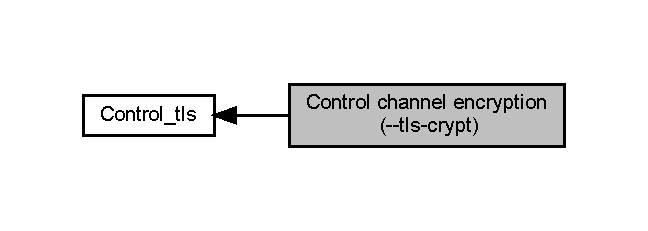
\includegraphics[width=311pt]{group__tls__crypt}
\end{center}
\end{figure}
\subsection*{Macros}
\begin{DoxyCompactItemize}
\item 
\#define \hyperlink{group__tls__crypt_ga65e056054468311502b28a13b7b1a3ef}{T\+L\+S\+\_\+\+C\+R\+Y\+P\+T\+\_\+\+T\+A\+G\+\_\+\+S\+I\+Z\+E}~(256/8)
\item 
\#define \hyperlink{group__tls__crypt_ga55c58e2fa69ea5ffbbb71e25520618e0}{T\+L\+S\+\_\+\+C\+R\+Y\+P\+T\+\_\+\+P\+I\+D\+\_\+\+S\+I\+Z\+E}~(sizeof(\hyperlink{packet__id_8h_a345f753b1c6ea20d24409e769aadb7e6}{packet\+\_\+id\+\_\+type}) + sizeof(\hyperlink{packet__id_8h_a32b361b1d3a0fc2f92ceeff736bba97e}{net\+\_\+time\+\_\+t}))
\item 
\#define \hyperlink{group__tls__crypt_ga1acab4b545b3fff369cb0c05b1897c02}{T\+L\+S\+\_\+\+C\+R\+Y\+P\+T\+\_\+\+B\+L\+O\+C\+K\+\_\+\+S\+I\+Z\+E}~(128/8)
\item 
\#define \hyperlink{group__tls__crypt_ga7eb6b7a1658d8cf6f2f2119b5b927d29}{T\+L\+S\+\_\+\+C\+R\+Y\+P\+T\+\_\+\+O\+F\+F\+\_\+\+P\+I\+D}~(1 + \hyperlink{session__id_8h_ad1163f0bf6339f1dd003192df69052df}{S\+I\+D\+\_\+\+S\+I\+Z\+E})
\item 
\#define \hyperlink{group__tls__crypt_ga8fb65027448e8c403fbbce9bc3b0e056}{T\+L\+S\+\_\+\+C\+R\+Y\+P\+T\+\_\+\+O\+F\+F\+\_\+\+T\+A\+G}~(\hyperlink{group__tls__crypt_ga7eb6b7a1658d8cf6f2f2119b5b927d29}{T\+L\+S\+\_\+\+C\+R\+Y\+P\+T\+\_\+\+O\+F\+F\+\_\+\+P\+I\+D} + \hyperlink{group__tls__crypt_ga55c58e2fa69ea5ffbbb71e25520618e0}{T\+L\+S\+\_\+\+C\+R\+Y\+P\+T\+\_\+\+P\+I\+D\+\_\+\+S\+I\+Z\+E})
\item 
\#define \hyperlink{group__tls__crypt_gaae4cc51d2d63382d195391a4c50af92b}{T\+L\+S\+\_\+\+C\+R\+Y\+P\+T\+\_\+\+O\+F\+F\+\_\+\+C\+T}~(\hyperlink{group__tls__crypt_ga8fb65027448e8c403fbbce9bc3b0e056}{T\+L\+S\+\_\+\+C\+R\+Y\+P\+T\+\_\+\+O\+F\+F\+\_\+\+T\+A\+G} + \hyperlink{group__tls__crypt_ga65e056054468311502b28a13b7b1a3ef}{T\+L\+S\+\_\+\+C\+R\+Y\+P\+T\+\_\+\+T\+A\+G\+\_\+\+S\+I\+Z\+E})
\end{DoxyCompactItemize}
\subsection*{Functions}
\begin{DoxyCompactItemize}
\item 
void \hyperlink{group__tls__crypt_gad8a8513b53a8a5346cac69063f569680}{tls\+\_\+crypt\+\_\+init\+\_\+key} (struct \hyperlink{structkey__ctx__bi}{key\+\_\+ctx\+\_\+bi} $\ast$\hyperlink{structkey}{key}, const char $\ast$key\+\_\+file, const char $\ast$key\+\_\+inline, \hyperlink{automatic_8c_abb452686968e48b67397da5f97445f5b}{bool} tls\+\_\+server)
\item 
int \hyperlink{group__tls__crypt_gac9c2ecaaf4e2af189ab15bb47a558bfa}{tls\+\_\+crypt\+\_\+buf\+\_\+overhead} (void)
\item 
void \hyperlink{group__tls__crypt_ga24b342111241c5ea9c731de4aa66fcb2}{tls\+\_\+crypt\+\_\+adjust\+\_\+frame\+\_\+parameters} (struct \hyperlink{structframe}{frame} $\ast$\hyperlink{structframe}{frame})
\item 
\hyperlink{automatic_8c_abb452686968e48b67397da5f97445f5b}{bool} \hyperlink{group__tls__crypt_gadaca5f414562a243603a60a0e3158e5a}{tls\+\_\+crypt\+\_\+wrap} (const struct \hyperlink{structbuffer}{buffer} $\ast$src, struct \hyperlink{structbuffer}{buffer} $\ast$\hyperlink{compat-lz4_8h_a961c13eb7fcda15b167b953cac1ab3ec}{dst}, struct \hyperlink{structcrypto__options}{crypto\+\_\+options} $\ast$opt)
\item 
\hyperlink{automatic_8c_abb452686968e48b67397da5f97445f5b}{bool} \hyperlink{group__tls__crypt_ga81c822ba2e5599865dddb37e01a2c20c}{tls\+\_\+crypt\+\_\+unwrap} (const struct \hyperlink{structbuffer}{buffer} $\ast$src, struct \hyperlink{structbuffer}{buffer} $\ast$\hyperlink{compat-lz4_8h_a961c13eb7fcda15b167b953cac1ab3ec}{dst}, struct \hyperlink{structcrypto__options}{crypto\+\_\+options} $\ast$opt)
\end{DoxyCompactItemize}


\subsection{Detailed Description}
\begin{DoxyParagraph}{}
Control channel encryption uses a pre-\/shared static key (like the --tls-\/auth key) to encrypt control channel packets.
\end{DoxyParagraph}
\begin{DoxyParagraph}{}
Encrypting control channel packets has three main advantages\+:
\begin{DoxyItemize}
\item It provides more privacy by hiding the certificate used for the T\+L\+S connection.
\item It is harder to identify Open\+V\+P\+N traffic as such.
\item It provides \char`\"{}poor-\/man\textquotesingle{}s\char`\"{} post-\/quantum security, against attackers who will never know the pre-\/shared key (i.\+e. no forward secrecy).
\end{DoxyItemize}
\end{DoxyParagraph}
\begin{DoxyParagraph}{Specification}
Control channel encryption is based on the S\+I\+V construction \mbox{[}0\mbox{]}, to achieve nonce misuse-\/resistant authenticated encryption\+:
\end{DoxyParagraph}
\begin{DoxyParagraph}{}

\begin{DoxyCode}
1 msg      = control channel plaintext
2 header   = opcode (1 byte) || session\_id (8 bytes) || packet\_id (8 bytes)
3 Ka       = authentication key (256 bits)
4 Ke       = encryption key (256 bits)
5 (Ka and Ke are pre-shared keys, like with --tls-auth)
6 
7 auth\_tag = HMAC-SHA256(Ka, header || msg)
8 IV       = 128 most-significant bits of auth\_tag
9 ciph     = AES256-CTR(Ke, IV, msg)
10 
11 output   = Header || Tag || Ciph
\end{DoxyCode}

\end{DoxyParagraph}
\begin{DoxyParagraph}{}
This boils down to the following on-\/the-\/wire packet format\+:
\end{DoxyParagraph}
\begin{DoxyParagraph}{}

\begin{DoxyCode}
1 - opcode - || - session\_id - || - packet\_id - || auth\_tag || * payload *
\end{DoxyCode}

\end{DoxyParagraph}
\begin{DoxyParagraph}{}
Where {\ttfamily -\/ X\+X\+X -\/} means authenticated, and {\ttfamily $\ast$ X\+X\+X $\ast$} means authenticated and encrypted. 
\end{DoxyParagraph}


\subsection{Macro Definition Documentation}
\hypertarget{group__tls__crypt_ga1acab4b545b3fff369cb0c05b1897c02}{}\index{Control channel encryption (-\/-\/tls-\/crypt)@{Control channel encryption (-\/-\/tls-\/crypt)}!T\+L\+S\+\_\+\+C\+R\+Y\+P\+T\+\_\+\+B\+L\+O\+C\+K\+\_\+\+S\+I\+Z\+E@{T\+L\+S\+\_\+\+C\+R\+Y\+P\+T\+\_\+\+B\+L\+O\+C\+K\+\_\+\+S\+I\+Z\+E}}
\index{T\+L\+S\+\_\+\+C\+R\+Y\+P\+T\+\_\+\+B\+L\+O\+C\+K\+\_\+\+S\+I\+Z\+E@{T\+L\+S\+\_\+\+C\+R\+Y\+P\+T\+\_\+\+B\+L\+O\+C\+K\+\_\+\+S\+I\+Z\+E}!Control channel encryption (-\/-\/tls-\/crypt)@{Control channel encryption (-\/-\/tls-\/crypt)}}
\subsubsection[{T\+L\+S\+\_\+\+C\+R\+Y\+P\+T\+\_\+\+B\+L\+O\+C\+K\+\_\+\+S\+I\+Z\+E}]{\setlength{\rightskip}{0pt plus 5cm}\#define T\+L\+S\+\_\+\+C\+R\+Y\+P\+T\+\_\+\+B\+L\+O\+C\+K\+\_\+\+S\+I\+Z\+E~(128/8)}\label{group__tls__crypt_ga1acab4b545b3fff369cb0c05b1897c02}
\hypertarget{group__tls__crypt_gaae4cc51d2d63382d195391a4c50af92b}{}\index{Control channel encryption (-\/-\/tls-\/crypt)@{Control channel encryption (-\/-\/tls-\/crypt)}!T\+L\+S\+\_\+\+C\+R\+Y\+P\+T\+\_\+\+O\+F\+F\+\_\+\+C\+T@{T\+L\+S\+\_\+\+C\+R\+Y\+P\+T\+\_\+\+O\+F\+F\+\_\+\+C\+T}}
\index{T\+L\+S\+\_\+\+C\+R\+Y\+P\+T\+\_\+\+O\+F\+F\+\_\+\+C\+T@{T\+L\+S\+\_\+\+C\+R\+Y\+P\+T\+\_\+\+O\+F\+F\+\_\+\+C\+T}!Control channel encryption (-\/-\/tls-\/crypt)@{Control channel encryption (-\/-\/tls-\/crypt)}}
\subsubsection[{T\+L\+S\+\_\+\+C\+R\+Y\+P\+T\+\_\+\+O\+F\+F\+\_\+\+C\+T}]{\setlength{\rightskip}{0pt plus 5cm}\#define T\+L\+S\+\_\+\+C\+R\+Y\+P\+T\+\_\+\+O\+F\+F\+\_\+\+C\+T~({\bf T\+L\+S\+\_\+\+C\+R\+Y\+P\+T\+\_\+\+O\+F\+F\+\_\+\+T\+A\+G} + {\bf T\+L\+S\+\_\+\+C\+R\+Y\+P\+T\+\_\+\+T\+A\+G\+\_\+\+S\+I\+Z\+E})}\label{group__tls__crypt_gaae4cc51d2d63382d195391a4c50af92b}
\hypertarget{group__tls__crypt_ga7eb6b7a1658d8cf6f2f2119b5b927d29}{}\index{Control channel encryption (-\/-\/tls-\/crypt)@{Control channel encryption (-\/-\/tls-\/crypt)}!T\+L\+S\+\_\+\+C\+R\+Y\+P\+T\+\_\+\+O\+F\+F\+\_\+\+P\+I\+D@{T\+L\+S\+\_\+\+C\+R\+Y\+P\+T\+\_\+\+O\+F\+F\+\_\+\+P\+I\+D}}
\index{T\+L\+S\+\_\+\+C\+R\+Y\+P\+T\+\_\+\+O\+F\+F\+\_\+\+P\+I\+D@{T\+L\+S\+\_\+\+C\+R\+Y\+P\+T\+\_\+\+O\+F\+F\+\_\+\+P\+I\+D}!Control channel encryption (-\/-\/tls-\/crypt)@{Control channel encryption (-\/-\/tls-\/crypt)}}
\subsubsection[{T\+L\+S\+\_\+\+C\+R\+Y\+P\+T\+\_\+\+O\+F\+F\+\_\+\+P\+I\+D}]{\setlength{\rightskip}{0pt plus 5cm}\#define T\+L\+S\+\_\+\+C\+R\+Y\+P\+T\+\_\+\+O\+F\+F\+\_\+\+P\+I\+D~(1 + {\bf S\+I\+D\+\_\+\+S\+I\+Z\+E})}\label{group__tls__crypt_ga7eb6b7a1658d8cf6f2f2119b5b927d29}
\hypertarget{group__tls__crypt_ga8fb65027448e8c403fbbce9bc3b0e056}{}\index{Control channel encryption (-\/-\/tls-\/crypt)@{Control channel encryption (-\/-\/tls-\/crypt)}!T\+L\+S\+\_\+\+C\+R\+Y\+P\+T\+\_\+\+O\+F\+F\+\_\+\+T\+A\+G@{T\+L\+S\+\_\+\+C\+R\+Y\+P\+T\+\_\+\+O\+F\+F\+\_\+\+T\+A\+G}}
\index{T\+L\+S\+\_\+\+C\+R\+Y\+P\+T\+\_\+\+O\+F\+F\+\_\+\+T\+A\+G@{T\+L\+S\+\_\+\+C\+R\+Y\+P\+T\+\_\+\+O\+F\+F\+\_\+\+T\+A\+G}!Control channel encryption (-\/-\/tls-\/crypt)@{Control channel encryption (-\/-\/tls-\/crypt)}}
\subsubsection[{T\+L\+S\+\_\+\+C\+R\+Y\+P\+T\+\_\+\+O\+F\+F\+\_\+\+T\+A\+G}]{\setlength{\rightskip}{0pt plus 5cm}\#define T\+L\+S\+\_\+\+C\+R\+Y\+P\+T\+\_\+\+O\+F\+F\+\_\+\+T\+A\+G~({\bf T\+L\+S\+\_\+\+C\+R\+Y\+P\+T\+\_\+\+O\+F\+F\+\_\+\+P\+I\+D} + {\bf T\+L\+S\+\_\+\+C\+R\+Y\+P\+T\+\_\+\+P\+I\+D\+\_\+\+S\+I\+Z\+E})}\label{group__tls__crypt_ga8fb65027448e8c403fbbce9bc3b0e056}
\hypertarget{group__tls__crypt_ga55c58e2fa69ea5ffbbb71e25520618e0}{}\index{Control channel encryption (-\/-\/tls-\/crypt)@{Control channel encryption (-\/-\/tls-\/crypt)}!T\+L\+S\+\_\+\+C\+R\+Y\+P\+T\+\_\+\+P\+I\+D\+\_\+\+S\+I\+Z\+E@{T\+L\+S\+\_\+\+C\+R\+Y\+P\+T\+\_\+\+P\+I\+D\+\_\+\+S\+I\+Z\+E}}
\index{T\+L\+S\+\_\+\+C\+R\+Y\+P\+T\+\_\+\+P\+I\+D\+\_\+\+S\+I\+Z\+E@{T\+L\+S\+\_\+\+C\+R\+Y\+P\+T\+\_\+\+P\+I\+D\+\_\+\+S\+I\+Z\+E}!Control channel encryption (-\/-\/tls-\/crypt)@{Control channel encryption (-\/-\/tls-\/crypt)}}
\subsubsection[{T\+L\+S\+\_\+\+C\+R\+Y\+P\+T\+\_\+\+P\+I\+D\+\_\+\+S\+I\+Z\+E}]{\setlength{\rightskip}{0pt plus 5cm}\#define T\+L\+S\+\_\+\+C\+R\+Y\+P\+T\+\_\+\+P\+I\+D\+\_\+\+S\+I\+Z\+E~(sizeof({\bf packet\+\_\+id\+\_\+type}) + sizeof({\bf net\+\_\+time\+\_\+t}))}\label{group__tls__crypt_ga55c58e2fa69ea5ffbbb71e25520618e0}
\hypertarget{group__tls__crypt_ga65e056054468311502b28a13b7b1a3ef}{}\index{Control channel encryption (-\/-\/tls-\/crypt)@{Control channel encryption (-\/-\/tls-\/crypt)}!T\+L\+S\+\_\+\+C\+R\+Y\+P\+T\+\_\+\+T\+A\+G\+\_\+\+S\+I\+Z\+E@{T\+L\+S\+\_\+\+C\+R\+Y\+P\+T\+\_\+\+T\+A\+G\+\_\+\+S\+I\+Z\+E}}
\index{T\+L\+S\+\_\+\+C\+R\+Y\+P\+T\+\_\+\+T\+A\+G\+\_\+\+S\+I\+Z\+E@{T\+L\+S\+\_\+\+C\+R\+Y\+P\+T\+\_\+\+T\+A\+G\+\_\+\+S\+I\+Z\+E}!Control channel encryption (-\/-\/tls-\/crypt)@{Control channel encryption (-\/-\/tls-\/crypt)}}
\subsubsection[{T\+L\+S\+\_\+\+C\+R\+Y\+P\+T\+\_\+\+T\+A\+G\+\_\+\+S\+I\+Z\+E}]{\setlength{\rightskip}{0pt plus 5cm}\#define T\+L\+S\+\_\+\+C\+R\+Y\+P\+T\+\_\+\+T\+A\+G\+\_\+\+S\+I\+Z\+E~(256/8)}\label{group__tls__crypt_ga65e056054468311502b28a13b7b1a3ef}


\subsection{Function Documentation}
\hypertarget{group__tls__crypt_ga24b342111241c5ea9c731de4aa66fcb2}{}\index{Control channel encryption (-\/-\/tls-\/crypt)@{Control channel encryption (-\/-\/tls-\/crypt)}!tls\+\_\+crypt\+\_\+adjust\+\_\+frame\+\_\+parameters@{tls\+\_\+crypt\+\_\+adjust\+\_\+frame\+\_\+parameters}}
\index{tls\+\_\+crypt\+\_\+adjust\+\_\+frame\+\_\+parameters@{tls\+\_\+crypt\+\_\+adjust\+\_\+frame\+\_\+parameters}!Control channel encryption (-\/-\/tls-\/crypt)@{Control channel encryption (-\/-\/tls-\/crypt)}}
\subsubsection[{tls\+\_\+crypt\+\_\+adjust\+\_\+frame\+\_\+parameters(struct frame $\ast$frame)}]{\setlength{\rightskip}{0pt plus 5cm}void tls\+\_\+crypt\+\_\+adjust\+\_\+frame\+\_\+parameters (
\begin{DoxyParamCaption}
\item[{struct {\bf frame} $\ast$}]{frame}
\end{DoxyParamCaption}
)}\label{group__tls__crypt_ga24b342111241c5ea9c731de4aa66fcb2}
Adjust frame parameters for --tls-\/crypt overhead. 

Here is the call graph for this function\+:
\nopagebreak
\begin{figure}[H]
\begin{center}
\leavevmode
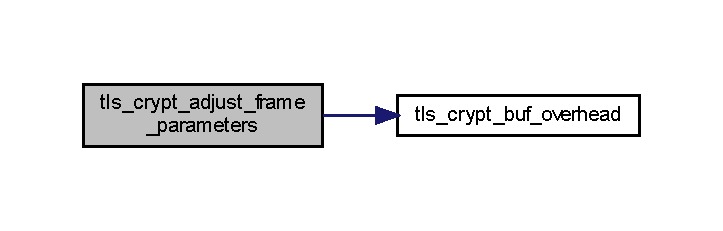
\includegraphics[width=347pt]{group__tls__crypt_ga24b342111241c5ea9c731de4aa66fcb2_cgraph}
\end{center}
\end{figure}


\hypertarget{group__tls__crypt_gac9c2ecaaf4e2af189ab15bb47a558bfa}{}\index{Control channel encryption (-\/-\/tls-\/crypt)@{Control channel encryption (-\/-\/tls-\/crypt)}!tls\+\_\+crypt\+\_\+buf\+\_\+overhead@{tls\+\_\+crypt\+\_\+buf\+\_\+overhead}}
\index{tls\+\_\+crypt\+\_\+buf\+\_\+overhead@{tls\+\_\+crypt\+\_\+buf\+\_\+overhead}!Control channel encryption (-\/-\/tls-\/crypt)@{Control channel encryption (-\/-\/tls-\/crypt)}}
\subsubsection[{tls\+\_\+crypt\+\_\+buf\+\_\+overhead(void)}]{\setlength{\rightskip}{0pt plus 5cm}int tls\+\_\+crypt\+\_\+buf\+\_\+overhead (
\begin{DoxyParamCaption}
\item[{void}]{}
\end{DoxyParamCaption}
)}\label{group__tls__crypt_gac9c2ecaaf4e2af189ab15bb47a558bfa}
Returns the maximum overhead (in bytes) added to the destination buffer by \hyperlink{group__tls__crypt_gadaca5f414562a243603a60a0e3158e5a}{tls\+\_\+crypt\+\_\+wrap()}. 

Here is the caller graph for this function\+:
\nopagebreak
\begin{figure}[H]
\begin{center}
\leavevmode
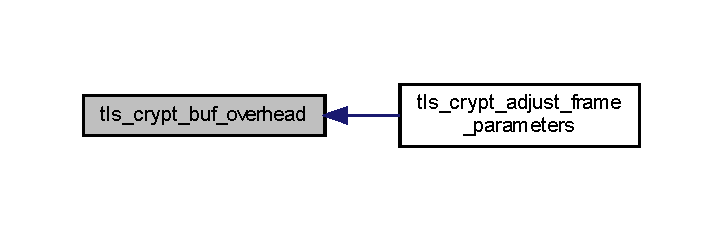
\includegraphics[width=347pt]{group__tls__crypt_gac9c2ecaaf4e2af189ab15bb47a558bfa_icgraph}
\end{center}
\end{figure}


\hypertarget{group__tls__crypt_gad8a8513b53a8a5346cac69063f569680}{}\index{Control channel encryption (-\/-\/tls-\/crypt)@{Control channel encryption (-\/-\/tls-\/crypt)}!tls\+\_\+crypt\+\_\+init\+\_\+key@{tls\+\_\+crypt\+\_\+init\+\_\+key}}
\index{tls\+\_\+crypt\+\_\+init\+\_\+key@{tls\+\_\+crypt\+\_\+init\+\_\+key}!Control channel encryption (-\/-\/tls-\/crypt)@{Control channel encryption (-\/-\/tls-\/crypt)}}
\subsubsection[{tls\+\_\+crypt\+\_\+init\+\_\+key(struct key\+\_\+ctx\+\_\+bi $\ast$key, const char $\ast$key\+\_\+file, const char $\ast$key\+\_\+inline, bool tls\+\_\+server)}]{\setlength{\rightskip}{0pt plus 5cm}void tls\+\_\+crypt\+\_\+init\+\_\+key (
\begin{DoxyParamCaption}
\item[{struct {\bf key\+\_\+ctx\+\_\+bi} $\ast$}]{key, }
\item[{const char $\ast$}]{key\+\_\+file, }
\item[{const char $\ast$}]{key\+\_\+inline, }
\item[{{\bf bool}}]{tls\+\_\+server}
\end{DoxyParamCaption}
)}\label{group__tls__crypt_gad8a8513b53a8a5346cac69063f569680}
Initialize a \hyperlink{structkey__ctx__bi}{key\+\_\+ctx\+\_\+bi} structure for use with --tls-\/crypt.


\begin{DoxyParams}{Parameters}
{\em key} & The key context to initialize \\
\hline
{\em key\+\_\+file} & The file to read the key from (or the inline tag to indicate and inline key). \\
\hline
{\em key\+\_\+inline} & Array containing (zero-\/terminated) inline key, or N\+U\+L\+L if not used. \\
\hline
{\em tls\+\_\+server} & Must be set to true is this is a T\+L\+S server instance. \\
\hline
\end{DoxyParams}


Here is the call graph for this function\+:
\nopagebreak
\begin{figure}[H]
\begin{center}
\leavevmode
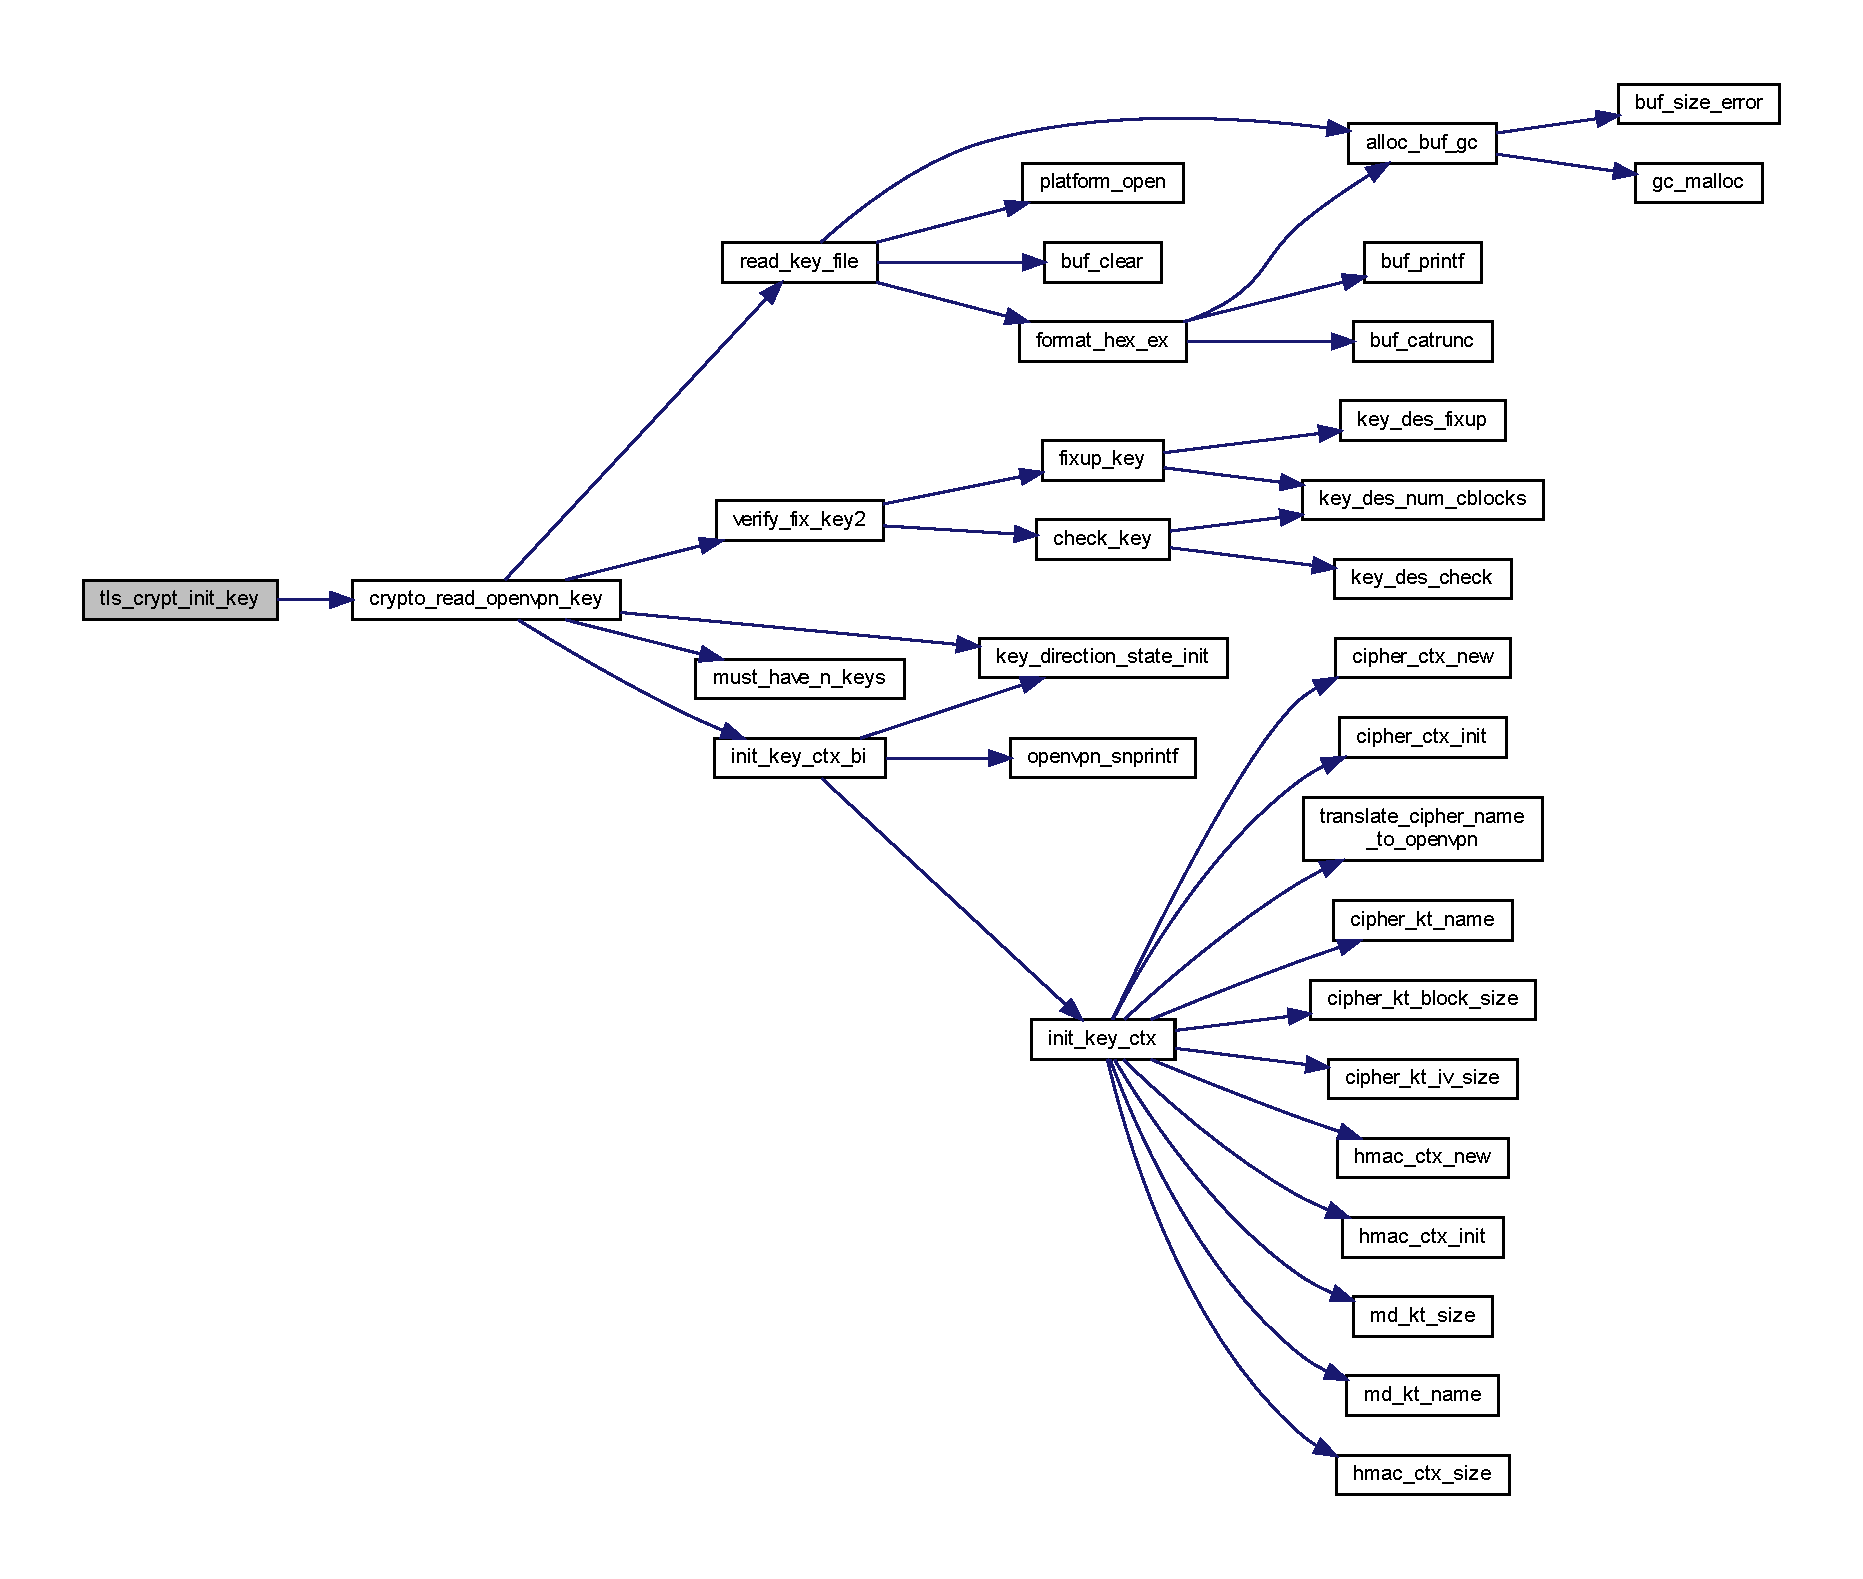
\includegraphics[width=350pt]{group__tls__crypt_gad8a8513b53a8a5346cac69063f569680_cgraph}
\end{center}
\end{figure}


\hypertarget{group__tls__crypt_ga81c822ba2e5599865dddb37e01a2c20c}{}\index{Control channel encryption (-\/-\/tls-\/crypt)@{Control channel encryption (-\/-\/tls-\/crypt)}!tls\+\_\+crypt\+\_\+unwrap@{tls\+\_\+crypt\+\_\+unwrap}}
\index{tls\+\_\+crypt\+\_\+unwrap@{tls\+\_\+crypt\+\_\+unwrap}!Control channel encryption (-\/-\/tls-\/crypt)@{Control channel encryption (-\/-\/tls-\/crypt)}}
\subsubsection[{tls\+\_\+crypt\+\_\+unwrap(const struct buffer $\ast$src, struct buffer $\ast$dst, struct crypto\+\_\+options $\ast$opt)}]{\setlength{\rightskip}{0pt plus 5cm}{\bf bool} tls\+\_\+crypt\+\_\+unwrap (
\begin{DoxyParamCaption}
\item[{const struct {\bf buffer} $\ast$}]{src, }
\item[{struct {\bf buffer} $\ast$}]{dst, }
\item[{struct {\bf crypto\+\_\+options} $\ast$}]{opt}
\end{DoxyParamCaption}
)}\label{group__tls__crypt_ga81c822ba2e5599865dddb37e01a2c20c}
Unwrap a control channel packet (decrypts, authenticates and performs replay checks).


\begin{DoxyParams}{Parameters}
{\em src} & Data to decrypt and authenticate. \\
\hline
{\em dst} & Returns the decrypted data, if unwrapping was successful. \\
\hline
{\em opt} & The crypto state for this --tls-\/crypt instance.\\
\hline
\end{DoxyParams}
\begin{DoxyReturn}{Returns}
true iff unwrapping succeeded (data authenticated correctly and was no replay). 
\end{DoxyReturn}


Here is the call graph for this function\+:
\nopagebreak
\begin{figure}[H]
\begin{center}
\leavevmode
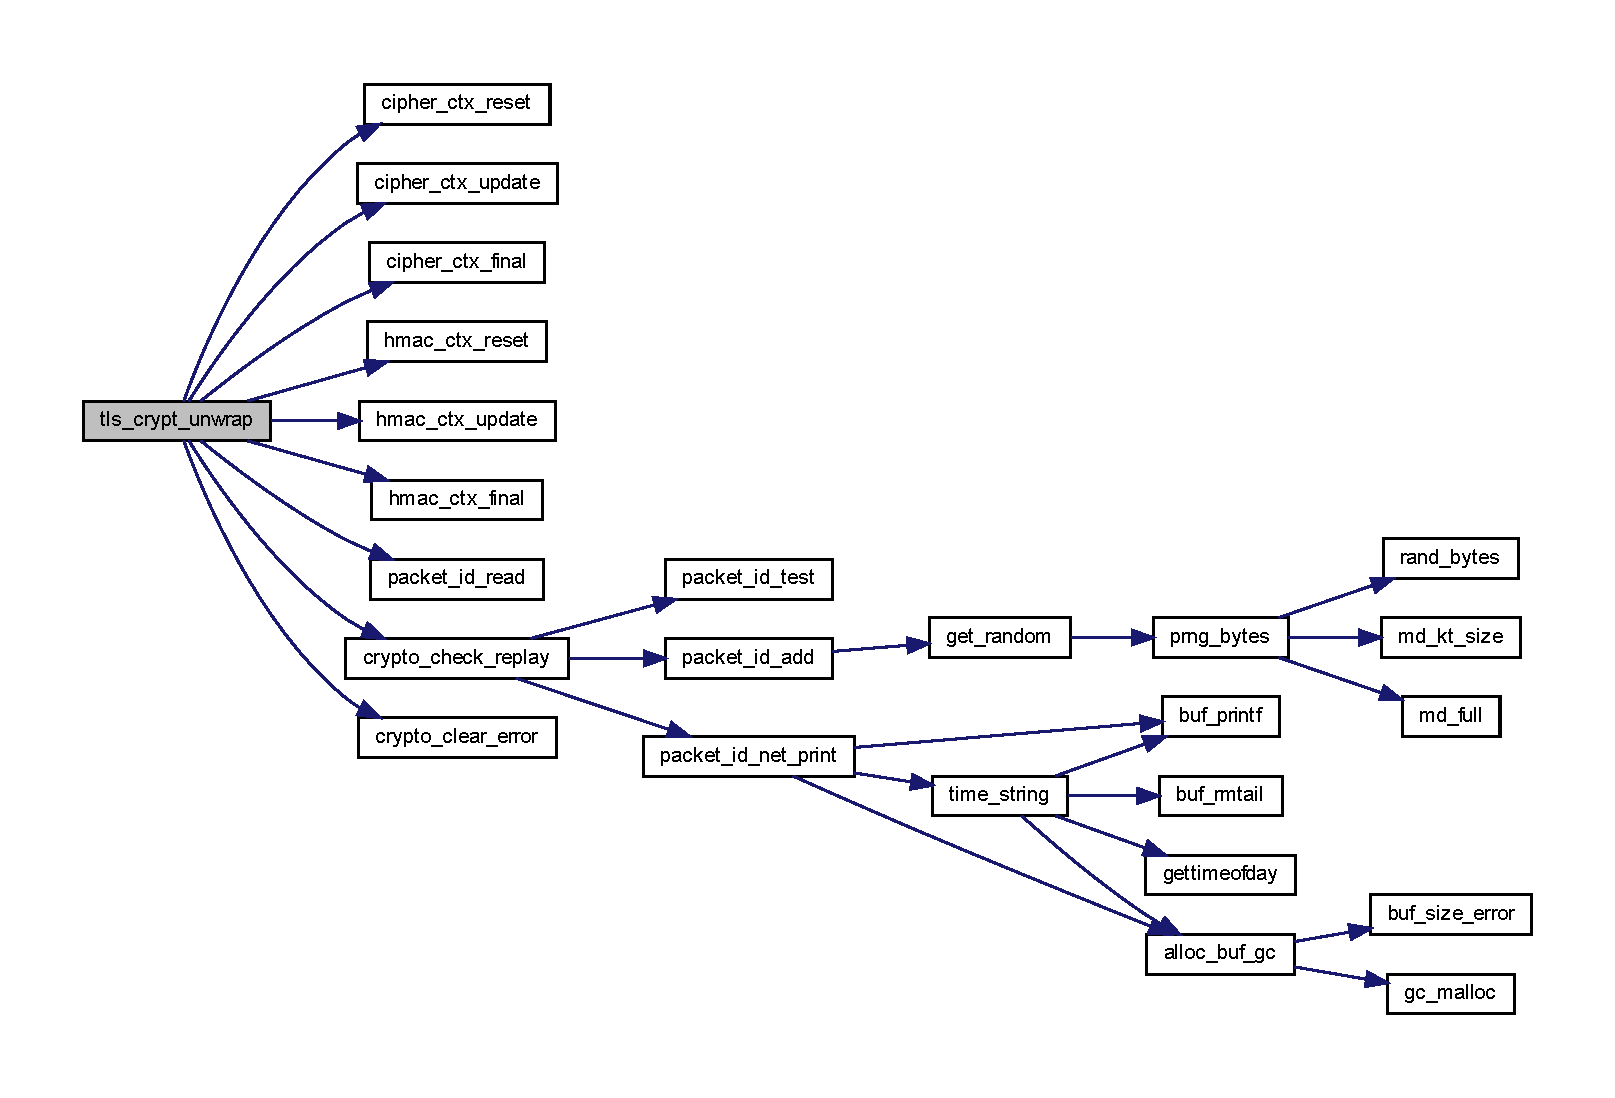
\includegraphics[width=350pt]{group__tls__crypt_ga81c822ba2e5599865dddb37e01a2c20c_cgraph}
\end{center}
\end{figure}


\hypertarget{group__tls__crypt_gadaca5f414562a243603a60a0e3158e5a}{}\index{Control channel encryption (-\/-\/tls-\/crypt)@{Control channel encryption (-\/-\/tls-\/crypt)}!tls\+\_\+crypt\+\_\+wrap@{tls\+\_\+crypt\+\_\+wrap}}
\index{tls\+\_\+crypt\+\_\+wrap@{tls\+\_\+crypt\+\_\+wrap}!Control channel encryption (-\/-\/tls-\/crypt)@{Control channel encryption (-\/-\/tls-\/crypt)}}
\subsubsection[{tls\+\_\+crypt\+\_\+wrap(const struct buffer $\ast$src, struct buffer $\ast$dst, struct crypto\+\_\+options $\ast$opt)}]{\setlength{\rightskip}{0pt plus 5cm}{\bf bool} tls\+\_\+crypt\+\_\+wrap (
\begin{DoxyParamCaption}
\item[{const struct {\bf buffer} $\ast$}]{src, }
\item[{struct {\bf buffer} $\ast$}]{dst, }
\item[{struct {\bf crypto\+\_\+options} $\ast$}]{opt}
\end{DoxyParamCaption}
)}\label{group__tls__crypt_gadaca5f414562a243603a60a0e3158e5a}
Wrap a control channel packet (both authenticates and encrypts the data).


\begin{DoxyParams}{Parameters}
{\em src} & Data to authenticate and encrypt. \\
\hline
{\em dst} & Any data present in this buffer is first authenticated, then the wrapped packet id and data from the src buffer are appended. Must have at least \hyperlink{group__tls__crypt_gac9c2ecaaf4e2af189ab15bb47a558bfa}{tls\+\_\+crypt\+\_\+buf\+\_\+overhead()}+\+B\+L\+E\+N(src) headroom. \\
\hline
{\em opt} & The crypto state for this --tls-\/crypt instance.\\
\hline
\end{DoxyParams}
\begin{DoxyReturn}{Returns}
true iff wrapping succeeded. 
\end{DoxyReturn}


Here is the call graph for this function\+:
\nopagebreak
\begin{figure}[H]
\begin{center}
\leavevmode
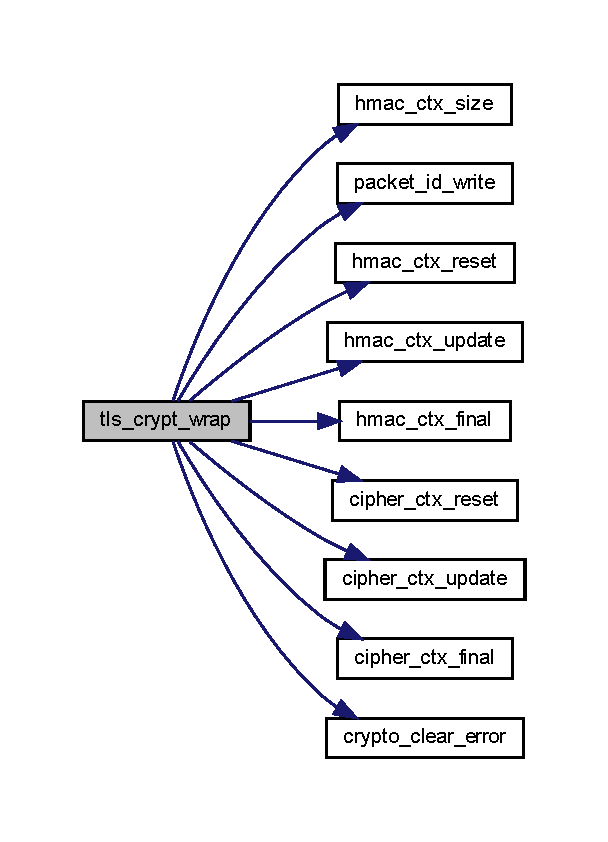
\includegraphics[width=292pt]{group__tls__crypt_gadaca5f414562a243603a60a0e3158e5a_cgraph}
\end{center}
\end{figure}



\hypertarget{group__data__crypto}{}\section{Data Channel Crypto module}
\label{group__data__crypto}\index{Data Channel Crypto module@{Data Channel Crypto module}}
\subsection*{Classes}
\begin{DoxyCompactItemize}
\item 
struct \hyperlink{structcrypto__options}{crypto\+\_\+options}
\end{DoxyCompactItemize}
\subsection*{Macros}
\begin{DoxyCompactItemize}
\item 
\#define \hyperlink{group__data__crypto_ga531ce54a40ba4525b7ef859ef7425a38}{D\+E\+C\+R\+Y\+P\+T\+\_\+\+K\+E\+Y\+\_\+\+E\+N\+A\+B\+L\+E\+D}(multi,  ks)~((ks)-\/$>$state $>$= (\hyperlink{group__control__processor_ga66bd0f7cdbc8450a4690c519de7d75bc}{S\+\_\+\+G\+O\+T\+\_\+\+K\+E\+Y} -\/ (multi)-\/$>$opt.\+server))
\end{DoxyCompactItemize}
\subsection*{Functions for performing security operations on data channel packets}
\begin{DoxyCompactItemize}
\item 
void \hyperlink{group__data__crypto_ga2756bad88224b98719d4e8f08cb11ef9}{openvpn\+\_\+encrypt} (struct \hyperlink{structbuffer}{buffer} $\ast$buf, struct \hyperlink{structbuffer}{buffer} work, struct \hyperlink{structcrypto__options}{crypto\+\_\+options} $\ast$opt)
\item 
\hyperlink{automatic_8c_abb452686968e48b67397da5f97445f5b}{bool} \hyperlink{group__data__crypto_gae91d99446478fcf3327672eb78ef0bf8}{openvpn\+\_\+decrypt} (struct \hyperlink{structbuffer}{buffer} $\ast$buf, struct \hyperlink{structbuffer}{buffer} work, struct \hyperlink{structcrypto__options}{crypto\+\_\+options} $\ast$opt, const struct \hyperlink{structframe}{frame} $\ast$\hyperlink{structframe}{frame}, const uint8\+\_\+t $\ast$ad\+\_\+start)
\end{DoxyCompactItemize}
\subsection*{Functions for managing security parameter state for data channel packets}
\begin{DoxyCompactItemize}
\item 
\hyperlink{automatic_8c_abb452686968e48b67397da5f97445f5b}{bool} \hyperlink{group__data__crypto_gab1369f42e94bbec108d952d565b0f283}{tls\+\_\+pre\+\_\+decrypt\+\_\+lite} (const struct \hyperlink{structtls__auth__standalone}{tls\+\_\+auth\+\_\+standalone} $\ast$tas, const struct \hyperlink{structlink__socket__actual}{link\+\_\+socket\+\_\+actual} $\ast$from, const struct \hyperlink{structbuffer}{buffer} $\ast$buf)
\item 
void \hyperlink{group__data__crypto_gaba03eaba587a89c2abda8780da7b3ac7}{tls\+\_\+pre\+\_\+encrypt} (struct \hyperlink{structtls__multi}{tls\+\_\+multi} $\ast$multi, struct \hyperlink{structbuffer}{buffer} $\ast$buf, struct \hyperlink{structcrypto__options}{crypto\+\_\+options} $\ast$$\ast$opt)
\item 
void \hyperlink{group__data__crypto_gaac2b3aa2c842a102804be65f28adf4b1}{tls\+\_\+prepend\+\_\+opcode\+\_\+v1} (const struct \hyperlink{structtls__multi}{tls\+\_\+multi} $\ast$multi, struct \hyperlink{structbuffer}{buffer} $\ast$buf)
\item 
void \hyperlink{group__data__crypto_gad27b20736f89d38d0d2e0c2e35f7a0e3}{tls\+\_\+prepend\+\_\+opcode\+\_\+v2} (const struct \hyperlink{structtls__multi}{tls\+\_\+multi} $\ast$multi, struct \hyperlink{structbuffer}{buffer} $\ast$buf)
\item 
void \hyperlink{group__data__crypto_ga1f2ecd39b88da77b2f8067962155ea82}{tls\+\_\+post\+\_\+encrypt} (struct \hyperlink{structtls__multi}{tls\+\_\+multi} $\ast$multi, struct \hyperlink{structbuffer}{buffer} $\ast$buf)
\end{DoxyCompactItemize}


\subsection{Detailed Description}
\begin{DoxyParagraph}{Crypto packet formats}
The Data Channel Crypto module supports a number of crypto modes and configurable options. The actual packet format depends on these options. A Data Channel packet can consist of\+:
\begin{DoxyItemize}
\item {\bfseries Opcode}, one byte specifying the packet type (see Network protocol).
\item {\bfseries Peer-\/id}, if using the v2 data channel packet format (see Network protocol).
\item {\bfseries H\+M\+A\+C}, covering the ciphertext I\+V + ciphertext. The H\+M\+A\+C size depends on the {\ttfamily -\/-\/auth} option. If {\ttfamily -\/-\/auth} {\ttfamily none} is specified, there is no H\+M\+A\+C at all.
\item {\bfseries Ciphertext} {\bfseries I\+V}. The I\+V size depends on the {\ttfamily -\/-\/cipher} option.
\item {\bfseries Packet} {\bfseries I\+D}, a 32-\/bit incrementing packet counter that provides replay protection (if not disabled by {\ttfamily -\/-\/no-\/replay}).
\item {\bfseries Timestamp}, a 32-\/bit timestamp of the current time.
\item {\bfseries Payload}, the plain text network packet to be encrypted (unless encryption is disabled by using {\ttfamily -\/-\/cipher} {\ttfamily none}). The payload might already be compressed (see Compression module).
\end{DoxyItemize}
\end{DoxyParagraph}
\begin{DoxyParagraph}{}
This section does not discuss the opcode and peer-\/id, since those do not depend on the data channel crypto. See Network protocol for more information on those.
\end{DoxyParagraph}
\begin{DoxyParagraph}{}
{\itshape Legenda} ~\newline
{\ttfamily \mbox{[} xxx \mbox{]}} = unprotected ~\newline
{\ttfamily \mbox{[} -\/ xxx -\/ \mbox{]}} = authenticated ~\newline
{\ttfamily \mbox{[} $\ast$ xxx $\ast$ \mbox{]}} = encrypted and authenticated
\end{DoxyParagraph}
\begin{DoxyParagraph}{}
{\bfseries C\+B\+C data channel cypto format} ~\newline
In C\+B\+C mode, both T\+L\+S-\/mode and static key mode are supported. The I\+V consists of random bits to provide unpredictable I\+Vs. ~\newline
{\itshape C\+B\+C I\+V format\+:} ~\newline
{\ttfamily  \mbox{[} -\/ random -\/ \mbox{]} } ~\newline
{\itshape C\+B\+C data channel crypto format in T\+L\+S-\/mode\+:} ~\newline
{\ttfamily  \mbox{[} H\+M\+A\+C \mbox{]} \mbox{[} -\/ I\+V -\/ \mbox{]} \mbox{[} $\ast$ packet I\+D $\ast$ \mbox{]} \mbox{[} $\ast$ packet payload $\ast$ \mbox{]} } ~\newline
{\itshape C\+B\+C data channel crypto format in static key mode\+:} ~\newline
{\ttfamily  \mbox{[} H\+M\+A\+C \mbox{]} \mbox{[} -\/ I\+V -\/ \mbox{]} \mbox{[} $\ast$ packet I\+D $\ast$ \mbox{]} \mbox{[} $\ast$ timestamp $\ast$ \mbox{]} \mbox{[} $\ast$ packet payload $\ast$ \mbox{]} }
\end{DoxyParagraph}
\begin{DoxyParagraph}{}
{\bfseries C\+F\+B/\+O\+F\+B data channel crypto format} ~\newline
C\+F\+B and O\+F\+B modes are only supported in T\+L\+S mode. In these modes, the I\+V consists of the packet counter and a timestamp. If the I\+V is more than 8 bytes long, the remaining space is filled with zeroes. The packet counter may not roll over within a single T\+L\+S sessions. This results in a unique I\+V for each packet, as required by the C\+F\+B and O\+F\+B cipher modes.
\end{DoxyParagraph}
\begin{DoxyParagraph}{}
{\itshape C\+F\+B/\+O\+F\+B I\+V format\+:} ~\newline
{\ttfamily  \mbox{[} -\/ packet I\+D -\/ \mbox{]} \mbox{[} -\/ timestamp -\/ \mbox{]} \mbox{[} -\/ opt\+: zero-\/padding -\/ \mbox{]} }~\newline
{\itshape C\+F\+B/\+O\+F\+B data channel crypto format\+:} ~\newline
{\ttfamily  \mbox{[} H\+M\+A\+C \mbox{]} \mbox{[} -\/ I\+V -\/ \mbox{]} \mbox{[} $\ast$ packet payload $\ast$ \mbox{]} }
\end{DoxyParagraph}
\begin{DoxyParagraph}{}
{\bfseries G\+C\+M data channel crypto format} ~\newline
G\+C\+M modes are only supported in T\+L\+S mode. In these modes, the I\+V consists of the 32-\/bit packet counter followed by data from the H\+M\+A\+C key. The H\+M\+A\+C key can be used as I\+V, since in G\+C\+M and C\+C\+M modes the H\+M\+A\+C key is not used for the H\+M\+A\+C. The packet counter may not roll over within a single T\+L\+S sessions. This results in a unique I\+V for each packet, as required by G\+C\+M.
\end{DoxyParagraph}
\begin{DoxyParagraph}{}
The H\+M\+A\+C key data is pre-\/shared during the connection setup, and thus can be omitted in on-\/the-\/wire packets, saving 8 bytes per packet (for G\+C\+M and C\+C\+M).
\end{DoxyParagraph}
\begin{DoxyParagraph}{}
In G\+C\+M mode, P\+\_\+\+D\+A\+T\+A\+\_\+\+V2 headers (the opcode and peer-\/id) are also authenticated as Additional Data.
\end{DoxyParagraph}
\begin{DoxyParagraph}{}
{\itshape G\+C\+M I\+V format\+:} ~\newline
{\ttfamily  \mbox{[} -\/ packet I\+D -\/ \mbox{]} \mbox{[} -\/ H\+M\+A\+C key data -\/ \mbox{]} }~\newline
{\itshape P\+\_\+\+D\+A\+T\+A\+\_\+\+V1 G\+C\+M data channel crypto format\+:} ~\newline
{\ttfamily  \mbox{[} opcode \mbox{]} \mbox{[} -\/ packet I\+D -\/ \mbox{]} \mbox{[} T\+A\+G \mbox{]} \mbox{[} $\ast$ packet payload $\ast$ \mbox{]} } {\itshape P\+\_\+\+D\+A\+T\+A\+\_\+\+V2 G\+C\+M data channel crypto format\+:} ~\newline
{\ttfamily  \mbox{[} -\/ opcode/peer-\/id -\/ \mbox{]} \mbox{[} -\/ packet I\+D -\/ \mbox{]} \mbox{[} T\+A\+G \mbox{]} \mbox{[} $\ast$ packet payload $\ast$ \mbox{]} }
\end{DoxyParagraph}
\begin{DoxyParagraph}{}
{\bfseries No-\/crypto data channel format} ~\newline
In no-\/crypto mode ({\ttfamily -\/-\/cipher} {\ttfamily none} is specified), both T\+L\+S-\/mode and static key mode are supported. No encryption will be performed on the packet, but packets can still be authenticated. This mode does not require an I\+V.~\newline
{\itshape No-\/crypto data channel crypto format in T\+L\+S-\/mode\+:} ~\newline
{\ttfamily  \mbox{[} H\+M\+A\+C \mbox{]} \mbox{[} -\/ packet I\+D -\/ \mbox{]} \mbox{[} -\/ packet payload -\/ \mbox{]} } ~\newline
{\itshape No-\/crypto data channel crypto format in static key mode\+:} ~\newline
{\ttfamily  \mbox{[} H\+M\+A\+C \mbox{]} \mbox{[} -\/ packet I\+D -\/ \mbox{]} \mbox{[} -\/ timestamp -\/ \mbox{]} \mbox{[} -\/ packet payload -\/ \mbox{]} } 
\end{DoxyParagraph}


\subsection{Macro Definition Documentation}
\hypertarget{group__data__crypto_ga531ce54a40ba4525b7ef859ef7425a38}{}\index{Data Channel Crypto module@{Data Channel Crypto module}!D\+E\+C\+R\+Y\+P\+T\+\_\+\+K\+E\+Y\+\_\+\+E\+N\+A\+B\+L\+E\+D@{D\+E\+C\+R\+Y\+P\+T\+\_\+\+K\+E\+Y\+\_\+\+E\+N\+A\+B\+L\+E\+D}}
\index{D\+E\+C\+R\+Y\+P\+T\+\_\+\+K\+E\+Y\+\_\+\+E\+N\+A\+B\+L\+E\+D@{D\+E\+C\+R\+Y\+P\+T\+\_\+\+K\+E\+Y\+\_\+\+E\+N\+A\+B\+L\+E\+D}!Data Channel Crypto module@{Data Channel Crypto module}}
\subsubsection[{D\+E\+C\+R\+Y\+P\+T\+\_\+\+K\+E\+Y\+\_\+\+E\+N\+A\+B\+L\+E\+D}]{\setlength{\rightskip}{0pt plus 5cm}\#define D\+E\+C\+R\+Y\+P\+T\+\_\+\+K\+E\+Y\+\_\+\+E\+N\+A\+B\+L\+E\+D(
\begin{DoxyParamCaption}
\item[{}]{multi, }
\item[{}]{ks}
\end{DoxyParamCaption}
)~((ks)-\/$>$state $>$= ({\bf S\+\_\+\+G\+O\+T\+\_\+\+K\+E\+Y} -\/ (multi)-\/$>$opt.\+server))}\label{group__data__crypto_ga531ce54a40ba4525b7ef859ef7425a38}
Check whether the {\itshape ks} {\ttfamily \hyperlink{structkey__state}{key\+\_\+state}} is ready to receive data channel packets.

If true, it is safe to assume that this session has been authenticated by T\+L\+S.

\begin{DoxyNote}{Note}
This macro only works if S\+\_\+\+S\+E\+N\+T\+\_\+\+K\+E\+Y + 1 == S\+\_\+\+G\+O\+T\+\_\+\+K\+E\+Y. 
\end{DoxyNote}


\subsection{Function Documentation}
\hypertarget{group__data__crypto_gae91d99446478fcf3327672eb78ef0bf8}{}\index{Data Channel Crypto module@{Data Channel Crypto module}!openvpn\+\_\+decrypt@{openvpn\+\_\+decrypt}}
\index{openvpn\+\_\+decrypt@{openvpn\+\_\+decrypt}!Data Channel Crypto module@{Data Channel Crypto module}}
\subsubsection[{openvpn\+\_\+decrypt(struct buffer $\ast$buf, struct buffer work, struct crypto\+\_\+options $\ast$opt, const struct frame $\ast$frame, const uint8\+\_\+t $\ast$ad\+\_\+start)}]{\setlength{\rightskip}{0pt plus 5cm}{\bf bool} openvpn\+\_\+decrypt (
\begin{DoxyParamCaption}
\item[{struct {\bf buffer} $\ast$}]{buf, }
\item[{struct {\bf buffer}}]{work, }
\item[{struct {\bf crypto\+\_\+options} $\ast$}]{opt, }
\item[{const struct {\bf frame} $\ast$}]{frame, }
\item[{const uint8\+\_\+t $\ast$}]{ad\+\_\+start}
\end{DoxyParamCaption}
)}\label{group__data__crypto_gae91d99446478fcf3327672eb78ef0bf8}
H\+M\+A\+C verify and decrypt a data channel packet received from a remote Open\+V\+P\+N peer.

This function handles authenticating and decrypting a data channel packet received from a remote Open\+V\+P\+N peer. It receives the necessary security parameters in the {\itshape opt} argument, which should have been set to the correct values by the {\ttfamily \hyperlink{ssl_8c_ad436aa1372a562e8be84491907531df4}{tls\+\_\+pre\+\_\+decrypt()}} function.

This function calls the {\ttfamily E\+V\+P\+\_\+\+Cipher$\ast$} and {\ttfamily H\+M\+A\+C\+\_\+$\ast$} functions of the Open\+S\+S\+L library to perform the actual security operations.

If an error occurs during processing, then the {\itshape buf} buffer is set to empty.


\begin{DoxyParams}{Parameters}
{\em buf} & -\/ The buffer containing the packet received from a remote Open\+V\+P\+N peer on which to perform security operations. \\
\hline
{\em work} & -\/ A working buffer. \\
\hline
{\em opt} & -\/ The security parameter state for this V\+P\+N tunnel. \\
\hline
{\em frame} & -\/ The packet geometry parameters for this V\+P\+N tunnel. \\
\hline
{\em ad\+\_\+start} & -\/ A pointer into buf, indicating from where to start authenticating additional data (A\+E\+A\+D mode only).\\
\hline
\end{DoxyParams}
\begin{DoxyReturn}{Returns}
\begin{DoxyItemize}
\item True, if the packet was authenticated and decrypted successfully. \item False, if an error occurred. ~\newline
 On return, the {\itshape buf} argument will point to the resulting buffer. This buffer will either contain the plaintext packet ready for further processing, or be empty if an error occurred. \end{DoxyItemize}

\end{DoxyReturn}


Here is the call graph for this function\+:
\nopagebreak
\begin{figure}[H]
\begin{center}
\leavevmode
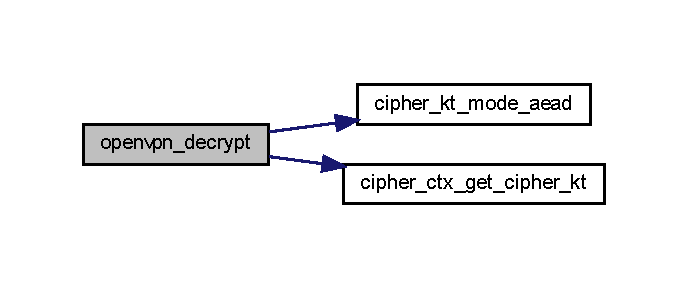
\includegraphics[width=330pt]{group__data__crypto_gae91d99446478fcf3327672eb78ef0bf8_cgraph}
\end{center}
\end{figure}




Here is the caller graph for this function\+:
\nopagebreak
\begin{figure}[H]
\begin{center}
\leavevmode
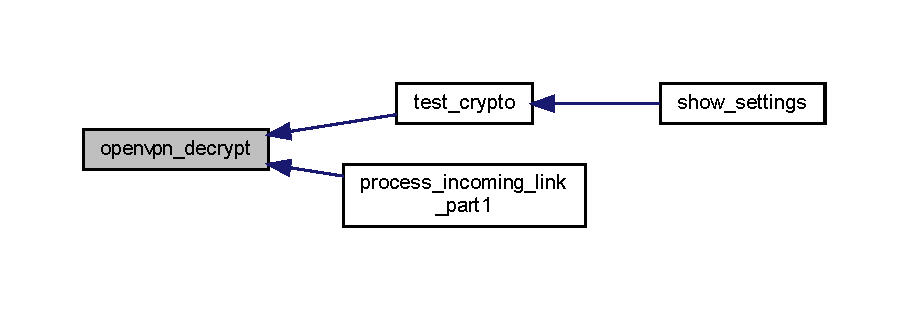
\includegraphics[width=350pt]{group__data__crypto_gae91d99446478fcf3327672eb78ef0bf8_icgraph}
\end{center}
\end{figure}


\hypertarget{group__data__crypto_ga2756bad88224b98719d4e8f08cb11ef9}{}\index{Data Channel Crypto module@{Data Channel Crypto module}!openvpn\+\_\+encrypt@{openvpn\+\_\+encrypt}}
\index{openvpn\+\_\+encrypt@{openvpn\+\_\+encrypt}!Data Channel Crypto module@{Data Channel Crypto module}}
\subsubsection[{openvpn\+\_\+encrypt(struct buffer $\ast$buf, struct buffer work, struct crypto\+\_\+options $\ast$opt)}]{\setlength{\rightskip}{0pt plus 5cm}void openvpn\+\_\+encrypt (
\begin{DoxyParamCaption}
\item[{struct {\bf buffer} $\ast$}]{buf, }
\item[{struct {\bf buffer}}]{work, }
\item[{struct {\bf crypto\+\_\+options} $\ast$}]{opt}
\end{DoxyParamCaption}
)}\label{group__data__crypto_ga2756bad88224b98719d4e8f08cb11ef9}
Encrypt and H\+M\+A\+C sign a packet so that it can be sent as a data channel V\+P\+N tunnel packet to a remote Open\+V\+P\+N peer.

This function handles encryption and H\+M\+A\+C signing of a data channel packet before it is sent to its remote Open\+V\+P\+N peer. It receives the necessary security parameters in the {\itshape opt} argument, which should have been set to the correct values by the {\ttfamily \hyperlink{group__data__crypto_gaba03eaba587a89c2abda8780da7b3ac7}{tls\+\_\+pre\+\_\+encrypt()}} function.

This function calls the {\ttfamily E\+V\+P\+\_\+\+Cipher$\ast$} and {\ttfamily H\+M\+A\+C\+\_\+$\ast$} functions of the Open\+S\+S\+L library to perform the actual security operations.

If an error occurs during processing, then the {\itshape buf} buffer is set to empty.


\begin{DoxyParams}{Parameters}
{\em buf} & -\/ The buffer containing the packet on which to perform security operations. \\
\hline
{\em work} & -\/ An initialized working buffer. \\
\hline
{\em opt} & -\/ The security parameter state for this V\+P\+N tunnel.\\
\hline
\end{DoxyParams}
\begin{DoxyReturn}{Returns}
This function returns void.~\newline
 On return, the {\itshape buf} argument will point to the resulting buffer. This buffer will either contain the processed packet ready for sending, or be empty if an error occurred. 
\end{DoxyReturn}


Here is the call graph for this function\+:
\nopagebreak
\begin{figure}[H]
\begin{center}
\leavevmode
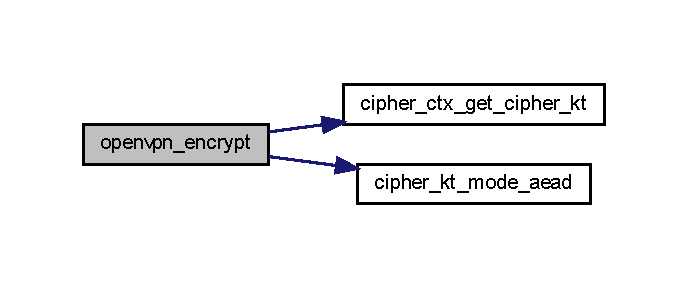
\includegraphics[width=330pt]{group__data__crypto_ga2756bad88224b98719d4e8f08cb11ef9_cgraph}
\end{center}
\end{figure}




Here is the caller graph for this function\+:
\nopagebreak
\begin{figure}[H]
\begin{center}
\leavevmode
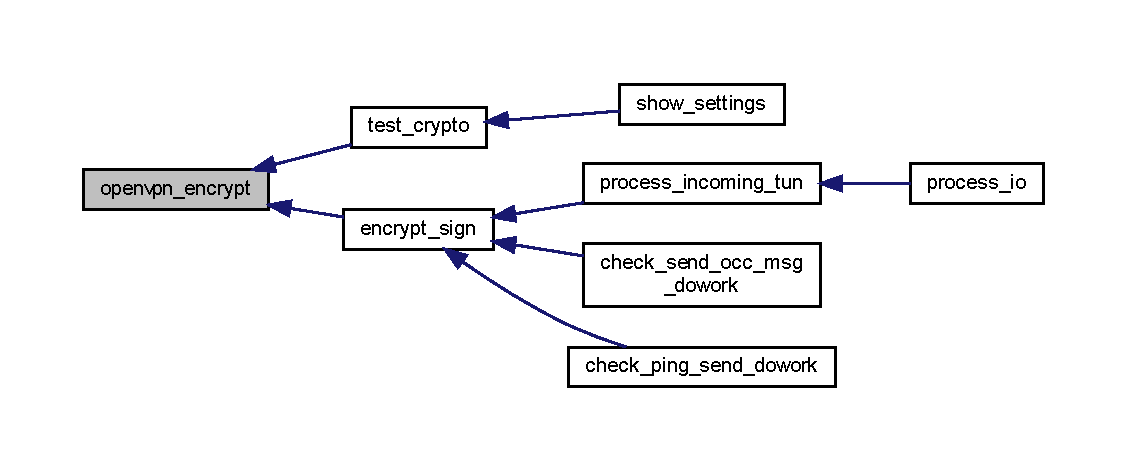
\includegraphics[width=350pt]{group__data__crypto_ga2756bad88224b98719d4e8f08cb11ef9_icgraph}
\end{center}
\end{figure}


\hypertarget{group__data__crypto_ga1f2ecd39b88da77b2f8067962155ea82}{}\index{Data Channel Crypto module@{Data Channel Crypto module}!tls\+\_\+post\+\_\+encrypt@{tls\+\_\+post\+\_\+encrypt}}
\index{tls\+\_\+post\+\_\+encrypt@{tls\+\_\+post\+\_\+encrypt}!Data Channel Crypto module@{Data Channel Crypto module}}
\subsubsection[{tls\+\_\+post\+\_\+encrypt(struct tls\+\_\+multi $\ast$multi, struct buffer $\ast$buf)}]{\setlength{\rightskip}{0pt plus 5cm}void tls\+\_\+post\+\_\+encrypt (
\begin{DoxyParamCaption}
\item[{struct {\bf tls\+\_\+multi} $\ast$}]{multi, }
\item[{struct {\bf buffer} $\ast$}]{buf}
\end{DoxyParamCaption}
)}\label{group__data__crypto_ga1f2ecd39b88da77b2f8067962155ea82}
Perform some accounting for the key state used.


\begin{DoxyParams}{Parameters}
{\em multi} & -\/ The T\+L\+S state for this packet\textquotesingle{}s destination V\+P\+N tunnel. \\
\hline
{\em buf} & -\/ The buffer containing the outgoing packet. \\
\hline
\end{DoxyParams}


Here is the caller graph for this function\+:
\nopagebreak
\begin{figure}[H]
\begin{center}
\leavevmode
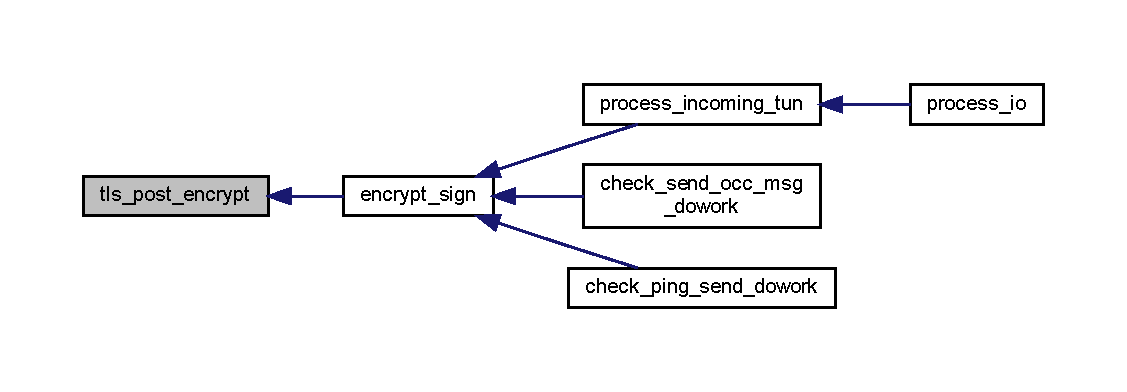
\includegraphics[width=350pt]{group__data__crypto_ga1f2ecd39b88da77b2f8067962155ea82_icgraph}
\end{center}
\end{figure}


\hypertarget{group__data__crypto_gab1369f42e94bbec108d952d565b0f283}{}\index{Data Channel Crypto module@{Data Channel Crypto module}!tls\+\_\+pre\+\_\+decrypt\+\_\+lite@{tls\+\_\+pre\+\_\+decrypt\+\_\+lite}}
\index{tls\+\_\+pre\+\_\+decrypt\+\_\+lite@{tls\+\_\+pre\+\_\+decrypt\+\_\+lite}!Data Channel Crypto module@{Data Channel Crypto module}}
\subsubsection[{tls\+\_\+pre\+\_\+decrypt\+\_\+lite(const struct tls\+\_\+auth\+\_\+standalone $\ast$tas, const struct link\+\_\+socket\+\_\+actual $\ast$from, const struct buffer $\ast$buf)}]{\setlength{\rightskip}{0pt plus 5cm}{\bf bool} tls\+\_\+pre\+\_\+decrypt\+\_\+lite (
\begin{DoxyParamCaption}
\item[{const struct {\bf tls\+\_\+auth\+\_\+standalone} $\ast$}]{tas, }
\item[{const struct {\bf link\+\_\+socket\+\_\+actual} $\ast$}]{from, }
\item[{const struct {\bf buffer} $\ast$}]{buf}
\end{DoxyParamCaption}
)}\label{group__data__crypto_gab1369f42e94bbec108d952d565b0f283}
Inspect an incoming packet for which no V\+P\+N tunnel is active, and determine whether a new V\+P\+N tunnel should be created.

This function receives the initial incoming packet from a client that wishes to establish a new V\+P\+N tunnel, and determines the packet is a valid initial packet. It is only used when Open\+V\+P\+N is running in server mode.

The tests performed by this function are whether the packet\textquotesingle{}s opcode is correct for establishing a new V\+P\+N tunnel, whether its key I\+D is 0, and whether its size is not too large. This function also performs the initial H\+M\+A\+C firewall test, if configured to do so.

The incoming packet and the local V\+P\+N tunnel state are not modified by this function. Its sole purpose is to inspect the packet and determine whether a new V\+P\+N tunnel should be created. If so, that new V\+P\+N tunnel instance will handle processing of the packet.


\begin{DoxyParams}{Parameters}
{\em tas} & -\/ The standalone T\+L\+S authentication setting structure for this process. \\
\hline
{\em from} & -\/ The source address of the packet. \\
\hline
{\em buf} & -\/ A buffer structure containing the incoming packet.\\
\hline
\end{DoxyParams}
\begin{DoxyReturn}{Returns}
\begin{DoxyItemize}
\item True if the packet is valid and a new V\+P\+N tunnel should be created for this client. \item False if the packet is not valid, did not pass the H\+M\+A\+C firewall test, or some other error occurred. \end{DoxyItemize}

\end{DoxyReturn}


Here is the call graph for this function\+:
\nopagebreak
\begin{figure}[H]
\begin{center}
\leavevmode
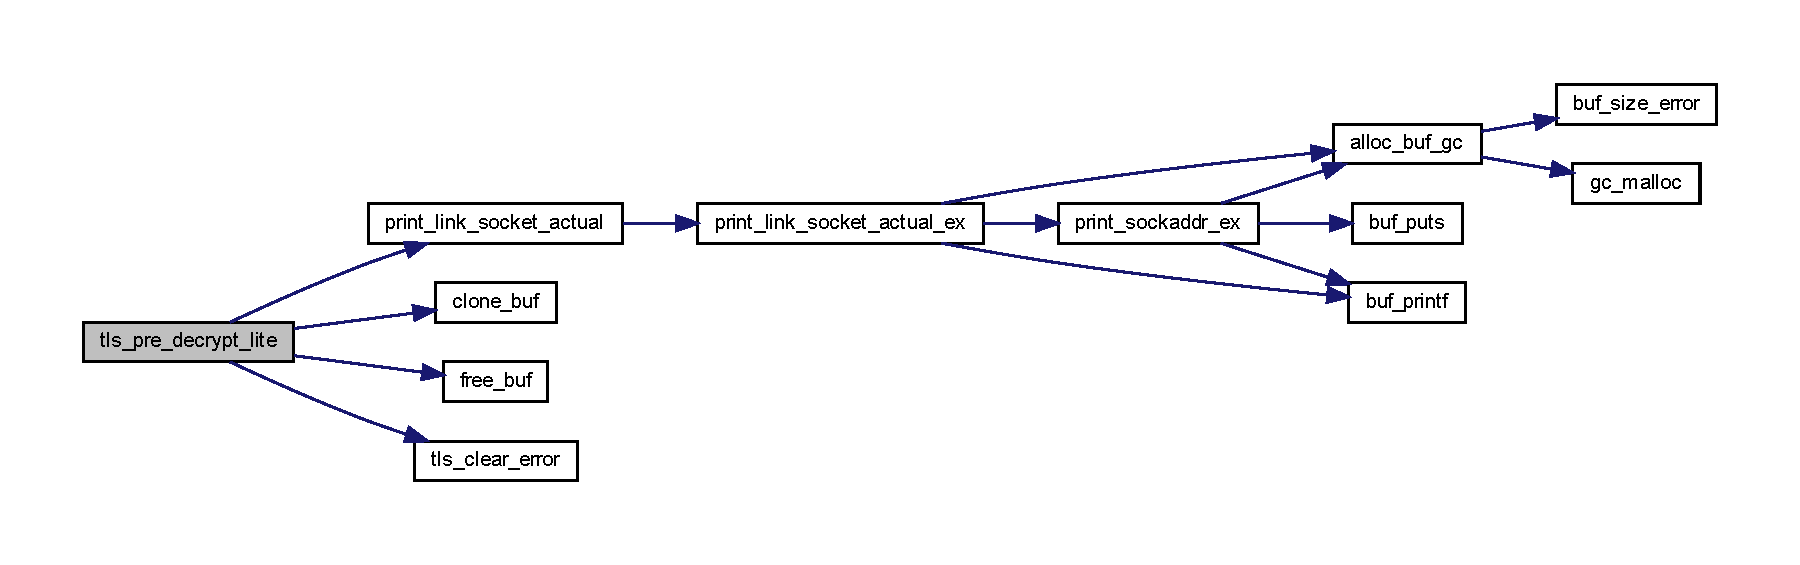
\includegraphics[width=350pt]{group__data__crypto_gab1369f42e94bbec108d952d565b0f283_cgraph}
\end{center}
\end{figure}


\hypertarget{group__data__crypto_gaba03eaba587a89c2abda8780da7b3ac7}{}\index{Data Channel Crypto module@{Data Channel Crypto module}!tls\+\_\+pre\+\_\+encrypt@{tls\+\_\+pre\+\_\+encrypt}}
\index{tls\+\_\+pre\+\_\+encrypt@{tls\+\_\+pre\+\_\+encrypt}!Data Channel Crypto module@{Data Channel Crypto module}}
\subsubsection[{tls\+\_\+pre\+\_\+encrypt(struct tls\+\_\+multi $\ast$multi, struct buffer $\ast$buf, struct crypto\+\_\+options $\ast$$\ast$opt)}]{\setlength{\rightskip}{0pt plus 5cm}void tls\+\_\+pre\+\_\+encrypt (
\begin{DoxyParamCaption}
\item[{struct {\bf tls\+\_\+multi} $\ast$}]{multi, }
\item[{struct {\bf buffer} $\ast$}]{buf, }
\item[{struct {\bf crypto\+\_\+options} $\ast$$\ast$}]{opt}
\end{DoxyParamCaption}
)}\label{group__data__crypto_gaba03eaba587a89c2abda8780da7b3ac7}
Choose the appropriate security parameters with which to process an outgoing packet.

If no appropriate security parameters can be found, or if some other error occurs, then the buffer is set to empty, and the parameters to a N\+U\+L\+L pointer.


\begin{DoxyParams}{Parameters}
{\em multi} & -\/ The T\+L\+S state for this packet\textquotesingle{}s destination V\+P\+N tunnel. \\
\hline
{\em buf} & -\/ The buffer containing the outgoing packet. \\
\hline
{\em opt} & -\/ Returns a crypto options structure with the security parameters. \\
\hline
\end{DoxyParams}


Here is the caller graph for this function\+:
\nopagebreak
\begin{figure}[H]
\begin{center}
\leavevmode
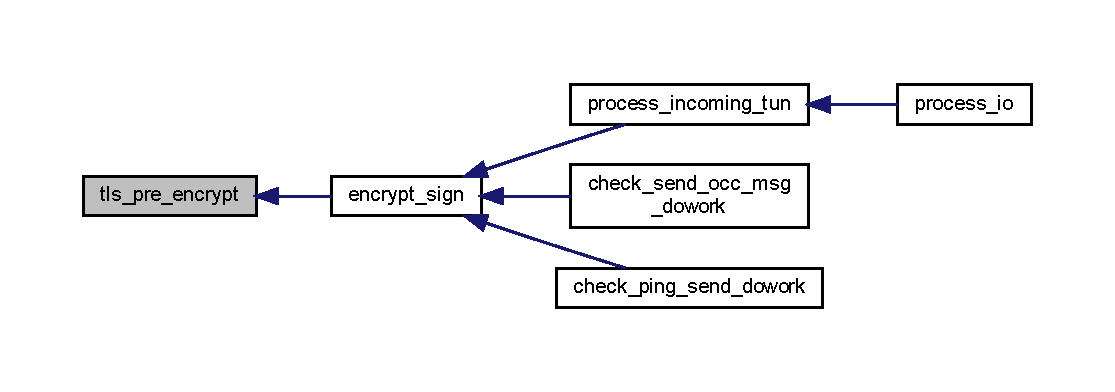
\includegraphics[width=350pt]{group__data__crypto_gaba03eaba587a89c2abda8780da7b3ac7_icgraph}
\end{center}
\end{figure}


\hypertarget{group__data__crypto_gaac2b3aa2c842a102804be65f28adf4b1}{}\index{Data Channel Crypto module@{Data Channel Crypto module}!tls\+\_\+prepend\+\_\+opcode\+\_\+v1@{tls\+\_\+prepend\+\_\+opcode\+\_\+v1}}
\index{tls\+\_\+prepend\+\_\+opcode\+\_\+v1@{tls\+\_\+prepend\+\_\+opcode\+\_\+v1}!Data Channel Crypto module@{Data Channel Crypto module}}
\subsubsection[{tls\+\_\+prepend\+\_\+opcode\+\_\+v1(const struct tls\+\_\+multi $\ast$multi, struct buffer $\ast$buf)}]{\setlength{\rightskip}{0pt plus 5cm}void tls\+\_\+prepend\+\_\+opcode\+\_\+v1 (
\begin{DoxyParamCaption}
\item[{const struct {\bf tls\+\_\+multi} $\ast$}]{multi, }
\item[{struct {\bf buffer} $\ast$}]{buf}
\end{DoxyParamCaption}
)}\label{group__data__crypto_gaac2b3aa2c842a102804be65f28adf4b1}
Prepend a one-\/byte Open\+V\+P\+N data channel P\+\_\+\+D\+A\+T\+A\+\_\+\+V1 opcode to the packet.

The opcode identifies the packet as a V1 data channel packet and gives the low-\/permutation version of the key-\/id to the recipient, so it knows which decrypt key to use.


\begin{DoxyParams}{Parameters}
{\em multi} & -\/ The T\+L\+S state for this packet\textquotesingle{}s destination V\+P\+N tunnel. \\
\hline
{\em buf} & -\/ The buffer to write the header to. \\
\hline
\end{DoxyParams}


Here is the caller graph for this function\+:
\nopagebreak
\begin{figure}[H]
\begin{center}
\leavevmode
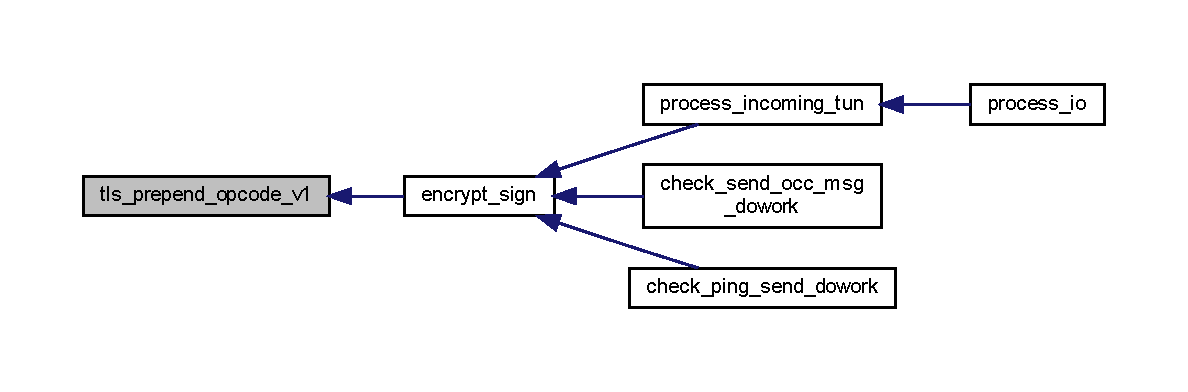
\includegraphics[width=350pt]{group__data__crypto_gaac2b3aa2c842a102804be65f28adf4b1_icgraph}
\end{center}
\end{figure}


\hypertarget{group__data__crypto_gad27b20736f89d38d0d2e0c2e35f7a0e3}{}\index{Data Channel Crypto module@{Data Channel Crypto module}!tls\+\_\+prepend\+\_\+opcode\+\_\+v2@{tls\+\_\+prepend\+\_\+opcode\+\_\+v2}}
\index{tls\+\_\+prepend\+\_\+opcode\+\_\+v2@{tls\+\_\+prepend\+\_\+opcode\+\_\+v2}!Data Channel Crypto module@{Data Channel Crypto module}}
\subsubsection[{tls\+\_\+prepend\+\_\+opcode\+\_\+v2(const struct tls\+\_\+multi $\ast$multi, struct buffer $\ast$buf)}]{\setlength{\rightskip}{0pt plus 5cm}void tls\+\_\+prepend\+\_\+opcode\+\_\+v2 (
\begin{DoxyParamCaption}
\item[{const struct {\bf tls\+\_\+multi} $\ast$}]{multi, }
\item[{struct {\bf buffer} $\ast$}]{buf}
\end{DoxyParamCaption}
)}\label{group__data__crypto_gad27b20736f89d38d0d2e0c2e35f7a0e3}
Prepend an Open\+V\+P\+N data channel P\+\_\+\+D\+A\+T\+A\+\_\+\+V2 header to the packet. The P\+\_\+\+D\+A\+T\+A\+\_\+\+V2 header consists of a 1-\/byte opcode, followed by a 3-\/byte peer-\/id.

The opcode identifies the packet as a V2 data channel packet and gives the low-\/permutation version of the key-\/id to the recipient, so it knows which decrypt key to use.

The peer-\/id is sent by clients to servers to help the server determine to select the decrypt key when the client is roaming between addresses/ports.


\begin{DoxyParams}{Parameters}
{\em multi} & -\/ The T\+L\+S state for this packet\textquotesingle{}s destination V\+P\+N tunnel. \\
\hline
{\em buf} & -\/ The buffer to write the header to. \\
\hline
\end{DoxyParams}


Here is the caller graph for this function\+:
\nopagebreak
\begin{figure}[H]
\begin{center}
\leavevmode
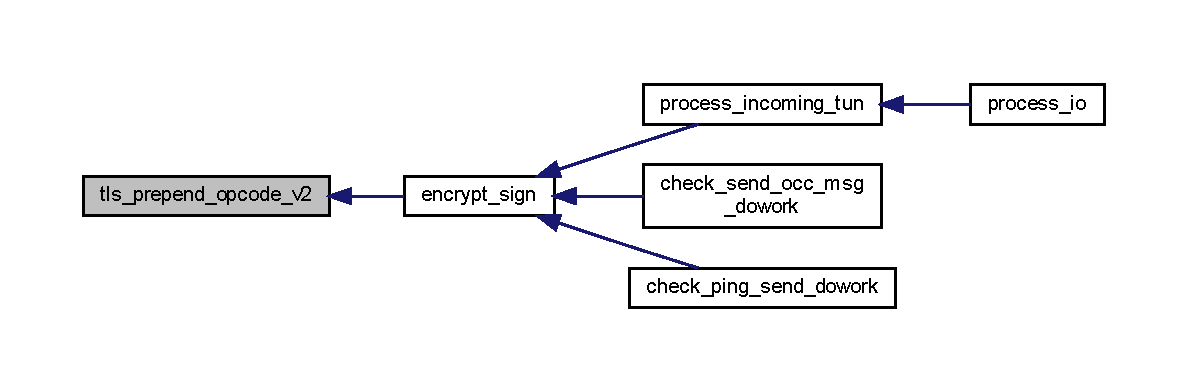
\includegraphics[width=350pt]{group__data__crypto_gad27b20736f89d38d0d2e0c2e35f7a0e3_icgraph}
\end{center}
\end{figure}



\hypertarget{group__reliable}{}\section{Reliable}
\label{group__reliable}\index{Reliable@{Reliable}}
\subsection*{Classes}
\begin{DoxyCompactItemize}
\item 
struct \hyperlink{structreliable__ack}{reliable\+\_\+ack}
\item 
struct \hyperlink{structreliable__entry}{reliable\+\_\+entry}
\item 
struct \hyperlink{structreliable}{reliable}
\end{DoxyCompactItemize}
\subsection*{Macros}
\begin{DoxyCompactItemize}
\item 
\#define \hyperlink{group__reliable_gacb891f0bfc023839a53a2c7005cd340c}{E\+X\+P\+O\+N\+E\+N\+T\+I\+A\+L\+\_\+\+B\+A\+C\+K\+O\+F\+F}
\item 
\#define \hyperlink{group__reliable_ga91ccbc389e490d03321b1a6de0dd096d}{R\+E\+L\+I\+A\+B\+L\+E\+\_\+\+A\+C\+K\+\_\+\+S\+I\+Z\+E}~8
\item 
\#define \hyperlink{group__reliable_gaa626a13dc31bf131a92548b9b2810cba}{R\+E\+L\+I\+A\+B\+L\+E\+\_\+\+C\+A\+P\+A\+C\+I\+T\+Y}~8
\end{DoxyCompactItemize}
\subsection*{Functions for processing incoming acknowledgments}
\begin{DoxyCompactItemize}
\item 
\hyperlink{automatic_8c_abb452686968e48b67397da5f97445f5b}{bool} \hyperlink{group__reliable_ga03d3c93ec4c15d57947740a56eae0aec}{reliable\+\_\+ack\+\_\+read} (struct \hyperlink{structreliable__ack}{reliable\+\_\+ack} $\ast$ack, struct \hyperlink{structbuffer}{buffer} $\ast$buf, const struct \hyperlink{structsession__id}{session\+\_\+id} $\ast$sid)
\item 
void \hyperlink{group__reliable_ga0f79fac5e64e7d2a9df9bc13740f6293}{reliable\+\_\+send\+\_\+purge} (struct \hyperlink{structreliable}{reliable} $\ast$rel, struct \hyperlink{structreliable__ack}{reliable\+\_\+ack} $\ast$ack)
\end{DoxyCompactItemize}
\subsection*{Functions for processing outgoing acknowledgments}
\begin{DoxyCompactItemize}
\item 
\hyperlink{automatic_8c_abb452686968e48b67397da5f97445f5b}{bool} \hyperlink{group__reliable_ga6875d0fb65bdd960736068b2e0fe4a29}{reliable\+\_\+ack\+\_\+write} (struct \hyperlink{structreliable__ack}{reliable\+\_\+ack} $\ast$ack, struct \hyperlink{structbuffer}{buffer} $\ast$buf, const struct \hyperlink{structsession__id}{session\+\_\+id} $\ast$sid, int max, \hyperlink{automatic_8c_abb452686968e48b67397da5f97445f5b}{bool} prepend)
\end{DoxyCompactItemize}
\subsection*{Functions for initialization and cleanup}
\begin{DoxyCompactItemize}
\item 
void \hyperlink{group__reliable_gab5e5ef6d6fd862187abe76f88b972ee5}{reliable\+\_\+init} (struct \hyperlink{structreliable}{reliable} $\ast$rel, int buf\+\_\+size, int offset, int array\+\_\+size, \hyperlink{automatic_8c_abb452686968e48b67397da5f97445f5b}{bool} hold)
\item 
void \hyperlink{group__reliable_ga0315c8ecda1aafbfb61e6ab1b8c2477b}{reliable\+\_\+free} (struct \hyperlink{structreliable}{reliable} $\ast$rel)
\item 
void \hyperlink{group__reliable_gaaf4135caf45a800b9accff968aaa59d6}{reliable\+\_\+ack\+\_\+adjust\+\_\+frame\+\_\+parameters} (struct \hyperlink{structframe}{frame} $\ast$\hyperlink{structframe}{frame}, int max)
\end{DoxyCompactItemize}
\subsection*{Functions for inserting incoming packets}
\begin{DoxyCompactItemize}
\item 
\hyperlink{automatic_8c_abb452686968e48b67397da5f97445f5b}{bool} \hyperlink{group__reliable_ga68f5e71b155cdcfabca18d028d336311}{reliable\+\_\+can\+\_\+get} (const struct \hyperlink{structreliable}{reliable} $\ast$rel)
\item 
\hyperlink{automatic_8c_abb452686968e48b67397da5f97445f5b}{bool} \hyperlink{group__reliable_ga907fd32837c50b4266eb5db1c56f9b13}{reliable\+\_\+not\+\_\+replay} (const struct \hyperlink{structreliable}{reliable} $\ast$rel, \hyperlink{packet__id_8h_a345f753b1c6ea20d24409e769aadb7e6}{packet\+\_\+id\+\_\+type} id)
\item 
\hyperlink{automatic_8c_abb452686968e48b67397da5f97445f5b}{bool} \hyperlink{group__reliable_gad2d6e3bde9beced3d69bbba652730439}{reliable\+\_\+wont\+\_\+break\+\_\+sequentiality} (const struct \hyperlink{structreliable}{reliable} $\ast$rel, \hyperlink{packet__id_8h_a345f753b1c6ea20d24409e769aadb7e6}{packet\+\_\+id\+\_\+type} id)
\item 
\hyperlink{automatic_8c_abb452686968e48b67397da5f97445f5b}{bool} \hyperlink{group__reliable_ga21a2f2e1296cea87eb6d68331667fc9e}{reliable\+\_\+ack\+\_\+read\+\_\+packet\+\_\+id} (struct \hyperlink{structbuffer}{buffer} $\ast$buf, \hyperlink{packet__id_8h_a345f753b1c6ea20d24409e769aadb7e6}{packet\+\_\+id\+\_\+type} $\ast$pid)
\item 
struct \hyperlink{structbuffer}{buffer} $\ast$ \hyperlink{group__reliable_gaa69117718f8e1e22881d957e219134ff}{reliable\+\_\+get\+\_\+buf} (struct \hyperlink{structreliable}{reliable} $\ast$rel)
\item 
void \hyperlink{group__reliable_ga2689b44850ce41cc2fe1fc7f57657eb4}{reliable\+\_\+mark\+\_\+active\+\_\+incoming} (struct \hyperlink{structreliable}{reliable} $\ast$rel, struct \hyperlink{structbuffer}{buffer} $\ast$buf, \hyperlink{packet__id_8h_a345f753b1c6ea20d24409e769aadb7e6}{packet\+\_\+id\+\_\+type} pid, int opcode)
\item 
\hyperlink{automatic_8c_abb452686968e48b67397da5f97445f5b}{bool} \hyperlink{group__reliable_ga3bdc89dd24741d52a2fcf8182389b947}{reliable\+\_\+ack\+\_\+acknowledge\+\_\+packet\+\_\+id} (struct \hyperlink{structreliable__ack}{reliable\+\_\+ack} $\ast$ack, \hyperlink{packet__id_8h_a345f753b1c6ea20d24409e769aadb7e6}{packet\+\_\+id\+\_\+type} pid)
\end{DoxyCompactItemize}
\subsection*{Functions for extracting incoming packets}
\begin{DoxyCompactItemize}
\item 
struct \hyperlink{structbuffer}{buffer} $\ast$ \hyperlink{group__reliable_ga08f53328657f0172eb061193171e2a41}{reliable\+\_\+get\+\_\+buf\+\_\+sequenced} (struct \hyperlink{structreliable}{reliable} $\ast$rel)
\item 
void \hyperlink{group__reliable_ga5c51920665fa9c34f082dd7aa6ce0e55}{reliable\+\_\+mark\+\_\+deleted} (struct \hyperlink{structreliable}{reliable} $\ast$rel, struct \hyperlink{structbuffer}{buffer} $\ast$buf, \hyperlink{automatic_8c_abb452686968e48b67397da5f97445f5b}{bool} inc\+\_\+pid)
\end{DoxyCompactItemize}
\subsection*{Functions for inserting outgoing packets}
\begin{DoxyCompactItemize}
\item 
struct \hyperlink{structbuffer}{buffer} $\ast$ \hyperlink{group__reliable_gaa15b0672f4ddd65d55194ed5bde0e1c8}{reliable\+\_\+get\+\_\+buf\+\_\+output\+\_\+sequenced} (struct \hyperlink{structreliable}{reliable} $\ast$rel)
\item 
void \hyperlink{group__reliable_ga2c03b5ae47fe72dbf4fe16f11ea1c091}{reliable\+\_\+mark\+\_\+active\+\_\+outgoing} (struct \hyperlink{structreliable}{reliable} $\ast$rel, struct \hyperlink{structbuffer}{buffer} $\ast$buf, int opcode)
\end{DoxyCompactItemize}
\subsection*{Functions for extracting outgoing packets}
\begin{DoxyCompactItemize}
\item 
\hyperlink{automatic_8c_abb452686968e48b67397da5f97445f5b}{bool} \hyperlink{group__reliable_ga79e86f7694ffbd592d944f8f45efa7c8}{reliable\+\_\+can\+\_\+send} (const struct \hyperlink{structreliable}{reliable} $\ast$rel)
\item 
struct \hyperlink{structbuffer}{buffer} $\ast$ \hyperlink{group__reliable_gaebcf7ae7a144f32b55c9af5c51121ec1}{reliable\+\_\+send} (struct \hyperlink{structreliable}{reliable} $\ast$rel, int $\ast$opcode)
\end{DoxyCompactItemize}
\subsection*{Miscellaneous functions}
\begin{DoxyCompactItemize}
\item 
\hyperlink{automatic_8c_abb452686968e48b67397da5f97445f5b}{bool} \hyperlink{group__reliable_ga7e0186d08bdeb59563ce37578ee64f8d}{reliable\+\_\+empty} (const struct \hyperlink{structreliable}{reliable} $\ast$rel)
\item 
\hyperlink{common_8h_a3d8621f960ada51a5ad9ff181730481a}{interval\+\_\+t} \hyperlink{group__reliable_ga9e8edfca42338da6da6ccb3fd1849dca}{reliable\+\_\+send\+\_\+timeout} (const struct \hyperlink{structreliable}{reliable} $\ast$rel)
\item 
void \hyperlink{group__reliable_ga14cb4395f780502ae9edbe6d3f90aec5}{reliable\+\_\+schedule\+\_\+now} (struct \hyperlink{structreliable}{reliable} $\ast$rel)
\item 
void \hyperlink{group__reliable_ga864d5a93bec5ac5554ce9481d1551197}{reliable\+\_\+debug\+\_\+print} (const struct \hyperlink{structreliable}{reliable} $\ast$rel, char $\ast$desc)
\item 
const char $\ast$ \hyperlink{group__reliable_ga6b9917d2ee4fe23f48f4471e8f4f4fdd}{reliable\+\_\+ack\+\_\+print} (struct \hyperlink{structbuffer}{buffer} $\ast$buf, \hyperlink{automatic_8c_abb452686968e48b67397da5f97445f5b}{bool} verbose, struct \hyperlink{structgc__arena}{gc\+\_\+arena} $\ast$gc)
\item 
void \hyperlink{group__reliable_ga1e35eb4bd321de7b34aa1f086451f724}{reliable\+\_\+ack\+\_\+debug\+\_\+print} (const struct \hyperlink{structreliable__ack}{reliable\+\_\+ack} $\ast$ack, char $\ast$desc)
\end{DoxyCompactItemize}


\subsection{Detailed Description}


\subsection{Macro Definition Documentation}
\hypertarget{group__reliable_gacb891f0bfc023839a53a2c7005cd340c}{}\index{Reliable@{Reliable}!E\+X\+P\+O\+N\+E\+N\+T\+I\+A\+L\+\_\+\+B\+A\+C\+K\+O\+F\+F@{E\+X\+P\+O\+N\+E\+N\+T\+I\+A\+L\+\_\+\+B\+A\+C\+K\+O\+F\+F}}
\index{E\+X\+P\+O\+N\+E\+N\+T\+I\+A\+L\+\_\+\+B\+A\+C\+K\+O\+F\+F@{E\+X\+P\+O\+N\+E\+N\+T\+I\+A\+L\+\_\+\+B\+A\+C\+K\+O\+F\+F}!Reliable@{Reliable}}
\subsubsection[{E\+X\+P\+O\+N\+E\+N\+T\+I\+A\+L\+\_\+\+B\+A\+C\+K\+O\+F\+F}]{\setlength{\rightskip}{0pt plus 5cm}\#define E\+X\+P\+O\+N\+E\+N\+T\+I\+A\+L\+\_\+\+B\+A\+C\+K\+O\+F\+F}\label{group__reliable_gacb891f0bfc023839a53a2c7005cd340c}
\hypertarget{group__reliable_ga91ccbc389e490d03321b1a6de0dd096d}{}\index{Reliable@{Reliable}!R\+E\+L\+I\+A\+B\+L\+E\+\_\+\+A\+C\+K\+\_\+\+S\+I\+Z\+E@{R\+E\+L\+I\+A\+B\+L\+E\+\_\+\+A\+C\+K\+\_\+\+S\+I\+Z\+E}}
\index{R\+E\+L\+I\+A\+B\+L\+E\+\_\+\+A\+C\+K\+\_\+\+S\+I\+Z\+E@{R\+E\+L\+I\+A\+B\+L\+E\+\_\+\+A\+C\+K\+\_\+\+S\+I\+Z\+E}!Reliable@{Reliable}}
\subsubsection[{R\+E\+L\+I\+A\+B\+L\+E\+\_\+\+A\+C\+K\+\_\+\+S\+I\+Z\+E}]{\setlength{\rightskip}{0pt plus 5cm}\#define R\+E\+L\+I\+A\+B\+L\+E\+\_\+\+A\+C\+K\+\_\+\+S\+I\+Z\+E~8}\label{group__reliable_ga91ccbc389e490d03321b1a6de0dd096d}
The maximum number of packet I\+Ds waiting to be acknowledged which can be stored in one {\ttfamily \hyperlink{structreliable__ack}{reliable\+\_\+ack}} structure. \hypertarget{group__reliable_gaa626a13dc31bf131a92548b9b2810cba}{}\index{Reliable@{Reliable}!R\+E\+L\+I\+A\+B\+L\+E\+\_\+\+C\+A\+P\+A\+C\+I\+T\+Y@{R\+E\+L\+I\+A\+B\+L\+E\+\_\+\+C\+A\+P\+A\+C\+I\+T\+Y}}
\index{R\+E\+L\+I\+A\+B\+L\+E\+\_\+\+C\+A\+P\+A\+C\+I\+T\+Y@{R\+E\+L\+I\+A\+B\+L\+E\+\_\+\+C\+A\+P\+A\+C\+I\+T\+Y}!Reliable@{Reliable}}
\subsubsection[{R\+E\+L\+I\+A\+B\+L\+E\+\_\+\+C\+A\+P\+A\+C\+I\+T\+Y}]{\setlength{\rightskip}{0pt plus 5cm}\#define R\+E\+L\+I\+A\+B\+L\+E\+\_\+\+C\+A\+P\+A\+C\+I\+T\+Y~8}\label{group__reliable_gaa626a13dc31bf131a92548b9b2810cba}
The maximum number of packets that the reliability layer for one V\+P\+N tunnel in one direction can store. 

\subsection{Function Documentation}
\hypertarget{group__reliable_ga3bdc89dd24741d52a2fcf8182389b947}{}\index{Reliable@{Reliable}!reliable\+\_\+ack\+\_\+acknowledge\+\_\+packet\+\_\+id@{reliable\+\_\+ack\+\_\+acknowledge\+\_\+packet\+\_\+id}}
\index{reliable\+\_\+ack\+\_\+acknowledge\+\_\+packet\+\_\+id@{reliable\+\_\+ack\+\_\+acknowledge\+\_\+packet\+\_\+id}!Reliable@{Reliable}}
\subsubsection[{reliable\+\_\+ack\+\_\+acknowledge\+\_\+packet\+\_\+id(struct reliable\+\_\+ack $\ast$ack, packet\+\_\+id\+\_\+type pid)}]{\setlength{\rightskip}{0pt plus 5cm}{\bf bool} reliable\+\_\+ack\+\_\+acknowledge\+\_\+packet\+\_\+id (
\begin{DoxyParamCaption}
\item[{struct {\bf reliable\+\_\+ack} $\ast$}]{ack, }
\item[{{\bf packet\+\_\+id\+\_\+type}}]{pid}
\end{DoxyParamCaption}
)}\label{group__reliable_ga3bdc89dd24741d52a2fcf8182389b947}
Record a packet I\+D for later acknowledgment.


\begin{DoxyParams}{Parameters}
{\em ack} & The acknowledgment structure which stores this V\+P\+N tunnel\textquotesingle{}s packet I\+Ds for later acknowledgment. \\
\hline
{\em pid} & The packet I\+D of the received packet which should be acknowledged.\\
\hline
\end{DoxyParams}
\begin{DoxyReturn}{Returns}
\begin{DoxyItemize}
\item True, if the packet I\+D was added to {\itshape ack}. \item False, if the packet I\+D was already present in {\itshape ack} or {\itshape ack} has no free space to store any more packet I\+Ds. \end{DoxyItemize}

\end{DoxyReturn}


Here is the caller graph for this function\+:
\nopagebreak
\begin{figure}[H]
\begin{center}
\leavevmode
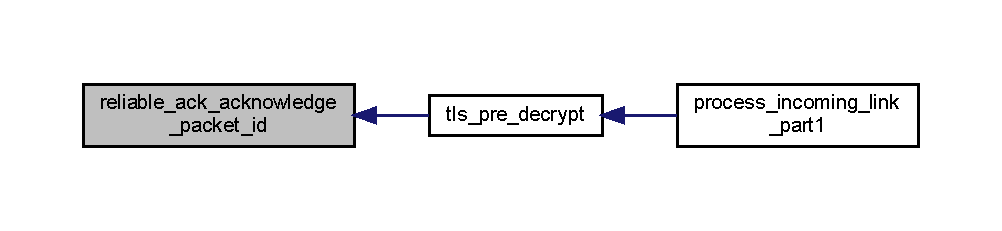
\includegraphics[width=350pt]{group__reliable_ga3bdc89dd24741d52a2fcf8182389b947_icgraph}
\end{center}
\end{figure}


\hypertarget{group__reliable_gaaf4135caf45a800b9accff968aaa59d6}{}\index{Reliable@{Reliable}!reliable\+\_\+ack\+\_\+adjust\+\_\+frame\+\_\+parameters@{reliable\+\_\+ack\+\_\+adjust\+\_\+frame\+\_\+parameters}}
\index{reliable\+\_\+ack\+\_\+adjust\+\_\+frame\+\_\+parameters@{reliable\+\_\+ack\+\_\+adjust\+\_\+frame\+\_\+parameters}!Reliable@{Reliable}}
\subsubsection[{reliable\+\_\+ack\+\_\+adjust\+\_\+frame\+\_\+parameters(struct frame $\ast$frame, int max)}]{\setlength{\rightskip}{0pt plus 5cm}void reliable\+\_\+ack\+\_\+adjust\+\_\+frame\+\_\+parameters (
\begin{DoxyParamCaption}
\item[{struct {\bf frame} $\ast$}]{frame, }
\item[{int}]{max}
\end{DoxyParamCaption}
)}\label{group__reliable_gaaf4135caf45a800b9accff968aaa59d6}
\hypertarget{group__reliable_ga1e35eb4bd321de7b34aa1f086451f724}{}\index{Reliable@{Reliable}!reliable\+\_\+ack\+\_\+debug\+\_\+print@{reliable\+\_\+ack\+\_\+debug\+\_\+print}}
\index{reliable\+\_\+ack\+\_\+debug\+\_\+print@{reliable\+\_\+ack\+\_\+debug\+\_\+print}!Reliable@{Reliable}}
\subsubsection[{reliable\+\_\+ack\+\_\+debug\+\_\+print(const struct reliable\+\_\+ack $\ast$ack, char $\ast$desc)}]{\setlength{\rightskip}{0pt plus 5cm}void reliable\+\_\+ack\+\_\+debug\+\_\+print (
\begin{DoxyParamCaption}
\item[{const struct {\bf reliable\+\_\+ack} $\ast$}]{ack, }
\item[{char $\ast$}]{desc}
\end{DoxyParamCaption}
)}\label{group__reliable_ga1e35eb4bd321de7b34aa1f086451f724}
\hypertarget{group__reliable_ga6b9917d2ee4fe23f48f4471e8f4f4fdd}{}\index{Reliable@{Reliable}!reliable\+\_\+ack\+\_\+print@{reliable\+\_\+ack\+\_\+print}}
\index{reliable\+\_\+ack\+\_\+print@{reliable\+\_\+ack\+\_\+print}!Reliable@{Reliable}}
\subsubsection[{reliable\+\_\+ack\+\_\+print(struct buffer $\ast$buf, bool verbose, struct gc\+\_\+arena $\ast$gc)}]{\setlength{\rightskip}{0pt plus 5cm}const char$\ast$ reliable\+\_\+ack\+\_\+print (
\begin{DoxyParamCaption}
\item[{struct {\bf buffer} $\ast$}]{buf, }
\item[{{\bf bool}}]{verbose, }
\item[{struct {\bf gc\+\_\+arena} $\ast$}]{gc}
\end{DoxyParamCaption}
)}\label{group__reliable_ga6b9917d2ee4fe23f48f4471e8f4f4fdd}


Here is the call graph for this function\+:
\nopagebreak
\begin{figure}[H]
\begin{center}
\leavevmode
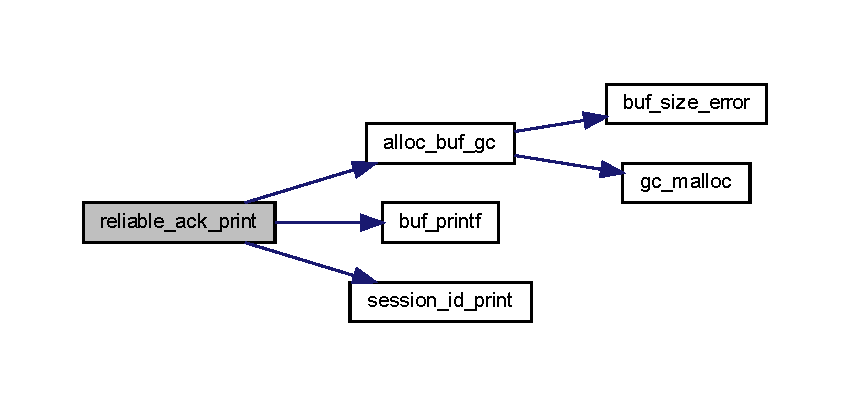
\includegraphics[width=350pt]{group__reliable_ga6b9917d2ee4fe23f48f4471e8f4f4fdd_cgraph}
\end{center}
\end{figure}




Here is the caller graph for this function\+:
\nopagebreak
\begin{figure}[H]
\begin{center}
\leavevmode
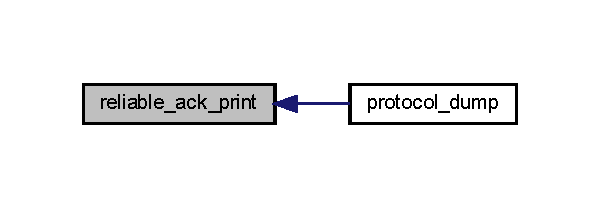
\includegraphics[width=288pt]{group__reliable_ga6b9917d2ee4fe23f48f4471e8f4f4fdd_icgraph}
\end{center}
\end{figure}


\hypertarget{group__reliable_ga03d3c93ec4c15d57947740a56eae0aec}{}\index{Reliable@{Reliable}!reliable\+\_\+ack\+\_\+read@{reliable\+\_\+ack\+\_\+read}}
\index{reliable\+\_\+ack\+\_\+read@{reliable\+\_\+ack\+\_\+read}!Reliable@{Reliable}}
\subsubsection[{reliable\+\_\+ack\+\_\+read(struct reliable\+\_\+ack $\ast$ack, struct buffer $\ast$buf, const struct session\+\_\+id $\ast$sid)}]{\setlength{\rightskip}{0pt plus 5cm}{\bf bool} reliable\+\_\+ack\+\_\+read (
\begin{DoxyParamCaption}
\item[{struct {\bf reliable\+\_\+ack} $\ast$}]{ack, }
\item[{struct {\bf buffer} $\ast$}]{buf, }
\item[{const struct {\bf session\+\_\+id} $\ast$}]{sid}
\end{DoxyParamCaption}
)}\label{group__reliable_ga03d3c93ec4c15d57947740a56eae0aec}
Read an acknowledgment record from a received packet.

This function reads the packet I\+D acknowledgment record from the packet contained in {\itshape buf}. If the record contains acknowledgments, these are stored in {\itshape ack}. This function also compares the packet\textquotesingle{}s session I\+D with the expected session I\+D {\itshape sid}, which should be equal.


\begin{DoxyParams}{Parameters}
{\em ack} & The acknowledgment structure in which received acknowledgments are to be stored. \\
\hline
{\em buf} & The buffer containing the packet. \\
\hline
{\em sid} & The expected session I\+D to compare to the session I\+D in the packet.\\
\hline
\end{DoxyParams}
\begin{DoxyReturn}{Returns}
\begin{DoxyItemize}
\item True, if processing was successful. \item False, if an error occurs during processing. \end{DoxyItemize}

\end{DoxyReturn}


Here is the call graph for this function\+:
\nopagebreak
\begin{figure}[H]
\begin{center}
\leavevmode
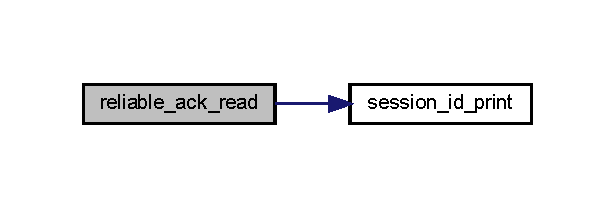
\includegraphics[width=295pt]{group__reliable_ga03d3c93ec4c15d57947740a56eae0aec_cgraph}
\end{center}
\end{figure}




Here is the caller graph for this function\+:
\nopagebreak
\begin{figure}[H]
\begin{center}
\leavevmode
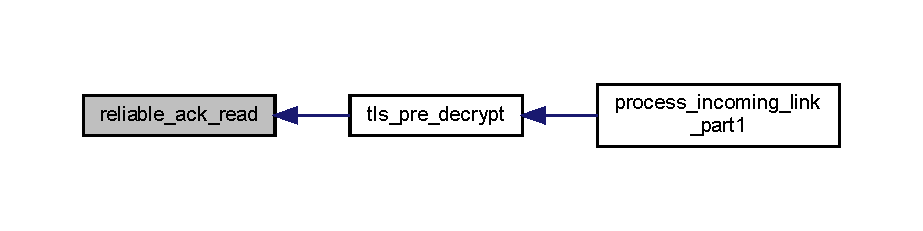
\includegraphics[width=350pt]{group__reliable_ga03d3c93ec4c15d57947740a56eae0aec_icgraph}
\end{center}
\end{figure}


\hypertarget{group__reliable_ga21a2f2e1296cea87eb6d68331667fc9e}{}\index{Reliable@{Reliable}!reliable\+\_\+ack\+\_\+read\+\_\+packet\+\_\+id@{reliable\+\_\+ack\+\_\+read\+\_\+packet\+\_\+id}}
\index{reliable\+\_\+ack\+\_\+read\+\_\+packet\+\_\+id@{reliable\+\_\+ack\+\_\+read\+\_\+packet\+\_\+id}!Reliable@{Reliable}}
\subsubsection[{reliable\+\_\+ack\+\_\+read\+\_\+packet\+\_\+id(struct buffer $\ast$buf, packet\+\_\+id\+\_\+type $\ast$pid)}]{\setlength{\rightskip}{0pt plus 5cm}{\bf bool} reliable\+\_\+ack\+\_\+read\+\_\+packet\+\_\+id (
\begin{DoxyParamCaption}
\item[{struct {\bf buffer} $\ast$}]{buf, }
\item[{{\bf packet\+\_\+id\+\_\+type} $\ast$}]{pid}
\end{DoxyParamCaption}
)}\label{group__reliable_ga21a2f2e1296cea87eb6d68331667fc9e}
Read the packet I\+D of a received packet.


\begin{DoxyParams}{Parameters}
{\em buf} & The buffer containing the received packet. \\
\hline
{\em pid} & A pointer where the packet\textquotesingle{}s packet I\+D will be written.\\
\hline
\end{DoxyParams}
\begin{DoxyReturn}{Returns}
\begin{DoxyItemize}
\item True, if processing was successful. \item False, if an error occurs during processing. \end{DoxyItemize}

\end{DoxyReturn}


Here is the caller graph for this function\+:
\nopagebreak
\begin{figure}[H]
\begin{center}
\leavevmode
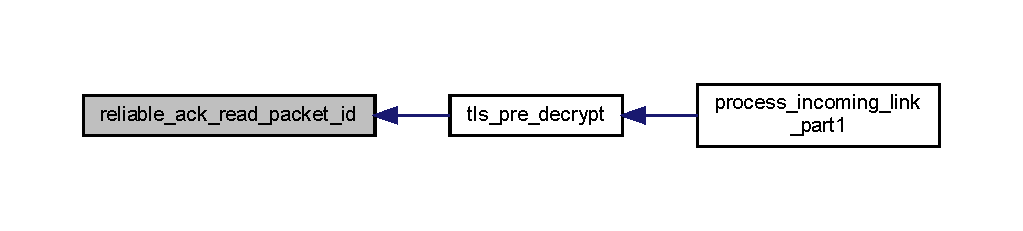
\includegraphics[width=350pt]{group__reliable_ga21a2f2e1296cea87eb6d68331667fc9e_icgraph}
\end{center}
\end{figure}


\hypertarget{group__reliable_ga6875d0fb65bdd960736068b2e0fe4a29}{}\index{Reliable@{Reliable}!reliable\+\_\+ack\+\_\+write@{reliable\+\_\+ack\+\_\+write}}
\index{reliable\+\_\+ack\+\_\+write@{reliable\+\_\+ack\+\_\+write}!Reliable@{Reliable}}
\subsubsection[{reliable\+\_\+ack\+\_\+write(struct reliable\+\_\+ack $\ast$ack, struct buffer $\ast$buf, const struct session\+\_\+id $\ast$sid, int max, bool prepend)}]{\setlength{\rightskip}{0pt plus 5cm}{\bf bool} reliable\+\_\+ack\+\_\+write (
\begin{DoxyParamCaption}
\item[{struct {\bf reliable\+\_\+ack} $\ast$}]{ack, }
\item[{struct {\bf buffer} $\ast$}]{buf, }
\item[{const struct {\bf session\+\_\+id} $\ast$}]{sid, }
\item[{int}]{max, }
\item[{{\bf bool}}]{prepend}
\end{DoxyParamCaption}
)}\label{group__reliable_ga6875d0fb65bdd960736068b2e0fe4a29}
Write a packet I\+D acknowledgment record to a buffer.


\begin{DoxyParams}{Parameters}
{\em ack} & The acknowledgment structure containing packet I\+Ds to be acknowledged. \\
\hline
{\em buf} & The buffer into which the acknowledgment record will be written. \\
\hline
{\em sid} & The session I\+D of the V\+P\+N tunnel associated with the packet I\+Ds to be acknowledged. \\
\hline
{\em max} & The maximum number of acknowledgments to be written in the record. \\
\hline
{\em prepend} & If true, prepend the acknowledgment record in the buffer; if false, write into the buffer\textquotesingle{}s current position.\\
\hline
\end{DoxyParams}
\begin{DoxyReturn}{Returns}
\begin{DoxyItemize}
\item True, if processing was successful. \item False, if an error occurs during processing. \end{DoxyItemize}

\end{DoxyReturn}


Here is the call graph for this function\+:
\nopagebreak
\begin{figure}[H]
\begin{center}
\leavevmode
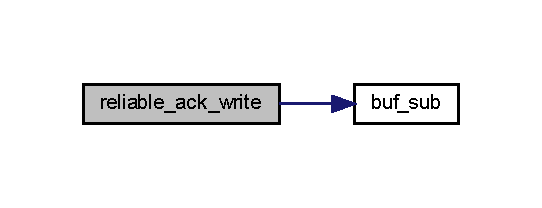
\includegraphics[width=260pt]{group__reliable_ga6875d0fb65bdd960736068b2e0fe4a29_cgraph}
\end{center}
\end{figure}


\hypertarget{group__reliable_ga68f5e71b155cdcfabca18d028d336311}{}\index{Reliable@{Reliable}!reliable\+\_\+can\+\_\+get@{reliable\+\_\+can\+\_\+get}}
\index{reliable\+\_\+can\+\_\+get@{reliable\+\_\+can\+\_\+get}!Reliable@{Reliable}}
\subsubsection[{reliable\+\_\+can\+\_\+get(const struct reliable $\ast$rel)}]{\setlength{\rightskip}{0pt plus 5cm}{\bf bool} reliable\+\_\+can\+\_\+get (
\begin{DoxyParamCaption}
\item[{const struct {\bf reliable} $\ast$}]{rel}
\end{DoxyParamCaption}
)}\label{group__reliable_ga68f5e71b155cdcfabca18d028d336311}
Check whether a reliable structure has any free buffers available for use.


\begin{DoxyParams}{Parameters}
{\em rel} & The reliable structure to check.\\
\hline
\end{DoxyParams}
\begin{DoxyReturn}{Returns}
\begin{DoxyItemize}
\item True, if at least one buffer is available for use. \item False, if all the buffers are active. \end{DoxyItemize}

\end{DoxyReturn}


Here is the caller graph for this function\+:
\nopagebreak
\begin{figure}[H]
\begin{center}
\leavevmode
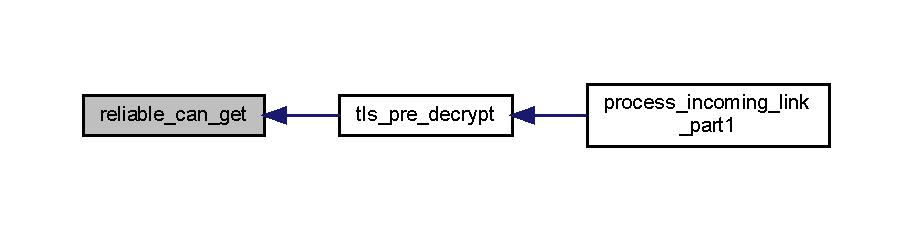
\includegraphics[width=350pt]{group__reliable_ga68f5e71b155cdcfabca18d028d336311_icgraph}
\end{center}
\end{figure}


\hypertarget{group__reliable_ga79e86f7694ffbd592d944f8f45efa7c8}{}\index{Reliable@{Reliable}!reliable\+\_\+can\+\_\+send@{reliable\+\_\+can\+\_\+send}}
\index{reliable\+\_\+can\+\_\+send@{reliable\+\_\+can\+\_\+send}!Reliable@{Reliable}}
\subsubsection[{reliable\+\_\+can\+\_\+send(const struct reliable $\ast$rel)}]{\setlength{\rightskip}{0pt plus 5cm}{\bf bool} reliable\+\_\+can\+\_\+send (
\begin{DoxyParamCaption}
\item[{const struct {\bf reliable} $\ast$}]{rel}
\end{DoxyParamCaption}
)}\label{group__reliable_ga79e86f7694ffbd592d944f8f45efa7c8}
Check whether a reliable structure has any active entries ready to be (re)sent.


\begin{DoxyParams}{Parameters}
{\em rel} & The reliable structure to check.\\
\hline
\end{DoxyParams}
\begin{DoxyReturn}{Returns}
\begin{DoxyItemize}
\item True, if there are active entries ready to be (re)sent president. \item False, if there are no active entries, or the active entries are not yet ready for resending. \end{DoxyItemize}

\end{DoxyReturn}
\hypertarget{group__reliable_ga864d5a93bec5ac5554ce9481d1551197}{}\index{Reliable@{Reliable}!reliable\+\_\+debug\+\_\+print@{reliable\+\_\+debug\+\_\+print}}
\index{reliable\+\_\+debug\+\_\+print@{reliable\+\_\+debug\+\_\+print}!Reliable@{Reliable}}
\subsubsection[{reliable\+\_\+debug\+\_\+print(const struct reliable $\ast$rel, char $\ast$desc)}]{\setlength{\rightskip}{0pt plus 5cm}void reliable\+\_\+debug\+\_\+print (
\begin{DoxyParamCaption}
\item[{const struct {\bf reliable} $\ast$}]{rel, }
\item[{char $\ast$}]{desc}
\end{DoxyParamCaption}
)}\label{group__reliable_ga864d5a93bec5ac5554ce9481d1551197}
\hypertarget{group__reliable_ga7e0186d08bdeb59563ce37578ee64f8d}{}\index{Reliable@{Reliable}!reliable\+\_\+empty@{reliable\+\_\+empty}}
\index{reliable\+\_\+empty@{reliable\+\_\+empty}!Reliable@{Reliable}}
\subsubsection[{reliable\+\_\+empty(const struct reliable $\ast$rel)}]{\setlength{\rightskip}{0pt plus 5cm}{\bf bool} reliable\+\_\+empty (
\begin{DoxyParamCaption}
\item[{const struct {\bf reliable} $\ast$}]{rel}
\end{DoxyParamCaption}
)}\label{group__reliable_ga7e0186d08bdeb59563ce37578ee64f8d}
Check whether a reliable structure is empty.


\begin{DoxyParams}{Parameters}
{\em rel} & The reliable structure to check.\\
\hline
\end{DoxyParams}
\begin{DoxyReturn}{Returns}
\begin{DoxyItemize}
\item True, if there are no active entries in the given reliable structure. \item False, if there is at least one active entry present. \end{DoxyItemize}

\end{DoxyReturn}
\hypertarget{group__reliable_ga0315c8ecda1aafbfb61e6ab1b8c2477b}{}\index{Reliable@{Reliable}!reliable\+\_\+free@{reliable\+\_\+free}}
\index{reliable\+\_\+free@{reliable\+\_\+free}!Reliable@{Reliable}}
\subsubsection[{reliable\+\_\+free(struct reliable $\ast$rel)}]{\setlength{\rightskip}{0pt plus 5cm}void reliable\+\_\+free (
\begin{DoxyParamCaption}
\item[{struct {\bf reliable} $\ast$}]{rel}
\end{DoxyParamCaption}
)}\label{group__reliable_ga0315c8ecda1aafbfb61e6ab1b8c2477b}
Free allocated memory associated with a reliable structure.


\begin{DoxyParams}{Parameters}
{\em rel} & The reliable structured to clean up. \\
\hline
\end{DoxyParams}


Here is the call graph for this function\+:
\nopagebreak
\begin{figure}[H]
\begin{center}
\leavevmode
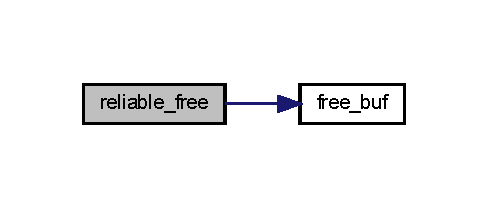
\includegraphics[width=234pt]{group__reliable_ga0315c8ecda1aafbfb61e6ab1b8c2477b_cgraph}
\end{center}
\end{figure}


\hypertarget{group__reliable_gaa69117718f8e1e22881d957e219134ff}{}\index{Reliable@{Reliable}!reliable\+\_\+get\+\_\+buf@{reliable\+\_\+get\+\_\+buf}}
\index{reliable\+\_\+get\+\_\+buf@{reliable\+\_\+get\+\_\+buf}!Reliable@{Reliable}}
\subsubsection[{reliable\+\_\+get\+\_\+buf(struct reliable $\ast$rel)}]{\setlength{\rightskip}{0pt plus 5cm}struct {\bf buffer}$\ast$ reliable\+\_\+get\+\_\+buf (
\begin{DoxyParamCaption}
\item[{struct {\bf reliable} $\ast$}]{rel}
\end{DoxyParamCaption}
)}\label{group__reliable_gaa69117718f8e1e22881d957e219134ff}
Get the buffer of a free reliable entry in which to store a packet.


\begin{DoxyParams}{Parameters}
{\em rel} & The reliable structure in which to search for a free entry.\\
\hline
\end{DoxyParams}
\begin{DoxyReturn}{Returns}
A pointer to a buffer of a free entry in the {\itshape rel} reliable structure. If there are no free entries available, this function returns N\+U\+L\+L. 
\end{DoxyReturn}


Here is the caller graph for this function\+:
\nopagebreak
\begin{figure}[H]
\begin{center}
\leavevmode
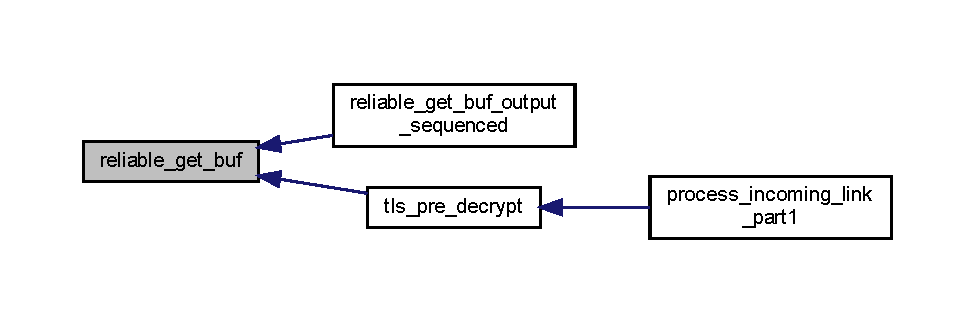
\includegraphics[width=350pt]{group__reliable_gaa69117718f8e1e22881d957e219134ff_icgraph}
\end{center}
\end{figure}


\hypertarget{group__reliable_gaa15b0672f4ddd65d55194ed5bde0e1c8}{}\index{Reliable@{Reliable}!reliable\+\_\+get\+\_\+buf\+\_\+output\+\_\+sequenced@{reliable\+\_\+get\+\_\+buf\+\_\+output\+\_\+sequenced}}
\index{reliable\+\_\+get\+\_\+buf\+\_\+output\+\_\+sequenced@{reliable\+\_\+get\+\_\+buf\+\_\+output\+\_\+sequenced}!Reliable@{Reliable}}
\subsubsection[{reliable\+\_\+get\+\_\+buf\+\_\+output\+\_\+sequenced(struct reliable $\ast$rel)}]{\setlength{\rightskip}{0pt plus 5cm}struct {\bf buffer}$\ast$ reliable\+\_\+get\+\_\+buf\+\_\+output\+\_\+sequenced (
\begin{DoxyParamCaption}
\item[{struct {\bf reliable} $\ast$}]{rel}
\end{DoxyParamCaption}
)}\label{group__reliable_gaa15b0672f4ddd65d55194ed5bde0e1c8}
Get the buffer of free reliable entry and check whether the outgoing acknowledgment sequence is still okay.


\begin{DoxyParams}{Parameters}
{\em rel} & The reliable structure in which to search for a free entry.\\
\hline
\end{DoxyParams}
\begin{DoxyReturn}{Returns}
A pointer to a buffer of a free entry in the {\itshape rel} reliable structure. If there are no free entries available, this function returns N\+U\+L\+L. If the outgoing acknowledgment sequence is broken, this function also returns N\+U\+L\+L. 
\end{DoxyReturn}


Here is the call graph for this function\+:
\nopagebreak
\begin{figure}[H]
\begin{center}
\leavevmode
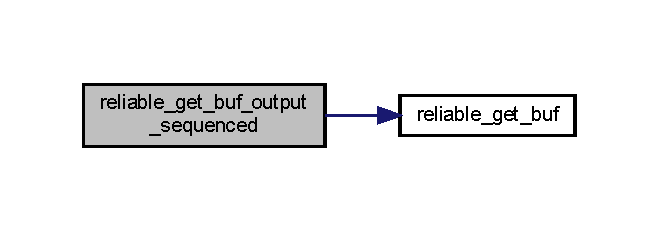
\includegraphics[width=316pt]{group__reliable_gaa15b0672f4ddd65d55194ed5bde0e1c8_cgraph}
\end{center}
\end{figure}


\hypertarget{group__reliable_ga08f53328657f0172eb061193171e2a41}{}\index{Reliable@{Reliable}!reliable\+\_\+get\+\_\+buf\+\_\+sequenced@{reliable\+\_\+get\+\_\+buf\+\_\+sequenced}}
\index{reliable\+\_\+get\+\_\+buf\+\_\+sequenced@{reliable\+\_\+get\+\_\+buf\+\_\+sequenced}!Reliable@{Reliable}}
\subsubsection[{reliable\+\_\+get\+\_\+buf\+\_\+sequenced(struct reliable $\ast$rel)}]{\setlength{\rightskip}{0pt plus 5cm}struct {\bf buffer}$\ast$ reliable\+\_\+get\+\_\+buf\+\_\+sequenced (
\begin{DoxyParamCaption}
\item[{struct {\bf reliable} $\ast$}]{rel}
\end{DoxyParamCaption}
)}\label{group__reliable_ga08f53328657f0172eb061193171e2a41}
Get the buffer of the next sequential and active entry.


\begin{DoxyParams}{Parameters}
{\em rel} & The reliable structure from which to retrieve the buffer.\\
\hline
\end{DoxyParams}
\begin{DoxyReturn}{Returns}
A pointer to the buffer of the entry with the next sequential key I\+D. If no such entry is present, this function returns N\+U\+L\+L. 
\end{DoxyReturn}
\hypertarget{group__reliable_gab5e5ef6d6fd862187abe76f88b972ee5}{}\index{Reliable@{Reliable}!reliable\+\_\+init@{reliable\+\_\+init}}
\index{reliable\+\_\+init@{reliable\+\_\+init}!Reliable@{Reliable}}
\subsubsection[{reliable\+\_\+init(struct reliable $\ast$rel, int buf\+\_\+size, int offset, int array\+\_\+size, bool hold)}]{\setlength{\rightskip}{0pt plus 5cm}void reliable\+\_\+init (
\begin{DoxyParamCaption}
\item[{struct {\bf reliable} $\ast$}]{rel, }
\item[{int}]{buf\+\_\+size, }
\item[{int}]{offset, }
\item[{int}]{array\+\_\+size, }
\item[{{\bf bool}}]{hold}
\end{DoxyParamCaption}
)}\label{group__reliable_gab5e5ef6d6fd862187abe76f88b972ee5}
Initialize a reliable structure.


\begin{DoxyParams}{Parameters}
{\em rel} & The reliable structure to initialize. \\
\hline
{\em buf\+\_\+size} & The size of the buffers in which packets will be stored. \\
\hline
{\em offset} & The size of reserved space at the beginning of the buffers to allow efficient header prepending. \\
\hline
{\em array\+\_\+size} & The number of packets that this reliable structure can store simultaneously. \\
\hline
{\em hold} & description \\
\hline
\end{DoxyParams}


Here is the call graph for this function\+:
\nopagebreak
\begin{figure}[H]
\begin{center}
\leavevmode
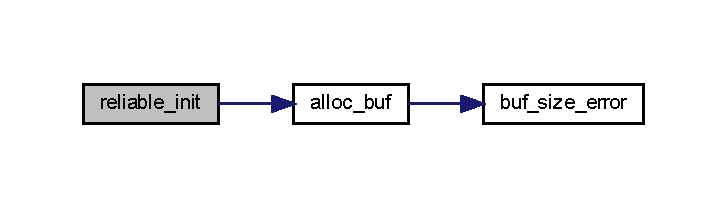
\includegraphics[width=349pt]{group__reliable_gab5e5ef6d6fd862187abe76f88b972ee5_cgraph}
\end{center}
\end{figure}


\hypertarget{group__reliable_ga2689b44850ce41cc2fe1fc7f57657eb4}{}\index{Reliable@{Reliable}!reliable\+\_\+mark\+\_\+active\+\_\+incoming@{reliable\+\_\+mark\+\_\+active\+\_\+incoming}}
\index{reliable\+\_\+mark\+\_\+active\+\_\+incoming@{reliable\+\_\+mark\+\_\+active\+\_\+incoming}!Reliable@{Reliable}}
\subsubsection[{reliable\+\_\+mark\+\_\+active\+\_\+incoming(struct reliable $\ast$rel, struct buffer $\ast$buf, packet\+\_\+id\+\_\+type pid, int opcode)}]{\setlength{\rightskip}{0pt plus 5cm}void reliable\+\_\+mark\+\_\+active\+\_\+incoming (
\begin{DoxyParamCaption}
\item[{struct {\bf reliable} $\ast$}]{rel, }
\item[{struct {\bf buffer} $\ast$}]{buf, }
\item[{{\bf packet\+\_\+id\+\_\+type}}]{pid, }
\item[{int}]{opcode}
\end{DoxyParamCaption}
)}\label{group__reliable_ga2689b44850ce41cc2fe1fc7f57657eb4}
Mark the reliable entry associated with the given buffer as active incoming.


\begin{DoxyParams}{Parameters}
{\em rel} & The reliable structure associated with this packet. \\
\hline
{\em buf} & The buffer into which the packet has been copied. \\
\hline
{\em pid} & The packet\textquotesingle{}s packet I\+D. \\
\hline
{\em opcode} & The packet\textquotesingle{}s opcode. \\
\hline
\end{DoxyParams}


Here is the caller graph for this function\+:
\nopagebreak
\begin{figure}[H]
\begin{center}
\leavevmode
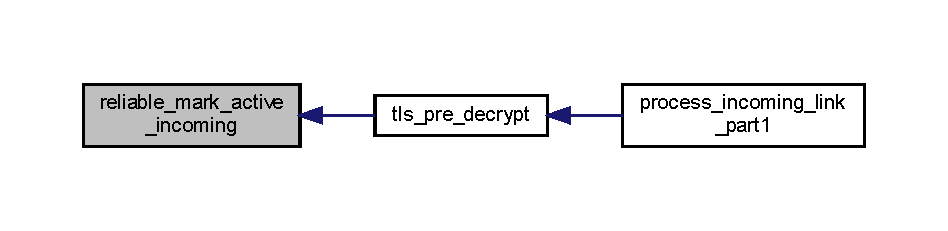
\includegraphics[width=350pt]{group__reliable_ga2689b44850ce41cc2fe1fc7f57657eb4_icgraph}
\end{center}
\end{figure}


\hypertarget{group__reliable_ga2c03b5ae47fe72dbf4fe16f11ea1c091}{}\index{Reliable@{Reliable}!reliable\+\_\+mark\+\_\+active\+\_\+outgoing@{reliable\+\_\+mark\+\_\+active\+\_\+outgoing}}
\index{reliable\+\_\+mark\+\_\+active\+\_\+outgoing@{reliable\+\_\+mark\+\_\+active\+\_\+outgoing}!Reliable@{Reliable}}
\subsubsection[{reliable\+\_\+mark\+\_\+active\+\_\+outgoing(struct reliable $\ast$rel, struct buffer $\ast$buf, int opcode)}]{\setlength{\rightskip}{0pt plus 5cm}void reliable\+\_\+mark\+\_\+active\+\_\+outgoing (
\begin{DoxyParamCaption}
\item[{struct {\bf reliable} $\ast$}]{rel, }
\item[{struct {\bf buffer} $\ast$}]{buf, }
\item[{int}]{opcode}
\end{DoxyParamCaption}
)}\label{group__reliable_ga2c03b5ae47fe72dbf4fe16f11ea1c091}
Mark the reliable entry associated with the given buffer as active outgoing.


\begin{DoxyParams}{Parameters}
{\em rel} & The reliable structure for handling this V\+P\+N tunnel\textquotesingle{}s outgoing packets. \\
\hline
{\em buf} & The buffer previously returned by {\ttfamily \hyperlink{group__reliable_gaa15b0672f4ddd65d55194ed5bde0e1c8}{reliable\+\_\+get\+\_\+buf\+\_\+output\+\_\+sequenced()}} into which the packet has been copied. \\
\hline
{\em opcode} & The packet\textquotesingle{}s opcode. \\
\hline
\end{DoxyParams}
\hypertarget{group__reliable_ga5c51920665fa9c34f082dd7aa6ce0e55}{}\index{Reliable@{Reliable}!reliable\+\_\+mark\+\_\+deleted@{reliable\+\_\+mark\+\_\+deleted}}
\index{reliable\+\_\+mark\+\_\+deleted@{reliable\+\_\+mark\+\_\+deleted}!Reliable@{Reliable}}
\subsubsection[{reliable\+\_\+mark\+\_\+deleted(struct reliable $\ast$rel, struct buffer $\ast$buf, bool inc\+\_\+pid)}]{\setlength{\rightskip}{0pt plus 5cm}void reliable\+\_\+mark\+\_\+deleted (
\begin{DoxyParamCaption}
\item[{struct {\bf reliable} $\ast$}]{rel, }
\item[{struct {\bf buffer} $\ast$}]{buf, }
\item[{{\bf bool}}]{inc\+\_\+pid}
\end{DoxyParamCaption}
)}\label{group__reliable_ga5c51920665fa9c34f082dd7aa6ce0e55}
Remove an entry from a reliable structure.


\begin{DoxyParams}{Parameters}
{\em rel} & The reliable structure associated with the given buffer. \\
\hline
{\em buf} & The buffer of the reliable entry which is to be removed. \\
\hline
{\em inc\+\_\+pid} & If true, the reliable structure\textquotesingle{}s packet I\+D counter will be incremented. \\
\hline
\end{DoxyParams}
\hypertarget{group__reliable_ga907fd32837c50b4266eb5db1c56f9b13}{}\index{Reliable@{Reliable}!reliable\+\_\+not\+\_\+replay@{reliable\+\_\+not\+\_\+replay}}
\index{reliable\+\_\+not\+\_\+replay@{reliable\+\_\+not\+\_\+replay}!Reliable@{Reliable}}
\subsubsection[{reliable\+\_\+not\+\_\+replay(const struct reliable $\ast$rel, packet\+\_\+id\+\_\+type id)}]{\setlength{\rightskip}{0pt plus 5cm}{\bf bool} reliable\+\_\+not\+\_\+replay (
\begin{DoxyParamCaption}
\item[{const struct {\bf reliable} $\ast$}]{rel, }
\item[{{\bf packet\+\_\+id\+\_\+type}}]{id}
\end{DoxyParamCaption}
)}\label{group__reliable_ga907fd32837c50b4266eb5db1c56f9b13}
Check that a received packet\textquotesingle{}s I\+D is not a replay.


\begin{DoxyParams}{Parameters}
{\em rel} & The reliable structure for handling this V\+P\+N tunnel\textquotesingle{}s received packets. \\
\hline
{\em id} & The packet I\+D of the received packet.\\
\hline
\end{DoxyParams}
\begin{DoxyReturn}{Returns}
\begin{DoxyItemize}
\item True, if the packet I\+D is not a replay. \item False, if the packet I\+D is a replay. \end{DoxyItemize}

\end{DoxyReturn}


Here is the caller graph for this function\+:
\nopagebreak
\begin{figure}[H]
\begin{center}
\leavevmode
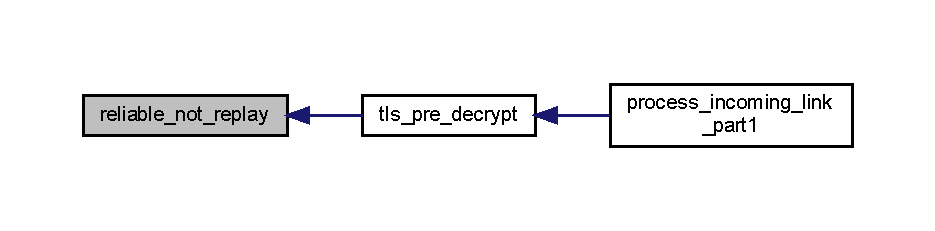
\includegraphics[width=350pt]{group__reliable_ga907fd32837c50b4266eb5db1c56f9b13_icgraph}
\end{center}
\end{figure}


\hypertarget{group__reliable_ga14cb4395f780502ae9edbe6d3f90aec5}{}\index{Reliable@{Reliable}!reliable\+\_\+schedule\+\_\+now@{reliable\+\_\+schedule\+\_\+now}}
\index{reliable\+\_\+schedule\+\_\+now@{reliable\+\_\+schedule\+\_\+now}!Reliable@{Reliable}}
\subsubsection[{reliable\+\_\+schedule\+\_\+now(struct reliable $\ast$rel)}]{\setlength{\rightskip}{0pt plus 5cm}void reliable\+\_\+schedule\+\_\+now (
\begin{DoxyParamCaption}
\item[{struct {\bf reliable} $\ast$}]{rel}
\end{DoxyParamCaption}
)}\label{group__reliable_ga14cb4395f780502ae9edbe6d3f90aec5}
Reschedule all entries of a reliable structure to be ready for (re)sending immediately.


\begin{DoxyParams}{Parameters}
{\em rel} & The reliable structure of which the entries should be modified. \\
\hline
\end{DoxyParams}


Here is the caller graph for this function\+:
\nopagebreak
\begin{figure}[H]
\begin{center}
\leavevmode
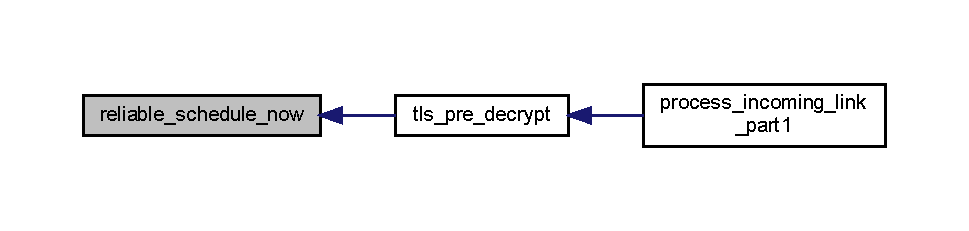
\includegraphics[width=350pt]{group__reliable_ga14cb4395f780502ae9edbe6d3f90aec5_icgraph}
\end{center}
\end{figure}


\hypertarget{group__reliable_gaebcf7ae7a144f32b55c9af5c51121ec1}{}\index{Reliable@{Reliable}!reliable\+\_\+send@{reliable\+\_\+send}}
\index{reliable\+\_\+send@{reliable\+\_\+send}!Reliable@{Reliable}}
\subsubsection[{reliable\+\_\+send(struct reliable $\ast$rel, int $\ast$opcode)}]{\setlength{\rightskip}{0pt plus 5cm}struct {\bf buffer}$\ast$ reliable\+\_\+send (
\begin{DoxyParamCaption}
\item[{struct {\bf reliable} $\ast$}]{rel, }
\item[{int $\ast$}]{opcode}
\end{DoxyParamCaption}
)}\label{group__reliable_gaebcf7ae7a144f32b55c9af5c51121ec1}
Get the next packet to send to the remote peer.

This function looks for the active entry ready for (re)sending with the lowest packet I\+D, and returns the buffer associated with it. This function also resets the timeout after which that entry will become ready for resending again.


\begin{DoxyParams}{Parameters}
{\em rel} & The reliable structure to check. \\
\hline
{\em opcode} & A pointer to an integer in which this function will store the opcode of the next packet to be sent.\\
\hline
\end{DoxyParams}
\begin{DoxyReturn}{Returns}
A pointer to the buffer of the next entry to be sent, or N\+U\+L\+L if there are no entries ready for (re)sending present in the reliable structure. If a valid pointer is returned, then {\itshape opcode} will point to the opcode of that packet. 
\end{DoxyReturn}
\hypertarget{group__reliable_ga0f79fac5e64e7d2a9df9bc13740f6293}{}\index{Reliable@{Reliable}!reliable\+\_\+send\+\_\+purge@{reliable\+\_\+send\+\_\+purge}}
\index{reliable\+\_\+send\+\_\+purge@{reliable\+\_\+send\+\_\+purge}!Reliable@{Reliable}}
\subsubsection[{reliable\+\_\+send\+\_\+purge(struct reliable $\ast$rel, struct reliable\+\_\+ack $\ast$ack)}]{\setlength{\rightskip}{0pt plus 5cm}void reliable\+\_\+send\+\_\+purge (
\begin{DoxyParamCaption}
\item[{struct {\bf reliable} $\ast$}]{rel, }
\item[{struct {\bf reliable\+\_\+ack} $\ast$}]{ack}
\end{DoxyParamCaption}
)}\label{group__reliable_ga0f79fac5e64e7d2a9df9bc13740f6293}
Remove acknowledged packets from a reliable structure.


\begin{DoxyParams}{Parameters}
{\em rel} & The reliable structure storing sent packets. \\
\hline
{\em ack} & The acknowledgment structure containing received acknowledgments. \\
\hline
\end{DoxyParams}


Here is the caller graph for this function\+:
\nopagebreak
\begin{figure}[H]
\begin{center}
\leavevmode
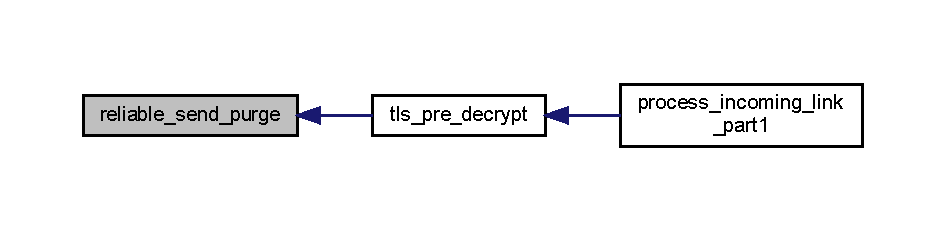
\includegraphics[width=350pt]{group__reliable_ga0f79fac5e64e7d2a9df9bc13740f6293_icgraph}
\end{center}
\end{figure}


\hypertarget{group__reliable_ga9e8edfca42338da6da6ccb3fd1849dca}{}\index{Reliable@{Reliable}!reliable\+\_\+send\+\_\+timeout@{reliable\+\_\+send\+\_\+timeout}}
\index{reliable\+\_\+send\+\_\+timeout@{reliable\+\_\+send\+\_\+timeout}!Reliable@{Reliable}}
\subsubsection[{reliable\+\_\+send\+\_\+timeout(const struct reliable $\ast$rel)}]{\setlength{\rightskip}{0pt plus 5cm}{\bf interval\+\_\+t} reliable\+\_\+send\+\_\+timeout (
\begin{DoxyParamCaption}
\item[{const struct {\bf reliable} $\ast$}]{rel}
\end{DoxyParamCaption}
)}\label{group__reliable_ga9e8edfca42338da6da6ccb3fd1849dca}
Determined how many seconds until the earliest resend should be attempted.


\begin{DoxyParams}{Parameters}
{\em rel} & The reliable structured to check.\\
\hline
\end{DoxyParams}
\begin{DoxyReturn}{Returns}
The interval in seconds until the earliest resend attempt of the outgoing packets stored in the {\itshape rel} reliable structure. If the next time for attempting resending of one or more packets has already passed, this function will return 0. 
\end{DoxyReturn}
\hypertarget{group__reliable_gad2d6e3bde9beced3d69bbba652730439}{}\index{Reliable@{Reliable}!reliable\+\_\+wont\+\_\+break\+\_\+sequentiality@{reliable\+\_\+wont\+\_\+break\+\_\+sequentiality}}
\index{reliable\+\_\+wont\+\_\+break\+\_\+sequentiality@{reliable\+\_\+wont\+\_\+break\+\_\+sequentiality}!Reliable@{Reliable}}
\subsubsection[{reliable\+\_\+wont\+\_\+break\+\_\+sequentiality(const struct reliable $\ast$rel, packet\+\_\+id\+\_\+type id)}]{\setlength{\rightskip}{0pt plus 5cm}{\bf bool} reliable\+\_\+wont\+\_\+break\+\_\+sequentiality (
\begin{DoxyParamCaption}
\item[{const struct {\bf reliable} $\ast$}]{rel, }
\item[{{\bf packet\+\_\+id\+\_\+type}}]{id}
\end{DoxyParamCaption}
)}\label{group__reliable_gad2d6e3bde9beced3d69bbba652730439}
Check that a received packet\textquotesingle{}s I\+D can safely be stored in the reliable structure\textquotesingle{}s processing window.

This function checks the difference between the received packet\textquotesingle{}s I\+D and the lowest non-\/acknowledged packet I\+D in the given reliable structure. If that difference is larger than the total number of packets which can be stored, then this packet cannot be stored safely, because the reliable structure could possibly fill up without leaving room for all intervening packets. In that case, this received packet could break the reliable structure\textquotesingle{}s sequentiality, and must therefore be discarded.


\begin{DoxyParams}{Parameters}
{\em rel} & The reliable structure for handling this V\+P\+N tunnel\textquotesingle{}s received packets. \\
\hline
{\em id} & The packet I\+D of the received packet.\\
\hline
\end{DoxyParams}
\begin{DoxyReturn}{Returns}
\begin{DoxyItemize}
\item True, if the packet can safely be stored. \item False, if the packet does not fit safely in the reliable structure\textquotesingle{}s processing window. \end{DoxyItemize}

\end{DoxyReturn}


Here is the caller graph for this function\+:
\nopagebreak
\begin{figure}[H]
\begin{center}
\leavevmode
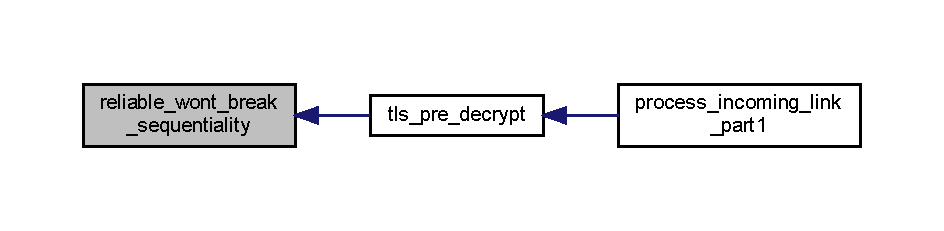
\includegraphics[width=350pt]{group__reliable_gad2d6e3bde9beced3d69bbba652730439_icgraph}
\end{center}
\end{figure}



\hypertarget{group__control__processor}{}\section{Control\+\_\+processor}
\label{group__control__processor}\index{Control\+\_\+processor@{Control\+\_\+processor}}
\subsection*{Classes}
\begin{DoxyCompactItemize}
\item 
struct \hyperlink{structkey}{key}
\item 
struct \hyperlink{structkey__ctx}{key\+\_\+ctx}
\item 
struct \hyperlink{structkey2}{key2}
\item 
struct \hyperlink{structkey__direction__state}{key\+\_\+direction\+\_\+state}
\item 
struct \hyperlink{structkey__ctx__bi}{key\+\_\+ctx\+\_\+bi}
\item 
struct \hyperlink{structkey__source}{key\+\_\+source}
\item 
struct \hyperlink{structkey__source2}{key\+\_\+source2}
\item 
struct \hyperlink{structkey__state}{key\+\_\+state}
\item 
struct \hyperlink{structtls__session}{tls\+\_\+session}
\item 
struct \hyperlink{structtls__multi}{tls\+\_\+multi}
\end{DoxyCompactItemize}
\subsection*{Functions for initialization and cleanup of tls\+\_\+multi structures}
\begin{DoxyCompactItemize}
\item 
struct \hyperlink{structtls__multi}{tls\+\_\+multi} $\ast$ \hyperlink{group__control__processor_gaf7223d904613a08407ae52dc3831d7a2}{tls\+\_\+multi\+\_\+init} (struct \hyperlink{structtls__options}{tls\+\_\+options} $\ast$\hyperlink{structtls__options}{tls\+\_\+options})
\item 
void \hyperlink{group__control__processor_gada87c9f2a7755ab7507dd16fa6e22716}{tls\+\_\+multi\+\_\+init\+\_\+finalize} (struct \hyperlink{structtls__multi}{tls\+\_\+multi} $\ast$multi, const struct \hyperlink{structframe}{frame} $\ast$\hyperlink{structframe}{frame})
\item 
struct \hyperlink{structtls__auth__standalone}{tls\+\_\+auth\+\_\+standalone} $\ast$ \hyperlink{group__control__processor_ga03aaa9093737daae72627dc38198dd1d}{tls\+\_\+auth\+\_\+standalone\+\_\+init} (struct \hyperlink{structtls__options}{tls\+\_\+options} $\ast$\hyperlink{structtls__options}{tls\+\_\+options}, struct \hyperlink{structgc__arena}{gc\+\_\+arena} $\ast$gc)
\item 
void \hyperlink{group__control__processor_ga85674d980185b3f2923ae9540114289a}{tls\+\_\+auth\+\_\+standalone\+\_\+finalize} (struct \hyperlink{structtls__auth__standalone}{tls\+\_\+auth\+\_\+standalone} $\ast$tas, const struct \hyperlink{structframe}{frame} $\ast$\hyperlink{structframe}{frame})
\item 
void \hyperlink{group__control__processor_gafe3228d8a3cae5eb8f159e8230f4cd27}{tls\+\_\+multi\+\_\+init\+\_\+set\+\_\+options} (struct \hyperlink{structtls__multi}{tls\+\_\+multi} $\ast$multi, const char $\ast$local, const char $\ast$remote)
\item 
void \hyperlink{group__control__processor_ga3f6dae3fb4465d1c697a80fdebd50d67}{tls\+\_\+multi\+\_\+free} (struct \hyperlink{structtls__multi}{tls\+\_\+multi} $\ast$multi, \hyperlink{automatic_8c_abb452686968e48b67397da5f97445f5b}{bool} clear)
\end{DoxyCompactItemize}
\subsection*{Control channel negotiation states}
\label{_amgrp074f583fcd32a701d71d3a0081fec6b1}%
These states represent the different phases of control channel negotiation between Open\+V\+P\+N peers. Open\+V\+P\+N servers and clients progress through the states in a different order, because of their different roles during exchange of random material. The references to the {\ttfamily \hyperlink{structkey__source2}{key\+\_\+source2}} structure in the list below is only valid if key method 2 is being used. See the \hyperlink{}{data channel key generation} related page for more information.

Clients follow this order\+:
\begin{DoxyEnumerate}
\item {\ttfamily S\+\_\+\+I\+N\+I\+T\+I\+A\+L}, ready to begin three-\/way handshake and control channel negotiation.
\item {\ttfamily S\+\_\+\+P\+R\+E\+\_\+\+S\+T\+A\+R\+T}, have started three-\/way handshake, waiting for acknowledgment from remote.
\item {\ttfamily S\+\_\+\+S\+T\+A\+R\+T}, initial three-\/way handshake complete.
\item {\ttfamily S\+\_\+\+S\+E\+N\+T\+\_\+\+K\+E\+Y}, have sent local part of {\ttfamily \hyperlink{structkey__source2}{key\+\_\+source2}} random material.
\item {\ttfamily S\+\_\+\+G\+O\+T\+\_\+\+K\+E\+Y}, have received remote part of {\ttfamily \hyperlink{structkey__source2}{key\+\_\+source2}} random material.
\item {\ttfamily S\+\_\+\+A\+C\+T\+I\+V\+E}, normal operation during remaining handshake window.
\item {\ttfamily S\+\_\+\+N\+O\+R\+M\+A\+L\+\_\+\+O\+P}, normal operation.
\end{DoxyEnumerate}

Servers follow the same order, except for {\ttfamily S\+\_\+\+S\+E\+N\+T\+\_\+\+K\+E\+Y} and {\ttfamily S\+\_\+\+G\+O\+T\+\_\+\+K\+E\+Y} being reversed, because the server first receives the client\textquotesingle{}s {\ttfamily \hyperlink{structkey__source2}{key\+\_\+source2}} random material before generating and sending its own. \begin{DoxyCompactItemize}
\item 
\#define \hyperlink{group__control__processor_gaf6e8cab5d0642b96ef462156816c3a28}{S\+\_\+\+E\+R\+R\+O\+R}~-\/1
\item 
\#define \hyperlink{group__control__processor_ga5c620f0ab83a389abc17d80bfb1e0665}{S\+\_\+\+U\+N\+D\+E\+F}~0
\item 
\#define \hyperlink{group__control__processor_gaf80d9f1dca21e561e35220bdeee2fc1e}{S\+\_\+\+I\+N\+I\+T\+I\+A\+L}~1
\item 
\#define \hyperlink{group__control__processor_ga6be8de96f4d931c3be923f74f8511b02}{S\+\_\+\+P\+R\+E\+\_\+\+S\+T\+A\+R\+T}~2
\item 
\#define \hyperlink{group__control__processor_ga66275a3888e8a86da79d69078c27c18d}{S\+\_\+\+S\+T\+A\+R\+T}~3
\item 
\#define \hyperlink{group__control__processor_gadf3421bc4c6c95c3ed9824fe7c2c20d8}{S\+\_\+\+S\+E\+N\+T\+\_\+\+K\+E\+Y}~4
\item 
\#define \hyperlink{group__control__processor_ga66bd0f7cdbc8450a4690c519de7d75bc}{S\+\_\+\+G\+O\+T\+\_\+\+K\+E\+Y}~5
\item 
\#define \hyperlink{group__control__processor_ga0b9dd6c70b47159cdbfbeecb4b971197}{S\+\_\+\+A\+C\+T\+I\+V\+E}~6
\item 
\#define \hyperlink{group__control__processor_gaa92fb79464b68ac009946bd9cc9b8d89}{S\+\_\+\+N\+O\+R\+M\+A\+L\+\_\+\+O\+P}~7
\end{DoxyCompactItemize}
\subsection*{Index of key\+\_\+state objects within a tls\+\_\+session structure}
\label{_amgrp348dc162a1f22f9ec4d9fab524f330d1}%
This is the index of {\ttfamily \hyperlink{structtls__session_a1de4672c1233dd4887122a909b10c314}{tls\+\_\+session.\+key}} \begin{DoxyCompactItemize}
\item 
\#define \hyperlink{group__control__processor_ga53a47713d8d3afdedf8826560da3e8b1}{K\+S\+\_\+\+P\+R\+I\+M\+A\+R\+Y}~0
\item 
\#define \hyperlink{group__control__processor_gadf097bad90fb34433800b15445db8398}{K\+S\+\_\+\+L\+A\+M\+E\+\_\+\+D\+U\+C\+K}~1
\item 
\#define \hyperlink{group__control__processor_ga136f3095237ae23358c30581753e4178}{K\+S\+\_\+\+S\+I\+Z\+E}~2
\end{DoxyCompactItemize}
\subsection*{Index of tls\+\_\+session objects within a tls\+\_\+multi structure}
\label{_amgrp12b5b9f5a31276d4e8a8352c56f23541}%
This is the index of {\ttfamily \hyperlink{structtls__multi_a74e065e432f819307a830ef38d5be73c}{tls\+\_\+multi.\+session}} 

Normally three \hyperlink{structtls__session}{tls\+\_\+session} objects are maintained by an active openvpn session. The first is the current, T\+L\+S authenticated session, the second is used to process connection requests from a new client that would usurp the current session if successfully authenticated, and the third is used as a repository for a \char`\"{}lame-\/duck\char`\"{} key in the event that the primary session resets due to error while the lame-\/duck key still has time left before its expiration. Lame duck keys are used to maintain the continuity of the data channel connection while a new key is being negotiated. \begin{DoxyCompactItemize}
\item 
\#define \hyperlink{group__control__processor_gad3c70b02a0ca4537fba1d53802e1e429}{T\+M\+\_\+\+A\+C\+T\+I\+V\+E}~0
\item 
\#define \hyperlink{group__control__processor_ga6575a67494af1ca3e9608941e12a5386}{T\+M\+\_\+\+U\+N\+T\+R\+U\+S\+T\+E\+D}~1
\item 
\#define \hyperlink{group__control__processor_ga89d765b434597e7194131ace44c605af}{T\+M\+\_\+\+L\+A\+M\+E\+\_\+\+D\+U\+C\+K}~2
\item 
\#define \hyperlink{group__control__processor_gaa195349d22c113d3acc88b6795e491b8}{T\+M\+\_\+\+S\+I\+Z\+E}~3
\end{DoxyCompactItemize}


\subsection{Detailed Description}


\subsection{Macro Definition Documentation}
\hypertarget{group__control__processor_gadf097bad90fb34433800b15445db8398}{}\index{Control\+\_\+processor@{Control\+\_\+processor}!K\+S\+\_\+\+L\+A\+M\+E\+\_\+\+D\+U\+C\+K@{K\+S\+\_\+\+L\+A\+M\+E\+\_\+\+D\+U\+C\+K}}
\index{K\+S\+\_\+\+L\+A\+M\+E\+\_\+\+D\+U\+C\+K@{K\+S\+\_\+\+L\+A\+M\+E\+\_\+\+D\+U\+C\+K}!Control\+\_\+processor@{Control\+\_\+processor}}
\subsubsection[{K\+S\+\_\+\+L\+A\+M\+E\+\_\+\+D\+U\+C\+K}]{\setlength{\rightskip}{0pt plus 5cm}\#define K\+S\+\_\+\+L\+A\+M\+E\+\_\+\+D\+U\+C\+K~1}\label{group__control__processor_gadf097bad90fb34433800b15445db8398}
Key state index that will retire soon. \hypertarget{group__control__processor_ga53a47713d8d3afdedf8826560da3e8b1}{}\index{Control\+\_\+processor@{Control\+\_\+processor}!K\+S\+\_\+\+P\+R\+I\+M\+A\+R\+Y@{K\+S\+\_\+\+P\+R\+I\+M\+A\+R\+Y}}
\index{K\+S\+\_\+\+P\+R\+I\+M\+A\+R\+Y@{K\+S\+\_\+\+P\+R\+I\+M\+A\+R\+Y}!Control\+\_\+processor@{Control\+\_\+processor}}
\subsubsection[{K\+S\+\_\+\+P\+R\+I\+M\+A\+R\+Y}]{\setlength{\rightskip}{0pt plus 5cm}\#define K\+S\+\_\+\+P\+R\+I\+M\+A\+R\+Y~0}\label{group__control__processor_ga53a47713d8d3afdedf8826560da3e8b1}
Primary key state index. \hypertarget{group__control__processor_ga136f3095237ae23358c30581753e4178}{}\index{Control\+\_\+processor@{Control\+\_\+processor}!K\+S\+\_\+\+S\+I\+Z\+E@{K\+S\+\_\+\+S\+I\+Z\+E}}
\index{K\+S\+\_\+\+S\+I\+Z\+E@{K\+S\+\_\+\+S\+I\+Z\+E}!Control\+\_\+processor@{Control\+\_\+processor}}
\subsubsection[{K\+S\+\_\+\+S\+I\+Z\+E}]{\setlength{\rightskip}{0pt plus 5cm}\#define K\+S\+\_\+\+S\+I\+Z\+E~2}\label{group__control__processor_ga136f3095237ae23358c30581753e4178}
Size of the {\ttfamily \hyperlink{structtls__session_a1de4672c1233dd4887122a909b10c314}{tls\+\_\+session.\+key}} array. \hypertarget{group__control__processor_ga0b9dd6c70b47159cdbfbeecb4b971197}{}\index{Control\+\_\+processor@{Control\+\_\+processor}!S\+\_\+\+A\+C\+T\+I\+V\+E@{S\+\_\+\+A\+C\+T\+I\+V\+E}}
\index{S\+\_\+\+A\+C\+T\+I\+V\+E@{S\+\_\+\+A\+C\+T\+I\+V\+E}!Control\+\_\+processor@{Control\+\_\+processor}}
\subsubsection[{S\+\_\+\+A\+C\+T\+I\+V\+E}]{\setlength{\rightskip}{0pt plus 5cm}\#define S\+\_\+\+A\+C\+T\+I\+V\+E~6}\label{group__control__processor_ga0b9dd6c70b47159cdbfbeecb4b971197}
Operational {\ttfamily \hyperlink{structkey__state}{key\+\_\+state}} state immediately after negotiation has completed while still within the handshake window. \hypertarget{group__control__processor_gaf6e8cab5d0642b96ef462156816c3a28}{}\index{Control\+\_\+processor@{Control\+\_\+processor}!S\+\_\+\+E\+R\+R\+O\+R@{S\+\_\+\+E\+R\+R\+O\+R}}
\index{S\+\_\+\+E\+R\+R\+O\+R@{S\+\_\+\+E\+R\+R\+O\+R}!Control\+\_\+processor@{Control\+\_\+processor}}
\subsubsection[{S\+\_\+\+E\+R\+R\+O\+R}]{\setlength{\rightskip}{0pt plus 5cm}\#define S\+\_\+\+E\+R\+R\+O\+R~-\/1}\label{group__control__processor_gaf6e8cab5d0642b96ef462156816c3a28}
Error state. \hypertarget{group__control__processor_ga66bd0f7cdbc8450a4690c519de7d75bc}{}\index{Control\+\_\+processor@{Control\+\_\+processor}!S\+\_\+\+G\+O\+T\+\_\+\+K\+E\+Y@{S\+\_\+\+G\+O\+T\+\_\+\+K\+E\+Y}}
\index{S\+\_\+\+G\+O\+T\+\_\+\+K\+E\+Y@{S\+\_\+\+G\+O\+T\+\_\+\+K\+E\+Y}!Control\+\_\+processor@{Control\+\_\+processor}}
\subsubsection[{S\+\_\+\+G\+O\+T\+\_\+\+K\+E\+Y}]{\setlength{\rightskip}{0pt plus 5cm}\#define S\+\_\+\+G\+O\+T\+\_\+\+K\+E\+Y~5}\label{group__control__processor_ga66bd0f7cdbc8450a4690c519de7d75bc}
Local Open\+V\+P\+N process has received the remote\textquotesingle{}s part of the key material. \hypertarget{group__control__processor_gaf80d9f1dca21e561e35220bdeee2fc1e}{}\index{Control\+\_\+processor@{Control\+\_\+processor}!S\+\_\+\+I\+N\+I\+T\+I\+A\+L@{S\+\_\+\+I\+N\+I\+T\+I\+A\+L}}
\index{S\+\_\+\+I\+N\+I\+T\+I\+A\+L@{S\+\_\+\+I\+N\+I\+T\+I\+A\+L}!Control\+\_\+processor@{Control\+\_\+processor}}
\subsubsection[{S\+\_\+\+I\+N\+I\+T\+I\+A\+L}]{\setlength{\rightskip}{0pt plus 5cm}\#define S\+\_\+\+I\+N\+I\+T\+I\+A\+L~1}\label{group__control__processor_gaf80d9f1dca21e561e35220bdeee2fc1e}
Initial {\ttfamily \hyperlink{structkey__state}{key\+\_\+state}} state after initialization by {\ttfamily key\+\_\+state\+\_\+init()} before start of three-\/way handshake. \hypertarget{group__control__processor_gaa92fb79464b68ac009946bd9cc9b8d89}{}\index{Control\+\_\+processor@{Control\+\_\+processor}!S\+\_\+\+N\+O\+R\+M\+A\+L\+\_\+\+O\+P@{S\+\_\+\+N\+O\+R\+M\+A\+L\+\_\+\+O\+P}}
\index{S\+\_\+\+N\+O\+R\+M\+A\+L\+\_\+\+O\+P@{S\+\_\+\+N\+O\+R\+M\+A\+L\+\_\+\+O\+P}!Control\+\_\+processor@{Control\+\_\+processor}}
\subsubsection[{S\+\_\+\+N\+O\+R\+M\+A\+L\+\_\+\+O\+P}]{\setlength{\rightskip}{0pt plus 5cm}\#define S\+\_\+\+N\+O\+R\+M\+A\+L\+\_\+\+O\+P~7}\label{group__control__processor_gaa92fb79464b68ac009946bd9cc9b8d89}
Normal operational {\ttfamily \hyperlink{structkey__state}{key\+\_\+state}} state. \hypertarget{group__control__processor_ga6be8de96f4d931c3be923f74f8511b02}{}\index{Control\+\_\+processor@{Control\+\_\+processor}!S\+\_\+\+P\+R\+E\+\_\+\+S\+T\+A\+R\+T@{S\+\_\+\+P\+R\+E\+\_\+\+S\+T\+A\+R\+T}}
\index{S\+\_\+\+P\+R\+E\+\_\+\+S\+T\+A\+R\+T@{S\+\_\+\+P\+R\+E\+\_\+\+S\+T\+A\+R\+T}!Control\+\_\+processor@{Control\+\_\+processor}}
\subsubsection[{S\+\_\+\+P\+R\+E\+\_\+\+S\+T\+A\+R\+T}]{\setlength{\rightskip}{0pt plus 5cm}\#define S\+\_\+\+P\+R\+E\+\_\+\+S\+T\+A\+R\+T~2}\label{group__control__processor_ga6be8de96f4d931c3be923f74f8511b02}
Waiting for the remote Open\+V\+P\+N peer to acknowledge during the initial three-\/way handshake. \hypertarget{group__control__processor_gadf3421bc4c6c95c3ed9824fe7c2c20d8}{}\index{Control\+\_\+processor@{Control\+\_\+processor}!S\+\_\+\+S\+E\+N\+T\+\_\+\+K\+E\+Y@{S\+\_\+\+S\+E\+N\+T\+\_\+\+K\+E\+Y}}
\index{S\+\_\+\+S\+E\+N\+T\+\_\+\+K\+E\+Y@{S\+\_\+\+S\+E\+N\+T\+\_\+\+K\+E\+Y}!Control\+\_\+processor@{Control\+\_\+processor}}
\subsubsection[{S\+\_\+\+S\+E\+N\+T\+\_\+\+K\+E\+Y}]{\setlength{\rightskip}{0pt plus 5cm}\#define S\+\_\+\+S\+E\+N\+T\+\_\+\+K\+E\+Y~4}\label{group__control__processor_gadf3421bc4c6c95c3ed9824fe7c2c20d8}
Local Open\+V\+P\+N process has sent its part of the key material. \hypertarget{group__control__processor_ga66275a3888e8a86da79d69078c27c18d}{}\index{Control\+\_\+processor@{Control\+\_\+processor}!S\+\_\+\+S\+T\+A\+R\+T@{S\+\_\+\+S\+T\+A\+R\+T}}
\index{S\+\_\+\+S\+T\+A\+R\+T@{S\+\_\+\+S\+T\+A\+R\+T}!Control\+\_\+processor@{Control\+\_\+processor}}
\subsubsection[{S\+\_\+\+S\+T\+A\+R\+T}]{\setlength{\rightskip}{0pt plus 5cm}\#define S\+\_\+\+S\+T\+A\+R\+T~3}\label{group__control__processor_ga66275a3888e8a86da79d69078c27c18d}
Three-\/way handshake is complete, start of key exchange. \hypertarget{group__control__processor_ga5c620f0ab83a389abc17d80bfb1e0665}{}\index{Control\+\_\+processor@{Control\+\_\+processor}!S\+\_\+\+U\+N\+D\+E\+F@{S\+\_\+\+U\+N\+D\+E\+F}}
\index{S\+\_\+\+U\+N\+D\+E\+F@{S\+\_\+\+U\+N\+D\+E\+F}!Control\+\_\+processor@{Control\+\_\+processor}}
\subsubsection[{S\+\_\+\+U\+N\+D\+E\+F}]{\setlength{\rightskip}{0pt plus 5cm}\#define S\+\_\+\+U\+N\+D\+E\+F~0}\label{group__control__processor_ga5c620f0ab83a389abc17d80bfb1e0665}
Undefined state, used after a {\ttfamily \hyperlink{structkey__state}{key\+\_\+state}} is cleaned up. \hypertarget{group__control__processor_gad3c70b02a0ca4537fba1d53802e1e429}{}\index{Control\+\_\+processor@{Control\+\_\+processor}!T\+M\+\_\+\+A\+C\+T\+I\+V\+E@{T\+M\+\_\+\+A\+C\+T\+I\+V\+E}}
\index{T\+M\+\_\+\+A\+C\+T\+I\+V\+E@{T\+M\+\_\+\+A\+C\+T\+I\+V\+E}!Control\+\_\+processor@{Control\+\_\+processor}}
\subsubsection[{T\+M\+\_\+\+A\+C\+T\+I\+V\+E}]{\setlength{\rightskip}{0pt plus 5cm}\#define T\+M\+\_\+\+A\+C\+T\+I\+V\+E~0}\label{group__control__processor_gad3c70b02a0ca4537fba1d53802e1e429}
Active {\ttfamily \hyperlink{structtls__session}{tls\+\_\+session}}. \hypertarget{group__control__processor_ga89d765b434597e7194131ace44c605af}{}\index{Control\+\_\+processor@{Control\+\_\+processor}!T\+M\+\_\+\+L\+A\+M\+E\+\_\+\+D\+U\+C\+K@{T\+M\+\_\+\+L\+A\+M\+E\+\_\+\+D\+U\+C\+K}}
\index{T\+M\+\_\+\+L\+A\+M\+E\+\_\+\+D\+U\+C\+K@{T\+M\+\_\+\+L\+A\+M\+E\+\_\+\+D\+U\+C\+K}!Control\+\_\+processor@{Control\+\_\+processor}}
\subsubsection[{T\+M\+\_\+\+L\+A\+M\+E\+\_\+\+D\+U\+C\+K}]{\setlength{\rightskip}{0pt plus 5cm}\#define T\+M\+\_\+\+L\+A\+M\+E\+\_\+\+D\+U\+C\+K~2}\label{group__control__processor_ga89d765b434597e7194131ace44c605af}
Old {\ttfamily \hyperlink{structtls__session}{tls\+\_\+session}}. \hypertarget{group__control__processor_gaa195349d22c113d3acc88b6795e491b8}{}\index{Control\+\_\+processor@{Control\+\_\+processor}!T\+M\+\_\+\+S\+I\+Z\+E@{T\+M\+\_\+\+S\+I\+Z\+E}}
\index{T\+M\+\_\+\+S\+I\+Z\+E@{T\+M\+\_\+\+S\+I\+Z\+E}!Control\+\_\+processor@{Control\+\_\+processor}}
\subsubsection[{T\+M\+\_\+\+S\+I\+Z\+E}]{\setlength{\rightskip}{0pt plus 5cm}\#define T\+M\+\_\+\+S\+I\+Z\+E~3}\label{group__control__processor_gaa195349d22c113d3acc88b6795e491b8}
Size of the {\ttfamily \hyperlink{structtls__multi_a74e065e432f819307a830ef38d5be73c}{tls\+\_\+multi.\+session}} array. \hypertarget{group__control__processor_ga6575a67494af1ca3e9608941e12a5386}{}\index{Control\+\_\+processor@{Control\+\_\+processor}!T\+M\+\_\+\+U\+N\+T\+R\+U\+S\+T\+E\+D@{T\+M\+\_\+\+U\+N\+T\+R\+U\+S\+T\+E\+D}}
\index{T\+M\+\_\+\+U\+N\+T\+R\+U\+S\+T\+E\+D@{T\+M\+\_\+\+U\+N\+T\+R\+U\+S\+T\+E\+D}!Control\+\_\+processor@{Control\+\_\+processor}}
\subsubsection[{T\+M\+\_\+\+U\+N\+T\+R\+U\+S\+T\+E\+D}]{\setlength{\rightskip}{0pt plus 5cm}\#define T\+M\+\_\+\+U\+N\+T\+R\+U\+S\+T\+E\+D~1}\label{group__control__processor_ga6575a67494af1ca3e9608941e12a5386}
As yet un-\/trusted {\ttfamily \hyperlink{structtls__session}{tls\+\_\+session}} being negotiated. 

\subsection{Function Documentation}
\hypertarget{group__control__processor_ga85674d980185b3f2923ae9540114289a}{}\index{Control\+\_\+processor@{Control\+\_\+processor}!tls\+\_\+auth\+\_\+standalone\+\_\+finalize@{tls\+\_\+auth\+\_\+standalone\+\_\+finalize}}
\index{tls\+\_\+auth\+\_\+standalone\+\_\+finalize@{tls\+\_\+auth\+\_\+standalone\+\_\+finalize}!Control\+\_\+processor@{Control\+\_\+processor}}
\subsubsection[{tls\+\_\+auth\+\_\+standalone\+\_\+finalize(struct tls\+\_\+auth\+\_\+standalone $\ast$tas, const struct frame $\ast$frame)}]{\setlength{\rightskip}{0pt plus 5cm}void tls\+\_\+auth\+\_\+standalone\+\_\+finalize (
\begin{DoxyParamCaption}
\item[{struct {\bf tls\+\_\+auth\+\_\+standalone} $\ast$}]{tas, }
\item[{const struct {\bf frame} $\ast$}]{frame}
\end{DoxyParamCaption}
)}\label{group__control__processor_ga85674d980185b3f2923ae9540114289a}
\hypertarget{group__control__processor_ga03aaa9093737daae72627dc38198dd1d}{}\index{Control\+\_\+processor@{Control\+\_\+processor}!tls\+\_\+auth\+\_\+standalone\+\_\+init@{tls\+\_\+auth\+\_\+standalone\+\_\+init}}
\index{tls\+\_\+auth\+\_\+standalone\+\_\+init@{tls\+\_\+auth\+\_\+standalone\+\_\+init}!Control\+\_\+processor@{Control\+\_\+processor}}
\subsubsection[{tls\+\_\+auth\+\_\+standalone\+\_\+init(struct tls\+\_\+options $\ast$tls\+\_\+options, struct gc\+\_\+arena $\ast$gc)}]{\setlength{\rightskip}{0pt plus 5cm}struct {\bf tls\+\_\+auth\+\_\+standalone}$\ast$ tls\+\_\+auth\+\_\+standalone\+\_\+init (
\begin{DoxyParamCaption}
\item[{struct {\bf tls\+\_\+options} $\ast$}]{tls\+\_\+options, }
\item[{struct {\bf gc\+\_\+arena} $\ast$}]{gc}
\end{DoxyParamCaption}
)}\label{group__control__processor_ga03aaa9093737daae72627dc38198dd1d}
\hypertarget{group__control__processor_ga3f6dae3fb4465d1c697a80fdebd50d67}{}\index{Control\+\_\+processor@{Control\+\_\+processor}!tls\+\_\+multi\+\_\+free@{tls\+\_\+multi\+\_\+free}}
\index{tls\+\_\+multi\+\_\+free@{tls\+\_\+multi\+\_\+free}!Control\+\_\+processor@{Control\+\_\+processor}}
\subsubsection[{tls\+\_\+multi\+\_\+free(struct tls\+\_\+multi $\ast$multi, bool clear)}]{\setlength{\rightskip}{0pt plus 5cm}void tls\+\_\+multi\+\_\+free (
\begin{DoxyParamCaption}
\item[{struct {\bf tls\+\_\+multi} $\ast$}]{multi, }
\item[{{\bf bool}}]{clear}
\end{DoxyParamCaption}
)}\label{group__control__processor_ga3f6dae3fb4465d1c697a80fdebd50d67}
Cleanup a {\ttfamily \hyperlink{structtls__multi}{tls\+\_\+multi}} structure and free associated memory allocations.

This function cleans up a {\ttfamily \hyperlink{structtls__multi}{tls\+\_\+multi}} structure. This includes cleaning up all associated {\ttfamily \hyperlink{structtls__session}{tls\+\_\+session}} structures.


\begin{DoxyParams}{Parameters}
{\em multi} & -\/ The {\ttfamily \hyperlink{structtls__multi}{tls\+\_\+multi}} structure to clean up in free. \\
\hline
{\em clear} & -\/ Whether the memory allocated for the {\itshape multi} object should be overwritten with 0s. \\
\hline
\end{DoxyParams}


Here is the call graph for this function\+:
\nopagebreak
\begin{figure}[H]
\begin{center}
\leavevmode
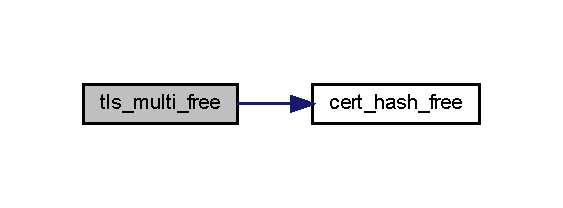
\includegraphics[width=270pt]{group__control__processor_ga3f6dae3fb4465d1c697a80fdebd50d67_cgraph}
\end{center}
\end{figure}


\hypertarget{group__control__processor_gaf7223d904613a08407ae52dc3831d7a2}{}\index{Control\+\_\+processor@{Control\+\_\+processor}!tls\+\_\+multi\+\_\+init@{tls\+\_\+multi\+\_\+init}}
\index{tls\+\_\+multi\+\_\+init@{tls\+\_\+multi\+\_\+init}!Control\+\_\+processor@{Control\+\_\+processor}}
\subsubsection[{tls\+\_\+multi\+\_\+init(struct tls\+\_\+options $\ast$tls\+\_\+options)}]{\setlength{\rightskip}{0pt plus 5cm}struct {\bf tls\+\_\+multi}$\ast$ tls\+\_\+multi\+\_\+init (
\begin{DoxyParamCaption}
\item[{struct {\bf tls\+\_\+options} $\ast$}]{tls\+\_\+options}
\end{DoxyParamCaption}
)}\label{group__control__processor_gaf7223d904613a08407ae52dc3831d7a2}
Allocate and initialize a {\ttfamily \hyperlink{structtls__multi}{tls\+\_\+multi}} structure.

This function allocates a new {\ttfamily \hyperlink{structtls__multi}{tls\+\_\+multi}} structure, and performs some amount of initialization. Afterwards, the {\ttfamily \hyperlink{group__control__processor_gada87c9f2a7755ab7507dd16fa6e22716}{tls\+\_\+multi\+\_\+init\+\_\+finalize()}} function must be called to finalize the structure\textquotesingle{}s initialization process.


\begin{DoxyParams}{Parameters}
{\em \hyperlink{structtls__options}{tls\+\_\+options}} & -\/ The configuration options to be used for this V\+P\+N tunnel.\\
\hline
\end{DoxyParams}
\begin{DoxyReturn}{Returns}
A newly allocated and initialized {\ttfamily \hyperlink{structtls__multi}{tls\+\_\+multi}} structure. 
\end{DoxyReturn}
\hypertarget{group__control__processor_gada87c9f2a7755ab7507dd16fa6e22716}{}\index{Control\+\_\+processor@{Control\+\_\+processor}!tls\+\_\+multi\+\_\+init\+\_\+finalize@{tls\+\_\+multi\+\_\+init\+\_\+finalize}}
\index{tls\+\_\+multi\+\_\+init\+\_\+finalize@{tls\+\_\+multi\+\_\+init\+\_\+finalize}!Control\+\_\+processor@{Control\+\_\+processor}}
\subsubsection[{tls\+\_\+multi\+\_\+init\+\_\+finalize(struct tls\+\_\+multi $\ast$multi, const struct frame $\ast$frame)}]{\setlength{\rightskip}{0pt plus 5cm}void tls\+\_\+multi\+\_\+init\+\_\+finalize (
\begin{DoxyParamCaption}
\item[{struct {\bf tls\+\_\+multi} $\ast$}]{multi, }
\item[{const struct {\bf frame} $\ast$}]{frame}
\end{DoxyParamCaption}
)}\label{group__control__processor_gada87c9f2a7755ab7507dd16fa6e22716}
Finalize initialization of a {\ttfamily \hyperlink{structtls__multi}{tls\+\_\+multi}} structure.

This function initializes the {\ttfamily T\+M\+\_\+\+A\+C\+T\+I\+V\+E} {\ttfamily \hyperlink{structtls__session}{tls\+\_\+session}}, and in server mode also the {\ttfamily T\+M\+\_\+\+U\+N\+T\+R\+U\+S\+T\+E\+D} {\ttfamily \hyperlink{structtls__session}{tls\+\_\+session}}, associated with this {\ttfamily \hyperlink{structtls__multi}{tls\+\_\+multi}} structure. It also configures the control channel\textquotesingle{}s {\ttfamily frame} structure based on the data channel\textquotesingle{}s {\ttfamily frame} given in argument {\itshape frame}.


\begin{DoxyParams}{Parameters}
{\em multi} & -\/ The {\ttfamily \hyperlink{structtls__multi}{tls\+\_\+multi}} structure of which to finalize initialization. \\
\hline
{\em frame} & -\/ The data channel\textquotesingle{}s {\ttfamily frame} structure. \\
\hline
\end{DoxyParams}
\hypertarget{group__control__processor_gafe3228d8a3cae5eb8f159e8230f4cd27}{}\index{Control\+\_\+processor@{Control\+\_\+processor}!tls\+\_\+multi\+\_\+init\+\_\+set\+\_\+options@{tls\+\_\+multi\+\_\+init\+\_\+set\+\_\+options}}
\index{tls\+\_\+multi\+\_\+init\+\_\+set\+\_\+options@{tls\+\_\+multi\+\_\+init\+\_\+set\+\_\+options}!Control\+\_\+processor@{Control\+\_\+processor}}
\subsubsection[{tls\+\_\+multi\+\_\+init\+\_\+set\+\_\+options(struct tls\+\_\+multi $\ast$multi, const char $\ast$local, const char $\ast$remote)}]{\setlength{\rightskip}{0pt plus 5cm}void tls\+\_\+multi\+\_\+init\+\_\+set\+\_\+options (
\begin{DoxyParamCaption}
\item[{struct {\bf tls\+\_\+multi} $\ast$}]{multi, }
\item[{const char $\ast$}]{local, }
\item[{const char $\ast$}]{remote}
\end{DoxyParamCaption}
)}\label{group__control__processor_gafe3228d8a3cae5eb8f159e8230f4cd27}

\hypertarget{group__control__tls}{}\section{Control\+\_\+tls}
\label{group__control__tls}\index{Control\+\_\+tls@{Control\+\_\+tls}}
Collaboration diagram for Control\+\_\+tls\+:
\nopagebreak
\begin{figure}[H]
\begin{center}
\leavevmode
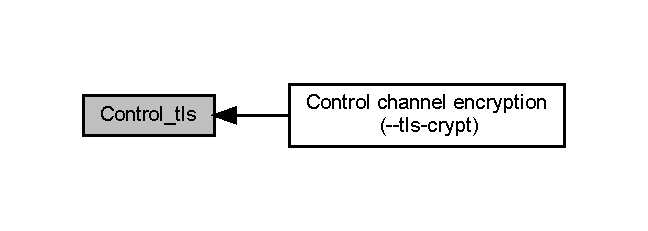
\includegraphics[width=311pt]{group__control__tls}
\end{center}
\end{figure}
\subsection*{Modules}
\begin{DoxyCompactItemize}
\item 
\hyperlink{group__tls__crypt}{Control channel encryption (-\/-\/tls-\/crypt)}
\end{DoxyCompactItemize}
\subsection*{Functions for packets to be sent to a remote Open\+V\+P\+N peer}
\begin{DoxyCompactItemize}
\item 
int \hyperlink{group__control__tls_gaa5438c5f4b03dafec41e663a3e5734d0}{key\+\_\+state\+\_\+write\+\_\+plaintext} (struct \hyperlink{structkey__state__ssl}{key\+\_\+state\+\_\+ssl} $\ast$ks\+\_\+ssl, struct \hyperlink{structbuffer}{buffer} $\ast$buf)
\item 
int \hyperlink{group__control__tls_ga67dac3b75328d8b92d3f1a69e86dacdc}{key\+\_\+state\+\_\+write\+\_\+plaintext\+\_\+const} (struct \hyperlink{structkey__state__ssl}{key\+\_\+state\+\_\+ssl} $\ast$ks\+\_\+ssl, const uint8\+\_\+t $\ast$data, int len)
\item 
int \hyperlink{group__control__tls_ga7260a351c5bb3bf22628278e09f2f7b3}{key\+\_\+state\+\_\+read\+\_\+ciphertext} (struct \hyperlink{structkey__state__ssl}{key\+\_\+state\+\_\+ssl} $\ast$ks\+\_\+ssl, struct \hyperlink{structbuffer}{buffer} $\ast$buf, int maxlen)
\end{DoxyCompactItemize}
\subsection*{Functions for packets received from a remote Open\+V\+P\+N peer}
\begin{DoxyCompactItemize}
\item 
int \hyperlink{group__control__tls_ga5712e1bfbeafff1041a99b57cf4a91f4}{key\+\_\+state\+\_\+write\+\_\+ciphertext} (struct \hyperlink{structkey__state__ssl}{key\+\_\+state\+\_\+ssl} $\ast$ks\+\_\+ssl, struct \hyperlink{structbuffer}{buffer} $\ast$buf)
\item 
int \hyperlink{group__control__tls_gae5597992eeb64d1be998be0ccf98bf97}{key\+\_\+state\+\_\+read\+\_\+plaintext} (struct \hyperlink{structkey__state__ssl}{key\+\_\+state\+\_\+ssl} $\ast$ks\+\_\+ssl, struct \hyperlink{structbuffer}{buffer} $\ast$buf, int maxlen)
\end{DoxyCompactItemize}
\subsection*{Function for authenticating a new connection from a remote Open\+V\+P\+N peer}
\begin{DoxyCompactItemize}
\item 
int \hyperlink{group__control__tls_gadeac70d67a80b44a96cbde2368dd5f3c}{verify\+\_\+callback} (void $\ast$session\+\_\+obj, mbedtls\+\_\+x509\+\_\+crt $\ast$cert, int cert\+\_\+depth, uint32\+\_\+t $\ast$flags)
\end{DoxyCompactItemize}
\subsection*{Function for authenticating a new connection from a remote Open\+V\+P\+N peer}
\begin{DoxyCompactItemize}
\item 
int \hyperlink{group__control__tls_gaf045c97f727aebae9e8fc9852421c4f3}{verify\+\_\+callback} (int preverify\+\_\+ok, X509\+\_\+\+S\+T\+O\+R\+E\+\_\+\+C\+T\+X $\ast$ctx)
\end{DoxyCompactItemize}


\subsection{Detailed Description}


\subsection{Function Documentation}
\hypertarget{group__control__tls_ga7260a351c5bb3bf22628278e09f2f7b3}{}\index{Control\+\_\+tls@{Control\+\_\+tls}!key\+\_\+state\+\_\+read\+\_\+ciphertext@{key\+\_\+state\+\_\+read\+\_\+ciphertext}}
\index{key\+\_\+state\+\_\+read\+\_\+ciphertext@{key\+\_\+state\+\_\+read\+\_\+ciphertext}!Control\+\_\+tls@{Control\+\_\+tls}}
\subsubsection[{key\+\_\+state\+\_\+read\+\_\+ciphertext(struct key\+\_\+state\+\_\+ssl $\ast$ks\+\_\+ssl, struct buffer $\ast$buf, int maxlen)}]{\setlength{\rightskip}{0pt plus 5cm}int key\+\_\+state\+\_\+read\+\_\+ciphertext (
\begin{DoxyParamCaption}
\item[{struct {\bf key\+\_\+state\+\_\+ssl} $\ast$}]{ks\+\_\+ssl, }
\item[{struct {\bf buffer} $\ast$}]{buf, }
\item[{int}]{maxlen}
\end{DoxyParamCaption}
)}\label{group__control__tls_ga7260a351c5bb3bf22628278e09f2f7b3}
Extract ciphertext data from the T\+L\+S module.

If the {\itshape buf} buffer has a length other than zero, this function does not perform any action and returns 0.


\begin{DoxyParams}{Parameters}
{\em ks\+\_\+ssl} & -\/ The security parameter state for this key session. \\
\hline
{\em buf} & -\/ A buffer in which to store the ciphertext. \\
\hline
{\em maxlen} & -\/ The maximum number of bytes to extract.\\
\hline
\end{DoxyParams}
\begin{DoxyReturn}{Returns}
The return value indicates whether the data was successfully processed\+:
\begin{DoxyItemize}
\item {\ttfamily 1}\+: Data was extracted successfully.
\item {\ttfamily 0}\+: No data was extracted, this function should be called again later to retry.
\item {\ttfamily -\/1}\+: An error occurred. 
\end{DoxyItemize}
\end{DoxyReturn}
\hypertarget{group__control__tls_gae5597992eeb64d1be998be0ccf98bf97}{}\index{Control\+\_\+tls@{Control\+\_\+tls}!key\+\_\+state\+\_\+read\+\_\+plaintext@{key\+\_\+state\+\_\+read\+\_\+plaintext}}
\index{key\+\_\+state\+\_\+read\+\_\+plaintext@{key\+\_\+state\+\_\+read\+\_\+plaintext}!Control\+\_\+tls@{Control\+\_\+tls}}
\subsubsection[{key\+\_\+state\+\_\+read\+\_\+plaintext(struct key\+\_\+state\+\_\+ssl $\ast$ks\+\_\+ssl, struct buffer $\ast$buf, int maxlen)}]{\setlength{\rightskip}{0pt plus 5cm}int key\+\_\+state\+\_\+read\+\_\+plaintext (
\begin{DoxyParamCaption}
\item[{struct {\bf key\+\_\+state\+\_\+ssl} $\ast$}]{ks\+\_\+ssl, }
\item[{struct {\bf buffer} $\ast$}]{buf, }
\item[{int}]{maxlen}
\end{DoxyParamCaption}
)}\label{group__control__tls_gae5597992eeb64d1be998be0ccf98bf97}
Extract plaintext data from the T\+L\+S module.

If the {\itshape buf} buffer has a length other than zero, this function does not perform any action and returns 0.


\begin{DoxyParams}{Parameters}
{\em ks\+\_\+ssl} & -\/ The security parameter state for this key session. \\
\hline
{\em buf} & -\/ A buffer in which to store the plaintext. \\
\hline
{\em maxlen} & -\/ The maximum number of bytes to extract.\\
\hline
\end{DoxyParams}
\begin{DoxyReturn}{Returns}
The return value indicates whether the data was successfully processed\+:
\begin{DoxyItemize}
\item {\ttfamily 1}\+: Data was extracted successfully.
\item {\ttfamily 0}\+: No data was extracted, this function should be called again later to retry.
\item {\ttfamily -\/1}\+: An error occurred. 
\end{DoxyItemize}
\end{DoxyReturn}
\hypertarget{group__control__tls_ga5712e1bfbeafff1041a99b57cf4a91f4}{}\index{Control\+\_\+tls@{Control\+\_\+tls}!key\+\_\+state\+\_\+write\+\_\+ciphertext@{key\+\_\+state\+\_\+write\+\_\+ciphertext}}
\index{key\+\_\+state\+\_\+write\+\_\+ciphertext@{key\+\_\+state\+\_\+write\+\_\+ciphertext}!Control\+\_\+tls@{Control\+\_\+tls}}
\subsubsection[{key\+\_\+state\+\_\+write\+\_\+ciphertext(struct key\+\_\+state\+\_\+ssl $\ast$ks\+\_\+ssl, struct buffer $\ast$buf)}]{\setlength{\rightskip}{0pt plus 5cm}int key\+\_\+state\+\_\+write\+\_\+ciphertext (
\begin{DoxyParamCaption}
\item[{struct {\bf key\+\_\+state\+\_\+ssl} $\ast$}]{ks\+\_\+ssl, }
\item[{struct {\bf buffer} $\ast$}]{buf}
\end{DoxyParamCaption}
)}\label{group__control__tls_ga5712e1bfbeafff1041a99b57cf4a91f4}
Insert a ciphertext buffer into the T\+L\+S module.

After successfully processing the data, the data in {\itshape buf} is zeroized, its length set to zero, and a value of {\ttfamily 1} is returned.


\begin{DoxyParams}{Parameters}
{\em ks\+\_\+ssl} & -\/ The security parameter state for this key session. \\
\hline
{\em buf} & -\/ The ciphertext message to process.\\
\hline
\end{DoxyParams}
\begin{DoxyReturn}{Returns}
The return value indicates whether the data was successfully processed\+:
\begin{DoxyItemize}
\item {\ttfamily 1}\+: All the data was processed successfully.
\item {\ttfamily 0}\+: The data was not processed, this function should be called again later to retry.
\item {\ttfamily -\/1}\+: An error occurred. 
\end{DoxyItemize}
\end{DoxyReturn}
\hypertarget{group__control__tls_gaa5438c5f4b03dafec41e663a3e5734d0}{}\index{Control\+\_\+tls@{Control\+\_\+tls}!key\+\_\+state\+\_\+write\+\_\+plaintext@{key\+\_\+state\+\_\+write\+\_\+plaintext}}
\index{key\+\_\+state\+\_\+write\+\_\+plaintext@{key\+\_\+state\+\_\+write\+\_\+plaintext}!Control\+\_\+tls@{Control\+\_\+tls}}
\subsubsection[{key\+\_\+state\+\_\+write\+\_\+plaintext(struct key\+\_\+state\+\_\+ssl $\ast$ks\+\_\+ssl, struct buffer $\ast$buf)}]{\setlength{\rightskip}{0pt plus 5cm}int key\+\_\+state\+\_\+write\+\_\+plaintext (
\begin{DoxyParamCaption}
\item[{struct {\bf key\+\_\+state\+\_\+ssl} $\ast$}]{ks\+\_\+ssl, }
\item[{struct {\bf buffer} $\ast$}]{buf}
\end{DoxyParamCaption}
)}\label{group__control__tls_gaa5438c5f4b03dafec41e663a3e5734d0}
Insert a plaintext buffer into the T\+L\+S module.

After successfully processing the data, the data in {\itshape buf} is zeroized, its length set to zero, and a value of {\ttfamily 1} is returned.


\begin{DoxyParams}{Parameters}
{\em ks\+\_\+ssl} & -\/ The security parameter state for this key session. \\
\hline
{\em buf} & -\/ The plaintext message to process.\\
\hline
\end{DoxyParams}
\begin{DoxyReturn}{Returns}
The return value indicates whether the data was successfully processed\+:
\begin{DoxyItemize}
\item {\ttfamily 1}\+: All the data was processed successfully.
\item {\ttfamily 0}\+: The data was not processed, this function should be called again later to retry.
\item {\ttfamily -\/1}\+: An error occurred. 
\end{DoxyItemize}
\end{DoxyReturn}
\hypertarget{group__control__tls_ga67dac3b75328d8b92d3f1a69e86dacdc}{}\index{Control\+\_\+tls@{Control\+\_\+tls}!key\+\_\+state\+\_\+write\+\_\+plaintext\+\_\+const@{key\+\_\+state\+\_\+write\+\_\+plaintext\+\_\+const}}
\index{key\+\_\+state\+\_\+write\+\_\+plaintext\+\_\+const@{key\+\_\+state\+\_\+write\+\_\+plaintext\+\_\+const}!Control\+\_\+tls@{Control\+\_\+tls}}
\subsubsection[{key\+\_\+state\+\_\+write\+\_\+plaintext\+\_\+const(struct key\+\_\+state\+\_\+ssl $\ast$ks\+\_\+ssl, const uint8\+\_\+t $\ast$data, int len)}]{\setlength{\rightskip}{0pt plus 5cm}int key\+\_\+state\+\_\+write\+\_\+plaintext\+\_\+const (
\begin{DoxyParamCaption}
\item[{struct {\bf key\+\_\+state\+\_\+ssl} $\ast$}]{ks\+\_\+ssl, }
\item[{const uint8\+\_\+t $\ast$}]{data, }
\item[{int}]{len}
\end{DoxyParamCaption}
)}\label{group__control__tls_ga67dac3b75328d8b92d3f1a69e86dacdc}
Insert plaintext data into the T\+L\+S module.


\begin{DoxyParams}{Parameters}
{\em ks\+\_\+ssl} & -\/ The security parameter state for this key session. \\
\hline
{\em data} & -\/ A pointer to the data to process. \\
\hline
{\em len} & -\/ The length in bytes of the data to process.\\
\hline
\end{DoxyParams}
\begin{DoxyReturn}{Returns}
The return value indicates whether the data was successfully processed\+:
\begin{DoxyItemize}
\item {\ttfamily 1}\+: All the data was processed successfully.
\item {\ttfamily 0}\+: The data was not processed, this function should be called again later to retry.
\item {\ttfamily -\/1}\+: An error occurred. 
\end{DoxyItemize}
\end{DoxyReturn}


Here is the caller graph for this function\+:
\nopagebreak
\begin{figure}[H]
\begin{center}
\leavevmode
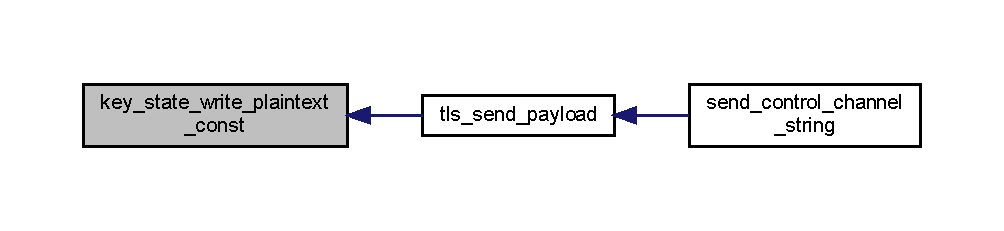
\includegraphics[width=350pt]{group__control__tls_ga67dac3b75328d8b92d3f1a69e86dacdc_icgraph}
\end{center}
\end{figure}


\hypertarget{group__control__tls_gaf045c97f727aebae9e8fc9852421c4f3}{}\index{Control\+\_\+tls@{Control\+\_\+tls}!verify\+\_\+callback@{verify\+\_\+callback}}
\index{verify\+\_\+callback@{verify\+\_\+callback}!Control\+\_\+tls@{Control\+\_\+tls}}
\subsubsection[{verify\+\_\+callback(int preverify\+\_\+ok, X509\+\_\+\+S\+T\+O\+R\+E\+\_\+\+C\+T\+X $\ast$ctx)}]{\setlength{\rightskip}{0pt plus 5cm}int verify\+\_\+callback (
\begin{DoxyParamCaption}
\item[{int}]{preverify\+\_\+ok, }
\item[{X509\+\_\+\+S\+T\+O\+R\+E\+\_\+\+C\+T\+X $\ast$}]{ctx}
\end{DoxyParamCaption}
)}\label{group__control__tls_gaf045c97f727aebae9e8fc9852421c4f3}
Verify that the remote Open\+V\+P\+N peer\textquotesingle{}s certificate allows setting up a V\+P\+N tunnel.

This callback function is called every time a new T\+L\+S session is being setup to determine whether the remote Open\+V\+P\+N peer\textquotesingle{}s certificate is allowed to connect. It is called for once for every certificate in the chain. The callback functionality is configured in the {\ttfamily \hyperlink{ssl_8c_a5d5e4629bd3c2114b3105bf1f082bc86}{init\+\_\+ssl()}} function, which calls the Open\+S\+S\+L library\textquotesingle{}s {\ttfamily S\+S\+L\+\_\+\+C\+T\+X\+\_\+set\+\_\+verify()} function with {\ttfamily \hyperlink{group__control__tls_gaf045c97f727aebae9e8fc9852421c4f3}{verify\+\_\+callback()}} as its callback argument.

It checks preverify\+\_\+ok, and registers the certificate hash. If these steps succeed, it calls the {\ttfamily \hyperlink{ssl__verify_8c_a8574f9402b712d3051d9febde91cf220}{verify\+\_\+cert()}} function, which performs Open\+V\+P\+N-\/specific verification.


\begin{DoxyParams}{Parameters}
{\em preverify\+\_\+ok} & -\/ Whether the remote Open\+V\+P\+N peer\textquotesingle{}s certificate past verification. A value of 1 means it verified successfully, 0 means it failed. \\
\hline
{\em ctx} & -\/ The complete context used by the Open\+S\+S\+L library to verify the certificate chain.\\
\hline
\end{DoxyParams}
\begin{DoxyReturn}{Returns}
The return value indicates whether the supplied certificate is allowed to set up a V\+P\+N tunnel. The following values can be returned\+:
\begin{DoxyItemize}
\item {\ttfamily 0}\+: failure, this certificate is not allowed to connect.
\item {\ttfamily 1}\+: success, this certificate is allowed to connect. 
\end{DoxyItemize}
\end{DoxyReturn}
\hypertarget{group__control__tls_gadeac70d67a80b44a96cbde2368dd5f3c}{}\index{Control\+\_\+tls@{Control\+\_\+tls}!verify\+\_\+callback@{verify\+\_\+callback}}
\index{verify\+\_\+callback@{verify\+\_\+callback}!Control\+\_\+tls@{Control\+\_\+tls}}
\subsubsection[{verify\+\_\+callback(void $\ast$session\+\_\+obj, mbedtls\+\_\+x509\+\_\+crt $\ast$cert, int cert\+\_\+depth, uint32\+\_\+t $\ast$flags)}]{\setlength{\rightskip}{0pt plus 5cm}int verify\+\_\+callback (
\begin{DoxyParamCaption}
\item[{void $\ast$}]{session\+\_\+obj, }
\item[{mbedtls\+\_\+x509\+\_\+crt $\ast$}]{cert, }
\item[{int}]{cert\+\_\+depth, }
\item[{uint32\+\_\+t $\ast$}]{flags}
\end{DoxyParamCaption}
)}\label{group__control__tls_gadeac70d67a80b44a96cbde2368dd5f3c}
Verify that the remote Open\+V\+P\+N peer\textquotesingle{}s certificate allows setting up a V\+P\+N tunnel.

This callback function is called when a new T\+L\+S session is being setup to determine whether the remote Open\+V\+P\+N peer\textquotesingle{}s certificate is allowed to connect. It is called for once for every certificate in the chain. The callback functionality is configured in the {\ttfamily \hyperlink{ssl__backend_8h_a8afed7d8591df5b99475f4503031bb89}{key\+\_\+state\+\_\+ssl\+\_\+init()}} function, which calls the mbed T\+L\+S library\textquotesingle{}s {\ttfamily mbedtls\+\_\+ssl\+\_\+conf\+\_\+verify()} function with {\ttfamily \hyperlink{group__control__tls_gadeac70d67a80b44a96cbde2368dd5f3c}{verify\+\_\+callback()}} as its callback argument.

It checks $\ast$flags and registers the certificate hash. If these steps succeed, it calls the {\ttfamily \hyperlink{ssl__verify_8c_a8574f9402b712d3051d9febde91cf220}{verify\+\_\+cert()}} function, which performs Open\+V\+P\+N-\/specific verification.


\begin{DoxyParams}{Parameters}
{\em session\+\_\+obj} & -\/ The Open\+V\+P\+N {\ttfamily \hyperlink{structtls__session}{tls\+\_\+session}} associated with this object, as set during S\+S\+L session setup. \\
\hline
{\em cert} & -\/ The certificate used by mbed T\+L\+S. \\
\hline
{\em cert\+\_\+depth} & -\/ The depth of the current certificate in the chain, with 0 being the actual certificate. \\
\hline
{\em flags} & -\/ Whether the remote Open\+V\+P\+N peer\textquotesingle{}s certificate passed verification. A value of 0 means it verified successfully, any other value means it failed. {\ttfamily \hyperlink{group__control__tls_gadeac70d67a80b44a96cbde2368dd5f3c}{verify\+\_\+callback()}} is considered to have ok\textquotesingle{}ed this certificate if flags is 0 when it returns.\\
\hline
\end{DoxyParams}
\begin{DoxyReturn}{Returns}
The return value is 0 unless a fatal error occurred. 
\end{DoxyReturn}

\chapter{Class Documentation}
\hypertarget{struct__buffer__entry}{}\section{\+\_\+buffer\+\_\+entry Struct Reference}
\label{struct__buffer__entry}\index{\+\_\+buffer\+\_\+entry@{\+\_\+buffer\+\_\+entry}}


{\ttfamily \#include $<$ssl\+\_\+mbedtls.\+h$>$}



Collaboration diagram for \+\_\+buffer\+\_\+entry\+:
\nopagebreak
\begin{figure}[H]
\begin{center}
\leavevmode
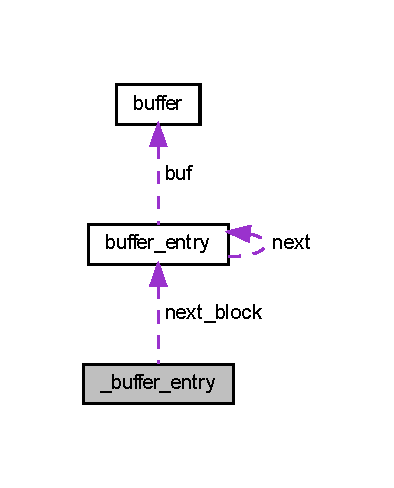
\includegraphics[width=189pt]{struct__buffer__entry__coll__graph}
\end{center}
\end{figure}
\subsection*{Public Attributes}
\begin{DoxyCompactItemize}
\item 
size\+\_\+t \hyperlink{struct__buffer__entry_a05ceac1b681aed72f7cf03e90dba2923}{length}
\item 
uint8\+\_\+t $\ast$ \hyperlink{struct__buffer__entry_a925fd118a4efa1225ab3164a1027f3ca}{data}
\item 
\hyperlink{structbuffer__entry}{buffer\+\_\+entry} $\ast$ \hyperlink{struct__buffer__entry_af05ee663034cc64b90daff5934e0f55a}{next\+\_\+block}
\end{DoxyCompactItemize}


\subsection{Member Data Documentation}
\hypertarget{struct__buffer__entry_a925fd118a4efa1225ab3164a1027f3ca}{}\index{\+\_\+buffer\+\_\+entry@{\+\_\+buffer\+\_\+entry}!data@{data}}
\index{data@{data}!\+\_\+buffer\+\_\+entry@{\+\_\+buffer\+\_\+entry}}
\subsubsection[{data}]{\setlength{\rightskip}{0pt plus 5cm}uint8\+\_\+t$\ast$ \+\_\+buffer\+\_\+entry\+::data}\label{struct__buffer__entry_a925fd118a4efa1225ab3164a1027f3ca}
\hypertarget{struct__buffer__entry_a05ceac1b681aed72f7cf03e90dba2923}{}\index{\+\_\+buffer\+\_\+entry@{\+\_\+buffer\+\_\+entry}!length@{length}}
\index{length@{length}!\+\_\+buffer\+\_\+entry@{\+\_\+buffer\+\_\+entry}}
\subsubsection[{length}]{\setlength{\rightskip}{0pt plus 5cm}size\+\_\+t \+\_\+buffer\+\_\+entry\+::length}\label{struct__buffer__entry_a05ceac1b681aed72f7cf03e90dba2923}
\hypertarget{struct__buffer__entry_af05ee663034cc64b90daff5934e0f55a}{}\index{\+\_\+buffer\+\_\+entry@{\+\_\+buffer\+\_\+entry}!next\+\_\+block@{next\+\_\+block}}
\index{next\+\_\+block@{next\+\_\+block}!\+\_\+buffer\+\_\+entry@{\+\_\+buffer\+\_\+entry}}
\subsubsection[{next\+\_\+block}]{\setlength{\rightskip}{0pt plus 5cm}{\bf buffer\+\_\+entry}$\ast$ \+\_\+buffer\+\_\+entry\+::next\+\_\+block}\label{struct__buffer__entry_af05ee663034cc64b90daff5934e0f55a}


The documentation for this struct was generated from the following file\+:\begin{DoxyCompactItemize}
\item 
src/openvpn/\hyperlink{ssl__mbedtls_8h}{ssl\+\_\+mbedtls.\+h}\end{DoxyCompactItemize}

\hypertarget{struct__list__item}{}\section{\+\_\+list\+\_\+item Struct Reference}
\label{struct__list__item}\index{\+\_\+list\+\_\+item@{\+\_\+list\+\_\+item}}


Collaboration diagram for \+\_\+list\+\_\+item\+:
\nopagebreak
\begin{figure}[H]
\begin{center}
\leavevmode
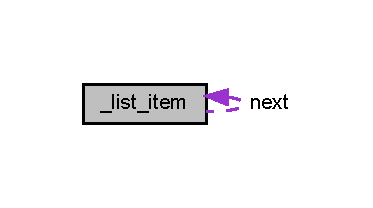
\includegraphics[width=179pt]{struct__list__item__coll__graph}
\end{center}
\end{figure}
\subsection*{Public Attributes}
\begin{DoxyCompactItemize}
\item 
struct \hyperlink{struct__list__item}{\+\_\+list\+\_\+item} $\ast$ \hyperlink{struct__list__item_a981935f42bb92000481bdf9ddbefa16e}{next}
\item 
L\+P\+V\+O\+I\+D \hyperlink{struct__list__item_a979c6b62f85427984085df610dc04937}{data}
\end{DoxyCompactItemize}


\subsection{Member Data Documentation}
\hypertarget{struct__list__item_a979c6b62f85427984085df610dc04937}{}\index{\+\_\+list\+\_\+item@{\+\_\+list\+\_\+item}!data@{data}}
\index{data@{data}!\+\_\+list\+\_\+item@{\+\_\+list\+\_\+item}}
\subsubsection[{data}]{\setlength{\rightskip}{0pt plus 5cm}L\+P\+V\+O\+I\+D \+\_\+list\+\_\+item\+::data}\label{struct__list__item_a979c6b62f85427984085df610dc04937}
\hypertarget{struct__list__item_a981935f42bb92000481bdf9ddbefa16e}{}\index{\+\_\+list\+\_\+item@{\+\_\+list\+\_\+item}!next@{next}}
\index{next@{next}!\+\_\+list\+\_\+item@{\+\_\+list\+\_\+item}}
\subsubsection[{next}]{\setlength{\rightskip}{0pt plus 5cm}struct {\bf \+\_\+list\+\_\+item}$\ast$ \+\_\+list\+\_\+item\+::next}\label{struct__list__item_a981935f42bb92000481bdf9ddbefa16e}


The documentation for this struct was generated from the following file\+:\begin{DoxyCompactItemize}
\item 
src/openvpnserv/\hyperlink{interactive_8c}{interactive.\+c}\end{DoxyCompactItemize}

\hypertarget{struct__query__user}{}\section{\+\_\+query\+\_\+user Struct Reference}
\label{struct__query__user}\index{\+\_\+query\+\_\+user@{\+\_\+query\+\_\+user}}


{\ttfamily \#include $<$console.\+h$>$}

\subsection*{Public Attributes}
\begin{DoxyCompactItemize}
\item 
char $\ast$ \hyperlink{struct__query__user_a0d31c4f55f2bf9b3ea982a448492cc9b}{prompt}
\item 
size\+\_\+t \hyperlink{struct__query__user_a256a230796e573740fa100702526f123}{prompt\+\_\+len}
\item 
char $\ast$ \hyperlink{struct__query__user_adcb311b865e572b4f1fd10a9e33cd753}{response}
\item 
size\+\_\+t \hyperlink{struct__query__user_ab25afbb0907d98746eb46438accb7afb}{response\+\_\+len}
\item 
\hyperlink{automatic_8c_abb452686968e48b67397da5f97445f5b}{bool} \hyperlink{struct__query__user_aeb7652e27ca4f60624cae364d15c2b13}{echo}
\end{DoxyCompactItemize}


\subsection{Detailed Description}
Configuration setup for declaring what kind of information to ask a user for 

\subsection{Member Data Documentation}
\hypertarget{struct__query__user_aeb7652e27ca4f60624cae364d15c2b13}{}\index{\+\_\+query\+\_\+user@{\+\_\+query\+\_\+user}!echo@{echo}}
\index{echo@{echo}!\+\_\+query\+\_\+user@{\+\_\+query\+\_\+user}}
\subsubsection[{echo}]{\setlength{\rightskip}{0pt plus 5cm}{\bf bool} \+\_\+query\+\_\+user\+::echo}\label{struct__query__user_aeb7652e27ca4f60624cae364d15c2b13}
True\+: The user should see what is being typed, otherwise mask it \hypertarget{struct__query__user_a0d31c4f55f2bf9b3ea982a448492cc9b}{}\index{\+\_\+query\+\_\+user@{\+\_\+query\+\_\+user}!prompt@{prompt}}
\index{prompt@{prompt}!\+\_\+query\+\_\+user@{\+\_\+query\+\_\+user}}
\subsubsection[{prompt}]{\setlength{\rightskip}{0pt plus 5cm}char$\ast$ \+\_\+query\+\_\+user\+::prompt}\label{struct__query__user_a0d31c4f55f2bf9b3ea982a448492cc9b}
Prompt to present to the user \hypertarget{struct__query__user_a256a230796e573740fa100702526f123}{}\index{\+\_\+query\+\_\+user@{\+\_\+query\+\_\+user}!prompt\+\_\+len@{prompt\+\_\+len}}
\index{prompt\+\_\+len@{prompt\+\_\+len}!\+\_\+query\+\_\+user@{\+\_\+query\+\_\+user}}
\subsubsection[{prompt\+\_\+len}]{\setlength{\rightskip}{0pt plus 5cm}size\+\_\+t \+\_\+query\+\_\+user\+::prompt\+\_\+len}\label{struct__query__user_a256a230796e573740fa100702526f123}
Lenght of the prompt string \hypertarget{struct__query__user_adcb311b865e572b4f1fd10a9e33cd753}{}\index{\+\_\+query\+\_\+user@{\+\_\+query\+\_\+user}!response@{response}}
\index{response@{response}!\+\_\+query\+\_\+user@{\+\_\+query\+\_\+user}}
\subsubsection[{response}]{\setlength{\rightskip}{0pt plus 5cm}char$\ast$ \+\_\+query\+\_\+user\+::response}\label{struct__query__user_adcb311b865e572b4f1fd10a9e33cd753}
The user\textquotesingle{}s response \hypertarget{struct__query__user_ab25afbb0907d98746eb46438accb7afb}{}\index{\+\_\+query\+\_\+user@{\+\_\+query\+\_\+user}!response\+\_\+len@{response\+\_\+len}}
\index{response\+\_\+len@{response\+\_\+len}!\+\_\+query\+\_\+user@{\+\_\+query\+\_\+user}}
\subsubsection[{response\+\_\+len}]{\setlength{\rightskip}{0pt plus 5cm}size\+\_\+t \+\_\+query\+\_\+user\+::response\+\_\+len}\label{struct__query__user_ab25afbb0907d98746eb46438accb7afb}
Lenght the of the user reposone 

The documentation for this struct was generated from the following file\+:\begin{DoxyCompactItemize}
\item 
src/openvpn/\hyperlink{console_8h}{console.\+h}\end{DoxyCompactItemize}

\hypertarget{structargv}{}\section{argv Struct Reference}
\label{structargv}\index{argv@{argv}}


{\ttfamily \#include $<$argv.\+h$>$}

\subsection*{Public Attributes}
\begin{DoxyCompactItemize}
\item 
size\+\_\+t \hyperlink{structargv_ac74a6705001b8b3e69326f7a27d29146}{capacity}
\item 
size\+\_\+t \hyperlink{structargv_a8b168ac1cfb382ffe6f0ca62f70755d3}{argc}
\item 
char $\ast$$\ast$ \hyperlink{structargv_a3fa35902580e368d0b0c875af2a8e696}{argv}
\end{DoxyCompactItemize}


\subsection{Member Data Documentation}
\hypertarget{structargv_a8b168ac1cfb382ffe6f0ca62f70755d3}{}\index{argv@{argv}!argc@{argc}}
\index{argc@{argc}!argv@{argv}}
\subsubsection[{argc}]{\setlength{\rightskip}{0pt plus 5cm}size\+\_\+t argv\+::argc}\label{structargv_a8b168ac1cfb382ffe6f0ca62f70755d3}
\hypertarget{structargv_a3fa35902580e368d0b0c875af2a8e696}{}\index{argv@{argv}!argv@{argv}}
\index{argv@{argv}!argv@{argv}}
\subsubsection[{argv}]{\setlength{\rightskip}{0pt plus 5cm}char$\ast$$\ast$ argv\+::argv}\label{structargv_a3fa35902580e368d0b0c875af2a8e696}
\hypertarget{structargv_ac74a6705001b8b3e69326f7a27d29146}{}\index{argv@{argv}!capacity@{capacity}}
\index{capacity@{capacity}!argv@{argv}}
\subsubsection[{capacity}]{\setlength{\rightskip}{0pt plus 5cm}size\+\_\+t argv\+::capacity}\label{structargv_ac74a6705001b8b3e69326f7a27d29146}


The documentation for this struct was generated from the following file\+:\begin{DoxyCompactItemize}
\item 
src/openvpn/\hyperlink{argv_8h}{argv.\+h}\end{DoxyCompactItemize}

\hypertarget{structauth__challenge__info}{}\section{auth\+\_\+challenge\+\_\+info Struct Reference}
\label{structauth__challenge__info}\index{auth\+\_\+challenge\+\_\+info@{auth\+\_\+challenge\+\_\+info}}


{\ttfamily \#include $<$misc.\+h$>$}



The documentation for this struct was generated from the following file\+:\begin{DoxyCompactItemize}
\item 
src/openvpn/\hyperlink{misc_8h}{misc.\+h}\end{DoxyCompactItemize}

\hypertarget{structauth__pam__context}{}\section{auth\+\_\+pam\+\_\+context Struct Reference}
\label{structauth__pam__context}\index{auth\+\_\+pam\+\_\+context@{auth\+\_\+pam\+\_\+context}}
\subsection*{Public Attributes}
\begin{DoxyCompactItemize}
\item 
int \hyperlink{structauth__pam__context_a4d5e6779955ef28009010c65056d6cf7}{foreground\+\_\+fd}
\item 
pid\+\_\+t \hyperlink{structauth__pam__context_ae8960fe66401e5c92bde3ac67356927e}{background\+\_\+pid}
\item 
int \hyperlink{structauth__pam__context_a443a725256c636e197fe19f1bc5d801f}{verb}
\end{DoxyCompactItemize}


\subsection{Member Data Documentation}
\hypertarget{structauth__pam__context_ae8960fe66401e5c92bde3ac67356927e}{}\index{auth\+\_\+pam\+\_\+context@{auth\+\_\+pam\+\_\+context}!background\+\_\+pid@{background\+\_\+pid}}
\index{background\+\_\+pid@{background\+\_\+pid}!auth\+\_\+pam\+\_\+context@{auth\+\_\+pam\+\_\+context}}
\subsubsection[{background\+\_\+pid}]{\setlength{\rightskip}{0pt plus 5cm}pid\+\_\+t auth\+\_\+pam\+\_\+context\+::background\+\_\+pid}\label{structauth__pam__context_ae8960fe66401e5c92bde3ac67356927e}
\hypertarget{structauth__pam__context_a4d5e6779955ef28009010c65056d6cf7}{}\index{auth\+\_\+pam\+\_\+context@{auth\+\_\+pam\+\_\+context}!foreground\+\_\+fd@{foreground\+\_\+fd}}
\index{foreground\+\_\+fd@{foreground\+\_\+fd}!auth\+\_\+pam\+\_\+context@{auth\+\_\+pam\+\_\+context}}
\subsubsection[{foreground\+\_\+fd}]{\setlength{\rightskip}{0pt plus 5cm}int auth\+\_\+pam\+\_\+context\+::foreground\+\_\+fd}\label{structauth__pam__context_a4d5e6779955ef28009010c65056d6cf7}
\hypertarget{structauth__pam__context_a443a725256c636e197fe19f1bc5d801f}{}\index{auth\+\_\+pam\+\_\+context@{auth\+\_\+pam\+\_\+context}!verb@{verb}}
\index{verb@{verb}!auth\+\_\+pam\+\_\+context@{auth\+\_\+pam\+\_\+context}}
\subsubsection[{verb}]{\setlength{\rightskip}{0pt plus 5cm}int auth\+\_\+pam\+\_\+context\+::verb}\label{structauth__pam__context_a443a725256c636e197fe19f1bc5d801f}


The documentation for this struct was generated from the following file\+:\begin{DoxyCompactItemize}
\item 
src/plugins/auth-\/pam/\hyperlink{auth-pam_8c}{auth-\/pam.\+c}\end{DoxyCompactItemize}

\hypertarget{structbio__ctx}{}\section{bio\+\_\+ctx Struct Reference}
\label{structbio__ctx}\index{bio\+\_\+ctx@{bio\+\_\+ctx}}


{\ttfamily \#include $<$ssl\+\_\+mbedtls.\+h$>$}



Collaboration diagram for bio\+\_\+ctx\+:
\nopagebreak
\begin{figure}[H]
\begin{center}
\leavevmode
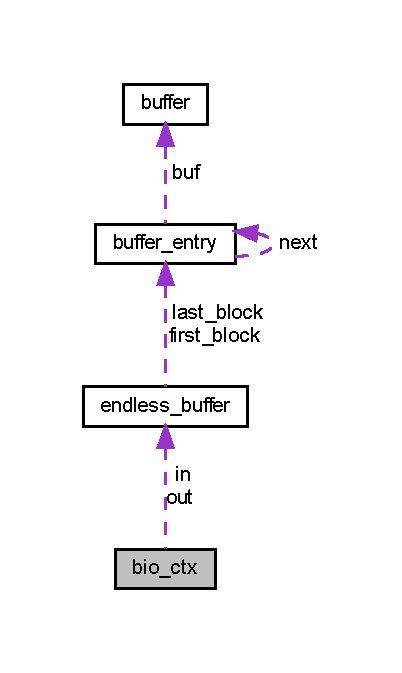
\includegraphics[width=193pt]{structbio__ctx__coll__graph}
\end{center}
\end{figure}
\subsection*{Public Attributes}
\begin{DoxyCompactItemize}
\item 
\hyperlink{structendless__buffer}{endless\+\_\+buffer} \hyperlink{structbio__ctx_abc9a3f277ae77f310c1e3b79ad48ae26}{in}
\item 
\hyperlink{structendless__buffer}{endless\+\_\+buffer} \hyperlink{structbio__ctx_aa9c670dd99822fb36115f6ebb7e4ccd2}{out}
\end{DoxyCompactItemize}


\subsection{Member Data Documentation}
\hypertarget{structbio__ctx_abc9a3f277ae77f310c1e3b79ad48ae26}{}\index{bio\+\_\+ctx@{bio\+\_\+ctx}!in@{in}}
\index{in@{in}!bio\+\_\+ctx@{bio\+\_\+ctx}}
\subsubsection[{in}]{\setlength{\rightskip}{0pt plus 5cm}{\bf endless\+\_\+buffer} bio\+\_\+ctx\+::in}\label{structbio__ctx_abc9a3f277ae77f310c1e3b79ad48ae26}
\hypertarget{structbio__ctx_aa9c670dd99822fb36115f6ebb7e4ccd2}{}\index{bio\+\_\+ctx@{bio\+\_\+ctx}!out@{out}}
\index{out@{out}!bio\+\_\+ctx@{bio\+\_\+ctx}}
\subsubsection[{out}]{\setlength{\rightskip}{0pt plus 5cm}{\bf endless\+\_\+buffer} bio\+\_\+ctx\+::out}\label{structbio__ctx_aa9c670dd99822fb36115f6ebb7e4ccd2}


The documentation for this struct was generated from the following file\+:\begin{DoxyCompactItemize}
\item 
src/openvpn/\hyperlink{ssl__mbedtls_8h}{ssl\+\_\+mbedtls.\+h}\end{DoxyCompactItemize}

\hypertarget{structblock__dns__data__t}{}\section{block\+\_\+dns\+\_\+data\+\_\+t Struct Reference}
\label{structblock__dns__data__t}\index{block\+\_\+dns\+\_\+data\+\_\+t@{block\+\_\+dns\+\_\+data\+\_\+t}}
\subsection*{Public Attributes}
\begin{DoxyCompactItemize}
\item 
H\+A\+N\+D\+L\+E \hyperlink{structblock__dns__data__t_a3b08c75ccf068ddd692bdf1f4ab59ae1}{engine}
\item 
int \hyperlink{structblock__dns__data__t_abf7f3823d4e65a955a640548588dba20}{index}
\item 
int \hyperlink{structblock__dns__data__t_a280851190c1998268fc3c69d14c50c69}{metric\+\_\+v4}
\item 
int \hyperlink{structblock__dns__data__t_a67bdfe74f6a138956b2b35afd97d5273}{metric\+\_\+v6}
\end{DoxyCompactItemize}


\subsection{Member Data Documentation}
\hypertarget{structblock__dns__data__t_a3b08c75ccf068ddd692bdf1f4ab59ae1}{}\index{block\+\_\+dns\+\_\+data\+\_\+t@{block\+\_\+dns\+\_\+data\+\_\+t}!engine@{engine}}
\index{engine@{engine}!block\+\_\+dns\+\_\+data\+\_\+t@{block\+\_\+dns\+\_\+data\+\_\+t}}
\subsubsection[{engine}]{\setlength{\rightskip}{0pt plus 5cm}H\+A\+N\+D\+L\+E block\+\_\+dns\+\_\+data\+\_\+t\+::engine}\label{structblock__dns__data__t_a3b08c75ccf068ddd692bdf1f4ab59ae1}
\hypertarget{structblock__dns__data__t_abf7f3823d4e65a955a640548588dba20}{}\index{block\+\_\+dns\+\_\+data\+\_\+t@{block\+\_\+dns\+\_\+data\+\_\+t}!index@{index}}
\index{index@{index}!block\+\_\+dns\+\_\+data\+\_\+t@{block\+\_\+dns\+\_\+data\+\_\+t}}
\subsubsection[{index}]{\setlength{\rightskip}{0pt plus 5cm}int block\+\_\+dns\+\_\+data\+\_\+t\+::index}\label{structblock__dns__data__t_abf7f3823d4e65a955a640548588dba20}
\hypertarget{structblock__dns__data__t_a280851190c1998268fc3c69d14c50c69}{}\index{block\+\_\+dns\+\_\+data\+\_\+t@{block\+\_\+dns\+\_\+data\+\_\+t}!metric\+\_\+v4@{metric\+\_\+v4}}
\index{metric\+\_\+v4@{metric\+\_\+v4}!block\+\_\+dns\+\_\+data\+\_\+t@{block\+\_\+dns\+\_\+data\+\_\+t}}
\subsubsection[{metric\+\_\+v4}]{\setlength{\rightskip}{0pt plus 5cm}int block\+\_\+dns\+\_\+data\+\_\+t\+::metric\+\_\+v4}\label{structblock__dns__data__t_a280851190c1998268fc3c69d14c50c69}
\hypertarget{structblock__dns__data__t_a67bdfe74f6a138956b2b35afd97d5273}{}\index{block\+\_\+dns\+\_\+data\+\_\+t@{block\+\_\+dns\+\_\+data\+\_\+t}!metric\+\_\+v6@{metric\+\_\+v6}}
\index{metric\+\_\+v6@{metric\+\_\+v6}!block\+\_\+dns\+\_\+data\+\_\+t@{block\+\_\+dns\+\_\+data\+\_\+t}}
\subsubsection[{metric\+\_\+v6}]{\setlength{\rightskip}{0pt plus 5cm}int block\+\_\+dns\+\_\+data\+\_\+t\+::metric\+\_\+v6}\label{structblock__dns__data__t_a67bdfe74f6a138956b2b35afd97d5273}


The documentation for this struct was generated from the following file\+:\begin{DoxyCompactItemize}
\item 
src/openvpnserv/\hyperlink{interactive_8c}{interactive.\+c}\end{DoxyCompactItemize}

\hypertarget{structbuffer}{}\section{buffer Struct Reference}
\label{structbuffer}\index{buffer@{buffer}}


{\ttfamily \#include $<$buffer.\+h$>$}

\subsection*{Public Attributes}
\begin{DoxyCompactItemize}
\item 
int \hyperlink{structbuffer_a1fb6dcafc58a5ddc11c4d60c09a2e086}{capacity}
\item 
int \hyperlink{structbuffer_af5c1acadd937a2944674832497ba63ad}{offset}
\item 
int \hyperlink{structbuffer_ada52eab703a091ff327114b3b3b0140a}{len}
\item 
uint8\+\_\+t $\ast$ \hyperlink{structbuffer_a5d2300c691699fd563f7a1a280c2c2d6}{data}
\end{DoxyCompactItemize}


\subsection{Detailed Description}
Wrapper structure for dynamically allocated memory.

The actual content stored in a {\ttfamily buffer} structure starts at the memory location {\ttfamily \hyperlink{structbuffer_a5d2300c691699fd563f7a1a280c2c2d6}{buffer.\+data}} {\ttfamily +} {\ttfamily \hyperlink{structbuffer_af5c1acadd937a2944674832497ba63ad}{buffer.\+offset}}, and has a length of {\ttfamily \hyperlink{structbuffer_ada52eab703a091ff327114b3b3b0140a}{buffer.\+len}} bytes. This, together with the space available before and after the content, is represented in the pseudocode below\+: 
\begin{DoxyCode}
uint8\_t *content\_start    = \hyperlink{structbuffer}{buffer}.\hyperlink{structbuffer_a5d2300c691699fd563f7a1a280c2c2d6}{data} + \hyperlink{structbuffer}{buffer}.\hyperlink{structbuffer_af5c1acadd937a2944674832497ba63ad}{offset};
uint8\_t *content\_end      = \hyperlink{structbuffer}{buffer}.\hyperlink{structbuffer_a5d2300c691699fd563f7a1a280c2c2d6}{data} + \hyperlink{structbuffer}{buffer}.\hyperlink{structbuffer_af5c1acadd937a2944674832497ba63ad}{offset} + 
      \hyperlink{structbuffer}{buffer}.\hyperlink{structbuffer_ada52eab703a091ff327114b3b3b0140a}{len};
\textcolor{keywordtype}{int}      prepend\_capacity = \hyperlink{structbuffer}{buffer}.\hyperlink{structbuffer_af5c1acadd937a2944674832497ba63ad}{offset};
\textcolor{keywordtype}{int}      append\_capacity  = \hyperlink{structbuffer}{buffer}.\hyperlink{structbuffer_a1fb6dcafc58a5ddc11c4d60c09a2e086}{capacity} - (\hyperlink{structbuffer}{buffer}.\hyperlink{structbuffer_af5c1acadd937a2944674832497ba63ad}{offset} + 
      \hyperlink{structbuffer}{buffer}.\hyperlink{structbuffer_ada52eab703a091ff327114b3b3b0140a}{len});
\end{DoxyCode}
 

\subsection{Member Data Documentation}
\hypertarget{structbuffer_a1fb6dcafc58a5ddc11c4d60c09a2e086}{}\index{buffer@{buffer}!capacity@{capacity}}
\index{capacity@{capacity}!buffer@{buffer}}
\subsubsection[{capacity}]{\setlength{\rightskip}{0pt plus 5cm}int buffer\+::capacity}\label{structbuffer_a1fb6dcafc58a5ddc11c4d60c09a2e086}
Size in bytes of memory allocated by {\ttfamily malloc()}. \hypertarget{structbuffer_a5d2300c691699fd563f7a1a280c2c2d6}{}\index{buffer@{buffer}!data@{data}}
\index{data@{data}!buffer@{buffer}}
\subsubsection[{data}]{\setlength{\rightskip}{0pt plus 5cm}uint8\+\_\+t$\ast$ buffer\+::data}\label{structbuffer_a5d2300c691699fd563f7a1a280c2c2d6}
Pointer to the allocated memory. \hypertarget{structbuffer_ada52eab703a091ff327114b3b3b0140a}{}\index{buffer@{buffer}!len@{len}}
\index{len@{len}!buffer@{buffer}}
\subsubsection[{len}]{\setlength{\rightskip}{0pt plus 5cm}int buffer\+::len}\label{structbuffer_ada52eab703a091ff327114b3b3b0140a}
Length in bytes of the actual content within the allocated memory. \hypertarget{structbuffer_af5c1acadd937a2944674832497ba63ad}{}\index{buffer@{buffer}!offset@{offset}}
\index{offset@{offset}!buffer@{buffer}}
\subsubsection[{offset}]{\setlength{\rightskip}{0pt plus 5cm}int buffer\+::offset}\label{structbuffer_af5c1acadd937a2944674832497ba63ad}
Offset in bytes of the actual content within the allocated memory. 

The documentation for this struct was generated from the following file\+:\begin{DoxyCompactItemize}
\item 
src/openvpn/\hyperlink{buffer_8h}{buffer.\+h}\end{DoxyCompactItemize}

\hypertarget{structbuffer__entry}{}\section{buffer\+\_\+entry Struct Reference}
\label{structbuffer__entry}\index{buffer\+\_\+entry@{buffer\+\_\+entry}}


{\ttfamily \#include $<$buffer.\+h$>$}



Collaboration diagram for buffer\+\_\+entry\+:
\nopagebreak
\begin{figure}[H]
\begin{center}
\leavevmode
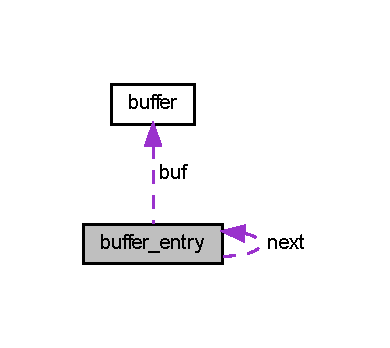
\includegraphics[width=187pt]{structbuffer__entry__coll__graph}
\end{center}
\end{figure}
\subsection*{Public Attributes}
\begin{DoxyCompactItemize}
\item 
struct \hyperlink{structbuffer}{buffer} \hyperlink{structbuffer__entry_ade29481cb1d1354ad2b22ff5510e285b}{buf}
\item 
struct \hyperlink{structbuffer__entry}{buffer\+\_\+entry} $\ast$ \hyperlink{structbuffer__entry_a26b1c9d47a4329655cccf3916631b247}{next}
\end{DoxyCompactItemize}


\subsection{Member Data Documentation}
\hypertarget{structbuffer__entry_ade29481cb1d1354ad2b22ff5510e285b}{}\index{buffer\+\_\+entry@{buffer\+\_\+entry}!buf@{buf}}
\index{buf@{buf}!buffer\+\_\+entry@{buffer\+\_\+entry}}
\subsubsection[{buf}]{\setlength{\rightskip}{0pt plus 5cm}struct {\bf buffer} buffer\+\_\+entry\+::buf}\label{structbuffer__entry_ade29481cb1d1354ad2b22ff5510e285b}
\hypertarget{structbuffer__entry_a26b1c9d47a4329655cccf3916631b247}{}\index{buffer\+\_\+entry@{buffer\+\_\+entry}!next@{next}}
\index{next@{next}!buffer\+\_\+entry@{buffer\+\_\+entry}}
\subsubsection[{next}]{\setlength{\rightskip}{0pt plus 5cm}struct {\bf buffer\+\_\+entry}$\ast$ buffer\+\_\+entry\+::next}\label{structbuffer__entry_a26b1c9d47a4329655cccf3916631b247}


The documentation for this struct was generated from the following file\+:\begin{DoxyCompactItemize}
\item 
src/openvpn/\hyperlink{buffer_8h}{buffer.\+h}\end{DoxyCompactItemize}

\hypertarget{structbuffer__list}{}\section{buffer\+\_\+list Struct Reference}
\label{structbuffer__list}\index{buffer\+\_\+list@{buffer\+\_\+list}}


{\ttfamily \#include $<$buffer.\+h$>$}



Collaboration diagram for buffer\+\_\+list\+:
\nopagebreak
\begin{figure}[H]
\begin{center}
\leavevmode
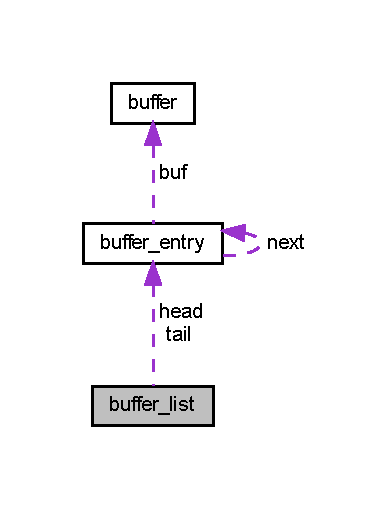
\includegraphics[width=187pt]{structbuffer__list__coll__graph}
\end{center}
\end{figure}
\subsection*{Public Attributes}
\begin{DoxyCompactItemize}
\item 
struct \hyperlink{structbuffer__entry}{buffer\+\_\+entry} $\ast$ \hyperlink{structbuffer__list_afaecc74fd9a1fdcc9a0d707f6c8519f6}{head}
\item 
struct \hyperlink{structbuffer__entry}{buffer\+\_\+entry} $\ast$ \hyperlink{structbuffer__list_ab1d10be66880cdccbfe888d8e487d3b3}{tail}
\item 
int \hyperlink{structbuffer__list_aeb4047df8b6044b88cb2c5f1803c998e}{size}
\item 
int \hyperlink{structbuffer__list_ad65e80969c5347f450728c8f3c149dd1}{max\+\_\+size}
\end{DoxyCompactItemize}


\subsection{Member Data Documentation}
\hypertarget{structbuffer__list_afaecc74fd9a1fdcc9a0d707f6c8519f6}{}\index{buffer\+\_\+list@{buffer\+\_\+list}!head@{head}}
\index{head@{head}!buffer\+\_\+list@{buffer\+\_\+list}}
\subsubsection[{head}]{\setlength{\rightskip}{0pt plus 5cm}struct {\bf buffer\+\_\+entry}$\ast$ buffer\+\_\+list\+::head}\label{structbuffer__list_afaecc74fd9a1fdcc9a0d707f6c8519f6}
\hypertarget{structbuffer__list_ad65e80969c5347f450728c8f3c149dd1}{}\index{buffer\+\_\+list@{buffer\+\_\+list}!max\+\_\+size@{max\+\_\+size}}
\index{max\+\_\+size@{max\+\_\+size}!buffer\+\_\+list@{buffer\+\_\+list}}
\subsubsection[{max\+\_\+size}]{\setlength{\rightskip}{0pt plus 5cm}int buffer\+\_\+list\+::max\+\_\+size}\label{structbuffer__list_ad65e80969c5347f450728c8f3c149dd1}
\hypertarget{structbuffer__list_aeb4047df8b6044b88cb2c5f1803c998e}{}\index{buffer\+\_\+list@{buffer\+\_\+list}!size@{size}}
\index{size@{size}!buffer\+\_\+list@{buffer\+\_\+list}}
\subsubsection[{size}]{\setlength{\rightskip}{0pt plus 5cm}int buffer\+\_\+list\+::size}\label{structbuffer__list_aeb4047df8b6044b88cb2c5f1803c998e}
\hypertarget{structbuffer__list_ab1d10be66880cdccbfe888d8e487d3b3}{}\index{buffer\+\_\+list@{buffer\+\_\+list}!tail@{tail}}
\index{tail@{tail}!buffer\+\_\+list@{buffer\+\_\+list}}
\subsubsection[{tail}]{\setlength{\rightskip}{0pt plus 5cm}struct {\bf buffer\+\_\+entry}$\ast$ buffer\+\_\+list\+::tail}\label{structbuffer__list_ab1d10be66880cdccbfe888d8e487d3b3}


The documentation for this struct was generated from the following file\+:\begin{DoxyCompactItemize}
\item 
src/openvpn/\hyperlink{buffer_8h}{buffer.\+h}\end{DoxyCompactItemize}

\hypertarget{structcached__dns__entry}{}\section{cached\+\_\+dns\+\_\+entry Struct Reference}
\label{structcached__dns__entry}\index{cached\+\_\+dns\+\_\+entry@{cached\+\_\+dns\+\_\+entry}}


{\ttfamily \#include $<$socket.\+h$>$}



Collaboration diagram for cached\+\_\+dns\+\_\+entry\+:
\nopagebreak
\begin{figure}[H]
\begin{center}
\leavevmode
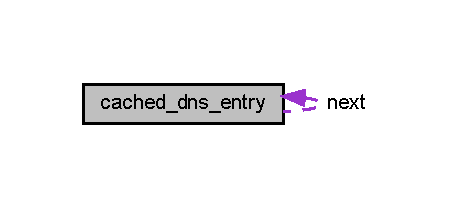
\includegraphics[width=216pt]{structcached__dns__entry__coll__graph}
\end{center}
\end{figure}
\subsection*{Public Attributes}
\begin{DoxyCompactItemize}
\item 
const char $\ast$ \hyperlink{structcached__dns__entry_a052fed87e08c62b9af51882c1f45188d}{hostname}
\item 
const char $\ast$ \hyperlink{structcached__dns__entry_a57e20fe1ffaf4e0962cf008e13fb0dc1}{servname}
\item 
int \hyperlink{structcached__dns__entry_a47cd1861b13d948c3ebb0ba1ff4b3c01}{ai\+\_\+family}
\item 
int \hyperlink{structcached__dns__entry_a5878e9423d88197a39de9fd88209553a}{flags}
\item 
struct addrinfo $\ast$ \hyperlink{structcached__dns__entry_a8881ad4c8fb134be0f07d45e76336476}{ai}
\item 
struct \hyperlink{structcached__dns__entry}{cached\+\_\+dns\+\_\+entry} $\ast$ \hyperlink{structcached__dns__entry_a93565db3d9426f615031c51b6046d7df}{next}
\end{DoxyCompactItemize}


\subsection{Member Data Documentation}
\hypertarget{structcached__dns__entry_a8881ad4c8fb134be0f07d45e76336476}{}\index{cached\+\_\+dns\+\_\+entry@{cached\+\_\+dns\+\_\+entry}!ai@{ai}}
\index{ai@{ai}!cached\+\_\+dns\+\_\+entry@{cached\+\_\+dns\+\_\+entry}}
\subsubsection[{ai}]{\setlength{\rightskip}{0pt plus 5cm}struct addrinfo$\ast$ cached\+\_\+dns\+\_\+entry\+::ai}\label{structcached__dns__entry_a8881ad4c8fb134be0f07d45e76336476}
\hypertarget{structcached__dns__entry_a47cd1861b13d948c3ebb0ba1ff4b3c01}{}\index{cached\+\_\+dns\+\_\+entry@{cached\+\_\+dns\+\_\+entry}!ai\+\_\+family@{ai\+\_\+family}}
\index{ai\+\_\+family@{ai\+\_\+family}!cached\+\_\+dns\+\_\+entry@{cached\+\_\+dns\+\_\+entry}}
\subsubsection[{ai\+\_\+family}]{\setlength{\rightskip}{0pt plus 5cm}int cached\+\_\+dns\+\_\+entry\+::ai\+\_\+family}\label{structcached__dns__entry_a47cd1861b13d948c3ebb0ba1ff4b3c01}
\hypertarget{structcached__dns__entry_a5878e9423d88197a39de9fd88209553a}{}\index{cached\+\_\+dns\+\_\+entry@{cached\+\_\+dns\+\_\+entry}!flags@{flags}}
\index{flags@{flags}!cached\+\_\+dns\+\_\+entry@{cached\+\_\+dns\+\_\+entry}}
\subsubsection[{flags}]{\setlength{\rightskip}{0pt plus 5cm}int cached\+\_\+dns\+\_\+entry\+::flags}\label{structcached__dns__entry_a5878e9423d88197a39de9fd88209553a}
\hypertarget{structcached__dns__entry_a052fed87e08c62b9af51882c1f45188d}{}\index{cached\+\_\+dns\+\_\+entry@{cached\+\_\+dns\+\_\+entry}!hostname@{hostname}}
\index{hostname@{hostname}!cached\+\_\+dns\+\_\+entry@{cached\+\_\+dns\+\_\+entry}}
\subsubsection[{hostname}]{\setlength{\rightskip}{0pt plus 5cm}const char$\ast$ cached\+\_\+dns\+\_\+entry\+::hostname}\label{structcached__dns__entry_a052fed87e08c62b9af51882c1f45188d}
\hypertarget{structcached__dns__entry_a93565db3d9426f615031c51b6046d7df}{}\index{cached\+\_\+dns\+\_\+entry@{cached\+\_\+dns\+\_\+entry}!next@{next}}
\index{next@{next}!cached\+\_\+dns\+\_\+entry@{cached\+\_\+dns\+\_\+entry}}
\subsubsection[{next}]{\setlength{\rightskip}{0pt plus 5cm}struct {\bf cached\+\_\+dns\+\_\+entry}$\ast$ cached\+\_\+dns\+\_\+entry\+::next}\label{structcached__dns__entry_a93565db3d9426f615031c51b6046d7df}
\hypertarget{structcached__dns__entry_a57e20fe1ffaf4e0962cf008e13fb0dc1}{}\index{cached\+\_\+dns\+\_\+entry@{cached\+\_\+dns\+\_\+entry}!servname@{servname}}
\index{servname@{servname}!cached\+\_\+dns\+\_\+entry@{cached\+\_\+dns\+\_\+entry}}
\subsubsection[{servname}]{\setlength{\rightskip}{0pt plus 5cm}const char$\ast$ cached\+\_\+dns\+\_\+entry\+::servname}\label{structcached__dns__entry_a57e20fe1ffaf4e0962cf008e13fb0dc1}


The documentation for this struct was generated from the following file\+:\begin{DoxyCompactItemize}
\item 
src/openvpn/\hyperlink{socket_8h}{socket.\+h}\end{DoxyCompactItemize}

\hypertarget{structcert__hash}{}\section{cert\+\_\+hash Struct Reference}
\label{structcert__hash}\index{cert\+\_\+hash@{cert\+\_\+hash}}


{\ttfamily \#include $<$ssl\+\_\+verify.\+h$>$}

\subsection*{Public Attributes}
\begin{DoxyCompactItemize}
\item 
unsigned char \hyperlink{structcert__hash_ab480ce52fd263405a9674ddc59b7b1fc}{sha256\+\_\+hash} \mbox{[}256/8\mbox{]}
\end{DoxyCompactItemize}


\subsection{Detailed Description}
Structure containing the hash for a single certificate 

\subsection{Member Data Documentation}
\hypertarget{structcert__hash_ab480ce52fd263405a9674ddc59b7b1fc}{}\index{cert\+\_\+hash@{cert\+\_\+hash}!sha256\+\_\+hash@{sha256\+\_\+hash}}
\index{sha256\+\_\+hash@{sha256\+\_\+hash}!cert\+\_\+hash@{cert\+\_\+hash}}
\subsubsection[{sha256\+\_\+hash}]{\setlength{\rightskip}{0pt plus 5cm}unsigned char cert\+\_\+hash\+::sha256\+\_\+hash\mbox{[}256/8\mbox{]}}\label{structcert__hash_ab480ce52fd263405a9674ddc59b7b1fc}


The documentation for this struct was generated from the following file\+:\begin{DoxyCompactItemize}
\item 
src/openvpn/\hyperlink{ssl__verify_8h}{ssl\+\_\+verify.\+h}\end{DoxyCompactItemize}

\hypertarget{structcert__hash__set}{}\section{cert\+\_\+hash\+\_\+set Struct Reference}
\label{structcert__hash__set}\index{cert\+\_\+hash\+\_\+set@{cert\+\_\+hash\+\_\+set}}


{\ttfamily \#include $<$ssl\+\_\+verify.\+h$>$}



Collaboration diagram for cert\+\_\+hash\+\_\+set\+:
\nopagebreak
\begin{figure}[H]
\begin{center}
\leavevmode
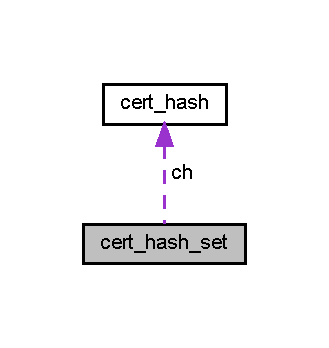
\includegraphics[width=158pt]{structcert__hash__set__coll__graph}
\end{center}
\end{figure}
\subsection*{Public Attributes}
\begin{DoxyCompactItemize}
\item 
struct \hyperlink{structcert__hash}{cert\+\_\+hash} $\ast$ \hyperlink{structcert__hash__set_a1d62c176153ce49841aea5c0aed607a2}{ch} \mbox{[}\hyperlink{ssl__verify_8h_ab7f713661d9681e187960a247105692d}{M\+A\+X\+\_\+\+C\+E\+R\+T\+\_\+\+D\+E\+P\+T\+H}\mbox{]}
\end{DoxyCompactItemize}


\subsection{Detailed Description}
Structure containing the hashes for a full certificate chain 

\subsection{Member Data Documentation}
\hypertarget{structcert__hash__set_a1d62c176153ce49841aea5c0aed607a2}{}\index{cert\+\_\+hash\+\_\+set@{cert\+\_\+hash\+\_\+set}!ch@{ch}}
\index{ch@{ch}!cert\+\_\+hash\+\_\+set@{cert\+\_\+hash\+\_\+set}}
\subsubsection[{ch}]{\setlength{\rightskip}{0pt plus 5cm}struct {\bf cert\+\_\+hash}$\ast$ cert\+\_\+hash\+\_\+set\+::ch\mbox{[}{\bf M\+A\+X\+\_\+\+C\+E\+R\+T\+\_\+\+D\+E\+P\+T\+H}\mbox{]}}\label{structcert__hash__set_a1d62c176153ce49841aea5c0aed607a2}
Array of certificate hashes 

The documentation for this struct was generated from the following file\+:\begin{DoxyCompactItemize}
\item 
src/openvpn/\hyperlink{ssl__verify_8h}{ssl\+\_\+verify.\+h}\end{DoxyCompactItemize}

\hypertarget{structcipher__name__pair}{}\section{cipher\+\_\+name\+\_\+pair Struct Reference}
\label{structcipher__name__pair}\index{cipher\+\_\+name\+\_\+pair@{cipher\+\_\+name\+\_\+pair}}


{\ttfamily \#include $<$crypto\+\_\+backend.\+h$>$}

\subsection*{Public Attributes}
\begin{DoxyCompactItemize}
\item 
const char $\ast$ \hyperlink{structcipher__name__pair_a8721e2007ddeeca3621a32bdcb91f8f7}{openvpn\+\_\+name}
\item 
const char $\ast$ \hyperlink{structcipher__name__pair_add13a313f39ebde98a65afde6e8de35d}{lib\+\_\+name}
\end{DoxyCompactItemize}


\subsection{Detailed Description}
Struct used in cipher name translation table 

\subsection{Member Data Documentation}
\hypertarget{structcipher__name__pair_add13a313f39ebde98a65afde6e8de35d}{}\index{cipher\+\_\+name\+\_\+pair@{cipher\+\_\+name\+\_\+pair}!lib\+\_\+name@{lib\+\_\+name}}
\index{lib\+\_\+name@{lib\+\_\+name}!cipher\+\_\+name\+\_\+pair@{cipher\+\_\+name\+\_\+pair}}
\subsubsection[{lib\+\_\+name}]{\setlength{\rightskip}{0pt plus 5cm}const char$\ast$ cipher\+\_\+name\+\_\+pair\+::lib\+\_\+name}\label{structcipher__name__pair_add13a313f39ebde98a65afde6e8de35d}
Cipher name used by crypto library \hypertarget{structcipher__name__pair_a8721e2007ddeeca3621a32bdcb91f8f7}{}\index{cipher\+\_\+name\+\_\+pair@{cipher\+\_\+name\+\_\+pair}!openvpn\+\_\+name@{openvpn\+\_\+name}}
\index{openvpn\+\_\+name@{openvpn\+\_\+name}!cipher\+\_\+name\+\_\+pair@{cipher\+\_\+name\+\_\+pair}}
\subsubsection[{openvpn\+\_\+name}]{\setlength{\rightskip}{0pt plus 5cm}const char$\ast$ cipher\+\_\+name\+\_\+pair\+::openvpn\+\_\+name}\label{structcipher__name__pair_a8721e2007ddeeca3621a32bdcb91f8f7}
Cipher name used by Open\+V\+P\+N 

The documentation for this struct was generated from the following file\+:\begin{DoxyCompactItemize}
\item 
src/openvpn/\hyperlink{crypto__backend_8h}{crypto\+\_\+backend.\+h}\end{DoxyCompactItemize}

\hypertarget{structclient__nat__entry}{}\section{client\+\_\+nat\+\_\+entry Struct Reference}
\label{structclient__nat__entry}\index{client\+\_\+nat\+\_\+entry@{client\+\_\+nat\+\_\+entry}}


{\ttfamily \#include $<$clinat.\+h$>$}

\subsection*{Public Attributes}
\begin{DoxyCompactItemize}
\item 
int \hyperlink{structclient__nat__entry_a1ef20d15d70fa68864a1fb9714616cd9}{type}
\item 
in\+\_\+addr\+\_\+t \hyperlink{structclient__nat__entry_a4201fa6551314373401d386494ca451d}{network}
\item 
in\+\_\+addr\+\_\+t \hyperlink{structclient__nat__entry_ad9ea7e6de4bd6099bfaf6a5a8b131191}{netmask}
\item 
in\+\_\+addr\+\_\+t \hyperlink{structclient__nat__entry_ad2a5c775232e4c39b1582c87fe157ea2}{foreign\+\_\+network}
\end{DoxyCompactItemize}


\subsection{Member Data Documentation}
\hypertarget{structclient__nat__entry_ad2a5c775232e4c39b1582c87fe157ea2}{}\index{client\+\_\+nat\+\_\+entry@{client\+\_\+nat\+\_\+entry}!foreign\+\_\+network@{foreign\+\_\+network}}
\index{foreign\+\_\+network@{foreign\+\_\+network}!client\+\_\+nat\+\_\+entry@{client\+\_\+nat\+\_\+entry}}
\subsubsection[{foreign\+\_\+network}]{\setlength{\rightskip}{0pt plus 5cm}in\+\_\+addr\+\_\+t client\+\_\+nat\+\_\+entry\+::foreign\+\_\+network}\label{structclient__nat__entry_ad2a5c775232e4c39b1582c87fe157ea2}
\hypertarget{structclient__nat__entry_ad9ea7e6de4bd6099bfaf6a5a8b131191}{}\index{client\+\_\+nat\+\_\+entry@{client\+\_\+nat\+\_\+entry}!netmask@{netmask}}
\index{netmask@{netmask}!client\+\_\+nat\+\_\+entry@{client\+\_\+nat\+\_\+entry}}
\subsubsection[{netmask}]{\setlength{\rightskip}{0pt plus 5cm}in\+\_\+addr\+\_\+t client\+\_\+nat\+\_\+entry\+::netmask}\label{structclient__nat__entry_ad9ea7e6de4bd6099bfaf6a5a8b131191}
\hypertarget{structclient__nat__entry_a4201fa6551314373401d386494ca451d}{}\index{client\+\_\+nat\+\_\+entry@{client\+\_\+nat\+\_\+entry}!network@{network}}
\index{network@{network}!client\+\_\+nat\+\_\+entry@{client\+\_\+nat\+\_\+entry}}
\subsubsection[{network}]{\setlength{\rightskip}{0pt plus 5cm}in\+\_\+addr\+\_\+t client\+\_\+nat\+\_\+entry\+::network}\label{structclient__nat__entry_a4201fa6551314373401d386494ca451d}
\hypertarget{structclient__nat__entry_a1ef20d15d70fa68864a1fb9714616cd9}{}\index{client\+\_\+nat\+\_\+entry@{client\+\_\+nat\+\_\+entry}!type@{type}}
\index{type@{type}!client\+\_\+nat\+\_\+entry@{client\+\_\+nat\+\_\+entry}}
\subsubsection[{type}]{\setlength{\rightskip}{0pt plus 5cm}int client\+\_\+nat\+\_\+entry\+::type}\label{structclient__nat__entry_a1ef20d15d70fa68864a1fb9714616cd9}


The documentation for this struct was generated from the following file\+:\begin{DoxyCompactItemize}
\item 
src/openvpn/\hyperlink{clinat_8h}{clinat.\+h}\end{DoxyCompactItemize}

\hypertarget{structclient__nat__option__list}{}\section{client\+\_\+nat\+\_\+option\+\_\+list Struct Reference}
\label{structclient__nat__option__list}\index{client\+\_\+nat\+\_\+option\+\_\+list@{client\+\_\+nat\+\_\+option\+\_\+list}}


{\ttfamily \#include $<$clinat.\+h$>$}



Collaboration diagram for client\+\_\+nat\+\_\+option\+\_\+list\+:
\nopagebreak
\begin{figure}[H]
\begin{center}
\leavevmode
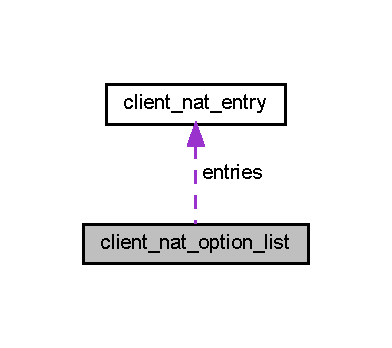
\includegraphics[width=188pt]{structclient__nat__option__list__coll__graph}
\end{center}
\end{figure}
\subsection*{Public Attributes}
\begin{DoxyCompactItemize}
\item 
int \hyperlink{structclient__nat__option__list_a8c360f0d8dafbb8ad4c9b59983b8a015}{n}
\item 
struct \hyperlink{structclient__nat__entry}{client\+\_\+nat\+\_\+entry} \hyperlink{structclient__nat__option__list_aacb63fefb0d0ee340c43ba988768e71d}{entries} \mbox{[}\hyperlink{clinat_8h_a708e00b7009d395c3815b6b1d32d91d0}{M\+A\+X\+\_\+\+C\+L\+I\+E\+N\+T\+\_\+\+N\+A\+T}\mbox{]}
\end{DoxyCompactItemize}


\subsection{Member Data Documentation}
\hypertarget{structclient__nat__option__list_aacb63fefb0d0ee340c43ba988768e71d}{}\index{client\+\_\+nat\+\_\+option\+\_\+list@{client\+\_\+nat\+\_\+option\+\_\+list}!entries@{entries}}
\index{entries@{entries}!client\+\_\+nat\+\_\+option\+\_\+list@{client\+\_\+nat\+\_\+option\+\_\+list}}
\subsubsection[{entries}]{\setlength{\rightskip}{0pt plus 5cm}struct {\bf client\+\_\+nat\+\_\+entry} client\+\_\+nat\+\_\+option\+\_\+list\+::entries\mbox{[}{\bf M\+A\+X\+\_\+\+C\+L\+I\+E\+N\+T\+\_\+\+N\+A\+T}\mbox{]}}\label{structclient__nat__option__list_aacb63fefb0d0ee340c43ba988768e71d}
\hypertarget{structclient__nat__option__list_a8c360f0d8dafbb8ad4c9b59983b8a015}{}\index{client\+\_\+nat\+\_\+option\+\_\+list@{client\+\_\+nat\+\_\+option\+\_\+list}!n@{n}}
\index{n@{n}!client\+\_\+nat\+\_\+option\+\_\+list@{client\+\_\+nat\+\_\+option\+\_\+list}}
\subsubsection[{n}]{\setlength{\rightskip}{0pt plus 5cm}int client\+\_\+nat\+\_\+option\+\_\+list\+::n}\label{structclient__nat__option__list_a8c360f0d8dafbb8ad4c9b59983b8a015}


The documentation for this struct was generated from the following file\+:\begin{DoxyCompactItemize}
\item 
src/openvpn/\hyperlink{clinat_8h}{clinat.\+h}\end{DoxyCompactItemize}

\hypertarget{structconnection__entry}{}\section{connection\+\_\+entry Struct Reference}
\label{structconnection__entry}\index{connection\+\_\+entry@{connection\+\_\+entry}}


{\ttfamily \#include $<$options.\+h$>$}



Collaboration diagram for connection\+\_\+entry\+:
\nopagebreak
\begin{figure}[H]
\begin{center}
\leavevmode
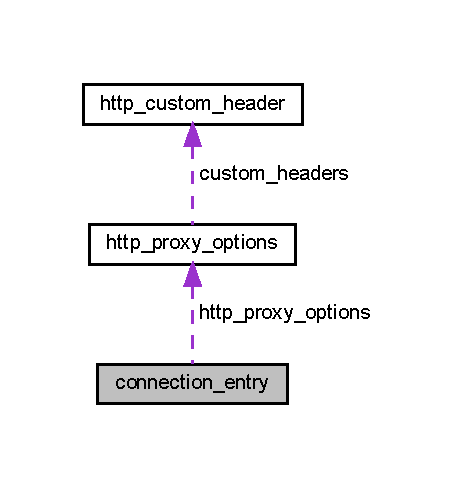
\includegraphics[width=218pt]{structconnection__entry__coll__graph}
\end{center}
\end{figure}
\subsection*{Public Attributes}
\begin{DoxyCompactItemize}
\item 
int \hyperlink{structconnection__entry_abadee88250492bc36663259ebd1a7de7}{proto}
\item 
\hyperlink{syshead_8h_a27a82860cef19f4a53f68516e7b2ee0e}{sa\+\_\+family\+\_\+t} \hyperlink{structconnection__entry_ac49b7ba49fbc7efd0d77535d1c66a7d9}{af}
\item 
const char $\ast$ \hyperlink{structconnection__entry_aecded3865f978a060cb1539fbd394032}{local\+\_\+port}
\item 
\hyperlink{automatic_8c_abb452686968e48b67397da5f97445f5b}{bool} \hyperlink{structconnection__entry_acb69943d9faa251f2dfc213d86bf3992}{local\+\_\+port\+\_\+defined}
\item 
const char $\ast$ \hyperlink{structconnection__entry_aa399cea883d3a239190c049c004ad793}{remote\+\_\+port}
\item 
const char $\ast$ \hyperlink{structconnection__entry_af86e741661abeac7edfdb5258ec4fa5f}{local}
\item 
const char $\ast$ \hyperlink{structconnection__entry_a474c4038934a015bdcb5b038b98b35d1}{remote}
\item 
\hyperlink{automatic_8c_abb452686968e48b67397da5f97445f5b}{bool} \hyperlink{structconnection__entry_a909bc65df6db4a88c211558e3b1565f4}{remote\+\_\+float}
\item 
\hyperlink{automatic_8c_abb452686968e48b67397da5f97445f5b}{bool} \hyperlink{structconnection__entry_adb3fcab845dbc50c3190c3d1b2b97037}{bind\+\_\+defined}
\item 
\hyperlink{automatic_8c_abb452686968e48b67397da5f97445f5b}{bool} \hyperlink{structconnection__entry_a8ec3ea69d71db89eb5ecd7b4b5ce3f99}{bind\+\_\+ipv6\+\_\+only}
\item 
\hyperlink{automatic_8c_abb452686968e48b67397da5f97445f5b}{bool} \hyperlink{structconnection__entry_a237f0476d7d283fa334b6250559f11d5}{bind\+\_\+local}
\item 
int \hyperlink{structconnection__entry_a016bad39481a03a9b824e64cf8a41a23}{connect\+\_\+retry\+\_\+seconds}
\item 
int \hyperlink{structconnection__entry_a1e80ffa27efcd36772df7618004f2ddc}{connect\+\_\+retry\+\_\+seconds\+\_\+max}
\item 
int \hyperlink{structconnection__entry_a51429ed22fd30ac08ed94d0df42f46e2}{connect\+\_\+timeout}
\item 
struct \hyperlink{structhttp__proxy__options}{http\+\_\+proxy\+\_\+options} $\ast$ \hyperlink{structconnection__entry_a70c458a2aee1a9b085b2bc05281722e6}{http\+\_\+proxy\+\_\+options}
\item 
const char $\ast$ \hyperlink{structconnection__entry_aacc02906ca3f2d2be9f28171bcd60452}{socks\+\_\+proxy\+\_\+server}
\item 
const char $\ast$ \hyperlink{structconnection__entry_a524bd17937bd36d74874af04eef7f131}{socks\+\_\+proxy\+\_\+port}
\item 
const char $\ast$ \hyperlink{structconnection__entry_a9f38a4424c365c8c9cb23f12f1b74806}{socks\+\_\+proxy\+\_\+authfile}
\item 
int \hyperlink{structconnection__entry_acd8706781548bd6e51c6a43b9a457155}{tun\+\_\+mtu}
\item 
\hyperlink{automatic_8c_abb452686968e48b67397da5f97445f5b}{bool} \hyperlink{structconnection__entry_a90482e8f2d1ab61167f705cec826abee}{tun\+\_\+mtu\+\_\+defined}
\item 
int \hyperlink{structconnection__entry_a1bdd5db16d783c90714bcf5c9ae1cdf6}{tun\+\_\+mtu\+\_\+extra}
\item 
\hyperlink{automatic_8c_abb452686968e48b67397da5f97445f5b}{bool} \hyperlink{structconnection__entry_a3d3ab06697dbc44a288e6f07b0bdbf3a}{tun\+\_\+mtu\+\_\+extra\+\_\+defined}
\item 
int \hyperlink{structconnection__entry_a08f0f18740ef4f00f130df8ce3a6c672}{link\+\_\+mtu}
\item 
\hyperlink{automatic_8c_abb452686968e48b67397da5f97445f5b}{bool} \hyperlink{structconnection__entry_a12ae06d792bd8aed58475b9976673654}{link\+\_\+mtu\+\_\+defined}
\item 
int \hyperlink{structconnection__entry_aba4ccef71abd388a80a607ab3da381e4}{mtu\+\_\+discover\+\_\+type}
\item 
int \hyperlink{structconnection__entry_ab003130b974deb481133d4209f74b25c}{fragment}
\item 
int \hyperlink{structconnection__entry_a27a04bbbad750c17bbdee216e6a0aacd}{mssfix}
\item 
\hyperlink{automatic_8c_abb452686968e48b67397da5f97445f5b}{bool} \hyperlink{structconnection__entry_a576ce2725c6c63f647185d78b91f8604}{mssfix\+\_\+default}
\item 
int \hyperlink{structconnection__entry_a9adab10d5a021e6f453ebc4edc29ecde}{explicit\+\_\+exit\+\_\+notification}
\item 
unsigned int \hyperlink{structconnection__entry_afba71f06b2a1c865bb1f142a8dbdbb2d}{flags}
\end{DoxyCompactItemize}


\subsection{Member Data Documentation}
\hypertarget{structconnection__entry_ac49b7ba49fbc7efd0d77535d1c66a7d9}{}\index{connection\+\_\+entry@{connection\+\_\+entry}!af@{af}}
\index{af@{af}!connection\+\_\+entry@{connection\+\_\+entry}}
\subsubsection[{af}]{\setlength{\rightskip}{0pt plus 5cm}{\bf sa\+\_\+family\+\_\+t} connection\+\_\+entry\+::af}\label{structconnection__entry_ac49b7ba49fbc7efd0d77535d1c66a7d9}
\hypertarget{structconnection__entry_adb3fcab845dbc50c3190c3d1b2b97037}{}\index{connection\+\_\+entry@{connection\+\_\+entry}!bind\+\_\+defined@{bind\+\_\+defined}}
\index{bind\+\_\+defined@{bind\+\_\+defined}!connection\+\_\+entry@{connection\+\_\+entry}}
\subsubsection[{bind\+\_\+defined}]{\setlength{\rightskip}{0pt plus 5cm}{\bf bool} connection\+\_\+entry\+::bind\+\_\+defined}\label{structconnection__entry_adb3fcab845dbc50c3190c3d1b2b97037}
\hypertarget{structconnection__entry_a8ec3ea69d71db89eb5ecd7b4b5ce3f99}{}\index{connection\+\_\+entry@{connection\+\_\+entry}!bind\+\_\+ipv6\+\_\+only@{bind\+\_\+ipv6\+\_\+only}}
\index{bind\+\_\+ipv6\+\_\+only@{bind\+\_\+ipv6\+\_\+only}!connection\+\_\+entry@{connection\+\_\+entry}}
\subsubsection[{bind\+\_\+ipv6\+\_\+only}]{\setlength{\rightskip}{0pt plus 5cm}{\bf bool} connection\+\_\+entry\+::bind\+\_\+ipv6\+\_\+only}\label{structconnection__entry_a8ec3ea69d71db89eb5ecd7b4b5ce3f99}
\hypertarget{structconnection__entry_a237f0476d7d283fa334b6250559f11d5}{}\index{connection\+\_\+entry@{connection\+\_\+entry}!bind\+\_\+local@{bind\+\_\+local}}
\index{bind\+\_\+local@{bind\+\_\+local}!connection\+\_\+entry@{connection\+\_\+entry}}
\subsubsection[{bind\+\_\+local}]{\setlength{\rightskip}{0pt plus 5cm}{\bf bool} connection\+\_\+entry\+::bind\+\_\+local}\label{structconnection__entry_a237f0476d7d283fa334b6250559f11d5}
\hypertarget{structconnection__entry_a016bad39481a03a9b824e64cf8a41a23}{}\index{connection\+\_\+entry@{connection\+\_\+entry}!connect\+\_\+retry\+\_\+seconds@{connect\+\_\+retry\+\_\+seconds}}
\index{connect\+\_\+retry\+\_\+seconds@{connect\+\_\+retry\+\_\+seconds}!connection\+\_\+entry@{connection\+\_\+entry}}
\subsubsection[{connect\+\_\+retry\+\_\+seconds}]{\setlength{\rightskip}{0pt plus 5cm}int connection\+\_\+entry\+::connect\+\_\+retry\+\_\+seconds}\label{structconnection__entry_a016bad39481a03a9b824e64cf8a41a23}
\hypertarget{structconnection__entry_a1e80ffa27efcd36772df7618004f2ddc}{}\index{connection\+\_\+entry@{connection\+\_\+entry}!connect\+\_\+retry\+\_\+seconds\+\_\+max@{connect\+\_\+retry\+\_\+seconds\+\_\+max}}
\index{connect\+\_\+retry\+\_\+seconds\+\_\+max@{connect\+\_\+retry\+\_\+seconds\+\_\+max}!connection\+\_\+entry@{connection\+\_\+entry}}
\subsubsection[{connect\+\_\+retry\+\_\+seconds\+\_\+max}]{\setlength{\rightskip}{0pt plus 5cm}int connection\+\_\+entry\+::connect\+\_\+retry\+\_\+seconds\+\_\+max}\label{structconnection__entry_a1e80ffa27efcd36772df7618004f2ddc}
\hypertarget{structconnection__entry_a51429ed22fd30ac08ed94d0df42f46e2}{}\index{connection\+\_\+entry@{connection\+\_\+entry}!connect\+\_\+timeout@{connect\+\_\+timeout}}
\index{connect\+\_\+timeout@{connect\+\_\+timeout}!connection\+\_\+entry@{connection\+\_\+entry}}
\subsubsection[{connect\+\_\+timeout}]{\setlength{\rightskip}{0pt plus 5cm}int connection\+\_\+entry\+::connect\+\_\+timeout}\label{structconnection__entry_a51429ed22fd30ac08ed94d0df42f46e2}
\hypertarget{structconnection__entry_a9adab10d5a021e6f453ebc4edc29ecde}{}\index{connection\+\_\+entry@{connection\+\_\+entry}!explicit\+\_\+exit\+\_\+notification@{explicit\+\_\+exit\+\_\+notification}}
\index{explicit\+\_\+exit\+\_\+notification@{explicit\+\_\+exit\+\_\+notification}!connection\+\_\+entry@{connection\+\_\+entry}}
\subsubsection[{explicit\+\_\+exit\+\_\+notification}]{\setlength{\rightskip}{0pt plus 5cm}int connection\+\_\+entry\+::explicit\+\_\+exit\+\_\+notification}\label{structconnection__entry_a9adab10d5a021e6f453ebc4edc29ecde}
\hypertarget{structconnection__entry_afba71f06b2a1c865bb1f142a8dbdbb2d}{}\index{connection\+\_\+entry@{connection\+\_\+entry}!flags@{flags}}
\index{flags@{flags}!connection\+\_\+entry@{connection\+\_\+entry}}
\subsubsection[{flags}]{\setlength{\rightskip}{0pt plus 5cm}unsigned int connection\+\_\+entry\+::flags}\label{structconnection__entry_afba71f06b2a1c865bb1f142a8dbdbb2d}
\hypertarget{structconnection__entry_ab003130b974deb481133d4209f74b25c}{}\index{connection\+\_\+entry@{connection\+\_\+entry}!fragment@{fragment}}
\index{fragment@{fragment}!connection\+\_\+entry@{connection\+\_\+entry}}
\subsubsection[{fragment}]{\setlength{\rightskip}{0pt plus 5cm}int connection\+\_\+entry\+::fragment}\label{structconnection__entry_ab003130b974deb481133d4209f74b25c}
\hypertarget{structconnection__entry_a70c458a2aee1a9b085b2bc05281722e6}{}\index{connection\+\_\+entry@{connection\+\_\+entry}!http\+\_\+proxy\+\_\+options@{http\+\_\+proxy\+\_\+options}}
\index{http\+\_\+proxy\+\_\+options@{http\+\_\+proxy\+\_\+options}!connection\+\_\+entry@{connection\+\_\+entry}}
\subsubsection[{http\+\_\+proxy\+\_\+options}]{\setlength{\rightskip}{0pt plus 5cm}struct {\bf http\+\_\+proxy\+\_\+options}$\ast$ connection\+\_\+entry\+::http\+\_\+proxy\+\_\+options}\label{structconnection__entry_a70c458a2aee1a9b085b2bc05281722e6}
\hypertarget{structconnection__entry_a08f0f18740ef4f00f130df8ce3a6c672}{}\index{connection\+\_\+entry@{connection\+\_\+entry}!link\+\_\+mtu@{link\+\_\+mtu}}
\index{link\+\_\+mtu@{link\+\_\+mtu}!connection\+\_\+entry@{connection\+\_\+entry}}
\subsubsection[{link\+\_\+mtu}]{\setlength{\rightskip}{0pt plus 5cm}int connection\+\_\+entry\+::link\+\_\+mtu}\label{structconnection__entry_a08f0f18740ef4f00f130df8ce3a6c672}
\hypertarget{structconnection__entry_a12ae06d792bd8aed58475b9976673654}{}\index{connection\+\_\+entry@{connection\+\_\+entry}!link\+\_\+mtu\+\_\+defined@{link\+\_\+mtu\+\_\+defined}}
\index{link\+\_\+mtu\+\_\+defined@{link\+\_\+mtu\+\_\+defined}!connection\+\_\+entry@{connection\+\_\+entry}}
\subsubsection[{link\+\_\+mtu\+\_\+defined}]{\setlength{\rightskip}{0pt plus 5cm}{\bf bool} connection\+\_\+entry\+::link\+\_\+mtu\+\_\+defined}\label{structconnection__entry_a12ae06d792bd8aed58475b9976673654}
\hypertarget{structconnection__entry_af86e741661abeac7edfdb5258ec4fa5f}{}\index{connection\+\_\+entry@{connection\+\_\+entry}!local@{local}}
\index{local@{local}!connection\+\_\+entry@{connection\+\_\+entry}}
\subsubsection[{local}]{\setlength{\rightskip}{0pt plus 5cm}const char$\ast$ connection\+\_\+entry\+::local}\label{structconnection__entry_af86e741661abeac7edfdb5258ec4fa5f}
\hypertarget{structconnection__entry_aecded3865f978a060cb1539fbd394032}{}\index{connection\+\_\+entry@{connection\+\_\+entry}!local\+\_\+port@{local\+\_\+port}}
\index{local\+\_\+port@{local\+\_\+port}!connection\+\_\+entry@{connection\+\_\+entry}}
\subsubsection[{local\+\_\+port}]{\setlength{\rightskip}{0pt plus 5cm}const char$\ast$ connection\+\_\+entry\+::local\+\_\+port}\label{structconnection__entry_aecded3865f978a060cb1539fbd394032}
\hypertarget{structconnection__entry_acb69943d9faa251f2dfc213d86bf3992}{}\index{connection\+\_\+entry@{connection\+\_\+entry}!local\+\_\+port\+\_\+defined@{local\+\_\+port\+\_\+defined}}
\index{local\+\_\+port\+\_\+defined@{local\+\_\+port\+\_\+defined}!connection\+\_\+entry@{connection\+\_\+entry}}
\subsubsection[{local\+\_\+port\+\_\+defined}]{\setlength{\rightskip}{0pt plus 5cm}{\bf bool} connection\+\_\+entry\+::local\+\_\+port\+\_\+defined}\label{structconnection__entry_acb69943d9faa251f2dfc213d86bf3992}
\hypertarget{structconnection__entry_a27a04bbbad750c17bbdee216e6a0aacd}{}\index{connection\+\_\+entry@{connection\+\_\+entry}!mssfix@{mssfix}}
\index{mssfix@{mssfix}!connection\+\_\+entry@{connection\+\_\+entry}}
\subsubsection[{mssfix}]{\setlength{\rightskip}{0pt plus 5cm}int connection\+\_\+entry\+::mssfix}\label{structconnection__entry_a27a04bbbad750c17bbdee216e6a0aacd}
\hypertarget{structconnection__entry_a576ce2725c6c63f647185d78b91f8604}{}\index{connection\+\_\+entry@{connection\+\_\+entry}!mssfix\+\_\+default@{mssfix\+\_\+default}}
\index{mssfix\+\_\+default@{mssfix\+\_\+default}!connection\+\_\+entry@{connection\+\_\+entry}}
\subsubsection[{mssfix\+\_\+default}]{\setlength{\rightskip}{0pt plus 5cm}{\bf bool} connection\+\_\+entry\+::mssfix\+\_\+default}\label{structconnection__entry_a576ce2725c6c63f647185d78b91f8604}
\hypertarget{structconnection__entry_aba4ccef71abd388a80a607ab3da381e4}{}\index{connection\+\_\+entry@{connection\+\_\+entry}!mtu\+\_\+discover\+\_\+type@{mtu\+\_\+discover\+\_\+type}}
\index{mtu\+\_\+discover\+\_\+type@{mtu\+\_\+discover\+\_\+type}!connection\+\_\+entry@{connection\+\_\+entry}}
\subsubsection[{mtu\+\_\+discover\+\_\+type}]{\setlength{\rightskip}{0pt plus 5cm}int connection\+\_\+entry\+::mtu\+\_\+discover\+\_\+type}\label{structconnection__entry_aba4ccef71abd388a80a607ab3da381e4}
\hypertarget{structconnection__entry_abadee88250492bc36663259ebd1a7de7}{}\index{connection\+\_\+entry@{connection\+\_\+entry}!proto@{proto}}
\index{proto@{proto}!connection\+\_\+entry@{connection\+\_\+entry}}
\subsubsection[{proto}]{\setlength{\rightskip}{0pt plus 5cm}int connection\+\_\+entry\+::proto}\label{structconnection__entry_abadee88250492bc36663259ebd1a7de7}
\hypertarget{structconnection__entry_a474c4038934a015bdcb5b038b98b35d1}{}\index{connection\+\_\+entry@{connection\+\_\+entry}!remote@{remote}}
\index{remote@{remote}!connection\+\_\+entry@{connection\+\_\+entry}}
\subsubsection[{remote}]{\setlength{\rightskip}{0pt plus 5cm}const char$\ast$ connection\+\_\+entry\+::remote}\label{structconnection__entry_a474c4038934a015bdcb5b038b98b35d1}
\hypertarget{structconnection__entry_a909bc65df6db4a88c211558e3b1565f4}{}\index{connection\+\_\+entry@{connection\+\_\+entry}!remote\+\_\+float@{remote\+\_\+float}}
\index{remote\+\_\+float@{remote\+\_\+float}!connection\+\_\+entry@{connection\+\_\+entry}}
\subsubsection[{remote\+\_\+float}]{\setlength{\rightskip}{0pt plus 5cm}{\bf bool} connection\+\_\+entry\+::remote\+\_\+float}\label{structconnection__entry_a909bc65df6db4a88c211558e3b1565f4}
\hypertarget{structconnection__entry_aa399cea883d3a239190c049c004ad793}{}\index{connection\+\_\+entry@{connection\+\_\+entry}!remote\+\_\+port@{remote\+\_\+port}}
\index{remote\+\_\+port@{remote\+\_\+port}!connection\+\_\+entry@{connection\+\_\+entry}}
\subsubsection[{remote\+\_\+port}]{\setlength{\rightskip}{0pt plus 5cm}const char$\ast$ connection\+\_\+entry\+::remote\+\_\+port}\label{structconnection__entry_aa399cea883d3a239190c049c004ad793}
\hypertarget{structconnection__entry_a9f38a4424c365c8c9cb23f12f1b74806}{}\index{connection\+\_\+entry@{connection\+\_\+entry}!socks\+\_\+proxy\+\_\+authfile@{socks\+\_\+proxy\+\_\+authfile}}
\index{socks\+\_\+proxy\+\_\+authfile@{socks\+\_\+proxy\+\_\+authfile}!connection\+\_\+entry@{connection\+\_\+entry}}
\subsubsection[{socks\+\_\+proxy\+\_\+authfile}]{\setlength{\rightskip}{0pt plus 5cm}const char$\ast$ connection\+\_\+entry\+::socks\+\_\+proxy\+\_\+authfile}\label{structconnection__entry_a9f38a4424c365c8c9cb23f12f1b74806}
\hypertarget{structconnection__entry_a524bd17937bd36d74874af04eef7f131}{}\index{connection\+\_\+entry@{connection\+\_\+entry}!socks\+\_\+proxy\+\_\+port@{socks\+\_\+proxy\+\_\+port}}
\index{socks\+\_\+proxy\+\_\+port@{socks\+\_\+proxy\+\_\+port}!connection\+\_\+entry@{connection\+\_\+entry}}
\subsubsection[{socks\+\_\+proxy\+\_\+port}]{\setlength{\rightskip}{0pt plus 5cm}const char$\ast$ connection\+\_\+entry\+::socks\+\_\+proxy\+\_\+port}\label{structconnection__entry_a524bd17937bd36d74874af04eef7f131}
\hypertarget{structconnection__entry_aacc02906ca3f2d2be9f28171bcd60452}{}\index{connection\+\_\+entry@{connection\+\_\+entry}!socks\+\_\+proxy\+\_\+server@{socks\+\_\+proxy\+\_\+server}}
\index{socks\+\_\+proxy\+\_\+server@{socks\+\_\+proxy\+\_\+server}!connection\+\_\+entry@{connection\+\_\+entry}}
\subsubsection[{socks\+\_\+proxy\+\_\+server}]{\setlength{\rightskip}{0pt plus 5cm}const char$\ast$ connection\+\_\+entry\+::socks\+\_\+proxy\+\_\+server}\label{structconnection__entry_aacc02906ca3f2d2be9f28171bcd60452}
\hypertarget{structconnection__entry_acd8706781548bd6e51c6a43b9a457155}{}\index{connection\+\_\+entry@{connection\+\_\+entry}!tun\+\_\+mtu@{tun\+\_\+mtu}}
\index{tun\+\_\+mtu@{tun\+\_\+mtu}!connection\+\_\+entry@{connection\+\_\+entry}}
\subsubsection[{tun\+\_\+mtu}]{\setlength{\rightskip}{0pt plus 5cm}int connection\+\_\+entry\+::tun\+\_\+mtu}\label{structconnection__entry_acd8706781548bd6e51c6a43b9a457155}
\hypertarget{structconnection__entry_a90482e8f2d1ab61167f705cec826abee}{}\index{connection\+\_\+entry@{connection\+\_\+entry}!tun\+\_\+mtu\+\_\+defined@{tun\+\_\+mtu\+\_\+defined}}
\index{tun\+\_\+mtu\+\_\+defined@{tun\+\_\+mtu\+\_\+defined}!connection\+\_\+entry@{connection\+\_\+entry}}
\subsubsection[{tun\+\_\+mtu\+\_\+defined}]{\setlength{\rightskip}{0pt plus 5cm}{\bf bool} connection\+\_\+entry\+::tun\+\_\+mtu\+\_\+defined}\label{structconnection__entry_a90482e8f2d1ab61167f705cec826abee}
\hypertarget{structconnection__entry_a1bdd5db16d783c90714bcf5c9ae1cdf6}{}\index{connection\+\_\+entry@{connection\+\_\+entry}!tun\+\_\+mtu\+\_\+extra@{tun\+\_\+mtu\+\_\+extra}}
\index{tun\+\_\+mtu\+\_\+extra@{tun\+\_\+mtu\+\_\+extra}!connection\+\_\+entry@{connection\+\_\+entry}}
\subsubsection[{tun\+\_\+mtu\+\_\+extra}]{\setlength{\rightskip}{0pt plus 5cm}int connection\+\_\+entry\+::tun\+\_\+mtu\+\_\+extra}\label{structconnection__entry_a1bdd5db16d783c90714bcf5c9ae1cdf6}
\hypertarget{structconnection__entry_a3d3ab06697dbc44a288e6f07b0bdbf3a}{}\index{connection\+\_\+entry@{connection\+\_\+entry}!tun\+\_\+mtu\+\_\+extra\+\_\+defined@{tun\+\_\+mtu\+\_\+extra\+\_\+defined}}
\index{tun\+\_\+mtu\+\_\+extra\+\_\+defined@{tun\+\_\+mtu\+\_\+extra\+\_\+defined}!connection\+\_\+entry@{connection\+\_\+entry}}
\subsubsection[{tun\+\_\+mtu\+\_\+extra\+\_\+defined}]{\setlength{\rightskip}{0pt plus 5cm}{\bf bool} connection\+\_\+entry\+::tun\+\_\+mtu\+\_\+extra\+\_\+defined}\label{structconnection__entry_a3d3ab06697dbc44a288e6f07b0bdbf3a}


The documentation for this struct was generated from the following file\+:\begin{DoxyCompactItemize}
\item 
src/openvpn/\hyperlink{options_8h}{options.\+h}\end{DoxyCompactItemize}

\hypertarget{structconnection__list}{}\section{connection\+\_\+list Struct Reference}
\label{structconnection__list}\index{connection\+\_\+list@{connection\+\_\+list}}


{\ttfamily \#include $<$options.\+h$>$}



Collaboration diagram for connection\+\_\+list\+:
\nopagebreak
\begin{figure}[H]
\begin{center}
\leavevmode
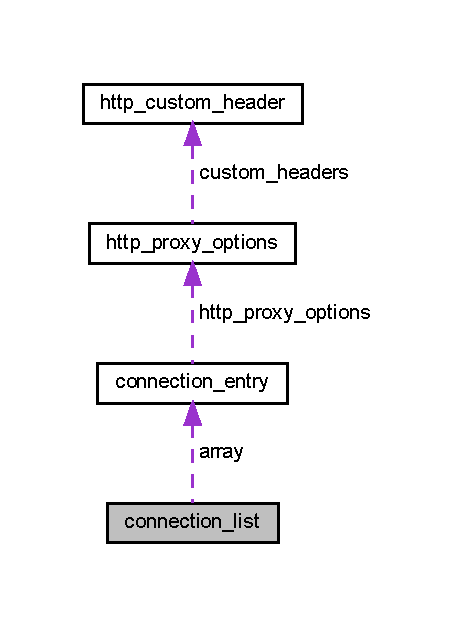
\includegraphics[width=218pt]{structconnection__list__coll__graph}
\end{center}
\end{figure}
\subsection*{Public Attributes}
\begin{DoxyCompactItemize}
\item 
int \hyperlink{structconnection__list_a7ec9bc2e47f7ac458a6a1ae17d0cf304}{len}
\item 
int \hyperlink{structconnection__list_a4c93ccd743bba6ee89f05abc2b3008b0}{current}
\item 
struct \hyperlink{structconnection__entry}{connection\+\_\+entry} $\ast$ \hyperlink{structconnection__list_a57ecc9c713fcb3c347253dd3d86308b5}{array} \mbox{[}\hyperlink{options_8h_a44d71253f2f8bdb9d87329f0d6eedce2}{C\+O\+N\+N\+E\+C\+T\+I\+O\+N\+\_\+\+L\+I\+S\+T\+\_\+\+S\+I\+Z\+E}\mbox{]}
\end{DoxyCompactItemize}


\subsection{Member Data Documentation}
\hypertarget{structconnection__list_a57ecc9c713fcb3c347253dd3d86308b5}{}\index{connection\+\_\+list@{connection\+\_\+list}!array@{array}}
\index{array@{array}!connection\+\_\+list@{connection\+\_\+list}}
\subsubsection[{array}]{\setlength{\rightskip}{0pt plus 5cm}struct {\bf connection\+\_\+entry}$\ast$ connection\+\_\+list\+::array\mbox{[}{\bf C\+O\+N\+N\+E\+C\+T\+I\+O\+N\+\_\+\+L\+I\+S\+T\+\_\+\+S\+I\+Z\+E}\mbox{]}}\label{structconnection__list_a57ecc9c713fcb3c347253dd3d86308b5}
\hypertarget{structconnection__list_a4c93ccd743bba6ee89f05abc2b3008b0}{}\index{connection\+\_\+list@{connection\+\_\+list}!current@{current}}
\index{current@{current}!connection\+\_\+list@{connection\+\_\+list}}
\subsubsection[{current}]{\setlength{\rightskip}{0pt plus 5cm}int connection\+\_\+list\+::current}\label{structconnection__list_a4c93ccd743bba6ee89f05abc2b3008b0}
\hypertarget{structconnection__list_a7ec9bc2e47f7ac458a6a1ae17d0cf304}{}\index{connection\+\_\+list@{connection\+\_\+list}!len@{len}}
\index{len@{len}!connection\+\_\+list@{connection\+\_\+list}}
\subsubsection[{len}]{\setlength{\rightskip}{0pt plus 5cm}int connection\+\_\+list\+::len}\label{structconnection__list_a7ec9bc2e47f7ac458a6a1ae17d0cf304}


The documentation for this struct was generated from the following file\+:\begin{DoxyCompactItemize}
\item 
src/openvpn/\hyperlink{options_8h}{options.\+h}\end{DoxyCompactItemize}

\hypertarget{structcontext}{}\section{context Struct Reference}
\label{structcontext}\index{context@{context}}


{\ttfamily \#include $<$openvpn.\+h$>$}



Collaboration diagram for context\+:
\nopagebreak
\begin{figure}[H]
\begin{center}
\leavevmode
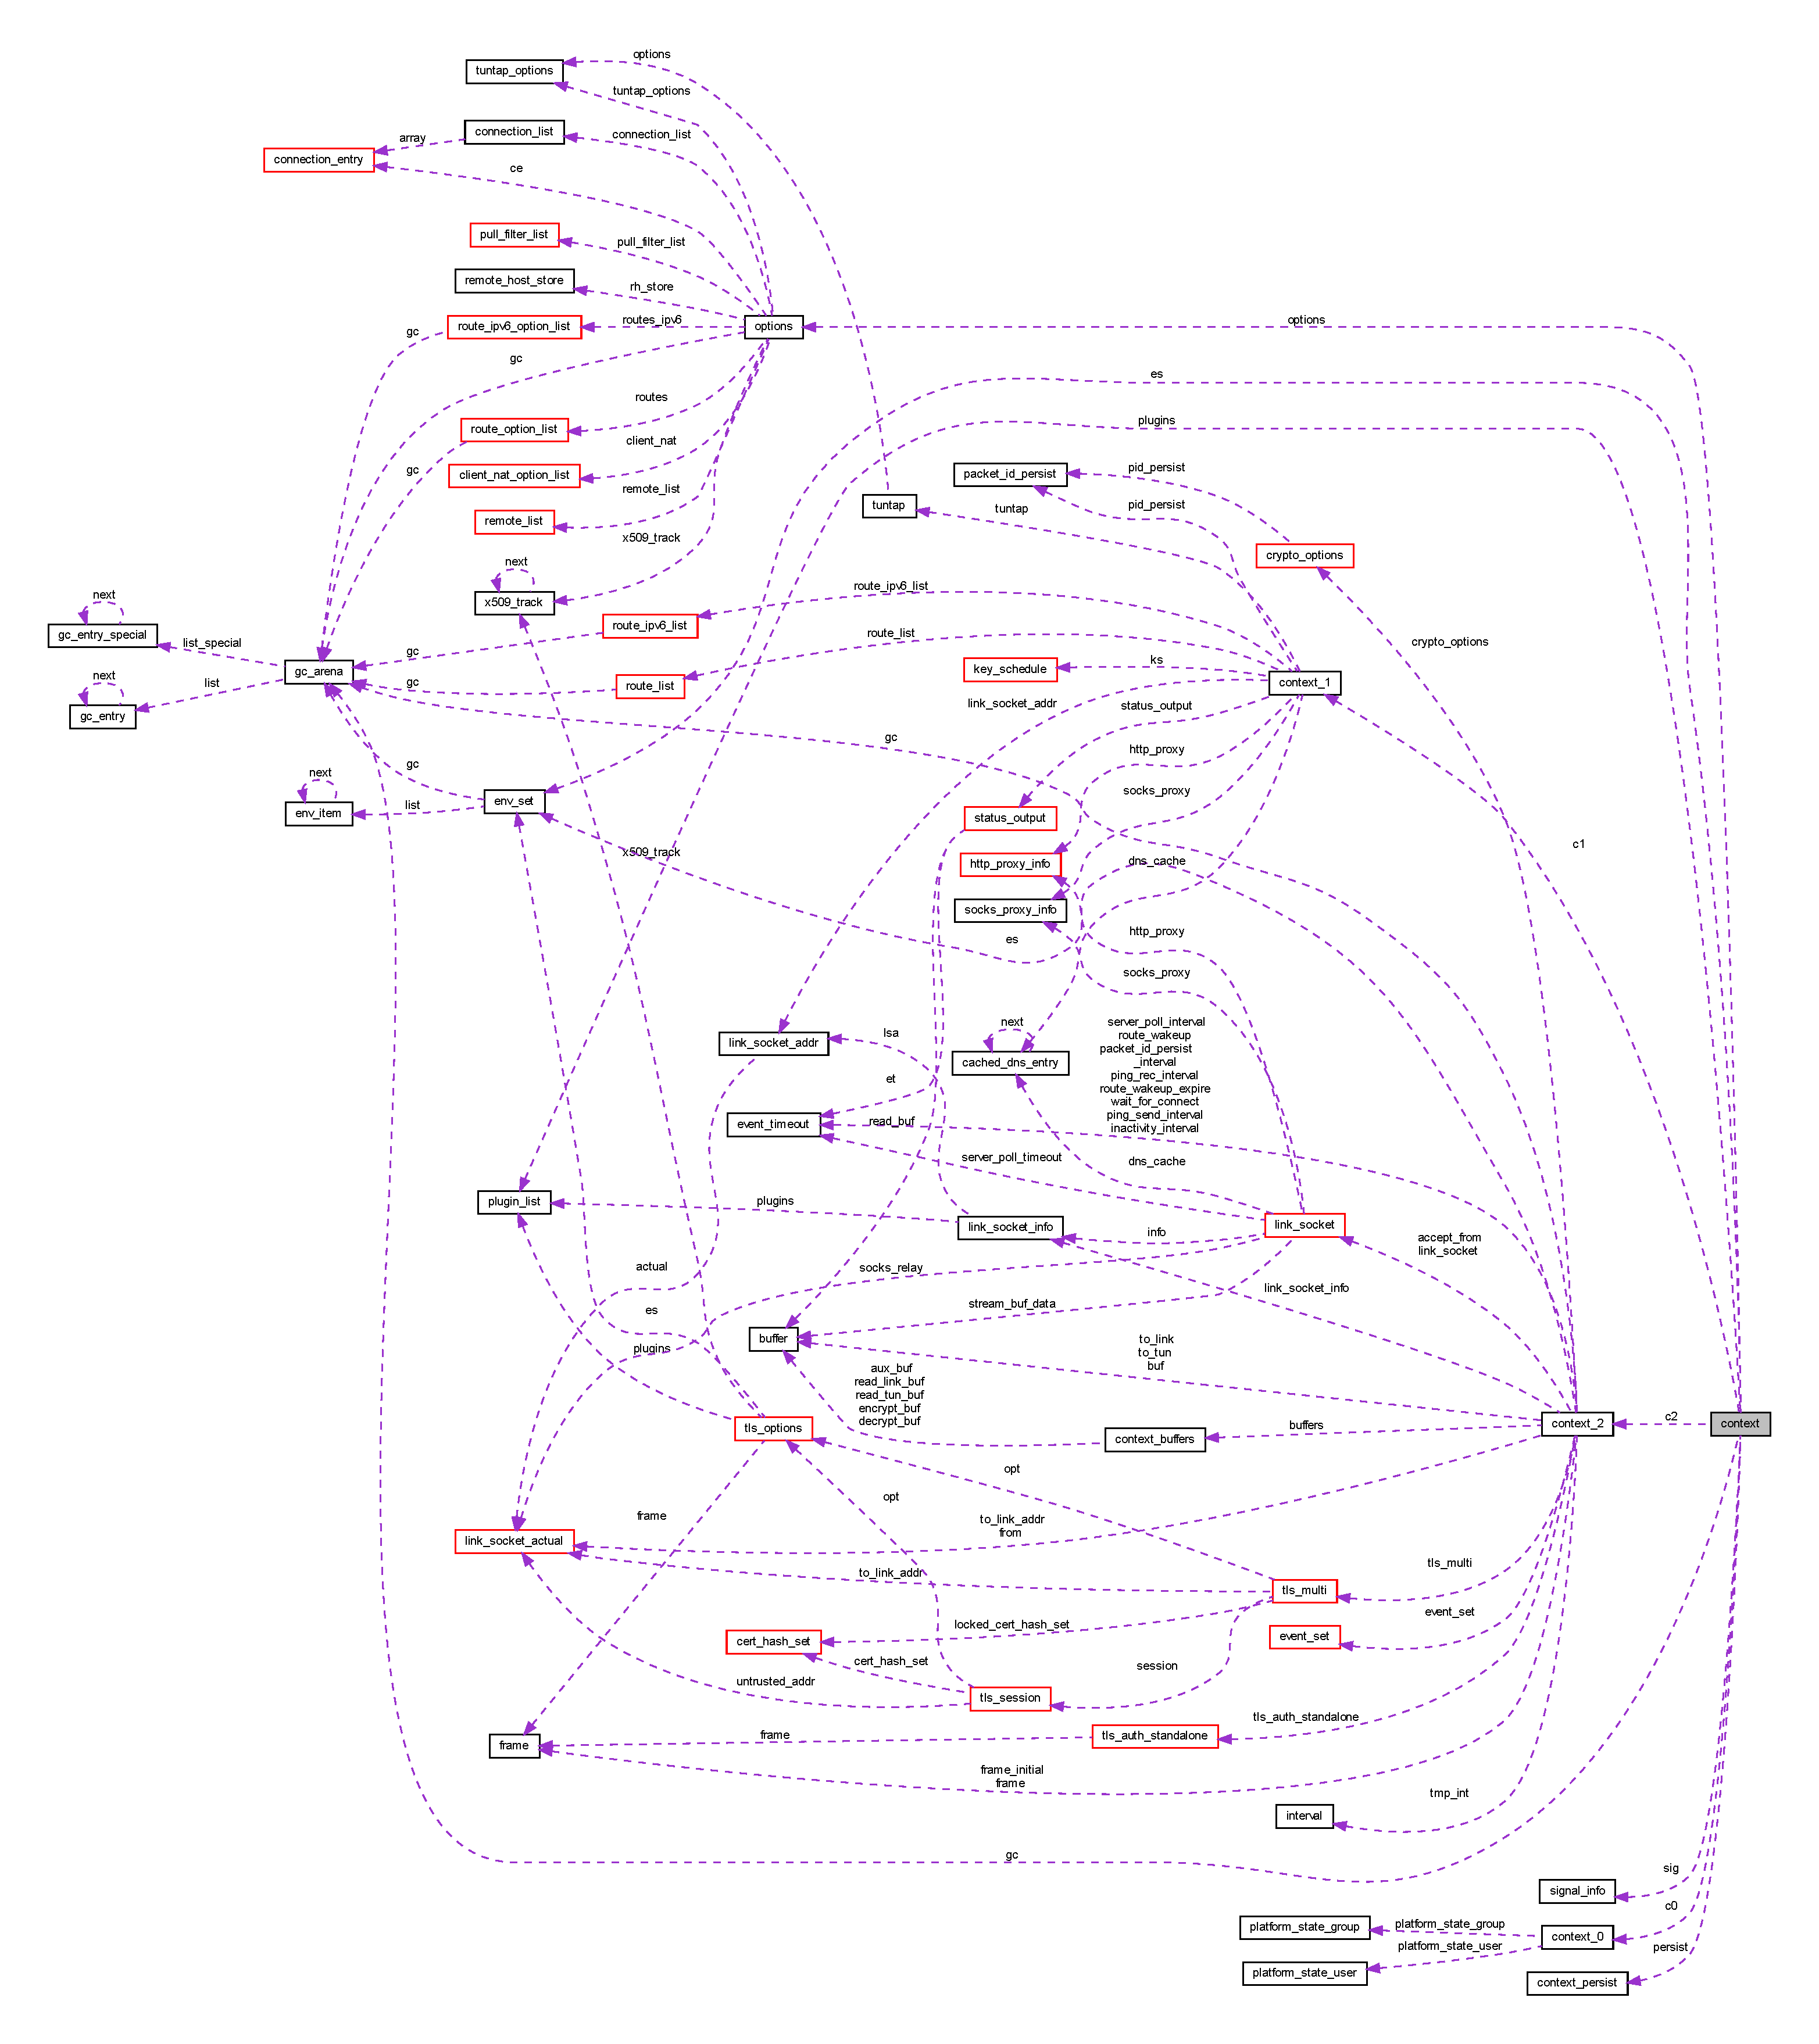
\includegraphics[width=350pt]{structcontext__coll__graph}
\end{center}
\end{figure}
\subsection*{Public Attributes}
\begin{DoxyCompactItemize}
\item 
struct \hyperlink{structoptions}{options} \hyperlink{structcontext_aa9a5e593e669fc88b8b1c7a9d69c5df1}{options}
\item 
\hyperlink{automatic_8c_abb452686968e48b67397da5f97445f5b}{bool} \hyperlink{structcontext_a4562924ba33d42c7c84399bc61e5634b}{first\+\_\+time}
\item 
int \hyperlink{structcontext_a05c5cc1b7bab3bf8fc5b1e23b38299f4}{mode}
\item 
struct \hyperlink{structgc__arena}{gc\+\_\+arena} \hyperlink{structcontext_ad2b1fffbd57d0ba779aa9b5ef8a9c78d}{gc}
\item 
struct \hyperlink{structenv__set}{env\+\_\+set} $\ast$ \hyperlink{structcontext_a9b3f2f6a6281c99c8c1e26598875d5ab}{es}
\item 
struct \hyperlink{structsignal__info}{signal\+\_\+info} $\ast$ \hyperlink{structcontext_a4a8aea25993019921e9568f611106773}{sig}
\item 
struct \hyperlink{structplugin__list}{plugin\+\_\+list} $\ast$ \hyperlink{structcontext_a7ebcb36e0e5cab031f1f3721ee39b9d3}{plugins}
\item 
\hyperlink{automatic_8c_abb452686968e48b67397da5f97445f5b}{bool} \hyperlink{structcontext_ab86d3cd4769ad44ed77c04c13c5382fb}{plugins\+\_\+owned}
\item 
\hyperlink{automatic_8c_abb452686968e48b67397da5f97445f5b}{bool} \hyperlink{structcontext_a34ef38cd7f895386a75d592fa0c820d8}{did\+\_\+we\+\_\+daemonize}
\item 
struct \hyperlink{structcontext__persist}{context\+\_\+persist} \hyperlink{structcontext_af52fc5d2e241fbee78d2216e9ff7ed72}{persist}
\item 
struct \hyperlink{structcontext__0}{context\+\_\+0} $\ast$ \hyperlink{structcontext_a1d0cd1cb672a5fee441bdc504fc0fa93}{c0}
\item 
struct \hyperlink{structcontext__1}{context\+\_\+1} \hyperlink{structcontext_aea116e1362b8f75f5fd13e8c06fc0cf3}{c1}
\item 
struct \hyperlink{structcontext__2}{context\+\_\+2} \hyperlink{structcontext_a8d609499dcba303c18f50ef7b648644c}{c2}
\end{DoxyCompactItemize}


\subsection{Detailed Description}
Contains all state information for one tunnel.

This structure represents one V\+P\+N tunnel. It is used to store state information related to a V\+P\+N tunnel, but also includes process-\/wide data, such as configuration options.

The Structure of V\+P\+N tunnel state storage related page describes how this structure is used in client-\/mode and server-\/mode. 

\subsection{Member Data Documentation}
\hypertarget{structcontext_a1d0cd1cb672a5fee441bdc504fc0fa93}{}\index{context@{context}!c0@{c0}}
\index{c0@{c0}!context@{context}}
\subsubsection[{c0}]{\setlength{\rightskip}{0pt plus 5cm}struct {\bf context\+\_\+0}$\ast$ context\+::c0}\label{structcontext_a1d0cd1cb672a5fee441bdc504fc0fa93}
Level 0 context. \hypertarget{structcontext_aea116e1362b8f75f5fd13e8c06fc0cf3}{}\index{context@{context}!c1@{c1}}
\index{c1@{c1}!context@{context}}
\subsubsection[{c1}]{\setlength{\rightskip}{0pt plus 5cm}struct {\bf context\+\_\+1} context\+::c1}\label{structcontext_aea116e1362b8f75f5fd13e8c06fc0cf3}
Level 1 context. \hypertarget{structcontext_a8d609499dcba303c18f50ef7b648644c}{}\index{context@{context}!c2@{c2}}
\index{c2@{c2}!context@{context}}
\subsubsection[{c2}]{\setlength{\rightskip}{0pt plus 5cm}struct {\bf context\+\_\+2} context\+::c2}\label{structcontext_a8d609499dcba303c18f50ef7b648644c}
Level 2 context. \hypertarget{structcontext_a34ef38cd7f895386a75d592fa0c820d8}{}\index{context@{context}!did\+\_\+we\+\_\+daemonize@{did\+\_\+we\+\_\+daemonize}}
\index{did\+\_\+we\+\_\+daemonize@{did\+\_\+we\+\_\+daemonize}!context@{context}}
\subsubsection[{did\+\_\+we\+\_\+daemonize}]{\setlength{\rightskip}{0pt plus 5cm}{\bf bool} context\+::did\+\_\+we\+\_\+daemonize}\label{structcontext_a34ef38cd7f895386a75d592fa0c820d8}
Whether demonization has already taken place. \hypertarget{structcontext_a9b3f2f6a6281c99c8c1e26598875d5ab}{}\index{context@{context}!es@{es}}
\index{es@{es}!context@{context}}
\subsubsection[{es}]{\setlength{\rightskip}{0pt plus 5cm}struct {\bf env\+\_\+set}$\ast$ context\+::es}\label{structcontext_a9b3f2f6a6281c99c8c1e26598875d5ab}
Set of environment variables. \hypertarget{structcontext_a4562924ba33d42c7c84399bc61e5634b}{}\index{context@{context}!first\+\_\+time@{first\+\_\+time}}
\index{first\+\_\+time@{first\+\_\+time}!context@{context}}
\subsubsection[{first\+\_\+time}]{\setlength{\rightskip}{0pt plus 5cm}{\bf bool} context\+::first\+\_\+time}\label{structcontext_a4562924ba33d42c7c84399bc61e5634b}
True on the first iteration of Open\+V\+P\+N\textquotesingle{}s main loop. \hypertarget{structcontext_ad2b1fffbd57d0ba779aa9b5ef8a9c78d}{}\index{context@{context}!gc@{gc}}
\index{gc@{gc}!context@{context}}
\subsubsection[{gc}]{\setlength{\rightskip}{0pt plus 5cm}struct {\bf gc\+\_\+arena} context\+::gc}\label{structcontext_ad2b1fffbd57d0ba779aa9b5ef8a9c78d}
Garbage collection arena for allocations done in the scope of this context structure. \hypertarget{structcontext_a05c5cc1b7bab3bf8fc5b1e23b38299f4}{}\index{context@{context}!mode@{mode}}
\index{mode@{mode}!context@{context}}
\subsubsection[{mode}]{\setlength{\rightskip}{0pt plus 5cm}int context\+::mode}\label{structcontext_a05c5cc1b7bab3bf8fc5b1e23b38299f4}
Role of this context within the Open\+V\+P\+N process. Valid values are {\ttfamily C\+M\+\_\+\+P2\+P}, {\ttfamily C\+M\+\_\+\+T\+O\+P}, {\ttfamily C\+M\+\_\+\+T\+O\+P\+\_\+\+C\+L\+O\+N\+E}, {\ttfamily C\+M\+\_\+\+C\+H\+I\+L\+D\+\_\+\+U\+D\+P}, and {\ttfamily C\+M\+\_\+\+C\+H\+I\+L\+D\+\_\+\+T\+C\+P}. \hypertarget{structcontext_aa9a5e593e669fc88b8b1c7a9d69c5df1}{}\index{context@{context}!options@{options}}
\index{options@{options}!context@{context}}
\subsubsection[{options}]{\setlength{\rightskip}{0pt plus 5cm}struct {\bf options} context\+::options}\label{structcontext_aa9a5e593e669fc88b8b1c7a9d69c5df1}
Options loaded from command line or configuration file. \hypertarget{structcontext_af52fc5d2e241fbee78d2216e9ff7ed72}{}\index{context@{context}!persist@{persist}}
\index{persist@{persist}!context@{context}}
\subsubsection[{persist}]{\setlength{\rightskip}{0pt plus 5cm}struct {\bf context\+\_\+persist} context\+::persist}\label{structcontext_af52fc5d2e241fbee78d2216e9ff7ed72}
Persistent context. \hypertarget{structcontext_a7ebcb36e0e5cab031f1f3721ee39b9d3}{}\index{context@{context}!plugins@{plugins}}
\index{plugins@{plugins}!context@{context}}
\subsubsection[{plugins}]{\setlength{\rightskip}{0pt plus 5cm}struct {\bf plugin\+\_\+list}$\ast$ context\+::plugins}\label{structcontext_a7ebcb36e0e5cab031f1f3721ee39b9d3}
List of plug-\/ins. \hypertarget{structcontext_ab86d3cd4769ad44ed77c04c13c5382fb}{}\index{context@{context}!plugins\+\_\+owned@{plugins\+\_\+owned}}
\index{plugins\+\_\+owned@{plugins\+\_\+owned}!context@{context}}
\subsubsection[{plugins\+\_\+owned}]{\setlength{\rightskip}{0pt plus 5cm}{\bf bool} context\+::plugins\+\_\+owned}\label{structcontext_ab86d3cd4769ad44ed77c04c13c5382fb}
Whether the plug-\/ins should be cleaned up when this context is cleaned up. \hypertarget{structcontext_a4a8aea25993019921e9568f611106773}{}\index{context@{context}!sig@{sig}}
\index{sig@{sig}!context@{context}}
\subsubsection[{sig}]{\setlength{\rightskip}{0pt plus 5cm}struct {\bf signal\+\_\+info}$\ast$ context\+::sig}\label{structcontext_a4a8aea25993019921e9568f611106773}
Internal error signaling object. 

The documentation for this struct was generated from the following file\+:\begin{DoxyCompactItemize}
\item 
src/openvpn/\hyperlink{openvpn_8h}{openvpn.\+h}\end{DoxyCompactItemize}

\hypertarget{structcontext__0}{}\section{context\+\_\+0 Struct Reference}
\label{structcontext__0}\index{context\+\_\+0@{context\+\_\+0}}


{\ttfamily \#include $<$openvpn.\+h$>$}



Collaboration diagram for context\+\_\+0\+:
\nopagebreak
\begin{figure}[H]
\begin{center}
\leavevmode
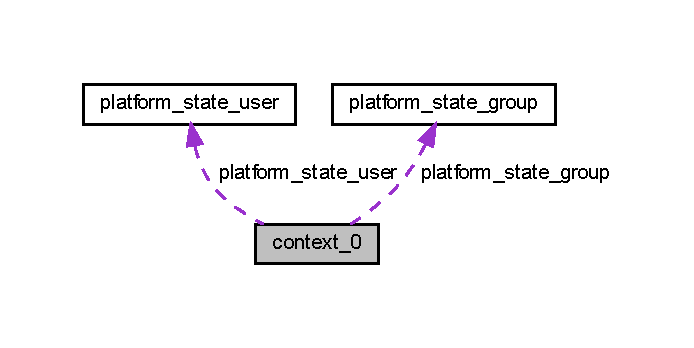
\includegraphics[width=333pt]{structcontext__0__coll__graph}
\end{center}
\end{figure}
\subsection*{Public Attributes}
\begin{DoxyCompactItemize}
\item 
\hyperlink{automatic_8c_abb452686968e48b67397da5f97445f5b}{bool} \hyperlink{structcontext__0_af599a649761ec7fd83b5aa3dab4a502e}{uid\+\_\+gid\+\_\+specified}
\item 
\hyperlink{automatic_8c_abb452686968e48b67397da5f97445f5b}{bool} \hyperlink{structcontext__0_adf83164d54c6c56957e5550a45b63338}{uid\+\_\+gid\+\_\+chroot\+\_\+set}
\item 
struct \hyperlink{structplatform__state__user}{platform\+\_\+state\+\_\+user} \hyperlink{structcontext__0_a663b5e3cf38a4fc003b34fed87e9555c}{platform\+\_\+state\+\_\+user}
\item 
struct \hyperlink{structplatform__state__group}{platform\+\_\+state\+\_\+group} \hyperlink{structcontext__0_a2b214a974983a9c9f74e3c80dc1f0161}{platform\+\_\+state\+\_\+group}
\end{DoxyCompactItemize}


\subsection{Detailed Description}
Level 0 context containing information related to the Open\+V\+P\+N process.

Level 0 state is initialized once at program startup, and then remains throughout the lifetime of the Open\+V\+P\+N process. This structure contains information related to the process\textquotesingle{}s P\+I\+D, user, group, and privileges. 

\subsection{Member Data Documentation}
\hypertarget{structcontext__0_a2b214a974983a9c9f74e3c80dc1f0161}{}\index{context\+\_\+0@{context\+\_\+0}!platform\+\_\+state\+\_\+group@{platform\+\_\+state\+\_\+group}}
\index{platform\+\_\+state\+\_\+group@{platform\+\_\+state\+\_\+group}!context\+\_\+0@{context\+\_\+0}}
\subsubsection[{platform\+\_\+state\+\_\+group}]{\setlength{\rightskip}{0pt plus 5cm}struct {\bf platform\+\_\+state\+\_\+group} context\+\_\+0\+::platform\+\_\+state\+\_\+group}\label{structcontext__0_a2b214a974983a9c9f74e3c80dc1f0161}
\hypertarget{structcontext__0_a663b5e3cf38a4fc003b34fed87e9555c}{}\index{context\+\_\+0@{context\+\_\+0}!platform\+\_\+state\+\_\+user@{platform\+\_\+state\+\_\+user}}
\index{platform\+\_\+state\+\_\+user@{platform\+\_\+state\+\_\+user}!context\+\_\+0@{context\+\_\+0}}
\subsubsection[{platform\+\_\+state\+\_\+user}]{\setlength{\rightskip}{0pt plus 5cm}struct {\bf platform\+\_\+state\+\_\+user} context\+\_\+0\+::platform\+\_\+state\+\_\+user}\label{structcontext__0_a663b5e3cf38a4fc003b34fed87e9555c}
\hypertarget{structcontext__0_adf83164d54c6c56957e5550a45b63338}{}\index{context\+\_\+0@{context\+\_\+0}!uid\+\_\+gid\+\_\+chroot\+\_\+set@{uid\+\_\+gid\+\_\+chroot\+\_\+set}}
\index{uid\+\_\+gid\+\_\+chroot\+\_\+set@{uid\+\_\+gid\+\_\+chroot\+\_\+set}!context\+\_\+0@{context\+\_\+0}}
\subsubsection[{uid\+\_\+gid\+\_\+chroot\+\_\+set}]{\setlength{\rightskip}{0pt plus 5cm}{\bf bool} context\+\_\+0\+::uid\+\_\+gid\+\_\+chroot\+\_\+set}\label{structcontext__0_adf83164d54c6c56957e5550a45b63338}
\hypertarget{structcontext__0_af599a649761ec7fd83b5aa3dab4a502e}{}\index{context\+\_\+0@{context\+\_\+0}!uid\+\_\+gid\+\_\+specified@{uid\+\_\+gid\+\_\+specified}}
\index{uid\+\_\+gid\+\_\+specified@{uid\+\_\+gid\+\_\+specified}!context\+\_\+0@{context\+\_\+0}}
\subsubsection[{uid\+\_\+gid\+\_\+specified}]{\setlength{\rightskip}{0pt plus 5cm}{\bf bool} context\+\_\+0\+::uid\+\_\+gid\+\_\+specified}\label{structcontext__0_af599a649761ec7fd83b5aa3dab4a502e}


The documentation for this struct was generated from the following file\+:\begin{DoxyCompactItemize}
\item 
src/openvpn/\hyperlink{openvpn_8h}{openvpn.\+h}\end{DoxyCompactItemize}

\hypertarget{structcontext__1}{}\section{context\+\_\+1 Struct Reference}
\label{structcontext__1}\index{context\+\_\+1@{context\+\_\+1}}


{\ttfamily \#include $<$openvpn.\+h$>$}



Collaboration diagram for context\+\_\+1\+:
\nopagebreak
\begin{figure}[H]
\begin{center}
\leavevmode
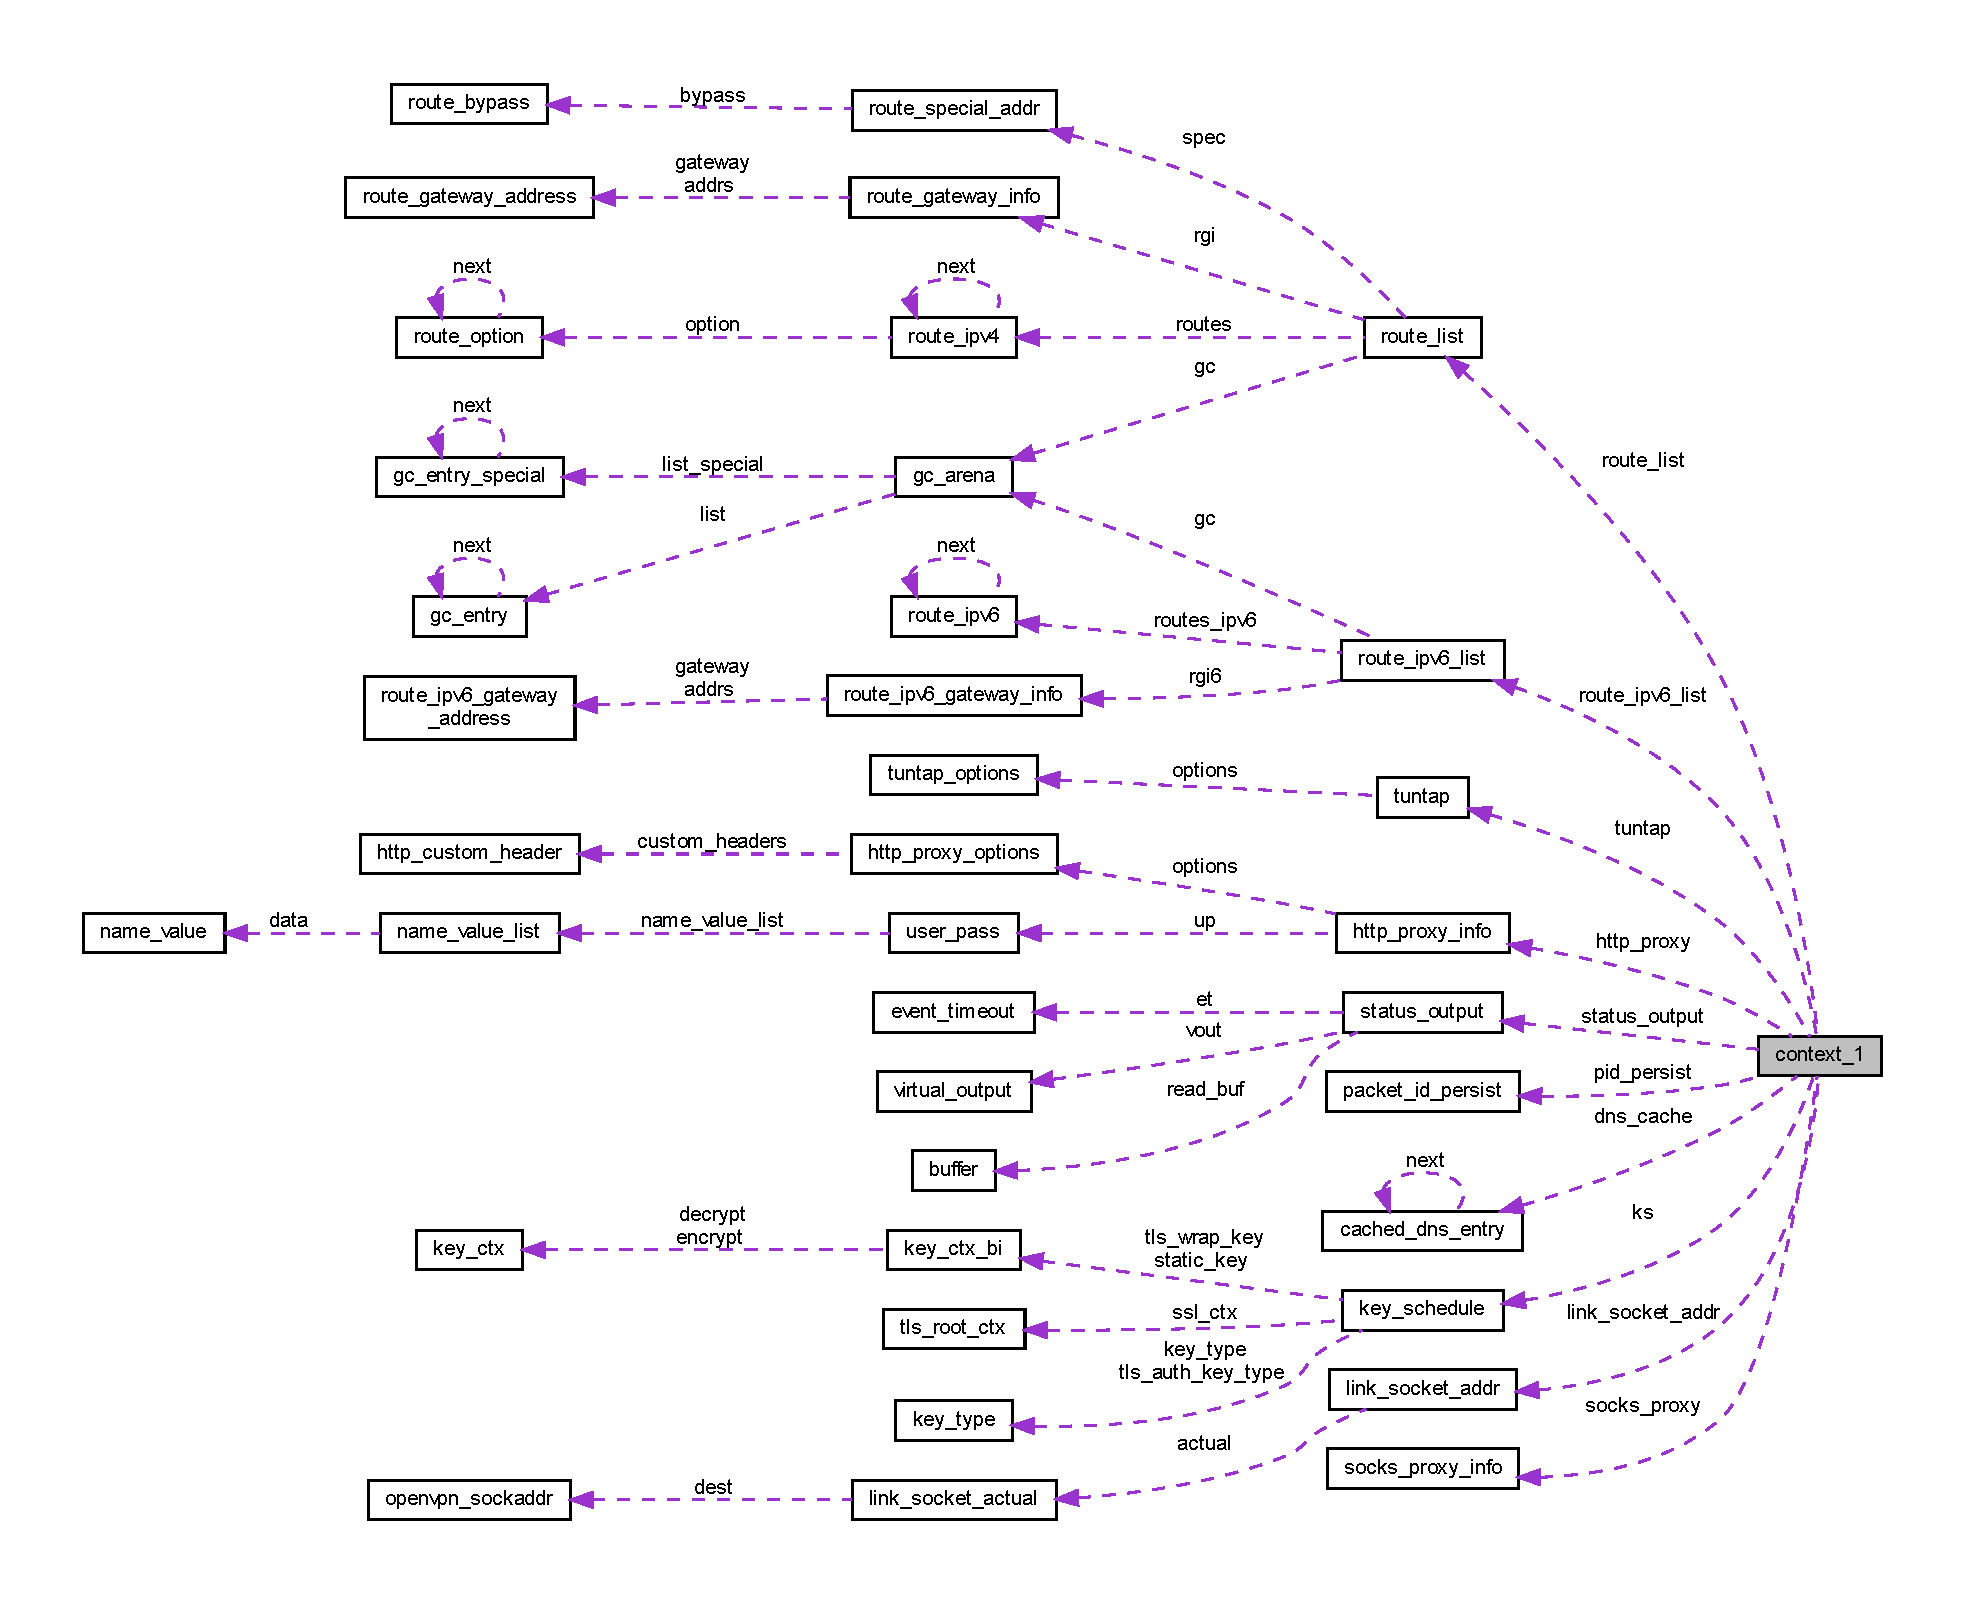
\includegraphics[width=350pt]{structcontext__1__coll__graph}
\end{center}
\end{figure}
\subsection*{Public Attributes}
\begin{DoxyCompactItemize}
\item 
struct \hyperlink{structlink__socket__addr}{link\+\_\+socket\+\_\+addr} \hyperlink{structcontext__1_a3f08fbd0447517dc9fefa3e1a30fa26f}{link\+\_\+socket\+\_\+addr}
\item 
struct \hyperlink{structkey__schedule}{key\+\_\+schedule} \hyperlink{structcontext__1_a2add75182e7da9d1d466d37c72e1c276}{ks}
\item 
struct \hyperlink{structcached__dns__entry}{cached\+\_\+dns\+\_\+entry} $\ast$ \hyperlink{structcontext__1_afa252fa776c920089066ddb7bdb16b24}{dns\+\_\+cache}
\item 
struct \hyperlink{structpacket__id__persist}{packet\+\_\+id\+\_\+persist} \hyperlink{structcontext__1_aa20a2b143b3a7f2db2cc9a1af3cdf3e2}{pid\+\_\+persist}
\item 
struct \hyperlink{structtuntap}{tuntap} $\ast$ \hyperlink{structcontext__1_afa52b84db5bb4e12deeabf2e788f7349}{tuntap}
\item 
\hyperlink{automatic_8c_abb452686968e48b67397da5f97445f5b}{bool} \hyperlink{structcontext__1_acae58a5af5e0f65b4963b44c6e9715e5}{tuntap\+\_\+owned}
\item 
struct \hyperlink{structroute__list}{route\+\_\+list} $\ast$ \hyperlink{structcontext__1_a5fce2b35dc960bcdc0cab91b278048f7}{route\+\_\+list}
\item 
struct \hyperlink{structroute__ipv6__list}{route\+\_\+ipv6\+\_\+list} $\ast$ \hyperlink{structcontext__1_a987a02f5590d85e75031d36a6dc2fe5c}{route\+\_\+ipv6\+\_\+list}
\item 
struct \hyperlink{structstatus__output}{status\+\_\+output} $\ast$ \hyperlink{structcontext__1_a52e54589393f891c6eb5aa5c55de22b1}{status\+\_\+output}
\item 
\hyperlink{automatic_8c_abb452686968e48b67397da5f97445f5b}{bool} \hyperlink{structcontext__1_a8eb1f3e8ba4ab0d8167a7d232dcff498}{status\+\_\+output\+\_\+owned}
\item 
struct \hyperlink{structhttp__proxy__info}{http\+\_\+proxy\+\_\+info} $\ast$ \hyperlink{structcontext__1_aa41670c0d47426f2b7630ecde06d509e}{http\+\_\+proxy}
\item 
\hyperlink{automatic_8c_abb452686968e48b67397da5f97445f5b}{bool} \hyperlink{structcontext__1_a4df958b48a25d1ceec216de0287cc7dd}{http\+\_\+proxy\+\_\+owned}
\item 
struct \hyperlink{structsocks__proxy__info}{socks\+\_\+proxy\+\_\+info} $\ast$ \hyperlink{structcontext__1_af266db9e924917e0dab9ca0f01259df1}{socks\+\_\+proxy}
\item 
\hyperlink{automatic_8c_abb452686968e48b67397da5f97445f5b}{bool} \hyperlink{structcontext__1_aaac4b2b8b2b667ffe53c32dcfb137144}{socks\+\_\+proxy\+\_\+owned}
\end{DoxyCompactItemize}


\subsection{Detailed Description}
Level 1 context containing state that persists across {\ttfamily S\+I\+G\+U\+S\+R1} restarts.

Level 1 state is reset on {\ttfamily S\+I\+G\+H\+U\+P} restarts. This structure is initialized for every iteration of the {\ttfamily \hyperlink{openvpn_8c_a0ddf1224851353fc92bfbff6f499fa97}{main()}} function\textquotesingle{}s outer {\ttfamily S\+I\+G\+H\+U\+P} loop, but persists over iteration of that function\textquotesingle{}s inner {\ttfamily S\+I\+G\+U\+S\+R1} loop. 

\subsection{Member Data Documentation}
\hypertarget{structcontext__1_afa252fa776c920089066ddb7bdb16b24}{}\index{context\+\_\+1@{context\+\_\+1}!dns\+\_\+cache@{dns\+\_\+cache}}
\index{dns\+\_\+cache@{dns\+\_\+cache}!context\+\_\+1@{context\+\_\+1}}
\subsubsection[{dns\+\_\+cache}]{\setlength{\rightskip}{0pt plus 5cm}struct {\bf cached\+\_\+dns\+\_\+entry}$\ast$ context\+\_\+1\+::dns\+\_\+cache}\label{structcontext__1_afa252fa776c920089066ddb7bdb16b24}
\hypertarget{structcontext__1_aa41670c0d47426f2b7630ecde06d509e}{}\index{context\+\_\+1@{context\+\_\+1}!http\+\_\+proxy@{http\+\_\+proxy}}
\index{http\+\_\+proxy@{http\+\_\+proxy}!context\+\_\+1@{context\+\_\+1}}
\subsubsection[{http\+\_\+proxy}]{\setlength{\rightskip}{0pt plus 5cm}struct {\bf http\+\_\+proxy\+\_\+info}$\ast$ context\+\_\+1\+::http\+\_\+proxy}\label{structcontext__1_aa41670c0d47426f2b7630ecde06d509e}
\hypertarget{structcontext__1_a4df958b48a25d1ceec216de0287cc7dd}{}\index{context\+\_\+1@{context\+\_\+1}!http\+\_\+proxy\+\_\+owned@{http\+\_\+proxy\+\_\+owned}}
\index{http\+\_\+proxy\+\_\+owned@{http\+\_\+proxy\+\_\+owned}!context\+\_\+1@{context\+\_\+1}}
\subsubsection[{http\+\_\+proxy\+\_\+owned}]{\setlength{\rightskip}{0pt plus 5cm}{\bf bool} context\+\_\+1\+::http\+\_\+proxy\+\_\+owned}\label{structcontext__1_a4df958b48a25d1ceec216de0287cc7dd}
\hypertarget{structcontext__1_a2add75182e7da9d1d466d37c72e1c276}{}\index{context\+\_\+1@{context\+\_\+1}!ks@{ks}}
\index{ks@{ks}!context\+\_\+1@{context\+\_\+1}}
\subsubsection[{ks}]{\setlength{\rightskip}{0pt plus 5cm}struct {\bf key\+\_\+schedule} context\+\_\+1\+::ks}\label{structcontext__1_a2add75182e7da9d1d466d37c72e1c276}
\hypertarget{structcontext__1_a3f08fbd0447517dc9fefa3e1a30fa26f}{}\index{context\+\_\+1@{context\+\_\+1}!link\+\_\+socket\+\_\+addr@{link\+\_\+socket\+\_\+addr}}
\index{link\+\_\+socket\+\_\+addr@{link\+\_\+socket\+\_\+addr}!context\+\_\+1@{context\+\_\+1}}
\subsubsection[{link\+\_\+socket\+\_\+addr}]{\setlength{\rightskip}{0pt plus 5cm}struct {\bf link\+\_\+socket\+\_\+addr} context\+\_\+1\+::link\+\_\+socket\+\_\+addr}\label{structcontext__1_a3f08fbd0447517dc9fefa3e1a30fa26f}
Local and remote addresses on the external network. \hypertarget{structcontext__1_aa20a2b143b3a7f2db2cc9a1af3cdf3e2}{}\index{context\+\_\+1@{context\+\_\+1}!pid\+\_\+persist@{pid\+\_\+persist}}
\index{pid\+\_\+persist@{pid\+\_\+persist}!context\+\_\+1@{context\+\_\+1}}
\subsubsection[{pid\+\_\+persist}]{\setlength{\rightskip}{0pt plus 5cm}struct {\bf packet\+\_\+id\+\_\+persist} context\+\_\+1\+::pid\+\_\+persist}\label{structcontext__1_aa20a2b143b3a7f2db2cc9a1af3cdf3e2}
\hypertarget{structcontext__1_a987a02f5590d85e75031d36a6dc2fe5c}{}\index{context\+\_\+1@{context\+\_\+1}!route\+\_\+ipv6\+\_\+list@{route\+\_\+ipv6\+\_\+list}}
\index{route\+\_\+ipv6\+\_\+list@{route\+\_\+ipv6\+\_\+list}!context\+\_\+1@{context\+\_\+1}}
\subsubsection[{route\+\_\+ipv6\+\_\+list}]{\setlength{\rightskip}{0pt plus 5cm}struct {\bf route\+\_\+ipv6\+\_\+list}$\ast$ context\+\_\+1\+::route\+\_\+ipv6\+\_\+list}\label{structcontext__1_a987a02f5590d85e75031d36a6dc2fe5c}
\hypertarget{structcontext__1_a5fce2b35dc960bcdc0cab91b278048f7}{}\index{context\+\_\+1@{context\+\_\+1}!route\+\_\+list@{route\+\_\+list}}
\index{route\+\_\+list@{route\+\_\+list}!context\+\_\+1@{context\+\_\+1}}
\subsubsection[{route\+\_\+list}]{\setlength{\rightskip}{0pt plus 5cm}struct {\bf route\+\_\+list}$\ast$ context\+\_\+1\+::route\+\_\+list}\label{structcontext__1_a5fce2b35dc960bcdc0cab91b278048f7}
List of routing information. See the {\ttfamily --route} command line option. \hypertarget{structcontext__1_af266db9e924917e0dab9ca0f01259df1}{}\index{context\+\_\+1@{context\+\_\+1}!socks\+\_\+proxy@{socks\+\_\+proxy}}
\index{socks\+\_\+proxy@{socks\+\_\+proxy}!context\+\_\+1@{context\+\_\+1}}
\subsubsection[{socks\+\_\+proxy}]{\setlength{\rightskip}{0pt plus 5cm}struct {\bf socks\+\_\+proxy\+\_\+info}$\ast$ context\+\_\+1\+::socks\+\_\+proxy}\label{structcontext__1_af266db9e924917e0dab9ca0f01259df1}
\hypertarget{structcontext__1_aaac4b2b8b2b667ffe53c32dcfb137144}{}\index{context\+\_\+1@{context\+\_\+1}!socks\+\_\+proxy\+\_\+owned@{socks\+\_\+proxy\+\_\+owned}}
\index{socks\+\_\+proxy\+\_\+owned@{socks\+\_\+proxy\+\_\+owned}!context\+\_\+1@{context\+\_\+1}}
\subsubsection[{socks\+\_\+proxy\+\_\+owned}]{\setlength{\rightskip}{0pt plus 5cm}{\bf bool} context\+\_\+1\+::socks\+\_\+proxy\+\_\+owned}\label{structcontext__1_aaac4b2b8b2b667ffe53c32dcfb137144}
\hypertarget{structcontext__1_a52e54589393f891c6eb5aa5c55de22b1}{}\index{context\+\_\+1@{context\+\_\+1}!status\+\_\+output@{status\+\_\+output}}
\index{status\+\_\+output@{status\+\_\+output}!context\+\_\+1@{context\+\_\+1}}
\subsubsection[{status\+\_\+output}]{\setlength{\rightskip}{0pt plus 5cm}struct {\bf status\+\_\+output}$\ast$ context\+\_\+1\+::status\+\_\+output}\label{structcontext__1_a52e54589393f891c6eb5aa5c55de22b1}
\hypertarget{structcontext__1_a8eb1f3e8ba4ab0d8167a7d232dcff498}{}\index{context\+\_\+1@{context\+\_\+1}!status\+\_\+output\+\_\+owned@{status\+\_\+output\+\_\+owned}}
\index{status\+\_\+output\+\_\+owned@{status\+\_\+output\+\_\+owned}!context\+\_\+1@{context\+\_\+1}}
\subsubsection[{status\+\_\+output\+\_\+owned}]{\setlength{\rightskip}{0pt plus 5cm}{\bf bool} context\+\_\+1\+::status\+\_\+output\+\_\+owned}\label{structcontext__1_a8eb1f3e8ba4ab0d8167a7d232dcff498}
\hypertarget{structcontext__1_afa52b84db5bb4e12deeabf2e788f7349}{}\index{context\+\_\+1@{context\+\_\+1}!tuntap@{tuntap}}
\index{tuntap@{tuntap}!context\+\_\+1@{context\+\_\+1}}
\subsubsection[{tuntap}]{\setlength{\rightskip}{0pt plus 5cm}struct {\bf tuntap}$\ast$ context\+\_\+1\+::tuntap}\label{structcontext__1_afa52b84db5bb4e12deeabf2e788f7349}
Tun/tap virtual network interface. \hypertarget{structcontext__1_acae58a5af5e0f65b4963b44c6e9715e5}{}\index{context\+\_\+1@{context\+\_\+1}!tuntap\+\_\+owned@{tuntap\+\_\+owned}}
\index{tuntap\+\_\+owned@{tuntap\+\_\+owned}!context\+\_\+1@{context\+\_\+1}}
\subsubsection[{tuntap\+\_\+owned}]{\setlength{\rightskip}{0pt plus 5cm}{\bf bool} context\+\_\+1\+::tuntap\+\_\+owned}\label{structcontext__1_acae58a5af5e0f65b4963b44c6e9715e5}
Whether the tun/tap interface should be cleaned up when this context is cleaned up. 

The documentation for this struct was generated from the following file\+:\begin{DoxyCompactItemize}
\item 
src/openvpn/\hyperlink{openvpn_8h}{openvpn.\+h}\end{DoxyCompactItemize}

\hypertarget{structcontext__2}{}\section{context\+\_\+2 Struct Reference}
\label{structcontext__2}\index{context\+\_\+2@{context\+\_\+2}}


{\ttfamily \#include $<$openvpn.\+h$>$}



Collaboration diagram for context\+\_\+2\+:
\nopagebreak
\begin{figure}[H]
\begin{center}
\leavevmode
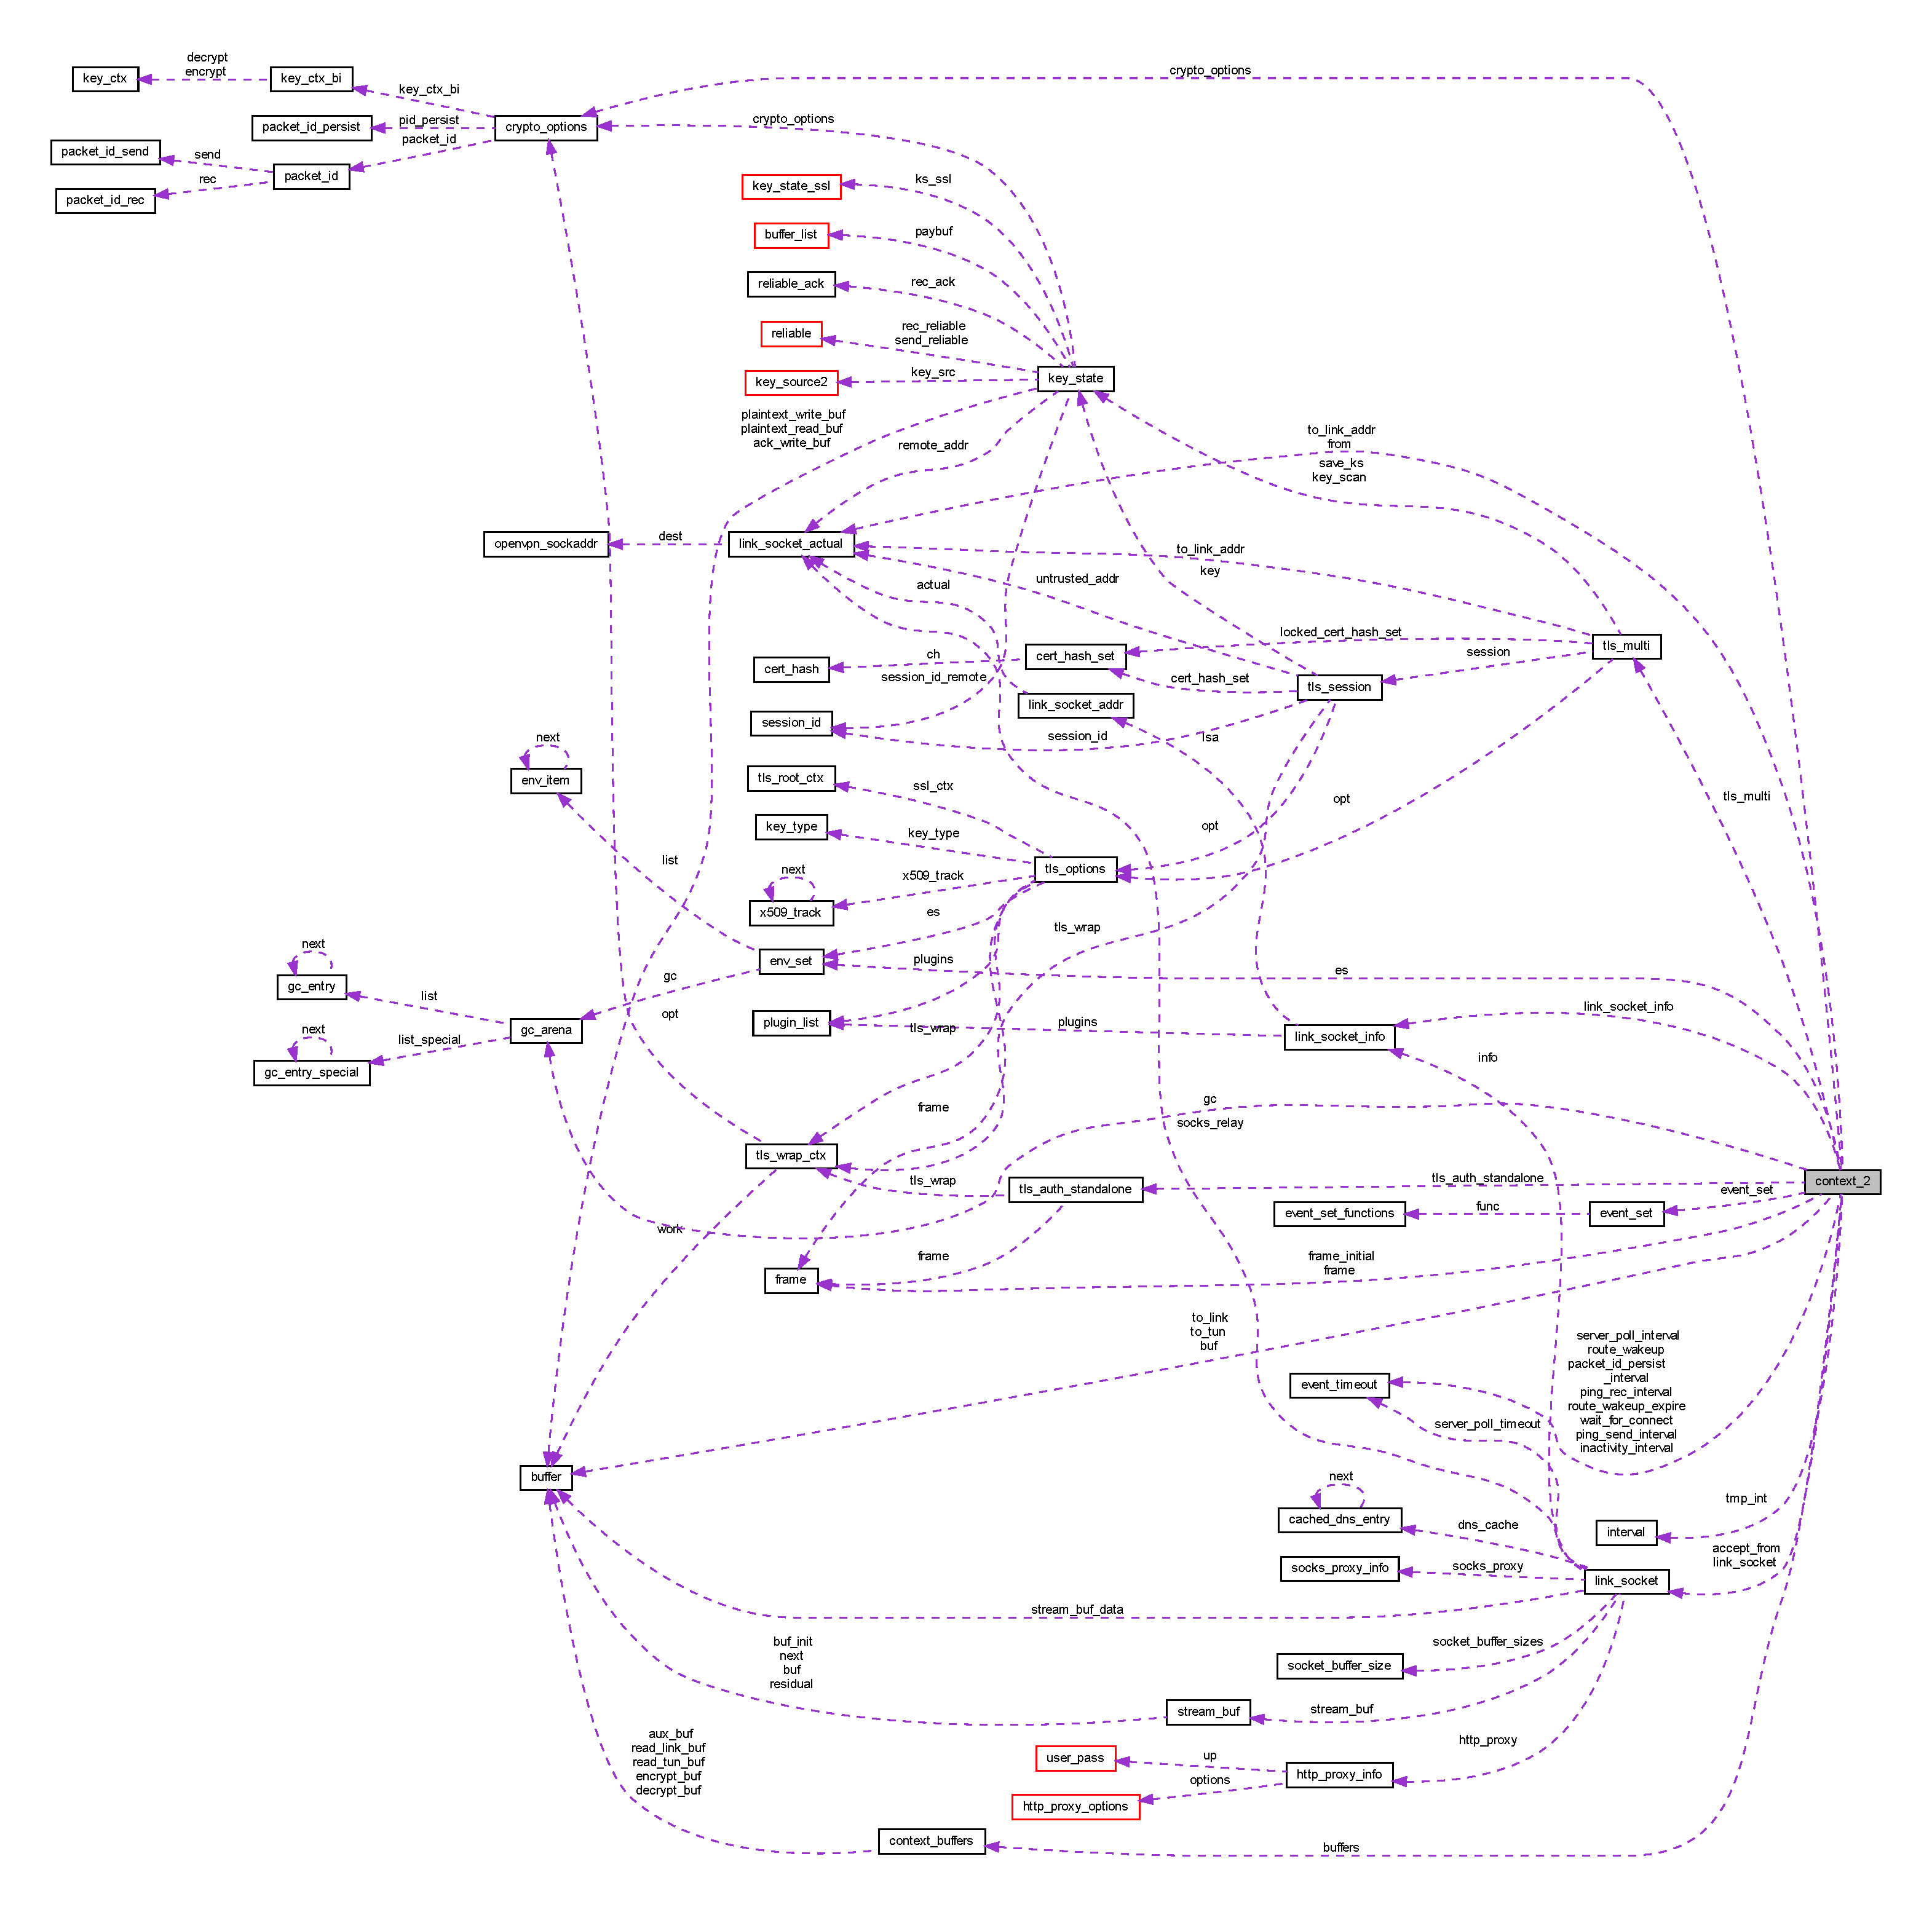
\includegraphics[width=350pt]{structcontext__2__coll__graph}
\end{center}
\end{figure}
\subsection*{Public Attributes}
\begin{DoxyCompactItemize}
\item 
struct \hyperlink{structgc__arena}{gc\+\_\+arena} \hyperlink{structcontext__2_ad4aeb5d46c4a32dc490a124af2c0770a}{gc}
\item 
struct \hyperlink{structevent__set}{event\+\_\+set} $\ast$ \hyperlink{structcontext__2_adc9eee8062fcb8d280910f28fcab8b0b}{event\+\_\+set}
\item 
int \hyperlink{structcontext__2_ad0ae63ac896195c2b4ae39385262b0c6}{event\+\_\+set\+\_\+max}
\item 
\hyperlink{automatic_8c_abb452686968e48b67397da5f97445f5b}{bool} \hyperlink{structcontext__2_afe17ff408cef993e5785dbb553851dce}{event\+\_\+set\+\_\+owned}
\item 
unsigned int \hyperlink{structcontext__2_a217331211c4964b53c8b7a2432a4216d}{event\+\_\+set\+\_\+status}
\item 
struct \hyperlink{structlink__socket}{link\+\_\+socket} $\ast$ \hyperlink{structcontext__2_aa779ad60c8e594706edf92faa2feda4f}{link\+\_\+socket}
\item 
\hyperlink{automatic_8c_abb452686968e48b67397da5f97445f5b}{bool} \hyperlink{structcontext__2_a666bfe66da6072618edc5a0f5688780f}{link\+\_\+socket\+\_\+owned}
\item 
struct \hyperlink{structlink__socket__info}{link\+\_\+socket\+\_\+info} $\ast$ \hyperlink{structcontext__2_a5a7d92871044e8e7ac72c09ef0508445}{link\+\_\+socket\+\_\+info}
\item 
const struct \hyperlink{structlink__socket}{link\+\_\+socket} $\ast$ \hyperlink{structcontext__2_a4cb8c7cbd964e80ede783143a456d44d}{accept\+\_\+from}
\item 
struct \hyperlink{structlink__socket__actual}{link\+\_\+socket\+\_\+actual} $\ast$ \hyperlink{structcontext__2_ab7d4ecafe432890ee5ca789aafec24c2}{to\+\_\+link\+\_\+addr}
\item 
struct \hyperlink{structlink__socket__actual}{link\+\_\+socket\+\_\+actual} \hyperlink{structcontext__2_a7c515ef01a7ece88dbcfa25129e47c9c}{from}
\item 
struct \hyperlink{structframe}{frame} \hyperlink{structcontext__2_a7bdb348860c0854ba0d834af8322c7d8}{frame}
\item 
struct \hyperlink{structframe}{frame} \hyperlink{structcontext__2_a1187d7900d4fcec429d30b7e5370d551}{frame\+\_\+initial}
\item 
\hyperlink{common_8h_a00dd6fbfb368a41945c8c6b9d6fbf88f}{counter\+\_\+type} \hyperlink{structcontext__2_a3fe8f226d4b9bf0a3831ed6f6c81c38a}{tun\+\_\+read\+\_\+bytes}
\item 
\hyperlink{common_8h_a00dd6fbfb368a41945c8c6b9d6fbf88f}{counter\+\_\+type} \hyperlink{structcontext__2_aa3cc7c13e7812c3f71dba0bbdd46ff55}{tun\+\_\+write\+\_\+bytes}
\item 
\hyperlink{common_8h_a00dd6fbfb368a41945c8c6b9d6fbf88f}{counter\+\_\+type} \hyperlink{structcontext__2_a02884491547e765b2afe66a8006d34af}{link\+\_\+read\+\_\+bytes}
\item 
\hyperlink{common_8h_a00dd6fbfb368a41945c8c6b9d6fbf88f}{counter\+\_\+type} \hyperlink{structcontext__2_aae847f30748e65a5ed32f2ed2ba9183d}{link\+\_\+read\+\_\+bytes\+\_\+auth}
\item 
\hyperlink{common_8h_a00dd6fbfb368a41945c8c6b9d6fbf88f}{counter\+\_\+type} \hyperlink{structcontext__2_a07422cc25272851deb63bc6be1b65a10}{link\+\_\+write\+\_\+bytes}
\item 
struct \hyperlink{structevent__timeout}{event\+\_\+timeout} \hyperlink{structcontext__2_a6e148857a12de912aef0d3476a85baea}{wait\+\_\+for\+\_\+connect}
\item 
struct \hyperlink{structevent__timeout}{event\+\_\+timeout} \hyperlink{structcontext__2_a32c2fe431b3437e963b149780188174f}{ping\+\_\+send\+\_\+interval}
\item 
struct \hyperlink{structevent__timeout}{event\+\_\+timeout} \hyperlink{structcontext__2_af7d86fdde3cc1792be2bd85e735a2676}{ping\+\_\+rec\+\_\+interval}
\item 
struct \hyperlink{structevent__timeout}{event\+\_\+timeout} \hyperlink{structcontext__2_aee3f1b158710abd4c3020369b56b9f7a}{inactivity\+\_\+interval}
\item 
int \hyperlink{structcontext__2_a75335b0f54178e487959fcc0b5a367b6}{inactivity\+\_\+bytes}
\item 
int \hyperlink{structcontext__2_ac9926addf1893f11231488eb40adbd9f}{original\+\_\+recv\+\_\+size}
\item 
int \hyperlink{structcontext__2_a1bf11f368d7066c0f4b559c2c5cc7e49}{max\+\_\+recv\+\_\+size\+\_\+local}
\item 
int \hyperlink{structcontext__2_a2745ac1d99418d4d63fbf47dcc10002e}{max\+\_\+recv\+\_\+size\+\_\+remote}
\item 
int \hyperlink{structcontext__2_a32d4e1ea0d13c6b309c33c186b4b5c4a}{max\+\_\+send\+\_\+size\+\_\+local}
\item 
int \hyperlink{structcontext__2_ae6f0527ab232f363c7f724d72ff9ccbe}{max\+\_\+send\+\_\+size\+\_\+remote}
\item 
struct \hyperlink{structtls__multi}{tls\+\_\+multi} $\ast$ \hyperlink{structcontext__2_a758cf7724377be181e7fab59b7a2a30e}{tls\+\_\+multi}
\item 
struct \hyperlink{structtls__auth__standalone}{tls\+\_\+auth\+\_\+standalone} $\ast$ \hyperlink{structcontext__2_a5504671bac689290cd35901bf7d031aa}{tls\+\_\+auth\+\_\+standalone}
\item 
struct \hyperlink{structinterval}{interval} \hyperlink{structcontext__2_a5fd70b82d77870b98844a107ce3cf7dd}{tmp\+\_\+int}
\item 
int \hyperlink{structcontext__2_aea6f45bc37c7c473a4ba3871d43ea2d5}{tls\+\_\+exit\+\_\+signal}
\item 
struct \hyperlink{structcrypto__options}{crypto\+\_\+options} \hyperlink{structcontext__2_a901a1a0ceb94dbd3e9f758552fa4fbd9}{crypto\+\_\+options}
\item 
struct \hyperlink{structevent__timeout}{event\+\_\+timeout} \hyperlink{structcontext__2_ab43cb5718dec488e16b44b0646d12a83}{packet\+\_\+id\+\_\+persist\+\_\+interval}
\item 
struct \hyperlink{structcontext__buffers}{context\+\_\+buffers} $\ast$ \hyperlink{structcontext__2_ae2e304ff3393a09ee15f7490f50b89d8}{buffers}
\item 
\hyperlink{automatic_8c_abb452686968e48b67397da5f97445f5b}{bool} \hyperlink{structcontext__2_aa0413cae96937fb6fca54e18e5b5d3d7}{buffers\+\_\+owned}
\item 
struct \hyperlink{structbuffer}{buffer} \hyperlink{structcontext__2_acb9836ce1e5f8cdc0b88ce89380fb7b0}{buf}
\item 
struct \hyperlink{structbuffer}{buffer} \hyperlink{structcontext__2_a913dbf251774ae01f77289e5a4965704}{to\+\_\+tun}
\item 
struct \hyperlink{structbuffer}{buffer} \hyperlink{structcontext__2_a8b773ace2cf22bd200b316517ac68b9f}{to\+\_\+link}
\item 
\hyperlink{automatic_8c_abb452686968e48b67397da5f97445f5b}{bool} \hyperlink{structcontext__2_acfe86f2a045249246aeda38971cbceaa}{log\+\_\+rw}
\item 
struct \hyperlink{structevent__timeout}{event\+\_\+timeout} \hyperlink{structcontext__2_ae8340ca648a8ecd965445186cf3a0ec1}{route\+\_\+wakeup}
\item 
struct \hyperlink{structevent__timeout}{event\+\_\+timeout} \hyperlink{structcontext__2_a328c64e187c662be87e6b8ea738a76cb}{route\+\_\+wakeup\+\_\+expire}
\item 
\hyperlink{automatic_8c_abb452686968e48b67397da5f97445f5b}{bool} \hyperlink{structcontext__2_a367a0c4601050fe0e0368ec06c58754b}{did\+\_\+open\+\_\+tun}
\item 
struct timeval \hyperlink{structcontext__2_acbdb92043997a7c13406b3ee83e3beb2}{timeval}
\item 
time\+\_\+t \hyperlink{structcontext__2_a7a1136ef8707e675d479855614eadb10}{coarse\+\_\+timer\+\_\+wakeup}
\item 
time\+\_\+t \hyperlink{structcontext__2_a20e59bdf436934540ff063e22d71d649}{update\+\_\+timeout\+\_\+random\+\_\+component}
\item 
struct \hyperlink{structcontext__2_acbdb92043997a7c13406b3ee83e3beb2}{timeval} \hyperlink{structcontext__2_a3da875f012e28a84b4464dc6e8b91177}{timeout\+\_\+random\+\_\+component}
\item 
struct \hyperlink{structevent__timeout}{event\+\_\+timeout} \hyperlink{structcontext__2_a1aeeedd8cd4780c69f7626bcb81f4b90}{server\+\_\+poll\+\_\+interval}
\item 
\hyperlink{automatic_8c_abb452686968e48b67397da5f97445f5b}{bool} \hyperlink{structcontext__2_a267d253d04cc5ef2d91efd6ce4a8f28a}{do\+\_\+up\+\_\+ran}
\item 
struct \hyperlink{structenv__set}{env\+\_\+set} $\ast$ \hyperlink{structcontext__2_a59b42a3c7d754a42ba10acf3c035a1c2}{es}
\item 
\hyperlink{automatic_8c_abb452686968e48b67397da5f97445f5b}{bool} \hyperlink{structcontext__2_a43f0201867a96a35bbecb2e52e880e47}{es\+\_\+owned}
\item 
\hyperlink{automatic_8c_abb452686968e48b67397da5f97445f5b}{bool} \hyperlink{structcontext__2_ad8df4843172d7eaa3a83d407756f4d36}{fast\+\_\+io}
\end{DoxyCompactItemize}


\subsection{Detailed Description}
Level 2 context containing state that is reset on both {\ttfamily S\+I\+G\+H\+U\+P} and {\ttfamily S\+I\+G\+U\+S\+R1} restarts.

This structure is initialized at the top of the {\ttfamily tunnel\+\_\+point\+\_\+to\+\_\+point()}, {\ttfamily tunnel\+\_\+server\+\_\+udp\+\_\+single\+\_\+threaded()}, and {\ttfamily tunnel\+\_\+server\+\_\+tcp()} functions. In other words, it is reset for every iteration of the {\ttfamily \hyperlink{openvpn_8c_a0ddf1224851353fc92bfbff6f499fa97}{main()}} function\textquotesingle{}s inner {\ttfamily S\+I\+G\+U\+S\+R1} loop. 

\subsection{Member Data Documentation}
\hypertarget{structcontext__2_a4cb8c7cbd964e80ede783143a456d44d}{}\index{context\+\_\+2@{context\+\_\+2}!accept\+\_\+from@{accept\+\_\+from}}
\index{accept\+\_\+from@{accept\+\_\+from}!context\+\_\+2@{context\+\_\+2}}
\subsubsection[{accept\+\_\+from}]{\setlength{\rightskip}{0pt plus 5cm}const struct {\bf link\+\_\+socket}$\ast$ context\+\_\+2\+::accept\+\_\+from}\label{structcontext__2_a4cb8c7cbd964e80ede783143a456d44d}
\hypertarget{structcontext__2_acb9836ce1e5f8cdc0b88ce89380fb7b0}{}\index{context\+\_\+2@{context\+\_\+2}!buf@{buf}}
\index{buf@{buf}!context\+\_\+2@{context\+\_\+2}}
\subsubsection[{buf}]{\setlength{\rightskip}{0pt plus 5cm}struct {\bf buffer} context\+\_\+2\+::buf}\label{structcontext__2_acb9836ce1e5f8cdc0b88ce89380fb7b0}
\hypertarget{structcontext__2_ae2e304ff3393a09ee15f7490f50b89d8}{}\index{context\+\_\+2@{context\+\_\+2}!buffers@{buffers}}
\index{buffers@{buffers}!context\+\_\+2@{context\+\_\+2}}
\subsubsection[{buffers}]{\setlength{\rightskip}{0pt plus 5cm}struct {\bf context\+\_\+buffers}$\ast$ context\+\_\+2\+::buffers}\label{structcontext__2_ae2e304ff3393a09ee15f7490f50b89d8}
\hypertarget{structcontext__2_aa0413cae96937fb6fca54e18e5b5d3d7}{}\index{context\+\_\+2@{context\+\_\+2}!buffers\+\_\+owned@{buffers\+\_\+owned}}
\index{buffers\+\_\+owned@{buffers\+\_\+owned}!context\+\_\+2@{context\+\_\+2}}
\subsubsection[{buffers\+\_\+owned}]{\setlength{\rightskip}{0pt plus 5cm}{\bf bool} context\+\_\+2\+::buffers\+\_\+owned}\label{structcontext__2_aa0413cae96937fb6fca54e18e5b5d3d7}
\hypertarget{structcontext__2_a7a1136ef8707e675d479855614eadb10}{}\index{context\+\_\+2@{context\+\_\+2}!coarse\+\_\+timer\+\_\+wakeup@{coarse\+\_\+timer\+\_\+wakeup}}
\index{coarse\+\_\+timer\+\_\+wakeup@{coarse\+\_\+timer\+\_\+wakeup}!context\+\_\+2@{context\+\_\+2}}
\subsubsection[{coarse\+\_\+timer\+\_\+wakeup}]{\setlength{\rightskip}{0pt plus 5cm}time\+\_\+t context\+\_\+2\+::coarse\+\_\+timer\+\_\+wakeup}\label{structcontext__2_a7a1136ef8707e675d479855614eadb10}
\hypertarget{structcontext__2_a901a1a0ceb94dbd3e9f758552fa4fbd9}{}\index{context\+\_\+2@{context\+\_\+2}!crypto\+\_\+options@{crypto\+\_\+options}}
\index{crypto\+\_\+options@{crypto\+\_\+options}!context\+\_\+2@{context\+\_\+2}}
\subsubsection[{crypto\+\_\+options}]{\setlength{\rightskip}{0pt plus 5cm}struct {\bf crypto\+\_\+options} context\+\_\+2\+::crypto\+\_\+options}\label{structcontext__2_a901a1a0ceb94dbd3e9f758552fa4fbd9}
Security parameters and crypto state used by the \hyperlink{group__data__crypto}{Data Channel Crypto module} to process data channel packet. \hypertarget{structcontext__2_a367a0c4601050fe0e0368ec06c58754b}{}\index{context\+\_\+2@{context\+\_\+2}!did\+\_\+open\+\_\+tun@{did\+\_\+open\+\_\+tun}}
\index{did\+\_\+open\+\_\+tun@{did\+\_\+open\+\_\+tun}!context\+\_\+2@{context\+\_\+2}}
\subsubsection[{did\+\_\+open\+\_\+tun}]{\setlength{\rightskip}{0pt plus 5cm}{\bf bool} context\+\_\+2\+::did\+\_\+open\+\_\+tun}\label{structcontext__2_a367a0c4601050fe0e0368ec06c58754b}
\hypertarget{structcontext__2_a267d253d04cc5ef2d91efd6ce4a8f28a}{}\index{context\+\_\+2@{context\+\_\+2}!do\+\_\+up\+\_\+ran@{do\+\_\+up\+\_\+ran}}
\index{do\+\_\+up\+\_\+ran@{do\+\_\+up\+\_\+ran}!context\+\_\+2@{context\+\_\+2}}
\subsubsection[{do\+\_\+up\+\_\+ran}]{\setlength{\rightskip}{0pt plus 5cm}{\bf bool} context\+\_\+2\+::do\+\_\+up\+\_\+ran}\label{structcontext__2_a267d253d04cc5ef2d91efd6ce4a8f28a}
\hypertarget{structcontext__2_a59b42a3c7d754a42ba10acf3c035a1c2}{}\index{context\+\_\+2@{context\+\_\+2}!es@{es}}
\index{es@{es}!context\+\_\+2@{context\+\_\+2}}
\subsubsection[{es}]{\setlength{\rightskip}{0pt plus 5cm}struct {\bf env\+\_\+set}$\ast$ context\+\_\+2\+::es}\label{structcontext__2_a59b42a3c7d754a42ba10acf3c035a1c2}
\hypertarget{structcontext__2_a43f0201867a96a35bbecb2e52e880e47}{}\index{context\+\_\+2@{context\+\_\+2}!es\+\_\+owned@{es\+\_\+owned}}
\index{es\+\_\+owned@{es\+\_\+owned}!context\+\_\+2@{context\+\_\+2}}
\subsubsection[{es\+\_\+owned}]{\setlength{\rightskip}{0pt plus 5cm}{\bf bool} context\+\_\+2\+::es\+\_\+owned}\label{structcontext__2_a43f0201867a96a35bbecb2e52e880e47}
\hypertarget{structcontext__2_adc9eee8062fcb8d280910f28fcab8b0b}{}\index{context\+\_\+2@{context\+\_\+2}!event\+\_\+set@{event\+\_\+set}}
\index{event\+\_\+set@{event\+\_\+set}!context\+\_\+2@{context\+\_\+2}}
\subsubsection[{event\+\_\+set}]{\setlength{\rightskip}{0pt plus 5cm}struct {\bf event\+\_\+set}$\ast$ context\+\_\+2\+::event\+\_\+set}\label{structcontext__2_adc9eee8062fcb8d280910f28fcab8b0b}
\hypertarget{structcontext__2_ad0ae63ac896195c2b4ae39385262b0c6}{}\index{context\+\_\+2@{context\+\_\+2}!event\+\_\+set\+\_\+max@{event\+\_\+set\+\_\+max}}
\index{event\+\_\+set\+\_\+max@{event\+\_\+set\+\_\+max}!context\+\_\+2@{context\+\_\+2}}
\subsubsection[{event\+\_\+set\+\_\+max}]{\setlength{\rightskip}{0pt plus 5cm}int context\+\_\+2\+::event\+\_\+set\+\_\+max}\label{structcontext__2_ad0ae63ac896195c2b4ae39385262b0c6}
\hypertarget{structcontext__2_afe17ff408cef993e5785dbb553851dce}{}\index{context\+\_\+2@{context\+\_\+2}!event\+\_\+set\+\_\+owned@{event\+\_\+set\+\_\+owned}}
\index{event\+\_\+set\+\_\+owned@{event\+\_\+set\+\_\+owned}!context\+\_\+2@{context\+\_\+2}}
\subsubsection[{event\+\_\+set\+\_\+owned}]{\setlength{\rightskip}{0pt plus 5cm}{\bf bool} context\+\_\+2\+::event\+\_\+set\+\_\+owned}\label{structcontext__2_afe17ff408cef993e5785dbb553851dce}
\hypertarget{structcontext__2_a217331211c4964b53c8b7a2432a4216d}{}\index{context\+\_\+2@{context\+\_\+2}!event\+\_\+set\+\_\+status@{event\+\_\+set\+\_\+status}}
\index{event\+\_\+set\+\_\+status@{event\+\_\+set\+\_\+status}!context\+\_\+2@{context\+\_\+2}}
\subsubsection[{event\+\_\+set\+\_\+status}]{\setlength{\rightskip}{0pt plus 5cm}unsigned int context\+\_\+2\+::event\+\_\+set\+\_\+status}\label{structcontext__2_a217331211c4964b53c8b7a2432a4216d}
\hypertarget{structcontext__2_ad8df4843172d7eaa3a83d407756f4d36}{}\index{context\+\_\+2@{context\+\_\+2}!fast\+\_\+io@{fast\+\_\+io}}
\index{fast\+\_\+io@{fast\+\_\+io}!context\+\_\+2@{context\+\_\+2}}
\subsubsection[{fast\+\_\+io}]{\setlength{\rightskip}{0pt plus 5cm}{\bf bool} context\+\_\+2\+::fast\+\_\+io}\label{structcontext__2_ad8df4843172d7eaa3a83d407756f4d36}
\hypertarget{structcontext__2_a7bdb348860c0854ba0d834af8322c7d8}{}\index{context\+\_\+2@{context\+\_\+2}!frame@{frame}}
\index{frame@{frame}!context\+\_\+2@{context\+\_\+2}}
\subsubsection[{frame}]{\setlength{\rightskip}{0pt plus 5cm}struct {\bf frame} context\+\_\+2\+::frame}\label{structcontext__2_a7bdb348860c0854ba0d834af8322c7d8}
\hypertarget{structcontext__2_a1187d7900d4fcec429d30b7e5370d551}{}\index{context\+\_\+2@{context\+\_\+2}!frame\+\_\+initial@{frame\+\_\+initial}}
\index{frame\+\_\+initial@{frame\+\_\+initial}!context\+\_\+2@{context\+\_\+2}}
\subsubsection[{frame\+\_\+initial}]{\setlength{\rightskip}{0pt plus 5cm}struct {\bf frame} context\+\_\+2\+::frame\+\_\+initial}\label{structcontext__2_a1187d7900d4fcec429d30b7e5370d551}
\hypertarget{structcontext__2_a7c515ef01a7ece88dbcfa25129e47c9c}{}\index{context\+\_\+2@{context\+\_\+2}!from@{from}}
\index{from@{from}!context\+\_\+2@{context\+\_\+2}}
\subsubsection[{from}]{\setlength{\rightskip}{0pt plus 5cm}struct {\bf link\+\_\+socket\+\_\+actual} context\+\_\+2\+::from}\label{structcontext__2_a7c515ef01a7ece88dbcfa25129e47c9c}
\hypertarget{structcontext__2_ad4aeb5d46c4a32dc490a124af2c0770a}{}\index{context\+\_\+2@{context\+\_\+2}!gc@{gc}}
\index{gc@{gc}!context\+\_\+2@{context\+\_\+2}}
\subsubsection[{gc}]{\setlength{\rightskip}{0pt plus 5cm}struct {\bf gc\+\_\+arena} context\+\_\+2\+::gc}\label{structcontext__2_ad4aeb5d46c4a32dc490a124af2c0770a}
Garbage collection arena for allocations done in the level 2 scope of this \hyperlink{structcontext__2}{context\+\_\+2} structure. \hypertarget{structcontext__2_a75335b0f54178e487959fcc0b5a367b6}{}\index{context\+\_\+2@{context\+\_\+2}!inactivity\+\_\+bytes@{inactivity\+\_\+bytes}}
\index{inactivity\+\_\+bytes@{inactivity\+\_\+bytes}!context\+\_\+2@{context\+\_\+2}}
\subsubsection[{inactivity\+\_\+bytes}]{\setlength{\rightskip}{0pt plus 5cm}int context\+\_\+2\+::inactivity\+\_\+bytes}\label{structcontext__2_a75335b0f54178e487959fcc0b5a367b6}
\hypertarget{structcontext__2_aee3f1b158710abd4c3020369b56b9f7a}{}\index{context\+\_\+2@{context\+\_\+2}!inactivity\+\_\+interval@{inactivity\+\_\+interval}}
\index{inactivity\+\_\+interval@{inactivity\+\_\+interval}!context\+\_\+2@{context\+\_\+2}}
\subsubsection[{inactivity\+\_\+interval}]{\setlength{\rightskip}{0pt plus 5cm}struct {\bf event\+\_\+timeout} context\+\_\+2\+::inactivity\+\_\+interval}\label{structcontext__2_aee3f1b158710abd4c3020369b56b9f7a}
\hypertarget{structcontext__2_a02884491547e765b2afe66a8006d34af}{}\index{context\+\_\+2@{context\+\_\+2}!link\+\_\+read\+\_\+bytes@{link\+\_\+read\+\_\+bytes}}
\index{link\+\_\+read\+\_\+bytes@{link\+\_\+read\+\_\+bytes}!context\+\_\+2@{context\+\_\+2}}
\subsubsection[{link\+\_\+read\+\_\+bytes}]{\setlength{\rightskip}{0pt plus 5cm}{\bf counter\+\_\+type} context\+\_\+2\+::link\+\_\+read\+\_\+bytes}\label{structcontext__2_a02884491547e765b2afe66a8006d34af}
\hypertarget{structcontext__2_aae847f30748e65a5ed32f2ed2ba9183d}{}\index{context\+\_\+2@{context\+\_\+2}!link\+\_\+read\+\_\+bytes\+\_\+auth@{link\+\_\+read\+\_\+bytes\+\_\+auth}}
\index{link\+\_\+read\+\_\+bytes\+\_\+auth@{link\+\_\+read\+\_\+bytes\+\_\+auth}!context\+\_\+2@{context\+\_\+2}}
\subsubsection[{link\+\_\+read\+\_\+bytes\+\_\+auth}]{\setlength{\rightskip}{0pt plus 5cm}{\bf counter\+\_\+type} context\+\_\+2\+::link\+\_\+read\+\_\+bytes\+\_\+auth}\label{structcontext__2_aae847f30748e65a5ed32f2ed2ba9183d}
\hypertarget{structcontext__2_aa779ad60c8e594706edf92faa2feda4f}{}\index{context\+\_\+2@{context\+\_\+2}!link\+\_\+socket@{link\+\_\+socket}}
\index{link\+\_\+socket@{link\+\_\+socket}!context\+\_\+2@{context\+\_\+2}}
\subsubsection[{link\+\_\+socket}]{\setlength{\rightskip}{0pt plus 5cm}struct {\bf link\+\_\+socket}$\ast$ context\+\_\+2\+::link\+\_\+socket}\label{structcontext__2_aa779ad60c8e594706edf92faa2feda4f}
\hypertarget{structcontext__2_a5a7d92871044e8e7ac72c09ef0508445}{}\index{context\+\_\+2@{context\+\_\+2}!link\+\_\+socket\+\_\+info@{link\+\_\+socket\+\_\+info}}
\index{link\+\_\+socket\+\_\+info@{link\+\_\+socket\+\_\+info}!context\+\_\+2@{context\+\_\+2}}
\subsubsection[{link\+\_\+socket\+\_\+info}]{\setlength{\rightskip}{0pt plus 5cm}struct {\bf link\+\_\+socket\+\_\+info}$\ast$ context\+\_\+2\+::link\+\_\+socket\+\_\+info}\label{structcontext__2_a5a7d92871044e8e7ac72c09ef0508445}
\hypertarget{structcontext__2_a666bfe66da6072618edc5a0f5688780f}{}\index{context\+\_\+2@{context\+\_\+2}!link\+\_\+socket\+\_\+owned@{link\+\_\+socket\+\_\+owned}}
\index{link\+\_\+socket\+\_\+owned@{link\+\_\+socket\+\_\+owned}!context\+\_\+2@{context\+\_\+2}}
\subsubsection[{link\+\_\+socket\+\_\+owned}]{\setlength{\rightskip}{0pt plus 5cm}{\bf bool} context\+\_\+2\+::link\+\_\+socket\+\_\+owned}\label{structcontext__2_a666bfe66da6072618edc5a0f5688780f}
\hypertarget{structcontext__2_a07422cc25272851deb63bc6be1b65a10}{}\index{context\+\_\+2@{context\+\_\+2}!link\+\_\+write\+\_\+bytes@{link\+\_\+write\+\_\+bytes}}
\index{link\+\_\+write\+\_\+bytes@{link\+\_\+write\+\_\+bytes}!context\+\_\+2@{context\+\_\+2}}
\subsubsection[{link\+\_\+write\+\_\+bytes}]{\setlength{\rightskip}{0pt plus 5cm}{\bf counter\+\_\+type} context\+\_\+2\+::link\+\_\+write\+\_\+bytes}\label{structcontext__2_a07422cc25272851deb63bc6be1b65a10}
\hypertarget{structcontext__2_acfe86f2a045249246aeda38971cbceaa}{}\index{context\+\_\+2@{context\+\_\+2}!log\+\_\+rw@{log\+\_\+rw}}
\index{log\+\_\+rw@{log\+\_\+rw}!context\+\_\+2@{context\+\_\+2}}
\subsubsection[{log\+\_\+rw}]{\setlength{\rightskip}{0pt plus 5cm}{\bf bool} context\+\_\+2\+::log\+\_\+rw}\label{structcontext__2_acfe86f2a045249246aeda38971cbceaa}
\hypertarget{structcontext__2_a1bf11f368d7066c0f4b559c2c5cc7e49}{}\index{context\+\_\+2@{context\+\_\+2}!max\+\_\+recv\+\_\+size\+\_\+local@{max\+\_\+recv\+\_\+size\+\_\+local}}
\index{max\+\_\+recv\+\_\+size\+\_\+local@{max\+\_\+recv\+\_\+size\+\_\+local}!context\+\_\+2@{context\+\_\+2}}
\subsubsection[{max\+\_\+recv\+\_\+size\+\_\+local}]{\setlength{\rightskip}{0pt plus 5cm}int context\+\_\+2\+::max\+\_\+recv\+\_\+size\+\_\+local}\label{structcontext__2_a1bf11f368d7066c0f4b559c2c5cc7e49}
\hypertarget{structcontext__2_a2745ac1d99418d4d63fbf47dcc10002e}{}\index{context\+\_\+2@{context\+\_\+2}!max\+\_\+recv\+\_\+size\+\_\+remote@{max\+\_\+recv\+\_\+size\+\_\+remote}}
\index{max\+\_\+recv\+\_\+size\+\_\+remote@{max\+\_\+recv\+\_\+size\+\_\+remote}!context\+\_\+2@{context\+\_\+2}}
\subsubsection[{max\+\_\+recv\+\_\+size\+\_\+remote}]{\setlength{\rightskip}{0pt plus 5cm}int context\+\_\+2\+::max\+\_\+recv\+\_\+size\+\_\+remote}\label{structcontext__2_a2745ac1d99418d4d63fbf47dcc10002e}
\hypertarget{structcontext__2_a32d4e1ea0d13c6b309c33c186b4b5c4a}{}\index{context\+\_\+2@{context\+\_\+2}!max\+\_\+send\+\_\+size\+\_\+local@{max\+\_\+send\+\_\+size\+\_\+local}}
\index{max\+\_\+send\+\_\+size\+\_\+local@{max\+\_\+send\+\_\+size\+\_\+local}!context\+\_\+2@{context\+\_\+2}}
\subsubsection[{max\+\_\+send\+\_\+size\+\_\+local}]{\setlength{\rightskip}{0pt plus 5cm}int context\+\_\+2\+::max\+\_\+send\+\_\+size\+\_\+local}\label{structcontext__2_a32d4e1ea0d13c6b309c33c186b4b5c4a}
\hypertarget{structcontext__2_ae6f0527ab232f363c7f724d72ff9ccbe}{}\index{context\+\_\+2@{context\+\_\+2}!max\+\_\+send\+\_\+size\+\_\+remote@{max\+\_\+send\+\_\+size\+\_\+remote}}
\index{max\+\_\+send\+\_\+size\+\_\+remote@{max\+\_\+send\+\_\+size\+\_\+remote}!context\+\_\+2@{context\+\_\+2}}
\subsubsection[{max\+\_\+send\+\_\+size\+\_\+remote}]{\setlength{\rightskip}{0pt plus 5cm}int context\+\_\+2\+::max\+\_\+send\+\_\+size\+\_\+remote}\label{structcontext__2_ae6f0527ab232f363c7f724d72ff9ccbe}
\hypertarget{structcontext__2_ac9926addf1893f11231488eb40adbd9f}{}\index{context\+\_\+2@{context\+\_\+2}!original\+\_\+recv\+\_\+size@{original\+\_\+recv\+\_\+size}}
\index{original\+\_\+recv\+\_\+size@{original\+\_\+recv\+\_\+size}!context\+\_\+2@{context\+\_\+2}}
\subsubsection[{original\+\_\+recv\+\_\+size}]{\setlength{\rightskip}{0pt plus 5cm}int context\+\_\+2\+::original\+\_\+recv\+\_\+size}\label{structcontext__2_ac9926addf1893f11231488eb40adbd9f}
\hypertarget{structcontext__2_ab43cb5718dec488e16b44b0646d12a83}{}\index{context\+\_\+2@{context\+\_\+2}!packet\+\_\+id\+\_\+persist\+\_\+interval@{packet\+\_\+id\+\_\+persist\+\_\+interval}}
\index{packet\+\_\+id\+\_\+persist\+\_\+interval@{packet\+\_\+id\+\_\+persist\+\_\+interval}!context\+\_\+2@{context\+\_\+2}}
\subsubsection[{packet\+\_\+id\+\_\+persist\+\_\+interval}]{\setlength{\rightskip}{0pt plus 5cm}struct {\bf event\+\_\+timeout} context\+\_\+2\+::packet\+\_\+id\+\_\+persist\+\_\+interval}\label{structcontext__2_ab43cb5718dec488e16b44b0646d12a83}
\hypertarget{structcontext__2_af7d86fdde3cc1792be2bd85e735a2676}{}\index{context\+\_\+2@{context\+\_\+2}!ping\+\_\+rec\+\_\+interval@{ping\+\_\+rec\+\_\+interval}}
\index{ping\+\_\+rec\+\_\+interval@{ping\+\_\+rec\+\_\+interval}!context\+\_\+2@{context\+\_\+2}}
\subsubsection[{ping\+\_\+rec\+\_\+interval}]{\setlength{\rightskip}{0pt plus 5cm}struct {\bf event\+\_\+timeout} context\+\_\+2\+::ping\+\_\+rec\+\_\+interval}\label{structcontext__2_af7d86fdde3cc1792be2bd85e735a2676}
\hypertarget{structcontext__2_a32c2fe431b3437e963b149780188174f}{}\index{context\+\_\+2@{context\+\_\+2}!ping\+\_\+send\+\_\+interval@{ping\+\_\+send\+\_\+interval}}
\index{ping\+\_\+send\+\_\+interval@{ping\+\_\+send\+\_\+interval}!context\+\_\+2@{context\+\_\+2}}
\subsubsection[{ping\+\_\+send\+\_\+interval}]{\setlength{\rightskip}{0pt plus 5cm}struct {\bf event\+\_\+timeout} context\+\_\+2\+::ping\+\_\+send\+\_\+interval}\label{structcontext__2_a32c2fe431b3437e963b149780188174f}
\hypertarget{structcontext__2_ae8340ca648a8ecd965445186cf3a0ec1}{}\index{context\+\_\+2@{context\+\_\+2}!route\+\_\+wakeup@{route\+\_\+wakeup}}
\index{route\+\_\+wakeup@{route\+\_\+wakeup}!context\+\_\+2@{context\+\_\+2}}
\subsubsection[{route\+\_\+wakeup}]{\setlength{\rightskip}{0pt plus 5cm}struct {\bf event\+\_\+timeout} context\+\_\+2\+::route\+\_\+wakeup}\label{structcontext__2_ae8340ca648a8ecd965445186cf3a0ec1}
\hypertarget{structcontext__2_a328c64e187c662be87e6b8ea738a76cb}{}\index{context\+\_\+2@{context\+\_\+2}!route\+\_\+wakeup\+\_\+expire@{route\+\_\+wakeup\+\_\+expire}}
\index{route\+\_\+wakeup\+\_\+expire@{route\+\_\+wakeup\+\_\+expire}!context\+\_\+2@{context\+\_\+2}}
\subsubsection[{route\+\_\+wakeup\+\_\+expire}]{\setlength{\rightskip}{0pt plus 5cm}struct {\bf event\+\_\+timeout} context\+\_\+2\+::route\+\_\+wakeup\+\_\+expire}\label{structcontext__2_a328c64e187c662be87e6b8ea738a76cb}
\hypertarget{structcontext__2_a1aeeedd8cd4780c69f7626bcb81f4b90}{}\index{context\+\_\+2@{context\+\_\+2}!server\+\_\+poll\+\_\+interval@{server\+\_\+poll\+\_\+interval}}
\index{server\+\_\+poll\+\_\+interval@{server\+\_\+poll\+\_\+interval}!context\+\_\+2@{context\+\_\+2}}
\subsubsection[{server\+\_\+poll\+\_\+interval}]{\setlength{\rightskip}{0pt plus 5cm}struct {\bf event\+\_\+timeout} context\+\_\+2\+::server\+\_\+poll\+\_\+interval}\label{structcontext__2_a1aeeedd8cd4780c69f7626bcb81f4b90}
\hypertarget{structcontext__2_a3da875f012e28a84b4464dc6e8b91177}{}\index{context\+\_\+2@{context\+\_\+2}!timeout\+\_\+random\+\_\+component@{timeout\+\_\+random\+\_\+component}}
\index{timeout\+\_\+random\+\_\+component@{timeout\+\_\+random\+\_\+component}!context\+\_\+2@{context\+\_\+2}}
\subsubsection[{timeout\+\_\+random\+\_\+component}]{\setlength{\rightskip}{0pt plus 5cm}struct {\bf timeval} context\+\_\+2\+::timeout\+\_\+random\+\_\+component}\label{structcontext__2_a3da875f012e28a84b4464dc6e8b91177}
\hypertarget{structcontext__2_acbdb92043997a7c13406b3ee83e3beb2}{}\index{context\+\_\+2@{context\+\_\+2}!timeval@{timeval}}
\index{timeval@{timeval}!context\+\_\+2@{context\+\_\+2}}
\subsubsection[{timeval}]{\setlength{\rightskip}{0pt plus 5cm}struct timeval context\+\_\+2\+::timeval}\label{structcontext__2_acbdb92043997a7c13406b3ee83e3beb2}
\hypertarget{structcontext__2_a5504671bac689290cd35901bf7d031aa}{}\index{context\+\_\+2@{context\+\_\+2}!tls\+\_\+auth\+\_\+standalone@{tls\+\_\+auth\+\_\+standalone}}
\index{tls\+\_\+auth\+\_\+standalone@{tls\+\_\+auth\+\_\+standalone}!context\+\_\+2@{context\+\_\+2}}
\subsubsection[{tls\+\_\+auth\+\_\+standalone}]{\setlength{\rightskip}{0pt plus 5cm}struct {\bf tls\+\_\+auth\+\_\+standalone}$\ast$ context\+\_\+2\+::tls\+\_\+auth\+\_\+standalone}\label{structcontext__2_a5504671bac689290cd35901bf7d031aa}
T\+L\+S state structure required for the initial authentication of a client\textquotesingle{}s connection attempt. This structure is used by the {\ttfamily \hyperlink{group__data__crypto_gab1369f42e94bbec108d952d565b0f283}{tls\+\_\+pre\+\_\+decrypt\+\_\+lite()}} function when it performs the H\+M\+A\+C firewall check on the first connection packet received from a new client. See the {\ttfamily --tls-\/auth} commandline option. \hypertarget{structcontext__2_aea6f45bc37c7c473a4ba3871d43ea2d5}{}\index{context\+\_\+2@{context\+\_\+2}!tls\+\_\+exit\+\_\+signal@{tls\+\_\+exit\+\_\+signal}}
\index{tls\+\_\+exit\+\_\+signal@{tls\+\_\+exit\+\_\+signal}!context\+\_\+2@{context\+\_\+2}}
\subsubsection[{tls\+\_\+exit\+\_\+signal}]{\setlength{\rightskip}{0pt plus 5cm}int context\+\_\+2\+::tls\+\_\+exit\+\_\+signal}\label{structcontext__2_aea6f45bc37c7c473a4ba3871d43ea2d5}
\hypertarget{structcontext__2_a758cf7724377be181e7fab59b7a2a30e}{}\index{context\+\_\+2@{context\+\_\+2}!tls\+\_\+multi@{tls\+\_\+multi}}
\index{tls\+\_\+multi@{tls\+\_\+multi}!context\+\_\+2@{context\+\_\+2}}
\subsubsection[{tls\+\_\+multi}]{\setlength{\rightskip}{0pt plus 5cm}struct {\bf tls\+\_\+multi}$\ast$ context\+\_\+2\+::tls\+\_\+multi}\label{structcontext__2_a758cf7724377be181e7fab59b7a2a30e}
T\+L\+S state structure for this V\+P\+N tunnel. \hypertarget{structcontext__2_a5fd70b82d77870b98844a107ce3cf7dd}{}\index{context\+\_\+2@{context\+\_\+2}!tmp\+\_\+int@{tmp\+\_\+int}}
\index{tmp\+\_\+int@{tmp\+\_\+int}!context\+\_\+2@{context\+\_\+2}}
\subsubsection[{tmp\+\_\+int}]{\setlength{\rightskip}{0pt plus 5cm}struct {\bf interval} context\+\_\+2\+::tmp\+\_\+int}\label{structcontext__2_a5fd70b82d77870b98844a107ce3cf7dd}
\hypertarget{structcontext__2_a8b773ace2cf22bd200b316517ac68b9f}{}\index{context\+\_\+2@{context\+\_\+2}!to\+\_\+link@{to\+\_\+link}}
\index{to\+\_\+link@{to\+\_\+link}!context\+\_\+2@{context\+\_\+2}}
\subsubsection[{to\+\_\+link}]{\setlength{\rightskip}{0pt plus 5cm}struct {\bf buffer} context\+\_\+2\+::to\+\_\+link}\label{structcontext__2_a8b773ace2cf22bd200b316517ac68b9f}
\hypertarget{structcontext__2_ab7d4ecafe432890ee5ca789aafec24c2}{}\index{context\+\_\+2@{context\+\_\+2}!to\+\_\+link\+\_\+addr@{to\+\_\+link\+\_\+addr}}
\index{to\+\_\+link\+\_\+addr@{to\+\_\+link\+\_\+addr}!context\+\_\+2@{context\+\_\+2}}
\subsubsection[{to\+\_\+link\+\_\+addr}]{\setlength{\rightskip}{0pt plus 5cm}struct {\bf link\+\_\+socket\+\_\+actual}$\ast$ context\+\_\+2\+::to\+\_\+link\+\_\+addr}\label{structcontext__2_ab7d4ecafe432890ee5ca789aafec24c2}
\hypertarget{structcontext__2_a913dbf251774ae01f77289e5a4965704}{}\index{context\+\_\+2@{context\+\_\+2}!to\+\_\+tun@{to\+\_\+tun}}
\index{to\+\_\+tun@{to\+\_\+tun}!context\+\_\+2@{context\+\_\+2}}
\subsubsection[{to\+\_\+tun}]{\setlength{\rightskip}{0pt plus 5cm}struct {\bf buffer} context\+\_\+2\+::to\+\_\+tun}\label{structcontext__2_a913dbf251774ae01f77289e5a4965704}
\hypertarget{structcontext__2_a3fe8f226d4b9bf0a3831ed6f6c81c38a}{}\index{context\+\_\+2@{context\+\_\+2}!tun\+\_\+read\+\_\+bytes@{tun\+\_\+read\+\_\+bytes}}
\index{tun\+\_\+read\+\_\+bytes@{tun\+\_\+read\+\_\+bytes}!context\+\_\+2@{context\+\_\+2}}
\subsubsection[{tun\+\_\+read\+\_\+bytes}]{\setlength{\rightskip}{0pt plus 5cm}{\bf counter\+\_\+type} context\+\_\+2\+::tun\+\_\+read\+\_\+bytes}\label{structcontext__2_a3fe8f226d4b9bf0a3831ed6f6c81c38a}
\hypertarget{structcontext__2_aa3cc7c13e7812c3f71dba0bbdd46ff55}{}\index{context\+\_\+2@{context\+\_\+2}!tun\+\_\+write\+\_\+bytes@{tun\+\_\+write\+\_\+bytes}}
\index{tun\+\_\+write\+\_\+bytes@{tun\+\_\+write\+\_\+bytes}!context\+\_\+2@{context\+\_\+2}}
\subsubsection[{tun\+\_\+write\+\_\+bytes}]{\setlength{\rightskip}{0pt plus 5cm}{\bf counter\+\_\+type} context\+\_\+2\+::tun\+\_\+write\+\_\+bytes}\label{structcontext__2_aa3cc7c13e7812c3f71dba0bbdd46ff55}
\hypertarget{structcontext__2_a20e59bdf436934540ff063e22d71d649}{}\index{context\+\_\+2@{context\+\_\+2}!update\+\_\+timeout\+\_\+random\+\_\+component@{update\+\_\+timeout\+\_\+random\+\_\+component}}
\index{update\+\_\+timeout\+\_\+random\+\_\+component@{update\+\_\+timeout\+\_\+random\+\_\+component}!context\+\_\+2@{context\+\_\+2}}
\subsubsection[{update\+\_\+timeout\+\_\+random\+\_\+component}]{\setlength{\rightskip}{0pt plus 5cm}time\+\_\+t context\+\_\+2\+::update\+\_\+timeout\+\_\+random\+\_\+component}\label{structcontext__2_a20e59bdf436934540ff063e22d71d649}
\hypertarget{structcontext__2_a6e148857a12de912aef0d3476a85baea}{}\index{context\+\_\+2@{context\+\_\+2}!wait\+\_\+for\+\_\+connect@{wait\+\_\+for\+\_\+connect}}
\index{wait\+\_\+for\+\_\+connect@{wait\+\_\+for\+\_\+connect}!context\+\_\+2@{context\+\_\+2}}
\subsubsection[{wait\+\_\+for\+\_\+connect}]{\setlength{\rightskip}{0pt plus 5cm}struct {\bf event\+\_\+timeout} context\+\_\+2\+::wait\+\_\+for\+\_\+connect}\label{structcontext__2_a6e148857a12de912aef0d3476a85baea}


The documentation for this struct was generated from the following file\+:\begin{DoxyCompactItemize}
\item 
src/openvpn/\hyperlink{openvpn_8h}{openvpn.\+h}\end{DoxyCompactItemize}

\hypertarget{structcontext__buffers}{}\section{context\+\_\+buffers Struct Reference}
\label{structcontext__buffers}\index{context\+\_\+buffers@{context\+\_\+buffers}}


{\ttfamily \#include $<$openvpn.\+h$>$}



Collaboration diagram for context\+\_\+buffers\+:
\nopagebreak
\begin{figure}[H]
\begin{center}
\leavevmode
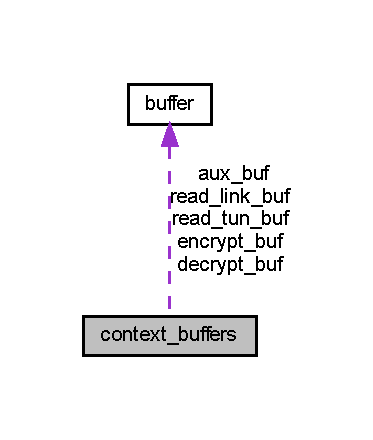
\includegraphics[width=179pt]{structcontext__buffers__coll__graph}
\end{center}
\end{figure}
\subsection*{Public Attributes}
\begin{DoxyCompactItemize}
\item 
struct \hyperlink{structbuffer}{buffer} \hyperlink{structcontext__buffers_ad3e2e97af748c92d2c3310f4631393ef}{aux\+\_\+buf}
\item 
struct \hyperlink{structbuffer}{buffer} \hyperlink{structcontext__buffers_a7030fd4d5442836a9cd3c2a71a1e84e8}{encrypt\+\_\+buf}
\item 
struct \hyperlink{structbuffer}{buffer} \hyperlink{structcontext__buffers_ac3ecbcb5ab79601f229b6badf7c09efb}{decrypt\+\_\+buf}
\item 
struct \hyperlink{structbuffer}{buffer} \hyperlink{structcontext__buffers_a0434309fa3b81366ba6578ee4fe26923}{read\+\_\+link\+\_\+buf}
\item 
struct \hyperlink{structbuffer}{buffer} \hyperlink{structcontext__buffers_aa03e7433c540b45f5e427527739d888c}{read\+\_\+tun\+\_\+buf}
\end{DoxyCompactItemize}


\subsection{Member Data Documentation}
\hypertarget{structcontext__buffers_ad3e2e97af748c92d2c3310f4631393ef}{}\index{context\+\_\+buffers@{context\+\_\+buffers}!aux\+\_\+buf@{aux\+\_\+buf}}
\index{aux\+\_\+buf@{aux\+\_\+buf}!context\+\_\+buffers@{context\+\_\+buffers}}
\subsubsection[{aux\+\_\+buf}]{\setlength{\rightskip}{0pt plus 5cm}struct {\bf buffer} context\+\_\+buffers\+::aux\+\_\+buf}\label{structcontext__buffers_ad3e2e97af748c92d2c3310f4631393ef}
\hypertarget{structcontext__buffers_ac3ecbcb5ab79601f229b6badf7c09efb}{}\index{context\+\_\+buffers@{context\+\_\+buffers}!decrypt\+\_\+buf@{decrypt\+\_\+buf}}
\index{decrypt\+\_\+buf@{decrypt\+\_\+buf}!context\+\_\+buffers@{context\+\_\+buffers}}
\subsubsection[{decrypt\+\_\+buf}]{\setlength{\rightskip}{0pt plus 5cm}struct {\bf buffer} context\+\_\+buffers\+::decrypt\+\_\+buf}\label{structcontext__buffers_ac3ecbcb5ab79601f229b6badf7c09efb}
\hypertarget{structcontext__buffers_a7030fd4d5442836a9cd3c2a71a1e84e8}{}\index{context\+\_\+buffers@{context\+\_\+buffers}!encrypt\+\_\+buf@{encrypt\+\_\+buf}}
\index{encrypt\+\_\+buf@{encrypt\+\_\+buf}!context\+\_\+buffers@{context\+\_\+buffers}}
\subsubsection[{encrypt\+\_\+buf}]{\setlength{\rightskip}{0pt plus 5cm}struct {\bf buffer} context\+\_\+buffers\+::encrypt\+\_\+buf}\label{structcontext__buffers_a7030fd4d5442836a9cd3c2a71a1e84e8}
\hypertarget{structcontext__buffers_a0434309fa3b81366ba6578ee4fe26923}{}\index{context\+\_\+buffers@{context\+\_\+buffers}!read\+\_\+link\+\_\+buf@{read\+\_\+link\+\_\+buf}}
\index{read\+\_\+link\+\_\+buf@{read\+\_\+link\+\_\+buf}!context\+\_\+buffers@{context\+\_\+buffers}}
\subsubsection[{read\+\_\+link\+\_\+buf}]{\setlength{\rightskip}{0pt plus 5cm}struct {\bf buffer} context\+\_\+buffers\+::read\+\_\+link\+\_\+buf}\label{structcontext__buffers_a0434309fa3b81366ba6578ee4fe26923}
\hypertarget{structcontext__buffers_aa03e7433c540b45f5e427527739d888c}{}\index{context\+\_\+buffers@{context\+\_\+buffers}!read\+\_\+tun\+\_\+buf@{read\+\_\+tun\+\_\+buf}}
\index{read\+\_\+tun\+\_\+buf@{read\+\_\+tun\+\_\+buf}!context\+\_\+buffers@{context\+\_\+buffers}}
\subsubsection[{read\+\_\+tun\+\_\+buf}]{\setlength{\rightskip}{0pt plus 5cm}struct {\bf buffer} context\+\_\+buffers\+::read\+\_\+tun\+\_\+buf}\label{structcontext__buffers_aa03e7433c540b45f5e427527739d888c}


The documentation for this struct was generated from the following file\+:\begin{DoxyCompactItemize}
\item 
src/openvpn/\hyperlink{openvpn_8h}{openvpn.\+h}\end{DoxyCompactItemize}

\hypertarget{structcontext__persist}{}\section{context\+\_\+persist Struct Reference}
\label{structcontext__persist}\index{context\+\_\+persist@{context\+\_\+persist}}


{\ttfamily \#include $<$openvpn.\+h$>$}

\subsection*{Public Attributes}
\begin{DoxyCompactItemize}
\item 
int \hyperlink{structcontext__persist_a737231b5a647b962d502b0379a4d4cc4}{restart\+\_\+sleep\+\_\+seconds}
\end{DoxyCompactItemize}


\subsection{Member Data Documentation}
\hypertarget{structcontext__persist_a737231b5a647b962d502b0379a4d4cc4}{}\index{context\+\_\+persist@{context\+\_\+persist}!restart\+\_\+sleep\+\_\+seconds@{restart\+\_\+sleep\+\_\+seconds}}
\index{restart\+\_\+sleep\+\_\+seconds@{restart\+\_\+sleep\+\_\+seconds}!context\+\_\+persist@{context\+\_\+persist}}
\subsubsection[{restart\+\_\+sleep\+\_\+seconds}]{\setlength{\rightskip}{0pt plus 5cm}int context\+\_\+persist\+::restart\+\_\+sleep\+\_\+seconds}\label{structcontext__persist_a737231b5a647b962d502b0379a4d4cc4}


The documentation for this struct was generated from the following file\+:\begin{DoxyCompactItemize}
\item 
src/openvpn/\hyperlink{openvpn_8h}{openvpn.\+h}\end{DoxyCompactItemize}

\hypertarget{structcrypto__options}{}\section{crypto\+\_\+options Struct Reference}
\label{structcrypto__options}\index{crypto\+\_\+options@{crypto\+\_\+options}}


{\ttfamily \#include $<$crypto.\+h$>$}



Collaboration diagram for crypto\+\_\+options\+:
\nopagebreak
\begin{figure}[H]
\begin{center}
\leavevmode
\includegraphics[width=350pt]{structcrypto__options__coll__graph}
\end{center}
\end{figure}
\subsection*{Public Attributes}
\begin{DoxyCompactItemize}
\item 
struct \hyperlink{structkey__ctx__bi}{key\+\_\+ctx\+\_\+bi} \hyperlink{structcrypto__options_a6f5aaea8aa6f397a0684d8b0a2879252}{key\+\_\+ctx\+\_\+bi}
\item 
struct \hyperlink{structpacket__id}{packet\+\_\+id} \hyperlink{structcrypto__options_ab4b7f20d49e1ac2efb9faf4a13d3701d}{packet\+\_\+id}
\item 
struct \hyperlink{structpacket__id__persist}{packet\+\_\+id\+\_\+persist} $\ast$ \hyperlink{structcrypto__options_a64268b2eac664d85f5e6133264f937ce}{pid\+\_\+persist}
\item 
unsigned int \hyperlink{structcrypto__options_a4f1cebf03b32cf2f3b44e90630079e88}{flags}
\end{DoxyCompactItemize}


\subsection{Detailed Description}
Security parameter state for processing data channel packets. 

\subsection{Member Data Documentation}
\hypertarget{structcrypto__options_a4f1cebf03b32cf2f3b44e90630079e88}{}\index{crypto\+\_\+options@{crypto\+\_\+options}!flags@{flags}}
\index{flags@{flags}!crypto\+\_\+options@{crypto\+\_\+options}}
\subsubsection[{flags}]{\setlength{\rightskip}{0pt plus 5cm}unsigned int crypto\+\_\+options\+::flags}\label{structcrypto__options_a4f1cebf03b32cf2f3b44e90630079e88}
Bit-\/flags determining behavior of security operation functions. \hypertarget{structcrypto__options_a6f5aaea8aa6f397a0684d8b0a2879252}{}\index{crypto\+\_\+options@{crypto\+\_\+options}!key\+\_\+ctx\+\_\+bi@{key\+\_\+ctx\+\_\+bi}}
\index{key\+\_\+ctx\+\_\+bi@{key\+\_\+ctx\+\_\+bi}!crypto\+\_\+options@{crypto\+\_\+options}}
\subsubsection[{key\+\_\+ctx\+\_\+bi}]{\setlength{\rightskip}{0pt plus 5cm}struct {\bf key\+\_\+ctx\+\_\+bi} crypto\+\_\+options\+::key\+\_\+ctx\+\_\+bi}\label{structcrypto__options_a6f5aaea8aa6f397a0684d8b0a2879252}
Open\+S\+S\+L cipher and H\+M\+A\+C contexts for both sending and receiving directions. \hypertarget{structcrypto__options_ab4b7f20d49e1ac2efb9faf4a13d3701d}{}\index{crypto\+\_\+options@{crypto\+\_\+options}!packet\+\_\+id@{packet\+\_\+id}}
\index{packet\+\_\+id@{packet\+\_\+id}!crypto\+\_\+options@{crypto\+\_\+options}}
\subsubsection[{packet\+\_\+id}]{\setlength{\rightskip}{0pt plus 5cm}struct {\bf packet\+\_\+id} crypto\+\_\+options\+::packet\+\_\+id}\label{structcrypto__options_ab4b7f20d49e1ac2efb9faf4a13d3701d}
Current packet I\+D state for both sending and receiving directions. \hypertarget{structcrypto__options_a64268b2eac664d85f5e6133264f937ce}{}\index{crypto\+\_\+options@{crypto\+\_\+options}!pid\+\_\+persist@{pid\+\_\+persist}}
\index{pid\+\_\+persist@{pid\+\_\+persist}!crypto\+\_\+options@{crypto\+\_\+options}}
\subsubsection[{pid\+\_\+persist}]{\setlength{\rightskip}{0pt plus 5cm}struct {\bf packet\+\_\+id\+\_\+persist}$\ast$ crypto\+\_\+options\+::pid\+\_\+persist}\label{structcrypto__options_a64268b2eac664d85f5e6133264f937ce}
Persistent packet I\+D state for keeping state between successive Open\+V\+P\+N process startups. 

The documentation for this struct was generated from the following file\+:\begin{DoxyCompactItemize}
\item 
src/openvpn/\hyperlink{crypto_8h}{crypto.\+h}\end{DoxyCompactItemize}

\hypertarget{structdhcp}{}\section{dhcp Struct Reference}
\label{structdhcp}\index{dhcp@{dhcp}}


{\ttfamily \#include $<$dhcp.\+h$>$}

\subsection*{Public Attributes}
\begin{DoxyCompactItemize}
\item 
uint8\+\_\+t \hyperlink{structdhcp_a1d880613cc979103ed98f49ab84ccf8f}{op}
\item 
uint8\+\_\+t \hyperlink{structdhcp_a25aa305e3a755c8d5e0e1dbf2f4712f0}{htype}
\item 
uint8\+\_\+t \hyperlink{structdhcp_a9ff8f4981a4ef8c4a85e040208170066}{hlen}
\item 
uint8\+\_\+t \hyperlink{structdhcp_ade25ac060b0d4cba12870a75b2443a4c}{hops}
\item 
uint32\+\_\+t \hyperlink{structdhcp_ae746102c3b1356e9fbf48b6b9eef51da}{xid}
\item 
uint16\+\_\+t \hyperlink{structdhcp_a9876a1e7b7443353eaf5f1508d302a85}{secs}
\item 
uint16\+\_\+t \hyperlink{structdhcp_a21295bba2bb173c2da0a1b50a7215564}{flags}
\item 
uint32\+\_\+t \hyperlink{structdhcp_a2f28f3c28fbb73c4ea35fa1b4db39a71}{ciaddr}
\item 
uint32\+\_\+t \hyperlink{structdhcp_a1d7df83a89311561fa6de62d0b67dd1e}{yiaddr}
\item 
uint32\+\_\+t \hyperlink{structdhcp_a7b507d97b618f2f95f20240277ec5247}{siaddr}
\item 
uint32\+\_\+t \hyperlink{structdhcp_a175defe50d079e97db3adc33b7df0860}{giaddr}
\item 
uint8\+\_\+t \hyperlink{structdhcp_a1e7bd991590e27ed159eb35fa5ae16a1}{chaddr} \mbox{[}16\mbox{]}
\item 
uint8\+\_\+t \hyperlink{structdhcp_a73489c8becbd6b9fbc3a6dc5d32014af}{sname} \mbox{[}64\mbox{]}
\item 
uint8\+\_\+t \hyperlink{structdhcp_a3781bedf796fcc9bb89dd7bbbbe65a81}{file} \mbox{[}128\mbox{]}
\item 
uint32\+\_\+t \hyperlink{structdhcp_a62a16851b06459a16d1070b38245a51a}{magic}
\end{DoxyCompactItemize}


\subsection{Member Data Documentation}
\hypertarget{structdhcp_a1e7bd991590e27ed159eb35fa5ae16a1}{}\index{dhcp@{dhcp}!chaddr@{chaddr}}
\index{chaddr@{chaddr}!dhcp@{dhcp}}
\subsubsection[{chaddr}]{\setlength{\rightskip}{0pt plus 5cm}uint8\+\_\+t dhcp\+::chaddr\mbox{[}16\mbox{]}}\label{structdhcp_a1e7bd991590e27ed159eb35fa5ae16a1}
\hypertarget{structdhcp_a2f28f3c28fbb73c4ea35fa1b4db39a71}{}\index{dhcp@{dhcp}!ciaddr@{ciaddr}}
\index{ciaddr@{ciaddr}!dhcp@{dhcp}}
\subsubsection[{ciaddr}]{\setlength{\rightskip}{0pt plus 5cm}uint32\+\_\+t dhcp\+::ciaddr}\label{structdhcp_a2f28f3c28fbb73c4ea35fa1b4db39a71}
\hypertarget{structdhcp_a3781bedf796fcc9bb89dd7bbbbe65a81}{}\index{dhcp@{dhcp}!file@{file}}
\index{file@{file}!dhcp@{dhcp}}
\subsubsection[{file}]{\setlength{\rightskip}{0pt plus 5cm}uint8\+\_\+t dhcp\+::file\mbox{[}128\mbox{]}}\label{structdhcp_a3781bedf796fcc9bb89dd7bbbbe65a81}
\hypertarget{structdhcp_a21295bba2bb173c2da0a1b50a7215564}{}\index{dhcp@{dhcp}!flags@{flags}}
\index{flags@{flags}!dhcp@{dhcp}}
\subsubsection[{flags}]{\setlength{\rightskip}{0pt plus 5cm}uint16\+\_\+t dhcp\+::flags}\label{structdhcp_a21295bba2bb173c2da0a1b50a7215564}
\hypertarget{structdhcp_a175defe50d079e97db3adc33b7df0860}{}\index{dhcp@{dhcp}!giaddr@{giaddr}}
\index{giaddr@{giaddr}!dhcp@{dhcp}}
\subsubsection[{giaddr}]{\setlength{\rightskip}{0pt plus 5cm}uint32\+\_\+t dhcp\+::giaddr}\label{structdhcp_a175defe50d079e97db3adc33b7df0860}
\hypertarget{structdhcp_a9ff8f4981a4ef8c4a85e040208170066}{}\index{dhcp@{dhcp}!hlen@{hlen}}
\index{hlen@{hlen}!dhcp@{dhcp}}
\subsubsection[{hlen}]{\setlength{\rightskip}{0pt plus 5cm}uint8\+\_\+t dhcp\+::hlen}\label{structdhcp_a9ff8f4981a4ef8c4a85e040208170066}
\hypertarget{structdhcp_ade25ac060b0d4cba12870a75b2443a4c}{}\index{dhcp@{dhcp}!hops@{hops}}
\index{hops@{hops}!dhcp@{dhcp}}
\subsubsection[{hops}]{\setlength{\rightskip}{0pt plus 5cm}uint8\+\_\+t dhcp\+::hops}\label{structdhcp_ade25ac060b0d4cba12870a75b2443a4c}
\hypertarget{structdhcp_a25aa305e3a755c8d5e0e1dbf2f4712f0}{}\index{dhcp@{dhcp}!htype@{htype}}
\index{htype@{htype}!dhcp@{dhcp}}
\subsubsection[{htype}]{\setlength{\rightskip}{0pt plus 5cm}uint8\+\_\+t dhcp\+::htype}\label{structdhcp_a25aa305e3a755c8d5e0e1dbf2f4712f0}
\hypertarget{structdhcp_a62a16851b06459a16d1070b38245a51a}{}\index{dhcp@{dhcp}!magic@{magic}}
\index{magic@{magic}!dhcp@{dhcp}}
\subsubsection[{magic}]{\setlength{\rightskip}{0pt plus 5cm}uint32\+\_\+t dhcp\+::magic}\label{structdhcp_a62a16851b06459a16d1070b38245a51a}
\hypertarget{structdhcp_a1d880613cc979103ed98f49ab84ccf8f}{}\index{dhcp@{dhcp}!op@{op}}
\index{op@{op}!dhcp@{dhcp}}
\subsubsection[{op}]{\setlength{\rightskip}{0pt plus 5cm}uint8\+\_\+t dhcp\+::op}\label{structdhcp_a1d880613cc979103ed98f49ab84ccf8f}
\hypertarget{structdhcp_a9876a1e7b7443353eaf5f1508d302a85}{}\index{dhcp@{dhcp}!secs@{secs}}
\index{secs@{secs}!dhcp@{dhcp}}
\subsubsection[{secs}]{\setlength{\rightskip}{0pt plus 5cm}uint16\+\_\+t dhcp\+::secs}\label{structdhcp_a9876a1e7b7443353eaf5f1508d302a85}
\hypertarget{structdhcp_a7b507d97b618f2f95f20240277ec5247}{}\index{dhcp@{dhcp}!siaddr@{siaddr}}
\index{siaddr@{siaddr}!dhcp@{dhcp}}
\subsubsection[{siaddr}]{\setlength{\rightskip}{0pt plus 5cm}uint32\+\_\+t dhcp\+::siaddr}\label{structdhcp_a7b507d97b618f2f95f20240277ec5247}
\hypertarget{structdhcp_a73489c8becbd6b9fbc3a6dc5d32014af}{}\index{dhcp@{dhcp}!sname@{sname}}
\index{sname@{sname}!dhcp@{dhcp}}
\subsubsection[{sname}]{\setlength{\rightskip}{0pt plus 5cm}uint8\+\_\+t dhcp\+::sname\mbox{[}64\mbox{]}}\label{structdhcp_a73489c8becbd6b9fbc3a6dc5d32014af}
\hypertarget{structdhcp_ae746102c3b1356e9fbf48b6b9eef51da}{}\index{dhcp@{dhcp}!xid@{xid}}
\index{xid@{xid}!dhcp@{dhcp}}
\subsubsection[{xid}]{\setlength{\rightskip}{0pt plus 5cm}uint32\+\_\+t dhcp\+::xid}\label{structdhcp_ae746102c3b1356e9fbf48b6b9eef51da}
\hypertarget{structdhcp_a1d7df83a89311561fa6de62d0b67dd1e}{}\index{dhcp@{dhcp}!yiaddr@{yiaddr}}
\index{yiaddr@{yiaddr}!dhcp@{dhcp}}
\subsubsection[{yiaddr}]{\setlength{\rightskip}{0pt plus 5cm}uint32\+\_\+t dhcp\+::yiaddr}\label{structdhcp_a1d7df83a89311561fa6de62d0b67dd1e}


The documentation for this struct was generated from the following file\+:\begin{DoxyCompactItemize}
\item 
src/openvpn/\hyperlink{dhcp_8h}{dhcp.\+h}\end{DoxyCompactItemize}

\hypertarget{structdhcp__full}{}\section{dhcp\+\_\+full Struct Reference}
\label{structdhcp__full}\index{dhcp\+\_\+full@{dhcp\+\_\+full}}


{\ttfamily \#include $<$dhcp.\+h$>$}



Collaboration diagram for dhcp\+\_\+full\+:
\nopagebreak
\begin{figure}[H]
\begin{center}
\leavevmode
\includegraphics[width=318pt]{structdhcp__full__coll__graph}
\end{center}
\end{figure}
\subsection*{Public Attributes}
\begin{DoxyCompactItemize}
\item 
struct \hyperlink{structopenvpn__iphdr}{openvpn\+\_\+iphdr} \hyperlink{structdhcp__full_ae7929b1f4d783e190e16ab02496627dc}{ip}
\item 
struct \hyperlink{structopenvpn__udphdr}{openvpn\+\_\+udphdr} \hyperlink{structdhcp__full_a04131a0760b62cb22902d629ce3af538}{udp}
\item 
struct \hyperlink{structdhcp}{dhcp} \hyperlink{structdhcp__full_a09fb9e25414b72a8c98b066658ce5620}{dhcp}
\item 
uint8\+\_\+t \hyperlink{structdhcp__full_a38a739413e13f836ec73fd62f15a8ccf}{options} \mbox{[}\hyperlink{dhcp_8h_a6ec8dd2b7188de82eaf3602fbab9bbeb}{D\+H\+C\+P\+\_\+\+O\+P\+T\+I\+O\+N\+S\+\_\+\+B\+U\+F\+F\+E\+R\+\_\+\+S\+I\+Z\+E}\mbox{]}
\end{DoxyCompactItemize}


\subsection{Member Data Documentation}
\hypertarget{structdhcp__full_a09fb9e25414b72a8c98b066658ce5620}{}\index{dhcp\+\_\+full@{dhcp\+\_\+full}!dhcp@{dhcp}}
\index{dhcp@{dhcp}!dhcp\+\_\+full@{dhcp\+\_\+full}}
\subsubsection[{dhcp}]{\setlength{\rightskip}{0pt plus 5cm}struct {\bf dhcp} dhcp\+\_\+full\+::dhcp}\label{structdhcp__full_a09fb9e25414b72a8c98b066658ce5620}
\hypertarget{structdhcp__full_ae7929b1f4d783e190e16ab02496627dc}{}\index{dhcp\+\_\+full@{dhcp\+\_\+full}!ip@{ip}}
\index{ip@{ip}!dhcp\+\_\+full@{dhcp\+\_\+full}}
\subsubsection[{ip}]{\setlength{\rightskip}{0pt plus 5cm}struct {\bf openvpn\+\_\+iphdr} dhcp\+\_\+full\+::ip}\label{structdhcp__full_ae7929b1f4d783e190e16ab02496627dc}
\hypertarget{structdhcp__full_a38a739413e13f836ec73fd62f15a8ccf}{}\index{dhcp\+\_\+full@{dhcp\+\_\+full}!options@{options}}
\index{options@{options}!dhcp\+\_\+full@{dhcp\+\_\+full}}
\subsubsection[{options}]{\setlength{\rightskip}{0pt plus 5cm}uint8\+\_\+t dhcp\+\_\+full\+::options\mbox{[}{\bf D\+H\+C\+P\+\_\+\+O\+P\+T\+I\+O\+N\+S\+\_\+\+B\+U\+F\+F\+E\+R\+\_\+\+S\+I\+Z\+E}\mbox{]}}\label{structdhcp__full_a38a739413e13f836ec73fd62f15a8ccf}
\hypertarget{structdhcp__full_a04131a0760b62cb22902d629ce3af538}{}\index{dhcp\+\_\+full@{dhcp\+\_\+full}!udp@{udp}}
\index{udp@{udp}!dhcp\+\_\+full@{dhcp\+\_\+full}}
\subsubsection[{udp}]{\setlength{\rightskip}{0pt plus 5cm}struct {\bf openvpn\+\_\+udphdr} dhcp\+\_\+full\+::udp}\label{structdhcp__full_a04131a0760b62cb22902d629ce3af538}


The documentation for this struct was generated from the following file\+:\begin{DoxyCompactItemize}
\item 
src/openvpn/\hyperlink{dhcp_8h}{dhcp.\+h}\end{DoxyCompactItemize}

\hypertarget{structdown__root__context}{}\section{down\+\_\+root\+\_\+context Struct Reference}
\label{structdown__root__context}\index{down\+\_\+root\+\_\+context@{down\+\_\+root\+\_\+context}}
\subsection*{Public Attributes}
\begin{DoxyCompactItemize}
\item 
int \hyperlink{structdown__root__context_aabe423adf44fd5100e1990396be5096d}{foreground\+\_\+fd}
\item 
pid\+\_\+t \hyperlink{structdown__root__context_a876b406a31eb644f3b5f8917662536d9}{background\+\_\+pid}
\item 
int \hyperlink{structdown__root__context_aa6ccc976a2d6c68b164b259aadd833f9}{verb}
\item 
char $\ast$$\ast$ \hyperlink{structdown__root__context_af2e87dd5f7094f1ddd56b1b7a0161271}{command}
\end{DoxyCompactItemize}


\subsection{Member Data Documentation}
\hypertarget{structdown__root__context_a876b406a31eb644f3b5f8917662536d9}{}\index{down\+\_\+root\+\_\+context@{down\+\_\+root\+\_\+context}!background\+\_\+pid@{background\+\_\+pid}}
\index{background\+\_\+pid@{background\+\_\+pid}!down\+\_\+root\+\_\+context@{down\+\_\+root\+\_\+context}}
\subsubsection[{background\+\_\+pid}]{\setlength{\rightskip}{0pt plus 5cm}pid\+\_\+t down\+\_\+root\+\_\+context\+::background\+\_\+pid}\label{structdown__root__context_a876b406a31eb644f3b5f8917662536d9}
\hypertarget{structdown__root__context_af2e87dd5f7094f1ddd56b1b7a0161271}{}\index{down\+\_\+root\+\_\+context@{down\+\_\+root\+\_\+context}!command@{command}}
\index{command@{command}!down\+\_\+root\+\_\+context@{down\+\_\+root\+\_\+context}}
\subsubsection[{command}]{\setlength{\rightskip}{0pt plus 5cm}char$\ast$$\ast$ down\+\_\+root\+\_\+context\+::command}\label{structdown__root__context_af2e87dd5f7094f1ddd56b1b7a0161271}
\hypertarget{structdown__root__context_aabe423adf44fd5100e1990396be5096d}{}\index{down\+\_\+root\+\_\+context@{down\+\_\+root\+\_\+context}!foreground\+\_\+fd@{foreground\+\_\+fd}}
\index{foreground\+\_\+fd@{foreground\+\_\+fd}!down\+\_\+root\+\_\+context@{down\+\_\+root\+\_\+context}}
\subsubsection[{foreground\+\_\+fd}]{\setlength{\rightskip}{0pt plus 5cm}int down\+\_\+root\+\_\+context\+::foreground\+\_\+fd}\label{structdown__root__context_aabe423adf44fd5100e1990396be5096d}
\hypertarget{structdown__root__context_aa6ccc976a2d6c68b164b259aadd833f9}{}\index{down\+\_\+root\+\_\+context@{down\+\_\+root\+\_\+context}!verb@{verb}}
\index{verb@{verb}!down\+\_\+root\+\_\+context@{down\+\_\+root\+\_\+context}}
\subsubsection[{verb}]{\setlength{\rightskip}{0pt plus 5cm}int down\+\_\+root\+\_\+context\+::verb}\label{structdown__root__context_aa6ccc976a2d6c68b164b259aadd833f9}


The documentation for this struct was generated from the following file\+:\begin{DoxyCompactItemize}
\item 
src/plugins/down-\/root/\hyperlink{down-root_8c}{down-\/root.\+c}\end{DoxyCompactItemize}

\hypertarget{structendless__buffer}{}\section{endless\+\_\+buffer Struct Reference}
\label{structendless__buffer}\index{endless\+\_\+buffer@{endless\+\_\+buffer}}


{\ttfamily \#include $<$ssl\+\_\+mbedtls.\+h$>$}



Collaboration diagram for endless\+\_\+buffer\+:
\nopagebreak
\begin{figure}[H]
\begin{center}
\leavevmode
\includegraphics[width=193pt]{structendless__buffer__coll__graph}
\end{center}
\end{figure}
\subsection*{Public Attributes}
\begin{DoxyCompactItemize}
\item 
size\+\_\+t \hyperlink{structendless__buffer_a54a1e7a82ef3247b40f91e041ca80ba1}{data\+\_\+start}
\item 
\hyperlink{structbuffer__entry}{buffer\+\_\+entry} $\ast$ \hyperlink{structendless__buffer_a67832b7fe99230c26191497d63057c19}{first\+\_\+block}
\item 
\hyperlink{structbuffer__entry}{buffer\+\_\+entry} $\ast$ \hyperlink{structendless__buffer_a9bd4f8a71a81da83cf655f6c3ce30f51}{last\+\_\+block}
\end{DoxyCompactItemize}


\subsection{Member Data Documentation}
\hypertarget{structendless__buffer_a54a1e7a82ef3247b40f91e041ca80ba1}{}\index{endless\+\_\+buffer@{endless\+\_\+buffer}!data\+\_\+start@{data\+\_\+start}}
\index{data\+\_\+start@{data\+\_\+start}!endless\+\_\+buffer@{endless\+\_\+buffer}}
\subsubsection[{data\+\_\+start}]{\setlength{\rightskip}{0pt plus 5cm}size\+\_\+t endless\+\_\+buffer\+::data\+\_\+start}\label{structendless__buffer_a54a1e7a82ef3247b40f91e041ca80ba1}
\hypertarget{structendless__buffer_a67832b7fe99230c26191497d63057c19}{}\index{endless\+\_\+buffer@{endless\+\_\+buffer}!first\+\_\+block@{first\+\_\+block}}
\index{first\+\_\+block@{first\+\_\+block}!endless\+\_\+buffer@{endless\+\_\+buffer}}
\subsubsection[{first\+\_\+block}]{\setlength{\rightskip}{0pt plus 5cm}{\bf buffer\+\_\+entry}$\ast$ endless\+\_\+buffer\+::first\+\_\+block}\label{structendless__buffer_a67832b7fe99230c26191497d63057c19}
\hypertarget{structendless__buffer_a9bd4f8a71a81da83cf655f6c3ce30f51}{}\index{endless\+\_\+buffer@{endless\+\_\+buffer}!last\+\_\+block@{last\+\_\+block}}
\index{last\+\_\+block@{last\+\_\+block}!endless\+\_\+buffer@{endless\+\_\+buffer}}
\subsubsection[{last\+\_\+block}]{\setlength{\rightskip}{0pt plus 5cm}{\bf buffer\+\_\+entry}$\ast$ endless\+\_\+buffer\+::last\+\_\+block}\label{structendless__buffer_a9bd4f8a71a81da83cf655f6c3ce30f51}


The documentation for this struct was generated from the following file\+:\begin{DoxyCompactItemize}
\item 
src/openvpn/\hyperlink{ssl__mbedtls_8h}{ssl\+\_\+mbedtls.\+h}\end{DoxyCompactItemize}

\hypertarget{structenv__item}{}\section{env\+\_\+item Struct Reference}
\label{structenv__item}\index{env\+\_\+item@{env\+\_\+item}}


{\ttfamily \#include $<$env\+\_\+set.\+h$>$}



Collaboration diagram for env\+\_\+item\+:
\nopagebreak
\begin{figure}[H]
\begin{center}
\leavevmode
\includegraphics[width=175pt]{structenv__item__coll__graph}
\end{center}
\end{figure}
\subsection*{Public Attributes}
\begin{DoxyCompactItemize}
\item 
char $\ast$ \hyperlink{structenv__item_a9ceec89881d57e9b7cc7568f9e85551a}{string}
\item 
struct \hyperlink{structenv__item}{env\+\_\+item} $\ast$ \hyperlink{structenv__item_addaa2e8fa80b2e201eda2128e7f6eee8}{next}
\end{DoxyCompactItemize}


\subsection{Member Data Documentation}
\hypertarget{structenv__item_addaa2e8fa80b2e201eda2128e7f6eee8}{}\index{env\+\_\+item@{env\+\_\+item}!next@{next}}
\index{next@{next}!env\+\_\+item@{env\+\_\+item}}
\subsubsection[{next}]{\setlength{\rightskip}{0pt plus 5cm}struct {\bf env\+\_\+item}$\ast$ env\+\_\+item\+::next}\label{structenv__item_addaa2e8fa80b2e201eda2128e7f6eee8}
\hypertarget{structenv__item_a9ceec89881d57e9b7cc7568f9e85551a}{}\index{env\+\_\+item@{env\+\_\+item}!string@{string}}
\index{string@{string}!env\+\_\+item@{env\+\_\+item}}
\subsubsection[{string}]{\setlength{\rightskip}{0pt plus 5cm}char$\ast$ env\+\_\+item\+::string}\label{structenv__item_a9ceec89881d57e9b7cc7568f9e85551a}


The documentation for this struct was generated from the following file\+:\begin{DoxyCompactItemize}
\item 
src/openvpn/\hyperlink{env__set_8h}{env\+\_\+set.\+h}\end{DoxyCompactItemize}

\hypertarget{structenv__set}{}\section{env\+\_\+set Struct Reference}
\label{structenv__set}\index{env\+\_\+set@{env\+\_\+set}}


{\ttfamily \#include $<$env\+\_\+set.\+h$>$}



Collaboration diagram for env\+\_\+set\+:
\nopagebreak
\begin{figure}[H]
\begin{center}
\leavevmode
\includegraphics[width=347pt]{structenv__set__coll__graph}
\end{center}
\end{figure}
\subsection*{Public Attributes}
\begin{DoxyCompactItemize}
\item 
struct \hyperlink{structgc__arena}{gc\+\_\+arena} $\ast$ \hyperlink{structenv__set_ac1f5edea620699ff13763b84a008e365}{gc}
\item 
struct \hyperlink{structenv__item}{env\+\_\+item} $\ast$ \hyperlink{structenv__set_a0d97d5b4606ebd0594ac8c05669f265a}{list}
\end{DoxyCompactItemize}


\subsection{Member Data Documentation}
\hypertarget{structenv__set_ac1f5edea620699ff13763b84a008e365}{}\index{env\+\_\+set@{env\+\_\+set}!gc@{gc}}
\index{gc@{gc}!env\+\_\+set@{env\+\_\+set}}
\subsubsection[{gc}]{\setlength{\rightskip}{0pt plus 5cm}struct {\bf gc\+\_\+arena}$\ast$ env\+\_\+set\+::gc}\label{structenv__set_ac1f5edea620699ff13763b84a008e365}
\hypertarget{structenv__set_a0d97d5b4606ebd0594ac8c05669f265a}{}\index{env\+\_\+set@{env\+\_\+set}!list@{list}}
\index{list@{list}!env\+\_\+set@{env\+\_\+set}}
\subsubsection[{list}]{\setlength{\rightskip}{0pt plus 5cm}struct {\bf env\+\_\+item}$\ast$ env\+\_\+set\+::list}\label{structenv__set_a0d97d5b4606ebd0594ac8c05669f265a}


The documentation for this struct was generated from the following file\+:\begin{DoxyCompactItemize}
\item 
src/openvpn/\hyperlink{env__set_8h}{env\+\_\+set.\+h}\end{DoxyCompactItemize}

\hypertarget{structevent__set}{}\section{event\+\_\+set Struct Reference}
\label{structevent__set}\index{event\+\_\+set@{event\+\_\+set}}


{\ttfamily \#include $<$event.\+h$>$}



Collaboration diagram for event\+\_\+set\+:
\nopagebreak
\begin{figure}[H]
\begin{center}
\leavevmode
\includegraphics[width=182pt]{structevent__set__coll__graph}
\end{center}
\end{figure}
\subsection*{Public Attributes}
\begin{DoxyCompactItemize}
\item 
struct \hyperlink{structevent__set__functions}{event\+\_\+set\+\_\+functions} \hyperlink{structevent__set_a795e0256985e7562e32e397709d88f29}{func}
\end{DoxyCompactItemize}


\subsection{Member Data Documentation}
\hypertarget{structevent__set_a795e0256985e7562e32e397709d88f29}{}\index{event\+\_\+set@{event\+\_\+set}!func@{func}}
\index{func@{func}!event\+\_\+set@{event\+\_\+set}}
\subsubsection[{func}]{\setlength{\rightskip}{0pt plus 5cm}struct {\bf event\+\_\+set\+\_\+functions} event\+\_\+set\+::func}\label{structevent__set_a795e0256985e7562e32e397709d88f29}


The documentation for this struct was generated from the following file\+:\begin{DoxyCompactItemize}
\item 
src/openvpn/\hyperlink{event_8h}{event.\+h}\end{DoxyCompactItemize}

\hypertarget{structevent__set__functions}{}\section{event\+\_\+set\+\_\+functions Struct Reference}
\label{structevent__set__functions}\index{event\+\_\+set\+\_\+functions@{event\+\_\+set\+\_\+functions}}


{\ttfamily \#include $<$event.\+h$>$}

\subsection*{Public Attributes}
\begin{DoxyCompactItemize}
\item 
void($\ast$ \hyperlink{structevent__set__functions_aabdea66ca4428093a3579a04832c01e0}{free} )(struct \hyperlink{structevent__set}{event\+\_\+set} $\ast$es)
\item 
void($\ast$ \hyperlink{structevent__set__functions_a88cad482b04e6f35f14be50c013ac0c4}{reset} )(struct \hyperlink{structevent__set}{event\+\_\+set} $\ast$es)
\item 
void($\ast$ \hyperlink{structevent__set__functions_a61638eee91067e2ba2c430cd35d87b07}{del} )(struct \hyperlink{structevent__set}{event\+\_\+set} $\ast$es, \hyperlink{event_8h_aaf06dbc1f07c15cb5e2779d3ec2dcb4b}{event\+\_\+t} event)
\item 
void($\ast$ \hyperlink{structevent__set__functions_a04026a627e687ab44459660bb5b6cfe3}{ctl} )(struct \hyperlink{structevent__set}{event\+\_\+set} $\ast$es, \hyperlink{event_8h_aaf06dbc1f07c15cb5e2779d3ec2dcb4b}{event\+\_\+t} event, unsigned int rwflags, void $\ast$arg)
\item 
int($\ast$ \hyperlink{structevent__set__functions_a348519d9f5634edcee292133e8544d4b}{wait} )(struct \hyperlink{structevent__set}{event\+\_\+set} $\ast$es, const struct timeval $\ast$tv, struct \hyperlink{structevent__set__return}{event\+\_\+set\+\_\+return} $\ast$out, int outlen)
\end{DoxyCompactItemize}


\subsection{Member Data Documentation}
\hypertarget{structevent__set__functions_a04026a627e687ab44459660bb5b6cfe3}{}\index{event\+\_\+set\+\_\+functions@{event\+\_\+set\+\_\+functions}!ctl@{ctl}}
\index{ctl@{ctl}!event\+\_\+set\+\_\+functions@{event\+\_\+set\+\_\+functions}}
\subsubsection[{ctl}]{\setlength{\rightskip}{0pt plus 5cm}void($\ast$ event\+\_\+set\+\_\+functions\+::ctl) (struct {\bf event\+\_\+set} $\ast$es, {\bf event\+\_\+t} event, unsigned int rwflags, void $\ast$arg)}\label{structevent__set__functions_a04026a627e687ab44459660bb5b6cfe3}
\hypertarget{structevent__set__functions_a61638eee91067e2ba2c430cd35d87b07}{}\index{event\+\_\+set\+\_\+functions@{event\+\_\+set\+\_\+functions}!del@{del}}
\index{del@{del}!event\+\_\+set\+\_\+functions@{event\+\_\+set\+\_\+functions}}
\subsubsection[{del}]{\setlength{\rightskip}{0pt plus 5cm}void($\ast$ event\+\_\+set\+\_\+functions\+::del) (struct {\bf event\+\_\+set} $\ast$es, {\bf event\+\_\+t} event)}\label{structevent__set__functions_a61638eee91067e2ba2c430cd35d87b07}
\hypertarget{structevent__set__functions_aabdea66ca4428093a3579a04832c01e0}{}\index{event\+\_\+set\+\_\+functions@{event\+\_\+set\+\_\+functions}!free@{free}}
\index{free@{free}!event\+\_\+set\+\_\+functions@{event\+\_\+set\+\_\+functions}}
\subsubsection[{free}]{\setlength{\rightskip}{0pt plus 5cm}void($\ast$ event\+\_\+set\+\_\+functions\+::free) (struct {\bf event\+\_\+set} $\ast$es)}\label{structevent__set__functions_aabdea66ca4428093a3579a04832c01e0}
\hypertarget{structevent__set__functions_a88cad482b04e6f35f14be50c013ac0c4}{}\index{event\+\_\+set\+\_\+functions@{event\+\_\+set\+\_\+functions}!reset@{reset}}
\index{reset@{reset}!event\+\_\+set\+\_\+functions@{event\+\_\+set\+\_\+functions}}
\subsubsection[{reset}]{\setlength{\rightskip}{0pt plus 5cm}void($\ast$ event\+\_\+set\+\_\+functions\+::reset) (struct {\bf event\+\_\+set} $\ast$es)}\label{structevent__set__functions_a88cad482b04e6f35f14be50c013ac0c4}
\hypertarget{structevent__set__functions_a348519d9f5634edcee292133e8544d4b}{}\index{event\+\_\+set\+\_\+functions@{event\+\_\+set\+\_\+functions}!wait@{wait}}
\index{wait@{wait}!event\+\_\+set\+\_\+functions@{event\+\_\+set\+\_\+functions}}
\subsubsection[{wait}]{\setlength{\rightskip}{0pt plus 5cm}int($\ast$ event\+\_\+set\+\_\+functions\+::wait) (struct {\bf event\+\_\+set} $\ast$es, const struct timeval $\ast$tv, struct {\bf event\+\_\+set\+\_\+return} $\ast$out, int outlen)}\label{structevent__set__functions_a348519d9f5634edcee292133e8544d4b}


The documentation for this struct was generated from the following file\+:\begin{DoxyCompactItemize}
\item 
src/openvpn/\hyperlink{event_8h}{event.\+h}\end{DoxyCompactItemize}

\hypertarget{structevent__set__return}{}\section{event\+\_\+set\+\_\+return Struct Reference}
\label{structevent__set__return}\index{event\+\_\+set\+\_\+return@{event\+\_\+set\+\_\+return}}


{\ttfamily \#include $<$event.\+h$>$}

\subsection*{Public Attributes}
\begin{DoxyCompactItemize}
\item 
unsigned int \hyperlink{structevent__set__return_a717924e2f91f3ed974e4ff9ac74590c7}{rwflags}
\item 
void $\ast$ \hyperlink{structevent__set__return_aa0ce103a9a087d82e1ff103a6d2be6dd}{arg}
\end{DoxyCompactItemize}


\subsection{Member Data Documentation}
\hypertarget{structevent__set__return_aa0ce103a9a087d82e1ff103a6d2be6dd}{}\index{event\+\_\+set\+\_\+return@{event\+\_\+set\+\_\+return}!arg@{arg}}
\index{arg@{arg}!event\+\_\+set\+\_\+return@{event\+\_\+set\+\_\+return}}
\subsubsection[{arg}]{\setlength{\rightskip}{0pt plus 5cm}void$\ast$ event\+\_\+set\+\_\+return\+::arg}\label{structevent__set__return_aa0ce103a9a087d82e1ff103a6d2be6dd}
\hypertarget{structevent__set__return_a717924e2f91f3ed974e4ff9ac74590c7}{}\index{event\+\_\+set\+\_\+return@{event\+\_\+set\+\_\+return}!rwflags@{rwflags}}
\index{rwflags@{rwflags}!event\+\_\+set\+\_\+return@{event\+\_\+set\+\_\+return}}
\subsubsection[{rwflags}]{\setlength{\rightskip}{0pt plus 5cm}unsigned int event\+\_\+set\+\_\+return\+::rwflags}\label{structevent__set__return_a717924e2f91f3ed974e4ff9ac74590c7}


The documentation for this struct was generated from the following file\+:\begin{DoxyCompactItemize}
\item 
src/openvpn/\hyperlink{event_8h}{event.\+h}\end{DoxyCompactItemize}

\hypertarget{structevent__timeout}{}\section{event\+\_\+timeout Struct Reference}
\label{structevent__timeout}\index{event\+\_\+timeout@{event\+\_\+timeout}}


{\ttfamily \#include $<$interval.\+h$>$}

\subsection*{Public Attributes}
\begin{DoxyCompactItemize}
\item 
\hyperlink{automatic_8c_abb452686968e48b67397da5f97445f5b}{bool} \hyperlink{structevent__timeout_ae8593ffdc52e7d0db227b02a70977465}{defined}
\item 
\hyperlink{common_8h_a3d8621f960ada51a5ad9ff181730481a}{interval\+\_\+t} \hyperlink{structevent__timeout_a65d28a125324b9550b025a3deacfc97a}{n}
\item 
time\+\_\+t \hyperlink{structevent__timeout_ae95e73029bdf24d4586b89ab294dd9f6}{last}
\end{DoxyCompactItemize}


\subsection{Member Data Documentation}
\hypertarget{structevent__timeout_ae8593ffdc52e7d0db227b02a70977465}{}\index{event\+\_\+timeout@{event\+\_\+timeout}!defined@{defined}}
\index{defined@{defined}!event\+\_\+timeout@{event\+\_\+timeout}}
\subsubsection[{defined}]{\setlength{\rightskip}{0pt plus 5cm}{\bf bool} event\+\_\+timeout\+::defined}\label{structevent__timeout_ae8593ffdc52e7d0db227b02a70977465}
\hypertarget{structevent__timeout_ae95e73029bdf24d4586b89ab294dd9f6}{}\index{event\+\_\+timeout@{event\+\_\+timeout}!last@{last}}
\index{last@{last}!event\+\_\+timeout@{event\+\_\+timeout}}
\subsubsection[{last}]{\setlength{\rightskip}{0pt plus 5cm}time\+\_\+t event\+\_\+timeout\+::last}\label{structevent__timeout_ae95e73029bdf24d4586b89ab294dd9f6}
\hypertarget{structevent__timeout_a65d28a125324b9550b025a3deacfc97a}{}\index{event\+\_\+timeout@{event\+\_\+timeout}!n@{n}}
\index{n@{n}!event\+\_\+timeout@{event\+\_\+timeout}}
\subsubsection[{n}]{\setlength{\rightskip}{0pt plus 5cm}{\bf interval\+\_\+t} event\+\_\+timeout\+::n}\label{structevent__timeout_a65d28a125324b9550b025a3deacfc97a}


The documentation for this struct was generated from the following file\+:\begin{DoxyCompactItemize}
\item 
src/openvpn/\hyperlink{interval_8h}{interval.\+h}\end{DoxyCompactItemize}

\hypertarget{structframe}{}\section{frame Struct Reference}
\label{structframe}\index{frame@{frame}}


{\ttfamily \#include $<$mtu.\+h$>$}

\subsection*{Public Attributes}
\begin{DoxyCompactItemize}
\item 
int \hyperlink{structframe_a1cb819c0d909fde0754358ab1a3efa27}{link\+\_\+mtu}
\item 
int \hyperlink{structframe_a6e689afc779ec821bc05750d3794e409}{link\+\_\+mtu\+\_\+dynamic}
\item 
int \hyperlink{structframe_ac86e1095a0ba3e1cc909aaba9ecf6360}{extra\+\_\+frame}
\item 
int \hyperlink{structframe_a751b9e1d0cf1c29cd4befef61d811f70}{extra\+\_\+buffer}
\item 
int \hyperlink{structframe_a692c06fcb8a7e839f14c44616809ce10}{extra\+\_\+tun}
\item 
int \hyperlink{structframe_aff384304bf6617e9326581562dd47db4}{extra\+\_\+link}
\item 
unsigned int \hyperlink{structframe_ae4656e48742f781f15b6887fc77ee035}{align\+\_\+flags}
\item 
int \hyperlink{structframe_a504f9b9d3aa50ee3424df82b7782d5fc}{align\+\_\+adjust}
\end{DoxyCompactItemize}


\subsection{Detailed Description}
Packet geometry parameters. 

\subsection{Member Data Documentation}
\hypertarget{structframe_a504f9b9d3aa50ee3424df82b7782d5fc}{}\index{frame@{frame}!align\+\_\+adjust@{align\+\_\+adjust}}
\index{align\+\_\+adjust@{align\+\_\+adjust}!frame@{frame}}
\subsubsection[{align\+\_\+adjust}]{\setlength{\rightskip}{0pt plus 5cm}int frame\+::align\+\_\+adjust}\label{structframe_a504f9b9d3aa50ee3424df82b7782d5fc}
\hypertarget{structframe_ae4656e48742f781f15b6887fc77ee035}{}\index{frame@{frame}!align\+\_\+flags@{align\+\_\+flags}}
\index{align\+\_\+flags@{align\+\_\+flags}!frame@{frame}}
\subsubsection[{align\+\_\+flags}]{\setlength{\rightskip}{0pt plus 5cm}unsigned int frame\+::align\+\_\+flags}\label{structframe_ae4656e48742f781f15b6887fc77ee035}
\hypertarget{structframe_a751b9e1d0cf1c29cd4befef61d811f70}{}\index{frame@{frame}!extra\+\_\+buffer@{extra\+\_\+buffer}}
\index{extra\+\_\+buffer@{extra\+\_\+buffer}!frame@{frame}}
\subsubsection[{extra\+\_\+buffer}]{\setlength{\rightskip}{0pt plus 5cm}int frame\+::extra\+\_\+buffer}\label{structframe_a751b9e1d0cf1c29cd4befef61d811f70}
Maximum number of bytes that processing steps could expand the internal work buffer.

This is used by the \hyperlink{}{Data Channel Compression module} to give enough working space for worst-\/case expansion of incompressible content. \hypertarget{structframe_ac86e1095a0ba3e1cc909aaba9ecf6360}{}\index{frame@{frame}!extra\+\_\+frame@{extra\+\_\+frame}}
\index{extra\+\_\+frame@{extra\+\_\+frame}!frame@{frame}}
\subsubsection[{extra\+\_\+frame}]{\setlength{\rightskip}{0pt plus 5cm}int frame\+::extra\+\_\+frame}\label{structframe_ac86e1095a0ba3e1cc909aaba9ecf6360}
Maximum number of bytes that all processing steps together could add. 
\begin{DoxyCode}
\hyperlink{structframe}{frame}.\hyperlink{structframe_a1cb819c0d909fde0754358ab1a3efa27}{link\_mtu} = \textcolor{stringliteral}{"socket MTU"} - \hyperlink{structframe_ac86e1095a0ba3e1cc909aaba9ecf6360}{extra\_frame};
\end{DoxyCode}
 \hypertarget{structframe_aff384304bf6617e9326581562dd47db4}{}\index{frame@{frame}!extra\+\_\+link@{extra\+\_\+link}}
\index{extra\+\_\+link@{extra\+\_\+link}!frame@{frame}}
\subsubsection[{extra\+\_\+link}]{\setlength{\rightskip}{0pt plus 5cm}int frame\+::extra\+\_\+link}\label{structframe_aff384304bf6617e9326581562dd47db4}
Maximum number of bytes in excess of external network interface\textquotesingle{}s M\+T\+U that might be read from or written to it. \hypertarget{structframe_a692c06fcb8a7e839f14c44616809ce10}{}\index{frame@{frame}!extra\+\_\+tun@{extra\+\_\+tun}}
\index{extra\+\_\+tun@{extra\+\_\+tun}!frame@{frame}}
\subsubsection[{extra\+\_\+tun}]{\setlength{\rightskip}{0pt plus 5cm}int frame\+::extra\+\_\+tun}\label{structframe_a692c06fcb8a7e839f14c44616809ce10}
Maximum number of bytes in excess of the tun/tap M\+T\+U that might be read from or written to the virtual tun/tap network interface. \hypertarget{structframe_a1cb819c0d909fde0754358ab1a3efa27}{}\index{frame@{frame}!link\+\_\+mtu@{link\+\_\+mtu}}
\index{link\+\_\+mtu@{link\+\_\+mtu}!frame@{frame}}
\subsubsection[{link\+\_\+mtu}]{\setlength{\rightskip}{0pt plus 5cm}int frame\+::link\+\_\+mtu}\label{structframe_a1cb819c0d909fde0754358ab1a3efa27}
Maximum packet size to be sent over the external network interface. \hypertarget{structframe_a6e689afc779ec821bc05750d3794e409}{}\index{frame@{frame}!link\+\_\+mtu\+\_\+dynamic@{link\+\_\+mtu\+\_\+dynamic}}
\index{link\+\_\+mtu\+\_\+dynamic@{link\+\_\+mtu\+\_\+dynamic}!frame@{frame}}
\subsubsection[{link\+\_\+mtu\+\_\+dynamic}]{\setlength{\rightskip}{0pt plus 5cm}int frame\+::link\+\_\+mtu\+\_\+dynamic}\label{structframe_a6e689afc779ec821bc05750d3794e409}
Dynamic M\+T\+U value for the external network interface. 

The documentation for this struct was generated from the following file\+:\begin{DoxyCompactItemize}
\item 
src/openvpn/\hyperlink{mtu_8h}{mtu.\+h}\end{DoxyCompactItemize}

\hypertarget{structfrequency__limit}{}\section{frequency\+\_\+limit Struct Reference}
\label{structfrequency__limit}\index{frequency\+\_\+limit@{frequency\+\_\+limit}}


{\ttfamily \#include $<$otime.\+h$>$}

\subsection*{Public Attributes}
\begin{DoxyCompactItemize}
\item 
int \hyperlink{structfrequency__limit_ad4caff9307e2af849010c576f151c97d}{max}
\item 
int \hyperlink{structfrequency__limit_a7803a1143f72bd05d48b1fc12b9ffeac}{per}
\item 
int \hyperlink{structfrequency__limit_aa264dd92819217eb90e8b427cbf70bd3}{n}
\item 
time\+\_\+t \hyperlink{structfrequency__limit_a36d1935eca475d06125896694e28627c}{reset}
\end{DoxyCompactItemize}


\subsection{Member Data Documentation}
\hypertarget{structfrequency__limit_ad4caff9307e2af849010c576f151c97d}{}\index{frequency\+\_\+limit@{frequency\+\_\+limit}!max@{max}}
\index{max@{max}!frequency\+\_\+limit@{frequency\+\_\+limit}}
\subsubsection[{max}]{\setlength{\rightskip}{0pt plus 5cm}int frequency\+\_\+limit\+::max}\label{structfrequency__limit_ad4caff9307e2af849010c576f151c97d}
\hypertarget{structfrequency__limit_aa264dd92819217eb90e8b427cbf70bd3}{}\index{frequency\+\_\+limit@{frequency\+\_\+limit}!n@{n}}
\index{n@{n}!frequency\+\_\+limit@{frequency\+\_\+limit}}
\subsubsection[{n}]{\setlength{\rightskip}{0pt plus 5cm}int frequency\+\_\+limit\+::n}\label{structfrequency__limit_aa264dd92819217eb90e8b427cbf70bd3}
\hypertarget{structfrequency__limit_a7803a1143f72bd05d48b1fc12b9ffeac}{}\index{frequency\+\_\+limit@{frequency\+\_\+limit}!per@{per}}
\index{per@{per}!frequency\+\_\+limit@{frequency\+\_\+limit}}
\subsubsection[{per}]{\setlength{\rightskip}{0pt plus 5cm}int frequency\+\_\+limit\+::per}\label{structfrequency__limit_a7803a1143f72bd05d48b1fc12b9ffeac}
\hypertarget{structfrequency__limit_a36d1935eca475d06125896694e28627c}{}\index{frequency\+\_\+limit@{frequency\+\_\+limit}!reset@{reset}}
\index{reset@{reset}!frequency\+\_\+limit@{frequency\+\_\+limit}}
\subsubsection[{reset}]{\setlength{\rightskip}{0pt plus 5cm}time\+\_\+t frequency\+\_\+limit\+::reset}\label{structfrequency__limit_a36d1935eca475d06125896694e28627c}


The documentation for this struct was generated from the following file\+:\begin{DoxyCompactItemize}
\item 
src/openvpn/\hyperlink{otime_8h}{otime.\+h}\end{DoxyCompactItemize}

\hypertarget{structgc__arena}{}\section{gc\+\_\+arena Struct Reference}
\label{structgc__arena}\index{gc\+\_\+arena@{gc\+\_\+arena}}


{\ttfamily \#include $<$buffer.\+h$>$}



Collaboration diagram for gc\+\_\+arena\+:
\nopagebreak
\begin{figure}[H]
\begin{center}
\leavevmode
\includegraphics[width=322pt]{structgc__arena__coll__graph}
\end{center}
\end{figure}
\subsection*{Public Attributes}
\begin{DoxyCompactItemize}
\item 
struct \hyperlink{structgc__entry}{gc\+\_\+entry} $\ast$ \hyperlink{structgc__arena_a88f958412dce42ad5ab9ca27bfb40d4f}{list}
\item 
struct \hyperlink{structgc__entry__special}{gc\+\_\+entry\+\_\+special} $\ast$ \hyperlink{structgc__arena_a31784b2c6728308bae3acc81e2a25a11}{list\+\_\+special}
\end{DoxyCompactItemize}


\subsection{Detailed Description}
Garbage collection arena used to keep track of dynamically allocated memory.

This structure contains a linked list of {\ttfamily \hyperlink{structgc__entry}{gc\+\_\+entry}} structures. When a block of memory is allocated using the {\ttfamily \hyperlink{buffer_8c_a67f7dec7f86e113dc0744584fd80b621}{gc\+\_\+malloc()}} function, the allocation is registered in the function\textquotesingle{}s {\ttfamily \hyperlink{structgc__arena}{gc\+\_\+arena}} argument. All the dynamically allocated memory registered in a {\ttfamily \hyperlink{structgc__arena}{gc\+\_\+arena}} can be freed using the {\ttfamily gc\+\_\+free()} function. 

\subsection{Member Data Documentation}
\hypertarget{structgc__arena_a88f958412dce42ad5ab9ca27bfb40d4f}{}\index{gc\+\_\+arena@{gc\+\_\+arena}!list@{list}}
\index{list@{list}!gc\+\_\+arena@{gc\+\_\+arena}}
\subsubsection[{list}]{\setlength{\rightskip}{0pt plus 5cm}struct {\bf gc\+\_\+entry}$\ast$ gc\+\_\+arena\+::list}\label{structgc__arena_a88f958412dce42ad5ab9ca27bfb40d4f}
First element of the linked list of {\ttfamily \hyperlink{structgc__entry}{gc\+\_\+entry}} structures. \hypertarget{structgc__arena_a31784b2c6728308bae3acc81e2a25a11}{}\index{gc\+\_\+arena@{gc\+\_\+arena}!list\+\_\+special@{list\+\_\+special}}
\index{list\+\_\+special@{list\+\_\+special}!gc\+\_\+arena@{gc\+\_\+arena}}
\subsubsection[{list\+\_\+special}]{\setlength{\rightskip}{0pt plus 5cm}struct {\bf gc\+\_\+entry\+\_\+special}$\ast$ gc\+\_\+arena\+::list\+\_\+special}\label{structgc__arena_a31784b2c6728308bae3acc81e2a25a11}


The documentation for this struct was generated from the following file\+:\begin{DoxyCompactItemize}
\item 
src/openvpn/\hyperlink{buffer_8h}{buffer.\+h}\end{DoxyCompactItemize}

\hypertarget{structgc__entry}{}\section{gc\+\_\+entry Struct Reference}
\label{structgc__entry}\index{gc\+\_\+entry@{gc\+\_\+entry}}


{\ttfamily \#include $<$buffer.\+h$>$}



Collaboration diagram for gc\+\_\+entry\+:
\nopagebreak
\begin{figure}[H]
\begin{center}
\leavevmode
\includegraphics[width=174pt]{structgc__entry__coll__graph}
\end{center}
\end{figure}
\subsection*{Public Attributes}
\begin{DoxyCompactItemize}
\item 
struct \hyperlink{structgc__entry}{gc\+\_\+entry} $\ast$ \hyperlink{structgc__entry_aaaabb4fc817fb42dbb821979b5981dc3}{next}
\end{DoxyCompactItemize}


\subsection{Detailed Description}
Garbage collection entry for one dynamically allocated block of memory.

This structure represents one link in the linked list contained in a {\ttfamily \hyperlink{structgc__arena}{gc\+\_\+arena}} structure. Each time the {\ttfamily \hyperlink{buffer_8c_a67f7dec7f86e113dc0744584fd80b621}{gc\+\_\+malloc()}} function is called, it allocates {\ttfamily sizeof(gc\+\_\+entry)} + the requested number of bytes. The {\ttfamily \hyperlink{structgc__entry}{gc\+\_\+entry}} is then stored as a header in front of the memory address returned to the caller. 

\subsection{Member Data Documentation}
\hypertarget{structgc__entry_aaaabb4fc817fb42dbb821979b5981dc3}{}\index{gc\+\_\+entry@{gc\+\_\+entry}!next@{next}}
\index{next@{next}!gc\+\_\+entry@{gc\+\_\+entry}}
\subsubsection[{next}]{\setlength{\rightskip}{0pt plus 5cm}struct {\bf gc\+\_\+entry}$\ast$ gc\+\_\+entry\+::next}\label{structgc__entry_aaaabb4fc817fb42dbb821979b5981dc3}
Pointer to the next item in the linked list. 

The documentation for this struct was generated from the following file\+:\begin{DoxyCompactItemize}
\item 
src/openvpn/\hyperlink{buffer_8h}{buffer.\+h}\end{DoxyCompactItemize}

\hypertarget{structgc__entry__special}{}\section{gc\+\_\+entry\+\_\+special Struct Reference}
\label{structgc__entry__special}\index{gc\+\_\+entry\+\_\+special@{gc\+\_\+entry\+\_\+special}}


{\ttfamily \#include $<$buffer.\+h$>$}



Collaboration diagram for gc\+\_\+entry\+\_\+special\+:
\nopagebreak
\begin{figure}[H]
\begin{center}
\leavevmode
\includegraphics[width=210pt]{structgc__entry__special__coll__graph}
\end{center}
\end{figure}
\subsection*{Public Attributes}
\begin{DoxyCompactItemize}
\item 
struct \hyperlink{structgc__entry__special}{gc\+\_\+entry\+\_\+special} $\ast$ \hyperlink{structgc__entry__special_af951f02db6b8edbc95620f638bb7c8b6}{next}
\item 
void($\ast$ \hyperlink{structgc__entry__special_a6564f5d117211f869ba53423979c10bf}{free\+\_\+fnc} )(void $\ast$)
\item 
void $\ast$ \hyperlink{structgc__entry__special_a8572c27b2f891e2a44432687a7481599}{addr}
\end{DoxyCompactItemize}


\subsection{Detailed Description}
Garbage collection entry for a specially allocated structure that needs a custom free function to be freed like struct addrinfo 

\subsection{Member Data Documentation}
\hypertarget{structgc__entry__special_a8572c27b2f891e2a44432687a7481599}{}\index{gc\+\_\+entry\+\_\+special@{gc\+\_\+entry\+\_\+special}!addr@{addr}}
\index{addr@{addr}!gc\+\_\+entry\+\_\+special@{gc\+\_\+entry\+\_\+special}}
\subsubsection[{addr}]{\setlength{\rightskip}{0pt plus 5cm}void$\ast$ gc\+\_\+entry\+\_\+special\+::addr}\label{structgc__entry__special_a8572c27b2f891e2a44432687a7481599}
\hypertarget{structgc__entry__special_a6564f5d117211f869ba53423979c10bf}{}\index{gc\+\_\+entry\+\_\+special@{gc\+\_\+entry\+\_\+special}!free\+\_\+fnc@{free\+\_\+fnc}}
\index{free\+\_\+fnc@{free\+\_\+fnc}!gc\+\_\+entry\+\_\+special@{gc\+\_\+entry\+\_\+special}}
\subsubsection[{free\+\_\+fnc}]{\setlength{\rightskip}{0pt plus 5cm}void($\ast$ gc\+\_\+entry\+\_\+special\+::free\+\_\+fnc) (void $\ast$)}\label{structgc__entry__special_a6564f5d117211f869ba53423979c10bf}
\hypertarget{structgc__entry__special_af951f02db6b8edbc95620f638bb7c8b6}{}\index{gc\+\_\+entry\+\_\+special@{gc\+\_\+entry\+\_\+special}!next@{next}}
\index{next@{next}!gc\+\_\+entry\+\_\+special@{gc\+\_\+entry\+\_\+special}}
\subsubsection[{next}]{\setlength{\rightskip}{0pt plus 5cm}struct {\bf gc\+\_\+entry\+\_\+special}$\ast$ gc\+\_\+entry\+\_\+special\+::next}\label{structgc__entry__special_af951f02db6b8edbc95620f638bb7c8b6}


The documentation for this struct was generated from the following file\+:\begin{DoxyCompactItemize}
\item 
src/openvpn/\hyperlink{buffer_8h}{buffer.\+h}\end{DoxyCompactItemize}

\hypertarget{structhttp__custom__header}{}\section{http\+\_\+custom\+\_\+header Struct Reference}
\label{structhttp__custom__header}\index{http\+\_\+custom\+\_\+header@{http\+\_\+custom\+\_\+header}}


{\ttfamily \#include $<$proxy.\+h$>$}

\subsection*{Public Attributes}
\begin{DoxyCompactItemize}
\item 
const char $\ast$ \hyperlink{structhttp__custom__header_a97fd7b7dd620504d140d146affb1a631}{name}
\item 
const char $\ast$ \hyperlink{structhttp__custom__header_aaef4fe96b7b47f4c4b5d521534ce9bea}{content}
\end{DoxyCompactItemize}


\subsection{Member Data Documentation}
\hypertarget{structhttp__custom__header_aaef4fe96b7b47f4c4b5d521534ce9bea}{}\index{http\+\_\+custom\+\_\+header@{http\+\_\+custom\+\_\+header}!content@{content}}
\index{content@{content}!http\+\_\+custom\+\_\+header@{http\+\_\+custom\+\_\+header}}
\subsubsection[{content}]{\setlength{\rightskip}{0pt plus 5cm}const char$\ast$ http\+\_\+custom\+\_\+header\+::content}\label{structhttp__custom__header_aaef4fe96b7b47f4c4b5d521534ce9bea}
\hypertarget{structhttp__custom__header_a97fd7b7dd620504d140d146affb1a631}{}\index{http\+\_\+custom\+\_\+header@{http\+\_\+custom\+\_\+header}!name@{name}}
\index{name@{name}!http\+\_\+custom\+\_\+header@{http\+\_\+custom\+\_\+header}}
\subsubsection[{name}]{\setlength{\rightskip}{0pt plus 5cm}const char$\ast$ http\+\_\+custom\+\_\+header\+::name}\label{structhttp__custom__header_a97fd7b7dd620504d140d146affb1a631}


The documentation for this struct was generated from the following file\+:\begin{DoxyCompactItemize}
\item 
src/openvpn/\hyperlink{proxy_8h}{proxy.\+h}\end{DoxyCompactItemize}

\hypertarget{structhttp__proxy__info}{}\section{http\+\_\+proxy\+\_\+info Struct Reference}
\label{structhttp__proxy__info}\index{http\+\_\+proxy\+\_\+info@{http\+\_\+proxy\+\_\+info}}


{\ttfamily \#include $<$proxy.\+h$>$}



Collaboration diagram for http\+\_\+proxy\+\_\+info\+:
\nopagebreak
\begin{figure}[H]
\begin{center}
\leavevmode
\includegraphics[width=313pt]{structhttp__proxy__info__coll__graph}
\end{center}
\end{figure}
\subsection*{Public Attributes}
\begin{DoxyCompactItemize}
\item 
\hyperlink{automatic_8c_abb452686968e48b67397da5f97445f5b}{bool} \hyperlink{structhttp__proxy__info_a3d9c07bca44f1fe1b06481e46e618742}{defined}
\item 
int \hyperlink{structhttp__proxy__info_ace0d81b0493e4857ea663108fc4e29d2}{auth\+\_\+method}
\item 
struct \hyperlink{structhttp__proxy__options}{http\+\_\+proxy\+\_\+options} \hyperlink{structhttp__proxy__info_aff84dc2217f3870663cf07fb1030bfc0}{options}
\item 
struct \hyperlink{structuser__pass}{user\+\_\+pass} \hyperlink{structhttp__proxy__info_a20a26493c51f97b4cc6f4ac687fca016}{up}
\item 
char $\ast$ \hyperlink{structhttp__proxy__info_afa05059793372786e98b9a5f914e6feb}{proxy\+\_\+authenticate}
\item 
\hyperlink{automatic_8c_abb452686968e48b67397da5f97445f5b}{bool} \hyperlink{structhttp__proxy__info_ae7c8574af511f9ccd61159a2efdebae5}{queried\+\_\+creds}
\end{DoxyCompactItemize}


\subsection{Member Data Documentation}
\hypertarget{structhttp__proxy__info_ace0d81b0493e4857ea663108fc4e29d2}{}\index{http\+\_\+proxy\+\_\+info@{http\+\_\+proxy\+\_\+info}!auth\+\_\+method@{auth\+\_\+method}}
\index{auth\+\_\+method@{auth\+\_\+method}!http\+\_\+proxy\+\_\+info@{http\+\_\+proxy\+\_\+info}}
\subsubsection[{auth\+\_\+method}]{\setlength{\rightskip}{0pt plus 5cm}int http\+\_\+proxy\+\_\+info\+::auth\+\_\+method}\label{structhttp__proxy__info_ace0d81b0493e4857ea663108fc4e29d2}
\hypertarget{structhttp__proxy__info_a3d9c07bca44f1fe1b06481e46e618742}{}\index{http\+\_\+proxy\+\_\+info@{http\+\_\+proxy\+\_\+info}!defined@{defined}}
\index{defined@{defined}!http\+\_\+proxy\+\_\+info@{http\+\_\+proxy\+\_\+info}}
\subsubsection[{defined}]{\setlength{\rightskip}{0pt plus 5cm}{\bf bool} http\+\_\+proxy\+\_\+info\+::defined}\label{structhttp__proxy__info_a3d9c07bca44f1fe1b06481e46e618742}
\hypertarget{structhttp__proxy__info_aff84dc2217f3870663cf07fb1030bfc0}{}\index{http\+\_\+proxy\+\_\+info@{http\+\_\+proxy\+\_\+info}!options@{options}}
\index{options@{options}!http\+\_\+proxy\+\_\+info@{http\+\_\+proxy\+\_\+info}}
\subsubsection[{options}]{\setlength{\rightskip}{0pt plus 5cm}struct {\bf http\+\_\+proxy\+\_\+options} http\+\_\+proxy\+\_\+info\+::options}\label{structhttp__proxy__info_aff84dc2217f3870663cf07fb1030bfc0}
\hypertarget{structhttp__proxy__info_afa05059793372786e98b9a5f914e6feb}{}\index{http\+\_\+proxy\+\_\+info@{http\+\_\+proxy\+\_\+info}!proxy\+\_\+authenticate@{proxy\+\_\+authenticate}}
\index{proxy\+\_\+authenticate@{proxy\+\_\+authenticate}!http\+\_\+proxy\+\_\+info@{http\+\_\+proxy\+\_\+info}}
\subsubsection[{proxy\+\_\+authenticate}]{\setlength{\rightskip}{0pt plus 5cm}char$\ast$ http\+\_\+proxy\+\_\+info\+::proxy\+\_\+authenticate}\label{structhttp__proxy__info_afa05059793372786e98b9a5f914e6feb}
\hypertarget{structhttp__proxy__info_ae7c8574af511f9ccd61159a2efdebae5}{}\index{http\+\_\+proxy\+\_\+info@{http\+\_\+proxy\+\_\+info}!queried\+\_\+creds@{queried\+\_\+creds}}
\index{queried\+\_\+creds@{queried\+\_\+creds}!http\+\_\+proxy\+\_\+info@{http\+\_\+proxy\+\_\+info}}
\subsubsection[{queried\+\_\+creds}]{\setlength{\rightskip}{0pt plus 5cm}{\bf bool} http\+\_\+proxy\+\_\+info\+::queried\+\_\+creds}\label{structhttp__proxy__info_ae7c8574af511f9ccd61159a2efdebae5}
\hypertarget{structhttp__proxy__info_a20a26493c51f97b4cc6f4ac687fca016}{}\index{http\+\_\+proxy\+\_\+info@{http\+\_\+proxy\+\_\+info}!up@{up}}
\index{up@{up}!http\+\_\+proxy\+\_\+info@{http\+\_\+proxy\+\_\+info}}
\subsubsection[{up}]{\setlength{\rightskip}{0pt plus 5cm}struct {\bf user\+\_\+pass} http\+\_\+proxy\+\_\+info\+::up}\label{structhttp__proxy__info_a20a26493c51f97b4cc6f4ac687fca016}


The documentation for this struct was generated from the following file\+:\begin{DoxyCompactItemize}
\item 
src/openvpn/\hyperlink{proxy_8h}{proxy.\+h}\end{DoxyCompactItemize}

\hypertarget{structhttp__proxy__options}{}\section{http\+\_\+proxy\+\_\+options Struct Reference}
\label{structhttp__proxy__options}\index{http\+\_\+proxy\+\_\+options@{http\+\_\+proxy\+\_\+options}}


{\ttfamily \#include $<$proxy.\+h$>$}



Collaboration diagram for http\+\_\+proxy\+\_\+options\+:
\nopagebreak
\begin{figure}[H]
\begin{center}
\leavevmode
\includegraphics[width=208pt]{structhttp__proxy__options__coll__graph}
\end{center}
\end{figure}
\subsection*{Public Attributes}
\begin{DoxyCompactItemize}
\item 
const char $\ast$ \hyperlink{structhttp__proxy__options_afa4d014cd5174ce3cc82947c54be8a54}{server}
\item 
const char $\ast$ \hyperlink{structhttp__proxy__options_a5eec9078cb40b9e5839f7322a9f25b8b}{port}
\item 
int \hyperlink{structhttp__proxy__options_ab231c657d09bf5f0842af2d408dc3135}{auth\+\_\+retry}
\item 
const char $\ast$ \hyperlink{structhttp__proxy__options_aba0685c6b222bbd09f13b5a1588d0396}{auth\+\_\+method\+\_\+string}
\item 
const char $\ast$ \hyperlink{structhttp__proxy__options_a45c77c92c55bef40580c8bce5b2add73}{auth\+\_\+file}
\item 
const char $\ast$ \hyperlink{structhttp__proxy__options_a4e0ccf96b14cb5f21944224586b640b0}{http\+\_\+version}
\item 
const char $\ast$ \hyperlink{structhttp__proxy__options_aa6f43a5c86de2e47e6d3512b765e1ea7}{user\+\_\+agent}
\item 
struct \hyperlink{structhttp__custom__header}{http\+\_\+custom\+\_\+header} \hyperlink{structhttp__proxy__options_adc7c72951f926ffe5b1d8f37bc8fdf59}{custom\+\_\+headers} \mbox{[}\hyperlink{proxy_8h_a1cc6cc2b8aebc77dbf7c535a8af630ef}{M\+A\+X\+\_\+\+C\+U\+S\+T\+O\+M\+\_\+\+H\+T\+T\+P\+\_\+\+H\+E\+A\+D\+E\+R}\mbox{]}
\item 
\hyperlink{automatic_8c_abb452686968e48b67397da5f97445f5b}{bool} \hyperlink{structhttp__proxy__options_a9f69ad3374ce517f81591ba8a2094921}{inline\+\_\+creds}
\end{DoxyCompactItemize}


\subsection{Member Data Documentation}
\hypertarget{structhttp__proxy__options_a45c77c92c55bef40580c8bce5b2add73}{}\index{http\+\_\+proxy\+\_\+options@{http\+\_\+proxy\+\_\+options}!auth\+\_\+file@{auth\+\_\+file}}
\index{auth\+\_\+file@{auth\+\_\+file}!http\+\_\+proxy\+\_\+options@{http\+\_\+proxy\+\_\+options}}
\subsubsection[{auth\+\_\+file}]{\setlength{\rightskip}{0pt plus 5cm}const char$\ast$ http\+\_\+proxy\+\_\+options\+::auth\+\_\+file}\label{structhttp__proxy__options_a45c77c92c55bef40580c8bce5b2add73}
\hypertarget{structhttp__proxy__options_aba0685c6b222bbd09f13b5a1588d0396}{}\index{http\+\_\+proxy\+\_\+options@{http\+\_\+proxy\+\_\+options}!auth\+\_\+method\+\_\+string@{auth\+\_\+method\+\_\+string}}
\index{auth\+\_\+method\+\_\+string@{auth\+\_\+method\+\_\+string}!http\+\_\+proxy\+\_\+options@{http\+\_\+proxy\+\_\+options}}
\subsubsection[{auth\+\_\+method\+\_\+string}]{\setlength{\rightskip}{0pt plus 5cm}const char$\ast$ http\+\_\+proxy\+\_\+options\+::auth\+\_\+method\+\_\+string}\label{structhttp__proxy__options_aba0685c6b222bbd09f13b5a1588d0396}
\hypertarget{structhttp__proxy__options_ab231c657d09bf5f0842af2d408dc3135}{}\index{http\+\_\+proxy\+\_\+options@{http\+\_\+proxy\+\_\+options}!auth\+\_\+retry@{auth\+\_\+retry}}
\index{auth\+\_\+retry@{auth\+\_\+retry}!http\+\_\+proxy\+\_\+options@{http\+\_\+proxy\+\_\+options}}
\subsubsection[{auth\+\_\+retry}]{\setlength{\rightskip}{0pt plus 5cm}int http\+\_\+proxy\+\_\+options\+::auth\+\_\+retry}\label{structhttp__proxy__options_ab231c657d09bf5f0842af2d408dc3135}
\hypertarget{structhttp__proxy__options_adc7c72951f926ffe5b1d8f37bc8fdf59}{}\index{http\+\_\+proxy\+\_\+options@{http\+\_\+proxy\+\_\+options}!custom\+\_\+headers@{custom\+\_\+headers}}
\index{custom\+\_\+headers@{custom\+\_\+headers}!http\+\_\+proxy\+\_\+options@{http\+\_\+proxy\+\_\+options}}
\subsubsection[{custom\+\_\+headers}]{\setlength{\rightskip}{0pt plus 5cm}struct {\bf http\+\_\+custom\+\_\+header} http\+\_\+proxy\+\_\+options\+::custom\+\_\+headers\mbox{[}{\bf M\+A\+X\+\_\+\+C\+U\+S\+T\+O\+M\+\_\+\+H\+T\+T\+P\+\_\+\+H\+E\+A\+D\+E\+R}\mbox{]}}\label{structhttp__proxy__options_adc7c72951f926ffe5b1d8f37bc8fdf59}
\hypertarget{structhttp__proxy__options_a4e0ccf96b14cb5f21944224586b640b0}{}\index{http\+\_\+proxy\+\_\+options@{http\+\_\+proxy\+\_\+options}!http\+\_\+version@{http\+\_\+version}}
\index{http\+\_\+version@{http\+\_\+version}!http\+\_\+proxy\+\_\+options@{http\+\_\+proxy\+\_\+options}}
\subsubsection[{http\+\_\+version}]{\setlength{\rightskip}{0pt plus 5cm}const char$\ast$ http\+\_\+proxy\+\_\+options\+::http\+\_\+version}\label{structhttp__proxy__options_a4e0ccf96b14cb5f21944224586b640b0}
\hypertarget{structhttp__proxy__options_a9f69ad3374ce517f81591ba8a2094921}{}\index{http\+\_\+proxy\+\_\+options@{http\+\_\+proxy\+\_\+options}!inline\+\_\+creds@{inline\+\_\+creds}}
\index{inline\+\_\+creds@{inline\+\_\+creds}!http\+\_\+proxy\+\_\+options@{http\+\_\+proxy\+\_\+options}}
\subsubsection[{inline\+\_\+creds}]{\setlength{\rightskip}{0pt plus 5cm}{\bf bool} http\+\_\+proxy\+\_\+options\+::inline\+\_\+creds}\label{structhttp__proxy__options_a9f69ad3374ce517f81591ba8a2094921}
\hypertarget{structhttp__proxy__options_a5eec9078cb40b9e5839f7322a9f25b8b}{}\index{http\+\_\+proxy\+\_\+options@{http\+\_\+proxy\+\_\+options}!port@{port}}
\index{port@{port}!http\+\_\+proxy\+\_\+options@{http\+\_\+proxy\+\_\+options}}
\subsubsection[{port}]{\setlength{\rightskip}{0pt plus 5cm}const char$\ast$ http\+\_\+proxy\+\_\+options\+::port}\label{structhttp__proxy__options_a5eec9078cb40b9e5839f7322a9f25b8b}
\hypertarget{structhttp__proxy__options_afa4d014cd5174ce3cc82947c54be8a54}{}\index{http\+\_\+proxy\+\_\+options@{http\+\_\+proxy\+\_\+options}!server@{server}}
\index{server@{server}!http\+\_\+proxy\+\_\+options@{http\+\_\+proxy\+\_\+options}}
\subsubsection[{server}]{\setlength{\rightskip}{0pt plus 5cm}const char$\ast$ http\+\_\+proxy\+\_\+options\+::server}\label{structhttp__proxy__options_afa4d014cd5174ce3cc82947c54be8a54}
\hypertarget{structhttp__proxy__options_aa6f43a5c86de2e47e6d3512b765e1ea7}{}\index{http\+\_\+proxy\+\_\+options@{http\+\_\+proxy\+\_\+options}!user\+\_\+agent@{user\+\_\+agent}}
\index{user\+\_\+agent@{user\+\_\+agent}!http\+\_\+proxy\+\_\+options@{http\+\_\+proxy\+\_\+options}}
\subsubsection[{user\+\_\+agent}]{\setlength{\rightskip}{0pt plus 5cm}const char$\ast$ http\+\_\+proxy\+\_\+options\+::user\+\_\+agent}\label{structhttp__proxy__options_aa6f43a5c86de2e47e6d3512b765e1ea7}


The documentation for this struct was generated from the following file\+:\begin{DoxyCompactItemize}
\item 
src/openvpn/\hyperlink{proxy_8h}{proxy.\+h}\end{DoxyCompactItemize}

\hypertarget{structhttp__proxy__options__simple}{}\section{http\+\_\+proxy\+\_\+options\+\_\+simple Struct Reference}
\label{structhttp__proxy__options__simple}\index{http\+\_\+proxy\+\_\+options\+\_\+simple@{http\+\_\+proxy\+\_\+options\+\_\+simple}}


{\ttfamily \#include $<$proxy.\+h$>$}

\subsection*{Public Attributes}
\begin{DoxyCompactItemize}
\item 
const char $\ast$ \hyperlink{structhttp__proxy__options__simple_af1518741b860c746e024778cc0e880da}{server}
\item 
const char $\ast$ \hyperlink{structhttp__proxy__options__simple_a19441c493ba5d9757ec88cbef455e7a9}{port}
\item 
int \hyperlink{structhttp__proxy__options__simple_ae0d575735601220c10d4e9508766a7c0}{auth\+\_\+retry}
\end{DoxyCompactItemize}


\subsection{Member Data Documentation}
\hypertarget{structhttp__proxy__options__simple_ae0d575735601220c10d4e9508766a7c0}{}\index{http\+\_\+proxy\+\_\+options\+\_\+simple@{http\+\_\+proxy\+\_\+options\+\_\+simple}!auth\+\_\+retry@{auth\+\_\+retry}}
\index{auth\+\_\+retry@{auth\+\_\+retry}!http\+\_\+proxy\+\_\+options\+\_\+simple@{http\+\_\+proxy\+\_\+options\+\_\+simple}}
\subsubsection[{auth\+\_\+retry}]{\setlength{\rightskip}{0pt plus 5cm}int http\+\_\+proxy\+\_\+options\+\_\+simple\+::auth\+\_\+retry}\label{structhttp__proxy__options__simple_ae0d575735601220c10d4e9508766a7c0}
\hypertarget{structhttp__proxy__options__simple_a19441c493ba5d9757ec88cbef455e7a9}{}\index{http\+\_\+proxy\+\_\+options\+\_\+simple@{http\+\_\+proxy\+\_\+options\+\_\+simple}!port@{port}}
\index{port@{port}!http\+\_\+proxy\+\_\+options\+\_\+simple@{http\+\_\+proxy\+\_\+options\+\_\+simple}}
\subsubsection[{port}]{\setlength{\rightskip}{0pt plus 5cm}const char$\ast$ http\+\_\+proxy\+\_\+options\+\_\+simple\+::port}\label{structhttp__proxy__options__simple_a19441c493ba5d9757ec88cbef455e7a9}
\hypertarget{structhttp__proxy__options__simple_af1518741b860c746e024778cc0e880da}{}\index{http\+\_\+proxy\+\_\+options\+\_\+simple@{http\+\_\+proxy\+\_\+options\+\_\+simple}!server@{server}}
\index{server@{server}!http\+\_\+proxy\+\_\+options\+\_\+simple@{http\+\_\+proxy\+\_\+options\+\_\+simple}}
\subsubsection[{server}]{\setlength{\rightskip}{0pt plus 5cm}const char$\ast$ http\+\_\+proxy\+\_\+options\+\_\+simple\+::server}\label{structhttp__proxy__options__simple_af1518741b860c746e024778cc0e880da}


The documentation for this struct was generated from the following file\+:\begin{DoxyCompactItemize}
\item 
src/openvpn/\hyperlink{proxy_8h}{proxy.\+h}\end{DoxyCompactItemize}

\hypertarget{structin__src}{}\section{in\+\_\+src Struct Reference}
\label{structin__src}\index{in\+\_\+src@{in\+\_\+src}}


Collaboration diagram for in\+\_\+src\+:
\nopagebreak
\begin{figure}[H]
\begin{center}
\leavevmode
\includegraphics[width=141pt]{structin__src__coll__graph}
\end{center}
\end{figure}
\subsection*{Public Attributes}
\begin{DoxyCompactItemize}
\item 
int \hyperlink{structin__src_a8e338b762bd66893ba05ebbf002c6d6f}{type}
\item 
\begin{tabbing}
xx\=xx\=xx\=xx\=xx\=xx\=xx\=xx\=xx\=\kill
union \{\\
\>FILE $\ast$ \hyperlink{structin__src_a625b87c8bb54789f2499a91ca733be4f}{fp}\\
\>struct \hyperlink{structbuffer}{buffer} $\ast$ \hyperlink{structin__src_a5099532957aa1b36cd335e660b40bd49}{multiline}\\
\} \hyperlink{structin__src_a98eb3d3e648b98b8b202f30baddef04a}{u}\\

\end{tabbing}\end{DoxyCompactItemize}


\subsection{Member Data Documentation}
\hypertarget{structin__src_a625b87c8bb54789f2499a91ca733be4f}{}\index{in\+\_\+src@{in\+\_\+src}!fp@{fp}}
\index{fp@{fp}!in\+\_\+src@{in\+\_\+src}}
\subsubsection[{fp}]{\setlength{\rightskip}{0pt plus 5cm}F\+I\+L\+E$\ast$ in\+\_\+src\+::fp}\label{structin__src_a625b87c8bb54789f2499a91ca733be4f}
\hypertarget{structin__src_a5099532957aa1b36cd335e660b40bd49}{}\index{in\+\_\+src@{in\+\_\+src}!multiline@{multiline}}
\index{multiline@{multiline}!in\+\_\+src@{in\+\_\+src}}
\subsubsection[{multiline}]{\setlength{\rightskip}{0pt plus 5cm}struct {\bf buffer}$\ast$ in\+\_\+src\+::multiline}\label{structin__src_a5099532957aa1b36cd335e660b40bd49}
\hypertarget{structin__src_a8e338b762bd66893ba05ebbf002c6d6f}{}\index{in\+\_\+src@{in\+\_\+src}!type@{type}}
\index{type@{type}!in\+\_\+src@{in\+\_\+src}}
\subsubsection[{type}]{\setlength{\rightskip}{0pt plus 5cm}int in\+\_\+src\+::type}\label{structin__src_a8e338b762bd66893ba05ebbf002c6d6f}
\hypertarget{structin__src_a98eb3d3e648b98b8b202f30baddef04a}{}\index{in\+\_\+src@{in\+\_\+src}!u@{u}}
\index{u@{u}!in\+\_\+src@{in\+\_\+src}}
\subsubsection[{u}]{\setlength{\rightskip}{0pt plus 5cm}union \{ ... \}   in\+\_\+src\+::u}\label{structin__src_a98eb3d3e648b98b8b202f30baddef04a}


The documentation for this struct was generated from the following file\+:\begin{DoxyCompactItemize}
\item 
src/openvpn/\hyperlink{options_8c}{options.\+c}\end{DoxyCompactItemize}

\hypertarget{structinterval}{}\section{interval Struct Reference}
\label{structinterval}\index{interval@{interval}}


{\ttfamily \#include $<$interval.\+h$>$}

\subsection*{Public Attributes}
\begin{DoxyCompactItemize}
\item 
\hyperlink{common_8h_a3d8621f960ada51a5ad9ff181730481a}{interval\+\_\+t} \hyperlink{structinterval_aaecafe7bd134ec05631da6d0ea390589}{refresh}
\item 
\hyperlink{common_8h_a3d8621f960ada51a5ad9ff181730481a}{interval\+\_\+t} \hyperlink{structinterval_a1e077a84fa1938b7a5c97323deab98da}{horizon}
\item 
time\+\_\+t \hyperlink{structinterval_a0b6f4c998b90affcf683651eaacad8bc}{future\+\_\+trigger}
\item 
time\+\_\+t \hyperlink{structinterval_a556ca763caea4f4f6c29a899e92e5208}{last\+\_\+action}
\item 
time\+\_\+t \hyperlink{structinterval_ad528832ae1d2456710993f56b76fdb26}{last\+\_\+test\+\_\+true}
\end{DoxyCompactItemize}


\subsection{Member Data Documentation}
\hypertarget{structinterval_a0b6f4c998b90affcf683651eaacad8bc}{}\index{interval@{interval}!future\+\_\+trigger@{future\+\_\+trigger}}
\index{future\+\_\+trigger@{future\+\_\+trigger}!interval@{interval}}
\subsubsection[{future\+\_\+trigger}]{\setlength{\rightskip}{0pt plus 5cm}time\+\_\+t interval\+::future\+\_\+trigger}\label{structinterval_a0b6f4c998b90affcf683651eaacad8bc}
\hypertarget{structinterval_a1e077a84fa1938b7a5c97323deab98da}{}\index{interval@{interval}!horizon@{horizon}}
\index{horizon@{horizon}!interval@{interval}}
\subsubsection[{horizon}]{\setlength{\rightskip}{0pt plus 5cm}{\bf interval\+\_\+t} interval\+::horizon}\label{structinterval_a1e077a84fa1938b7a5c97323deab98da}
\hypertarget{structinterval_a556ca763caea4f4f6c29a899e92e5208}{}\index{interval@{interval}!last\+\_\+action@{last\+\_\+action}}
\index{last\+\_\+action@{last\+\_\+action}!interval@{interval}}
\subsubsection[{last\+\_\+action}]{\setlength{\rightskip}{0pt plus 5cm}time\+\_\+t interval\+::last\+\_\+action}\label{structinterval_a556ca763caea4f4f6c29a899e92e5208}
\hypertarget{structinterval_ad528832ae1d2456710993f56b76fdb26}{}\index{interval@{interval}!last\+\_\+test\+\_\+true@{last\+\_\+test\+\_\+true}}
\index{last\+\_\+test\+\_\+true@{last\+\_\+test\+\_\+true}!interval@{interval}}
\subsubsection[{last\+\_\+test\+\_\+true}]{\setlength{\rightskip}{0pt plus 5cm}time\+\_\+t interval\+::last\+\_\+test\+\_\+true}\label{structinterval_ad528832ae1d2456710993f56b76fdb26}
\hypertarget{structinterval_aaecafe7bd134ec05631da6d0ea390589}{}\index{interval@{interval}!refresh@{refresh}}
\index{refresh@{refresh}!interval@{interval}}
\subsubsection[{refresh}]{\setlength{\rightskip}{0pt plus 5cm}{\bf interval\+\_\+t} interval\+::refresh}\label{structinterval_aaecafe7bd134ec05631da6d0ea390589}


The documentation for this struct was generated from the following file\+:\begin{DoxyCompactItemize}
\item 
src/openvpn/\hyperlink{interval_8h}{interval.\+h}\end{DoxyCompactItemize}

\hypertarget{structip__tcp__udp__hdr}{}\section{ip\+\_\+tcp\+\_\+udp\+\_\+hdr Struct Reference}
\label{structip__tcp__udp__hdr}\index{ip\+\_\+tcp\+\_\+udp\+\_\+hdr@{ip\+\_\+tcp\+\_\+udp\+\_\+hdr}}


{\ttfamily \#include $<$proto.\+h$>$}



Collaboration diagram for ip\+\_\+tcp\+\_\+udp\+\_\+hdr\+:
\nopagebreak
\begin{figure}[H]
\begin{center}
\leavevmode
\includegraphics[width=350pt]{structip__tcp__udp__hdr__coll__graph}
\end{center}
\end{figure}
\subsection*{Public Attributes}
\begin{DoxyCompactItemize}
\item 
struct \hyperlink{structopenvpn__iphdr}{openvpn\+\_\+iphdr} \hyperlink{structip__tcp__udp__hdr_a4e7c25d929a724fcb3b84d8909bf0e78}{ip}
\item 
\begin{tabbing}
xx\=xx\=xx\=xx\=xx\=xx\=xx\=xx\=xx\=\kill
union \{\\
\>struct \hyperlink{structopenvpn__tcphdr}{openvpn\_tcphdr} \hyperlink{structip__tcp__udp__hdr_aa0c123d19fa2f22a555941b8e6b374b5}{tcp}\\
\>struct \hyperlink{structopenvpn__udphdr}{openvpn\_udphdr} \hyperlink{structip__tcp__udp__hdr_a77de3ae52d193d9083fdd809e25a82b8}{udp}\\
\} \hyperlink{structip__tcp__udp__hdr_ab86163da5e98b649e1a36ca8fff24efe}{u}\\

\end{tabbing}\end{DoxyCompactItemize}


\subsection{Member Data Documentation}
\hypertarget{structip__tcp__udp__hdr_a4e7c25d929a724fcb3b84d8909bf0e78}{}\index{ip\+\_\+tcp\+\_\+udp\+\_\+hdr@{ip\+\_\+tcp\+\_\+udp\+\_\+hdr}!ip@{ip}}
\index{ip@{ip}!ip\+\_\+tcp\+\_\+udp\+\_\+hdr@{ip\+\_\+tcp\+\_\+udp\+\_\+hdr}}
\subsubsection[{ip}]{\setlength{\rightskip}{0pt plus 5cm}struct {\bf openvpn\+\_\+iphdr} ip\+\_\+tcp\+\_\+udp\+\_\+hdr\+::ip}\label{structip__tcp__udp__hdr_a4e7c25d929a724fcb3b84d8909bf0e78}
\hypertarget{structip__tcp__udp__hdr_aa0c123d19fa2f22a555941b8e6b374b5}{}\index{ip\+\_\+tcp\+\_\+udp\+\_\+hdr@{ip\+\_\+tcp\+\_\+udp\+\_\+hdr}!tcp@{tcp}}
\index{tcp@{tcp}!ip\+\_\+tcp\+\_\+udp\+\_\+hdr@{ip\+\_\+tcp\+\_\+udp\+\_\+hdr}}
\subsubsection[{tcp}]{\setlength{\rightskip}{0pt plus 5cm}struct {\bf openvpn\+\_\+tcphdr} ip\+\_\+tcp\+\_\+udp\+\_\+hdr\+::tcp}\label{structip__tcp__udp__hdr_aa0c123d19fa2f22a555941b8e6b374b5}
\hypertarget{structip__tcp__udp__hdr_ab86163da5e98b649e1a36ca8fff24efe}{}\index{ip\+\_\+tcp\+\_\+udp\+\_\+hdr@{ip\+\_\+tcp\+\_\+udp\+\_\+hdr}!u@{u}}
\index{u@{u}!ip\+\_\+tcp\+\_\+udp\+\_\+hdr@{ip\+\_\+tcp\+\_\+udp\+\_\+hdr}}
\subsubsection[{u}]{\setlength{\rightskip}{0pt plus 5cm}union \{ ... \}   ip\+\_\+tcp\+\_\+udp\+\_\+hdr\+::u}\label{structip__tcp__udp__hdr_ab86163da5e98b649e1a36ca8fff24efe}
\hypertarget{structip__tcp__udp__hdr_a77de3ae52d193d9083fdd809e25a82b8}{}\index{ip\+\_\+tcp\+\_\+udp\+\_\+hdr@{ip\+\_\+tcp\+\_\+udp\+\_\+hdr}!udp@{udp}}
\index{udp@{udp}!ip\+\_\+tcp\+\_\+udp\+\_\+hdr@{ip\+\_\+tcp\+\_\+udp\+\_\+hdr}}
\subsubsection[{udp}]{\setlength{\rightskip}{0pt plus 5cm}struct {\bf openvpn\+\_\+udphdr} ip\+\_\+tcp\+\_\+udp\+\_\+hdr\+::udp}\label{structip__tcp__udp__hdr_a77de3ae52d193d9083fdd809e25a82b8}


The documentation for this struct was generated from the following file\+:\begin{DoxyCompactItemize}
\item 
src/openvpn/\hyperlink{proto_8h}{proto.\+h}\end{DoxyCompactItemize}

\hypertarget{structkey}{}\section{key Struct Reference}
\label{structkey}\index{key@{key}}


{\ttfamily \#include $<$crypto.\+h$>$}

\subsection*{Public Attributes}
\begin{DoxyCompactItemize}
\item 
uint8\+\_\+t \hyperlink{structkey_a94ff5232b6e56df51d126b8695a9413c}{cipher} \mbox{[}\hyperlink{crypto__backend_8h_a5ecba19b3b19dd1317e0fad83cfcd414}{M\+A\+X\+\_\+\+C\+I\+P\+H\+E\+R\+\_\+\+K\+E\+Y\+\_\+\+L\+E\+N\+G\+T\+H}\mbox{]}
\item 
uint8\+\_\+t \hyperlink{structkey_a9cdc2579088a9fd78f0484a3e56a5899}{hmac} \mbox{[}\hyperlink{crypto__backend_8h_a9ce521546cb78acc7159459c101aa46b}{M\+A\+X\+\_\+\+H\+M\+A\+C\+\_\+\+K\+E\+Y\+\_\+\+L\+E\+N\+G\+T\+H}\mbox{]}
\end{DoxyCompactItemize}


\subsection{Detailed Description}
Container for unidirectional cipher and H\+M\+A\+C key material. 

\subsection{Member Data Documentation}
\hypertarget{structkey_a94ff5232b6e56df51d126b8695a9413c}{}\index{key@{key}!cipher@{cipher}}
\index{cipher@{cipher}!key@{key}}
\subsubsection[{cipher}]{\setlength{\rightskip}{0pt plus 5cm}uint8\+\_\+t key\+::cipher\mbox{[}{\bf M\+A\+X\+\_\+\+C\+I\+P\+H\+E\+R\+\_\+\+K\+E\+Y\+\_\+\+L\+E\+N\+G\+T\+H}\mbox{]}}\label{structkey_a94ff5232b6e56df51d126b8695a9413c}
Key material for cipher operations. \hypertarget{structkey_a9cdc2579088a9fd78f0484a3e56a5899}{}\index{key@{key}!hmac@{hmac}}
\index{hmac@{hmac}!key@{key}}
\subsubsection[{hmac}]{\setlength{\rightskip}{0pt plus 5cm}uint8\+\_\+t key\+::hmac\mbox{[}{\bf M\+A\+X\+\_\+\+H\+M\+A\+C\+\_\+\+K\+E\+Y\+\_\+\+L\+E\+N\+G\+T\+H}\mbox{]}}\label{structkey_a9cdc2579088a9fd78f0484a3e56a5899}
Key material for H\+M\+A\+C operations. 

The documentation for this struct was generated from the following file\+:\begin{DoxyCompactItemize}
\item 
src/openvpn/\hyperlink{crypto_8h}{crypto.\+h}\end{DoxyCompactItemize}

\hypertarget{structkey2}{}\section{key2 Struct Reference}
\label{structkey2}\index{key2@{key2}}


{\ttfamily \#include $<$crypto.\+h$>$}



Collaboration diagram for key2\+:
\nopagebreak
\begin{figure}[H]
\begin{center}
\leavevmode
\includegraphics[width=124pt]{structkey2__coll__graph}
\end{center}
\end{figure}
\subsection*{Public Attributes}
\begin{DoxyCompactItemize}
\item 
int \hyperlink{structkey2_a325d016ea0977d9569d3d75fd4e7fe06}{n}
\item 
struct \hyperlink{structkey}{key} \hyperlink{structkey2_a9698a633f0112a2000a0efdb8d960010}{keys} \mbox{[}2\mbox{]}
\end{DoxyCompactItemize}


\subsection{Detailed Description}
Container for bidirectional cipher and H\+M\+A\+C key material. 

\subsection{Member Data Documentation}
\hypertarget{structkey2_a9698a633f0112a2000a0efdb8d960010}{}\index{key2@{key2}!keys@{keys}}
\index{keys@{keys}!key2@{key2}}
\subsubsection[{keys}]{\setlength{\rightskip}{0pt plus 5cm}struct {\bf key} key2\+::keys\mbox{[}2\mbox{]}}\label{structkey2_a9698a633f0112a2000a0efdb8d960010}
Two unidirectional sets of key material. \hypertarget{structkey2_a325d016ea0977d9569d3d75fd4e7fe06}{}\index{key2@{key2}!n@{n}}
\index{n@{n}!key2@{key2}}
\subsubsection[{n}]{\setlength{\rightskip}{0pt plus 5cm}int key2\+::n}\label{structkey2_a325d016ea0977d9569d3d75fd4e7fe06}
The number of {\ttfamily key} objects stored in the {\ttfamily \hyperlink{structkey2_a9698a633f0112a2000a0efdb8d960010}{key2.\+keys}} array. 

The documentation for this struct was generated from the following file\+:\begin{DoxyCompactItemize}
\item 
src/openvpn/\hyperlink{crypto_8h}{crypto.\+h}\end{DoxyCompactItemize}

\hypertarget{structkey__ctx}{}\section{key\+\_\+ctx Struct Reference}
\label{structkey__ctx}\index{key\+\_\+ctx@{key\+\_\+ctx}}


{\ttfamily \#include $<$crypto.\+h$>$}

\subsection*{Public Attributes}
\begin{DoxyCompactItemize}
\item 
\hyperlink{crypto__mbedtls_8h_a5fd03a052e0b72cb24747f7cccfc66dd}{cipher\+\_\+ctx\+\_\+t} $\ast$ \hyperlink{structkey__ctx_aae41ef2b9e31ab2da86e7926cceed175}{cipher}
\item 
\hyperlink{crypto__mbedtls_8h_a673f50867e637575e463123b9a6b8180}{hmac\+\_\+ctx\+\_\+t} $\ast$ \hyperlink{structkey__ctx_ac82e9ac5970ca208fa7d36c9a49bb4a7}{hmac}
\item 
uint8\+\_\+t \hyperlink{structkey__ctx_a3abf80e0721314aa5ae121fa668620a7}{implicit\+\_\+iv} \mbox{[}\hyperlink{crypto__openssl_8h_ae9cda5ecb2fa1ec97a413d9ffbb0c87e}{O\+P\+E\+N\+V\+P\+N\+\_\+\+M\+A\+X\+\_\+\+I\+V\+\_\+\+L\+E\+N\+G\+T\+H}\mbox{]}
\item 
size\+\_\+t \hyperlink{structkey__ctx_a094aa3b3f35e7d15ac58d5e4ef072eaa}{implicit\+\_\+iv\+\_\+len}
\end{DoxyCompactItemize}


\subsection{Detailed Description}
Container for one set of cipher and/or H\+M\+A\+C contexts. 

\subsection{Member Data Documentation}
\hypertarget{structkey__ctx_aae41ef2b9e31ab2da86e7926cceed175}{}\index{key\+\_\+ctx@{key\+\_\+ctx}!cipher@{cipher}}
\index{cipher@{cipher}!key\+\_\+ctx@{key\+\_\+ctx}}
\subsubsection[{cipher}]{\setlength{\rightskip}{0pt plus 5cm}{\bf cipher\+\_\+ctx\+\_\+t}$\ast$ key\+\_\+ctx\+::cipher}\label{structkey__ctx_aae41ef2b9e31ab2da86e7926cceed175}
Generic cipher context. \hypertarget{structkey__ctx_ac82e9ac5970ca208fa7d36c9a49bb4a7}{}\index{key\+\_\+ctx@{key\+\_\+ctx}!hmac@{hmac}}
\index{hmac@{hmac}!key\+\_\+ctx@{key\+\_\+ctx}}
\subsubsection[{hmac}]{\setlength{\rightskip}{0pt plus 5cm}{\bf hmac\+\_\+ctx\+\_\+t}$\ast$ key\+\_\+ctx\+::hmac}\label{structkey__ctx_ac82e9ac5970ca208fa7d36c9a49bb4a7}
Generic H\+M\+A\+C context. \hypertarget{structkey__ctx_a3abf80e0721314aa5ae121fa668620a7}{}\index{key\+\_\+ctx@{key\+\_\+ctx}!implicit\+\_\+iv@{implicit\+\_\+iv}}
\index{implicit\+\_\+iv@{implicit\+\_\+iv}!key\+\_\+ctx@{key\+\_\+ctx}}
\subsubsection[{implicit\+\_\+iv}]{\setlength{\rightskip}{0pt plus 5cm}uint8\+\_\+t key\+\_\+ctx\+::implicit\+\_\+iv\mbox{[}{\bf O\+P\+E\+N\+V\+P\+N\+\_\+\+M\+A\+X\+\_\+\+I\+V\+\_\+\+L\+E\+N\+G\+T\+H}\mbox{]}}\label{structkey__ctx_a3abf80e0721314aa5ae121fa668620a7}
The implicit part of the I\+V \hypertarget{structkey__ctx_a094aa3b3f35e7d15ac58d5e4ef072eaa}{}\index{key\+\_\+ctx@{key\+\_\+ctx}!implicit\+\_\+iv\+\_\+len@{implicit\+\_\+iv\+\_\+len}}
\index{implicit\+\_\+iv\+\_\+len@{implicit\+\_\+iv\+\_\+len}!key\+\_\+ctx@{key\+\_\+ctx}}
\subsubsection[{implicit\+\_\+iv\+\_\+len}]{\setlength{\rightskip}{0pt plus 5cm}size\+\_\+t key\+\_\+ctx\+::implicit\+\_\+iv\+\_\+len}\label{structkey__ctx_a094aa3b3f35e7d15ac58d5e4ef072eaa}
The length of implicit\+\_\+iv 

The documentation for this struct was generated from the following file\+:\begin{DoxyCompactItemize}
\item 
src/openvpn/\hyperlink{crypto_8h}{crypto.\+h}\end{DoxyCompactItemize}

\hypertarget{structkey__ctx__bi}{}\section{key\+\_\+ctx\+\_\+bi Struct Reference}
\label{structkey__ctx__bi}\index{key\+\_\+ctx\+\_\+bi@{key\+\_\+ctx\+\_\+bi}}


{\ttfamily \#include $<$crypto.\+h$>$}



Collaboration diagram for key\+\_\+ctx\+\_\+bi\+:
\nopagebreak
\begin{figure}[H]
\begin{center}
\leavevmode
\includegraphics[width=148pt]{structkey__ctx__bi__coll__graph}
\end{center}
\end{figure}
\subsection*{Public Attributes}
\begin{DoxyCompactItemize}
\item 
struct \hyperlink{structkey__ctx}{key\+\_\+ctx} \hyperlink{structkey__ctx__bi_a7ef99b43dc7528037f1c81685d24a4d6}{encrypt}
\item 
struct \hyperlink{structkey__ctx}{key\+\_\+ctx} \hyperlink{structkey__ctx__bi_a552f7a501cae9ddf3a107d87a1b039fa}{decrypt}
\item 
\hyperlink{automatic_8c_abb452686968e48b67397da5f97445f5b}{bool} \hyperlink{structkey__ctx__bi_a2d1c4992f06672c3474722a569fb23b8}{initialized}
\end{DoxyCompactItemize}


\subsection{Detailed Description}
Container for two sets of Open\+S\+S\+L cipher and/or H\+M\+A\+C contexts for both sending and receiving directions. 

\subsection{Member Data Documentation}
\hypertarget{structkey__ctx__bi_a552f7a501cae9ddf3a107d87a1b039fa}{}\index{key\+\_\+ctx\+\_\+bi@{key\+\_\+ctx\+\_\+bi}!decrypt@{decrypt}}
\index{decrypt@{decrypt}!key\+\_\+ctx\+\_\+bi@{key\+\_\+ctx\+\_\+bi}}
\subsubsection[{decrypt}]{\setlength{\rightskip}{0pt plus 5cm}struct {\bf key\+\_\+ctx} key\+\_\+ctx\+\_\+bi\+::decrypt}\label{structkey__ctx__bi_a552f7a501cae9ddf3a107d87a1b039fa}
cipher and/or H\+M\+A\+C contexts for receiving direction. \hypertarget{structkey__ctx__bi_a7ef99b43dc7528037f1c81685d24a4d6}{}\index{key\+\_\+ctx\+\_\+bi@{key\+\_\+ctx\+\_\+bi}!encrypt@{encrypt}}
\index{encrypt@{encrypt}!key\+\_\+ctx\+\_\+bi@{key\+\_\+ctx\+\_\+bi}}
\subsubsection[{encrypt}]{\setlength{\rightskip}{0pt plus 5cm}struct {\bf key\+\_\+ctx} key\+\_\+ctx\+\_\+bi\+::encrypt}\label{structkey__ctx__bi_a7ef99b43dc7528037f1c81685d24a4d6}
Cipher and/or H\+M\+A\+C contexts for sending direction. \hypertarget{structkey__ctx__bi_a2d1c4992f06672c3474722a569fb23b8}{}\index{key\+\_\+ctx\+\_\+bi@{key\+\_\+ctx\+\_\+bi}!initialized@{initialized}}
\index{initialized@{initialized}!key\+\_\+ctx\+\_\+bi@{key\+\_\+ctx\+\_\+bi}}
\subsubsection[{initialized}]{\setlength{\rightskip}{0pt plus 5cm}{\bf bool} key\+\_\+ctx\+\_\+bi\+::initialized}\label{structkey__ctx__bi_a2d1c4992f06672c3474722a569fb23b8}


The documentation for this struct was generated from the following file\+:\begin{DoxyCompactItemize}
\item 
src/openvpn/\hyperlink{crypto_8h}{crypto.\+h}\end{DoxyCompactItemize}

\hypertarget{structkey__direction__state}{}\section{key\+\_\+direction\+\_\+state Struct Reference}
\label{structkey__direction__state}\index{key\+\_\+direction\+\_\+state@{key\+\_\+direction\+\_\+state}}


{\ttfamily \#include $<$crypto.\+h$>$}

\subsection*{Public Attributes}
\begin{DoxyCompactItemize}
\item 
int \hyperlink{structkey__direction__state_acedd040b7d56fae540d55e6a380b42bb}{out\+\_\+key}
\item 
int \hyperlink{structkey__direction__state_a650262f702aa180805a0101bbcb7646b}{in\+\_\+key}
\item 
int \hyperlink{structkey__direction__state_a235ef043e0135e9626b532d28c6a5ddc}{need\+\_\+keys}
\end{DoxyCompactItemize}


\subsection{Detailed Description}
Key ordering of the {\ttfamily \hyperlink{structkey2_a9698a633f0112a2000a0efdb8d960010}{key2.\+keys}} array.

This structure takes care of correct ordering when using unidirectional or bidirectional key material, and allows the same shared secret key file to be loaded in the same way by client and server by having one of the hosts use an reversed ordering. 

\subsection{Member Data Documentation}
\hypertarget{structkey__direction__state_a650262f702aa180805a0101bbcb7646b}{}\index{key\+\_\+direction\+\_\+state@{key\+\_\+direction\+\_\+state}!in\+\_\+key@{in\+\_\+key}}
\index{in\+\_\+key@{in\+\_\+key}!key\+\_\+direction\+\_\+state@{key\+\_\+direction\+\_\+state}}
\subsubsection[{in\+\_\+key}]{\setlength{\rightskip}{0pt plus 5cm}int key\+\_\+direction\+\_\+state\+::in\+\_\+key}\label{structkey__direction__state_a650262f702aa180805a0101bbcb7646b}
Index into the {\ttfamily \hyperlink{structkey2_a9698a633f0112a2000a0efdb8d960010}{key2.\+keys}} array for the receiving direction. \hypertarget{structkey__direction__state_a235ef043e0135e9626b532d28c6a5ddc}{}\index{key\+\_\+direction\+\_\+state@{key\+\_\+direction\+\_\+state}!need\+\_\+keys@{need\+\_\+keys}}
\index{need\+\_\+keys@{need\+\_\+keys}!key\+\_\+direction\+\_\+state@{key\+\_\+direction\+\_\+state}}
\subsubsection[{need\+\_\+keys}]{\setlength{\rightskip}{0pt plus 5cm}int key\+\_\+direction\+\_\+state\+::need\+\_\+keys}\label{structkey__direction__state_a235ef043e0135e9626b532d28c6a5ddc}
The number of key objects necessary to support both sending and receiving.

This will be 1 if the same keys are used in both directions, or 2 if there are two sets of unidirectional keys. \hypertarget{structkey__direction__state_acedd040b7d56fae540d55e6a380b42bb}{}\index{key\+\_\+direction\+\_\+state@{key\+\_\+direction\+\_\+state}!out\+\_\+key@{out\+\_\+key}}
\index{out\+\_\+key@{out\+\_\+key}!key\+\_\+direction\+\_\+state@{key\+\_\+direction\+\_\+state}}
\subsubsection[{out\+\_\+key}]{\setlength{\rightskip}{0pt plus 5cm}int key\+\_\+direction\+\_\+state\+::out\+\_\+key}\label{structkey__direction__state_acedd040b7d56fae540d55e6a380b42bb}
Index into the {\ttfamily \hyperlink{structkey2_a9698a633f0112a2000a0efdb8d960010}{key2.\+keys}} array for the sending direction. 

The documentation for this struct was generated from the following file\+:\begin{DoxyCompactItemize}
\item 
src/openvpn/\hyperlink{crypto_8h}{crypto.\+h}\end{DoxyCompactItemize}

\hypertarget{structkey__schedule}{}\section{key\+\_\+schedule Struct Reference}
\label{structkey__schedule}\index{key\+\_\+schedule@{key\+\_\+schedule}}


{\ttfamily \#include $<$openvpn.\+h$>$}



Collaboration diagram for key\+\_\+schedule\+:
\nopagebreak
\begin{figure}[H]
\begin{center}
\leavevmode
\includegraphics[width=334pt]{structkey__schedule__coll__graph}
\end{center}
\end{figure}
\subsection*{Public Attributes}
\begin{DoxyCompactItemize}
\item 
struct \hyperlink{structkey__type}{key\+\_\+type} \hyperlink{structkey__schedule_a4a34faf7867d3d6647238e914324a99b}{key\+\_\+type}
\item 
struct \hyperlink{structkey__ctx__bi}{key\+\_\+ctx\+\_\+bi} \hyperlink{structkey__schedule_aea2d2038fbffa038ea608eaf923bb2db}{static\+\_\+key}
\item 
struct \hyperlink{structtls__root__ctx}{tls\+\_\+root\+\_\+ctx} \hyperlink{structkey__schedule_a5e59f0aab5d757ed334039b15682829a}{ssl\+\_\+ctx}
\item 
struct \hyperlink{structkey__type}{key\+\_\+type} \hyperlink{structkey__schedule_a6a3add124db00336ab5c081037ae11fd}{tls\+\_\+auth\+\_\+key\+\_\+type}
\item 
struct \hyperlink{structkey__ctx__bi}{key\+\_\+ctx\+\_\+bi} \hyperlink{structkey__schedule_ad2ce1d97a35d1c487ce7c13f52d900c5}{tls\+\_\+wrap\+\_\+key}
\end{DoxyCompactItemize}


\subsection{Member Data Documentation}
\hypertarget{structkey__schedule_a4a34faf7867d3d6647238e914324a99b}{}\index{key\+\_\+schedule@{key\+\_\+schedule}!key\+\_\+type@{key\+\_\+type}}
\index{key\+\_\+type@{key\+\_\+type}!key\+\_\+schedule@{key\+\_\+schedule}}
\subsubsection[{key\+\_\+type}]{\setlength{\rightskip}{0pt plus 5cm}struct {\bf key\+\_\+type} key\+\_\+schedule\+::key\+\_\+type}\label{structkey__schedule_a4a34faf7867d3d6647238e914324a99b}
\hypertarget{structkey__schedule_a5e59f0aab5d757ed334039b15682829a}{}\index{key\+\_\+schedule@{key\+\_\+schedule}!ssl\+\_\+ctx@{ssl\+\_\+ctx}}
\index{ssl\+\_\+ctx@{ssl\+\_\+ctx}!key\+\_\+schedule@{key\+\_\+schedule}}
\subsubsection[{ssl\+\_\+ctx}]{\setlength{\rightskip}{0pt plus 5cm}struct {\bf tls\+\_\+root\+\_\+ctx} key\+\_\+schedule\+::ssl\+\_\+ctx}\label{structkey__schedule_a5e59f0aab5d757ed334039b15682829a}
\hypertarget{structkey__schedule_aea2d2038fbffa038ea608eaf923bb2db}{}\index{key\+\_\+schedule@{key\+\_\+schedule}!static\+\_\+key@{static\+\_\+key}}
\index{static\+\_\+key@{static\+\_\+key}!key\+\_\+schedule@{key\+\_\+schedule}}
\subsubsection[{static\+\_\+key}]{\setlength{\rightskip}{0pt plus 5cm}struct {\bf key\+\_\+ctx\+\_\+bi} key\+\_\+schedule\+::static\+\_\+key}\label{structkey__schedule_aea2d2038fbffa038ea608eaf923bb2db}
\hypertarget{structkey__schedule_a6a3add124db00336ab5c081037ae11fd}{}\index{key\+\_\+schedule@{key\+\_\+schedule}!tls\+\_\+auth\+\_\+key\+\_\+type@{tls\+\_\+auth\+\_\+key\+\_\+type}}
\index{tls\+\_\+auth\+\_\+key\+\_\+type@{tls\+\_\+auth\+\_\+key\+\_\+type}!key\+\_\+schedule@{key\+\_\+schedule}}
\subsubsection[{tls\+\_\+auth\+\_\+key\+\_\+type}]{\setlength{\rightskip}{0pt plus 5cm}struct {\bf key\+\_\+type} key\+\_\+schedule\+::tls\+\_\+auth\+\_\+key\+\_\+type}\label{structkey__schedule_a6a3add124db00336ab5c081037ae11fd}
\hypertarget{structkey__schedule_ad2ce1d97a35d1c487ce7c13f52d900c5}{}\index{key\+\_\+schedule@{key\+\_\+schedule}!tls\+\_\+wrap\+\_\+key@{tls\+\_\+wrap\+\_\+key}}
\index{tls\+\_\+wrap\+\_\+key@{tls\+\_\+wrap\+\_\+key}!key\+\_\+schedule@{key\+\_\+schedule}}
\subsubsection[{tls\+\_\+wrap\+\_\+key}]{\setlength{\rightskip}{0pt plus 5cm}struct {\bf key\+\_\+ctx\+\_\+bi} key\+\_\+schedule\+::tls\+\_\+wrap\+\_\+key}\label{structkey__schedule_ad2ce1d97a35d1c487ce7c13f52d900c5}


The documentation for this struct was generated from the following file\+:\begin{DoxyCompactItemize}
\item 
src/openvpn/\hyperlink{openvpn_8h}{openvpn.\+h}\end{DoxyCompactItemize}

\hypertarget{structkey__source}{}\section{key\+\_\+source Struct Reference}
\label{structkey__source}\index{key\+\_\+source@{key\+\_\+source}}


{\ttfamily \#include $<$ssl\+\_\+common.\+h$>$}

\subsection*{Public Attributes}
\begin{DoxyCompactItemize}
\item 
uint8\+\_\+t \hyperlink{structkey__source_a82d38ddf3045b9abd531a07c024464b6}{pre\+\_\+master} \mbox{[}48\mbox{]}
\item 
uint8\+\_\+t \hyperlink{structkey__source_a2c31011a183ba65651390e5bfbda3032}{random1} \mbox{[}32\mbox{]}
\item 
uint8\+\_\+t \hyperlink{structkey__source_a88a904e92bfac5a03da3f5e0b7f12124}{random2} \mbox{[}32\mbox{]}
\end{DoxyCompactItemize}


\subsection{Detailed Description}
Container for one half of random material to be used in key method 2 data channel key generation. 

\subsection{Member Data Documentation}
\hypertarget{structkey__source_a82d38ddf3045b9abd531a07c024464b6}{}\index{key\+\_\+source@{key\+\_\+source}!pre\+\_\+master@{pre\+\_\+master}}
\index{pre\+\_\+master@{pre\+\_\+master}!key\+\_\+source@{key\+\_\+source}}
\subsubsection[{pre\+\_\+master}]{\setlength{\rightskip}{0pt plus 5cm}uint8\+\_\+t key\+\_\+source\+::pre\+\_\+master\mbox{[}48\mbox{]}}\label{structkey__source_a82d38ddf3045b9abd531a07c024464b6}
Random used for master secret generation, provided only by client Open\+V\+P\+N peer. \hypertarget{structkey__source_a2c31011a183ba65651390e5bfbda3032}{}\index{key\+\_\+source@{key\+\_\+source}!random1@{random1}}
\index{random1@{random1}!key\+\_\+source@{key\+\_\+source}}
\subsubsection[{random1}]{\setlength{\rightskip}{0pt plus 5cm}uint8\+\_\+t key\+\_\+source\+::random1\mbox{[}32\mbox{]}}\label{structkey__source_a2c31011a183ba65651390e5bfbda3032}
Seed used for master secret generation, provided by both client and server. \hypertarget{structkey__source_a88a904e92bfac5a03da3f5e0b7f12124}{}\index{key\+\_\+source@{key\+\_\+source}!random2@{random2}}
\index{random2@{random2}!key\+\_\+source@{key\+\_\+source}}
\subsubsection[{random2}]{\setlength{\rightskip}{0pt plus 5cm}uint8\+\_\+t key\+\_\+source\+::random2\mbox{[}32\mbox{]}}\label{structkey__source_a88a904e92bfac5a03da3f5e0b7f12124}
Seed used for key expansion, provided by both client and server. 

The documentation for this struct was generated from the following file\+:\begin{DoxyCompactItemize}
\item 
src/openvpn/\hyperlink{ssl__common_8h}{ssl\+\_\+common.\+h}\end{DoxyCompactItemize}

\hypertarget{structkey__source2}{}\section{key\+\_\+source2 Struct Reference}
\label{structkey__source2}\index{key\+\_\+source2@{key\+\_\+source2}}


{\ttfamily \#include $<$ssl\+\_\+common.\+h$>$}



Collaboration diagram for key\+\_\+source2\+:
\nopagebreak
\begin{figure}[H]
\begin{center}
\leavevmode
\includegraphics[width=152pt]{structkey__source2__coll__graph}
\end{center}
\end{figure}
\subsection*{Public Attributes}
\begin{DoxyCompactItemize}
\item 
struct \hyperlink{structkey__source}{key\+\_\+source} \hyperlink{structkey__source2_a4d6c8db43f190a5760d47f02898e7482}{client}
\item 
struct \hyperlink{structkey__source}{key\+\_\+source} \hyperlink{structkey__source2_aae3e8fb55b454ca2a4f3f2ef96b020d4}{server}
\end{DoxyCompactItemize}


\subsection{Detailed Description}
Container for both halves of random material to be used in key method 2 data channel key generation. 

\subsection{Member Data Documentation}
\hypertarget{structkey__source2_a4d6c8db43f190a5760d47f02898e7482}{}\index{key\+\_\+source2@{key\+\_\+source2}!client@{client}}
\index{client@{client}!key\+\_\+source2@{key\+\_\+source2}}
\subsubsection[{client}]{\setlength{\rightskip}{0pt plus 5cm}struct {\bf key\+\_\+source} key\+\_\+source2\+::client}\label{structkey__source2_a4d6c8db43f190a5760d47f02898e7482}
Random provided by client. \hypertarget{structkey__source2_aae3e8fb55b454ca2a4f3f2ef96b020d4}{}\index{key\+\_\+source2@{key\+\_\+source2}!server@{server}}
\index{server@{server}!key\+\_\+source2@{key\+\_\+source2}}
\subsubsection[{server}]{\setlength{\rightskip}{0pt plus 5cm}struct {\bf key\+\_\+source} key\+\_\+source2\+::server}\label{structkey__source2_aae3e8fb55b454ca2a4f3f2ef96b020d4}
Random provided by server. 

The documentation for this struct was generated from the following file\+:\begin{DoxyCompactItemize}
\item 
src/openvpn/\hyperlink{ssl__common_8h}{ssl\+\_\+common.\+h}\end{DoxyCompactItemize}

\hypertarget{structkey__state}{}\section{key\+\_\+state Struct Reference}
\label{structkey__state}\index{key\+\_\+state@{key\+\_\+state}}


{\ttfamily \#include $<$ssl\+\_\+common.\+h$>$}



Collaboration diagram for key\+\_\+state\+:
\nopagebreak
\begin{figure}[H]
\begin{center}
\leavevmode
\includegraphics[width=350pt]{structkey__state__coll__graph}
\end{center}
\end{figure}
\subsection*{Public Attributes}
\begin{DoxyCompactItemize}
\item 
int \hyperlink{structkey__state_a42be32cf0cb8d287f43befbbb6715472}{state}
\item 
int \hyperlink{structkey__state_ab96385bedbe98845a4b5c64adb4e9f09}{key\+\_\+id}
\item 
struct \hyperlink{structkey__state__ssl}{key\+\_\+state\+\_\+ssl} \hyperlink{structkey__state_a8fe04c96cfdb018c1e0076355b866b39}{ks\+\_\+ssl}
\item 
time\+\_\+t \hyperlink{structkey__state_a7b4fcfc00225857f9d9dbd8cf8b0a213}{established}
\item 
time\+\_\+t \hyperlink{structkey__state_a9ab42fd298323e60f3970178fb127330}{must\+\_\+negotiate}
\item 
time\+\_\+t \hyperlink{structkey__state_a4dcda328566d402e1b0413df355398d6}{must\+\_\+die}
\item 
int \hyperlink{structkey__state_af0e663142818e5e45c4fd6b434c8c431}{initial\+\_\+opcode}
\item 
struct \hyperlink{structsession__id}{session\+\_\+id} \hyperlink{structkey__state_aa2f4046c0cb3757c8cc20702dc4097ad}{session\+\_\+id\+\_\+remote}
\item 
struct \hyperlink{structlink__socket__actual}{link\+\_\+socket\+\_\+actual} \hyperlink{structkey__state_a62d42581c267f57f88b125c70fc98439}{remote\+\_\+addr}
\item 
struct \hyperlink{structcrypto__options}{crypto\+\_\+options} \hyperlink{structkey__state_a2432af1bf9969f63599688a7adf3306d}{crypto\+\_\+options}
\item 
struct \hyperlink{structkey__source2}{key\+\_\+source2} $\ast$ \hyperlink{structkey__state_af59a9aa0960261d4ed9d816b5448b732}{key\+\_\+src}
\item 
struct \hyperlink{structbuffer}{buffer} \hyperlink{structkey__state_a367442f94779a58b94e7d0f3c5d56c20}{plaintext\+\_\+read\+\_\+buf}
\item 
struct \hyperlink{structbuffer}{buffer} \hyperlink{structkey__state_a5c5ca3ca552b1cc3718d81587bdeb9c9}{plaintext\+\_\+write\+\_\+buf}
\item 
struct \hyperlink{structbuffer}{buffer} \hyperlink{structkey__state_a2fbf1804a3fd7c2d50bc7582319e2bdb}{ack\+\_\+write\+\_\+buf}
\item 
struct \hyperlink{structreliable}{reliable} $\ast$ \hyperlink{structkey__state_ad0f7af5a94d446e54c369daa1e958f91}{send\+\_\+reliable}
\item 
struct \hyperlink{structreliable}{reliable} $\ast$ \hyperlink{structkey__state_aa273f201b4616a39658dcebe4ffaac14}{rec\+\_\+reliable}
\item 
struct \hyperlink{structreliable__ack}{reliable\+\_\+ack} $\ast$ \hyperlink{structkey__state_a9ac0c8a06752a5b8a3a9174e00731332}{rec\+\_\+ack}
\item 
struct \hyperlink{structbuffer__list}{buffer\+\_\+list} $\ast$ \hyperlink{structkey__state_a06941b42dfd2fcce8ec6c63884839554}{paybuf}
\item 
\hyperlink{common_8h_a00dd6fbfb368a41945c8c6b9d6fbf88f}{counter\+\_\+type} \hyperlink{structkey__state_af754aaae84d755b996fd939f0be15d16}{n\+\_\+bytes}
\item 
\hyperlink{common_8h_a00dd6fbfb368a41945c8c6b9d6fbf88f}{counter\+\_\+type} \hyperlink{structkey__state_afe288dd340ed182991a423d78de3440a}{n\+\_\+packets}
\item 
\hyperlink{automatic_8c_abb452686968e48b67397da5f97445f5b}{bool} \hyperlink{structkey__state_a0db9f9f7a64b1668c0422bcb24ee714f}{authenticated}
\item 
time\+\_\+t \hyperlink{structkey__state_ad8a078848dbcb00d4255b6cae875b9a4}{auth\+\_\+deferred\+\_\+expire}
\end{DoxyCompactItemize}


\subsection{Detailed Description}
Security parameter state of one T\+L\+S and data channel key session.

This structure represents one security parameter session between Open\+V\+P\+N peers. It includes the control channel T\+L\+S state and the data channel crypto state. It also contains the reliability layer structures used for control channel messages.

A new {\ttfamily \hyperlink{structkey__state}{key\+\_\+state}} structure is initialized for each hard or soft reset.

\begin{DoxySeeAlso}{See also}

\begin{DoxyItemize}
\item This structure should be initialized using the {\ttfamily key\+\_\+state\+\_\+init()} function.
\item This structure should be cleaned up using the {\ttfamily key\+\_\+state\+\_\+free()} function. 
\end{DoxyItemize}
\end{DoxySeeAlso}


\subsection{Member Data Documentation}
\hypertarget{structkey__state_a2fbf1804a3fd7c2d50bc7582319e2bdb}{}\index{key\+\_\+state@{key\+\_\+state}!ack\+\_\+write\+\_\+buf@{ack\+\_\+write\+\_\+buf}}
\index{ack\+\_\+write\+\_\+buf@{ack\+\_\+write\+\_\+buf}!key\+\_\+state@{key\+\_\+state}}
\subsubsection[{ack\+\_\+write\+\_\+buf}]{\setlength{\rightskip}{0pt plus 5cm}struct {\bf buffer} key\+\_\+state\+::ack\+\_\+write\+\_\+buf}\label{structkey__state_a2fbf1804a3fd7c2d50bc7582319e2bdb}
\hypertarget{structkey__state_ad8a078848dbcb00d4255b6cae875b9a4}{}\index{key\+\_\+state@{key\+\_\+state}!auth\+\_\+deferred\+\_\+expire@{auth\+\_\+deferred\+\_\+expire}}
\index{auth\+\_\+deferred\+\_\+expire@{auth\+\_\+deferred\+\_\+expire}!key\+\_\+state@{key\+\_\+state}}
\subsubsection[{auth\+\_\+deferred\+\_\+expire}]{\setlength{\rightskip}{0pt plus 5cm}time\+\_\+t key\+\_\+state\+::auth\+\_\+deferred\+\_\+expire}\label{structkey__state_ad8a078848dbcb00d4255b6cae875b9a4}
\hypertarget{structkey__state_a0db9f9f7a64b1668c0422bcb24ee714f}{}\index{key\+\_\+state@{key\+\_\+state}!authenticated@{authenticated}}
\index{authenticated@{authenticated}!key\+\_\+state@{key\+\_\+state}}
\subsubsection[{authenticated}]{\setlength{\rightskip}{0pt plus 5cm}{\bf bool} key\+\_\+state\+::authenticated}\label{structkey__state_a0db9f9f7a64b1668c0422bcb24ee714f}
\hypertarget{structkey__state_a2432af1bf9969f63599688a7adf3306d}{}\index{key\+\_\+state@{key\+\_\+state}!crypto\+\_\+options@{crypto\+\_\+options}}
\index{crypto\+\_\+options@{crypto\+\_\+options}!key\+\_\+state@{key\+\_\+state}}
\subsubsection[{crypto\+\_\+options}]{\setlength{\rightskip}{0pt plus 5cm}struct {\bf crypto\+\_\+options} key\+\_\+state\+::crypto\+\_\+options}\label{structkey__state_a2432af1bf9969f63599688a7adf3306d}
\hypertarget{structkey__state_a7b4fcfc00225857f9d9dbd8cf8b0a213}{}\index{key\+\_\+state@{key\+\_\+state}!established@{established}}
\index{established@{established}!key\+\_\+state@{key\+\_\+state}}
\subsubsection[{established}]{\setlength{\rightskip}{0pt plus 5cm}time\+\_\+t key\+\_\+state\+::established}\label{structkey__state_a7b4fcfc00225857f9d9dbd8cf8b0a213}
\hypertarget{structkey__state_af0e663142818e5e45c4fd6b434c8c431}{}\index{key\+\_\+state@{key\+\_\+state}!initial\+\_\+opcode@{initial\+\_\+opcode}}
\index{initial\+\_\+opcode@{initial\+\_\+opcode}!key\+\_\+state@{key\+\_\+state}}
\subsubsection[{initial\+\_\+opcode}]{\setlength{\rightskip}{0pt plus 5cm}int key\+\_\+state\+::initial\+\_\+opcode}\label{structkey__state_af0e663142818e5e45c4fd6b434c8c431}
\hypertarget{structkey__state_ab96385bedbe98845a4b5c64adb4e9f09}{}\index{key\+\_\+state@{key\+\_\+state}!key\+\_\+id@{key\+\_\+id}}
\index{key\+\_\+id@{key\+\_\+id}!key\+\_\+state@{key\+\_\+state}}
\subsubsection[{key\+\_\+id}]{\setlength{\rightskip}{0pt plus 5cm}int key\+\_\+state\+::key\+\_\+id}\label{structkey__state_ab96385bedbe98845a4b5c64adb4e9f09}
Key id for this \hyperlink{structkey__state}{key\+\_\+state}, inherited from struct \hyperlink{structtls__session}{tls\+\_\+session}. \begin{DoxySeeAlso}{See also}
\hyperlink{structtls__session_a1255432a61acbfe1b94c15146e9698e0}{tls\+\_\+session\+::key\+\_\+id}. 
\end{DoxySeeAlso}
\hypertarget{structkey__state_af59a9aa0960261d4ed9d816b5448b732}{}\index{key\+\_\+state@{key\+\_\+state}!key\+\_\+src@{key\+\_\+src}}
\index{key\+\_\+src@{key\+\_\+src}!key\+\_\+state@{key\+\_\+state}}
\subsubsection[{key\+\_\+src}]{\setlength{\rightskip}{0pt plus 5cm}struct {\bf key\+\_\+source2}$\ast$ key\+\_\+state\+::key\+\_\+src}\label{structkey__state_af59a9aa0960261d4ed9d816b5448b732}
\hypertarget{structkey__state_a8fe04c96cfdb018c1e0076355b866b39}{}\index{key\+\_\+state@{key\+\_\+state}!ks\+\_\+ssl@{ks\+\_\+ssl}}
\index{ks\+\_\+ssl@{ks\+\_\+ssl}!key\+\_\+state@{key\+\_\+state}}
\subsubsection[{ks\+\_\+ssl}]{\setlength{\rightskip}{0pt plus 5cm}struct {\bf key\+\_\+state\+\_\+ssl} key\+\_\+state\+::ks\+\_\+ssl}\label{structkey__state_a8fe04c96cfdb018c1e0076355b866b39}
\hypertarget{structkey__state_a4dcda328566d402e1b0413df355398d6}{}\index{key\+\_\+state@{key\+\_\+state}!must\+\_\+die@{must\+\_\+die}}
\index{must\+\_\+die@{must\+\_\+die}!key\+\_\+state@{key\+\_\+state}}
\subsubsection[{must\+\_\+die}]{\setlength{\rightskip}{0pt plus 5cm}time\+\_\+t key\+\_\+state\+::must\+\_\+die}\label{structkey__state_a4dcda328566d402e1b0413df355398d6}
\hypertarget{structkey__state_a9ab42fd298323e60f3970178fb127330}{}\index{key\+\_\+state@{key\+\_\+state}!must\+\_\+negotiate@{must\+\_\+negotiate}}
\index{must\+\_\+negotiate@{must\+\_\+negotiate}!key\+\_\+state@{key\+\_\+state}}
\subsubsection[{must\+\_\+negotiate}]{\setlength{\rightskip}{0pt plus 5cm}time\+\_\+t key\+\_\+state\+::must\+\_\+negotiate}\label{structkey__state_a9ab42fd298323e60f3970178fb127330}
\hypertarget{structkey__state_af754aaae84d755b996fd939f0be15d16}{}\index{key\+\_\+state@{key\+\_\+state}!n\+\_\+bytes@{n\+\_\+bytes}}
\index{n\+\_\+bytes@{n\+\_\+bytes}!key\+\_\+state@{key\+\_\+state}}
\subsubsection[{n\+\_\+bytes}]{\setlength{\rightskip}{0pt plus 5cm}{\bf counter\+\_\+type} key\+\_\+state\+::n\+\_\+bytes}\label{structkey__state_af754aaae84d755b996fd939f0be15d16}
\hypertarget{structkey__state_afe288dd340ed182991a423d78de3440a}{}\index{key\+\_\+state@{key\+\_\+state}!n\+\_\+packets@{n\+\_\+packets}}
\index{n\+\_\+packets@{n\+\_\+packets}!key\+\_\+state@{key\+\_\+state}}
\subsubsection[{n\+\_\+packets}]{\setlength{\rightskip}{0pt plus 5cm}{\bf counter\+\_\+type} key\+\_\+state\+::n\+\_\+packets}\label{structkey__state_afe288dd340ed182991a423d78de3440a}
\hypertarget{structkey__state_a06941b42dfd2fcce8ec6c63884839554}{}\index{key\+\_\+state@{key\+\_\+state}!paybuf@{paybuf}}
\index{paybuf@{paybuf}!key\+\_\+state@{key\+\_\+state}}
\subsubsection[{paybuf}]{\setlength{\rightskip}{0pt plus 5cm}struct {\bf buffer\+\_\+list}$\ast$ key\+\_\+state\+::paybuf}\label{structkey__state_a06941b42dfd2fcce8ec6c63884839554}
\hypertarget{structkey__state_a367442f94779a58b94e7d0f3c5d56c20}{}\index{key\+\_\+state@{key\+\_\+state}!plaintext\+\_\+read\+\_\+buf@{plaintext\+\_\+read\+\_\+buf}}
\index{plaintext\+\_\+read\+\_\+buf@{plaintext\+\_\+read\+\_\+buf}!key\+\_\+state@{key\+\_\+state}}
\subsubsection[{plaintext\+\_\+read\+\_\+buf}]{\setlength{\rightskip}{0pt plus 5cm}struct {\bf buffer} key\+\_\+state\+::plaintext\+\_\+read\+\_\+buf}\label{structkey__state_a367442f94779a58b94e7d0f3c5d56c20}
\hypertarget{structkey__state_a5c5ca3ca552b1cc3718d81587bdeb9c9}{}\index{key\+\_\+state@{key\+\_\+state}!plaintext\+\_\+write\+\_\+buf@{plaintext\+\_\+write\+\_\+buf}}
\index{plaintext\+\_\+write\+\_\+buf@{plaintext\+\_\+write\+\_\+buf}!key\+\_\+state@{key\+\_\+state}}
\subsubsection[{plaintext\+\_\+write\+\_\+buf}]{\setlength{\rightskip}{0pt plus 5cm}struct {\bf buffer} key\+\_\+state\+::plaintext\+\_\+write\+\_\+buf}\label{structkey__state_a5c5ca3ca552b1cc3718d81587bdeb9c9}
\hypertarget{structkey__state_a9ac0c8a06752a5b8a3a9174e00731332}{}\index{key\+\_\+state@{key\+\_\+state}!rec\+\_\+ack@{rec\+\_\+ack}}
\index{rec\+\_\+ack@{rec\+\_\+ack}!key\+\_\+state@{key\+\_\+state}}
\subsubsection[{rec\+\_\+ack}]{\setlength{\rightskip}{0pt plus 5cm}struct {\bf reliable\+\_\+ack}$\ast$ key\+\_\+state\+::rec\+\_\+ack}\label{structkey__state_a9ac0c8a06752a5b8a3a9174e00731332}
\hypertarget{structkey__state_aa273f201b4616a39658dcebe4ffaac14}{}\index{key\+\_\+state@{key\+\_\+state}!rec\+\_\+reliable@{rec\+\_\+reliable}}
\index{rec\+\_\+reliable@{rec\+\_\+reliable}!key\+\_\+state@{key\+\_\+state}}
\subsubsection[{rec\+\_\+reliable}]{\setlength{\rightskip}{0pt plus 5cm}struct {\bf reliable}$\ast$ key\+\_\+state\+::rec\+\_\+reliable}\label{structkey__state_aa273f201b4616a39658dcebe4ffaac14}
\hypertarget{structkey__state_a62d42581c267f57f88b125c70fc98439}{}\index{key\+\_\+state@{key\+\_\+state}!remote\+\_\+addr@{remote\+\_\+addr}}
\index{remote\+\_\+addr@{remote\+\_\+addr}!key\+\_\+state@{key\+\_\+state}}
\subsubsection[{remote\+\_\+addr}]{\setlength{\rightskip}{0pt plus 5cm}struct {\bf link\+\_\+socket\+\_\+actual} key\+\_\+state\+::remote\+\_\+addr}\label{structkey__state_a62d42581c267f57f88b125c70fc98439}
\hypertarget{structkey__state_ad0f7af5a94d446e54c369daa1e958f91}{}\index{key\+\_\+state@{key\+\_\+state}!send\+\_\+reliable@{send\+\_\+reliable}}
\index{send\+\_\+reliable@{send\+\_\+reliable}!key\+\_\+state@{key\+\_\+state}}
\subsubsection[{send\+\_\+reliable}]{\setlength{\rightskip}{0pt plus 5cm}struct {\bf reliable}$\ast$ key\+\_\+state\+::send\+\_\+reliable}\label{structkey__state_ad0f7af5a94d446e54c369daa1e958f91}
\hypertarget{structkey__state_aa2f4046c0cb3757c8cc20702dc4097ad}{}\index{key\+\_\+state@{key\+\_\+state}!session\+\_\+id\+\_\+remote@{session\+\_\+id\+\_\+remote}}
\index{session\+\_\+id\+\_\+remote@{session\+\_\+id\+\_\+remote}!key\+\_\+state@{key\+\_\+state}}
\subsubsection[{session\+\_\+id\+\_\+remote}]{\setlength{\rightskip}{0pt plus 5cm}struct {\bf session\+\_\+id} key\+\_\+state\+::session\+\_\+id\+\_\+remote}\label{structkey__state_aa2f4046c0cb3757c8cc20702dc4097ad}
\hypertarget{structkey__state_a42be32cf0cb8d287f43befbbb6715472}{}\index{key\+\_\+state@{key\+\_\+state}!state@{state}}
\index{state@{state}!key\+\_\+state@{key\+\_\+state}}
\subsubsection[{state}]{\setlength{\rightskip}{0pt plus 5cm}int key\+\_\+state\+::state}\label{structkey__state_a42be32cf0cb8d287f43befbbb6715472}


The documentation for this struct was generated from the following file\+:\begin{DoxyCompactItemize}
\item 
src/openvpn/\hyperlink{ssl__common_8h}{ssl\+\_\+common.\+h}\end{DoxyCompactItemize}

\hypertarget{structkey__state__ssl}{}\section{key\+\_\+state\+\_\+ssl Struct Reference}
\label{structkey__state__ssl}\index{key\+\_\+state\+\_\+ssl@{key\+\_\+state\+\_\+ssl}}


{\ttfamily \#include $<$ssl\+\_\+mbedtls.\+h$>$}



Collaboration diagram for key\+\_\+state\+\_\+ssl\+:
\nopagebreak
\begin{figure}[H]
\begin{center}
\leavevmode
\includegraphics[width=193pt]{structkey__state__ssl__coll__graph}
\end{center}
\end{figure}
\subsection*{Public Attributes}
\begin{DoxyCompactItemize}
\item 
mbedtls\+\_\+ssl\+\_\+config \hyperlink{structkey__state__ssl_af07b31e4dab76acec3ea7420e66a3bf2}{ssl\+\_\+config}
\item 
mbedtls\+\_\+ssl\+\_\+context $\ast$ \hyperlink{structkey__state__ssl_aa9227f00c4139a321564b3ba1e7e4f93}{ctx}
\item 
\hyperlink{structbio__ctx}{bio\+\_\+ctx} \hyperlink{structkey__state__ssl_ae5fa226c971d80a2a51eb4571651ef50}{bio\+\_\+ctx}
\item 
S\+S\+L $\ast$ \hyperlink{structkey__state__ssl_a57b7d5c0e8e97b59ce9cdb84e13e547f}{ssl}
\item 
B\+I\+O $\ast$ \hyperlink{structkey__state__ssl_a8f5a44beeee25a840aeb7066f3f67872}{ssl\+\_\+bio}
\item 
B\+I\+O $\ast$ \hyperlink{structkey__state__ssl_a53c8f98bd4ab57d8a84cff856b06bccd}{ct\+\_\+in}
\item 
B\+I\+O $\ast$ \hyperlink{structkey__state__ssl_aaeae666ec95965ee25625664e2963618}{ct\+\_\+out}
\end{DoxyCompactItemize}


\subsection{Member Data Documentation}
\hypertarget{structkey__state__ssl_ae5fa226c971d80a2a51eb4571651ef50}{}\index{key\+\_\+state\+\_\+ssl@{key\+\_\+state\+\_\+ssl}!bio\+\_\+ctx@{bio\+\_\+ctx}}
\index{bio\+\_\+ctx@{bio\+\_\+ctx}!key\+\_\+state\+\_\+ssl@{key\+\_\+state\+\_\+ssl}}
\subsubsection[{bio\+\_\+ctx}]{\setlength{\rightskip}{0pt plus 5cm}{\bf bio\+\_\+ctx} key\+\_\+state\+\_\+ssl\+::bio\+\_\+ctx}\label{structkey__state__ssl_ae5fa226c971d80a2a51eb4571651ef50}
\hypertarget{structkey__state__ssl_a53c8f98bd4ab57d8a84cff856b06bccd}{}\index{key\+\_\+state\+\_\+ssl@{key\+\_\+state\+\_\+ssl}!ct\+\_\+in@{ct\+\_\+in}}
\index{ct\+\_\+in@{ct\+\_\+in}!key\+\_\+state\+\_\+ssl@{key\+\_\+state\+\_\+ssl}}
\subsubsection[{ct\+\_\+in}]{\setlength{\rightskip}{0pt plus 5cm}B\+I\+O$\ast$ key\+\_\+state\+\_\+ssl\+::ct\+\_\+in}\label{structkey__state__ssl_a53c8f98bd4ab57d8a84cff856b06bccd}
\hypertarget{structkey__state__ssl_aaeae666ec95965ee25625664e2963618}{}\index{key\+\_\+state\+\_\+ssl@{key\+\_\+state\+\_\+ssl}!ct\+\_\+out@{ct\+\_\+out}}
\index{ct\+\_\+out@{ct\+\_\+out}!key\+\_\+state\+\_\+ssl@{key\+\_\+state\+\_\+ssl}}
\subsubsection[{ct\+\_\+out}]{\setlength{\rightskip}{0pt plus 5cm}B\+I\+O$\ast$ key\+\_\+state\+\_\+ssl\+::ct\+\_\+out}\label{structkey__state__ssl_aaeae666ec95965ee25625664e2963618}
\hypertarget{structkey__state__ssl_aa9227f00c4139a321564b3ba1e7e4f93}{}\index{key\+\_\+state\+\_\+ssl@{key\+\_\+state\+\_\+ssl}!ctx@{ctx}}
\index{ctx@{ctx}!key\+\_\+state\+\_\+ssl@{key\+\_\+state\+\_\+ssl}}
\subsubsection[{ctx}]{\setlength{\rightskip}{0pt plus 5cm}mbedtls\+\_\+ssl\+\_\+context$\ast$ key\+\_\+state\+\_\+ssl\+::ctx}\label{structkey__state__ssl_aa9227f00c4139a321564b3ba1e7e4f93}
mbed\+T\+L\+S connection context \hypertarget{structkey__state__ssl_a57b7d5c0e8e97b59ce9cdb84e13e547f}{}\index{key\+\_\+state\+\_\+ssl@{key\+\_\+state\+\_\+ssl}!ssl@{ssl}}
\index{ssl@{ssl}!key\+\_\+state\+\_\+ssl@{key\+\_\+state\+\_\+ssl}}
\subsubsection[{ssl}]{\setlength{\rightskip}{0pt plus 5cm}S\+S\+L$\ast$ key\+\_\+state\+\_\+ssl\+::ssl}\label{structkey__state__ssl_a57b7d5c0e8e97b59ce9cdb84e13e547f}
\hypertarget{structkey__state__ssl_a8f5a44beeee25a840aeb7066f3f67872}{}\index{key\+\_\+state\+\_\+ssl@{key\+\_\+state\+\_\+ssl}!ssl\+\_\+bio@{ssl\+\_\+bio}}
\index{ssl\+\_\+bio@{ssl\+\_\+bio}!key\+\_\+state\+\_\+ssl@{key\+\_\+state\+\_\+ssl}}
\subsubsection[{ssl\+\_\+bio}]{\setlength{\rightskip}{0pt plus 5cm}B\+I\+O$\ast$ key\+\_\+state\+\_\+ssl\+::ssl\+\_\+bio}\label{structkey__state__ssl_a8f5a44beeee25a840aeb7066f3f67872}
\hypertarget{structkey__state__ssl_af07b31e4dab76acec3ea7420e66a3bf2}{}\index{key\+\_\+state\+\_\+ssl@{key\+\_\+state\+\_\+ssl}!ssl\+\_\+config@{ssl\+\_\+config}}
\index{ssl\+\_\+config@{ssl\+\_\+config}!key\+\_\+state\+\_\+ssl@{key\+\_\+state\+\_\+ssl}}
\subsubsection[{ssl\+\_\+config}]{\setlength{\rightskip}{0pt plus 5cm}mbedtls\+\_\+ssl\+\_\+config key\+\_\+state\+\_\+ssl\+::ssl\+\_\+config}\label{structkey__state__ssl_af07b31e4dab76acec3ea7420e66a3bf2}
mbed\+T\+L\+S global ssl config 

The documentation for this struct was generated from the following files\+:\begin{DoxyCompactItemize}
\item 
src/openvpn/\hyperlink{ssl__mbedtls_8h}{ssl\+\_\+mbedtls.\+h}\item 
src/openvpn/\hyperlink{ssl__openssl_8h}{ssl\+\_\+openssl.\+h}\end{DoxyCompactItemize}

\hypertarget{structkey__type}{}\section{key\+\_\+type Struct Reference}
\label{structkey__type}\index{key\+\_\+type@{key\+\_\+type}}


{\ttfamily \#include $<$crypto.\+h$>$}

\subsection*{Public Attributes}
\begin{DoxyCompactItemize}
\item 
uint8\+\_\+t \hyperlink{structkey__type_a24ca445d5f9e33112714deaf58cf3599}{cipher\+\_\+length}
\item 
uint8\+\_\+t \hyperlink{structkey__type_a0714213fa1e02f00924a2c85deb53caf}{hmac\+\_\+length}
\item 
const \hyperlink{crypto__mbedtls_8h_aa82c97683560a0df89eddd2a3cf6e6d4}{cipher\+\_\+kt\+\_\+t} $\ast$ \hyperlink{structkey__type_aba064fbaa853a46ae2d3afbc3ae98aff}{cipher}
\item 
const \hyperlink{crypto__mbedtls_8h_acd12a312c79aead7af792554fb5606d5}{md\+\_\+kt\+\_\+t} $\ast$ \hyperlink{structkey__type_a496ad3263017e1eca30ec7f490a8011e}{digest}
\end{DoxyCompactItemize}


\subsection{Member Data Documentation}
\hypertarget{structkey__type_aba064fbaa853a46ae2d3afbc3ae98aff}{}\index{key\+\_\+type@{key\+\_\+type}!cipher@{cipher}}
\index{cipher@{cipher}!key\+\_\+type@{key\+\_\+type}}
\subsubsection[{cipher}]{\setlength{\rightskip}{0pt plus 5cm}const {\bf cipher\+\_\+kt\+\_\+t}$\ast$ key\+\_\+type\+::cipher}\label{structkey__type_aba064fbaa853a46ae2d3afbc3ae98aff}
Cipher static parameters \hypertarget{structkey__type_a24ca445d5f9e33112714deaf58cf3599}{}\index{key\+\_\+type@{key\+\_\+type}!cipher\+\_\+length@{cipher\+\_\+length}}
\index{cipher\+\_\+length@{cipher\+\_\+length}!key\+\_\+type@{key\+\_\+type}}
\subsubsection[{cipher\+\_\+length}]{\setlength{\rightskip}{0pt plus 5cm}uint8\+\_\+t key\+\_\+type\+::cipher\+\_\+length}\label{structkey__type_a24ca445d5f9e33112714deaf58cf3599}
Cipher length, in bytes \hypertarget{structkey__type_a496ad3263017e1eca30ec7f490a8011e}{}\index{key\+\_\+type@{key\+\_\+type}!digest@{digest}}
\index{digest@{digest}!key\+\_\+type@{key\+\_\+type}}
\subsubsection[{digest}]{\setlength{\rightskip}{0pt plus 5cm}const {\bf md\+\_\+kt\+\_\+t}$\ast$ key\+\_\+type\+::digest}\label{structkey__type_a496ad3263017e1eca30ec7f490a8011e}
Message digest static parameters \hypertarget{structkey__type_a0714213fa1e02f00924a2c85deb53caf}{}\index{key\+\_\+type@{key\+\_\+type}!hmac\+\_\+length@{hmac\+\_\+length}}
\index{hmac\+\_\+length@{hmac\+\_\+length}!key\+\_\+type@{key\+\_\+type}}
\subsubsection[{hmac\+\_\+length}]{\setlength{\rightskip}{0pt plus 5cm}uint8\+\_\+t key\+\_\+type\+::hmac\+\_\+length}\label{structkey__type_a0714213fa1e02f00924a2c85deb53caf}
H\+M\+A\+C length, in bytes 

The documentation for this struct was generated from the following file\+:\begin{DoxyCompactItemize}
\item 
src/openvpn/\hyperlink{crypto_8h}{crypto.\+h}\end{DoxyCompactItemize}

\hypertarget{structlink__socket}{}\section{link\+\_\+socket Struct Reference}
\label{structlink__socket}\index{link\+\_\+socket@{link\+\_\+socket}}


{\ttfamily \#include $<$socket.\+h$>$}



Collaboration diagram for link\+\_\+socket\+:
\nopagebreak
\begin{figure}[H]
\begin{center}
\leavevmode
\includegraphics[width=350pt]{structlink__socket__coll__graph}
\end{center}
\end{figure}
\subsection*{Public Attributes}
\begin{DoxyCompactItemize}
\item 
struct \hyperlink{structlink__socket__info}{link\+\_\+socket\+\_\+info} \hyperlink{structlink__socket_a4758d694c759a1aab884bc1cc5ab969f}{info}
\item 
\hyperlink{syshead_8h_a7433d79fe33816fe24b9c231ac75fc42}{socket\+\_\+descriptor\+\_\+t} \hyperlink{structlink__socket_aef0ab7aed42bb525241ae838e98ce8cd}{sd}
\item 
\hyperlink{syshead_8h_a7433d79fe33816fe24b9c231ac75fc42}{socket\+\_\+descriptor\+\_\+t} \hyperlink{structlink__socket_aa7175ad31d03505bc3e4ae9cee7b01d9}{ctrl\+\_\+sd}
\item 
unsigned int \hyperlink{structlink__socket_a2eb3263b82cffec1f1b29866157c56a8}{rwflags\+\_\+debug}
\item 
\hyperlink{automatic_8c_abb452686968e48b67397da5f97445f5b}{bool} \hyperlink{structlink__socket_a997203703be187550fa55ba1f6eb15d2}{listen\+\_\+persistent\+\_\+queued}
\item 
const char $\ast$ \hyperlink{structlink__socket_a2e4c65ab398681555a465ae7edef334e}{remote\+\_\+host}
\item 
const char $\ast$ \hyperlink{structlink__socket_a56a53dd8880d191a5c9e44b4345179c8}{remote\+\_\+port}
\item 
const char $\ast$ \hyperlink{structlink__socket_a5fdf06bda040b06ddf1598b03e553983}{local\+\_\+host}
\item 
const char $\ast$ \hyperlink{structlink__socket_a94440573fc8c73b414ece119f679f374}{local\+\_\+port}
\item 
struct \hyperlink{structcached__dns__entry}{cached\+\_\+dns\+\_\+entry} $\ast$ \hyperlink{structlink__socket_acb1f6f8229c3d38364d74d7a88c7c09d}{dns\+\_\+cache}
\item 
\hyperlink{automatic_8c_abb452686968e48b67397da5f97445f5b}{bool} \hyperlink{structlink__socket_a5d0273818bc55dd3be2a9b856816659e}{bind\+\_\+local}
\item 
int \hyperlink{structlink__socket_a3b8f6b6038fc694204d898d0417cf4f0}{inetd}
\item 
int \hyperlink{structlink__socket_aaf4c7db16f0d905338f8d221f09177ee}{mode}
\item 
int \hyperlink{structlink__socket_ac2b6bf38dc70b6b263f23a687611b4bf}{resolve\+\_\+retry\+\_\+seconds}
\item 
int \hyperlink{structlink__socket_a9968fc78504a49c861a0deedc1f5df3c}{mtu\+\_\+discover\+\_\+type}
\item 
struct \hyperlink{structsocket__buffer__size}{socket\+\_\+buffer\+\_\+size} \hyperlink{structlink__socket_a30f2a6730a458002824a902bdff9b539}{socket\+\_\+buffer\+\_\+sizes}
\item 
int \hyperlink{structlink__socket_a78e016494e8d48f1f752808d5fa2533d}{mtu}
\item 
unsigned int \hyperlink{structlink__socket_aa5cbf92dc691f9e3b1a460f1f1e290b4}{sockflags}
\item 
int \hyperlink{structlink__socket_a7e6126e013970d898982b4c2c939dd88}{mark}
\item 
struct \hyperlink{structstream__buf}{stream\+\_\+buf} \hyperlink{structlink__socket_aadfcc653c136bad2c174066f4ff5b799}{stream\+\_\+buf}
\item 
struct \hyperlink{structbuffer}{buffer} \hyperlink{structlink__socket_acf50c66913a5c334fa9e7443a6dcc62f}{stream\+\_\+buf\+\_\+data}
\item 
\hyperlink{automatic_8c_abb452686968e48b67397da5f97445f5b}{bool} \hyperlink{structlink__socket_af79d1156e0883558c7c06d2eaf9b636f}{stream\+\_\+reset}
\item 
struct \hyperlink{structhttp__proxy__info}{http\+\_\+proxy\+\_\+info} $\ast$ \hyperlink{structlink__socket_acb1c75e94b2fdd9f85484e5ec6ef0848}{http\+\_\+proxy}
\item 
struct \hyperlink{structsocks__proxy__info}{socks\+\_\+proxy\+\_\+info} $\ast$ \hyperlink{structlink__socket_ab8860d796d2cdcde7e2741508d219da2}{socks\+\_\+proxy}
\item 
struct \hyperlink{structlink__socket__actual}{link\+\_\+socket\+\_\+actual} \hyperlink{structlink__socket_a33f63972fd440622ae822bfde852a678}{socks\+\_\+relay}
\item 
const char $\ast$ \hyperlink{structlink__socket_ac869fb51f69b672b4e7bac087e3bffff}{proxy\+\_\+dest\+\_\+host}
\item 
const char $\ast$ \hyperlink{structlink__socket_a70419eaf37ac157e894c98967ab218b2}{proxy\+\_\+dest\+\_\+port}
\item 
struct \hyperlink{structevent__timeout}{event\+\_\+timeout} $\ast$ \hyperlink{structlink__socket_a06d1a16c1d6372443d7e51c1d2e45a23}{server\+\_\+poll\+\_\+timeout}
\end{DoxyCompactItemize}


\subsection{Member Data Documentation}
\hypertarget{structlink__socket_a5d0273818bc55dd3be2a9b856816659e}{}\index{link\+\_\+socket@{link\+\_\+socket}!bind\+\_\+local@{bind\+\_\+local}}
\index{bind\+\_\+local@{bind\+\_\+local}!link\+\_\+socket@{link\+\_\+socket}}
\subsubsection[{bind\+\_\+local}]{\setlength{\rightskip}{0pt plus 5cm}{\bf bool} link\+\_\+socket\+::bind\+\_\+local}\label{structlink__socket_a5d0273818bc55dd3be2a9b856816659e}
\hypertarget{structlink__socket_aa7175ad31d03505bc3e4ae9cee7b01d9}{}\index{link\+\_\+socket@{link\+\_\+socket}!ctrl\+\_\+sd@{ctrl\+\_\+sd}}
\index{ctrl\+\_\+sd@{ctrl\+\_\+sd}!link\+\_\+socket@{link\+\_\+socket}}
\subsubsection[{ctrl\+\_\+sd}]{\setlength{\rightskip}{0pt plus 5cm}{\bf socket\+\_\+descriptor\+\_\+t} link\+\_\+socket\+::ctrl\+\_\+sd}\label{structlink__socket_aa7175ad31d03505bc3e4ae9cee7b01d9}
\hypertarget{structlink__socket_acb1f6f8229c3d38364d74d7a88c7c09d}{}\index{link\+\_\+socket@{link\+\_\+socket}!dns\+\_\+cache@{dns\+\_\+cache}}
\index{dns\+\_\+cache@{dns\+\_\+cache}!link\+\_\+socket@{link\+\_\+socket}}
\subsubsection[{dns\+\_\+cache}]{\setlength{\rightskip}{0pt plus 5cm}struct {\bf cached\+\_\+dns\+\_\+entry}$\ast$ link\+\_\+socket\+::dns\+\_\+cache}\label{structlink__socket_acb1f6f8229c3d38364d74d7a88c7c09d}
\hypertarget{structlink__socket_acb1c75e94b2fdd9f85484e5ec6ef0848}{}\index{link\+\_\+socket@{link\+\_\+socket}!http\+\_\+proxy@{http\+\_\+proxy}}
\index{http\+\_\+proxy@{http\+\_\+proxy}!link\+\_\+socket@{link\+\_\+socket}}
\subsubsection[{http\+\_\+proxy}]{\setlength{\rightskip}{0pt plus 5cm}struct {\bf http\+\_\+proxy\+\_\+info}$\ast$ link\+\_\+socket\+::http\+\_\+proxy}\label{structlink__socket_acb1c75e94b2fdd9f85484e5ec6ef0848}
\hypertarget{structlink__socket_a3b8f6b6038fc694204d898d0417cf4f0}{}\index{link\+\_\+socket@{link\+\_\+socket}!inetd@{inetd}}
\index{inetd@{inetd}!link\+\_\+socket@{link\+\_\+socket}}
\subsubsection[{inetd}]{\setlength{\rightskip}{0pt plus 5cm}int link\+\_\+socket\+::inetd}\label{structlink__socket_a3b8f6b6038fc694204d898d0417cf4f0}
\hypertarget{structlink__socket_a4758d694c759a1aab884bc1cc5ab969f}{}\index{link\+\_\+socket@{link\+\_\+socket}!info@{info}}
\index{info@{info}!link\+\_\+socket@{link\+\_\+socket}}
\subsubsection[{info}]{\setlength{\rightskip}{0pt plus 5cm}struct {\bf link\+\_\+socket\+\_\+info} link\+\_\+socket\+::info}\label{structlink__socket_a4758d694c759a1aab884bc1cc5ab969f}
\hypertarget{structlink__socket_a997203703be187550fa55ba1f6eb15d2}{}\index{link\+\_\+socket@{link\+\_\+socket}!listen\+\_\+persistent\+\_\+queued@{listen\+\_\+persistent\+\_\+queued}}
\index{listen\+\_\+persistent\+\_\+queued@{listen\+\_\+persistent\+\_\+queued}!link\+\_\+socket@{link\+\_\+socket}}
\subsubsection[{listen\+\_\+persistent\+\_\+queued}]{\setlength{\rightskip}{0pt plus 5cm}{\bf bool} link\+\_\+socket\+::listen\+\_\+persistent\+\_\+queued}\label{structlink__socket_a997203703be187550fa55ba1f6eb15d2}
\hypertarget{structlink__socket_a5fdf06bda040b06ddf1598b03e553983}{}\index{link\+\_\+socket@{link\+\_\+socket}!local\+\_\+host@{local\+\_\+host}}
\index{local\+\_\+host@{local\+\_\+host}!link\+\_\+socket@{link\+\_\+socket}}
\subsubsection[{local\+\_\+host}]{\setlength{\rightskip}{0pt plus 5cm}const char$\ast$ link\+\_\+socket\+::local\+\_\+host}\label{structlink__socket_a5fdf06bda040b06ddf1598b03e553983}
\hypertarget{structlink__socket_a94440573fc8c73b414ece119f679f374}{}\index{link\+\_\+socket@{link\+\_\+socket}!local\+\_\+port@{local\+\_\+port}}
\index{local\+\_\+port@{local\+\_\+port}!link\+\_\+socket@{link\+\_\+socket}}
\subsubsection[{local\+\_\+port}]{\setlength{\rightskip}{0pt plus 5cm}const char$\ast$ link\+\_\+socket\+::local\+\_\+port}\label{structlink__socket_a94440573fc8c73b414ece119f679f374}
\hypertarget{structlink__socket_a7e6126e013970d898982b4c2c939dd88}{}\index{link\+\_\+socket@{link\+\_\+socket}!mark@{mark}}
\index{mark@{mark}!link\+\_\+socket@{link\+\_\+socket}}
\subsubsection[{mark}]{\setlength{\rightskip}{0pt plus 5cm}int link\+\_\+socket\+::mark}\label{structlink__socket_a7e6126e013970d898982b4c2c939dd88}
\hypertarget{structlink__socket_aaf4c7db16f0d905338f8d221f09177ee}{}\index{link\+\_\+socket@{link\+\_\+socket}!mode@{mode}}
\index{mode@{mode}!link\+\_\+socket@{link\+\_\+socket}}
\subsubsection[{mode}]{\setlength{\rightskip}{0pt plus 5cm}int link\+\_\+socket\+::mode}\label{structlink__socket_aaf4c7db16f0d905338f8d221f09177ee}
\hypertarget{structlink__socket_a78e016494e8d48f1f752808d5fa2533d}{}\index{link\+\_\+socket@{link\+\_\+socket}!mtu@{mtu}}
\index{mtu@{mtu}!link\+\_\+socket@{link\+\_\+socket}}
\subsubsection[{mtu}]{\setlength{\rightskip}{0pt plus 5cm}int link\+\_\+socket\+::mtu}\label{structlink__socket_a78e016494e8d48f1f752808d5fa2533d}
\hypertarget{structlink__socket_a9968fc78504a49c861a0deedc1f5df3c}{}\index{link\+\_\+socket@{link\+\_\+socket}!mtu\+\_\+discover\+\_\+type@{mtu\+\_\+discover\+\_\+type}}
\index{mtu\+\_\+discover\+\_\+type@{mtu\+\_\+discover\+\_\+type}!link\+\_\+socket@{link\+\_\+socket}}
\subsubsection[{mtu\+\_\+discover\+\_\+type}]{\setlength{\rightskip}{0pt plus 5cm}int link\+\_\+socket\+::mtu\+\_\+discover\+\_\+type}\label{structlink__socket_a9968fc78504a49c861a0deedc1f5df3c}
\hypertarget{structlink__socket_ac869fb51f69b672b4e7bac087e3bffff}{}\index{link\+\_\+socket@{link\+\_\+socket}!proxy\+\_\+dest\+\_\+host@{proxy\+\_\+dest\+\_\+host}}
\index{proxy\+\_\+dest\+\_\+host@{proxy\+\_\+dest\+\_\+host}!link\+\_\+socket@{link\+\_\+socket}}
\subsubsection[{proxy\+\_\+dest\+\_\+host}]{\setlength{\rightskip}{0pt plus 5cm}const char$\ast$ link\+\_\+socket\+::proxy\+\_\+dest\+\_\+host}\label{structlink__socket_ac869fb51f69b672b4e7bac087e3bffff}
\hypertarget{structlink__socket_a70419eaf37ac157e894c98967ab218b2}{}\index{link\+\_\+socket@{link\+\_\+socket}!proxy\+\_\+dest\+\_\+port@{proxy\+\_\+dest\+\_\+port}}
\index{proxy\+\_\+dest\+\_\+port@{proxy\+\_\+dest\+\_\+port}!link\+\_\+socket@{link\+\_\+socket}}
\subsubsection[{proxy\+\_\+dest\+\_\+port}]{\setlength{\rightskip}{0pt plus 5cm}const char$\ast$ link\+\_\+socket\+::proxy\+\_\+dest\+\_\+port}\label{structlink__socket_a70419eaf37ac157e894c98967ab218b2}
\hypertarget{structlink__socket_a2e4c65ab398681555a465ae7edef334e}{}\index{link\+\_\+socket@{link\+\_\+socket}!remote\+\_\+host@{remote\+\_\+host}}
\index{remote\+\_\+host@{remote\+\_\+host}!link\+\_\+socket@{link\+\_\+socket}}
\subsubsection[{remote\+\_\+host}]{\setlength{\rightskip}{0pt plus 5cm}const char$\ast$ link\+\_\+socket\+::remote\+\_\+host}\label{structlink__socket_a2e4c65ab398681555a465ae7edef334e}
\hypertarget{structlink__socket_a56a53dd8880d191a5c9e44b4345179c8}{}\index{link\+\_\+socket@{link\+\_\+socket}!remote\+\_\+port@{remote\+\_\+port}}
\index{remote\+\_\+port@{remote\+\_\+port}!link\+\_\+socket@{link\+\_\+socket}}
\subsubsection[{remote\+\_\+port}]{\setlength{\rightskip}{0pt plus 5cm}const char$\ast$ link\+\_\+socket\+::remote\+\_\+port}\label{structlink__socket_a56a53dd8880d191a5c9e44b4345179c8}
\hypertarget{structlink__socket_ac2b6bf38dc70b6b263f23a687611b4bf}{}\index{link\+\_\+socket@{link\+\_\+socket}!resolve\+\_\+retry\+\_\+seconds@{resolve\+\_\+retry\+\_\+seconds}}
\index{resolve\+\_\+retry\+\_\+seconds@{resolve\+\_\+retry\+\_\+seconds}!link\+\_\+socket@{link\+\_\+socket}}
\subsubsection[{resolve\+\_\+retry\+\_\+seconds}]{\setlength{\rightskip}{0pt plus 5cm}int link\+\_\+socket\+::resolve\+\_\+retry\+\_\+seconds}\label{structlink__socket_ac2b6bf38dc70b6b263f23a687611b4bf}
\hypertarget{structlink__socket_a2eb3263b82cffec1f1b29866157c56a8}{}\index{link\+\_\+socket@{link\+\_\+socket}!rwflags\+\_\+debug@{rwflags\+\_\+debug}}
\index{rwflags\+\_\+debug@{rwflags\+\_\+debug}!link\+\_\+socket@{link\+\_\+socket}}
\subsubsection[{rwflags\+\_\+debug}]{\setlength{\rightskip}{0pt plus 5cm}unsigned int link\+\_\+socket\+::rwflags\+\_\+debug}\label{structlink__socket_a2eb3263b82cffec1f1b29866157c56a8}
\hypertarget{structlink__socket_aef0ab7aed42bb525241ae838e98ce8cd}{}\index{link\+\_\+socket@{link\+\_\+socket}!sd@{sd}}
\index{sd@{sd}!link\+\_\+socket@{link\+\_\+socket}}
\subsubsection[{sd}]{\setlength{\rightskip}{0pt plus 5cm}{\bf socket\+\_\+descriptor\+\_\+t} link\+\_\+socket\+::sd}\label{structlink__socket_aef0ab7aed42bb525241ae838e98ce8cd}
\hypertarget{structlink__socket_a06d1a16c1d6372443d7e51c1d2e45a23}{}\index{link\+\_\+socket@{link\+\_\+socket}!server\+\_\+poll\+\_\+timeout@{server\+\_\+poll\+\_\+timeout}}
\index{server\+\_\+poll\+\_\+timeout@{server\+\_\+poll\+\_\+timeout}!link\+\_\+socket@{link\+\_\+socket}}
\subsubsection[{server\+\_\+poll\+\_\+timeout}]{\setlength{\rightskip}{0pt plus 5cm}struct {\bf event\+\_\+timeout}$\ast$ link\+\_\+socket\+::server\+\_\+poll\+\_\+timeout}\label{structlink__socket_a06d1a16c1d6372443d7e51c1d2e45a23}
\hypertarget{structlink__socket_a30f2a6730a458002824a902bdff9b539}{}\index{link\+\_\+socket@{link\+\_\+socket}!socket\+\_\+buffer\+\_\+sizes@{socket\+\_\+buffer\+\_\+sizes}}
\index{socket\+\_\+buffer\+\_\+sizes@{socket\+\_\+buffer\+\_\+sizes}!link\+\_\+socket@{link\+\_\+socket}}
\subsubsection[{socket\+\_\+buffer\+\_\+sizes}]{\setlength{\rightskip}{0pt plus 5cm}struct {\bf socket\+\_\+buffer\+\_\+size} link\+\_\+socket\+::socket\+\_\+buffer\+\_\+sizes}\label{structlink__socket_a30f2a6730a458002824a902bdff9b539}
\hypertarget{structlink__socket_aa5cbf92dc691f9e3b1a460f1f1e290b4}{}\index{link\+\_\+socket@{link\+\_\+socket}!sockflags@{sockflags}}
\index{sockflags@{sockflags}!link\+\_\+socket@{link\+\_\+socket}}
\subsubsection[{sockflags}]{\setlength{\rightskip}{0pt plus 5cm}unsigned int link\+\_\+socket\+::sockflags}\label{structlink__socket_aa5cbf92dc691f9e3b1a460f1f1e290b4}
\hypertarget{structlink__socket_ab8860d796d2cdcde7e2741508d219da2}{}\index{link\+\_\+socket@{link\+\_\+socket}!socks\+\_\+proxy@{socks\+\_\+proxy}}
\index{socks\+\_\+proxy@{socks\+\_\+proxy}!link\+\_\+socket@{link\+\_\+socket}}
\subsubsection[{socks\+\_\+proxy}]{\setlength{\rightskip}{0pt plus 5cm}struct {\bf socks\+\_\+proxy\+\_\+info}$\ast$ link\+\_\+socket\+::socks\+\_\+proxy}\label{structlink__socket_ab8860d796d2cdcde7e2741508d219da2}
\hypertarget{structlink__socket_a33f63972fd440622ae822bfde852a678}{}\index{link\+\_\+socket@{link\+\_\+socket}!socks\+\_\+relay@{socks\+\_\+relay}}
\index{socks\+\_\+relay@{socks\+\_\+relay}!link\+\_\+socket@{link\+\_\+socket}}
\subsubsection[{socks\+\_\+relay}]{\setlength{\rightskip}{0pt plus 5cm}struct {\bf link\+\_\+socket\+\_\+actual} link\+\_\+socket\+::socks\+\_\+relay}\label{structlink__socket_a33f63972fd440622ae822bfde852a678}
\hypertarget{structlink__socket_aadfcc653c136bad2c174066f4ff5b799}{}\index{link\+\_\+socket@{link\+\_\+socket}!stream\+\_\+buf@{stream\+\_\+buf}}
\index{stream\+\_\+buf@{stream\+\_\+buf}!link\+\_\+socket@{link\+\_\+socket}}
\subsubsection[{stream\+\_\+buf}]{\setlength{\rightskip}{0pt plus 5cm}struct {\bf stream\+\_\+buf} link\+\_\+socket\+::stream\+\_\+buf}\label{structlink__socket_aadfcc653c136bad2c174066f4ff5b799}
\hypertarget{structlink__socket_acf50c66913a5c334fa9e7443a6dcc62f}{}\index{link\+\_\+socket@{link\+\_\+socket}!stream\+\_\+buf\+\_\+data@{stream\+\_\+buf\+\_\+data}}
\index{stream\+\_\+buf\+\_\+data@{stream\+\_\+buf\+\_\+data}!link\+\_\+socket@{link\+\_\+socket}}
\subsubsection[{stream\+\_\+buf\+\_\+data}]{\setlength{\rightskip}{0pt plus 5cm}struct {\bf buffer} link\+\_\+socket\+::stream\+\_\+buf\+\_\+data}\label{structlink__socket_acf50c66913a5c334fa9e7443a6dcc62f}
\hypertarget{structlink__socket_af79d1156e0883558c7c06d2eaf9b636f}{}\index{link\+\_\+socket@{link\+\_\+socket}!stream\+\_\+reset@{stream\+\_\+reset}}
\index{stream\+\_\+reset@{stream\+\_\+reset}!link\+\_\+socket@{link\+\_\+socket}}
\subsubsection[{stream\+\_\+reset}]{\setlength{\rightskip}{0pt plus 5cm}{\bf bool} link\+\_\+socket\+::stream\+\_\+reset}\label{structlink__socket_af79d1156e0883558c7c06d2eaf9b636f}


The documentation for this struct was generated from the following file\+:\begin{DoxyCompactItemize}
\item 
src/openvpn/\hyperlink{socket_8h}{socket.\+h}\end{DoxyCompactItemize}

\hypertarget{structlink__socket__actual}{}\section{link\+\_\+socket\+\_\+actual Struct Reference}
\label{structlink__socket__actual}\index{link\+\_\+socket\+\_\+actual@{link\+\_\+socket\+\_\+actual}}


{\ttfamily \#include $<$socket.\+h$>$}



Collaboration diagram for link\+\_\+socket\+\_\+actual\+:
\nopagebreak
\begin{figure}[H]
\begin{center}
\leavevmode
\includegraphics[width=178pt]{structlink__socket__actual__coll__graph}
\end{center}
\end{figure}
\subsection*{Public Attributes}
\begin{DoxyCompactItemize}
\item 
struct \hyperlink{structopenvpn__sockaddr}{openvpn\+\_\+sockaddr} \hyperlink{structlink__socket__actual_abf5bf8e6a58e0af01a0ca0675e2a2a5c}{dest}
\end{DoxyCompactItemize}


\subsection{Member Data Documentation}
\hypertarget{structlink__socket__actual_abf5bf8e6a58e0af01a0ca0675e2a2a5c}{}\index{link\+\_\+socket\+\_\+actual@{link\+\_\+socket\+\_\+actual}!dest@{dest}}
\index{dest@{dest}!link\+\_\+socket\+\_\+actual@{link\+\_\+socket\+\_\+actual}}
\subsubsection[{dest}]{\setlength{\rightskip}{0pt plus 5cm}struct {\bf openvpn\+\_\+sockaddr} link\+\_\+socket\+\_\+actual\+::dest}\label{structlink__socket__actual_abf5bf8e6a58e0af01a0ca0675e2a2a5c}


The documentation for this struct was generated from the following file\+:\begin{DoxyCompactItemize}
\item 
src/openvpn/\hyperlink{socket_8h}{socket.\+h}\end{DoxyCompactItemize}

\hypertarget{structlink__socket__addr}{}\section{link\+\_\+socket\+\_\+addr Struct Reference}
\label{structlink__socket__addr}\index{link\+\_\+socket\+\_\+addr@{link\+\_\+socket\+\_\+addr}}


{\ttfamily \#include $<$socket.\+h$>$}



Collaboration diagram for link\+\_\+socket\+\_\+addr\+:
\nopagebreak
\begin{figure}[H]
\begin{center}
\leavevmode
\includegraphics[width=178pt]{structlink__socket__addr__coll__graph}
\end{center}
\end{figure}
\subsection*{Public Attributes}
\begin{DoxyCompactItemize}
\item 
struct addrinfo $\ast$ \hyperlink{structlink__socket__addr_a5a4d9686ebf0ef5a00117de888ac78cf}{bind\+\_\+local}
\item 
struct addrinfo $\ast$ \hyperlink{structlink__socket__addr_a4eb1c90dc35a5fcd2952072cbe8f6c83}{remote\+\_\+list}
\item 
struct addrinfo $\ast$ \hyperlink{structlink__socket__addr_a86eeebfb3c5eee93573fa9b577b12f7a}{current\+\_\+remote}
\item 
struct \hyperlink{structlink__socket__actual}{link\+\_\+socket\+\_\+actual} \hyperlink{structlink__socket__addr_a31cf151a4d7544429e7740cbda55193c}{actual}
\end{DoxyCompactItemize}


\subsection{Member Data Documentation}
\hypertarget{structlink__socket__addr_a31cf151a4d7544429e7740cbda55193c}{}\index{link\+\_\+socket\+\_\+addr@{link\+\_\+socket\+\_\+addr}!actual@{actual}}
\index{actual@{actual}!link\+\_\+socket\+\_\+addr@{link\+\_\+socket\+\_\+addr}}
\subsubsection[{actual}]{\setlength{\rightskip}{0pt plus 5cm}struct {\bf link\+\_\+socket\+\_\+actual} link\+\_\+socket\+\_\+addr\+::actual}\label{structlink__socket__addr_a31cf151a4d7544429e7740cbda55193c}
\hypertarget{structlink__socket__addr_a5a4d9686ebf0ef5a00117de888ac78cf}{}\index{link\+\_\+socket\+\_\+addr@{link\+\_\+socket\+\_\+addr}!bind\+\_\+local@{bind\+\_\+local}}
\index{bind\+\_\+local@{bind\+\_\+local}!link\+\_\+socket\+\_\+addr@{link\+\_\+socket\+\_\+addr}}
\subsubsection[{bind\+\_\+local}]{\setlength{\rightskip}{0pt plus 5cm}struct addrinfo$\ast$ link\+\_\+socket\+\_\+addr\+::bind\+\_\+local}\label{structlink__socket__addr_a5a4d9686ebf0ef5a00117de888ac78cf}
\hypertarget{structlink__socket__addr_a86eeebfb3c5eee93573fa9b577b12f7a}{}\index{link\+\_\+socket\+\_\+addr@{link\+\_\+socket\+\_\+addr}!current\+\_\+remote@{current\+\_\+remote}}
\index{current\+\_\+remote@{current\+\_\+remote}!link\+\_\+socket\+\_\+addr@{link\+\_\+socket\+\_\+addr}}
\subsubsection[{current\+\_\+remote}]{\setlength{\rightskip}{0pt plus 5cm}struct addrinfo$\ast$ link\+\_\+socket\+\_\+addr\+::current\+\_\+remote}\label{structlink__socket__addr_a86eeebfb3c5eee93573fa9b577b12f7a}
\hypertarget{structlink__socket__addr_a4eb1c90dc35a5fcd2952072cbe8f6c83}{}\index{link\+\_\+socket\+\_\+addr@{link\+\_\+socket\+\_\+addr}!remote\+\_\+list@{remote\+\_\+list}}
\index{remote\+\_\+list@{remote\+\_\+list}!link\+\_\+socket\+\_\+addr@{link\+\_\+socket\+\_\+addr}}
\subsubsection[{remote\+\_\+list}]{\setlength{\rightskip}{0pt plus 5cm}struct addrinfo$\ast$ link\+\_\+socket\+\_\+addr\+::remote\+\_\+list}\label{structlink__socket__addr_a4eb1c90dc35a5fcd2952072cbe8f6c83}


The documentation for this struct was generated from the following file\+:\begin{DoxyCompactItemize}
\item 
src/openvpn/\hyperlink{socket_8h}{socket.\+h}\end{DoxyCompactItemize}

\hypertarget{structlink__socket__info}{}\section{link\+\_\+socket\+\_\+info Struct Reference}
\label{structlink__socket__info}\index{link\+\_\+socket\+\_\+info@{link\+\_\+socket\+\_\+info}}


{\ttfamily \#include $<$socket.\+h$>$}



Collaboration diagram for link\+\_\+socket\+\_\+info\+:
\nopagebreak
\begin{figure}[H]
\begin{center}
\leavevmode
\includegraphics[width=252pt]{structlink__socket__info__coll__graph}
\end{center}
\end{figure}
\subsection*{Public Attributes}
\begin{DoxyCompactItemize}
\item 
struct \hyperlink{structlink__socket__addr}{link\+\_\+socket\+\_\+addr} $\ast$ \hyperlink{structlink__socket__info_a3000ece81909a84b167b6e6f1fd54fd5}{lsa}
\item 
\hyperlink{automatic_8c_abb452686968e48b67397da5f97445f5b}{bool} \hyperlink{structlink__socket__info_a1892e49d2e21facb246a8342d4085e48}{connection\+\_\+established}
\item 
const char $\ast$ \hyperlink{structlink__socket__info_a56b88afb34c0ab5815321fb81aba2427}{ipchange\+\_\+command}
\item 
const struct \hyperlink{structplugin__list}{plugin\+\_\+list} $\ast$ \hyperlink{structlink__socket__info_a66afefd202aee2159647bb43e144e5c0}{plugins}
\item 
\hyperlink{automatic_8c_abb452686968e48b67397da5f97445f5b}{bool} \hyperlink{structlink__socket__info_a595e18b8f2080b760f7ad3d0a5eb7a37}{remote\+\_\+float}
\item 
int \hyperlink{structlink__socket__info_ac30179fadd9ed2ba57d48f8350c8fa38}{proto}
\item 
\hyperlink{syshead_8h_a27a82860cef19f4a53f68516e7b2ee0e}{sa\+\_\+family\+\_\+t} \hyperlink{structlink__socket__info_a258f6f767d919d7cfd2da0c29f9312de}{af}
\item 
\hyperlink{automatic_8c_abb452686968e48b67397da5f97445f5b}{bool} \hyperlink{structlink__socket__info_a98ccece76af85722b5fd9d103f89e407}{bind\+\_\+ipv6\+\_\+only}
\item 
int \hyperlink{structlink__socket__info_a19b340ed3a1f44c74f5ea81643afb928}{mtu\+\_\+changed}
\end{DoxyCompactItemize}


\subsection{Member Data Documentation}
\hypertarget{structlink__socket__info_a258f6f767d919d7cfd2da0c29f9312de}{}\index{link\+\_\+socket\+\_\+info@{link\+\_\+socket\+\_\+info}!af@{af}}
\index{af@{af}!link\+\_\+socket\+\_\+info@{link\+\_\+socket\+\_\+info}}
\subsubsection[{af}]{\setlength{\rightskip}{0pt plus 5cm}{\bf sa\+\_\+family\+\_\+t} link\+\_\+socket\+\_\+info\+::af}\label{structlink__socket__info_a258f6f767d919d7cfd2da0c29f9312de}
\hypertarget{structlink__socket__info_a98ccece76af85722b5fd9d103f89e407}{}\index{link\+\_\+socket\+\_\+info@{link\+\_\+socket\+\_\+info}!bind\+\_\+ipv6\+\_\+only@{bind\+\_\+ipv6\+\_\+only}}
\index{bind\+\_\+ipv6\+\_\+only@{bind\+\_\+ipv6\+\_\+only}!link\+\_\+socket\+\_\+info@{link\+\_\+socket\+\_\+info}}
\subsubsection[{bind\+\_\+ipv6\+\_\+only}]{\setlength{\rightskip}{0pt plus 5cm}{\bf bool} link\+\_\+socket\+\_\+info\+::bind\+\_\+ipv6\+\_\+only}\label{structlink__socket__info_a98ccece76af85722b5fd9d103f89e407}
\hypertarget{structlink__socket__info_a1892e49d2e21facb246a8342d4085e48}{}\index{link\+\_\+socket\+\_\+info@{link\+\_\+socket\+\_\+info}!connection\+\_\+established@{connection\+\_\+established}}
\index{connection\+\_\+established@{connection\+\_\+established}!link\+\_\+socket\+\_\+info@{link\+\_\+socket\+\_\+info}}
\subsubsection[{connection\+\_\+established}]{\setlength{\rightskip}{0pt plus 5cm}{\bf bool} link\+\_\+socket\+\_\+info\+::connection\+\_\+established}\label{structlink__socket__info_a1892e49d2e21facb246a8342d4085e48}
\hypertarget{structlink__socket__info_a56b88afb34c0ab5815321fb81aba2427}{}\index{link\+\_\+socket\+\_\+info@{link\+\_\+socket\+\_\+info}!ipchange\+\_\+command@{ipchange\+\_\+command}}
\index{ipchange\+\_\+command@{ipchange\+\_\+command}!link\+\_\+socket\+\_\+info@{link\+\_\+socket\+\_\+info}}
\subsubsection[{ipchange\+\_\+command}]{\setlength{\rightskip}{0pt plus 5cm}const char$\ast$ link\+\_\+socket\+\_\+info\+::ipchange\+\_\+command}\label{structlink__socket__info_a56b88afb34c0ab5815321fb81aba2427}
\hypertarget{structlink__socket__info_a3000ece81909a84b167b6e6f1fd54fd5}{}\index{link\+\_\+socket\+\_\+info@{link\+\_\+socket\+\_\+info}!lsa@{lsa}}
\index{lsa@{lsa}!link\+\_\+socket\+\_\+info@{link\+\_\+socket\+\_\+info}}
\subsubsection[{lsa}]{\setlength{\rightskip}{0pt plus 5cm}struct {\bf link\+\_\+socket\+\_\+addr}$\ast$ link\+\_\+socket\+\_\+info\+::lsa}\label{structlink__socket__info_a3000ece81909a84b167b6e6f1fd54fd5}
\hypertarget{structlink__socket__info_a19b340ed3a1f44c74f5ea81643afb928}{}\index{link\+\_\+socket\+\_\+info@{link\+\_\+socket\+\_\+info}!mtu\+\_\+changed@{mtu\+\_\+changed}}
\index{mtu\+\_\+changed@{mtu\+\_\+changed}!link\+\_\+socket\+\_\+info@{link\+\_\+socket\+\_\+info}}
\subsubsection[{mtu\+\_\+changed}]{\setlength{\rightskip}{0pt plus 5cm}int link\+\_\+socket\+\_\+info\+::mtu\+\_\+changed}\label{structlink__socket__info_a19b340ed3a1f44c74f5ea81643afb928}
\hypertarget{structlink__socket__info_a66afefd202aee2159647bb43e144e5c0}{}\index{link\+\_\+socket\+\_\+info@{link\+\_\+socket\+\_\+info}!plugins@{plugins}}
\index{plugins@{plugins}!link\+\_\+socket\+\_\+info@{link\+\_\+socket\+\_\+info}}
\subsubsection[{plugins}]{\setlength{\rightskip}{0pt plus 5cm}const struct {\bf plugin\+\_\+list}$\ast$ link\+\_\+socket\+\_\+info\+::plugins}\label{structlink__socket__info_a66afefd202aee2159647bb43e144e5c0}
\hypertarget{structlink__socket__info_ac30179fadd9ed2ba57d48f8350c8fa38}{}\index{link\+\_\+socket\+\_\+info@{link\+\_\+socket\+\_\+info}!proto@{proto}}
\index{proto@{proto}!link\+\_\+socket\+\_\+info@{link\+\_\+socket\+\_\+info}}
\subsubsection[{proto}]{\setlength{\rightskip}{0pt plus 5cm}int link\+\_\+socket\+\_\+info\+::proto}\label{structlink__socket__info_ac30179fadd9ed2ba57d48f8350c8fa38}
\hypertarget{structlink__socket__info_a595e18b8f2080b760f7ad3d0a5eb7a37}{}\index{link\+\_\+socket\+\_\+info@{link\+\_\+socket\+\_\+info}!remote\+\_\+float@{remote\+\_\+float}}
\index{remote\+\_\+float@{remote\+\_\+float}!link\+\_\+socket\+\_\+info@{link\+\_\+socket\+\_\+info}}
\subsubsection[{remote\+\_\+float}]{\setlength{\rightskip}{0pt plus 5cm}{\bf bool} link\+\_\+socket\+\_\+info\+::remote\+\_\+float}\label{structlink__socket__info_a595e18b8f2080b760f7ad3d0a5eb7a37}


The documentation for this struct was generated from the following file\+:\begin{DoxyCompactItemize}
\item 
src/openvpn/\hyperlink{socket_8h}{socket.\+h}\end{DoxyCompactItemize}

\hypertarget{struct_l_z4__stream__t__internal}{}\section{L\+Z4\+\_\+stream\+\_\+t\+\_\+internal Struct Reference}
\label{struct_l_z4__stream__t__internal}\index{L\+Z4\+\_\+stream\+\_\+t\+\_\+internal@{L\+Z4\+\_\+stream\+\_\+t\+\_\+internal}}


{\ttfamily \#include $<$compat-\/lz4.\+h$>$}

\subsection*{Public Attributes}
\begin{DoxyCompactItemize}
\item 
unsigned int \hyperlink{struct_l_z4__stream__t__internal_a822eb4986a8d75266ff28ab2c8905c25}{hash\+Table} \mbox{[}\hyperlink{compat-lz4_8h_a75fa199d8ad0949f67b62054171dc473}{L\+Z4\+\_\+\+H\+A\+S\+H\+\_\+\+S\+I\+Z\+E\+\_\+\+U32}\mbox{]}
\item 
unsigned int \hyperlink{struct_l_z4__stream__t__internal_a22283b1308210ae2916e67b5f0f6c72d}{current\+Offset}
\item 
unsigned int \hyperlink{struct_l_z4__stream__t__internal_aa37594c27fdfa2bdfd4176fd599819ce}{init\+Check}
\item 
const unsigned char $\ast$ \hyperlink{struct_l_z4__stream__t__internal_ad2609dc858757d096df15c144f6f710a}{dictionary}
\item 
unsigned char $\ast$ \hyperlink{struct_l_z4__stream__t__internal_a1f55fe5e76de1c8df286c4469527640d}{buffer\+Start}
\item 
unsigned int \hyperlink{struct_l_z4__stream__t__internal_a2414cc6dbd4a6664bd012d439df1e830}{dict\+Size}
\end{DoxyCompactItemize}


\subsection{Member Data Documentation}
\hypertarget{struct_l_z4__stream__t__internal_a1f55fe5e76de1c8df286c4469527640d}{}\index{L\+Z4\+\_\+stream\+\_\+t\+\_\+internal@{L\+Z4\+\_\+stream\+\_\+t\+\_\+internal}!buffer\+Start@{buffer\+Start}}
\index{buffer\+Start@{buffer\+Start}!L\+Z4\+\_\+stream\+\_\+t\+\_\+internal@{L\+Z4\+\_\+stream\+\_\+t\+\_\+internal}}
\subsubsection[{buffer\+Start}]{\setlength{\rightskip}{0pt plus 5cm}unsigned char$\ast$ L\+Z4\+\_\+stream\+\_\+t\+\_\+internal\+::buffer\+Start}\label{struct_l_z4__stream__t__internal_a1f55fe5e76de1c8df286c4469527640d}
\hypertarget{struct_l_z4__stream__t__internal_a22283b1308210ae2916e67b5f0f6c72d}{}\index{L\+Z4\+\_\+stream\+\_\+t\+\_\+internal@{L\+Z4\+\_\+stream\+\_\+t\+\_\+internal}!current\+Offset@{current\+Offset}}
\index{current\+Offset@{current\+Offset}!L\+Z4\+\_\+stream\+\_\+t\+\_\+internal@{L\+Z4\+\_\+stream\+\_\+t\+\_\+internal}}
\subsubsection[{current\+Offset}]{\setlength{\rightskip}{0pt plus 5cm}unsigned int L\+Z4\+\_\+stream\+\_\+t\+\_\+internal\+::current\+Offset}\label{struct_l_z4__stream__t__internal_a22283b1308210ae2916e67b5f0f6c72d}
\hypertarget{struct_l_z4__stream__t__internal_ad2609dc858757d096df15c144f6f710a}{}\index{L\+Z4\+\_\+stream\+\_\+t\+\_\+internal@{L\+Z4\+\_\+stream\+\_\+t\+\_\+internal}!dictionary@{dictionary}}
\index{dictionary@{dictionary}!L\+Z4\+\_\+stream\+\_\+t\+\_\+internal@{L\+Z4\+\_\+stream\+\_\+t\+\_\+internal}}
\subsubsection[{dictionary}]{\setlength{\rightskip}{0pt plus 5cm}const unsigned char$\ast$ L\+Z4\+\_\+stream\+\_\+t\+\_\+internal\+::dictionary}\label{struct_l_z4__stream__t__internal_ad2609dc858757d096df15c144f6f710a}
\hypertarget{struct_l_z4__stream__t__internal_a2414cc6dbd4a6664bd012d439df1e830}{}\index{L\+Z4\+\_\+stream\+\_\+t\+\_\+internal@{L\+Z4\+\_\+stream\+\_\+t\+\_\+internal}!dict\+Size@{dict\+Size}}
\index{dict\+Size@{dict\+Size}!L\+Z4\+\_\+stream\+\_\+t\+\_\+internal@{L\+Z4\+\_\+stream\+\_\+t\+\_\+internal}}
\subsubsection[{dict\+Size}]{\setlength{\rightskip}{0pt plus 5cm}unsigned int L\+Z4\+\_\+stream\+\_\+t\+\_\+internal\+::dict\+Size}\label{struct_l_z4__stream__t__internal_a2414cc6dbd4a6664bd012d439df1e830}
\hypertarget{struct_l_z4__stream__t__internal_a822eb4986a8d75266ff28ab2c8905c25}{}\index{L\+Z4\+\_\+stream\+\_\+t\+\_\+internal@{L\+Z4\+\_\+stream\+\_\+t\+\_\+internal}!hash\+Table@{hash\+Table}}
\index{hash\+Table@{hash\+Table}!L\+Z4\+\_\+stream\+\_\+t\+\_\+internal@{L\+Z4\+\_\+stream\+\_\+t\+\_\+internal}}
\subsubsection[{hash\+Table}]{\setlength{\rightskip}{0pt plus 5cm}unsigned int L\+Z4\+\_\+stream\+\_\+t\+\_\+internal\+::hash\+Table\mbox{[}{\bf L\+Z4\+\_\+\+H\+A\+S\+H\+\_\+\+S\+I\+Z\+E\+\_\+\+U32}\mbox{]}}\label{struct_l_z4__stream__t__internal_a822eb4986a8d75266ff28ab2c8905c25}
\hypertarget{struct_l_z4__stream__t__internal_aa37594c27fdfa2bdfd4176fd599819ce}{}\index{L\+Z4\+\_\+stream\+\_\+t\+\_\+internal@{L\+Z4\+\_\+stream\+\_\+t\+\_\+internal}!init\+Check@{init\+Check}}
\index{init\+Check@{init\+Check}!L\+Z4\+\_\+stream\+\_\+t\+\_\+internal@{L\+Z4\+\_\+stream\+\_\+t\+\_\+internal}}
\subsubsection[{init\+Check}]{\setlength{\rightskip}{0pt plus 5cm}unsigned int L\+Z4\+\_\+stream\+\_\+t\+\_\+internal\+::init\+Check}\label{struct_l_z4__stream__t__internal_aa37594c27fdfa2bdfd4176fd599819ce}


The documentation for this struct was generated from the following file\+:\begin{DoxyCompactItemize}
\item 
src/compat/\hyperlink{compat-lz4_8h}{compat-\/lz4.\+h}\end{DoxyCompactItemize}

\hypertarget{union_l_z4__stream__u}{}\section{L\+Z4\+\_\+stream\+\_\+u Union Reference}
\label{union_l_z4__stream__u}\index{L\+Z4\+\_\+stream\+\_\+u@{L\+Z4\+\_\+stream\+\_\+u}}


{\ttfamily \#include $<$compat-\/lz4.\+h$>$}



Collaboration diagram for L\+Z4\+\_\+stream\+\_\+u\+:
\nopagebreak
\begin{figure}[H]
\begin{center}
\leavevmode
\includegraphics[width=216pt]{union_l_z4__stream__u__coll__graph}
\end{center}
\end{figure}
\subsection*{Public Attributes}
\begin{DoxyCompactItemize}
\item 
unsigned long long \hyperlink{union_l_z4__stream__u_adb230dc14b94f45f65fe5dcf2f4923cc}{table} \mbox{[}\hyperlink{compat-lz4_8h_acddbce79f3e1d413f295e97d986ab3f5}{L\+Z4\+\_\+\+S\+T\+R\+E\+A\+M\+S\+I\+Z\+E\+\_\+\+U64}\mbox{]}
\item 
\hyperlink{struct_l_z4__stream__t__internal}{L\+Z4\+\_\+stream\+\_\+t\+\_\+internal} \hyperlink{union_l_z4__stream__u_a0791f2829d7100e12eb5f99094d8855e}{internal\+\_\+donotuse}
\end{DoxyCompactItemize}


\subsection{Member Data Documentation}
\hypertarget{union_l_z4__stream__u_a0791f2829d7100e12eb5f99094d8855e}{}\index{L\+Z4\+\_\+stream\+\_\+u@{L\+Z4\+\_\+stream\+\_\+u}!internal\+\_\+donotuse@{internal\+\_\+donotuse}}
\index{internal\+\_\+donotuse@{internal\+\_\+donotuse}!L\+Z4\+\_\+stream\+\_\+u@{L\+Z4\+\_\+stream\+\_\+u}}
\subsubsection[{internal\+\_\+donotuse}]{\setlength{\rightskip}{0pt plus 5cm}{\bf L\+Z4\+\_\+stream\+\_\+t\+\_\+internal} L\+Z4\+\_\+stream\+\_\+u\+::internal\+\_\+donotuse}\label{union_l_z4__stream__u_a0791f2829d7100e12eb5f99094d8855e}
\hypertarget{union_l_z4__stream__u_adb230dc14b94f45f65fe5dcf2f4923cc}{}\index{L\+Z4\+\_\+stream\+\_\+u@{L\+Z4\+\_\+stream\+\_\+u}!table@{table}}
\index{table@{table}!L\+Z4\+\_\+stream\+\_\+u@{L\+Z4\+\_\+stream\+\_\+u}}
\subsubsection[{table}]{\setlength{\rightskip}{0pt plus 5cm}unsigned long long L\+Z4\+\_\+stream\+\_\+u\+::table\mbox{[}{\bf L\+Z4\+\_\+\+S\+T\+R\+E\+A\+M\+S\+I\+Z\+E\+\_\+\+U64}\mbox{]}}\label{union_l_z4__stream__u_adb230dc14b94f45f65fe5dcf2f4923cc}


The documentation for this union was generated from the following file\+:\begin{DoxyCompactItemize}
\item 
src/compat/\hyperlink{compat-lz4_8h}{compat-\/lz4.\+h}\end{DoxyCompactItemize}

\hypertarget{struct_l_z4__stream_decode__t__internal}{}\section{L\+Z4\+\_\+stream\+Decode\+\_\+t\+\_\+internal Struct Reference}
\label{struct_l_z4__stream_decode__t__internal}\index{L\+Z4\+\_\+stream\+Decode\+\_\+t\+\_\+internal@{L\+Z4\+\_\+stream\+Decode\+\_\+t\+\_\+internal}}


{\ttfamily \#include $<$compat-\/lz4.\+h$>$}

\subsection*{Public Attributes}
\begin{DoxyCompactItemize}
\item 
const unsigned char $\ast$ \hyperlink{struct_l_z4__stream_decode__t__internal_ac0aa66d825ef7783c0e361d62ee96b94}{external\+Dict}
\item 
size\+\_\+t \hyperlink{struct_l_z4__stream_decode__t__internal_a6c8e2dcc2579727808da0bfe7a44eaa0}{ext\+Dict\+Size}
\item 
const unsigned char $\ast$ \hyperlink{struct_l_z4__stream_decode__t__internal_ad606d5eb3b0f267e29c7caa2ec965c23}{prefix\+End}
\item 
size\+\_\+t \hyperlink{struct_l_z4__stream_decode__t__internal_a44f5f7acc14c2bb3865eccd5372107c4}{prefix\+Size}
\end{DoxyCompactItemize}


\subsection{Member Data Documentation}
\hypertarget{struct_l_z4__stream_decode__t__internal_a6c8e2dcc2579727808da0bfe7a44eaa0}{}\index{L\+Z4\+\_\+stream\+Decode\+\_\+t\+\_\+internal@{L\+Z4\+\_\+stream\+Decode\+\_\+t\+\_\+internal}!ext\+Dict\+Size@{ext\+Dict\+Size}}
\index{ext\+Dict\+Size@{ext\+Dict\+Size}!L\+Z4\+\_\+stream\+Decode\+\_\+t\+\_\+internal@{L\+Z4\+\_\+stream\+Decode\+\_\+t\+\_\+internal}}
\subsubsection[{ext\+Dict\+Size}]{\setlength{\rightskip}{0pt plus 5cm}size\+\_\+t L\+Z4\+\_\+stream\+Decode\+\_\+t\+\_\+internal\+::ext\+Dict\+Size}\label{struct_l_z4__stream_decode__t__internal_a6c8e2dcc2579727808da0bfe7a44eaa0}
\hypertarget{struct_l_z4__stream_decode__t__internal_ac0aa66d825ef7783c0e361d62ee96b94}{}\index{L\+Z4\+\_\+stream\+Decode\+\_\+t\+\_\+internal@{L\+Z4\+\_\+stream\+Decode\+\_\+t\+\_\+internal}!external\+Dict@{external\+Dict}}
\index{external\+Dict@{external\+Dict}!L\+Z4\+\_\+stream\+Decode\+\_\+t\+\_\+internal@{L\+Z4\+\_\+stream\+Decode\+\_\+t\+\_\+internal}}
\subsubsection[{external\+Dict}]{\setlength{\rightskip}{0pt plus 5cm}const unsigned char$\ast$ L\+Z4\+\_\+stream\+Decode\+\_\+t\+\_\+internal\+::external\+Dict}\label{struct_l_z4__stream_decode__t__internal_ac0aa66d825ef7783c0e361d62ee96b94}
\hypertarget{struct_l_z4__stream_decode__t__internal_ad606d5eb3b0f267e29c7caa2ec965c23}{}\index{L\+Z4\+\_\+stream\+Decode\+\_\+t\+\_\+internal@{L\+Z4\+\_\+stream\+Decode\+\_\+t\+\_\+internal}!prefix\+End@{prefix\+End}}
\index{prefix\+End@{prefix\+End}!L\+Z4\+\_\+stream\+Decode\+\_\+t\+\_\+internal@{L\+Z4\+\_\+stream\+Decode\+\_\+t\+\_\+internal}}
\subsubsection[{prefix\+End}]{\setlength{\rightskip}{0pt plus 5cm}const unsigned char$\ast$ L\+Z4\+\_\+stream\+Decode\+\_\+t\+\_\+internal\+::prefix\+End}\label{struct_l_z4__stream_decode__t__internal_ad606d5eb3b0f267e29c7caa2ec965c23}
\hypertarget{struct_l_z4__stream_decode__t__internal_a44f5f7acc14c2bb3865eccd5372107c4}{}\index{L\+Z4\+\_\+stream\+Decode\+\_\+t\+\_\+internal@{L\+Z4\+\_\+stream\+Decode\+\_\+t\+\_\+internal}!prefix\+Size@{prefix\+Size}}
\index{prefix\+Size@{prefix\+Size}!L\+Z4\+\_\+stream\+Decode\+\_\+t\+\_\+internal@{L\+Z4\+\_\+stream\+Decode\+\_\+t\+\_\+internal}}
\subsubsection[{prefix\+Size}]{\setlength{\rightskip}{0pt plus 5cm}size\+\_\+t L\+Z4\+\_\+stream\+Decode\+\_\+t\+\_\+internal\+::prefix\+Size}\label{struct_l_z4__stream_decode__t__internal_a44f5f7acc14c2bb3865eccd5372107c4}


The documentation for this struct was generated from the following file\+:\begin{DoxyCompactItemize}
\item 
src/compat/\hyperlink{compat-lz4_8h}{compat-\/lz4.\+h}\end{DoxyCompactItemize}

\hypertarget{union_l_z4__stream_decode__u}{}\section{L\+Z4\+\_\+stream\+Decode\+\_\+u Union Reference}
\label{union_l_z4__stream_decode__u}\index{L\+Z4\+\_\+stream\+Decode\+\_\+u@{L\+Z4\+\_\+stream\+Decode\+\_\+u}}


{\ttfamily \#include $<$compat-\/lz4.\+h$>$}



Collaboration diagram for L\+Z4\+\_\+stream\+Decode\+\_\+u\+:
\nopagebreak
\begin{figure}[H]
\begin{center}
\leavevmode
\includegraphics[width=215pt]{union_l_z4__stream_decode__u__coll__graph}
\end{center}
\end{figure}
\subsection*{Public Attributes}
\begin{DoxyCompactItemize}
\item 
unsigned long long \hyperlink{union_l_z4__stream_decode__u_ae208ed637966bd87b22917d46987af09}{table} \mbox{[}\hyperlink{compat-lz4_8h_a414ecb38e0607f239de5ebca5a5beef5}{L\+Z4\+\_\+\+S\+T\+R\+E\+A\+M\+D\+E\+C\+O\+D\+E\+S\+I\+Z\+E\+\_\+\+U64}\mbox{]}
\item 
\hyperlink{struct_l_z4__stream_decode__t__internal}{L\+Z4\+\_\+stream\+Decode\+\_\+t\+\_\+internal} \hyperlink{union_l_z4__stream_decode__u_a4ee7ad9d157b314d88fd901d35116c76}{internal\+\_\+donotuse}
\end{DoxyCompactItemize}


\subsection{Member Data Documentation}
\hypertarget{union_l_z4__stream_decode__u_a4ee7ad9d157b314d88fd901d35116c76}{}\index{L\+Z4\+\_\+stream\+Decode\+\_\+u@{L\+Z4\+\_\+stream\+Decode\+\_\+u}!internal\+\_\+donotuse@{internal\+\_\+donotuse}}
\index{internal\+\_\+donotuse@{internal\+\_\+donotuse}!L\+Z4\+\_\+stream\+Decode\+\_\+u@{L\+Z4\+\_\+stream\+Decode\+\_\+u}}
\subsubsection[{internal\+\_\+donotuse}]{\setlength{\rightskip}{0pt plus 5cm}{\bf L\+Z4\+\_\+stream\+Decode\+\_\+t\+\_\+internal} L\+Z4\+\_\+stream\+Decode\+\_\+u\+::internal\+\_\+donotuse}\label{union_l_z4__stream_decode__u_a4ee7ad9d157b314d88fd901d35116c76}
\hypertarget{union_l_z4__stream_decode__u_ae208ed637966bd87b22917d46987af09}{}\index{L\+Z4\+\_\+stream\+Decode\+\_\+u@{L\+Z4\+\_\+stream\+Decode\+\_\+u}!table@{table}}
\index{table@{table}!L\+Z4\+\_\+stream\+Decode\+\_\+u@{L\+Z4\+\_\+stream\+Decode\+\_\+u}}
\subsubsection[{table}]{\setlength{\rightskip}{0pt plus 5cm}unsigned long long L\+Z4\+\_\+stream\+Decode\+\_\+u\+::table\mbox{[}{\bf L\+Z4\+\_\+\+S\+T\+R\+E\+A\+M\+D\+E\+C\+O\+D\+E\+S\+I\+Z\+E\+\_\+\+U64}\mbox{]}}\label{union_l_z4__stream_decode__u_ae208ed637966bd87b22917d46987af09}


The documentation for this union was generated from the following file\+:\begin{DoxyCompactItemize}
\item 
src/compat/\hyperlink{compat-lz4_8h}{compat-\/lz4.\+h}\end{DoxyCompactItemize}

\hypertarget{structname__value}{}\section{name\+\_\+value Struct Reference}
\label{structname__value}\index{name\+\_\+value@{name\+\_\+value}}
\subsection*{Public Attributes}
\begin{DoxyCompactItemize}
\item 
const char $\ast$ \hyperlink{structname__value_a0c41a0e415a82b196b6eb0257d85351e}{name}
\item 
const char $\ast$ \hyperlink{structname__value_a1cbcb24f53b3e57c252f94c6893dcdbd}{value}
\end{DoxyCompactItemize}


\subsection{Member Data Documentation}
\hypertarget{structname__value_a0c41a0e415a82b196b6eb0257d85351e}{}\index{name\+\_\+value@{name\+\_\+value}!name@{name}}
\index{name@{name}!name\+\_\+value@{name\+\_\+value}}
\subsubsection[{name}]{\setlength{\rightskip}{0pt plus 5cm}const char$\ast$ name\+\_\+value\+::name}\label{structname__value_a0c41a0e415a82b196b6eb0257d85351e}
\hypertarget{structname__value_a1cbcb24f53b3e57c252f94c6893dcdbd}{}\index{name\+\_\+value@{name\+\_\+value}!value@{value}}
\index{value@{value}!name\+\_\+value@{name\+\_\+value}}
\subsubsection[{value}]{\setlength{\rightskip}{0pt plus 5cm}const char$\ast$ name\+\_\+value\+::value}\label{structname__value_a1cbcb24f53b3e57c252f94c6893dcdbd}


The documentation for this struct was generated from the following file\+:\begin{DoxyCompactItemize}
\item 
src/plugins/auth-\/pam/\hyperlink{auth-pam_8c}{auth-\/pam.\+c}\end{DoxyCompactItemize}

\hypertarget{structname__value__list}{}\section{name\+\_\+value\+\_\+list Struct Reference}
\label{structname__value__list}\index{name\+\_\+value\+\_\+list@{name\+\_\+value\+\_\+list}}


Collaboration diagram for name\+\_\+value\+\_\+list\+:
\nopagebreak
\begin{figure}[H]
\begin{center}
\leavevmode
\includegraphics[width=166pt]{structname__value__list__coll__graph}
\end{center}
\end{figure}
\subsection*{Public Attributes}
\begin{DoxyCompactItemize}
\item 
int \hyperlink{structname__value__list_a4dd90bbb2e805da1ce32638236a0143c}{len}
\item 
struct \hyperlink{structname__value}{name\+\_\+value} \hyperlink{structname__value__list_ab47ef4560bc3725758d2e7fc5edfa875}{data} \mbox{[}\hyperlink{auth-pam_8c_a1c411657bfdbe01cd198f8b34eccb70c}{N\+\_\+\+N\+A\+M\+E\+\_\+\+V\+A\+L\+U\+E}\mbox{]}
\end{DoxyCompactItemize}


\subsection{Member Data Documentation}
\hypertarget{structname__value__list_ab47ef4560bc3725758d2e7fc5edfa875}{}\index{name\+\_\+value\+\_\+list@{name\+\_\+value\+\_\+list}!data@{data}}
\index{data@{data}!name\+\_\+value\+\_\+list@{name\+\_\+value\+\_\+list}}
\subsubsection[{data}]{\setlength{\rightskip}{0pt plus 5cm}struct {\bf name\+\_\+value} name\+\_\+value\+\_\+list\+::data\mbox{[}{\bf N\+\_\+\+N\+A\+M\+E\+\_\+\+V\+A\+L\+U\+E}\mbox{]}}\label{structname__value__list_ab47ef4560bc3725758d2e7fc5edfa875}
\hypertarget{structname__value__list_a4dd90bbb2e805da1ce32638236a0143c}{}\index{name\+\_\+value\+\_\+list@{name\+\_\+value\+\_\+list}!len@{len}}
\index{len@{len}!name\+\_\+value\+\_\+list@{name\+\_\+value\+\_\+list}}
\subsubsection[{len}]{\setlength{\rightskip}{0pt plus 5cm}int name\+\_\+value\+\_\+list\+::len}\label{structname__value__list_a4dd90bbb2e805da1ce32638236a0143c}


The documentation for this struct was generated from the following file\+:\begin{DoxyCompactItemize}
\item 
src/plugins/auth-\/pam/\hyperlink{auth-pam_8c}{auth-\/pam.\+c}\end{DoxyCompactItemize}

\hypertarget{structopenvpn__arp}{}\section{openvpn\+\_\+arp Struct Reference}
\label{structopenvpn__arp}\index{openvpn\+\_\+arp@{openvpn\+\_\+arp}}


{\ttfamily \#include $<$proto.\+h$>$}

\subsection*{Public Attributes}
\begin{DoxyCompactItemize}
\item 
uint16\+\_\+t \hyperlink{structopenvpn__arp_a933e50b8d37739eec0f1baf778b5833e}{mac\+\_\+addr\+\_\+type}
\item 
uint16\+\_\+t \hyperlink{structopenvpn__arp_a8781e8a314c8a5fb35a1415fa57afed9}{proto\+\_\+addr\+\_\+type}
\item 
uint8\+\_\+t \hyperlink{structopenvpn__arp_a407c6df3489a3fd988e5523c3f18a6b2}{mac\+\_\+addr\+\_\+size}
\item 
uint8\+\_\+t \hyperlink{structopenvpn__arp_a870c9834a3c747ed8c5e584f5905bd7e}{proto\+\_\+addr\+\_\+size}
\item 
uint16\+\_\+t \hyperlink{structopenvpn__arp_ae386a995696a561d2fd0cbd5c1419347}{arp\+\_\+command}
\item 
uint8\+\_\+t \hyperlink{structopenvpn__arp_a05d07f54de71b37856289afd58b365bb}{mac\+\_\+src} \mbox{[}\hyperlink{proto_8h_a6324dad6dba94d99632f089372acde4a}{O\+P\+E\+N\+V\+P\+N\+\_\+\+E\+T\+H\+\_\+\+A\+L\+E\+N}\mbox{]}
\item 
in\+\_\+addr\+\_\+t \hyperlink{structopenvpn__arp_a0dcf6db5eee161a868f01e6e64fbade1}{ip\+\_\+src}
\item 
uint8\+\_\+t \hyperlink{structopenvpn__arp_a14db5afc7441d184a86814d7fb3ae02d}{mac\+\_\+dest} \mbox{[}\hyperlink{proto_8h_a6324dad6dba94d99632f089372acde4a}{O\+P\+E\+N\+V\+P\+N\+\_\+\+E\+T\+H\+\_\+\+A\+L\+E\+N}\mbox{]}
\item 
in\+\_\+addr\+\_\+t \hyperlink{structopenvpn__arp_a729969d236bbd9d97dd91845e1212ff8}{ip\+\_\+dest}
\end{DoxyCompactItemize}


\subsection{Member Data Documentation}
\hypertarget{structopenvpn__arp_ae386a995696a561d2fd0cbd5c1419347}{}\index{openvpn\+\_\+arp@{openvpn\+\_\+arp}!arp\+\_\+command@{arp\+\_\+command}}
\index{arp\+\_\+command@{arp\+\_\+command}!openvpn\+\_\+arp@{openvpn\+\_\+arp}}
\subsubsection[{arp\+\_\+command}]{\setlength{\rightskip}{0pt plus 5cm}uint16\+\_\+t openvpn\+\_\+arp\+::arp\+\_\+command}\label{structopenvpn__arp_ae386a995696a561d2fd0cbd5c1419347}
\hypertarget{structopenvpn__arp_a729969d236bbd9d97dd91845e1212ff8}{}\index{openvpn\+\_\+arp@{openvpn\+\_\+arp}!ip\+\_\+dest@{ip\+\_\+dest}}
\index{ip\+\_\+dest@{ip\+\_\+dest}!openvpn\+\_\+arp@{openvpn\+\_\+arp}}
\subsubsection[{ip\+\_\+dest}]{\setlength{\rightskip}{0pt plus 5cm}in\+\_\+addr\+\_\+t openvpn\+\_\+arp\+::ip\+\_\+dest}\label{structopenvpn__arp_a729969d236bbd9d97dd91845e1212ff8}
\hypertarget{structopenvpn__arp_a0dcf6db5eee161a868f01e6e64fbade1}{}\index{openvpn\+\_\+arp@{openvpn\+\_\+arp}!ip\+\_\+src@{ip\+\_\+src}}
\index{ip\+\_\+src@{ip\+\_\+src}!openvpn\+\_\+arp@{openvpn\+\_\+arp}}
\subsubsection[{ip\+\_\+src}]{\setlength{\rightskip}{0pt plus 5cm}in\+\_\+addr\+\_\+t openvpn\+\_\+arp\+::ip\+\_\+src}\label{structopenvpn__arp_a0dcf6db5eee161a868f01e6e64fbade1}
\hypertarget{structopenvpn__arp_a407c6df3489a3fd988e5523c3f18a6b2}{}\index{openvpn\+\_\+arp@{openvpn\+\_\+arp}!mac\+\_\+addr\+\_\+size@{mac\+\_\+addr\+\_\+size}}
\index{mac\+\_\+addr\+\_\+size@{mac\+\_\+addr\+\_\+size}!openvpn\+\_\+arp@{openvpn\+\_\+arp}}
\subsubsection[{mac\+\_\+addr\+\_\+size}]{\setlength{\rightskip}{0pt plus 5cm}uint8\+\_\+t openvpn\+\_\+arp\+::mac\+\_\+addr\+\_\+size}\label{structopenvpn__arp_a407c6df3489a3fd988e5523c3f18a6b2}
\hypertarget{structopenvpn__arp_a933e50b8d37739eec0f1baf778b5833e}{}\index{openvpn\+\_\+arp@{openvpn\+\_\+arp}!mac\+\_\+addr\+\_\+type@{mac\+\_\+addr\+\_\+type}}
\index{mac\+\_\+addr\+\_\+type@{mac\+\_\+addr\+\_\+type}!openvpn\+\_\+arp@{openvpn\+\_\+arp}}
\subsubsection[{mac\+\_\+addr\+\_\+type}]{\setlength{\rightskip}{0pt plus 5cm}uint16\+\_\+t openvpn\+\_\+arp\+::mac\+\_\+addr\+\_\+type}\label{structopenvpn__arp_a933e50b8d37739eec0f1baf778b5833e}
\hypertarget{structopenvpn__arp_a14db5afc7441d184a86814d7fb3ae02d}{}\index{openvpn\+\_\+arp@{openvpn\+\_\+arp}!mac\+\_\+dest@{mac\+\_\+dest}}
\index{mac\+\_\+dest@{mac\+\_\+dest}!openvpn\+\_\+arp@{openvpn\+\_\+arp}}
\subsubsection[{mac\+\_\+dest}]{\setlength{\rightskip}{0pt plus 5cm}uint8\+\_\+t openvpn\+\_\+arp\+::mac\+\_\+dest\mbox{[}{\bf O\+P\+E\+N\+V\+P\+N\+\_\+\+E\+T\+H\+\_\+\+A\+L\+E\+N}\mbox{]}}\label{structopenvpn__arp_a14db5afc7441d184a86814d7fb3ae02d}
\hypertarget{structopenvpn__arp_a05d07f54de71b37856289afd58b365bb}{}\index{openvpn\+\_\+arp@{openvpn\+\_\+arp}!mac\+\_\+src@{mac\+\_\+src}}
\index{mac\+\_\+src@{mac\+\_\+src}!openvpn\+\_\+arp@{openvpn\+\_\+arp}}
\subsubsection[{mac\+\_\+src}]{\setlength{\rightskip}{0pt plus 5cm}uint8\+\_\+t openvpn\+\_\+arp\+::mac\+\_\+src\mbox{[}{\bf O\+P\+E\+N\+V\+P\+N\+\_\+\+E\+T\+H\+\_\+\+A\+L\+E\+N}\mbox{]}}\label{structopenvpn__arp_a05d07f54de71b37856289afd58b365bb}
\hypertarget{structopenvpn__arp_a870c9834a3c747ed8c5e584f5905bd7e}{}\index{openvpn\+\_\+arp@{openvpn\+\_\+arp}!proto\+\_\+addr\+\_\+size@{proto\+\_\+addr\+\_\+size}}
\index{proto\+\_\+addr\+\_\+size@{proto\+\_\+addr\+\_\+size}!openvpn\+\_\+arp@{openvpn\+\_\+arp}}
\subsubsection[{proto\+\_\+addr\+\_\+size}]{\setlength{\rightskip}{0pt plus 5cm}uint8\+\_\+t openvpn\+\_\+arp\+::proto\+\_\+addr\+\_\+size}\label{structopenvpn__arp_a870c9834a3c747ed8c5e584f5905bd7e}
\hypertarget{structopenvpn__arp_a8781e8a314c8a5fb35a1415fa57afed9}{}\index{openvpn\+\_\+arp@{openvpn\+\_\+arp}!proto\+\_\+addr\+\_\+type@{proto\+\_\+addr\+\_\+type}}
\index{proto\+\_\+addr\+\_\+type@{proto\+\_\+addr\+\_\+type}!openvpn\+\_\+arp@{openvpn\+\_\+arp}}
\subsubsection[{proto\+\_\+addr\+\_\+type}]{\setlength{\rightskip}{0pt plus 5cm}uint16\+\_\+t openvpn\+\_\+arp\+::proto\+\_\+addr\+\_\+type}\label{structopenvpn__arp_a8781e8a314c8a5fb35a1415fa57afed9}


The documentation for this struct was generated from the following file\+:\begin{DoxyCompactItemize}
\item 
src/openvpn/\hyperlink{proto_8h}{proto.\+h}\end{DoxyCompactItemize}

\hypertarget{structopenvpn__ethhdr}{}\section{openvpn\+\_\+ethhdr Struct Reference}
\label{structopenvpn__ethhdr}\index{openvpn\+\_\+ethhdr@{openvpn\+\_\+ethhdr}}


{\ttfamily \#include $<$proto.\+h$>$}

\subsection*{Public Attributes}
\begin{DoxyCompactItemize}
\item 
uint8\+\_\+t \hyperlink{structopenvpn__ethhdr_a8d3adcb861e061d01299d39c971312be}{dest} \mbox{[}\hyperlink{proto_8h_a6324dad6dba94d99632f089372acde4a}{O\+P\+E\+N\+V\+P\+N\+\_\+\+E\+T\+H\+\_\+\+A\+L\+E\+N}\mbox{]}
\item 
uint8\+\_\+t \hyperlink{structopenvpn__ethhdr_aff8e5e6757fd80a747923c1e3da09898}{source} \mbox{[}\hyperlink{proto_8h_a6324dad6dba94d99632f089372acde4a}{O\+P\+E\+N\+V\+P\+N\+\_\+\+E\+T\+H\+\_\+\+A\+L\+E\+N}\mbox{]}
\item 
uint16\+\_\+t \hyperlink{structopenvpn__ethhdr_abca31aa13fa0af872b8bb7f809d1eea9}{proto}
\end{DoxyCompactItemize}


\subsection{Member Data Documentation}
\hypertarget{structopenvpn__ethhdr_a8d3adcb861e061d01299d39c971312be}{}\index{openvpn\+\_\+ethhdr@{openvpn\+\_\+ethhdr}!dest@{dest}}
\index{dest@{dest}!openvpn\+\_\+ethhdr@{openvpn\+\_\+ethhdr}}
\subsubsection[{dest}]{\setlength{\rightskip}{0pt plus 5cm}uint8\+\_\+t openvpn\+\_\+ethhdr\+::dest\mbox{[}{\bf O\+P\+E\+N\+V\+P\+N\+\_\+\+E\+T\+H\+\_\+\+A\+L\+E\+N}\mbox{]}}\label{structopenvpn__ethhdr_a8d3adcb861e061d01299d39c971312be}
\hypertarget{structopenvpn__ethhdr_abca31aa13fa0af872b8bb7f809d1eea9}{}\index{openvpn\+\_\+ethhdr@{openvpn\+\_\+ethhdr}!proto@{proto}}
\index{proto@{proto}!openvpn\+\_\+ethhdr@{openvpn\+\_\+ethhdr}}
\subsubsection[{proto}]{\setlength{\rightskip}{0pt plus 5cm}uint16\+\_\+t openvpn\+\_\+ethhdr\+::proto}\label{structopenvpn__ethhdr_abca31aa13fa0af872b8bb7f809d1eea9}
\hypertarget{structopenvpn__ethhdr_aff8e5e6757fd80a747923c1e3da09898}{}\index{openvpn\+\_\+ethhdr@{openvpn\+\_\+ethhdr}!source@{source}}
\index{source@{source}!openvpn\+\_\+ethhdr@{openvpn\+\_\+ethhdr}}
\subsubsection[{source}]{\setlength{\rightskip}{0pt plus 5cm}uint8\+\_\+t openvpn\+\_\+ethhdr\+::source\mbox{[}{\bf O\+P\+E\+N\+V\+P\+N\+\_\+\+E\+T\+H\+\_\+\+A\+L\+E\+N}\mbox{]}}\label{structopenvpn__ethhdr_aff8e5e6757fd80a747923c1e3da09898}


The documentation for this struct was generated from the following file\+:\begin{DoxyCompactItemize}
\item 
src/openvpn/\hyperlink{proto_8h}{proto.\+h}\end{DoxyCompactItemize}

\hypertarget{structopenvpn__iphdr}{}\section{openvpn\+\_\+iphdr Struct Reference}
\label{structopenvpn__iphdr}\index{openvpn\+\_\+iphdr@{openvpn\+\_\+iphdr}}


{\ttfamily \#include $<$proto.\+h$>$}

\subsection*{Public Attributes}
\begin{DoxyCompactItemize}
\item 
uint8\+\_\+t \hyperlink{structopenvpn__iphdr_af3c74339e4e6ab5c8edbb5b8d1ab3fa6}{version\+\_\+len}
\item 
uint8\+\_\+t \hyperlink{structopenvpn__iphdr_a7d9f9091a70b79f109b955d1847f0cdd}{tos}
\item 
uint16\+\_\+t \hyperlink{structopenvpn__iphdr_a85f8dfbea42552b0b223ea33e631e00f}{tot\+\_\+len}
\item 
uint16\+\_\+t \hyperlink{structopenvpn__iphdr_a6194466018f8cb66d48d5cf24f10eafc}{id}
\item 
uint16\+\_\+t \hyperlink{structopenvpn__iphdr_a16d58a2f6f08ba155fbcfe917481f24b}{frag\+\_\+off}
\item 
uint8\+\_\+t \hyperlink{structopenvpn__iphdr_ac44b0a0f71994e78650cd99ef5fff6f4}{ttl}
\item 
uint8\+\_\+t \hyperlink{structopenvpn__iphdr_a80991f47f7829586d8f04ab15e32887b}{protocol}
\item 
uint16\+\_\+t \hyperlink{structopenvpn__iphdr_aaf20d2d6bbc29e93131ec46435339618}{check}
\item 
uint32\+\_\+t \hyperlink{structopenvpn__iphdr_a0fc77e795ef1ceba80104f1b75c89e40}{saddr}
\item 
uint32\+\_\+t \hyperlink{structopenvpn__iphdr_a221baaf37b3b32e107f1300686529b55}{daddr}
\end{DoxyCompactItemize}


\subsection{Member Data Documentation}
\hypertarget{structopenvpn__iphdr_aaf20d2d6bbc29e93131ec46435339618}{}\index{openvpn\+\_\+iphdr@{openvpn\+\_\+iphdr}!check@{check}}
\index{check@{check}!openvpn\+\_\+iphdr@{openvpn\+\_\+iphdr}}
\subsubsection[{check}]{\setlength{\rightskip}{0pt plus 5cm}uint16\+\_\+t openvpn\+\_\+iphdr\+::check}\label{structopenvpn__iphdr_aaf20d2d6bbc29e93131ec46435339618}
\hypertarget{structopenvpn__iphdr_a221baaf37b3b32e107f1300686529b55}{}\index{openvpn\+\_\+iphdr@{openvpn\+\_\+iphdr}!daddr@{daddr}}
\index{daddr@{daddr}!openvpn\+\_\+iphdr@{openvpn\+\_\+iphdr}}
\subsubsection[{daddr}]{\setlength{\rightskip}{0pt plus 5cm}uint32\+\_\+t openvpn\+\_\+iphdr\+::daddr}\label{structopenvpn__iphdr_a221baaf37b3b32e107f1300686529b55}
\hypertarget{structopenvpn__iphdr_a16d58a2f6f08ba155fbcfe917481f24b}{}\index{openvpn\+\_\+iphdr@{openvpn\+\_\+iphdr}!frag\+\_\+off@{frag\+\_\+off}}
\index{frag\+\_\+off@{frag\+\_\+off}!openvpn\+\_\+iphdr@{openvpn\+\_\+iphdr}}
\subsubsection[{frag\+\_\+off}]{\setlength{\rightskip}{0pt plus 5cm}uint16\+\_\+t openvpn\+\_\+iphdr\+::frag\+\_\+off}\label{structopenvpn__iphdr_a16d58a2f6f08ba155fbcfe917481f24b}
\hypertarget{structopenvpn__iphdr_a6194466018f8cb66d48d5cf24f10eafc}{}\index{openvpn\+\_\+iphdr@{openvpn\+\_\+iphdr}!id@{id}}
\index{id@{id}!openvpn\+\_\+iphdr@{openvpn\+\_\+iphdr}}
\subsubsection[{id}]{\setlength{\rightskip}{0pt plus 5cm}uint16\+\_\+t openvpn\+\_\+iphdr\+::id}\label{structopenvpn__iphdr_a6194466018f8cb66d48d5cf24f10eafc}
\hypertarget{structopenvpn__iphdr_a80991f47f7829586d8f04ab15e32887b}{}\index{openvpn\+\_\+iphdr@{openvpn\+\_\+iphdr}!protocol@{protocol}}
\index{protocol@{protocol}!openvpn\+\_\+iphdr@{openvpn\+\_\+iphdr}}
\subsubsection[{protocol}]{\setlength{\rightskip}{0pt plus 5cm}uint8\+\_\+t openvpn\+\_\+iphdr\+::protocol}\label{structopenvpn__iphdr_a80991f47f7829586d8f04ab15e32887b}
\hypertarget{structopenvpn__iphdr_a0fc77e795ef1ceba80104f1b75c89e40}{}\index{openvpn\+\_\+iphdr@{openvpn\+\_\+iphdr}!saddr@{saddr}}
\index{saddr@{saddr}!openvpn\+\_\+iphdr@{openvpn\+\_\+iphdr}}
\subsubsection[{saddr}]{\setlength{\rightskip}{0pt plus 5cm}uint32\+\_\+t openvpn\+\_\+iphdr\+::saddr}\label{structopenvpn__iphdr_a0fc77e795ef1ceba80104f1b75c89e40}
\hypertarget{structopenvpn__iphdr_a7d9f9091a70b79f109b955d1847f0cdd}{}\index{openvpn\+\_\+iphdr@{openvpn\+\_\+iphdr}!tos@{tos}}
\index{tos@{tos}!openvpn\+\_\+iphdr@{openvpn\+\_\+iphdr}}
\subsubsection[{tos}]{\setlength{\rightskip}{0pt plus 5cm}uint8\+\_\+t openvpn\+\_\+iphdr\+::tos}\label{structopenvpn__iphdr_a7d9f9091a70b79f109b955d1847f0cdd}
\hypertarget{structopenvpn__iphdr_a85f8dfbea42552b0b223ea33e631e00f}{}\index{openvpn\+\_\+iphdr@{openvpn\+\_\+iphdr}!tot\+\_\+len@{tot\+\_\+len}}
\index{tot\+\_\+len@{tot\+\_\+len}!openvpn\+\_\+iphdr@{openvpn\+\_\+iphdr}}
\subsubsection[{tot\+\_\+len}]{\setlength{\rightskip}{0pt plus 5cm}uint16\+\_\+t openvpn\+\_\+iphdr\+::tot\+\_\+len}\label{structopenvpn__iphdr_a85f8dfbea42552b0b223ea33e631e00f}
\hypertarget{structopenvpn__iphdr_ac44b0a0f71994e78650cd99ef5fff6f4}{}\index{openvpn\+\_\+iphdr@{openvpn\+\_\+iphdr}!ttl@{ttl}}
\index{ttl@{ttl}!openvpn\+\_\+iphdr@{openvpn\+\_\+iphdr}}
\subsubsection[{ttl}]{\setlength{\rightskip}{0pt plus 5cm}uint8\+\_\+t openvpn\+\_\+iphdr\+::ttl}\label{structopenvpn__iphdr_ac44b0a0f71994e78650cd99ef5fff6f4}
\hypertarget{structopenvpn__iphdr_af3c74339e4e6ab5c8edbb5b8d1ab3fa6}{}\index{openvpn\+\_\+iphdr@{openvpn\+\_\+iphdr}!version\+\_\+len@{version\+\_\+len}}
\index{version\+\_\+len@{version\+\_\+len}!openvpn\+\_\+iphdr@{openvpn\+\_\+iphdr}}
\subsubsection[{version\+\_\+len}]{\setlength{\rightskip}{0pt plus 5cm}uint8\+\_\+t openvpn\+\_\+iphdr\+::version\+\_\+len}\label{structopenvpn__iphdr_af3c74339e4e6ab5c8edbb5b8d1ab3fa6}


The documentation for this struct was generated from the following file\+:\begin{DoxyCompactItemize}
\item 
src/openvpn/\hyperlink{proto_8h}{proto.\+h}\end{DoxyCompactItemize}

\hypertarget{structopenvpn__ipv6hdr}{}\section{openvpn\+\_\+ipv6hdr Struct Reference}
\label{structopenvpn__ipv6hdr}\index{openvpn\+\_\+ipv6hdr@{openvpn\+\_\+ipv6hdr}}


{\ttfamily \#include $<$proto.\+h$>$}

\subsection*{Public Attributes}
\begin{DoxyCompactItemize}
\item 
uint8\+\_\+t \hyperlink{structopenvpn__ipv6hdr_a0da30a8309dca7c55db02fa08029733b}{version\+\_\+prio}
\item 
uint8\+\_\+t \hyperlink{structopenvpn__ipv6hdr_ab04ad57dda91376a2dce8d84f198ab30}{flow\+\_\+lbl} \mbox{[}3\mbox{]}
\item 
uint16\+\_\+t \hyperlink{structopenvpn__ipv6hdr_ad62a83ebef30cb69d87722ea35c3d5f1}{payload\+\_\+len}
\item 
uint8\+\_\+t \hyperlink{structopenvpn__ipv6hdr_abd06674df4275475eb9226969a29f1e0}{nexthdr}
\item 
uint8\+\_\+t \hyperlink{structopenvpn__ipv6hdr_a4cbe82913aa2e9cca60bf2b37efdfdec}{hop\+\_\+limit}
\item 
struct in6\+\_\+addr \hyperlink{structopenvpn__ipv6hdr_a6dd3e61a3a45a75c7c719c2711a220e5}{saddr}
\item 
struct in6\+\_\+addr \hyperlink{structopenvpn__ipv6hdr_a81d91cdd7be6d27e58d5fde163e7aff6}{daddr}
\end{DoxyCompactItemize}


\subsection{Member Data Documentation}
\hypertarget{structopenvpn__ipv6hdr_a81d91cdd7be6d27e58d5fde163e7aff6}{}\index{openvpn\+\_\+ipv6hdr@{openvpn\+\_\+ipv6hdr}!daddr@{daddr}}
\index{daddr@{daddr}!openvpn\+\_\+ipv6hdr@{openvpn\+\_\+ipv6hdr}}
\subsubsection[{daddr}]{\setlength{\rightskip}{0pt plus 5cm}struct in6\+\_\+addr openvpn\+\_\+ipv6hdr\+::daddr}\label{structopenvpn__ipv6hdr_a81d91cdd7be6d27e58d5fde163e7aff6}
\hypertarget{structopenvpn__ipv6hdr_ab04ad57dda91376a2dce8d84f198ab30}{}\index{openvpn\+\_\+ipv6hdr@{openvpn\+\_\+ipv6hdr}!flow\+\_\+lbl@{flow\+\_\+lbl}}
\index{flow\+\_\+lbl@{flow\+\_\+lbl}!openvpn\+\_\+ipv6hdr@{openvpn\+\_\+ipv6hdr}}
\subsubsection[{flow\+\_\+lbl}]{\setlength{\rightskip}{0pt plus 5cm}uint8\+\_\+t openvpn\+\_\+ipv6hdr\+::flow\+\_\+lbl\mbox{[}3\mbox{]}}\label{structopenvpn__ipv6hdr_ab04ad57dda91376a2dce8d84f198ab30}
\hypertarget{structopenvpn__ipv6hdr_a4cbe82913aa2e9cca60bf2b37efdfdec}{}\index{openvpn\+\_\+ipv6hdr@{openvpn\+\_\+ipv6hdr}!hop\+\_\+limit@{hop\+\_\+limit}}
\index{hop\+\_\+limit@{hop\+\_\+limit}!openvpn\+\_\+ipv6hdr@{openvpn\+\_\+ipv6hdr}}
\subsubsection[{hop\+\_\+limit}]{\setlength{\rightskip}{0pt plus 5cm}uint8\+\_\+t openvpn\+\_\+ipv6hdr\+::hop\+\_\+limit}\label{structopenvpn__ipv6hdr_a4cbe82913aa2e9cca60bf2b37efdfdec}
\hypertarget{structopenvpn__ipv6hdr_abd06674df4275475eb9226969a29f1e0}{}\index{openvpn\+\_\+ipv6hdr@{openvpn\+\_\+ipv6hdr}!nexthdr@{nexthdr}}
\index{nexthdr@{nexthdr}!openvpn\+\_\+ipv6hdr@{openvpn\+\_\+ipv6hdr}}
\subsubsection[{nexthdr}]{\setlength{\rightskip}{0pt plus 5cm}uint8\+\_\+t openvpn\+\_\+ipv6hdr\+::nexthdr}\label{structopenvpn__ipv6hdr_abd06674df4275475eb9226969a29f1e0}
\hypertarget{structopenvpn__ipv6hdr_ad62a83ebef30cb69d87722ea35c3d5f1}{}\index{openvpn\+\_\+ipv6hdr@{openvpn\+\_\+ipv6hdr}!payload\+\_\+len@{payload\+\_\+len}}
\index{payload\+\_\+len@{payload\+\_\+len}!openvpn\+\_\+ipv6hdr@{openvpn\+\_\+ipv6hdr}}
\subsubsection[{payload\+\_\+len}]{\setlength{\rightskip}{0pt plus 5cm}uint16\+\_\+t openvpn\+\_\+ipv6hdr\+::payload\+\_\+len}\label{structopenvpn__ipv6hdr_ad62a83ebef30cb69d87722ea35c3d5f1}
\hypertarget{structopenvpn__ipv6hdr_a6dd3e61a3a45a75c7c719c2711a220e5}{}\index{openvpn\+\_\+ipv6hdr@{openvpn\+\_\+ipv6hdr}!saddr@{saddr}}
\index{saddr@{saddr}!openvpn\+\_\+ipv6hdr@{openvpn\+\_\+ipv6hdr}}
\subsubsection[{saddr}]{\setlength{\rightskip}{0pt plus 5cm}struct in6\+\_\+addr openvpn\+\_\+ipv6hdr\+::saddr}\label{structopenvpn__ipv6hdr_a6dd3e61a3a45a75c7c719c2711a220e5}
\hypertarget{structopenvpn__ipv6hdr_a0da30a8309dca7c55db02fa08029733b}{}\index{openvpn\+\_\+ipv6hdr@{openvpn\+\_\+ipv6hdr}!version\+\_\+prio@{version\+\_\+prio}}
\index{version\+\_\+prio@{version\+\_\+prio}!openvpn\+\_\+ipv6hdr@{openvpn\+\_\+ipv6hdr}}
\subsubsection[{version\+\_\+prio}]{\setlength{\rightskip}{0pt plus 5cm}uint8\+\_\+t openvpn\+\_\+ipv6hdr\+::version\+\_\+prio}\label{structopenvpn__ipv6hdr_a0da30a8309dca7c55db02fa08029733b}


The documentation for this struct was generated from the following file\+:\begin{DoxyCompactItemize}
\item 
src/openvpn/\hyperlink{proto_8h}{proto.\+h}\end{DoxyCompactItemize}

\hypertarget{structopenvpn__service__t}{}\section{openvpn\+\_\+service\+\_\+t Struct Reference}
\label{structopenvpn__service__t}\index{openvpn\+\_\+service\+\_\+t@{openvpn\+\_\+service\+\_\+t}}


{\ttfamily \#include $<$service.\+h$>$}

\subsection*{Public Attributes}
\begin{DoxyCompactItemize}
\item 
\hyperlink{service_8h_aef1837f9e79431d8295c9ef230dfcb71}{openvpn\+\_\+service\+\_\+type} \hyperlink{structopenvpn__service__t_acb7dfd50530ccaa9e9b2d8adc187c851}{type}
\item 
T\+C\+H\+A\+R $\ast$ \hyperlink{structopenvpn__service__t_a8656948a912ca64eb085a7f04044250c}{name}
\item 
T\+C\+H\+A\+R $\ast$ \hyperlink{structopenvpn__service__t_a3698084bf69f74c972583de6e7aebb18}{display\+\_\+name}
\item 
T\+C\+H\+A\+R $\ast$ \hyperlink{structopenvpn__service__t_ad46c92f8d0c47803cb60cf7d4606de14}{dependencies}
\item 
D\+W\+O\+R\+D \hyperlink{structopenvpn__service__t_a3a1e4c37c8390d3607f7052474be0d1e}{start\+\_\+type}
\end{DoxyCompactItemize}


\subsection{Member Data Documentation}
\hypertarget{structopenvpn__service__t_ad46c92f8d0c47803cb60cf7d4606de14}{}\index{openvpn\+\_\+service\+\_\+t@{openvpn\+\_\+service\+\_\+t}!dependencies@{dependencies}}
\index{dependencies@{dependencies}!openvpn\+\_\+service\+\_\+t@{openvpn\+\_\+service\+\_\+t}}
\subsubsection[{dependencies}]{\setlength{\rightskip}{0pt plus 5cm}T\+C\+H\+A\+R$\ast$ openvpn\+\_\+service\+\_\+t\+::dependencies}\label{structopenvpn__service__t_ad46c92f8d0c47803cb60cf7d4606de14}
\hypertarget{structopenvpn__service__t_a3698084bf69f74c972583de6e7aebb18}{}\index{openvpn\+\_\+service\+\_\+t@{openvpn\+\_\+service\+\_\+t}!display\+\_\+name@{display\+\_\+name}}
\index{display\+\_\+name@{display\+\_\+name}!openvpn\+\_\+service\+\_\+t@{openvpn\+\_\+service\+\_\+t}}
\subsubsection[{display\+\_\+name}]{\setlength{\rightskip}{0pt plus 5cm}T\+C\+H\+A\+R$\ast$ openvpn\+\_\+service\+\_\+t\+::display\+\_\+name}\label{structopenvpn__service__t_a3698084bf69f74c972583de6e7aebb18}
\hypertarget{structopenvpn__service__t_a8656948a912ca64eb085a7f04044250c}{}\index{openvpn\+\_\+service\+\_\+t@{openvpn\+\_\+service\+\_\+t}!name@{name}}
\index{name@{name}!openvpn\+\_\+service\+\_\+t@{openvpn\+\_\+service\+\_\+t}}
\subsubsection[{name}]{\setlength{\rightskip}{0pt plus 5cm}T\+C\+H\+A\+R$\ast$ openvpn\+\_\+service\+\_\+t\+::name}\label{structopenvpn__service__t_a8656948a912ca64eb085a7f04044250c}
\hypertarget{structopenvpn__service__t_a3a1e4c37c8390d3607f7052474be0d1e}{}\index{openvpn\+\_\+service\+\_\+t@{openvpn\+\_\+service\+\_\+t}!start\+\_\+type@{start\+\_\+type}}
\index{start\+\_\+type@{start\+\_\+type}!openvpn\+\_\+service\+\_\+t@{openvpn\+\_\+service\+\_\+t}}
\subsubsection[{start\+\_\+type}]{\setlength{\rightskip}{0pt plus 5cm}D\+W\+O\+R\+D openvpn\+\_\+service\+\_\+t\+::start\+\_\+type}\label{structopenvpn__service__t_a3a1e4c37c8390d3607f7052474be0d1e}
\hypertarget{structopenvpn__service__t_acb7dfd50530ccaa9e9b2d8adc187c851}{}\index{openvpn\+\_\+service\+\_\+t@{openvpn\+\_\+service\+\_\+t}!type@{type}}
\index{type@{type}!openvpn\+\_\+service\+\_\+t@{openvpn\+\_\+service\+\_\+t}}
\subsubsection[{type}]{\setlength{\rightskip}{0pt plus 5cm}{\bf openvpn\+\_\+service\+\_\+type} openvpn\+\_\+service\+\_\+t\+::type}\label{structopenvpn__service__t_acb7dfd50530ccaa9e9b2d8adc187c851}


The documentation for this struct was generated from the following file\+:\begin{DoxyCompactItemize}
\item 
src/openvpnserv/\hyperlink{service_8h}{service.\+h}\end{DoxyCompactItemize}

\hypertarget{structopenvpn__sockaddr}{}\section{openvpn\+\_\+sockaddr Struct Reference}
\label{structopenvpn__sockaddr}\index{openvpn\+\_\+sockaddr@{openvpn\+\_\+sockaddr}}


{\ttfamily \#include $<$socket.\+h$>$}

\subsection*{Public Attributes}
\begin{DoxyCompactItemize}
\item 
\begin{tabbing}
xx\=xx\=xx\=xx\=xx\=xx\=xx\=xx\=xx\=\kill
union \{\\
\>struct sockaddr \hyperlink{structopenvpn__sockaddr_abc5254db5ef7e60854146a476054abe1}{sa}\\
\>struct sockaddr\_in \hyperlink{structopenvpn__sockaddr_ae8fa2e6454c8c93b86eda19abca112b3}{in4}\\
\>struct sockaddr\_in6 \hyperlink{structopenvpn__sockaddr_afcdd41c2aad5907c7041ffdb59ed46aa}{in6}\\
\} \hyperlink{structopenvpn__sockaddr_a12146dbe55e6827888052e670f18a470}{addr}\\

\end{tabbing}\end{DoxyCompactItemize}


\subsection{Member Data Documentation}
\hypertarget{structopenvpn__sockaddr_a12146dbe55e6827888052e670f18a470}{}\index{openvpn\+\_\+sockaddr@{openvpn\+\_\+sockaddr}!addr@{addr}}
\index{addr@{addr}!openvpn\+\_\+sockaddr@{openvpn\+\_\+sockaddr}}
\subsubsection[{addr}]{\setlength{\rightskip}{0pt plus 5cm}union \{ ... \}   openvpn\+\_\+sockaddr\+::addr}\label{structopenvpn__sockaddr_a12146dbe55e6827888052e670f18a470}
\hypertarget{structopenvpn__sockaddr_ae8fa2e6454c8c93b86eda19abca112b3}{}\index{openvpn\+\_\+sockaddr@{openvpn\+\_\+sockaddr}!in4@{in4}}
\index{in4@{in4}!openvpn\+\_\+sockaddr@{openvpn\+\_\+sockaddr}}
\subsubsection[{in4}]{\setlength{\rightskip}{0pt plus 5cm}struct sockaddr\+\_\+in openvpn\+\_\+sockaddr\+::in4}\label{structopenvpn__sockaddr_ae8fa2e6454c8c93b86eda19abca112b3}
\hypertarget{structopenvpn__sockaddr_afcdd41c2aad5907c7041ffdb59ed46aa}{}\index{openvpn\+\_\+sockaddr@{openvpn\+\_\+sockaddr}!in6@{in6}}
\index{in6@{in6}!openvpn\+\_\+sockaddr@{openvpn\+\_\+sockaddr}}
\subsubsection[{in6}]{\setlength{\rightskip}{0pt plus 5cm}struct sockaddr\+\_\+in6 openvpn\+\_\+sockaddr\+::in6}\label{structopenvpn__sockaddr_afcdd41c2aad5907c7041ffdb59ed46aa}
\hypertarget{structopenvpn__sockaddr_abc5254db5ef7e60854146a476054abe1}{}\index{openvpn\+\_\+sockaddr@{openvpn\+\_\+sockaddr}!sa@{sa}}
\index{sa@{sa}!openvpn\+\_\+sockaddr@{openvpn\+\_\+sockaddr}}
\subsubsection[{sa}]{\setlength{\rightskip}{0pt plus 5cm}struct sockaddr openvpn\+\_\+sockaddr\+::sa}\label{structopenvpn__sockaddr_abc5254db5ef7e60854146a476054abe1}


The documentation for this struct was generated from the following file\+:\begin{DoxyCompactItemize}
\item 
src/openvpn/\hyperlink{socket_8h}{socket.\+h}\end{DoxyCompactItemize}

\hypertarget{structopenvpn__tcphdr}{}\section{openvpn\+\_\+tcphdr Struct Reference}
\label{structopenvpn__tcphdr}\index{openvpn\+\_\+tcphdr@{openvpn\+\_\+tcphdr}}


{\ttfamily \#include $<$proto.\+h$>$}

\subsection*{Public Attributes}
\begin{DoxyCompactItemize}
\item 
uint16\+\_\+t \hyperlink{structopenvpn__tcphdr_a0664596f4310450226d641795a4cccaf}{source}
\item 
uint16\+\_\+t \hyperlink{structopenvpn__tcphdr_af077b0e2e5fe3cbab0ee72dd65b4785d}{dest}
\item 
uint32\+\_\+t \hyperlink{structopenvpn__tcphdr_a76521dd8a330ed57d18a20860a702891}{seq}
\item 
uint32\+\_\+t \hyperlink{structopenvpn__tcphdr_a726c040d55bf0c0c7714f72a7e9bdf89}{ack\+\_\+seq}
\item 
uint8\+\_\+t \hyperlink{structopenvpn__tcphdr_a5353ce960c112894f7bdbd06a3eac876}{doff\+\_\+res}
\item 
uint8\+\_\+t \hyperlink{structopenvpn__tcphdr_a5f2065e3004a3dc829cc24b59cadf3e1}{flags}
\item 
uint16\+\_\+t \hyperlink{structopenvpn__tcphdr_a45d868503d531a6a7febdd4677955607}{window}
\item 
uint16\+\_\+t \hyperlink{structopenvpn__tcphdr_a556ad5c4cd349684cedb3a1cc706affe}{check}
\item 
uint16\+\_\+t \hyperlink{structopenvpn__tcphdr_a8a2190658a24123c97b86761d12dcdbe}{urg\+\_\+ptr}
\end{DoxyCompactItemize}


\subsection{Member Data Documentation}
\hypertarget{structopenvpn__tcphdr_a726c040d55bf0c0c7714f72a7e9bdf89}{}\index{openvpn\+\_\+tcphdr@{openvpn\+\_\+tcphdr}!ack\+\_\+seq@{ack\+\_\+seq}}
\index{ack\+\_\+seq@{ack\+\_\+seq}!openvpn\+\_\+tcphdr@{openvpn\+\_\+tcphdr}}
\subsubsection[{ack\+\_\+seq}]{\setlength{\rightskip}{0pt plus 5cm}uint32\+\_\+t openvpn\+\_\+tcphdr\+::ack\+\_\+seq}\label{structopenvpn__tcphdr_a726c040d55bf0c0c7714f72a7e9bdf89}
\hypertarget{structopenvpn__tcphdr_a556ad5c4cd349684cedb3a1cc706affe}{}\index{openvpn\+\_\+tcphdr@{openvpn\+\_\+tcphdr}!check@{check}}
\index{check@{check}!openvpn\+\_\+tcphdr@{openvpn\+\_\+tcphdr}}
\subsubsection[{check}]{\setlength{\rightskip}{0pt plus 5cm}uint16\+\_\+t openvpn\+\_\+tcphdr\+::check}\label{structopenvpn__tcphdr_a556ad5c4cd349684cedb3a1cc706affe}
\hypertarget{structopenvpn__tcphdr_af077b0e2e5fe3cbab0ee72dd65b4785d}{}\index{openvpn\+\_\+tcphdr@{openvpn\+\_\+tcphdr}!dest@{dest}}
\index{dest@{dest}!openvpn\+\_\+tcphdr@{openvpn\+\_\+tcphdr}}
\subsubsection[{dest}]{\setlength{\rightskip}{0pt plus 5cm}uint16\+\_\+t openvpn\+\_\+tcphdr\+::dest}\label{structopenvpn__tcphdr_af077b0e2e5fe3cbab0ee72dd65b4785d}
\hypertarget{structopenvpn__tcphdr_a5353ce960c112894f7bdbd06a3eac876}{}\index{openvpn\+\_\+tcphdr@{openvpn\+\_\+tcphdr}!doff\+\_\+res@{doff\+\_\+res}}
\index{doff\+\_\+res@{doff\+\_\+res}!openvpn\+\_\+tcphdr@{openvpn\+\_\+tcphdr}}
\subsubsection[{doff\+\_\+res}]{\setlength{\rightskip}{0pt plus 5cm}uint8\+\_\+t openvpn\+\_\+tcphdr\+::doff\+\_\+res}\label{structopenvpn__tcphdr_a5353ce960c112894f7bdbd06a3eac876}
\hypertarget{structopenvpn__tcphdr_a5f2065e3004a3dc829cc24b59cadf3e1}{}\index{openvpn\+\_\+tcphdr@{openvpn\+\_\+tcphdr}!flags@{flags}}
\index{flags@{flags}!openvpn\+\_\+tcphdr@{openvpn\+\_\+tcphdr}}
\subsubsection[{flags}]{\setlength{\rightskip}{0pt plus 5cm}uint8\+\_\+t openvpn\+\_\+tcphdr\+::flags}\label{structopenvpn__tcphdr_a5f2065e3004a3dc829cc24b59cadf3e1}
\hypertarget{structopenvpn__tcphdr_a76521dd8a330ed57d18a20860a702891}{}\index{openvpn\+\_\+tcphdr@{openvpn\+\_\+tcphdr}!seq@{seq}}
\index{seq@{seq}!openvpn\+\_\+tcphdr@{openvpn\+\_\+tcphdr}}
\subsubsection[{seq}]{\setlength{\rightskip}{0pt plus 5cm}uint32\+\_\+t openvpn\+\_\+tcphdr\+::seq}\label{structopenvpn__tcphdr_a76521dd8a330ed57d18a20860a702891}
\hypertarget{structopenvpn__tcphdr_a0664596f4310450226d641795a4cccaf}{}\index{openvpn\+\_\+tcphdr@{openvpn\+\_\+tcphdr}!source@{source}}
\index{source@{source}!openvpn\+\_\+tcphdr@{openvpn\+\_\+tcphdr}}
\subsubsection[{source}]{\setlength{\rightskip}{0pt plus 5cm}uint16\+\_\+t openvpn\+\_\+tcphdr\+::source}\label{structopenvpn__tcphdr_a0664596f4310450226d641795a4cccaf}
\hypertarget{structopenvpn__tcphdr_a8a2190658a24123c97b86761d12dcdbe}{}\index{openvpn\+\_\+tcphdr@{openvpn\+\_\+tcphdr}!urg\+\_\+ptr@{urg\+\_\+ptr}}
\index{urg\+\_\+ptr@{urg\+\_\+ptr}!openvpn\+\_\+tcphdr@{openvpn\+\_\+tcphdr}}
\subsubsection[{urg\+\_\+ptr}]{\setlength{\rightskip}{0pt plus 5cm}uint16\+\_\+t openvpn\+\_\+tcphdr\+::urg\+\_\+ptr}\label{structopenvpn__tcphdr_a8a2190658a24123c97b86761d12dcdbe}
\hypertarget{structopenvpn__tcphdr_a45d868503d531a6a7febdd4677955607}{}\index{openvpn\+\_\+tcphdr@{openvpn\+\_\+tcphdr}!window@{window}}
\index{window@{window}!openvpn\+\_\+tcphdr@{openvpn\+\_\+tcphdr}}
\subsubsection[{window}]{\setlength{\rightskip}{0pt plus 5cm}uint16\+\_\+t openvpn\+\_\+tcphdr\+::window}\label{structopenvpn__tcphdr_a45d868503d531a6a7febdd4677955607}


The documentation for this struct was generated from the following file\+:\begin{DoxyCompactItemize}
\item 
src/openvpn/\hyperlink{proto_8h}{proto.\+h}\end{DoxyCompactItemize}

\hypertarget{structopenvpn__udphdr}{}\section{openvpn\+\_\+udphdr Struct Reference}
\label{structopenvpn__udphdr}\index{openvpn\+\_\+udphdr@{openvpn\+\_\+udphdr}}


{\ttfamily \#include $<$proto.\+h$>$}

\subsection*{Public Attributes}
\begin{DoxyCompactItemize}
\item 
uint16\+\_\+t \hyperlink{structopenvpn__udphdr_a388ec6b6a30d5f208a2c7983e2362e79}{source}
\item 
uint16\+\_\+t \hyperlink{structopenvpn__udphdr_ac148224209c831ae2587215ce9c30ff0}{dest}
\item 
uint16\+\_\+t \hyperlink{structopenvpn__udphdr_afe5ff5a9c66a2853169b19d7b4cc37e8}{len}
\item 
uint16\+\_\+t \hyperlink{structopenvpn__udphdr_a044c1d7500155329ddaa2cb3984fddb6}{check}
\end{DoxyCompactItemize}


\subsection{Member Data Documentation}
\hypertarget{structopenvpn__udphdr_a044c1d7500155329ddaa2cb3984fddb6}{}\index{openvpn\+\_\+udphdr@{openvpn\+\_\+udphdr}!check@{check}}
\index{check@{check}!openvpn\+\_\+udphdr@{openvpn\+\_\+udphdr}}
\subsubsection[{check}]{\setlength{\rightskip}{0pt plus 5cm}uint16\+\_\+t openvpn\+\_\+udphdr\+::check}\label{structopenvpn__udphdr_a044c1d7500155329ddaa2cb3984fddb6}
\hypertarget{structopenvpn__udphdr_ac148224209c831ae2587215ce9c30ff0}{}\index{openvpn\+\_\+udphdr@{openvpn\+\_\+udphdr}!dest@{dest}}
\index{dest@{dest}!openvpn\+\_\+udphdr@{openvpn\+\_\+udphdr}}
\subsubsection[{dest}]{\setlength{\rightskip}{0pt plus 5cm}uint16\+\_\+t openvpn\+\_\+udphdr\+::dest}\label{structopenvpn__udphdr_ac148224209c831ae2587215ce9c30ff0}
\hypertarget{structopenvpn__udphdr_afe5ff5a9c66a2853169b19d7b4cc37e8}{}\index{openvpn\+\_\+udphdr@{openvpn\+\_\+udphdr}!len@{len}}
\index{len@{len}!openvpn\+\_\+udphdr@{openvpn\+\_\+udphdr}}
\subsubsection[{len}]{\setlength{\rightskip}{0pt plus 5cm}uint16\+\_\+t openvpn\+\_\+udphdr\+::len}\label{structopenvpn__udphdr_afe5ff5a9c66a2853169b19d7b4cc37e8}
\hypertarget{structopenvpn__udphdr_a388ec6b6a30d5f208a2c7983e2362e79}{}\index{openvpn\+\_\+udphdr@{openvpn\+\_\+udphdr}!source@{source}}
\index{source@{source}!openvpn\+\_\+udphdr@{openvpn\+\_\+udphdr}}
\subsubsection[{source}]{\setlength{\rightskip}{0pt plus 5cm}uint16\+\_\+t openvpn\+\_\+udphdr\+::source}\label{structopenvpn__udphdr_a388ec6b6a30d5f208a2c7983e2362e79}


The documentation for this struct was generated from the following file\+:\begin{DoxyCompactItemize}
\item 
src/openvpn/\hyperlink{proto_8h}{proto.\+h}\end{DoxyCompactItemize}

\hypertarget{structoptions}{}\section{options Struct Reference}
\label{structoptions}\index{options@{options}}


{\ttfamily \#include $<$options.\+h$>$}



Collaboration diagram for options\+:
\nopagebreak
\begin{figure}[H]
\begin{center}
\leavevmode
\includegraphics[width=350pt]{structoptions__coll__graph}
\end{center}
\end{figure}
\subsection*{Public Attributes}
\begin{DoxyCompactItemize}
\item 
struct \hyperlink{structgc__arena}{gc\+\_\+arena} \hyperlink{structoptions_aa397848a05d2511b2aaf320f5edb65d2}{gc}
\item 
\hyperlink{automatic_8c_abb452686968e48b67397da5f97445f5b}{bool} \hyperlink{structoptions_aa44383fcd0939cf9024027cbfa6386be}{gc\+\_\+owned}
\item 
const char $\ast$ \hyperlink{structoptions_ab10b9cdcad048c3ef63cdae7ffd09444}{config}
\item 
int \hyperlink{structoptions_a8a97f5f530042a7f4321cb97c3983fa1}{mode}
\item 
\hyperlink{automatic_8c_abb452686968e48b67397da5f97445f5b}{bool} \hyperlink{structoptions_a827f7c7f522afec6e2c666bbc754296b}{forward\+\_\+compatible}
\item 
const char $\ast$$\ast$ \hyperlink{structoptions_aa0bdd5f970f790178b6d61e62e21aefc}{ignore\+\_\+unknown\+\_\+option}
\item 
\hyperlink{automatic_8c_abb452686968e48b67397da5f97445f5b}{bool} \hyperlink{structoptions_a0fa2c5ba57c9ffb4a898bafc3725e88f}{persist\+\_\+config}
\item 
int \hyperlink{structoptions_a46e9ecdbdf449d7298f3fe42d587b5f4}{persist\+\_\+mode}
\item 
const char $\ast$ \hyperlink{structoptions_a69bd45d624f2701927f2d71589f402ee}{key\+\_\+pass\+\_\+file}
\item 
\hyperlink{automatic_8c_abb452686968e48b67397da5f97445f5b}{bool} \hyperlink{structoptions_a98fc9a0879158d9aaf12696ff8726b35}{show\+\_\+ciphers}
\item 
\hyperlink{automatic_8c_abb452686968e48b67397da5f97445f5b}{bool} \hyperlink{structoptions_a4aa894e058d4e005aa5c533183f86439}{show\+\_\+digests}
\item 
\hyperlink{automatic_8c_abb452686968e48b67397da5f97445f5b}{bool} \hyperlink{structoptions_a6627153e6bb2d0952fce58f65ee07329}{show\+\_\+engines}
\item 
\hyperlink{automatic_8c_abb452686968e48b67397da5f97445f5b}{bool} \hyperlink{structoptions_a73c23de77b777cbd7a59bea56f1ee366}{show\+\_\+tls\+\_\+ciphers}
\item 
\hyperlink{automatic_8c_abb452686968e48b67397da5f97445f5b}{bool} \hyperlink{structoptions_a916e724576aa058a30902dc1c34862e8}{show\+\_\+curves}
\item 
\hyperlink{automatic_8c_abb452686968e48b67397da5f97445f5b}{bool} \hyperlink{structoptions_a7c99b66271ee7577a665de983a3d6346}{genkey}
\item 
int \hyperlink{structoptions_a8cf8cffcea3a27764644702bc382d35c}{connect\+\_\+retry\+\_\+max}
\item 
struct \hyperlink{structconnection__entry}{connection\+\_\+entry} \hyperlink{structoptions_a6f0d2996992b45f52c8f8403e22c51ce}{ce}
\item 
struct \hyperlink{structconnection__list}{connection\+\_\+list} $\ast$ \hyperlink{structoptions_a111f57f3a14727b141dc4d359cc02ea2}{connection\+\_\+list}
\item 
struct \hyperlink{structremote__list}{remote\+\_\+list} $\ast$ \hyperlink{structoptions_a66489088b6b873a31c218169faa90298}{remote\+\_\+list}
\item 
\hyperlink{automatic_8c_abb452686968e48b67397da5f97445f5b}{bool} \hyperlink{structoptions_adb8ec5e44523e50a40777073262d41a2}{no\+\_\+advance}
\item 
unsigned int \hyperlink{structoptions_a6b6701741dc1e5698babf4ce474984f7}{unsuccessful\+\_\+attempts}
\item 
struct \hyperlink{structremote__host__store}{remote\+\_\+host\+\_\+store} $\ast$ \hyperlink{structoptions_a505d7766d3e0af765edf710f2a69b3a9}{rh\+\_\+store}
\item 
\hyperlink{automatic_8c_abb452686968e48b67397da5f97445f5b}{bool} \hyperlink{structoptions_ad1253168302c07ba9e2c89e1bdff9547}{remote\+\_\+random}
\item 
const char $\ast$ \hyperlink{structoptions_a7a68302ffa97bdc216d2fcc15cca0bb2}{ipchange}
\item 
const char $\ast$ \hyperlink{structoptions_af6b62b93b093f8c8a8f0aa326c510c11}{dev}
\item 
const char $\ast$ \hyperlink{structoptions_a46085bfaf25d5996f2f21c7553411a65}{dev\+\_\+type}
\item 
const char $\ast$ \hyperlink{structoptions_ad1e91361004780f9f9c8bf2e8d7180f4}{dev\+\_\+node}
\item 
const char $\ast$ \hyperlink{structoptions_ae774b572dbe4d6eb691db24d6cbd3481}{lladdr}
\item 
int \hyperlink{structoptions_a7a75e271f54a80de7c345599e69bcfe9}{topology}
\item 
const char $\ast$ \hyperlink{structoptions_a6c5eef6691660bf4aa7618c2a5485558}{ifconfig\+\_\+local}
\item 
const char $\ast$ \hyperlink{structoptions_ae70b5eee99cad7ca77438a457078d62c}{ifconfig\+\_\+remote\+\_\+netmask}
\item 
const char $\ast$ \hyperlink{structoptions_a3d47337cb28fd6bdb4a804a198b0baa7}{ifconfig\+\_\+ipv6\+\_\+local}
\item 
int \hyperlink{structoptions_afdb01c0cc7766b1e0320f3374123ecc9}{ifconfig\+\_\+ipv6\+\_\+netbits}
\item 
const char $\ast$ \hyperlink{structoptions_a128e966186c103e2d5dc456b90647420}{ifconfig\+\_\+ipv6\+\_\+remote}
\item 
\hyperlink{automatic_8c_abb452686968e48b67397da5f97445f5b}{bool} \hyperlink{structoptions_af55d6b16c337f98fa0ec7fe63539ff76}{ifconfig\+\_\+noexec}
\item 
\hyperlink{automatic_8c_abb452686968e48b67397da5f97445f5b}{bool} \hyperlink{structoptions_a35d738ab294975825e2a299996d55c0e}{ifconfig\+\_\+nowarn}
\item 
int \hyperlink{structoptions_a0ee67574c48f7e866b0e292485f733f2}{proto\+\_\+force}
\item 
\hyperlink{automatic_8c_abb452686968e48b67397da5f97445f5b}{bool} \hyperlink{structoptions_aa016b4614f03c9fc02b643846812bbc7}{mlock}
\item 
int \hyperlink{structoptions_adad7b538e1a7f315447db983d33bc458}{keepalive\+\_\+ping}
\item 
int \hyperlink{structoptions_a5b6381333b82e8689f820ae2ecf2ecb1}{keepalive\+\_\+timeout}
\item 
int \hyperlink{structoptions_a6ac631694e763190d479679978e19c08}{inactivity\+\_\+timeout}
\item 
int \hyperlink{structoptions_aef5ef9f2a1811711fce34f18f99bd9ab}{inactivity\+\_\+minimum\+\_\+bytes}
\item 
int \hyperlink{structoptions_acee62ed6d25e482506731cada8f1ecaa}{ping\+\_\+send\+\_\+timeout}
\item 
int \hyperlink{structoptions_ac7d983496a189237f68f99e6816708c8}{ping\+\_\+rec\+\_\+timeout}
\item 
\hyperlink{automatic_8c_abb452686968e48b67397da5f97445f5b}{bool} \hyperlink{structoptions_a92fb5c781f585b1a3e03a2c35bfa06f4}{ping\+\_\+timer\+\_\+remote}
\item 
int \hyperlink{structoptions_a96e979feb652ac4f21f59df5cf1ca108}{ping\+\_\+rec\+\_\+timeout\+\_\+action}
\item 
\hyperlink{automatic_8c_abb452686968e48b67397da5f97445f5b}{bool} \hyperlink{structoptions_aa5a53a81882886ed763b33d6db6050e4}{persist\+\_\+tun}
\item 
\hyperlink{automatic_8c_abb452686968e48b67397da5f97445f5b}{bool} \hyperlink{structoptions_afdd8d36525c3ca430f3ae3986d968813}{persist\+\_\+local\+\_\+ip}
\item 
\hyperlink{automatic_8c_abb452686968e48b67397da5f97445f5b}{bool} \hyperlink{structoptions_ada37ffb590fc8620f2f5e8f9615defeb}{persist\+\_\+remote\+\_\+ip}
\item 
\hyperlink{automatic_8c_abb452686968e48b67397da5f97445f5b}{bool} \hyperlink{structoptions_a66101dbc2f00c4ef3e1ac1a492292811}{persist\+\_\+key}
\item 
int \hyperlink{structoptions_a01eeeea7687682a0ac932969c065222f}{resolve\+\_\+retry\+\_\+seconds}
\item 
\hyperlink{automatic_8c_abb452686968e48b67397da5f97445f5b}{bool} \hyperlink{structoptions_a055000dd88801bd1be2262bf8b447ec9}{resolve\+\_\+in\+\_\+advance}
\item 
const char $\ast$ \hyperlink{structoptions_a57973a1e800d248bb8d7bbe8682afc9e}{ip\+\_\+remote\+\_\+hint}
\item 
struct \hyperlink{structtuntap__options}{tuntap\+\_\+options} \hyperlink{structoptions_a7464e4dafe3c9f80b09c620c83f22227}{tuntap\+\_\+options}
\item 
const char $\ast$ \hyperlink{structoptions_a8388094487ff9931a91eb02e7fa8d472}{username}
\item 
const char $\ast$ \hyperlink{structoptions_add57437239b837341d533dac68982743}{groupname}
\item 
const char $\ast$ \hyperlink{structoptions_ac37a2848b8a1a91de9dfde7c1c9d8fa5}{chroot\+\_\+dir}
\item 
const char $\ast$ \hyperlink{structoptions_adda4185edc6728b8ca138902ff9dfe15}{cd\+\_\+dir}
\item 
const char $\ast$ \hyperlink{structoptions_a5c937139ec761b56b6a01395ea310e91}{writepid}
\item 
const char $\ast$ \hyperlink{structoptions_a4ad9197223f3b828c0caa17c59e311fd}{up\+\_\+script}
\item 
const char $\ast$ \hyperlink{structoptions_a21be06e306586356c1730387c8294d57}{down\+\_\+script}
\item 
\hyperlink{automatic_8c_abb452686968e48b67397da5f97445f5b}{bool} \hyperlink{structoptions_a7309025b69e21f09e0867970b052d1e2}{user\+\_\+script\+\_\+used}
\item 
\hyperlink{automatic_8c_abb452686968e48b67397da5f97445f5b}{bool} \hyperlink{structoptions_aa4c0435a248abc1b65d922505c89e32c}{down\+\_\+pre}
\item 
\hyperlink{automatic_8c_abb452686968e48b67397da5f97445f5b}{bool} \hyperlink{structoptions_a38f4b8bb967c7310eaaa3d77239f7780}{up\+\_\+delay}
\item 
\hyperlink{automatic_8c_abb452686968e48b67397da5f97445f5b}{bool} \hyperlink{structoptions_ada4714b5025b2e2d0e863de94507d4d5}{up\+\_\+restart}
\item 
\hyperlink{automatic_8c_abb452686968e48b67397da5f97445f5b}{bool} \hyperlink{structoptions_a17176de9689460974a9eb1e7df7fb020}{daemon}
\item 
int \hyperlink{structoptions_aeea9c1239f3809521b0dde3bcc622fc3}{remap\+\_\+sigusr1}
\item 
int \hyperlink{structoptions_a313ef9730dd723427ca9ab74896109a6}{inetd}
\item 
\hyperlink{automatic_8c_abb452686968e48b67397da5f97445f5b}{bool} \hyperlink{structoptions_ac409c0cbee0a011db8215dc8c9bf6a9d}{log}
\item 
\hyperlink{automatic_8c_abb452686968e48b67397da5f97445f5b}{bool} \hyperlink{structoptions_ab2949e8fcd70888be052d9c40bd915d0}{suppress\+\_\+timestamps}
\item 
\hyperlink{automatic_8c_abb452686968e48b67397da5f97445f5b}{bool} \hyperlink{structoptions_ad461fce774eec3e12e38baa36994cd7f}{machine\+\_\+readable\+\_\+output}
\item 
int \hyperlink{structoptions_adf54ee33312d3e824a9f95a8c74dc03a}{nice}
\item 
int \hyperlink{structoptions_ae86dddeb121da4d534e9705c2fa063fc}{verbosity}
\item 
int \hyperlink{structoptions_a4262860a03a36842bb63d1d3dae60e2d}{mute}
\item 
const char $\ast$ \hyperlink{structoptions_a3499def098c5b5d0a40c742770b11aef}{status\+\_\+file}
\item 
int \hyperlink{structoptions_a14d5ae7bbfea0b36ad151ee0d783970d}{status\+\_\+file\+\_\+version}
\item 
int \hyperlink{structoptions_abab76df02281e67b578e568d765cf99c}{status\+\_\+file\+\_\+update\+\_\+freq}
\item 
\hyperlink{automatic_8c_abb452686968e48b67397da5f97445f5b}{bool} \hyperlink{structoptions_a5eca9bf5a659b7beaf3d1ed9e1113c3e}{fast\+\_\+io}
\item 
int \hyperlink{structoptions_a0536fdadf7c9e61bfe97e269172bbf3a}{rcvbuf}
\item 
int \hyperlink{structoptions_aa177cf2ad8396bfadd40a7b3fb79adeb}{sndbuf}
\item 
int \hyperlink{structoptions_ab21da757cf5ae13f90e852f17e0a4676}{mark}
\item 
unsigned int \hyperlink{structoptions_ac8e77b47a812a59d723b57059eede161}{sockflags}
\item 
const char $\ast$ \hyperlink{structoptions_af013c3f8f620bfcf06553f9e0340c6e2}{route\+\_\+script}
\item 
const char $\ast$ \hyperlink{structoptions_a9ab2e37abdb87f168a53a0dc73ddcc1a}{route\+\_\+predown\+\_\+script}
\item 
const char $\ast$ \hyperlink{structoptions_a781486d9be15f2560d4f73e5eb822db7}{route\+\_\+default\+\_\+gateway}
\item 
int \hyperlink{structoptions_a1853e40c6a50fe479d6f0cb8e0a97216}{route\+\_\+default\+\_\+metric}
\item 
\hyperlink{automatic_8c_abb452686968e48b67397da5f97445f5b}{bool} \hyperlink{structoptions_a358bbf5e604ead362690b34e147324e0}{route\+\_\+noexec}
\item 
int \hyperlink{structoptions_ad1a7fff9ea0912c167096c44896fedfa}{route\+\_\+delay}
\item 
int \hyperlink{structoptions_a9f34739ff66477dcf8e5db79a87517e3}{route\+\_\+delay\+\_\+window}
\item 
\hyperlink{automatic_8c_abb452686968e48b67397da5f97445f5b}{bool} \hyperlink{structoptions_a510dc28521e59d0075843b498297a634}{route\+\_\+delay\+\_\+defined}
\item 
struct \hyperlink{structroute__option__list}{route\+\_\+option\+\_\+list} $\ast$ \hyperlink{structoptions_a599b21d6f45322992703af0b4e12741e}{routes}
\item 
struct \hyperlink{structroute__ipv6__option__list}{route\+\_\+ipv6\+\_\+option\+\_\+list} $\ast$ \hyperlink{structoptions_ad3572f352bd2aa332207cddfdc607ff4}{routes\+\_\+ipv6}
\item 
\hyperlink{automatic_8c_abb452686968e48b67397da5f97445f5b}{bool} \hyperlink{structoptions_a05b0630208dd924ada185a3b73adf8c8}{route\+\_\+nopull}
\item 
\hyperlink{automatic_8c_abb452686968e48b67397da5f97445f5b}{bool} \hyperlink{structoptions_ad0c28f17a7489fcd4865e5c4287c0f1c}{route\+\_\+gateway\+\_\+via\+\_\+dhcp}
\item 
\hyperlink{automatic_8c_abb452686968e48b67397da5f97445f5b}{bool} \hyperlink{structoptions_a2dc9bafd78a346a5354b53999a80e335}{allow\+\_\+pull\+\_\+fqdn}
\item 
struct \hyperlink{structclient__nat__option__list}{client\+\_\+nat\+\_\+option\+\_\+list} $\ast$ \hyperlink{structoptions_ade749cc08a84dbbc8f866beab247aad0}{client\+\_\+nat}
\item 
const char $\ast$ \hyperlink{structoptions_af4f6ab25d97dd623648d3c2342659e0d}{shared\+\_\+secret\+\_\+file}
\item 
const char $\ast$ \hyperlink{structoptions_aaadf5244b70d58c2cc46417c017ced15}{shared\+\_\+secret\+\_\+file\+\_\+inline}
\item 
int \hyperlink{structoptions_ad47394d36a22f99461bdb6d749bcb6a1}{key\+\_\+direction}
\item 
const char $\ast$ \hyperlink{structoptions_a7f09235fee401590074265aff177491a}{ciphername}
\item 
\hyperlink{automatic_8c_abb452686968e48b67397da5f97445f5b}{bool} \hyperlink{structoptions_a7c5a04e0f575936f6d77977ca5c5748b}{ncp\+\_\+enabled}
\item 
const char $\ast$ \hyperlink{structoptions_a7c186af1daae850bf1f44d5534de11d1}{ncp\+\_\+ciphers}
\item 
const char $\ast$ \hyperlink{structoptions_a3b2503d5f5f98a176450b3baf1953a20}{authname}
\item 
int \hyperlink{structoptions_ae644c14875e0dd32c008a4685f3ee3e3}{keysize}
\item 
const char $\ast$ \hyperlink{structoptions_a67f4cc4bc80fc43da3ca9a24e5fb72b7}{prng\+\_\+hash}
\item 
int \hyperlink{structoptions_a3d0e034a7cdda86ad66beee637423a74}{prng\+\_\+nonce\+\_\+secret\+\_\+len}
\item 
const char $\ast$ \hyperlink{structoptions_acb0e7875a4dcacb855d7b7fac93d9ca8}{engine}
\item 
\hyperlink{automatic_8c_abb452686968e48b67397da5f97445f5b}{bool} \hyperlink{structoptions_a6ab0ea3447528be930897de097a1a37f}{replay}
\item 
\hyperlink{automatic_8c_abb452686968e48b67397da5f97445f5b}{bool} \hyperlink{structoptions_a6a1327f7d30f878848f4e72211878a88}{mute\+\_\+replay\+\_\+warnings}
\item 
int \hyperlink{structoptions_a408775e6f474f8c25ad492e9c9d2b7b8}{replay\+\_\+window}
\item 
int \hyperlink{structoptions_a27bd2c7c26f4e5bbb67c57743c785b18}{replay\+\_\+time}
\item 
const char $\ast$ \hyperlink{structoptions_a5463781f357b5c1c13070e92645c6194}{packet\+\_\+id\+\_\+file}
\item 
\hyperlink{automatic_8c_abb452686968e48b67397da5f97445f5b}{bool} \hyperlink{structoptions_a38d22a55bf92acf99f3c5d71d3b06b18}{test\+\_\+crypto}
\item 
\hyperlink{automatic_8c_abb452686968e48b67397da5f97445f5b}{bool} \hyperlink{structoptions_a8cc67b442d93909bc5500945a8ac08ff}{tls\+\_\+server}
\item 
\hyperlink{automatic_8c_abb452686968e48b67397da5f97445f5b}{bool} \hyperlink{structoptions_a92cffd160044d2b84a1085fa3ddb9a2d}{tls\+\_\+client}
\item 
const char $\ast$ \hyperlink{structoptions_a2951f38b6d2332cd518be5e2447be835}{ca\+\_\+file}
\item 
const char $\ast$ \hyperlink{structoptions_ac654195e103c3a6d0dd22715ec76cf3c}{ca\+\_\+path}
\item 
const char $\ast$ \hyperlink{structoptions_a9cc7e8d9f3c0a19ea6d14b3364921227}{dh\+\_\+file}
\item 
const char $\ast$ \hyperlink{structoptions_aea2c386f0272225726bffc3d3f906604}{cert\+\_\+file}
\item 
const char $\ast$ \hyperlink{structoptions_a8e09af700789695e284c6417a1927437}{extra\+\_\+certs\+\_\+file}
\item 
const char $\ast$ \hyperlink{structoptions_ad99fd87c39fc152e252da7a9465d7f32}{priv\+\_\+key\+\_\+file}
\item 
const char $\ast$ \hyperlink{structoptions_a6439467dfde92c9d4fbd4cc164395003}{pkcs12\+\_\+file}
\item 
const char $\ast$ \hyperlink{structoptions_abd58a7a4b0ea3e30121218d08ba6c9f9}{cipher\+\_\+list}
\item 
const char $\ast$ \hyperlink{structoptions_a74fd79cb23d82f4e47840ea1568aade3}{tls\+\_\+cert\+\_\+profile}
\item 
const char $\ast$ \hyperlink{structoptions_ab908373721a1c04966f1ac4a5f6a59b3}{ecdh\+\_\+curve}
\item 
const char $\ast$ \hyperlink{structoptions_a937ce3e9f18cc533ac9baab101437360}{tls\+\_\+verify}
\item 
int \hyperlink{structoptions_ab7d414e087194f31b1a0f16dec7bd0f9}{verify\+\_\+x509\+\_\+type}
\item 
const char $\ast$ \hyperlink{structoptions_acdf0fec84661c4ccdf8bbf01430e3729}{verify\+\_\+x509\+\_\+name}
\item 
const char $\ast$ \hyperlink{structoptions_a8f3c7dbd55ca4f5e960020ecdecf032f}{tls\+\_\+export\+\_\+cert}
\item 
const char $\ast$ \hyperlink{structoptions_a9665bb2a81816f56c43a05593b7cf304}{crl\+\_\+file}
\item 
const char $\ast$ \hyperlink{structoptions_a77b26d95413f8b38e923a04da1861560}{ca\+\_\+file\+\_\+inline}
\item 
const char $\ast$ \hyperlink{structoptions_aadeb12a014482b0b6b9f6aae886e1352}{cert\+\_\+file\+\_\+inline}
\item 
const char $\ast$ \hyperlink{structoptions_a58d6d17d9b6cefde13d67cc7985d8a9c}{extra\+\_\+certs\+\_\+file\+\_\+inline}
\item 
const char $\ast$ \hyperlink{structoptions_acd6451a84c0c4f38ad1a94756941c118}{crl\+\_\+file\+\_\+inline}
\item 
char $\ast$ \hyperlink{structoptions_a42b68fc2b348cb2257c9fdd51e0798e6}{priv\+\_\+key\+\_\+file\+\_\+inline}
\item 
const char $\ast$ \hyperlink{structoptions_a437c1ff5a8289699ef43f09ecc2938d2}{dh\+\_\+file\+\_\+inline}
\item 
const char $\ast$ \hyperlink{structoptions_ae9739331f41f5a93ff22f7af683e37db}{pkcs12\+\_\+file\+\_\+inline}
\item 
int \hyperlink{structoptions_a888a84a61b2986b8c433b9a98c8de5ad}{ns\+\_\+cert\+\_\+type}
\item 
unsigned \hyperlink{structoptions_a2f274b709207225b29461a422026c921}{remote\+\_\+cert\+\_\+ku} \mbox{[}\hyperlink{options_8h_abc112140dccf35b37370da1791c3d8c3}{M\+A\+X\+\_\+\+P\+A\+R\+M\+S}\mbox{]}
\item 
const char $\ast$ \hyperlink{structoptions_a35efdd07abfdcad8904ed80f823be6b4}{remote\+\_\+cert\+\_\+eku}
\item 
uint8\+\_\+t $\ast$ \hyperlink{structoptions_af331e61067f9d3fa9d071615d6830720}{verify\+\_\+hash}
\item 
\hyperlink{crypto__backend_8h_a1bdec30a85e44df9ee6c6ad815bccb00}{hash\+\_\+algo\+\_\+type} \hyperlink{structoptions_a2243ce90bf5e84bb70fdb979f452669e}{verify\+\_\+hash\+\_\+algo}
\item 
unsigned int \hyperlink{structoptions_a3564873509d5272dd6fca9fa283d1560}{ssl\+\_\+flags}
\item 
int \hyperlink{structoptions_af7f8b27ab797608a96a058f04793e940}{key\+\_\+method}
\item 
int \hyperlink{structoptions_a36a0d523e3942a896639cda6abf2e426}{tls\+\_\+timeout}
\item 
int \hyperlink{structoptions_a45bb6bb056b0755eed6445cd8fb07156}{renegotiate\+\_\+bytes}
\item 
int \hyperlink{structoptions_a56dbf5c1dce17063ea7ae4b351427ef2}{renegotiate\+\_\+packets}
\item 
int \hyperlink{structoptions_ac6e1f16b4069b73fef030866606705bb}{renegotiate\+\_\+seconds}
\item 
int \hyperlink{structoptions_a1a60e506cdd22f1fbf395c90389d1ace}{renegotiate\+\_\+seconds\+\_\+min}
\item 
int \hyperlink{structoptions_a6b960ac0e59bda605e2b6879d024afa2}{handshake\+\_\+window}
\item 
int \hyperlink{structoptions_ae304d9717c86ae466b4749b3ab04b718}{transition\+\_\+window}
\item 
const char $\ast$ \hyperlink{structoptions_a2a1f083c13f82cd960431bd4b89efdb9}{tls\+\_\+auth\+\_\+file}
\item 
const char $\ast$ \hyperlink{structoptions_a56422a288a9c522d46374602d0477a4f}{tls\+\_\+auth\+\_\+file\+\_\+inline}
\item 
const char $\ast$ \hyperlink{structoptions_a6aa8b678204365100038f569fbbe184c}{tls\+\_\+crypt\+\_\+file}
\item 
const char $\ast$ \hyperlink{structoptions_ae4c336e72d6e63351a26a8daa69adfc7}{tls\+\_\+crypt\+\_\+inline}
\item 
\hyperlink{automatic_8c_abb452686968e48b67397da5f97445f5b}{bool} \hyperlink{structoptions_a4d6d794acedbb97bff36ed663408f55b}{single\+\_\+session}
\item 
\hyperlink{automatic_8c_abb452686968e48b67397da5f97445f5b}{bool} \hyperlink{structoptions_a17009cf5cdc04448103ca126317d5af7}{push\+\_\+peer\+\_\+info}
\item 
\hyperlink{automatic_8c_abb452686968e48b67397da5f97445f5b}{bool} \hyperlink{structoptions_a62716987c407e3768a60476bd1b6b908}{tls\+\_\+exit}
\item 
const struct \hyperlink{structx509__track}{x509\+\_\+track} $\ast$ \hyperlink{structoptions_ac34bf3412bfd7f1c7185e08c3e6d212c}{x509\+\_\+track}
\item 
int \hyperlink{structoptions_aa2b933a9d96a05d752a3ce2c1c4ca55c}{foreign\+\_\+option\+\_\+index}
\item 
\hyperlink{automatic_8c_abb452686968e48b67397da5f97445f5b}{bool} \hyperlink{structoptions_a2eb572d30b4a4d1e636dbdf666fc29b9}{use\+\_\+peer\+\_\+id}
\item 
uint32\+\_\+t \hyperlink{structoptions_a58306b60489c8093ab83be97174daebb}{peer\+\_\+id}
\item 
struct \hyperlink{structpull__filter__list}{pull\+\_\+filter\+\_\+list} $\ast$ \hyperlink{structoptions_ac0019bc66757add36d108772a29b53f3}{pull\+\_\+filter\+\_\+list}
\item 
\hyperlink{automatic_8c_abb452686968e48b67397da5f97445f5b}{bool} \hyperlink{structoptions_a3a58cde5af8b61a0c90bafbeb70b5787}{allow\+\_\+recursive\+\_\+routing}
\end{DoxyCompactItemize}


\subsection{Member Data Documentation}
\hypertarget{structoptions_a2dc9bafd78a346a5354b53999a80e335}{}\index{options@{options}!allow\+\_\+pull\+\_\+fqdn@{allow\+\_\+pull\+\_\+fqdn}}
\index{allow\+\_\+pull\+\_\+fqdn@{allow\+\_\+pull\+\_\+fqdn}!options@{options}}
\subsubsection[{allow\+\_\+pull\+\_\+fqdn}]{\setlength{\rightskip}{0pt plus 5cm}{\bf bool} options\+::allow\+\_\+pull\+\_\+fqdn}\label{structoptions_a2dc9bafd78a346a5354b53999a80e335}
\hypertarget{structoptions_a3a58cde5af8b61a0c90bafbeb70b5787}{}\index{options@{options}!allow\+\_\+recursive\+\_\+routing@{allow\+\_\+recursive\+\_\+routing}}
\index{allow\+\_\+recursive\+\_\+routing@{allow\+\_\+recursive\+\_\+routing}!options@{options}}
\subsubsection[{allow\+\_\+recursive\+\_\+routing}]{\setlength{\rightskip}{0pt plus 5cm}{\bf bool} options\+::allow\+\_\+recursive\+\_\+routing}\label{structoptions_a3a58cde5af8b61a0c90bafbeb70b5787}
\hypertarget{structoptions_a3b2503d5f5f98a176450b3baf1953a20}{}\index{options@{options}!authname@{authname}}
\index{authname@{authname}!options@{options}}
\subsubsection[{authname}]{\setlength{\rightskip}{0pt plus 5cm}const char$\ast$ options\+::authname}\label{structoptions_a3b2503d5f5f98a176450b3baf1953a20}
\hypertarget{structoptions_a2951f38b6d2332cd518be5e2447be835}{}\index{options@{options}!ca\+\_\+file@{ca\+\_\+file}}
\index{ca\+\_\+file@{ca\+\_\+file}!options@{options}}
\subsubsection[{ca\+\_\+file}]{\setlength{\rightskip}{0pt plus 5cm}const char$\ast$ options\+::ca\+\_\+file}\label{structoptions_a2951f38b6d2332cd518be5e2447be835}
\hypertarget{structoptions_a77b26d95413f8b38e923a04da1861560}{}\index{options@{options}!ca\+\_\+file\+\_\+inline@{ca\+\_\+file\+\_\+inline}}
\index{ca\+\_\+file\+\_\+inline@{ca\+\_\+file\+\_\+inline}!options@{options}}
\subsubsection[{ca\+\_\+file\+\_\+inline}]{\setlength{\rightskip}{0pt plus 5cm}const char$\ast$ options\+::ca\+\_\+file\+\_\+inline}\label{structoptions_a77b26d95413f8b38e923a04da1861560}
\hypertarget{structoptions_ac654195e103c3a6d0dd22715ec76cf3c}{}\index{options@{options}!ca\+\_\+path@{ca\+\_\+path}}
\index{ca\+\_\+path@{ca\+\_\+path}!options@{options}}
\subsubsection[{ca\+\_\+path}]{\setlength{\rightskip}{0pt plus 5cm}const char$\ast$ options\+::ca\+\_\+path}\label{structoptions_ac654195e103c3a6d0dd22715ec76cf3c}
\hypertarget{structoptions_adda4185edc6728b8ca138902ff9dfe15}{}\index{options@{options}!cd\+\_\+dir@{cd\+\_\+dir}}
\index{cd\+\_\+dir@{cd\+\_\+dir}!options@{options}}
\subsubsection[{cd\+\_\+dir}]{\setlength{\rightskip}{0pt plus 5cm}const char$\ast$ options\+::cd\+\_\+dir}\label{structoptions_adda4185edc6728b8ca138902ff9dfe15}
\hypertarget{structoptions_a6f0d2996992b45f52c8f8403e22c51ce}{}\index{options@{options}!ce@{ce}}
\index{ce@{ce}!options@{options}}
\subsubsection[{ce}]{\setlength{\rightskip}{0pt plus 5cm}struct {\bf connection\+\_\+entry} options\+::ce}\label{structoptions_a6f0d2996992b45f52c8f8403e22c51ce}
\hypertarget{structoptions_aea2c386f0272225726bffc3d3f906604}{}\index{options@{options}!cert\+\_\+file@{cert\+\_\+file}}
\index{cert\+\_\+file@{cert\+\_\+file}!options@{options}}
\subsubsection[{cert\+\_\+file}]{\setlength{\rightskip}{0pt plus 5cm}const char$\ast$ options\+::cert\+\_\+file}\label{structoptions_aea2c386f0272225726bffc3d3f906604}
\hypertarget{structoptions_aadeb12a014482b0b6b9f6aae886e1352}{}\index{options@{options}!cert\+\_\+file\+\_\+inline@{cert\+\_\+file\+\_\+inline}}
\index{cert\+\_\+file\+\_\+inline@{cert\+\_\+file\+\_\+inline}!options@{options}}
\subsubsection[{cert\+\_\+file\+\_\+inline}]{\setlength{\rightskip}{0pt plus 5cm}const char$\ast$ options\+::cert\+\_\+file\+\_\+inline}\label{structoptions_aadeb12a014482b0b6b9f6aae886e1352}
\hypertarget{structoptions_ac37a2848b8a1a91de9dfde7c1c9d8fa5}{}\index{options@{options}!chroot\+\_\+dir@{chroot\+\_\+dir}}
\index{chroot\+\_\+dir@{chroot\+\_\+dir}!options@{options}}
\subsubsection[{chroot\+\_\+dir}]{\setlength{\rightskip}{0pt plus 5cm}const char$\ast$ options\+::chroot\+\_\+dir}\label{structoptions_ac37a2848b8a1a91de9dfde7c1c9d8fa5}
\hypertarget{structoptions_abd58a7a4b0ea3e30121218d08ba6c9f9}{}\index{options@{options}!cipher\+\_\+list@{cipher\+\_\+list}}
\index{cipher\+\_\+list@{cipher\+\_\+list}!options@{options}}
\subsubsection[{cipher\+\_\+list}]{\setlength{\rightskip}{0pt plus 5cm}const char$\ast$ options\+::cipher\+\_\+list}\label{structoptions_abd58a7a4b0ea3e30121218d08ba6c9f9}
\hypertarget{structoptions_a7f09235fee401590074265aff177491a}{}\index{options@{options}!ciphername@{ciphername}}
\index{ciphername@{ciphername}!options@{options}}
\subsubsection[{ciphername}]{\setlength{\rightskip}{0pt plus 5cm}const char$\ast$ options\+::ciphername}\label{structoptions_a7f09235fee401590074265aff177491a}
\hypertarget{structoptions_ade749cc08a84dbbc8f866beab247aad0}{}\index{options@{options}!client\+\_\+nat@{client\+\_\+nat}}
\index{client\+\_\+nat@{client\+\_\+nat}!options@{options}}
\subsubsection[{client\+\_\+nat}]{\setlength{\rightskip}{0pt plus 5cm}struct {\bf client\+\_\+nat\+\_\+option\+\_\+list}$\ast$ options\+::client\+\_\+nat}\label{structoptions_ade749cc08a84dbbc8f866beab247aad0}
\hypertarget{structoptions_ab10b9cdcad048c3ef63cdae7ffd09444}{}\index{options@{options}!config@{config}}
\index{config@{config}!options@{options}}
\subsubsection[{config}]{\setlength{\rightskip}{0pt plus 5cm}const char$\ast$ options\+::config}\label{structoptions_ab10b9cdcad048c3ef63cdae7ffd09444}
\hypertarget{structoptions_a8cf8cffcea3a27764644702bc382d35c}{}\index{options@{options}!connect\+\_\+retry\+\_\+max@{connect\+\_\+retry\+\_\+max}}
\index{connect\+\_\+retry\+\_\+max@{connect\+\_\+retry\+\_\+max}!options@{options}}
\subsubsection[{connect\+\_\+retry\+\_\+max}]{\setlength{\rightskip}{0pt plus 5cm}int options\+::connect\+\_\+retry\+\_\+max}\label{structoptions_a8cf8cffcea3a27764644702bc382d35c}
\hypertarget{structoptions_a111f57f3a14727b141dc4d359cc02ea2}{}\index{options@{options}!connection\+\_\+list@{connection\+\_\+list}}
\index{connection\+\_\+list@{connection\+\_\+list}!options@{options}}
\subsubsection[{connection\+\_\+list}]{\setlength{\rightskip}{0pt plus 5cm}struct {\bf connection\+\_\+list}$\ast$ options\+::connection\+\_\+list}\label{structoptions_a111f57f3a14727b141dc4d359cc02ea2}
\hypertarget{structoptions_a9665bb2a81816f56c43a05593b7cf304}{}\index{options@{options}!crl\+\_\+file@{crl\+\_\+file}}
\index{crl\+\_\+file@{crl\+\_\+file}!options@{options}}
\subsubsection[{crl\+\_\+file}]{\setlength{\rightskip}{0pt plus 5cm}const char$\ast$ options\+::crl\+\_\+file}\label{structoptions_a9665bb2a81816f56c43a05593b7cf304}
\hypertarget{structoptions_acd6451a84c0c4f38ad1a94756941c118}{}\index{options@{options}!crl\+\_\+file\+\_\+inline@{crl\+\_\+file\+\_\+inline}}
\index{crl\+\_\+file\+\_\+inline@{crl\+\_\+file\+\_\+inline}!options@{options}}
\subsubsection[{crl\+\_\+file\+\_\+inline}]{\setlength{\rightskip}{0pt plus 5cm}const char$\ast$ options\+::crl\+\_\+file\+\_\+inline}\label{structoptions_acd6451a84c0c4f38ad1a94756941c118}
\hypertarget{structoptions_a17176de9689460974a9eb1e7df7fb020}{}\index{options@{options}!daemon@{daemon}}
\index{daemon@{daemon}!options@{options}}
\subsubsection[{daemon}]{\setlength{\rightskip}{0pt plus 5cm}{\bf bool} options\+::daemon}\label{structoptions_a17176de9689460974a9eb1e7df7fb020}
\hypertarget{structoptions_af6b62b93b093f8c8a8f0aa326c510c11}{}\index{options@{options}!dev@{dev}}
\index{dev@{dev}!options@{options}}
\subsubsection[{dev}]{\setlength{\rightskip}{0pt plus 5cm}const char$\ast$ options\+::dev}\label{structoptions_af6b62b93b093f8c8a8f0aa326c510c11}
\hypertarget{structoptions_ad1e91361004780f9f9c8bf2e8d7180f4}{}\index{options@{options}!dev\+\_\+node@{dev\+\_\+node}}
\index{dev\+\_\+node@{dev\+\_\+node}!options@{options}}
\subsubsection[{dev\+\_\+node}]{\setlength{\rightskip}{0pt plus 5cm}const char$\ast$ options\+::dev\+\_\+node}\label{structoptions_ad1e91361004780f9f9c8bf2e8d7180f4}
\hypertarget{structoptions_a46085bfaf25d5996f2f21c7553411a65}{}\index{options@{options}!dev\+\_\+type@{dev\+\_\+type}}
\index{dev\+\_\+type@{dev\+\_\+type}!options@{options}}
\subsubsection[{dev\+\_\+type}]{\setlength{\rightskip}{0pt plus 5cm}const char$\ast$ options\+::dev\+\_\+type}\label{structoptions_a46085bfaf25d5996f2f21c7553411a65}
\hypertarget{structoptions_a9cc7e8d9f3c0a19ea6d14b3364921227}{}\index{options@{options}!dh\+\_\+file@{dh\+\_\+file}}
\index{dh\+\_\+file@{dh\+\_\+file}!options@{options}}
\subsubsection[{dh\+\_\+file}]{\setlength{\rightskip}{0pt plus 5cm}const char$\ast$ options\+::dh\+\_\+file}\label{structoptions_a9cc7e8d9f3c0a19ea6d14b3364921227}
\hypertarget{structoptions_a437c1ff5a8289699ef43f09ecc2938d2}{}\index{options@{options}!dh\+\_\+file\+\_\+inline@{dh\+\_\+file\+\_\+inline}}
\index{dh\+\_\+file\+\_\+inline@{dh\+\_\+file\+\_\+inline}!options@{options}}
\subsubsection[{dh\+\_\+file\+\_\+inline}]{\setlength{\rightskip}{0pt plus 5cm}const char$\ast$ options\+::dh\+\_\+file\+\_\+inline}\label{structoptions_a437c1ff5a8289699ef43f09ecc2938d2}
\hypertarget{structoptions_aa4c0435a248abc1b65d922505c89e32c}{}\index{options@{options}!down\+\_\+pre@{down\+\_\+pre}}
\index{down\+\_\+pre@{down\+\_\+pre}!options@{options}}
\subsubsection[{down\+\_\+pre}]{\setlength{\rightskip}{0pt plus 5cm}{\bf bool} options\+::down\+\_\+pre}\label{structoptions_aa4c0435a248abc1b65d922505c89e32c}
\hypertarget{structoptions_a21be06e306586356c1730387c8294d57}{}\index{options@{options}!down\+\_\+script@{down\+\_\+script}}
\index{down\+\_\+script@{down\+\_\+script}!options@{options}}
\subsubsection[{down\+\_\+script}]{\setlength{\rightskip}{0pt plus 5cm}const char$\ast$ options\+::down\+\_\+script}\label{structoptions_a21be06e306586356c1730387c8294d57}
\hypertarget{structoptions_ab908373721a1c04966f1ac4a5f6a59b3}{}\index{options@{options}!ecdh\+\_\+curve@{ecdh\+\_\+curve}}
\index{ecdh\+\_\+curve@{ecdh\+\_\+curve}!options@{options}}
\subsubsection[{ecdh\+\_\+curve}]{\setlength{\rightskip}{0pt plus 5cm}const char$\ast$ options\+::ecdh\+\_\+curve}\label{structoptions_ab908373721a1c04966f1ac4a5f6a59b3}
\hypertarget{structoptions_acb0e7875a4dcacb855d7b7fac93d9ca8}{}\index{options@{options}!engine@{engine}}
\index{engine@{engine}!options@{options}}
\subsubsection[{engine}]{\setlength{\rightskip}{0pt plus 5cm}const char$\ast$ options\+::engine}\label{structoptions_acb0e7875a4dcacb855d7b7fac93d9ca8}
\hypertarget{structoptions_a8e09af700789695e284c6417a1927437}{}\index{options@{options}!extra\+\_\+certs\+\_\+file@{extra\+\_\+certs\+\_\+file}}
\index{extra\+\_\+certs\+\_\+file@{extra\+\_\+certs\+\_\+file}!options@{options}}
\subsubsection[{extra\+\_\+certs\+\_\+file}]{\setlength{\rightskip}{0pt plus 5cm}const char$\ast$ options\+::extra\+\_\+certs\+\_\+file}\label{structoptions_a8e09af700789695e284c6417a1927437}
\hypertarget{structoptions_a58d6d17d9b6cefde13d67cc7985d8a9c}{}\index{options@{options}!extra\+\_\+certs\+\_\+file\+\_\+inline@{extra\+\_\+certs\+\_\+file\+\_\+inline}}
\index{extra\+\_\+certs\+\_\+file\+\_\+inline@{extra\+\_\+certs\+\_\+file\+\_\+inline}!options@{options}}
\subsubsection[{extra\+\_\+certs\+\_\+file\+\_\+inline}]{\setlength{\rightskip}{0pt plus 5cm}const char$\ast$ options\+::extra\+\_\+certs\+\_\+file\+\_\+inline}\label{structoptions_a58d6d17d9b6cefde13d67cc7985d8a9c}
\hypertarget{structoptions_a5eca9bf5a659b7beaf3d1ed9e1113c3e}{}\index{options@{options}!fast\+\_\+io@{fast\+\_\+io}}
\index{fast\+\_\+io@{fast\+\_\+io}!options@{options}}
\subsubsection[{fast\+\_\+io}]{\setlength{\rightskip}{0pt plus 5cm}{\bf bool} options\+::fast\+\_\+io}\label{structoptions_a5eca9bf5a659b7beaf3d1ed9e1113c3e}
\hypertarget{structoptions_aa2b933a9d96a05d752a3ce2c1c4ca55c}{}\index{options@{options}!foreign\+\_\+option\+\_\+index@{foreign\+\_\+option\+\_\+index}}
\index{foreign\+\_\+option\+\_\+index@{foreign\+\_\+option\+\_\+index}!options@{options}}
\subsubsection[{foreign\+\_\+option\+\_\+index}]{\setlength{\rightskip}{0pt plus 5cm}int options\+::foreign\+\_\+option\+\_\+index}\label{structoptions_aa2b933a9d96a05d752a3ce2c1c4ca55c}
\hypertarget{structoptions_a827f7c7f522afec6e2c666bbc754296b}{}\index{options@{options}!forward\+\_\+compatible@{forward\+\_\+compatible}}
\index{forward\+\_\+compatible@{forward\+\_\+compatible}!options@{options}}
\subsubsection[{forward\+\_\+compatible}]{\setlength{\rightskip}{0pt plus 5cm}{\bf bool} options\+::forward\+\_\+compatible}\label{structoptions_a827f7c7f522afec6e2c666bbc754296b}
\hypertarget{structoptions_aa397848a05d2511b2aaf320f5edb65d2}{}\index{options@{options}!gc@{gc}}
\index{gc@{gc}!options@{options}}
\subsubsection[{gc}]{\setlength{\rightskip}{0pt plus 5cm}struct {\bf gc\+\_\+arena} options\+::gc}\label{structoptions_aa397848a05d2511b2aaf320f5edb65d2}
\hypertarget{structoptions_aa44383fcd0939cf9024027cbfa6386be}{}\index{options@{options}!gc\+\_\+owned@{gc\+\_\+owned}}
\index{gc\+\_\+owned@{gc\+\_\+owned}!options@{options}}
\subsubsection[{gc\+\_\+owned}]{\setlength{\rightskip}{0pt plus 5cm}{\bf bool} options\+::gc\+\_\+owned}\label{structoptions_aa44383fcd0939cf9024027cbfa6386be}
\hypertarget{structoptions_a7c99b66271ee7577a665de983a3d6346}{}\index{options@{options}!genkey@{genkey}}
\index{genkey@{genkey}!options@{options}}
\subsubsection[{genkey}]{\setlength{\rightskip}{0pt plus 5cm}{\bf bool} options\+::genkey}\label{structoptions_a7c99b66271ee7577a665de983a3d6346}
\hypertarget{structoptions_add57437239b837341d533dac68982743}{}\index{options@{options}!groupname@{groupname}}
\index{groupname@{groupname}!options@{options}}
\subsubsection[{groupname}]{\setlength{\rightskip}{0pt plus 5cm}const char$\ast$ options\+::groupname}\label{structoptions_add57437239b837341d533dac68982743}
\hypertarget{structoptions_a6b960ac0e59bda605e2b6879d024afa2}{}\index{options@{options}!handshake\+\_\+window@{handshake\+\_\+window}}
\index{handshake\+\_\+window@{handshake\+\_\+window}!options@{options}}
\subsubsection[{handshake\+\_\+window}]{\setlength{\rightskip}{0pt plus 5cm}int options\+::handshake\+\_\+window}\label{structoptions_a6b960ac0e59bda605e2b6879d024afa2}
\hypertarget{structoptions_a3d47337cb28fd6bdb4a804a198b0baa7}{}\index{options@{options}!ifconfig\+\_\+ipv6\+\_\+local@{ifconfig\+\_\+ipv6\+\_\+local}}
\index{ifconfig\+\_\+ipv6\+\_\+local@{ifconfig\+\_\+ipv6\+\_\+local}!options@{options}}
\subsubsection[{ifconfig\+\_\+ipv6\+\_\+local}]{\setlength{\rightskip}{0pt plus 5cm}const char$\ast$ options\+::ifconfig\+\_\+ipv6\+\_\+local}\label{structoptions_a3d47337cb28fd6bdb4a804a198b0baa7}
\hypertarget{structoptions_afdb01c0cc7766b1e0320f3374123ecc9}{}\index{options@{options}!ifconfig\+\_\+ipv6\+\_\+netbits@{ifconfig\+\_\+ipv6\+\_\+netbits}}
\index{ifconfig\+\_\+ipv6\+\_\+netbits@{ifconfig\+\_\+ipv6\+\_\+netbits}!options@{options}}
\subsubsection[{ifconfig\+\_\+ipv6\+\_\+netbits}]{\setlength{\rightskip}{0pt plus 5cm}int options\+::ifconfig\+\_\+ipv6\+\_\+netbits}\label{structoptions_afdb01c0cc7766b1e0320f3374123ecc9}
\hypertarget{structoptions_a128e966186c103e2d5dc456b90647420}{}\index{options@{options}!ifconfig\+\_\+ipv6\+\_\+remote@{ifconfig\+\_\+ipv6\+\_\+remote}}
\index{ifconfig\+\_\+ipv6\+\_\+remote@{ifconfig\+\_\+ipv6\+\_\+remote}!options@{options}}
\subsubsection[{ifconfig\+\_\+ipv6\+\_\+remote}]{\setlength{\rightskip}{0pt plus 5cm}const char$\ast$ options\+::ifconfig\+\_\+ipv6\+\_\+remote}\label{structoptions_a128e966186c103e2d5dc456b90647420}
\hypertarget{structoptions_a6c5eef6691660bf4aa7618c2a5485558}{}\index{options@{options}!ifconfig\+\_\+local@{ifconfig\+\_\+local}}
\index{ifconfig\+\_\+local@{ifconfig\+\_\+local}!options@{options}}
\subsubsection[{ifconfig\+\_\+local}]{\setlength{\rightskip}{0pt plus 5cm}const char$\ast$ options\+::ifconfig\+\_\+local}\label{structoptions_a6c5eef6691660bf4aa7618c2a5485558}
\hypertarget{structoptions_af55d6b16c337f98fa0ec7fe63539ff76}{}\index{options@{options}!ifconfig\+\_\+noexec@{ifconfig\+\_\+noexec}}
\index{ifconfig\+\_\+noexec@{ifconfig\+\_\+noexec}!options@{options}}
\subsubsection[{ifconfig\+\_\+noexec}]{\setlength{\rightskip}{0pt plus 5cm}{\bf bool} options\+::ifconfig\+\_\+noexec}\label{structoptions_af55d6b16c337f98fa0ec7fe63539ff76}
\hypertarget{structoptions_a35d738ab294975825e2a299996d55c0e}{}\index{options@{options}!ifconfig\+\_\+nowarn@{ifconfig\+\_\+nowarn}}
\index{ifconfig\+\_\+nowarn@{ifconfig\+\_\+nowarn}!options@{options}}
\subsubsection[{ifconfig\+\_\+nowarn}]{\setlength{\rightskip}{0pt plus 5cm}{\bf bool} options\+::ifconfig\+\_\+nowarn}\label{structoptions_a35d738ab294975825e2a299996d55c0e}
\hypertarget{structoptions_ae70b5eee99cad7ca77438a457078d62c}{}\index{options@{options}!ifconfig\+\_\+remote\+\_\+netmask@{ifconfig\+\_\+remote\+\_\+netmask}}
\index{ifconfig\+\_\+remote\+\_\+netmask@{ifconfig\+\_\+remote\+\_\+netmask}!options@{options}}
\subsubsection[{ifconfig\+\_\+remote\+\_\+netmask}]{\setlength{\rightskip}{0pt plus 5cm}const char$\ast$ options\+::ifconfig\+\_\+remote\+\_\+netmask}\label{structoptions_ae70b5eee99cad7ca77438a457078d62c}
\hypertarget{structoptions_aa0bdd5f970f790178b6d61e62e21aefc}{}\index{options@{options}!ignore\+\_\+unknown\+\_\+option@{ignore\+\_\+unknown\+\_\+option}}
\index{ignore\+\_\+unknown\+\_\+option@{ignore\+\_\+unknown\+\_\+option}!options@{options}}
\subsubsection[{ignore\+\_\+unknown\+\_\+option}]{\setlength{\rightskip}{0pt plus 5cm}const char$\ast$$\ast$ options\+::ignore\+\_\+unknown\+\_\+option}\label{structoptions_aa0bdd5f970f790178b6d61e62e21aefc}
\hypertarget{structoptions_aef5ef9f2a1811711fce34f18f99bd9ab}{}\index{options@{options}!inactivity\+\_\+minimum\+\_\+bytes@{inactivity\+\_\+minimum\+\_\+bytes}}
\index{inactivity\+\_\+minimum\+\_\+bytes@{inactivity\+\_\+minimum\+\_\+bytes}!options@{options}}
\subsubsection[{inactivity\+\_\+minimum\+\_\+bytes}]{\setlength{\rightskip}{0pt plus 5cm}int options\+::inactivity\+\_\+minimum\+\_\+bytes}\label{structoptions_aef5ef9f2a1811711fce34f18f99bd9ab}
\hypertarget{structoptions_a6ac631694e763190d479679978e19c08}{}\index{options@{options}!inactivity\+\_\+timeout@{inactivity\+\_\+timeout}}
\index{inactivity\+\_\+timeout@{inactivity\+\_\+timeout}!options@{options}}
\subsubsection[{inactivity\+\_\+timeout}]{\setlength{\rightskip}{0pt plus 5cm}int options\+::inactivity\+\_\+timeout}\label{structoptions_a6ac631694e763190d479679978e19c08}
\hypertarget{structoptions_a313ef9730dd723427ca9ab74896109a6}{}\index{options@{options}!inetd@{inetd}}
\index{inetd@{inetd}!options@{options}}
\subsubsection[{inetd}]{\setlength{\rightskip}{0pt plus 5cm}int options\+::inetd}\label{structoptions_a313ef9730dd723427ca9ab74896109a6}
\hypertarget{structoptions_a57973a1e800d248bb8d7bbe8682afc9e}{}\index{options@{options}!ip\+\_\+remote\+\_\+hint@{ip\+\_\+remote\+\_\+hint}}
\index{ip\+\_\+remote\+\_\+hint@{ip\+\_\+remote\+\_\+hint}!options@{options}}
\subsubsection[{ip\+\_\+remote\+\_\+hint}]{\setlength{\rightskip}{0pt plus 5cm}const char$\ast$ options\+::ip\+\_\+remote\+\_\+hint}\label{structoptions_a57973a1e800d248bb8d7bbe8682afc9e}
\hypertarget{structoptions_a7a68302ffa97bdc216d2fcc15cca0bb2}{}\index{options@{options}!ipchange@{ipchange}}
\index{ipchange@{ipchange}!options@{options}}
\subsubsection[{ipchange}]{\setlength{\rightskip}{0pt plus 5cm}const char$\ast$ options\+::ipchange}\label{structoptions_a7a68302ffa97bdc216d2fcc15cca0bb2}
\hypertarget{structoptions_adad7b538e1a7f315447db983d33bc458}{}\index{options@{options}!keepalive\+\_\+ping@{keepalive\+\_\+ping}}
\index{keepalive\+\_\+ping@{keepalive\+\_\+ping}!options@{options}}
\subsubsection[{keepalive\+\_\+ping}]{\setlength{\rightskip}{0pt plus 5cm}int options\+::keepalive\+\_\+ping}\label{structoptions_adad7b538e1a7f315447db983d33bc458}
\hypertarget{structoptions_a5b6381333b82e8689f820ae2ecf2ecb1}{}\index{options@{options}!keepalive\+\_\+timeout@{keepalive\+\_\+timeout}}
\index{keepalive\+\_\+timeout@{keepalive\+\_\+timeout}!options@{options}}
\subsubsection[{keepalive\+\_\+timeout}]{\setlength{\rightskip}{0pt plus 5cm}int options\+::keepalive\+\_\+timeout}\label{structoptions_a5b6381333b82e8689f820ae2ecf2ecb1}
\hypertarget{structoptions_ad47394d36a22f99461bdb6d749bcb6a1}{}\index{options@{options}!key\+\_\+direction@{key\+\_\+direction}}
\index{key\+\_\+direction@{key\+\_\+direction}!options@{options}}
\subsubsection[{key\+\_\+direction}]{\setlength{\rightskip}{0pt plus 5cm}int options\+::key\+\_\+direction}\label{structoptions_ad47394d36a22f99461bdb6d749bcb6a1}
\hypertarget{structoptions_af7f8b27ab797608a96a058f04793e940}{}\index{options@{options}!key\+\_\+method@{key\+\_\+method}}
\index{key\+\_\+method@{key\+\_\+method}!options@{options}}
\subsubsection[{key\+\_\+method}]{\setlength{\rightskip}{0pt plus 5cm}int options\+::key\+\_\+method}\label{structoptions_af7f8b27ab797608a96a058f04793e940}
\hypertarget{structoptions_a69bd45d624f2701927f2d71589f402ee}{}\index{options@{options}!key\+\_\+pass\+\_\+file@{key\+\_\+pass\+\_\+file}}
\index{key\+\_\+pass\+\_\+file@{key\+\_\+pass\+\_\+file}!options@{options}}
\subsubsection[{key\+\_\+pass\+\_\+file}]{\setlength{\rightskip}{0pt plus 5cm}const char$\ast$ options\+::key\+\_\+pass\+\_\+file}\label{structoptions_a69bd45d624f2701927f2d71589f402ee}
\hypertarget{structoptions_ae644c14875e0dd32c008a4685f3ee3e3}{}\index{options@{options}!keysize@{keysize}}
\index{keysize@{keysize}!options@{options}}
\subsubsection[{keysize}]{\setlength{\rightskip}{0pt plus 5cm}int options\+::keysize}\label{structoptions_ae644c14875e0dd32c008a4685f3ee3e3}
\hypertarget{structoptions_ae774b572dbe4d6eb691db24d6cbd3481}{}\index{options@{options}!lladdr@{lladdr}}
\index{lladdr@{lladdr}!options@{options}}
\subsubsection[{lladdr}]{\setlength{\rightskip}{0pt plus 5cm}const char$\ast$ options\+::lladdr}\label{structoptions_ae774b572dbe4d6eb691db24d6cbd3481}
\hypertarget{structoptions_ac409c0cbee0a011db8215dc8c9bf6a9d}{}\index{options@{options}!log@{log}}
\index{log@{log}!options@{options}}
\subsubsection[{log}]{\setlength{\rightskip}{0pt plus 5cm}{\bf bool} options\+::log}\label{structoptions_ac409c0cbee0a011db8215dc8c9bf6a9d}
\hypertarget{structoptions_ad461fce774eec3e12e38baa36994cd7f}{}\index{options@{options}!machine\+\_\+readable\+\_\+output@{machine\+\_\+readable\+\_\+output}}
\index{machine\+\_\+readable\+\_\+output@{machine\+\_\+readable\+\_\+output}!options@{options}}
\subsubsection[{machine\+\_\+readable\+\_\+output}]{\setlength{\rightskip}{0pt plus 5cm}{\bf bool} options\+::machine\+\_\+readable\+\_\+output}\label{structoptions_ad461fce774eec3e12e38baa36994cd7f}
\hypertarget{structoptions_ab21da757cf5ae13f90e852f17e0a4676}{}\index{options@{options}!mark@{mark}}
\index{mark@{mark}!options@{options}}
\subsubsection[{mark}]{\setlength{\rightskip}{0pt plus 5cm}int options\+::mark}\label{structoptions_ab21da757cf5ae13f90e852f17e0a4676}
\hypertarget{structoptions_aa016b4614f03c9fc02b643846812bbc7}{}\index{options@{options}!mlock@{mlock}}
\index{mlock@{mlock}!options@{options}}
\subsubsection[{mlock}]{\setlength{\rightskip}{0pt plus 5cm}{\bf bool} options\+::mlock}\label{structoptions_aa016b4614f03c9fc02b643846812bbc7}
\hypertarget{structoptions_a8a97f5f530042a7f4321cb97c3983fa1}{}\index{options@{options}!mode@{mode}}
\index{mode@{mode}!options@{options}}
\subsubsection[{mode}]{\setlength{\rightskip}{0pt plus 5cm}int options\+::mode}\label{structoptions_a8a97f5f530042a7f4321cb97c3983fa1}
\hypertarget{structoptions_a4262860a03a36842bb63d1d3dae60e2d}{}\index{options@{options}!mute@{mute}}
\index{mute@{mute}!options@{options}}
\subsubsection[{mute}]{\setlength{\rightskip}{0pt plus 5cm}int options\+::mute}\label{structoptions_a4262860a03a36842bb63d1d3dae60e2d}
\hypertarget{structoptions_a6a1327f7d30f878848f4e72211878a88}{}\index{options@{options}!mute\+\_\+replay\+\_\+warnings@{mute\+\_\+replay\+\_\+warnings}}
\index{mute\+\_\+replay\+\_\+warnings@{mute\+\_\+replay\+\_\+warnings}!options@{options}}
\subsubsection[{mute\+\_\+replay\+\_\+warnings}]{\setlength{\rightskip}{0pt plus 5cm}{\bf bool} options\+::mute\+\_\+replay\+\_\+warnings}\label{structoptions_a6a1327f7d30f878848f4e72211878a88}
\hypertarget{structoptions_a7c186af1daae850bf1f44d5534de11d1}{}\index{options@{options}!ncp\+\_\+ciphers@{ncp\+\_\+ciphers}}
\index{ncp\+\_\+ciphers@{ncp\+\_\+ciphers}!options@{options}}
\subsubsection[{ncp\+\_\+ciphers}]{\setlength{\rightskip}{0pt plus 5cm}const char$\ast$ options\+::ncp\+\_\+ciphers}\label{structoptions_a7c186af1daae850bf1f44d5534de11d1}
\hypertarget{structoptions_a7c5a04e0f575936f6d77977ca5c5748b}{}\index{options@{options}!ncp\+\_\+enabled@{ncp\+\_\+enabled}}
\index{ncp\+\_\+enabled@{ncp\+\_\+enabled}!options@{options}}
\subsubsection[{ncp\+\_\+enabled}]{\setlength{\rightskip}{0pt plus 5cm}{\bf bool} options\+::ncp\+\_\+enabled}\label{structoptions_a7c5a04e0f575936f6d77977ca5c5748b}
\hypertarget{structoptions_adf54ee33312d3e824a9f95a8c74dc03a}{}\index{options@{options}!nice@{nice}}
\index{nice@{nice}!options@{options}}
\subsubsection[{nice}]{\setlength{\rightskip}{0pt plus 5cm}int options\+::nice}\label{structoptions_adf54ee33312d3e824a9f95a8c74dc03a}
\hypertarget{structoptions_adb8ec5e44523e50a40777073262d41a2}{}\index{options@{options}!no\+\_\+advance@{no\+\_\+advance}}
\index{no\+\_\+advance@{no\+\_\+advance}!options@{options}}
\subsubsection[{no\+\_\+advance}]{\setlength{\rightskip}{0pt plus 5cm}{\bf bool} options\+::no\+\_\+advance}\label{structoptions_adb8ec5e44523e50a40777073262d41a2}
\hypertarget{structoptions_a888a84a61b2986b8c433b9a98c8de5ad}{}\index{options@{options}!ns\+\_\+cert\+\_\+type@{ns\+\_\+cert\+\_\+type}}
\index{ns\+\_\+cert\+\_\+type@{ns\+\_\+cert\+\_\+type}!options@{options}}
\subsubsection[{ns\+\_\+cert\+\_\+type}]{\setlength{\rightskip}{0pt plus 5cm}int options\+::ns\+\_\+cert\+\_\+type}\label{structoptions_a888a84a61b2986b8c433b9a98c8de5ad}
\hypertarget{structoptions_a5463781f357b5c1c13070e92645c6194}{}\index{options@{options}!packet\+\_\+id\+\_\+file@{packet\+\_\+id\+\_\+file}}
\index{packet\+\_\+id\+\_\+file@{packet\+\_\+id\+\_\+file}!options@{options}}
\subsubsection[{packet\+\_\+id\+\_\+file}]{\setlength{\rightskip}{0pt plus 5cm}const char$\ast$ options\+::packet\+\_\+id\+\_\+file}\label{structoptions_a5463781f357b5c1c13070e92645c6194}
\hypertarget{structoptions_a58306b60489c8093ab83be97174daebb}{}\index{options@{options}!peer\+\_\+id@{peer\+\_\+id}}
\index{peer\+\_\+id@{peer\+\_\+id}!options@{options}}
\subsubsection[{peer\+\_\+id}]{\setlength{\rightskip}{0pt plus 5cm}uint32\+\_\+t options\+::peer\+\_\+id}\label{structoptions_a58306b60489c8093ab83be97174daebb}
\hypertarget{structoptions_a0fa2c5ba57c9ffb4a898bafc3725e88f}{}\index{options@{options}!persist\+\_\+config@{persist\+\_\+config}}
\index{persist\+\_\+config@{persist\+\_\+config}!options@{options}}
\subsubsection[{persist\+\_\+config}]{\setlength{\rightskip}{0pt plus 5cm}{\bf bool} options\+::persist\+\_\+config}\label{structoptions_a0fa2c5ba57c9ffb4a898bafc3725e88f}
\hypertarget{structoptions_a66101dbc2f00c4ef3e1ac1a492292811}{}\index{options@{options}!persist\+\_\+key@{persist\+\_\+key}}
\index{persist\+\_\+key@{persist\+\_\+key}!options@{options}}
\subsubsection[{persist\+\_\+key}]{\setlength{\rightskip}{0pt plus 5cm}{\bf bool} options\+::persist\+\_\+key}\label{structoptions_a66101dbc2f00c4ef3e1ac1a492292811}
\hypertarget{structoptions_afdd8d36525c3ca430f3ae3986d968813}{}\index{options@{options}!persist\+\_\+local\+\_\+ip@{persist\+\_\+local\+\_\+ip}}
\index{persist\+\_\+local\+\_\+ip@{persist\+\_\+local\+\_\+ip}!options@{options}}
\subsubsection[{persist\+\_\+local\+\_\+ip}]{\setlength{\rightskip}{0pt plus 5cm}{\bf bool} options\+::persist\+\_\+local\+\_\+ip}\label{structoptions_afdd8d36525c3ca430f3ae3986d968813}
\hypertarget{structoptions_a46e9ecdbdf449d7298f3fe42d587b5f4}{}\index{options@{options}!persist\+\_\+mode@{persist\+\_\+mode}}
\index{persist\+\_\+mode@{persist\+\_\+mode}!options@{options}}
\subsubsection[{persist\+\_\+mode}]{\setlength{\rightskip}{0pt plus 5cm}int options\+::persist\+\_\+mode}\label{structoptions_a46e9ecdbdf449d7298f3fe42d587b5f4}
\hypertarget{structoptions_ada37ffb590fc8620f2f5e8f9615defeb}{}\index{options@{options}!persist\+\_\+remote\+\_\+ip@{persist\+\_\+remote\+\_\+ip}}
\index{persist\+\_\+remote\+\_\+ip@{persist\+\_\+remote\+\_\+ip}!options@{options}}
\subsubsection[{persist\+\_\+remote\+\_\+ip}]{\setlength{\rightskip}{0pt plus 5cm}{\bf bool} options\+::persist\+\_\+remote\+\_\+ip}\label{structoptions_ada37ffb590fc8620f2f5e8f9615defeb}
\hypertarget{structoptions_aa5a53a81882886ed763b33d6db6050e4}{}\index{options@{options}!persist\+\_\+tun@{persist\+\_\+tun}}
\index{persist\+\_\+tun@{persist\+\_\+tun}!options@{options}}
\subsubsection[{persist\+\_\+tun}]{\setlength{\rightskip}{0pt plus 5cm}{\bf bool} options\+::persist\+\_\+tun}\label{structoptions_aa5a53a81882886ed763b33d6db6050e4}
\hypertarget{structoptions_ac7d983496a189237f68f99e6816708c8}{}\index{options@{options}!ping\+\_\+rec\+\_\+timeout@{ping\+\_\+rec\+\_\+timeout}}
\index{ping\+\_\+rec\+\_\+timeout@{ping\+\_\+rec\+\_\+timeout}!options@{options}}
\subsubsection[{ping\+\_\+rec\+\_\+timeout}]{\setlength{\rightskip}{0pt plus 5cm}int options\+::ping\+\_\+rec\+\_\+timeout}\label{structoptions_ac7d983496a189237f68f99e6816708c8}
\hypertarget{structoptions_a96e979feb652ac4f21f59df5cf1ca108}{}\index{options@{options}!ping\+\_\+rec\+\_\+timeout\+\_\+action@{ping\+\_\+rec\+\_\+timeout\+\_\+action}}
\index{ping\+\_\+rec\+\_\+timeout\+\_\+action@{ping\+\_\+rec\+\_\+timeout\+\_\+action}!options@{options}}
\subsubsection[{ping\+\_\+rec\+\_\+timeout\+\_\+action}]{\setlength{\rightskip}{0pt plus 5cm}int options\+::ping\+\_\+rec\+\_\+timeout\+\_\+action}\label{structoptions_a96e979feb652ac4f21f59df5cf1ca108}
\hypertarget{structoptions_acee62ed6d25e482506731cada8f1ecaa}{}\index{options@{options}!ping\+\_\+send\+\_\+timeout@{ping\+\_\+send\+\_\+timeout}}
\index{ping\+\_\+send\+\_\+timeout@{ping\+\_\+send\+\_\+timeout}!options@{options}}
\subsubsection[{ping\+\_\+send\+\_\+timeout}]{\setlength{\rightskip}{0pt plus 5cm}int options\+::ping\+\_\+send\+\_\+timeout}\label{structoptions_acee62ed6d25e482506731cada8f1ecaa}
\hypertarget{structoptions_a92fb5c781f585b1a3e03a2c35bfa06f4}{}\index{options@{options}!ping\+\_\+timer\+\_\+remote@{ping\+\_\+timer\+\_\+remote}}
\index{ping\+\_\+timer\+\_\+remote@{ping\+\_\+timer\+\_\+remote}!options@{options}}
\subsubsection[{ping\+\_\+timer\+\_\+remote}]{\setlength{\rightskip}{0pt plus 5cm}{\bf bool} options\+::ping\+\_\+timer\+\_\+remote}\label{structoptions_a92fb5c781f585b1a3e03a2c35bfa06f4}
\hypertarget{structoptions_a6439467dfde92c9d4fbd4cc164395003}{}\index{options@{options}!pkcs12\+\_\+file@{pkcs12\+\_\+file}}
\index{pkcs12\+\_\+file@{pkcs12\+\_\+file}!options@{options}}
\subsubsection[{pkcs12\+\_\+file}]{\setlength{\rightskip}{0pt plus 5cm}const char$\ast$ options\+::pkcs12\+\_\+file}\label{structoptions_a6439467dfde92c9d4fbd4cc164395003}
\hypertarget{structoptions_ae9739331f41f5a93ff22f7af683e37db}{}\index{options@{options}!pkcs12\+\_\+file\+\_\+inline@{pkcs12\+\_\+file\+\_\+inline}}
\index{pkcs12\+\_\+file\+\_\+inline@{pkcs12\+\_\+file\+\_\+inline}!options@{options}}
\subsubsection[{pkcs12\+\_\+file\+\_\+inline}]{\setlength{\rightskip}{0pt plus 5cm}const char$\ast$ options\+::pkcs12\+\_\+file\+\_\+inline}\label{structoptions_ae9739331f41f5a93ff22f7af683e37db}
\hypertarget{structoptions_ad99fd87c39fc152e252da7a9465d7f32}{}\index{options@{options}!priv\+\_\+key\+\_\+file@{priv\+\_\+key\+\_\+file}}
\index{priv\+\_\+key\+\_\+file@{priv\+\_\+key\+\_\+file}!options@{options}}
\subsubsection[{priv\+\_\+key\+\_\+file}]{\setlength{\rightskip}{0pt plus 5cm}const char$\ast$ options\+::priv\+\_\+key\+\_\+file}\label{structoptions_ad99fd87c39fc152e252da7a9465d7f32}
\hypertarget{structoptions_a42b68fc2b348cb2257c9fdd51e0798e6}{}\index{options@{options}!priv\+\_\+key\+\_\+file\+\_\+inline@{priv\+\_\+key\+\_\+file\+\_\+inline}}
\index{priv\+\_\+key\+\_\+file\+\_\+inline@{priv\+\_\+key\+\_\+file\+\_\+inline}!options@{options}}
\subsubsection[{priv\+\_\+key\+\_\+file\+\_\+inline}]{\setlength{\rightskip}{0pt plus 5cm}char$\ast$ options\+::priv\+\_\+key\+\_\+file\+\_\+inline}\label{structoptions_a42b68fc2b348cb2257c9fdd51e0798e6}
\hypertarget{structoptions_a67f4cc4bc80fc43da3ca9a24e5fb72b7}{}\index{options@{options}!prng\+\_\+hash@{prng\+\_\+hash}}
\index{prng\+\_\+hash@{prng\+\_\+hash}!options@{options}}
\subsubsection[{prng\+\_\+hash}]{\setlength{\rightskip}{0pt plus 5cm}const char$\ast$ options\+::prng\+\_\+hash}\label{structoptions_a67f4cc4bc80fc43da3ca9a24e5fb72b7}
\hypertarget{structoptions_a3d0e034a7cdda86ad66beee637423a74}{}\index{options@{options}!prng\+\_\+nonce\+\_\+secret\+\_\+len@{prng\+\_\+nonce\+\_\+secret\+\_\+len}}
\index{prng\+\_\+nonce\+\_\+secret\+\_\+len@{prng\+\_\+nonce\+\_\+secret\+\_\+len}!options@{options}}
\subsubsection[{prng\+\_\+nonce\+\_\+secret\+\_\+len}]{\setlength{\rightskip}{0pt plus 5cm}int options\+::prng\+\_\+nonce\+\_\+secret\+\_\+len}\label{structoptions_a3d0e034a7cdda86ad66beee637423a74}
\hypertarget{structoptions_a0ee67574c48f7e866b0e292485f733f2}{}\index{options@{options}!proto\+\_\+force@{proto\+\_\+force}}
\index{proto\+\_\+force@{proto\+\_\+force}!options@{options}}
\subsubsection[{proto\+\_\+force}]{\setlength{\rightskip}{0pt plus 5cm}int options\+::proto\+\_\+force}\label{structoptions_a0ee67574c48f7e866b0e292485f733f2}
\hypertarget{structoptions_ac0019bc66757add36d108772a29b53f3}{}\index{options@{options}!pull\+\_\+filter\+\_\+list@{pull\+\_\+filter\+\_\+list}}
\index{pull\+\_\+filter\+\_\+list@{pull\+\_\+filter\+\_\+list}!options@{options}}
\subsubsection[{pull\+\_\+filter\+\_\+list}]{\setlength{\rightskip}{0pt plus 5cm}struct {\bf pull\+\_\+filter\+\_\+list}$\ast$ options\+::pull\+\_\+filter\+\_\+list}\label{structoptions_ac0019bc66757add36d108772a29b53f3}
\hypertarget{structoptions_a17009cf5cdc04448103ca126317d5af7}{}\index{options@{options}!push\+\_\+peer\+\_\+info@{push\+\_\+peer\+\_\+info}}
\index{push\+\_\+peer\+\_\+info@{push\+\_\+peer\+\_\+info}!options@{options}}
\subsubsection[{push\+\_\+peer\+\_\+info}]{\setlength{\rightskip}{0pt plus 5cm}{\bf bool} options\+::push\+\_\+peer\+\_\+info}\label{structoptions_a17009cf5cdc04448103ca126317d5af7}
\hypertarget{structoptions_a0536fdadf7c9e61bfe97e269172bbf3a}{}\index{options@{options}!rcvbuf@{rcvbuf}}
\index{rcvbuf@{rcvbuf}!options@{options}}
\subsubsection[{rcvbuf}]{\setlength{\rightskip}{0pt plus 5cm}int options\+::rcvbuf}\label{structoptions_a0536fdadf7c9e61bfe97e269172bbf3a}
\hypertarget{structoptions_aeea9c1239f3809521b0dde3bcc622fc3}{}\index{options@{options}!remap\+\_\+sigusr1@{remap\+\_\+sigusr1}}
\index{remap\+\_\+sigusr1@{remap\+\_\+sigusr1}!options@{options}}
\subsubsection[{remap\+\_\+sigusr1}]{\setlength{\rightskip}{0pt plus 5cm}int options\+::remap\+\_\+sigusr1}\label{structoptions_aeea9c1239f3809521b0dde3bcc622fc3}
\hypertarget{structoptions_a35efdd07abfdcad8904ed80f823be6b4}{}\index{options@{options}!remote\+\_\+cert\+\_\+eku@{remote\+\_\+cert\+\_\+eku}}
\index{remote\+\_\+cert\+\_\+eku@{remote\+\_\+cert\+\_\+eku}!options@{options}}
\subsubsection[{remote\+\_\+cert\+\_\+eku}]{\setlength{\rightskip}{0pt plus 5cm}const char$\ast$ options\+::remote\+\_\+cert\+\_\+eku}\label{structoptions_a35efdd07abfdcad8904ed80f823be6b4}
\hypertarget{structoptions_a2f274b709207225b29461a422026c921}{}\index{options@{options}!remote\+\_\+cert\+\_\+ku@{remote\+\_\+cert\+\_\+ku}}
\index{remote\+\_\+cert\+\_\+ku@{remote\+\_\+cert\+\_\+ku}!options@{options}}
\subsubsection[{remote\+\_\+cert\+\_\+ku}]{\setlength{\rightskip}{0pt plus 5cm}unsigned options\+::remote\+\_\+cert\+\_\+ku\mbox{[}{\bf M\+A\+X\+\_\+\+P\+A\+R\+M\+S}\mbox{]}}\label{structoptions_a2f274b709207225b29461a422026c921}
\hypertarget{structoptions_a66489088b6b873a31c218169faa90298}{}\index{options@{options}!remote\+\_\+list@{remote\+\_\+list}}
\index{remote\+\_\+list@{remote\+\_\+list}!options@{options}}
\subsubsection[{remote\+\_\+list}]{\setlength{\rightskip}{0pt plus 5cm}struct {\bf remote\+\_\+list}$\ast$ options\+::remote\+\_\+list}\label{structoptions_a66489088b6b873a31c218169faa90298}
\hypertarget{structoptions_ad1253168302c07ba9e2c89e1bdff9547}{}\index{options@{options}!remote\+\_\+random@{remote\+\_\+random}}
\index{remote\+\_\+random@{remote\+\_\+random}!options@{options}}
\subsubsection[{remote\+\_\+random}]{\setlength{\rightskip}{0pt plus 5cm}{\bf bool} options\+::remote\+\_\+random}\label{structoptions_ad1253168302c07ba9e2c89e1bdff9547}
\hypertarget{structoptions_a45bb6bb056b0755eed6445cd8fb07156}{}\index{options@{options}!renegotiate\+\_\+bytes@{renegotiate\+\_\+bytes}}
\index{renegotiate\+\_\+bytes@{renegotiate\+\_\+bytes}!options@{options}}
\subsubsection[{renegotiate\+\_\+bytes}]{\setlength{\rightskip}{0pt plus 5cm}int options\+::renegotiate\+\_\+bytes}\label{structoptions_a45bb6bb056b0755eed6445cd8fb07156}
\hypertarget{structoptions_a56dbf5c1dce17063ea7ae4b351427ef2}{}\index{options@{options}!renegotiate\+\_\+packets@{renegotiate\+\_\+packets}}
\index{renegotiate\+\_\+packets@{renegotiate\+\_\+packets}!options@{options}}
\subsubsection[{renegotiate\+\_\+packets}]{\setlength{\rightskip}{0pt plus 5cm}int options\+::renegotiate\+\_\+packets}\label{structoptions_a56dbf5c1dce17063ea7ae4b351427ef2}
\hypertarget{structoptions_ac6e1f16b4069b73fef030866606705bb}{}\index{options@{options}!renegotiate\+\_\+seconds@{renegotiate\+\_\+seconds}}
\index{renegotiate\+\_\+seconds@{renegotiate\+\_\+seconds}!options@{options}}
\subsubsection[{renegotiate\+\_\+seconds}]{\setlength{\rightskip}{0pt plus 5cm}int options\+::renegotiate\+\_\+seconds}\label{structoptions_ac6e1f16b4069b73fef030866606705bb}
\hypertarget{structoptions_a1a60e506cdd22f1fbf395c90389d1ace}{}\index{options@{options}!renegotiate\+\_\+seconds\+\_\+min@{renegotiate\+\_\+seconds\+\_\+min}}
\index{renegotiate\+\_\+seconds\+\_\+min@{renegotiate\+\_\+seconds\+\_\+min}!options@{options}}
\subsubsection[{renegotiate\+\_\+seconds\+\_\+min}]{\setlength{\rightskip}{0pt plus 5cm}int options\+::renegotiate\+\_\+seconds\+\_\+min}\label{structoptions_a1a60e506cdd22f1fbf395c90389d1ace}
\hypertarget{structoptions_a6ab0ea3447528be930897de097a1a37f}{}\index{options@{options}!replay@{replay}}
\index{replay@{replay}!options@{options}}
\subsubsection[{replay}]{\setlength{\rightskip}{0pt plus 5cm}{\bf bool} options\+::replay}\label{structoptions_a6ab0ea3447528be930897de097a1a37f}
\hypertarget{structoptions_a27bd2c7c26f4e5bbb67c57743c785b18}{}\index{options@{options}!replay\+\_\+time@{replay\+\_\+time}}
\index{replay\+\_\+time@{replay\+\_\+time}!options@{options}}
\subsubsection[{replay\+\_\+time}]{\setlength{\rightskip}{0pt plus 5cm}int options\+::replay\+\_\+time}\label{structoptions_a27bd2c7c26f4e5bbb67c57743c785b18}
\hypertarget{structoptions_a408775e6f474f8c25ad492e9c9d2b7b8}{}\index{options@{options}!replay\+\_\+window@{replay\+\_\+window}}
\index{replay\+\_\+window@{replay\+\_\+window}!options@{options}}
\subsubsection[{replay\+\_\+window}]{\setlength{\rightskip}{0pt plus 5cm}int options\+::replay\+\_\+window}\label{structoptions_a408775e6f474f8c25ad492e9c9d2b7b8}
\hypertarget{structoptions_a055000dd88801bd1be2262bf8b447ec9}{}\index{options@{options}!resolve\+\_\+in\+\_\+advance@{resolve\+\_\+in\+\_\+advance}}
\index{resolve\+\_\+in\+\_\+advance@{resolve\+\_\+in\+\_\+advance}!options@{options}}
\subsubsection[{resolve\+\_\+in\+\_\+advance}]{\setlength{\rightskip}{0pt plus 5cm}{\bf bool} options\+::resolve\+\_\+in\+\_\+advance}\label{structoptions_a055000dd88801bd1be2262bf8b447ec9}
\hypertarget{structoptions_a01eeeea7687682a0ac932969c065222f}{}\index{options@{options}!resolve\+\_\+retry\+\_\+seconds@{resolve\+\_\+retry\+\_\+seconds}}
\index{resolve\+\_\+retry\+\_\+seconds@{resolve\+\_\+retry\+\_\+seconds}!options@{options}}
\subsubsection[{resolve\+\_\+retry\+\_\+seconds}]{\setlength{\rightskip}{0pt plus 5cm}int options\+::resolve\+\_\+retry\+\_\+seconds}\label{structoptions_a01eeeea7687682a0ac932969c065222f}
\hypertarget{structoptions_a505d7766d3e0af765edf710f2a69b3a9}{}\index{options@{options}!rh\+\_\+store@{rh\+\_\+store}}
\index{rh\+\_\+store@{rh\+\_\+store}!options@{options}}
\subsubsection[{rh\+\_\+store}]{\setlength{\rightskip}{0pt plus 5cm}struct {\bf remote\+\_\+host\+\_\+store}$\ast$ options\+::rh\+\_\+store}\label{structoptions_a505d7766d3e0af765edf710f2a69b3a9}
\hypertarget{structoptions_a781486d9be15f2560d4f73e5eb822db7}{}\index{options@{options}!route\+\_\+default\+\_\+gateway@{route\+\_\+default\+\_\+gateway}}
\index{route\+\_\+default\+\_\+gateway@{route\+\_\+default\+\_\+gateway}!options@{options}}
\subsubsection[{route\+\_\+default\+\_\+gateway}]{\setlength{\rightskip}{0pt plus 5cm}const char$\ast$ options\+::route\+\_\+default\+\_\+gateway}\label{structoptions_a781486d9be15f2560d4f73e5eb822db7}
\hypertarget{structoptions_a1853e40c6a50fe479d6f0cb8e0a97216}{}\index{options@{options}!route\+\_\+default\+\_\+metric@{route\+\_\+default\+\_\+metric}}
\index{route\+\_\+default\+\_\+metric@{route\+\_\+default\+\_\+metric}!options@{options}}
\subsubsection[{route\+\_\+default\+\_\+metric}]{\setlength{\rightskip}{0pt plus 5cm}int options\+::route\+\_\+default\+\_\+metric}\label{structoptions_a1853e40c6a50fe479d6f0cb8e0a97216}
\hypertarget{structoptions_ad1a7fff9ea0912c167096c44896fedfa}{}\index{options@{options}!route\+\_\+delay@{route\+\_\+delay}}
\index{route\+\_\+delay@{route\+\_\+delay}!options@{options}}
\subsubsection[{route\+\_\+delay}]{\setlength{\rightskip}{0pt plus 5cm}int options\+::route\+\_\+delay}\label{structoptions_ad1a7fff9ea0912c167096c44896fedfa}
\hypertarget{structoptions_a510dc28521e59d0075843b498297a634}{}\index{options@{options}!route\+\_\+delay\+\_\+defined@{route\+\_\+delay\+\_\+defined}}
\index{route\+\_\+delay\+\_\+defined@{route\+\_\+delay\+\_\+defined}!options@{options}}
\subsubsection[{route\+\_\+delay\+\_\+defined}]{\setlength{\rightskip}{0pt plus 5cm}{\bf bool} options\+::route\+\_\+delay\+\_\+defined}\label{structoptions_a510dc28521e59d0075843b498297a634}
\hypertarget{structoptions_a9f34739ff66477dcf8e5db79a87517e3}{}\index{options@{options}!route\+\_\+delay\+\_\+window@{route\+\_\+delay\+\_\+window}}
\index{route\+\_\+delay\+\_\+window@{route\+\_\+delay\+\_\+window}!options@{options}}
\subsubsection[{route\+\_\+delay\+\_\+window}]{\setlength{\rightskip}{0pt plus 5cm}int options\+::route\+\_\+delay\+\_\+window}\label{structoptions_a9f34739ff66477dcf8e5db79a87517e3}
\hypertarget{structoptions_ad0c28f17a7489fcd4865e5c4287c0f1c}{}\index{options@{options}!route\+\_\+gateway\+\_\+via\+\_\+dhcp@{route\+\_\+gateway\+\_\+via\+\_\+dhcp}}
\index{route\+\_\+gateway\+\_\+via\+\_\+dhcp@{route\+\_\+gateway\+\_\+via\+\_\+dhcp}!options@{options}}
\subsubsection[{route\+\_\+gateway\+\_\+via\+\_\+dhcp}]{\setlength{\rightskip}{0pt plus 5cm}{\bf bool} options\+::route\+\_\+gateway\+\_\+via\+\_\+dhcp}\label{structoptions_ad0c28f17a7489fcd4865e5c4287c0f1c}
\hypertarget{structoptions_a358bbf5e604ead362690b34e147324e0}{}\index{options@{options}!route\+\_\+noexec@{route\+\_\+noexec}}
\index{route\+\_\+noexec@{route\+\_\+noexec}!options@{options}}
\subsubsection[{route\+\_\+noexec}]{\setlength{\rightskip}{0pt plus 5cm}{\bf bool} options\+::route\+\_\+noexec}\label{structoptions_a358bbf5e604ead362690b34e147324e0}
\hypertarget{structoptions_a05b0630208dd924ada185a3b73adf8c8}{}\index{options@{options}!route\+\_\+nopull@{route\+\_\+nopull}}
\index{route\+\_\+nopull@{route\+\_\+nopull}!options@{options}}
\subsubsection[{route\+\_\+nopull}]{\setlength{\rightskip}{0pt plus 5cm}{\bf bool} options\+::route\+\_\+nopull}\label{structoptions_a05b0630208dd924ada185a3b73adf8c8}
\hypertarget{structoptions_a9ab2e37abdb87f168a53a0dc73ddcc1a}{}\index{options@{options}!route\+\_\+predown\+\_\+script@{route\+\_\+predown\+\_\+script}}
\index{route\+\_\+predown\+\_\+script@{route\+\_\+predown\+\_\+script}!options@{options}}
\subsubsection[{route\+\_\+predown\+\_\+script}]{\setlength{\rightskip}{0pt plus 5cm}const char$\ast$ options\+::route\+\_\+predown\+\_\+script}\label{structoptions_a9ab2e37abdb87f168a53a0dc73ddcc1a}
\hypertarget{structoptions_af013c3f8f620bfcf06553f9e0340c6e2}{}\index{options@{options}!route\+\_\+script@{route\+\_\+script}}
\index{route\+\_\+script@{route\+\_\+script}!options@{options}}
\subsubsection[{route\+\_\+script}]{\setlength{\rightskip}{0pt plus 5cm}const char$\ast$ options\+::route\+\_\+script}\label{structoptions_af013c3f8f620bfcf06553f9e0340c6e2}
\hypertarget{structoptions_a599b21d6f45322992703af0b4e12741e}{}\index{options@{options}!routes@{routes}}
\index{routes@{routes}!options@{options}}
\subsubsection[{routes}]{\setlength{\rightskip}{0pt plus 5cm}struct {\bf route\+\_\+option\+\_\+list}$\ast$ options\+::routes}\label{structoptions_a599b21d6f45322992703af0b4e12741e}
\hypertarget{structoptions_ad3572f352bd2aa332207cddfdc607ff4}{}\index{options@{options}!routes\+\_\+ipv6@{routes\+\_\+ipv6}}
\index{routes\+\_\+ipv6@{routes\+\_\+ipv6}!options@{options}}
\subsubsection[{routes\+\_\+ipv6}]{\setlength{\rightskip}{0pt plus 5cm}struct {\bf route\+\_\+ipv6\+\_\+option\+\_\+list}$\ast$ options\+::routes\+\_\+ipv6}\label{structoptions_ad3572f352bd2aa332207cddfdc607ff4}
\hypertarget{structoptions_af4f6ab25d97dd623648d3c2342659e0d}{}\index{options@{options}!shared\+\_\+secret\+\_\+file@{shared\+\_\+secret\+\_\+file}}
\index{shared\+\_\+secret\+\_\+file@{shared\+\_\+secret\+\_\+file}!options@{options}}
\subsubsection[{shared\+\_\+secret\+\_\+file}]{\setlength{\rightskip}{0pt plus 5cm}const char$\ast$ options\+::shared\+\_\+secret\+\_\+file}\label{structoptions_af4f6ab25d97dd623648d3c2342659e0d}
\hypertarget{structoptions_aaadf5244b70d58c2cc46417c017ced15}{}\index{options@{options}!shared\+\_\+secret\+\_\+file\+\_\+inline@{shared\+\_\+secret\+\_\+file\+\_\+inline}}
\index{shared\+\_\+secret\+\_\+file\+\_\+inline@{shared\+\_\+secret\+\_\+file\+\_\+inline}!options@{options}}
\subsubsection[{shared\+\_\+secret\+\_\+file\+\_\+inline}]{\setlength{\rightskip}{0pt plus 5cm}const char$\ast$ options\+::shared\+\_\+secret\+\_\+file\+\_\+inline}\label{structoptions_aaadf5244b70d58c2cc46417c017ced15}
\hypertarget{structoptions_a98fc9a0879158d9aaf12696ff8726b35}{}\index{options@{options}!show\+\_\+ciphers@{show\+\_\+ciphers}}
\index{show\+\_\+ciphers@{show\+\_\+ciphers}!options@{options}}
\subsubsection[{show\+\_\+ciphers}]{\setlength{\rightskip}{0pt plus 5cm}{\bf bool} options\+::show\+\_\+ciphers}\label{structoptions_a98fc9a0879158d9aaf12696ff8726b35}
\hypertarget{structoptions_a916e724576aa058a30902dc1c34862e8}{}\index{options@{options}!show\+\_\+curves@{show\+\_\+curves}}
\index{show\+\_\+curves@{show\+\_\+curves}!options@{options}}
\subsubsection[{show\+\_\+curves}]{\setlength{\rightskip}{0pt plus 5cm}{\bf bool} options\+::show\+\_\+curves}\label{structoptions_a916e724576aa058a30902dc1c34862e8}
\hypertarget{structoptions_a4aa894e058d4e005aa5c533183f86439}{}\index{options@{options}!show\+\_\+digests@{show\+\_\+digests}}
\index{show\+\_\+digests@{show\+\_\+digests}!options@{options}}
\subsubsection[{show\+\_\+digests}]{\setlength{\rightskip}{0pt plus 5cm}{\bf bool} options\+::show\+\_\+digests}\label{structoptions_a4aa894e058d4e005aa5c533183f86439}
\hypertarget{structoptions_a6627153e6bb2d0952fce58f65ee07329}{}\index{options@{options}!show\+\_\+engines@{show\+\_\+engines}}
\index{show\+\_\+engines@{show\+\_\+engines}!options@{options}}
\subsubsection[{show\+\_\+engines}]{\setlength{\rightskip}{0pt plus 5cm}{\bf bool} options\+::show\+\_\+engines}\label{structoptions_a6627153e6bb2d0952fce58f65ee07329}
\hypertarget{structoptions_a73c23de77b777cbd7a59bea56f1ee366}{}\index{options@{options}!show\+\_\+tls\+\_\+ciphers@{show\+\_\+tls\+\_\+ciphers}}
\index{show\+\_\+tls\+\_\+ciphers@{show\+\_\+tls\+\_\+ciphers}!options@{options}}
\subsubsection[{show\+\_\+tls\+\_\+ciphers}]{\setlength{\rightskip}{0pt plus 5cm}{\bf bool} options\+::show\+\_\+tls\+\_\+ciphers}\label{structoptions_a73c23de77b777cbd7a59bea56f1ee366}
\hypertarget{structoptions_a4d6d794acedbb97bff36ed663408f55b}{}\index{options@{options}!single\+\_\+session@{single\+\_\+session}}
\index{single\+\_\+session@{single\+\_\+session}!options@{options}}
\subsubsection[{single\+\_\+session}]{\setlength{\rightskip}{0pt plus 5cm}{\bf bool} options\+::single\+\_\+session}\label{structoptions_a4d6d794acedbb97bff36ed663408f55b}
\hypertarget{structoptions_aa177cf2ad8396bfadd40a7b3fb79adeb}{}\index{options@{options}!sndbuf@{sndbuf}}
\index{sndbuf@{sndbuf}!options@{options}}
\subsubsection[{sndbuf}]{\setlength{\rightskip}{0pt plus 5cm}int options\+::sndbuf}\label{structoptions_aa177cf2ad8396bfadd40a7b3fb79adeb}
\hypertarget{structoptions_ac8e77b47a812a59d723b57059eede161}{}\index{options@{options}!sockflags@{sockflags}}
\index{sockflags@{sockflags}!options@{options}}
\subsubsection[{sockflags}]{\setlength{\rightskip}{0pt plus 5cm}unsigned int options\+::sockflags}\label{structoptions_ac8e77b47a812a59d723b57059eede161}
\hypertarget{structoptions_a3564873509d5272dd6fca9fa283d1560}{}\index{options@{options}!ssl\+\_\+flags@{ssl\+\_\+flags}}
\index{ssl\+\_\+flags@{ssl\+\_\+flags}!options@{options}}
\subsubsection[{ssl\+\_\+flags}]{\setlength{\rightskip}{0pt plus 5cm}unsigned int options\+::ssl\+\_\+flags}\label{structoptions_a3564873509d5272dd6fca9fa283d1560}
\hypertarget{structoptions_a3499def098c5b5d0a40c742770b11aef}{}\index{options@{options}!status\+\_\+file@{status\+\_\+file}}
\index{status\+\_\+file@{status\+\_\+file}!options@{options}}
\subsubsection[{status\+\_\+file}]{\setlength{\rightskip}{0pt plus 5cm}const char$\ast$ options\+::status\+\_\+file}\label{structoptions_a3499def098c5b5d0a40c742770b11aef}
\hypertarget{structoptions_abab76df02281e67b578e568d765cf99c}{}\index{options@{options}!status\+\_\+file\+\_\+update\+\_\+freq@{status\+\_\+file\+\_\+update\+\_\+freq}}
\index{status\+\_\+file\+\_\+update\+\_\+freq@{status\+\_\+file\+\_\+update\+\_\+freq}!options@{options}}
\subsubsection[{status\+\_\+file\+\_\+update\+\_\+freq}]{\setlength{\rightskip}{0pt plus 5cm}int options\+::status\+\_\+file\+\_\+update\+\_\+freq}\label{structoptions_abab76df02281e67b578e568d765cf99c}
\hypertarget{structoptions_a14d5ae7bbfea0b36ad151ee0d783970d}{}\index{options@{options}!status\+\_\+file\+\_\+version@{status\+\_\+file\+\_\+version}}
\index{status\+\_\+file\+\_\+version@{status\+\_\+file\+\_\+version}!options@{options}}
\subsubsection[{status\+\_\+file\+\_\+version}]{\setlength{\rightskip}{0pt plus 5cm}int options\+::status\+\_\+file\+\_\+version}\label{structoptions_a14d5ae7bbfea0b36ad151ee0d783970d}
\hypertarget{structoptions_ab2949e8fcd70888be052d9c40bd915d0}{}\index{options@{options}!suppress\+\_\+timestamps@{suppress\+\_\+timestamps}}
\index{suppress\+\_\+timestamps@{suppress\+\_\+timestamps}!options@{options}}
\subsubsection[{suppress\+\_\+timestamps}]{\setlength{\rightskip}{0pt plus 5cm}{\bf bool} options\+::suppress\+\_\+timestamps}\label{structoptions_ab2949e8fcd70888be052d9c40bd915d0}
\hypertarget{structoptions_a38d22a55bf92acf99f3c5d71d3b06b18}{}\index{options@{options}!test\+\_\+crypto@{test\+\_\+crypto}}
\index{test\+\_\+crypto@{test\+\_\+crypto}!options@{options}}
\subsubsection[{test\+\_\+crypto}]{\setlength{\rightskip}{0pt plus 5cm}{\bf bool} options\+::test\+\_\+crypto}\label{structoptions_a38d22a55bf92acf99f3c5d71d3b06b18}
\hypertarget{structoptions_a2a1f083c13f82cd960431bd4b89efdb9}{}\index{options@{options}!tls\+\_\+auth\+\_\+file@{tls\+\_\+auth\+\_\+file}}
\index{tls\+\_\+auth\+\_\+file@{tls\+\_\+auth\+\_\+file}!options@{options}}
\subsubsection[{tls\+\_\+auth\+\_\+file}]{\setlength{\rightskip}{0pt plus 5cm}const char$\ast$ options\+::tls\+\_\+auth\+\_\+file}\label{structoptions_a2a1f083c13f82cd960431bd4b89efdb9}
\hypertarget{structoptions_a56422a288a9c522d46374602d0477a4f}{}\index{options@{options}!tls\+\_\+auth\+\_\+file\+\_\+inline@{tls\+\_\+auth\+\_\+file\+\_\+inline}}
\index{tls\+\_\+auth\+\_\+file\+\_\+inline@{tls\+\_\+auth\+\_\+file\+\_\+inline}!options@{options}}
\subsubsection[{tls\+\_\+auth\+\_\+file\+\_\+inline}]{\setlength{\rightskip}{0pt plus 5cm}const char$\ast$ options\+::tls\+\_\+auth\+\_\+file\+\_\+inline}\label{structoptions_a56422a288a9c522d46374602d0477a4f}
\hypertarget{structoptions_a74fd79cb23d82f4e47840ea1568aade3}{}\index{options@{options}!tls\+\_\+cert\+\_\+profile@{tls\+\_\+cert\+\_\+profile}}
\index{tls\+\_\+cert\+\_\+profile@{tls\+\_\+cert\+\_\+profile}!options@{options}}
\subsubsection[{tls\+\_\+cert\+\_\+profile}]{\setlength{\rightskip}{0pt plus 5cm}const char$\ast$ options\+::tls\+\_\+cert\+\_\+profile}\label{structoptions_a74fd79cb23d82f4e47840ea1568aade3}
\hypertarget{structoptions_a92cffd160044d2b84a1085fa3ddb9a2d}{}\index{options@{options}!tls\+\_\+client@{tls\+\_\+client}}
\index{tls\+\_\+client@{tls\+\_\+client}!options@{options}}
\subsubsection[{tls\+\_\+client}]{\setlength{\rightskip}{0pt plus 5cm}{\bf bool} options\+::tls\+\_\+client}\label{structoptions_a92cffd160044d2b84a1085fa3ddb9a2d}
\hypertarget{structoptions_a6aa8b678204365100038f569fbbe184c}{}\index{options@{options}!tls\+\_\+crypt\+\_\+file@{tls\+\_\+crypt\+\_\+file}}
\index{tls\+\_\+crypt\+\_\+file@{tls\+\_\+crypt\+\_\+file}!options@{options}}
\subsubsection[{tls\+\_\+crypt\+\_\+file}]{\setlength{\rightskip}{0pt plus 5cm}const char$\ast$ options\+::tls\+\_\+crypt\+\_\+file}\label{structoptions_a6aa8b678204365100038f569fbbe184c}
\hypertarget{structoptions_ae4c336e72d6e63351a26a8daa69adfc7}{}\index{options@{options}!tls\+\_\+crypt\+\_\+inline@{tls\+\_\+crypt\+\_\+inline}}
\index{tls\+\_\+crypt\+\_\+inline@{tls\+\_\+crypt\+\_\+inline}!options@{options}}
\subsubsection[{tls\+\_\+crypt\+\_\+inline}]{\setlength{\rightskip}{0pt plus 5cm}const char$\ast$ options\+::tls\+\_\+crypt\+\_\+inline}\label{structoptions_ae4c336e72d6e63351a26a8daa69adfc7}
\hypertarget{structoptions_a62716987c407e3768a60476bd1b6b908}{}\index{options@{options}!tls\+\_\+exit@{tls\+\_\+exit}}
\index{tls\+\_\+exit@{tls\+\_\+exit}!options@{options}}
\subsubsection[{tls\+\_\+exit}]{\setlength{\rightskip}{0pt plus 5cm}{\bf bool} options\+::tls\+\_\+exit}\label{structoptions_a62716987c407e3768a60476bd1b6b908}
\hypertarget{structoptions_a8f3c7dbd55ca4f5e960020ecdecf032f}{}\index{options@{options}!tls\+\_\+export\+\_\+cert@{tls\+\_\+export\+\_\+cert}}
\index{tls\+\_\+export\+\_\+cert@{tls\+\_\+export\+\_\+cert}!options@{options}}
\subsubsection[{tls\+\_\+export\+\_\+cert}]{\setlength{\rightskip}{0pt plus 5cm}const char$\ast$ options\+::tls\+\_\+export\+\_\+cert}\label{structoptions_a8f3c7dbd55ca4f5e960020ecdecf032f}
\hypertarget{structoptions_a8cc67b442d93909bc5500945a8ac08ff}{}\index{options@{options}!tls\+\_\+server@{tls\+\_\+server}}
\index{tls\+\_\+server@{tls\+\_\+server}!options@{options}}
\subsubsection[{tls\+\_\+server}]{\setlength{\rightskip}{0pt plus 5cm}{\bf bool} options\+::tls\+\_\+server}\label{structoptions_a8cc67b442d93909bc5500945a8ac08ff}
\hypertarget{structoptions_a36a0d523e3942a896639cda6abf2e426}{}\index{options@{options}!tls\+\_\+timeout@{tls\+\_\+timeout}}
\index{tls\+\_\+timeout@{tls\+\_\+timeout}!options@{options}}
\subsubsection[{tls\+\_\+timeout}]{\setlength{\rightskip}{0pt plus 5cm}int options\+::tls\+\_\+timeout}\label{structoptions_a36a0d523e3942a896639cda6abf2e426}
\hypertarget{structoptions_a937ce3e9f18cc533ac9baab101437360}{}\index{options@{options}!tls\+\_\+verify@{tls\+\_\+verify}}
\index{tls\+\_\+verify@{tls\+\_\+verify}!options@{options}}
\subsubsection[{tls\+\_\+verify}]{\setlength{\rightskip}{0pt plus 5cm}const char$\ast$ options\+::tls\+\_\+verify}\label{structoptions_a937ce3e9f18cc533ac9baab101437360}
\hypertarget{structoptions_a7a75e271f54a80de7c345599e69bcfe9}{}\index{options@{options}!topology@{topology}}
\index{topology@{topology}!options@{options}}
\subsubsection[{topology}]{\setlength{\rightskip}{0pt plus 5cm}int options\+::topology}\label{structoptions_a7a75e271f54a80de7c345599e69bcfe9}
\hypertarget{structoptions_ae304d9717c86ae466b4749b3ab04b718}{}\index{options@{options}!transition\+\_\+window@{transition\+\_\+window}}
\index{transition\+\_\+window@{transition\+\_\+window}!options@{options}}
\subsubsection[{transition\+\_\+window}]{\setlength{\rightskip}{0pt plus 5cm}int options\+::transition\+\_\+window}\label{structoptions_ae304d9717c86ae466b4749b3ab04b718}
\hypertarget{structoptions_a7464e4dafe3c9f80b09c620c83f22227}{}\index{options@{options}!tuntap\+\_\+options@{tuntap\+\_\+options}}
\index{tuntap\+\_\+options@{tuntap\+\_\+options}!options@{options}}
\subsubsection[{tuntap\+\_\+options}]{\setlength{\rightskip}{0pt plus 5cm}struct {\bf tuntap\+\_\+options} options\+::tuntap\+\_\+options}\label{structoptions_a7464e4dafe3c9f80b09c620c83f22227}
\hypertarget{structoptions_a6b6701741dc1e5698babf4ce474984f7}{}\index{options@{options}!unsuccessful\+\_\+attempts@{unsuccessful\+\_\+attempts}}
\index{unsuccessful\+\_\+attempts@{unsuccessful\+\_\+attempts}!options@{options}}
\subsubsection[{unsuccessful\+\_\+attempts}]{\setlength{\rightskip}{0pt plus 5cm}unsigned int options\+::unsuccessful\+\_\+attempts}\label{structoptions_a6b6701741dc1e5698babf4ce474984f7}
\hypertarget{structoptions_a38f4b8bb967c7310eaaa3d77239f7780}{}\index{options@{options}!up\+\_\+delay@{up\+\_\+delay}}
\index{up\+\_\+delay@{up\+\_\+delay}!options@{options}}
\subsubsection[{up\+\_\+delay}]{\setlength{\rightskip}{0pt plus 5cm}{\bf bool} options\+::up\+\_\+delay}\label{structoptions_a38f4b8bb967c7310eaaa3d77239f7780}
\hypertarget{structoptions_ada4714b5025b2e2d0e863de94507d4d5}{}\index{options@{options}!up\+\_\+restart@{up\+\_\+restart}}
\index{up\+\_\+restart@{up\+\_\+restart}!options@{options}}
\subsubsection[{up\+\_\+restart}]{\setlength{\rightskip}{0pt plus 5cm}{\bf bool} options\+::up\+\_\+restart}\label{structoptions_ada4714b5025b2e2d0e863de94507d4d5}
\hypertarget{structoptions_a4ad9197223f3b828c0caa17c59e311fd}{}\index{options@{options}!up\+\_\+script@{up\+\_\+script}}
\index{up\+\_\+script@{up\+\_\+script}!options@{options}}
\subsubsection[{up\+\_\+script}]{\setlength{\rightskip}{0pt plus 5cm}const char$\ast$ options\+::up\+\_\+script}\label{structoptions_a4ad9197223f3b828c0caa17c59e311fd}
\hypertarget{structoptions_a2eb572d30b4a4d1e636dbdf666fc29b9}{}\index{options@{options}!use\+\_\+peer\+\_\+id@{use\+\_\+peer\+\_\+id}}
\index{use\+\_\+peer\+\_\+id@{use\+\_\+peer\+\_\+id}!options@{options}}
\subsubsection[{use\+\_\+peer\+\_\+id}]{\setlength{\rightskip}{0pt plus 5cm}{\bf bool} options\+::use\+\_\+peer\+\_\+id}\label{structoptions_a2eb572d30b4a4d1e636dbdf666fc29b9}
\hypertarget{structoptions_a7309025b69e21f09e0867970b052d1e2}{}\index{options@{options}!user\+\_\+script\+\_\+used@{user\+\_\+script\+\_\+used}}
\index{user\+\_\+script\+\_\+used@{user\+\_\+script\+\_\+used}!options@{options}}
\subsubsection[{user\+\_\+script\+\_\+used}]{\setlength{\rightskip}{0pt plus 5cm}{\bf bool} options\+::user\+\_\+script\+\_\+used}\label{structoptions_a7309025b69e21f09e0867970b052d1e2}
\hypertarget{structoptions_a8388094487ff9931a91eb02e7fa8d472}{}\index{options@{options}!username@{username}}
\index{username@{username}!options@{options}}
\subsubsection[{username}]{\setlength{\rightskip}{0pt plus 5cm}const char$\ast$ options\+::username}\label{structoptions_a8388094487ff9931a91eb02e7fa8d472}
\hypertarget{structoptions_ae86dddeb121da4d534e9705c2fa063fc}{}\index{options@{options}!verbosity@{verbosity}}
\index{verbosity@{verbosity}!options@{options}}
\subsubsection[{verbosity}]{\setlength{\rightskip}{0pt plus 5cm}int options\+::verbosity}\label{structoptions_ae86dddeb121da4d534e9705c2fa063fc}
\hypertarget{structoptions_af331e61067f9d3fa9d071615d6830720}{}\index{options@{options}!verify\+\_\+hash@{verify\+\_\+hash}}
\index{verify\+\_\+hash@{verify\+\_\+hash}!options@{options}}
\subsubsection[{verify\+\_\+hash}]{\setlength{\rightskip}{0pt plus 5cm}uint8\+\_\+t$\ast$ options\+::verify\+\_\+hash}\label{structoptions_af331e61067f9d3fa9d071615d6830720}
\hypertarget{structoptions_a2243ce90bf5e84bb70fdb979f452669e}{}\index{options@{options}!verify\+\_\+hash\+\_\+algo@{verify\+\_\+hash\+\_\+algo}}
\index{verify\+\_\+hash\+\_\+algo@{verify\+\_\+hash\+\_\+algo}!options@{options}}
\subsubsection[{verify\+\_\+hash\+\_\+algo}]{\setlength{\rightskip}{0pt plus 5cm}{\bf hash\+\_\+algo\+\_\+type} options\+::verify\+\_\+hash\+\_\+algo}\label{structoptions_a2243ce90bf5e84bb70fdb979f452669e}
\hypertarget{structoptions_acdf0fec84661c4ccdf8bbf01430e3729}{}\index{options@{options}!verify\+\_\+x509\+\_\+name@{verify\+\_\+x509\+\_\+name}}
\index{verify\+\_\+x509\+\_\+name@{verify\+\_\+x509\+\_\+name}!options@{options}}
\subsubsection[{verify\+\_\+x509\+\_\+name}]{\setlength{\rightskip}{0pt plus 5cm}const char$\ast$ options\+::verify\+\_\+x509\+\_\+name}\label{structoptions_acdf0fec84661c4ccdf8bbf01430e3729}
\hypertarget{structoptions_ab7d414e087194f31b1a0f16dec7bd0f9}{}\index{options@{options}!verify\+\_\+x509\+\_\+type@{verify\+\_\+x509\+\_\+type}}
\index{verify\+\_\+x509\+\_\+type@{verify\+\_\+x509\+\_\+type}!options@{options}}
\subsubsection[{verify\+\_\+x509\+\_\+type}]{\setlength{\rightskip}{0pt plus 5cm}int options\+::verify\+\_\+x509\+\_\+type}\label{structoptions_ab7d414e087194f31b1a0f16dec7bd0f9}
\hypertarget{structoptions_a5c937139ec761b56b6a01395ea310e91}{}\index{options@{options}!writepid@{writepid}}
\index{writepid@{writepid}!options@{options}}
\subsubsection[{writepid}]{\setlength{\rightskip}{0pt plus 5cm}const char$\ast$ options\+::writepid}\label{structoptions_a5c937139ec761b56b6a01395ea310e91}
\hypertarget{structoptions_ac34bf3412bfd7f1c7185e08c3e6d212c}{}\index{options@{options}!x509\+\_\+track@{x509\+\_\+track}}
\index{x509\+\_\+track@{x509\+\_\+track}!options@{options}}
\subsubsection[{x509\+\_\+track}]{\setlength{\rightskip}{0pt plus 5cm}const struct {\bf x509\+\_\+track}$\ast$ options\+::x509\+\_\+track}\label{structoptions_ac34bf3412bfd7f1c7185e08c3e6d212c}


The documentation for this struct was generated from the following file\+:\begin{DoxyCompactItemize}
\item 
src/openvpn/\hyperlink{options_8h}{options.\+h}\end{DoxyCompactItemize}

\hypertarget{structpacket__id}{}\section{packet\+\_\+id Struct Reference}
\label{structpacket__id}\index{packet\+\_\+id@{packet\+\_\+id}}


{\ttfamily \#include $<$packet\+\_\+id.\+h$>$}



Collaboration diagram for packet\+\_\+id\+:
\nopagebreak
\begin{figure}[H]
\begin{center}
\leavevmode
\includegraphics[width=260pt]{structpacket__id__coll__graph}
\end{center}
\end{figure}
\subsection*{Public Attributes}
\begin{DoxyCompactItemize}
\item 
struct \hyperlink{structpacket__id__send}{packet\+\_\+id\+\_\+send} \hyperlink{structpacket__id_a3bbfd45d7cf1f212388801261ca8dfae}{send}
\item 
struct \hyperlink{structpacket__id__rec}{packet\+\_\+id\+\_\+rec} \hyperlink{structpacket__id_a8545f0573b043467eda975acf6ca99f1}{rec}
\end{DoxyCompactItemize}


\subsection{Member Data Documentation}
\hypertarget{structpacket__id_a8545f0573b043467eda975acf6ca99f1}{}\index{packet\+\_\+id@{packet\+\_\+id}!rec@{rec}}
\index{rec@{rec}!packet\+\_\+id@{packet\+\_\+id}}
\subsubsection[{rec}]{\setlength{\rightskip}{0pt plus 5cm}struct {\bf packet\+\_\+id\+\_\+rec} packet\+\_\+id\+::rec}\label{structpacket__id_a8545f0573b043467eda975acf6ca99f1}
\hypertarget{structpacket__id_a3bbfd45d7cf1f212388801261ca8dfae}{}\index{packet\+\_\+id@{packet\+\_\+id}!send@{send}}
\index{send@{send}!packet\+\_\+id@{packet\+\_\+id}}
\subsubsection[{send}]{\setlength{\rightskip}{0pt plus 5cm}struct {\bf packet\+\_\+id\+\_\+send} packet\+\_\+id\+::send}\label{structpacket__id_a3bbfd45d7cf1f212388801261ca8dfae}


The documentation for this struct was generated from the following file\+:\begin{DoxyCompactItemize}
\item 
src/openvpn/\hyperlink{packet__id_8h}{packet\+\_\+id.\+h}\end{DoxyCompactItemize}

\hypertarget{structpacket__id__net}{}\section{packet\+\_\+id\+\_\+net Struct Reference}
\label{structpacket__id__net}\index{packet\+\_\+id\+\_\+net@{packet\+\_\+id\+\_\+net}}


{\ttfamily \#include $<$packet\+\_\+id.\+h$>$}

\subsection*{Public Attributes}
\begin{DoxyCompactItemize}
\item 
\hyperlink{packet__id_8h_a345f753b1c6ea20d24409e769aadb7e6}{packet\+\_\+id\+\_\+type} \hyperlink{structpacket__id__net_a300d0c69b0c0fa1c1bc0c83627f30471}{id}
\item 
time\+\_\+t \hyperlink{structpacket__id__net_a29fef93050491e05cb264e4017d85c2d}{time}
\end{DoxyCompactItemize}


\subsection{Member Data Documentation}
\hypertarget{structpacket__id__net_a300d0c69b0c0fa1c1bc0c83627f30471}{}\index{packet\+\_\+id\+\_\+net@{packet\+\_\+id\+\_\+net}!id@{id}}
\index{id@{id}!packet\+\_\+id\+\_\+net@{packet\+\_\+id\+\_\+net}}
\subsubsection[{id}]{\setlength{\rightskip}{0pt plus 5cm}{\bf packet\+\_\+id\+\_\+type} packet\+\_\+id\+\_\+net\+::id}\label{structpacket__id__net_a300d0c69b0c0fa1c1bc0c83627f30471}
\hypertarget{structpacket__id__net_a29fef93050491e05cb264e4017d85c2d}{}\index{packet\+\_\+id\+\_\+net@{packet\+\_\+id\+\_\+net}!time@{time}}
\index{time@{time}!packet\+\_\+id\+\_\+net@{packet\+\_\+id\+\_\+net}}
\subsubsection[{time}]{\setlength{\rightskip}{0pt plus 5cm}time\+\_\+t packet\+\_\+id\+\_\+net\+::time}\label{structpacket__id__net_a29fef93050491e05cb264e4017d85c2d}


The documentation for this struct was generated from the following file\+:\begin{DoxyCompactItemize}
\item 
src/openvpn/\hyperlink{packet__id_8h}{packet\+\_\+id.\+h}\end{DoxyCompactItemize}

\hypertarget{structpacket__id__persist}{}\section{packet\+\_\+id\+\_\+persist Struct Reference}
\label{structpacket__id__persist}\index{packet\+\_\+id\+\_\+persist@{packet\+\_\+id\+\_\+persist}}


{\ttfamily \#include $<$openvpn.\+h$>$}

\subsection*{Public Attributes}
\begin{DoxyCompactItemize}
\item 
int \hyperlink{structpacket__id__persist_a1c190653c39f53937045152957b9f588}{dummy}
\item 
const char $\ast$ \hyperlink{structpacket__id__persist_a4d627c299051f13bd6c8ae411ae89341}{filename}
\item 
int \hyperlink{structpacket__id__persist_a29b5a87745bca60a862adacfa2575e20}{fd}
\item 
time\+\_\+t \hyperlink{structpacket__id__persist_a6a50cf58f68f2ef173fa45abe4f68691}{time}
\item 
\hyperlink{packet__id_8h_a345f753b1c6ea20d24409e769aadb7e6}{packet\+\_\+id\+\_\+type} \hyperlink{structpacket__id__persist_a8a83632838fc417748dd4a2b9a3097a0}{id}
\item 
time\+\_\+t \hyperlink{structpacket__id__persist_aa07c048d293b427bc65166965bf8f6df}{time\+\_\+last\+\_\+written}
\item 
\hyperlink{packet__id_8h_a345f753b1c6ea20d24409e769aadb7e6}{packet\+\_\+id\+\_\+type} \hyperlink{structpacket__id__persist_a6376160e9bab727146ec88c6e80e1fc8}{id\+\_\+last\+\_\+written}
\end{DoxyCompactItemize}


\subsection{Member Data Documentation}
\hypertarget{structpacket__id__persist_a1c190653c39f53937045152957b9f588}{}\index{packet\+\_\+id\+\_\+persist@{packet\+\_\+id\+\_\+persist}!dummy@{dummy}}
\index{dummy@{dummy}!packet\+\_\+id\+\_\+persist@{packet\+\_\+id\+\_\+persist}}
\subsubsection[{dummy}]{\setlength{\rightskip}{0pt plus 5cm}int packet\+\_\+id\+\_\+persist\+::dummy}\label{structpacket__id__persist_a1c190653c39f53937045152957b9f588}
\hypertarget{structpacket__id__persist_a29b5a87745bca60a862adacfa2575e20}{}\index{packet\+\_\+id\+\_\+persist@{packet\+\_\+id\+\_\+persist}!fd@{fd}}
\index{fd@{fd}!packet\+\_\+id\+\_\+persist@{packet\+\_\+id\+\_\+persist}}
\subsubsection[{fd}]{\setlength{\rightskip}{0pt plus 5cm}int packet\+\_\+id\+\_\+persist\+::fd}\label{structpacket__id__persist_a29b5a87745bca60a862adacfa2575e20}
\hypertarget{structpacket__id__persist_a4d627c299051f13bd6c8ae411ae89341}{}\index{packet\+\_\+id\+\_\+persist@{packet\+\_\+id\+\_\+persist}!filename@{filename}}
\index{filename@{filename}!packet\+\_\+id\+\_\+persist@{packet\+\_\+id\+\_\+persist}}
\subsubsection[{filename}]{\setlength{\rightskip}{0pt plus 5cm}const char$\ast$ packet\+\_\+id\+\_\+persist\+::filename}\label{structpacket__id__persist_a4d627c299051f13bd6c8ae411ae89341}
\hypertarget{structpacket__id__persist_a8a83632838fc417748dd4a2b9a3097a0}{}\index{packet\+\_\+id\+\_\+persist@{packet\+\_\+id\+\_\+persist}!id@{id}}
\index{id@{id}!packet\+\_\+id\+\_\+persist@{packet\+\_\+id\+\_\+persist}}
\subsubsection[{id}]{\setlength{\rightskip}{0pt plus 5cm}{\bf packet\+\_\+id\+\_\+type} packet\+\_\+id\+\_\+persist\+::id}\label{structpacket__id__persist_a8a83632838fc417748dd4a2b9a3097a0}
\hypertarget{structpacket__id__persist_a6376160e9bab727146ec88c6e80e1fc8}{}\index{packet\+\_\+id\+\_\+persist@{packet\+\_\+id\+\_\+persist}!id\+\_\+last\+\_\+written@{id\+\_\+last\+\_\+written}}
\index{id\+\_\+last\+\_\+written@{id\+\_\+last\+\_\+written}!packet\+\_\+id\+\_\+persist@{packet\+\_\+id\+\_\+persist}}
\subsubsection[{id\+\_\+last\+\_\+written}]{\setlength{\rightskip}{0pt plus 5cm}{\bf packet\+\_\+id\+\_\+type} packet\+\_\+id\+\_\+persist\+::id\+\_\+last\+\_\+written}\label{structpacket__id__persist_a6376160e9bab727146ec88c6e80e1fc8}
\hypertarget{structpacket__id__persist_a6a50cf58f68f2ef173fa45abe4f68691}{}\index{packet\+\_\+id\+\_\+persist@{packet\+\_\+id\+\_\+persist}!time@{time}}
\index{time@{time}!packet\+\_\+id\+\_\+persist@{packet\+\_\+id\+\_\+persist}}
\subsubsection[{time}]{\setlength{\rightskip}{0pt plus 5cm}time\+\_\+t packet\+\_\+id\+\_\+persist\+::time}\label{structpacket__id__persist_a6a50cf58f68f2ef173fa45abe4f68691}
\hypertarget{structpacket__id__persist_aa07c048d293b427bc65166965bf8f6df}{}\index{packet\+\_\+id\+\_\+persist@{packet\+\_\+id\+\_\+persist}!time\+\_\+last\+\_\+written@{time\+\_\+last\+\_\+written}}
\index{time\+\_\+last\+\_\+written@{time\+\_\+last\+\_\+written}!packet\+\_\+id\+\_\+persist@{packet\+\_\+id\+\_\+persist}}
\subsubsection[{time\+\_\+last\+\_\+written}]{\setlength{\rightskip}{0pt plus 5cm}time\+\_\+t packet\+\_\+id\+\_\+persist\+::time\+\_\+last\+\_\+written}\label{structpacket__id__persist_aa07c048d293b427bc65166965bf8f6df}


The documentation for this struct was generated from the following files\+:\begin{DoxyCompactItemize}
\item 
src/openvpn/\hyperlink{openvpn_8h}{openvpn.\+h}\item 
src/openvpn/\hyperlink{packet__id_8h}{packet\+\_\+id.\+h}\end{DoxyCompactItemize}

\hypertarget{structpacket__id__persist__file__image}{}\section{packet\+\_\+id\+\_\+persist\+\_\+file\+\_\+image Struct Reference}
\label{structpacket__id__persist__file__image}\index{packet\+\_\+id\+\_\+persist\+\_\+file\+\_\+image@{packet\+\_\+id\+\_\+persist\+\_\+file\+\_\+image}}


{\ttfamily \#include $<$packet\+\_\+id.\+h$>$}

\subsection*{Public Attributes}
\begin{DoxyCompactItemize}
\item 
time\+\_\+t \hyperlink{structpacket__id__persist__file__image_a325bcf239ab9966fdc7372008dabfb27}{time}
\item 
\hyperlink{packet__id_8h_a345f753b1c6ea20d24409e769aadb7e6}{packet\+\_\+id\+\_\+type} \hyperlink{structpacket__id__persist__file__image_abf5d0ef260ed7a531bc4a244ed3a6f95}{id}
\end{DoxyCompactItemize}


\subsection{Member Data Documentation}
\hypertarget{structpacket__id__persist__file__image_abf5d0ef260ed7a531bc4a244ed3a6f95}{}\index{packet\+\_\+id\+\_\+persist\+\_\+file\+\_\+image@{packet\+\_\+id\+\_\+persist\+\_\+file\+\_\+image}!id@{id}}
\index{id@{id}!packet\+\_\+id\+\_\+persist\+\_\+file\+\_\+image@{packet\+\_\+id\+\_\+persist\+\_\+file\+\_\+image}}
\subsubsection[{id}]{\setlength{\rightskip}{0pt plus 5cm}{\bf packet\+\_\+id\+\_\+type} packet\+\_\+id\+\_\+persist\+\_\+file\+\_\+image\+::id}\label{structpacket__id__persist__file__image_abf5d0ef260ed7a531bc4a244ed3a6f95}
\hypertarget{structpacket__id__persist__file__image_a325bcf239ab9966fdc7372008dabfb27}{}\index{packet\+\_\+id\+\_\+persist\+\_\+file\+\_\+image@{packet\+\_\+id\+\_\+persist\+\_\+file\+\_\+image}!time@{time}}
\index{time@{time}!packet\+\_\+id\+\_\+persist\+\_\+file\+\_\+image@{packet\+\_\+id\+\_\+persist\+\_\+file\+\_\+image}}
\subsubsection[{time}]{\setlength{\rightskip}{0pt plus 5cm}time\+\_\+t packet\+\_\+id\+\_\+persist\+\_\+file\+\_\+image\+::time}\label{structpacket__id__persist__file__image_a325bcf239ab9966fdc7372008dabfb27}


The documentation for this struct was generated from the following file\+:\begin{DoxyCompactItemize}
\item 
src/openvpn/\hyperlink{packet__id_8h}{packet\+\_\+id.\+h}\end{DoxyCompactItemize}

\hypertarget{structpacket__id__rec}{}\section{packet\+\_\+id\+\_\+rec Struct Reference}
\label{structpacket__id__rec}\index{packet\+\_\+id\+\_\+rec@{packet\+\_\+id\+\_\+rec}}


{\ttfamily \#include $<$packet\+\_\+id.\+h$>$}

\subsection*{Public Attributes}
\begin{DoxyCompactItemize}
\item 
time\+\_\+t \hyperlink{structpacket__id__rec_ae48290bba1b5106d4f8e7ce52dba5fb3}{last\+\_\+reap}
\item 
time\+\_\+t \hyperlink{structpacket__id__rec_a2ce095b775678e4cc3d4dfb9b0d316b0}{time}
\item 
\hyperlink{packet__id_8h_a345f753b1c6ea20d24409e769aadb7e6}{packet\+\_\+id\+\_\+type} \hyperlink{structpacket__id__rec_ad3b409427fd1ab6dbc8619e321e6e86e}{id}
\item 
int \hyperlink{structpacket__id__rec_a8d2bb1d55221ff514cffbd9d9801c78f}{seq\+\_\+backtrack}
\item 
int \hyperlink{structpacket__id__rec_abc36bfa9bd524c9990ed130b843de895}{time\+\_\+backtrack}
\item 
int \hyperlink{structpacket__id__rec_ad87d6c791fd9b2a09f59a9f9f5440289}{max\+\_\+backtrack\+\_\+stat}
\item 
\hyperlink{automatic_8c_abb452686968e48b67397da5f97445f5b}{bool} \hyperlink{structpacket__id__rec_a69ead4209aacd94e671f0424f8ea1c85}{initialized}
\item 
struct seq\+\_\+list $\ast$ \hyperlink{structpacket__id__rec_aedcc1edb752ff0a34eb11fb5fadcfd9a}{seq\+\_\+list}
\item 
const char $\ast$ \hyperlink{structpacket__id__rec_a90800a60f5623bdf213f96f639989733}{name}
\item 
int \hyperlink{structpacket__id__rec_a5a7a032c5698f8052b9bae8bdf46bc0f}{unit}
\end{DoxyCompactItemize}


\subsection{Member Data Documentation}
\hypertarget{structpacket__id__rec_ad3b409427fd1ab6dbc8619e321e6e86e}{}\index{packet\+\_\+id\+\_\+rec@{packet\+\_\+id\+\_\+rec}!id@{id}}
\index{id@{id}!packet\+\_\+id\+\_\+rec@{packet\+\_\+id\+\_\+rec}}
\subsubsection[{id}]{\setlength{\rightskip}{0pt plus 5cm}{\bf packet\+\_\+id\+\_\+type} packet\+\_\+id\+\_\+rec\+::id}\label{structpacket__id__rec_ad3b409427fd1ab6dbc8619e321e6e86e}
\hypertarget{structpacket__id__rec_a69ead4209aacd94e671f0424f8ea1c85}{}\index{packet\+\_\+id\+\_\+rec@{packet\+\_\+id\+\_\+rec}!initialized@{initialized}}
\index{initialized@{initialized}!packet\+\_\+id\+\_\+rec@{packet\+\_\+id\+\_\+rec}}
\subsubsection[{initialized}]{\setlength{\rightskip}{0pt plus 5cm}{\bf bool} packet\+\_\+id\+\_\+rec\+::initialized}\label{structpacket__id__rec_a69ead4209aacd94e671f0424f8ea1c85}
\hypertarget{structpacket__id__rec_ae48290bba1b5106d4f8e7ce52dba5fb3}{}\index{packet\+\_\+id\+\_\+rec@{packet\+\_\+id\+\_\+rec}!last\+\_\+reap@{last\+\_\+reap}}
\index{last\+\_\+reap@{last\+\_\+reap}!packet\+\_\+id\+\_\+rec@{packet\+\_\+id\+\_\+rec}}
\subsubsection[{last\+\_\+reap}]{\setlength{\rightskip}{0pt plus 5cm}time\+\_\+t packet\+\_\+id\+\_\+rec\+::last\+\_\+reap}\label{structpacket__id__rec_ae48290bba1b5106d4f8e7ce52dba5fb3}
\hypertarget{structpacket__id__rec_ad87d6c791fd9b2a09f59a9f9f5440289}{}\index{packet\+\_\+id\+\_\+rec@{packet\+\_\+id\+\_\+rec}!max\+\_\+backtrack\+\_\+stat@{max\+\_\+backtrack\+\_\+stat}}
\index{max\+\_\+backtrack\+\_\+stat@{max\+\_\+backtrack\+\_\+stat}!packet\+\_\+id\+\_\+rec@{packet\+\_\+id\+\_\+rec}}
\subsubsection[{max\+\_\+backtrack\+\_\+stat}]{\setlength{\rightskip}{0pt plus 5cm}int packet\+\_\+id\+\_\+rec\+::max\+\_\+backtrack\+\_\+stat}\label{structpacket__id__rec_ad87d6c791fd9b2a09f59a9f9f5440289}
\hypertarget{structpacket__id__rec_a90800a60f5623bdf213f96f639989733}{}\index{packet\+\_\+id\+\_\+rec@{packet\+\_\+id\+\_\+rec}!name@{name}}
\index{name@{name}!packet\+\_\+id\+\_\+rec@{packet\+\_\+id\+\_\+rec}}
\subsubsection[{name}]{\setlength{\rightskip}{0pt plus 5cm}const char$\ast$ packet\+\_\+id\+\_\+rec\+::name}\label{structpacket__id__rec_a90800a60f5623bdf213f96f639989733}
\hypertarget{structpacket__id__rec_a8d2bb1d55221ff514cffbd9d9801c78f}{}\index{packet\+\_\+id\+\_\+rec@{packet\+\_\+id\+\_\+rec}!seq\+\_\+backtrack@{seq\+\_\+backtrack}}
\index{seq\+\_\+backtrack@{seq\+\_\+backtrack}!packet\+\_\+id\+\_\+rec@{packet\+\_\+id\+\_\+rec}}
\subsubsection[{seq\+\_\+backtrack}]{\setlength{\rightskip}{0pt plus 5cm}int packet\+\_\+id\+\_\+rec\+::seq\+\_\+backtrack}\label{structpacket__id__rec_a8d2bb1d55221ff514cffbd9d9801c78f}
\hypertarget{structpacket__id__rec_aedcc1edb752ff0a34eb11fb5fadcfd9a}{}\index{packet\+\_\+id\+\_\+rec@{packet\+\_\+id\+\_\+rec}!seq\+\_\+list@{seq\+\_\+list}}
\index{seq\+\_\+list@{seq\+\_\+list}!packet\+\_\+id\+\_\+rec@{packet\+\_\+id\+\_\+rec}}
\subsubsection[{seq\+\_\+list}]{\setlength{\rightskip}{0pt plus 5cm}struct seq\+\_\+list$\ast$ packet\+\_\+id\+\_\+rec\+::seq\+\_\+list}\label{structpacket__id__rec_aedcc1edb752ff0a34eb11fb5fadcfd9a}
\hypertarget{structpacket__id__rec_a2ce095b775678e4cc3d4dfb9b0d316b0}{}\index{packet\+\_\+id\+\_\+rec@{packet\+\_\+id\+\_\+rec}!time@{time}}
\index{time@{time}!packet\+\_\+id\+\_\+rec@{packet\+\_\+id\+\_\+rec}}
\subsubsection[{time}]{\setlength{\rightskip}{0pt plus 5cm}time\+\_\+t packet\+\_\+id\+\_\+rec\+::time}\label{structpacket__id__rec_a2ce095b775678e4cc3d4dfb9b0d316b0}
\hypertarget{structpacket__id__rec_abc36bfa9bd524c9990ed130b843de895}{}\index{packet\+\_\+id\+\_\+rec@{packet\+\_\+id\+\_\+rec}!time\+\_\+backtrack@{time\+\_\+backtrack}}
\index{time\+\_\+backtrack@{time\+\_\+backtrack}!packet\+\_\+id\+\_\+rec@{packet\+\_\+id\+\_\+rec}}
\subsubsection[{time\+\_\+backtrack}]{\setlength{\rightskip}{0pt plus 5cm}int packet\+\_\+id\+\_\+rec\+::time\+\_\+backtrack}\label{structpacket__id__rec_abc36bfa9bd524c9990ed130b843de895}
\hypertarget{structpacket__id__rec_a5a7a032c5698f8052b9bae8bdf46bc0f}{}\index{packet\+\_\+id\+\_\+rec@{packet\+\_\+id\+\_\+rec}!unit@{unit}}
\index{unit@{unit}!packet\+\_\+id\+\_\+rec@{packet\+\_\+id\+\_\+rec}}
\subsubsection[{unit}]{\setlength{\rightskip}{0pt plus 5cm}int packet\+\_\+id\+\_\+rec\+::unit}\label{structpacket__id__rec_a5a7a032c5698f8052b9bae8bdf46bc0f}


The documentation for this struct was generated from the following file\+:\begin{DoxyCompactItemize}
\item 
src/openvpn/\hyperlink{packet__id_8h}{packet\+\_\+id.\+h}\end{DoxyCompactItemize}

\hypertarget{structpacket__id__send}{}\section{packet\+\_\+id\+\_\+send Struct Reference}
\label{structpacket__id__send}\index{packet\+\_\+id\+\_\+send@{packet\+\_\+id\+\_\+send}}


{\ttfamily \#include $<$packet\+\_\+id.\+h$>$}

\subsection*{Public Attributes}
\begin{DoxyCompactItemize}
\item 
\hyperlink{packet__id_8h_a345f753b1c6ea20d24409e769aadb7e6}{packet\+\_\+id\+\_\+type} \hyperlink{structpacket__id__send_af7ca980ef194544404370ed5da4bd5b3}{id}
\item 
time\+\_\+t \hyperlink{structpacket__id__send_a4ada10c6f7e74b910c68589b5e8e5b16}{time}
\end{DoxyCompactItemize}


\subsection{Member Data Documentation}
\hypertarget{structpacket__id__send_af7ca980ef194544404370ed5da4bd5b3}{}\index{packet\+\_\+id\+\_\+send@{packet\+\_\+id\+\_\+send}!id@{id}}
\index{id@{id}!packet\+\_\+id\+\_\+send@{packet\+\_\+id\+\_\+send}}
\subsubsection[{id}]{\setlength{\rightskip}{0pt plus 5cm}{\bf packet\+\_\+id\+\_\+type} packet\+\_\+id\+\_\+send\+::id}\label{structpacket__id__send_af7ca980ef194544404370ed5da4bd5b3}
\hypertarget{structpacket__id__send_a4ada10c6f7e74b910c68589b5e8e5b16}{}\index{packet\+\_\+id\+\_\+send@{packet\+\_\+id\+\_\+send}!time@{time}}
\index{time@{time}!packet\+\_\+id\+\_\+send@{packet\+\_\+id\+\_\+send}}
\subsubsection[{time}]{\setlength{\rightskip}{0pt plus 5cm}time\+\_\+t packet\+\_\+id\+\_\+send\+::time}\label{structpacket__id__send_a4ada10c6f7e74b910c68589b5e8e5b16}


The documentation for this struct was generated from the following file\+:\begin{DoxyCompactItemize}
\item 
src/openvpn/\hyperlink{packet__id_8h}{packet\+\_\+id.\+h}\end{DoxyCompactItemize}

\hypertarget{structplatform__state__group}{}\section{platform\+\_\+state\+\_\+group Struct Reference}
\label{structplatform__state__group}\index{platform\+\_\+state\+\_\+group@{platform\+\_\+state\+\_\+group}}


{\ttfamily \#include $<$platform.\+h$>$}

\subsection*{Public Attributes}
\begin{DoxyCompactItemize}
\item 
int \hyperlink{structplatform__state__group_ae1ff2dec21ca25e161d54168e6d48c0e}{dummy}
\end{DoxyCompactItemize}


\subsection{Member Data Documentation}
\hypertarget{structplatform__state__group_ae1ff2dec21ca25e161d54168e6d48c0e}{}\index{platform\+\_\+state\+\_\+group@{platform\+\_\+state\+\_\+group}!dummy@{dummy}}
\index{dummy@{dummy}!platform\+\_\+state\+\_\+group@{platform\+\_\+state\+\_\+group}}
\subsubsection[{dummy}]{\setlength{\rightskip}{0pt plus 5cm}int platform\+\_\+state\+\_\+group\+::dummy}\label{structplatform__state__group_ae1ff2dec21ca25e161d54168e6d48c0e}


The documentation for this struct was generated from the following file\+:\begin{DoxyCompactItemize}
\item 
src/openvpn/\hyperlink{platform_8h}{platform.\+h}\end{DoxyCompactItemize}

\hypertarget{structplatform__state__user}{}\section{platform\+\_\+state\+\_\+user Struct Reference}
\label{structplatform__state__user}\index{platform\+\_\+state\+\_\+user@{platform\+\_\+state\+\_\+user}}


{\ttfamily \#include $<$platform.\+h$>$}

\subsection*{Public Attributes}
\begin{DoxyCompactItemize}
\item 
int \hyperlink{structplatform__state__user_abfb86511134b74c1029a3144e567c4cb}{dummy}
\end{DoxyCompactItemize}


\subsection{Member Data Documentation}
\hypertarget{structplatform__state__user_abfb86511134b74c1029a3144e567c4cb}{}\index{platform\+\_\+state\+\_\+user@{platform\+\_\+state\+\_\+user}!dummy@{dummy}}
\index{dummy@{dummy}!platform\+\_\+state\+\_\+user@{platform\+\_\+state\+\_\+user}}
\subsubsection[{dummy}]{\setlength{\rightskip}{0pt plus 5cm}int platform\+\_\+state\+\_\+user\+::dummy}\label{structplatform__state__user_abfb86511134b74c1029a3144e567c4cb}


The documentation for this struct was generated from the following file\+:\begin{DoxyCompactItemize}
\item 
src/openvpn/\hyperlink{platform_8h}{platform.\+h}\end{DoxyCompactItemize}

\hypertarget{structplugin__list}{}\section{plugin\+\_\+list Struct Reference}
\label{structplugin__list}\index{plugin\+\_\+list@{plugin\+\_\+list}}


{\ttfamily \#include $<$plugin.\+h$>$}

\subsection*{Public Attributes}
\begin{DoxyCompactItemize}
\item 
int \hyperlink{structplugin__list_aaa23c11e55f8f13a7e57ad9d008927b3}{dummy}
\end{DoxyCompactItemize}


\subsection{Member Data Documentation}
\hypertarget{structplugin__list_aaa23c11e55f8f13a7e57ad9d008927b3}{}\index{plugin\+\_\+list@{plugin\+\_\+list}!dummy@{dummy}}
\index{dummy@{dummy}!plugin\+\_\+list@{plugin\+\_\+list}}
\subsubsection[{dummy}]{\setlength{\rightskip}{0pt plus 5cm}int plugin\+\_\+list\+::dummy}\label{structplugin__list_aaa23c11e55f8f13a7e57ad9d008927b3}


The documentation for this struct was generated from the following file\+:\begin{DoxyCompactItemize}
\item 
src/openvpn/\hyperlink{plugin_8h}{plugin.\+h}\end{DoxyCompactItemize}

\hypertarget{structplugin__return}{}\section{plugin\+\_\+return Struct Reference}
\label{structplugin__return}\index{plugin\+\_\+return@{plugin\+\_\+return}}


{\ttfamily \#include $<$plugin.\+h$>$}

\subsection*{Public Attributes}
\begin{DoxyCompactItemize}
\item 
int \hyperlink{structplugin__return_adba9b90299dd082a8d86cc8911bac472}{dummy}
\end{DoxyCompactItemize}


\subsection{Member Data Documentation}
\hypertarget{structplugin__return_adba9b90299dd082a8d86cc8911bac472}{}\index{plugin\+\_\+return@{plugin\+\_\+return}!dummy@{dummy}}
\index{dummy@{dummy}!plugin\+\_\+return@{plugin\+\_\+return}}
\subsubsection[{dummy}]{\setlength{\rightskip}{0pt plus 5cm}int plugin\+\_\+return\+::dummy}\label{structplugin__return_adba9b90299dd082a8d86cc8911bac472}


The documentation for this struct was generated from the following file\+:\begin{DoxyCompactItemize}
\item 
src/openvpn/\hyperlink{plugin_8h}{plugin.\+h}\end{DoxyCompactItemize}

\hypertarget{structproto__names}{}\section{proto\+\_\+names Struct Reference}
\label{structproto__names}\index{proto\+\_\+names@{proto\+\_\+names}}
\subsection*{Public Attributes}
\begin{DoxyCompactItemize}
\item 
const char $\ast$ \hyperlink{structproto__names_a1ccc0798c13e01b57d2ef508ec9dcae3}{short\+\_\+form}
\item 
const char $\ast$ \hyperlink{structproto__names_a878a31fd5b0cb702a91c2d4c5af3d2f3}{display\+\_\+form}
\item 
\hyperlink{syshead_8h_a27a82860cef19f4a53f68516e7b2ee0e}{sa\+\_\+family\+\_\+t} \hyperlink{structproto__names_acfd7d8fd6a479081780aee59f1d2071d}{proto\+\_\+af}
\item 
int \hyperlink{structproto__names_ab269e345ab3b3625db7008119e94c863}{proto}
\end{DoxyCompactItemize}


\subsection{Member Data Documentation}
\hypertarget{structproto__names_a878a31fd5b0cb702a91c2d4c5af3d2f3}{}\index{proto\+\_\+names@{proto\+\_\+names}!display\+\_\+form@{display\+\_\+form}}
\index{display\+\_\+form@{display\+\_\+form}!proto\+\_\+names@{proto\+\_\+names}}
\subsubsection[{display\+\_\+form}]{\setlength{\rightskip}{0pt plus 5cm}const char$\ast$ proto\+\_\+names\+::display\+\_\+form}\label{structproto__names_a878a31fd5b0cb702a91c2d4c5af3d2f3}
\hypertarget{structproto__names_ab269e345ab3b3625db7008119e94c863}{}\index{proto\+\_\+names@{proto\+\_\+names}!proto@{proto}}
\index{proto@{proto}!proto\+\_\+names@{proto\+\_\+names}}
\subsubsection[{proto}]{\setlength{\rightskip}{0pt plus 5cm}int proto\+\_\+names\+::proto}\label{structproto__names_ab269e345ab3b3625db7008119e94c863}
\hypertarget{structproto__names_acfd7d8fd6a479081780aee59f1d2071d}{}\index{proto\+\_\+names@{proto\+\_\+names}!proto\+\_\+af@{proto\+\_\+af}}
\index{proto\+\_\+af@{proto\+\_\+af}!proto\+\_\+names@{proto\+\_\+names}}
\subsubsection[{proto\+\_\+af}]{\setlength{\rightskip}{0pt plus 5cm}{\bf sa\+\_\+family\+\_\+t} proto\+\_\+names\+::proto\+\_\+af}\label{structproto__names_acfd7d8fd6a479081780aee59f1d2071d}
\hypertarget{structproto__names_a1ccc0798c13e01b57d2ef508ec9dcae3}{}\index{proto\+\_\+names@{proto\+\_\+names}!short\+\_\+form@{short\+\_\+form}}
\index{short\+\_\+form@{short\+\_\+form}!proto\+\_\+names@{proto\+\_\+names}}
\subsubsection[{short\+\_\+form}]{\setlength{\rightskip}{0pt plus 5cm}const char$\ast$ proto\+\_\+names\+::short\+\_\+form}\label{structproto__names_a1ccc0798c13e01b57d2ef508ec9dcae3}


The documentation for this struct was generated from the following file\+:\begin{DoxyCompactItemize}
\item 
src/openvpn/\hyperlink{socket_8c}{socket.\+c}\end{DoxyCompactItemize}

\hypertarget{structpull__filter}{}\section{pull\+\_\+filter Struct Reference}
\label{structpull__filter}\index{pull\+\_\+filter@{pull\+\_\+filter}}


Collaboration diagram for pull\+\_\+filter\+:
\nopagebreak
\begin{figure}[H]
\begin{center}
\leavevmode
\includegraphics[width=175pt]{structpull__filter__coll__graph}
\end{center}
\end{figure}
\subsection*{Public Attributes}
\begin{DoxyCompactItemize}
\item 
int \hyperlink{structpull__filter_a147071222d7c866ca63ee39cb4329c85}{type}
\item 
int \hyperlink{structpull__filter_a39e34fe456f78a37ed09a438cd92403a}{size}
\item 
char $\ast$ \hyperlink{structpull__filter_a57e01ea9f0c86327fac90cb4e5480ba6}{pattern}
\item 
struct \hyperlink{structpull__filter}{pull\+\_\+filter} $\ast$ \hyperlink{structpull__filter_a4bac8f327593c5a73a9116f741f78444}{next}
\end{DoxyCompactItemize}


\subsection{Member Data Documentation}
\hypertarget{structpull__filter_a4bac8f327593c5a73a9116f741f78444}{}\index{pull\+\_\+filter@{pull\+\_\+filter}!next@{next}}
\index{next@{next}!pull\+\_\+filter@{pull\+\_\+filter}}
\subsubsection[{next}]{\setlength{\rightskip}{0pt plus 5cm}struct {\bf pull\+\_\+filter}$\ast$ pull\+\_\+filter\+::next}\label{structpull__filter_a4bac8f327593c5a73a9116f741f78444}
\hypertarget{structpull__filter_a57e01ea9f0c86327fac90cb4e5480ba6}{}\index{pull\+\_\+filter@{pull\+\_\+filter}!pattern@{pattern}}
\index{pattern@{pattern}!pull\+\_\+filter@{pull\+\_\+filter}}
\subsubsection[{pattern}]{\setlength{\rightskip}{0pt plus 5cm}char$\ast$ pull\+\_\+filter\+::pattern}\label{structpull__filter_a57e01ea9f0c86327fac90cb4e5480ba6}
\hypertarget{structpull__filter_a39e34fe456f78a37ed09a438cd92403a}{}\index{pull\+\_\+filter@{pull\+\_\+filter}!size@{size}}
\index{size@{size}!pull\+\_\+filter@{pull\+\_\+filter}}
\subsubsection[{size}]{\setlength{\rightskip}{0pt plus 5cm}int pull\+\_\+filter\+::size}\label{structpull__filter_a39e34fe456f78a37ed09a438cd92403a}
\hypertarget{structpull__filter_a147071222d7c866ca63ee39cb4329c85}{}\index{pull\+\_\+filter@{pull\+\_\+filter}!type@{type}}
\index{type@{type}!pull\+\_\+filter@{pull\+\_\+filter}}
\subsubsection[{type}]{\setlength{\rightskip}{0pt plus 5cm}int pull\+\_\+filter\+::type}\label{structpull__filter_a147071222d7c866ca63ee39cb4329c85}


The documentation for this struct was generated from the following file\+:\begin{DoxyCompactItemize}
\item 
src/openvpn/\hyperlink{options_8c}{options.\+c}\end{DoxyCompactItemize}

\hypertarget{structpull__filter__list}{}\section{pull\+\_\+filter\+\_\+list Struct Reference}
\label{structpull__filter__list}\index{pull\+\_\+filter\+\_\+list@{pull\+\_\+filter\+\_\+list}}


Collaboration diagram for pull\+\_\+filter\+\_\+list\+:
\nopagebreak
\begin{figure}[H]
\begin{center}
\leavevmode
\includegraphics[width=184pt]{structpull__filter__list__coll__graph}
\end{center}
\end{figure}
\subsection*{Public Attributes}
\begin{DoxyCompactItemize}
\item 
struct \hyperlink{structpull__filter}{pull\+\_\+filter} $\ast$ \hyperlink{structpull__filter__list_aebf8fe050b62b1f64f80f9f77c6f0f77}{head}
\item 
struct \hyperlink{structpull__filter}{pull\+\_\+filter} $\ast$ \hyperlink{structpull__filter__list_a30c7e98b27b7aeac18be4e3341f1038d}{tail}
\end{DoxyCompactItemize}


\subsection{Member Data Documentation}
\hypertarget{structpull__filter__list_aebf8fe050b62b1f64f80f9f77c6f0f77}{}\index{pull\+\_\+filter\+\_\+list@{pull\+\_\+filter\+\_\+list}!head@{head}}
\index{head@{head}!pull\+\_\+filter\+\_\+list@{pull\+\_\+filter\+\_\+list}}
\subsubsection[{head}]{\setlength{\rightskip}{0pt plus 5cm}struct {\bf pull\+\_\+filter}$\ast$ pull\+\_\+filter\+\_\+list\+::head}\label{structpull__filter__list_aebf8fe050b62b1f64f80f9f77c6f0f77}
\hypertarget{structpull__filter__list_a30c7e98b27b7aeac18be4e3341f1038d}{}\index{pull\+\_\+filter\+\_\+list@{pull\+\_\+filter\+\_\+list}!tail@{tail}}
\index{tail@{tail}!pull\+\_\+filter\+\_\+list@{pull\+\_\+filter\+\_\+list}}
\subsubsection[{tail}]{\setlength{\rightskip}{0pt plus 5cm}struct {\bf pull\+\_\+filter}$\ast$ pull\+\_\+filter\+\_\+list\+::tail}\label{structpull__filter__list_a30c7e98b27b7aeac18be4e3341f1038d}


The documentation for this struct was generated from the following file\+:\begin{DoxyCompactItemize}
\item 
src/openvpn/\hyperlink{options_8c}{options.\+c}\end{DoxyCompactItemize}

\hypertarget{structreliable}{}\section{reliable Struct Reference}
\label{structreliable}\index{reliable@{reliable}}


{\ttfamily \#include $<$reliable.\+h$>$}



Collaboration diagram for reliable\+:
\nopagebreak
\begin{figure}[H]
\begin{center}
\leavevmode
\includegraphics[width=154pt]{structreliable__coll__graph}
\end{center}
\end{figure}
\subsection*{Public Attributes}
\begin{DoxyCompactItemize}
\item 
int \hyperlink{structreliable_a410412e1f605ae7a0fe5b3d4db8de35f}{size}
\item 
\hyperlink{common_8h_a3d8621f960ada51a5ad9ff181730481a}{interval\+\_\+t} \hyperlink{structreliable_a7e6d00ae7a9b6f3350ea40878c66e69f}{initial\+\_\+timeout}
\item 
\hyperlink{packet__id_8h_a345f753b1c6ea20d24409e769aadb7e6}{packet\+\_\+id\+\_\+type} \hyperlink{structreliable_a565cf23e829f768c537aaf4a99d5d72f}{packet\+\_\+id}
\item 
int \hyperlink{structreliable_af881f7757244b075580879431304cf8a}{offset}
\item 
\hyperlink{automatic_8c_abb452686968e48b67397da5f97445f5b}{bool} \hyperlink{structreliable_a2be86afe4085c4dd783192abeacf0203}{hold}
\item 
struct \hyperlink{structreliable__entry}{reliable\+\_\+entry} \hyperlink{structreliable_a1e75059a686e2625f46ca7764e90052e}{array} \mbox{[}\hyperlink{group__reliable_gaa626a13dc31bf131a92548b9b2810cba}{R\+E\+L\+I\+A\+B\+L\+E\+\_\+\+C\+A\+P\+A\+C\+I\+T\+Y}\mbox{]}
\end{DoxyCompactItemize}


\subsection{Detailed Description}
The reliability layer storage structure for one V\+P\+N tunnel\textquotesingle{}s control channel in one direction. 

\subsection{Member Data Documentation}
\hypertarget{structreliable_a1e75059a686e2625f46ca7764e90052e}{}\index{reliable@{reliable}!array@{array}}
\index{array@{array}!reliable@{reliable}}
\subsubsection[{array}]{\setlength{\rightskip}{0pt plus 5cm}struct {\bf reliable\+\_\+entry} reliable\+::array\mbox{[}{\bf R\+E\+L\+I\+A\+B\+L\+E\+\_\+\+C\+A\+P\+A\+C\+I\+T\+Y}\mbox{]}}\label{structreliable_a1e75059a686e2625f46ca7764e90052e}
\hypertarget{structreliable_a2be86afe4085c4dd783192abeacf0203}{}\index{reliable@{reliable}!hold@{hold}}
\index{hold@{hold}!reliable@{reliable}}
\subsubsection[{hold}]{\setlength{\rightskip}{0pt plus 5cm}{\bf bool} reliable\+::hold}\label{structreliable_a2be86afe4085c4dd783192abeacf0203}
\hypertarget{structreliable_a7e6d00ae7a9b6f3350ea40878c66e69f}{}\index{reliable@{reliable}!initial\+\_\+timeout@{initial\+\_\+timeout}}
\index{initial\+\_\+timeout@{initial\+\_\+timeout}!reliable@{reliable}}
\subsubsection[{initial\+\_\+timeout}]{\setlength{\rightskip}{0pt plus 5cm}{\bf interval\+\_\+t} reliable\+::initial\+\_\+timeout}\label{structreliable_a7e6d00ae7a9b6f3350ea40878c66e69f}
\hypertarget{structreliable_af881f7757244b075580879431304cf8a}{}\index{reliable@{reliable}!offset@{offset}}
\index{offset@{offset}!reliable@{reliable}}
\subsubsection[{offset}]{\setlength{\rightskip}{0pt plus 5cm}int reliable\+::offset}\label{structreliable_af881f7757244b075580879431304cf8a}
\hypertarget{structreliable_a565cf23e829f768c537aaf4a99d5d72f}{}\index{reliable@{reliable}!packet\+\_\+id@{packet\+\_\+id}}
\index{packet\+\_\+id@{packet\+\_\+id}!reliable@{reliable}}
\subsubsection[{packet\+\_\+id}]{\setlength{\rightskip}{0pt plus 5cm}{\bf packet\+\_\+id\+\_\+type} reliable\+::packet\+\_\+id}\label{structreliable_a565cf23e829f768c537aaf4a99d5d72f}
\hypertarget{structreliable_a410412e1f605ae7a0fe5b3d4db8de35f}{}\index{reliable@{reliable}!size@{size}}
\index{size@{size}!reliable@{reliable}}
\subsubsection[{size}]{\setlength{\rightskip}{0pt plus 5cm}int reliable\+::size}\label{structreliable_a410412e1f605ae7a0fe5b3d4db8de35f}


The documentation for this struct was generated from the following file\+:\begin{DoxyCompactItemize}
\item 
src/openvpn/\hyperlink{reliable_8h}{reliable.\+h}\end{DoxyCompactItemize}

\hypertarget{structreliable__ack}{}\section{reliable\+\_\+ack Struct Reference}
\label{structreliable__ack}\index{reliable\+\_\+ack@{reliable\+\_\+ack}}


{\ttfamily \#include $<$reliable.\+h$>$}

\subsection*{Public Attributes}
\begin{DoxyCompactItemize}
\item 
int \hyperlink{structreliable__ack_aaa59dbfa83192e660942b149b91e0cc4}{len}
\item 
\hyperlink{packet__id_8h_a345f753b1c6ea20d24409e769aadb7e6}{packet\+\_\+id\+\_\+type} \hyperlink{structreliable__ack_aabd2b845024b78e45bcbc7d6e69cecd2}{packet\+\_\+id} \mbox{[}\hyperlink{group__reliable_ga91ccbc389e490d03321b1a6de0dd096d}{R\+E\+L\+I\+A\+B\+L\+E\+\_\+\+A\+C\+K\+\_\+\+S\+I\+Z\+E}\mbox{]}
\end{DoxyCompactItemize}


\subsection{Detailed Description}
The acknowledgment structure in which packet I\+Ds are stored for later acknowledgment. 

\subsection{Member Data Documentation}
\hypertarget{structreliable__ack_aaa59dbfa83192e660942b149b91e0cc4}{}\index{reliable\+\_\+ack@{reliable\+\_\+ack}!len@{len}}
\index{len@{len}!reliable\+\_\+ack@{reliable\+\_\+ack}}
\subsubsection[{len}]{\setlength{\rightskip}{0pt plus 5cm}int reliable\+\_\+ack\+::len}\label{structreliable__ack_aaa59dbfa83192e660942b149b91e0cc4}
\hypertarget{structreliable__ack_aabd2b845024b78e45bcbc7d6e69cecd2}{}\index{reliable\+\_\+ack@{reliable\+\_\+ack}!packet\+\_\+id@{packet\+\_\+id}}
\index{packet\+\_\+id@{packet\+\_\+id}!reliable\+\_\+ack@{reliable\+\_\+ack}}
\subsubsection[{packet\+\_\+id}]{\setlength{\rightskip}{0pt plus 5cm}{\bf packet\+\_\+id\+\_\+type} reliable\+\_\+ack\+::packet\+\_\+id\mbox{[}{\bf R\+E\+L\+I\+A\+B\+L\+E\+\_\+\+A\+C\+K\+\_\+\+S\+I\+Z\+E}\mbox{]}}\label{structreliable__ack_aabd2b845024b78e45bcbc7d6e69cecd2}


The documentation for this struct was generated from the following file\+:\begin{DoxyCompactItemize}
\item 
src/openvpn/\hyperlink{reliable_8h}{reliable.\+h}\end{DoxyCompactItemize}

\hypertarget{structreliable__entry}{}\section{reliable\+\_\+entry Struct Reference}
\label{structreliable__entry}\index{reliable\+\_\+entry@{reliable\+\_\+entry}}


{\ttfamily \#include $<$reliable.\+h$>$}



Collaboration diagram for reliable\+\_\+entry\+:
\nopagebreak
\begin{figure}[H]
\begin{center}
\leavevmode
\includegraphics[width=154pt]{structreliable__entry__coll__graph}
\end{center}
\end{figure}
\subsection*{Public Attributes}
\begin{DoxyCompactItemize}
\item 
\hyperlink{automatic_8c_abb452686968e48b67397da5f97445f5b}{bool} \hyperlink{structreliable__entry_ae7ed12ee1ab459520fd71aa86bb1484a}{active}
\item 
\hyperlink{common_8h_a3d8621f960ada51a5ad9ff181730481a}{interval\+\_\+t} \hyperlink{structreliable__entry_aec99769617a325b22d51865a668b14b7}{timeout}
\item 
time\+\_\+t \hyperlink{structreliable__entry_a6398a39696991060e2e80155cca8912b}{next\+\_\+try}
\item 
\hyperlink{packet__id_8h_a345f753b1c6ea20d24409e769aadb7e6}{packet\+\_\+id\+\_\+type} \hyperlink{structreliable__entry_a82e3388aade524471a76cd51a157d11e}{packet\+\_\+id}
\item 
int \hyperlink{structreliable__entry_a34e28012d3f858c2fc727e81fccedc09}{opcode}
\item 
struct \hyperlink{structbuffer}{buffer} \hyperlink{structreliable__entry_a0f522626659a560f3ca41cf46002887c}{buf}
\end{DoxyCompactItemize}


\subsection{Detailed Description}
The structure in which the reliability layer stores a single incoming or outgoing packet. 

\subsection{Member Data Documentation}
\hypertarget{structreliable__entry_ae7ed12ee1ab459520fd71aa86bb1484a}{}\index{reliable\+\_\+entry@{reliable\+\_\+entry}!active@{active}}
\index{active@{active}!reliable\+\_\+entry@{reliable\+\_\+entry}}
\subsubsection[{active}]{\setlength{\rightskip}{0pt plus 5cm}{\bf bool} reliable\+\_\+entry\+::active}\label{structreliable__entry_ae7ed12ee1ab459520fd71aa86bb1484a}
\hypertarget{structreliable__entry_a0f522626659a560f3ca41cf46002887c}{}\index{reliable\+\_\+entry@{reliable\+\_\+entry}!buf@{buf}}
\index{buf@{buf}!reliable\+\_\+entry@{reliable\+\_\+entry}}
\subsubsection[{buf}]{\setlength{\rightskip}{0pt plus 5cm}struct {\bf buffer} reliable\+\_\+entry\+::buf}\label{structreliable__entry_a0f522626659a560f3ca41cf46002887c}
\hypertarget{structreliable__entry_a6398a39696991060e2e80155cca8912b}{}\index{reliable\+\_\+entry@{reliable\+\_\+entry}!next\+\_\+try@{next\+\_\+try}}
\index{next\+\_\+try@{next\+\_\+try}!reliable\+\_\+entry@{reliable\+\_\+entry}}
\subsubsection[{next\+\_\+try}]{\setlength{\rightskip}{0pt plus 5cm}time\+\_\+t reliable\+\_\+entry\+::next\+\_\+try}\label{structreliable__entry_a6398a39696991060e2e80155cca8912b}
\hypertarget{structreliable__entry_a34e28012d3f858c2fc727e81fccedc09}{}\index{reliable\+\_\+entry@{reliable\+\_\+entry}!opcode@{opcode}}
\index{opcode@{opcode}!reliable\+\_\+entry@{reliable\+\_\+entry}}
\subsubsection[{opcode}]{\setlength{\rightskip}{0pt plus 5cm}int reliable\+\_\+entry\+::opcode}\label{structreliable__entry_a34e28012d3f858c2fc727e81fccedc09}
\hypertarget{structreliable__entry_a82e3388aade524471a76cd51a157d11e}{}\index{reliable\+\_\+entry@{reliable\+\_\+entry}!packet\+\_\+id@{packet\+\_\+id}}
\index{packet\+\_\+id@{packet\+\_\+id}!reliable\+\_\+entry@{reliable\+\_\+entry}}
\subsubsection[{packet\+\_\+id}]{\setlength{\rightskip}{0pt plus 5cm}{\bf packet\+\_\+id\+\_\+type} reliable\+\_\+entry\+::packet\+\_\+id}\label{structreliable__entry_a82e3388aade524471a76cd51a157d11e}
\hypertarget{structreliable__entry_aec99769617a325b22d51865a668b14b7}{}\index{reliable\+\_\+entry@{reliable\+\_\+entry}!timeout@{timeout}}
\index{timeout@{timeout}!reliable\+\_\+entry@{reliable\+\_\+entry}}
\subsubsection[{timeout}]{\setlength{\rightskip}{0pt plus 5cm}{\bf interval\+\_\+t} reliable\+\_\+entry\+::timeout}\label{structreliable__entry_aec99769617a325b22d51865a668b14b7}


The documentation for this struct was generated from the following file\+:\begin{DoxyCompactItemize}
\item 
src/openvpn/\hyperlink{reliable_8h}{reliable.\+h}\end{DoxyCompactItemize}

\hypertarget{structremote__entry}{}\section{remote\+\_\+entry Struct Reference}
\label{structremote__entry}\index{remote\+\_\+entry@{remote\+\_\+entry}}


{\ttfamily \#include $<$options.\+h$>$}

\subsection*{Public Attributes}
\begin{DoxyCompactItemize}
\item 
const char $\ast$ \hyperlink{structremote__entry_a4203205fd2cd785742e7eb57cd4d8d55}{remote}
\item 
const char $\ast$ \hyperlink{structremote__entry_a5be40d535585fa7721ad095b1ede3bc4}{remote\+\_\+port}
\item 
int \hyperlink{structremote__entry_a1b9358c67a9c3e60d1988aed993967bf}{proto}
\item 
\hyperlink{syshead_8h_a27a82860cef19f4a53f68516e7b2ee0e}{sa\+\_\+family\+\_\+t} \hyperlink{structremote__entry_a7a332696e31e6de02db70b59807e2d07}{af}
\end{DoxyCompactItemize}


\subsection{Member Data Documentation}
\hypertarget{structremote__entry_a7a332696e31e6de02db70b59807e2d07}{}\index{remote\+\_\+entry@{remote\+\_\+entry}!af@{af}}
\index{af@{af}!remote\+\_\+entry@{remote\+\_\+entry}}
\subsubsection[{af}]{\setlength{\rightskip}{0pt plus 5cm}{\bf sa\+\_\+family\+\_\+t} remote\+\_\+entry\+::af}\label{structremote__entry_a7a332696e31e6de02db70b59807e2d07}
\hypertarget{structremote__entry_a1b9358c67a9c3e60d1988aed993967bf}{}\index{remote\+\_\+entry@{remote\+\_\+entry}!proto@{proto}}
\index{proto@{proto}!remote\+\_\+entry@{remote\+\_\+entry}}
\subsubsection[{proto}]{\setlength{\rightskip}{0pt plus 5cm}int remote\+\_\+entry\+::proto}\label{structremote__entry_a1b9358c67a9c3e60d1988aed993967bf}
\hypertarget{structremote__entry_a4203205fd2cd785742e7eb57cd4d8d55}{}\index{remote\+\_\+entry@{remote\+\_\+entry}!remote@{remote}}
\index{remote@{remote}!remote\+\_\+entry@{remote\+\_\+entry}}
\subsubsection[{remote}]{\setlength{\rightskip}{0pt plus 5cm}const char$\ast$ remote\+\_\+entry\+::remote}\label{structremote__entry_a4203205fd2cd785742e7eb57cd4d8d55}
\hypertarget{structremote__entry_a5be40d535585fa7721ad095b1ede3bc4}{}\index{remote\+\_\+entry@{remote\+\_\+entry}!remote\+\_\+port@{remote\+\_\+port}}
\index{remote\+\_\+port@{remote\+\_\+port}!remote\+\_\+entry@{remote\+\_\+entry}}
\subsubsection[{remote\+\_\+port}]{\setlength{\rightskip}{0pt plus 5cm}const char$\ast$ remote\+\_\+entry\+::remote\+\_\+port}\label{structremote__entry_a5be40d535585fa7721ad095b1ede3bc4}


The documentation for this struct was generated from the following file\+:\begin{DoxyCompactItemize}
\item 
src/openvpn/\hyperlink{options_8h}{options.\+h}\end{DoxyCompactItemize}

\hypertarget{structremote__host__store}{}\section{remote\+\_\+host\+\_\+store Struct Reference}
\label{structremote__host__store}\index{remote\+\_\+host\+\_\+store@{remote\+\_\+host\+\_\+store}}


{\ttfamily \#include $<$options.\+h$>$}

\subsection*{Public Attributes}
\begin{DoxyCompactItemize}
\item 
char \hyperlink{structremote__host__store_ab6854214ebc227e7b7bb7c326e20b8ea}{host} \mbox{[}\hyperlink{options_8h_aac0966b4ee4569318eb2fa0c1f2af10c}{R\+H\+\_\+\+H\+O\+S\+T\+\_\+\+L\+E\+N}\mbox{]}
\item 
char \hyperlink{structremote__host__store_a2d542ea8cd04452e39d0d0134f9864d6}{port} \mbox{[}\hyperlink{options_8h_a91dc7e314ac4ab9357585c15de7b48c8}{R\+H\+\_\+\+P\+O\+R\+T\+\_\+\+L\+E\+N}\mbox{]}
\end{DoxyCompactItemize}


\subsection{Member Data Documentation}
\hypertarget{structremote__host__store_ab6854214ebc227e7b7bb7c326e20b8ea}{}\index{remote\+\_\+host\+\_\+store@{remote\+\_\+host\+\_\+store}!host@{host}}
\index{host@{host}!remote\+\_\+host\+\_\+store@{remote\+\_\+host\+\_\+store}}
\subsubsection[{host}]{\setlength{\rightskip}{0pt plus 5cm}char remote\+\_\+host\+\_\+store\+::host\mbox{[}{\bf R\+H\+\_\+\+H\+O\+S\+T\+\_\+\+L\+E\+N}\mbox{]}}\label{structremote__host__store_ab6854214ebc227e7b7bb7c326e20b8ea}
\hypertarget{structremote__host__store_a2d542ea8cd04452e39d0d0134f9864d6}{}\index{remote\+\_\+host\+\_\+store@{remote\+\_\+host\+\_\+store}!port@{port}}
\index{port@{port}!remote\+\_\+host\+\_\+store@{remote\+\_\+host\+\_\+store}}
\subsubsection[{port}]{\setlength{\rightskip}{0pt plus 5cm}char remote\+\_\+host\+\_\+store\+::port\mbox{[}{\bf R\+H\+\_\+\+P\+O\+R\+T\+\_\+\+L\+E\+N}\mbox{]}}\label{structremote__host__store_a2d542ea8cd04452e39d0d0134f9864d6}


The documentation for this struct was generated from the following file\+:\begin{DoxyCompactItemize}
\item 
src/openvpn/\hyperlink{options_8h}{options.\+h}\end{DoxyCompactItemize}

\hypertarget{structremote__list}{}\section{remote\+\_\+list Struct Reference}
\label{structremote__list}\index{remote\+\_\+list@{remote\+\_\+list}}


{\ttfamily \#include $<$options.\+h$>$}



Collaboration diagram for remote\+\_\+list\+:
\nopagebreak
\begin{figure}[H]
\begin{center}
\leavevmode
\includegraphics[width=154pt]{structremote__list__coll__graph}
\end{center}
\end{figure}
\subsection*{Public Attributes}
\begin{DoxyCompactItemize}
\item 
int \hyperlink{structremote__list_a36d74d8ccf19fbb642d2e307d14e3265}{len}
\item 
struct \hyperlink{structremote__entry}{remote\+\_\+entry} $\ast$ \hyperlink{structremote__list_a0f51fac13510b71455ec04d69c9a6bc1}{array} \mbox{[}\hyperlink{options_8h_a44d71253f2f8bdb9d87329f0d6eedce2}{C\+O\+N\+N\+E\+C\+T\+I\+O\+N\+\_\+\+L\+I\+S\+T\+\_\+\+S\+I\+Z\+E}\mbox{]}
\end{DoxyCompactItemize}


\subsection{Member Data Documentation}
\hypertarget{structremote__list_a0f51fac13510b71455ec04d69c9a6bc1}{}\index{remote\+\_\+list@{remote\+\_\+list}!array@{array}}
\index{array@{array}!remote\+\_\+list@{remote\+\_\+list}}
\subsubsection[{array}]{\setlength{\rightskip}{0pt plus 5cm}struct {\bf remote\+\_\+entry}$\ast$ remote\+\_\+list\+::array\mbox{[}{\bf C\+O\+N\+N\+E\+C\+T\+I\+O\+N\+\_\+\+L\+I\+S\+T\+\_\+\+S\+I\+Z\+E}\mbox{]}}\label{structremote__list_a0f51fac13510b71455ec04d69c9a6bc1}
\hypertarget{structremote__list_a36d74d8ccf19fbb642d2e307d14e3265}{}\index{remote\+\_\+list@{remote\+\_\+list}!len@{len}}
\index{len@{len}!remote\+\_\+list@{remote\+\_\+list}}
\subsubsection[{len}]{\setlength{\rightskip}{0pt plus 5cm}int remote\+\_\+list\+::len}\label{structremote__list_a36d74d8ccf19fbb642d2e307d14e3265}


The documentation for this struct was generated from the following file\+:\begin{DoxyCompactItemize}
\item 
src/openvpn/\hyperlink{options_8h}{options.\+h}\end{DoxyCompactItemize}

\hypertarget{structroute__bypass}{}\section{route\+\_\+bypass Struct Reference}
\label{structroute__bypass}\index{route\+\_\+bypass@{route\+\_\+bypass}}


{\ttfamily \#include $<$route.\+h$>$}

\subsection*{Public Attributes}
\begin{DoxyCompactItemize}
\item 
int \hyperlink{structroute__bypass_a6cc77fdcdd9adfcfb1f67919697e5d99}{n\+\_\+bypass}
\item 
in\+\_\+addr\+\_\+t \hyperlink{structroute__bypass_a7cfb89101551414be212ea4394b8e283}{bypass} \mbox{[}\hyperlink{route_8h_acf661cefbfb4628727e3c9d60f1771af}{N\+\_\+\+R\+O\+U\+T\+E\+\_\+\+B\+Y\+P\+A\+S\+S}\mbox{]}
\end{DoxyCompactItemize}


\subsection{Member Data Documentation}
\hypertarget{structroute__bypass_a7cfb89101551414be212ea4394b8e283}{}\index{route\+\_\+bypass@{route\+\_\+bypass}!bypass@{bypass}}
\index{bypass@{bypass}!route\+\_\+bypass@{route\+\_\+bypass}}
\subsubsection[{bypass}]{\setlength{\rightskip}{0pt plus 5cm}in\+\_\+addr\+\_\+t route\+\_\+bypass\+::bypass\mbox{[}{\bf N\+\_\+\+R\+O\+U\+T\+E\+\_\+\+B\+Y\+P\+A\+S\+S}\mbox{]}}\label{structroute__bypass_a7cfb89101551414be212ea4394b8e283}
\hypertarget{structroute__bypass_a6cc77fdcdd9adfcfb1f67919697e5d99}{}\index{route\+\_\+bypass@{route\+\_\+bypass}!n\+\_\+bypass@{n\+\_\+bypass}}
\index{n\+\_\+bypass@{n\+\_\+bypass}!route\+\_\+bypass@{route\+\_\+bypass}}
\subsubsection[{n\+\_\+bypass}]{\setlength{\rightskip}{0pt plus 5cm}int route\+\_\+bypass\+::n\+\_\+bypass}\label{structroute__bypass_a6cc77fdcdd9adfcfb1f67919697e5d99}


The documentation for this struct was generated from the following file\+:\begin{DoxyCompactItemize}
\item 
src/openvpn/\hyperlink{route_8h}{route.\+h}\end{DoxyCompactItemize}

\hypertarget{structroute__gateway__address}{}\section{route\+\_\+gateway\+\_\+address Struct Reference}
\label{structroute__gateway__address}\index{route\+\_\+gateway\+\_\+address@{route\+\_\+gateway\+\_\+address}}


{\ttfamily \#include $<$route.\+h$>$}

\subsection*{Public Attributes}
\begin{DoxyCompactItemize}
\item 
in\+\_\+addr\+\_\+t \hyperlink{structroute__gateway__address_a63ded57d206c4b745e541bf51e8fd5b6}{addr}
\item 
in\+\_\+addr\+\_\+t \hyperlink{structroute__gateway__address_a33bd1314cd069f11c22605e5e79756a0}{netmask}
\end{DoxyCompactItemize}


\subsection{Member Data Documentation}
\hypertarget{structroute__gateway__address_a63ded57d206c4b745e541bf51e8fd5b6}{}\index{route\+\_\+gateway\+\_\+address@{route\+\_\+gateway\+\_\+address}!addr@{addr}}
\index{addr@{addr}!route\+\_\+gateway\+\_\+address@{route\+\_\+gateway\+\_\+address}}
\subsubsection[{addr}]{\setlength{\rightskip}{0pt plus 5cm}in\+\_\+addr\+\_\+t route\+\_\+gateway\+\_\+address\+::addr}\label{structroute__gateway__address_a63ded57d206c4b745e541bf51e8fd5b6}
\hypertarget{structroute__gateway__address_a33bd1314cd069f11c22605e5e79756a0}{}\index{route\+\_\+gateway\+\_\+address@{route\+\_\+gateway\+\_\+address}!netmask@{netmask}}
\index{netmask@{netmask}!route\+\_\+gateway\+\_\+address@{route\+\_\+gateway\+\_\+address}}
\subsubsection[{netmask}]{\setlength{\rightskip}{0pt plus 5cm}in\+\_\+addr\+\_\+t route\+\_\+gateway\+\_\+address\+::netmask}\label{structroute__gateway__address_a33bd1314cd069f11c22605e5e79756a0}


The documentation for this struct was generated from the following file\+:\begin{DoxyCompactItemize}
\item 
src/openvpn/\hyperlink{route_8h}{route.\+h}\end{DoxyCompactItemize}

\hypertarget{structroute__gateway__info}{}\section{route\+\_\+gateway\+\_\+info Struct Reference}
\label{structroute__gateway__info}\index{route\+\_\+gateway\+\_\+info@{route\+\_\+gateway\+\_\+info}}


{\ttfamily \#include $<$route.\+h$>$}



Collaboration diagram for route\+\_\+gateway\+\_\+info\+:
\nopagebreak
\begin{figure}[H]
\begin{center}
\leavevmode
\includegraphics[width=199pt]{structroute__gateway__info__coll__graph}
\end{center}
\end{figure}
\subsection*{Public Attributes}
\begin{DoxyCompactItemize}
\item 
unsigned int \hyperlink{structroute__gateway__info_a28486a8aae1940b41d6969c926446820}{flags}
\item 
char \hyperlink{structroute__gateway__info_aaf17695926fe4ba822c86256742f005b}{iface} \mbox{[}16\mbox{]}
\item 
uint8\+\_\+t \hyperlink{structroute__gateway__info_a085f4be76e2215ac99ab2a7651513f8e}{hwaddr} \mbox{[}6\mbox{]}
\item 
struct \hyperlink{structroute__gateway__address}{route\+\_\+gateway\+\_\+address} \hyperlink{structroute__gateway__info_ab9e341920923382cc32079487eca6e62}{gateway}
\item 
int \hyperlink{structroute__gateway__info_ac2f1688b2f4f2544b1c75a6028714579}{n\+\_\+addrs}
\item 
struct \hyperlink{structroute__gateway__address}{route\+\_\+gateway\+\_\+address} \hyperlink{structroute__gateway__info_a821e9fd19ddaef85c9c5728d68429029}{addrs} \mbox{[}\hyperlink{route_8h_aba3fd1599b860046600710d7b1f6f82b}{R\+G\+I\+\_\+\+N\+\_\+\+A\+D\+D\+R\+E\+S\+S\+E\+S}\mbox{]}
\end{DoxyCompactItemize}


\subsection{Member Data Documentation}
\hypertarget{structroute__gateway__info_a821e9fd19ddaef85c9c5728d68429029}{}\index{route\+\_\+gateway\+\_\+info@{route\+\_\+gateway\+\_\+info}!addrs@{addrs}}
\index{addrs@{addrs}!route\+\_\+gateway\+\_\+info@{route\+\_\+gateway\+\_\+info}}
\subsubsection[{addrs}]{\setlength{\rightskip}{0pt plus 5cm}struct {\bf route\+\_\+gateway\+\_\+address} route\+\_\+gateway\+\_\+info\+::addrs\mbox{[}{\bf R\+G\+I\+\_\+\+N\+\_\+\+A\+D\+D\+R\+E\+S\+S\+E\+S}\mbox{]}}\label{structroute__gateway__info_a821e9fd19ddaef85c9c5728d68429029}
\hypertarget{structroute__gateway__info_a28486a8aae1940b41d6969c926446820}{}\index{route\+\_\+gateway\+\_\+info@{route\+\_\+gateway\+\_\+info}!flags@{flags}}
\index{flags@{flags}!route\+\_\+gateway\+\_\+info@{route\+\_\+gateway\+\_\+info}}
\subsubsection[{flags}]{\setlength{\rightskip}{0pt plus 5cm}unsigned int route\+\_\+gateway\+\_\+info\+::flags}\label{structroute__gateway__info_a28486a8aae1940b41d6969c926446820}
\hypertarget{structroute__gateway__info_ab9e341920923382cc32079487eca6e62}{}\index{route\+\_\+gateway\+\_\+info@{route\+\_\+gateway\+\_\+info}!gateway@{gateway}}
\index{gateway@{gateway}!route\+\_\+gateway\+\_\+info@{route\+\_\+gateway\+\_\+info}}
\subsubsection[{gateway}]{\setlength{\rightskip}{0pt plus 5cm}struct {\bf route\+\_\+gateway\+\_\+address} route\+\_\+gateway\+\_\+info\+::gateway}\label{structroute__gateway__info_ab9e341920923382cc32079487eca6e62}
\hypertarget{structroute__gateway__info_a085f4be76e2215ac99ab2a7651513f8e}{}\index{route\+\_\+gateway\+\_\+info@{route\+\_\+gateway\+\_\+info}!hwaddr@{hwaddr}}
\index{hwaddr@{hwaddr}!route\+\_\+gateway\+\_\+info@{route\+\_\+gateway\+\_\+info}}
\subsubsection[{hwaddr}]{\setlength{\rightskip}{0pt plus 5cm}uint8\+\_\+t route\+\_\+gateway\+\_\+info\+::hwaddr\mbox{[}6\mbox{]}}\label{structroute__gateway__info_a085f4be76e2215ac99ab2a7651513f8e}
\hypertarget{structroute__gateway__info_aaf17695926fe4ba822c86256742f005b}{}\index{route\+\_\+gateway\+\_\+info@{route\+\_\+gateway\+\_\+info}!iface@{iface}}
\index{iface@{iface}!route\+\_\+gateway\+\_\+info@{route\+\_\+gateway\+\_\+info}}
\subsubsection[{iface}]{\setlength{\rightskip}{0pt plus 5cm}char route\+\_\+gateway\+\_\+info\+::iface\mbox{[}16\mbox{]}}\label{structroute__gateway__info_aaf17695926fe4ba822c86256742f005b}
\hypertarget{structroute__gateway__info_ac2f1688b2f4f2544b1c75a6028714579}{}\index{route\+\_\+gateway\+\_\+info@{route\+\_\+gateway\+\_\+info}!n\+\_\+addrs@{n\+\_\+addrs}}
\index{n\+\_\+addrs@{n\+\_\+addrs}!route\+\_\+gateway\+\_\+info@{route\+\_\+gateway\+\_\+info}}
\subsubsection[{n\+\_\+addrs}]{\setlength{\rightskip}{0pt plus 5cm}int route\+\_\+gateway\+\_\+info\+::n\+\_\+addrs}\label{structroute__gateway__info_ac2f1688b2f4f2544b1c75a6028714579}


The documentation for this struct was generated from the following file\+:\begin{DoxyCompactItemize}
\item 
src/openvpn/\hyperlink{route_8h}{route.\+h}\end{DoxyCompactItemize}

\hypertarget{structroute__ipv4}{}\section{route\+\_\+ipv4 Struct Reference}
\label{structroute__ipv4}\index{route\+\_\+ipv4@{route\+\_\+ipv4}}


{\ttfamily \#include $<$route.\+h$>$}



Collaboration diagram for route\+\_\+ipv4\+:
\nopagebreak
\begin{figure}[H]
\begin{center}
\leavevmode
\includegraphics[width=190pt]{structroute__ipv4__coll__graph}
\end{center}
\end{figure}
\subsection*{Public Attributes}
\begin{DoxyCompactItemize}
\item 
struct \hyperlink{structroute__ipv4}{route\+\_\+ipv4} $\ast$ \hyperlink{structroute__ipv4_a49d3bfec5422f032e85505762ed45507}{next}
\item 
unsigned int \hyperlink{structroute__ipv4_aefec4e9a3022ad0d5e6f8c68905d2ad7}{flags}
\item 
const struct \hyperlink{structroute__option}{route\+\_\+option} $\ast$ \hyperlink{structroute__ipv4_a0423e77fc01b5bc05771824d51740fe3}{option}
\item 
in\+\_\+addr\+\_\+t \hyperlink{structroute__ipv4_ab38b0a2ab01c05b74c40c32b9b486e96}{network}
\item 
in\+\_\+addr\+\_\+t \hyperlink{structroute__ipv4_ac423abdde955f3da899a72382763b470}{netmask}
\item 
in\+\_\+addr\+\_\+t \hyperlink{structroute__ipv4_ad7a3c222084b1c670a62dc6d3d0f2fb5}{gateway}
\item 
int \hyperlink{structroute__ipv4_a05f41b340e53a6c8292fefc84204ea74}{metric}
\end{DoxyCompactItemize}


\subsection{Member Data Documentation}
\hypertarget{structroute__ipv4_aefec4e9a3022ad0d5e6f8c68905d2ad7}{}\index{route\+\_\+ipv4@{route\+\_\+ipv4}!flags@{flags}}
\index{flags@{flags}!route\+\_\+ipv4@{route\+\_\+ipv4}}
\subsubsection[{flags}]{\setlength{\rightskip}{0pt plus 5cm}unsigned int route\+\_\+ipv4\+::flags}\label{structroute__ipv4_aefec4e9a3022ad0d5e6f8c68905d2ad7}
\hypertarget{structroute__ipv4_ad7a3c222084b1c670a62dc6d3d0f2fb5}{}\index{route\+\_\+ipv4@{route\+\_\+ipv4}!gateway@{gateway}}
\index{gateway@{gateway}!route\+\_\+ipv4@{route\+\_\+ipv4}}
\subsubsection[{gateway}]{\setlength{\rightskip}{0pt plus 5cm}in\+\_\+addr\+\_\+t route\+\_\+ipv4\+::gateway}\label{structroute__ipv4_ad7a3c222084b1c670a62dc6d3d0f2fb5}
\hypertarget{structroute__ipv4_a05f41b340e53a6c8292fefc84204ea74}{}\index{route\+\_\+ipv4@{route\+\_\+ipv4}!metric@{metric}}
\index{metric@{metric}!route\+\_\+ipv4@{route\+\_\+ipv4}}
\subsubsection[{metric}]{\setlength{\rightskip}{0pt plus 5cm}int route\+\_\+ipv4\+::metric}\label{structroute__ipv4_a05f41b340e53a6c8292fefc84204ea74}
\hypertarget{structroute__ipv4_ac423abdde955f3da899a72382763b470}{}\index{route\+\_\+ipv4@{route\+\_\+ipv4}!netmask@{netmask}}
\index{netmask@{netmask}!route\+\_\+ipv4@{route\+\_\+ipv4}}
\subsubsection[{netmask}]{\setlength{\rightskip}{0pt plus 5cm}in\+\_\+addr\+\_\+t route\+\_\+ipv4\+::netmask}\label{structroute__ipv4_ac423abdde955f3da899a72382763b470}
\hypertarget{structroute__ipv4_ab38b0a2ab01c05b74c40c32b9b486e96}{}\index{route\+\_\+ipv4@{route\+\_\+ipv4}!network@{network}}
\index{network@{network}!route\+\_\+ipv4@{route\+\_\+ipv4}}
\subsubsection[{network}]{\setlength{\rightskip}{0pt plus 5cm}in\+\_\+addr\+\_\+t route\+\_\+ipv4\+::network}\label{structroute__ipv4_ab38b0a2ab01c05b74c40c32b9b486e96}
\hypertarget{structroute__ipv4_a49d3bfec5422f032e85505762ed45507}{}\index{route\+\_\+ipv4@{route\+\_\+ipv4}!next@{next}}
\index{next@{next}!route\+\_\+ipv4@{route\+\_\+ipv4}}
\subsubsection[{next}]{\setlength{\rightskip}{0pt plus 5cm}struct {\bf route\+\_\+ipv4}$\ast$ route\+\_\+ipv4\+::next}\label{structroute__ipv4_a49d3bfec5422f032e85505762ed45507}
\hypertarget{structroute__ipv4_a0423e77fc01b5bc05771824d51740fe3}{}\index{route\+\_\+ipv4@{route\+\_\+ipv4}!option@{option}}
\index{option@{option}!route\+\_\+ipv4@{route\+\_\+ipv4}}
\subsubsection[{option}]{\setlength{\rightskip}{0pt plus 5cm}const struct {\bf route\+\_\+option}$\ast$ route\+\_\+ipv4\+::option}\label{structroute__ipv4_a0423e77fc01b5bc05771824d51740fe3}


The documentation for this struct was generated from the following file\+:\begin{DoxyCompactItemize}
\item 
src/openvpn/\hyperlink{route_8h}{route.\+h}\end{DoxyCompactItemize}

\hypertarget{structroute__ipv6}{}\section{route\+\_\+ipv6 Struct Reference}
\label{structroute__ipv6}\index{route\+\_\+ipv6@{route\+\_\+ipv6}}


{\ttfamily \#include $<$route.\+h$>$}



Collaboration diagram for route\+\_\+ipv6\+:
\nopagebreak
\begin{figure}[H]
\begin{center}
\leavevmode
\includegraphics[width=180pt]{structroute__ipv6__coll__graph}
\end{center}
\end{figure}
\subsection*{Public Attributes}
\begin{DoxyCompactItemize}
\item 
struct \hyperlink{structroute__ipv6}{route\+\_\+ipv6} $\ast$ \hyperlink{structroute__ipv6_a636a9acc728a4c83d04eee418979d775}{next}
\item 
unsigned int \hyperlink{structroute__ipv6_a6bcf2e42012b24c9ec6897da1cea73c4}{flags}
\item 
struct in6\+\_\+addr \hyperlink{structroute__ipv6_a9d9f0b0a90d55aae4f2e21163f9cba94}{network}
\item 
unsigned int \hyperlink{structroute__ipv6_a40dd9f967f1b9865ab733329dff9eb78}{netbits}
\item 
struct in6\+\_\+addr \hyperlink{structroute__ipv6_a1253ae18a7713ae72b30a669a0bf6ae5}{gateway}
\item 
int \hyperlink{structroute__ipv6_ab356df748374308f70a7f7495fdb4a4c}{metric}
\item 
char $\ast$ \hyperlink{structroute__ipv6_a0231c86192747964378ae3b96d7f1eed}{iface}
\end{DoxyCompactItemize}


\subsection{Member Data Documentation}
\hypertarget{structroute__ipv6_a6bcf2e42012b24c9ec6897da1cea73c4}{}\index{route\+\_\+ipv6@{route\+\_\+ipv6}!flags@{flags}}
\index{flags@{flags}!route\+\_\+ipv6@{route\+\_\+ipv6}}
\subsubsection[{flags}]{\setlength{\rightskip}{0pt plus 5cm}unsigned int route\+\_\+ipv6\+::flags}\label{structroute__ipv6_a6bcf2e42012b24c9ec6897da1cea73c4}
\hypertarget{structroute__ipv6_a1253ae18a7713ae72b30a669a0bf6ae5}{}\index{route\+\_\+ipv6@{route\+\_\+ipv6}!gateway@{gateway}}
\index{gateway@{gateway}!route\+\_\+ipv6@{route\+\_\+ipv6}}
\subsubsection[{gateway}]{\setlength{\rightskip}{0pt plus 5cm}struct in6\+\_\+addr route\+\_\+ipv6\+::gateway}\label{structroute__ipv6_a1253ae18a7713ae72b30a669a0bf6ae5}
\hypertarget{structroute__ipv6_a0231c86192747964378ae3b96d7f1eed}{}\index{route\+\_\+ipv6@{route\+\_\+ipv6}!iface@{iface}}
\index{iface@{iface}!route\+\_\+ipv6@{route\+\_\+ipv6}}
\subsubsection[{iface}]{\setlength{\rightskip}{0pt plus 5cm}char$\ast$ route\+\_\+ipv6\+::iface}\label{structroute__ipv6_a0231c86192747964378ae3b96d7f1eed}
\hypertarget{structroute__ipv6_ab356df748374308f70a7f7495fdb4a4c}{}\index{route\+\_\+ipv6@{route\+\_\+ipv6}!metric@{metric}}
\index{metric@{metric}!route\+\_\+ipv6@{route\+\_\+ipv6}}
\subsubsection[{metric}]{\setlength{\rightskip}{0pt plus 5cm}int route\+\_\+ipv6\+::metric}\label{structroute__ipv6_ab356df748374308f70a7f7495fdb4a4c}
\hypertarget{structroute__ipv6_a40dd9f967f1b9865ab733329dff9eb78}{}\index{route\+\_\+ipv6@{route\+\_\+ipv6}!netbits@{netbits}}
\index{netbits@{netbits}!route\+\_\+ipv6@{route\+\_\+ipv6}}
\subsubsection[{netbits}]{\setlength{\rightskip}{0pt plus 5cm}unsigned int route\+\_\+ipv6\+::netbits}\label{structroute__ipv6_a40dd9f967f1b9865ab733329dff9eb78}
\hypertarget{structroute__ipv6_a9d9f0b0a90d55aae4f2e21163f9cba94}{}\index{route\+\_\+ipv6@{route\+\_\+ipv6}!network@{network}}
\index{network@{network}!route\+\_\+ipv6@{route\+\_\+ipv6}}
\subsubsection[{network}]{\setlength{\rightskip}{0pt plus 5cm}struct in6\+\_\+addr route\+\_\+ipv6\+::network}\label{structroute__ipv6_a9d9f0b0a90d55aae4f2e21163f9cba94}
\hypertarget{structroute__ipv6_a636a9acc728a4c83d04eee418979d775}{}\index{route\+\_\+ipv6@{route\+\_\+ipv6}!next@{next}}
\index{next@{next}!route\+\_\+ipv6@{route\+\_\+ipv6}}
\subsubsection[{next}]{\setlength{\rightskip}{0pt plus 5cm}struct {\bf route\+\_\+ipv6}$\ast$ route\+\_\+ipv6\+::next}\label{structroute__ipv6_a636a9acc728a4c83d04eee418979d775}


The documentation for this struct was generated from the following file\+:\begin{DoxyCompactItemize}
\item 
src/openvpn/\hyperlink{route_8h}{route.\+h}\end{DoxyCompactItemize}

\hypertarget{structroute__ipv6__gateway__address}{}\section{route\+\_\+ipv6\+\_\+gateway\+\_\+address Struct Reference}
\label{structroute__ipv6__gateway__address}\index{route\+\_\+ipv6\+\_\+gateway\+\_\+address@{route\+\_\+ipv6\+\_\+gateway\+\_\+address}}


{\ttfamily \#include $<$route.\+h$>$}

\subsection*{Public Attributes}
\begin{DoxyCompactItemize}
\item 
struct in6\+\_\+addr \hyperlink{structroute__ipv6__gateway__address_a39fc33a43d5d638af4fcc6c71afd5600}{addr\+\_\+ipv6}
\item 
int \hyperlink{structroute__ipv6__gateway__address_aaa545c3b41d873b8496352cc617ee33e}{netbits\+\_\+ipv6}
\end{DoxyCompactItemize}


\subsection{Member Data Documentation}
\hypertarget{structroute__ipv6__gateway__address_a39fc33a43d5d638af4fcc6c71afd5600}{}\index{route\+\_\+ipv6\+\_\+gateway\+\_\+address@{route\+\_\+ipv6\+\_\+gateway\+\_\+address}!addr\+\_\+ipv6@{addr\+\_\+ipv6}}
\index{addr\+\_\+ipv6@{addr\+\_\+ipv6}!route\+\_\+ipv6\+\_\+gateway\+\_\+address@{route\+\_\+ipv6\+\_\+gateway\+\_\+address}}
\subsubsection[{addr\+\_\+ipv6}]{\setlength{\rightskip}{0pt plus 5cm}struct in6\+\_\+addr route\+\_\+ipv6\+\_\+gateway\+\_\+address\+::addr\+\_\+ipv6}\label{structroute__ipv6__gateway__address_a39fc33a43d5d638af4fcc6c71afd5600}
\hypertarget{structroute__ipv6__gateway__address_aaa545c3b41d873b8496352cc617ee33e}{}\index{route\+\_\+ipv6\+\_\+gateway\+\_\+address@{route\+\_\+ipv6\+\_\+gateway\+\_\+address}!netbits\+\_\+ipv6@{netbits\+\_\+ipv6}}
\index{netbits\+\_\+ipv6@{netbits\+\_\+ipv6}!route\+\_\+ipv6\+\_\+gateway\+\_\+address@{route\+\_\+ipv6\+\_\+gateway\+\_\+address}}
\subsubsection[{netbits\+\_\+ipv6}]{\setlength{\rightskip}{0pt plus 5cm}int route\+\_\+ipv6\+\_\+gateway\+\_\+address\+::netbits\+\_\+ipv6}\label{structroute__ipv6__gateway__address_aaa545c3b41d873b8496352cc617ee33e}


The documentation for this struct was generated from the following file\+:\begin{DoxyCompactItemize}
\item 
src/openvpn/\hyperlink{route_8h}{route.\+h}\end{DoxyCompactItemize}

\hypertarget{structroute__ipv6__gateway__info}{}\section{route\+\_\+ipv6\+\_\+gateway\+\_\+info Struct Reference}
\label{structroute__ipv6__gateway__info}\index{route\+\_\+ipv6\+\_\+gateway\+\_\+info@{route\+\_\+ipv6\+\_\+gateway\+\_\+info}}


{\ttfamily \#include $<$route.\+h$>$}



Collaboration diagram for route\+\_\+ipv6\+\_\+gateway\+\_\+info\+:
\nopagebreak
\begin{figure}[H]
\begin{center}
\leavevmode
\includegraphics[width=202pt]{structroute__ipv6__gateway__info__coll__graph}
\end{center}
\end{figure}
\subsection*{Public Attributes}
\begin{DoxyCompactItemize}
\item 
unsigned int \hyperlink{structroute__ipv6__gateway__info_aa3c518325a4fbd687a94b5eae82612ab}{flags}
\item 
char \hyperlink{structroute__ipv6__gateway__info_a4f309d5691cfa6b88d760f57695c4df5}{iface} \mbox{[}16\mbox{]}
\item 
uint8\+\_\+t \hyperlink{structroute__ipv6__gateway__info_aa963136cb9c72861e2f90b8254fd80fc}{hwaddr} \mbox{[}6\mbox{]}
\item 
struct \hyperlink{structroute__ipv6__gateway__address}{route\+\_\+ipv6\+\_\+gateway\+\_\+address} \hyperlink{structroute__ipv6__gateway__info_a768fd1ce01cd33fb3012f2ad1bbc8e73}{gateway}
\item 
int \hyperlink{structroute__ipv6__gateway__info_af97891fd9aa6799b8a58b3f0ada8e92d}{n\+\_\+addrs}
\item 
struct \hyperlink{structroute__ipv6__gateway__address}{route\+\_\+ipv6\+\_\+gateway\+\_\+address} \hyperlink{structroute__ipv6__gateway__info_a928106f5d2ff749395ecb753510f6b2a}{addrs} \mbox{[}\hyperlink{route_8h_aba3fd1599b860046600710d7b1f6f82b}{R\+G\+I\+\_\+\+N\+\_\+\+A\+D\+D\+R\+E\+S\+S\+E\+S}\mbox{]}
\end{DoxyCompactItemize}


\subsection{Member Data Documentation}
\hypertarget{structroute__ipv6__gateway__info_a928106f5d2ff749395ecb753510f6b2a}{}\index{route\+\_\+ipv6\+\_\+gateway\+\_\+info@{route\+\_\+ipv6\+\_\+gateway\+\_\+info}!addrs@{addrs}}
\index{addrs@{addrs}!route\+\_\+ipv6\+\_\+gateway\+\_\+info@{route\+\_\+ipv6\+\_\+gateway\+\_\+info}}
\subsubsection[{addrs}]{\setlength{\rightskip}{0pt plus 5cm}struct {\bf route\+\_\+ipv6\+\_\+gateway\+\_\+address} route\+\_\+ipv6\+\_\+gateway\+\_\+info\+::addrs\mbox{[}{\bf R\+G\+I\+\_\+\+N\+\_\+\+A\+D\+D\+R\+E\+S\+S\+E\+S}\mbox{]}}\label{structroute__ipv6__gateway__info_a928106f5d2ff749395ecb753510f6b2a}
\hypertarget{structroute__ipv6__gateway__info_aa3c518325a4fbd687a94b5eae82612ab}{}\index{route\+\_\+ipv6\+\_\+gateway\+\_\+info@{route\+\_\+ipv6\+\_\+gateway\+\_\+info}!flags@{flags}}
\index{flags@{flags}!route\+\_\+ipv6\+\_\+gateway\+\_\+info@{route\+\_\+ipv6\+\_\+gateway\+\_\+info}}
\subsubsection[{flags}]{\setlength{\rightskip}{0pt plus 5cm}unsigned int route\+\_\+ipv6\+\_\+gateway\+\_\+info\+::flags}\label{structroute__ipv6__gateway__info_aa3c518325a4fbd687a94b5eae82612ab}
\hypertarget{structroute__ipv6__gateway__info_a768fd1ce01cd33fb3012f2ad1bbc8e73}{}\index{route\+\_\+ipv6\+\_\+gateway\+\_\+info@{route\+\_\+ipv6\+\_\+gateway\+\_\+info}!gateway@{gateway}}
\index{gateway@{gateway}!route\+\_\+ipv6\+\_\+gateway\+\_\+info@{route\+\_\+ipv6\+\_\+gateway\+\_\+info}}
\subsubsection[{gateway}]{\setlength{\rightskip}{0pt plus 5cm}struct {\bf route\+\_\+ipv6\+\_\+gateway\+\_\+address} route\+\_\+ipv6\+\_\+gateway\+\_\+info\+::gateway}\label{structroute__ipv6__gateway__info_a768fd1ce01cd33fb3012f2ad1bbc8e73}
\hypertarget{structroute__ipv6__gateway__info_aa963136cb9c72861e2f90b8254fd80fc}{}\index{route\+\_\+ipv6\+\_\+gateway\+\_\+info@{route\+\_\+ipv6\+\_\+gateway\+\_\+info}!hwaddr@{hwaddr}}
\index{hwaddr@{hwaddr}!route\+\_\+ipv6\+\_\+gateway\+\_\+info@{route\+\_\+ipv6\+\_\+gateway\+\_\+info}}
\subsubsection[{hwaddr}]{\setlength{\rightskip}{0pt plus 5cm}uint8\+\_\+t route\+\_\+ipv6\+\_\+gateway\+\_\+info\+::hwaddr\mbox{[}6\mbox{]}}\label{structroute__ipv6__gateway__info_aa963136cb9c72861e2f90b8254fd80fc}
\hypertarget{structroute__ipv6__gateway__info_a4f309d5691cfa6b88d760f57695c4df5}{}\index{route\+\_\+ipv6\+\_\+gateway\+\_\+info@{route\+\_\+ipv6\+\_\+gateway\+\_\+info}!iface@{iface}}
\index{iface@{iface}!route\+\_\+ipv6\+\_\+gateway\+\_\+info@{route\+\_\+ipv6\+\_\+gateway\+\_\+info}}
\subsubsection[{iface}]{\setlength{\rightskip}{0pt plus 5cm}char route\+\_\+ipv6\+\_\+gateway\+\_\+info\+::iface\mbox{[}16\mbox{]}}\label{structroute__ipv6__gateway__info_a4f309d5691cfa6b88d760f57695c4df5}
\hypertarget{structroute__ipv6__gateway__info_af97891fd9aa6799b8a58b3f0ada8e92d}{}\index{route\+\_\+ipv6\+\_\+gateway\+\_\+info@{route\+\_\+ipv6\+\_\+gateway\+\_\+info}!n\+\_\+addrs@{n\+\_\+addrs}}
\index{n\+\_\+addrs@{n\+\_\+addrs}!route\+\_\+ipv6\+\_\+gateway\+\_\+info@{route\+\_\+ipv6\+\_\+gateway\+\_\+info}}
\subsubsection[{n\+\_\+addrs}]{\setlength{\rightskip}{0pt plus 5cm}int route\+\_\+ipv6\+\_\+gateway\+\_\+info\+::n\+\_\+addrs}\label{structroute__ipv6__gateway__info_af97891fd9aa6799b8a58b3f0ada8e92d}


The documentation for this struct was generated from the following file\+:\begin{DoxyCompactItemize}
\item 
src/openvpn/\hyperlink{route_8h}{route.\+h}\end{DoxyCompactItemize}

\hypertarget{structroute__ipv6__list}{}\section{route\+\_\+ipv6\+\_\+list Struct Reference}
\label{structroute__ipv6__list}\index{route\+\_\+ipv6\+\_\+list@{route\+\_\+ipv6\+\_\+list}}


{\ttfamily \#include $<$route.\+h$>$}



Collaboration diagram for route\+\_\+ipv6\+\_\+list\+:
\nopagebreak
\begin{figure}[H]
\begin{center}
\leavevmode
\includegraphics[width=350pt]{structroute__ipv6__list__coll__graph}
\end{center}
\end{figure}
\subsection*{Public Attributes}
\begin{DoxyCompactItemize}
\item 
unsigned int \hyperlink{structroute__ipv6__list_a21ed5214406a04ca1f9ae50a5b8baa30}{iflags}
\item 
unsigned int \hyperlink{structroute__ipv6__list_aba4d0c00a2776bbf56962b5f91270975}{spec\+\_\+flags}
\item 
struct in6\+\_\+addr \hyperlink{structroute__ipv6__list_af309b93a54952c1ad1c90a3524500a8a}{remote\+\_\+endpoint\+\_\+ipv6}
\item 
struct in6\+\_\+addr \hyperlink{structroute__ipv6__list_aceafdf9eedadcb6120bf3bad2db4cf62}{remote\+\_\+host\+\_\+ipv6}
\item 
int \hyperlink{structroute__ipv6__list_ace041f684c00422ff74cf78ae63f91e0}{default\+\_\+metric}
\item 
struct \hyperlink{structroute__ipv6__gateway__info}{route\+\_\+ipv6\+\_\+gateway\+\_\+info} \hyperlink{structroute__ipv6__list_a35c2e69d66cdd0e1747dde14bfbeafcf}{rgi6}
\item 
unsigned int \hyperlink{structroute__ipv6__list_a2b456407184fd139a34ddbde6b10dc67}{flags}
\item 
struct \hyperlink{structroute__ipv6}{route\+\_\+ipv6} $\ast$ \hyperlink{structroute__ipv6__list_a5675a79731f35a5b035b1231089970b9}{routes\+\_\+ipv6}
\item 
struct \hyperlink{structgc__arena}{gc\+\_\+arena} \hyperlink{structroute__ipv6__list_af181ea8e63bdbec005431ac6777f98b8}{gc}
\end{DoxyCompactItemize}


\subsection{Member Data Documentation}
\hypertarget{structroute__ipv6__list_ace041f684c00422ff74cf78ae63f91e0}{}\index{route\+\_\+ipv6\+\_\+list@{route\+\_\+ipv6\+\_\+list}!default\+\_\+metric@{default\+\_\+metric}}
\index{default\+\_\+metric@{default\+\_\+metric}!route\+\_\+ipv6\+\_\+list@{route\+\_\+ipv6\+\_\+list}}
\subsubsection[{default\+\_\+metric}]{\setlength{\rightskip}{0pt plus 5cm}int route\+\_\+ipv6\+\_\+list\+::default\+\_\+metric}\label{structroute__ipv6__list_ace041f684c00422ff74cf78ae63f91e0}
\hypertarget{structroute__ipv6__list_a2b456407184fd139a34ddbde6b10dc67}{}\index{route\+\_\+ipv6\+\_\+list@{route\+\_\+ipv6\+\_\+list}!flags@{flags}}
\index{flags@{flags}!route\+\_\+ipv6\+\_\+list@{route\+\_\+ipv6\+\_\+list}}
\subsubsection[{flags}]{\setlength{\rightskip}{0pt plus 5cm}unsigned int route\+\_\+ipv6\+\_\+list\+::flags}\label{structroute__ipv6__list_a2b456407184fd139a34ddbde6b10dc67}
\hypertarget{structroute__ipv6__list_af181ea8e63bdbec005431ac6777f98b8}{}\index{route\+\_\+ipv6\+\_\+list@{route\+\_\+ipv6\+\_\+list}!gc@{gc}}
\index{gc@{gc}!route\+\_\+ipv6\+\_\+list@{route\+\_\+ipv6\+\_\+list}}
\subsubsection[{gc}]{\setlength{\rightskip}{0pt plus 5cm}struct {\bf gc\+\_\+arena} route\+\_\+ipv6\+\_\+list\+::gc}\label{structroute__ipv6__list_af181ea8e63bdbec005431ac6777f98b8}
\hypertarget{structroute__ipv6__list_a21ed5214406a04ca1f9ae50a5b8baa30}{}\index{route\+\_\+ipv6\+\_\+list@{route\+\_\+ipv6\+\_\+list}!iflags@{iflags}}
\index{iflags@{iflags}!route\+\_\+ipv6\+\_\+list@{route\+\_\+ipv6\+\_\+list}}
\subsubsection[{iflags}]{\setlength{\rightskip}{0pt plus 5cm}unsigned int route\+\_\+ipv6\+\_\+list\+::iflags}\label{structroute__ipv6__list_a21ed5214406a04ca1f9ae50a5b8baa30}
\hypertarget{structroute__ipv6__list_af309b93a54952c1ad1c90a3524500a8a}{}\index{route\+\_\+ipv6\+\_\+list@{route\+\_\+ipv6\+\_\+list}!remote\+\_\+endpoint\+\_\+ipv6@{remote\+\_\+endpoint\+\_\+ipv6}}
\index{remote\+\_\+endpoint\+\_\+ipv6@{remote\+\_\+endpoint\+\_\+ipv6}!route\+\_\+ipv6\+\_\+list@{route\+\_\+ipv6\+\_\+list}}
\subsubsection[{remote\+\_\+endpoint\+\_\+ipv6}]{\setlength{\rightskip}{0pt plus 5cm}struct in6\+\_\+addr route\+\_\+ipv6\+\_\+list\+::remote\+\_\+endpoint\+\_\+ipv6}\label{structroute__ipv6__list_af309b93a54952c1ad1c90a3524500a8a}
\hypertarget{structroute__ipv6__list_aceafdf9eedadcb6120bf3bad2db4cf62}{}\index{route\+\_\+ipv6\+\_\+list@{route\+\_\+ipv6\+\_\+list}!remote\+\_\+host\+\_\+ipv6@{remote\+\_\+host\+\_\+ipv6}}
\index{remote\+\_\+host\+\_\+ipv6@{remote\+\_\+host\+\_\+ipv6}!route\+\_\+ipv6\+\_\+list@{route\+\_\+ipv6\+\_\+list}}
\subsubsection[{remote\+\_\+host\+\_\+ipv6}]{\setlength{\rightskip}{0pt plus 5cm}struct in6\+\_\+addr route\+\_\+ipv6\+\_\+list\+::remote\+\_\+host\+\_\+ipv6}\label{structroute__ipv6__list_aceafdf9eedadcb6120bf3bad2db4cf62}
\hypertarget{structroute__ipv6__list_a35c2e69d66cdd0e1747dde14bfbeafcf}{}\index{route\+\_\+ipv6\+\_\+list@{route\+\_\+ipv6\+\_\+list}!rgi6@{rgi6}}
\index{rgi6@{rgi6}!route\+\_\+ipv6\+\_\+list@{route\+\_\+ipv6\+\_\+list}}
\subsubsection[{rgi6}]{\setlength{\rightskip}{0pt plus 5cm}struct {\bf route\+\_\+ipv6\+\_\+gateway\+\_\+info} route\+\_\+ipv6\+\_\+list\+::rgi6}\label{structroute__ipv6__list_a35c2e69d66cdd0e1747dde14bfbeafcf}
\hypertarget{structroute__ipv6__list_a5675a79731f35a5b035b1231089970b9}{}\index{route\+\_\+ipv6\+\_\+list@{route\+\_\+ipv6\+\_\+list}!routes\+\_\+ipv6@{routes\+\_\+ipv6}}
\index{routes\+\_\+ipv6@{routes\+\_\+ipv6}!route\+\_\+ipv6\+\_\+list@{route\+\_\+ipv6\+\_\+list}}
\subsubsection[{routes\+\_\+ipv6}]{\setlength{\rightskip}{0pt plus 5cm}struct {\bf route\+\_\+ipv6}$\ast$ route\+\_\+ipv6\+\_\+list\+::routes\+\_\+ipv6}\label{structroute__ipv6__list_a5675a79731f35a5b035b1231089970b9}
\hypertarget{structroute__ipv6__list_aba4d0c00a2776bbf56962b5f91270975}{}\index{route\+\_\+ipv6\+\_\+list@{route\+\_\+ipv6\+\_\+list}!spec\+\_\+flags@{spec\+\_\+flags}}
\index{spec\+\_\+flags@{spec\+\_\+flags}!route\+\_\+ipv6\+\_\+list@{route\+\_\+ipv6\+\_\+list}}
\subsubsection[{spec\+\_\+flags}]{\setlength{\rightskip}{0pt plus 5cm}unsigned int route\+\_\+ipv6\+\_\+list\+::spec\+\_\+flags}\label{structroute__ipv6__list_aba4d0c00a2776bbf56962b5f91270975}


The documentation for this struct was generated from the following file\+:\begin{DoxyCompactItemize}
\item 
src/openvpn/\hyperlink{route_8h}{route.\+h}\end{DoxyCompactItemize}

\hypertarget{structroute__ipv6__option}{}\section{route\+\_\+ipv6\+\_\+option Struct Reference}
\label{structroute__ipv6__option}\index{route\+\_\+ipv6\+\_\+option@{route\+\_\+ipv6\+\_\+option}}


{\ttfamily \#include $<$route.\+h$>$}



Collaboration diagram for route\+\_\+ipv6\+\_\+option\+:
\nopagebreak
\begin{figure}[H]
\begin{center}
\leavevmode
\includegraphics[width=212pt]{structroute__ipv6__option__coll__graph}
\end{center}
\end{figure}
\subsection*{Public Attributes}
\begin{DoxyCompactItemize}
\item 
struct \hyperlink{structroute__ipv6__option}{route\+\_\+ipv6\+\_\+option} $\ast$ \hyperlink{structroute__ipv6__option_a7ba8628e0b3c6d57eda197c9148b8023}{next}
\item 
const char $\ast$ \hyperlink{structroute__ipv6__option_ab79c4b88ea837357d62414c63e648965}{prefix}
\item 
const char $\ast$ \hyperlink{structroute__ipv6__option_a87609a4d4046b809cb09a9589ad89342}{gateway}
\item 
const char $\ast$ \hyperlink{structroute__ipv6__option_aafdd5f0107a4d79ce2117cea8b7aa25b}{metric}
\end{DoxyCompactItemize}


\subsection{Member Data Documentation}
\hypertarget{structroute__ipv6__option_a87609a4d4046b809cb09a9589ad89342}{}\index{route\+\_\+ipv6\+\_\+option@{route\+\_\+ipv6\+\_\+option}!gateway@{gateway}}
\index{gateway@{gateway}!route\+\_\+ipv6\+\_\+option@{route\+\_\+ipv6\+\_\+option}}
\subsubsection[{gateway}]{\setlength{\rightskip}{0pt plus 5cm}const char$\ast$ route\+\_\+ipv6\+\_\+option\+::gateway}\label{structroute__ipv6__option_a87609a4d4046b809cb09a9589ad89342}
\hypertarget{structroute__ipv6__option_aafdd5f0107a4d79ce2117cea8b7aa25b}{}\index{route\+\_\+ipv6\+\_\+option@{route\+\_\+ipv6\+\_\+option}!metric@{metric}}
\index{metric@{metric}!route\+\_\+ipv6\+\_\+option@{route\+\_\+ipv6\+\_\+option}}
\subsubsection[{metric}]{\setlength{\rightskip}{0pt plus 5cm}const char$\ast$ route\+\_\+ipv6\+\_\+option\+::metric}\label{structroute__ipv6__option_aafdd5f0107a4d79ce2117cea8b7aa25b}
\hypertarget{structroute__ipv6__option_a7ba8628e0b3c6d57eda197c9148b8023}{}\index{route\+\_\+ipv6\+\_\+option@{route\+\_\+ipv6\+\_\+option}!next@{next}}
\index{next@{next}!route\+\_\+ipv6\+\_\+option@{route\+\_\+ipv6\+\_\+option}}
\subsubsection[{next}]{\setlength{\rightskip}{0pt plus 5cm}struct {\bf route\+\_\+ipv6\+\_\+option}$\ast$ route\+\_\+ipv6\+\_\+option\+::next}\label{structroute__ipv6__option_a7ba8628e0b3c6d57eda197c9148b8023}
\hypertarget{structroute__ipv6__option_ab79c4b88ea837357d62414c63e648965}{}\index{route\+\_\+ipv6\+\_\+option@{route\+\_\+ipv6\+\_\+option}!prefix@{prefix}}
\index{prefix@{prefix}!route\+\_\+ipv6\+\_\+option@{route\+\_\+ipv6\+\_\+option}}
\subsubsection[{prefix}]{\setlength{\rightskip}{0pt plus 5cm}const char$\ast$ route\+\_\+ipv6\+\_\+option\+::prefix}\label{structroute__ipv6__option_ab79c4b88ea837357d62414c63e648965}


The documentation for this struct was generated from the following file\+:\begin{DoxyCompactItemize}
\item 
src/openvpn/\hyperlink{route_8h}{route.\+h}\end{DoxyCompactItemize}

\hypertarget{structroute__ipv6__option__list}{}\section{route\+\_\+ipv6\+\_\+option\+\_\+list Struct Reference}
\label{structroute__ipv6__option__list}\index{route\+\_\+ipv6\+\_\+option\+\_\+list@{route\+\_\+ipv6\+\_\+option\+\_\+list}}


{\ttfamily \#include $<$route.\+h$>$}



Collaboration diagram for route\+\_\+ipv6\+\_\+option\+\_\+list\+:
\nopagebreak
\begin{figure}[H]
\begin{center}
\leavevmode
\includegraphics[width=350pt]{structroute__ipv6__option__list__coll__graph}
\end{center}
\end{figure}
\subsection*{Public Attributes}
\begin{DoxyCompactItemize}
\item 
unsigned int \hyperlink{structroute__ipv6__option__list_a04b38996423c8facdac8c843fae37a17}{flags}
\item 
struct \hyperlink{structroute__ipv6__option}{route\+\_\+ipv6\+\_\+option} $\ast$ \hyperlink{structroute__ipv6__option__list_ae6e9d82445e90200af8a91ed3baadbec}{routes\+\_\+ipv6}
\item 
struct \hyperlink{structgc__arena}{gc\+\_\+arena} $\ast$ \hyperlink{structroute__ipv6__option__list_a8dcffed95f93c2a93747de1d9e165999}{gc}
\end{DoxyCompactItemize}


\subsection{Member Data Documentation}
\hypertarget{structroute__ipv6__option__list_a04b38996423c8facdac8c843fae37a17}{}\index{route\+\_\+ipv6\+\_\+option\+\_\+list@{route\+\_\+ipv6\+\_\+option\+\_\+list}!flags@{flags}}
\index{flags@{flags}!route\+\_\+ipv6\+\_\+option\+\_\+list@{route\+\_\+ipv6\+\_\+option\+\_\+list}}
\subsubsection[{flags}]{\setlength{\rightskip}{0pt plus 5cm}unsigned int route\+\_\+ipv6\+\_\+option\+\_\+list\+::flags}\label{structroute__ipv6__option__list_a04b38996423c8facdac8c843fae37a17}
\hypertarget{structroute__ipv6__option__list_a8dcffed95f93c2a93747de1d9e165999}{}\index{route\+\_\+ipv6\+\_\+option\+\_\+list@{route\+\_\+ipv6\+\_\+option\+\_\+list}!gc@{gc}}
\index{gc@{gc}!route\+\_\+ipv6\+\_\+option\+\_\+list@{route\+\_\+ipv6\+\_\+option\+\_\+list}}
\subsubsection[{gc}]{\setlength{\rightskip}{0pt plus 5cm}struct {\bf gc\+\_\+arena}$\ast$ route\+\_\+ipv6\+\_\+option\+\_\+list\+::gc}\label{structroute__ipv6__option__list_a8dcffed95f93c2a93747de1d9e165999}
\hypertarget{structroute__ipv6__option__list_ae6e9d82445e90200af8a91ed3baadbec}{}\index{route\+\_\+ipv6\+\_\+option\+\_\+list@{route\+\_\+ipv6\+\_\+option\+\_\+list}!routes\+\_\+ipv6@{routes\+\_\+ipv6}}
\index{routes\+\_\+ipv6@{routes\+\_\+ipv6}!route\+\_\+ipv6\+\_\+option\+\_\+list@{route\+\_\+ipv6\+\_\+option\+\_\+list}}
\subsubsection[{routes\+\_\+ipv6}]{\setlength{\rightskip}{0pt plus 5cm}struct {\bf route\+\_\+ipv6\+\_\+option}$\ast$ route\+\_\+ipv6\+\_\+option\+\_\+list\+::routes\+\_\+ipv6}\label{structroute__ipv6__option__list_ae6e9d82445e90200af8a91ed3baadbec}


The documentation for this struct was generated from the following file\+:\begin{DoxyCompactItemize}
\item 
src/openvpn/\hyperlink{route_8h}{route.\+h}\end{DoxyCompactItemize}

\hypertarget{structroute__list}{}\section{route\+\_\+list Struct Reference}
\label{structroute__list}\index{route\+\_\+list@{route\+\_\+list}}


{\ttfamily \#include $<$route.\+h$>$}



Collaboration diagram for route\+\_\+list\+:
\nopagebreak
\begin{figure}[H]
\begin{center}
\leavevmode
\includegraphics[width=350pt]{structroute__list__coll__graph}
\end{center}
\end{figure}
\subsection*{Public Attributes}
\begin{DoxyCompactItemize}
\item 
unsigned int \hyperlink{structroute__list_afd4d48cc38b5ebeb7f64a133c7decdff}{iflags}
\item 
struct \hyperlink{structroute__special__addr}{route\+\_\+special\+\_\+addr} \hyperlink{structroute__list_a8b0265a1e6b98143c03ff728b232a454}{spec}
\item 
struct \hyperlink{structroute__gateway__info}{route\+\_\+gateway\+\_\+info} \hyperlink{structroute__list_a366bf50ec63559c4577cd28670cef3f8}{rgi}
\item 
unsigned int \hyperlink{structroute__list_ac0e940e04d4b5156590f41552d9bcef9}{flags}
\item 
struct \hyperlink{structroute__ipv4}{route\+\_\+ipv4} $\ast$ \hyperlink{structroute__list_a87e014a2d9333f896c538c82abc9e263}{routes}
\item 
struct \hyperlink{structgc__arena}{gc\+\_\+arena} \hyperlink{structroute__list_ad209cc7d8c318bf74a05b6d7472941f4}{gc}
\end{DoxyCompactItemize}


\subsection{Member Data Documentation}
\hypertarget{structroute__list_ac0e940e04d4b5156590f41552d9bcef9}{}\index{route\+\_\+list@{route\+\_\+list}!flags@{flags}}
\index{flags@{flags}!route\+\_\+list@{route\+\_\+list}}
\subsubsection[{flags}]{\setlength{\rightskip}{0pt plus 5cm}unsigned int route\+\_\+list\+::flags}\label{structroute__list_ac0e940e04d4b5156590f41552d9bcef9}
\hypertarget{structroute__list_ad209cc7d8c318bf74a05b6d7472941f4}{}\index{route\+\_\+list@{route\+\_\+list}!gc@{gc}}
\index{gc@{gc}!route\+\_\+list@{route\+\_\+list}}
\subsubsection[{gc}]{\setlength{\rightskip}{0pt plus 5cm}struct {\bf gc\+\_\+arena} route\+\_\+list\+::gc}\label{structroute__list_ad209cc7d8c318bf74a05b6d7472941f4}
\hypertarget{structroute__list_afd4d48cc38b5ebeb7f64a133c7decdff}{}\index{route\+\_\+list@{route\+\_\+list}!iflags@{iflags}}
\index{iflags@{iflags}!route\+\_\+list@{route\+\_\+list}}
\subsubsection[{iflags}]{\setlength{\rightskip}{0pt plus 5cm}unsigned int route\+\_\+list\+::iflags}\label{structroute__list_afd4d48cc38b5ebeb7f64a133c7decdff}
\hypertarget{structroute__list_a366bf50ec63559c4577cd28670cef3f8}{}\index{route\+\_\+list@{route\+\_\+list}!rgi@{rgi}}
\index{rgi@{rgi}!route\+\_\+list@{route\+\_\+list}}
\subsubsection[{rgi}]{\setlength{\rightskip}{0pt plus 5cm}struct {\bf route\+\_\+gateway\+\_\+info} route\+\_\+list\+::rgi}\label{structroute__list_a366bf50ec63559c4577cd28670cef3f8}
\hypertarget{structroute__list_a87e014a2d9333f896c538c82abc9e263}{}\index{route\+\_\+list@{route\+\_\+list}!routes@{routes}}
\index{routes@{routes}!route\+\_\+list@{route\+\_\+list}}
\subsubsection[{routes}]{\setlength{\rightskip}{0pt plus 5cm}struct {\bf route\+\_\+ipv4}$\ast$ route\+\_\+list\+::routes}\label{structroute__list_a87e014a2d9333f896c538c82abc9e263}
\hypertarget{structroute__list_a8b0265a1e6b98143c03ff728b232a454}{}\index{route\+\_\+list@{route\+\_\+list}!spec@{spec}}
\index{spec@{spec}!route\+\_\+list@{route\+\_\+list}}
\subsubsection[{spec}]{\setlength{\rightskip}{0pt plus 5cm}struct {\bf route\+\_\+special\+\_\+addr} route\+\_\+list\+::spec}\label{structroute__list_a8b0265a1e6b98143c03ff728b232a454}


The documentation for this struct was generated from the following file\+:\begin{DoxyCompactItemize}
\item 
src/openvpn/\hyperlink{route_8h}{route.\+h}\end{DoxyCompactItemize}

\hypertarget{structroute__option}{}\section{route\+\_\+option Struct Reference}
\label{structroute__option}\index{route\+\_\+option@{route\+\_\+option}}


{\ttfamily \#include $<$route.\+h$>$}



Collaboration diagram for route\+\_\+option\+:
\nopagebreak
\begin{figure}[H]
\begin{center}
\leavevmode
\includegraphics[width=190pt]{structroute__option__coll__graph}
\end{center}
\end{figure}
\subsection*{Public Attributes}
\begin{DoxyCompactItemize}
\item 
struct \hyperlink{structroute__option}{route\+\_\+option} $\ast$ \hyperlink{structroute__option_a59bb896ca09285be598f7b7b40268225}{next}
\item 
const char $\ast$ \hyperlink{structroute__option_a20d3cd1c7fb854bc11dc3810296da268}{network}
\item 
const char $\ast$ \hyperlink{structroute__option_a25c5e0274ef737184473986fd12da8fd}{netmask}
\item 
const char $\ast$ \hyperlink{structroute__option_a8a16bc250f76b8421ba372b9e64b07ae}{gateway}
\item 
const char $\ast$ \hyperlink{structroute__option_ae4afe3a1e5520c08831cb234e4eaef03}{metric}
\end{DoxyCompactItemize}


\subsection{Member Data Documentation}
\hypertarget{structroute__option_a8a16bc250f76b8421ba372b9e64b07ae}{}\index{route\+\_\+option@{route\+\_\+option}!gateway@{gateway}}
\index{gateway@{gateway}!route\+\_\+option@{route\+\_\+option}}
\subsubsection[{gateway}]{\setlength{\rightskip}{0pt plus 5cm}const char$\ast$ route\+\_\+option\+::gateway}\label{structroute__option_a8a16bc250f76b8421ba372b9e64b07ae}
\hypertarget{structroute__option_ae4afe3a1e5520c08831cb234e4eaef03}{}\index{route\+\_\+option@{route\+\_\+option}!metric@{metric}}
\index{metric@{metric}!route\+\_\+option@{route\+\_\+option}}
\subsubsection[{metric}]{\setlength{\rightskip}{0pt plus 5cm}const char$\ast$ route\+\_\+option\+::metric}\label{structroute__option_ae4afe3a1e5520c08831cb234e4eaef03}
\hypertarget{structroute__option_a25c5e0274ef737184473986fd12da8fd}{}\index{route\+\_\+option@{route\+\_\+option}!netmask@{netmask}}
\index{netmask@{netmask}!route\+\_\+option@{route\+\_\+option}}
\subsubsection[{netmask}]{\setlength{\rightskip}{0pt plus 5cm}const char$\ast$ route\+\_\+option\+::netmask}\label{structroute__option_a25c5e0274ef737184473986fd12da8fd}
\hypertarget{structroute__option_a20d3cd1c7fb854bc11dc3810296da268}{}\index{route\+\_\+option@{route\+\_\+option}!network@{network}}
\index{network@{network}!route\+\_\+option@{route\+\_\+option}}
\subsubsection[{network}]{\setlength{\rightskip}{0pt plus 5cm}const char$\ast$ route\+\_\+option\+::network}\label{structroute__option_a20d3cd1c7fb854bc11dc3810296da268}
\hypertarget{structroute__option_a59bb896ca09285be598f7b7b40268225}{}\index{route\+\_\+option@{route\+\_\+option}!next@{next}}
\index{next@{next}!route\+\_\+option@{route\+\_\+option}}
\subsubsection[{next}]{\setlength{\rightskip}{0pt plus 5cm}struct {\bf route\+\_\+option}$\ast$ route\+\_\+option\+::next}\label{structroute__option_a59bb896ca09285be598f7b7b40268225}


The documentation for this struct was generated from the following file\+:\begin{DoxyCompactItemize}
\item 
src/openvpn/\hyperlink{route_8h}{route.\+h}\end{DoxyCompactItemize}

\hypertarget{structroute__option__list}{}\section{route\+\_\+option\+\_\+list Struct Reference}
\label{structroute__option__list}\index{route\+\_\+option\+\_\+list@{route\+\_\+option\+\_\+list}}


{\ttfamily \#include $<$route.\+h$>$}



Collaboration diagram for route\+\_\+option\+\_\+list\+:
\nopagebreak
\begin{figure}[H]
\begin{center}
\leavevmode
\includegraphics[width=350pt]{structroute__option__list__coll__graph}
\end{center}
\end{figure}
\subsection*{Public Attributes}
\begin{DoxyCompactItemize}
\item 
unsigned int \hyperlink{structroute__option__list_ad9af4582edb27d213868f153bfe0af7f}{flags}
\item 
struct \hyperlink{structroute__option}{route\+\_\+option} $\ast$ \hyperlink{structroute__option__list_adf288d5d22a4271d7b2c3a409962fbb2}{routes}
\item 
struct \hyperlink{structgc__arena}{gc\+\_\+arena} $\ast$ \hyperlink{structroute__option__list_ac768396edd7ff53282f123d4e8508c0d}{gc}
\end{DoxyCompactItemize}


\subsection{Member Data Documentation}
\hypertarget{structroute__option__list_ad9af4582edb27d213868f153bfe0af7f}{}\index{route\+\_\+option\+\_\+list@{route\+\_\+option\+\_\+list}!flags@{flags}}
\index{flags@{flags}!route\+\_\+option\+\_\+list@{route\+\_\+option\+\_\+list}}
\subsubsection[{flags}]{\setlength{\rightskip}{0pt plus 5cm}unsigned int route\+\_\+option\+\_\+list\+::flags}\label{structroute__option__list_ad9af4582edb27d213868f153bfe0af7f}
\hypertarget{structroute__option__list_ac768396edd7ff53282f123d4e8508c0d}{}\index{route\+\_\+option\+\_\+list@{route\+\_\+option\+\_\+list}!gc@{gc}}
\index{gc@{gc}!route\+\_\+option\+\_\+list@{route\+\_\+option\+\_\+list}}
\subsubsection[{gc}]{\setlength{\rightskip}{0pt plus 5cm}struct {\bf gc\+\_\+arena}$\ast$ route\+\_\+option\+\_\+list\+::gc}\label{structroute__option__list_ac768396edd7ff53282f123d4e8508c0d}
\hypertarget{structroute__option__list_adf288d5d22a4271d7b2c3a409962fbb2}{}\index{route\+\_\+option\+\_\+list@{route\+\_\+option\+\_\+list}!routes@{routes}}
\index{routes@{routes}!route\+\_\+option\+\_\+list@{route\+\_\+option\+\_\+list}}
\subsubsection[{routes}]{\setlength{\rightskip}{0pt plus 5cm}struct {\bf route\+\_\+option}$\ast$ route\+\_\+option\+\_\+list\+::routes}\label{structroute__option__list_adf288d5d22a4271d7b2c3a409962fbb2}


The documentation for this struct was generated from the following file\+:\begin{DoxyCompactItemize}
\item 
src/openvpn/\hyperlink{route_8h}{route.\+h}\end{DoxyCompactItemize}

\hypertarget{structroute__special__addr}{}\section{route\+\_\+special\+\_\+addr Struct Reference}
\label{structroute__special__addr}\index{route\+\_\+special\+\_\+addr@{route\+\_\+special\+\_\+addr}}


{\ttfamily \#include $<$route.\+h$>$}



Collaboration diagram for route\+\_\+special\+\_\+addr\+:
\nopagebreak
\begin{figure}[H]
\begin{center}
\leavevmode
\includegraphics[width=178pt]{structroute__special__addr__coll__graph}
\end{center}
\end{figure}
\subsection*{Public Attributes}
\begin{DoxyCompactItemize}
\item 
unsigned int \hyperlink{structroute__special__addr_a481f8fbd69fd0bde3bc759962a694b3a}{flags}
\item 
in\+\_\+addr\+\_\+t \hyperlink{structroute__special__addr_aefc0db034c6d31840081075e4ee62098}{remote\+\_\+endpoint}
\item 
in\+\_\+addr\+\_\+t \hyperlink{structroute__special__addr_a38a9460b7b2499bb5fd58215639ae59d}{remote\+\_\+host}
\item 
int \hyperlink{structroute__special__addr_af88e550cc124331aafbdc4322db7fce0}{remote\+\_\+host\+\_\+local}
\item 
struct \hyperlink{structroute__bypass}{route\+\_\+bypass} \hyperlink{structroute__special__addr_a480dd8d898dbf3474fe5a88c771508f5}{bypass}
\item 
int \hyperlink{structroute__special__addr_a4b11eb7a3da6fbff125b3abc0761719d}{default\+\_\+metric}
\end{DoxyCompactItemize}


\subsection{Member Data Documentation}
\hypertarget{structroute__special__addr_a480dd8d898dbf3474fe5a88c771508f5}{}\index{route\+\_\+special\+\_\+addr@{route\+\_\+special\+\_\+addr}!bypass@{bypass}}
\index{bypass@{bypass}!route\+\_\+special\+\_\+addr@{route\+\_\+special\+\_\+addr}}
\subsubsection[{bypass}]{\setlength{\rightskip}{0pt plus 5cm}struct {\bf route\+\_\+bypass} route\+\_\+special\+\_\+addr\+::bypass}\label{structroute__special__addr_a480dd8d898dbf3474fe5a88c771508f5}
\hypertarget{structroute__special__addr_a4b11eb7a3da6fbff125b3abc0761719d}{}\index{route\+\_\+special\+\_\+addr@{route\+\_\+special\+\_\+addr}!default\+\_\+metric@{default\+\_\+metric}}
\index{default\+\_\+metric@{default\+\_\+metric}!route\+\_\+special\+\_\+addr@{route\+\_\+special\+\_\+addr}}
\subsubsection[{default\+\_\+metric}]{\setlength{\rightskip}{0pt plus 5cm}int route\+\_\+special\+\_\+addr\+::default\+\_\+metric}\label{structroute__special__addr_a4b11eb7a3da6fbff125b3abc0761719d}
\hypertarget{structroute__special__addr_a481f8fbd69fd0bde3bc759962a694b3a}{}\index{route\+\_\+special\+\_\+addr@{route\+\_\+special\+\_\+addr}!flags@{flags}}
\index{flags@{flags}!route\+\_\+special\+\_\+addr@{route\+\_\+special\+\_\+addr}}
\subsubsection[{flags}]{\setlength{\rightskip}{0pt plus 5cm}unsigned int route\+\_\+special\+\_\+addr\+::flags}\label{structroute__special__addr_a481f8fbd69fd0bde3bc759962a694b3a}
\hypertarget{structroute__special__addr_aefc0db034c6d31840081075e4ee62098}{}\index{route\+\_\+special\+\_\+addr@{route\+\_\+special\+\_\+addr}!remote\+\_\+endpoint@{remote\+\_\+endpoint}}
\index{remote\+\_\+endpoint@{remote\+\_\+endpoint}!route\+\_\+special\+\_\+addr@{route\+\_\+special\+\_\+addr}}
\subsubsection[{remote\+\_\+endpoint}]{\setlength{\rightskip}{0pt plus 5cm}in\+\_\+addr\+\_\+t route\+\_\+special\+\_\+addr\+::remote\+\_\+endpoint}\label{structroute__special__addr_aefc0db034c6d31840081075e4ee62098}
\hypertarget{structroute__special__addr_a38a9460b7b2499bb5fd58215639ae59d}{}\index{route\+\_\+special\+\_\+addr@{route\+\_\+special\+\_\+addr}!remote\+\_\+host@{remote\+\_\+host}}
\index{remote\+\_\+host@{remote\+\_\+host}!route\+\_\+special\+\_\+addr@{route\+\_\+special\+\_\+addr}}
\subsubsection[{remote\+\_\+host}]{\setlength{\rightskip}{0pt plus 5cm}in\+\_\+addr\+\_\+t route\+\_\+special\+\_\+addr\+::remote\+\_\+host}\label{structroute__special__addr_a38a9460b7b2499bb5fd58215639ae59d}
\hypertarget{structroute__special__addr_af88e550cc124331aafbdc4322db7fce0}{}\index{route\+\_\+special\+\_\+addr@{route\+\_\+special\+\_\+addr}!remote\+\_\+host\+\_\+local@{remote\+\_\+host\+\_\+local}}
\index{remote\+\_\+host\+\_\+local@{remote\+\_\+host\+\_\+local}!route\+\_\+special\+\_\+addr@{route\+\_\+special\+\_\+addr}}
\subsubsection[{remote\+\_\+host\+\_\+local}]{\setlength{\rightskip}{0pt plus 5cm}int route\+\_\+special\+\_\+addr\+::remote\+\_\+host\+\_\+local}\label{structroute__special__addr_af88e550cc124331aafbdc4322db7fce0}


The documentation for this struct was generated from the following file\+:\begin{DoxyCompactItemize}
\item 
src/openvpn/\hyperlink{route_8h}{route.\+h}\end{DoxyCompactItemize}

\hypertarget{structse__set}{}\section{se\+\_\+set Struct Reference}
\label{structse__set}\index{se\+\_\+set@{se\+\_\+set}}


Collaboration diagram for se\+\_\+set\+:
\nopagebreak
\begin{figure}[H]
\begin{center}
\leavevmode
\includegraphics[width=182pt]{structse__set__coll__graph}
\end{center}
\end{figure}
\subsection*{Public Attributes}
\begin{DoxyCompactItemize}
\item 
struct \hyperlink{structevent__set__functions}{event\+\_\+set\+\_\+functions} \hyperlink{structse__set_a8544306ac8186a9a95e8354cb3694bf4}{func}
\item 
\hyperlink{automatic_8c_abb452686968e48b67397da5f97445f5b}{bool} \hyperlink{structse__set_a455761d7a57f96c362b21662020c4bec}{fast}
\item 
fd\+\_\+set \hyperlink{structse__set_ad1cb2f201590bb23bb61881fbe4ddf61}{readfds}
\item 
fd\+\_\+set \hyperlink{structse__set_a79de681d5da8c3a51b9db03f4ddfe7e6}{writefds}
\item 
void $\ast$$\ast$ \hyperlink{structse__set_ab9ecd80c456aecaa6cb0067cc16e503e}{args}
\item 
int \hyperlink{structse__set_ab00550b034fbc8a2b8ff54294b5ddcf5}{maxfd}
\item 
int \hyperlink{structse__set_a8ca7f4830c70077cd476d2a552e88861}{capacity}
\end{DoxyCompactItemize}


\subsection{Member Data Documentation}
\hypertarget{structse__set_ab9ecd80c456aecaa6cb0067cc16e503e}{}\index{se\+\_\+set@{se\+\_\+set}!args@{args}}
\index{args@{args}!se\+\_\+set@{se\+\_\+set}}
\subsubsection[{args}]{\setlength{\rightskip}{0pt plus 5cm}void$\ast$$\ast$ se\+\_\+set\+::args}\label{structse__set_ab9ecd80c456aecaa6cb0067cc16e503e}
\hypertarget{structse__set_a8ca7f4830c70077cd476d2a552e88861}{}\index{se\+\_\+set@{se\+\_\+set}!capacity@{capacity}}
\index{capacity@{capacity}!se\+\_\+set@{se\+\_\+set}}
\subsubsection[{capacity}]{\setlength{\rightskip}{0pt plus 5cm}int se\+\_\+set\+::capacity}\label{structse__set_a8ca7f4830c70077cd476d2a552e88861}
\hypertarget{structse__set_a455761d7a57f96c362b21662020c4bec}{}\index{se\+\_\+set@{se\+\_\+set}!fast@{fast}}
\index{fast@{fast}!se\+\_\+set@{se\+\_\+set}}
\subsubsection[{fast}]{\setlength{\rightskip}{0pt plus 5cm}{\bf bool} se\+\_\+set\+::fast}\label{structse__set_a455761d7a57f96c362b21662020c4bec}
\hypertarget{structse__set_a8544306ac8186a9a95e8354cb3694bf4}{}\index{se\+\_\+set@{se\+\_\+set}!func@{func}}
\index{func@{func}!se\+\_\+set@{se\+\_\+set}}
\subsubsection[{func}]{\setlength{\rightskip}{0pt plus 5cm}struct {\bf event\+\_\+set\+\_\+functions} se\+\_\+set\+::func}\label{structse__set_a8544306ac8186a9a95e8354cb3694bf4}
\hypertarget{structse__set_ab00550b034fbc8a2b8ff54294b5ddcf5}{}\index{se\+\_\+set@{se\+\_\+set}!maxfd@{maxfd}}
\index{maxfd@{maxfd}!se\+\_\+set@{se\+\_\+set}}
\subsubsection[{maxfd}]{\setlength{\rightskip}{0pt plus 5cm}int se\+\_\+set\+::maxfd}\label{structse__set_ab00550b034fbc8a2b8ff54294b5ddcf5}
\hypertarget{structse__set_ad1cb2f201590bb23bb61881fbe4ddf61}{}\index{se\+\_\+set@{se\+\_\+set}!readfds@{readfds}}
\index{readfds@{readfds}!se\+\_\+set@{se\+\_\+set}}
\subsubsection[{readfds}]{\setlength{\rightskip}{0pt plus 5cm}fd\+\_\+set se\+\_\+set\+::readfds}\label{structse__set_ad1cb2f201590bb23bb61881fbe4ddf61}
\hypertarget{structse__set_a79de681d5da8c3a51b9db03f4ddfe7e6}{}\index{se\+\_\+set@{se\+\_\+set}!writefds@{writefds}}
\index{writefds@{writefds}!se\+\_\+set@{se\+\_\+set}}
\subsubsection[{writefds}]{\setlength{\rightskip}{0pt plus 5cm}fd\+\_\+set se\+\_\+set\+::writefds}\label{structse__set_a79de681d5da8c3a51b9db03f4ddfe7e6}


The documentation for this struct was generated from the following file\+:\begin{DoxyCompactItemize}
\item 
src/openvpn/\hyperlink{event_8c}{event.\+c}\end{DoxyCompactItemize}

\hypertarget{structsecurity__attributes}{}\section{security\+\_\+attributes Struct Reference}
\label{structsecurity__attributes}\index{security\+\_\+attributes@{security\+\_\+attributes}}
\subsection*{Public Attributes}
\begin{DoxyCompactItemize}
\item 
S\+E\+C\+U\+R\+I\+T\+Y\+\_\+\+A\+T\+T\+R\+I\+B\+U\+T\+E\+S \hyperlink{structsecurity__attributes_a4a215d7812252afa2a9037fc95ba04df}{sa}
\item 
S\+E\+C\+U\+R\+I\+T\+Y\+\_\+\+D\+E\+S\+C\+R\+I\+P\+T\+O\+R \hyperlink{structsecurity__attributes_ad1f70f75fe77845d69686f86f2f28e35}{sd}
\end{DoxyCompactItemize}


\subsection{Member Data Documentation}
\hypertarget{structsecurity__attributes_a4a215d7812252afa2a9037fc95ba04df}{}\index{security\+\_\+attributes@{security\+\_\+attributes}!sa@{sa}}
\index{sa@{sa}!security\+\_\+attributes@{security\+\_\+attributes}}
\subsubsection[{sa}]{\setlength{\rightskip}{0pt plus 5cm}S\+E\+C\+U\+R\+I\+T\+Y\+\_\+\+A\+T\+T\+R\+I\+B\+U\+T\+E\+S security\+\_\+attributes\+::sa}\label{structsecurity__attributes_a4a215d7812252afa2a9037fc95ba04df}
\hypertarget{structsecurity__attributes_ad1f70f75fe77845d69686f86f2f28e35}{}\index{security\+\_\+attributes@{security\+\_\+attributes}!sd@{sd}}
\index{sd@{sd}!security\+\_\+attributes@{security\+\_\+attributes}}
\subsubsection[{sd}]{\setlength{\rightskip}{0pt plus 5cm}S\+E\+C\+U\+R\+I\+T\+Y\+\_\+\+D\+E\+S\+C\+R\+I\+P\+T\+O\+R security\+\_\+attributes\+::sd}\label{structsecurity__attributes_ad1f70f75fe77845d69686f86f2f28e35}


The documentation for this struct was generated from the following file\+:\begin{DoxyCompactItemize}
\item 
src/openvpnserv/\hyperlink{automatic_8c}{automatic.\+c}\end{DoxyCompactItemize}

\hypertarget{structsession__id}{}\section{session\+\_\+id Struct Reference}
\label{structsession__id}\index{session\+\_\+id@{session\+\_\+id}}


{\ttfamily \#include $<$session\+\_\+id.\+h$>$}

\subsection*{Public Attributes}
\begin{DoxyCompactItemize}
\item 
uint8\+\_\+t \hyperlink{structsession__id_a3a4debb6b8be3e768a09f9edfb6f341a}{id} \mbox{[}8\mbox{]}
\end{DoxyCompactItemize}


\subsection{Member Data Documentation}
\hypertarget{structsession__id_a3a4debb6b8be3e768a09f9edfb6f341a}{}\index{session\+\_\+id@{session\+\_\+id}!id@{id}}
\index{id@{id}!session\+\_\+id@{session\+\_\+id}}
\subsubsection[{id}]{\setlength{\rightskip}{0pt plus 5cm}uint8\+\_\+t session\+\_\+id\+::id\mbox{[}8\mbox{]}}\label{structsession__id_a3a4debb6b8be3e768a09f9edfb6f341a}


The documentation for this struct was generated from the following file\+:\begin{DoxyCompactItemize}
\item 
src/openvpn/\hyperlink{session__id_8h}{session\+\_\+id.\+h}\end{DoxyCompactItemize}

\hypertarget{structsettings__t}{}\section{settings\+\_\+t Struct Reference}
\label{structsettings__t}\index{settings\+\_\+t@{settings\+\_\+t}}


{\ttfamily \#include $<$service.\+h$>$}

\subsection*{Public Attributes}
\begin{DoxyCompactItemize}
\item 
T\+C\+H\+A\+R \hyperlink{structsettings__t_a42376d1376edba6dac152e505b5177db}{exe\+\_\+path} \mbox{[}M\+A\+X\+\_\+\+P\+A\+T\+H\mbox{]}
\item 
T\+C\+H\+A\+R \hyperlink{structsettings__t_a7d3f6a2f9c73a9c41fff9bdff69c5d01}{config\+\_\+dir} \mbox{[}M\+A\+X\+\_\+\+P\+A\+T\+H\mbox{]}
\item 
T\+C\+H\+A\+R \hyperlink{structsettings__t_ab73e9de01c93a6ca31ce2eb79a2cc8ad}{ext\+\_\+string} \mbox{[}16\mbox{]}
\item 
T\+C\+H\+A\+R \hyperlink{structsettings__t_a088b83e62804f0717fcb0d67352b5c71}{log\+\_\+dir} \mbox{[}M\+A\+X\+\_\+\+P\+A\+T\+H\mbox{]}
\item 
T\+C\+H\+A\+R \hyperlink{structsettings__t_a73cbc7e839af82bb046b2e0119873512}{ovpn\+\_\+admin\+\_\+group} \mbox{[}\hyperlink{service_8h_ac7c0207aa5a0e10d378be03b68041350}{M\+A\+X\+\_\+\+N\+A\+M\+E}\mbox{]}
\item 
D\+W\+O\+R\+D \hyperlink{structsettings__t_ab0aa05b71ae5c8d3ed0b123dd1b830f3}{priority}
\item 
B\+O\+O\+L \hyperlink{structsettings__t_a1ec5d7f57adfd0df6150c9aae42fb484}{append}
\end{DoxyCompactItemize}


\subsection{Member Data Documentation}
\hypertarget{structsettings__t_a1ec5d7f57adfd0df6150c9aae42fb484}{}\index{settings\+\_\+t@{settings\+\_\+t}!append@{append}}
\index{append@{append}!settings\+\_\+t@{settings\+\_\+t}}
\subsubsection[{append}]{\setlength{\rightskip}{0pt plus 5cm}B\+O\+O\+L settings\+\_\+t\+::append}\label{structsettings__t_a1ec5d7f57adfd0df6150c9aae42fb484}
\hypertarget{structsettings__t_a7d3f6a2f9c73a9c41fff9bdff69c5d01}{}\index{settings\+\_\+t@{settings\+\_\+t}!config\+\_\+dir@{config\+\_\+dir}}
\index{config\+\_\+dir@{config\+\_\+dir}!settings\+\_\+t@{settings\+\_\+t}}
\subsubsection[{config\+\_\+dir}]{\setlength{\rightskip}{0pt plus 5cm}T\+C\+H\+A\+R settings\+\_\+t\+::config\+\_\+dir\mbox{[}M\+A\+X\+\_\+\+P\+A\+T\+H\mbox{]}}\label{structsettings__t_a7d3f6a2f9c73a9c41fff9bdff69c5d01}
\hypertarget{structsettings__t_a42376d1376edba6dac152e505b5177db}{}\index{settings\+\_\+t@{settings\+\_\+t}!exe\+\_\+path@{exe\+\_\+path}}
\index{exe\+\_\+path@{exe\+\_\+path}!settings\+\_\+t@{settings\+\_\+t}}
\subsubsection[{exe\+\_\+path}]{\setlength{\rightskip}{0pt plus 5cm}T\+C\+H\+A\+R settings\+\_\+t\+::exe\+\_\+path\mbox{[}M\+A\+X\+\_\+\+P\+A\+T\+H\mbox{]}}\label{structsettings__t_a42376d1376edba6dac152e505b5177db}
\hypertarget{structsettings__t_ab73e9de01c93a6ca31ce2eb79a2cc8ad}{}\index{settings\+\_\+t@{settings\+\_\+t}!ext\+\_\+string@{ext\+\_\+string}}
\index{ext\+\_\+string@{ext\+\_\+string}!settings\+\_\+t@{settings\+\_\+t}}
\subsubsection[{ext\+\_\+string}]{\setlength{\rightskip}{0pt plus 5cm}T\+C\+H\+A\+R settings\+\_\+t\+::ext\+\_\+string\mbox{[}16\mbox{]}}\label{structsettings__t_ab73e9de01c93a6ca31ce2eb79a2cc8ad}
\hypertarget{structsettings__t_a088b83e62804f0717fcb0d67352b5c71}{}\index{settings\+\_\+t@{settings\+\_\+t}!log\+\_\+dir@{log\+\_\+dir}}
\index{log\+\_\+dir@{log\+\_\+dir}!settings\+\_\+t@{settings\+\_\+t}}
\subsubsection[{log\+\_\+dir}]{\setlength{\rightskip}{0pt plus 5cm}T\+C\+H\+A\+R settings\+\_\+t\+::log\+\_\+dir\mbox{[}M\+A\+X\+\_\+\+P\+A\+T\+H\mbox{]}}\label{structsettings__t_a088b83e62804f0717fcb0d67352b5c71}
\hypertarget{structsettings__t_a73cbc7e839af82bb046b2e0119873512}{}\index{settings\+\_\+t@{settings\+\_\+t}!ovpn\+\_\+admin\+\_\+group@{ovpn\+\_\+admin\+\_\+group}}
\index{ovpn\+\_\+admin\+\_\+group@{ovpn\+\_\+admin\+\_\+group}!settings\+\_\+t@{settings\+\_\+t}}
\subsubsection[{ovpn\+\_\+admin\+\_\+group}]{\setlength{\rightskip}{0pt plus 5cm}T\+C\+H\+A\+R settings\+\_\+t\+::ovpn\+\_\+admin\+\_\+group\mbox{[}{\bf M\+A\+X\+\_\+\+N\+A\+M\+E}\mbox{]}}\label{structsettings__t_a73cbc7e839af82bb046b2e0119873512}
\hypertarget{structsettings__t_ab0aa05b71ae5c8d3ed0b123dd1b830f3}{}\index{settings\+\_\+t@{settings\+\_\+t}!priority@{priority}}
\index{priority@{priority}!settings\+\_\+t@{settings\+\_\+t}}
\subsubsection[{priority}]{\setlength{\rightskip}{0pt plus 5cm}D\+W\+O\+R\+D settings\+\_\+t\+::priority}\label{structsettings__t_ab0aa05b71ae5c8d3ed0b123dd1b830f3}


The documentation for this struct was generated from the following file\+:\begin{DoxyCompactItemize}
\item 
src/openvpnserv/\hyperlink{service_8h}{service.\+h}\end{DoxyCompactItemize}

\hypertarget{structsha256__digest}{}\section{sha256\+\_\+digest Struct Reference}
\label{structsha256__digest}\index{sha256\+\_\+digest@{sha256\+\_\+digest}}


{\ttfamily \#include $<$crypto.\+h$>$}

\subsection*{Public Attributes}
\begin{DoxyCompactItemize}
\item 
uint8\+\_\+t \hyperlink{structsha256__digest_ab33fddc33bcbd885fc183ce3803a0ba3}{digest} \mbox{[}\hyperlink{crypto__mbedtls_8h_aa9cf0abf87b30c4c63e9c7e89c590579}{S\+H\+A256\+\_\+\+D\+I\+G\+E\+S\+T\+\_\+\+L\+E\+N\+G\+T\+H}\mbox{]}
\end{DoxyCompactItemize}


\subsection{Detailed Description}
Wrapper struct to pass around S\+H\+A256 digests 

\subsection{Member Data Documentation}
\hypertarget{structsha256__digest_ab33fddc33bcbd885fc183ce3803a0ba3}{}\index{sha256\+\_\+digest@{sha256\+\_\+digest}!digest@{digest}}
\index{digest@{digest}!sha256\+\_\+digest@{sha256\+\_\+digest}}
\subsubsection[{digest}]{\setlength{\rightskip}{0pt plus 5cm}uint8\+\_\+t sha256\+\_\+digest\+::digest\mbox{[}{\bf S\+H\+A256\+\_\+\+D\+I\+G\+E\+S\+T\+\_\+\+L\+E\+N\+G\+T\+H}\mbox{]}}\label{structsha256__digest_ab33fddc33bcbd885fc183ce3803a0ba3}


The documentation for this struct was generated from the following file\+:\begin{DoxyCompactItemize}
\item 
src/openvpn/\hyperlink{crypto_8h}{crypto.\+h}\end{DoxyCompactItemize}

\hypertarget{structsignal__info}{}\section{signal\+\_\+info Struct Reference}
\label{structsignal__info}\index{signal\+\_\+info@{signal\+\_\+info}}


{\ttfamily \#include $<$sig.\+h$>$}

\subsection*{Public Attributes}
\begin{DoxyCompactItemize}
\item 
volatile int \hyperlink{structsignal__info_a10c4ea0e5a7070d7d802d2e9c7eecb67}{signal\+\_\+received}
\item 
volatile int \hyperlink{structsignal__info_aff345ec3f6a0b37155a2561e9ff7f0b5}{source}
\item 
const char $\ast$ \hyperlink{structsignal__info_a0062d540b64b1957a2fdd7155ef9edf9}{signal\+\_\+text}
\end{DoxyCompactItemize}


\subsection{Member Data Documentation}
\hypertarget{structsignal__info_a10c4ea0e5a7070d7d802d2e9c7eecb67}{}\index{signal\+\_\+info@{signal\+\_\+info}!signal\+\_\+received@{signal\+\_\+received}}
\index{signal\+\_\+received@{signal\+\_\+received}!signal\+\_\+info@{signal\+\_\+info}}
\subsubsection[{signal\+\_\+received}]{\setlength{\rightskip}{0pt plus 5cm}volatile int signal\+\_\+info\+::signal\+\_\+received}\label{structsignal__info_a10c4ea0e5a7070d7d802d2e9c7eecb67}
\hypertarget{structsignal__info_a0062d540b64b1957a2fdd7155ef9edf9}{}\index{signal\+\_\+info@{signal\+\_\+info}!signal\+\_\+text@{signal\+\_\+text}}
\index{signal\+\_\+text@{signal\+\_\+text}!signal\+\_\+info@{signal\+\_\+info}}
\subsubsection[{signal\+\_\+text}]{\setlength{\rightskip}{0pt plus 5cm}const char$\ast$ signal\+\_\+info\+::signal\+\_\+text}\label{structsignal__info_a0062d540b64b1957a2fdd7155ef9edf9}
\hypertarget{structsignal__info_aff345ec3f6a0b37155a2561e9ff7f0b5}{}\index{signal\+\_\+info@{signal\+\_\+info}!source@{source}}
\index{source@{source}!signal\+\_\+info@{signal\+\_\+info}}
\subsubsection[{source}]{\setlength{\rightskip}{0pt plus 5cm}volatile int signal\+\_\+info\+::source}\label{structsignal__info_aff345ec3f6a0b37155a2561e9ff7f0b5}


The documentation for this struct was generated from the following file\+:\begin{DoxyCompactItemize}
\item 
src/openvpn/\hyperlink{sig_8h}{sig.\+h}\end{DoxyCompactItemize}

\hypertarget{structsigname}{}\section{signame Struct Reference}
\label{structsigname}\index{signame@{signame}}
\subsection*{Public Attributes}
\begin{DoxyCompactItemize}
\item 
int \hyperlink{structsigname_a28e5b66b3cb90ffcea4a93767a9b1cc1}{value}
\item 
const char $\ast$ \hyperlink{structsigname_a2fe87fa3a49550a0d5eac7503b6c074a}{upper}
\item 
const char $\ast$ \hyperlink{structsigname_a062edd3e3ceeae9bb951ebba40ca6bbe}{lower}
\end{DoxyCompactItemize}


\subsection{Member Data Documentation}
\hypertarget{structsigname_a062edd3e3ceeae9bb951ebba40ca6bbe}{}\index{signame@{signame}!lower@{lower}}
\index{lower@{lower}!signame@{signame}}
\subsubsection[{lower}]{\setlength{\rightskip}{0pt plus 5cm}const char$\ast$ signame\+::lower}\label{structsigname_a062edd3e3ceeae9bb951ebba40ca6bbe}
\hypertarget{structsigname_a2fe87fa3a49550a0d5eac7503b6c074a}{}\index{signame@{signame}!upper@{upper}}
\index{upper@{upper}!signame@{signame}}
\subsubsection[{upper}]{\setlength{\rightskip}{0pt plus 5cm}const char$\ast$ signame\+::upper}\label{structsigname_a2fe87fa3a49550a0d5eac7503b6c074a}
\hypertarget{structsigname_a28e5b66b3cb90ffcea4a93767a9b1cc1}{}\index{signame@{signame}!value@{value}}
\index{value@{value}!signame@{signame}}
\subsubsection[{value}]{\setlength{\rightskip}{0pt plus 5cm}int signame\+::value}\label{structsigname_a28e5b66b3cb90ffcea4a93767a9b1cc1}


The documentation for this struct was generated from the following file\+:\begin{DoxyCompactItemize}
\item 
src/openvpn/\hyperlink{sig_8c}{sig.\+c}\end{DoxyCompactItemize}

\hypertarget{structsocket__buffer__size}{}\section{socket\+\_\+buffer\+\_\+size Struct Reference}
\label{structsocket__buffer__size}\index{socket\+\_\+buffer\+\_\+size@{socket\+\_\+buffer\+\_\+size}}


{\ttfamily \#include $<$socket.\+h$>$}

\subsection*{Public Attributes}
\begin{DoxyCompactItemize}
\item 
int \hyperlink{structsocket__buffer__size_a4b0c56da832bddc882c2dddfb64a4280}{rcvbuf}
\item 
int \hyperlink{structsocket__buffer__size_a1ded24347f578b00a5aec4c98e19a6a7}{sndbuf}
\end{DoxyCompactItemize}


\subsection{Member Data Documentation}
\hypertarget{structsocket__buffer__size_a4b0c56da832bddc882c2dddfb64a4280}{}\index{socket\+\_\+buffer\+\_\+size@{socket\+\_\+buffer\+\_\+size}!rcvbuf@{rcvbuf}}
\index{rcvbuf@{rcvbuf}!socket\+\_\+buffer\+\_\+size@{socket\+\_\+buffer\+\_\+size}}
\subsubsection[{rcvbuf}]{\setlength{\rightskip}{0pt plus 5cm}int socket\+\_\+buffer\+\_\+size\+::rcvbuf}\label{structsocket__buffer__size_a4b0c56da832bddc882c2dddfb64a4280}
\hypertarget{structsocket__buffer__size_a1ded24347f578b00a5aec4c98e19a6a7}{}\index{socket\+\_\+buffer\+\_\+size@{socket\+\_\+buffer\+\_\+size}!sndbuf@{sndbuf}}
\index{sndbuf@{sndbuf}!socket\+\_\+buffer\+\_\+size@{socket\+\_\+buffer\+\_\+size}}
\subsubsection[{sndbuf}]{\setlength{\rightskip}{0pt plus 5cm}int socket\+\_\+buffer\+\_\+size\+::sndbuf}\label{structsocket__buffer__size_a1ded24347f578b00a5aec4c98e19a6a7}


The documentation for this struct was generated from the following file\+:\begin{DoxyCompactItemize}
\item 
src/openvpn/\hyperlink{socket_8h}{socket.\+h}\end{DoxyCompactItemize}

\hypertarget{structsocks__proxy__info}{}\section{socks\+\_\+proxy\+\_\+info Struct Reference}
\label{structsocks__proxy__info}\index{socks\+\_\+proxy\+\_\+info@{socks\+\_\+proxy\+\_\+info}}


{\ttfamily \#include $<$socks.\+h$>$}

\subsection*{Public Attributes}
\begin{DoxyCompactItemize}
\item 
\hyperlink{automatic_8c_abb452686968e48b67397da5f97445f5b}{bool} \hyperlink{structsocks__proxy__info_ab283d4cb7116b08b27e0151ca44e569e}{defined}
\item 
char \hyperlink{structsocks__proxy__info_a546f00e9abaf7613b763cfc6675aadc9}{server} \mbox{[}128\mbox{]}
\item 
const char $\ast$ \hyperlink{structsocks__proxy__info_a7b1b9cdaf83b172eb24b105c3639fd2e}{port}
\item 
char \hyperlink{structsocks__proxy__info_a03d1e58c566db67b3420e5d5b62e75af}{authfile} \mbox{[}256\mbox{]}
\end{DoxyCompactItemize}


\subsection{Member Data Documentation}
\hypertarget{structsocks__proxy__info_a03d1e58c566db67b3420e5d5b62e75af}{}\index{socks\+\_\+proxy\+\_\+info@{socks\+\_\+proxy\+\_\+info}!authfile@{authfile}}
\index{authfile@{authfile}!socks\+\_\+proxy\+\_\+info@{socks\+\_\+proxy\+\_\+info}}
\subsubsection[{authfile}]{\setlength{\rightskip}{0pt plus 5cm}char socks\+\_\+proxy\+\_\+info\+::authfile\mbox{[}256\mbox{]}}\label{structsocks__proxy__info_a03d1e58c566db67b3420e5d5b62e75af}
\hypertarget{structsocks__proxy__info_ab283d4cb7116b08b27e0151ca44e569e}{}\index{socks\+\_\+proxy\+\_\+info@{socks\+\_\+proxy\+\_\+info}!defined@{defined}}
\index{defined@{defined}!socks\+\_\+proxy\+\_\+info@{socks\+\_\+proxy\+\_\+info}}
\subsubsection[{defined}]{\setlength{\rightskip}{0pt plus 5cm}{\bf bool} socks\+\_\+proxy\+\_\+info\+::defined}\label{structsocks__proxy__info_ab283d4cb7116b08b27e0151ca44e569e}
\hypertarget{structsocks__proxy__info_a7b1b9cdaf83b172eb24b105c3639fd2e}{}\index{socks\+\_\+proxy\+\_\+info@{socks\+\_\+proxy\+\_\+info}!port@{port}}
\index{port@{port}!socks\+\_\+proxy\+\_\+info@{socks\+\_\+proxy\+\_\+info}}
\subsubsection[{port}]{\setlength{\rightskip}{0pt plus 5cm}const char$\ast$ socks\+\_\+proxy\+\_\+info\+::port}\label{structsocks__proxy__info_a7b1b9cdaf83b172eb24b105c3639fd2e}
\hypertarget{structsocks__proxy__info_a546f00e9abaf7613b763cfc6675aadc9}{}\index{socks\+\_\+proxy\+\_\+info@{socks\+\_\+proxy\+\_\+info}!server@{server}}
\index{server@{server}!socks\+\_\+proxy\+\_\+info@{socks\+\_\+proxy\+\_\+info}}
\subsubsection[{server}]{\setlength{\rightskip}{0pt plus 5cm}char socks\+\_\+proxy\+\_\+info\+::server\mbox{[}128\mbox{]}}\label{structsocks__proxy__info_a546f00e9abaf7613b763cfc6675aadc9}


The documentation for this struct was generated from the following file\+:\begin{DoxyCompactItemize}
\item 
src/openvpn/\hyperlink{socks_8h}{socks.\+h}\end{DoxyCompactItemize}

\hypertarget{struct_s_t_a_r_t_u_p___d_a_t_a}{}\section{S\+T\+A\+R\+T\+U\+P\+\_\+\+D\+A\+T\+A Struct Reference}
\label{struct_s_t_a_r_t_u_p___d_a_t_a}\index{S\+T\+A\+R\+T\+U\+P\+\_\+\+D\+A\+T\+A@{S\+T\+A\+R\+T\+U\+P\+\_\+\+D\+A\+T\+A}}
\subsection*{Public Attributes}
\begin{DoxyCompactItemize}
\item 
W\+C\+H\+A\+R $\ast$ \hyperlink{struct_s_t_a_r_t_u_p___d_a_t_a_a69ae02e3b63c91e4eac001f2346498ad}{directory}
\item 
W\+C\+H\+A\+R $\ast$ \hyperlink{struct_s_t_a_r_t_u_p___d_a_t_a_a808af94ff93a3487039b2649ae55c6c1}{options}
\item 
W\+C\+H\+A\+R $\ast$ \hyperlink{struct_s_t_a_r_t_u_p___d_a_t_a_ab5cb3f2722e767ee2e59637ae0fee16f}{std\+\_\+input}
\end{DoxyCompactItemize}


\subsection{Member Data Documentation}
\hypertarget{struct_s_t_a_r_t_u_p___d_a_t_a_a69ae02e3b63c91e4eac001f2346498ad}{}\index{S\+T\+A\+R\+T\+U\+P\+\_\+\+D\+A\+T\+A@{S\+T\+A\+R\+T\+U\+P\+\_\+\+D\+A\+T\+A}!directory@{directory}}
\index{directory@{directory}!S\+T\+A\+R\+T\+U\+P\+\_\+\+D\+A\+T\+A@{S\+T\+A\+R\+T\+U\+P\+\_\+\+D\+A\+T\+A}}
\subsubsection[{directory}]{\setlength{\rightskip}{0pt plus 5cm}W\+C\+H\+A\+R$\ast$ S\+T\+A\+R\+T\+U\+P\+\_\+\+D\+A\+T\+A\+::directory}\label{struct_s_t_a_r_t_u_p___d_a_t_a_a69ae02e3b63c91e4eac001f2346498ad}
\hypertarget{struct_s_t_a_r_t_u_p___d_a_t_a_a808af94ff93a3487039b2649ae55c6c1}{}\index{S\+T\+A\+R\+T\+U\+P\+\_\+\+D\+A\+T\+A@{S\+T\+A\+R\+T\+U\+P\+\_\+\+D\+A\+T\+A}!options@{options}}
\index{options@{options}!S\+T\+A\+R\+T\+U\+P\+\_\+\+D\+A\+T\+A@{S\+T\+A\+R\+T\+U\+P\+\_\+\+D\+A\+T\+A}}
\subsubsection[{options}]{\setlength{\rightskip}{0pt plus 5cm}W\+C\+H\+A\+R$\ast$ S\+T\+A\+R\+T\+U\+P\+\_\+\+D\+A\+T\+A\+::options}\label{struct_s_t_a_r_t_u_p___d_a_t_a_a808af94ff93a3487039b2649ae55c6c1}
\hypertarget{struct_s_t_a_r_t_u_p___d_a_t_a_ab5cb3f2722e767ee2e59637ae0fee16f}{}\index{S\+T\+A\+R\+T\+U\+P\+\_\+\+D\+A\+T\+A@{S\+T\+A\+R\+T\+U\+P\+\_\+\+D\+A\+T\+A}!std\+\_\+input@{std\+\_\+input}}
\index{std\+\_\+input@{std\+\_\+input}!S\+T\+A\+R\+T\+U\+P\+\_\+\+D\+A\+T\+A@{S\+T\+A\+R\+T\+U\+P\+\_\+\+D\+A\+T\+A}}
\subsubsection[{std\+\_\+input}]{\setlength{\rightskip}{0pt plus 5cm}W\+C\+H\+A\+R$\ast$ S\+T\+A\+R\+T\+U\+P\+\_\+\+D\+A\+T\+A\+::std\+\_\+input}\label{struct_s_t_a_r_t_u_p___d_a_t_a_ab5cb3f2722e767ee2e59637ae0fee16f}


The documentation for this struct was generated from the following file\+:\begin{DoxyCompactItemize}
\item 
src/openvpnserv/\hyperlink{interactive_8c}{interactive.\+c}\end{DoxyCompactItemize}

\hypertarget{structstatic__challenge__info}{}\section{static\+\_\+challenge\+\_\+info Struct Reference}
\label{structstatic__challenge__info}\index{static\+\_\+challenge\+\_\+info@{static\+\_\+challenge\+\_\+info}}


{\ttfamily \#include $<$misc.\+h$>$}



The documentation for this struct was generated from the following file\+:\begin{DoxyCompactItemize}
\item 
src/openvpn/\hyperlink{misc_8h}{misc.\+h}\end{DoxyCompactItemize}

\hypertarget{structstatus__output}{}\section{status\+\_\+output Struct Reference}
\label{structstatus__output}\index{status\+\_\+output@{status\+\_\+output}}


{\ttfamily \#include $<$status.\+h$>$}



Collaboration diagram for status\+\_\+output\+:
\nopagebreak
\begin{figure}[H]
\begin{center}
\leavevmode
\includegraphics[width=307pt]{structstatus__output__coll__graph}
\end{center}
\end{figure}
\subsection*{Public Attributes}
\begin{DoxyCompactItemize}
\item 
unsigned int \hyperlink{structstatus__output_adf57b56523db94d46ea230efd261caed}{flags}
\item 
char $\ast$ \hyperlink{structstatus__output_ae6af8dceb46935b1bf0e8a5a50c1e971}{filename}
\item 
int \hyperlink{structstatus__output_a28855b59735ebae926cb82ef0e38c141}{fd}
\item 
int \hyperlink{structstatus__output_ad334b9226ff6fc50ac17df21dd35f527}{msglevel}
\item 
const struct \hyperlink{structvirtual__output}{virtual\+\_\+output} $\ast$ \hyperlink{structstatus__output_a5fe1214183abc62677c6a661d542605d}{vout}
\item 
struct \hyperlink{structbuffer}{buffer} \hyperlink{structstatus__output_a052edef1b995f0e73bc5b1156d35d457}{read\+\_\+buf}
\item 
struct \hyperlink{structevent__timeout}{event\+\_\+timeout} \hyperlink{structstatus__output_ad1803d8381fa3f452152251a5f8749e0}{et}
\item 
\hyperlink{automatic_8c_abb452686968e48b67397da5f97445f5b}{bool} \hyperlink{structstatus__output_aa1e0842854a283c001e67186696bf40c}{errors}
\end{DoxyCompactItemize}


\subsection{Member Data Documentation}
\hypertarget{structstatus__output_aa1e0842854a283c001e67186696bf40c}{}\index{status\+\_\+output@{status\+\_\+output}!errors@{errors}}
\index{errors@{errors}!status\+\_\+output@{status\+\_\+output}}
\subsubsection[{errors}]{\setlength{\rightskip}{0pt plus 5cm}{\bf bool} status\+\_\+output\+::errors}\label{structstatus__output_aa1e0842854a283c001e67186696bf40c}
\hypertarget{structstatus__output_ad1803d8381fa3f452152251a5f8749e0}{}\index{status\+\_\+output@{status\+\_\+output}!et@{et}}
\index{et@{et}!status\+\_\+output@{status\+\_\+output}}
\subsubsection[{et}]{\setlength{\rightskip}{0pt plus 5cm}struct {\bf event\+\_\+timeout} status\+\_\+output\+::et}\label{structstatus__output_ad1803d8381fa3f452152251a5f8749e0}
\hypertarget{structstatus__output_a28855b59735ebae926cb82ef0e38c141}{}\index{status\+\_\+output@{status\+\_\+output}!fd@{fd}}
\index{fd@{fd}!status\+\_\+output@{status\+\_\+output}}
\subsubsection[{fd}]{\setlength{\rightskip}{0pt plus 5cm}int status\+\_\+output\+::fd}\label{structstatus__output_a28855b59735ebae926cb82ef0e38c141}
\hypertarget{structstatus__output_ae6af8dceb46935b1bf0e8a5a50c1e971}{}\index{status\+\_\+output@{status\+\_\+output}!filename@{filename}}
\index{filename@{filename}!status\+\_\+output@{status\+\_\+output}}
\subsubsection[{filename}]{\setlength{\rightskip}{0pt plus 5cm}char$\ast$ status\+\_\+output\+::filename}\label{structstatus__output_ae6af8dceb46935b1bf0e8a5a50c1e971}
\hypertarget{structstatus__output_adf57b56523db94d46ea230efd261caed}{}\index{status\+\_\+output@{status\+\_\+output}!flags@{flags}}
\index{flags@{flags}!status\+\_\+output@{status\+\_\+output}}
\subsubsection[{flags}]{\setlength{\rightskip}{0pt plus 5cm}unsigned int status\+\_\+output\+::flags}\label{structstatus__output_adf57b56523db94d46ea230efd261caed}
\hypertarget{structstatus__output_ad334b9226ff6fc50ac17df21dd35f527}{}\index{status\+\_\+output@{status\+\_\+output}!msglevel@{msglevel}}
\index{msglevel@{msglevel}!status\+\_\+output@{status\+\_\+output}}
\subsubsection[{msglevel}]{\setlength{\rightskip}{0pt plus 5cm}int status\+\_\+output\+::msglevel}\label{structstatus__output_ad334b9226ff6fc50ac17df21dd35f527}
\hypertarget{structstatus__output_a052edef1b995f0e73bc5b1156d35d457}{}\index{status\+\_\+output@{status\+\_\+output}!read\+\_\+buf@{read\+\_\+buf}}
\index{read\+\_\+buf@{read\+\_\+buf}!status\+\_\+output@{status\+\_\+output}}
\subsubsection[{read\+\_\+buf}]{\setlength{\rightskip}{0pt plus 5cm}struct {\bf buffer} status\+\_\+output\+::read\+\_\+buf}\label{structstatus__output_a052edef1b995f0e73bc5b1156d35d457}
\hypertarget{structstatus__output_a5fe1214183abc62677c6a661d542605d}{}\index{status\+\_\+output@{status\+\_\+output}!vout@{vout}}
\index{vout@{vout}!status\+\_\+output@{status\+\_\+output}}
\subsubsection[{vout}]{\setlength{\rightskip}{0pt plus 5cm}const struct {\bf virtual\+\_\+output}$\ast$ status\+\_\+output\+::vout}\label{structstatus__output_a5fe1214183abc62677c6a661d542605d}


The documentation for this struct was generated from the following file\+:\begin{DoxyCompactItemize}
\item 
src/openvpn/\hyperlink{status_8h}{status.\+h}\end{DoxyCompactItemize}

\hypertarget{structstream__buf}{}\section{stream\+\_\+buf Struct Reference}
\label{structstream__buf}\index{stream\+\_\+buf@{stream\+\_\+buf}}


{\ttfamily \#include $<$socket.\+h$>$}



Collaboration diagram for stream\+\_\+buf\+:
\nopagebreak
\begin{figure}[H]
\begin{center}
\leavevmode
\includegraphics[width=146pt]{structstream__buf__coll__graph}
\end{center}
\end{figure}
\subsection*{Public Attributes}
\begin{DoxyCompactItemize}
\item 
struct \hyperlink{structbuffer}{buffer} \hyperlink{structstream__buf_addbcd816522dd12dd7736dd746924e40}{buf\+\_\+init}
\item 
struct \hyperlink{structbuffer}{buffer} \hyperlink{structstream__buf_a4b9282d70e2db74ec58403a72b40d8fd}{residual}
\item 
int \hyperlink{structstream__buf_a5f550fd44036c75a09eec163b348f17f}{maxlen}
\item 
\hyperlink{automatic_8c_abb452686968e48b67397da5f97445f5b}{bool} \hyperlink{structstream__buf_a592d8c48a600ddfaf113fc455f5db033}{residual\+\_\+fully\+\_\+formed}
\item 
struct \hyperlink{structbuffer}{buffer} \hyperlink{structstream__buf_a14ba0df037097bc7e378cbe3e0926f92}{buf}
\item 
struct \hyperlink{structbuffer}{buffer} \hyperlink{structstream__buf_a9ffcabf271af0767607d3282493109f4}{next}
\item 
int \hyperlink{structstream__buf_a99b565a42e31b798ba7e0677ce93ddbb}{len}
\item 
\hyperlink{automatic_8c_abb452686968e48b67397da5f97445f5b}{bool} \hyperlink{structstream__buf_a27706ecb8f85530569e0d603223c31a0}{error}
\end{DoxyCompactItemize}


\subsection{Member Data Documentation}
\hypertarget{structstream__buf_a14ba0df037097bc7e378cbe3e0926f92}{}\index{stream\+\_\+buf@{stream\+\_\+buf}!buf@{buf}}
\index{buf@{buf}!stream\+\_\+buf@{stream\+\_\+buf}}
\subsubsection[{buf}]{\setlength{\rightskip}{0pt plus 5cm}struct {\bf buffer} stream\+\_\+buf\+::buf}\label{structstream__buf_a14ba0df037097bc7e378cbe3e0926f92}
\hypertarget{structstream__buf_addbcd816522dd12dd7736dd746924e40}{}\index{stream\+\_\+buf@{stream\+\_\+buf}!buf\+\_\+init@{buf\+\_\+init}}
\index{buf\+\_\+init@{buf\+\_\+init}!stream\+\_\+buf@{stream\+\_\+buf}}
\subsubsection[{buf\+\_\+init}]{\setlength{\rightskip}{0pt plus 5cm}struct {\bf buffer} stream\+\_\+buf\+::buf\+\_\+init}\label{structstream__buf_addbcd816522dd12dd7736dd746924e40}
\hypertarget{structstream__buf_a27706ecb8f85530569e0d603223c31a0}{}\index{stream\+\_\+buf@{stream\+\_\+buf}!error@{error}}
\index{error@{error}!stream\+\_\+buf@{stream\+\_\+buf}}
\subsubsection[{error}]{\setlength{\rightskip}{0pt plus 5cm}{\bf bool} stream\+\_\+buf\+::error}\label{structstream__buf_a27706ecb8f85530569e0d603223c31a0}
\hypertarget{structstream__buf_a99b565a42e31b798ba7e0677ce93ddbb}{}\index{stream\+\_\+buf@{stream\+\_\+buf}!len@{len}}
\index{len@{len}!stream\+\_\+buf@{stream\+\_\+buf}}
\subsubsection[{len}]{\setlength{\rightskip}{0pt plus 5cm}int stream\+\_\+buf\+::len}\label{structstream__buf_a99b565a42e31b798ba7e0677ce93ddbb}
\hypertarget{structstream__buf_a5f550fd44036c75a09eec163b348f17f}{}\index{stream\+\_\+buf@{stream\+\_\+buf}!maxlen@{maxlen}}
\index{maxlen@{maxlen}!stream\+\_\+buf@{stream\+\_\+buf}}
\subsubsection[{maxlen}]{\setlength{\rightskip}{0pt plus 5cm}int stream\+\_\+buf\+::maxlen}\label{structstream__buf_a5f550fd44036c75a09eec163b348f17f}
\hypertarget{structstream__buf_a9ffcabf271af0767607d3282493109f4}{}\index{stream\+\_\+buf@{stream\+\_\+buf}!next@{next}}
\index{next@{next}!stream\+\_\+buf@{stream\+\_\+buf}}
\subsubsection[{next}]{\setlength{\rightskip}{0pt plus 5cm}struct {\bf buffer} stream\+\_\+buf\+::next}\label{structstream__buf_a9ffcabf271af0767607d3282493109f4}
\hypertarget{structstream__buf_a4b9282d70e2db74ec58403a72b40d8fd}{}\index{stream\+\_\+buf@{stream\+\_\+buf}!residual@{residual}}
\index{residual@{residual}!stream\+\_\+buf@{stream\+\_\+buf}}
\subsubsection[{residual}]{\setlength{\rightskip}{0pt plus 5cm}struct {\bf buffer} stream\+\_\+buf\+::residual}\label{structstream__buf_a4b9282d70e2db74ec58403a72b40d8fd}
\hypertarget{structstream__buf_a592d8c48a600ddfaf113fc455f5db033}{}\index{stream\+\_\+buf@{stream\+\_\+buf}!residual\+\_\+fully\+\_\+formed@{residual\+\_\+fully\+\_\+formed}}
\index{residual\+\_\+fully\+\_\+formed@{residual\+\_\+fully\+\_\+formed}!stream\+\_\+buf@{stream\+\_\+buf}}
\subsubsection[{residual\+\_\+fully\+\_\+formed}]{\setlength{\rightskip}{0pt plus 5cm}{\bf bool} stream\+\_\+buf\+::residual\+\_\+fully\+\_\+formed}\label{structstream__buf_a592d8c48a600ddfaf113fc455f5db033}


The documentation for this struct was generated from the following file\+:\begin{DoxyCompactItemize}
\item 
src/openvpn/\hyperlink{socket_8h}{socket.\+h}\end{DoxyCompactItemize}

\hypertarget{structtls__auth__standalone}{}\section{tls\+\_\+auth\+\_\+standalone Struct Reference}
\label{structtls__auth__standalone}\index{tls\+\_\+auth\+\_\+standalone@{tls\+\_\+auth\+\_\+standalone}}


{\ttfamily \#include $<$ssl.\+h$>$}



Collaboration diagram for tls\+\_\+auth\+\_\+standalone\+:
\nopagebreak
\begin{figure}[H]
\begin{center}
\leavevmode
\includegraphics[width=350pt]{structtls__auth__standalone__coll__graph}
\end{center}
\end{figure}
\subsection*{Public Attributes}
\begin{DoxyCompactItemize}
\item 
struct \hyperlink{structtls__wrap__ctx}{tls\+\_\+wrap\+\_\+ctx} \hyperlink{structtls__auth__standalone_af260bc1e93fde8eb3368cbd78de45f38}{tls\+\_\+wrap}
\item 
struct \hyperlink{structframe}{frame} \hyperlink{structtls__auth__standalone_a72cf30b064c14558ff2e61212cc0c33c}{frame}
\end{DoxyCompactItemize}


\subsection{Member Data Documentation}
\hypertarget{structtls__auth__standalone_a72cf30b064c14558ff2e61212cc0c33c}{}\index{tls\+\_\+auth\+\_\+standalone@{tls\+\_\+auth\+\_\+standalone}!frame@{frame}}
\index{frame@{frame}!tls\+\_\+auth\+\_\+standalone@{tls\+\_\+auth\+\_\+standalone}}
\subsubsection[{frame}]{\setlength{\rightskip}{0pt plus 5cm}struct {\bf frame} tls\+\_\+auth\+\_\+standalone\+::frame}\label{structtls__auth__standalone_a72cf30b064c14558ff2e61212cc0c33c}
\hypertarget{structtls__auth__standalone_af260bc1e93fde8eb3368cbd78de45f38}{}\index{tls\+\_\+auth\+\_\+standalone@{tls\+\_\+auth\+\_\+standalone}!tls\+\_\+wrap@{tls\+\_\+wrap}}
\index{tls\+\_\+wrap@{tls\+\_\+wrap}!tls\+\_\+auth\+\_\+standalone@{tls\+\_\+auth\+\_\+standalone}}
\subsubsection[{tls\+\_\+wrap}]{\setlength{\rightskip}{0pt plus 5cm}struct {\bf tls\+\_\+wrap\+\_\+ctx} tls\+\_\+auth\+\_\+standalone\+::tls\+\_\+wrap}\label{structtls__auth__standalone_af260bc1e93fde8eb3368cbd78de45f38}


The documentation for this struct was generated from the following file\+:\begin{DoxyCompactItemize}
\item 
src/openvpn/\hyperlink{ssl_8h}{ssl.\+h}\end{DoxyCompactItemize}

\hypertarget{structtls__cipher__name__pair}{}\section{tls\+\_\+cipher\+\_\+name\+\_\+pair Struct Reference}
\label{structtls__cipher__name__pair}\index{tls\+\_\+cipher\+\_\+name\+\_\+pair@{tls\+\_\+cipher\+\_\+name\+\_\+pair}}


{\ttfamily \#include $<$ssl\+\_\+backend.\+h$>$}

\subsection*{Public Attributes}
\begin{DoxyCompactItemize}
\item 
const char $\ast$ \hyperlink{structtls__cipher__name__pair_af5581d7522ab6bde246c07a55b12a82a}{openssl\+\_\+name}
\item 
const char $\ast$ \hyperlink{structtls__cipher__name__pair_a2c888d6795e64bcc1ebf938eceaf4215}{iana\+\_\+name}
\end{DoxyCompactItemize}


\subsection{Detailed Description}
Get a \hyperlink{structtls__cipher__name__pair}{tls\+\_\+cipher\+\_\+name\+\_\+pair} containing Open\+S\+S\+L and I\+A\+N\+A names for supplied T\+L\+S cipher name


\begin{DoxyParams}{Parameters}
{\em cipher\+\_\+name} & Can be either Open\+S\+S\+L or I\+A\+N\+A cipher name \\
\hline
\end{DoxyParams}
\begin{DoxyReturn}{Returns}
tls\+\_\+cipher\+\_\+name\+\_\+pair$\ast$ if found, N\+U\+L\+L otherwise 
\end{DoxyReturn}


\subsection{Member Data Documentation}
\hypertarget{structtls__cipher__name__pair_a2c888d6795e64bcc1ebf938eceaf4215}{}\index{tls\+\_\+cipher\+\_\+name\+\_\+pair@{tls\+\_\+cipher\+\_\+name\+\_\+pair}!iana\+\_\+name@{iana\+\_\+name}}
\index{iana\+\_\+name@{iana\+\_\+name}!tls\+\_\+cipher\+\_\+name\+\_\+pair@{tls\+\_\+cipher\+\_\+name\+\_\+pair}}
\subsubsection[{iana\+\_\+name}]{\setlength{\rightskip}{0pt plus 5cm}const char$\ast$ tls\+\_\+cipher\+\_\+name\+\_\+pair\+::iana\+\_\+name}\label{structtls__cipher__name__pair_a2c888d6795e64bcc1ebf938eceaf4215}
\hypertarget{structtls__cipher__name__pair_af5581d7522ab6bde246c07a55b12a82a}{}\index{tls\+\_\+cipher\+\_\+name\+\_\+pair@{tls\+\_\+cipher\+\_\+name\+\_\+pair}!openssl\+\_\+name@{openssl\+\_\+name}}
\index{openssl\+\_\+name@{openssl\+\_\+name}!tls\+\_\+cipher\+\_\+name\+\_\+pair@{tls\+\_\+cipher\+\_\+name\+\_\+pair}}
\subsubsection[{openssl\+\_\+name}]{\setlength{\rightskip}{0pt plus 5cm}const char$\ast$ tls\+\_\+cipher\+\_\+name\+\_\+pair\+::openssl\+\_\+name}\label{structtls__cipher__name__pair_af5581d7522ab6bde246c07a55b12a82a}


The documentation for this struct was generated from the following file\+:\begin{DoxyCompactItemize}
\item 
src/openvpn/\hyperlink{ssl__backend_8h}{ssl\+\_\+backend.\+h}\end{DoxyCompactItemize}

\hypertarget{structtls__multi}{}\section{tls\+\_\+multi Struct Reference}
\label{structtls__multi}\index{tls\+\_\+multi@{tls\+\_\+multi}}


{\ttfamily \#include $<$ssl\+\_\+common.\+h$>$}



Collaboration diagram for tls\+\_\+multi\+:
\nopagebreak
\begin{figure}[H]
\begin{center}
\leavevmode
\includegraphics[width=350pt]{structtls__multi__coll__graph}
\end{center}
\end{figure}
\subsection*{Public Attributes}
\begin{DoxyCompactItemize}
\item 
struct \hyperlink{structtls__options}{tls\+\_\+options} \hyperlink{structtls__multi_a6cd0005716f05da0398d85f6f1693e5d}{opt}
\item 
struct \hyperlink{structkey__state}{key\+\_\+state} $\ast$ \hyperlink{structtls__multi_a27b151b0cdf8d80dbd920478b87fe64b}{key\+\_\+scan} \mbox{[}\hyperlink{ssl__common_8h_a1fa7da1282872926332e449e8fa35dce}{K\+E\+Y\+\_\+\+S\+C\+A\+N\+\_\+\+S\+I\+Z\+E}\mbox{]}
\item 
struct \hyperlink{structkey__state}{key\+\_\+state} $\ast$ \hyperlink{structtls__multi_a522b67985ccd1faa266d4a26c978457a}{save\+\_\+ks}
\item 
struct \hyperlink{structlink__socket__actual}{link\+\_\+socket\+\_\+actual} \hyperlink{structtls__multi_a35cf748c1d74ed47cd38b6c6ea096202}{to\+\_\+link\+\_\+addr}
\item 
int \hyperlink{structtls__multi_ad8e1c72950574c3bdbaafd5e8e0d4cc8}{n\+\_\+sessions}
\item 
int \hyperlink{structtls__multi_a0903b5991f15d2c72dc24850591ec54f}{n\+\_\+hard\+\_\+errors}
\item 
int \hyperlink{structtls__multi_afa4c3a8815c8ac3dd4e1e8271e0c2ee3}{n\+\_\+soft\+\_\+errors}
\item 
char $\ast$ \hyperlink{structtls__multi_a922fe40b847bf8747e99f8b2af5e295d}{locked\+\_\+cn}
\item 
char $\ast$ \hyperlink{structtls__multi_a62bfb73bf4fbdb246053a7ba85412346}{locked\+\_\+username}
\item 
struct \hyperlink{structcert__hash__set}{cert\+\_\+hash\+\_\+set} $\ast$ \hyperlink{structtls__multi_a85b861eacbb27a9f9a9a008dec4fc55a}{locked\+\_\+cert\+\_\+hash\+\_\+set}
\item 
uint32\+\_\+t \hyperlink{structtls__multi_a93c90f22f9fbbd1898ea9708a49ee1f7}{peer\+\_\+id}
\item 
\hyperlink{automatic_8c_abb452686968e48b67397da5f97445f5b}{bool} \hyperlink{structtls__multi_aa1c6b330c9dd68a9f9dd6bf05d454642}{use\+\_\+peer\+\_\+id}
\item 
char $\ast$ \hyperlink{structtls__multi_a5dcccc0eb320a38f6a20923c742046b2}{remote\+\_\+ciphername}
\item 
char $\ast$ \hyperlink{structtls__multi_aa03c9a1c7487bd7bed7e4f73e266614d}{auth\+\_\+token}
\item 
time\+\_\+t \hyperlink{structtls__multi_a499dd009f7a000b432f0362b48c89b55}{auth\+\_\+token\+\_\+tstamp}
\item 
\hyperlink{automatic_8c_abb452686968e48b67397da5f97445f5b}{bool} \hyperlink{structtls__multi_a3a0e4ef1be4d294a440d01ae178546f8}{auth\+\_\+token\+\_\+sent}
\item 
struct \hyperlink{structtls__session}{tls\+\_\+session} \hyperlink{structtls__multi_a74e065e432f819307a830ef38d5be73c}{session} \mbox{[}\hyperlink{group__control__processor_gaa195349d22c113d3acc88b6795e491b8}{T\+M\+\_\+\+S\+I\+Z\+E}\mbox{]}
\end{DoxyCompactItemize}


\subsection{Detailed Description}
Security parameter state for a single V\+P\+N tunnel.

An active V\+P\+N tunnel running with T\+L\+S enabled has one {\ttfamily \hyperlink{structtls__multi}{tls\+\_\+multi}} object, in which it stores all control channel and data channel security parameter state. This structure can contain multiple, possibly simultaneously active, {\ttfamily tls\+\_\+context} objects to allow for interruption-\/less transitions during session renegotiations. Each {\ttfamily tls\+\_\+context} represents one control channel session, which can span multiple data channel security parameter sessions stored in {\ttfamily \hyperlink{structkey__state}{key\+\_\+state}} structures. 

\subsection{Member Data Documentation}
\hypertarget{structtls__multi_aa03c9a1c7487bd7bed7e4f73e266614d}{}\index{tls\+\_\+multi@{tls\+\_\+multi}!auth\+\_\+token@{auth\+\_\+token}}
\index{auth\+\_\+token@{auth\+\_\+token}!tls\+\_\+multi@{tls\+\_\+multi}}
\subsubsection[{auth\+\_\+token}]{\setlength{\rightskip}{0pt plus 5cm}char$\ast$ tls\+\_\+multi\+::auth\+\_\+token}\label{structtls__multi_aa03c9a1c7487bd7bed7e4f73e266614d}
If server sends a generated auth-\/token, this is the token to use for future user/pass authentications in this session. \hypertarget{structtls__multi_a3a0e4ef1be4d294a440d01ae178546f8}{}\index{tls\+\_\+multi@{tls\+\_\+multi}!auth\+\_\+token\+\_\+sent@{auth\+\_\+token\+\_\+sent}}
\index{auth\+\_\+token\+\_\+sent@{auth\+\_\+token\+\_\+sent}!tls\+\_\+multi@{tls\+\_\+multi}}
\subsubsection[{auth\+\_\+token\+\_\+sent}]{\setlength{\rightskip}{0pt plus 5cm}{\bf bool} tls\+\_\+multi\+::auth\+\_\+token\+\_\+sent}\label{structtls__multi_a3a0e4ef1be4d294a440d01ae178546f8}
If server uses --auth-\/gen-\/token and token has been sent to client \hypertarget{structtls__multi_a499dd009f7a000b432f0362b48c89b55}{}\index{tls\+\_\+multi@{tls\+\_\+multi}!auth\+\_\+token\+\_\+tstamp@{auth\+\_\+token\+\_\+tstamp}}
\index{auth\+\_\+token\+\_\+tstamp@{auth\+\_\+token\+\_\+tstamp}!tls\+\_\+multi@{tls\+\_\+multi}}
\subsubsection[{auth\+\_\+token\+\_\+tstamp}]{\setlength{\rightskip}{0pt plus 5cm}time\+\_\+t tls\+\_\+multi\+::auth\+\_\+token\+\_\+tstamp}\label{structtls__multi_a499dd009f7a000b432f0362b48c89b55}
timestamp of the generated token \hypertarget{structtls__multi_a27b151b0cdf8d80dbd920478b87fe64b}{}\index{tls\+\_\+multi@{tls\+\_\+multi}!key\+\_\+scan@{key\+\_\+scan}}
\index{key\+\_\+scan@{key\+\_\+scan}!tls\+\_\+multi@{tls\+\_\+multi}}
\subsubsection[{key\+\_\+scan}]{\setlength{\rightskip}{0pt plus 5cm}struct {\bf key\+\_\+state}$\ast$ tls\+\_\+multi\+::key\+\_\+scan\mbox{[}{\bf K\+E\+Y\+\_\+\+S\+C\+A\+N\+\_\+\+S\+I\+Z\+E}\mbox{]}}\label{structtls__multi_a27b151b0cdf8d80dbd920478b87fe64b}
List of {\ttfamily \hyperlink{structkey__state}{key\+\_\+state}} objects in the order they should be scanned by data channel modules. \hypertarget{structtls__multi_a85b861eacbb27a9f9a9a008dec4fc55a}{}\index{tls\+\_\+multi@{tls\+\_\+multi}!locked\+\_\+cert\+\_\+hash\+\_\+set@{locked\+\_\+cert\+\_\+hash\+\_\+set}}
\index{locked\+\_\+cert\+\_\+hash\+\_\+set@{locked\+\_\+cert\+\_\+hash\+\_\+set}!tls\+\_\+multi@{tls\+\_\+multi}}
\subsubsection[{locked\+\_\+cert\+\_\+hash\+\_\+set}]{\setlength{\rightskip}{0pt plus 5cm}struct {\bf cert\+\_\+hash\+\_\+set}$\ast$ tls\+\_\+multi\+::locked\+\_\+cert\+\_\+hash\+\_\+set}\label{structtls__multi_a85b861eacbb27a9f9a9a008dec4fc55a}
\hypertarget{structtls__multi_a922fe40b847bf8747e99f8b2af5e295d}{}\index{tls\+\_\+multi@{tls\+\_\+multi}!locked\+\_\+cn@{locked\+\_\+cn}}
\index{locked\+\_\+cn@{locked\+\_\+cn}!tls\+\_\+multi@{tls\+\_\+multi}}
\subsubsection[{locked\+\_\+cn}]{\setlength{\rightskip}{0pt plus 5cm}char$\ast$ tls\+\_\+multi\+::locked\+\_\+cn}\label{structtls__multi_a922fe40b847bf8747e99f8b2af5e295d}
\hypertarget{structtls__multi_a62bfb73bf4fbdb246053a7ba85412346}{}\index{tls\+\_\+multi@{tls\+\_\+multi}!locked\+\_\+username@{locked\+\_\+username}}
\index{locked\+\_\+username@{locked\+\_\+username}!tls\+\_\+multi@{tls\+\_\+multi}}
\subsubsection[{locked\+\_\+username}]{\setlength{\rightskip}{0pt plus 5cm}char$\ast$ tls\+\_\+multi\+::locked\+\_\+username}\label{structtls__multi_a62bfb73bf4fbdb246053a7ba85412346}
\hypertarget{structtls__multi_a0903b5991f15d2c72dc24850591ec54f}{}\index{tls\+\_\+multi@{tls\+\_\+multi}!n\+\_\+hard\+\_\+errors@{n\+\_\+hard\+\_\+errors}}
\index{n\+\_\+hard\+\_\+errors@{n\+\_\+hard\+\_\+errors}!tls\+\_\+multi@{tls\+\_\+multi}}
\subsubsection[{n\+\_\+hard\+\_\+errors}]{\setlength{\rightskip}{0pt plus 5cm}int tls\+\_\+multi\+::n\+\_\+hard\+\_\+errors}\label{structtls__multi_a0903b5991f15d2c72dc24850591ec54f}
\hypertarget{structtls__multi_ad8e1c72950574c3bdbaafd5e8e0d4cc8}{}\index{tls\+\_\+multi@{tls\+\_\+multi}!n\+\_\+sessions@{n\+\_\+sessions}}
\index{n\+\_\+sessions@{n\+\_\+sessions}!tls\+\_\+multi@{tls\+\_\+multi}}
\subsubsection[{n\+\_\+sessions}]{\setlength{\rightskip}{0pt plus 5cm}int tls\+\_\+multi\+::n\+\_\+sessions}\label{structtls__multi_ad8e1c72950574c3bdbaafd5e8e0d4cc8}
Number of sessions negotiated thus far. \hypertarget{structtls__multi_afa4c3a8815c8ac3dd4e1e8271e0c2ee3}{}\index{tls\+\_\+multi@{tls\+\_\+multi}!n\+\_\+soft\+\_\+errors@{n\+\_\+soft\+\_\+errors}}
\index{n\+\_\+soft\+\_\+errors@{n\+\_\+soft\+\_\+errors}!tls\+\_\+multi@{tls\+\_\+multi}}
\subsubsection[{n\+\_\+soft\+\_\+errors}]{\setlength{\rightskip}{0pt plus 5cm}int tls\+\_\+multi\+::n\+\_\+soft\+\_\+errors}\label{structtls__multi_afa4c3a8815c8ac3dd4e1e8271e0c2ee3}
\hypertarget{structtls__multi_a6cd0005716f05da0398d85f6f1693e5d}{}\index{tls\+\_\+multi@{tls\+\_\+multi}!opt@{opt}}
\index{opt@{opt}!tls\+\_\+multi@{tls\+\_\+multi}}
\subsubsection[{opt}]{\setlength{\rightskip}{0pt plus 5cm}struct {\bf tls\+\_\+options} tls\+\_\+multi\+::opt}\label{structtls__multi_a6cd0005716f05da0398d85f6f1693e5d}
\hypertarget{structtls__multi_a93c90f22f9fbbd1898ea9708a49ee1f7}{}\index{tls\+\_\+multi@{tls\+\_\+multi}!peer\+\_\+id@{peer\+\_\+id}}
\index{peer\+\_\+id@{peer\+\_\+id}!tls\+\_\+multi@{tls\+\_\+multi}}
\subsubsection[{peer\+\_\+id}]{\setlength{\rightskip}{0pt plus 5cm}uint32\+\_\+t tls\+\_\+multi\+::peer\+\_\+id}\label{structtls__multi_a93c90f22f9fbbd1898ea9708a49ee1f7}
\hypertarget{structtls__multi_a5dcccc0eb320a38f6a20923c742046b2}{}\index{tls\+\_\+multi@{tls\+\_\+multi}!remote\+\_\+ciphername@{remote\+\_\+ciphername}}
\index{remote\+\_\+ciphername@{remote\+\_\+ciphername}!tls\+\_\+multi@{tls\+\_\+multi}}
\subsubsection[{remote\+\_\+ciphername}]{\setlength{\rightskip}{0pt plus 5cm}char$\ast$ tls\+\_\+multi\+::remote\+\_\+ciphername}\label{structtls__multi_a5dcccc0eb320a38f6a20923c742046b2}
cipher specified in peer\textquotesingle{}s config file \hypertarget{structtls__multi_a522b67985ccd1faa266d4a26c978457a}{}\index{tls\+\_\+multi@{tls\+\_\+multi}!save\+\_\+ks@{save\+\_\+ks}}
\index{save\+\_\+ks@{save\+\_\+ks}!tls\+\_\+multi@{tls\+\_\+multi}}
\subsubsection[{save\+\_\+ks}]{\setlength{\rightskip}{0pt plus 5cm}struct {\bf key\+\_\+state}$\ast$ tls\+\_\+multi\+::save\+\_\+ks}\label{structtls__multi_a522b67985ccd1faa266d4a26c978457a}
\hypertarget{structtls__multi_a74e065e432f819307a830ef38d5be73c}{}\index{tls\+\_\+multi@{tls\+\_\+multi}!session@{session}}
\index{session@{session}!tls\+\_\+multi@{tls\+\_\+multi}}
\subsubsection[{session}]{\setlength{\rightskip}{0pt plus 5cm}struct {\bf tls\+\_\+session} tls\+\_\+multi\+::session\mbox{[}{\bf T\+M\+\_\+\+S\+I\+Z\+E}\mbox{]}}\label{structtls__multi_a74e065e432f819307a830ef38d5be73c}
Array of {\ttfamily \hyperlink{structtls__session}{tls\+\_\+session}} objects representing control channel sessions with the remote peer. \hypertarget{structtls__multi_a35cf748c1d74ed47cd38b6c6ea096202}{}\index{tls\+\_\+multi@{tls\+\_\+multi}!to\+\_\+link\+\_\+addr@{to\+\_\+link\+\_\+addr}}
\index{to\+\_\+link\+\_\+addr@{to\+\_\+link\+\_\+addr}!tls\+\_\+multi@{tls\+\_\+multi}}
\subsubsection[{to\+\_\+link\+\_\+addr}]{\setlength{\rightskip}{0pt plus 5cm}struct {\bf link\+\_\+socket\+\_\+actual} tls\+\_\+multi\+::to\+\_\+link\+\_\+addr}\label{structtls__multi_a35cf748c1d74ed47cd38b6c6ea096202}
\hypertarget{structtls__multi_aa1c6b330c9dd68a9f9dd6bf05d454642}{}\index{tls\+\_\+multi@{tls\+\_\+multi}!use\+\_\+peer\+\_\+id@{use\+\_\+peer\+\_\+id}}
\index{use\+\_\+peer\+\_\+id@{use\+\_\+peer\+\_\+id}!tls\+\_\+multi@{tls\+\_\+multi}}
\subsubsection[{use\+\_\+peer\+\_\+id}]{\setlength{\rightskip}{0pt plus 5cm}{\bf bool} tls\+\_\+multi\+::use\+\_\+peer\+\_\+id}\label{structtls__multi_aa1c6b330c9dd68a9f9dd6bf05d454642}


The documentation for this struct was generated from the following file\+:\begin{DoxyCompactItemize}
\item 
src/openvpn/\hyperlink{ssl__common_8h}{ssl\+\_\+common.\+h}\end{DoxyCompactItemize}

\hypertarget{structtls__options}{}\section{tls\+\_\+options Struct Reference}
\label{structtls__options}\index{tls\+\_\+options@{tls\+\_\+options}}


{\ttfamily \#include $<$ssl\+\_\+common.\+h$>$}



Collaboration diagram for tls\+\_\+options\+:
\nopagebreak
\begin{figure}[H]
\begin{center}
\leavevmode
\includegraphics[width=350pt]{structtls__options__coll__graph}
\end{center}
\end{figure}
\subsection*{Public Attributes}
\begin{DoxyCompactItemize}
\item 
struct \hyperlink{structtls__root__ctx}{tls\+\_\+root\+\_\+ctx} \hyperlink{structtls__options_aba252683ca7cc18c66e8f30762f61ac0}{ssl\+\_\+ctx}
\item 
struct \hyperlink{structkey__type}{key\+\_\+type} \hyperlink{structtls__options_accfc424cfd53ef0905546cffc6e462ce}{key\+\_\+type}
\item 
\hyperlink{automatic_8c_abb452686968e48b67397da5f97445f5b}{bool} \hyperlink{structtls__options_a304fb76d1a8c5c3f12f94d66baa51f06}{server}
\item 
\hyperlink{automatic_8c_abb452686968e48b67397da5f97445f5b}{bool} \hyperlink{structtls__options_ac267c87257baba5792b12cb984761ded}{xmit\+\_\+hold}
\item 
int \hyperlink{structtls__options_a3d6203ba03626f5d17edcad17f3dc9a2}{key\+\_\+method}
\item 
\hyperlink{automatic_8c_abb452686968e48b67397da5f97445f5b}{bool} \hyperlink{structtls__options_a85250d11ac83ee6a0877ba7a6d193b61}{replay}
\item 
\hyperlink{automatic_8c_abb452686968e48b67397da5f97445f5b}{bool} \hyperlink{structtls__options_aa165f8c2301d2dc25b72ef200020ccb5}{single\+\_\+session}
\item 
int \hyperlink{structtls__options_a077d6739e499c8488515daf582da6021}{mode}
\item 
\hyperlink{automatic_8c_abb452686968e48b67397da5f97445f5b}{bool} \hyperlink{structtls__options_add28a119d5a28d79dd0d45e6e0df3ab2}{pull}
\item 
int \hyperlink{structtls__options_ad0558f94c9b567224214fdee59844be6}{push\+\_\+peer\+\_\+info\+\_\+detail}
\item 
int \hyperlink{structtls__options_a8679088462548aabda1f3921460e3cfe}{transition\+\_\+window}
\item 
int \hyperlink{structtls__options_ae0e1be267ee100554d22b027d96191db}{handshake\+\_\+window}
\item 
\hyperlink{common_8h_a3d8621f960ada51a5ad9ff181730481a}{interval\+\_\+t} \hyperlink{structtls__options_a3cdc00d65d70c350182145ce7f183fcd}{packet\+\_\+timeout}
\item 
int \hyperlink{structtls__options_ae9ff132a3c7d846e0609b807c86d064a}{renegotiate\+\_\+bytes}
\item 
int \hyperlink{structtls__options_acffc29afc34414d015cee78e2b238ac6}{renegotiate\+\_\+packets}
\item 
\hyperlink{common_8h_a3d8621f960ada51a5ad9ff181730481a}{interval\+\_\+t} \hyperlink{structtls__options_a5884f8429da3da45931f71e4c8c2aca5}{renegotiate\+\_\+seconds}
\item 
const char $\ast$ \hyperlink{structtls__options_a7c8367192cd2005afa4971a0468b31bf}{verify\+\_\+command}
\item 
const char $\ast$ \hyperlink{structtls__options_a565a61d1fe9209be7fe0c41940a46126}{verify\+\_\+export\+\_\+cert}
\item 
int \hyperlink{structtls__options_a9dec6251d97917d104baa69ddf27a5b3}{verify\+\_\+x509\+\_\+type}
\item 
const char $\ast$ \hyperlink{structtls__options_aa2b4275c8e14021d83b15a7e17e939d3}{verify\+\_\+x509\+\_\+name}
\item 
const char $\ast$ \hyperlink{structtls__options_ae03dbf132f7b9a09b54c516361a143da}{crl\+\_\+file}
\item 
const char $\ast$ \hyperlink{structtls__options_a77aa1733303bcdf9d80eeac147483050}{crl\+\_\+file\+\_\+inline}
\item 
int \hyperlink{structtls__options_ad872e320bb7be0b04c535cec5f21195b}{ns\+\_\+cert\+\_\+type}
\item 
unsigned \hyperlink{structtls__options_a3a5c52df12ac9222ea08cec7753b22b5}{remote\+\_\+cert\+\_\+ku} \mbox{[}\hyperlink{options_8h_abc112140dccf35b37370da1791c3d8c3}{M\+A\+X\+\_\+\+P\+A\+R\+M\+S}\mbox{]}
\item 
const char $\ast$ \hyperlink{structtls__options_aefa62cdcb579f4a6bce35311ce9da7a6}{remote\+\_\+cert\+\_\+eku}
\item 
uint8\+\_\+t $\ast$ \hyperlink{structtls__options_ac131aba077a096b47e8b5c32f5da0878}{verify\+\_\+hash}
\item 
\hyperlink{crypto__backend_8h_a1bdec30a85e44df9ee6c6ad815bccb00}{hash\+\_\+algo\+\_\+type} \hyperlink{structtls__options_ada951f04756086139587ecfb2f407b52}{verify\+\_\+hash\+\_\+algo}
\item 
char $\ast$ \hyperlink{structtls__options_a647ce1910e6a305011105ef5209c4969}{x509\+\_\+username\+\_\+field}
\item 
\hyperlink{automatic_8c_abb452686968e48b67397da5f97445f5b}{bool} \hyperlink{structtls__options_a18cd1b8c38bba816f1265d4a2f271930}{pass\+\_\+config\+\_\+info}
\item 
unsigned int \hyperlink{structtls__options_a3a022b710a7ebee3df60d348c58cbd20}{crypto\+\_\+flags}
\item 
int \hyperlink{structtls__options_afe554073ee6f5d94c385d43990cc0a0f}{replay\+\_\+window}
\item 
int \hyperlink{structtls__options_a56206642b4f35177969bfbe3ffd86714}{replay\+\_\+time}
\item 
\hyperlink{automatic_8c_abb452686968e48b67397da5f97445f5b}{bool} \hyperlink{structtls__options_aacee137fea1151534baef5463687e283}{tcp\+\_\+mode}
\item 
const char $\ast$ \hyperlink{structtls__options_a961267fe8e3dedb83efee7c83114c641}{config\+\_\+ciphername}
\item 
const char $\ast$ \hyperlink{structtls__options_a2e7b14c6cad7d95b125cba3fc8362ade}{config\+\_\+authname}
\item 
\hyperlink{automatic_8c_abb452686968e48b67397da5f97445f5b}{bool} \hyperlink{structtls__options_ac1a39709cf07e719634a1a6903547414}{ncp\+\_\+enabled}
\item 
struct \hyperlink{structtls__wrap__ctx}{tls\+\_\+wrap\+\_\+ctx} \hyperlink{structtls__options_a339f31e34055b262d5fc4ff59ea08cf5}{tls\+\_\+wrap}
\item 
struct \hyperlink{structframe}{frame} \hyperlink{structtls__options_a5cd706b37fc6ef4c738058cbe63bad78}{frame}
\item 
const char $\ast$ \hyperlink{structtls__options_aeb2cd80ce9217819340aa766eaed9144}{auth\+\_\+user\+\_\+pass\+\_\+verify\+\_\+script}
\item 
\hyperlink{automatic_8c_abb452686968e48b67397da5f97445f5b}{bool} \hyperlink{structtls__options_aba4fa26785baef6cf8f3d2a059c21329}{auth\+\_\+user\+\_\+pass\+\_\+verify\+\_\+script\+\_\+via\+\_\+file}
\item 
const char $\ast$ \hyperlink{structtls__options_a5303f93b3bc97cc9244e09c2b5b6f67a}{tmp\+\_\+dir}
\item 
const char $\ast$ \hyperlink{structtls__options_a40a53a0bdb1e513c6c72f86b5d4d0878}{auth\+\_\+user\+\_\+pass\+\_\+file}
\item 
\hyperlink{automatic_8c_abb452686968e48b67397da5f97445f5b}{bool} \hyperlink{structtls__options_ac372c2391af017e204af37a3e80596b4}{auth\+\_\+token\+\_\+generate}
\item 
unsigned int \hyperlink{structtls__options_a29eb252102c01147ec581ed6195ef810}{auth\+\_\+token\+\_\+lifetime}
\item 
const char $\ast$ \hyperlink{structtls__options_a6c4a92bcce9d3725e64aab48866dff34}{client\+\_\+config\+\_\+dir\+\_\+exclusive}
\item 
struct \hyperlink{structenv__set}{env\+\_\+set} $\ast$ \hyperlink{structtls__options_a29e88c10288d7ee1207ed626117a4ea4}{es}
\item 
const struct \hyperlink{structplugin__list}{plugin\+\_\+list} $\ast$ \hyperlink{structtls__options_a65cc3bb31f01ba455cf02d05d9278990}{plugins}
\item 
unsigned int \hyperlink{structtls__options_ac316f151e832d8d58f7e4601a56d8ec2}{ssl\+\_\+flags}
\item 
const struct \hyperlink{structx509__track}{x509\+\_\+track} $\ast$ \hyperlink{structtls__options_aa89186ad01664f682492681829e7fffa}{x509\+\_\+track}
\item 
int \hyperlink{structtls__options_a2e82573d07cb52d69a675b425a2289b0}{gremlin}
\item 
const char $\ast$ \hyperlink{structtls__options_a82f79817c7b40b932af6074ab2ae6248}{ekm\+\_\+label}
\item 
size\+\_\+t \hyperlink{structtls__options_a37f7ed366f2247399784d478243d2ce1}{ekm\+\_\+label\+\_\+size}
\item 
size\+\_\+t \hyperlink{structtls__options_a85a0b7f779720f69cbb54dc8c66a1f28}{ekm\+\_\+size}
\end{DoxyCompactItemize}


\subsection{Member Data Documentation}
\hypertarget{structtls__options_ac372c2391af017e204af37a3e80596b4}{}\index{tls\+\_\+options@{tls\+\_\+options}!auth\+\_\+token\+\_\+generate@{auth\+\_\+token\+\_\+generate}}
\index{auth\+\_\+token\+\_\+generate@{auth\+\_\+token\+\_\+generate}!tls\+\_\+options@{tls\+\_\+options}}
\subsubsection[{auth\+\_\+token\+\_\+generate}]{\setlength{\rightskip}{0pt plus 5cm}{\bf bool} tls\+\_\+options\+::auth\+\_\+token\+\_\+generate}\label{structtls__options_ac372c2391af017e204af37a3e80596b4}
Generate auth-\/tokens on successful user/pass auth, set via options-\/$>$auth\+\_\+token\+\_\+generate. \hypertarget{structtls__options_a29eb252102c01147ec581ed6195ef810}{}\index{tls\+\_\+options@{tls\+\_\+options}!auth\+\_\+token\+\_\+lifetime@{auth\+\_\+token\+\_\+lifetime}}
\index{auth\+\_\+token\+\_\+lifetime@{auth\+\_\+token\+\_\+lifetime}!tls\+\_\+options@{tls\+\_\+options}}
\subsubsection[{auth\+\_\+token\+\_\+lifetime}]{\setlength{\rightskip}{0pt plus 5cm}unsigned int tls\+\_\+options\+::auth\+\_\+token\+\_\+lifetime}\label{structtls__options_a29eb252102c01147ec581ed6195ef810}
\hypertarget{structtls__options_a40a53a0bdb1e513c6c72f86b5d4d0878}{}\index{tls\+\_\+options@{tls\+\_\+options}!auth\+\_\+user\+\_\+pass\+\_\+file@{auth\+\_\+user\+\_\+pass\+\_\+file}}
\index{auth\+\_\+user\+\_\+pass\+\_\+file@{auth\+\_\+user\+\_\+pass\+\_\+file}!tls\+\_\+options@{tls\+\_\+options}}
\subsubsection[{auth\+\_\+user\+\_\+pass\+\_\+file}]{\setlength{\rightskip}{0pt plus 5cm}const char$\ast$ tls\+\_\+options\+::auth\+\_\+user\+\_\+pass\+\_\+file}\label{structtls__options_a40a53a0bdb1e513c6c72f86b5d4d0878}
\hypertarget{structtls__options_aeb2cd80ce9217819340aa766eaed9144}{}\index{tls\+\_\+options@{tls\+\_\+options}!auth\+\_\+user\+\_\+pass\+\_\+verify\+\_\+script@{auth\+\_\+user\+\_\+pass\+\_\+verify\+\_\+script}}
\index{auth\+\_\+user\+\_\+pass\+\_\+verify\+\_\+script@{auth\+\_\+user\+\_\+pass\+\_\+verify\+\_\+script}!tls\+\_\+options@{tls\+\_\+options}}
\subsubsection[{auth\+\_\+user\+\_\+pass\+\_\+verify\+\_\+script}]{\setlength{\rightskip}{0pt plus 5cm}const char$\ast$ tls\+\_\+options\+::auth\+\_\+user\+\_\+pass\+\_\+verify\+\_\+script}\label{structtls__options_aeb2cd80ce9217819340aa766eaed9144}
\hypertarget{structtls__options_aba4fa26785baef6cf8f3d2a059c21329}{}\index{tls\+\_\+options@{tls\+\_\+options}!auth\+\_\+user\+\_\+pass\+\_\+verify\+\_\+script\+\_\+via\+\_\+file@{auth\+\_\+user\+\_\+pass\+\_\+verify\+\_\+script\+\_\+via\+\_\+file}}
\index{auth\+\_\+user\+\_\+pass\+\_\+verify\+\_\+script\+\_\+via\+\_\+file@{auth\+\_\+user\+\_\+pass\+\_\+verify\+\_\+script\+\_\+via\+\_\+file}!tls\+\_\+options@{tls\+\_\+options}}
\subsubsection[{auth\+\_\+user\+\_\+pass\+\_\+verify\+\_\+script\+\_\+via\+\_\+file}]{\setlength{\rightskip}{0pt plus 5cm}{\bf bool} tls\+\_\+options\+::auth\+\_\+user\+\_\+pass\+\_\+verify\+\_\+script\+\_\+via\+\_\+file}\label{structtls__options_aba4fa26785baef6cf8f3d2a059c21329}
\hypertarget{structtls__options_a6c4a92bcce9d3725e64aab48866dff34}{}\index{tls\+\_\+options@{tls\+\_\+options}!client\+\_\+config\+\_\+dir\+\_\+exclusive@{client\+\_\+config\+\_\+dir\+\_\+exclusive}}
\index{client\+\_\+config\+\_\+dir\+\_\+exclusive@{client\+\_\+config\+\_\+dir\+\_\+exclusive}!tls\+\_\+options@{tls\+\_\+options}}
\subsubsection[{client\+\_\+config\+\_\+dir\+\_\+exclusive}]{\setlength{\rightskip}{0pt plus 5cm}const char$\ast$ tls\+\_\+options\+::client\+\_\+config\+\_\+dir\+\_\+exclusive}\label{structtls__options_a6c4a92bcce9d3725e64aab48866dff34}
\hypertarget{structtls__options_a2e7b14c6cad7d95b125cba3fc8362ade}{}\index{tls\+\_\+options@{tls\+\_\+options}!config\+\_\+authname@{config\+\_\+authname}}
\index{config\+\_\+authname@{config\+\_\+authname}!tls\+\_\+options@{tls\+\_\+options}}
\subsubsection[{config\+\_\+authname}]{\setlength{\rightskip}{0pt plus 5cm}const char$\ast$ tls\+\_\+options\+::config\+\_\+authname}\label{structtls__options_a2e7b14c6cad7d95b125cba3fc8362ade}
\hypertarget{structtls__options_a961267fe8e3dedb83efee7c83114c641}{}\index{tls\+\_\+options@{tls\+\_\+options}!config\+\_\+ciphername@{config\+\_\+ciphername}}
\index{config\+\_\+ciphername@{config\+\_\+ciphername}!tls\+\_\+options@{tls\+\_\+options}}
\subsubsection[{config\+\_\+ciphername}]{\setlength{\rightskip}{0pt plus 5cm}const char$\ast$ tls\+\_\+options\+::config\+\_\+ciphername}\label{structtls__options_a961267fe8e3dedb83efee7c83114c641}
\hypertarget{structtls__options_ae03dbf132f7b9a09b54c516361a143da}{}\index{tls\+\_\+options@{tls\+\_\+options}!crl\+\_\+file@{crl\+\_\+file}}
\index{crl\+\_\+file@{crl\+\_\+file}!tls\+\_\+options@{tls\+\_\+options}}
\subsubsection[{crl\+\_\+file}]{\setlength{\rightskip}{0pt plus 5cm}const char$\ast$ tls\+\_\+options\+::crl\+\_\+file}\label{structtls__options_ae03dbf132f7b9a09b54c516361a143da}
\hypertarget{structtls__options_a77aa1733303bcdf9d80eeac147483050}{}\index{tls\+\_\+options@{tls\+\_\+options}!crl\+\_\+file\+\_\+inline@{crl\+\_\+file\+\_\+inline}}
\index{crl\+\_\+file\+\_\+inline@{crl\+\_\+file\+\_\+inline}!tls\+\_\+options@{tls\+\_\+options}}
\subsubsection[{crl\+\_\+file\+\_\+inline}]{\setlength{\rightskip}{0pt plus 5cm}const char$\ast$ tls\+\_\+options\+::crl\+\_\+file\+\_\+inline}\label{structtls__options_a77aa1733303bcdf9d80eeac147483050}
\hypertarget{structtls__options_a3a022b710a7ebee3df60d348c58cbd20}{}\index{tls\+\_\+options@{tls\+\_\+options}!crypto\+\_\+flags@{crypto\+\_\+flags}}
\index{crypto\+\_\+flags@{crypto\+\_\+flags}!tls\+\_\+options@{tls\+\_\+options}}
\subsubsection[{crypto\+\_\+flags}]{\setlength{\rightskip}{0pt plus 5cm}unsigned int tls\+\_\+options\+::crypto\+\_\+flags}\label{structtls__options_a3a022b710a7ebee3df60d348c58cbd20}
\hypertarget{structtls__options_a82f79817c7b40b932af6074ab2ae6248}{}\index{tls\+\_\+options@{tls\+\_\+options}!ekm\+\_\+label@{ekm\+\_\+label}}
\index{ekm\+\_\+label@{ekm\+\_\+label}!tls\+\_\+options@{tls\+\_\+options}}
\subsubsection[{ekm\+\_\+label}]{\setlength{\rightskip}{0pt plus 5cm}const char$\ast$ tls\+\_\+options\+::ekm\+\_\+label}\label{structtls__options_a82f79817c7b40b932af6074ab2ae6248}
\hypertarget{structtls__options_a37f7ed366f2247399784d478243d2ce1}{}\index{tls\+\_\+options@{tls\+\_\+options}!ekm\+\_\+label\+\_\+size@{ekm\+\_\+label\+\_\+size}}
\index{ekm\+\_\+label\+\_\+size@{ekm\+\_\+label\+\_\+size}!tls\+\_\+options@{tls\+\_\+options}}
\subsubsection[{ekm\+\_\+label\+\_\+size}]{\setlength{\rightskip}{0pt plus 5cm}size\+\_\+t tls\+\_\+options\+::ekm\+\_\+label\+\_\+size}\label{structtls__options_a37f7ed366f2247399784d478243d2ce1}
\hypertarget{structtls__options_a85a0b7f779720f69cbb54dc8c66a1f28}{}\index{tls\+\_\+options@{tls\+\_\+options}!ekm\+\_\+size@{ekm\+\_\+size}}
\index{ekm\+\_\+size@{ekm\+\_\+size}!tls\+\_\+options@{tls\+\_\+options}}
\subsubsection[{ekm\+\_\+size}]{\setlength{\rightskip}{0pt plus 5cm}size\+\_\+t tls\+\_\+options\+::ekm\+\_\+size}\label{structtls__options_a85a0b7f779720f69cbb54dc8c66a1f28}
\hypertarget{structtls__options_a29e88c10288d7ee1207ed626117a4ea4}{}\index{tls\+\_\+options@{tls\+\_\+options}!es@{es}}
\index{es@{es}!tls\+\_\+options@{tls\+\_\+options}}
\subsubsection[{es}]{\setlength{\rightskip}{0pt plus 5cm}struct {\bf env\+\_\+set}$\ast$ tls\+\_\+options\+::es}\label{structtls__options_a29e88c10288d7ee1207ed626117a4ea4}
\hypertarget{structtls__options_a5cd706b37fc6ef4c738058cbe63bad78}{}\index{tls\+\_\+options@{tls\+\_\+options}!frame@{frame}}
\index{frame@{frame}!tls\+\_\+options@{tls\+\_\+options}}
\subsubsection[{frame}]{\setlength{\rightskip}{0pt plus 5cm}struct {\bf frame} tls\+\_\+options\+::frame}\label{structtls__options_a5cd706b37fc6ef4c738058cbe63bad78}
\hypertarget{structtls__options_a2e82573d07cb52d69a675b425a2289b0}{}\index{tls\+\_\+options@{tls\+\_\+options}!gremlin@{gremlin}}
\index{gremlin@{gremlin}!tls\+\_\+options@{tls\+\_\+options}}
\subsubsection[{gremlin}]{\setlength{\rightskip}{0pt plus 5cm}int tls\+\_\+options\+::gremlin}\label{structtls__options_a2e82573d07cb52d69a675b425a2289b0}
\hypertarget{structtls__options_ae0e1be267ee100554d22b027d96191db}{}\index{tls\+\_\+options@{tls\+\_\+options}!handshake\+\_\+window@{handshake\+\_\+window}}
\index{handshake\+\_\+window@{handshake\+\_\+window}!tls\+\_\+options@{tls\+\_\+options}}
\subsubsection[{handshake\+\_\+window}]{\setlength{\rightskip}{0pt plus 5cm}int tls\+\_\+options\+::handshake\+\_\+window}\label{structtls__options_ae0e1be267ee100554d22b027d96191db}
\hypertarget{structtls__options_a3d6203ba03626f5d17edcad17f3dc9a2}{}\index{tls\+\_\+options@{tls\+\_\+options}!key\+\_\+method@{key\+\_\+method}}
\index{key\+\_\+method@{key\+\_\+method}!tls\+\_\+options@{tls\+\_\+options}}
\subsubsection[{key\+\_\+method}]{\setlength{\rightskip}{0pt plus 5cm}int tls\+\_\+options\+::key\+\_\+method}\label{structtls__options_a3d6203ba03626f5d17edcad17f3dc9a2}
\hypertarget{structtls__options_accfc424cfd53ef0905546cffc6e462ce}{}\index{tls\+\_\+options@{tls\+\_\+options}!key\+\_\+type@{key\+\_\+type}}
\index{key\+\_\+type@{key\+\_\+type}!tls\+\_\+options@{tls\+\_\+options}}
\subsubsection[{key\+\_\+type}]{\setlength{\rightskip}{0pt plus 5cm}struct {\bf key\+\_\+type} tls\+\_\+options\+::key\+\_\+type}\label{structtls__options_accfc424cfd53ef0905546cffc6e462ce}
\hypertarget{structtls__options_a077d6739e499c8488515daf582da6021}{}\index{tls\+\_\+options@{tls\+\_\+options}!mode@{mode}}
\index{mode@{mode}!tls\+\_\+options@{tls\+\_\+options}}
\subsubsection[{mode}]{\setlength{\rightskip}{0pt plus 5cm}int tls\+\_\+options\+::mode}\label{structtls__options_a077d6739e499c8488515daf582da6021}
\hypertarget{structtls__options_ac1a39709cf07e719634a1a6903547414}{}\index{tls\+\_\+options@{tls\+\_\+options}!ncp\+\_\+enabled@{ncp\+\_\+enabled}}
\index{ncp\+\_\+enabled@{ncp\+\_\+enabled}!tls\+\_\+options@{tls\+\_\+options}}
\subsubsection[{ncp\+\_\+enabled}]{\setlength{\rightskip}{0pt plus 5cm}{\bf bool} tls\+\_\+options\+::ncp\+\_\+enabled}\label{structtls__options_ac1a39709cf07e719634a1a6903547414}
\hypertarget{structtls__options_ad872e320bb7be0b04c535cec5f21195b}{}\index{tls\+\_\+options@{tls\+\_\+options}!ns\+\_\+cert\+\_\+type@{ns\+\_\+cert\+\_\+type}}
\index{ns\+\_\+cert\+\_\+type@{ns\+\_\+cert\+\_\+type}!tls\+\_\+options@{tls\+\_\+options}}
\subsubsection[{ns\+\_\+cert\+\_\+type}]{\setlength{\rightskip}{0pt plus 5cm}int tls\+\_\+options\+::ns\+\_\+cert\+\_\+type}\label{structtls__options_ad872e320bb7be0b04c535cec5f21195b}
\hypertarget{structtls__options_a3cdc00d65d70c350182145ce7f183fcd}{}\index{tls\+\_\+options@{tls\+\_\+options}!packet\+\_\+timeout@{packet\+\_\+timeout}}
\index{packet\+\_\+timeout@{packet\+\_\+timeout}!tls\+\_\+options@{tls\+\_\+options}}
\subsubsection[{packet\+\_\+timeout}]{\setlength{\rightskip}{0pt plus 5cm}{\bf interval\+\_\+t} tls\+\_\+options\+::packet\+\_\+timeout}\label{structtls__options_a3cdc00d65d70c350182145ce7f183fcd}
\hypertarget{structtls__options_a18cd1b8c38bba816f1265d4a2f271930}{}\index{tls\+\_\+options@{tls\+\_\+options}!pass\+\_\+config\+\_\+info@{pass\+\_\+config\+\_\+info}}
\index{pass\+\_\+config\+\_\+info@{pass\+\_\+config\+\_\+info}!tls\+\_\+options@{tls\+\_\+options}}
\subsubsection[{pass\+\_\+config\+\_\+info}]{\setlength{\rightskip}{0pt plus 5cm}{\bf bool} tls\+\_\+options\+::pass\+\_\+config\+\_\+info}\label{structtls__options_a18cd1b8c38bba816f1265d4a2f271930}
\hypertarget{structtls__options_a65cc3bb31f01ba455cf02d05d9278990}{}\index{tls\+\_\+options@{tls\+\_\+options}!plugins@{plugins}}
\index{plugins@{plugins}!tls\+\_\+options@{tls\+\_\+options}}
\subsubsection[{plugins}]{\setlength{\rightskip}{0pt plus 5cm}const struct {\bf plugin\+\_\+list}$\ast$ tls\+\_\+options\+::plugins}\label{structtls__options_a65cc3bb31f01ba455cf02d05d9278990}
\hypertarget{structtls__options_add28a119d5a28d79dd0d45e6e0df3ab2}{}\index{tls\+\_\+options@{tls\+\_\+options}!pull@{pull}}
\index{pull@{pull}!tls\+\_\+options@{tls\+\_\+options}}
\subsubsection[{pull}]{\setlength{\rightskip}{0pt plus 5cm}{\bf bool} tls\+\_\+options\+::pull}\label{structtls__options_add28a119d5a28d79dd0d45e6e0df3ab2}
\hypertarget{structtls__options_ad0558f94c9b567224214fdee59844be6}{}\index{tls\+\_\+options@{tls\+\_\+options}!push\+\_\+peer\+\_\+info\+\_\+detail@{push\+\_\+peer\+\_\+info\+\_\+detail}}
\index{push\+\_\+peer\+\_\+info\+\_\+detail@{push\+\_\+peer\+\_\+info\+\_\+detail}!tls\+\_\+options@{tls\+\_\+options}}
\subsubsection[{push\+\_\+peer\+\_\+info\+\_\+detail}]{\setlength{\rightskip}{0pt plus 5cm}int tls\+\_\+options\+::push\+\_\+peer\+\_\+info\+\_\+detail}\label{structtls__options_ad0558f94c9b567224214fdee59844be6}
\hypertarget{structtls__options_aefa62cdcb579f4a6bce35311ce9da7a6}{}\index{tls\+\_\+options@{tls\+\_\+options}!remote\+\_\+cert\+\_\+eku@{remote\+\_\+cert\+\_\+eku}}
\index{remote\+\_\+cert\+\_\+eku@{remote\+\_\+cert\+\_\+eku}!tls\+\_\+options@{tls\+\_\+options}}
\subsubsection[{remote\+\_\+cert\+\_\+eku}]{\setlength{\rightskip}{0pt plus 5cm}const char$\ast$ tls\+\_\+options\+::remote\+\_\+cert\+\_\+eku}\label{structtls__options_aefa62cdcb579f4a6bce35311ce9da7a6}
\hypertarget{structtls__options_a3a5c52df12ac9222ea08cec7753b22b5}{}\index{tls\+\_\+options@{tls\+\_\+options}!remote\+\_\+cert\+\_\+ku@{remote\+\_\+cert\+\_\+ku}}
\index{remote\+\_\+cert\+\_\+ku@{remote\+\_\+cert\+\_\+ku}!tls\+\_\+options@{tls\+\_\+options}}
\subsubsection[{remote\+\_\+cert\+\_\+ku}]{\setlength{\rightskip}{0pt plus 5cm}unsigned tls\+\_\+options\+::remote\+\_\+cert\+\_\+ku\mbox{[}{\bf M\+A\+X\+\_\+\+P\+A\+R\+M\+S}\mbox{]}}\label{structtls__options_a3a5c52df12ac9222ea08cec7753b22b5}
\hypertarget{structtls__options_ae9ff132a3c7d846e0609b807c86d064a}{}\index{tls\+\_\+options@{tls\+\_\+options}!renegotiate\+\_\+bytes@{renegotiate\+\_\+bytes}}
\index{renegotiate\+\_\+bytes@{renegotiate\+\_\+bytes}!tls\+\_\+options@{tls\+\_\+options}}
\subsubsection[{renegotiate\+\_\+bytes}]{\setlength{\rightskip}{0pt plus 5cm}int tls\+\_\+options\+::renegotiate\+\_\+bytes}\label{structtls__options_ae9ff132a3c7d846e0609b807c86d064a}
\hypertarget{structtls__options_acffc29afc34414d015cee78e2b238ac6}{}\index{tls\+\_\+options@{tls\+\_\+options}!renegotiate\+\_\+packets@{renegotiate\+\_\+packets}}
\index{renegotiate\+\_\+packets@{renegotiate\+\_\+packets}!tls\+\_\+options@{tls\+\_\+options}}
\subsubsection[{renegotiate\+\_\+packets}]{\setlength{\rightskip}{0pt plus 5cm}int tls\+\_\+options\+::renegotiate\+\_\+packets}\label{structtls__options_acffc29afc34414d015cee78e2b238ac6}
\hypertarget{structtls__options_a5884f8429da3da45931f71e4c8c2aca5}{}\index{tls\+\_\+options@{tls\+\_\+options}!renegotiate\+\_\+seconds@{renegotiate\+\_\+seconds}}
\index{renegotiate\+\_\+seconds@{renegotiate\+\_\+seconds}!tls\+\_\+options@{tls\+\_\+options}}
\subsubsection[{renegotiate\+\_\+seconds}]{\setlength{\rightskip}{0pt plus 5cm}{\bf interval\+\_\+t} tls\+\_\+options\+::renegotiate\+\_\+seconds}\label{structtls__options_a5884f8429da3da45931f71e4c8c2aca5}
\hypertarget{structtls__options_a85250d11ac83ee6a0877ba7a6d193b61}{}\index{tls\+\_\+options@{tls\+\_\+options}!replay@{replay}}
\index{replay@{replay}!tls\+\_\+options@{tls\+\_\+options}}
\subsubsection[{replay}]{\setlength{\rightskip}{0pt plus 5cm}{\bf bool} tls\+\_\+options\+::replay}\label{structtls__options_a85250d11ac83ee6a0877ba7a6d193b61}
\hypertarget{structtls__options_a56206642b4f35177969bfbe3ffd86714}{}\index{tls\+\_\+options@{tls\+\_\+options}!replay\+\_\+time@{replay\+\_\+time}}
\index{replay\+\_\+time@{replay\+\_\+time}!tls\+\_\+options@{tls\+\_\+options}}
\subsubsection[{replay\+\_\+time}]{\setlength{\rightskip}{0pt plus 5cm}int tls\+\_\+options\+::replay\+\_\+time}\label{structtls__options_a56206642b4f35177969bfbe3ffd86714}
\hypertarget{structtls__options_afe554073ee6f5d94c385d43990cc0a0f}{}\index{tls\+\_\+options@{tls\+\_\+options}!replay\+\_\+window@{replay\+\_\+window}}
\index{replay\+\_\+window@{replay\+\_\+window}!tls\+\_\+options@{tls\+\_\+options}}
\subsubsection[{replay\+\_\+window}]{\setlength{\rightskip}{0pt plus 5cm}int tls\+\_\+options\+::replay\+\_\+window}\label{structtls__options_afe554073ee6f5d94c385d43990cc0a0f}
\hypertarget{structtls__options_a304fb76d1a8c5c3f12f94d66baa51f06}{}\index{tls\+\_\+options@{tls\+\_\+options}!server@{server}}
\index{server@{server}!tls\+\_\+options@{tls\+\_\+options}}
\subsubsection[{server}]{\setlength{\rightskip}{0pt plus 5cm}{\bf bool} tls\+\_\+options\+::server}\label{structtls__options_a304fb76d1a8c5c3f12f94d66baa51f06}
\hypertarget{structtls__options_aa165f8c2301d2dc25b72ef200020ccb5}{}\index{tls\+\_\+options@{tls\+\_\+options}!single\+\_\+session@{single\+\_\+session}}
\index{single\+\_\+session@{single\+\_\+session}!tls\+\_\+options@{tls\+\_\+options}}
\subsubsection[{single\+\_\+session}]{\setlength{\rightskip}{0pt plus 5cm}{\bf bool} tls\+\_\+options\+::single\+\_\+session}\label{structtls__options_aa165f8c2301d2dc25b72ef200020ccb5}
\hypertarget{structtls__options_aba252683ca7cc18c66e8f30762f61ac0}{}\index{tls\+\_\+options@{tls\+\_\+options}!ssl\+\_\+ctx@{ssl\+\_\+ctx}}
\index{ssl\+\_\+ctx@{ssl\+\_\+ctx}!tls\+\_\+options@{tls\+\_\+options}}
\subsubsection[{ssl\+\_\+ctx}]{\setlength{\rightskip}{0pt plus 5cm}struct {\bf tls\+\_\+root\+\_\+ctx} tls\+\_\+options\+::ssl\+\_\+ctx}\label{structtls__options_aba252683ca7cc18c66e8f30762f61ac0}
\hypertarget{structtls__options_ac316f151e832d8d58f7e4601a56d8ec2}{}\index{tls\+\_\+options@{tls\+\_\+options}!ssl\+\_\+flags@{ssl\+\_\+flags}}
\index{ssl\+\_\+flags@{ssl\+\_\+flags}!tls\+\_\+options@{tls\+\_\+options}}
\subsubsection[{ssl\+\_\+flags}]{\setlength{\rightskip}{0pt plus 5cm}unsigned int tls\+\_\+options\+::ssl\+\_\+flags}\label{structtls__options_ac316f151e832d8d58f7e4601a56d8ec2}
\hypertarget{structtls__options_aacee137fea1151534baef5463687e283}{}\index{tls\+\_\+options@{tls\+\_\+options}!tcp\+\_\+mode@{tcp\+\_\+mode}}
\index{tcp\+\_\+mode@{tcp\+\_\+mode}!tls\+\_\+options@{tls\+\_\+options}}
\subsubsection[{tcp\+\_\+mode}]{\setlength{\rightskip}{0pt plus 5cm}{\bf bool} tls\+\_\+options\+::tcp\+\_\+mode}\label{structtls__options_aacee137fea1151534baef5463687e283}
\hypertarget{structtls__options_a339f31e34055b262d5fc4ff59ea08cf5}{}\index{tls\+\_\+options@{tls\+\_\+options}!tls\+\_\+wrap@{tls\+\_\+wrap}}
\index{tls\+\_\+wrap@{tls\+\_\+wrap}!tls\+\_\+options@{tls\+\_\+options}}
\subsubsection[{tls\+\_\+wrap}]{\setlength{\rightskip}{0pt plus 5cm}struct {\bf tls\+\_\+wrap\+\_\+ctx} tls\+\_\+options\+::tls\+\_\+wrap}\label{structtls__options_a339f31e34055b262d5fc4ff59ea08cf5}
T\+L\+S handshake wrapping state \hypertarget{structtls__options_a5303f93b3bc97cc9244e09c2b5b6f67a}{}\index{tls\+\_\+options@{tls\+\_\+options}!tmp\+\_\+dir@{tmp\+\_\+dir}}
\index{tmp\+\_\+dir@{tmp\+\_\+dir}!tls\+\_\+options@{tls\+\_\+options}}
\subsubsection[{tmp\+\_\+dir}]{\setlength{\rightskip}{0pt plus 5cm}const char$\ast$ tls\+\_\+options\+::tmp\+\_\+dir}\label{structtls__options_a5303f93b3bc97cc9244e09c2b5b6f67a}
\hypertarget{structtls__options_a8679088462548aabda1f3921460e3cfe}{}\index{tls\+\_\+options@{tls\+\_\+options}!transition\+\_\+window@{transition\+\_\+window}}
\index{transition\+\_\+window@{transition\+\_\+window}!tls\+\_\+options@{tls\+\_\+options}}
\subsubsection[{transition\+\_\+window}]{\setlength{\rightskip}{0pt plus 5cm}int tls\+\_\+options\+::transition\+\_\+window}\label{structtls__options_a8679088462548aabda1f3921460e3cfe}
\hypertarget{structtls__options_a7c8367192cd2005afa4971a0468b31bf}{}\index{tls\+\_\+options@{tls\+\_\+options}!verify\+\_\+command@{verify\+\_\+command}}
\index{verify\+\_\+command@{verify\+\_\+command}!tls\+\_\+options@{tls\+\_\+options}}
\subsubsection[{verify\+\_\+command}]{\setlength{\rightskip}{0pt plus 5cm}const char$\ast$ tls\+\_\+options\+::verify\+\_\+command}\label{structtls__options_a7c8367192cd2005afa4971a0468b31bf}
\hypertarget{structtls__options_a565a61d1fe9209be7fe0c41940a46126}{}\index{tls\+\_\+options@{tls\+\_\+options}!verify\+\_\+export\+\_\+cert@{verify\+\_\+export\+\_\+cert}}
\index{verify\+\_\+export\+\_\+cert@{verify\+\_\+export\+\_\+cert}!tls\+\_\+options@{tls\+\_\+options}}
\subsubsection[{verify\+\_\+export\+\_\+cert}]{\setlength{\rightskip}{0pt plus 5cm}const char$\ast$ tls\+\_\+options\+::verify\+\_\+export\+\_\+cert}\label{structtls__options_a565a61d1fe9209be7fe0c41940a46126}
\hypertarget{structtls__options_ac131aba077a096b47e8b5c32f5da0878}{}\index{tls\+\_\+options@{tls\+\_\+options}!verify\+\_\+hash@{verify\+\_\+hash}}
\index{verify\+\_\+hash@{verify\+\_\+hash}!tls\+\_\+options@{tls\+\_\+options}}
\subsubsection[{verify\+\_\+hash}]{\setlength{\rightskip}{0pt plus 5cm}uint8\+\_\+t$\ast$ tls\+\_\+options\+::verify\+\_\+hash}\label{structtls__options_ac131aba077a096b47e8b5c32f5da0878}
\hypertarget{structtls__options_ada951f04756086139587ecfb2f407b52}{}\index{tls\+\_\+options@{tls\+\_\+options}!verify\+\_\+hash\+\_\+algo@{verify\+\_\+hash\+\_\+algo}}
\index{verify\+\_\+hash\+\_\+algo@{verify\+\_\+hash\+\_\+algo}!tls\+\_\+options@{tls\+\_\+options}}
\subsubsection[{verify\+\_\+hash\+\_\+algo}]{\setlength{\rightskip}{0pt plus 5cm}{\bf hash\+\_\+algo\+\_\+type} tls\+\_\+options\+::verify\+\_\+hash\+\_\+algo}\label{structtls__options_ada951f04756086139587ecfb2f407b52}
\hypertarget{structtls__options_aa2b4275c8e14021d83b15a7e17e939d3}{}\index{tls\+\_\+options@{tls\+\_\+options}!verify\+\_\+x509\+\_\+name@{verify\+\_\+x509\+\_\+name}}
\index{verify\+\_\+x509\+\_\+name@{verify\+\_\+x509\+\_\+name}!tls\+\_\+options@{tls\+\_\+options}}
\subsubsection[{verify\+\_\+x509\+\_\+name}]{\setlength{\rightskip}{0pt plus 5cm}const char$\ast$ tls\+\_\+options\+::verify\+\_\+x509\+\_\+name}\label{structtls__options_aa2b4275c8e14021d83b15a7e17e939d3}
\hypertarget{structtls__options_a9dec6251d97917d104baa69ddf27a5b3}{}\index{tls\+\_\+options@{tls\+\_\+options}!verify\+\_\+x509\+\_\+type@{verify\+\_\+x509\+\_\+type}}
\index{verify\+\_\+x509\+\_\+type@{verify\+\_\+x509\+\_\+type}!tls\+\_\+options@{tls\+\_\+options}}
\subsubsection[{verify\+\_\+x509\+\_\+type}]{\setlength{\rightskip}{0pt plus 5cm}int tls\+\_\+options\+::verify\+\_\+x509\+\_\+type}\label{structtls__options_a9dec6251d97917d104baa69ddf27a5b3}
\hypertarget{structtls__options_aa89186ad01664f682492681829e7fffa}{}\index{tls\+\_\+options@{tls\+\_\+options}!x509\+\_\+track@{x509\+\_\+track}}
\index{x509\+\_\+track@{x509\+\_\+track}!tls\+\_\+options@{tls\+\_\+options}}
\subsubsection[{x509\+\_\+track}]{\setlength{\rightskip}{0pt plus 5cm}const struct {\bf x509\+\_\+track}$\ast$ tls\+\_\+options\+::x509\+\_\+track}\label{structtls__options_aa89186ad01664f682492681829e7fffa}
\hypertarget{structtls__options_a647ce1910e6a305011105ef5209c4969}{}\index{tls\+\_\+options@{tls\+\_\+options}!x509\+\_\+username\+\_\+field@{x509\+\_\+username\+\_\+field}}
\index{x509\+\_\+username\+\_\+field@{x509\+\_\+username\+\_\+field}!tls\+\_\+options@{tls\+\_\+options}}
\subsubsection[{x509\+\_\+username\+\_\+field}]{\setlength{\rightskip}{0pt plus 5cm}char$\ast$ tls\+\_\+options\+::x509\+\_\+username\+\_\+field}\label{structtls__options_a647ce1910e6a305011105ef5209c4969}
\hypertarget{structtls__options_ac267c87257baba5792b12cb984761ded}{}\index{tls\+\_\+options@{tls\+\_\+options}!xmit\+\_\+hold@{xmit\+\_\+hold}}
\index{xmit\+\_\+hold@{xmit\+\_\+hold}!tls\+\_\+options@{tls\+\_\+options}}
\subsubsection[{xmit\+\_\+hold}]{\setlength{\rightskip}{0pt plus 5cm}{\bf bool} tls\+\_\+options\+::xmit\+\_\+hold}\label{structtls__options_ac267c87257baba5792b12cb984761ded}


The documentation for this struct was generated from the following file\+:\begin{DoxyCompactItemize}
\item 
src/openvpn/\hyperlink{ssl__common_8h}{ssl\+\_\+common.\+h}\end{DoxyCompactItemize}

\hypertarget{structtls__root__ctx}{}\section{tls\+\_\+root\+\_\+ctx Struct Reference}
\label{structtls__root__ctx}\index{tls\+\_\+root\+\_\+ctx@{tls\+\_\+root\+\_\+ctx}}


{\ttfamily \#include $<$ssl\+\_\+mbedtls.\+h$>$}

\subsection*{Public Attributes}
\begin{DoxyCompactItemize}
\item 
\hyperlink{automatic_8c_abb452686968e48b67397da5f97445f5b}{bool} \hyperlink{structtls__root__ctx_ab71180f4ac83a6a4d5200d193897a0d7}{initialised}
\item 
int \hyperlink{structtls__root__ctx_ac8ae8de8fc8e6b1aa1d2791480d8da12}{endpoint}
\item 
mbedtls\+\_\+dhm\+\_\+context $\ast$ \hyperlink{structtls__root__ctx_a9aaf4284e2fa54b38e57070057a28a2e}{dhm\+\_\+ctx}
\item 
mbedtls\+\_\+x509\+\_\+crt $\ast$ \hyperlink{structtls__root__ctx_a272ecb7b6152dea69b53317f491fe81d}{crt\+\_\+chain}
\item 
mbedtls\+\_\+x509\+\_\+crt $\ast$ \hyperlink{structtls__root__ctx_a647982cddec0274b16b0376140cff607}{ca\+\_\+chain}
\item 
mbedtls\+\_\+pk\+\_\+context $\ast$ \hyperlink{structtls__root__ctx_af1c33dcb72f792e9aace760b9d10879b}{priv\+\_\+key}
\item 
mbedtls\+\_\+x509\+\_\+crl $\ast$ \hyperlink{structtls__root__ctx_a03ca403f806d7d60d1b8f2d0d56d0e0d}{crl}
\item 
time\+\_\+t \hyperlink{structtls__root__ctx_a9cde6d158aa07a2aee5133676669b725}{crl\+\_\+last\+\_\+mtime}
\item 
off\+\_\+t \hyperlink{structtls__root__ctx_a1df9958887a4449153c563a7e318077d}{crl\+\_\+last\+\_\+size}
\item 
int $\ast$ \hyperlink{structtls__root__ctx_a8561171233831df2b135c5038660284a}{allowed\+\_\+ciphers}
\item 
mbedtls\+\_\+x509\+\_\+crt\+\_\+profile \hyperlink{structtls__root__ctx_ab5662f92486fc6033d30b680f013a42e}{cert\+\_\+profile}
\item 
S\+S\+L\+\_\+\+C\+T\+X $\ast$ \hyperlink{structtls__root__ctx_a800d3fe22d25ed24ae39e51b55cb785d}{ctx}
\end{DoxyCompactItemize}


\subsection{Detailed Description}
Structure that wraps the T\+L\+S context. Contents differ depending on the S\+S\+L library used.

Either {\ttfamily priv\+\_\+key\+\_\+pkcs11} or {\ttfamily priv\+\_\+key} must be filled in.

Structure that wraps the T\+L\+S context. Contents differ depending on the S\+S\+L library used. 

\subsection{Member Data Documentation}
\hypertarget{structtls__root__ctx_a8561171233831df2b135c5038660284a}{}\index{tls\+\_\+root\+\_\+ctx@{tls\+\_\+root\+\_\+ctx}!allowed\+\_\+ciphers@{allowed\+\_\+ciphers}}
\index{allowed\+\_\+ciphers@{allowed\+\_\+ciphers}!tls\+\_\+root\+\_\+ctx@{tls\+\_\+root\+\_\+ctx}}
\subsubsection[{allowed\+\_\+ciphers}]{\setlength{\rightskip}{0pt plus 5cm}int$\ast$ tls\+\_\+root\+\_\+ctx\+::allowed\+\_\+ciphers}\label{structtls__root__ctx_a8561171233831df2b135c5038660284a}
List of allowed ciphers for this connection \hypertarget{structtls__root__ctx_a647982cddec0274b16b0376140cff607}{}\index{tls\+\_\+root\+\_\+ctx@{tls\+\_\+root\+\_\+ctx}!ca\+\_\+chain@{ca\+\_\+chain}}
\index{ca\+\_\+chain@{ca\+\_\+chain}!tls\+\_\+root\+\_\+ctx@{tls\+\_\+root\+\_\+ctx}}
\subsubsection[{ca\+\_\+chain}]{\setlength{\rightskip}{0pt plus 5cm}mbedtls\+\_\+x509\+\_\+crt$\ast$ tls\+\_\+root\+\_\+ctx\+::ca\+\_\+chain}\label{structtls__root__ctx_a647982cddec0274b16b0376140cff607}
C\+A chain for remote verification \hypertarget{structtls__root__ctx_ab5662f92486fc6033d30b680f013a42e}{}\index{tls\+\_\+root\+\_\+ctx@{tls\+\_\+root\+\_\+ctx}!cert\+\_\+profile@{cert\+\_\+profile}}
\index{cert\+\_\+profile@{cert\+\_\+profile}!tls\+\_\+root\+\_\+ctx@{tls\+\_\+root\+\_\+ctx}}
\subsubsection[{cert\+\_\+profile}]{\setlength{\rightskip}{0pt plus 5cm}mbedtls\+\_\+x509\+\_\+crt\+\_\+profile tls\+\_\+root\+\_\+ctx\+::cert\+\_\+profile}\label{structtls__root__ctx_ab5662f92486fc6033d30b680f013a42e}
Allowed certificate types \hypertarget{structtls__root__ctx_a03ca403f806d7d60d1b8f2d0d56d0e0d}{}\index{tls\+\_\+root\+\_\+ctx@{tls\+\_\+root\+\_\+ctx}!crl@{crl}}
\index{crl@{crl}!tls\+\_\+root\+\_\+ctx@{tls\+\_\+root\+\_\+ctx}}
\subsubsection[{crl}]{\setlength{\rightskip}{0pt plus 5cm}mbedtls\+\_\+x509\+\_\+crl$\ast$ tls\+\_\+root\+\_\+ctx\+::crl}\label{structtls__root__ctx_a03ca403f806d7d60d1b8f2d0d56d0e0d}
Certificate Revocation List \hypertarget{structtls__root__ctx_a9cde6d158aa07a2aee5133676669b725}{}\index{tls\+\_\+root\+\_\+ctx@{tls\+\_\+root\+\_\+ctx}!crl\+\_\+last\+\_\+mtime@{crl\+\_\+last\+\_\+mtime}}
\index{crl\+\_\+last\+\_\+mtime@{crl\+\_\+last\+\_\+mtime}!tls\+\_\+root\+\_\+ctx@{tls\+\_\+root\+\_\+ctx}}
\subsubsection[{crl\+\_\+last\+\_\+mtime}]{\setlength{\rightskip}{0pt plus 5cm}time\+\_\+t tls\+\_\+root\+\_\+ctx\+::crl\+\_\+last\+\_\+mtime}\label{structtls__root__ctx_a9cde6d158aa07a2aee5133676669b725}
C\+R\+L last modification time \hypertarget{structtls__root__ctx_a1df9958887a4449153c563a7e318077d}{}\index{tls\+\_\+root\+\_\+ctx@{tls\+\_\+root\+\_\+ctx}!crl\+\_\+last\+\_\+size@{crl\+\_\+last\+\_\+size}}
\index{crl\+\_\+last\+\_\+size@{crl\+\_\+last\+\_\+size}!tls\+\_\+root\+\_\+ctx@{tls\+\_\+root\+\_\+ctx}}
\subsubsection[{crl\+\_\+last\+\_\+size}]{\setlength{\rightskip}{0pt plus 5cm}off\+\_\+t tls\+\_\+root\+\_\+ctx\+::crl\+\_\+last\+\_\+size}\label{structtls__root__ctx_a1df9958887a4449153c563a7e318077d}
size of last loaded C\+R\+L \hypertarget{structtls__root__ctx_a272ecb7b6152dea69b53317f491fe81d}{}\index{tls\+\_\+root\+\_\+ctx@{tls\+\_\+root\+\_\+ctx}!crt\+\_\+chain@{crt\+\_\+chain}}
\index{crt\+\_\+chain@{crt\+\_\+chain}!tls\+\_\+root\+\_\+ctx@{tls\+\_\+root\+\_\+ctx}}
\subsubsection[{crt\+\_\+chain}]{\setlength{\rightskip}{0pt plus 5cm}mbedtls\+\_\+x509\+\_\+crt$\ast$ tls\+\_\+root\+\_\+ctx\+::crt\+\_\+chain}\label{structtls__root__ctx_a272ecb7b6152dea69b53317f491fe81d}
Local Certificate chain \hypertarget{structtls__root__ctx_a800d3fe22d25ed24ae39e51b55cb785d}{}\index{tls\+\_\+root\+\_\+ctx@{tls\+\_\+root\+\_\+ctx}!ctx@{ctx}}
\index{ctx@{ctx}!tls\+\_\+root\+\_\+ctx@{tls\+\_\+root\+\_\+ctx}}
\subsubsection[{ctx}]{\setlength{\rightskip}{0pt plus 5cm}S\+S\+L\+\_\+\+C\+T\+X$\ast$ tls\+\_\+root\+\_\+ctx\+::ctx}\label{structtls__root__ctx_a800d3fe22d25ed24ae39e51b55cb785d}
\hypertarget{structtls__root__ctx_a9aaf4284e2fa54b38e57070057a28a2e}{}\index{tls\+\_\+root\+\_\+ctx@{tls\+\_\+root\+\_\+ctx}!dhm\+\_\+ctx@{dhm\+\_\+ctx}}
\index{dhm\+\_\+ctx@{dhm\+\_\+ctx}!tls\+\_\+root\+\_\+ctx@{tls\+\_\+root\+\_\+ctx}}
\subsubsection[{dhm\+\_\+ctx}]{\setlength{\rightskip}{0pt plus 5cm}mbedtls\+\_\+dhm\+\_\+context$\ast$ tls\+\_\+root\+\_\+ctx\+::dhm\+\_\+ctx}\label{structtls__root__ctx_a9aaf4284e2fa54b38e57070057a28a2e}
Diffie-\/\+Helmann-\/\+Merkle context \hypertarget{structtls__root__ctx_ac8ae8de8fc8e6b1aa1d2791480d8da12}{}\index{tls\+\_\+root\+\_\+ctx@{tls\+\_\+root\+\_\+ctx}!endpoint@{endpoint}}
\index{endpoint@{endpoint}!tls\+\_\+root\+\_\+ctx@{tls\+\_\+root\+\_\+ctx}}
\subsubsection[{endpoint}]{\setlength{\rightskip}{0pt plus 5cm}int tls\+\_\+root\+\_\+ctx\+::endpoint}\label{structtls__root__ctx_ac8ae8de8fc8e6b1aa1d2791480d8da12}
Whether or not this is a server or a client \hypertarget{structtls__root__ctx_ab71180f4ac83a6a4d5200d193897a0d7}{}\index{tls\+\_\+root\+\_\+ctx@{tls\+\_\+root\+\_\+ctx}!initialised@{initialised}}
\index{initialised@{initialised}!tls\+\_\+root\+\_\+ctx@{tls\+\_\+root\+\_\+ctx}}
\subsubsection[{initialised}]{\setlength{\rightskip}{0pt plus 5cm}{\bf bool} tls\+\_\+root\+\_\+ctx\+::initialised}\label{structtls__root__ctx_ab71180f4ac83a6a4d5200d193897a0d7}
True if the context has been initialised \hypertarget{structtls__root__ctx_af1c33dcb72f792e9aace760b9d10879b}{}\index{tls\+\_\+root\+\_\+ctx@{tls\+\_\+root\+\_\+ctx}!priv\+\_\+key@{priv\+\_\+key}}
\index{priv\+\_\+key@{priv\+\_\+key}!tls\+\_\+root\+\_\+ctx@{tls\+\_\+root\+\_\+ctx}}
\subsubsection[{priv\+\_\+key}]{\setlength{\rightskip}{0pt plus 5cm}mbedtls\+\_\+pk\+\_\+context$\ast$ tls\+\_\+root\+\_\+ctx\+::priv\+\_\+key}\label{structtls__root__ctx_af1c33dcb72f792e9aace760b9d10879b}
Local private key 

The documentation for this struct was generated from the following files\+:\begin{DoxyCompactItemize}
\item 
src/openvpn/\hyperlink{ssl__mbedtls_8h}{ssl\+\_\+mbedtls.\+h}\item 
src/openvpn/\hyperlink{ssl__openssl_8h}{ssl\+\_\+openssl.\+h}\end{DoxyCompactItemize}

\hypertarget{structtls__session}{}\section{tls\+\_\+session Struct Reference}
\label{structtls__session}\index{tls\+\_\+session@{tls\+\_\+session}}


{\ttfamily \#include $<$ssl\+\_\+common.\+h$>$}



Collaboration diagram for tls\+\_\+session\+:
\nopagebreak
\begin{figure}[H]
\begin{center}
\leavevmode
\includegraphics[width=350pt]{structtls__session__coll__graph}
\end{center}
\end{figure}
\subsection*{Public Attributes}
\begin{DoxyCompactItemize}
\item 
struct \hyperlink{structtls__options}{tls\+\_\+options} $\ast$ \hyperlink{structtls__session_a748abaa327fa0bd6a8c23224a06f3a56}{opt}
\item 
\hyperlink{automatic_8c_abb452686968e48b67397da5f97445f5b}{bool} \hyperlink{structtls__session_ad3ba3d680dfcedd825add2385c0b0af9}{burst}
\item 
struct \hyperlink{structtls__wrap__ctx}{tls\+\_\+wrap\+\_\+ctx} \hyperlink{structtls__session_a8c6ee7b38824295f77feaeb35ac8e673}{tls\+\_\+wrap}
\item 
int \hyperlink{structtls__session_add6a01262e483abdb2cf4d6315741e6b}{initial\+\_\+opcode}
\item 
struct \hyperlink{structsession__id}{session\+\_\+id} \hyperlink{structtls__session_af71f7593007875222fc1bfbeeaf5d4fc}{session\+\_\+id}
\item 
int \hyperlink{structtls__session_a1255432a61acbfe1b94c15146e9698e0}{key\+\_\+id}
\item 
int \hyperlink{structtls__session_a45df56ce77e3c62ce88d6e3cdd743aab}{limit\+\_\+next}
\item 
int \hyperlink{structtls__session_a9b8993f2c4525caa43cb88b00a20bada}{verify\+\_\+maxlevel}
\item 
char $\ast$ \hyperlink{structtls__session_a83a9f4e9d176b93ca7575ff7e3e30c07}{common\+\_\+name}
\item 
struct \hyperlink{structcert__hash__set}{cert\+\_\+hash\+\_\+set} $\ast$ \hyperlink{structtls__session_a344489ec127b5681fe3cf90e72b85466}{cert\+\_\+hash\+\_\+set}
\item 
\hyperlink{automatic_8c_abb452686968e48b67397da5f97445f5b}{bool} \hyperlink{structtls__session_a5409c3f4b00fb0bbea119d3431f3ec8f}{verified}
\item 
struct \hyperlink{structlink__socket__actual}{link\+\_\+socket\+\_\+actual} \hyperlink{structtls__session_aa9bbd0222f1023fa627bc6736cc9135c}{untrusted\+\_\+addr}
\item 
struct \hyperlink{structkey__state}{key\+\_\+state} \hyperlink{structtls__session_a1de4672c1233dd4887122a909b10c314}{key} \mbox{[}\hyperlink{group__control__processor_ga136f3095237ae23358c30581753e4178}{K\+S\+\_\+\+S\+I\+Z\+E}\mbox{]}
\end{DoxyCompactItemize}


\subsection{Detailed Description}
Security parameter state of a single session within a V\+P\+N tunnel.

This structure represents an Open\+V\+P\+N peer-\/to-\/peer control channel session.

A {\ttfamily \hyperlink{structtls__session}{tls\+\_\+session}} remains over soft resets, but a new instance is initialized for each hard reset.

\begin{DoxySeeAlso}{See also}

\begin{DoxyItemize}
\item This structure should be initialized using the {\ttfamily tls\+\_\+session\+\_\+init()} function.
\item This structure should be cleaned up using the {\ttfamily tls\+\_\+session\+\_\+free()} function. 
\end{DoxyItemize}
\end{DoxySeeAlso}


\subsection{Member Data Documentation}
\hypertarget{structtls__session_ad3ba3d680dfcedd825add2385c0b0af9}{}\index{tls\+\_\+session@{tls\+\_\+session}!burst@{burst}}
\index{burst@{burst}!tls\+\_\+session@{tls\+\_\+session}}
\subsubsection[{burst}]{\setlength{\rightskip}{0pt plus 5cm}{\bf bool} tls\+\_\+session\+::burst}\label{structtls__session_ad3ba3d680dfcedd825add2385c0b0af9}
\hypertarget{structtls__session_a344489ec127b5681fe3cf90e72b85466}{}\index{tls\+\_\+session@{tls\+\_\+session}!cert\+\_\+hash\+\_\+set@{cert\+\_\+hash\+\_\+set}}
\index{cert\+\_\+hash\+\_\+set@{cert\+\_\+hash\+\_\+set}!tls\+\_\+session@{tls\+\_\+session}}
\subsubsection[{cert\+\_\+hash\+\_\+set}]{\setlength{\rightskip}{0pt plus 5cm}struct {\bf cert\+\_\+hash\+\_\+set}$\ast$ tls\+\_\+session\+::cert\+\_\+hash\+\_\+set}\label{structtls__session_a344489ec127b5681fe3cf90e72b85466}
\hypertarget{structtls__session_a83a9f4e9d176b93ca7575ff7e3e30c07}{}\index{tls\+\_\+session@{tls\+\_\+session}!common\+\_\+name@{common\+\_\+name}}
\index{common\+\_\+name@{common\+\_\+name}!tls\+\_\+session@{tls\+\_\+session}}
\subsubsection[{common\+\_\+name}]{\setlength{\rightskip}{0pt plus 5cm}char$\ast$ tls\+\_\+session\+::common\+\_\+name}\label{structtls__session_a83a9f4e9d176b93ca7575ff7e3e30c07}
\hypertarget{structtls__session_add6a01262e483abdb2cf4d6315741e6b}{}\index{tls\+\_\+session@{tls\+\_\+session}!initial\+\_\+opcode@{initial\+\_\+opcode}}
\index{initial\+\_\+opcode@{initial\+\_\+opcode}!tls\+\_\+session@{tls\+\_\+session}}
\subsubsection[{initial\+\_\+opcode}]{\setlength{\rightskip}{0pt plus 5cm}int tls\+\_\+session\+::initial\+\_\+opcode}\label{structtls__session_add6a01262e483abdb2cf4d6315741e6b}
\hypertarget{structtls__session_a1de4672c1233dd4887122a909b10c314}{}\index{tls\+\_\+session@{tls\+\_\+session}!key@{key}}
\index{key@{key}!tls\+\_\+session@{tls\+\_\+session}}
\subsubsection[{key}]{\setlength{\rightskip}{0pt plus 5cm}struct {\bf key\+\_\+state} tls\+\_\+session\+::key\mbox{[}{\bf K\+S\+\_\+\+S\+I\+Z\+E}\mbox{]}}\label{structtls__session_a1de4672c1233dd4887122a909b10c314}
\hypertarget{structtls__session_a1255432a61acbfe1b94c15146e9698e0}{}\index{tls\+\_\+session@{tls\+\_\+session}!key\+\_\+id@{key\+\_\+id}}
\index{key\+\_\+id@{key\+\_\+id}!tls\+\_\+session@{tls\+\_\+session}}
\subsubsection[{key\+\_\+id}]{\setlength{\rightskip}{0pt plus 5cm}int tls\+\_\+session\+::key\+\_\+id}\label{structtls__session_a1255432a61acbfe1b94c15146e9698e0}
The current active key id, used to keep track of renegotiations. key\+\_\+id increments with each soft reset to K\+E\+Y\+\_\+\+I\+D\+\_\+\+M\+A\+S\+K then recycles back to 1. This way you know that if key\+\_\+id is 0, it is the first key. \hypertarget{structtls__session_a45df56ce77e3c62ce88d6e3cdd743aab}{}\index{tls\+\_\+session@{tls\+\_\+session}!limit\+\_\+next@{limit\+\_\+next}}
\index{limit\+\_\+next@{limit\+\_\+next}!tls\+\_\+session@{tls\+\_\+session}}
\subsubsection[{limit\+\_\+next}]{\setlength{\rightskip}{0pt plus 5cm}int tls\+\_\+session\+::limit\+\_\+next}\label{structtls__session_a45df56ce77e3c62ce88d6e3cdd743aab}
\hypertarget{structtls__session_a748abaa327fa0bd6a8c23224a06f3a56}{}\index{tls\+\_\+session@{tls\+\_\+session}!opt@{opt}}
\index{opt@{opt}!tls\+\_\+session@{tls\+\_\+session}}
\subsubsection[{opt}]{\setlength{\rightskip}{0pt plus 5cm}struct {\bf tls\+\_\+options}$\ast$ tls\+\_\+session\+::opt}\label{structtls__session_a748abaa327fa0bd6a8c23224a06f3a56}
\hypertarget{structtls__session_af71f7593007875222fc1bfbeeaf5d4fc}{}\index{tls\+\_\+session@{tls\+\_\+session}!session\+\_\+id@{session\+\_\+id}}
\index{session\+\_\+id@{session\+\_\+id}!tls\+\_\+session@{tls\+\_\+session}}
\subsubsection[{session\+\_\+id}]{\setlength{\rightskip}{0pt plus 5cm}struct {\bf session\+\_\+id} tls\+\_\+session\+::session\+\_\+id}\label{structtls__session_af71f7593007875222fc1bfbeeaf5d4fc}
\hypertarget{structtls__session_a8c6ee7b38824295f77feaeb35ac8e673}{}\index{tls\+\_\+session@{tls\+\_\+session}!tls\+\_\+wrap@{tls\+\_\+wrap}}
\index{tls\+\_\+wrap@{tls\+\_\+wrap}!tls\+\_\+session@{tls\+\_\+session}}
\subsubsection[{tls\+\_\+wrap}]{\setlength{\rightskip}{0pt plus 5cm}struct {\bf tls\+\_\+wrap\+\_\+ctx} tls\+\_\+session\+::tls\+\_\+wrap}\label{structtls__session_a8c6ee7b38824295f77feaeb35ac8e673}
\hypertarget{structtls__session_aa9bbd0222f1023fa627bc6736cc9135c}{}\index{tls\+\_\+session@{tls\+\_\+session}!untrusted\+\_\+addr@{untrusted\+\_\+addr}}
\index{untrusted\+\_\+addr@{untrusted\+\_\+addr}!tls\+\_\+session@{tls\+\_\+session}}
\subsubsection[{untrusted\+\_\+addr}]{\setlength{\rightskip}{0pt plus 5cm}struct {\bf link\+\_\+socket\+\_\+actual} tls\+\_\+session\+::untrusted\+\_\+addr}\label{structtls__session_aa9bbd0222f1023fa627bc6736cc9135c}
\hypertarget{structtls__session_a5409c3f4b00fb0bbea119d3431f3ec8f}{}\index{tls\+\_\+session@{tls\+\_\+session}!verified@{verified}}
\index{verified@{verified}!tls\+\_\+session@{tls\+\_\+session}}
\subsubsection[{verified}]{\setlength{\rightskip}{0pt plus 5cm}{\bf bool} tls\+\_\+session\+::verified}\label{structtls__session_a5409c3f4b00fb0bbea119d3431f3ec8f}
\hypertarget{structtls__session_a9b8993f2c4525caa43cb88b00a20bada}{}\index{tls\+\_\+session@{tls\+\_\+session}!verify\+\_\+maxlevel@{verify\+\_\+maxlevel}}
\index{verify\+\_\+maxlevel@{verify\+\_\+maxlevel}!tls\+\_\+session@{tls\+\_\+session}}
\subsubsection[{verify\+\_\+maxlevel}]{\setlength{\rightskip}{0pt plus 5cm}int tls\+\_\+session\+::verify\+\_\+maxlevel}\label{structtls__session_a9b8993f2c4525caa43cb88b00a20bada}


The documentation for this struct was generated from the following file\+:\begin{DoxyCompactItemize}
\item 
src/openvpn/\hyperlink{ssl__common_8h}{ssl\+\_\+common.\+h}\end{DoxyCompactItemize}

\hypertarget{structtls__wrap__ctx}{}\section{tls\+\_\+wrap\+\_\+ctx Struct Reference}
\label{structtls__wrap__ctx}\index{tls\+\_\+wrap\+\_\+ctx@{tls\+\_\+wrap\+\_\+ctx}}


{\ttfamily \#include $<$ssl\+\_\+common.\+h$>$}



Collaboration diagram for tls\+\_\+wrap\+\_\+ctx\+:
\nopagebreak
\begin{figure}[H]
\begin{center}
\leavevmode
\includegraphics[width=350pt]{structtls__wrap__ctx__coll__graph}
\end{center}
\end{figure}
\subsection*{Public Types}
\begin{DoxyCompactItemize}
\item 
enum \{ \hyperlink{structtls__wrap__ctx_a208cb4dc29cba3a00bb6a898eae2403ea7c681db449b599faa6757c538f32fcee}{T\+L\+S\+\_\+\+W\+R\+A\+P\+\_\+\+N\+O\+N\+E} = 0, 
\hyperlink{structtls__wrap__ctx_a208cb4dc29cba3a00bb6a898eae2403ead22a5947e6b2fa7f8e5cac9bf2703a18}{T\+L\+S\+\_\+\+W\+R\+A\+P\+\_\+\+A\+U\+T\+H}, 
\hyperlink{structtls__wrap__ctx_a208cb4dc29cba3a00bb6a898eae2403ea54693b0aabdf162f098f390a6646040b}{T\+L\+S\+\_\+\+W\+R\+A\+P\+\_\+\+C\+R\+Y\+P\+T}
 \}
\end{DoxyCompactItemize}
\subsection*{Public Attributes}
\begin{DoxyCompactItemize}
\item 
enum tls\+\_\+wrap\+\_\+ctx\+:: \{ ... \}  \hyperlink{structtls__wrap__ctx_a7d6bdbb4efeaa095e3ee138e490f684e}{mode}
\item 
struct \hyperlink{structcrypto__options}{crypto\+\_\+options} \hyperlink{structtls__wrap__ctx_a610411b7046f8b43a47cc92c0ef9bd6d}{opt}
\item 
struct \hyperlink{structbuffer}{buffer} \hyperlink{structtls__wrap__ctx_aabfcb82396ee2810549bcc8fa1c43e91}{work}
\end{DoxyCompactItemize}


\subsection{Detailed Description}
Control channel wrapping (--tls-\/auth/--tls-\/crypt) context 

\subsection{Member Enumeration Documentation}
\hypertarget{structtls__wrap__ctx_a208cb4dc29cba3a00bb6a898eae2403e}{}\subsubsection[{anonymous enum}]{\setlength{\rightskip}{0pt plus 5cm}anonymous enum}\label{structtls__wrap__ctx_a208cb4dc29cba3a00bb6a898eae2403e}
\begin{Desc}
\item[Enumerator]\par
\begin{description}
\index{T\+L\+S\+\_\+\+W\+R\+A\+P\+\_\+\+N\+O\+N\+E@{T\+L\+S\+\_\+\+W\+R\+A\+P\+\_\+\+N\+O\+N\+E}!tls\+\_\+wrap\+\_\+ctx@{tls\+\_\+wrap\+\_\+ctx}}\index{tls\+\_\+wrap\+\_\+ctx@{tls\+\_\+wrap\+\_\+ctx}!T\+L\+S\+\_\+\+W\+R\+A\+P\+\_\+\+N\+O\+N\+E@{T\+L\+S\+\_\+\+W\+R\+A\+P\+\_\+\+N\+O\+N\+E}}\item[{\em 
\hypertarget{structtls__wrap__ctx_a208cb4dc29cba3a00bb6a898eae2403ea7c681db449b599faa6757c538f32fcee}{}T\+L\+S\+\_\+\+W\+R\+A\+P\+\_\+\+N\+O\+N\+E\label{structtls__wrap__ctx_a208cb4dc29cba3a00bb6a898eae2403ea7c681db449b599faa6757c538f32fcee}
}]No control channel wrapping \index{T\+L\+S\+\_\+\+W\+R\+A\+P\+\_\+\+A\+U\+T\+H@{T\+L\+S\+\_\+\+W\+R\+A\+P\+\_\+\+A\+U\+T\+H}!tls\+\_\+wrap\+\_\+ctx@{tls\+\_\+wrap\+\_\+ctx}}\index{tls\+\_\+wrap\+\_\+ctx@{tls\+\_\+wrap\+\_\+ctx}!T\+L\+S\+\_\+\+W\+R\+A\+P\+\_\+\+A\+U\+T\+H@{T\+L\+S\+\_\+\+W\+R\+A\+P\+\_\+\+A\+U\+T\+H}}\item[{\em 
\hypertarget{structtls__wrap__ctx_a208cb4dc29cba3a00bb6a898eae2403ead22a5947e6b2fa7f8e5cac9bf2703a18}{}T\+L\+S\+\_\+\+W\+R\+A\+P\+\_\+\+A\+U\+T\+H\label{structtls__wrap__ctx_a208cb4dc29cba3a00bb6a898eae2403ead22a5947e6b2fa7f8e5cac9bf2703a18}
}]Control channel authentication \index{T\+L\+S\+\_\+\+W\+R\+A\+P\+\_\+\+C\+R\+Y\+P\+T@{T\+L\+S\+\_\+\+W\+R\+A\+P\+\_\+\+C\+R\+Y\+P\+T}!tls\+\_\+wrap\+\_\+ctx@{tls\+\_\+wrap\+\_\+ctx}}\index{tls\+\_\+wrap\+\_\+ctx@{tls\+\_\+wrap\+\_\+ctx}!T\+L\+S\+\_\+\+W\+R\+A\+P\+\_\+\+C\+R\+Y\+P\+T@{T\+L\+S\+\_\+\+W\+R\+A\+P\+\_\+\+C\+R\+Y\+P\+T}}\item[{\em 
\hypertarget{structtls__wrap__ctx_a208cb4dc29cba3a00bb6a898eae2403ea54693b0aabdf162f098f390a6646040b}{}T\+L\+S\+\_\+\+W\+R\+A\+P\+\_\+\+C\+R\+Y\+P\+T\label{structtls__wrap__ctx_a208cb4dc29cba3a00bb6a898eae2403ea54693b0aabdf162f098f390a6646040b}
}]Control channel encryption and authentication \end{description}
\end{Desc}


\subsection{Member Data Documentation}
\hypertarget{structtls__wrap__ctx_a7d6bdbb4efeaa095e3ee138e490f684e}{}\index{tls\+\_\+wrap\+\_\+ctx@{tls\+\_\+wrap\+\_\+ctx}!mode@{mode}}
\index{mode@{mode}!tls\+\_\+wrap\+\_\+ctx@{tls\+\_\+wrap\+\_\+ctx}}
\subsubsection[{mode}]{\setlength{\rightskip}{0pt plus 5cm}enum \{ ... \}   tls\+\_\+wrap\+\_\+ctx\+::mode}\label{structtls__wrap__ctx_a7d6bdbb4efeaa095e3ee138e490f684e}
Control channel wrapping mode \hypertarget{structtls__wrap__ctx_a610411b7046f8b43a47cc92c0ef9bd6d}{}\index{tls\+\_\+wrap\+\_\+ctx@{tls\+\_\+wrap\+\_\+ctx}!opt@{opt}}
\index{opt@{opt}!tls\+\_\+wrap\+\_\+ctx@{tls\+\_\+wrap\+\_\+ctx}}
\subsubsection[{opt}]{\setlength{\rightskip}{0pt plus 5cm}struct {\bf crypto\+\_\+options} tls\+\_\+wrap\+\_\+ctx\+::opt}\label{structtls__wrap__ctx_a610411b7046f8b43a47cc92c0ef9bd6d}
Crypto state \hypertarget{structtls__wrap__ctx_aabfcb82396ee2810549bcc8fa1c43e91}{}\index{tls\+\_\+wrap\+\_\+ctx@{tls\+\_\+wrap\+\_\+ctx}!work@{work}}
\index{work@{work}!tls\+\_\+wrap\+\_\+ctx@{tls\+\_\+wrap\+\_\+ctx}}
\subsubsection[{work}]{\setlength{\rightskip}{0pt plus 5cm}struct {\bf buffer} tls\+\_\+wrap\+\_\+ctx\+::work}\label{structtls__wrap__ctx_aabfcb82396ee2810549bcc8fa1c43e91}
Work buffer (only for --tls-\/crypt) 

The documentation for this struct was generated from the following file\+:\begin{DoxyCompactItemize}
\item 
src/openvpn/\hyperlink{ssl__common_8h}{ssl\+\_\+common.\+h}\end{DoxyCompactItemize}

\hypertarget{structtuntap}{}\section{tuntap Struct Reference}
\label{structtuntap}\index{tuntap@{tuntap}}


{\ttfamily \#include $<$tun.\+h$>$}



Collaboration diagram for tuntap\+:
\nopagebreak
\begin{figure}[H]
\begin{center}
\leavevmode
\includegraphics[width=160pt]{structtuntap__coll__graph}
\end{center}
\end{figure}
\subsection*{Public Attributes}
\begin{DoxyCompactItemize}
\item 
int \hyperlink{structtuntap_a33cc194495f4f5cac85cd788defc2350}{type}
\item 
int \hyperlink{structtuntap_a8fcc61d0d87cd8df310942042be86f23}{topology}
\item 
\hyperlink{automatic_8c_abb452686968e48b67397da5f97445f5b}{bool} \hyperlink{structtuntap_a8d99c6cfbc9fdf2c1466535afeebdbdb}{did\+\_\+ifconfig\+\_\+setup}
\item 
\hyperlink{automatic_8c_abb452686968e48b67397da5f97445f5b}{bool} \hyperlink{structtuntap_a70831f0f929eb68a2c0cdd85dc8c917c}{did\+\_\+ifconfig\+\_\+ipv6\+\_\+setup}
\item 
\hyperlink{automatic_8c_abb452686968e48b67397da5f97445f5b}{bool} \hyperlink{structtuntap_a9f6502124af50012c9e9b19089590d27}{did\+\_\+ifconfig}
\item 
\hyperlink{automatic_8c_abb452686968e48b67397da5f97445f5b}{bool} \hyperlink{structtuntap_afd4a0397ced0c1118162c669228dfc58}{persistent\+\_\+if}
\item 
struct \hyperlink{structtuntap__options}{tuntap\+\_\+options} \hyperlink{structtuntap_a7efedc501b62607f297aeee8b839c7c8}{options}
\item 
char $\ast$ \hyperlink{structtuntap_acfb3d1fb2ebdae626785a31156ec8bce}{actual\+\_\+name}
\item 
int \hyperlink{structtuntap_aa20e943f0981bec0e544b6c8dc5ee4bb}{txqueuelen}
\item 
in\+\_\+addr\+\_\+t \hyperlink{structtuntap_a310bbe962b4610e99c122fc7147bfbd4}{local}
\item 
in\+\_\+addr\+\_\+t \hyperlink{structtuntap_adfc8cf984637bed412c9718cd8a4b0cb}{remote\+\_\+netmask}
\item 
in\+\_\+addr\+\_\+t \hyperlink{structtuntap_a167d8c3651caeb0189d9f3bdf4fc4b89}{broadcast}
\item 
struct in6\+\_\+addr \hyperlink{structtuntap_ab854704d9efd886f25b7a0083b0196c6}{local\+\_\+ipv6}
\item 
struct in6\+\_\+addr \hyperlink{structtuntap_a81746b4bf6278227195affed161a12c5}{remote\+\_\+ipv6}
\item 
int \hyperlink{structtuntap_a481a2d64b9173bd16b80d758c478dfef}{netbits\+\_\+ipv6}
\item 
int \hyperlink{structtuntap_a38643d31d3dda496f36d9036fb8285d2}{fd}
\item 
unsigned int \hyperlink{structtuntap_a00ce662769a347aadc467000312a51c9}{rwflags\+\_\+debug}
\item 
int \hyperlink{structtuntap_ade6ab1d7cbe4e6f64dc453eaf7fc251e}{post\+\_\+open\+\_\+mtu}
\end{DoxyCompactItemize}


\subsection{Member Data Documentation}
\hypertarget{structtuntap_acfb3d1fb2ebdae626785a31156ec8bce}{}\index{tuntap@{tuntap}!actual\+\_\+name@{actual\+\_\+name}}
\index{actual\+\_\+name@{actual\+\_\+name}!tuntap@{tuntap}}
\subsubsection[{actual\+\_\+name}]{\setlength{\rightskip}{0pt plus 5cm}char$\ast$ tuntap\+::actual\+\_\+name}\label{structtuntap_acfb3d1fb2ebdae626785a31156ec8bce}
\hypertarget{structtuntap_a167d8c3651caeb0189d9f3bdf4fc4b89}{}\index{tuntap@{tuntap}!broadcast@{broadcast}}
\index{broadcast@{broadcast}!tuntap@{tuntap}}
\subsubsection[{broadcast}]{\setlength{\rightskip}{0pt plus 5cm}in\+\_\+addr\+\_\+t tuntap\+::broadcast}\label{structtuntap_a167d8c3651caeb0189d9f3bdf4fc4b89}
\hypertarget{structtuntap_a9f6502124af50012c9e9b19089590d27}{}\index{tuntap@{tuntap}!did\+\_\+ifconfig@{did\+\_\+ifconfig}}
\index{did\+\_\+ifconfig@{did\+\_\+ifconfig}!tuntap@{tuntap}}
\subsubsection[{did\+\_\+ifconfig}]{\setlength{\rightskip}{0pt plus 5cm}{\bf bool} tuntap\+::did\+\_\+ifconfig}\label{structtuntap_a9f6502124af50012c9e9b19089590d27}
\hypertarget{structtuntap_a70831f0f929eb68a2c0cdd85dc8c917c}{}\index{tuntap@{tuntap}!did\+\_\+ifconfig\+\_\+ipv6\+\_\+setup@{did\+\_\+ifconfig\+\_\+ipv6\+\_\+setup}}
\index{did\+\_\+ifconfig\+\_\+ipv6\+\_\+setup@{did\+\_\+ifconfig\+\_\+ipv6\+\_\+setup}!tuntap@{tuntap}}
\subsubsection[{did\+\_\+ifconfig\+\_\+ipv6\+\_\+setup}]{\setlength{\rightskip}{0pt plus 5cm}{\bf bool} tuntap\+::did\+\_\+ifconfig\+\_\+ipv6\+\_\+setup}\label{structtuntap_a70831f0f929eb68a2c0cdd85dc8c917c}
\hypertarget{structtuntap_a8d99c6cfbc9fdf2c1466535afeebdbdb}{}\index{tuntap@{tuntap}!did\+\_\+ifconfig\+\_\+setup@{did\+\_\+ifconfig\+\_\+setup}}
\index{did\+\_\+ifconfig\+\_\+setup@{did\+\_\+ifconfig\+\_\+setup}!tuntap@{tuntap}}
\subsubsection[{did\+\_\+ifconfig\+\_\+setup}]{\setlength{\rightskip}{0pt plus 5cm}{\bf bool} tuntap\+::did\+\_\+ifconfig\+\_\+setup}\label{structtuntap_a8d99c6cfbc9fdf2c1466535afeebdbdb}
\hypertarget{structtuntap_a38643d31d3dda496f36d9036fb8285d2}{}\index{tuntap@{tuntap}!fd@{fd}}
\index{fd@{fd}!tuntap@{tuntap}}
\subsubsection[{fd}]{\setlength{\rightskip}{0pt plus 5cm}int tuntap\+::fd}\label{structtuntap_a38643d31d3dda496f36d9036fb8285d2}
\hypertarget{structtuntap_a310bbe962b4610e99c122fc7147bfbd4}{}\index{tuntap@{tuntap}!local@{local}}
\index{local@{local}!tuntap@{tuntap}}
\subsubsection[{local}]{\setlength{\rightskip}{0pt plus 5cm}in\+\_\+addr\+\_\+t tuntap\+::local}\label{structtuntap_a310bbe962b4610e99c122fc7147bfbd4}
\hypertarget{structtuntap_ab854704d9efd886f25b7a0083b0196c6}{}\index{tuntap@{tuntap}!local\+\_\+ipv6@{local\+\_\+ipv6}}
\index{local\+\_\+ipv6@{local\+\_\+ipv6}!tuntap@{tuntap}}
\subsubsection[{local\+\_\+ipv6}]{\setlength{\rightskip}{0pt plus 5cm}struct in6\+\_\+addr tuntap\+::local\+\_\+ipv6}\label{structtuntap_ab854704d9efd886f25b7a0083b0196c6}
\hypertarget{structtuntap_a481a2d64b9173bd16b80d758c478dfef}{}\index{tuntap@{tuntap}!netbits\+\_\+ipv6@{netbits\+\_\+ipv6}}
\index{netbits\+\_\+ipv6@{netbits\+\_\+ipv6}!tuntap@{tuntap}}
\subsubsection[{netbits\+\_\+ipv6}]{\setlength{\rightskip}{0pt plus 5cm}int tuntap\+::netbits\+\_\+ipv6}\label{structtuntap_a481a2d64b9173bd16b80d758c478dfef}
\hypertarget{structtuntap_a7efedc501b62607f297aeee8b839c7c8}{}\index{tuntap@{tuntap}!options@{options}}
\index{options@{options}!tuntap@{tuntap}}
\subsubsection[{options}]{\setlength{\rightskip}{0pt plus 5cm}struct {\bf tuntap\+\_\+options} tuntap\+::options}\label{structtuntap_a7efedc501b62607f297aeee8b839c7c8}
\hypertarget{structtuntap_afd4a0397ced0c1118162c669228dfc58}{}\index{tuntap@{tuntap}!persistent\+\_\+if@{persistent\+\_\+if}}
\index{persistent\+\_\+if@{persistent\+\_\+if}!tuntap@{tuntap}}
\subsubsection[{persistent\+\_\+if}]{\setlength{\rightskip}{0pt plus 5cm}{\bf bool} tuntap\+::persistent\+\_\+if}\label{structtuntap_afd4a0397ced0c1118162c669228dfc58}
\hypertarget{structtuntap_ade6ab1d7cbe4e6f64dc453eaf7fc251e}{}\index{tuntap@{tuntap}!post\+\_\+open\+\_\+mtu@{post\+\_\+open\+\_\+mtu}}
\index{post\+\_\+open\+\_\+mtu@{post\+\_\+open\+\_\+mtu}!tuntap@{tuntap}}
\subsubsection[{post\+\_\+open\+\_\+mtu}]{\setlength{\rightskip}{0pt plus 5cm}int tuntap\+::post\+\_\+open\+\_\+mtu}\label{structtuntap_ade6ab1d7cbe4e6f64dc453eaf7fc251e}
\hypertarget{structtuntap_a81746b4bf6278227195affed161a12c5}{}\index{tuntap@{tuntap}!remote\+\_\+ipv6@{remote\+\_\+ipv6}}
\index{remote\+\_\+ipv6@{remote\+\_\+ipv6}!tuntap@{tuntap}}
\subsubsection[{remote\+\_\+ipv6}]{\setlength{\rightskip}{0pt plus 5cm}struct in6\+\_\+addr tuntap\+::remote\+\_\+ipv6}\label{structtuntap_a81746b4bf6278227195affed161a12c5}
\hypertarget{structtuntap_adfc8cf984637bed412c9718cd8a4b0cb}{}\index{tuntap@{tuntap}!remote\+\_\+netmask@{remote\+\_\+netmask}}
\index{remote\+\_\+netmask@{remote\+\_\+netmask}!tuntap@{tuntap}}
\subsubsection[{remote\+\_\+netmask}]{\setlength{\rightskip}{0pt plus 5cm}in\+\_\+addr\+\_\+t tuntap\+::remote\+\_\+netmask}\label{structtuntap_adfc8cf984637bed412c9718cd8a4b0cb}
\hypertarget{structtuntap_a00ce662769a347aadc467000312a51c9}{}\index{tuntap@{tuntap}!rwflags\+\_\+debug@{rwflags\+\_\+debug}}
\index{rwflags\+\_\+debug@{rwflags\+\_\+debug}!tuntap@{tuntap}}
\subsubsection[{rwflags\+\_\+debug}]{\setlength{\rightskip}{0pt plus 5cm}unsigned int tuntap\+::rwflags\+\_\+debug}\label{structtuntap_a00ce662769a347aadc467000312a51c9}
\hypertarget{structtuntap_a8fcc61d0d87cd8df310942042be86f23}{}\index{tuntap@{tuntap}!topology@{topology}}
\index{topology@{topology}!tuntap@{tuntap}}
\subsubsection[{topology}]{\setlength{\rightskip}{0pt plus 5cm}int tuntap\+::topology}\label{structtuntap_a8fcc61d0d87cd8df310942042be86f23}
\hypertarget{structtuntap_aa20e943f0981bec0e544b6c8dc5ee4bb}{}\index{tuntap@{tuntap}!txqueuelen@{txqueuelen}}
\index{txqueuelen@{txqueuelen}!tuntap@{tuntap}}
\subsubsection[{txqueuelen}]{\setlength{\rightskip}{0pt plus 5cm}int tuntap\+::txqueuelen}\label{structtuntap_aa20e943f0981bec0e544b6c8dc5ee4bb}
\hypertarget{structtuntap_a33cc194495f4f5cac85cd788defc2350}{}\index{tuntap@{tuntap}!type@{type}}
\index{type@{type}!tuntap@{tuntap}}
\subsubsection[{type}]{\setlength{\rightskip}{0pt plus 5cm}int tuntap\+::type}\label{structtuntap_a33cc194495f4f5cac85cd788defc2350}


The documentation for this struct was generated from the following file\+:\begin{DoxyCompactItemize}
\item 
src/openvpn/\hyperlink{tun_8h}{tun.\+h}\end{DoxyCompactItemize}

\hypertarget{structtuntap__options}{}\section{tuntap\+\_\+options Struct Reference}
\label{structtuntap__options}\index{tuntap\+\_\+options@{tuntap\+\_\+options}}


{\ttfamily \#include $<$tun.\+h$>$}

\subsection*{Public Attributes}
\begin{DoxyCompactItemize}
\item 
int \hyperlink{structtuntap__options_a3139ab89773f6dd64a06359ed553f133}{dummy}
\end{DoxyCompactItemize}


\subsection{Member Data Documentation}
\hypertarget{structtuntap__options_a3139ab89773f6dd64a06359ed553f133}{}\index{tuntap\+\_\+options@{tuntap\+\_\+options}!dummy@{dummy}}
\index{dummy@{dummy}!tuntap\+\_\+options@{tuntap\+\_\+options}}
\subsubsection[{dummy}]{\setlength{\rightskip}{0pt plus 5cm}int tuntap\+\_\+options\+::dummy}\label{structtuntap__options_a3139ab89773f6dd64a06359ed553f133}


The documentation for this struct was generated from the following file\+:\begin{DoxyCompactItemize}
\item 
src/openvpn/\hyperlink{tun_8h}{tun.\+h}\end{DoxyCompactItemize}

\hypertarget{structusec__timer}{}\section{usec\+\_\+timer Struct Reference}
\label{structusec__timer}\index{usec\+\_\+timer@{usec\+\_\+timer}}


{\ttfamily \#include $<$interval.\+h$>$}

\subsection*{Public Attributes}
\begin{DoxyCompactItemize}
\item 
struct timeval \hyperlink{structusec__timer_aee41f136297ad51eff81021d806eb5ba}{start}
\item 
struct timeval \hyperlink{structusec__timer_a5aeef42dd8346db1083d51a10abdb4a0}{end}
\end{DoxyCompactItemize}


\subsection{Member Data Documentation}
\hypertarget{structusec__timer_a5aeef42dd8346db1083d51a10abdb4a0}{}\index{usec\+\_\+timer@{usec\+\_\+timer}!end@{end}}
\index{end@{end}!usec\+\_\+timer@{usec\+\_\+timer}}
\subsubsection[{end}]{\setlength{\rightskip}{0pt plus 5cm}struct timeval usec\+\_\+timer\+::end}\label{structusec__timer_a5aeef42dd8346db1083d51a10abdb4a0}
\hypertarget{structusec__timer_aee41f136297ad51eff81021d806eb5ba}{}\index{usec\+\_\+timer@{usec\+\_\+timer}!start@{start}}
\index{start@{start}!usec\+\_\+timer@{usec\+\_\+timer}}
\subsubsection[{start}]{\setlength{\rightskip}{0pt plus 5cm}struct timeval usec\+\_\+timer\+::start}\label{structusec__timer_aee41f136297ad51eff81021d806eb5ba}


The documentation for this struct was generated from the following file\+:\begin{DoxyCompactItemize}
\item 
src/openvpn/\hyperlink{interval_8h}{interval.\+h}\end{DoxyCompactItemize}

\hypertarget{structuser__pass}{}\section{user\+\_\+pass Struct Reference}
\label{structuser__pass}\index{user\+\_\+pass@{user\+\_\+pass}}


{\ttfamily \#include $<$misc.\+h$>$}



Collaboration diagram for user\+\_\+pass\+:
\nopagebreak
\begin{figure}[H]
\begin{center}
\leavevmode
\includegraphics[width=196pt]{structuser__pass__coll__graph}
\end{center}
\end{figure}
\subsection*{Public Attributes}
\begin{DoxyCompactItemize}
\item 
\hyperlink{automatic_8c_abb452686968e48b67397da5f97445f5b}{bool} \hyperlink{structuser__pass_ad75eed178093897d95e7f8bc584397e0}{defined}
\item 
\hyperlink{automatic_8c_abb452686968e48b67397da5f97445f5b}{bool} \hyperlink{structuser__pass_ade9477322cbb41a905b75968d99971a8}{nocache}
\item 
\hyperlink{automatic_8c_abb452686968e48b67397da5f97445f5b}{bool} \hyperlink{structuser__pass_afeb7aae9cf8bb87c4f28d4f7aa2186d6}{tokenized}
\item 
\hyperlink{automatic_8c_abb452686968e48b67397da5f97445f5b}{bool} \hyperlink{structuser__pass_a62abbdabb5f55d97ee462fc616ffb6f5}{wait\+\_\+for\+\_\+push}
\item 
char \hyperlink{structuser__pass_afd95ee9ee0c23614ce570b8bca3ad0e9}{username} \mbox{[}\hyperlink{misc_8h_a02c5c7d8062c38c9366b379698583a92}{U\+S\+E\+R\+\_\+\+P\+A\+S\+S\+\_\+\+L\+E\+N}\mbox{]}
\item 
char \hyperlink{structuser__pass_adccfd3c88600d76b99aa88926f3fb131}{password} \mbox{[}\hyperlink{misc_8h_a02c5c7d8062c38c9366b379698583a92}{U\+S\+E\+R\+\_\+\+P\+A\+S\+S\+\_\+\+L\+E\+N}\mbox{]}
\item 
int \hyperlink{structuser__pass_a59e142b4f7004e19c5489dd37c1defa4}{verb}
\item 
char \hyperlink{structuser__pass_a51c867559fe355aa0d1117463d284176}{common\+\_\+name} \mbox{[}128\mbox{]}
\item 
const struct \hyperlink{structname__value__list}{name\+\_\+value\+\_\+list} $\ast$ \hyperlink{structuser__pass_a7f22e07ecf56cde788167b23ab2533ea}{name\+\_\+value\+\_\+list}
\end{DoxyCompactItemize}


\subsection{Member Data Documentation}
\hypertarget{structuser__pass_a51c867559fe355aa0d1117463d284176}{}\index{user\+\_\+pass@{user\+\_\+pass}!common\+\_\+name@{common\+\_\+name}}
\index{common\+\_\+name@{common\+\_\+name}!user\+\_\+pass@{user\+\_\+pass}}
\subsubsection[{common\+\_\+name}]{\setlength{\rightskip}{0pt plus 5cm}char user\+\_\+pass\+::common\+\_\+name\mbox{[}128\mbox{]}}\label{structuser__pass_a51c867559fe355aa0d1117463d284176}
\hypertarget{structuser__pass_ad75eed178093897d95e7f8bc584397e0}{}\index{user\+\_\+pass@{user\+\_\+pass}!defined@{defined}}
\index{defined@{defined}!user\+\_\+pass@{user\+\_\+pass}}
\subsubsection[{defined}]{\setlength{\rightskip}{0pt plus 5cm}{\bf bool} user\+\_\+pass\+::defined}\label{structuser__pass_ad75eed178093897d95e7f8bc584397e0}
\hypertarget{structuser__pass_a7f22e07ecf56cde788167b23ab2533ea}{}\index{user\+\_\+pass@{user\+\_\+pass}!name\+\_\+value\+\_\+list@{name\+\_\+value\+\_\+list}}
\index{name\+\_\+value\+\_\+list@{name\+\_\+value\+\_\+list}!user\+\_\+pass@{user\+\_\+pass}}
\subsubsection[{name\+\_\+value\+\_\+list}]{\setlength{\rightskip}{0pt plus 5cm}const struct {\bf name\+\_\+value\+\_\+list}$\ast$ user\+\_\+pass\+::name\+\_\+value\+\_\+list}\label{structuser__pass_a7f22e07ecf56cde788167b23ab2533ea}
\hypertarget{structuser__pass_ade9477322cbb41a905b75968d99971a8}{}\index{user\+\_\+pass@{user\+\_\+pass}!nocache@{nocache}}
\index{nocache@{nocache}!user\+\_\+pass@{user\+\_\+pass}}
\subsubsection[{nocache}]{\setlength{\rightskip}{0pt plus 5cm}{\bf bool} user\+\_\+pass\+::nocache}\label{structuser__pass_ade9477322cbb41a905b75968d99971a8}
\hypertarget{structuser__pass_adccfd3c88600d76b99aa88926f3fb131}{}\index{user\+\_\+pass@{user\+\_\+pass}!password@{password}}
\index{password@{password}!user\+\_\+pass@{user\+\_\+pass}}
\subsubsection[{password}]{\setlength{\rightskip}{0pt plus 5cm}char user\+\_\+pass\+::password}\label{structuser__pass_adccfd3c88600d76b99aa88926f3fb131}
\hypertarget{structuser__pass_afeb7aae9cf8bb87c4f28d4f7aa2186d6}{}\index{user\+\_\+pass@{user\+\_\+pass}!tokenized@{tokenized}}
\index{tokenized@{tokenized}!user\+\_\+pass@{user\+\_\+pass}}
\subsubsection[{tokenized}]{\setlength{\rightskip}{0pt plus 5cm}{\bf bool} user\+\_\+pass\+::tokenized}\label{structuser__pass_afeb7aae9cf8bb87c4f28d4f7aa2186d6}
\hypertarget{structuser__pass_afd95ee9ee0c23614ce570b8bca3ad0e9}{}\index{user\+\_\+pass@{user\+\_\+pass}!username@{username}}
\index{username@{username}!user\+\_\+pass@{user\+\_\+pass}}
\subsubsection[{username}]{\setlength{\rightskip}{0pt plus 5cm}char user\+\_\+pass\+::username}\label{structuser__pass_afd95ee9ee0c23614ce570b8bca3ad0e9}
\hypertarget{structuser__pass_a59e142b4f7004e19c5489dd37c1defa4}{}\index{user\+\_\+pass@{user\+\_\+pass}!verb@{verb}}
\index{verb@{verb}!user\+\_\+pass@{user\+\_\+pass}}
\subsubsection[{verb}]{\setlength{\rightskip}{0pt plus 5cm}int user\+\_\+pass\+::verb}\label{structuser__pass_a59e142b4f7004e19c5489dd37c1defa4}
\hypertarget{structuser__pass_a62abbdabb5f55d97ee462fc616ffb6f5}{}\index{user\+\_\+pass@{user\+\_\+pass}!wait\+\_\+for\+\_\+push@{wait\+\_\+for\+\_\+push}}
\index{wait\+\_\+for\+\_\+push@{wait\+\_\+for\+\_\+push}!user\+\_\+pass@{user\+\_\+pass}}
\subsubsection[{wait\+\_\+for\+\_\+push}]{\setlength{\rightskip}{0pt plus 5cm}{\bf bool} user\+\_\+pass\+::wait\+\_\+for\+\_\+push}\label{structuser__pass_a62abbdabb5f55d97ee462fc616ffb6f5}


The documentation for this struct was generated from the following files\+:\begin{DoxyCompactItemize}
\item 
src/openvpn/\hyperlink{misc_8h}{misc.\+h}\item 
src/plugins/auth-\/pam/\hyperlink{auth-pam_8c}{auth-\/pam.\+c}\end{DoxyCompactItemize}

\hypertarget{structvirtual__output}{}\section{virtual\+\_\+output Struct Reference}
\label{structvirtual__output}\index{virtual\+\_\+output@{virtual\+\_\+output}}


{\ttfamily \#include $<$status.\+h$>$}

\subsection*{Public Attributes}
\begin{DoxyCompactItemize}
\item 
void $\ast$ \hyperlink{structvirtual__output_a639adc0ce1cc4e0d66561c894fe3b3cf}{arg}
\item 
unsigned int \hyperlink{structvirtual__output_a157077b31c82b1452fb04a9ecb63744c}{flags\+\_\+default}
\item 
void($\ast$ \hyperlink{structvirtual__output_ab0b2c2556a9e7b564f54c756ee94b270}{func} )(void $\ast$\hyperlink{structvirtual__output_a639adc0ce1cc4e0d66561c894fe3b3cf}{arg}, const unsigned int flags, const char $\ast$str)
\end{DoxyCompactItemize}


\subsection{Member Data Documentation}
\hypertarget{structvirtual__output_a639adc0ce1cc4e0d66561c894fe3b3cf}{}\index{virtual\+\_\+output@{virtual\+\_\+output}!arg@{arg}}
\index{arg@{arg}!virtual\+\_\+output@{virtual\+\_\+output}}
\subsubsection[{arg}]{\setlength{\rightskip}{0pt plus 5cm}void$\ast$ virtual\+\_\+output\+::arg}\label{structvirtual__output_a639adc0ce1cc4e0d66561c894fe3b3cf}
\hypertarget{structvirtual__output_a157077b31c82b1452fb04a9ecb63744c}{}\index{virtual\+\_\+output@{virtual\+\_\+output}!flags\+\_\+default@{flags\+\_\+default}}
\index{flags\+\_\+default@{flags\+\_\+default}!virtual\+\_\+output@{virtual\+\_\+output}}
\subsubsection[{flags\+\_\+default}]{\setlength{\rightskip}{0pt plus 5cm}unsigned int virtual\+\_\+output\+::flags\+\_\+default}\label{structvirtual__output_a157077b31c82b1452fb04a9ecb63744c}
\hypertarget{structvirtual__output_ab0b2c2556a9e7b564f54c756ee94b270}{}\index{virtual\+\_\+output@{virtual\+\_\+output}!func@{func}}
\index{func@{func}!virtual\+\_\+output@{virtual\+\_\+output}}
\subsubsection[{func}]{\setlength{\rightskip}{0pt plus 5cm}void($\ast$ virtual\+\_\+output\+::func) (void $\ast${\bf arg}, const unsigned int flags, const char $\ast$str)}\label{structvirtual__output_ab0b2c2556a9e7b564f54c756ee94b270}


The documentation for this struct was generated from the following file\+:\begin{DoxyCompactItemize}
\item 
src/openvpn/\hyperlink{status_8h}{status.\+h}\end{DoxyCompactItemize}

\hypertarget{structx509__track}{}\section{x509\+\_\+track Struct Reference}
\label{structx509__track}\index{x509\+\_\+track@{x509\+\_\+track}}


{\ttfamily \#include $<$ssl\+\_\+verify.\+h$>$}



Collaboration diagram for x509\+\_\+track\+:
\nopagebreak
\begin{figure}[H]
\begin{center}
\leavevmode
\includegraphics[width=185pt]{structx509__track__coll__graph}
\end{center}
\end{figure}
\subsection*{Public Attributes}
\begin{DoxyCompactItemize}
\item 
const struct \hyperlink{structx509__track}{x509\+\_\+track} $\ast$ \hyperlink{structx509__track_afc549262d7d58cf8df785fe0c26c4f48}{next}
\item 
const char $\ast$ \hyperlink{structx509__track_afe6b5788f3d6f2e75c1d64a37adabad4}{name}
\item 
unsigned int \hyperlink{structx509__track_af01606b793bd61566f7eea9b03e64170}{flags}
\item 
int \hyperlink{structx509__track_a2e1d7f7c62d481be8c5b77c59025043b}{nid}
\end{DoxyCompactItemize}


\subsection{Member Data Documentation}
\hypertarget{structx509__track_af01606b793bd61566f7eea9b03e64170}{}\index{x509\+\_\+track@{x509\+\_\+track}!flags@{flags}}
\index{flags@{flags}!x509\+\_\+track@{x509\+\_\+track}}
\subsubsection[{flags}]{\setlength{\rightskip}{0pt plus 5cm}unsigned int x509\+\_\+track\+::flags}\label{structx509__track_af01606b793bd61566f7eea9b03e64170}
\hypertarget{structx509__track_afe6b5788f3d6f2e75c1d64a37adabad4}{}\index{x509\+\_\+track@{x509\+\_\+track}!name@{name}}
\index{name@{name}!x509\+\_\+track@{x509\+\_\+track}}
\subsubsection[{name}]{\setlength{\rightskip}{0pt plus 5cm}const char$\ast$ x509\+\_\+track\+::name}\label{structx509__track_afe6b5788f3d6f2e75c1d64a37adabad4}
\hypertarget{structx509__track_afc549262d7d58cf8df785fe0c26c4f48}{}\index{x509\+\_\+track@{x509\+\_\+track}!next@{next}}
\index{next@{next}!x509\+\_\+track@{x509\+\_\+track}}
\subsubsection[{next}]{\setlength{\rightskip}{0pt plus 5cm}const struct {\bf x509\+\_\+track}$\ast$ x509\+\_\+track\+::next}\label{structx509__track_afc549262d7d58cf8df785fe0c26c4f48}
\hypertarget{structx509__track_a2e1d7f7c62d481be8c5b77c59025043b}{}\index{x509\+\_\+track@{x509\+\_\+track}!nid@{nid}}
\index{nid@{nid}!x509\+\_\+track@{x509\+\_\+track}}
\subsubsection[{nid}]{\setlength{\rightskip}{0pt plus 5cm}int x509\+\_\+track\+::nid}\label{structx509__track_a2e1d7f7c62d481be8c5b77c59025043b}


The documentation for this struct was generated from the following file\+:\begin{DoxyCompactItemize}
\item 
src/openvpn/\hyperlink{ssl__verify_8h}{ssl\+\_\+verify.\+h}\end{DoxyCompactItemize}

\chapter{File Documentation}
\hypertarget{compat-basename_8c}{}\section{src/compat/compat-\/basename.c File Reference}
\label{compat-basename_8c}\index{src/compat/compat-\/basename.\+c@{src/compat/compat-\/basename.\+c}}
{\ttfamily \#include \char`\"{}compat.\+h\char`\"{}}\\*
{\ttfamily \#include $<$string.\+h$>$}\\*
Include dependency graph for compat-\/basename.c\+:
\nopagebreak
\begin{figure}[H]
\begin{center}
\leavevmode
\includegraphics[width=237pt]{compat-basename_8c__incl}
\end{center}
\end{figure}
\subsection*{Functions}
\begin{DoxyCompactItemize}
\item 
char $\ast$ \hyperlink{compat-basename_8c_ac29c0b4b98013197963f0fb479dc0360}{basename} (char $\ast$filename)
\end{DoxyCompactItemize}


\subsection{Function Documentation}
\hypertarget{compat-basename_8c_ac29c0b4b98013197963f0fb479dc0360}{}\index{compat-\/basename.\+c@{compat-\/basename.\+c}!basename@{basename}}
\index{basename@{basename}!compat-\/basename.\+c@{compat-\/basename.\+c}}
\subsubsection[{basename(char $\ast$filename)}]{\setlength{\rightskip}{0pt plus 5cm}char$\ast$ basename (
\begin{DoxyParamCaption}
\item[{char $\ast$}]{filename}
\end{DoxyParamCaption}
)}\label{compat-basename_8c_ac29c0b4b98013197963f0fb479dc0360}


Here is the caller graph for this function\+:
\nopagebreak
\begin{figure}[H]
\begin{center}
\leavevmode
\includegraphics[width=264pt]{compat-basename_8c_ac29c0b4b98013197963f0fb479dc0360_icgraph}
\end{center}
\end{figure}



\hypertarget{compat-daemon_8c}{}\section{src/compat/compat-\/daemon.c File Reference}
\label{compat-daemon_8c}\index{src/compat/compat-\/daemon.\+c@{src/compat/compat-\/daemon.\+c}}
\subsection*{Functions}
\begin{DoxyCompactItemize}
\item 
int \hyperlink{compat-daemon_8c_af298996def620cbda4cd529988218cb0}{daemon} (int nochdir, int noclose)
\end{DoxyCompactItemize}


\subsection{Function Documentation}
\hypertarget{compat-daemon_8c_af298996def620cbda4cd529988218cb0}{}\index{compat-\/daemon.\+c@{compat-\/daemon.\+c}!daemon@{daemon}}
\index{daemon@{daemon}!compat-\/daemon.\+c@{compat-\/daemon.\+c}}
\subsubsection[{daemon(int nochdir, int noclose)}]{\setlength{\rightskip}{0pt plus 5cm}int daemon (
\begin{DoxyParamCaption}
\item[{int}]{nochdir, }
\item[{int}]{noclose}
\end{DoxyParamCaption}
)}\label{compat-daemon_8c_af298996def620cbda4cd529988218cb0}


Here is the caller graph for this function\+:
\nopagebreak
\begin{figure}[H]
\begin{center}
\leavevmode
\includegraphics[width=299pt]{compat-daemon_8c_af298996def620cbda4cd529988218cb0_icgraph}
\end{center}
\end{figure}



\hypertarget{compat-dirname_8c}{}\section{src/compat/compat-\/dirname.c File Reference}
\label{compat-dirname_8c}\index{src/compat/compat-\/dirname.\+c@{src/compat/compat-\/dirname.\+c}}
{\ttfamily \#include \char`\"{}compat.\+h\char`\"{}}\\*
{\ttfamily \#include $<$string.\+h$>$}\\*
Include dependency graph for compat-\/dirname.c\+:
\nopagebreak
\begin{figure}[H]
\begin{center}
\leavevmode
\includegraphics[width=226pt]{compat-dirname_8c__incl}
\end{center}
\end{figure}
\subsection*{Functions}
\begin{DoxyCompactItemize}
\item 
char $\ast$ \hyperlink{compat-dirname_8c_ab1b6028f4625caec30c1020e737216e2}{dirname} (char $\ast$path)
\end{DoxyCompactItemize}


\subsection{Function Documentation}
\hypertarget{compat-dirname_8c_ab1b6028f4625caec30c1020e737216e2}{}\index{compat-\/dirname.\+c@{compat-\/dirname.\+c}!dirname@{dirname}}
\index{dirname@{dirname}!compat-\/dirname.\+c@{compat-\/dirname.\+c}}
\subsubsection[{dirname(char $\ast$path)}]{\setlength{\rightskip}{0pt plus 5cm}char$\ast$ dirname (
\begin{DoxyParamCaption}
\item[{char $\ast$}]{path}
\end{DoxyParamCaption}
)}\label{compat-dirname_8c_ab1b6028f4625caec30c1020e737216e2}

\hypertarget{compat-gettimeofday_8c}{}\section{src/compat/compat-\/gettimeofday.c File Reference}
\label{compat-gettimeofday_8c}\index{src/compat/compat-\/gettimeofday.\+c@{src/compat/compat-\/gettimeofday.\+c}}
{\ttfamily \#include \char`\"{}compat.\+h\char`\"{}}\\*
Include dependency graph for compat-\/gettimeofday.c\+:
\nopagebreak
\begin{figure}[H]
\begin{center}
\leavevmode
\includegraphics[width=247pt]{compat-gettimeofday_8c__incl}
\end{center}
\end{figure}
\subsection*{Functions}
\begin{DoxyCompactItemize}
\item 
int \hyperlink{compat-gettimeofday_8c_a2f316a4ad94a242df56b01953677015d}{gettimeofday} (struct timeval $\ast$tv, void $\ast$tz)
\end{DoxyCompactItemize}


\subsection{Function Documentation}
\hypertarget{compat-gettimeofday_8c_a2f316a4ad94a242df56b01953677015d}{}\index{compat-\/gettimeofday.\+c@{compat-\/gettimeofday.\+c}!gettimeofday@{gettimeofday}}
\index{gettimeofday@{gettimeofday}!compat-\/gettimeofday.\+c@{compat-\/gettimeofday.\+c}}
\subsubsection[{gettimeofday(struct timeval $\ast$tv, void $\ast$tz)}]{\setlength{\rightskip}{0pt plus 5cm}int gettimeofday (
\begin{DoxyParamCaption}
\item[{struct timeval $\ast$}]{tv, }
\item[{void $\ast$}]{tz}
\end{DoxyParamCaption}
)}\label{compat-gettimeofday_8c_a2f316a4ad94a242df56b01953677015d}


Here is the caller graph for this function\+:
\nopagebreak
\begin{figure}[H]
\begin{center}
\leavevmode
\includegraphics[width=350pt]{compat-gettimeofday_8c_a2f316a4ad94a242df56b01953677015d_icgraph}
\end{center}
\end{figure}



\hypertarget{compat-inet__ntop_8c}{}\section{src/compat/compat-\/inet\+\_\+ntop.c File Reference}
\label{compat-inet__ntop_8c}\index{src/compat/compat-\/inet\+\_\+ntop.\+c@{src/compat/compat-\/inet\+\_\+ntop.\+c}}
{\ttfamily \#include \char`\"{}compat.\+h\char`\"{}}\\*
Include dependency graph for compat-\/inet\+\_\+ntop.c\+:
\nopagebreak
\begin{figure}[H]
\begin{center}
\leavevmode
\includegraphics[width=199pt]{compat-inet__ntop_8c__incl}
\end{center}
\end{figure}

\hypertarget{compat-inet__pton_8c}{}\section{src/compat/compat-\/inet\+\_\+pton.c File Reference}
\label{compat-inet__pton_8c}\index{src/compat/compat-\/inet\+\_\+pton.\+c@{src/compat/compat-\/inet\+\_\+pton.\+c}}
{\ttfamily \#include \char`\"{}compat.\+h\char`\"{}}\\*
Include dependency graph for compat-\/inet\+\_\+pton.c\+:
\nopagebreak
\begin{figure}[H]
\begin{center}
\leavevmode
\includegraphics[width=199pt]{compat-inet__pton_8c__incl}
\end{center}
\end{figure}

\hypertarget{compat-lz4_8c}{}\section{src/compat/compat-\/lz4.c File Reference}
\label{compat-lz4_8c}\index{src/compat/compat-\/lz4.\+c@{src/compat/compat-\/lz4.\+c}}

\hypertarget{compat-lz4_8h}{}\section{src/compat/compat-\/lz4.h File Reference}
\label{compat-lz4_8h}\index{src/compat/compat-\/lz4.\+h@{src/compat/compat-\/lz4.\+h}}
{\ttfamily \#include $<$stddef.\+h$>$}\\*
Include dependency graph for compat-\/lz4.h\+:
\nopagebreak
\begin{figure}[H]
\begin{center}
\leavevmode
\includegraphics[width=205pt]{compat-lz4_8h__incl}
\end{center}
\end{figure}
\subsection*{Classes}
\begin{DoxyCompactItemize}
\item 
struct \hyperlink{struct_l_z4__stream__t__internal}{L\+Z4\+\_\+stream\+\_\+t\+\_\+internal}
\item 
struct \hyperlink{struct_l_z4__stream_decode__t__internal}{L\+Z4\+\_\+stream\+Decode\+\_\+t\+\_\+internal}
\item 
union \hyperlink{union_l_z4__stream__u}{L\+Z4\+\_\+stream\+\_\+u}
\item 
union \hyperlink{union_l_z4__stream_decode__u}{L\+Z4\+\_\+stream\+Decode\+\_\+u}
\end{DoxyCompactItemize}
\subsection*{Macros}
\begin{DoxyCompactItemize}
\item 
\#define \hyperlink{compat-lz4_8h_a00a61e1435005f8a621edf4bbe0ef844}{L\+Z4\+L\+I\+B\+\_\+\+A\+P\+I}
\item 
\#define \hyperlink{compat-lz4_8h_a4a15eb1f8aa69834f917a50d7652413e}{L\+Z4\+\_\+\+V\+E\+R\+S\+I\+O\+N\+\_\+\+M\+A\+J\+O\+R}~1    /$\ast$ for breaking interface changes  $\ast$/
\item 
\#define \hyperlink{compat-lz4_8h_af16952f74f68ac445da9fc7603609909}{L\+Z4\+\_\+\+V\+E\+R\+S\+I\+O\+N\+\_\+\+M\+I\+N\+O\+R}~7    /$\ast$ for new (non-\/breaking) interface capabilities $\ast$/
\item 
\#define \hyperlink{compat-lz4_8h_a19d496bbe4d8448bc2d42cfb576cf525}{L\+Z4\+\_\+\+V\+E\+R\+S\+I\+O\+N\+\_\+\+R\+E\+L\+E\+A\+S\+E}~5    /$\ast$ for tweaks, bug-\/fixes, or development $\ast$/
\item 
\#define \hyperlink{compat-lz4_8h_aac7e910a11c45364a8b235d0d43a0265}{L\+Z4\+\_\+\+V\+E\+R\+S\+I\+O\+N\+\_\+\+N\+U\+M\+B\+E\+R}~(\hyperlink{compat-lz4_8h_a4a15eb1f8aa69834f917a50d7652413e}{L\+Z4\+\_\+\+V\+E\+R\+S\+I\+O\+N\+\_\+\+M\+A\+J\+O\+R} $\ast$100$\ast$100 + \hyperlink{compat-lz4_8h_af16952f74f68ac445da9fc7603609909}{L\+Z4\+\_\+\+V\+E\+R\+S\+I\+O\+N\+\_\+\+M\+I\+N\+O\+R} $\ast$100 + \hyperlink{compat-lz4_8h_a19d496bbe4d8448bc2d42cfb576cf525}{L\+Z4\+\_\+\+V\+E\+R\+S\+I\+O\+N\+\_\+\+R\+E\+L\+E\+A\+S\+E})
\item 
\#define \hyperlink{compat-lz4_8h_acefd86d684fc67bca4c3d5a0e9675268}{L\+Z4\+\_\+\+L\+I\+B\+\_\+\+V\+E\+R\+S\+I\+O\+N}~\hyperlink{compat-lz4_8h_a19d496bbe4d8448bc2d42cfb576cf525}{L\+Z4\+\_\+\+V\+E\+R\+S\+I\+O\+N\+\_\+\+M\+A\+J\+O\+R.\+L\+Z4\+\_\+\+V\+E\+R\+S\+I\+O\+N\+\_\+\+M\+I\+N\+O\+R.\+L\+Z4\+\_\+\+V\+E\+R\+S\+I\+O\+N\+\_\+\+R\+E\+L\+E\+A\+S\+E}
\item 
\#define \hyperlink{compat-lz4_8h_a094a758915b2bd38b0012856a45bbc10}{L\+Z4\+\_\+\+Q\+U\+O\+T\+E}(str)~\#str
\item 
\#define \hyperlink{compat-lz4_8h_a988eddb5b68034df6d10b3f229315606}{L\+Z4\+\_\+\+E\+X\+P\+A\+N\+D\+\_\+\+A\+N\+D\+\_\+\+Q\+U\+O\+T\+E}(str)~\hyperlink{compat-lz4_8h_a094a758915b2bd38b0012856a45bbc10}{L\+Z4\+\_\+\+Q\+U\+O\+T\+E}(str)
\item 
\#define \hyperlink{compat-lz4_8h_a2eab5fe1369fa5559f6ad37898ed5e1b}{L\+Z4\+\_\+\+V\+E\+R\+S\+I\+O\+N\+\_\+\+S\+T\+R\+I\+N\+G}~\hyperlink{compat-lz4_8h_a988eddb5b68034df6d10b3f229315606}{L\+Z4\+\_\+\+E\+X\+P\+A\+N\+D\+\_\+\+A\+N\+D\+\_\+\+Q\+U\+O\+T\+E}(\hyperlink{compat-lz4_8h_acefd86d684fc67bca4c3d5a0e9675268}{L\+Z4\+\_\+\+L\+I\+B\+\_\+\+V\+E\+R\+S\+I\+O\+N})
\item 
\#define \hyperlink{compat-lz4_8h_a24ddbc39e7379532031a91357e66a32c}{L\+Z4\+\_\+\+M\+E\+M\+O\+R\+Y\+\_\+\+U\+S\+A\+G\+E}~14
\item 
\#define \hyperlink{compat-lz4_8h_a88ee51e36ca74cd0533e731c20572ea6}{L\+Z4\+\_\+\+M\+A\+X\+\_\+\+I\+N\+P\+U\+T\+\_\+\+S\+I\+Z\+E}~0x7\+E000000   /$\ast$ 2 113 929 216 bytes $\ast$/
\item 
\#define \hyperlink{compat-lz4_8h_a2453a423fd34640a0afbbf57ed0a5399}{L\+Z4\+\_\+\+C\+O\+M\+P\+R\+E\+S\+S\+B\+O\+U\+N\+D}(isize)~((unsigned)(isize) $>$ (unsigned)\hyperlink{compat-lz4_8h_a88ee51e36ca74cd0533e731c20572ea6}{L\+Z4\+\_\+\+M\+A\+X\+\_\+\+I\+N\+P\+U\+T\+\_\+\+S\+I\+Z\+E} ? 0 \+: (isize) + ((isize)/255) + 16)
\item 
\#define \hyperlink{compat-lz4_8h_ac7f04539d94ce57826ef8b2f3d8408af}{L\+Z4\+\_\+\+H\+A\+S\+H\+L\+O\+G}~(\hyperlink{compat-lz4_8h_a24ddbc39e7379532031a91357e66a32c}{L\+Z4\+\_\+\+M\+E\+M\+O\+R\+Y\+\_\+\+U\+S\+A\+G\+E}-\/2)
\item 
\#define \hyperlink{compat-lz4_8h_a1bb7a0fa34be27b67f43ce30be0fc905}{L\+Z4\+\_\+\+H\+A\+S\+H\+T\+A\+B\+L\+E\+S\+I\+Z\+E}~(1 $<$$<$ \hyperlink{compat-lz4_8h_a24ddbc39e7379532031a91357e66a32c}{L\+Z4\+\_\+\+M\+E\+M\+O\+R\+Y\+\_\+\+U\+S\+A\+G\+E})
\item 
\#define \hyperlink{compat-lz4_8h_a75fa199d8ad0949f67b62054171dc473}{L\+Z4\+\_\+\+H\+A\+S\+H\+\_\+\+S\+I\+Z\+E\+\_\+\+U32}~(1 $<$$<$ \hyperlink{compat-lz4_8h_ac7f04539d94ce57826ef8b2f3d8408af}{L\+Z4\+\_\+\+H\+A\+S\+H\+L\+O\+G})       /$\ast$ required as macro for static allocation $\ast$/
\item 
\#define \hyperlink{compat-lz4_8h_acddbce79f3e1d413f295e97d986ab3f5}{L\+Z4\+\_\+\+S\+T\+R\+E\+A\+M\+S\+I\+Z\+E\+\_\+\+U64}~((1 $<$$<$ (\hyperlink{compat-lz4_8h_a24ddbc39e7379532031a91357e66a32c}{L\+Z4\+\_\+\+M\+E\+M\+O\+R\+Y\+\_\+\+U\+S\+A\+G\+E}-\/3)) + 4)
\item 
\#define \hyperlink{compat-lz4_8h_a1b76402ebadac569ceb550cb22a7a6e4}{L\+Z4\+\_\+\+S\+T\+R\+E\+A\+M\+S\+I\+Z\+E}~(\hyperlink{compat-lz4_8h_acddbce79f3e1d413f295e97d986ab3f5}{L\+Z4\+\_\+\+S\+T\+R\+E\+A\+M\+S\+I\+Z\+E\+\_\+\+U64} $\ast$ sizeof(unsigned long long))
\item 
\#define \hyperlink{compat-lz4_8h_a414ecb38e0607f239de5ebca5a5beef5}{L\+Z4\+\_\+\+S\+T\+R\+E\+A\+M\+D\+E\+C\+O\+D\+E\+S\+I\+Z\+E\+\_\+\+U64}~4
\item 
\#define \hyperlink{compat-lz4_8h_a9a08f1c4969b5e46eba93818cd7cb5a7}{L\+Z4\+\_\+\+S\+T\+R\+E\+A\+M\+D\+E\+C\+O\+D\+E\+S\+I\+Z\+E}~(\hyperlink{compat-lz4_8h_a414ecb38e0607f239de5ebca5a5beef5}{L\+Z4\+\_\+\+S\+T\+R\+E\+A\+M\+D\+E\+C\+O\+D\+E\+S\+I\+Z\+E\+\_\+\+U64} $\ast$ sizeof(unsigned long long))
\item 
\#define \hyperlink{compat-lz4_8h_ad592c1aaee404bea7bc9db64a0addcfd}{L\+Z4\+\_\+\+G\+C\+C\+\_\+\+V\+E\+R\+S\+I\+O\+N}~(\+\_\+\+\_\+\+G\+N\+U\+C\+\_\+\+\_\+ $\ast$ 100 + \+\_\+\+\_\+\+G\+N\+U\+C\+\_\+\+M\+I\+N\+O\+R\+\_\+\+\_\+)
\item 
\#define \hyperlink{compat-lz4_8h_afa2a2c9dbd9d88448d70c8fff093782b}{L\+Z4\+\_\+\+D\+E\+P\+R\+E\+C\+A\+T\+E\+D}(message)
\end{DoxyCompactItemize}
\subsection*{Typedefs}
\begin{DoxyCompactItemize}
\item 
typedef union \hyperlink{union_l_z4__stream__u}{L\+Z4\+\_\+stream\+\_\+u} \hyperlink{compat-lz4_8h_a4fb9ac4ce6d5e25edc9188f9d6633498}{L\+Z4\+\_\+stream\+\_\+t}
\item 
typedef union \hyperlink{union_l_z4__stream_decode__u}{L\+Z4\+\_\+stream\+Decode\+\_\+u} \hyperlink{compat-lz4_8h_a76a1eaa4729efddb43040217daad4d4e}{L\+Z4\+\_\+stream\+Decode\+\_\+t}
\end{DoxyCompactItemize}
\subsection*{Functions}
\begin{DoxyCompactItemize}
\item 
\hyperlink{compat-lz4_8h_a00a61e1435005f8a621edf4bbe0ef844}{L\+Z4\+L\+I\+B\+\_\+\+A\+P\+I} int \hyperlink{compat-lz4_8h_a5a98ff918f30c73b398535b8fb4c3b9b}{L\+Z4\+\_\+version\+Number} (void)
\item 
\hyperlink{compat-lz4_8h_a00a61e1435005f8a621edf4bbe0ef844}{L\+Z4\+L\+I\+B\+\_\+\+A\+P\+I} const char $\ast$ \hyperlink{compat-lz4_8h_a41fa97a26c1537d72b2cd5556bf01819}{L\+Z4\+\_\+version\+String} (void)
\item 
\hyperlink{compat-lz4_8h_a00a61e1435005f8a621edf4bbe0ef844}{L\+Z4\+L\+I\+B\+\_\+\+A\+P\+I} int \hyperlink{compat-lz4_8h_a7a99ebb0d007cb52765821274a7a5179}{L\+Z4\+\_\+compress\+\_\+default} (const char $\ast$\hyperlink{compat-lz4_8h_a0211201f992ec3f0b641c9ceff5f837a}{source}, char $\ast$\hyperlink{compat-lz4_8h_accb93c5987f80eedf1f5da3cfa1c0d22}{dest}, int \hyperlink{compat-lz4_8h_a3ec1875e6c6b9099ad690a7a4e9487b4}{source\+Size}, int max\+Dest\+Size)
\item 
\hyperlink{compat-lz4_8h_a00a61e1435005f8a621edf4bbe0ef844}{L\+Z4\+L\+I\+B\+\_\+\+A\+P\+I} int \hyperlink{compat-lz4_8h_aedd5ff2835959ab058b140d4437cfd7c}{L\+Z4\+\_\+decompress\+\_\+safe} (const char $\ast$\hyperlink{compat-lz4_8h_a0211201f992ec3f0b641c9ceff5f837a}{source}, char $\ast$\hyperlink{compat-lz4_8h_accb93c5987f80eedf1f5da3cfa1c0d22}{dest}, int \hyperlink{compat-lz4_8h_a0f9a0600771a3eb50c56e55266a7da49}{compressed\+Size}, int max\+Decompressed\+Size)
\item 
\hyperlink{compat-lz4_8h_a00a61e1435005f8a621edf4bbe0ef844}{L\+Z4\+L\+I\+B\+\_\+\+A\+P\+I} int \hyperlink{compat-lz4_8h_a7d92f596953d35893e39db626ae321ee}{L\+Z4\+\_\+compress\+Bound} (int \hyperlink{compat-lz4_8h_a8f274f682cf5ca365dd560d994011541}{input\+Size})
\item 
\hyperlink{compat-lz4_8h_a00a61e1435005f8a621edf4bbe0ef844}{L\+Z4\+L\+I\+B\+\_\+\+A\+P\+I} int \hyperlink{compat-lz4_8h_a4f16d7ba96053d8562595243d24b0f82}{L\+Z4\+\_\+compress\+\_\+fast} (const char $\ast$\hyperlink{compat-lz4_8h_a0211201f992ec3f0b641c9ceff5f837a}{source}, char $\ast$\hyperlink{compat-lz4_8h_accb93c5987f80eedf1f5da3cfa1c0d22}{dest}, int \hyperlink{compat-lz4_8h_a3ec1875e6c6b9099ad690a7a4e9487b4}{source\+Size}, int max\+Dest\+Size, int acceleration)
\item 
\hyperlink{compat-lz4_8h_a00a61e1435005f8a621edf4bbe0ef844}{L\+Z4\+L\+I\+B\+\_\+\+A\+P\+I} int \hyperlink{compat-lz4_8h_a6b79b9da156ef5597696201f2e218a5a}{L\+Z4\+\_\+sizeof\+State} (void)
\item 
\hyperlink{compat-lz4_8h_a00a61e1435005f8a621edf4bbe0ef844}{L\+Z4\+L\+I\+B\+\_\+\+A\+P\+I} int \hyperlink{compat-lz4_8h_adf10cb9dd113049e97bdc3ee5ce7b6ed}{L\+Z4\+\_\+compress\+\_\+fast\+\_\+ext\+State} (void $\ast$state, const char $\ast$\hyperlink{compat-lz4_8h_a0211201f992ec3f0b641c9ceff5f837a}{source}, char $\ast$\hyperlink{compat-lz4_8h_accb93c5987f80eedf1f5da3cfa1c0d22}{dest}, int \hyperlink{compat-lz4_8h_a8f274f682cf5ca365dd560d994011541}{input\+Size}, int max\+Dest\+Size, int acceleration)
\item 
\hyperlink{compat-lz4_8h_a00a61e1435005f8a621edf4bbe0ef844}{L\+Z4\+L\+I\+B\+\_\+\+A\+P\+I} int \hyperlink{compat-lz4_8h_ae240d134add3f1721057b5c14e3bc82c}{L\+Z4\+\_\+compress\+\_\+dest\+Size} (const char $\ast$\hyperlink{compat-lz4_8h_a0211201f992ec3f0b641c9ceff5f837a}{source}, char $\ast$\hyperlink{compat-lz4_8h_accb93c5987f80eedf1f5da3cfa1c0d22}{dest}, int $\ast$source\+Size\+Ptr, int target\+Dest\+Size)
\item 
\hyperlink{compat-lz4_8h_a00a61e1435005f8a621edf4bbe0ef844}{L\+Z4\+L\+I\+B\+\_\+\+A\+P\+I} int \hyperlink{compat-lz4_8h_ae35b8223a2126106ca22b79577dddd21}{L\+Z4\+\_\+decompress\+\_\+fast} (const char $\ast$\hyperlink{compat-lz4_8h_a0211201f992ec3f0b641c9ceff5f837a}{source}, char $\ast$\hyperlink{compat-lz4_8h_accb93c5987f80eedf1f5da3cfa1c0d22}{dest}, int \hyperlink{compat-lz4_8h_acb72249f2d22c1084adf0de0406d6c3d}{original\+Size})
\item 
\hyperlink{compat-lz4_8h_a00a61e1435005f8a621edf4bbe0ef844}{L\+Z4\+L\+I\+B\+\_\+\+A\+P\+I} int \hyperlink{compat-lz4_8h_acba496eb465f339989dc3d8a3bb7d41e}{L\+Z4\+\_\+decompress\+\_\+safe\+\_\+partial} (const char $\ast$\hyperlink{compat-lz4_8h_a0211201f992ec3f0b641c9ceff5f837a}{source}, char $\ast$\hyperlink{compat-lz4_8h_accb93c5987f80eedf1f5da3cfa1c0d22}{dest}, int \hyperlink{compat-lz4_8h_a0f9a0600771a3eb50c56e55266a7da49}{compressed\+Size}, int target\+Output\+Size, int max\+Decompressed\+Size)
\item 
\hyperlink{compat-lz4_8h_a00a61e1435005f8a621edf4bbe0ef844}{L\+Z4\+L\+I\+B\+\_\+\+A\+P\+I} \hyperlink{compat-lz4_8h_a4fb9ac4ce6d5e25edc9188f9d6633498}{L\+Z4\+\_\+stream\+\_\+t} $\ast$ \hyperlink{compat-lz4_8h_ae2f3cdde265f5abde4c1299bcdfbe5b8}{L\+Z4\+\_\+create\+Stream} (void)
\item 
\hyperlink{compat-lz4_8h_a00a61e1435005f8a621edf4bbe0ef844}{L\+Z4\+L\+I\+B\+\_\+\+A\+P\+I} int \hyperlink{compat-lz4_8h_a820a8fea119332103a839f27c14beb22}{L\+Z4\+\_\+free\+Stream} (\hyperlink{compat-lz4_8h_a4fb9ac4ce6d5e25edc9188f9d6633498}{L\+Z4\+\_\+stream\+\_\+t} $\ast$stream\+Ptr)
\item 
\hyperlink{compat-lz4_8h_a00a61e1435005f8a621edf4bbe0ef844}{L\+Z4\+L\+I\+B\+\_\+\+A\+P\+I} void \hyperlink{compat-lz4_8h_ac8d5c49bc84243e6b69df1ecc25d2425}{L\+Z4\+\_\+reset\+Stream} (\hyperlink{compat-lz4_8h_a4fb9ac4ce6d5e25edc9188f9d6633498}{L\+Z4\+\_\+stream\+\_\+t} $\ast$stream\+Ptr)
\item 
\hyperlink{compat-lz4_8h_a00a61e1435005f8a621edf4bbe0ef844}{L\+Z4\+L\+I\+B\+\_\+\+A\+P\+I} int \hyperlink{compat-lz4_8h_ac14454c14304d2df9bfeaa81216053c1}{L\+Z4\+\_\+load\+Dict} (\hyperlink{compat-lz4_8h_a4fb9ac4ce6d5e25edc9188f9d6633498}{L\+Z4\+\_\+stream\+\_\+t} $\ast$stream\+Ptr, const char $\ast$dictionary, int dict\+Size)
\item 
\hyperlink{compat-lz4_8h_a00a61e1435005f8a621edf4bbe0ef844}{L\+Z4\+L\+I\+B\+\_\+\+A\+P\+I} int \hyperlink{compat-lz4_8h_a7c280948702564f0620262a8eb0b6436}{L\+Z4\+\_\+compress\+\_\+fast\+\_\+continue} (\hyperlink{compat-lz4_8h_a4fb9ac4ce6d5e25edc9188f9d6633498}{L\+Z4\+\_\+stream\+\_\+t} $\ast$stream\+Ptr, const char $\ast$src, char $\ast$\hyperlink{compat-lz4_8h_a961c13eb7fcda15b167b953cac1ab3ec}{dst}, int src\+Size, int \hyperlink{compat-lz4_8h_a6c2299958529e6037c34f9b36f25f4d0}{max\+Dst\+Size}, int acceleration)
\item 
\hyperlink{compat-lz4_8h_a00a61e1435005f8a621edf4bbe0ef844}{L\+Z4\+L\+I\+B\+\_\+\+A\+P\+I} int \hyperlink{compat-lz4_8h_aee9e5bb8a837d840e120f666ed07c09b}{L\+Z4\+\_\+save\+Dict} (\hyperlink{compat-lz4_8h_a4fb9ac4ce6d5e25edc9188f9d6633498}{L\+Z4\+\_\+stream\+\_\+t} $\ast$stream\+Ptr, char $\ast$safe\+Buffer, int dict\+Size)
\item 
\hyperlink{compat-lz4_8h_a00a61e1435005f8a621edf4bbe0ef844}{L\+Z4\+L\+I\+B\+\_\+\+A\+P\+I} \hyperlink{compat-lz4_8h_a76a1eaa4729efddb43040217daad4d4e}{L\+Z4\+\_\+stream\+Decode\+\_\+t} $\ast$ \hyperlink{compat-lz4_8h_a5c6dfdf3179635d8fa92c7cc8d3532a1}{L\+Z4\+\_\+create\+Stream\+Decode} (void)
\item 
\hyperlink{compat-lz4_8h_a00a61e1435005f8a621edf4bbe0ef844}{L\+Z4\+L\+I\+B\+\_\+\+A\+P\+I} int \hyperlink{compat-lz4_8h_a37c487a088c1be5aa3924f51bb1529ab}{L\+Z4\+\_\+free\+Stream\+Decode} (\hyperlink{compat-lz4_8h_a76a1eaa4729efddb43040217daad4d4e}{L\+Z4\+\_\+stream\+Decode\+\_\+t} $\ast$L\+Z4\+\_\+stream)
\item 
\hyperlink{compat-lz4_8h_a00a61e1435005f8a621edf4bbe0ef844}{L\+Z4\+L\+I\+B\+\_\+\+A\+P\+I} int \hyperlink{compat-lz4_8h_a81965fd474a946db05698f9aff385603}{L\+Z4\+\_\+set\+Stream\+Decode} (\hyperlink{compat-lz4_8h_a76a1eaa4729efddb43040217daad4d4e}{L\+Z4\+\_\+stream\+Decode\+\_\+t} $\ast$L\+Z4\+\_\+stream\+Decode, const char $\ast$dictionary, int dict\+Size)
\item 
\hyperlink{compat-lz4_8h_a00a61e1435005f8a621edf4bbe0ef844}{L\+Z4\+L\+I\+B\+\_\+\+A\+P\+I} int \hyperlink{compat-lz4_8h_adc92f38c415dad5de8d79512ce025df1}{L\+Z4\+\_\+decompress\+\_\+safe\+\_\+continue} (\hyperlink{compat-lz4_8h_a76a1eaa4729efddb43040217daad4d4e}{L\+Z4\+\_\+stream\+Decode\+\_\+t} $\ast$L\+Z4\+\_\+stream\+Decode, const char $\ast$\hyperlink{compat-lz4_8h_a0211201f992ec3f0b641c9ceff5f837a}{source}, char $\ast$\hyperlink{compat-lz4_8h_accb93c5987f80eedf1f5da3cfa1c0d22}{dest}, int \hyperlink{compat-lz4_8h_a0f9a0600771a3eb50c56e55266a7da49}{compressed\+Size}, int max\+Decompressed\+Size)
\item 
\hyperlink{compat-lz4_8h_a00a61e1435005f8a621edf4bbe0ef844}{L\+Z4\+L\+I\+B\+\_\+\+A\+P\+I} int \hyperlink{compat-lz4_8h_a26fc9946661b00f00f4604baa034e2a6}{L\+Z4\+\_\+decompress\+\_\+fast\+\_\+continue} (\hyperlink{compat-lz4_8h_a76a1eaa4729efddb43040217daad4d4e}{L\+Z4\+\_\+stream\+Decode\+\_\+t} $\ast$L\+Z4\+\_\+stream\+Decode, const char $\ast$\hyperlink{compat-lz4_8h_a0211201f992ec3f0b641c9ceff5f837a}{source}, char $\ast$\hyperlink{compat-lz4_8h_accb93c5987f80eedf1f5da3cfa1c0d22}{dest}, int \hyperlink{compat-lz4_8h_acb72249f2d22c1084adf0de0406d6c3d}{original\+Size})
\item 
\hyperlink{compat-lz4_8h_a00a61e1435005f8a621edf4bbe0ef844}{L\+Z4\+L\+I\+B\+\_\+\+A\+P\+I} int \hyperlink{compat-lz4_8h_a6f859dbaf83e1e76440ba34fa3c80b75}{L\+Z4\+\_\+decompress\+\_\+safe\+\_\+using\+Dict} (const char $\ast$\hyperlink{compat-lz4_8h_a0211201f992ec3f0b641c9ceff5f837a}{source}, char $\ast$\hyperlink{compat-lz4_8h_accb93c5987f80eedf1f5da3cfa1c0d22}{dest}, int \hyperlink{compat-lz4_8h_a0f9a0600771a3eb50c56e55266a7da49}{compressed\+Size}, int max\+Decompressed\+Size, const char $\ast$dict\+Start, int dict\+Size)
\item 
\hyperlink{compat-lz4_8h_a00a61e1435005f8a621edf4bbe0ef844}{L\+Z4\+L\+I\+B\+\_\+\+A\+P\+I} int \hyperlink{compat-lz4_8h_a7f3f35d47e1873d6d29a0d8a1d0a9aa4}{L\+Z4\+\_\+decompress\+\_\+fast\+\_\+using\+Dict} (const char $\ast$\hyperlink{compat-lz4_8h_a0211201f992ec3f0b641c9ceff5f837a}{source}, char $\ast$\hyperlink{compat-lz4_8h_accb93c5987f80eedf1f5da3cfa1c0d22}{dest}, int \hyperlink{compat-lz4_8h_acb72249f2d22c1084adf0de0406d6c3d}{original\+Size}, const char $\ast$dict\+Start, int dict\+Size)
\item 
\hyperlink{compat-lz4_8h_a11e172db85d5940b8c689c0546d6df5a}{L\+Z4\+\_\+\+D\+E\+P\+R\+E\+C\+A\+T\+E\+D} (\char`\"{}use \hyperlink{compat-lz4_8h_a7a99ebb0d007cb52765821274a7a5179}{L\+Z4\+\_\+compress\+\_\+default}() instead\char`\"{}) int L\+Z4\+\_\+compress(const char $\ast$\hyperlink{compat-lz4_8h_a0211201f992ec3f0b641c9ceff5f837a}{source}
\item 
\hyperlink{compat-lz4_8h_a3788b2a02fe98ad874485600fde9caa3}{L\+Z4\+\_\+\+D\+E\+P\+R\+E\+C\+A\+T\+E\+D} (\char`\"{}use \hyperlink{compat-lz4_8h_adf10cb9dd113049e97bdc3ee5ce7b6ed}{L\+Z4\+\_\+compress\+\_\+fast\+\_\+ext\+State}() instead\char`\"{}) int L\+Z4\+\_\+compress\+\_\+with\+State(void $\ast$state
\item 
\hyperlink{compat-lz4_8h_abaf1151811a93dba725fdf2ecf8abf0a}{L\+Z4\+\_\+\+D\+E\+P\+R\+E\+C\+A\+T\+E\+D} (\char`\"{}use \hyperlink{compat-lz4_8h_a7c280948702564f0620262a8eb0b6436}{L\+Z4\+\_\+compress\+\_\+fast\+\_\+continue}() instead\char`\"{}) int L\+Z4\+\_\+compress\+\_\+continue(\hyperlink{compat-lz4_8h_a4fb9ac4ce6d5e25edc9188f9d6633498}{L\+Z4\+\_\+stream\+\_\+t} $\ast$L\+Z4\+\_\+stream\+Ptr
\item 
\hyperlink{compat-lz4_8h_af4492c6b2a6f4c275c044e2d292e2900}{L\+Z4\+\_\+\+D\+E\+P\+R\+E\+C\+A\+T\+E\+D} (\char`\"{}use \hyperlink{compat-lz4_8h_ae2f3cdde265f5abde4c1299bcdfbe5b8}{L\+Z4\+\_\+create\+Stream}() instead\char`\"{}) void $\ast$L\+Z4\+\_\+create(char $\ast$\hyperlink{compat-lz4_8h_a74538761f55cd8dbed4b6e62ce69876d}{input\+Buffer})
\item 
\hyperlink{compat-lz4_8h_a4fcd58d09cd54cae0310a362eb7f8fde}{L\+Z4\+\_\+\+D\+E\+P\+R\+E\+C\+A\+T\+E\+D} (\char`\"{}use \hyperlink{compat-lz4_8h_ac8d5c49bc84243e6b69df1ecc25d2425}{L\+Z4\+\_\+reset\+Stream}() instead\char`\"{}) int L\+Z4\+\_\+reset\+Stream\+State(void $\ast$state
\item 
\hyperlink{compat-lz4_8h_a548d68fc3c6e57da77cc5b965a197a69}{L\+Z4\+\_\+\+D\+E\+P\+R\+E\+C\+A\+T\+E\+D} (\char`\"{}use \hyperlink{compat-lz4_8h_aee9e5bb8a837d840e120f666ed07c09b}{L\+Z4\+\_\+save\+Dict}() instead\char`\"{}) char $\ast$L\+Z4\+\_\+slide\+Input\+Buffer(void $\ast$state)
\item 
\hyperlink{compat-lz4_8h_a223091252715f6a90b84ed7aada75b4c}{L\+Z4\+\_\+\+D\+E\+P\+R\+E\+C\+A\+T\+E\+D} (\char`\"{}use \hyperlink{compat-lz4_8h_a6f859dbaf83e1e76440ba34fa3c80b75}{L\+Z4\+\_\+decompress\+\_\+safe\+\_\+using\+Dict}() instead\char`\"{}) int L\+Z4\+\_\+decompress\+\_\+safe\+\_\+with\+Prefix64k(const char $\ast$src
\item 
\hyperlink{compat-lz4_8h_a263e18c96be5caf1eb7758a7bbc3c5a8}{L\+Z4\+\_\+\+D\+E\+P\+R\+E\+C\+A\+T\+E\+D} (\char`\"{}use \hyperlink{compat-lz4_8h_a7f3f35d47e1873d6d29a0d8a1d0a9aa4}{L\+Z4\+\_\+decompress\+\_\+fast\+\_\+using\+Dict}() instead\char`\"{}) int L\+Z4\+\_\+decompress\+\_\+fast\+\_\+with\+Prefix64k(const char $\ast$src
\end{DoxyCompactItemize}
\subsection*{Variables}
\begin{DoxyCompactItemize}
\item 
char $\ast$ \hyperlink{compat-lz4_8h_accb93c5987f80eedf1f5da3cfa1c0d22}{dest}
\item 
char int \hyperlink{compat-lz4_8h_a3ec1875e6c6b9099ad690a7a4e9487b4}{source\+Size}
\item 
char int int \hyperlink{compat-lz4_8h_a1811ec356866fa1c15a98d7a5717078c}{max\+Output\+Size}
\item 
const char $\ast$ \hyperlink{compat-lz4_8h_a0211201f992ec3f0b641c9ceff5f837a}{source}
\item 
const char char int \hyperlink{compat-lz4_8h_a8f274f682cf5ca365dd560d994011541}{input\+Size}
\item 
char $\ast$ \hyperlink{compat-lz4_8h_a74538761f55cd8dbed4b6e62ce69876d}{input\+Buffer}
\item 
char $\ast$ \hyperlink{compat-lz4_8h_a961c13eb7fcda15b167b953cac1ab3ec}{dst}
\item 
char int \hyperlink{compat-lz4_8h_a0f9a0600771a3eb50c56e55266a7da49}{compressed\+Size}
\item 
char int int \hyperlink{compat-lz4_8h_a6c2299958529e6037c34f9b36f25f4d0}{max\+Dst\+Size}
\item 
char int \hyperlink{compat-lz4_8h_acb72249f2d22c1084adf0de0406d6c3d}{original\+Size}
\end{DoxyCompactItemize}


\subsection{Macro Definition Documentation}
\hypertarget{compat-lz4_8h_a2453a423fd34640a0afbbf57ed0a5399}{}\index{compat-\/lz4.\+h@{compat-\/lz4.\+h}!L\+Z4\+\_\+\+C\+O\+M\+P\+R\+E\+S\+S\+B\+O\+U\+N\+D@{L\+Z4\+\_\+\+C\+O\+M\+P\+R\+E\+S\+S\+B\+O\+U\+N\+D}}
\index{L\+Z4\+\_\+\+C\+O\+M\+P\+R\+E\+S\+S\+B\+O\+U\+N\+D@{L\+Z4\+\_\+\+C\+O\+M\+P\+R\+E\+S\+S\+B\+O\+U\+N\+D}!compat-\/lz4.\+h@{compat-\/lz4.\+h}}
\subsubsection[{L\+Z4\+\_\+\+C\+O\+M\+P\+R\+E\+S\+S\+B\+O\+U\+N\+D}]{\setlength{\rightskip}{0pt plus 5cm}\#define L\+Z4\+\_\+\+C\+O\+M\+P\+R\+E\+S\+S\+B\+O\+U\+N\+D(
\begin{DoxyParamCaption}
\item[{}]{isize}
\end{DoxyParamCaption}
)~((unsigned)(isize) $>$ (unsigned){\bf L\+Z4\+\_\+\+M\+A\+X\+\_\+\+I\+N\+P\+U\+T\+\_\+\+S\+I\+Z\+E} ? 0 \+: (isize) + ((isize)/255) + 16)}\label{compat-lz4_8h_a2453a423fd34640a0afbbf57ed0a5399}
\hypertarget{compat-lz4_8h_afa2a2c9dbd9d88448d70c8fff093782b}{}\index{compat-\/lz4.\+h@{compat-\/lz4.\+h}!L\+Z4\+\_\+\+D\+E\+P\+R\+E\+C\+A\+T\+E\+D@{L\+Z4\+\_\+\+D\+E\+P\+R\+E\+C\+A\+T\+E\+D}}
\index{L\+Z4\+\_\+\+D\+E\+P\+R\+E\+C\+A\+T\+E\+D@{L\+Z4\+\_\+\+D\+E\+P\+R\+E\+C\+A\+T\+E\+D}!compat-\/lz4.\+h@{compat-\/lz4.\+h}}
\subsubsection[{L\+Z4\+\_\+\+D\+E\+P\+R\+E\+C\+A\+T\+E\+D}]{\setlength{\rightskip}{0pt plus 5cm}\#define L\+Z4\+\_\+\+D\+E\+P\+R\+E\+C\+A\+T\+E\+D(
\begin{DoxyParamCaption}
\item[{}]{message}
\end{DoxyParamCaption}
)}\label{compat-lz4_8h_afa2a2c9dbd9d88448d70c8fff093782b}
\hypertarget{compat-lz4_8h_a988eddb5b68034df6d10b3f229315606}{}\index{compat-\/lz4.\+h@{compat-\/lz4.\+h}!L\+Z4\+\_\+\+E\+X\+P\+A\+N\+D\+\_\+\+A\+N\+D\+\_\+\+Q\+U\+O\+T\+E@{L\+Z4\+\_\+\+E\+X\+P\+A\+N\+D\+\_\+\+A\+N\+D\+\_\+\+Q\+U\+O\+T\+E}}
\index{L\+Z4\+\_\+\+E\+X\+P\+A\+N\+D\+\_\+\+A\+N\+D\+\_\+\+Q\+U\+O\+T\+E@{L\+Z4\+\_\+\+E\+X\+P\+A\+N\+D\+\_\+\+A\+N\+D\+\_\+\+Q\+U\+O\+T\+E}!compat-\/lz4.\+h@{compat-\/lz4.\+h}}
\subsubsection[{L\+Z4\+\_\+\+E\+X\+P\+A\+N\+D\+\_\+\+A\+N\+D\+\_\+\+Q\+U\+O\+T\+E}]{\setlength{\rightskip}{0pt plus 5cm}\#define L\+Z4\+\_\+\+E\+X\+P\+A\+N\+D\+\_\+\+A\+N\+D\+\_\+\+Q\+U\+O\+T\+E(
\begin{DoxyParamCaption}
\item[{}]{str}
\end{DoxyParamCaption}
)~{\bf L\+Z4\+\_\+\+Q\+U\+O\+T\+E}(str)}\label{compat-lz4_8h_a988eddb5b68034df6d10b3f229315606}
\hypertarget{compat-lz4_8h_ad592c1aaee404bea7bc9db64a0addcfd}{}\index{compat-\/lz4.\+h@{compat-\/lz4.\+h}!L\+Z4\+\_\+\+G\+C\+C\+\_\+\+V\+E\+R\+S\+I\+O\+N@{L\+Z4\+\_\+\+G\+C\+C\+\_\+\+V\+E\+R\+S\+I\+O\+N}}
\index{L\+Z4\+\_\+\+G\+C\+C\+\_\+\+V\+E\+R\+S\+I\+O\+N@{L\+Z4\+\_\+\+G\+C\+C\+\_\+\+V\+E\+R\+S\+I\+O\+N}!compat-\/lz4.\+h@{compat-\/lz4.\+h}}
\subsubsection[{L\+Z4\+\_\+\+G\+C\+C\+\_\+\+V\+E\+R\+S\+I\+O\+N}]{\setlength{\rightskip}{0pt plus 5cm}\#define L\+Z4\+\_\+\+G\+C\+C\+\_\+\+V\+E\+R\+S\+I\+O\+N~(\+\_\+\+\_\+\+G\+N\+U\+C\+\_\+\+\_\+ $\ast$ 100 + \+\_\+\+\_\+\+G\+N\+U\+C\+\_\+\+M\+I\+N\+O\+R\+\_\+\+\_\+)}\label{compat-lz4_8h_ad592c1aaee404bea7bc9db64a0addcfd}
\hypertarget{compat-lz4_8h_a75fa199d8ad0949f67b62054171dc473}{}\index{compat-\/lz4.\+h@{compat-\/lz4.\+h}!L\+Z4\+\_\+\+H\+A\+S\+H\+\_\+\+S\+I\+Z\+E\+\_\+\+U32@{L\+Z4\+\_\+\+H\+A\+S\+H\+\_\+\+S\+I\+Z\+E\+\_\+\+U32}}
\index{L\+Z4\+\_\+\+H\+A\+S\+H\+\_\+\+S\+I\+Z\+E\+\_\+\+U32@{L\+Z4\+\_\+\+H\+A\+S\+H\+\_\+\+S\+I\+Z\+E\+\_\+\+U32}!compat-\/lz4.\+h@{compat-\/lz4.\+h}}
\subsubsection[{L\+Z4\+\_\+\+H\+A\+S\+H\+\_\+\+S\+I\+Z\+E\+\_\+\+U32}]{\setlength{\rightskip}{0pt plus 5cm}\#define L\+Z4\+\_\+\+H\+A\+S\+H\+\_\+\+S\+I\+Z\+E\+\_\+\+U32~(1 $<$$<$ {\bf L\+Z4\+\_\+\+H\+A\+S\+H\+L\+O\+G})       /$\ast$ required as macro for static allocation $\ast$/}\label{compat-lz4_8h_a75fa199d8ad0949f67b62054171dc473}
\hypertarget{compat-lz4_8h_ac7f04539d94ce57826ef8b2f3d8408af}{}\index{compat-\/lz4.\+h@{compat-\/lz4.\+h}!L\+Z4\+\_\+\+H\+A\+S\+H\+L\+O\+G@{L\+Z4\+\_\+\+H\+A\+S\+H\+L\+O\+G}}
\index{L\+Z4\+\_\+\+H\+A\+S\+H\+L\+O\+G@{L\+Z4\+\_\+\+H\+A\+S\+H\+L\+O\+G}!compat-\/lz4.\+h@{compat-\/lz4.\+h}}
\subsubsection[{L\+Z4\+\_\+\+H\+A\+S\+H\+L\+O\+G}]{\setlength{\rightskip}{0pt plus 5cm}\#define L\+Z4\+\_\+\+H\+A\+S\+H\+L\+O\+G~({\bf L\+Z4\+\_\+\+M\+E\+M\+O\+R\+Y\+\_\+\+U\+S\+A\+G\+E}-\/2)}\label{compat-lz4_8h_ac7f04539d94ce57826ef8b2f3d8408af}
\hypertarget{compat-lz4_8h_a1bb7a0fa34be27b67f43ce30be0fc905}{}\index{compat-\/lz4.\+h@{compat-\/lz4.\+h}!L\+Z4\+\_\+\+H\+A\+S\+H\+T\+A\+B\+L\+E\+S\+I\+Z\+E@{L\+Z4\+\_\+\+H\+A\+S\+H\+T\+A\+B\+L\+E\+S\+I\+Z\+E}}
\index{L\+Z4\+\_\+\+H\+A\+S\+H\+T\+A\+B\+L\+E\+S\+I\+Z\+E@{L\+Z4\+\_\+\+H\+A\+S\+H\+T\+A\+B\+L\+E\+S\+I\+Z\+E}!compat-\/lz4.\+h@{compat-\/lz4.\+h}}
\subsubsection[{L\+Z4\+\_\+\+H\+A\+S\+H\+T\+A\+B\+L\+E\+S\+I\+Z\+E}]{\setlength{\rightskip}{0pt plus 5cm}\#define L\+Z4\+\_\+\+H\+A\+S\+H\+T\+A\+B\+L\+E\+S\+I\+Z\+E~(1 $<$$<$ {\bf L\+Z4\+\_\+\+M\+E\+M\+O\+R\+Y\+\_\+\+U\+S\+A\+G\+E})}\label{compat-lz4_8h_a1bb7a0fa34be27b67f43ce30be0fc905}
\hypertarget{compat-lz4_8h_acefd86d684fc67bca4c3d5a0e9675268}{}\index{compat-\/lz4.\+h@{compat-\/lz4.\+h}!L\+Z4\+\_\+\+L\+I\+B\+\_\+\+V\+E\+R\+S\+I\+O\+N@{L\+Z4\+\_\+\+L\+I\+B\+\_\+\+V\+E\+R\+S\+I\+O\+N}}
\index{L\+Z4\+\_\+\+L\+I\+B\+\_\+\+V\+E\+R\+S\+I\+O\+N@{L\+Z4\+\_\+\+L\+I\+B\+\_\+\+V\+E\+R\+S\+I\+O\+N}!compat-\/lz4.\+h@{compat-\/lz4.\+h}}
\subsubsection[{L\+Z4\+\_\+\+L\+I\+B\+\_\+\+V\+E\+R\+S\+I\+O\+N}]{\setlength{\rightskip}{0pt plus 5cm}\#define L\+Z4\+\_\+\+L\+I\+B\+\_\+\+V\+E\+R\+S\+I\+O\+N~{\bf L\+Z4\+\_\+\+V\+E\+R\+S\+I\+O\+N\+\_\+\+M\+A\+J\+O\+R.\+L\+Z4\+\_\+\+V\+E\+R\+S\+I\+O\+N\+\_\+\+M\+I\+N\+O\+R.\+L\+Z4\+\_\+\+V\+E\+R\+S\+I\+O\+N\+\_\+\+R\+E\+L\+E\+A\+S\+E}}\label{compat-lz4_8h_acefd86d684fc67bca4c3d5a0e9675268}
\hypertarget{compat-lz4_8h_a88ee51e36ca74cd0533e731c20572ea6}{}\index{compat-\/lz4.\+h@{compat-\/lz4.\+h}!L\+Z4\+\_\+\+M\+A\+X\+\_\+\+I\+N\+P\+U\+T\+\_\+\+S\+I\+Z\+E@{L\+Z4\+\_\+\+M\+A\+X\+\_\+\+I\+N\+P\+U\+T\+\_\+\+S\+I\+Z\+E}}
\index{L\+Z4\+\_\+\+M\+A\+X\+\_\+\+I\+N\+P\+U\+T\+\_\+\+S\+I\+Z\+E@{L\+Z4\+\_\+\+M\+A\+X\+\_\+\+I\+N\+P\+U\+T\+\_\+\+S\+I\+Z\+E}!compat-\/lz4.\+h@{compat-\/lz4.\+h}}
\subsubsection[{L\+Z4\+\_\+\+M\+A\+X\+\_\+\+I\+N\+P\+U\+T\+\_\+\+S\+I\+Z\+E}]{\setlength{\rightskip}{0pt plus 5cm}\#define L\+Z4\+\_\+\+M\+A\+X\+\_\+\+I\+N\+P\+U\+T\+\_\+\+S\+I\+Z\+E~0x7\+E000000   /$\ast$ 2 113 929 216 bytes $\ast$/}\label{compat-lz4_8h_a88ee51e36ca74cd0533e731c20572ea6}
\hypertarget{compat-lz4_8h_a24ddbc39e7379532031a91357e66a32c}{}\index{compat-\/lz4.\+h@{compat-\/lz4.\+h}!L\+Z4\+\_\+\+M\+E\+M\+O\+R\+Y\+\_\+\+U\+S\+A\+G\+E@{L\+Z4\+\_\+\+M\+E\+M\+O\+R\+Y\+\_\+\+U\+S\+A\+G\+E}}
\index{L\+Z4\+\_\+\+M\+E\+M\+O\+R\+Y\+\_\+\+U\+S\+A\+G\+E@{L\+Z4\+\_\+\+M\+E\+M\+O\+R\+Y\+\_\+\+U\+S\+A\+G\+E}!compat-\/lz4.\+h@{compat-\/lz4.\+h}}
\subsubsection[{L\+Z4\+\_\+\+M\+E\+M\+O\+R\+Y\+\_\+\+U\+S\+A\+G\+E}]{\setlength{\rightskip}{0pt plus 5cm}\#define L\+Z4\+\_\+\+M\+E\+M\+O\+R\+Y\+\_\+\+U\+S\+A\+G\+E~14}\label{compat-lz4_8h_a24ddbc39e7379532031a91357e66a32c}
L\+Z4\+\_\+\+M\+E\+M\+O\+R\+Y\+\_\+\+U\+S\+A\+G\+E \+: Memory usage formula \+: N-\/$>$2$^\wedge$\+N Bytes (examples \+: 10 -\/$>$ 1\+K\+B; 12 -\/$>$ 4\+K\+B ; 16 -\/$>$ 64\+K\+B; 20 -\/$>$ 1\+M\+B; etc.) Increasing memory usage improves compression ratio Reduced memory usage can improve speed, due to cache effect Default value is 14, for 16\+K\+B, which nicely fits into Intel x86 L1 cache \hypertarget{compat-lz4_8h_a094a758915b2bd38b0012856a45bbc10}{}\index{compat-\/lz4.\+h@{compat-\/lz4.\+h}!L\+Z4\+\_\+\+Q\+U\+O\+T\+E@{L\+Z4\+\_\+\+Q\+U\+O\+T\+E}}
\index{L\+Z4\+\_\+\+Q\+U\+O\+T\+E@{L\+Z4\+\_\+\+Q\+U\+O\+T\+E}!compat-\/lz4.\+h@{compat-\/lz4.\+h}}
\subsubsection[{L\+Z4\+\_\+\+Q\+U\+O\+T\+E}]{\setlength{\rightskip}{0pt plus 5cm}\#define L\+Z4\+\_\+\+Q\+U\+O\+T\+E(
\begin{DoxyParamCaption}
\item[{}]{str}
\end{DoxyParamCaption}
)~\#str}\label{compat-lz4_8h_a094a758915b2bd38b0012856a45bbc10}
\hypertarget{compat-lz4_8h_a9a08f1c4969b5e46eba93818cd7cb5a7}{}\index{compat-\/lz4.\+h@{compat-\/lz4.\+h}!L\+Z4\+\_\+\+S\+T\+R\+E\+A\+M\+D\+E\+C\+O\+D\+E\+S\+I\+Z\+E@{L\+Z4\+\_\+\+S\+T\+R\+E\+A\+M\+D\+E\+C\+O\+D\+E\+S\+I\+Z\+E}}
\index{L\+Z4\+\_\+\+S\+T\+R\+E\+A\+M\+D\+E\+C\+O\+D\+E\+S\+I\+Z\+E@{L\+Z4\+\_\+\+S\+T\+R\+E\+A\+M\+D\+E\+C\+O\+D\+E\+S\+I\+Z\+E}!compat-\/lz4.\+h@{compat-\/lz4.\+h}}
\subsubsection[{L\+Z4\+\_\+\+S\+T\+R\+E\+A\+M\+D\+E\+C\+O\+D\+E\+S\+I\+Z\+E}]{\setlength{\rightskip}{0pt plus 5cm}\#define L\+Z4\+\_\+\+S\+T\+R\+E\+A\+M\+D\+E\+C\+O\+D\+E\+S\+I\+Z\+E~({\bf L\+Z4\+\_\+\+S\+T\+R\+E\+A\+M\+D\+E\+C\+O\+D\+E\+S\+I\+Z\+E\+\_\+\+U64} $\ast$ sizeof(unsigned long long))}\label{compat-lz4_8h_a9a08f1c4969b5e46eba93818cd7cb5a7}
\hypertarget{compat-lz4_8h_a414ecb38e0607f239de5ebca5a5beef5}{}\index{compat-\/lz4.\+h@{compat-\/lz4.\+h}!L\+Z4\+\_\+\+S\+T\+R\+E\+A\+M\+D\+E\+C\+O\+D\+E\+S\+I\+Z\+E\+\_\+\+U64@{L\+Z4\+\_\+\+S\+T\+R\+E\+A\+M\+D\+E\+C\+O\+D\+E\+S\+I\+Z\+E\+\_\+\+U64}}
\index{L\+Z4\+\_\+\+S\+T\+R\+E\+A\+M\+D\+E\+C\+O\+D\+E\+S\+I\+Z\+E\+\_\+\+U64@{L\+Z4\+\_\+\+S\+T\+R\+E\+A\+M\+D\+E\+C\+O\+D\+E\+S\+I\+Z\+E\+\_\+\+U64}!compat-\/lz4.\+h@{compat-\/lz4.\+h}}
\subsubsection[{L\+Z4\+\_\+\+S\+T\+R\+E\+A\+M\+D\+E\+C\+O\+D\+E\+S\+I\+Z\+E\+\_\+\+U64}]{\setlength{\rightskip}{0pt plus 5cm}\#define L\+Z4\+\_\+\+S\+T\+R\+E\+A\+M\+D\+E\+C\+O\+D\+E\+S\+I\+Z\+E\+\_\+\+U64~4}\label{compat-lz4_8h_a414ecb38e0607f239de5ebca5a5beef5}
L\+Z4\+\_\+stream\+Decode\+\_\+t \+: information structure to track an L\+Z4 stream during decompression. init this structure using L\+Z4\+\_\+set\+Stream\+Decode (or memset()) before first use note \+: only use in association with static linking ! this definition is not A\+P\+I/\+A\+B\+I safe, and may change in a future version ! \hypertarget{compat-lz4_8h_a1b76402ebadac569ceb550cb22a7a6e4}{}\index{compat-\/lz4.\+h@{compat-\/lz4.\+h}!L\+Z4\+\_\+\+S\+T\+R\+E\+A\+M\+S\+I\+Z\+E@{L\+Z4\+\_\+\+S\+T\+R\+E\+A\+M\+S\+I\+Z\+E}}
\index{L\+Z4\+\_\+\+S\+T\+R\+E\+A\+M\+S\+I\+Z\+E@{L\+Z4\+\_\+\+S\+T\+R\+E\+A\+M\+S\+I\+Z\+E}!compat-\/lz4.\+h@{compat-\/lz4.\+h}}
\subsubsection[{L\+Z4\+\_\+\+S\+T\+R\+E\+A\+M\+S\+I\+Z\+E}]{\setlength{\rightskip}{0pt plus 5cm}\#define L\+Z4\+\_\+\+S\+T\+R\+E\+A\+M\+S\+I\+Z\+E~({\bf L\+Z4\+\_\+\+S\+T\+R\+E\+A\+M\+S\+I\+Z\+E\+\_\+\+U64} $\ast$ sizeof(unsigned long long))}\label{compat-lz4_8h_a1b76402ebadac569ceb550cb22a7a6e4}
\hypertarget{compat-lz4_8h_acddbce79f3e1d413f295e97d986ab3f5}{}\index{compat-\/lz4.\+h@{compat-\/lz4.\+h}!L\+Z4\+\_\+\+S\+T\+R\+E\+A\+M\+S\+I\+Z\+E\+\_\+\+U64@{L\+Z4\+\_\+\+S\+T\+R\+E\+A\+M\+S\+I\+Z\+E\+\_\+\+U64}}
\index{L\+Z4\+\_\+\+S\+T\+R\+E\+A\+M\+S\+I\+Z\+E\+\_\+\+U64@{L\+Z4\+\_\+\+S\+T\+R\+E\+A\+M\+S\+I\+Z\+E\+\_\+\+U64}!compat-\/lz4.\+h@{compat-\/lz4.\+h}}
\subsubsection[{L\+Z4\+\_\+\+S\+T\+R\+E\+A\+M\+S\+I\+Z\+E\+\_\+\+U64}]{\setlength{\rightskip}{0pt plus 5cm}\#define L\+Z4\+\_\+\+S\+T\+R\+E\+A\+M\+S\+I\+Z\+E\+\_\+\+U64~((1 $<$$<$ ({\bf L\+Z4\+\_\+\+M\+E\+M\+O\+R\+Y\+\_\+\+U\+S\+A\+G\+E}-\/3)) + 4)}\label{compat-lz4_8h_acddbce79f3e1d413f295e97d986ab3f5}
L\+Z4\+\_\+stream\+\_\+t \+: information structure to track an L\+Z4 stream. init this structure before first use. note \+: only use in association with static linking ! this definition is not A\+P\+I/\+A\+B\+I safe, and may change in a future version ! \hypertarget{compat-lz4_8h_a4a15eb1f8aa69834f917a50d7652413e}{}\index{compat-\/lz4.\+h@{compat-\/lz4.\+h}!L\+Z4\+\_\+\+V\+E\+R\+S\+I\+O\+N\+\_\+\+M\+A\+J\+O\+R@{L\+Z4\+\_\+\+V\+E\+R\+S\+I\+O\+N\+\_\+\+M\+A\+J\+O\+R}}
\index{L\+Z4\+\_\+\+V\+E\+R\+S\+I\+O\+N\+\_\+\+M\+A\+J\+O\+R@{L\+Z4\+\_\+\+V\+E\+R\+S\+I\+O\+N\+\_\+\+M\+A\+J\+O\+R}!compat-\/lz4.\+h@{compat-\/lz4.\+h}}
\subsubsection[{L\+Z4\+\_\+\+V\+E\+R\+S\+I\+O\+N\+\_\+\+M\+A\+J\+O\+R}]{\setlength{\rightskip}{0pt plus 5cm}\#define L\+Z4\+\_\+\+V\+E\+R\+S\+I\+O\+N\+\_\+\+M\+A\+J\+O\+R~1    /$\ast$ for breaking interface changes  $\ast$/}\label{compat-lz4_8h_a4a15eb1f8aa69834f917a50d7652413e}
\hypertarget{compat-lz4_8h_af16952f74f68ac445da9fc7603609909}{}\index{compat-\/lz4.\+h@{compat-\/lz4.\+h}!L\+Z4\+\_\+\+V\+E\+R\+S\+I\+O\+N\+\_\+\+M\+I\+N\+O\+R@{L\+Z4\+\_\+\+V\+E\+R\+S\+I\+O\+N\+\_\+\+M\+I\+N\+O\+R}}
\index{L\+Z4\+\_\+\+V\+E\+R\+S\+I\+O\+N\+\_\+\+M\+I\+N\+O\+R@{L\+Z4\+\_\+\+V\+E\+R\+S\+I\+O\+N\+\_\+\+M\+I\+N\+O\+R}!compat-\/lz4.\+h@{compat-\/lz4.\+h}}
\subsubsection[{L\+Z4\+\_\+\+V\+E\+R\+S\+I\+O\+N\+\_\+\+M\+I\+N\+O\+R}]{\setlength{\rightskip}{0pt plus 5cm}\#define L\+Z4\+\_\+\+V\+E\+R\+S\+I\+O\+N\+\_\+\+M\+I\+N\+O\+R~7    /$\ast$ for new (non-\/breaking) interface capabilities $\ast$/}\label{compat-lz4_8h_af16952f74f68ac445da9fc7603609909}
\hypertarget{compat-lz4_8h_aac7e910a11c45364a8b235d0d43a0265}{}\index{compat-\/lz4.\+h@{compat-\/lz4.\+h}!L\+Z4\+\_\+\+V\+E\+R\+S\+I\+O\+N\+\_\+\+N\+U\+M\+B\+E\+R@{L\+Z4\+\_\+\+V\+E\+R\+S\+I\+O\+N\+\_\+\+N\+U\+M\+B\+E\+R}}
\index{L\+Z4\+\_\+\+V\+E\+R\+S\+I\+O\+N\+\_\+\+N\+U\+M\+B\+E\+R@{L\+Z4\+\_\+\+V\+E\+R\+S\+I\+O\+N\+\_\+\+N\+U\+M\+B\+E\+R}!compat-\/lz4.\+h@{compat-\/lz4.\+h}}
\subsubsection[{L\+Z4\+\_\+\+V\+E\+R\+S\+I\+O\+N\+\_\+\+N\+U\+M\+B\+E\+R}]{\setlength{\rightskip}{0pt plus 5cm}\#define L\+Z4\+\_\+\+V\+E\+R\+S\+I\+O\+N\+\_\+\+N\+U\+M\+B\+E\+R~({\bf L\+Z4\+\_\+\+V\+E\+R\+S\+I\+O\+N\+\_\+\+M\+A\+J\+O\+R} $\ast$100$\ast$100 + {\bf L\+Z4\+\_\+\+V\+E\+R\+S\+I\+O\+N\+\_\+\+M\+I\+N\+O\+R} $\ast$100 + {\bf L\+Z4\+\_\+\+V\+E\+R\+S\+I\+O\+N\+\_\+\+R\+E\+L\+E\+A\+S\+E})}\label{compat-lz4_8h_aac7e910a11c45364a8b235d0d43a0265}
\hypertarget{compat-lz4_8h_a19d496bbe4d8448bc2d42cfb576cf525}{}\index{compat-\/lz4.\+h@{compat-\/lz4.\+h}!L\+Z4\+\_\+\+V\+E\+R\+S\+I\+O\+N\+\_\+\+R\+E\+L\+E\+A\+S\+E@{L\+Z4\+\_\+\+V\+E\+R\+S\+I\+O\+N\+\_\+\+R\+E\+L\+E\+A\+S\+E}}
\index{L\+Z4\+\_\+\+V\+E\+R\+S\+I\+O\+N\+\_\+\+R\+E\+L\+E\+A\+S\+E@{L\+Z4\+\_\+\+V\+E\+R\+S\+I\+O\+N\+\_\+\+R\+E\+L\+E\+A\+S\+E}!compat-\/lz4.\+h@{compat-\/lz4.\+h}}
\subsubsection[{L\+Z4\+\_\+\+V\+E\+R\+S\+I\+O\+N\+\_\+\+R\+E\+L\+E\+A\+S\+E}]{\setlength{\rightskip}{0pt plus 5cm}\#define L\+Z4\+\_\+\+V\+E\+R\+S\+I\+O\+N\+\_\+\+R\+E\+L\+E\+A\+S\+E~5    /$\ast$ for tweaks, bug-\/fixes, or development $\ast$/}\label{compat-lz4_8h_a19d496bbe4d8448bc2d42cfb576cf525}
\hypertarget{compat-lz4_8h_a2eab5fe1369fa5559f6ad37898ed5e1b}{}\index{compat-\/lz4.\+h@{compat-\/lz4.\+h}!L\+Z4\+\_\+\+V\+E\+R\+S\+I\+O\+N\+\_\+\+S\+T\+R\+I\+N\+G@{L\+Z4\+\_\+\+V\+E\+R\+S\+I\+O\+N\+\_\+\+S\+T\+R\+I\+N\+G}}
\index{L\+Z4\+\_\+\+V\+E\+R\+S\+I\+O\+N\+\_\+\+S\+T\+R\+I\+N\+G@{L\+Z4\+\_\+\+V\+E\+R\+S\+I\+O\+N\+\_\+\+S\+T\+R\+I\+N\+G}!compat-\/lz4.\+h@{compat-\/lz4.\+h}}
\subsubsection[{L\+Z4\+\_\+\+V\+E\+R\+S\+I\+O\+N\+\_\+\+S\+T\+R\+I\+N\+G}]{\setlength{\rightskip}{0pt plus 5cm}\#define L\+Z4\+\_\+\+V\+E\+R\+S\+I\+O\+N\+\_\+\+S\+T\+R\+I\+N\+G~{\bf L\+Z4\+\_\+\+E\+X\+P\+A\+N\+D\+\_\+\+A\+N\+D\+\_\+\+Q\+U\+O\+T\+E}({\bf L\+Z4\+\_\+\+L\+I\+B\+\_\+\+V\+E\+R\+S\+I\+O\+N})}\label{compat-lz4_8h_a2eab5fe1369fa5559f6ad37898ed5e1b}
\hypertarget{compat-lz4_8h_a00a61e1435005f8a621edf4bbe0ef844}{}\index{compat-\/lz4.\+h@{compat-\/lz4.\+h}!L\+Z4\+L\+I\+B\+\_\+\+A\+P\+I@{L\+Z4\+L\+I\+B\+\_\+\+A\+P\+I}}
\index{L\+Z4\+L\+I\+B\+\_\+\+A\+P\+I@{L\+Z4\+L\+I\+B\+\_\+\+A\+P\+I}!compat-\/lz4.\+h@{compat-\/lz4.\+h}}
\subsubsection[{L\+Z4\+L\+I\+B\+\_\+\+A\+P\+I}]{\setlength{\rightskip}{0pt plus 5cm}\#define L\+Z4\+L\+I\+B\+\_\+\+A\+P\+I}\label{compat-lz4_8h_a00a61e1435005f8a621edf4bbe0ef844}
Introduction

L\+Z4 is lossless compression algorithm, providing compression speed at 400 M\+B/s per core, scalable with multi-\/cores C\+P\+U. It features an extremely fast decoder, with speed in multiple G\+B/s per core, typically reaching R\+A\+M speed limits on multi-\/core systems.

The L\+Z4 compression library provides in-\/memory compression and decompression functions. Compression can be done in\+:
\begin{DoxyItemize}
\item a single step (described as Simple Functions)
\item a single step, reusing a context (described in Advanced Functions)
\item unbounded multiple steps (described as Streaming compression)
\end{DoxyItemize}

lz4.\+h provides block compression functions. It gives full buffer control to user. Decompressing an lz4-\/compressed block also requires metadata (such as compressed size). Each application is free to encode such metadata in whichever way it wants.

An additional format, called L\+Z4 frame specification (doc/lz4\+\_\+\+Frame\+\_\+format.\+md), take care of encoding standard metadata alongside L\+Z4-\/compressed blocks. If your application requires interoperability, it\textquotesingle{}s recommended to use it. A library is provided to take care of it, see lz4frame.\+h. 

\subsection{Typedef Documentation}
\hypertarget{compat-lz4_8h_a4fb9ac4ce6d5e25edc9188f9d6633498}{}\index{compat-\/lz4.\+h@{compat-\/lz4.\+h}!L\+Z4\+\_\+stream\+\_\+t@{L\+Z4\+\_\+stream\+\_\+t}}
\index{L\+Z4\+\_\+stream\+\_\+t@{L\+Z4\+\_\+stream\+\_\+t}!compat-\/lz4.\+h@{compat-\/lz4.\+h}}
\subsubsection[{L\+Z4\+\_\+stream\+\_\+t}]{\setlength{\rightskip}{0pt plus 5cm}typedef union {\bf L\+Z4\+\_\+stream\+\_\+u} {\bf L\+Z4\+\_\+stream\+\_\+t}}\label{compat-lz4_8h_a4fb9ac4ce6d5e25edc9188f9d6633498}
\hypertarget{compat-lz4_8h_a76a1eaa4729efddb43040217daad4d4e}{}\index{compat-\/lz4.\+h@{compat-\/lz4.\+h}!L\+Z4\+\_\+stream\+Decode\+\_\+t@{L\+Z4\+\_\+stream\+Decode\+\_\+t}}
\index{L\+Z4\+\_\+stream\+Decode\+\_\+t@{L\+Z4\+\_\+stream\+Decode\+\_\+t}!compat-\/lz4.\+h@{compat-\/lz4.\+h}}
\subsubsection[{L\+Z4\+\_\+stream\+Decode\+\_\+t}]{\setlength{\rightskip}{0pt plus 5cm}typedef union {\bf L\+Z4\+\_\+stream\+Decode\+\_\+u} {\bf L\+Z4\+\_\+stream\+Decode\+\_\+t}}\label{compat-lz4_8h_a76a1eaa4729efddb43040217daad4d4e}


\subsection{Function Documentation}
\hypertarget{compat-lz4_8h_a7a99ebb0d007cb52765821274a7a5179}{}\index{compat-\/lz4.\+h@{compat-\/lz4.\+h}!L\+Z4\+\_\+compress\+\_\+default@{L\+Z4\+\_\+compress\+\_\+default}}
\index{L\+Z4\+\_\+compress\+\_\+default@{L\+Z4\+\_\+compress\+\_\+default}!compat-\/lz4.\+h@{compat-\/lz4.\+h}}
\subsubsection[{L\+Z4\+\_\+compress\+\_\+default(const char $\ast$source, char $\ast$dest, int source\+Size, int max\+Dest\+Size)}]{\setlength{\rightskip}{0pt plus 5cm}{\bf L\+Z4\+L\+I\+B\+\_\+\+A\+P\+I} int L\+Z4\+\_\+compress\+\_\+default (
\begin{DoxyParamCaption}
\item[{const char $\ast$}]{source, }
\item[{char $\ast$}]{dest, }
\item[{int}]{source\+Size, }
\item[{int}]{max\+Dest\+Size}
\end{DoxyParamCaption}
)}\label{compat-lz4_8h_a7a99ebb0d007cb52765821274a7a5179}
\hyperlink{compat-lz4_8h_a7a99ebb0d007cb52765821274a7a5179}{L\+Z4\+\_\+compress\+\_\+default()} \+: Compresses \textquotesingle{}source\+Size\textquotesingle{} bytes from buffer \textquotesingle{}source\textquotesingle{} into already allocated \textquotesingle{}dest\textquotesingle{} buffer of size \textquotesingle{}max\+Dest\+Size\textquotesingle{}. Compression is guaranteed to succeed if \textquotesingle{}max\+Dest\+Size\textquotesingle{} $>$= L\+Z4\+\_\+compress\+Bound(source\+Size). It also runs faster, so it\textquotesingle{}s a recommended setting. If the function cannot compress \textquotesingle{}source\textquotesingle{} into a more limited \textquotesingle{}dest\textquotesingle{} budget, compression stops {\itshape immediately}, and the function result is zero. As a consequence, \textquotesingle{}dest\textquotesingle{} content is not valid. This function never writes outside \textquotesingle{}dest\textquotesingle{} buffer, nor read outside \textquotesingle{}source\textquotesingle{} buffer. source\+Size \+: Max supported value is L\+Z4\+\_\+\+M\+A\+X\+\_\+\+I\+N\+P\+U\+T\+\_\+\+V\+A\+L\+U\+E max\+Dest\+Size \+: full or partial size of buffer \textquotesingle{}dest\textquotesingle{} (which must be already allocated) return \+: the number of bytes written into buffer \textquotesingle{}dest\textquotesingle{} (necessarily $<$= max\+Output\+Size) or 0 if compression fails \hypertarget{compat-lz4_8h_ae240d134add3f1721057b5c14e3bc82c}{}\index{compat-\/lz4.\+h@{compat-\/lz4.\+h}!L\+Z4\+\_\+compress\+\_\+dest\+Size@{L\+Z4\+\_\+compress\+\_\+dest\+Size}}
\index{L\+Z4\+\_\+compress\+\_\+dest\+Size@{L\+Z4\+\_\+compress\+\_\+dest\+Size}!compat-\/lz4.\+h@{compat-\/lz4.\+h}}
\subsubsection[{L\+Z4\+\_\+compress\+\_\+dest\+Size(const char $\ast$source, char $\ast$dest, int $\ast$source\+Size\+Ptr, int target\+Dest\+Size)}]{\setlength{\rightskip}{0pt plus 5cm}{\bf L\+Z4\+L\+I\+B\+\_\+\+A\+P\+I} int L\+Z4\+\_\+compress\+\_\+dest\+Size (
\begin{DoxyParamCaption}
\item[{const char $\ast$}]{source, }
\item[{char $\ast$}]{dest, }
\item[{int $\ast$}]{source\+Size\+Ptr, }
\item[{int}]{target\+Dest\+Size}
\end{DoxyParamCaption}
)}\label{compat-lz4_8h_ae240d134add3f1721057b5c14e3bc82c}
\hyperlink{compat-lz4_8h_ae240d134add3f1721057b5c14e3bc82c}{L\+Z4\+\_\+compress\+\_\+dest\+Size()} \+: Reverse the logic, by compressing as much data as possible from \textquotesingle{}source\textquotesingle{} buffer into already allocated buffer \textquotesingle{}dest\textquotesingle{} of size \textquotesingle{}target\+Dest\+Size\textquotesingle{}. This function either compresses the entire \textquotesingle{}source\textquotesingle{} content into \textquotesingle{}dest\textquotesingle{} if it\textquotesingle{}s large enough, or fill \textquotesingle{}dest\textquotesingle{} buffer completely with as much data as possible from \textquotesingle{}source\textquotesingle{}. source\+Size\+Ptr \+: will be modified to indicate how many bytes where read from \textquotesingle{}source\textquotesingle{} to fill \textquotesingle{}dest\textquotesingle{}. New value is necessarily $<$= old value. return \+: Nb bytes written into \textquotesingle{}dest\textquotesingle{} (necessarily $<$= target\+Dest\+Size) or 0 if compression fails \hypertarget{compat-lz4_8h_a4f16d7ba96053d8562595243d24b0f82}{}\index{compat-\/lz4.\+h@{compat-\/lz4.\+h}!L\+Z4\+\_\+compress\+\_\+fast@{L\+Z4\+\_\+compress\+\_\+fast}}
\index{L\+Z4\+\_\+compress\+\_\+fast@{L\+Z4\+\_\+compress\+\_\+fast}!compat-\/lz4.\+h@{compat-\/lz4.\+h}}
\subsubsection[{L\+Z4\+\_\+compress\+\_\+fast(const char $\ast$source, char $\ast$dest, int source\+Size, int max\+Dest\+Size, int acceleration)}]{\setlength{\rightskip}{0pt plus 5cm}{\bf L\+Z4\+L\+I\+B\+\_\+\+A\+P\+I} int L\+Z4\+\_\+compress\+\_\+fast (
\begin{DoxyParamCaption}
\item[{const char $\ast$}]{source, }
\item[{char $\ast$}]{dest, }
\item[{int}]{source\+Size, }
\item[{int}]{max\+Dest\+Size, }
\item[{int}]{acceleration}
\end{DoxyParamCaption}
)}\label{compat-lz4_8h_a4f16d7ba96053d8562595243d24b0f82}
\hyperlink{compat-lz4_8h_a4f16d7ba96053d8562595243d24b0f82}{L\+Z4\+\_\+compress\+\_\+fast()} \+: Same as \hyperlink{compat-lz4_8h_a7a99ebb0d007cb52765821274a7a5179}{L\+Z4\+\_\+compress\+\_\+default()}, but allows to select an \char`\"{}acceleration\char`\"{} factor. The larger the acceleration value, the faster the algorithm, but also the lesser the compression. It\textquotesingle{}s a trade-\/off. It can be fine tuned, with each successive value providing roughly +$\sim$3\% to speed. An acceleration value of \char`\"{}1\char`\"{} is the same as regular \hyperlink{compat-lz4_8h_a7a99ebb0d007cb52765821274a7a5179}{L\+Z4\+\_\+compress\+\_\+default()} Values $<$= 0 will be replaced by A\+C\+C\+E\+L\+E\+R\+A\+T\+I\+O\+N\+\_\+\+D\+E\+F\+A\+U\+L\+T (see lz4.\+c), which is 1. \hypertarget{compat-lz4_8h_a7c280948702564f0620262a8eb0b6436}{}\index{compat-\/lz4.\+h@{compat-\/lz4.\+h}!L\+Z4\+\_\+compress\+\_\+fast\+\_\+continue@{L\+Z4\+\_\+compress\+\_\+fast\+\_\+continue}}
\index{L\+Z4\+\_\+compress\+\_\+fast\+\_\+continue@{L\+Z4\+\_\+compress\+\_\+fast\+\_\+continue}!compat-\/lz4.\+h@{compat-\/lz4.\+h}}
\subsubsection[{L\+Z4\+\_\+compress\+\_\+fast\+\_\+continue(\+L\+Z4\+\_\+stream\+\_\+t $\ast$stream\+Ptr, const char $\ast$src, char $\ast$dst, int src\+Size, int max\+Dst\+Size, int acceleration)}]{\setlength{\rightskip}{0pt plus 5cm}{\bf L\+Z4\+L\+I\+B\+\_\+\+A\+P\+I} int L\+Z4\+\_\+compress\+\_\+fast\+\_\+continue (
\begin{DoxyParamCaption}
\item[{{\bf L\+Z4\+\_\+stream\+\_\+t} $\ast$}]{stream\+Ptr, }
\item[{const char $\ast$}]{src, }
\item[{char $\ast$}]{dst, }
\item[{int}]{src\+Size, }
\item[{int}]{max\+Dst\+Size, }
\item[{int}]{acceleration}
\end{DoxyParamCaption}
)}\label{compat-lz4_8h_a7c280948702564f0620262a8eb0b6436}
\hyperlink{compat-lz4_8h_a7c280948702564f0620262a8eb0b6436}{L\+Z4\+\_\+compress\+\_\+fast\+\_\+continue()} \+: Compress buffer content \textquotesingle{}src\textquotesingle{}, using data from previously compressed blocks as dictionary to improve compression ratio. Important \+: Previous data blocks are assumed to still be present and unmodified ! \textquotesingle{}dst\textquotesingle{} buffer must be already allocated. If max\+Dst\+Size $>$= L\+Z4\+\_\+compress\+Bound(src\+Size), compression is guaranteed to succeed, and runs faster. If not, and if compressed data cannot fit into \textquotesingle{}dst\textquotesingle{} buffer size, compression stops, and function returns a zero. \hypertarget{compat-lz4_8h_adf10cb9dd113049e97bdc3ee5ce7b6ed}{}\index{compat-\/lz4.\+h@{compat-\/lz4.\+h}!L\+Z4\+\_\+compress\+\_\+fast\+\_\+ext\+State@{L\+Z4\+\_\+compress\+\_\+fast\+\_\+ext\+State}}
\index{L\+Z4\+\_\+compress\+\_\+fast\+\_\+ext\+State@{L\+Z4\+\_\+compress\+\_\+fast\+\_\+ext\+State}!compat-\/lz4.\+h@{compat-\/lz4.\+h}}
\subsubsection[{L\+Z4\+\_\+compress\+\_\+fast\+\_\+ext\+State(void $\ast$state, const char $\ast$source, char $\ast$dest, int input\+Size, int max\+Dest\+Size, int acceleration)}]{\setlength{\rightskip}{0pt plus 5cm}{\bf L\+Z4\+L\+I\+B\+\_\+\+A\+P\+I} int L\+Z4\+\_\+compress\+\_\+fast\+\_\+ext\+State (
\begin{DoxyParamCaption}
\item[{void $\ast$}]{state, }
\item[{const char $\ast$}]{source, }
\item[{char $\ast$}]{dest, }
\item[{int}]{input\+Size, }
\item[{int}]{max\+Dest\+Size, }
\item[{int}]{acceleration}
\end{DoxyParamCaption}
)}\label{compat-lz4_8h_adf10cb9dd113049e97bdc3ee5ce7b6ed}
\hypertarget{compat-lz4_8h_a7d92f596953d35893e39db626ae321ee}{}\index{compat-\/lz4.\+h@{compat-\/lz4.\+h}!L\+Z4\+\_\+compress\+Bound@{L\+Z4\+\_\+compress\+Bound}}
\index{L\+Z4\+\_\+compress\+Bound@{L\+Z4\+\_\+compress\+Bound}!compat-\/lz4.\+h@{compat-\/lz4.\+h}}
\subsubsection[{L\+Z4\+\_\+compress\+Bound(int input\+Size)}]{\setlength{\rightskip}{0pt plus 5cm}{\bf L\+Z4\+L\+I\+B\+\_\+\+A\+P\+I} int L\+Z4\+\_\+compress\+Bound (
\begin{DoxyParamCaption}
\item[{int}]{input\+Size}
\end{DoxyParamCaption}
)}\label{compat-lz4_8h_a7d92f596953d35893e39db626ae321ee}
\hyperlink{compat-lz4_8h_a7d92f596953d35893e39db626ae321ee}{L\+Z4\+\_\+compress\+Bound()} \+: Provides the maximum size that L\+Z4 compression may output in a \char`\"{}worst case\char`\"{} scenario (input data not compressible) This function is primarily useful for memory allocation purposes (destination buffer size). Macro \hyperlink{compat-lz4_8h_a2453a423fd34640a0afbbf57ed0a5399}{L\+Z4\+\_\+\+C\+O\+M\+P\+R\+E\+S\+S\+B\+O\+U\+N\+D()} is also provided for compilation-\/time evaluation (stack memory allocation for example). Note that \hyperlink{compat-lz4_8h_a7a99ebb0d007cb52765821274a7a5179}{L\+Z4\+\_\+compress\+\_\+default()} compress faster when dest buffer size is $>$= L\+Z4\+\_\+compress\+Bound(src\+Size) input\+Size \+: max supported value is L\+Z4\+\_\+\+M\+A\+X\+\_\+\+I\+N\+P\+U\+T\+\_\+\+S\+I\+Z\+E return \+: maximum output size in a \char`\"{}worst case\char`\"{} scenario or 0, if input size is too large ( $>$ L\+Z4\+\_\+\+M\+A\+X\+\_\+\+I\+N\+P\+U\+T\+\_\+\+S\+I\+Z\+E) \hypertarget{compat-lz4_8h_ae2f3cdde265f5abde4c1299bcdfbe5b8}{}\index{compat-\/lz4.\+h@{compat-\/lz4.\+h}!L\+Z4\+\_\+create\+Stream@{L\+Z4\+\_\+create\+Stream}}
\index{L\+Z4\+\_\+create\+Stream@{L\+Z4\+\_\+create\+Stream}!compat-\/lz4.\+h@{compat-\/lz4.\+h}}
\subsubsection[{L\+Z4\+\_\+create\+Stream(void)}]{\setlength{\rightskip}{0pt plus 5cm}{\bf L\+Z4\+L\+I\+B\+\_\+\+A\+P\+I} {\bf L\+Z4\+\_\+stream\+\_\+t}$\ast$ L\+Z4\+\_\+create\+Stream (
\begin{DoxyParamCaption}
\item[{void}]{}
\end{DoxyParamCaption}
)}\label{compat-lz4_8h_ae2f3cdde265f5abde4c1299bcdfbe5b8}
\hyperlink{compat-lz4_8h_ae2f3cdde265f5abde4c1299bcdfbe5b8}{L\+Z4\+\_\+create\+Stream()} and \hyperlink{compat-lz4_8h_a820a8fea119332103a839f27c14beb22}{L\+Z4\+\_\+free\+Stream()} \+: \hyperlink{compat-lz4_8h_ae2f3cdde265f5abde4c1299bcdfbe5b8}{L\+Z4\+\_\+create\+Stream()} will allocate and initialize an {\ttfamily L\+Z4\+\_\+stream\+\_\+t} structure. \hyperlink{compat-lz4_8h_a820a8fea119332103a839f27c14beb22}{L\+Z4\+\_\+free\+Stream()} releases its memory. \hypertarget{compat-lz4_8h_a5c6dfdf3179635d8fa92c7cc8d3532a1}{}\index{compat-\/lz4.\+h@{compat-\/lz4.\+h}!L\+Z4\+\_\+create\+Stream\+Decode@{L\+Z4\+\_\+create\+Stream\+Decode}}
\index{L\+Z4\+\_\+create\+Stream\+Decode@{L\+Z4\+\_\+create\+Stream\+Decode}!compat-\/lz4.\+h@{compat-\/lz4.\+h}}
\subsubsection[{L\+Z4\+\_\+create\+Stream\+Decode(void)}]{\setlength{\rightskip}{0pt plus 5cm}{\bf L\+Z4\+L\+I\+B\+\_\+\+A\+P\+I} {\bf L\+Z4\+\_\+stream\+Decode\+\_\+t}$\ast$ L\+Z4\+\_\+create\+Stream\+Decode (
\begin{DoxyParamCaption}
\item[{void}]{}
\end{DoxyParamCaption}
)}\label{compat-lz4_8h_a5c6dfdf3179635d8fa92c7cc8d3532a1}
\hypertarget{compat-lz4_8h_ae35b8223a2126106ca22b79577dddd21}{}\index{compat-\/lz4.\+h@{compat-\/lz4.\+h}!L\+Z4\+\_\+decompress\+\_\+fast@{L\+Z4\+\_\+decompress\+\_\+fast}}
\index{L\+Z4\+\_\+decompress\+\_\+fast@{L\+Z4\+\_\+decompress\+\_\+fast}!compat-\/lz4.\+h@{compat-\/lz4.\+h}}
\subsubsection[{L\+Z4\+\_\+decompress\+\_\+fast(const char $\ast$source, char $\ast$dest, int original\+Size)}]{\setlength{\rightskip}{0pt plus 5cm}{\bf L\+Z4\+L\+I\+B\+\_\+\+A\+P\+I} int L\+Z4\+\_\+decompress\+\_\+fast (
\begin{DoxyParamCaption}
\item[{const char $\ast$}]{source, }
\item[{char $\ast$}]{dest, }
\item[{int}]{original\+Size}
\end{DoxyParamCaption}
)}\label{compat-lz4_8h_ae35b8223a2126106ca22b79577dddd21}
\hyperlink{compat-lz4_8h_ae35b8223a2126106ca22b79577dddd21}{L\+Z4\+\_\+decompress\+\_\+fast()} \+: original\+Size \+: is the original and therefore uncompressed size return \+: the number of bytes read from the source buffer (in other words, the compressed size) If the source stream is detected malformed, the function will stop decoding and return a negative result. Destination buffer must be already allocated. Its size must be a minimum of \textquotesingle{}original\+Size\textquotesingle{} bytes. note \+: This function fully respect memory boundaries for properly formed compressed data. It is a bit faster than \hyperlink{compat-lz4_8h_aedd5ff2835959ab058b140d4437cfd7c}{L\+Z4\+\_\+decompress\+\_\+safe()}. However, it does not provide any protection against intentionally modified data stream (malicious input). Use this function in trusted environment only (data to decode comes from a trusted source). \hypertarget{compat-lz4_8h_a26fc9946661b00f00f4604baa034e2a6}{}\index{compat-\/lz4.\+h@{compat-\/lz4.\+h}!L\+Z4\+\_\+decompress\+\_\+fast\+\_\+continue@{L\+Z4\+\_\+decompress\+\_\+fast\+\_\+continue}}
\index{L\+Z4\+\_\+decompress\+\_\+fast\+\_\+continue@{L\+Z4\+\_\+decompress\+\_\+fast\+\_\+continue}!compat-\/lz4.\+h@{compat-\/lz4.\+h}}
\subsubsection[{L\+Z4\+\_\+decompress\+\_\+fast\+\_\+continue(\+L\+Z4\+\_\+stream\+Decode\+\_\+t $\ast$\+L\+Z4\+\_\+stream\+Decode, const char $\ast$source, char $\ast$dest, int original\+Size)}]{\setlength{\rightskip}{0pt plus 5cm}{\bf L\+Z4\+L\+I\+B\+\_\+\+A\+P\+I} int L\+Z4\+\_\+decompress\+\_\+fast\+\_\+continue (
\begin{DoxyParamCaption}
\item[{{\bf L\+Z4\+\_\+stream\+Decode\+\_\+t} $\ast$}]{L\+Z4\+\_\+stream\+Decode, }
\item[{const char $\ast$}]{source, }
\item[{char $\ast$}]{dest, }
\item[{int}]{original\+Size}
\end{DoxyParamCaption}
)}\label{compat-lz4_8h_a26fc9946661b00f00f4604baa034e2a6}
\hypertarget{compat-lz4_8h_a7f3f35d47e1873d6d29a0d8a1d0a9aa4}{}\index{compat-\/lz4.\+h@{compat-\/lz4.\+h}!L\+Z4\+\_\+decompress\+\_\+fast\+\_\+using\+Dict@{L\+Z4\+\_\+decompress\+\_\+fast\+\_\+using\+Dict}}
\index{L\+Z4\+\_\+decompress\+\_\+fast\+\_\+using\+Dict@{L\+Z4\+\_\+decompress\+\_\+fast\+\_\+using\+Dict}!compat-\/lz4.\+h@{compat-\/lz4.\+h}}
\subsubsection[{L\+Z4\+\_\+decompress\+\_\+fast\+\_\+using\+Dict(const char $\ast$source, char $\ast$dest, int original\+Size, const char $\ast$dict\+Start, int dict\+Size)}]{\setlength{\rightskip}{0pt plus 5cm}{\bf L\+Z4\+L\+I\+B\+\_\+\+A\+P\+I} int L\+Z4\+\_\+decompress\+\_\+fast\+\_\+using\+Dict (
\begin{DoxyParamCaption}
\item[{const char $\ast$}]{source, }
\item[{char $\ast$}]{dest, }
\item[{int}]{original\+Size, }
\item[{const char $\ast$}]{dict\+Start, }
\item[{int}]{dict\+Size}
\end{DoxyParamCaption}
)}\label{compat-lz4_8h_a7f3f35d47e1873d6d29a0d8a1d0a9aa4}
\hypertarget{compat-lz4_8h_aedd5ff2835959ab058b140d4437cfd7c}{}\index{compat-\/lz4.\+h@{compat-\/lz4.\+h}!L\+Z4\+\_\+decompress\+\_\+safe@{L\+Z4\+\_\+decompress\+\_\+safe}}
\index{L\+Z4\+\_\+decompress\+\_\+safe@{L\+Z4\+\_\+decompress\+\_\+safe}!compat-\/lz4.\+h@{compat-\/lz4.\+h}}
\subsubsection[{L\+Z4\+\_\+decompress\+\_\+safe(const char $\ast$source, char $\ast$dest, int compressed\+Size, int max\+Decompressed\+Size)}]{\setlength{\rightskip}{0pt plus 5cm}{\bf L\+Z4\+L\+I\+B\+\_\+\+A\+P\+I} int L\+Z4\+\_\+decompress\+\_\+safe (
\begin{DoxyParamCaption}
\item[{const char $\ast$}]{source, }
\item[{char $\ast$}]{dest, }
\item[{int}]{compressed\+Size, }
\item[{int}]{max\+Decompressed\+Size}
\end{DoxyParamCaption}
)}\label{compat-lz4_8h_aedd5ff2835959ab058b140d4437cfd7c}
\hyperlink{compat-lz4_8h_aedd5ff2835959ab058b140d4437cfd7c}{L\+Z4\+\_\+decompress\+\_\+safe()} \+: compressed\+Size \+: is the precise full size of the compressed block. max\+Decompressed\+Size \+: is the size of destination buffer, which must be already allocated. return \+: the number of bytes decompressed into destination buffer (necessarily $<$= max\+Decompressed\+Size) If destination buffer is not large enough, decoding will stop and output an error code ($<$0). If the source stream is detected malformed, the function will stop decoding and return a negative result. This function is protected against buffer overflow exploits, including malicious data packets. It never writes outside output buffer, nor reads outside input buffer. \hypertarget{compat-lz4_8h_adc92f38c415dad5de8d79512ce025df1}{}\index{compat-\/lz4.\+h@{compat-\/lz4.\+h}!L\+Z4\+\_\+decompress\+\_\+safe\+\_\+continue@{L\+Z4\+\_\+decompress\+\_\+safe\+\_\+continue}}
\index{L\+Z4\+\_\+decompress\+\_\+safe\+\_\+continue@{L\+Z4\+\_\+decompress\+\_\+safe\+\_\+continue}!compat-\/lz4.\+h@{compat-\/lz4.\+h}}
\subsubsection[{L\+Z4\+\_\+decompress\+\_\+safe\+\_\+continue(\+L\+Z4\+\_\+stream\+Decode\+\_\+t $\ast$\+L\+Z4\+\_\+stream\+Decode, const char $\ast$source, char $\ast$dest, int compressed\+Size, int max\+Decompressed\+Size)}]{\setlength{\rightskip}{0pt plus 5cm}{\bf L\+Z4\+L\+I\+B\+\_\+\+A\+P\+I} int L\+Z4\+\_\+decompress\+\_\+safe\+\_\+continue (
\begin{DoxyParamCaption}
\item[{{\bf L\+Z4\+\_\+stream\+Decode\+\_\+t} $\ast$}]{L\+Z4\+\_\+stream\+Decode, }
\item[{const char $\ast$}]{source, }
\item[{char $\ast$}]{dest, }
\item[{int}]{compressed\+Size, }
\item[{int}]{max\+Decompressed\+Size}
\end{DoxyParamCaption}
)}\label{compat-lz4_8h_adc92f38c415dad5de8d79512ce025df1}
L\+Z4\+\_\+decompress\+\_\+$\ast$\+\_\+continue() \+: These decoding functions allow decompression of multiple blocks in \char`\"{}streaming\char`\"{} mode. Previously decoded blocks {\itshape must} remain available at the memory position where they were decoded (up to 64 K\+B) In the case of a ring buffers, decoding buffer must be either \+:
\begin{DoxyItemize}
\item Exactly same size as encoding buffer, with same update rule (block boundaries at same positions) In which case, the decoding \& encoding ring buffer can have any size, including very small ones ( $<$ 64 K\+B).
\item Larger than encoding buffer, by a minimum of max\+Block\+Size more bytes. max\+Block\+Size is implementation dependent. It\textquotesingle{}s the maximum size you intend to compress into a single block. In which case, encoding and decoding buffers do not need to be synchronized, and encoding ring buffer can have any size, including small ones ( $<$ 64 K\+B).
\item {\itshape At least} 64 K\+B + 8 bytes + max\+Block\+Size. In which case, encoding and decoding buffers do not need to be synchronized, and encoding ring buffer can have any size, including larger than decoding buffer. Whenever these conditions are not possible, save the last 64\+K\+B of decoded data into a safe buffer, and indicate where it is saved using \hyperlink{compat-lz4_8h_a81965fd474a946db05698f9aff385603}{L\+Z4\+\_\+set\+Stream\+Decode()} 
\end{DoxyItemize}\hypertarget{compat-lz4_8h_acba496eb465f339989dc3d8a3bb7d41e}{}\index{compat-\/lz4.\+h@{compat-\/lz4.\+h}!L\+Z4\+\_\+decompress\+\_\+safe\+\_\+partial@{L\+Z4\+\_\+decompress\+\_\+safe\+\_\+partial}}
\index{L\+Z4\+\_\+decompress\+\_\+safe\+\_\+partial@{L\+Z4\+\_\+decompress\+\_\+safe\+\_\+partial}!compat-\/lz4.\+h@{compat-\/lz4.\+h}}
\subsubsection[{L\+Z4\+\_\+decompress\+\_\+safe\+\_\+partial(const char $\ast$source, char $\ast$dest, int compressed\+Size, int target\+Output\+Size, int max\+Decompressed\+Size)}]{\setlength{\rightskip}{0pt plus 5cm}{\bf L\+Z4\+L\+I\+B\+\_\+\+A\+P\+I} int L\+Z4\+\_\+decompress\+\_\+safe\+\_\+partial (
\begin{DoxyParamCaption}
\item[{const char $\ast$}]{source, }
\item[{char $\ast$}]{dest, }
\item[{int}]{compressed\+Size, }
\item[{int}]{target\+Output\+Size, }
\item[{int}]{max\+Decompressed\+Size}
\end{DoxyParamCaption}
)}\label{compat-lz4_8h_acba496eb465f339989dc3d8a3bb7d41e}
\hyperlink{compat-lz4_8h_acba496eb465f339989dc3d8a3bb7d41e}{L\+Z4\+\_\+decompress\+\_\+safe\+\_\+partial()} \+: This function decompress a compressed block of size \textquotesingle{}compressed\+Size\textquotesingle{} at position \textquotesingle{}source\textquotesingle{} into destination buffer \textquotesingle{}dest\textquotesingle{} of size \textquotesingle{}max\+Decompressed\+Size\textquotesingle{}. The function tries to stop decompressing operation as soon as \textquotesingle{}target\+Output\+Size\textquotesingle{} has been reached, reducing decompression time. return \+: the number of bytes decoded in the destination buffer (necessarily $<$= max\+Decompressed\+Size) Note \+: this number can be $<$ \textquotesingle{}target\+Output\+Size\textquotesingle{} should the compressed block to decode be smaller. Always control how many bytes were decoded. If the source stream is detected malformed, the function will stop decoding and return a negative result. This function never writes outside of output buffer, and never reads outside of input buffer. It is therefore protected against malicious data packets \hypertarget{compat-lz4_8h_a6f859dbaf83e1e76440ba34fa3c80b75}{}\index{compat-\/lz4.\+h@{compat-\/lz4.\+h}!L\+Z4\+\_\+decompress\+\_\+safe\+\_\+using\+Dict@{L\+Z4\+\_\+decompress\+\_\+safe\+\_\+using\+Dict}}
\index{L\+Z4\+\_\+decompress\+\_\+safe\+\_\+using\+Dict@{L\+Z4\+\_\+decompress\+\_\+safe\+\_\+using\+Dict}!compat-\/lz4.\+h@{compat-\/lz4.\+h}}
\subsubsection[{L\+Z4\+\_\+decompress\+\_\+safe\+\_\+using\+Dict(const char $\ast$source, char $\ast$dest, int compressed\+Size, int max\+Decompressed\+Size, const char $\ast$dict\+Start, int dict\+Size)}]{\setlength{\rightskip}{0pt plus 5cm}{\bf L\+Z4\+L\+I\+B\+\_\+\+A\+P\+I} int L\+Z4\+\_\+decompress\+\_\+safe\+\_\+using\+Dict (
\begin{DoxyParamCaption}
\item[{const char $\ast$}]{source, }
\item[{char $\ast$}]{dest, }
\item[{int}]{compressed\+Size, }
\item[{int}]{max\+Decompressed\+Size, }
\item[{const char $\ast$}]{dict\+Start, }
\item[{int}]{dict\+Size}
\end{DoxyParamCaption}
)}\label{compat-lz4_8h_a6f859dbaf83e1e76440ba34fa3c80b75}
L\+Z4\+\_\+decompress\+\_\+$\ast$\+\_\+using\+Dict() \+: These decoding functions work the same as a combination of \hyperlink{compat-lz4_8h_a81965fd474a946db05698f9aff385603}{L\+Z4\+\_\+set\+Stream\+Decode()} followed by L\+Z4\+\_\+decompress\+\_\+$\ast$\+\_\+continue() They are stand-\/alone, and don\textquotesingle{}t need an L\+Z4\+\_\+stream\+Decode\+\_\+t structure. \hypertarget{compat-lz4_8h_a11e172db85d5940b8c689c0546d6df5a}{}\index{compat-\/lz4.\+h@{compat-\/lz4.\+h}!L\+Z4\+\_\+\+D\+E\+P\+R\+E\+C\+A\+T\+E\+D@{L\+Z4\+\_\+\+D\+E\+P\+R\+E\+C\+A\+T\+E\+D}}
\index{L\+Z4\+\_\+\+D\+E\+P\+R\+E\+C\+A\+T\+E\+D@{L\+Z4\+\_\+\+D\+E\+P\+R\+E\+C\+A\+T\+E\+D}!compat-\/lz4.\+h@{compat-\/lz4.\+h}}
\subsubsection[{L\+Z4\+\_\+\+D\+E\+P\+R\+E\+C\+A\+T\+E\+D(""use L\+Z4\+\_\+compress\+\_\+default() instead"") int L\+Z4\+\_\+compress(const char $\ast$source}]{\setlength{\rightskip}{0pt plus 5cm}L\+Z4\+\_\+\+D\+E\+P\+R\+E\+C\+A\+T\+E\+D (
\begin{DoxyParamCaption}
\item[{\char`\"{}use {\bf L\+Z4\+\_\+compress\+\_\+default}() instead\char`\"{}}]{}
\end{DoxyParamCaption}
) const}\label{compat-lz4_8h_a11e172db85d5940b8c689c0546d6df5a}
\hypertarget{compat-lz4_8h_a3788b2a02fe98ad874485600fde9caa3}{}\index{compat-\/lz4.\+h@{compat-\/lz4.\+h}!L\+Z4\+\_\+\+D\+E\+P\+R\+E\+C\+A\+T\+E\+D@{L\+Z4\+\_\+\+D\+E\+P\+R\+E\+C\+A\+T\+E\+D}}
\index{L\+Z4\+\_\+\+D\+E\+P\+R\+E\+C\+A\+T\+E\+D@{L\+Z4\+\_\+\+D\+E\+P\+R\+E\+C\+A\+T\+E\+D}!compat-\/lz4.\+h@{compat-\/lz4.\+h}}
\subsubsection[{L\+Z4\+\_\+\+D\+E\+P\+R\+E\+C\+A\+T\+E\+D(""use L\+Z4\+\_\+compress\+\_\+fast\+\_\+ext\+State() instead"") int L\+Z4\+\_\+compress\+\_\+with\+State(void $\ast$state}]{\setlength{\rightskip}{0pt plus 5cm}L\+Z4\+\_\+\+D\+E\+P\+R\+E\+C\+A\+T\+E\+D (
\begin{DoxyParamCaption}
\item[{\char`\"{}use {\bf L\+Z4\+\_\+compress\+\_\+fast\+\_\+ext\+State}() instead\char`\"{}}]{}
\end{DoxyParamCaption}
)}\label{compat-lz4_8h_a3788b2a02fe98ad874485600fde9caa3}
\hypertarget{compat-lz4_8h_abaf1151811a93dba725fdf2ecf8abf0a}{}\index{compat-\/lz4.\+h@{compat-\/lz4.\+h}!L\+Z4\+\_\+\+D\+E\+P\+R\+E\+C\+A\+T\+E\+D@{L\+Z4\+\_\+\+D\+E\+P\+R\+E\+C\+A\+T\+E\+D}}
\index{L\+Z4\+\_\+\+D\+E\+P\+R\+E\+C\+A\+T\+E\+D@{L\+Z4\+\_\+\+D\+E\+P\+R\+E\+C\+A\+T\+E\+D}!compat-\/lz4.\+h@{compat-\/lz4.\+h}}
\subsubsection[{L\+Z4\+\_\+\+D\+E\+P\+R\+E\+C\+A\+T\+E\+D(""use L\+Z4\+\_\+compress\+\_\+fast\+\_\+continue() instead"") int L\+Z4\+\_\+compress\+\_\+continue(\+L\+Z4\+\_\+stream\+\_\+t $\ast$\+L\+Z4\+\_\+stream\+Ptr}]{\setlength{\rightskip}{0pt plus 5cm}L\+Z4\+\_\+\+D\+E\+P\+R\+E\+C\+A\+T\+E\+D (
\begin{DoxyParamCaption}
\item[{\char`\"{}use {\bf L\+Z4\+\_\+compress\+\_\+fast\+\_\+continue}() instead\char`\"{}}]{}
\end{DoxyParamCaption}
)}\label{compat-lz4_8h_abaf1151811a93dba725fdf2ecf8abf0a}
\hypertarget{compat-lz4_8h_af4492c6b2a6f4c275c044e2d292e2900}{}\index{compat-\/lz4.\+h@{compat-\/lz4.\+h}!L\+Z4\+\_\+\+D\+E\+P\+R\+E\+C\+A\+T\+E\+D@{L\+Z4\+\_\+\+D\+E\+P\+R\+E\+C\+A\+T\+E\+D}}
\index{L\+Z4\+\_\+\+D\+E\+P\+R\+E\+C\+A\+T\+E\+D@{L\+Z4\+\_\+\+D\+E\+P\+R\+E\+C\+A\+T\+E\+D}!compat-\/lz4.\+h@{compat-\/lz4.\+h}}
\subsubsection[{L\+Z4\+\_\+\+D\+E\+P\+R\+E\+C\+A\+T\+E\+D(""use L\+Z4\+\_\+create\+Stream() instead"") void $\ast$\+L\+Z4\+\_\+create(char $\ast$input\+Buffer)}]{\setlength{\rightskip}{0pt plus 5cm}L\+Z4\+\_\+\+D\+E\+P\+R\+E\+C\+A\+T\+E\+D (
\begin{DoxyParamCaption}
\item[{\char`\"{}use {\bf L\+Z4\+\_\+create\+Stream}() instead\char`\"{}}]{}
\end{DoxyParamCaption}
)}\label{compat-lz4_8h_af4492c6b2a6f4c275c044e2d292e2900}
\hypertarget{compat-lz4_8h_a4fcd58d09cd54cae0310a362eb7f8fde}{}\index{compat-\/lz4.\+h@{compat-\/lz4.\+h}!L\+Z4\+\_\+\+D\+E\+P\+R\+E\+C\+A\+T\+E\+D@{L\+Z4\+\_\+\+D\+E\+P\+R\+E\+C\+A\+T\+E\+D}}
\index{L\+Z4\+\_\+\+D\+E\+P\+R\+E\+C\+A\+T\+E\+D@{L\+Z4\+\_\+\+D\+E\+P\+R\+E\+C\+A\+T\+E\+D}!compat-\/lz4.\+h@{compat-\/lz4.\+h}}
\subsubsection[{L\+Z4\+\_\+\+D\+E\+P\+R\+E\+C\+A\+T\+E\+D(""use L\+Z4\+\_\+reset\+Stream() instead"") int L\+Z4\+\_\+reset\+Stream\+State(void $\ast$state}]{\setlength{\rightskip}{0pt plus 5cm}L\+Z4\+\_\+\+D\+E\+P\+R\+E\+C\+A\+T\+E\+D (
\begin{DoxyParamCaption}
\item[{\char`\"{}use {\bf L\+Z4\+\_\+reset\+Stream}() instead\char`\"{}}]{}
\end{DoxyParamCaption}
)}\label{compat-lz4_8h_a4fcd58d09cd54cae0310a362eb7f8fde}
\hypertarget{compat-lz4_8h_a548d68fc3c6e57da77cc5b965a197a69}{}\index{compat-\/lz4.\+h@{compat-\/lz4.\+h}!L\+Z4\+\_\+\+D\+E\+P\+R\+E\+C\+A\+T\+E\+D@{L\+Z4\+\_\+\+D\+E\+P\+R\+E\+C\+A\+T\+E\+D}}
\index{L\+Z4\+\_\+\+D\+E\+P\+R\+E\+C\+A\+T\+E\+D@{L\+Z4\+\_\+\+D\+E\+P\+R\+E\+C\+A\+T\+E\+D}!compat-\/lz4.\+h@{compat-\/lz4.\+h}}
\subsubsection[{L\+Z4\+\_\+\+D\+E\+P\+R\+E\+C\+A\+T\+E\+D(""use L\+Z4\+\_\+save\+Dict() instead"") char $\ast$\+L\+Z4\+\_\+slide\+Input\+Buffer(void $\ast$state)}]{\setlength{\rightskip}{0pt plus 5cm}L\+Z4\+\_\+\+D\+E\+P\+R\+E\+C\+A\+T\+E\+D (
\begin{DoxyParamCaption}
\item[{\char`\"{}use {\bf L\+Z4\+\_\+save\+Dict}() instead\char`\"{}}]{}
\end{DoxyParamCaption}
)}\label{compat-lz4_8h_a548d68fc3c6e57da77cc5b965a197a69}
\hypertarget{compat-lz4_8h_a223091252715f6a90b84ed7aada75b4c}{}\index{compat-\/lz4.\+h@{compat-\/lz4.\+h}!L\+Z4\+\_\+\+D\+E\+P\+R\+E\+C\+A\+T\+E\+D@{L\+Z4\+\_\+\+D\+E\+P\+R\+E\+C\+A\+T\+E\+D}}
\index{L\+Z4\+\_\+\+D\+E\+P\+R\+E\+C\+A\+T\+E\+D@{L\+Z4\+\_\+\+D\+E\+P\+R\+E\+C\+A\+T\+E\+D}!compat-\/lz4.\+h@{compat-\/lz4.\+h}}
\subsubsection[{L\+Z4\+\_\+\+D\+E\+P\+R\+E\+C\+A\+T\+E\+D(""use L\+Z4\+\_\+decompress\+\_\+safe\+\_\+using\+Dict() instead"") int L\+Z4\+\_\+decompress\+\_\+safe\+\_\+with\+Prefix64k(const char $\ast$src}]{\setlength{\rightskip}{0pt plus 5cm}L\+Z4\+\_\+\+D\+E\+P\+R\+E\+C\+A\+T\+E\+D (
\begin{DoxyParamCaption}
\item[{\char`\"{}use {\bf L\+Z4\+\_\+decompress\+\_\+safe\+\_\+using\+Dict}() instead\char`\"{}}]{}
\end{DoxyParamCaption}
) const}\label{compat-lz4_8h_a223091252715f6a90b84ed7aada75b4c}
\hypertarget{compat-lz4_8h_a263e18c96be5caf1eb7758a7bbc3c5a8}{}\index{compat-\/lz4.\+h@{compat-\/lz4.\+h}!L\+Z4\+\_\+\+D\+E\+P\+R\+E\+C\+A\+T\+E\+D@{L\+Z4\+\_\+\+D\+E\+P\+R\+E\+C\+A\+T\+E\+D}}
\index{L\+Z4\+\_\+\+D\+E\+P\+R\+E\+C\+A\+T\+E\+D@{L\+Z4\+\_\+\+D\+E\+P\+R\+E\+C\+A\+T\+E\+D}!compat-\/lz4.\+h@{compat-\/lz4.\+h}}
\subsubsection[{L\+Z4\+\_\+\+D\+E\+P\+R\+E\+C\+A\+T\+E\+D(""use L\+Z4\+\_\+decompress\+\_\+fast\+\_\+using\+Dict() instead"") int L\+Z4\+\_\+decompress\+\_\+fast\+\_\+with\+Prefix64k(const char $\ast$src}]{\setlength{\rightskip}{0pt plus 5cm}L\+Z4\+\_\+\+D\+E\+P\+R\+E\+C\+A\+T\+E\+D (
\begin{DoxyParamCaption}
\item[{\char`\"{}use {\bf L\+Z4\+\_\+decompress\+\_\+fast\+\_\+using\+Dict}() instead\char`\"{}}]{}
\end{DoxyParamCaption}
) const}\label{compat-lz4_8h_a263e18c96be5caf1eb7758a7bbc3c5a8}
\hypertarget{compat-lz4_8h_a820a8fea119332103a839f27c14beb22}{}\index{compat-\/lz4.\+h@{compat-\/lz4.\+h}!L\+Z4\+\_\+free\+Stream@{L\+Z4\+\_\+free\+Stream}}
\index{L\+Z4\+\_\+free\+Stream@{L\+Z4\+\_\+free\+Stream}!compat-\/lz4.\+h@{compat-\/lz4.\+h}}
\subsubsection[{L\+Z4\+\_\+free\+Stream(\+L\+Z4\+\_\+stream\+\_\+t $\ast$stream\+Ptr)}]{\setlength{\rightskip}{0pt plus 5cm}{\bf L\+Z4\+L\+I\+B\+\_\+\+A\+P\+I} int L\+Z4\+\_\+free\+Stream (
\begin{DoxyParamCaption}
\item[{{\bf L\+Z4\+\_\+stream\+\_\+t} $\ast$}]{stream\+Ptr}
\end{DoxyParamCaption}
)}\label{compat-lz4_8h_a820a8fea119332103a839f27c14beb22}
\hypertarget{compat-lz4_8h_a37c487a088c1be5aa3924f51bb1529ab}{}\index{compat-\/lz4.\+h@{compat-\/lz4.\+h}!L\+Z4\+\_\+free\+Stream\+Decode@{L\+Z4\+\_\+free\+Stream\+Decode}}
\index{L\+Z4\+\_\+free\+Stream\+Decode@{L\+Z4\+\_\+free\+Stream\+Decode}!compat-\/lz4.\+h@{compat-\/lz4.\+h}}
\subsubsection[{L\+Z4\+\_\+free\+Stream\+Decode(\+L\+Z4\+\_\+stream\+Decode\+\_\+t $\ast$\+L\+Z4\+\_\+stream)}]{\setlength{\rightskip}{0pt plus 5cm}{\bf L\+Z4\+L\+I\+B\+\_\+\+A\+P\+I} int L\+Z4\+\_\+free\+Stream\+Decode (
\begin{DoxyParamCaption}
\item[{{\bf L\+Z4\+\_\+stream\+Decode\+\_\+t} $\ast$}]{L\+Z4\+\_\+stream}
\end{DoxyParamCaption}
)}\label{compat-lz4_8h_a37c487a088c1be5aa3924f51bb1529ab}
\hypertarget{compat-lz4_8h_ac14454c14304d2df9bfeaa81216053c1}{}\index{compat-\/lz4.\+h@{compat-\/lz4.\+h}!L\+Z4\+\_\+load\+Dict@{L\+Z4\+\_\+load\+Dict}}
\index{L\+Z4\+\_\+load\+Dict@{L\+Z4\+\_\+load\+Dict}!compat-\/lz4.\+h@{compat-\/lz4.\+h}}
\subsubsection[{L\+Z4\+\_\+load\+Dict(\+L\+Z4\+\_\+stream\+\_\+t $\ast$stream\+Ptr, const char $\ast$dictionary, int dict\+Size)}]{\setlength{\rightskip}{0pt plus 5cm}{\bf L\+Z4\+L\+I\+B\+\_\+\+A\+P\+I} int L\+Z4\+\_\+load\+Dict (
\begin{DoxyParamCaption}
\item[{{\bf L\+Z4\+\_\+stream\+\_\+t} $\ast$}]{stream\+Ptr, }
\item[{const char $\ast$}]{dictionary, }
\item[{int}]{dict\+Size}
\end{DoxyParamCaption}
)}\label{compat-lz4_8h_ac14454c14304d2df9bfeaa81216053c1}
\hyperlink{compat-lz4_8h_ac14454c14304d2df9bfeaa81216053c1}{L\+Z4\+\_\+load\+Dict()} \+: Use this function to load a static dictionary into L\+Z4\+\_\+stream. Any previous data will be forgotten, only \textquotesingle{}dictionary\textquotesingle{} will remain in memory. Loading a size of 0 is allowed. Return \+: dictionary size, in bytes (necessarily $<$= 64 K\+B) \hypertarget{compat-lz4_8h_ac8d5c49bc84243e6b69df1ecc25d2425}{}\index{compat-\/lz4.\+h@{compat-\/lz4.\+h}!L\+Z4\+\_\+reset\+Stream@{L\+Z4\+\_\+reset\+Stream}}
\index{L\+Z4\+\_\+reset\+Stream@{L\+Z4\+\_\+reset\+Stream}!compat-\/lz4.\+h@{compat-\/lz4.\+h}}
\subsubsection[{L\+Z4\+\_\+reset\+Stream(\+L\+Z4\+\_\+stream\+\_\+t $\ast$stream\+Ptr)}]{\setlength{\rightskip}{0pt plus 5cm}{\bf L\+Z4\+L\+I\+B\+\_\+\+A\+P\+I} void L\+Z4\+\_\+reset\+Stream (
\begin{DoxyParamCaption}
\item[{{\bf L\+Z4\+\_\+stream\+\_\+t} $\ast$}]{stream\+Ptr}
\end{DoxyParamCaption}
)}\label{compat-lz4_8h_ac8d5c49bc84243e6b69df1ecc25d2425}
\hyperlink{compat-lz4_8h_ac8d5c49bc84243e6b69df1ecc25d2425}{L\+Z4\+\_\+reset\+Stream()} \+: An L\+Z4\+\_\+stream\+\_\+t structure can be allocated once and re-\/used multiple times. Use this function to init an allocated {\ttfamily L\+Z4\+\_\+stream\+\_\+t} structure and start a new compression. \hypertarget{compat-lz4_8h_aee9e5bb8a837d840e120f666ed07c09b}{}\index{compat-\/lz4.\+h@{compat-\/lz4.\+h}!L\+Z4\+\_\+save\+Dict@{L\+Z4\+\_\+save\+Dict}}
\index{L\+Z4\+\_\+save\+Dict@{L\+Z4\+\_\+save\+Dict}!compat-\/lz4.\+h@{compat-\/lz4.\+h}}
\subsubsection[{L\+Z4\+\_\+save\+Dict(\+L\+Z4\+\_\+stream\+\_\+t $\ast$stream\+Ptr, char $\ast$safe\+Buffer, int dict\+Size)}]{\setlength{\rightskip}{0pt plus 5cm}{\bf L\+Z4\+L\+I\+B\+\_\+\+A\+P\+I} int L\+Z4\+\_\+save\+Dict (
\begin{DoxyParamCaption}
\item[{{\bf L\+Z4\+\_\+stream\+\_\+t} $\ast$}]{stream\+Ptr, }
\item[{char $\ast$}]{safe\+Buffer, }
\item[{int}]{dict\+Size}
\end{DoxyParamCaption}
)}\label{compat-lz4_8h_aee9e5bb8a837d840e120f666ed07c09b}
\hyperlink{compat-lz4_8h_aee9e5bb8a837d840e120f666ed07c09b}{L\+Z4\+\_\+save\+Dict()} \+: If previously compressed data block is not guaranteed to remain available at its memory location, save it into a safer place (char$\ast$ safe\+Buffer). Note \+: you don\textquotesingle{}t need to call \hyperlink{compat-lz4_8h_ac14454c14304d2df9bfeaa81216053c1}{L\+Z4\+\_\+load\+Dict()} afterwards, dictionary is immediately usable, you can therefore call \hyperlink{compat-lz4_8h_a7c280948702564f0620262a8eb0b6436}{L\+Z4\+\_\+compress\+\_\+fast\+\_\+continue()}. Return \+: saved dictionary size in bytes (necessarily $<$= dict\+Size), or 0 if error. \hypertarget{compat-lz4_8h_a81965fd474a946db05698f9aff385603}{}\index{compat-\/lz4.\+h@{compat-\/lz4.\+h}!L\+Z4\+\_\+set\+Stream\+Decode@{L\+Z4\+\_\+set\+Stream\+Decode}}
\index{L\+Z4\+\_\+set\+Stream\+Decode@{L\+Z4\+\_\+set\+Stream\+Decode}!compat-\/lz4.\+h@{compat-\/lz4.\+h}}
\subsubsection[{L\+Z4\+\_\+set\+Stream\+Decode(\+L\+Z4\+\_\+stream\+Decode\+\_\+t $\ast$\+L\+Z4\+\_\+stream\+Decode, const char $\ast$dictionary, int dict\+Size)}]{\setlength{\rightskip}{0pt plus 5cm}{\bf L\+Z4\+L\+I\+B\+\_\+\+A\+P\+I} int L\+Z4\+\_\+set\+Stream\+Decode (
\begin{DoxyParamCaption}
\item[{{\bf L\+Z4\+\_\+stream\+Decode\+\_\+t} $\ast$}]{L\+Z4\+\_\+stream\+Decode, }
\item[{const char $\ast$}]{dictionary, }
\item[{int}]{dict\+Size}
\end{DoxyParamCaption}
)}\label{compat-lz4_8h_a81965fd474a946db05698f9aff385603}
\hyperlink{compat-lz4_8h_a81965fd474a946db05698f9aff385603}{L\+Z4\+\_\+set\+Stream\+Decode()} \+: Use this function to instruct where to find the dictionary. Setting a size of 0 is allowed (same effect as reset). \begin{DoxyReturn}{Returns}
\+: 1 if O\+K, 0 if error 
\end{DoxyReturn}
\hypertarget{compat-lz4_8h_a6b79b9da156ef5597696201f2e218a5a}{}\index{compat-\/lz4.\+h@{compat-\/lz4.\+h}!L\+Z4\+\_\+sizeof\+State@{L\+Z4\+\_\+sizeof\+State}}
\index{L\+Z4\+\_\+sizeof\+State@{L\+Z4\+\_\+sizeof\+State}!compat-\/lz4.\+h@{compat-\/lz4.\+h}}
\subsubsection[{L\+Z4\+\_\+sizeof\+State(void)}]{\setlength{\rightskip}{0pt plus 5cm}{\bf L\+Z4\+L\+I\+B\+\_\+\+A\+P\+I} int L\+Z4\+\_\+sizeof\+State (
\begin{DoxyParamCaption}
\item[{void}]{}
\end{DoxyParamCaption}
)}\label{compat-lz4_8h_a6b79b9da156ef5597696201f2e218a5a}
\hyperlink{compat-lz4_8h_adf10cb9dd113049e97bdc3ee5ce7b6ed}{L\+Z4\+\_\+compress\+\_\+fast\+\_\+ext\+State()} \+: Same compression function, just using an externally allocated memory space to store compression state. Use \hyperlink{compat-lz4_8h_a6b79b9da156ef5597696201f2e218a5a}{L\+Z4\+\_\+sizeof\+State()} to know how much memory must be allocated, and allocate it on 8-\/bytes boundaries (using malloc() typically). Then, provide it as \textquotesingle{}void$\ast$ state\textquotesingle{} to compression function. \hypertarget{compat-lz4_8h_a5a98ff918f30c73b398535b8fb4c3b9b}{}\index{compat-\/lz4.\+h@{compat-\/lz4.\+h}!L\+Z4\+\_\+version\+Number@{L\+Z4\+\_\+version\+Number}}
\index{L\+Z4\+\_\+version\+Number@{L\+Z4\+\_\+version\+Number}!compat-\/lz4.\+h@{compat-\/lz4.\+h}}
\subsubsection[{L\+Z4\+\_\+version\+Number(void)}]{\setlength{\rightskip}{0pt plus 5cm}{\bf L\+Z4\+L\+I\+B\+\_\+\+A\+P\+I} int L\+Z4\+\_\+version\+Number (
\begin{DoxyParamCaption}
\item[{void}]{}
\end{DoxyParamCaption}
)}\label{compat-lz4_8h_a5a98ff918f30c73b398535b8fb4c3b9b}
\hypertarget{compat-lz4_8h_a41fa97a26c1537d72b2cd5556bf01819}{}\index{compat-\/lz4.\+h@{compat-\/lz4.\+h}!L\+Z4\+\_\+version\+String@{L\+Z4\+\_\+version\+String}}
\index{L\+Z4\+\_\+version\+String@{L\+Z4\+\_\+version\+String}!compat-\/lz4.\+h@{compat-\/lz4.\+h}}
\subsubsection[{L\+Z4\+\_\+version\+String(void)}]{\setlength{\rightskip}{0pt plus 5cm}{\bf L\+Z4\+L\+I\+B\+\_\+\+A\+P\+I} const char$\ast$ L\+Z4\+\_\+version\+String (
\begin{DoxyParamCaption}
\item[{void}]{}
\end{DoxyParamCaption}
)}\label{compat-lz4_8h_a41fa97a26c1537d72b2cd5556bf01819}


\subsection{Variable Documentation}
\hypertarget{compat-lz4_8h_a0f9a0600771a3eb50c56e55266a7da49}{}\index{compat-\/lz4.\+h@{compat-\/lz4.\+h}!compressed\+Size@{compressed\+Size}}
\index{compressed\+Size@{compressed\+Size}!compat-\/lz4.\+h@{compat-\/lz4.\+h}}
\subsubsection[{compressed\+Size}]{\setlength{\rightskip}{0pt plus 5cm}char int compressed\+Size}\label{compat-lz4_8h_a0f9a0600771a3eb50c56e55266a7da49}
\hypertarget{compat-lz4_8h_accb93c5987f80eedf1f5da3cfa1c0d22}{}\index{compat-\/lz4.\+h@{compat-\/lz4.\+h}!dest@{dest}}
\index{dest@{dest}!compat-\/lz4.\+h@{compat-\/lz4.\+h}}
\subsubsection[{dest}]{\setlength{\rightskip}{0pt plus 5cm}const char char $\ast$ dest}\label{compat-lz4_8h_accb93c5987f80eedf1f5da3cfa1c0d22}
\hypertarget{compat-lz4_8h_a961c13eb7fcda15b167b953cac1ab3ec}{}\index{compat-\/lz4.\+h@{compat-\/lz4.\+h}!dst@{dst}}
\index{dst@{dst}!compat-\/lz4.\+h@{compat-\/lz4.\+h}}
\subsubsection[{dst}]{\setlength{\rightskip}{0pt plus 5cm}char $\ast$ dst}\label{compat-lz4_8h_a961c13eb7fcda15b167b953cac1ab3ec}
\hypertarget{compat-lz4_8h_a74538761f55cd8dbed4b6e62ce69876d}{}\index{compat-\/lz4.\+h@{compat-\/lz4.\+h}!input\+Buffer@{input\+Buffer}}
\index{input\+Buffer@{input\+Buffer}!compat-\/lz4.\+h@{compat-\/lz4.\+h}}
\subsubsection[{input\+Buffer}]{\setlength{\rightskip}{0pt plus 5cm}char$\ast$ input\+Buffer}\label{compat-lz4_8h_a74538761f55cd8dbed4b6e62ce69876d}
\hypertarget{compat-lz4_8h_a8f274f682cf5ca365dd560d994011541}{}\index{compat-\/lz4.\+h@{compat-\/lz4.\+h}!input\+Size@{input\+Size}}
\index{input\+Size@{input\+Size}!compat-\/lz4.\+h@{compat-\/lz4.\+h}}
\subsubsection[{input\+Size}]{\setlength{\rightskip}{0pt plus 5cm}const char char int input\+Size}\label{compat-lz4_8h_a8f274f682cf5ca365dd560d994011541}
\hypertarget{compat-lz4_8h_a6c2299958529e6037c34f9b36f25f4d0}{}\index{compat-\/lz4.\+h@{compat-\/lz4.\+h}!max\+Dst\+Size@{max\+Dst\+Size}}
\index{max\+Dst\+Size@{max\+Dst\+Size}!compat-\/lz4.\+h@{compat-\/lz4.\+h}}
\subsubsection[{max\+Dst\+Size}]{\setlength{\rightskip}{0pt plus 5cm}char int int max\+Dst\+Size}\label{compat-lz4_8h_a6c2299958529e6037c34f9b36f25f4d0}
\hypertarget{compat-lz4_8h_a1811ec356866fa1c15a98d7a5717078c}{}\index{compat-\/lz4.\+h@{compat-\/lz4.\+h}!max\+Output\+Size@{max\+Output\+Size}}
\index{max\+Output\+Size@{max\+Output\+Size}!compat-\/lz4.\+h@{compat-\/lz4.\+h}}
\subsubsection[{max\+Output\+Size}]{\setlength{\rightskip}{0pt plus 5cm}const char char int int max\+Output\+Size}\label{compat-lz4_8h_a1811ec356866fa1c15a98d7a5717078c}
\hypertarget{compat-lz4_8h_acb72249f2d22c1084adf0de0406d6c3d}{}\index{compat-\/lz4.\+h@{compat-\/lz4.\+h}!original\+Size@{original\+Size}}
\index{original\+Size@{original\+Size}!compat-\/lz4.\+h@{compat-\/lz4.\+h}}
\subsubsection[{original\+Size}]{\setlength{\rightskip}{0pt plus 5cm}char int original\+Size}\label{compat-lz4_8h_acb72249f2d22c1084adf0de0406d6c3d}
\hypertarget{compat-lz4_8h_a0211201f992ec3f0b641c9ceff5f837a}{}\index{compat-\/lz4.\+h@{compat-\/lz4.\+h}!source@{source}}
\index{source@{source}!compat-\/lz4.\+h@{compat-\/lz4.\+h}}
\subsubsection[{source}]{\setlength{\rightskip}{0pt plus 5cm}const char $\ast$ source}\label{compat-lz4_8h_a0211201f992ec3f0b641c9ceff5f837a}
\hypertarget{compat-lz4_8h_a3ec1875e6c6b9099ad690a7a4e9487b4}{}\index{compat-\/lz4.\+h@{compat-\/lz4.\+h}!source\+Size@{source\+Size}}
\index{source\+Size@{source\+Size}!compat-\/lz4.\+h@{compat-\/lz4.\+h}}
\subsubsection[{source\+Size}]{\setlength{\rightskip}{0pt plus 5cm}char int source\+Size}\label{compat-lz4_8h_a3ec1875e6c6b9099ad690a7a4e9487b4}

\hypertarget{compat-versionhelpers_8h}{}\section{src/compat/compat-\/versionhelpers.h File Reference}
\label{compat-versionhelpers_8h}\index{src/compat/compat-\/versionhelpers.\+h@{src/compat/compat-\/versionhelpers.\+h}}
{\ttfamily \#include $<$winapifamily.\+h$>$}\\*
Include dependency graph for compat-\/versionhelpers.h\+:
\nopagebreak
\begin{figure}[H]
\begin{center}
\leavevmode
\includegraphics[width=253pt]{compat-versionhelpers_8h__incl}
\end{center}
\end{figure}
This graph shows which files directly or indirectly include this file\+:
\nopagebreak
\begin{figure}[H]
\begin{center}
\leavevmode
\includegraphics[width=253pt]{compat-versionhelpers_8h__dep__incl}
\end{center}
\end{figure}

\hypertarget{compat_8h}{}\section{src/compat/compat.h File Reference}
\label{compat_8h}\index{src/compat/compat.\+h@{src/compat/compat.\+h}}
This graph shows which files directly or indirectly include this file\+:
\nopagebreak
\begin{figure}[H]
\begin{center}
\leavevmode
\includegraphics[width=350pt]{compat_8h__dep__incl}
\end{center}
\end{figure}
\subsection*{Functions}
\begin{DoxyCompactItemize}
\item 
char $\ast$ \hyperlink{compat_8h_ac27f2c6cf41fe0cd9d8e47c6e23e4c0a}{dirname} (char $\ast$str)
\item 
char $\ast$ \hyperlink{compat_8h_a817969c4fe20a121e99fda658e88fbc7}{basename} (char $\ast$str)
\item 
int \hyperlink{compat_8h_a2f316a4ad94a242df56b01953677015d}{gettimeofday} (struct timeval $\ast$tv, void $\ast$tz)
\item 
int \hyperlink{compat_8h_af298996def620cbda4cd529988218cb0}{daemon} (int nochdir, int noclose)
\item 
const char $\ast$ \hyperlink{compat_8h_a102fcb53ee2ffdbeceeec5b5ffa0cb1c}{inet\+\_\+ntop} (int af, const void $\ast$src, char $\ast$\hyperlink{compat-lz4_8h_a961c13eb7fcda15b167b953cac1ab3ec}{dst}, socklen\+\_\+t size)
\item 
int \hyperlink{compat_8h_acdce1d46efd09e8485a2f682b388ebc0}{inet\+\_\+pton} (int af, const char $\ast$src, void $\ast$\hyperlink{compat-lz4_8h_a961c13eb7fcda15b167b953cac1ab3ec}{dst})
\end{DoxyCompactItemize}


\subsection{Function Documentation}
\hypertarget{compat_8h_a817969c4fe20a121e99fda658e88fbc7}{}\index{compat.\+h@{compat.\+h}!basename@{basename}}
\index{basename@{basename}!compat.\+h@{compat.\+h}}
\subsubsection[{basename(char $\ast$str)}]{\setlength{\rightskip}{0pt plus 5cm}char$\ast$ basename (
\begin{DoxyParamCaption}
\item[{char $\ast$}]{str}
\end{DoxyParamCaption}
)}\label{compat_8h_a817969c4fe20a121e99fda658e88fbc7}


Here is the caller graph for this function\+:
\nopagebreak
\begin{figure}[H]
\begin{center}
\leavevmode
\includegraphics[width=264pt]{compat_8h_a817969c4fe20a121e99fda658e88fbc7_icgraph}
\end{center}
\end{figure}


\hypertarget{compat_8h_af298996def620cbda4cd529988218cb0}{}\index{compat.\+h@{compat.\+h}!daemon@{daemon}}
\index{daemon@{daemon}!compat.\+h@{compat.\+h}}
\subsubsection[{daemon(int nochdir, int noclose)}]{\setlength{\rightskip}{0pt plus 5cm}int daemon (
\begin{DoxyParamCaption}
\item[{int}]{nochdir, }
\item[{int}]{noclose}
\end{DoxyParamCaption}
)}\label{compat_8h_af298996def620cbda4cd529988218cb0}


Here is the caller graph for this function\+:
\nopagebreak
\begin{figure}[H]
\begin{center}
\leavevmode
\includegraphics[width=299pt]{compat_8h_af298996def620cbda4cd529988218cb0_icgraph}
\end{center}
\end{figure}


\hypertarget{compat_8h_ac27f2c6cf41fe0cd9d8e47c6e23e4c0a}{}\index{compat.\+h@{compat.\+h}!dirname@{dirname}}
\index{dirname@{dirname}!compat.\+h@{compat.\+h}}
\subsubsection[{dirname(char $\ast$str)}]{\setlength{\rightskip}{0pt plus 5cm}char$\ast$ dirname (
\begin{DoxyParamCaption}
\item[{char $\ast$}]{str}
\end{DoxyParamCaption}
)}\label{compat_8h_ac27f2c6cf41fe0cd9d8e47c6e23e4c0a}
\hypertarget{compat_8h_a2f316a4ad94a242df56b01953677015d}{}\index{compat.\+h@{compat.\+h}!gettimeofday@{gettimeofday}}
\index{gettimeofday@{gettimeofday}!compat.\+h@{compat.\+h}}
\subsubsection[{gettimeofday(struct timeval $\ast$tv, void $\ast$tz)}]{\setlength{\rightskip}{0pt plus 5cm}int gettimeofday (
\begin{DoxyParamCaption}
\item[{struct timeval $\ast$}]{tv, }
\item[{void $\ast$}]{tz}
\end{DoxyParamCaption}
)}\label{compat_8h_a2f316a4ad94a242df56b01953677015d}


Here is the caller graph for this function\+:
\nopagebreak
\begin{figure}[H]
\begin{center}
\leavevmode
\includegraphics[width=350pt]{compat_8h_a2f316a4ad94a242df56b01953677015d_icgraph}
\end{center}
\end{figure}


\hypertarget{compat_8h_a102fcb53ee2ffdbeceeec5b5ffa0cb1c}{}\index{compat.\+h@{compat.\+h}!inet\+\_\+ntop@{inet\+\_\+ntop}}
\index{inet\+\_\+ntop@{inet\+\_\+ntop}!compat.\+h@{compat.\+h}}
\subsubsection[{inet\+\_\+ntop(int af, const void $\ast$src, char $\ast$dst, socklen\+\_\+t size)}]{\setlength{\rightskip}{0pt plus 5cm}const char$\ast$ inet\+\_\+ntop (
\begin{DoxyParamCaption}
\item[{int}]{af, }
\item[{const void $\ast$}]{src, }
\item[{char $\ast$}]{dst, }
\item[{socklen\+\_\+t}]{size}
\end{DoxyParamCaption}
)}\label{compat_8h_a102fcb53ee2ffdbeceeec5b5ffa0cb1c}


Here is the caller graph for this function\+:
\nopagebreak
\begin{figure}[H]
\begin{center}
\leavevmode
\includegraphics[width=350pt]{compat_8h_a102fcb53ee2ffdbeceeec5b5ffa0cb1c_icgraph}
\end{center}
\end{figure}


\hypertarget{compat_8h_acdce1d46efd09e8485a2f682b388ebc0}{}\index{compat.\+h@{compat.\+h}!inet\+\_\+pton@{inet\+\_\+pton}}
\index{inet\+\_\+pton@{inet\+\_\+pton}!compat.\+h@{compat.\+h}}
\subsubsection[{inet\+\_\+pton(int af, const char $\ast$src, void $\ast$dst)}]{\setlength{\rightskip}{0pt plus 5cm}int inet\+\_\+pton (
\begin{DoxyParamCaption}
\item[{int}]{af, }
\item[{const char $\ast$}]{src, }
\item[{void $\ast$}]{dst}
\end{DoxyParamCaption}
)}\label{compat_8h_acdce1d46efd09e8485a2f682b388ebc0}


Here is the caller graph for this function\+:
\nopagebreak
\begin{figure}[H]
\begin{center}
\leavevmode
\includegraphics[width=350pt]{compat_8h_acdce1d46efd09e8485a2f682b388ebc0_icgraph}
\end{center}
\end{figure}



\hypertarget{argv_8c}{}\section{src/openvpn/argv.c File Reference}
\label{argv_8c}\index{src/openvpn/argv.\+c@{src/openvpn/argv.\+c}}
{\ttfamily \#include \char`\"{}syshead.\+h\char`\"{}}\\*
{\ttfamily \#include \char`\"{}argv.\+h\char`\"{}}\\*
{\ttfamily \#include \char`\"{}integer.\+h\char`\"{}}\\*
{\ttfamily \#include \char`\"{}env\+\_\+set.\+h\char`\"{}}\\*
{\ttfamily \#include \char`\"{}options.\+h\char`\"{}}\\*
Include dependency graph for argv.\+c\+:
\nopagebreak
\begin{figure}[H]
\begin{center}
\leavevmode
\includegraphics[width=350pt]{argv_8c__incl}
\end{center}
\end{figure}
\subsection*{Functions}
\begin{DoxyCompactItemize}
\item 
struct \hyperlink{structargv}{argv} \hyperlink{argv_8c_ae03da330eccab6d3239253b774a92d4d}{argv\+\_\+new} (void)
\item 
void \hyperlink{argv_8c_a4b4a9a7a9aa1ccf301fa2e4522d75f1e}{argv\+\_\+reset} (struct \hyperlink{structargv}{argv} $\ast$a)
\item 
struct \hyperlink{structargv}{argv} \hyperlink{argv_8c_aebaf95471651931a3703e5441f155675}{argv\+\_\+insert\+\_\+head} (const struct \hyperlink{structargv}{argv} $\ast$a, const char $\ast$head)
\item 
const char $\ast$ \hyperlink{argv_8c_a969eb3c616318512e53d20ec4990dcc2}{argv\+\_\+str} (const struct \hyperlink{structargv}{argv} $\ast$a, struct \hyperlink{structgc__arena}{gc\+\_\+arena} $\ast$gc, const unsigned int flags)
\item 
void \hyperlink{argv_8c_a4d63823a8aeddf605a2e4a4a420e1dd4}{argv\+\_\+msg} (const int msglev, const struct \hyperlink{structargv}{argv} $\ast$a)
\item 
void \hyperlink{argv_8c_a58d2724394ee9bc29ac5d5ac2c1da102}{argv\+\_\+msg\+\_\+prefix} (const int msglev, const struct \hyperlink{structargv}{argv} $\ast$a, const char $\ast$prefix)
\item 
void \hyperlink{argv_8c_a393473b7a2c72dcd2dba4f2bcb859078}{argv\+\_\+printf} (struct \hyperlink{structargv}{argv} $\ast$a, const char $\ast$format,...)
\item 
void \hyperlink{argv_8c_a6b3f08ce3c4de77604f68c4699d1bdff}{argv\+\_\+printf\+\_\+cat} (struct \hyperlink{structargv}{argv} $\ast$a, const char $\ast$format,...)
\item 
void \hyperlink{argv_8c_a97e4b007c0ebc2cbcdc3ae1b88e3e764}{argv\+\_\+parse\+\_\+cmd} (struct \hyperlink{structargv}{argv} $\ast$a, const char $\ast$s)
\end{DoxyCompactItemize}


\subsection{Function Documentation}
\hypertarget{argv_8c_aebaf95471651931a3703e5441f155675}{}\index{argv.\+c@{argv.\+c}!argv\+\_\+insert\+\_\+head@{argv\+\_\+insert\+\_\+head}}
\index{argv\+\_\+insert\+\_\+head@{argv\+\_\+insert\+\_\+head}!argv.\+c@{argv.\+c}}
\subsubsection[{argv\+\_\+insert\+\_\+head(const struct argv $\ast$a, const char $\ast$head)}]{\setlength{\rightskip}{0pt plus 5cm}struct {\bf argv} argv\+\_\+insert\+\_\+head (
\begin{DoxyParamCaption}
\item[{const struct {\bf argv} $\ast$}]{a, }
\item[{const char $\ast$}]{head}
\end{DoxyParamCaption}
)}\label{argv_8c_aebaf95471651931a3703e5441f155675}


Here is the call graph for this function\+:
\nopagebreak
\begin{figure}[H]
\begin{center}
\leavevmode
\includegraphics[width=350pt]{argv_8c_aebaf95471651931a3703e5441f155675_cgraph}
\end{center}
\end{figure}


\hypertarget{argv_8c_a4d63823a8aeddf605a2e4a4a420e1dd4}{}\index{argv.\+c@{argv.\+c}!argv\+\_\+msg@{argv\+\_\+msg}}
\index{argv\+\_\+msg@{argv\+\_\+msg}!argv.\+c@{argv.\+c}}
\subsubsection[{argv\+\_\+msg(const int msglev, const struct argv $\ast$a)}]{\setlength{\rightskip}{0pt plus 5cm}void argv\+\_\+msg (
\begin{DoxyParamCaption}
\item[{const int}]{msglev, }
\item[{const struct {\bf argv} $\ast$}]{a}
\end{DoxyParamCaption}
)}\label{argv_8c_a4d63823a8aeddf605a2e4a4a420e1dd4}


Here is the call graph for this function\+:
\nopagebreak
\begin{figure}[H]
\begin{center}
\leavevmode
\includegraphics[width=350pt]{argv_8c_a4d63823a8aeddf605a2e4a4a420e1dd4_cgraph}
\end{center}
\end{figure}




Here is the caller graph for this function\+:
\nopagebreak
\begin{figure}[H]
\begin{center}
\leavevmode
\includegraphics[width=350pt]{argv_8c_a4d63823a8aeddf605a2e4a4a420e1dd4_icgraph}
\end{center}
\end{figure}


\hypertarget{argv_8c_a58d2724394ee9bc29ac5d5ac2c1da102}{}\index{argv.\+c@{argv.\+c}!argv\+\_\+msg\+\_\+prefix@{argv\+\_\+msg\+\_\+prefix}}
\index{argv\+\_\+msg\+\_\+prefix@{argv\+\_\+msg\+\_\+prefix}!argv.\+c@{argv.\+c}}
\subsubsection[{argv\+\_\+msg\+\_\+prefix(const int msglev, const struct argv $\ast$a, const char $\ast$prefix)}]{\setlength{\rightskip}{0pt plus 5cm}void argv\+\_\+msg\+\_\+prefix (
\begin{DoxyParamCaption}
\item[{const int}]{msglev, }
\item[{const struct {\bf argv} $\ast$}]{a, }
\item[{const char $\ast$}]{prefix}
\end{DoxyParamCaption}
)}\label{argv_8c_a58d2724394ee9bc29ac5d5ac2c1da102}


Here is the call graph for this function\+:
\nopagebreak
\begin{figure}[H]
\begin{center}
\leavevmode
\includegraphics[width=350pt]{argv_8c_a58d2724394ee9bc29ac5d5ac2c1da102_cgraph}
\end{center}
\end{figure}


\hypertarget{argv_8c_ae03da330eccab6d3239253b774a92d4d}{}\index{argv.\+c@{argv.\+c}!argv\+\_\+new@{argv\+\_\+new}}
\index{argv\+\_\+new@{argv\+\_\+new}!argv.\+c@{argv.\+c}}
\subsubsection[{argv\+\_\+new(void)}]{\setlength{\rightskip}{0pt plus 5cm}struct {\bf argv} argv\+\_\+new (
\begin{DoxyParamCaption}
\item[{void}]{}
\end{DoxyParamCaption}
)}\label{argv_8c_ae03da330eccab6d3239253b774a92d4d}


Here is the caller graph for this function\+:
\nopagebreak
\begin{figure}[H]
\begin{center}
\leavevmode
\includegraphics[width=350pt]{argv_8c_ae03da330eccab6d3239253b774a92d4d_icgraph}
\end{center}
\end{figure}


\hypertarget{argv_8c_a97e4b007c0ebc2cbcdc3ae1b88e3e764}{}\index{argv.\+c@{argv.\+c}!argv\+\_\+parse\+\_\+cmd@{argv\+\_\+parse\+\_\+cmd}}
\index{argv\+\_\+parse\+\_\+cmd@{argv\+\_\+parse\+\_\+cmd}!argv.\+c@{argv.\+c}}
\subsubsection[{argv\+\_\+parse\+\_\+cmd(struct argv $\ast$a, const char $\ast$s)}]{\setlength{\rightskip}{0pt plus 5cm}void argv\+\_\+parse\+\_\+cmd (
\begin{DoxyParamCaption}
\item[{struct {\bf argv} $\ast$}]{a, }
\item[{const char $\ast$}]{s}
\end{DoxyParamCaption}
)}\label{argv_8c_a97e4b007c0ebc2cbcdc3ae1b88e3e764}


Here is the call graph for this function\+:
\nopagebreak
\begin{figure}[H]
\begin{center}
\leavevmode
\includegraphics[width=350pt]{argv_8c_a97e4b007c0ebc2cbcdc3ae1b88e3e764_cgraph}
\end{center}
\end{figure}




Here is the caller graph for this function\+:
\nopagebreak
\begin{figure}[H]
\begin{center}
\leavevmode
\includegraphics[width=257pt]{argv_8c_a97e4b007c0ebc2cbcdc3ae1b88e3e764_icgraph}
\end{center}
\end{figure}


\hypertarget{argv_8c_a393473b7a2c72dcd2dba4f2bcb859078}{}\index{argv.\+c@{argv.\+c}!argv\+\_\+printf@{argv\+\_\+printf}}
\index{argv\+\_\+printf@{argv\+\_\+printf}!argv.\+c@{argv.\+c}}
\subsubsection[{argv\+\_\+printf(struct argv $\ast$a, const char $\ast$format,...)}]{\setlength{\rightskip}{0pt plus 5cm}void argv\+\_\+printf (
\begin{DoxyParamCaption}
\item[{struct {\bf argv} $\ast$}]{a, }
\item[{const char $\ast$}]{format, }
\item[{}]{...}
\end{DoxyParamCaption}
)}\label{argv_8c_a393473b7a2c72dcd2dba4f2bcb859078}


Here is the call graph for this function\+:
\nopagebreak
\begin{figure}[H]
\begin{center}
\leavevmode
\includegraphics[width=330pt]{argv_8c_a393473b7a2c72dcd2dba4f2bcb859078_cgraph}
\end{center}
\end{figure}




Here is the caller graph for this function\+:
\nopagebreak
\begin{figure}[H]
\begin{center}
\leavevmode
\includegraphics[width=350pt]{argv_8c_a393473b7a2c72dcd2dba4f2bcb859078_icgraph}
\end{center}
\end{figure}


\hypertarget{argv_8c_a6b3f08ce3c4de77604f68c4699d1bdff}{}\index{argv.\+c@{argv.\+c}!argv\+\_\+printf\+\_\+cat@{argv\+\_\+printf\+\_\+cat}}
\index{argv\+\_\+printf\+\_\+cat@{argv\+\_\+printf\+\_\+cat}!argv.\+c@{argv.\+c}}
\subsubsection[{argv\+\_\+printf\+\_\+cat(struct argv $\ast$a, const char $\ast$format,...)}]{\setlength{\rightskip}{0pt plus 5cm}void argv\+\_\+printf\+\_\+cat (
\begin{DoxyParamCaption}
\item[{struct {\bf argv} $\ast$}]{a, }
\item[{const char $\ast$}]{format, }
\item[{}]{...}
\end{DoxyParamCaption}
)}\label{argv_8c_a6b3f08ce3c4de77604f68c4699d1bdff}


Here is the caller graph for this function\+:
\nopagebreak
\begin{figure}[H]
\begin{center}
\leavevmode
\includegraphics[width=350pt]{argv_8c_a6b3f08ce3c4de77604f68c4699d1bdff_icgraph}
\end{center}
\end{figure}


\hypertarget{argv_8c_a4b4a9a7a9aa1ccf301fa2e4522d75f1e}{}\index{argv.\+c@{argv.\+c}!argv\+\_\+reset@{argv\+\_\+reset}}
\index{argv\+\_\+reset@{argv\+\_\+reset}!argv.\+c@{argv.\+c}}
\subsubsection[{argv\+\_\+reset(struct argv $\ast$a)}]{\setlength{\rightskip}{0pt plus 5cm}void argv\+\_\+reset (
\begin{DoxyParamCaption}
\item[{struct {\bf argv} $\ast$}]{a}
\end{DoxyParamCaption}
)}\label{argv_8c_a4b4a9a7a9aa1ccf301fa2e4522d75f1e}


Here is the call graph for this function\+:
\nopagebreak
\begin{figure}[H]
\begin{center}
\leavevmode
\includegraphics[width=234pt]{argv_8c_a4b4a9a7a9aa1ccf301fa2e4522d75f1e_cgraph}
\end{center}
\end{figure}




Here is the caller graph for this function\+:
\nopagebreak
\begin{figure}[H]
\begin{center}
\leavevmode
\includegraphics[width=350pt]{argv_8c_a4b4a9a7a9aa1ccf301fa2e4522d75f1e_icgraph}
\end{center}
\end{figure}


\hypertarget{argv_8c_a969eb3c616318512e53d20ec4990dcc2}{}\index{argv.\+c@{argv.\+c}!argv\+\_\+str@{argv\+\_\+str}}
\index{argv\+\_\+str@{argv\+\_\+str}!argv.\+c@{argv.\+c}}
\subsubsection[{argv\+\_\+str(const struct argv $\ast$a, struct gc\+\_\+arena $\ast$gc, const unsigned int flags)}]{\setlength{\rightskip}{0pt plus 5cm}const char$\ast$ argv\+\_\+str (
\begin{DoxyParamCaption}
\item[{const struct {\bf argv} $\ast$}]{a, }
\item[{struct {\bf gc\+\_\+arena} $\ast$}]{gc, }
\item[{const unsigned int}]{flags}
\end{DoxyParamCaption}
)}\label{argv_8c_a969eb3c616318512e53d20ec4990dcc2}


Here is the call graph for this function\+:
\nopagebreak
\begin{figure}[H]
\begin{center}
\leavevmode
\includegraphics[width=350pt]{argv_8c_a969eb3c616318512e53d20ec4990dcc2_cgraph}
\end{center}
\end{figure}




Here is the caller graph for this function\+:
\nopagebreak
\begin{figure}[H]
\begin{center}
\leavevmode
\includegraphics[width=350pt]{argv_8c_a969eb3c616318512e53d20ec4990dcc2_icgraph}
\end{center}
\end{figure}



\hypertarget{argv_8h}{}\section{src/openvpn/argv.h File Reference}
\label{argv_8h}\index{src/openvpn/argv.\+h@{src/openvpn/argv.\+h}}
{\ttfamily \#include \char`\"{}buffer.\+h\char`\"{}}\\*
Include dependency graph for argv.\+h\+:
\nopagebreak
\begin{figure}[H]
\begin{center}
\leavevmode
\includegraphics[width=350pt]{argv_8h__incl}
\end{center}
\end{figure}
This graph shows which files directly or indirectly include this file\+:
\nopagebreak
\begin{figure}[H]
\begin{center}
\leavevmode
\includegraphics[width=350pt]{argv_8h__dep__incl}
\end{center}
\end{figure}
\subsection*{Classes}
\begin{DoxyCompactItemize}
\item 
struct \hyperlink{structargv}{argv}
\end{DoxyCompactItemize}
\subsection*{Functions}
\begin{DoxyCompactItemize}
\item 
struct \hyperlink{structargv}{argv} \hyperlink{argv_8h_ae03da330eccab6d3239253b774a92d4d}{argv\+\_\+new} (void)
\item 
void \hyperlink{argv_8h_a4b4a9a7a9aa1ccf301fa2e4522d75f1e}{argv\+\_\+reset} (struct \hyperlink{structargv}{argv} $\ast$a)
\item 
const char $\ast$ \hyperlink{argv_8h_a969eb3c616318512e53d20ec4990dcc2}{argv\+\_\+str} (const struct \hyperlink{structargv}{argv} $\ast$a, struct \hyperlink{structgc__arena}{gc\+\_\+arena} $\ast$gc, const unsigned int flags)
\item 
struct \hyperlink{structargv}{argv} \hyperlink{argv_8h_aebaf95471651931a3703e5441f155675}{argv\+\_\+insert\+\_\+head} (const struct \hyperlink{structargv}{argv} $\ast$a, const char $\ast$head)
\item 
void \hyperlink{argv_8h_a4d63823a8aeddf605a2e4a4a420e1dd4}{argv\+\_\+msg} (const int msglev, const struct \hyperlink{structargv}{argv} $\ast$a)
\item 
void \hyperlink{argv_8h_a58d2724394ee9bc29ac5d5ac2c1da102}{argv\+\_\+msg\+\_\+prefix} (const int msglev, const struct \hyperlink{structargv}{argv} $\ast$a, const char $\ast$prefix)
\item 
void \hyperlink{argv_8h_a97e4b007c0ebc2cbcdc3ae1b88e3e764}{argv\+\_\+parse\+\_\+cmd} (struct \hyperlink{structargv}{argv} $\ast$a, const char $\ast$s)
\item 
void \hyperlink{argv_8h_a393473b7a2c72dcd2dba4f2bcb859078}{argv\+\_\+printf} (struct \hyperlink{structargv}{argv} $\ast$a, const char $\ast$format,...)
\item 
void \hyperlink{argv_8h_a6b3f08ce3c4de77604f68c4699d1bdff}{argv\+\_\+printf\+\_\+cat} (struct \hyperlink{structargv}{argv} $\ast$a, const char $\ast$format,...)
\end{DoxyCompactItemize}


\subsection{Function Documentation}
\hypertarget{argv_8h_aebaf95471651931a3703e5441f155675}{}\index{argv.\+h@{argv.\+h}!argv\+\_\+insert\+\_\+head@{argv\+\_\+insert\+\_\+head}}
\index{argv\+\_\+insert\+\_\+head@{argv\+\_\+insert\+\_\+head}!argv.\+h@{argv.\+h}}
\subsubsection[{argv\+\_\+insert\+\_\+head(const struct argv $\ast$a, const char $\ast$head)}]{\setlength{\rightskip}{0pt plus 5cm}struct {\bf argv} argv\+\_\+insert\+\_\+head (
\begin{DoxyParamCaption}
\item[{const struct {\bf argv} $\ast$}]{a, }
\item[{const char $\ast$}]{head}
\end{DoxyParamCaption}
)}\label{argv_8h_aebaf95471651931a3703e5441f155675}


Here is the call graph for this function\+:
\nopagebreak
\begin{figure}[H]
\begin{center}
\leavevmode
\includegraphics[width=350pt]{argv_8h_aebaf95471651931a3703e5441f155675_cgraph}
\end{center}
\end{figure}


\hypertarget{argv_8h_a4d63823a8aeddf605a2e4a4a420e1dd4}{}\index{argv.\+h@{argv.\+h}!argv\+\_\+msg@{argv\+\_\+msg}}
\index{argv\+\_\+msg@{argv\+\_\+msg}!argv.\+h@{argv.\+h}}
\subsubsection[{argv\+\_\+msg(const int msglev, const struct argv $\ast$a)}]{\setlength{\rightskip}{0pt plus 5cm}void argv\+\_\+msg (
\begin{DoxyParamCaption}
\item[{const int}]{msglev, }
\item[{const struct {\bf argv} $\ast$}]{a}
\end{DoxyParamCaption}
)}\label{argv_8h_a4d63823a8aeddf605a2e4a4a420e1dd4}


Here is the call graph for this function\+:
\nopagebreak
\begin{figure}[H]
\begin{center}
\leavevmode
\includegraphics[width=350pt]{argv_8h_a4d63823a8aeddf605a2e4a4a420e1dd4_cgraph}
\end{center}
\end{figure}




Here is the caller graph for this function\+:
\nopagebreak
\begin{figure}[H]
\begin{center}
\leavevmode
\includegraphics[width=350pt]{argv_8h_a4d63823a8aeddf605a2e4a4a420e1dd4_icgraph}
\end{center}
\end{figure}


\hypertarget{argv_8h_a58d2724394ee9bc29ac5d5ac2c1da102}{}\index{argv.\+h@{argv.\+h}!argv\+\_\+msg\+\_\+prefix@{argv\+\_\+msg\+\_\+prefix}}
\index{argv\+\_\+msg\+\_\+prefix@{argv\+\_\+msg\+\_\+prefix}!argv.\+h@{argv.\+h}}
\subsubsection[{argv\+\_\+msg\+\_\+prefix(const int msglev, const struct argv $\ast$a, const char $\ast$prefix)}]{\setlength{\rightskip}{0pt plus 5cm}void argv\+\_\+msg\+\_\+prefix (
\begin{DoxyParamCaption}
\item[{const int}]{msglev, }
\item[{const struct {\bf argv} $\ast$}]{a, }
\item[{const char $\ast$}]{prefix}
\end{DoxyParamCaption}
)}\label{argv_8h_a58d2724394ee9bc29ac5d5ac2c1da102}


Here is the call graph for this function\+:
\nopagebreak
\begin{figure}[H]
\begin{center}
\leavevmode
\includegraphics[width=350pt]{argv_8h_a58d2724394ee9bc29ac5d5ac2c1da102_cgraph}
\end{center}
\end{figure}


\hypertarget{argv_8h_ae03da330eccab6d3239253b774a92d4d}{}\index{argv.\+h@{argv.\+h}!argv\+\_\+new@{argv\+\_\+new}}
\index{argv\+\_\+new@{argv\+\_\+new}!argv.\+h@{argv.\+h}}
\subsubsection[{argv\+\_\+new(void)}]{\setlength{\rightskip}{0pt plus 5cm}struct {\bf argv} argv\+\_\+new (
\begin{DoxyParamCaption}
\item[{void}]{}
\end{DoxyParamCaption}
)}\label{argv_8h_ae03da330eccab6d3239253b774a92d4d}


Here is the caller graph for this function\+:
\nopagebreak
\begin{figure}[H]
\begin{center}
\leavevmode
\includegraphics[width=350pt]{argv_8h_ae03da330eccab6d3239253b774a92d4d_icgraph}
\end{center}
\end{figure}


\hypertarget{argv_8h_a97e4b007c0ebc2cbcdc3ae1b88e3e764}{}\index{argv.\+h@{argv.\+h}!argv\+\_\+parse\+\_\+cmd@{argv\+\_\+parse\+\_\+cmd}}
\index{argv\+\_\+parse\+\_\+cmd@{argv\+\_\+parse\+\_\+cmd}!argv.\+h@{argv.\+h}}
\subsubsection[{argv\+\_\+parse\+\_\+cmd(struct argv $\ast$a, const char $\ast$s)}]{\setlength{\rightskip}{0pt plus 5cm}void argv\+\_\+parse\+\_\+cmd (
\begin{DoxyParamCaption}
\item[{struct {\bf argv} $\ast$}]{a, }
\item[{const char $\ast$}]{s}
\end{DoxyParamCaption}
)}\label{argv_8h_a97e4b007c0ebc2cbcdc3ae1b88e3e764}


Here is the call graph for this function\+:
\nopagebreak
\begin{figure}[H]
\begin{center}
\leavevmode
\includegraphics[width=350pt]{argv_8h_a97e4b007c0ebc2cbcdc3ae1b88e3e764_cgraph}
\end{center}
\end{figure}




Here is the caller graph for this function\+:
\nopagebreak
\begin{figure}[H]
\begin{center}
\leavevmode
\includegraphics[width=257pt]{argv_8h_a97e4b007c0ebc2cbcdc3ae1b88e3e764_icgraph}
\end{center}
\end{figure}


\hypertarget{argv_8h_a393473b7a2c72dcd2dba4f2bcb859078}{}\index{argv.\+h@{argv.\+h}!argv\+\_\+printf@{argv\+\_\+printf}}
\index{argv\+\_\+printf@{argv\+\_\+printf}!argv.\+h@{argv.\+h}}
\subsubsection[{argv\+\_\+printf(struct argv $\ast$a, const char $\ast$format,...)}]{\setlength{\rightskip}{0pt plus 5cm}void argv\+\_\+printf (
\begin{DoxyParamCaption}
\item[{struct {\bf argv} $\ast$}]{a, }
\item[{const char $\ast$}]{format, }
\item[{}]{...}
\end{DoxyParamCaption}
)}\label{argv_8h_a393473b7a2c72dcd2dba4f2bcb859078}


Here is the call graph for this function\+:
\nopagebreak
\begin{figure}[H]
\begin{center}
\leavevmode
\includegraphics[width=330pt]{argv_8h_a393473b7a2c72dcd2dba4f2bcb859078_cgraph}
\end{center}
\end{figure}




Here is the caller graph for this function\+:
\nopagebreak
\begin{figure}[H]
\begin{center}
\leavevmode
\includegraphics[width=350pt]{argv_8h_a393473b7a2c72dcd2dba4f2bcb859078_icgraph}
\end{center}
\end{figure}


\hypertarget{argv_8h_a6b3f08ce3c4de77604f68c4699d1bdff}{}\index{argv.\+h@{argv.\+h}!argv\+\_\+printf\+\_\+cat@{argv\+\_\+printf\+\_\+cat}}
\index{argv\+\_\+printf\+\_\+cat@{argv\+\_\+printf\+\_\+cat}!argv.\+h@{argv.\+h}}
\subsubsection[{argv\+\_\+printf\+\_\+cat(struct argv $\ast$a, const char $\ast$format,...)}]{\setlength{\rightskip}{0pt plus 5cm}void argv\+\_\+printf\+\_\+cat (
\begin{DoxyParamCaption}
\item[{struct {\bf argv} $\ast$}]{a, }
\item[{const char $\ast$}]{format, }
\item[{}]{...}
\end{DoxyParamCaption}
)}\label{argv_8h_a6b3f08ce3c4de77604f68c4699d1bdff}


Here is the caller graph for this function\+:
\nopagebreak
\begin{figure}[H]
\begin{center}
\leavevmode
\includegraphics[width=350pt]{argv_8h_a6b3f08ce3c4de77604f68c4699d1bdff_icgraph}
\end{center}
\end{figure}


\hypertarget{argv_8h_a4b4a9a7a9aa1ccf301fa2e4522d75f1e}{}\index{argv.\+h@{argv.\+h}!argv\+\_\+reset@{argv\+\_\+reset}}
\index{argv\+\_\+reset@{argv\+\_\+reset}!argv.\+h@{argv.\+h}}
\subsubsection[{argv\+\_\+reset(struct argv $\ast$a)}]{\setlength{\rightskip}{0pt plus 5cm}void argv\+\_\+reset (
\begin{DoxyParamCaption}
\item[{struct {\bf argv} $\ast$}]{a}
\end{DoxyParamCaption}
)}\label{argv_8h_a4b4a9a7a9aa1ccf301fa2e4522d75f1e}


Here is the call graph for this function\+:
\nopagebreak
\begin{figure}[H]
\begin{center}
\leavevmode
\includegraphics[width=234pt]{argv_8h_a4b4a9a7a9aa1ccf301fa2e4522d75f1e_cgraph}
\end{center}
\end{figure}




Here is the caller graph for this function\+:
\nopagebreak
\begin{figure}[H]
\begin{center}
\leavevmode
\includegraphics[width=350pt]{argv_8h_a4b4a9a7a9aa1ccf301fa2e4522d75f1e_icgraph}
\end{center}
\end{figure}


\hypertarget{argv_8h_a969eb3c616318512e53d20ec4990dcc2}{}\index{argv.\+h@{argv.\+h}!argv\+\_\+str@{argv\+\_\+str}}
\index{argv\+\_\+str@{argv\+\_\+str}!argv.\+h@{argv.\+h}}
\subsubsection[{argv\+\_\+str(const struct argv $\ast$a, struct gc\+\_\+arena $\ast$gc, const unsigned int flags)}]{\setlength{\rightskip}{0pt plus 5cm}const char$\ast$ argv\+\_\+str (
\begin{DoxyParamCaption}
\item[{const struct {\bf argv} $\ast$}]{a, }
\item[{struct {\bf gc\+\_\+arena} $\ast$}]{gc, }
\item[{const unsigned int}]{flags}
\end{DoxyParamCaption}
)}\label{argv_8h_a969eb3c616318512e53d20ec4990dcc2}


Here is the call graph for this function\+:
\nopagebreak
\begin{figure}[H]
\begin{center}
\leavevmode
\includegraphics[width=350pt]{argv_8h_a969eb3c616318512e53d20ec4990dcc2_cgraph}
\end{center}
\end{figure}




Here is the caller graph for this function\+:
\nopagebreak
\begin{figure}[H]
\begin{center}
\leavevmode
\includegraphics[width=350pt]{argv_8h_a969eb3c616318512e53d20ec4990dcc2_icgraph}
\end{center}
\end{figure}



\hypertarget{base64_8c}{}\section{src/openvpn/base64.c File Reference}
\label{base64_8c}\index{src/openvpn/base64.\+c@{src/openvpn/base64.\+c}}
{\ttfamily \#include \char`\"{}syshead.\+h\char`\"{}}\\*
{\ttfamily \#include \char`\"{}base64.\+h\char`\"{}}\\*
{\ttfamily \#include \char`\"{}memdbg.\+h\char`\"{}}\\*
Include dependency graph for base64.\+c\+:
\nopagebreak
\begin{figure}[H]
\begin{center}
\leavevmode
\includegraphics[width=330pt]{base64_8c__incl}
\end{center}
\end{figure}
\subsection*{Macros}
\begin{DoxyCompactItemize}
\item 
\#define \hyperlink{base64_8c_ad21cc58ec3fb3407eee2c3729bf6dec2}{D\+E\+C\+O\+D\+E\+\_\+\+E\+R\+R\+O\+R}~0xffffffff
\end{DoxyCompactItemize}
\subsection*{Functions}
\begin{DoxyCompactItemize}
\item 
int \hyperlink{base64_8c_aa4ba2746be38180fa210944b20a1a6e4}{openvpn\+\_\+base64\+\_\+encode} (const void $\ast$data, int size, char $\ast$$\ast$str)
\item 
int \hyperlink{base64_8c_a2f7387816b480eb935792adaa665a0b2}{openvpn\+\_\+base64\+\_\+decode} (const char $\ast$str, void $\ast$data, int size)
\end{DoxyCompactItemize}


\subsection{Macro Definition Documentation}
\hypertarget{base64_8c_ad21cc58ec3fb3407eee2c3729bf6dec2}{}\index{base64.\+c@{base64.\+c}!D\+E\+C\+O\+D\+E\+\_\+\+E\+R\+R\+O\+R@{D\+E\+C\+O\+D\+E\+\_\+\+E\+R\+R\+O\+R}}
\index{D\+E\+C\+O\+D\+E\+\_\+\+E\+R\+R\+O\+R@{D\+E\+C\+O\+D\+E\+\_\+\+E\+R\+R\+O\+R}!base64.\+c@{base64.\+c}}
\subsubsection[{D\+E\+C\+O\+D\+E\+\_\+\+E\+R\+R\+O\+R}]{\setlength{\rightskip}{0pt plus 5cm}\#define D\+E\+C\+O\+D\+E\+\_\+\+E\+R\+R\+O\+R~0xffffffff}\label{base64_8c_ad21cc58ec3fb3407eee2c3729bf6dec2}


\subsection{Function Documentation}
\hypertarget{base64_8c_a2f7387816b480eb935792adaa665a0b2}{}\index{base64.\+c@{base64.\+c}!openvpn\+\_\+base64\+\_\+decode@{openvpn\+\_\+base64\+\_\+decode}}
\index{openvpn\+\_\+base64\+\_\+decode@{openvpn\+\_\+base64\+\_\+decode}!base64.\+c@{base64.\+c}}
\subsubsection[{openvpn\+\_\+base64\+\_\+decode(const char $\ast$str, void $\ast$data, int size)}]{\setlength{\rightskip}{0pt plus 5cm}int openvpn\+\_\+base64\+\_\+decode (
\begin{DoxyParamCaption}
\item[{const char $\ast$}]{str, }
\item[{void $\ast$}]{data, }
\item[{int}]{size}
\end{DoxyParamCaption}
)}\label{base64_8c_a2f7387816b480eb935792adaa665a0b2}


Here is the caller graph for this function\+:
\nopagebreak
\begin{figure}[H]
\begin{center}
\leavevmode
\includegraphics[width=350pt]{base64_8c_a2f7387816b480eb935792adaa665a0b2_icgraph}
\end{center}
\end{figure}


\hypertarget{base64_8c_aa4ba2746be38180fa210944b20a1a6e4}{}\index{base64.\+c@{base64.\+c}!openvpn\+\_\+base64\+\_\+encode@{openvpn\+\_\+base64\+\_\+encode}}
\index{openvpn\+\_\+base64\+\_\+encode@{openvpn\+\_\+base64\+\_\+encode}!base64.\+c@{base64.\+c}}
\subsubsection[{openvpn\+\_\+base64\+\_\+encode(const void $\ast$data, int size, char $\ast$$\ast$str)}]{\setlength{\rightskip}{0pt plus 5cm}int openvpn\+\_\+base64\+\_\+encode (
\begin{DoxyParamCaption}
\item[{const void $\ast$}]{data, }
\item[{int}]{size, }
\item[{char $\ast$$\ast$}]{str}
\end{DoxyParamCaption}
)}\label{base64_8c_aa4ba2746be38180fa210944b20a1a6e4}


Here is the caller graph for this function\+:
\nopagebreak
\begin{figure}[H]
\begin{center}
\leavevmode
\includegraphics[width=350pt]{base64_8c_aa4ba2746be38180fa210944b20a1a6e4_icgraph}
\end{center}
\end{figure}



\hypertarget{base64_8h}{}\section{src/openvpn/base64.h File Reference}
\label{base64_8h}\index{src/openvpn/base64.\+h@{src/openvpn/base64.\+h}}
This graph shows which files directly or indirectly include this file\+:
\nopagebreak
\begin{figure}[H]
\begin{center}
\leavevmode
\includegraphics[width=350pt]{base64_8h__dep__incl}
\end{center}
\end{figure}
\subsection*{Functions}
\begin{DoxyCompactItemize}
\item 
int \hyperlink{base64_8h_aa4ba2746be38180fa210944b20a1a6e4}{openvpn\+\_\+base64\+\_\+encode} (const void $\ast$data, int size, char $\ast$$\ast$str)
\item 
int \hyperlink{base64_8h_a2f7387816b480eb935792adaa665a0b2}{openvpn\+\_\+base64\+\_\+decode} (const char $\ast$str, void $\ast$data, int size)
\end{DoxyCompactItemize}


\subsection{Function Documentation}
\hypertarget{base64_8h_a2f7387816b480eb935792adaa665a0b2}{}\index{base64.\+h@{base64.\+h}!openvpn\+\_\+base64\+\_\+decode@{openvpn\+\_\+base64\+\_\+decode}}
\index{openvpn\+\_\+base64\+\_\+decode@{openvpn\+\_\+base64\+\_\+decode}!base64.\+h@{base64.\+h}}
\subsubsection[{openvpn\+\_\+base64\+\_\+decode(const char $\ast$str, void $\ast$data, int size)}]{\setlength{\rightskip}{0pt plus 5cm}int openvpn\+\_\+base64\+\_\+decode (
\begin{DoxyParamCaption}
\item[{const char $\ast$}]{str, }
\item[{void $\ast$}]{data, }
\item[{int}]{size}
\end{DoxyParamCaption}
)}\label{base64_8h_a2f7387816b480eb935792adaa665a0b2}


Here is the caller graph for this function\+:
\nopagebreak
\begin{figure}[H]
\begin{center}
\leavevmode
\includegraphics[width=350pt]{base64_8h_a2f7387816b480eb935792adaa665a0b2_icgraph}
\end{center}
\end{figure}


\hypertarget{base64_8h_aa4ba2746be38180fa210944b20a1a6e4}{}\index{base64.\+h@{base64.\+h}!openvpn\+\_\+base64\+\_\+encode@{openvpn\+\_\+base64\+\_\+encode}}
\index{openvpn\+\_\+base64\+\_\+encode@{openvpn\+\_\+base64\+\_\+encode}!base64.\+h@{base64.\+h}}
\subsubsection[{openvpn\+\_\+base64\+\_\+encode(const void $\ast$data, int size, char $\ast$$\ast$str)}]{\setlength{\rightskip}{0pt plus 5cm}int openvpn\+\_\+base64\+\_\+encode (
\begin{DoxyParamCaption}
\item[{const void $\ast$}]{data, }
\item[{int}]{size, }
\item[{char $\ast$$\ast$}]{str}
\end{DoxyParamCaption}
)}\label{base64_8h_aa4ba2746be38180fa210944b20a1a6e4}


Here is the caller graph for this function\+:
\nopagebreak
\begin{figure}[H]
\begin{center}
\leavevmode
\includegraphics[width=350pt]{base64_8h_aa4ba2746be38180fa210944b20a1a6e4_icgraph}
\end{center}
\end{figure}



\hypertarget{basic_8h}{}\section{src/openvpn/basic.h File Reference}
\label{basic_8h}\index{src/openvpn/basic.\+h@{src/openvpn/basic.\+h}}
This graph shows which files directly or indirectly include this file\+:
\nopagebreak
\begin{figure}[H]
\begin{center}
\leavevmode
\includegraphics[width=350pt]{basic_8h__dep__incl}
\end{center}
\end{figure}
\subsection*{Macros}
\begin{DoxyCompactItemize}
\item 
\#define \hyperlink{basic_8h_a94fd7e422c6111004392c9a1bd7242c9}{B\+O\+O\+L\+\_\+\+C\+A\+S\+T}(x)~((x) ? (\hyperlink{automatic_8c_a41f9c5fb8b08eb5dc3edce4dcb37fee7}{true}) \+: (\hyperlink{automatic_8c_a65e9886d74aaee76545e83dd09011727}{false}))
\item 
\#define \hyperlink{basic_8h_afd2537d19a3cb6556b0f727580ec6ee7}{S\+I\+Z\+E}(x)~(sizeof(x)/sizeof(x\mbox{[}0\mbox{]}))
\item 
\#define \hyperlink{basic_8h_ab0ba4dd6e237b96132c0a66be2fb3bc2}{C\+L\+E\+A\+R}(x)~memset(\&(x), 0, sizeof(x))
\item 
\#define \hyperlink{basic_8h_a8c148c96fd9bc7ea66141a318195b6be}{I\+P\+V4\+\_\+\+N\+E\+T\+M\+A\+S\+K\+\_\+\+H\+O\+S\+T}~0xffffffff\+U
\end{DoxyCompactItemize}


\subsection{Macro Definition Documentation}
\hypertarget{basic_8h_a94fd7e422c6111004392c9a1bd7242c9}{}\index{basic.\+h@{basic.\+h}!B\+O\+O\+L\+\_\+\+C\+A\+S\+T@{B\+O\+O\+L\+\_\+\+C\+A\+S\+T}}
\index{B\+O\+O\+L\+\_\+\+C\+A\+S\+T@{B\+O\+O\+L\+\_\+\+C\+A\+S\+T}!basic.\+h@{basic.\+h}}
\subsubsection[{B\+O\+O\+L\+\_\+\+C\+A\+S\+T}]{\setlength{\rightskip}{0pt plus 5cm}\#define B\+O\+O\+L\+\_\+\+C\+A\+S\+T(
\begin{DoxyParamCaption}
\item[{}]{x}
\end{DoxyParamCaption}
)~((x) ? ({\bf true}) \+: ({\bf false}))}\label{basic_8h_a94fd7e422c6111004392c9a1bd7242c9}
\hypertarget{basic_8h_ab0ba4dd6e237b96132c0a66be2fb3bc2}{}\index{basic.\+h@{basic.\+h}!C\+L\+E\+A\+R@{C\+L\+E\+A\+R}}
\index{C\+L\+E\+A\+R@{C\+L\+E\+A\+R}!basic.\+h@{basic.\+h}}
\subsubsection[{C\+L\+E\+A\+R}]{\setlength{\rightskip}{0pt plus 5cm}\#define C\+L\+E\+A\+R(
\begin{DoxyParamCaption}
\item[{}]{x}
\end{DoxyParamCaption}
)~memset(\&(x), 0, sizeof(x))}\label{basic_8h_ab0ba4dd6e237b96132c0a66be2fb3bc2}
\hypertarget{basic_8h_a8c148c96fd9bc7ea66141a318195b6be}{}\index{basic.\+h@{basic.\+h}!I\+P\+V4\+\_\+\+N\+E\+T\+M\+A\+S\+K\+\_\+\+H\+O\+S\+T@{I\+P\+V4\+\_\+\+N\+E\+T\+M\+A\+S\+K\+\_\+\+H\+O\+S\+T}}
\index{I\+P\+V4\+\_\+\+N\+E\+T\+M\+A\+S\+K\+\_\+\+H\+O\+S\+T@{I\+P\+V4\+\_\+\+N\+E\+T\+M\+A\+S\+K\+\_\+\+H\+O\+S\+T}!basic.\+h@{basic.\+h}}
\subsubsection[{I\+P\+V4\+\_\+\+N\+E\+T\+M\+A\+S\+K\+\_\+\+H\+O\+S\+T}]{\setlength{\rightskip}{0pt plus 5cm}\#define I\+P\+V4\+\_\+\+N\+E\+T\+M\+A\+S\+K\+\_\+\+H\+O\+S\+T~0xffffffff\+U}\label{basic_8h_a8c148c96fd9bc7ea66141a318195b6be}
\hypertarget{basic_8h_afd2537d19a3cb6556b0f727580ec6ee7}{}\index{basic.\+h@{basic.\+h}!S\+I\+Z\+E@{S\+I\+Z\+E}}
\index{S\+I\+Z\+E@{S\+I\+Z\+E}!basic.\+h@{basic.\+h}}
\subsubsection[{S\+I\+Z\+E}]{\setlength{\rightskip}{0pt plus 5cm}\#define S\+I\+Z\+E(
\begin{DoxyParamCaption}
\item[{}]{x}
\end{DoxyParamCaption}
)~(sizeof(x)/sizeof(x\mbox{[}0\mbox{]}))}\label{basic_8h_afd2537d19a3cb6556b0f727580ec6ee7}

\hypertarget{block__dns_8c}{}\section{src/openvpn/block\+\_\+dns.c File Reference}
\label{block__dns_8c}\index{src/openvpn/block\+\_\+dns.\+c@{src/openvpn/block\+\_\+dns.\+c}}
{\ttfamily \#include \char`\"{}syshead.\+h\char`\"{}}\\*
Include dependency graph for block\+\_\+dns.\+c\+:
\nopagebreak
\begin{figure}[H]
\begin{center}
\leavevmode
\includegraphics[width=211pt]{block__dns_8c__incl}
\end{center}
\end{figure}

\hypertarget{block__dns_8h}{}\section{src/openvpn/block\+\_\+dns.h File Reference}
\label{block__dns_8h}\index{src/openvpn/block\+\_\+dns.\+h@{src/openvpn/block\+\_\+dns.\+h}}
This graph shows which files directly or indirectly include this file\+:
\nopagebreak
\begin{figure}[H]
\begin{center}
\leavevmode
\includegraphics[width=331pt]{block__dns_8h__dep__incl}
\end{center}
\end{figure}

\hypertarget{buffer_8c}{}\section{src/openvpn/buffer.c File Reference}
\label{buffer_8c}\index{src/openvpn/buffer.\+c@{src/openvpn/buffer.\+c}}
{\ttfamily \#include \char`\"{}syshead.\+h\char`\"{}}\\*
{\ttfamily \#include \char`\"{}common.\+h\char`\"{}}\\*
{\ttfamily \#include \char`\"{}buffer.\+h\char`\"{}}\\*
{\ttfamily \#include \char`\"{}error.\+h\char`\"{}}\\*
{\ttfamily \#include \char`\"{}mtu.\+h\char`\"{}}\\*
{\ttfamily \#include \char`\"{}misc.\+h\char`\"{}}\\*
{\ttfamily \#include \char`\"{}memdbg.\+h\char`\"{}}\\*
Include dependency graph for buffer.\+c\+:
\nopagebreak
\begin{figure}[H]
\begin{center}
\leavevmode
\includegraphics[width=350pt]{buffer_8c__incl}
\end{center}
\end{figure}
\subsection*{Macros}
\begin{DoxyCompactItemize}
\item 
\#define \hyperlink{buffer_8c_a44a1f935778c8a858d75d24aef0eeed9}{buf\+\_\+debug\+\_\+line}(buf)~0
\item 
\#define \hyperlink{buffer_8c_a28f751761c6f00d3615e055a721b772c}{buf\+\_\+debug\+\_\+file}(buf)~\char`\"{}\mbox{[}U\+N\+D\+E\+F\mbox{]}\char`\"{}
\end{DoxyCompactItemize}
\subsection*{Functions}
\begin{DoxyCompactItemize}
\item 
size\+\_\+t \hyperlink{buffer_8c_a7a9775a9e943ecf19481c08f9d76ec4a}{array\+\_\+mult\+\_\+safe} (const size\+\_\+t m1, const size\+\_\+t m2, const size\+\_\+t extra)
\item 
void \hyperlink{buffer_8c_acc1a4ee83a591116d331e52baacf253d}{buf\+\_\+size\+\_\+error} (const size\+\_\+t size)
\item 
struct \hyperlink{structbuffer}{buffer} \hyperlink{buffer_8c_aa6bae12914d41c7aecaa7b64fea1bc51}{alloc\+\_\+buf} (size\+\_\+t size)
\item 
struct \hyperlink{structbuffer}{buffer} \hyperlink{buffer_8c_aa35bf7feb6a99bf5d364b2d4eba1195c}{alloc\+\_\+buf\+\_\+gc} (size\+\_\+t size, struct \hyperlink{structgc__arena}{gc\+\_\+arena} $\ast$gc)
\item 
struct \hyperlink{structbuffer}{buffer} \hyperlink{buffer_8c_a24af27c1066ce2acc17cf77a278e051d}{clone\+\_\+buf} (const struct \hyperlink{structbuffer}{buffer} $\ast$buf)
\item 
void \hyperlink{buffer_8c_a1bb5d44eee3543955d61ffbc671d2927}{buf\+\_\+clear} (struct \hyperlink{structbuffer}{buffer} $\ast$buf)
\item 
\hyperlink{automatic_8c_abb452686968e48b67397da5f97445f5b}{bool} \hyperlink{buffer_8c_a96403dd3aa1700a4a706f280a384c1d9}{buf\+\_\+assign} (struct \hyperlink{structbuffer}{buffer} $\ast$\hyperlink{compat-lz4_8h_accb93c5987f80eedf1f5da3cfa1c0d22}{dest}, const struct \hyperlink{structbuffer}{buffer} $\ast$src)
\item 
void \hyperlink{buffer_8c_a11cd36c0af3073bd1245bbed1cca9590}{free\+\_\+buf} (struct \hyperlink{structbuffer}{buffer} $\ast$buf)
\item 
struct \hyperlink{structbuffer}{buffer} \hyperlink{buffer_8c_a5c9b9840112ac21bbadae88170cf89df}{buf\+\_\+sub} (struct \hyperlink{structbuffer}{buffer} $\ast$buf, int size, \hyperlink{automatic_8c_abb452686968e48b67397da5f97445f5b}{bool} prepend)
\item 
\hyperlink{automatic_8c_abb452686968e48b67397da5f97445f5b}{bool} \hyperlink{buffer_8c_a3307f08331b1ce42168bafd2ecf7874a}{buf\+\_\+printf} (struct \hyperlink{structbuffer}{buffer} $\ast$buf, const char $\ast$format,...)
\item 
\hyperlink{automatic_8c_abb452686968e48b67397da5f97445f5b}{bool} \hyperlink{buffer_8c_a3856237f6bda0d132ed555c23f3b8968}{buf\+\_\+puts} (struct \hyperlink{structbuffer}{buffer} $\ast$buf, const char $\ast$str)
\item 
\hyperlink{automatic_8c_abb452686968e48b67397da5f97445f5b}{bool} \hyperlink{buffer_8c_afd2a93a0940b1ea7e093d293a05e2927}{openvpn\+\_\+snprintf} (char $\ast$str, size\+\_\+t size, const char $\ast$format,...)
\item 
void \hyperlink{buffer_8c_a276febeb3ac5da2600b722b8dfb7ba0f}{buf\+\_\+catrunc} (struct \hyperlink{structbuffer}{buffer} $\ast$buf, const char $\ast$str)
\item 
void \hyperlink{buffer_8c_a930778d277bf94892a5427ac3f1bd2b4}{convert\+\_\+to\+\_\+one\+\_\+line} (struct \hyperlink{structbuffer}{buffer} $\ast$buf)
\item 
void \hyperlink{buffer_8c_aef9ae988bf07cf32cad83997d0c2ce8b}{buf\+\_\+write\+\_\+string\+\_\+file} (const struct \hyperlink{structbuffer}{buffer} $\ast$buf, const char $\ast$filename, int fd)
\item 
void $\ast$ \hyperlink{buffer_8c_a67f7dec7f86e113dc0744584fd80b621}{gc\+\_\+malloc} (size\+\_\+t size, \hyperlink{automatic_8c_abb452686968e48b67397da5f97445f5b}{bool} clear, struct \hyperlink{structgc__arena}{gc\+\_\+arena} $\ast$a)
\item 
void \hyperlink{buffer_8c_ad83c58e4adf35fb98c5af8cdb9ab9bd6}{x\+\_\+gc\+\_\+free} (struct \hyperlink{structgc__arena}{gc\+\_\+arena} $\ast$a)
\item 
void \hyperlink{buffer_8c_a250879de4598f315bc25fe2c6ac5a4a9}{x\+\_\+gc\+\_\+freespecial} (struct \hyperlink{structgc__arena}{gc\+\_\+arena} $\ast$a)
\item 
void \hyperlink{buffer_8c_a235ec6ea044c0473b25be8714911128a}{gc\+\_\+addspecial} (void $\ast$addr, void(free\+\_\+function)(void $\ast$), struct \hyperlink{structgc__arena}{gc\+\_\+arena} $\ast$a)
\item 
void \hyperlink{buffer_8c_a57a8a93c24a341a8e07a4dadf26428ff}{gc\+\_\+transfer} (struct \hyperlink{structgc__arena}{gc\+\_\+arena} $\ast$\hyperlink{compat-lz4_8h_accb93c5987f80eedf1f5da3cfa1c0d22}{dest}, struct \hyperlink{structgc__arena}{gc\+\_\+arena} $\ast$src)
\item 
char $\ast$ \hyperlink{buffer_8c_a765c29b346cf601c5e0be2fd2c935a8d}{format\+\_\+hex\+\_\+ex} (const uint8\+\_\+t $\ast$data, int size, int maxoutput, unsigned int space\+\_\+break\+\_\+flags, const char $\ast$separator, struct \hyperlink{structgc__arena}{gc\+\_\+arena} $\ast$gc)
\item 
void \hyperlink{buffer_8c_ac1a4a1c2b916dd6872a12d3c65506960}{buf\+\_\+rmtail} (struct \hyperlink{structbuffer}{buffer} $\ast$buf, uint8\+\_\+t remove)
\item 
void \hyperlink{buffer_8c_a59b3fdf04adc47b3952b89aca4610236}{buf\+\_\+null\+\_\+terminate} (struct \hyperlink{structbuffer}{buffer} $\ast$buf)
\item 
void \hyperlink{buffer_8c_ad949e1c47d372ee69f15c12d14d22a37}{buf\+\_\+chomp} (struct \hyperlink{structbuffer}{buffer} $\ast$buf)
\item 
const char $\ast$ \hyperlink{buffer_8c_adcb3771af8fe90a6bd78a40fc363b578}{skip\+\_\+leading\+\_\+whitespace} (const char $\ast$str)
\item 
void \hyperlink{buffer_8c_a0fe81ecf7f73db02c0ecf3a58a34d73f}{string\+\_\+null\+\_\+terminate} (char $\ast$str, int len, int capacity)
\item 
void \hyperlink{buffer_8c_a6752d536938b11aa1ced5549a1cf3c7e}{chomp} (char $\ast$str)
\item 
void \hyperlink{buffer_8c_a0dfcbda5f8696795915dd592ee27a812}{rm\+\_\+trailing\+\_\+chars} (char $\ast$str, const char $\ast$what\+\_\+to\+\_\+delete)
\item 
char $\ast$ \hyperlink{buffer_8c_a06e0220403278399596a7a1b6b601fca}{string\+\_\+alloc} (const char $\ast$str, struct \hyperlink{structgc__arena}{gc\+\_\+arena} $\ast$gc)
\item 
void \hyperlink{buffer_8c_a41f2a5ee8d893ed30a214b2d70c5d303}{string\+\_\+clear} (char $\ast$str)
\item 
int \hyperlink{buffer_8c_ab469312bfaa458852347978ec899adbf}{string\+\_\+array\+\_\+len} (const char $\ast$$\ast$array)
\item 
char $\ast$ \hyperlink{buffer_8c_a9fa59da93f5503603025786ec8f33726}{print\+\_\+argv} (const char $\ast$$\ast$p, struct \hyperlink{structgc__arena}{gc\+\_\+arena} $\ast$gc, const unsigned int flags)
\item 
struct \hyperlink{structbuffer}{buffer} \hyperlink{buffer_8c_ad256a1b93cc52c5e89bef3aa836956ab}{string\+\_\+alloc\+\_\+buf} (const char $\ast$str, struct \hyperlink{structgc__arena}{gc\+\_\+arena} $\ast$gc)
\item 
\hyperlink{automatic_8c_abb452686968e48b67397da5f97445f5b}{bool} \hyperlink{buffer_8c_ade2c81fb41f1c4838dc6e85a7b1d1f3b}{buf\+\_\+string\+\_\+match\+\_\+head\+\_\+str} (const struct \hyperlink{structbuffer}{buffer} $\ast$src, const char $\ast$match)
\item 
\hyperlink{automatic_8c_abb452686968e48b67397da5f97445f5b}{bool} \hyperlink{buffer_8c_a042e9b112fb90777619ec9cd1678d5b5}{buf\+\_\+string\+\_\+compare\+\_\+advance} (struct \hyperlink{structbuffer}{buffer} $\ast$src, const char $\ast$match)
\item 
int \hyperlink{buffer_8c_ae9ce6f9a6e16026beb4bf0b62e3975fd}{buf\+\_\+substring\+\_\+len} (const struct \hyperlink{structbuffer}{buffer} $\ast$buf, int delim)
\item 
\hyperlink{automatic_8c_abb452686968e48b67397da5f97445f5b}{bool} \hyperlink{buffer_8c_ac55fefaff3ce0991e97c76e78725d1c9}{buf\+\_\+parse} (struct \hyperlink{structbuffer}{buffer} $\ast$buf, const int delim, char $\ast$line, const int size)
\item 
const char $\ast$ \hyperlink{buffer_8c_a0ba8b5b8243bee1ee03fca0b5dbbfb3c}{np} (const char $\ast$str)
\item 
\hyperlink{automatic_8c_abb452686968e48b67397da5f97445f5b}{bool} \hyperlink{buffer_8c_add3618351cc3574aad935f92710d6216}{char\+\_\+class} (const unsigned char c, const unsigned int flags)
\item 
\hyperlink{automatic_8c_abb452686968e48b67397da5f97445f5b}{bool} \hyperlink{buffer_8c_a5812c761d1e2721c86e7188336019712}{string\+\_\+class} (const char $\ast$str, const unsigned int inclusive, const unsigned int exclusive)
\item 
\hyperlink{automatic_8c_abb452686968e48b67397da5f97445f5b}{bool} \hyperlink{buffer_8c_aa68699d49774055c860c609ec5d84bd5}{string\+\_\+mod} (char $\ast$str, const unsigned int inclusive, const unsigned int exclusive, const char replace)
\item 
const char $\ast$ \hyperlink{buffer_8c_a55db6b55ce08e95dc30a543ee37ecd92}{string\+\_\+mod\+\_\+const} (const char $\ast$str, const unsigned int inclusive, const unsigned int exclusive, const char replace, struct \hyperlink{structgc__arena}{gc\+\_\+arena} $\ast$gc)
\item 
void \hyperlink{buffer_8c_a362852fe90de1d89b29fb1134564ce59}{string\+\_\+replace\+\_\+leading} (char $\ast$str, const char match, const char replace)
\item 
struct \hyperlink{structbuffer__list}{buffer\+\_\+list} $\ast$ \hyperlink{buffer_8c_a802172b567a3ac89a544452fe02a45bf}{buffer\+\_\+list\+\_\+new} (const int max\+\_\+size)
\item 
void \hyperlink{buffer_8c_a83e3bf61c9804dc763bbe7ac9fdd08b0}{buffer\+\_\+list\+\_\+free} (struct \hyperlink{structbuffer__list}{buffer\+\_\+list} $\ast$ol)
\item 
\hyperlink{automatic_8c_abb452686968e48b67397da5f97445f5b}{bool} \hyperlink{buffer_8c_a0102a5e666aaa5ab14162c12f106b932}{buffer\+\_\+list\+\_\+defined} (const struct \hyperlink{structbuffer__list}{buffer\+\_\+list} $\ast$ol)
\item 
void \hyperlink{buffer_8c_a1c06ccc2141824deec4af59b580e5123}{buffer\+\_\+list\+\_\+reset} (struct \hyperlink{structbuffer__list}{buffer\+\_\+list} $\ast$ol)
\item 
void \hyperlink{buffer_8c_ad797dd5e6257e3f4f4b4e7394dc2dfa9}{buffer\+\_\+list\+\_\+push} (struct \hyperlink{structbuffer__list}{buffer\+\_\+list} $\ast$ol, const char $\ast$str)
\item 
struct \hyperlink{structbuffer__entry}{buffer\+\_\+entry} $\ast$ \hyperlink{buffer_8c_a21d180a3513a60a724ec43cbf30cb759}{buffer\+\_\+list\+\_\+push\+\_\+data} (struct \hyperlink{structbuffer__list}{buffer\+\_\+list} $\ast$ol, const void $\ast$data, size\+\_\+t size)
\item 
struct \hyperlink{structbuffer}{buffer} $\ast$ \hyperlink{buffer_8c_a1a7d06931a18e800e86ba7c2145f2f12}{buffer\+\_\+list\+\_\+peek} (struct \hyperlink{structbuffer__list}{buffer\+\_\+list} $\ast$ol)
\item 
void \hyperlink{buffer_8c_a162d7ba1ba291699cd8a2643fb0fad63}{buffer\+\_\+list\+\_\+aggregate\+\_\+separator} (struct \hyperlink{structbuffer__list}{buffer\+\_\+list} $\ast$bl, const size\+\_\+t max\+\_\+len, const char $\ast$sep)
\item 
void \hyperlink{buffer_8c_a2269d0f9d34d67a509c29c505e44ee2b}{buffer\+\_\+list\+\_\+aggregate} (struct \hyperlink{structbuffer__list}{buffer\+\_\+list} $\ast$bl, const size\+\_\+t max)
\item 
void \hyperlink{buffer_8c_a31a0680f361daa374f2d7d6388eca1a9}{buffer\+\_\+list\+\_\+pop} (struct \hyperlink{structbuffer__list}{buffer\+\_\+list} $\ast$ol)
\item 
void \hyperlink{buffer_8c_a110fbabcea4a371d6408ac164af94367}{buffer\+\_\+list\+\_\+advance} (struct \hyperlink{structbuffer__list}{buffer\+\_\+list} $\ast$ol, int n)
\item 
struct \hyperlink{structbuffer__list}{buffer\+\_\+list} $\ast$ \hyperlink{buffer_8c_ac6ca47343e8740ff6480de93840ad002}{buffer\+\_\+list\+\_\+file} (const char $\ast$fn, int max\+\_\+line\+\_\+len)
\end{DoxyCompactItemize}


\subsection{Macro Definition Documentation}
\hypertarget{buffer_8c_a28f751761c6f00d3615e055a721b772c}{}\index{buffer.\+c@{buffer.\+c}!buf\+\_\+debug\+\_\+file@{buf\+\_\+debug\+\_\+file}}
\index{buf\+\_\+debug\+\_\+file@{buf\+\_\+debug\+\_\+file}!buffer.\+c@{buffer.\+c}}
\subsubsection[{buf\+\_\+debug\+\_\+file}]{\setlength{\rightskip}{0pt plus 5cm}\#define buf\+\_\+debug\+\_\+file(
\begin{DoxyParamCaption}
\item[{}]{buf}
\end{DoxyParamCaption}
)~\char`\"{}\mbox{[}U\+N\+D\+E\+F\mbox{]}\char`\"{}}\label{buffer_8c_a28f751761c6f00d3615e055a721b772c}
\hypertarget{buffer_8c_a44a1f935778c8a858d75d24aef0eeed9}{}\index{buffer.\+c@{buffer.\+c}!buf\+\_\+debug\+\_\+line@{buf\+\_\+debug\+\_\+line}}
\index{buf\+\_\+debug\+\_\+line@{buf\+\_\+debug\+\_\+line}!buffer.\+c@{buffer.\+c}}
\subsubsection[{buf\+\_\+debug\+\_\+line}]{\setlength{\rightskip}{0pt plus 5cm}\#define buf\+\_\+debug\+\_\+line(
\begin{DoxyParamCaption}
\item[{}]{buf}
\end{DoxyParamCaption}
)~0}\label{buffer_8c_a44a1f935778c8a858d75d24aef0eeed9}


\subsection{Function Documentation}
\hypertarget{buffer_8c_aa6bae12914d41c7aecaa7b64fea1bc51}{}\index{buffer.\+c@{buffer.\+c}!alloc\+\_\+buf@{alloc\+\_\+buf}}
\index{alloc\+\_\+buf@{alloc\+\_\+buf}!buffer.\+c@{buffer.\+c}}
\subsubsection[{alloc\+\_\+buf(size\+\_\+t size)}]{\setlength{\rightskip}{0pt plus 5cm}struct {\bf buffer} alloc\+\_\+buf (
\begin{DoxyParamCaption}
\item[{size\+\_\+t}]{size}
\end{DoxyParamCaption}
)}\label{buffer_8c_aa6bae12914d41c7aecaa7b64fea1bc51}


Here is the call graph for this function\+:
\nopagebreak
\begin{figure}[H]
\begin{center}
\leavevmode
\includegraphics[width=248pt]{buffer_8c_aa6bae12914d41c7aecaa7b64fea1bc51_cgraph}
\end{center}
\end{figure}




Here is the caller graph for this function\+:
\nopagebreak
\begin{figure}[H]
\begin{center}
\leavevmode
\includegraphics[width=350pt]{buffer_8c_aa6bae12914d41c7aecaa7b64fea1bc51_icgraph}
\end{center}
\end{figure}


\hypertarget{buffer_8c_aa35bf7feb6a99bf5d364b2d4eba1195c}{}\index{buffer.\+c@{buffer.\+c}!alloc\+\_\+buf\+\_\+gc@{alloc\+\_\+buf\+\_\+gc}}
\index{alloc\+\_\+buf\+\_\+gc@{alloc\+\_\+buf\+\_\+gc}!buffer.\+c@{buffer.\+c}}
\subsubsection[{alloc\+\_\+buf\+\_\+gc(size\+\_\+t size, struct gc\+\_\+arena $\ast$gc)}]{\setlength{\rightskip}{0pt plus 5cm}struct {\bf buffer} alloc\+\_\+buf\+\_\+gc (
\begin{DoxyParamCaption}
\item[{size\+\_\+t}]{size, }
\item[{struct {\bf gc\+\_\+arena} $\ast$}]{gc}
\end{DoxyParamCaption}
)}\label{buffer_8c_aa35bf7feb6a99bf5d364b2d4eba1195c}


Here is the call graph for this function\+:
\nopagebreak
\begin{figure}[H]
\begin{center}
\leavevmode
\includegraphics[width=264pt]{buffer_8c_aa35bf7feb6a99bf5d364b2d4eba1195c_cgraph}
\end{center}
\end{figure}




Here is the caller graph for this function\+:
\nopagebreak
\begin{figure}[H]
\begin{center}
\leavevmode
\includegraphics[height=550pt]{buffer_8c_aa35bf7feb6a99bf5d364b2d4eba1195c_icgraph}
\end{center}
\end{figure}


\hypertarget{buffer_8c_a7a9775a9e943ecf19481c08f9d76ec4a}{}\index{buffer.\+c@{buffer.\+c}!array\+\_\+mult\+\_\+safe@{array\+\_\+mult\+\_\+safe}}
\index{array\+\_\+mult\+\_\+safe@{array\+\_\+mult\+\_\+safe}!buffer.\+c@{buffer.\+c}}
\subsubsection[{array\+\_\+mult\+\_\+safe(const size\+\_\+t m1, const size\+\_\+t m2, const size\+\_\+t extra)}]{\setlength{\rightskip}{0pt plus 5cm}size\+\_\+t array\+\_\+mult\+\_\+safe (
\begin{DoxyParamCaption}
\item[{const size\+\_\+t}]{m1, }
\item[{const size\+\_\+t}]{m2, }
\item[{const size\+\_\+t}]{extra}
\end{DoxyParamCaption}
)}\label{buffer_8c_a7a9775a9e943ecf19481c08f9d76ec4a}
\hypertarget{buffer_8c_a96403dd3aa1700a4a706f280a384c1d9}{}\index{buffer.\+c@{buffer.\+c}!buf\+\_\+assign@{buf\+\_\+assign}}
\index{buf\+\_\+assign@{buf\+\_\+assign}!buffer.\+c@{buffer.\+c}}
\subsubsection[{buf\+\_\+assign(struct buffer $\ast$dest, const struct buffer $\ast$src)}]{\setlength{\rightskip}{0pt plus 5cm}{\bf bool} buf\+\_\+assign (
\begin{DoxyParamCaption}
\item[{struct {\bf buffer} $\ast$}]{dest, }
\item[{const struct {\bf buffer} $\ast$}]{src}
\end{DoxyParamCaption}
)}\label{buffer_8c_a96403dd3aa1700a4a706f280a384c1d9}
\hypertarget{buffer_8c_a276febeb3ac5da2600b722b8dfb7ba0f}{}\index{buffer.\+c@{buffer.\+c}!buf\+\_\+catrunc@{buf\+\_\+catrunc}}
\index{buf\+\_\+catrunc@{buf\+\_\+catrunc}!buffer.\+c@{buffer.\+c}}
\subsubsection[{buf\+\_\+catrunc(struct buffer $\ast$buf, const char $\ast$str)}]{\setlength{\rightskip}{0pt plus 5cm}void buf\+\_\+catrunc (
\begin{DoxyParamCaption}
\item[{struct {\bf buffer} $\ast$}]{buf, }
\item[{const char $\ast$}]{str}
\end{DoxyParamCaption}
)}\label{buffer_8c_a276febeb3ac5da2600b722b8dfb7ba0f}


Here is the caller graph for this function\+:
\nopagebreak
\begin{figure}[H]
\begin{center}
\leavevmode
\includegraphics[width=350pt]{buffer_8c_a276febeb3ac5da2600b722b8dfb7ba0f_icgraph}
\end{center}
\end{figure}


\hypertarget{buffer_8c_ad949e1c47d372ee69f15c12d14d22a37}{}\index{buffer.\+c@{buffer.\+c}!buf\+\_\+chomp@{buf\+\_\+chomp}}
\index{buf\+\_\+chomp@{buf\+\_\+chomp}!buffer.\+c@{buffer.\+c}}
\subsubsection[{buf\+\_\+chomp(struct buffer $\ast$buf)}]{\setlength{\rightskip}{0pt plus 5cm}void buf\+\_\+chomp (
\begin{DoxyParamCaption}
\item[{struct {\bf buffer} $\ast$}]{buf}
\end{DoxyParamCaption}
)}\label{buffer_8c_ad949e1c47d372ee69f15c12d14d22a37}


Here is the call graph for this function\+:
\nopagebreak
\begin{figure}[H]
\begin{center}
\leavevmode
\includegraphics[width=275pt]{buffer_8c_ad949e1c47d372ee69f15c12d14d22a37_cgraph}
\end{center}
\end{figure}


\hypertarget{buffer_8c_a1bb5d44eee3543955d61ffbc671d2927}{}\index{buffer.\+c@{buffer.\+c}!buf\+\_\+clear@{buf\+\_\+clear}}
\index{buf\+\_\+clear@{buf\+\_\+clear}!buffer.\+c@{buffer.\+c}}
\subsubsection[{buf\+\_\+clear(struct buffer $\ast$buf)}]{\setlength{\rightskip}{0pt plus 5cm}void buf\+\_\+clear (
\begin{DoxyParamCaption}
\item[{struct {\bf buffer} $\ast$}]{buf}
\end{DoxyParamCaption}
)}\label{buffer_8c_a1bb5d44eee3543955d61ffbc671d2927}


Here is the caller graph for this function\+:
\nopagebreak
\begin{figure}[H]
\begin{center}
\leavevmode
\includegraphics[width=350pt]{buffer_8c_a1bb5d44eee3543955d61ffbc671d2927_icgraph}
\end{center}
\end{figure}


\hypertarget{buffer_8c_a59b3fdf04adc47b3952b89aca4610236}{}\index{buffer.\+c@{buffer.\+c}!buf\+\_\+null\+\_\+terminate@{buf\+\_\+null\+\_\+terminate}}
\index{buf\+\_\+null\+\_\+terminate@{buf\+\_\+null\+\_\+terminate}!buffer.\+c@{buffer.\+c}}
\subsubsection[{buf\+\_\+null\+\_\+terminate(struct buffer $\ast$buf)}]{\setlength{\rightskip}{0pt plus 5cm}void buf\+\_\+null\+\_\+terminate (
\begin{DoxyParamCaption}
\item[{struct {\bf buffer} $\ast$}]{buf}
\end{DoxyParamCaption}
)}\label{buffer_8c_a59b3fdf04adc47b3952b89aca4610236}


Here is the caller graph for this function\+:
\nopagebreak
\begin{figure}[H]
\begin{center}
\leavevmode
\includegraphics[width=279pt]{buffer_8c_a59b3fdf04adc47b3952b89aca4610236_icgraph}
\end{center}
\end{figure}


\hypertarget{buffer_8c_ac55fefaff3ce0991e97c76e78725d1c9}{}\index{buffer.\+c@{buffer.\+c}!buf\+\_\+parse@{buf\+\_\+parse}}
\index{buf\+\_\+parse@{buf\+\_\+parse}!buffer.\+c@{buffer.\+c}}
\subsubsection[{buf\+\_\+parse(struct buffer $\ast$buf, const int delim, char $\ast$line, const int size)}]{\setlength{\rightskip}{0pt plus 5cm}{\bf bool} buf\+\_\+parse (
\begin{DoxyParamCaption}
\item[{struct {\bf buffer} $\ast$}]{buf, }
\item[{const int}]{delim, }
\item[{char $\ast$}]{line, }
\item[{const int}]{size}
\end{DoxyParamCaption}
)}\label{buffer_8c_ac55fefaff3ce0991e97c76e78725d1c9}


Here is the caller graph for this function\+:
\nopagebreak
\begin{figure}[H]
\begin{center}
\leavevmode
\includegraphics[width=350pt]{buffer_8c_ac55fefaff3ce0991e97c76e78725d1c9_icgraph}
\end{center}
\end{figure}


\hypertarget{buffer_8c_a3307f08331b1ce42168bafd2ecf7874a}{}\index{buffer.\+c@{buffer.\+c}!buf\+\_\+printf@{buf\+\_\+printf}}
\index{buf\+\_\+printf@{buf\+\_\+printf}!buffer.\+c@{buffer.\+c}}
\subsubsection[{buf\+\_\+printf(struct buffer $\ast$buf, const char $\ast$format,...)}]{\setlength{\rightskip}{0pt plus 5cm}{\bf bool} buf\+\_\+printf (
\begin{DoxyParamCaption}
\item[{struct {\bf buffer} $\ast$}]{buf, }
\item[{const char $\ast$}]{format, }
\item[{}]{...}
\end{DoxyParamCaption}
)}\label{buffer_8c_a3307f08331b1ce42168bafd2ecf7874a}


Here is the caller graph for this function\+:
\nopagebreak
\begin{figure}[H]
\begin{center}
\leavevmode
\includegraphics[height=550pt]{buffer_8c_a3307f08331b1ce42168bafd2ecf7874a_icgraph}
\end{center}
\end{figure}


\hypertarget{buffer_8c_a3856237f6bda0d132ed555c23f3b8968}{}\index{buffer.\+c@{buffer.\+c}!buf\+\_\+puts@{buf\+\_\+puts}}
\index{buf\+\_\+puts@{buf\+\_\+puts}!buffer.\+c@{buffer.\+c}}
\subsubsection[{buf\+\_\+puts(struct buffer $\ast$buf, const char $\ast$str)}]{\setlength{\rightskip}{0pt plus 5cm}{\bf bool} buf\+\_\+puts (
\begin{DoxyParamCaption}
\item[{struct {\bf buffer} $\ast$}]{buf, }
\item[{const char $\ast$}]{str}
\end{DoxyParamCaption}
)}\label{buffer_8c_a3856237f6bda0d132ed555c23f3b8968}


Here is the caller graph for this function\+:
\nopagebreak
\begin{figure}[H]
\begin{center}
\leavevmode
\includegraphics[width=350pt]{buffer_8c_a3856237f6bda0d132ed555c23f3b8968_icgraph}
\end{center}
\end{figure}


\hypertarget{buffer_8c_ac1a4a1c2b916dd6872a12d3c65506960}{}\index{buffer.\+c@{buffer.\+c}!buf\+\_\+rmtail@{buf\+\_\+rmtail}}
\index{buf\+\_\+rmtail@{buf\+\_\+rmtail}!buffer.\+c@{buffer.\+c}}
\subsubsection[{buf\+\_\+rmtail(struct buffer $\ast$buf, uint8\+\_\+t remove)}]{\setlength{\rightskip}{0pt plus 5cm}void buf\+\_\+rmtail (
\begin{DoxyParamCaption}
\item[{struct {\bf buffer} $\ast$}]{buf, }
\item[{uint8\+\_\+t}]{remove}
\end{DoxyParamCaption}
)}\label{buffer_8c_ac1a4a1c2b916dd6872a12d3c65506960}


Here is the caller graph for this function\+:
\nopagebreak
\begin{figure}[H]
\begin{center}
\leavevmode
\includegraphics[width=350pt]{buffer_8c_ac1a4a1c2b916dd6872a12d3c65506960_icgraph}
\end{center}
\end{figure}


\hypertarget{buffer_8c_acc1a4ee83a591116d331e52baacf253d}{}\index{buffer.\+c@{buffer.\+c}!buf\+\_\+size\+\_\+error@{buf\+\_\+size\+\_\+error}}
\index{buf\+\_\+size\+\_\+error@{buf\+\_\+size\+\_\+error}!buffer.\+c@{buffer.\+c}}
\subsubsection[{buf\+\_\+size\+\_\+error(const size\+\_\+t size)}]{\setlength{\rightskip}{0pt plus 5cm}void buf\+\_\+size\+\_\+error (
\begin{DoxyParamCaption}
\item[{const size\+\_\+t}]{size}
\end{DoxyParamCaption}
)}\label{buffer_8c_acc1a4ee83a591116d331e52baacf253d}


Here is the caller graph for this function\+:
\nopagebreak
\begin{figure}[H]
\begin{center}
\leavevmode
\includegraphics[height=550pt]{buffer_8c_acc1a4ee83a591116d331e52baacf253d_icgraph}
\end{center}
\end{figure}


\hypertarget{buffer_8c_a042e9b112fb90777619ec9cd1678d5b5}{}\index{buffer.\+c@{buffer.\+c}!buf\+\_\+string\+\_\+compare\+\_\+advance@{buf\+\_\+string\+\_\+compare\+\_\+advance}}
\index{buf\+\_\+string\+\_\+compare\+\_\+advance@{buf\+\_\+string\+\_\+compare\+\_\+advance}!buffer.\+c@{buffer.\+c}}
\subsubsection[{buf\+\_\+string\+\_\+compare\+\_\+advance(struct buffer $\ast$src, const char $\ast$match)}]{\setlength{\rightskip}{0pt plus 5cm}{\bf bool} buf\+\_\+string\+\_\+compare\+\_\+advance (
\begin{DoxyParamCaption}
\item[{struct {\bf buffer} $\ast$}]{src, }
\item[{const char $\ast$}]{match}
\end{DoxyParamCaption}
)}\label{buffer_8c_a042e9b112fb90777619ec9cd1678d5b5}


Here is the call graph for this function\+:
\nopagebreak
\begin{figure}[H]
\begin{center}
\leavevmode
\includegraphics[width=350pt]{buffer_8c_a042e9b112fb90777619ec9cd1678d5b5_cgraph}
\end{center}
\end{figure}


\hypertarget{buffer_8c_ade2c81fb41f1c4838dc6e85a7b1d1f3b}{}\index{buffer.\+c@{buffer.\+c}!buf\+\_\+string\+\_\+match\+\_\+head\+\_\+str@{buf\+\_\+string\+\_\+match\+\_\+head\+\_\+str}}
\index{buf\+\_\+string\+\_\+match\+\_\+head\+\_\+str@{buf\+\_\+string\+\_\+match\+\_\+head\+\_\+str}!buffer.\+c@{buffer.\+c}}
\subsubsection[{buf\+\_\+string\+\_\+match\+\_\+head\+\_\+str(const struct buffer $\ast$src, const char $\ast$match)}]{\setlength{\rightskip}{0pt plus 5cm}{\bf bool} buf\+\_\+string\+\_\+match\+\_\+head\+\_\+str (
\begin{DoxyParamCaption}
\item[{const struct {\bf buffer} $\ast$}]{src, }
\item[{const char $\ast$}]{match}
\end{DoxyParamCaption}
)}\label{buffer_8c_ade2c81fb41f1c4838dc6e85a7b1d1f3b}


Here is the caller graph for this function\+:
\nopagebreak
\begin{figure}[H]
\begin{center}
\leavevmode
\includegraphics[width=350pt]{buffer_8c_ade2c81fb41f1c4838dc6e85a7b1d1f3b_icgraph}
\end{center}
\end{figure}


\hypertarget{buffer_8c_a5c9b9840112ac21bbadae88170cf89df}{}\index{buffer.\+c@{buffer.\+c}!buf\+\_\+sub@{buf\+\_\+sub}}
\index{buf\+\_\+sub@{buf\+\_\+sub}!buffer.\+c@{buffer.\+c}}
\subsubsection[{buf\+\_\+sub(struct buffer $\ast$buf, int size, bool prepend)}]{\setlength{\rightskip}{0pt plus 5cm}struct {\bf buffer} buf\+\_\+sub (
\begin{DoxyParamCaption}
\item[{struct {\bf buffer} $\ast$}]{buf, }
\item[{int}]{size, }
\item[{{\bf bool}}]{prepend}
\end{DoxyParamCaption}
)}\label{buffer_8c_a5c9b9840112ac21bbadae88170cf89df}


Here is the caller graph for this function\+:
\nopagebreak
\begin{figure}[H]
\begin{center}
\leavevmode
\includegraphics[width=312pt]{buffer_8c_a5c9b9840112ac21bbadae88170cf89df_icgraph}
\end{center}
\end{figure}


\hypertarget{buffer_8c_ae9ce6f9a6e16026beb4bf0b62e3975fd}{}\index{buffer.\+c@{buffer.\+c}!buf\+\_\+substring\+\_\+len@{buf\+\_\+substring\+\_\+len}}
\index{buf\+\_\+substring\+\_\+len@{buf\+\_\+substring\+\_\+len}!buffer.\+c@{buffer.\+c}}
\subsubsection[{buf\+\_\+substring\+\_\+len(const struct buffer $\ast$buf, int delim)}]{\setlength{\rightskip}{0pt plus 5cm}int buf\+\_\+substring\+\_\+len (
\begin{DoxyParamCaption}
\item[{const struct {\bf buffer} $\ast$}]{buf, }
\item[{int}]{delim}
\end{DoxyParamCaption}
)}\label{buffer_8c_ae9ce6f9a6e16026beb4bf0b62e3975fd}
\hypertarget{buffer_8c_aef9ae988bf07cf32cad83997d0c2ce8b}{}\index{buffer.\+c@{buffer.\+c}!buf\+\_\+write\+\_\+string\+\_\+file@{buf\+\_\+write\+\_\+string\+\_\+file}}
\index{buf\+\_\+write\+\_\+string\+\_\+file@{buf\+\_\+write\+\_\+string\+\_\+file}!buffer.\+c@{buffer.\+c}}
\subsubsection[{buf\+\_\+write\+\_\+string\+\_\+file(const struct buffer $\ast$buf, const char $\ast$filename, int fd)}]{\setlength{\rightskip}{0pt plus 5cm}void buf\+\_\+write\+\_\+string\+\_\+file (
\begin{DoxyParamCaption}
\item[{const struct {\bf buffer} $\ast$}]{buf, }
\item[{const char $\ast$}]{filename, }
\item[{int}]{fd}
\end{DoxyParamCaption}
)}\label{buffer_8c_aef9ae988bf07cf32cad83997d0c2ce8b}


Here is the caller graph for this function\+:
\nopagebreak
\begin{figure}[H]
\begin{center}
\leavevmode
\includegraphics[width=350pt]{buffer_8c_aef9ae988bf07cf32cad83997d0c2ce8b_icgraph}
\end{center}
\end{figure}


\hypertarget{buffer_8c_a110fbabcea4a371d6408ac164af94367}{}\index{buffer.\+c@{buffer.\+c}!buffer\+\_\+list\+\_\+advance@{buffer\+\_\+list\+\_\+advance}}
\index{buffer\+\_\+list\+\_\+advance@{buffer\+\_\+list\+\_\+advance}!buffer.\+c@{buffer.\+c}}
\subsubsection[{buffer\+\_\+list\+\_\+advance(struct buffer\+\_\+list $\ast$ol, int n)}]{\setlength{\rightskip}{0pt plus 5cm}void buffer\+\_\+list\+\_\+advance (
\begin{DoxyParamCaption}
\item[{struct {\bf buffer\+\_\+list} $\ast$}]{ol, }
\item[{int}]{n}
\end{DoxyParamCaption}
)}\label{buffer_8c_a110fbabcea4a371d6408ac164af94367}


Here is the call graph for this function\+:
\nopagebreak
\begin{figure}[H]
\begin{center}
\leavevmode
\includegraphics[width=350pt]{buffer_8c_a110fbabcea4a371d6408ac164af94367_cgraph}
\end{center}
\end{figure}




Here is the caller graph for this function\+:
\nopagebreak
\begin{figure}[H]
\begin{center}
\leavevmode
\includegraphics[width=273pt]{buffer_8c_a110fbabcea4a371d6408ac164af94367_icgraph}
\end{center}
\end{figure}


\hypertarget{buffer_8c_a2269d0f9d34d67a509c29c505e44ee2b}{}\index{buffer.\+c@{buffer.\+c}!buffer\+\_\+list\+\_\+aggregate@{buffer\+\_\+list\+\_\+aggregate}}
\index{buffer\+\_\+list\+\_\+aggregate@{buffer\+\_\+list\+\_\+aggregate}!buffer.\+c@{buffer.\+c}}
\subsubsection[{buffer\+\_\+list\+\_\+aggregate(struct buffer\+\_\+list $\ast$bl, const size\+\_\+t max)}]{\setlength{\rightskip}{0pt plus 5cm}void buffer\+\_\+list\+\_\+aggregate (
\begin{DoxyParamCaption}
\item[{struct {\bf buffer\+\_\+list} $\ast$}]{bl, }
\item[{const size\+\_\+t}]{max}
\end{DoxyParamCaption}
)}\label{buffer_8c_a2269d0f9d34d67a509c29c505e44ee2b}


Here is the call graph for this function\+:
\nopagebreak
\begin{figure}[H]
\begin{center}
\leavevmode
\includegraphics[width=350pt]{buffer_8c_a2269d0f9d34d67a509c29c505e44ee2b_cgraph}
\end{center}
\end{figure}




Here is the caller graph for this function\+:
\nopagebreak
\begin{figure}[H]
\begin{center}
\leavevmode
\includegraphics[width=281pt]{buffer_8c_a2269d0f9d34d67a509c29c505e44ee2b_icgraph}
\end{center}
\end{figure}


\hypertarget{buffer_8c_a162d7ba1ba291699cd8a2643fb0fad63}{}\index{buffer.\+c@{buffer.\+c}!buffer\+\_\+list\+\_\+aggregate\+\_\+separator@{buffer\+\_\+list\+\_\+aggregate\+\_\+separator}}
\index{buffer\+\_\+list\+\_\+aggregate\+\_\+separator@{buffer\+\_\+list\+\_\+aggregate\+\_\+separator}!buffer.\+c@{buffer.\+c}}
\subsubsection[{buffer\+\_\+list\+\_\+aggregate\+\_\+separator(struct buffer\+\_\+list $\ast$bl, const size\+\_\+t max\+\_\+len, const char $\ast$sep)}]{\setlength{\rightskip}{0pt plus 5cm}void buffer\+\_\+list\+\_\+aggregate\+\_\+separator (
\begin{DoxyParamCaption}
\item[{struct {\bf buffer\+\_\+list} $\ast$}]{bl, }
\item[{const size\+\_\+t}]{max\+\_\+len, }
\item[{const char $\ast$}]{sep}
\end{DoxyParamCaption}
)}\label{buffer_8c_a162d7ba1ba291699cd8a2643fb0fad63}


Here is the call graph for this function\+:
\nopagebreak
\begin{figure}[H]
\begin{center}
\leavevmode
\includegraphics[width=350pt]{buffer_8c_a162d7ba1ba291699cd8a2643fb0fad63_cgraph}
\end{center}
\end{figure}




Here is the caller graph for this function\+:
\nopagebreak
\begin{figure}[H]
\begin{center}
\leavevmode
\includegraphics[width=350pt]{buffer_8c_a162d7ba1ba291699cd8a2643fb0fad63_icgraph}
\end{center}
\end{figure}


\hypertarget{buffer_8c_a0102a5e666aaa5ab14162c12f106b932}{}\index{buffer.\+c@{buffer.\+c}!buffer\+\_\+list\+\_\+defined@{buffer\+\_\+list\+\_\+defined}}
\index{buffer\+\_\+list\+\_\+defined@{buffer\+\_\+list\+\_\+defined}!buffer.\+c@{buffer.\+c}}
\subsubsection[{buffer\+\_\+list\+\_\+defined(const struct buffer\+\_\+list $\ast$ol)}]{\setlength{\rightskip}{0pt plus 5cm}{\bf bool} buffer\+\_\+list\+\_\+defined (
\begin{DoxyParamCaption}
\item[{const struct {\bf buffer\+\_\+list} $\ast$}]{ol}
\end{DoxyParamCaption}
)}\label{buffer_8c_a0102a5e666aaa5ab14162c12f106b932}
\hypertarget{buffer_8c_ac6ca47343e8740ff6480de93840ad002}{}\index{buffer.\+c@{buffer.\+c}!buffer\+\_\+list\+\_\+file@{buffer\+\_\+list\+\_\+file}}
\index{buffer\+\_\+list\+\_\+file@{buffer\+\_\+list\+\_\+file}!buffer.\+c@{buffer.\+c}}
\subsubsection[{buffer\+\_\+list\+\_\+file(const char $\ast$fn, int max\+\_\+line\+\_\+len)}]{\setlength{\rightskip}{0pt plus 5cm}struct {\bf buffer\+\_\+list}$\ast$ buffer\+\_\+list\+\_\+file (
\begin{DoxyParamCaption}
\item[{const char $\ast$}]{fn, }
\item[{int}]{max\+\_\+line\+\_\+len}
\end{DoxyParamCaption}
)}\label{buffer_8c_ac6ca47343e8740ff6480de93840ad002}


Here is the call graph for this function\+:
\nopagebreak
\begin{figure}[H]
\begin{center}
\leavevmode
\includegraphics[width=350pt]{buffer_8c_ac6ca47343e8740ff6480de93840ad002_cgraph}
\end{center}
\end{figure}


\hypertarget{buffer_8c_a83e3bf61c9804dc763bbe7ac9fdd08b0}{}\index{buffer.\+c@{buffer.\+c}!buffer\+\_\+list\+\_\+free@{buffer\+\_\+list\+\_\+free}}
\index{buffer\+\_\+list\+\_\+free@{buffer\+\_\+list\+\_\+free}!buffer.\+c@{buffer.\+c}}
\subsubsection[{buffer\+\_\+list\+\_\+free(struct buffer\+\_\+list $\ast$ol)}]{\setlength{\rightskip}{0pt plus 5cm}void buffer\+\_\+list\+\_\+free (
\begin{DoxyParamCaption}
\item[{struct {\bf buffer\+\_\+list} $\ast$}]{ol}
\end{DoxyParamCaption}
)}\label{buffer_8c_a83e3bf61c9804dc763bbe7ac9fdd08b0}


Here is the call graph for this function\+:
\nopagebreak
\begin{figure}[H]
\begin{center}
\leavevmode
\includegraphics[width=350pt]{buffer_8c_a83e3bf61c9804dc763bbe7ac9fdd08b0_cgraph}
\end{center}
\end{figure}




Here is the caller graph for this function\+:
\nopagebreak
\begin{figure}[H]
\begin{center}
\leavevmode
\includegraphics[width=254pt]{buffer_8c_a83e3bf61c9804dc763bbe7ac9fdd08b0_icgraph}
\end{center}
\end{figure}


\hypertarget{buffer_8c_a802172b567a3ac89a544452fe02a45bf}{}\index{buffer.\+c@{buffer.\+c}!buffer\+\_\+list\+\_\+new@{buffer\+\_\+list\+\_\+new}}
\index{buffer\+\_\+list\+\_\+new@{buffer\+\_\+list\+\_\+new}!buffer.\+c@{buffer.\+c}}
\subsubsection[{buffer\+\_\+list\+\_\+new(const int max\+\_\+size)}]{\setlength{\rightskip}{0pt plus 5cm}struct {\bf buffer\+\_\+list}$\ast$ buffer\+\_\+list\+\_\+new (
\begin{DoxyParamCaption}
\item[{const int}]{max\+\_\+size}
\end{DoxyParamCaption}
)}\label{buffer_8c_a802172b567a3ac89a544452fe02a45bf}


Here is the caller graph for this function\+:
\nopagebreak
\begin{figure}[H]
\begin{center}
\leavevmode
\includegraphics[width=350pt]{buffer_8c_a802172b567a3ac89a544452fe02a45bf_icgraph}
\end{center}
\end{figure}


\hypertarget{buffer_8c_a1a7d06931a18e800e86ba7c2145f2f12}{}\index{buffer.\+c@{buffer.\+c}!buffer\+\_\+list\+\_\+peek@{buffer\+\_\+list\+\_\+peek}}
\index{buffer\+\_\+list\+\_\+peek@{buffer\+\_\+list\+\_\+peek}!buffer.\+c@{buffer.\+c}}
\subsubsection[{buffer\+\_\+list\+\_\+peek(struct buffer\+\_\+list $\ast$ol)}]{\setlength{\rightskip}{0pt plus 5cm}struct {\bf buffer}$\ast$ buffer\+\_\+list\+\_\+peek (
\begin{DoxyParamCaption}
\item[{struct {\bf buffer\+\_\+list} $\ast$}]{ol}
\end{DoxyParamCaption}
)}\label{buffer_8c_a1a7d06931a18e800e86ba7c2145f2f12}


Here is the caller graph for this function\+:
\nopagebreak
\begin{figure}[H]
\begin{center}
\leavevmode
\includegraphics[width=259pt]{buffer_8c_a1a7d06931a18e800e86ba7c2145f2f12_icgraph}
\end{center}
\end{figure}


\hypertarget{buffer_8c_a31a0680f361daa374f2d7d6388eca1a9}{}\index{buffer.\+c@{buffer.\+c}!buffer\+\_\+list\+\_\+pop@{buffer\+\_\+list\+\_\+pop}}
\index{buffer\+\_\+list\+\_\+pop@{buffer\+\_\+list\+\_\+pop}!buffer.\+c@{buffer.\+c}}
\subsubsection[{buffer\+\_\+list\+\_\+pop(struct buffer\+\_\+list $\ast$ol)}]{\setlength{\rightskip}{0pt plus 5cm}void buffer\+\_\+list\+\_\+pop (
\begin{DoxyParamCaption}
\item[{struct {\bf buffer\+\_\+list} $\ast$}]{ol}
\end{DoxyParamCaption}
)}\label{buffer_8c_a31a0680f361daa374f2d7d6388eca1a9}


Here is the call graph for this function\+:
\nopagebreak
\begin{figure}[H]
\begin{center}
\leavevmode
\includegraphics[width=245pt]{buffer_8c_a31a0680f361daa374f2d7d6388eca1a9_cgraph}
\end{center}
\end{figure}




Here is the caller graph for this function\+:
\nopagebreak
\begin{figure}[H]
\begin{center}
\leavevmode
\includegraphics[width=350pt]{buffer_8c_a31a0680f361daa374f2d7d6388eca1a9_icgraph}
\end{center}
\end{figure}


\hypertarget{buffer_8c_ad797dd5e6257e3f4f4b4e7394dc2dfa9}{}\index{buffer.\+c@{buffer.\+c}!buffer\+\_\+list\+\_\+push@{buffer\+\_\+list\+\_\+push}}
\index{buffer\+\_\+list\+\_\+push@{buffer\+\_\+list\+\_\+push}!buffer.\+c@{buffer.\+c}}
\subsubsection[{buffer\+\_\+list\+\_\+push(struct buffer\+\_\+list $\ast$ol, const char $\ast$str)}]{\setlength{\rightskip}{0pt plus 5cm}void buffer\+\_\+list\+\_\+push (
\begin{DoxyParamCaption}
\item[{struct {\bf buffer\+\_\+list} $\ast$}]{ol, }
\item[{const char $\ast$}]{str}
\end{DoxyParamCaption}
)}\label{buffer_8c_ad797dd5e6257e3f4f4b4e7394dc2dfa9}


Here is the call graph for this function\+:
\nopagebreak
\begin{figure}[H]
\begin{center}
\leavevmode
\includegraphics[width=350pt]{buffer_8c_ad797dd5e6257e3f4f4b4e7394dc2dfa9_cgraph}
\end{center}
\end{figure}




Here is the caller graph for this function\+:
\nopagebreak
\begin{figure}[H]
\begin{center}
\leavevmode
\includegraphics[width=275pt]{buffer_8c_ad797dd5e6257e3f4f4b4e7394dc2dfa9_icgraph}
\end{center}
\end{figure}


\hypertarget{buffer_8c_a21d180a3513a60a724ec43cbf30cb759}{}\index{buffer.\+c@{buffer.\+c}!buffer\+\_\+list\+\_\+push\+\_\+data@{buffer\+\_\+list\+\_\+push\+\_\+data}}
\index{buffer\+\_\+list\+\_\+push\+\_\+data@{buffer\+\_\+list\+\_\+push\+\_\+data}!buffer.\+c@{buffer.\+c}}
\subsubsection[{buffer\+\_\+list\+\_\+push\+\_\+data(struct buffer\+\_\+list $\ast$ol, const void $\ast$data, size\+\_\+t size)}]{\setlength{\rightskip}{0pt plus 5cm}struct {\bf buffer\+\_\+entry}$\ast$ buffer\+\_\+list\+\_\+push\+\_\+data (
\begin{DoxyParamCaption}
\item[{struct {\bf buffer\+\_\+list} $\ast$}]{ol, }
\item[{const void $\ast$}]{data, }
\item[{size\+\_\+t}]{size}
\end{DoxyParamCaption}
)}\label{buffer_8c_a21d180a3513a60a724ec43cbf30cb759}


Here is the call graph for this function\+:
\nopagebreak
\begin{figure}[H]
\begin{center}
\leavevmode
\includegraphics[width=350pt]{buffer_8c_a21d180a3513a60a724ec43cbf30cb759_cgraph}
\end{center}
\end{figure}




Here is the caller graph for this function\+:
\nopagebreak
\begin{figure}[H]
\begin{center}
\leavevmode
\includegraphics[width=350pt]{buffer_8c_a21d180a3513a60a724ec43cbf30cb759_icgraph}
\end{center}
\end{figure}


\hypertarget{buffer_8c_a1c06ccc2141824deec4af59b580e5123}{}\index{buffer.\+c@{buffer.\+c}!buffer\+\_\+list\+\_\+reset@{buffer\+\_\+list\+\_\+reset}}
\index{buffer\+\_\+list\+\_\+reset@{buffer\+\_\+list\+\_\+reset}!buffer.\+c@{buffer.\+c}}
\subsubsection[{buffer\+\_\+list\+\_\+reset(struct buffer\+\_\+list $\ast$ol)}]{\setlength{\rightskip}{0pt plus 5cm}void buffer\+\_\+list\+\_\+reset (
\begin{DoxyParamCaption}
\item[{struct {\bf buffer\+\_\+list} $\ast$}]{ol}
\end{DoxyParamCaption}
)}\label{buffer_8c_a1c06ccc2141824deec4af59b580e5123}


Here is the call graph for this function\+:
\nopagebreak
\begin{figure}[H]
\begin{center}
\leavevmode
\includegraphics[width=251pt]{buffer_8c_a1c06ccc2141824deec4af59b580e5123_cgraph}
\end{center}
\end{figure}




Here is the caller graph for this function\+:
\nopagebreak
\begin{figure}[H]
\begin{center}
\leavevmode
\includegraphics[width=350pt]{buffer_8c_a1c06ccc2141824deec4af59b580e5123_icgraph}
\end{center}
\end{figure}


\hypertarget{buffer_8c_add3618351cc3574aad935f92710d6216}{}\index{buffer.\+c@{buffer.\+c}!char\+\_\+class@{char\+\_\+class}}
\index{char\+\_\+class@{char\+\_\+class}!buffer.\+c@{buffer.\+c}}
\subsubsection[{char\+\_\+class(const unsigned char c, const unsigned int flags)}]{\setlength{\rightskip}{0pt plus 5cm}{\bf bool} char\+\_\+class (
\begin{DoxyParamCaption}
\item[{const unsigned char}]{c, }
\item[{const unsigned int}]{flags}
\end{DoxyParamCaption}
)}\label{buffer_8c_add3618351cc3574aad935f92710d6216}


Here is the caller graph for this function\+:
\nopagebreak
\begin{figure}[H]
\begin{center}
\leavevmode
\includegraphics[width=244pt]{buffer_8c_add3618351cc3574aad935f92710d6216_icgraph}
\end{center}
\end{figure}


\hypertarget{buffer_8c_a6752d536938b11aa1ced5549a1cf3c7e}{}\index{buffer.\+c@{buffer.\+c}!chomp@{chomp}}
\index{chomp@{chomp}!buffer.\+c@{buffer.\+c}}
\subsubsection[{chomp(char $\ast$str)}]{\setlength{\rightskip}{0pt plus 5cm}void chomp (
\begin{DoxyParamCaption}
\item[{char $\ast$}]{str}
\end{DoxyParamCaption}
)}\label{buffer_8c_a6752d536938b11aa1ced5549a1cf3c7e}


Here is the call graph for this function\+:
\nopagebreak
\begin{figure}[H]
\begin{center}
\leavevmode
\includegraphics[width=253pt]{buffer_8c_a6752d536938b11aa1ced5549a1cf3c7e_cgraph}
\end{center}
\end{figure}




Here is the caller graph for this function\+:
\nopagebreak
\begin{figure}[H]
\begin{center}
\leavevmode
\includegraphics[width=350pt]{buffer_8c_a6752d536938b11aa1ced5549a1cf3c7e_icgraph}
\end{center}
\end{figure}


\hypertarget{buffer_8c_a24af27c1066ce2acc17cf77a278e051d}{}\index{buffer.\+c@{buffer.\+c}!clone\+\_\+buf@{clone\+\_\+buf}}
\index{clone\+\_\+buf@{clone\+\_\+buf}!buffer.\+c@{buffer.\+c}}
\subsubsection[{clone\+\_\+buf(const struct buffer $\ast$buf)}]{\setlength{\rightskip}{0pt plus 5cm}struct {\bf buffer} clone\+\_\+buf (
\begin{DoxyParamCaption}
\item[{const struct {\bf buffer} $\ast$}]{buf}
\end{DoxyParamCaption}
)}\label{buffer_8c_a24af27c1066ce2acc17cf77a278e051d}


Here is the caller graph for this function\+:
\nopagebreak
\begin{figure}[H]
\begin{center}
\leavevmode
\includegraphics[width=275pt]{buffer_8c_a24af27c1066ce2acc17cf77a278e051d_icgraph}
\end{center}
\end{figure}


\hypertarget{buffer_8c_a930778d277bf94892a5427ac3f1bd2b4}{}\index{buffer.\+c@{buffer.\+c}!convert\+\_\+to\+\_\+one\+\_\+line@{convert\+\_\+to\+\_\+one\+\_\+line}}
\index{convert\+\_\+to\+\_\+one\+\_\+line@{convert\+\_\+to\+\_\+one\+\_\+line}!buffer.\+c@{buffer.\+c}}
\subsubsection[{convert\+\_\+to\+\_\+one\+\_\+line(struct buffer $\ast$buf)}]{\setlength{\rightskip}{0pt plus 5cm}void convert\+\_\+to\+\_\+one\+\_\+line (
\begin{DoxyParamCaption}
\item[{struct {\bf buffer} $\ast$}]{buf}
\end{DoxyParamCaption}
)}\label{buffer_8c_a930778d277bf94892a5427ac3f1bd2b4}
\hypertarget{buffer_8c_a765c29b346cf601c5e0be2fd2c935a8d}{}\index{buffer.\+c@{buffer.\+c}!format\+\_\+hex\+\_\+ex@{format\+\_\+hex\+\_\+ex}}
\index{format\+\_\+hex\+\_\+ex@{format\+\_\+hex\+\_\+ex}!buffer.\+c@{buffer.\+c}}
\subsubsection[{format\+\_\+hex\+\_\+ex(const uint8\+\_\+t $\ast$data, int size, int maxoutput, unsigned int space\+\_\+break\+\_\+flags, const char $\ast$separator, struct gc\+\_\+arena $\ast$gc)}]{\setlength{\rightskip}{0pt plus 5cm}char$\ast$ format\+\_\+hex\+\_\+ex (
\begin{DoxyParamCaption}
\item[{const uint8\+\_\+t $\ast$}]{data, }
\item[{int}]{size, }
\item[{int}]{maxoutput, }
\item[{unsigned int}]{space\+\_\+break\+\_\+flags, }
\item[{const char $\ast$}]{separator, }
\item[{struct {\bf gc\+\_\+arena} $\ast$}]{gc}
\end{DoxyParamCaption}
)}\label{buffer_8c_a765c29b346cf601c5e0be2fd2c935a8d}


Here is the call graph for this function\+:
\nopagebreak
\begin{figure}[H]
\begin{center}
\leavevmode
\includegraphics[width=350pt]{buffer_8c_a765c29b346cf601c5e0be2fd2c935a8d_cgraph}
\end{center}
\end{figure}




Here is the caller graph for this function\+:
\nopagebreak
\begin{figure}[H]
\begin{center}
\leavevmode
\includegraphics[width=350pt]{buffer_8c_a765c29b346cf601c5e0be2fd2c935a8d_icgraph}
\end{center}
\end{figure}


\hypertarget{buffer_8c_a11cd36c0af3073bd1245bbed1cca9590}{}\index{buffer.\+c@{buffer.\+c}!free\+\_\+buf@{free\+\_\+buf}}
\index{free\+\_\+buf@{free\+\_\+buf}!buffer.\+c@{buffer.\+c}}
\subsubsection[{free\+\_\+buf(struct buffer $\ast$buf)}]{\setlength{\rightskip}{0pt plus 5cm}void free\+\_\+buf (
\begin{DoxyParamCaption}
\item[{struct {\bf buffer} $\ast$}]{buf}
\end{DoxyParamCaption}
)}\label{buffer_8c_a11cd36c0af3073bd1245bbed1cca9590}


Here is the caller graph for this function\+:
\nopagebreak
\begin{figure}[H]
\begin{center}
\leavevmode
\includegraphics[width=350pt]{buffer_8c_a11cd36c0af3073bd1245bbed1cca9590_icgraph}
\end{center}
\end{figure}


\hypertarget{buffer_8c_a235ec6ea044c0473b25be8714911128a}{}\index{buffer.\+c@{buffer.\+c}!gc\+\_\+addspecial@{gc\+\_\+addspecial}}
\index{gc\+\_\+addspecial@{gc\+\_\+addspecial}!buffer.\+c@{buffer.\+c}}
\subsubsection[{gc\+\_\+addspecial(void $\ast$addr, void(free\+\_\+function)(void $\ast$), struct gc\+\_\+arena $\ast$a)}]{\setlength{\rightskip}{0pt plus 5cm}void gc\+\_\+addspecial (
\begin{DoxyParamCaption}
\item[{void $\ast$}]{addr, }
\item[{void(free\+\_\+function)(void $\ast$)}]{, }
\item[{struct {\bf gc\+\_\+arena} $\ast$}]{a}
\end{DoxyParamCaption}
)}\label{buffer_8c_a235ec6ea044c0473b25be8714911128a}


Here is the caller graph for this function\+:
\nopagebreak
\begin{figure}[H]
\begin{center}
\leavevmode
\includegraphics[width=269pt]{buffer_8c_a235ec6ea044c0473b25be8714911128a_icgraph}
\end{center}
\end{figure}


\hypertarget{buffer_8c_a67f7dec7f86e113dc0744584fd80b621}{}\index{buffer.\+c@{buffer.\+c}!gc\+\_\+malloc@{gc\+\_\+malloc}}
\index{gc\+\_\+malloc@{gc\+\_\+malloc}!buffer.\+c@{buffer.\+c}}
\subsubsection[{gc\+\_\+malloc(size\+\_\+t size, bool clear, struct gc\+\_\+arena $\ast$a)}]{\setlength{\rightskip}{0pt plus 5cm}void$\ast$ gc\+\_\+malloc (
\begin{DoxyParamCaption}
\item[{size\+\_\+t}]{size, }
\item[{{\bf bool}}]{clear, }
\item[{struct {\bf gc\+\_\+arena} $\ast$}]{a}
\end{DoxyParamCaption}
)}\label{buffer_8c_a67f7dec7f86e113dc0744584fd80b621}


Here is the caller graph for this function\+:
\nopagebreak
\begin{figure}[H]
\begin{center}
\leavevmode
\includegraphics[height=550pt]{buffer_8c_a67f7dec7f86e113dc0744584fd80b621_icgraph}
\end{center}
\end{figure}


\hypertarget{buffer_8c_a57a8a93c24a341a8e07a4dadf26428ff}{}\index{buffer.\+c@{buffer.\+c}!gc\+\_\+transfer@{gc\+\_\+transfer}}
\index{gc\+\_\+transfer@{gc\+\_\+transfer}!buffer.\+c@{buffer.\+c}}
\subsubsection[{gc\+\_\+transfer(struct gc\+\_\+arena $\ast$dest, struct gc\+\_\+arena $\ast$src)}]{\setlength{\rightskip}{0pt plus 5cm}void gc\+\_\+transfer (
\begin{DoxyParamCaption}
\item[{struct {\bf gc\+\_\+arena} $\ast$}]{dest, }
\item[{struct {\bf gc\+\_\+arena} $\ast$}]{src}
\end{DoxyParamCaption}
)}\label{buffer_8c_a57a8a93c24a341a8e07a4dadf26428ff}
\hypertarget{buffer_8c_a0ba8b5b8243bee1ee03fca0b5dbbfb3c}{}\index{buffer.\+c@{buffer.\+c}!np@{np}}
\index{np@{np}!buffer.\+c@{buffer.\+c}}
\subsubsection[{np(const char $\ast$str)}]{\setlength{\rightskip}{0pt plus 5cm}const char$\ast$ np (
\begin{DoxyParamCaption}
\item[{const char $\ast$}]{str}
\end{DoxyParamCaption}
)}\label{buffer_8c_a0ba8b5b8243bee1ee03fca0b5dbbfb3c}
\hypertarget{buffer_8c_afd2a93a0940b1ea7e093d293a05e2927}{}\index{buffer.\+c@{buffer.\+c}!openvpn\+\_\+snprintf@{openvpn\+\_\+snprintf}}
\index{openvpn\+\_\+snprintf@{openvpn\+\_\+snprintf}!buffer.\+c@{buffer.\+c}}
\subsubsection[{openvpn\+\_\+snprintf(char $\ast$str, size\+\_\+t size, const char $\ast$format,...)}]{\setlength{\rightskip}{0pt plus 5cm}{\bf bool} openvpn\+\_\+snprintf (
\begin{DoxyParamCaption}
\item[{char $\ast$}]{str, }
\item[{size\+\_\+t}]{size, }
\item[{const char $\ast$}]{format, }
\item[{}]{...}
\end{DoxyParamCaption}
)}\label{buffer_8c_afd2a93a0940b1ea7e093d293a05e2927}


Here is the caller graph for this function\+:
\nopagebreak
\begin{figure}[H]
\begin{center}
\leavevmode
\includegraphics[width=350pt]{buffer_8c_afd2a93a0940b1ea7e093d293a05e2927_icgraph}
\end{center}
\end{figure}


\hypertarget{buffer_8c_a9fa59da93f5503603025786ec8f33726}{}\index{buffer.\+c@{buffer.\+c}!print\+\_\+argv@{print\+\_\+argv}}
\index{print\+\_\+argv@{print\+\_\+argv}!buffer.\+c@{buffer.\+c}}
\subsubsection[{print\+\_\+argv(const char $\ast$$\ast$p, struct gc\+\_\+arena $\ast$gc, const unsigned int flags)}]{\setlength{\rightskip}{0pt plus 5cm}char$\ast$ print\+\_\+argv (
\begin{DoxyParamCaption}
\item[{const char $\ast$$\ast$}]{p, }
\item[{struct {\bf gc\+\_\+arena} $\ast$}]{gc, }
\item[{const unsigned int}]{flags}
\end{DoxyParamCaption}
)}\label{buffer_8c_a9fa59da93f5503603025786ec8f33726}


Here is the call graph for this function\+:
\nopagebreak
\begin{figure}[H]
\begin{center}
\leavevmode
\includegraphics[width=350pt]{buffer_8c_a9fa59da93f5503603025786ec8f33726_cgraph}
\end{center}
\end{figure}




Here is the caller graph for this function\+:
\nopagebreak
\begin{figure}[H]
\begin{center}
\leavevmode
\includegraphics[width=350pt]{buffer_8c_a9fa59da93f5503603025786ec8f33726_icgraph}
\end{center}
\end{figure}


\hypertarget{buffer_8c_a0dfcbda5f8696795915dd592ee27a812}{}\index{buffer.\+c@{buffer.\+c}!rm\+\_\+trailing\+\_\+chars@{rm\+\_\+trailing\+\_\+chars}}
\index{rm\+\_\+trailing\+\_\+chars@{rm\+\_\+trailing\+\_\+chars}!buffer.\+c@{buffer.\+c}}
\subsubsection[{rm\+\_\+trailing\+\_\+chars(char $\ast$str, const char $\ast$what\+\_\+to\+\_\+delete)}]{\setlength{\rightskip}{0pt plus 5cm}void rm\+\_\+trailing\+\_\+chars (
\begin{DoxyParamCaption}
\item[{char $\ast$}]{str, }
\item[{const char $\ast$}]{what\+\_\+to\+\_\+delete}
\end{DoxyParamCaption}
)}\label{buffer_8c_a0dfcbda5f8696795915dd592ee27a812}


Here is the caller graph for this function\+:
\nopagebreak
\begin{figure}[H]
\begin{center}
\leavevmode
\includegraphics[width=350pt]{buffer_8c_a0dfcbda5f8696795915dd592ee27a812_icgraph}
\end{center}
\end{figure}


\hypertarget{buffer_8c_adcb3771af8fe90a6bd78a40fc363b578}{}\index{buffer.\+c@{buffer.\+c}!skip\+\_\+leading\+\_\+whitespace@{skip\+\_\+leading\+\_\+whitespace}}
\index{skip\+\_\+leading\+\_\+whitespace@{skip\+\_\+leading\+\_\+whitespace}!buffer.\+c@{buffer.\+c}}
\subsubsection[{skip\+\_\+leading\+\_\+whitespace(const char $\ast$str)}]{\setlength{\rightskip}{0pt plus 5cm}const char$\ast$ skip\+\_\+leading\+\_\+whitespace (
\begin{DoxyParamCaption}
\item[{const char $\ast$}]{str}
\end{DoxyParamCaption}
)}\label{buffer_8c_adcb3771af8fe90a6bd78a40fc363b578}
\hypertarget{buffer_8c_a06e0220403278399596a7a1b6b601fca}{}\index{buffer.\+c@{buffer.\+c}!string\+\_\+alloc@{string\+\_\+alloc}}
\index{string\+\_\+alloc@{string\+\_\+alloc}!buffer.\+c@{buffer.\+c}}
\subsubsection[{string\+\_\+alloc(const char $\ast$str, struct gc\+\_\+arena $\ast$gc)}]{\setlength{\rightskip}{0pt plus 5cm}char$\ast$ string\+\_\+alloc (
\begin{DoxyParamCaption}
\item[{const char $\ast$}]{str, }
\item[{struct {\bf gc\+\_\+arena} $\ast$}]{gc}
\end{DoxyParamCaption}
)}\label{buffer_8c_a06e0220403278399596a7a1b6b601fca}


Here is the call graph for this function\+:
\nopagebreak
\begin{figure}[H]
\begin{center}
\leavevmode
\includegraphics[width=243pt]{buffer_8c_a06e0220403278399596a7a1b6b601fca_cgraph}
\end{center}
\end{figure}




Here is the caller graph for this function\+:
\nopagebreak
\begin{figure}[H]
\begin{center}
\leavevmode
\includegraphics[width=350pt]{buffer_8c_a06e0220403278399596a7a1b6b601fca_icgraph}
\end{center}
\end{figure}


\hypertarget{buffer_8c_ad256a1b93cc52c5e89bef3aa836956ab}{}\index{buffer.\+c@{buffer.\+c}!string\+\_\+alloc\+\_\+buf@{string\+\_\+alloc\+\_\+buf}}
\index{string\+\_\+alloc\+\_\+buf@{string\+\_\+alloc\+\_\+buf}!buffer.\+c@{buffer.\+c}}
\subsubsection[{string\+\_\+alloc\+\_\+buf(const char $\ast$str, struct gc\+\_\+arena $\ast$gc)}]{\setlength{\rightskip}{0pt plus 5cm}struct {\bf buffer} string\+\_\+alloc\+\_\+buf (
\begin{DoxyParamCaption}
\item[{const char $\ast$}]{str, }
\item[{struct {\bf gc\+\_\+arena} $\ast$}]{gc}
\end{DoxyParamCaption}
)}\label{buffer_8c_ad256a1b93cc52c5e89bef3aa836956ab}


Here is the call graph for this function\+:
\nopagebreak
\begin{figure}[H]
\begin{center}
\leavevmode
\includegraphics[width=350pt]{buffer_8c_ad256a1b93cc52c5e89bef3aa836956ab_cgraph}
\end{center}
\end{figure}


\hypertarget{buffer_8c_ab469312bfaa458852347978ec899adbf}{}\index{buffer.\+c@{buffer.\+c}!string\+\_\+array\+\_\+len@{string\+\_\+array\+\_\+len}}
\index{string\+\_\+array\+\_\+len@{string\+\_\+array\+\_\+len}!buffer.\+c@{buffer.\+c}}
\subsubsection[{string\+\_\+array\+\_\+len(const char $\ast$$\ast$array)}]{\setlength{\rightskip}{0pt plus 5cm}int string\+\_\+array\+\_\+len (
\begin{DoxyParamCaption}
\item[{const char $\ast$$\ast$}]{array}
\end{DoxyParamCaption}
)}\label{buffer_8c_ab469312bfaa458852347978ec899adbf}


Here is the caller graph for this function\+:
\nopagebreak
\begin{figure}[H]
\begin{center}
\leavevmode
\includegraphics[width=333pt]{buffer_8c_ab469312bfaa458852347978ec899adbf_icgraph}
\end{center}
\end{figure}


\hypertarget{buffer_8c_a5812c761d1e2721c86e7188336019712}{}\index{buffer.\+c@{buffer.\+c}!string\+\_\+class@{string\+\_\+class}}
\index{string\+\_\+class@{string\+\_\+class}!buffer.\+c@{buffer.\+c}}
\subsubsection[{string\+\_\+class(const char $\ast$str, const unsigned int inclusive, const unsigned int exclusive)}]{\setlength{\rightskip}{0pt plus 5cm}{\bf bool} string\+\_\+class (
\begin{DoxyParamCaption}
\item[{const char $\ast$}]{str, }
\item[{const unsigned int}]{inclusive, }
\item[{const unsigned int}]{exclusive}
\end{DoxyParamCaption}
)}\label{buffer_8c_a5812c761d1e2721c86e7188336019712}


Here is the caller graph for this function\+:
\nopagebreak
\begin{figure}[H]
\begin{center}
\leavevmode
\includegraphics[width=350pt]{buffer_8c_a5812c761d1e2721c86e7188336019712_icgraph}
\end{center}
\end{figure}


\hypertarget{buffer_8c_a41f2a5ee8d893ed30a214b2d70c5d303}{}\index{buffer.\+c@{buffer.\+c}!string\+\_\+clear@{string\+\_\+clear}}
\index{string\+\_\+clear@{string\+\_\+clear}!buffer.\+c@{buffer.\+c}}
\subsubsection[{string\+\_\+clear(char $\ast$str)}]{\setlength{\rightskip}{0pt plus 5cm}void string\+\_\+clear (
\begin{DoxyParamCaption}
\item[{char $\ast$}]{str}
\end{DoxyParamCaption}
)}\label{buffer_8c_a41f2a5ee8d893ed30a214b2d70c5d303}


Here is the caller graph for this function\+:
\nopagebreak
\begin{figure}[H]
\begin{center}
\leavevmode
\includegraphics[width=350pt]{buffer_8c_a41f2a5ee8d893ed30a214b2d70c5d303_icgraph}
\end{center}
\end{figure}


\hypertarget{buffer_8c_aa68699d49774055c860c609ec5d84bd5}{}\index{buffer.\+c@{buffer.\+c}!string\+\_\+mod@{string\+\_\+mod}}
\index{string\+\_\+mod@{string\+\_\+mod}!buffer.\+c@{buffer.\+c}}
\subsubsection[{string\+\_\+mod(char $\ast$str, const unsigned int inclusive, const unsigned int exclusive, const char replace)}]{\setlength{\rightskip}{0pt plus 5cm}{\bf bool} string\+\_\+mod (
\begin{DoxyParamCaption}
\item[{char $\ast$}]{str, }
\item[{const unsigned int}]{inclusive, }
\item[{const unsigned int}]{exclusive, }
\item[{const char}]{replace}
\end{DoxyParamCaption}
)}\label{buffer_8c_aa68699d49774055c860c609ec5d84bd5}


Here is the caller graph for this function\+:
\nopagebreak
\begin{figure}[H]
\begin{center}
\leavevmode
\includegraphics[width=350pt]{buffer_8c_aa68699d49774055c860c609ec5d84bd5_icgraph}
\end{center}
\end{figure}


\hypertarget{buffer_8c_a55db6b55ce08e95dc30a543ee37ecd92}{}\index{buffer.\+c@{buffer.\+c}!string\+\_\+mod\+\_\+const@{string\+\_\+mod\+\_\+const}}
\index{string\+\_\+mod\+\_\+const@{string\+\_\+mod\+\_\+const}!buffer.\+c@{buffer.\+c}}
\subsubsection[{string\+\_\+mod\+\_\+const(const char $\ast$str, const unsigned int inclusive, const unsigned int exclusive, const char replace, struct gc\+\_\+arena $\ast$gc)}]{\setlength{\rightskip}{0pt plus 5cm}const char$\ast$ string\+\_\+mod\+\_\+const (
\begin{DoxyParamCaption}
\item[{const char $\ast$}]{str, }
\item[{const unsigned int}]{inclusive, }
\item[{const unsigned int}]{exclusive, }
\item[{const char}]{replace, }
\item[{struct {\bf gc\+\_\+arena} $\ast$}]{gc}
\end{DoxyParamCaption}
)}\label{buffer_8c_a55db6b55ce08e95dc30a543ee37ecd92}


Here is the call graph for this function\+:
\nopagebreak
\begin{figure}[H]
\begin{center}
\leavevmode
\includegraphics[width=350pt]{buffer_8c_a55db6b55ce08e95dc30a543ee37ecd92_cgraph}
\end{center}
\end{figure}




Here is the caller graph for this function\+:
\nopagebreak
\begin{figure}[H]
\begin{center}
\leavevmode
\includegraphics[width=350pt]{buffer_8c_a55db6b55ce08e95dc30a543ee37ecd92_icgraph}
\end{center}
\end{figure}


\hypertarget{buffer_8c_a0fe81ecf7f73db02c0ecf3a58a34d73f}{}\index{buffer.\+c@{buffer.\+c}!string\+\_\+null\+\_\+terminate@{string\+\_\+null\+\_\+terminate}}
\index{string\+\_\+null\+\_\+terminate@{string\+\_\+null\+\_\+terminate}!buffer.\+c@{buffer.\+c}}
\subsubsection[{string\+\_\+null\+\_\+terminate(char $\ast$str, int len, int capacity)}]{\setlength{\rightskip}{0pt plus 5cm}void string\+\_\+null\+\_\+terminate (
\begin{DoxyParamCaption}
\item[{char $\ast$}]{str, }
\item[{int}]{len, }
\item[{int}]{capacity}
\end{DoxyParamCaption}
)}\label{buffer_8c_a0fe81ecf7f73db02c0ecf3a58a34d73f}
\hypertarget{buffer_8c_a362852fe90de1d89b29fb1134564ce59}{}\index{buffer.\+c@{buffer.\+c}!string\+\_\+replace\+\_\+leading@{string\+\_\+replace\+\_\+leading}}
\index{string\+\_\+replace\+\_\+leading@{string\+\_\+replace\+\_\+leading}!buffer.\+c@{buffer.\+c}}
\subsubsection[{string\+\_\+replace\+\_\+leading(char $\ast$str, const char match, const char replace)}]{\setlength{\rightskip}{0pt plus 5cm}void string\+\_\+replace\+\_\+leading (
\begin{DoxyParamCaption}
\item[{char $\ast$}]{str, }
\item[{const char}]{match, }
\item[{const char}]{replace}
\end{DoxyParamCaption}
)}\label{buffer_8c_a362852fe90de1d89b29fb1134564ce59}


Here is the caller graph for this function\+:
\nopagebreak
\begin{figure}[H]
\begin{center}
\leavevmode
\includegraphics[width=289pt]{buffer_8c_a362852fe90de1d89b29fb1134564ce59_icgraph}
\end{center}
\end{figure}


\hypertarget{buffer_8c_ad83c58e4adf35fb98c5af8cdb9ab9bd6}{}\index{buffer.\+c@{buffer.\+c}!x\+\_\+gc\+\_\+free@{x\+\_\+gc\+\_\+free}}
\index{x\+\_\+gc\+\_\+free@{x\+\_\+gc\+\_\+free}!buffer.\+c@{buffer.\+c}}
\subsubsection[{x\+\_\+gc\+\_\+free(struct gc\+\_\+arena $\ast$a)}]{\setlength{\rightskip}{0pt plus 5cm}void x\+\_\+gc\+\_\+free (
\begin{DoxyParamCaption}
\item[{struct {\bf gc\+\_\+arena} $\ast$}]{a}
\end{DoxyParamCaption}
)}\label{buffer_8c_ad83c58e4adf35fb98c5af8cdb9ab9bd6}
\hypertarget{buffer_8c_a250879de4598f315bc25fe2c6ac5a4a9}{}\index{buffer.\+c@{buffer.\+c}!x\+\_\+gc\+\_\+freespecial@{x\+\_\+gc\+\_\+freespecial}}
\index{x\+\_\+gc\+\_\+freespecial@{x\+\_\+gc\+\_\+freespecial}!buffer.\+c@{buffer.\+c}}
\subsubsection[{x\+\_\+gc\+\_\+freespecial(struct gc\+\_\+arena $\ast$a)}]{\setlength{\rightskip}{0pt plus 5cm}void x\+\_\+gc\+\_\+freespecial (
\begin{DoxyParamCaption}
\item[{struct {\bf gc\+\_\+arena} $\ast$}]{a}
\end{DoxyParamCaption}
)}\label{buffer_8c_a250879de4598f315bc25fe2c6ac5a4a9}

\hypertarget{buffer_8h}{}\section{src/openvpn/buffer.h File Reference}
\label{buffer_8h}\index{src/openvpn/buffer.\+h@{src/openvpn/buffer.\+h}}
{\ttfamily \#include \char`\"{}basic.\+h\char`\"{}}\\*
{\ttfamily \#include \char`\"{}error.\+h\char`\"{}}\\*
Include dependency graph for buffer.\+h\+:
\nopagebreak
\begin{figure}[H]
\begin{center}
\leavevmode
\includegraphics[width=350pt]{buffer_8h__incl}
\end{center}
\end{figure}
This graph shows which files directly or indirectly include this file\+:
\nopagebreak
\begin{figure}[H]
\begin{center}
\leavevmode
\includegraphics[width=350pt]{buffer_8h__dep__incl}
\end{center}
\end{figure}
\subsection*{Classes}
\begin{DoxyCompactItemize}
\item 
struct \hyperlink{structbuffer}{buffer}
\item 
struct \hyperlink{structgc__entry}{gc\+\_\+entry}
\item 
struct \hyperlink{structgc__entry__special}{gc\+\_\+entry\+\_\+special}
\item 
struct \hyperlink{structgc__arena}{gc\+\_\+arena}
\item 
struct \hyperlink{structbuffer__entry}{buffer\+\_\+entry}
\item 
struct \hyperlink{structbuffer__list}{buffer\+\_\+list}
\end{DoxyCompactItemize}
\subsection*{Macros}
\begin{DoxyCompactItemize}
\item 
\#define \hyperlink{buffer_8h_a750659e05502f04f67deb298f5eb22d3}{B\+U\+F\+\_\+\+S\+I\+Z\+E\+\_\+\+M\+A\+X}~1000000
\item 
\#define \hyperlink{buffer_8h_a3be0c11aee0e4d7fe9e0b15235668c43}{B\+P\+T\+R}(buf)~(buf\+\_\+bptr(buf))
\item 
\#define \hyperlink{buffer_8h_a0d4c14dd76fb6f6e4f41baabf3b833cf}{B\+E\+N\+D}(buf)~(buf\+\_\+bend(buf))
\item 
\#define \hyperlink{buffer_8h_a1f4ef24dc794ee9b8c5dc34c77f1875c}{B\+L\+A\+S\+T}(buf)~(buf\+\_\+blast(buf))
\item 
\#define \hyperlink{buffer_8h_ab7be565801383d9f7371ab9a6aa99077}{B\+L\+E\+N}(buf)~(buf\+\_\+len(buf))
\item 
\#define \hyperlink{buffer_8h_a925946148fd854b5f2f1aa2b2a6f8403}{B\+D\+E\+F}(buf)~(buf\+\_\+defined(buf))
\item 
\#define \hyperlink{buffer_8h_a34c800967d7b9583cb64236eadab94dd}{B\+S\+T\+R}(buf)~(buf\+\_\+str(buf))
\item 
\#define \hyperlink{buffer_8h_ac08c75bf761b2c048b14e5b6cbf2c8f3}{B\+C\+A\+P}(buf)~(buf\+\_\+forward\+\_\+capacity(buf))
\item 
\#define \hyperlink{buffer_8h_a5adef4b8facbeef10834b90b719633e3}{P\+A\+\_\+\+B\+R\+A\+C\+K\+E\+T}~(1$<$$<$0)
\item 
\#define \hyperlink{buffer_8h_ad806b6859d1d6f52bcb1cd21d75ec784}{buf\+\_\+init}(buf,  offset)~buf\+\_\+init\+\_\+dowork(buf, offset)
\item 
\#define \hyperlink{buffer_8h_adc1cf3e35b963fd08ba7fdf13042bcb8}{F\+H\+E\+\_\+\+S\+P\+A\+C\+E\+\_\+\+B\+R\+E\+A\+K\+\_\+\+M\+A\+S\+K}~0x\+F\+F /$\ast$ space\+\_\+break parameter in lower 8 bits $\ast$/
\item 
\#define \hyperlink{buffer_8h_ae21f069f5279b2c114e843e8c1a0c88c}{F\+H\+E\+\_\+\+C\+A\+P\+S}~0x100            /$\ast$ output hex in caps $\ast$/
\item 
\#define \hyperlink{buffer_8h_a3b991db1fc57fb2bb726631949070759}{C\+C\+\_\+\+A\+N\+Y}~(1$<$$<$0)
\item 
\#define \hyperlink{buffer_8h_ad190b171b30b3e7fe1bebc9357ec54d6}{C\+C\+\_\+\+N\+U\+L\+L}~(1$<$$<$1)
\item 
\#define \hyperlink{buffer_8h_ad7a7e5f80f56355909d658330efb5496}{C\+C\+\_\+\+A\+L\+N\+U\+M}~(1$<$$<$2)
\item 
\#define \hyperlink{buffer_8h_a7652a539b54e6c6066f3af9da5f0aa0a}{C\+C\+\_\+\+A\+L\+P\+H\+A}~(1$<$$<$3)
\item 
\#define \hyperlink{buffer_8h_a9cdaf3b1cf96b5c4e9c37b574e3d1091}{C\+C\+\_\+\+A\+S\+C\+I\+I}~(1$<$$<$4)
\item 
\#define \hyperlink{buffer_8h_aa476ddc06b82b86260f4cd308285bbc5}{C\+C\+\_\+\+C\+N\+T\+R\+L}~(1$<$$<$5)
\item 
\#define \hyperlink{buffer_8h_a4fd27cc659324e513d49487e69949455}{C\+C\+\_\+\+D\+I\+G\+I\+T}~(1$<$$<$6)
\item 
\#define \hyperlink{buffer_8h_ad367c65179af5cc43760286261555d8b}{C\+C\+\_\+\+P\+R\+I\+N\+T}~(1$<$$<$7)
\item 
\#define \hyperlink{buffer_8h_ade9957e5471103080ef0bd83e5a26211}{C\+C\+\_\+\+P\+U\+N\+C\+T}~(1$<$$<$8)
\item 
\#define \hyperlink{buffer_8h_a9893afc67b1bcd15efcfe63a57596375}{C\+C\+\_\+\+S\+P\+A\+C\+E}~(1$<$$<$9)
\item 
\#define \hyperlink{buffer_8h_a43e76906d0b5871f6f1caf553fbb80af}{C\+C\+\_\+\+X\+D\+I\+G\+I\+T}~(1$<$$<$10)
\item 
\#define \hyperlink{buffer_8h_a2688083f68d66e49923687031bd6f392}{C\+C\+\_\+\+B\+L\+A\+N\+K}~(1$<$$<$11)
\item 
\#define \hyperlink{buffer_8h_a7e297fec61190288209591db113afcfc}{C\+C\+\_\+\+N\+E\+W\+L\+I\+N\+E}~(1$<$$<$12)
\item 
\#define \hyperlink{buffer_8h_abf1b75f93b5483cc9b16d4c4b18a77c2}{C\+C\+\_\+\+C\+R}~(1$<$$<$13)
\item 
\#define \hyperlink{buffer_8h_aa47271a64d961ab85d12dab3abb0a220}{C\+C\+\_\+\+B\+A\+C\+K\+S\+L\+A\+S\+H}~(1$<$$<$14)
\item 
\#define \hyperlink{buffer_8h_ac26c364f2691c577e013f37cfc0f911d}{C\+C\+\_\+\+U\+N\+D\+E\+R\+B\+A\+R}~(1$<$$<$15)
\item 
\#define \hyperlink{buffer_8h_a170ca1d95242825ed8401efbc0e3b0ce}{C\+C\+\_\+\+D\+A\+S\+H}~(1$<$$<$16)
\item 
\#define \hyperlink{buffer_8h_a5f0c6342107144d915c6dd17e20727e3}{C\+C\+\_\+\+D\+O\+T}~(1$<$$<$17)
\item 
\#define \hyperlink{buffer_8h_a098a04bcd360e15e50ecf50cc19812da}{C\+C\+\_\+\+C\+O\+M\+M\+A}~(1$<$$<$18)
\item 
\#define \hyperlink{buffer_8h_a45850b17af1a8757ec36537ca5c77bb6}{C\+C\+\_\+\+C\+O\+L\+O\+N}~(1$<$$<$19)
\item 
\#define \hyperlink{buffer_8h_ac164bf89cc180e678f266db93b813446}{C\+C\+\_\+\+S\+L\+A\+S\+H}~(1$<$$<$20)
\item 
\#define \hyperlink{buffer_8h_a472bfcb7541cedf4cfb4a850788ddf8c}{C\+C\+\_\+\+S\+I\+N\+G\+L\+E\+\_\+\+Q\+U\+O\+T\+E}~(1$<$$<$21)
\item 
\#define \hyperlink{buffer_8h_a1eea76c3416d89ca1803c9b4b8d35efb}{C\+C\+\_\+\+D\+O\+U\+B\+L\+E\+\_\+\+Q\+U\+O\+T\+E}~(1$<$$<$22)
\item 
\#define \hyperlink{buffer_8h_a922280bb90c7729ec1ef11d2dcb4dc5f}{C\+C\+\_\+\+R\+E\+V\+E\+R\+S\+E\+\_\+\+Q\+U\+O\+T\+E}~(1$<$$<$23)
\item 
\#define \hyperlink{buffer_8h_a41a9164d17b72fa385775bcb37403058}{C\+C\+\_\+\+A\+T}~(1$<$$<$24)
\item 
\#define \hyperlink{buffer_8h_ad8deb9103d4aa479d8238390adcb73ad}{C\+C\+\_\+\+E\+Q\+U\+A\+L}~(1$<$$<$25)
\item 
\#define \hyperlink{buffer_8h_aa5537800c49270e2c252ccddb42fb391}{C\+C\+\_\+\+L\+E\+S\+S\+\_\+\+T\+H\+A\+N}~(1$<$$<$26)
\item 
\#define \hyperlink{buffer_8h_ac2f0696973348608ad018913fdf09055}{C\+C\+\_\+\+G\+R\+E\+A\+T\+E\+R\+\_\+\+T\+H\+A\+N}~(1$<$$<$27)
\item 
\#define \hyperlink{buffer_8h_a3455efd85f27611608028f4258c05676}{C\+C\+\_\+\+P\+I\+P\+E}~(1$<$$<$28)
\item 
\#define \hyperlink{buffer_8h_ad4afcff287b82017a10bbaeaf9c2f6fe}{C\+C\+\_\+\+Q\+U\+E\+S\+T\+I\+O\+N\+\_\+\+M\+A\+R\+K}~(1$<$$<$29)
\item 
\#define \hyperlink{buffer_8h_a7427dd09b1969b9a1a5e4db67fa523f8}{C\+C\+\_\+\+A\+S\+T\+E\+R\+I\+S\+K}~(1$<$$<$30)
\item 
\#define \hyperlink{buffer_8h_ac74f6594a2ca2e1c0a2a469f5ab28cfb}{C\+C\+\_\+\+N\+A\+M\+E}~(\hyperlink{buffer_8h_ad7a7e5f80f56355909d658330efb5496}{C\+C\+\_\+\+A\+L\+N\+U\+M}$\vert$\hyperlink{buffer_8h_ac26c364f2691c577e013f37cfc0f911d}{C\+C\+\_\+\+U\+N\+D\+E\+R\+B\+A\+R})
\item 
\#define \hyperlink{buffer_8h_a62398388f3905f7ffc93c38eeaf2f4c5}{C\+C\+\_\+\+C\+R\+L\+F}~(\hyperlink{buffer_8h_abf1b75f93b5483cc9b16d4c4b18a77c2}{C\+C\+\_\+\+C\+R}$\vert$\hyperlink{buffer_8h_a7e297fec61190288209591db113afcfc}{C\+C\+\_\+\+N\+E\+W\+L\+I\+N\+E})
\item 
\#define \hyperlink{buffer_8h_ab51894e56439f299e092cc204979750f}{verify\+\_\+align\+\_\+4}(ptr)
\item 
\#define \hyperlink{buffer_8h_a0853c66f7fd4862a436ed6306d008c4b}{A\+L\+L\+O\+C\+\_\+\+O\+B\+J}(dptr,  type)
\item 
\#define \hyperlink{buffer_8h_ad6c5a0d21b979135703d7908a7c3bbb1}{A\+L\+L\+O\+C\+\_\+\+O\+B\+J\+\_\+\+C\+L\+E\+A\+R}(dptr,  type)
\item 
\#define \hyperlink{buffer_8h_ad8008014354f679fb01243da1ecc6981}{A\+L\+L\+O\+C\+\_\+\+A\+R\+R\+A\+Y}(dptr,  type,  n)
\item 
\#define \hyperlink{buffer_8h_a417acef589faba7a6a645084a37cd260}{A\+L\+L\+O\+C\+\_\+\+A\+R\+R\+A\+Y\+\_\+\+G\+C}(dptr,  type,  n,  gc)
\item 
\#define \hyperlink{buffer_8h_a3c7f6be583ff7f98a125bb113f42c6d8}{A\+L\+L\+O\+C\+\_\+\+A\+R\+R\+A\+Y\+\_\+\+C\+L\+E\+A\+R}(dptr,  type,  n)
\item 
\#define \hyperlink{buffer_8h_a53f9accd6c2d18b513db88029fc25433}{A\+L\+L\+O\+C\+\_\+\+A\+R\+R\+A\+Y\+\_\+\+C\+L\+E\+A\+R\+\_\+\+G\+C}(dptr,  type,  n,  gc)
\item 
\#define \hyperlink{buffer_8h_a0cddc1af27d36dbf32e74ed042015cd9}{A\+L\+L\+O\+C\+\_\+\+V\+A\+R\+\_\+\+A\+R\+R\+A\+Y\+\_\+\+C\+L\+E\+A\+R\+\_\+\+G\+C}(dptr,  type,  atype,  n,  gc)        
\item 
\#define \hyperlink{buffer_8h_ac3efdeb76b37368ae2658529cdbdcbda}{A\+L\+L\+O\+C\+\_\+\+O\+B\+J\+\_\+\+G\+C}(dptr,  type,  gc)
\item 
\#define \hyperlink{buffer_8h_ab4491b7f3124ff7b050e37c38c2e620b}{A\+L\+L\+O\+C\+\_\+\+O\+B\+J\+\_\+\+C\+L\+E\+A\+R\+\_\+\+G\+C}(dptr,  type,  gc)
\end{DoxyCompactItemize}
\subsection*{Functions}
\begin{DoxyCompactItemize}
\item 
void \hyperlink{buffer_8h_a1bb5d44eee3543955d61ffbc671d2927}{buf\+\_\+clear} (struct \hyperlink{structbuffer}{buffer} $\ast$buf)
\item 
void \hyperlink{buffer_8h_a11cd36c0af3073bd1245bbed1cca9590}{free\+\_\+buf} (struct \hyperlink{structbuffer}{buffer} $\ast$buf)
\item 
\hyperlink{automatic_8c_abb452686968e48b67397da5f97445f5b}{bool} \hyperlink{buffer_8h_a96403dd3aa1700a4a706f280a384c1d9}{buf\+\_\+assign} (struct \hyperlink{structbuffer}{buffer} $\ast$\hyperlink{compat-lz4_8h_accb93c5987f80eedf1f5da3cfa1c0d22}{dest}, const struct \hyperlink{structbuffer}{buffer} $\ast$src)
\item 
void \hyperlink{buffer_8h_a41f2a5ee8d893ed30a214b2d70c5d303}{string\+\_\+clear} (char $\ast$str)
\item 
int \hyperlink{buffer_8h_ab469312bfaa458852347978ec899adbf}{string\+\_\+array\+\_\+len} (const char $\ast$$\ast$array)
\item 
size\+\_\+t \hyperlink{buffer_8h_a7a9775a9e943ecf19481c08f9d76ec4a}{array\+\_\+mult\+\_\+safe} (const size\+\_\+t m1, const size\+\_\+t m2, const size\+\_\+t extra)
\item 
char $\ast$ \hyperlink{buffer_8h_a9fa59da93f5503603025786ec8f33726}{print\+\_\+argv} (const char $\ast$$\ast$p, struct \hyperlink{structgc__arena}{gc\+\_\+arena} $\ast$gc, const unsigned int flags)
\item 
void \hyperlink{buffer_8h_acc1a4ee83a591116d331e52baacf253d}{buf\+\_\+size\+\_\+error} (const size\+\_\+t size)
\item 
struct \hyperlink{structbuffer}{buffer} \hyperlink{buffer_8h_aa6bae12914d41c7aecaa7b64fea1bc51}{alloc\+\_\+buf} (size\+\_\+t size)
\item 
struct \hyperlink{structbuffer}{buffer} \hyperlink{buffer_8h_aa35bf7feb6a99bf5d364b2d4eba1195c}{alloc\+\_\+buf\+\_\+gc} (size\+\_\+t size, struct \hyperlink{structgc__arena}{gc\+\_\+arena} $\ast$gc)
\item 
struct \hyperlink{structbuffer}{buffer} \hyperlink{buffer_8h_a24af27c1066ce2acc17cf77a278e051d}{clone\+\_\+buf} (const struct \hyperlink{structbuffer}{buffer} $\ast$buf)
\item 
void $\ast$ \hyperlink{buffer_8h_a67f7dec7f86e113dc0744584fd80b621}{gc\+\_\+malloc} (size\+\_\+t size, \hyperlink{automatic_8c_abb452686968e48b67397da5f97445f5b}{bool} clear, struct \hyperlink{structgc__arena}{gc\+\_\+arena} $\ast$a)
\item 
char $\ast$ \hyperlink{buffer_8h_a06e0220403278399596a7a1b6b601fca}{string\+\_\+alloc} (const char $\ast$str, struct \hyperlink{structgc__arena}{gc\+\_\+arena} $\ast$gc)
\item 
struct \hyperlink{structbuffer}{buffer} \hyperlink{buffer_8h_ad256a1b93cc52c5e89bef3aa836956ab}{string\+\_\+alloc\+\_\+buf} (const char $\ast$str, struct \hyperlink{structgc__arena}{gc\+\_\+arena} $\ast$gc)
\item 
void \hyperlink{buffer_8h_aabc6a292ea9c59a3a2fb9abd9e44b6d2}{gc\+\_\+addspecial} (void $\ast$addr, void($\ast$free\+\_\+function)(void $\ast$), struct \hyperlink{structgc__arena}{gc\+\_\+arena} $\ast$a)
\item 
\hyperlink{automatic_8c_abb452686968e48b67397da5f97445f5b}{bool} \hyperlink{buffer_8h_a3307f08331b1ce42168bafd2ecf7874a}{buf\+\_\+printf} (struct \hyperlink{structbuffer}{buffer} $\ast$buf, const char $\ast$format,...)
\item 
\hyperlink{automatic_8c_abb452686968e48b67397da5f97445f5b}{bool} \hyperlink{buffer_8h_a3856237f6bda0d132ed555c23f3b8968}{buf\+\_\+puts} (struct \hyperlink{structbuffer}{buffer} $\ast$buf, const char $\ast$str)
\item 
\hyperlink{automatic_8c_abb452686968e48b67397da5f97445f5b}{bool} \hyperlink{buffer_8h_afd2a93a0940b1ea7e093d293a05e2927}{openvpn\+\_\+snprintf} (char $\ast$str, size\+\_\+t size, const char $\ast$format,...)
\item 
void \hyperlink{buffer_8h_a59b3fdf04adc47b3952b89aca4610236}{buf\+\_\+null\+\_\+terminate} (struct \hyperlink{structbuffer}{buffer} $\ast$buf)
\item 
void \hyperlink{buffer_8h_ad949e1c47d372ee69f15c12d14d22a37}{buf\+\_\+chomp} (struct \hyperlink{structbuffer}{buffer} $\ast$buf)
\item 
void \hyperlink{buffer_8h_ac1a4a1c2b916dd6872a12d3c65506960}{buf\+\_\+rmtail} (struct \hyperlink{structbuffer}{buffer} $\ast$buf, uint8\+\_\+t remove)
\item 
void \hyperlink{buffer_8h_a6752d536938b11aa1ced5549a1cf3c7e}{chomp} (char $\ast$str)
\item 
void \hyperlink{buffer_8h_a0dfcbda5f8696795915dd592ee27a812}{rm\+\_\+trailing\+\_\+chars} (char $\ast$str, const char $\ast$what\+\_\+to\+\_\+delete)
\item 
const char $\ast$ \hyperlink{buffer_8h_adcb3771af8fe90a6bd78a40fc363b578}{skip\+\_\+leading\+\_\+whitespace} (const char $\ast$str)
\item 
void \hyperlink{buffer_8h_a0fe81ecf7f73db02c0ecf3a58a34d73f}{string\+\_\+null\+\_\+terminate} (char $\ast$str, int len, int capacity)
\item 
void \hyperlink{buffer_8h_aef9ae988bf07cf32cad83997d0c2ce8b}{buf\+\_\+write\+\_\+string\+\_\+file} (const struct \hyperlink{structbuffer}{buffer} $\ast$buf, const char $\ast$filename, int fd)
\item 
void \hyperlink{buffer_8h_a276febeb3ac5da2600b722b8dfb7ba0f}{buf\+\_\+catrunc} (struct \hyperlink{structbuffer}{buffer} $\ast$buf, const char $\ast$str)
\item 
void \hyperlink{buffer_8h_a930778d277bf94892a5427ac3f1bd2b4}{convert\+\_\+to\+\_\+one\+\_\+line} (struct \hyperlink{structbuffer}{buffer} $\ast$buf)
\item 
\hyperlink{automatic_8c_abb452686968e48b67397da5f97445f5b}{bool} \hyperlink{buffer_8h_ac55fefaff3ce0991e97c76e78725d1c9}{buf\+\_\+parse} (struct \hyperlink{structbuffer}{buffer} $\ast$buf, const int delim, char $\ast$line, const int size)
\item 
char $\ast$ \hyperlink{buffer_8h_a765c29b346cf601c5e0be2fd2c935a8d}{format\+\_\+hex\+\_\+ex} (const uint8\+\_\+t $\ast$data, int size, int maxoutput, unsigned int space\+\_\+break\+\_\+flags, const char $\ast$separator, struct \hyperlink{structgc__arena}{gc\+\_\+arena} $\ast$gc)
\item 
struct \hyperlink{structbuffer}{buffer} \hyperlink{buffer_8h_a5c9b9840112ac21bbadae88170cf89df}{buf\+\_\+sub} (struct \hyperlink{structbuffer}{buffer} $\ast$buf, int size, \hyperlink{automatic_8c_abb452686968e48b67397da5f97445f5b}{bool} prepend)
\item 
\hyperlink{automatic_8c_abb452686968e48b67397da5f97445f5b}{bool} \hyperlink{buffer_8h_ade2c81fb41f1c4838dc6e85a7b1d1f3b}{buf\+\_\+string\+\_\+match\+\_\+head\+\_\+str} (const struct \hyperlink{structbuffer}{buffer} $\ast$src, const char $\ast$match)
\item 
\hyperlink{automatic_8c_abb452686968e48b67397da5f97445f5b}{bool} \hyperlink{buffer_8h_a042e9b112fb90777619ec9cd1678d5b5}{buf\+\_\+string\+\_\+compare\+\_\+advance} (struct \hyperlink{structbuffer}{buffer} $\ast$src, const char $\ast$match)
\item 
int \hyperlink{buffer_8h_ae9ce6f9a6e16026beb4bf0b62e3975fd}{buf\+\_\+substring\+\_\+len} (const struct \hyperlink{structbuffer}{buffer} $\ast$buf, int delim)
\item 
const char $\ast$ \hyperlink{buffer_8h_a0ba8b5b8243bee1ee03fca0b5dbbfb3c}{np} (const char $\ast$str)
\item 
\hyperlink{automatic_8c_abb452686968e48b67397da5f97445f5b}{bool} \hyperlink{buffer_8h_add3618351cc3574aad935f92710d6216}{char\+\_\+class} (const unsigned char c, const unsigned int flags)
\item 
\hyperlink{automatic_8c_abb452686968e48b67397da5f97445f5b}{bool} \hyperlink{buffer_8h_a5812c761d1e2721c86e7188336019712}{string\+\_\+class} (const char $\ast$str, const unsigned int inclusive, const unsigned int exclusive)
\item 
\hyperlink{automatic_8c_abb452686968e48b67397da5f97445f5b}{bool} \hyperlink{buffer_8h_aa68699d49774055c860c609ec5d84bd5}{string\+\_\+mod} (char $\ast$str, const unsigned int inclusive, const unsigned int exclusive, const char replace)
\item 
const char $\ast$ \hyperlink{buffer_8h_a55db6b55ce08e95dc30a543ee37ecd92}{string\+\_\+mod\+\_\+const} (const char $\ast$str, const unsigned int inclusive, const unsigned int exclusive, const char replace, struct \hyperlink{structgc__arena}{gc\+\_\+arena} $\ast$gc)
\item 
void \hyperlink{buffer_8h_a362852fe90de1d89b29fb1134564ce59}{string\+\_\+replace\+\_\+leading} (char $\ast$str, const char match, const char replace)
\item 
void \hyperlink{buffer_8h_a57a8a93c24a341a8e07a4dadf26428ff}{gc\+\_\+transfer} (struct \hyperlink{structgc__arena}{gc\+\_\+arena} $\ast$\hyperlink{compat-lz4_8h_accb93c5987f80eedf1f5da3cfa1c0d22}{dest}, struct \hyperlink{structgc__arena}{gc\+\_\+arena} $\ast$src)
\item 
void \hyperlink{buffer_8h_ad83c58e4adf35fb98c5af8cdb9ab9bd6}{x\+\_\+gc\+\_\+free} (struct \hyperlink{structgc__arena}{gc\+\_\+arena} $\ast$a)
\item 
void \hyperlink{buffer_8h_a250879de4598f315bc25fe2c6ac5a4a9}{x\+\_\+gc\+\_\+freespecial} (struct \hyperlink{structgc__arena}{gc\+\_\+arena} $\ast$a)
\item 
struct \hyperlink{structbuffer__list}{buffer\+\_\+list} $\ast$ \hyperlink{buffer_8h_a802172b567a3ac89a544452fe02a45bf}{buffer\+\_\+list\+\_\+new} (const int max\+\_\+size)
\item 
void \hyperlink{buffer_8h_a83e3bf61c9804dc763bbe7ac9fdd08b0}{buffer\+\_\+list\+\_\+free} (struct \hyperlink{structbuffer__list}{buffer\+\_\+list} $\ast$ol)
\item 
\hyperlink{automatic_8c_abb452686968e48b67397da5f97445f5b}{bool} \hyperlink{buffer_8h_a0102a5e666aaa5ab14162c12f106b932}{buffer\+\_\+list\+\_\+defined} (const struct \hyperlink{structbuffer__list}{buffer\+\_\+list} $\ast$ol)
\item 
void \hyperlink{buffer_8h_a1c06ccc2141824deec4af59b580e5123}{buffer\+\_\+list\+\_\+reset} (struct \hyperlink{structbuffer__list}{buffer\+\_\+list} $\ast$ol)
\item 
void \hyperlink{buffer_8h_ad797dd5e6257e3f4f4b4e7394dc2dfa9}{buffer\+\_\+list\+\_\+push} (struct \hyperlink{structbuffer__list}{buffer\+\_\+list} $\ast$ol, const char $\ast$str)
\item 
struct \hyperlink{structbuffer__entry}{buffer\+\_\+entry} $\ast$ \hyperlink{buffer_8h_a21d180a3513a60a724ec43cbf30cb759}{buffer\+\_\+list\+\_\+push\+\_\+data} (struct \hyperlink{structbuffer__list}{buffer\+\_\+list} $\ast$ol, const void $\ast$data, size\+\_\+t size)
\item 
struct \hyperlink{structbuffer}{buffer} $\ast$ \hyperlink{buffer_8h_a1a7d06931a18e800e86ba7c2145f2f12}{buffer\+\_\+list\+\_\+peek} (struct \hyperlink{structbuffer__list}{buffer\+\_\+list} $\ast$ol)
\item 
void \hyperlink{buffer_8h_a110fbabcea4a371d6408ac164af94367}{buffer\+\_\+list\+\_\+advance} (struct \hyperlink{structbuffer__list}{buffer\+\_\+list} $\ast$ol, int n)
\item 
void \hyperlink{buffer_8h_a31a0680f361daa374f2d7d6388eca1a9}{buffer\+\_\+list\+\_\+pop} (struct \hyperlink{structbuffer__list}{buffer\+\_\+list} $\ast$ol)
\item 
void \hyperlink{buffer_8h_a2269d0f9d34d67a509c29c505e44ee2b}{buffer\+\_\+list\+\_\+aggregate} (struct \hyperlink{structbuffer__list}{buffer\+\_\+list} $\ast$bl, const size\+\_\+t max)
\item 
void \hyperlink{buffer_8h_a162d7ba1ba291699cd8a2643fb0fad63}{buffer\+\_\+list\+\_\+aggregate\+\_\+separator} (struct \hyperlink{structbuffer__list}{buffer\+\_\+list} $\ast$bl, const size\+\_\+t max\+\_\+len, const char $\ast$sep)
\item 
struct \hyperlink{structbuffer__list}{buffer\+\_\+list} $\ast$ \hyperlink{buffer_8h_ac6ca47343e8740ff6480de93840ad002}{buffer\+\_\+list\+\_\+file} (const char $\ast$fn, int max\+\_\+line\+\_\+len)
\end{DoxyCompactItemize}


\subsection{Macro Definition Documentation}
\hypertarget{buffer_8h_ad8008014354f679fb01243da1ecc6981}{}\index{buffer.\+h@{buffer.\+h}!A\+L\+L\+O\+C\+\_\+\+A\+R\+R\+A\+Y@{A\+L\+L\+O\+C\+\_\+\+A\+R\+R\+A\+Y}}
\index{A\+L\+L\+O\+C\+\_\+\+A\+R\+R\+A\+Y@{A\+L\+L\+O\+C\+\_\+\+A\+R\+R\+A\+Y}!buffer.\+h@{buffer.\+h}}
\subsubsection[{A\+L\+L\+O\+C\+\_\+\+A\+R\+R\+A\+Y}]{\setlength{\rightskip}{0pt plus 5cm}\#define A\+L\+L\+O\+C\+\_\+\+A\+R\+R\+A\+Y(
\begin{DoxyParamCaption}
\item[{}]{dptr, }
\item[{}]{type, }
\item[{}]{n}
\end{DoxyParamCaption}
)}\label{buffer_8h_ad8008014354f679fb01243da1ecc6981}
{\bfseries Value\+:}
\begin{DoxyCode}
\{ \(\backslash\)
        check\_malloc\_return((dptr) = (type *) malloc(\hyperlink{buffer_8h_a7a9775a9e943ecf19481c08f9d76ec4a}{array\_mult\_safe}(\textcolor{keyword}{sizeof}(type), (n), 0)))
      ; \(\backslash\)
    \}
\end{DoxyCode}
\hypertarget{buffer_8h_a3c7f6be583ff7f98a125bb113f42c6d8}{}\index{buffer.\+h@{buffer.\+h}!A\+L\+L\+O\+C\+\_\+\+A\+R\+R\+A\+Y\+\_\+\+C\+L\+E\+A\+R@{A\+L\+L\+O\+C\+\_\+\+A\+R\+R\+A\+Y\+\_\+\+C\+L\+E\+A\+R}}
\index{A\+L\+L\+O\+C\+\_\+\+A\+R\+R\+A\+Y\+\_\+\+C\+L\+E\+A\+R@{A\+L\+L\+O\+C\+\_\+\+A\+R\+R\+A\+Y\+\_\+\+C\+L\+E\+A\+R}!buffer.\+h@{buffer.\+h}}
\subsubsection[{A\+L\+L\+O\+C\+\_\+\+A\+R\+R\+A\+Y\+\_\+\+C\+L\+E\+A\+R}]{\setlength{\rightskip}{0pt plus 5cm}\#define A\+L\+L\+O\+C\+\_\+\+A\+R\+R\+A\+Y\+\_\+\+C\+L\+E\+A\+R(
\begin{DoxyParamCaption}
\item[{}]{dptr, }
\item[{}]{type, }
\item[{}]{n}
\end{DoxyParamCaption}
)}\label{buffer_8h_a3c7f6be583ff7f98a125bb113f42c6d8}
{\bfseries Value\+:}
\begin{DoxyCode}
\{ \(\backslash\)
        ALLOC\_ARRAY(dptr, type, n); \(\backslash\)
        memset((dptr), 0, (\hyperlink{buffer_8h_a7a9775a9e943ecf19481c08f9d76ec4a}{array\_mult\_safe}(\textcolor{keyword}{sizeof}(type), (n), 0))); \(\backslash\)
    \}
\end{DoxyCode}
\hypertarget{buffer_8h_a53f9accd6c2d18b513db88029fc25433}{}\index{buffer.\+h@{buffer.\+h}!A\+L\+L\+O\+C\+\_\+\+A\+R\+R\+A\+Y\+\_\+\+C\+L\+E\+A\+R\+\_\+\+G\+C@{A\+L\+L\+O\+C\+\_\+\+A\+R\+R\+A\+Y\+\_\+\+C\+L\+E\+A\+R\+\_\+\+G\+C}}
\index{A\+L\+L\+O\+C\+\_\+\+A\+R\+R\+A\+Y\+\_\+\+C\+L\+E\+A\+R\+\_\+\+G\+C@{A\+L\+L\+O\+C\+\_\+\+A\+R\+R\+A\+Y\+\_\+\+C\+L\+E\+A\+R\+\_\+\+G\+C}!buffer.\+h@{buffer.\+h}}
\subsubsection[{A\+L\+L\+O\+C\+\_\+\+A\+R\+R\+A\+Y\+\_\+\+C\+L\+E\+A\+R\+\_\+\+G\+C}]{\setlength{\rightskip}{0pt plus 5cm}\#define A\+L\+L\+O\+C\+\_\+\+A\+R\+R\+A\+Y\+\_\+\+C\+L\+E\+A\+R\+\_\+\+G\+C(
\begin{DoxyParamCaption}
\item[{}]{dptr, }
\item[{}]{type, }
\item[{}]{n, }
\item[{}]{gc}
\end{DoxyParamCaption}
)}\label{buffer_8h_a53f9accd6c2d18b513db88029fc25433}
{\bfseries Value\+:}
\begin{DoxyCode}
\{ \(\backslash\)
        (dptr) = (type *) \hyperlink{buffer_8h_a67f7dec7f86e113dc0744584fd80b621}{gc\_malloc}(\hyperlink{buffer_8h_a7a9775a9e943ecf19481c08f9d76ec4a}{array\_mult\_safe}(\textcolor{keyword}{sizeof}(type), (n), 0), \textcolor{keyword}{true}, (
      gc)); \(\backslash\)
    \}
\end{DoxyCode}
\hypertarget{buffer_8h_a417acef589faba7a6a645084a37cd260}{}\index{buffer.\+h@{buffer.\+h}!A\+L\+L\+O\+C\+\_\+\+A\+R\+R\+A\+Y\+\_\+\+G\+C@{A\+L\+L\+O\+C\+\_\+\+A\+R\+R\+A\+Y\+\_\+\+G\+C}}
\index{A\+L\+L\+O\+C\+\_\+\+A\+R\+R\+A\+Y\+\_\+\+G\+C@{A\+L\+L\+O\+C\+\_\+\+A\+R\+R\+A\+Y\+\_\+\+G\+C}!buffer.\+h@{buffer.\+h}}
\subsubsection[{A\+L\+L\+O\+C\+\_\+\+A\+R\+R\+A\+Y\+\_\+\+G\+C}]{\setlength{\rightskip}{0pt plus 5cm}\#define A\+L\+L\+O\+C\+\_\+\+A\+R\+R\+A\+Y\+\_\+\+G\+C(
\begin{DoxyParamCaption}
\item[{}]{dptr, }
\item[{}]{type, }
\item[{}]{n, }
\item[{}]{gc}
\end{DoxyParamCaption}
)}\label{buffer_8h_a417acef589faba7a6a645084a37cd260}
{\bfseries Value\+:}
\begin{DoxyCode}
\{ \(\backslash\)
        (dptr) = (type *) \hyperlink{buffer_8h_a67f7dec7f86e113dc0744584fd80b621}{gc\_malloc}(\hyperlink{buffer_8h_a7a9775a9e943ecf19481c08f9d76ec4a}{array\_mult\_safe}(\textcolor{keyword}{sizeof}(type), (n), 0), \textcolor{keyword}{false}, (
      gc)); \(\backslash\)
    \}
\end{DoxyCode}
\hypertarget{buffer_8h_a0853c66f7fd4862a436ed6306d008c4b}{}\index{buffer.\+h@{buffer.\+h}!A\+L\+L\+O\+C\+\_\+\+O\+B\+J@{A\+L\+L\+O\+C\+\_\+\+O\+B\+J}}
\index{A\+L\+L\+O\+C\+\_\+\+O\+B\+J@{A\+L\+L\+O\+C\+\_\+\+O\+B\+J}!buffer.\+h@{buffer.\+h}}
\subsubsection[{A\+L\+L\+O\+C\+\_\+\+O\+B\+J}]{\setlength{\rightskip}{0pt plus 5cm}\#define A\+L\+L\+O\+C\+\_\+\+O\+B\+J(
\begin{DoxyParamCaption}
\item[{}]{dptr, }
\item[{}]{type}
\end{DoxyParamCaption}
)}\label{buffer_8h_a0853c66f7fd4862a436ed6306d008c4b}
{\bfseries Value\+:}
\begin{DoxyCode}
\{ \(\backslash\)
        check\_malloc\_return((dptr) = (type *) malloc(\textcolor{keyword}{sizeof}(type))); \(\backslash\)
    \}
\end{DoxyCode}
\hypertarget{buffer_8h_ad6c5a0d21b979135703d7908a7c3bbb1}{}\index{buffer.\+h@{buffer.\+h}!A\+L\+L\+O\+C\+\_\+\+O\+B\+J\+\_\+\+C\+L\+E\+A\+R@{A\+L\+L\+O\+C\+\_\+\+O\+B\+J\+\_\+\+C\+L\+E\+A\+R}}
\index{A\+L\+L\+O\+C\+\_\+\+O\+B\+J\+\_\+\+C\+L\+E\+A\+R@{A\+L\+L\+O\+C\+\_\+\+O\+B\+J\+\_\+\+C\+L\+E\+A\+R}!buffer.\+h@{buffer.\+h}}
\subsubsection[{A\+L\+L\+O\+C\+\_\+\+O\+B\+J\+\_\+\+C\+L\+E\+A\+R}]{\setlength{\rightskip}{0pt plus 5cm}\#define A\+L\+L\+O\+C\+\_\+\+O\+B\+J\+\_\+\+C\+L\+E\+A\+R(
\begin{DoxyParamCaption}
\item[{}]{dptr, }
\item[{}]{type}
\end{DoxyParamCaption}
)}\label{buffer_8h_ad6c5a0d21b979135703d7908a7c3bbb1}
{\bfseries Value\+:}
\begin{DoxyCode}
\{ \(\backslash\)
        ALLOC\_OBJ(dptr, type); \(\backslash\)
        memset((dptr), 0, \textcolor{keyword}{sizeof}(type)); \(\backslash\)
    \}
\end{DoxyCode}
\hypertarget{buffer_8h_ab4491b7f3124ff7b050e37c38c2e620b}{}\index{buffer.\+h@{buffer.\+h}!A\+L\+L\+O\+C\+\_\+\+O\+B\+J\+\_\+\+C\+L\+E\+A\+R\+\_\+\+G\+C@{A\+L\+L\+O\+C\+\_\+\+O\+B\+J\+\_\+\+C\+L\+E\+A\+R\+\_\+\+G\+C}}
\index{A\+L\+L\+O\+C\+\_\+\+O\+B\+J\+\_\+\+C\+L\+E\+A\+R\+\_\+\+G\+C@{A\+L\+L\+O\+C\+\_\+\+O\+B\+J\+\_\+\+C\+L\+E\+A\+R\+\_\+\+G\+C}!buffer.\+h@{buffer.\+h}}
\subsubsection[{A\+L\+L\+O\+C\+\_\+\+O\+B\+J\+\_\+\+C\+L\+E\+A\+R\+\_\+\+G\+C}]{\setlength{\rightskip}{0pt plus 5cm}\#define A\+L\+L\+O\+C\+\_\+\+O\+B\+J\+\_\+\+C\+L\+E\+A\+R\+\_\+\+G\+C(
\begin{DoxyParamCaption}
\item[{}]{dptr, }
\item[{}]{type, }
\item[{}]{gc}
\end{DoxyParamCaption}
)}\label{buffer_8h_ab4491b7f3124ff7b050e37c38c2e620b}
{\bfseries Value\+:}
\begin{DoxyCode}
\{ \(\backslash\)
        (dptr) = (type *) \hyperlink{buffer_8h_a67f7dec7f86e113dc0744584fd80b621}{gc\_malloc}(\textcolor{keyword}{sizeof}(type), \textcolor{keyword}{true}, (gc)); \(\backslash\)
    \}
\end{DoxyCode}
\hypertarget{buffer_8h_ac3efdeb76b37368ae2658529cdbdcbda}{}\index{buffer.\+h@{buffer.\+h}!A\+L\+L\+O\+C\+\_\+\+O\+B\+J\+\_\+\+G\+C@{A\+L\+L\+O\+C\+\_\+\+O\+B\+J\+\_\+\+G\+C}}
\index{A\+L\+L\+O\+C\+\_\+\+O\+B\+J\+\_\+\+G\+C@{A\+L\+L\+O\+C\+\_\+\+O\+B\+J\+\_\+\+G\+C}!buffer.\+h@{buffer.\+h}}
\subsubsection[{A\+L\+L\+O\+C\+\_\+\+O\+B\+J\+\_\+\+G\+C}]{\setlength{\rightskip}{0pt plus 5cm}\#define A\+L\+L\+O\+C\+\_\+\+O\+B\+J\+\_\+\+G\+C(
\begin{DoxyParamCaption}
\item[{}]{dptr, }
\item[{}]{type, }
\item[{}]{gc}
\end{DoxyParamCaption}
)}\label{buffer_8h_ac3efdeb76b37368ae2658529cdbdcbda}
{\bfseries Value\+:}
\begin{DoxyCode}
\{ \(\backslash\)
        (dptr) = (type *) \hyperlink{buffer_8h_a67f7dec7f86e113dc0744584fd80b621}{gc\_malloc}(\textcolor{keyword}{sizeof}(type), \textcolor{keyword}{false}, (gc)); \(\backslash\)
    \}
\end{DoxyCode}
\hypertarget{buffer_8h_a0cddc1af27d36dbf32e74ed042015cd9}{}\index{buffer.\+h@{buffer.\+h}!A\+L\+L\+O\+C\+\_\+\+V\+A\+R\+\_\+\+A\+R\+R\+A\+Y\+\_\+\+C\+L\+E\+A\+R\+\_\+\+G\+C@{A\+L\+L\+O\+C\+\_\+\+V\+A\+R\+\_\+\+A\+R\+R\+A\+Y\+\_\+\+C\+L\+E\+A\+R\+\_\+\+G\+C}}
\index{A\+L\+L\+O\+C\+\_\+\+V\+A\+R\+\_\+\+A\+R\+R\+A\+Y\+\_\+\+C\+L\+E\+A\+R\+\_\+\+G\+C@{A\+L\+L\+O\+C\+\_\+\+V\+A\+R\+\_\+\+A\+R\+R\+A\+Y\+\_\+\+C\+L\+E\+A\+R\+\_\+\+G\+C}!buffer.\+h@{buffer.\+h}}
\subsubsection[{A\+L\+L\+O\+C\+\_\+\+V\+A\+R\+\_\+\+A\+R\+R\+A\+Y\+\_\+\+C\+L\+E\+A\+R\+\_\+\+G\+C}]{\setlength{\rightskip}{0pt plus 5cm}\#define A\+L\+L\+O\+C\+\_\+\+V\+A\+R\+\_\+\+A\+R\+R\+A\+Y\+\_\+\+C\+L\+E\+A\+R\+\_\+\+G\+C(
\begin{DoxyParamCaption}
\item[{}]{dptr, }
\item[{}]{type, }
\item[{}]{atype, }
\item[{}]{n, }
\item[{}]{gc}
\end{DoxyParamCaption}
)}\label{buffer_8h_a0cddc1af27d36dbf32e74ed042015cd9}
{\bfseries Value\+:}
\begin{DoxyCode}
\{ \(\backslash\)
        (dptr) = (type *) \hyperlink{buffer_8h_a67f7dec7f86e113dc0744584fd80b621}{gc\_malloc}(\hyperlink{buffer_8h_a7a9775a9e943ecf19481c08f9d76ec4a}{array\_mult\_safe}(\textcolor{keyword}{sizeof}(atype), (n), \textcolor{keyword}{sizeof}(type
      )), \textcolor{keyword}{true}, (gc)); \(\backslash\)
    \}
\end{DoxyCode}
\hypertarget{buffer_8h_ac08c75bf761b2c048b14e5b6cbf2c8f3}{}\index{buffer.\+h@{buffer.\+h}!B\+C\+A\+P@{B\+C\+A\+P}}
\index{B\+C\+A\+P@{B\+C\+A\+P}!buffer.\+h@{buffer.\+h}}
\subsubsection[{B\+C\+A\+P}]{\setlength{\rightskip}{0pt plus 5cm}\#define B\+C\+A\+P(
\begin{DoxyParamCaption}
\item[{}]{buf}
\end{DoxyParamCaption}
)~(buf\+\_\+forward\+\_\+capacity(buf))}\label{buffer_8h_ac08c75bf761b2c048b14e5b6cbf2c8f3}
\hypertarget{buffer_8h_a925946148fd854b5f2f1aa2b2a6f8403}{}\index{buffer.\+h@{buffer.\+h}!B\+D\+E\+F@{B\+D\+E\+F}}
\index{B\+D\+E\+F@{B\+D\+E\+F}!buffer.\+h@{buffer.\+h}}
\subsubsection[{B\+D\+E\+F}]{\setlength{\rightskip}{0pt plus 5cm}\#define B\+D\+E\+F(
\begin{DoxyParamCaption}
\item[{}]{buf}
\end{DoxyParamCaption}
)~(buf\+\_\+defined(buf))}\label{buffer_8h_a925946148fd854b5f2f1aa2b2a6f8403}
\hypertarget{buffer_8h_a0d4c14dd76fb6f6e4f41baabf3b833cf}{}\index{buffer.\+h@{buffer.\+h}!B\+E\+N\+D@{B\+E\+N\+D}}
\index{B\+E\+N\+D@{B\+E\+N\+D}!buffer.\+h@{buffer.\+h}}
\subsubsection[{B\+E\+N\+D}]{\setlength{\rightskip}{0pt plus 5cm}\#define B\+E\+N\+D(
\begin{DoxyParamCaption}
\item[{}]{buf}
\end{DoxyParamCaption}
)~(buf\+\_\+bend(buf))}\label{buffer_8h_a0d4c14dd76fb6f6e4f41baabf3b833cf}
\hypertarget{buffer_8h_a1f4ef24dc794ee9b8c5dc34c77f1875c}{}\index{buffer.\+h@{buffer.\+h}!B\+L\+A\+S\+T@{B\+L\+A\+S\+T}}
\index{B\+L\+A\+S\+T@{B\+L\+A\+S\+T}!buffer.\+h@{buffer.\+h}}
\subsubsection[{B\+L\+A\+S\+T}]{\setlength{\rightskip}{0pt plus 5cm}\#define B\+L\+A\+S\+T(
\begin{DoxyParamCaption}
\item[{}]{buf}
\end{DoxyParamCaption}
)~(buf\+\_\+blast(buf))}\label{buffer_8h_a1f4ef24dc794ee9b8c5dc34c77f1875c}
\hypertarget{buffer_8h_ab7be565801383d9f7371ab9a6aa99077}{}\index{buffer.\+h@{buffer.\+h}!B\+L\+E\+N@{B\+L\+E\+N}}
\index{B\+L\+E\+N@{B\+L\+E\+N}!buffer.\+h@{buffer.\+h}}
\subsubsection[{B\+L\+E\+N}]{\setlength{\rightskip}{0pt plus 5cm}\#define B\+L\+E\+N(
\begin{DoxyParamCaption}
\item[{}]{buf}
\end{DoxyParamCaption}
)~(buf\+\_\+len(buf))}\label{buffer_8h_ab7be565801383d9f7371ab9a6aa99077}
\hypertarget{buffer_8h_a3be0c11aee0e4d7fe9e0b15235668c43}{}\index{buffer.\+h@{buffer.\+h}!B\+P\+T\+R@{B\+P\+T\+R}}
\index{B\+P\+T\+R@{B\+P\+T\+R}!buffer.\+h@{buffer.\+h}}
\subsubsection[{B\+P\+T\+R}]{\setlength{\rightskip}{0pt plus 5cm}\#define B\+P\+T\+R(
\begin{DoxyParamCaption}
\item[{}]{buf}
\end{DoxyParamCaption}
)~(buf\+\_\+bptr(buf))}\label{buffer_8h_a3be0c11aee0e4d7fe9e0b15235668c43}
\hypertarget{buffer_8h_a34c800967d7b9583cb64236eadab94dd}{}\index{buffer.\+h@{buffer.\+h}!B\+S\+T\+R@{B\+S\+T\+R}}
\index{B\+S\+T\+R@{B\+S\+T\+R}!buffer.\+h@{buffer.\+h}}
\subsubsection[{B\+S\+T\+R}]{\setlength{\rightskip}{0pt plus 5cm}\#define B\+S\+T\+R(
\begin{DoxyParamCaption}
\item[{}]{buf}
\end{DoxyParamCaption}
)~(buf\+\_\+str(buf))}\label{buffer_8h_a34c800967d7b9583cb64236eadab94dd}
\hypertarget{buffer_8h_ad806b6859d1d6f52bcb1cd21d75ec784}{}\index{buffer.\+h@{buffer.\+h}!buf\+\_\+init@{buf\+\_\+init}}
\index{buf\+\_\+init@{buf\+\_\+init}!buffer.\+h@{buffer.\+h}}
\subsubsection[{buf\+\_\+init}]{\setlength{\rightskip}{0pt plus 5cm}\#define buf\+\_\+init(
\begin{DoxyParamCaption}
\item[{}]{buf, }
\item[{}]{offset}
\end{DoxyParamCaption}
)~buf\+\_\+init\+\_\+dowork(buf, offset)}\label{buffer_8h_ad806b6859d1d6f52bcb1cd21d75ec784}
\hypertarget{buffer_8h_a750659e05502f04f67deb298f5eb22d3}{}\index{buffer.\+h@{buffer.\+h}!B\+U\+F\+\_\+\+S\+I\+Z\+E\+\_\+\+M\+A\+X@{B\+U\+F\+\_\+\+S\+I\+Z\+E\+\_\+\+M\+A\+X}}
\index{B\+U\+F\+\_\+\+S\+I\+Z\+E\+\_\+\+M\+A\+X@{B\+U\+F\+\_\+\+S\+I\+Z\+E\+\_\+\+M\+A\+X}!buffer.\+h@{buffer.\+h}}
\subsubsection[{B\+U\+F\+\_\+\+S\+I\+Z\+E\+\_\+\+M\+A\+X}]{\setlength{\rightskip}{0pt plus 5cm}\#define B\+U\+F\+\_\+\+S\+I\+Z\+E\+\_\+\+M\+A\+X~1000000}\label{buffer_8h_a750659e05502f04f67deb298f5eb22d3}
\hypertarget{buffer_8h_ad7a7e5f80f56355909d658330efb5496}{}\index{buffer.\+h@{buffer.\+h}!C\+C\+\_\+\+A\+L\+N\+U\+M@{C\+C\+\_\+\+A\+L\+N\+U\+M}}
\index{C\+C\+\_\+\+A\+L\+N\+U\+M@{C\+C\+\_\+\+A\+L\+N\+U\+M}!buffer.\+h@{buffer.\+h}}
\subsubsection[{C\+C\+\_\+\+A\+L\+N\+U\+M}]{\setlength{\rightskip}{0pt plus 5cm}\#define C\+C\+\_\+\+A\+L\+N\+U\+M~(1$<$$<$2)}\label{buffer_8h_ad7a7e5f80f56355909d658330efb5496}
\hypertarget{buffer_8h_a7652a539b54e6c6066f3af9da5f0aa0a}{}\index{buffer.\+h@{buffer.\+h}!C\+C\+\_\+\+A\+L\+P\+H\+A@{C\+C\+\_\+\+A\+L\+P\+H\+A}}
\index{C\+C\+\_\+\+A\+L\+P\+H\+A@{C\+C\+\_\+\+A\+L\+P\+H\+A}!buffer.\+h@{buffer.\+h}}
\subsubsection[{C\+C\+\_\+\+A\+L\+P\+H\+A}]{\setlength{\rightskip}{0pt plus 5cm}\#define C\+C\+\_\+\+A\+L\+P\+H\+A~(1$<$$<$3)}\label{buffer_8h_a7652a539b54e6c6066f3af9da5f0aa0a}
\hypertarget{buffer_8h_a3b991db1fc57fb2bb726631949070759}{}\index{buffer.\+h@{buffer.\+h}!C\+C\+\_\+\+A\+N\+Y@{C\+C\+\_\+\+A\+N\+Y}}
\index{C\+C\+\_\+\+A\+N\+Y@{C\+C\+\_\+\+A\+N\+Y}!buffer.\+h@{buffer.\+h}}
\subsubsection[{C\+C\+\_\+\+A\+N\+Y}]{\setlength{\rightskip}{0pt plus 5cm}\#define C\+C\+\_\+\+A\+N\+Y~(1$<$$<$0)}\label{buffer_8h_a3b991db1fc57fb2bb726631949070759}
\hypertarget{buffer_8h_a9cdaf3b1cf96b5c4e9c37b574e3d1091}{}\index{buffer.\+h@{buffer.\+h}!C\+C\+\_\+\+A\+S\+C\+I\+I@{C\+C\+\_\+\+A\+S\+C\+I\+I}}
\index{C\+C\+\_\+\+A\+S\+C\+I\+I@{C\+C\+\_\+\+A\+S\+C\+I\+I}!buffer.\+h@{buffer.\+h}}
\subsubsection[{C\+C\+\_\+\+A\+S\+C\+I\+I}]{\setlength{\rightskip}{0pt plus 5cm}\#define C\+C\+\_\+\+A\+S\+C\+I\+I~(1$<$$<$4)}\label{buffer_8h_a9cdaf3b1cf96b5c4e9c37b574e3d1091}
\hypertarget{buffer_8h_a7427dd09b1969b9a1a5e4db67fa523f8}{}\index{buffer.\+h@{buffer.\+h}!C\+C\+\_\+\+A\+S\+T\+E\+R\+I\+S\+K@{C\+C\+\_\+\+A\+S\+T\+E\+R\+I\+S\+K}}
\index{C\+C\+\_\+\+A\+S\+T\+E\+R\+I\+S\+K@{C\+C\+\_\+\+A\+S\+T\+E\+R\+I\+S\+K}!buffer.\+h@{buffer.\+h}}
\subsubsection[{C\+C\+\_\+\+A\+S\+T\+E\+R\+I\+S\+K}]{\setlength{\rightskip}{0pt plus 5cm}\#define C\+C\+\_\+\+A\+S\+T\+E\+R\+I\+S\+K~(1$<$$<$30)}\label{buffer_8h_a7427dd09b1969b9a1a5e4db67fa523f8}
\hypertarget{buffer_8h_a41a9164d17b72fa385775bcb37403058}{}\index{buffer.\+h@{buffer.\+h}!C\+C\+\_\+\+A\+T@{C\+C\+\_\+\+A\+T}}
\index{C\+C\+\_\+\+A\+T@{C\+C\+\_\+\+A\+T}!buffer.\+h@{buffer.\+h}}
\subsubsection[{C\+C\+\_\+\+A\+T}]{\setlength{\rightskip}{0pt plus 5cm}\#define C\+C\+\_\+\+A\+T~(1$<$$<$24)}\label{buffer_8h_a41a9164d17b72fa385775bcb37403058}
\hypertarget{buffer_8h_aa47271a64d961ab85d12dab3abb0a220}{}\index{buffer.\+h@{buffer.\+h}!C\+C\+\_\+\+B\+A\+C\+K\+S\+L\+A\+S\+H@{C\+C\+\_\+\+B\+A\+C\+K\+S\+L\+A\+S\+H}}
\index{C\+C\+\_\+\+B\+A\+C\+K\+S\+L\+A\+S\+H@{C\+C\+\_\+\+B\+A\+C\+K\+S\+L\+A\+S\+H}!buffer.\+h@{buffer.\+h}}
\subsubsection[{C\+C\+\_\+\+B\+A\+C\+K\+S\+L\+A\+S\+H}]{\setlength{\rightskip}{0pt plus 5cm}\#define C\+C\+\_\+\+B\+A\+C\+K\+S\+L\+A\+S\+H~(1$<$$<$14)}\label{buffer_8h_aa47271a64d961ab85d12dab3abb0a220}
\hypertarget{buffer_8h_a2688083f68d66e49923687031bd6f392}{}\index{buffer.\+h@{buffer.\+h}!C\+C\+\_\+\+B\+L\+A\+N\+K@{C\+C\+\_\+\+B\+L\+A\+N\+K}}
\index{C\+C\+\_\+\+B\+L\+A\+N\+K@{C\+C\+\_\+\+B\+L\+A\+N\+K}!buffer.\+h@{buffer.\+h}}
\subsubsection[{C\+C\+\_\+\+B\+L\+A\+N\+K}]{\setlength{\rightskip}{0pt plus 5cm}\#define C\+C\+\_\+\+B\+L\+A\+N\+K~(1$<$$<$11)}\label{buffer_8h_a2688083f68d66e49923687031bd6f392}
\hypertarget{buffer_8h_aa476ddc06b82b86260f4cd308285bbc5}{}\index{buffer.\+h@{buffer.\+h}!C\+C\+\_\+\+C\+N\+T\+R\+L@{C\+C\+\_\+\+C\+N\+T\+R\+L}}
\index{C\+C\+\_\+\+C\+N\+T\+R\+L@{C\+C\+\_\+\+C\+N\+T\+R\+L}!buffer.\+h@{buffer.\+h}}
\subsubsection[{C\+C\+\_\+\+C\+N\+T\+R\+L}]{\setlength{\rightskip}{0pt plus 5cm}\#define C\+C\+\_\+\+C\+N\+T\+R\+L~(1$<$$<$5)}\label{buffer_8h_aa476ddc06b82b86260f4cd308285bbc5}
\hypertarget{buffer_8h_a45850b17af1a8757ec36537ca5c77bb6}{}\index{buffer.\+h@{buffer.\+h}!C\+C\+\_\+\+C\+O\+L\+O\+N@{C\+C\+\_\+\+C\+O\+L\+O\+N}}
\index{C\+C\+\_\+\+C\+O\+L\+O\+N@{C\+C\+\_\+\+C\+O\+L\+O\+N}!buffer.\+h@{buffer.\+h}}
\subsubsection[{C\+C\+\_\+\+C\+O\+L\+O\+N}]{\setlength{\rightskip}{0pt plus 5cm}\#define C\+C\+\_\+\+C\+O\+L\+O\+N~(1$<$$<$19)}\label{buffer_8h_a45850b17af1a8757ec36537ca5c77bb6}
\hypertarget{buffer_8h_a098a04bcd360e15e50ecf50cc19812da}{}\index{buffer.\+h@{buffer.\+h}!C\+C\+\_\+\+C\+O\+M\+M\+A@{C\+C\+\_\+\+C\+O\+M\+M\+A}}
\index{C\+C\+\_\+\+C\+O\+M\+M\+A@{C\+C\+\_\+\+C\+O\+M\+M\+A}!buffer.\+h@{buffer.\+h}}
\subsubsection[{C\+C\+\_\+\+C\+O\+M\+M\+A}]{\setlength{\rightskip}{0pt plus 5cm}\#define C\+C\+\_\+\+C\+O\+M\+M\+A~(1$<$$<$18)}\label{buffer_8h_a098a04bcd360e15e50ecf50cc19812da}
\hypertarget{buffer_8h_abf1b75f93b5483cc9b16d4c4b18a77c2}{}\index{buffer.\+h@{buffer.\+h}!C\+C\+\_\+\+C\+R@{C\+C\+\_\+\+C\+R}}
\index{C\+C\+\_\+\+C\+R@{C\+C\+\_\+\+C\+R}!buffer.\+h@{buffer.\+h}}
\subsubsection[{C\+C\+\_\+\+C\+R}]{\setlength{\rightskip}{0pt plus 5cm}\#define C\+C\+\_\+\+C\+R~(1$<$$<$13)}\label{buffer_8h_abf1b75f93b5483cc9b16d4c4b18a77c2}
\hypertarget{buffer_8h_a62398388f3905f7ffc93c38eeaf2f4c5}{}\index{buffer.\+h@{buffer.\+h}!C\+C\+\_\+\+C\+R\+L\+F@{C\+C\+\_\+\+C\+R\+L\+F}}
\index{C\+C\+\_\+\+C\+R\+L\+F@{C\+C\+\_\+\+C\+R\+L\+F}!buffer.\+h@{buffer.\+h}}
\subsubsection[{C\+C\+\_\+\+C\+R\+L\+F}]{\setlength{\rightskip}{0pt plus 5cm}\#define C\+C\+\_\+\+C\+R\+L\+F~({\bf C\+C\+\_\+\+C\+R}$\vert${\bf C\+C\+\_\+\+N\+E\+W\+L\+I\+N\+E})}\label{buffer_8h_a62398388f3905f7ffc93c38eeaf2f4c5}
\hypertarget{buffer_8h_a170ca1d95242825ed8401efbc0e3b0ce}{}\index{buffer.\+h@{buffer.\+h}!C\+C\+\_\+\+D\+A\+S\+H@{C\+C\+\_\+\+D\+A\+S\+H}}
\index{C\+C\+\_\+\+D\+A\+S\+H@{C\+C\+\_\+\+D\+A\+S\+H}!buffer.\+h@{buffer.\+h}}
\subsubsection[{C\+C\+\_\+\+D\+A\+S\+H}]{\setlength{\rightskip}{0pt plus 5cm}\#define C\+C\+\_\+\+D\+A\+S\+H~(1$<$$<$16)}\label{buffer_8h_a170ca1d95242825ed8401efbc0e3b0ce}
\hypertarget{buffer_8h_a4fd27cc659324e513d49487e69949455}{}\index{buffer.\+h@{buffer.\+h}!C\+C\+\_\+\+D\+I\+G\+I\+T@{C\+C\+\_\+\+D\+I\+G\+I\+T}}
\index{C\+C\+\_\+\+D\+I\+G\+I\+T@{C\+C\+\_\+\+D\+I\+G\+I\+T}!buffer.\+h@{buffer.\+h}}
\subsubsection[{C\+C\+\_\+\+D\+I\+G\+I\+T}]{\setlength{\rightskip}{0pt plus 5cm}\#define C\+C\+\_\+\+D\+I\+G\+I\+T~(1$<$$<$6)}\label{buffer_8h_a4fd27cc659324e513d49487e69949455}
\hypertarget{buffer_8h_a5f0c6342107144d915c6dd17e20727e3}{}\index{buffer.\+h@{buffer.\+h}!C\+C\+\_\+\+D\+O\+T@{C\+C\+\_\+\+D\+O\+T}}
\index{C\+C\+\_\+\+D\+O\+T@{C\+C\+\_\+\+D\+O\+T}!buffer.\+h@{buffer.\+h}}
\subsubsection[{C\+C\+\_\+\+D\+O\+T}]{\setlength{\rightskip}{0pt plus 5cm}\#define C\+C\+\_\+\+D\+O\+T~(1$<$$<$17)}\label{buffer_8h_a5f0c6342107144d915c6dd17e20727e3}
\hypertarget{buffer_8h_a1eea76c3416d89ca1803c9b4b8d35efb}{}\index{buffer.\+h@{buffer.\+h}!C\+C\+\_\+\+D\+O\+U\+B\+L\+E\+\_\+\+Q\+U\+O\+T\+E@{C\+C\+\_\+\+D\+O\+U\+B\+L\+E\+\_\+\+Q\+U\+O\+T\+E}}
\index{C\+C\+\_\+\+D\+O\+U\+B\+L\+E\+\_\+\+Q\+U\+O\+T\+E@{C\+C\+\_\+\+D\+O\+U\+B\+L\+E\+\_\+\+Q\+U\+O\+T\+E}!buffer.\+h@{buffer.\+h}}
\subsubsection[{C\+C\+\_\+\+D\+O\+U\+B\+L\+E\+\_\+\+Q\+U\+O\+T\+E}]{\setlength{\rightskip}{0pt plus 5cm}\#define C\+C\+\_\+\+D\+O\+U\+B\+L\+E\+\_\+\+Q\+U\+O\+T\+E~(1$<$$<$22)}\label{buffer_8h_a1eea76c3416d89ca1803c9b4b8d35efb}
\hypertarget{buffer_8h_ad8deb9103d4aa479d8238390adcb73ad}{}\index{buffer.\+h@{buffer.\+h}!C\+C\+\_\+\+E\+Q\+U\+A\+L@{C\+C\+\_\+\+E\+Q\+U\+A\+L}}
\index{C\+C\+\_\+\+E\+Q\+U\+A\+L@{C\+C\+\_\+\+E\+Q\+U\+A\+L}!buffer.\+h@{buffer.\+h}}
\subsubsection[{C\+C\+\_\+\+E\+Q\+U\+A\+L}]{\setlength{\rightskip}{0pt plus 5cm}\#define C\+C\+\_\+\+E\+Q\+U\+A\+L~(1$<$$<$25)}\label{buffer_8h_ad8deb9103d4aa479d8238390adcb73ad}
\hypertarget{buffer_8h_ac2f0696973348608ad018913fdf09055}{}\index{buffer.\+h@{buffer.\+h}!C\+C\+\_\+\+G\+R\+E\+A\+T\+E\+R\+\_\+\+T\+H\+A\+N@{C\+C\+\_\+\+G\+R\+E\+A\+T\+E\+R\+\_\+\+T\+H\+A\+N}}
\index{C\+C\+\_\+\+G\+R\+E\+A\+T\+E\+R\+\_\+\+T\+H\+A\+N@{C\+C\+\_\+\+G\+R\+E\+A\+T\+E\+R\+\_\+\+T\+H\+A\+N}!buffer.\+h@{buffer.\+h}}
\subsubsection[{C\+C\+\_\+\+G\+R\+E\+A\+T\+E\+R\+\_\+\+T\+H\+A\+N}]{\setlength{\rightskip}{0pt plus 5cm}\#define C\+C\+\_\+\+G\+R\+E\+A\+T\+E\+R\+\_\+\+T\+H\+A\+N~(1$<$$<$27)}\label{buffer_8h_ac2f0696973348608ad018913fdf09055}
\hypertarget{buffer_8h_aa5537800c49270e2c252ccddb42fb391}{}\index{buffer.\+h@{buffer.\+h}!C\+C\+\_\+\+L\+E\+S\+S\+\_\+\+T\+H\+A\+N@{C\+C\+\_\+\+L\+E\+S\+S\+\_\+\+T\+H\+A\+N}}
\index{C\+C\+\_\+\+L\+E\+S\+S\+\_\+\+T\+H\+A\+N@{C\+C\+\_\+\+L\+E\+S\+S\+\_\+\+T\+H\+A\+N}!buffer.\+h@{buffer.\+h}}
\subsubsection[{C\+C\+\_\+\+L\+E\+S\+S\+\_\+\+T\+H\+A\+N}]{\setlength{\rightskip}{0pt plus 5cm}\#define C\+C\+\_\+\+L\+E\+S\+S\+\_\+\+T\+H\+A\+N~(1$<$$<$26)}\label{buffer_8h_aa5537800c49270e2c252ccddb42fb391}
\hypertarget{buffer_8h_ac74f6594a2ca2e1c0a2a469f5ab28cfb}{}\index{buffer.\+h@{buffer.\+h}!C\+C\+\_\+\+N\+A\+M\+E@{C\+C\+\_\+\+N\+A\+M\+E}}
\index{C\+C\+\_\+\+N\+A\+M\+E@{C\+C\+\_\+\+N\+A\+M\+E}!buffer.\+h@{buffer.\+h}}
\subsubsection[{C\+C\+\_\+\+N\+A\+M\+E}]{\setlength{\rightskip}{0pt plus 5cm}\#define C\+C\+\_\+\+N\+A\+M\+E~({\bf C\+C\+\_\+\+A\+L\+N\+U\+M}$\vert${\bf C\+C\+\_\+\+U\+N\+D\+E\+R\+B\+A\+R})}\label{buffer_8h_ac74f6594a2ca2e1c0a2a469f5ab28cfb}
\hypertarget{buffer_8h_a7e297fec61190288209591db113afcfc}{}\index{buffer.\+h@{buffer.\+h}!C\+C\+\_\+\+N\+E\+W\+L\+I\+N\+E@{C\+C\+\_\+\+N\+E\+W\+L\+I\+N\+E}}
\index{C\+C\+\_\+\+N\+E\+W\+L\+I\+N\+E@{C\+C\+\_\+\+N\+E\+W\+L\+I\+N\+E}!buffer.\+h@{buffer.\+h}}
\subsubsection[{C\+C\+\_\+\+N\+E\+W\+L\+I\+N\+E}]{\setlength{\rightskip}{0pt plus 5cm}\#define C\+C\+\_\+\+N\+E\+W\+L\+I\+N\+E~(1$<$$<$12)}\label{buffer_8h_a7e297fec61190288209591db113afcfc}
\hypertarget{buffer_8h_ad190b171b30b3e7fe1bebc9357ec54d6}{}\index{buffer.\+h@{buffer.\+h}!C\+C\+\_\+\+N\+U\+L\+L@{C\+C\+\_\+\+N\+U\+L\+L}}
\index{C\+C\+\_\+\+N\+U\+L\+L@{C\+C\+\_\+\+N\+U\+L\+L}!buffer.\+h@{buffer.\+h}}
\subsubsection[{C\+C\+\_\+\+N\+U\+L\+L}]{\setlength{\rightskip}{0pt plus 5cm}\#define C\+C\+\_\+\+N\+U\+L\+L~(1$<$$<$1)}\label{buffer_8h_ad190b171b30b3e7fe1bebc9357ec54d6}
\hypertarget{buffer_8h_a3455efd85f27611608028f4258c05676}{}\index{buffer.\+h@{buffer.\+h}!C\+C\+\_\+\+P\+I\+P\+E@{C\+C\+\_\+\+P\+I\+P\+E}}
\index{C\+C\+\_\+\+P\+I\+P\+E@{C\+C\+\_\+\+P\+I\+P\+E}!buffer.\+h@{buffer.\+h}}
\subsubsection[{C\+C\+\_\+\+P\+I\+P\+E}]{\setlength{\rightskip}{0pt plus 5cm}\#define C\+C\+\_\+\+P\+I\+P\+E~(1$<$$<$28)}\label{buffer_8h_a3455efd85f27611608028f4258c05676}
\hypertarget{buffer_8h_ad367c65179af5cc43760286261555d8b}{}\index{buffer.\+h@{buffer.\+h}!C\+C\+\_\+\+P\+R\+I\+N\+T@{C\+C\+\_\+\+P\+R\+I\+N\+T}}
\index{C\+C\+\_\+\+P\+R\+I\+N\+T@{C\+C\+\_\+\+P\+R\+I\+N\+T}!buffer.\+h@{buffer.\+h}}
\subsubsection[{C\+C\+\_\+\+P\+R\+I\+N\+T}]{\setlength{\rightskip}{0pt plus 5cm}\#define C\+C\+\_\+\+P\+R\+I\+N\+T~(1$<$$<$7)}\label{buffer_8h_ad367c65179af5cc43760286261555d8b}
\hypertarget{buffer_8h_ade9957e5471103080ef0bd83e5a26211}{}\index{buffer.\+h@{buffer.\+h}!C\+C\+\_\+\+P\+U\+N\+C\+T@{C\+C\+\_\+\+P\+U\+N\+C\+T}}
\index{C\+C\+\_\+\+P\+U\+N\+C\+T@{C\+C\+\_\+\+P\+U\+N\+C\+T}!buffer.\+h@{buffer.\+h}}
\subsubsection[{C\+C\+\_\+\+P\+U\+N\+C\+T}]{\setlength{\rightskip}{0pt plus 5cm}\#define C\+C\+\_\+\+P\+U\+N\+C\+T~(1$<$$<$8)}\label{buffer_8h_ade9957e5471103080ef0bd83e5a26211}
\hypertarget{buffer_8h_ad4afcff287b82017a10bbaeaf9c2f6fe}{}\index{buffer.\+h@{buffer.\+h}!C\+C\+\_\+\+Q\+U\+E\+S\+T\+I\+O\+N\+\_\+\+M\+A\+R\+K@{C\+C\+\_\+\+Q\+U\+E\+S\+T\+I\+O\+N\+\_\+\+M\+A\+R\+K}}
\index{C\+C\+\_\+\+Q\+U\+E\+S\+T\+I\+O\+N\+\_\+\+M\+A\+R\+K@{C\+C\+\_\+\+Q\+U\+E\+S\+T\+I\+O\+N\+\_\+\+M\+A\+R\+K}!buffer.\+h@{buffer.\+h}}
\subsubsection[{C\+C\+\_\+\+Q\+U\+E\+S\+T\+I\+O\+N\+\_\+\+M\+A\+R\+K}]{\setlength{\rightskip}{0pt plus 5cm}\#define C\+C\+\_\+\+Q\+U\+E\+S\+T\+I\+O\+N\+\_\+\+M\+A\+R\+K~(1$<$$<$29)}\label{buffer_8h_ad4afcff287b82017a10bbaeaf9c2f6fe}
\hypertarget{buffer_8h_a922280bb90c7729ec1ef11d2dcb4dc5f}{}\index{buffer.\+h@{buffer.\+h}!C\+C\+\_\+\+R\+E\+V\+E\+R\+S\+E\+\_\+\+Q\+U\+O\+T\+E@{C\+C\+\_\+\+R\+E\+V\+E\+R\+S\+E\+\_\+\+Q\+U\+O\+T\+E}}
\index{C\+C\+\_\+\+R\+E\+V\+E\+R\+S\+E\+\_\+\+Q\+U\+O\+T\+E@{C\+C\+\_\+\+R\+E\+V\+E\+R\+S\+E\+\_\+\+Q\+U\+O\+T\+E}!buffer.\+h@{buffer.\+h}}
\subsubsection[{C\+C\+\_\+\+R\+E\+V\+E\+R\+S\+E\+\_\+\+Q\+U\+O\+T\+E}]{\setlength{\rightskip}{0pt plus 5cm}\#define C\+C\+\_\+\+R\+E\+V\+E\+R\+S\+E\+\_\+\+Q\+U\+O\+T\+E~(1$<$$<$23)}\label{buffer_8h_a922280bb90c7729ec1ef11d2dcb4dc5f}
\hypertarget{buffer_8h_a472bfcb7541cedf4cfb4a850788ddf8c}{}\index{buffer.\+h@{buffer.\+h}!C\+C\+\_\+\+S\+I\+N\+G\+L\+E\+\_\+\+Q\+U\+O\+T\+E@{C\+C\+\_\+\+S\+I\+N\+G\+L\+E\+\_\+\+Q\+U\+O\+T\+E}}
\index{C\+C\+\_\+\+S\+I\+N\+G\+L\+E\+\_\+\+Q\+U\+O\+T\+E@{C\+C\+\_\+\+S\+I\+N\+G\+L\+E\+\_\+\+Q\+U\+O\+T\+E}!buffer.\+h@{buffer.\+h}}
\subsubsection[{C\+C\+\_\+\+S\+I\+N\+G\+L\+E\+\_\+\+Q\+U\+O\+T\+E}]{\setlength{\rightskip}{0pt plus 5cm}\#define C\+C\+\_\+\+S\+I\+N\+G\+L\+E\+\_\+\+Q\+U\+O\+T\+E~(1$<$$<$21)}\label{buffer_8h_a472bfcb7541cedf4cfb4a850788ddf8c}
\hypertarget{buffer_8h_ac164bf89cc180e678f266db93b813446}{}\index{buffer.\+h@{buffer.\+h}!C\+C\+\_\+\+S\+L\+A\+S\+H@{C\+C\+\_\+\+S\+L\+A\+S\+H}}
\index{C\+C\+\_\+\+S\+L\+A\+S\+H@{C\+C\+\_\+\+S\+L\+A\+S\+H}!buffer.\+h@{buffer.\+h}}
\subsubsection[{C\+C\+\_\+\+S\+L\+A\+S\+H}]{\setlength{\rightskip}{0pt plus 5cm}\#define C\+C\+\_\+\+S\+L\+A\+S\+H~(1$<$$<$20)}\label{buffer_8h_ac164bf89cc180e678f266db93b813446}
\hypertarget{buffer_8h_a9893afc67b1bcd15efcfe63a57596375}{}\index{buffer.\+h@{buffer.\+h}!C\+C\+\_\+\+S\+P\+A\+C\+E@{C\+C\+\_\+\+S\+P\+A\+C\+E}}
\index{C\+C\+\_\+\+S\+P\+A\+C\+E@{C\+C\+\_\+\+S\+P\+A\+C\+E}!buffer.\+h@{buffer.\+h}}
\subsubsection[{C\+C\+\_\+\+S\+P\+A\+C\+E}]{\setlength{\rightskip}{0pt plus 5cm}\#define C\+C\+\_\+\+S\+P\+A\+C\+E~(1$<$$<$9)}\label{buffer_8h_a9893afc67b1bcd15efcfe63a57596375}
\hypertarget{buffer_8h_ac26c364f2691c577e013f37cfc0f911d}{}\index{buffer.\+h@{buffer.\+h}!C\+C\+\_\+\+U\+N\+D\+E\+R\+B\+A\+R@{C\+C\+\_\+\+U\+N\+D\+E\+R\+B\+A\+R}}
\index{C\+C\+\_\+\+U\+N\+D\+E\+R\+B\+A\+R@{C\+C\+\_\+\+U\+N\+D\+E\+R\+B\+A\+R}!buffer.\+h@{buffer.\+h}}
\subsubsection[{C\+C\+\_\+\+U\+N\+D\+E\+R\+B\+A\+R}]{\setlength{\rightskip}{0pt plus 5cm}\#define C\+C\+\_\+\+U\+N\+D\+E\+R\+B\+A\+R~(1$<$$<$15)}\label{buffer_8h_ac26c364f2691c577e013f37cfc0f911d}
\hypertarget{buffer_8h_a43e76906d0b5871f6f1caf553fbb80af}{}\index{buffer.\+h@{buffer.\+h}!C\+C\+\_\+\+X\+D\+I\+G\+I\+T@{C\+C\+\_\+\+X\+D\+I\+G\+I\+T}}
\index{C\+C\+\_\+\+X\+D\+I\+G\+I\+T@{C\+C\+\_\+\+X\+D\+I\+G\+I\+T}!buffer.\+h@{buffer.\+h}}
\subsubsection[{C\+C\+\_\+\+X\+D\+I\+G\+I\+T}]{\setlength{\rightskip}{0pt plus 5cm}\#define C\+C\+\_\+\+X\+D\+I\+G\+I\+T~(1$<$$<$10)}\label{buffer_8h_a43e76906d0b5871f6f1caf553fbb80af}
\hypertarget{buffer_8h_ae21f069f5279b2c114e843e8c1a0c88c}{}\index{buffer.\+h@{buffer.\+h}!F\+H\+E\+\_\+\+C\+A\+P\+S@{F\+H\+E\+\_\+\+C\+A\+P\+S}}
\index{F\+H\+E\+\_\+\+C\+A\+P\+S@{F\+H\+E\+\_\+\+C\+A\+P\+S}!buffer.\+h@{buffer.\+h}}
\subsubsection[{F\+H\+E\+\_\+\+C\+A\+P\+S}]{\setlength{\rightskip}{0pt plus 5cm}\#define F\+H\+E\+\_\+\+C\+A\+P\+S~0x100            /$\ast$ output hex in caps $\ast$/}\label{buffer_8h_ae21f069f5279b2c114e843e8c1a0c88c}
\hypertarget{buffer_8h_adc1cf3e35b963fd08ba7fdf13042bcb8}{}\index{buffer.\+h@{buffer.\+h}!F\+H\+E\+\_\+\+S\+P\+A\+C\+E\+\_\+\+B\+R\+E\+A\+K\+\_\+\+M\+A\+S\+K@{F\+H\+E\+\_\+\+S\+P\+A\+C\+E\+\_\+\+B\+R\+E\+A\+K\+\_\+\+M\+A\+S\+K}}
\index{F\+H\+E\+\_\+\+S\+P\+A\+C\+E\+\_\+\+B\+R\+E\+A\+K\+\_\+\+M\+A\+S\+K@{F\+H\+E\+\_\+\+S\+P\+A\+C\+E\+\_\+\+B\+R\+E\+A\+K\+\_\+\+M\+A\+S\+K}!buffer.\+h@{buffer.\+h}}
\subsubsection[{F\+H\+E\+\_\+\+S\+P\+A\+C\+E\+\_\+\+B\+R\+E\+A\+K\+\_\+\+M\+A\+S\+K}]{\setlength{\rightskip}{0pt plus 5cm}\#define F\+H\+E\+\_\+\+S\+P\+A\+C\+E\+\_\+\+B\+R\+E\+A\+K\+\_\+\+M\+A\+S\+K~0x\+F\+F /$\ast$ space\+\_\+break parameter in lower 8 bits $\ast$/}\label{buffer_8h_adc1cf3e35b963fd08ba7fdf13042bcb8}
\hypertarget{buffer_8h_a5adef4b8facbeef10834b90b719633e3}{}\index{buffer.\+h@{buffer.\+h}!P\+A\+\_\+\+B\+R\+A\+C\+K\+E\+T@{P\+A\+\_\+\+B\+R\+A\+C\+K\+E\+T}}
\index{P\+A\+\_\+\+B\+R\+A\+C\+K\+E\+T@{P\+A\+\_\+\+B\+R\+A\+C\+K\+E\+T}!buffer.\+h@{buffer.\+h}}
\subsubsection[{P\+A\+\_\+\+B\+R\+A\+C\+K\+E\+T}]{\setlength{\rightskip}{0pt plus 5cm}\#define P\+A\+\_\+\+B\+R\+A\+C\+K\+E\+T~(1$<$$<$0)}\label{buffer_8h_a5adef4b8facbeef10834b90b719633e3}
\hypertarget{buffer_8h_ab51894e56439f299e092cc204979750f}{}\index{buffer.\+h@{buffer.\+h}!verify\+\_\+align\+\_\+4@{verify\+\_\+align\+\_\+4}}
\index{verify\+\_\+align\+\_\+4@{verify\+\_\+align\+\_\+4}!buffer.\+h@{buffer.\+h}}
\subsubsection[{verify\+\_\+align\+\_\+4}]{\setlength{\rightskip}{0pt plus 5cm}\#define verify\+\_\+align\+\_\+4(
\begin{DoxyParamCaption}
\item[{}]{ptr}
\end{DoxyParamCaption}
)}\label{buffer_8h_ab51894e56439f299e092cc204979750f}


\subsection{Function Documentation}
\hypertarget{buffer_8h_aa6bae12914d41c7aecaa7b64fea1bc51}{}\index{buffer.\+h@{buffer.\+h}!alloc\+\_\+buf@{alloc\+\_\+buf}}
\index{alloc\+\_\+buf@{alloc\+\_\+buf}!buffer.\+h@{buffer.\+h}}
\subsubsection[{alloc\+\_\+buf(size\+\_\+t size)}]{\setlength{\rightskip}{0pt plus 5cm}struct {\bf buffer} alloc\+\_\+buf (
\begin{DoxyParamCaption}
\item[{size\+\_\+t}]{size}
\end{DoxyParamCaption}
)}\label{buffer_8h_aa6bae12914d41c7aecaa7b64fea1bc51}


Here is the call graph for this function\+:
\nopagebreak
\begin{figure}[H]
\begin{center}
\leavevmode
\includegraphics[width=248pt]{buffer_8h_aa6bae12914d41c7aecaa7b64fea1bc51_cgraph}
\end{center}
\end{figure}




Here is the caller graph for this function\+:
\nopagebreak
\begin{figure}[H]
\begin{center}
\leavevmode
\includegraphics[width=350pt]{buffer_8h_aa6bae12914d41c7aecaa7b64fea1bc51_icgraph}
\end{center}
\end{figure}


\hypertarget{buffer_8h_aa35bf7feb6a99bf5d364b2d4eba1195c}{}\index{buffer.\+h@{buffer.\+h}!alloc\+\_\+buf\+\_\+gc@{alloc\+\_\+buf\+\_\+gc}}
\index{alloc\+\_\+buf\+\_\+gc@{alloc\+\_\+buf\+\_\+gc}!buffer.\+h@{buffer.\+h}}
\subsubsection[{alloc\+\_\+buf\+\_\+gc(size\+\_\+t size, struct gc\+\_\+arena $\ast$gc)}]{\setlength{\rightskip}{0pt plus 5cm}struct {\bf buffer} alloc\+\_\+buf\+\_\+gc (
\begin{DoxyParamCaption}
\item[{size\+\_\+t}]{size, }
\item[{struct {\bf gc\+\_\+arena} $\ast$}]{gc}
\end{DoxyParamCaption}
)}\label{buffer_8h_aa35bf7feb6a99bf5d364b2d4eba1195c}


Here is the call graph for this function\+:
\nopagebreak
\begin{figure}[H]
\begin{center}
\leavevmode
\includegraphics[width=264pt]{buffer_8h_aa35bf7feb6a99bf5d364b2d4eba1195c_cgraph}
\end{center}
\end{figure}




Here is the caller graph for this function\+:
\nopagebreak
\begin{figure}[H]
\begin{center}
\leavevmode
\includegraphics[height=550pt]{buffer_8h_aa35bf7feb6a99bf5d364b2d4eba1195c_icgraph}
\end{center}
\end{figure}


\hypertarget{buffer_8h_a7a9775a9e943ecf19481c08f9d76ec4a}{}\index{buffer.\+h@{buffer.\+h}!array\+\_\+mult\+\_\+safe@{array\+\_\+mult\+\_\+safe}}
\index{array\+\_\+mult\+\_\+safe@{array\+\_\+mult\+\_\+safe}!buffer.\+h@{buffer.\+h}}
\subsubsection[{array\+\_\+mult\+\_\+safe(const size\+\_\+t m1, const size\+\_\+t m2, const size\+\_\+t extra)}]{\setlength{\rightskip}{0pt plus 5cm}size\+\_\+t array\+\_\+mult\+\_\+safe (
\begin{DoxyParamCaption}
\item[{const size\+\_\+t}]{m1, }
\item[{const size\+\_\+t}]{m2, }
\item[{const size\+\_\+t}]{extra}
\end{DoxyParamCaption}
)}\label{buffer_8h_a7a9775a9e943ecf19481c08f9d76ec4a}
\hypertarget{buffer_8h_a96403dd3aa1700a4a706f280a384c1d9}{}\index{buffer.\+h@{buffer.\+h}!buf\+\_\+assign@{buf\+\_\+assign}}
\index{buf\+\_\+assign@{buf\+\_\+assign}!buffer.\+h@{buffer.\+h}}
\subsubsection[{buf\+\_\+assign(struct buffer $\ast$dest, const struct buffer $\ast$src)}]{\setlength{\rightskip}{0pt plus 5cm}{\bf bool} buf\+\_\+assign (
\begin{DoxyParamCaption}
\item[{struct {\bf buffer} $\ast$}]{dest, }
\item[{const struct {\bf buffer} $\ast$}]{src}
\end{DoxyParamCaption}
)}\label{buffer_8h_a96403dd3aa1700a4a706f280a384c1d9}
\hypertarget{buffer_8h_a276febeb3ac5da2600b722b8dfb7ba0f}{}\index{buffer.\+h@{buffer.\+h}!buf\+\_\+catrunc@{buf\+\_\+catrunc}}
\index{buf\+\_\+catrunc@{buf\+\_\+catrunc}!buffer.\+h@{buffer.\+h}}
\subsubsection[{buf\+\_\+catrunc(struct buffer $\ast$buf, const char $\ast$str)}]{\setlength{\rightskip}{0pt plus 5cm}void buf\+\_\+catrunc (
\begin{DoxyParamCaption}
\item[{struct {\bf buffer} $\ast$}]{buf, }
\item[{const char $\ast$}]{str}
\end{DoxyParamCaption}
)}\label{buffer_8h_a276febeb3ac5da2600b722b8dfb7ba0f}


Here is the caller graph for this function\+:
\nopagebreak
\begin{figure}[H]
\begin{center}
\leavevmode
\includegraphics[width=350pt]{buffer_8h_a276febeb3ac5da2600b722b8dfb7ba0f_icgraph}
\end{center}
\end{figure}


\hypertarget{buffer_8h_ad949e1c47d372ee69f15c12d14d22a37}{}\index{buffer.\+h@{buffer.\+h}!buf\+\_\+chomp@{buf\+\_\+chomp}}
\index{buf\+\_\+chomp@{buf\+\_\+chomp}!buffer.\+h@{buffer.\+h}}
\subsubsection[{buf\+\_\+chomp(struct buffer $\ast$buf)}]{\setlength{\rightskip}{0pt plus 5cm}void buf\+\_\+chomp (
\begin{DoxyParamCaption}
\item[{struct {\bf buffer} $\ast$}]{buf}
\end{DoxyParamCaption}
)}\label{buffer_8h_ad949e1c47d372ee69f15c12d14d22a37}


Here is the call graph for this function\+:
\nopagebreak
\begin{figure}[H]
\begin{center}
\leavevmode
\includegraphics[width=275pt]{buffer_8h_ad949e1c47d372ee69f15c12d14d22a37_cgraph}
\end{center}
\end{figure}


\hypertarget{buffer_8h_a1bb5d44eee3543955d61ffbc671d2927}{}\index{buffer.\+h@{buffer.\+h}!buf\+\_\+clear@{buf\+\_\+clear}}
\index{buf\+\_\+clear@{buf\+\_\+clear}!buffer.\+h@{buffer.\+h}}
\subsubsection[{buf\+\_\+clear(struct buffer $\ast$buf)}]{\setlength{\rightskip}{0pt plus 5cm}void buf\+\_\+clear (
\begin{DoxyParamCaption}
\item[{struct {\bf buffer} $\ast$}]{buf}
\end{DoxyParamCaption}
)}\label{buffer_8h_a1bb5d44eee3543955d61ffbc671d2927}


Here is the caller graph for this function\+:
\nopagebreak
\begin{figure}[H]
\begin{center}
\leavevmode
\includegraphics[width=350pt]{buffer_8h_a1bb5d44eee3543955d61ffbc671d2927_icgraph}
\end{center}
\end{figure}


\hypertarget{buffer_8h_a59b3fdf04adc47b3952b89aca4610236}{}\index{buffer.\+h@{buffer.\+h}!buf\+\_\+null\+\_\+terminate@{buf\+\_\+null\+\_\+terminate}}
\index{buf\+\_\+null\+\_\+terminate@{buf\+\_\+null\+\_\+terminate}!buffer.\+h@{buffer.\+h}}
\subsubsection[{buf\+\_\+null\+\_\+terminate(struct buffer $\ast$buf)}]{\setlength{\rightskip}{0pt plus 5cm}void buf\+\_\+null\+\_\+terminate (
\begin{DoxyParamCaption}
\item[{struct {\bf buffer} $\ast$}]{buf}
\end{DoxyParamCaption}
)}\label{buffer_8h_a59b3fdf04adc47b3952b89aca4610236}


Here is the caller graph for this function\+:
\nopagebreak
\begin{figure}[H]
\begin{center}
\leavevmode
\includegraphics[width=279pt]{buffer_8h_a59b3fdf04adc47b3952b89aca4610236_icgraph}
\end{center}
\end{figure}


\hypertarget{buffer_8h_ac55fefaff3ce0991e97c76e78725d1c9}{}\index{buffer.\+h@{buffer.\+h}!buf\+\_\+parse@{buf\+\_\+parse}}
\index{buf\+\_\+parse@{buf\+\_\+parse}!buffer.\+h@{buffer.\+h}}
\subsubsection[{buf\+\_\+parse(struct buffer $\ast$buf, const int delim, char $\ast$line, const int size)}]{\setlength{\rightskip}{0pt plus 5cm}{\bf bool} buf\+\_\+parse (
\begin{DoxyParamCaption}
\item[{struct {\bf buffer} $\ast$}]{buf, }
\item[{const int}]{delim, }
\item[{char $\ast$}]{line, }
\item[{const int}]{size}
\end{DoxyParamCaption}
)}\label{buffer_8h_ac55fefaff3ce0991e97c76e78725d1c9}


Here is the caller graph for this function\+:
\nopagebreak
\begin{figure}[H]
\begin{center}
\leavevmode
\includegraphics[width=350pt]{buffer_8h_ac55fefaff3ce0991e97c76e78725d1c9_icgraph}
\end{center}
\end{figure}


\hypertarget{buffer_8h_a3307f08331b1ce42168bafd2ecf7874a}{}\index{buffer.\+h@{buffer.\+h}!buf\+\_\+printf@{buf\+\_\+printf}}
\index{buf\+\_\+printf@{buf\+\_\+printf}!buffer.\+h@{buffer.\+h}}
\subsubsection[{buf\+\_\+printf(struct buffer $\ast$buf, const char $\ast$format,...)}]{\setlength{\rightskip}{0pt plus 5cm}{\bf bool} buf\+\_\+printf (
\begin{DoxyParamCaption}
\item[{struct {\bf buffer} $\ast$}]{buf, }
\item[{const char $\ast$}]{format, }
\item[{}]{...}
\end{DoxyParamCaption}
)}\label{buffer_8h_a3307f08331b1ce42168bafd2ecf7874a}


Here is the caller graph for this function\+:
\nopagebreak
\begin{figure}[H]
\begin{center}
\leavevmode
\includegraphics[height=550pt]{buffer_8h_a3307f08331b1ce42168bafd2ecf7874a_icgraph}
\end{center}
\end{figure}


\hypertarget{buffer_8h_a3856237f6bda0d132ed555c23f3b8968}{}\index{buffer.\+h@{buffer.\+h}!buf\+\_\+puts@{buf\+\_\+puts}}
\index{buf\+\_\+puts@{buf\+\_\+puts}!buffer.\+h@{buffer.\+h}}
\subsubsection[{buf\+\_\+puts(struct buffer $\ast$buf, const char $\ast$str)}]{\setlength{\rightskip}{0pt plus 5cm}{\bf bool} buf\+\_\+puts (
\begin{DoxyParamCaption}
\item[{struct {\bf buffer} $\ast$}]{buf, }
\item[{const char $\ast$}]{str}
\end{DoxyParamCaption}
)}\label{buffer_8h_a3856237f6bda0d132ed555c23f3b8968}


Here is the caller graph for this function\+:
\nopagebreak
\begin{figure}[H]
\begin{center}
\leavevmode
\includegraphics[width=350pt]{buffer_8h_a3856237f6bda0d132ed555c23f3b8968_icgraph}
\end{center}
\end{figure}


\hypertarget{buffer_8h_ac1a4a1c2b916dd6872a12d3c65506960}{}\index{buffer.\+h@{buffer.\+h}!buf\+\_\+rmtail@{buf\+\_\+rmtail}}
\index{buf\+\_\+rmtail@{buf\+\_\+rmtail}!buffer.\+h@{buffer.\+h}}
\subsubsection[{buf\+\_\+rmtail(struct buffer $\ast$buf, uint8\+\_\+t remove)}]{\setlength{\rightskip}{0pt plus 5cm}void buf\+\_\+rmtail (
\begin{DoxyParamCaption}
\item[{struct {\bf buffer} $\ast$}]{buf, }
\item[{uint8\+\_\+t}]{remove}
\end{DoxyParamCaption}
)}\label{buffer_8h_ac1a4a1c2b916dd6872a12d3c65506960}


Here is the caller graph for this function\+:
\nopagebreak
\begin{figure}[H]
\begin{center}
\leavevmode
\includegraphics[width=350pt]{buffer_8h_ac1a4a1c2b916dd6872a12d3c65506960_icgraph}
\end{center}
\end{figure}


\hypertarget{buffer_8h_acc1a4ee83a591116d331e52baacf253d}{}\index{buffer.\+h@{buffer.\+h}!buf\+\_\+size\+\_\+error@{buf\+\_\+size\+\_\+error}}
\index{buf\+\_\+size\+\_\+error@{buf\+\_\+size\+\_\+error}!buffer.\+h@{buffer.\+h}}
\subsubsection[{buf\+\_\+size\+\_\+error(const size\+\_\+t size)}]{\setlength{\rightskip}{0pt plus 5cm}void buf\+\_\+size\+\_\+error (
\begin{DoxyParamCaption}
\item[{const size\+\_\+t}]{size}
\end{DoxyParamCaption}
)}\label{buffer_8h_acc1a4ee83a591116d331e52baacf253d}


Here is the caller graph for this function\+:
\nopagebreak
\begin{figure}[H]
\begin{center}
\leavevmode
\includegraphics[height=550pt]{buffer_8h_acc1a4ee83a591116d331e52baacf253d_icgraph}
\end{center}
\end{figure}


\hypertarget{buffer_8h_a042e9b112fb90777619ec9cd1678d5b5}{}\index{buffer.\+h@{buffer.\+h}!buf\+\_\+string\+\_\+compare\+\_\+advance@{buf\+\_\+string\+\_\+compare\+\_\+advance}}
\index{buf\+\_\+string\+\_\+compare\+\_\+advance@{buf\+\_\+string\+\_\+compare\+\_\+advance}!buffer.\+h@{buffer.\+h}}
\subsubsection[{buf\+\_\+string\+\_\+compare\+\_\+advance(struct buffer $\ast$src, const char $\ast$match)}]{\setlength{\rightskip}{0pt plus 5cm}{\bf bool} buf\+\_\+string\+\_\+compare\+\_\+advance (
\begin{DoxyParamCaption}
\item[{struct {\bf buffer} $\ast$}]{src, }
\item[{const char $\ast$}]{match}
\end{DoxyParamCaption}
)}\label{buffer_8h_a042e9b112fb90777619ec9cd1678d5b5}


Here is the call graph for this function\+:
\nopagebreak
\begin{figure}[H]
\begin{center}
\leavevmode
\includegraphics[width=350pt]{buffer_8h_a042e9b112fb90777619ec9cd1678d5b5_cgraph}
\end{center}
\end{figure}


\hypertarget{buffer_8h_ade2c81fb41f1c4838dc6e85a7b1d1f3b}{}\index{buffer.\+h@{buffer.\+h}!buf\+\_\+string\+\_\+match\+\_\+head\+\_\+str@{buf\+\_\+string\+\_\+match\+\_\+head\+\_\+str}}
\index{buf\+\_\+string\+\_\+match\+\_\+head\+\_\+str@{buf\+\_\+string\+\_\+match\+\_\+head\+\_\+str}!buffer.\+h@{buffer.\+h}}
\subsubsection[{buf\+\_\+string\+\_\+match\+\_\+head\+\_\+str(const struct buffer $\ast$src, const char $\ast$match)}]{\setlength{\rightskip}{0pt plus 5cm}{\bf bool} buf\+\_\+string\+\_\+match\+\_\+head\+\_\+str (
\begin{DoxyParamCaption}
\item[{const struct {\bf buffer} $\ast$}]{src, }
\item[{const char $\ast$}]{match}
\end{DoxyParamCaption}
)}\label{buffer_8h_ade2c81fb41f1c4838dc6e85a7b1d1f3b}


Here is the caller graph for this function\+:
\nopagebreak
\begin{figure}[H]
\begin{center}
\leavevmode
\includegraphics[width=350pt]{buffer_8h_ade2c81fb41f1c4838dc6e85a7b1d1f3b_icgraph}
\end{center}
\end{figure}


\hypertarget{buffer_8h_a5c9b9840112ac21bbadae88170cf89df}{}\index{buffer.\+h@{buffer.\+h}!buf\+\_\+sub@{buf\+\_\+sub}}
\index{buf\+\_\+sub@{buf\+\_\+sub}!buffer.\+h@{buffer.\+h}}
\subsubsection[{buf\+\_\+sub(struct buffer $\ast$buf, int size, bool prepend)}]{\setlength{\rightskip}{0pt plus 5cm}struct {\bf buffer} buf\+\_\+sub (
\begin{DoxyParamCaption}
\item[{struct {\bf buffer} $\ast$}]{buf, }
\item[{int}]{size, }
\item[{{\bf bool}}]{prepend}
\end{DoxyParamCaption}
)}\label{buffer_8h_a5c9b9840112ac21bbadae88170cf89df}


Here is the caller graph for this function\+:
\nopagebreak
\begin{figure}[H]
\begin{center}
\leavevmode
\includegraphics[width=312pt]{buffer_8h_a5c9b9840112ac21bbadae88170cf89df_icgraph}
\end{center}
\end{figure}


\hypertarget{buffer_8h_ae9ce6f9a6e16026beb4bf0b62e3975fd}{}\index{buffer.\+h@{buffer.\+h}!buf\+\_\+substring\+\_\+len@{buf\+\_\+substring\+\_\+len}}
\index{buf\+\_\+substring\+\_\+len@{buf\+\_\+substring\+\_\+len}!buffer.\+h@{buffer.\+h}}
\subsubsection[{buf\+\_\+substring\+\_\+len(const struct buffer $\ast$buf, int delim)}]{\setlength{\rightskip}{0pt plus 5cm}int buf\+\_\+substring\+\_\+len (
\begin{DoxyParamCaption}
\item[{const struct {\bf buffer} $\ast$}]{buf, }
\item[{int}]{delim}
\end{DoxyParamCaption}
)}\label{buffer_8h_ae9ce6f9a6e16026beb4bf0b62e3975fd}
\hypertarget{buffer_8h_aef9ae988bf07cf32cad83997d0c2ce8b}{}\index{buffer.\+h@{buffer.\+h}!buf\+\_\+write\+\_\+string\+\_\+file@{buf\+\_\+write\+\_\+string\+\_\+file}}
\index{buf\+\_\+write\+\_\+string\+\_\+file@{buf\+\_\+write\+\_\+string\+\_\+file}!buffer.\+h@{buffer.\+h}}
\subsubsection[{buf\+\_\+write\+\_\+string\+\_\+file(const struct buffer $\ast$buf, const char $\ast$filename, int fd)}]{\setlength{\rightskip}{0pt plus 5cm}void buf\+\_\+write\+\_\+string\+\_\+file (
\begin{DoxyParamCaption}
\item[{const struct {\bf buffer} $\ast$}]{buf, }
\item[{const char $\ast$}]{filename, }
\item[{int}]{fd}
\end{DoxyParamCaption}
)}\label{buffer_8h_aef9ae988bf07cf32cad83997d0c2ce8b}


Here is the caller graph for this function\+:
\nopagebreak
\begin{figure}[H]
\begin{center}
\leavevmode
\includegraphics[width=350pt]{buffer_8h_aef9ae988bf07cf32cad83997d0c2ce8b_icgraph}
\end{center}
\end{figure}


\hypertarget{buffer_8h_a110fbabcea4a371d6408ac164af94367}{}\index{buffer.\+h@{buffer.\+h}!buffer\+\_\+list\+\_\+advance@{buffer\+\_\+list\+\_\+advance}}
\index{buffer\+\_\+list\+\_\+advance@{buffer\+\_\+list\+\_\+advance}!buffer.\+h@{buffer.\+h}}
\subsubsection[{buffer\+\_\+list\+\_\+advance(struct buffer\+\_\+list $\ast$ol, int n)}]{\setlength{\rightskip}{0pt plus 5cm}void buffer\+\_\+list\+\_\+advance (
\begin{DoxyParamCaption}
\item[{struct {\bf buffer\+\_\+list} $\ast$}]{ol, }
\item[{int}]{n}
\end{DoxyParamCaption}
)}\label{buffer_8h_a110fbabcea4a371d6408ac164af94367}


Here is the call graph for this function\+:
\nopagebreak
\begin{figure}[H]
\begin{center}
\leavevmode
\includegraphics[width=350pt]{buffer_8h_a110fbabcea4a371d6408ac164af94367_cgraph}
\end{center}
\end{figure}




Here is the caller graph for this function\+:
\nopagebreak
\begin{figure}[H]
\begin{center}
\leavevmode
\includegraphics[width=273pt]{buffer_8h_a110fbabcea4a371d6408ac164af94367_icgraph}
\end{center}
\end{figure}


\hypertarget{buffer_8h_a2269d0f9d34d67a509c29c505e44ee2b}{}\index{buffer.\+h@{buffer.\+h}!buffer\+\_\+list\+\_\+aggregate@{buffer\+\_\+list\+\_\+aggregate}}
\index{buffer\+\_\+list\+\_\+aggregate@{buffer\+\_\+list\+\_\+aggregate}!buffer.\+h@{buffer.\+h}}
\subsubsection[{buffer\+\_\+list\+\_\+aggregate(struct buffer\+\_\+list $\ast$bl, const size\+\_\+t max)}]{\setlength{\rightskip}{0pt plus 5cm}void buffer\+\_\+list\+\_\+aggregate (
\begin{DoxyParamCaption}
\item[{struct {\bf buffer\+\_\+list} $\ast$}]{bl, }
\item[{const size\+\_\+t}]{max}
\end{DoxyParamCaption}
)}\label{buffer_8h_a2269d0f9d34d67a509c29c505e44ee2b}


Here is the call graph for this function\+:
\nopagebreak
\begin{figure}[H]
\begin{center}
\leavevmode
\includegraphics[width=350pt]{buffer_8h_a2269d0f9d34d67a509c29c505e44ee2b_cgraph}
\end{center}
\end{figure}




Here is the caller graph for this function\+:
\nopagebreak
\begin{figure}[H]
\begin{center}
\leavevmode
\includegraphics[width=281pt]{buffer_8h_a2269d0f9d34d67a509c29c505e44ee2b_icgraph}
\end{center}
\end{figure}


\hypertarget{buffer_8h_a162d7ba1ba291699cd8a2643fb0fad63}{}\index{buffer.\+h@{buffer.\+h}!buffer\+\_\+list\+\_\+aggregate\+\_\+separator@{buffer\+\_\+list\+\_\+aggregate\+\_\+separator}}
\index{buffer\+\_\+list\+\_\+aggregate\+\_\+separator@{buffer\+\_\+list\+\_\+aggregate\+\_\+separator}!buffer.\+h@{buffer.\+h}}
\subsubsection[{buffer\+\_\+list\+\_\+aggregate\+\_\+separator(struct buffer\+\_\+list $\ast$bl, const size\+\_\+t max\+\_\+len, const char $\ast$sep)}]{\setlength{\rightskip}{0pt plus 5cm}void buffer\+\_\+list\+\_\+aggregate\+\_\+separator (
\begin{DoxyParamCaption}
\item[{struct {\bf buffer\+\_\+list} $\ast$}]{bl, }
\item[{const size\+\_\+t}]{max\+\_\+len, }
\item[{const char $\ast$}]{sep}
\end{DoxyParamCaption}
)}\label{buffer_8h_a162d7ba1ba291699cd8a2643fb0fad63}


Here is the call graph for this function\+:
\nopagebreak
\begin{figure}[H]
\begin{center}
\leavevmode
\includegraphics[width=350pt]{buffer_8h_a162d7ba1ba291699cd8a2643fb0fad63_cgraph}
\end{center}
\end{figure}




Here is the caller graph for this function\+:
\nopagebreak
\begin{figure}[H]
\begin{center}
\leavevmode
\includegraphics[width=350pt]{buffer_8h_a162d7ba1ba291699cd8a2643fb0fad63_icgraph}
\end{center}
\end{figure}


\hypertarget{buffer_8h_a0102a5e666aaa5ab14162c12f106b932}{}\index{buffer.\+h@{buffer.\+h}!buffer\+\_\+list\+\_\+defined@{buffer\+\_\+list\+\_\+defined}}
\index{buffer\+\_\+list\+\_\+defined@{buffer\+\_\+list\+\_\+defined}!buffer.\+h@{buffer.\+h}}
\subsubsection[{buffer\+\_\+list\+\_\+defined(const struct buffer\+\_\+list $\ast$ol)}]{\setlength{\rightskip}{0pt plus 5cm}{\bf bool} buffer\+\_\+list\+\_\+defined (
\begin{DoxyParamCaption}
\item[{const struct {\bf buffer\+\_\+list} $\ast$}]{ol}
\end{DoxyParamCaption}
)}\label{buffer_8h_a0102a5e666aaa5ab14162c12f106b932}
\hypertarget{buffer_8h_ac6ca47343e8740ff6480de93840ad002}{}\index{buffer.\+h@{buffer.\+h}!buffer\+\_\+list\+\_\+file@{buffer\+\_\+list\+\_\+file}}
\index{buffer\+\_\+list\+\_\+file@{buffer\+\_\+list\+\_\+file}!buffer.\+h@{buffer.\+h}}
\subsubsection[{buffer\+\_\+list\+\_\+file(const char $\ast$fn, int max\+\_\+line\+\_\+len)}]{\setlength{\rightskip}{0pt plus 5cm}struct {\bf buffer\+\_\+list}$\ast$ buffer\+\_\+list\+\_\+file (
\begin{DoxyParamCaption}
\item[{const char $\ast$}]{fn, }
\item[{int}]{max\+\_\+line\+\_\+len}
\end{DoxyParamCaption}
)}\label{buffer_8h_ac6ca47343e8740ff6480de93840ad002}


Here is the call graph for this function\+:
\nopagebreak
\begin{figure}[H]
\begin{center}
\leavevmode
\includegraphics[width=350pt]{buffer_8h_ac6ca47343e8740ff6480de93840ad002_cgraph}
\end{center}
\end{figure}


\hypertarget{buffer_8h_a83e3bf61c9804dc763bbe7ac9fdd08b0}{}\index{buffer.\+h@{buffer.\+h}!buffer\+\_\+list\+\_\+free@{buffer\+\_\+list\+\_\+free}}
\index{buffer\+\_\+list\+\_\+free@{buffer\+\_\+list\+\_\+free}!buffer.\+h@{buffer.\+h}}
\subsubsection[{buffer\+\_\+list\+\_\+free(struct buffer\+\_\+list $\ast$ol)}]{\setlength{\rightskip}{0pt plus 5cm}void buffer\+\_\+list\+\_\+free (
\begin{DoxyParamCaption}
\item[{struct {\bf buffer\+\_\+list} $\ast$}]{ol}
\end{DoxyParamCaption}
)}\label{buffer_8h_a83e3bf61c9804dc763bbe7ac9fdd08b0}


Here is the call graph for this function\+:
\nopagebreak
\begin{figure}[H]
\begin{center}
\leavevmode
\includegraphics[width=350pt]{buffer_8h_a83e3bf61c9804dc763bbe7ac9fdd08b0_cgraph}
\end{center}
\end{figure}




Here is the caller graph for this function\+:
\nopagebreak
\begin{figure}[H]
\begin{center}
\leavevmode
\includegraphics[width=254pt]{buffer_8h_a83e3bf61c9804dc763bbe7ac9fdd08b0_icgraph}
\end{center}
\end{figure}


\hypertarget{buffer_8h_a802172b567a3ac89a544452fe02a45bf}{}\index{buffer.\+h@{buffer.\+h}!buffer\+\_\+list\+\_\+new@{buffer\+\_\+list\+\_\+new}}
\index{buffer\+\_\+list\+\_\+new@{buffer\+\_\+list\+\_\+new}!buffer.\+h@{buffer.\+h}}
\subsubsection[{buffer\+\_\+list\+\_\+new(const int max\+\_\+size)}]{\setlength{\rightskip}{0pt plus 5cm}struct {\bf buffer\+\_\+list}$\ast$ buffer\+\_\+list\+\_\+new (
\begin{DoxyParamCaption}
\item[{const int}]{max\+\_\+size}
\end{DoxyParamCaption}
)}\label{buffer_8h_a802172b567a3ac89a544452fe02a45bf}


Here is the caller graph for this function\+:
\nopagebreak
\begin{figure}[H]
\begin{center}
\leavevmode
\includegraphics[width=350pt]{buffer_8h_a802172b567a3ac89a544452fe02a45bf_icgraph}
\end{center}
\end{figure}


\hypertarget{buffer_8h_a1a7d06931a18e800e86ba7c2145f2f12}{}\index{buffer.\+h@{buffer.\+h}!buffer\+\_\+list\+\_\+peek@{buffer\+\_\+list\+\_\+peek}}
\index{buffer\+\_\+list\+\_\+peek@{buffer\+\_\+list\+\_\+peek}!buffer.\+h@{buffer.\+h}}
\subsubsection[{buffer\+\_\+list\+\_\+peek(struct buffer\+\_\+list $\ast$ol)}]{\setlength{\rightskip}{0pt plus 5cm}struct {\bf buffer}$\ast$ buffer\+\_\+list\+\_\+peek (
\begin{DoxyParamCaption}
\item[{struct {\bf buffer\+\_\+list} $\ast$}]{ol}
\end{DoxyParamCaption}
)}\label{buffer_8h_a1a7d06931a18e800e86ba7c2145f2f12}


Here is the caller graph for this function\+:
\nopagebreak
\begin{figure}[H]
\begin{center}
\leavevmode
\includegraphics[width=259pt]{buffer_8h_a1a7d06931a18e800e86ba7c2145f2f12_icgraph}
\end{center}
\end{figure}


\hypertarget{buffer_8h_a31a0680f361daa374f2d7d6388eca1a9}{}\index{buffer.\+h@{buffer.\+h}!buffer\+\_\+list\+\_\+pop@{buffer\+\_\+list\+\_\+pop}}
\index{buffer\+\_\+list\+\_\+pop@{buffer\+\_\+list\+\_\+pop}!buffer.\+h@{buffer.\+h}}
\subsubsection[{buffer\+\_\+list\+\_\+pop(struct buffer\+\_\+list $\ast$ol)}]{\setlength{\rightskip}{0pt plus 5cm}void buffer\+\_\+list\+\_\+pop (
\begin{DoxyParamCaption}
\item[{struct {\bf buffer\+\_\+list} $\ast$}]{ol}
\end{DoxyParamCaption}
)}\label{buffer_8h_a31a0680f361daa374f2d7d6388eca1a9}


Here is the call graph for this function\+:
\nopagebreak
\begin{figure}[H]
\begin{center}
\leavevmode
\includegraphics[width=245pt]{buffer_8h_a31a0680f361daa374f2d7d6388eca1a9_cgraph}
\end{center}
\end{figure}




Here is the caller graph for this function\+:
\nopagebreak
\begin{figure}[H]
\begin{center}
\leavevmode
\includegraphics[width=350pt]{buffer_8h_a31a0680f361daa374f2d7d6388eca1a9_icgraph}
\end{center}
\end{figure}


\hypertarget{buffer_8h_ad797dd5e6257e3f4f4b4e7394dc2dfa9}{}\index{buffer.\+h@{buffer.\+h}!buffer\+\_\+list\+\_\+push@{buffer\+\_\+list\+\_\+push}}
\index{buffer\+\_\+list\+\_\+push@{buffer\+\_\+list\+\_\+push}!buffer.\+h@{buffer.\+h}}
\subsubsection[{buffer\+\_\+list\+\_\+push(struct buffer\+\_\+list $\ast$ol, const char $\ast$str)}]{\setlength{\rightskip}{0pt plus 5cm}void buffer\+\_\+list\+\_\+push (
\begin{DoxyParamCaption}
\item[{struct {\bf buffer\+\_\+list} $\ast$}]{ol, }
\item[{const char $\ast$}]{str}
\end{DoxyParamCaption}
)}\label{buffer_8h_ad797dd5e6257e3f4f4b4e7394dc2dfa9}


Here is the call graph for this function\+:
\nopagebreak
\begin{figure}[H]
\begin{center}
\leavevmode
\includegraphics[width=350pt]{buffer_8h_ad797dd5e6257e3f4f4b4e7394dc2dfa9_cgraph}
\end{center}
\end{figure}




Here is the caller graph for this function\+:
\nopagebreak
\begin{figure}[H]
\begin{center}
\leavevmode
\includegraphics[width=275pt]{buffer_8h_ad797dd5e6257e3f4f4b4e7394dc2dfa9_icgraph}
\end{center}
\end{figure}


\hypertarget{buffer_8h_a21d180a3513a60a724ec43cbf30cb759}{}\index{buffer.\+h@{buffer.\+h}!buffer\+\_\+list\+\_\+push\+\_\+data@{buffer\+\_\+list\+\_\+push\+\_\+data}}
\index{buffer\+\_\+list\+\_\+push\+\_\+data@{buffer\+\_\+list\+\_\+push\+\_\+data}!buffer.\+h@{buffer.\+h}}
\subsubsection[{buffer\+\_\+list\+\_\+push\+\_\+data(struct buffer\+\_\+list $\ast$ol, const void $\ast$data, size\+\_\+t size)}]{\setlength{\rightskip}{0pt plus 5cm}struct {\bf buffer\+\_\+entry}$\ast$ buffer\+\_\+list\+\_\+push\+\_\+data (
\begin{DoxyParamCaption}
\item[{struct {\bf buffer\+\_\+list} $\ast$}]{ol, }
\item[{const void $\ast$}]{data, }
\item[{size\+\_\+t}]{size}
\end{DoxyParamCaption}
)}\label{buffer_8h_a21d180a3513a60a724ec43cbf30cb759}


Here is the call graph for this function\+:
\nopagebreak
\begin{figure}[H]
\begin{center}
\leavevmode
\includegraphics[width=350pt]{buffer_8h_a21d180a3513a60a724ec43cbf30cb759_cgraph}
\end{center}
\end{figure}




Here is the caller graph for this function\+:
\nopagebreak
\begin{figure}[H]
\begin{center}
\leavevmode
\includegraphics[width=350pt]{buffer_8h_a21d180a3513a60a724ec43cbf30cb759_icgraph}
\end{center}
\end{figure}


\hypertarget{buffer_8h_a1c06ccc2141824deec4af59b580e5123}{}\index{buffer.\+h@{buffer.\+h}!buffer\+\_\+list\+\_\+reset@{buffer\+\_\+list\+\_\+reset}}
\index{buffer\+\_\+list\+\_\+reset@{buffer\+\_\+list\+\_\+reset}!buffer.\+h@{buffer.\+h}}
\subsubsection[{buffer\+\_\+list\+\_\+reset(struct buffer\+\_\+list $\ast$ol)}]{\setlength{\rightskip}{0pt plus 5cm}void buffer\+\_\+list\+\_\+reset (
\begin{DoxyParamCaption}
\item[{struct {\bf buffer\+\_\+list} $\ast$}]{ol}
\end{DoxyParamCaption}
)}\label{buffer_8h_a1c06ccc2141824deec4af59b580e5123}


Here is the call graph for this function\+:
\nopagebreak
\begin{figure}[H]
\begin{center}
\leavevmode
\includegraphics[width=251pt]{buffer_8h_a1c06ccc2141824deec4af59b580e5123_cgraph}
\end{center}
\end{figure}




Here is the caller graph for this function\+:
\nopagebreak
\begin{figure}[H]
\begin{center}
\leavevmode
\includegraphics[width=350pt]{buffer_8h_a1c06ccc2141824deec4af59b580e5123_icgraph}
\end{center}
\end{figure}


\hypertarget{buffer_8h_add3618351cc3574aad935f92710d6216}{}\index{buffer.\+h@{buffer.\+h}!char\+\_\+class@{char\+\_\+class}}
\index{char\+\_\+class@{char\+\_\+class}!buffer.\+h@{buffer.\+h}}
\subsubsection[{char\+\_\+class(const unsigned char c, const unsigned int flags)}]{\setlength{\rightskip}{0pt plus 5cm}{\bf bool} char\+\_\+class (
\begin{DoxyParamCaption}
\item[{const unsigned char}]{c, }
\item[{const unsigned int}]{flags}
\end{DoxyParamCaption}
)}\label{buffer_8h_add3618351cc3574aad935f92710d6216}


Here is the caller graph for this function\+:
\nopagebreak
\begin{figure}[H]
\begin{center}
\leavevmode
\includegraphics[width=244pt]{buffer_8h_add3618351cc3574aad935f92710d6216_icgraph}
\end{center}
\end{figure}


\hypertarget{buffer_8h_a6752d536938b11aa1ced5549a1cf3c7e}{}\index{buffer.\+h@{buffer.\+h}!chomp@{chomp}}
\index{chomp@{chomp}!buffer.\+h@{buffer.\+h}}
\subsubsection[{chomp(char $\ast$str)}]{\setlength{\rightskip}{0pt plus 5cm}void chomp (
\begin{DoxyParamCaption}
\item[{char $\ast$}]{str}
\end{DoxyParamCaption}
)}\label{buffer_8h_a6752d536938b11aa1ced5549a1cf3c7e}


Here is the call graph for this function\+:
\nopagebreak
\begin{figure}[H]
\begin{center}
\leavevmode
\includegraphics[width=253pt]{buffer_8h_a6752d536938b11aa1ced5549a1cf3c7e_cgraph}
\end{center}
\end{figure}




Here is the caller graph for this function\+:
\nopagebreak
\begin{figure}[H]
\begin{center}
\leavevmode
\includegraphics[width=350pt]{buffer_8h_a6752d536938b11aa1ced5549a1cf3c7e_icgraph}
\end{center}
\end{figure}


\hypertarget{buffer_8h_a24af27c1066ce2acc17cf77a278e051d}{}\index{buffer.\+h@{buffer.\+h}!clone\+\_\+buf@{clone\+\_\+buf}}
\index{clone\+\_\+buf@{clone\+\_\+buf}!buffer.\+h@{buffer.\+h}}
\subsubsection[{clone\+\_\+buf(const struct buffer $\ast$buf)}]{\setlength{\rightskip}{0pt plus 5cm}struct {\bf buffer} clone\+\_\+buf (
\begin{DoxyParamCaption}
\item[{const struct {\bf buffer} $\ast$}]{buf}
\end{DoxyParamCaption}
)}\label{buffer_8h_a24af27c1066ce2acc17cf77a278e051d}


Here is the caller graph for this function\+:
\nopagebreak
\begin{figure}[H]
\begin{center}
\leavevmode
\includegraphics[width=275pt]{buffer_8h_a24af27c1066ce2acc17cf77a278e051d_icgraph}
\end{center}
\end{figure}


\hypertarget{buffer_8h_a930778d277bf94892a5427ac3f1bd2b4}{}\index{buffer.\+h@{buffer.\+h}!convert\+\_\+to\+\_\+one\+\_\+line@{convert\+\_\+to\+\_\+one\+\_\+line}}
\index{convert\+\_\+to\+\_\+one\+\_\+line@{convert\+\_\+to\+\_\+one\+\_\+line}!buffer.\+h@{buffer.\+h}}
\subsubsection[{convert\+\_\+to\+\_\+one\+\_\+line(struct buffer $\ast$buf)}]{\setlength{\rightskip}{0pt plus 5cm}void convert\+\_\+to\+\_\+one\+\_\+line (
\begin{DoxyParamCaption}
\item[{struct {\bf buffer} $\ast$}]{buf}
\end{DoxyParamCaption}
)}\label{buffer_8h_a930778d277bf94892a5427ac3f1bd2b4}
\hypertarget{buffer_8h_a765c29b346cf601c5e0be2fd2c935a8d}{}\index{buffer.\+h@{buffer.\+h}!format\+\_\+hex\+\_\+ex@{format\+\_\+hex\+\_\+ex}}
\index{format\+\_\+hex\+\_\+ex@{format\+\_\+hex\+\_\+ex}!buffer.\+h@{buffer.\+h}}
\subsubsection[{format\+\_\+hex\+\_\+ex(const uint8\+\_\+t $\ast$data, int size, int maxoutput, unsigned int space\+\_\+break\+\_\+flags, const char $\ast$separator, struct gc\+\_\+arena $\ast$gc)}]{\setlength{\rightskip}{0pt plus 5cm}char$\ast$ format\+\_\+hex\+\_\+ex (
\begin{DoxyParamCaption}
\item[{const uint8\+\_\+t $\ast$}]{data, }
\item[{int}]{size, }
\item[{int}]{maxoutput, }
\item[{unsigned int}]{space\+\_\+break\+\_\+flags, }
\item[{const char $\ast$}]{separator, }
\item[{struct {\bf gc\+\_\+arena} $\ast$}]{gc}
\end{DoxyParamCaption}
)}\label{buffer_8h_a765c29b346cf601c5e0be2fd2c935a8d}


Here is the call graph for this function\+:
\nopagebreak
\begin{figure}[H]
\begin{center}
\leavevmode
\includegraphics[width=350pt]{buffer_8h_a765c29b346cf601c5e0be2fd2c935a8d_cgraph}
\end{center}
\end{figure}




Here is the caller graph for this function\+:
\nopagebreak
\begin{figure}[H]
\begin{center}
\leavevmode
\includegraphics[width=350pt]{buffer_8h_a765c29b346cf601c5e0be2fd2c935a8d_icgraph}
\end{center}
\end{figure}


\hypertarget{buffer_8h_a11cd36c0af3073bd1245bbed1cca9590}{}\index{buffer.\+h@{buffer.\+h}!free\+\_\+buf@{free\+\_\+buf}}
\index{free\+\_\+buf@{free\+\_\+buf}!buffer.\+h@{buffer.\+h}}
\subsubsection[{free\+\_\+buf(struct buffer $\ast$buf)}]{\setlength{\rightskip}{0pt plus 5cm}void free\+\_\+buf (
\begin{DoxyParamCaption}
\item[{struct {\bf buffer} $\ast$}]{buf}
\end{DoxyParamCaption}
)}\label{buffer_8h_a11cd36c0af3073bd1245bbed1cca9590}


Here is the caller graph for this function\+:
\nopagebreak
\begin{figure}[H]
\begin{center}
\leavevmode
\includegraphics[width=350pt]{buffer_8h_a11cd36c0af3073bd1245bbed1cca9590_icgraph}
\end{center}
\end{figure}


\hypertarget{buffer_8h_aabc6a292ea9c59a3a2fb9abd9e44b6d2}{}\index{buffer.\+h@{buffer.\+h}!gc\+\_\+addspecial@{gc\+\_\+addspecial}}
\index{gc\+\_\+addspecial@{gc\+\_\+addspecial}!buffer.\+h@{buffer.\+h}}
\subsubsection[{gc\+\_\+addspecial(void $\ast$addr, void($\ast$free\+\_\+function)(void $\ast$), struct gc\+\_\+arena $\ast$a)}]{\setlength{\rightskip}{0pt plus 5cm}void gc\+\_\+addspecial (
\begin{DoxyParamCaption}
\item[{void $\ast$}]{addr, }
\item[{void($\ast$)(void $\ast$)}]{free\+\_\+function, }
\item[{struct {\bf gc\+\_\+arena} $\ast$}]{a}
\end{DoxyParamCaption}
)}\label{buffer_8h_aabc6a292ea9c59a3a2fb9abd9e44b6d2}
\hypertarget{buffer_8h_a67f7dec7f86e113dc0744584fd80b621}{}\index{buffer.\+h@{buffer.\+h}!gc\+\_\+malloc@{gc\+\_\+malloc}}
\index{gc\+\_\+malloc@{gc\+\_\+malloc}!buffer.\+h@{buffer.\+h}}
\subsubsection[{gc\+\_\+malloc(size\+\_\+t size, bool clear, struct gc\+\_\+arena $\ast$a)}]{\setlength{\rightskip}{0pt plus 5cm}void$\ast$ gc\+\_\+malloc (
\begin{DoxyParamCaption}
\item[{size\+\_\+t}]{size, }
\item[{{\bf bool}}]{clear, }
\item[{struct {\bf gc\+\_\+arena} $\ast$}]{a}
\end{DoxyParamCaption}
)}\label{buffer_8h_a67f7dec7f86e113dc0744584fd80b621}


Here is the caller graph for this function\+:
\nopagebreak
\begin{figure}[H]
\begin{center}
\leavevmode
\includegraphics[height=550pt]{buffer_8h_a67f7dec7f86e113dc0744584fd80b621_icgraph}
\end{center}
\end{figure}


\hypertarget{buffer_8h_a57a8a93c24a341a8e07a4dadf26428ff}{}\index{buffer.\+h@{buffer.\+h}!gc\+\_\+transfer@{gc\+\_\+transfer}}
\index{gc\+\_\+transfer@{gc\+\_\+transfer}!buffer.\+h@{buffer.\+h}}
\subsubsection[{gc\+\_\+transfer(struct gc\+\_\+arena $\ast$dest, struct gc\+\_\+arena $\ast$src)}]{\setlength{\rightskip}{0pt plus 5cm}void gc\+\_\+transfer (
\begin{DoxyParamCaption}
\item[{struct {\bf gc\+\_\+arena} $\ast$}]{dest, }
\item[{struct {\bf gc\+\_\+arena} $\ast$}]{src}
\end{DoxyParamCaption}
)}\label{buffer_8h_a57a8a93c24a341a8e07a4dadf26428ff}
\hypertarget{buffer_8h_a0ba8b5b8243bee1ee03fca0b5dbbfb3c}{}\index{buffer.\+h@{buffer.\+h}!np@{np}}
\index{np@{np}!buffer.\+h@{buffer.\+h}}
\subsubsection[{np(const char $\ast$str)}]{\setlength{\rightskip}{0pt plus 5cm}const char$\ast$ np (
\begin{DoxyParamCaption}
\item[{const char $\ast$}]{str}
\end{DoxyParamCaption}
)}\label{buffer_8h_a0ba8b5b8243bee1ee03fca0b5dbbfb3c}
\hypertarget{buffer_8h_afd2a93a0940b1ea7e093d293a05e2927}{}\index{buffer.\+h@{buffer.\+h}!openvpn\+\_\+snprintf@{openvpn\+\_\+snprintf}}
\index{openvpn\+\_\+snprintf@{openvpn\+\_\+snprintf}!buffer.\+h@{buffer.\+h}}
\subsubsection[{openvpn\+\_\+snprintf(char $\ast$str, size\+\_\+t size, const char $\ast$format,...)}]{\setlength{\rightskip}{0pt plus 5cm}{\bf bool} openvpn\+\_\+snprintf (
\begin{DoxyParamCaption}
\item[{char $\ast$}]{str, }
\item[{size\+\_\+t}]{size, }
\item[{const char $\ast$}]{format, }
\item[{}]{...}
\end{DoxyParamCaption}
)}\label{buffer_8h_afd2a93a0940b1ea7e093d293a05e2927}


Here is the caller graph for this function\+:
\nopagebreak
\begin{figure}[H]
\begin{center}
\leavevmode
\includegraphics[width=350pt]{buffer_8h_afd2a93a0940b1ea7e093d293a05e2927_icgraph}
\end{center}
\end{figure}


\hypertarget{buffer_8h_a9fa59da93f5503603025786ec8f33726}{}\index{buffer.\+h@{buffer.\+h}!print\+\_\+argv@{print\+\_\+argv}}
\index{print\+\_\+argv@{print\+\_\+argv}!buffer.\+h@{buffer.\+h}}
\subsubsection[{print\+\_\+argv(const char $\ast$$\ast$p, struct gc\+\_\+arena $\ast$gc, const unsigned int flags)}]{\setlength{\rightskip}{0pt plus 5cm}char$\ast$ print\+\_\+argv (
\begin{DoxyParamCaption}
\item[{const char $\ast$$\ast$}]{p, }
\item[{struct {\bf gc\+\_\+arena} $\ast$}]{gc, }
\item[{const unsigned int}]{flags}
\end{DoxyParamCaption}
)}\label{buffer_8h_a9fa59da93f5503603025786ec8f33726}


Here is the call graph for this function\+:
\nopagebreak
\begin{figure}[H]
\begin{center}
\leavevmode
\includegraphics[width=350pt]{buffer_8h_a9fa59da93f5503603025786ec8f33726_cgraph}
\end{center}
\end{figure}




Here is the caller graph for this function\+:
\nopagebreak
\begin{figure}[H]
\begin{center}
\leavevmode
\includegraphics[width=350pt]{buffer_8h_a9fa59da93f5503603025786ec8f33726_icgraph}
\end{center}
\end{figure}


\hypertarget{buffer_8h_a0dfcbda5f8696795915dd592ee27a812}{}\index{buffer.\+h@{buffer.\+h}!rm\+\_\+trailing\+\_\+chars@{rm\+\_\+trailing\+\_\+chars}}
\index{rm\+\_\+trailing\+\_\+chars@{rm\+\_\+trailing\+\_\+chars}!buffer.\+h@{buffer.\+h}}
\subsubsection[{rm\+\_\+trailing\+\_\+chars(char $\ast$str, const char $\ast$what\+\_\+to\+\_\+delete)}]{\setlength{\rightskip}{0pt plus 5cm}void rm\+\_\+trailing\+\_\+chars (
\begin{DoxyParamCaption}
\item[{char $\ast$}]{str, }
\item[{const char $\ast$}]{what\+\_\+to\+\_\+delete}
\end{DoxyParamCaption}
)}\label{buffer_8h_a0dfcbda5f8696795915dd592ee27a812}


Here is the caller graph for this function\+:
\nopagebreak
\begin{figure}[H]
\begin{center}
\leavevmode
\includegraphics[width=350pt]{buffer_8h_a0dfcbda5f8696795915dd592ee27a812_icgraph}
\end{center}
\end{figure}


\hypertarget{buffer_8h_adcb3771af8fe90a6bd78a40fc363b578}{}\index{buffer.\+h@{buffer.\+h}!skip\+\_\+leading\+\_\+whitespace@{skip\+\_\+leading\+\_\+whitespace}}
\index{skip\+\_\+leading\+\_\+whitespace@{skip\+\_\+leading\+\_\+whitespace}!buffer.\+h@{buffer.\+h}}
\subsubsection[{skip\+\_\+leading\+\_\+whitespace(const char $\ast$str)}]{\setlength{\rightskip}{0pt plus 5cm}const char$\ast$ skip\+\_\+leading\+\_\+whitespace (
\begin{DoxyParamCaption}
\item[{const char $\ast$}]{str}
\end{DoxyParamCaption}
)}\label{buffer_8h_adcb3771af8fe90a6bd78a40fc363b578}
\hypertarget{buffer_8h_a06e0220403278399596a7a1b6b601fca}{}\index{buffer.\+h@{buffer.\+h}!string\+\_\+alloc@{string\+\_\+alloc}}
\index{string\+\_\+alloc@{string\+\_\+alloc}!buffer.\+h@{buffer.\+h}}
\subsubsection[{string\+\_\+alloc(const char $\ast$str, struct gc\+\_\+arena $\ast$gc)}]{\setlength{\rightskip}{0pt plus 5cm}char$\ast$ string\+\_\+alloc (
\begin{DoxyParamCaption}
\item[{const char $\ast$}]{str, }
\item[{struct {\bf gc\+\_\+arena} $\ast$}]{gc}
\end{DoxyParamCaption}
)}\label{buffer_8h_a06e0220403278399596a7a1b6b601fca}


Here is the call graph for this function\+:
\nopagebreak
\begin{figure}[H]
\begin{center}
\leavevmode
\includegraphics[width=243pt]{buffer_8h_a06e0220403278399596a7a1b6b601fca_cgraph}
\end{center}
\end{figure}




Here is the caller graph for this function\+:
\nopagebreak
\begin{figure}[H]
\begin{center}
\leavevmode
\includegraphics[width=350pt]{buffer_8h_a06e0220403278399596a7a1b6b601fca_icgraph}
\end{center}
\end{figure}


\hypertarget{buffer_8h_ad256a1b93cc52c5e89bef3aa836956ab}{}\index{buffer.\+h@{buffer.\+h}!string\+\_\+alloc\+\_\+buf@{string\+\_\+alloc\+\_\+buf}}
\index{string\+\_\+alloc\+\_\+buf@{string\+\_\+alloc\+\_\+buf}!buffer.\+h@{buffer.\+h}}
\subsubsection[{string\+\_\+alloc\+\_\+buf(const char $\ast$str, struct gc\+\_\+arena $\ast$gc)}]{\setlength{\rightskip}{0pt plus 5cm}struct {\bf buffer} string\+\_\+alloc\+\_\+buf (
\begin{DoxyParamCaption}
\item[{const char $\ast$}]{str, }
\item[{struct {\bf gc\+\_\+arena} $\ast$}]{gc}
\end{DoxyParamCaption}
)}\label{buffer_8h_ad256a1b93cc52c5e89bef3aa836956ab}


Here is the call graph for this function\+:
\nopagebreak
\begin{figure}[H]
\begin{center}
\leavevmode
\includegraphics[width=350pt]{buffer_8h_ad256a1b93cc52c5e89bef3aa836956ab_cgraph}
\end{center}
\end{figure}


\hypertarget{buffer_8h_ab469312bfaa458852347978ec899adbf}{}\index{buffer.\+h@{buffer.\+h}!string\+\_\+array\+\_\+len@{string\+\_\+array\+\_\+len}}
\index{string\+\_\+array\+\_\+len@{string\+\_\+array\+\_\+len}!buffer.\+h@{buffer.\+h}}
\subsubsection[{string\+\_\+array\+\_\+len(const char $\ast$$\ast$array)}]{\setlength{\rightskip}{0pt plus 5cm}int string\+\_\+array\+\_\+len (
\begin{DoxyParamCaption}
\item[{const char $\ast$$\ast$}]{array}
\end{DoxyParamCaption}
)}\label{buffer_8h_ab469312bfaa458852347978ec899adbf}


Here is the caller graph for this function\+:
\nopagebreak
\begin{figure}[H]
\begin{center}
\leavevmode
\includegraphics[width=333pt]{buffer_8h_ab469312bfaa458852347978ec899adbf_icgraph}
\end{center}
\end{figure}


\hypertarget{buffer_8h_a5812c761d1e2721c86e7188336019712}{}\index{buffer.\+h@{buffer.\+h}!string\+\_\+class@{string\+\_\+class}}
\index{string\+\_\+class@{string\+\_\+class}!buffer.\+h@{buffer.\+h}}
\subsubsection[{string\+\_\+class(const char $\ast$str, const unsigned int inclusive, const unsigned int exclusive)}]{\setlength{\rightskip}{0pt plus 5cm}{\bf bool} string\+\_\+class (
\begin{DoxyParamCaption}
\item[{const char $\ast$}]{str, }
\item[{const unsigned int}]{inclusive, }
\item[{const unsigned int}]{exclusive}
\end{DoxyParamCaption}
)}\label{buffer_8h_a5812c761d1e2721c86e7188336019712}


Here is the caller graph for this function\+:
\nopagebreak
\begin{figure}[H]
\begin{center}
\leavevmode
\includegraphics[width=350pt]{buffer_8h_a5812c761d1e2721c86e7188336019712_icgraph}
\end{center}
\end{figure}


\hypertarget{buffer_8h_a41f2a5ee8d893ed30a214b2d70c5d303}{}\index{buffer.\+h@{buffer.\+h}!string\+\_\+clear@{string\+\_\+clear}}
\index{string\+\_\+clear@{string\+\_\+clear}!buffer.\+h@{buffer.\+h}}
\subsubsection[{string\+\_\+clear(char $\ast$str)}]{\setlength{\rightskip}{0pt plus 5cm}void string\+\_\+clear (
\begin{DoxyParamCaption}
\item[{char $\ast$}]{str}
\end{DoxyParamCaption}
)}\label{buffer_8h_a41f2a5ee8d893ed30a214b2d70c5d303}


Here is the caller graph for this function\+:
\nopagebreak
\begin{figure}[H]
\begin{center}
\leavevmode
\includegraphics[width=350pt]{buffer_8h_a41f2a5ee8d893ed30a214b2d70c5d303_icgraph}
\end{center}
\end{figure}


\hypertarget{buffer_8h_aa68699d49774055c860c609ec5d84bd5}{}\index{buffer.\+h@{buffer.\+h}!string\+\_\+mod@{string\+\_\+mod}}
\index{string\+\_\+mod@{string\+\_\+mod}!buffer.\+h@{buffer.\+h}}
\subsubsection[{string\+\_\+mod(char $\ast$str, const unsigned int inclusive, const unsigned int exclusive, const char replace)}]{\setlength{\rightskip}{0pt plus 5cm}{\bf bool} string\+\_\+mod (
\begin{DoxyParamCaption}
\item[{char $\ast$}]{str, }
\item[{const unsigned int}]{inclusive, }
\item[{const unsigned int}]{exclusive, }
\item[{const char}]{replace}
\end{DoxyParamCaption}
)}\label{buffer_8h_aa68699d49774055c860c609ec5d84bd5}


Here is the caller graph for this function\+:
\nopagebreak
\begin{figure}[H]
\begin{center}
\leavevmode
\includegraphics[width=350pt]{buffer_8h_aa68699d49774055c860c609ec5d84bd5_icgraph}
\end{center}
\end{figure}


\hypertarget{buffer_8h_a55db6b55ce08e95dc30a543ee37ecd92}{}\index{buffer.\+h@{buffer.\+h}!string\+\_\+mod\+\_\+const@{string\+\_\+mod\+\_\+const}}
\index{string\+\_\+mod\+\_\+const@{string\+\_\+mod\+\_\+const}!buffer.\+h@{buffer.\+h}}
\subsubsection[{string\+\_\+mod\+\_\+const(const char $\ast$str, const unsigned int inclusive, const unsigned int exclusive, const char replace, struct gc\+\_\+arena $\ast$gc)}]{\setlength{\rightskip}{0pt plus 5cm}const char$\ast$ string\+\_\+mod\+\_\+const (
\begin{DoxyParamCaption}
\item[{const char $\ast$}]{str, }
\item[{const unsigned int}]{inclusive, }
\item[{const unsigned int}]{exclusive, }
\item[{const char}]{replace, }
\item[{struct {\bf gc\+\_\+arena} $\ast$}]{gc}
\end{DoxyParamCaption}
)}\label{buffer_8h_a55db6b55ce08e95dc30a543ee37ecd92}


Here is the call graph for this function\+:
\nopagebreak
\begin{figure}[H]
\begin{center}
\leavevmode
\includegraphics[width=350pt]{buffer_8h_a55db6b55ce08e95dc30a543ee37ecd92_cgraph}
\end{center}
\end{figure}




Here is the caller graph for this function\+:
\nopagebreak
\begin{figure}[H]
\begin{center}
\leavevmode
\includegraphics[width=350pt]{buffer_8h_a55db6b55ce08e95dc30a543ee37ecd92_icgraph}
\end{center}
\end{figure}


\hypertarget{buffer_8h_a0fe81ecf7f73db02c0ecf3a58a34d73f}{}\index{buffer.\+h@{buffer.\+h}!string\+\_\+null\+\_\+terminate@{string\+\_\+null\+\_\+terminate}}
\index{string\+\_\+null\+\_\+terminate@{string\+\_\+null\+\_\+terminate}!buffer.\+h@{buffer.\+h}}
\subsubsection[{string\+\_\+null\+\_\+terminate(char $\ast$str, int len, int capacity)}]{\setlength{\rightskip}{0pt plus 5cm}void string\+\_\+null\+\_\+terminate (
\begin{DoxyParamCaption}
\item[{char $\ast$}]{str, }
\item[{int}]{len, }
\item[{int}]{capacity}
\end{DoxyParamCaption}
)}\label{buffer_8h_a0fe81ecf7f73db02c0ecf3a58a34d73f}
\hypertarget{buffer_8h_a362852fe90de1d89b29fb1134564ce59}{}\index{buffer.\+h@{buffer.\+h}!string\+\_\+replace\+\_\+leading@{string\+\_\+replace\+\_\+leading}}
\index{string\+\_\+replace\+\_\+leading@{string\+\_\+replace\+\_\+leading}!buffer.\+h@{buffer.\+h}}
\subsubsection[{string\+\_\+replace\+\_\+leading(char $\ast$str, const char match, const char replace)}]{\setlength{\rightskip}{0pt plus 5cm}void string\+\_\+replace\+\_\+leading (
\begin{DoxyParamCaption}
\item[{char $\ast$}]{str, }
\item[{const char}]{match, }
\item[{const char}]{replace}
\end{DoxyParamCaption}
)}\label{buffer_8h_a362852fe90de1d89b29fb1134564ce59}


Here is the caller graph for this function\+:
\nopagebreak
\begin{figure}[H]
\begin{center}
\leavevmode
\includegraphics[width=289pt]{buffer_8h_a362852fe90de1d89b29fb1134564ce59_icgraph}
\end{center}
\end{figure}


\hypertarget{buffer_8h_ad83c58e4adf35fb98c5af8cdb9ab9bd6}{}\index{buffer.\+h@{buffer.\+h}!x\+\_\+gc\+\_\+free@{x\+\_\+gc\+\_\+free}}
\index{x\+\_\+gc\+\_\+free@{x\+\_\+gc\+\_\+free}!buffer.\+h@{buffer.\+h}}
\subsubsection[{x\+\_\+gc\+\_\+free(struct gc\+\_\+arena $\ast$a)}]{\setlength{\rightskip}{0pt plus 5cm}void x\+\_\+gc\+\_\+free (
\begin{DoxyParamCaption}
\item[{struct {\bf gc\+\_\+arena} $\ast$}]{a}
\end{DoxyParamCaption}
)}\label{buffer_8h_ad83c58e4adf35fb98c5af8cdb9ab9bd6}
\hypertarget{buffer_8h_a250879de4598f315bc25fe2c6ac5a4a9}{}\index{buffer.\+h@{buffer.\+h}!x\+\_\+gc\+\_\+freespecial@{x\+\_\+gc\+\_\+freespecial}}
\index{x\+\_\+gc\+\_\+freespecial@{x\+\_\+gc\+\_\+freespecial}!buffer.\+h@{buffer.\+h}}
\subsubsection[{x\+\_\+gc\+\_\+freespecial(struct gc\+\_\+arena $\ast$a)}]{\setlength{\rightskip}{0pt plus 5cm}void x\+\_\+gc\+\_\+freespecial (
\begin{DoxyParamCaption}
\item[{struct {\bf gc\+\_\+arena} $\ast$}]{a}
\end{DoxyParamCaption}
)}\label{buffer_8h_a250879de4598f315bc25fe2c6ac5a4a9}

\hypertarget{circ__list_8h}{}\section{src/openvpn/circ\+\_\+list.h File Reference}
\label{circ__list_8h}\index{src/openvpn/circ\+\_\+list.\+h@{src/openvpn/circ\+\_\+list.\+h}}
{\ttfamily \#include \char`\"{}basic.\+h\char`\"{}}\\*
{\ttfamily \#include \char`\"{}integer.\+h\char`\"{}}\\*
{\ttfamily \#include \char`\"{}error.\+h\char`\"{}}\\*
Include dependency graph for circ\+\_\+list.\+h\+:
\nopagebreak
\begin{figure}[H]
\begin{center}
\leavevmode
\includegraphics[width=350pt]{circ__list_8h__incl}
\end{center}
\end{figure}
This graph shows which files directly or indirectly include this file\+:
\nopagebreak
\begin{figure}[H]
\begin{center}
\leavevmode
\includegraphics[width=350pt]{circ__list_8h__dep__incl}
\end{center}
\end{figure}
\subsection*{Macros}
\begin{DoxyCompactItemize}
\item 
\#define \hyperlink{circ__list_8h_a54a4da0a6a5b890e3b4156ebc8fb1ca8}{C\+I\+R\+C\+\_\+\+L\+I\+S\+T}(name,  type)
\item 
\#define \hyperlink{circ__list_8h_a563e74890ae10125519658f66cb1edbe}{C\+I\+R\+C\+\_\+\+L\+I\+S\+T\+\_\+\+P\+U\+S\+H}(obj,  item)
\item 
\#define \hyperlink{circ__list_8h_aab58090460add90e997b6322c652a7d8}{C\+I\+R\+C\+\_\+\+L\+I\+S\+T\+\_\+\+S\+I\+Z\+E}(obj)~((obj)-\/$>$x\+\_\+size)
\item 
\#define \hyperlink{circ__list_8h_a109b1b379b364bdc7128b5fcba594cb9}{C\+I\+R\+C\+\_\+\+L\+I\+S\+T\+\_\+\+I\+N\+D\+E\+X}(obj,  index)
\item 
\#define \hyperlink{circ__list_8h_a98de29e8aed1f84e629060324add0ed3}{C\+I\+R\+C\+\_\+\+L\+I\+S\+T\+\_\+\+I\+T\+E\+M}(obj,  index)~((obj)-\/$>$x\+\_\+list\mbox{[}\hyperlink{circ__list_8h_a109b1b379b364bdc7128b5fcba594cb9}{C\+I\+R\+C\+\_\+\+L\+I\+S\+T\+\_\+\+I\+N\+D\+E\+X}((obj), (index))\mbox{]})
\item 
\#define \hyperlink{circ__list_8h_aa9229060e3a8f7b13210f12c433bc165}{C\+I\+R\+C\+\_\+\+L\+I\+S\+T\+\_\+\+R\+E\+S\+E\+T}(obj)
\item 
\#define \hyperlink{circ__list_8h_a2e03330a421e92b64c193eddffd09191}{C\+I\+R\+C\+\_\+\+L\+I\+S\+T\+\_\+\+A\+L\+L\+O\+C}(\hyperlink{compat-lz4_8h_accb93c5987f80eedf1f5da3cfa1c0d22}{dest},  list\+\_\+type,  size)
\item 
\#define \hyperlink{circ__list_8h_a934c993fb29ef207a56232e4b0f74ded}{C\+I\+R\+C\+\_\+\+L\+I\+S\+T\+\_\+\+F\+R\+E\+E}(\hyperlink{compat-lz4_8h_accb93c5987f80eedf1f5da3cfa1c0d22}{dest})~free(\hyperlink{compat-lz4_8h_accb93c5987f80eedf1f5da3cfa1c0d22}{dest})
\end{DoxyCompactItemize}


\subsection{Macro Definition Documentation}
\hypertarget{circ__list_8h_a54a4da0a6a5b890e3b4156ebc8fb1ca8}{}\index{circ\+\_\+list.\+h@{circ\+\_\+list.\+h}!C\+I\+R\+C\+\_\+\+L\+I\+S\+T@{C\+I\+R\+C\+\_\+\+L\+I\+S\+T}}
\index{C\+I\+R\+C\+\_\+\+L\+I\+S\+T@{C\+I\+R\+C\+\_\+\+L\+I\+S\+T}!circ\+\_\+list.\+h@{circ\+\_\+list.\+h}}
\subsubsection[{C\+I\+R\+C\+\_\+\+L\+I\+S\+T}]{\setlength{\rightskip}{0pt plus 5cm}\#define C\+I\+R\+C\+\_\+\+L\+I\+S\+T(
\begin{DoxyParamCaption}
\item[{}]{name, }
\item[{}]{type}
\end{DoxyParamCaption}
)}\label{circ__list_8h_a54a4da0a6a5b890e3b4156ebc8fb1ca8}
{\bfseries Value\+:}
\begin{DoxyCode}
\textcolor{keyword}{struct }name \{ \(\backslash\)
        int x\_head; \(\backslash\)
        int x\_size; \(\backslash\)
        int x\_cap; \(\backslash\)
        int x\_sizeof; \(\backslash\)
        type x\_list[EMPTY\_ARRAY\_SIZE]; \(\backslash\)
    \}
\end{DoxyCode}
\hypertarget{circ__list_8h_a2e03330a421e92b64c193eddffd09191}{}\index{circ\+\_\+list.\+h@{circ\+\_\+list.\+h}!C\+I\+R\+C\+\_\+\+L\+I\+S\+T\+\_\+\+A\+L\+L\+O\+C@{C\+I\+R\+C\+\_\+\+L\+I\+S\+T\+\_\+\+A\+L\+L\+O\+C}}
\index{C\+I\+R\+C\+\_\+\+L\+I\+S\+T\+\_\+\+A\+L\+L\+O\+C@{C\+I\+R\+C\+\_\+\+L\+I\+S\+T\+\_\+\+A\+L\+L\+O\+C}!circ\+\_\+list.\+h@{circ\+\_\+list.\+h}}
\subsubsection[{C\+I\+R\+C\+\_\+\+L\+I\+S\+T\+\_\+\+A\+L\+L\+O\+C}]{\setlength{\rightskip}{0pt plus 5cm}\#define C\+I\+R\+C\+\_\+\+L\+I\+S\+T\+\_\+\+A\+L\+L\+O\+C(
\begin{DoxyParamCaption}
\item[{}]{{\bf dest}, }
\item[{}]{list\+\_\+type, }
\item[{}]{size}
\end{DoxyParamCaption}
)}\label{circ__list_8h_a2e03330a421e92b64c193eddffd09191}
{\bfseries Value\+:}
\begin{DoxyCode}
\{ \(\backslash\)
        const \textcolor{keywordtype}{int} so = \textcolor{keyword}{sizeof}(list\_type) + \textcolor{keyword}{sizeof}((\hyperlink{compat-lz4_8h_accb93c5987f80eedf1f5da3cfa1c0d22}{dest})->x\_list[0]) * (size); \(\backslash\)
        (\hyperlink{compat-lz4_8h_accb93c5987f80eedf1f5da3cfa1c0d22}{dest}) = (list\_type *) malloc(so); \(\backslash\)
        check\_malloc\_return(\hyperlink{compat-lz4_8h_accb93c5987f80eedf1f5da3cfa1c0d22}{dest}); \(\backslash\)
        memset((\hyperlink{compat-lz4_8h_accb93c5987f80eedf1f5da3cfa1c0d22}{dest}), 0, so); \(\backslash\)
        (\hyperlink{compat-lz4_8h_accb93c5987f80eedf1f5da3cfa1c0d22}{dest})->x\_cap = size; \(\backslash\)
        (\hyperlink{compat-lz4_8h_accb93c5987f80eedf1f5da3cfa1c0d22}{dest})->x\_sizeof = so; \(\backslash\)
    \}
\end{DoxyCode}
\hypertarget{circ__list_8h_a934c993fb29ef207a56232e4b0f74ded}{}\index{circ\+\_\+list.\+h@{circ\+\_\+list.\+h}!C\+I\+R\+C\+\_\+\+L\+I\+S\+T\+\_\+\+F\+R\+E\+E@{C\+I\+R\+C\+\_\+\+L\+I\+S\+T\+\_\+\+F\+R\+E\+E}}
\index{C\+I\+R\+C\+\_\+\+L\+I\+S\+T\+\_\+\+F\+R\+E\+E@{C\+I\+R\+C\+\_\+\+L\+I\+S\+T\+\_\+\+F\+R\+E\+E}!circ\+\_\+list.\+h@{circ\+\_\+list.\+h}}
\subsubsection[{C\+I\+R\+C\+\_\+\+L\+I\+S\+T\+\_\+\+F\+R\+E\+E}]{\setlength{\rightskip}{0pt plus 5cm}\#define C\+I\+R\+C\+\_\+\+L\+I\+S\+T\+\_\+\+F\+R\+E\+E(
\begin{DoxyParamCaption}
\item[{}]{{\bf dest}}
\end{DoxyParamCaption}
)~free({\bf dest})}\label{circ__list_8h_a934c993fb29ef207a56232e4b0f74ded}
\hypertarget{circ__list_8h_a109b1b379b364bdc7128b5fcba594cb9}{}\index{circ\+\_\+list.\+h@{circ\+\_\+list.\+h}!C\+I\+R\+C\+\_\+\+L\+I\+S\+T\+\_\+\+I\+N\+D\+E\+X@{C\+I\+R\+C\+\_\+\+L\+I\+S\+T\+\_\+\+I\+N\+D\+E\+X}}
\index{C\+I\+R\+C\+\_\+\+L\+I\+S\+T\+\_\+\+I\+N\+D\+E\+X@{C\+I\+R\+C\+\_\+\+L\+I\+S\+T\+\_\+\+I\+N\+D\+E\+X}!circ\+\_\+list.\+h@{circ\+\_\+list.\+h}}
\subsubsection[{C\+I\+R\+C\+\_\+\+L\+I\+S\+T\+\_\+\+I\+N\+D\+E\+X}]{\setlength{\rightskip}{0pt plus 5cm}\#define C\+I\+R\+C\+\_\+\+L\+I\+S\+T\+\_\+\+I\+N\+D\+E\+X(
\begin{DoxyParamCaption}
\item[{}]{obj, }
\item[{}]{index}
\end{DoxyParamCaption}
)}\label{circ__list_8h_a109b1b379b364bdc7128b5fcba594cb9}
{\bfseries Value\+:}
\begin{DoxyCode}
modulo\_add((obj)->x\_head, \(\backslash\)
               index\_verify((index), (obj)->x\_size, \_\_FILE\_\_, \_\_LINE\_\_), \(\backslash\)
               (obj)->x\_cap)
\end{DoxyCode}
\hypertarget{circ__list_8h_a98de29e8aed1f84e629060324add0ed3}{}\index{circ\+\_\+list.\+h@{circ\+\_\+list.\+h}!C\+I\+R\+C\+\_\+\+L\+I\+S\+T\+\_\+\+I\+T\+E\+M@{C\+I\+R\+C\+\_\+\+L\+I\+S\+T\+\_\+\+I\+T\+E\+M}}
\index{C\+I\+R\+C\+\_\+\+L\+I\+S\+T\+\_\+\+I\+T\+E\+M@{C\+I\+R\+C\+\_\+\+L\+I\+S\+T\+\_\+\+I\+T\+E\+M}!circ\+\_\+list.\+h@{circ\+\_\+list.\+h}}
\subsubsection[{C\+I\+R\+C\+\_\+\+L\+I\+S\+T\+\_\+\+I\+T\+E\+M}]{\setlength{\rightskip}{0pt plus 5cm}\#define C\+I\+R\+C\+\_\+\+L\+I\+S\+T\+\_\+\+I\+T\+E\+M(
\begin{DoxyParamCaption}
\item[{}]{obj, }
\item[{}]{index}
\end{DoxyParamCaption}
)~((obj)-\/$>$x\+\_\+list\mbox{[}{\bf C\+I\+R\+C\+\_\+\+L\+I\+S\+T\+\_\+\+I\+N\+D\+E\+X}((obj), (index))\mbox{]})}\label{circ__list_8h_a98de29e8aed1f84e629060324add0ed3}
\hypertarget{circ__list_8h_a563e74890ae10125519658f66cb1edbe}{}\index{circ\+\_\+list.\+h@{circ\+\_\+list.\+h}!C\+I\+R\+C\+\_\+\+L\+I\+S\+T\+\_\+\+P\+U\+S\+H@{C\+I\+R\+C\+\_\+\+L\+I\+S\+T\+\_\+\+P\+U\+S\+H}}
\index{C\+I\+R\+C\+\_\+\+L\+I\+S\+T\+\_\+\+P\+U\+S\+H@{C\+I\+R\+C\+\_\+\+L\+I\+S\+T\+\_\+\+P\+U\+S\+H}!circ\+\_\+list.\+h@{circ\+\_\+list.\+h}}
\subsubsection[{C\+I\+R\+C\+\_\+\+L\+I\+S\+T\+\_\+\+P\+U\+S\+H}]{\setlength{\rightskip}{0pt plus 5cm}\#define C\+I\+R\+C\+\_\+\+L\+I\+S\+T\+\_\+\+P\+U\+S\+H(
\begin{DoxyParamCaption}
\item[{}]{obj, }
\item[{}]{item}
\end{DoxyParamCaption}
)}\label{circ__list_8h_a563e74890ae10125519658f66cb1edbe}
{\bfseries Value\+:}
\begin{DoxyCode}
\{ \(\backslash\)
        (obj)->x\_head = modulo\_add((obj)->x\_head, -1, (obj)->x\_cap); \(\backslash\)
        (obj)->x\_list[(obj)->x\_head] = (item); \(\backslash\)
        (obj)->x\_size = min\_int((obj)->x\_size + 1, (obj)->x\_cap); \(\backslash\)
    \}
\end{DoxyCode}
\hypertarget{circ__list_8h_aa9229060e3a8f7b13210f12c433bc165}{}\index{circ\+\_\+list.\+h@{circ\+\_\+list.\+h}!C\+I\+R\+C\+\_\+\+L\+I\+S\+T\+\_\+\+R\+E\+S\+E\+T@{C\+I\+R\+C\+\_\+\+L\+I\+S\+T\+\_\+\+R\+E\+S\+E\+T}}
\index{C\+I\+R\+C\+\_\+\+L\+I\+S\+T\+\_\+\+R\+E\+S\+E\+T@{C\+I\+R\+C\+\_\+\+L\+I\+S\+T\+\_\+\+R\+E\+S\+E\+T}!circ\+\_\+list.\+h@{circ\+\_\+list.\+h}}
\subsubsection[{C\+I\+R\+C\+\_\+\+L\+I\+S\+T\+\_\+\+R\+E\+S\+E\+T}]{\setlength{\rightskip}{0pt plus 5cm}\#define C\+I\+R\+C\+\_\+\+L\+I\+S\+T\+\_\+\+R\+E\+S\+E\+T(
\begin{DoxyParamCaption}
\item[{}]{obj}
\end{DoxyParamCaption}
)}\label{circ__list_8h_aa9229060e3a8f7b13210f12c433bc165}
{\bfseries Value\+:}
\begin{DoxyCode}
\{ \(\backslash\)
        (obj)->x\_head = 0; \(\backslash\)
        (obj)->x\_size = 0; \(\backslash\)
    \}
\end{DoxyCode}
\hypertarget{circ__list_8h_aab58090460add90e997b6322c652a7d8}{}\index{circ\+\_\+list.\+h@{circ\+\_\+list.\+h}!C\+I\+R\+C\+\_\+\+L\+I\+S\+T\+\_\+\+S\+I\+Z\+E@{C\+I\+R\+C\+\_\+\+L\+I\+S\+T\+\_\+\+S\+I\+Z\+E}}
\index{C\+I\+R\+C\+\_\+\+L\+I\+S\+T\+\_\+\+S\+I\+Z\+E@{C\+I\+R\+C\+\_\+\+L\+I\+S\+T\+\_\+\+S\+I\+Z\+E}!circ\+\_\+list.\+h@{circ\+\_\+list.\+h}}
\subsubsection[{C\+I\+R\+C\+\_\+\+L\+I\+S\+T\+\_\+\+S\+I\+Z\+E}]{\setlength{\rightskip}{0pt plus 5cm}\#define C\+I\+R\+C\+\_\+\+L\+I\+S\+T\+\_\+\+S\+I\+Z\+E(
\begin{DoxyParamCaption}
\item[{}]{obj}
\end{DoxyParamCaption}
)~((obj)-\/$>$x\+\_\+size)}\label{circ__list_8h_aab58090460add90e997b6322c652a7d8}

\hypertarget{clinat_8c}{}\section{src/openvpn/clinat.c File Reference}
\label{clinat_8c}\index{src/openvpn/clinat.\+c@{src/openvpn/clinat.\+c}}
{\ttfamily \#include \char`\"{}syshead.\+h\char`\"{}}\\*
{\ttfamily \#include \char`\"{}clinat.\+h\char`\"{}}\\*
{\ttfamily \#include \char`\"{}proto.\+h\char`\"{}}\\*
{\ttfamily \#include \char`\"{}socket.\+h\char`\"{}}\\*
{\ttfamily \#include \char`\"{}memdbg.\+h\char`\"{}}\\*
Include dependency graph for clinat.\+c\+:
\nopagebreak
\begin{figure}[H]
\begin{center}
\leavevmode
\includegraphics[width=350pt]{clinat_8c__incl}
\end{center}
\end{figure}
\subsection*{Functions}
\begin{DoxyCompactItemize}
\item 
void \hyperlink{clinat_8c_a2e1a9c53e38033e386c7bf2b876a8405}{print\+\_\+client\+\_\+nat\+\_\+list} (const struct \hyperlink{structclient__nat__option__list}{client\+\_\+nat\+\_\+option\+\_\+list} $\ast$list, int msglevel)
\item 
struct \hyperlink{structclient__nat__option__list}{client\+\_\+nat\+\_\+option\+\_\+list} $\ast$ \hyperlink{clinat_8c_a4a4868fc9d92db802f555e94cbf61e7e}{new\+\_\+client\+\_\+nat\+\_\+list} (struct \hyperlink{structgc__arena}{gc\+\_\+arena} $\ast$gc)
\item 
struct \hyperlink{structclient__nat__option__list}{client\+\_\+nat\+\_\+option\+\_\+list} $\ast$ \hyperlink{clinat_8c_a7412bd9fba0e55a3ec505dc7a8b2a8c7}{clone\+\_\+client\+\_\+nat\+\_\+option\+\_\+list} (const struct \hyperlink{structclient__nat__option__list}{client\+\_\+nat\+\_\+option\+\_\+list} $\ast$src, struct \hyperlink{structgc__arena}{gc\+\_\+arena} $\ast$gc)
\item 
void \hyperlink{clinat_8c_af939a5a219bb4c53b3693169388861d9}{copy\+\_\+client\+\_\+nat\+\_\+option\+\_\+list} (struct \hyperlink{structclient__nat__option__list}{client\+\_\+nat\+\_\+option\+\_\+list} $\ast$\hyperlink{compat-lz4_8h_accb93c5987f80eedf1f5da3cfa1c0d22}{dest}, const struct \hyperlink{structclient__nat__option__list}{client\+\_\+nat\+\_\+option\+\_\+list} $\ast$src)
\item 
void \hyperlink{clinat_8c_ada00a4a102df5526cc8d0c261f82f607}{add\+\_\+client\+\_\+nat\+\_\+to\+\_\+option\+\_\+list} (struct \hyperlink{structclient__nat__option__list}{client\+\_\+nat\+\_\+option\+\_\+list} $\ast$\hyperlink{compat-lz4_8h_accb93c5987f80eedf1f5da3cfa1c0d22}{dest}, const char $\ast$type, const char $\ast$network, const char $\ast$netmask, const char $\ast$foreign\+\_\+network, int msglevel)
\item 
void \hyperlink{clinat_8c_a52bde34f5246b0b54699d6ce2e0352b4}{client\+\_\+nat\+\_\+transform} (const struct \hyperlink{structclient__nat__option__list}{client\+\_\+nat\+\_\+option\+\_\+list} $\ast$list, struct \hyperlink{structbuffer}{buffer} $\ast$ipbuf, const int direction)
\end{DoxyCompactItemize}


\subsection{Function Documentation}
\hypertarget{clinat_8c_ada00a4a102df5526cc8d0c261f82f607}{}\index{clinat.\+c@{clinat.\+c}!add\+\_\+client\+\_\+nat\+\_\+to\+\_\+option\+\_\+list@{add\+\_\+client\+\_\+nat\+\_\+to\+\_\+option\+\_\+list}}
\index{add\+\_\+client\+\_\+nat\+\_\+to\+\_\+option\+\_\+list@{add\+\_\+client\+\_\+nat\+\_\+to\+\_\+option\+\_\+list}!clinat.\+c@{clinat.\+c}}
\subsubsection[{add\+\_\+client\+\_\+nat\+\_\+to\+\_\+option\+\_\+list(struct client\+\_\+nat\+\_\+option\+\_\+list $\ast$dest, const char $\ast$type, const char $\ast$network, const char $\ast$netmask, const char $\ast$foreign\+\_\+network, int msglevel)}]{\setlength{\rightskip}{0pt plus 5cm}void add\+\_\+client\+\_\+nat\+\_\+to\+\_\+option\+\_\+list (
\begin{DoxyParamCaption}
\item[{struct {\bf client\+\_\+nat\+\_\+option\+\_\+list} $\ast$}]{dest, }
\item[{const char $\ast$}]{type, }
\item[{const char $\ast$}]{network, }
\item[{const char $\ast$}]{netmask, }
\item[{const char $\ast$}]{foreign\+\_\+network, }
\item[{int}]{msglevel}
\end{DoxyParamCaption}
)}\label{clinat_8c_ada00a4a102df5526cc8d0c261f82f607}


Here is the call graph for this function\+:
\nopagebreak
\begin{figure}[H]
\begin{center}
\leavevmode
\includegraphics[width=350pt]{clinat_8c_ada00a4a102df5526cc8d0c261f82f607_cgraph}
\end{center}
\end{figure}


\hypertarget{clinat_8c_a52bde34f5246b0b54699d6ce2e0352b4}{}\index{clinat.\+c@{clinat.\+c}!client\+\_\+nat\+\_\+transform@{client\+\_\+nat\+\_\+transform}}
\index{client\+\_\+nat\+\_\+transform@{client\+\_\+nat\+\_\+transform}!clinat.\+c@{clinat.\+c}}
\subsubsection[{client\+\_\+nat\+\_\+transform(const struct client\+\_\+nat\+\_\+option\+\_\+list $\ast$list, struct buffer $\ast$ipbuf, const int direction)}]{\setlength{\rightskip}{0pt plus 5cm}void client\+\_\+nat\+\_\+transform (
\begin{DoxyParamCaption}
\item[{const struct {\bf client\+\_\+nat\+\_\+option\+\_\+list} $\ast$}]{list, }
\item[{struct {\bf buffer} $\ast$}]{ipbuf, }
\item[{const int}]{direction}
\end{DoxyParamCaption}
)}\label{clinat_8c_a52bde34f5246b0b54699d6ce2e0352b4}


Here is the caller graph for this function\+:
\nopagebreak
\begin{figure}[H]
\begin{center}
\leavevmode
\includegraphics[width=350pt]{clinat_8c_a52bde34f5246b0b54699d6ce2e0352b4_icgraph}
\end{center}
\end{figure}


\hypertarget{clinat_8c_a7412bd9fba0e55a3ec505dc7a8b2a8c7}{}\index{clinat.\+c@{clinat.\+c}!clone\+\_\+client\+\_\+nat\+\_\+option\+\_\+list@{clone\+\_\+client\+\_\+nat\+\_\+option\+\_\+list}}
\index{clone\+\_\+client\+\_\+nat\+\_\+option\+\_\+list@{clone\+\_\+client\+\_\+nat\+\_\+option\+\_\+list}!clinat.\+c@{clinat.\+c}}
\subsubsection[{clone\+\_\+client\+\_\+nat\+\_\+option\+\_\+list(const struct client\+\_\+nat\+\_\+option\+\_\+list $\ast$src, struct gc\+\_\+arena $\ast$gc)}]{\setlength{\rightskip}{0pt plus 5cm}struct {\bf client\+\_\+nat\+\_\+option\+\_\+list}$\ast$ clone\+\_\+client\+\_\+nat\+\_\+option\+\_\+list (
\begin{DoxyParamCaption}
\item[{const struct {\bf client\+\_\+nat\+\_\+option\+\_\+list} $\ast$}]{src, }
\item[{struct {\bf gc\+\_\+arena} $\ast$}]{gc}
\end{DoxyParamCaption}
)}\label{clinat_8c_a7412bd9fba0e55a3ec505dc7a8b2a8c7}
\hypertarget{clinat_8c_af939a5a219bb4c53b3693169388861d9}{}\index{clinat.\+c@{clinat.\+c}!copy\+\_\+client\+\_\+nat\+\_\+option\+\_\+list@{copy\+\_\+client\+\_\+nat\+\_\+option\+\_\+list}}
\index{copy\+\_\+client\+\_\+nat\+\_\+option\+\_\+list@{copy\+\_\+client\+\_\+nat\+\_\+option\+\_\+list}!clinat.\+c@{clinat.\+c}}
\subsubsection[{copy\+\_\+client\+\_\+nat\+\_\+option\+\_\+list(struct client\+\_\+nat\+\_\+option\+\_\+list $\ast$dest, const struct client\+\_\+nat\+\_\+option\+\_\+list $\ast$src)}]{\setlength{\rightskip}{0pt plus 5cm}void copy\+\_\+client\+\_\+nat\+\_\+option\+\_\+list (
\begin{DoxyParamCaption}
\item[{struct {\bf client\+\_\+nat\+\_\+option\+\_\+list} $\ast$}]{dest, }
\item[{const struct {\bf client\+\_\+nat\+\_\+option\+\_\+list} $\ast$}]{src}
\end{DoxyParamCaption}
)}\label{clinat_8c_af939a5a219bb4c53b3693169388861d9}
\hypertarget{clinat_8c_a4a4868fc9d92db802f555e94cbf61e7e}{}\index{clinat.\+c@{clinat.\+c}!new\+\_\+client\+\_\+nat\+\_\+list@{new\+\_\+client\+\_\+nat\+\_\+list}}
\index{new\+\_\+client\+\_\+nat\+\_\+list@{new\+\_\+client\+\_\+nat\+\_\+list}!clinat.\+c@{clinat.\+c}}
\subsubsection[{new\+\_\+client\+\_\+nat\+\_\+list(struct gc\+\_\+arena $\ast$gc)}]{\setlength{\rightskip}{0pt plus 5cm}struct {\bf client\+\_\+nat\+\_\+option\+\_\+list}$\ast$ new\+\_\+client\+\_\+nat\+\_\+list (
\begin{DoxyParamCaption}
\item[{struct {\bf gc\+\_\+arena} $\ast$}]{gc}
\end{DoxyParamCaption}
)}\label{clinat_8c_a4a4868fc9d92db802f555e94cbf61e7e}
\hypertarget{clinat_8c_a2e1a9c53e38033e386c7bf2b876a8405}{}\index{clinat.\+c@{clinat.\+c}!print\+\_\+client\+\_\+nat\+\_\+list@{print\+\_\+client\+\_\+nat\+\_\+list}}
\index{print\+\_\+client\+\_\+nat\+\_\+list@{print\+\_\+client\+\_\+nat\+\_\+list}!clinat.\+c@{clinat.\+c}}
\subsubsection[{print\+\_\+client\+\_\+nat\+\_\+list(const struct client\+\_\+nat\+\_\+option\+\_\+list $\ast$list, int msglevel)}]{\setlength{\rightskip}{0pt plus 5cm}void print\+\_\+client\+\_\+nat\+\_\+list (
\begin{DoxyParamCaption}
\item[{const struct {\bf client\+\_\+nat\+\_\+option\+\_\+list} $\ast$}]{list, }
\item[{int}]{msglevel}
\end{DoxyParamCaption}
)}\label{clinat_8c_a2e1a9c53e38033e386c7bf2b876a8405}


Here is the call graph for this function\+:
\nopagebreak
\begin{figure}[H]
\begin{center}
\leavevmode
\includegraphics[width=350pt]{clinat_8c_a2e1a9c53e38033e386c7bf2b876a8405_cgraph}
\end{center}
\end{figure}




Here is the caller graph for this function\+:
\nopagebreak
\begin{figure}[H]
\begin{center}
\leavevmode
\includegraphics[width=296pt]{clinat_8c_a2e1a9c53e38033e386c7bf2b876a8405_icgraph}
\end{center}
\end{figure}



\hypertarget{clinat_8h}{}\section{src/openvpn/clinat.h File Reference}
\label{clinat_8h}\index{src/openvpn/clinat.\+h@{src/openvpn/clinat.\+h}}
{\ttfamily \#include \char`\"{}buffer.\+h\char`\"{}}\\*
Include dependency graph for clinat.\+h\+:
\nopagebreak
\begin{figure}[H]
\begin{center}
\leavevmode
\includegraphics[width=350pt]{clinat_8h__incl}
\end{center}
\end{figure}
This graph shows which files directly or indirectly include this file\+:
\nopagebreak
\begin{figure}[H]
\begin{center}
\leavevmode
\includegraphics[width=350pt]{clinat_8h__dep__incl}
\end{center}
\end{figure}
\subsection*{Classes}
\begin{DoxyCompactItemize}
\item 
struct \hyperlink{structclient__nat__entry}{client\+\_\+nat\+\_\+entry}
\item 
struct \hyperlink{structclient__nat__option__list}{client\+\_\+nat\+\_\+option\+\_\+list}
\end{DoxyCompactItemize}
\subsection*{Macros}
\begin{DoxyCompactItemize}
\item 
\#define \hyperlink{clinat_8h_a708e00b7009d395c3815b6b1d32d91d0}{M\+A\+X\+\_\+\+C\+L\+I\+E\+N\+T\+\_\+\+N\+A\+T}~64
\item 
\#define \hyperlink{clinat_8h_aa3dabbd785d579851675e1ff0ad6bf69}{C\+N\+\_\+\+O\+U\+T\+G\+O\+I\+N\+G}~0
\item 
\#define \hyperlink{clinat_8h_a30186763b0b974100765e99aa58dc7d1}{C\+N\+\_\+\+I\+N\+C\+O\+M\+I\+N\+G}~1
\item 
\#define \hyperlink{clinat_8h_a5b396b082df53e0615dfefea14d499f3}{C\+N\+\_\+\+S\+N\+A\+T}~0
\item 
\#define \hyperlink{clinat_8h_ab47d9435468a23856592617db193217e}{C\+N\+\_\+\+D\+N\+A\+T}~1
\end{DoxyCompactItemize}
\subsection*{Functions}
\begin{DoxyCompactItemize}
\item 
struct \hyperlink{structclient__nat__option__list}{client\+\_\+nat\+\_\+option\+\_\+list} $\ast$ \hyperlink{clinat_8h_a4a4868fc9d92db802f555e94cbf61e7e}{new\+\_\+client\+\_\+nat\+\_\+list} (struct \hyperlink{structgc__arena}{gc\+\_\+arena} $\ast$gc)
\item 
struct \hyperlink{structclient__nat__option__list}{client\+\_\+nat\+\_\+option\+\_\+list} $\ast$ \hyperlink{clinat_8h_a7412bd9fba0e55a3ec505dc7a8b2a8c7}{clone\+\_\+client\+\_\+nat\+\_\+option\+\_\+list} (const struct \hyperlink{structclient__nat__option__list}{client\+\_\+nat\+\_\+option\+\_\+list} $\ast$src, struct \hyperlink{structgc__arena}{gc\+\_\+arena} $\ast$gc)
\item 
void \hyperlink{clinat_8h_af939a5a219bb4c53b3693169388861d9}{copy\+\_\+client\+\_\+nat\+\_\+option\+\_\+list} (struct \hyperlink{structclient__nat__option__list}{client\+\_\+nat\+\_\+option\+\_\+list} $\ast$\hyperlink{compat-lz4_8h_accb93c5987f80eedf1f5da3cfa1c0d22}{dest}, const struct \hyperlink{structclient__nat__option__list}{client\+\_\+nat\+\_\+option\+\_\+list} $\ast$src)
\item 
void \hyperlink{clinat_8h_a2e1a9c53e38033e386c7bf2b876a8405}{print\+\_\+client\+\_\+nat\+\_\+list} (const struct \hyperlink{structclient__nat__option__list}{client\+\_\+nat\+\_\+option\+\_\+list} $\ast$list, int msglevel)
\item 
void \hyperlink{clinat_8h_ada00a4a102df5526cc8d0c261f82f607}{add\+\_\+client\+\_\+nat\+\_\+to\+\_\+option\+\_\+list} (struct \hyperlink{structclient__nat__option__list}{client\+\_\+nat\+\_\+option\+\_\+list} $\ast$\hyperlink{compat-lz4_8h_accb93c5987f80eedf1f5da3cfa1c0d22}{dest}, const char $\ast$type, const char $\ast$network, const char $\ast$netmask, const char $\ast$foreign\+\_\+network, int msglevel)
\item 
void \hyperlink{clinat_8h_a52bde34f5246b0b54699d6ce2e0352b4}{client\+\_\+nat\+\_\+transform} (const struct \hyperlink{structclient__nat__option__list}{client\+\_\+nat\+\_\+option\+\_\+list} $\ast$list, struct \hyperlink{structbuffer}{buffer} $\ast$ipbuf, const int direction)
\end{DoxyCompactItemize}


\subsection{Macro Definition Documentation}
\hypertarget{clinat_8h_ab47d9435468a23856592617db193217e}{}\index{clinat.\+h@{clinat.\+h}!C\+N\+\_\+\+D\+N\+A\+T@{C\+N\+\_\+\+D\+N\+A\+T}}
\index{C\+N\+\_\+\+D\+N\+A\+T@{C\+N\+\_\+\+D\+N\+A\+T}!clinat.\+h@{clinat.\+h}}
\subsubsection[{C\+N\+\_\+\+D\+N\+A\+T}]{\setlength{\rightskip}{0pt plus 5cm}\#define C\+N\+\_\+\+D\+N\+A\+T~1}\label{clinat_8h_ab47d9435468a23856592617db193217e}
\hypertarget{clinat_8h_a30186763b0b974100765e99aa58dc7d1}{}\index{clinat.\+h@{clinat.\+h}!C\+N\+\_\+\+I\+N\+C\+O\+M\+I\+N\+G@{C\+N\+\_\+\+I\+N\+C\+O\+M\+I\+N\+G}}
\index{C\+N\+\_\+\+I\+N\+C\+O\+M\+I\+N\+G@{C\+N\+\_\+\+I\+N\+C\+O\+M\+I\+N\+G}!clinat.\+h@{clinat.\+h}}
\subsubsection[{C\+N\+\_\+\+I\+N\+C\+O\+M\+I\+N\+G}]{\setlength{\rightskip}{0pt plus 5cm}\#define C\+N\+\_\+\+I\+N\+C\+O\+M\+I\+N\+G~1}\label{clinat_8h_a30186763b0b974100765e99aa58dc7d1}
\hypertarget{clinat_8h_aa3dabbd785d579851675e1ff0ad6bf69}{}\index{clinat.\+h@{clinat.\+h}!C\+N\+\_\+\+O\+U\+T\+G\+O\+I\+N\+G@{C\+N\+\_\+\+O\+U\+T\+G\+O\+I\+N\+G}}
\index{C\+N\+\_\+\+O\+U\+T\+G\+O\+I\+N\+G@{C\+N\+\_\+\+O\+U\+T\+G\+O\+I\+N\+G}!clinat.\+h@{clinat.\+h}}
\subsubsection[{C\+N\+\_\+\+O\+U\+T\+G\+O\+I\+N\+G}]{\setlength{\rightskip}{0pt plus 5cm}\#define C\+N\+\_\+\+O\+U\+T\+G\+O\+I\+N\+G~0}\label{clinat_8h_aa3dabbd785d579851675e1ff0ad6bf69}
\hypertarget{clinat_8h_a5b396b082df53e0615dfefea14d499f3}{}\index{clinat.\+h@{clinat.\+h}!C\+N\+\_\+\+S\+N\+A\+T@{C\+N\+\_\+\+S\+N\+A\+T}}
\index{C\+N\+\_\+\+S\+N\+A\+T@{C\+N\+\_\+\+S\+N\+A\+T}!clinat.\+h@{clinat.\+h}}
\subsubsection[{C\+N\+\_\+\+S\+N\+A\+T}]{\setlength{\rightskip}{0pt plus 5cm}\#define C\+N\+\_\+\+S\+N\+A\+T~0}\label{clinat_8h_a5b396b082df53e0615dfefea14d499f3}
\hypertarget{clinat_8h_a708e00b7009d395c3815b6b1d32d91d0}{}\index{clinat.\+h@{clinat.\+h}!M\+A\+X\+\_\+\+C\+L\+I\+E\+N\+T\+\_\+\+N\+A\+T@{M\+A\+X\+\_\+\+C\+L\+I\+E\+N\+T\+\_\+\+N\+A\+T}}
\index{M\+A\+X\+\_\+\+C\+L\+I\+E\+N\+T\+\_\+\+N\+A\+T@{M\+A\+X\+\_\+\+C\+L\+I\+E\+N\+T\+\_\+\+N\+A\+T}!clinat.\+h@{clinat.\+h}}
\subsubsection[{M\+A\+X\+\_\+\+C\+L\+I\+E\+N\+T\+\_\+\+N\+A\+T}]{\setlength{\rightskip}{0pt plus 5cm}\#define M\+A\+X\+\_\+\+C\+L\+I\+E\+N\+T\+\_\+\+N\+A\+T~64}\label{clinat_8h_a708e00b7009d395c3815b6b1d32d91d0}


\subsection{Function Documentation}
\hypertarget{clinat_8h_ada00a4a102df5526cc8d0c261f82f607}{}\index{clinat.\+h@{clinat.\+h}!add\+\_\+client\+\_\+nat\+\_\+to\+\_\+option\+\_\+list@{add\+\_\+client\+\_\+nat\+\_\+to\+\_\+option\+\_\+list}}
\index{add\+\_\+client\+\_\+nat\+\_\+to\+\_\+option\+\_\+list@{add\+\_\+client\+\_\+nat\+\_\+to\+\_\+option\+\_\+list}!clinat.\+h@{clinat.\+h}}
\subsubsection[{add\+\_\+client\+\_\+nat\+\_\+to\+\_\+option\+\_\+list(struct client\+\_\+nat\+\_\+option\+\_\+list $\ast$dest, const char $\ast$type, const char $\ast$network, const char $\ast$netmask, const char $\ast$foreign\+\_\+network, int msglevel)}]{\setlength{\rightskip}{0pt plus 5cm}void add\+\_\+client\+\_\+nat\+\_\+to\+\_\+option\+\_\+list (
\begin{DoxyParamCaption}
\item[{struct {\bf client\+\_\+nat\+\_\+option\+\_\+list} $\ast$}]{dest, }
\item[{const char $\ast$}]{type, }
\item[{const char $\ast$}]{network, }
\item[{const char $\ast$}]{netmask, }
\item[{const char $\ast$}]{foreign\+\_\+network, }
\item[{int}]{msglevel}
\end{DoxyParamCaption}
)}\label{clinat_8h_ada00a4a102df5526cc8d0c261f82f607}


Here is the call graph for this function\+:
\nopagebreak
\begin{figure}[H]
\begin{center}
\leavevmode
\includegraphics[width=350pt]{clinat_8h_ada00a4a102df5526cc8d0c261f82f607_cgraph}
\end{center}
\end{figure}


\hypertarget{clinat_8h_a52bde34f5246b0b54699d6ce2e0352b4}{}\index{clinat.\+h@{clinat.\+h}!client\+\_\+nat\+\_\+transform@{client\+\_\+nat\+\_\+transform}}
\index{client\+\_\+nat\+\_\+transform@{client\+\_\+nat\+\_\+transform}!clinat.\+h@{clinat.\+h}}
\subsubsection[{client\+\_\+nat\+\_\+transform(const struct client\+\_\+nat\+\_\+option\+\_\+list $\ast$list, struct buffer $\ast$ipbuf, const int direction)}]{\setlength{\rightskip}{0pt plus 5cm}void client\+\_\+nat\+\_\+transform (
\begin{DoxyParamCaption}
\item[{const struct {\bf client\+\_\+nat\+\_\+option\+\_\+list} $\ast$}]{list, }
\item[{struct {\bf buffer} $\ast$}]{ipbuf, }
\item[{const int}]{direction}
\end{DoxyParamCaption}
)}\label{clinat_8h_a52bde34f5246b0b54699d6ce2e0352b4}


Here is the caller graph for this function\+:
\nopagebreak
\begin{figure}[H]
\begin{center}
\leavevmode
\includegraphics[width=350pt]{clinat_8h_a52bde34f5246b0b54699d6ce2e0352b4_icgraph}
\end{center}
\end{figure}


\hypertarget{clinat_8h_a7412bd9fba0e55a3ec505dc7a8b2a8c7}{}\index{clinat.\+h@{clinat.\+h}!clone\+\_\+client\+\_\+nat\+\_\+option\+\_\+list@{clone\+\_\+client\+\_\+nat\+\_\+option\+\_\+list}}
\index{clone\+\_\+client\+\_\+nat\+\_\+option\+\_\+list@{clone\+\_\+client\+\_\+nat\+\_\+option\+\_\+list}!clinat.\+h@{clinat.\+h}}
\subsubsection[{clone\+\_\+client\+\_\+nat\+\_\+option\+\_\+list(const struct client\+\_\+nat\+\_\+option\+\_\+list $\ast$src, struct gc\+\_\+arena $\ast$gc)}]{\setlength{\rightskip}{0pt plus 5cm}struct {\bf client\+\_\+nat\+\_\+option\+\_\+list}$\ast$ clone\+\_\+client\+\_\+nat\+\_\+option\+\_\+list (
\begin{DoxyParamCaption}
\item[{const struct {\bf client\+\_\+nat\+\_\+option\+\_\+list} $\ast$}]{src, }
\item[{struct {\bf gc\+\_\+arena} $\ast$}]{gc}
\end{DoxyParamCaption}
)}\label{clinat_8h_a7412bd9fba0e55a3ec505dc7a8b2a8c7}
\hypertarget{clinat_8h_af939a5a219bb4c53b3693169388861d9}{}\index{clinat.\+h@{clinat.\+h}!copy\+\_\+client\+\_\+nat\+\_\+option\+\_\+list@{copy\+\_\+client\+\_\+nat\+\_\+option\+\_\+list}}
\index{copy\+\_\+client\+\_\+nat\+\_\+option\+\_\+list@{copy\+\_\+client\+\_\+nat\+\_\+option\+\_\+list}!clinat.\+h@{clinat.\+h}}
\subsubsection[{copy\+\_\+client\+\_\+nat\+\_\+option\+\_\+list(struct client\+\_\+nat\+\_\+option\+\_\+list $\ast$dest, const struct client\+\_\+nat\+\_\+option\+\_\+list $\ast$src)}]{\setlength{\rightskip}{0pt plus 5cm}void copy\+\_\+client\+\_\+nat\+\_\+option\+\_\+list (
\begin{DoxyParamCaption}
\item[{struct {\bf client\+\_\+nat\+\_\+option\+\_\+list} $\ast$}]{dest, }
\item[{const struct {\bf client\+\_\+nat\+\_\+option\+\_\+list} $\ast$}]{src}
\end{DoxyParamCaption}
)}\label{clinat_8h_af939a5a219bb4c53b3693169388861d9}
\hypertarget{clinat_8h_a4a4868fc9d92db802f555e94cbf61e7e}{}\index{clinat.\+h@{clinat.\+h}!new\+\_\+client\+\_\+nat\+\_\+list@{new\+\_\+client\+\_\+nat\+\_\+list}}
\index{new\+\_\+client\+\_\+nat\+\_\+list@{new\+\_\+client\+\_\+nat\+\_\+list}!clinat.\+h@{clinat.\+h}}
\subsubsection[{new\+\_\+client\+\_\+nat\+\_\+list(struct gc\+\_\+arena $\ast$gc)}]{\setlength{\rightskip}{0pt plus 5cm}struct {\bf client\+\_\+nat\+\_\+option\+\_\+list}$\ast$ new\+\_\+client\+\_\+nat\+\_\+list (
\begin{DoxyParamCaption}
\item[{struct {\bf gc\+\_\+arena} $\ast$}]{gc}
\end{DoxyParamCaption}
)}\label{clinat_8h_a4a4868fc9d92db802f555e94cbf61e7e}
\hypertarget{clinat_8h_a2e1a9c53e38033e386c7bf2b876a8405}{}\index{clinat.\+h@{clinat.\+h}!print\+\_\+client\+\_\+nat\+\_\+list@{print\+\_\+client\+\_\+nat\+\_\+list}}
\index{print\+\_\+client\+\_\+nat\+\_\+list@{print\+\_\+client\+\_\+nat\+\_\+list}!clinat.\+h@{clinat.\+h}}
\subsubsection[{print\+\_\+client\+\_\+nat\+\_\+list(const struct client\+\_\+nat\+\_\+option\+\_\+list $\ast$list, int msglevel)}]{\setlength{\rightskip}{0pt plus 5cm}void print\+\_\+client\+\_\+nat\+\_\+list (
\begin{DoxyParamCaption}
\item[{const struct {\bf client\+\_\+nat\+\_\+option\+\_\+list} $\ast$}]{list, }
\item[{int}]{msglevel}
\end{DoxyParamCaption}
)}\label{clinat_8h_a2e1a9c53e38033e386c7bf2b876a8405}


Here is the call graph for this function\+:
\nopagebreak
\begin{figure}[H]
\begin{center}
\leavevmode
\includegraphics[width=350pt]{clinat_8h_a2e1a9c53e38033e386c7bf2b876a8405_cgraph}
\end{center}
\end{figure}




Here is the caller graph for this function\+:
\nopagebreak
\begin{figure}[H]
\begin{center}
\leavevmode
\includegraphics[width=296pt]{clinat_8h_a2e1a9c53e38033e386c7bf2b876a8405_icgraph}
\end{center}
\end{figure}



\hypertarget{common_8h}{}\section{src/openvpn/common.h File Reference}
\label{common_8h}\index{src/openvpn/common.\+h@{src/openvpn/common.\+h}}
This graph shows which files directly or indirectly include this file\+:
\nopagebreak
\begin{figure}[H]
\begin{center}
\leavevmode
\includegraphics[width=350pt]{common_8h__dep__incl}
\end{center}
\end{figure}
\subsection*{Macros}
\begin{DoxyCompactItemize}
\item 
\#define \hyperlink{common_8h_a72e9834cd0f5b1d57eceed2cb68fe555}{counter\+\_\+format}~\char`\"{}\%u\char`\"{}
\item 
\#define \hyperlink{common_8h_a99ad1b2f46ff50b47305d281730c24d3}{B\+I\+G\+\_\+\+T\+I\+M\+E\+O\+U\+T}~(60$\ast$60$\ast$24$\ast$7)  /$\ast$ one week (in seconds) $\ast$/
\item 
\#define \hyperlink{common_8h_ace3be72d6ded2dfae474ee913948d9ba}{ptr\+\_\+format}~\char`\"{}0x\%08lx\char`\"{}
\item 
\#define \hyperlink{common_8h_a3e02c7c47b277f4a757620d259a1c6a0}{fragment\+\_\+header\+\_\+format}~\char`\"{}0x\%08x\char`\"{}
\item 
\#define \hyperlink{common_8h_a6c935b85d586856bb3509ed4fa496727}{C\+C\+D\+\_\+\+D\+E\+F\+A\+U\+L\+T}~\char`\"{}D\+E\+F\+A\+U\+L\+T\char`\"{}
\item 
\#define \hyperlink{common_8h_a4214355e5ba4cd31502b8045603d7fef}{T\+L\+S\+\_\+\+C\+H\+A\+N\+N\+E\+L\+\_\+\+B\+U\+F\+\_\+\+S\+I\+Z\+E}~2048
\item 
\#define \hyperlink{common_8h_acffcd4cb515881c936f8b7092f235f3e}{P\+U\+S\+H\+\_\+\+B\+U\+N\+D\+L\+E\+\_\+\+S\+I\+Z\+E}~1024
\item 
\#define \hyperlink{common_8h_a82f7052097bbb3782cda1437e443eeea}{P\+U\+S\+H\+\_\+\+R\+E\+Q\+U\+E\+S\+T\+\_\+\+I\+N\+T\+E\+R\+V\+A\+L}~5
\item 
\#define \hyperlink{common_8h_a735d2ace59b94a9a31ecd0a6cc9fff8b}{I\+N\+L\+I\+N\+E\+\_\+\+F\+I\+L\+E\+\_\+\+T\+A\+G}~\char`\"{}\mbox{[}\mbox{[}I\+N\+L\+I\+N\+E\mbox{]}\mbox{]}\char`\"{}
\item 
\#define \hyperlink{common_8h_a79bf73474cbd03d78296280f02b91be7}{S\+C\+R\+I\+P\+T\+\_\+\+S\+E\+C\+U\+R\+I\+T\+Y\+\_\+\+W\+A\+R\+N\+I\+N\+G}~\char`\"{}W\+A\+R\+N\+I\+N\+G\+: External program may not be called unless \textquotesingle{}-\/-\/script-\/security 2\textquotesingle{} or higher is enabled. See -\/-\/help text or man page for detailed info.\char`\"{}
\end{DoxyCompactItemize}
\subsection*{Typedefs}
\begin{DoxyCompactItemize}
\item 
typedef unsigned int \hyperlink{common_8h_a00dd6fbfb368a41945c8c6b9d6fbf88f}{counter\+\_\+type}
\item 
typedef int \hyperlink{common_8h_a3d8621f960ada51a5ad9ff181730481a}{interval\+\_\+t}
\item 
typedef unsigned long \hyperlink{common_8h_aabc53d4dd55c2d8cd1210596383c3648}{ptr\+\_\+type}
\end{DoxyCompactItemize}


\subsection{Macro Definition Documentation}
\hypertarget{common_8h_a99ad1b2f46ff50b47305d281730c24d3}{}\index{common.\+h@{common.\+h}!B\+I\+G\+\_\+\+T\+I\+M\+E\+O\+U\+T@{B\+I\+G\+\_\+\+T\+I\+M\+E\+O\+U\+T}}
\index{B\+I\+G\+\_\+\+T\+I\+M\+E\+O\+U\+T@{B\+I\+G\+\_\+\+T\+I\+M\+E\+O\+U\+T}!common.\+h@{common.\+h}}
\subsubsection[{B\+I\+G\+\_\+\+T\+I\+M\+E\+O\+U\+T}]{\setlength{\rightskip}{0pt plus 5cm}\#define B\+I\+G\+\_\+\+T\+I\+M\+E\+O\+U\+T~(60$\ast$60$\ast$24$\ast$7)  /$\ast$ one week (in seconds) $\ast$/}\label{common_8h_a99ad1b2f46ff50b47305d281730c24d3}
\hypertarget{common_8h_a6c935b85d586856bb3509ed4fa496727}{}\index{common.\+h@{common.\+h}!C\+C\+D\+\_\+\+D\+E\+F\+A\+U\+L\+T@{C\+C\+D\+\_\+\+D\+E\+F\+A\+U\+L\+T}}
\index{C\+C\+D\+\_\+\+D\+E\+F\+A\+U\+L\+T@{C\+C\+D\+\_\+\+D\+E\+F\+A\+U\+L\+T}!common.\+h@{common.\+h}}
\subsubsection[{C\+C\+D\+\_\+\+D\+E\+F\+A\+U\+L\+T}]{\setlength{\rightskip}{0pt plus 5cm}\#define C\+C\+D\+\_\+\+D\+E\+F\+A\+U\+L\+T~\char`\"{}D\+E\+F\+A\+U\+L\+T\char`\"{}}\label{common_8h_a6c935b85d586856bb3509ed4fa496727}
\hypertarget{common_8h_a72e9834cd0f5b1d57eceed2cb68fe555}{}\index{common.\+h@{common.\+h}!counter\+\_\+format@{counter\+\_\+format}}
\index{counter\+\_\+format@{counter\+\_\+format}!common.\+h@{common.\+h}}
\subsubsection[{counter\+\_\+format}]{\setlength{\rightskip}{0pt plus 5cm}\#define counter\+\_\+format~\char`\"{}\%u\char`\"{}}\label{common_8h_a72e9834cd0f5b1d57eceed2cb68fe555}
\hypertarget{common_8h_a3e02c7c47b277f4a757620d259a1c6a0}{}\index{common.\+h@{common.\+h}!fragment\+\_\+header\+\_\+format@{fragment\+\_\+header\+\_\+format}}
\index{fragment\+\_\+header\+\_\+format@{fragment\+\_\+header\+\_\+format}!common.\+h@{common.\+h}}
\subsubsection[{fragment\+\_\+header\+\_\+format}]{\setlength{\rightskip}{0pt plus 5cm}\#define fragment\+\_\+header\+\_\+format~\char`\"{}0x\%08x\char`\"{}}\label{common_8h_a3e02c7c47b277f4a757620d259a1c6a0}
\hypertarget{common_8h_a735d2ace59b94a9a31ecd0a6cc9fff8b}{}\index{common.\+h@{common.\+h}!I\+N\+L\+I\+N\+E\+\_\+\+F\+I\+L\+E\+\_\+\+T\+A\+G@{I\+N\+L\+I\+N\+E\+\_\+\+F\+I\+L\+E\+\_\+\+T\+A\+G}}
\index{I\+N\+L\+I\+N\+E\+\_\+\+F\+I\+L\+E\+\_\+\+T\+A\+G@{I\+N\+L\+I\+N\+E\+\_\+\+F\+I\+L\+E\+\_\+\+T\+A\+G}!common.\+h@{common.\+h}}
\subsubsection[{I\+N\+L\+I\+N\+E\+\_\+\+F\+I\+L\+E\+\_\+\+T\+A\+G}]{\setlength{\rightskip}{0pt plus 5cm}\#define I\+N\+L\+I\+N\+E\+\_\+\+F\+I\+L\+E\+\_\+\+T\+A\+G~\char`\"{}\mbox{[}\mbox{[}I\+N\+L\+I\+N\+E\mbox{]}\mbox{]}\char`\"{}}\label{common_8h_a735d2ace59b94a9a31ecd0a6cc9fff8b}
\hypertarget{common_8h_ace3be72d6ded2dfae474ee913948d9ba}{}\index{common.\+h@{common.\+h}!ptr\+\_\+format@{ptr\+\_\+format}}
\index{ptr\+\_\+format@{ptr\+\_\+format}!common.\+h@{common.\+h}}
\subsubsection[{ptr\+\_\+format}]{\setlength{\rightskip}{0pt plus 5cm}\#define ptr\+\_\+format~\char`\"{}0x\%08lx\char`\"{}}\label{common_8h_ace3be72d6ded2dfae474ee913948d9ba}
\hypertarget{common_8h_acffcd4cb515881c936f8b7092f235f3e}{}\index{common.\+h@{common.\+h}!P\+U\+S\+H\+\_\+\+B\+U\+N\+D\+L\+E\+\_\+\+S\+I\+Z\+E@{P\+U\+S\+H\+\_\+\+B\+U\+N\+D\+L\+E\+\_\+\+S\+I\+Z\+E}}
\index{P\+U\+S\+H\+\_\+\+B\+U\+N\+D\+L\+E\+\_\+\+S\+I\+Z\+E@{P\+U\+S\+H\+\_\+\+B\+U\+N\+D\+L\+E\+\_\+\+S\+I\+Z\+E}!common.\+h@{common.\+h}}
\subsubsection[{P\+U\+S\+H\+\_\+\+B\+U\+N\+D\+L\+E\+\_\+\+S\+I\+Z\+E}]{\setlength{\rightskip}{0pt plus 5cm}\#define P\+U\+S\+H\+\_\+\+B\+U\+N\+D\+L\+E\+\_\+\+S\+I\+Z\+E~1024}\label{common_8h_acffcd4cb515881c936f8b7092f235f3e}
\hypertarget{common_8h_a82f7052097bbb3782cda1437e443eeea}{}\index{common.\+h@{common.\+h}!P\+U\+S\+H\+\_\+\+R\+E\+Q\+U\+E\+S\+T\+\_\+\+I\+N\+T\+E\+R\+V\+A\+L@{P\+U\+S\+H\+\_\+\+R\+E\+Q\+U\+E\+S\+T\+\_\+\+I\+N\+T\+E\+R\+V\+A\+L}}
\index{P\+U\+S\+H\+\_\+\+R\+E\+Q\+U\+E\+S\+T\+\_\+\+I\+N\+T\+E\+R\+V\+A\+L@{P\+U\+S\+H\+\_\+\+R\+E\+Q\+U\+E\+S\+T\+\_\+\+I\+N\+T\+E\+R\+V\+A\+L}!common.\+h@{common.\+h}}
\subsubsection[{P\+U\+S\+H\+\_\+\+R\+E\+Q\+U\+E\+S\+T\+\_\+\+I\+N\+T\+E\+R\+V\+A\+L}]{\setlength{\rightskip}{0pt plus 5cm}\#define P\+U\+S\+H\+\_\+\+R\+E\+Q\+U\+E\+S\+T\+\_\+\+I\+N\+T\+E\+R\+V\+A\+L~5}\label{common_8h_a82f7052097bbb3782cda1437e443eeea}
\hypertarget{common_8h_a79bf73474cbd03d78296280f02b91be7}{}\index{common.\+h@{common.\+h}!S\+C\+R\+I\+P\+T\+\_\+\+S\+E\+C\+U\+R\+I\+T\+Y\+\_\+\+W\+A\+R\+N\+I\+N\+G@{S\+C\+R\+I\+P\+T\+\_\+\+S\+E\+C\+U\+R\+I\+T\+Y\+\_\+\+W\+A\+R\+N\+I\+N\+G}}
\index{S\+C\+R\+I\+P\+T\+\_\+\+S\+E\+C\+U\+R\+I\+T\+Y\+\_\+\+W\+A\+R\+N\+I\+N\+G@{S\+C\+R\+I\+P\+T\+\_\+\+S\+E\+C\+U\+R\+I\+T\+Y\+\_\+\+W\+A\+R\+N\+I\+N\+G}!common.\+h@{common.\+h}}
\subsubsection[{S\+C\+R\+I\+P\+T\+\_\+\+S\+E\+C\+U\+R\+I\+T\+Y\+\_\+\+W\+A\+R\+N\+I\+N\+G}]{\setlength{\rightskip}{0pt plus 5cm}\#define S\+C\+R\+I\+P\+T\+\_\+\+S\+E\+C\+U\+R\+I\+T\+Y\+\_\+\+W\+A\+R\+N\+I\+N\+G~\char`\"{}W\+A\+R\+N\+I\+N\+G\+: External program may not be called unless \textquotesingle{}-\/-\/script-\/security 2\textquotesingle{} or higher is enabled. See -\/-\/help text or man page for detailed info.\char`\"{}}\label{common_8h_a79bf73474cbd03d78296280f02b91be7}
\hypertarget{common_8h_a4214355e5ba4cd31502b8045603d7fef}{}\index{common.\+h@{common.\+h}!T\+L\+S\+\_\+\+C\+H\+A\+N\+N\+E\+L\+\_\+\+B\+U\+F\+\_\+\+S\+I\+Z\+E@{T\+L\+S\+\_\+\+C\+H\+A\+N\+N\+E\+L\+\_\+\+B\+U\+F\+\_\+\+S\+I\+Z\+E}}
\index{T\+L\+S\+\_\+\+C\+H\+A\+N\+N\+E\+L\+\_\+\+B\+U\+F\+\_\+\+S\+I\+Z\+E@{T\+L\+S\+\_\+\+C\+H\+A\+N\+N\+E\+L\+\_\+\+B\+U\+F\+\_\+\+S\+I\+Z\+E}!common.\+h@{common.\+h}}
\subsubsection[{T\+L\+S\+\_\+\+C\+H\+A\+N\+N\+E\+L\+\_\+\+B\+U\+F\+\_\+\+S\+I\+Z\+E}]{\setlength{\rightskip}{0pt plus 5cm}\#define T\+L\+S\+\_\+\+C\+H\+A\+N\+N\+E\+L\+\_\+\+B\+U\+F\+\_\+\+S\+I\+Z\+E~2048}\label{common_8h_a4214355e5ba4cd31502b8045603d7fef}


\subsection{Typedef Documentation}
\hypertarget{common_8h_a00dd6fbfb368a41945c8c6b9d6fbf88f}{}\index{common.\+h@{common.\+h}!counter\+\_\+type@{counter\+\_\+type}}
\index{counter\+\_\+type@{counter\+\_\+type}!common.\+h@{common.\+h}}
\subsubsection[{counter\+\_\+type}]{\setlength{\rightskip}{0pt plus 5cm}typedef unsigned int {\bf counter\+\_\+type}}\label{common_8h_a00dd6fbfb368a41945c8c6b9d6fbf88f}
\hypertarget{common_8h_a3d8621f960ada51a5ad9ff181730481a}{}\index{common.\+h@{common.\+h}!interval\+\_\+t@{interval\+\_\+t}}
\index{interval\+\_\+t@{interval\+\_\+t}!common.\+h@{common.\+h}}
\subsubsection[{interval\+\_\+t}]{\setlength{\rightskip}{0pt plus 5cm}typedef int {\bf interval\+\_\+t}}\label{common_8h_a3d8621f960ada51a5ad9ff181730481a}
\hypertarget{common_8h_aabc53d4dd55c2d8cd1210596383c3648}{}\index{common.\+h@{common.\+h}!ptr\+\_\+type@{ptr\+\_\+type}}
\index{ptr\+\_\+type@{ptr\+\_\+type}!common.\+h@{common.\+h}}
\subsubsection[{ptr\+\_\+type}]{\setlength{\rightskip}{0pt plus 5cm}typedef unsigned long {\bf ptr\+\_\+type}}\label{common_8h_aabc53d4dd55c2d8cd1210596383c3648}

\hypertarget{comp-lz4_8c}{}\section{src/openvpn/comp-\/lz4.c File Reference}
\label{comp-lz4_8c}\index{src/openvpn/comp-\/lz4.\+c@{src/openvpn/comp-\/lz4.\+c}}
{\ttfamily \#include \char`\"{}syshead.\+h\char`\"{}}\\*
Include dependency graph for comp-\/lz4.c\+:
\nopagebreak
\begin{figure}[H]
\begin{center}
\leavevmode
\includegraphics[width=211pt]{comp-lz4_8c__incl}
\end{center}
\end{figure}

\hypertarget{comp-lz4_8h}{}\section{src/openvpn/comp-\/lz4.h File Reference}
\label{comp-lz4_8h}\index{src/openvpn/comp-\/lz4.\+h@{src/openvpn/comp-\/lz4.\+h}}

\hypertarget{comp_8c}{}\section{src/openvpn/comp.c File Reference}
\label{comp_8c}\index{src/openvpn/comp.\+c@{src/openvpn/comp.\+c}}
{\ttfamily \#include \char`\"{}syshead.\+h\char`\"{}}\\*
Include dependency graph for comp.\+c\+:
\nopagebreak
\begin{figure}[H]
\begin{center}
\leavevmode
\includegraphics[width=211pt]{comp_8c__incl}
\end{center}
\end{figure}

\hypertarget{comp_8h}{}\section{src/openvpn/comp.h File Reference}
\label{comp_8h}\index{src/openvpn/comp.\+h@{src/openvpn/comp.\+h}}
This graph shows which files directly or indirectly include this file\+:
\nopagebreak
\begin{figure}[H]
\begin{center}
\leavevmode
\includegraphics[width=350pt]{comp_8h__dep__incl}
\end{center}
\end{figure}

\hypertarget{compstub_8c}{}\section{src/openvpn/compstub.c File Reference}
\label{compstub_8c}\index{src/openvpn/compstub.\+c@{src/openvpn/compstub.\+c}}
{\ttfamily \#include \char`\"{}syshead.\+h\char`\"{}}\\*
Include dependency graph for compstub.\+c\+:
\nopagebreak
\begin{figure}[H]
\begin{center}
\leavevmode
\includegraphics[width=211pt]{compstub_8c__incl}
\end{center}
\end{figure}

\hypertarget{console_8c}{}\section{src/openvpn/console.c File Reference}
\label{console_8c}\index{src/openvpn/console.\+c@{src/openvpn/console.\+c}}
{\ttfamily \#include \char`\"{}syshead.\+h\char`\"{}}\\*
{\ttfamily \#include \char`\"{}console.\+h\char`\"{}}\\*
{\ttfamily \#include \char`\"{}error.\+h\char`\"{}}\\*
{\ttfamily \#include \char`\"{}buffer.\+h\char`\"{}}\\*
{\ttfamily \#include \char`\"{}misc.\+h\char`\"{}}\\*
Include dependency graph for console.\+c\+:
\nopagebreak
\begin{figure}[H]
\begin{center}
\leavevmode
\includegraphics[width=350pt]{console_8c__incl}
\end{center}
\end{figure}
\subsection*{Functions}
\begin{DoxyCompactItemize}
\item 
void \hyperlink{console_8c_a1723be7ca1a9e0c4992cb7e9c6d5c6d8}{query\+\_\+user\+\_\+clear} (void)
\item 
void \hyperlink{console_8c_af9287e418f46b3bce4d65ebbd17d401a}{query\+\_\+user\+\_\+add} (char $\ast$prompt, size\+\_\+t prompt\+\_\+len, char $\ast$resp, size\+\_\+t resp\+\_\+len, \hyperlink{automatic_8c_abb452686968e48b67397da5f97445f5b}{bool} echo)
\end{DoxyCompactItemize}
\subsection*{Variables}
\begin{DoxyCompactItemize}
\item 
struct \hyperlink{struct__query__user}{\+\_\+query\+\_\+user} \hyperlink{console_8c_a65afd35ef3f4cc0af0b4422cb90814ec}{query\+\_\+user} \mbox{[}\hyperlink{console_8h_a3e221d1b0bf482402e3e0dcae5148f60}{Q\+U\+E\+R\+Y\+\_\+\+U\+S\+E\+R\+\_\+\+N\+U\+M\+S\+L\+O\+T\+S}\mbox{]}
\end{DoxyCompactItemize}


\subsection{Function Documentation}
\hypertarget{console_8c_af9287e418f46b3bce4d65ebbd17d401a}{}\index{console.\+c@{console.\+c}!query\+\_\+user\+\_\+add@{query\+\_\+user\+\_\+add}}
\index{query\+\_\+user\+\_\+add@{query\+\_\+user\+\_\+add}!console.\+c@{console.\+c}}
\subsubsection[{query\+\_\+user\+\_\+add(char $\ast$prompt, size\+\_\+t prompt\+\_\+len, char $\ast$resp, size\+\_\+t resp\+\_\+len, bool echo)}]{\setlength{\rightskip}{0pt plus 5cm}void query\+\_\+user\+\_\+add (
\begin{DoxyParamCaption}
\item[{char $\ast$}]{prompt, }
\item[{size\+\_\+t}]{prompt\+\_\+len, }
\item[{char $\ast$}]{resp, }
\item[{size\+\_\+t}]{resp\+\_\+len, }
\item[{{\bf bool}}]{echo}
\end{DoxyParamCaption}
)}\label{console_8c_af9287e418f46b3bce4d65ebbd17d401a}
Adds an item to ask the user for


\begin{DoxyParams}{Parameters}
{\em prompt} & Prompt to display to the user \\
\hline
{\em prompt\+\_\+len} & Length of the prompt string \\
\hline
{\em resp} & String containing the user response \\
\hline
{\em resp\+\_\+len} & Lenght of the response string \\
\hline
{\em echo} & Should the user input be echoed to the user? If False, input will be masked \\
\hline
\end{DoxyParams}


Here is the caller graph for this function\+:
\nopagebreak
\begin{figure}[H]
\begin{center}
\leavevmode
\includegraphics[width=350pt]{console_8c_af9287e418f46b3bce4d65ebbd17d401a_icgraph}
\end{center}
\end{figure}


\hypertarget{console_8c_a1723be7ca1a9e0c4992cb7e9c6d5c6d8}{}\index{console.\+c@{console.\+c}!query\+\_\+user\+\_\+clear@{query\+\_\+user\+\_\+clear}}
\index{query\+\_\+user\+\_\+clear@{query\+\_\+user\+\_\+clear}!console.\+c@{console.\+c}}
\subsubsection[{query\+\_\+user\+\_\+clear(void)}]{\setlength{\rightskip}{0pt plus 5cm}void query\+\_\+user\+\_\+clear (
\begin{DoxyParamCaption}
\item[{void}]{}
\end{DoxyParamCaption}
)}\label{console_8c_a1723be7ca1a9e0c4992cb7e9c6d5c6d8}
Wipes all data put into all of the query\+\_\+user structs 

Here is the caller graph for this function\+:
\nopagebreak
\begin{figure}[H]
\begin{center}
\leavevmode
\includegraphics[width=350pt]{console_8c_a1723be7ca1a9e0c4992cb7e9c6d5c6d8_icgraph}
\end{center}
\end{figure}




\subsection{Variable Documentation}
\hypertarget{console_8c_a65afd35ef3f4cc0af0b4422cb90814ec}{}\index{console.\+c@{console.\+c}!query\+\_\+user@{query\+\_\+user}}
\index{query\+\_\+user@{query\+\_\+user}!console.\+c@{console.\+c}}
\subsubsection[{query\+\_\+user}]{\setlength{\rightskip}{0pt plus 5cm}struct {\bf \+\_\+query\+\_\+user} query\+\_\+user\mbox{[}{\bf Q\+U\+E\+R\+Y\+\_\+\+U\+S\+E\+R\+\_\+\+N\+U\+M\+S\+L\+O\+T\+S}\mbox{]}}\label{console_8c_a65afd35ef3f4cc0af0b4422cb90814ec}
Global variable, declared in \hyperlink{console_8c}{console.\+c} 
\hypertarget{console_8h}{}\section{src/openvpn/console.h File Reference}
\label{console_8h}\index{src/openvpn/console.\+h@{src/openvpn/console.\+h}}
{\ttfamily \#include \char`\"{}basic.\+h\char`\"{}}\\*
Include dependency graph for console.\+h\+:
\nopagebreak
\begin{figure}[H]
\begin{center}
\leavevmode
\includegraphics[width=193pt]{console_8h__incl}
\end{center}
\end{figure}
This graph shows which files directly or indirectly include this file\+:
\nopagebreak
\begin{figure}[H]
\begin{center}
\leavevmode
\includegraphics[width=350pt]{console_8h__dep__incl}
\end{center}
\end{figure}
\subsection*{Classes}
\begin{DoxyCompactItemize}
\item 
struct \hyperlink{struct__query__user}{\+\_\+query\+\_\+user}
\end{DoxyCompactItemize}
\subsection*{Macros}
\begin{DoxyCompactItemize}
\item 
\#define \hyperlink{console_8h_a3e221d1b0bf482402e3e0dcae5148f60}{Q\+U\+E\+R\+Y\+\_\+\+U\+S\+E\+R\+\_\+\+N\+U\+M\+S\+L\+O\+T\+S}~10
\end{DoxyCompactItemize}
\subsection*{Functions}
\begin{DoxyCompactItemize}
\item 
void \hyperlink{console_8h_a1723be7ca1a9e0c4992cb7e9c6d5c6d8}{query\+\_\+user\+\_\+clear} (void)
\item 
void \hyperlink{console_8h_af9287e418f46b3bce4d65ebbd17d401a}{query\+\_\+user\+\_\+add} (char $\ast$prompt, size\+\_\+t prompt\+\_\+len, char $\ast$resp, size\+\_\+t resp\+\_\+len, \hyperlink{automatic_8c_abb452686968e48b67397da5f97445f5b}{bool} echo)
\item 
\hyperlink{automatic_8c_abb452686968e48b67397da5f97445f5b}{bool} \hyperlink{console_8h_a285f4de5297e604771dd132c2345b590}{query\+\_\+user\+\_\+exec\+\_\+builtin} (void)
\end{DoxyCompactItemize}
\subsection*{Variables}
\begin{DoxyCompactItemize}
\item 
struct \hyperlink{struct__query__user}{\+\_\+query\+\_\+user} \hyperlink{console_8h_a2e989e9a117a0464dc21d2c7b3842acf}{query\+\_\+user} \mbox{[}$\,$\mbox{]}
\end{DoxyCompactItemize}


\subsection{Macro Definition Documentation}
\hypertarget{console_8h_a3e221d1b0bf482402e3e0dcae5148f60}{}\index{console.\+h@{console.\+h}!Q\+U\+E\+R\+Y\+\_\+\+U\+S\+E\+R\+\_\+\+N\+U\+M\+S\+L\+O\+T\+S@{Q\+U\+E\+R\+Y\+\_\+\+U\+S\+E\+R\+\_\+\+N\+U\+M\+S\+L\+O\+T\+S}}
\index{Q\+U\+E\+R\+Y\+\_\+\+U\+S\+E\+R\+\_\+\+N\+U\+M\+S\+L\+O\+T\+S@{Q\+U\+E\+R\+Y\+\_\+\+U\+S\+E\+R\+\_\+\+N\+U\+M\+S\+L\+O\+T\+S}!console.\+h@{console.\+h}}
\subsubsection[{Q\+U\+E\+R\+Y\+\_\+\+U\+S\+E\+R\+\_\+\+N\+U\+M\+S\+L\+O\+T\+S}]{\setlength{\rightskip}{0pt plus 5cm}\#define Q\+U\+E\+R\+Y\+\_\+\+U\+S\+E\+R\+\_\+\+N\+U\+M\+S\+L\+O\+T\+S~10}\label{console_8h_a3e221d1b0bf482402e3e0dcae5148f60}


\subsection{Function Documentation}
\hypertarget{console_8h_af9287e418f46b3bce4d65ebbd17d401a}{}\index{console.\+h@{console.\+h}!query\+\_\+user\+\_\+add@{query\+\_\+user\+\_\+add}}
\index{query\+\_\+user\+\_\+add@{query\+\_\+user\+\_\+add}!console.\+h@{console.\+h}}
\subsubsection[{query\+\_\+user\+\_\+add(char $\ast$prompt, size\+\_\+t prompt\+\_\+len, char $\ast$resp, size\+\_\+t resp\+\_\+len, bool echo)}]{\setlength{\rightskip}{0pt plus 5cm}void query\+\_\+user\+\_\+add (
\begin{DoxyParamCaption}
\item[{char $\ast$}]{prompt, }
\item[{size\+\_\+t}]{prompt\+\_\+len, }
\item[{char $\ast$}]{resp, }
\item[{size\+\_\+t}]{resp\+\_\+len, }
\item[{{\bf bool}}]{echo}
\end{DoxyParamCaption}
)}\label{console_8h_af9287e418f46b3bce4d65ebbd17d401a}
Adds an item to ask the user for


\begin{DoxyParams}{Parameters}
{\em prompt} & Prompt to display to the user \\
\hline
{\em prompt\+\_\+len} & Length of the prompt string \\
\hline
{\em resp} & String containing the user response \\
\hline
{\em resp\+\_\+len} & Lenght of the response string \\
\hline
{\em echo} & Should the user input be echoed to the user? If False, input will be masked \\
\hline
\end{DoxyParams}


Here is the caller graph for this function\+:
\nopagebreak
\begin{figure}[H]
\begin{center}
\leavevmode
\includegraphics[width=350pt]{console_8h_af9287e418f46b3bce4d65ebbd17d401a_icgraph}
\end{center}
\end{figure}


\hypertarget{console_8h_a1723be7ca1a9e0c4992cb7e9c6d5c6d8}{}\index{console.\+h@{console.\+h}!query\+\_\+user\+\_\+clear@{query\+\_\+user\+\_\+clear}}
\index{query\+\_\+user\+\_\+clear@{query\+\_\+user\+\_\+clear}!console.\+h@{console.\+h}}
\subsubsection[{query\+\_\+user\+\_\+clear(void)}]{\setlength{\rightskip}{0pt plus 5cm}void query\+\_\+user\+\_\+clear (
\begin{DoxyParamCaption}
\item[{void}]{}
\end{DoxyParamCaption}
)}\label{console_8h_a1723be7ca1a9e0c4992cb7e9c6d5c6d8}
Wipes all data put into all of the query\+\_\+user structs 

Here is the caller graph for this function\+:
\nopagebreak
\begin{figure}[H]
\begin{center}
\leavevmode
\includegraphics[width=350pt]{console_8h_a1723be7ca1a9e0c4992cb7e9c6d5c6d8_icgraph}
\end{center}
\end{figure}


\hypertarget{console_8h_a285f4de5297e604771dd132c2345b590}{}\index{console.\+h@{console.\+h}!query\+\_\+user\+\_\+exec\+\_\+builtin@{query\+\_\+user\+\_\+exec\+\_\+builtin}}
\index{query\+\_\+user\+\_\+exec\+\_\+builtin@{query\+\_\+user\+\_\+exec\+\_\+builtin}!console.\+h@{console.\+h}}
\subsubsection[{query\+\_\+user\+\_\+exec\+\_\+builtin(void)}]{\setlength{\rightskip}{0pt plus 5cm}{\bf bool} query\+\_\+user\+\_\+exec\+\_\+builtin (
\begin{DoxyParamCaption}
\item[{void}]{}
\end{DoxyParamCaption}
)}\label{console_8h_a285f4de5297e604771dd132c2345b590}




Executes a configured setup, using the built-\/in method for querying the user. This method uses the console/\+T\+T\+Y directly.


\begin{DoxyParams}{Parameters}
{\em setup} & Pointer to the setup defining what to ask the user\\
\hline
\end{DoxyParams}
\begin{DoxyReturn}{Returns}
True if executing all the defined steps completed successfully
\end{DoxyReturn}
Wrapper function enabling query\+\_\+user\+\_\+exec() if no alternative methods have been enabled

Default method for querying user using default stdin/stdout on a console. This needs to be available as a backup interface for the alternative implementations in case they cannot query through their implementation specific methods.

If no alternative implementation is declared, a wrapper in \hyperlink{console_8h}{console.\+h} will ensure query\+\_\+user\+\_\+exec() will call this function instead. 

\subsection{Variable Documentation}
\hypertarget{console_8h_a2e989e9a117a0464dc21d2c7b3842acf}{}\index{console.\+h@{console.\+h}!query\+\_\+user@{query\+\_\+user}}
\index{query\+\_\+user@{query\+\_\+user}!console.\+h@{console.\+h}}
\subsubsection[{query\+\_\+user}]{\setlength{\rightskip}{0pt plus 5cm}struct {\bf \+\_\+query\+\_\+user} query\+\_\+user\mbox{[}$\,$\mbox{]}}\label{console_8h_a2e989e9a117a0464dc21d2c7b3842acf}
Global variable, declared in \hyperlink{console_8c}{console.\+c} 
\hypertarget{console__builtin_8c}{}\section{src/openvpn/console\+\_\+builtin.c File Reference}
\label{console__builtin_8c}\index{src/openvpn/console\+\_\+builtin.\+c@{src/openvpn/console\+\_\+builtin.\+c}}
{\ttfamily \#include \char`\"{}syshead.\+h\char`\"{}}\\*
{\ttfamily \#include \char`\"{}console.\+h\char`\"{}}\\*
{\ttfamily \#include \char`\"{}error.\+h\char`\"{}}\\*
{\ttfamily \#include \char`\"{}buffer.\+h\char`\"{}}\\*
{\ttfamily \#include \char`\"{}misc.\+h\char`\"{}}\\*
Include dependency graph for console\+\_\+builtin.\+c\+:
\nopagebreak
\begin{figure}[H]
\begin{center}
\leavevmode
\includegraphics[width=350pt]{console__builtin_8c__incl}
\end{center}
\end{figure}
\subsection*{Functions}
\begin{DoxyCompactItemize}
\item 
\hyperlink{automatic_8c_abb452686968e48b67397da5f97445f5b}{bool} \hyperlink{console__builtin_8c_a285f4de5297e604771dd132c2345b590}{query\+\_\+user\+\_\+exec\+\_\+builtin} (void)
\end{DoxyCompactItemize}


\subsection{Function Documentation}
\hypertarget{console__builtin_8c_a285f4de5297e604771dd132c2345b590}{}\index{console\+\_\+builtin.\+c@{console\+\_\+builtin.\+c}!query\+\_\+user\+\_\+exec\+\_\+builtin@{query\+\_\+user\+\_\+exec\+\_\+builtin}}
\index{query\+\_\+user\+\_\+exec\+\_\+builtin@{query\+\_\+user\+\_\+exec\+\_\+builtin}!console\+\_\+builtin.\+c@{console\+\_\+builtin.\+c}}
\subsubsection[{query\+\_\+user\+\_\+exec\+\_\+builtin(void)}]{\setlength{\rightskip}{0pt plus 5cm}{\bf bool} query\+\_\+user\+\_\+exec\+\_\+builtin (
\begin{DoxyParamCaption}
\item[{void}]{}
\end{DoxyParamCaption}
)}\label{console__builtin_8c_a285f4de5297e604771dd132c2345b590}




Wrapper function enabling query\+\_\+user\+\_\+exec() if no alternative methods have been enabled

Default method for querying user using default stdin/stdout on a console. This needs to be available as a backup interface for the alternative implementations in case they cannot query through their implementation specific methods.

If no alternative implementation is declared, a wrapper in \hyperlink{console_8h}{console.\+h} will ensure query\+\_\+user\+\_\+exec() will call this function instead. 
\hypertarget{console__systemd_8c}{}\section{src/openvpn/console\+\_\+systemd.c File Reference}
\label{console__systemd_8c}\index{src/openvpn/console\+\_\+systemd.\+c@{src/openvpn/console\+\_\+systemd.\+c}}
{\ttfamily \#include \char`\"{}config.\+h\char`\"{}}\\*
Include dependency graph for console\+\_\+systemd.\+c\+:
\nopagebreak
\begin{figure}[H]
\begin{center}
\leavevmode
\includegraphics[width=185pt]{console__systemd_8c__incl}
\end{center}
\end{figure}

\hypertarget{crypto_8c}{}\section{src/openvpn/crypto.c File Reference}
\label{crypto_8c}\index{src/openvpn/crypto.\+c@{src/openvpn/crypto.\+c}}
{\ttfamily \#include \char`\"{}syshead.\+h\char`\"{}}\\*
{\ttfamily \#include \char`\"{}crypto.\+h\char`\"{}}\\*
{\ttfamily \#include \char`\"{}error.\+h\char`\"{}}\\*
{\ttfamily \#include \char`\"{}integer.\+h\char`\"{}}\\*
{\ttfamily \#include \char`\"{}platform.\+h\char`\"{}}\\*
{\ttfamily \#include \char`\"{}memdbg.\+h\char`\"{}}\\*
Include dependency graph for crypto.\+c\+:
\nopagebreak
\begin{figure}[H]
\begin{center}
\leavevmode
\includegraphics[width=350pt]{crypto_8c__incl}
\end{center}
\end{figure}
\subsection*{Macros}
\begin{DoxyCompactItemize}
\item 
\#define \hyperlink{crypto_8c_a8c5180842263932c0015276334ab4c98}{P\+A\+R\+S\+E\+\_\+\+I\+N\+I\+T\+I\+A\+L}~0
\item 
\#define \hyperlink{crypto_8c_a9d864891dd4264b6e0513a643f102508}{P\+A\+R\+S\+E\+\_\+\+H\+E\+A\+D}~1
\item 
\#define \hyperlink{crypto_8c_a5e828e90e6c95a8286b0897f43877d29}{P\+A\+R\+S\+E\+\_\+\+D\+A\+T\+A}~2
\item 
\#define \hyperlink{crypto_8c_a980345ca92d0d4bc1b3b6046af74c162}{P\+A\+R\+S\+E\+\_\+\+D\+A\+T\+A\+\_\+\+C\+O\+M\+P\+L\+E\+T\+E}~3
\item 
\#define \hyperlink{crypto_8c_a5a033ce6f000f20383d5767786272738}{P\+A\+R\+S\+E\+\_\+\+F\+O\+O\+T}~4
\item 
\#define \hyperlink{crypto_8c_a6ecdf92e034652cce30a224a8c17dd8b}{P\+A\+R\+S\+E\+\_\+\+F\+I\+N\+I\+S\+H\+E\+D}~5
\end{DoxyCompactItemize}
\subsection*{Functions}
\begin{DoxyCompactItemize}
\item 
void \hyperlink{group__data__crypto_ga2756bad88224b98719d4e8f08cb11ef9}{openvpn\+\_\+encrypt} (struct \hyperlink{structbuffer}{buffer} $\ast$buf, struct \hyperlink{structbuffer}{buffer} work, struct \hyperlink{structcrypto__options}{crypto\+\_\+options} $\ast$opt)
\item 
\hyperlink{automatic_8c_abb452686968e48b67397da5f97445f5b}{bool} \hyperlink{crypto_8c_a1e6bbdde50a9843d441c22ada85e6345}{crypto\+\_\+check\+\_\+replay} (struct \hyperlink{structcrypto__options}{crypto\+\_\+options} $\ast$opt, const struct \hyperlink{structpacket__id__net}{packet\+\_\+id\+\_\+net} $\ast$pin, const char $\ast$error\+\_\+prefix, struct \hyperlink{structgc__arena}{gc\+\_\+arena} $\ast$gc)
\item 
\hyperlink{automatic_8c_abb452686968e48b67397da5f97445f5b}{bool} \hyperlink{group__data__crypto_gae91d99446478fcf3327672eb78ef0bf8}{openvpn\+\_\+decrypt} (struct \hyperlink{structbuffer}{buffer} $\ast$buf, struct \hyperlink{structbuffer}{buffer} work, struct \hyperlink{structcrypto__options}{crypto\+\_\+options} $\ast$opt, const struct \hyperlink{structframe}{frame} $\ast$\hyperlink{structframe}{frame}, const uint8\+\_\+t $\ast$ad\+\_\+start)
\item 
void \hyperlink{crypto_8c_af597e0d765df961d66a200fa33ba4faf}{crypto\+\_\+adjust\+\_\+frame\+\_\+parameters} (struct \hyperlink{structframe}{frame} $\ast$\hyperlink{structframe}{frame}, const struct \hyperlink{structkey__type}{key\+\_\+type} $\ast$kt, \hyperlink{automatic_8c_abb452686968e48b67397da5f97445f5b}{bool} \hyperlink{structpacket__id}{packet\+\_\+id}, \hyperlink{automatic_8c_abb452686968e48b67397da5f97445f5b}{bool} packet\+\_\+id\+\_\+long\+\_\+form)
\item 
size\+\_\+t \hyperlink{crypto_8c_aec68a44ce58275f8f5c90363ea527288}{crypto\+\_\+max\+\_\+overhead} (void)
\item 
void \hyperlink{crypto_8c_a5657fa40c2ed8eed4ac057b87902100b}{init\+\_\+key\+\_\+type} (struct \hyperlink{structkey__type}{key\+\_\+type} $\ast$kt, const char $\ast$ciphername, const char $\ast$authname, int keysize, \hyperlink{automatic_8c_abb452686968e48b67397da5f97445f5b}{bool} tls\+\_\+mode, \hyperlink{automatic_8c_abb452686968e48b67397da5f97445f5b}{bool} warn)
\item 
void \hyperlink{crypto_8c_ae629299ae8c5888623e26033c1784d31}{init\+\_\+key\+\_\+ctx} (struct \hyperlink{structkey__ctx}{key\+\_\+ctx} $\ast$ctx, const struct \hyperlink{structkey}{key} $\ast$\hyperlink{structkey}{key}, const struct \hyperlink{structkey__type}{key\+\_\+type} $\ast$kt, int enc, const char $\ast$prefix)
\item 
void \hyperlink{crypto_8c_ab4bddbfa55994baf73b823dd49eb9320}{init\+\_\+key\+\_\+ctx\+\_\+bi} (struct \hyperlink{structkey__ctx__bi}{key\+\_\+ctx\+\_\+bi} $\ast$ctx, const struct \hyperlink{structkey2}{key2} $\ast$\hyperlink{structkey2}{key2}, int key\+\_\+direction, const struct \hyperlink{structkey__type}{key\+\_\+type} $\ast$kt, const char $\ast$name)
\item 
void \hyperlink{crypto_8c_af3aee473fd00923f722cc0518add3d7c}{free\+\_\+key\+\_\+ctx} (struct \hyperlink{structkey__ctx}{key\+\_\+ctx} $\ast$ctx)
\item 
void \hyperlink{crypto_8c_a0605d1e78bd3bf4e23d99e039301f934}{free\+\_\+key\+\_\+ctx\+\_\+bi} (struct \hyperlink{structkey__ctx__bi}{key\+\_\+ctx\+\_\+bi} $\ast$ctx)
\item 
\hyperlink{automatic_8c_abb452686968e48b67397da5f97445f5b}{bool} \hyperlink{crypto_8c_a87b883dc7b32de49358a397c4e5a56a6}{check\+\_\+key} (struct \hyperlink{structkey}{key} $\ast$\hyperlink{structkey}{key}, const struct \hyperlink{structkey__type}{key\+\_\+type} $\ast$kt)
\item 
void \hyperlink{crypto_8c_aba43c7afa9dab7d3d1bb9443a0fba6d8}{fixup\+\_\+key} (struct \hyperlink{structkey}{key} $\ast$\hyperlink{structkey}{key}, const struct \hyperlink{structkey__type}{key\+\_\+type} $\ast$kt)
\item 
void \hyperlink{crypto_8c_af0c4bb63e6b4aae63502a87217a36c79}{check\+\_\+replay\+\_\+consistency} (const struct \hyperlink{structkey__type}{key\+\_\+type} $\ast$kt, \hyperlink{automatic_8c_abb452686968e48b67397da5f97445f5b}{bool} \hyperlink{structpacket__id}{packet\+\_\+id})
\item 
void \hyperlink{crypto_8c_abd4e2239c5b8afe85276885676851bcf}{generate\+\_\+key\+\_\+random} (struct \hyperlink{structkey}{key} $\ast$\hyperlink{structkey}{key}, const struct \hyperlink{structkey__type}{key\+\_\+type} $\ast$kt)
\item 
void \hyperlink{crypto_8c_a2a5874f830425ad932c70899d6d25b7d}{key2\+\_\+print} (const struct \hyperlink{structkey2}{key2} $\ast$k, const struct \hyperlink{structkey__type}{key\+\_\+type} $\ast$kt, const char $\ast$prefix0, const char $\ast$prefix1)
\item 
void \hyperlink{crypto_8c_adf3eba101a6542db8464e0378d5fd08c}{test\+\_\+crypto} (struct \hyperlink{structcrypto__options}{crypto\+\_\+options} $\ast$co, struct \hyperlink{structframe}{frame} $\ast$\hyperlink{structframe}{frame})
\item 
void \hyperlink{crypto_8c_a7b8d6e163d43f5f77488c2237a184e81}{crypto\+\_\+read\+\_\+openvpn\+\_\+key} (const struct \hyperlink{structkey__type}{key\+\_\+type} $\ast$\hyperlink{structkey__type}{key\+\_\+type}, struct \hyperlink{structkey__ctx__bi}{key\+\_\+ctx\+\_\+bi} $\ast$ctx, const char $\ast$key\+\_\+file, const char $\ast$key\+\_\+inline, const int key\+\_\+direction, const char $\ast$key\+\_\+name, const char $\ast$opt\+\_\+name)
\item 
void \hyperlink{crypto_8c_a3482d06fa45961722769bcad30ed3407}{read\+\_\+key\+\_\+file} (struct \hyperlink{structkey2}{key2} $\ast$\hyperlink{structkey2}{key2}, const char $\ast$file, const unsigned int flags)
\item 
int \hyperlink{crypto_8c_a81c00d1ee124bc52b54b6b3082fba96e}{write\+\_\+key\+\_\+file} (const int nkeys, const char $\ast$filename)
\item 
void \hyperlink{crypto_8c_a740d1036dfdb6ed93199f8bce8bbbbe9}{must\+\_\+have\+\_\+n\+\_\+keys} (const char $\ast$filename, const char $\ast$option, const struct \hyperlink{structkey2}{key2} $\ast$\hyperlink{structkey2}{key2}, int n)
\item 
int \hyperlink{crypto_8c_a6a09f04c154e9795c61d37fb79419cd4}{ascii2keydirection} (int msglevel, const char $\ast$str)
\item 
const char $\ast$ \hyperlink{crypto_8c_ab16d0ee42a623040eccffb7f9ad575c0}{keydirection2ascii} (int kd, \hyperlink{automatic_8c_abb452686968e48b67397da5f97445f5b}{bool} remote, \hyperlink{automatic_8c_abb452686968e48b67397da5f97445f5b}{bool} humanreadable)
\item 
void \hyperlink{crypto_8c_abe602273d3919da32e45249dc2af3bc5}{key\+\_\+direction\+\_\+state\+\_\+init} (struct \hyperlink{structkey__direction__state}{key\+\_\+direction\+\_\+state} $\ast$kds, int key\+\_\+direction)
\item 
void \hyperlink{crypto_8c_a30a5545a94f3f5be9a828a54fae87c60}{verify\+\_\+fix\+\_\+key2} (struct \hyperlink{structkey2}{key2} $\ast$\hyperlink{structkey2}{key2}, const struct \hyperlink{structkey__type}{key\+\_\+type} $\ast$kt, const char $\ast$shared\+\_\+secret\+\_\+file)
\item 
\hyperlink{automatic_8c_abb452686968e48b67397da5f97445f5b}{bool} \hyperlink{crypto_8c_ac5e8c79c3087b70be89679a45aa3a310}{write\+\_\+key} (const struct \hyperlink{structkey}{key} $\ast$\hyperlink{structkey}{key}, const struct \hyperlink{structkey__type}{key\+\_\+type} $\ast$kt, struct \hyperlink{structbuffer}{buffer} $\ast$buf)
\item 
int \hyperlink{crypto_8c_aa5a63a28549eab7b202ca3fa522a22d6}{read\+\_\+key} (struct \hyperlink{structkey}{key} $\ast$\hyperlink{structkey}{key}, const struct \hyperlink{structkey__type}{key\+\_\+type} $\ast$kt, struct \hyperlink{structbuffer}{buffer} $\ast$buf)
\item 
void \hyperlink{crypto_8c_ab99dea190ad93a642a0fc5a429b8f0ed}{prng\+\_\+init} (const char $\ast$md\+\_\+name, const int nonce\+\_\+secret\+\_\+len\+\_\+parm)
\item 
void \hyperlink{crypto_8c_ae8c523b770f0e2f30d44004797106508}{prng\+\_\+uninit} (void)
\item 
void \hyperlink{crypto_8c_a1d7c04eddcc6269ed0f1e76fe3f9ce0f}{prng\+\_\+bytes} (uint8\+\_\+t $\ast$output, int len)
\item 
long int \hyperlink{crypto_8c_a37fb65e30bd2c33564b14ad76a0c0794}{get\+\_\+random} (void)
\item 
const char $\ast$ \hyperlink{crypto_8c_a01bd87aec788950f324c6e4356dd1790}{translate\+\_\+cipher\+\_\+name\+\_\+from\+\_\+openvpn} (const char $\ast$cipher\+\_\+name)
\item 
const char $\ast$ \hyperlink{crypto_8c_a4f2e28840274a7b1799adb09377326df}{translate\+\_\+cipher\+\_\+name\+\_\+to\+\_\+openvpn} (const char $\ast$cipher\+\_\+name)
\end{DoxyCompactItemize}


\subsection{Macro Definition Documentation}
\hypertarget{crypto_8c_a5e828e90e6c95a8286b0897f43877d29}{}\index{crypto.\+c@{crypto.\+c}!P\+A\+R\+S\+E\+\_\+\+D\+A\+T\+A@{P\+A\+R\+S\+E\+\_\+\+D\+A\+T\+A}}
\index{P\+A\+R\+S\+E\+\_\+\+D\+A\+T\+A@{P\+A\+R\+S\+E\+\_\+\+D\+A\+T\+A}!crypto.\+c@{crypto.\+c}}
\subsubsection[{P\+A\+R\+S\+E\+\_\+\+D\+A\+T\+A}]{\setlength{\rightskip}{0pt plus 5cm}\#define P\+A\+R\+S\+E\+\_\+\+D\+A\+T\+A~2}\label{crypto_8c_a5e828e90e6c95a8286b0897f43877d29}
\hypertarget{crypto_8c_a980345ca92d0d4bc1b3b6046af74c162}{}\index{crypto.\+c@{crypto.\+c}!P\+A\+R\+S\+E\+\_\+\+D\+A\+T\+A\+\_\+\+C\+O\+M\+P\+L\+E\+T\+E@{P\+A\+R\+S\+E\+\_\+\+D\+A\+T\+A\+\_\+\+C\+O\+M\+P\+L\+E\+T\+E}}
\index{P\+A\+R\+S\+E\+\_\+\+D\+A\+T\+A\+\_\+\+C\+O\+M\+P\+L\+E\+T\+E@{P\+A\+R\+S\+E\+\_\+\+D\+A\+T\+A\+\_\+\+C\+O\+M\+P\+L\+E\+T\+E}!crypto.\+c@{crypto.\+c}}
\subsubsection[{P\+A\+R\+S\+E\+\_\+\+D\+A\+T\+A\+\_\+\+C\+O\+M\+P\+L\+E\+T\+E}]{\setlength{\rightskip}{0pt plus 5cm}\#define P\+A\+R\+S\+E\+\_\+\+D\+A\+T\+A\+\_\+\+C\+O\+M\+P\+L\+E\+T\+E~3}\label{crypto_8c_a980345ca92d0d4bc1b3b6046af74c162}
\hypertarget{crypto_8c_a6ecdf92e034652cce30a224a8c17dd8b}{}\index{crypto.\+c@{crypto.\+c}!P\+A\+R\+S\+E\+\_\+\+F\+I\+N\+I\+S\+H\+E\+D@{P\+A\+R\+S\+E\+\_\+\+F\+I\+N\+I\+S\+H\+E\+D}}
\index{P\+A\+R\+S\+E\+\_\+\+F\+I\+N\+I\+S\+H\+E\+D@{P\+A\+R\+S\+E\+\_\+\+F\+I\+N\+I\+S\+H\+E\+D}!crypto.\+c@{crypto.\+c}}
\subsubsection[{P\+A\+R\+S\+E\+\_\+\+F\+I\+N\+I\+S\+H\+E\+D}]{\setlength{\rightskip}{0pt plus 5cm}\#define P\+A\+R\+S\+E\+\_\+\+F\+I\+N\+I\+S\+H\+E\+D~5}\label{crypto_8c_a6ecdf92e034652cce30a224a8c17dd8b}
\hypertarget{crypto_8c_a5a033ce6f000f20383d5767786272738}{}\index{crypto.\+c@{crypto.\+c}!P\+A\+R\+S\+E\+\_\+\+F\+O\+O\+T@{P\+A\+R\+S\+E\+\_\+\+F\+O\+O\+T}}
\index{P\+A\+R\+S\+E\+\_\+\+F\+O\+O\+T@{P\+A\+R\+S\+E\+\_\+\+F\+O\+O\+T}!crypto.\+c@{crypto.\+c}}
\subsubsection[{P\+A\+R\+S\+E\+\_\+\+F\+O\+O\+T}]{\setlength{\rightskip}{0pt plus 5cm}\#define P\+A\+R\+S\+E\+\_\+\+F\+O\+O\+T~4}\label{crypto_8c_a5a033ce6f000f20383d5767786272738}
\hypertarget{crypto_8c_a9d864891dd4264b6e0513a643f102508}{}\index{crypto.\+c@{crypto.\+c}!P\+A\+R\+S\+E\+\_\+\+H\+E\+A\+D@{P\+A\+R\+S\+E\+\_\+\+H\+E\+A\+D}}
\index{P\+A\+R\+S\+E\+\_\+\+H\+E\+A\+D@{P\+A\+R\+S\+E\+\_\+\+H\+E\+A\+D}!crypto.\+c@{crypto.\+c}}
\subsubsection[{P\+A\+R\+S\+E\+\_\+\+H\+E\+A\+D}]{\setlength{\rightskip}{0pt plus 5cm}\#define P\+A\+R\+S\+E\+\_\+\+H\+E\+A\+D~1}\label{crypto_8c_a9d864891dd4264b6e0513a643f102508}
\hypertarget{crypto_8c_a8c5180842263932c0015276334ab4c98}{}\index{crypto.\+c@{crypto.\+c}!P\+A\+R\+S\+E\+\_\+\+I\+N\+I\+T\+I\+A\+L@{P\+A\+R\+S\+E\+\_\+\+I\+N\+I\+T\+I\+A\+L}}
\index{P\+A\+R\+S\+E\+\_\+\+I\+N\+I\+T\+I\+A\+L@{P\+A\+R\+S\+E\+\_\+\+I\+N\+I\+T\+I\+A\+L}!crypto.\+c@{crypto.\+c}}
\subsubsection[{P\+A\+R\+S\+E\+\_\+\+I\+N\+I\+T\+I\+A\+L}]{\setlength{\rightskip}{0pt plus 5cm}\#define P\+A\+R\+S\+E\+\_\+\+I\+N\+I\+T\+I\+A\+L~0}\label{crypto_8c_a8c5180842263932c0015276334ab4c98}


\subsection{Function Documentation}
\hypertarget{crypto_8c_a6a09f04c154e9795c61d37fb79419cd4}{}\index{crypto.\+c@{crypto.\+c}!ascii2keydirection@{ascii2keydirection}}
\index{ascii2keydirection@{ascii2keydirection}!crypto.\+c@{crypto.\+c}}
\subsubsection[{ascii2keydirection(int msglevel, const char $\ast$str)}]{\setlength{\rightskip}{0pt plus 5cm}int ascii2keydirection (
\begin{DoxyParamCaption}
\item[{int}]{msglevel, }
\item[{const char $\ast$}]{str}
\end{DoxyParamCaption}
)}\label{crypto_8c_a6a09f04c154e9795c61d37fb79419cd4}
\hypertarget{crypto_8c_a87b883dc7b32de49358a397c4e5a56a6}{}\index{crypto.\+c@{crypto.\+c}!check\+\_\+key@{check\+\_\+key}}
\index{check\+\_\+key@{check\+\_\+key}!crypto.\+c@{crypto.\+c}}
\subsubsection[{check\+\_\+key(struct key $\ast$key, const struct key\+\_\+type $\ast$kt)}]{\setlength{\rightskip}{0pt plus 5cm}{\bf bool} check\+\_\+key (
\begin{DoxyParamCaption}
\item[{struct {\bf key} $\ast$}]{key, }
\item[{const struct {\bf key\+\_\+type} $\ast$}]{kt}
\end{DoxyParamCaption}
)}\label{crypto_8c_a87b883dc7b32de49358a397c4e5a56a6}


Here is the call graph for this function\+:
\nopagebreak
\begin{figure}[H]
\begin{center}
\leavevmode
\includegraphics[width=296pt]{crypto_8c_a87b883dc7b32de49358a397c4e5a56a6_cgraph}
\end{center}
\end{figure}




Here is the caller graph for this function\+:
\nopagebreak
\begin{figure}[H]
\begin{center}
\leavevmode
\includegraphics[width=350pt]{crypto_8c_a87b883dc7b32de49358a397c4e5a56a6_icgraph}
\end{center}
\end{figure}


\hypertarget{crypto_8c_af0c4bb63e6b4aae63502a87217a36c79}{}\index{crypto.\+c@{crypto.\+c}!check\+\_\+replay\+\_\+consistency@{check\+\_\+replay\+\_\+consistency}}
\index{check\+\_\+replay\+\_\+consistency@{check\+\_\+replay\+\_\+consistency}!crypto.\+c@{crypto.\+c}}
\subsubsection[{check\+\_\+replay\+\_\+consistency(const struct key\+\_\+type $\ast$kt, bool packet\+\_\+id)}]{\setlength{\rightskip}{0pt plus 5cm}void check\+\_\+replay\+\_\+consistency (
\begin{DoxyParamCaption}
\item[{const struct {\bf key\+\_\+type} $\ast$}]{kt, }
\item[{{\bf bool}}]{packet\+\_\+id}
\end{DoxyParamCaption}
)}\label{crypto_8c_af0c4bb63e6b4aae63502a87217a36c79}


Here is the call graph for this function\+:
\nopagebreak
\begin{figure}[H]
\begin{center}
\leavevmode
\includegraphics[width=350pt]{crypto_8c_af0c4bb63e6b4aae63502a87217a36c79_cgraph}
\end{center}
\end{figure}


\hypertarget{crypto_8c_af597e0d765df961d66a200fa33ba4faf}{}\index{crypto.\+c@{crypto.\+c}!crypto\+\_\+adjust\+\_\+frame\+\_\+parameters@{crypto\+\_\+adjust\+\_\+frame\+\_\+parameters}}
\index{crypto\+\_\+adjust\+\_\+frame\+\_\+parameters@{crypto\+\_\+adjust\+\_\+frame\+\_\+parameters}!crypto.\+c@{crypto.\+c}}
\subsubsection[{crypto\+\_\+adjust\+\_\+frame\+\_\+parameters(struct frame $\ast$frame, const struct key\+\_\+type $\ast$kt, bool packet\+\_\+id, bool packet\+\_\+id\+\_\+long\+\_\+form)}]{\setlength{\rightskip}{0pt plus 5cm}void crypto\+\_\+adjust\+\_\+frame\+\_\+parameters (
\begin{DoxyParamCaption}
\item[{struct {\bf frame} $\ast$}]{frame, }
\item[{const struct {\bf key\+\_\+type} $\ast$}]{kt, }
\item[{{\bf bool}}]{packet\+\_\+id, }
\item[{{\bf bool}}]{packet\+\_\+id\+\_\+long\+\_\+form}
\end{DoxyParamCaption}
)}\label{crypto_8c_af597e0d765df961d66a200fa33ba4faf}
Calculate crypto overhead and adjust frame to account for that 

Here is the call graph for this function\+:
\nopagebreak
\begin{figure}[H]
\begin{center}
\leavevmode
\includegraphics[width=332pt]{crypto_8c_af597e0d765df961d66a200fa33ba4faf_cgraph}
\end{center}
\end{figure}




Here is the caller graph for this function\+:
\nopagebreak
\begin{figure}[H]
\begin{center}
\leavevmode
\includegraphics[width=350pt]{crypto_8c_af597e0d765df961d66a200fa33ba4faf_icgraph}
\end{center}
\end{figure}


\hypertarget{crypto_8c_a1e6bbdde50a9843d441c22ada85e6345}{}\index{crypto.\+c@{crypto.\+c}!crypto\+\_\+check\+\_\+replay@{crypto\+\_\+check\+\_\+replay}}
\index{crypto\+\_\+check\+\_\+replay@{crypto\+\_\+check\+\_\+replay}!crypto.\+c@{crypto.\+c}}
\subsubsection[{crypto\+\_\+check\+\_\+replay(struct crypto\+\_\+options $\ast$opt, const struct packet\+\_\+id\+\_\+net $\ast$pin, const char $\ast$error\+\_\+prefix, struct gc\+\_\+arena $\ast$gc)}]{\setlength{\rightskip}{0pt plus 5cm}{\bf bool} crypto\+\_\+check\+\_\+replay (
\begin{DoxyParamCaption}
\item[{struct {\bf crypto\+\_\+options} $\ast$}]{opt, }
\item[{const struct {\bf packet\+\_\+id\+\_\+net} $\ast$}]{pin, }
\item[{const char $\ast$}]{error\+\_\+prefix, }
\item[{struct {\bf gc\+\_\+arena} $\ast$}]{gc}
\end{DoxyParamCaption}
)}\label{crypto_8c_a1e6bbdde50a9843d441c22ada85e6345}
Check packet I\+D for replay, and perform replay administration.


\begin{DoxyParams}{Parameters}
{\em opt} & Crypto options for this packet, contains replay state. \\
\hline
{\em pin} & Packet I\+D read from packet. \\
\hline
{\em error\+\_\+prefix} & Prefix to use when printing error messages. \\
\hline
{\em gc} & Garbage collector to use.\\
\hline
\end{DoxyParams}
\begin{DoxyReturn}{Returns}
true if packet I\+D is validated to be not a replay, false otherwise. 
\end{DoxyReturn}


Here is the call graph for this function\+:
\nopagebreak
\begin{figure}[H]
\begin{center}
\leavevmode
\includegraphics[width=350pt]{crypto_8c_a1e6bbdde50a9843d441c22ada85e6345_cgraph}
\end{center}
\end{figure}




Here is the caller graph for this function\+:
\nopagebreak
\begin{figure}[H]
\begin{center}
\leavevmode
\includegraphics[width=313pt]{crypto_8c_a1e6bbdde50a9843d441c22ada85e6345_icgraph}
\end{center}
\end{figure}


\hypertarget{crypto_8c_aec68a44ce58275f8f5c90363ea527288}{}\index{crypto.\+c@{crypto.\+c}!crypto\+\_\+max\+\_\+overhead@{crypto\+\_\+max\+\_\+overhead}}
\index{crypto\+\_\+max\+\_\+overhead@{crypto\+\_\+max\+\_\+overhead}!crypto.\+c@{crypto.\+c}}
\subsubsection[{crypto\+\_\+max\+\_\+overhead(void)}]{\setlength{\rightskip}{0pt plus 5cm}size\+\_\+t crypto\+\_\+max\+\_\+overhead (
\begin{DoxyParamCaption}
\item[{void}]{}
\end{DoxyParamCaption}
)}\label{crypto_8c_aec68a44ce58275f8f5c90363ea527288}
Return the worst-\/case Open\+V\+P\+N crypto overhead (in bytes) 

Here is the caller graph for this function\+:
\nopagebreak
\begin{figure}[H]
\begin{center}
\leavevmode
\includegraphics[width=350pt]{crypto_8c_aec68a44ce58275f8f5c90363ea527288_icgraph}
\end{center}
\end{figure}


\hypertarget{crypto_8c_a7b8d6e163d43f5f77488c2237a184e81}{}\index{crypto.\+c@{crypto.\+c}!crypto\+\_\+read\+\_\+openvpn\+\_\+key@{crypto\+\_\+read\+\_\+openvpn\+\_\+key}}
\index{crypto\+\_\+read\+\_\+openvpn\+\_\+key@{crypto\+\_\+read\+\_\+openvpn\+\_\+key}!crypto.\+c@{crypto.\+c}}
\subsubsection[{crypto\+\_\+read\+\_\+openvpn\+\_\+key(const struct key\+\_\+type $\ast$key\+\_\+type, struct key\+\_\+ctx\+\_\+bi $\ast$ctx, const char $\ast$key\+\_\+file, const char $\ast$key\+\_\+inline, const int key\+\_\+direction, const char $\ast$key\+\_\+name, const char $\ast$opt\+\_\+name)}]{\setlength{\rightskip}{0pt plus 5cm}void crypto\+\_\+read\+\_\+openvpn\+\_\+key (
\begin{DoxyParamCaption}
\item[{const struct {\bf key\+\_\+type} $\ast$}]{key\+\_\+type, }
\item[{struct {\bf key\+\_\+ctx\+\_\+bi} $\ast$}]{ctx, }
\item[{const char $\ast$}]{key\+\_\+file, }
\item[{const char $\ast$}]{key\+\_\+inline, }
\item[{const int}]{key\+\_\+direction, }
\item[{const char $\ast$}]{key\+\_\+name, }
\item[{const char $\ast$}]{opt\+\_\+name}
\end{DoxyParamCaption}
)}\label{crypto_8c_a7b8d6e163d43f5f77488c2237a184e81}


Here is the call graph for this function\+:
\nopagebreak
\begin{figure}[H]
\begin{center}
\leavevmode
\includegraphics[width=350pt]{crypto_8c_a7b8d6e163d43f5f77488c2237a184e81_cgraph}
\end{center}
\end{figure}




Here is the caller graph for this function\+:
\nopagebreak
\begin{figure}[H]
\begin{center}
\leavevmode
\includegraphics[width=338pt]{crypto_8c_a7b8d6e163d43f5f77488c2237a184e81_icgraph}
\end{center}
\end{figure}


\hypertarget{crypto_8c_aba43c7afa9dab7d3d1bb9443a0fba6d8}{}\index{crypto.\+c@{crypto.\+c}!fixup\+\_\+key@{fixup\+\_\+key}}
\index{fixup\+\_\+key@{fixup\+\_\+key}!crypto.\+c@{crypto.\+c}}
\subsubsection[{fixup\+\_\+key(struct key $\ast$key, const struct key\+\_\+type $\ast$kt)}]{\setlength{\rightskip}{0pt plus 5cm}void fixup\+\_\+key (
\begin{DoxyParamCaption}
\item[{struct {\bf key} $\ast$}]{key, }
\item[{const struct {\bf key\+\_\+type} $\ast$}]{kt}
\end{DoxyParamCaption}
)}\label{crypto_8c_aba43c7afa9dab7d3d1bb9443a0fba6d8}


Here is the call graph for this function\+:
\nopagebreak
\begin{figure}[H]
\begin{center}
\leavevmode
\includegraphics[width=290pt]{crypto_8c_aba43c7afa9dab7d3d1bb9443a0fba6d8_cgraph}
\end{center}
\end{figure}




Here is the caller graph for this function\+:
\nopagebreak
\begin{figure}[H]
\begin{center}
\leavevmode
\includegraphics[width=350pt]{crypto_8c_aba43c7afa9dab7d3d1bb9443a0fba6d8_icgraph}
\end{center}
\end{figure}


\hypertarget{crypto_8c_af3aee473fd00923f722cc0518add3d7c}{}\index{crypto.\+c@{crypto.\+c}!free\+\_\+key\+\_\+ctx@{free\+\_\+key\+\_\+ctx}}
\index{free\+\_\+key\+\_\+ctx@{free\+\_\+key\+\_\+ctx}!crypto.\+c@{crypto.\+c}}
\subsubsection[{free\+\_\+key\+\_\+ctx(struct key\+\_\+ctx $\ast$ctx)}]{\setlength{\rightskip}{0pt plus 5cm}void free\+\_\+key\+\_\+ctx (
\begin{DoxyParamCaption}
\item[{struct {\bf key\+\_\+ctx} $\ast$}]{ctx}
\end{DoxyParamCaption}
)}\label{crypto_8c_af3aee473fd00923f722cc0518add3d7c}


Here is the call graph for this function\+:
\nopagebreak
\begin{figure}[H]
\begin{center}
\leavevmode
\includegraphics[width=289pt]{crypto_8c_af3aee473fd00923f722cc0518add3d7c_cgraph}
\end{center}
\end{figure}




Here is the caller graph for this function\+:
\nopagebreak
\begin{figure}[H]
\begin{center}
\leavevmode
\includegraphics[width=273pt]{crypto_8c_af3aee473fd00923f722cc0518add3d7c_icgraph}
\end{center}
\end{figure}


\hypertarget{crypto_8c_a0605d1e78bd3bf4e23d99e039301f934}{}\index{crypto.\+c@{crypto.\+c}!free\+\_\+key\+\_\+ctx\+\_\+bi@{free\+\_\+key\+\_\+ctx\+\_\+bi}}
\index{free\+\_\+key\+\_\+ctx\+\_\+bi@{free\+\_\+key\+\_\+ctx\+\_\+bi}!crypto.\+c@{crypto.\+c}}
\subsubsection[{free\+\_\+key\+\_\+ctx\+\_\+bi(struct key\+\_\+ctx\+\_\+bi $\ast$ctx)}]{\setlength{\rightskip}{0pt plus 5cm}void free\+\_\+key\+\_\+ctx\+\_\+bi (
\begin{DoxyParamCaption}
\item[{struct {\bf key\+\_\+ctx\+\_\+bi} $\ast$}]{ctx}
\end{DoxyParamCaption}
)}\label{crypto_8c_a0605d1e78bd3bf4e23d99e039301f934}


Here is the call graph for this function\+:
\nopagebreak
\begin{figure}[H]
\begin{center}
\leavevmode
\includegraphics[width=350pt]{crypto_8c_a0605d1e78bd3bf4e23d99e039301f934_cgraph}
\end{center}
\end{figure}


\hypertarget{crypto_8c_abd4e2239c5b8afe85276885676851bcf}{}\index{crypto.\+c@{crypto.\+c}!generate\+\_\+key\+\_\+random@{generate\+\_\+key\+\_\+random}}
\index{generate\+\_\+key\+\_\+random@{generate\+\_\+key\+\_\+random}!crypto.\+c@{crypto.\+c}}
\subsubsection[{generate\+\_\+key\+\_\+random(struct key $\ast$key, const struct key\+\_\+type $\ast$kt)}]{\setlength{\rightskip}{0pt plus 5cm}void generate\+\_\+key\+\_\+random (
\begin{DoxyParamCaption}
\item[{struct {\bf key} $\ast$}]{key, }
\item[{const struct {\bf key\+\_\+type} $\ast$}]{kt}
\end{DoxyParamCaption}
)}\label{crypto_8c_abd4e2239c5b8afe85276885676851bcf}


Here is the call graph for this function\+:
\nopagebreak
\begin{figure}[H]
\begin{center}
\leavevmode
\includegraphics[width=350pt]{crypto_8c_abd4e2239c5b8afe85276885676851bcf_cgraph}
\end{center}
\end{figure}




Here is the caller graph for this function\+:
\nopagebreak
\begin{figure}[H]
\begin{center}
\leavevmode
\includegraphics[width=350pt]{crypto_8c_abd4e2239c5b8afe85276885676851bcf_icgraph}
\end{center}
\end{figure}


\hypertarget{crypto_8c_a37fb65e30bd2c33564b14ad76a0c0794}{}\index{crypto.\+c@{crypto.\+c}!get\+\_\+random@{get\+\_\+random}}
\index{get\+\_\+random@{get\+\_\+random}!crypto.\+c@{crypto.\+c}}
\subsubsection[{get\+\_\+random(void)}]{\setlength{\rightskip}{0pt plus 5cm}long int get\+\_\+random (
\begin{DoxyParamCaption}
\item[{void}]{}
\end{DoxyParamCaption}
)}\label{crypto_8c_a37fb65e30bd2c33564b14ad76a0c0794}


Here is the call graph for this function\+:
\nopagebreak
\begin{figure}[H]
\begin{center}
\leavevmode
\includegraphics[width=350pt]{crypto_8c_a37fb65e30bd2c33564b14ad76a0c0794_cgraph}
\end{center}
\end{figure}




Here is the caller graph for this function\+:
\nopagebreak
\begin{figure}[H]
\begin{center}
\leavevmode
\includegraphics[width=350pt]{crypto_8c_a37fb65e30bd2c33564b14ad76a0c0794_icgraph}
\end{center}
\end{figure}


\hypertarget{crypto_8c_ae629299ae8c5888623e26033c1784d31}{}\index{crypto.\+c@{crypto.\+c}!init\+\_\+key\+\_\+ctx@{init\+\_\+key\+\_\+ctx}}
\index{init\+\_\+key\+\_\+ctx@{init\+\_\+key\+\_\+ctx}!crypto.\+c@{crypto.\+c}}
\subsubsection[{init\+\_\+key\+\_\+ctx(struct key\+\_\+ctx $\ast$ctx, const struct key $\ast$key, const struct key\+\_\+type $\ast$kt, int enc, const char $\ast$prefix)}]{\setlength{\rightskip}{0pt plus 5cm}void init\+\_\+key\+\_\+ctx (
\begin{DoxyParamCaption}
\item[{struct {\bf key\+\_\+ctx} $\ast$}]{ctx, }
\item[{const struct {\bf key} $\ast$}]{key, }
\item[{const struct {\bf key\+\_\+type} $\ast$}]{kt, }
\item[{int}]{enc, }
\item[{const char $\ast$}]{prefix}
\end{DoxyParamCaption}
)}\label{crypto_8c_ae629299ae8c5888623e26033c1784d31}


Here is the call graph for this function\+:
\nopagebreak
\begin{figure}[H]
\begin{center}
\leavevmode
\includegraphics[width=300pt]{crypto_8c_ae629299ae8c5888623e26033c1784d31_cgraph}
\end{center}
\end{figure}




Here is the caller graph for this function\+:
\nopagebreak
\begin{figure}[H]
\begin{center}
\leavevmode
\includegraphics[width=350pt]{crypto_8c_ae629299ae8c5888623e26033c1784d31_icgraph}
\end{center}
\end{figure}


\hypertarget{crypto_8c_ab4bddbfa55994baf73b823dd49eb9320}{}\index{crypto.\+c@{crypto.\+c}!init\+\_\+key\+\_\+ctx\+\_\+bi@{init\+\_\+key\+\_\+ctx\+\_\+bi}}
\index{init\+\_\+key\+\_\+ctx\+\_\+bi@{init\+\_\+key\+\_\+ctx\+\_\+bi}!crypto.\+c@{crypto.\+c}}
\subsubsection[{init\+\_\+key\+\_\+ctx\+\_\+bi(struct key\+\_\+ctx\+\_\+bi $\ast$ctx, const struct key2 $\ast$key2, int key\+\_\+direction, const struct key\+\_\+type $\ast$kt, const char $\ast$name)}]{\setlength{\rightskip}{0pt plus 5cm}void init\+\_\+key\+\_\+ctx\+\_\+bi (
\begin{DoxyParamCaption}
\item[{struct {\bf key\+\_\+ctx\+\_\+bi} $\ast$}]{ctx, }
\item[{const struct {\bf key2} $\ast$}]{key2, }
\item[{int}]{key\+\_\+direction, }
\item[{const struct {\bf key\+\_\+type} $\ast$}]{kt, }
\item[{const char $\ast$}]{name}
\end{DoxyParamCaption}
)}\label{crypto_8c_ab4bddbfa55994baf73b823dd49eb9320}


Here is the call graph for this function\+:
\nopagebreak
\begin{figure}[H]
\begin{center}
\leavevmode
\includegraphics[width=350pt]{crypto_8c_ab4bddbfa55994baf73b823dd49eb9320_cgraph}
\end{center}
\end{figure}




Here is the caller graph for this function\+:
\nopagebreak
\begin{figure}[H]
\begin{center}
\leavevmode
\includegraphics[width=350pt]{crypto_8c_ab4bddbfa55994baf73b823dd49eb9320_icgraph}
\end{center}
\end{figure}


\hypertarget{crypto_8c_a5657fa40c2ed8eed4ac057b87902100b}{}\index{crypto.\+c@{crypto.\+c}!init\+\_\+key\+\_\+type@{init\+\_\+key\+\_\+type}}
\index{init\+\_\+key\+\_\+type@{init\+\_\+key\+\_\+type}!crypto.\+c@{crypto.\+c}}
\subsubsection[{init\+\_\+key\+\_\+type(struct key\+\_\+type $\ast$kt, const char $\ast$ciphername, const char $\ast$authname, int keysize, bool tls\+\_\+mode, bool warn)}]{\setlength{\rightskip}{0pt plus 5cm}void init\+\_\+key\+\_\+type (
\begin{DoxyParamCaption}
\item[{struct {\bf key\+\_\+type} $\ast$}]{kt, }
\item[{const char $\ast$}]{ciphername, }
\item[{const char $\ast$}]{authname, }
\item[{int}]{keysize, }
\item[{{\bf bool}}]{tls\+\_\+mode, }
\item[{{\bf bool}}]{warn}
\end{DoxyParamCaption}
)}\label{crypto_8c_a5657fa40c2ed8eed4ac057b87902100b}
Initialize a \hyperlink{structkey__type}{key\+\_\+type} structure with.


\begin{DoxyParams}{Parameters}
{\em kt} & The struct \hyperlink{structkey__type}{key\+\_\+type} to initialize \\
\hline
{\em ciphername} & The name of the cipher to use \\
\hline
{\em authname} & The name of the H\+M\+A\+C digest to use \\
\hline
{\em keysize} & The length of the cipher key to use, in bytes. Only valid for ciphers that support variable length keys. \\
\hline
{\em tls\+\_\+mode} & Specifies wether we are running in T\+L\+S mode, which allows more ciphers than static key mode. \\
\hline
{\em warn} & Print warnings when null cipher / auth is used. \\
\hline
\end{DoxyParams}


Here is the call graph for this function\+:
\nopagebreak
\begin{figure}[H]
\begin{center}
\leavevmode
\includegraphics[width=312pt]{crypto_8c_a5657fa40c2ed8eed4ac057b87902100b_cgraph}
\end{center}
\end{figure}




Here is the caller graph for this function\+:
\nopagebreak
\begin{figure}[H]
\begin{center}
\leavevmode
\includegraphics[width=350pt]{crypto_8c_a5657fa40c2ed8eed4ac057b87902100b_icgraph}
\end{center}
\end{figure}


\hypertarget{crypto_8c_a2a5874f830425ad932c70899d6d25b7d}{}\index{crypto.\+c@{crypto.\+c}!key2\+\_\+print@{key2\+\_\+print}}
\index{key2\+\_\+print@{key2\+\_\+print}!crypto.\+c@{crypto.\+c}}
\subsubsection[{key2\+\_\+print(const struct key2 $\ast$k, const struct key\+\_\+type $\ast$kt, const char $\ast$prefix0, const char $\ast$prefix1)}]{\setlength{\rightskip}{0pt plus 5cm}void key2\+\_\+print (
\begin{DoxyParamCaption}
\item[{const struct {\bf key2} $\ast$}]{k, }
\item[{const struct {\bf key\+\_\+type} $\ast$}]{kt, }
\item[{const char $\ast$}]{prefix0, }
\item[{const char $\ast$}]{prefix1}
\end{DoxyParamCaption}
)}\label{crypto_8c_a2a5874f830425ad932c70899d6d25b7d}
\hypertarget{crypto_8c_abe602273d3919da32e45249dc2af3bc5}{}\index{crypto.\+c@{crypto.\+c}!key\+\_\+direction\+\_\+state\+\_\+init@{key\+\_\+direction\+\_\+state\+\_\+init}}
\index{key\+\_\+direction\+\_\+state\+\_\+init@{key\+\_\+direction\+\_\+state\+\_\+init}!crypto.\+c@{crypto.\+c}}
\subsubsection[{key\+\_\+direction\+\_\+state\+\_\+init(struct key\+\_\+direction\+\_\+state $\ast$kds, int key\+\_\+direction)}]{\setlength{\rightskip}{0pt plus 5cm}void key\+\_\+direction\+\_\+state\+\_\+init (
\begin{DoxyParamCaption}
\item[{struct {\bf key\+\_\+direction\+\_\+state} $\ast$}]{kds, }
\item[{int}]{key\+\_\+direction}
\end{DoxyParamCaption}
)}\label{crypto_8c_abe602273d3919da32e45249dc2af3bc5}


Here is the caller graph for this function\+:
\nopagebreak
\begin{figure}[H]
\begin{center}
\leavevmode
\includegraphics[width=350pt]{crypto_8c_abe602273d3919da32e45249dc2af3bc5_icgraph}
\end{center}
\end{figure}


\hypertarget{crypto_8c_ab16d0ee42a623040eccffb7f9ad575c0}{}\index{crypto.\+c@{crypto.\+c}!keydirection2ascii@{keydirection2ascii}}
\index{keydirection2ascii@{keydirection2ascii}!crypto.\+c@{crypto.\+c}}
\subsubsection[{keydirection2ascii(int kd, bool remote, bool humanreadable)}]{\setlength{\rightskip}{0pt plus 5cm}const char$\ast$ keydirection2ascii (
\begin{DoxyParamCaption}
\item[{int}]{kd, }
\item[{{\bf bool}}]{remote, }
\item[{{\bf bool}}]{humanreadable}
\end{DoxyParamCaption}
)}\label{crypto_8c_ab16d0ee42a623040eccffb7f9ad575c0}


Here is the caller graph for this function\+:
\nopagebreak
\begin{figure}[H]
\begin{center}
\leavevmode
\includegraphics[width=350pt]{crypto_8c_ab16d0ee42a623040eccffb7f9ad575c0_icgraph}
\end{center}
\end{figure}


\hypertarget{crypto_8c_a740d1036dfdb6ed93199f8bce8bbbbe9}{}\index{crypto.\+c@{crypto.\+c}!must\+\_\+have\+\_\+n\+\_\+keys@{must\+\_\+have\+\_\+n\+\_\+keys}}
\index{must\+\_\+have\+\_\+n\+\_\+keys@{must\+\_\+have\+\_\+n\+\_\+keys}!crypto.\+c@{crypto.\+c}}
\subsubsection[{must\+\_\+have\+\_\+n\+\_\+keys(const char $\ast$filename, const char $\ast$option, const struct key2 $\ast$key2, int n)}]{\setlength{\rightskip}{0pt plus 5cm}void must\+\_\+have\+\_\+n\+\_\+keys (
\begin{DoxyParamCaption}
\item[{const char $\ast$}]{filename, }
\item[{const char $\ast$}]{option, }
\item[{const struct {\bf key2} $\ast$}]{key2, }
\item[{int}]{n}
\end{DoxyParamCaption}
)}\label{crypto_8c_a740d1036dfdb6ed93199f8bce8bbbbe9}


Here is the caller graph for this function\+:
\nopagebreak
\begin{figure}[H]
\begin{center}
\leavevmode
\includegraphics[width=350pt]{crypto_8c_a740d1036dfdb6ed93199f8bce8bbbbe9_icgraph}
\end{center}
\end{figure}


\hypertarget{crypto_8c_a1d7c04eddcc6269ed0f1e76fe3f9ce0f}{}\index{crypto.\+c@{crypto.\+c}!prng\+\_\+bytes@{prng\+\_\+bytes}}
\index{prng\+\_\+bytes@{prng\+\_\+bytes}!crypto.\+c@{crypto.\+c}}
\subsubsection[{prng\+\_\+bytes(uint8\+\_\+t $\ast$output, int len)}]{\setlength{\rightskip}{0pt plus 5cm}void prng\+\_\+bytes (
\begin{DoxyParamCaption}
\item[{uint8\+\_\+t $\ast$}]{output, }
\item[{int}]{len}
\end{DoxyParamCaption}
)}\label{crypto_8c_a1d7c04eddcc6269ed0f1e76fe3f9ce0f}


Here is the call graph for this function\+:
\nopagebreak
\begin{figure}[H]
\begin{center}
\leavevmode
\includegraphics[width=248pt]{crypto_8c_a1d7c04eddcc6269ed0f1e76fe3f9ce0f_cgraph}
\end{center}
\end{figure}




Here is the caller graph for this function\+:
\nopagebreak
\begin{figure}[H]
\begin{center}
\leavevmode
\includegraphics[width=350pt]{crypto_8c_a1d7c04eddcc6269ed0f1e76fe3f9ce0f_icgraph}
\end{center}
\end{figure}


\hypertarget{crypto_8c_ab99dea190ad93a642a0fc5a429b8f0ed}{}\index{crypto.\+c@{crypto.\+c}!prng\+\_\+init@{prng\+\_\+init}}
\index{prng\+\_\+init@{prng\+\_\+init}!crypto.\+c@{crypto.\+c}}
\subsubsection[{prng\+\_\+init(const char $\ast$md\+\_\+name, const int nonce\+\_\+secret\+\_\+len\+\_\+parm)}]{\setlength{\rightskip}{0pt plus 5cm}void prng\+\_\+init (
\begin{DoxyParamCaption}
\item[{const char $\ast$}]{md\+\_\+name, }
\item[{const int}]{nonce\+\_\+secret\+\_\+len\+\_\+parm}
\end{DoxyParamCaption}
)}\label{crypto_8c_ab99dea190ad93a642a0fc5a429b8f0ed}
Pseudo-\/random number generator initialisation. (see {\ttfamily prng\+\_\+rand\+\_\+bytes()})


\begin{DoxyParams}{Parameters}
{\em md\+\_\+name} & Name of the message digest to use \\
\hline
{\em nonce\+\_\+secret\+\_\+len\+\_\+param} & Length of the nonce to use \\
\hline
\end{DoxyParams}


Here is the call graph for this function\+:
\nopagebreak
\begin{figure}[H]
\begin{center}
\leavevmode
\includegraphics[width=242pt]{crypto_8c_ab99dea190ad93a642a0fc5a429b8f0ed_cgraph}
\end{center}
\end{figure}




Here is the caller graph for this function\+:
\nopagebreak
\begin{figure}[H]
\begin{center}
\leavevmode
\includegraphics[width=228pt]{crypto_8c_ab99dea190ad93a642a0fc5a429b8f0ed_icgraph}
\end{center}
\end{figure}


\hypertarget{crypto_8c_ae8c523b770f0e2f30d44004797106508}{}\index{crypto.\+c@{crypto.\+c}!prng\+\_\+uninit@{prng\+\_\+uninit}}
\index{prng\+\_\+uninit@{prng\+\_\+uninit}!crypto.\+c@{crypto.\+c}}
\subsubsection[{prng\+\_\+uninit(void)}]{\setlength{\rightskip}{0pt plus 5cm}void prng\+\_\+uninit (
\begin{DoxyParamCaption}
\item[{void}]{}
\end{DoxyParamCaption}
)}\label{crypto_8c_ae8c523b770f0e2f30d44004797106508}


Here is the caller graph for this function\+:
\nopagebreak
\begin{figure}[H]
\begin{center}
\leavevmode
\includegraphics[width=350pt]{crypto_8c_ae8c523b770f0e2f30d44004797106508_icgraph}
\end{center}
\end{figure}


\hypertarget{crypto_8c_aa5a63a28549eab7b202ca3fa522a22d6}{}\index{crypto.\+c@{crypto.\+c}!read\+\_\+key@{read\+\_\+key}}
\index{read\+\_\+key@{read\+\_\+key}!crypto.\+c@{crypto.\+c}}
\subsubsection[{read\+\_\+key(struct key $\ast$key, const struct key\+\_\+type $\ast$kt, struct buffer $\ast$buf)}]{\setlength{\rightskip}{0pt plus 5cm}int read\+\_\+key (
\begin{DoxyParamCaption}
\item[{struct {\bf key} $\ast$}]{key, }
\item[{const struct {\bf key\+\_\+type} $\ast$}]{kt, }
\item[{struct {\bf buffer} $\ast$}]{buf}
\end{DoxyParamCaption}
)}\label{crypto_8c_aa5a63a28549eab7b202ca3fa522a22d6}
\hypertarget{crypto_8c_a3482d06fa45961722769bcad30ed3407}{}\index{crypto.\+c@{crypto.\+c}!read\+\_\+key\+\_\+file@{read\+\_\+key\+\_\+file}}
\index{read\+\_\+key\+\_\+file@{read\+\_\+key\+\_\+file}!crypto.\+c@{crypto.\+c}}
\subsubsection[{read\+\_\+key\+\_\+file(struct key2 $\ast$key2, const char $\ast$file, const unsigned int flags)}]{\setlength{\rightskip}{0pt plus 5cm}void read\+\_\+key\+\_\+file (
\begin{DoxyParamCaption}
\item[{struct {\bf key2} $\ast$}]{key2, }
\item[{const char $\ast$}]{file, }
\item[{const unsigned int}]{flags}
\end{DoxyParamCaption}
)}\label{crypto_8c_a3482d06fa45961722769bcad30ed3407}


Here is the call graph for this function\+:
\nopagebreak
\begin{figure}[H]
\begin{center}
\leavevmode
\includegraphics[width=350pt]{crypto_8c_a3482d06fa45961722769bcad30ed3407_cgraph}
\end{center}
\end{figure}




Here is the caller graph for this function\+:
\nopagebreak
\begin{figure}[H]
\begin{center}
\leavevmode
\includegraphics[width=350pt]{crypto_8c_a3482d06fa45961722769bcad30ed3407_icgraph}
\end{center}
\end{figure}


\hypertarget{crypto_8c_adf3eba101a6542db8464e0378d5fd08c}{}\index{crypto.\+c@{crypto.\+c}!test\+\_\+crypto@{test\+\_\+crypto}}
\index{test\+\_\+crypto@{test\+\_\+crypto}!crypto.\+c@{crypto.\+c}}
\subsubsection[{test\+\_\+crypto(struct crypto\+\_\+options $\ast$co, struct frame $\ast$frame)}]{\setlength{\rightskip}{0pt plus 5cm}void test\+\_\+crypto (
\begin{DoxyParamCaption}
\item[{struct {\bf crypto\+\_\+options} $\ast$}]{co, }
\item[{struct {\bf frame} $\ast$}]{frame}
\end{DoxyParamCaption}
)}\label{crypto_8c_adf3eba101a6542db8464e0378d5fd08c}


Here is the call graph for this function\+:
\nopagebreak
\begin{figure}[H]
\begin{center}
\leavevmode
\includegraphics[width=350pt]{crypto_8c_adf3eba101a6542db8464e0378d5fd08c_cgraph}
\end{center}
\end{figure}




Here is the caller graph for this function\+:
\nopagebreak
\begin{figure}[H]
\begin{center}
\leavevmode
\includegraphics[width=260pt]{crypto_8c_adf3eba101a6542db8464e0378d5fd08c_icgraph}
\end{center}
\end{figure}


\hypertarget{crypto_8c_a01bd87aec788950f324c6e4356dd1790}{}\index{crypto.\+c@{crypto.\+c}!translate\+\_\+cipher\+\_\+name\+\_\+from\+\_\+openvpn@{translate\+\_\+cipher\+\_\+name\+\_\+from\+\_\+openvpn}}
\index{translate\+\_\+cipher\+\_\+name\+\_\+from\+\_\+openvpn@{translate\+\_\+cipher\+\_\+name\+\_\+from\+\_\+openvpn}!crypto.\+c@{crypto.\+c}}
\subsubsection[{translate\+\_\+cipher\+\_\+name\+\_\+from\+\_\+openvpn(const char $\ast$cipher\+\_\+name)}]{\setlength{\rightskip}{0pt plus 5cm}const char $\ast$ translate\+\_\+cipher\+\_\+name\+\_\+from\+\_\+openvpn (
\begin{DoxyParamCaption}
\item[{const char $\ast$}]{cipher\+\_\+name}
\end{DoxyParamCaption}
)}\label{crypto_8c_a01bd87aec788950f324c6e4356dd1790}
Translate a data channel cipher name from the crypto library specific name to the Open\+V\+P\+N config file \textquotesingle{}language\textquotesingle{}.

Translate an Open\+V\+P\+N cipher name to a crypto library cipher name.


\begin{DoxyParams}{Parameters}
{\em cipher\+\_\+name} & An Open\+V\+P\+N cipher name\\
\hline
\end{DoxyParams}
\begin{DoxyReturn}{Returns}
The corresponding crypto library cipher name, or N\+U\+L\+L if no matching cipher name was found. 
\end{DoxyReturn}


Here is the caller graph for this function\+:
\nopagebreak
\begin{figure}[H]
\begin{center}
\leavevmode
\includegraphics[width=350pt]{crypto_8c_a01bd87aec788950f324c6e4356dd1790_icgraph}
\end{center}
\end{figure}


\hypertarget{crypto_8c_a4f2e28840274a7b1799adb09377326df}{}\index{crypto.\+c@{crypto.\+c}!translate\+\_\+cipher\+\_\+name\+\_\+to\+\_\+openvpn@{translate\+\_\+cipher\+\_\+name\+\_\+to\+\_\+openvpn}}
\index{translate\+\_\+cipher\+\_\+name\+\_\+to\+\_\+openvpn@{translate\+\_\+cipher\+\_\+name\+\_\+to\+\_\+openvpn}!crypto.\+c@{crypto.\+c}}
\subsubsection[{translate\+\_\+cipher\+\_\+name\+\_\+to\+\_\+openvpn(const char $\ast$cipher\+\_\+name)}]{\setlength{\rightskip}{0pt plus 5cm}const char$\ast$ translate\+\_\+cipher\+\_\+name\+\_\+to\+\_\+openvpn (
\begin{DoxyParamCaption}
\item[{const char $\ast$}]{cipher\+\_\+name}
\end{DoxyParamCaption}
)}\label{crypto_8c_a4f2e28840274a7b1799adb09377326df}
Translate a crypto library cipher name to an Open\+V\+P\+N cipher name.


\begin{DoxyParams}{Parameters}
{\em cipher\+\_\+name} & A crypto library cipher name\\
\hline
\end{DoxyParams}
\begin{DoxyReturn}{Returns}
The corresponding Open\+V\+P\+N cipher name, or N\+U\+L\+L if no matching cipher name was found. 
\end{DoxyReturn}


Here is the caller graph for this function\+:
\nopagebreak
\begin{figure}[H]
\begin{center}
\leavevmode
\includegraphics[width=350pt]{crypto_8c_a4f2e28840274a7b1799adb09377326df_icgraph}
\end{center}
\end{figure}


\hypertarget{crypto_8c_a30a5545a94f3f5be9a828a54fae87c60}{}\index{crypto.\+c@{crypto.\+c}!verify\+\_\+fix\+\_\+key2@{verify\+\_\+fix\+\_\+key2}}
\index{verify\+\_\+fix\+\_\+key2@{verify\+\_\+fix\+\_\+key2}!crypto.\+c@{crypto.\+c}}
\subsubsection[{verify\+\_\+fix\+\_\+key2(struct key2 $\ast$key2, const struct key\+\_\+type $\ast$kt, const char $\ast$shared\+\_\+secret\+\_\+file)}]{\setlength{\rightskip}{0pt plus 5cm}void verify\+\_\+fix\+\_\+key2 (
\begin{DoxyParamCaption}
\item[{struct {\bf key2} $\ast$}]{key2, }
\item[{const struct {\bf key\+\_\+type} $\ast$}]{kt, }
\item[{const char $\ast$}]{shared\+\_\+secret\+\_\+file}
\end{DoxyParamCaption}
)}\label{crypto_8c_a30a5545a94f3f5be9a828a54fae87c60}


Here is the call graph for this function\+:
\nopagebreak
\begin{figure}[H]
\begin{center}
\leavevmode
\includegraphics[width=350pt]{crypto_8c_a30a5545a94f3f5be9a828a54fae87c60_cgraph}
\end{center}
\end{figure}




Here is the caller graph for this function\+:
\nopagebreak
\begin{figure}[H]
\begin{center}
\leavevmode
\includegraphics[width=350pt]{crypto_8c_a30a5545a94f3f5be9a828a54fae87c60_icgraph}
\end{center}
\end{figure}


\hypertarget{crypto_8c_ac5e8c79c3087b70be89679a45aa3a310}{}\index{crypto.\+c@{crypto.\+c}!write\+\_\+key@{write\+\_\+key}}
\index{write\+\_\+key@{write\+\_\+key}!crypto.\+c@{crypto.\+c}}
\subsubsection[{write\+\_\+key(const struct key $\ast$key, const struct key\+\_\+type $\ast$kt, struct buffer $\ast$buf)}]{\setlength{\rightskip}{0pt plus 5cm}{\bf bool} write\+\_\+key (
\begin{DoxyParamCaption}
\item[{const struct {\bf key} $\ast$}]{key, }
\item[{const struct {\bf key\+\_\+type} $\ast$}]{kt, }
\item[{struct {\bf buffer} $\ast$}]{buf}
\end{DoxyParamCaption}
)}\label{crypto_8c_ac5e8c79c3087b70be89679a45aa3a310}
\hypertarget{crypto_8c_a81c00d1ee124bc52b54b6b3082fba96e}{}\index{crypto.\+c@{crypto.\+c}!write\+\_\+key\+\_\+file@{write\+\_\+key\+\_\+file}}
\index{write\+\_\+key\+\_\+file@{write\+\_\+key\+\_\+file}!crypto.\+c@{crypto.\+c}}
\subsubsection[{write\+\_\+key\+\_\+file(const int nkeys, const char $\ast$filename)}]{\setlength{\rightskip}{0pt plus 5cm}int write\+\_\+key\+\_\+file (
\begin{DoxyParamCaption}
\item[{const int}]{nkeys, }
\item[{const char $\ast$}]{filename}
\end{DoxyParamCaption}
)}\label{crypto_8c_a81c00d1ee124bc52b54b6b3082fba96e}


Here is the call graph for this function\+:
\nopagebreak
\begin{figure}[H]
\begin{center}
\leavevmode
\includegraphics[width=350pt]{crypto_8c_a81c00d1ee124bc52b54b6b3082fba96e_cgraph}
\end{center}
\end{figure}




Here is the caller graph for this function\+:
\nopagebreak
\begin{figure}[H]
\begin{center}
\leavevmode
\includegraphics[width=255pt]{crypto_8c_a81c00d1ee124bc52b54b6b3082fba96e_icgraph}
\end{center}
\end{figure}



\hypertarget{crypto_8h}{}\section{src/openvpn/crypto.h File Reference}
\label{crypto_8h}\index{src/openvpn/crypto.\+h@{src/openvpn/crypto.\+h}}
{\ttfamily \#include \char`\"{}crypto\+\_\+backend.\+h\char`\"{}}\\*
{\ttfamily \#include \char`\"{}basic.\+h\char`\"{}}\\*
{\ttfamily \#include \char`\"{}buffer.\+h\char`\"{}}\\*
{\ttfamily \#include \char`\"{}packet\+\_\+id.\+h\char`\"{}}\\*
{\ttfamily \#include \char`\"{}mtu.\+h\char`\"{}}\\*
Include dependency graph for crypto.\+h\+:
\nopagebreak
\begin{figure}[H]
\begin{center}
\leavevmode
\includegraphics[width=350pt]{crypto_8h__incl}
\end{center}
\end{figure}
This graph shows which files directly or indirectly include this file\+:
\nopagebreak
\begin{figure}[H]
\begin{center}
\leavevmode
\includegraphics[width=350pt]{crypto_8h__dep__incl}
\end{center}
\end{figure}
\subsection*{Classes}
\begin{DoxyCompactItemize}
\item 
struct \hyperlink{structsha256__digest}{sha256\+\_\+digest}
\item 
struct \hyperlink{structkey__type}{key\+\_\+type}
\item 
struct \hyperlink{structkey}{key}
\item 
struct \hyperlink{structkey__ctx}{key\+\_\+ctx}
\item 
struct \hyperlink{structkey2}{key2}
\item 
struct \hyperlink{structkey__direction__state}{key\+\_\+direction\+\_\+state}
\item 
struct \hyperlink{structkey__ctx__bi}{key\+\_\+ctx\+\_\+bi}
\item 
struct \hyperlink{structcrypto__options}{crypto\+\_\+options}
\end{DoxyCompactItemize}
\subsection*{Macros}
\begin{DoxyCompactItemize}
\item 
\#define \hyperlink{crypto_8h_ab8be0ec27dfc6dc8d779afa0c42db52c}{K\+E\+Y\+\_\+\+D\+I\+R\+E\+C\+T\+I\+O\+N\+\_\+\+B\+I\+D\+I\+R\+E\+C\+T\+I\+O\+N\+A\+L}~0 /$\ast$ same keys for both directions $\ast$/
\item 
\#define \hyperlink{crypto_8h_a09112b6672bf44b0ecef2eee6348244c}{K\+E\+Y\+\_\+\+D\+I\+R\+E\+C\+T\+I\+O\+N\+\_\+\+N\+O\+R\+M\+A\+L}~1 /$\ast$ encrypt with keys\mbox{[}0\mbox{]}, decrypt with keys\mbox{[}1\mbox{]} $\ast$/
\item 
\#define \hyperlink{crypto_8h_ad246376c36364cabaacea01498048ec7}{K\+E\+Y\+\_\+\+D\+I\+R\+E\+C\+T\+I\+O\+N\+\_\+\+I\+N\+V\+E\+R\+S\+E}~2 /$\ast$ encrypt with keys\mbox{[}1\mbox{]}, decrypt with keys\mbox{[}0\mbox{]} $\ast$/
\item 
\#define \hyperlink{crypto_8h_a10cf731ef4917a647cdca413d507ff81}{C\+O\+\_\+\+P\+A\+C\+K\+E\+T\+\_\+\+I\+D\+\_\+\+L\+O\+N\+G\+\_\+\+F\+O\+R\+M}~(1$<$$<$0)
\item 
\#define \hyperlink{crypto_8h_a46afc2f632a024378e286f6ada0ade76}{C\+O\+\_\+\+I\+G\+N\+O\+R\+E\+\_\+\+P\+A\+C\+K\+E\+T\+\_\+\+I\+D}~(1$<$$<$1)
\item 
\#define \hyperlink{crypto_8h_a897fcd411cae93fbed05653515ce480e}{C\+O\+\_\+\+M\+U\+T\+E\+\_\+\+R\+E\+P\+L\+A\+Y\+\_\+\+W\+A\+R\+N\+I\+N\+G\+S}~(1$<$$<$2)
\item 
\#define \hyperlink{crypto_8h_a3c30c5ee1d0788ec86d22aec61952199}{C\+R\+Y\+P\+T\+\_\+\+E\+R\+R\+O\+R}(format)~do \{ \hyperlink{error_8h_a3ac39702968675a6552a43d7c68bf7f9}{msg}(\hyperlink{errlevel_8h_a82c6e0357ff0b26eaa2ad2fb17cc1268}{D\+\_\+\+C\+R\+Y\+P\+T\+\_\+\+E\+R\+R\+O\+R\+S}, \char`\"{}\%s\+: \char`\"{} format, error\+\_\+prefix); goto error\+\_\+exit; \} while (\hyperlink{automatic_8c_a65e9886d74aaee76545e83dd09011727}{false})
\item 
\#define \hyperlink{crypto_8h_a3658531e5110d45db922d6a47fb2454b}{O\+P\+E\+N\+V\+P\+N\+\_\+\+A\+E\+A\+D\+\_\+\+M\+I\+N\+\_\+\+I\+V\+\_\+\+L\+E\+N}~(sizeof(\hyperlink{packet__id_8h_a345f753b1c6ea20d24409e769aadb7e6}{packet\+\_\+id\+\_\+type}) + 8)
\item 
\#define \hyperlink{crypto_8h_abab39c003d995feddd945d8c680be0bd}{R\+K\+F\+\_\+\+M\+U\+S\+T\+\_\+\+S\+U\+C\+C\+E\+E\+D}~(1$<$$<$0)
\item 
\#define \hyperlink{crypto_8h_a88d01fb7acc16a3c70e24fbc61b741bc}{R\+K\+F\+\_\+\+I\+N\+L\+I\+N\+E}~(1$<$$<$1)
\item 
\#define \hyperlink{crypto_8h_a89d9152ef191855e0958554eca1e877c}{N\+O\+N\+C\+E\+\_\+\+S\+E\+C\+R\+E\+T\+\_\+\+L\+E\+N\+\_\+\+M\+I\+N}~16
\item 
\#define \hyperlink{crypto_8h_a73f126605671fbbab2201edf86635df4}{N\+O\+N\+C\+E\+\_\+\+S\+E\+C\+R\+E\+T\+\_\+\+L\+E\+N\+\_\+\+M\+A\+X}~64
\item 
\#define \hyperlink{crypto_8h_a72d592a2e01dbbf9ac96d01aa811fee7}{P\+R\+N\+G\+\_\+\+N\+O\+N\+C\+E\+\_\+\+R\+E\+S\+E\+T\+\_\+\+B\+Y\+T\+E\+S}~1024
\end{DoxyCompactItemize}
\subsection*{Functions}
\begin{DoxyCompactItemize}
\item 
void \hyperlink{crypto_8h_a3482d06fa45961722769bcad30ed3407}{read\+\_\+key\+\_\+file} (struct \hyperlink{structkey2}{key2} $\ast$\hyperlink{structkey2}{key2}, const char $\ast$file, const unsigned int flags)
\item 
int \hyperlink{crypto_8h_a81c00d1ee124bc52b54b6b3082fba96e}{write\+\_\+key\+\_\+file} (const int nkeys, const char $\ast$filename)
\item 
int \hyperlink{crypto_8h_a926d3c88e21b5e810b59e5ba45a34639}{read\+\_\+passphrase\+\_\+hash} (const char $\ast$passphrase\+\_\+file, const \hyperlink{crypto__mbedtls_8h_acd12a312c79aead7af792554fb5606d5}{md\+\_\+kt\+\_\+t} $\ast$digest, uint8\+\_\+t $\ast$output, int len)
\item 
void \hyperlink{crypto_8h_abd4e2239c5b8afe85276885676851bcf}{generate\+\_\+key\+\_\+random} (struct \hyperlink{structkey}{key} $\ast$\hyperlink{structkey}{key}, const struct \hyperlink{structkey__type}{key\+\_\+type} $\ast$kt)
\item 
void \hyperlink{crypto_8h_af0c4bb63e6b4aae63502a87217a36c79}{check\+\_\+replay\+\_\+consistency} (const struct \hyperlink{structkey__type}{key\+\_\+type} $\ast$kt, \hyperlink{automatic_8c_abb452686968e48b67397da5f97445f5b}{bool} \hyperlink{structpacket__id}{packet\+\_\+id})
\item 
\hyperlink{automatic_8c_abb452686968e48b67397da5f97445f5b}{bool} \hyperlink{crypto_8h_a87b883dc7b32de49358a397c4e5a56a6}{check\+\_\+key} (struct \hyperlink{structkey}{key} $\ast$\hyperlink{structkey}{key}, const struct \hyperlink{structkey__type}{key\+\_\+type} $\ast$kt)
\item 
void \hyperlink{crypto_8h_aba43c7afa9dab7d3d1bb9443a0fba6d8}{fixup\+\_\+key} (struct \hyperlink{structkey}{key} $\ast$\hyperlink{structkey}{key}, const struct \hyperlink{structkey__type}{key\+\_\+type} $\ast$kt)
\item 
\hyperlink{automatic_8c_abb452686968e48b67397da5f97445f5b}{bool} \hyperlink{crypto_8h_ac5e8c79c3087b70be89679a45aa3a310}{write\+\_\+key} (const struct \hyperlink{structkey}{key} $\ast$\hyperlink{structkey}{key}, const struct \hyperlink{structkey__type}{key\+\_\+type} $\ast$kt, struct \hyperlink{structbuffer}{buffer} $\ast$buf)
\item 
int \hyperlink{crypto_8h_aa5a63a28549eab7b202ca3fa522a22d6}{read\+\_\+key} (struct \hyperlink{structkey}{key} $\ast$\hyperlink{structkey}{key}, const struct \hyperlink{structkey__type}{key\+\_\+type} $\ast$kt, struct \hyperlink{structbuffer}{buffer} $\ast$buf)
\item 
void \hyperlink{crypto_8h_a5657fa40c2ed8eed4ac057b87902100b}{init\+\_\+key\+\_\+type} (struct \hyperlink{structkey__type}{key\+\_\+type} $\ast$kt, const char $\ast$ciphername, const char $\ast$authname, int keysize, \hyperlink{automatic_8c_abb452686968e48b67397da5f97445f5b}{bool} tls\+\_\+mode, \hyperlink{automatic_8c_abb452686968e48b67397da5f97445f5b}{bool} warn)
\item 
void \hyperlink{crypto_8h_ae629299ae8c5888623e26033c1784d31}{init\+\_\+key\+\_\+ctx} (struct \hyperlink{structkey__ctx}{key\+\_\+ctx} $\ast$ctx, const struct \hyperlink{structkey}{key} $\ast$\hyperlink{structkey}{key}, const struct \hyperlink{structkey__type}{key\+\_\+type} $\ast$kt, int enc, const char $\ast$prefix)
\item 
void \hyperlink{crypto_8h_af3aee473fd00923f722cc0518add3d7c}{free\+\_\+key\+\_\+ctx} (struct \hyperlink{structkey__ctx}{key\+\_\+ctx} $\ast$ctx)
\item 
void \hyperlink{crypto_8h_ab4bddbfa55994baf73b823dd49eb9320}{init\+\_\+key\+\_\+ctx\+\_\+bi} (struct \hyperlink{structkey__ctx__bi}{key\+\_\+ctx\+\_\+bi} $\ast$ctx, const struct \hyperlink{structkey2}{key2} $\ast$\hyperlink{structkey2}{key2}, int key\+\_\+direction, const struct \hyperlink{structkey__type}{key\+\_\+type} $\ast$kt, const char $\ast$name)
\item 
void \hyperlink{crypto_8h_a0605d1e78bd3bf4e23d99e039301f934}{free\+\_\+key\+\_\+ctx\+\_\+bi} (struct \hyperlink{structkey__ctx__bi}{key\+\_\+ctx\+\_\+bi} $\ast$ctx)
\item 
\hyperlink{automatic_8c_abb452686968e48b67397da5f97445f5b}{bool} \hyperlink{crypto_8h_a1e6bbdde50a9843d441c22ada85e6345}{crypto\+\_\+check\+\_\+replay} (struct \hyperlink{structcrypto__options}{crypto\+\_\+options} $\ast$opt, const struct \hyperlink{structpacket__id__net}{packet\+\_\+id\+\_\+net} $\ast$pin, const char $\ast$error\+\_\+prefix, struct \hyperlink{structgc__arena}{gc\+\_\+arena} $\ast$gc)
\item 
void \hyperlink{crypto_8h_af597e0d765df961d66a200fa33ba4faf}{crypto\+\_\+adjust\+\_\+frame\+\_\+parameters} (struct \hyperlink{structframe}{frame} $\ast$\hyperlink{structframe}{frame}, const struct \hyperlink{structkey__type}{key\+\_\+type} $\ast$kt, \hyperlink{automatic_8c_abb452686968e48b67397da5f97445f5b}{bool} \hyperlink{structpacket__id}{packet\+\_\+id}, \hyperlink{automatic_8c_abb452686968e48b67397da5f97445f5b}{bool} packet\+\_\+id\+\_\+long\+\_\+form)
\item 
size\+\_\+t \hyperlink{crypto_8h_aec68a44ce58275f8f5c90363ea527288}{crypto\+\_\+max\+\_\+overhead} (void)
\item 
void \hyperlink{crypto_8h_ab99dea190ad93a642a0fc5a429b8f0ed}{prng\+\_\+init} (const char $\ast$md\+\_\+name, const int nonce\+\_\+secret\+\_\+len\+\_\+parm)
\item 
void \hyperlink{crypto_8h_a1d7c04eddcc6269ed0f1e76fe3f9ce0f}{prng\+\_\+bytes} (uint8\+\_\+t $\ast$output, int len)
\item 
void \hyperlink{crypto_8h_ae8c523b770f0e2f30d44004797106508}{prng\+\_\+uninit} (void)
\item 
void \hyperlink{crypto_8h_a3c572ced6eea1c2b933df8e82b848983}{test\+\_\+crypto} (struct \hyperlink{structcrypto__options}{crypto\+\_\+options} $\ast$co, struct \hyperlink{structframe}{frame} $\ast$f)
\item 
void \hyperlink{crypto_8h_abe602273d3919da32e45249dc2af3bc5}{key\+\_\+direction\+\_\+state\+\_\+init} (struct \hyperlink{structkey__direction__state}{key\+\_\+direction\+\_\+state} $\ast$kds, int key\+\_\+direction)
\item 
void \hyperlink{crypto_8h_a30a5545a94f3f5be9a828a54fae87c60}{verify\+\_\+fix\+\_\+key2} (struct \hyperlink{structkey2}{key2} $\ast$\hyperlink{structkey2}{key2}, const struct \hyperlink{structkey__type}{key\+\_\+type} $\ast$kt, const char $\ast$shared\+\_\+secret\+\_\+file)
\item 
void \hyperlink{crypto_8h_a740d1036dfdb6ed93199f8bce8bbbbe9}{must\+\_\+have\+\_\+n\+\_\+keys} (const char $\ast$filename, const char $\ast$option, const struct \hyperlink{structkey2}{key2} $\ast$\hyperlink{structkey2}{key2}, int n)
\item 
int \hyperlink{crypto_8h_a6a09f04c154e9795c61d37fb79419cd4}{ascii2keydirection} (int msglevel, const char $\ast$str)
\item 
const char $\ast$ \hyperlink{crypto_8h_ab16d0ee42a623040eccffb7f9ad575c0}{keydirection2ascii} (int kd, \hyperlink{automatic_8c_abb452686968e48b67397da5f97445f5b}{bool} remote, \hyperlink{automatic_8c_abb452686968e48b67397da5f97445f5b}{bool} humanreadable)
\item 
void \hyperlink{crypto_8h_a2a5874f830425ad932c70899d6d25b7d}{key2\+\_\+print} (const struct \hyperlink{structkey2}{key2} $\ast$k, const struct \hyperlink{structkey__type}{key\+\_\+type} $\ast$kt, const char $\ast$prefix0, const char $\ast$prefix1)
\item 
void \hyperlink{crypto_8h_a7b8d6e163d43f5f77488c2237a184e81}{crypto\+\_\+read\+\_\+openvpn\+\_\+key} (const struct \hyperlink{structkey__type}{key\+\_\+type} $\ast$\hyperlink{structkey__type}{key\+\_\+type}, struct \hyperlink{structkey__ctx__bi}{key\+\_\+ctx\+\_\+bi} $\ast$ctx, const char $\ast$key\+\_\+file, const char $\ast$key\+\_\+inline, const int key\+\_\+direction, const char $\ast$key\+\_\+name, const char $\ast$opt\+\_\+name)
\end{DoxyCompactItemize}
\begin{Indent}{\bf Functions for performing security operations on data channel packets}\par
\begin{DoxyCompactItemize}
\item 
void \hyperlink{group__data__crypto_ga2756bad88224b98719d4e8f08cb11ef9}{openvpn\+\_\+encrypt} (struct \hyperlink{structbuffer}{buffer} $\ast$buf, struct \hyperlink{structbuffer}{buffer} work, struct \hyperlink{structcrypto__options}{crypto\+\_\+options} $\ast$opt)
\item 
\hyperlink{automatic_8c_abb452686968e48b67397da5f97445f5b}{bool} \hyperlink{group__data__crypto_gae91d99446478fcf3327672eb78ef0bf8}{openvpn\+\_\+decrypt} (struct \hyperlink{structbuffer}{buffer} $\ast$buf, struct \hyperlink{structbuffer}{buffer} work, struct \hyperlink{structcrypto__options}{crypto\+\_\+options} $\ast$opt, const struct \hyperlink{structframe}{frame} $\ast$\hyperlink{structframe}{frame}, const uint8\+\_\+t $\ast$ad\+\_\+start)
\end{DoxyCompactItemize}
\end{Indent}


\subsection{Macro Definition Documentation}
\hypertarget{crypto_8h_a46afc2f632a024378e286f6ada0ade76}{}\index{crypto.\+h@{crypto.\+h}!C\+O\+\_\+\+I\+G\+N\+O\+R\+E\+\_\+\+P\+A\+C\+K\+E\+T\+\_\+\+I\+D@{C\+O\+\_\+\+I\+G\+N\+O\+R\+E\+\_\+\+P\+A\+C\+K\+E\+T\+\_\+\+I\+D}}
\index{C\+O\+\_\+\+I\+G\+N\+O\+R\+E\+\_\+\+P\+A\+C\+K\+E\+T\+\_\+\+I\+D@{C\+O\+\_\+\+I\+G\+N\+O\+R\+E\+\_\+\+P\+A\+C\+K\+E\+T\+\_\+\+I\+D}!crypto.\+h@{crypto.\+h}}
\subsubsection[{C\+O\+\_\+\+I\+G\+N\+O\+R\+E\+\_\+\+P\+A\+C\+K\+E\+T\+\_\+\+I\+D}]{\setlength{\rightskip}{0pt plus 5cm}\#define C\+O\+\_\+\+I\+G\+N\+O\+R\+E\+\_\+\+P\+A\+C\+K\+E\+T\+\_\+\+I\+D~(1$<$$<$1)}\label{crypto_8h_a46afc2f632a024378e286f6ada0ade76}
Bit-\/flag indicating whether to ignore the packet I\+D of a received packet. This flag is used during processing of the first packet received from a client. \hypertarget{crypto_8h_a897fcd411cae93fbed05653515ce480e}{}\index{crypto.\+h@{crypto.\+h}!C\+O\+\_\+\+M\+U\+T\+E\+\_\+\+R\+E\+P\+L\+A\+Y\+\_\+\+W\+A\+R\+N\+I\+N\+G\+S@{C\+O\+\_\+\+M\+U\+T\+E\+\_\+\+R\+E\+P\+L\+A\+Y\+\_\+\+W\+A\+R\+N\+I\+N\+G\+S}}
\index{C\+O\+\_\+\+M\+U\+T\+E\+\_\+\+R\+E\+P\+L\+A\+Y\+\_\+\+W\+A\+R\+N\+I\+N\+G\+S@{C\+O\+\_\+\+M\+U\+T\+E\+\_\+\+R\+E\+P\+L\+A\+Y\+\_\+\+W\+A\+R\+N\+I\+N\+G\+S}!crypto.\+h@{crypto.\+h}}
\subsubsection[{C\+O\+\_\+\+M\+U\+T\+E\+\_\+\+R\+E\+P\+L\+A\+Y\+\_\+\+W\+A\+R\+N\+I\+N\+G\+S}]{\setlength{\rightskip}{0pt plus 5cm}\#define C\+O\+\_\+\+M\+U\+T\+E\+\_\+\+R\+E\+P\+L\+A\+Y\+\_\+\+W\+A\+R\+N\+I\+N\+G\+S~(1$<$$<$2)}\label{crypto_8h_a897fcd411cae93fbed05653515ce480e}
Bit-\/flag indicating not to display replay warnings. \hypertarget{crypto_8h_a10cf731ef4917a647cdca413d507ff81}{}\index{crypto.\+h@{crypto.\+h}!C\+O\+\_\+\+P\+A\+C\+K\+E\+T\+\_\+\+I\+D\+\_\+\+L\+O\+N\+G\+\_\+\+F\+O\+R\+M@{C\+O\+\_\+\+P\+A\+C\+K\+E\+T\+\_\+\+I\+D\+\_\+\+L\+O\+N\+G\+\_\+\+F\+O\+R\+M}}
\index{C\+O\+\_\+\+P\+A\+C\+K\+E\+T\+\_\+\+I\+D\+\_\+\+L\+O\+N\+G\+\_\+\+F\+O\+R\+M@{C\+O\+\_\+\+P\+A\+C\+K\+E\+T\+\_\+\+I\+D\+\_\+\+L\+O\+N\+G\+\_\+\+F\+O\+R\+M}!crypto.\+h@{crypto.\+h}}
\subsubsection[{C\+O\+\_\+\+P\+A\+C\+K\+E\+T\+\_\+\+I\+D\+\_\+\+L\+O\+N\+G\+\_\+\+F\+O\+R\+M}]{\setlength{\rightskip}{0pt plus 5cm}\#define C\+O\+\_\+\+P\+A\+C\+K\+E\+T\+\_\+\+I\+D\+\_\+\+L\+O\+N\+G\+\_\+\+F\+O\+R\+M~(1$<$$<$0)}\label{crypto_8h_a10cf731ef4917a647cdca413d507ff81}
Bit-\/flag indicating whether to use Open\+V\+P\+N\textquotesingle{}s long packet I\+D format. \hypertarget{crypto_8h_a3c30c5ee1d0788ec86d22aec61952199}{}\index{crypto.\+h@{crypto.\+h}!C\+R\+Y\+P\+T\+\_\+\+E\+R\+R\+O\+R@{C\+R\+Y\+P\+T\+\_\+\+E\+R\+R\+O\+R}}
\index{C\+R\+Y\+P\+T\+\_\+\+E\+R\+R\+O\+R@{C\+R\+Y\+P\+T\+\_\+\+E\+R\+R\+O\+R}!crypto.\+h@{crypto.\+h}}
\subsubsection[{C\+R\+Y\+P\+T\+\_\+\+E\+R\+R\+O\+R}]{\setlength{\rightskip}{0pt plus 5cm}\#define C\+R\+Y\+P\+T\+\_\+\+E\+R\+R\+O\+R(
\begin{DoxyParamCaption}
\item[{}]{format}
\end{DoxyParamCaption}
)~do \{ {\bf msg}({\bf D\+\_\+\+C\+R\+Y\+P\+T\+\_\+\+E\+R\+R\+O\+R\+S}, \char`\"{}\%s\+: \char`\"{} format, error\+\_\+prefix); goto error\+\_\+exit; \} while ({\bf false})}\label{crypto_8h_a3c30c5ee1d0788ec86d22aec61952199}
\hypertarget{crypto_8h_ab8be0ec27dfc6dc8d779afa0c42db52c}{}\index{crypto.\+h@{crypto.\+h}!K\+E\+Y\+\_\+\+D\+I\+R\+E\+C\+T\+I\+O\+N\+\_\+\+B\+I\+D\+I\+R\+E\+C\+T\+I\+O\+N\+A\+L@{K\+E\+Y\+\_\+\+D\+I\+R\+E\+C\+T\+I\+O\+N\+\_\+\+B\+I\+D\+I\+R\+E\+C\+T\+I\+O\+N\+A\+L}}
\index{K\+E\+Y\+\_\+\+D\+I\+R\+E\+C\+T\+I\+O\+N\+\_\+\+B\+I\+D\+I\+R\+E\+C\+T\+I\+O\+N\+A\+L@{K\+E\+Y\+\_\+\+D\+I\+R\+E\+C\+T\+I\+O\+N\+\_\+\+B\+I\+D\+I\+R\+E\+C\+T\+I\+O\+N\+A\+L}!crypto.\+h@{crypto.\+h}}
\subsubsection[{K\+E\+Y\+\_\+\+D\+I\+R\+E\+C\+T\+I\+O\+N\+\_\+\+B\+I\+D\+I\+R\+E\+C\+T\+I\+O\+N\+A\+L}]{\setlength{\rightskip}{0pt plus 5cm}\#define K\+E\+Y\+\_\+\+D\+I\+R\+E\+C\+T\+I\+O\+N\+\_\+\+B\+I\+D\+I\+R\+E\+C\+T\+I\+O\+N\+A\+L~0 /$\ast$ same keys for both directions $\ast$/}\label{crypto_8h_ab8be0ec27dfc6dc8d779afa0c42db52c}
\hypertarget{crypto_8h_ad246376c36364cabaacea01498048ec7}{}\index{crypto.\+h@{crypto.\+h}!K\+E\+Y\+\_\+\+D\+I\+R\+E\+C\+T\+I\+O\+N\+\_\+\+I\+N\+V\+E\+R\+S\+E@{K\+E\+Y\+\_\+\+D\+I\+R\+E\+C\+T\+I\+O\+N\+\_\+\+I\+N\+V\+E\+R\+S\+E}}
\index{K\+E\+Y\+\_\+\+D\+I\+R\+E\+C\+T\+I\+O\+N\+\_\+\+I\+N\+V\+E\+R\+S\+E@{K\+E\+Y\+\_\+\+D\+I\+R\+E\+C\+T\+I\+O\+N\+\_\+\+I\+N\+V\+E\+R\+S\+E}!crypto.\+h@{crypto.\+h}}
\subsubsection[{K\+E\+Y\+\_\+\+D\+I\+R\+E\+C\+T\+I\+O\+N\+\_\+\+I\+N\+V\+E\+R\+S\+E}]{\setlength{\rightskip}{0pt plus 5cm}\#define K\+E\+Y\+\_\+\+D\+I\+R\+E\+C\+T\+I\+O\+N\+\_\+\+I\+N\+V\+E\+R\+S\+E~2 /$\ast$ encrypt with keys\mbox{[}1\mbox{]}, decrypt with keys\mbox{[}0\mbox{]} $\ast$/}\label{crypto_8h_ad246376c36364cabaacea01498048ec7}
\hypertarget{crypto_8h_a09112b6672bf44b0ecef2eee6348244c}{}\index{crypto.\+h@{crypto.\+h}!K\+E\+Y\+\_\+\+D\+I\+R\+E\+C\+T\+I\+O\+N\+\_\+\+N\+O\+R\+M\+A\+L@{K\+E\+Y\+\_\+\+D\+I\+R\+E\+C\+T\+I\+O\+N\+\_\+\+N\+O\+R\+M\+A\+L}}
\index{K\+E\+Y\+\_\+\+D\+I\+R\+E\+C\+T\+I\+O\+N\+\_\+\+N\+O\+R\+M\+A\+L@{K\+E\+Y\+\_\+\+D\+I\+R\+E\+C\+T\+I\+O\+N\+\_\+\+N\+O\+R\+M\+A\+L}!crypto.\+h@{crypto.\+h}}
\subsubsection[{K\+E\+Y\+\_\+\+D\+I\+R\+E\+C\+T\+I\+O\+N\+\_\+\+N\+O\+R\+M\+A\+L}]{\setlength{\rightskip}{0pt plus 5cm}\#define K\+E\+Y\+\_\+\+D\+I\+R\+E\+C\+T\+I\+O\+N\+\_\+\+N\+O\+R\+M\+A\+L~1 /$\ast$ encrypt with keys\mbox{[}0\mbox{]}, decrypt with keys\mbox{[}1\mbox{]} $\ast$/}\label{crypto_8h_a09112b6672bf44b0ecef2eee6348244c}
\hypertarget{crypto_8h_a73f126605671fbbab2201edf86635df4}{}\index{crypto.\+h@{crypto.\+h}!N\+O\+N\+C\+E\+\_\+\+S\+E\+C\+R\+E\+T\+\_\+\+L\+E\+N\+\_\+\+M\+A\+X@{N\+O\+N\+C\+E\+\_\+\+S\+E\+C\+R\+E\+T\+\_\+\+L\+E\+N\+\_\+\+M\+A\+X}}
\index{N\+O\+N\+C\+E\+\_\+\+S\+E\+C\+R\+E\+T\+\_\+\+L\+E\+N\+\_\+\+M\+A\+X@{N\+O\+N\+C\+E\+\_\+\+S\+E\+C\+R\+E\+T\+\_\+\+L\+E\+N\+\_\+\+M\+A\+X}!crypto.\+h@{crypto.\+h}}
\subsubsection[{N\+O\+N\+C\+E\+\_\+\+S\+E\+C\+R\+E\+T\+\_\+\+L\+E\+N\+\_\+\+M\+A\+X}]{\setlength{\rightskip}{0pt plus 5cm}\#define N\+O\+N\+C\+E\+\_\+\+S\+E\+C\+R\+E\+T\+\_\+\+L\+E\+N\+\_\+\+M\+A\+X~64}\label{crypto_8h_a73f126605671fbbab2201edf86635df4}
\hypertarget{crypto_8h_a89d9152ef191855e0958554eca1e877c}{}\index{crypto.\+h@{crypto.\+h}!N\+O\+N\+C\+E\+\_\+\+S\+E\+C\+R\+E\+T\+\_\+\+L\+E\+N\+\_\+\+M\+I\+N@{N\+O\+N\+C\+E\+\_\+\+S\+E\+C\+R\+E\+T\+\_\+\+L\+E\+N\+\_\+\+M\+I\+N}}
\index{N\+O\+N\+C\+E\+\_\+\+S\+E\+C\+R\+E\+T\+\_\+\+L\+E\+N\+\_\+\+M\+I\+N@{N\+O\+N\+C\+E\+\_\+\+S\+E\+C\+R\+E\+T\+\_\+\+L\+E\+N\+\_\+\+M\+I\+N}!crypto.\+h@{crypto.\+h}}
\subsubsection[{N\+O\+N\+C\+E\+\_\+\+S\+E\+C\+R\+E\+T\+\_\+\+L\+E\+N\+\_\+\+M\+I\+N}]{\setlength{\rightskip}{0pt plus 5cm}\#define N\+O\+N\+C\+E\+\_\+\+S\+E\+C\+R\+E\+T\+\_\+\+L\+E\+N\+\_\+\+M\+I\+N~16}\label{crypto_8h_a89d9152ef191855e0958554eca1e877c}
\hypertarget{crypto_8h_a3658531e5110d45db922d6a47fb2454b}{}\index{crypto.\+h@{crypto.\+h}!O\+P\+E\+N\+V\+P\+N\+\_\+\+A\+E\+A\+D\+\_\+\+M\+I\+N\+\_\+\+I\+V\+\_\+\+L\+E\+N@{O\+P\+E\+N\+V\+P\+N\+\_\+\+A\+E\+A\+D\+\_\+\+M\+I\+N\+\_\+\+I\+V\+\_\+\+L\+E\+N}}
\index{O\+P\+E\+N\+V\+P\+N\+\_\+\+A\+E\+A\+D\+\_\+\+M\+I\+N\+\_\+\+I\+V\+\_\+\+L\+E\+N@{O\+P\+E\+N\+V\+P\+N\+\_\+\+A\+E\+A\+D\+\_\+\+M\+I\+N\+\_\+\+I\+V\+\_\+\+L\+E\+N}!crypto.\+h@{crypto.\+h}}
\subsubsection[{O\+P\+E\+N\+V\+P\+N\+\_\+\+A\+E\+A\+D\+\_\+\+M\+I\+N\+\_\+\+I\+V\+\_\+\+L\+E\+N}]{\setlength{\rightskip}{0pt plus 5cm}\#define O\+P\+E\+N\+V\+P\+N\+\_\+\+A\+E\+A\+D\+\_\+\+M\+I\+N\+\_\+\+I\+V\+\_\+\+L\+E\+N~(sizeof({\bf packet\+\_\+id\+\_\+type}) + 8)}\label{crypto_8h_a3658531e5110d45db922d6a47fb2454b}
Minimal I\+V length for A\+E\+A\+D mode ciphers (in bytes)\+: 4-\/byte packet id + 8 bytes implicit I\+V. \hypertarget{crypto_8h_a72d592a2e01dbbf9ac96d01aa811fee7}{}\index{crypto.\+h@{crypto.\+h}!P\+R\+N\+G\+\_\+\+N\+O\+N\+C\+E\+\_\+\+R\+E\+S\+E\+T\+\_\+\+B\+Y\+T\+E\+S@{P\+R\+N\+G\+\_\+\+N\+O\+N\+C\+E\+\_\+\+R\+E\+S\+E\+T\+\_\+\+B\+Y\+T\+E\+S}}
\index{P\+R\+N\+G\+\_\+\+N\+O\+N\+C\+E\+\_\+\+R\+E\+S\+E\+T\+\_\+\+B\+Y\+T\+E\+S@{P\+R\+N\+G\+\_\+\+N\+O\+N\+C\+E\+\_\+\+R\+E\+S\+E\+T\+\_\+\+B\+Y\+T\+E\+S}!crypto.\+h@{crypto.\+h}}
\subsubsection[{P\+R\+N\+G\+\_\+\+N\+O\+N\+C\+E\+\_\+\+R\+E\+S\+E\+T\+\_\+\+B\+Y\+T\+E\+S}]{\setlength{\rightskip}{0pt plus 5cm}\#define P\+R\+N\+G\+\_\+\+N\+O\+N\+C\+E\+\_\+\+R\+E\+S\+E\+T\+\_\+\+B\+Y\+T\+E\+S~1024}\label{crypto_8h_a72d592a2e01dbbf9ac96d01aa811fee7}
Number of bytes of random to allow before resetting the nonce \hypertarget{crypto_8h_a88d01fb7acc16a3c70e24fbc61b741bc}{}\index{crypto.\+h@{crypto.\+h}!R\+K\+F\+\_\+\+I\+N\+L\+I\+N\+E@{R\+K\+F\+\_\+\+I\+N\+L\+I\+N\+E}}
\index{R\+K\+F\+\_\+\+I\+N\+L\+I\+N\+E@{R\+K\+F\+\_\+\+I\+N\+L\+I\+N\+E}!crypto.\+h@{crypto.\+h}}
\subsubsection[{R\+K\+F\+\_\+\+I\+N\+L\+I\+N\+E}]{\setlength{\rightskip}{0pt plus 5cm}\#define R\+K\+F\+\_\+\+I\+N\+L\+I\+N\+E~(1$<$$<$1)}\label{crypto_8h_a88d01fb7acc16a3c70e24fbc61b741bc}
\hypertarget{crypto_8h_abab39c003d995feddd945d8c680be0bd}{}\index{crypto.\+h@{crypto.\+h}!R\+K\+F\+\_\+\+M\+U\+S\+T\+\_\+\+S\+U\+C\+C\+E\+E\+D@{R\+K\+F\+\_\+\+M\+U\+S\+T\+\_\+\+S\+U\+C\+C\+E\+E\+D}}
\index{R\+K\+F\+\_\+\+M\+U\+S\+T\+\_\+\+S\+U\+C\+C\+E\+E\+D@{R\+K\+F\+\_\+\+M\+U\+S\+T\+\_\+\+S\+U\+C\+C\+E\+E\+D}!crypto.\+h@{crypto.\+h}}
\subsubsection[{R\+K\+F\+\_\+\+M\+U\+S\+T\+\_\+\+S\+U\+C\+C\+E\+E\+D}]{\setlength{\rightskip}{0pt plus 5cm}\#define R\+K\+F\+\_\+\+M\+U\+S\+T\+\_\+\+S\+U\+C\+C\+E\+E\+D~(1$<$$<$0)}\label{crypto_8h_abab39c003d995feddd945d8c680be0bd}


\subsection{Function Documentation}
\hypertarget{crypto_8h_a6a09f04c154e9795c61d37fb79419cd4}{}\index{crypto.\+h@{crypto.\+h}!ascii2keydirection@{ascii2keydirection}}
\index{ascii2keydirection@{ascii2keydirection}!crypto.\+h@{crypto.\+h}}
\subsubsection[{ascii2keydirection(int msglevel, const char $\ast$str)}]{\setlength{\rightskip}{0pt plus 5cm}int ascii2keydirection (
\begin{DoxyParamCaption}
\item[{int}]{msglevel, }
\item[{const char $\ast$}]{str}
\end{DoxyParamCaption}
)}\label{crypto_8h_a6a09f04c154e9795c61d37fb79419cd4}
\hypertarget{crypto_8h_a87b883dc7b32de49358a397c4e5a56a6}{}\index{crypto.\+h@{crypto.\+h}!check\+\_\+key@{check\+\_\+key}}
\index{check\+\_\+key@{check\+\_\+key}!crypto.\+h@{crypto.\+h}}
\subsubsection[{check\+\_\+key(struct key $\ast$key, const struct key\+\_\+type $\ast$kt)}]{\setlength{\rightskip}{0pt plus 5cm}{\bf bool} check\+\_\+key (
\begin{DoxyParamCaption}
\item[{struct {\bf key} $\ast$}]{key, }
\item[{const struct {\bf key\+\_\+type} $\ast$}]{kt}
\end{DoxyParamCaption}
)}\label{crypto_8h_a87b883dc7b32de49358a397c4e5a56a6}


Here is the call graph for this function\+:
\nopagebreak
\begin{figure}[H]
\begin{center}
\leavevmode
\includegraphics[width=296pt]{crypto_8h_a87b883dc7b32de49358a397c4e5a56a6_cgraph}
\end{center}
\end{figure}




Here is the caller graph for this function\+:
\nopagebreak
\begin{figure}[H]
\begin{center}
\leavevmode
\includegraphics[width=350pt]{crypto_8h_a87b883dc7b32de49358a397c4e5a56a6_icgraph}
\end{center}
\end{figure}


\hypertarget{crypto_8h_af0c4bb63e6b4aae63502a87217a36c79}{}\index{crypto.\+h@{crypto.\+h}!check\+\_\+replay\+\_\+consistency@{check\+\_\+replay\+\_\+consistency}}
\index{check\+\_\+replay\+\_\+consistency@{check\+\_\+replay\+\_\+consistency}!crypto.\+h@{crypto.\+h}}
\subsubsection[{check\+\_\+replay\+\_\+consistency(const struct key\+\_\+type $\ast$kt, bool packet\+\_\+id)}]{\setlength{\rightskip}{0pt plus 5cm}void check\+\_\+replay\+\_\+consistency (
\begin{DoxyParamCaption}
\item[{const struct {\bf key\+\_\+type} $\ast$}]{kt, }
\item[{{\bf bool}}]{packet\+\_\+id}
\end{DoxyParamCaption}
)}\label{crypto_8h_af0c4bb63e6b4aae63502a87217a36c79}


Here is the call graph for this function\+:
\nopagebreak
\begin{figure}[H]
\begin{center}
\leavevmode
\includegraphics[width=350pt]{crypto_8h_af0c4bb63e6b4aae63502a87217a36c79_cgraph}
\end{center}
\end{figure}


\hypertarget{crypto_8h_af597e0d765df961d66a200fa33ba4faf}{}\index{crypto.\+h@{crypto.\+h}!crypto\+\_\+adjust\+\_\+frame\+\_\+parameters@{crypto\+\_\+adjust\+\_\+frame\+\_\+parameters}}
\index{crypto\+\_\+adjust\+\_\+frame\+\_\+parameters@{crypto\+\_\+adjust\+\_\+frame\+\_\+parameters}!crypto.\+h@{crypto.\+h}}
\subsubsection[{crypto\+\_\+adjust\+\_\+frame\+\_\+parameters(struct frame $\ast$frame, const struct key\+\_\+type $\ast$kt, bool packet\+\_\+id, bool packet\+\_\+id\+\_\+long\+\_\+form)}]{\setlength{\rightskip}{0pt plus 5cm}void crypto\+\_\+adjust\+\_\+frame\+\_\+parameters (
\begin{DoxyParamCaption}
\item[{struct {\bf frame} $\ast$}]{frame, }
\item[{const struct {\bf key\+\_\+type} $\ast$}]{kt, }
\item[{{\bf bool}}]{packet\+\_\+id, }
\item[{{\bf bool}}]{packet\+\_\+id\+\_\+long\+\_\+form}
\end{DoxyParamCaption}
)}\label{crypto_8h_af597e0d765df961d66a200fa33ba4faf}
Calculate crypto overhead and adjust frame to account for that 

Here is the call graph for this function\+:
\nopagebreak
\begin{figure}[H]
\begin{center}
\leavevmode
\includegraphics[width=332pt]{crypto_8h_af597e0d765df961d66a200fa33ba4faf_cgraph}
\end{center}
\end{figure}




Here is the caller graph for this function\+:
\nopagebreak
\begin{figure}[H]
\begin{center}
\leavevmode
\includegraphics[width=350pt]{crypto_8h_af597e0d765df961d66a200fa33ba4faf_icgraph}
\end{center}
\end{figure}


\hypertarget{crypto_8h_a1e6bbdde50a9843d441c22ada85e6345}{}\index{crypto.\+h@{crypto.\+h}!crypto\+\_\+check\+\_\+replay@{crypto\+\_\+check\+\_\+replay}}
\index{crypto\+\_\+check\+\_\+replay@{crypto\+\_\+check\+\_\+replay}!crypto.\+h@{crypto.\+h}}
\subsubsection[{crypto\+\_\+check\+\_\+replay(struct crypto\+\_\+options $\ast$opt, const struct packet\+\_\+id\+\_\+net $\ast$pin, const char $\ast$error\+\_\+prefix, struct gc\+\_\+arena $\ast$gc)}]{\setlength{\rightskip}{0pt plus 5cm}{\bf bool} crypto\+\_\+check\+\_\+replay (
\begin{DoxyParamCaption}
\item[{struct {\bf crypto\+\_\+options} $\ast$}]{opt, }
\item[{const struct {\bf packet\+\_\+id\+\_\+net} $\ast$}]{pin, }
\item[{const char $\ast$}]{error\+\_\+prefix, }
\item[{struct {\bf gc\+\_\+arena} $\ast$}]{gc}
\end{DoxyParamCaption}
)}\label{crypto_8h_a1e6bbdde50a9843d441c22ada85e6345}
Check packet I\+D for replay, and perform replay administration.


\begin{DoxyParams}{Parameters}
{\em opt} & Crypto options for this packet, contains replay state. \\
\hline
{\em pin} & Packet I\+D read from packet. \\
\hline
{\em error\+\_\+prefix} & Prefix to use when printing error messages. \\
\hline
{\em gc} & Garbage collector to use.\\
\hline
\end{DoxyParams}
\begin{DoxyReturn}{Returns}
true if packet I\+D is validated to be not a replay, false otherwise. 
\end{DoxyReturn}


Here is the call graph for this function\+:
\nopagebreak
\begin{figure}[H]
\begin{center}
\leavevmode
\includegraphics[width=350pt]{crypto_8h_a1e6bbdde50a9843d441c22ada85e6345_cgraph}
\end{center}
\end{figure}




Here is the caller graph for this function\+:
\nopagebreak
\begin{figure}[H]
\begin{center}
\leavevmode
\includegraphics[width=313pt]{crypto_8h_a1e6bbdde50a9843d441c22ada85e6345_icgraph}
\end{center}
\end{figure}


\hypertarget{crypto_8h_aec68a44ce58275f8f5c90363ea527288}{}\index{crypto.\+h@{crypto.\+h}!crypto\+\_\+max\+\_\+overhead@{crypto\+\_\+max\+\_\+overhead}}
\index{crypto\+\_\+max\+\_\+overhead@{crypto\+\_\+max\+\_\+overhead}!crypto.\+h@{crypto.\+h}}
\subsubsection[{crypto\+\_\+max\+\_\+overhead(void)}]{\setlength{\rightskip}{0pt plus 5cm}size\+\_\+t crypto\+\_\+max\+\_\+overhead (
\begin{DoxyParamCaption}
\item[{void}]{}
\end{DoxyParamCaption}
)}\label{crypto_8h_aec68a44ce58275f8f5c90363ea527288}
Return the worst-\/case Open\+V\+P\+N crypto overhead (in bytes) 

Here is the caller graph for this function\+:
\nopagebreak
\begin{figure}[H]
\begin{center}
\leavevmode
\includegraphics[width=350pt]{crypto_8h_aec68a44ce58275f8f5c90363ea527288_icgraph}
\end{center}
\end{figure}


\hypertarget{crypto_8h_a7b8d6e163d43f5f77488c2237a184e81}{}\index{crypto.\+h@{crypto.\+h}!crypto\+\_\+read\+\_\+openvpn\+\_\+key@{crypto\+\_\+read\+\_\+openvpn\+\_\+key}}
\index{crypto\+\_\+read\+\_\+openvpn\+\_\+key@{crypto\+\_\+read\+\_\+openvpn\+\_\+key}!crypto.\+h@{crypto.\+h}}
\subsubsection[{crypto\+\_\+read\+\_\+openvpn\+\_\+key(const struct key\+\_\+type $\ast$key\+\_\+type, struct key\+\_\+ctx\+\_\+bi $\ast$ctx, const char $\ast$key\+\_\+file, const char $\ast$key\+\_\+inline, const int key\+\_\+direction, const char $\ast$key\+\_\+name, const char $\ast$opt\+\_\+name)}]{\setlength{\rightskip}{0pt plus 5cm}void crypto\+\_\+read\+\_\+openvpn\+\_\+key (
\begin{DoxyParamCaption}
\item[{const struct {\bf key\+\_\+type} $\ast$}]{key\+\_\+type, }
\item[{struct {\bf key\+\_\+ctx\+\_\+bi} $\ast$}]{ctx, }
\item[{const char $\ast$}]{key\+\_\+file, }
\item[{const char $\ast$}]{key\+\_\+inline, }
\item[{const int}]{key\+\_\+direction, }
\item[{const char $\ast$}]{key\+\_\+name, }
\item[{const char $\ast$}]{opt\+\_\+name}
\end{DoxyParamCaption}
)}\label{crypto_8h_a7b8d6e163d43f5f77488c2237a184e81}


Here is the call graph for this function\+:
\nopagebreak
\begin{figure}[H]
\begin{center}
\leavevmode
\includegraphics[width=350pt]{crypto_8h_a7b8d6e163d43f5f77488c2237a184e81_cgraph}
\end{center}
\end{figure}




Here is the caller graph for this function\+:
\nopagebreak
\begin{figure}[H]
\begin{center}
\leavevmode
\includegraphics[width=338pt]{crypto_8h_a7b8d6e163d43f5f77488c2237a184e81_icgraph}
\end{center}
\end{figure}


\hypertarget{crypto_8h_aba43c7afa9dab7d3d1bb9443a0fba6d8}{}\index{crypto.\+h@{crypto.\+h}!fixup\+\_\+key@{fixup\+\_\+key}}
\index{fixup\+\_\+key@{fixup\+\_\+key}!crypto.\+h@{crypto.\+h}}
\subsubsection[{fixup\+\_\+key(struct key $\ast$key, const struct key\+\_\+type $\ast$kt)}]{\setlength{\rightskip}{0pt plus 5cm}void fixup\+\_\+key (
\begin{DoxyParamCaption}
\item[{struct {\bf key} $\ast$}]{key, }
\item[{const struct {\bf key\+\_\+type} $\ast$}]{kt}
\end{DoxyParamCaption}
)}\label{crypto_8h_aba43c7afa9dab7d3d1bb9443a0fba6d8}


Here is the call graph for this function\+:
\nopagebreak
\begin{figure}[H]
\begin{center}
\leavevmode
\includegraphics[width=290pt]{crypto_8h_aba43c7afa9dab7d3d1bb9443a0fba6d8_cgraph}
\end{center}
\end{figure}




Here is the caller graph for this function\+:
\nopagebreak
\begin{figure}[H]
\begin{center}
\leavevmode
\includegraphics[width=350pt]{crypto_8h_aba43c7afa9dab7d3d1bb9443a0fba6d8_icgraph}
\end{center}
\end{figure}


\hypertarget{crypto_8h_af3aee473fd00923f722cc0518add3d7c}{}\index{crypto.\+h@{crypto.\+h}!free\+\_\+key\+\_\+ctx@{free\+\_\+key\+\_\+ctx}}
\index{free\+\_\+key\+\_\+ctx@{free\+\_\+key\+\_\+ctx}!crypto.\+h@{crypto.\+h}}
\subsubsection[{free\+\_\+key\+\_\+ctx(struct key\+\_\+ctx $\ast$ctx)}]{\setlength{\rightskip}{0pt plus 5cm}void free\+\_\+key\+\_\+ctx (
\begin{DoxyParamCaption}
\item[{struct {\bf key\+\_\+ctx} $\ast$}]{ctx}
\end{DoxyParamCaption}
)}\label{crypto_8h_af3aee473fd00923f722cc0518add3d7c}


Here is the call graph for this function\+:
\nopagebreak
\begin{figure}[H]
\begin{center}
\leavevmode
\includegraphics[width=289pt]{crypto_8h_af3aee473fd00923f722cc0518add3d7c_cgraph}
\end{center}
\end{figure}




Here is the caller graph for this function\+:
\nopagebreak
\begin{figure}[H]
\begin{center}
\leavevmode
\includegraphics[width=273pt]{crypto_8h_af3aee473fd00923f722cc0518add3d7c_icgraph}
\end{center}
\end{figure}


\hypertarget{crypto_8h_a0605d1e78bd3bf4e23d99e039301f934}{}\index{crypto.\+h@{crypto.\+h}!free\+\_\+key\+\_\+ctx\+\_\+bi@{free\+\_\+key\+\_\+ctx\+\_\+bi}}
\index{free\+\_\+key\+\_\+ctx\+\_\+bi@{free\+\_\+key\+\_\+ctx\+\_\+bi}!crypto.\+h@{crypto.\+h}}
\subsubsection[{free\+\_\+key\+\_\+ctx\+\_\+bi(struct key\+\_\+ctx\+\_\+bi $\ast$ctx)}]{\setlength{\rightskip}{0pt plus 5cm}void free\+\_\+key\+\_\+ctx\+\_\+bi (
\begin{DoxyParamCaption}
\item[{struct {\bf key\+\_\+ctx\+\_\+bi} $\ast$}]{ctx}
\end{DoxyParamCaption}
)}\label{crypto_8h_a0605d1e78bd3bf4e23d99e039301f934}


Here is the call graph for this function\+:
\nopagebreak
\begin{figure}[H]
\begin{center}
\leavevmode
\includegraphics[width=350pt]{crypto_8h_a0605d1e78bd3bf4e23d99e039301f934_cgraph}
\end{center}
\end{figure}


\hypertarget{crypto_8h_abd4e2239c5b8afe85276885676851bcf}{}\index{crypto.\+h@{crypto.\+h}!generate\+\_\+key\+\_\+random@{generate\+\_\+key\+\_\+random}}
\index{generate\+\_\+key\+\_\+random@{generate\+\_\+key\+\_\+random}!crypto.\+h@{crypto.\+h}}
\subsubsection[{generate\+\_\+key\+\_\+random(struct key $\ast$key, const struct key\+\_\+type $\ast$kt)}]{\setlength{\rightskip}{0pt plus 5cm}void generate\+\_\+key\+\_\+random (
\begin{DoxyParamCaption}
\item[{struct {\bf key} $\ast$}]{key, }
\item[{const struct {\bf key\+\_\+type} $\ast$}]{kt}
\end{DoxyParamCaption}
)}\label{crypto_8h_abd4e2239c5b8afe85276885676851bcf}


Here is the call graph for this function\+:
\nopagebreak
\begin{figure}[H]
\begin{center}
\leavevmode
\includegraphics[width=350pt]{crypto_8h_abd4e2239c5b8afe85276885676851bcf_cgraph}
\end{center}
\end{figure}




Here is the caller graph for this function\+:
\nopagebreak
\begin{figure}[H]
\begin{center}
\leavevmode
\includegraphics[width=350pt]{crypto_8h_abd4e2239c5b8afe85276885676851bcf_icgraph}
\end{center}
\end{figure}


\hypertarget{crypto_8h_ae629299ae8c5888623e26033c1784d31}{}\index{crypto.\+h@{crypto.\+h}!init\+\_\+key\+\_\+ctx@{init\+\_\+key\+\_\+ctx}}
\index{init\+\_\+key\+\_\+ctx@{init\+\_\+key\+\_\+ctx}!crypto.\+h@{crypto.\+h}}
\subsubsection[{init\+\_\+key\+\_\+ctx(struct key\+\_\+ctx $\ast$ctx, const struct key $\ast$key, const struct key\+\_\+type $\ast$kt, int enc, const char $\ast$prefix)}]{\setlength{\rightskip}{0pt plus 5cm}void init\+\_\+key\+\_\+ctx (
\begin{DoxyParamCaption}
\item[{struct {\bf key\+\_\+ctx} $\ast$}]{ctx, }
\item[{const struct {\bf key} $\ast$}]{key, }
\item[{const struct {\bf key\+\_\+type} $\ast$}]{kt, }
\item[{int}]{enc, }
\item[{const char $\ast$}]{prefix}
\end{DoxyParamCaption}
)}\label{crypto_8h_ae629299ae8c5888623e26033c1784d31}


Here is the call graph for this function\+:
\nopagebreak
\begin{figure}[H]
\begin{center}
\leavevmode
\includegraphics[width=300pt]{crypto_8h_ae629299ae8c5888623e26033c1784d31_cgraph}
\end{center}
\end{figure}




Here is the caller graph for this function\+:
\nopagebreak
\begin{figure}[H]
\begin{center}
\leavevmode
\includegraphics[width=350pt]{crypto_8h_ae629299ae8c5888623e26033c1784d31_icgraph}
\end{center}
\end{figure}


\hypertarget{crypto_8h_ab4bddbfa55994baf73b823dd49eb9320}{}\index{crypto.\+h@{crypto.\+h}!init\+\_\+key\+\_\+ctx\+\_\+bi@{init\+\_\+key\+\_\+ctx\+\_\+bi}}
\index{init\+\_\+key\+\_\+ctx\+\_\+bi@{init\+\_\+key\+\_\+ctx\+\_\+bi}!crypto.\+h@{crypto.\+h}}
\subsubsection[{init\+\_\+key\+\_\+ctx\+\_\+bi(struct key\+\_\+ctx\+\_\+bi $\ast$ctx, const struct key2 $\ast$key2, int key\+\_\+direction, const struct key\+\_\+type $\ast$kt, const char $\ast$name)}]{\setlength{\rightskip}{0pt plus 5cm}void init\+\_\+key\+\_\+ctx\+\_\+bi (
\begin{DoxyParamCaption}
\item[{struct {\bf key\+\_\+ctx\+\_\+bi} $\ast$}]{ctx, }
\item[{const struct {\bf key2} $\ast$}]{key2, }
\item[{int}]{key\+\_\+direction, }
\item[{const struct {\bf key\+\_\+type} $\ast$}]{kt, }
\item[{const char $\ast$}]{name}
\end{DoxyParamCaption}
)}\label{crypto_8h_ab4bddbfa55994baf73b823dd49eb9320}


Here is the call graph for this function\+:
\nopagebreak
\begin{figure}[H]
\begin{center}
\leavevmode
\includegraphics[width=350pt]{crypto_8h_ab4bddbfa55994baf73b823dd49eb9320_cgraph}
\end{center}
\end{figure}




Here is the caller graph for this function\+:
\nopagebreak
\begin{figure}[H]
\begin{center}
\leavevmode
\includegraphics[width=350pt]{crypto_8h_ab4bddbfa55994baf73b823dd49eb9320_icgraph}
\end{center}
\end{figure}


\hypertarget{crypto_8h_a5657fa40c2ed8eed4ac057b87902100b}{}\index{crypto.\+h@{crypto.\+h}!init\+\_\+key\+\_\+type@{init\+\_\+key\+\_\+type}}
\index{init\+\_\+key\+\_\+type@{init\+\_\+key\+\_\+type}!crypto.\+h@{crypto.\+h}}
\subsubsection[{init\+\_\+key\+\_\+type(struct key\+\_\+type $\ast$kt, const char $\ast$ciphername, const char $\ast$authname, int keysize, bool tls\+\_\+mode, bool warn)}]{\setlength{\rightskip}{0pt plus 5cm}void init\+\_\+key\+\_\+type (
\begin{DoxyParamCaption}
\item[{struct {\bf key\+\_\+type} $\ast$}]{kt, }
\item[{const char $\ast$}]{ciphername, }
\item[{const char $\ast$}]{authname, }
\item[{int}]{keysize, }
\item[{{\bf bool}}]{tls\+\_\+mode, }
\item[{{\bf bool}}]{warn}
\end{DoxyParamCaption}
)}\label{crypto_8h_a5657fa40c2ed8eed4ac057b87902100b}
Initialize a \hyperlink{structkey__type}{key\+\_\+type} structure with.


\begin{DoxyParams}{Parameters}
{\em kt} & The struct \hyperlink{structkey__type}{key\+\_\+type} to initialize \\
\hline
{\em ciphername} & The name of the cipher to use \\
\hline
{\em authname} & The name of the H\+M\+A\+C digest to use \\
\hline
{\em keysize} & The length of the cipher key to use, in bytes. Only valid for ciphers that support variable length keys. \\
\hline
{\em tls\+\_\+mode} & Specifies wether we are running in T\+L\+S mode, which allows more ciphers than static key mode. \\
\hline
{\em warn} & Print warnings when null cipher / auth is used. \\
\hline
\end{DoxyParams}


Here is the call graph for this function\+:
\nopagebreak
\begin{figure}[H]
\begin{center}
\leavevmode
\includegraphics[width=312pt]{crypto_8h_a5657fa40c2ed8eed4ac057b87902100b_cgraph}
\end{center}
\end{figure}




Here is the caller graph for this function\+:
\nopagebreak
\begin{figure}[H]
\begin{center}
\leavevmode
\includegraphics[width=350pt]{crypto_8h_a5657fa40c2ed8eed4ac057b87902100b_icgraph}
\end{center}
\end{figure}


\hypertarget{crypto_8h_a2a5874f830425ad932c70899d6d25b7d}{}\index{crypto.\+h@{crypto.\+h}!key2\+\_\+print@{key2\+\_\+print}}
\index{key2\+\_\+print@{key2\+\_\+print}!crypto.\+h@{crypto.\+h}}
\subsubsection[{key2\+\_\+print(const struct key2 $\ast$k, const struct key\+\_\+type $\ast$kt, const char $\ast$prefix0, const char $\ast$prefix1)}]{\setlength{\rightskip}{0pt plus 5cm}void key2\+\_\+print (
\begin{DoxyParamCaption}
\item[{const struct {\bf key2} $\ast$}]{k, }
\item[{const struct {\bf key\+\_\+type} $\ast$}]{kt, }
\item[{const char $\ast$}]{prefix0, }
\item[{const char $\ast$}]{prefix1}
\end{DoxyParamCaption}
)}\label{crypto_8h_a2a5874f830425ad932c70899d6d25b7d}
\hypertarget{crypto_8h_abe602273d3919da32e45249dc2af3bc5}{}\index{crypto.\+h@{crypto.\+h}!key\+\_\+direction\+\_\+state\+\_\+init@{key\+\_\+direction\+\_\+state\+\_\+init}}
\index{key\+\_\+direction\+\_\+state\+\_\+init@{key\+\_\+direction\+\_\+state\+\_\+init}!crypto.\+h@{crypto.\+h}}
\subsubsection[{key\+\_\+direction\+\_\+state\+\_\+init(struct key\+\_\+direction\+\_\+state $\ast$kds, int key\+\_\+direction)}]{\setlength{\rightskip}{0pt plus 5cm}void key\+\_\+direction\+\_\+state\+\_\+init (
\begin{DoxyParamCaption}
\item[{struct {\bf key\+\_\+direction\+\_\+state} $\ast$}]{kds, }
\item[{int}]{key\+\_\+direction}
\end{DoxyParamCaption}
)}\label{crypto_8h_abe602273d3919da32e45249dc2af3bc5}


Here is the caller graph for this function\+:
\nopagebreak
\begin{figure}[H]
\begin{center}
\leavevmode
\includegraphics[width=350pt]{crypto_8h_abe602273d3919da32e45249dc2af3bc5_icgraph}
\end{center}
\end{figure}


\hypertarget{crypto_8h_ab16d0ee42a623040eccffb7f9ad575c0}{}\index{crypto.\+h@{crypto.\+h}!keydirection2ascii@{keydirection2ascii}}
\index{keydirection2ascii@{keydirection2ascii}!crypto.\+h@{crypto.\+h}}
\subsubsection[{keydirection2ascii(int kd, bool remote, bool humanreadable)}]{\setlength{\rightskip}{0pt plus 5cm}const char$\ast$ keydirection2ascii (
\begin{DoxyParamCaption}
\item[{int}]{kd, }
\item[{{\bf bool}}]{remote, }
\item[{{\bf bool}}]{humanreadable}
\end{DoxyParamCaption}
)}\label{crypto_8h_ab16d0ee42a623040eccffb7f9ad575c0}


Here is the caller graph for this function\+:
\nopagebreak
\begin{figure}[H]
\begin{center}
\leavevmode
\includegraphics[width=350pt]{crypto_8h_ab16d0ee42a623040eccffb7f9ad575c0_icgraph}
\end{center}
\end{figure}


\hypertarget{crypto_8h_a740d1036dfdb6ed93199f8bce8bbbbe9}{}\index{crypto.\+h@{crypto.\+h}!must\+\_\+have\+\_\+n\+\_\+keys@{must\+\_\+have\+\_\+n\+\_\+keys}}
\index{must\+\_\+have\+\_\+n\+\_\+keys@{must\+\_\+have\+\_\+n\+\_\+keys}!crypto.\+h@{crypto.\+h}}
\subsubsection[{must\+\_\+have\+\_\+n\+\_\+keys(const char $\ast$filename, const char $\ast$option, const struct key2 $\ast$key2, int n)}]{\setlength{\rightskip}{0pt plus 5cm}void must\+\_\+have\+\_\+n\+\_\+keys (
\begin{DoxyParamCaption}
\item[{const char $\ast$}]{filename, }
\item[{const char $\ast$}]{option, }
\item[{const struct {\bf key2} $\ast$}]{key2, }
\item[{int}]{n}
\end{DoxyParamCaption}
)}\label{crypto_8h_a740d1036dfdb6ed93199f8bce8bbbbe9}


Here is the caller graph for this function\+:
\nopagebreak
\begin{figure}[H]
\begin{center}
\leavevmode
\includegraphics[width=350pt]{crypto_8h_a740d1036dfdb6ed93199f8bce8bbbbe9_icgraph}
\end{center}
\end{figure}


\hypertarget{crypto_8h_a1d7c04eddcc6269ed0f1e76fe3f9ce0f}{}\index{crypto.\+h@{crypto.\+h}!prng\+\_\+bytes@{prng\+\_\+bytes}}
\index{prng\+\_\+bytes@{prng\+\_\+bytes}!crypto.\+h@{crypto.\+h}}
\subsubsection[{prng\+\_\+bytes(uint8\+\_\+t $\ast$output, int len)}]{\setlength{\rightskip}{0pt plus 5cm}void prng\+\_\+bytes (
\begin{DoxyParamCaption}
\item[{uint8\+\_\+t $\ast$}]{output, }
\item[{int}]{len}
\end{DoxyParamCaption}
)}\label{crypto_8h_a1d7c04eddcc6269ed0f1e76fe3f9ce0f}


Here is the call graph for this function\+:
\nopagebreak
\begin{figure}[H]
\begin{center}
\leavevmode
\includegraphics[width=248pt]{crypto_8h_a1d7c04eddcc6269ed0f1e76fe3f9ce0f_cgraph}
\end{center}
\end{figure}




Here is the caller graph for this function\+:
\nopagebreak
\begin{figure}[H]
\begin{center}
\leavevmode
\includegraphics[width=350pt]{crypto_8h_a1d7c04eddcc6269ed0f1e76fe3f9ce0f_icgraph}
\end{center}
\end{figure}


\hypertarget{crypto_8h_ab99dea190ad93a642a0fc5a429b8f0ed}{}\index{crypto.\+h@{crypto.\+h}!prng\+\_\+init@{prng\+\_\+init}}
\index{prng\+\_\+init@{prng\+\_\+init}!crypto.\+h@{crypto.\+h}}
\subsubsection[{prng\+\_\+init(const char $\ast$md\+\_\+name, const int nonce\+\_\+secret\+\_\+len\+\_\+parm)}]{\setlength{\rightskip}{0pt plus 5cm}void prng\+\_\+init (
\begin{DoxyParamCaption}
\item[{const char $\ast$}]{md\+\_\+name, }
\item[{const int}]{nonce\+\_\+secret\+\_\+len\+\_\+parm}
\end{DoxyParamCaption}
)}\label{crypto_8h_ab99dea190ad93a642a0fc5a429b8f0ed}
Pseudo-\/random number generator initialisation. (see {\ttfamily prng\+\_\+rand\+\_\+bytes()})


\begin{DoxyParams}{Parameters}
{\em md\+\_\+name} & Name of the message digest to use \\
\hline
{\em nonce\+\_\+secret\+\_\+len\+\_\+param} & Length of the nonce to use \\
\hline
\end{DoxyParams}


Here is the call graph for this function\+:
\nopagebreak
\begin{figure}[H]
\begin{center}
\leavevmode
\includegraphics[width=242pt]{crypto_8h_ab99dea190ad93a642a0fc5a429b8f0ed_cgraph}
\end{center}
\end{figure}




Here is the caller graph for this function\+:
\nopagebreak
\begin{figure}[H]
\begin{center}
\leavevmode
\includegraphics[width=228pt]{crypto_8h_ab99dea190ad93a642a0fc5a429b8f0ed_icgraph}
\end{center}
\end{figure}


\hypertarget{crypto_8h_ae8c523b770f0e2f30d44004797106508}{}\index{crypto.\+h@{crypto.\+h}!prng\+\_\+uninit@{prng\+\_\+uninit}}
\index{prng\+\_\+uninit@{prng\+\_\+uninit}!crypto.\+h@{crypto.\+h}}
\subsubsection[{prng\+\_\+uninit(void)}]{\setlength{\rightskip}{0pt plus 5cm}void prng\+\_\+uninit (
\begin{DoxyParamCaption}
\item[{void}]{}
\end{DoxyParamCaption}
)}\label{crypto_8h_ae8c523b770f0e2f30d44004797106508}


Here is the caller graph for this function\+:
\nopagebreak
\begin{figure}[H]
\begin{center}
\leavevmode
\includegraphics[width=350pt]{crypto_8h_ae8c523b770f0e2f30d44004797106508_icgraph}
\end{center}
\end{figure}


\hypertarget{crypto_8h_aa5a63a28549eab7b202ca3fa522a22d6}{}\index{crypto.\+h@{crypto.\+h}!read\+\_\+key@{read\+\_\+key}}
\index{read\+\_\+key@{read\+\_\+key}!crypto.\+h@{crypto.\+h}}
\subsubsection[{read\+\_\+key(struct key $\ast$key, const struct key\+\_\+type $\ast$kt, struct buffer $\ast$buf)}]{\setlength{\rightskip}{0pt plus 5cm}int read\+\_\+key (
\begin{DoxyParamCaption}
\item[{struct {\bf key} $\ast$}]{key, }
\item[{const struct {\bf key\+\_\+type} $\ast$}]{kt, }
\item[{struct {\bf buffer} $\ast$}]{buf}
\end{DoxyParamCaption}
)}\label{crypto_8h_aa5a63a28549eab7b202ca3fa522a22d6}
\hypertarget{crypto_8h_a3482d06fa45961722769bcad30ed3407}{}\index{crypto.\+h@{crypto.\+h}!read\+\_\+key\+\_\+file@{read\+\_\+key\+\_\+file}}
\index{read\+\_\+key\+\_\+file@{read\+\_\+key\+\_\+file}!crypto.\+h@{crypto.\+h}}
\subsubsection[{read\+\_\+key\+\_\+file(struct key2 $\ast$key2, const char $\ast$file, const unsigned int flags)}]{\setlength{\rightskip}{0pt plus 5cm}void read\+\_\+key\+\_\+file (
\begin{DoxyParamCaption}
\item[{struct {\bf key2} $\ast$}]{key2, }
\item[{const char $\ast$}]{file, }
\item[{const unsigned int}]{flags}
\end{DoxyParamCaption}
)}\label{crypto_8h_a3482d06fa45961722769bcad30ed3407}


Here is the call graph for this function\+:
\nopagebreak
\begin{figure}[H]
\begin{center}
\leavevmode
\includegraphics[width=350pt]{crypto_8h_a3482d06fa45961722769bcad30ed3407_cgraph}
\end{center}
\end{figure}




Here is the caller graph for this function\+:
\nopagebreak
\begin{figure}[H]
\begin{center}
\leavevmode
\includegraphics[width=350pt]{crypto_8h_a3482d06fa45961722769bcad30ed3407_icgraph}
\end{center}
\end{figure}


\hypertarget{crypto_8h_a926d3c88e21b5e810b59e5ba45a34639}{}\index{crypto.\+h@{crypto.\+h}!read\+\_\+passphrase\+\_\+hash@{read\+\_\+passphrase\+\_\+hash}}
\index{read\+\_\+passphrase\+\_\+hash@{read\+\_\+passphrase\+\_\+hash}!crypto.\+h@{crypto.\+h}}
\subsubsection[{read\+\_\+passphrase\+\_\+hash(const char $\ast$passphrase\+\_\+file, const md\+\_\+kt\+\_\+t $\ast$digest, uint8\+\_\+t $\ast$output, int len)}]{\setlength{\rightskip}{0pt plus 5cm}int read\+\_\+passphrase\+\_\+hash (
\begin{DoxyParamCaption}
\item[{const char $\ast$}]{passphrase\+\_\+file, }
\item[{const {\bf md\+\_\+kt\+\_\+t} $\ast$}]{digest, }
\item[{uint8\+\_\+t $\ast$}]{output, }
\item[{int}]{len}
\end{DoxyParamCaption}
)}\label{crypto_8h_a926d3c88e21b5e810b59e5ba45a34639}
\hypertarget{crypto_8h_a3c572ced6eea1c2b933df8e82b848983}{}\index{crypto.\+h@{crypto.\+h}!test\+\_\+crypto@{test\+\_\+crypto}}
\index{test\+\_\+crypto@{test\+\_\+crypto}!crypto.\+h@{crypto.\+h}}
\subsubsection[{test\+\_\+crypto(struct crypto\+\_\+options $\ast$co, struct frame $\ast$f)}]{\setlength{\rightskip}{0pt plus 5cm}void test\+\_\+crypto (
\begin{DoxyParamCaption}
\item[{struct {\bf crypto\+\_\+options} $\ast$}]{co, }
\item[{struct {\bf frame} $\ast$}]{f}
\end{DoxyParamCaption}
)}\label{crypto_8h_a3c572ced6eea1c2b933df8e82b848983}


Here is the call graph for this function\+:
\nopagebreak
\begin{figure}[H]
\begin{center}
\leavevmode
\includegraphics[width=350pt]{crypto_8h_a3c572ced6eea1c2b933df8e82b848983_cgraph}
\end{center}
\end{figure}




Here is the caller graph for this function\+:
\nopagebreak
\begin{figure}[H]
\begin{center}
\leavevmode
\includegraphics[width=260pt]{crypto_8h_a3c572ced6eea1c2b933df8e82b848983_icgraph}
\end{center}
\end{figure}


\hypertarget{crypto_8h_a30a5545a94f3f5be9a828a54fae87c60}{}\index{crypto.\+h@{crypto.\+h}!verify\+\_\+fix\+\_\+key2@{verify\+\_\+fix\+\_\+key2}}
\index{verify\+\_\+fix\+\_\+key2@{verify\+\_\+fix\+\_\+key2}!crypto.\+h@{crypto.\+h}}
\subsubsection[{verify\+\_\+fix\+\_\+key2(struct key2 $\ast$key2, const struct key\+\_\+type $\ast$kt, const char $\ast$shared\+\_\+secret\+\_\+file)}]{\setlength{\rightskip}{0pt plus 5cm}void verify\+\_\+fix\+\_\+key2 (
\begin{DoxyParamCaption}
\item[{struct {\bf key2} $\ast$}]{key2, }
\item[{const struct {\bf key\+\_\+type} $\ast$}]{kt, }
\item[{const char $\ast$}]{shared\+\_\+secret\+\_\+file}
\end{DoxyParamCaption}
)}\label{crypto_8h_a30a5545a94f3f5be9a828a54fae87c60}


Here is the call graph for this function\+:
\nopagebreak
\begin{figure}[H]
\begin{center}
\leavevmode
\includegraphics[width=350pt]{crypto_8h_a30a5545a94f3f5be9a828a54fae87c60_cgraph}
\end{center}
\end{figure}




Here is the caller graph for this function\+:
\nopagebreak
\begin{figure}[H]
\begin{center}
\leavevmode
\includegraphics[width=350pt]{crypto_8h_a30a5545a94f3f5be9a828a54fae87c60_icgraph}
\end{center}
\end{figure}


\hypertarget{crypto_8h_ac5e8c79c3087b70be89679a45aa3a310}{}\index{crypto.\+h@{crypto.\+h}!write\+\_\+key@{write\+\_\+key}}
\index{write\+\_\+key@{write\+\_\+key}!crypto.\+h@{crypto.\+h}}
\subsubsection[{write\+\_\+key(const struct key $\ast$key, const struct key\+\_\+type $\ast$kt, struct buffer $\ast$buf)}]{\setlength{\rightskip}{0pt plus 5cm}{\bf bool} write\+\_\+key (
\begin{DoxyParamCaption}
\item[{const struct {\bf key} $\ast$}]{key, }
\item[{const struct {\bf key\+\_\+type} $\ast$}]{kt, }
\item[{struct {\bf buffer} $\ast$}]{buf}
\end{DoxyParamCaption}
)}\label{crypto_8h_ac5e8c79c3087b70be89679a45aa3a310}
\hypertarget{crypto_8h_a81c00d1ee124bc52b54b6b3082fba96e}{}\index{crypto.\+h@{crypto.\+h}!write\+\_\+key\+\_\+file@{write\+\_\+key\+\_\+file}}
\index{write\+\_\+key\+\_\+file@{write\+\_\+key\+\_\+file}!crypto.\+h@{crypto.\+h}}
\subsubsection[{write\+\_\+key\+\_\+file(const int nkeys, const char $\ast$filename)}]{\setlength{\rightskip}{0pt plus 5cm}int write\+\_\+key\+\_\+file (
\begin{DoxyParamCaption}
\item[{const int}]{nkeys, }
\item[{const char $\ast$}]{filename}
\end{DoxyParamCaption}
)}\label{crypto_8h_a81c00d1ee124bc52b54b6b3082fba96e}


Here is the call graph for this function\+:
\nopagebreak
\begin{figure}[H]
\begin{center}
\leavevmode
\includegraphics[width=350pt]{crypto_8h_a81c00d1ee124bc52b54b6b3082fba96e_cgraph}
\end{center}
\end{figure}




Here is the caller graph for this function\+:
\nopagebreak
\begin{figure}[H]
\begin{center}
\leavevmode
\includegraphics[width=255pt]{crypto_8h_a81c00d1ee124bc52b54b6b3082fba96e_icgraph}
\end{center}
\end{figure}



\hypertarget{crypto__backend_8h}{}\section{src/openvpn/crypto\+\_\+backend.h File Reference}
\label{crypto__backend_8h}\index{src/openvpn/crypto\+\_\+backend.\+h@{src/openvpn/crypto\+\_\+backend.\+h}}
{\ttfamily \#include \char`\"{}basic.\+h\char`\"{}}\\*
Include dependency graph for crypto\+\_\+backend.\+h\+:
\nopagebreak
\begin{figure}[H]
\begin{center}
\leavevmode
\includegraphics[width=178pt]{crypto__backend_8h__incl}
\end{center}
\end{figure}
This graph shows which files directly or indirectly include this file\+:
\nopagebreak
\begin{figure}[H]
\begin{center}
\leavevmode
\includegraphics[width=350pt]{crypto__backend_8h__dep__incl}
\end{center}
\end{figure}
\subsection*{Classes}
\begin{DoxyCompactItemize}
\item 
struct \hyperlink{structcipher__name__pair}{cipher\+\_\+name\+\_\+pair}
\end{DoxyCompactItemize}
\subsection*{Macros}
\begin{DoxyCompactItemize}
\item 
\#define \hyperlink{crypto__backend_8h_ab1a94e29512be06ebb06a445554f0e80}{O\+P\+E\+N\+V\+P\+N\+\_\+\+A\+E\+A\+D\+\_\+\+T\+A\+G\+\_\+\+L\+E\+N\+G\+T\+H}~16
\item 
\#define \hyperlink{crypto__backend_8h_ac677d8b29e5eaaf4c9ca3132475b13db}{O\+P\+E\+N\+V\+P\+N\+\_\+\+M\+A\+X\+\_\+\+C\+I\+P\+H\+E\+R\+\_\+\+B\+L\+O\+C\+K\+\_\+\+S\+I\+Z\+E}~32
\item 
\#define \hyperlink{crypto__backend_8h_ae6d94d4cb081cd4ee41b9aef4718faa2}{O\+P\+E\+N\+V\+P\+N\+\_\+\+M\+A\+X\+\_\+\+H\+M\+A\+C\+\_\+\+S\+I\+Z\+E}~64
\item 
\#define \hyperlink{crypto__backend_8h_a5ecba19b3b19dd1317e0fad83cfcd414}{M\+A\+X\+\_\+\+C\+I\+P\+H\+E\+R\+\_\+\+K\+E\+Y\+\_\+\+L\+E\+N\+G\+T\+H}~64
\item 
\#define \hyperlink{crypto__backend_8h_a9ce521546cb78acc7159459c101aa46b}{M\+A\+X\+\_\+\+H\+M\+A\+C\+\_\+\+K\+E\+Y\+\_\+\+L\+E\+N\+G\+T\+H}~64
\end{DoxyCompactItemize}
\subsection*{Enumerations}
\begin{DoxyCompactItemize}
\item 
enum \hyperlink{crypto__backend_8h_a1bdec30a85e44df9ee6c6ad815bccb00}{hash\+\_\+algo\+\_\+type} \{ \hyperlink{crypto__backend_8h_a1bdec30a85e44df9ee6c6ad815bccb00ae53a331d3ddfdec0130cce49f37b04a0}{M\+D\+\_\+\+S\+H\+A1}, 
\hyperlink{crypto__backend_8h_a1bdec30a85e44df9ee6c6ad815bccb00a0f8ae45c39bd8247c6289aed48029aa1}{M\+D\+\_\+\+S\+H\+A256}
 \}
\end{DoxyCompactItemize}
\subsection*{Functions}
\begin{DoxyCompactItemize}
\item 
void \hyperlink{crypto__backend_8h_a49f4dc95c48bba251a5452f6401aed7b}{crypto\+\_\+init\+\_\+lib} (void)
\item 
void \hyperlink{crypto__backend_8h_a34ed7f4897a757838b8568b82f2b1a2c}{crypto\+\_\+uninit\+\_\+lib} (void)
\item 
void \hyperlink{crypto__backend_8h_a6a1ad0bd31811213cb9f3571deec66a4}{crypto\+\_\+clear\+\_\+error} (void)
\item 
void \hyperlink{crypto__backend_8h_ac8c96ccbbb4f4a96934b1b1301f152d5}{crypto\+\_\+init\+\_\+lib\+\_\+engine} (const char $\ast$engine\+\_\+name)
\item 
const char $\ast$ \hyperlink{crypto__backend_8h_a73d91277ab321cb423df41ac95215eba}{translate\+\_\+cipher\+\_\+name\+\_\+from\+\_\+openvpn} (const char $\ast$cipher\+\_\+name)
\item 
void \hyperlink{crypto__backend_8h_a3ec944116f6654d1ca69afb933f4418b}{show\+\_\+available\+\_\+ciphers} (void)
\item 
void \hyperlink{crypto__backend_8h_af252e66e3834a956ab00264d7aa3e282}{show\+\_\+available\+\_\+digests} (void)
\item 
void \hyperlink{crypto__backend_8h_a194e1ecb3b8a6267eaedd2d885114b39}{show\+\_\+available\+\_\+engines} (void)
\item 
int \hyperlink{crypto__backend_8h_a8a19f717f5824ff4455b6925af81299c}{rand\+\_\+bytes} (uint8\+\_\+t $\ast$output, int len)
\item 
int \hyperlink{crypto__backend_8h_ad4d9be2aec664087528e31d2bc8c00ac}{key\+\_\+des\+\_\+num\+\_\+cblocks} (const \hyperlink{crypto__mbedtls_8h_aa82c97683560a0df89eddd2a3cf6e6d4}{cipher\+\_\+kt\+\_\+t} $\ast$kt)
\item 
\hyperlink{automatic_8c_abb452686968e48b67397da5f97445f5b}{bool} \hyperlink{crypto__backend_8h_a5cf6dcb410ea887d845852b1a486dd6e}{key\+\_\+des\+\_\+check} (uint8\+\_\+t $\ast$\hyperlink{structkey}{key}, int key\+\_\+len, int ndc)
\item 
void \hyperlink{crypto__backend_8h_a70a3e94b6fec5fdd271096aaef9f6e95}{key\+\_\+des\+\_\+fixup} (uint8\+\_\+t $\ast$\hyperlink{structkey}{key}, int key\+\_\+len, int ndc)
\item 
void \hyperlink{crypto__backend_8h_af42edd8a673b6c5d33bc61691d7a19a9}{cipher\+\_\+des\+\_\+encrypt\+\_\+ecb} (const unsigned char \hyperlink{structkey}{key}\mbox{[}\hyperlink{crypto__openssl_8h_a6f4a9dcb76f52b2c9bd29dafc52c80aa}{D\+E\+S\+\_\+\+K\+E\+Y\+\_\+\+L\+E\+N\+G\+T\+H}\mbox{]}, unsigned char src\mbox{[}\hyperlink{crypto__openssl_8h_a6f4a9dcb76f52b2c9bd29dafc52c80aa}{D\+E\+S\+\_\+\+K\+E\+Y\+\_\+\+L\+E\+N\+G\+T\+H}\mbox{]}, unsigned char \hyperlink{compat-lz4_8h_a961c13eb7fcda15b167b953cac1ab3ec}{dst}\mbox{[}\hyperlink{crypto__openssl_8h_a6f4a9dcb76f52b2c9bd29dafc52c80aa}{D\+E\+S\+\_\+\+K\+E\+Y\+\_\+\+L\+E\+N\+G\+T\+H}\mbox{]})
\item 
const \hyperlink{crypto__mbedtls_8h_aa82c97683560a0df89eddd2a3cf6e6d4}{cipher\+\_\+kt\+\_\+t} $\ast$ \hyperlink{crypto__backend_8h_abd78a666624a9f587aa03aa446dffdb2}{cipher\+\_\+kt\+\_\+get} (const char $\ast$ciphername)
\item 
const char $\ast$ \hyperlink{crypto__backend_8h_aa7653846be359a2fc26cdf1677e668dd}{cipher\+\_\+kt\+\_\+name} (const \hyperlink{crypto__mbedtls_8h_aa82c97683560a0df89eddd2a3cf6e6d4}{cipher\+\_\+kt\+\_\+t} $\ast$cipher\+\_\+kt)
\item 
int \hyperlink{crypto__backend_8h_a7f36be41d0b97d8e3d9e8d586c2213e4}{cipher\+\_\+kt\+\_\+key\+\_\+size} (const \hyperlink{crypto__mbedtls_8h_aa82c97683560a0df89eddd2a3cf6e6d4}{cipher\+\_\+kt\+\_\+t} $\ast$cipher\+\_\+kt)
\item 
int \hyperlink{crypto__backend_8h_a902518439f09e88281986ebda8dd458b}{cipher\+\_\+kt\+\_\+iv\+\_\+size} (const \hyperlink{crypto__mbedtls_8h_aa82c97683560a0df89eddd2a3cf6e6d4}{cipher\+\_\+kt\+\_\+t} $\ast$cipher\+\_\+kt)
\item 
int \hyperlink{crypto__backend_8h_a5b2de050c2b6a78320fbed2340b25c60}{cipher\+\_\+kt\+\_\+block\+\_\+size} (const \hyperlink{crypto__mbedtls_8h_aa82c97683560a0df89eddd2a3cf6e6d4}{cipher\+\_\+kt\+\_\+t} $\ast$cipher\+\_\+kt)
\item 
int \hyperlink{crypto__backend_8h_a04e1e83fd4bbaac94f1cd7ec40ab1d6b}{cipher\+\_\+kt\+\_\+tag\+\_\+size} (const \hyperlink{crypto__mbedtls_8h_aa82c97683560a0df89eddd2a3cf6e6d4}{cipher\+\_\+kt\+\_\+t} $\ast$cipher\+\_\+kt)
\item 
int \hyperlink{crypto__backend_8h_aa4132058686bcb23b6cf3936cecf2ce5}{cipher\+\_\+kt\+\_\+mode} (const \hyperlink{crypto__mbedtls_8h_aa82c97683560a0df89eddd2a3cf6e6d4}{cipher\+\_\+kt\+\_\+t} $\ast$cipher\+\_\+kt)
\item 
\hyperlink{automatic_8c_abb452686968e48b67397da5f97445f5b}{bool} \hyperlink{crypto__backend_8h_a1ab5e0809fe8a98c6ad485c1bc730f80}{cipher\+\_\+kt\+\_\+mode\+\_\+cbc} (const \hyperlink{crypto__mbedtls_8h_aa82c97683560a0df89eddd2a3cf6e6d4}{cipher\+\_\+kt\+\_\+t} $\ast$cipher)
\item 
\hyperlink{automatic_8c_abb452686968e48b67397da5f97445f5b}{bool} \hyperlink{crypto__backend_8h_ac7b89b85b5ca673849476a67325d5e84}{cipher\+\_\+kt\+\_\+mode\+\_\+ofb\+\_\+cfb} (const \hyperlink{crypto__mbedtls_8h_aa82c97683560a0df89eddd2a3cf6e6d4}{cipher\+\_\+kt\+\_\+t} $\ast$cipher)
\item 
\hyperlink{automatic_8c_abb452686968e48b67397da5f97445f5b}{bool} \hyperlink{crypto__backend_8h_a21c134671c60f2bc399a5b5a76d7e084}{cipher\+\_\+kt\+\_\+mode\+\_\+aead} (const \hyperlink{crypto__mbedtls_8h_aa82c97683560a0df89eddd2a3cf6e6d4}{cipher\+\_\+kt\+\_\+t} $\ast$cipher)
\item 
\hyperlink{crypto__mbedtls_8h_a5fd03a052e0b72cb24747f7cccfc66dd}{cipher\+\_\+ctx\+\_\+t} $\ast$ \hyperlink{crypto__backend_8h_a0a0159024929ac0960f87a6fe5293913}{cipher\+\_\+ctx\+\_\+new} (void)
\item 
void \hyperlink{crypto__backend_8h_a73c6b517d2db7a437931b96c03879264}{cipher\+\_\+ctx\+\_\+free} (\hyperlink{crypto__mbedtls_8h_a5fd03a052e0b72cb24747f7cccfc66dd}{cipher\+\_\+ctx\+\_\+t} $\ast$ctx)
\item 
void \hyperlink{crypto__backend_8h_ae5e32ed624a8747a76f28ffb6db79f51}{cipher\+\_\+ctx\+\_\+init} (\hyperlink{crypto__mbedtls_8h_a5fd03a052e0b72cb24747f7cccfc66dd}{cipher\+\_\+ctx\+\_\+t} $\ast$ctx, const uint8\+\_\+t $\ast$\hyperlink{structkey}{key}, int key\+\_\+len, const \hyperlink{crypto__mbedtls_8h_aa82c97683560a0df89eddd2a3cf6e6d4}{cipher\+\_\+kt\+\_\+t} $\ast$kt, int enc)
\item 
void \hyperlink{crypto__backend_8h_a5c5dc16c7207b6e794cb96c33df52da2}{cipher\+\_\+ctx\+\_\+cleanup} (\hyperlink{crypto__mbedtls_8h_a5fd03a052e0b72cb24747f7cccfc66dd}{cipher\+\_\+ctx\+\_\+t} $\ast$ctx)
\item 
int \hyperlink{crypto__backend_8h_a3098c869bb01f6af89d70153aff33471}{cipher\+\_\+ctx\+\_\+iv\+\_\+length} (const \hyperlink{crypto__mbedtls_8h_a5fd03a052e0b72cb24747f7cccfc66dd}{cipher\+\_\+ctx\+\_\+t} $\ast$ctx)
\item 
int \hyperlink{crypto__backend_8h_abcde1e39dfed627a0161060c65675d5e}{cipher\+\_\+ctx\+\_\+get\+\_\+tag} (\hyperlink{crypto__mbedtls_8h_a5fd03a052e0b72cb24747f7cccfc66dd}{cipher\+\_\+ctx\+\_\+t} $\ast$ctx, uint8\+\_\+t $\ast$tag, int tag\+\_\+len)
\item 
int \hyperlink{crypto__backend_8h_a12f26bdc0e626df90ada523bb0a0fa1d}{cipher\+\_\+ctx\+\_\+block\+\_\+size} (const \hyperlink{crypto__mbedtls_8h_a5fd03a052e0b72cb24747f7cccfc66dd}{cipher\+\_\+ctx\+\_\+t} $\ast$ctx)
\item 
int \hyperlink{crypto__backend_8h_a78761ddd5fb61d843d227624d835fed9}{cipher\+\_\+ctx\+\_\+mode} (const \hyperlink{crypto__mbedtls_8h_a5fd03a052e0b72cb24747f7cccfc66dd}{cipher\+\_\+ctx\+\_\+t} $\ast$ctx)
\item 
const \hyperlink{crypto__mbedtls_8h_aa82c97683560a0df89eddd2a3cf6e6d4}{cipher\+\_\+kt\+\_\+t} $\ast$ \hyperlink{crypto__backend_8h_a56d0dd0253f889a5305beb86d2900fe7}{cipher\+\_\+ctx\+\_\+get\+\_\+cipher\+\_\+kt} (const \hyperlink{crypto__mbedtls_8h_a5fd03a052e0b72cb24747f7cccfc66dd}{cipher\+\_\+ctx\+\_\+t} $\ast$ctx)
\item 
int \hyperlink{crypto__backend_8h_ad42b9bea282ea0b9489d7d1e427cdb1a}{cipher\+\_\+ctx\+\_\+reset} (\hyperlink{crypto__mbedtls_8h_a5fd03a052e0b72cb24747f7cccfc66dd}{cipher\+\_\+ctx\+\_\+t} $\ast$ctx, const uint8\+\_\+t $\ast$iv\+\_\+buf)
\item 
int \hyperlink{crypto__backend_8h_a88cb87966c0d58f1235c41287a0fd128}{cipher\+\_\+ctx\+\_\+update\+\_\+ad} (\hyperlink{crypto__mbedtls_8h_a5fd03a052e0b72cb24747f7cccfc66dd}{cipher\+\_\+ctx\+\_\+t} $\ast$ctx, const uint8\+\_\+t $\ast$src, int src\+\_\+len)
\item 
int \hyperlink{crypto__backend_8h_a01630447f2e7d79d187a092a2dfda9ab}{cipher\+\_\+ctx\+\_\+update} (\hyperlink{crypto__mbedtls_8h_a5fd03a052e0b72cb24747f7cccfc66dd}{cipher\+\_\+ctx\+\_\+t} $\ast$ctx, uint8\+\_\+t $\ast$\hyperlink{compat-lz4_8h_a961c13eb7fcda15b167b953cac1ab3ec}{dst}, int $\ast$dst\+\_\+len, uint8\+\_\+t $\ast$src, int src\+\_\+len)
\item 
int \hyperlink{crypto__backend_8h_ae2189e6f338356e3a497a940ac4a0a32}{cipher\+\_\+ctx\+\_\+final} (\hyperlink{crypto__mbedtls_8h_a5fd03a052e0b72cb24747f7cccfc66dd}{cipher\+\_\+ctx\+\_\+t} $\ast$ctx, uint8\+\_\+t $\ast$\hyperlink{compat-lz4_8h_a961c13eb7fcda15b167b953cac1ab3ec}{dst}, int $\ast$dst\+\_\+len)
\item 
int \hyperlink{crypto__backend_8h_afbbc974b1c3209659305a3fca32e3322}{cipher\+\_\+ctx\+\_\+final\+\_\+check\+\_\+tag} (\hyperlink{crypto__mbedtls_8h_a5fd03a052e0b72cb24747f7cccfc66dd}{cipher\+\_\+ctx\+\_\+t} $\ast$ctx, uint8\+\_\+t $\ast$\hyperlink{compat-lz4_8h_a961c13eb7fcda15b167b953cac1ab3ec}{dst}, int $\ast$dst\+\_\+len, uint8\+\_\+t $\ast$tag, size\+\_\+t tag\+\_\+len)
\item 
const \hyperlink{crypto__mbedtls_8h_acd12a312c79aead7af792554fb5606d5}{md\+\_\+kt\+\_\+t} $\ast$ \hyperlink{crypto__backend_8h_a9cbbade2b528fe5d1e6ae65bbaf1e765}{md\+\_\+kt\+\_\+get} (const char $\ast$digest)
\item 
const char $\ast$ \hyperlink{crypto__backend_8h_af596da696fc79c7839c3abab26e935f2}{md\+\_\+kt\+\_\+name} (const \hyperlink{crypto__mbedtls_8h_acd12a312c79aead7af792554fb5606d5}{md\+\_\+kt\+\_\+t} $\ast$kt)
\item 
int \hyperlink{crypto__backend_8h_a002732eb1e19865cdb8f49a46af2cf69}{md\+\_\+kt\+\_\+size} (const \hyperlink{crypto__mbedtls_8h_acd12a312c79aead7af792554fb5606d5}{md\+\_\+kt\+\_\+t} $\ast$kt)
\item 
int \hyperlink{crypto__backend_8h_a70d35559ec46dbb97b8b8a83a1e4ecbf}{md\+\_\+full} (const \hyperlink{crypto__mbedtls_8h_acd12a312c79aead7af792554fb5606d5}{md\+\_\+kt\+\_\+t} $\ast$kt, const uint8\+\_\+t $\ast$src, int src\+\_\+len, uint8\+\_\+t $\ast$\hyperlink{compat-lz4_8h_a961c13eb7fcda15b167b953cac1ab3ec}{dst})
\item 
\hyperlink{crypto__mbedtls_8h_a6da44e00be96174088b0ee604751629a}{md\+\_\+ctx\+\_\+t} $\ast$ \hyperlink{crypto__backend_8h_ae9289665161bfe6af9b43dd4cfcfc578}{md\+\_\+ctx\+\_\+new} (void)
\item 
void \hyperlink{crypto__backend_8h_afdb937666eb44c6bbb45860ed209773d}{md\+\_\+ctx\+\_\+free} (\hyperlink{crypto__mbedtls_8h_a6da44e00be96174088b0ee604751629a}{md\+\_\+ctx\+\_\+t} $\ast$ctx)
\item 
void \hyperlink{crypto__backend_8h_a9c6d6b5b29ecea803113caabe525baf1}{md\+\_\+ctx\+\_\+init} (\hyperlink{crypto__mbedtls_8h_a6da44e00be96174088b0ee604751629a}{md\+\_\+ctx\+\_\+t} $\ast$ctx, const \hyperlink{crypto__mbedtls_8h_acd12a312c79aead7af792554fb5606d5}{md\+\_\+kt\+\_\+t} $\ast$kt)
\item 
void \hyperlink{crypto__backend_8h_ad92889d868bb18d919c8965fc4b05436}{md\+\_\+ctx\+\_\+cleanup} (\hyperlink{crypto__mbedtls_8h_a6da44e00be96174088b0ee604751629a}{md\+\_\+ctx\+\_\+t} $\ast$ctx)
\item 
int \hyperlink{crypto__backend_8h_a3c2b2498759c18b268b1f805b921a02c}{md\+\_\+ctx\+\_\+size} (const \hyperlink{crypto__mbedtls_8h_a6da44e00be96174088b0ee604751629a}{md\+\_\+ctx\+\_\+t} $\ast$ctx)
\item 
void \hyperlink{crypto__backend_8h_a36efaa6a9f49bcbf88d439c5535d20d4}{md\+\_\+ctx\+\_\+update} (\hyperlink{crypto__mbedtls_8h_a6da44e00be96174088b0ee604751629a}{md\+\_\+ctx\+\_\+t} $\ast$ctx, const uint8\+\_\+t $\ast$src, int src\+\_\+len)
\item 
void \hyperlink{crypto__backend_8h_ae8c3deb337af077a04d4d7ed233f54d2}{md\+\_\+ctx\+\_\+final} (\hyperlink{crypto__mbedtls_8h_a6da44e00be96174088b0ee604751629a}{md\+\_\+ctx\+\_\+t} $\ast$ctx, uint8\+\_\+t $\ast$\hyperlink{compat-lz4_8h_a961c13eb7fcda15b167b953cac1ab3ec}{dst})
\item 
\hyperlink{crypto__mbedtls_8h_a673f50867e637575e463123b9a6b8180}{hmac\+\_\+ctx\+\_\+t} $\ast$ \hyperlink{crypto__backend_8h_ab0252aec6b1a3c1e469e36cc8648892e}{hmac\+\_\+ctx\+\_\+new} (void)
\item 
void \hyperlink{crypto__backend_8h_a7e7f39d6459b1bae48d57c83f476a484}{hmac\+\_\+ctx\+\_\+free} (\hyperlink{crypto__mbedtls_8h_a673f50867e637575e463123b9a6b8180}{hmac\+\_\+ctx\+\_\+t} $\ast$ctx)
\item 
void \hyperlink{crypto__backend_8h_a3a5dca2c6f7a8a820bc3470c460a8a68}{hmac\+\_\+ctx\+\_\+init} (\hyperlink{crypto__mbedtls_8h_a673f50867e637575e463123b9a6b8180}{hmac\+\_\+ctx\+\_\+t} $\ast$ctx, const uint8\+\_\+t $\ast$\hyperlink{structkey}{key}, int key\+\_\+length, const \hyperlink{crypto__mbedtls_8h_acd12a312c79aead7af792554fb5606d5}{md\+\_\+kt\+\_\+t} $\ast$kt)
\item 
void \hyperlink{crypto__backend_8h_ac960fcce4aa9c28177a1838fb7e8600f}{hmac\+\_\+ctx\+\_\+cleanup} (\hyperlink{crypto__mbedtls_8h_a673f50867e637575e463123b9a6b8180}{hmac\+\_\+ctx\+\_\+t} $\ast$ctx)
\item 
int \hyperlink{crypto__backend_8h_a8625131329a13b2097ccacb82c83b3fe}{hmac\+\_\+ctx\+\_\+size} (const \hyperlink{crypto__mbedtls_8h_a673f50867e637575e463123b9a6b8180}{hmac\+\_\+ctx\+\_\+t} $\ast$ctx)
\item 
void \hyperlink{crypto__backend_8h_a11227ed744de3ec49ba41ebe20aecb7b}{hmac\+\_\+ctx\+\_\+reset} (\hyperlink{crypto__mbedtls_8h_a673f50867e637575e463123b9a6b8180}{hmac\+\_\+ctx\+\_\+t} $\ast$ctx)
\item 
void \hyperlink{crypto__backend_8h_a0a5053c34da29530f5ec4dd8a7ed8009}{hmac\+\_\+ctx\+\_\+update} (\hyperlink{crypto__mbedtls_8h_a673f50867e637575e463123b9a6b8180}{hmac\+\_\+ctx\+\_\+t} $\ast$ctx, const uint8\+\_\+t $\ast$src, int src\+\_\+len)
\item 
void \hyperlink{crypto__backend_8h_a253c2c692da0d3706ca0f2ac5628a90e}{hmac\+\_\+ctx\+\_\+final} (\hyperlink{crypto__mbedtls_8h_a673f50867e637575e463123b9a6b8180}{hmac\+\_\+ctx\+\_\+t} $\ast$ctx, uint8\+\_\+t $\ast$\hyperlink{compat-lz4_8h_a961c13eb7fcda15b167b953cac1ab3ec}{dst})
\item 
const char $\ast$ \hyperlink{crypto__backend_8h_a4f2e28840274a7b1799adb09377326df}{translate\+\_\+cipher\+\_\+name\+\_\+to\+\_\+openvpn} (const char $\ast$cipher\+\_\+name)
\end{DoxyCompactItemize}
\subsection*{Variables}
\begin{DoxyCompactItemize}
\item 
const \hyperlink{structcipher__name__pair}{cipher\+\_\+name\+\_\+pair} \hyperlink{crypto__backend_8h_ad5777851697132f37392345c09aae27a}{cipher\+\_\+name\+\_\+translation\+\_\+table} \mbox{[}$\,$\mbox{]}
\item 
const size\+\_\+t \hyperlink{crypto__backend_8h_a9822f21f79f10abd0f3d1e90c7185959}{cipher\+\_\+name\+\_\+translation\+\_\+table\+\_\+count}
\end{DoxyCompactItemize}


\subsection{Macro Definition Documentation}
\hypertarget{crypto__backend_8h_a5ecba19b3b19dd1317e0fad83cfcd414}{}\index{crypto\+\_\+backend.\+h@{crypto\+\_\+backend.\+h}!M\+A\+X\+\_\+\+C\+I\+P\+H\+E\+R\+\_\+\+K\+E\+Y\+\_\+\+L\+E\+N\+G\+T\+H@{M\+A\+X\+\_\+\+C\+I\+P\+H\+E\+R\+\_\+\+K\+E\+Y\+\_\+\+L\+E\+N\+G\+T\+H}}
\index{M\+A\+X\+\_\+\+C\+I\+P\+H\+E\+R\+\_\+\+K\+E\+Y\+\_\+\+L\+E\+N\+G\+T\+H@{M\+A\+X\+\_\+\+C\+I\+P\+H\+E\+R\+\_\+\+K\+E\+Y\+\_\+\+L\+E\+N\+G\+T\+H}!crypto\+\_\+backend.\+h@{crypto\+\_\+backend.\+h}}
\subsubsection[{M\+A\+X\+\_\+\+C\+I\+P\+H\+E\+R\+\_\+\+K\+E\+Y\+\_\+\+L\+E\+N\+G\+T\+H}]{\setlength{\rightskip}{0pt plus 5cm}\#define M\+A\+X\+\_\+\+C\+I\+P\+H\+E\+R\+\_\+\+K\+E\+Y\+\_\+\+L\+E\+N\+G\+T\+H~64}\label{crypto__backend_8h_a5ecba19b3b19dd1317e0fad83cfcd414}
\hypertarget{crypto__backend_8h_a9ce521546cb78acc7159459c101aa46b}{}\index{crypto\+\_\+backend.\+h@{crypto\+\_\+backend.\+h}!M\+A\+X\+\_\+\+H\+M\+A\+C\+\_\+\+K\+E\+Y\+\_\+\+L\+E\+N\+G\+T\+H@{M\+A\+X\+\_\+\+H\+M\+A\+C\+\_\+\+K\+E\+Y\+\_\+\+L\+E\+N\+G\+T\+H}}
\index{M\+A\+X\+\_\+\+H\+M\+A\+C\+\_\+\+K\+E\+Y\+\_\+\+L\+E\+N\+G\+T\+H@{M\+A\+X\+\_\+\+H\+M\+A\+C\+\_\+\+K\+E\+Y\+\_\+\+L\+E\+N\+G\+T\+H}!crypto\+\_\+backend.\+h@{crypto\+\_\+backend.\+h}}
\subsubsection[{M\+A\+X\+\_\+\+H\+M\+A\+C\+\_\+\+K\+E\+Y\+\_\+\+L\+E\+N\+G\+T\+H}]{\setlength{\rightskip}{0pt plus 5cm}\#define M\+A\+X\+\_\+\+H\+M\+A\+C\+\_\+\+K\+E\+Y\+\_\+\+L\+E\+N\+G\+T\+H~64}\label{crypto__backend_8h_a9ce521546cb78acc7159459c101aa46b}
\hypertarget{crypto__backend_8h_ab1a94e29512be06ebb06a445554f0e80}{}\index{crypto\+\_\+backend.\+h@{crypto\+\_\+backend.\+h}!O\+P\+E\+N\+V\+P\+N\+\_\+\+A\+E\+A\+D\+\_\+\+T\+A\+G\+\_\+\+L\+E\+N\+G\+T\+H@{O\+P\+E\+N\+V\+P\+N\+\_\+\+A\+E\+A\+D\+\_\+\+T\+A\+G\+\_\+\+L\+E\+N\+G\+T\+H}}
\index{O\+P\+E\+N\+V\+P\+N\+\_\+\+A\+E\+A\+D\+\_\+\+T\+A\+G\+\_\+\+L\+E\+N\+G\+T\+H@{O\+P\+E\+N\+V\+P\+N\+\_\+\+A\+E\+A\+D\+\_\+\+T\+A\+G\+\_\+\+L\+E\+N\+G\+T\+H}!crypto\+\_\+backend.\+h@{crypto\+\_\+backend.\+h}}
\subsubsection[{O\+P\+E\+N\+V\+P\+N\+\_\+\+A\+E\+A\+D\+\_\+\+T\+A\+G\+\_\+\+L\+E\+N\+G\+T\+H}]{\setlength{\rightskip}{0pt plus 5cm}\#define O\+P\+E\+N\+V\+P\+N\+\_\+\+A\+E\+A\+D\+\_\+\+T\+A\+G\+\_\+\+L\+E\+N\+G\+T\+H~16}\label{crypto__backend_8h_ab1a94e29512be06ebb06a445554f0e80}
\hypertarget{crypto__backend_8h_ac677d8b29e5eaaf4c9ca3132475b13db}{}\index{crypto\+\_\+backend.\+h@{crypto\+\_\+backend.\+h}!O\+P\+E\+N\+V\+P\+N\+\_\+\+M\+A\+X\+\_\+\+C\+I\+P\+H\+E\+R\+\_\+\+B\+L\+O\+C\+K\+\_\+\+S\+I\+Z\+E@{O\+P\+E\+N\+V\+P\+N\+\_\+\+M\+A\+X\+\_\+\+C\+I\+P\+H\+E\+R\+\_\+\+B\+L\+O\+C\+K\+\_\+\+S\+I\+Z\+E}}
\index{O\+P\+E\+N\+V\+P\+N\+\_\+\+M\+A\+X\+\_\+\+C\+I\+P\+H\+E\+R\+\_\+\+B\+L\+O\+C\+K\+\_\+\+S\+I\+Z\+E@{O\+P\+E\+N\+V\+P\+N\+\_\+\+M\+A\+X\+\_\+\+C\+I\+P\+H\+E\+R\+\_\+\+B\+L\+O\+C\+K\+\_\+\+S\+I\+Z\+E}!crypto\+\_\+backend.\+h@{crypto\+\_\+backend.\+h}}
\subsubsection[{O\+P\+E\+N\+V\+P\+N\+\_\+\+M\+A\+X\+\_\+\+C\+I\+P\+H\+E\+R\+\_\+\+B\+L\+O\+C\+K\+\_\+\+S\+I\+Z\+E}]{\setlength{\rightskip}{0pt plus 5cm}\#define O\+P\+E\+N\+V\+P\+N\+\_\+\+M\+A\+X\+\_\+\+C\+I\+P\+H\+E\+R\+\_\+\+B\+L\+O\+C\+K\+\_\+\+S\+I\+Z\+E~32}\label{crypto__backend_8h_ac677d8b29e5eaaf4c9ca3132475b13db}
\hypertarget{crypto__backend_8h_ae6d94d4cb081cd4ee41b9aef4718faa2}{}\index{crypto\+\_\+backend.\+h@{crypto\+\_\+backend.\+h}!O\+P\+E\+N\+V\+P\+N\+\_\+\+M\+A\+X\+\_\+\+H\+M\+A\+C\+\_\+\+S\+I\+Z\+E@{O\+P\+E\+N\+V\+P\+N\+\_\+\+M\+A\+X\+\_\+\+H\+M\+A\+C\+\_\+\+S\+I\+Z\+E}}
\index{O\+P\+E\+N\+V\+P\+N\+\_\+\+M\+A\+X\+\_\+\+H\+M\+A\+C\+\_\+\+S\+I\+Z\+E@{O\+P\+E\+N\+V\+P\+N\+\_\+\+M\+A\+X\+\_\+\+H\+M\+A\+C\+\_\+\+S\+I\+Z\+E}!crypto\+\_\+backend.\+h@{crypto\+\_\+backend.\+h}}
\subsubsection[{O\+P\+E\+N\+V\+P\+N\+\_\+\+M\+A\+X\+\_\+\+H\+M\+A\+C\+\_\+\+S\+I\+Z\+E}]{\setlength{\rightskip}{0pt plus 5cm}\#define O\+P\+E\+N\+V\+P\+N\+\_\+\+M\+A\+X\+\_\+\+H\+M\+A\+C\+\_\+\+S\+I\+Z\+E~64}\label{crypto__backend_8h_ae6d94d4cb081cd4ee41b9aef4718faa2}


\subsection{Enumeration Type Documentation}
\hypertarget{crypto__backend_8h_a1bdec30a85e44df9ee6c6ad815bccb00}{}\index{crypto\+\_\+backend.\+h@{crypto\+\_\+backend.\+h}!hash\+\_\+algo\+\_\+type@{hash\+\_\+algo\+\_\+type}}
\index{hash\+\_\+algo\+\_\+type@{hash\+\_\+algo\+\_\+type}!crypto\+\_\+backend.\+h@{crypto\+\_\+backend.\+h}}
\subsubsection[{hash\+\_\+algo\+\_\+type}]{\setlength{\rightskip}{0pt plus 5cm}enum {\bf hash\+\_\+algo\+\_\+type}}\label{crypto__backend_8h_a1bdec30a85e44df9ee6c6ad815bccb00}
Types referencing specific message digest hashing algorithms \begin{Desc}
\item[Enumerator]\par
\begin{description}
\index{M\+D\+\_\+\+S\+H\+A1@{M\+D\+\_\+\+S\+H\+A1}!crypto\+\_\+backend.\+h@{crypto\+\_\+backend.\+h}}\index{crypto\+\_\+backend.\+h@{crypto\+\_\+backend.\+h}!M\+D\+\_\+\+S\+H\+A1@{M\+D\+\_\+\+S\+H\+A1}}\item[{\em 
\hypertarget{crypto__backend_8h_a1bdec30a85e44df9ee6c6ad815bccb00ae53a331d3ddfdec0130cce49f37b04a0}{}M\+D\+\_\+\+S\+H\+A1\label{crypto__backend_8h_a1bdec30a85e44df9ee6c6ad815bccb00ae53a331d3ddfdec0130cce49f37b04a0}
}]\index{M\+D\+\_\+\+S\+H\+A256@{M\+D\+\_\+\+S\+H\+A256}!crypto\+\_\+backend.\+h@{crypto\+\_\+backend.\+h}}\index{crypto\+\_\+backend.\+h@{crypto\+\_\+backend.\+h}!M\+D\+\_\+\+S\+H\+A256@{M\+D\+\_\+\+S\+H\+A256}}\item[{\em 
\hypertarget{crypto__backend_8h_a1bdec30a85e44df9ee6c6ad815bccb00a0f8ae45c39bd8247c6289aed48029aa1}{}M\+D\+\_\+\+S\+H\+A256\label{crypto__backend_8h_a1bdec30a85e44df9ee6c6ad815bccb00a0f8ae45c39bd8247c6289aed48029aa1}
}]\end{description}
\end{Desc}


\subsection{Function Documentation}
\hypertarget{crypto__backend_8h_a12f26bdc0e626df90ada523bb0a0fa1d}{}\index{crypto\+\_\+backend.\+h@{crypto\+\_\+backend.\+h}!cipher\+\_\+ctx\+\_\+block\+\_\+size@{cipher\+\_\+ctx\+\_\+block\+\_\+size}}
\index{cipher\+\_\+ctx\+\_\+block\+\_\+size@{cipher\+\_\+ctx\+\_\+block\+\_\+size}!crypto\+\_\+backend.\+h@{crypto\+\_\+backend.\+h}}
\subsubsection[{cipher\+\_\+ctx\+\_\+block\+\_\+size(const cipher\+\_\+ctx\+\_\+t $\ast$ctx)}]{\setlength{\rightskip}{0pt plus 5cm}int cipher\+\_\+ctx\+\_\+block\+\_\+size (
\begin{DoxyParamCaption}
\item[{const {\bf cipher\+\_\+ctx\+\_\+t} $\ast$}]{ctx}
\end{DoxyParamCaption}
)}\label{crypto__backend_8h_a12f26bdc0e626df90ada523bb0a0fa1d}
Returns the block size of the cipher, in bytes.


\begin{DoxyParams}{Parameters}
{\em ctx} & The cipher\textquotesingle{}s context\\
\hline
\end{DoxyParams}
\begin{DoxyReturn}{Returns}
Block size, in bytes, or 0 if ctx was N\+U\+L\+L. 
\end{DoxyReturn}
\hypertarget{crypto__backend_8h_a5c5dc16c7207b6e794cb96c33df52da2}{}\index{crypto\+\_\+backend.\+h@{crypto\+\_\+backend.\+h}!cipher\+\_\+ctx\+\_\+cleanup@{cipher\+\_\+ctx\+\_\+cleanup}}
\index{cipher\+\_\+ctx\+\_\+cleanup@{cipher\+\_\+ctx\+\_\+cleanup}!crypto\+\_\+backend.\+h@{crypto\+\_\+backend.\+h}}
\subsubsection[{cipher\+\_\+ctx\+\_\+cleanup(cipher\+\_\+ctx\+\_\+t $\ast$ctx)}]{\setlength{\rightskip}{0pt plus 5cm}void cipher\+\_\+ctx\+\_\+cleanup (
\begin{DoxyParamCaption}
\item[{{\bf cipher\+\_\+ctx\+\_\+t} $\ast$}]{ctx}
\end{DoxyParamCaption}
)}\label{crypto__backend_8h_a5c5dc16c7207b6e794cb96c33df52da2}
Cleanup the specified context.


\begin{DoxyParams}{Parameters}
{\em ctx} & Cipher context to cleanup. \\
\hline
\end{DoxyParams}


Here is the caller graph for this function\+:
\nopagebreak
\begin{figure}[H]
\begin{center}
\leavevmode
\includegraphics[width=350pt]{crypto__backend_8h_a5c5dc16c7207b6e794cb96c33df52da2_icgraph}
\end{center}
\end{figure}


\hypertarget{crypto__backend_8h_ae2189e6f338356e3a497a940ac4a0a32}{}\index{crypto\+\_\+backend.\+h@{crypto\+\_\+backend.\+h}!cipher\+\_\+ctx\+\_\+final@{cipher\+\_\+ctx\+\_\+final}}
\index{cipher\+\_\+ctx\+\_\+final@{cipher\+\_\+ctx\+\_\+final}!crypto\+\_\+backend.\+h@{crypto\+\_\+backend.\+h}}
\subsubsection[{cipher\+\_\+ctx\+\_\+final(cipher\+\_\+ctx\+\_\+t $\ast$ctx, uint8\+\_\+t $\ast$dst, int $\ast$dst\+\_\+len)}]{\setlength{\rightskip}{0pt plus 5cm}int cipher\+\_\+ctx\+\_\+final (
\begin{DoxyParamCaption}
\item[{{\bf cipher\+\_\+ctx\+\_\+t} $\ast$}]{ctx, }
\item[{uint8\+\_\+t $\ast$}]{dst, }
\item[{int $\ast$}]{dst\+\_\+len}
\end{DoxyParamCaption}
)}\label{crypto__backend_8h_ae2189e6f338356e3a497a940ac4a0a32}
Pads the final cipher block using P\+K\+C\+S padding, and output to the destination buffer.


\begin{DoxyParams}{Parameters}
{\em ctx} & Cipher\textquotesingle{}s context. May not be N\+U\+L\+L. \\
\hline
{\em dst} & Destination buffer \\
\hline
{\em dst\+\_\+len} & Length of the destination buffer, in bytes\\
\hline
\end{DoxyParams}
\begin{DoxyReturn}{Returns}
{\ttfamily 0} on failure, {\ttfamily 1} on success. 
\end{DoxyReturn}


Here is the caller graph for this function\+:
\nopagebreak
\begin{figure}[H]
\begin{center}
\leavevmode
\includegraphics[width=290pt]{crypto__backend_8h_ae2189e6f338356e3a497a940ac4a0a32_icgraph}
\end{center}
\end{figure}


\hypertarget{crypto__backend_8h_afbbc974b1c3209659305a3fca32e3322}{}\index{crypto\+\_\+backend.\+h@{crypto\+\_\+backend.\+h}!cipher\+\_\+ctx\+\_\+final\+\_\+check\+\_\+tag@{cipher\+\_\+ctx\+\_\+final\+\_\+check\+\_\+tag}}
\index{cipher\+\_\+ctx\+\_\+final\+\_\+check\+\_\+tag@{cipher\+\_\+ctx\+\_\+final\+\_\+check\+\_\+tag}!crypto\+\_\+backend.\+h@{crypto\+\_\+backend.\+h}}
\subsubsection[{cipher\+\_\+ctx\+\_\+final\+\_\+check\+\_\+tag(cipher\+\_\+ctx\+\_\+t $\ast$ctx, uint8\+\_\+t $\ast$dst, int $\ast$dst\+\_\+len, uint8\+\_\+t $\ast$tag, size\+\_\+t tag\+\_\+len)}]{\setlength{\rightskip}{0pt plus 5cm}int cipher\+\_\+ctx\+\_\+final\+\_\+check\+\_\+tag (
\begin{DoxyParamCaption}
\item[{{\bf cipher\+\_\+ctx\+\_\+t} $\ast$}]{ctx, }
\item[{uint8\+\_\+t $\ast$}]{dst, }
\item[{int $\ast$}]{dst\+\_\+len, }
\item[{uint8\+\_\+t $\ast$}]{tag, }
\item[{size\+\_\+t}]{tag\+\_\+len}
\end{DoxyParamCaption}
)}\label{crypto__backend_8h_afbbc974b1c3209659305a3fca32e3322}
Like {\ttfamily cipher\+\_\+ctx\+\_\+final}, but check the computed authentication tag against the supplied (expected) tag. This function reports failure when the tags don\textquotesingle{}t match.


\begin{DoxyParams}{Parameters}
{\em ctx} & Cipher\textquotesingle{}s context. May not be N\+U\+L\+L. \\
\hline
{\em dst} & Destination buffer. \\
\hline
{\em dst\+\_\+len} & Length of the destination buffer, in bytes. \\
\hline
{\em tag} & The expected authentication tag. \\
\hline
{\em tag\+\_\+len} & The length of tag, in bytes.\\
\hline
\end{DoxyParams}
\begin{DoxyReturn}{Returns}
{\ttfamily 0} on failure, {\ttfamily 1} on success. 
\end{DoxyReturn}
\hypertarget{crypto__backend_8h_a73c6b517d2db7a437931b96c03879264}{}\index{crypto\+\_\+backend.\+h@{crypto\+\_\+backend.\+h}!cipher\+\_\+ctx\+\_\+free@{cipher\+\_\+ctx\+\_\+free}}
\index{cipher\+\_\+ctx\+\_\+free@{cipher\+\_\+ctx\+\_\+free}!crypto\+\_\+backend.\+h@{crypto\+\_\+backend.\+h}}
\subsubsection[{cipher\+\_\+ctx\+\_\+free(cipher\+\_\+ctx\+\_\+t $\ast$ctx)}]{\setlength{\rightskip}{0pt plus 5cm}void cipher\+\_\+ctx\+\_\+free (
\begin{DoxyParamCaption}
\item[{{\bf cipher\+\_\+ctx\+\_\+t} $\ast$}]{ctx}
\end{DoxyParamCaption}
)}\label{crypto__backend_8h_a73c6b517d2db7a437931b96c03879264}
Free a cipher context


\begin{DoxyParams}{Parameters}
{\em ctx} & Cipher context. \\
\hline
\end{DoxyParams}


Here is the caller graph for this function\+:
\nopagebreak
\begin{figure}[H]
\begin{center}
\leavevmode
\includegraphics[width=350pt]{crypto__backend_8h_a73c6b517d2db7a437931b96c03879264_icgraph}
\end{center}
\end{figure}


\hypertarget{crypto__backend_8h_a56d0dd0253f889a5305beb86d2900fe7}{}\index{crypto\+\_\+backend.\+h@{crypto\+\_\+backend.\+h}!cipher\+\_\+ctx\+\_\+get\+\_\+cipher\+\_\+kt@{cipher\+\_\+ctx\+\_\+get\+\_\+cipher\+\_\+kt}}
\index{cipher\+\_\+ctx\+\_\+get\+\_\+cipher\+\_\+kt@{cipher\+\_\+ctx\+\_\+get\+\_\+cipher\+\_\+kt}!crypto\+\_\+backend.\+h@{crypto\+\_\+backend.\+h}}
\subsubsection[{cipher\+\_\+ctx\+\_\+get\+\_\+cipher\+\_\+kt(const cipher\+\_\+ctx\+\_\+t $\ast$ctx)}]{\setlength{\rightskip}{0pt plus 5cm}const {\bf cipher\+\_\+kt\+\_\+t}$\ast$ cipher\+\_\+ctx\+\_\+get\+\_\+cipher\+\_\+kt (
\begin{DoxyParamCaption}
\item[{const {\bf cipher\+\_\+ctx\+\_\+t} $\ast$}]{ctx}
\end{DoxyParamCaption}
)}\label{crypto__backend_8h_a56d0dd0253f889a5305beb86d2900fe7}
Returns the static cipher parameters for this context.


\begin{DoxyParams}{Parameters}
{\em ctx} & Cipher\textquotesingle{}s context.\\
\hline
\end{DoxyParams}
\begin{DoxyReturn}{Returns}
Static cipher parameters for the supplied context, or N\+U\+L\+L if unable to determine cipher parameters. 
\end{DoxyReturn}


Here is the caller graph for this function\+:
\nopagebreak
\begin{figure}[H]
\begin{center}
\leavevmode
\includegraphics[width=350pt]{crypto__backend_8h_a56d0dd0253f889a5305beb86d2900fe7_icgraph}
\end{center}
\end{figure}


\hypertarget{crypto__backend_8h_abcde1e39dfed627a0161060c65675d5e}{}\index{crypto\+\_\+backend.\+h@{crypto\+\_\+backend.\+h}!cipher\+\_\+ctx\+\_\+get\+\_\+tag@{cipher\+\_\+ctx\+\_\+get\+\_\+tag}}
\index{cipher\+\_\+ctx\+\_\+get\+\_\+tag@{cipher\+\_\+ctx\+\_\+get\+\_\+tag}!crypto\+\_\+backend.\+h@{crypto\+\_\+backend.\+h}}
\subsubsection[{cipher\+\_\+ctx\+\_\+get\+\_\+tag(cipher\+\_\+ctx\+\_\+t $\ast$ctx, uint8\+\_\+t $\ast$tag, int tag\+\_\+len)}]{\setlength{\rightskip}{0pt plus 5cm}int cipher\+\_\+ctx\+\_\+get\+\_\+tag (
\begin{DoxyParamCaption}
\item[{{\bf cipher\+\_\+ctx\+\_\+t} $\ast$}]{ctx, }
\item[{uint8\+\_\+t $\ast$}]{tag, }
\item[{int}]{tag\+\_\+len}
\end{DoxyParamCaption}
)}\label{crypto__backend_8h_abcde1e39dfed627a0161060c65675d5e}
Gets the computed message authenticated code (M\+A\+C) tag for this cipher.


\begin{DoxyParams}{Parameters}
{\em ctx} & The cipher\textquotesingle{}s context \\
\hline
{\em tag} & The buffer to write computed tag in. \\
\hline
{\em tag\+\_\+size} & The tag buffer size, in bytes. \\
\hline
\end{DoxyParams}
\hypertarget{crypto__backend_8h_ae5e32ed624a8747a76f28ffb6db79f51}{}\index{crypto\+\_\+backend.\+h@{crypto\+\_\+backend.\+h}!cipher\+\_\+ctx\+\_\+init@{cipher\+\_\+ctx\+\_\+init}}
\index{cipher\+\_\+ctx\+\_\+init@{cipher\+\_\+ctx\+\_\+init}!crypto\+\_\+backend.\+h@{crypto\+\_\+backend.\+h}}
\subsubsection[{cipher\+\_\+ctx\+\_\+init(cipher\+\_\+ctx\+\_\+t $\ast$ctx, const uint8\+\_\+t $\ast$key, int key\+\_\+len, const cipher\+\_\+kt\+\_\+t $\ast$kt, int enc)}]{\setlength{\rightskip}{0pt plus 5cm}void cipher\+\_\+ctx\+\_\+init (
\begin{DoxyParamCaption}
\item[{{\bf cipher\+\_\+ctx\+\_\+t} $\ast$}]{ctx, }
\item[{const uint8\+\_\+t $\ast$}]{key, }
\item[{int}]{key\+\_\+len, }
\item[{const {\bf cipher\+\_\+kt\+\_\+t} $\ast$}]{kt, }
\item[{int}]{enc}
\end{DoxyParamCaption}
)}\label{crypto__backend_8h_ae5e32ed624a8747a76f28ffb6db79f51}
Initialise a cipher context, based on the given key and key type.


\begin{DoxyParams}{Parameters}
{\em ctx} & Cipher context. May not be N\+U\+L\+L \\
\hline
{\em key} & Buffer containing the key to use \\
\hline
{\em key\+\_\+len} & Length of the key, in bytes \\
\hline
{\em kt} & Static cipher parameters to use \\
\hline
{\em enc} & Whether to encrypt or decrypt (either {\ttfamily M\+B\+E\+D\+T\+L\+S\+\_\+\+O\+P\+\_\+\+E\+N\+C\+R\+Y\+P\+T} or {\ttfamily M\+B\+E\+D\+T\+L\+S\+\_\+\+O\+P\+\_\+\+D\+E\+C\+R\+Y\+P\+T}). \\
\hline
\end{DoxyParams}


Here is the caller graph for this function\+:
\nopagebreak
\begin{figure}[H]
\begin{center}
\leavevmode
\includegraphics[width=350pt]{crypto__backend_8h_ae5e32ed624a8747a76f28ffb6db79f51_icgraph}
\end{center}
\end{figure}


\hypertarget{crypto__backend_8h_a3098c869bb01f6af89d70153aff33471}{}\index{crypto\+\_\+backend.\+h@{crypto\+\_\+backend.\+h}!cipher\+\_\+ctx\+\_\+iv\+\_\+length@{cipher\+\_\+ctx\+\_\+iv\+\_\+length}}
\index{cipher\+\_\+ctx\+\_\+iv\+\_\+length@{cipher\+\_\+ctx\+\_\+iv\+\_\+length}!crypto\+\_\+backend.\+h@{crypto\+\_\+backend.\+h}}
\subsubsection[{cipher\+\_\+ctx\+\_\+iv\+\_\+length(const cipher\+\_\+ctx\+\_\+t $\ast$ctx)}]{\setlength{\rightskip}{0pt plus 5cm}int cipher\+\_\+ctx\+\_\+iv\+\_\+length (
\begin{DoxyParamCaption}
\item[{const {\bf cipher\+\_\+ctx\+\_\+t} $\ast$}]{ctx}
\end{DoxyParamCaption}
)}\label{crypto__backend_8h_a3098c869bb01f6af89d70153aff33471}
Returns the size of the I\+V used by the cipher, in bytes, or 0 if no I\+V is used.


\begin{DoxyParams}{Parameters}
{\em ctx} & The cipher\textquotesingle{}s context\\
\hline
\end{DoxyParams}
\begin{DoxyReturn}{Returns}
Size of the I\+V, in bytes, or {\ttfamily 0} if the cipher does not use an I\+V or ctx was N\+U\+L\+L. 
\end{DoxyReturn}
\hypertarget{crypto__backend_8h_a78761ddd5fb61d843d227624d835fed9}{}\index{crypto\+\_\+backend.\+h@{crypto\+\_\+backend.\+h}!cipher\+\_\+ctx\+\_\+mode@{cipher\+\_\+ctx\+\_\+mode}}
\index{cipher\+\_\+ctx\+\_\+mode@{cipher\+\_\+ctx\+\_\+mode}!crypto\+\_\+backend.\+h@{crypto\+\_\+backend.\+h}}
\subsubsection[{cipher\+\_\+ctx\+\_\+mode(const cipher\+\_\+ctx\+\_\+t $\ast$ctx)}]{\setlength{\rightskip}{0pt plus 5cm}int cipher\+\_\+ctx\+\_\+mode (
\begin{DoxyParamCaption}
\item[{const {\bf cipher\+\_\+ctx\+\_\+t} $\ast$}]{ctx}
\end{DoxyParamCaption}
)}\label{crypto__backend_8h_a78761ddd5fb61d843d227624d835fed9}
Returns the mode that the cipher runs in.


\begin{DoxyParams}{Parameters}
{\em ctx} & Cipher\textquotesingle{}s context. May not be N\+U\+L\+L.\\
\hline
\end{DoxyParams}
\begin{DoxyReturn}{Returns}
Cipher mode, either {\ttfamily O\+P\+E\+N\+V\+P\+N\+\_\+\+M\+O\+D\+E\+\_\+\+C\+B\+C}, {\ttfamily O\+P\+E\+N\+V\+P\+N\+\_\+\+M\+O\+D\+E\+\_\+\+O\+F\+B} or {\ttfamily O\+P\+E\+N\+V\+P\+N\+\_\+\+M\+O\+D\+E\+\_\+\+C\+F\+B} 
\end{DoxyReturn}
\hypertarget{crypto__backend_8h_a0a0159024929ac0960f87a6fe5293913}{}\index{crypto\+\_\+backend.\+h@{crypto\+\_\+backend.\+h}!cipher\+\_\+ctx\+\_\+new@{cipher\+\_\+ctx\+\_\+new}}
\index{cipher\+\_\+ctx\+\_\+new@{cipher\+\_\+ctx\+\_\+new}!crypto\+\_\+backend.\+h@{crypto\+\_\+backend.\+h}}
\subsubsection[{cipher\+\_\+ctx\+\_\+new(void)}]{\setlength{\rightskip}{0pt plus 5cm}{\bf cipher\+\_\+ctx\+\_\+t}$\ast$ cipher\+\_\+ctx\+\_\+new (
\begin{DoxyParamCaption}
\item[{void}]{}
\end{DoxyParamCaption}
)}\label{crypto__backend_8h_a0a0159024929ac0960f87a6fe5293913}
Generic cipher functions Allocate a new cipher context

\begin{DoxyReturn}{Returns}
a new cipher context 
\end{DoxyReturn}


Here is the caller graph for this function\+:
\nopagebreak
\begin{figure}[H]
\begin{center}
\leavevmode
\includegraphics[width=350pt]{crypto__backend_8h_a0a0159024929ac0960f87a6fe5293913_icgraph}
\end{center}
\end{figure}


\hypertarget{crypto__backend_8h_ad42b9bea282ea0b9489d7d1e427cdb1a}{}\index{crypto\+\_\+backend.\+h@{crypto\+\_\+backend.\+h}!cipher\+\_\+ctx\+\_\+reset@{cipher\+\_\+ctx\+\_\+reset}}
\index{cipher\+\_\+ctx\+\_\+reset@{cipher\+\_\+ctx\+\_\+reset}!crypto\+\_\+backend.\+h@{crypto\+\_\+backend.\+h}}
\subsubsection[{cipher\+\_\+ctx\+\_\+reset(cipher\+\_\+ctx\+\_\+t $\ast$ctx, const uint8\+\_\+t $\ast$iv\+\_\+buf)}]{\setlength{\rightskip}{0pt plus 5cm}int cipher\+\_\+ctx\+\_\+reset (
\begin{DoxyParamCaption}
\item[{{\bf cipher\+\_\+ctx\+\_\+t} $\ast$}]{ctx, }
\item[{const uint8\+\_\+t $\ast$}]{iv\+\_\+buf}
\end{DoxyParamCaption}
)}\label{crypto__backend_8h_ad42b9bea282ea0b9489d7d1e427cdb1a}
Resets the given cipher context, setting the I\+V to the specified value. Preserves the associated key information.


\begin{DoxyParams}{Parameters}
{\em ctx} & Cipher\textquotesingle{}s context. May not be N\+U\+L\+L. \\
\hline
{\em iv\+\_\+buf} & The I\+V to use.\\
\hline
\end{DoxyParams}
\begin{DoxyReturn}{Returns}
{\ttfamily 0} on failure, {\ttfamily 1} on success. 
\end{DoxyReturn}


Here is the caller graph for this function\+:
\nopagebreak
\begin{figure}[H]
\begin{center}
\leavevmode
\includegraphics[width=295pt]{crypto__backend_8h_ad42b9bea282ea0b9489d7d1e427cdb1a_icgraph}
\end{center}
\end{figure}


\hypertarget{crypto__backend_8h_a01630447f2e7d79d187a092a2dfda9ab}{}\index{crypto\+\_\+backend.\+h@{crypto\+\_\+backend.\+h}!cipher\+\_\+ctx\+\_\+update@{cipher\+\_\+ctx\+\_\+update}}
\index{cipher\+\_\+ctx\+\_\+update@{cipher\+\_\+ctx\+\_\+update}!crypto\+\_\+backend.\+h@{crypto\+\_\+backend.\+h}}
\subsubsection[{cipher\+\_\+ctx\+\_\+update(cipher\+\_\+ctx\+\_\+t $\ast$ctx, uint8\+\_\+t $\ast$dst, int $\ast$dst\+\_\+len, uint8\+\_\+t $\ast$src, int src\+\_\+len)}]{\setlength{\rightskip}{0pt plus 5cm}int cipher\+\_\+ctx\+\_\+update (
\begin{DoxyParamCaption}
\item[{{\bf cipher\+\_\+ctx\+\_\+t} $\ast$}]{ctx, }
\item[{uint8\+\_\+t $\ast$}]{dst, }
\item[{int $\ast$}]{dst\+\_\+len, }
\item[{uint8\+\_\+t $\ast$}]{src, }
\item[{int}]{src\+\_\+len}
\end{DoxyParamCaption}
)}\label{crypto__backend_8h_a01630447f2e7d79d187a092a2dfda9ab}
Updates the given cipher context, encrypting data in the source buffer, and placing any complete blocks in the destination buffer.

Note that if a complete block cannot be written, data is cached in the context, and emitted at a later call to {\ttfamily cipher\+\_\+ctx\+\_\+update}, or by a call to {\ttfamily \hyperlink{crypto__backend_8h_ae2189e6f338356e3a497a940ac4a0a32}{cipher\+\_\+ctx\+\_\+final()}}. This implies that dst should have enough room for src\+\_\+len + {\ttfamily \hyperlink{crypto__backend_8h_a12f26bdc0e626df90ada523bb0a0fa1d}{cipher\+\_\+ctx\+\_\+block\+\_\+size()}}.


\begin{DoxyParams}{Parameters}
{\em ctx} & Cipher\textquotesingle{}s context. May not be N\+U\+L\+L. \\
\hline
{\em dst} & Destination buffer \\
\hline
{\em dst\+\_\+len} & Length of the destination buffer, in bytes \\
\hline
{\em src} & Source buffer \\
\hline
{\em src\+\_\+len} & Length of the source buffer, in bytes\\
\hline
\end{DoxyParams}
\begin{DoxyReturn}{Returns}
{\ttfamily 0} on failure, {\ttfamily 1} on success. 
\end{DoxyReturn}


Here is the caller graph for this function\+:
\nopagebreak
\begin{figure}[H]
\begin{center}
\leavevmode
\includegraphics[width=302pt]{crypto__backend_8h_a01630447f2e7d79d187a092a2dfda9ab_icgraph}
\end{center}
\end{figure}


\hypertarget{crypto__backend_8h_a88cb87966c0d58f1235c41287a0fd128}{}\index{crypto\+\_\+backend.\+h@{crypto\+\_\+backend.\+h}!cipher\+\_\+ctx\+\_\+update\+\_\+ad@{cipher\+\_\+ctx\+\_\+update\+\_\+ad}}
\index{cipher\+\_\+ctx\+\_\+update\+\_\+ad@{cipher\+\_\+ctx\+\_\+update\+\_\+ad}!crypto\+\_\+backend.\+h@{crypto\+\_\+backend.\+h}}
\subsubsection[{cipher\+\_\+ctx\+\_\+update\+\_\+ad(cipher\+\_\+ctx\+\_\+t $\ast$ctx, const uint8\+\_\+t $\ast$src, int src\+\_\+len)}]{\setlength{\rightskip}{0pt plus 5cm}int cipher\+\_\+ctx\+\_\+update\+\_\+ad (
\begin{DoxyParamCaption}
\item[{{\bf cipher\+\_\+ctx\+\_\+t} $\ast$}]{ctx, }
\item[{const uint8\+\_\+t $\ast$}]{src, }
\item[{int}]{src\+\_\+len}
\end{DoxyParamCaption}
)}\label{crypto__backend_8h_a88cb87966c0d58f1235c41287a0fd128}
Updates the given cipher context, providing additional data (A\+D) for authenticated encryption with additional data (A\+E\+A\+D) cipher modes.


\begin{DoxyParams}{Parameters}
{\em ctx} & Cipher\textquotesingle{}s context. May not be N\+U\+L\+L. \\
\hline
{\em src} & Source buffer \\
\hline
{\em src\+\_\+len} & Length of the source buffer, in bytes\\
\hline
\end{DoxyParams}
\begin{DoxyReturn}{Returns}
{\ttfamily 0} on failure, {\ttfamily 1} on success. 
\end{DoxyReturn}
\hypertarget{crypto__backend_8h_af42edd8a673b6c5d33bc61691d7a19a9}{}\index{crypto\+\_\+backend.\+h@{crypto\+\_\+backend.\+h}!cipher\+\_\+des\+\_\+encrypt\+\_\+ecb@{cipher\+\_\+des\+\_\+encrypt\+\_\+ecb}}
\index{cipher\+\_\+des\+\_\+encrypt\+\_\+ecb@{cipher\+\_\+des\+\_\+encrypt\+\_\+ecb}!crypto\+\_\+backend.\+h@{crypto\+\_\+backend.\+h}}
\subsubsection[{cipher\+\_\+des\+\_\+encrypt\+\_\+ecb(const unsigned char key[D\+E\+S\+\_\+\+K\+E\+Y\+\_\+\+L\+E\+N\+G\+T\+H], unsigned char src[D\+E\+S\+\_\+\+K\+E\+Y\+\_\+\+L\+E\+N\+G\+T\+H], unsigned char dst[D\+E\+S\+\_\+\+K\+E\+Y\+\_\+\+L\+E\+N\+G\+T\+H])}]{\setlength{\rightskip}{0pt plus 5cm}void cipher\+\_\+des\+\_\+encrypt\+\_\+ecb (
\begin{DoxyParamCaption}
\item[{const unsigned char}]{key\mbox{[}\+D\+E\+S\+\_\+\+K\+E\+Y\+\_\+\+L\+E\+N\+G\+T\+H\mbox{]}, }
\item[{unsigned char}]{src\mbox{[}\+D\+E\+S\+\_\+\+K\+E\+Y\+\_\+\+L\+E\+N\+G\+T\+H\mbox{]}, }
\item[{unsigned char}]{dst\mbox{[}\+D\+E\+S\+\_\+\+K\+E\+Y\+\_\+\+L\+E\+N\+G\+T\+H\mbox{]}}
\end{DoxyParamCaption}
)}\label{crypto__backend_8h_af42edd8a673b6c5d33bc61691d7a19a9}
Encrypt the given block, using D\+E\+S E\+C\+B mode


\begin{DoxyParams}{Parameters}
{\em key} & D\+E\+S key to use. \\
\hline
{\em src} & Buffer containing the 8-\/byte source. \\
\hline
{\em dst} & Buffer containing the 8-\/byte destination \\
\hline
\end{DoxyParams}


Here is the caller graph for this function\+:
\nopagebreak
\begin{figure}[H]
\begin{center}
\leavevmode
\includegraphics[width=350pt]{crypto__backend_8h_af42edd8a673b6c5d33bc61691d7a19a9_icgraph}
\end{center}
\end{figure}


\hypertarget{crypto__backend_8h_a5b2de050c2b6a78320fbed2340b25c60}{}\index{crypto\+\_\+backend.\+h@{crypto\+\_\+backend.\+h}!cipher\+\_\+kt\+\_\+block\+\_\+size@{cipher\+\_\+kt\+\_\+block\+\_\+size}}
\index{cipher\+\_\+kt\+\_\+block\+\_\+size@{cipher\+\_\+kt\+\_\+block\+\_\+size}!crypto\+\_\+backend.\+h@{crypto\+\_\+backend.\+h}}
\subsubsection[{cipher\+\_\+kt\+\_\+block\+\_\+size(const cipher\+\_\+kt\+\_\+t $\ast$cipher\+\_\+kt)}]{\setlength{\rightskip}{0pt plus 5cm}int cipher\+\_\+kt\+\_\+block\+\_\+size (
\begin{DoxyParamCaption}
\item[{const {\bf cipher\+\_\+kt\+\_\+t} $\ast$}]{cipher\+\_\+kt}
\end{DoxyParamCaption}
)}\label{crypto__backend_8h_a5b2de050c2b6a78320fbed2340b25c60}
Returns the block size of the cipher, in bytes.


\begin{DoxyParams}{Parameters}
{\em cipher\+\_\+kt} & Static cipher parameters\\
\hline
\end{DoxyParams}
\begin{DoxyReturn}{Returns}
Block size, in bytes. 
\end{DoxyReturn}


Here is the caller graph for this function\+:
\nopagebreak
\begin{figure}[H]
\begin{center}
\leavevmode
\includegraphics[width=350pt]{crypto__backend_8h_a5b2de050c2b6a78320fbed2340b25c60_icgraph}
\end{center}
\end{figure}


\hypertarget{crypto__backend_8h_abd78a666624a9f587aa03aa446dffdb2}{}\index{crypto\+\_\+backend.\+h@{crypto\+\_\+backend.\+h}!cipher\+\_\+kt\+\_\+get@{cipher\+\_\+kt\+\_\+get}}
\index{cipher\+\_\+kt\+\_\+get@{cipher\+\_\+kt\+\_\+get}!crypto\+\_\+backend.\+h@{crypto\+\_\+backend.\+h}}
\subsubsection[{cipher\+\_\+kt\+\_\+get(const char $\ast$ciphername)}]{\setlength{\rightskip}{0pt plus 5cm}const {\bf cipher\+\_\+kt\+\_\+t}$\ast$ cipher\+\_\+kt\+\_\+get (
\begin{DoxyParamCaption}
\item[{const char $\ast$}]{ciphername}
\end{DoxyParamCaption}
)}\label{crypto__backend_8h_abd78a666624a9f587aa03aa446dffdb2}
Return cipher parameters, based on the given cipher name. The contents of these parameters are library-\/specific, and can be used to initialise encryption/decryption.


\begin{DoxyParams}{Parameters}
{\em ciphername} & Name of the cipher to retrieve parameters for (e.\+g. {\ttfamily A\+E\+S-\/128-\/\+C\+B\+C}).\\
\hline
\end{DoxyParams}
\begin{DoxyReturn}{Returns}
A statically allocated structure containing parameters for the given cipher, or N\+U\+L\+L if no matching parameters were found. 
\end{DoxyReturn}


Here is the caller graph for this function\+:
\nopagebreak
\begin{figure}[H]
\begin{center}
\leavevmode
\includegraphics[width=350pt]{crypto__backend_8h_abd78a666624a9f587aa03aa446dffdb2_icgraph}
\end{center}
\end{figure}


\hypertarget{crypto__backend_8h_a902518439f09e88281986ebda8dd458b}{}\index{crypto\+\_\+backend.\+h@{crypto\+\_\+backend.\+h}!cipher\+\_\+kt\+\_\+iv\+\_\+size@{cipher\+\_\+kt\+\_\+iv\+\_\+size}}
\index{cipher\+\_\+kt\+\_\+iv\+\_\+size@{cipher\+\_\+kt\+\_\+iv\+\_\+size}!crypto\+\_\+backend.\+h@{crypto\+\_\+backend.\+h}}
\subsubsection[{cipher\+\_\+kt\+\_\+iv\+\_\+size(const cipher\+\_\+kt\+\_\+t $\ast$cipher\+\_\+kt)}]{\setlength{\rightskip}{0pt plus 5cm}int cipher\+\_\+kt\+\_\+iv\+\_\+size (
\begin{DoxyParamCaption}
\item[{const {\bf cipher\+\_\+kt\+\_\+t} $\ast$}]{cipher\+\_\+kt}
\end{DoxyParamCaption}
)}\label{crypto__backend_8h_a902518439f09e88281986ebda8dd458b}
Returns the size of the I\+V used by the cipher, in bytes, or 0 if no I\+V is used.


\begin{DoxyParams}{Parameters}
{\em cipher\+\_\+kt} & Static cipher parameters\\
\hline
\end{DoxyParams}
\begin{DoxyReturn}{Returns}
Size of the I\+V, in bytes, or 0 if the cipher does not use an I\+V. 
\end{DoxyReturn}


Here is the caller graph for this function\+:
\nopagebreak
\begin{figure}[H]
\begin{center}
\leavevmode
\includegraphics[width=350pt]{crypto__backend_8h_a902518439f09e88281986ebda8dd458b_icgraph}
\end{center}
\end{figure}


\hypertarget{crypto__backend_8h_a7f36be41d0b97d8e3d9e8d586c2213e4}{}\index{crypto\+\_\+backend.\+h@{crypto\+\_\+backend.\+h}!cipher\+\_\+kt\+\_\+key\+\_\+size@{cipher\+\_\+kt\+\_\+key\+\_\+size}}
\index{cipher\+\_\+kt\+\_\+key\+\_\+size@{cipher\+\_\+kt\+\_\+key\+\_\+size}!crypto\+\_\+backend.\+h@{crypto\+\_\+backend.\+h}}
\subsubsection[{cipher\+\_\+kt\+\_\+key\+\_\+size(const cipher\+\_\+kt\+\_\+t $\ast$cipher\+\_\+kt)}]{\setlength{\rightskip}{0pt plus 5cm}int cipher\+\_\+kt\+\_\+key\+\_\+size (
\begin{DoxyParamCaption}
\item[{const {\bf cipher\+\_\+kt\+\_\+t} $\ast$}]{cipher\+\_\+kt}
\end{DoxyParamCaption}
)}\label{crypto__backend_8h_a7f36be41d0b97d8e3d9e8d586c2213e4}
Returns the size of keys used by the cipher, in bytes. If the cipher has a variable key size, return the default key size.


\begin{DoxyParams}{Parameters}
{\em cipher\+\_\+kt} & Static cipher parameters\\
\hline
\end{DoxyParams}
\begin{DoxyReturn}{Returns}
(Default) size of keys used by the cipher, in bytes. 
\end{DoxyReturn}


Here is the caller graph for this function\+:
\nopagebreak
\begin{figure}[H]
\begin{center}
\leavevmode
\includegraphics[width=350pt]{crypto__backend_8h_a7f36be41d0b97d8e3d9e8d586c2213e4_icgraph}
\end{center}
\end{figure}


\hypertarget{crypto__backend_8h_aa4132058686bcb23b6cf3936cecf2ce5}{}\index{crypto\+\_\+backend.\+h@{crypto\+\_\+backend.\+h}!cipher\+\_\+kt\+\_\+mode@{cipher\+\_\+kt\+\_\+mode}}
\index{cipher\+\_\+kt\+\_\+mode@{cipher\+\_\+kt\+\_\+mode}!crypto\+\_\+backend.\+h@{crypto\+\_\+backend.\+h}}
\subsubsection[{cipher\+\_\+kt\+\_\+mode(const cipher\+\_\+kt\+\_\+t $\ast$cipher\+\_\+kt)}]{\setlength{\rightskip}{0pt plus 5cm}int cipher\+\_\+kt\+\_\+mode (
\begin{DoxyParamCaption}
\item[{const {\bf cipher\+\_\+kt\+\_\+t} $\ast$}]{cipher\+\_\+kt}
\end{DoxyParamCaption}
)}\label{crypto__backend_8h_aa4132058686bcb23b6cf3936cecf2ce5}
Returns the mode that the cipher runs in.


\begin{DoxyParams}{Parameters}
{\em cipher\+\_\+kt} & Static cipher parameters. May not be N\+U\+L\+L.\\
\hline
\end{DoxyParams}
\begin{DoxyReturn}{Returns}
Cipher mode, either {\ttfamily O\+P\+E\+N\+V\+P\+N\+\_\+\+M\+O\+D\+E\+\_\+\+C\+B\+C}, {\ttfamily O\+P\+E\+N\+V\+P\+N\+\_\+\+M\+O\+D\+E\+\_\+\+O\+F\+B} or {\ttfamily O\+P\+E\+N\+V\+P\+N\+\_\+\+M\+O\+D\+E\+\_\+\+C\+F\+B} 
\end{DoxyReturn}
\hypertarget{crypto__backend_8h_a21c134671c60f2bc399a5b5a76d7e084}{}\index{crypto\+\_\+backend.\+h@{crypto\+\_\+backend.\+h}!cipher\+\_\+kt\+\_\+mode\+\_\+aead@{cipher\+\_\+kt\+\_\+mode\+\_\+aead}}
\index{cipher\+\_\+kt\+\_\+mode\+\_\+aead@{cipher\+\_\+kt\+\_\+mode\+\_\+aead}!crypto\+\_\+backend.\+h@{crypto\+\_\+backend.\+h}}
\subsubsection[{cipher\+\_\+kt\+\_\+mode\+\_\+aead(const cipher\+\_\+kt\+\_\+t $\ast$cipher)}]{\setlength{\rightskip}{0pt plus 5cm}{\bf bool} cipher\+\_\+kt\+\_\+mode\+\_\+aead (
\begin{DoxyParamCaption}
\item[{const {\bf cipher\+\_\+kt\+\_\+t} $\ast$}]{cipher}
\end{DoxyParamCaption}
)}\label{crypto__backend_8h_a21c134671c60f2bc399a5b5a76d7e084}
Check if the supplied cipher is a supported A\+E\+A\+D mode cipher.


\begin{DoxyParams}{Parameters}
{\em cipher} & Static cipher parameters.\\
\hline
\end{DoxyParams}
\begin{DoxyReturn}{Returns}
true iff the cipher is a A\+E\+A\+D mode cipher. 
\end{DoxyReturn}


Here is the caller graph for this function\+:
\nopagebreak
\begin{figure}[H]
\begin{center}
\leavevmode
\includegraphics[width=350pt]{crypto__backend_8h_a21c134671c60f2bc399a5b5a76d7e084_icgraph}
\end{center}
\end{figure}


\hypertarget{crypto__backend_8h_a1ab5e0809fe8a98c6ad485c1bc730f80}{}\index{crypto\+\_\+backend.\+h@{crypto\+\_\+backend.\+h}!cipher\+\_\+kt\+\_\+mode\+\_\+cbc@{cipher\+\_\+kt\+\_\+mode\+\_\+cbc}}
\index{cipher\+\_\+kt\+\_\+mode\+\_\+cbc@{cipher\+\_\+kt\+\_\+mode\+\_\+cbc}!crypto\+\_\+backend.\+h@{crypto\+\_\+backend.\+h}}
\subsubsection[{cipher\+\_\+kt\+\_\+mode\+\_\+cbc(const cipher\+\_\+kt\+\_\+t $\ast$cipher)}]{\setlength{\rightskip}{0pt plus 5cm}{\bf bool} cipher\+\_\+kt\+\_\+mode\+\_\+cbc (
\begin{DoxyParamCaption}
\item[{const {\bf cipher\+\_\+kt\+\_\+t} $\ast$}]{cipher}
\end{DoxyParamCaption}
)}\label{crypto__backend_8h_a1ab5e0809fe8a98c6ad485c1bc730f80}
Check if the supplied cipher is a supported C\+B\+C mode cipher.


\begin{DoxyParams}{Parameters}
{\em cipher} & Static cipher parameters.\\
\hline
\end{DoxyParams}
\begin{DoxyReturn}{Returns}
true iff the cipher is a C\+B\+C mode cipher. 
\end{DoxyReturn}


Here is the caller graph for this function\+:
\nopagebreak
\begin{figure}[H]
\begin{center}
\leavevmode
\includegraphics[width=350pt]{crypto__backend_8h_a1ab5e0809fe8a98c6ad485c1bc730f80_icgraph}
\end{center}
\end{figure}


\hypertarget{crypto__backend_8h_ac7b89b85b5ca673849476a67325d5e84}{}\index{crypto\+\_\+backend.\+h@{crypto\+\_\+backend.\+h}!cipher\+\_\+kt\+\_\+mode\+\_\+ofb\+\_\+cfb@{cipher\+\_\+kt\+\_\+mode\+\_\+ofb\+\_\+cfb}}
\index{cipher\+\_\+kt\+\_\+mode\+\_\+ofb\+\_\+cfb@{cipher\+\_\+kt\+\_\+mode\+\_\+ofb\+\_\+cfb}!crypto\+\_\+backend.\+h@{crypto\+\_\+backend.\+h}}
\subsubsection[{cipher\+\_\+kt\+\_\+mode\+\_\+ofb\+\_\+cfb(const cipher\+\_\+kt\+\_\+t $\ast$cipher)}]{\setlength{\rightskip}{0pt plus 5cm}{\bf bool} cipher\+\_\+kt\+\_\+mode\+\_\+ofb\+\_\+cfb (
\begin{DoxyParamCaption}
\item[{const {\bf cipher\+\_\+kt\+\_\+t} $\ast$}]{cipher}
\end{DoxyParamCaption}
)}\label{crypto__backend_8h_ac7b89b85b5ca673849476a67325d5e84}
Check if the supplied cipher is a supported O\+F\+B or C\+F\+B mode cipher.


\begin{DoxyParams}{Parameters}
{\em cipher} & Static cipher parameters.\\
\hline
\end{DoxyParams}
\begin{DoxyReturn}{Returns}
true iff the cipher is a O\+F\+B or C\+F\+B mode cipher. 
\end{DoxyReturn}


Here is the caller graph for this function\+:
\nopagebreak
\begin{figure}[H]
\begin{center}
\leavevmode
\includegraphics[width=350pt]{crypto__backend_8h_ac7b89b85b5ca673849476a67325d5e84_icgraph}
\end{center}
\end{figure}


\hypertarget{crypto__backend_8h_aa7653846be359a2fc26cdf1677e668dd}{}\index{crypto\+\_\+backend.\+h@{crypto\+\_\+backend.\+h}!cipher\+\_\+kt\+\_\+name@{cipher\+\_\+kt\+\_\+name}}
\index{cipher\+\_\+kt\+\_\+name@{cipher\+\_\+kt\+\_\+name}!crypto\+\_\+backend.\+h@{crypto\+\_\+backend.\+h}}
\subsubsection[{cipher\+\_\+kt\+\_\+name(const cipher\+\_\+kt\+\_\+t $\ast$cipher\+\_\+kt)}]{\setlength{\rightskip}{0pt plus 5cm}const char$\ast$ cipher\+\_\+kt\+\_\+name (
\begin{DoxyParamCaption}
\item[{const {\bf cipher\+\_\+kt\+\_\+t} $\ast$}]{cipher\+\_\+kt}
\end{DoxyParamCaption}
)}\label{crypto__backend_8h_aa7653846be359a2fc26cdf1677e668dd}
Retrieve a string describing the cipher (e.\+g. {\ttfamily A\+E\+S-\/128-\/\+C\+B\+C}).


\begin{DoxyParams}{Parameters}
{\em cipher\+\_\+kt} & Static cipher parameters\\
\hline
\end{DoxyParams}
\begin{DoxyReturn}{Returns}
a statically allocated string describing the cipher. 
\end{DoxyReturn}


Here is the caller graph for this function\+:
\nopagebreak
\begin{figure}[H]
\begin{center}
\leavevmode
\includegraphics[width=350pt]{crypto__backend_8h_aa7653846be359a2fc26cdf1677e668dd_icgraph}
\end{center}
\end{figure}


\hypertarget{crypto__backend_8h_a04e1e83fd4bbaac94f1cd7ec40ab1d6b}{}\index{crypto\+\_\+backend.\+h@{crypto\+\_\+backend.\+h}!cipher\+\_\+kt\+\_\+tag\+\_\+size@{cipher\+\_\+kt\+\_\+tag\+\_\+size}}
\index{cipher\+\_\+kt\+\_\+tag\+\_\+size@{cipher\+\_\+kt\+\_\+tag\+\_\+size}!crypto\+\_\+backend.\+h@{crypto\+\_\+backend.\+h}}
\subsubsection[{cipher\+\_\+kt\+\_\+tag\+\_\+size(const cipher\+\_\+kt\+\_\+t $\ast$cipher\+\_\+kt)}]{\setlength{\rightskip}{0pt plus 5cm}int cipher\+\_\+kt\+\_\+tag\+\_\+size (
\begin{DoxyParamCaption}
\item[{const {\bf cipher\+\_\+kt\+\_\+t} $\ast$}]{cipher\+\_\+kt}
\end{DoxyParamCaption}
)}\label{crypto__backend_8h_a04e1e83fd4bbaac94f1cd7ec40ab1d6b}
Returns the M\+A\+C tag size of the cipher, in bytes.


\begin{DoxyParams}{Parameters}
{\em ctx} & Static cipher parameters.\\
\hline
\end{DoxyParams}
\begin{DoxyReturn}{Returns}
Tag size in bytes, or 0 if the tag size could not be determined. 
\end{DoxyReturn}


Here is the caller graph for this function\+:
\nopagebreak
\begin{figure}[H]
\begin{center}
\leavevmode
\includegraphics[width=350pt]{crypto__backend_8h_a04e1e83fd4bbaac94f1cd7ec40ab1d6b_icgraph}
\end{center}
\end{figure}


\hypertarget{crypto__backend_8h_a6a1ad0bd31811213cb9f3571deec66a4}{}\index{crypto\+\_\+backend.\+h@{crypto\+\_\+backend.\+h}!crypto\+\_\+clear\+\_\+error@{crypto\+\_\+clear\+\_\+error}}
\index{crypto\+\_\+clear\+\_\+error@{crypto\+\_\+clear\+\_\+error}!crypto\+\_\+backend.\+h@{crypto\+\_\+backend.\+h}}
\subsubsection[{crypto\+\_\+clear\+\_\+error(void)}]{\setlength{\rightskip}{0pt plus 5cm}void crypto\+\_\+clear\+\_\+error (
\begin{DoxyParamCaption}
\item[{void}]{}
\end{DoxyParamCaption}
)}\label{crypto__backend_8h_a6a1ad0bd31811213cb9f3571deec66a4}


Here is the caller graph for this function\+:
\nopagebreak
\begin{figure}[H]
\begin{center}
\leavevmode
\includegraphics[width=301pt]{crypto__backend_8h_a6a1ad0bd31811213cb9f3571deec66a4_icgraph}
\end{center}
\end{figure}


\hypertarget{crypto__backend_8h_a49f4dc95c48bba251a5452f6401aed7b}{}\index{crypto\+\_\+backend.\+h@{crypto\+\_\+backend.\+h}!crypto\+\_\+init\+\_\+lib@{crypto\+\_\+init\+\_\+lib}}
\index{crypto\+\_\+init\+\_\+lib@{crypto\+\_\+init\+\_\+lib}!crypto\+\_\+backend.\+h@{crypto\+\_\+backend.\+h}}
\subsubsection[{crypto\+\_\+init\+\_\+lib(void)}]{\setlength{\rightskip}{0pt plus 5cm}void crypto\+\_\+init\+\_\+lib (
\begin{DoxyParamCaption}
\item[{void}]{}
\end{DoxyParamCaption}
)}\label{crypto__backend_8h_a49f4dc95c48bba251a5452f6401aed7b}


Here is the caller graph for this function\+:
\nopagebreak
\begin{figure}[H]
\begin{center}
\leavevmode
\includegraphics[width=350pt]{crypto__backend_8h_a49f4dc95c48bba251a5452f6401aed7b_icgraph}
\end{center}
\end{figure}


\hypertarget{crypto__backend_8h_ac8c96ccbbb4f4a96934b1b1301f152d5}{}\index{crypto\+\_\+backend.\+h@{crypto\+\_\+backend.\+h}!crypto\+\_\+init\+\_\+lib\+\_\+engine@{crypto\+\_\+init\+\_\+lib\+\_\+engine}}
\index{crypto\+\_\+init\+\_\+lib\+\_\+engine@{crypto\+\_\+init\+\_\+lib\+\_\+engine}!crypto\+\_\+backend.\+h@{crypto\+\_\+backend.\+h}}
\subsubsection[{crypto\+\_\+init\+\_\+lib\+\_\+engine(const char $\ast$engine\+\_\+name)}]{\setlength{\rightskip}{0pt plus 5cm}void crypto\+\_\+init\+\_\+lib\+\_\+engine (
\begin{DoxyParamCaption}
\item[{const char $\ast$}]{engine\+\_\+name}
\end{DoxyParamCaption}
)}\label{crypto__backend_8h_ac8c96ccbbb4f4a96934b1b1301f152d5}
\hypertarget{crypto__backend_8h_a34ed7f4897a757838b8568b82f2b1a2c}{}\index{crypto\+\_\+backend.\+h@{crypto\+\_\+backend.\+h}!crypto\+\_\+uninit\+\_\+lib@{crypto\+\_\+uninit\+\_\+lib}}
\index{crypto\+\_\+uninit\+\_\+lib@{crypto\+\_\+uninit\+\_\+lib}!crypto\+\_\+backend.\+h@{crypto\+\_\+backend.\+h}}
\subsubsection[{crypto\+\_\+uninit\+\_\+lib(void)}]{\setlength{\rightskip}{0pt plus 5cm}void crypto\+\_\+uninit\+\_\+lib (
\begin{DoxyParamCaption}
\item[{void}]{}
\end{DoxyParamCaption}
)}\label{crypto__backend_8h_a34ed7f4897a757838b8568b82f2b1a2c}


Here is the caller graph for this function\+:
\nopagebreak
\begin{figure}[H]
\begin{center}
\leavevmode
\includegraphics[width=350pt]{crypto__backend_8h_a34ed7f4897a757838b8568b82f2b1a2c_icgraph}
\end{center}
\end{figure}


\hypertarget{crypto__backend_8h_ac960fcce4aa9c28177a1838fb7e8600f}{}\index{crypto\+\_\+backend.\+h@{crypto\+\_\+backend.\+h}!hmac\+\_\+ctx\+\_\+cleanup@{hmac\+\_\+ctx\+\_\+cleanup}}
\index{hmac\+\_\+ctx\+\_\+cleanup@{hmac\+\_\+ctx\+\_\+cleanup}!crypto\+\_\+backend.\+h@{crypto\+\_\+backend.\+h}}
\subsubsection[{hmac\+\_\+ctx\+\_\+cleanup(hmac\+\_\+ctx\+\_\+t $\ast$ctx)}]{\setlength{\rightskip}{0pt plus 5cm}void hmac\+\_\+ctx\+\_\+cleanup (
\begin{DoxyParamCaption}
\item[{{\bf hmac\+\_\+ctx\+\_\+t} $\ast$}]{ctx}
\end{DoxyParamCaption}
)}\label{crypto__backend_8h_ac960fcce4aa9c28177a1838fb7e8600f}


Here is the caller graph for this function\+:
\nopagebreak
\begin{figure}[H]
\begin{center}
\leavevmode
\includegraphics[width=350pt]{crypto__backend_8h_ac960fcce4aa9c28177a1838fb7e8600f_icgraph}
\end{center}
\end{figure}


\hypertarget{crypto__backend_8h_a253c2c692da0d3706ca0f2ac5628a90e}{}\index{crypto\+\_\+backend.\+h@{crypto\+\_\+backend.\+h}!hmac\+\_\+ctx\+\_\+final@{hmac\+\_\+ctx\+\_\+final}}
\index{hmac\+\_\+ctx\+\_\+final@{hmac\+\_\+ctx\+\_\+final}!crypto\+\_\+backend.\+h@{crypto\+\_\+backend.\+h}}
\subsubsection[{hmac\+\_\+ctx\+\_\+final(hmac\+\_\+ctx\+\_\+t $\ast$ctx, uint8\+\_\+t $\ast$dst)}]{\setlength{\rightskip}{0pt plus 5cm}void hmac\+\_\+ctx\+\_\+final (
\begin{DoxyParamCaption}
\item[{{\bf hmac\+\_\+ctx\+\_\+t} $\ast$}]{ctx, }
\item[{uint8\+\_\+t $\ast$}]{dst}
\end{DoxyParamCaption}
)}\label{crypto__backend_8h_a253c2c692da0d3706ca0f2ac5628a90e}


Here is the caller graph for this function\+:
\nopagebreak
\begin{figure}[H]
\begin{center}
\leavevmode
\includegraphics[width=288pt]{crypto__backend_8h_a253c2c692da0d3706ca0f2ac5628a90e_icgraph}
\end{center}
\end{figure}


\hypertarget{crypto__backend_8h_a7e7f39d6459b1bae48d57c83f476a484}{}\index{crypto\+\_\+backend.\+h@{crypto\+\_\+backend.\+h}!hmac\+\_\+ctx\+\_\+free@{hmac\+\_\+ctx\+\_\+free}}
\index{hmac\+\_\+ctx\+\_\+free@{hmac\+\_\+ctx\+\_\+free}!crypto\+\_\+backend.\+h@{crypto\+\_\+backend.\+h}}
\subsubsection[{hmac\+\_\+ctx\+\_\+free(hmac\+\_\+ctx\+\_\+t $\ast$ctx)}]{\setlength{\rightskip}{0pt plus 5cm}void hmac\+\_\+ctx\+\_\+free (
\begin{DoxyParamCaption}
\item[{{\bf hmac\+\_\+ctx\+\_\+t} $\ast$}]{ctx}
\end{DoxyParamCaption}
)}\label{crypto__backend_8h_a7e7f39d6459b1bae48d57c83f476a484}


Here is the caller graph for this function\+:
\nopagebreak
\begin{figure}[H]
\begin{center}
\leavevmode
\includegraphics[width=350pt]{crypto__backend_8h_a7e7f39d6459b1bae48d57c83f476a484_icgraph}
\end{center}
\end{figure}


\hypertarget{crypto__backend_8h_a3a5dca2c6f7a8a820bc3470c460a8a68}{}\index{crypto\+\_\+backend.\+h@{crypto\+\_\+backend.\+h}!hmac\+\_\+ctx\+\_\+init@{hmac\+\_\+ctx\+\_\+init}}
\index{hmac\+\_\+ctx\+\_\+init@{hmac\+\_\+ctx\+\_\+init}!crypto\+\_\+backend.\+h@{crypto\+\_\+backend.\+h}}
\subsubsection[{hmac\+\_\+ctx\+\_\+init(hmac\+\_\+ctx\+\_\+t $\ast$ctx, const uint8\+\_\+t $\ast$key, int key\+\_\+length, const md\+\_\+kt\+\_\+t $\ast$kt)}]{\setlength{\rightskip}{0pt plus 5cm}void hmac\+\_\+ctx\+\_\+init (
\begin{DoxyParamCaption}
\item[{{\bf hmac\+\_\+ctx\+\_\+t} $\ast$}]{ctx, }
\item[{const uint8\+\_\+t $\ast$}]{key, }
\item[{int}]{key\+\_\+length, }
\item[{const {\bf md\+\_\+kt\+\_\+t} $\ast$}]{kt}
\end{DoxyParamCaption}
)}\label{crypto__backend_8h_a3a5dca2c6f7a8a820bc3470c460a8a68}


Here is the caller graph for this function\+:
\nopagebreak
\begin{figure}[H]
\begin{center}
\leavevmode
\includegraphics[width=350pt]{crypto__backend_8h_a3a5dca2c6f7a8a820bc3470c460a8a68_icgraph}
\end{center}
\end{figure}


\hypertarget{crypto__backend_8h_ab0252aec6b1a3c1e469e36cc8648892e}{}\index{crypto\+\_\+backend.\+h@{crypto\+\_\+backend.\+h}!hmac\+\_\+ctx\+\_\+new@{hmac\+\_\+ctx\+\_\+new}}
\index{hmac\+\_\+ctx\+\_\+new@{hmac\+\_\+ctx\+\_\+new}!crypto\+\_\+backend.\+h@{crypto\+\_\+backend.\+h}}
\subsubsection[{hmac\+\_\+ctx\+\_\+new(void)}]{\setlength{\rightskip}{0pt plus 5cm}{\bf hmac\+\_\+ctx\+\_\+t}$\ast$ hmac\+\_\+ctx\+\_\+new (
\begin{DoxyParamCaption}
\item[{void}]{}
\end{DoxyParamCaption}
)}\label{crypto__backend_8h_ab0252aec6b1a3c1e469e36cc8648892e}


Here is the caller graph for this function\+:
\nopagebreak
\begin{figure}[H]
\begin{center}
\leavevmode
\includegraphics[width=350pt]{crypto__backend_8h_ab0252aec6b1a3c1e469e36cc8648892e_icgraph}
\end{center}
\end{figure}


\hypertarget{crypto__backend_8h_a11227ed744de3ec49ba41ebe20aecb7b}{}\index{crypto\+\_\+backend.\+h@{crypto\+\_\+backend.\+h}!hmac\+\_\+ctx\+\_\+reset@{hmac\+\_\+ctx\+\_\+reset}}
\index{hmac\+\_\+ctx\+\_\+reset@{hmac\+\_\+ctx\+\_\+reset}!crypto\+\_\+backend.\+h@{crypto\+\_\+backend.\+h}}
\subsubsection[{hmac\+\_\+ctx\+\_\+reset(hmac\+\_\+ctx\+\_\+t $\ast$ctx)}]{\setlength{\rightskip}{0pt plus 5cm}void hmac\+\_\+ctx\+\_\+reset (
\begin{DoxyParamCaption}
\item[{{\bf hmac\+\_\+ctx\+\_\+t} $\ast$}]{ctx}
\end{DoxyParamCaption}
)}\label{crypto__backend_8h_a11227ed744de3ec49ba41ebe20aecb7b}


Here is the caller graph for this function\+:
\nopagebreak
\begin{figure}[H]
\begin{center}
\leavevmode
\includegraphics[width=292pt]{crypto__backend_8h_a11227ed744de3ec49ba41ebe20aecb7b_icgraph}
\end{center}
\end{figure}


\hypertarget{crypto__backend_8h_a8625131329a13b2097ccacb82c83b3fe}{}\index{crypto\+\_\+backend.\+h@{crypto\+\_\+backend.\+h}!hmac\+\_\+ctx\+\_\+size@{hmac\+\_\+ctx\+\_\+size}}
\index{hmac\+\_\+ctx\+\_\+size@{hmac\+\_\+ctx\+\_\+size}!crypto\+\_\+backend.\+h@{crypto\+\_\+backend.\+h}}
\subsubsection[{hmac\+\_\+ctx\+\_\+size(const hmac\+\_\+ctx\+\_\+t $\ast$ctx)}]{\setlength{\rightskip}{0pt plus 5cm}int hmac\+\_\+ctx\+\_\+size (
\begin{DoxyParamCaption}
\item[{const {\bf hmac\+\_\+ctx\+\_\+t} $\ast$}]{ctx}
\end{DoxyParamCaption}
)}\label{crypto__backend_8h_a8625131329a13b2097ccacb82c83b3fe}


Here is the caller graph for this function\+:
\nopagebreak
\begin{figure}[H]
\begin{center}
\leavevmode
\includegraphics[width=350pt]{crypto__backend_8h_a8625131329a13b2097ccacb82c83b3fe_icgraph}
\end{center}
\end{figure}


\hypertarget{crypto__backend_8h_a0a5053c34da29530f5ec4dd8a7ed8009}{}\index{crypto\+\_\+backend.\+h@{crypto\+\_\+backend.\+h}!hmac\+\_\+ctx\+\_\+update@{hmac\+\_\+ctx\+\_\+update}}
\index{hmac\+\_\+ctx\+\_\+update@{hmac\+\_\+ctx\+\_\+update}!crypto\+\_\+backend.\+h@{crypto\+\_\+backend.\+h}}
\subsubsection[{hmac\+\_\+ctx\+\_\+update(hmac\+\_\+ctx\+\_\+t $\ast$ctx, const uint8\+\_\+t $\ast$src, int src\+\_\+len)}]{\setlength{\rightskip}{0pt plus 5cm}void hmac\+\_\+ctx\+\_\+update (
\begin{DoxyParamCaption}
\item[{{\bf hmac\+\_\+ctx\+\_\+t} $\ast$}]{ctx, }
\item[{const uint8\+\_\+t $\ast$}]{src, }
\item[{int}]{src\+\_\+len}
\end{DoxyParamCaption}
)}\label{crypto__backend_8h_a0a5053c34da29530f5ec4dd8a7ed8009}


Here is the caller graph for this function\+:
\nopagebreak
\begin{figure}[H]
\begin{center}
\leavevmode
\includegraphics[width=300pt]{crypto__backend_8h_a0a5053c34da29530f5ec4dd8a7ed8009_icgraph}
\end{center}
\end{figure}


\hypertarget{crypto__backend_8h_a5cf6dcb410ea887d845852b1a486dd6e}{}\index{crypto\+\_\+backend.\+h@{crypto\+\_\+backend.\+h}!key\+\_\+des\+\_\+check@{key\+\_\+des\+\_\+check}}
\index{key\+\_\+des\+\_\+check@{key\+\_\+des\+\_\+check}!crypto\+\_\+backend.\+h@{crypto\+\_\+backend.\+h}}
\subsubsection[{key\+\_\+des\+\_\+check(uint8\+\_\+t $\ast$key, int key\+\_\+len, int ndc)}]{\setlength{\rightskip}{0pt plus 5cm}{\bf bool} key\+\_\+des\+\_\+check (
\begin{DoxyParamCaption}
\item[{uint8\+\_\+t $\ast$}]{key, }
\item[{int}]{key\+\_\+len, }
\item[{int}]{ndc}
\end{DoxyParamCaption}
)}\label{crypto__backend_8h_a5cf6dcb410ea887d845852b1a486dd6e}


Here is the caller graph for this function\+:
\nopagebreak
\begin{figure}[H]
\begin{center}
\leavevmode
\includegraphics[width=350pt]{crypto__backend_8h_a5cf6dcb410ea887d845852b1a486dd6e_icgraph}
\end{center}
\end{figure}


\hypertarget{crypto__backend_8h_a70a3e94b6fec5fdd271096aaef9f6e95}{}\index{crypto\+\_\+backend.\+h@{crypto\+\_\+backend.\+h}!key\+\_\+des\+\_\+fixup@{key\+\_\+des\+\_\+fixup}}
\index{key\+\_\+des\+\_\+fixup@{key\+\_\+des\+\_\+fixup}!crypto\+\_\+backend.\+h@{crypto\+\_\+backend.\+h}}
\subsubsection[{key\+\_\+des\+\_\+fixup(uint8\+\_\+t $\ast$key, int key\+\_\+len, int ndc)}]{\setlength{\rightskip}{0pt plus 5cm}void key\+\_\+des\+\_\+fixup (
\begin{DoxyParamCaption}
\item[{uint8\+\_\+t $\ast$}]{key, }
\item[{int}]{key\+\_\+len, }
\item[{int}]{ndc}
\end{DoxyParamCaption}
)}\label{crypto__backend_8h_a70a3e94b6fec5fdd271096aaef9f6e95}


Here is the caller graph for this function\+:
\nopagebreak
\begin{figure}[H]
\begin{center}
\leavevmode
\includegraphics[width=350pt]{crypto__backend_8h_a70a3e94b6fec5fdd271096aaef9f6e95_icgraph}
\end{center}
\end{figure}


\hypertarget{crypto__backend_8h_ad4d9be2aec664087528e31d2bc8c00ac}{}\index{crypto\+\_\+backend.\+h@{crypto\+\_\+backend.\+h}!key\+\_\+des\+\_\+num\+\_\+cblocks@{key\+\_\+des\+\_\+num\+\_\+cblocks}}
\index{key\+\_\+des\+\_\+num\+\_\+cblocks@{key\+\_\+des\+\_\+num\+\_\+cblocks}!crypto\+\_\+backend.\+h@{crypto\+\_\+backend.\+h}}
\subsubsection[{key\+\_\+des\+\_\+num\+\_\+cblocks(const cipher\+\_\+kt\+\_\+t $\ast$kt)}]{\setlength{\rightskip}{0pt plus 5cm}int key\+\_\+des\+\_\+num\+\_\+cblocks (
\begin{DoxyParamCaption}
\item[{const {\bf cipher\+\_\+kt\+\_\+t} $\ast$}]{kt}
\end{DoxyParamCaption}
)}\label{crypto__backend_8h_ad4d9be2aec664087528e31d2bc8c00ac}
Return number of D\+E\+S cblocks (1 cblock = length of a single-\/\+D\+E\+S key) for the current key type or 0 if not a D\+E\+S cipher.


\begin{DoxyParams}{Parameters}
{\em kt} & Type of key\\
\hline
\end{DoxyParams}
\begin{DoxyReturn}{Returns}
Number of D\+E\+S cblocks that the key consists of, or 0. 
\end{DoxyReturn}


Here is the caller graph for this function\+:
\nopagebreak
\begin{figure}[H]
\begin{center}
\leavevmode
\includegraphics[width=350pt]{crypto__backend_8h_ad4d9be2aec664087528e31d2bc8c00ac_icgraph}
\end{center}
\end{figure}


\hypertarget{crypto__backend_8h_ad92889d868bb18d919c8965fc4b05436}{}\index{crypto\+\_\+backend.\+h@{crypto\+\_\+backend.\+h}!md\+\_\+ctx\+\_\+cleanup@{md\+\_\+ctx\+\_\+cleanup}}
\index{md\+\_\+ctx\+\_\+cleanup@{md\+\_\+ctx\+\_\+cleanup}!crypto\+\_\+backend.\+h@{crypto\+\_\+backend.\+h}}
\subsubsection[{md\+\_\+ctx\+\_\+cleanup(md\+\_\+ctx\+\_\+t $\ast$ctx)}]{\setlength{\rightskip}{0pt plus 5cm}void md\+\_\+ctx\+\_\+cleanup (
\begin{DoxyParamCaption}
\item[{{\bf md\+\_\+ctx\+\_\+t} $\ast$}]{ctx}
\end{DoxyParamCaption}
)}\label{crypto__backend_8h_ad92889d868bb18d919c8965fc4b05436}


Here is the caller graph for this function\+:
\nopagebreak
\begin{figure}[H]
\begin{center}
\leavevmode
\includegraphics[width=350pt]{crypto__backend_8h_ad92889d868bb18d919c8965fc4b05436_icgraph}
\end{center}
\end{figure}


\hypertarget{crypto__backend_8h_ae8c3deb337af077a04d4d7ed233f54d2}{}\index{crypto\+\_\+backend.\+h@{crypto\+\_\+backend.\+h}!md\+\_\+ctx\+\_\+final@{md\+\_\+ctx\+\_\+final}}
\index{md\+\_\+ctx\+\_\+final@{md\+\_\+ctx\+\_\+final}!crypto\+\_\+backend.\+h@{crypto\+\_\+backend.\+h}}
\subsubsection[{md\+\_\+ctx\+\_\+final(md\+\_\+ctx\+\_\+t $\ast$ctx, uint8\+\_\+t $\ast$dst)}]{\setlength{\rightskip}{0pt plus 5cm}void md\+\_\+ctx\+\_\+final (
\begin{DoxyParamCaption}
\item[{{\bf md\+\_\+ctx\+\_\+t} $\ast$}]{ctx, }
\item[{uint8\+\_\+t $\ast$}]{dst}
\end{DoxyParamCaption}
)}\label{crypto__backend_8h_ae8c3deb337af077a04d4d7ed233f54d2}


Here is the caller graph for this function\+:
\nopagebreak
\begin{figure}[H]
\begin{center}
\leavevmode
\includegraphics[width=350pt]{crypto__backend_8h_ae8c3deb337af077a04d4d7ed233f54d2_icgraph}
\end{center}
\end{figure}


\hypertarget{crypto__backend_8h_afdb937666eb44c6bbb45860ed209773d}{}\index{crypto\+\_\+backend.\+h@{crypto\+\_\+backend.\+h}!md\+\_\+ctx\+\_\+free@{md\+\_\+ctx\+\_\+free}}
\index{md\+\_\+ctx\+\_\+free@{md\+\_\+ctx\+\_\+free}!crypto\+\_\+backend.\+h@{crypto\+\_\+backend.\+h}}
\subsubsection[{md\+\_\+ctx\+\_\+free(md\+\_\+ctx\+\_\+t $\ast$ctx)}]{\setlength{\rightskip}{0pt plus 5cm}void md\+\_\+ctx\+\_\+free (
\begin{DoxyParamCaption}
\item[{{\bf md\+\_\+ctx\+\_\+t} $\ast$}]{ctx}
\end{DoxyParamCaption}
)}\label{crypto__backend_8h_afdb937666eb44c6bbb45860ed209773d}


Here is the caller graph for this function\+:
\nopagebreak
\begin{figure}[H]
\begin{center}
\leavevmode
\includegraphics[width=350pt]{crypto__backend_8h_afdb937666eb44c6bbb45860ed209773d_icgraph}
\end{center}
\end{figure}


\hypertarget{crypto__backend_8h_a9c6d6b5b29ecea803113caabe525baf1}{}\index{crypto\+\_\+backend.\+h@{crypto\+\_\+backend.\+h}!md\+\_\+ctx\+\_\+init@{md\+\_\+ctx\+\_\+init}}
\index{md\+\_\+ctx\+\_\+init@{md\+\_\+ctx\+\_\+init}!crypto\+\_\+backend.\+h@{crypto\+\_\+backend.\+h}}
\subsubsection[{md\+\_\+ctx\+\_\+init(md\+\_\+ctx\+\_\+t $\ast$ctx, const md\+\_\+kt\+\_\+t $\ast$kt)}]{\setlength{\rightskip}{0pt plus 5cm}void md\+\_\+ctx\+\_\+init (
\begin{DoxyParamCaption}
\item[{{\bf md\+\_\+ctx\+\_\+t} $\ast$}]{ctx, }
\item[{const {\bf md\+\_\+kt\+\_\+t} $\ast$}]{kt}
\end{DoxyParamCaption}
)}\label{crypto__backend_8h_a9c6d6b5b29ecea803113caabe525baf1}


Here is the caller graph for this function\+:
\nopagebreak
\begin{figure}[H]
\begin{center}
\leavevmode
\includegraphics[width=350pt]{crypto__backend_8h_a9c6d6b5b29ecea803113caabe525baf1_icgraph}
\end{center}
\end{figure}


\hypertarget{crypto__backend_8h_ae9289665161bfe6af9b43dd4cfcfc578}{}\index{crypto\+\_\+backend.\+h@{crypto\+\_\+backend.\+h}!md\+\_\+ctx\+\_\+new@{md\+\_\+ctx\+\_\+new}}
\index{md\+\_\+ctx\+\_\+new@{md\+\_\+ctx\+\_\+new}!crypto\+\_\+backend.\+h@{crypto\+\_\+backend.\+h}}
\subsubsection[{md\+\_\+ctx\+\_\+new(void)}]{\setlength{\rightskip}{0pt plus 5cm}{\bf md\+\_\+ctx\+\_\+t}$\ast$ md\+\_\+ctx\+\_\+new (
\begin{DoxyParamCaption}
\item[{void}]{}
\end{DoxyParamCaption}
)}\label{crypto__backend_8h_ae9289665161bfe6af9b43dd4cfcfc578}


Here is the caller graph for this function\+:
\nopagebreak
\begin{figure}[H]
\begin{center}
\leavevmode
\includegraphics[width=350pt]{crypto__backend_8h_ae9289665161bfe6af9b43dd4cfcfc578_icgraph}
\end{center}
\end{figure}


\hypertarget{crypto__backend_8h_a3c2b2498759c18b268b1f805b921a02c}{}\index{crypto\+\_\+backend.\+h@{crypto\+\_\+backend.\+h}!md\+\_\+ctx\+\_\+size@{md\+\_\+ctx\+\_\+size}}
\index{md\+\_\+ctx\+\_\+size@{md\+\_\+ctx\+\_\+size}!crypto\+\_\+backend.\+h@{crypto\+\_\+backend.\+h}}
\subsubsection[{md\+\_\+ctx\+\_\+size(const md\+\_\+ctx\+\_\+t $\ast$ctx)}]{\setlength{\rightskip}{0pt plus 5cm}int md\+\_\+ctx\+\_\+size (
\begin{DoxyParamCaption}
\item[{const {\bf md\+\_\+ctx\+\_\+t} $\ast$}]{ctx}
\end{DoxyParamCaption}
)}\label{crypto__backend_8h_a3c2b2498759c18b268b1f805b921a02c}
\hypertarget{crypto__backend_8h_a36efaa6a9f49bcbf88d439c5535d20d4}{}\index{crypto\+\_\+backend.\+h@{crypto\+\_\+backend.\+h}!md\+\_\+ctx\+\_\+update@{md\+\_\+ctx\+\_\+update}}
\index{md\+\_\+ctx\+\_\+update@{md\+\_\+ctx\+\_\+update}!crypto\+\_\+backend.\+h@{crypto\+\_\+backend.\+h}}
\subsubsection[{md\+\_\+ctx\+\_\+update(md\+\_\+ctx\+\_\+t $\ast$ctx, const uint8\+\_\+t $\ast$src, int src\+\_\+len)}]{\setlength{\rightskip}{0pt plus 5cm}void md\+\_\+ctx\+\_\+update (
\begin{DoxyParamCaption}
\item[{{\bf md\+\_\+ctx\+\_\+t} $\ast$}]{ctx, }
\item[{const uint8\+\_\+t $\ast$}]{src, }
\item[{int}]{src\+\_\+len}
\end{DoxyParamCaption}
)}\label{crypto__backend_8h_a36efaa6a9f49bcbf88d439c5535d20d4}


Here is the caller graph for this function\+:
\nopagebreak
\begin{figure}[H]
\begin{center}
\leavevmode
\includegraphics[width=350pt]{crypto__backend_8h_a36efaa6a9f49bcbf88d439c5535d20d4_icgraph}
\end{center}
\end{figure}


\hypertarget{crypto__backend_8h_a70d35559ec46dbb97b8b8a83a1e4ecbf}{}\index{crypto\+\_\+backend.\+h@{crypto\+\_\+backend.\+h}!md\+\_\+full@{md\+\_\+full}}
\index{md\+\_\+full@{md\+\_\+full}!crypto\+\_\+backend.\+h@{crypto\+\_\+backend.\+h}}
\subsubsection[{md\+\_\+full(const md\+\_\+kt\+\_\+t $\ast$kt, const uint8\+\_\+t $\ast$src, int src\+\_\+len, uint8\+\_\+t $\ast$dst)}]{\setlength{\rightskip}{0pt plus 5cm}int md\+\_\+full (
\begin{DoxyParamCaption}
\item[{const {\bf md\+\_\+kt\+\_\+t} $\ast$}]{kt, }
\item[{const uint8\+\_\+t $\ast$}]{src, }
\item[{int}]{src\+\_\+len, }
\item[{uint8\+\_\+t $\ast$}]{dst}
\end{DoxyParamCaption}
)}\label{crypto__backend_8h_a70d35559ec46dbb97b8b8a83a1e4ecbf}


Here is the caller graph for this function\+:
\nopagebreak
\begin{figure}[H]
\begin{center}
\leavevmode
\includegraphics[width=350pt]{crypto__backend_8h_a70d35559ec46dbb97b8b8a83a1e4ecbf_icgraph}
\end{center}
\end{figure}


\hypertarget{crypto__backend_8h_a9cbbade2b528fe5d1e6ae65bbaf1e765}{}\index{crypto\+\_\+backend.\+h@{crypto\+\_\+backend.\+h}!md\+\_\+kt\+\_\+get@{md\+\_\+kt\+\_\+get}}
\index{md\+\_\+kt\+\_\+get@{md\+\_\+kt\+\_\+get}!crypto\+\_\+backend.\+h@{crypto\+\_\+backend.\+h}}
\subsubsection[{md\+\_\+kt\+\_\+get(const char $\ast$digest)}]{\setlength{\rightskip}{0pt plus 5cm}const {\bf md\+\_\+kt\+\_\+t}$\ast$ md\+\_\+kt\+\_\+get (
\begin{DoxyParamCaption}
\item[{const char $\ast$}]{digest}
\end{DoxyParamCaption}
)}\label{crypto__backend_8h_a9cbbade2b528fe5d1e6ae65bbaf1e765}
Return message digest parameters, based on the given digest name. The contents of these parameters are library-\/specific, and can be used to initialise H\+M\+A\+C or message digest operations.


\begin{DoxyParams}{Parameters}
{\em digest} & Name of the digest to retrieve parameters for (e.\+g. {\ttfamily M\+D5}).\\
\hline
\end{DoxyParams}
\begin{DoxyReturn}{Returns}
A statically allocated structure containing parameters for the given message digest. 
\end{DoxyReturn}


Here is the caller graph for this function\+:
\nopagebreak
\begin{figure}[H]
\begin{center}
\leavevmode
\includegraphics[width=350pt]{crypto__backend_8h_a9cbbade2b528fe5d1e6ae65bbaf1e765_icgraph}
\end{center}
\end{figure}


\hypertarget{crypto__backend_8h_af596da696fc79c7839c3abab26e935f2}{}\index{crypto\+\_\+backend.\+h@{crypto\+\_\+backend.\+h}!md\+\_\+kt\+\_\+name@{md\+\_\+kt\+\_\+name}}
\index{md\+\_\+kt\+\_\+name@{md\+\_\+kt\+\_\+name}!crypto\+\_\+backend.\+h@{crypto\+\_\+backend.\+h}}
\subsubsection[{md\+\_\+kt\+\_\+name(const md\+\_\+kt\+\_\+t $\ast$kt)}]{\setlength{\rightskip}{0pt plus 5cm}const char$\ast$ md\+\_\+kt\+\_\+name (
\begin{DoxyParamCaption}
\item[{const {\bf md\+\_\+kt\+\_\+t} $\ast$}]{kt}
\end{DoxyParamCaption}
)}\label{crypto__backend_8h_af596da696fc79c7839c3abab26e935f2}
Retrieve a string describing the digest digest (e.\+g. {\ttfamily S\+H\+A1}).


\begin{DoxyParams}{Parameters}
{\em kt} & Static message digest parameters\\
\hline
\end{DoxyParams}
\begin{DoxyReturn}{Returns}
Statically allocated string describing the message digest. 
\end{DoxyReturn}


Here is the caller graph for this function\+:
\nopagebreak
\begin{figure}[H]
\begin{center}
\leavevmode
\includegraphics[width=350pt]{crypto__backend_8h_af596da696fc79c7839c3abab26e935f2_icgraph}
\end{center}
\end{figure}


\hypertarget{crypto__backend_8h_a002732eb1e19865cdb8f49a46af2cf69}{}\index{crypto\+\_\+backend.\+h@{crypto\+\_\+backend.\+h}!md\+\_\+kt\+\_\+size@{md\+\_\+kt\+\_\+size}}
\index{md\+\_\+kt\+\_\+size@{md\+\_\+kt\+\_\+size}!crypto\+\_\+backend.\+h@{crypto\+\_\+backend.\+h}}
\subsubsection[{md\+\_\+kt\+\_\+size(const md\+\_\+kt\+\_\+t $\ast$kt)}]{\setlength{\rightskip}{0pt plus 5cm}int md\+\_\+kt\+\_\+size (
\begin{DoxyParamCaption}
\item[{const {\bf md\+\_\+kt\+\_\+t} $\ast$}]{kt}
\end{DoxyParamCaption}
)}\label{crypto__backend_8h_a002732eb1e19865cdb8f49a46af2cf69}
Returns the size of the message digest, in bytes.


\begin{DoxyParams}{Parameters}
{\em kt} & Static message digest parameters\\
\hline
\end{DoxyParams}
\begin{DoxyReturn}{Returns}
Message digest size, in bytes, or 0 if ctx was N\+U\+L\+L. 
\end{DoxyReturn}


Here is the caller graph for this function\+:
\nopagebreak
\begin{figure}[H]
\begin{center}
\leavevmode
\includegraphics[width=350pt]{crypto__backend_8h_a002732eb1e19865cdb8f49a46af2cf69_icgraph}
\end{center}
\end{figure}


\hypertarget{crypto__backend_8h_a8a19f717f5824ff4455b6925af81299c}{}\index{crypto\+\_\+backend.\+h@{crypto\+\_\+backend.\+h}!rand\+\_\+bytes@{rand\+\_\+bytes}}
\index{rand\+\_\+bytes@{rand\+\_\+bytes}!crypto\+\_\+backend.\+h@{crypto\+\_\+backend.\+h}}
\subsubsection[{rand\+\_\+bytes(uint8\+\_\+t $\ast$output, int len)}]{\setlength{\rightskip}{0pt plus 5cm}int rand\+\_\+bytes (
\begin{DoxyParamCaption}
\item[{uint8\+\_\+t $\ast$}]{output, }
\item[{int}]{len}
\end{DoxyParamCaption}
)}\label{crypto__backend_8h_a8a19f717f5824ff4455b6925af81299c}
Wrapper for secure random number generator. Retrieves len bytes of random data, and places it in output.


\begin{DoxyParams}{Parameters}
{\em output} & Output buffer \\
\hline
{\em len} & Length of the output buffer, in bytes\\
\hline
\end{DoxyParams}
\begin{DoxyReturn}{Returns}
{\ttfamily 1} on success, {\ttfamily 0} on failure 
\end{DoxyReturn}


Here is the caller graph for this function\+:
\nopagebreak
\begin{figure}[H]
\begin{center}
\leavevmode
\includegraphics[width=350pt]{crypto__backend_8h_a8a19f717f5824ff4455b6925af81299c_icgraph}
\end{center}
\end{figure}


\hypertarget{crypto__backend_8h_a3ec944116f6654d1ca69afb933f4418b}{}\index{crypto\+\_\+backend.\+h@{crypto\+\_\+backend.\+h}!show\+\_\+available\+\_\+ciphers@{show\+\_\+available\+\_\+ciphers}}
\index{show\+\_\+available\+\_\+ciphers@{show\+\_\+available\+\_\+ciphers}!crypto\+\_\+backend.\+h@{crypto\+\_\+backend.\+h}}
\subsubsection[{show\+\_\+available\+\_\+ciphers(void)}]{\setlength{\rightskip}{0pt plus 5cm}void show\+\_\+available\+\_\+ciphers (
\begin{DoxyParamCaption}
\item[{void}]{}
\end{DoxyParamCaption}
)}\label{crypto__backend_8h_a3ec944116f6654d1ca69afb933f4418b}


Here is the caller graph for this function\+:
\nopagebreak
\begin{figure}[H]
\begin{center}
\leavevmode
\includegraphics[width=329pt]{crypto__backend_8h_a3ec944116f6654d1ca69afb933f4418b_icgraph}
\end{center}
\end{figure}


\hypertarget{crypto__backend_8h_af252e66e3834a956ab00264d7aa3e282}{}\index{crypto\+\_\+backend.\+h@{crypto\+\_\+backend.\+h}!show\+\_\+available\+\_\+digests@{show\+\_\+available\+\_\+digests}}
\index{show\+\_\+available\+\_\+digests@{show\+\_\+available\+\_\+digests}!crypto\+\_\+backend.\+h@{crypto\+\_\+backend.\+h}}
\subsubsection[{show\+\_\+available\+\_\+digests(void)}]{\setlength{\rightskip}{0pt plus 5cm}void show\+\_\+available\+\_\+digests (
\begin{DoxyParamCaption}
\item[{void}]{}
\end{DoxyParamCaption}
)}\label{crypto__backend_8h_af252e66e3834a956ab00264d7aa3e282}


Here is the caller graph for this function\+:
\nopagebreak
\begin{figure}[H]
\begin{center}
\leavevmode
\includegraphics[width=329pt]{crypto__backend_8h_af252e66e3834a956ab00264d7aa3e282_icgraph}
\end{center}
\end{figure}


\hypertarget{crypto__backend_8h_a194e1ecb3b8a6267eaedd2d885114b39}{}\index{crypto\+\_\+backend.\+h@{crypto\+\_\+backend.\+h}!show\+\_\+available\+\_\+engines@{show\+\_\+available\+\_\+engines}}
\index{show\+\_\+available\+\_\+engines@{show\+\_\+available\+\_\+engines}!crypto\+\_\+backend.\+h@{crypto\+\_\+backend.\+h}}
\subsubsection[{show\+\_\+available\+\_\+engines(void)}]{\setlength{\rightskip}{0pt plus 5cm}void show\+\_\+available\+\_\+engines (
\begin{DoxyParamCaption}
\item[{void}]{}
\end{DoxyParamCaption}
)}\label{crypto__backend_8h_a194e1ecb3b8a6267eaedd2d885114b39}


Here is the caller graph for this function\+:
\nopagebreak
\begin{figure}[H]
\begin{center}
\leavevmode
\includegraphics[width=331pt]{crypto__backend_8h_a194e1ecb3b8a6267eaedd2d885114b39_icgraph}
\end{center}
\end{figure}


\hypertarget{crypto__backend_8h_a73d91277ab321cb423df41ac95215eba}{}\index{crypto\+\_\+backend.\+h@{crypto\+\_\+backend.\+h}!translate\+\_\+cipher\+\_\+name\+\_\+from\+\_\+openvpn@{translate\+\_\+cipher\+\_\+name\+\_\+from\+\_\+openvpn}}
\index{translate\+\_\+cipher\+\_\+name\+\_\+from\+\_\+openvpn@{translate\+\_\+cipher\+\_\+name\+\_\+from\+\_\+openvpn}!crypto\+\_\+backend.\+h@{crypto\+\_\+backend.\+h}}
\subsubsection[{translate\+\_\+cipher\+\_\+name\+\_\+from\+\_\+openvpn(const char $\ast$cipher\+\_\+name)}]{\setlength{\rightskip}{0pt plus 5cm}const char$\ast$ translate\+\_\+cipher\+\_\+name\+\_\+from\+\_\+openvpn (
\begin{DoxyParamCaption}
\item[{const char $\ast$}]{cipher\+\_\+name}
\end{DoxyParamCaption}
)}\label{crypto__backend_8h_a73d91277ab321cb423df41ac95215eba}
Translate a data channel cipher name from the Open\+V\+P\+N config file \textquotesingle{}language\textquotesingle{} to the crypto library specific name.

Translate a data channel cipher name from the crypto library specific name to the Open\+V\+P\+N config file \textquotesingle{}language\textquotesingle{}.

Translate an Open\+V\+P\+N cipher name to a crypto library cipher name.


\begin{DoxyParams}{Parameters}
{\em cipher\+\_\+name} & An Open\+V\+P\+N cipher name\\
\hline
\end{DoxyParams}
\begin{DoxyReturn}{Returns}
The corresponding crypto library cipher name, or N\+U\+L\+L if no matching cipher name was found.
\end{DoxyReturn}
Translate a data channel cipher name from the crypto library specific name to the Open\+V\+P\+N config file \textquotesingle{}language\textquotesingle{}.

Translate an Open\+V\+P\+N cipher name to a crypto library cipher name.


\begin{DoxyParams}{Parameters}
{\em cipher\+\_\+name} & An Open\+V\+P\+N cipher name\\
\hline
\end{DoxyParams}
\begin{DoxyReturn}{Returns}
The corresponding crypto library cipher name, or N\+U\+L\+L if no matching cipher name was found. 
\end{DoxyReturn}


Here is the caller graph for this function\+:
\nopagebreak
\begin{figure}[H]
\begin{center}
\leavevmode
\includegraphics[width=350pt]{crypto__backend_8h_a73d91277ab321cb423df41ac95215eba_icgraph}
\end{center}
\end{figure}


\hypertarget{crypto__backend_8h_a4f2e28840274a7b1799adb09377326df}{}\index{crypto\+\_\+backend.\+h@{crypto\+\_\+backend.\+h}!translate\+\_\+cipher\+\_\+name\+\_\+to\+\_\+openvpn@{translate\+\_\+cipher\+\_\+name\+\_\+to\+\_\+openvpn}}
\index{translate\+\_\+cipher\+\_\+name\+\_\+to\+\_\+openvpn@{translate\+\_\+cipher\+\_\+name\+\_\+to\+\_\+openvpn}!crypto\+\_\+backend.\+h@{crypto\+\_\+backend.\+h}}
\subsubsection[{translate\+\_\+cipher\+\_\+name\+\_\+to\+\_\+openvpn(const char $\ast$cipher\+\_\+name)}]{\setlength{\rightskip}{0pt plus 5cm}const char$\ast$ translate\+\_\+cipher\+\_\+name\+\_\+to\+\_\+openvpn (
\begin{DoxyParamCaption}
\item[{const char $\ast$}]{cipher\+\_\+name}
\end{DoxyParamCaption}
)}\label{crypto__backend_8h_a4f2e28840274a7b1799adb09377326df}
Translate a crypto library cipher name to an Open\+V\+P\+N cipher name.


\begin{DoxyParams}{Parameters}
{\em cipher\+\_\+name} & A crypto library cipher name\\
\hline
\end{DoxyParams}
\begin{DoxyReturn}{Returns}
The corresponding Open\+V\+P\+N cipher name, or N\+U\+L\+L if no matching cipher name was found. 
\end{DoxyReturn}


Here is the caller graph for this function\+:
\nopagebreak
\begin{figure}[H]
\begin{center}
\leavevmode
\includegraphics[width=350pt]{crypto__backend_8h_a4f2e28840274a7b1799adb09377326df_icgraph}
\end{center}
\end{figure}




\subsection{Variable Documentation}
\hypertarget{crypto__backend_8h_ad5777851697132f37392345c09aae27a}{}\index{crypto\+\_\+backend.\+h@{crypto\+\_\+backend.\+h}!cipher\+\_\+name\+\_\+translation\+\_\+table@{cipher\+\_\+name\+\_\+translation\+\_\+table}}
\index{cipher\+\_\+name\+\_\+translation\+\_\+table@{cipher\+\_\+name\+\_\+translation\+\_\+table}!crypto\+\_\+backend.\+h@{crypto\+\_\+backend.\+h}}
\subsubsection[{cipher\+\_\+name\+\_\+translation\+\_\+table}]{\setlength{\rightskip}{0pt plus 5cm}const {\bf cipher\+\_\+name\+\_\+pair} cipher\+\_\+name\+\_\+translation\+\_\+table\mbox{[}$\,$\mbox{]}}\label{crypto__backend_8h_ad5777851697132f37392345c09aae27a}
Cipher name translation table \hypertarget{crypto__backend_8h_a9822f21f79f10abd0f3d1e90c7185959}{}\index{crypto\+\_\+backend.\+h@{crypto\+\_\+backend.\+h}!cipher\+\_\+name\+\_\+translation\+\_\+table\+\_\+count@{cipher\+\_\+name\+\_\+translation\+\_\+table\+\_\+count}}
\index{cipher\+\_\+name\+\_\+translation\+\_\+table\+\_\+count@{cipher\+\_\+name\+\_\+translation\+\_\+table\+\_\+count}!crypto\+\_\+backend.\+h@{crypto\+\_\+backend.\+h}}
\subsubsection[{cipher\+\_\+name\+\_\+translation\+\_\+table\+\_\+count}]{\setlength{\rightskip}{0pt plus 5cm}const size\+\_\+t cipher\+\_\+name\+\_\+translation\+\_\+table\+\_\+count}\label{crypto__backend_8h_a9822f21f79f10abd0f3d1e90c7185959}

\hypertarget{crypto__mbedtls_8c}{}\section{src/openvpn/crypto\+\_\+mbedtls.c File Reference}
\label{crypto__mbedtls_8c}\index{src/openvpn/crypto\+\_\+mbedtls.\+c@{src/openvpn/crypto\+\_\+mbedtls.\+c}}
{\ttfamily \#include \char`\"{}syshead.\+h\char`\"{}}\\*
Include dependency graph for crypto\+\_\+mbedtls.\+c\+:
\nopagebreak
\begin{figure}[H]
\begin{center}
\leavevmode
\includegraphics[width=211pt]{crypto__mbedtls_8c__incl}
\end{center}
\end{figure}

\hypertarget{crypto__mbedtls_8h}{}\section{src/openvpn/crypto\+\_\+mbedtls.h File Reference}
\label{crypto__mbedtls_8h}\index{src/openvpn/crypto\+\_\+mbedtls.\+h@{src/openvpn/crypto\+\_\+mbedtls.\+h}}
{\ttfamily \#include $<$mbedtls/cipher.\+h$>$}\\*
{\ttfamily \#include $<$mbedtls/md.\+h$>$}\\*
{\ttfamily \#include $<$mbedtls/ctr\+\_\+drbg.\+h$>$}\\*
Include dependency graph for crypto\+\_\+mbedtls.\+h\+:
\nopagebreak
\begin{figure}[H]
\begin{center}
\leavevmode
\includegraphics[width=350pt]{crypto__mbedtls_8h__incl}
\end{center}
\end{figure}
\subsection*{Macros}
\begin{DoxyCompactItemize}
\item 
\#define \hyperlink{crypto__mbedtls_8h_ae9cda5ecb2fa1ec97a413d9ffbb0c87e}{O\+P\+E\+N\+V\+P\+N\+\_\+\+M\+A\+X\+\_\+\+I\+V\+\_\+\+L\+E\+N\+G\+T\+H}~M\+B\+E\+D\+T\+L\+S\+\_\+\+M\+A\+X\+\_\+\+I\+V\+\_\+\+L\+E\+N\+G\+T\+H
\item 
\#define \hyperlink{crypto__mbedtls_8h_acb69f3c245ceb88cec69889fb73a9763}{O\+P\+E\+N\+V\+P\+N\+\_\+\+M\+O\+D\+E\+\_\+\+C\+B\+C}~M\+B\+E\+D\+T\+L\+S\+\_\+\+M\+O\+D\+E\+\_\+\+C\+B\+C
\item 
\#define \hyperlink{crypto__mbedtls_8h_a6e0636d524db1a3f8c6941746d71d1dd}{O\+P\+E\+N\+V\+P\+N\+\_\+\+M\+O\+D\+E\+\_\+\+O\+F\+B}~M\+B\+E\+D\+T\+L\+S\+\_\+\+M\+O\+D\+E\+\_\+\+O\+F\+B
\item 
\#define \hyperlink{crypto__mbedtls_8h_aca7bc6d7c689c19751e1bceb0c8dde76}{O\+P\+E\+N\+V\+P\+N\+\_\+\+M\+O\+D\+E\+\_\+\+C\+F\+B}~M\+B\+E\+D\+T\+L\+S\+\_\+\+M\+O\+D\+E\+\_\+\+C\+F\+B
\item 
\#define \hyperlink{crypto__mbedtls_8h_ae8c0d2e0ba08f5386a604056a8a98650}{O\+P\+E\+N\+V\+P\+N\+\_\+\+M\+O\+D\+E\+\_\+\+G\+C\+M}~M\+B\+E\+D\+T\+L\+S\+\_\+\+M\+O\+D\+E\+\_\+\+G\+C\+M
\item 
\#define \hyperlink{crypto__mbedtls_8h_aedb62c875ead89c35e9fb22a953f49a6}{O\+P\+E\+N\+V\+P\+N\+\_\+\+O\+P\+\_\+\+E\+N\+C\+R\+Y\+P\+T}~M\+B\+E\+D\+T\+L\+S\+\_\+\+E\+N\+C\+R\+Y\+P\+T
\item 
\#define \hyperlink{crypto__mbedtls_8h_a3fd2a5b62ce0fb95f4975e692d433853}{O\+P\+E\+N\+V\+P\+N\+\_\+\+O\+P\+\_\+\+D\+E\+C\+R\+Y\+P\+T}~M\+B\+E\+D\+T\+L\+S\+\_\+\+D\+E\+C\+R\+Y\+P\+T
\item 
\#define \hyperlink{crypto__mbedtls_8h_ac91d9731e3eca871a80f7d2c494d5ee5}{M\+D4\+\_\+\+D\+I\+G\+E\+S\+T\+\_\+\+L\+E\+N\+G\+T\+H}~16
\item 
\#define \hyperlink{crypto__mbedtls_8h_a09a4f4b2f28cbe522d9b80153666029c}{M\+D5\+\_\+\+D\+I\+G\+E\+S\+T\+\_\+\+L\+E\+N\+G\+T\+H}~16
\item 
\#define \hyperlink{crypto__mbedtls_8h_a1a715db7b4403fe6c165e49a32f5fe3d}{S\+H\+A\+\_\+\+D\+I\+G\+E\+S\+T\+\_\+\+L\+E\+N\+G\+T\+H}~20
\item 
\#define \hyperlink{crypto__mbedtls_8h_aa9cf0abf87b30c4c63e9c7e89c590579}{S\+H\+A256\+\_\+\+D\+I\+G\+E\+S\+T\+\_\+\+L\+E\+N\+G\+T\+H}~32
\item 
\#define \hyperlink{crypto__mbedtls_8h_a6f4a9dcb76f52b2c9bd29dafc52c80aa}{D\+E\+S\+\_\+\+K\+E\+Y\+\_\+\+L\+E\+N\+G\+T\+H}~8
\item 
\#define \hyperlink{crypto__mbedtls_8h_aa91e8579acdb41cfbc348d9defc890f5}{mbed\+\_\+ok}(errval)~mbed\+\_\+log\+\_\+func\+\_\+line\+\_\+lite(\hyperlink{errlevel_8h_a82c6e0357ff0b26eaa2ad2fb17cc1268}{D\+\_\+\+C\+R\+Y\+P\+T\+\_\+\+E\+R\+R\+O\+R\+S}, errval, \+\_\+\+\_\+func\+\_\+\+\_\+, \+\_\+\+\_\+\+L\+I\+N\+E\+\_\+\+\_\+)
\end{DoxyCompactItemize}
\subsection*{Typedefs}
\begin{DoxyCompactItemize}
\item 
typedef mbedtls\+\_\+cipher\+\_\+info\+\_\+t \hyperlink{crypto__mbedtls_8h_aa82c97683560a0df89eddd2a3cf6e6d4}{cipher\+\_\+kt\+\_\+t}
\item 
typedef mbedtls\+\_\+md\+\_\+info\+\_\+t \hyperlink{crypto__mbedtls_8h_acd12a312c79aead7af792554fb5606d5}{md\+\_\+kt\+\_\+t}
\item 
typedef mbedtls\+\_\+cipher\+\_\+context\+\_\+t \hyperlink{crypto__mbedtls_8h_a5fd03a052e0b72cb24747f7cccfc66dd}{cipher\+\_\+ctx\+\_\+t}
\item 
typedef mbedtls\+\_\+md\+\_\+context\+\_\+t \hyperlink{crypto__mbedtls_8h_a6da44e00be96174088b0ee604751629a}{md\+\_\+ctx\+\_\+t}
\item 
typedef mbedtls\+\_\+md\+\_\+context\+\_\+t \hyperlink{crypto__mbedtls_8h_a673f50867e637575e463123b9a6b8180}{hmac\+\_\+ctx\+\_\+t}
\end{DoxyCompactItemize}
\subsection*{Functions}
\begin{DoxyCompactItemize}
\item 
mbedtls\+\_\+ctr\+\_\+drbg\+\_\+context $\ast$ \hyperlink{crypto__mbedtls_8h_af34c25be1c67c5dcad85aa8a598e42cd}{rand\+\_\+ctx\+\_\+get} (void)
\item 
\hyperlink{automatic_8c_abb452686968e48b67397da5f97445f5b}{bool} \hyperlink{crypto__mbedtls_8h_ab9d677b96133b032950a999b4868b8b1}{mbed\+\_\+log\+\_\+err} (unsigned int flags, int errval, const char $\ast$prefix)
\item 
\hyperlink{automatic_8c_abb452686968e48b67397da5f97445f5b}{bool} \hyperlink{crypto__mbedtls_8h_afb7914cae88c4b3b71e290134a785368}{mbed\+\_\+log\+\_\+func\+\_\+line} (unsigned int flags, int errval, const char $\ast$func, int line)
\end{DoxyCompactItemize}


\subsection{Macro Definition Documentation}
\hypertarget{crypto__mbedtls_8h_a6f4a9dcb76f52b2c9bd29dafc52c80aa}{}\index{crypto\+\_\+mbedtls.\+h@{crypto\+\_\+mbedtls.\+h}!D\+E\+S\+\_\+\+K\+E\+Y\+\_\+\+L\+E\+N\+G\+T\+H@{D\+E\+S\+\_\+\+K\+E\+Y\+\_\+\+L\+E\+N\+G\+T\+H}}
\index{D\+E\+S\+\_\+\+K\+E\+Y\+\_\+\+L\+E\+N\+G\+T\+H@{D\+E\+S\+\_\+\+K\+E\+Y\+\_\+\+L\+E\+N\+G\+T\+H}!crypto\+\_\+mbedtls.\+h@{crypto\+\_\+mbedtls.\+h}}
\subsubsection[{D\+E\+S\+\_\+\+K\+E\+Y\+\_\+\+L\+E\+N\+G\+T\+H}]{\setlength{\rightskip}{0pt plus 5cm}\#define D\+E\+S\+\_\+\+K\+E\+Y\+\_\+\+L\+E\+N\+G\+T\+H~8}\label{crypto__mbedtls_8h_a6f4a9dcb76f52b2c9bd29dafc52c80aa}
\hypertarget{crypto__mbedtls_8h_aa91e8579acdb41cfbc348d9defc890f5}{}\index{crypto\+\_\+mbedtls.\+h@{crypto\+\_\+mbedtls.\+h}!mbed\+\_\+ok@{mbed\+\_\+ok}}
\index{mbed\+\_\+ok@{mbed\+\_\+ok}!crypto\+\_\+mbedtls.\+h@{crypto\+\_\+mbedtls.\+h}}
\subsubsection[{mbed\+\_\+ok}]{\setlength{\rightskip}{0pt plus 5cm}\#define mbed\+\_\+ok(
\begin{DoxyParamCaption}
\item[{}]{errval}
\end{DoxyParamCaption}
)~mbed\+\_\+log\+\_\+func\+\_\+line\+\_\+lite({\bf D\+\_\+\+C\+R\+Y\+P\+T\+\_\+\+E\+R\+R\+O\+R\+S}, errval, \+\_\+\+\_\+func\+\_\+\+\_\+, \+\_\+\+\_\+\+L\+I\+N\+E\+\_\+\+\_\+)}\label{crypto__mbedtls_8h_aa91e8579acdb41cfbc348d9defc890f5}
Check errval and log on error.

Convenience wrapper to put around mbed T\+L\+S library calls, e.\+g. if (!mbed\+\_\+ok (mbedtls\+\_\+ssl\+\_\+func())) return 0; or A\+S\+S\+E\+R\+T (mbed\+\_\+ok (mbedtls\+\_\+ssl\+\_\+func()));


\begin{DoxyParams}{Parameters}
{\em errval} & mbed T\+L\+S error code to convert to error message.\\
\hline
\end{DoxyParams}
\begin{DoxyReturn}{Returns}
true if no errors are detected, false otherwise. 
\end{DoxyReturn}
\hypertarget{crypto__mbedtls_8h_ac91d9731e3eca871a80f7d2c494d5ee5}{}\index{crypto\+\_\+mbedtls.\+h@{crypto\+\_\+mbedtls.\+h}!M\+D4\+\_\+\+D\+I\+G\+E\+S\+T\+\_\+\+L\+E\+N\+G\+T\+H@{M\+D4\+\_\+\+D\+I\+G\+E\+S\+T\+\_\+\+L\+E\+N\+G\+T\+H}}
\index{M\+D4\+\_\+\+D\+I\+G\+E\+S\+T\+\_\+\+L\+E\+N\+G\+T\+H@{M\+D4\+\_\+\+D\+I\+G\+E\+S\+T\+\_\+\+L\+E\+N\+G\+T\+H}!crypto\+\_\+mbedtls.\+h@{crypto\+\_\+mbedtls.\+h}}
\subsubsection[{M\+D4\+\_\+\+D\+I\+G\+E\+S\+T\+\_\+\+L\+E\+N\+G\+T\+H}]{\setlength{\rightskip}{0pt plus 5cm}\#define M\+D4\+\_\+\+D\+I\+G\+E\+S\+T\+\_\+\+L\+E\+N\+G\+T\+H~16}\label{crypto__mbedtls_8h_ac91d9731e3eca871a80f7d2c494d5ee5}
\hypertarget{crypto__mbedtls_8h_a09a4f4b2f28cbe522d9b80153666029c}{}\index{crypto\+\_\+mbedtls.\+h@{crypto\+\_\+mbedtls.\+h}!M\+D5\+\_\+\+D\+I\+G\+E\+S\+T\+\_\+\+L\+E\+N\+G\+T\+H@{M\+D5\+\_\+\+D\+I\+G\+E\+S\+T\+\_\+\+L\+E\+N\+G\+T\+H}}
\index{M\+D5\+\_\+\+D\+I\+G\+E\+S\+T\+\_\+\+L\+E\+N\+G\+T\+H@{M\+D5\+\_\+\+D\+I\+G\+E\+S\+T\+\_\+\+L\+E\+N\+G\+T\+H}!crypto\+\_\+mbedtls.\+h@{crypto\+\_\+mbedtls.\+h}}
\subsubsection[{M\+D5\+\_\+\+D\+I\+G\+E\+S\+T\+\_\+\+L\+E\+N\+G\+T\+H}]{\setlength{\rightskip}{0pt plus 5cm}\#define M\+D5\+\_\+\+D\+I\+G\+E\+S\+T\+\_\+\+L\+E\+N\+G\+T\+H~16}\label{crypto__mbedtls_8h_a09a4f4b2f28cbe522d9b80153666029c}
\hypertarget{crypto__mbedtls_8h_ae9cda5ecb2fa1ec97a413d9ffbb0c87e}{}\index{crypto\+\_\+mbedtls.\+h@{crypto\+\_\+mbedtls.\+h}!O\+P\+E\+N\+V\+P\+N\+\_\+\+M\+A\+X\+\_\+\+I\+V\+\_\+\+L\+E\+N\+G\+T\+H@{O\+P\+E\+N\+V\+P\+N\+\_\+\+M\+A\+X\+\_\+\+I\+V\+\_\+\+L\+E\+N\+G\+T\+H}}
\index{O\+P\+E\+N\+V\+P\+N\+\_\+\+M\+A\+X\+\_\+\+I\+V\+\_\+\+L\+E\+N\+G\+T\+H@{O\+P\+E\+N\+V\+P\+N\+\_\+\+M\+A\+X\+\_\+\+I\+V\+\_\+\+L\+E\+N\+G\+T\+H}!crypto\+\_\+mbedtls.\+h@{crypto\+\_\+mbedtls.\+h}}
\subsubsection[{O\+P\+E\+N\+V\+P\+N\+\_\+\+M\+A\+X\+\_\+\+I\+V\+\_\+\+L\+E\+N\+G\+T\+H}]{\setlength{\rightskip}{0pt plus 5cm}\#define O\+P\+E\+N\+V\+P\+N\+\_\+\+M\+A\+X\+\_\+\+I\+V\+\_\+\+L\+E\+N\+G\+T\+H~M\+B\+E\+D\+T\+L\+S\+\_\+\+M\+A\+X\+\_\+\+I\+V\+\_\+\+L\+E\+N\+G\+T\+H}\label{crypto__mbedtls_8h_ae9cda5ecb2fa1ec97a413d9ffbb0c87e}
Maximum length of an I\+V \hypertarget{crypto__mbedtls_8h_acb69f3c245ceb88cec69889fb73a9763}{}\index{crypto\+\_\+mbedtls.\+h@{crypto\+\_\+mbedtls.\+h}!O\+P\+E\+N\+V\+P\+N\+\_\+\+M\+O\+D\+E\+\_\+\+C\+B\+C@{O\+P\+E\+N\+V\+P\+N\+\_\+\+M\+O\+D\+E\+\_\+\+C\+B\+C}}
\index{O\+P\+E\+N\+V\+P\+N\+\_\+\+M\+O\+D\+E\+\_\+\+C\+B\+C@{O\+P\+E\+N\+V\+P\+N\+\_\+\+M\+O\+D\+E\+\_\+\+C\+B\+C}!crypto\+\_\+mbedtls.\+h@{crypto\+\_\+mbedtls.\+h}}
\subsubsection[{O\+P\+E\+N\+V\+P\+N\+\_\+\+M\+O\+D\+E\+\_\+\+C\+B\+C}]{\setlength{\rightskip}{0pt plus 5cm}\#define O\+P\+E\+N\+V\+P\+N\+\_\+\+M\+O\+D\+E\+\_\+\+C\+B\+C~M\+B\+E\+D\+T\+L\+S\+\_\+\+M\+O\+D\+E\+\_\+\+C\+B\+C}\label{crypto__mbedtls_8h_acb69f3c245ceb88cec69889fb73a9763}
Cipher is in C\+B\+C mode \hypertarget{crypto__mbedtls_8h_aca7bc6d7c689c19751e1bceb0c8dde76}{}\index{crypto\+\_\+mbedtls.\+h@{crypto\+\_\+mbedtls.\+h}!O\+P\+E\+N\+V\+P\+N\+\_\+\+M\+O\+D\+E\+\_\+\+C\+F\+B@{O\+P\+E\+N\+V\+P\+N\+\_\+\+M\+O\+D\+E\+\_\+\+C\+F\+B}}
\index{O\+P\+E\+N\+V\+P\+N\+\_\+\+M\+O\+D\+E\+\_\+\+C\+F\+B@{O\+P\+E\+N\+V\+P\+N\+\_\+\+M\+O\+D\+E\+\_\+\+C\+F\+B}!crypto\+\_\+mbedtls.\+h@{crypto\+\_\+mbedtls.\+h}}
\subsubsection[{O\+P\+E\+N\+V\+P\+N\+\_\+\+M\+O\+D\+E\+\_\+\+C\+F\+B}]{\setlength{\rightskip}{0pt plus 5cm}\#define O\+P\+E\+N\+V\+P\+N\+\_\+\+M\+O\+D\+E\+\_\+\+C\+F\+B~M\+B\+E\+D\+T\+L\+S\+\_\+\+M\+O\+D\+E\+\_\+\+C\+F\+B}\label{crypto__mbedtls_8h_aca7bc6d7c689c19751e1bceb0c8dde76}
Cipher is in C\+F\+B mode \hypertarget{crypto__mbedtls_8h_ae8c0d2e0ba08f5386a604056a8a98650}{}\index{crypto\+\_\+mbedtls.\+h@{crypto\+\_\+mbedtls.\+h}!O\+P\+E\+N\+V\+P\+N\+\_\+\+M\+O\+D\+E\+\_\+\+G\+C\+M@{O\+P\+E\+N\+V\+P\+N\+\_\+\+M\+O\+D\+E\+\_\+\+G\+C\+M}}
\index{O\+P\+E\+N\+V\+P\+N\+\_\+\+M\+O\+D\+E\+\_\+\+G\+C\+M@{O\+P\+E\+N\+V\+P\+N\+\_\+\+M\+O\+D\+E\+\_\+\+G\+C\+M}!crypto\+\_\+mbedtls.\+h@{crypto\+\_\+mbedtls.\+h}}
\subsubsection[{O\+P\+E\+N\+V\+P\+N\+\_\+\+M\+O\+D\+E\+\_\+\+G\+C\+M}]{\setlength{\rightskip}{0pt plus 5cm}\#define O\+P\+E\+N\+V\+P\+N\+\_\+\+M\+O\+D\+E\+\_\+\+G\+C\+M~M\+B\+E\+D\+T\+L\+S\+\_\+\+M\+O\+D\+E\+\_\+\+G\+C\+M}\label{crypto__mbedtls_8h_ae8c0d2e0ba08f5386a604056a8a98650}
Cipher is in G\+C\+M mode \hypertarget{crypto__mbedtls_8h_a6e0636d524db1a3f8c6941746d71d1dd}{}\index{crypto\+\_\+mbedtls.\+h@{crypto\+\_\+mbedtls.\+h}!O\+P\+E\+N\+V\+P\+N\+\_\+\+M\+O\+D\+E\+\_\+\+O\+F\+B@{O\+P\+E\+N\+V\+P\+N\+\_\+\+M\+O\+D\+E\+\_\+\+O\+F\+B}}
\index{O\+P\+E\+N\+V\+P\+N\+\_\+\+M\+O\+D\+E\+\_\+\+O\+F\+B@{O\+P\+E\+N\+V\+P\+N\+\_\+\+M\+O\+D\+E\+\_\+\+O\+F\+B}!crypto\+\_\+mbedtls.\+h@{crypto\+\_\+mbedtls.\+h}}
\subsubsection[{O\+P\+E\+N\+V\+P\+N\+\_\+\+M\+O\+D\+E\+\_\+\+O\+F\+B}]{\setlength{\rightskip}{0pt plus 5cm}\#define O\+P\+E\+N\+V\+P\+N\+\_\+\+M\+O\+D\+E\+\_\+\+O\+F\+B~M\+B\+E\+D\+T\+L\+S\+\_\+\+M\+O\+D\+E\+\_\+\+O\+F\+B}\label{crypto__mbedtls_8h_a6e0636d524db1a3f8c6941746d71d1dd}
Cipher is in O\+F\+B mode \hypertarget{crypto__mbedtls_8h_a3fd2a5b62ce0fb95f4975e692d433853}{}\index{crypto\+\_\+mbedtls.\+h@{crypto\+\_\+mbedtls.\+h}!O\+P\+E\+N\+V\+P\+N\+\_\+\+O\+P\+\_\+\+D\+E\+C\+R\+Y\+P\+T@{O\+P\+E\+N\+V\+P\+N\+\_\+\+O\+P\+\_\+\+D\+E\+C\+R\+Y\+P\+T}}
\index{O\+P\+E\+N\+V\+P\+N\+\_\+\+O\+P\+\_\+\+D\+E\+C\+R\+Y\+P\+T@{O\+P\+E\+N\+V\+P\+N\+\_\+\+O\+P\+\_\+\+D\+E\+C\+R\+Y\+P\+T}!crypto\+\_\+mbedtls.\+h@{crypto\+\_\+mbedtls.\+h}}
\subsubsection[{O\+P\+E\+N\+V\+P\+N\+\_\+\+O\+P\+\_\+\+D\+E\+C\+R\+Y\+P\+T}]{\setlength{\rightskip}{0pt plus 5cm}\#define O\+P\+E\+N\+V\+P\+N\+\_\+\+O\+P\+\_\+\+D\+E\+C\+R\+Y\+P\+T~M\+B\+E\+D\+T\+L\+S\+\_\+\+D\+E\+C\+R\+Y\+P\+T}\label{crypto__mbedtls_8h_a3fd2a5b62ce0fb95f4975e692d433853}
Cipher should decrypt \hypertarget{crypto__mbedtls_8h_aedb62c875ead89c35e9fb22a953f49a6}{}\index{crypto\+\_\+mbedtls.\+h@{crypto\+\_\+mbedtls.\+h}!O\+P\+E\+N\+V\+P\+N\+\_\+\+O\+P\+\_\+\+E\+N\+C\+R\+Y\+P\+T@{O\+P\+E\+N\+V\+P\+N\+\_\+\+O\+P\+\_\+\+E\+N\+C\+R\+Y\+P\+T}}
\index{O\+P\+E\+N\+V\+P\+N\+\_\+\+O\+P\+\_\+\+E\+N\+C\+R\+Y\+P\+T@{O\+P\+E\+N\+V\+P\+N\+\_\+\+O\+P\+\_\+\+E\+N\+C\+R\+Y\+P\+T}!crypto\+\_\+mbedtls.\+h@{crypto\+\_\+mbedtls.\+h}}
\subsubsection[{O\+P\+E\+N\+V\+P\+N\+\_\+\+O\+P\+\_\+\+E\+N\+C\+R\+Y\+P\+T}]{\setlength{\rightskip}{0pt plus 5cm}\#define O\+P\+E\+N\+V\+P\+N\+\_\+\+O\+P\+\_\+\+E\+N\+C\+R\+Y\+P\+T~M\+B\+E\+D\+T\+L\+S\+\_\+\+E\+N\+C\+R\+Y\+P\+T}\label{crypto__mbedtls_8h_aedb62c875ead89c35e9fb22a953f49a6}
Cipher should encrypt \hypertarget{crypto__mbedtls_8h_aa9cf0abf87b30c4c63e9c7e89c590579}{}\index{crypto\+\_\+mbedtls.\+h@{crypto\+\_\+mbedtls.\+h}!S\+H\+A256\+\_\+\+D\+I\+G\+E\+S\+T\+\_\+\+L\+E\+N\+G\+T\+H@{S\+H\+A256\+\_\+\+D\+I\+G\+E\+S\+T\+\_\+\+L\+E\+N\+G\+T\+H}}
\index{S\+H\+A256\+\_\+\+D\+I\+G\+E\+S\+T\+\_\+\+L\+E\+N\+G\+T\+H@{S\+H\+A256\+\_\+\+D\+I\+G\+E\+S\+T\+\_\+\+L\+E\+N\+G\+T\+H}!crypto\+\_\+mbedtls.\+h@{crypto\+\_\+mbedtls.\+h}}
\subsubsection[{S\+H\+A256\+\_\+\+D\+I\+G\+E\+S\+T\+\_\+\+L\+E\+N\+G\+T\+H}]{\setlength{\rightskip}{0pt plus 5cm}\#define S\+H\+A256\+\_\+\+D\+I\+G\+E\+S\+T\+\_\+\+L\+E\+N\+G\+T\+H~32}\label{crypto__mbedtls_8h_aa9cf0abf87b30c4c63e9c7e89c590579}
\hypertarget{crypto__mbedtls_8h_a1a715db7b4403fe6c165e49a32f5fe3d}{}\index{crypto\+\_\+mbedtls.\+h@{crypto\+\_\+mbedtls.\+h}!S\+H\+A\+\_\+\+D\+I\+G\+E\+S\+T\+\_\+\+L\+E\+N\+G\+T\+H@{S\+H\+A\+\_\+\+D\+I\+G\+E\+S\+T\+\_\+\+L\+E\+N\+G\+T\+H}}
\index{S\+H\+A\+\_\+\+D\+I\+G\+E\+S\+T\+\_\+\+L\+E\+N\+G\+T\+H@{S\+H\+A\+\_\+\+D\+I\+G\+E\+S\+T\+\_\+\+L\+E\+N\+G\+T\+H}!crypto\+\_\+mbedtls.\+h@{crypto\+\_\+mbedtls.\+h}}
\subsubsection[{S\+H\+A\+\_\+\+D\+I\+G\+E\+S\+T\+\_\+\+L\+E\+N\+G\+T\+H}]{\setlength{\rightskip}{0pt plus 5cm}\#define S\+H\+A\+\_\+\+D\+I\+G\+E\+S\+T\+\_\+\+L\+E\+N\+G\+T\+H~20}\label{crypto__mbedtls_8h_a1a715db7b4403fe6c165e49a32f5fe3d}


\subsection{Typedef Documentation}
\hypertarget{crypto__mbedtls_8h_a5fd03a052e0b72cb24747f7cccfc66dd}{}\index{crypto\+\_\+mbedtls.\+h@{crypto\+\_\+mbedtls.\+h}!cipher\+\_\+ctx\+\_\+t@{cipher\+\_\+ctx\+\_\+t}}
\index{cipher\+\_\+ctx\+\_\+t@{cipher\+\_\+ctx\+\_\+t}!crypto\+\_\+mbedtls.\+h@{crypto\+\_\+mbedtls.\+h}}
\subsubsection[{cipher\+\_\+ctx\+\_\+t}]{\setlength{\rightskip}{0pt plus 5cm}typedef mbedtls\+\_\+cipher\+\_\+context\+\_\+t {\bf cipher\+\_\+ctx\+\_\+t}}\label{crypto__mbedtls_8h_a5fd03a052e0b72cb24747f7cccfc66dd}
Generic cipher context. \hypertarget{crypto__mbedtls_8h_aa82c97683560a0df89eddd2a3cf6e6d4}{}\index{crypto\+\_\+mbedtls.\+h@{crypto\+\_\+mbedtls.\+h}!cipher\+\_\+kt\+\_\+t@{cipher\+\_\+kt\+\_\+t}}
\index{cipher\+\_\+kt\+\_\+t@{cipher\+\_\+kt\+\_\+t}!crypto\+\_\+mbedtls.\+h@{crypto\+\_\+mbedtls.\+h}}
\subsubsection[{cipher\+\_\+kt\+\_\+t}]{\setlength{\rightskip}{0pt plus 5cm}typedef mbedtls\+\_\+cipher\+\_\+info\+\_\+t {\bf cipher\+\_\+kt\+\_\+t}}\label{crypto__mbedtls_8h_aa82c97683560a0df89eddd2a3cf6e6d4}
Generic cipher key type context. \hypertarget{crypto__mbedtls_8h_a673f50867e637575e463123b9a6b8180}{}\index{crypto\+\_\+mbedtls.\+h@{crypto\+\_\+mbedtls.\+h}!hmac\+\_\+ctx\+\_\+t@{hmac\+\_\+ctx\+\_\+t}}
\index{hmac\+\_\+ctx\+\_\+t@{hmac\+\_\+ctx\+\_\+t}!crypto\+\_\+mbedtls.\+h@{crypto\+\_\+mbedtls.\+h}}
\subsubsection[{hmac\+\_\+ctx\+\_\+t}]{\setlength{\rightskip}{0pt plus 5cm}typedef mbedtls\+\_\+md\+\_\+context\+\_\+t {\bf hmac\+\_\+ctx\+\_\+t}}\label{crypto__mbedtls_8h_a673f50867e637575e463123b9a6b8180}
Generic H\+M\+A\+C context. \hypertarget{crypto__mbedtls_8h_a6da44e00be96174088b0ee604751629a}{}\index{crypto\+\_\+mbedtls.\+h@{crypto\+\_\+mbedtls.\+h}!md\+\_\+ctx\+\_\+t@{md\+\_\+ctx\+\_\+t}}
\index{md\+\_\+ctx\+\_\+t@{md\+\_\+ctx\+\_\+t}!crypto\+\_\+mbedtls.\+h@{crypto\+\_\+mbedtls.\+h}}
\subsubsection[{md\+\_\+ctx\+\_\+t}]{\setlength{\rightskip}{0pt plus 5cm}typedef mbedtls\+\_\+md\+\_\+context\+\_\+t {\bf md\+\_\+ctx\+\_\+t}}\label{crypto__mbedtls_8h_a6da44e00be96174088b0ee604751629a}
Generic message digest context. \hypertarget{crypto__mbedtls_8h_acd12a312c79aead7af792554fb5606d5}{}\index{crypto\+\_\+mbedtls.\+h@{crypto\+\_\+mbedtls.\+h}!md\+\_\+kt\+\_\+t@{md\+\_\+kt\+\_\+t}}
\index{md\+\_\+kt\+\_\+t@{md\+\_\+kt\+\_\+t}!crypto\+\_\+mbedtls.\+h@{crypto\+\_\+mbedtls.\+h}}
\subsubsection[{md\+\_\+kt\+\_\+t}]{\setlength{\rightskip}{0pt plus 5cm}typedef mbedtls\+\_\+md\+\_\+info\+\_\+t {\bf md\+\_\+kt\+\_\+t}}\label{crypto__mbedtls_8h_acd12a312c79aead7af792554fb5606d5}
Generic message digest key type context. 

\subsection{Function Documentation}
\hypertarget{crypto__mbedtls_8h_ab9d677b96133b032950a999b4868b8b1}{}\index{crypto\+\_\+mbedtls.\+h@{crypto\+\_\+mbedtls.\+h}!mbed\+\_\+log\+\_\+err@{mbed\+\_\+log\+\_\+err}}
\index{mbed\+\_\+log\+\_\+err@{mbed\+\_\+log\+\_\+err}!crypto\+\_\+mbedtls.\+h@{crypto\+\_\+mbedtls.\+h}}
\subsubsection[{mbed\+\_\+log\+\_\+err(unsigned int flags, int errval, const char $\ast$prefix)}]{\setlength{\rightskip}{0pt plus 5cm}{\bf bool} mbed\+\_\+log\+\_\+err (
\begin{DoxyParamCaption}
\item[{unsigned int}]{flags, }
\item[{int}]{errval, }
\item[{const char $\ast$}]{prefix}
\end{DoxyParamCaption}
)}\label{crypto__mbedtls_8h_ab9d677b96133b032950a999b4868b8b1}
Log the supplied mbed T\+L\+S error, prefixed by supplied prefix.


\begin{DoxyParams}{Parameters}
{\em flags} & Flags to indicate error type and priority. \\
\hline
{\em errval} & mbed T\+L\+S error code to convert to error message. \\
\hline
{\em prefix} & Prefix to mbed T\+L\+S error message.\\
\hline
\end{DoxyParams}
\begin{DoxyReturn}{Returns}
true if no errors are detected, false otherwise. 
\end{DoxyReturn}
\hypertarget{crypto__mbedtls_8h_afb7914cae88c4b3b71e290134a785368}{}\index{crypto\+\_\+mbedtls.\+h@{crypto\+\_\+mbedtls.\+h}!mbed\+\_\+log\+\_\+func\+\_\+line@{mbed\+\_\+log\+\_\+func\+\_\+line}}
\index{mbed\+\_\+log\+\_\+func\+\_\+line@{mbed\+\_\+log\+\_\+func\+\_\+line}!crypto\+\_\+mbedtls.\+h@{crypto\+\_\+mbedtls.\+h}}
\subsubsection[{mbed\+\_\+log\+\_\+func\+\_\+line(unsigned int flags, int errval, const char $\ast$func, int line)}]{\setlength{\rightskip}{0pt plus 5cm}{\bf bool} mbed\+\_\+log\+\_\+func\+\_\+line (
\begin{DoxyParamCaption}
\item[{unsigned int}]{flags, }
\item[{int}]{errval, }
\item[{const char $\ast$}]{func, }
\item[{int}]{line}
\end{DoxyParamCaption}
)}\label{crypto__mbedtls_8h_afb7914cae88c4b3b71e290134a785368}
Log the supplied mbed T\+L\+S error, prefixed by function name and line number.


\begin{DoxyParams}{Parameters}
{\em flags} & Flags to indicate error type and priority. \\
\hline
{\em errval} & mbed T\+L\+S error code to convert to error message. \\
\hline
{\em func} & Function name where error was reported. \\
\hline
{\em line} & Line number where error was reported.\\
\hline
\end{DoxyParams}
\begin{DoxyReturn}{Returns}
true if no errors are detected, false otherwise. 
\end{DoxyReturn}
\hypertarget{crypto__mbedtls_8h_af34c25be1c67c5dcad85aa8a598e42cd}{}\index{crypto\+\_\+mbedtls.\+h@{crypto\+\_\+mbedtls.\+h}!rand\+\_\+ctx\+\_\+get@{rand\+\_\+ctx\+\_\+get}}
\index{rand\+\_\+ctx\+\_\+get@{rand\+\_\+ctx\+\_\+get}!crypto\+\_\+mbedtls.\+h@{crypto\+\_\+mbedtls.\+h}}
\subsubsection[{rand\+\_\+ctx\+\_\+get(void)}]{\setlength{\rightskip}{0pt plus 5cm}mbedtls\+\_\+ctr\+\_\+drbg\+\_\+context$\ast$ rand\+\_\+ctx\+\_\+get (
\begin{DoxyParamCaption}
\item[{void}]{}
\end{DoxyParamCaption}
)}\label{crypto__mbedtls_8h_af34c25be1c67c5dcad85aa8a598e42cd}
Returns a singleton instance of the mbed T\+L\+S random number generator.

For Polar\+S\+S\+L/mbed T\+L\+S 1.\+1+, this is the C\+T\+R\+\_\+\+D\+R\+B\+G random number generator. If it hasn\textquotesingle{}t been initialised yet, the R\+N\+G will be initialised using the default entropy sources. Aside from the default platform entropy sources, an additional entropy source, the H\+A\+V\+E\+G\+E random number generator will also be added. During initialisation, a personalisation string will be added based on the time, the P\+I\+D, and a pointer to the random context. 
\hypertarget{crypto__openssl_8c}{}\section{src/openvpn/crypto\+\_\+openssl.c File Reference}
\label{crypto__openssl_8c}\index{src/openvpn/crypto\+\_\+openssl.\+c@{src/openvpn/crypto\+\_\+openssl.\+c}}
{\ttfamily \#include \char`\"{}syshead.\+h\char`\"{}}\\*
Include dependency graph for crypto\+\_\+openssl.\+c\+:
\nopagebreak
\begin{figure}[H]
\begin{center}
\leavevmode
\includegraphics[width=211pt]{crypto__openssl_8c__incl}
\end{center}
\end{figure}

\hypertarget{crypto__openssl_8h}{}\section{src/openvpn/crypto\+\_\+openssl.h File Reference}
\label{crypto__openssl_8h}\index{src/openvpn/crypto\+\_\+openssl.\+h@{src/openvpn/crypto\+\_\+openssl.\+h}}
{\ttfamily \#include $<$openssl/evp.\+h$>$}\\*
{\ttfamily \#include $<$openssl/hmac.\+h$>$}\\*
{\ttfamily \#include $<$openssl/md5.\+h$>$}\\*
{\ttfamily \#include $<$openssl/sha.\+h$>$}\\*
Include dependency graph for crypto\+\_\+openssl.\+h\+:
\nopagebreak
\begin{figure}[H]
\begin{center}
\leavevmode
\includegraphics[width=350pt]{crypto__openssl_8h__incl}
\end{center}
\end{figure}
\subsection*{Macros}
\begin{DoxyCompactItemize}
\item 
\#define \hyperlink{crypto__openssl_8h_ae9cda5ecb2fa1ec97a413d9ffbb0c87e}{O\+P\+E\+N\+V\+P\+N\+\_\+\+M\+A\+X\+\_\+\+I\+V\+\_\+\+L\+E\+N\+G\+T\+H}~E\+V\+P\+\_\+\+M\+A\+X\+\_\+\+I\+V\+\_\+\+L\+E\+N\+G\+T\+H
\item 
\#define \hyperlink{crypto__openssl_8h_acb69f3c245ceb88cec69889fb73a9763}{O\+P\+E\+N\+V\+P\+N\+\_\+\+M\+O\+D\+E\+\_\+\+C\+B\+C}~E\+V\+P\+\_\+\+C\+I\+P\+H\+\_\+\+C\+B\+C\+\_\+\+M\+O\+D\+E
\item 
\#define \hyperlink{crypto__openssl_8h_a6e0636d524db1a3f8c6941746d71d1dd}{O\+P\+E\+N\+V\+P\+N\+\_\+\+M\+O\+D\+E\+\_\+\+O\+F\+B}~E\+V\+P\+\_\+\+C\+I\+P\+H\+\_\+\+O\+F\+B\+\_\+\+M\+O\+D\+E
\item 
\#define \hyperlink{crypto__openssl_8h_aca7bc6d7c689c19751e1bceb0c8dde76}{O\+P\+E\+N\+V\+P\+N\+\_\+\+M\+O\+D\+E\+\_\+\+C\+F\+B}~E\+V\+P\+\_\+\+C\+I\+P\+H\+\_\+\+C\+F\+B\+\_\+\+M\+O\+D\+E
\item 
\#define \hyperlink{crypto__openssl_8h_aedb62c875ead89c35e9fb22a953f49a6}{O\+P\+E\+N\+V\+P\+N\+\_\+\+O\+P\+\_\+\+E\+N\+C\+R\+Y\+P\+T}~1
\item 
\#define \hyperlink{crypto__openssl_8h_a3fd2a5b62ce0fb95f4975e692d433853}{O\+P\+E\+N\+V\+P\+N\+\_\+\+O\+P\+\_\+\+D\+E\+C\+R\+Y\+P\+T}~0
\item 
\#define \hyperlink{crypto__openssl_8h_a6f4a9dcb76f52b2c9bd29dafc52c80aa}{D\+E\+S\+\_\+\+K\+E\+Y\+\_\+\+L\+E\+N\+G\+T\+H}~8
\item 
\#define \hyperlink{crypto__openssl_8h_ac91d9731e3eca871a80f7d2c494d5ee5}{M\+D4\+\_\+\+D\+I\+G\+E\+S\+T\+\_\+\+L\+E\+N\+G\+T\+H}~16
\item 
\#define \hyperlink{crypto__openssl_8h_a40d92b6b242073dc71cfec26c79c0397}{crypto\+\_\+msg}(flags, ...)
\end{DoxyCompactItemize}
\subsection*{Typedefs}
\begin{DoxyCompactItemize}
\item 
typedef E\+V\+P\+\_\+\+C\+I\+P\+H\+E\+R \hyperlink{crypto__openssl_8h_afe03d73610fa6b26a9bbbc7ac461382f}{cipher\+\_\+kt\+\_\+t}
\item 
typedef E\+V\+P\+\_\+\+M\+D \hyperlink{crypto__openssl_8h_a0150c8456ecde81cd4a4805a3a49a62b}{md\+\_\+kt\+\_\+t}
\item 
typedef E\+V\+P\+\_\+\+C\+I\+P\+H\+E\+R\+\_\+\+C\+T\+X \hyperlink{crypto__openssl_8h_ac37c5321b9b5746a0884879c0feedae6}{cipher\+\_\+ctx\+\_\+t}
\item 
typedef E\+V\+P\+\_\+\+M\+D\+\_\+\+C\+T\+X \hyperlink{crypto__openssl_8h_a154c8f86b0ce62b5a7f39bd5ad4a5e91}{md\+\_\+ctx\+\_\+t}
\item 
typedef H\+M\+A\+C\+\_\+\+C\+T\+X \hyperlink{crypto__openssl_8h_a1e4ed8749309d74c0a6452bc6fbdb3e9}{hmac\+\_\+ctx\+\_\+t}
\end{DoxyCompactItemize}
\subsection*{Functions}
\begin{DoxyCompactItemize}
\item 
void \hyperlink{crypto__openssl_8h_a05c506b428cf496bdad68392d20c9b16}{crypto\+\_\+print\+\_\+openssl\+\_\+errors} (const unsigned int flags)
\end{DoxyCompactItemize}


\subsection{Macro Definition Documentation}
\hypertarget{crypto__openssl_8h_a40d92b6b242073dc71cfec26c79c0397}{}\index{crypto\+\_\+openssl.\+h@{crypto\+\_\+openssl.\+h}!crypto\+\_\+msg@{crypto\+\_\+msg}}
\index{crypto\+\_\+msg@{crypto\+\_\+msg}!crypto\+\_\+openssl.\+h@{crypto\+\_\+openssl.\+h}}
\subsubsection[{crypto\+\_\+msg}]{\setlength{\rightskip}{0pt plus 5cm}\#define crypto\+\_\+msg(
\begin{DoxyParamCaption}
\item[{}]{flags, }
\item[{}]{...}
\end{DoxyParamCaption}
)}\label{crypto__openssl_8h_a40d92b6b242073dc71cfec26c79c0397}
{\bfseries Value\+:}
\begin{DoxyCode}
\textcolor{keywordflow}{do} \{ \(\backslash\)
        crypto\_print\_openssl\_errors(nonfatal(flags)); \(\backslash\)
        msg((flags), \_\_VA\_ARGS\_\_); \(\backslash\)
    \} \textcolor{keywordflow}{while} (\textcolor{keyword}{false})
\end{DoxyCode}
Retrieve any Open\+S\+S\+L errors, then print the supplied error message.

This is just a convenience wrapper for often occurring situations.


\begin{DoxyParams}{Parameters}
{\em flags} & Flags to indicate error type and priority. \\
\hline
{\em format} & Format string to print. \\
\hline
{\em format} & args (optional) arguments for the format string. \\
\hline
\end{DoxyParams}
\hypertarget{crypto__openssl_8h_a6f4a9dcb76f52b2c9bd29dafc52c80aa}{}\index{crypto\+\_\+openssl.\+h@{crypto\+\_\+openssl.\+h}!D\+E\+S\+\_\+\+K\+E\+Y\+\_\+\+L\+E\+N\+G\+T\+H@{D\+E\+S\+\_\+\+K\+E\+Y\+\_\+\+L\+E\+N\+G\+T\+H}}
\index{D\+E\+S\+\_\+\+K\+E\+Y\+\_\+\+L\+E\+N\+G\+T\+H@{D\+E\+S\+\_\+\+K\+E\+Y\+\_\+\+L\+E\+N\+G\+T\+H}!crypto\+\_\+openssl.\+h@{crypto\+\_\+openssl.\+h}}
\subsubsection[{D\+E\+S\+\_\+\+K\+E\+Y\+\_\+\+L\+E\+N\+G\+T\+H}]{\setlength{\rightskip}{0pt plus 5cm}\#define D\+E\+S\+\_\+\+K\+E\+Y\+\_\+\+L\+E\+N\+G\+T\+H~8}\label{crypto__openssl_8h_a6f4a9dcb76f52b2c9bd29dafc52c80aa}
\hypertarget{crypto__openssl_8h_ac91d9731e3eca871a80f7d2c494d5ee5}{}\index{crypto\+\_\+openssl.\+h@{crypto\+\_\+openssl.\+h}!M\+D4\+\_\+\+D\+I\+G\+E\+S\+T\+\_\+\+L\+E\+N\+G\+T\+H@{M\+D4\+\_\+\+D\+I\+G\+E\+S\+T\+\_\+\+L\+E\+N\+G\+T\+H}}
\index{M\+D4\+\_\+\+D\+I\+G\+E\+S\+T\+\_\+\+L\+E\+N\+G\+T\+H@{M\+D4\+\_\+\+D\+I\+G\+E\+S\+T\+\_\+\+L\+E\+N\+G\+T\+H}!crypto\+\_\+openssl.\+h@{crypto\+\_\+openssl.\+h}}
\subsubsection[{M\+D4\+\_\+\+D\+I\+G\+E\+S\+T\+\_\+\+L\+E\+N\+G\+T\+H}]{\setlength{\rightskip}{0pt plus 5cm}\#define M\+D4\+\_\+\+D\+I\+G\+E\+S\+T\+\_\+\+L\+E\+N\+G\+T\+H~16}\label{crypto__openssl_8h_ac91d9731e3eca871a80f7d2c494d5ee5}
\hypertarget{crypto__openssl_8h_ae9cda5ecb2fa1ec97a413d9ffbb0c87e}{}\index{crypto\+\_\+openssl.\+h@{crypto\+\_\+openssl.\+h}!O\+P\+E\+N\+V\+P\+N\+\_\+\+M\+A\+X\+\_\+\+I\+V\+\_\+\+L\+E\+N\+G\+T\+H@{O\+P\+E\+N\+V\+P\+N\+\_\+\+M\+A\+X\+\_\+\+I\+V\+\_\+\+L\+E\+N\+G\+T\+H}}
\index{O\+P\+E\+N\+V\+P\+N\+\_\+\+M\+A\+X\+\_\+\+I\+V\+\_\+\+L\+E\+N\+G\+T\+H@{O\+P\+E\+N\+V\+P\+N\+\_\+\+M\+A\+X\+\_\+\+I\+V\+\_\+\+L\+E\+N\+G\+T\+H}!crypto\+\_\+openssl.\+h@{crypto\+\_\+openssl.\+h}}
\subsubsection[{O\+P\+E\+N\+V\+P\+N\+\_\+\+M\+A\+X\+\_\+\+I\+V\+\_\+\+L\+E\+N\+G\+T\+H}]{\setlength{\rightskip}{0pt plus 5cm}\#define O\+P\+E\+N\+V\+P\+N\+\_\+\+M\+A\+X\+\_\+\+I\+V\+\_\+\+L\+E\+N\+G\+T\+H~E\+V\+P\+\_\+\+M\+A\+X\+\_\+\+I\+V\+\_\+\+L\+E\+N\+G\+T\+H}\label{crypto__openssl_8h_ae9cda5ecb2fa1ec97a413d9ffbb0c87e}
Maximum length of an I\+V \hypertarget{crypto__openssl_8h_acb69f3c245ceb88cec69889fb73a9763}{}\index{crypto\+\_\+openssl.\+h@{crypto\+\_\+openssl.\+h}!O\+P\+E\+N\+V\+P\+N\+\_\+\+M\+O\+D\+E\+\_\+\+C\+B\+C@{O\+P\+E\+N\+V\+P\+N\+\_\+\+M\+O\+D\+E\+\_\+\+C\+B\+C}}
\index{O\+P\+E\+N\+V\+P\+N\+\_\+\+M\+O\+D\+E\+\_\+\+C\+B\+C@{O\+P\+E\+N\+V\+P\+N\+\_\+\+M\+O\+D\+E\+\_\+\+C\+B\+C}!crypto\+\_\+openssl.\+h@{crypto\+\_\+openssl.\+h}}
\subsubsection[{O\+P\+E\+N\+V\+P\+N\+\_\+\+M\+O\+D\+E\+\_\+\+C\+B\+C}]{\setlength{\rightskip}{0pt plus 5cm}\#define O\+P\+E\+N\+V\+P\+N\+\_\+\+M\+O\+D\+E\+\_\+\+C\+B\+C~E\+V\+P\+\_\+\+C\+I\+P\+H\+\_\+\+C\+B\+C\+\_\+\+M\+O\+D\+E}\label{crypto__openssl_8h_acb69f3c245ceb88cec69889fb73a9763}
Cipher is in C\+B\+C mode \hypertarget{crypto__openssl_8h_aca7bc6d7c689c19751e1bceb0c8dde76}{}\index{crypto\+\_\+openssl.\+h@{crypto\+\_\+openssl.\+h}!O\+P\+E\+N\+V\+P\+N\+\_\+\+M\+O\+D\+E\+\_\+\+C\+F\+B@{O\+P\+E\+N\+V\+P\+N\+\_\+\+M\+O\+D\+E\+\_\+\+C\+F\+B}}
\index{O\+P\+E\+N\+V\+P\+N\+\_\+\+M\+O\+D\+E\+\_\+\+C\+F\+B@{O\+P\+E\+N\+V\+P\+N\+\_\+\+M\+O\+D\+E\+\_\+\+C\+F\+B}!crypto\+\_\+openssl.\+h@{crypto\+\_\+openssl.\+h}}
\subsubsection[{O\+P\+E\+N\+V\+P\+N\+\_\+\+M\+O\+D\+E\+\_\+\+C\+F\+B}]{\setlength{\rightskip}{0pt plus 5cm}\#define O\+P\+E\+N\+V\+P\+N\+\_\+\+M\+O\+D\+E\+\_\+\+C\+F\+B~E\+V\+P\+\_\+\+C\+I\+P\+H\+\_\+\+C\+F\+B\+\_\+\+M\+O\+D\+E}\label{crypto__openssl_8h_aca7bc6d7c689c19751e1bceb0c8dde76}
Cipher is in C\+F\+B mode \hypertarget{crypto__openssl_8h_a6e0636d524db1a3f8c6941746d71d1dd}{}\index{crypto\+\_\+openssl.\+h@{crypto\+\_\+openssl.\+h}!O\+P\+E\+N\+V\+P\+N\+\_\+\+M\+O\+D\+E\+\_\+\+O\+F\+B@{O\+P\+E\+N\+V\+P\+N\+\_\+\+M\+O\+D\+E\+\_\+\+O\+F\+B}}
\index{O\+P\+E\+N\+V\+P\+N\+\_\+\+M\+O\+D\+E\+\_\+\+O\+F\+B@{O\+P\+E\+N\+V\+P\+N\+\_\+\+M\+O\+D\+E\+\_\+\+O\+F\+B}!crypto\+\_\+openssl.\+h@{crypto\+\_\+openssl.\+h}}
\subsubsection[{O\+P\+E\+N\+V\+P\+N\+\_\+\+M\+O\+D\+E\+\_\+\+O\+F\+B}]{\setlength{\rightskip}{0pt plus 5cm}\#define O\+P\+E\+N\+V\+P\+N\+\_\+\+M\+O\+D\+E\+\_\+\+O\+F\+B~E\+V\+P\+\_\+\+C\+I\+P\+H\+\_\+\+O\+F\+B\+\_\+\+M\+O\+D\+E}\label{crypto__openssl_8h_a6e0636d524db1a3f8c6941746d71d1dd}
Cipher is in O\+F\+B mode \hypertarget{crypto__openssl_8h_a3fd2a5b62ce0fb95f4975e692d433853}{}\index{crypto\+\_\+openssl.\+h@{crypto\+\_\+openssl.\+h}!O\+P\+E\+N\+V\+P\+N\+\_\+\+O\+P\+\_\+\+D\+E\+C\+R\+Y\+P\+T@{O\+P\+E\+N\+V\+P\+N\+\_\+\+O\+P\+\_\+\+D\+E\+C\+R\+Y\+P\+T}}
\index{O\+P\+E\+N\+V\+P\+N\+\_\+\+O\+P\+\_\+\+D\+E\+C\+R\+Y\+P\+T@{O\+P\+E\+N\+V\+P\+N\+\_\+\+O\+P\+\_\+\+D\+E\+C\+R\+Y\+P\+T}!crypto\+\_\+openssl.\+h@{crypto\+\_\+openssl.\+h}}
\subsubsection[{O\+P\+E\+N\+V\+P\+N\+\_\+\+O\+P\+\_\+\+D\+E\+C\+R\+Y\+P\+T}]{\setlength{\rightskip}{0pt plus 5cm}\#define O\+P\+E\+N\+V\+P\+N\+\_\+\+O\+P\+\_\+\+D\+E\+C\+R\+Y\+P\+T~0}\label{crypto__openssl_8h_a3fd2a5b62ce0fb95f4975e692d433853}
Cipher should decrypt \hypertarget{crypto__openssl_8h_aedb62c875ead89c35e9fb22a953f49a6}{}\index{crypto\+\_\+openssl.\+h@{crypto\+\_\+openssl.\+h}!O\+P\+E\+N\+V\+P\+N\+\_\+\+O\+P\+\_\+\+E\+N\+C\+R\+Y\+P\+T@{O\+P\+E\+N\+V\+P\+N\+\_\+\+O\+P\+\_\+\+E\+N\+C\+R\+Y\+P\+T}}
\index{O\+P\+E\+N\+V\+P\+N\+\_\+\+O\+P\+\_\+\+E\+N\+C\+R\+Y\+P\+T@{O\+P\+E\+N\+V\+P\+N\+\_\+\+O\+P\+\_\+\+E\+N\+C\+R\+Y\+P\+T}!crypto\+\_\+openssl.\+h@{crypto\+\_\+openssl.\+h}}
\subsubsection[{O\+P\+E\+N\+V\+P\+N\+\_\+\+O\+P\+\_\+\+E\+N\+C\+R\+Y\+P\+T}]{\setlength{\rightskip}{0pt plus 5cm}\#define O\+P\+E\+N\+V\+P\+N\+\_\+\+O\+P\+\_\+\+E\+N\+C\+R\+Y\+P\+T~1}\label{crypto__openssl_8h_aedb62c875ead89c35e9fb22a953f49a6}
Cipher should encrypt 

\subsection{Typedef Documentation}
\hypertarget{crypto__openssl_8h_ac37c5321b9b5746a0884879c0feedae6}{}\index{crypto\+\_\+openssl.\+h@{crypto\+\_\+openssl.\+h}!cipher\+\_\+ctx\+\_\+t@{cipher\+\_\+ctx\+\_\+t}}
\index{cipher\+\_\+ctx\+\_\+t@{cipher\+\_\+ctx\+\_\+t}!crypto\+\_\+openssl.\+h@{crypto\+\_\+openssl.\+h}}
\subsubsection[{cipher\+\_\+ctx\+\_\+t}]{\setlength{\rightskip}{0pt plus 5cm}typedef E\+V\+P\+\_\+\+C\+I\+P\+H\+E\+R\+\_\+\+C\+T\+X {\bf cipher\+\_\+ctx\+\_\+t}}\label{crypto__openssl_8h_ac37c5321b9b5746a0884879c0feedae6}
Generic cipher context. \hypertarget{crypto__openssl_8h_afe03d73610fa6b26a9bbbc7ac461382f}{}\index{crypto\+\_\+openssl.\+h@{crypto\+\_\+openssl.\+h}!cipher\+\_\+kt\+\_\+t@{cipher\+\_\+kt\+\_\+t}}
\index{cipher\+\_\+kt\+\_\+t@{cipher\+\_\+kt\+\_\+t}!crypto\+\_\+openssl.\+h@{crypto\+\_\+openssl.\+h}}
\subsubsection[{cipher\+\_\+kt\+\_\+t}]{\setlength{\rightskip}{0pt plus 5cm}typedef E\+V\+P\+\_\+\+C\+I\+P\+H\+E\+R {\bf cipher\+\_\+kt\+\_\+t}}\label{crypto__openssl_8h_afe03d73610fa6b26a9bbbc7ac461382f}
Generic cipher key type context. \hypertarget{crypto__openssl_8h_a1e4ed8749309d74c0a6452bc6fbdb3e9}{}\index{crypto\+\_\+openssl.\+h@{crypto\+\_\+openssl.\+h}!hmac\+\_\+ctx\+\_\+t@{hmac\+\_\+ctx\+\_\+t}}
\index{hmac\+\_\+ctx\+\_\+t@{hmac\+\_\+ctx\+\_\+t}!crypto\+\_\+openssl.\+h@{crypto\+\_\+openssl.\+h}}
\subsubsection[{hmac\+\_\+ctx\+\_\+t}]{\setlength{\rightskip}{0pt plus 5cm}typedef H\+M\+A\+C\+\_\+\+C\+T\+X {\bf hmac\+\_\+ctx\+\_\+t}}\label{crypto__openssl_8h_a1e4ed8749309d74c0a6452bc6fbdb3e9}
Generic H\+M\+A\+C context. \hypertarget{crypto__openssl_8h_a154c8f86b0ce62b5a7f39bd5ad4a5e91}{}\index{crypto\+\_\+openssl.\+h@{crypto\+\_\+openssl.\+h}!md\+\_\+ctx\+\_\+t@{md\+\_\+ctx\+\_\+t}}
\index{md\+\_\+ctx\+\_\+t@{md\+\_\+ctx\+\_\+t}!crypto\+\_\+openssl.\+h@{crypto\+\_\+openssl.\+h}}
\subsubsection[{md\+\_\+ctx\+\_\+t}]{\setlength{\rightskip}{0pt plus 5cm}typedef E\+V\+P\+\_\+\+M\+D\+\_\+\+C\+T\+X {\bf md\+\_\+ctx\+\_\+t}}\label{crypto__openssl_8h_a154c8f86b0ce62b5a7f39bd5ad4a5e91}
Generic message digest context. \hypertarget{crypto__openssl_8h_a0150c8456ecde81cd4a4805a3a49a62b}{}\index{crypto\+\_\+openssl.\+h@{crypto\+\_\+openssl.\+h}!md\+\_\+kt\+\_\+t@{md\+\_\+kt\+\_\+t}}
\index{md\+\_\+kt\+\_\+t@{md\+\_\+kt\+\_\+t}!crypto\+\_\+openssl.\+h@{crypto\+\_\+openssl.\+h}}
\subsubsection[{md\+\_\+kt\+\_\+t}]{\setlength{\rightskip}{0pt plus 5cm}typedef E\+V\+P\+\_\+\+M\+D {\bf md\+\_\+kt\+\_\+t}}\label{crypto__openssl_8h_a0150c8456ecde81cd4a4805a3a49a62b}
Generic message digest key type context. 

\subsection{Function Documentation}
\hypertarget{crypto__openssl_8h_a05c506b428cf496bdad68392d20c9b16}{}\index{crypto\+\_\+openssl.\+h@{crypto\+\_\+openssl.\+h}!crypto\+\_\+print\+\_\+openssl\+\_\+errors@{crypto\+\_\+print\+\_\+openssl\+\_\+errors}}
\index{crypto\+\_\+print\+\_\+openssl\+\_\+errors@{crypto\+\_\+print\+\_\+openssl\+\_\+errors}!crypto\+\_\+openssl.\+h@{crypto\+\_\+openssl.\+h}}
\subsubsection[{crypto\+\_\+print\+\_\+openssl\+\_\+errors(const unsigned int flags)}]{\setlength{\rightskip}{0pt plus 5cm}void crypto\+\_\+print\+\_\+openssl\+\_\+errors (
\begin{DoxyParamCaption}
\item[{const unsigned int}]{flags}
\end{DoxyParamCaption}
)}\label{crypto__openssl_8h_a05c506b428cf496bdad68392d20c9b16}
Retrieve any occurred Open\+S\+S\+L errors and print those errors.

Note that this function uses the not thread-\/safe Open\+S\+S\+L error A\+P\+I.


\begin{DoxyParams}{Parameters}
{\em flags} & Flags to indicate error type and priority. \\
\hline
\end{DoxyParams}

\hypertarget{cryptoapi_8c}{}\section{src/openvpn/cryptoapi.c File Reference}
\label{cryptoapi_8c}\index{src/openvpn/cryptoapi.\+c@{src/openvpn/cryptoapi.\+c}}
{\ttfamily \#include \char`\"{}syshead.\+h\char`\"{}}\\*
Include dependency graph for cryptoapi.\+c\+:
\nopagebreak
\begin{figure}[H]
\begin{center}
\leavevmode
\includegraphics[width=211pt]{cryptoapi_8c__incl}
\end{center}
\end{figure}

\hypertarget{cryptoapi_8h}{}\section{src/openvpn/cryptoapi.h File Reference}
\label{cryptoapi_8h}\index{src/openvpn/cryptoapi.\+h@{src/openvpn/cryptoapi.\+h}}
\subsection*{Functions}
\begin{DoxyCompactItemize}
\item 
int \hyperlink{cryptoapi_8h_a227c66a20067f0eff94c8deb98368da2}{S\+S\+L\+\_\+\+C\+T\+X\+\_\+use\+\_\+\+Crypto\+A\+P\+I\+\_\+certificate} (S\+S\+L\+\_\+\+C\+T\+X $\ast$ssl\+\_\+ctx, const char $\ast$cert\+\_\+prop)
\end{DoxyCompactItemize}


\subsection{Function Documentation}
\hypertarget{cryptoapi_8h_a227c66a20067f0eff94c8deb98368da2}{}\index{cryptoapi.\+h@{cryptoapi.\+h}!S\+S\+L\+\_\+\+C\+T\+X\+\_\+use\+\_\+\+Crypto\+A\+P\+I\+\_\+certificate@{S\+S\+L\+\_\+\+C\+T\+X\+\_\+use\+\_\+\+Crypto\+A\+P\+I\+\_\+certificate}}
\index{S\+S\+L\+\_\+\+C\+T\+X\+\_\+use\+\_\+\+Crypto\+A\+P\+I\+\_\+certificate@{S\+S\+L\+\_\+\+C\+T\+X\+\_\+use\+\_\+\+Crypto\+A\+P\+I\+\_\+certificate}!cryptoapi.\+h@{cryptoapi.\+h}}
\subsubsection[{S\+S\+L\+\_\+\+C\+T\+X\+\_\+use\+\_\+\+Crypto\+A\+P\+I\+\_\+certificate(\+S\+S\+L\+\_\+\+C\+T\+X $\ast$ssl\+\_\+ctx, const char $\ast$cert\+\_\+prop)}]{\setlength{\rightskip}{0pt plus 5cm}int S\+S\+L\+\_\+\+C\+T\+X\+\_\+use\+\_\+\+Crypto\+A\+P\+I\+\_\+certificate (
\begin{DoxyParamCaption}
\item[{S\+S\+L\+\_\+\+C\+T\+X $\ast$}]{ssl\+\_\+ctx, }
\item[{const char $\ast$}]{cert\+\_\+prop}
\end{DoxyParamCaption}
)}\label{cryptoapi_8h_a227c66a20067f0eff94c8deb98368da2}

\hypertarget{dhcp_8c}{}\section{src/openvpn/dhcp.c File Reference}
\label{dhcp_8c}\index{src/openvpn/dhcp.\+c@{src/openvpn/dhcp.\+c}}
{\ttfamily \#include \char`\"{}syshead.\+h\char`\"{}}\\*
{\ttfamily \#include \char`\"{}dhcp.\+h\char`\"{}}\\*
{\ttfamily \#include \char`\"{}socket.\+h\char`\"{}}\\*
{\ttfamily \#include \char`\"{}error.\+h\char`\"{}}\\*
{\ttfamily \#include \char`\"{}memdbg.\+h\char`\"{}}\\*
Include dependency graph for dhcp.\+c\+:
\nopagebreak
\begin{figure}[H]
\begin{center}
\leavevmode
\includegraphics[width=350pt]{dhcp_8c__incl}
\end{center}
\end{figure}
\subsection*{Functions}
\begin{DoxyCompactItemize}
\item 
in\+\_\+addr\+\_\+t \hyperlink{dhcp_8c_a0e845631a332310acc8cd259eaf6d0f6}{dhcp\+\_\+extract\+\_\+router\+\_\+msg} (struct \hyperlink{structbuffer}{buffer} $\ast$ipbuf)
\end{DoxyCompactItemize}


\subsection{Function Documentation}
\hypertarget{dhcp_8c_a0e845631a332310acc8cd259eaf6d0f6}{}\index{dhcp.\+c@{dhcp.\+c}!dhcp\+\_\+extract\+\_\+router\+\_\+msg@{dhcp\+\_\+extract\+\_\+router\+\_\+msg}}
\index{dhcp\+\_\+extract\+\_\+router\+\_\+msg@{dhcp\+\_\+extract\+\_\+router\+\_\+msg}!dhcp.\+c@{dhcp.\+c}}
\subsubsection[{dhcp\+\_\+extract\+\_\+router\+\_\+msg(struct buffer $\ast$ipbuf)}]{\setlength{\rightskip}{0pt plus 5cm}in\+\_\+addr\+\_\+t dhcp\+\_\+extract\+\_\+router\+\_\+msg (
\begin{DoxyParamCaption}
\item[{struct {\bf buffer} $\ast$}]{ipbuf}
\end{DoxyParamCaption}
)}\label{dhcp_8c_a0e845631a332310acc8cd259eaf6d0f6}


Here is the call graph for this function\+:
\nopagebreak
\begin{figure}[H]
\begin{center}
\leavevmode
\includegraphics[width=350pt]{dhcp_8c_a0e845631a332310acc8cd259eaf6d0f6_cgraph}
\end{center}
\end{figure}




Here is the caller graph for this function\+:
\nopagebreak
\begin{figure}[H]
\begin{center}
\leavevmode
\includegraphics[width=350pt]{dhcp_8c_a0e845631a332310acc8cd259eaf6d0f6_icgraph}
\end{center}
\end{figure}



\hypertarget{dhcp_8h}{}\section{src/openvpn/dhcp.h File Reference}
\label{dhcp_8h}\index{src/openvpn/dhcp.\+h@{src/openvpn/dhcp.\+h}}
{\ttfamily \#include \char`\"{}common.\+h\char`\"{}}\\*
{\ttfamily \#include \char`\"{}buffer.\+h\char`\"{}}\\*
{\ttfamily \#include \char`\"{}proto.\+h\char`\"{}}\\*
Include dependency graph for dhcp.\+h\+:
\nopagebreak
\begin{figure}[H]
\begin{center}
\leavevmode
\includegraphics[width=350pt]{dhcp_8h__incl}
\end{center}
\end{figure}
This graph shows which files directly or indirectly include this file\+:
\nopagebreak
\begin{figure}[H]
\begin{center}
\leavevmode
\includegraphics[width=309pt]{dhcp_8h__dep__incl}
\end{center}
\end{figure}
\subsection*{Classes}
\begin{DoxyCompactItemize}
\item 
struct \hyperlink{structdhcp}{dhcp}
\item 
struct \hyperlink{structdhcp__full}{dhcp\+\_\+full}
\end{DoxyCompactItemize}
\subsection*{Macros}
\begin{DoxyCompactItemize}
\item 
\#define \hyperlink{dhcp_8h_a1e5a1ea0c0c28266bb78cca40629b313}{D\+H\+C\+P\+\_\+\+P\+A\+D}~0
\item 
\#define \hyperlink{dhcp_8h_a200da153fae009dbdbc48b810a97b63a}{D\+H\+C\+P\+\_\+\+R\+O\+U\+T\+E\+R}~3
\item 
\#define \hyperlink{dhcp_8h_a3a3a3becf5bf88af652a8982779a70bf}{D\+H\+C\+P\+\_\+\+M\+S\+G\+\_\+\+T\+Y\+P\+E}~53  /$\ast$ message type (u8) $\ast$/
\item 
\#define \hyperlink{dhcp_8h_ac20c0b26865da04ebb5adc3975a22bae}{D\+H\+C\+P\+\_\+\+E\+N\+D}~255
\item 
\#define \hyperlink{dhcp_8h_aa490e80da21dfc13b91c034095efdcd4}{D\+H\+C\+P\+D\+I\+S\+C\+O\+V\+E\+R}~1
\item 
\#define \hyperlink{dhcp_8h_ab82126d739f61a60d84116e1e0d3ad2e}{D\+H\+C\+P\+O\+F\+F\+E\+R}~2
\item 
\#define \hyperlink{dhcp_8h_a0cd47b14d8040e76932488eadbc0091e}{D\+H\+C\+P\+R\+E\+Q\+U\+E\+S\+T}~3
\item 
\#define \hyperlink{dhcp_8h_af03ae973e2eb857947af829f3611eed3}{D\+H\+C\+P\+D\+E\+C\+L\+I\+N\+E}~4
\item 
\#define \hyperlink{dhcp_8h_a4f4105ef611737b700a6da965306dcfe}{D\+H\+C\+P\+A\+C\+K}~5
\item 
\#define \hyperlink{dhcp_8h_a4162aa47e0c49f981f31b4bd0363476b}{D\+H\+C\+P\+N\+A\+K}~6
\item 
\#define \hyperlink{dhcp_8h_a28d24149d2c3838966cc9f5cf2fdf2cb}{D\+H\+C\+P\+R\+E\+L\+E\+A\+S\+E}~7
\item 
\#define \hyperlink{dhcp_8h_abb01731f0711308ff1e3f394da00d7c9}{D\+H\+C\+P\+I\+N\+F\+O\+R\+M}~8
\item 
\#define \hyperlink{dhcp_8h_a4f48003a22238363d418308f099aa88f}{B\+O\+O\+T\+P\+S\+\_\+\+P\+O\+R\+T}~67
\item 
\#define \hyperlink{dhcp_8h_a52c9b393200632c9f14690958f2ca005}{B\+O\+O\+T\+P\+C\+\_\+\+P\+O\+R\+T}~68
\item 
\#define \hyperlink{dhcp_8h_aa43f2f422c8548259b3940122561c603}{B\+O\+O\+T\+R\+E\+Q\+U\+E\+S\+T}~1
\item 
\#define \hyperlink{dhcp_8h_a5f62105e3377914bcecf431b331cf285}{B\+O\+O\+T\+R\+E\+P\+L\+Y}~2
\item 
\#define \hyperlink{dhcp_8h_a6ec8dd2b7188de82eaf3602fbab9bbeb}{D\+H\+C\+P\+\_\+\+O\+P\+T\+I\+O\+N\+S\+\_\+\+B\+U\+F\+F\+E\+R\+\_\+\+S\+I\+Z\+E}~256
\end{DoxyCompactItemize}
\subsection*{Functions}
\begin{DoxyCompactItemize}
\item 
in\+\_\+addr\+\_\+t \hyperlink{dhcp_8h_a0e845631a332310acc8cd259eaf6d0f6}{dhcp\+\_\+extract\+\_\+router\+\_\+msg} (struct \hyperlink{structbuffer}{buffer} $\ast$ipbuf)
\end{DoxyCompactItemize}


\subsection{Macro Definition Documentation}
\hypertarget{dhcp_8h_a52c9b393200632c9f14690958f2ca005}{}\index{dhcp.\+h@{dhcp.\+h}!B\+O\+O\+T\+P\+C\+\_\+\+P\+O\+R\+T@{B\+O\+O\+T\+P\+C\+\_\+\+P\+O\+R\+T}}
\index{B\+O\+O\+T\+P\+C\+\_\+\+P\+O\+R\+T@{B\+O\+O\+T\+P\+C\+\_\+\+P\+O\+R\+T}!dhcp.\+h@{dhcp.\+h}}
\subsubsection[{B\+O\+O\+T\+P\+C\+\_\+\+P\+O\+R\+T}]{\setlength{\rightskip}{0pt plus 5cm}\#define B\+O\+O\+T\+P\+C\+\_\+\+P\+O\+R\+T~68}\label{dhcp_8h_a52c9b393200632c9f14690958f2ca005}
\hypertarget{dhcp_8h_a4f48003a22238363d418308f099aa88f}{}\index{dhcp.\+h@{dhcp.\+h}!B\+O\+O\+T\+P\+S\+\_\+\+P\+O\+R\+T@{B\+O\+O\+T\+P\+S\+\_\+\+P\+O\+R\+T}}
\index{B\+O\+O\+T\+P\+S\+\_\+\+P\+O\+R\+T@{B\+O\+O\+T\+P\+S\+\_\+\+P\+O\+R\+T}!dhcp.\+h@{dhcp.\+h}}
\subsubsection[{B\+O\+O\+T\+P\+S\+\_\+\+P\+O\+R\+T}]{\setlength{\rightskip}{0pt plus 5cm}\#define B\+O\+O\+T\+P\+S\+\_\+\+P\+O\+R\+T~67}\label{dhcp_8h_a4f48003a22238363d418308f099aa88f}
\hypertarget{dhcp_8h_a5f62105e3377914bcecf431b331cf285}{}\index{dhcp.\+h@{dhcp.\+h}!B\+O\+O\+T\+R\+E\+P\+L\+Y@{B\+O\+O\+T\+R\+E\+P\+L\+Y}}
\index{B\+O\+O\+T\+R\+E\+P\+L\+Y@{B\+O\+O\+T\+R\+E\+P\+L\+Y}!dhcp.\+h@{dhcp.\+h}}
\subsubsection[{B\+O\+O\+T\+R\+E\+P\+L\+Y}]{\setlength{\rightskip}{0pt plus 5cm}\#define B\+O\+O\+T\+R\+E\+P\+L\+Y~2}\label{dhcp_8h_a5f62105e3377914bcecf431b331cf285}
\hypertarget{dhcp_8h_aa43f2f422c8548259b3940122561c603}{}\index{dhcp.\+h@{dhcp.\+h}!B\+O\+O\+T\+R\+E\+Q\+U\+E\+S\+T@{B\+O\+O\+T\+R\+E\+Q\+U\+E\+S\+T}}
\index{B\+O\+O\+T\+R\+E\+Q\+U\+E\+S\+T@{B\+O\+O\+T\+R\+E\+Q\+U\+E\+S\+T}!dhcp.\+h@{dhcp.\+h}}
\subsubsection[{B\+O\+O\+T\+R\+E\+Q\+U\+E\+S\+T}]{\setlength{\rightskip}{0pt plus 5cm}\#define B\+O\+O\+T\+R\+E\+Q\+U\+E\+S\+T~1}\label{dhcp_8h_aa43f2f422c8548259b3940122561c603}
\hypertarget{dhcp_8h_ac20c0b26865da04ebb5adc3975a22bae}{}\index{dhcp.\+h@{dhcp.\+h}!D\+H\+C\+P\+\_\+\+E\+N\+D@{D\+H\+C\+P\+\_\+\+E\+N\+D}}
\index{D\+H\+C\+P\+\_\+\+E\+N\+D@{D\+H\+C\+P\+\_\+\+E\+N\+D}!dhcp.\+h@{dhcp.\+h}}
\subsubsection[{D\+H\+C\+P\+\_\+\+E\+N\+D}]{\setlength{\rightskip}{0pt plus 5cm}\#define D\+H\+C\+P\+\_\+\+E\+N\+D~255}\label{dhcp_8h_ac20c0b26865da04ebb5adc3975a22bae}
\hypertarget{dhcp_8h_a3a3a3becf5bf88af652a8982779a70bf}{}\index{dhcp.\+h@{dhcp.\+h}!D\+H\+C\+P\+\_\+\+M\+S\+G\+\_\+\+T\+Y\+P\+E@{D\+H\+C\+P\+\_\+\+M\+S\+G\+\_\+\+T\+Y\+P\+E}}
\index{D\+H\+C\+P\+\_\+\+M\+S\+G\+\_\+\+T\+Y\+P\+E@{D\+H\+C\+P\+\_\+\+M\+S\+G\+\_\+\+T\+Y\+P\+E}!dhcp.\+h@{dhcp.\+h}}
\subsubsection[{D\+H\+C\+P\+\_\+\+M\+S\+G\+\_\+\+T\+Y\+P\+E}]{\setlength{\rightskip}{0pt plus 5cm}\#define D\+H\+C\+P\+\_\+\+M\+S\+G\+\_\+\+T\+Y\+P\+E~53  /$\ast$ message type (u8) $\ast$/}\label{dhcp_8h_a3a3a3becf5bf88af652a8982779a70bf}
\hypertarget{dhcp_8h_a6ec8dd2b7188de82eaf3602fbab9bbeb}{}\index{dhcp.\+h@{dhcp.\+h}!D\+H\+C\+P\+\_\+\+O\+P\+T\+I\+O\+N\+S\+\_\+\+B\+U\+F\+F\+E\+R\+\_\+\+S\+I\+Z\+E@{D\+H\+C\+P\+\_\+\+O\+P\+T\+I\+O\+N\+S\+\_\+\+B\+U\+F\+F\+E\+R\+\_\+\+S\+I\+Z\+E}}
\index{D\+H\+C\+P\+\_\+\+O\+P\+T\+I\+O\+N\+S\+\_\+\+B\+U\+F\+F\+E\+R\+\_\+\+S\+I\+Z\+E@{D\+H\+C\+P\+\_\+\+O\+P\+T\+I\+O\+N\+S\+\_\+\+B\+U\+F\+F\+E\+R\+\_\+\+S\+I\+Z\+E}!dhcp.\+h@{dhcp.\+h}}
\subsubsection[{D\+H\+C\+P\+\_\+\+O\+P\+T\+I\+O\+N\+S\+\_\+\+B\+U\+F\+F\+E\+R\+\_\+\+S\+I\+Z\+E}]{\setlength{\rightskip}{0pt plus 5cm}\#define D\+H\+C\+P\+\_\+\+O\+P\+T\+I\+O\+N\+S\+\_\+\+B\+U\+F\+F\+E\+R\+\_\+\+S\+I\+Z\+E~256}\label{dhcp_8h_a6ec8dd2b7188de82eaf3602fbab9bbeb}
\hypertarget{dhcp_8h_a1e5a1ea0c0c28266bb78cca40629b313}{}\index{dhcp.\+h@{dhcp.\+h}!D\+H\+C\+P\+\_\+\+P\+A\+D@{D\+H\+C\+P\+\_\+\+P\+A\+D}}
\index{D\+H\+C\+P\+\_\+\+P\+A\+D@{D\+H\+C\+P\+\_\+\+P\+A\+D}!dhcp.\+h@{dhcp.\+h}}
\subsubsection[{D\+H\+C\+P\+\_\+\+P\+A\+D}]{\setlength{\rightskip}{0pt plus 5cm}\#define D\+H\+C\+P\+\_\+\+P\+A\+D~0}\label{dhcp_8h_a1e5a1ea0c0c28266bb78cca40629b313}
\hypertarget{dhcp_8h_a200da153fae009dbdbc48b810a97b63a}{}\index{dhcp.\+h@{dhcp.\+h}!D\+H\+C\+P\+\_\+\+R\+O\+U\+T\+E\+R@{D\+H\+C\+P\+\_\+\+R\+O\+U\+T\+E\+R}}
\index{D\+H\+C\+P\+\_\+\+R\+O\+U\+T\+E\+R@{D\+H\+C\+P\+\_\+\+R\+O\+U\+T\+E\+R}!dhcp.\+h@{dhcp.\+h}}
\subsubsection[{D\+H\+C\+P\+\_\+\+R\+O\+U\+T\+E\+R}]{\setlength{\rightskip}{0pt plus 5cm}\#define D\+H\+C\+P\+\_\+\+R\+O\+U\+T\+E\+R~3}\label{dhcp_8h_a200da153fae009dbdbc48b810a97b63a}
\hypertarget{dhcp_8h_a4f4105ef611737b700a6da965306dcfe}{}\index{dhcp.\+h@{dhcp.\+h}!D\+H\+C\+P\+A\+C\+K@{D\+H\+C\+P\+A\+C\+K}}
\index{D\+H\+C\+P\+A\+C\+K@{D\+H\+C\+P\+A\+C\+K}!dhcp.\+h@{dhcp.\+h}}
\subsubsection[{D\+H\+C\+P\+A\+C\+K}]{\setlength{\rightskip}{0pt plus 5cm}\#define D\+H\+C\+P\+A\+C\+K~5}\label{dhcp_8h_a4f4105ef611737b700a6da965306dcfe}
\hypertarget{dhcp_8h_af03ae973e2eb857947af829f3611eed3}{}\index{dhcp.\+h@{dhcp.\+h}!D\+H\+C\+P\+D\+E\+C\+L\+I\+N\+E@{D\+H\+C\+P\+D\+E\+C\+L\+I\+N\+E}}
\index{D\+H\+C\+P\+D\+E\+C\+L\+I\+N\+E@{D\+H\+C\+P\+D\+E\+C\+L\+I\+N\+E}!dhcp.\+h@{dhcp.\+h}}
\subsubsection[{D\+H\+C\+P\+D\+E\+C\+L\+I\+N\+E}]{\setlength{\rightskip}{0pt plus 5cm}\#define D\+H\+C\+P\+D\+E\+C\+L\+I\+N\+E~4}\label{dhcp_8h_af03ae973e2eb857947af829f3611eed3}
\hypertarget{dhcp_8h_aa490e80da21dfc13b91c034095efdcd4}{}\index{dhcp.\+h@{dhcp.\+h}!D\+H\+C\+P\+D\+I\+S\+C\+O\+V\+E\+R@{D\+H\+C\+P\+D\+I\+S\+C\+O\+V\+E\+R}}
\index{D\+H\+C\+P\+D\+I\+S\+C\+O\+V\+E\+R@{D\+H\+C\+P\+D\+I\+S\+C\+O\+V\+E\+R}!dhcp.\+h@{dhcp.\+h}}
\subsubsection[{D\+H\+C\+P\+D\+I\+S\+C\+O\+V\+E\+R}]{\setlength{\rightskip}{0pt plus 5cm}\#define D\+H\+C\+P\+D\+I\+S\+C\+O\+V\+E\+R~1}\label{dhcp_8h_aa490e80da21dfc13b91c034095efdcd4}
\hypertarget{dhcp_8h_abb01731f0711308ff1e3f394da00d7c9}{}\index{dhcp.\+h@{dhcp.\+h}!D\+H\+C\+P\+I\+N\+F\+O\+R\+M@{D\+H\+C\+P\+I\+N\+F\+O\+R\+M}}
\index{D\+H\+C\+P\+I\+N\+F\+O\+R\+M@{D\+H\+C\+P\+I\+N\+F\+O\+R\+M}!dhcp.\+h@{dhcp.\+h}}
\subsubsection[{D\+H\+C\+P\+I\+N\+F\+O\+R\+M}]{\setlength{\rightskip}{0pt plus 5cm}\#define D\+H\+C\+P\+I\+N\+F\+O\+R\+M~8}\label{dhcp_8h_abb01731f0711308ff1e3f394da00d7c9}
\hypertarget{dhcp_8h_a4162aa47e0c49f981f31b4bd0363476b}{}\index{dhcp.\+h@{dhcp.\+h}!D\+H\+C\+P\+N\+A\+K@{D\+H\+C\+P\+N\+A\+K}}
\index{D\+H\+C\+P\+N\+A\+K@{D\+H\+C\+P\+N\+A\+K}!dhcp.\+h@{dhcp.\+h}}
\subsubsection[{D\+H\+C\+P\+N\+A\+K}]{\setlength{\rightskip}{0pt plus 5cm}\#define D\+H\+C\+P\+N\+A\+K~6}\label{dhcp_8h_a4162aa47e0c49f981f31b4bd0363476b}
\hypertarget{dhcp_8h_ab82126d739f61a60d84116e1e0d3ad2e}{}\index{dhcp.\+h@{dhcp.\+h}!D\+H\+C\+P\+O\+F\+F\+E\+R@{D\+H\+C\+P\+O\+F\+F\+E\+R}}
\index{D\+H\+C\+P\+O\+F\+F\+E\+R@{D\+H\+C\+P\+O\+F\+F\+E\+R}!dhcp.\+h@{dhcp.\+h}}
\subsubsection[{D\+H\+C\+P\+O\+F\+F\+E\+R}]{\setlength{\rightskip}{0pt plus 5cm}\#define D\+H\+C\+P\+O\+F\+F\+E\+R~2}\label{dhcp_8h_ab82126d739f61a60d84116e1e0d3ad2e}
\hypertarget{dhcp_8h_a28d24149d2c3838966cc9f5cf2fdf2cb}{}\index{dhcp.\+h@{dhcp.\+h}!D\+H\+C\+P\+R\+E\+L\+E\+A\+S\+E@{D\+H\+C\+P\+R\+E\+L\+E\+A\+S\+E}}
\index{D\+H\+C\+P\+R\+E\+L\+E\+A\+S\+E@{D\+H\+C\+P\+R\+E\+L\+E\+A\+S\+E}!dhcp.\+h@{dhcp.\+h}}
\subsubsection[{D\+H\+C\+P\+R\+E\+L\+E\+A\+S\+E}]{\setlength{\rightskip}{0pt plus 5cm}\#define D\+H\+C\+P\+R\+E\+L\+E\+A\+S\+E~7}\label{dhcp_8h_a28d24149d2c3838966cc9f5cf2fdf2cb}
\hypertarget{dhcp_8h_a0cd47b14d8040e76932488eadbc0091e}{}\index{dhcp.\+h@{dhcp.\+h}!D\+H\+C\+P\+R\+E\+Q\+U\+E\+S\+T@{D\+H\+C\+P\+R\+E\+Q\+U\+E\+S\+T}}
\index{D\+H\+C\+P\+R\+E\+Q\+U\+E\+S\+T@{D\+H\+C\+P\+R\+E\+Q\+U\+E\+S\+T}!dhcp.\+h@{dhcp.\+h}}
\subsubsection[{D\+H\+C\+P\+R\+E\+Q\+U\+E\+S\+T}]{\setlength{\rightskip}{0pt plus 5cm}\#define D\+H\+C\+P\+R\+E\+Q\+U\+E\+S\+T~3}\label{dhcp_8h_a0cd47b14d8040e76932488eadbc0091e}


\subsection{Function Documentation}
\hypertarget{dhcp_8h_a0e845631a332310acc8cd259eaf6d0f6}{}\index{dhcp.\+h@{dhcp.\+h}!dhcp\+\_\+extract\+\_\+router\+\_\+msg@{dhcp\+\_\+extract\+\_\+router\+\_\+msg}}
\index{dhcp\+\_\+extract\+\_\+router\+\_\+msg@{dhcp\+\_\+extract\+\_\+router\+\_\+msg}!dhcp.\+h@{dhcp.\+h}}
\subsubsection[{dhcp\+\_\+extract\+\_\+router\+\_\+msg(struct buffer $\ast$ipbuf)}]{\setlength{\rightskip}{0pt plus 5cm}in\+\_\+addr\+\_\+t dhcp\+\_\+extract\+\_\+router\+\_\+msg (
\begin{DoxyParamCaption}
\item[{struct {\bf buffer} $\ast$}]{ipbuf}
\end{DoxyParamCaption}
)}\label{dhcp_8h_a0e845631a332310acc8cd259eaf6d0f6}


Here is the call graph for this function\+:
\nopagebreak
\begin{figure}[H]
\begin{center}
\leavevmode
\includegraphics[width=350pt]{dhcp_8h_a0e845631a332310acc8cd259eaf6d0f6_cgraph}
\end{center}
\end{figure}




Here is the caller graph for this function\+:
\nopagebreak
\begin{figure}[H]
\begin{center}
\leavevmode
\includegraphics[width=350pt]{dhcp_8h_a0e845631a332310acc8cd259eaf6d0f6_icgraph}
\end{center}
\end{figure}



\hypertarget{env__set_8c}{}\section{src/openvpn/env\+\_\+set.c File Reference}
\label{env__set_8c}\index{src/openvpn/env\+\_\+set.\+c@{src/openvpn/env\+\_\+set.\+c}}
{\ttfamily \#include \char`\"{}syshead.\+h\char`\"{}}\\*
{\ttfamily \#include \char`\"{}misc.\+h\char`\"{}}\\*
{\ttfamily \#include \char`\"{}env\+\_\+set.\+h\char`\"{}}\\*
Include dependency graph for env\+\_\+set.\+c\+:
\nopagebreak
\begin{figure}[H]
\begin{center}
\leavevmode
\includegraphics[width=350pt]{env__set_8c__incl}
\end{center}
\end{figure}
\subsection*{Functions}
\begin{DoxyCompactItemize}
\item 
struct \hyperlink{structenv__set}{env\+\_\+set} $\ast$ \hyperlink{env__set_8c_a589b54db89bdd1a4683d80b8132ce577}{env\+\_\+set\+\_\+create} (struct \hyperlink{structgc__arena}{gc\+\_\+arena} $\ast$gc)
\item 
void \hyperlink{env__set_8c_a2d1a7f0ea69776000aa9df3eca186f97}{env\+\_\+set\+\_\+destroy} (struct \hyperlink{structenv__set}{env\+\_\+set} $\ast$es)
\item 
\hyperlink{automatic_8c_abb452686968e48b67397da5f97445f5b}{bool} \hyperlink{env__set_8c_acb6a73dee5f207c8a86187f111b0e910}{env\+\_\+set\+\_\+del} (struct \hyperlink{structenv__set}{env\+\_\+set} $\ast$es, const char $\ast$str)
\item 
void \hyperlink{env__set_8c_a8f95bd5663cdc04bc9764b429538f536}{env\+\_\+set\+\_\+add} (struct \hyperlink{structenv__set}{env\+\_\+set} $\ast$es, const char $\ast$str)
\item 
const char $\ast$ \hyperlink{env__set_8c_a535d8f4aa60fd694efabec7acfec5668}{env\+\_\+set\+\_\+get} (const struct \hyperlink{structenv__set}{env\+\_\+set} $\ast$es, const char $\ast$name)
\item 
void \hyperlink{env__set_8c_a14c9ba8bed08a0df6b3191b85602c76b}{env\+\_\+set\+\_\+print} (int msglevel, const struct \hyperlink{structenv__set}{env\+\_\+set} $\ast$es)
\item 
void \hyperlink{env__set_8c_aa810d4e0a266484c89a2f8a6b048a33a}{env\+\_\+set\+\_\+inherit} (struct \hyperlink{structenv__set}{env\+\_\+set} $\ast$es, const struct \hyperlink{structenv__set}{env\+\_\+set} $\ast$src)
\item 
void \hyperlink{env__set_8c_a0b802482c45089ce375867ff8add7b52}{setenv\+\_\+counter} (struct \hyperlink{structenv__set}{env\+\_\+set} $\ast$es, const char $\ast$name, \hyperlink{common_8h_a00dd6fbfb368a41945c8c6b9d6fbf88f}{counter\+\_\+type} value)
\item 
void \hyperlink{env__set_8c_a2ee1297d7cd864a08edff8440efa4143}{setenv\+\_\+int} (struct \hyperlink{structenv__set}{env\+\_\+set} $\ast$es, const char $\ast$name, int value)
\item 
void \hyperlink{env__set_8c_ae930053a1640090b9ff3c85247d8fe36}{setenv\+\_\+long\+\_\+long} (struct \hyperlink{structenv__set}{env\+\_\+set} $\ast$es, const char $\ast$name, long long value)
\item 
void \hyperlink{env__set_8c_a872620e2e324ded9c1bc8af1c253faf9}{setenv\+\_\+str} (struct \hyperlink{structenv__set}{env\+\_\+set} $\ast$es, const char $\ast$name, const char $\ast$value)
\item 
void \hyperlink{env__set_8c_aaf1710955c4c7c67c92f05430e5d5096}{setenv\+\_\+str\+\_\+safe} (struct \hyperlink{structenv__set}{env\+\_\+set} $\ast$es, const char $\ast$name, const char $\ast$value)
\item 
void \hyperlink{env__set_8c_aaebf441d560234411d89b694e620e64b}{setenv\+\_\+str\+\_\+incr} (struct \hyperlink{structenv__set}{env\+\_\+set} $\ast$es, const char $\ast$name, const char $\ast$value)
\item 
void \hyperlink{env__set_8c_af94d2a99d0dc5ee3e224a891d1e5eb72}{setenv\+\_\+del} (struct \hyperlink{structenv__set}{env\+\_\+set} $\ast$es, const char $\ast$name)
\item 
void \hyperlink{env__set_8c_a9ff3fe081db33808bf428d7af93c68ad}{setenv\+\_\+str\+\_\+ex} (struct \hyperlink{structenv__set}{env\+\_\+set} $\ast$es, const char $\ast$name, const char $\ast$value, const unsigned int name\+\_\+include, const unsigned int name\+\_\+exclude, const char name\+\_\+replace, const unsigned int value\+\_\+include, const unsigned int value\+\_\+exclude, const char value\+\_\+replace)
\item 
void \hyperlink{env__set_8c_a35be79ec5f9dc2b73e31384009ffdd1e}{setenv\+\_\+int\+\_\+i} (struct \hyperlink{structenv__set}{env\+\_\+set} $\ast$es, const char $\ast$name, const int value, const int i)
\item 
void \hyperlink{env__set_8c_a6f53b6e579e9951fa3160107a58040b4}{setenv\+\_\+str\+\_\+i} (struct \hyperlink{structenv__set}{env\+\_\+set} $\ast$es, const char $\ast$name, const char $\ast$value, const int i)
\item 
\hyperlink{automatic_8c_abb452686968e48b67397da5f97445f5b}{bool} \hyperlink{env__set_8c_ac0c2b4236916bd53b9358b7a261cb088}{env\+\_\+allowed} (const char $\ast$str)
\item 
const char $\ast$$\ast$ \hyperlink{env__set_8c_ac6b46e6a683798fd9d3071c909fb8c9f}{make\+\_\+env\+\_\+array} (const struct \hyperlink{structenv__set}{env\+\_\+set} $\ast$es, const \hyperlink{automatic_8c_abb452686968e48b67397da5f97445f5b}{bool} check\+\_\+allowed, struct \hyperlink{structgc__arena}{gc\+\_\+arena} $\ast$gc)
\end{DoxyCompactItemize}


\subsection{Function Documentation}
\hypertarget{env__set_8c_ac0c2b4236916bd53b9358b7a261cb088}{}\index{env\+\_\+set.\+c@{env\+\_\+set.\+c}!env\+\_\+allowed@{env\+\_\+allowed}}
\index{env\+\_\+allowed@{env\+\_\+allowed}!env\+\_\+set.\+c@{env\+\_\+set.\+c}}
\subsubsection[{env\+\_\+allowed(const char $\ast$str)}]{\setlength{\rightskip}{0pt plus 5cm}{\bf bool} env\+\_\+allowed (
\begin{DoxyParamCaption}
\item[{const char $\ast$}]{str}
\end{DoxyParamCaption}
)}\label{env__set_8c_ac0c2b4236916bd53b9358b7a261cb088}


Here is the caller graph for this function\+:
\nopagebreak
\begin{figure}[H]
\begin{center}
\leavevmode
\includegraphics[width=350pt]{env__set_8c_ac0c2b4236916bd53b9358b7a261cb088_icgraph}
\end{center}
\end{figure}


\hypertarget{env__set_8c_a8f95bd5663cdc04bc9764b429538f536}{}\index{env\+\_\+set.\+c@{env\+\_\+set.\+c}!env\+\_\+set\+\_\+add@{env\+\_\+set\+\_\+add}}
\index{env\+\_\+set\+\_\+add@{env\+\_\+set\+\_\+add}!env\+\_\+set.\+c@{env\+\_\+set.\+c}}
\subsubsection[{env\+\_\+set\+\_\+add(struct env\+\_\+set $\ast$es, const char $\ast$str)}]{\setlength{\rightskip}{0pt plus 5cm}void env\+\_\+set\+\_\+add (
\begin{DoxyParamCaption}
\item[{struct {\bf env\+\_\+set} $\ast$}]{es, }
\item[{const char $\ast$}]{str}
\end{DoxyParamCaption}
)}\label{env__set_8c_a8f95bd5663cdc04bc9764b429538f536}


Here is the caller graph for this function\+:
\nopagebreak
\begin{figure}[H]
\begin{center}
\leavevmode
\includegraphics[width=350pt]{env__set_8c_a8f95bd5663cdc04bc9764b429538f536_icgraph}
\end{center}
\end{figure}


\hypertarget{env__set_8c_a589b54db89bdd1a4683d80b8132ce577}{}\index{env\+\_\+set.\+c@{env\+\_\+set.\+c}!env\+\_\+set\+\_\+create@{env\+\_\+set\+\_\+create}}
\index{env\+\_\+set\+\_\+create@{env\+\_\+set\+\_\+create}!env\+\_\+set.\+c@{env\+\_\+set.\+c}}
\subsubsection[{env\+\_\+set\+\_\+create(struct gc\+\_\+arena $\ast$gc)}]{\setlength{\rightskip}{0pt plus 5cm}struct {\bf env\+\_\+set}$\ast$ env\+\_\+set\+\_\+create (
\begin{DoxyParamCaption}
\item[{struct {\bf gc\+\_\+arena} $\ast$}]{gc}
\end{DoxyParamCaption}
)}\label{env__set_8c_a589b54db89bdd1a4683d80b8132ce577}


Here is the caller graph for this function\+:
\nopagebreak
\begin{figure}[H]
\begin{center}
\leavevmode
\includegraphics[width=260pt]{env__set_8c_a589b54db89bdd1a4683d80b8132ce577_icgraph}
\end{center}
\end{figure}


\hypertarget{env__set_8c_acb6a73dee5f207c8a86187f111b0e910}{}\index{env\+\_\+set.\+c@{env\+\_\+set.\+c}!env\+\_\+set\+\_\+del@{env\+\_\+set\+\_\+del}}
\index{env\+\_\+set\+\_\+del@{env\+\_\+set\+\_\+del}!env\+\_\+set.\+c@{env\+\_\+set.\+c}}
\subsubsection[{env\+\_\+set\+\_\+del(struct env\+\_\+set $\ast$es, const char $\ast$str)}]{\setlength{\rightskip}{0pt plus 5cm}{\bf bool} env\+\_\+set\+\_\+del (
\begin{DoxyParamCaption}
\item[{struct {\bf env\+\_\+set} $\ast$}]{es, }
\item[{const char $\ast$}]{str}
\end{DoxyParamCaption}
)}\label{env__set_8c_acb6a73dee5f207c8a86187f111b0e910}


Here is the caller graph for this function\+:
\nopagebreak
\begin{figure}[H]
\begin{center}
\leavevmode
\includegraphics[width=350pt]{env__set_8c_acb6a73dee5f207c8a86187f111b0e910_icgraph}
\end{center}
\end{figure}


\hypertarget{env__set_8c_a2d1a7f0ea69776000aa9df3eca186f97}{}\index{env\+\_\+set.\+c@{env\+\_\+set.\+c}!env\+\_\+set\+\_\+destroy@{env\+\_\+set\+\_\+destroy}}
\index{env\+\_\+set\+\_\+destroy@{env\+\_\+set\+\_\+destroy}!env\+\_\+set.\+c@{env\+\_\+set.\+c}}
\subsubsection[{env\+\_\+set\+\_\+destroy(struct env\+\_\+set $\ast$es)}]{\setlength{\rightskip}{0pt plus 5cm}void env\+\_\+set\+\_\+destroy (
\begin{DoxyParamCaption}
\item[{struct {\bf env\+\_\+set} $\ast$}]{es}
\end{DoxyParamCaption}
)}\label{env__set_8c_a2d1a7f0ea69776000aa9df3eca186f97}


Here is the caller graph for this function\+:
\nopagebreak
\begin{figure}[H]
\begin{center}
\leavevmode
\includegraphics[width=265pt]{env__set_8c_a2d1a7f0ea69776000aa9df3eca186f97_icgraph}
\end{center}
\end{figure}


\hypertarget{env__set_8c_a535d8f4aa60fd694efabec7acfec5668}{}\index{env\+\_\+set.\+c@{env\+\_\+set.\+c}!env\+\_\+set\+\_\+get@{env\+\_\+set\+\_\+get}}
\index{env\+\_\+set\+\_\+get@{env\+\_\+set\+\_\+get}!env\+\_\+set.\+c@{env\+\_\+set.\+c}}
\subsubsection[{env\+\_\+set\+\_\+get(const struct env\+\_\+set $\ast$es, const char $\ast$name)}]{\setlength{\rightskip}{0pt plus 5cm}const char$\ast$ env\+\_\+set\+\_\+get (
\begin{DoxyParamCaption}
\item[{const struct {\bf env\+\_\+set} $\ast$}]{es, }
\item[{const char $\ast$}]{name}
\end{DoxyParamCaption}
)}\label{env__set_8c_a535d8f4aa60fd694efabec7acfec5668}


Here is the caller graph for this function\+:
\nopagebreak
\begin{figure}[H]
\begin{center}
\leavevmode
\includegraphics[width=266pt]{env__set_8c_a535d8f4aa60fd694efabec7acfec5668_icgraph}
\end{center}
\end{figure}


\hypertarget{env__set_8c_aa810d4e0a266484c89a2f8a6b048a33a}{}\index{env\+\_\+set.\+c@{env\+\_\+set.\+c}!env\+\_\+set\+\_\+inherit@{env\+\_\+set\+\_\+inherit}}
\index{env\+\_\+set\+\_\+inherit@{env\+\_\+set\+\_\+inherit}!env\+\_\+set.\+c@{env\+\_\+set.\+c}}
\subsubsection[{env\+\_\+set\+\_\+inherit(struct env\+\_\+set $\ast$es, const struct env\+\_\+set $\ast$src)}]{\setlength{\rightskip}{0pt plus 5cm}void env\+\_\+set\+\_\+inherit (
\begin{DoxyParamCaption}
\item[{struct {\bf env\+\_\+set} $\ast$}]{es, }
\item[{const struct {\bf env\+\_\+set} $\ast$}]{src}
\end{DoxyParamCaption}
)}\label{env__set_8c_aa810d4e0a266484c89a2f8a6b048a33a}
\hypertarget{env__set_8c_a14c9ba8bed08a0df6b3191b85602c76b}{}\index{env\+\_\+set.\+c@{env\+\_\+set.\+c}!env\+\_\+set\+\_\+print@{env\+\_\+set\+\_\+print}}
\index{env\+\_\+set\+\_\+print@{env\+\_\+set\+\_\+print}!env\+\_\+set.\+c@{env\+\_\+set.\+c}}
\subsubsection[{env\+\_\+set\+\_\+print(int msglevel, const struct env\+\_\+set $\ast$es)}]{\setlength{\rightskip}{0pt plus 5cm}void env\+\_\+set\+\_\+print (
\begin{DoxyParamCaption}
\item[{int}]{msglevel, }
\item[{const struct {\bf env\+\_\+set} $\ast$}]{es}
\end{DoxyParamCaption}
)}\label{env__set_8c_a14c9ba8bed08a0df6b3191b85602c76b}
\hypertarget{env__set_8c_ac6b46e6a683798fd9d3071c909fb8c9f}{}\index{env\+\_\+set.\+c@{env\+\_\+set.\+c}!make\+\_\+env\+\_\+array@{make\+\_\+env\+\_\+array}}
\index{make\+\_\+env\+\_\+array@{make\+\_\+env\+\_\+array}!env\+\_\+set.\+c@{env\+\_\+set.\+c}}
\subsubsection[{make\+\_\+env\+\_\+array(const struct env\+\_\+set $\ast$es, const bool check\+\_\+allowed, struct gc\+\_\+arena $\ast$gc)}]{\setlength{\rightskip}{0pt plus 5cm}const char$\ast$$\ast$ make\+\_\+env\+\_\+array (
\begin{DoxyParamCaption}
\item[{const struct {\bf env\+\_\+set} $\ast$}]{es, }
\item[{const {\bf bool}}]{check\+\_\+allowed, }
\item[{struct {\bf gc\+\_\+arena} $\ast$}]{gc}
\end{DoxyParamCaption}
)}\label{env__set_8c_ac6b46e6a683798fd9d3071c909fb8c9f}


Here is the call graph for this function\+:
\nopagebreak
\begin{figure}[H]
\begin{center}
\leavevmode
\includegraphics[width=271pt]{env__set_8c_ac6b46e6a683798fd9d3071c909fb8c9f_cgraph}
\end{center}
\end{figure}




Here is the caller graph for this function\+:
\nopagebreak
\begin{figure}[H]
\begin{center}
\leavevmode
\includegraphics[width=350pt]{env__set_8c_ac6b46e6a683798fd9d3071c909fb8c9f_icgraph}
\end{center}
\end{figure}


\hypertarget{env__set_8c_a0b802482c45089ce375867ff8add7b52}{}\index{env\+\_\+set.\+c@{env\+\_\+set.\+c}!setenv\+\_\+counter@{setenv\+\_\+counter}}
\index{setenv\+\_\+counter@{setenv\+\_\+counter}!env\+\_\+set.\+c@{env\+\_\+set.\+c}}
\subsubsection[{setenv\+\_\+counter(struct env\+\_\+set $\ast$es, const char $\ast$name, counter\+\_\+type value)}]{\setlength{\rightskip}{0pt plus 5cm}void setenv\+\_\+counter (
\begin{DoxyParamCaption}
\item[{struct {\bf env\+\_\+set} $\ast$}]{es, }
\item[{const char $\ast$}]{name, }
\item[{{\bf counter\+\_\+type}}]{value}
\end{DoxyParamCaption}
)}\label{env__set_8c_a0b802482c45089ce375867ff8add7b52}


Here is the call graph for this function\+:
\nopagebreak
\begin{figure}[H]
\begin{center}
\leavevmode
\includegraphics[width=350pt]{env__set_8c_a0b802482c45089ce375867ff8add7b52_cgraph}
\end{center}
\end{figure}


\hypertarget{env__set_8c_af94d2a99d0dc5ee3e224a891d1e5eb72}{}\index{env\+\_\+set.\+c@{env\+\_\+set.\+c}!setenv\+\_\+del@{setenv\+\_\+del}}
\index{setenv\+\_\+del@{setenv\+\_\+del}!env\+\_\+set.\+c@{env\+\_\+set.\+c}}
\subsubsection[{setenv\+\_\+del(struct env\+\_\+set $\ast$es, const char $\ast$name)}]{\setlength{\rightskip}{0pt plus 5cm}void setenv\+\_\+del (
\begin{DoxyParamCaption}
\item[{struct {\bf env\+\_\+set} $\ast$}]{es, }
\item[{const char $\ast$}]{name}
\end{DoxyParamCaption}
)}\label{env__set_8c_af94d2a99d0dc5ee3e224a891d1e5eb72}


Here is the call graph for this function\+:
\nopagebreak
\begin{figure}[H]
\begin{center}
\leavevmode
\includegraphics[width=350pt]{env__set_8c_af94d2a99d0dc5ee3e224a891d1e5eb72_cgraph}
\end{center}
\end{figure}


\hypertarget{env__set_8c_a2ee1297d7cd864a08edff8440efa4143}{}\index{env\+\_\+set.\+c@{env\+\_\+set.\+c}!setenv\+\_\+int@{setenv\+\_\+int}}
\index{setenv\+\_\+int@{setenv\+\_\+int}!env\+\_\+set.\+c@{env\+\_\+set.\+c}}
\subsubsection[{setenv\+\_\+int(struct env\+\_\+set $\ast$es, const char $\ast$name, int value)}]{\setlength{\rightskip}{0pt plus 5cm}void setenv\+\_\+int (
\begin{DoxyParamCaption}
\item[{struct {\bf env\+\_\+set} $\ast$}]{es, }
\item[{const char $\ast$}]{name, }
\item[{int}]{value}
\end{DoxyParamCaption}
)}\label{env__set_8c_a2ee1297d7cd864a08edff8440efa4143}


Here is the call graph for this function\+:
\nopagebreak
\begin{figure}[H]
\begin{center}
\leavevmode
\includegraphics[width=350pt]{env__set_8c_a2ee1297d7cd864a08edff8440efa4143_cgraph}
\end{center}
\end{figure}




Here is the caller graph for this function\+:
\nopagebreak
\begin{figure}[H]
\begin{center}
\leavevmode
\includegraphics[width=350pt]{env__set_8c_a2ee1297d7cd864a08edff8440efa4143_icgraph}
\end{center}
\end{figure}


\hypertarget{env__set_8c_a35be79ec5f9dc2b73e31384009ffdd1e}{}\index{env\+\_\+set.\+c@{env\+\_\+set.\+c}!setenv\+\_\+int\+\_\+i@{setenv\+\_\+int\+\_\+i}}
\index{setenv\+\_\+int\+\_\+i@{setenv\+\_\+int\+\_\+i}!env\+\_\+set.\+c@{env\+\_\+set.\+c}}
\subsubsection[{setenv\+\_\+int\+\_\+i(struct env\+\_\+set $\ast$es, const char $\ast$name, const int value, const int i)}]{\setlength{\rightskip}{0pt plus 5cm}void setenv\+\_\+int\+\_\+i (
\begin{DoxyParamCaption}
\item[{struct {\bf env\+\_\+set} $\ast$}]{es, }
\item[{const char $\ast$}]{name, }
\item[{const int}]{value, }
\item[{const int}]{i}
\end{DoxyParamCaption}
)}\label{env__set_8c_a35be79ec5f9dc2b73e31384009ffdd1e}


Here is the call graph for this function\+:
\nopagebreak
\begin{figure}[H]
\begin{center}
\leavevmode
\includegraphics[width=350pt]{env__set_8c_a35be79ec5f9dc2b73e31384009ffdd1e_cgraph}
\end{center}
\end{figure}


\hypertarget{env__set_8c_ae930053a1640090b9ff3c85247d8fe36}{}\index{env\+\_\+set.\+c@{env\+\_\+set.\+c}!setenv\+\_\+long\+\_\+long@{setenv\+\_\+long\+\_\+long}}
\index{setenv\+\_\+long\+\_\+long@{setenv\+\_\+long\+\_\+long}!env\+\_\+set.\+c@{env\+\_\+set.\+c}}
\subsubsection[{setenv\+\_\+long\+\_\+long(struct env\+\_\+set $\ast$es, const char $\ast$name, long long value)}]{\setlength{\rightskip}{0pt plus 5cm}void setenv\+\_\+long\+\_\+long (
\begin{DoxyParamCaption}
\item[{struct {\bf env\+\_\+set} $\ast$}]{es, }
\item[{const char $\ast$}]{name, }
\item[{long long}]{value}
\end{DoxyParamCaption}
)}\label{env__set_8c_ae930053a1640090b9ff3c85247d8fe36}


Here is the call graph for this function\+:
\nopagebreak
\begin{figure}[H]
\begin{center}
\leavevmode
\includegraphics[width=350pt]{env__set_8c_ae930053a1640090b9ff3c85247d8fe36_cgraph}
\end{center}
\end{figure}




Here is the caller graph for this function\+:
\nopagebreak
\begin{figure}[H]
\begin{center}
\leavevmode
\includegraphics[width=291pt]{env__set_8c_ae930053a1640090b9ff3c85247d8fe36_icgraph}
\end{center}
\end{figure}


\hypertarget{env__set_8c_a872620e2e324ded9c1bc8af1c253faf9}{}\index{env\+\_\+set.\+c@{env\+\_\+set.\+c}!setenv\+\_\+str@{setenv\+\_\+str}}
\index{setenv\+\_\+str@{setenv\+\_\+str}!env\+\_\+set.\+c@{env\+\_\+set.\+c}}
\subsubsection[{setenv\+\_\+str(struct env\+\_\+set $\ast$es, const char $\ast$name, const char $\ast$value)}]{\setlength{\rightskip}{0pt plus 5cm}void setenv\+\_\+str (
\begin{DoxyParamCaption}
\item[{struct {\bf env\+\_\+set} $\ast$}]{es, }
\item[{const char $\ast$}]{name, }
\item[{const char $\ast$}]{value}
\end{DoxyParamCaption}
)}\label{env__set_8c_a872620e2e324ded9c1bc8af1c253faf9}


Here is the call graph for this function\+:
\nopagebreak
\begin{figure}[H]
\begin{center}
\leavevmode
\includegraphics[width=350pt]{env__set_8c_a872620e2e324ded9c1bc8af1c253faf9_cgraph}
\end{center}
\end{figure}




Here is the caller graph for this function\+:
\nopagebreak
\begin{figure}[H]
\begin{center}
\leavevmode
\includegraphics[width=350pt]{env__set_8c_a872620e2e324ded9c1bc8af1c253faf9_icgraph}
\end{center}
\end{figure}


\hypertarget{env__set_8c_a9ff3fe081db33808bf428d7af93c68ad}{}\index{env\+\_\+set.\+c@{env\+\_\+set.\+c}!setenv\+\_\+str\+\_\+ex@{setenv\+\_\+str\+\_\+ex}}
\index{setenv\+\_\+str\+\_\+ex@{setenv\+\_\+str\+\_\+ex}!env\+\_\+set.\+c@{env\+\_\+set.\+c}}
\subsubsection[{setenv\+\_\+str\+\_\+ex(struct env\+\_\+set $\ast$es, const char $\ast$name, const char $\ast$value, const unsigned int name\+\_\+include, const unsigned int name\+\_\+exclude, const char name\+\_\+replace, const unsigned int value\+\_\+include, const unsigned int value\+\_\+exclude, const char value\+\_\+replace)}]{\setlength{\rightskip}{0pt plus 5cm}void setenv\+\_\+str\+\_\+ex (
\begin{DoxyParamCaption}
\item[{struct {\bf env\+\_\+set} $\ast$}]{es, }
\item[{const char $\ast$}]{name, }
\item[{const char $\ast$}]{value, }
\item[{const unsigned int}]{name\+\_\+include, }
\item[{const unsigned int}]{name\+\_\+exclude, }
\item[{const char}]{name\+\_\+replace, }
\item[{const unsigned int}]{value\+\_\+include, }
\item[{const unsigned int}]{value\+\_\+exclude, }
\item[{const char}]{value\+\_\+replace}
\end{DoxyParamCaption}
)}\label{env__set_8c_a9ff3fe081db33808bf428d7af93c68ad}


Here is the call graph for this function\+:
\nopagebreak
\begin{figure}[H]
\begin{center}
\leavevmode
\includegraphics[width=350pt]{env__set_8c_a9ff3fe081db33808bf428d7af93c68ad_cgraph}
\end{center}
\end{figure}




Here is the caller graph for this function\+:
\nopagebreak
\begin{figure}[H]
\begin{center}
\leavevmode
\includegraphics[width=350pt]{env__set_8c_a9ff3fe081db33808bf428d7af93c68ad_icgraph}
\end{center}
\end{figure}


\hypertarget{env__set_8c_a6f53b6e579e9951fa3160107a58040b4}{}\index{env\+\_\+set.\+c@{env\+\_\+set.\+c}!setenv\+\_\+str\+\_\+i@{setenv\+\_\+str\+\_\+i}}
\index{setenv\+\_\+str\+\_\+i@{setenv\+\_\+str\+\_\+i}!env\+\_\+set.\+c@{env\+\_\+set.\+c}}
\subsubsection[{setenv\+\_\+str\+\_\+i(struct env\+\_\+set $\ast$es, const char $\ast$name, const char $\ast$value, const int i)}]{\setlength{\rightskip}{0pt plus 5cm}void setenv\+\_\+str\+\_\+i (
\begin{DoxyParamCaption}
\item[{struct {\bf env\+\_\+set} $\ast$}]{es, }
\item[{const char $\ast$}]{name, }
\item[{const char $\ast$}]{value, }
\item[{const int}]{i}
\end{DoxyParamCaption}
)}\label{env__set_8c_a6f53b6e579e9951fa3160107a58040b4}


Here is the call graph for this function\+:
\nopagebreak
\begin{figure}[H]
\begin{center}
\leavevmode
\includegraphics[width=350pt]{env__set_8c_a6f53b6e579e9951fa3160107a58040b4_cgraph}
\end{center}
\end{figure}


\hypertarget{env__set_8c_aaebf441d560234411d89b694e620e64b}{}\index{env\+\_\+set.\+c@{env\+\_\+set.\+c}!setenv\+\_\+str\+\_\+incr@{setenv\+\_\+str\+\_\+incr}}
\index{setenv\+\_\+str\+\_\+incr@{setenv\+\_\+str\+\_\+incr}!env\+\_\+set.\+c@{env\+\_\+set.\+c}}
\subsubsection[{setenv\+\_\+str\+\_\+incr(struct env\+\_\+set $\ast$es, const char $\ast$name, const char $\ast$value)}]{\setlength{\rightskip}{0pt plus 5cm}void setenv\+\_\+str\+\_\+incr (
\begin{DoxyParamCaption}
\item[{struct {\bf env\+\_\+set} $\ast$}]{es, }
\item[{const char $\ast$}]{name, }
\item[{const char $\ast$}]{value}
\end{DoxyParamCaption}
)}\label{env__set_8c_aaebf441d560234411d89b694e620e64b}
Store the supplied name value pair in the \hyperlink{structenv__set}{env\+\_\+set}. If the variable with the supplied name already exists, append \+\_\+\+N to the name, starting at N=1. 

Here is the call graph for this function\+:
\nopagebreak
\begin{figure}[H]
\begin{center}
\leavevmode
\includegraphics[width=350pt]{env__set_8c_aaebf441d560234411d89b694e620e64b_cgraph}
\end{center}
\end{figure}


\hypertarget{env__set_8c_aaf1710955c4c7c67c92f05430e5d5096}{}\index{env\+\_\+set.\+c@{env\+\_\+set.\+c}!setenv\+\_\+str\+\_\+safe@{setenv\+\_\+str\+\_\+safe}}
\index{setenv\+\_\+str\+\_\+safe@{setenv\+\_\+str\+\_\+safe}!env\+\_\+set.\+c@{env\+\_\+set.\+c}}
\subsubsection[{setenv\+\_\+str\+\_\+safe(struct env\+\_\+set $\ast$es, const char $\ast$name, const char $\ast$value)}]{\setlength{\rightskip}{0pt plus 5cm}void setenv\+\_\+str\+\_\+safe (
\begin{DoxyParamCaption}
\item[{struct {\bf env\+\_\+set} $\ast$}]{es, }
\item[{const char $\ast$}]{name, }
\item[{const char $\ast$}]{value}
\end{DoxyParamCaption}
)}\label{env__set_8c_aaf1710955c4c7c67c92f05430e5d5096}


Here is the call graph for this function\+:
\nopagebreak
\begin{figure}[H]
\begin{center}
\leavevmode
\includegraphics[width=350pt]{env__set_8c_aaf1710955c4c7c67c92f05430e5d5096_cgraph}
\end{center}
\end{figure}



\hypertarget{env__set_8h}{}\section{src/openvpn/env\+\_\+set.h File Reference}
\label{env__set_8h}\index{src/openvpn/env\+\_\+set.\+h@{src/openvpn/env\+\_\+set.\+h}}
{\ttfamily \#include \char`\"{}argv.\+h\char`\"{}}\\*
{\ttfamily \#include \char`\"{}basic.\+h\char`\"{}}\\*
{\ttfamily \#include \char`\"{}buffer.\+h\char`\"{}}\\*
{\ttfamily \#include \char`\"{}common.\+h\char`\"{}}\\*
Include dependency graph for env\+\_\+set.\+h\+:
\nopagebreak
\begin{figure}[H]
\begin{center}
\leavevmode
\includegraphics[width=350pt]{env__set_8h__incl}
\end{center}
\end{figure}
This graph shows which files directly or indirectly include this file\+:
\nopagebreak
\begin{figure}[H]
\begin{center}
\leavevmode
\includegraphics[width=350pt]{env__set_8h__dep__incl}
\end{center}
\end{figure}
\subsection*{Classes}
\begin{DoxyCompactItemize}
\item 
struct \hyperlink{structenv__item}{env\+\_\+item}
\item 
struct \hyperlink{structenv__set}{env\+\_\+set}
\end{DoxyCompactItemize}
\subsection*{Functions}
\begin{DoxyCompactItemize}
\item 
void \hyperlink{env__set_8h_a9ff3fe081db33808bf428d7af93c68ad}{setenv\+\_\+str\+\_\+ex} (struct \hyperlink{structenv__set}{env\+\_\+set} $\ast$es, const char $\ast$name, const char $\ast$value, const unsigned int name\+\_\+include, const unsigned int name\+\_\+exclude, const char name\+\_\+replace, const unsigned int value\+\_\+include, const unsigned int value\+\_\+exclude, const char value\+\_\+replace)
\item 
void \hyperlink{env__set_8h_a0b802482c45089ce375867ff8add7b52}{setenv\+\_\+counter} (struct \hyperlink{structenv__set}{env\+\_\+set} $\ast$es, const char $\ast$name, \hyperlink{common_8h_a00dd6fbfb368a41945c8c6b9d6fbf88f}{counter\+\_\+type} value)
\item 
void \hyperlink{env__set_8h_a2ee1297d7cd864a08edff8440efa4143}{setenv\+\_\+int} (struct \hyperlink{structenv__set}{env\+\_\+set} $\ast$es, const char $\ast$name, int value)
\item 
void \hyperlink{env__set_8h_ae930053a1640090b9ff3c85247d8fe36}{setenv\+\_\+long\+\_\+long} (struct \hyperlink{structenv__set}{env\+\_\+set} $\ast$es, const char $\ast$name, long long value)
\item 
void \hyperlink{env__set_8h_a872620e2e324ded9c1bc8af1c253faf9}{setenv\+\_\+str} (struct \hyperlink{structenv__set}{env\+\_\+set} $\ast$es, const char $\ast$name, const char $\ast$value)
\item 
void \hyperlink{env__set_8h_aaf1710955c4c7c67c92f05430e5d5096}{setenv\+\_\+str\+\_\+safe} (struct \hyperlink{structenv__set}{env\+\_\+set} $\ast$es, const char $\ast$name, const char $\ast$value)
\item 
void \hyperlink{env__set_8h_af94d2a99d0dc5ee3e224a891d1e5eb72}{setenv\+\_\+del} (struct \hyperlink{structenv__set}{env\+\_\+set} $\ast$es, const char $\ast$name)
\item 
void \hyperlink{env__set_8h_aaebf441d560234411d89b694e620e64b}{setenv\+\_\+str\+\_\+incr} (struct \hyperlink{structenv__set}{env\+\_\+set} $\ast$es, const char $\ast$name, const char $\ast$value)
\item 
void \hyperlink{env__set_8h_a35be79ec5f9dc2b73e31384009ffdd1e}{setenv\+\_\+int\+\_\+i} (struct \hyperlink{structenv__set}{env\+\_\+set} $\ast$es, const char $\ast$name, const int value, const int i)
\item 
void \hyperlink{env__set_8h_a6f53b6e579e9951fa3160107a58040b4}{setenv\+\_\+str\+\_\+i} (struct \hyperlink{structenv__set}{env\+\_\+set} $\ast$es, const char $\ast$name, const char $\ast$value, const int i)
\item 
struct \hyperlink{structenv__set}{env\+\_\+set} $\ast$ \hyperlink{env__set_8h_a589b54db89bdd1a4683d80b8132ce577}{env\+\_\+set\+\_\+create} (struct \hyperlink{structgc__arena}{gc\+\_\+arena} $\ast$gc)
\item 
void \hyperlink{env__set_8h_a2d1a7f0ea69776000aa9df3eca186f97}{env\+\_\+set\+\_\+destroy} (struct \hyperlink{structenv__set}{env\+\_\+set} $\ast$es)
\item 
\hyperlink{automatic_8c_abb452686968e48b67397da5f97445f5b}{bool} \hyperlink{env__set_8h_acb6a73dee5f207c8a86187f111b0e910}{env\+\_\+set\+\_\+del} (struct \hyperlink{structenv__set}{env\+\_\+set} $\ast$es, const char $\ast$str)
\item 
void \hyperlink{env__set_8h_a8f95bd5663cdc04bc9764b429538f536}{env\+\_\+set\+\_\+add} (struct \hyperlink{structenv__set}{env\+\_\+set} $\ast$es, const char $\ast$str)
\item 
const char $\ast$ \hyperlink{env__set_8h_a535d8f4aa60fd694efabec7acfec5668}{env\+\_\+set\+\_\+get} (const struct \hyperlink{structenv__set}{env\+\_\+set} $\ast$es, const char $\ast$name)
\item 
void \hyperlink{env__set_8h_a14c9ba8bed08a0df6b3191b85602c76b}{env\+\_\+set\+\_\+print} (int msglevel, const struct \hyperlink{structenv__set}{env\+\_\+set} $\ast$es)
\item 
void \hyperlink{env__set_8h_aa810d4e0a266484c89a2f8a6b048a33a}{env\+\_\+set\+\_\+inherit} (struct \hyperlink{structenv__set}{env\+\_\+set} $\ast$es, const struct \hyperlink{structenv__set}{env\+\_\+set} $\ast$src)
\item 
\hyperlink{automatic_8c_abb452686968e48b67397da5f97445f5b}{bool} \hyperlink{env__set_8h_ac0c2b4236916bd53b9358b7a261cb088}{env\+\_\+allowed} (const char $\ast$str)
\item 
const char $\ast$$\ast$ \hyperlink{env__set_8h_ac6b46e6a683798fd9d3071c909fb8c9f}{make\+\_\+env\+\_\+array} (const struct \hyperlink{structenv__set}{env\+\_\+set} $\ast$es, const \hyperlink{automatic_8c_abb452686968e48b67397da5f97445f5b}{bool} check\+\_\+allowed, struct \hyperlink{structgc__arena}{gc\+\_\+arena} $\ast$gc)
\end{DoxyCompactItemize}


\subsection{Function Documentation}
\hypertarget{env__set_8h_ac0c2b4236916bd53b9358b7a261cb088}{}\index{env\+\_\+set.\+h@{env\+\_\+set.\+h}!env\+\_\+allowed@{env\+\_\+allowed}}
\index{env\+\_\+allowed@{env\+\_\+allowed}!env\+\_\+set.\+h@{env\+\_\+set.\+h}}
\subsubsection[{env\+\_\+allowed(const char $\ast$str)}]{\setlength{\rightskip}{0pt plus 5cm}{\bf bool} env\+\_\+allowed (
\begin{DoxyParamCaption}
\item[{const char $\ast$}]{str}
\end{DoxyParamCaption}
)}\label{env__set_8h_ac0c2b4236916bd53b9358b7a261cb088}


Here is the caller graph for this function\+:
\nopagebreak
\begin{figure}[H]
\begin{center}
\leavevmode
\includegraphics[width=350pt]{env__set_8h_ac0c2b4236916bd53b9358b7a261cb088_icgraph}
\end{center}
\end{figure}


\hypertarget{env__set_8h_a8f95bd5663cdc04bc9764b429538f536}{}\index{env\+\_\+set.\+h@{env\+\_\+set.\+h}!env\+\_\+set\+\_\+add@{env\+\_\+set\+\_\+add}}
\index{env\+\_\+set\+\_\+add@{env\+\_\+set\+\_\+add}!env\+\_\+set.\+h@{env\+\_\+set.\+h}}
\subsubsection[{env\+\_\+set\+\_\+add(struct env\+\_\+set $\ast$es, const char $\ast$str)}]{\setlength{\rightskip}{0pt plus 5cm}void env\+\_\+set\+\_\+add (
\begin{DoxyParamCaption}
\item[{struct {\bf env\+\_\+set} $\ast$}]{es, }
\item[{const char $\ast$}]{str}
\end{DoxyParamCaption}
)}\label{env__set_8h_a8f95bd5663cdc04bc9764b429538f536}


Here is the caller graph for this function\+:
\nopagebreak
\begin{figure}[H]
\begin{center}
\leavevmode
\includegraphics[width=350pt]{env__set_8h_a8f95bd5663cdc04bc9764b429538f536_icgraph}
\end{center}
\end{figure}


\hypertarget{env__set_8h_a589b54db89bdd1a4683d80b8132ce577}{}\index{env\+\_\+set.\+h@{env\+\_\+set.\+h}!env\+\_\+set\+\_\+create@{env\+\_\+set\+\_\+create}}
\index{env\+\_\+set\+\_\+create@{env\+\_\+set\+\_\+create}!env\+\_\+set.\+h@{env\+\_\+set.\+h}}
\subsubsection[{env\+\_\+set\+\_\+create(struct gc\+\_\+arena $\ast$gc)}]{\setlength{\rightskip}{0pt plus 5cm}struct {\bf env\+\_\+set}$\ast$ env\+\_\+set\+\_\+create (
\begin{DoxyParamCaption}
\item[{struct {\bf gc\+\_\+arena} $\ast$}]{gc}
\end{DoxyParamCaption}
)}\label{env__set_8h_a589b54db89bdd1a4683d80b8132ce577}


Here is the caller graph for this function\+:
\nopagebreak
\begin{figure}[H]
\begin{center}
\leavevmode
\includegraphics[width=260pt]{env__set_8h_a589b54db89bdd1a4683d80b8132ce577_icgraph}
\end{center}
\end{figure}


\hypertarget{env__set_8h_acb6a73dee5f207c8a86187f111b0e910}{}\index{env\+\_\+set.\+h@{env\+\_\+set.\+h}!env\+\_\+set\+\_\+del@{env\+\_\+set\+\_\+del}}
\index{env\+\_\+set\+\_\+del@{env\+\_\+set\+\_\+del}!env\+\_\+set.\+h@{env\+\_\+set.\+h}}
\subsubsection[{env\+\_\+set\+\_\+del(struct env\+\_\+set $\ast$es, const char $\ast$str)}]{\setlength{\rightskip}{0pt plus 5cm}{\bf bool} env\+\_\+set\+\_\+del (
\begin{DoxyParamCaption}
\item[{struct {\bf env\+\_\+set} $\ast$}]{es, }
\item[{const char $\ast$}]{str}
\end{DoxyParamCaption}
)}\label{env__set_8h_acb6a73dee5f207c8a86187f111b0e910}


Here is the caller graph for this function\+:
\nopagebreak
\begin{figure}[H]
\begin{center}
\leavevmode
\includegraphics[width=350pt]{env__set_8h_acb6a73dee5f207c8a86187f111b0e910_icgraph}
\end{center}
\end{figure}


\hypertarget{env__set_8h_a2d1a7f0ea69776000aa9df3eca186f97}{}\index{env\+\_\+set.\+h@{env\+\_\+set.\+h}!env\+\_\+set\+\_\+destroy@{env\+\_\+set\+\_\+destroy}}
\index{env\+\_\+set\+\_\+destroy@{env\+\_\+set\+\_\+destroy}!env\+\_\+set.\+h@{env\+\_\+set.\+h}}
\subsubsection[{env\+\_\+set\+\_\+destroy(struct env\+\_\+set $\ast$es)}]{\setlength{\rightskip}{0pt plus 5cm}void env\+\_\+set\+\_\+destroy (
\begin{DoxyParamCaption}
\item[{struct {\bf env\+\_\+set} $\ast$}]{es}
\end{DoxyParamCaption}
)}\label{env__set_8h_a2d1a7f0ea69776000aa9df3eca186f97}


Here is the caller graph for this function\+:
\nopagebreak
\begin{figure}[H]
\begin{center}
\leavevmode
\includegraphics[width=265pt]{env__set_8h_a2d1a7f0ea69776000aa9df3eca186f97_icgraph}
\end{center}
\end{figure}


\hypertarget{env__set_8h_a535d8f4aa60fd694efabec7acfec5668}{}\index{env\+\_\+set.\+h@{env\+\_\+set.\+h}!env\+\_\+set\+\_\+get@{env\+\_\+set\+\_\+get}}
\index{env\+\_\+set\+\_\+get@{env\+\_\+set\+\_\+get}!env\+\_\+set.\+h@{env\+\_\+set.\+h}}
\subsubsection[{env\+\_\+set\+\_\+get(const struct env\+\_\+set $\ast$es, const char $\ast$name)}]{\setlength{\rightskip}{0pt plus 5cm}const char$\ast$ env\+\_\+set\+\_\+get (
\begin{DoxyParamCaption}
\item[{const struct {\bf env\+\_\+set} $\ast$}]{es, }
\item[{const char $\ast$}]{name}
\end{DoxyParamCaption}
)}\label{env__set_8h_a535d8f4aa60fd694efabec7acfec5668}


Here is the caller graph for this function\+:
\nopagebreak
\begin{figure}[H]
\begin{center}
\leavevmode
\includegraphics[width=266pt]{env__set_8h_a535d8f4aa60fd694efabec7acfec5668_icgraph}
\end{center}
\end{figure}


\hypertarget{env__set_8h_aa810d4e0a266484c89a2f8a6b048a33a}{}\index{env\+\_\+set.\+h@{env\+\_\+set.\+h}!env\+\_\+set\+\_\+inherit@{env\+\_\+set\+\_\+inherit}}
\index{env\+\_\+set\+\_\+inherit@{env\+\_\+set\+\_\+inherit}!env\+\_\+set.\+h@{env\+\_\+set.\+h}}
\subsubsection[{env\+\_\+set\+\_\+inherit(struct env\+\_\+set $\ast$es, const struct env\+\_\+set $\ast$src)}]{\setlength{\rightskip}{0pt plus 5cm}void env\+\_\+set\+\_\+inherit (
\begin{DoxyParamCaption}
\item[{struct {\bf env\+\_\+set} $\ast$}]{es, }
\item[{const struct {\bf env\+\_\+set} $\ast$}]{src}
\end{DoxyParamCaption}
)}\label{env__set_8h_aa810d4e0a266484c89a2f8a6b048a33a}
\hypertarget{env__set_8h_a14c9ba8bed08a0df6b3191b85602c76b}{}\index{env\+\_\+set.\+h@{env\+\_\+set.\+h}!env\+\_\+set\+\_\+print@{env\+\_\+set\+\_\+print}}
\index{env\+\_\+set\+\_\+print@{env\+\_\+set\+\_\+print}!env\+\_\+set.\+h@{env\+\_\+set.\+h}}
\subsubsection[{env\+\_\+set\+\_\+print(int msglevel, const struct env\+\_\+set $\ast$es)}]{\setlength{\rightskip}{0pt plus 5cm}void env\+\_\+set\+\_\+print (
\begin{DoxyParamCaption}
\item[{int}]{msglevel, }
\item[{const struct {\bf env\+\_\+set} $\ast$}]{es}
\end{DoxyParamCaption}
)}\label{env__set_8h_a14c9ba8bed08a0df6b3191b85602c76b}
\hypertarget{env__set_8h_ac6b46e6a683798fd9d3071c909fb8c9f}{}\index{env\+\_\+set.\+h@{env\+\_\+set.\+h}!make\+\_\+env\+\_\+array@{make\+\_\+env\+\_\+array}}
\index{make\+\_\+env\+\_\+array@{make\+\_\+env\+\_\+array}!env\+\_\+set.\+h@{env\+\_\+set.\+h}}
\subsubsection[{make\+\_\+env\+\_\+array(const struct env\+\_\+set $\ast$es, const bool check\+\_\+allowed, struct gc\+\_\+arena $\ast$gc)}]{\setlength{\rightskip}{0pt plus 5cm}const char$\ast$$\ast$ make\+\_\+env\+\_\+array (
\begin{DoxyParamCaption}
\item[{const struct {\bf env\+\_\+set} $\ast$}]{es, }
\item[{const {\bf bool}}]{check\+\_\+allowed, }
\item[{struct {\bf gc\+\_\+arena} $\ast$}]{gc}
\end{DoxyParamCaption}
)}\label{env__set_8h_ac6b46e6a683798fd9d3071c909fb8c9f}


Here is the call graph for this function\+:
\nopagebreak
\begin{figure}[H]
\begin{center}
\leavevmode
\includegraphics[width=271pt]{env__set_8h_ac6b46e6a683798fd9d3071c909fb8c9f_cgraph}
\end{center}
\end{figure}




Here is the caller graph for this function\+:
\nopagebreak
\begin{figure}[H]
\begin{center}
\leavevmode
\includegraphics[width=350pt]{env__set_8h_ac6b46e6a683798fd9d3071c909fb8c9f_icgraph}
\end{center}
\end{figure}


\hypertarget{env__set_8h_a0b802482c45089ce375867ff8add7b52}{}\index{env\+\_\+set.\+h@{env\+\_\+set.\+h}!setenv\+\_\+counter@{setenv\+\_\+counter}}
\index{setenv\+\_\+counter@{setenv\+\_\+counter}!env\+\_\+set.\+h@{env\+\_\+set.\+h}}
\subsubsection[{setenv\+\_\+counter(struct env\+\_\+set $\ast$es, const char $\ast$name, counter\+\_\+type value)}]{\setlength{\rightskip}{0pt plus 5cm}void setenv\+\_\+counter (
\begin{DoxyParamCaption}
\item[{struct {\bf env\+\_\+set} $\ast$}]{es, }
\item[{const char $\ast$}]{name, }
\item[{{\bf counter\+\_\+type}}]{value}
\end{DoxyParamCaption}
)}\label{env__set_8h_a0b802482c45089ce375867ff8add7b52}


Here is the call graph for this function\+:
\nopagebreak
\begin{figure}[H]
\begin{center}
\leavevmode
\includegraphics[width=350pt]{env__set_8h_a0b802482c45089ce375867ff8add7b52_cgraph}
\end{center}
\end{figure}


\hypertarget{env__set_8h_af94d2a99d0dc5ee3e224a891d1e5eb72}{}\index{env\+\_\+set.\+h@{env\+\_\+set.\+h}!setenv\+\_\+del@{setenv\+\_\+del}}
\index{setenv\+\_\+del@{setenv\+\_\+del}!env\+\_\+set.\+h@{env\+\_\+set.\+h}}
\subsubsection[{setenv\+\_\+del(struct env\+\_\+set $\ast$es, const char $\ast$name)}]{\setlength{\rightskip}{0pt plus 5cm}void setenv\+\_\+del (
\begin{DoxyParamCaption}
\item[{struct {\bf env\+\_\+set} $\ast$}]{es, }
\item[{const char $\ast$}]{name}
\end{DoxyParamCaption}
)}\label{env__set_8h_af94d2a99d0dc5ee3e224a891d1e5eb72}


Here is the call graph for this function\+:
\nopagebreak
\begin{figure}[H]
\begin{center}
\leavevmode
\includegraphics[width=350pt]{env__set_8h_af94d2a99d0dc5ee3e224a891d1e5eb72_cgraph}
\end{center}
\end{figure}


\hypertarget{env__set_8h_a2ee1297d7cd864a08edff8440efa4143}{}\index{env\+\_\+set.\+h@{env\+\_\+set.\+h}!setenv\+\_\+int@{setenv\+\_\+int}}
\index{setenv\+\_\+int@{setenv\+\_\+int}!env\+\_\+set.\+h@{env\+\_\+set.\+h}}
\subsubsection[{setenv\+\_\+int(struct env\+\_\+set $\ast$es, const char $\ast$name, int value)}]{\setlength{\rightskip}{0pt plus 5cm}void setenv\+\_\+int (
\begin{DoxyParamCaption}
\item[{struct {\bf env\+\_\+set} $\ast$}]{es, }
\item[{const char $\ast$}]{name, }
\item[{int}]{value}
\end{DoxyParamCaption}
)}\label{env__set_8h_a2ee1297d7cd864a08edff8440efa4143}


Here is the call graph for this function\+:
\nopagebreak
\begin{figure}[H]
\begin{center}
\leavevmode
\includegraphics[width=350pt]{env__set_8h_a2ee1297d7cd864a08edff8440efa4143_cgraph}
\end{center}
\end{figure}




Here is the caller graph for this function\+:
\nopagebreak
\begin{figure}[H]
\begin{center}
\leavevmode
\includegraphics[width=350pt]{env__set_8h_a2ee1297d7cd864a08edff8440efa4143_icgraph}
\end{center}
\end{figure}


\hypertarget{env__set_8h_a35be79ec5f9dc2b73e31384009ffdd1e}{}\index{env\+\_\+set.\+h@{env\+\_\+set.\+h}!setenv\+\_\+int\+\_\+i@{setenv\+\_\+int\+\_\+i}}
\index{setenv\+\_\+int\+\_\+i@{setenv\+\_\+int\+\_\+i}!env\+\_\+set.\+h@{env\+\_\+set.\+h}}
\subsubsection[{setenv\+\_\+int\+\_\+i(struct env\+\_\+set $\ast$es, const char $\ast$name, const int value, const int i)}]{\setlength{\rightskip}{0pt plus 5cm}void setenv\+\_\+int\+\_\+i (
\begin{DoxyParamCaption}
\item[{struct {\bf env\+\_\+set} $\ast$}]{es, }
\item[{const char $\ast$}]{name, }
\item[{const int}]{value, }
\item[{const int}]{i}
\end{DoxyParamCaption}
)}\label{env__set_8h_a35be79ec5f9dc2b73e31384009ffdd1e}


Here is the call graph for this function\+:
\nopagebreak
\begin{figure}[H]
\begin{center}
\leavevmode
\includegraphics[width=350pt]{env__set_8h_a35be79ec5f9dc2b73e31384009ffdd1e_cgraph}
\end{center}
\end{figure}


\hypertarget{env__set_8h_ae930053a1640090b9ff3c85247d8fe36}{}\index{env\+\_\+set.\+h@{env\+\_\+set.\+h}!setenv\+\_\+long\+\_\+long@{setenv\+\_\+long\+\_\+long}}
\index{setenv\+\_\+long\+\_\+long@{setenv\+\_\+long\+\_\+long}!env\+\_\+set.\+h@{env\+\_\+set.\+h}}
\subsubsection[{setenv\+\_\+long\+\_\+long(struct env\+\_\+set $\ast$es, const char $\ast$name, long long value)}]{\setlength{\rightskip}{0pt plus 5cm}void setenv\+\_\+long\+\_\+long (
\begin{DoxyParamCaption}
\item[{struct {\bf env\+\_\+set} $\ast$}]{es, }
\item[{const char $\ast$}]{name, }
\item[{long long}]{value}
\end{DoxyParamCaption}
)}\label{env__set_8h_ae930053a1640090b9ff3c85247d8fe36}


Here is the call graph for this function\+:
\nopagebreak
\begin{figure}[H]
\begin{center}
\leavevmode
\includegraphics[width=350pt]{env__set_8h_ae930053a1640090b9ff3c85247d8fe36_cgraph}
\end{center}
\end{figure}




Here is the caller graph for this function\+:
\nopagebreak
\begin{figure}[H]
\begin{center}
\leavevmode
\includegraphics[width=291pt]{env__set_8h_ae930053a1640090b9ff3c85247d8fe36_icgraph}
\end{center}
\end{figure}


\hypertarget{env__set_8h_a872620e2e324ded9c1bc8af1c253faf9}{}\index{env\+\_\+set.\+h@{env\+\_\+set.\+h}!setenv\+\_\+str@{setenv\+\_\+str}}
\index{setenv\+\_\+str@{setenv\+\_\+str}!env\+\_\+set.\+h@{env\+\_\+set.\+h}}
\subsubsection[{setenv\+\_\+str(struct env\+\_\+set $\ast$es, const char $\ast$name, const char $\ast$value)}]{\setlength{\rightskip}{0pt plus 5cm}void setenv\+\_\+str (
\begin{DoxyParamCaption}
\item[{struct {\bf env\+\_\+set} $\ast$}]{es, }
\item[{const char $\ast$}]{name, }
\item[{const char $\ast$}]{value}
\end{DoxyParamCaption}
)}\label{env__set_8h_a872620e2e324ded9c1bc8af1c253faf9}


Here is the call graph for this function\+:
\nopagebreak
\begin{figure}[H]
\begin{center}
\leavevmode
\includegraphics[width=350pt]{env__set_8h_a872620e2e324ded9c1bc8af1c253faf9_cgraph}
\end{center}
\end{figure}




Here is the caller graph for this function\+:
\nopagebreak
\begin{figure}[H]
\begin{center}
\leavevmode
\includegraphics[width=350pt]{env__set_8h_a872620e2e324ded9c1bc8af1c253faf9_icgraph}
\end{center}
\end{figure}


\hypertarget{env__set_8h_a9ff3fe081db33808bf428d7af93c68ad}{}\index{env\+\_\+set.\+h@{env\+\_\+set.\+h}!setenv\+\_\+str\+\_\+ex@{setenv\+\_\+str\+\_\+ex}}
\index{setenv\+\_\+str\+\_\+ex@{setenv\+\_\+str\+\_\+ex}!env\+\_\+set.\+h@{env\+\_\+set.\+h}}
\subsubsection[{setenv\+\_\+str\+\_\+ex(struct env\+\_\+set $\ast$es, const char $\ast$name, const char $\ast$value, const unsigned int name\+\_\+include, const unsigned int name\+\_\+exclude, const char name\+\_\+replace, const unsigned int value\+\_\+include, const unsigned int value\+\_\+exclude, const char value\+\_\+replace)}]{\setlength{\rightskip}{0pt plus 5cm}void setenv\+\_\+str\+\_\+ex (
\begin{DoxyParamCaption}
\item[{struct {\bf env\+\_\+set} $\ast$}]{es, }
\item[{const char $\ast$}]{name, }
\item[{const char $\ast$}]{value, }
\item[{const unsigned int}]{name\+\_\+include, }
\item[{const unsigned int}]{name\+\_\+exclude, }
\item[{const char}]{name\+\_\+replace, }
\item[{const unsigned int}]{value\+\_\+include, }
\item[{const unsigned int}]{value\+\_\+exclude, }
\item[{const char}]{value\+\_\+replace}
\end{DoxyParamCaption}
)}\label{env__set_8h_a9ff3fe081db33808bf428d7af93c68ad}


Here is the call graph for this function\+:
\nopagebreak
\begin{figure}[H]
\begin{center}
\leavevmode
\includegraphics[width=350pt]{env__set_8h_a9ff3fe081db33808bf428d7af93c68ad_cgraph}
\end{center}
\end{figure}




Here is the caller graph for this function\+:
\nopagebreak
\begin{figure}[H]
\begin{center}
\leavevmode
\includegraphics[width=350pt]{env__set_8h_a9ff3fe081db33808bf428d7af93c68ad_icgraph}
\end{center}
\end{figure}


\hypertarget{env__set_8h_a6f53b6e579e9951fa3160107a58040b4}{}\index{env\+\_\+set.\+h@{env\+\_\+set.\+h}!setenv\+\_\+str\+\_\+i@{setenv\+\_\+str\+\_\+i}}
\index{setenv\+\_\+str\+\_\+i@{setenv\+\_\+str\+\_\+i}!env\+\_\+set.\+h@{env\+\_\+set.\+h}}
\subsubsection[{setenv\+\_\+str\+\_\+i(struct env\+\_\+set $\ast$es, const char $\ast$name, const char $\ast$value, const int i)}]{\setlength{\rightskip}{0pt plus 5cm}void setenv\+\_\+str\+\_\+i (
\begin{DoxyParamCaption}
\item[{struct {\bf env\+\_\+set} $\ast$}]{es, }
\item[{const char $\ast$}]{name, }
\item[{const char $\ast$}]{value, }
\item[{const int}]{i}
\end{DoxyParamCaption}
)}\label{env__set_8h_a6f53b6e579e9951fa3160107a58040b4}


Here is the call graph for this function\+:
\nopagebreak
\begin{figure}[H]
\begin{center}
\leavevmode
\includegraphics[width=350pt]{env__set_8h_a6f53b6e579e9951fa3160107a58040b4_cgraph}
\end{center}
\end{figure}


\hypertarget{env__set_8h_aaebf441d560234411d89b694e620e64b}{}\index{env\+\_\+set.\+h@{env\+\_\+set.\+h}!setenv\+\_\+str\+\_\+incr@{setenv\+\_\+str\+\_\+incr}}
\index{setenv\+\_\+str\+\_\+incr@{setenv\+\_\+str\+\_\+incr}!env\+\_\+set.\+h@{env\+\_\+set.\+h}}
\subsubsection[{setenv\+\_\+str\+\_\+incr(struct env\+\_\+set $\ast$es, const char $\ast$name, const char $\ast$value)}]{\setlength{\rightskip}{0pt plus 5cm}void setenv\+\_\+str\+\_\+incr (
\begin{DoxyParamCaption}
\item[{struct {\bf env\+\_\+set} $\ast$}]{es, }
\item[{const char $\ast$}]{name, }
\item[{const char $\ast$}]{value}
\end{DoxyParamCaption}
)}\label{env__set_8h_aaebf441d560234411d89b694e620e64b}
Store the supplied name value pair in the \hyperlink{structenv__set}{env\+\_\+set}. If the variable with the supplied name already exists, append \+\_\+\+N to the name, starting at N=1. 

Here is the call graph for this function\+:
\nopagebreak
\begin{figure}[H]
\begin{center}
\leavevmode
\includegraphics[width=350pt]{env__set_8h_aaebf441d560234411d89b694e620e64b_cgraph}
\end{center}
\end{figure}


\hypertarget{env__set_8h_aaf1710955c4c7c67c92f05430e5d5096}{}\index{env\+\_\+set.\+h@{env\+\_\+set.\+h}!setenv\+\_\+str\+\_\+safe@{setenv\+\_\+str\+\_\+safe}}
\index{setenv\+\_\+str\+\_\+safe@{setenv\+\_\+str\+\_\+safe}!env\+\_\+set.\+h@{env\+\_\+set.\+h}}
\subsubsection[{setenv\+\_\+str\+\_\+safe(struct env\+\_\+set $\ast$es, const char $\ast$name, const char $\ast$value)}]{\setlength{\rightskip}{0pt plus 5cm}void setenv\+\_\+str\+\_\+safe (
\begin{DoxyParamCaption}
\item[{struct {\bf env\+\_\+set} $\ast$}]{es, }
\item[{const char $\ast$}]{name, }
\item[{const char $\ast$}]{value}
\end{DoxyParamCaption}
)}\label{env__set_8h_aaf1710955c4c7c67c92f05430e5d5096}


Here is the call graph for this function\+:
\nopagebreak
\begin{figure}[H]
\begin{center}
\leavevmode
\includegraphics[width=350pt]{env__set_8h_aaf1710955c4c7c67c92f05430e5d5096_cgraph}
\end{center}
\end{figure}



\hypertarget{errlevel_8h}{}\section{src/openvpn/errlevel.h File Reference}
\label{errlevel_8h}\index{src/openvpn/errlevel.\+h@{src/openvpn/errlevel.\+h}}
{\ttfamily \#include \char`\"{}error.\+h\char`\"{}}\\*
Include dependency graph for errlevel.\+h\+:
\nopagebreak
\begin{figure}[H]
\begin{center}
\leavevmode
\includegraphics[width=338pt]{errlevel_8h__incl}
\end{center}
\end{figure}
This graph shows which files directly or indirectly include this file\+:
\nopagebreak
\begin{figure}[H]
\begin{center}
\leavevmode
\includegraphics[width=350pt]{errlevel_8h__dep__incl}
\end{center}
\end{figure}
\subsection*{Macros}
\begin{DoxyCompactItemize}
\item 
\#define \hyperlink{errlevel_8h_a99a63e0bd0b5c0a1a7377182f2f0d6e7}{D\+E\+B\+U\+G\+\_\+\+L\+E\+V\+E\+L\+\_\+\+U\+S\+E\+C\+\_\+\+T\+I\+M\+E}~4
\item 
\#define \hyperlink{errlevel_8h_a398b8eecec50c6ca4ad75b9d5a46f17a}{P2\+P\+\_\+\+E\+R\+R\+O\+R\+\_\+\+D\+E\+L\+A\+Y\+\_\+\+M\+S}~0
\item 
\#define \hyperlink{errlevel_8h_a6f0acfbd73600c63b0e08ce1f46057c8}{L\+O\+G\+\_\+\+R\+W}
\item 
\#define \hyperlink{errlevel_8h_a2c9a69063637763ee444c8f4a25188ba}{M\+\_\+\+V\+E\+R\+B0}~\hyperlink{error_8h_a5c765719cc34afe773b52ffbd096a863}{L\+O\+G\+L\+E\+V}(0, 0, 0)         /$\ast$ Messages displayed even at -\/-\/verb 0 (fatal errors only) $\ast$/
\item 
\#define \hyperlink{errlevel_8h_ade61794318f1bbcac19df28e2fe83260}{M\+\_\+\+I\+N\+F\+O}~\hyperlink{error_8h_a5c765719cc34afe773b52ffbd096a863}{L\+O\+G\+L\+E\+V}(1, 0, 0)         /$\ast$ default informational messages $\ast$/
\item 
\#define \hyperlink{errlevel_8h_afb139197853f179439ffc6d0ccaf0fdd}{D\+\_\+\+L\+I\+N\+K\+\_\+\+E\+R\+R\+O\+R\+S}~\hyperlink{error_8h_a5c765719cc34afe773b52ffbd096a863}{L\+O\+G\+L\+E\+V}(1, 1, \hyperlink{error_8h_a9e1c690bc419010e6e8346d28a237941}{M\+\_\+\+N\+O\+N\+F\+A\+T\+A\+L})   /$\ast$ show link errors from \hyperlink{openvpn_8c_a0ddf1224851353fc92bfbff6f499fa97}{main} event loop $\ast$/
\item 
\#define \hyperlink{errlevel_8h_a82c6e0357ff0b26eaa2ad2fb17cc1268}{D\+\_\+\+C\+R\+Y\+P\+T\+\_\+\+E\+R\+R\+O\+R\+S}~\hyperlink{error_8h_a5c765719cc34afe773b52ffbd096a863}{L\+O\+G\+L\+E\+V}(1, 2, \hyperlink{error_8h_a9e1c690bc419010e6e8346d28a237941}{M\+\_\+\+N\+O\+N\+F\+A\+T\+A\+L})   /$\ast$ show errors from encrypt/decrypt $\ast$/
\item 
\#define \hyperlink{errlevel_8h_abb7d158b96cc50c8f88581e7c1d13cdd}{D\+\_\+\+T\+L\+S\+\_\+\+E\+R\+R\+O\+R\+S}~\hyperlink{error_8h_a5c765719cc34afe773b52ffbd096a863}{L\+O\+G\+L\+E\+V}(1, 3, \hyperlink{error_8h_a9e1c690bc419010e6e8346d28a237941}{M\+\_\+\+N\+O\+N\+F\+A\+T\+A\+L})   /$\ast$ show T\+L\+S control channel errors $\ast$/
\item 
\#define \hyperlink{errlevel_8h_ac326acef7cb67caef2f5702d738b0ac4}{D\+\_\+\+R\+E\+S\+O\+L\+V\+E\+\_\+\+E\+R\+R\+O\+R\+S}~\hyperlink{error_8h_a5c765719cc34afe773b52ffbd096a863}{L\+O\+G\+L\+E\+V}(1, 4, \hyperlink{error_8h_a9e1c690bc419010e6e8346d28a237941}{M\+\_\+\+N\+O\+N\+F\+A\+T\+A\+L})   /$\ast$ show hostname resolve errors $\ast$/
\item 
\#define \hyperlink{errlevel_8h_a1707a2d796189c7ede888b0a6b5b6016}{D\+\_\+\+C\+O\+M\+P\+\_\+\+E\+R\+R\+O\+R\+S}~\hyperlink{error_8h_a5c765719cc34afe773b52ffbd096a863}{L\+O\+G\+L\+E\+V}(1, 5, \hyperlink{error_8h_a9e1c690bc419010e6e8346d28a237941}{M\+\_\+\+N\+O\+N\+F\+A\+T\+A\+L})   /$\ast$ show compression errors $\ast$/
\item 
\#define \hyperlink{errlevel_8h_af7fd626a7f5d380913c53876d2d35dc9}{D\+\_\+\+R\+E\+P\+L\+A\+Y\+\_\+\+E\+R\+R\+O\+R\+S}~\hyperlink{error_8h_a5c765719cc34afe773b52ffbd096a863}{L\+O\+G\+L\+E\+V}(1, 6, \hyperlink{error_8h_a9e1c690bc419010e6e8346d28a237941}{M\+\_\+\+N\+O\+N\+F\+A\+T\+A\+L})   /$\ast$ show packet replay errors $\ast$/
\item 
\#define \hyperlink{errlevel_8h_a8449a1755d1636b2ed9925c109353f46}{D\+\_\+\+S\+T\+R\+E\+A\+M\+\_\+\+E\+R\+R\+O\+R\+S}~\hyperlink{error_8h_a5c765719cc34afe773b52ffbd096a863}{L\+O\+G\+L\+E\+V}(1, 7, \hyperlink{error_8h_a9e1c690bc419010e6e8346d28a237941}{M\+\_\+\+N\+O\+N\+F\+A\+T\+A\+L})    /$\ast$ T\+C\+P stream error requiring restart $\ast$/
\item 
\#define \hyperlink{errlevel_8h_a4371249a963e1bdbd3154b399964146f}{D\+\_\+\+I\+M\+P\+O\+R\+T\+\_\+\+E\+R\+R\+O\+R\+S}~\hyperlink{error_8h_a5c765719cc34afe773b52ffbd096a863}{L\+O\+G\+L\+E\+V}(1, 8, \hyperlink{error_8h_a9e1c690bc419010e6e8346d28a237941}{M\+\_\+\+N\+O\+N\+F\+A\+T\+A\+L})    /$\ast$ show server import option errors $\ast$/
\item 
\#define \hyperlink{errlevel_8h_a2a852e32d449af267d3fce5d16348d9d}{D\+\_\+\+M\+U\+L\+T\+I\+\_\+\+E\+R\+R\+O\+R\+S}~\hyperlink{error_8h_a5c765719cc34afe773b52ffbd096a863}{L\+O\+G\+L\+E\+V}(1, 9, \hyperlink{error_8h_a9e1c690bc419010e6e8346d28a237941}{M\+\_\+\+N\+O\+N\+F\+A\+T\+A\+L})    /$\ast$ show multi-\/client server errors $\ast$/
\item 
\#define \hyperlink{errlevel_8h_a09523f04ebd4b24257a0f4db8951ac1a}{D\+\_\+\+E\+V\+E\+N\+T\+\_\+\+E\+R\+R\+O\+R\+S}~\hyperlink{error_8h_a5c765719cc34afe773b52ffbd096a863}{L\+O\+G\+L\+E\+V}(1, 10, \hyperlink{error_8h_a9e1c690bc419010e6e8346d28a237941}{M\+\_\+\+N\+O\+N\+F\+A\+T\+A\+L})   /$\ast$ show event.\mbox{[}ch\mbox{]} errors $\ast$/
\item 
\#define \hyperlink{errlevel_8h_ab1f5456810dd6e5c6ab78c1b3d35f1c0}{D\+\_\+\+P\+U\+S\+H\+\_\+\+E\+R\+R\+O\+R\+S}~\hyperlink{error_8h_a5c765719cc34afe773b52ffbd096a863}{L\+O\+G\+L\+E\+V}(1, 11, \hyperlink{error_8h_a9e1c690bc419010e6e8346d28a237941}{M\+\_\+\+N\+O\+N\+F\+A\+T\+A\+L})   /$\ast$ show push/pull errors $\ast$/
\item 
\#define \hyperlink{errlevel_8h_adef1badf9a3d38beffda2b93297bb368}{D\+\_\+\+P\+I\+D\+\_\+\+P\+E\+R\+S\+I\+S\+T}~\hyperlink{error_8h_a5c765719cc34afe773b52ffbd096a863}{L\+O\+G\+L\+E\+V}(1, 12, \hyperlink{error_8h_a9e1c690bc419010e6e8346d28a237941}{M\+\_\+\+N\+O\+N\+F\+A\+T\+A\+L})   /$\ast$ show \hyperlink{structpacket__id}{packet\+\_\+id} persist errors $\ast$/
\item 
\#define \hyperlink{errlevel_8h_a67d3c519393c574a4148be2c65f8e494}{D\+\_\+\+F\+R\+A\+G\+\_\+\+E\+R\+R\+O\+R\+S}~\hyperlink{error_8h_a5c765719cc34afe773b52ffbd096a863}{L\+O\+G\+L\+E\+V}(1, 13, \hyperlink{error_8h_a9e1c690bc419010e6e8346d28a237941}{M\+\_\+\+N\+O\+N\+F\+A\+T\+A\+L})   /$\ast$ show fragmentation errors $\ast$/
\item 
\#define \hyperlink{errlevel_8h_a9f5502a386d2325fb5f0b0f71689ce8d}{D\+\_\+\+A\+L\+I\+G\+N\+\_\+\+E\+R\+R\+O\+R\+S}~\hyperlink{error_8h_a5c765719cc34afe773b52ffbd096a863}{L\+O\+G\+L\+E\+V}(1, 14, \hyperlink{error_8h_a9e1c690bc419010e6e8346d28a237941}{M\+\_\+\+N\+O\+N\+F\+A\+T\+A\+L})   /$\ast$ show bad struct alignments $\ast$/
\item 
\#define \hyperlink{errlevel_8h_aa27eb181eb1b5d04593b67cba43801ad}{D\+\_\+\+H\+A\+N\+D\+S\+H\+A\+K\+E}~\hyperlink{error_8h_a5c765719cc34afe773b52ffbd096a863}{L\+O\+G\+L\+E\+V}(2, 20, 0)        /$\ast$ show data \& control channel handshakes $\ast$/
\item 
\#define \hyperlink{errlevel_8h_a4d297c382e0a2017ad37b4f961bec11c}{D\+\_\+\+C\+L\+O\+S\+E}~\hyperlink{error_8h_a5c765719cc34afe773b52ffbd096a863}{L\+O\+G\+L\+E\+V}(2, 22, 0)        /$\ast$ show socket and T\+U\+N/T\+A\+P close $\ast$/
\item 
\#define \hyperlink{errlevel_8h_a02b5bce971294fdb7f830c692bd8d947}{D\+\_\+\+P\+R\+O\+X\+Y}~\hyperlink{error_8h_a5c765719cc34afe773b52ffbd096a863}{L\+O\+G\+L\+E\+V}(2, 24, 0)        /$\ast$ show http proxy control packets $\ast$/
\item 
\#define \hyperlink{errlevel_8h_ae84f9779161bce38d0fdb2a8138cbfdb}{D\+\_\+\+A\+R\+G\+V}~\hyperlink{error_8h_a5c765719cc34afe773b52ffbd096a863}{L\+O\+G\+L\+E\+V}(2, 25, 0)        /$\ast$ show struct \hyperlink{structargv}{argv} errors $\ast$/
\item 
\#define \hyperlink{errlevel_8h_a18325da3f3318ec2d2880e5ea2471a27}{D\+\_\+\+T\+L\+S\+\_\+\+D\+E\+B\+U\+G\+\_\+\+L\+O\+W}~\hyperlink{error_8h_a5c765719cc34afe773b52ffbd096a863}{L\+O\+G\+L\+E\+V}(3, 20, 0)        /$\ast$ low frequency info from \hyperlink{structtls__session}{tls\+\_\+session} routines $\ast$/
\item 
\#define \hyperlink{errlevel_8h_ae122e72500331bc2fd754b9f8672800c}{D\+\_\+\+G\+R\+E\+M\+L\+I\+N}~\hyperlink{error_8h_a5c765719cc34afe773b52ffbd096a863}{L\+O\+G\+L\+E\+V}(3, 30, 0)        /$\ast$ show simulated outage info from gremlin module $\ast$/
\item 
\#define \hyperlink{errlevel_8h_aab8b5b527fa4e3cdc68897cc57e01dac}{D\+\_\+\+G\+E\+N\+K\+E\+Y}~\hyperlink{error_8h_a5c765719cc34afe773b52ffbd096a863}{L\+O\+G\+L\+E\+V}(3, 31, 0)        /$\ast$ print message after \hyperlink{structkey}{key} generation $\ast$/
\item 
\#define \hyperlink{errlevel_8h_ae77ba6635ecf104df3b8afdcb1cae284}{D\+\_\+\+R\+O\+U\+T\+E}~\hyperlink{error_8h_a5c765719cc34afe773b52ffbd096a863}{L\+O\+G\+L\+E\+V}(3, 0,  0)        /$\ast$ show routes added and deleted (don\textquotesingle{}t mute) $\ast$/
\item 
\#define \hyperlink{errlevel_8h_a80d57c8e34010c9b942bbb9f3171050b}{D\+\_\+\+T\+U\+N\+T\+A\+P\+\_\+\+I\+N\+F\+O}~\hyperlink{error_8h_a5c765719cc34afe773b52ffbd096a863}{L\+O\+G\+L\+E\+V}(3, 32, 0)        /$\ast$ show debugging info from T\+U\+N/T\+A\+P driver $\ast$/
\item 
\#define \hyperlink{errlevel_8h_a3f8b5429f1fb9bbefad3bef0be32ab80}{D\+\_\+\+R\+E\+S\+T\+A\+R\+T}~\hyperlink{error_8h_a5c765719cc34afe773b52ffbd096a863}{L\+O\+G\+L\+E\+V}(3, 33, 0)        /$\ast$ show certain restart messages $\ast$/
\item 
\#define \hyperlink{errlevel_8h_a18d60aad51f694ab7a74361c1e20de63}{D\+\_\+\+P\+U\+S\+H}~\hyperlink{error_8h_a5c765719cc34afe773b52ffbd096a863}{L\+O\+G\+L\+E\+V}(3, 34, 0)        /$\ast$ show push/pull info $\ast$/
\item 
\#define \hyperlink{errlevel_8h_a09ffed03a8566cadee580095339c0425}{D\+\_\+\+I\+F\+C\+O\+N\+F\+I\+G\+\_\+\+P\+O\+O\+L}~\hyperlink{error_8h_a5c765719cc34afe773b52ffbd096a863}{L\+O\+G\+L\+E\+V}(3, 35, 0)        /$\ast$ show ifconfig pool info $\ast$/
\item 
\#define \hyperlink{errlevel_8h_a9f3a7dbe4b61aa0f398275d3e94972ed}{D\+\_\+\+A\+U\+T\+H}~\hyperlink{error_8h_a5c765719cc34afe773b52ffbd096a863}{L\+O\+G\+L\+E\+V}(3, 37, 0)        /$\ast$ show user/pass auth info $\ast$/
\item 
\#define \hyperlink{errlevel_8h_aa80e9eb7bfb07090a934bdfd7bfd3bea}{D\+\_\+\+M\+U\+L\+T\+I\+\_\+\+L\+O\+W}~\hyperlink{error_8h_a5c765719cc34afe773b52ffbd096a863}{L\+O\+G\+L\+E\+V}(3, 38, 0)        /$\ast$ show point-\/to-\/multipoint low-\/freq debug info $\ast$/
\item 
\#define \hyperlink{errlevel_8h_a41138b93335e39976e88100fc03613ac}{D\+\_\+\+P\+L\+U\+G\+I\+N}~\hyperlink{error_8h_a5c765719cc34afe773b52ffbd096a863}{L\+O\+G\+L\+E\+V}(3, 39, 0)        /$\ast$ show plugin calls $\ast$/
\item 
\#define \hyperlink{errlevel_8h_af7b4de7cf9d159f03b15af6c17859f4b}{D\+\_\+\+M\+A\+N\+A\+G\+E\+M\+E\+N\+T}~\hyperlink{error_8h_a5c765719cc34afe773b52ffbd096a863}{L\+O\+G\+L\+E\+V}(3, 40, 0)        /$\ast$ show -\/-\/management info $\ast$/
\item 
\#define \hyperlink{errlevel_8h_ae15fc74973b3f0e54b293fd57cbf8f63}{D\+\_\+\+S\+C\+H\+E\+D\+\_\+\+E\+X\+I\+T}~\hyperlink{error_8h_a5c765719cc34afe773b52ffbd096a863}{L\+O\+G\+L\+E\+V}(3, 41, 0)        /$\ast$ show arming of scheduled exit $\ast$/
\item 
\#define \hyperlink{errlevel_8h_a4cd4d1b7242cc195b5997a00342a359b}{D\+\_\+\+R\+O\+U\+T\+E\+\_\+\+Q\+U\+O\+T\+A}~\hyperlink{error_8h_a5c765719cc34afe773b52ffbd096a863}{L\+O\+G\+L\+E\+V}(3, 42, 0)        /$\ast$ show \hyperlink{interactive_8c_a767357491f19fc428e12e95225ac6127ac8ce842bafa47f7340ea0edbe49989f9}{route} quota exceeded messages $\ast$/
\item 
\#define \hyperlink{errlevel_8h_ac0efab1649521180bddeb20e44419a06}{D\+\_\+\+O\+S\+B\+U\+F}~\hyperlink{error_8h_a5c765719cc34afe773b52ffbd096a863}{L\+O\+G\+L\+E\+V}(3, 43, 0)        /$\ast$ show socket/tun/tap \hyperlink{structbuffer}{buffer} sizes $\ast$/
\item 
\#define \hyperlink{errlevel_8h_a15dfb7036d909dad9884eb8505369614}{D\+\_\+\+P\+S\+\_\+\+P\+R\+O\+X\+Y}~\hyperlink{error_8h_a5c765719cc34afe773b52ffbd096a863}{L\+O\+G\+L\+E\+V}(3, 44, 0)        /$\ast$ messages related to -\/-\/port-\/share option $\ast$/
\item 
\#define \hyperlink{errlevel_8h_adeaa738039a034ab76261706ec341b1e}{D\+\_\+\+P\+F\+\_\+\+I\+N\+F\+O}~\hyperlink{error_8h_a5c765719cc34afe773b52ffbd096a863}{L\+O\+G\+L\+E\+V}(3, 45, 0)        /$\ast$ packet filter informational messages $\ast$/
\item 
\#define \hyperlink{errlevel_8h_a9ca26e87b98a27b4e2782b9d95903910}{D\+\_\+\+S\+H\+O\+W\+\_\+\+P\+A\+R\+M\+S}~\hyperlink{error_8h_a5c765719cc34afe773b52ffbd096a863}{L\+O\+G\+L\+E\+V}(4, 50, 0)        /$\ast$ show all parameters on program initiation $\ast$/
\item 
\#define \hyperlink{errlevel_8h_a09c9625c03392860c87ed0460cd475cd}{D\+\_\+\+S\+H\+O\+W\+\_\+\+O\+C\+C}~\hyperlink{error_8h_a5c765719cc34afe773b52ffbd096a863}{L\+O\+G\+L\+E\+V}(4, 51, 0)        /$\ast$ show \hyperlink{structoptions}{options} compatibility string $\ast$/
\item 
\#define \hyperlink{errlevel_8h_ad7eba86279cb00fc16742e45bfcf3187}{D\+\_\+\+L\+O\+W}~\hyperlink{error_8h_a5c765719cc34afe773b52ffbd096a863}{L\+O\+G\+L\+E\+V}(4, 52, 0)        /$\ast$ miscellaneous low-\/frequency debug info $\ast$/
\item 
\#define \hyperlink{errlevel_8h_afdfcf7505fc3f7c1ea04ebdfe02fd483}{D\+\_\+\+D\+H\+C\+P\+\_\+\+O\+P\+T}~\hyperlink{error_8h_a5c765719cc34afe773b52ffbd096a863}{L\+O\+G\+L\+E\+V}(4, 53, 0)        /$\ast$ show D\+H\+C\+P \hyperlink{structoptions}{options} binary string $\ast$/
\item 
\#define \hyperlink{errlevel_8h_a92ddc6c5a6a592ba2e95fb30d7a28a26}{D\+\_\+\+M\+B\+U\+F}~\hyperlink{error_8h_a5c765719cc34afe773b52ffbd096a863}{L\+O\+G\+L\+E\+V}(4, 54, 0)        /$\ast$ mbuf.\mbox{[}ch\mbox{]} routines $\ast$/
\item 
\#define \hyperlink{errlevel_8h_a1f881062219c526acb9794aa1c41f78f}{D\+\_\+\+P\+A\+C\+K\+E\+T\+\_\+\+T\+R\+U\+N\+C\+\_\+\+E\+R\+R}~\hyperlink{error_8h_a5c765719cc34afe773b52ffbd096a863}{L\+O\+G\+L\+E\+V}(4, 55, 0)        /$\ast$ P\+A\+C\+K\+E\+T\+\_\+\+T\+R\+U\+N\+C\+A\+T\+I\+O\+N\+\_\+\+C\+H\+E\+C\+K $\ast$/
\item 
\#define \hyperlink{errlevel_8h_ae778574b4e302c0d14042e1086a309d4}{D\+\_\+\+P\+F\+\_\+\+D\+R\+O\+P\+P\+E\+D}~\hyperlink{error_8h_a5c765719cc34afe773b52ffbd096a863}{L\+O\+G\+L\+E\+V}(4, 56, 0)        /$\ast$ packet filter dropped a packet $\ast$/
\item 
\#define \hyperlink{errlevel_8h_a9ec5c021a5f7e06ab3e0d19e0e6b787b}{D\+\_\+\+M\+U\+L\+T\+I\+\_\+\+D\+R\+O\+P\+P\+E\+D}~\hyperlink{error_8h_a5c765719cc34afe773b52ffbd096a863}{L\+O\+G\+L\+E\+V}(4, 57, 0)        /$\ast$ show point-\/to-\/multipoint packet drops $\ast$/
\item 
\#define \hyperlink{errlevel_8h_a57383b2d937647e5dc673c5b50666c29}{D\+\_\+\+M\+U\+L\+T\+I\+\_\+\+M\+E\+D\+I\+U\+M}~\hyperlink{error_8h_a5c765719cc34afe773b52ffbd096a863}{L\+O\+G\+L\+E\+V}(4, 58, 0)        /$\ast$ show medium frequency multi messages $\ast$/
\item 
\#define \hyperlink{errlevel_8h_a463fec7faecb18e24fd308807229f1e1}{D\+\_\+\+X509\+\_\+\+A\+T\+T\+R}~\hyperlink{error_8h_a5c765719cc34afe773b52ffbd096a863}{L\+O\+G\+L\+E\+V}(4, 59, 0)        /$\ast$ show x509-\/track attributes on connection $\ast$/
\item 
\#define \hyperlink{errlevel_8h_aba55050bac6c04df168bb49da677f651}{D\+\_\+\+I\+N\+I\+T\+\_\+\+M\+E\+D\+I\+U\+M}~\hyperlink{error_8h_a5c765719cc34afe773b52ffbd096a863}{L\+O\+G\+L\+E\+V}(4, 60, 0)        /$\ast$ show medium frequency init messages $\ast$/
\item 
\#define \hyperlink{errlevel_8h_aab9d07562cfecbd96b4c9e1d242d7d15}{D\+\_\+\+M\+T\+U\+\_\+\+I\+N\+F\+O}~\hyperlink{error_8h_a5c765719cc34afe773b52ffbd096a863}{L\+O\+G\+L\+E\+V}(4, 61, 0)        /$\ast$ show terse M\+T\+U info $\ast$/
\item 
\#define \hyperlink{errlevel_8h_a601910858391bb4cd97c958e8e7ab25d}{D\+\_\+\+P\+I\+D\+\_\+\+D\+E\+B\+U\+G\+\_\+\+L\+O\+W}~\hyperlink{error_8h_a5c765719cc34afe773b52ffbd096a863}{L\+O\+G\+L\+E\+V}(4, 63, 0)        /$\ast$ show low-\/freq packet-\/id debugging info $\ast$/
\item 
\#define \hyperlink{errlevel_8h_a7889345d802b582f72a590f4913c8482}{D\+\_\+\+P\+I\+D\+\_\+\+D\+E\+B\+U\+G\+\_\+\+M\+E\+D\+I\+U\+M}~\hyperlink{error_8h_a5c765719cc34afe773b52ffbd096a863}{L\+O\+G\+L\+E\+V}(4, 64, 0)        /$\ast$ show medium-\/freq packet-\/id debugging info $\ast$/
\item 
\#define \hyperlink{errlevel_8h_ae4c9a74306b42f3348401bf4ede9e9c0}{D\+\_\+\+L\+O\+G\+\_\+\+R\+W}~\hyperlink{error_8h_a5c765719cc34afe773b52ffbd096a863}{L\+O\+G\+L\+E\+V}(5, 0,  0)        /$\ast$ Print \textquotesingle{}R\textquotesingle{} or \textquotesingle{}W\textquotesingle{} to stdout for \hyperlink{interactive_8c_af26225c1e5936add32354d6633b47567aea7c12cb3031ad9e88104ce9859ce1c5}{read}/\hyperlink{interactive_8c_af26225c1e5936add32354d6633b47567aae835b662be01cdc3752f7db84529cca}{write} $\ast$/
\item 
\#define \hyperlink{errlevel_8h_afcac3e0bee8ded290cb5225fda3a9a2e}{D\+\_\+\+L\+I\+N\+K\+\_\+\+R\+W}~\hyperlink{error_8h_a5c765719cc34afe773b52ffbd096a863}{L\+O\+G\+L\+E\+V}(6, 69, \hyperlink{error_8h_acccd12226173a70815de18bc19ad5c29}{M\+\_\+\+D\+E\+B\+U\+G})  /$\ast$ show T\+C\+P/U\+D\+P reads/writes (terse) $\ast$/
\item 
\#define \hyperlink{errlevel_8h_a10d8276c079adbe9e8f03ffec1f7d00b}{D\+\_\+\+T\+U\+N\+\_\+\+R\+W}~\hyperlink{error_8h_a5c765719cc34afe773b52ffbd096a863}{L\+O\+G\+L\+E\+V}(6, 69, \hyperlink{error_8h_acccd12226173a70815de18bc19ad5c29}{M\+\_\+\+D\+E\+B\+U\+G})  /$\ast$ show T\+U\+N/T\+A\+P reads/writes $\ast$/
\item 
\#define \hyperlink{errlevel_8h_a12fd3192e01eb423295217076c872a3f}{D\+\_\+\+T\+A\+P\+\_\+\+W\+I\+N\+\_\+\+D\+E\+B\+U\+G}~\hyperlink{error_8h_a5c765719cc34afe773b52ffbd096a863}{L\+O\+G\+L\+E\+V}(6, 69, \hyperlink{error_8h_acccd12226173a70815de18bc19ad5c29}{M\+\_\+\+D\+E\+B\+U\+G})  /$\ast$ show T\+A\+P-\/Windows driver debug info $\ast$/
\item 
\#define \hyperlink{errlevel_8h_aed401eb39fdaa86f8b02477b6a32bf8f}{D\+\_\+\+C\+L\+I\+E\+N\+T\+\_\+\+N\+A\+T}~\hyperlink{error_8h_a5c765719cc34afe773b52ffbd096a863}{L\+O\+G\+L\+E\+V}(6, 69, \hyperlink{error_8h_acccd12226173a70815de18bc19ad5c29}{M\+\_\+\+D\+E\+B\+U\+G})  /$\ast$ show client N\+A\+T debug info $\ast$/
\item 
\#define \hyperlink{errlevel_8h_a8b1d4555930a814eef16ed00ce37724e}{D\+\_\+\+S\+H\+O\+W\+\_\+\+K\+E\+Y\+S}~\hyperlink{error_8h_a5c765719cc34afe773b52ffbd096a863}{L\+O\+G\+L\+E\+V}(7, 70, \hyperlink{error_8h_acccd12226173a70815de18bc19ad5c29}{M\+\_\+\+D\+E\+B\+U\+G})  /$\ast$ show data channel encryption keys $\ast$/
\item 
\#define \hyperlink{errlevel_8h_aaa998da0628e49f567e391600a880b43}{D\+\_\+\+S\+H\+O\+W\+\_\+\+K\+E\+Y\+\_\+\+S\+O\+U\+R\+C\+E}~\hyperlink{error_8h_a5c765719cc34afe773b52ffbd096a863}{L\+O\+G\+L\+E\+V}(7, 70, \hyperlink{error_8h_acccd12226173a70815de18bc19ad5c29}{M\+\_\+\+D\+E\+B\+U\+G})  /$\ast$ show data channel \hyperlink{structkey}{key} \hyperlink{compat-lz4_8h_a0211201f992ec3f0b641c9ceff5f837a}{source} entropy $\ast$/
\item 
\#define \hyperlink{errlevel_8h_abb1c9820dc00ca2fc161bad04f84a477}{D\+\_\+\+R\+E\+L\+\_\+\+L\+O\+W}~\hyperlink{error_8h_a5c765719cc34afe773b52ffbd096a863}{L\+O\+G\+L\+E\+V}(7, 70, \hyperlink{error_8h_acccd12226173a70815de18bc19ad5c29}{M\+\_\+\+D\+E\+B\+U\+G})  /$\ast$ show low frequency info from \hyperlink{structreliable}{reliable} layer $\ast$/
\item 
\#define \hyperlink{errlevel_8h_a68e6d4c46a416bb0cc0c406be09800a9}{D\+\_\+\+F\+R\+A\+G\+\_\+\+D\+E\+B\+U\+G}~\hyperlink{error_8h_a5c765719cc34afe773b52ffbd096a863}{L\+O\+G\+L\+E\+V}(7, 70, \hyperlink{error_8h_acccd12226173a70815de18bc19ad5c29}{M\+\_\+\+D\+E\+B\+U\+G})  /$\ast$ show fragment debugging info $\ast$/
\item 
\#define \hyperlink{errlevel_8h_a64d3ef312f3eba119b6bf938e0a33f60}{D\+\_\+\+W\+I\+N32\+\_\+\+I\+O\+\_\+\+L\+O\+W}~\hyperlink{error_8h_a5c765719cc34afe773b52ffbd096a863}{L\+O\+G\+L\+E\+V}(7, 70, \hyperlink{error_8h_acccd12226173a70815de18bc19ad5c29}{M\+\_\+\+D\+E\+B\+U\+G})  /$\ast$ low freq win32 I/O debugging info $\ast$/
\item 
\#define \hyperlink{errlevel_8h_a0925e44f9eb71983a02a8dee10d06849}{D\+\_\+\+M\+T\+U\+\_\+\+D\+E\+B\+U\+G}~\hyperlink{error_8h_a5c765719cc34afe773b52ffbd096a863}{L\+O\+G\+L\+E\+V}(7, 70, \hyperlink{error_8h_acccd12226173a70815de18bc19ad5c29}{M\+\_\+\+D\+E\+B\+U\+G})  /$\ast$ show M\+T\+U debugging info $\ast$/
\item 
\#define \hyperlink{errlevel_8h_a88bc68448fb72975a23012c8bef085d9}{D\+\_\+\+M\+U\+L\+T\+I\+\_\+\+D\+E\+B\+U\+G}~\hyperlink{error_8h_a5c765719cc34afe773b52ffbd096a863}{L\+O\+G\+L\+E\+V}(7, 70, \hyperlink{error_8h_acccd12226173a70815de18bc19ad5c29}{M\+\_\+\+D\+E\+B\+U\+G})  /$\ast$ show medium-\/freq multi debugging info $\ast$/
\item 
\#define \hyperlink{errlevel_8h_a70da1b6093184c6006aae422b46898b9}{D\+\_\+\+M\+S\+S}~\hyperlink{error_8h_a5c765719cc34afe773b52ffbd096a863}{L\+O\+G\+L\+E\+V}(7, 70, \hyperlink{error_8h_acccd12226173a70815de18bc19ad5c29}{M\+\_\+\+D\+E\+B\+U\+G})  /$\ast$ show M\+S\+S adjustments $\ast$/
\item 
\#define \hyperlink{errlevel_8h_a29399a7b45dec0f156d31eee908b3e34}{D\+\_\+\+C\+O\+M\+P\+\_\+\+L\+O\+W}~\hyperlink{error_8h_a5c765719cc34afe773b52ffbd096a863}{L\+O\+G\+L\+E\+V}(7, 70, \hyperlink{error_8h_acccd12226173a70815de18bc19ad5c29}{M\+\_\+\+D\+E\+B\+U\+G})  /$\ast$ show adaptive compression state changes $\ast$/
\item 
\#define \hyperlink{errlevel_8h_a423383b231ea24e2f0289111509b5ce1}{D\+\_\+\+C\+O\+N\+N\+E\+C\+T\+I\+O\+N\+\_\+\+L\+I\+S\+T}~\hyperlink{error_8h_a5c765719cc34afe773b52ffbd096a863}{L\+O\+G\+L\+E\+V}(7, 70, \hyperlink{error_8h_acccd12226173a70815de18bc19ad5c29}{M\+\_\+\+D\+E\+B\+U\+G})  /$\ast$ show $<$connection$>$ list info $\ast$/
\item 
\#define \hyperlink{errlevel_8h_aee3b59c21c2c72ee00386d5a77c101da}{D\+\_\+\+S\+C\+R\+I\+P\+T}~\hyperlink{error_8h_a5c765719cc34afe773b52ffbd096a863}{L\+O\+G\+L\+E\+V}(7, 70, \hyperlink{error_8h_acccd12226173a70815de18bc19ad5c29}{M\+\_\+\+D\+E\+B\+U\+G})  /$\ast$ show parms \& env vars passed to scripts $\ast$/
\item 
\#define \hyperlink{errlevel_8h_a220891aee7b9d5495c307445dac672f6}{D\+\_\+\+S\+H\+O\+W\+\_\+\+N\+E\+T}~\hyperlink{error_8h_a5c765719cc34afe773b52ffbd096a863}{L\+O\+G\+L\+E\+V}(7, 70, \hyperlink{error_8h_acccd12226173a70815de18bc19ad5c29}{M\+\_\+\+D\+E\+B\+U\+G})  /$\ast$ show routing table and adapter list $\ast$/
\item 
\#define \hyperlink{errlevel_8h_a4b1b340ab75c81b27e427d091d6f2e50}{D\+\_\+\+R\+O\+U\+T\+E\+\_\+\+D\+E\+B\+U\+G}~\hyperlink{error_8h_a5c765719cc34afe773b52ffbd096a863}{L\+O\+G\+L\+E\+V}(7, 70, \hyperlink{error_8h_acccd12226173a70815de18bc19ad5c29}{M\+\_\+\+D\+E\+B\+U\+G})  /$\ast$ show verbose route.\mbox{[}ch\mbox{]} output $\ast$/
\item 
\#define \hyperlink{errlevel_8h_a6957cd0f4474f234bb1be90f587bc1eb}{D\+\_\+\+T\+L\+S\+\_\+\+S\+T\+A\+T\+E\+\_\+\+E\+R\+R\+O\+R\+S}~\hyperlink{error_8h_a5c765719cc34afe773b52ffbd096a863}{L\+O\+G\+L\+E\+V}(7, 70, \hyperlink{error_8h_acccd12226173a70815de18bc19ad5c29}{M\+\_\+\+D\+E\+B\+U\+G})  /$\ast$ no T\+L\+S state for client $\ast$/
\item 
\#define \hyperlink{errlevel_8h_a1807701ef1d4a095063264d69bd22180}{D\+\_\+\+S\+E\+M\+A\+P\+H\+O\+R\+E\+\_\+\+L\+O\+W}~\hyperlink{error_8h_a5c765719cc34afe773b52ffbd096a863}{L\+O\+G\+L\+E\+V}(7, 70, \hyperlink{error_8h_acccd12226173a70815de18bc19ad5c29}{M\+\_\+\+D\+E\+B\+U\+G})  /$\ast$ show Win32 semaphore waits (low freq) $\ast$/
\item 
\#define \hyperlink{errlevel_8h_a647d8b85309a0e89c85cab24a6415bf9}{D\+\_\+\+S\+E\+M\+A\+P\+H\+O\+R\+E}~\hyperlink{error_8h_a5c765719cc34afe773b52ffbd096a863}{L\+O\+G\+L\+E\+V}(7, 70, \hyperlink{error_8h_acccd12226173a70815de18bc19ad5c29}{M\+\_\+\+D\+E\+B\+U\+G})  /$\ast$ show Win32 semaphore waits $\ast$/
\item 
\#define \hyperlink{errlevel_8h_a6b3a5938c2561db2f1c224ccdf40a06c}{D\+\_\+\+T\+E\+S\+T\+\_\+\+F\+I\+L\+E}~\hyperlink{error_8h_a5c765719cc34afe773b52ffbd096a863}{L\+O\+G\+L\+E\+V}(7, 70, \hyperlink{error_8h_acccd12226173a70815de18bc19ad5c29}{M\+\_\+\+D\+E\+B\+U\+G})  /$\ast$ show \hyperlink{misc_8h_aa26af8ee2558835f5c8c920fb12a1db6}{test\+\_\+file}() calls $\ast$/
\item 
\#define \hyperlink{errlevel_8h_a8e17cf3a8f0b18d37a81966de2e6660c}{D\+\_\+\+M\+A\+N\+A\+G\+E\+M\+E\+N\+T\+\_\+\+D\+E\+B\+U\+G}~\hyperlink{error_8h_a5c765719cc34afe773b52ffbd096a863}{L\+O\+G\+L\+E\+V}(3, 70, \hyperlink{error_8h_acccd12226173a70815de18bc19ad5c29}{M\+\_\+\+D\+E\+B\+U\+G})  /$\ast$ show -\/-\/management debug info $\ast$/
\item 
\#define \hyperlink{errlevel_8h_ae8554a63f4fc686f5b1beb4571044ece}{D\+\_\+\+P\+L\+U\+G\+I\+N\+\_\+\+D\+E\+B\+U\+G}~\hyperlink{error_8h_a5c765719cc34afe773b52ffbd096a863}{L\+O\+G\+L\+E\+V}(7, 70, \hyperlink{error_8h_acccd12226173a70815de18bc19ad5c29}{M\+\_\+\+D\+E\+B\+U\+G})  /$\ast$ show verbose plugin calls $\ast$/
\item 
\#define \hyperlink{errlevel_8h_a89fc2cbea574cff2c5b333dc4907bd26}{D\+\_\+\+S\+O\+C\+K\+E\+T\+\_\+\+D\+E\+B\+U\+G}~\hyperlink{error_8h_a5c765719cc34afe773b52ffbd096a863}{L\+O\+G\+L\+E\+V}(7, 70, \hyperlink{error_8h_acccd12226173a70815de18bc19ad5c29}{M\+\_\+\+D\+E\+B\+U\+G})  /$\ast$ show socket.\mbox{[}ch\mbox{]} debugging info $\ast$/
\item 
\#define \hyperlink{errlevel_8h_a4a295c95290d4853443b72967c1b8795}{D\+\_\+\+S\+H\+O\+W\+\_\+\+P\+K\+C\+S11}~\hyperlink{error_8h_a5c765719cc34afe773b52ffbd096a863}{L\+O\+G\+L\+E\+V}(7, 70, \hyperlink{error_8h_acccd12226173a70815de18bc19ad5c29}{M\+\_\+\+D\+E\+B\+U\+G})  /$\ast$ show P\+K\+C\+S\#11 actions $\ast$/
\item 
\#define \hyperlink{errlevel_8h_ab64023362b4f2584d6c16a5f2beceb92}{D\+\_\+\+A\+L\+I\+G\+N\+\_\+\+D\+E\+B\+U\+G}~\hyperlink{error_8h_a5c765719cc34afe773b52ffbd096a863}{L\+O\+G\+L\+E\+V}(7, 70, \hyperlink{error_8h_acccd12226173a70815de18bc19ad5c29}{M\+\_\+\+D\+E\+B\+U\+G})  /$\ast$ show verbose struct alignment info $\ast$/
\item 
\#define \hyperlink{errlevel_8h_aca7fac90cdfb4703702cf970625ebe9c}{D\+\_\+\+P\+A\+C\+K\+E\+T\+\_\+\+T\+R\+U\+N\+C\+\_\+\+D\+E\+B\+U\+G}~\hyperlink{error_8h_a5c765719cc34afe773b52ffbd096a863}{L\+O\+G\+L\+E\+V}(7, 70, \hyperlink{error_8h_acccd12226173a70815de18bc19ad5c29}{M\+\_\+\+D\+E\+B\+U\+G})  /$\ast$ P\+A\+C\+K\+E\+T\+\_\+\+T\+R\+U\+N\+C\+A\+T\+I\+O\+N\+\_\+\+C\+H\+E\+C\+K verbose $\ast$/
\item 
\#define \hyperlink{errlevel_8h_a18a11db39c268cbd4e6922f91ae640a8}{D\+\_\+\+P\+I\+N\+G}~\hyperlink{error_8h_a5c765719cc34afe773b52ffbd096a863}{L\+O\+G\+L\+E\+V}(7, 70, \hyperlink{error_8h_acccd12226173a70815de18bc19ad5c29}{M\+\_\+\+D\+E\+B\+U\+G})  /$\ast$ P\+I\+N\+G send/receive messages $\ast$/
\item 
\#define \hyperlink{errlevel_8h_adf1c51e287012217c50d97026e8f300a}{D\+\_\+\+P\+S\+\_\+\+P\+R\+O\+X\+Y\+\_\+\+D\+E\+B\+U\+G}~\hyperlink{error_8h_a5c765719cc34afe773b52ffbd096a863}{L\+O\+G\+L\+E\+V}(7, 70, \hyperlink{error_8h_acccd12226173a70815de18bc19ad5c29}{M\+\_\+\+D\+E\+B\+U\+G})  /$\ast$ port share proxy debug $\ast$/
\item 
\#define \hyperlink{errlevel_8h_ae746b792cc1592231b15a133706fdbd0}{D\+\_\+\+A\+U\+T\+O\+\_\+\+U\+S\+E\+R\+I\+D}~\hyperlink{error_8h_a5c765719cc34afe773b52ffbd096a863}{L\+O\+G\+L\+E\+V}(7, 70, \hyperlink{error_8h_acccd12226173a70815de18bc19ad5c29}{M\+\_\+\+D\+E\+B\+U\+G})  /$\ast$ \hyperlink{syshead_8h_a8ce7701161d980421ef343c23b87c574}{A\+U\+T\+O\+\_\+\+U\+S\+E\+R\+I\+D} debugging $\ast$/
\item 
\#define \hyperlink{errlevel_8h_aaad4edce1a24494f3053fa3448e6d827}{D\+\_\+\+T\+L\+S\+\_\+\+K\+E\+Y\+S\+E\+L\+E\+C\+T}~\hyperlink{error_8h_a5c765719cc34afe773b52ffbd096a863}{L\+O\+G\+L\+E\+V}(7, 70, \hyperlink{error_8h_acccd12226173a70815de18bc19ad5c29}{M\+\_\+\+D\+E\+B\+U\+G})  /$\ast$ show information on \hyperlink{structkey}{key} selection for data channel $\ast$/
\item 
\#define \hyperlink{errlevel_8h_aea827e54fba86521f8b39e27904bb16d}{D\+\_\+\+A\+R\+G\+V\+\_\+\+P\+A\+R\+S\+E\+\_\+\+C\+M\+D}~\hyperlink{error_8h_a5c765719cc34afe773b52ffbd096a863}{L\+O\+G\+L\+E\+V}(7, 70, \hyperlink{error_8h_acccd12226173a70815de18bc19ad5c29}{M\+\_\+\+D\+E\+B\+U\+G})  /$\ast$ show \hyperlink{options_8h_aa702a60af6acc222f99aa441e0b1c3c1}{parse\+\_\+line}() errors in \hyperlink{argv_8h_a97e4b007c0ebc2cbcdc3ae1b88e3e764}{argv\+\_\+parse\+\_\+cmd} $\ast$/
\item 
\#define \hyperlink{errlevel_8h_a3088272226aa7a3642fa9efbb91a81fd}{D\+\_\+\+C\+R\+Y\+P\+T\+O\+\_\+\+D\+E\+B\+U\+G}~\hyperlink{error_8h_a5c765719cc34afe773b52ffbd096a863}{L\+O\+G\+L\+E\+V}(7, 70, \hyperlink{error_8h_acccd12226173a70815de18bc19ad5c29}{M\+\_\+\+D\+E\+B\+U\+G})  /$\ast$ show detailed info from crypto.\+c routines $\ast$/
\item 
\#define \hyperlink{errlevel_8h_a9ae3a395955ff7442aefb59b4aaa5e02}{D\+\_\+\+P\+I\+D\+\_\+\+D\+E\+B\+U\+G}~\hyperlink{error_8h_a5c765719cc34afe773b52ffbd096a863}{L\+O\+G\+L\+E\+V}(7, 70, \hyperlink{error_8h_acccd12226173a70815de18bc19ad5c29}{M\+\_\+\+D\+E\+B\+U\+G})  /$\ast$ show packet-\/id debugging info $\ast$/
\item 
\#define \hyperlink{errlevel_8h_a6fe1f2328d0a3a9f70abf077b467d7f1}{D\+\_\+\+P\+F\+\_\+\+D\+R\+O\+P\+P\+E\+D\+\_\+\+B\+C\+A\+S\+T}~\hyperlink{error_8h_a5c765719cc34afe773b52ffbd096a863}{L\+O\+G\+L\+E\+V}(7, 71, \hyperlink{error_8h_acccd12226173a70815de18bc19ad5c29}{M\+\_\+\+D\+E\+B\+U\+G})  /$\ast$ packet filter dropped a broadcast packet $\ast$/
\item 
\#define \hyperlink{errlevel_8h_a17a25878c1c5fafcd9021c2bb1f89f87}{D\+\_\+\+P\+F\+\_\+\+D\+E\+B\+U\+G}~\hyperlink{error_8h_a5c765719cc34afe773b52ffbd096a863}{L\+O\+G\+L\+E\+V}(7, 72, \hyperlink{error_8h_acccd12226173a70815de18bc19ad5c29}{M\+\_\+\+D\+E\+B\+U\+G})  /$\ast$ packet filter debugging, must also define P\+F\+\_\+\+D\+E\+B\+U\+G in pf.\+h $\ast$/
\item 
\#define \hyperlink{errlevel_8h_a5e25095305ce2ad10907ed529d71e780}{D\+\_\+\+P\+U\+S\+H\+\_\+\+D\+E\+B\+U\+G}~\hyperlink{error_8h_a5c765719cc34afe773b52ffbd096a863}{L\+O\+G\+L\+E\+V}(7, 73, \hyperlink{error_8h_acccd12226173a70815de18bc19ad5c29}{M\+\_\+\+D\+E\+B\+U\+G})  /$\ast$ show push/pull debugging info $\ast$/
\item 
\#define \hyperlink{errlevel_8h_a844c9bcaeb1dd70513a85677565fe68e}{D\+\_\+\+H\+A\+N\+D\+S\+H\+A\+K\+E\+\_\+\+V\+E\+R\+B\+O\+S\+E}~\hyperlink{error_8h_a5c765719cc34afe773b52ffbd096a863}{L\+O\+G\+L\+E\+V}(8, 70, \hyperlink{error_8h_acccd12226173a70815de18bc19ad5c29}{M\+\_\+\+D\+E\+B\+U\+G})  /$\ast$ show detailed description of each handshake $\ast$/
\item 
\#define \hyperlink{errlevel_8h_a6cb7f613d11d64ff4130bbf2e512fcf5}{D\+\_\+\+T\+L\+S\+\_\+\+D\+E\+B\+U\+G\+\_\+\+M\+E\+D}~\hyperlink{error_8h_a5c765719cc34afe773b52ffbd096a863}{L\+O\+G\+L\+E\+V}(8, 70, \hyperlink{error_8h_acccd12226173a70815de18bc19ad5c29}{M\+\_\+\+D\+E\+B\+U\+G})  /$\ast$ limited info from \hyperlink{structtls__session}{tls\+\_\+session} routines $\ast$/
\item 
\#define \hyperlink{errlevel_8h_a739a077adadc334e59c5e7e3295d6c46}{D\+\_\+\+I\+N\+T\+E\+R\+V\+A\+L}~\hyperlink{error_8h_a5c765719cc34afe773b52ffbd096a863}{L\+O\+G\+L\+E\+V}(8, 70, \hyperlink{error_8h_acccd12226173a70815de18bc19ad5c29}{M\+\_\+\+D\+E\+B\+U\+G})  /$\ast$ show interval.\+h debugging info $\ast$/
\item 
\#define \hyperlink{errlevel_8h_a944ea84a65afc423138bfba4167a3050}{D\+\_\+\+S\+C\+H\+E\+D\+U\+L\+E\+R}~\hyperlink{error_8h_a5c765719cc34afe773b52ffbd096a863}{L\+O\+G\+L\+E\+V}(8, 70, \hyperlink{error_8h_acccd12226173a70815de18bc19ad5c29}{M\+\_\+\+D\+E\+B\+U\+G})  /$\ast$ show scheduler debugging info $\ast$/
\item 
\#define \hyperlink{errlevel_8h_a75944b2df077967c7cfbeb3dd7d2a5d7}{D\+\_\+\+G\+R\+E\+M\+L\+I\+N\+\_\+\+V\+E\+R\+B\+O\+S\+E}~\hyperlink{error_8h_a5c765719cc34afe773b52ffbd096a863}{L\+O\+G\+L\+E\+V}(8, 70, \hyperlink{error_8h_acccd12226173a70815de18bc19ad5c29}{M\+\_\+\+D\+E\+B\+U\+G})  /$\ast$ show verbose info from gremlin module $\ast$/
\item 
\#define \hyperlink{errlevel_8h_a7653617d1d0e0b16c5ede98e5f66a2d4}{D\+\_\+\+R\+E\+L\+\_\+\+D\+E\+B\+U\+G}~\hyperlink{error_8h_a5c765719cc34afe773b52ffbd096a863}{L\+O\+G\+L\+E\+V}(8, 70, \hyperlink{error_8h_acccd12226173a70815de18bc19ad5c29}{M\+\_\+\+D\+E\+B\+U\+G})  /$\ast$ show detailed info from \hyperlink{structreliable}{reliable} routines $\ast$/
\item 
\#define \hyperlink{errlevel_8h_a24cb0f1ddbbca53c4203f88756b03459}{D\+\_\+\+E\+V\+E\+N\+T\+\_\+\+W\+A\+I\+T}~\hyperlink{error_8h_a5c765719cc34afe773b52ffbd096a863}{L\+O\+G\+L\+E\+V}(8, 70, \hyperlink{error_8h_acccd12226173a70815de18bc19ad5c29}{M\+\_\+\+D\+E\+B\+U\+G})  /$\ast$ show detailed info from event waits $\ast$/
\item 
\#define \hyperlink{errlevel_8h_aa76c91652816809d466a14941f356e1c}{D\+\_\+\+M\+U\+L\+T\+I\+\_\+\+T\+C\+P}~\hyperlink{error_8h_a5c765719cc34afe773b52ffbd096a863}{L\+O\+G\+L\+E\+V}(8, 70, \hyperlink{error_8h_acccd12226173a70815de18bc19ad5c29}{M\+\_\+\+D\+E\+B\+U\+G})  /$\ast$ show debug info from mtcp.\+c $\ast$/
\item 
\#define \hyperlink{errlevel_8h_ae7eb5f756fbc70945c5e88ea7c487463}{D\+\_\+\+T\+L\+S\+\_\+\+D\+E\+B\+U\+G}~\hyperlink{error_8h_a5c765719cc34afe773b52ffbd096a863}{L\+O\+G\+L\+E\+V}(9, 70, \hyperlink{error_8h_acccd12226173a70815de18bc19ad5c29}{M\+\_\+\+D\+E\+B\+U\+G})  /$\ast$ show detailed info from T\+L\+S routines $\ast$/
\item 
\#define \hyperlink{errlevel_8h_a379c7c27ecc1ddd4dbfceb923d95651f}{D\+\_\+\+C\+O\+M\+P}~\hyperlink{error_8h_a5c765719cc34afe773b52ffbd096a863}{L\+O\+G\+L\+E\+V}(9, 70, \hyperlink{error_8h_acccd12226173a70815de18bc19ad5c29}{M\+\_\+\+D\+E\+B\+U\+G})  /$\ast$ show compression info $\ast$/
\item 
\#define \hyperlink{errlevel_8h_abe74dee3b7a9490bbbf2e9ce72f3718a}{D\+\_\+\+R\+E\+A\+D\+\_\+\+W\+R\+I\+T\+E}~\hyperlink{error_8h_a5c765719cc34afe773b52ffbd096a863}{L\+O\+G\+L\+E\+V}(9, 70, \hyperlink{error_8h_acccd12226173a70815de18bc19ad5c29}{M\+\_\+\+D\+E\+B\+U\+G})  /$\ast$ show all tun/tcp/udp reads/writes/opens $\ast$/
\item 
\#define \hyperlink{errlevel_8h_a51705a69a343a97ea8b943bdb92e05b6}{D\+\_\+\+P\+A\+C\+K\+E\+T\+\_\+\+C\+O\+N\+T\+E\+N\+T}~\hyperlink{error_8h_a5c765719cc34afe773b52ffbd096a863}{L\+O\+G\+L\+E\+V}(9, 70, \hyperlink{error_8h_acccd12226173a70815de18bc19ad5c29}{M\+\_\+\+D\+E\+B\+U\+G})  /$\ast$ show before/after encryption packet content $\ast$/
\item 
\#define \hyperlink{errlevel_8h_a3472e673f5e7d7d8a19cef014dc998a1}{D\+\_\+\+T\+L\+S\+\_\+\+N\+O\+\_\+\+S\+E\+N\+D\+\_\+\+K\+E\+Y}~\hyperlink{error_8h_a5c765719cc34afe773b52ffbd096a863}{L\+O\+G\+L\+E\+V}(9, 70, \hyperlink{error_8h_acccd12226173a70815de18bc19ad5c29}{M\+\_\+\+D\+E\+B\+U\+G})  /$\ast$ show when no data channel send-\/\hyperlink{structkey}{key} exists $\ast$/
\item 
\#define \hyperlink{errlevel_8h_ac0eb6d536d9ddf6a28301012a588c113}{D\+\_\+\+P\+I\+D\+\_\+\+P\+E\+R\+S\+I\+S\+T\+\_\+\+D\+E\+B\+U\+G}~\hyperlink{error_8h_a5c765719cc34afe773b52ffbd096a863}{L\+O\+G\+L\+E\+V}(9, 70, \hyperlink{error_8h_acccd12226173a70815de18bc19ad5c29}{M\+\_\+\+D\+E\+B\+U\+G})  /$\ast$ show packet-\/id persist debugging info $\ast$/
\item 
\#define \hyperlink{errlevel_8h_ab6859adfd85598229ba6589dd0511e62}{D\+\_\+\+L\+I\+N\+K\+\_\+\+R\+W\+\_\+\+V\+E\+R\+B\+O\+S\+E}~\hyperlink{error_8h_a5c765719cc34afe773b52ffbd096a863}{L\+O\+G\+L\+E\+V}(9, 70, \hyperlink{error_8h_acccd12226173a70815de18bc19ad5c29}{M\+\_\+\+D\+E\+B\+U\+G})  /$\ast$ show link reads/writes with greater verbosity $\ast$/
\item 
\#define \hyperlink{errlevel_8h_ab747b0b37ae829ef18616afa2039e1e6}{D\+\_\+\+S\+T\+R\+E\+A\+M\+\_\+\+D\+E\+B\+U\+G}~\hyperlink{error_8h_a5c765719cc34afe773b52ffbd096a863}{L\+O\+G\+L\+E\+V}(9, 70, \hyperlink{error_8h_acccd12226173a70815de18bc19ad5c29}{M\+\_\+\+D\+E\+B\+U\+G})  /$\ast$ show T\+C\+P stream debug info $\ast$/
\item 
\#define \hyperlink{errlevel_8h_a7b242eaaa97c7e6473a58b26e83fe06d}{D\+\_\+\+W\+I\+N32\+\_\+\+I\+O}~\hyperlink{error_8h_a5c765719cc34afe773b52ffbd096a863}{L\+O\+G\+L\+E\+V}(9, 70, \hyperlink{error_8h_acccd12226173a70815de18bc19ad5c29}{M\+\_\+\+D\+E\+B\+U\+G})  /$\ast$ win32 I/O debugging info $\ast$/
\item 
\#define \hyperlink{errlevel_8h_a223c820719c2297da12280e8c98de761}{D\+\_\+\+P\+K\+C\+S11\+\_\+\+D\+E\+B\+U\+G}~\hyperlink{error_8h_a5c765719cc34afe773b52ffbd096a863}{L\+O\+G\+L\+E\+V}(9, 70, \hyperlink{error_8h_acccd12226173a70815de18bc19ad5c29}{M\+\_\+\+D\+E\+B\+U\+G})  /$\ast$ show P\+K\+C\+S\#11 debugging $\ast$/
\item 
\#define \hyperlink{errlevel_8h_ac5394ef8b92888ac75c1fb790ec45039}{D\+\_\+\+S\+H\+A\+P\+E\+R\+\_\+\+D\+E\+B\+U\+G}~\hyperlink{error_8h_a5c765719cc34afe773b52ffbd096a863}{L\+O\+G\+L\+E\+V}(10, 70, \hyperlink{error_8h_acccd12226173a70815de18bc19ad5c29}{M\+\_\+\+D\+E\+B\+U\+G}) /$\ast$ show traffic shaper info $\ast$/
\item 
\#define \hyperlink{errlevel_8h_a162e523d0aa5dd0877a1b019364c35ce}{D\+\_\+\+R\+E\+G\+I\+S\+T\+R\+Y}~\hyperlink{error_8h_a5c765719cc34afe773b52ffbd096a863}{L\+O\+G\+L\+E\+V}(11, 70, \hyperlink{error_8h_acccd12226173a70815de18bc19ad5c29}{M\+\_\+\+D\+E\+B\+U\+G}) /$\ast$ win32 registry debugging info $\ast$/
\item 
\#define \hyperlink{errlevel_8h_a24ab6ec1313159d55f226b8ec8f2e9a7}{D\+\_\+\+O\+P\+E\+N\+S\+S\+L\+\_\+\+L\+O\+C\+K}~\hyperlink{error_8h_a5c765719cc34afe773b52ffbd096a863}{L\+O\+G\+L\+E\+V}(11, 70, \hyperlink{error_8h_acccd12226173a70815de18bc19ad5c29}{M\+\_\+\+D\+E\+B\+U\+G}) /$\ast$ show Open\+S\+S\+L locks $\ast$/
\end{DoxyCompactItemize}


\subsection{Macro Definition Documentation}
\hypertarget{errlevel_8h_ab64023362b4f2584d6c16a5f2beceb92}{}\index{errlevel.\+h@{errlevel.\+h}!D\+\_\+\+A\+L\+I\+G\+N\+\_\+\+D\+E\+B\+U\+G@{D\+\_\+\+A\+L\+I\+G\+N\+\_\+\+D\+E\+B\+U\+G}}
\index{D\+\_\+\+A\+L\+I\+G\+N\+\_\+\+D\+E\+B\+U\+G@{D\+\_\+\+A\+L\+I\+G\+N\+\_\+\+D\+E\+B\+U\+G}!errlevel.\+h@{errlevel.\+h}}
\subsubsection[{D\+\_\+\+A\+L\+I\+G\+N\+\_\+\+D\+E\+B\+U\+G}]{\setlength{\rightskip}{0pt plus 5cm}\#define D\+\_\+\+A\+L\+I\+G\+N\+\_\+\+D\+E\+B\+U\+G~{\bf L\+O\+G\+L\+E\+V}(7, 70, {\bf M\+\_\+\+D\+E\+B\+U\+G})  /$\ast$ show verbose struct alignment info $\ast$/}\label{errlevel_8h_ab64023362b4f2584d6c16a5f2beceb92}
\hypertarget{errlevel_8h_a9f5502a386d2325fb5f0b0f71689ce8d}{}\index{errlevel.\+h@{errlevel.\+h}!D\+\_\+\+A\+L\+I\+G\+N\+\_\+\+E\+R\+R\+O\+R\+S@{D\+\_\+\+A\+L\+I\+G\+N\+\_\+\+E\+R\+R\+O\+R\+S}}
\index{D\+\_\+\+A\+L\+I\+G\+N\+\_\+\+E\+R\+R\+O\+R\+S@{D\+\_\+\+A\+L\+I\+G\+N\+\_\+\+E\+R\+R\+O\+R\+S}!errlevel.\+h@{errlevel.\+h}}
\subsubsection[{D\+\_\+\+A\+L\+I\+G\+N\+\_\+\+E\+R\+R\+O\+R\+S}]{\setlength{\rightskip}{0pt plus 5cm}\#define D\+\_\+\+A\+L\+I\+G\+N\+\_\+\+E\+R\+R\+O\+R\+S~{\bf L\+O\+G\+L\+E\+V}(1, 14, {\bf M\+\_\+\+N\+O\+N\+F\+A\+T\+A\+L})   /$\ast$ show bad struct alignments $\ast$/}\label{errlevel_8h_a9f5502a386d2325fb5f0b0f71689ce8d}
\hypertarget{errlevel_8h_ae84f9779161bce38d0fdb2a8138cbfdb}{}\index{errlevel.\+h@{errlevel.\+h}!D\+\_\+\+A\+R\+G\+V@{D\+\_\+\+A\+R\+G\+V}}
\index{D\+\_\+\+A\+R\+G\+V@{D\+\_\+\+A\+R\+G\+V}!errlevel.\+h@{errlevel.\+h}}
\subsubsection[{D\+\_\+\+A\+R\+G\+V}]{\setlength{\rightskip}{0pt plus 5cm}\#define D\+\_\+\+A\+R\+G\+V~{\bf L\+O\+G\+L\+E\+V}(2, 25, 0)        /$\ast$ show struct {\bf argv} errors $\ast$/}\label{errlevel_8h_ae84f9779161bce38d0fdb2a8138cbfdb}
\hypertarget{errlevel_8h_aea827e54fba86521f8b39e27904bb16d}{}\index{errlevel.\+h@{errlevel.\+h}!D\+\_\+\+A\+R\+G\+V\+\_\+\+P\+A\+R\+S\+E\+\_\+\+C\+M\+D@{D\+\_\+\+A\+R\+G\+V\+\_\+\+P\+A\+R\+S\+E\+\_\+\+C\+M\+D}}
\index{D\+\_\+\+A\+R\+G\+V\+\_\+\+P\+A\+R\+S\+E\+\_\+\+C\+M\+D@{D\+\_\+\+A\+R\+G\+V\+\_\+\+P\+A\+R\+S\+E\+\_\+\+C\+M\+D}!errlevel.\+h@{errlevel.\+h}}
\subsubsection[{D\+\_\+\+A\+R\+G\+V\+\_\+\+P\+A\+R\+S\+E\+\_\+\+C\+M\+D}]{\setlength{\rightskip}{0pt plus 5cm}\#define D\+\_\+\+A\+R\+G\+V\+\_\+\+P\+A\+R\+S\+E\+\_\+\+C\+M\+D~{\bf L\+O\+G\+L\+E\+V}(7, 70, {\bf M\+\_\+\+D\+E\+B\+U\+G})  /$\ast$ show {\bf parse\+\_\+line}() errors in {\bf argv\+\_\+parse\+\_\+cmd} $\ast$/}\label{errlevel_8h_aea827e54fba86521f8b39e27904bb16d}
\hypertarget{errlevel_8h_a9f3a7dbe4b61aa0f398275d3e94972ed}{}\index{errlevel.\+h@{errlevel.\+h}!D\+\_\+\+A\+U\+T\+H@{D\+\_\+\+A\+U\+T\+H}}
\index{D\+\_\+\+A\+U\+T\+H@{D\+\_\+\+A\+U\+T\+H}!errlevel.\+h@{errlevel.\+h}}
\subsubsection[{D\+\_\+\+A\+U\+T\+H}]{\setlength{\rightskip}{0pt plus 5cm}\#define D\+\_\+\+A\+U\+T\+H~{\bf L\+O\+G\+L\+E\+V}(3, 37, 0)        /$\ast$ show user/pass auth info $\ast$/}\label{errlevel_8h_a9f3a7dbe4b61aa0f398275d3e94972ed}
\hypertarget{errlevel_8h_ae746b792cc1592231b15a133706fdbd0}{}\index{errlevel.\+h@{errlevel.\+h}!D\+\_\+\+A\+U\+T\+O\+\_\+\+U\+S\+E\+R\+I\+D@{D\+\_\+\+A\+U\+T\+O\+\_\+\+U\+S\+E\+R\+I\+D}}
\index{D\+\_\+\+A\+U\+T\+O\+\_\+\+U\+S\+E\+R\+I\+D@{D\+\_\+\+A\+U\+T\+O\+\_\+\+U\+S\+E\+R\+I\+D}!errlevel.\+h@{errlevel.\+h}}
\subsubsection[{D\+\_\+\+A\+U\+T\+O\+\_\+\+U\+S\+E\+R\+I\+D}]{\setlength{\rightskip}{0pt plus 5cm}\#define D\+\_\+\+A\+U\+T\+O\+\_\+\+U\+S\+E\+R\+I\+D~{\bf L\+O\+G\+L\+E\+V}(7, 70, {\bf M\+\_\+\+D\+E\+B\+U\+G})  /$\ast$ {\bf A\+U\+T\+O\+\_\+\+U\+S\+E\+R\+I\+D} debugging $\ast$/}\label{errlevel_8h_ae746b792cc1592231b15a133706fdbd0}
\hypertarget{errlevel_8h_aed401eb39fdaa86f8b02477b6a32bf8f}{}\index{errlevel.\+h@{errlevel.\+h}!D\+\_\+\+C\+L\+I\+E\+N\+T\+\_\+\+N\+A\+T@{D\+\_\+\+C\+L\+I\+E\+N\+T\+\_\+\+N\+A\+T}}
\index{D\+\_\+\+C\+L\+I\+E\+N\+T\+\_\+\+N\+A\+T@{D\+\_\+\+C\+L\+I\+E\+N\+T\+\_\+\+N\+A\+T}!errlevel.\+h@{errlevel.\+h}}
\subsubsection[{D\+\_\+\+C\+L\+I\+E\+N\+T\+\_\+\+N\+A\+T}]{\setlength{\rightskip}{0pt plus 5cm}\#define D\+\_\+\+C\+L\+I\+E\+N\+T\+\_\+\+N\+A\+T~{\bf L\+O\+G\+L\+E\+V}(6, 69, {\bf M\+\_\+\+D\+E\+B\+U\+G})  /$\ast$ show client N\+A\+T debug info $\ast$/}\label{errlevel_8h_aed401eb39fdaa86f8b02477b6a32bf8f}
\hypertarget{errlevel_8h_a4d297c382e0a2017ad37b4f961bec11c}{}\index{errlevel.\+h@{errlevel.\+h}!D\+\_\+\+C\+L\+O\+S\+E@{D\+\_\+\+C\+L\+O\+S\+E}}
\index{D\+\_\+\+C\+L\+O\+S\+E@{D\+\_\+\+C\+L\+O\+S\+E}!errlevel.\+h@{errlevel.\+h}}
\subsubsection[{D\+\_\+\+C\+L\+O\+S\+E}]{\setlength{\rightskip}{0pt plus 5cm}\#define D\+\_\+\+C\+L\+O\+S\+E~{\bf L\+O\+G\+L\+E\+V}(2, 22, 0)        /$\ast$ show socket and T\+U\+N/T\+A\+P close $\ast$/}\label{errlevel_8h_a4d297c382e0a2017ad37b4f961bec11c}
\hypertarget{errlevel_8h_a379c7c27ecc1ddd4dbfceb923d95651f}{}\index{errlevel.\+h@{errlevel.\+h}!D\+\_\+\+C\+O\+M\+P@{D\+\_\+\+C\+O\+M\+P}}
\index{D\+\_\+\+C\+O\+M\+P@{D\+\_\+\+C\+O\+M\+P}!errlevel.\+h@{errlevel.\+h}}
\subsubsection[{D\+\_\+\+C\+O\+M\+P}]{\setlength{\rightskip}{0pt plus 5cm}\#define D\+\_\+\+C\+O\+M\+P~{\bf L\+O\+G\+L\+E\+V}(9, 70, {\bf M\+\_\+\+D\+E\+B\+U\+G})  /$\ast$ show compression info $\ast$/}\label{errlevel_8h_a379c7c27ecc1ddd4dbfceb923d95651f}
\hypertarget{errlevel_8h_a1707a2d796189c7ede888b0a6b5b6016}{}\index{errlevel.\+h@{errlevel.\+h}!D\+\_\+\+C\+O\+M\+P\+\_\+\+E\+R\+R\+O\+R\+S@{D\+\_\+\+C\+O\+M\+P\+\_\+\+E\+R\+R\+O\+R\+S}}
\index{D\+\_\+\+C\+O\+M\+P\+\_\+\+E\+R\+R\+O\+R\+S@{D\+\_\+\+C\+O\+M\+P\+\_\+\+E\+R\+R\+O\+R\+S}!errlevel.\+h@{errlevel.\+h}}
\subsubsection[{D\+\_\+\+C\+O\+M\+P\+\_\+\+E\+R\+R\+O\+R\+S}]{\setlength{\rightskip}{0pt plus 5cm}\#define D\+\_\+\+C\+O\+M\+P\+\_\+\+E\+R\+R\+O\+R\+S~{\bf L\+O\+G\+L\+E\+V}(1, 5, {\bf M\+\_\+\+N\+O\+N\+F\+A\+T\+A\+L})   /$\ast$ show compression errors $\ast$/}\label{errlevel_8h_a1707a2d796189c7ede888b0a6b5b6016}
\hypertarget{errlevel_8h_a29399a7b45dec0f156d31eee908b3e34}{}\index{errlevel.\+h@{errlevel.\+h}!D\+\_\+\+C\+O\+M\+P\+\_\+\+L\+O\+W@{D\+\_\+\+C\+O\+M\+P\+\_\+\+L\+O\+W}}
\index{D\+\_\+\+C\+O\+M\+P\+\_\+\+L\+O\+W@{D\+\_\+\+C\+O\+M\+P\+\_\+\+L\+O\+W}!errlevel.\+h@{errlevel.\+h}}
\subsubsection[{D\+\_\+\+C\+O\+M\+P\+\_\+\+L\+O\+W}]{\setlength{\rightskip}{0pt plus 5cm}\#define D\+\_\+\+C\+O\+M\+P\+\_\+\+L\+O\+W~{\bf L\+O\+G\+L\+E\+V}(7, 70, {\bf M\+\_\+\+D\+E\+B\+U\+G})  /$\ast$ show adaptive compression state changes $\ast$/}\label{errlevel_8h_a29399a7b45dec0f156d31eee908b3e34}
\hypertarget{errlevel_8h_a423383b231ea24e2f0289111509b5ce1}{}\index{errlevel.\+h@{errlevel.\+h}!D\+\_\+\+C\+O\+N\+N\+E\+C\+T\+I\+O\+N\+\_\+\+L\+I\+S\+T@{D\+\_\+\+C\+O\+N\+N\+E\+C\+T\+I\+O\+N\+\_\+\+L\+I\+S\+T}}
\index{D\+\_\+\+C\+O\+N\+N\+E\+C\+T\+I\+O\+N\+\_\+\+L\+I\+S\+T@{D\+\_\+\+C\+O\+N\+N\+E\+C\+T\+I\+O\+N\+\_\+\+L\+I\+S\+T}!errlevel.\+h@{errlevel.\+h}}
\subsubsection[{D\+\_\+\+C\+O\+N\+N\+E\+C\+T\+I\+O\+N\+\_\+\+L\+I\+S\+T}]{\setlength{\rightskip}{0pt plus 5cm}\#define D\+\_\+\+C\+O\+N\+N\+E\+C\+T\+I\+O\+N\+\_\+\+L\+I\+S\+T~{\bf L\+O\+G\+L\+E\+V}(7, 70, {\bf M\+\_\+\+D\+E\+B\+U\+G})  /$\ast$ show $<$connection$>$ list info $\ast$/}\label{errlevel_8h_a423383b231ea24e2f0289111509b5ce1}
\hypertarget{errlevel_8h_a82c6e0357ff0b26eaa2ad2fb17cc1268}{}\index{errlevel.\+h@{errlevel.\+h}!D\+\_\+\+C\+R\+Y\+P\+T\+\_\+\+E\+R\+R\+O\+R\+S@{D\+\_\+\+C\+R\+Y\+P\+T\+\_\+\+E\+R\+R\+O\+R\+S}}
\index{D\+\_\+\+C\+R\+Y\+P\+T\+\_\+\+E\+R\+R\+O\+R\+S@{D\+\_\+\+C\+R\+Y\+P\+T\+\_\+\+E\+R\+R\+O\+R\+S}!errlevel.\+h@{errlevel.\+h}}
\subsubsection[{D\+\_\+\+C\+R\+Y\+P\+T\+\_\+\+E\+R\+R\+O\+R\+S}]{\setlength{\rightskip}{0pt plus 5cm}\#define D\+\_\+\+C\+R\+Y\+P\+T\+\_\+\+E\+R\+R\+O\+R\+S~{\bf L\+O\+G\+L\+E\+V}(1, 2, {\bf M\+\_\+\+N\+O\+N\+F\+A\+T\+A\+L})   /$\ast$ show errors from encrypt/decrypt $\ast$/}\label{errlevel_8h_a82c6e0357ff0b26eaa2ad2fb17cc1268}
\hypertarget{errlevel_8h_a3088272226aa7a3642fa9efbb91a81fd}{}\index{errlevel.\+h@{errlevel.\+h}!D\+\_\+\+C\+R\+Y\+P\+T\+O\+\_\+\+D\+E\+B\+U\+G@{D\+\_\+\+C\+R\+Y\+P\+T\+O\+\_\+\+D\+E\+B\+U\+G}}
\index{D\+\_\+\+C\+R\+Y\+P\+T\+O\+\_\+\+D\+E\+B\+U\+G@{D\+\_\+\+C\+R\+Y\+P\+T\+O\+\_\+\+D\+E\+B\+U\+G}!errlevel.\+h@{errlevel.\+h}}
\subsubsection[{D\+\_\+\+C\+R\+Y\+P\+T\+O\+\_\+\+D\+E\+B\+U\+G}]{\setlength{\rightskip}{0pt plus 5cm}\#define D\+\_\+\+C\+R\+Y\+P\+T\+O\+\_\+\+D\+E\+B\+U\+G~{\bf L\+O\+G\+L\+E\+V}(7, 70, {\bf M\+\_\+\+D\+E\+B\+U\+G})  /$\ast$ show detailed info from crypto.\+c routines $\ast$/}\label{errlevel_8h_a3088272226aa7a3642fa9efbb91a81fd}
\hypertarget{errlevel_8h_afdfcf7505fc3f7c1ea04ebdfe02fd483}{}\index{errlevel.\+h@{errlevel.\+h}!D\+\_\+\+D\+H\+C\+P\+\_\+\+O\+P\+T@{D\+\_\+\+D\+H\+C\+P\+\_\+\+O\+P\+T}}
\index{D\+\_\+\+D\+H\+C\+P\+\_\+\+O\+P\+T@{D\+\_\+\+D\+H\+C\+P\+\_\+\+O\+P\+T}!errlevel.\+h@{errlevel.\+h}}
\subsubsection[{D\+\_\+\+D\+H\+C\+P\+\_\+\+O\+P\+T}]{\setlength{\rightskip}{0pt plus 5cm}\#define D\+\_\+\+D\+H\+C\+P\+\_\+\+O\+P\+T~{\bf L\+O\+G\+L\+E\+V}(4, 53, 0)        /$\ast$ show D\+H\+C\+P {\bf options} binary string $\ast$/}\label{errlevel_8h_afdfcf7505fc3f7c1ea04ebdfe02fd483}
\hypertarget{errlevel_8h_a09523f04ebd4b24257a0f4db8951ac1a}{}\index{errlevel.\+h@{errlevel.\+h}!D\+\_\+\+E\+V\+E\+N\+T\+\_\+\+E\+R\+R\+O\+R\+S@{D\+\_\+\+E\+V\+E\+N\+T\+\_\+\+E\+R\+R\+O\+R\+S}}
\index{D\+\_\+\+E\+V\+E\+N\+T\+\_\+\+E\+R\+R\+O\+R\+S@{D\+\_\+\+E\+V\+E\+N\+T\+\_\+\+E\+R\+R\+O\+R\+S}!errlevel.\+h@{errlevel.\+h}}
\subsubsection[{D\+\_\+\+E\+V\+E\+N\+T\+\_\+\+E\+R\+R\+O\+R\+S}]{\setlength{\rightskip}{0pt plus 5cm}\#define D\+\_\+\+E\+V\+E\+N\+T\+\_\+\+E\+R\+R\+O\+R\+S~{\bf L\+O\+G\+L\+E\+V}(1, 10, {\bf M\+\_\+\+N\+O\+N\+F\+A\+T\+A\+L})   /$\ast$ show event.\mbox{[}ch\mbox{]} errors $\ast$/}\label{errlevel_8h_a09523f04ebd4b24257a0f4db8951ac1a}
\hypertarget{errlevel_8h_a24cb0f1ddbbca53c4203f88756b03459}{}\index{errlevel.\+h@{errlevel.\+h}!D\+\_\+\+E\+V\+E\+N\+T\+\_\+\+W\+A\+I\+T@{D\+\_\+\+E\+V\+E\+N\+T\+\_\+\+W\+A\+I\+T}}
\index{D\+\_\+\+E\+V\+E\+N\+T\+\_\+\+W\+A\+I\+T@{D\+\_\+\+E\+V\+E\+N\+T\+\_\+\+W\+A\+I\+T}!errlevel.\+h@{errlevel.\+h}}
\subsubsection[{D\+\_\+\+E\+V\+E\+N\+T\+\_\+\+W\+A\+I\+T}]{\setlength{\rightskip}{0pt plus 5cm}\#define D\+\_\+\+E\+V\+E\+N\+T\+\_\+\+W\+A\+I\+T~{\bf L\+O\+G\+L\+E\+V}(8, 70, {\bf M\+\_\+\+D\+E\+B\+U\+G})  /$\ast$ show detailed info from event waits $\ast$/}\label{errlevel_8h_a24cb0f1ddbbca53c4203f88756b03459}
\hypertarget{errlevel_8h_a68e6d4c46a416bb0cc0c406be09800a9}{}\index{errlevel.\+h@{errlevel.\+h}!D\+\_\+\+F\+R\+A\+G\+\_\+\+D\+E\+B\+U\+G@{D\+\_\+\+F\+R\+A\+G\+\_\+\+D\+E\+B\+U\+G}}
\index{D\+\_\+\+F\+R\+A\+G\+\_\+\+D\+E\+B\+U\+G@{D\+\_\+\+F\+R\+A\+G\+\_\+\+D\+E\+B\+U\+G}!errlevel.\+h@{errlevel.\+h}}
\subsubsection[{D\+\_\+\+F\+R\+A\+G\+\_\+\+D\+E\+B\+U\+G}]{\setlength{\rightskip}{0pt plus 5cm}\#define D\+\_\+\+F\+R\+A\+G\+\_\+\+D\+E\+B\+U\+G~{\bf L\+O\+G\+L\+E\+V}(7, 70, {\bf M\+\_\+\+D\+E\+B\+U\+G})  /$\ast$ show fragment debugging info $\ast$/}\label{errlevel_8h_a68e6d4c46a416bb0cc0c406be09800a9}
\hypertarget{errlevel_8h_a67d3c519393c574a4148be2c65f8e494}{}\index{errlevel.\+h@{errlevel.\+h}!D\+\_\+\+F\+R\+A\+G\+\_\+\+E\+R\+R\+O\+R\+S@{D\+\_\+\+F\+R\+A\+G\+\_\+\+E\+R\+R\+O\+R\+S}}
\index{D\+\_\+\+F\+R\+A\+G\+\_\+\+E\+R\+R\+O\+R\+S@{D\+\_\+\+F\+R\+A\+G\+\_\+\+E\+R\+R\+O\+R\+S}!errlevel.\+h@{errlevel.\+h}}
\subsubsection[{D\+\_\+\+F\+R\+A\+G\+\_\+\+E\+R\+R\+O\+R\+S}]{\setlength{\rightskip}{0pt plus 5cm}\#define D\+\_\+\+F\+R\+A\+G\+\_\+\+E\+R\+R\+O\+R\+S~{\bf L\+O\+G\+L\+E\+V}(1, 13, {\bf M\+\_\+\+N\+O\+N\+F\+A\+T\+A\+L})   /$\ast$ show fragmentation errors $\ast$/}\label{errlevel_8h_a67d3c519393c574a4148be2c65f8e494}
\hypertarget{errlevel_8h_aab8b5b527fa4e3cdc68897cc57e01dac}{}\index{errlevel.\+h@{errlevel.\+h}!D\+\_\+\+G\+E\+N\+K\+E\+Y@{D\+\_\+\+G\+E\+N\+K\+E\+Y}}
\index{D\+\_\+\+G\+E\+N\+K\+E\+Y@{D\+\_\+\+G\+E\+N\+K\+E\+Y}!errlevel.\+h@{errlevel.\+h}}
\subsubsection[{D\+\_\+\+G\+E\+N\+K\+E\+Y}]{\setlength{\rightskip}{0pt plus 5cm}\#define D\+\_\+\+G\+E\+N\+K\+E\+Y~{\bf L\+O\+G\+L\+E\+V}(3, 31, 0)        /$\ast$ print message after {\bf key} generation $\ast$/}\label{errlevel_8h_aab8b5b527fa4e3cdc68897cc57e01dac}
\hypertarget{errlevel_8h_ae122e72500331bc2fd754b9f8672800c}{}\index{errlevel.\+h@{errlevel.\+h}!D\+\_\+\+G\+R\+E\+M\+L\+I\+N@{D\+\_\+\+G\+R\+E\+M\+L\+I\+N}}
\index{D\+\_\+\+G\+R\+E\+M\+L\+I\+N@{D\+\_\+\+G\+R\+E\+M\+L\+I\+N}!errlevel.\+h@{errlevel.\+h}}
\subsubsection[{D\+\_\+\+G\+R\+E\+M\+L\+I\+N}]{\setlength{\rightskip}{0pt plus 5cm}\#define D\+\_\+\+G\+R\+E\+M\+L\+I\+N~{\bf L\+O\+G\+L\+E\+V}(3, 30, 0)        /$\ast$ show simulated outage info from gremlin module $\ast$/}\label{errlevel_8h_ae122e72500331bc2fd754b9f8672800c}
\hypertarget{errlevel_8h_a75944b2df077967c7cfbeb3dd7d2a5d7}{}\index{errlevel.\+h@{errlevel.\+h}!D\+\_\+\+G\+R\+E\+M\+L\+I\+N\+\_\+\+V\+E\+R\+B\+O\+S\+E@{D\+\_\+\+G\+R\+E\+M\+L\+I\+N\+\_\+\+V\+E\+R\+B\+O\+S\+E}}
\index{D\+\_\+\+G\+R\+E\+M\+L\+I\+N\+\_\+\+V\+E\+R\+B\+O\+S\+E@{D\+\_\+\+G\+R\+E\+M\+L\+I\+N\+\_\+\+V\+E\+R\+B\+O\+S\+E}!errlevel.\+h@{errlevel.\+h}}
\subsubsection[{D\+\_\+\+G\+R\+E\+M\+L\+I\+N\+\_\+\+V\+E\+R\+B\+O\+S\+E}]{\setlength{\rightskip}{0pt plus 5cm}\#define D\+\_\+\+G\+R\+E\+M\+L\+I\+N\+\_\+\+V\+E\+R\+B\+O\+S\+E~{\bf L\+O\+G\+L\+E\+V}(8, 70, {\bf M\+\_\+\+D\+E\+B\+U\+G})  /$\ast$ show verbose info from gremlin module $\ast$/}\label{errlevel_8h_a75944b2df077967c7cfbeb3dd7d2a5d7}
\hypertarget{errlevel_8h_aa27eb181eb1b5d04593b67cba43801ad}{}\index{errlevel.\+h@{errlevel.\+h}!D\+\_\+\+H\+A\+N\+D\+S\+H\+A\+K\+E@{D\+\_\+\+H\+A\+N\+D\+S\+H\+A\+K\+E}}
\index{D\+\_\+\+H\+A\+N\+D\+S\+H\+A\+K\+E@{D\+\_\+\+H\+A\+N\+D\+S\+H\+A\+K\+E}!errlevel.\+h@{errlevel.\+h}}
\subsubsection[{D\+\_\+\+H\+A\+N\+D\+S\+H\+A\+K\+E}]{\setlength{\rightskip}{0pt plus 5cm}\#define D\+\_\+\+H\+A\+N\+D\+S\+H\+A\+K\+E~{\bf L\+O\+G\+L\+E\+V}(2, 20, 0)        /$\ast$ show data \& control channel handshakes $\ast$/}\label{errlevel_8h_aa27eb181eb1b5d04593b67cba43801ad}
\hypertarget{errlevel_8h_a844c9bcaeb1dd70513a85677565fe68e}{}\index{errlevel.\+h@{errlevel.\+h}!D\+\_\+\+H\+A\+N\+D\+S\+H\+A\+K\+E\+\_\+\+V\+E\+R\+B\+O\+S\+E@{D\+\_\+\+H\+A\+N\+D\+S\+H\+A\+K\+E\+\_\+\+V\+E\+R\+B\+O\+S\+E}}
\index{D\+\_\+\+H\+A\+N\+D\+S\+H\+A\+K\+E\+\_\+\+V\+E\+R\+B\+O\+S\+E@{D\+\_\+\+H\+A\+N\+D\+S\+H\+A\+K\+E\+\_\+\+V\+E\+R\+B\+O\+S\+E}!errlevel.\+h@{errlevel.\+h}}
\subsubsection[{D\+\_\+\+H\+A\+N\+D\+S\+H\+A\+K\+E\+\_\+\+V\+E\+R\+B\+O\+S\+E}]{\setlength{\rightskip}{0pt plus 5cm}\#define D\+\_\+\+H\+A\+N\+D\+S\+H\+A\+K\+E\+\_\+\+V\+E\+R\+B\+O\+S\+E~{\bf L\+O\+G\+L\+E\+V}(8, 70, {\bf M\+\_\+\+D\+E\+B\+U\+G})  /$\ast$ show detailed description of each handshake $\ast$/}\label{errlevel_8h_a844c9bcaeb1dd70513a85677565fe68e}
\hypertarget{errlevel_8h_a09ffed03a8566cadee580095339c0425}{}\index{errlevel.\+h@{errlevel.\+h}!D\+\_\+\+I\+F\+C\+O\+N\+F\+I\+G\+\_\+\+P\+O\+O\+L@{D\+\_\+\+I\+F\+C\+O\+N\+F\+I\+G\+\_\+\+P\+O\+O\+L}}
\index{D\+\_\+\+I\+F\+C\+O\+N\+F\+I\+G\+\_\+\+P\+O\+O\+L@{D\+\_\+\+I\+F\+C\+O\+N\+F\+I\+G\+\_\+\+P\+O\+O\+L}!errlevel.\+h@{errlevel.\+h}}
\subsubsection[{D\+\_\+\+I\+F\+C\+O\+N\+F\+I\+G\+\_\+\+P\+O\+O\+L}]{\setlength{\rightskip}{0pt plus 5cm}\#define D\+\_\+\+I\+F\+C\+O\+N\+F\+I\+G\+\_\+\+P\+O\+O\+L~{\bf L\+O\+G\+L\+E\+V}(3, 35, 0)        /$\ast$ show ifconfig pool info $\ast$/}\label{errlevel_8h_a09ffed03a8566cadee580095339c0425}
\hypertarget{errlevel_8h_a4371249a963e1bdbd3154b399964146f}{}\index{errlevel.\+h@{errlevel.\+h}!D\+\_\+\+I\+M\+P\+O\+R\+T\+\_\+\+E\+R\+R\+O\+R\+S@{D\+\_\+\+I\+M\+P\+O\+R\+T\+\_\+\+E\+R\+R\+O\+R\+S}}
\index{D\+\_\+\+I\+M\+P\+O\+R\+T\+\_\+\+E\+R\+R\+O\+R\+S@{D\+\_\+\+I\+M\+P\+O\+R\+T\+\_\+\+E\+R\+R\+O\+R\+S}!errlevel.\+h@{errlevel.\+h}}
\subsubsection[{D\+\_\+\+I\+M\+P\+O\+R\+T\+\_\+\+E\+R\+R\+O\+R\+S}]{\setlength{\rightskip}{0pt plus 5cm}\#define D\+\_\+\+I\+M\+P\+O\+R\+T\+\_\+\+E\+R\+R\+O\+R\+S~{\bf L\+O\+G\+L\+E\+V}(1, 8, {\bf M\+\_\+\+N\+O\+N\+F\+A\+T\+A\+L})    /$\ast$ show server import option errors $\ast$/}\label{errlevel_8h_a4371249a963e1bdbd3154b399964146f}
\hypertarget{errlevel_8h_aba55050bac6c04df168bb49da677f651}{}\index{errlevel.\+h@{errlevel.\+h}!D\+\_\+\+I\+N\+I\+T\+\_\+\+M\+E\+D\+I\+U\+M@{D\+\_\+\+I\+N\+I\+T\+\_\+\+M\+E\+D\+I\+U\+M}}
\index{D\+\_\+\+I\+N\+I\+T\+\_\+\+M\+E\+D\+I\+U\+M@{D\+\_\+\+I\+N\+I\+T\+\_\+\+M\+E\+D\+I\+U\+M}!errlevel.\+h@{errlevel.\+h}}
\subsubsection[{D\+\_\+\+I\+N\+I\+T\+\_\+\+M\+E\+D\+I\+U\+M}]{\setlength{\rightskip}{0pt plus 5cm}\#define D\+\_\+\+I\+N\+I\+T\+\_\+\+M\+E\+D\+I\+U\+M~{\bf L\+O\+G\+L\+E\+V}(4, 60, 0)        /$\ast$ show medium frequency init messages $\ast$/}\label{errlevel_8h_aba55050bac6c04df168bb49da677f651}
\hypertarget{errlevel_8h_a739a077adadc334e59c5e7e3295d6c46}{}\index{errlevel.\+h@{errlevel.\+h}!D\+\_\+\+I\+N\+T\+E\+R\+V\+A\+L@{D\+\_\+\+I\+N\+T\+E\+R\+V\+A\+L}}
\index{D\+\_\+\+I\+N\+T\+E\+R\+V\+A\+L@{D\+\_\+\+I\+N\+T\+E\+R\+V\+A\+L}!errlevel.\+h@{errlevel.\+h}}
\subsubsection[{D\+\_\+\+I\+N\+T\+E\+R\+V\+A\+L}]{\setlength{\rightskip}{0pt plus 5cm}\#define D\+\_\+\+I\+N\+T\+E\+R\+V\+A\+L~{\bf L\+O\+G\+L\+E\+V}(8, 70, {\bf M\+\_\+\+D\+E\+B\+U\+G})  /$\ast$ show interval.\+h debugging info $\ast$/}\label{errlevel_8h_a739a077adadc334e59c5e7e3295d6c46}
\hypertarget{errlevel_8h_afb139197853f179439ffc6d0ccaf0fdd}{}\index{errlevel.\+h@{errlevel.\+h}!D\+\_\+\+L\+I\+N\+K\+\_\+\+E\+R\+R\+O\+R\+S@{D\+\_\+\+L\+I\+N\+K\+\_\+\+E\+R\+R\+O\+R\+S}}
\index{D\+\_\+\+L\+I\+N\+K\+\_\+\+E\+R\+R\+O\+R\+S@{D\+\_\+\+L\+I\+N\+K\+\_\+\+E\+R\+R\+O\+R\+S}!errlevel.\+h@{errlevel.\+h}}
\subsubsection[{D\+\_\+\+L\+I\+N\+K\+\_\+\+E\+R\+R\+O\+R\+S}]{\setlength{\rightskip}{0pt plus 5cm}\#define D\+\_\+\+L\+I\+N\+K\+\_\+\+E\+R\+R\+O\+R\+S~{\bf L\+O\+G\+L\+E\+V}(1, 1, {\bf M\+\_\+\+N\+O\+N\+F\+A\+T\+A\+L})   /$\ast$ show link errors from {\bf main} event loop $\ast$/}\label{errlevel_8h_afb139197853f179439ffc6d0ccaf0fdd}
\hypertarget{errlevel_8h_afcac3e0bee8ded290cb5225fda3a9a2e}{}\index{errlevel.\+h@{errlevel.\+h}!D\+\_\+\+L\+I\+N\+K\+\_\+\+R\+W@{D\+\_\+\+L\+I\+N\+K\+\_\+\+R\+W}}
\index{D\+\_\+\+L\+I\+N\+K\+\_\+\+R\+W@{D\+\_\+\+L\+I\+N\+K\+\_\+\+R\+W}!errlevel.\+h@{errlevel.\+h}}
\subsubsection[{D\+\_\+\+L\+I\+N\+K\+\_\+\+R\+W}]{\setlength{\rightskip}{0pt plus 5cm}\#define D\+\_\+\+L\+I\+N\+K\+\_\+\+R\+W~{\bf L\+O\+G\+L\+E\+V}(6, 69, {\bf M\+\_\+\+D\+E\+B\+U\+G})  /$\ast$ show T\+C\+P/U\+D\+P reads/writes (terse) $\ast$/}\label{errlevel_8h_afcac3e0bee8ded290cb5225fda3a9a2e}
\hypertarget{errlevel_8h_ab6859adfd85598229ba6589dd0511e62}{}\index{errlevel.\+h@{errlevel.\+h}!D\+\_\+\+L\+I\+N\+K\+\_\+\+R\+W\+\_\+\+V\+E\+R\+B\+O\+S\+E@{D\+\_\+\+L\+I\+N\+K\+\_\+\+R\+W\+\_\+\+V\+E\+R\+B\+O\+S\+E}}
\index{D\+\_\+\+L\+I\+N\+K\+\_\+\+R\+W\+\_\+\+V\+E\+R\+B\+O\+S\+E@{D\+\_\+\+L\+I\+N\+K\+\_\+\+R\+W\+\_\+\+V\+E\+R\+B\+O\+S\+E}!errlevel.\+h@{errlevel.\+h}}
\subsubsection[{D\+\_\+\+L\+I\+N\+K\+\_\+\+R\+W\+\_\+\+V\+E\+R\+B\+O\+S\+E}]{\setlength{\rightskip}{0pt plus 5cm}\#define D\+\_\+\+L\+I\+N\+K\+\_\+\+R\+W\+\_\+\+V\+E\+R\+B\+O\+S\+E~{\bf L\+O\+G\+L\+E\+V}(9, 70, {\bf M\+\_\+\+D\+E\+B\+U\+G})  /$\ast$ show link reads/writes with greater verbosity $\ast$/}\label{errlevel_8h_ab6859adfd85598229ba6589dd0511e62}
\hypertarget{errlevel_8h_ae4c9a74306b42f3348401bf4ede9e9c0}{}\index{errlevel.\+h@{errlevel.\+h}!D\+\_\+\+L\+O\+G\+\_\+\+R\+W@{D\+\_\+\+L\+O\+G\+\_\+\+R\+W}}
\index{D\+\_\+\+L\+O\+G\+\_\+\+R\+W@{D\+\_\+\+L\+O\+G\+\_\+\+R\+W}!errlevel.\+h@{errlevel.\+h}}
\subsubsection[{D\+\_\+\+L\+O\+G\+\_\+\+R\+W}]{\setlength{\rightskip}{0pt plus 5cm}\#define D\+\_\+\+L\+O\+G\+\_\+\+R\+W~{\bf L\+O\+G\+L\+E\+V}(5, 0,  0)        /$\ast$ Print \textquotesingle{}R\textquotesingle{} or \textquotesingle{}W\textquotesingle{} to stdout for {\bf read}/{\bf write} $\ast$/}\label{errlevel_8h_ae4c9a74306b42f3348401bf4ede9e9c0}
\hypertarget{errlevel_8h_ad7eba86279cb00fc16742e45bfcf3187}{}\index{errlevel.\+h@{errlevel.\+h}!D\+\_\+\+L\+O\+W@{D\+\_\+\+L\+O\+W}}
\index{D\+\_\+\+L\+O\+W@{D\+\_\+\+L\+O\+W}!errlevel.\+h@{errlevel.\+h}}
\subsubsection[{D\+\_\+\+L\+O\+W}]{\setlength{\rightskip}{0pt plus 5cm}\#define D\+\_\+\+L\+O\+W~{\bf L\+O\+G\+L\+E\+V}(4, 52, 0)        /$\ast$ miscellaneous low-\/frequency debug info $\ast$/}\label{errlevel_8h_ad7eba86279cb00fc16742e45bfcf3187}
\hypertarget{errlevel_8h_af7b4de7cf9d159f03b15af6c17859f4b}{}\index{errlevel.\+h@{errlevel.\+h}!D\+\_\+\+M\+A\+N\+A\+G\+E\+M\+E\+N\+T@{D\+\_\+\+M\+A\+N\+A\+G\+E\+M\+E\+N\+T}}
\index{D\+\_\+\+M\+A\+N\+A\+G\+E\+M\+E\+N\+T@{D\+\_\+\+M\+A\+N\+A\+G\+E\+M\+E\+N\+T}!errlevel.\+h@{errlevel.\+h}}
\subsubsection[{D\+\_\+\+M\+A\+N\+A\+G\+E\+M\+E\+N\+T}]{\setlength{\rightskip}{0pt plus 5cm}\#define D\+\_\+\+M\+A\+N\+A\+G\+E\+M\+E\+N\+T~{\bf L\+O\+G\+L\+E\+V}(3, 40, 0)        /$\ast$ show -\/-\/management info $\ast$/}\label{errlevel_8h_af7b4de7cf9d159f03b15af6c17859f4b}
\hypertarget{errlevel_8h_a8e17cf3a8f0b18d37a81966de2e6660c}{}\index{errlevel.\+h@{errlevel.\+h}!D\+\_\+\+M\+A\+N\+A\+G\+E\+M\+E\+N\+T\+\_\+\+D\+E\+B\+U\+G@{D\+\_\+\+M\+A\+N\+A\+G\+E\+M\+E\+N\+T\+\_\+\+D\+E\+B\+U\+G}}
\index{D\+\_\+\+M\+A\+N\+A\+G\+E\+M\+E\+N\+T\+\_\+\+D\+E\+B\+U\+G@{D\+\_\+\+M\+A\+N\+A\+G\+E\+M\+E\+N\+T\+\_\+\+D\+E\+B\+U\+G}!errlevel.\+h@{errlevel.\+h}}
\subsubsection[{D\+\_\+\+M\+A\+N\+A\+G\+E\+M\+E\+N\+T\+\_\+\+D\+E\+B\+U\+G}]{\setlength{\rightskip}{0pt plus 5cm}\#define D\+\_\+\+M\+A\+N\+A\+G\+E\+M\+E\+N\+T\+\_\+\+D\+E\+B\+U\+G~{\bf L\+O\+G\+L\+E\+V}(3, 70, {\bf M\+\_\+\+D\+E\+B\+U\+G})  /$\ast$ show -\/-\/management debug info $\ast$/}\label{errlevel_8h_a8e17cf3a8f0b18d37a81966de2e6660c}
\hypertarget{errlevel_8h_a92ddc6c5a6a592ba2e95fb30d7a28a26}{}\index{errlevel.\+h@{errlevel.\+h}!D\+\_\+\+M\+B\+U\+F@{D\+\_\+\+M\+B\+U\+F}}
\index{D\+\_\+\+M\+B\+U\+F@{D\+\_\+\+M\+B\+U\+F}!errlevel.\+h@{errlevel.\+h}}
\subsubsection[{D\+\_\+\+M\+B\+U\+F}]{\setlength{\rightskip}{0pt plus 5cm}\#define D\+\_\+\+M\+B\+U\+F~{\bf L\+O\+G\+L\+E\+V}(4, 54, 0)        /$\ast$ mbuf.\mbox{[}ch\mbox{]} routines $\ast$/}\label{errlevel_8h_a92ddc6c5a6a592ba2e95fb30d7a28a26}
\hypertarget{errlevel_8h_a70da1b6093184c6006aae422b46898b9}{}\index{errlevel.\+h@{errlevel.\+h}!D\+\_\+\+M\+S\+S@{D\+\_\+\+M\+S\+S}}
\index{D\+\_\+\+M\+S\+S@{D\+\_\+\+M\+S\+S}!errlevel.\+h@{errlevel.\+h}}
\subsubsection[{D\+\_\+\+M\+S\+S}]{\setlength{\rightskip}{0pt plus 5cm}\#define D\+\_\+\+M\+S\+S~{\bf L\+O\+G\+L\+E\+V}(7, 70, {\bf M\+\_\+\+D\+E\+B\+U\+G})  /$\ast$ show M\+S\+S adjustments $\ast$/}\label{errlevel_8h_a70da1b6093184c6006aae422b46898b9}
\hypertarget{errlevel_8h_a0925e44f9eb71983a02a8dee10d06849}{}\index{errlevel.\+h@{errlevel.\+h}!D\+\_\+\+M\+T\+U\+\_\+\+D\+E\+B\+U\+G@{D\+\_\+\+M\+T\+U\+\_\+\+D\+E\+B\+U\+G}}
\index{D\+\_\+\+M\+T\+U\+\_\+\+D\+E\+B\+U\+G@{D\+\_\+\+M\+T\+U\+\_\+\+D\+E\+B\+U\+G}!errlevel.\+h@{errlevel.\+h}}
\subsubsection[{D\+\_\+\+M\+T\+U\+\_\+\+D\+E\+B\+U\+G}]{\setlength{\rightskip}{0pt plus 5cm}\#define D\+\_\+\+M\+T\+U\+\_\+\+D\+E\+B\+U\+G~{\bf L\+O\+G\+L\+E\+V}(7, 70, {\bf M\+\_\+\+D\+E\+B\+U\+G})  /$\ast$ show M\+T\+U debugging info $\ast$/}\label{errlevel_8h_a0925e44f9eb71983a02a8dee10d06849}
\hypertarget{errlevel_8h_aab9d07562cfecbd96b4c9e1d242d7d15}{}\index{errlevel.\+h@{errlevel.\+h}!D\+\_\+\+M\+T\+U\+\_\+\+I\+N\+F\+O@{D\+\_\+\+M\+T\+U\+\_\+\+I\+N\+F\+O}}
\index{D\+\_\+\+M\+T\+U\+\_\+\+I\+N\+F\+O@{D\+\_\+\+M\+T\+U\+\_\+\+I\+N\+F\+O}!errlevel.\+h@{errlevel.\+h}}
\subsubsection[{D\+\_\+\+M\+T\+U\+\_\+\+I\+N\+F\+O}]{\setlength{\rightskip}{0pt plus 5cm}\#define D\+\_\+\+M\+T\+U\+\_\+\+I\+N\+F\+O~{\bf L\+O\+G\+L\+E\+V}(4, 61, 0)        /$\ast$ show terse M\+T\+U info $\ast$/}\label{errlevel_8h_aab9d07562cfecbd96b4c9e1d242d7d15}
\hypertarget{errlevel_8h_a88bc68448fb72975a23012c8bef085d9}{}\index{errlevel.\+h@{errlevel.\+h}!D\+\_\+\+M\+U\+L\+T\+I\+\_\+\+D\+E\+B\+U\+G@{D\+\_\+\+M\+U\+L\+T\+I\+\_\+\+D\+E\+B\+U\+G}}
\index{D\+\_\+\+M\+U\+L\+T\+I\+\_\+\+D\+E\+B\+U\+G@{D\+\_\+\+M\+U\+L\+T\+I\+\_\+\+D\+E\+B\+U\+G}!errlevel.\+h@{errlevel.\+h}}
\subsubsection[{D\+\_\+\+M\+U\+L\+T\+I\+\_\+\+D\+E\+B\+U\+G}]{\setlength{\rightskip}{0pt plus 5cm}\#define D\+\_\+\+M\+U\+L\+T\+I\+\_\+\+D\+E\+B\+U\+G~{\bf L\+O\+G\+L\+E\+V}(7, 70, {\bf M\+\_\+\+D\+E\+B\+U\+G})  /$\ast$ show medium-\/freq multi debugging info $\ast$/}\label{errlevel_8h_a88bc68448fb72975a23012c8bef085d9}
\hypertarget{errlevel_8h_a9ec5c021a5f7e06ab3e0d19e0e6b787b}{}\index{errlevel.\+h@{errlevel.\+h}!D\+\_\+\+M\+U\+L\+T\+I\+\_\+\+D\+R\+O\+P\+P\+E\+D@{D\+\_\+\+M\+U\+L\+T\+I\+\_\+\+D\+R\+O\+P\+P\+E\+D}}
\index{D\+\_\+\+M\+U\+L\+T\+I\+\_\+\+D\+R\+O\+P\+P\+E\+D@{D\+\_\+\+M\+U\+L\+T\+I\+\_\+\+D\+R\+O\+P\+P\+E\+D}!errlevel.\+h@{errlevel.\+h}}
\subsubsection[{D\+\_\+\+M\+U\+L\+T\+I\+\_\+\+D\+R\+O\+P\+P\+E\+D}]{\setlength{\rightskip}{0pt plus 5cm}\#define D\+\_\+\+M\+U\+L\+T\+I\+\_\+\+D\+R\+O\+P\+P\+E\+D~{\bf L\+O\+G\+L\+E\+V}(4, 57, 0)        /$\ast$ show point-\/to-\/multipoint packet drops $\ast$/}\label{errlevel_8h_a9ec5c021a5f7e06ab3e0d19e0e6b787b}
\hypertarget{errlevel_8h_a2a852e32d449af267d3fce5d16348d9d}{}\index{errlevel.\+h@{errlevel.\+h}!D\+\_\+\+M\+U\+L\+T\+I\+\_\+\+E\+R\+R\+O\+R\+S@{D\+\_\+\+M\+U\+L\+T\+I\+\_\+\+E\+R\+R\+O\+R\+S}}
\index{D\+\_\+\+M\+U\+L\+T\+I\+\_\+\+E\+R\+R\+O\+R\+S@{D\+\_\+\+M\+U\+L\+T\+I\+\_\+\+E\+R\+R\+O\+R\+S}!errlevel.\+h@{errlevel.\+h}}
\subsubsection[{D\+\_\+\+M\+U\+L\+T\+I\+\_\+\+E\+R\+R\+O\+R\+S}]{\setlength{\rightskip}{0pt plus 5cm}\#define D\+\_\+\+M\+U\+L\+T\+I\+\_\+\+E\+R\+R\+O\+R\+S~{\bf L\+O\+G\+L\+E\+V}(1, 9, {\bf M\+\_\+\+N\+O\+N\+F\+A\+T\+A\+L})    /$\ast$ show multi-\/client server errors $\ast$/}\label{errlevel_8h_a2a852e32d449af267d3fce5d16348d9d}
\hypertarget{errlevel_8h_aa80e9eb7bfb07090a934bdfd7bfd3bea}{}\index{errlevel.\+h@{errlevel.\+h}!D\+\_\+\+M\+U\+L\+T\+I\+\_\+\+L\+O\+W@{D\+\_\+\+M\+U\+L\+T\+I\+\_\+\+L\+O\+W}}
\index{D\+\_\+\+M\+U\+L\+T\+I\+\_\+\+L\+O\+W@{D\+\_\+\+M\+U\+L\+T\+I\+\_\+\+L\+O\+W}!errlevel.\+h@{errlevel.\+h}}
\subsubsection[{D\+\_\+\+M\+U\+L\+T\+I\+\_\+\+L\+O\+W}]{\setlength{\rightskip}{0pt plus 5cm}\#define D\+\_\+\+M\+U\+L\+T\+I\+\_\+\+L\+O\+W~{\bf L\+O\+G\+L\+E\+V}(3, 38, 0)        /$\ast$ show point-\/to-\/multipoint low-\/freq debug info $\ast$/}\label{errlevel_8h_aa80e9eb7bfb07090a934bdfd7bfd3bea}
\hypertarget{errlevel_8h_a57383b2d937647e5dc673c5b50666c29}{}\index{errlevel.\+h@{errlevel.\+h}!D\+\_\+\+M\+U\+L\+T\+I\+\_\+\+M\+E\+D\+I\+U\+M@{D\+\_\+\+M\+U\+L\+T\+I\+\_\+\+M\+E\+D\+I\+U\+M}}
\index{D\+\_\+\+M\+U\+L\+T\+I\+\_\+\+M\+E\+D\+I\+U\+M@{D\+\_\+\+M\+U\+L\+T\+I\+\_\+\+M\+E\+D\+I\+U\+M}!errlevel.\+h@{errlevel.\+h}}
\subsubsection[{D\+\_\+\+M\+U\+L\+T\+I\+\_\+\+M\+E\+D\+I\+U\+M}]{\setlength{\rightskip}{0pt plus 5cm}\#define D\+\_\+\+M\+U\+L\+T\+I\+\_\+\+M\+E\+D\+I\+U\+M~{\bf L\+O\+G\+L\+E\+V}(4, 58, 0)        /$\ast$ show medium frequency multi messages $\ast$/}\label{errlevel_8h_a57383b2d937647e5dc673c5b50666c29}
\hypertarget{errlevel_8h_aa76c91652816809d466a14941f356e1c}{}\index{errlevel.\+h@{errlevel.\+h}!D\+\_\+\+M\+U\+L\+T\+I\+\_\+\+T\+C\+P@{D\+\_\+\+M\+U\+L\+T\+I\+\_\+\+T\+C\+P}}
\index{D\+\_\+\+M\+U\+L\+T\+I\+\_\+\+T\+C\+P@{D\+\_\+\+M\+U\+L\+T\+I\+\_\+\+T\+C\+P}!errlevel.\+h@{errlevel.\+h}}
\subsubsection[{D\+\_\+\+M\+U\+L\+T\+I\+\_\+\+T\+C\+P}]{\setlength{\rightskip}{0pt plus 5cm}\#define D\+\_\+\+M\+U\+L\+T\+I\+\_\+\+T\+C\+P~{\bf L\+O\+G\+L\+E\+V}(8, 70, {\bf M\+\_\+\+D\+E\+B\+U\+G})  /$\ast$ show debug info from mtcp.\+c $\ast$/}\label{errlevel_8h_aa76c91652816809d466a14941f356e1c}
\hypertarget{errlevel_8h_a24ab6ec1313159d55f226b8ec8f2e9a7}{}\index{errlevel.\+h@{errlevel.\+h}!D\+\_\+\+O\+P\+E\+N\+S\+S\+L\+\_\+\+L\+O\+C\+K@{D\+\_\+\+O\+P\+E\+N\+S\+S\+L\+\_\+\+L\+O\+C\+K}}
\index{D\+\_\+\+O\+P\+E\+N\+S\+S\+L\+\_\+\+L\+O\+C\+K@{D\+\_\+\+O\+P\+E\+N\+S\+S\+L\+\_\+\+L\+O\+C\+K}!errlevel.\+h@{errlevel.\+h}}
\subsubsection[{D\+\_\+\+O\+P\+E\+N\+S\+S\+L\+\_\+\+L\+O\+C\+K}]{\setlength{\rightskip}{0pt plus 5cm}\#define D\+\_\+\+O\+P\+E\+N\+S\+S\+L\+\_\+\+L\+O\+C\+K~{\bf L\+O\+G\+L\+E\+V}(11, 70, {\bf M\+\_\+\+D\+E\+B\+U\+G}) /$\ast$ show Open\+S\+S\+L locks $\ast$/}\label{errlevel_8h_a24ab6ec1313159d55f226b8ec8f2e9a7}
\hypertarget{errlevel_8h_ac0efab1649521180bddeb20e44419a06}{}\index{errlevel.\+h@{errlevel.\+h}!D\+\_\+\+O\+S\+B\+U\+F@{D\+\_\+\+O\+S\+B\+U\+F}}
\index{D\+\_\+\+O\+S\+B\+U\+F@{D\+\_\+\+O\+S\+B\+U\+F}!errlevel.\+h@{errlevel.\+h}}
\subsubsection[{D\+\_\+\+O\+S\+B\+U\+F}]{\setlength{\rightskip}{0pt plus 5cm}\#define D\+\_\+\+O\+S\+B\+U\+F~{\bf L\+O\+G\+L\+E\+V}(3, 43, 0)        /$\ast$ show socket/tun/tap {\bf buffer} sizes $\ast$/}\label{errlevel_8h_ac0efab1649521180bddeb20e44419a06}
\hypertarget{errlevel_8h_a51705a69a343a97ea8b943bdb92e05b6}{}\index{errlevel.\+h@{errlevel.\+h}!D\+\_\+\+P\+A\+C\+K\+E\+T\+\_\+\+C\+O\+N\+T\+E\+N\+T@{D\+\_\+\+P\+A\+C\+K\+E\+T\+\_\+\+C\+O\+N\+T\+E\+N\+T}}
\index{D\+\_\+\+P\+A\+C\+K\+E\+T\+\_\+\+C\+O\+N\+T\+E\+N\+T@{D\+\_\+\+P\+A\+C\+K\+E\+T\+\_\+\+C\+O\+N\+T\+E\+N\+T}!errlevel.\+h@{errlevel.\+h}}
\subsubsection[{D\+\_\+\+P\+A\+C\+K\+E\+T\+\_\+\+C\+O\+N\+T\+E\+N\+T}]{\setlength{\rightskip}{0pt plus 5cm}\#define D\+\_\+\+P\+A\+C\+K\+E\+T\+\_\+\+C\+O\+N\+T\+E\+N\+T~{\bf L\+O\+G\+L\+E\+V}(9, 70, {\bf M\+\_\+\+D\+E\+B\+U\+G})  /$\ast$ show before/after encryption packet content $\ast$/}\label{errlevel_8h_a51705a69a343a97ea8b943bdb92e05b6}
\hypertarget{errlevel_8h_aca7fac90cdfb4703702cf970625ebe9c}{}\index{errlevel.\+h@{errlevel.\+h}!D\+\_\+\+P\+A\+C\+K\+E\+T\+\_\+\+T\+R\+U\+N\+C\+\_\+\+D\+E\+B\+U\+G@{D\+\_\+\+P\+A\+C\+K\+E\+T\+\_\+\+T\+R\+U\+N\+C\+\_\+\+D\+E\+B\+U\+G}}
\index{D\+\_\+\+P\+A\+C\+K\+E\+T\+\_\+\+T\+R\+U\+N\+C\+\_\+\+D\+E\+B\+U\+G@{D\+\_\+\+P\+A\+C\+K\+E\+T\+\_\+\+T\+R\+U\+N\+C\+\_\+\+D\+E\+B\+U\+G}!errlevel.\+h@{errlevel.\+h}}
\subsubsection[{D\+\_\+\+P\+A\+C\+K\+E\+T\+\_\+\+T\+R\+U\+N\+C\+\_\+\+D\+E\+B\+U\+G}]{\setlength{\rightskip}{0pt plus 5cm}\#define D\+\_\+\+P\+A\+C\+K\+E\+T\+\_\+\+T\+R\+U\+N\+C\+\_\+\+D\+E\+B\+U\+G~{\bf L\+O\+G\+L\+E\+V}(7, 70, {\bf M\+\_\+\+D\+E\+B\+U\+G})  /$\ast$ P\+A\+C\+K\+E\+T\+\_\+\+T\+R\+U\+N\+C\+A\+T\+I\+O\+N\+\_\+\+C\+H\+E\+C\+K verbose $\ast$/}\label{errlevel_8h_aca7fac90cdfb4703702cf970625ebe9c}
\hypertarget{errlevel_8h_a1f881062219c526acb9794aa1c41f78f}{}\index{errlevel.\+h@{errlevel.\+h}!D\+\_\+\+P\+A\+C\+K\+E\+T\+\_\+\+T\+R\+U\+N\+C\+\_\+\+E\+R\+R@{D\+\_\+\+P\+A\+C\+K\+E\+T\+\_\+\+T\+R\+U\+N\+C\+\_\+\+E\+R\+R}}
\index{D\+\_\+\+P\+A\+C\+K\+E\+T\+\_\+\+T\+R\+U\+N\+C\+\_\+\+E\+R\+R@{D\+\_\+\+P\+A\+C\+K\+E\+T\+\_\+\+T\+R\+U\+N\+C\+\_\+\+E\+R\+R}!errlevel.\+h@{errlevel.\+h}}
\subsubsection[{D\+\_\+\+P\+A\+C\+K\+E\+T\+\_\+\+T\+R\+U\+N\+C\+\_\+\+E\+R\+R}]{\setlength{\rightskip}{0pt plus 5cm}\#define D\+\_\+\+P\+A\+C\+K\+E\+T\+\_\+\+T\+R\+U\+N\+C\+\_\+\+E\+R\+R~{\bf L\+O\+G\+L\+E\+V}(4, 55, 0)        /$\ast$ P\+A\+C\+K\+E\+T\+\_\+\+T\+R\+U\+N\+C\+A\+T\+I\+O\+N\+\_\+\+C\+H\+E\+C\+K $\ast$/}\label{errlevel_8h_a1f881062219c526acb9794aa1c41f78f}
\hypertarget{errlevel_8h_a17a25878c1c5fafcd9021c2bb1f89f87}{}\index{errlevel.\+h@{errlevel.\+h}!D\+\_\+\+P\+F\+\_\+\+D\+E\+B\+U\+G@{D\+\_\+\+P\+F\+\_\+\+D\+E\+B\+U\+G}}
\index{D\+\_\+\+P\+F\+\_\+\+D\+E\+B\+U\+G@{D\+\_\+\+P\+F\+\_\+\+D\+E\+B\+U\+G}!errlevel.\+h@{errlevel.\+h}}
\subsubsection[{D\+\_\+\+P\+F\+\_\+\+D\+E\+B\+U\+G}]{\setlength{\rightskip}{0pt plus 5cm}\#define D\+\_\+\+P\+F\+\_\+\+D\+E\+B\+U\+G~{\bf L\+O\+G\+L\+E\+V}(7, 72, {\bf M\+\_\+\+D\+E\+B\+U\+G})  /$\ast$ packet filter debugging, must also define P\+F\+\_\+\+D\+E\+B\+U\+G in pf.\+h $\ast$/}\label{errlevel_8h_a17a25878c1c5fafcd9021c2bb1f89f87}
\hypertarget{errlevel_8h_ae778574b4e302c0d14042e1086a309d4}{}\index{errlevel.\+h@{errlevel.\+h}!D\+\_\+\+P\+F\+\_\+\+D\+R\+O\+P\+P\+E\+D@{D\+\_\+\+P\+F\+\_\+\+D\+R\+O\+P\+P\+E\+D}}
\index{D\+\_\+\+P\+F\+\_\+\+D\+R\+O\+P\+P\+E\+D@{D\+\_\+\+P\+F\+\_\+\+D\+R\+O\+P\+P\+E\+D}!errlevel.\+h@{errlevel.\+h}}
\subsubsection[{D\+\_\+\+P\+F\+\_\+\+D\+R\+O\+P\+P\+E\+D}]{\setlength{\rightskip}{0pt plus 5cm}\#define D\+\_\+\+P\+F\+\_\+\+D\+R\+O\+P\+P\+E\+D~{\bf L\+O\+G\+L\+E\+V}(4, 56, 0)        /$\ast$ packet filter dropped a packet $\ast$/}\label{errlevel_8h_ae778574b4e302c0d14042e1086a309d4}
\hypertarget{errlevel_8h_a6fe1f2328d0a3a9f70abf077b467d7f1}{}\index{errlevel.\+h@{errlevel.\+h}!D\+\_\+\+P\+F\+\_\+\+D\+R\+O\+P\+P\+E\+D\+\_\+\+B\+C\+A\+S\+T@{D\+\_\+\+P\+F\+\_\+\+D\+R\+O\+P\+P\+E\+D\+\_\+\+B\+C\+A\+S\+T}}
\index{D\+\_\+\+P\+F\+\_\+\+D\+R\+O\+P\+P\+E\+D\+\_\+\+B\+C\+A\+S\+T@{D\+\_\+\+P\+F\+\_\+\+D\+R\+O\+P\+P\+E\+D\+\_\+\+B\+C\+A\+S\+T}!errlevel.\+h@{errlevel.\+h}}
\subsubsection[{D\+\_\+\+P\+F\+\_\+\+D\+R\+O\+P\+P\+E\+D\+\_\+\+B\+C\+A\+S\+T}]{\setlength{\rightskip}{0pt plus 5cm}\#define D\+\_\+\+P\+F\+\_\+\+D\+R\+O\+P\+P\+E\+D\+\_\+\+B\+C\+A\+S\+T~{\bf L\+O\+G\+L\+E\+V}(7, 71, {\bf M\+\_\+\+D\+E\+B\+U\+G})  /$\ast$ packet filter dropped a broadcast packet $\ast$/}\label{errlevel_8h_a6fe1f2328d0a3a9f70abf077b467d7f1}
\hypertarget{errlevel_8h_adeaa738039a034ab76261706ec341b1e}{}\index{errlevel.\+h@{errlevel.\+h}!D\+\_\+\+P\+F\+\_\+\+I\+N\+F\+O@{D\+\_\+\+P\+F\+\_\+\+I\+N\+F\+O}}
\index{D\+\_\+\+P\+F\+\_\+\+I\+N\+F\+O@{D\+\_\+\+P\+F\+\_\+\+I\+N\+F\+O}!errlevel.\+h@{errlevel.\+h}}
\subsubsection[{D\+\_\+\+P\+F\+\_\+\+I\+N\+F\+O}]{\setlength{\rightskip}{0pt plus 5cm}\#define D\+\_\+\+P\+F\+\_\+\+I\+N\+F\+O~{\bf L\+O\+G\+L\+E\+V}(3, 45, 0)        /$\ast$ packet filter informational messages $\ast$/}\label{errlevel_8h_adeaa738039a034ab76261706ec341b1e}
\hypertarget{errlevel_8h_a9ae3a395955ff7442aefb59b4aaa5e02}{}\index{errlevel.\+h@{errlevel.\+h}!D\+\_\+\+P\+I\+D\+\_\+\+D\+E\+B\+U\+G@{D\+\_\+\+P\+I\+D\+\_\+\+D\+E\+B\+U\+G}}
\index{D\+\_\+\+P\+I\+D\+\_\+\+D\+E\+B\+U\+G@{D\+\_\+\+P\+I\+D\+\_\+\+D\+E\+B\+U\+G}!errlevel.\+h@{errlevel.\+h}}
\subsubsection[{D\+\_\+\+P\+I\+D\+\_\+\+D\+E\+B\+U\+G}]{\setlength{\rightskip}{0pt plus 5cm}\#define D\+\_\+\+P\+I\+D\+\_\+\+D\+E\+B\+U\+G~{\bf L\+O\+G\+L\+E\+V}(7, 70, {\bf M\+\_\+\+D\+E\+B\+U\+G})  /$\ast$ show packet-\/id debugging info $\ast$/}\label{errlevel_8h_a9ae3a395955ff7442aefb59b4aaa5e02}
\hypertarget{errlevel_8h_a601910858391bb4cd97c958e8e7ab25d}{}\index{errlevel.\+h@{errlevel.\+h}!D\+\_\+\+P\+I\+D\+\_\+\+D\+E\+B\+U\+G\+\_\+\+L\+O\+W@{D\+\_\+\+P\+I\+D\+\_\+\+D\+E\+B\+U\+G\+\_\+\+L\+O\+W}}
\index{D\+\_\+\+P\+I\+D\+\_\+\+D\+E\+B\+U\+G\+\_\+\+L\+O\+W@{D\+\_\+\+P\+I\+D\+\_\+\+D\+E\+B\+U\+G\+\_\+\+L\+O\+W}!errlevel.\+h@{errlevel.\+h}}
\subsubsection[{D\+\_\+\+P\+I\+D\+\_\+\+D\+E\+B\+U\+G\+\_\+\+L\+O\+W}]{\setlength{\rightskip}{0pt plus 5cm}\#define D\+\_\+\+P\+I\+D\+\_\+\+D\+E\+B\+U\+G\+\_\+\+L\+O\+W~{\bf L\+O\+G\+L\+E\+V}(4, 63, 0)        /$\ast$ show low-\/freq packet-\/id debugging info $\ast$/}\label{errlevel_8h_a601910858391bb4cd97c958e8e7ab25d}
\hypertarget{errlevel_8h_a7889345d802b582f72a590f4913c8482}{}\index{errlevel.\+h@{errlevel.\+h}!D\+\_\+\+P\+I\+D\+\_\+\+D\+E\+B\+U\+G\+\_\+\+M\+E\+D\+I\+U\+M@{D\+\_\+\+P\+I\+D\+\_\+\+D\+E\+B\+U\+G\+\_\+\+M\+E\+D\+I\+U\+M}}
\index{D\+\_\+\+P\+I\+D\+\_\+\+D\+E\+B\+U\+G\+\_\+\+M\+E\+D\+I\+U\+M@{D\+\_\+\+P\+I\+D\+\_\+\+D\+E\+B\+U\+G\+\_\+\+M\+E\+D\+I\+U\+M}!errlevel.\+h@{errlevel.\+h}}
\subsubsection[{D\+\_\+\+P\+I\+D\+\_\+\+D\+E\+B\+U\+G\+\_\+\+M\+E\+D\+I\+U\+M}]{\setlength{\rightskip}{0pt plus 5cm}\#define D\+\_\+\+P\+I\+D\+\_\+\+D\+E\+B\+U\+G\+\_\+\+M\+E\+D\+I\+U\+M~{\bf L\+O\+G\+L\+E\+V}(4, 64, 0)        /$\ast$ show medium-\/freq packet-\/id debugging info $\ast$/}\label{errlevel_8h_a7889345d802b582f72a590f4913c8482}
\hypertarget{errlevel_8h_adef1badf9a3d38beffda2b93297bb368}{}\index{errlevel.\+h@{errlevel.\+h}!D\+\_\+\+P\+I\+D\+\_\+\+P\+E\+R\+S\+I\+S\+T@{D\+\_\+\+P\+I\+D\+\_\+\+P\+E\+R\+S\+I\+S\+T}}
\index{D\+\_\+\+P\+I\+D\+\_\+\+P\+E\+R\+S\+I\+S\+T@{D\+\_\+\+P\+I\+D\+\_\+\+P\+E\+R\+S\+I\+S\+T}!errlevel.\+h@{errlevel.\+h}}
\subsubsection[{D\+\_\+\+P\+I\+D\+\_\+\+P\+E\+R\+S\+I\+S\+T}]{\setlength{\rightskip}{0pt plus 5cm}\#define D\+\_\+\+P\+I\+D\+\_\+\+P\+E\+R\+S\+I\+S\+T~{\bf L\+O\+G\+L\+E\+V}(1, 12, {\bf M\+\_\+\+N\+O\+N\+F\+A\+T\+A\+L})   /$\ast$ show {\bf packet\+\_\+id} persist errors $\ast$/}\label{errlevel_8h_adef1badf9a3d38beffda2b93297bb368}
\hypertarget{errlevel_8h_ac0eb6d536d9ddf6a28301012a588c113}{}\index{errlevel.\+h@{errlevel.\+h}!D\+\_\+\+P\+I\+D\+\_\+\+P\+E\+R\+S\+I\+S\+T\+\_\+\+D\+E\+B\+U\+G@{D\+\_\+\+P\+I\+D\+\_\+\+P\+E\+R\+S\+I\+S\+T\+\_\+\+D\+E\+B\+U\+G}}
\index{D\+\_\+\+P\+I\+D\+\_\+\+P\+E\+R\+S\+I\+S\+T\+\_\+\+D\+E\+B\+U\+G@{D\+\_\+\+P\+I\+D\+\_\+\+P\+E\+R\+S\+I\+S\+T\+\_\+\+D\+E\+B\+U\+G}!errlevel.\+h@{errlevel.\+h}}
\subsubsection[{D\+\_\+\+P\+I\+D\+\_\+\+P\+E\+R\+S\+I\+S\+T\+\_\+\+D\+E\+B\+U\+G}]{\setlength{\rightskip}{0pt plus 5cm}\#define D\+\_\+\+P\+I\+D\+\_\+\+P\+E\+R\+S\+I\+S\+T\+\_\+\+D\+E\+B\+U\+G~{\bf L\+O\+G\+L\+E\+V}(9, 70, {\bf M\+\_\+\+D\+E\+B\+U\+G})  /$\ast$ show packet-\/id persist debugging info $\ast$/}\label{errlevel_8h_ac0eb6d536d9ddf6a28301012a588c113}
\hypertarget{errlevel_8h_a18a11db39c268cbd4e6922f91ae640a8}{}\index{errlevel.\+h@{errlevel.\+h}!D\+\_\+\+P\+I\+N\+G@{D\+\_\+\+P\+I\+N\+G}}
\index{D\+\_\+\+P\+I\+N\+G@{D\+\_\+\+P\+I\+N\+G}!errlevel.\+h@{errlevel.\+h}}
\subsubsection[{D\+\_\+\+P\+I\+N\+G}]{\setlength{\rightskip}{0pt plus 5cm}\#define D\+\_\+\+P\+I\+N\+G~{\bf L\+O\+G\+L\+E\+V}(7, 70, {\bf M\+\_\+\+D\+E\+B\+U\+G})  /$\ast$ P\+I\+N\+G send/receive messages $\ast$/}\label{errlevel_8h_a18a11db39c268cbd4e6922f91ae640a8}
\hypertarget{errlevel_8h_a223c820719c2297da12280e8c98de761}{}\index{errlevel.\+h@{errlevel.\+h}!D\+\_\+\+P\+K\+C\+S11\+\_\+\+D\+E\+B\+U\+G@{D\+\_\+\+P\+K\+C\+S11\+\_\+\+D\+E\+B\+U\+G}}
\index{D\+\_\+\+P\+K\+C\+S11\+\_\+\+D\+E\+B\+U\+G@{D\+\_\+\+P\+K\+C\+S11\+\_\+\+D\+E\+B\+U\+G}!errlevel.\+h@{errlevel.\+h}}
\subsubsection[{D\+\_\+\+P\+K\+C\+S11\+\_\+\+D\+E\+B\+U\+G}]{\setlength{\rightskip}{0pt plus 5cm}\#define D\+\_\+\+P\+K\+C\+S11\+\_\+\+D\+E\+B\+U\+G~{\bf L\+O\+G\+L\+E\+V}(9, 70, {\bf M\+\_\+\+D\+E\+B\+U\+G})  /$\ast$ show P\+K\+C\+S\#11 debugging $\ast$/}\label{errlevel_8h_a223c820719c2297da12280e8c98de761}
\hypertarget{errlevel_8h_a41138b93335e39976e88100fc03613ac}{}\index{errlevel.\+h@{errlevel.\+h}!D\+\_\+\+P\+L\+U\+G\+I\+N@{D\+\_\+\+P\+L\+U\+G\+I\+N}}
\index{D\+\_\+\+P\+L\+U\+G\+I\+N@{D\+\_\+\+P\+L\+U\+G\+I\+N}!errlevel.\+h@{errlevel.\+h}}
\subsubsection[{D\+\_\+\+P\+L\+U\+G\+I\+N}]{\setlength{\rightskip}{0pt plus 5cm}\#define D\+\_\+\+P\+L\+U\+G\+I\+N~{\bf L\+O\+G\+L\+E\+V}(3, 39, 0)        /$\ast$ show plugin calls $\ast$/}\label{errlevel_8h_a41138b93335e39976e88100fc03613ac}
\hypertarget{errlevel_8h_ae8554a63f4fc686f5b1beb4571044ece}{}\index{errlevel.\+h@{errlevel.\+h}!D\+\_\+\+P\+L\+U\+G\+I\+N\+\_\+\+D\+E\+B\+U\+G@{D\+\_\+\+P\+L\+U\+G\+I\+N\+\_\+\+D\+E\+B\+U\+G}}
\index{D\+\_\+\+P\+L\+U\+G\+I\+N\+\_\+\+D\+E\+B\+U\+G@{D\+\_\+\+P\+L\+U\+G\+I\+N\+\_\+\+D\+E\+B\+U\+G}!errlevel.\+h@{errlevel.\+h}}
\subsubsection[{D\+\_\+\+P\+L\+U\+G\+I\+N\+\_\+\+D\+E\+B\+U\+G}]{\setlength{\rightskip}{0pt plus 5cm}\#define D\+\_\+\+P\+L\+U\+G\+I\+N\+\_\+\+D\+E\+B\+U\+G~{\bf L\+O\+G\+L\+E\+V}(7, 70, {\bf M\+\_\+\+D\+E\+B\+U\+G})  /$\ast$ show verbose plugin calls $\ast$/}\label{errlevel_8h_ae8554a63f4fc686f5b1beb4571044ece}
\hypertarget{errlevel_8h_a02b5bce971294fdb7f830c692bd8d947}{}\index{errlevel.\+h@{errlevel.\+h}!D\+\_\+\+P\+R\+O\+X\+Y@{D\+\_\+\+P\+R\+O\+X\+Y}}
\index{D\+\_\+\+P\+R\+O\+X\+Y@{D\+\_\+\+P\+R\+O\+X\+Y}!errlevel.\+h@{errlevel.\+h}}
\subsubsection[{D\+\_\+\+P\+R\+O\+X\+Y}]{\setlength{\rightskip}{0pt plus 5cm}\#define D\+\_\+\+P\+R\+O\+X\+Y~{\bf L\+O\+G\+L\+E\+V}(2, 24, 0)        /$\ast$ show http proxy control packets $\ast$/}\label{errlevel_8h_a02b5bce971294fdb7f830c692bd8d947}
\hypertarget{errlevel_8h_a15dfb7036d909dad9884eb8505369614}{}\index{errlevel.\+h@{errlevel.\+h}!D\+\_\+\+P\+S\+\_\+\+P\+R\+O\+X\+Y@{D\+\_\+\+P\+S\+\_\+\+P\+R\+O\+X\+Y}}
\index{D\+\_\+\+P\+S\+\_\+\+P\+R\+O\+X\+Y@{D\+\_\+\+P\+S\+\_\+\+P\+R\+O\+X\+Y}!errlevel.\+h@{errlevel.\+h}}
\subsubsection[{D\+\_\+\+P\+S\+\_\+\+P\+R\+O\+X\+Y}]{\setlength{\rightskip}{0pt plus 5cm}\#define D\+\_\+\+P\+S\+\_\+\+P\+R\+O\+X\+Y~{\bf L\+O\+G\+L\+E\+V}(3, 44, 0)        /$\ast$ messages related to -\/-\/port-\/share option $\ast$/}\label{errlevel_8h_a15dfb7036d909dad9884eb8505369614}
\hypertarget{errlevel_8h_adf1c51e287012217c50d97026e8f300a}{}\index{errlevel.\+h@{errlevel.\+h}!D\+\_\+\+P\+S\+\_\+\+P\+R\+O\+X\+Y\+\_\+\+D\+E\+B\+U\+G@{D\+\_\+\+P\+S\+\_\+\+P\+R\+O\+X\+Y\+\_\+\+D\+E\+B\+U\+G}}
\index{D\+\_\+\+P\+S\+\_\+\+P\+R\+O\+X\+Y\+\_\+\+D\+E\+B\+U\+G@{D\+\_\+\+P\+S\+\_\+\+P\+R\+O\+X\+Y\+\_\+\+D\+E\+B\+U\+G}!errlevel.\+h@{errlevel.\+h}}
\subsubsection[{D\+\_\+\+P\+S\+\_\+\+P\+R\+O\+X\+Y\+\_\+\+D\+E\+B\+U\+G}]{\setlength{\rightskip}{0pt plus 5cm}\#define D\+\_\+\+P\+S\+\_\+\+P\+R\+O\+X\+Y\+\_\+\+D\+E\+B\+U\+G~{\bf L\+O\+G\+L\+E\+V}(7, 70, {\bf M\+\_\+\+D\+E\+B\+U\+G})  /$\ast$ port share proxy debug $\ast$/}\label{errlevel_8h_adf1c51e287012217c50d97026e8f300a}
\hypertarget{errlevel_8h_a18d60aad51f694ab7a74361c1e20de63}{}\index{errlevel.\+h@{errlevel.\+h}!D\+\_\+\+P\+U\+S\+H@{D\+\_\+\+P\+U\+S\+H}}
\index{D\+\_\+\+P\+U\+S\+H@{D\+\_\+\+P\+U\+S\+H}!errlevel.\+h@{errlevel.\+h}}
\subsubsection[{D\+\_\+\+P\+U\+S\+H}]{\setlength{\rightskip}{0pt plus 5cm}\#define D\+\_\+\+P\+U\+S\+H~{\bf L\+O\+G\+L\+E\+V}(3, 34, 0)        /$\ast$ show push/pull info $\ast$/}\label{errlevel_8h_a18d60aad51f694ab7a74361c1e20de63}
\hypertarget{errlevel_8h_a5e25095305ce2ad10907ed529d71e780}{}\index{errlevel.\+h@{errlevel.\+h}!D\+\_\+\+P\+U\+S\+H\+\_\+\+D\+E\+B\+U\+G@{D\+\_\+\+P\+U\+S\+H\+\_\+\+D\+E\+B\+U\+G}}
\index{D\+\_\+\+P\+U\+S\+H\+\_\+\+D\+E\+B\+U\+G@{D\+\_\+\+P\+U\+S\+H\+\_\+\+D\+E\+B\+U\+G}!errlevel.\+h@{errlevel.\+h}}
\subsubsection[{D\+\_\+\+P\+U\+S\+H\+\_\+\+D\+E\+B\+U\+G}]{\setlength{\rightskip}{0pt plus 5cm}\#define D\+\_\+\+P\+U\+S\+H\+\_\+\+D\+E\+B\+U\+G~{\bf L\+O\+G\+L\+E\+V}(7, 73, {\bf M\+\_\+\+D\+E\+B\+U\+G})  /$\ast$ show push/pull debugging info $\ast$/}\label{errlevel_8h_a5e25095305ce2ad10907ed529d71e780}
\hypertarget{errlevel_8h_ab1f5456810dd6e5c6ab78c1b3d35f1c0}{}\index{errlevel.\+h@{errlevel.\+h}!D\+\_\+\+P\+U\+S\+H\+\_\+\+E\+R\+R\+O\+R\+S@{D\+\_\+\+P\+U\+S\+H\+\_\+\+E\+R\+R\+O\+R\+S}}
\index{D\+\_\+\+P\+U\+S\+H\+\_\+\+E\+R\+R\+O\+R\+S@{D\+\_\+\+P\+U\+S\+H\+\_\+\+E\+R\+R\+O\+R\+S}!errlevel.\+h@{errlevel.\+h}}
\subsubsection[{D\+\_\+\+P\+U\+S\+H\+\_\+\+E\+R\+R\+O\+R\+S}]{\setlength{\rightskip}{0pt plus 5cm}\#define D\+\_\+\+P\+U\+S\+H\+\_\+\+E\+R\+R\+O\+R\+S~{\bf L\+O\+G\+L\+E\+V}(1, 11, {\bf M\+\_\+\+N\+O\+N\+F\+A\+T\+A\+L})   /$\ast$ show push/pull errors $\ast$/}\label{errlevel_8h_ab1f5456810dd6e5c6ab78c1b3d35f1c0}
\hypertarget{errlevel_8h_abe74dee3b7a9490bbbf2e9ce72f3718a}{}\index{errlevel.\+h@{errlevel.\+h}!D\+\_\+\+R\+E\+A\+D\+\_\+\+W\+R\+I\+T\+E@{D\+\_\+\+R\+E\+A\+D\+\_\+\+W\+R\+I\+T\+E}}
\index{D\+\_\+\+R\+E\+A\+D\+\_\+\+W\+R\+I\+T\+E@{D\+\_\+\+R\+E\+A\+D\+\_\+\+W\+R\+I\+T\+E}!errlevel.\+h@{errlevel.\+h}}
\subsubsection[{D\+\_\+\+R\+E\+A\+D\+\_\+\+W\+R\+I\+T\+E}]{\setlength{\rightskip}{0pt plus 5cm}\#define D\+\_\+\+R\+E\+A\+D\+\_\+\+W\+R\+I\+T\+E~{\bf L\+O\+G\+L\+E\+V}(9, 70, {\bf M\+\_\+\+D\+E\+B\+U\+G})  /$\ast$ show all tun/tcp/udp reads/writes/opens $\ast$/}\label{errlevel_8h_abe74dee3b7a9490bbbf2e9ce72f3718a}
\hypertarget{errlevel_8h_a162e523d0aa5dd0877a1b019364c35ce}{}\index{errlevel.\+h@{errlevel.\+h}!D\+\_\+\+R\+E\+G\+I\+S\+T\+R\+Y@{D\+\_\+\+R\+E\+G\+I\+S\+T\+R\+Y}}
\index{D\+\_\+\+R\+E\+G\+I\+S\+T\+R\+Y@{D\+\_\+\+R\+E\+G\+I\+S\+T\+R\+Y}!errlevel.\+h@{errlevel.\+h}}
\subsubsection[{D\+\_\+\+R\+E\+G\+I\+S\+T\+R\+Y}]{\setlength{\rightskip}{0pt plus 5cm}\#define D\+\_\+\+R\+E\+G\+I\+S\+T\+R\+Y~{\bf L\+O\+G\+L\+E\+V}(11, 70, {\bf M\+\_\+\+D\+E\+B\+U\+G}) /$\ast$ win32 registry debugging info $\ast$/}\label{errlevel_8h_a162e523d0aa5dd0877a1b019364c35ce}
\hypertarget{errlevel_8h_a7653617d1d0e0b16c5ede98e5f66a2d4}{}\index{errlevel.\+h@{errlevel.\+h}!D\+\_\+\+R\+E\+L\+\_\+\+D\+E\+B\+U\+G@{D\+\_\+\+R\+E\+L\+\_\+\+D\+E\+B\+U\+G}}
\index{D\+\_\+\+R\+E\+L\+\_\+\+D\+E\+B\+U\+G@{D\+\_\+\+R\+E\+L\+\_\+\+D\+E\+B\+U\+G}!errlevel.\+h@{errlevel.\+h}}
\subsubsection[{D\+\_\+\+R\+E\+L\+\_\+\+D\+E\+B\+U\+G}]{\setlength{\rightskip}{0pt plus 5cm}\#define D\+\_\+\+R\+E\+L\+\_\+\+D\+E\+B\+U\+G~{\bf L\+O\+G\+L\+E\+V}(8, 70, {\bf M\+\_\+\+D\+E\+B\+U\+G})  /$\ast$ show detailed info from {\bf reliable} routines $\ast$/}\label{errlevel_8h_a7653617d1d0e0b16c5ede98e5f66a2d4}
\hypertarget{errlevel_8h_abb1c9820dc00ca2fc161bad04f84a477}{}\index{errlevel.\+h@{errlevel.\+h}!D\+\_\+\+R\+E\+L\+\_\+\+L\+O\+W@{D\+\_\+\+R\+E\+L\+\_\+\+L\+O\+W}}
\index{D\+\_\+\+R\+E\+L\+\_\+\+L\+O\+W@{D\+\_\+\+R\+E\+L\+\_\+\+L\+O\+W}!errlevel.\+h@{errlevel.\+h}}
\subsubsection[{D\+\_\+\+R\+E\+L\+\_\+\+L\+O\+W}]{\setlength{\rightskip}{0pt plus 5cm}\#define D\+\_\+\+R\+E\+L\+\_\+\+L\+O\+W~{\bf L\+O\+G\+L\+E\+V}(7, 70, {\bf M\+\_\+\+D\+E\+B\+U\+G})  /$\ast$ show low frequency info from {\bf reliable} layer $\ast$/}\label{errlevel_8h_abb1c9820dc00ca2fc161bad04f84a477}
\hypertarget{errlevel_8h_af7fd626a7f5d380913c53876d2d35dc9}{}\index{errlevel.\+h@{errlevel.\+h}!D\+\_\+\+R\+E\+P\+L\+A\+Y\+\_\+\+E\+R\+R\+O\+R\+S@{D\+\_\+\+R\+E\+P\+L\+A\+Y\+\_\+\+E\+R\+R\+O\+R\+S}}
\index{D\+\_\+\+R\+E\+P\+L\+A\+Y\+\_\+\+E\+R\+R\+O\+R\+S@{D\+\_\+\+R\+E\+P\+L\+A\+Y\+\_\+\+E\+R\+R\+O\+R\+S}!errlevel.\+h@{errlevel.\+h}}
\subsubsection[{D\+\_\+\+R\+E\+P\+L\+A\+Y\+\_\+\+E\+R\+R\+O\+R\+S}]{\setlength{\rightskip}{0pt plus 5cm}\#define D\+\_\+\+R\+E\+P\+L\+A\+Y\+\_\+\+E\+R\+R\+O\+R\+S~{\bf L\+O\+G\+L\+E\+V}(1, 6, {\bf M\+\_\+\+N\+O\+N\+F\+A\+T\+A\+L})   /$\ast$ show packet replay errors $\ast$/}\label{errlevel_8h_af7fd626a7f5d380913c53876d2d35dc9}
\hypertarget{errlevel_8h_ac326acef7cb67caef2f5702d738b0ac4}{}\index{errlevel.\+h@{errlevel.\+h}!D\+\_\+\+R\+E\+S\+O\+L\+V\+E\+\_\+\+E\+R\+R\+O\+R\+S@{D\+\_\+\+R\+E\+S\+O\+L\+V\+E\+\_\+\+E\+R\+R\+O\+R\+S}}
\index{D\+\_\+\+R\+E\+S\+O\+L\+V\+E\+\_\+\+E\+R\+R\+O\+R\+S@{D\+\_\+\+R\+E\+S\+O\+L\+V\+E\+\_\+\+E\+R\+R\+O\+R\+S}!errlevel.\+h@{errlevel.\+h}}
\subsubsection[{D\+\_\+\+R\+E\+S\+O\+L\+V\+E\+\_\+\+E\+R\+R\+O\+R\+S}]{\setlength{\rightskip}{0pt plus 5cm}\#define D\+\_\+\+R\+E\+S\+O\+L\+V\+E\+\_\+\+E\+R\+R\+O\+R\+S~{\bf L\+O\+G\+L\+E\+V}(1, 4, {\bf M\+\_\+\+N\+O\+N\+F\+A\+T\+A\+L})   /$\ast$ show hostname resolve errors $\ast$/}\label{errlevel_8h_ac326acef7cb67caef2f5702d738b0ac4}
\hypertarget{errlevel_8h_a3f8b5429f1fb9bbefad3bef0be32ab80}{}\index{errlevel.\+h@{errlevel.\+h}!D\+\_\+\+R\+E\+S\+T\+A\+R\+T@{D\+\_\+\+R\+E\+S\+T\+A\+R\+T}}
\index{D\+\_\+\+R\+E\+S\+T\+A\+R\+T@{D\+\_\+\+R\+E\+S\+T\+A\+R\+T}!errlevel.\+h@{errlevel.\+h}}
\subsubsection[{D\+\_\+\+R\+E\+S\+T\+A\+R\+T}]{\setlength{\rightskip}{0pt plus 5cm}\#define D\+\_\+\+R\+E\+S\+T\+A\+R\+T~{\bf L\+O\+G\+L\+E\+V}(3, 33, 0)        /$\ast$ show certain restart messages $\ast$/}\label{errlevel_8h_a3f8b5429f1fb9bbefad3bef0be32ab80}
\hypertarget{errlevel_8h_ae77ba6635ecf104df3b8afdcb1cae284}{}\index{errlevel.\+h@{errlevel.\+h}!D\+\_\+\+R\+O\+U\+T\+E@{D\+\_\+\+R\+O\+U\+T\+E}}
\index{D\+\_\+\+R\+O\+U\+T\+E@{D\+\_\+\+R\+O\+U\+T\+E}!errlevel.\+h@{errlevel.\+h}}
\subsubsection[{D\+\_\+\+R\+O\+U\+T\+E}]{\setlength{\rightskip}{0pt plus 5cm}\#define D\+\_\+\+R\+O\+U\+T\+E~{\bf L\+O\+G\+L\+E\+V}(3, 0,  0)        /$\ast$ show routes added and deleted (don\textquotesingle{}t mute) $\ast$/}\label{errlevel_8h_ae77ba6635ecf104df3b8afdcb1cae284}
\hypertarget{errlevel_8h_a4b1b340ab75c81b27e427d091d6f2e50}{}\index{errlevel.\+h@{errlevel.\+h}!D\+\_\+\+R\+O\+U\+T\+E\+\_\+\+D\+E\+B\+U\+G@{D\+\_\+\+R\+O\+U\+T\+E\+\_\+\+D\+E\+B\+U\+G}}
\index{D\+\_\+\+R\+O\+U\+T\+E\+\_\+\+D\+E\+B\+U\+G@{D\+\_\+\+R\+O\+U\+T\+E\+\_\+\+D\+E\+B\+U\+G}!errlevel.\+h@{errlevel.\+h}}
\subsubsection[{D\+\_\+\+R\+O\+U\+T\+E\+\_\+\+D\+E\+B\+U\+G}]{\setlength{\rightskip}{0pt plus 5cm}\#define D\+\_\+\+R\+O\+U\+T\+E\+\_\+\+D\+E\+B\+U\+G~{\bf L\+O\+G\+L\+E\+V}(7, 70, {\bf M\+\_\+\+D\+E\+B\+U\+G})  /$\ast$ show verbose route.\mbox{[}ch\mbox{]} output $\ast$/}\label{errlevel_8h_a4b1b340ab75c81b27e427d091d6f2e50}
\hypertarget{errlevel_8h_a4cd4d1b7242cc195b5997a00342a359b}{}\index{errlevel.\+h@{errlevel.\+h}!D\+\_\+\+R\+O\+U\+T\+E\+\_\+\+Q\+U\+O\+T\+A@{D\+\_\+\+R\+O\+U\+T\+E\+\_\+\+Q\+U\+O\+T\+A}}
\index{D\+\_\+\+R\+O\+U\+T\+E\+\_\+\+Q\+U\+O\+T\+A@{D\+\_\+\+R\+O\+U\+T\+E\+\_\+\+Q\+U\+O\+T\+A}!errlevel.\+h@{errlevel.\+h}}
\subsubsection[{D\+\_\+\+R\+O\+U\+T\+E\+\_\+\+Q\+U\+O\+T\+A}]{\setlength{\rightskip}{0pt plus 5cm}\#define D\+\_\+\+R\+O\+U\+T\+E\+\_\+\+Q\+U\+O\+T\+A~{\bf L\+O\+G\+L\+E\+V}(3, 42, 0)        /$\ast$ show {\bf route} quota exceeded messages $\ast$/}\label{errlevel_8h_a4cd4d1b7242cc195b5997a00342a359b}
\hypertarget{errlevel_8h_ae15fc74973b3f0e54b293fd57cbf8f63}{}\index{errlevel.\+h@{errlevel.\+h}!D\+\_\+\+S\+C\+H\+E\+D\+\_\+\+E\+X\+I\+T@{D\+\_\+\+S\+C\+H\+E\+D\+\_\+\+E\+X\+I\+T}}
\index{D\+\_\+\+S\+C\+H\+E\+D\+\_\+\+E\+X\+I\+T@{D\+\_\+\+S\+C\+H\+E\+D\+\_\+\+E\+X\+I\+T}!errlevel.\+h@{errlevel.\+h}}
\subsubsection[{D\+\_\+\+S\+C\+H\+E\+D\+\_\+\+E\+X\+I\+T}]{\setlength{\rightskip}{0pt plus 5cm}\#define D\+\_\+\+S\+C\+H\+E\+D\+\_\+\+E\+X\+I\+T~{\bf L\+O\+G\+L\+E\+V}(3, 41, 0)        /$\ast$ show arming of scheduled exit $\ast$/}\label{errlevel_8h_ae15fc74973b3f0e54b293fd57cbf8f63}
\hypertarget{errlevel_8h_a944ea84a65afc423138bfba4167a3050}{}\index{errlevel.\+h@{errlevel.\+h}!D\+\_\+\+S\+C\+H\+E\+D\+U\+L\+E\+R@{D\+\_\+\+S\+C\+H\+E\+D\+U\+L\+E\+R}}
\index{D\+\_\+\+S\+C\+H\+E\+D\+U\+L\+E\+R@{D\+\_\+\+S\+C\+H\+E\+D\+U\+L\+E\+R}!errlevel.\+h@{errlevel.\+h}}
\subsubsection[{D\+\_\+\+S\+C\+H\+E\+D\+U\+L\+E\+R}]{\setlength{\rightskip}{0pt plus 5cm}\#define D\+\_\+\+S\+C\+H\+E\+D\+U\+L\+E\+R~{\bf L\+O\+G\+L\+E\+V}(8, 70, {\bf M\+\_\+\+D\+E\+B\+U\+G})  /$\ast$ show scheduler debugging info $\ast$/}\label{errlevel_8h_a944ea84a65afc423138bfba4167a3050}
\hypertarget{errlevel_8h_aee3b59c21c2c72ee00386d5a77c101da}{}\index{errlevel.\+h@{errlevel.\+h}!D\+\_\+\+S\+C\+R\+I\+P\+T@{D\+\_\+\+S\+C\+R\+I\+P\+T}}
\index{D\+\_\+\+S\+C\+R\+I\+P\+T@{D\+\_\+\+S\+C\+R\+I\+P\+T}!errlevel.\+h@{errlevel.\+h}}
\subsubsection[{D\+\_\+\+S\+C\+R\+I\+P\+T}]{\setlength{\rightskip}{0pt plus 5cm}\#define D\+\_\+\+S\+C\+R\+I\+P\+T~{\bf L\+O\+G\+L\+E\+V}(7, 70, {\bf M\+\_\+\+D\+E\+B\+U\+G})  /$\ast$ show parms \& env vars passed to scripts $\ast$/}\label{errlevel_8h_aee3b59c21c2c72ee00386d5a77c101da}
\hypertarget{errlevel_8h_a647d8b85309a0e89c85cab24a6415bf9}{}\index{errlevel.\+h@{errlevel.\+h}!D\+\_\+\+S\+E\+M\+A\+P\+H\+O\+R\+E@{D\+\_\+\+S\+E\+M\+A\+P\+H\+O\+R\+E}}
\index{D\+\_\+\+S\+E\+M\+A\+P\+H\+O\+R\+E@{D\+\_\+\+S\+E\+M\+A\+P\+H\+O\+R\+E}!errlevel.\+h@{errlevel.\+h}}
\subsubsection[{D\+\_\+\+S\+E\+M\+A\+P\+H\+O\+R\+E}]{\setlength{\rightskip}{0pt plus 5cm}\#define D\+\_\+\+S\+E\+M\+A\+P\+H\+O\+R\+E~{\bf L\+O\+G\+L\+E\+V}(7, 70, {\bf M\+\_\+\+D\+E\+B\+U\+G})  /$\ast$ show Win32 semaphore waits $\ast$/}\label{errlevel_8h_a647d8b85309a0e89c85cab24a6415bf9}
\hypertarget{errlevel_8h_a1807701ef1d4a095063264d69bd22180}{}\index{errlevel.\+h@{errlevel.\+h}!D\+\_\+\+S\+E\+M\+A\+P\+H\+O\+R\+E\+\_\+\+L\+O\+W@{D\+\_\+\+S\+E\+M\+A\+P\+H\+O\+R\+E\+\_\+\+L\+O\+W}}
\index{D\+\_\+\+S\+E\+M\+A\+P\+H\+O\+R\+E\+\_\+\+L\+O\+W@{D\+\_\+\+S\+E\+M\+A\+P\+H\+O\+R\+E\+\_\+\+L\+O\+W}!errlevel.\+h@{errlevel.\+h}}
\subsubsection[{D\+\_\+\+S\+E\+M\+A\+P\+H\+O\+R\+E\+\_\+\+L\+O\+W}]{\setlength{\rightskip}{0pt plus 5cm}\#define D\+\_\+\+S\+E\+M\+A\+P\+H\+O\+R\+E\+\_\+\+L\+O\+W~{\bf L\+O\+G\+L\+E\+V}(7, 70, {\bf M\+\_\+\+D\+E\+B\+U\+G})  /$\ast$ show Win32 semaphore waits (low freq) $\ast$/}\label{errlevel_8h_a1807701ef1d4a095063264d69bd22180}
\hypertarget{errlevel_8h_ac5394ef8b92888ac75c1fb790ec45039}{}\index{errlevel.\+h@{errlevel.\+h}!D\+\_\+\+S\+H\+A\+P\+E\+R\+\_\+\+D\+E\+B\+U\+G@{D\+\_\+\+S\+H\+A\+P\+E\+R\+\_\+\+D\+E\+B\+U\+G}}
\index{D\+\_\+\+S\+H\+A\+P\+E\+R\+\_\+\+D\+E\+B\+U\+G@{D\+\_\+\+S\+H\+A\+P\+E\+R\+\_\+\+D\+E\+B\+U\+G}!errlevel.\+h@{errlevel.\+h}}
\subsubsection[{D\+\_\+\+S\+H\+A\+P\+E\+R\+\_\+\+D\+E\+B\+U\+G}]{\setlength{\rightskip}{0pt plus 5cm}\#define D\+\_\+\+S\+H\+A\+P\+E\+R\+\_\+\+D\+E\+B\+U\+G~{\bf L\+O\+G\+L\+E\+V}(10, 70, {\bf M\+\_\+\+D\+E\+B\+U\+G}) /$\ast$ show traffic shaper info $\ast$/}\label{errlevel_8h_ac5394ef8b92888ac75c1fb790ec45039}
\hypertarget{errlevel_8h_aaa998da0628e49f567e391600a880b43}{}\index{errlevel.\+h@{errlevel.\+h}!D\+\_\+\+S\+H\+O\+W\+\_\+\+K\+E\+Y\+\_\+\+S\+O\+U\+R\+C\+E@{D\+\_\+\+S\+H\+O\+W\+\_\+\+K\+E\+Y\+\_\+\+S\+O\+U\+R\+C\+E}}
\index{D\+\_\+\+S\+H\+O\+W\+\_\+\+K\+E\+Y\+\_\+\+S\+O\+U\+R\+C\+E@{D\+\_\+\+S\+H\+O\+W\+\_\+\+K\+E\+Y\+\_\+\+S\+O\+U\+R\+C\+E}!errlevel.\+h@{errlevel.\+h}}
\subsubsection[{D\+\_\+\+S\+H\+O\+W\+\_\+\+K\+E\+Y\+\_\+\+S\+O\+U\+R\+C\+E}]{\setlength{\rightskip}{0pt plus 5cm}\#define D\+\_\+\+S\+H\+O\+W\+\_\+\+K\+E\+Y\+\_\+\+S\+O\+U\+R\+C\+E~{\bf L\+O\+G\+L\+E\+V}(7, 70, {\bf M\+\_\+\+D\+E\+B\+U\+G})  /$\ast$ show data channel {\bf key} {\bf source} entropy $\ast$/}\label{errlevel_8h_aaa998da0628e49f567e391600a880b43}
\hypertarget{errlevel_8h_a8b1d4555930a814eef16ed00ce37724e}{}\index{errlevel.\+h@{errlevel.\+h}!D\+\_\+\+S\+H\+O\+W\+\_\+\+K\+E\+Y\+S@{D\+\_\+\+S\+H\+O\+W\+\_\+\+K\+E\+Y\+S}}
\index{D\+\_\+\+S\+H\+O\+W\+\_\+\+K\+E\+Y\+S@{D\+\_\+\+S\+H\+O\+W\+\_\+\+K\+E\+Y\+S}!errlevel.\+h@{errlevel.\+h}}
\subsubsection[{D\+\_\+\+S\+H\+O\+W\+\_\+\+K\+E\+Y\+S}]{\setlength{\rightskip}{0pt plus 5cm}\#define D\+\_\+\+S\+H\+O\+W\+\_\+\+K\+E\+Y\+S~{\bf L\+O\+G\+L\+E\+V}(7, 70, {\bf M\+\_\+\+D\+E\+B\+U\+G})  /$\ast$ show data channel encryption keys $\ast$/}\label{errlevel_8h_a8b1d4555930a814eef16ed00ce37724e}
\hypertarget{errlevel_8h_a220891aee7b9d5495c307445dac672f6}{}\index{errlevel.\+h@{errlevel.\+h}!D\+\_\+\+S\+H\+O\+W\+\_\+\+N\+E\+T@{D\+\_\+\+S\+H\+O\+W\+\_\+\+N\+E\+T}}
\index{D\+\_\+\+S\+H\+O\+W\+\_\+\+N\+E\+T@{D\+\_\+\+S\+H\+O\+W\+\_\+\+N\+E\+T}!errlevel.\+h@{errlevel.\+h}}
\subsubsection[{D\+\_\+\+S\+H\+O\+W\+\_\+\+N\+E\+T}]{\setlength{\rightskip}{0pt plus 5cm}\#define D\+\_\+\+S\+H\+O\+W\+\_\+\+N\+E\+T~{\bf L\+O\+G\+L\+E\+V}(7, 70, {\bf M\+\_\+\+D\+E\+B\+U\+G})  /$\ast$ show routing table and adapter list $\ast$/}\label{errlevel_8h_a220891aee7b9d5495c307445dac672f6}
\hypertarget{errlevel_8h_a09c9625c03392860c87ed0460cd475cd}{}\index{errlevel.\+h@{errlevel.\+h}!D\+\_\+\+S\+H\+O\+W\+\_\+\+O\+C\+C@{D\+\_\+\+S\+H\+O\+W\+\_\+\+O\+C\+C}}
\index{D\+\_\+\+S\+H\+O\+W\+\_\+\+O\+C\+C@{D\+\_\+\+S\+H\+O\+W\+\_\+\+O\+C\+C}!errlevel.\+h@{errlevel.\+h}}
\subsubsection[{D\+\_\+\+S\+H\+O\+W\+\_\+\+O\+C\+C}]{\setlength{\rightskip}{0pt plus 5cm}\#define D\+\_\+\+S\+H\+O\+W\+\_\+\+O\+C\+C~{\bf L\+O\+G\+L\+E\+V}(4, 51, 0)        /$\ast$ show {\bf options} compatibility string $\ast$/}\label{errlevel_8h_a09c9625c03392860c87ed0460cd475cd}
\hypertarget{errlevel_8h_a9ca26e87b98a27b4e2782b9d95903910}{}\index{errlevel.\+h@{errlevel.\+h}!D\+\_\+\+S\+H\+O\+W\+\_\+\+P\+A\+R\+M\+S@{D\+\_\+\+S\+H\+O\+W\+\_\+\+P\+A\+R\+M\+S}}
\index{D\+\_\+\+S\+H\+O\+W\+\_\+\+P\+A\+R\+M\+S@{D\+\_\+\+S\+H\+O\+W\+\_\+\+P\+A\+R\+M\+S}!errlevel.\+h@{errlevel.\+h}}
\subsubsection[{D\+\_\+\+S\+H\+O\+W\+\_\+\+P\+A\+R\+M\+S}]{\setlength{\rightskip}{0pt plus 5cm}\#define D\+\_\+\+S\+H\+O\+W\+\_\+\+P\+A\+R\+M\+S~{\bf L\+O\+G\+L\+E\+V}(4, 50, 0)        /$\ast$ show all parameters on program initiation $\ast$/}\label{errlevel_8h_a9ca26e87b98a27b4e2782b9d95903910}
\hypertarget{errlevel_8h_a4a295c95290d4853443b72967c1b8795}{}\index{errlevel.\+h@{errlevel.\+h}!D\+\_\+\+S\+H\+O\+W\+\_\+\+P\+K\+C\+S11@{D\+\_\+\+S\+H\+O\+W\+\_\+\+P\+K\+C\+S11}}
\index{D\+\_\+\+S\+H\+O\+W\+\_\+\+P\+K\+C\+S11@{D\+\_\+\+S\+H\+O\+W\+\_\+\+P\+K\+C\+S11}!errlevel.\+h@{errlevel.\+h}}
\subsubsection[{D\+\_\+\+S\+H\+O\+W\+\_\+\+P\+K\+C\+S11}]{\setlength{\rightskip}{0pt plus 5cm}\#define D\+\_\+\+S\+H\+O\+W\+\_\+\+P\+K\+C\+S11~{\bf L\+O\+G\+L\+E\+V}(7, 70, {\bf M\+\_\+\+D\+E\+B\+U\+G})  /$\ast$ show P\+K\+C\+S\#11 actions $\ast$/}\label{errlevel_8h_a4a295c95290d4853443b72967c1b8795}
\hypertarget{errlevel_8h_a89fc2cbea574cff2c5b333dc4907bd26}{}\index{errlevel.\+h@{errlevel.\+h}!D\+\_\+\+S\+O\+C\+K\+E\+T\+\_\+\+D\+E\+B\+U\+G@{D\+\_\+\+S\+O\+C\+K\+E\+T\+\_\+\+D\+E\+B\+U\+G}}
\index{D\+\_\+\+S\+O\+C\+K\+E\+T\+\_\+\+D\+E\+B\+U\+G@{D\+\_\+\+S\+O\+C\+K\+E\+T\+\_\+\+D\+E\+B\+U\+G}!errlevel.\+h@{errlevel.\+h}}
\subsubsection[{D\+\_\+\+S\+O\+C\+K\+E\+T\+\_\+\+D\+E\+B\+U\+G}]{\setlength{\rightskip}{0pt plus 5cm}\#define D\+\_\+\+S\+O\+C\+K\+E\+T\+\_\+\+D\+E\+B\+U\+G~{\bf L\+O\+G\+L\+E\+V}(7, 70, {\bf M\+\_\+\+D\+E\+B\+U\+G})  /$\ast$ show socket.\mbox{[}ch\mbox{]} debugging info $\ast$/}\label{errlevel_8h_a89fc2cbea574cff2c5b333dc4907bd26}
\hypertarget{errlevel_8h_ab747b0b37ae829ef18616afa2039e1e6}{}\index{errlevel.\+h@{errlevel.\+h}!D\+\_\+\+S\+T\+R\+E\+A\+M\+\_\+\+D\+E\+B\+U\+G@{D\+\_\+\+S\+T\+R\+E\+A\+M\+\_\+\+D\+E\+B\+U\+G}}
\index{D\+\_\+\+S\+T\+R\+E\+A\+M\+\_\+\+D\+E\+B\+U\+G@{D\+\_\+\+S\+T\+R\+E\+A\+M\+\_\+\+D\+E\+B\+U\+G}!errlevel.\+h@{errlevel.\+h}}
\subsubsection[{D\+\_\+\+S\+T\+R\+E\+A\+M\+\_\+\+D\+E\+B\+U\+G}]{\setlength{\rightskip}{0pt plus 5cm}\#define D\+\_\+\+S\+T\+R\+E\+A\+M\+\_\+\+D\+E\+B\+U\+G~{\bf L\+O\+G\+L\+E\+V}(9, 70, {\bf M\+\_\+\+D\+E\+B\+U\+G})  /$\ast$ show T\+C\+P stream debug info $\ast$/}\label{errlevel_8h_ab747b0b37ae829ef18616afa2039e1e6}
\hypertarget{errlevel_8h_a8449a1755d1636b2ed9925c109353f46}{}\index{errlevel.\+h@{errlevel.\+h}!D\+\_\+\+S\+T\+R\+E\+A\+M\+\_\+\+E\+R\+R\+O\+R\+S@{D\+\_\+\+S\+T\+R\+E\+A\+M\+\_\+\+E\+R\+R\+O\+R\+S}}
\index{D\+\_\+\+S\+T\+R\+E\+A\+M\+\_\+\+E\+R\+R\+O\+R\+S@{D\+\_\+\+S\+T\+R\+E\+A\+M\+\_\+\+E\+R\+R\+O\+R\+S}!errlevel.\+h@{errlevel.\+h}}
\subsubsection[{D\+\_\+\+S\+T\+R\+E\+A\+M\+\_\+\+E\+R\+R\+O\+R\+S}]{\setlength{\rightskip}{0pt plus 5cm}\#define D\+\_\+\+S\+T\+R\+E\+A\+M\+\_\+\+E\+R\+R\+O\+R\+S~{\bf L\+O\+G\+L\+E\+V}(1, 7, {\bf M\+\_\+\+N\+O\+N\+F\+A\+T\+A\+L})    /$\ast$ T\+C\+P stream error requiring restart $\ast$/}\label{errlevel_8h_a8449a1755d1636b2ed9925c109353f46}
\hypertarget{errlevel_8h_a12fd3192e01eb423295217076c872a3f}{}\index{errlevel.\+h@{errlevel.\+h}!D\+\_\+\+T\+A\+P\+\_\+\+W\+I\+N\+\_\+\+D\+E\+B\+U\+G@{D\+\_\+\+T\+A\+P\+\_\+\+W\+I\+N\+\_\+\+D\+E\+B\+U\+G}}
\index{D\+\_\+\+T\+A\+P\+\_\+\+W\+I\+N\+\_\+\+D\+E\+B\+U\+G@{D\+\_\+\+T\+A\+P\+\_\+\+W\+I\+N\+\_\+\+D\+E\+B\+U\+G}!errlevel.\+h@{errlevel.\+h}}
\subsubsection[{D\+\_\+\+T\+A\+P\+\_\+\+W\+I\+N\+\_\+\+D\+E\+B\+U\+G}]{\setlength{\rightskip}{0pt plus 5cm}\#define D\+\_\+\+T\+A\+P\+\_\+\+W\+I\+N\+\_\+\+D\+E\+B\+U\+G~{\bf L\+O\+G\+L\+E\+V}(6, 69, {\bf M\+\_\+\+D\+E\+B\+U\+G})  /$\ast$ show T\+A\+P-\/Windows driver debug info $\ast$/}\label{errlevel_8h_a12fd3192e01eb423295217076c872a3f}
\hypertarget{errlevel_8h_a6b3a5938c2561db2f1c224ccdf40a06c}{}\index{errlevel.\+h@{errlevel.\+h}!D\+\_\+\+T\+E\+S\+T\+\_\+\+F\+I\+L\+E@{D\+\_\+\+T\+E\+S\+T\+\_\+\+F\+I\+L\+E}}
\index{D\+\_\+\+T\+E\+S\+T\+\_\+\+F\+I\+L\+E@{D\+\_\+\+T\+E\+S\+T\+\_\+\+F\+I\+L\+E}!errlevel.\+h@{errlevel.\+h}}
\subsubsection[{D\+\_\+\+T\+E\+S\+T\+\_\+\+F\+I\+L\+E}]{\setlength{\rightskip}{0pt plus 5cm}\#define D\+\_\+\+T\+E\+S\+T\+\_\+\+F\+I\+L\+E~{\bf L\+O\+G\+L\+E\+V}(7, 70, {\bf M\+\_\+\+D\+E\+B\+U\+G})  /$\ast$ show {\bf test\+\_\+file}() calls $\ast$/}\label{errlevel_8h_a6b3a5938c2561db2f1c224ccdf40a06c}
\hypertarget{errlevel_8h_ae7eb5f756fbc70945c5e88ea7c487463}{}\index{errlevel.\+h@{errlevel.\+h}!D\+\_\+\+T\+L\+S\+\_\+\+D\+E\+B\+U\+G@{D\+\_\+\+T\+L\+S\+\_\+\+D\+E\+B\+U\+G}}
\index{D\+\_\+\+T\+L\+S\+\_\+\+D\+E\+B\+U\+G@{D\+\_\+\+T\+L\+S\+\_\+\+D\+E\+B\+U\+G}!errlevel.\+h@{errlevel.\+h}}
\subsubsection[{D\+\_\+\+T\+L\+S\+\_\+\+D\+E\+B\+U\+G}]{\setlength{\rightskip}{0pt plus 5cm}\#define D\+\_\+\+T\+L\+S\+\_\+\+D\+E\+B\+U\+G~{\bf L\+O\+G\+L\+E\+V}(9, 70, {\bf M\+\_\+\+D\+E\+B\+U\+G})  /$\ast$ show detailed info from T\+L\+S routines $\ast$/}\label{errlevel_8h_ae7eb5f756fbc70945c5e88ea7c487463}
\hypertarget{errlevel_8h_a18325da3f3318ec2d2880e5ea2471a27}{}\index{errlevel.\+h@{errlevel.\+h}!D\+\_\+\+T\+L\+S\+\_\+\+D\+E\+B\+U\+G\+\_\+\+L\+O\+W@{D\+\_\+\+T\+L\+S\+\_\+\+D\+E\+B\+U\+G\+\_\+\+L\+O\+W}}
\index{D\+\_\+\+T\+L\+S\+\_\+\+D\+E\+B\+U\+G\+\_\+\+L\+O\+W@{D\+\_\+\+T\+L\+S\+\_\+\+D\+E\+B\+U\+G\+\_\+\+L\+O\+W}!errlevel.\+h@{errlevel.\+h}}
\subsubsection[{D\+\_\+\+T\+L\+S\+\_\+\+D\+E\+B\+U\+G\+\_\+\+L\+O\+W}]{\setlength{\rightskip}{0pt plus 5cm}\#define D\+\_\+\+T\+L\+S\+\_\+\+D\+E\+B\+U\+G\+\_\+\+L\+O\+W~{\bf L\+O\+G\+L\+E\+V}(3, 20, 0)        /$\ast$ low frequency info from {\bf tls\+\_\+session} routines $\ast$/}\label{errlevel_8h_a18325da3f3318ec2d2880e5ea2471a27}
\hypertarget{errlevel_8h_a6cb7f613d11d64ff4130bbf2e512fcf5}{}\index{errlevel.\+h@{errlevel.\+h}!D\+\_\+\+T\+L\+S\+\_\+\+D\+E\+B\+U\+G\+\_\+\+M\+E\+D@{D\+\_\+\+T\+L\+S\+\_\+\+D\+E\+B\+U\+G\+\_\+\+M\+E\+D}}
\index{D\+\_\+\+T\+L\+S\+\_\+\+D\+E\+B\+U\+G\+\_\+\+M\+E\+D@{D\+\_\+\+T\+L\+S\+\_\+\+D\+E\+B\+U\+G\+\_\+\+M\+E\+D}!errlevel.\+h@{errlevel.\+h}}
\subsubsection[{D\+\_\+\+T\+L\+S\+\_\+\+D\+E\+B\+U\+G\+\_\+\+M\+E\+D}]{\setlength{\rightskip}{0pt plus 5cm}\#define D\+\_\+\+T\+L\+S\+\_\+\+D\+E\+B\+U\+G\+\_\+\+M\+E\+D~{\bf L\+O\+G\+L\+E\+V}(8, 70, {\bf M\+\_\+\+D\+E\+B\+U\+G})  /$\ast$ limited info from {\bf tls\+\_\+session} routines $\ast$/}\label{errlevel_8h_a6cb7f613d11d64ff4130bbf2e512fcf5}
\hypertarget{errlevel_8h_abb7d158b96cc50c8f88581e7c1d13cdd}{}\index{errlevel.\+h@{errlevel.\+h}!D\+\_\+\+T\+L\+S\+\_\+\+E\+R\+R\+O\+R\+S@{D\+\_\+\+T\+L\+S\+\_\+\+E\+R\+R\+O\+R\+S}}
\index{D\+\_\+\+T\+L\+S\+\_\+\+E\+R\+R\+O\+R\+S@{D\+\_\+\+T\+L\+S\+\_\+\+E\+R\+R\+O\+R\+S}!errlevel.\+h@{errlevel.\+h}}
\subsubsection[{D\+\_\+\+T\+L\+S\+\_\+\+E\+R\+R\+O\+R\+S}]{\setlength{\rightskip}{0pt plus 5cm}\#define D\+\_\+\+T\+L\+S\+\_\+\+E\+R\+R\+O\+R\+S~{\bf L\+O\+G\+L\+E\+V}(1, 3, {\bf M\+\_\+\+N\+O\+N\+F\+A\+T\+A\+L})   /$\ast$ show T\+L\+S control channel errors $\ast$/}\label{errlevel_8h_abb7d158b96cc50c8f88581e7c1d13cdd}
\hypertarget{errlevel_8h_aaad4edce1a24494f3053fa3448e6d827}{}\index{errlevel.\+h@{errlevel.\+h}!D\+\_\+\+T\+L\+S\+\_\+\+K\+E\+Y\+S\+E\+L\+E\+C\+T@{D\+\_\+\+T\+L\+S\+\_\+\+K\+E\+Y\+S\+E\+L\+E\+C\+T}}
\index{D\+\_\+\+T\+L\+S\+\_\+\+K\+E\+Y\+S\+E\+L\+E\+C\+T@{D\+\_\+\+T\+L\+S\+\_\+\+K\+E\+Y\+S\+E\+L\+E\+C\+T}!errlevel.\+h@{errlevel.\+h}}
\subsubsection[{D\+\_\+\+T\+L\+S\+\_\+\+K\+E\+Y\+S\+E\+L\+E\+C\+T}]{\setlength{\rightskip}{0pt plus 5cm}\#define D\+\_\+\+T\+L\+S\+\_\+\+K\+E\+Y\+S\+E\+L\+E\+C\+T~{\bf L\+O\+G\+L\+E\+V}(7, 70, {\bf M\+\_\+\+D\+E\+B\+U\+G})  /$\ast$ show information on {\bf key} selection for data channel $\ast$/}\label{errlevel_8h_aaad4edce1a24494f3053fa3448e6d827}
\hypertarget{errlevel_8h_a3472e673f5e7d7d8a19cef014dc998a1}{}\index{errlevel.\+h@{errlevel.\+h}!D\+\_\+\+T\+L\+S\+\_\+\+N\+O\+\_\+\+S\+E\+N\+D\+\_\+\+K\+E\+Y@{D\+\_\+\+T\+L\+S\+\_\+\+N\+O\+\_\+\+S\+E\+N\+D\+\_\+\+K\+E\+Y}}
\index{D\+\_\+\+T\+L\+S\+\_\+\+N\+O\+\_\+\+S\+E\+N\+D\+\_\+\+K\+E\+Y@{D\+\_\+\+T\+L\+S\+\_\+\+N\+O\+\_\+\+S\+E\+N\+D\+\_\+\+K\+E\+Y}!errlevel.\+h@{errlevel.\+h}}
\subsubsection[{D\+\_\+\+T\+L\+S\+\_\+\+N\+O\+\_\+\+S\+E\+N\+D\+\_\+\+K\+E\+Y}]{\setlength{\rightskip}{0pt plus 5cm}\#define D\+\_\+\+T\+L\+S\+\_\+\+N\+O\+\_\+\+S\+E\+N\+D\+\_\+\+K\+E\+Y~{\bf L\+O\+G\+L\+E\+V}(9, 70, {\bf M\+\_\+\+D\+E\+B\+U\+G})  /$\ast$ show when no data channel send-\/{\bf key} exists $\ast$/}\label{errlevel_8h_a3472e673f5e7d7d8a19cef014dc998a1}
\hypertarget{errlevel_8h_a6957cd0f4474f234bb1be90f587bc1eb}{}\index{errlevel.\+h@{errlevel.\+h}!D\+\_\+\+T\+L\+S\+\_\+\+S\+T\+A\+T\+E\+\_\+\+E\+R\+R\+O\+R\+S@{D\+\_\+\+T\+L\+S\+\_\+\+S\+T\+A\+T\+E\+\_\+\+E\+R\+R\+O\+R\+S}}
\index{D\+\_\+\+T\+L\+S\+\_\+\+S\+T\+A\+T\+E\+\_\+\+E\+R\+R\+O\+R\+S@{D\+\_\+\+T\+L\+S\+\_\+\+S\+T\+A\+T\+E\+\_\+\+E\+R\+R\+O\+R\+S}!errlevel.\+h@{errlevel.\+h}}
\subsubsection[{D\+\_\+\+T\+L\+S\+\_\+\+S\+T\+A\+T\+E\+\_\+\+E\+R\+R\+O\+R\+S}]{\setlength{\rightskip}{0pt plus 5cm}\#define D\+\_\+\+T\+L\+S\+\_\+\+S\+T\+A\+T\+E\+\_\+\+E\+R\+R\+O\+R\+S~{\bf L\+O\+G\+L\+E\+V}(7, 70, {\bf M\+\_\+\+D\+E\+B\+U\+G})  /$\ast$ no T\+L\+S state for client $\ast$/}\label{errlevel_8h_a6957cd0f4474f234bb1be90f587bc1eb}
\hypertarget{errlevel_8h_a10d8276c079adbe9e8f03ffec1f7d00b}{}\index{errlevel.\+h@{errlevel.\+h}!D\+\_\+\+T\+U\+N\+\_\+\+R\+W@{D\+\_\+\+T\+U\+N\+\_\+\+R\+W}}
\index{D\+\_\+\+T\+U\+N\+\_\+\+R\+W@{D\+\_\+\+T\+U\+N\+\_\+\+R\+W}!errlevel.\+h@{errlevel.\+h}}
\subsubsection[{D\+\_\+\+T\+U\+N\+\_\+\+R\+W}]{\setlength{\rightskip}{0pt plus 5cm}\#define D\+\_\+\+T\+U\+N\+\_\+\+R\+W~{\bf L\+O\+G\+L\+E\+V}(6, 69, {\bf M\+\_\+\+D\+E\+B\+U\+G})  /$\ast$ show T\+U\+N/T\+A\+P reads/writes $\ast$/}\label{errlevel_8h_a10d8276c079adbe9e8f03ffec1f7d00b}
\hypertarget{errlevel_8h_a80d57c8e34010c9b942bbb9f3171050b}{}\index{errlevel.\+h@{errlevel.\+h}!D\+\_\+\+T\+U\+N\+T\+A\+P\+\_\+\+I\+N\+F\+O@{D\+\_\+\+T\+U\+N\+T\+A\+P\+\_\+\+I\+N\+F\+O}}
\index{D\+\_\+\+T\+U\+N\+T\+A\+P\+\_\+\+I\+N\+F\+O@{D\+\_\+\+T\+U\+N\+T\+A\+P\+\_\+\+I\+N\+F\+O}!errlevel.\+h@{errlevel.\+h}}
\subsubsection[{D\+\_\+\+T\+U\+N\+T\+A\+P\+\_\+\+I\+N\+F\+O}]{\setlength{\rightskip}{0pt plus 5cm}\#define D\+\_\+\+T\+U\+N\+T\+A\+P\+\_\+\+I\+N\+F\+O~{\bf L\+O\+G\+L\+E\+V}(3, 32, 0)        /$\ast$ show debugging info from T\+U\+N/T\+A\+P driver $\ast$/}\label{errlevel_8h_a80d57c8e34010c9b942bbb9f3171050b}
\hypertarget{errlevel_8h_a7b242eaaa97c7e6473a58b26e83fe06d}{}\index{errlevel.\+h@{errlevel.\+h}!D\+\_\+\+W\+I\+N32\+\_\+\+I\+O@{D\+\_\+\+W\+I\+N32\+\_\+\+I\+O}}
\index{D\+\_\+\+W\+I\+N32\+\_\+\+I\+O@{D\+\_\+\+W\+I\+N32\+\_\+\+I\+O}!errlevel.\+h@{errlevel.\+h}}
\subsubsection[{D\+\_\+\+W\+I\+N32\+\_\+\+I\+O}]{\setlength{\rightskip}{0pt plus 5cm}\#define D\+\_\+\+W\+I\+N32\+\_\+\+I\+O~{\bf L\+O\+G\+L\+E\+V}(9, 70, {\bf M\+\_\+\+D\+E\+B\+U\+G})  /$\ast$ win32 I/O debugging info $\ast$/}\label{errlevel_8h_a7b242eaaa97c7e6473a58b26e83fe06d}
\hypertarget{errlevel_8h_a64d3ef312f3eba119b6bf938e0a33f60}{}\index{errlevel.\+h@{errlevel.\+h}!D\+\_\+\+W\+I\+N32\+\_\+\+I\+O\+\_\+\+L\+O\+W@{D\+\_\+\+W\+I\+N32\+\_\+\+I\+O\+\_\+\+L\+O\+W}}
\index{D\+\_\+\+W\+I\+N32\+\_\+\+I\+O\+\_\+\+L\+O\+W@{D\+\_\+\+W\+I\+N32\+\_\+\+I\+O\+\_\+\+L\+O\+W}!errlevel.\+h@{errlevel.\+h}}
\subsubsection[{D\+\_\+\+W\+I\+N32\+\_\+\+I\+O\+\_\+\+L\+O\+W}]{\setlength{\rightskip}{0pt plus 5cm}\#define D\+\_\+\+W\+I\+N32\+\_\+\+I\+O\+\_\+\+L\+O\+W~{\bf L\+O\+G\+L\+E\+V}(7, 70, {\bf M\+\_\+\+D\+E\+B\+U\+G})  /$\ast$ low freq win32 I/O debugging info $\ast$/}\label{errlevel_8h_a64d3ef312f3eba119b6bf938e0a33f60}
\hypertarget{errlevel_8h_a463fec7faecb18e24fd308807229f1e1}{}\index{errlevel.\+h@{errlevel.\+h}!D\+\_\+\+X509\+\_\+\+A\+T\+T\+R@{D\+\_\+\+X509\+\_\+\+A\+T\+T\+R}}
\index{D\+\_\+\+X509\+\_\+\+A\+T\+T\+R@{D\+\_\+\+X509\+\_\+\+A\+T\+T\+R}!errlevel.\+h@{errlevel.\+h}}
\subsubsection[{D\+\_\+\+X509\+\_\+\+A\+T\+T\+R}]{\setlength{\rightskip}{0pt plus 5cm}\#define D\+\_\+\+X509\+\_\+\+A\+T\+T\+R~{\bf L\+O\+G\+L\+E\+V}(4, 59, 0)        /$\ast$ show x509-\/track attributes on connection $\ast$/}\label{errlevel_8h_a463fec7faecb18e24fd308807229f1e1}
\hypertarget{errlevel_8h_a99a63e0bd0b5c0a1a7377182f2f0d6e7}{}\index{errlevel.\+h@{errlevel.\+h}!D\+E\+B\+U\+G\+\_\+\+L\+E\+V\+E\+L\+\_\+\+U\+S\+E\+C\+\_\+\+T\+I\+M\+E@{D\+E\+B\+U\+G\+\_\+\+L\+E\+V\+E\+L\+\_\+\+U\+S\+E\+C\+\_\+\+T\+I\+M\+E}}
\index{D\+E\+B\+U\+G\+\_\+\+L\+E\+V\+E\+L\+\_\+\+U\+S\+E\+C\+\_\+\+T\+I\+M\+E@{D\+E\+B\+U\+G\+\_\+\+L\+E\+V\+E\+L\+\_\+\+U\+S\+E\+C\+\_\+\+T\+I\+M\+E}!errlevel.\+h@{errlevel.\+h}}
\subsubsection[{D\+E\+B\+U\+G\+\_\+\+L\+E\+V\+E\+L\+\_\+\+U\+S\+E\+C\+\_\+\+T\+I\+M\+E}]{\setlength{\rightskip}{0pt plus 5cm}\#define D\+E\+B\+U\+G\+\_\+\+L\+E\+V\+E\+L\+\_\+\+U\+S\+E\+C\+\_\+\+T\+I\+M\+E~4}\label{errlevel_8h_a99a63e0bd0b5c0a1a7377182f2f0d6e7}
\hypertarget{errlevel_8h_a6f0acfbd73600c63b0e08ce1f46057c8}{}\index{errlevel.\+h@{errlevel.\+h}!L\+O\+G\+\_\+\+R\+W@{L\+O\+G\+\_\+\+R\+W}}
\index{L\+O\+G\+\_\+\+R\+W@{L\+O\+G\+\_\+\+R\+W}!errlevel.\+h@{errlevel.\+h}}
\subsubsection[{L\+O\+G\+\_\+\+R\+W}]{\setlength{\rightskip}{0pt plus 5cm}\#define L\+O\+G\+\_\+\+R\+W}\label{errlevel_8h_a6f0acfbd73600c63b0e08ce1f46057c8}
\hypertarget{errlevel_8h_ade61794318f1bbcac19df28e2fe83260}{}\index{errlevel.\+h@{errlevel.\+h}!M\+\_\+\+I\+N\+F\+O@{M\+\_\+\+I\+N\+F\+O}}
\index{M\+\_\+\+I\+N\+F\+O@{M\+\_\+\+I\+N\+F\+O}!errlevel.\+h@{errlevel.\+h}}
\subsubsection[{M\+\_\+\+I\+N\+F\+O}]{\setlength{\rightskip}{0pt plus 5cm}\#define M\+\_\+\+I\+N\+F\+O~{\bf L\+O\+G\+L\+E\+V}(1, 0, 0)         /$\ast$ default informational messages $\ast$/}\label{errlevel_8h_ade61794318f1bbcac19df28e2fe83260}
\hypertarget{errlevel_8h_a2c9a69063637763ee444c8f4a25188ba}{}\index{errlevel.\+h@{errlevel.\+h}!M\+\_\+\+V\+E\+R\+B0@{M\+\_\+\+V\+E\+R\+B0}}
\index{M\+\_\+\+V\+E\+R\+B0@{M\+\_\+\+V\+E\+R\+B0}!errlevel.\+h@{errlevel.\+h}}
\subsubsection[{M\+\_\+\+V\+E\+R\+B0}]{\setlength{\rightskip}{0pt plus 5cm}\#define M\+\_\+\+V\+E\+R\+B0~{\bf L\+O\+G\+L\+E\+V}(0, 0, 0)         /$\ast$ Messages displayed even at -\/-\/verb 0 (fatal errors only) $\ast$/}\label{errlevel_8h_a2c9a69063637763ee444c8f4a25188ba}
\hypertarget{errlevel_8h_a398b8eecec50c6ca4ad75b9d5a46f17a}{}\index{errlevel.\+h@{errlevel.\+h}!P2\+P\+\_\+\+E\+R\+R\+O\+R\+\_\+\+D\+E\+L\+A\+Y\+\_\+\+M\+S@{P2\+P\+\_\+\+E\+R\+R\+O\+R\+\_\+\+D\+E\+L\+A\+Y\+\_\+\+M\+S}}
\index{P2\+P\+\_\+\+E\+R\+R\+O\+R\+\_\+\+D\+E\+L\+A\+Y\+\_\+\+M\+S@{P2\+P\+\_\+\+E\+R\+R\+O\+R\+\_\+\+D\+E\+L\+A\+Y\+\_\+\+M\+S}!errlevel.\+h@{errlevel.\+h}}
\subsubsection[{P2\+P\+\_\+\+E\+R\+R\+O\+R\+\_\+\+D\+E\+L\+A\+Y\+\_\+\+M\+S}]{\setlength{\rightskip}{0pt plus 5cm}\#define P2\+P\+\_\+\+E\+R\+R\+O\+R\+\_\+\+D\+E\+L\+A\+Y\+\_\+\+M\+S~0}\label{errlevel_8h_a398b8eecec50c6ca4ad75b9d5a46f17a}

\hypertarget{error_8c}{}\section{src/openvpn/error.c File Reference}
\label{error_8c}\index{src/openvpn/error.\+c@{src/openvpn/error.\+c}}
{\ttfamily \#include \char`\"{}syshead.\+h\char`\"{}}\\*
{\ttfamily \#include \char`\"{}error.\+h\char`\"{}}\\*
{\ttfamily \#include \char`\"{}buffer.\+h\char`\"{}}\\*
{\ttfamily \#include \char`\"{}misc.\+h\char`\"{}}\\*
{\ttfamily \#include \char`\"{}win32.\+h\char`\"{}}\\*
{\ttfamily \#include \char`\"{}socket.\+h\char`\"{}}\\*
{\ttfamily \#include \char`\"{}tun.\+h\char`\"{}}\\*
{\ttfamily \#include \char`\"{}otime.\+h\char`\"{}}\\*
{\ttfamily \#include \char`\"{}perf.\+h\char`\"{}}\\*
{\ttfamily \#include \char`\"{}status.\+h\char`\"{}}\\*
{\ttfamily \#include \char`\"{}integer.\+h\char`\"{}}\\*
{\ttfamily \#include \char`\"{}ps.\+h\char`\"{}}\\*
{\ttfamily \#include \char`\"{}mstats.\+h\char`\"{}}\\*
Include dependency graph for error.\+c\+:
\nopagebreak
\begin{figure}[H]
\begin{center}
\leavevmode
\includegraphics[width=350pt]{error_8c__incl}
\end{center}
\end{figure}
\subsection*{Macros}
\begin{DoxyCompactItemize}
\item 
\#define \hyperlink{error_8c_aac9b57651bcead0a7564efe6460e5310}{S\+W\+A\+P}~\{ tmp = m1; m1 = m2; m2 = tmp; \}
\end{DoxyCompactItemize}
\subsection*{Functions}
\begin{DoxyCompactItemize}
\item 
void \hyperlink{error_8c_a540e97cac0c01abe8f0f866788352b25}{msg\+\_\+forked} (void)
\item 
\hyperlink{automatic_8c_abb452686968e48b67397da5f97445f5b}{bool} \hyperlink{error_8c_af250e34abb4c2f896fcfa37e10aaeebf}{set\+\_\+debug\+\_\+level} (const int level, const unsigned int flags)
\item 
\hyperlink{automatic_8c_abb452686968e48b67397da5f97445f5b}{bool} \hyperlink{error_8c_aa24606a2ec1cb6e454a387c4fd709545}{set\+\_\+mute\+\_\+cutoff} (const int cutoff)
\item 
int \hyperlink{error_8c_a77cad2c632c4d56f6db20bc9f49e483b}{get\+\_\+debug\+\_\+level} (void)
\item 
int \hyperlink{error_8c_ae92d511635137d13fa3e3fcb5b63c30c}{get\+\_\+mute\+\_\+cutoff} (void)
\item 
void \hyperlink{error_8c_aeb50a33f9d057f0a90a5e8d57541d687}{set\+\_\+suppress\+\_\+timestamps} (\hyperlink{automatic_8c_abb452686968e48b67397da5f97445f5b}{bool} suppressed)
\item 
void \hyperlink{error_8c_aed638b90e3fe15693140aa2395f2136b}{set\+\_\+machine\+\_\+readable\+\_\+output} (\hyperlink{automatic_8c_abb452686968e48b67397da5f97445f5b}{bool} parsable)
\item 
void \hyperlink{error_8c_a0b40f361c449800d74f89d1c14dfa3cc}{error\+\_\+reset} (void)
\item 
void \hyperlink{error_8c_a233b2e66629459fa236ef66e4ed12e18}{errors\+\_\+to\+\_\+stderr} (void)
\item 
F\+I\+L\+E $\ast$ \hyperlink{error_8c_a692dbcf8520af95b60e8beb23f0155a5}{msg\+\_\+fp} (const unsigned int flags)
\item 
void \hyperlink{error_8c_a69aed7acd879be502a26b9114f9da2cc}{x\+\_\+msg} (const unsigned int flags, const char $\ast$format,...)
\item 
void \hyperlink{error_8c_a98e586e25ee166a62299c110f598f952}{x\+\_\+msg\+\_\+va} (const unsigned int flags, const char $\ast$format, va\+\_\+list arglist)
\item 
\hyperlink{automatic_8c_abb452686968e48b67397da5f97445f5b}{bool} \hyperlink{error_8c_a4f8ff3cb9e3ea249c5f370a4d5963b49}{dont\+\_\+mute} (unsigned int flags)
\item 
void \hyperlink{error_8c_a9ee00e44b44daef5acfacb29de0b2d64}{assert\+\_\+failed} (const char $\ast$filename, int line, const char $\ast$condition)
\item 
void \hyperlink{error_8c_a1f147a9ed021308a6b658c77d566a4dc}{out\+\_\+of\+\_\+memory} (void)
\item 
void \hyperlink{error_8c_a291ecc71e1a4041b6816df699e7478b7}{open\+\_\+syslog} (const char $\ast$pgmname, \hyperlink{automatic_8c_abb452686968e48b67397da5f97445f5b}{bool} stdio\+\_\+to\+\_\+null)
\item 
void \hyperlink{error_8c_a2c57c9daa70de43f5a36efa6dba65a0c}{close\+\_\+syslog} (void)
\item 
void \hyperlink{error_8c_a9355a091e8b3e1c2c181727681c46010}{redirect\+\_\+stdout\+\_\+stderr} (const char $\ast$file, \hyperlink{automatic_8c_abb452686968e48b67397da5f97445f5b}{bool} append)
\item 
void \hyperlink{error_8c_ac013439368e05d67a8515f9a6295359c}{reset\+\_\+check\+\_\+status} (void)
\item 
void \hyperlink{error_8c_ab76eae70d91e60b44b8c6478c72baae5}{set\+\_\+check\+\_\+status} (unsigned int info\+\_\+level, unsigned int verbose\+\_\+level)
\item 
void \hyperlink{error_8c_a67f3e46b0c81125d48254aac6fbf92eb}{x\+\_\+check\+\_\+status} (int status, const char $\ast$description, struct \hyperlink{structlink__socket}{link\+\_\+socket} $\ast$sock, struct \hyperlink{structtuntap}{tuntap} $\ast$tt)
\item 
void \hyperlink{error_8c_abfd36ef9b390f01aad213d7062dbb78d}{openvpn\+\_\+exit} (const int status)
\item 
const char $\ast$ \hyperlink{error_8c_a12e19662dce619502f632747e9984c78}{msg\+\_\+flags\+\_\+string} (const unsigned int flags, struct \hyperlink{structgc__arena}{gc\+\_\+arena} $\ast$gc)
\end{DoxyCompactItemize}
\subsection*{Variables}
\begin{DoxyCompactItemize}
\item 
unsigned int \hyperlink{error_8c_a0cf2e25fae07d4a6ab95d494428a698c}{x\+\_\+debug\+\_\+level}
\item 
int \hyperlink{error_8c_a6182ffedfd04856c7a6147b4aba0f774}{x\+\_\+msg\+\_\+line\+\_\+num}
\item 
unsigned int \hyperlink{error_8c_a3e0fc77ce12c6cd6eb1b224290064a04}{x\+\_\+cs\+\_\+info\+\_\+level}
\item 
unsigned int \hyperlink{error_8c_aba212c1f2512355010d35d8fa7a0d43c}{x\+\_\+cs\+\_\+verbose\+\_\+level}
\item 
unsigned int \hyperlink{error_8c_affed9095be74ace9a8570c3093acb09b}{x\+\_\+cs\+\_\+err\+\_\+delay\+\_\+ms}
\item 
const char $\ast$ \hyperlink{error_8c_a5bc1525dd52536077d1d6f0571112d7f}{x\+\_\+msg\+\_\+prefix}
\item 
const struct \hyperlink{structvirtual__output}{virtual\+\_\+output} $\ast$ \hyperlink{error_8c_a12161c08ca4f1909ace7d8b71bee8d3e}{x\+\_\+msg\+\_\+virtual\+\_\+output}
\end{DoxyCompactItemize}


\subsection{Macro Definition Documentation}
\hypertarget{error_8c_aac9b57651bcead0a7564efe6460e5310}{}\index{error.\+c@{error.\+c}!S\+W\+A\+P@{S\+W\+A\+P}}
\index{S\+W\+A\+P@{S\+W\+A\+P}!error.\+c@{error.\+c}}
\subsubsection[{S\+W\+A\+P}]{\setlength{\rightskip}{0pt plus 5cm}\#define S\+W\+A\+P~\{ tmp = m1; m1 = m2; m2 = tmp; \}}\label{error_8c_aac9b57651bcead0a7564efe6460e5310}


\subsection{Function Documentation}
\hypertarget{error_8c_a9ee00e44b44daef5acfacb29de0b2d64}{}\index{error.\+c@{error.\+c}!assert\+\_\+failed@{assert\+\_\+failed}}
\index{assert\+\_\+failed@{assert\+\_\+failed}!error.\+c@{error.\+c}}
\subsubsection[{assert\+\_\+failed(const char $\ast$filename, int line, const char $\ast$condition)}]{\setlength{\rightskip}{0pt plus 5cm}void assert\+\_\+failed (
\begin{DoxyParamCaption}
\item[{const char $\ast$}]{filename, }
\item[{int}]{line, }
\item[{const char $\ast$}]{condition}
\end{DoxyParamCaption}
)}\label{error_8c_a9ee00e44b44daef5acfacb29de0b2d64}
\hypertarget{error_8c_a2c57c9daa70de43f5a36efa6dba65a0c}{}\index{error.\+c@{error.\+c}!close\+\_\+syslog@{close\+\_\+syslog}}
\index{close\+\_\+syslog@{close\+\_\+syslog}!error.\+c@{error.\+c}}
\subsubsection[{close\+\_\+syslog(void)}]{\setlength{\rightskip}{0pt plus 5cm}void close\+\_\+syslog (
\begin{DoxyParamCaption}
\item[{void}]{}
\end{DoxyParamCaption}
)}\label{error_8c_a2c57c9daa70de43f5a36efa6dba65a0c}


Here is the caller graph for this function\+:
\nopagebreak
\begin{figure}[H]
\begin{center}
\leavevmode
\includegraphics[width=350pt]{error_8c_a2c57c9daa70de43f5a36efa6dba65a0c_icgraph}
\end{center}
\end{figure}


\hypertarget{error_8c_a4f8ff3cb9e3ea249c5f370a4d5963b49}{}\index{error.\+c@{error.\+c}!dont\+\_\+mute@{dont\+\_\+mute}}
\index{dont\+\_\+mute@{dont\+\_\+mute}!error.\+c@{error.\+c}}
\subsubsection[{dont\+\_\+mute(unsigned int flags)}]{\setlength{\rightskip}{0pt plus 5cm}{\bf bool} dont\+\_\+mute (
\begin{DoxyParamCaption}
\item[{unsigned int}]{flags}
\end{DoxyParamCaption}
)}\label{error_8c_a4f8ff3cb9e3ea249c5f370a4d5963b49}
Check muting filter 

Here is the caller graph for this function\+:
\nopagebreak
\begin{figure}[H]
\begin{center}
\leavevmode
\includegraphics[width=320pt]{error_8c_a4f8ff3cb9e3ea249c5f370a4d5963b49_icgraph}
\end{center}
\end{figure}


\hypertarget{error_8c_a0b40f361c449800d74f89d1c14dfa3cc}{}\index{error.\+c@{error.\+c}!error\+\_\+reset@{error\+\_\+reset}}
\index{error\+\_\+reset@{error\+\_\+reset}!error.\+c@{error.\+c}}
\subsubsection[{error\+\_\+reset(void)}]{\setlength{\rightskip}{0pt plus 5cm}void error\+\_\+reset (
\begin{DoxyParamCaption}
\item[{void}]{}
\end{DoxyParamCaption}
)}\label{error_8c_a0b40f361c449800d74f89d1c14dfa3cc}


Here is the call graph for this function\+:
\nopagebreak
\begin{figure}[H]
\begin{center}
\leavevmode
\includegraphics[width=350pt]{error_8c_a0b40f361c449800d74f89d1c14dfa3cc_cgraph}
\end{center}
\end{figure}




Here is the caller graph for this function\+:
\nopagebreak
\begin{figure}[H]
\begin{center}
\leavevmode
\includegraphics[width=238pt]{error_8c_a0b40f361c449800d74f89d1c14dfa3cc_icgraph}
\end{center}
\end{figure}


\hypertarget{error_8c_a233b2e66629459fa236ef66e4ed12e18}{}\index{error.\+c@{error.\+c}!errors\+\_\+to\+\_\+stderr@{errors\+\_\+to\+\_\+stderr}}
\index{errors\+\_\+to\+\_\+stderr@{errors\+\_\+to\+\_\+stderr}!error.\+c@{error.\+c}}
\subsubsection[{errors\+\_\+to\+\_\+stderr(void)}]{\setlength{\rightskip}{0pt plus 5cm}void errors\+\_\+to\+\_\+stderr (
\begin{DoxyParamCaption}
\item[{void}]{}
\end{DoxyParamCaption}
)}\label{error_8c_a233b2e66629459fa236ef66e4ed12e18}
\hypertarget{error_8c_a77cad2c632c4d56f6db20bc9f49e483b}{}\index{error.\+c@{error.\+c}!get\+\_\+debug\+\_\+level@{get\+\_\+debug\+\_\+level}}
\index{get\+\_\+debug\+\_\+level@{get\+\_\+debug\+\_\+level}!error.\+c@{error.\+c}}
\subsubsection[{get\+\_\+debug\+\_\+level(void)}]{\setlength{\rightskip}{0pt plus 5cm}int get\+\_\+debug\+\_\+level (
\begin{DoxyParamCaption}
\item[{void}]{}
\end{DoxyParamCaption}
)}\label{error_8c_a77cad2c632c4d56f6db20bc9f49e483b}
\hypertarget{error_8c_ae92d511635137d13fa3e3fcb5b63c30c}{}\index{error.\+c@{error.\+c}!get\+\_\+mute\+\_\+cutoff@{get\+\_\+mute\+\_\+cutoff}}
\index{get\+\_\+mute\+\_\+cutoff@{get\+\_\+mute\+\_\+cutoff}!error.\+c@{error.\+c}}
\subsubsection[{get\+\_\+mute\+\_\+cutoff(void)}]{\setlength{\rightskip}{0pt plus 5cm}int get\+\_\+mute\+\_\+cutoff (
\begin{DoxyParamCaption}
\item[{void}]{}
\end{DoxyParamCaption}
)}\label{error_8c_ae92d511635137d13fa3e3fcb5b63c30c}
\hypertarget{error_8c_a12e19662dce619502f632747e9984c78}{}\index{error.\+c@{error.\+c}!msg\+\_\+flags\+\_\+string@{msg\+\_\+flags\+\_\+string}}
\index{msg\+\_\+flags\+\_\+string@{msg\+\_\+flags\+\_\+string}!error.\+c@{error.\+c}}
\subsubsection[{msg\+\_\+flags\+\_\+string(const unsigned int flags, struct gc\+\_\+arena $\ast$gc)}]{\setlength{\rightskip}{0pt plus 5cm}const char$\ast$ msg\+\_\+flags\+\_\+string (
\begin{DoxyParamCaption}
\item[{const unsigned int}]{flags, }
\item[{struct {\bf gc\+\_\+arena} $\ast$}]{gc}
\end{DoxyParamCaption}
)}\label{error_8c_a12e19662dce619502f632747e9984c78}


Here is the call graph for this function\+:
\nopagebreak
\begin{figure}[H]
\begin{center}
\leavevmode
\includegraphics[width=350pt]{error_8c_a12e19662dce619502f632747e9984c78_cgraph}
\end{center}
\end{figure}


\hypertarget{error_8c_a540e97cac0c01abe8f0f866788352b25}{}\index{error.\+c@{error.\+c}!msg\+\_\+forked@{msg\+\_\+forked}}
\index{msg\+\_\+forked@{msg\+\_\+forked}!error.\+c@{error.\+c}}
\subsubsection[{msg\+\_\+forked(void)}]{\setlength{\rightskip}{0pt plus 5cm}void msg\+\_\+forked (
\begin{DoxyParamCaption}
\item[{void}]{}
\end{DoxyParamCaption}
)}\label{error_8c_a540e97cac0c01abe8f0f866788352b25}
\hypertarget{error_8c_a692dbcf8520af95b60e8beb23f0155a5}{}\index{error.\+c@{error.\+c}!msg\+\_\+fp@{msg\+\_\+fp}}
\index{msg\+\_\+fp@{msg\+\_\+fp}!error.\+c@{error.\+c}}
\subsubsection[{msg\+\_\+fp(const unsigned int flags)}]{\setlength{\rightskip}{0pt plus 5cm}F\+I\+L\+E$\ast$ msg\+\_\+fp (
\begin{DoxyParamCaption}
\item[{const unsigned int}]{flags}
\end{DoxyParamCaption}
)}\label{error_8c_a692dbcf8520af95b60e8beb23f0155a5}


Here is the call graph for this function\+:
\nopagebreak
\begin{figure}[H]
\begin{center}
\leavevmode
\includegraphics[width=347pt]{error_8c_a692dbcf8520af95b60e8beb23f0155a5_cgraph}
\end{center}
\end{figure}




Here is the caller graph for this function\+:
\nopagebreak
\begin{figure}[H]
\begin{center}
\leavevmode
\includegraphics[width=306pt]{error_8c_a692dbcf8520af95b60e8beb23f0155a5_icgraph}
\end{center}
\end{figure}


\hypertarget{error_8c_a291ecc71e1a4041b6816df699e7478b7}{}\index{error.\+c@{error.\+c}!open\+\_\+syslog@{open\+\_\+syslog}}
\index{open\+\_\+syslog@{open\+\_\+syslog}!error.\+c@{error.\+c}}
\subsubsection[{open\+\_\+syslog(const char $\ast$pgmname, bool stdio\+\_\+to\+\_\+null)}]{\setlength{\rightskip}{0pt plus 5cm}void open\+\_\+syslog (
\begin{DoxyParamCaption}
\item[{const char $\ast$}]{pgmname, }
\item[{{\bf bool}}]{stdio\+\_\+to\+\_\+null}
\end{DoxyParamCaption}
)}\label{error_8c_a291ecc71e1a4041b6816df699e7478b7}


Here is the call graph for this function\+:
\nopagebreak
\begin{figure}[H]
\begin{center}
\leavevmode
\includegraphics[width=350pt]{error_8c_a291ecc71e1a4041b6816df699e7478b7_cgraph}
\end{center}
\end{figure}


\hypertarget{error_8c_abfd36ef9b390f01aad213d7062dbb78d}{}\index{error.\+c@{error.\+c}!openvpn\+\_\+exit@{openvpn\+\_\+exit}}
\index{openvpn\+\_\+exit@{openvpn\+\_\+exit}!error.\+c@{error.\+c}}
\subsubsection[{openvpn\+\_\+exit(const int status)}]{\setlength{\rightskip}{0pt plus 5cm}void openvpn\+\_\+exit (
\begin{DoxyParamCaption}
\item[{const int}]{status}
\end{DoxyParamCaption}
)}\label{error_8c_abfd36ef9b390f01aad213d7062dbb78d}


Here is the call graph for this function\+:
\nopagebreak
\begin{figure}[H]
\begin{center}
\leavevmode
\includegraphics[width=263pt]{error_8c_abfd36ef9b390f01aad213d7062dbb78d_cgraph}
\end{center}
\end{figure}




Here is the caller graph for this function\+:
\nopagebreak
\begin{figure}[H]
\begin{center}
\leavevmode
\includegraphics[width=350pt]{error_8c_abfd36ef9b390f01aad213d7062dbb78d_icgraph}
\end{center}
\end{figure}


\hypertarget{error_8c_a1f147a9ed021308a6b658c77d566a4dc}{}\index{error.\+c@{error.\+c}!out\+\_\+of\+\_\+memory@{out\+\_\+of\+\_\+memory}}
\index{out\+\_\+of\+\_\+memory@{out\+\_\+of\+\_\+memory}!error.\+c@{error.\+c}}
\subsubsection[{out\+\_\+of\+\_\+memory(void)}]{\setlength{\rightskip}{0pt plus 5cm}void out\+\_\+of\+\_\+memory (
\begin{DoxyParamCaption}
\item[{void}]{}
\end{DoxyParamCaption}
)}\label{error_8c_a1f147a9ed021308a6b658c77d566a4dc}
\hypertarget{error_8c_a9355a091e8b3e1c2c181727681c46010}{}\index{error.\+c@{error.\+c}!redirect\+\_\+stdout\+\_\+stderr@{redirect\+\_\+stdout\+\_\+stderr}}
\index{redirect\+\_\+stdout\+\_\+stderr@{redirect\+\_\+stdout\+\_\+stderr}!error.\+c@{error.\+c}}
\subsubsection[{redirect\+\_\+stdout\+\_\+stderr(const char $\ast$file, bool append)}]{\setlength{\rightskip}{0pt plus 5cm}void redirect\+\_\+stdout\+\_\+stderr (
\begin{DoxyParamCaption}
\item[{const char $\ast$}]{file, }
\item[{{\bf bool}}]{append}
\end{DoxyParamCaption}
)}\label{error_8c_a9355a091e8b3e1c2c181727681c46010}
\hypertarget{error_8c_ac013439368e05d67a8515f9a6295359c}{}\index{error.\+c@{error.\+c}!reset\+\_\+check\+\_\+status@{reset\+\_\+check\+\_\+status}}
\index{reset\+\_\+check\+\_\+status@{reset\+\_\+check\+\_\+status}!error.\+c@{error.\+c}}
\subsubsection[{reset\+\_\+check\+\_\+status(void)}]{\setlength{\rightskip}{0pt plus 5cm}void reset\+\_\+check\+\_\+status (
\begin{DoxyParamCaption}
\item[{void}]{}
\end{DoxyParamCaption}
)}\label{error_8c_ac013439368e05d67a8515f9a6295359c}


Here is the caller graph for this function\+:
\nopagebreak
\begin{figure}[H]
\begin{center}
\leavevmode
\includegraphics[width=277pt]{error_8c_ac013439368e05d67a8515f9a6295359c_icgraph}
\end{center}
\end{figure}


\hypertarget{error_8c_ab76eae70d91e60b44b8c6478c72baae5}{}\index{error.\+c@{error.\+c}!set\+\_\+check\+\_\+status@{set\+\_\+check\+\_\+status}}
\index{set\+\_\+check\+\_\+status@{set\+\_\+check\+\_\+status}!error.\+c@{error.\+c}}
\subsubsection[{set\+\_\+check\+\_\+status(unsigned int info\+\_\+level, unsigned int verbose\+\_\+level)}]{\setlength{\rightskip}{0pt plus 5cm}void set\+\_\+check\+\_\+status (
\begin{DoxyParamCaption}
\item[{unsigned int}]{info\+\_\+level, }
\item[{unsigned int}]{verbose\+\_\+level}
\end{DoxyParamCaption}
)}\label{error_8c_ab76eae70d91e60b44b8c6478c72baae5}


Here is the caller graph for this function\+:
\nopagebreak
\begin{figure}[H]
\begin{center}
\leavevmode
\includegraphics[width=350pt]{error_8c_ab76eae70d91e60b44b8c6478c72baae5_icgraph}
\end{center}
\end{figure}


\hypertarget{error_8c_af250e34abb4c2f896fcfa37e10aaeebf}{}\index{error.\+c@{error.\+c}!set\+\_\+debug\+\_\+level@{set\+\_\+debug\+\_\+level}}
\index{set\+\_\+debug\+\_\+level@{set\+\_\+debug\+\_\+level}!error.\+c@{error.\+c}}
\subsubsection[{set\+\_\+debug\+\_\+level(const int level, const unsigned int flags)}]{\setlength{\rightskip}{0pt plus 5cm}{\bf bool} set\+\_\+debug\+\_\+level (
\begin{DoxyParamCaption}
\item[{const int}]{level, }
\item[{const unsigned int}]{flags}
\end{DoxyParamCaption}
)}\label{error_8c_af250e34abb4c2f896fcfa37e10aaeebf}


Here is the caller graph for this function\+:
\nopagebreak
\begin{figure}[H]
\begin{center}
\leavevmode
\includegraphics[width=350pt]{error_8c_af250e34abb4c2f896fcfa37e10aaeebf_icgraph}
\end{center}
\end{figure}


\hypertarget{error_8c_aed638b90e3fe15693140aa2395f2136b}{}\index{error.\+c@{error.\+c}!set\+\_\+machine\+\_\+readable\+\_\+output@{set\+\_\+machine\+\_\+readable\+\_\+output}}
\index{set\+\_\+machine\+\_\+readable\+\_\+output@{set\+\_\+machine\+\_\+readable\+\_\+output}!error.\+c@{error.\+c}}
\subsubsection[{set\+\_\+machine\+\_\+readable\+\_\+output(bool parsable)}]{\setlength{\rightskip}{0pt plus 5cm}void set\+\_\+machine\+\_\+readable\+\_\+output (
\begin{DoxyParamCaption}
\item[{{\bf bool}}]{parsable}
\end{DoxyParamCaption}
)}\label{error_8c_aed638b90e3fe15693140aa2395f2136b}
\hypertarget{error_8c_aa24606a2ec1cb6e454a387c4fd709545}{}\index{error.\+c@{error.\+c}!set\+\_\+mute\+\_\+cutoff@{set\+\_\+mute\+\_\+cutoff}}
\index{set\+\_\+mute\+\_\+cutoff@{set\+\_\+mute\+\_\+cutoff}!error.\+c@{error.\+c}}
\subsubsection[{set\+\_\+mute\+\_\+cutoff(const int cutoff)}]{\setlength{\rightskip}{0pt plus 5cm}{\bf bool} set\+\_\+mute\+\_\+cutoff (
\begin{DoxyParamCaption}
\item[{const int}]{cutoff}
\end{DoxyParamCaption}
)}\label{error_8c_aa24606a2ec1cb6e454a387c4fd709545}


Here is the caller graph for this function\+:
\nopagebreak
\begin{figure}[H]
\begin{center}
\leavevmode
\includegraphics[width=350pt]{error_8c_aa24606a2ec1cb6e454a387c4fd709545_icgraph}
\end{center}
\end{figure}


\hypertarget{error_8c_aeb50a33f9d057f0a90a5e8d57541d687}{}\index{error.\+c@{error.\+c}!set\+\_\+suppress\+\_\+timestamps@{set\+\_\+suppress\+\_\+timestamps}}
\index{set\+\_\+suppress\+\_\+timestamps@{set\+\_\+suppress\+\_\+timestamps}!error.\+c@{error.\+c}}
\subsubsection[{set\+\_\+suppress\+\_\+timestamps(bool suppressed)}]{\setlength{\rightskip}{0pt plus 5cm}void set\+\_\+suppress\+\_\+timestamps (
\begin{DoxyParamCaption}
\item[{{\bf bool}}]{suppressed}
\end{DoxyParamCaption}
)}\label{error_8c_aeb50a33f9d057f0a90a5e8d57541d687}
\hypertarget{error_8c_a67f3e46b0c81125d48254aac6fbf92eb}{}\index{error.\+c@{error.\+c}!x\+\_\+check\+\_\+status@{x\+\_\+check\+\_\+status}}
\index{x\+\_\+check\+\_\+status@{x\+\_\+check\+\_\+status}!error.\+c@{error.\+c}}
\subsubsection[{x\+\_\+check\+\_\+status(int status, const char $\ast$description, struct link\+\_\+socket $\ast$sock, struct tuntap $\ast$tt)}]{\setlength{\rightskip}{0pt plus 5cm}void x\+\_\+check\+\_\+status (
\begin{DoxyParamCaption}
\item[{int}]{status, }
\item[{const char $\ast$}]{description, }
\item[{struct {\bf link\+\_\+socket} $\ast$}]{sock, }
\item[{struct {\bf tuntap} $\ast$}]{tt}
\end{DoxyParamCaption}
)}\label{error_8c_a67f3e46b0c81125d48254aac6fbf92eb}


Here is the call graph for this function\+:
\nopagebreak
\begin{figure}[H]
\begin{center}
\leavevmode
\includegraphics[width=341pt]{error_8c_a67f3e46b0c81125d48254aac6fbf92eb_cgraph}
\end{center}
\end{figure}


\hypertarget{error_8c_a69aed7acd879be502a26b9114f9da2cc}{}\index{error.\+c@{error.\+c}!x\+\_\+msg@{x\+\_\+msg}}
\index{x\+\_\+msg@{x\+\_\+msg}!error.\+c@{error.\+c}}
\subsubsection[{x\+\_\+msg(const unsigned int flags, const char $\ast$format,...)}]{\setlength{\rightskip}{0pt plus 5cm}void x\+\_\+msg (
\begin{DoxyParamCaption}
\item[{const unsigned int}]{flags, }
\item[{const char $\ast$}]{format, }
\item[{}]{...}
\end{DoxyParamCaption}
)}\label{error_8c_a69aed7acd879be502a26b9114f9da2cc}


Here is the call graph for this function\+:
\nopagebreak
\begin{figure}[H]
\begin{center}
\leavevmode
\includegraphics[width=350pt]{error_8c_a69aed7acd879be502a26b9114f9da2cc_cgraph}
\end{center}
\end{figure}


\hypertarget{error_8c_a98e586e25ee166a62299c110f598f952}{}\index{error.\+c@{error.\+c}!x\+\_\+msg\+\_\+va@{x\+\_\+msg\+\_\+va}}
\index{x\+\_\+msg\+\_\+va@{x\+\_\+msg\+\_\+va}!error.\+c@{error.\+c}}
\subsubsection[{x\+\_\+msg\+\_\+va(const unsigned int flags, const char $\ast$format, va\+\_\+list arglist)}]{\setlength{\rightskip}{0pt plus 5cm}void x\+\_\+msg\+\_\+va (
\begin{DoxyParamCaption}
\item[{const unsigned int}]{flags, }
\item[{const char $\ast$}]{format, }
\item[{va\+\_\+list}]{arglist}
\end{DoxyParamCaption}
)}\label{error_8c_a98e586e25ee166a62299c110f598f952}


Here is the call graph for this function\+:
\nopagebreak
\begin{figure}[H]
\begin{center}
\leavevmode
\includegraphics[width=350pt]{error_8c_a98e586e25ee166a62299c110f598f952_cgraph}
\end{center}
\end{figure}




Here is the caller graph for this function\+:
\nopagebreak
\begin{figure}[H]
\begin{center}
\leavevmode
\includegraphics[width=222pt]{error_8c_a98e586e25ee166a62299c110f598f952_icgraph}
\end{center}
\end{figure}




\subsection{Variable Documentation}
\hypertarget{error_8c_affed9095be74ace9a8570c3093acb09b}{}\index{error.\+c@{error.\+c}!x\+\_\+cs\+\_\+err\+\_\+delay\+\_\+ms@{x\+\_\+cs\+\_\+err\+\_\+delay\+\_\+ms}}
\index{x\+\_\+cs\+\_\+err\+\_\+delay\+\_\+ms@{x\+\_\+cs\+\_\+err\+\_\+delay\+\_\+ms}!error.\+c@{error.\+c}}
\subsubsection[{x\+\_\+cs\+\_\+err\+\_\+delay\+\_\+ms}]{\setlength{\rightskip}{0pt plus 5cm}unsigned int x\+\_\+cs\+\_\+err\+\_\+delay\+\_\+ms}\label{error_8c_affed9095be74ace9a8570c3093acb09b}
\hypertarget{error_8c_a3e0fc77ce12c6cd6eb1b224290064a04}{}\index{error.\+c@{error.\+c}!x\+\_\+cs\+\_\+info\+\_\+level@{x\+\_\+cs\+\_\+info\+\_\+level}}
\index{x\+\_\+cs\+\_\+info\+\_\+level@{x\+\_\+cs\+\_\+info\+\_\+level}!error.\+c@{error.\+c}}
\subsubsection[{x\+\_\+cs\+\_\+info\+\_\+level}]{\setlength{\rightskip}{0pt plus 5cm}unsigned int x\+\_\+cs\+\_\+info\+\_\+level}\label{error_8c_a3e0fc77ce12c6cd6eb1b224290064a04}
\hypertarget{error_8c_aba212c1f2512355010d35d8fa7a0d43c}{}\index{error.\+c@{error.\+c}!x\+\_\+cs\+\_\+verbose\+\_\+level@{x\+\_\+cs\+\_\+verbose\+\_\+level}}
\index{x\+\_\+cs\+\_\+verbose\+\_\+level@{x\+\_\+cs\+\_\+verbose\+\_\+level}!error.\+c@{error.\+c}}
\subsubsection[{x\+\_\+cs\+\_\+verbose\+\_\+level}]{\setlength{\rightskip}{0pt plus 5cm}unsigned int x\+\_\+cs\+\_\+verbose\+\_\+level}\label{error_8c_aba212c1f2512355010d35d8fa7a0d43c}
\hypertarget{error_8c_a0cf2e25fae07d4a6ab95d494428a698c}{}\index{error.\+c@{error.\+c}!x\+\_\+debug\+\_\+level@{x\+\_\+debug\+\_\+level}}
\index{x\+\_\+debug\+\_\+level@{x\+\_\+debug\+\_\+level}!error.\+c@{error.\+c}}
\subsubsection[{x\+\_\+debug\+\_\+level}]{\setlength{\rightskip}{0pt plus 5cm}unsigned int x\+\_\+debug\+\_\+level}\label{error_8c_a0cf2e25fae07d4a6ab95d494428a698c}
\hypertarget{error_8c_a6182ffedfd04856c7a6147b4aba0f774}{}\index{error.\+c@{error.\+c}!x\+\_\+msg\+\_\+line\+\_\+num@{x\+\_\+msg\+\_\+line\+\_\+num}}
\index{x\+\_\+msg\+\_\+line\+\_\+num@{x\+\_\+msg\+\_\+line\+\_\+num}!error.\+c@{error.\+c}}
\subsubsection[{x\+\_\+msg\+\_\+line\+\_\+num}]{\setlength{\rightskip}{0pt plus 5cm}int x\+\_\+msg\+\_\+line\+\_\+num}\label{error_8c_a6182ffedfd04856c7a6147b4aba0f774}
\hypertarget{error_8c_a5bc1525dd52536077d1d6f0571112d7f}{}\index{error.\+c@{error.\+c}!x\+\_\+msg\+\_\+prefix@{x\+\_\+msg\+\_\+prefix}}
\index{x\+\_\+msg\+\_\+prefix@{x\+\_\+msg\+\_\+prefix}!error.\+c@{error.\+c}}
\subsubsection[{x\+\_\+msg\+\_\+prefix}]{\setlength{\rightskip}{0pt plus 5cm}const char$\ast$ x\+\_\+msg\+\_\+prefix}\label{error_8c_a5bc1525dd52536077d1d6f0571112d7f}
\hypertarget{error_8c_a12161c08ca4f1909ace7d8b71bee8d3e}{}\index{error.\+c@{error.\+c}!x\+\_\+msg\+\_\+virtual\+\_\+output@{x\+\_\+msg\+\_\+virtual\+\_\+output}}
\index{x\+\_\+msg\+\_\+virtual\+\_\+output@{x\+\_\+msg\+\_\+virtual\+\_\+output}!error.\+c@{error.\+c}}
\subsubsection[{x\+\_\+msg\+\_\+virtual\+\_\+output}]{\setlength{\rightskip}{0pt plus 5cm}const struct {\bf virtual\+\_\+output}$\ast$ x\+\_\+msg\+\_\+virtual\+\_\+output}\label{error_8c_a12161c08ca4f1909ace7d8b71bee8d3e}

\hypertarget{error_8h}{}\section{src/openvpn/error.h File Reference}
\label{error_8h}\index{src/openvpn/error.\+h@{src/openvpn/error.\+h}}
{\ttfamily \#include \char`\"{}basic.\+h\char`\"{}}\\*
{\ttfamily \#include $<$errno.\+h$>$}\\*
{\ttfamily \#include $<$stdbool.\+h$>$}\\*
{\ttfamily \#include $<$assert.\+h$>$}\\*
{\ttfamily \#include \char`\"{}errlevel.\+h\char`\"{}}\\*
Include dependency graph for error.\+h\+:
\nopagebreak
\begin{figure}[H]
\begin{center}
\leavevmode
\includegraphics[width=350pt]{error_8h__incl}
\end{center}
\end{figure}
This graph shows which files directly or indirectly include this file\+:
\nopagebreak
\begin{figure}[H]
\begin{center}
\leavevmode
\includegraphics[width=350pt]{error_8h__dep__incl}
\end{center}
\end{figure}
\subsection*{Macros}
\begin{DoxyCompactItemize}
\item 
\#define \hyperlink{error_8h_a4db65693f10ed792369734d48fac39e9}{E\+R\+R\+\_\+\+B\+U\+F\+\_\+\+S\+I\+Z\+E}~1280
\item 
\#define \hyperlink{error_8h_a7490c0fb2066549c53f7517a95bfc13c}{O\+P\+E\+N\+V\+P\+N\+\_\+\+M\+S\+G\+\_\+\+F\+P}~stdout
\item 
\#define \hyperlink{error_8h_afc6e1eca642bff34759452cd5d647a91}{O\+P\+E\+N\+V\+P\+N\+\_\+\+E\+R\+R\+O\+R\+\_\+\+F\+P}~stderr
\item 
\#define \hyperlink{error_8h_a4e109c617af1a4da5ce902afc2163cd2}{O\+P\+E\+N\+V\+P\+N\+\_\+\+E\+X\+I\+T\+\_\+\+S\+T\+A\+T\+U\+S\+\_\+\+G\+O\+O\+D}~0
\item 
\#define \hyperlink{error_8h_a8b0a091a634f6e0f411389a4af4052a9}{O\+P\+E\+N\+V\+P\+N\+\_\+\+E\+X\+I\+T\+\_\+\+S\+T\+A\+T\+U\+S\+\_\+\+E\+R\+R\+O\+R}~1
\item 
\#define \hyperlink{error_8h_a4dc2ede9eb7b0406ddfaa6e37955741d}{O\+P\+E\+N\+V\+P\+N\+\_\+\+E\+X\+I\+T\+\_\+\+S\+T\+A\+T\+U\+S\+\_\+\+U\+S\+A\+G\+E}~1
\item 
\#define \hyperlink{error_8h_a718101e4ac89d621f5581d789f9137f8}{O\+P\+E\+N\+V\+P\+N\+\_\+\+E\+X\+I\+T\+\_\+\+S\+T\+A\+T\+U\+S\+\_\+\+C\+A\+N\+N\+O\+T\+\_\+\+O\+P\+E\+N\+\_\+\+D\+E\+B\+U\+G\+\_\+\+F\+I\+L\+E}~1
\item 
\#define \hyperlink{error_8h_a31a1a3b7abb388842c0cc8b92d13934c}{O\+P\+E\+N\+V\+P\+N\+\_\+\+D\+E\+B\+U\+G\+\_\+\+F\+I\+L\+E}~P\+A\+C\+K\+A\+G\+E \char`\"{}.log\char`\"{}
\item 
\#define \hyperlink{error_8h_aedc5bca053cf108acb651e878b1f24a9}{openvpn\+\_\+errno}()                      ~errno
\item 
\#define \hyperlink{error_8h_a0b2b940f4efcfb92d64104591882ea15}{openvpn\+\_\+strerror}(x,  gc)      ~strerror(x)
\item 
\#define \hyperlink{error_8h_a415d77f89113cc2e55ee415bc2b47cb5}{M\+\_\+\+D\+E\+B\+U\+G\+\_\+\+L\+E\+V\+E\+L}~(0x0\+F)         /$\ast$ debug level mask $\ast$/
\item 
\#define \hyperlink{error_8h_a65ed7f4ae1be12a19362e90b962d72ac}{M\+\_\+\+F\+A\+T\+A\+L}~(1$<$$<$4)         /$\ast$ exit program $\ast$/
\item 
\#define \hyperlink{error_8h_a9e1c690bc419010e6e8346d28a237941}{M\+\_\+\+N\+O\+N\+F\+A\+T\+A\+L}~(1$<$$<$5)         /$\ast$ non-\/fatal error $\ast$/
\item 
\#define \hyperlink{error_8h_ad17a45f62ba6f3c0949d434a66ccb20a}{M\+\_\+\+W\+A\+R\+N}~(1$<$$<$6)         /$\ast$ call syslog with L\+O\+G\+\_\+\+W\+A\+R\+N\+I\+N\+G $\ast$/
\item 
\#define \hyperlink{error_8h_acccd12226173a70815de18bc19ad5c29}{M\+\_\+\+D\+E\+B\+U\+G}~(1$<$$<$7)
\item 
\#define \hyperlink{error_8h_ae003b2ded77b3b3d78acda1afc93fcc9}{M\+\_\+\+E\+R\+R\+N\+O}~(1$<$$<$8)         /$\ast$ show errno description $\ast$/
\item 
\#define \hyperlink{error_8h_a645f03576c6739f55b8b1bf267ca532c}{M\+\_\+\+N\+O\+M\+U\+T\+E}~(1$<$$<$11)        /$\ast$ don\textquotesingle{}t do mute processing $\ast$/
\item 
\#define \hyperlink{error_8h_a39772a2bdab0bd56c1b6dd518a65c2c3}{M\+\_\+\+N\+O\+P\+R\+E\+F\+I\+X}~(1$<$$<$12)        /$\ast$ don\textquotesingle{}t show date/time prefix $\ast$/
\item 
\#define \hyperlink{error_8h_ade027423d38ac891f70ea954c5f13ac4}{M\+\_\+\+U\+S\+A\+G\+E\+\_\+\+S\+M\+A\+L\+L}~(1$<$$<$13)        /$\ast$ fatal \hyperlink{structoptions}{options} error, call \hyperlink{options_8h_a7d9390dad03983eaf6dd29673624f1d6}{usage\+\_\+small} $\ast$/
\item 
\#define \hyperlink{error_8h_ad63c7fd9a3c7a2f0ed421903e1a29205}{M\+\_\+\+M\+S\+G\+\_\+\+V\+I\+R\+T\+\_\+\+O\+U\+T}~(1$<$$<$14)        /$\ast$ output message through msg\+\_\+status\+\_\+output callback $\ast$/
\item 
\#define \hyperlink{error_8h_a02fdddb17b95f31a428bf1f989df57f5}{M\+\_\+\+O\+P\+T\+E\+R\+R}~(1$<$$<$15)        /$\ast$ print \char`\"{}Options error\+:\char`\"{} prefix $\ast$/
\item 
\#define \hyperlink{error_8h_aa4da57fbd678535c2698666b3a8b3e92}{M\+\_\+\+N\+O\+L\+F}~(1$<$$<$16)        /$\ast$ don\textquotesingle{}t print new line $\ast$/
\item 
\#define \hyperlink{error_8h_a2e4dcc7453353b78f4ce8bdebe09c58b}{M\+\_\+\+N\+O\+I\+P\+R\+E\+F\+I\+X}~(1$<$$<$17)        /$\ast$ don\textquotesingle{}t print instance prefix $\ast$/
\item 
\#define \hyperlink{error_8h_ab5286dbd1378331f3d1c3a0522b6a43f}{M\+\_\+\+E\+R\+R}~(\hyperlink{error_8h_a65ed7f4ae1be12a19362e90b962d72ac}{M\+\_\+\+F\+A\+T\+A\+L} $\vert$ \hyperlink{error_8h_ae003b2ded77b3b3d78acda1afc93fcc9}{M\+\_\+\+E\+R\+R\+N\+O})
\item 
\#define \hyperlink{error_8h_a446cccfde267d5f96d18513d217286fe}{M\+\_\+\+U\+S\+A\+G\+E}~(\hyperlink{error_8h_ade027423d38ac891f70ea954c5f13ac4}{M\+\_\+\+U\+S\+A\+G\+E\+\_\+\+S\+M\+A\+L\+L} $\vert$ \hyperlink{error_8h_a39772a2bdab0bd56c1b6dd518a65c2c3}{M\+\_\+\+N\+O\+P\+R\+E\+F\+I\+X} $\vert$ \hyperlink{error_8h_a02fdddb17b95f31a428bf1f989df57f5}{M\+\_\+\+O\+P\+T\+E\+R\+R})
\item 
\#define \hyperlink{error_8h_a04b4cdfde995f9169f4733139598a544}{M\+\_\+\+C\+L\+I\+E\+N\+T}~(\hyperlink{error_8h_ad63c7fd9a3c7a2f0ed421903e1a29205}{M\+\_\+\+M\+S\+G\+\_\+\+V\+I\+R\+T\+\_\+\+O\+U\+T} $\vert$ \hyperlink{error_8h_a645f03576c6739f55b8b1bf267ca532c}{M\+\_\+\+N\+O\+M\+U\+T\+E} $\vert$ \hyperlink{error_8h_a2e4dcc7453353b78f4ce8bdebe09c58b}{M\+\_\+\+N\+O\+I\+P\+R\+E\+F\+I\+X})
\item 
\#define \hyperlink{error_8h_a00b52a88f1d57fe919c2fa376cdcb29f}{M\+U\+T\+E\+\_\+\+L\+E\+V\+E\+L\+\_\+\+S\+H\+I\+F\+T}~24
\item 
\#define \hyperlink{error_8h_af6c65d3a0bd369494b761bedb7e21318}{M\+U\+T\+E\+\_\+\+L\+E\+V\+E\+L\+\_\+\+M\+A\+S\+K}~0x\+F\+F
\item 
\#define \hyperlink{error_8h_a28107bdcc5393a7e71bdb20084852d9f}{E\+N\+C\+O\+D\+E\+\_\+\+M\+U\+T\+E\+\_\+\+L\+E\+V\+E\+L}(mute\+\_\+level)~(((mute\+\_\+level) \& \hyperlink{error_8h_af6c65d3a0bd369494b761bedb7e21318}{M\+U\+T\+E\+\_\+\+L\+E\+V\+E\+L\+\_\+\+M\+A\+S\+K}) $<$$<$ \hyperlink{error_8h_a00b52a88f1d57fe919c2fa376cdcb29f}{M\+U\+T\+E\+\_\+\+L\+E\+V\+E\+L\+\_\+\+S\+H\+I\+F\+T})
\item 
\#define \hyperlink{error_8h_a3d8f71706bb28f9be0cf584f2a6f9ae8}{D\+E\+C\+O\+D\+E\+\_\+\+M\+U\+T\+E\+\_\+\+L\+E\+V\+E\+L}(flags)~(((flags) $>$$>$ \hyperlink{error_8h_a00b52a88f1d57fe919c2fa376cdcb29f}{M\+U\+T\+E\+\_\+\+L\+E\+V\+E\+L\+\_\+\+S\+H\+I\+F\+T}) \& \hyperlink{error_8h_af6c65d3a0bd369494b761bedb7e21318}{M\+U\+T\+E\+\_\+\+L\+E\+V\+E\+L\+\_\+\+M\+A\+S\+K})
\item 
\#define \hyperlink{error_8h_a5c765719cc34afe773b52ffbd096a863}{L\+O\+G\+L\+E\+V}(log\+\_\+level,  mute\+\_\+level,  other)~((log\+\_\+level) $\vert$ \hyperlink{error_8h_a28107bdcc5393a7e71bdb20084852d9f}{E\+N\+C\+O\+D\+E\+\_\+\+M\+U\+T\+E\+\_\+\+L\+E\+V\+E\+L}(mute\+\_\+level) $\vert$ other)
\item 
\#define \hyperlink{error_8h_ae83d4ff85f0cea37abd51ad9896c375b}{E\+X\+I\+T\+\_\+\+F\+A\+T\+A\+L}(flags)~do \{ if ((flags) \& \hyperlink{error_8h_a65ed7f4ae1be12a19362e90b962d72ac}{M\+\_\+\+F\+A\+T\+A\+L}) \{\+\_\+exit(1);\}\} while (\hyperlink{automatic_8c_a65e9886d74aaee76545e83dd09011727}{false})
\item 
\#define \hyperlink{error_8h_a3ac39702968675a6552a43d7c68bf7f9}{msg}~\hyperlink{error_8h_a69aed7acd879be502a26b9114f9da2cc}{x\+\_\+msg}
\item 
\#define \hyperlink{error_8h_a542de1000e6bc3b78b863494e9a033d4}{dmsg}~\hyperlink{error_8h_a69aed7acd879be502a26b9114f9da2cc}{x\+\_\+msg}
\item 
\#define \hyperlink{error_8h_a2e211f58831bf4b3ebe6e33d35d02b05}{S\+D\+L\+\_\+\+C\+O\+N\+S\+T\+R\+A\+I\+N}~(1$<$$<$0)
\item 
\#define \hyperlink{error_8h_aca68c0d4ac8df0838e209fb5300f7be3}{A\+S\+S\+E\+R\+T}(x)~do \{ if (!(x)) \{\hyperlink{error_8h_a4614127f69a6b3a2c020ec521c97bc79}{assert\+\_\+failed}(\+\_\+\+\_\+\+F\+I\+L\+E\+\_\+\+\_\+, \+\_\+\+\_\+\+L\+I\+N\+E\+\_\+\+\_\+, \#x);\}\} while (\hyperlink{automatic_8c_a65e9886d74aaee76545e83dd09011727}{false})
\item 
\#define \hyperlink{error_8h_a12970781b04e7ea91f151a643e38b77c}{static\+\_\+assert}(expr,  diagnostic)
\end{DoxyCompactItemize}
\subsection*{Functions}
\begin{DoxyCompactItemize}
\item 
\hyperlink{automatic_8c_abb452686968e48b67397da5f97445f5b}{bool} \hyperlink{error_8h_a4f8ff3cb9e3ea249c5f370a4d5963b49}{dont\+\_\+mute} (unsigned int flags)
\item 
void \hyperlink{error_8h_a69aed7acd879be502a26b9114f9da2cc}{x\+\_\+msg} (const unsigned int flags, const char $\ast$format,...)
\item 
void \hyperlink{error_8h_a98e586e25ee166a62299c110f598f952}{x\+\_\+msg\+\_\+va} (const unsigned int flags, const char $\ast$format, va\+\_\+list arglist)
\item 
void \hyperlink{error_8h_a0b40f361c449800d74f89d1c14dfa3cc}{error\+\_\+reset} (void)
\item 
void \hyperlink{error_8h_a233b2e66629459fa236ef66e4ed12e18}{errors\+\_\+to\+\_\+stderr} (void)
\item 
void \hyperlink{error_8h_aeb50a33f9d057f0a90a5e8d57541d687}{set\+\_\+suppress\+\_\+timestamps} (\hyperlink{automatic_8c_abb452686968e48b67397da5f97445f5b}{bool} suppressed)
\item 
void \hyperlink{error_8h_aed638b90e3fe15693140aa2395f2136b}{set\+\_\+machine\+\_\+readable\+\_\+output} (\hyperlink{automatic_8c_abb452686968e48b67397da5f97445f5b}{bool} parsable)
\item 
\hyperlink{automatic_8c_abb452686968e48b67397da5f97445f5b}{bool} \hyperlink{error_8h_af250e34abb4c2f896fcfa37e10aaeebf}{set\+\_\+debug\+\_\+level} (const int level, const unsigned int flags)
\item 
\hyperlink{automatic_8c_abb452686968e48b67397da5f97445f5b}{bool} \hyperlink{error_8h_aa24606a2ec1cb6e454a387c4fd709545}{set\+\_\+mute\+\_\+cutoff} (const int cutoff)
\item 
int \hyperlink{error_8h_a77cad2c632c4d56f6db20bc9f49e483b}{get\+\_\+debug\+\_\+level} (void)
\item 
int \hyperlink{error_8h_ae92d511635137d13fa3e3fcb5b63c30c}{get\+\_\+mute\+\_\+cutoff} (void)
\item 
const char $\ast$ \hyperlink{error_8h_a12e19662dce619502f632747e9984c78}{msg\+\_\+flags\+\_\+string} (const unsigned int flags, struct \hyperlink{structgc__arena}{gc\+\_\+arena} $\ast$gc)
\item 
F\+I\+L\+E $\ast$ \hyperlink{error_8h_a692dbcf8520af95b60e8beb23f0155a5}{msg\+\_\+fp} (const unsigned int flags)
\item 
void \hyperlink{error_8h_a4614127f69a6b3a2c020ec521c97bc79}{assert\+\_\+failed} (const char $\ast$filename, int line, const char $\ast$condition) \+\_\+\+\_\+attribute\+\_\+\+\_\+((\+\_\+\+\_\+noreturn\+\_\+\+\_\+))
\item 
void \hyperlink{error_8h_a540e97cac0c01abe8f0f866788352b25}{msg\+\_\+forked} (void)
\item 
void \hyperlink{error_8h_a291ecc71e1a4041b6816df699e7478b7}{open\+\_\+syslog} (const char $\ast$pgmname, \hyperlink{automatic_8c_abb452686968e48b67397da5f97445f5b}{bool} stdio\+\_\+to\+\_\+null)
\item 
void \hyperlink{error_8h_a2c57c9daa70de43f5a36efa6dba65a0c}{close\+\_\+syslog} (void)
\item 
void \hyperlink{error_8h_a9355a091e8b3e1c2c181727681c46010}{redirect\+\_\+stdout\+\_\+stderr} (const char $\ast$file, \hyperlink{automatic_8c_abb452686968e48b67397da5f97445f5b}{bool} append)
\item 
void \hyperlink{error_8h_abfd36ef9b390f01aad213d7062dbb78d}{openvpn\+\_\+exit} (const int status)
\item 
void \hyperlink{error_8h_a1f147a9ed021308a6b658c77d566a4dc}{out\+\_\+of\+\_\+memory} (void)
\item 
void \hyperlink{error_8h_ac013439368e05d67a8515f9a6295359c}{reset\+\_\+check\+\_\+status} (void)
\item 
void \hyperlink{error_8h_ab76eae70d91e60b44b8c6478c72baae5}{set\+\_\+check\+\_\+status} (unsigned int info\+\_\+level, unsigned int verbose\+\_\+level)
\item 
void \hyperlink{error_8h_a67f3e46b0c81125d48254aac6fbf92eb}{x\+\_\+check\+\_\+status} (int status, const char $\ast$description, struct \hyperlink{structlink__socket}{link\+\_\+socket} $\ast$sock, struct \hyperlink{structtuntap}{tuntap} $\ast$tt)
\item 
void \hyperlink{error_8h_a11abb2bbc50d311b874ce9047c21c69c}{msg\+\_\+thread\+\_\+init} (void)
\item 
void \hyperlink{error_8h_adae54052261e0d3c3f377a9377b293b9}{msg\+\_\+thread\+\_\+uninit} (void)
\end{DoxyCompactItemize}
\subsection*{Variables}
\begin{DoxyCompactItemize}
\item 
unsigned int \hyperlink{error_8h_a0cf2e25fae07d4a6ab95d494428a698c}{x\+\_\+debug\+\_\+level}
\item 
int \hyperlink{error_8h_a6182ffedfd04856c7a6147b4aba0f774}{x\+\_\+msg\+\_\+line\+\_\+num}
\item 
unsigned int \hyperlink{error_8h_a3e0fc77ce12c6cd6eb1b224290064a04}{x\+\_\+cs\+\_\+info\+\_\+level}
\item 
unsigned int \hyperlink{error_8h_aba212c1f2512355010d35d8fa7a0d43c}{x\+\_\+cs\+\_\+verbose\+\_\+level}
\item 
unsigned int \hyperlink{error_8h_affed9095be74ace9a8570c3093acb09b}{x\+\_\+cs\+\_\+err\+\_\+delay\+\_\+ms}
\item 
const char $\ast$ \hyperlink{error_8h_a5bc1525dd52536077d1d6f0571112d7f}{x\+\_\+msg\+\_\+prefix}
\item 
const struct \hyperlink{structvirtual__output}{virtual\+\_\+output} $\ast$ \hyperlink{error_8h_a12161c08ca4f1909ace7d8b71bee8d3e}{x\+\_\+msg\+\_\+virtual\+\_\+output}
\end{DoxyCompactItemize}


\subsection{Macro Definition Documentation}
\hypertarget{error_8h_aca68c0d4ac8df0838e209fb5300f7be3}{}\index{error.\+h@{error.\+h}!A\+S\+S\+E\+R\+T@{A\+S\+S\+E\+R\+T}}
\index{A\+S\+S\+E\+R\+T@{A\+S\+S\+E\+R\+T}!error.\+h@{error.\+h}}
\subsubsection[{A\+S\+S\+E\+R\+T}]{\setlength{\rightskip}{0pt plus 5cm}\#define A\+S\+S\+E\+R\+T(
\begin{DoxyParamCaption}
\item[{}]{x}
\end{DoxyParamCaption}
)~do \{ if (!(x)) \{{\bf assert\+\_\+failed}(\+\_\+\+\_\+\+F\+I\+L\+E\+\_\+\+\_\+, \+\_\+\+\_\+\+L\+I\+N\+E\+\_\+\+\_\+, \#x);\}\} while ({\bf false})}\label{error_8h_aca68c0d4ac8df0838e209fb5300f7be3}
\hypertarget{error_8h_a3d8f71706bb28f9be0cf584f2a6f9ae8}{}\index{error.\+h@{error.\+h}!D\+E\+C\+O\+D\+E\+\_\+\+M\+U\+T\+E\+\_\+\+L\+E\+V\+E\+L@{D\+E\+C\+O\+D\+E\+\_\+\+M\+U\+T\+E\+\_\+\+L\+E\+V\+E\+L}}
\index{D\+E\+C\+O\+D\+E\+\_\+\+M\+U\+T\+E\+\_\+\+L\+E\+V\+E\+L@{D\+E\+C\+O\+D\+E\+\_\+\+M\+U\+T\+E\+\_\+\+L\+E\+V\+E\+L}!error.\+h@{error.\+h}}
\subsubsection[{D\+E\+C\+O\+D\+E\+\_\+\+M\+U\+T\+E\+\_\+\+L\+E\+V\+E\+L}]{\setlength{\rightskip}{0pt plus 5cm}\#define D\+E\+C\+O\+D\+E\+\_\+\+M\+U\+T\+E\+\_\+\+L\+E\+V\+E\+L(
\begin{DoxyParamCaption}
\item[{}]{flags}
\end{DoxyParamCaption}
)~(((flags) $>$$>$ {\bf M\+U\+T\+E\+\_\+\+L\+E\+V\+E\+L\+\_\+\+S\+H\+I\+F\+T}) \& {\bf M\+U\+T\+E\+\_\+\+L\+E\+V\+E\+L\+\_\+\+M\+A\+S\+K})}\label{error_8h_a3d8f71706bb28f9be0cf584f2a6f9ae8}
\hypertarget{error_8h_a542de1000e6bc3b78b863494e9a033d4}{}\index{error.\+h@{error.\+h}!dmsg@{dmsg}}
\index{dmsg@{dmsg}!error.\+h@{error.\+h}}
\subsubsection[{dmsg}]{\setlength{\rightskip}{0pt plus 5cm}\#define dmsg~{\bf x\+\_\+msg}}\label{error_8h_a542de1000e6bc3b78b863494e9a033d4}
\hypertarget{error_8h_a28107bdcc5393a7e71bdb20084852d9f}{}\index{error.\+h@{error.\+h}!E\+N\+C\+O\+D\+E\+\_\+\+M\+U\+T\+E\+\_\+\+L\+E\+V\+E\+L@{E\+N\+C\+O\+D\+E\+\_\+\+M\+U\+T\+E\+\_\+\+L\+E\+V\+E\+L}}
\index{E\+N\+C\+O\+D\+E\+\_\+\+M\+U\+T\+E\+\_\+\+L\+E\+V\+E\+L@{E\+N\+C\+O\+D\+E\+\_\+\+M\+U\+T\+E\+\_\+\+L\+E\+V\+E\+L}!error.\+h@{error.\+h}}
\subsubsection[{E\+N\+C\+O\+D\+E\+\_\+\+M\+U\+T\+E\+\_\+\+L\+E\+V\+E\+L}]{\setlength{\rightskip}{0pt plus 5cm}\#define E\+N\+C\+O\+D\+E\+\_\+\+M\+U\+T\+E\+\_\+\+L\+E\+V\+E\+L(
\begin{DoxyParamCaption}
\item[{}]{mute\+\_\+level}
\end{DoxyParamCaption}
)~(((mute\+\_\+level) \& {\bf M\+U\+T\+E\+\_\+\+L\+E\+V\+E\+L\+\_\+\+M\+A\+S\+K}) $<$$<$ {\bf M\+U\+T\+E\+\_\+\+L\+E\+V\+E\+L\+\_\+\+S\+H\+I\+F\+T})}\label{error_8h_a28107bdcc5393a7e71bdb20084852d9f}
\hypertarget{error_8h_a4db65693f10ed792369734d48fac39e9}{}\index{error.\+h@{error.\+h}!E\+R\+R\+\_\+\+B\+U\+F\+\_\+\+S\+I\+Z\+E@{E\+R\+R\+\_\+\+B\+U\+F\+\_\+\+S\+I\+Z\+E}}
\index{E\+R\+R\+\_\+\+B\+U\+F\+\_\+\+S\+I\+Z\+E@{E\+R\+R\+\_\+\+B\+U\+F\+\_\+\+S\+I\+Z\+E}!error.\+h@{error.\+h}}
\subsubsection[{E\+R\+R\+\_\+\+B\+U\+F\+\_\+\+S\+I\+Z\+E}]{\setlength{\rightskip}{0pt plus 5cm}\#define E\+R\+R\+\_\+\+B\+U\+F\+\_\+\+S\+I\+Z\+E~1280}\label{error_8h_a4db65693f10ed792369734d48fac39e9}
\hypertarget{error_8h_ae83d4ff85f0cea37abd51ad9896c375b}{}\index{error.\+h@{error.\+h}!E\+X\+I\+T\+\_\+\+F\+A\+T\+A\+L@{E\+X\+I\+T\+\_\+\+F\+A\+T\+A\+L}}
\index{E\+X\+I\+T\+\_\+\+F\+A\+T\+A\+L@{E\+X\+I\+T\+\_\+\+F\+A\+T\+A\+L}!error.\+h@{error.\+h}}
\subsubsection[{E\+X\+I\+T\+\_\+\+F\+A\+T\+A\+L}]{\setlength{\rightskip}{0pt plus 5cm}\#define E\+X\+I\+T\+\_\+\+F\+A\+T\+A\+L(
\begin{DoxyParamCaption}
\item[{}]{flags}
\end{DoxyParamCaption}
)~do \{ if ((flags) \& {\bf M\+\_\+\+F\+A\+T\+A\+L}) \{\+\_\+exit(1);\}\} while ({\bf false})}\label{error_8h_ae83d4ff85f0cea37abd51ad9896c375b}
\hypertarget{error_8h_a5c765719cc34afe773b52ffbd096a863}{}\index{error.\+h@{error.\+h}!L\+O\+G\+L\+E\+V@{L\+O\+G\+L\+E\+V}}
\index{L\+O\+G\+L\+E\+V@{L\+O\+G\+L\+E\+V}!error.\+h@{error.\+h}}
\subsubsection[{L\+O\+G\+L\+E\+V}]{\setlength{\rightskip}{0pt plus 5cm}\#define L\+O\+G\+L\+E\+V(
\begin{DoxyParamCaption}
\item[{}]{log\+\_\+level, }
\item[{}]{mute\+\_\+level, }
\item[{}]{other}
\end{DoxyParamCaption}
)~((log\+\_\+level) $\vert$ {\bf E\+N\+C\+O\+D\+E\+\_\+\+M\+U\+T\+E\+\_\+\+L\+E\+V\+E\+L}(mute\+\_\+level) $\vert$ other)}\label{error_8h_a5c765719cc34afe773b52ffbd096a863}
\hypertarget{error_8h_a04b4cdfde995f9169f4733139598a544}{}\index{error.\+h@{error.\+h}!M\+\_\+\+C\+L\+I\+E\+N\+T@{M\+\_\+\+C\+L\+I\+E\+N\+T}}
\index{M\+\_\+\+C\+L\+I\+E\+N\+T@{M\+\_\+\+C\+L\+I\+E\+N\+T}!error.\+h@{error.\+h}}
\subsubsection[{M\+\_\+\+C\+L\+I\+E\+N\+T}]{\setlength{\rightskip}{0pt plus 5cm}\#define M\+\_\+\+C\+L\+I\+E\+N\+T~({\bf M\+\_\+\+M\+S\+G\+\_\+\+V\+I\+R\+T\+\_\+\+O\+U\+T} $\vert$ {\bf M\+\_\+\+N\+O\+M\+U\+T\+E} $\vert$ {\bf M\+\_\+\+N\+O\+I\+P\+R\+E\+F\+I\+X})}\label{error_8h_a04b4cdfde995f9169f4733139598a544}
\hypertarget{error_8h_acccd12226173a70815de18bc19ad5c29}{}\index{error.\+h@{error.\+h}!M\+\_\+\+D\+E\+B\+U\+G@{M\+\_\+\+D\+E\+B\+U\+G}}
\index{M\+\_\+\+D\+E\+B\+U\+G@{M\+\_\+\+D\+E\+B\+U\+G}!error.\+h@{error.\+h}}
\subsubsection[{M\+\_\+\+D\+E\+B\+U\+G}]{\setlength{\rightskip}{0pt plus 5cm}\#define M\+\_\+\+D\+E\+B\+U\+G~(1$<$$<$7)}\label{error_8h_acccd12226173a70815de18bc19ad5c29}
\hypertarget{error_8h_a415d77f89113cc2e55ee415bc2b47cb5}{}\index{error.\+h@{error.\+h}!M\+\_\+\+D\+E\+B\+U\+G\+\_\+\+L\+E\+V\+E\+L@{M\+\_\+\+D\+E\+B\+U\+G\+\_\+\+L\+E\+V\+E\+L}}
\index{M\+\_\+\+D\+E\+B\+U\+G\+\_\+\+L\+E\+V\+E\+L@{M\+\_\+\+D\+E\+B\+U\+G\+\_\+\+L\+E\+V\+E\+L}!error.\+h@{error.\+h}}
\subsubsection[{M\+\_\+\+D\+E\+B\+U\+G\+\_\+\+L\+E\+V\+E\+L}]{\setlength{\rightskip}{0pt plus 5cm}\#define M\+\_\+\+D\+E\+B\+U\+G\+\_\+\+L\+E\+V\+E\+L~(0x0\+F)         /$\ast$ debug level mask $\ast$/}\label{error_8h_a415d77f89113cc2e55ee415bc2b47cb5}
\hypertarget{error_8h_ab5286dbd1378331f3d1c3a0522b6a43f}{}\index{error.\+h@{error.\+h}!M\+\_\+\+E\+R\+R@{M\+\_\+\+E\+R\+R}}
\index{M\+\_\+\+E\+R\+R@{M\+\_\+\+E\+R\+R}!error.\+h@{error.\+h}}
\subsubsection[{M\+\_\+\+E\+R\+R}]{\setlength{\rightskip}{0pt plus 5cm}\#define M\+\_\+\+E\+R\+R~({\bf M\+\_\+\+F\+A\+T\+A\+L} $\vert$ {\bf M\+\_\+\+E\+R\+R\+N\+O})}\label{error_8h_ab5286dbd1378331f3d1c3a0522b6a43f}
\hypertarget{error_8h_ae003b2ded77b3b3d78acda1afc93fcc9}{}\index{error.\+h@{error.\+h}!M\+\_\+\+E\+R\+R\+N\+O@{M\+\_\+\+E\+R\+R\+N\+O}}
\index{M\+\_\+\+E\+R\+R\+N\+O@{M\+\_\+\+E\+R\+R\+N\+O}!error.\+h@{error.\+h}}
\subsubsection[{M\+\_\+\+E\+R\+R\+N\+O}]{\setlength{\rightskip}{0pt plus 5cm}\#define M\+\_\+\+E\+R\+R\+N\+O~(1$<$$<$8)         /$\ast$ show errno description $\ast$/}\label{error_8h_ae003b2ded77b3b3d78acda1afc93fcc9}
\hypertarget{error_8h_a65ed7f4ae1be12a19362e90b962d72ac}{}\index{error.\+h@{error.\+h}!M\+\_\+\+F\+A\+T\+A\+L@{M\+\_\+\+F\+A\+T\+A\+L}}
\index{M\+\_\+\+F\+A\+T\+A\+L@{M\+\_\+\+F\+A\+T\+A\+L}!error.\+h@{error.\+h}}
\subsubsection[{M\+\_\+\+F\+A\+T\+A\+L}]{\setlength{\rightskip}{0pt plus 5cm}\#define M\+\_\+\+F\+A\+T\+A\+L~(1$<$$<$4)         /$\ast$ exit program $\ast$/}\label{error_8h_a65ed7f4ae1be12a19362e90b962d72ac}
\hypertarget{error_8h_ad63c7fd9a3c7a2f0ed421903e1a29205}{}\index{error.\+h@{error.\+h}!M\+\_\+\+M\+S\+G\+\_\+\+V\+I\+R\+T\+\_\+\+O\+U\+T@{M\+\_\+\+M\+S\+G\+\_\+\+V\+I\+R\+T\+\_\+\+O\+U\+T}}
\index{M\+\_\+\+M\+S\+G\+\_\+\+V\+I\+R\+T\+\_\+\+O\+U\+T@{M\+\_\+\+M\+S\+G\+\_\+\+V\+I\+R\+T\+\_\+\+O\+U\+T}!error.\+h@{error.\+h}}
\subsubsection[{M\+\_\+\+M\+S\+G\+\_\+\+V\+I\+R\+T\+\_\+\+O\+U\+T}]{\setlength{\rightskip}{0pt plus 5cm}\#define M\+\_\+\+M\+S\+G\+\_\+\+V\+I\+R\+T\+\_\+\+O\+U\+T~(1$<$$<$14)        /$\ast$ output message through msg\+\_\+status\+\_\+output callback $\ast$/}\label{error_8h_ad63c7fd9a3c7a2f0ed421903e1a29205}
\hypertarget{error_8h_a2e4dcc7453353b78f4ce8bdebe09c58b}{}\index{error.\+h@{error.\+h}!M\+\_\+\+N\+O\+I\+P\+R\+E\+F\+I\+X@{M\+\_\+\+N\+O\+I\+P\+R\+E\+F\+I\+X}}
\index{M\+\_\+\+N\+O\+I\+P\+R\+E\+F\+I\+X@{M\+\_\+\+N\+O\+I\+P\+R\+E\+F\+I\+X}!error.\+h@{error.\+h}}
\subsubsection[{M\+\_\+\+N\+O\+I\+P\+R\+E\+F\+I\+X}]{\setlength{\rightskip}{0pt plus 5cm}\#define M\+\_\+\+N\+O\+I\+P\+R\+E\+F\+I\+X~(1$<$$<$17)        /$\ast$ don\textquotesingle{}t print instance prefix $\ast$/}\label{error_8h_a2e4dcc7453353b78f4ce8bdebe09c58b}
\hypertarget{error_8h_aa4da57fbd678535c2698666b3a8b3e92}{}\index{error.\+h@{error.\+h}!M\+\_\+\+N\+O\+L\+F@{M\+\_\+\+N\+O\+L\+F}}
\index{M\+\_\+\+N\+O\+L\+F@{M\+\_\+\+N\+O\+L\+F}!error.\+h@{error.\+h}}
\subsubsection[{M\+\_\+\+N\+O\+L\+F}]{\setlength{\rightskip}{0pt plus 5cm}\#define M\+\_\+\+N\+O\+L\+F~(1$<$$<$16)        /$\ast$ don\textquotesingle{}t print new line $\ast$/}\label{error_8h_aa4da57fbd678535c2698666b3a8b3e92}
\hypertarget{error_8h_a645f03576c6739f55b8b1bf267ca532c}{}\index{error.\+h@{error.\+h}!M\+\_\+\+N\+O\+M\+U\+T\+E@{M\+\_\+\+N\+O\+M\+U\+T\+E}}
\index{M\+\_\+\+N\+O\+M\+U\+T\+E@{M\+\_\+\+N\+O\+M\+U\+T\+E}!error.\+h@{error.\+h}}
\subsubsection[{M\+\_\+\+N\+O\+M\+U\+T\+E}]{\setlength{\rightskip}{0pt plus 5cm}\#define M\+\_\+\+N\+O\+M\+U\+T\+E~(1$<$$<$11)        /$\ast$ don\textquotesingle{}t do mute processing $\ast$/}\label{error_8h_a645f03576c6739f55b8b1bf267ca532c}
\hypertarget{error_8h_a9e1c690bc419010e6e8346d28a237941}{}\index{error.\+h@{error.\+h}!M\+\_\+\+N\+O\+N\+F\+A\+T\+A\+L@{M\+\_\+\+N\+O\+N\+F\+A\+T\+A\+L}}
\index{M\+\_\+\+N\+O\+N\+F\+A\+T\+A\+L@{M\+\_\+\+N\+O\+N\+F\+A\+T\+A\+L}!error.\+h@{error.\+h}}
\subsubsection[{M\+\_\+\+N\+O\+N\+F\+A\+T\+A\+L}]{\setlength{\rightskip}{0pt plus 5cm}\#define M\+\_\+\+N\+O\+N\+F\+A\+T\+A\+L~(1$<$$<$5)         /$\ast$ non-\/fatal error $\ast$/}\label{error_8h_a9e1c690bc419010e6e8346d28a237941}
\hypertarget{error_8h_a39772a2bdab0bd56c1b6dd518a65c2c3}{}\index{error.\+h@{error.\+h}!M\+\_\+\+N\+O\+P\+R\+E\+F\+I\+X@{M\+\_\+\+N\+O\+P\+R\+E\+F\+I\+X}}
\index{M\+\_\+\+N\+O\+P\+R\+E\+F\+I\+X@{M\+\_\+\+N\+O\+P\+R\+E\+F\+I\+X}!error.\+h@{error.\+h}}
\subsubsection[{M\+\_\+\+N\+O\+P\+R\+E\+F\+I\+X}]{\setlength{\rightskip}{0pt plus 5cm}\#define M\+\_\+\+N\+O\+P\+R\+E\+F\+I\+X~(1$<$$<$12)        /$\ast$ don\textquotesingle{}t show date/time prefix $\ast$/}\label{error_8h_a39772a2bdab0bd56c1b6dd518a65c2c3}
\hypertarget{error_8h_a02fdddb17b95f31a428bf1f989df57f5}{}\index{error.\+h@{error.\+h}!M\+\_\+\+O\+P\+T\+E\+R\+R@{M\+\_\+\+O\+P\+T\+E\+R\+R}}
\index{M\+\_\+\+O\+P\+T\+E\+R\+R@{M\+\_\+\+O\+P\+T\+E\+R\+R}!error.\+h@{error.\+h}}
\subsubsection[{M\+\_\+\+O\+P\+T\+E\+R\+R}]{\setlength{\rightskip}{0pt plus 5cm}\#define M\+\_\+\+O\+P\+T\+E\+R\+R~(1$<$$<$15)        /$\ast$ print \char`\"{}Options error\+:\char`\"{} prefix $\ast$/}\label{error_8h_a02fdddb17b95f31a428bf1f989df57f5}
\hypertarget{error_8h_a446cccfde267d5f96d18513d217286fe}{}\index{error.\+h@{error.\+h}!M\+\_\+\+U\+S\+A\+G\+E@{M\+\_\+\+U\+S\+A\+G\+E}}
\index{M\+\_\+\+U\+S\+A\+G\+E@{M\+\_\+\+U\+S\+A\+G\+E}!error.\+h@{error.\+h}}
\subsubsection[{M\+\_\+\+U\+S\+A\+G\+E}]{\setlength{\rightskip}{0pt plus 5cm}\#define M\+\_\+\+U\+S\+A\+G\+E~({\bf M\+\_\+\+U\+S\+A\+G\+E\+\_\+\+S\+M\+A\+L\+L} $\vert$ {\bf M\+\_\+\+N\+O\+P\+R\+E\+F\+I\+X} $\vert$ {\bf M\+\_\+\+O\+P\+T\+E\+R\+R})}\label{error_8h_a446cccfde267d5f96d18513d217286fe}
\hypertarget{error_8h_ade027423d38ac891f70ea954c5f13ac4}{}\index{error.\+h@{error.\+h}!M\+\_\+\+U\+S\+A\+G\+E\+\_\+\+S\+M\+A\+L\+L@{M\+\_\+\+U\+S\+A\+G\+E\+\_\+\+S\+M\+A\+L\+L}}
\index{M\+\_\+\+U\+S\+A\+G\+E\+\_\+\+S\+M\+A\+L\+L@{M\+\_\+\+U\+S\+A\+G\+E\+\_\+\+S\+M\+A\+L\+L}!error.\+h@{error.\+h}}
\subsubsection[{M\+\_\+\+U\+S\+A\+G\+E\+\_\+\+S\+M\+A\+L\+L}]{\setlength{\rightskip}{0pt plus 5cm}\#define M\+\_\+\+U\+S\+A\+G\+E\+\_\+\+S\+M\+A\+L\+L~(1$<$$<$13)        /$\ast$ fatal {\bf options} error, call {\bf usage\+\_\+small} $\ast$/}\label{error_8h_ade027423d38ac891f70ea954c5f13ac4}
\hypertarget{error_8h_ad17a45f62ba6f3c0949d434a66ccb20a}{}\index{error.\+h@{error.\+h}!M\+\_\+\+W\+A\+R\+N@{M\+\_\+\+W\+A\+R\+N}}
\index{M\+\_\+\+W\+A\+R\+N@{M\+\_\+\+W\+A\+R\+N}!error.\+h@{error.\+h}}
\subsubsection[{M\+\_\+\+W\+A\+R\+N}]{\setlength{\rightskip}{0pt plus 5cm}\#define M\+\_\+\+W\+A\+R\+N~(1$<$$<$6)         /$\ast$ call syslog with L\+O\+G\+\_\+\+W\+A\+R\+N\+I\+N\+G $\ast$/}\label{error_8h_ad17a45f62ba6f3c0949d434a66ccb20a}
\hypertarget{error_8h_a3ac39702968675a6552a43d7c68bf7f9}{}\index{error.\+h@{error.\+h}!msg@{msg}}
\index{msg@{msg}!error.\+h@{error.\+h}}
\subsubsection[{msg}]{\setlength{\rightskip}{0pt plus 5cm}\#define msg~{\bf x\+\_\+msg}}\label{error_8h_a3ac39702968675a6552a43d7c68bf7f9}
\hypertarget{error_8h_af6c65d3a0bd369494b761bedb7e21318}{}\index{error.\+h@{error.\+h}!M\+U\+T\+E\+\_\+\+L\+E\+V\+E\+L\+\_\+\+M\+A\+S\+K@{M\+U\+T\+E\+\_\+\+L\+E\+V\+E\+L\+\_\+\+M\+A\+S\+K}}
\index{M\+U\+T\+E\+\_\+\+L\+E\+V\+E\+L\+\_\+\+M\+A\+S\+K@{M\+U\+T\+E\+\_\+\+L\+E\+V\+E\+L\+\_\+\+M\+A\+S\+K}!error.\+h@{error.\+h}}
\subsubsection[{M\+U\+T\+E\+\_\+\+L\+E\+V\+E\+L\+\_\+\+M\+A\+S\+K}]{\setlength{\rightskip}{0pt plus 5cm}\#define M\+U\+T\+E\+\_\+\+L\+E\+V\+E\+L\+\_\+\+M\+A\+S\+K~0x\+F\+F}\label{error_8h_af6c65d3a0bd369494b761bedb7e21318}
\hypertarget{error_8h_a00b52a88f1d57fe919c2fa376cdcb29f}{}\index{error.\+h@{error.\+h}!M\+U\+T\+E\+\_\+\+L\+E\+V\+E\+L\+\_\+\+S\+H\+I\+F\+T@{M\+U\+T\+E\+\_\+\+L\+E\+V\+E\+L\+\_\+\+S\+H\+I\+F\+T}}
\index{M\+U\+T\+E\+\_\+\+L\+E\+V\+E\+L\+\_\+\+S\+H\+I\+F\+T@{M\+U\+T\+E\+\_\+\+L\+E\+V\+E\+L\+\_\+\+S\+H\+I\+F\+T}!error.\+h@{error.\+h}}
\subsubsection[{M\+U\+T\+E\+\_\+\+L\+E\+V\+E\+L\+\_\+\+S\+H\+I\+F\+T}]{\setlength{\rightskip}{0pt plus 5cm}\#define M\+U\+T\+E\+\_\+\+L\+E\+V\+E\+L\+\_\+\+S\+H\+I\+F\+T~24}\label{error_8h_a00b52a88f1d57fe919c2fa376cdcb29f}
\hypertarget{error_8h_a31a1a3b7abb388842c0cc8b92d13934c}{}\index{error.\+h@{error.\+h}!O\+P\+E\+N\+V\+P\+N\+\_\+\+D\+E\+B\+U\+G\+\_\+\+F\+I\+L\+E@{O\+P\+E\+N\+V\+P\+N\+\_\+\+D\+E\+B\+U\+G\+\_\+\+F\+I\+L\+E}}
\index{O\+P\+E\+N\+V\+P\+N\+\_\+\+D\+E\+B\+U\+G\+\_\+\+F\+I\+L\+E@{O\+P\+E\+N\+V\+P\+N\+\_\+\+D\+E\+B\+U\+G\+\_\+\+F\+I\+L\+E}!error.\+h@{error.\+h}}
\subsubsection[{O\+P\+E\+N\+V\+P\+N\+\_\+\+D\+E\+B\+U\+G\+\_\+\+F\+I\+L\+E}]{\setlength{\rightskip}{0pt plus 5cm}\#define O\+P\+E\+N\+V\+P\+N\+\_\+\+D\+E\+B\+U\+G\+\_\+\+F\+I\+L\+E~P\+A\+C\+K\+A\+G\+E \char`\"{}.log\char`\"{}}\label{error_8h_a31a1a3b7abb388842c0cc8b92d13934c}
\hypertarget{error_8h_aedc5bca053cf108acb651e878b1f24a9}{}\index{error.\+h@{error.\+h}!openvpn\+\_\+errno@{openvpn\+\_\+errno}}
\index{openvpn\+\_\+errno@{openvpn\+\_\+errno}!error.\+h@{error.\+h}}
\subsubsection[{openvpn\+\_\+errno}]{\setlength{\rightskip}{0pt plus 5cm}\#define openvpn\+\_\+errno(
\begin{DoxyParamCaption}
{}
\end{DoxyParamCaption}
)~errno}\label{error_8h_aedc5bca053cf108acb651e878b1f24a9}
\hypertarget{error_8h_afc6e1eca642bff34759452cd5d647a91}{}\index{error.\+h@{error.\+h}!O\+P\+E\+N\+V\+P\+N\+\_\+\+E\+R\+R\+O\+R\+\_\+\+F\+P@{O\+P\+E\+N\+V\+P\+N\+\_\+\+E\+R\+R\+O\+R\+\_\+\+F\+P}}
\index{O\+P\+E\+N\+V\+P\+N\+\_\+\+E\+R\+R\+O\+R\+\_\+\+F\+P@{O\+P\+E\+N\+V\+P\+N\+\_\+\+E\+R\+R\+O\+R\+\_\+\+F\+P}!error.\+h@{error.\+h}}
\subsubsection[{O\+P\+E\+N\+V\+P\+N\+\_\+\+E\+R\+R\+O\+R\+\_\+\+F\+P}]{\setlength{\rightskip}{0pt plus 5cm}\#define O\+P\+E\+N\+V\+P\+N\+\_\+\+E\+R\+R\+O\+R\+\_\+\+F\+P~stderr}\label{error_8h_afc6e1eca642bff34759452cd5d647a91}
\hypertarget{error_8h_a718101e4ac89d621f5581d789f9137f8}{}\index{error.\+h@{error.\+h}!O\+P\+E\+N\+V\+P\+N\+\_\+\+E\+X\+I\+T\+\_\+\+S\+T\+A\+T\+U\+S\+\_\+\+C\+A\+N\+N\+O\+T\+\_\+\+O\+P\+E\+N\+\_\+\+D\+E\+B\+U\+G\+\_\+\+F\+I\+L\+E@{O\+P\+E\+N\+V\+P\+N\+\_\+\+E\+X\+I\+T\+\_\+\+S\+T\+A\+T\+U\+S\+\_\+\+C\+A\+N\+N\+O\+T\+\_\+\+O\+P\+E\+N\+\_\+\+D\+E\+B\+U\+G\+\_\+\+F\+I\+L\+E}}
\index{O\+P\+E\+N\+V\+P\+N\+\_\+\+E\+X\+I\+T\+\_\+\+S\+T\+A\+T\+U\+S\+\_\+\+C\+A\+N\+N\+O\+T\+\_\+\+O\+P\+E\+N\+\_\+\+D\+E\+B\+U\+G\+\_\+\+F\+I\+L\+E@{O\+P\+E\+N\+V\+P\+N\+\_\+\+E\+X\+I\+T\+\_\+\+S\+T\+A\+T\+U\+S\+\_\+\+C\+A\+N\+N\+O\+T\+\_\+\+O\+P\+E\+N\+\_\+\+D\+E\+B\+U\+G\+\_\+\+F\+I\+L\+E}!error.\+h@{error.\+h}}
\subsubsection[{O\+P\+E\+N\+V\+P\+N\+\_\+\+E\+X\+I\+T\+\_\+\+S\+T\+A\+T\+U\+S\+\_\+\+C\+A\+N\+N\+O\+T\+\_\+\+O\+P\+E\+N\+\_\+\+D\+E\+B\+U\+G\+\_\+\+F\+I\+L\+E}]{\setlength{\rightskip}{0pt plus 5cm}\#define O\+P\+E\+N\+V\+P\+N\+\_\+\+E\+X\+I\+T\+\_\+\+S\+T\+A\+T\+U\+S\+\_\+\+C\+A\+N\+N\+O\+T\+\_\+\+O\+P\+E\+N\+\_\+\+D\+E\+B\+U\+G\+\_\+\+F\+I\+L\+E~1}\label{error_8h_a718101e4ac89d621f5581d789f9137f8}
\hypertarget{error_8h_a8b0a091a634f6e0f411389a4af4052a9}{}\index{error.\+h@{error.\+h}!O\+P\+E\+N\+V\+P\+N\+\_\+\+E\+X\+I\+T\+\_\+\+S\+T\+A\+T\+U\+S\+\_\+\+E\+R\+R\+O\+R@{O\+P\+E\+N\+V\+P\+N\+\_\+\+E\+X\+I\+T\+\_\+\+S\+T\+A\+T\+U\+S\+\_\+\+E\+R\+R\+O\+R}}
\index{O\+P\+E\+N\+V\+P\+N\+\_\+\+E\+X\+I\+T\+\_\+\+S\+T\+A\+T\+U\+S\+\_\+\+E\+R\+R\+O\+R@{O\+P\+E\+N\+V\+P\+N\+\_\+\+E\+X\+I\+T\+\_\+\+S\+T\+A\+T\+U\+S\+\_\+\+E\+R\+R\+O\+R}!error.\+h@{error.\+h}}
\subsubsection[{O\+P\+E\+N\+V\+P\+N\+\_\+\+E\+X\+I\+T\+\_\+\+S\+T\+A\+T\+U\+S\+\_\+\+E\+R\+R\+O\+R}]{\setlength{\rightskip}{0pt plus 5cm}\#define O\+P\+E\+N\+V\+P\+N\+\_\+\+E\+X\+I\+T\+\_\+\+S\+T\+A\+T\+U\+S\+\_\+\+E\+R\+R\+O\+R~1}\label{error_8h_a8b0a091a634f6e0f411389a4af4052a9}
\hypertarget{error_8h_a4e109c617af1a4da5ce902afc2163cd2}{}\index{error.\+h@{error.\+h}!O\+P\+E\+N\+V\+P\+N\+\_\+\+E\+X\+I\+T\+\_\+\+S\+T\+A\+T\+U\+S\+\_\+\+G\+O\+O\+D@{O\+P\+E\+N\+V\+P\+N\+\_\+\+E\+X\+I\+T\+\_\+\+S\+T\+A\+T\+U\+S\+\_\+\+G\+O\+O\+D}}
\index{O\+P\+E\+N\+V\+P\+N\+\_\+\+E\+X\+I\+T\+\_\+\+S\+T\+A\+T\+U\+S\+\_\+\+G\+O\+O\+D@{O\+P\+E\+N\+V\+P\+N\+\_\+\+E\+X\+I\+T\+\_\+\+S\+T\+A\+T\+U\+S\+\_\+\+G\+O\+O\+D}!error.\+h@{error.\+h}}
\subsubsection[{O\+P\+E\+N\+V\+P\+N\+\_\+\+E\+X\+I\+T\+\_\+\+S\+T\+A\+T\+U\+S\+\_\+\+G\+O\+O\+D}]{\setlength{\rightskip}{0pt plus 5cm}\#define O\+P\+E\+N\+V\+P\+N\+\_\+\+E\+X\+I\+T\+\_\+\+S\+T\+A\+T\+U\+S\+\_\+\+G\+O\+O\+D~0}\label{error_8h_a4e109c617af1a4da5ce902afc2163cd2}
\hypertarget{error_8h_a4dc2ede9eb7b0406ddfaa6e37955741d}{}\index{error.\+h@{error.\+h}!O\+P\+E\+N\+V\+P\+N\+\_\+\+E\+X\+I\+T\+\_\+\+S\+T\+A\+T\+U\+S\+\_\+\+U\+S\+A\+G\+E@{O\+P\+E\+N\+V\+P\+N\+\_\+\+E\+X\+I\+T\+\_\+\+S\+T\+A\+T\+U\+S\+\_\+\+U\+S\+A\+G\+E}}
\index{O\+P\+E\+N\+V\+P\+N\+\_\+\+E\+X\+I\+T\+\_\+\+S\+T\+A\+T\+U\+S\+\_\+\+U\+S\+A\+G\+E@{O\+P\+E\+N\+V\+P\+N\+\_\+\+E\+X\+I\+T\+\_\+\+S\+T\+A\+T\+U\+S\+\_\+\+U\+S\+A\+G\+E}!error.\+h@{error.\+h}}
\subsubsection[{O\+P\+E\+N\+V\+P\+N\+\_\+\+E\+X\+I\+T\+\_\+\+S\+T\+A\+T\+U\+S\+\_\+\+U\+S\+A\+G\+E}]{\setlength{\rightskip}{0pt plus 5cm}\#define O\+P\+E\+N\+V\+P\+N\+\_\+\+E\+X\+I\+T\+\_\+\+S\+T\+A\+T\+U\+S\+\_\+\+U\+S\+A\+G\+E~1}\label{error_8h_a4dc2ede9eb7b0406ddfaa6e37955741d}
\hypertarget{error_8h_a7490c0fb2066549c53f7517a95bfc13c}{}\index{error.\+h@{error.\+h}!O\+P\+E\+N\+V\+P\+N\+\_\+\+M\+S\+G\+\_\+\+F\+P@{O\+P\+E\+N\+V\+P\+N\+\_\+\+M\+S\+G\+\_\+\+F\+P}}
\index{O\+P\+E\+N\+V\+P\+N\+\_\+\+M\+S\+G\+\_\+\+F\+P@{O\+P\+E\+N\+V\+P\+N\+\_\+\+M\+S\+G\+\_\+\+F\+P}!error.\+h@{error.\+h}}
\subsubsection[{O\+P\+E\+N\+V\+P\+N\+\_\+\+M\+S\+G\+\_\+\+F\+P}]{\setlength{\rightskip}{0pt plus 5cm}\#define O\+P\+E\+N\+V\+P\+N\+\_\+\+M\+S\+G\+\_\+\+F\+P~stdout}\label{error_8h_a7490c0fb2066549c53f7517a95bfc13c}
\hypertarget{error_8h_a0b2b940f4efcfb92d64104591882ea15}{}\index{error.\+h@{error.\+h}!openvpn\+\_\+strerror@{openvpn\+\_\+strerror}}
\index{openvpn\+\_\+strerror@{openvpn\+\_\+strerror}!error.\+h@{error.\+h}}
\subsubsection[{openvpn\+\_\+strerror}]{\setlength{\rightskip}{0pt plus 5cm}\#define openvpn\+\_\+strerror(
\begin{DoxyParamCaption}
\item[{}]{x, }
\item[{}]{gc}
\end{DoxyParamCaption}
)~strerror(x)}\label{error_8h_a0b2b940f4efcfb92d64104591882ea15}
\hypertarget{error_8h_a2e211f58831bf4b3ebe6e33d35d02b05}{}\index{error.\+h@{error.\+h}!S\+D\+L\+\_\+\+C\+O\+N\+S\+T\+R\+A\+I\+N@{S\+D\+L\+\_\+\+C\+O\+N\+S\+T\+R\+A\+I\+N}}
\index{S\+D\+L\+\_\+\+C\+O\+N\+S\+T\+R\+A\+I\+N@{S\+D\+L\+\_\+\+C\+O\+N\+S\+T\+R\+A\+I\+N}!error.\+h@{error.\+h}}
\subsubsection[{S\+D\+L\+\_\+\+C\+O\+N\+S\+T\+R\+A\+I\+N}]{\setlength{\rightskip}{0pt plus 5cm}\#define S\+D\+L\+\_\+\+C\+O\+N\+S\+T\+R\+A\+I\+N~(1$<$$<$0)}\label{error_8h_a2e211f58831bf4b3ebe6e33d35d02b05}
\hypertarget{error_8h_a12970781b04e7ea91f151a643e38b77c}{}\index{error.\+h@{error.\+h}!static\+\_\+assert@{static\+\_\+assert}}
\index{static\+\_\+assert@{static\+\_\+assert}!error.\+h@{error.\+h}}
\subsubsection[{static\+\_\+assert}]{\setlength{\rightskip}{0pt plus 5cm}\#define static\+\_\+assert(
\begin{DoxyParamCaption}
\item[{}]{expr, }
\item[{}]{diagnostic}
\end{DoxyParamCaption}
)}\label{error_8h_a12970781b04e7ea91f151a643e38b77c}
{\bfseries Value\+:}
\begin{DoxyCode}
\textcolor{keyword}{extern} int (*\_\_OpenVPN\_static\_assert\_function(\textcolor{keywordtype}{void})) \(\backslash\)
    [!!\textcolor{keyword}{sizeof}(\textcolor{keyword}{struct }\{ \textcolor{keywordtype}{int} \_\_error\_if\_negative : (expr) ? 2 : -1; \})]
\end{DoxyCode}


\subsection{Function Documentation}
\hypertarget{error_8h_a4614127f69a6b3a2c020ec521c97bc79}{}\index{error.\+h@{error.\+h}!assert\+\_\+failed@{assert\+\_\+failed}}
\index{assert\+\_\+failed@{assert\+\_\+failed}!error.\+h@{error.\+h}}
\subsubsection[{assert\+\_\+failed(const char $\ast$filename, int line, const char $\ast$condition) \+\_\+\+\_\+attribute\+\_\+\+\_\+((\+\_\+\+\_\+noreturn\+\_\+\+\_\+))}]{\setlength{\rightskip}{0pt plus 5cm}void assert\+\_\+failed (
\begin{DoxyParamCaption}
\item[{const char $\ast$}]{filename, }
\item[{int}]{line, }
\item[{const char $\ast$}]{condition}
\end{DoxyParamCaption}
)}\label{error_8h_a4614127f69a6b3a2c020ec521c97bc79}
\hypertarget{error_8h_a2c57c9daa70de43f5a36efa6dba65a0c}{}\index{error.\+h@{error.\+h}!close\+\_\+syslog@{close\+\_\+syslog}}
\index{close\+\_\+syslog@{close\+\_\+syslog}!error.\+h@{error.\+h}}
\subsubsection[{close\+\_\+syslog(void)}]{\setlength{\rightskip}{0pt plus 5cm}void close\+\_\+syslog (
\begin{DoxyParamCaption}
\item[{void}]{}
\end{DoxyParamCaption}
)}\label{error_8h_a2c57c9daa70de43f5a36efa6dba65a0c}


Here is the caller graph for this function\+:
\nopagebreak
\begin{figure}[H]
\begin{center}
\leavevmode
\includegraphics[width=350pt]{error_8h_a2c57c9daa70de43f5a36efa6dba65a0c_icgraph}
\end{center}
\end{figure}


\hypertarget{error_8h_a4f8ff3cb9e3ea249c5f370a4d5963b49}{}\index{error.\+h@{error.\+h}!dont\+\_\+mute@{dont\+\_\+mute}}
\index{dont\+\_\+mute@{dont\+\_\+mute}!error.\+h@{error.\+h}}
\subsubsection[{dont\+\_\+mute(unsigned int flags)}]{\setlength{\rightskip}{0pt plus 5cm}{\bf bool} dont\+\_\+mute (
\begin{DoxyParamCaption}
\item[{unsigned int}]{flags}
\end{DoxyParamCaption}
)}\label{error_8h_a4f8ff3cb9e3ea249c5f370a4d5963b49}
Check muting filter 

Here is the caller graph for this function\+:
\nopagebreak
\begin{figure}[H]
\begin{center}
\leavevmode
\includegraphics[width=320pt]{error_8h_a4f8ff3cb9e3ea249c5f370a4d5963b49_icgraph}
\end{center}
\end{figure}


\hypertarget{error_8h_a0b40f361c449800d74f89d1c14dfa3cc}{}\index{error.\+h@{error.\+h}!error\+\_\+reset@{error\+\_\+reset}}
\index{error\+\_\+reset@{error\+\_\+reset}!error.\+h@{error.\+h}}
\subsubsection[{error\+\_\+reset(void)}]{\setlength{\rightskip}{0pt plus 5cm}void error\+\_\+reset (
\begin{DoxyParamCaption}
\item[{void}]{}
\end{DoxyParamCaption}
)}\label{error_8h_a0b40f361c449800d74f89d1c14dfa3cc}


Here is the call graph for this function\+:
\nopagebreak
\begin{figure}[H]
\begin{center}
\leavevmode
\includegraphics[width=350pt]{error_8h_a0b40f361c449800d74f89d1c14dfa3cc_cgraph}
\end{center}
\end{figure}




Here is the caller graph for this function\+:
\nopagebreak
\begin{figure}[H]
\begin{center}
\leavevmode
\includegraphics[width=238pt]{error_8h_a0b40f361c449800d74f89d1c14dfa3cc_icgraph}
\end{center}
\end{figure}


\hypertarget{error_8h_a233b2e66629459fa236ef66e4ed12e18}{}\index{error.\+h@{error.\+h}!errors\+\_\+to\+\_\+stderr@{errors\+\_\+to\+\_\+stderr}}
\index{errors\+\_\+to\+\_\+stderr@{errors\+\_\+to\+\_\+stderr}!error.\+h@{error.\+h}}
\subsubsection[{errors\+\_\+to\+\_\+stderr(void)}]{\setlength{\rightskip}{0pt plus 5cm}void errors\+\_\+to\+\_\+stderr (
\begin{DoxyParamCaption}
\item[{void}]{}
\end{DoxyParamCaption}
)}\label{error_8h_a233b2e66629459fa236ef66e4ed12e18}
\hypertarget{error_8h_a77cad2c632c4d56f6db20bc9f49e483b}{}\index{error.\+h@{error.\+h}!get\+\_\+debug\+\_\+level@{get\+\_\+debug\+\_\+level}}
\index{get\+\_\+debug\+\_\+level@{get\+\_\+debug\+\_\+level}!error.\+h@{error.\+h}}
\subsubsection[{get\+\_\+debug\+\_\+level(void)}]{\setlength{\rightskip}{0pt plus 5cm}int get\+\_\+debug\+\_\+level (
\begin{DoxyParamCaption}
\item[{void}]{}
\end{DoxyParamCaption}
)}\label{error_8h_a77cad2c632c4d56f6db20bc9f49e483b}
\hypertarget{error_8h_ae92d511635137d13fa3e3fcb5b63c30c}{}\index{error.\+h@{error.\+h}!get\+\_\+mute\+\_\+cutoff@{get\+\_\+mute\+\_\+cutoff}}
\index{get\+\_\+mute\+\_\+cutoff@{get\+\_\+mute\+\_\+cutoff}!error.\+h@{error.\+h}}
\subsubsection[{get\+\_\+mute\+\_\+cutoff(void)}]{\setlength{\rightskip}{0pt plus 5cm}int get\+\_\+mute\+\_\+cutoff (
\begin{DoxyParamCaption}
\item[{void}]{}
\end{DoxyParamCaption}
)}\label{error_8h_ae92d511635137d13fa3e3fcb5b63c30c}
\hypertarget{error_8h_a12e19662dce619502f632747e9984c78}{}\index{error.\+h@{error.\+h}!msg\+\_\+flags\+\_\+string@{msg\+\_\+flags\+\_\+string}}
\index{msg\+\_\+flags\+\_\+string@{msg\+\_\+flags\+\_\+string}!error.\+h@{error.\+h}}
\subsubsection[{msg\+\_\+flags\+\_\+string(const unsigned int flags, struct gc\+\_\+arena $\ast$gc)}]{\setlength{\rightskip}{0pt plus 5cm}const char$\ast$ msg\+\_\+flags\+\_\+string (
\begin{DoxyParamCaption}
\item[{const unsigned int}]{flags, }
\item[{struct {\bf gc\+\_\+arena} $\ast$}]{gc}
\end{DoxyParamCaption}
)}\label{error_8h_a12e19662dce619502f632747e9984c78}


Here is the call graph for this function\+:
\nopagebreak
\begin{figure}[H]
\begin{center}
\leavevmode
\includegraphics[width=350pt]{error_8h_a12e19662dce619502f632747e9984c78_cgraph}
\end{center}
\end{figure}


\hypertarget{error_8h_a540e97cac0c01abe8f0f866788352b25}{}\index{error.\+h@{error.\+h}!msg\+\_\+forked@{msg\+\_\+forked}}
\index{msg\+\_\+forked@{msg\+\_\+forked}!error.\+h@{error.\+h}}
\subsubsection[{msg\+\_\+forked(void)}]{\setlength{\rightskip}{0pt plus 5cm}void msg\+\_\+forked (
\begin{DoxyParamCaption}
\item[{void}]{}
\end{DoxyParamCaption}
)}\label{error_8h_a540e97cac0c01abe8f0f866788352b25}
\hypertarget{error_8h_a692dbcf8520af95b60e8beb23f0155a5}{}\index{error.\+h@{error.\+h}!msg\+\_\+fp@{msg\+\_\+fp}}
\index{msg\+\_\+fp@{msg\+\_\+fp}!error.\+h@{error.\+h}}
\subsubsection[{msg\+\_\+fp(const unsigned int flags)}]{\setlength{\rightskip}{0pt plus 5cm}F\+I\+L\+E$\ast$ msg\+\_\+fp (
\begin{DoxyParamCaption}
\item[{const unsigned int}]{flags}
\end{DoxyParamCaption}
)}\label{error_8h_a692dbcf8520af95b60e8beb23f0155a5}


Here is the call graph for this function\+:
\nopagebreak
\begin{figure}[H]
\begin{center}
\leavevmode
\includegraphics[width=347pt]{error_8h_a692dbcf8520af95b60e8beb23f0155a5_cgraph}
\end{center}
\end{figure}




Here is the caller graph for this function\+:
\nopagebreak
\begin{figure}[H]
\begin{center}
\leavevmode
\includegraphics[width=306pt]{error_8h_a692dbcf8520af95b60e8beb23f0155a5_icgraph}
\end{center}
\end{figure}


\hypertarget{error_8h_a11abb2bbc50d311b874ce9047c21c69c}{}\index{error.\+h@{error.\+h}!msg\+\_\+thread\+\_\+init@{msg\+\_\+thread\+\_\+init}}
\index{msg\+\_\+thread\+\_\+init@{msg\+\_\+thread\+\_\+init}!error.\+h@{error.\+h}}
\subsubsection[{msg\+\_\+thread\+\_\+init(void)}]{\setlength{\rightskip}{0pt plus 5cm}void msg\+\_\+thread\+\_\+init (
\begin{DoxyParamCaption}
\item[{void}]{}
\end{DoxyParamCaption}
)}\label{error_8h_a11abb2bbc50d311b874ce9047c21c69c}
\hypertarget{error_8h_adae54052261e0d3c3f377a9377b293b9}{}\index{error.\+h@{error.\+h}!msg\+\_\+thread\+\_\+uninit@{msg\+\_\+thread\+\_\+uninit}}
\index{msg\+\_\+thread\+\_\+uninit@{msg\+\_\+thread\+\_\+uninit}!error.\+h@{error.\+h}}
\subsubsection[{msg\+\_\+thread\+\_\+uninit(void)}]{\setlength{\rightskip}{0pt plus 5cm}void msg\+\_\+thread\+\_\+uninit (
\begin{DoxyParamCaption}
\item[{void}]{}
\end{DoxyParamCaption}
)}\label{error_8h_adae54052261e0d3c3f377a9377b293b9}
\hypertarget{error_8h_a291ecc71e1a4041b6816df699e7478b7}{}\index{error.\+h@{error.\+h}!open\+\_\+syslog@{open\+\_\+syslog}}
\index{open\+\_\+syslog@{open\+\_\+syslog}!error.\+h@{error.\+h}}
\subsubsection[{open\+\_\+syslog(const char $\ast$pgmname, bool stdio\+\_\+to\+\_\+null)}]{\setlength{\rightskip}{0pt plus 5cm}void open\+\_\+syslog (
\begin{DoxyParamCaption}
\item[{const char $\ast$}]{pgmname, }
\item[{{\bf bool}}]{stdio\+\_\+to\+\_\+null}
\end{DoxyParamCaption}
)}\label{error_8h_a291ecc71e1a4041b6816df699e7478b7}


Here is the call graph for this function\+:
\nopagebreak
\begin{figure}[H]
\begin{center}
\leavevmode
\includegraphics[width=350pt]{error_8h_a291ecc71e1a4041b6816df699e7478b7_cgraph}
\end{center}
\end{figure}


\hypertarget{error_8h_abfd36ef9b390f01aad213d7062dbb78d}{}\index{error.\+h@{error.\+h}!openvpn\+\_\+exit@{openvpn\+\_\+exit}}
\index{openvpn\+\_\+exit@{openvpn\+\_\+exit}!error.\+h@{error.\+h}}
\subsubsection[{openvpn\+\_\+exit(const int status)}]{\setlength{\rightskip}{0pt plus 5cm}void openvpn\+\_\+exit (
\begin{DoxyParamCaption}
\item[{const int}]{status}
\end{DoxyParamCaption}
)}\label{error_8h_abfd36ef9b390f01aad213d7062dbb78d}


Here is the call graph for this function\+:
\nopagebreak
\begin{figure}[H]
\begin{center}
\leavevmode
\includegraphics[width=263pt]{error_8h_abfd36ef9b390f01aad213d7062dbb78d_cgraph}
\end{center}
\end{figure}




Here is the caller graph for this function\+:
\nopagebreak
\begin{figure}[H]
\begin{center}
\leavevmode
\includegraphics[width=350pt]{error_8h_abfd36ef9b390f01aad213d7062dbb78d_icgraph}
\end{center}
\end{figure}


\hypertarget{error_8h_a1f147a9ed021308a6b658c77d566a4dc}{}\index{error.\+h@{error.\+h}!out\+\_\+of\+\_\+memory@{out\+\_\+of\+\_\+memory}}
\index{out\+\_\+of\+\_\+memory@{out\+\_\+of\+\_\+memory}!error.\+h@{error.\+h}}
\subsubsection[{out\+\_\+of\+\_\+memory(void)}]{\setlength{\rightskip}{0pt plus 5cm}void out\+\_\+of\+\_\+memory (
\begin{DoxyParamCaption}
\item[{void}]{}
\end{DoxyParamCaption}
)}\label{error_8h_a1f147a9ed021308a6b658c77d566a4dc}
\hypertarget{error_8h_a9355a091e8b3e1c2c181727681c46010}{}\index{error.\+h@{error.\+h}!redirect\+\_\+stdout\+\_\+stderr@{redirect\+\_\+stdout\+\_\+stderr}}
\index{redirect\+\_\+stdout\+\_\+stderr@{redirect\+\_\+stdout\+\_\+stderr}!error.\+h@{error.\+h}}
\subsubsection[{redirect\+\_\+stdout\+\_\+stderr(const char $\ast$file, bool append)}]{\setlength{\rightskip}{0pt plus 5cm}void redirect\+\_\+stdout\+\_\+stderr (
\begin{DoxyParamCaption}
\item[{const char $\ast$}]{file, }
\item[{{\bf bool}}]{append}
\end{DoxyParamCaption}
)}\label{error_8h_a9355a091e8b3e1c2c181727681c46010}
\hypertarget{error_8h_ac013439368e05d67a8515f9a6295359c}{}\index{error.\+h@{error.\+h}!reset\+\_\+check\+\_\+status@{reset\+\_\+check\+\_\+status}}
\index{reset\+\_\+check\+\_\+status@{reset\+\_\+check\+\_\+status}!error.\+h@{error.\+h}}
\subsubsection[{reset\+\_\+check\+\_\+status(void)}]{\setlength{\rightskip}{0pt plus 5cm}void reset\+\_\+check\+\_\+status (
\begin{DoxyParamCaption}
\item[{void}]{}
\end{DoxyParamCaption}
)}\label{error_8h_ac013439368e05d67a8515f9a6295359c}


Here is the caller graph for this function\+:
\nopagebreak
\begin{figure}[H]
\begin{center}
\leavevmode
\includegraphics[width=277pt]{error_8h_ac013439368e05d67a8515f9a6295359c_icgraph}
\end{center}
\end{figure}


\hypertarget{error_8h_ab76eae70d91e60b44b8c6478c72baae5}{}\index{error.\+h@{error.\+h}!set\+\_\+check\+\_\+status@{set\+\_\+check\+\_\+status}}
\index{set\+\_\+check\+\_\+status@{set\+\_\+check\+\_\+status}!error.\+h@{error.\+h}}
\subsubsection[{set\+\_\+check\+\_\+status(unsigned int info\+\_\+level, unsigned int verbose\+\_\+level)}]{\setlength{\rightskip}{0pt plus 5cm}void set\+\_\+check\+\_\+status (
\begin{DoxyParamCaption}
\item[{unsigned int}]{info\+\_\+level, }
\item[{unsigned int}]{verbose\+\_\+level}
\end{DoxyParamCaption}
)}\label{error_8h_ab76eae70d91e60b44b8c6478c72baae5}


Here is the caller graph for this function\+:
\nopagebreak
\begin{figure}[H]
\begin{center}
\leavevmode
\includegraphics[width=350pt]{error_8h_ab76eae70d91e60b44b8c6478c72baae5_icgraph}
\end{center}
\end{figure}


\hypertarget{error_8h_af250e34abb4c2f896fcfa37e10aaeebf}{}\index{error.\+h@{error.\+h}!set\+\_\+debug\+\_\+level@{set\+\_\+debug\+\_\+level}}
\index{set\+\_\+debug\+\_\+level@{set\+\_\+debug\+\_\+level}!error.\+h@{error.\+h}}
\subsubsection[{set\+\_\+debug\+\_\+level(const int level, const unsigned int flags)}]{\setlength{\rightskip}{0pt plus 5cm}{\bf bool} set\+\_\+debug\+\_\+level (
\begin{DoxyParamCaption}
\item[{const int}]{level, }
\item[{const unsigned int}]{flags}
\end{DoxyParamCaption}
)}\label{error_8h_af250e34abb4c2f896fcfa37e10aaeebf}


Here is the caller graph for this function\+:
\nopagebreak
\begin{figure}[H]
\begin{center}
\leavevmode
\includegraphics[width=350pt]{error_8h_af250e34abb4c2f896fcfa37e10aaeebf_icgraph}
\end{center}
\end{figure}


\hypertarget{error_8h_aed638b90e3fe15693140aa2395f2136b}{}\index{error.\+h@{error.\+h}!set\+\_\+machine\+\_\+readable\+\_\+output@{set\+\_\+machine\+\_\+readable\+\_\+output}}
\index{set\+\_\+machine\+\_\+readable\+\_\+output@{set\+\_\+machine\+\_\+readable\+\_\+output}!error.\+h@{error.\+h}}
\subsubsection[{set\+\_\+machine\+\_\+readable\+\_\+output(bool parsable)}]{\setlength{\rightskip}{0pt plus 5cm}void set\+\_\+machine\+\_\+readable\+\_\+output (
\begin{DoxyParamCaption}
\item[{{\bf bool}}]{parsable}
\end{DoxyParamCaption}
)}\label{error_8h_aed638b90e3fe15693140aa2395f2136b}
\hypertarget{error_8h_aa24606a2ec1cb6e454a387c4fd709545}{}\index{error.\+h@{error.\+h}!set\+\_\+mute\+\_\+cutoff@{set\+\_\+mute\+\_\+cutoff}}
\index{set\+\_\+mute\+\_\+cutoff@{set\+\_\+mute\+\_\+cutoff}!error.\+h@{error.\+h}}
\subsubsection[{set\+\_\+mute\+\_\+cutoff(const int cutoff)}]{\setlength{\rightskip}{0pt plus 5cm}{\bf bool} set\+\_\+mute\+\_\+cutoff (
\begin{DoxyParamCaption}
\item[{const int}]{cutoff}
\end{DoxyParamCaption}
)}\label{error_8h_aa24606a2ec1cb6e454a387c4fd709545}


Here is the caller graph for this function\+:
\nopagebreak
\begin{figure}[H]
\begin{center}
\leavevmode
\includegraphics[width=350pt]{error_8h_aa24606a2ec1cb6e454a387c4fd709545_icgraph}
\end{center}
\end{figure}


\hypertarget{error_8h_aeb50a33f9d057f0a90a5e8d57541d687}{}\index{error.\+h@{error.\+h}!set\+\_\+suppress\+\_\+timestamps@{set\+\_\+suppress\+\_\+timestamps}}
\index{set\+\_\+suppress\+\_\+timestamps@{set\+\_\+suppress\+\_\+timestamps}!error.\+h@{error.\+h}}
\subsubsection[{set\+\_\+suppress\+\_\+timestamps(bool suppressed)}]{\setlength{\rightskip}{0pt plus 5cm}void set\+\_\+suppress\+\_\+timestamps (
\begin{DoxyParamCaption}
\item[{{\bf bool}}]{suppressed}
\end{DoxyParamCaption}
)}\label{error_8h_aeb50a33f9d057f0a90a5e8d57541d687}
\hypertarget{error_8h_a67f3e46b0c81125d48254aac6fbf92eb}{}\index{error.\+h@{error.\+h}!x\+\_\+check\+\_\+status@{x\+\_\+check\+\_\+status}}
\index{x\+\_\+check\+\_\+status@{x\+\_\+check\+\_\+status}!error.\+h@{error.\+h}}
\subsubsection[{x\+\_\+check\+\_\+status(int status, const char $\ast$description, struct link\+\_\+socket $\ast$sock, struct tuntap $\ast$tt)}]{\setlength{\rightskip}{0pt plus 5cm}void x\+\_\+check\+\_\+status (
\begin{DoxyParamCaption}
\item[{int}]{status, }
\item[{const char $\ast$}]{description, }
\item[{struct {\bf link\+\_\+socket} $\ast$}]{sock, }
\item[{struct {\bf tuntap} $\ast$}]{tt}
\end{DoxyParamCaption}
)}\label{error_8h_a67f3e46b0c81125d48254aac6fbf92eb}


Here is the call graph for this function\+:
\nopagebreak
\begin{figure}[H]
\begin{center}
\leavevmode
\includegraphics[width=341pt]{error_8h_a67f3e46b0c81125d48254aac6fbf92eb_cgraph}
\end{center}
\end{figure}


\hypertarget{error_8h_a69aed7acd879be502a26b9114f9da2cc}{}\index{error.\+h@{error.\+h}!x\+\_\+msg@{x\+\_\+msg}}
\index{x\+\_\+msg@{x\+\_\+msg}!error.\+h@{error.\+h}}
\subsubsection[{x\+\_\+msg(const unsigned int flags, const char $\ast$format,...)}]{\setlength{\rightskip}{0pt plus 5cm}void x\+\_\+msg (
\begin{DoxyParamCaption}
\item[{const unsigned int}]{flags, }
\item[{const char $\ast$}]{format, }
\item[{}]{...}
\end{DoxyParamCaption}
)}\label{error_8h_a69aed7acd879be502a26b9114f9da2cc}


Here is the call graph for this function\+:
\nopagebreak
\begin{figure}[H]
\begin{center}
\leavevmode
\includegraphics[width=350pt]{error_8h_a69aed7acd879be502a26b9114f9da2cc_cgraph}
\end{center}
\end{figure}


\hypertarget{error_8h_a98e586e25ee166a62299c110f598f952}{}\index{error.\+h@{error.\+h}!x\+\_\+msg\+\_\+va@{x\+\_\+msg\+\_\+va}}
\index{x\+\_\+msg\+\_\+va@{x\+\_\+msg\+\_\+va}!error.\+h@{error.\+h}}
\subsubsection[{x\+\_\+msg\+\_\+va(const unsigned int flags, const char $\ast$format, va\+\_\+list arglist)}]{\setlength{\rightskip}{0pt plus 5cm}void x\+\_\+msg\+\_\+va (
\begin{DoxyParamCaption}
\item[{const unsigned int}]{flags, }
\item[{const char $\ast$}]{format, }
\item[{va\+\_\+list}]{arglist}
\end{DoxyParamCaption}
)}\label{error_8h_a98e586e25ee166a62299c110f598f952}


Here is the call graph for this function\+:
\nopagebreak
\begin{figure}[H]
\begin{center}
\leavevmode
\includegraphics[width=350pt]{error_8h_a98e586e25ee166a62299c110f598f952_cgraph}
\end{center}
\end{figure}




Here is the caller graph for this function\+:
\nopagebreak
\begin{figure}[H]
\begin{center}
\leavevmode
\includegraphics[width=222pt]{error_8h_a98e586e25ee166a62299c110f598f952_icgraph}
\end{center}
\end{figure}




\subsection{Variable Documentation}
\hypertarget{error_8h_affed9095be74ace9a8570c3093acb09b}{}\index{error.\+h@{error.\+h}!x\+\_\+cs\+\_\+err\+\_\+delay\+\_\+ms@{x\+\_\+cs\+\_\+err\+\_\+delay\+\_\+ms}}
\index{x\+\_\+cs\+\_\+err\+\_\+delay\+\_\+ms@{x\+\_\+cs\+\_\+err\+\_\+delay\+\_\+ms}!error.\+h@{error.\+h}}
\subsubsection[{x\+\_\+cs\+\_\+err\+\_\+delay\+\_\+ms}]{\setlength{\rightskip}{0pt plus 5cm}unsigned int x\+\_\+cs\+\_\+err\+\_\+delay\+\_\+ms}\label{error_8h_affed9095be74ace9a8570c3093acb09b}
\hypertarget{error_8h_a3e0fc77ce12c6cd6eb1b224290064a04}{}\index{error.\+h@{error.\+h}!x\+\_\+cs\+\_\+info\+\_\+level@{x\+\_\+cs\+\_\+info\+\_\+level}}
\index{x\+\_\+cs\+\_\+info\+\_\+level@{x\+\_\+cs\+\_\+info\+\_\+level}!error.\+h@{error.\+h}}
\subsubsection[{x\+\_\+cs\+\_\+info\+\_\+level}]{\setlength{\rightskip}{0pt plus 5cm}unsigned int x\+\_\+cs\+\_\+info\+\_\+level}\label{error_8h_a3e0fc77ce12c6cd6eb1b224290064a04}
\hypertarget{error_8h_aba212c1f2512355010d35d8fa7a0d43c}{}\index{error.\+h@{error.\+h}!x\+\_\+cs\+\_\+verbose\+\_\+level@{x\+\_\+cs\+\_\+verbose\+\_\+level}}
\index{x\+\_\+cs\+\_\+verbose\+\_\+level@{x\+\_\+cs\+\_\+verbose\+\_\+level}!error.\+h@{error.\+h}}
\subsubsection[{x\+\_\+cs\+\_\+verbose\+\_\+level}]{\setlength{\rightskip}{0pt plus 5cm}unsigned int x\+\_\+cs\+\_\+verbose\+\_\+level}\label{error_8h_aba212c1f2512355010d35d8fa7a0d43c}
\hypertarget{error_8h_a0cf2e25fae07d4a6ab95d494428a698c}{}\index{error.\+h@{error.\+h}!x\+\_\+debug\+\_\+level@{x\+\_\+debug\+\_\+level}}
\index{x\+\_\+debug\+\_\+level@{x\+\_\+debug\+\_\+level}!error.\+h@{error.\+h}}
\subsubsection[{x\+\_\+debug\+\_\+level}]{\setlength{\rightskip}{0pt plus 5cm}unsigned int x\+\_\+debug\+\_\+level}\label{error_8h_a0cf2e25fae07d4a6ab95d494428a698c}
\hypertarget{error_8h_a6182ffedfd04856c7a6147b4aba0f774}{}\index{error.\+h@{error.\+h}!x\+\_\+msg\+\_\+line\+\_\+num@{x\+\_\+msg\+\_\+line\+\_\+num}}
\index{x\+\_\+msg\+\_\+line\+\_\+num@{x\+\_\+msg\+\_\+line\+\_\+num}!error.\+h@{error.\+h}}
\subsubsection[{x\+\_\+msg\+\_\+line\+\_\+num}]{\setlength{\rightskip}{0pt plus 5cm}int x\+\_\+msg\+\_\+line\+\_\+num}\label{error_8h_a6182ffedfd04856c7a6147b4aba0f774}
\hypertarget{error_8h_a5bc1525dd52536077d1d6f0571112d7f}{}\index{error.\+h@{error.\+h}!x\+\_\+msg\+\_\+prefix@{x\+\_\+msg\+\_\+prefix}}
\index{x\+\_\+msg\+\_\+prefix@{x\+\_\+msg\+\_\+prefix}!error.\+h@{error.\+h}}
\subsubsection[{x\+\_\+msg\+\_\+prefix}]{\setlength{\rightskip}{0pt plus 5cm}const char$\ast$ x\+\_\+msg\+\_\+prefix}\label{error_8h_a5bc1525dd52536077d1d6f0571112d7f}
\hypertarget{error_8h_a12161c08ca4f1909ace7d8b71bee8d3e}{}\index{error.\+h@{error.\+h}!x\+\_\+msg\+\_\+virtual\+\_\+output@{x\+\_\+msg\+\_\+virtual\+\_\+output}}
\index{x\+\_\+msg\+\_\+virtual\+\_\+output@{x\+\_\+msg\+\_\+virtual\+\_\+output}!error.\+h@{error.\+h}}
\subsubsection[{x\+\_\+msg\+\_\+virtual\+\_\+output}]{\setlength{\rightskip}{0pt plus 5cm}const struct {\bf virtual\+\_\+output}$\ast$ x\+\_\+msg\+\_\+virtual\+\_\+output}\label{error_8h_a12161c08ca4f1909ace7d8b71bee8d3e}

\hypertarget{event_8c}{}\section{src/openvpn/event.c File Reference}
\label{event_8c}\index{src/openvpn/event.\+c@{src/openvpn/event.\+c}}
{\ttfamily \#include \char`\"{}syshead.\+h\char`\"{}}\\*
{\ttfamily \#include \char`\"{}buffer.\+h\char`\"{}}\\*
{\ttfamily \#include \char`\"{}error.\+h\char`\"{}}\\*
{\ttfamily \#include \char`\"{}integer.\+h\char`\"{}}\\*
{\ttfamily \#include \char`\"{}event.\+h\char`\"{}}\\*
{\ttfamily \#include \char`\"{}fdmisc.\+h\char`\"{}}\\*
{\ttfamily \#include \char`\"{}memdbg.\+h\char`\"{}}\\*
Include dependency graph for event.\+c\+:
\nopagebreak
\begin{figure}[H]
\begin{center}
\leavevmode
\includegraphics[width=350pt]{event_8c__incl}
\end{center}
\end{figure}
\subsection*{Classes}
\begin{DoxyCompactItemize}
\item 
struct \hyperlink{structse__set}{se\+\_\+set}
\end{DoxyCompactItemize}
\subsection*{Macros}
\begin{DoxyCompactItemize}
\item 
\#define \hyperlink{event_8c_a53dc4af00adc7b3b4d12eafb71596dfc}{S\+E\+L\+E\+C\+T}~1
\item 
\#define \hyperlink{event_8c_a30d9cb17ca795ddd706daeb1d19d1b09}{S\+E\+L\+E\+C\+T\+\_\+\+M\+A\+X\+\_\+\+F\+D\+S}~256
\end{DoxyCompactItemize}
\subsection*{Functions}
\begin{DoxyCompactItemize}
\item 
struct \hyperlink{structevent__set}{event\+\_\+set} $\ast$ \hyperlink{event_8c_a6d9cc59952b108b1894417202689f4ba}{event\+\_\+set\+\_\+init} (int $\ast$maxevents, unsigned int flags)
\end{DoxyCompactItemize}


\subsection{Macro Definition Documentation}
\hypertarget{event_8c_a53dc4af00adc7b3b4d12eafb71596dfc}{}\index{event.\+c@{event.\+c}!S\+E\+L\+E\+C\+T@{S\+E\+L\+E\+C\+T}}
\index{S\+E\+L\+E\+C\+T@{S\+E\+L\+E\+C\+T}!event.\+c@{event.\+c}}
\subsubsection[{S\+E\+L\+E\+C\+T}]{\setlength{\rightskip}{0pt plus 5cm}\#define S\+E\+L\+E\+C\+T~1}\label{event_8c_a53dc4af00adc7b3b4d12eafb71596dfc}
\hypertarget{event_8c_a30d9cb17ca795ddd706daeb1d19d1b09}{}\index{event.\+c@{event.\+c}!S\+E\+L\+E\+C\+T\+\_\+\+M\+A\+X\+\_\+\+F\+D\+S@{S\+E\+L\+E\+C\+T\+\_\+\+M\+A\+X\+\_\+\+F\+D\+S}}
\index{S\+E\+L\+E\+C\+T\+\_\+\+M\+A\+X\+\_\+\+F\+D\+S@{S\+E\+L\+E\+C\+T\+\_\+\+M\+A\+X\+\_\+\+F\+D\+S}!event.\+c@{event.\+c}}
\subsubsection[{S\+E\+L\+E\+C\+T\+\_\+\+M\+A\+X\+\_\+\+F\+D\+S}]{\setlength{\rightskip}{0pt plus 5cm}\#define S\+E\+L\+E\+C\+T\+\_\+\+M\+A\+X\+\_\+\+F\+D\+S~256}\label{event_8c_a30d9cb17ca795ddd706daeb1d19d1b09}


\subsection{Function Documentation}
\hypertarget{event_8c_a6d9cc59952b108b1894417202689f4ba}{}\index{event.\+c@{event.\+c}!event\+\_\+set\+\_\+init@{event\+\_\+set\+\_\+init}}
\index{event\+\_\+set\+\_\+init@{event\+\_\+set\+\_\+init}!event.\+c@{event.\+c}}
\subsubsection[{event\+\_\+set\+\_\+init(int $\ast$maxevents, unsigned int flags)}]{\setlength{\rightskip}{0pt plus 5cm}struct {\bf event\+\_\+set}$\ast$ event\+\_\+set\+\_\+init (
\begin{DoxyParamCaption}
\item[{int $\ast$}]{maxevents, }
\item[{unsigned int}]{flags}
\end{DoxyParamCaption}
)}\label{event_8c_a6d9cc59952b108b1894417202689f4ba}

\hypertarget{event_8h}{}\section{src/openvpn/event.h File Reference}
\label{event_8h}\index{src/openvpn/event.\+h@{src/openvpn/event.\+h}}
{\ttfamily \#include \char`\"{}win32.\+h\char`\"{}}\\*
{\ttfamily \#include \char`\"{}sig.\+h\char`\"{}}\\*
{\ttfamily \#include \char`\"{}perf.\+h\char`\"{}}\\*
Include dependency graph for event.\+h\+:
\nopagebreak
\begin{figure}[H]
\begin{center}
\leavevmode
\includegraphics[width=350pt]{event_8h__incl}
\end{center}
\end{figure}
This graph shows which files directly or indirectly include this file\+:
\nopagebreak
\begin{figure}[H]
\begin{center}
\leavevmode
\includegraphics[width=350pt]{event_8h__dep__incl}
\end{center}
\end{figure}
\subsection*{Classes}
\begin{DoxyCompactItemize}
\item 
struct \hyperlink{structevent__set__functions}{event\+\_\+set\+\_\+functions}
\item 
struct \hyperlink{structevent__set__return}{event\+\_\+set\+\_\+return}
\item 
struct \hyperlink{structevent__set}{event\+\_\+set}
\end{DoxyCompactItemize}
\subsection*{Macros}
\begin{DoxyCompactItemize}
\item 
\#define \hyperlink{event_8h_a67752bf0ae421219c6ad526d187db634}{E\+V\+E\+N\+T\+\_\+\+U\+N\+D\+E\+F}~4
\item 
\#define \hyperlink{event_8h_ac03f8506739d508e600347184b53e22c}{E\+V\+E\+N\+T\+\_\+\+R\+E\+A\+D}~(1$<$$<$0)
\item 
\#define \hyperlink{event_8h_a829bcc5ff94e601cfbd30e527c82f94f}{E\+V\+E\+N\+T\+\_\+\+W\+R\+I\+T\+E}~(1$<$$<$1)
\item 
\#define \hyperlink{event_8h_a58154c71aeed1039628d6a15573b6ff9}{E\+V\+E\+N\+T\+\_\+\+M\+E\+T\+H\+O\+D\+\_\+\+U\+S\+\_\+\+T\+I\+M\+E\+O\+U\+T}~(1$<$$<$0)
\item 
\#define \hyperlink{event_8h_a3cff540d052378462ac3aa42a45ce6da}{E\+V\+E\+N\+T\+\_\+\+M\+E\+T\+H\+O\+D\+\_\+\+F\+A\+S\+T}~(1$<$$<$1)
\item 
\#define \hyperlink{event_8h_a61fef146c5b6a6da5c88705d5cb0c205}{U\+N\+D\+E\+F\+I\+N\+E\+D\+\_\+\+E\+V\+E\+N\+T}~(-\/1)
\end{DoxyCompactItemize}
\subsection*{Typedefs}
\begin{DoxyCompactItemize}
\item 
typedef int \hyperlink{event_8h_aaf06dbc1f07c15cb5e2779d3ec2dcb4b}{event\+\_\+t}
\end{DoxyCompactItemize}
\subsection*{Functions}
\begin{DoxyCompactItemize}
\item 
struct \hyperlink{structevent__set}{event\+\_\+set} $\ast$ \hyperlink{event_8h_a6d9cc59952b108b1894417202689f4ba}{event\+\_\+set\+\_\+init} (int $\ast$maxevents, unsigned int flags)
\end{DoxyCompactItemize}


\subsection{Macro Definition Documentation}
\hypertarget{event_8h_a3cff540d052378462ac3aa42a45ce6da}{}\index{event.\+h@{event.\+h}!E\+V\+E\+N\+T\+\_\+\+M\+E\+T\+H\+O\+D\+\_\+\+F\+A\+S\+T@{E\+V\+E\+N\+T\+\_\+\+M\+E\+T\+H\+O\+D\+\_\+\+F\+A\+S\+T}}
\index{E\+V\+E\+N\+T\+\_\+\+M\+E\+T\+H\+O\+D\+\_\+\+F\+A\+S\+T@{E\+V\+E\+N\+T\+\_\+\+M\+E\+T\+H\+O\+D\+\_\+\+F\+A\+S\+T}!event.\+h@{event.\+h}}
\subsubsection[{E\+V\+E\+N\+T\+\_\+\+M\+E\+T\+H\+O\+D\+\_\+\+F\+A\+S\+T}]{\setlength{\rightskip}{0pt plus 5cm}\#define E\+V\+E\+N\+T\+\_\+\+M\+E\+T\+H\+O\+D\+\_\+\+F\+A\+S\+T~(1$<$$<$1)}\label{event_8h_a3cff540d052378462ac3aa42a45ce6da}
\hypertarget{event_8h_a58154c71aeed1039628d6a15573b6ff9}{}\index{event.\+h@{event.\+h}!E\+V\+E\+N\+T\+\_\+\+M\+E\+T\+H\+O\+D\+\_\+\+U\+S\+\_\+\+T\+I\+M\+E\+O\+U\+T@{E\+V\+E\+N\+T\+\_\+\+M\+E\+T\+H\+O\+D\+\_\+\+U\+S\+\_\+\+T\+I\+M\+E\+O\+U\+T}}
\index{E\+V\+E\+N\+T\+\_\+\+M\+E\+T\+H\+O\+D\+\_\+\+U\+S\+\_\+\+T\+I\+M\+E\+O\+U\+T@{E\+V\+E\+N\+T\+\_\+\+M\+E\+T\+H\+O\+D\+\_\+\+U\+S\+\_\+\+T\+I\+M\+E\+O\+U\+T}!event.\+h@{event.\+h}}
\subsubsection[{E\+V\+E\+N\+T\+\_\+\+M\+E\+T\+H\+O\+D\+\_\+\+U\+S\+\_\+\+T\+I\+M\+E\+O\+U\+T}]{\setlength{\rightskip}{0pt plus 5cm}\#define E\+V\+E\+N\+T\+\_\+\+M\+E\+T\+H\+O\+D\+\_\+\+U\+S\+\_\+\+T\+I\+M\+E\+O\+U\+T~(1$<$$<$0)}\label{event_8h_a58154c71aeed1039628d6a15573b6ff9}
\hypertarget{event_8h_ac03f8506739d508e600347184b53e22c}{}\index{event.\+h@{event.\+h}!E\+V\+E\+N\+T\+\_\+\+R\+E\+A\+D@{E\+V\+E\+N\+T\+\_\+\+R\+E\+A\+D}}
\index{E\+V\+E\+N\+T\+\_\+\+R\+E\+A\+D@{E\+V\+E\+N\+T\+\_\+\+R\+E\+A\+D}!event.\+h@{event.\+h}}
\subsubsection[{E\+V\+E\+N\+T\+\_\+\+R\+E\+A\+D}]{\setlength{\rightskip}{0pt plus 5cm}\#define E\+V\+E\+N\+T\+\_\+\+R\+E\+A\+D~(1$<$$<$0)}\label{event_8h_ac03f8506739d508e600347184b53e22c}
\hypertarget{event_8h_a67752bf0ae421219c6ad526d187db634}{}\index{event.\+h@{event.\+h}!E\+V\+E\+N\+T\+\_\+\+U\+N\+D\+E\+F@{E\+V\+E\+N\+T\+\_\+\+U\+N\+D\+E\+F}}
\index{E\+V\+E\+N\+T\+\_\+\+U\+N\+D\+E\+F@{E\+V\+E\+N\+T\+\_\+\+U\+N\+D\+E\+F}!event.\+h@{event.\+h}}
\subsubsection[{E\+V\+E\+N\+T\+\_\+\+U\+N\+D\+E\+F}]{\setlength{\rightskip}{0pt plus 5cm}\#define E\+V\+E\+N\+T\+\_\+\+U\+N\+D\+E\+F~4}\label{event_8h_a67752bf0ae421219c6ad526d187db634}
\hypertarget{event_8h_a829bcc5ff94e601cfbd30e527c82f94f}{}\index{event.\+h@{event.\+h}!E\+V\+E\+N\+T\+\_\+\+W\+R\+I\+T\+E@{E\+V\+E\+N\+T\+\_\+\+W\+R\+I\+T\+E}}
\index{E\+V\+E\+N\+T\+\_\+\+W\+R\+I\+T\+E@{E\+V\+E\+N\+T\+\_\+\+W\+R\+I\+T\+E}!event.\+h@{event.\+h}}
\subsubsection[{E\+V\+E\+N\+T\+\_\+\+W\+R\+I\+T\+E}]{\setlength{\rightskip}{0pt plus 5cm}\#define E\+V\+E\+N\+T\+\_\+\+W\+R\+I\+T\+E~(1$<$$<$1)}\label{event_8h_a829bcc5ff94e601cfbd30e527c82f94f}
\hypertarget{event_8h_a61fef146c5b6a6da5c88705d5cb0c205}{}\index{event.\+h@{event.\+h}!U\+N\+D\+E\+F\+I\+N\+E\+D\+\_\+\+E\+V\+E\+N\+T@{U\+N\+D\+E\+F\+I\+N\+E\+D\+\_\+\+E\+V\+E\+N\+T}}
\index{U\+N\+D\+E\+F\+I\+N\+E\+D\+\_\+\+E\+V\+E\+N\+T@{U\+N\+D\+E\+F\+I\+N\+E\+D\+\_\+\+E\+V\+E\+N\+T}!event.\+h@{event.\+h}}
\subsubsection[{U\+N\+D\+E\+F\+I\+N\+E\+D\+\_\+\+E\+V\+E\+N\+T}]{\setlength{\rightskip}{0pt plus 5cm}\#define U\+N\+D\+E\+F\+I\+N\+E\+D\+\_\+\+E\+V\+E\+N\+T~(-\/1)}\label{event_8h_a61fef146c5b6a6da5c88705d5cb0c205}


\subsection{Typedef Documentation}
\hypertarget{event_8h_aaf06dbc1f07c15cb5e2779d3ec2dcb4b}{}\index{event.\+h@{event.\+h}!event\+\_\+t@{event\+\_\+t}}
\index{event\+\_\+t@{event\+\_\+t}!event.\+h@{event.\+h}}
\subsubsection[{event\+\_\+t}]{\setlength{\rightskip}{0pt plus 5cm}typedef int {\bf event\+\_\+t}}\label{event_8h_aaf06dbc1f07c15cb5e2779d3ec2dcb4b}


\subsection{Function Documentation}
\hypertarget{event_8h_a6d9cc59952b108b1894417202689f4ba}{}\index{event.\+h@{event.\+h}!event\+\_\+set\+\_\+init@{event\+\_\+set\+\_\+init}}
\index{event\+\_\+set\+\_\+init@{event\+\_\+set\+\_\+init}!event.\+h@{event.\+h}}
\subsubsection[{event\+\_\+set\+\_\+init(int $\ast$maxevents, unsigned int flags)}]{\setlength{\rightskip}{0pt plus 5cm}struct {\bf event\+\_\+set}$\ast$ event\+\_\+set\+\_\+init (
\begin{DoxyParamCaption}
\item[{int $\ast$}]{maxevents, }
\item[{unsigned int}]{flags}
\end{DoxyParamCaption}
)}\label{event_8h_a6d9cc59952b108b1894417202689f4ba}

\hypertarget{fdmisc_8c}{}\section{src/openvpn/fdmisc.c File Reference}
\label{fdmisc_8c}\index{src/openvpn/fdmisc.\+c@{src/openvpn/fdmisc.\+c}}
{\ttfamily \#include \char`\"{}syshead.\+h\char`\"{}}\\*
{\ttfamily \#include \char`\"{}fdmisc.\+h\char`\"{}}\\*
{\ttfamily \#include \char`\"{}error.\+h\char`\"{}}\\*
{\ttfamily \#include \char`\"{}memdbg.\+h\char`\"{}}\\*
Include dependency graph for fdmisc.\+c\+:
\nopagebreak
\begin{figure}[H]
\begin{center}
\leavevmode
\includegraphics[width=350pt]{fdmisc_8c__incl}
\end{center}
\end{figure}
\subsection*{Functions}
\begin{DoxyCompactItemize}
\item 
\hyperlink{automatic_8c_abb452686968e48b67397da5f97445f5b}{bool} \hyperlink{fdmisc_8c_aaeff25a86dead66da816cf5d5538985d}{set\+\_\+nonblock\+\_\+action} (int fd)
\item 
\hyperlink{automatic_8c_abb452686968e48b67397da5f97445f5b}{bool} \hyperlink{fdmisc_8c_a2a0bdc9a9465ff3df6ba4eb3f6d685e3}{set\+\_\+cloexec\+\_\+action} (int fd)
\item 
void \hyperlink{fdmisc_8c_a4bd55f9b59d6c9123787beb7431dac85}{set\+\_\+nonblock} (int fd)
\item 
void \hyperlink{fdmisc_8c_a09193ec56615d682308eff8c491fc791}{set\+\_\+cloexec} (int fd)
\end{DoxyCompactItemize}


\subsection{Function Documentation}
\hypertarget{fdmisc_8c_a09193ec56615d682308eff8c491fc791}{}\index{fdmisc.\+c@{fdmisc.\+c}!set\+\_\+cloexec@{set\+\_\+cloexec}}
\index{set\+\_\+cloexec@{set\+\_\+cloexec}!fdmisc.\+c@{fdmisc.\+c}}
\subsubsection[{set\+\_\+cloexec(int fd)}]{\setlength{\rightskip}{0pt plus 5cm}void set\+\_\+cloexec (
\begin{DoxyParamCaption}
\item[{int}]{fd}
\end{DoxyParamCaption}
)}\label{fdmisc_8c_a09193ec56615d682308eff8c491fc791}


Here is the call graph for this function\+:
\nopagebreak
\begin{figure}[H]
\begin{center}
\leavevmode
\includegraphics[width=286pt]{fdmisc_8c_a09193ec56615d682308eff8c491fc791_cgraph}
\end{center}
\end{figure}




Here is the caller graph for this function\+:
\nopagebreak
\begin{figure}[H]
\begin{center}
\leavevmode
\includegraphics[width=350pt]{fdmisc_8c_a09193ec56615d682308eff8c491fc791_icgraph}
\end{center}
\end{figure}


\hypertarget{fdmisc_8c_a2a0bdc9a9465ff3df6ba4eb3f6d685e3}{}\index{fdmisc.\+c@{fdmisc.\+c}!set\+\_\+cloexec\+\_\+action@{set\+\_\+cloexec\+\_\+action}}
\index{set\+\_\+cloexec\+\_\+action@{set\+\_\+cloexec\+\_\+action}!fdmisc.\+c@{fdmisc.\+c}}
\subsubsection[{set\+\_\+cloexec\+\_\+action(int fd)}]{\setlength{\rightskip}{0pt plus 5cm}{\bf bool} set\+\_\+cloexec\+\_\+action (
\begin{DoxyParamCaption}
\item[{int}]{fd}
\end{DoxyParamCaption}
)}\label{fdmisc_8c_a2a0bdc9a9465ff3df6ba4eb3f6d685e3}


Here is the caller graph for this function\+:
\nopagebreak
\begin{figure}[H]
\begin{center}
\leavevmode
\includegraphics[width=350pt]{fdmisc_8c_a2a0bdc9a9465ff3df6ba4eb3f6d685e3_icgraph}
\end{center}
\end{figure}


\hypertarget{fdmisc_8c_a4bd55f9b59d6c9123787beb7431dac85}{}\index{fdmisc.\+c@{fdmisc.\+c}!set\+\_\+nonblock@{set\+\_\+nonblock}}
\index{set\+\_\+nonblock@{set\+\_\+nonblock}!fdmisc.\+c@{fdmisc.\+c}}
\subsubsection[{set\+\_\+nonblock(int fd)}]{\setlength{\rightskip}{0pt plus 5cm}void set\+\_\+nonblock (
\begin{DoxyParamCaption}
\item[{int}]{fd}
\end{DoxyParamCaption}
)}\label{fdmisc_8c_a4bd55f9b59d6c9123787beb7431dac85}


Here is the call graph for this function\+:
\nopagebreak
\begin{figure}[H]
\begin{center}
\leavevmode
\includegraphics[width=296pt]{fdmisc_8c_a4bd55f9b59d6c9123787beb7431dac85_cgraph}
\end{center}
\end{figure}




Here is the caller graph for this function\+:
\nopagebreak
\begin{figure}[H]
\begin{center}
\leavevmode
\includegraphics[width=282pt]{fdmisc_8c_a4bd55f9b59d6c9123787beb7431dac85_icgraph}
\end{center}
\end{figure}


\hypertarget{fdmisc_8c_aaeff25a86dead66da816cf5d5538985d}{}\index{fdmisc.\+c@{fdmisc.\+c}!set\+\_\+nonblock\+\_\+action@{set\+\_\+nonblock\+\_\+action}}
\index{set\+\_\+nonblock\+\_\+action@{set\+\_\+nonblock\+\_\+action}!fdmisc.\+c@{fdmisc.\+c}}
\subsubsection[{set\+\_\+nonblock\+\_\+action(int fd)}]{\setlength{\rightskip}{0pt plus 5cm}{\bf bool} set\+\_\+nonblock\+\_\+action (
\begin{DoxyParamCaption}
\item[{int}]{fd}
\end{DoxyParamCaption}
)}\label{fdmisc_8c_aaeff25a86dead66da816cf5d5538985d}


Here is the caller graph for this function\+:
\nopagebreak
\begin{figure}[H]
\begin{center}
\leavevmode
\includegraphics[width=350pt]{fdmisc_8c_aaeff25a86dead66da816cf5d5538985d_icgraph}
\end{center}
\end{figure}



\hypertarget{fdmisc_8h}{}\section{src/openvpn/fdmisc.h File Reference}
\label{fdmisc_8h}\index{src/openvpn/fdmisc.\+h@{src/openvpn/fdmisc.\+h}}
{\ttfamily \#include \char`\"{}basic.\+h\char`\"{}}\\*
{\ttfamily \#include \char`\"{}error.\+h\char`\"{}}\\*
{\ttfamily \#include \char`\"{}syshead.\+h\char`\"{}}\\*
Include dependency graph for fdmisc.\+h\+:
\nopagebreak
\begin{figure}[H]
\begin{center}
\leavevmode
\includegraphics[width=350pt]{fdmisc_8h__incl}
\end{center}
\end{figure}
This graph shows which files directly or indirectly include this file\+:
\nopagebreak
\begin{figure}[H]
\begin{center}
\leavevmode
\includegraphics[width=350pt]{fdmisc_8h__dep__incl}
\end{center}
\end{figure}
\subsection*{Functions}
\begin{DoxyCompactItemize}
\item 
\hyperlink{automatic_8c_abb452686968e48b67397da5f97445f5b}{bool} \hyperlink{fdmisc_8h_aaeff25a86dead66da816cf5d5538985d}{set\+\_\+nonblock\+\_\+action} (int fd)
\item 
\hyperlink{automatic_8c_abb452686968e48b67397da5f97445f5b}{bool} \hyperlink{fdmisc_8h_a2a0bdc9a9465ff3df6ba4eb3f6d685e3}{set\+\_\+cloexec\+\_\+action} (int fd)
\item 
void \hyperlink{fdmisc_8h_a4bd55f9b59d6c9123787beb7431dac85}{set\+\_\+nonblock} (int fd)
\item 
void \hyperlink{fdmisc_8h_a09193ec56615d682308eff8c491fc791}{set\+\_\+cloexec} (int fd)
\end{DoxyCompactItemize}


\subsection{Function Documentation}
\hypertarget{fdmisc_8h_a09193ec56615d682308eff8c491fc791}{}\index{fdmisc.\+h@{fdmisc.\+h}!set\+\_\+cloexec@{set\+\_\+cloexec}}
\index{set\+\_\+cloexec@{set\+\_\+cloexec}!fdmisc.\+h@{fdmisc.\+h}}
\subsubsection[{set\+\_\+cloexec(int fd)}]{\setlength{\rightskip}{0pt plus 5cm}void set\+\_\+cloexec (
\begin{DoxyParamCaption}
\item[{int}]{fd}
\end{DoxyParamCaption}
)}\label{fdmisc_8h_a09193ec56615d682308eff8c491fc791}


Here is the call graph for this function\+:
\nopagebreak
\begin{figure}[H]
\begin{center}
\leavevmode
\includegraphics[width=286pt]{fdmisc_8h_a09193ec56615d682308eff8c491fc791_cgraph}
\end{center}
\end{figure}




Here is the caller graph for this function\+:
\nopagebreak
\begin{figure}[H]
\begin{center}
\leavevmode
\includegraphics[width=350pt]{fdmisc_8h_a09193ec56615d682308eff8c491fc791_icgraph}
\end{center}
\end{figure}


\hypertarget{fdmisc_8h_a2a0bdc9a9465ff3df6ba4eb3f6d685e3}{}\index{fdmisc.\+h@{fdmisc.\+h}!set\+\_\+cloexec\+\_\+action@{set\+\_\+cloexec\+\_\+action}}
\index{set\+\_\+cloexec\+\_\+action@{set\+\_\+cloexec\+\_\+action}!fdmisc.\+h@{fdmisc.\+h}}
\subsubsection[{set\+\_\+cloexec\+\_\+action(int fd)}]{\setlength{\rightskip}{0pt plus 5cm}{\bf bool} set\+\_\+cloexec\+\_\+action (
\begin{DoxyParamCaption}
\item[{int}]{fd}
\end{DoxyParamCaption}
)}\label{fdmisc_8h_a2a0bdc9a9465ff3df6ba4eb3f6d685e3}


Here is the caller graph for this function\+:
\nopagebreak
\begin{figure}[H]
\begin{center}
\leavevmode
\includegraphics[width=350pt]{fdmisc_8h_a2a0bdc9a9465ff3df6ba4eb3f6d685e3_icgraph}
\end{center}
\end{figure}


\hypertarget{fdmisc_8h_a4bd55f9b59d6c9123787beb7431dac85}{}\index{fdmisc.\+h@{fdmisc.\+h}!set\+\_\+nonblock@{set\+\_\+nonblock}}
\index{set\+\_\+nonblock@{set\+\_\+nonblock}!fdmisc.\+h@{fdmisc.\+h}}
\subsubsection[{set\+\_\+nonblock(int fd)}]{\setlength{\rightskip}{0pt plus 5cm}void set\+\_\+nonblock (
\begin{DoxyParamCaption}
\item[{int}]{fd}
\end{DoxyParamCaption}
)}\label{fdmisc_8h_a4bd55f9b59d6c9123787beb7431dac85}


Here is the call graph for this function\+:
\nopagebreak
\begin{figure}[H]
\begin{center}
\leavevmode
\includegraphics[width=296pt]{fdmisc_8h_a4bd55f9b59d6c9123787beb7431dac85_cgraph}
\end{center}
\end{figure}




Here is the caller graph for this function\+:
\nopagebreak
\begin{figure}[H]
\begin{center}
\leavevmode
\includegraphics[width=282pt]{fdmisc_8h_a4bd55f9b59d6c9123787beb7431dac85_icgraph}
\end{center}
\end{figure}


\hypertarget{fdmisc_8h_aaeff25a86dead66da816cf5d5538985d}{}\index{fdmisc.\+h@{fdmisc.\+h}!set\+\_\+nonblock\+\_\+action@{set\+\_\+nonblock\+\_\+action}}
\index{set\+\_\+nonblock\+\_\+action@{set\+\_\+nonblock\+\_\+action}!fdmisc.\+h@{fdmisc.\+h}}
\subsubsection[{set\+\_\+nonblock\+\_\+action(int fd)}]{\setlength{\rightskip}{0pt plus 5cm}{\bf bool} set\+\_\+nonblock\+\_\+action (
\begin{DoxyParamCaption}
\item[{int}]{fd}
\end{DoxyParamCaption}
)}\label{fdmisc_8h_aaeff25a86dead66da816cf5d5538985d}


Here is the caller graph for this function\+:
\nopagebreak
\begin{figure}[H]
\begin{center}
\leavevmode
\includegraphics[width=350pt]{fdmisc_8h_aaeff25a86dead66da816cf5d5538985d_icgraph}
\end{center}
\end{figure}



\hypertarget{forward-inline_8h}{}\section{src/openvpn/forward-\/inline.h File Reference}
\label{forward-inline_8h}\index{src/openvpn/forward-\/inline.\+h@{src/openvpn/forward-\/inline.\+h}}
This graph shows which files directly or indirectly include this file\+:
\nopagebreak
\begin{figure}[H]
\begin{center}
\leavevmode
\includegraphics[width=350pt]{forward-inline_8h__dep__incl}
\end{center}
\end{figure}
\subsection*{Macros}
\begin{DoxyCompactItemize}
\item 
\#define \hyperlink{forward-inline_8h_a86aa3e7ce5ea616393a2e3d2a0bc4d0f}{C\+O\+N\+N\+E\+C\+T\+I\+O\+N\+\_\+\+E\+S\+T\+A\+B\+L\+I\+S\+H\+E\+D}(c)~(get\+\_\+link\+\_\+socket\+\_\+info(c)-\/$>$connection\+\_\+established)
\end{DoxyCompactItemize}


\subsection{Macro Definition Documentation}
\hypertarget{forward-inline_8h_a86aa3e7ce5ea616393a2e3d2a0bc4d0f}{}\index{forward-\/inline.\+h@{forward-\/inline.\+h}!C\+O\+N\+N\+E\+C\+T\+I\+O\+N\+\_\+\+E\+S\+T\+A\+B\+L\+I\+S\+H\+E\+D@{C\+O\+N\+N\+E\+C\+T\+I\+O\+N\+\_\+\+E\+S\+T\+A\+B\+L\+I\+S\+H\+E\+D}}
\index{C\+O\+N\+N\+E\+C\+T\+I\+O\+N\+\_\+\+E\+S\+T\+A\+B\+L\+I\+S\+H\+E\+D@{C\+O\+N\+N\+E\+C\+T\+I\+O\+N\+\_\+\+E\+S\+T\+A\+B\+L\+I\+S\+H\+E\+D}!forward-\/inline.\+h@{forward-\/inline.\+h}}
\subsubsection[{C\+O\+N\+N\+E\+C\+T\+I\+O\+N\+\_\+\+E\+S\+T\+A\+B\+L\+I\+S\+H\+E\+D}]{\setlength{\rightskip}{0pt plus 5cm}\#define C\+O\+N\+N\+E\+C\+T\+I\+O\+N\+\_\+\+E\+S\+T\+A\+B\+L\+I\+S\+H\+E\+D(
\begin{DoxyParamCaption}
\item[{}]{c}
\end{DoxyParamCaption}
)~(get\+\_\+link\+\_\+socket\+\_\+info(c)-\/$>$connection\+\_\+established)}\label{forward-inline_8h_a86aa3e7ce5ea616393a2e3d2a0bc4d0f}

\hypertarget{forward_8c}{}\section{src/openvpn/forward.c File Reference}
\label{forward_8c}\index{src/openvpn/forward.\+c@{src/openvpn/forward.\+c}}
{\ttfamily \#include \char`\"{}syshead.\+h\char`\"{}}\\*
{\ttfamily \#include \char`\"{}forward.\+h\char`\"{}}\\*
{\ttfamily \#include \char`\"{}init.\+h\char`\"{}}\\*
{\ttfamily \#include \char`\"{}push.\+h\char`\"{}}\\*
{\ttfamily \#include \char`\"{}gremlin.\+h\char`\"{}}\\*
{\ttfamily \#include \char`\"{}mss.\+h\char`\"{}}\\*
{\ttfamily \#include \char`\"{}event.\+h\char`\"{}}\\*
{\ttfamily \#include \char`\"{}ps.\+h\char`\"{}}\\*
{\ttfamily \#include \char`\"{}dhcp.\+h\char`\"{}}\\*
{\ttfamily \#include \char`\"{}common.\+h\char`\"{}}\\*
{\ttfamily \#include \char`\"{}ssl\+\_\+verify.\+h\char`\"{}}\\*
{\ttfamily \#include \char`\"{}memdbg.\+h\char`\"{}}\\*
{\ttfamily \#include \char`\"{}forward-\/inline.\+h\char`\"{}}\\*
{\ttfamily \#include \char`\"{}occ-\/inline.\+h\char`\"{}}\\*
{\ttfamily \#include \char`\"{}ping-\/inline.\+h\char`\"{}}\\*
{\ttfamily \#include \char`\"{}mstats.\+h\char`\"{}}\\*
Include dependency graph for forward.\+c\+:
\nopagebreak
\begin{figure}[H]
\begin{center}
\leavevmode
\includegraphics[width=350pt]{forward_8c__incl}
\end{center}
\end{figure}
\subsection*{Functions}
\begin{DoxyCompactItemize}
\item 
void \hyperlink{forward_8c_aa69b8ddc8529422bd57a2f0ac4dc1baa}{check\+\_\+tls\+\_\+dowork} (struct \hyperlink{structcontext}{context} $\ast$c)
\item 
void \hyperlink{forward_8c_a0220d3e3e52a6ed3a07223baf8ec3118}{check\+\_\+tls\+\_\+errors\+\_\+co} (struct \hyperlink{structcontext}{context} $\ast$c)
\item 
void \hyperlink{forward_8c_a5bdb78059db1c838ff763037eed2e5d6}{check\+\_\+tls\+\_\+errors\+\_\+nco} (struct \hyperlink{structcontext}{context} $\ast$c)
\item 
void \hyperlink{forward_8c_af22e6b17de9f4a9c73f5f68c867a4ee6}{check\+\_\+connection\+\_\+established\+\_\+dowork} (struct \hyperlink{structcontext}{context} $\ast$c)
\item 
\hyperlink{automatic_8c_abb452686968e48b67397da5f97445f5b}{bool} \hyperlink{forward_8c_a7a409db050be184362b60f3ce7b56b35}{send\+\_\+control\+\_\+channel\+\_\+string} (struct \hyperlink{structcontext}{context} $\ast$c, const char $\ast$str, int msglevel)
\item 
void \hyperlink{forward_8c_a7e05ddb37e7fa8d9077fe61646be42b4}{check\+\_\+add\+\_\+routes\+\_\+dowork} (struct \hyperlink{structcontext}{context} $\ast$c)
\item 
void \hyperlink{forward_8c_a4aed8bd2612723013ba541ee7f308cea}{check\+\_\+inactivity\+\_\+timeout\+\_\+dowork} (struct \hyperlink{structcontext}{context} $\ast$c)
\item 
int \hyperlink{forward_8c_a1445427854d7b321be538f18802b6b35}{get\+\_\+server\+\_\+poll\+\_\+remaining\+\_\+time} (struct \hyperlink{structevent__timeout}{event\+\_\+timeout} $\ast$server\+\_\+poll\+\_\+timeout)
\item 
void \hyperlink{forward_8c_a8c98f9f6ed23e51304e14e1f41301be3}{check\+\_\+status\+\_\+file\+\_\+dowork} (struct \hyperlink{structcontext}{context} $\ast$c)
\item 
void \hyperlink{forward_8c_a66abf1cd0cfe2af99b61d954cab37966}{encrypt\+\_\+sign} (struct \hyperlink{structcontext}{context} $\ast$c, \hyperlink{automatic_8c_abb452686968e48b67397da5f97445f5b}{bool} comp\+\_\+frag)
\item 
void \hyperlink{forward_8c_ab240cf830443447e24d8554e7b290446}{read\+\_\+incoming\+\_\+link} (struct \hyperlink{structcontext}{context} $\ast$c)
\item 
\hyperlink{automatic_8c_abb452686968e48b67397da5f97445f5b}{bool} \hyperlink{forward_8c_a01bb4da24c0d75c32845ac87c5cad055}{process\+\_\+incoming\+\_\+link\+\_\+part1} (struct \hyperlink{structcontext}{context} $\ast$c, struct \hyperlink{structlink__socket__info}{link\+\_\+socket\+\_\+info} $\ast$lsi, \hyperlink{automatic_8c_abb452686968e48b67397da5f97445f5b}{bool} floated)
\item 
void \hyperlink{forward_8c_a28085fcbafd6f128240d96026fd81414}{process\+\_\+incoming\+\_\+link\+\_\+part2} (struct \hyperlink{structcontext}{context} $\ast$c, struct \hyperlink{structlink__socket__info}{link\+\_\+socket\+\_\+info} $\ast$lsi, const uint8\+\_\+t $\ast$orig\+\_\+buf)
\item 
void \hyperlink{forward_8c_a085f2884d6c0e63250ad17e489ab2a1e}{read\+\_\+incoming\+\_\+tun} (struct \hyperlink{structcontext}{context} $\ast$c)
\item 
void \hyperlink{forward_8c_a1ac8de3ee1c24f16d30a8773d7574bee}{process\+\_\+incoming\+\_\+tun} (struct \hyperlink{structcontext}{context} $\ast$c)
\item 
void \hyperlink{forward_8c_a9d9ddd3cb647f519e56209e58fb09610}{process\+\_\+ip\+\_\+header} (struct \hyperlink{structcontext}{context} $\ast$c, unsigned int flags, struct \hyperlink{structbuffer}{buffer} $\ast$buf)
\item 
void \hyperlink{forward_8c_a1a506b271590be59a1b285c6cd4a5d85}{process\+\_\+outgoing\+\_\+link} (struct \hyperlink{structcontext}{context} $\ast$c)
\item 
void \hyperlink{forward_8c_a2dd6f53fabe65e8e50eafc12030a8a6e}{process\+\_\+outgoing\+\_\+tun} (struct \hyperlink{structcontext}{context} $\ast$c)
\item 
void \hyperlink{forward_8c_a98c3703dd840bdc9affca78d893d5024}{pre\+\_\+select} (struct \hyperlink{structcontext}{context} $\ast$c)
\item 
void \hyperlink{forward_8c_ae89a1b8349579eb1913fe65253ac81a1}{io\+\_\+wait\+\_\+dowork} (struct \hyperlink{structcontext}{context} $\ast$c, const unsigned int flags)
\item 
void \hyperlink{forward_8c_a20db9c6797042b6584e95af8ea5bbc10}{process\+\_\+io} (struct \hyperlink{structcontext}{context} $\ast$c)
\end{DoxyCompactItemize}
\subsection*{Variables}
\begin{DoxyCompactItemize}
\item 
\hyperlink{common_8h_a00dd6fbfb368a41945c8c6b9d6fbf88f}{counter\+\_\+type} \hyperlink{forward_8c_ae0b0b85c9002d7df1fc4de4352a7c3e6}{link\+\_\+read\+\_\+bytes\+\_\+global}
\item 
\hyperlink{common_8h_a00dd6fbfb368a41945c8c6b9d6fbf88f}{counter\+\_\+type} \hyperlink{forward_8c_a0bd9d43482b20b7440a8d265c611a35c}{link\+\_\+write\+\_\+bytes\+\_\+global}
\end{DoxyCompactItemize}


\subsection{Function Documentation}
\hypertarget{forward_8c_a7e05ddb37e7fa8d9077fe61646be42b4}{}\index{forward.\+c@{forward.\+c}!check\+\_\+add\+\_\+routes\+\_\+dowork@{check\+\_\+add\+\_\+routes\+\_\+dowork}}
\index{check\+\_\+add\+\_\+routes\+\_\+dowork@{check\+\_\+add\+\_\+routes\+\_\+dowork}!forward.\+c@{forward.\+c}}
\subsubsection[{check\+\_\+add\+\_\+routes\+\_\+dowork(struct context $\ast$c)}]{\setlength{\rightskip}{0pt plus 5cm}void check\+\_\+add\+\_\+routes\+\_\+dowork (
\begin{DoxyParamCaption}
\item[{struct {\bf context} $\ast$}]{c}
\end{DoxyParamCaption}
)}\label{forward_8c_a7e05ddb37e7fa8d9077fe61646be42b4}


Here is the call graph for this function\+:
\nopagebreak
\begin{figure}[H]
\begin{center}
\leavevmode
\includegraphics[width=350pt]{forward_8c_a7e05ddb37e7fa8d9077fe61646be42b4_cgraph}
\end{center}
\end{figure}


\hypertarget{forward_8c_af22e6b17de9f4a9c73f5f68c867a4ee6}{}\index{forward.\+c@{forward.\+c}!check\+\_\+connection\+\_\+established\+\_\+dowork@{check\+\_\+connection\+\_\+established\+\_\+dowork}}
\index{check\+\_\+connection\+\_\+established\+\_\+dowork@{check\+\_\+connection\+\_\+established\+\_\+dowork}!forward.\+c@{forward.\+c}}
\subsubsection[{check\+\_\+connection\+\_\+established\+\_\+dowork(struct context $\ast$c)}]{\setlength{\rightskip}{0pt plus 5cm}void check\+\_\+connection\+\_\+established\+\_\+dowork (
\begin{DoxyParamCaption}
\item[{struct {\bf context} $\ast$}]{c}
\end{DoxyParamCaption}
)}\label{forward_8c_af22e6b17de9f4a9c73f5f68c867a4ee6}


Here is the call graph for this function\+:
\nopagebreak
\begin{figure}[H]
\begin{center}
\leavevmode
\includegraphics[width=350pt]{forward_8c_af22e6b17de9f4a9c73f5f68c867a4ee6_cgraph}
\end{center}
\end{figure}


\hypertarget{forward_8c_a4aed8bd2612723013ba541ee7f308cea}{}\index{forward.\+c@{forward.\+c}!check\+\_\+inactivity\+\_\+timeout\+\_\+dowork@{check\+\_\+inactivity\+\_\+timeout\+\_\+dowork}}
\index{check\+\_\+inactivity\+\_\+timeout\+\_\+dowork@{check\+\_\+inactivity\+\_\+timeout\+\_\+dowork}!forward.\+c@{forward.\+c}}
\subsubsection[{check\+\_\+inactivity\+\_\+timeout\+\_\+dowork(struct context $\ast$c)}]{\setlength{\rightskip}{0pt plus 5cm}void check\+\_\+inactivity\+\_\+timeout\+\_\+dowork (
\begin{DoxyParamCaption}
\item[{struct {\bf context} $\ast$}]{c}
\end{DoxyParamCaption}
)}\label{forward_8c_a4aed8bd2612723013ba541ee7f308cea}


Here is the call graph for this function\+:
\nopagebreak
\begin{figure}[H]
\begin{center}
\leavevmode
\includegraphics[width=319pt]{forward_8c_a4aed8bd2612723013ba541ee7f308cea_cgraph}
\end{center}
\end{figure}


\hypertarget{forward_8c_a8c98f9f6ed23e51304e14e1f41301be3}{}\index{forward.\+c@{forward.\+c}!check\+\_\+status\+\_\+file\+\_\+dowork@{check\+\_\+status\+\_\+file\+\_\+dowork}}
\index{check\+\_\+status\+\_\+file\+\_\+dowork@{check\+\_\+status\+\_\+file\+\_\+dowork}!forward.\+c@{forward.\+c}}
\subsubsection[{check\+\_\+status\+\_\+file\+\_\+dowork(struct context $\ast$c)}]{\setlength{\rightskip}{0pt plus 5cm}void check\+\_\+status\+\_\+file\+\_\+dowork (
\begin{DoxyParamCaption}
\item[{struct {\bf context} $\ast$}]{c}
\end{DoxyParamCaption}
)}\label{forward_8c_a8c98f9f6ed23e51304e14e1f41301be3}


Here is the call graph for this function\+:
\nopagebreak
\begin{figure}[H]
\begin{center}
\leavevmode
\includegraphics[width=350pt]{forward_8c_a8c98f9f6ed23e51304e14e1f41301be3_cgraph}
\end{center}
\end{figure}


\hypertarget{forward_8c_aa69b8ddc8529422bd57a2f0ac4dc1baa}{}\index{forward.\+c@{forward.\+c}!check\+\_\+tls\+\_\+dowork@{check\+\_\+tls\+\_\+dowork}}
\index{check\+\_\+tls\+\_\+dowork@{check\+\_\+tls\+\_\+dowork}!forward.\+c@{forward.\+c}}
\subsubsection[{check\+\_\+tls\+\_\+dowork(struct context $\ast$c)}]{\setlength{\rightskip}{0pt plus 5cm}void check\+\_\+tls\+\_\+dowork (
\begin{DoxyParamCaption}
\item[{struct {\bf context} $\ast$}]{c}
\end{DoxyParamCaption}
)}\label{forward_8c_aa69b8ddc8529422bd57a2f0ac4dc1baa}


Here is the call graph for this function\+:
\nopagebreak
\begin{figure}[H]
\begin{center}
\leavevmode
\includegraphics[width=350pt]{forward_8c_aa69b8ddc8529422bd57a2f0ac4dc1baa_cgraph}
\end{center}
\end{figure}


\hypertarget{forward_8c_a0220d3e3e52a6ed3a07223baf8ec3118}{}\index{forward.\+c@{forward.\+c}!check\+\_\+tls\+\_\+errors\+\_\+co@{check\+\_\+tls\+\_\+errors\+\_\+co}}
\index{check\+\_\+tls\+\_\+errors\+\_\+co@{check\+\_\+tls\+\_\+errors\+\_\+co}!forward.\+c@{forward.\+c}}
\subsubsection[{check\+\_\+tls\+\_\+errors\+\_\+co(struct context $\ast$c)}]{\setlength{\rightskip}{0pt plus 5cm}void check\+\_\+tls\+\_\+errors\+\_\+co (
\begin{DoxyParamCaption}
\item[{struct {\bf context} $\ast$}]{c}
\end{DoxyParamCaption}
)}\label{forward_8c_a0220d3e3e52a6ed3a07223baf8ec3118}


Here is the call graph for this function\+:
\nopagebreak
\begin{figure}[H]
\begin{center}
\leavevmode
\includegraphics[width=300pt]{forward_8c_a0220d3e3e52a6ed3a07223baf8ec3118_cgraph}
\end{center}
\end{figure}


\hypertarget{forward_8c_a5bdb78059db1c838ff763037eed2e5d6}{}\index{forward.\+c@{forward.\+c}!check\+\_\+tls\+\_\+errors\+\_\+nco@{check\+\_\+tls\+\_\+errors\+\_\+nco}}
\index{check\+\_\+tls\+\_\+errors\+\_\+nco@{check\+\_\+tls\+\_\+errors\+\_\+nco}!forward.\+c@{forward.\+c}}
\subsubsection[{check\+\_\+tls\+\_\+errors\+\_\+nco(struct context $\ast$c)}]{\setlength{\rightskip}{0pt plus 5cm}void check\+\_\+tls\+\_\+errors\+\_\+nco (
\begin{DoxyParamCaption}
\item[{struct {\bf context} $\ast$}]{c}
\end{DoxyParamCaption}
)}\label{forward_8c_a5bdb78059db1c838ff763037eed2e5d6}


Here is the call graph for this function\+:
\nopagebreak
\begin{figure}[H]
\begin{center}
\leavevmode
\includegraphics[width=306pt]{forward_8c_a5bdb78059db1c838ff763037eed2e5d6_cgraph}
\end{center}
\end{figure}


\hypertarget{forward_8c_a66abf1cd0cfe2af99b61d954cab37966}{}\index{forward.\+c@{forward.\+c}!encrypt\+\_\+sign@{encrypt\+\_\+sign}}
\index{encrypt\+\_\+sign@{encrypt\+\_\+sign}!forward.\+c@{forward.\+c}}
\subsubsection[{encrypt\+\_\+sign(struct context $\ast$c, bool comp\+\_\+frag)}]{\setlength{\rightskip}{0pt plus 5cm}void encrypt\+\_\+sign (
\begin{DoxyParamCaption}
\item[{struct {\bf context} $\ast$}]{c, }
\item[{{\bf bool}}]{comp\+\_\+frag}
\end{DoxyParamCaption}
)}\label{forward_8c_a66abf1cd0cfe2af99b61d954cab37966}
Process a data channel packet that will be sent through a V\+P\+N tunnel.

This function controls the processing of a data channel packet which will be sent through a V\+P\+N tunnel to a remote Open\+V\+P\+N peer. It\textquotesingle{}s general structure is as follows\+:
\begin{DoxyItemize}
\item Check that the client authentication has succeeded; if not, drop the packet.
\item If the {\itshape comp\+\_\+frag} argument is true\+:
\begin{DoxyItemize}
\item Call {\ttfamily lzo\+\_\+compress()} of the \hyperlink{}{Channel Compression module} to (possibly) compress the packet.
\item Call {\ttfamily fragment\+\_\+outgoing()} of the \hyperlink{}{Channel Fragmentation module} to (possibly) fragment the packet.
\end{DoxyItemize}
\item Activate the \hyperlink{}{Channel Crypto module} to perform security operations on the packet.
\begin{DoxyItemize}
\item Call {\ttfamily \hyperlink{group__data__crypto_gaba03eaba587a89c2abda8780da7b3ac7}{tls\+\_\+pre\+\_\+encrypt()}} to choose the appropriate security parameters for this packet.
\item Call {\ttfamily \hyperlink{group__data__crypto_ga2756bad88224b98719d4e8f08cb11ef9}{openvpn\+\_\+encrypt()}} to encrypt and H\+M\+A\+C signed the packet.
\item Call {\ttfamily \hyperlink{group__data__crypto_ga1f2ecd39b88da77b2f8067962155ea82}{tls\+\_\+post\+\_\+encrypt()}} to prepend the one-\/byte Open\+V\+P\+N header and do some T\+L\+S accounting.
\end{DoxyItemize}
\item Place the resulting packet in {\ttfamily c-\/$>$c2.\+to\+\_\+link} so that it can be sent over the external network interface to its remote destination by the \hyperlink{}{External Multiplexer}.
\end{DoxyItemize}


\begin{DoxyParams}{Parameters}
{\em c} & -\/ The context structure of the V\+P\+N tunnel associated with this packet. \\
\hline
{\em comp\+\_\+frag} & -\/ Whether to do packet compression and fragmentation. This flag is set to true the first time a packet is processed. If the packet then gets fragmented, this function will be called again once for each remaining fragment with this parameter set to false. \\
\hline
\end{DoxyParams}


Here is the call graph for this function\+:
\nopagebreak
\begin{figure}[H]
\begin{center}
\leavevmode
\includegraphics[width=350pt]{forward_8c_a66abf1cd0cfe2af99b61d954cab37966_cgraph}
\end{center}
\end{figure}




Here is the caller graph for this function\+:
\nopagebreak
\begin{figure}[H]
\begin{center}
\leavevmode
\includegraphics[width=350pt]{forward_8c_a66abf1cd0cfe2af99b61d954cab37966_icgraph}
\end{center}
\end{figure}


\hypertarget{forward_8c_a1445427854d7b321be538f18802b6b35}{}\index{forward.\+c@{forward.\+c}!get\+\_\+server\+\_\+poll\+\_\+remaining\+\_\+time@{get\+\_\+server\+\_\+poll\+\_\+remaining\+\_\+time}}
\index{get\+\_\+server\+\_\+poll\+\_\+remaining\+\_\+time@{get\+\_\+server\+\_\+poll\+\_\+remaining\+\_\+time}!forward.\+c@{forward.\+c}}
\subsubsection[{get\+\_\+server\+\_\+poll\+\_\+remaining\+\_\+time(struct event\+\_\+timeout $\ast$server\+\_\+poll\+\_\+timeout)}]{\setlength{\rightskip}{0pt plus 5cm}int get\+\_\+server\+\_\+poll\+\_\+remaining\+\_\+time (
\begin{DoxyParamCaption}
\item[{struct {\bf event\+\_\+timeout} $\ast$}]{server\+\_\+poll\+\_\+timeout}
\end{DoxyParamCaption}
)}\label{forward_8c_a1445427854d7b321be538f18802b6b35}


Here is the caller graph for this function\+:
\nopagebreak
\begin{figure}[H]
\begin{center}
\leavevmode
\includegraphics[width=350pt]{forward_8c_a1445427854d7b321be538f18802b6b35_icgraph}
\end{center}
\end{figure}


\hypertarget{forward_8c_ae89a1b8349579eb1913fe65253ac81a1}{}\index{forward.\+c@{forward.\+c}!io\+\_\+wait\+\_\+dowork@{io\+\_\+wait\+\_\+dowork}}
\index{io\+\_\+wait\+\_\+dowork@{io\+\_\+wait\+\_\+dowork}!forward.\+c@{forward.\+c}}
\subsubsection[{io\+\_\+wait\+\_\+dowork(struct context $\ast$c, const unsigned int flags)}]{\setlength{\rightskip}{0pt plus 5cm}void io\+\_\+wait\+\_\+dowork (
\begin{DoxyParamCaption}
\item[{struct {\bf context} $\ast$}]{c, }
\item[{const unsigned int}]{flags}
\end{DoxyParamCaption}
)}\label{forward_8c_ae89a1b8349579eb1913fe65253ac81a1}


Here is the call graph for this function\+:
\nopagebreak
\begin{figure}[H]
\begin{center}
\leavevmode
\includegraphics[width=293pt]{forward_8c_ae89a1b8349579eb1913fe65253ac81a1_cgraph}
\end{center}
\end{figure}


\hypertarget{forward_8c_a98c3703dd840bdc9affca78d893d5024}{}\index{forward.\+c@{forward.\+c}!pre\+\_\+select@{pre\+\_\+select}}
\index{pre\+\_\+select@{pre\+\_\+select}!forward.\+c@{forward.\+c}}
\subsubsection[{pre\+\_\+select(struct context $\ast$c)}]{\setlength{\rightskip}{0pt plus 5cm}void pre\+\_\+select (
\begin{DoxyParamCaption}
\item[{struct {\bf context} $\ast$}]{c}
\end{DoxyParamCaption}
)}\label{forward_8c_a98c3703dd840bdc9affca78d893d5024}
\hypertarget{forward_8c_a01bb4da24c0d75c32845ac87c5cad055}{}\index{forward.\+c@{forward.\+c}!process\+\_\+incoming\+\_\+link\+\_\+part1@{process\+\_\+incoming\+\_\+link\+\_\+part1}}
\index{process\+\_\+incoming\+\_\+link\+\_\+part1@{process\+\_\+incoming\+\_\+link\+\_\+part1}!forward.\+c@{forward.\+c}}
\subsubsection[{process\+\_\+incoming\+\_\+link\+\_\+part1(struct context $\ast$c, struct link\+\_\+socket\+\_\+info $\ast$lsi, bool floated)}]{\setlength{\rightskip}{0pt plus 5cm}{\bf bool} process\+\_\+incoming\+\_\+link\+\_\+part1 (
\begin{DoxyParamCaption}
\item[{struct {\bf context} $\ast$}]{c, }
\item[{struct {\bf link\+\_\+socket\+\_\+info} $\ast$}]{lsi, }
\item[{{\bf bool}}]{floated}
\end{DoxyParamCaption}
)}\label{forward_8c_a01bb4da24c0d75c32845ac87c5cad055}
Starts processing a packet read from the external network interface.

This function starts the processing of a data channel packet which has come out of a V\+P\+N tunnel. It\textquotesingle{}s high-\/level structure is as follows\+:
\begin{DoxyItemize}
\item Verify that a nonzero length packet has been received from a valid source address for the given context {\itshape c}.
\item Call {\ttfamily \hyperlink{ssl_8c_ad436aa1372a562e8be84491907531df4}{tls\+\_\+pre\+\_\+decrypt()}}, which splits data channel and control channel packets\+:
\begin{DoxyItemize}
\item If a data channel packet, the appropriate security parameters are loaded.
\item If a control channel packet, this function process is it and afterwards sets the packet\textquotesingle{}s buffer length to 0, so that the data channel processing steps below will ignore it.
\end{DoxyItemize}
\item Call {\ttfamily \hyperlink{group__data__crypto_gae91d99446478fcf3327672eb78ef0bf8}{openvpn\+\_\+decrypt()}} of the \hyperlink{group__data__crypto}{Data Channel Crypto module} to authenticate and decrypt the packet using the security parameters loaded by {\ttfamily \hyperlink{ssl_8c_ad436aa1372a562e8be84491907531df4}{tls\+\_\+pre\+\_\+decrypt()}} above.
\end{DoxyItemize}


\begin{DoxyParams}{Parameters}
{\em c} & -\/ The context structure of the V\+P\+N tunnel associated with the packet. \\
\hline
{\em lsi} & -\/ \hyperlink{structlink__socket__info}{link\+\_\+socket\+\_\+info} obtained from context before processing. \\
\hline
{\em floated} & -\/ Flag indicates that peer has floated.\\
\hline
\end{DoxyParams}
\begin{DoxyReturn}{Returns}
true if packet is authenticated, false otherwise. 
\end{DoxyReturn}


Here is the call graph for this function\+:
\nopagebreak
\begin{figure}[H]
\begin{center}
\leavevmode
\includegraphics[width=350pt]{forward_8c_a01bb4da24c0d75c32845ac87c5cad055_cgraph}
\end{center}
\end{figure}


\hypertarget{forward_8c_a28085fcbafd6f128240d96026fd81414}{}\index{forward.\+c@{forward.\+c}!process\+\_\+incoming\+\_\+link\+\_\+part2@{process\+\_\+incoming\+\_\+link\+\_\+part2}}
\index{process\+\_\+incoming\+\_\+link\+\_\+part2@{process\+\_\+incoming\+\_\+link\+\_\+part2}!forward.\+c@{forward.\+c}}
\subsubsection[{process\+\_\+incoming\+\_\+link\+\_\+part2(struct context $\ast$c, struct link\+\_\+socket\+\_\+info $\ast$lsi, const uint8\+\_\+t $\ast$orig\+\_\+buf)}]{\setlength{\rightskip}{0pt plus 5cm}void process\+\_\+incoming\+\_\+link\+\_\+part2 (
\begin{DoxyParamCaption}
\item[{struct {\bf context} $\ast$}]{c, }
\item[{struct {\bf link\+\_\+socket\+\_\+info} $\ast$}]{lsi, }
\item[{const uint8\+\_\+t $\ast$}]{orig\+\_\+buf}
\end{DoxyParamCaption}
)}\label{forward_8c_a28085fcbafd6f128240d96026fd81414}
Continues processing a packet read from the external network interface.

This function continues the processing of a data channel packet which has come out of a V\+P\+N tunnel. It must be called after {\ttfamily \hyperlink{forward_8h_a01bb4da24c0d75c32845ac87c5cad055}{process\+\_\+incoming\+\_\+link\+\_\+part1()}} function.

It\textquotesingle{}s high-\/level structure is as follows\+:
\begin{DoxyItemize}
\item Call {\ttfamily fragment\+\_\+incoming()} of the \hyperlink{}{Data Channel Fragmentation module} to reassemble the packet if it\textquotesingle{}s fragmented.
\item Call {\ttfamily lzo\+\_\+decompress()} of the \hyperlink{}{Data Channel Compression module} to decompress the packet if it\textquotesingle{}s compressed.
\item Place the resulting packet in {\ttfamily c-\/$>$c2.\+to\+\_\+tun} so that it can be sent over the virtual tun/tap network interface to its local destination by the \hyperlink{}{Internal Multiplexer}.
\end{DoxyItemize}


\begin{DoxyParams}{Parameters}
{\em c} & -\/ The context structure of the V\+P\+N tunnel associated with the packet. \\
\hline
{\em lsi} & -\/ \hyperlink{structlink__socket__info}{link\+\_\+socket\+\_\+info} obtained from context before processing. \\
\hline
{\em orig\+\_\+buf} & -\/ Pointer to a buffer data. \\
\hline
\end{DoxyParams}


Here is the call graph for this function\+:
\nopagebreak
\begin{figure}[H]
\begin{center}
\leavevmode
\includegraphics[width=350pt]{forward_8c_a28085fcbafd6f128240d96026fd81414_cgraph}
\end{center}
\end{figure}


\hypertarget{forward_8c_a1ac8de3ee1c24f16d30a8773d7574bee}{}\index{forward.\+c@{forward.\+c}!process\+\_\+incoming\+\_\+tun@{process\+\_\+incoming\+\_\+tun}}
\index{process\+\_\+incoming\+\_\+tun@{process\+\_\+incoming\+\_\+tun}!forward.\+c@{forward.\+c}}
\subsubsection[{process\+\_\+incoming\+\_\+tun(struct context $\ast$c)}]{\setlength{\rightskip}{0pt plus 5cm}void process\+\_\+incoming\+\_\+tun (
\begin{DoxyParamCaption}
\item[{struct {\bf context} $\ast$}]{c}
\end{DoxyParamCaption}
)}\label{forward_8c_a1ac8de3ee1c24f16d30a8773d7574bee}
Process a packet read from the virtual tun/tap network interface.

This function calls {\ttfamily \hyperlink{forward_8h_a66abf1cd0cfe2af99b61d954cab37966}{encrypt\+\_\+sign()}} of the \hyperlink{}{Data Channel Control module} to process the packet.

If an error occurs, it is logged and the packet is dropped.


\begin{DoxyParams}{Parameters}
{\em c} & -\/ The context structure of the V\+P\+N tunnel associated with the packet. \\
\hline
\end{DoxyParams}


Here is the call graph for this function\+:
\nopagebreak
\begin{figure}[H]
\begin{center}
\leavevmode
\includegraphics[width=350pt]{forward_8c_a1ac8de3ee1c24f16d30a8773d7574bee_cgraph}
\end{center}
\end{figure}




Here is the caller graph for this function\+:
\nopagebreak
\begin{figure}[H]
\begin{center}
\leavevmode
\includegraphics[width=294pt]{forward_8c_a1ac8de3ee1c24f16d30a8773d7574bee_icgraph}
\end{center}
\end{figure}


\hypertarget{forward_8c_a20db9c6797042b6584e95af8ea5bbc10}{}\index{forward.\+c@{forward.\+c}!process\+\_\+io@{process\+\_\+io}}
\index{process\+\_\+io@{process\+\_\+io}!forward.\+c@{forward.\+c}}
\subsubsection[{process\+\_\+io(struct context $\ast$c)}]{\setlength{\rightskip}{0pt plus 5cm}void process\+\_\+io (
\begin{DoxyParamCaption}
\item[{struct {\bf context} $\ast$}]{c}
\end{DoxyParamCaption}
)}\label{forward_8c_a20db9c6797042b6584e95af8ea5bbc10}


Here is the call graph for this function\+:
\nopagebreak
\begin{figure}[H]
\begin{center}
\leavevmode
\includegraphics[width=350pt]{forward_8c_a20db9c6797042b6584e95af8ea5bbc10_cgraph}
\end{center}
\end{figure}


\hypertarget{forward_8c_a9d9ddd3cb647f519e56209e58fb09610}{}\index{forward.\+c@{forward.\+c}!process\+\_\+ip\+\_\+header@{process\+\_\+ip\+\_\+header}}
\index{process\+\_\+ip\+\_\+header@{process\+\_\+ip\+\_\+header}!forward.\+c@{forward.\+c}}
\subsubsection[{process\+\_\+ip\+\_\+header(struct context $\ast$c, unsigned int flags, struct buffer $\ast$buf)}]{\setlength{\rightskip}{0pt plus 5cm}void process\+\_\+ip\+\_\+header (
\begin{DoxyParamCaption}
\item[{struct {\bf context} $\ast$}]{c, }
\item[{unsigned int}]{flags, }
\item[{struct {\bf buffer} $\ast$}]{buf}
\end{DoxyParamCaption}
)}\label{forward_8c_a9d9ddd3cb647f519e56209e58fb09610}


Here is the call graph for this function\+:
\nopagebreak
\begin{figure}[H]
\begin{center}
\leavevmode
\includegraphics[width=350pt]{forward_8c_a9d9ddd3cb647f519e56209e58fb09610_cgraph}
\end{center}
\end{figure}




Here is the caller graph for this function\+:
\nopagebreak
\begin{figure}[H]
\begin{center}
\leavevmode
\includegraphics[width=350pt]{forward_8c_a9d9ddd3cb647f519e56209e58fb09610_icgraph}
\end{center}
\end{figure}


\hypertarget{forward_8c_a1a506b271590be59a1b285c6cd4a5d85}{}\index{forward.\+c@{forward.\+c}!process\+\_\+outgoing\+\_\+link@{process\+\_\+outgoing\+\_\+link}}
\index{process\+\_\+outgoing\+\_\+link@{process\+\_\+outgoing\+\_\+link}!forward.\+c@{forward.\+c}}
\subsubsection[{process\+\_\+outgoing\+\_\+link(struct context $\ast$c)}]{\setlength{\rightskip}{0pt plus 5cm}void process\+\_\+outgoing\+\_\+link (
\begin{DoxyParamCaption}
\item[{struct {\bf context} $\ast$}]{c}
\end{DoxyParamCaption}
)}\label{forward_8c_a1a506b271590be59a1b285c6cd4a5d85}
Write a packet to the external network interface.

This function writes the packet stored in {\ttfamily c-\/$>$c2.\+to\+\_\+link} to the external network device contained within {\ttfamily c-\/$>$c1.\+link\+\_\+socket}.

If an error occurs, it is logged and the packet is dropped.


\begin{DoxyParams}{Parameters}
{\em c} & -\/ The context structure of the V\+P\+N tunnel associated with the packet. \\
\hline
\end{DoxyParams}


Here is the call graph for this function\+:
\nopagebreak
\begin{figure}[H]
\begin{center}
\leavevmode
\includegraphics[width=350pt]{forward_8c_a1a506b271590be59a1b285c6cd4a5d85_cgraph}
\end{center}
\end{figure}




Here is the caller graph for this function\+:
\nopagebreak
\begin{figure}[H]
\begin{center}
\leavevmode
\includegraphics[width=293pt]{forward_8c_a1a506b271590be59a1b285c6cd4a5d85_icgraph}
\end{center}
\end{figure}


\hypertarget{forward_8c_a2dd6f53fabe65e8e50eafc12030a8a6e}{}\index{forward.\+c@{forward.\+c}!process\+\_\+outgoing\+\_\+tun@{process\+\_\+outgoing\+\_\+tun}}
\index{process\+\_\+outgoing\+\_\+tun@{process\+\_\+outgoing\+\_\+tun}!forward.\+c@{forward.\+c}}
\subsubsection[{process\+\_\+outgoing\+\_\+tun(struct context $\ast$c)}]{\setlength{\rightskip}{0pt plus 5cm}void process\+\_\+outgoing\+\_\+tun (
\begin{DoxyParamCaption}
\item[{struct {\bf context} $\ast$}]{c}
\end{DoxyParamCaption}
)}\label{forward_8c_a2dd6f53fabe65e8e50eafc12030a8a6e}
Write a packet to the virtual tun/tap network interface.

This function writes the packet stored in {\ttfamily c-\/$>$c2.\+to\+\_\+tun} to the virtual tun/tap network device {\ttfamily c-\/$>$c1.\+tuntap}.

If an error occurs, it is logged and the packet is dropped.


\begin{DoxyParams}{Parameters}
{\em c} & -\/ The context structure of the V\+P\+N tunnel associated with the packet. \\
\hline
\end{DoxyParams}


Here is the call graph for this function\+:
\nopagebreak
\begin{figure}[H]
\begin{center}
\leavevmode
\includegraphics[width=350pt]{forward_8c_a2dd6f53fabe65e8e50eafc12030a8a6e_cgraph}
\end{center}
\end{figure}




Here is the caller graph for this function\+:
\nopagebreak
\begin{figure}[H]
\begin{center}
\leavevmode
\includegraphics[width=292pt]{forward_8c_a2dd6f53fabe65e8e50eafc12030a8a6e_icgraph}
\end{center}
\end{figure}


\hypertarget{forward_8c_ab240cf830443447e24d8554e7b290446}{}\index{forward.\+c@{forward.\+c}!read\+\_\+incoming\+\_\+link@{read\+\_\+incoming\+\_\+link}}
\index{read\+\_\+incoming\+\_\+link@{read\+\_\+incoming\+\_\+link}!forward.\+c@{forward.\+c}}
\subsubsection[{read\+\_\+incoming\+\_\+link(struct context $\ast$c)}]{\setlength{\rightskip}{0pt plus 5cm}void read\+\_\+incoming\+\_\+link (
\begin{DoxyParamCaption}
\item[{struct {\bf context} $\ast$}]{c}
\end{DoxyParamCaption}
)}\label{forward_8c_ab240cf830443447e24d8554e7b290446}
Read a packet from the external network interface.

The packet read from the external network interface is stored in {\ttfamily c-\/$>$c2.\+buf} and its source address in {\ttfamily c-\/$>$c2.\+from}. If an error occurred, the length of {\ttfamily c-\/$>$c2.\+buf} will be 0.

Open\+V\+P\+N running as client or as U\+D\+P server only has a single external network socket, so this function can be called with the single (client mode) or top level (U\+D\+P server) context as its argument. Open\+V\+P\+N running as T\+C\+P server, on the other hand, has a network socket for each active V\+P\+N tunnel. In that case this function must be called with the context associated with the appropriate V\+P\+N tunnel for which data is available to be read.


\begin{DoxyParams}{Parameters}
{\em c} & -\/ The context structure which contains the external network socket from which to read incoming packets. \\
\hline
\end{DoxyParams}


Here is the call graph for this function\+:
\nopagebreak
\begin{figure}[H]
\begin{center}
\leavevmode
\includegraphics[width=317pt]{forward_8c_ab240cf830443447e24d8554e7b290446_cgraph}
\end{center}
\end{figure}




Here is the caller graph for this function\+:
\nopagebreak
\begin{figure}[H]
\begin{center}
\leavevmode
\includegraphics[width=280pt]{forward_8c_ab240cf830443447e24d8554e7b290446_icgraph}
\end{center}
\end{figure}


\hypertarget{forward_8c_a085f2884d6c0e63250ad17e489ab2a1e}{}\index{forward.\+c@{forward.\+c}!read\+\_\+incoming\+\_\+tun@{read\+\_\+incoming\+\_\+tun}}
\index{read\+\_\+incoming\+\_\+tun@{read\+\_\+incoming\+\_\+tun}!forward.\+c@{forward.\+c}}
\subsubsection[{read\+\_\+incoming\+\_\+tun(struct context $\ast$c)}]{\setlength{\rightskip}{0pt plus 5cm}void read\+\_\+incoming\+\_\+tun (
\begin{DoxyParamCaption}
\item[{struct {\bf context} $\ast$}]{c}
\end{DoxyParamCaption}
)}\label{forward_8c_a085f2884d6c0e63250ad17e489ab2a1e}
Read a packet from the virtual tun/tap network interface.

This function reads a packet from the virtual tun/tap network device {\ttfamily c-\/$>$c1.\+tuntap} and stores it in {\ttfamily c-\/$>$c2.\+buf}.

If an error occurs, it is logged and the packet is dropped.


\begin{DoxyParams}{Parameters}
{\em c} & -\/ The context structure in which to store the received packet. \\
\hline
\end{DoxyParams}


Here is the call graph for this function\+:
\nopagebreak
\begin{figure}[H]
\begin{center}
\leavevmode
\includegraphics[width=294pt]{forward_8c_a085f2884d6c0e63250ad17e489ab2a1e_cgraph}
\end{center}
\end{figure}




Here is the caller graph for this function\+:
\nopagebreak
\begin{figure}[H]
\begin{center}
\leavevmode
\includegraphics[width=278pt]{forward_8c_a085f2884d6c0e63250ad17e489ab2a1e_icgraph}
\end{center}
\end{figure}


\hypertarget{forward_8c_a7a409db050be184362b60f3ce7b56b35}{}\index{forward.\+c@{forward.\+c}!send\+\_\+control\+\_\+channel\+\_\+string@{send\+\_\+control\+\_\+channel\+\_\+string}}
\index{send\+\_\+control\+\_\+channel\+\_\+string@{send\+\_\+control\+\_\+channel\+\_\+string}!forward.\+c@{forward.\+c}}
\subsubsection[{send\+\_\+control\+\_\+channel\+\_\+string(struct context $\ast$c, const char $\ast$str, int msglevel)}]{\setlength{\rightskip}{0pt plus 5cm}{\bf bool} send\+\_\+control\+\_\+channel\+\_\+string (
\begin{DoxyParamCaption}
\item[{struct {\bf context} $\ast$}]{c, }
\item[{const char $\ast$}]{str, }
\item[{int}]{msglevel}
\end{DoxyParamCaption}
)}\label{forward_8c_a7a409db050be184362b60f3ce7b56b35}


Here is the call graph for this function\+:
\nopagebreak
\begin{figure}[H]
\begin{center}
\leavevmode
\includegraphics[width=350pt]{forward_8c_a7a409db050be184362b60f3ce7b56b35_cgraph}
\end{center}
\end{figure}




\subsection{Variable Documentation}
\hypertarget{forward_8c_ae0b0b85c9002d7df1fc4de4352a7c3e6}{}\index{forward.\+c@{forward.\+c}!link\+\_\+read\+\_\+bytes\+\_\+global@{link\+\_\+read\+\_\+bytes\+\_\+global}}
\index{link\+\_\+read\+\_\+bytes\+\_\+global@{link\+\_\+read\+\_\+bytes\+\_\+global}!forward.\+c@{forward.\+c}}
\subsubsection[{link\+\_\+read\+\_\+bytes\+\_\+global}]{\setlength{\rightskip}{0pt plus 5cm}{\bf counter\+\_\+type} link\+\_\+read\+\_\+bytes\+\_\+global}\label{forward_8c_ae0b0b85c9002d7df1fc4de4352a7c3e6}
\hypertarget{forward_8c_a0bd9d43482b20b7440a8d265c611a35c}{}\index{forward.\+c@{forward.\+c}!link\+\_\+write\+\_\+bytes\+\_\+global@{link\+\_\+write\+\_\+bytes\+\_\+global}}
\index{link\+\_\+write\+\_\+bytes\+\_\+global@{link\+\_\+write\+\_\+bytes\+\_\+global}!forward.\+c@{forward.\+c}}
\subsubsection[{link\+\_\+write\+\_\+bytes\+\_\+global}]{\setlength{\rightskip}{0pt plus 5cm}{\bf counter\+\_\+type} link\+\_\+write\+\_\+bytes\+\_\+global}\label{forward_8c_a0bd9d43482b20b7440a8d265c611a35c}

\hypertarget{forward_8h}{}\section{src/openvpn/forward.h File Reference}
\label{forward_8h}\index{src/openvpn/forward.\+h@{src/openvpn/forward.\+h}}
{\ttfamily \#include \char`\"{}openvpn.\+h\char`\"{}}\\*
{\ttfamily \#include \char`\"{}occ.\+h\char`\"{}}\\*
{\ttfamily \#include \char`\"{}ping.\+h\char`\"{}}\\*
Include dependency graph for forward.\+h\+:
\nopagebreak
\begin{figure}[H]
\begin{center}
\leavevmode
\includegraphics[width=350pt]{forward_8h__incl}
\end{center}
\end{figure}
This graph shows which files directly or indirectly include this file\+:
\nopagebreak
\begin{figure}[H]
\begin{center}
\leavevmode
\includegraphics[width=350pt]{forward_8h__dep__incl}
\end{center}
\end{figure}
\subsection*{Macros}
\begin{DoxyCompactItemize}
\item 
\#define \hyperlink{forward_8h_a30b4a9da7fe4e62c299dbc3e772a0187}{T\+U\+N\+\_\+\+O\+U\+T}(c)        ~(\hyperlink{buffer_8h_ab7be565801383d9f7371ab9a6aa99077}{B\+L\+E\+N}(\&(c)-\/$>$c2.\+to\+\_\+tun) $>$ 0)
\item 
\#define \hyperlink{forward_8h_adc0ffa533dbcedb97a06690216dda8cd}{L\+I\+N\+K\+\_\+\+O\+U\+T}(c)      ~(\hyperlink{buffer_8h_ab7be565801383d9f7371ab9a6aa99077}{B\+L\+E\+N}(\&(c)-\/$>$c2.\+to\+\_\+link) $>$ 0)
\item 
\#define \hyperlink{forward_8h_a2ffa4fb5ed942d641aa13109aa99e9d5}{A\+N\+Y\+\_\+\+O\+U\+T}(c)        ~(\hyperlink{forward_8h_a30b4a9da7fe4e62c299dbc3e772a0187}{T\+U\+N\+\_\+\+O\+U\+T}(c) $\vert$$\vert$ \hyperlink{forward_8h_adc0ffa533dbcedb97a06690216dda8cd}{L\+I\+N\+K\+\_\+\+O\+U\+T}(c))
\item 
\#define \hyperlink{forward_8h_ab1438bb8ee77559c3cbe138d01a329f4}{T\+O\+\_\+\+L\+I\+N\+K\+\_\+\+F\+R\+A\+G}(c)~(\hyperlink{automatic_8c_a65e9886d74aaee76545e83dd09011727}{false})
\item 
\#define \hyperlink{forward_8h_aba5deebd79e4ca7a672b80a8ec940d73}{T\+O\+\_\+\+L\+I\+N\+K\+\_\+\+D\+E\+F}(c)~(\hyperlink{forward_8h_adc0ffa533dbcedb97a06690216dda8cd}{L\+I\+N\+K\+\_\+\+O\+U\+T}(c) $\vert$$\vert$ \hyperlink{forward_8h_ab1438bb8ee77559c3cbe138d01a329f4}{T\+O\+\_\+\+L\+I\+N\+K\+\_\+\+F\+R\+A\+G}(c))
\item 
\#define \hyperlink{forward_8h_ad02bfe995be98ae20f7d09e5d15b8320}{I\+O\+W\+\_\+\+T\+O\+\_\+\+T\+U\+N}~(1$<$$<$0)
\item 
\#define \hyperlink{forward_8h_af4b60c1cc9b40fce1758a13580254099}{I\+O\+W\+\_\+\+T\+O\+\_\+\+L\+I\+N\+K}~(1$<$$<$1)
\item 
\#define \hyperlink{forward_8h_a3be9ed245dc9194f033f09e9ba107318}{I\+O\+W\+\_\+\+R\+E\+A\+D\+\_\+\+T\+U\+N}~(1$<$$<$2)
\item 
\#define \hyperlink{forward_8h_a8df4fb32c3c42b2bd3e148e7e3277028}{I\+O\+W\+\_\+\+R\+E\+A\+D\+\_\+\+L\+I\+N\+K}~(1$<$$<$3)
\item 
\#define \hyperlink{forward_8h_a4a4f0ce40cf04a540f7d8ddbea590692}{I\+O\+W\+\_\+\+S\+H\+A\+P\+E\+R}~(1$<$$<$4)
\item 
\#define \hyperlink{forward_8h_aaa37066f07b2626d762d76b3ccc7a762}{I\+O\+W\+\_\+\+C\+H\+E\+C\+K\+\_\+\+R\+E\+S\+I\+D\+U\+A\+L}~(1$<$$<$5)
\item 
\#define \hyperlink{forward_8h_a567f3fc8ef2d3f120ff3f121aead6968}{I\+O\+W\+\_\+\+F\+R\+A\+G}~(1$<$$<$6)
\item 
\#define \hyperlink{forward_8h_a66e4b2c99afd479bac93e9a1ac00af48}{I\+O\+W\+\_\+\+M\+B\+U\+F}~(1$<$$<$7)
\item 
\#define \hyperlink{forward_8h_ad7de6cf332649e7a45222cd7ac9733fe}{I\+O\+W\+\_\+\+R\+E\+A\+D\+\_\+\+T\+U\+N\+\_\+\+F\+O\+R\+C\+E}~(1$<$$<$8)
\item 
\#define \hyperlink{forward_8h_a35a9f08a9e9bfd3fea2e26b8208bb2e4}{I\+O\+W\+\_\+\+W\+A\+I\+T\+\_\+\+S\+I\+G\+N\+A\+L}~(1$<$$<$9)
\item 
\#define \hyperlink{forward_8h_af4b525c8dd09d7113ce5787a441a9c23}{I\+O\+W\+\_\+\+R\+E\+A\+D}~(\hyperlink{forward_8h_a3be9ed245dc9194f033f09e9ba107318}{I\+O\+W\+\_\+\+R\+E\+A\+D\+\_\+\+T\+U\+N}$\vert$\hyperlink{forward_8h_a8df4fb32c3c42b2bd3e148e7e3277028}{I\+O\+W\+\_\+\+R\+E\+A\+D\+\_\+\+L\+I\+N\+K})
\item 
\#define \hyperlink{forward_8h_ad5064600bd6aa89622ec5063ba1c4c6c}{P\+I\+P\+V4\+\_\+\+P\+A\+S\+S\+T\+O\+S}~(1$<$$<$0)
\item 
\#define \hyperlink{forward_8h_a0ec66f41e5131803435b6dc2d5422239}{P\+I\+P\+\_\+\+M\+S\+S\+F\+I\+X}~(1$<$$<$1)         /$\ast$ v4 and v6 $\ast$/
\item 
\#define \hyperlink{forward_8h_a606a1b9a1ba5e682ada50a8c74a880a3}{P\+I\+P\+V4\+\_\+\+O\+U\+T\+G\+O\+I\+N\+G}~(1$<$$<$2)
\item 
\#define \hyperlink{forward_8h_a3dc73ac88ece0849eff40ed354f6a3e3}{P\+I\+P\+V4\+\_\+\+E\+X\+T\+R\+A\+C\+T\+\_\+\+D\+H\+C\+P\+\_\+\+R\+O\+U\+T\+E\+R}~(1$<$$<$3)
\item 
\#define \hyperlink{forward_8h_a1b9b04d196702c7813533380401880ad}{P\+I\+P\+V4\+\_\+\+C\+L\+I\+E\+N\+T\+\_\+\+N\+A\+T}~(1$<$$<$4)
\end{DoxyCompactItemize}
\subsection*{Functions}
\begin{DoxyCompactItemize}
\item 
void \hyperlink{forward_8h_a98c3703dd840bdc9affca78d893d5024}{pre\+\_\+select} (struct \hyperlink{structcontext}{context} $\ast$c)
\item 
void \hyperlink{forward_8h_a20db9c6797042b6584e95af8ea5bbc10}{process\+\_\+io} (struct \hyperlink{structcontext}{context} $\ast$c)
\item 
const char $\ast$ \hyperlink{forward_8h_a4e9d3dd04d69b38f6902dfc5ae12cc82}{wait\+\_\+status\+\_\+string} (struct \hyperlink{structcontext}{context} $\ast$c, struct \hyperlink{structgc__arena}{gc\+\_\+arena} $\ast$gc)
\item 
void \hyperlink{forward_8h_a61c81d8d4c12e17e674876dc802da5e2}{show\+\_\+wait\+\_\+status} (struct \hyperlink{structcontext}{context} $\ast$c)
\item 
void \hyperlink{forward_8h_a66abf1cd0cfe2af99b61d954cab37966}{encrypt\+\_\+sign} (struct \hyperlink{structcontext}{context} $\ast$c, \hyperlink{automatic_8c_abb452686968e48b67397da5f97445f5b}{bool} comp\+\_\+frag)
\item 
int \hyperlink{forward_8h_a1445427854d7b321be538f18802b6b35}{get\+\_\+server\+\_\+poll\+\_\+remaining\+\_\+time} (struct \hyperlink{structevent__timeout}{event\+\_\+timeout} $\ast$server\+\_\+poll\+\_\+timeout)
\item 
void \hyperlink{forward_8h_ab240cf830443447e24d8554e7b290446}{read\+\_\+incoming\+\_\+link} (struct \hyperlink{structcontext}{context} $\ast$c)
\item 
\hyperlink{automatic_8c_abb452686968e48b67397da5f97445f5b}{bool} \hyperlink{forward_8h_a01bb4da24c0d75c32845ac87c5cad055}{process\+\_\+incoming\+\_\+link\+\_\+part1} (struct \hyperlink{structcontext}{context} $\ast$c, struct \hyperlink{structlink__socket__info}{link\+\_\+socket\+\_\+info} $\ast$lsi, \hyperlink{automatic_8c_abb452686968e48b67397da5f97445f5b}{bool} floated)
\item 
void \hyperlink{forward_8h_a28085fcbafd6f128240d96026fd81414}{process\+\_\+incoming\+\_\+link\+\_\+part2} (struct \hyperlink{structcontext}{context} $\ast$c, struct \hyperlink{structlink__socket__info}{link\+\_\+socket\+\_\+info} $\ast$lsi, const uint8\+\_\+t $\ast$orig\+\_\+buf)
\item 
void \hyperlink{forward_8h_a1a506b271590be59a1b285c6cd4a5d85}{process\+\_\+outgoing\+\_\+link} (struct \hyperlink{structcontext}{context} $\ast$c)
\item 
void \hyperlink{forward_8h_a085f2884d6c0e63250ad17e489ab2a1e}{read\+\_\+incoming\+\_\+tun} (struct \hyperlink{structcontext}{context} $\ast$c)
\item 
void \hyperlink{forward_8h_a1ac8de3ee1c24f16d30a8773d7574bee}{process\+\_\+incoming\+\_\+tun} (struct \hyperlink{structcontext}{context} $\ast$c)
\item 
void \hyperlink{forward_8h_a2dd6f53fabe65e8e50eafc12030a8a6e}{process\+\_\+outgoing\+\_\+tun} (struct \hyperlink{structcontext}{context} $\ast$c)
\item 
\hyperlink{automatic_8c_abb452686968e48b67397da5f97445f5b}{bool} \hyperlink{forward_8h_a7a409db050be184362b60f3ce7b56b35}{send\+\_\+control\+\_\+channel\+\_\+string} (struct \hyperlink{structcontext}{context} $\ast$c, const char $\ast$str, int msglevel)
\item 
void \hyperlink{forward_8h_a9d9ddd3cb647f519e56209e58fb09610}{process\+\_\+ip\+\_\+header} (struct \hyperlink{structcontext}{context} $\ast$c, unsigned int flags, struct \hyperlink{structbuffer}{buffer} $\ast$buf)
\end{DoxyCompactItemize}


\subsection{Detailed Description}
Interface functions to the internal and external multiplexers. 

\subsection{Macro Definition Documentation}
\hypertarget{forward_8h_a2ffa4fb5ed942d641aa13109aa99e9d5}{}\index{forward.\+h@{forward.\+h}!A\+N\+Y\+\_\+\+O\+U\+T@{A\+N\+Y\+\_\+\+O\+U\+T}}
\index{A\+N\+Y\+\_\+\+O\+U\+T@{A\+N\+Y\+\_\+\+O\+U\+T}!forward.\+h@{forward.\+h}}
\subsubsection[{A\+N\+Y\+\_\+\+O\+U\+T}]{\setlength{\rightskip}{0pt plus 5cm}\#define A\+N\+Y\+\_\+\+O\+U\+T(
\begin{DoxyParamCaption}
\item[{}]{c}
\end{DoxyParamCaption}
)~({\bf T\+U\+N\+\_\+\+O\+U\+T}(c) $\vert$$\vert$ {\bf L\+I\+N\+K\+\_\+\+O\+U\+T}(c))}\label{forward_8h_a2ffa4fb5ed942d641aa13109aa99e9d5}
\hypertarget{forward_8h_aaa37066f07b2626d762d76b3ccc7a762}{}\index{forward.\+h@{forward.\+h}!I\+O\+W\+\_\+\+C\+H\+E\+C\+K\+\_\+\+R\+E\+S\+I\+D\+U\+A\+L@{I\+O\+W\+\_\+\+C\+H\+E\+C\+K\+\_\+\+R\+E\+S\+I\+D\+U\+A\+L}}
\index{I\+O\+W\+\_\+\+C\+H\+E\+C\+K\+\_\+\+R\+E\+S\+I\+D\+U\+A\+L@{I\+O\+W\+\_\+\+C\+H\+E\+C\+K\+\_\+\+R\+E\+S\+I\+D\+U\+A\+L}!forward.\+h@{forward.\+h}}
\subsubsection[{I\+O\+W\+\_\+\+C\+H\+E\+C\+K\+\_\+\+R\+E\+S\+I\+D\+U\+A\+L}]{\setlength{\rightskip}{0pt plus 5cm}\#define I\+O\+W\+\_\+\+C\+H\+E\+C\+K\+\_\+\+R\+E\+S\+I\+D\+U\+A\+L~(1$<$$<$5)}\label{forward_8h_aaa37066f07b2626d762d76b3ccc7a762}
\hypertarget{forward_8h_a567f3fc8ef2d3f120ff3f121aead6968}{}\index{forward.\+h@{forward.\+h}!I\+O\+W\+\_\+\+F\+R\+A\+G@{I\+O\+W\+\_\+\+F\+R\+A\+G}}
\index{I\+O\+W\+\_\+\+F\+R\+A\+G@{I\+O\+W\+\_\+\+F\+R\+A\+G}!forward.\+h@{forward.\+h}}
\subsubsection[{I\+O\+W\+\_\+\+F\+R\+A\+G}]{\setlength{\rightskip}{0pt plus 5cm}\#define I\+O\+W\+\_\+\+F\+R\+A\+G~(1$<$$<$6)}\label{forward_8h_a567f3fc8ef2d3f120ff3f121aead6968}
\hypertarget{forward_8h_a66e4b2c99afd479bac93e9a1ac00af48}{}\index{forward.\+h@{forward.\+h}!I\+O\+W\+\_\+\+M\+B\+U\+F@{I\+O\+W\+\_\+\+M\+B\+U\+F}}
\index{I\+O\+W\+\_\+\+M\+B\+U\+F@{I\+O\+W\+\_\+\+M\+B\+U\+F}!forward.\+h@{forward.\+h}}
\subsubsection[{I\+O\+W\+\_\+\+M\+B\+U\+F}]{\setlength{\rightskip}{0pt plus 5cm}\#define I\+O\+W\+\_\+\+M\+B\+U\+F~(1$<$$<$7)}\label{forward_8h_a66e4b2c99afd479bac93e9a1ac00af48}
\hypertarget{forward_8h_af4b525c8dd09d7113ce5787a441a9c23}{}\index{forward.\+h@{forward.\+h}!I\+O\+W\+\_\+\+R\+E\+A\+D@{I\+O\+W\+\_\+\+R\+E\+A\+D}}
\index{I\+O\+W\+\_\+\+R\+E\+A\+D@{I\+O\+W\+\_\+\+R\+E\+A\+D}!forward.\+h@{forward.\+h}}
\subsubsection[{I\+O\+W\+\_\+\+R\+E\+A\+D}]{\setlength{\rightskip}{0pt plus 5cm}\#define I\+O\+W\+\_\+\+R\+E\+A\+D~({\bf I\+O\+W\+\_\+\+R\+E\+A\+D\+\_\+\+T\+U\+N}$\vert${\bf I\+O\+W\+\_\+\+R\+E\+A\+D\+\_\+\+L\+I\+N\+K})}\label{forward_8h_af4b525c8dd09d7113ce5787a441a9c23}
\hypertarget{forward_8h_a8df4fb32c3c42b2bd3e148e7e3277028}{}\index{forward.\+h@{forward.\+h}!I\+O\+W\+\_\+\+R\+E\+A\+D\+\_\+\+L\+I\+N\+K@{I\+O\+W\+\_\+\+R\+E\+A\+D\+\_\+\+L\+I\+N\+K}}
\index{I\+O\+W\+\_\+\+R\+E\+A\+D\+\_\+\+L\+I\+N\+K@{I\+O\+W\+\_\+\+R\+E\+A\+D\+\_\+\+L\+I\+N\+K}!forward.\+h@{forward.\+h}}
\subsubsection[{I\+O\+W\+\_\+\+R\+E\+A\+D\+\_\+\+L\+I\+N\+K}]{\setlength{\rightskip}{0pt plus 5cm}\#define I\+O\+W\+\_\+\+R\+E\+A\+D\+\_\+\+L\+I\+N\+K~(1$<$$<$3)}\label{forward_8h_a8df4fb32c3c42b2bd3e148e7e3277028}
\hypertarget{forward_8h_a3be9ed245dc9194f033f09e9ba107318}{}\index{forward.\+h@{forward.\+h}!I\+O\+W\+\_\+\+R\+E\+A\+D\+\_\+\+T\+U\+N@{I\+O\+W\+\_\+\+R\+E\+A\+D\+\_\+\+T\+U\+N}}
\index{I\+O\+W\+\_\+\+R\+E\+A\+D\+\_\+\+T\+U\+N@{I\+O\+W\+\_\+\+R\+E\+A\+D\+\_\+\+T\+U\+N}!forward.\+h@{forward.\+h}}
\subsubsection[{I\+O\+W\+\_\+\+R\+E\+A\+D\+\_\+\+T\+U\+N}]{\setlength{\rightskip}{0pt plus 5cm}\#define I\+O\+W\+\_\+\+R\+E\+A\+D\+\_\+\+T\+U\+N~(1$<$$<$2)}\label{forward_8h_a3be9ed245dc9194f033f09e9ba107318}
\hypertarget{forward_8h_ad7de6cf332649e7a45222cd7ac9733fe}{}\index{forward.\+h@{forward.\+h}!I\+O\+W\+\_\+\+R\+E\+A\+D\+\_\+\+T\+U\+N\+\_\+\+F\+O\+R\+C\+E@{I\+O\+W\+\_\+\+R\+E\+A\+D\+\_\+\+T\+U\+N\+\_\+\+F\+O\+R\+C\+E}}
\index{I\+O\+W\+\_\+\+R\+E\+A\+D\+\_\+\+T\+U\+N\+\_\+\+F\+O\+R\+C\+E@{I\+O\+W\+\_\+\+R\+E\+A\+D\+\_\+\+T\+U\+N\+\_\+\+F\+O\+R\+C\+E}!forward.\+h@{forward.\+h}}
\subsubsection[{I\+O\+W\+\_\+\+R\+E\+A\+D\+\_\+\+T\+U\+N\+\_\+\+F\+O\+R\+C\+E}]{\setlength{\rightskip}{0pt plus 5cm}\#define I\+O\+W\+\_\+\+R\+E\+A\+D\+\_\+\+T\+U\+N\+\_\+\+F\+O\+R\+C\+E~(1$<$$<$8)}\label{forward_8h_ad7de6cf332649e7a45222cd7ac9733fe}
\hypertarget{forward_8h_a4a4f0ce40cf04a540f7d8ddbea590692}{}\index{forward.\+h@{forward.\+h}!I\+O\+W\+\_\+\+S\+H\+A\+P\+E\+R@{I\+O\+W\+\_\+\+S\+H\+A\+P\+E\+R}}
\index{I\+O\+W\+\_\+\+S\+H\+A\+P\+E\+R@{I\+O\+W\+\_\+\+S\+H\+A\+P\+E\+R}!forward.\+h@{forward.\+h}}
\subsubsection[{I\+O\+W\+\_\+\+S\+H\+A\+P\+E\+R}]{\setlength{\rightskip}{0pt plus 5cm}\#define I\+O\+W\+\_\+\+S\+H\+A\+P\+E\+R~(1$<$$<$4)}\label{forward_8h_a4a4f0ce40cf04a540f7d8ddbea590692}
\hypertarget{forward_8h_af4b60c1cc9b40fce1758a13580254099}{}\index{forward.\+h@{forward.\+h}!I\+O\+W\+\_\+\+T\+O\+\_\+\+L\+I\+N\+K@{I\+O\+W\+\_\+\+T\+O\+\_\+\+L\+I\+N\+K}}
\index{I\+O\+W\+\_\+\+T\+O\+\_\+\+L\+I\+N\+K@{I\+O\+W\+\_\+\+T\+O\+\_\+\+L\+I\+N\+K}!forward.\+h@{forward.\+h}}
\subsubsection[{I\+O\+W\+\_\+\+T\+O\+\_\+\+L\+I\+N\+K}]{\setlength{\rightskip}{0pt plus 5cm}\#define I\+O\+W\+\_\+\+T\+O\+\_\+\+L\+I\+N\+K~(1$<$$<$1)}\label{forward_8h_af4b60c1cc9b40fce1758a13580254099}
\hypertarget{forward_8h_ad02bfe995be98ae20f7d09e5d15b8320}{}\index{forward.\+h@{forward.\+h}!I\+O\+W\+\_\+\+T\+O\+\_\+\+T\+U\+N@{I\+O\+W\+\_\+\+T\+O\+\_\+\+T\+U\+N}}
\index{I\+O\+W\+\_\+\+T\+O\+\_\+\+T\+U\+N@{I\+O\+W\+\_\+\+T\+O\+\_\+\+T\+U\+N}!forward.\+h@{forward.\+h}}
\subsubsection[{I\+O\+W\+\_\+\+T\+O\+\_\+\+T\+U\+N}]{\setlength{\rightskip}{0pt plus 5cm}\#define I\+O\+W\+\_\+\+T\+O\+\_\+\+T\+U\+N~(1$<$$<$0)}\label{forward_8h_ad02bfe995be98ae20f7d09e5d15b8320}
\hypertarget{forward_8h_a35a9f08a9e9bfd3fea2e26b8208bb2e4}{}\index{forward.\+h@{forward.\+h}!I\+O\+W\+\_\+\+W\+A\+I\+T\+\_\+\+S\+I\+G\+N\+A\+L@{I\+O\+W\+\_\+\+W\+A\+I\+T\+\_\+\+S\+I\+G\+N\+A\+L}}
\index{I\+O\+W\+\_\+\+W\+A\+I\+T\+\_\+\+S\+I\+G\+N\+A\+L@{I\+O\+W\+\_\+\+W\+A\+I\+T\+\_\+\+S\+I\+G\+N\+A\+L}!forward.\+h@{forward.\+h}}
\subsubsection[{I\+O\+W\+\_\+\+W\+A\+I\+T\+\_\+\+S\+I\+G\+N\+A\+L}]{\setlength{\rightskip}{0pt plus 5cm}\#define I\+O\+W\+\_\+\+W\+A\+I\+T\+\_\+\+S\+I\+G\+N\+A\+L~(1$<$$<$9)}\label{forward_8h_a35a9f08a9e9bfd3fea2e26b8208bb2e4}
\hypertarget{forward_8h_adc0ffa533dbcedb97a06690216dda8cd}{}\index{forward.\+h@{forward.\+h}!L\+I\+N\+K\+\_\+\+O\+U\+T@{L\+I\+N\+K\+\_\+\+O\+U\+T}}
\index{L\+I\+N\+K\+\_\+\+O\+U\+T@{L\+I\+N\+K\+\_\+\+O\+U\+T}!forward.\+h@{forward.\+h}}
\subsubsection[{L\+I\+N\+K\+\_\+\+O\+U\+T}]{\setlength{\rightskip}{0pt plus 5cm}\#define L\+I\+N\+K\+\_\+\+O\+U\+T(
\begin{DoxyParamCaption}
\item[{}]{c}
\end{DoxyParamCaption}
)~({\bf B\+L\+E\+N}(\&(c)-\/$>$c2.\+to\+\_\+link) $>$ 0)}\label{forward_8h_adc0ffa533dbcedb97a06690216dda8cd}
\hypertarget{forward_8h_a0ec66f41e5131803435b6dc2d5422239}{}\index{forward.\+h@{forward.\+h}!P\+I\+P\+\_\+\+M\+S\+S\+F\+I\+X@{P\+I\+P\+\_\+\+M\+S\+S\+F\+I\+X}}
\index{P\+I\+P\+\_\+\+M\+S\+S\+F\+I\+X@{P\+I\+P\+\_\+\+M\+S\+S\+F\+I\+X}!forward.\+h@{forward.\+h}}
\subsubsection[{P\+I\+P\+\_\+\+M\+S\+S\+F\+I\+X}]{\setlength{\rightskip}{0pt plus 5cm}\#define P\+I\+P\+\_\+\+M\+S\+S\+F\+I\+X~(1$<$$<$1)         /$\ast$ v4 and v6 $\ast$/}\label{forward_8h_a0ec66f41e5131803435b6dc2d5422239}
\hypertarget{forward_8h_a1b9b04d196702c7813533380401880ad}{}\index{forward.\+h@{forward.\+h}!P\+I\+P\+V4\+\_\+\+C\+L\+I\+E\+N\+T\+\_\+\+N\+A\+T@{P\+I\+P\+V4\+\_\+\+C\+L\+I\+E\+N\+T\+\_\+\+N\+A\+T}}
\index{P\+I\+P\+V4\+\_\+\+C\+L\+I\+E\+N\+T\+\_\+\+N\+A\+T@{P\+I\+P\+V4\+\_\+\+C\+L\+I\+E\+N\+T\+\_\+\+N\+A\+T}!forward.\+h@{forward.\+h}}
\subsubsection[{P\+I\+P\+V4\+\_\+\+C\+L\+I\+E\+N\+T\+\_\+\+N\+A\+T}]{\setlength{\rightskip}{0pt plus 5cm}\#define P\+I\+P\+V4\+\_\+\+C\+L\+I\+E\+N\+T\+\_\+\+N\+A\+T~(1$<$$<$4)}\label{forward_8h_a1b9b04d196702c7813533380401880ad}
\hypertarget{forward_8h_a3dc73ac88ece0849eff40ed354f6a3e3}{}\index{forward.\+h@{forward.\+h}!P\+I\+P\+V4\+\_\+\+E\+X\+T\+R\+A\+C\+T\+\_\+\+D\+H\+C\+P\+\_\+\+R\+O\+U\+T\+E\+R@{P\+I\+P\+V4\+\_\+\+E\+X\+T\+R\+A\+C\+T\+\_\+\+D\+H\+C\+P\+\_\+\+R\+O\+U\+T\+E\+R}}
\index{P\+I\+P\+V4\+\_\+\+E\+X\+T\+R\+A\+C\+T\+\_\+\+D\+H\+C\+P\+\_\+\+R\+O\+U\+T\+E\+R@{P\+I\+P\+V4\+\_\+\+E\+X\+T\+R\+A\+C\+T\+\_\+\+D\+H\+C\+P\+\_\+\+R\+O\+U\+T\+E\+R}!forward.\+h@{forward.\+h}}
\subsubsection[{P\+I\+P\+V4\+\_\+\+E\+X\+T\+R\+A\+C\+T\+\_\+\+D\+H\+C\+P\+\_\+\+R\+O\+U\+T\+E\+R}]{\setlength{\rightskip}{0pt plus 5cm}\#define P\+I\+P\+V4\+\_\+\+E\+X\+T\+R\+A\+C\+T\+\_\+\+D\+H\+C\+P\+\_\+\+R\+O\+U\+T\+E\+R~(1$<$$<$3)}\label{forward_8h_a3dc73ac88ece0849eff40ed354f6a3e3}
\hypertarget{forward_8h_a606a1b9a1ba5e682ada50a8c74a880a3}{}\index{forward.\+h@{forward.\+h}!P\+I\+P\+V4\+\_\+\+O\+U\+T\+G\+O\+I\+N\+G@{P\+I\+P\+V4\+\_\+\+O\+U\+T\+G\+O\+I\+N\+G}}
\index{P\+I\+P\+V4\+\_\+\+O\+U\+T\+G\+O\+I\+N\+G@{P\+I\+P\+V4\+\_\+\+O\+U\+T\+G\+O\+I\+N\+G}!forward.\+h@{forward.\+h}}
\subsubsection[{P\+I\+P\+V4\+\_\+\+O\+U\+T\+G\+O\+I\+N\+G}]{\setlength{\rightskip}{0pt plus 5cm}\#define P\+I\+P\+V4\+\_\+\+O\+U\+T\+G\+O\+I\+N\+G~(1$<$$<$2)}\label{forward_8h_a606a1b9a1ba5e682ada50a8c74a880a3}
\hypertarget{forward_8h_ad5064600bd6aa89622ec5063ba1c4c6c}{}\index{forward.\+h@{forward.\+h}!P\+I\+P\+V4\+\_\+\+P\+A\+S\+S\+T\+O\+S@{P\+I\+P\+V4\+\_\+\+P\+A\+S\+S\+T\+O\+S}}
\index{P\+I\+P\+V4\+\_\+\+P\+A\+S\+S\+T\+O\+S@{P\+I\+P\+V4\+\_\+\+P\+A\+S\+S\+T\+O\+S}!forward.\+h@{forward.\+h}}
\subsubsection[{P\+I\+P\+V4\+\_\+\+P\+A\+S\+S\+T\+O\+S}]{\setlength{\rightskip}{0pt plus 5cm}\#define P\+I\+P\+V4\+\_\+\+P\+A\+S\+S\+T\+O\+S~(1$<$$<$0)}\label{forward_8h_ad5064600bd6aa89622ec5063ba1c4c6c}
\hypertarget{forward_8h_aba5deebd79e4ca7a672b80a8ec940d73}{}\index{forward.\+h@{forward.\+h}!T\+O\+\_\+\+L\+I\+N\+K\+\_\+\+D\+E\+F@{T\+O\+\_\+\+L\+I\+N\+K\+\_\+\+D\+E\+F}}
\index{T\+O\+\_\+\+L\+I\+N\+K\+\_\+\+D\+E\+F@{T\+O\+\_\+\+L\+I\+N\+K\+\_\+\+D\+E\+F}!forward.\+h@{forward.\+h}}
\subsubsection[{T\+O\+\_\+\+L\+I\+N\+K\+\_\+\+D\+E\+F}]{\setlength{\rightskip}{0pt plus 5cm}\#define T\+O\+\_\+\+L\+I\+N\+K\+\_\+\+D\+E\+F(
\begin{DoxyParamCaption}
\item[{}]{c}
\end{DoxyParamCaption}
)~({\bf L\+I\+N\+K\+\_\+\+O\+U\+T}(c) $\vert$$\vert$ {\bf T\+O\+\_\+\+L\+I\+N\+K\+\_\+\+F\+R\+A\+G}(c))}\label{forward_8h_aba5deebd79e4ca7a672b80a8ec940d73}
\hypertarget{forward_8h_ab1438bb8ee77559c3cbe138d01a329f4}{}\index{forward.\+h@{forward.\+h}!T\+O\+\_\+\+L\+I\+N\+K\+\_\+\+F\+R\+A\+G@{T\+O\+\_\+\+L\+I\+N\+K\+\_\+\+F\+R\+A\+G}}
\index{T\+O\+\_\+\+L\+I\+N\+K\+\_\+\+F\+R\+A\+G@{T\+O\+\_\+\+L\+I\+N\+K\+\_\+\+F\+R\+A\+G}!forward.\+h@{forward.\+h}}
\subsubsection[{T\+O\+\_\+\+L\+I\+N\+K\+\_\+\+F\+R\+A\+G}]{\setlength{\rightskip}{0pt plus 5cm}\#define T\+O\+\_\+\+L\+I\+N\+K\+\_\+\+F\+R\+A\+G(
\begin{DoxyParamCaption}
\item[{}]{c}
\end{DoxyParamCaption}
)~({\bf false})}\label{forward_8h_ab1438bb8ee77559c3cbe138d01a329f4}
\hypertarget{forward_8h_a30b4a9da7fe4e62c299dbc3e772a0187}{}\index{forward.\+h@{forward.\+h}!T\+U\+N\+\_\+\+O\+U\+T@{T\+U\+N\+\_\+\+O\+U\+T}}
\index{T\+U\+N\+\_\+\+O\+U\+T@{T\+U\+N\+\_\+\+O\+U\+T}!forward.\+h@{forward.\+h}}
\subsubsection[{T\+U\+N\+\_\+\+O\+U\+T}]{\setlength{\rightskip}{0pt plus 5cm}\#define T\+U\+N\+\_\+\+O\+U\+T(
\begin{DoxyParamCaption}
\item[{}]{c}
\end{DoxyParamCaption}
)~({\bf B\+L\+E\+N}(\&(c)-\/$>$c2.\+to\+\_\+tun) $>$ 0)}\label{forward_8h_a30b4a9da7fe4e62c299dbc3e772a0187}


\subsection{Function Documentation}
\hypertarget{forward_8h_a66abf1cd0cfe2af99b61d954cab37966}{}\index{forward.\+h@{forward.\+h}!encrypt\+\_\+sign@{encrypt\+\_\+sign}}
\index{encrypt\+\_\+sign@{encrypt\+\_\+sign}!forward.\+h@{forward.\+h}}
\subsubsection[{encrypt\+\_\+sign(struct context $\ast$c, bool comp\+\_\+frag)}]{\setlength{\rightskip}{0pt plus 5cm}void encrypt\+\_\+sign (
\begin{DoxyParamCaption}
\item[{struct {\bf context} $\ast$}]{c, }
\item[{{\bf bool}}]{comp\+\_\+frag}
\end{DoxyParamCaption}
)}\label{forward_8h_a66abf1cd0cfe2af99b61d954cab37966}
Process a data channel packet that will be sent through a V\+P\+N tunnel.

This function controls the processing of a data channel packet which will be sent through a V\+P\+N tunnel to a remote Open\+V\+P\+N peer. It\textquotesingle{}s general structure is as follows\+:
\begin{DoxyItemize}
\item Check that the client authentication has succeeded; if not, drop the packet.
\item If the {\itshape comp\+\_\+frag} argument is true\+:
\begin{DoxyItemize}
\item Call {\ttfamily lzo\+\_\+compress()} of the \hyperlink{}{Channel Compression module} to (possibly) compress the packet.
\item Call {\ttfamily fragment\+\_\+outgoing()} of the \hyperlink{}{Channel Fragmentation module} to (possibly) fragment the packet.
\end{DoxyItemize}
\item Activate the \hyperlink{}{Channel Crypto module} to perform security operations on the packet.
\begin{DoxyItemize}
\item Call {\ttfamily \hyperlink{group__data__crypto_gaba03eaba587a89c2abda8780da7b3ac7}{tls\+\_\+pre\+\_\+encrypt()}} to choose the appropriate security parameters for this packet.
\item Call {\ttfamily \hyperlink{group__data__crypto_ga2756bad88224b98719d4e8f08cb11ef9}{openvpn\+\_\+encrypt()}} to encrypt and H\+M\+A\+C signed the packet.
\item Call {\ttfamily \hyperlink{group__data__crypto_ga1f2ecd39b88da77b2f8067962155ea82}{tls\+\_\+post\+\_\+encrypt()}} to prepend the one-\/byte Open\+V\+P\+N header and do some T\+L\+S accounting.
\end{DoxyItemize}
\item Place the resulting packet in {\ttfamily c-\/$>$c2.\+to\+\_\+link} so that it can be sent over the external network interface to its remote destination by the \hyperlink{}{External Multiplexer}.
\end{DoxyItemize}


\begin{DoxyParams}{Parameters}
{\em c} & -\/ The context structure of the V\+P\+N tunnel associated with this packet. \\
\hline
{\em comp\+\_\+frag} & -\/ Whether to do packet compression and fragmentation. This flag is set to true the first time a packet is processed. If the packet then gets fragmented, this function will be called again once for each remaining fragment with this parameter set to false. \\
\hline
\end{DoxyParams}


Here is the call graph for this function\+:
\nopagebreak
\begin{figure}[H]
\begin{center}
\leavevmode
\includegraphics[width=350pt]{forward_8h_a66abf1cd0cfe2af99b61d954cab37966_cgraph}
\end{center}
\end{figure}




Here is the caller graph for this function\+:
\nopagebreak
\begin{figure}[H]
\begin{center}
\leavevmode
\includegraphics[width=350pt]{forward_8h_a66abf1cd0cfe2af99b61d954cab37966_icgraph}
\end{center}
\end{figure}


\hypertarget{forward_8h_a1445427854d7b321be538f18802b6b35}{}\index{forward.\+h@{forward.\+h}!get\+\_\+server\+\_\+poll\+\_\+remaining\+\_\+time@{get\+\_\+server\+\_\+poll\+\_\+remaining\+\_\+time}}
\index{get\+\_\+server\+\_\+poll\+\_\+remaining\+\_\+time@{get\+\_\+server\+\_\+poll\+\_\+remaining\+\_\+time}!forward.\+h@{forward.\+h}}
\subsubsection[{get\+\_\+server\+\_\+poll\+\_\+remaining\+\_\+time(struct event\+\_\+timeout $\ast$server\+\_\+poll\+\_\+timeout)}]{\setlength{\rightskip}{0pt plus 5cm}int get\+\_\+server\+\_\+poll\+\_\+remaining\+\_\+time (
\begin{DoxyParamCaption}
\item[{struct {\bf event\+\_\+timeout} $\ast$}]{server\+\_\+poll\+\_\+timeout}
\end{DoxyParamCaption}
)}\label{forward_8h_a1445427854d7b321be538f18802b6b35}


Here is the caller graph for this function\+:
\nopagebreak
\begin{figure}[H]
\begin{center}
\leavevmode
\includegraphics[width=350pt]{forward_8h_a1445427854d7b321be538f18802b6b35_icgraph}
\end{center}
\end{figure}


\hypertarget{forward_8h_a98c3703dd840bdc9affca78d893d5024}{}\index{forward.\+h@{forward.\+h}!pre\+\_\+select@{pre\+\_\+select}}
\index{pre\+\_\+select@{pre\+\_\+select}!forward.\+h@{forward.\+h}}
\subsubsection[{pre\+\_\+select(struct context $\ast$c)}]{\setlength{\rightskip}{0pt plus 5cm}void pre\+\_\+select (
\begin{DoxyParamCaption}
\item[{struct {\bf context} $\ast$}]{c}
\end{DoxyParamCaption}
)}\label{forward_8h_a98c3703dd840bdc9affca78d893d5024}
\hypertarget{forward_8h_a01bb4da24c0d75c32845ac87c5cad055}{}\index{forward.\+h@{forward.\+h}!process\+\_\+incoming\+\_\+link\+\_\+part1@{process\+\_\+incoming\+\_\+link\+\_\+part1}}
\index{process\+\_\+incoming\+\_\+link\+\_\+part1@{process\+\_\+incoming\+\_\+link\+\_\+part1}!forward.\+h@{forward.\+h}}
\subsubsection[{process\+\_\+incoming\+\_\+link\+\_\+part1(struct context $\ast$c, struct link\+\_\+socket\+\_\+info $\ast$lsi, bool floated)}]{\setlength{\rightskip}{0pt plus 5cm}{\bf bool} process\+\_\+incoming\+\_\+link\+\_\+part1 (
\begin{DoxyParamCaption}
\item[{struct {\bf context} $\ast$}]{c, }
\item[{struct {\bf link\+\_\+socket\+\_\+info} $\ast$}]{lsi, }
\item[{{\bf bool}}]{floated}
\end{DoxyParamCaption}
)}\label{forward_8h_a01bb4da24c0d75c32845ac87c5cad055}
Starts processing a packet read from the external network interface.

This function starts the processing of a data channel packet which has come out of a V\+P\+N tunnel. It\textquotesingle{}s high-\/level structure is as follows\+:
\begin{DoxyItemize}
\item Verify that a nonzero length packet has been received from a valid source address for the given context {\itshape c}.
\item Call {\ttfamily \hyperlink{ssl_8c_ad436aa1372a562e8be84491907531df4}{tls\+\_\+pre\+\_\+decrypt()}}, which splits data channel and control channel packets\+:
\begin{DoxyItemize}
\item If a data channel packet, the appropriate security parameters are loaded.
\item If a control channel packet, this function process is it and afterwards sets the packet\textquotesingle{}s buffer length to 0, so that the data channel processing steps below will ignore it.
\end{DoxyItemize}
\item Call {\ttfamily \hyperlink{group__data__crypto_gae91d99446478fcf3327672eb78ef0bf8}{openvpn\+\_\+decrypt()}} of the \hyperlink{group__data__crypto}{Data Channel Crypto module} to authenticate and decrypt the packet using the security parameters loaded by {\ttfamily \hyperlink{ssl_8c_ad436aa1372a562e8be84491907531df4}{tls\+\_\+pre\+\_\+decrypt()}} above.
\end{DoxyItemize}


\begin{DoxyParams}{Parameters}
{\em c} & -\/ The context structure of the V\+P\+N tunnel associated with the packet. \\
\hline
{\em lsi} & -\/ \hyperlink{structlink__socket__info}{link\+\_\+socket\+\_\+info} obtained from context before processing. \\
\hline
{\em floated} & -\/ Flag indicates that peer has floated.\\
\hline
\end{DoxyParams}
\begin{DoxyReturn}{Returns}
true if packet is authenticated, false otherwise. 
\end{DoxyReturn}


Here is the call graph for this function\+:
\nopagebreak
\begin{figure}[H]
\begin{center}
\leavevmode
\includegraphics[width=350pt]{forward_8h_a01bb4da24c0d75c32845ac87c5cad055_cgraph}
\end{center}
\end{figure}


\hypertarget{forward_8h_a28085fcbafd6f128240d96026fd81414}{}\index{forward.\+h@{forward.\+h}!process\+\_\+incoming\+\_\+link\+\_\+part2@{process\+\_\+incoming\+\_\+link\+\_\+part2}}
\index{process\+\_\+incoming\+\_\+link\+\_\+part2@{process\+\_\+incoming\+\_\+link\+\_\+part2}!forward.\+h@{forward.\+h}}
\subsubsection[{process\+\_\+incoming\+\_\+link\+\_\+part2(struct context $\ast$c, struct link\+\_\+socket\+\_\+info $\ast$lsi, const uint8\+\_\+t $\ast$orig\+\_\+buf)}]{\setlength{\rightskip}{0pt plus 5cm}void process\+\_\+incoming\+\_\+link\+\_\+part2 (
\begin{DoxyParamCaption}
\item[{struct {\bf context} $\ast$}]{c, }
\item[{struct {\bf link\+\_\+socket\+\_\+info} $\ast$}]{lsi, }
\item[{const uint8\+\_\+t $\ast$}]{orig\+\_\+buf}
\end{DoxyParamCaption}
)}\label{forward_8h_a28085fcbafd6f128240d96026fd81414}
Continues processing a packet read from the external network interface.

This function continues the processing of a data channel packet which has come out of a V\+P\+N tunnel. It must be called after {\ttfamily \hyperlink{forward_8h_a01bb4da24c0d75c32845ac87c5cad055}{process\+\_\+incoming\+\_\+link\+\_\+part1()}} function.

It\textquotesingle{}s high-\/level structure is as follows\+:
\begin{DoxyItemize}
\item Call {\ttfamily fragment\+\_\+incoming()} of the \hyperlink{}{Data Channel Fragmentation module} to reassemble the packet if it\textquotesingle{}s fragmented.
\item Call {\ttfamily lzo\+\_\+decompress()} of the \hyperlink{}{Data Channel Compression module} to decompress the packet if it\textquotesingle{}s compressed.
\item Place the resulting packet in {\ttfamily c-\/$>$c2.\+to\+\_\+tun} so that it can be sent over the virtual tun/tap network interface to its local destination by the \hyperlink{}{Internal Multiplexer}.
\end{DoxyItemize}


\begin{DoxyParams}{Parameters}
{\em c} & -\/ The context structure of the V\+P\+N tunnel associated with the packet. \\
\hline
{\em lsi} & -\/ \hyperlink{structlink__socket__info}{link\+\_\+socket\+\_\+info} obtained from context before processing. \\
\hline
{\em orig\+\_\+buf} & -\/ Pointer to a buffer data. \\
\hline
\end{DoxyParams}


Here is the call graph for this function\+:
\nopagebreak
\begin{figure}[H]
\begin{center}
\leavevmode
\includegraphics[width=350pt]{forward_8h_a28085fcbafd6f128240d96026fd81414_cgraph}
\end{center}
\end{figure}


\hypertarget{forward_8h_a1ac8de3ee1c24f16d30a8773d7574bee}{}\index{forward.\+h@{forward.\+h}!process\+\_\+incoming\+\_\+tun@{process\+\_\+incoming\+\_\+tun}}
\index{process\+\_\+incoming\+\_\+tun@{process\+\_\+incoming\+\_\+tun}!forward.\+h@{forward.\+h}}
\subsubsection[{process\+\_\+incoming\+\_\+tun(struct context $\ast$c)}]{\setlength{\rightskip}{0pt plus 5cm}void process\+\_\+incoming\+\_\+tun (
\begin{DoxyParamCaption}
\item[{struct {\bf context} $\ast$}]{c}
\end{DoxyParamCaption}
)}\label{forward_8h_a1ac8de3ee1c24f16d30a8773d7574bee}
Process a packet read from the virtual tun/tap network interface.

This function calls {\ttfamily \hyperlink{forward_8h_a66abf1cd0cfe2af99b61d954cab37966}{encrypt\+\_\+sign()}} of the \hyperlink{}{Data Channel Control module} to process the packet.

If an error occurs, it is logged and the packet is dropped.


\begin{DoxyParams}{Parameters}
{\em c} & -\/ The context structure of the V\+P\+N tunnel associated with the packet. \\
\hline
\end{DoxyParams}


Here is the call graph for this function\+:
\nopagebreak
\begin{figure}[H]
\begin{center}
\leavevmode
\includegraphics[width=350pt]{forward_8h_a1ac8de3ee1c24f16d30a8773d7574bee_cgraph}
\end{center}
\end{figure}




Here is the caller graph for this function\+:
\nopagebreak
\begin{figure}[H]
\begin{center}
\leavevmode
\includegraphics[width=294pt]{forward_8h_a1ac8de3ee1c24f16d30a8773d7574bee_icgraph}
\end{center}
\end{figure}


\hypertarget{forward_8h_a20db9c6797042b6584e95af8ea5bbc10}{}\index{forward.\+h@{forward.\+h}!process\+\_\+io@{process\+\_\+io}}
\index{process\+\_\+io@{process\+\_\+io}!forward.\+h@{forward.\+h}}
\subsubsection[{process\+\_\+io(struct context $\ast$c)}]{\setlength{\rightskip}{0pt plus 5cm}void process\+\_\+io (
\begin{DoxyParamCaption}
\item[{struct {\bf context} $\ast$}]{c}
\end{DoxyParamCaption}
)}\label{forward_8h_a20db9c6797042b6584e95af8ea5bbc10}


Here is the call graph for this function\+:
\nopagebreak
\begin{figure}[H]
\begin{center}
\leavevmode
\includegraphics[width=350pt]{forward_8h_a20db9c6797042b6584e95af8ea5bbc10_cgraph}
\end{center}
\end{figure}


\hypertarget{forward_8h_a9d9ddd3cb647f519e56209e58fb09610}{}\index{forward.\+h@{forward.\+h}!process\+\_\+ip\+\_\+header@{process\+\_\+ip\+\_\+header}}
\index{process\+\_\+ip\+\_\+header@{process\+\_\+ip\+\_\+header}!forward.\+h@{forward.\+h}}
\subsubsection[{process\+\_\+ip\+\_\+header(struct context $\ast$c, unsigned int flags, struct buffer $\ast$buf)}]{\setlength{\rightskip}{0pt plus 5cm}void process\+\_\+ip\+\_\+header (
\begin{DoxyParamCaption}
\item[{struct {\bf context} $\ast$}]{c, }
\item[{unsigned int}]{flags, }
\item[{struct {\bf buffer} $\ast$}]{buf}
\end{DoxyParamCaption}
)}\label{forward_8h_a9d9ddd3cb647f519e56209e58fb09610}


Here is the call graph for this function\+:
\nopagebreak
\begin{figure}[H]
\begin{center}
\leavevmode
\includegraphics[width=350pt]{forward_8h_a9d9ddd3cb647f519e56209e58fb09610_cgraph}
\end{center}
\end{figure}




Here is the caller graph for this function\+:
\nopagebreak
\begin{figure}[H]
\begin{center}
\leavevmode
\includegraphics[width=350pt]{forward_8h_a9d9ddd3cb647f519e56209e58fb09610_icgraph}
\end{center}
\end{figure}


\hypertarget{forward_8h_a1a506b271590be59a1b285c6cd4a5d85}{}\index{forward.\+h@{forward.\+h}!process\+\_\+outgoing\+\_\+link@{process\+\_\+outgoing\+\_\+link}}
\index{process\+\_\+outgoing\+\_\+link@{process\+\_\+outgoing\+\_\+link}!forward.\+h@{forward.\+h}}
\subsubsection[{process\+\_\+outgoing\+\_\+link(struct context $\ast$c)}]{\setlength{\rightskip}{0pt plus 5cm}void process\+\_\+outgoing\+\_\+link (
\begin{DoxyParamCaption}
\item[{struct {\bf context} $\ast$}]{c}
\end{DoxyParamCaption}
)}\label{forward_8h_a1a506b271590be59a1b285c6cd4a5d85}
Write a packet to the external network interface.

This function writes the packet stored in {\ttfamily c-\/$>$c2.\+to\+\_\+link} to the external network device contained within {\ttfamily c-\/$>$c1.\+link\+\_\+socket}.

If an error occurs, it is logged and the packet is dropped.


\begin{DoxyParams}{Parameters}
{\em c} & -\/ The context structure of the V\+P\+N tunnel associated with the packet. \\
\hline
\end{DoxyParams}


Here is the call graph for this function\+:
\nopagebreak
\begin{figure}[H]
\begin{center}
\leavevmode
\includegraphics[width=350pt]{forward_8h_a1a506b271590be59a1b285c6cd4a5d85_cgraph}
\end{center}
\end{figure}




Here is the caller graph for this function\+:
\nopagebreak
\begin{figure}[H]
\begin{center}
\leavevmode
\includegraphics[width=293pt]{forward_8h_a1a506b271590be59a1b285c6cd4a5d85_icgraph}
\end{center}
\end{figure}


\hypertarget{forward_8h_a2dd6f53fabe65e8e50eafc12030a8a6e}{}\index{forward.\+h@{forward.\+h}!process\+\_\+outgoing\+\_\+tun@{process\+\_\+outgoing\+\_\+tun}}
\index{process\+\_\+outgoing\+\_\+tun@{process\+\_\+outgoing\+\_\+tun}!forward.\+h@{forward.\+h}}
\subsubsection[{process\+\_\+outgoing\+\_\+tun(struct context $\ast$c)}]{\setlength{\rightskip}{0pt plus 5cm}void process\+\_\+outgoing\+\_\+tun (
\begin{DoxyParamCaption}
\item[{struct {\bf context} $\ast$}]{c}
\end{DoxyParamCaption}
)}\label{forward_8h_a2dd6f53fabe65e8e50eafc12030a8a6e}
Write a packet to the virtual tun/tap network interface.

This function writes the packet stored in {\ttfamily c-\/$>$c2.\+to\+\_\+tun} to the virtual tun/tap network device {\ttfamily c-\/$>$c1.\+tuntap}.

If an error occurs, it is logged and the packet is dropped.


\begin{DoxyParams}{Parameters}
{\em c} & -\/ The context structure of the V\+P\+N tunnel associated with the packet. \\
\hline
\end{DoxyParams}


Here is the call graph for this function\+:
\nopagebreak
\begin{figure}[H]
\begin{center}
\leavevmode
\includegraphics[width=350pt]{forward_8h_a2dd6f53fabe65e8e50eafc12030a8a6e_cgraph}
\end{center}
\end{figure}




Here is the caller graph for this function\+:
\nopagebreak
\begin{figure}[H]
\begin{center}
\leavevmode
\includegraphics[width=292pt]{forward_8h_a2dd6f53fabe65e8e50eafc12030a8a6e_icgraph}
\end{center}
\end{figure}


\hypertarget{forward_8h_ab240cf830443447e24d8554e7b290446}{}\index{forward.\+h@{forward.\+h}!read\+\_\+incoming\+\_\+link@{read\+\_\+incoming\+\_\+link}}
\index{read\+\_\+incoming\+\_\+link@{read\+\_\+incoming\+\_\+link}!forward.\+h@{forward.\+h}}
\subsubsection[{read\+\_\+incoming\+\_\+link(struct context $\ast$c)}]{\setlength{\rightskip}{0pt plus 5cm}void read\+\_\+incoming\+\_\+link (
\begin{DoxyParamCaption}
\item[{struct {\bf context} $\ast$}]{c}
\end{DoxyParamCaption}
)}\label{forward_8h_ab240cf830443447e24d8554e7b290446}
Read a packet from the external network interface.

The packet read from the external network interface is stored in {\ttfamily c-\/$>$c2.\+buf} and its source address in {\ttfamily c-\/$>$c2.\+from}. If an error occurred, the length of {\ttfamily c-\/$>$c2.\+buf} will be 0.

Open\+V\+P\+N running as client or as U\+D\+P server only has a single external network socket, so this function can be called with the single (client mode) or top level (U\+D\+P server) context as its argument. Open\+V\+P\+N running as T\+C\+P server, on the other hand, has a network socket for each active V\+P\+N tunnel. In that case this function must be called with the context associated with the appropriate V\+P\+N tunnel for which data is available to be read.


\begin{DoxyParams}{Parameters}
{\em c} & -\/ The context structure which contains the external network socket from which to read incoming packets. \\
\hline
\end{DoxyParams}


Here is the call graph for this function\+:
\nopagebreak
\begin{figure}[H]
\begin{center}
\leavevmode
\includegraphics[width=317pt]{forward_8h_ab240cf830443447e24d8554e7b290446_cgraph}
\end{center}
\end{figure}




Here is the caller graph for this function\+:
\nopagebreak
\begin{figure}[H]
\begin{center}
\leavevmode
\includegraphics[width=280pt]{forward_8h_ab240cf830443447e24d8554e7b290446_icgraph}
\end{center}
\end{figure}


\hypertarget{forward_8h_a085f2884d6c0e63250ad17e489ab2a1e}{}\index{forward.\+h@{forward.\+h}!read\+\_\+incoming\+\_\+tun@{read\+\_\+incoming\+\_\+tun}}
\index{read\+\_\+incoming\+\_\+tun@{read\+\_\+incoming\+\_\+tun}!forward.\+h@{forward.\+h}}
\subsubsection[{read\+\_\+incoming\+\_\+tun(struct context $\ast$c)}]{\setlength{\rightskip}{0pt plus 5cm}void read\+\_\+incoming\+\_\+tun (
\begin{DoxyParamCaption}
\item[{struct {\bf context} $\ast$}]{c}
\end{DoxyParamCaption}
)}\label{forward_8h_a085f2884d6c0e63250ad17e489ab2a1e}
Read a packet from the virtual tun/tap network interface.

This function reads a packet from the virtual tun/tap network device {\ttfamily c-\/$>$c1.\+tuntap} and stores it in {\ttfamily c-\/$>$c2.\+buf}.

If an error occurs, it is logged and the packet is dropped.


\begin{DoxyParams}{Parameters}
{\em c} & -\/ The context structure in which to store the received packet. \\
\hline
\end{DoxyParams}


Here is the call graph for this function\+:
\nopagebreak
\begin{figure}[H]
\begin{center}
\leavevmode
\includegraphics[width=294pt]{forward_8h_a085f2884d6c0e63250ad17e489ab2a1e_cgraph}
\end{center}
\end{figure}




Here is the caller graph for this function\+:
\nopagebreak
\begin{figure}[H]
\begin{center}
\leavevmode
\includegraphics[width=278pt]{forward_8h_a085f2884d6c0e63250ad17e489ab2a1e_icgraph}
\end{center}
\end{figure}


\hypertarget{forward_8h_a7a409db050be184362b60f3ce7b56b35}{}\index{forward.\+h@{forward.\+h}!send\+\_\+control\+\_\+channel\+\_\+string@{send\+\_\+control\+\_\+channel\+\_\+string}}
\index{send\+\_\+control\+\_\+channel\+\_\+string@{send\+\_\+control\+\_\+channel\+\_\+string}!forward.\+h@{forward.\+h}}
\subsubsection[{send\+\_\+control\+\_\+channel\+\_\+string(struct context $\ast$c, const char $\ast$str, int msglevel)}]{\setlength{\rightskip}{0pt plus 5cm}{\bf bool} send\+\_\+control\+\_\+channel\+\_\+string (
\begin{DoxyParamCaption}
\item[{struct {\bf context} $\ast$}]{c, }
\item[{const char $\ast$}]{str, }
\item[{int}]{msglevel}
\end{DoxyParamCaption}
)}\label{forward_8h_a7a409db050be184362b60f3ce7b56b35}


Here is the call graph for this function\+:
\nopagebreak
\begin{figure}[H]
\begin{center}
\leavevmode
\includegraphics[width=350pt]{forward_8h_a7a409db050be184362b60f3ce7b56b35_cgraph}
\end{center}
\end{figure}


\hypertarget{forward_8h_a61c81d8d4c12e17e674876dc802da5e2}{}\index{forward.\+h@{forward.\+h}!show\+\_\+wait\+\_\+status@{show\+\_\+wait\+\_\+status}}
\index{show\+\_\+wait\+\_\+status@{show\+\_\+wait\+\_\+status}!forward.\+h@{forward.\+h}}
\subsubsection[{show\+\_\+wait\+\_\+status(struct context $\ast$c)}]{\setlength{\rightskip}{0pt plus 5cm}void show\+\_\+wait\+\_\+status (
\begin{DoxyParamCaption}
\item[{struct {\bf context} $\ast$}]{c}
\end{DoxyParamCaption}
)}\label{forward_8h_a61c81d8d4c12e17e674876dc802da5e2}


Here is the caller graph for this function\+:
\nopagebreak
\begin{figure}[H]
\begin{center}
\leavevmode
\includegraphics[width=293pt]{forward_8h_a61c81d8d4c12e17e674876dc802da5e2_icgraph}
\end{center}
\end{figure}


\hypertarget{forward_8h_a4e9d3dd04d69b38f6902dfc5ae12cc82}{}\index{forward.\+h@{forward.\+h}!wait\+\_\+status\+\_\+string@{wait\+\_\+status\+\_\+string}}
\index{wait\+\_\+status\+\_\+string@{wait\+\_\+status\+\_\+string}!forward.\+h@{forward.\+h}}
\subsubsection[{wait\+\_\+status\+\_\+string(struct context $\ast$c, struct gc\+\_\+arena $\ast$gc)}]{\setlength{\rightskip}{0pt plus 5cm}const char$\ast$ wait\+\_\+status\+\_\+string (
\begin{DoxyParamCaption}
\item[{struct {\bf context} $\ast$}]{c, }
\item[{struct {\bf gc\+\_\+arena} $\ast$}]{gc}
\end{DoxyParamCaption}
)}\label{forward_8h_a4e9d3dd04d69b38f6902dfc5ae12cc82}

\hypertarget{fragment_8c}{}\section{src/openvpn/fragment.c File Reference}
\label{fragment_8c}\index{src/openvpn/fragment.\+c@{src/openvpn/fragment.\+c}}
{\ttfamily \#include \char`\"{}syshead.\+h\char`\"{}}\\*
Include dependency graph for fragment.\+c\+:
\nopagebreak
\begin{figure}[H]
\begin{center}
\leavevmode
\includegraphics[width=211pt]{fragment_8c__incl}
\end{center}
\end{figure}

\hypertarget{fragment_8h}{}\section{src/openvpn/fragment.h File Reference}
\label{fragment_8h}\index{src/openvpn/fragment.\+h@{src/openvpn/fragment.\+h}}
This graph shows which files directly or indirectly include this file\+:
\nopagebreak
\begin{figure}[H]
\begin{center}
\leavevmode
\includegraphics[width=350pt]{fragment_8h__dep__incl}
\end{center}
\end{figure}


\subsection{Detailed Description}
Data Channel Fragmentation module header file. 
\hypertarget{gremlin_8c}{}\section{src/openvpn/gremlin.c File Reference}
\label{gremlin_8c}\index{src/openvpn/gremlin.\+c@{src/openvpn/gremlin.\+c}}
{\ttfamily \#include \char`\"{}syshead.\+h\char`\"{}}\\*
Include dependency graph for gremlin.\+c\+:
\nopagebreak
\begin{figure}[H]
\begin{center}
\leavevmode
\includegraphics[width=211pt]{gremlin_8c__incl}
\end{center}
\end{figure}

\hypertarget{gremlin_8h}{}\section{src/openvpn/gremlin.h File Reference}
\label{gremlin_8h}\index{src/openvpn/gremlin.\+h@{src/openvpn/gremlin.\+h}}
This graph shows which files directly or indirectly include this file\+:
\nopagebreak
\begin{figure}[H]
\begin{center}
\leavevmode
\includegraphics[width=350pt]{gremlin_8h__dep__incl}
\end{center}
\end{figure}

\hypertarget{helper_8c}{}\section{src/openvpn/helper.c File Reference}
\label{helper_8c}\index{src/openvpn/helper.\+c@{src/openvpn/helper.\+c}}
{\ttfamily \#include \char`\"{}syshead.\+h\char`\"{}}\\*
{\ttfamily \#include \char`\"{}forward.\+h\char`\"{}}\\*
{\ttfamily \#include \char`\"{}helper.\+h\char`\"{}}\\*
{\ttfamily \#include \char`\"{}pool.\+h\char`\"{}}\\*
{\ttfamily \#include \char`\"{}push.\+h\char`\"{}}\\*
{\ttfamily \#include \char`\"{}memdbg.\+h\char`\"{}}\\*
Include dependency graph for helper.\+c\+:
\nopagebreak
\begin{figure}[H]
\begin{center}
\leavevmode
\includegraphics[width=350pt]{helper_8c__incl}
\end{center}
\end{figure}
\subsection*{Functions}
\begin{DoxyCompactItemize}
\item 
void \hyperlink{helper_8c_a92d54d6276906c26e42d9b1675b122b4}{helper\+\_\+client\+\_\+server} (struct \hyperlink{structoptions}{options} $\ast$o)
\item 
void \hyperlink{helper_8c_aab49fe3c6156f07fbdcfc07611c5f97a}{helper\+\_\+keepalive} (struct \hyperlink{structoptions}{options} $\ast$o)
\item 
void \hyperlink{helper_8c_a2828e2c7ebf456dd310e4c9028006c82}{helper\+\_\+tcp\+\_\+nodelay} (struct \hyperlink{structoptions}{options} $\ast$o)
\end{DoxyCompactItemize}


\subsection{Function Documentation}
\hypertarget{helper_8c_a92d54d6276906c26e42d9b1675b122b4}{}\index{helper.\+c@{helper.\+c}!helper\+\_\+client\+\_\+server@{helper\+\_\+client\+\_\+server}}
\index{helper\+\_\+client\+\_\+server@{helper\+\_\+client\+\_\+server}!helper.\+c@{helper.\+c}}
\subsubsection[{helper\+\_\+client\+\_\+server(struct options $\ast$o)}]{\setlength{\rightskip}{0pt plus 5cm}void helper\+\_\+client\+\_\+server (
\begin{DoxyParamCaption}
\item[{struct {\bf options} $\ast$}]{o}
\end{DoxyParamCaption}
)}\label{helper_8c_a92d54d6276906c26e42d9b1675b122b4}


Here is the call graph for this function\+:
\nopagebreak
\begin{figure}[H]
\begin{center}
\leavevmode
\includegraphics[width=350pt]{helper_8c_a92d54d6276906c26e42d9b1675b122b4_cgraph}
\end{center}
\end{figure}


\hypertarget{helper_8c_aab49fe3c6156f07fbdcfc07611c5f97a}{}\index{helper.\+c@{helper.\+c}!helper\+\_\+keepalive@{helper\+\_\+keepalive}}
\index{helper\+\_\+keepalive@{helper\+\_\+keepalive}!helper.\+c@{helper.\+c}}
\subsubsection[{helper\+\_\+keepalive(struct options $\ast$o)}]{\setlength{\rightskip}{0pt plus 5cm}void helper\+\_\+keepalive (
\begin{DoxyParamCaption}
\item[{struct {\bf options} $\ast$}]{o}
\end{DoxyParamCaption}
)}\label{helper_8c_aab49fe3c6156f07fbdcfc07611c5f97a}
\hypertarget{helper_8c_a2828e2c7ebf456dd310e4c9028006c82}{}\index{helper.\+c@{helper.\+c}!helper\+\_\+tcp\+\_\+nodelay@{helper\+\_\+tcp\+\_\+nodelay}}
\index{helper\+\_\+tcp\+\_\+nodelay@{helper\+\_\+tcp\+\_\+nodelay}!helper.\+c@{helper.\+c}}
\subsubsection[{helper\+\_\+tcp\+\_\+nodelay(struct options $\ast$o)}]{\setlength{\rightskip}{0pt plus 5cm}void helper\+\_\+tcp\+\_\+nodelay (
\begin{DoxyParamCaption}
\item[{struct {\bf options} $\ast$}]{o}
\end{DoxyParamCaption}
)}\label{helper_8c_a2828e2c7ebf456dd310e4c9028006c82}

\hypertarget{helper_8h}{}\section{src/openvpn/helper.h File Reference}
\label{helper_8h}\index{src/openvpn/helper.\+h@{src/openvpn/helper.\+h}}
{\ttfamily \#include \char`\"{}options.\+h\char`\"{}}\\*
Include dependency graph for helper.\+h\+:
\nopagebreak
\begin{figure}[H]
\begin{center}
\leavevmode
\includegraphics[width=350pt]{helper_8h__incl}
\end{center}
\end{figure}
This graph shows which files directly or indirectly include this file\+:
\nopagebreak
\begin{figure}[H]
\begin{center}
\leavevmode
\includegraphics[width=314pt]{helper_8h__dep__incl}
\end{center}
\end{figure}
\subsection*{Functions}
\begin{DoxyCompactItemize}
\item 
void \hyperlink{helper_8h_aab49fe3c6156f07fbdcfc07611c5f97a}{helper\+\_\+keepalive} (struct \hyperlink{structoptions}{options} $\ast$o)
\item 
void \hyperlink{helper_8h_a92d54d6276906c26e42d9b1675b122b4}{helper\+\_\+client\+\_\+server} (struct \hyperlink{structoptions}{options} $\ast$o)
\item 
void \hyperlink{helper_8h_a2828e2c7ebf456dd310e4c9028006c82}{helper\+\_\+tcp\+\_\+nodelay} (struct \hyperlink{structoptions}{options} $\ast$o)
\end{DoxyCompactItemize}


\subsection{Function Documentation}
\hypertarget{helper_8h_a92d54d6276906c26e42d9b1675b122b4}{}\index{helper.\+h@{helper.\+h}!helper\+\_\+client\+\_\+server@{helper\+\_\+client\+\_\+server}}
\index{helper\+\_\+client\+\_\+server@{helper\+\_\+client\+\_\+server}!helper.\+h@{helper.\+h}}
\subsubsection[{helper\+\_\+client\+\_\+server(struct options $\ast$o)}]{\setlength{\rightskip}{0pt plus 5cm}void helper\+\_\+client\+\_\+server (
\begin{DoxyParamCaption}
\item[{struct {\bf options} $\ast$}]{o}
\end{DoxyParamCaption}
)}\label{helper_8h_a92d54d6276906c26e42d9b1675b122b4}


Here is the call graph for this function\+:
\nopagebreak
\begin{figure}[H]
\begin{center}
\leavevmode
\includegraphics[width=350pt]{helper_8h_a92d54d6276906c26e42d9b1675b122b4_cgraph}
\end{center}
\end{figure}


\hypertarget{helper_8h_aab49fe3c6156f07fbdcfc07611c5f97a}{}\index{helper.\+h@{helper.\+h}!helper\+\_\+keepalive@{helper\+\_\+keepalive}}
\index{helper\+\_\+keepalive@{helper\+\_\+keepalive}!helper.\+h@{helper.\+h}}
\subsubsection[{helper\+\_\+keepalive(struct options $\ast$o)}]{\setlength{\rightskip}{0pt plus 5cm}void helper\+\_\+keepalive (
\begin{DoxyParamCaption}
\item[{struct {\bf options} $\ast$}]{o}
\end{DoxyParamCaption}
)}\label{helper_8h_aab49fe3c6156f07fbdcfc07611c5f97a}
\hypertarget{helper_8h_a2828e2c7ebf456dd310e4c9028006c82}{}\index{helper.\+h@{helper.\+h}!helper\+\_\+tcp\+\_\+nodelay@{helper\+\_\+tcp\+\_\+nodelay}}
\index{helper\+\_\+tcp\+\_\+nodelay@{helper\+\_\+tcp\+\_\+nodelay}!helper.\+h@{helper.\+h}}
\subsubsection[{helper\+\_\+tcp\+\_\+nodelay(struct options $\ast$o)}]{\setlength{\rightskip}{0pt plus 5cm}void helper\+\_\+tcp\+\_\+nodelay (
\begin{DoxyParamCaption}
\item[{struct {\bf options} $\ast$}]{o}
\end{DoxyParamCaption}
)}\label{helper_8h_a2828e2c7ebf456dd310e4c9028006c82}

\hypertarget{httpdigest_8c}{}\section{src/openvpn/httpdigest.c File Reference}
\label{httpdigest_8c}\index{src/openvpn/httpdigest.\+c@{src/openvpn/httpdigest.\+c}}
{\ttfamily \#include \char`\"{}syshead.\+h\char`\"{}}\\*
{\ttfamily \#include \char`\"{}crypto.\+h\char`\"{}}\\*
{\ttfamily \#include \char`\"{}httpdigest.\+h\char`\"{}}\\*
Include dependency graph for httpdigest.\+c\+:
\nopagebreak
\begin{figure}[H]
\begin{center}
\leavevmode
\includegraphics[width=350pt]{httpdigest_8c__incl}
\end{center}
\end{figure}
\subsection*{Functions}
\begin{DoxyCompactItemize}
\item 
void \hyperlink{httpdigest_8c_a5692d234c495cca238fb69c8e8952290}{Digest\+Calc\+H\+A1} (I\+N char $\ast$psz\+Alg, I\+N char $\ast$psz\+User\+Name, I\+N char $\ast$psz\+Realm, I\+N char $\ast$psz\+Password, I\+N char $\ast$psz\+Nonce, I\+N char $\ast$psz\+C\+Nonce, O\+U\+T H\+A\+S\+H\+H\+E\+X Session\+Key)
\item 
void \hyperlink{httpdigest_8c_adb30e176daa894b18a7f7cd2bca6bd9d}{Digest\+Calc\+Response} (I\+N H\+A\+S\+H\+H\+E\+X H\+A1, I\+N char $\ast$psz\+Nonce, I\+N char $\ast$psz\+Nonce\+Count, I\+N char $\ast$psz\+C\+Nonce, I\+N char $\ast$psz\+Qop, I\+N char $\ast$psz\+Method, I\+N char $\ast$psz\+Digest\+Uri, I\+N H\+A\+S\+H\+H\+E\+X H\+Entity, O\+U\+T H\+A\+S\+H\+H\+E\+X Response)
\end{DoxyCompactItemize}


\subsection{Function Documentation}
\hypertarget{httpdigest_8c_a5692d234c495cca238fb69c8e8952290}{}\index{httpdigest.\+c@{httpdigest.\+c}!Digest\+Calc\+H\+A1@{Digest\+Calc\+H\+A1}}
\index{Digest\+Calc\+H\+A1@{Digest\+Calc\+H\+A1}!httpdigest.\+c@{httpdigest.\+c}}
\subsubsection[{Digest\+Calc\+H\+A1(\+I\+N char $\ast$psz\+Alg, I\+N char $\ast$psz\+User\+Name, I\+N char $\ast$psz\+Realm, I\+N char $\ast$psz\+Password, I\+N char $\ast$psz\+Nonce, I\+N char $\ast$psz\+C\+Nonce, O\+U\+T H\+A\+S\+H\+H\+E\+X Session\+Key)}]{\setlength{\rightskip}{0pt plus 5cm}void Digest\+Calc\+H\+A1 (
\begin{DoxyParamCaption}
\item[{I\+N char $\ast$}]{psz\+Alg, }
\item[{I\+N char $\ast$}]{psz\+User\+Name, }
\item[{I\+N char $\ast$}]{psz\+Realm, }
\item[{I\+N char $\ast$}]{psz\+Password, }
\item[{I\+N char $\ast$}]{psz\+Nonce, }
\item[{I\+N char $\ast$}]{psz\+C\+Nonce, }
\item[{O\+U\+T H\+A\+S\+H\+H\+E\+X}]{Session\+Key}
\end{DoxyParamCaption}
)}\label{httpdigest_8c_a5692d234c495cca238fb69c8e8952290}


Here is the call graph for this function\+:
\nopagebreak
\begin{figure}[H]
\begin{center}
\leavevmode
\includegraphics[width=287pt]{httpdigest_8c_a5692d234c495cca238fb69c8e8952290_cgraph}
\end{center}
\end{figure}




Here is the caller graph for this function\+:
\nopagebreak
\begin{figure}[H]
\begin{center}
\leavevmode
\includegraphics[width=306pt]{httpdigest_8c_a5692d234c495cca238fb69c8e8952290_icgraph}
\end{center}
\end{figure}


\hypertarget{httpdigest_8c_adb30e176daa894b18a7f7cd2bca6bd9d}{}\index{httpdigest.\+c@{httpdigest.\+c}!Digest\+Calc\+Response@{Digest\+Calc\+Response}}
\index{Digest\+Calc\+Response@{Digest\+Calc\+Response}!httpdigest.\+c@{httpdigest.\+c}}
\subsubsection[{Digest\+Calc\+Response(\+I\+N H\+A\+S\+H\+H\+E\+X H\+A1, I\+N char $\ast$psz\+Nonce, I\+N char $\ast$psz\+Nonce\+Count, I\+N char $\ast$psz\+C\+Nonce, I\+N char $\ast$psz\+Qop, I\+N char $\ast$psz\+Method, I\+N char $\ast$psz\+Digest\+Uri, I\+N H\+A\+S\+H\+H\+E\+X H\+Entity, O\+U\+T H\+A\+S\+H\+H\+E\+X Response)}]{\setlength{\rightskip}{0pt plus 5cm}void Digest\+Calc\+Response (
\begin{DoxyParamCaption}
\item[{I\+N H\+A\+S\+H\+H\+E\+X}]{H\+A1, }
\item[{I\+N char $\ast$}]{psz\+Nonce, }
\item[{I\+N char $\ast$}]{psz\+Nonce\+Count, }
\item[{I\+N char $\ast$}]{psz\+C\+Nonce, }
\item[{I\+N char $\ast$}]{psz\+Qop, }
\item[{I\+N char $\ast$}]{psz\+Method, }
\item[{I\+N char $\ast$}]{psz\+Digest\+Uri, }
\item[{I\+N H\+A\+S\+H\+H\+E\+X}]{H\+Entity, }
\item[{O\+U\+T H\+A\+S\+H\+H\+E\+X}]{Response}
\end{DoxyParamCaption}
)}\label{httpdigest_8c_adb30e176daa894b18a7f7cd2bca6bd9d}


Here is the call graph for this function\+:
\nopagebreak
\begin{figure}[H]
\begin{center}
\leavevmode
\includegraphics[width=311pt]{httpdigest_8c_adb30e176daa894b18a7f7cd2bca6bd9d_cgraph}
\end{center}
\end{figure}




Here is the caller graph for this function\+:
\nopagebreak
\begin{figure}[H]
\begin{center}
\leavevmode
\includegraphics[width=330pt]{httpdigest_8c_adb30e176daa894b18a7f7cd2bca6bd9d_icgraph}
\end{center}
\end{figure}



\hypertarget{httpdigest_8h}{}\section{src/openvpn/httpdigest.h File Reference}
\label{httpdigest_8h}\index{src/openvpn/httpdigest.\+h@{src/openvpn/httpdigest.\+h}}
This graph shows which files directly or indirectly include this file\+:
\nopagebreak
\begin{figure}[H]
\begin{center}
\leavevmode
\includegraphics[width=323pt]{httpdigest_8h__dep__incl}
\end{center}
\end{figure}

\hypertarget{init_8c}{}\section{src/openvpn/init.c File Reference}
\label{init_8c}\index{src/openvpn/init.\+c@{src/openvpn/init.\+c}}
{\ttfamily \#include \char`\"{}syshead.\+h\char`\"{}}\\*
{\ttfamily \#include \char`\"{}win32.\+h\char`\"{}}\\*
{\ttfamily \#include \char`\"{}init.\+h\char`\"{}}\\*
{\ttfamily \#include \char`\"{}sig.\+h\char`\"{}}\\*
{\ttfamily \#include \char`\"{}occ.\+h\char`\"{}}\\*
{\ttfamily \#include \char`\"{}list.\+h\char`\"{}}\\*
{\ttfamily \#include \char`\"{}otime.\+h\char`\"{}}\\*
{\ttfamily \#include \char`\"{}pool.\+h\char`\"{}}\\*
{\ttfamily \#include \char`\"{}gremlin.\+h\char`\"{}}\\*
{\ttfamily \#include \char`\"{}pkcs11.\+h\char`\"{}}\\*
{\ttfamily \#include \char`\"{}ps.\+h\char`\"{}}\\*
{\ttfamily \#include \char`\"{}lladdr.\+h\char`\"{}}\\*
{\ttfamily \#include \char`\"{}ping.\+h\char`\"{}}\\*
{\ttfamily \#include \char`\"{}mstats.\+h\char`\"{}}\\*
{\ttfamily \#include \char`\"{}ssl\+\_\+verify.\+h\char`\"{}}\\*
{\ttfamily \#include \char`\"{}tls\+\_\+crypt.\+h\char`\"{}}\\*
{\ttfamily \#include \char`\"{}forward-\/inline.\+h\char`\"{}}\\*
{\ttfamily \#include \char`\"{}memdbg.\+h\char`\"{}}\\*
{\ttfamily \#include \char`\"{}occ-\/inline.\+h\char`\"{}}\\*
Include dependency graph for init.\+c\+:
\nopagebreak
\begin{figure}[H]
\begin{center}
\leavevmode
\includegraphics[width=350pt]{init_8c__incl}
\end{center}
\end{figure}
\subsection*{Macros}
\begin{DoxyCompactItemize}
\item 
\#define \hyperlink{init_8c_a4f3c4044edc3d306325c49f75e18c931}{C\+F\+\_\+\+L\+O\+A\+D\+\_\+\+P\+E\+R\+S\+I\+S\+T\+E\+D\+\_\+\+P\+A\+C\+K\+E\+T\+\_\+\+I\+D}~(1$<$$<$0)
\item 
\#define \hyperlink{init_8c_a57cbdb902da19e518279d624dd22b5c4}{C\+F\+\_\+\+I\+N\+I\+T\+\_\+\+T\+L\+S\+\_\+\+M\+U\+L\+T\+I}~(1$<$$<$1)
\item 
\#define \hyperlink{init_8c_adc52e27fb65137f8ac18a18cd03551f6}{C\+F\+\_\+\+I\+N\+I\+T\+\_\+\+T\+L\+S\+\_\+\+A\+U\+T\+H\+\_\+\+S\+T\+A\+N\+D\+A\+L\+O\+N\+E}~(1$<$$<$2)
\end{DoxyCompactItemize}
\subsection*{Functions}
\begin{DoxyCompactItemize}
\item 
void \hyperlink{init_8c_a80646beaaf6a2d8fa45e74b125da02d6}{context\+\_\+clear} (struct \hyperlink{structcontext}{context} $\ast$c)
\item 
void \hyperlink{init_8c_a3333f41a29ff31266dce5dc83396ee5b}{context\+\_\+clear\+\_\+1} (struct \hyperlink{structcontext}{context} $\ast$c)
\item 
void \hyperlink{init_8c_a7e2affa0cea0aa844a58b3185222a3c9}{context\+\_\+clear\+\_\+2} (struct \hyperlink{structcontext}{context} $\ast$c)
\item 
void \hyperlink{init_8c_af0a7adfd1ff37789d61c4066d798060e}{context\+\_\+clear\+\_\+all\+\_\+except\+\_\+first\+\_\+time} (struct \hyperlink{structcontext}{context} $\ast$c)
\item 
void \hyperlink{init_8c_a7876e414d4cb824cab1e8ad6b2c7c35c}{init\+\_\+query\+\_\+passwords} (const struct \hyperlink{structcontext}{context} $\ast$c)
\item 
void \hyperlink{init_8c_a58388a630bb35708de3e8bd6ae4b9000}{context\+\_\+init\+\_\+1} (struct \hyperlink{structcontext}{context} $\ast$c)
\item 
void \hyperlink{init_8c_a6e6b19367c9c40f7c22c5d5addf2f962}{context\+\_\+gc\+\_\+free} (struct \hyperlink{structcontext}{context} $\ast$c)
\item 
\hyperlink{automatic_8c_abb452686968e48b67397da5f97445f5b}{bool} \hyperlink{init_8c_aaf57aca5b6d652ab6f00af4b9a746c38}{init\+\_\+static} (void)
\item 
void \hyperlink{init_8c_a69da0027cf5c712abfc06b7e4f41a7b3}{uninit\+\_\+static} (void)
\item 
void \hyperlink{init_8c_a164331d37fecc9ad095eae0e8dce53de}{init\+\_\+verb\+\_\+mute} (struct \hyperlink{structcontext}{context} $\ast$c, unsigned int flags)
\item 
void \hyperlink{init_8c_a71d85953b4bd00f0071015c2ecce3dc3}{init\+\_\+options\+\_\+dev} (struct \hyperlink{structoptions}{options} $\ast$\hyperlink{structoptions}{options})
\item 
\hyperlink{automatic_8c_abb452686968e48b67397da5f97445f5b}{bool} \hyperlink{init_8c_a8e6926f8074e0ab4b54ff2eb47cca9b7}{print\+\_\+openssl\+\_\+info} (const struct \hyperlink{structoptions}{options} $\ast$\hyperlink{structoptions}{options})
\item 
\hyperlink{automatic_8c_abb452686968e48b67397da5f97445f5b}{bool} \hyperlink{init_8c_a095a721e463c315c4dbdebd50358abd0}{do\+\_\+genkey} (const struct \hyperlink{structoptions}{options} $\ast$\hyperlink{structoptions}{options})
\item 
\hyperlink{automatic_8c_abb452686968e48b67397da5f97445f5b}{bool} \hyperlink{init_8c_ab95a7c73fa27479c82502f9abaf9b1e7}{do\+\_\+persist\+\_\+tuntap} (const struct \hyperlink{structoptions}{options} $\ast$\hyperlink{structoptions}{options})
\item 
\hyperlink{automatic_8c_abb452686968e48b67397da5f97445f5b}{bool} \hyperlink{init_8c_acd4b5343f4f2c63b813a3f67d2c3ef46}{possibly\+\_\+become\+\_\+daemon} (const struct \hyperlink{structoptions}{options} $\ast$\hyperlink{structoptions}{options})
\item 
const char $\ast$ \hyperlink{init_8c_a2ba15f7443831872eb1200f9b945d158}{format\+\_\+common\+\_\+name} (struct \hyperlink{structcontext}{context} $\ast$c, struct \hyperlink{structgc__arena}{gc\+\_\+arena} $\ast$gc)
\item 
void \hyperlink{init_8c_a59a07bcc9f2a989620749a9742d5330b}{pre\+\_\+setup} (const struct \hyperlink{structoptions}{options} $\ast$\hyperlink{structoptions}{options})
\item 
void \hyperlink{init_8c_a5eea9a05e4580cb48e8b0daad33c59fe}{reset\+\_\+coarse\+\_\+timers} (struct \hyperlink{structcontext}{context} $\ast$c)
\item 
void \hyperlink{init_8c_a0efe2bfd4ac02795b81d7aafe116fd25}{initialization\+\_\+sequence\+\_\+completed} (struct \hyperlink{structcontext}{context} $\ast$c, const unsigned int flags)
\item 
void \hyperlink{init_8c_a6445a4c044e64ef173fd00db00a860bf}{do\+\_\+route} (const struct \hyperlink{structoptions}{options} $\ast$\hyperlink{structoptions}{options}, struct \hyperlink{structroute__list}{route\+\_\+list} $\ast$\hyperlink{structroute__list}{route\+\_\+list}, struct \hyperlink{structroute__ipv6__list}{route\+\_\+ipv6\+\_\+list} $\ast$\hyperlink{structroute__ipv6__list}{route\+\_\+ipv6\+\_\+list}, const struct \hyperlink{structtuntap}{tuntap} $\ast$tt, const struct \hyperlink{structplugin__list}{plugin\+\_\+list} $\ast$plugins, struct \hyperlink{structenv__set}{env\+\_\+set} $\ast$es)
\item 
void \hyperlink{init_8c_a9c369a8c7bccbba36c31f4690e373c5f}{tun\+\_\+abort} (void)
\item 
\hyperlink{automatic_8c_abb452686968e48b67397da5f97445f5b}{bool} \hyperlink{init_8c_a9b053b7a612943b6be1d1be2c25181bf}{do\+\_\+up} (struct \hyperlink{structcontext}{context} $\ast$c, \hyperlink{automatic_8c_abb452686968e48b67397da5f97445f5b}{bool} pulled\+\_\+options, unsigned int option\+\_\+types\+\_\+found)
\item 
unsigned int \hyperlink{init_8c_aded279bc953617852338a38e3d1a256b}{pull\+\_\+permission\+\_\+mask} (const struct \hyperlink{structcontext}{context} $\ast$c)
\item 
\hyperlink{automatic_8c_abb452686968e48b67397da5f97445f5b}{bool} \hyperlink{init_8c_af461b176774f98425ec61cc176f0ec7c}{do\+\_\+deferred\+\_\+options} (struct \hyperlink{structcontext}{context} $\ast$c, const unsigned int found)
\item 
struct \hyperlink{structcontext__buffers}{context\+\_\+buffers} $\ast$ \hyperlink{init_8c_acb1b090f0af0de9a05f235a61b03fc44}{init\+\_\+context\+\_\+buffers} (const struct \hyperlink{structframe}{frame} $\ast$\hyperlink{structframe}{frame})
\item 
void \hyperlink{init_8c_a484dda31020a06c683ee05df4a4d7b5e}{free\+\_\+context\+\_\+buffers} (struct \hyperlink{structcontext__buffers}{context\+\_\+buffers} $\ast$b)
\item 
void \hyperlink{init_8c_ae773083a33804e90cfcc72aadf5900c2}{init\+\_\+management\+\_\+callback\+\_\+p2p} (struct \hyperlink{structcontext}{context} $\ast$c)
\item 
void \hyperlink{init_8c_a02ceb57bb5de63c8eaedf553219d9793}{uninit\+\_\+management\+\_\+callback} (void)
\item 
void \hyperlink{init_8c_a6a1f31e3d9a1f00ef308cd117c540ed4}{init\+\_\+instance\+\_\+handle\+\_\+signals} (struct \hyperlink{structcontext}{context} $\ast$c, const struct \hyperlink{structenv__set}{env\+\_\+set} $\ast$env, const unsigned int flags)
\item 
void \hyperlink{init_8c_a2986d81718c6cb5cd19bad612998d56f}{init\+\_\+instance} (struct \hyperlink{structcontext}{context} $\ast$c, const struct \hyperlink{structenv__set}{env\+\_\+set} $\ast$env, const unsigned int flags)
\item 
void \hyperlink{init_8c_a2cddf7b7e6402aa02311c949ec0dd51c}{close\+\_\+instance} (struct \hyperlink{structcontext}{context} $\ast$c)
\item 
void \hyperlink{init_8c_a2e3da881a15567d205101e6b0853987a}{inherit\+\_\+context\+\_\+child} (struct \hyperlink{structcontext}{context} $\ast$\hyperlink{compat-lz4_8h_accb93c5987f80eedf1f5da3cfa1c0d22}{dest}, const struct \hyperlink{structcontext}{context} $\ast$src)
\item 
void \hyperlink{init_8c_a3289f2c74fc362ba1131d71552d10bab}{inherit\+\_\+context\+\_\+top} (struct \hyperlink{structcontext}{context} $\ast$\hyperlink{compat-lz4_8h_accb93c5987f80eedf1f5da3cfa1c0d22}{dest}, const struct \hyperlink{structcontext}{context} $\ast$src)
\item 
void \hyperlink{init_8c_a8f6bfd35ae93f4eda968d89f76637a98}{close\+\_\+context} (struct \hyperlink{structcontext}{context} $\ast$c, int sig, unsigned int flags)
\item 
\hyperlink{automatic_8c_abb452686968e48b67397da5f97445f5b}{bool} \hyperlink{init_8c_a45aabc58aa609b9ea41677a3071164c0}{do\+\_\+test\+\_\+crypto} (const struct \hyperlink{structoptions}{options} $\ast$o)
\end{DoxyCompactItemize}


\subsection{Macro Definition Documentation}
\hypertarget{init_8c_adc52e27fb65137f8ac18a18cd03551f6}{}\index{init.\+c@{init.\+c}!C\+F\+\_\+\+I\+N\+I\+T\+\_\+\+T\+L\+S\+\_\+\+A\+U\+T\+H\+\_\+\+S\+T\+A\+N\+D\+A\+L\+O\+N\+E@{C\+F\+\_\+\+I\+N\+I\+T\+\_\+\+T\+L\+S\+\_\+\+A\+U\+T\+H\+\_\+\+S\+T\+A\+N\+D\+A\+L\+O\+N\+E}}
\index{C\+F\+\_\+\+I\+N\+I\+T\+\_\+\+T\+L\+S\+\_\+\+A\+U\+T\+H\+\_\+\+S\+T\+A\+N\+D\+A\+L\+O\+N\+E@{C\+F\+\_\+\+I\+N\+I\+T\+\_\+\+T\+L\+S\+\_\+\+A\+U\+T\+H\+\_\+\+S\+T\+A\+N\+D\+A\+L\+O\+N\+E}!init.\+c@{init.\+c}}
\subsubsection[{C\+F\+\_\+\+I\+N\+I\+T\+\_\+\+T\+L\+S\+\_\+\+A\+U\+T\+H\+\_\+\+S\+T\+A\+N\+D\+A\+L\+O\+N\+E}]{\setlength{\rightskip}{0pt plus 5cm}\#define C\+F\+\_\+\+I\+N\+I\+T\+\_\+\+T\+L\+S\+\_\+\+A\+U\+T\+H\+\_\+\+S\+T\+A\+N\+D\+A\+L\+O\+N\+E~(1$<$$<$2)}\label{init_8c_adc52e27fb65137f8ac18a18cd03551f6}
\hypertarget{init_8c_a57cbdb902da19e518279d624dd22b5c4}{}\index{init.\+c@{init.\+c}!C\+F\+\_\+\+I\+N\+I\+T\+\_\+\+T\+L\+S\+\_\+\+M\+U\+L\+T\+I@{C\+F\+\_\+\+I\+N\+I\+T\+\_\+\+T\+L\+S\+\_\+\+M\+U\+L\+T\+I}}
\index{C\+F\+\_\+\+I\+N\+I\+T\+\_\+\+T\+L\+S\+\_\+\+M\+U\+L\+T\+I@{C\+F\+\_\+\+I\+N\+I\+T\+\_\+\+T\+L\+S\+\_\+\+M\+U\+L\+T\+I}!init.\+c@{init.\+c}}
\subsubsection[{C\+F\+\_\+\+I\+N\+I\+T\+\_\+\+T\+L\+S\+\_\+\+M\+U\+L\+T\+I}]{\setlength{\rightskip}{0pt plus 5cm}\#define C\+F\+\_\+\+I\+N\+I\+T\+\_\+\+T\+L\+S\+\_\+\+M\+U\+L\+T\+I~(1$<$$<$1)}\label{init_8c_a57cbdb902da19e518279d624dd22b5c4}
\hypertarget{init_8c_a4f3c4044edc3d306325c49f75e18c931}{}\index{init.\+c@{init.\+c}!C\+F\+\_\+\+L\+O\+A\+D\+\_\+\+P\+E\+R\+S\+I\+S\+T\+E\+D\+\_\+\+P\+A\+C\+K\+E\+T\+\_\+\+I\+D@{C\+F\+\_\+\+L\+O\+A\+D\+\_\+\+P\+E\+R\+S\+I\+S\+T\+E\+D\+\_\+\+P\+A\+C\+K\+E\+T\+\_\+\+I\+D}}
\index{C\+F\+\_\+\+L\+O\+A\+D\+\_\+\+P\+E\+R\+S\+I\+S\+T\+E\+D\+\_\+\+P\+A\+C\+K\+E\+T\+\_\+\+I\+D@{C\+F\+\_\+\+L\+O\+A\+D\+\_\+\+P\+E\+R\+S\+I\+S\+T\+E\+D\+\_\+\+P\+A\+C\+K\+E\+T\+\_\+\+I\+D}!init.\+c@{init.\+c}}
\subsubsection[{C\+F\+\_\+\+L\+O\+A\+D\+\_\+\+P\+E\+R\+S\+I\+S\+T\+E\+D\+\_\+\+P\+A\+C\+K\+E\+T\+\_\+\+I\+D}]{\setlength{\rightskip}{0pt plus 5cm}\#define C\+F\+\_\+\+L\+O\+A\+D\+\_\+\+P\+E\+R\+S\+I\+S\+T\+E\+D\+\_\+\+P\+A\+C\+K\+E\+T\+\_\+\+I\+D~(1$<$$<$0)}\label{init_8c_a4f3c4044edc3d306325c49f75e18c931}


\subsection{Function Documentation}
\hypertarget{init_8c_a8f6bfd35ae93f4eda968d89f76637a98}{}\index{init.\+c@{init.\+c}!close\+\_\+context@{close\+\_\+context}}
\index{close\+\_\+context@{close\+\_\+context}!init.\+c@{init.\+c}}
\subsubsection[{close\+\_\+context(struct context $\ast$c, int sig, unsigned int flags)}]{\setlength{\rightskip}{0pt plus 5cm}void close\+\_\+context (
\begin{DoxyParamCaption}
\item[{struct {\bf context} $\ast$}]{c, }
\item[{int}]{sig, }
\item[{unsigned int}]{flags}
\end{DoxyParamCaption}
)}\label{init_8c_a8f6bfd35ae93f4eda968d89f76637a98}


Here is the call graph for this function\+:
\nopagebreak
\begin{figure}[H]
\begin{center}
\leavevmode
\includegraphics[width=279pt]{init_8c_a8f6bfd35ae93f4eda968d89f76637a98_cgraph}
\end{center}
\end{figure}




Here is the caller graph for this function\+:
\nopagebreak
\begin{figure}[H]
\begin{center}
\leavevmode
\includegraphics[width=350pt]{init_8c_a8f6bfd35ae93f4eda968d89f76637a98_icgraph}
\end{center}
\end{figure}


\hypertarget{init_8c_a2cddf7b7e6402aa02311c949ec0dd51c}{}\index{init.\+c@{init.\+c}!close\+\_\+instance@{close\+\_\+instance}}
\index{close\+\_\+instance@{close\+\_\+instance}!init.\+c@{init.\+c}}
\subsubsection[{close\+\_\+instance(struct context $\ast$c)}]{\setlength{\rightskip}{0pt plus 5cm}void close\+\_\+instance (
\begin{DoxyParamCaption}
\item[{struct {\bf context} $\ast$}]{c}
\end{DoxyParamCaption}
)}\label{init_8c_a2cddf7b7e6402aa02311c949ec0dd51c}


Here is the caller graph for this function\+:
\nopagebreak
\begin{figure}[H]
\begin{center}
\leavevmode
\includegraphics[width=350pt]{init_8c_a2cddf7b7e6402aa02311c949ec0dd51c_icgraph}
\end{center}
\end{figure}


\hypertarget{init_8c_a80646beaaf6a2d8fa45e74b125da02d6}{}\index{init.\+c@{init.\+c}!context\+\_\+clear@{context\+\_\+clear}}
\index{context\+\_\+clear@{context\+\_\+clear}!init.\+c@{init.\+c}}
\subsubsection[{context\+\_\+clear(struct context $\ast$c)}]{\setlength{\rightskip}{0pt plus 5cm}void context\+\_\+clear (
\begin{DoxyParamCaption}
\item[{struct {\bf context} $\ast$}]{c}
\end{DoxyParamCaption}
)}\label{init_8c_a80646beaaf6a2d8fa45e74b125da02d6}


Here is the caller graph for this function\+:
\nopagebreak
\begin{figure}[H]
\begin{center}
\leavevmode
\includegraphics[width=316pt]{init_8c_a80646beaaf6a2d8fa45e74b125da02d6_icgraph}
\end{center}
\end{figure}


\hypertarget{init_8c_a3333f41a29ff31266dce5dc83396ee5b}{}\index{init.\+c@{init.\+c}!context\+\_\+clear\+\_\+1@{context\+\_\+clear\+\_\+1}}
\index{context\+\_\+clear\+\_\+1@{context\+\_\+clear\+\_\+1}!init.\+c@{init.\+c}}
\subsubsection[{context\+\_\+clear\+\_\+1(struct context $\ast$c)}]{\setlength{\rightskip}{0pt plus 5cm}void context\+\_\+clear\+\_\+1 (
\begin{DoxyParamCaption}
\item[{struct {\bf context} $\ast$}]{c}
\end{DoxyParamCaption}
)}\label{init_8c_a3333f41a29ff31266dce5dc83396ee5b}


Here is the caller graph for this function\+:
\nopagebreak
\begin{figure}[H]
\begin{center}
\leavevmode
\includegraphics[width=279pt]{init_8c_a3333f41a29ff31266dce5dc83396ee5b_icgraph}
\end{center}
\end{figure}


\hypertarget{init_8c_a7e2affa0cea0aa844a58b3185222a3c9}{}\index{init.\+c@{init.\+c}!context\+\_\+clear\+\_\+2@{context\+\_\+clear\+\_\+2}}
\index{context\+\_\+clear\+\_\+2@{context\+\_\+clear\+\_\+2}!init.\+c@{init.\+c}}
\subsubsection[{context\+\_\+clear\+\_\+2(struct context $\ast$c)}]{\setlength{\rightskip}{0pt plus 5cm}void context\+\_\+clear\+\_\+2 (
\begin{DoxyParamCaption}
\item[{struct {\bf context} $\ast$}]{c}
\end{DoxyParamCaption}
)}\label{init_8c_a7e2affa0cea0aa844a58b3185222a3c9}
\hypertarget{init_8c_af0a7adfd1ff37789d61c4066d798060e}{}\index{init.\+c@{init.\+c}!context\+\_\+clear\+\_\+all\+\_\+except\+\_\+first\+\_\+time@{context\+\_\+clear\+\_\+all\+\_\+except\+\_\+first\+\_\+time}}
\index{context\+\_\+clear\+\_\+all\+\_\+except\+\_\+first\+\_\+time@{context\+\_\+clear\+\_\+all\+\_\+except\+\_\+first\+\_\+time}!init.\+c@{init.\+c}}
\subsubsection[{context\+\_\+clear\+\_\+all\+\_\+except\+\_\+first\+\_\+time(struct context $\ast$c)}]{\setlength{\rightskip}{0pt plus 5cm}void context\+\_\+clear\+\_\+all\+\_\+except\+\_\+first\+\_\+time (
\begin{DoxyParamCaption}
\item[{struct {\bf context} $\ast$}]{c}
\end{DoxyParamCaption}
)}\label{init_8c_af0a7adfd1ff37789d61c4066d798060e}


Here is the call graph for this function\+:
\nopagebreak
\begin{figure}[H]
\begin{center}
\leavevmode
\includegraphics[width=316pt]{init_8c_af0a7adfd1ff37789d61c4066d798060e_cgraph}
\end{center}
\end{figure}


\hypertarget{init_8c_a6e6b19367c9c40f7c22c5d5addf2f962}{}\index{init.\+c@{init.\+c}!context\+\_\+gc\+\_\+free@{context\+\_\+gc\+\_\+free}}
\index{context\+\_\+gc\+\_\+free@{context\+\_\+gc\+\_\+free}!init.\+c@{init.\+c}}
\subsubsection[{context\+\_\+gc\+\_\+free(struct context $\ast$c)}]{\setlength{\rightskip}{0pt plus 5cm}void context\+\_\+gc\+\_\+free (
\begin{DoxyParamCaption}
\item[{struct {\bf context} $\ast$}]{c}
\end{DoxyParamCaption}
)}\label{init_8c_a6e6b19367c9c40f7c22c5d5addf2f962}


Here is the caller graph for this function\+:
\nopagebreak
\begin{figure}[H]
\begin{center}
\leavevmode
\includegraphics[width=350pt]{init_8c_a6e6b19367c9c40f7c22c5d5addf2f962_icgraph}
\end{center}
\end{figure}


\hypertarget{init_8c_a58388a630bb35708de3e8bd6ae4b9000}{}\index{init.\+c@{init.\+c}!context\+\_\+init\+\_\+1@{context\+\_\+init\+\_\+1}}
\index{context\+\_\+init\+\_\+1@{context\+\_\+init\+\_\+1}!init.\+c@{init.\+c}}
\subsubsection[{context\+\_\+init\+\_\+1(struct context $\ast$c)}]{\setlength{\rightskip}{0pt plus 5cm}void context\+\_\+init\+\_\+1 (
\begin{DoxyParamCaption}
\item[{struct {\bf context} $\ast$}]{c}
\end{DoxyParamCaption}
)}\label{init_8c_a58388a630bb35708de3e8bd6ae4b9000}


Here is the call graph for this function\+:
\nopagebreak
\begin{figure}[H]
\begin{center}
\leavevmode
\includegraphics[width=304pt]{init_8c_a58388a630bb35708de3e8bd6ae4b9000_cgraph}
\end{center}
\end{figure}


\hypertarget{init_8c_af461b176774f98425ec61cc176f0ec7c}{}\index{init.\+c@{init.\+c}!do\+\_\+deferred\+\_\+options@{do\+\_\+deferred\+\_\+options}}
\index{do\+\_\+deferred\+\_\+options@{do\+\_\+deferred\+\_\+options}!init.\+c@{init.\+c}}
\subsubsection[{do\+\_\+deferred\+\_\+options(struct context $\ast$c, const unsigned int found)}]{\setlength{\rightskip}{0pt plus 5cm}{\bf bool} do\+\_\+deferred\+\_\+options (
\begin{DoxyParamCaption}
\item[{struct {\bf context} $\ast$}]{c, }
\item[{const unsigned int}]{found}
\end{DoxyParamCaption}
)}\label{init_8c_af461b176774f98425ec61cc176f0ec7c}


Here is the call graph for this function\+:
\nopagebreak
\begin{figure}[H]
\begin{center}
\leavevmode
\includegraphics[width=350pt]{init_8c_af461b176774f98425ec61cc176f0ec7c_cgraph}
\end{center}
\end{figure}




Here is the caller graph for this function\+:
\nopagebreak
\begin{figure}[H]
\begin{center}
\leavevmode
\includegraphics[width=350pt]{init_8c_af461b176774f98425ec61cc176f0ec7c_icgraph}
\end{center}
\end{figure}


\hypertarget{init_8c_a095a721e463c315c4dbdebd50358abd0}{}\index{init.\+c@{init.\+c}!do\+\_\+genkey@{do\+\_\+genkey}}
\index{do\+\_\+genkey@{do\+\_\+genkey}!init.\+c@{init.\+c}}
\subsubsection[{do\+\_\+genkey(const struct options $\ast$options)}]{\setlength{\rightskip}{0pt plus 5cm}{\bf bool} do\+\_\+genkey (
\begin{DoxyParamCaption}
\item[{const struct {\bf options} $\ast$}]{options}
\end{DoxyParamCaption}
)}\label{init_8c_a095a721e463c315c4dbdebd50358abd0}


Here is the call graph for this function\+:
\nopagebreak
\begin{figure}[H]
\begin{center}
\leavevmode
\includegraphics[width=350pt]{init_8c_a095a721e463c315c4dbdebd50358abd0_cgraph}
\end{center}
\end{figure}


\hypertarget{init_8c_ab95a7c73fa27479c82502f9abaf9b1e7}{}\index{init.\+c@{init.\+c}!do\+\_\+persist\+\_\+tuntap@{do\+\_\+persist\+\_\+tuntap}}
\index{do\+\_\+persist\+\_\+tuntap@{do\+\_\+persist\+\_\+tuntap}!init.\+c@{init.\+c}}
\subsubsection[{do\+\_\+persist\+\_\+tuntap(const struct options $\ast$options)}]{\setlength{\rightskip}{0pt plus 5cm}{\bf bool} do\+\_\+persist\+\_\+tuntap (
\begin{DoxyParamCaption}
\item[{const struct {\bf options} $\ast$}]{options}
\end{DoxyParamCaption}
)}\label{init_8c_ab95a7c73fa27479c82502f9abaf9b1e7}


Here is the call graph for this function\+:
\nopagebreak
\begin{figure}[H]
\begin{center}
\leavevmode
\includegraphics[width=350pt]{init_8c_ab95a7c73fa27479c82502f9abaf9b1e7_cgraph}
\end{center}
\end{figure}


\hypertarget{init_8c_a6445a4c044e64ef173fd00db00a860bf}{}\index{init.\+c@{init.\+c}!do\+\_\+route@{do\+\_\+route}}
\index{do\+\_\+route@{do\+\_\+route}!init.\+c@{init.\+c}}
\subsubsection[{do\+\_\+route(const struct options $\ast$options, struct route\+\_\+list $\ast$route\+\_\+list, struct route\+\_\+ipv6\+\_\+list $\ast$route\+\_\+ipv6\+\_\+list, const struct tuntap $\ast$tt, const struct plugin\+\_\+list $\ast$plugins, struct env\+\_\+set $\ast$es)}]{\setlength{\rightskip}{0pt plus 5cm}void do\+\_\+route (
\begin{DoxyParamCaption}
\item[{const struct {\bf options} $\ast$}]{options, }
\item[{struct {\bf route\+\_\+list} $\ast$}]{route\+\_\+list, }
\item[{struct {\bf route\+\_\+ipv6\+\_\+list} $\ast$}]{route\+\_\+ipv6\+\_\+list, }
\item[{const struct {\bf tuntap} $\ast$}]{tt, }
\item[{const struct {\bf plugin\+\_\+list} $\ast$}]{plugins, }
\item[{struct {\bf env\+\_\+set} $\ast$}]{es}
\end{DoxyParamCaption}
)}\label{init_8c_a6445a4c044e64ef173fd00db00a860bf}


Here is the call graph for this function\+:
\nopagebreak
\begin{figure}[H]
\begin{center}
\leavevmode
\includegraphics[width=350pt]{init_8c_a6445a4c044e64ef173fd00db00a860bf_cgraph}
\end{center}
\end{figure}


\hypertarget{init_8c_a45aabc58aa609b9ea41677a3071164c0}{}\index{init.\+c@{init.\+c}!do\+\_\+test\+\_\+crypto@{do\+\_\+test\+\_\+crypto}}
\index{do\+\_\+test\+\_\+crypto@{do\+\_\+test\+\_\+crypto}!init.\+c@{init.\+c}}
\subsubsection[{do\+\_\+test\+\_\+crypto(const struct options $\ast$o)}]{\setlength{\rightskip}{0pt plus 5cm}{\bf bool} do\+\_\+test\+\_\+crypto (
\begin{DoxyParamCaption}
\item[{const struct {\bf options} $\ast$}]{o}
\end{DoxyParamCaption}
)}\label{init_8c_a45aabc58aa609b9ea41677a3071164c0}


Here is the call graph for this function\+:
\nopagebreak
\begin{figure}[H]
\begin{center}
\leavevmode
\includegraphics[width=280pt]{init_8c_a45aabc58aa609b9ea41677a3071164c0_cgraph}
\end{center}
\end{figure}


\hypertarget{init_8c_a9b053b7a612943b6be1d1be2c25181bf}{}\index{init.\+c@{init.\+c}!do\+\_\+up@{do\+\_\+up}}
\index{do\+\_\+up@{do\+\_\+up}!init.\+c@{init.\+c}}
\subsubsection[{do\+\_\+up(struct context $\ast$c, bool pulled\+\_\+options, unsigned int option\+\_\+types\+\_\+found)}]{\setlength{\rightskip}{0pt plus 5cm}{\bf bool} do\+\_\+up (
\begin{DoxyParamCaption}
\item[{struct {\bf context} $\ast$}]{c, }
\item[{{\bf bool}}]{pulled\+\_\+options, }
\item[{unsigned int}]{option\+\_\+types\+\_\+found}
\end{DoxyParamCaption}
)}\label{init_8c_a9b053b7a612943b6be1d1be2c25181bf}


Here is the call graph for this function\+:
\nopagebreak
\begin{figure}[H]
\begin{center}
\leavevmode
\includegraphics[width=350pt]{init_8c_a9b053b7a612943b6be1d1be2c25181bf_cgraph}
\end{center}
\end{figure}




Here is the caller graph for this function\+:
\nopagebreak
\begin{figure}[H]
\begin{center}
\leavevmode
\includegraphics[width=309pt]{init_8c_a9b053b7a612943b6be1d1be2c25181bf_icgraph}
\end{center}
\end{figure}


\hypertarget{init_8c_a2ba15f7443831872eb1200f9b945d158}{}\index{init.\+c@{init.\+c}!format\+\_\+common\+\_\+name@{format\+\_\+common\+\_\+name}}
\index{format\+\_\+common\+\_\+name@{format\+\_\+common\+\_\+name}!init.\+c@{init.\+c}}
\subsubsection[{format\+\_\+common\+\_\+name(struct context $\ast$c, struct gc\+\_\+arena $\ast$gc)}]{\setlength{\rightskip}{0pt plus 5cm}const char$\ast$ format\+\_\+common\+\_\+name (
\begin{DoxyParamCaption}
\item[{struct {\bf context} $\ast$}]{c, }
\item[{struct {\bf gc\+\_\+arena} $\ast$}]{gc}
\end{DoxyParamCaption}
)}\label{init_8c_a2ba15f7443831872eb1200f9b945d158}


Here is the call graph for this function\+:
\nopagebreak
\begin{figure}[H]
\begin{center}
\leavevmode
\includegraphics[width=350pt]{init_8c_a2ba15f7443831872eb1200f9b945d158_cgraph}
\end{center}
\end{figure}




Here is the caller graph for this function\+:
\nopagebreak
\begin{figure}[H]
\begin{center}
\leavevmode
\includegraphics[width=331pt]{init_8c_a2ba15f7443831872eb1200f9b945d158_icgraph}
\end{center}
\end{figure}


\hypertarget{init_8c_a484dda31020a06c683ee05df4a4d7b5e}{}\index{init.\+c@{init.\+c}!free\+\_\+context\+\_\+buffers@{free\+\_\+context\+\_\+buffers}}
\index{free\+\_\+context\+\_\+buffers@{free\+\_\+context\+\_\+buffers}!init.\+c@{init.\+c}}
\subsubsection[{free\+\_\+context\+\_\+buffers(struct context\+\_\+buffers $\ast$b)}]{\setlength{\rightskip}{0pt plus 5cm}void free\+\_\+context\+\_\+buffers (
\begin{DoxyParamCaption}
\item[{struct {\bf context\+\_\+buffers} $\ast$}]{b}
\end{DoxyParamCaption}
)}\label{init_8c_a484dda31020a06c683ee05df4a4d7b5e}


Here is the call graph for this function\+:
\nopagebreak
\begin{figure}[H]
\begin{center}
\leavevmode
\includegraphics[width=270pt]{init_8c_a484dda31020a06c683ee05df4a4d7b5e_cgraph}
\end{center}
\end{figure}


\hypertarget{init_8c_a2e3da881a15567d205101e6b0853987a}{}\index{init.\+c@{init.\+c}!inherit\+\_\+context\+\_\+child@{inherit\+\_\+context\+\_\+child}}
\index{inherit\+\_\+context\+\_\+child@{inherit\+\_\+context\+\_\+child}!init.\+c@{init.\+c}}
\subsubsection[{inherit\+\_\+context\+\_\+child(struct context $\ast$dest, const struct context $\ast$src)}]{\setlength{\rightskip}{0pt plus 5cm}void inherit\+\_\+context\+\_\+child (
\begin{DoxyParamCaption}
\item[{struct {\bf context} $\ast$}]{dest, }
\item[{const struct {\bf context} $\ast$}]{src}
\end{DoxyParamCaption}
)}\label{init_8c_a2e3da881a15567d205101e6b0853987a}


Here is the call graph for this function\+:
\nopagebreak
\begin{figure}[H]
\begin{center}
\leavevmode
\includegraphics[width=350pt]{init_8c_a2e3da881a15567d205101e6b0853987a_cgraph}
\end{center}
\end{figure}


\hypertarget{init_8c_a3289f2c74fc362ba1131d71552d10bab}{}\index{init.\+c@{init.\+c}!inherit\+\_\+context\+\_\+top@{inherit\+\_\+context\+\_\+top}}
\index{inherit\+\_\+context\+\_\+top@{inherit\+\_\+context\+\_\+top}!init.\+c@{init.\+c}}
\subsubsection[{inherit\+\_\+context\+\_\+top(struct context $\ast$dest, const struct context $\ast$src)}]{\setlength{\rightskip}{0pt plus 5cm}void inherit\+\_\+context\+\_\+top (
\begin{DoxyParamCaption}
\item[{struct {\bf context} $\ast$}]{dest, }
\item[{const struct {\bf context} $\ast$}]{src}
\end{DoxyParamCaption}
)}\label{init_8c_a3289f2c74fc362ba1131d71552d10bab}


Here is the call graph for this function\+:
\nopagebreak
\begin{figure}[H]
\begin{center}
\leavevmode
\includegraphics[width=350pt]{init_8c_a3289f2c74fc362ba1131d71552d10bab_cgraph}
\end{center}
\end{figure}


\hypertarget{init_8c_acb1b090f0af0de9a05f235a61b03fc44}{}\index{init.\+c@{init.\+c}!init\+\_\+context\+\_\+buffers@{init\+\_\+context\+\_\+buffers}}
\index{init\+\_\+context\+\_\+buffers@{init\+\_\+context\+\_\+buffers}!init.\+c@{init.\+c}}
\subsubsection[{init\+\_\+context\+\_\+buffers(const struct frame $\ast$frame)}]{\setlength{\rightskip}{0pt plus 5cm}struct {\bf context\+\_\+buffers}$\ast$ init\+\_\+context\+\_\+buffers (
\begin{DoxyParamCaption}
\item[{const struct {\bf frame} $\ast$}]{frame}
\end{DoxyParamCaption}
)}\label{init_8c_acb1b090f0af0de9a05f235a61b03fc44}


Here is the call graph for this function\+:
\nopagebreak
\begin{figure}[H]
\begin{center}
\leavevmode
\includegraphics[width=350pt]{init_8c_acb1b090f0af0de9a05f235a61b03fc44_cgraph}
\end{center}
\end{figure}


\hypertarget{init_8c_a2986d81718c6cb5cd19bad612998d56f}{}\index{init.\+c@{init.\+c}!init\+\_\+instance@{init\+\_\+instance}}
\index{init\+\_\+instance@{init\+\_\+instance}!init.\+c@{init.\+c}}
\subsubsection[{init\+\_\+instance(struct context $\ast$c, const struct env\+\_\+set $\ast$env, const unsigned int flags)}]{\setlength{\rightskip}{0pt plus 5cm}void init\+\_\+instance (
\begin{DoxyParamCaption}
\item[{struct {\bf context} $\ast$}]{c, }
\item[{const struct {\bf env\+\_\+set} $\ast$}]{env, }
\item[{const unsigned int}]{flags}
\end{DoxyParamCaption}
)}\label{init_8c_a2986d81718c6cb5cd19bad612998d56f}


Here is the call graph for this function\+:
\nopagebreak
\begin{figure}[H]
\begin{center}
\leavevmode
\includegraphics[width=350pt]{init_8c_a2986d81718c6cb5cd19bad612998d56f_cgraph}
\end{center}
\end{figure}




Here is the caller graph for this function\+:
\nopagebreak
\begin{figure}[H]
\begin{center}
\leavevmode
\includegraphics[width=293pt]{init_8c_a2986d81718c6cb5cd19bad612998d56f_icgraph}
\end{center}
\end{figure}


\hypertarget{init_8c_a6a1f31e3d9a1f00ef308cd117c540ed4}{}\index{init.\+c@{init.\+c}!init\+\_\+instance\+\_\+handle\+\_\+signals@{init\+\_\+instance\+\_\+handle\+\_\+signals}}
\index{init\+\_\+instance\+\_\+handle\+\_\+signals@{init\+\_\+instance\+\_\+handle\+\_\+signals}!init.\+c@{init.\+c}}
\subsubsection[{init\+\_\+instance\+\_\+handle\+\_\+signals(struct context $\ast$c, const struct env\+\_\+set $\ast$env, const unsigned int flags)}]{\setlength{\rightskip}{0pt plus 5cm}void init\+\_\+instance\+\_\+handle\+\_\+signals (
\begin{DoxyParamCaption}
\item[{struct {\bf context} $\ast$}]{c, }
\item[{const struct {\bf env\+\_\+set} $\ast$}]{env, }
\item[{const unsigned int}]{flags}
\end{DoxyParamCaption}
)}\label{init_8c_a6a1f31e3d9a1f00ef308cd117c540ed4}


Here is the call graph for this function\+:
\nopagebreak
\begin{figure}[H]
\begin{center}
\leavevmode
\includegraphics[width=350pt]{init_8c_a6a1f31e3d9a1f00ef308cd117c540ed4_cgraph}
\end{center}
\end{figure}


\hypertarget{init_8c_ae773083a33804e90cfcc72aadf5900c2}{}\index{init.\+c@{init.\+c}!init\+\_\+management\+\_\+callback\+\_\+p2p@{init\+\_\+management\+\_\+callback\+\_\+p2p}}
\index{init\+\_\+management\+\_\+callback\+\_\+p2p@{init\+\_\+management\+\_\+callback\+\_\+p2p}!init.\+c@{init.\+c}}
\subsubsection[{init\+\_\+management\+\_\+callback\+\_\+p2p(struct context $\ast$c)}]{\setlength{\rightskip}{0pt plus 5cm}void init\+\_\+management\+\_\+callback\+\_\+p2p (
\begin{DoxyParamCaption}
\item[{struct {\bf context} $\ast$}]{c}
\end{DoxyParamCaption}
)}\label{init_8c_ae773083a33804e90cfcc72aadf5900c2}


Here is the caller graph for this function\+:
\nopagebreak
\begin{figure}[H]
\begin{center}
\leavevmode
\includegraphics[width=350pt]{init_8c_ae773083a33804e90cfcc72aadf5900c2_icgraph}
\end{center}
\end{figure}


\hypertarget{init_8c_a71d85953b4bd00f0071015c2ecce3dc3}{}\index{init.\+c@{init.\+c}!init\+\_\+options\+\_\+dev@{init\+\_\+options\+\_\+dev}}
\index{init\+\_\+options\+\_\+dev@{init\+\_\+options\+\_\+dev}!init.\+c@{init.\+c}}
\subsubsection[{init\+\_\+options\+\_\+dev(struct options $\ast$options)}]{\setlength{\rightskip}{0pt plus 5cm}void init\+\_\+options\+\_\+dev (
\begin{DoxyParamCaption}
\item[{struct {\bf options} $\ast$}]{options}
\end{DoxyParamCaption}
)}\label{init_8c_a71d85953b4bd00f0071015c2ecce3dc3}


Here is the call graph for this function\+:
\nopagebreak
\begin{figure}[H]
\begin{center}
\leavevmode
\includegraphics[width=350pt]{init_8c_a71d85953b4bd00f0071015c2ecce3dc3_cgraph}
\end{center}
\end{figure}


\hypertarget{init_8c_a7876e414d4cb824cab1e8ad6b2c7c35c}{}\index{init.\+c@{init.\+c}!init\+\_\+query\+\_\+passwords@{init\+\_\+query\+\_\+passwords}}
\index{init\+\_\+query\+\_\+passwords@{init\+\_\+query\+\_\+passwords}!init.\+c@{init.\+c}}
\subsubsection[{init\+\_\+query\+\_\+passwords(const struct context $\ast$c)}]{\setlength{\rightskip}{0pt plus 5cm}void init\+\_\+query\+\_\+passwords (
\begin{DoxyParamCaption}
\item[{const struct {\bf context} $\ast$}]{c}
\end{DoxyParamCaption}
)}\label{init_8c_a7876e414d4cb824cab1e8ad6b2c7c35c}
Query for private key and auth-\/user-\/pass username/passwords. 

Here is the call graph for this function\+:
\nopagebreak
\begin{figure}[H]
\begin{center}
\leavevmode
\includegraphics[width=350pt]{init_8c_a7876e414d4cb824cab1e8ad6b2c7c35c_cgraph}
\end{center}
\end{figure}




Here is the caller graph for this function\+:
\nopagebreak
\begin{figure}[H]
\begin{center}
\leavevmode
\includegraphics[width=350pt]{init_8c_a7876e414d4cb824cab1e8ad6b2c7c35c_icgraph}
\end{center}
\end{figure}


\hypertarget{init_8c_aaf57aca5b6d652ab6f00af4b9a746c38}{}\index{init.\+c@{init.\+c}!init\+\_\+static@{init\+\_\+static}}
\index{init\+\_\+static@{init\+\_\+static}!init.\+c@{init.\+c}}
\subsubsection[{init\+\_\+static(void)}]{\setlength{\rightskip}{0pt plus 5cm}{\bf bool} init\+\_\+static (
\begin{DoxyParamCaption}
\item[{void}]{}
\end{DoxyParamCaption}
)}\label{init_8c_aaf57aca5b6d652ab6f00af4b9a746c38}


Here is the call graph for this function\+:
\nopagebreak
\begin{figure}[H]
\begin{center}
\leavevmode
\includegraphics[height=550pt]{init_8c_aaf57aca5b6d652ab6f00af4b9a746c38_cgraph}
\end{center}
\end{figure}


\hypertarget{init_8c_a164331d37fecc9ad095eae0e8dce53de}{}\index{init.\+c@{init.\+c}!init\+\_\+verb\+\_\+mute@{init\+\_\+verb\+\_\+mute}}
\index{init\+\_\+verb\+\_\+mute@{init\+\_\+verb\+\_\+mute}!init.\+c@{init.\+c}}
\subsubsection[{init\+\_\+verb\+\_\+mute(struct context $\ast$c, unsigned int flags)}]{\setlength{\rightskip}{0pt plus 5cm}void init\+\_\+verb\+\_\+mute (
\begin{DoxyParamCaption}
\item[{struct {\bf context} $\ast$}]{c, }
\item[{unsigned int}]{flags}
\end{DoxyParamCaption}
)}\label{init_8c_a164331d37fecc9ad095eae0e8dce53de}


Here is the call graph for this function\+:
\nopagebreak
\begin{figure}[H]
\begin{center}
\leavevmode
\includegraphics[width=289pt]{init_8c_a164331d37fecc9ad095eae0e8dce53de_cgraph}
\end{center}
\end{figure}




Here is the caller graph for this function\+:
\nopagebreak
\begin{figure}[H]
\begin{center}
\leavevmode
\includegraphics[width=350pt]{init_8c_a164331d37fecc9ad095eae0e8dce53de_icgraph}
\end{center}
\end{figure}


\hypertarget{init_8c_a0efe2bfd4ac02795b81d7aafe116fd25}{}\index{init.\+c@{init.\+c}!initialization\+\_\+sequence\+\_\+completed@{initialization\+\_\+sequence\+\_\+completed}}
\index{initialization\+\_\+sequence\+\_\+completed@{initialization\+\_\+sequence\+\_\+completed}!init.\+c@{init.\+c}}
\subsubsection[{initialization\+\_\+sequence\+\_\+completed(struct context $\ast$c, const unsigned int flags)}]{\setlength{\rightskip}{0pt plus 5cm}void initialization\+\_\+sequence\+\_\+completed (
\begin{DoxyParamCaption}
\item[{struct {\bf context} $\ast$}]{c, }
\item[{const unsigned int}]{flags}
\end{DoxyParamCaption}
)}\label{init_8c_a0efe2bfd4ac02795b81d7aafe116fd25}


Here is the call graph for this function\+:
\nopagebreak
\begin{figure}[H]
\begin{center}
\leavevmode
\includegraphics[width=350pt]{init_8c_a0efe2bfd4ac02795b81d7aafe116fd25_cgraph}
\end{center}
\end{figure}




Here is the caller graph for this function\+:
\nopagebreak
\begin{figure}[H]
\begin{center}
\leavevmode
\includegraphics[width=350pt]{init_8c_a0efe2bfd4ac02795b81d7aafe116fd25_icgraph}
\end{center}
\end{figure}


\hypertarget{init_8c_acd4b5343f4f2c63b813a3f67d2c3ef46}{}\index{init.\+c@{init.\+c}!possibly\+\_\+become\+\_\+daemon@{possibly\+\_\+become\+\_\+daemon}}
\index{possibly\+\_\+become\+\_\+daemon@{possibly\+\_\+become\+\_\+daemon}!init.\+c@{init.\+c}}
\subsubsection[{possibly\+\_\+become\+\_\+daemon(const struct options $\ast$options)}]{\setlength{\rightskip}{0pt plus 5cm}{\bf bool} possibly\+\_\+become\+\_\+daemon (
\begin{DoxyParamCaption}
\item[{const struct {\bf options} $\ast$}]{options}
\end{DoxyParamCaption}
)}\label{init_8c_acd4b5343f4f2c63b813a3f67d2c3ef46}


Here is the call graph for this function\+:
\nopagebreak
\begin{figure}[H]
\begin{center}
\leavevmode
\includegraphics[width=350pt]{init_8c_acd4b5343f4f2c63b813a3f67d2c3ef46_cgraph}
\end{center}
\end{figure}


\hypertarget{init_8c_a59a07bcc9f2a989620749a9742d5330b}{}\index{init.\+c@{init.\+c}!pre\+\_\+setup@{pre\+\_\+setup}}
\index{pre\+\_\+setup@{pre\+\_\+setup}!init.\+c@{init.\+c}}
\subsubsection[{pre\+\_\+setup(const struct options $\ast$options)}]{\setlength{\rightskip}{0pt plus 5cm}void pre\+\_\+setup (
\begin{DoxyParamCaption}
\item[{const struct {\bf options} $\ast$}]{options}
\end{DoxyParamCaption}
)}\label{init_8c_a59a07bcc9f2a989620749a9742d5330b}
\hypertarget{init_8c_a8e6926f8074e0ab4b54ff2eb47cca9b7}{}\index{init.\+c@{init.\+c}!print\+\_\+openssl\+\_\+info@{print\+\_\+openssl\+\_\+info}}
\index{print\+\_\+openssl\+\_\+info@{print\+\_\+openssl\+\_\+info}!init.\+c@{init.\+c}}
\subsubsection[{print\+\_\+openssl\+\_\+info(const struct options $\ast$options)}]{\setlength{\rightskip}{0pt plus 5cm}{\bf bool} print\+\_\+openssl\+\_\+info (
\begin{DoxyParamCaption}
\item[{const struct {\bf options} $\ast$}]{options}
\end{DoxyParamCaption}
)}\label{init_8c_a8e6926f8074e0ab4b54ff2eb47cca9b7}


Here is the call graph for this function\+:
\nopagebreak
\begin{figure}[H]
\begin{center}
\leavevmode
\includegraphics[width=331pt]{init_8c_a8e6926f8074e0ab4b54ff2eb47cca9b7_cgraph}
\end{center}
\end{figure}


\hypertarget{init_8c_aded279bc953617852338a38e3d1a256b}{}\index{init.\+c@{init.\+c}!pull\+\_\+permission\+\_\+mask@{pull\+\_\+permission\+\_\+mask}}
\index{pull\+\_\+permission\+\_\+mask@{pull\+\_\+permission\+\_\+mask}!init.\+c@{init.\+c}}
\subsubsection[{pull\+\_\+permission\+\_\+mask(const struct context $\ast$c)}]{\setlength{\rightskip}{0pt plus 5cm}unsigned int pull\+\_\+permission\+\_\+mask (
\begin{DoxyParamCaption}
\item[{const struct {\bf context} $\ast$}]{c}
\end{DoxyParamCaption}
)}\label{init_8c_aded279bc953617852338a38e3d1a256b}
\hypertarget{init_8c_a5eea9a05e4580cb48e8b0daad33c59fe}{}\index{init.\+c@{init.\+c}!reset\+\_\+coarse\+\_\+timers@{reset\+\_\+coarse\+\_\+timers}}
\index{reset\+\_\+coarse\+\_\+timers@{reset\+\_\+coarse\+\_\+timers}!init.\+c@{init.\+c}}
\subsubsection[{reset\+\_\+coarse\+\_\+timers(struct context $\ast$c)}]{\setlength{\rightskip}{0pt plus 5cm}void reset\+\_\+coarse\+\_\+timers (
\begin{DoxyParamCaption}
\item[{struct {\bf context} $\ast$}]{c}
\end{DoxyParamCaption}
)}\label{init_8c_a5eea9a05e4580cb48e8b0daad33c59fe}


Here is the caller graph for this function\+:
\nopagebreak
\begin{figure}[H]
\begin{center}
\leavevmode
\includegraphics[width=350pt]{init_8c_a5eea9a05e4580cb48e8b0daad33c59fe_icgraph}
\end{center}
\end{figure}


\hypertarget{init_8c_a9c369a8c7bccbba36c31f4690e373c5f}{}\index{init.\+c@{init.\+c}!tun\+\_\+abort@{tun\+\_\+abort}}
\index{tun\+\_\+abort@{tun\+\_\+abort}!init.\+c@{init.\+c}}
\subsubsection[{tun\+\_\+abort(void)}]{\setlength{\rightskip}{0pt plus 5cm}void tun\+\_\+abort (
\begin{DoxyParamCaption}
\item[{void}]{}
\end{DoxyParamCaption}
)}\label{init_8c_a9c369a8c7bccbba36c31f4690e373c5f}


Here is the caller graph for this function\+:
\nopagebreak
\begin{figure}[H]
\begin{center}
\leavevmode
\includegraphics[width=350pt]{init_8c_a9c369a8c7bccbba36c31f4690e373c5f_icgraph}
\end{center}
\end{figure}


\hypertarget{init_8c_a02ceb57bb5de63c8eaedf553219d9793}{}\index{init.\+c@{init.\+c}!uninit\+\_\+management\+\_\+callback@{uninit\+\_\+management\+\_\+callback}}
\index{uninit\+\_\+management\+\_\+callback@{uninit\+\_\+management\+\_\+callback}!init.\+c@{init.\+c}}
\subsubsection[{uninit\+\_\+management\+\_\+callback(void)}]{\setlength{\rightskip}{0pt plus 5cm}void uninit\+\_\+management\+\_\+callback (
\begin{DoxyParamCaption}
\item[{void}]{}
\end{DoxyParamCaption}
)}\label{init_8c_a02ceb57bb5de63c8eaedf553219d9793}


Here is the caller graph for this function\+:
\nopagebreak
\begin{figure}[H]
\begin{center}
\leavevmode
\includegraphics[width=350pt]{init_8c_a02ceb57bb5de63c8eaedf553219d9793_icgraph}
\end{center}
\end{figure}


\hypertarget{init_8c_a69da0027cf5c712abfc06b7e4f41a7b3}{}\index{init.\+c@{init.\+c}!uninit\+\_\+static@{uninit\+\_\+static}}
\index{uninit\+\_\+static@{uninit\+\_\+static}!init.\+c@{init.\+c}}
\subsubsection[{uninit\+\_\+static(void)}]{\setlength{\rightskip}{0pt plus 5cm}void uninit\+\_\+static (
\begin{DoxyParamCaption}
\item[{void}]{}
\end{DoxyParamCaption}
)}\label{init_8c_a69da0027cf5c712abfc06b7e4f41a7b3}


Here is the call graph for this function\+:
\nopagebreak
\begin{figure}[H]
\begin{center}
\leavevmode
\includegraphics[width=350pt]{init_8c_a69da0027cf5c712abfc06b7e4f41a7b3_cgraph}
\end{center}
\end{figure}



\hypertarget{init_8h}{}\section{src/openvpn/init.h File Reference}
\label{init_8h}\index{src/openvpn/init.\+h@{src/openvpn/init.\+h}}
{\ttfamily \#include \char`\"{}openvpn.\+h\char`\"{}}\\*
Include dependency graph for init.\+h\+:
\nopagebreak
\begin{figure}[H]
\begin{center}
\leavevmode
\includegraphics[width=350pt]{init_8h__incl}
\end{center}
\end{figure}
This graph shows which files directly or indirectly include this file\+:
\nopagebreak
\begin{figure}[H]
\begin{center}
\leavevmode
\includegraphics[width=350pt]{init_8h__dep__incl}
\end{center}
\end{figure}
\subsection*{Macros}
\begin{DoxyCompactItemize}
\item 
\#define \hyperlink{init_8h_a8d3f5374b68c979bf8a7f3726248bc5d}{B\+A\+S\+E\+\_\+\+N\+\_\+\+E\+V\+E\+N\+T\+S}~4
\item 
\#define \hyperlink{init_8h_a5066d160ca7be6632e188a5044eeba09}{I\+V\+M\+\_\+\+L\+E\+V\+E\+L\+\_\+1}~(1$<$$<$0)
\item 
\#define \hyperlink{init_8h_a2fde4b1cea35c1d5ecc1dfcc4ac16a38}{I\+V\+M\+\_\+\+L\+E\+V\+E\+L\+\_\+2}~(1$<$$<$1)
\item 
\#define \hyperlink{init_8h_a29e8da303469d142757b3dd754072365}{C\+C\+\_\+\+G\+C\+\_\+\+F\+R\+E\+E}~(1$<$$<$0)
\item 
\#define \hyperlink{init_8h_a88731ead0689d66ac028b4027a66b7a7}{C\+C\+\_\+\+U\+S\+R1\+\_\+\+T\+O\+\_\+\+H\+U\+P}~(1$<$$<$1)
\item 
\#define \hyperlink{init_8h_ab01bd34adf6754f57b6966e3820b5444}{C\+C\+\_\+\+H\+A\+R\+D\+\_\+\+U\+S\+R1\+\_\+\+T\+O\+\_\+\+H\+U\+P}~(1$<$$<$2)
\item 
\#define \hyperlink{init_8h_ac73c2e030d3db046d8e44288178ff2ae}{C\+C\+\_\+\+N\+O\+\_\+\+C\+L\+O\+S\+E}~(1$<$$<$3)
\item 
\#define \hyperlink{init_8h_a296e92a38befc01c2716f5b97aeb4b3d}{I\+S\+C\+\_\+\+E\+R\+R\+O\+R\+S}~(1$<$$<$0)
\item 
\#define \hyperlink{init_8h_ab2740fb90ab4f2983813d8cb9351de8e}{I\+S\+C\+\_\+\+S\+E\+R\+V\+E\+R}~(1$<$$<$1)
\end{DoxyCompactItemize}
\subsection*{Functions}
\begin{DoxyCompactItemize}
\item 
void \hyperlink{init_8h_a80646beaaf6a2d8fa45e74b125da02d6}{context\+\_\+clear} (struct \hyperlink{structcontext}{context} $\ast$c)
\item 
void \hyperlink{init_8h_a3333f41a29ff31266dce5dc83396ee5b}{context\+\_\+clear\+\_\+1} (struct \hyperlink{structcontext}{context} $\ast$c)
\item 
void \hyperlink{init_8h_a7e2affa0cea0aa844a58b3185222a3c9}{context\+\_\+clear\+\_\+2} (struct \hyperlink{structcontext}{context} $\ast$c)
\item 
void \hyperlink{init_8h_a58388a630bb35708de3e8bd6ae4b9000}{context\+\_\+init\+\_\+1} (struct \hyperlink{structcontext}{context} $\ast$c)
\item 
void \hyperlink{init_8h_af0a7adfd1ff37789d61c4066d798060e}{context\+\_\+clear\+\_\+all\+\_\+except\+\_\+first\+\_\+time} (struct \hyperlink{structcontext}{context} $\ast$c)
\item 
\hyperlink{automatic_8c_abb452686968e48b67397da5f97445f5b}{bool} \hyperlink{init_8h_aaf57aca5b6d652ab6f00af4b9a746c38}{init\+\_\+static} (void)
\item 
void \hyperlink{init_8h_a69da0027cf5c712abfc06b7e4f41a7b3}{uninit\+\_\+static} (void)
\item 
void \hyperlink{init_8h_a164331d37fecc9ad095eae0e8dce53de}{init\+\_\+verb\+\_\+mute} (struct \hyperlink{structcontext}{context} $\ast$c, unsigned int flags)
\item 
void \hyperlink{init_8h_a71d85953b4bd00f0071015c2ecce3dc3}{init\+\_\+options\+\_\+dev} (struct \hyperlink{structoptions}{options} $\ast$\hyperlink{structoptions}{options})
\item 
\hyperlink{automatic_8c_abb452686968e48b67397da5f97445f5b}{bool} \hyperlink{init_8h_a8e6926f8074e0ab4b54ff2eb47cca9b7}{print\+\_\+openssl\+\_\+info} (const struct \hyperlink{structoptions}{options} $\ast$\hyperlink{structoptions}{options})
\item 
\hyperlink{automatic_8c_abb452686968e48b67397da5f97445f5b}{bool} \hyperlink{init_8h_a095a721e463c315c4dbdebd50358abd0}{do\+\_\+genkey} (const struct \hyperlink{structoptions}{options} $\ast$\hyperlink{structoptions}{options})
\item 
\hyperlink{automatic_8c_abb452686968e48b67397da5f97445f5b}{bool} \hyperlink{init_8h_ab95a7c73fa27479c82502f9abaf9b1e7}{do\+\_\+persist\+\_\+tuntap} (const struct \hyperlink{structoptions}{options} $\ast$\hyperlink{structoptions}{options})
\item 
\hyperlink{automatic_8c_abb452686968e48b67397da5f97445f5b}{bool} \hyperlink{init_8h_acd4b5343f4f2c63b813a3f67d2c3ef46}{possibly\+\_\+become\+\_\+daemon} (const struct \hyperlink{structoptions}{options} $\ast$\hyperlink{structoptions}{options})
\item 
void \hyperlink{init_8h_a59a07bcc9f2a989620749a9742d5330b}{pre\+\_\+setup} (const struct \hyperlink{structoptions}{options} $\ast$\hyperlink{structoptions}{options})
\item 
void \hyperlink{init_8h_a6a1f31e3d9a1f00ef308cd117c540ed4}{init\+\_\+instance\+\_\+handle\+\_\+signals} (struct \hyperlink{structcontext}{context} $\ast$c, const struct \hyperlink{structenv__set}{env\+\_\+set} $\ast$env, const unsigned int flags)
\item 
void \hyperlink{init_8h_a2986d81718c6cb5cd19bad612998d56f}{init\+\_\+instance} (struct \hyperlink{structcontext}{context} $\ast$c, const struct \hyperlink{structenv__set}{env\+\_\+set} $\ast$env, const unsigned int flags)
\item 
void \hyperlink{init_8h_a7876e414d4cb824cab1e8ad6b2c7c35c}{init\+\_\+query\+\_\+passwords} (const struct \hyperlink{structcontext}{context} $\ast$c)
\item 
void \hyperlink{init_8h_a6445a4c044e64ef173fd00db00a860bf}{do\+\_\+route} (const struct \hyperlink{structoptions}{options} $\ast$\hyperlink{structoptions}{options}, struct \hyperlink{structroute__list}{route\+\_\+list} $\ast$\hyperlink{structroute__list}{route\+\_\+list}, struct \hyperlink{structroute__ipv6__list}{route\+\_\+ipv6\+\_\+list} $\ast$\hyperlink{structroute__ipv6__list}{route\+\_\+ipv6\+\_\+list}, const struct \hyperlink{structtuntap}{tuntap} $\ast$tt, const struct \hyperlink{structplugin__list}{plugin\+\_\+list} $\ast$plugins, struct \hyperlink{structenv__set}{env\+\_\+set} $\ast$es)
\item 
void \hyperlink{init_8h_a2cddf7b7e6402aa02311c949ec0dd51c}{close\+\_\+instance} (struct \hyperlink{structcontext}{context} $\ast$c)
\item 
\hyperlink{automatic_8c_abb452686968e48b67397da5f97445f5b}{bool} \hyperlink{init_8h_a45aabc58aa609b9ea41677a3071164c0}{do\+\_\+test\+\_\+crypto} (const struct \hyperlink{structoptions}{options} $\ast$o)
\item 
void \hyperlink{init_8h_a6e6b19367c9c40f7c22c5d5addf2f962}{context\+\_\+gc\+\_\+free} (struct \hyperlink{structcontext}{context} $\ast$c)
\item 
\hyperlink{automatic_8c_abb452686968e48b67397da5f97445f5b}{bool} \hyperlink{init_8h_a9b053b7a612943b6be1d1be2c25181bf}{do\+\_\+up} (struct \hyperlink{structcontext}{context} $\ast$c, \hyperlink{automatic_8c_abb452686968e48b67397da5f97445f5b}{bool} pulled\+\_\+options, unsigned int option\+\_\+types\+\_\+found)
\item 
unsigned int \hyperlink{init_8h_aded279bc953617852338a38e3d1a256b}{pull\+\_\+permission\+\_\+mask} (const struct \hyperlink{structcontext}{context} $\ast$c)
\item 
const char $\ast$ \hyperlink{init_8h_a2ba15f7443831872eb1200f9b945d158}{format\+\_\+common\+\_\+name} (struct \hyperlink{structcontext}{context} $\ast$c, struct \hyperlink{structgc__arena}{gc\+\_\+arena} $\ast$gc)
\item 
void \hyperlink{init_8h_a5eea9a05e4580cb48e8b0daad33c59fe}{reset\+\_\+coarse\+\_\+timers} (struct \hyperlink{structcontext}{context} $\ast$c)
\item 
\hyperlink{automatic_8c_abb452686968e48b67397da5f97445f5b}{bool} \hyperlink{init_8h_af461b176774f98425ec61cc176f0ec7c}{do\+\_\+deferred\+\_\+options} (struct \hyperlink{structcontext}{context} $\ast$c, const unsigned int found)
\item 
void \hyperlink{init_8h_a2e3da881a15567d205101e6b0853987a}{inherit\+\_\+context\+\_\+child} (struct \hyperlink{structcontext}{context} $\ast$\hyperlink{compat-lz4_8h_accb93c5987f80eedf1f5da3cfa1c0d22}{dest}, const struct \hyperlink{structcontext}{context} $\ast$src)
\item 
void \hyperlink{init_8h_a3289f2c74fc362ba1131d71552d10bab}{inherit\+\_\+context\+\_\+top} (struct \hyperlink{structcontext}{context} $\ast$\hyperlink{compat-lz4_8h_accb93c5987f80eedf1f5da3cfa1c0d22}{dest}, const struct \hyperlink{structcontext}{context} $\ast$src)
\item 
void \hyperlink{init_8h_a8f6bfd35ae93f4eda968d89f76637a98}{close\+\_\+context} (struct \hyperlink{structcontext}{context} $\ast$c, int sig, unsigned int flags)
\item 
struct \hyperlink{structcontext__buffers}{context\+\_\+buffers} $\ast$ \hyperlink{init_8h_acb1b090f0af0de9a05f235a61b03fc44}{init\+\_\+context\+\_\+buffers} (const struct \hyperlink{structframe}{frame} $\ast$\hyperlink{structframe}{frame})
\item 
void \hyperlink{init_8h_a484dda31020a06c683ee05df4a4d7b5e}{free\+\_\+context\+\_\+buffers} (struct \hyperlink{structcontext__buffers}{context\+\_\+buffers} $\ast$b)
\item 
void \hyperlink{init_8h_a0efe2bfd4ac02795b81d7aafe116fd25}{initialization\+\_\+sequence\+\_\+completed} (struct \hyperlink{structcontext}{context} $\ast$c, const unsigned int flags)
\item 
void \hyperlink{init_8h_ae773083a33804e90cfcc72aadf5900c2}{init\+\_\+management\+\_\+callback\+\_\+p2p} (struct \hyperlink{structcontext}{context} $\ast$c)
\item 
void \hyperlink{init_8h_a02ceb57bb5de63c8eaedf553219d9793}{uninit\+\_\+management\+\_\+callback} (void)
\end{DoxyCompactItemize}


\subsection{Macro Definition Documentation}
\hypertarget{init_8h_a8d3f5374b68c979bf8a7f3726248bc5d}{}\index{init.\+h@{init.\+h}!B\+A\+S\+E\+\_\+\+N\+\_\+\+E\+V\+E\+N\+T\+S@{B\+A\+S\+E\+\_\+\+N\+\_\+\+E\+V\+E\+N\+T\+S}}
\index{B\+A\+S\+E\+\_\+\+N\+\_\+\+E\+V\+E\+N\+T\+S@{B\+A\+S\+E\+\_\+\+N\+\_\+\+E\+V\+E\+N\+T\+S}!init.\+h@{init.\+h}}
\subsubsection[{B\+A\+S\+E\+\_\+\+N\+\_\+\+E\+V\+E\+N\+T\+S}]{\setlength{\rightskip}{0pt plus 5cm}\#define B\+A\+S\+E\+\_\+\+N\+\_\+\+E\+V\+E\+N\+T\+S~4}\label{init_8h_a8d3f5374b68c979bf8a7f3726248bc5d}
\hypertarget{init_8h_a29e8da303469d142757b3dd754072365}{}\index{init.\+h@{init.\+h}!C\+C\+\_\+\+G\+C\+\_\+\+F\+R\+E\+E@{C\+C\+\_\+\+G\+C\+\_\+\+F\+R\+E\+E}}
\index{C\+C\+\_\+\+G\+C\+\_\+\+F\+R\+E\+E@{C\+C\+\_\+\+G\+C\+\_\+\+F\+R\+E\+E}!init.\+h@{init.\+h}}
\subsubsection[{C\+C\+\_\+\+G\+C\+\_\+\+F\+R\+E\+E}]{\setlength{\rightskip}{0pt plus 5cm}\#define C\+C\+\_\+\+G\+C\+\_\+\+F\+R\+E\+E~(1$<$$<$0)}\label{init_8h_a29e8da303469d142757b3dd754072365}
\hypertarget{init_8h_ab01bd34adf6754f57b6966e3820b5444}{}\index{init.\+h@{init.\+h}!C\+C\+\_\+\+H\+A\+R\+D\+\_\+\+U\+S\+R1\+\_\+\+T\+O\+\_\+\+H\+U\+P@{C\+C\+\_\+\+H\+A\+R\+D\+\_\+\+U\+S\+R1\+\_\+\+T\+O\+\_\+\+H\+U\+P}}
\index{C\+C\+\_\+\+H\+A\+R\+D\+\_\+\+U\+S\+R1\+\_\+\+T\+O\+\_\+\+H\+U\+P@{C\+C\+\_\+\+H\+A\+R\+D\+\_\+\+U\+S\+R1\+\_\+\+T\+O\+\_\+\+H\+U\+P}!init.\+h@{init.\+h}}
\subsubsection[{C\+C\+\_\+\+H\+A\+R\+D\+\_\+\+U\+S\+R1\+\_\+\+T\+O\+\_\+\+H\+U\+P}]{\setlength{\rightskip}{0pt plus 5cm}\#define C\+C\+\_\+\+H\+A\+R\+D\+\_\+\+U\+S\+R1\+\_\+\+T\+O\+\_\+\+H\+U\+P~(1$<$$<$2)}\label{init_8h_ab01bd34adf6754f57b6966e3820b5444}
\hypertarget{init_8h_ac73c2e030d3db046d8e44288178ff2ae}{}\index{init.\+h@{init.\+h}!C\+C\+\_\+\+N\+O\+\_\+\+C\+L\+O\+S\+E@{C\+C\+\_\+\+N\+O\+\_\+\+C\+L\+O\+S\+E}}
\index{C\+C\+\_\+\+N\+O\+\_\+\+C\+L\+O\+S\+E@{C\+C\+\_\+\+N\+O\+\_\+\+C\+L\+O\+S\+E}!init.\+h@{init.\+h}}
\subsubsection[{C\+C\+\_\+\+N\+O\+\_\+\+C\+L\+O\+S\+E}]{\setlength{\rightskip}{0pt plus 5cm}\#define C\+C\+\_\+\+N\+O\+\_\+\+C\+L\+O\+S\+E~(1$<$$<$3)}\label{init_8h_ac73c2e030d3db046d8e44288178ff2ae}
\hypertarget{init_8h_a88731ead0689d66ac028b4027a66b7a7}{}\index{init.\+h@{init.\+h}!C\+C\+\_\+\+U\+S\+R1\+\_\+\+T\+O\+\_\+\+H\+U\+P@{C\+C\+\_\+\+U\+S\+R1\+\_\+\+T\+O\+\_\+\+H\+U\+P}}
\index{C\+C\+\_\+\+U\+S\+R1\+\_\+\+T\+O\+\_\+\+H\+U\+P@{C\+C\+\_\+\+U\+S\+R1\+\_\+\+T\+O\+\_\+\+H\+U\+P}!init.\+h@{init.\+h}}
\subsubsection[{C\+C\+\_\+\+U\+S\+R1\+\_\+\+T\+O\+\_\+\+H\+U\+P}]{\setlength{\rightskip}{0pt plus 5cm}\#define C\+C\+\_\+\+U\+S\+R1\+\_\+\+T\+O\+\_\+\+H\+U\+P~(1$<$$<$1)}\label{init_8h_a88731ead0689d66ac028b4027a66b7a7}
\hypertarget{init_8h_a296e92a38befc01c2716f5b97aeb4b3d}{}\index{init.\+h@{init.\+h}!I\+S\+C\+\_\+\+E\+R\+R\+O\+R\+S@{I\+S\+C\+\_\+\+E\+R\+R\+O\+R\+S}}
\index{I\+S\+C\+\_\+\+E\+R\+R\+O\+R\+S@{I\+S\+C\+\_\+\+E\+R\+R\+O\+R\+S}!init.\+h@{init.\+h}}
\subsubsection[{I\+S\+C\+\_\+\+E\+R\+R\+O\+R\+S}]{\setlength{\rightskip}{0pt plus 5cm}\#define I\+S\+C\+\_\+\+E\+R\+R\+O\+R\+S~(1$<$$<$0)}\label{init_8h_a296e92a38befc01c2716f5b97aeb4b3d}
\hypertarget{init_8h_ab2740fb90ab4f2983813d8cb9351de8e}{}\index{init.\+h@{init.\+h}!I\+S\+C\+\_\+\+S\+E\+R\+V\+E\+R@{I\+S\+C\+\_\+\+S\+E\+R\+V\+E\+R}}
\index{I\+S\+C\+\_\+\+S\+E\+R\+V\+E\+R@{I\+S\+C\+\_\+\+S\+E\+R\+V\+E\+R}!init.\+h@{init.\+h}}
\subsubsection[{I\+S\+C\+\_\+\+S\+E\+R\+V\+E\+R}]{\setlength{\rightskip}{0pt plus 5cm}\#define I\+S\+C\+\_\+\+S\+E\+R\+V\+E\+R~(1$<$$<$1)}\label{init_8h_ab2740fb90ab4f2983813d8cb9351de8e}
\hypertarget{init_8h_a5066d160ca7be6632e188a5044eeba09}{}\index{init.\+h@{init.\+h}!I\+V\+M\+\_\+\+L\+E\+V\+E\+L\+\_\+1@{I\+V\+M\+\_\+\+L\+E\+V\+E\+L\+\_\+1}}
\index{I\+V\+M\+\_\+\+L\+E\+V\+E\+L\+\_\+1@{I\+V\+M\+\_\+\+L\+E\+V\+E\+L\+\_\+1}!init.\+h@{init.\+h}}
\subsubsection[{I\+V\+M\+\_\+\+L\+E\+V\+E\+L\+\_\+1}]{\setlength{\rightskip}{0pt plus 5cm}\#define I\+V\+M\+\_\+\+L\+E\+V\+E\+L\+\_\+1~(1$<$$<$0)}\label{init_8h_a5066d160ca7be6632e188a5044eeba09}
\hypertarget{init_8h_a2fde4b1cea35c1d5ecc1dfcc4ac16a38}{}\index{init.\+h@{init.\+h}!I\+V\+M\+\_\+\+L\+E\+V\+E\+L\+\_\+2@{I\+V\+M\+\_\+\+L\+E\+V\+E\+L\+\_\+2}}
\index{I\+V\+M\+\_\+\+L\+E\+V\+E\+L\+\_\+2@{I\+V\+M\+\_\+\+L\+E\+V\+E\+L\+\_\+2}!init.\+h@{init.\+h}}
\subsubsection[{I\+V\+M\+\_\+\+L\+E\+V\+E\+L\+\_\+2}]{\setlength{\rightskip}{0pt plus 5cm}\#define I\+V\+M\+\_\+\+L\+E\+V\+E\+L\+\_\+2~(1$<$$<$1)}\label{init_8h_a2fde4b1cea35c1d5ecc1dfcc4ac16a38}


\subsection{Function Documentation}
\hypertarget{init_8h_a8f6bfd35ae93f4eda968d89f76637a98}{}\index{init.\+h@{init.\+h}!close\+\_\+context@{close\+\_\+context}}
\index{close\+\_\+context@{close\+\_\+context}!init.\+h@{init.\+h}}
\subsubsection[{close\+\_\+context(struct context $\ast$c, int sig, unsigned int flags)}]{\setlength{\rightskip}{0pt plus 5cm}void close\+\_\+context (
\begin{DoxyParamCaption}
\item[{struct {\bf context} $\ast$}]{c, }
\item[{int}]{sig, }
\item[{unsigned int}]{flags}
\end{DoxyParamCaption}
)}\label{init_8h_a8f6bfd35ae93f4eda968d89f76637a98}


Here is the call graph for this function\+:
\nopagebreak
\begin{figure}[H]
\begin{center}
\leavevmode
\includegraphics[width=279pt]{init_8h_a8f6bfd35ae93f4eda968d89f76637a98_cgraph}
\end{center}
\end{figure}




Here is the caller graph for this function\+:
\nopagebreak
\begin{figure}[H]
\begin{center}
\leavevmode
\includegraphics[width=350pt]{init_8h_a8f6bfd35ae93f4eda968d89f76637a98_icgraph}
\end{center}
\end{figure}


\hypertarget{init_8h_a2cddf7b7e6402aa02311c949ec0dd51c}{}\index{init.\+h@{init.\+h}!close\+\_\+instance@{close\+\_\+instance}}
\index{close\+\_\+instance@{close\+\_\+instance}!init.\+h@{init.\+h}}
\subsubsection[{close\+\_\+instance(struct context $\ast$c)}]{\setlength{\rightskip}{0pt plus 5cm}void close\+\_\+instance (
\begin{DoxyParamCaption}
\item[{struct {\bf context} $\ast$}]{c}
\end{DoxyParamCaption}
)}\label{init_8h_a2cddf7b7e6402aa02311c949ec0dd51c}


Here is the caller graph for this function\+:
\nopagebreak
\begin{figure}[H]
\begin{center}
\leavevmode
\includegraphics[width=350pt]{init_8h_a2cddf7b7e6402aa02311c949ec0dd51c_icgraph}
\end{center}
\end{figure}


\hypertarget{init_8h_a80646beaaf6a2d8fa45e74b125da02d6}{}\index{init.\+h@{init.\+h}!context\+\_\+clear@{context\+\_\+clear}}
\index{context\+\_\+clear@{context\+\_\+clear}!init.\+h@{init.\+h}}
\subsubsection[{context\+\_\+clear(struct context $\ast$c)}]{\setlength{\rightskip}{0pt plus 5cm}void context\+\_\+clear (
\begin{DoxyParamCaption}
\item[{struct {\bf context} $\ast$}]{c}
\end{DoxyParamCaption}
)}\label{init_8h_a80646beaaf6a2d8fa45e74b125da02d6}


Here is the caller graph for this function\+:
\nopagebreak
\begin{figure}[H]
\begin{center}
\leavevmode
\includegraphics[width=316pt]{init_8h_a80646beaaf6a2d8fa45e74b125da02d6_icgraph}
\end{center}
\end{figure}


\hypertarget{init_8h_a3333f41a29ff31266dce5dc83396ee5b}{}\index{init.\+h@{init.\+h}!context\+\_\+clear\+\_\+1@{context\+\_\+clear\+\_\+1}}
\index{context\+\_\+clear\+\_\+1@{context\+\_\+clear\+\_\+1}!init.\+h@{init.\+h}}
\subsubsection[{context\+\_\+clear\+\_\+1(struct context $\ast$c)}]{\setlength{\rightskip}{0pt plus 5cm}void context\+\_\+clear\+\_\+1 (
\begin{DoxyParamCaption}
\item[{struct {\bf context} $\ast$}]{c}
\end{DoxyParamCaption}
)}\label{init_8h_a3333f41a29ff31266dce5dc83396ee5b}


Here is the caller graph for this function\+:
\nopagebreak
\begin{figure}[H]
\begin{center}
\leavevmode
\includegraphics[width=279pt]{init_8h_a3333f41a29ff31266dce5dc83396ee5b_icgraph}
\end{center}
\end{figure}


\hypertarget{init_8h_a7e2affa0cea0aa844a58b3185222a3c9}{}\index{init.\+h@{init.\+h}!context\+\_\+clear\+\_\+2@{context\+\_\+clear\+\_\+2}}
\index{context\+\_\+clear\+\_\+2@{context\+\_\+clear\+\_\+2}!init.\+h@{init.\+h}}
\subsubsection[{context\+\_\+clear\+\_\+2(struct context $\ast$c)}]{\setlength{\rightskip}{0pt plus 5cm}void context\+\_\+clear\+\_\+2 (
\begin{DoxyParamCaption}
\item[{struct {\bf context} $\ast$}]{c}
\end{DoxyParamCaption}
)}\label{init_8h_a7e2affa0cea0aa844a58b3185222a3c9}
\hypertarget{init_8h_af0a7adfd1ff37789d61c4066d798060e}{}\index{init.\+h@{init.\+h}!context\+\_\+clear\+\_\+all\+\_\+except\+\_\+first\+\_\+time@{context\+\_\+clear\+\_\+all\+\_\+except\+\_\+first\+\_\+time}}
\index{context\+\_\+clear\+\_\+all\+\_\+except\+\_\+first\+\_\+time@{context\+\_\+clear\+\_\+all\+\_\+except\+\_\+first\+\_\+time}!init.\+h@{init.\+h}}
\subsubsection[{context\+\_\+clear\+\_\+all\+\_\+except\+\_\+first\+\_\+time(struct context $\ast$c)}]{\setlength{\rightskip}{0pt plus 5cm}void context\+\_\+clear\+\_\+all\+\_\+except\+\_\+first\+\_\+time (
\begin{DoxyParamCaption}
\item[{struct {\bf context} $\ast$}]{c}
\end{DoxyParamCaption}
)}\label{init_8h_af0a7adfd1ff37789d61c4066d798060e}


Here is the call graph for this function\+:
\nopagebreak
\begin{figure}[H]
\begin{center}
\leavevmode
\includegraphics[width=316pt]{init_8h_af0a7adfd1ff37789d61c4066d798060e_cgraph}
\end{center}
\end{figure}


\hypertarget{init_8h_a6e6b19367c9c40f7c22c5d5addf2f962}{}\index{init.\+h@{init.\+h}!context\+\_\+gc\+\_\+free@{context\+\_\+gc\+\_\+free}}
\index{context\+\_\+gc\+\_\+free@{context\+\_\+gc\+\_\+free}!init.\+h@{init.\+h}}
\subsubsection[{context\+\_\+gc\+\_\+free(struct context $\ast$c)}]{\setlength{\rightskip}{0pt plus 5cm}void context\+\_\+gc\+\_\+free (
\begin{DoxyParamCaption}
\item[{struct {\bf context} $\ast$}]{c}
\end{DoxyParamCaption}
)}\label{init_8h_a6e6b19367c9c40f7c22c5d5addf2f962}


Here is the caller graph for this function\+:
\nopagebreak
\begin{figure}[H]
\begin{center}
\leavevmode
\includegraphics[width=350pt]{init_8h_a6e6b19367c9c40f7c22c5d5addf2f962_icgraph}
\end{center}
\end{figure}


\hypertarget{init_8h_a58388a630bb35708de3e8bd6ae4b9000}{}\index{init.\+h@{init.\+h}!context\+\_\+init\+\_\+1@{context\+\_\+init\+\_\+1}}
\index{context\+\_\+init\+\_\+1@{context\+\_\+init\+\_\+1}!init.\+h@{init.\+h}}
\subsubsection[{context\+\_\+init\+\_\+1(struct context $\ast$c)}]{\setlength{\rightskip}{0pt plus 5cm}void context\+\_\+init\+\_\+1 (
\begin{DoxyParamCaption}
\item[{struct {\bf context} $\ast$}]{c}
\end{DoxyParamCaption}
)}\label{init_8h_a58388a630bb35708de3e8bd6ae4b9000}


Here is the call graph for this function\+:
\nopagebreak
\begin{figure}[H]
\begin{center}
\leavevmode
\includegraphics[width=304pt]{init_8h_a58388a630bb35708de3e8bd6ae4b9000_cgraph}
\end{center}
\end{figure}


\hypertarget{init_8h_af461b176774f98425ec61cc176f0ec7c}{}\index{init.\+h@{init.\+h}!do\+\_\+deferred\+\_\+options@{do\+\_\+deferred\+\_\+options}}
\index{do\+\_\+deferred\+\_\+options@{do\+\_\+deferred\+\_\+options}!init.\+h@{init.\+h}}
\subsubsection[{do\+\_\+deferred\+\_\+options(struct context $\ast$c, const unsigned int found)}]{\setlength{\rightskip}{0pt plus 5cm}{\bf bool} do\+\_\+deferred\+\_\+options (
\begin{DoxyParamCaption}
\item[{struct {\bf context} $\ast$}]{c, }
\item[{const unsigned int}]{found}
\end{DoxyParamCaption}
)}\label{init_8h_af461b176774f98425ec61cc176f0ec7c}


Here is the call graph for this function\+:
\nopagebreak
\begin{figure}[H]
\begin{center}
\leavevmode
\includegraphics[width=350pt]{init_8h_af461b176774f98425ec61cc176f0ec7c_cgraph}
\end{center}
\end{figure}




Here is the caller graph for this function\+:
\nopagebreak
\begin{figure}[H]
\begin{center}
\leavevmode
\includegraphics[width=350pt]{init_8h_af461b176774f98425ec61cc176f0ec7c_icgraph}
\end{center}
\end{figure}


\hypertarget{init_8h_a095a721e463c315c4dbdebd50358abd0}{}\index{init.\+h@{init.\+h}!do\+\_\+genkey@{do\+\_\+genkey}}
\index{do\+\_\+genkey@{do\+\_\+genkey}!init.\+h@{init.\+h}}
\subsubsection[{do\+\_\+genkey(const struct options $\ast$options)}]{\setlength{\rightskip}{0pt plus 5cm}{\bf bool} do\+\_\+genkey (
\begin{DoxyParamCaption}
\item[{const struct {\bf options} $\ast$}]{options}
\end{DoxyParamCaption}
)}\label{init_8h_a095a721e463c315c4dbdebd50358abd0}


Here is the call graph for this function\+:
\nopagebreak
\begin{figure}[H]
\begin{center}
\leavevmode
\includegraphics[width=350pt]{init_8h_a095a721e463c315c4dbdebd50358abd0_cgraph}
\end{center}
\end{figure}


\hypertarget{init_8h_ab95a7c73fa27479c82502f9abaf9b1e7}{}\index{init.\+h@{init.\+h}!do\+\_\+persist\+\_\+tuntap@{do\+\_\+persist\+\_\+tuntap}}
\index{do\+\_\+persist\+\_\+tuntap@{do\+\_\+persist\+\_\+tuntap}!init.\+h@{init.\+h}}
\subsubsection[{do\+\_\+persist\+\_\+tuntap(const struct options $\ast$options)}]{\setlength{\rightskip}{0pt plus 5cm}{\bf bool} do\+\_\+persist\+\_\+tuntap (
\begin{DoxyParamCaption}
\item[{const struct {\bf options} $\ast$}]{options}
\end{DoxyParamCaption}
)}\label{init_8h_ab95a7c73fa27479c82502f9abaf9b1e7}


Here is the call graph for this function\+:
\nopagebreak
\begin{figure}[H]
\begin{center}
\leavevmode
\includegraphics[width=350pt]{init_8h_ab95a7c73fa27479c82502f9abaf9b1e7_cgraph}
\end{center}
\end{figure}


\hypertarget{init_8h_a6445a4c044e64ef173fd00db00a860bf}{}\index{init.\+h@{init.\+h}!do\+\_\+route@{do\+\_\+route}}
\index{do\+\_\+route@{do\+\_\+route}!init.\+h@{init.\+h}}
\subsubsection[{do\+\_\+route(const struct options $\ast$options, struct route\+\_\+list $\ast$route\+\_\+list, struct route\+\_\+ipv6\+\_\+list $\ast$route\+\_\+ipv6\+\_\+list, const struct tuntap $\ast$tt, const struct plugin\+\_\+list $\ast$plugins, struct env\+\_\+set $\ast$es)}]{\setlength{\rightskip}{0pt plus 5cm}void do\+\_\+route (
\begin{DoxyParamCaption}
\item[{const struct {\bf options} $\ast$}]{options, }
\item[{struct {\bf route\+\_\+list} $\ast$}]{route\+\_\+list, }
\item[{struct {\bf route\+\_\+ipv6\+\_\+list} $\ast$}]{route\+\_\+ipv6\+\_\+list, }
\item[{const struct {\bf tuntap} $\ast$}]{tt, }
\item[{const struct {\bf plugin\+\_\+list} $\ast$}]{plugins, }
\item[{struct {\bf env\+\_\+set} $\ast$}]{es}
\end{DoxyParamCaption}
)}\label{init_8h_a6445a4c044e64ef173fd00db00a860bf}


Here is the call graph for this function\+:
\nopagebreak
\begin{figure}[H]
\begin{center}
\leavevmode
\includegraphics[width=350pt]{init_8h_a6445a4c044e64ef173fd00db00a860bf_cgraph}
\end{center}
\end{figure}


\hypertarget{init_8h_a45aabc58aa609b9ea41677a3071164c0}{}\index{init.\+h@{init.\+h}!do\+\_\+test\+\_\+crypto@{do\+\_\+test\+\_\+crypto}}
\index{do\+\_\+test\+\_\+crypto@{do\+\_\+test\+\_\+crypto}!init.\+h@{init.\+h}}
\subsubsection[{do\+\_\+test\+\_\+crypto(const struct options $\ast$o)}]{\setlength{\rightskip}{0pt plus 5cm}{\bf bool} do\+\_\+test\+\_\+crypto (
\begin{DoxyParamCaption}
\item[{const struct {\bf options} $\ast$}]{o}
\end{DoxyParamCaption}
)}\label{init_8h_a45aabc58aa609b9ea41677a3071164c0}


Here is the call graph for this function\+:
\nopagebreak
\begin{figure}[H]
\begin{center}
\leavevmode
\includegraphics[width=280pt]{init_8h_a45aabc58aa609b9ea41677a3071164c0_cgraph}
\end{center}
\end{figure}


\hypertarget{init_8h_a9b053b7a612943b6be1d1be2c25181bf}{}\index{init.\+h@{init.\+h}!do\+\_\+up@{do\+\_\+up}}
\index{do\+\_\+up@{do\+\_\+up}!init.\+h@{init.\+h}}
\subsubsection[{do\+\_\+up(struct context $\ast$c, bool pulled\+\_\+options, unsigned int option\+\_\+types\+\_\+found)}]{\setlength{\rightskip}{0pt plus 5cm}{\bf bool} do\+\_\+up (
\begin{DoxyParamCaption}
\item[{struct {\bf context} $\ast$}]{c, }
\item[{{\bf bool}}]{pulled\+\_\+options, }
\item[{unsigned int}]{option\+\_\+types\+\_\+found}
\end{DoxyParamCaption}
)}\label{init_8h_a9b053b7a612943b6be1d1be2c25181bf}


Here is the call graph for this function\+:
\nopagebreak
\begin{figure}[H]
\begin{center}
\leavevmode
\includegraphics[width=350pt]{init_8h_a9b053b7a612943b6be1d1be2c25181bf_cgraph}
\end{center}
\end{figure}




Here is the caller graph for this function\+:
\nopagebreak
\begin{figure}[H]
\begin{center}
\leavevmode
\includegraphics[width=309pt]{init_8h_a9b053b7a612943b6be1d1be2c25181bf_icgraph}
\end{center}
\end{figure}


\hypertarget{init_8h_a2ba15f7443831872eb1200f9b945d158}{}\index{init.\+h@{init.\+h}!format\+\_\+common\+\_\+name@{format\+\_\+common\+\_\+name}}
\index{format\+\_\+common\+\_\+name@{format\+\_\+common\+\_\+name}!init.\+h@{init.\+h}}
\subsubsection[{format\+\_\+common\+\_\+name(struct context $\ast$c, struct gc\+\_\+arena $\ast$gc)}]{\setlength{\rightskip}{0pt plus 5cm}const char$\ast$ format\+\_\+common\+\_\+name (
\begin{DoxyParamCaption}
\item[{struct {\bf context} $\ast$}]{c, }
\item[{struct {\bf gc\+\_\+arena} $\ast$}]{gc}
\end{DoxyParamCaption}
)}\label{init_8h_a2ba15f7443831872eb1200f9b945d158}


Here is the call graph for this function\+:
\nopagebreak
\begin{figure}[H]
\begin{center}
\leavevmode
\includegraphics[width=350pt]{init_8h_a2ba15f7443831872eb1200f9b945d158_cgraph}
\end{center}
\end{figure}




Here is the caller graph for this function\+:
\nopagebreak
\begin{figure}[H]
\begin{center}
\leavevmode
\includegraphics[width=331pt]{init_8h_a2ba15f7443831872eb1200f9b945d158_icgraph}
\end{center}
\end{figure}


\hypertarget{init_8h_a484dda31020a06c683ee05df4a4d7b5e}{}\index{init.\+h@{init.\+h}!free\+\_\+context\+\_\+buffers@{free\+\_\+context\+\_\+buffers}}
\index{free\+\_\+context\+\_\+buffers@{free\+\_\+context\+\_\+buffers}!init.\+h@{init.\+h}}
\subsubsection[{free\+\_\+context\+\_\+buffers(struct context\+\_\+buffers $\ast$b)}]{\setlength{\rightskip}{0pt plus 5cm}void free\+\_\+context\+\_\+buffers (
\begin{DoxyParamCaption}
\item[{struct {\bf context\+\_\+buffers} $\ast$}]{b}
\end{DoxyParamCaption}
)}\label{init_8h_a484dda31020a06c683ee05df4a4d7b5e}


Here is the call graph for this function\+:
\nopagebreak
\begin{figure}[H]
\begin{center}
\leavevmode
\includegraphics[width=270pt]{init_8h_a484dda31020a06c683ee05df4a4d7b5e_cgraph}
\end{center}
\end{figure}


\hypertarget{init_8h_a2e3da881a15567d205101e6b0853987a}{}\index{init.\+h@{init.\+h}!inherit\+\_\+context\+\_\+child@{inherit\+\_\+context\+\_\+child}}
\index{inherit\+\_\+context\+\_\+child@{inherit\+\_\+context\+\_\+child}!init.\+h@{init.\+h}}
\subsubsection[{inherit\+\_\+context\+\_\+child(struct context $\ast$dest, const struct context $\ast$src)}]{\setlength{\rightskip}{0pt plus 5cm}void inherit\+\_\+context\+\_\+child (
\begin{DoxyParamCaption}
\item[{struct {\bf context} $\ast$}]{dest, }
\item[{const struct {\bf context} $\ast$}]{src}
\end{DoxyParamCaption}
)}\label{init_8h_a2e3da881a15567d205101e6b0853987a}


Here is the call graph for this function\+:
\nopagebreak
\begin{figure}[H]
\begin{center}
\leavevmode
\includegraphics[width=350pt]{init_8h_a2e3da881a15567d205101e6b0853987a_cgraph}
\end{center}
\end{figure}


\hypertarget{init_8h_a3289f2c74fc362ba1131d71552d10bab}{}\index{init.\+h@{init.\+h}!inherit\+\_\+context\+\_\+top@{inherit\+\_\+context\+\_\+top}}
\index{inherit\+\_\+context\+\_\+top@{inherit\+\_\+context\+\_\+top}!init.\+h@{init.\+h}}
\subsubsection[{inherit\+\_\+context\+\_\+top(struct context $\ast$dest, const struct context $\ast$src)}]{\setlength{\rightskip}{0pt plus 5cm}void inherit\+\_\+context\+\_\+top (
\begin{DoxyParamCaption}
\item[{struct {\bf context} $\ast$}]{dest, }
\item[{const struct {\bf context} $\ast$}]{src}
\end{DoxyParamCaption}
)}\label{init_8h_a3289f2c74fc362ba1131d71552d10bab}


Here is the call graph for this function\+:
\nopagebreak
\begin{figure}[H]
\begin{center}
\leavevmode
\includegraphics[width=350pt]{init_8h_a3289f2c74fc362ba1131d71552d10bab_cgraph}
\end{center}
\end{figure}


\hypertarget{init_8h_acb1b090f0af0de9a05f235a61b03fc44}{}\index{init.\+h@{init.\+h}!init\+\_\+context\+\_\+buffers@{init\+\_\+context\+\_\+buffers}}
\index{init\+\_\+context\+\_\+buffers@{init\+\_\+context\+\_\+buffers}!init.\+h@{init.\+h}}
\subsubsection[{init\+\_\+context\+\_\+buffers(const struct frame $\ast$frame)}]{\setlength{\rightskip}{0pt plus 5cm}struct {\bf context\+\_\+buffers}$\ast$ init\+\_\+context\+\_\+buffers (
\begin{DoxyParamCaption}
\item[{const struct {\bf frame} $\ast$}]{frame}
\end{DoxyParamCaption}
)}\label{init_8h_acb1b090f0af0de9a05f235a61b03fc44}


Here is the call graph for this function\+:
\nopagebreak
\begin{figure}[H]
\begin{center}
\leavevmode
\includegraphics[width=350pt]{init_8h_acb1b090f0af0de9a05f235a61b03fc44_cgraph}
\end{center}
\end{figure}


\hypertarget{init_8h_a2986d81718c6cb5cd19bad612998d56f}{}\index{init.\+h@{init.\+h}!init\+\_\+instance@{init\+\_\+instance}}
\index{init\+\_\+instance@{init\+\_\+instance}!init.\+h@{init.\+h}}
\subsubsection[{init\+\_\+instance(struct context $\ast$c, const struct env\+\_\+set $\ast$env, const unsigned int flags)}]{\setlength{\rightskip}{0pt plus 5cm}void init\+\_\+instance (
\begin{DoxyParamCaption}
\item[{struct {\bf context} $\ast$}]{c, }
\item[{const struct {\bf env\+\_\+set} $\ast$}]{env, }
\item[{const unsigned int}]{flags}
\end{DoxyParamCaption}
)}\label{init_8h_a2986d81718c6cb5cd19bad612998d56f}


Here is the call graph for this function\+:
\nopagebreak
\begin{figure}[H]
\begin{center}
\leavevmode
\includegraphics[width=350pt]{init_8h_a2986d81718c6cb5cd19bad612998d56f_cgraph}
\end{center}
\end{figure}




Here is the caller graph for this function\+:
\nopagebreak
\begin{figure}[H]
\begin{center}
\leavevmode
\includegraphics[width=293pt]{init_8h_a2986d81718c6cb5cd19bad612998d56f_icgraph}
\end{center}
\end{figure}


\hypertarget{init_8h_a6a1f31e3d9a1f00ef308cd117c540ed4}{}\index{init.\+h@{init.\+h}!init\+\_\+instance\+\_\+handle\+\_\+signals@{init\+\_\+instance\+\_\+handle\+\_\+signals}}
\index{init\+\_\+instance\+\_\+handle\+\_\+signals@{init\+\_\+instance\+\_\+handle\+\_\+signals}!init.\+h@{init.\+h}}
\subsubsection[{init\+\_\+instance\+\_\+handle\+\_\+signals(struct context $\ast$c, const struct env\+\_\+set $\ast$env, const unsigned int flags)}]{\setlength{\rightskip}{0pt plus 5cm}void init\+\_\+instance\+\_\+handle\+\_\+signals (
\begin{DoxyParamCaption}
\item[{struct {\bf context} $\ast$}]{c, }
\item[{const struct {\bf env\+\_\+set} $\ast$}]{env, }
\item[{const unsigned int}]{flags}
\end{DoxyParamCaption}
)}\label{init_8h_a6a1f31e3d9a1f00ef308cd117c540ed4}


Here is the call graph for this function\+:
\nopagebreak
\begin{figure}[H]
\begin{center}
\leavevmode
\includegraphics[width=350pt]{init_8h_a6a1f31e3d9a1f00ef308cd117c540ed4_cgraph}
\end{center}
\end{figure}


\hypertarget{init_8h_ae773083a33804e90cfcc72aadf5900c2}{}\index{init.\+h@{init.\+h}!init\+\_\+management\+\_\+callback\+\_\+p2p@{init\+\_\+management\+\_\+callback\+\_\+p2p}}
\index{init\+\_\+management\+\_\+callback\+\_\+p2p@{init\+\_\+management\+\_\+callback\+\_\+p2p}!init.\+h@{init.\+h}}
\subsubsection[{init\+\_\+management\+\_\+callback\+\_\+p2p(struct context $\ast$c)}]{\setlength{\rightskip}{0pt plus 5cm}void init\+\_\+management\+\_\+callback\+\_\+p2p (
\begin{DoxyParamCaption}
\item[{struct {\bf context} $\ast$}]{c}
\end{DoxyParamCaption}
)}\label{init_8h_ae773083a33804e90cfcc72aadf5900c2}


Here is the caller graph for this function\+:
\nopagebreak
\begin{figure}[H]
\begin{center}
\leavevmode
\includegraphics[width=350pt]{init_8h_ae773083a33804e90cfcc72aadf5900c2_icgraph}
\end{center}
\end{figure}


\hypertarget{init_8h_a71d85953b4bd00f0071015c2ecce3dc3}{}\index{init.\+h@{init.\+h}!init\+\_\+options\+\_\+dev@{init\+\_\+options\+\_\+dev}}
\index{init\+\_\+options\+\_\+dev@{init\+\_\+options\+\_\+dev}!init.\+h@{init.\+h}}
\subsubsection[{init\+\_\+options\+\_\+dev(struct options $\ast$options)}]{\setlength{\rightskip}{0pt plus 5cm}void init\+\_\+options\+\_\+dev (
\begin{DoxyParamCaption}
\item[{struct {\bf options} $\ast$}]{options}
\end{DoxyParamCaption}
)}\label{init_8h_a71d85953b4bd00f0071015c2ecce3dc3}


Here is the call graph for this function\+:
\nopagebreak
\begin{figure}[H]
\begin{center}
\leavevmode
\includegraphics[width=350pt]{init_8h_a71d85953b4bd00f0071015c2ecce3dc3_cgraph}
\end{center}
\end{figure}


\hypertarget{init_8h_a7876e414d4cb824cab1e8ad6b2c7c35c}{}\index{init.\+h@{init.\+h}!init\+\_\+query\+\_\+passwords@{init\+\_\+query\+\_\+passwords}}
\index{init\+\_\+query\+\_\+passwords@{init\+\_\+query\+\_\+passwords}!init.\+h@{init.\+h}}
\subsubsection[{init\+\_\+query\+\_\+passwords(const struct context $\ast$c)}]{\setlength{\rightskip}{0pt plus 5cm}void init\+\_\+query\+\_\+passwords (
\begin{DoxyParamCaption}
\item[{const struct {\bf context} $\ast$}]{c}
\end{DoxyParamCaption}
)}\label{init_8h_a7876e414d4cb824cab1e8ad6b2c7c35c}
Query for private key and auth-\/user-\/pass username/passwords. 

Here is the call graph for this function\+:
\nopagebreak
\begin{figure}[H]
\begin{center}
\leavevmode
\includegraphics[width=350pt]{init_8h_a7876e414d4cb824cab1e8ad6b2c7c35c_cgraph}
\end{center}
\end{figure}




Here is the caller graph for this function\+:
\nopagebreak
\begin{figure}[H]
\begin{center}
\leavevmode
\includegraphics[width=350pt]{init_8h_a7876e414d4cb824cab1e8ad6b2c7c35c_icgraph}
\end{center}
\end{figure}


\hypertarget{init_8h_aaf57aca5b6d652ab6f00af4b9a746c38}{}\index{init.\+h@{init.\+h}!init\+\_\+static@{init\+\_\+static}}
\index{init\+\_\+static@{init\+\_\+static}!init.\+h@{init.\+h}}
\subsubsection[{init\+\_\+static(void)}]{\setlength{\rightskip}{0pt plus 5cm}{\bf bool} init\+\_\+static (
\begin{DoxyParamCaption}
\item[{void}]{}
\end{DoxyParamCaption}
)}\label{init_8h_aaf57aca5b6d652ab6f00af4b9a746c38}


Here is the call graph for this function\+:
\nopagebreak
\begin{figure}[H]
\begin{center}
\leavevmode
\includegraphics[height=550pt]{init_8h_aaf57aca5b6d652ab6f00af4b9a746c38_cgraph}
\end{center}
\end{figure}


\hypertarget{init_8h_a164331d37fecc9ad095eae0e8dce53de}{}\index{init.\+h@{init.\+h}!init\+\_\+verb\+\_\+mute@{init\+\_\+verb\+\_\+mute}}
\index{init\+\_\+verb\+\_\+mute@{init\+\_\+verb\+\_\+mute}!init.\+h@{init.\+h}}
\subsubsection[{init\+\_\+verb\+\_\+mute(struct context $\ast$c, unsigned int flags)}]{\setlength{\rightskip}{0pt plus 5cm}void init\+\_\+verb\+\_\+mute (
\begin{DoxyParamCaption}
\item[{struct {\bf context} $\ast$}]{c, }
\item[{unsigned int}]{flags}
\end{DoxyParamCaption}
)}\label{init_8h_a164331d37fecc9ad095eae0e8dce53de}


Here is the call graph for this function\+:
\nopagebreak
\begin{figure}[H]
\begin{center}
\leavevmode
\includegraphics[width=289pt]{init_8h_a164331d37fecc9ad095eae0e8dce53de_cgraph}
\end{center}
\end{figure}




Here is the caller graph for this function\+:
\nopagebreak
\begin{figure}[H]
\begin{center}
\leavevmode
\includegraphics[width=350pt]{init_8h_a164331d37fecc9ad095eae0e8dce53de_icgraph}
\end{center}
\end{figure}


\hypertarget{init_8h_a0efe2bfd4ac02795b81d7aafe116fd25}{}\index{init.\+h@{init.\+h}!initialization\+\_\+sequence\+\_\+completed@{initialization\+\_\+sequence\+\_\+completed}}
\index{initialization\+\_\+sequence\+\_\+completed@{initialization\+\_\+sequence\+\_\+completed}!init.\+h@{init.\+h}}
\subsubsection[{initialization\+\_\+sequence\+\_\+completed(struct context $\ast$c, const unsigned int flags)}]{\setlength{\rightskip}{0pt plus 5cm}void initialization\+\_\+sequence\+\_\+completed (
\begin{DoxyParamCaption}
\item[{struct {\bf context} $\ast$}]{c, }
\item[{const unsigned int}]{flags}
\end{DoxyParamCaption}
)}\label{init_8h_a0efe2bfd4ac02795b81d7aafe116fd25}


Here is the call graph for this function\+:
\nopagebreak
\begin{figure}[H]
\begin{center}
\leavevmode
\includegraphics[width=350pt]{init_8h_a0efe2bfd4ac02795b81d7aafe116fd25_cgraph}
\end{center}
\end{figure}




Here is the caller graph for this function\+:
\nopagebreak
\begin{figure}[H]
\begin{center}
\leavevmode
\includegraphics[width=350pt]{init_8h_a0efe2bfd4ac02795b81d7aafe116fd25_icgraph}
\end{center}
\end{figure}


\hypertarget{init_8h_acd4b5343f4f2c63b813a3f67d2c3ef46}{}\index{init.\+h@{init.\+h}!possibly\+\_\+become\+\_\+daemon@{possibly\+\_\+become\+\_\+daemon}}
\index{possibly\+\_\+become\+\_\+daemon@{possibly\+\_\+become\+\_\+daemon}!init.\+h@{init.\+h}}
\subsubsection[{possibly\+\_\+become\+\_\+daemon(const struct options $\ast$options)}]{\setlength{\rightskip}{0pt plus 5cm}{\bf bool} possibly\+\_\+become\+\_\+daemon (
\begin{DoxyParamCaption}
\item[{const struct {\bf options} $\ast$}]{options}
\end{DoxyParamCaption}
)}\label{init_8h_acd4b5343f4f2c63b813a3f67d2c3ef46}


Here is the call graph for this function\+:
\nopagebreak
\begin{figure}[H]
\begin{center}
\leavevmode
\includegraphics[width=350pt]{init_8h_acd4b5343f4f2c63b813a3f67d2c3ef46_cgraph}
\end{center}
\end{figure}


\hypertarget{init_8h_a59a07bcc9f2a989620749a9742d5330b}{}\index{init.\+h@{init.\+h}!pre\+\_\+setup@{pre\+\_\+setup}}
\index{pre\+\_\+setup@{pre\+\_\+setup}!init.\+h@{init.\+h}}
\subsubsection[{pre\+\_\+setup(const struct options $\ast$options)}]{\setlength{\rightskip}{0pt plus 5cm}void pre\+\_\+setup (
\begin{DoxyParamCaption}
\item[{const struct {\bf options} $\ast$}]{options}
\end{DoxyParamCaption}
)}\label{init_8h_a59a07bcc9f2a989620749a9742d5330b}
\hypertarget{init_8h_a8e6926f8074e0ab4b54ff2eb47cca9b7}{}\index{init.\+h@{init.\+h}!print\+\_\+openssl\+\_\+info@{print\+\_\+openssl\+\_\+info}}
\index{print\+\_\+openssl\+\_\+info@{print\+\_\+openssl\+\_\+info}!init.\+h@{init.\+h}}
\subsubsection[{print\+\_\+openssl\+\_\+info(const struct options $\ast$options)}]{\setlength{\rightskip}{0pt plus 5cm}{\bf bool} print\+\_\+openssl\+\_\+info (
\begin{DoxyParamCaption}
\item[{const struct {\bf options} $\ast$}]{options}
\end{DoxyParamCaption}
)}\label{init_8h_a8e6926f8074e0ab4b54ff2eb47cca9b7}


Here is the call graph for this function\+:
\nopagebreak
\begin{figure}[H]
\begin{center}
\leavevmode
\includegraphics[width=331pt]{init_8h_a8e6926f8074e0ab4b54ff2eb47cca9b7_cgraph}
\end{center}
\end{figure}


\hypertarget{init_8h_aded279bc953617852338a38e3d1a256b}{}\index{init.\+h@{init.\+h}!pull\+\_\+permission\+\_\+mask@{pull\+\_\+permission\+\_\+mask}}
\index{pull\+\_\+permission\+\_\+mask@{pull\+\_\+permission\+\_\+mask}!init.\+h@{init.\+h}}
\subsubsection[{pull\+\_\+permission\+\_\+mask(const struct context $\ast$c)}]{\setlength{\rightskip}{0pt plus 5cm}unsigned int pull\+\_\+permission\+\_\+mask (
\begin{DoxyParamCaption}
\item[{const struct {\bf context} $\ast$}]{c}
\end{DoxyParamCaption}
)}\label{init_8h_aded279bc953617852338a38e3d1a256b}
\hypertarget{init_8h_a5eea9a05e4580cb48e8b0daad33c59fe}{}\index{init.\+h@{init.\+h}!reset\+\_\+coarse\+\_\+timers@{reset\+\_\+coarse\+\_\+timers}}
\index{reset\+\_\+coarse\+\_\+timers@{reset\+\_\+coarse\+\_\+timers}!init.\+h@{init.\+h}}
\subsubsection[{reset\+\_\+coarse\+\_\+timers(struct context $\ast$c)}]{\setlength{\rightskip}{0pt plus 5cm}void reset\+\_\+coarse\+\_\+timers (
\begin{DoxyParamCaption}
\item[{struct {\bf context} $\ast$}]{c}
\end{DoxyParamCaption}
)}\label{init_8h_a5eea9a05e4580cb48e8b0daad33c59fe}


Here is the caller graph for this function\+:
\nopagebreak
\begin{figure}[H]
\begin{center}
\leavevmode
\includegraphics[width=350pt]{init_8h_a5eea9a05e4580cb48e8b0daad33c59fe_icgraph}
\end{center}
\end{figure}


\hypertarget{init_8h_a02ceb57bb5de63c8eaedf553219d9793}{}\index{init.\+h@{init.\+h}!uninit\+\_\+management\+\_\+callback@{uninit\+\_\+management\+\_\+callback}}
\index{uninit\+\_\+management\+\_\+callback@{uninit\+\_\+management\+\_\+callback}!init.\+h@{init.\+h}}
\subsubsection[{uninit\+\_\+management\+\_\+callback(void)}]{\setlength{\rightskip}{0pt plus 5cm}void uninit\+\_\+management\+\_\+callback (
\begin{DoxyParamCaption}
\item[{void}]{}
\end{DoxyParamCaption}
)}\label{init_8h_a02ceb57bb5de63c8eaedf553219d9793}


Here is the caller graph for this function\+:
\nopagebreak
\begin{figure}[H]
\begin{center}
\leavevmode
\includegraphics[width=350pt]{init_8h_a02ceb57bb5de63c8eaedf553219d9793_icgraph}
\end{center}
\end{figure}


\hypertarget{init_8h_a69da0027cf5c712abfc06b7e4f41a7b3}{}\index{init.\+h@{init.\+h}!uninit\+\_\+static@{uninit\+\_\+static}}
\index{uninit\+\_\+static@{uninit\+\_\+static}!init.\+h@{init.\+h}}
\subsubsection[{uninit\+\_\+static(void)}]{\setlength{\rightskip}{0pt plus 5cm}void uninit\+\_\+static (
\begin{DoxyParamCaption}
\item[{void}]{}
\end{DoxyParamCaption}
)}\label{init_8h_a69da0027cf5c712abfc06b7e4f41a7b3}


Here is the call graph for this function\+:
\nopagebreak
\begin{figure}[H]
\begin{center}
\leavevmode
\includegraphics[width=350pt]{init_8h_a69da0027cf5c712abfc06b7e4f41a7b3_cgraph}
\end{center}
\end{figure}



\hypertarget{integer_8h}{}\section{src/openvpn/integer.h File Reference}
\label{integer_8h}\index{src/openvpn/integer.\+h@{src/openvpn/integer.\+h}}
{\ttfamily \#include \char`\"{}error.\+h\char`\"{}}\\*
Include dependency graph for integer.\+h\+:
\nopagebreak
\begin{figure}[H]
\begin{center}
\leavevmode
\includegraphics[width=350pt]{integer_8h__incl}
\end{center}
\end{figure}
This graph shows which files directly or indirectly include this file\+:
\nopagebreak
\begin{figure}[H]
\begin{center}
\leavevmode
\includegraphics[width=350pt]{integer_8h__dep__incl}
\end{center}
\end{figure}

\hypertarget{interval_8c}{}\section{src/openvpn/interval.c File Reference}
\label{interval_8c}\index{src/openvpn/interval.\+c@{src/openvpn/interval.\+c}}
{\ttfamily \#include \char`\"{}syshead.\+h\char`\"{}}\\*
{\ttfamily \#include \char`\"{}interval.\+h\char`\"{}}\\*
{\ttfamily \#include \char`\"{}memdbg.\+h\char`\"{}}\\*
Include dependency graph for interval.\+c\+:
\nopagebreak
\begin{figure}[H]
\begin{center}
\leavevmode
\includegraphics[width=350pt]{interval_8c__incl}
\end{center}
\end{figure}
\subsection*{Functions}
\begin{DoxyCompactItemize}
\item 
void \hyperlink{interval_8c_aabf9bc926cf4d0888ea85e6224103c3a}{interval\+\_\+init} (struct \hyperlink{structinterval}{interval} $\ast$top, int horizon, int refresh)
\item 
\hyperlink{automatic_8c_abb452686968e48b67397da5f97445f5b}{bool} \hyperlink{interval_8c_a97d818630ab2bcfe0d44165164cd53c4}{event\+\_\+timeout\+\_\+trigger} (struct \hyperlink{structevent__timeout}{event\+\_\+timeout} $\ast$et, struct timeval $\ast$tv, const int et\+\_\+const\+\_\+retry)
\end{DoxyCompactItemize}


\subsection{Function Documentation}
\hypertarget{interval_8c_a97d818630ab2bcfe0d44165164cd53c4}{}\index{interval.\+c@{interval.\+c}!event\+\_\+timeout\+\_\+trigger@{event\+\_\+timeout\+\_\+trigger}}
\index{event\+\_\+timeout\+\_\+trigger@{event\+\_\+timeout\+\_\+trigger}!interval.\+c@{interval.\+c}}
\subsubsection[{event\+\_\+timeout\+\_\+trigger(struct event\+\_\+timeout $\ast$et, struct timeval $\ast$tv, const int et\+\_\+const\+\_\+retry)}]{\setlength{\rightskip}{0pt plus 5cm}{\bf bool} event\+\_\+timeout\+\_\+trigger (
\begin{DoxyParamCaption}
\item[{struct {\bf event\+\_\+timeout} $\ast$}]{et, }
\item[{struct timeval $\ast$}]{tv, }
\item[{const int}]{et\+\_\+const\+\_\+retry}
\end{DoxyParamCaption}
)}\label{interval_8c_a97d818630ab2bcfe0d44165164cd53c4}


Here is the caller graph for this function\+:
\nopagebreak
\begin{figure}[H]
\begin{center}
\leavevmode
\includegraphics[width=350pt]{interval_8c_a97d818630ab2bcfe0d44165164cd53c4_icgraph}
\end{center}
\end{figure}


\hypertarget{interval_8c_aabf9bc926cf4d0888ea85e6224103c3a}{}\index{interval.\+c@{interval.\+c}!interval\+\_\+init@{interval\+\_\+init}}
\index{interval\+\_\+init@{interval\+\_\+init}!interval.\+c@{interval.\+c}}
\subsubsection[{interval\+\_\+init(struct interval $\ast$top, int horizon, int refresh)}]{\setlength{\rightskip}{0pt plus 5cm}void interval\+\_\+init (
\begin{DoxyParamCaption}
\item[{struct {\bf interval} $\ast$}]{top, }
\item[{int}]{horizon, }
\item[{int}]{refresh}
\end{DoxyParamCaption}
)}\label{interval_8c_aabf9bc926cf4d0888ea85e6224103c3a}

\hypertarget{interval_8h}{}\section{src/openvpn/interval.h File Reference}
\label{interval_8h}\index{src/openvpn/interval.\+h@{src/openvpn/interval.\+h}}
{\ttfamily \#include \char`\"{}otime.\+h\char`\"{}}\\*
Include dependency graph for interval.\+h\+:
\nopagebreak
\begin{figure}[H]
\begin{center}
\leavevmode
\includegraphics[width=350pt]{interval_8h__incl}
\end{center}
\end{figure}
This graph shows which files directly or indirectly include this file\+:
\nopagebreak
\begin{figure}[H]
\begin{center}
\leavevmode
\includegraphics[width=350pt]{interval_8h__dep__incl}
\end{center}
\end{figure}
\subsection*{Classes}
\begin{DoxyCompactItemize}
\item 
struct \hyperlink{structinterval}{interval}
\item 
struct \hyperlink{structevent__timeout}{event\+\_\+timeout}
\item 
struct \hyperlink{structusec__timer}{usec\+\_\+timer}
\end{DoxyCompactItemize}
\subsection*{Macros}
\begin{DoxyCompactItemize}
\item 
\#define \hyperlink{interval_8h_a4626a5f2f2274fef426974c8a8b94406}{I\+N\+T\+E\+R\+V\+A\+L\+\_\+\+D\+E\+B\+U\+G}~0
\item 
\#define \hyperlink{interval_8h_a02d2a92e75a2e8d76f58dc4274b5be80}{E\+T\+T\+\_\+\+D\+E\+F\+A\+U\+L\+T}~(-\/1)
\item 
\#define \hyperlink{interval_8h_a344e805cc7cf37fc6b781860798beb4e}{U\+S\+E\+C\+\_\+\+T\+I\+M\+E\+R\+\_\+\+M\+A\+X}~60 /$\ast$ maximum \hyperlink{structinterval}{interval} size in seconds $\ast$/
\item 
\#define \hyperlink{interval_8h_a5a33304cec4198a97bd631a5485269b7}{U\+S\+E\+C\+\_\+\+T\+I\+M\+E\+R\+\_\+\+M\+A\+X\+\_\+\+U\+S\+E\+C}~(\hyperlink{interval_8h_a344e805cc7cf37fc6b781860798beb4e}{U\+S\+E\+C\+\_\+\+T\+I\+M\+E\+R\+\_\+\+M\+A\+X} $\ast$ 1000000)
\end{DoxyCompactItemize}
\subsection*{Functions}
\begin{DoxyCompactItemize}
\item 
void \hyperlink{interval_8h_aabf9bc926cf4d0888ea85e6224103c3a}{interval\+\_\+init} (struct \hyperlink{structinterval}{interval} $\ast$top, int horizon, int refresh)
\item 
\hyperlink{automatic_8c_abb452686968e48b67397da5f97445f5b}{bool} \hyperlink{interval_8h_a97d818630ab2bcfe0d44165164cd53c4}{event\+\_\+timeout\+\_\+trigger} (struct \hyperlink{structevent__timeout}{event\+\_\+timeout} $\ast$et, struct timeval $\ast$tv, const int et\+\_\+const\+\_\+retry)
\end{DoxyCompactItemize}


\subsection{Macro Definition Documentation}
\hypertarget{interval_8h_a02d2a92e75a2e8d76f58dc4274b5be80}{}\index{interval.\+h@{interval.\+h}!E\+T\+T\+\_\+\+D\+E\+F\+A\+U\+L\+T@{E\+T\+T\+\_\+\+D\+E\+F\+A\+U\+L\+T}}
\index{E\+T\+T\+\_\+\+D\+E\+F\+A\+U\+L\+T@{E\+T\+T\+\_\+\+D\+E\+F\+A\+U\+L\+T}!interval.\+h@{interval.\+h}}
\subsubsection[{E\+T\+T\+\_\+\+D\+E\+F\+A\+U\+L\+T}]{\setlength{\rightskip}{0pt plus 5cm}\#define E\+T\+T\+\_\+\+D\+E\+F\+A\+U\+L\+T~(-\/1)}\label{interval_8h_a02d2a92e75a2e8d76f58dc4274b5be80}
\hypertarget{interval_8h_a4626a5f2f2274fef426974c8a8b94406}{}\index{interval.\+h@{interval.\+h}!I\+N\+T\+E\+R\+V\+A\+L\+\_\+\+D\+E\+B\+U\+G@{I\+N\+T\+E\+R\+V\+A\+L\+\_\+\+D\+E\+B\+U\+G}}
\index{I\+N\+T\+E\+R\+V\+A\+L\+\_\+\+D\+E\+B\+U\+G@{I\+N\+T\+E\+R\+V\+A\+L\+\_\+\+D\+E\+B\+U\+G}!interval.\+h@{interval.\+h}}
\subsubsection[{I\+N\+T\+E\+R\+V\+A\+L\+\_\+\+D\+E\+B\+U\+G}]{\setlength{\rightskip}{0pt plus 5cm}\#define I\+N\+T\+E\+R\+V\+A\+L\+\_\+\+D\+E\+B\+U\+G~0}\label{interval_8h_a4626a5f2f2274fef426974c8a8b94406}
\hypertarget{interval_8h_a344e805cc7cf37fc6b781860798beb4e}{}\index{interval.\+h@{interval.\+h}!U\+S\+E\+C\+\_\+\+T\+I\+M\+E\+R\+\_\+\+M\+A\+X@{U\+S\+E\+C\+\_\+\+T\+I\+M\+E\+R\+\_\+\+M\+A\+X}}
\index{U\+S\+E\+C\+\_\+\+T\+I\+M\+E\+R\+\_\+\+M\+A\+X@{U\+S\+E\+C\+\_\+\+T\+I\+M\+E\+R\+\_\+\+M\+A\+X}!interval.\+h@{interval.\+h}}
\subsubsection[{U\+S\+E\+C\+\_\+\+T\+I\+M\+E\+R\+\_\+\+M\+A\+X}]{\setlength{\rightskip}{0pt plus 5cm}\#define U\+S\+E\+C\+\_\+\+T\+I\+M\+E\+R\+\_\+\+M\+A\+X~60 /$\ast$ maximum {\bf interval} size in seconds $\ast$/}\label{interval_8h_a344e805cc7cf37fc6b781860798beb4e}
\hypertarget{interval_8h_a5a33304cec4198a97bd631a5485269b7}{}\index{interval.\+h@{interval.\+h}!U\+S\+E\+C\+\_\+\+T\+I\+M\+E\+R\+\_\+\+M\+A\+X\+\_\+\+U\+S\+E\+C@{U\+S\+E\+C\+\_\+\+T\+I\+M\+E\+R\+\_\+\+M\+A\+X\+\_\+\+U\+S\+E\+C}}
\index{U\+S\+E\+C\+\_\+\+T\+I\+M\+E\+R\+\_\+\+M\+A\+X\+\_\+\+U\+S\+E\+C@{U\+S\+E\+C\+\_\+\+T\+I\+M\+E\+R\+\_\+\+M\+A\+X\+\_\+\+U\+S\+E\+C}!interval.\+h@{interval.\+h}}
\subsubsection[{U\+S\+E\+C\+\_\+\+T\+I\+M\+E\+R\+\_\+\+M\+A\+X\+\_\+\+U\+S\+E\+C}]{\setlength{\rightskip}{0pt plus 5cm}\#define U\+S\+E\+C\+\_\+\+T\+I\+M\+E\+R\+\_\+\+M\+A\+X\+\_\+\+U\+S\+E\+C~({\bf U\+S\+E\+C\+\_\+\+T\+I\+M\+E\+R\+\_\+\+M\+A\+X} $\ast$ 1000000)}\label{interval_8h_a5a33304cec4198a97bd631a5485269b7}


\subsection{Function Documentation}
\hypertarget{interval_8h_a97d818630ab2bcfe0d44165164cd53c4}{}\index{interval.\+h@{interval.\+h}!event\+\_\+timeout\+\_\+trigger@{event\+\_\+timeout\+\_\+trigger}}
\index{event\+\_\+timeout\+\_\+trigger@{event\+\_\+timeout\+\_\+trigger}!interval.\+h@{interval.\+h}}
\subsubsection[{event\+\_\+timeout\+\_\+trigger(struct event\+\_\+timeout $\ast$et, struct timeval $\ast$tv, const int et\+\_\+const\+\_\+retry)}]{\setlength{\rightskip}{0pt plus 5cm}{\bf bool} event\+\_\+timeout\+\_\+trigger (
\begin{DoxyParamCaption}
\item[{struct {\bf event\+\_\+timeout} $\ast$}]{et, }
\item[{struct timeval $\ast$}]{tv, }
\item[{const int}]{et\+\_\+const\+\_\+retry}
\end{DoxyParamCaption}
)}\label{interval_8h_a97d818630ab2bcfe0d44165164cd53c4}


Here is the caller graph for this function\+:
\nopagebreak
\begin{figure}[H]
\begin{center}
\leavevmode
\includegraphics[width=350pt]{interval_8h_a97d818630ab2bcfe0d44165164cd53c4_icgraph}
\end{center}
\end{figure}


\hypertarget{interval_8h_aabf9bc926cf4d0888ea85e6224103c3a}{}\index{interval.\+h@{interval.\+h}!interval\+\_\+init@{interval\+\_\+init}}
\index{interval\+\_\+init@{interval\+\_\+init}!interval.\+h@{interval.\+h}}
\subsubsection[{interval\+\_\+init(struct interval $\ast$top, int horizon, int refresh)}]{\setlength{\rightskip}{0pt plus 5cm}void interval\+\_\+init (
\begin{DoxyParamCaption}
\item[{struct {\bf interval} $\ast$}]{top, }
\item[{int}]{horizon, }
\item[{int}]{refresh}
\end{DoxyParamCaption}
)}\label{interval_8h_aabf9bc926cf4d0888ea85e6224103c3a}

\hypertarget{list_8c}{}\section{src/openvpn/list.c File Reference}
\label{list_8c}\index{src/openvpn/list.\+c@{src/openvpn/list.\+c}}
{\ttfamily \#include \char`\"{}syshead.\+h\char`\"{}}\\*
Include dependency graph for list.\+c\+:
\nopagebreak
\begin{figure}[H]
\begin{center}
\leavevmode
\includegraphics[width=211pt]{list_8c__incl}
\end{center}
\end{figure}

\hypertarget{list_8h}{}\section{src/openvpn/list.h File Reference}
\label{list_8h}\index{src/openvpn/list.\+h@{src/openvpn/list.\+h}}
This graph shows which files directly or indirectly include this file\+:
\nopagebreak
\begin{figure}[H]
\begin{center}
\leavevmode
\includegraphics[width=172pt]{list_8h__dep__incl}
\end{center}
\end{figure}

\hypertarget{lladdr_8c}{}\section{src/openvpn/lladdr.c File Reference}
\label{lladdr_8c}\index{src/openvpn/lladdr.\+c@{src/openvpn/lladdr.\+c}}
{\ttfamily \#include \char`\"{}syshead.\+h\char`\"{}}\\*
{\ttfamily \#include \char`\"{}error.\+h\char`\"{}}\\*
{\ttfamily \#include \char`\"{}misc.\+h\char`\"{}}\\*
Include dependency graph for lladdr.\+c\+:
\nopagebreak
\begin{figure}[H]
\begin{center}
\leavevmode
\includegraphics[width=350pt]{lladdr_8c__incl}
\end{center}
\end{figure}
\subsection*{Functions}
\begin{DoxyCompactItemize}
\item 
int \hyperlink{lladdr_8c_ab5b26563cdb293fa660ba5697832cfd6}{set\+\_\+lladdr} (const char $\ast$ifname, const char $\ast$lladdr, const struct \hyperlink{structenv__set}{env\+\_\+set} $\ast$es)
\end{DoxyCompactItemize}


\subsection{Function Documentation}
\hypertarget{lladdr_8c_ab5b26563cdb293fa660ba5697832cfd6}{}\index{lladdr.\+c@{lladdr.\+c}!set\+\_\+lladdr@{set\+\_\+lladdr}}
\index{set\+\_\+lladdr@{set\+\_\+lladdr}!lladdr.\+c@{lladdr.\+c}}
\subsubsection[{set\+\_\+lladdr(const char $\ast$ifname, const char $\ast$lladdr, const struct env\+\_\+set $\ast$es)}]{\setlength{\rightskip}{0pt plus 5cm}int set\+\_\+lladdr (
\begin{DoxyParamCaption}
\item[{const char $\ast$}]{ifname, }
\item[{const char $\ast$}]{lladdr, }
\item[{const struct {\bf env\+\_\+set} $\ast$}]{es}
\end{DoxyParamCaption}
)}\label{lladdr_8c_ab5b26563cdb293fa660ba5697832cfd6}


Here is the call graph for this function\+:
\nopagebreak
\begin{figure}[H]
\begin{center}
\leavevmode
\includegraphics[width=350pt]{lladdr_8c_ab5b26563cdb293fa660ba5697832cfd6_cgraph}
\end{center}
\end{figure}




Here is the caller graph for this function\+:
\nopagebreak
\begin{figure}[H]
\begin{center}
\leavevmode
\includegraphics[width=269pt]{lladdr_8c_ab5b26563cdb293fa660ba5697832cfd6_icgraph}
\end{center}
\end{figure}



\hypertarget{lladdr_8h}{}\section{src/openvpn/lladdr.h File Reference}
\label{lladdr_8h}\index{src/openvpn/lladdr.\+h@{src/openvpn/lladdr.\+h}}
{\ttfamily \#include \char`\"{}misc.\+h\char`\"{}}\\*
Include dependency graph for lladdr.\+h\+:
\nopagebreak
\begin{figure}[H]
\begin{center}
\leavevmode
\includegraphics[width=350pt]{lladdr_8h__incl}
\end{center}
\end{figure}
This graph shows which files directly or indirectly include this file\+:
\nopagebreak
\begin{figure}[H]
\begin{center}
\leavevmode
\includegraphics[width=182pt]{lladdr_8h__dep__incl}
\end{center}
\end{figure}
\subsection*{Functions}
\begin{DoxyCompactItemize}
\item 
int \hyperlink{lladdr_8h_ab5b26563cdb293fa660ba5697832cfd6}{set\+\_\+lladdr} (const char $\ast$ifname, const char $\ast$lladdr, const struct \hyperlink{structenv__set}{env\+\_\+set} $\ast$es)
\end{DoxyCompactItemize}


\subsection{Function Documentation}
\hypertarget{lladdr_8h_ab5b26563cdb293fa660ba5697832cfd6}{}\index{lladdr.\+h@{lladdr.\+h}!set\+\_\+lladdr@{set\+\_\+lladdr}}
\index{set\+\_\+lladdr@{set\+\_\+lladdr}!lladdr.\+h@{lladdr.\+h}}
\subsubsection[{set\+\_\+lladdr(const char $\ast$ifname, const char $\ast$lladdr, const struct env\+\_\+set $\ast$es)}]{\setlength{\rightskip}{0pt plus 5cm}int set\+\_\+lladdr (
\begin{DoxyParamCaption}
\item[{const char $\ast$}]{ifname, }
\item[{const char $\ast$}]{lladdr, }
\item[{const struct {\bf env\+\_\+set} $\ast$}]{es}
\end{DoxyParamCaption}
)}\label{lladdr_8h_ab5b26563cdb293fa660ba5697832cfd6}


Here is the call graph for this function\+:
\nopagebreak
\begin{figure}[H]
\begin{center}
\leavevmode
\includegraphics[width=350pt]{lladdr_8h_ab5b26563cdb293fa660ba5697832cfd6_cgraph}
\end{center}
\end{figure}




Here is the caller graph for this function\+:
\nopagebreak
\begin{figure}[H]
\begin{center}
\leavevmode
\includegraphics[width=269pt]{lladdr_8h_ab5b26563cdb293fa660ba5697832cfd6_icgraph}
\end{center}
\end{figure}



\hypertarget{lzo_8c}{}\section{src/openvpn/lzo.c File Reference}
\label{lzo_8c}\index{src/openvpn/lzo.\+c@{src/openvpn/lzo.\+c}}
{\ttfamily \#include \char`\"{}syshead.\+h\char`\"{}}\\*
Include dependency graph for lzo.\+c\+:
\nopagebreak
\begin{figure}[H]
\begin{center}
\leavevmode
\includegraphics[width=211pt]{lzo_8c__incl}
\end{center}
\end{figure}

\hypertarget{lzo_8h}{}\section{src/openvpn/lzo.h File Reference}
\label{lzo_8h}\index{src/openvpn/lzo.\+h@{src/openvpn/lzo.\+h}}


\subsection{Detailed Description}
Data Channel Compression module header file. 
\hypertarget{manage_8c}{}\section{src/openvpn/manage.c File Reference}
\label{manage_8c}\index{src/openvpn/manage.\+c@{src/openvpn/manage.\+c}}
{\ttfamily \#include \char`\"{}syshead.\+h\char`\"{}}\\*
Include dependency graph for manage.\+c\+:
\nopagebreak
\begin{figure}[H]
\begin{center}
\leavevmode
\includegraphics[width=211pt]{manage_8c__incl}
\end{center}
\end{figure}
\subsection*{Functions}
\begin{DoxyCompactItemize}
\item 
void \hyperlink{manage_8c_af07a56f96cec84856d0bf97899a4d460}{management\+\_\+sleep} (const int n)
\end{DoxyCompactItemize}


\subsection{Function Documentation}
\hypertarget{manage_8c_af07a56f96cec84856d0bf97899a4d460}{}\index{manage.\+c@{manage.\+c}!management\+\_\+sleep@{management\+\_\+sleep}}
\index{management\+\_\+sleep@{management\+\_\+sleep}!manage.\+c@{manage.\+c}}
\subsubsection[{management\+\_\+sleep(const int n)}]{\setlength{\rightskip}{0pt plus 5cm}void management\+\_\+sleep (
\begin{DoxyParamCaption}
\item[{const int}]{n}
\end{DoxyParamCaption}
)}\label{manage_8c_af07a56f96cec84856d0bf97899a4d460}
A sleep function that services the management layer for n seconds rather than doing nothing. 

Here is the caller graph for this function\+:
\nopagebreak
\begin{figure}[H]
\begin{center}
\leavevmode
\includegraphics[width=350pt]{manage_8c_af07a56f96cec84856d0bf97899a4d460_icgraph}
\end{center}
\end{figure}



\hypertarget{manage_8h}{}\section{src/openvpn/manage.h File Reference}
\label{manage_8h}\index{src/openvpn/manage.\+h@{src/openvpn/manage.\+h}}
This graph shows which files directly or indirectly include this file\+:
\nopagebreak
\begin{figure}[H]
\begin{center}
\leavevmode
\includegraphics[width=350pt]{manage_8h__dep__incl}
\end{center}
\end{figure}
\subsection*{Functions}
\begin{DoxyCompactItemize}
\item 
void \hyperlink{manage_8h_af07a56f96cec84856d0bf97899a4d460}{management\+\_\+sleep} (const int n)
\end{DoxyCompactItemize}


\subsection{Function Documentation}
\hypertarget{manage_8h_af07a56f96cec84856d0bf97899a4d460}{}\index{manage.\+h@{manage.\+h}!management\+\_\+sleep@{management\+\_\+sleep}}
\index{management\+\_\+sleep@{management\+\_\+sleep}!manage.\+h@{manage.\+h}}
\subsubsection[{management\+\_\+sleep(const int n)}]{\setlength{\rightskip}{0pt plus 5cm}void management\+\_\+sleep (
\begin{DoxyParamCaption}
\item[{const int}]{n}
\end{DoxyParamCaption}
)}\label{manage_8h_af07a56f96cec84856d0bf97899a4d460}
A sleep function that services the management layer for n seconds rather than doing nothing. 

Here is the caller graph for this function\+:
\nopagebreak
\begin{figure}[H]
\begin{center}
\leavevmode
\includegraphics[width=350pt]{manage_8h_af07a56f96cec84856d0bf97899a4d460_icgraph}
\end{center}
\end{figure}



\hypertarget{mbuf_8c}{}\section{src/openvpn/mbuf.c File Reference}
\label{mbuf_8c}\index{src/openvpn/mbuf.\+c@{src/openvpn/mbuf.\+c}}
{\ttfamily \#include \char`\"{}syshead.\+h\char`\"{}}\\*
Include dependency graph for mbuf.\+c\+:
\nopagebreak
\begin{figure}[H]
\begin{center}
\leavevmode
\includegraphics[width=211pt]{mbuf_8c__incl}
\end{center}
\end{figure}

\hypertarget{mbuf_8h}{}\section{src/openvpn/mbuf.h File Reference}
\label{mbuf_8h}\index{src/openvpn/mbuf.\+h@{src/openvpn/mbuf.\+h}}
This graph shows which files directly or indirectly include this file\+:
\nopagebreak
\begin{figure}[H]
\begin{center}
\leavevmode
\includegraphics[width=350pt]{mbuf_8h__dep__incl}
\end{center}
\end{figure}

\hypertarget{memdbg_8h}{}\section{src/openvpn/memdbg.h File Reference}
\label{memdbg_8h}\index{src/openvpn/memdbg.\+h@{src/openvpn/memdbg.\+h}}
This graph shows which files directly or indirectly include this file\+:
\nopagebreak
\begin{figure}[H]
\begin{center}
\leavevmode
\includegraphics[width=350pt]{memdbg_8h__dep__incl}
\end{center}
\end{figure}
\subsection*{Macros}
\begin{DoxyCompactItemize}
\item 
\#define \hyperlink{memdbg_8h_a192e668b23caae13f5ec42ebe6f8f062}{V\+A\+L\+G\+R\+I\+N\+D\+\_\+\+M\+A\+K\+E\+\_\+\+R\+E\+A\+D\+A\+B\+L\+E}(addr,  len)
\end{DoxyCompactItemize}


\subsection{Macro Definition Documentation}
\hypertarget{memdbg_8h_a192e668b23caae13f5ec42ebe6f8f062}{}\index{memdbg.\+h@{memdbg.\+h}!V\+A\+L\+G\+R\+I\+N\+D\+\_\+\+M\+A\+K\+E\+\_\+\+R\+E\+A\+D\+A\+B\+L\+E@{V\+A\+L\+G\+R\+I\+N\+D\+\_\+\+M\+A\+K\+E\+\_\+\+R\+E\+A\+D\+A\+B\+L\+E}}
\index{V\+A\+L\+G\+R\+I\+N\+D\+\_\+\+M\+A\+K\+E\+\_\+\+R\+E\+A\+D\+A\+B\+L\+E@{V\+A\+L\+G\+R\+I\+N\+D\+\_\+\+M\+A\+K\+E\+\_\+\+R\+E\+A\+D\+A\+B\+L\+E}!memdbg.\+h@{memdbg.\+h}}
\subsubsection[{V\+A\+L\+G\+R\+I\+N\+D\+\_\+\+M\+A\+K\+E\+\_\+\+R\+E\+A\+D\+A\+B\+L\+E}]{\setlength{\rightskip}{0pt plus 5cm}\#define V\+A\+L\+G\+R\+I\+N\+D\+\_\+\+M\+A\+K\+E\+\_\+\+R\+E\+A\+D\+A\+B\+L\+E(
\begin{DoxyParamCaption}
\item[{}]{addr, }
\item[{}]{len}
\end{DoxyParamCaption}
)}\label{memdbg_8h_a192e668b23caae13f5ec42ebe6f8f062}

\hypertarget{misc_8c}{}\section{src/openvpn/misc.c File Reference}
\label{misc_8c}\index{src/openvpn/misc.\+c@{src/openvpn/misc.\+c}}
{\ttfamily \#include \char`\"{}syshead.\+h\char`\"{}}\\*
{\ttfamily \#include \char`\"{}buffer.\+h\char`\"{}}\\*
{\ttfamily \#include \char`\"{}misc.\+h\char`\"{}}\\*
{\ttfamily \#include \char`\"{}base64.\+h\char`\"{}}\\*
{\ttfamily \#include \char`\"{}tun.\+h\char`\"{}}\\*
{\ttfamily \#include \char`\"{}error.\+h\char`\"{}}\\*
{\ttfamily \#include \char`\"{}otime.\+h\char`\"{}}\\*
{\ttfamily \#include \char`\"{}plugin.\+h\char`\"{}}\\*
{\ttfamily \#include \char`\"{}options.\+h\char`\"{}}\\*
{\ttfamily \#include \char`\"{}manage.\+h\char`\"{}}\\*
{\ttfamily \#include \char`\"{}crypto.\+h\char`\"{}}\\*
{\ttfamily \#include \char`\"{}route.\+h\char`\"{}}\\*
{\ttfamily \#include \char`\"{}console.\+h\char`\"{}}\\*
{\ttfamily \#include \char`\"{}win32.\+h\char`\"{}}\\*
{\ttfamily \#include \char`\"{}memdbg.\+h\char`\"{}}\\*
Include dependency graph for misc.\+c\+:
\nopagebreak
\begin{figure}[H]
\begin{center}
\leavevmode
\includegraphics[width=350pt]{misc_8c__incl}
\end{center}
\end{figure}
\subsection*{Macros}
\begin{DoxyCompactItemize}
\item 
\#define \hyperlink{misc_8c_a325df6b67fa088a578b667faab194398}{n\+\_\+rnd\+\_\+bytes}~6
\end{DoxyCompactItemize}
\subsection*{Functions}
\begin{DoxyCompactItemize}
\item 
void \hyperlink{misc_8c_a6e7deed7d2affb7c6a734ec2aea7951d}{set\+\_\+std\+\_\+files\+\_\+to\+\_\+null} (\hyperlink{automatic_8c_abb452686968e48b67397da5f97445f5b}{bool} stdin\+\_\+only)
\item 
void \hyperlink{misc_8c_a7459e81aab781d02183498da67072573}{save\+\_\+inetd\+\_\+socket\+\_\+descriptor} (void)
\item 
const char $\ast$ \hyperlink{misc_8c_ae833868983cc7cc952461d72dab62bbd}{system\+\_\+error\+\_\+message} (int stat, struct \hyperlink{structgc__arena}{gc\+\_\+arena} $\ast$gc)
\item 
\hyperlink{automatic_8c_abb452686968e48b67397da5f97445f5b}{bool} \hyperlink{misc_8c_a12c490307c9e4966e41f32d08f5f3cae}{openvpn\+\_\+execve\+\_\+check} (const struct \hyperlink{structargv}{argv} $\ast$a, const struct \hyperlink{structenv__set}{env\+\_\+set} $\ast$es, const unsigned int flags, const char $\ast$error\+\_\+message)
\item 
\hyperlink{automatic_8c_abb452686968e48b67397da5f97445f5b}{bool} \hyperlink{misc_8c_a1ea73c309e8dfb9c1fc00b2977d72a75}{openvpn\+\_\+execve\+\_\+allowed} (const unsigned int flags)
\item 
int \hyperlink{misc_8c_a8596ddf7653af77837d24c74e6a59b69}{openvpn\+\_\+execve} (const struct \hyperlink{structargv}{argv} $\ast$a, const struct \hyperlink{structenv__set}{env\+\_\+set} $\ast$es, const unsigned int flags)
\item 
int \hyperlink{misc_8c_aa6317d2c2a118c3a9519b02a23111367}{openvpn\+\_\+popen} (const struct \hyperlink{structargv}{argv} $\ast$a, const struct \hyperlink{structenv__set}{env\+\_\+set} $\ast$es)
\item 
\hyperlink{automatic_8c_abb452686968e48b67397da5f97445f5b}{bool} \hyperlink{misc_8c_aa26af8ee2558835f5c8c920fb12a1db6}{test\+\_\+file} (const char $\ast$filename)
\item 
const char $\ast$ \hyperlink{misc_8c_aa10a1dd4b150f979d6f359b5625e81f5}{create\+\_\+temp\+\_\+file} (const char $\ast$directory, const char $\ast$prefix, struct \hyperlink{structgc__arena}{gc\+\_\+arena} $\ast$gc)
\item 
const char $\ast$ \hyperlink{misc_8c_ac6174edbe71fde417d167f81417ae36b}{hostname\+\_\+randomize} (const char $\ast$hostname, struct \hyperlink{structgc__arena}{gc\+\_\+arena} $\ast$gc)
\item 
const char $\ast$ \hyperlink{misc_8c_ad71e3889d079e20769eb904160b243f2}{gen\+\_\+path} (const char $\ast$directory, const char $\ast$filename, struct \hyperlink{structgc__arena}{gc\+\_\+arena} $\ast$gc)
\item 
\hyperlink{automatic_8c_abb452686968e48b67397da5f97445f5b}{bool} \hyperlink{misc_8c_aaa376fd005fae1702d8121f295626ac8}{absolute\+\_\+pathname} (const char $\ast$pathname)
\item 
\hyperlink{automatic_8c_abb452686968e48b67397da5f97445f5b}{bool} \hyperlink{misc_8c_a17ec57572c876bf53ca3fa0cadb9c664}{get\+\_\+user\+\_\+pass\+\_\+cr} (struct \hyperlink{structuser__pass}{user\+\_\+pass} $\ast$up, const char $\ast$auth\+\_\+file, const char $\ast$prefix, const unsigned int flags, const char $\ast$auth\+\_\+challenge)
\item 
void \hyperlink{misc_8c_a37c9ea488f35dc0454dbf94f7e8938fa}{purge\+\_\+user\+\_\+pass} (struct \hyperlink{structuser__pass}{user\+\_\+pass} $\ast$up, const \hyperlink{automatic_8c_abb452686968e48b67397da5f97445f5b}{bool} force)
\item 
void \hyperlink{misc_8c_a8891fa0f7a8c069f3ed301d220559e08}{set\+\_\+auth\+\_\+token} (struct \hyperlink{structuser__pass}{user\+\_\+pass} $\ast$up, const char $\ast$token)
\item 
const char $\ast$ \hyperlink{misc_8c_acb1c853a22da028226b8098a81250c9a}{safe\+\_\+print} (const char $\ast$str, struct \hyperlink{structgc__arena}{gc\+\_\+arena} $\ast$gc)
\item 
const char $\ast$$\ast$ \hyperlink{misc_8c_abd1f6f7eac3eb3b3aecc21785c5a3b45}{make\+\_\+arg\+\_\+array} (const char $\ast$first, const char $\ast$parms, struct \hyperlink{structgc__arena}{gc\+\_\+arena} $\ast$gc)
\item 
const char $\ast$$\ast$ \hyperlink{misc_8c_a865a40fce786c53591ae4744c6ced760}{make\+\_\+extended\+\_\+arg\+\_\+array} (char $\ast$$\ast$p, struct \hyperlink{structgc__arena}{gc\+\_\+arena} $\ast$gc)
\item 
const char $\ast$ \hyperlink{misc_8c_ad9f9ea2091b3303cef77c02575fdf91d}{sanitize\+\_\+control\+\_\+message} (const char $\ast$src, struct \hyperlink{structgc__arena}{gc\+\_\+arena} $\ast$gc)
\item 
\hyperlink{automatic_8c_abb452686968e48b67397da5f97445f5b}{bool} \hyperlink{misc_8c_a032f18f4fffe1b60f4d30e3bacc9fa28}{compat\+\_\+flag} (unsigned int flag)
\end{DoxyCompactItemize}
\subsection*{Variables}
\begin{DoxyCompactItemize}
\item 
int \hyperlink{misc_8c_a20ae66171b79abd32459ab4b3ccb5b33}{script\+\_\+security} = \hyperlink{misc_8h_abf174381018a58379a4f3e258b5bf6a0}{S\+S\+E\+C\+\_\+\+B\+U\+I\+L\+T\+\_\+\+I\+N}
\item 
int \hyperlink{misc_8c_a5ad312831981e71bad906718e68acc2d}{inetd\+\_\+socket\+\_\+descriptor} = \hyperlink{syshead_8h_a3fa9d20331cf27c4219b58ca00c99fb8}{S\+O\+C\+K\+E\+T\+\_\+\+U\+N\+D\+E\+F\+I\+N\+E\+D}
\end{DoxyCompactItemize}


\subsection{Macro Definition Documentation}
\hypertarget{misc_8c_a325df6b67fa088a578b667faab194398}{}\index{misc.\+c@{misc.\+c}!n\+\_\+rnd\+\_\+bytes@{n\+\_\+rnd\+\_\+bytes}}
\index{n\+\_\+rnd\+\_\+bytes@{n\+\_\+rnd\+\_\+bytes}!misc.\+c@{misc.\+c}}
\subsubsection[{n\+\_\+rnd\+\_\+bytes}]{\setlength{\rightskip}{0pt plus 5cm}\#define n\+\_\+rnd\+\_\+bytes~6}\label{misc_8c_a325df6b67fa088a578b667faab194398}


\subsection{Function Documentation}
\hypertarget{misc_8c_aaa376fd005fae1702d8121f295626ac8}{}\index{misc.\+c@{misc.\+c}!absolute\+\_\+pathname@{absolute\+\_\+pathname}}
\index{absolute\+\_\+pathname@{absolute\+\_\+pathname}!misc.\+c@{misc.\+c}}
\subsubsection[{absolute\+\_\+pathname(const char $\ast$pathname)}]{\setlength{\rightskip}{0pt plus 5cm}{\bf bool} absolute\+\_\+pathname (
\begin{DoxyParamCaption}
\item[{const char $\ast$}]{pathname}
\end{DoxyParamCaption}
)}\label{misc_8c_aaa376fd005fae1702d8121f295626ac8}
\hypertarget{misc_8c_a032f18f4fffe1b60f4d30e3bacc9fa28}{}\index{misc.\+c@{misc.\+c}!compat\+\_\+flag@{compat\+\_\+flag}}
\index{compat\+\_\+flag@{compat\+\_\+flag}!misc.\+c@{misc.\+c}}
\subsubsection[{compat\+\_\+flag(unsigned int flag)}]{\setlength{\rightskip}{0pt plus 5cm}{\bf bool} compat\+\_\+flag (
\begin{DoxyParamCaption}
\item[{unsigned int}]{flag}
\end{DoxyParamCaption}
)}\label{misc_8c_a032f18f4fffe1b60f4d30e3bacc9fa28}
Will set or query for a global compat flag. To modify the compat flags the C\+O\+M\+P\+A\+T\+\_\+\+F\+L\+A\+G\+\_\+\+S\+E\+T must be bitwise O\+Red together with the flag to set. If no \char`\"{}operator\char`\"{} flag is given it defaults to C\+O\+M\+P\+A\+T\+\_\+\+F\+L\+A\+G\+\_\+\+Q\+U\+E\+R\+Y, which returns the flag state.


\begin{DoxyParams}{Parameters}
{\em flag} & Flag to be set/queried for bitwise O\+Red with the operator flag \\
\hline
\end{DoxyParams}
\begin{DoxyReturn}{Returns}
Returns 0 if the flag is not set, otherwise the \textquotesingle{}flag\textquotesingle{} value is returned 
\end{DoxyReturn}


Here is the caller graph for this function\+:
\nopagebreak
\begin{figure}[H]
\begin{center}
\leavevmode
\includegraphics[width=274pt]{misc_8c_a032f18f4fffe1b60f4d30e3bacc9fa28_icgraph}
\end{center}
\end{figure}


\hypertarget{misc_8c_aa10a1dd4b150f979d6f359b5625e81f5}{}\index{misc.\+c@{misc.\+c}!create\+\_\+temp\+\_\+file@{create\+\_\+temp\+\_\+file}}
\index{create\+\_\+temp\+\_\+file@{create\+\_\+temp\+\_\+file}!misc.\+c@{misc.\+c}}
\subsubsection[{create\+\_\+temp\+\_\+file(const char $\ast$directory, const char $\ast$prefix, struct gc\+\_\+arena $\ast$gc)}]{\setlength{\rightskip}{0pt plus 5cm}const char$\ast$ create\+\_\+temp\+\_\+file (
\begin{DoxyParamCaption}
\item[{const char $\ast$}]{directory, }
\item[{const char $\ast$}]{prefix, }
\item[{struct {\bf gc\+\_\+arena} $\ast$}]{gc}
\end{DoxyParamCaption}
)}\label{misc_8c_aa10a1dd4b150f979d6f359b5625e81f5}


Here is the call graph for this function\+:
\nopagebreak
\begin{figure}[H]
\begin{center}
\leavevmode
\includegraphics[width=350pt]{misc_8c_aa10a1dd4b150f979d6f359b5625e81f5_cgraph}
\end{center}
\end{figure}




Here is the caller graph for this function\+:
\nopagebreak
\begin{figure}[H]
\begin{center}
\leavevmode
\includegraphics[width=263pt]{misc_8c_aa10a1dd4b150f979d6f359b5625e81f5_icgraph}
\end{center}
\end{figure}


\hypertarget{misc_8c_ad71e3889d079e20769eb904160b243f2}{}\index{misc.\+c@{misc.\+c}!gen\+\_\+path@{gen\+\_\+path}}
\index{gen\+\_\+path@{gen\+\_\+path}!misc.\+c@{misc.\+c}}
\subsubsection[{gen\+\_\+path(const char $\ast$directory, const char $\ast$filename, struct gc\+\_\+arena $\ast$gc)}]{\setlength{\rightskip}{0pt plus 5cm}const char$\ast$ gen\+\_\+path (
\begin{DoxyParamCaption}
\item[{const char $\ast$}]{directory, }
\item[{const char $\ast$}]{filename, }
\item[{struct {\bf gc\+\_\+arena} $\ast$}]{gc}
\end{DoxyParamCaption}
)}\label{misc_8c_ad71e3889d079e20769eb904160b243f2}


Here is the call graph for this function\+:
\nopagebreak
\begin{figure}[H]
\begin{center}
\leavevmode
\includegraphics[width=350pt]{misc_8c_ad71e3889d079e20769eb904160b243f2_cgraph}
\end{center}
\end{figure}




Here is the caller graph for this function\+:
\nopagebreak
\begin{figure}[H]
\begin{center}
\leavevmode
\includegraphics[width=350pt]{misc_8c_ad71e3889d079e20769eb904160b243f2_icgraph}
\end{center}
\end{figure}


\hypertarget{misc_8c_a17ec57572c876bf53ca3fa0cadb9c664}{}\index{misc.\+c@{misc.\+c}!get\+\_\+user\+\_\+pass\+\_\+cr@{get\+\_\+user\+\_\+pass\+\_\+cr}}
\index{get\+\_\+user\+\_\+pass\+\_\+cr@{get\+\_\+user\+\_\+pass\+\_\+cr}!misc.\+c@{misc.\+c}}
\subsubsection[{get\+\_\+user\+\_\+pass\+\_\+cr(struct user\+\_\+pass $\ast$up, const char $\ast$auth\+\_\+file, const char $\ast$prefix, const unsigned int flags, const char $\ast$auth\+\_\+challenge)}]{\setlength{\rightskip}{0pt plus 5cm}{\bf bool} get\+\_\+user\+\_\+pass\+\_\+cr (
\begin{DoxyParamCaption}
\item[{struct {\bf user\+\_\+pass} $\ast$}]{up, }
\item[{const char $\ast$}]{auth\+\_\+file, }
\item[{const char $\ast$}]{prefix, }
\item[{const unsigned int}]{flags, }
\item[{const char $\ast$}]{auth\+\_\+challenge}
\end{DoxyParamCaption}
)}\label{misc_8c_a17ec57572c876bf53ca3fa0cadb9c664}


Here is the call graph for this function\+:
\nopagebreak
\begin{figure}[H]
\begin{center}
\leavevmode
\includegraphics[width=350pt]{misc_8c_a17ec57572c876bf53ca3fa0cadb9c664_cgraph}
\end{center}
\end{figure}




Here is the caller graph for this function\+:
\nopagebreak
\begin{figure}[H]
\begin{center}
\leavevmode
\includegraphics[width=350pt]{misc_8c_a17ec57572c876bf53ca3fa0cadb9c664_icgraph}
\end{center}
\end{figure}


\hypertarget{misc_8c_ac6174edbe71fde417d167f81417ae36b}{}\index{misc.\+c@{misc.\+c}!hostname\+\_\+randomize@{hostname\+\_\+randomize}}
\index{hostname\+\_\+randomize@{hostname\+\_\+randomize}!misc.\+c@{misc.\+c}}
\subsubsection[{hostname\+\_\+randomize(const char $\ast$hostname, struct gc\+\_\+arena $\ast$gc)}]{\setlength{\rightskip}{0pt plus 5cm}const char$\ast$ hostname\+\_\+randomize (
\begin{DoxyParamCaption}
\item[{const char $\ast$}]{hostname, }
\item[{struct {\bf gc\+\_\+arena} $\ast$}]{gc}
\end{DoxyParamCaption}
)}\label{misc_8c_ac6174edbe71fde417d167f81417ae36b}


Here is the call graph for this function\+:
\nopagebreak
\begin{figure}[H]
\begin{center}
\leavevmode
\includegraphics[width=350pt]{misc_8c_ac6174edbe71fde417d167f81417ae36b_cgraph}
\end{center}
\end{figure}




Here is the caller graph for this function\+:
\nopagebreak
\begin{figure}[H]
\begin{center}
\leavevmode
\includegraphics[width=350pt]{misc_8c_ac6174edbe71fde417d167f81417ae36b_icgraph}
\end{center}
\end{figure}


\hypertarget{misc_8c_abd1f6f7eac3eb3b3aecc21785c5a3b45}{}\index{misc.\+c@{misc.\+c}!make\+\_\+arg\+\_\+array@{make\+\_\+arg\+\_\+array}}
\index{make\+\_\+arg\+\_\+array@{make\+\_\+arg\+\_\+array}!misc.\+c@{misc.\+c}}
\subsubsection[{make\+\_\+arg\+\_\+array(const char $\ast$first, const char $\ast$parms, struct gc\+\_\+arena $\ast$gc)}]{\setlength{\rightskip}{0pt plus 5cm}const char$\ast$$\ast$ make\+\_\+arg\+\_\+array (
\begin{DoxyParamCaption}
\item[{const char $\ast$}]{first, }
\item[{const char $\ast$}]{parms, }
\item[{struct {\bf gc\+\_\+arena} $\ast$}]{gc}
\end{DoxyParamCaption}
)}\label{misc_8c_abd1f6f7eac3eb3b3aecc21785c5a3b45}


Here is the call graph for this function\+:
\nopagebreak
\begin{figure}[H]
\begin{center}
\leavevmode
\includegraphics[width=350pt]{misc_8c_abd1f6f7eac3eb3b3aecc21785c5a3b45_cgraph}
\end{center}
\end{figure}




Here is the caller graph for this function\+:
\nopagebreak
\begin{figure}[H]
\begin{center}
\leavevmode
\includegraphics[width=333pt]{misc_8c_abd1f6f7eac3eb3b3aecc21785c5a3b45_icgraph}
\end{center}
\end{figure}


\hypertarget{misc_8c_a865a40fce786c53591ae4744c6ced760}{}\index{misc.\+c@{misc.\+c}!make\+\_\+extended\+\_\+arg\+\_\+array@{make\+\_\+extended\+\_\+arg\+\_\+array}}
\index{make\+\_\+extended\+\_\+arg\+\_\+array@{make\+\_\+extended\+\_\+arg\+\_\+array}!misc.\+c@{misc.\+c}}
\subsubsection[{make\+\_\+extended\+\_\+arg\+\_\+array(char $\ast$$\ast$p, struct gc\+\_\+arena $\ast$gc)}]{\setlength{\rightskip}{0pt plus 5cm}const char$\ast$$\ast$ make\+\_\+extended\+\_\+arg\+\_\+array (
\begin{DoxyParamCaption}
\item[{char $\ast$$\ast$}]{p, }
\item[{struct {\bf gc\+\_\+arena} $\ast$}]{gc}
\end{DoxyParamCaption}
)}\label{misc_8c_a865a40fce786c53591ae4744c6ced760}


Here is the call graph for this function\+:
\nopagebreak
\begin{figure}[H]
\begin{center}
\leavevmode
\includegraphics[width=350pt]{misc_8c_a865a40fce786c53591ae4744c6ced760_cgraph}
\end{center}
\end{figure}


\hypertarget{misc_8c_a8596ddf7653af77837d24c74e6a59b69}{}\index{misc.\+c@{misc.\+c}!openvpn\+\_\+execve@{openvpn\+\_\+execve}}
\index{openvpn\+\_\+execve@{openvpn\+\_\+execve}!misc.\+c@{misc.\+c}}
\subsubsection[{openvpn\+\_\+execve(const struct argv $\ast$a, const struct env\+\_\+set $\ast$es, const unsigned int flags)}]{\setlength{\rightskip}{0pt plus 5cm}int openvpn\+\_\+execve (
\begin{DoxyParamCaption}
\item[{const struct {\bf argv} $\ast$}]{a, }
\item[{const struct {\bf env\+\_\+set} $\ast$}]{es, }
\item[{const unsigned int}]{flags}
\end{DoxyParamCaption}
)}\label{misc_8c_a8596ddf7653af77837d24c74e6a59b69}


Here is the call graph for this function\+:
\nopagebreak
\begin{figure}[H]
\begin{center}
\leavevmode
\includegraphics[width=350pt]{misc_8c_a8596ddf7653af77837d24c74e6a59b69_cgraph}
\end{center}
\end{figure}




Here is the caller graph for this function\+:
\nopagebreak
\begin{figure}[H]
\begin{center}
\leavevmode
\includegraphics[width=350pt]{misc_8c_a8596ddf7653af77837d24c74e6a59b69_icgraph}
\end{center}
\end{figure}


\hypertarget{misc_8c_a1ea73c309e8dfb9c1fc00b2977d72a75}{}\index{misc.\+c@{misc.\+c}!openvpn\+\_\+execve\+\_\+allowed@{openvpn\+\_\+execve\+\_\+allowed}}
\index{openvpn\+\_\+execve\+\_\+allowed@{openvpn\+\_\+execve\+\_\+allowed}!misc.\+c@{misc.\+c}}
\subsubsection[{openvpn\+\_\+execve\+\_\+allowed(const unsigned int flags)}]{\setlength{\rightskip}{0pt plus 5cm}{\bf bool} openvpn\+\_\+execve\+\_\+allowed (
\begin{DoxyParamCaption}
\item[{const unsigned int}]{flags}
\end{DoxyParamCaption}
)}\label{misc_8c_a1ea73c309e8dfb9c1fc00b2977d72a75}


Here is the caller graph for this function\+:
\nopagebreak
\begin{figure}[H]
\begin{center}
\leavevmode
\includegraphics[width=350pt]{misc_8c_a1ea73c309e8dfb9c1fc00b2977d72a75_icgraph}
\end{center}
\end{figure}


\hypertarget{misc_8c_a12c490307c9e4966e41f32d08f5f3cae}{}\index{misc.\+c@{misc.\+c}!openvpn\+\_\+execve\+\_\+check@{openvpn\+\_\+execve\+\_\+check}}
\index{openvpn\+\_\+execve\+\_\+check@{openvpn\+\_\+execve\+\_\+check}!misc.\+c@{misc.\+c}}
\subsubsection[{openvpn\+\_\+execve\+\_\+check(const struct argv $\ast$a, const struct env\+\_\+set $\ast$es, const unsigned int flags, const char $\ast$error\+\_\+message)}]{\setlength{\rightskip}{0pt plus 5cm}{\bf bool} openvpn\+\_\+execve\+\_\+check (
\begin{DoxyParamCaption}
\item[{const struct {\bf argv} $\ast$}]{a, }
\item[{const struct {\bf env\+\_\+set} $\ast$}]{es, }
\item[{const unsigned int}]{flags, }
\item[{const char $\ast$}]{error\+\_\+message}
\end{DoxyParamCaption}
)}\label{misc_8c_a12c490307c9e4966e41f32d08f5f3cae}


Here is the call graph for this function\+:
\nopagebreak
\begin{figure}[H]
\begin{center}
\leavevmode
\includegraphics[width=350pt]{misc_8c_a12c490307c9e4966e41f32d08f5f3cae_cgraph}
\end{center}
\end{figure}




Here is the caller graph for this function\+:
\nopagebreak
\begin{figure}[H]
\begin{center}
\leavevmode
\includegraphics[width=350pt]{misc_8c_a12c490307c9e4966e41f32d08f5f3cae_icgraph}
\end{center}
\end{figure}


\hypertarget{misc_8c_aa6317d2c2a118c3a9519b02a23111367}{}\index{misc.\+c@{misc.\+c}!openvpn\+\_\+popen@{openvpn\+\_\+popen}}
\index{openvpn\+\_\+popen@{openvpn\+\_\+popen}!misc.\+c@{misc.\+c}}
\subsubsection[{openvpn\+\_\+popen(const struct argv $\ast$a, const struct env\+\_\+set $\ast$es)}]{\setlength{\rightskip}{0pt plus 5cm}int openvpn\+\_\+popen (
\begin{DoxyParamCaption}
\item[{const struct {\bf argv} $\ast$}]{a, }
\item[{const struct {\bf env\+\_\+set} $\ast$}]{es}
\end{DoxyParamCaption}
)}\label{misc_8c_aa6317d2c2a118c3a9519b02a23111367}


Here is the call graph for this function\+:
\nopagebreak
\begin{figure}[H]
\begin{center}
\leavevmode
\includegraphics[width=350pt]{misc_8c_aa6317d2c2a118c3a9519b02a23111367_cgraph}
\end{center}
\end{figure}


\hypertarget{misc_8c_a37c9ea488f35dc0454dbf94f7e8938fa}{}\index{misc.\+c@{misc.\+c}!purge\+\_\+user\+\_\+pass@{purge\+\_\+user\+\_\+pass}}
\index{purge\+\_\+user\+\_\+pass@{purge\+\_\+user\+\_\+pass}!misc.\+c@{misc.\+c}}
\subsubsection[{purge\+\_\+user\+\_\+pass(struct user\+\_\+pass $\ast$up, const bool force)}]{\setlength{\rightskip}{0pt plus 5cm}void purge\+\_\+user\+\_\+pass (
\begin{DoxyParamCaption}
\item[{struct {\bf user\+\_\+pass} $\ast$}]{up, }
\item[{const {\bf bool}}]{force}
\end{DoxyParamCaption}
)}\label{misc_8c_a37c9ea488f35dc0454dbf94f7e8938fa}


Here is the caller graph for this function\+:
\nopagebreak
\begin{figure}[H]
\begin{center}
\leavevmode
\includegraphics[width=350pt]{misc_8c_a37c9ea488f35dc0454dbf94f7e8938fa_icgraph}
\end{center}
\end{figure}


\hypertarget{misc_8c_acb1c853a22da028226b8098a81250c9a}{}\index{misc.\+c@{misc.\+c}!safe\+\_\+print@{safe\+\_\+print}}
\index{safe\+\_\+print@{safe\+\_\+print}!misc.\+c@{misc.\+c}}
\subsubsection[{safe\+\_\+print(const char $\ast$str, struct gc\+\_\+arena $\ast$gc)}]{\setlength{\rightskip}{0pt plus 5cm}const char$\ast$ safe\+\_\+print (
\begin{DoxyParamCaption}
\item[{const char $\ast$}]{str, }
\item[{struct {\bf gc\+\_\+arena} $\ast$}]{gc}
\end{DoxyParamCaption}
)}\label{misc_8c_acb1c853a22da028226b8098a81250c9a}


Here is the call graph for this function\+:
\nopagebreak
\begin{figure}[H]
\begin{center}
\leavevmode
\includegraphics[width=350pt]{misc_8c_acb1c853a22da028226b8098a81250c9a_cgraph}
\end{center}
\end{figure}


\hypertarget{misc_8c_ad9f9ea2091b3303cef77c02575fdf91d}{}\index{misc.\+c@{misc.\+c}!sanitize\+\_\+control\+\_\+message@{sanitize\+\_\+control\+\_\+message}}
\index{sanitize\+\_\+control\+\_\+message@{sanitize\+\_\+control\+\_\+message}!misc.\+c@{misc.\+c}}
\subsubsection[{sanitize\+\_\+control\+\_\+message(const char $\ast$src, struct gc\+\_\+arena $\ast$gc)}]{\setlength{\rightskip}{0pt plus 5cm}const char$\ast$ sanitize\+\_\+control\+\_\+message (
\begin{DoxyParamCaption}
\item[{const char $\ast$}]{src, }
\item[{struct {\bf gc\+\_\+arena} $\ast$}]{gc}
\end{DoxyParamCaption}
)}\label{misc_8c_ad9f9ea2091b3303cef77c02575fdf91d}


Here is the call graph for this function\+:
\nopagebreak
\begin{figure}[H]
\begin{center}
\leavevmode
\includegraphics[width=307pt]{misc_8c_ad9f9ea2091b3303cef77c02575fdf91d_cgraph}
\end{center}
\end{figure}




Here is the caller graph for this function\+:
\nopagebreak
\begin{figure}[H]
\begin{center}
\leavevmode
\includegraphics[width=350pt]{misc_8c_ad9f9ea2091b3303cef77c02575fdf91d_icgraph}
\end{center}
\end{figure}


\hypertarget{misc_8c_a7459e81aab781d02183498da67072573}{}\index{misc.\+c@{misc.\+c}!save\+\_\+inetd\+\_\+socket\+\_\+descriptor@{save\+\_\+inetd\+\_\+socket\+\_\+descriptor}}
\index{save\+\_\+inetd\+\_\+socket\+\_\+descriptor@{save\+\_\+inetd\+\_\+socket\+\_\+descriptor}!misc.\+c@{misc.\+c}}
\subsubsection[{save\+\_\+inetd\+\_\+socket\+\_\+descriptor(void)}]{\setlength{\rightskip}{0pt plus 5cm}void save\+\_\+inetd\+\_\+socket\+\_\+descriptor (
\begin{DoxyParamCaption}
\item[{void}]{}
\end{DoxyParamCaption}
)}\label{misc_8c_a7459e81aab781d02183498da67072573}


Here is the call graph for this function\+:
\nopagebreak
\begin{figure}[H]
\begin{center}
\leavevmode
\includegraphics[width=350pt]{misc_8c_a7459e81aab781d02183498da67072573_cgraph}
\end{center}
\end{figure}


\hypertarget{misc_8c_a8891fa0f7a8c069f3ed301d220559e08}{}\index{misc.\+c@{misc.\+c}!set\+\_\+auth\+\_\+token@{set\+\_\+auth\+\_\+token}}
\index{set\+\_\+auth\+\_\+token@{set\+\_\+auth\+\_\+token}!misc.\+c@{misc.\+c}}
\subsubsection[{set\+\_\+auth\+\_\+token(struct user\+\_\+pass $\ast$up, const char $\ast$token)}]{\setlength{\rightskip}{0pt plus 5cm}void set\+\_\+auth\+\_\+token (
\begin{DoxyParamCaption}
\item[{struct {\bf user\+\_\+pass} $\ast$}]{up, }
\item[{const char $\ast$}]{token}
\end{DoxyParamCaption}
)}\label{misc_8c_a8891fa0f7a8c069f3ed301d220559e08}


Here is the caller graph for this function\+:
\nopagebreak
\begin{figure}[H]
\begin{center}
\leavevmode
\includegraphics[width=300pt]{misc_8c_a8891fa0f7a8c069f3ed301d220559e08_icgraph}
\end{center}
\end{figure}


\hypertarget{misc_8c_a6e7deed7d2affb7c6a734ec2aea7951d}{}\index{misc.\+c@{misc.\+c}!set\+\_\+std\+\_\+files\+\_\+to\+\_\+null@{set\+\_\+std\+\_\+files\+\_\+to\+\_\+null}}
\index{set\+\_\+std\+\_\+files\+\_\+to\+\_\+null@{set\+\_\+std\+\_\+files\+\_\+to\+\_\+null}!misc.\+c@{misc.\+c}}
\subsubsection[{set\+\_\+std\+\_\+files\+\_\+to\+\_\+null(bool stdin\+\_\+only)}]{\setlength{\rightskip}{0pt plus 5cm}void set\+\_\+std\+\_\+files\+\_\+to\+\_\+null (
\begin{DoxyParamCaption}
\item[{{\bf bool}}]{stdin\+\_\+only}
\end{DoxyParamCaption}
)}\label{misc_8c_a6e7deed7d2affb7c6a734ec2aea7951d}


Here is the caller graph for this function\+:
\nopagebreak
\begin{figure}[H]
\begin{center}
\leavevmode
\includegraphics[width=350pt]{misc_8c_a6e7deed7d2affb7c6a734ec2aea7951d_icgraph}
\end{center}
\end{figure}


\hypertarget{misc_8c_ae833868983cc7cc952461d72dab62bbd}{}\index{misc.\+c@{misc.\+c}!system\+\_\+error\+\_\+message@{system\+\_\+error\+\_\+message}}
\index{system\+\_\+error\+\_\+message@{system\+\_\+error\+\_\+message}!misc.\+c@{misc.\+c}}
\subsubsection[{system\+\_\+error\+\_\+message(int stat, struct gc\+\_\+arena $\ast$gc)}]{\setlength{\rightskip}{0pt plus 5cm}const char$\ast$ system\+\_\+error\+\_\+message (
\begin{DoxyParamCaption}
\item[{int}]{stat, }
\item[{struct {\bf gc\+\_\+arena} $\ast$}]{gc}
\end{DoxyParamCaption}
)}\label{misc_8c_ae833868983cc7cc952461d72dab62bbd}


Here is the call graph for this function\+:
\nopagebreak
\begin{figure}[H]
\begin{center}
\leavevmode
\includegraphics[width=350pt]{misc_8c_ae833868983cc7cc952461d72dab62bbd_cgraph}
\end{center}
\end{figure}




Here is the caller graph for this function\+:
\nopagebreak
\begin{figure}[H]
\begin{center}
\leavevmode
\includegraphics[width=350pt]{misc_8c_ae833868983cc7cc952461d72dab62bbd_icgraph}
\end{center}
\end{figure}


\hypertarget{misc_8c_aa26af8ee2558835f5c8c920fb12a1db6}{}\index{misc.\+c@{misc.\+c}!test\+\_\+file@{test\+\_\+file}}
\index{test\+\_\+file@{test\+\_\+file}!misc.\+c@{misc.\+c}}
\subsubsection[{test\+\_\+file(const char $\ast$filename)}]{\setlength{\rightskip}{0pt plus 5cm}{\bf bool} test\+\_\+file (
\begin{DoxyParamCaption}
\item[{const char $\ast$}]{filename}
\end{DoxyParamCaption}
)}\label{misc_8c_aa26af8ee2558835f5c8c920fb12a1db6}


Here is the call graph for this function\+:
\nopagebreak
\begin{figure}[H]
\begin{center}
\leavevmode
\includegraphics[width=246pt]{misc_8c_aa26af8ee2558835f5c8c920fb12a1db6_cgraph}
\end{center}
\end{figure}




Here is the caller graph for this function\+:
\nopagebreak
\begin{figure}[H]
\begin{center}
\leavevmode
\includegraphics[width=288pt]{misc_8c_aa26af8ee2558835f5c8c920fb12a1db6_icgraph}
\end{center}
\end{figure}




\subsection{Variable Documentation}
\hypertarget{misc_8c_a5ad312831981e71bad906718e68acc2d}{}\index{misc.\+c@{misc.\+c}!inetd\+\_\+socket\+\_\+descriptor@{inetd\+\_\+socket\+\_\+descriptor}}
\index{inetd\+\_\+socket\+\_\+descriptor@{inetd\+\_\+socket\+\_\+descriptor}!misc.\+c@{misc.\+c}}
\subsubsection[{inetd\+\_\+socket\+\_\+descriptor}]{\setlength{\rightskip}{0pt plus 5cm}int inetd\+\_\+socket\+\_\+descriptor = {\bf S\+O\+C\+K\+E\+T\+\_\+\+U\+N\+D\+E\+F\+I\+N\+E\+D}}\label{misc_8c_a5ad312831981e71bad906718e68acc2d}
\hypertarget{misc_8c_a20ae66171b79abd32459ab4b3ccb5b33}{}\index{misc.\+c@{misc.\+c}!script\+\_\+security@{script\+\_\+security}}
\index{script\+\_\+security@{script\+\_\+security}!misc.\+c@{misc.\+c}}
\subsubsection[{script\+\_\+security}]{\setlength{\rightskip}{0pt plus 5cm}int script\+\_\+security = {\bf S\+S\+E\+C\+\_\+\+B\+U\+I\+L\+T\+\_\+\+I\+N}}\label{misc_8c_a20ae66171b79abd32459ab4b3ccb5b33}

\hypertarget{misc_8h}{}\section{src/openvpn/misc.h File Reference}
\label{misc_8h}\index{src/openvpn/misc.\+h@{src/openvpn/misc.\+h}}
{\ttfamily \#include \char`\"{}argv.\+h\char`\"{}}\\*
{\ttfamily \#include \char`\"{}basic.\+h\char`\"{}}\\*
{\ttfamily \#include \char`\"{}common.\+h\char`\"{}}\\*
{\ttfamily \#include \char`\"{}env\+\_\+set.\+h\char`\"{}}\\*
{\ttfamily \#include \char`\"{}integer.\+h\char`\"{}}\\*
{\ttfamily \#include \char`\"{}buffer.\+h\char`\"{}}\\*
{\ttfamily \#include \char`\"{}platform.\+h\char`\"{}}\\*
Include dependency graph for misc.\+h\+:
\nopagebreak
\begin{figure}[H]
\begin{center}
\leavevmode
\includegraphics[width=350pt]{misc_8h__incl}
\end{center}
\end{figure}
This graph shows which files directly or indirectly include this file\+:
\nopagebreak
\begin{figure}[H]
\begin{center}
\leavevmode
\includegraphics[width=350pt]{misc_8h__dep__incl}
\end{center}
\end{figure}
\subsection*{Classes}
\begin{DoxyCompactItemize}
\item 
struct \hyperlink{structuser__pass}{user\+\_\+pass}
\item 
struct \hyperlink{structauth__challenge__info}{auth\+\_\+challenge\+\_\+info}
\item 
struct \hyperlink{structstatic__challenge__info}{static\+\_\+challenge\+\_\+info}
\end{DoxyCompactItemize}
\subsection*{Macros}
\begin{DoxyCompactItemize}
\item 
\#define \hyperlink{misc_8h_af54c534e7b992a2632ef933bf4f59e3e}{I\+N\+E\+T\+D\+\_\+\+S\+O\+C\+K\+E\+T\+\_\+\+D\+E\+S\+C\+R\+I\+P\+T\+O\+R}~0
\item 
\#define \hyperlink{misc_8h_a72ebe4b26a6a29a181607fb99b5a02fa}{S\+\_\+\+S\+C\+R\+I\+P\+T}~(1$<$$<$0)
\item 
\#define \hyperlink{misc_8h_a2a6d02b9ff0a76e78bf5c76834a29d89}{S\+\_\+\+F\+A\+T\+A\+L}~(1$<$$<$1)
\item 
\#define \hyperlink{misc_8h_a02c5c7d8062c38c9366b379698583a92}{U\+S\+E\+R\+\_\+\+P\+A\+S\+S\+\_\+\+L\+E\+N}~128
\item 
\#define \hyperlink{misc_8h_a2918bca6e88a6f6a9908dfb2e4beea43}{G\+E\+T\+\_\+\+U\+S\+E\+R\+\_\+\+P\+A\+S\+S\+\_\+\+M\+A\+N\+A\+G\+E\+M\+E\+N\+T}~(1$<$$<$0)
\item 
\#define \hyperlink{misc_8h_a2cb1e14249fdd587db8da2b9e6df5998}{G\+E\+T\+\_\+\+U\+S\+E\+R\+\_\+\+P\+A\+S\+S\+\_\+\+P\+A\+S\+S\+W\+O\+R\+D\+\_\+\+O\+N\+L\+Y}~(1$<$$<$2)
\item 
\#define \hyperlink{misc_8h_aa3b9382e904cb704e27839af86ec6019}{G\+E\+T\+\_\+\+U\+S\+E\+R\+\_\+\+P\+A\+S\+S\+\_\+\+N\+E\+E\+D\+\_\+\+O\+K}~(1$<$$<$3)
\item 
\#define \hyperlink{misc_8h_ac64dbb7765742934cab020071f044582}{G\+E\+T\+\_\+\+U\+S\+E\+R\+\_\+\+P\+A\+S\+S\+\_\+\+N\+O\+F\+A\+T\+A\+L}~(1$<$$<$4)
\item 
\#define \hyperlink{misc_8h_adb5078855e108a8ac4fb62deae430630}{G\+E\+T\+\_\+\+U\+S\+E\+R\+\_\+\+P\+A\+S\+S\+\_\+\+N\+E\+E\+D\+\_\+\+S\+T\+R}~(1$<$$<$5)
\item 
\#define \hyperlink{misc_8h_ad9a9e03ce9db41b308d68aaf17878258}{G\+E\+T\+\_\+\+U\+S\+E\+R\+\_\+\+P\+A\+S\+S\+\_\+\+P\+R\+E\+V\+I\+O\+U\+S\+\_\+\+C\+R\+E\+D\+S\+\_\+\+F\+A\+I\+L\+E\+D}~(1$<$$<$6)
\item 
\#define \hyperlink{misc_8h_af5f85c3d81b73473ad9078402596b214}{G\+E\+T\+\_\+\+U\+S\+E\+R\+\_\+\+P\+A\+S\+S\+\_\+\+D\+Y\+N\+A\+M\+I\+C\+\_\+\+C\+H\+A\+L\+L\+E\+N\+G\+E}~(1$<$$<$7) /$\ast$ C\+R\+V1 protocol  -\/-\/ dynamic challenge $\ast$/
\item 
\#define \hyperlink{misc_8h_a9beebd282fff48237ac6e7617ba6c8c5}{G\+E\+T\+\_\+\+U\+S\+E\+R\+\_\+\+P\+A\+S\+S\+\_\+\+S\+T\+A\+T\+I\+C\+\_\+\+C\+H\+A\+L\+L\+E\+N\+G\+E}~(1$<$$<$8) /$\ast$ S\+C\+R\+V1 protocol -\/-\/ static challenge $\ast$/
\item 
\#define \hyperlink{misc_8h_a3c147ac7d8e8697b1a1b6ff3618cd945}{G\+E\+T\+\_\+\+U\+S\+E\+R\+\_\+\+P\+A\+S\+S\+\_\+\+S\+T\+A\+T\+I\+C\+\_\+\+C\+H\+A\+L\+L\+E\+N\+G\+E\+\_\+\+E\+C\+H\+O}~(1$<$$<$9) /$\ast$ S\+C\+R\+V1 protocol -\/-\/ echo response $\ast$/
\item 
\#define \hyperlink{misc_8h_a78acdf7b439f32727137b73355089b31}{G\+E\+T\+\_\+\+U\+S\+E\+R\+\_\+\+P\+A\+S\+S\+\_\+\+I\+N\+L\+I\+N\+E\+\_\+\+C\+R\+E\+D\+S}~(1$<$$<$10)  /$\ast$ indicates that auth\+\_\+file is actually inline creds $\ast$/
\item 
\#define \hyperlink{misc_8h_af3a5cd0b0a883602e285672b85b53598}{S\+S\+E\+C\+\_\+\+N\+O\+N\+E}~0 /$\ast$ strictly no calling of external programs $\ast$/
\item 
\#define \hyperlink{misc_8h_abf174381018a58379a4f3e258b5bf6a0}{S\+S\+E\+C\+\_\+\+B\+U\+I\+L\+T\+\_\+\+I\+N}~1 /$\ast$ only call built-\/in programs such as ifconfig, \hyperlink{interactive_8c_a767357491f19fc428e12e95225ac6127ac8ce842bafa47f7340ea0edbe49989f9}{route}, netsh, etc.$\ast$/
\item 
\#define \hyperlink{misc_8h_a3c41fae7f419ada19275d46cd6b55a1d}{S\+S\+E\+C\+\_\+\+S\+C\+R\+I\+P\+T\+S}~2 /$\ast$ allow calling of built-\/in programs and user-\/defined scripts $\ast$/
\item 
\#define \hyperlink{misc_8h_a8b0a9c8434191d44e4fef4e00afd60c6}{S\+S\+E\+C\+\_\+\+P\+W\+\_\+\+E\+N\+V}~3 /$\ast$ allow calling of built-\/in programs and user-\/defined scripts that may receive a password as an environmental variable $\ast$/
\item 
\#define \hyperlink{misc_8h_a11a9bbeaee15d7424d1a596dcf71bb7e}{C\+O\+M\+P\+A\+T\+\_\+\+F\+L\+A\+G\+\_\+\+Q\+U\+E\+R\+Y}~0       /$\ast$$\ast$ compat\+\_\+flags operator\+: Query for a flag $\ast$/
\item 
\#define \hyperlink{misc_8h_ae549f01ccbef37aa6dbb665c7bded9f7}{C\+O\+M\+P\+A\+T\+\_\+\+F\+L\+A\+G\+\_\+\+S\+E\+T}~(1$<$$<$0)  /$\ast$$\ast$ compat\+\_\+flags operator\+: Set a compat flag $\ast$/
\item 
\#define \hyperlink{misc_8h_ae57de852f8d47710e39ed4af426f7d05}{C\+O\+M\+P\+A\+T\+\_\+\+N\+A\+M\+E\+S}~(1$<$$<$1)  /$\ast$$\ast$ compat flag\+: -\/-\/compat-\/names set $\ast$/
\item 
\#define \hyperlink{misc_8h_a82c8d0a4447f0b340901f70825bfaf83}{C\+O\+M\+P\+A\+T\+\_\+\+N\+O\+\_\+\+N\+A\+M\+E\+\_\+\+R\+E\+M\+A\+P\+P\+I\+N\+G}~(1$<$$<$2)  /$\ast$$\ast$ compat flag\+: -\/-\/compat-\/names without char remapping $\ast$/
\end{DoxyCompactItemize}
\subsection*{Functions}
\begin{DoxyCompactItemize}
\item 
const char $\ast$ \hyperlink{misc_8h_afc03c5155ca8766ef44d3945d44b10e2}{system\+\_\+error\+\_\+message} (int, struct \hyperlink{structgc__arena}{gc\+\_\+arena} $\ast$gc)
\item 
int \hyperlink{misc_8h_aa6317d2c2a118c3a9519b02a23111367}{openvpn\+\_\+popen} (const struct \hyperlink{structargv}{argv} $\ast$a, const struct \hyperlink{structenv__set}{env\+\_\+set} $\ast$es)
\item 
int \hyperlink{misc_8h_a8596ddf7653af77837d24c74e6a59b69}{openvpn\+\_\+execve} (const struct \hyperlink{structargv}{argv} $\ast$a, const struct \hyperlink{structenv__set}{env\+\_\+set} $\ast$es, const unsigned int flags)
\item 
\hyperlink{automatic_8c_abb452686968e48b67397da5f97445f5b}{bool} \hyperlink{misc_8h_a12c490307c9e4966e41f32d08f5f3cae}{openvpn\+\_\+execve\+\_\+check} (const struct \hyperlink{structargv}{argv} $\ast$a, const struct \hyperlink{structenv__set}{env\+\_\+set} $\ast$es, const unsigned int flags, const char $\ast$error\+\_\+message)
\item 
\hyperlink{automatic_8c_abb452686968e48b67397da5f97445f5b}{bool} \hyperlink{misc_8h_a1ea73c309e8dfb9c1fc00b2977d72a75}{openvpn\+\_\+execve\+\_\+allowed} (const unsigned int flags)
\item 
void \hyperlink{misc_8h_a6e7deed7d2affb7c6a734ec2aea7951d}{set\+\_\+std\+\_\+files\+\_\+to\+\_\+null} (\hyperlink{automatic_8c_abb452686968e48b67397da5f97445f5b}{bool} stdin\+\_\+only)
\item 
void \hyperlink{misc_8h_a7459e81aab781d02183498da67072573}{save\+\_\+inetd\+\_\+socket\+\_\+descriptor} (void)
\item 
const char $\ast$$\ast$ \hyperlink{misc_8h_abd1f6f7eac3eb3b3aecc21785c5a3b45}{make\+\_\+arg\+\_\+array} (const char $\ast$first, const char $\ast$parms, struct \hyperlink{structgc__arena}{gc\+\_\+arena} $\ast$gc)
\item 
const char $\ast$$\ast$ \hyperlink{misc_8h_a865a40fce786c53591ae4744c6ced760}{make\+\_\+extended\+\_\+arg\+\_\+array} (char $\ast$$\ast$p, struct \hyperlink{structgc__arena}{gc\+\_\+arena} $\ast$gc)
\item 
long int \hyperlink{misc_8h_a37fb65e30bd2c33564b14ad76a0c0794}{get\+\_\+random} (void)
\item 
\hyperlink{automatic_8c_abb452686968e48b67397da5f97445f5b}{bool} \hyperlink{misc_8h_aa26af8ee2558835f5c8c920fb12a1db6}{test\+\_\+file} (const char $\ast$filename)
\item 
const char $\ast$ \hyperlink{misc_8h_aa10a1dd4b150f979d6f359b5625e81f5}{create\+\_\+temp\+\_\+file} (const char $\ast$directory, const char $\ast$prefix, struct \hyperlink{structgc__arena}{gc\+\_\+arena} $\ast$gc)
\item 
const char $\ast$ \hyperlink{misc_8h_ad71e3889d079e20769eb904160b243f2}{gen\+\_\+path} (const char $\ast$directory, const char $\ast$filename, struct \hyperlink{structgc__arena}{gc\+\_\+arena} $\ast$gc)
\item 
\hyperlink{automatic_8c_abb452686968e48b67397da5f97445f5b}{bool} \hyperlink{misc_8h_aaa376fd005fae1702d8121f295626ac8}{absolute\+\_\+pathname} (const char $\ast$pathname)
\item 
const char $\ast$ \hyperlink{misc_8h_ac6174edbe71fde417d167f81417ae36b}{hostname\+\_\+randomize} (const char $\ast$hostname, struct \hyperlink{structgc__arena}{gc\+\_\+arena} $\ast$gc)
\item 
\hyperlink{automatic_8c_abb452686968e48b67397da5f97445f5b}{bool} \hyperlink{misc_8h_a17ec57572c876bf53ca3fa0cadb9c664}{get\+\_\+user\+\_\+pass\+\_\+cr} (struct \hyperlink{structuser__pass}{user\+\_\+pass} $\ast$up, const char $\ast$auth\+\_\+file, const char $\ast$prefix, const unsigned int flags, const char $\ast$auth\+\_\+challenge)
\item 
void \hyperlink{misc_8h_ab9c0c8a3a8f7fd0137f1f8c02ba100f4}{fail\+\_\+user\+\_\+pass} (const char $\ast$prefix, const unsigned int flags, const char $\ast$reason)
\item 
void \hyperlink{misc_8h_a37c9ea488f35dc0454dbf94f7e8938fa}{purge\+\_\+user\+\_\+pass} (struct \hyperlink{structuser__pass}{user\+\_\+pass} $\ast$up, const \hyperlink{automatic_8c_abb452686968e48b67397da5f97445f5b}{bool} force)
\item 
void \hyperlink{misc_8h_a8891fa0f7a8c069f3ed301d220559e08}{set\+\_\+auth\+\_\+token} (struct \hyperlink{structuser__pass}{user\+\_\+pass} $\ast$up, const char $\ast$token)
\item 
const char $\ast$ \hyperlink{misc_8h_acb1c853a22da028226b8098a81250c9a}{safe\+\_\+print} (const char $\ast$str, struct \hyperlink{structgc__arena}{gc\+\_\+arena} $\ast$gc)
\item 
void \hyperlink{misc_8h_a231abc8e058c29015c2a0d770250e0c0}{configure\+\_\+path} (void)
\item 
const char $\ast$ \hyperlink{misc_8h_a0e9d23545d601799c4f1910c9322431e}{sanitize\+\_\+control\+\_\+message} (const char $\ast$str, struct \hyperlink{structgc__arena}{gc\+\_\+arena} $\ast$gc)
\item 
\hyperlink{automatic_8c_abb452686968e48b67397da5f97445f5b}{bool} \hyperlink{misc_8h_a032f18f4fffe1b60f4d30e3bacc9fa28}{compat\+\_\+flag} (unsigned int flag)
\end{DoxyCompactItemize}
\subsection*{Variables}
\begin{DoxyCompactItemize}
\item 
int \hyperlink{misc_8h_a5ad312831981e71bad906718e68acc2d}{inetd\+\_\+socket\+\_\+descriptor}
\item 
int \hyperlink{misc_8h_a20ae66171b79abd32459ab4b3ccb5b33}{script\+\_\+security}
\end{DoxyCompactItemize}


\subsection{Macro Definition Documentation}
\hypertarget{misc_8h_a11a9bbeaee15d7424d1a596dcf71bb7e}{}\index{misc.\+h@{misc.\+h}!C\+O\+M\+P\+A\+T\+\_\+\+F\+L\+A\+G\+\_\+\+Q\+U\+E\+R\+Y@{C\+O\+M\+P\+A\+T\+\_\+\+F\+L\+A\+G\+\_\+\+Q\+U\+E\+R\+Y}}
\index{C\+O\+M\+P\+A\+T\+\_\+\+F\+L\+A\+G\+\_\+\+Q\+U\+E\+R\+Y@{C\+O\+M\+P\+A\+T\+\_\+\+F\+L\+A\+G\+\_\+\+Q\+U\+E\+R\+Y}!misc.\+h@{misc.\+h}}
\subsubsection[{C\+O\+M\+P\+A\+T\+\_\+\+F\+L\+A\+G\+\_\+\+Q\+U\+E\+R\+Y}]{\setlength{\rightskip}{0pt plus 5cm}\#define C\+O\+M\+P\+A\+T\+\_\+\+F\+L\+A\+G\+\_\+\+Q\+U\+E\+R\+Y~0       /$\ast$$\ast$ compat\+\_\+flags operator\+: Query for a flag $\ast$/}\label{misc_8h_a11a9bbeaee15d7424d1a596dcf71bb7e}
\hypertarget{misc_8h_ae549f01ccbef37aa6dbb665c7bded9f7}{}\index{misc.\+h@{misc.\+h}!C\+O\+M\+P\+A\+T\+\_\+\+F\+L\+A\+G\+\_\+\+S\+E\+T@{C\+O\+M\+P\+A\+T\+\_\+\+F\+L\+A\+G\+\_\+\+S\+E\+T}}
\index{C\+O\+M\+P\+A\+T\+\_\+\+F\+L\+A\+G\+\_\+\+S\+E\+T@{C\+O\+M\+P\+A\+T\+\_\+\+F\+L\+A\+G\+\_\+\+S\+E\+T}!misc.\+h@{misc.\+h}}
\subsubsection[{C\+O\+M\+P\+A\+T\+\_\+\+F\+L\+A\+G\+\_\+\+S\+E\+T}]{\setlength{\rightskip}{0pt plus 5cm}\#define C\+O\+M\+P\+A\+T\+\_\+\+F\+L\+A\+G\+\_\+\+S\+E\+T~(1$<$$<$0)  /$\ast$$\ast$ compat\+\_\+flags operator\+: Set a compat flag $\ast$/}\label{misc_8h_ae549f01ccbef37aa6dbb665c7bded9f7}
\hypertarget{misc_8h_ae57de852f8d47710e39ed4af426f7d05}{}\index{misc.\+h@{misc.\+h}!C\+O\+M\+P\+A\+T\+\_\+\+N\+A\+M\+E\+S@{C\+O\+M\+P\+A\+T\+\_\+\+N\+A\+M\+E\+S}}
\index{C\+O\+M\+P\+A\+T\+\_\+\+N\+A\+M\+E\+S@{C\+O\+M\+P\+A\+T\+\_\+\+N\+A\+M\+E\+S}!misc.\+h@{misc.\+h}}
\subsubsection[{C\+O\+M\+P\+A\+T\+\_\+\+N\+A\+M\+E\+S}]{\setlength{\rightskip}{0pt plus 5cm}\#define C\+O\+M\+P\+A\+T\+\_\+\+N\+A\+M\+E\+S~(1$<$$<$1)  /$\ast$$\ast$ compat flag\+: -\/-\/compat-\/names set $\ast$/}\label{misc_8h_ae57de852f8d47710e39ed4af426f7d05}
\hypertarget{misc_8h_a82c8d0a4447f0b340901f70825bfaf83}{}\index{misc.\+h@{misc.\+h}!C\+O\+M\+P\+A\+T\+\_\+\+N\+O\+\_\+\+N\+A\+M\+E\+\_\+\+R\+E\+M\+A\+P\+P\+I\+N\+G@{C\+O\+M\+P\+A\+T\+\_\+\+N\+O\+\_\+\+N\+A\+M\+E\+\_\+\+R\+E\+M\+A\+P\+P\+I\+N\+G}}
\index{C\+O\+M\+P\+A\+T\+\_\+\+N\+O\+\_\+\+N\+A\+M\+E\+\_\+\+R\+E\+M\+A\+P\+P\+I\+N\+G@{C\+O\+M\+P\+A\+T\+\_\+\+N\+O\+\_\+\+N\+A\+M\+E\+\_\+\+R\+E\+M\+A\+P\+P\+I\+N\+G}!misc.\+h@{misc.\+h}}
\subsubsection[{C\+O\+M\+P\+A\+T\+\_\+\+N\+O\+\_\+\+N\+A\+M\+E\+\_\+\+R\+E\+M\+A\+P\+P\+I\+N\+G}]{\setlength{\rightskip}{0pt plus 5cm}\#define C\+O\+M\+P\+A\+T\+\_\+\+N\+O\+\_\+\+N\+A\+M\+E\+\_\+\+R\+E\+M\+A\+P\+P\+I\+N\+G~(1$<$$<$2)  /$\ast$$\ast$ compat flag\+: -\/-\/compat-\/names without char remapping $\ast$/}\label{misc_8h_a82c8d0a4447f0b340901f70825bfaf83}
\hypertarget{misc_8h_af5f85c3d81b73473ad9078402596b214}{}\index{misc.\+h@{misc.\+h}!G\+E\+T\+\_\+\+U\+S\+E\+R\+\_\+\+P\+A\+S\+S\+\_\+\+D\+Y\+N\+A\+M\+I\+C\+\_\+\+C\+H\+A\+L\+L\+E\+N\+G\+E@{G\+E\+T\+\_\+\+U\+S\+E\+R\+\_\+\+P\+A\+S\+S\+\_\+\+D\+Y\+N\+A\+M\+I\+C\+\_\+\+C\+H\+A\+L\+L\+E\+N\+G\+E}}
\index{G\+E\+T\+\_\+\+U\+S\+E\+R\+\_\+\+P\+A\+S\+S\+\_\+\+D\+Y\+N\+A\+M\+I\+C\+\_\+\+C\+H\+A\+L\+L\+E\+N\+G\+E@{G\+E\+T\+\_\+\+U\+S\+E\+R\+\_\+\+P\+A\+S\+S\+\_\+\+D\+Y\+N\+A\+M\+I\+C\+\_\+\+C\+H\+A\+L\+L\+E\+N\+G\+E}!misc.\+h@{misc.\+h}}
\subsubsection[{G\+E\+T\+\_\+\+U\+S\+E\+R\+\_\+\+P\+A\+S\+S\+\_\+\+D\+Y\+N\+A\+M\+I\+C\+\_\+\+C\+H\+A\+L\+L\+E\+N\+G\+E}]{\setlength{\rightskip}{0pt plus 5cm}\#define G\+E\+T\+\_\+\+U\+S\+E\+R\+\_\+\+P\+A\+S\+S\+\_\+\+D\+Y\+N\+A\+M\+I\+C\+\_\+\+C\+H\+A\+L\+L\+E\+N\+G\+E~(1$<$$<$7) /$\ast$ C\+R\+V1 protocol  -\/-\/ dynamic challenge $\ast$/}\label{misc_8h_af5f85c3d81b73473ad9078402596b214}
\hypertarget{misc_8h_a78acdf7b439f32727137b73355089b31}{}\index{misc.\+h@{misc.\+h}!G\+E\+T\+\_\+\+U\+S\+E\+R\+\_\+\+P\+A\+S\+S\+\_\+\+I\+N\+L\+I\+N\+E\+\_\+\+C\+R\+E\+D\+S@{G\+E\+T\+\_\+\+U\+S\+E\+R\+\_\+\+P\+A\+S\+S\+\_\+\+I\+N\+L\+I\+N\+E\+\_\+\+C\+R\+E\+D\+S}}
\index{G\+E\+T\+\_\+\+U\+S\+E\+R\+\_\+\+P\+A\+S\+S\+\_\+\+I\+N\+L\+I\+N\+E\+\_\+\+C\+R\+E\+D\+S@{G\+E\+T\+\_\+\+U\+S\+E\+R\+\_\+\+P\+A\+S\+S\+\_\+\+I\+N\+L\+I\+N\+E\+\_\+\+C\+R\+E\+D\+S}!misc.\+h@{misc.\+h}}
\subsubsection[{G\+E\+T\+\_\+\+U\+S\+E\+R\+\_\+\+P\+A\+S\+S\+\_\+\+I\+N\+L\+I\+N\+E\+\_\+\+C\+R\+E\+D\+S}]{\setlength{\rightskip}{0pt plus 5cm}\#define G\+E\+T\+\_\+\+U\+S\+E\+R\+\_\+\+P\+A\+S\+S\+\_\+\+I\+N\+L\+I\+N\+E\+\_\+\+C\+R\+E\+D\+S~(1$<$$<$10)  /$\ast$ indicates that auth\+\_\+file is actually inline creds $\ast$/}\label{misc_8h_a78acdf7b439f32727137b73355089b31}
\hypertarget{misc_8h_a2918bca6e88a6f6a9908dfb2e4beea43}{}\index{misc.\+h@{misc.\+h}!G\+E\+T\+\_\+\+U\+S\+E\+R\+\_\+\+P\+A\+S\+S\+\_\+\+M\+A\+N\+A\+G\+E\+M\+E\+N\+T@{G\+E\+T\+\_\+\+U\+S\+E\+R\+\_\+\+P\+A\+S\+S\+\_\+\+M\+A\+N\+A\+G\+E\+M\+E\+N\+T}}
\index{G\+E\+T\+\_\+\+U\+S\+E\+R\+\_\+\+P\+A\+S\+S\+\_\+\+M\+A\+N\+A\+G\+E\+M\+E\+N\+T@{G\+E\+T\+\_\+\+U\+S\+E\+R\+\_\+\+P\+A\+S\+S\+\_\+\+M\+A\+N\+A\+G\+E\+M\+E\+N\+T}!misc.\+h@{misc.\+h}}
\subsubsection[{G\+E\+T\+\_\+\+U\+S\+E\+R\+\_\+\+P\+A\+S\+S\+\_\+\+M\+A\+N\+A\+G\+E\+M\+E\+N\+T}]{\setlength{\rightskip}{0pt plus 5cm}\#define G\+E\+T\+\_\+\+U\+S\+E\+R\+\_\+\+P\+A\+S\+S\+\_\+\+M\+A\+N\+A\+G\+E\+M\+E\+N\+T~(1$<$$<$0)}\label{misc_8h_a2918bca6e88a6f6a9908dfb2e4beea43}
\hypertarget{misc_8h_aa3b9382e904cb704e27839af86ec6019}{}\index{misc.\+h@{misc.\+h}!G\+E\+T\+\_\+\+U\+S\+E\+R\+\_\+\+P\+A\+S\+S\+\_\+\+N\+E\+E\+D\+\_\+\+O\+K@{G\+E\+T\+\_\+\+U\+S\+E\+R\+\_\+\+P\+A\+S\+S\+\_\+\+N\+E\+E\+D\+\_\+\+O\+K}}
\index{G\+E\+T\+\_\+\+U\+S\+E\+R\+\_\+\+P\+A\+S\+S\+\_\+\+N\+E\+E\+D\+\_\+\+O\+K@{G\+E\+T\+\_\+\+U\+S\+E\+R\+\_\+\+P\+A\+S\+S\+\_\+\+N\+E\+E\+D\+\_\+\+O\+K}!misc.\+h@{misc.\+h}}
\subsubsection[{G\+E\+T\+\_\+\+U\+S\+E\+R\+\_\+\+P\+A\+S\+S\+\_\+\+N\+E\+E\+D\+\_\+\+O\+K}]{\setlength{\rightskip}{0pt plus 5cm}\#define G\+E\+T\+\_\+\+U\+S\+E\+R\+\_\+\+P\+A\+S\+S\+\_\+\+N\+E\+E\+D\+\_\+\+O\+K~(1$<$$<$3)}\label{misc_8h_aa3b9382e904cb704e27839af86ec6019}
\hypertarget{misc_8h_adb5078855e108a8ac4fb62deae430630}{}\index{misc.\+h@{misc.\+h}!G\+E\+T\+\_\+\+U\+S\+E\+R\+\_\+\+P\+A\+S\+S\+\_\+\+N\+E\+E\+D\+\_\+\+S\+T\+R@{G\+E\+T\+\_\+\+U\+S\+E\+R\+\_\+\+P\+A\+S\+S\+\_\+\+N\+E\+E\+D\+\_\+\+S\+T\+R}}
\index{G\+E\+T\+\_\+\+U\+S\+E\+R\+\_\+\+P\+A\+S\+S\+\_\+\+N\+E\+E\+D\+\_\+\+S\+T\+R@{G\+E\+T\+\_\+\+U\+S\+E\+R\+\_\+\+P\+A\+S\+S\+\_\+\+N\+E\+E\+D\+\_\+\+S\+T\+R}!misc.\+h@{misc.\+h}}
\subsubsection[{G\+E\+T\+\_\+\+U\+S\+E\+R\+\_\+\+P\+A\+S\+S\+\_\+\+N\+E\+E\+D\+\_\+\+S\+T\+R}]{\setlength{\rightskip}{0pt plus 5cm}\#define G\+E\+T\+\_\+\+U\+S\+E\+R\+\_\+\+P\+A\+S\+S\+\_\+\+N\+E\+E\+D\+\_\+\+S\+T\+R~(1$<$$<$5)}\label{misc_8h_adb5078855e108a8ac4fb62deae430630}
\hypertarget{misc_8h_ac64dbb7765742934cab020071f044582}{}\index{misc.\+h@{misc.\+h}!G\+E\+T\+\_\+\+U\+S\+E\+R\+\_\+\+P\+A\+S\+S\+\_\+\+N\+O\+F\+A\+T\+A\+L@{G\+E\+T\+\_\+\+U\+S\+E\+R\+\_\+\+P\+A\+S\+S\+\_\+\+N\+O\+F\+A\+T\+A\+L}}
\index{G\+E\+T\+\_\+\+U\+S\+E\+R\+\_\+\+P\+A\+S\+S\+\_\+\+N\+O\+F\+A\+T\+A\+L@{G\+E\+T\+\_\+\+U\+S\+E\+R\+\_\+\+P\+A\+S\+S\+\_\+\+N\+O\+F\+A\+T\+A\+L}!misc.\+h@{misc.\+h}}
\subsubsection[{G\+E\+T\+\_\+\+U\+S\+E\+R\+\_\+\+P\+A\+S\+S\+\_\+\+N\+O\+F\+A\+T\+A\+L}]{\setlength{\rightskip}{0pt plus 5cm}\#define G\+E\+T\+\_\+\+U\+S\+E\+R\+\_\+\+P\+A\+S\+S\+\_\+\+N\+O\+F\+A\+T\+A\+L~(1$<$$<$4)}\label{misc_8h_ac64dbb7765742934cab020071f044582}
\hypertarget{misc_8h_a2cb1e14249fdd587db8da2b9e6df5998}{}\index{misc.\+h@{misc.\+h}!G\+E\+T\+\_\+\+U\+S\+E\+R\+\_\+\+P\+A\+S\+S\+\_\+\+P\+A\+S\+S\+W\+O\+R\+D\+\_\+\+O\+N\+L\+Y@{G\+E\+T\+\_\+\+U\+S\+E\+R\+\_\+\+P\+A\+S\+S\+\_\+\+P\+A\+S\+S\+W\+O\+R\+D\+\_\+\+O\+N\+L\+Y}}
\index{G\+E\+T\+\_\+\+U\+S\+E\+R\+\_\+\+P\+A\+S\+S\+\_\+\+P\+A\+S\+S\+W\+O\+R\+D\+\_\+\+O\+N\+L\+Y@{G\+E\+T\+\_\+\+U\+S\+E\+R\+\_\+\+P\+A\+S\+S\+\_\+\+P\+A\+S\+S\+W\+O\+R\+D\+\_\+\+O\+N\+L\+Y}!misc.\+h@{misc.\+h}}
\subsubsection[{G\+E\+T\+\_\+\+U\+S\+E\+R\+\_\+\+P\+A\+S\+S\+\_\+\+P\+A\+S\+S\+W\+O\+R\+D\+\_\+\+O\+N\+L\+Y}]{\setlength{\rightskip}{0pt plus 5cm}\#define G\+E\+T\+\_\+\+U\+S\+E\+R\+\_\+\+P\+A\+S\+S\+\_\+\+P\+A\+S\+S\+W\+O\+R\+D\+\_\+\+O\+N\+L\+Y~(1$<$$<$2)}\label{misc_8h_a2cb1e14249fdd587db8da2b9e6df5998}
\hypertarget{misc_8h_ad9a9e03ce9db41b308d68aaf17878258}{}\index{misc.\+h@{misc.\+h}!G\+E\+T\+\_\+\+U\+S\+E\+R\+\_\+\+P\+A\+S\+S\+\_\+\+P\+R\+E\+V\+I\+O\+U\+S\+\_\+\+C\+R\+E\+D\+S\+\_\+\+F\+A\+I\+L\+E\+D@{G\+E\+T\+\_\+\+U\+S\+E\+R\+\_\+\+P\+A\+S\+S\+\_\+\+P\+R\+E\+V\+I\+O\+U\+S\+\_\+\+C\+R\+E\+D\+S\+\_\+\+F\+A\+I\+L\+E\+D}}
\index{G\+E\+T\+\_\+\+U\+S\+E\+R\+\_\+\+P\+A\+S\+S\+\_\+\+P\+R\+E\+V\+I\+O\+U\+S\+\_\+\+C\+R\+E\+D\+S\+\_\+\+F\+A\+I\+L\+E\+D@{G\+E\+T\+\_\+\+U\+S\+E\+R\+\_\+\+P\+A\+S\+S\+\_\+\+P\+R\+E\+V\+I\+O\+U\+S\+\_\+\+C\+R\+E\+D\+S\+\_\+\+F\+A\+I\+L\+E\+D}!misc.\+h@{misc.\+h}}
\subsubsection[{G\+E\+T\+\_\+\+U\+S\+E\+R\+\_\+\+P\+A\+S\+S\+\_\+\+P\+R\+E\+V\+I\+O\+U\+S\+\_\+\+C\+R\+E\+D\+S\+\_\+\+F\+A\+I\+L\+E\+D}]{\setlength{\rightskip}{0pt plus 5cm}\#define G\+E\+T\+\_\+\+U\+S\+E\+R\+\_\+\+P\+A\+S\+S\+\_\+\+P\+R\+E\+V\+I\+O\+U\+S\+\_\+\+C\+R\+E\+D\+S\+\_\+\+F\+A\+I\+L\+E\+D~(1$<$$<$6)}\label{misc_8h_ad9a9e03ce9db41b308d68aaf17878258}
\hypertarget{misc_8h_a9beebd282fff48237ac6e7617ba6c8c5}{}\index{misc.\+h@{misc.\+h}!G\+E\+T\+\_\+\+U\+S\+E\+R\+\_\+\+P\+A\+S\+S\+\_\+\+S\+T\+A\+T\+I\+C\+\_\+\+C\+H\+A\+L\+L\+E\+N\+G\+E@{G\+E\+T\+\_\+\+U\+S\+E\+R\+\_\+\+P\+A\+S\+S\+\_\+\+S\+T\+A\+T\+I\+C\+\_\+\+C\+H\+A\+L\+L\+E\+N\+G\+E}}
\index{G\+E\+T\+\_\+\+U\+S\+E\+R\+\_\+\+P\+A\+S\+S\+\_\+\+S\+T\+A\+T\+I\+C\+\_\+\+C\+H\+A\+L\+L\+E\+N\+G\+E@{G\+E\+T\+\_\+\+U\+S\+E\+R\+\_\+\+P\+A\+S\+S\+\_\+\+S\+T\+A\+T\+I\+C\+\_\+\+C\+H\+A\+L\+L\+E\+N\+G\+E}!misc.\+h@{misc.\+h}}
\subsubsection[{G\+E\+T\+\_\+\+U\+S\+E\+R\+\_\+\+P\+A\+S\+S\+\_\+\+S\+T\+A\+T\+I\+C\+\_\+\+C\+H\+A\+L\+L\+E\+N\+G\+E}]{\setlength{\rightskip}{0pt plus 5cm}\#define G\+E\+T\+\_\+\+U\+S\+E\+R\+\_\+\+P\+A\+S\+S\+\_\+\+S\+T\+A\+T\+I\+C\+\_\+\+C\+H\+A\+L\+L\+E\+N\+G\+E~(1$<$$<$8) /$\ast$ S\+C\+R\+V1 protocol -\/-\/ static challenge $\ast$/}\label{misc_8h_a9beebd282fff48237ac6e7617ba6c8c5}
\hypertarget{misc_8h_a3c147ac7d8e8697b1a1b6ff3618cd945}{}\index{misc.\+h@{misc.\+h}!G\+E\+T\+\_\+\+U\+S\+E\+R\+\_\+\+P\+A\+S\+S\+\_\+\+S\+T\+A\+T\+I\+C\+\_\+\+C\+H\+A\+L\+L\+E\+N\+G\+E\+\_\+\+E\+C\+H\+O@{G\+E\+T\+\_\+\+U\+S\+E\+R\+\_\+\+P\+A\+S\+S\+\_\+\+S\+T\+A\+T\+I\+C\+\_\+\+C\+H\+A\+L\+L\+E\+N\+G\+E\+\_\+\+E\+C\+H\+O}}
\index{G\+E\+T\+\_\+\+U\+S\+E\+R\+\_\+\+P\+A\+S\+S\+\_\+\+S\+T\+A\+T\+I\+C\+\_\+\+C\+H\+A\+L\+L\+E\+N\+G\+E\+\_\+\+E\+C\+H\+O@{G\+E\+T\+\_\+\+U\+S\+E\+R\+\_\+\+P\+A\+S\+S\+\_\+\+S\+T\+A\+T\+I\+C\+\_\+\+C\+H\+A\+L\+L\+E\+N\+G\+E\+\_\+\+E\+C\+H\+O}!misc.\+h@{misc.\+h}}
\subsubsection[{G\+E\+T\+\_\+\+U\+S\+E\+R\+\_\+\+P\+A\+S\+S\+\_\+\+S\+T\+A\+T\+I\+C\+\_\+\+C\+H\+A\+L\+L\+E\+N\+G\+E\+\_\+\+E\+C\+H\+O}]{\setlength{\rightskip}{0pt plus 5cm}\#define G\+E\+T\+\_\+\+U\+S\+E\+R\+\_\+\+P\+A\+S\+S\+\_\+\+S\+T\+A\+T\+I\+C\+\_\+\+C\+H\+A\+L\+L\+E\+N\+G\+E\+\_\+\+E\+C\+H\+O~(1$<$$<$9) /$\ast$ S\+C\+R\+V1 protocol -\/-\/ echo response $\ast$/}\label{misc_8h_a3c147ac7d8e8697b1a1b6ff3618cd945}
\hypertarget{misc_8h_af54c534e7b992a2632ef933bf4f59e3e}{}\index{misc.\+h@{misc.\+h}!I\+N\+E\+T\+D\+\_\+\+S\+O\+C\+K\+E\+T\+\_\+\+D\+E\+S\+C\+R\+I\+P\+T\+O\+R@{I\+N\+E\+T\+D\+\_\+\+S\+O\+C\+K\+E\+T\+\_\+\+D\+E\+S\+C\+R\+I\+P\+T\+O\+R}}
\index{I\+N\+E\+T\+D\+\_\+\+S\+O\+C\+K\+E\+T\+\_\+\+D\+E\+S\+C\+R\+I\+P\+T\+O\+R@{I\+N\+E\+T\+D\+\_\+\+S\+O\+C\+K\+E\+T\+\_\+\+D\+E\+S\+C\+R\+I\+P\+T\+O\+R}!misc.\+h@{misc.\+h}}
\subsubsection[{I\+N\+E\+T\+D\+\_\+\+S\+O\+C\+K\+E\+T\+\_\+\+D\+E\+S\+C\+R\+I\+P\+T\+O\+R}]{\setlength{\rightskip}{0pt plus 5cm}\#define I\+N\+E\+T\+D\+\_\+\+S\+O\+C\+K\+E\+T\+\_\+\+D\+E\+S\+C\+R\+I\+P\+T\+O\+R~0}\label{misc_8h_af54c534e7b992a2632ef933bf4f59e3e}
\hypertarget{misc_8h_a2a6d02b9ff0a76e78bf5c76834a29d89}{}\index{misc.\+h@{misc.\+h}!S\+\_\+\+F\+A\+T\+A\+L@{S\+\_\+\+F\+A\+T\+A\+L}}
\index{S\+\_\+\+F\+A\+T\+A\+L@{S\+\_\+\+F\+A\+T\+A\+L}!misc.\+h@{misc.\+h}}
\subsubsection[{S\+\_\+\+F\+A\+T\+A\+L}]{\setlength{\rightskip}{0pt plus 5cm}\#define S\+\_\+\+F\+A\+T\+A\+L~(1$<$$<$1)}\label{misc_8h_a2a6d02b9ff0a76e78bf5c76834a29d89}
\hypertarget{misc_8h_a72ebe4b26a6a29a181607fb99b5a02fa}{}\index{misc.\+h@{misc.\+h}!S\+\_\+\+S\+C\+R\+I\+P\+T@{S\+\_\+\+S\+C\+R\+I\+P\+T}}
\index{S\+\_\+\+S\+C\+R\+I\+P\+T@{S\+\_\+\+S\+C\+R\+I\+P\+T}!misc.\+h@{misc.\+h}}
\subsubsection[{S\+\_\+\+S\+C\+R\+I\+P\+T}]{\setlength{\rightskip}{0pt plus 5cm}\#define S\+\_\+\+S\+C\+R\+I\+P\+T~(1$<$$<$0)}\label{misc_8h_a72ebe4b26a6a29a181607fb99b5a02fa}
\hypertarget{misc_8h_abf174381018a58379a4f3e258b5bf6a0}{}\index{misc.\+h@{misc.\+h}!S\+S\+E\+C\+\_\+\+B\+U\+I\+L\+T\+\_\+\+I\+N@{S\+S\+E\+C\+\_\+\+B\+U\+I\+L\+T\+\_\+\+I\+N}}
\index{S\+S\+E\+C\+\_\+\+B\+U\+I\+L\+T\+\_\+\+I\+N@{S\+S\+E\+C\+\_\+\+B\+U\+I\+L\+T\+\_\+\+I\+N}!misc.\+h@{misc.\+h}}
\subsubsection[{S\+S\+E\+C\+\_\+\+B\+U\+I\+L\+T\+\_\+\+I\+N}]{\setlength{\rightskip}{0pt plus 5cm}\#define S\+S\+E\+C\+\_\+\+B\+U\+I\+L\+T\+\_\+\+I\+N~1 /$\ast$ only call built-\/in programs such as ifconfig, {\bf route}, netsh, etc.$\ast$/}\label{misc_8h_abf174381018a58379a4f3e258b5bf6a0}
\hypertarget{misc_8h_af3a5cd0b0a883602e285672b85b53598}{}\index{misc.\+h@{misc.\+h}!S\+S\+E\+C\+\_\+\+N\+O\+N\+E@{S\+S\+E\+C\+\_\+\+N\+O\+N\+E}}
\index{S\+S\+E\+C\+\_\+\+N\+O\+N\+E@{S\+S\+E\+C\+\_\+\+N\+O\+N\+E}!misc.\+h@{misc.\+h}}
\subsubsection[{S\+S\+E\+C\+\_\+\+N\+O\+N\+E}]{\setlength{\rightskip}{0pt plus 5cm}\#define S\+S\+E\+C\+\_\+\+N\+O\+N\+E~0 /$\ast$ strictly no calling of external programs $\ast$/}\label{misc_8h_af3a5cd0b0a883602e285672b85b53598}
\hypertarget{misc_8h_a8b0a9c8434191d44e4fef4e00afd60c6}{}\index{misc.\+h@{misc.\+h}!S\+S\+E\+C\+\_\+\+P\+W\+\_\+\+E\+N\+V@{S\+S\+E\+C\+\_\+\+P\+W\+\_\+\+E\+N\+V}}
\index{S\+S\+E\+C\+\_\+\+P\+W\+\_\+\+E\+N\+V@{S\+S\+E\+C\+\_\+\+P\+W\+\_\+\+E\+N\+V}!misc.\+h@{misc.\+h}}
\subsubsection[{S\+S\+E\+C\+\_\+\+P\+W\+\_\+\+E\+N\+V}]{\setlength{\rightskip}{0pt plus 5cm}\#define S\+S\+E\+C\+\_\+\+P\+W\+\_\+\+E\+N\+V~3 /$\ast$ allow calling of built-\/in programs and user-\/defined scripts that may receive a password as an environmental variable $\ast$/}\label{misc_8h_a8b0a9c8434191d44e4fef4e00afd60c6}
\hypertarget{misc_8h_a3c41fae7f419ada19275d46cd6b55a1d}{}\index{misc.\+h@{misc.\+h}!S\+S\+E\+C\+\_\+\+S\+C\+R\+I\+P\+T\+S@{S\+S\+E\+C\+\_\+\+S\+C\+R\+I\+P\+T\+S}}
\index{S\+S\+E\+C\+\_\+\+S\+C\+R\+I\+P\+T\+S@{S\+S\+E\+C\+\_\+\+S\+C\+R\+I\+P\+T\+S}!misc.\+h@{misc.\+h}}
\subsubsection[{S\+S\+E\+C\+\_\+\+S\+C\+R\+I\+P\+T\+S}]{\setlength{\rightskip}{0pt plus 5cm}\#define S\+S\+E\+C\+\_\+\+S\+C\+R\+I\+P\+T\+S~2 /$\ast$ allow calling of built-\/in programs and user-\/defined scripts $\ast$/}\label{misc_8h_a3c41fae7f419ada19275d46cd6b55a1d}
\hypertarget{misc_8h_a02c5c7d8062c38c9366b379698583a92}{}\index{misc.\+h@{misc.\+h}!U\+S\+E\+R\+\_\+\+P\+A\+S\+S\+\_\+\+L\+E\+N@{U\+S\+E\+R\+\_\+\+P\+A\+S\+S\+\_\+\+L\+E\+N}}
\index{U\+S\+E\+R\+\_\+\+P\+A\+S\+S\+\_\+\+L\+E\+N@{U\+S\+E\+R\+\_\+\+P\+A\+S\+S\+\_\+\+L\+E\+N}!misc.\+h@{misc.\+h}}
\subsubsection[{U\+S\+E\+R\+\_\+\+P\+A\+S\+S\+\_\+\+L\+E\+N}]{\setlength{\rightskip}{0pt plus 5cm}\#define U\+S\+E\+R\+\_\+\+P\+A\+S\+S\+\_\+\+L\+E\+N~128}\label{misc_8h_a02c5c7d8062c38c9366b379698583a92}


\subsection{Function Documentation}
\hypertarget{misc_8h_aaa376fd005fae1702d8121f295626ac8}{}\index{misc.\+h@{misc.\+h}!absolute\+\_\+pathname@{absolute\+\_\+pathname}}
\index{absolute\+\_\+pathname@{absolute\+\_\+pathname}!misc.\+h@{misc.\+h}}
\subsubsection[{absolute\+\_\+pathname(const char $\ast$pathname)}]{\setlength{\rightskip}{0pt plus 5cm}{\bf bool} absolute\+\_\+pathname (
\begin{DoxyParamCaption}
\item[{const char $\ast$}]{pathname}
\end{DoxyParamCaption}
)}\label{misc_8h_aaa376fd005fae1702d8121f295626ac8}
\hypertarget{misc_8h_a032f18f4fffe1b60f4d30e3bacc9fa28}{}\index{misc.\+h@{misc.\+h}!compat\+\_\+flag@{compat\+\_\+flag}}
\index{compat\+\_\+flag@{compat\+\_\+flag}!misc.\+h@{misc.\+h}}
\subsubsection[{compat\+\_\+flag(unsigned int flag)}]{\setlength{\rightskip}{0pt plus 5cm}{\bf bool} compat\+\_\+flag (
\begin{DoxyParamCaption}
\item[{unsigned int}]{flag}
\end{DoxyParamCaption}
)}\label{misc_8h_a032f18f4fffe1b60f4d30e3bacc9fa28}
Will set or query for a global compat flag. To modify the compat flags the C\+O\+M\+P\+A\+T\+\_\+\+F\+L\+A\+G\+\_\+\+S\+E\+T must be bitwise O\+Red together with the flag to set. If no \char`\"{}operator\char`\"{} flag is given it defaults to C\+O\+M\+P\+A\+T\+\_\+\+F\+L\+A\+G\+\_\+\+Q\+U\+E\+R\+Y, which returns the flag state.


\begin{DoxyParams}{Parameters}
{\em flag} & Flag to be set/queried for bitwise O\+Red with the operator flag \\
\hline
\end{DoxyParams}
\begin{DoxyReturn}{Returns}
Returns 0 if the flag is not set, otherwise the \textquotesingle{}flag\textquotesingle{} value is returned 
\end{DoxyReturn}


Here is the caller graph for this function\+:
\nopagebreak
\begin{figure}[H]
\begin{center}
\leavevmode
\includegraphics[width=274pt]{misc_8h_a032f18f4fffe1b60f4d30e3bacc9fa28_icgraph}
\end{center}
\end{figure}


\hypertarget{misc_8h_a231abc8e058c29015c2a0d770250e0c0}{}\index{misc.\+h@{misc.\+h}!configure\+\_\+path@{configure\+\_\+path}}
\index{configure\+\_\+path@{configure\+\_\+path}!misc.\+h@{misc.\+h}}
\subsubsection[{configure\+\_\+path(void)}]{\setlength{\rightskip}{0pt plus 5cm}void configure\+\_\+path (
\begin{DoxyParamCaption}
\item[{void}]{}
\end{DoxyParamCaption}
)}\label{misc_8h_a231abc8e058c29015c2a0d770250e0c0}
\hypertarget{misc_8h_aa10a1dd4b150f979d6f359b5625e81f5}{}\index{misc.\+h@{misc.\+h}!create\+\_\+temp\+\_\+file@{create\+\_\+temp\+\_\+file}}
\index{create\+\_\+temp\+\_\+file@{create\+\_\+temp\+\_\+file}!misc.\+h@{misc.\+h}}
\subsubsection[{create\+\_\+temp\+\_\+file(const char $\ast$directory, const char $\ast$prefix, struct gc\+\_\+arena $\ast$gc)}]{\setlength{\rightskip}{0pt plus 5cm}const char$\ast$ create\+\_\+temp\+\_\+file (
\begin{DoxyParamCaption}
\item[{const char $\ast$}]{directory, }
\item[{const char $\ast$}]{prefix, }
\item[{struct {\bf gc\+\_\+arena} $\ast$}]{gc}
\end{DoxyParamCaption}
)}\label{misc_8h_aa10a1dd4b150f979d6f359b5625e81f5}


Here is the call graph for this function\+:
\nopagebreak
\begin{figure}[H]
\begin{center}
\leavevmode
\includegraphics[width=350pt]{misc_8h_aa10a1dd4b150f979d6f359b5625e81f5_cgraph}
\end{center}
\end{figure}




Here is the caller graph for this function\+:
\nopagebreak
\begin{figure}[H]
\begin{center}
\leavevmode
\includegraphics[width=263pt]{misc_8h_aa10a1dd4b150f979d6f359b5625e81f5_icgraph}
\end{center}
\end{figure}


\hypertarget{misc_8h_ab9c0c8a3a8f7fd0137f1f8c02ba100f4}{}\index{misc.\+h@{misc.\+h}!fail\+\_\+user\+\_\+pass@{fail\+\_\+user\+\_\+pass}}
\index{fail\+\_\+user\+\_\+pass@{fail\+\_\+user\+\_\+pass}!misc.\+h@{misc.\+h}}
\subsubsection[{fail\+\_\+user\+\_\+pass(const char $\ast$prefix, const unsigned int flags, const char $\ast$reason)}]{\setlength{\rightskip}{0pt plus 5cm}void fail\+\_\+user\+\_\+pass (
\begin{DoxyParamCaption}
\item[{const char $\ast$}]{prefix, }
\item[{const unsigned int}]{flags, }
\item[{const char $\ast$}]{reason}
\end{DoxyParamCaption}
)}\label{misc_8h_ab9c0c8a3a8f7fd0137f1f8c02ba100f4}
\hypertarget{misc_8h_ad71e3889d079e20769eb904160b243f2}{}\index{misc.\+h@{misc.\+h}!gen\+\_\+path@{gen\+\_\+path}}
\index{gen\+\_\+path@{gen\+\_\+path}!misc.\+h@{misc.\+h}}
\subsubsection[{gen\+\_\+path(const char $\ast$directory, const char $\ast$filename, struct gc\+\_\+arena $\ast$gc)}]{\setlength{\rightskip}{0pt plus 5cm}const char$\ast$ gen\+\_\+path (
\begin{DoxyParamCaption}
\item[{const char $\ast$}]{directory, }
\item[{const char $\ast$}]{filename, }
\item[{struct {\bf gc\+\_\+arena} $\ast$}]{gc}
\end{DoxyParamCaption}
)}\label{misc_8h_ad71e3889d079e20769eb904160b243f2}


Here is the call graph for this function\+:
\nopagebreak
\begin{figure}[H]
\begin{center}
\leavevmode
\includegraphics[width=350pt]{misc_8h_ad71e3889d079e20769eb904160b243f2_cgraph}
\end{center}
\end{figure}




Here is the caller graph for this function\+:
\nopagebreak
\begin{figure}[H]
\begin{center}
\leavevmode
\includegraphics[width=350pt]{misc_8h_ad71e3889d079e20769eb904160b243f2_icgraph}
\end{center}
\end{figure}


\hypertarget{misc_8h_a37fb65e30bd2c33564b14ad76a0c0794}{}\index{misc.\+h@{misc.\+h}!get\+\_\+random@{get\+\_\+random}}
\index{get\+\_\+random@{get\+\_\+random}!misc.\+h@{misc.\+h}}
\subsubsection[{get\+\_\+random(void)}]{\setlength{\rightskip}{0pt plus 5cm}long int get\+\_\+random (
\begin{DoxyParamCaption}
\item[{void}]{}
\end{DoxyParamCaption}
)}\label{misc_8h_a37fb65e30bd2c33564b14ad76a0c0794}


Here is the call graph for this function\+:
\nopagebreak
\begin{figure}[H]
\begin{center}
\leavevmode
\includegraphics[width=350pt]{misc_8h_a37fb65e30bd2c33564b14ad76a0c0794_cgraph}
\end{center}
\end{figure}




Here is the caller graph for this function\+:
\nopagebreak
\begin{figure}[H]
\begin{center}
\leavevmode
\includegraphics[width=350pt]{misc_8h_a37fb65e30bd2c33564b14ad76a0c0794_icgraph}
\end{center}
\end{figure}


\hypertarget{misc_8h_a17ec57572c876bf53ca3fa0cadb9c664}{}\index{misc.\+h@{misc.\+h}!get\+\_\+user\+\_\+pass\+\_\+cr@{get\+\_\+user\+\_\+pass\+\_\+cr}}
\index{get\+\_\+user\+\_\+pass\+\_\+cr@{get\+\_\+user\+\_\+pass\+\_\+cr}!misc.\+h@{misc.\+h}}
\subsubsection[{get\+\_\+user\+\_\+pass\+\_\+cr(struct user\+\_\+pass $\ast$up, const char $\ast$auth\+\_\+file, const char $\ast$prefix, const unsigned int flags, const char $\ast$auth\+\_\+challenge)}]{\setlength{\rightskip}{0pt plus 5cm}{\bf bool} get\+\_\+user\+\_\+pass\+\_\+cr (
\begin{DoxyParamCaption}
\item[{struct {\bf user\+\_\+pass} $\ast$}]{up, }
\item[{const char $\ast$}]{auth\+\_\+file, }
\item[{const char $\ast$}]{prefix, }
\item[{const unsigned int}]{flags, }
\item[{const char $\ast$}]{auth\+\_\+challenge}
\end{DoxyParamCaption}
)}\label{misc_8h_a17ec57572c876bf53ca3fa0cadb9c664}


Here is the call graph for this function\+:
\nopagebreak
\begin{figure}[H]
\begin{center}
\leavevmode
\includegraphics[width=350pt]{misc_8h_a17ec57572c876bf53ca3fa0cadb9c664_cgraph}
\end{center}
\end{figure}




Here is the caller graph for this function\+:
\nopagebreak
\begin{figure}[H]
\begin{center}
\leavevmode
\includegraphics[width=350pt]{misc_8h_a17ec57572c876bf53ca3fa0cadb9c664_icgraph}
\end{center}
\end{figure}


\hypertarget{misc_8h_ac6174edbe71fde417d167f81417ae36b}{}\index{misc.\+h@{misc.\+h}!hostname\+\_\+randomize@{hostname\+\_\+randomize}}
\index{hostname\+\_\+randomize@{hostname\+\_\+randomize}!misc.\+h@{misc.\+h}}
\subsubsection[{hostname\+\_\+randomize(const char $\ast$hostname, struct gc\+\_\+arena $\ast$gc)}]{\setlength{\rightskip}{0pt plus 5cm}const char$\ast$ hostname\+\_\+randomize (
\begin{DoxyParamCaption}
\item[{const char $\ast$}]{hostname, }
\item[{struct {\bf gc\+\_\+arena} $\ast$}]{gc}
\end{DoxyParamCaption}
)}\label{misc_8h_ac6174edbe71fde417d167f81417ae36b}


Here is the call graph for this function\+:
\nopagebreak
\begin{figure}[H]
\begin{center}
\leavevmode
\includegraphics[width=350pt]{misc_8h_ac6174edbe71fde417d167f81417ae36b_cgraph}
\end{center}
\end{figure}




Here is the caller graph for this function\+:
\nopagebreak
\begin{figure}[H]
\begin{center}
\leavevmode
\includegraphics[width=350pt]{misc_8h_ac6174edbe71fde417d167f81417ae36b_icgraph}
\end{center}
\end{figure}


\hypertarget{misc_8h_abd1f6f7eac3eb3b3aecc21785c5a3b45}{}\index{misc.\+h@{misc.\+h}!make\+\_\+arg\+\_\+array@{make\+\_\+arg\+\_\+array}}
\index{make\+\_\+arg\+\_\+array@{make\+\_\+arg\+\_\+array}!misc.\+h@{misc.\+h}}
\subsubsection[{make\+\_\+arg\+\_\+array(const char $\ast$first, const char $\ast$parms, struct gc\+\_\+arena $\ast$gc)}]{\setlength{\rightskip}{0pt plus 5cm}const char$\ast$$\ast$ make\+\_\+arg\+\_\+array (
\begin{DoxyParamCaption}
\item[{const char $\ast$}]{first, }
\item[{const char $\ast$}]{parms, }
\item[{struct {\bf gc\+\_\+arena} $\ast$}]{gc}
\end{DoxyParamCaption}
)}\label{misc_8h_abd1f6f7eac3eb3b3aecc21785c5a3b45}


Here is the call graph for this function\+:
\nopagebreak
\begin{figure}[H]
\begin{center}
\leavevmode
\includegraphics[width=350pt]{misc_8h_abd1f6f7eac3eb3b3aecc21785c5a3b45_cgraph}
\end{center}
\end{figure}




Here is the caller graph for this function\+:
\nopagebreak
\begin{figure}[H]
\begin{center}
\leavevmode
\includegraphics[width=333pt]{misc_8h_abd1f6f7eac3eb3b3aecc21785c5a3b45_icgraph}
\end{center}
\end{figure}


\hypertarget{misc_8h_a865a40fce786c53591ae4744c6ced760}{}\index{misc.\+h@{misc.\+h}!make\+\_\+extended\+\_\+arg\+\_\+array@{make\+\_\+extended\+\_\+arg\+\_\+array}}
\index{make\+\_\+extended\+\_\+arg\+\_\+array@{make\+\_\+extended\+\_\+arg\+\_\+array}!misc.\+h@{misc.\+h}}
\subsubsection[{make\+\_\+extended\+\_\+arg\+\_\+array(char $\ast$$\ast$p, struct gc\+\_\+arena $\ast$gc)}]{\setlength{\rightskip}{0pt plus 5cm}const char$\ast$$\ast$ make\+\_\+extended\+\_\+arg\+\_\+array (
\begin{DoxyParamCaption}
\item[{char $\ast$$\ast$}]{p, }
\item[{struct {\bf gc\+\_\+arena} $\ast$}]{gc}
\end{DoxyParamCaption}
)}\label{misc_8h_a865a40fce786c53591ae4744c6ced760}


Here is the call graph for this function\+:
\nopagebreak
\begin{figure}[H]
\begin{center}
\leavevmode
\includegraphics[width=350pt]{misc_8h_a865a40fce786c53591ae4744c6ced760_cgraph}
\end{center}
\end{figure}


\hypertarget{misc_8h_a8596ddf7653af77837d24c74e6a59b69}{}\index{misc.\+h@{misc.\+h}!openvpn\+\_\+execve@{openvpn\+\_\+execve}}
\index{openvpn\+\_\+execve@{openvpn\+\_\+execve}!misc.\+h@{misc.\+h}}
\subsubsection[{openvpn\+\_\+execve(const struct argv $\ast$a, const struct env\+\_\+set $\ast$es, const unsigned int flags)}]{\setlength{\rightskip}{0pt plus 5cm}int openvpn\+\_\+execve (
\begin{DoxyParamCaption}
\item[{const struct {\bf argv} $\ast$}]{a, }
\item[{const struct {\bf env\+\_\+set} $\ast$}]{es, }
\item[{const unsigned int}]{flags}
\end{DoxyParamCaption}
)}\label{misc_8h_a8596ddf7653af77837d24c74e6a59b69}


Here is the call graph for this function\+:
\nopagebreak
\begin{figure}[H]
\begin{center}
\leavevmode
\includegraphics[width=350pt]{misc_8h_a8596ddf7653af77837d24c74e6a59b69_cgraph}
\end{center}
\end{figure}




Here is the caller graph for this function\+:
\nopagebreak
\begin{figure}[H]
\begin{center}
\leavevmode
\includegraphics[width=350pt]{misc_8h_a8596ddf7653af77837d24c74e6a59b69_icgraph}
\end{center}
\end{figure}


\hypertarget{misc_8h_a1ea73c309e8dfb9c1fc00b2977d72a75}{}\index{misc.\+h@{misc.\+h}!openvpn\+\_\+execve\+\_\+allowed@{openvpn\+\_\+execve\+\_\+allowed}}
\index{openvpn\+\_\+execve\+\_\+allowed@{openvpn\+\_\+execve\+\_\+allowed}!misc.\+h@{misc.\+h}}
\subsubsection[{openvpn\+\_\+execve\+\_\+allowed(const unsigned int flags)}]{\setlength{\rightskip}{0pt plus 5cm}{\bf bool} openvpn\+\_\+execve\+\_\+allowed (
\begin{DoxyParamCaption}
\item[{const unsigned int}]{flags}
\end{DoxyParamCaption}
)}\label{misc_8h_a1ea73c309e8dfb9c1fc00b2977d72a75}


Here is the caller graph for this function\+:
\nopagebreak
\begin{figure}[H]
\begin{center}
\leavevmode
\includegraphics[width=350pt]{misc_8h_a1ea73c309e8dfb9c1fc00b2977d72a75_icgraph}
\end{center}
\end{figure}


\hypertarget{misc_8h_a12c490307c9e4966e41f32d08f5f3cae}{}\index{misc.\+h@{misc.\+h}!openvpn\+\_\+execve\+\_\+check@{openvpn\+\_\+execve\+\_\+check}}
\index{openvpn\+\_\+execve\+\_\+check@{openvpn\+\_\+execve\+\_\+check}!misc.\+h@{misc.\+h}}
\subsubsection[{openvpn\+\_\+execve\+\_\+check(const struct argv $\ast$a, const struct env\+\_\+set $\ast$es, const unsigned int flags, const char $\ast$error\+\_\+message)}]{\setlength{\rightskip}{0pt plus 5cm}{\bf bool} openvpn\+\_\+execve\+\_\+check (
\begin{DoxyParamCaption}
\item[{const struct {\bf argv} $\ast$}]{a, }
\item[{const struct {\bf env\+\_\+set} $\ast$}]{es, }
\item[{const unsigned int}]{flags, }
\item[{const char $\ast$}]{error\+\_\+message}
\end{DoxyParamCaption}
)}\label{misc_8h_a12c490307c9e4966e41f32d08f5f3cae}


Here is the call graph for this function\+:
\nopagebreak
\begin{figure}[H]
\begin{center}
\leavevmode
\includegraphics[width=350pt]{misc_8h_a12c490307c9e4966e41f32d08f5f3cae_cgraph}
\end{center}
\end{figure}




Here is the caller graph for this function\+:
\nopagebreak
\begin{figure}[H]
\begin{center}
\leavevmode
\includegraphics[width=350pt]{misc_8h_a12c490307c9e4966e41f32d08f5f3cae_icgraph}
\end{center}
\end{figure}


\hypertarget{misc_8h_aa6317d2c2a118c3a9519b02a23111367}{}\index{misc.\+h@{misc.\+h}!openvpn\+\_\+popen@{openvpn\+\_\+popen}}
\index{openvpn\+\_\+popen@{openvpn\+\_\+popen}!misc.\+h@{misc.\+h}}
\subsubsection[{openvpn\+\_\+popen(const struct argv $\ast$a, const struct env\+\_\+set $\ast$es)}]{\setlength{\rightskip}{0pt plus 5cm}int openvpn\+\_\+popen (
\begin{DoxyParamCaption}
\item[{const struct {\bf argv} $\ast$}]{a, }
\item[{const struct {\bf env\+\_\+set} $\ast$}]{es}
\end{DoxyParamCaption}
)}\label{misc_8h_aa6317d2c2a118c3a9519b02a23111367}


Here is the call graph for this function\+:
\nopagebreak
\begin{figure}[H]
\begin{center}
\leavevmode
\includegraphics[width=350pt]{misc_8h_aa6317d2c2a118c3a9519b02a23111367_cgraph}
\end{center}
\end{figure}


\hypertarget{misc_8h_a37c9ea488f35dc0454dbf94f7e8938fa}{}\index{misc.\+h@{misc.\+h}!purge\+\_\+user\+\_\+pass@{purge\+\_\+user\+\_\+pass}}
\index{purge\+\_\+user\+\_\+pass@{purge\+\_\+user\+\_\+pass}!misc.\+h@{misc.\+h}}
\subsubsection[{purge\+\_\+user\+\_\+pass(struct user\+\_\+pass $\ast$up, const bool force)}]{\setlength{\rightskip}{0pt plus 5cm}void purge\+\_\+user\+\_\+pass (
\begin{DoxyParamCaption}
\item[{struct {\bf user\+\_\+pass} $\ast$}]{up, }
\item[{const {\bf bool}}]{force}
\end{DoxyParamCaption}
)}\label{misc_8h_a37c9ea488f35dc0454dbf94f7e8938fa}


Here is the caller graph for this function\+:
\nopagebreak
\begin{figure}[H]
\begin{center}
\leavevmode
\includegraphics[width=350pt]{misc_8h_a37c9ea488f35dc0454dbf94f7e8938fa_icgraph}
\end{center}
\end{figure}


\hypertarget{misc_8h_acb1c853a22da028226b8098a81250c9a}{}\index{misc.\+h@{misc.\+h}!safe\+\_\+print@{safe\+\_\+print}}
\index{safe\+\_\+print@{safe\+\_\+print}!misc.\+h@{misc.\+h}}
\subsubsection[{safe\+\_\+print(const char $\ast$str, struct gc\+\_\+arena $\ast$gc)}]{\setlength{\rightskip}{0pt plus 5cm}const char$\ast$ safe\+\_\+print (
\begin{DoxyParamCaption}
\item[{const char $\ast$}]{str, }
\item[{struct {\bf gc\+\_\+arena} $\ast$}]{gc}
\end{DoxyParamCaption}
)}\label{misc_8h_acb1c853a22da028226b8098a81250c9a}


Here is the call graph for this function\+:
\nopagebreak
\begin{figure}[H]
\begin{center}
\leavevmode
\includegraphics[width=350pt]{misc_8h_acb1c853a22da028226b8098a81250c9a_cgraph}
\end{center}
\end{figure}


\hypertarget{misc_8h_a0e9d23545d601799c4f1910c9322431e}{}\index{misc.\+h@{misc.\+h}!sanitize\+\_\+control\+\_\+message@{sanitize\+\_\+control\+\_\+message}}
\index{sanitize\+\_\+control\+\_\+message@{sanitize\+\_\+control\+\_\+message}!misc.\+h@{misc.\+h}}
\subsubsection[{sanitize\+\_\+control\+\_\+message(const char $\ast$str, struct gc\+\_\+arena $\ast$gc)}]{\setlength{\rightskip}{0pt plus 5cm}const char$\ast$ sanitize\+\_\+control\+\_\+message (
\begin{DoxyParamCaption}
\item[{const char $\ast$}]{str, }
\item[{struct {\bf gc\+\_\+arena} $\ast$}]{gc}
\end{DoxyParamCaption}
)}\label{misc_8h_a0e9d23545d601799c4f1910c9322431e}


Here is the call graph for this function\+:
\nopagebreak
\begin{figure}[H]
\begin{center}
\leavevmode
\includegraphics[width=307pt]{misc_8h_a0e9d23545d601799c4f1910c9322431e_cgraph}
\end{center}
\end{figure}




Here is the caller graph for this function\+:
\nopagebreak
\begin{figure}[H]
\begin{center}
\leavevmode
\includegraphics[width=350pt]{misc_8h_a0e9d23545d601799c4f1910c9322431e_icgraph}
\end{center}
\end{figure}


\hypertarget{misc_8h_a7459e81aab781d02183498da67072573}{}\index{misc.\+h@{misc.\+h}!save\+\_\+inetd\+\_\+socket\+\_\+descriptor@{save\+\_\+inetd\+\_\+socket\+\_\+descriptor}}
\index{save\+\_\+inetd\+\_\+socket\+\_\+descriptor@{save\+\_\+inetd\+\_\+socket\+\_\+descriptor}!misc.\+h@{misc.\+h}}
\subsubsection[{save\+\_\+inetd\+\_\+socket\+\_\+descriptor(void)}]{\setlength{\rightskip}{0pt plus 5cm}void save\+\_\+inetd\+\_\+socket\+\_\+descriptor (
\begin{DoxyParamCaption}
\item[{void}]{}
\end{DoxyParamCaption}
)}\label{misc_8h_a7459e81aab781d02183498da67072573}


Here is the call graph for this function\+:
\nopagebreak
\begin{figure}[H]
\begin{center}
\leavevmode
\includegraphics[width=350pt]{misc_8h_a7459e81aab781d02183498da67072573_cgraph}
\end{center}
\end{figure}


\hypertarget{misc_8h_a8891fa0f7a8c069f3ed301d220559e08}{}\index{misc.\+h@{misc.\+h}!set\+\_\+auth\+\_\+token@{set\+\_\+auth\+\_\+token}}
\index{set\+\_\+auth\+\_\+token@{set\+\_\+auth\+\_\+token}!misc.\+h@{misc.\+h}}
\subsubsection[{set\+\_\+auth\+\_\+token(struct user\+\_\+pass $\ast$up, const char $\ast$token)}]{\setlength{\rightskip}{0pt plus 5cm}void set\+\_\+auth\+\_\+token (
\begin{DoxyParamCaption}
\item[{struct {\bf user\+\_\+pass} $\ast$}]{up, }
\item[{const char $\ast$}]{token}
\end{DoxyParamCaption}
)}\label{misc_8h_a8891fa0f7a8c069f3ed301d220559e08}


Here is the caller graph for this function\+:
\nopagebreak
\begin{figure}[H]
\begin{center}
\leavevmode
\includegraphics[width=300pt]{misc_8h_a8891fa0f7a8c069f3ed301d220559e08_icgraph}
\end{center}
\end{figure}


\hypertarget{misc_8h_a6e7deed7d2affb7c6a734ec2aea7951d}{}\index{misc.\+h@{misc.\+h}!set\+\_\+std\+\_\+files\+\_\+to\+\_\+null@{set\+\_\+std\+\_\+files\+\_\+to\+\_\+null}}
\index{set\+\_\+std\+\_\+files\+\_\+to\+\_\+null@{set\+\_\+std\+\_\+files\+\_\+to\+\_\+null}!misc.\+h@{misc.\+h}}
\subsubsection[{set\+\_\+std\+\_\+files\+\_\+to\+\_\+null(bool stdin\+\_\+only)}]{\setlength{\rightskip}{0pt plus 5cm}void set\+\_\+std\+\_\+files\+\_\+to\+\_\+null (
\begin{DoxyParamCaption}
\item[{{\bf bool}}]{stdin\+\_\+only}
\end{DoxyParamCaption}
)}\label{misc_8h_a6e7deed7d2affb7c6a734ec2aea7951d}


Here is the caller graph for this function\+:
\nopagebreak
\begin{figure}[H]
\begin{center}
\leavevmode
\includegraphics[width=350pt]{misc_8h_a6e7deed7d2affb7c6a734ec2aea7951d_icgraph}
\end{center}
\end{figure}


\hypertarget{misc_8h_afc03c5155ca8766ef44d3945d44b10e2}{}\index{misc.\+h@{misc.\+h}!system\+\_\+error\+\_\+message@{system\+\_\+error\+\_\+message}}
\index{system\+\_\+error\+\_\+message@{system\+\_\+error\+\_\+message}!misc.\+h@{misc.\+h}}
\subsubsection[{system\+\_\+error\+\_\+message(int, struct gc\+\_\+arena $\ast$gc)}]{\setlength{\rightskip}{0pt plus 5cm}const char$\ast$ system\+\_\+error\+\_\+message (
\begin{DoxyParamCaption}
\item[{int}]{, }
\item[{struct {\bf gc\+\_\+arena} $\ast$}]{gc}
\end{DoxyParamCaption}
)}\label{misc_8h_afc03c5155ca8766ef44d3945d44b10e2}


Here is the call graph for this function\+:
\nopagebreak
\begin{figure}[H]
\begin{center}
\leavevmode
\includegraphics[width=350pt]{misc_8h_afc03c5155ca8766ef44d3945d44b10e2_cgraph}
\end{center}
\end{figure}




Here is the caller graph for this function\+:
\nopagebreak
\begin{figure}[H]
\begin{center}
\leavevmode
\includegraphics[width=350pt]{misc_8h_afc03c5155ca8766ef44d3945d44b10e2_icgraph}
\end{center}
\end{figure}


\hypertarget{misc_8h_aa26af8ee2558835f5c8c920fb12a1db6}{}\index{misc.\+h@{misc.\+h}!test\+\_\+file@{test\+\_\+file}}
\index{test\+\_\+file@{test\+\_\+file}!misc.\+h@{misc.\+h}}
\subsubsection[{test\+\_\+file(const char $\ast$filename)}]{\setlength{\rightskip}{0pt plus 5cm}{\bf bool} test\+\_\+file (
\begin{DoxyParamCaption}
\item[{const char $\ast$}]{filename}
\end{DoxyParamCaption}
)}\label{misc_8h_aa26af8ee2558835f5c8c920fb12a1db6}


Here is the call graph for this function\+:
\nopagebreak
\begin{figure}[H]
\begin{center}
\leavevmode
\includegraphics[width=246pt]{misc_8h_aa26af8ee2558835f5c8c920fb12a1db6_cgraph}
\end{center}
\end{figure}




Here is the caller graph for this function\+:
\nopagebreak
\begin{figure}[H]
\begin{center}
\leavevmode
\includegraphics[width=288pt]{misc_8h_aa26af8ee2558835f5c8c920fb12a1db6_icgraph}
\end{center}
\end{figure}




\subsection{Variable Documentation}
\hypertarget{misc_8h_a5ad312831981e71bad906718e68acc2d}{}\index{misc.\+h@{misc.\+h}!inetd\+\_\+socket\+\_\+descriptor@{inetd\+\_\+socket\+\_\+descriptor}}
\index{inetd\+\_\+socket\+\_\+descriptor@{inetd\+\_\+socket\+\_\+descriptor}!misc.\+h@{misc.\+h}}
\subsubsection[{inetd\+\_\+socket\+\_\+descriptor}]{\setlength{\rightskip}{0pt plus 5cm}int inetd\+\_\+socket\+\_\+descriptor}\label{misc_8h_a5ad312831981e71bad906718e68acc2d}
\hypertarget{misc_8h_a20ae66171b79abd32459ab4b3ccb5b33}{}\index{misc.\+h@{misc.\+h}!script\+\_\+security@{script\+\_\+security}}
\index{script\+\_\+security@{script\+\_\+security}!misc.\+h@{misc.\+h}}
\subsubsection[{script\+\_\+security}]{\setlength{\rightskip}{0pt plus 5cm}int script\+\_\+security}\label{misc_8h_a20ae66171b79abd32459ab4b3ccb5b33}

\hypertarget{mroute_8c}{}\section{src/openvpn/mroute.c File Reference}
\label{mroute_8c}\index{src/openvpn/mroute.\+c@{src/openvpn/mroute.\+c}}
{\ttfamily \#include \char`\"{}syshead.\+h\char`\"{}}\\*
Include dependency graph for mroute.\+c\+:
\nopagebreak
\begin{figure}[H]
\begin{center}
\leavevmode
\includegraphics[width=211pt]{mroute_8c__incl}
\end{center}
\end{figure}

\hypertarget{mroute_8h}{}\section{src/openvpn/mroute.h File Reference}
\label{mroute_8h}\index{src/openvpn/mroute.\+h@{src/openvpn/mroute.\+h}}

\hypertarget{mss_8c}{}\section{src/openvpn/mss.c File Reference}
\label{mss_8c}\index{src/openvpn/mss.\+c@{src/openvpn/mss.\+c}}
{\ttfamily \#include \char`\"{}syshead.\+h\char`\"{}}\\*
{\ttfamily \#include \char`\"{}error.\+h\char`\"{}}\\*
{\ttfamily \#include \char`\"{}mss.\+h\char`\"{}}\\*
{\ttfamily \#include \char`\"{}memdbg.\+h\char`\"{}}\\*
Include dependency graph for mss.\+c\+:
\nopagebreak
\begin{figure}[H]
\begin{center}
\leavevmode
\includegraphics[width=350pt]{mss_8c__incl}
\end{center}
\end{figure}
\subsection*{Functions}
\begin{DoxyCompactItemize}
\item 
void \hyperlink{mss_8c_a97f1f8f283390625cf3a6fe362f991a5}{mss\+\_\+fixup\+\_\+ipv4} (struct \hyperlink{structbuffer}{buffer} $\ast$buf, int maxmss)
\item 
void \hyperlink{mss_8c_a7a5a47f5ac568a784816b0f8bf20be81}{mss\+\_\+fixup\+\_\+ipv6} (struct \hyperlink{structbuffer}{buffer} $\ast$buf, int maxmss)
\item 
void \hyperlink{mss_8c_a21222acb54e33e11135a9fbdf4b02b53}{mss\+\_\+fixup\+\_\+dowork} (struct \hyperlink{structbuffer}{buffer} $\ast$buf, uint16\+\_\+t maxmss)
\end{DoxyCompactItemize}


\subsection{Function Documentation}
\hypertarget{mss_8c_a21222acb54e33e11135a9fbdf4b02b53}{}\index{mss.\+c@{mss.\+c}!mss\+\_\+fixup\+\_\+dowork@{mss\+\_\+fixup\+\_\+dowork}}
\index{mss\+\_\+fixup\+\_\+dowork@{mss\+\_\+fixup\+\_\+dowork}!mss.\+c@{mss.\+c}}
\subsubsection[{mss\+\_\+fixup\+\_\+dowork(struct buffer $\ast$buf, uint16\+\_\+t maxmss)}]{\setlength{\rightskip}{0pt plus 5cm}void mss\+\_\+fixup\+\_\+dowork (
\begin{DoxyParamCaption}
\item[{struct {\bf buffer} $\ast$}]{buf, }
\item[{uint16\+\_\+t}]{maxmss}
\end{DoxyParamCaption}
)}\label{mss_8c_a21222acb54e33e11135a9fbdf4b02b53}


Here is the caller graph for this function\+:
\nopagebreak
\begin{figure}[H]
\begin{center}
\leavevmode
\includegraphics[width=350pt]{mss_8c_a21222acb54e33e11135a9fbdf4b02b53_icgraph}
\end{center}
\end{figure}


\hypertarget{mss_8c_a97f1f8f283390625cf3a6fe362f991a5}{}\index{mss.\+c@{mss.\+c}!mss\+\_\+fixup\+\_\+ipv4@{mss\+\_\+fixup\+\_\+ipv4}}
\index{mss\+\_\+fixup\+\_\+ipv4@{mss\+\_\+fixup\+\_\+ipv4}!mss.\+c@{mss.\+c}}
\subsubsection[{mss\+\_\+fixup\+\_\+ipv4(struct buffer $\ast$buf, int maxmss)}]{\setlength{\rightskip}{0pt plus 5cm}void mss\+\_\+fixup\+\_\+ipv4 (
\begin{DoxyParamCaption}
\item[{struct {\bf buffer} $\ast$}]{buf, }
\item[{int}]{maxmss}
\end{DoxyParamCaption}
)}\label{mss_8c_a97f1f8f283390625cf3a6fe362f991a5}


Here is the call graph for this function\+:
\nopagebreak
\begin{figure}[H]
\begin{center}
\leavevmode
\includegraphics[width=296pt]{mss_8c_a97f1f8f283390625cf3a6fe362f991a5_cgraph}
\end{center}
\end{figure}




Here is the caller graph for this function\+:
\nopagebreak
\begin{figure}[H]
\begin{center}
\leavevmode
\includegraphics[width=350pt]{mss_8c_a97f1f8f283390625cf3a6fe362f991a5_icgraph}
\end{center}
\end{figure}


\hypertarget{mss_8c_a7a5a47f5ac568a784816b0f8bf20be81}{}\index{mss.\+c@{mss.\+c}!mss\+\_\+fixup\+\_\+ipv6@{mss\+\_\+fixup\+\_\+ipv6}}
\index{mss\+\_\+fixup\+\_\+ipv6@{mss\+\_\+fixup\+\_\+ipv6}!mss.\+c@{mss.\+c}}
\subsubsection[{mss\+\_\+fixup\+\_\+ipv6(struct buffer $\ast$buf, int maxmss)}]{\setlength{\rightskip}{0pt plus 5cm}void mss\+\_\+fixup\+\_\+ipv6 (
\begin{DoxyParamCaption}
\item[{struct {\bf buffer} $\ast$}]{buf, }
\item[{int}]{maxmss}
\end{DoxyParamCaption}
)}\label{mss_8c_a7a5a47f5ac568a784816b0f8bf20be81}


Here is the call graph for this function\+:
\nopagebreak
\begin{figure}[H]
\begin{center}
\leavevmode
\includegraphics[width=296pt]{mss_8c_a7a5a47f5ac568a784816b0f8bf20be81_cgraph}
\end{center}
\end{figure}




Here is the caller graph for this function\+:
\nopagebreak
\begin{figure}[H]
\begin{center}
\leavevmode
\includegraphics[width=350pt]{mss_8c_a7a5a47f5ac568a784816b0f8bf20be81_icgraph}
\end{center}
\end{figure}



\hypertarget{mss_8h}{}\section{src/openvpn/mss.h File Reference}
\label{mss_8h}\index{src/openvpn/mss.\+h@{src/openvpn/mss.\+h}}
{\ttfamily \#include \char`\"{}proto.\+h\char`\"{}}\\*
{\ttfamily \#include \char`\"{}error.\+h\char`\"{}}\\*
Include dependency graph for mss.\+h\+:
\nopagebreak
\begin{figure}[H]
\begin{center}
\leavevmode
\includegraphics[width=350pt]{mss_8h__incl}
\end{center}
\end{figure}
This graph shows which files directly or indirectly include this file\+:
\nopagebreak
\begin{figure}[H]
\begin{center}
\leavevmode
\includegraphics[width=306pt]{mss_8h__dep__incl}
\end{center}
\end{figure}
\subsection*{Functions}
\begin{DoxyCompactItemize}
\item 
void \hyperlink{mss_8h_a97f1f8f283390625cf3a6fe362f991a5}{mss\+\_\+fixup\+\_\+ipv4} (struct \hyperlink{structbuffer}{buffer} $\ast$buf, int maxmss)
\item 
void \hyperlink{mss_8h_a7a5a47f5ac568a784816b0f8bf20be81}{mss\+\_\+fixup\+\_\+ipv6} (struct \hyperlink{structbuffer}{buffer} $\ast$buf, int maxmss)
\item 
void \hyperlink{mss_8h_a21222acb54e33e11135a9fbdf4b02b53}{mss\+\_\+fixup\+\_\+dowork} (struct \hyperlink{structbuffer}{buffer} $\ast$buf, uint16\+\_\+t maxmss)
\end{DoxyCompactItemize}


\subsection{Function Documentation}
\hypertarget{mss_8h_a21222acb54e33e11135a9fbdf4b02b53}{}\index{mss.\+h@{mss.\+h}!mss\+\_\+fixup\+\_\+dowork@{mss\+\_\+fixup\+\_\+dowork}}
\index{mss\+\_\+fixup\+\_\+dowork@{mss\+\_\+fixup\+\_\+dowork}!mss.\+h@{mss.\+h}}
\subsubsection[{mss\+\_\+fixup\+\_\+dowork(struct buffer $\ast$buf, uint16\+\_\+t maxmss)}]{\setlength{\rightskip}{0pt plus 5cm}void mss\+\_\+fixup\+\_\+dowork (
\begin{DoxyParamCaption}
\item[{struct {\bf buffer} $\ast$}]{buf, }
\item[{uint16\+\_\+t}]{maxmss}
\end{DoxyParamCaption}
)}\label{mss_8h_a21222acb54e33e11135a9fbdf4b02b53}


Here is the caller graph for this function\+:
\nopagebreak
\begin{figure}[H]
\begin{center}
\leavevmode
\includegraphics[width=350pt]{mss_8h_a21222acb54e33e11135a9fbdf4b02b53_icgraph}
\end{center}
\end{figure}


\hypertarget{mss_8h_a97f1f8f283390625cf3a6fe362f991a5}{}\index{mss.\+h@{mss.\+h}!mss\+\_\+fixup\+\_\+ipv4@{mss\+\_\+fixup\+\_\+ipv4}}
\index{mss\+\_\+fixup\+\_\+ipv4@{mss\+\_\+fixup\+\_\+ipv4}!mss.\+h@{mss.\+h}}
\subsubsection[{mss\+\_\+fixup\+\_\+ipv4(struct buffer $\ast$buf, int maxmss)}]{\setlength{\rightskip}{0pt plus 5cm}void mss\+\_\+fixup\+\_\+ipv4 (
\begin{DoxyParamCaption}
\item[{struct {\bf buffer} $\ast$}]{buf, }
\item[{int}]{maxmss}
\end{DoxyParamCaption}
)}\label{mss_8h_a97f1f8f283390625cf3a6fe362f991a5}


Here is the call graph for this function\+:
\nopagebreak
\begin{figure}[H]
\begin{center}
\leavevmode
\includegraphics[width=296pt]{mss_8h_a97f1f8f283390625cf3a6fe362f991a5_cgraph}
\end{center}
\end{figure}




Here is the caller graph for this function\+:
\nopagebreak
\begin{figure}[H]
\begin{center}
\leavevmode
\includegraphics[width=350pt]{mss_8h_a97f1f8f283390625cf3a6fe362f991a5_icgraph}
\end{center}
\end{figure}


\hypertarget{mss_8h_a7a5a47f5ac568a784816b0f8bf20be81}{}\index{mss.\+h@{mss.\+h}!mss\+\_\+fixup\+\_\+ipv6@{mss\+\_\+fixup\+\_\+ipv6}}
\index{mss\+\_\+fixup\+\_\+ipv6@{mss\+\_\+fixup\+\_\+ipv6}!mss.\+h@{mss.\+h}}
\subsubsection[{mss\+\_\+fixup\+\_\+ipv6(struct buffer $\ast$buf, int maxmss)}]{\setlength{\rightskip}{0pt plus 5cm}void mss\+\_\+fixup\+\_\+ipv6 (
\begin{DoxyParamCaption}
\item[{struct {\bf buffer} $\ast$}]{buf, }
\item[{int}]{maxmss}
\end{DoxyParamCaption}
)}\label{mss_8h_a7a5a47f5ac568a784816b0f8bf20be81}


Here is the call graph for this function\+:
\nopagebreak
\begin{figure}[H]
\begin{center}
\leavevmode
\includegraphics[width=296pt]{mss_8h_a7a5a47f5ac568a784816b0f8bf20be81_cgraph}
\end{center}
\end{figure}




Here is the caller graph for this function\+:
\nopagebreak
\begin{figure}[H]
\begin{center}
\leavevmode
\includegraphics[width=350pt]{mss_8h_a7a5a47f5ac568a784816b0f8bf20be81_icgraph}
\end{center}
\end{figure}



\hypertarget{mstats_8c}{}\section{src/openvpn/mstats.c File Reference}
\label{mstats_8c}\index{src/openvpn/mstats.\+c@{src/openvpn/mstats.\+c}}
{\ttfamily \#include \char`\"{}syshead.\+h\char`\"{}}\\*
Include dependency graph for mstats.\+c\+:
\nopagebreak
\begin{figure}[H]
\begin{center}
\leavevmode
\includegraphics[width=211pt]{mstats_8c__incl}
\end{center}
\end{figure}

\hypertarget{mstats_8h}{}\section{src/openvpn/mstats.h File Reference}
\label{mstats_8h}\index{src/openvpn/mstats.\+h@{src/openvpn/mstats.\+h}}
This graph shows which files directly or indirectly include this file\+:
\nopagebreak
\begin{figure}[H]
\begin{center}
\leavevmode
\includegraphics[width=350pt]{mstats_8h__dep__incl}
\end{center}
\end{figure}

\hypertarget{mtcp_8c}{}\section{src/openvpn/mtcp.c File Reference}
\label{mtcp_8c}\index{src/openvpn/mtcp.\+c@{src/openvpn/mtcp.\+c}}
{\ttfamily \#include \char`\"{}syshead.\+h\char`\"{}}\\*
Include dependency graph for mtcp.\+c\+:
\nopagebreak
\begin{figure}[H]
\begin{center}
\leavevmode
\includegraphics[width=211pt]{mtcp_8c__incl}
\end{center}
\end{figure}

\hypertarget{mtcp_8h}{}\section{src/openvpn/mtcp.h File Reference}
\label{mtcp_8h}\index{src/openvpn/mtcp.\+h@{src/openvpn/mtcp.\+h}}

\hypertarget{mtu_8c}{}\section{src/openvpn/mtu.c File Reference}
\label{mtu_8c}\index{src/openvpn/mtu.\+c@{src/openvpn/mtu.\+c}}
{\ttfamily \#include \char`\"{}syshead.\+h\char`\"{}}\\*
{\ttfamily \#include \char`\"{}common.\+h\char`\"{}}\\*
{\ttfamily \#include \char`\"{}buffer.\+h\char`\"{}}\\*
{\ttfamily \#include \char`\"{}error.\+h\char`\"{}}\\*
{\ttfamily \#include \char`\"{}integer.\+h\char`\"{}}\\*
{\ttfamily \#include \char`\"{}mtu.\+h\char`\"{}}\\*
{\ttfamily \#include \char`\"{}options.\+h\char`\"{}}\\*
{\ttfamily \#include \char`\"{}memdbg.\+h\char`\"{}}\\*
Include dependency graph for mtu.\+c\+:
\nopagebreak
\begin{figure}[H]
\begin{center}
\leavevmode
\includegraphics[width=350pt]{mtu_8c__incl}
\end{center}
\end{figure}
\subsection*{Macros}
\begin{DoxyCompactItemize}
\item 
\#define \hyperlink{mtu_8c_a512a602bbb7f09d7e019e8573596fd0a}{M\+T\+U\+D\+I\+S\+C\+\_\+\+N\+O\+T\+\_\+\+S\+U\+P\+P\+O\+R\+T\+E\+D\+\_\+\+M\+S\+G}~\char`\"{}-\/-\/mtu-\/disc is not supported on this O\+S\char`\"{}
\end{DoxyCompactItemize}
\subsection*{Functions}
\begin{DoxyCompactItemize}
\item 
void \hyperlink{mtu_8c_a4eed7ef3a3abff91283294cdc70a1a4e}{alloc\+\_\+buf\+\_\+sock\+\_\+tun} (struct \hyperlink{structbuffer}{buffer} $\ast$buf, const struct \hyperlink{structframe}{frame} $\ast$\hyperlink{structframe}{frame}, const \hyperlink{automatic_8c_abb452686968e48b67397da5f97445f5b}{bool} tuntap\+\_\+buffer, const unsigned int align\+\_\+mask)
\item 
void \hyperlink{mtu_8c_aa4f19c6314a87fa7a3616fec2a3f1d32}{frame\+\_\+finalize} (struct \hyperlink{structframe}{frame} $\ast$\hyperlink{structframe}{frame}, \hyperlink{automatic_8c_abb452686968e48b67397da5f97445f5b}{bool} link\+\_\+mtu\+\_\+defined, int link\+\_\+mtu, \hyperlink{automatic_8c_abb452686968e48b67397da5f97445f5b}{bool} tun\+\_\+mtu\+\_\+defined, int tun\+\_\+mtu)
\item 
void \hyperlink{mtu_8c_a0d975207c7e52a23853613dd18a6eebf}{frame\+\_\+set\+\_\+mtu\+\_\+dynamic} (struct \hyperlink{structframe}{frame} $\ast$\hyperlink{structframe}{frame}, int mtu, unsigned int flags)
\item 
void \hyperlink{mtu_8c_a07432f6efa9b2facc2bd910743ec21f3}{frame\+\_\+subtract\+\_\+extra} (struct \hyperlink{structframe}{frame} $\ast$\hyperlink{structframe}{frame}, const struct \hyperlink{structframe}{frame} $\ast$src)
\item 
void \hyperlink{mtu_8c_abf74c37a0e444f337bb18382ff84321b}{frame\+\_\+init\+\_\+mssfix} (struct \hyperlink{structframe}{frame} $\ast$\hyperlink{structframe}{frame}, const struct \hyperlink{structoptions}{options} $\ast$\hyperlink{structoptions}{options})
\item 
void \hyperlink{mtu_8c_a224812036cf5be8e57a95dad7d45067e}{frame\+\_\+print} (const struct \hyperlink{structframe}{frame} $\ast$\hyperlink{structframe}{frame}, int level, const char $\ast$prefix)
\item 
void \hyperlink{mtu_8c_acd693378d7d3c69878f40d0edcbc8209}{set\+\_\+mtu\+\_\+discover\+\_\+type} (int sd, int mtu\+\_\+type, \hyperlink{syshead_8h_a27a82860cef19f4a53f68516e7b2ee0e}{sa\+\_\+family\+\_\+t} proto\+\_\+af)
\item 
int \hyperlink{mtu_8c_a6223a243efc1ca913f9b6bf3aa7f9edb}{translate\+\_\+mtu\+\_\+discover\+\_\+type\+\_\+name} (const char $\ast$name)
\end{DoxyCompactItemize}


\subsection{Macro Definition Documentation}
\hypertarget{mtu_8c_a512a602bbb7f09d7e019e8573596fd0a}{}\index{mtu.\+c@{mtu.\+c}!M\+T\+U\+D\+I\+S\+C\+\_\+\+N\+O\+T\+\_\+\+S\+U\+P\+P\+O\+R\+T\+E\+D\+\_\+\+M\+S\+G@{M\+T\+U\+D\+I\+S\+C\+\_\+\+N\+O\+T\+\_\+\+S\+U\+P\+P\+O\+R\+T\+E\+D\+\_\+\+M\+S\+G}}
\index{M\+T\+U\+D\+I\+S\+C\+\_\+\+N\+O\+T\+\_\+\+S\+U\+P\+P\+O\+R\+T\+E\+D\+\_\+\+M\+S\+G@{M\+T\+U\+D\+I\+S\+C\+\_\+\+N\+O\+T\+\_\+\+S\+U\+P\+P\+O\+R\+T\+E\+D\+\_\+\+M\+S\+G}!mtu.\+c@{mtu.\+c}}
\subsubsection[{M\+T\+U\+D\+I\+S\+C\+\_\+\+N\+O\+T\+\_\+\+S\+U\+P\+P\+O\+R\+T\+E\+D\+\_\+\+M\+S\+G}]{\setlength{\rightskip}{0pt plus 5cm}\#define M\+T\+U\+D\+I\+S\+C\+\_\+\+N\+O\+T\+\_\+\+S\+U\+P\+P\+O\+R\+T\+E\+D\+\_\+\+M\+S\+G~\char`\"{}-\/-\/mtu-\/disc is not supported on this O\+S\char`\"{}}\label{mtu_8c_a512a602bbb7f09d7e019e8573596fd0a}


\subsection{Function Documentation}
\hypertarget{mtu_8c_a4eed7ef3a3abff91283294cdc70a1a4e}{}\index{mtu.\+c@{mtu.\+c}!alloc\+\_\+buf\+\_\+sock\+\_\+tun@{alloc\+\_\+buf\+\_\+sock\+\_\+tun}}
\index{alloc\+\_\+buf\+\_\+sock\+\_\+tun@{alloc\+\_\+buf\+\_\+sock\+\_\+tun}!mtu.\+c@{mtu.\+c}}
\subsubsection[{alloc\+\_\+buf\+\_\+sock\+\_\+tun(struct buffer $\ast$buf, const struct frame $\ast$frame, const bool tuntap\+\_\+buffer, const unsigned int align\+\_\+mask)}]{\setlength{\rightskip}{0pt plus 5cm}void alloc\+\_\+buf\+\_\+sock\+\_\+tun (
\begin{DoxyParamCaption}
\item[{struct {\bf buffer} $\ast$}]{buf, }
\item[{const struct {\bf frame} $\ast$}]{frame, }
\item[{const {\bf bool}}]{tuntap\+\_\+buffer, }
\item[{const unsigned int}]{align\+\_\+mask}
\end{DoxyParamCaption}
)}\label{mtu_8c_a4eed7ef3a3abff91283294cdc70a1a4e}


Here is the call graph for this function\+:
\nopagebreak
\begin{figure}[H]
\begin{center}
\leavevmode
\includegraphics[width=350pt]{mtu_8c_a4eed7ef3a3abff91283294cdc70a1a4e_cgraph}
\end{center}
\end{figure}


\hypertarget{mtu_8c_aa4f19c6314a87fa7a3616fec2a3f1d32}{}\index{mtu.\+c@{mtu.\+c}!frame\+\_\+finalize@{frame\+\_\+finalize}}
\index{frame\+\_\+finalize@{frame\+\_\+finalize}!mtu.\+c@{mtu.\+c}}
\subsubsection[{frame\+\_\+finalize(struct frame $\ast$frame, bool link\+\_\+mtu\+\_\+defined, int link\+\_\+mtu, bool tun\+\_\+mtu\+\_\+defined, int tun\+\_\+mtu)}]{\setlength{\rightskip}{0pt plus 5cm}void frame\+\_\+finalize (
\begin{DoxyParamCaption}
\item[{struct {\bf frame} $\ast$}]{frame, }
\item[{{\bf bool}}]{link\+\_\+mtu\+\_\+defined, }
\item[{int}]{link\+\_\+mtu, }
\item[{{\bf bool}}]{tun\+\_\+mtu\+\_\+defined, }
\item[{int}]{tun\+\_\+mtu}
\end{DoxyParamCaption}
)}\label{mtu_8c_aa4f19c6314a87fa7a3616fec2a3f1d32}


Here is the call graph for this function\+:
\nopagebreak
\begin{figure}[H]
\begin{center}
\leavevmode
\includegraphics[width=350pt]{mtu_8c_aa4f19c6314a87fa7a3616fec2a3f1d32_cgraph}
\end{center}
\end{figure}




Here is the caller graph for this function\+:
\nopagebreak
\begin{figure}[H]
\begin{center}
\leavevmode
\includegraphics[width=350pt]{mtu_8c_aa4f19c6314a87fa7a3616fec2a3f1d32_icgraph}
\end{center}
\end{figure}


\hypertarget{mtu_8c_abf74c37a0e444f337bb18382ff84321b}{}\index{mtu.\+c@{mtu.\+c}!frame\+\_\+init\+\_\+mssfix@{frame\+\_\+init\+\_\+mssfix}}
\index{frame\+\_\+init\+\_\+mssfix@{frame\+\_\+init\+\_\+mssfix}!mtu.\+c@{mtu.\+c}}
\subsubsection[{frame\+\_\+init\+\_\+mssfix(struct frame $\ast$frame, const struct options $\ast$options)}]{\setlength{\rightskip}{0pt plus 5cm}void frame\+\_\+init\+\_\+mssfix (
\begin{DoxyParamCaption}
\item[{struct {\bf frame} $\ast$}]{frame, }
\item[{const struct {\bf options} $\ast$}]{options}
\end{DoxyParamCaption}
)}\label{mtu_8c_abf74c37a0e444f337bb18382ff84321b}
Set the --mssfix option. 

Here is the call graph for this function\+:
\nopagebreak
\begin{figure}[H]
\begin{center}
\leavevmode
\includegraphics[width=331pt]{mtu_8c_abf74c37a0e444f337bb18382ff84321b_cgraph}
\end{center}
\end{figure}




Here is the caller graph for this function\+:
\nopagebreak
\begin{figure}[H]
\begin{center}
\leavevmode
\includegraphics[width=350pt]{mtu_8c_abf74c37a0e444f337bb18382ff84321b_icgraph}
\end{center}
\end{figure}


\hypertarget{mtu_8c_a224812036cf5be8e57a95dad7d45067e}{}\index{mtu.\+c@{mtu.\+c}!frame\+\_\+print@{frame\+\_\+print}}
\index{frame\+\_\+print@{frame\+\_\+print}!mtu.\+c@{mtu.\+c}}
\subsubsection[{frame\+\_\+print(const struct frame $\ast$frame, int level, const char $\ast$prefix)}]{\setlength{\rightskip}{0pt plus 5cm}void frame\+\_\+print (
\begin{DoxyParamCaption}
\item[{const struct {\bf frame} $\ast$}]{frame, }
\item[{int}]{level, }
\item[{const char $\ast$}]{prefix}
\end{DoxyParamCaption}
)}\label{mtu_8c_a224812036cf5be8e57a95dad7d45067e}


Here is the call graph for this function\+:
\nopagebreak
\begin{figure}[H]
\begin{center}
\leavevmode
\includegraphics[width=350pt]{mtu_8c_a224812036cf5be8e57a95dad7d45067e_cgraph}
\end{center}
\end{figure}




Here is the caller graph for this function\+:
\nopagebreak
\begin{figure}[H]
\begin{center}
\leavevmode
\includegraphics[width=350pt]{mtu_8c_a224812036cf5be8e57a95dad7d45067e_icgraph}
\end{center}
\end{figure}


\hypertarget{mtu_8c_a0d975207c7e52a23853613dd18a6eebf}{}\index{mtu.\+c@{mtu.\+c}!frame\+\_\+set\+\_\+mtu\+\_\+dynamic@{frame\+\_\+set\+\_\+mtu\+\_\+dynamic}}
\index{frame\+\_\+set\+\_\+mtu\+\_\+dynamic@{frame\+\_\+set\+\_\+mtu\+\_\+dynamic}!mtu.\+c@{mtu.\+c}}
\subsubsection[{frame\+\_\+set\+\_\+mtu\+\_\+dynamic(struct frame $\ast$frame, int mtu, unsigned int flags)}]{\setlength{\rightskip}{0pt plus 5cm}void frame\+\_\+set\+\_\+mtu\+\_\+dynamic (
\begin{DoxyParamCaption}
\item[{struct {\bf frame} $\ast$}]{frame, }
\item[{int}]{mtu, }
\item[{unsigned int}]{flags}
\end{DoxyParamCaption}
)}\label{mtu_8c_a0d975207c7e52a23853613dd18a6eebf}


Here is the caller graph for this function\+:
\nopagebreak
\begin{figure}[H]
\begin{center}
\leavevmode
\includegraphics[width=350pt]{mtu_8c_a0d975207c7e52a23853613dd18a6eebf_icgraph}
\end{center}
\end{figure}


\hypertarget{mtu_8c_a07432f6efa9b2facc2bd910743ec21f3}{}\index{mtu.\+c@{mtu.\+c}!frame\+\_\+subtract\+\_\+extra@{frame\+\_\+subtract\+\_\+extra}}
\index{frame\+\_\+subtract\+\_\+extra@{frame\+\_\+subtract\+\_\+extra}!mtu.\+c@{mtu.\+c}}
\subsubsection[{frame\+\_\+subtract\+\_\+extra(struct frame $\ast$frame, const struct frame $\ast$src)}]{\setlength{\rightskip}{0pt plus 5cm}void frame\+\_\+subtract\+\_\+extra (
\begin{DoxyParamCaption}
\item[{struct {\bf frame} $\ast$}]{frame, }
\item[{const struct {\bf frame} $\ast$}]{src}
\end{DoxyParamCaption}
)}\label{mtu_8c_a07432f6efa9b2facc2bd910743ec21f3}
\hypertarget{mtu_8c_acd693378d7d3c69878f40d0edcbc8209}{}\index{mtu.\+c@{mtu.\+c}!set\+\_\+mtu\+\_\+discover\+\_\+type@{set\+\_\+mtu\+\_\+discover\+\_\+type}}
\index{set\+\_\+mtu\+\_\+discover\+\_\+type@{set\+\_\+mtu\+\_\+discover\+\_\+type}!mtu.\+c@{mtu.\+c}}
\subsubsection[{set\+\_\+mtu\+\_\+discover\+\_\+type(int sd, int mtu\+\_\+type, sa\+\_\+family\+\_\+t proto\+\_\+af)}]{\setlength{\rightskip}{0pt plus 5cm}void set\+\_\+mtu\+\_\+discover\+\_\+type (
\begin{DoxyParamCaption}
\item[{int}]{sd, }
\item[{int}]{mtu\+\_\+type, }
\item[{{\bf sa\+\_\+family\+\_\+t}}]{proto\+\_\+af}
\end{DoxyParamCaption}
)}\label{mtu_8c_acd693378d7d3c69878f40d0edcbc8209}
\hypertarget{mtu_8c_a6223a243efc1ca913f9b6bf3aa7f9edb}{}\index{mtu.\+c@{mtu.\+c}!translate\+\_\+mtu\+\_\+discover\+\_\+type\+\_\+name@{translate\+\_\+mtu\+\_\+discover\+\_\+type\+\_\+name}}
\index{translate\+\_\+mtu\+\_\+discover\+\_\+type\+\_\+name@{translate\+\_\+mtu\+\_\+discover\+\_\+type\+\_\+name}!mtu.\+c@{mtu.\+c}}
\subsubsection[{translate\+\_\+mtu\+\_\+discover\+\_\+type\+\_\+name(const char $\ast$name)}]{\setlength{\rightskip}{0pt plus 5cm}int translate\+\_\+mtu\+\_\+discover\+\_\+type\+\_\+name (
\begin{DoxyParamCaption}
\item[{const char $\ast$}]{name}
\end{DoxyParamCaption}
)}\label{mtu_8c_a6223a243efc1ca913f9b6bf3aa7f9edb}

\hypertarget{mtu_8h}{}\section{src/openvpn/mtu.h File Reference}
\label{mtu_8h}\index{src/openvpn/mtu.\+h@{src/openvpn/mtu.\+h}}
{\ttfamily \#include \char`\"{}buffer.\+h\char`\"{}}\\*
Include dependency graph for mtu.\+h\+:
\nopagebreak
\begin{figure}[H]
\begin{center}
\leavevmode
\includegraphics[width=350pt]{mtu_8h__incl}
\end{center}
\end{figure}
This graph shows which files directly or indirectly include this file\+:
\nopagebreak
\begin{figure}[H]
\begin{center}
\leavevmode
\includegraphics[width=350pt]{mtu_8h__dep__incl}
\end{center}
\end{figure}
\subsection*{Classes}
\begin{DoxyCompactItemize}
\item 
struct \hyperlink{structframe}{frame}
\end{DoxyCompactItemize}
\subsection*{Macros}
\begin{DoxyCompactItemize}
\item 
\#define \hyperlink{mtu_8h_ab885f5e6d550f896304999fb9dccb0c4}{E\+T\+H\+E\+R\+N\+E\+T\+\_\+\+M\+T\+U}~1500
\item 
\#define \hyperlink{mtu_8h_ab55a3e96e916a56559f6918444500258}{T\+U\+N\+\_\+\+M\+T\+U\+\_\+\+M\+I\+N}~100
\item 
\#define \hyperlink{mtu_8h_a75c888e560664b41ce870a2d5489b946}{L\+I\+N\+K\+\_\+\+M\+T\+U\+\_\+\+D\+E\+F\+A\+U\+L\+T}~1500
\item 
\#define \hyperlink{mtu_8h_a88475d1dc732d70ff60c98f39f829380}{T\+U\+N\+\_\+\+M\+T\+U\+\_\+\+D\+E\+F\+A\+U\+L\+T}~1500
\item 
\#define \hyperlink{mtu_8h_a3d416fa3b177e42b768d813aaf1aac6a}{T\+A\+P\+\_\+\+M\+T\+U\+\_\+\+E\+X\+T\+R\+A\+\_\+\+D\+E\+F\+A\+U\+L\+T}~32
\item 
\#define \hyperlink{mtu_8h_a139b9584586f61b905bb7c0ab000f436}{M\+S\+S\+F\+I\+X\+\_\+\+D\+E\+F\+A\+U\+L\+T}~1450
\item 
\#define \hyperlink{mtu_8h_a78b645ca6006022f942aa869c6ef7d3c}{P\+A\+Y\+L\+O\+A\+D\+\_\+\+A\+L\+I\+G\+N}~4
\item 
\#define \hyperlink{mtu_8h_a0ff765260d51b14bd581b75a6be7c67c}{F\+R\+A\+M\+E\+\_\+\+H\+E\+A\+D\+R\+O\+O\+M\+\_\+\+M\+A\+R\+K\+E\+R\+\_\+\+D\+E\+C\+R\+Y\+P\+T}~(1$<$$<$0)
\item 
\#define \hyperlink{mtu_8h_a551c5fa35eafecb8d7451cc643f889a1}{F\+R\+A\+M\+E\+\_\+\+H\+E\+A\+D\+R\+O\+O\+M\+\_\+\+M\+A\+R\+K\+E\+R\+\_\+\+F\+R\+A\+G\+M\+E\+N\+T}~(1$<$$<$1)
\item 
\#define \hyperlink{mtu_8h_a421e9017e7a6714398dc943b4e3a4048}{F\+R\+A\+M\+E\+\_\+\+H\+E\+A\+D\+R\+O\+O\+M\+\_\+\+M\+A\+R\+K\+E\+R\+\_\+\+R\+E\+A\+D\+\_\+\+L\+I\+N\+K}~(1$<$$<$2)
\item 
\#define \hyperlink{mtu_8h_a96b361bbecbb496904fc6bc54b488cec}{F\+R\+A\+M\+E\+\_\+\+H\+E\+A\+D\+R\+O\+O\+M\+\_\+\+M\+A\+R\+K\+E\+R\+\_\+\+R\+E\+A\+D\+\_\+\+S\+T\+R\+E\+A\+M}~(1$<$$<$3)
\item 
\#define \hyperlink{mtu_8h_a99cbf49aa9f968289a19bf3c6aae2913}{E\+X\+T\+R\+A\+\_\+\+F\+R\+A\+M\+E}(f)                  ~((f)-\/$>$extra\+\_\+frame)
\item 
\#define \hyperlink{mtu_8h_a90e3ba24e73b3218f1fc94c19a3e4e2b}{T\+U\+N\+\_\+\+L\+I\+N\+K\+\_\+\+D\+E\+L\+T\+A}(f)            ~((f)-\/$>$extra\+\_\+frame + (f)-\/$>$extra\+\_\+tun)
\item 
\#define \hyperlink{mtu_8h_acaaafc341484cff8221abc0e741b2ff9}{T\+U\+N\+\_\+\+M\+T\+U\+\_\+\+S\+I\+Z\+E}(f)                ~((f)-\/$>$link\+\_\+mtu -\/ \hyperlink{mtu_8h_a90e3ba24e73b3218f1fc94c19a3e4e2b}{T\+U\+N\+\_\+\+L\+I\+N\+K\+\_\+\+D\+E\+L\+T\+A}(f))
\item 
\#define \hyperlink{mtu_8h_a5c3f2e2403cfc42cbc3fcf13ecf2a9ab}{T\+U\+N\+\_\+\+M\+T\+U\+\_\+\+S\+I\+Z\+E\+\_\+\+D\+Y\+N\+A\+M\+I\+C}(f)~((f)-\/$>$link\+\_\+mtu\+\_\+dynamic -\/ \hyperlink{mtu_8h_a90e3ba24e73b3218f1fc94c19a3e4e2b}{T\+U\+N\+\_\+\+L\+I\+N\+K\+\_\+\+D\+E\+L\+T\+A}(f))
\item 
\#define \hyperlink{mtu_8h_aa10305ae7c8493700a5e22a2328d6273}{P\+A\+Y\+L\+O\+A\+D\+\_\+\+S\+I\+Z\+E}(f)                ~((f)-\/$>$link\+\_\+mtu -\/ (f)-\/$>$extra\+\_\+frame)
\item 
\#define \hyperlink{mtu_8h_accd3a74dfa36331942e1a94fb7db933e}{P\+A\+Y\+L\+O\+A\+D\+\_\+\+S\+I\+Z\+E\+\_\+\+D\+Y\+N\+A\+M\+I\+C}(f)~((f)-\/$>$link\+\_\+mtu\+\_\+dynamic -\/ (f)-\/$>$extra\+\_\+frame)
\item 
\#define \hyperlink{mtu_8h_a95d929af60e11b52a952f37c14be7a84}{E\+X\+P\+A\+N\+D\+E\+D\+\_\+\+S\+I\+Z\+E}(f)              ~((f)-\/$>$link\+\_\+mtu)
\item 
\#define \hyperlink{mtu_8h_a940e9a264b8cdf5d66680ae7d292ea09}{E\+X\+P\+A\+N\+D\+E\+D\+\_\+\+S\+I\+Z\+E\+\_\+\+D\+Y\+N\+A\+M\+I\+C}(f)~((f)-\/$>$link\+\_\+mtu\+\_\+dynamic)
\item 
\#define \hyperlink{mtu_8h_a717e7877513b235ccc57fbde86cf7f00}{E\+X\+P\+A\+N\+D\+E\+D\+\_\+\+S\+I\+Z\+E\+\_\+\+M\+I\+N}(f)      ~(\hyperlink{mtu_8h_ab55a3e96e916a56559f6918444500258}{T\+U\+N\+\_\+\+M\+T\+U\+\_\+\+M\+I\+N} + \hyperlink{mtu_8h_a90e3ba24e73b3218f1fc94c19a3e4e2b}{T\+U\+N\+\_\+\+L\+I\+N\+K\+\_\+\+D\+E\+L\+T\+A}(f))
\item 
\#define \hyperlink{mtu_8h_a2e1762be95c684bfc6124b3ec9a9794c}{M\+A\+X\+\_\+\+R\+W\+\_\+\+S\+I\+Z\+E\+\_\+\+T\+U\+N}(f)          ~(\hyperlink{mtu_8h_aa10305ae7c8493700a5e22a2328d6273}{P\+A\+Y\+L\+O\+A\+D\+\_\+\+S\+I\+Z\+E}(f))
\item 
\#define \hyperlink{mtu_8h_ac46cc6730d9005b7c25382d3db37b6f1}{M\+A\+X\+\_\+\+R\+W\+\_\+\+S\+I\+Z\+E\+\_\+\+L\+I\+N\+K}(f)        ~(\hyperlink{mtu_8h_a95d929af60e11b52a952f37c14be7a84}{E\+X\+P\+A\+N\+D\+E\+D\+\_\+\+S\+I\+Z\+E}(f) + (f)-\/$>$extra\+\_\+link)
\item 
\#define \hyperlink{mtu_8h_a760247ff6d8a1ca6b176ea5ed9c5d28f}{F\+R\+A\+M\+E\+\_\+\+H\+E\+A\+D\+R\+O\+O\+M\+\_\+\+B\+A\+S\+E}(f)      ~(\hyperlink{mtu_8h_a90e3ba24e73b3218f1fc94c19a3e4e2b}{T\+U\+N\+\_\+\+L\+I\+N\+K\+\_\+\+D\+E\+L\+T\+A}(f) + (f)-\/$>$extra\+\_\+buffer + (f)-\/$>$extra\+\_\+link)
\item 
\#define \hyperlink{mtu_8h_a7d65a3d12e5fd49c5129b47f83540b0c}{F\+R\+A\+M\+E\+\_\+\+H\+E\+A\+D\+R\+O\+O\+M}(f)                ~frame\+\_\+headroom(f, 0)
\item 
\#define \hyperlink{mtu_8h_a806757e066955fad9f63e8d9692c3d39}{F\+R\+A\+M\+E\+\_\+\+H\+E\+A\+D\+R\+O\+O\+M\+\_\+\+A\+D\+J}(f,  fm)~frame\+\_\+headroom(f, fm)
\item 
\#define \hyperlink{mtu_8h_a0e0f13398831c923d00f3cba783187a8}{B\+U\+F\+\_\+\+S\+I\+Z\+E}(f)                        ~(\hyperlink{mtu_8h_acaaafc341484cff8221abc0e741b2ff9}{T\+U\+N\+\_\+\+M\+T\+U\+\_\+\+S\+I\+Z\+E}(f) + \hyperlink{mtu_8h_a760247ff6d8a1ca6b176ea5ed9c5d28f}{F\+R\+A\+M\+E\+\_\+\+H\+E\+A\+D\+R\+O\+O\+M\+\_\+\+B\+A\+S\+E}(f) $\ast$ 2)
\item 
\#define \hyperlink{mtu_8h_a27a08d441d3894b11f363c86f288cd72}{S\+E\+T\+\_\+\+M\+T\+U\+\_\+\+T\+U\+N}~(1$<$$<$0) /$\ast$ use tun/tap rather than link sizing $\ast$/
\item 
\#define \hyperlink{mtu_8h_af353a8e54454b0a1fccc8810d5908fec}{S\+E\+T\+\_\+\+M\+T\+U\+\_\+\+U\+P\+P\+E\+R\+\_\+\+B\+O\+U\+N\+D}~(1$<$$<$1) /$\ast$ only decrease dynamic M\+T\+U $\ast$/
\end{DoxyCompactItemize}
\subsection*{Functions}
\begin{DoxyCompactItemize}
\item 
void \hyperlink{mtu_8h_aa4f19c6314a87fa7a3616fec2a3f1d32}{frame\+\_\+finalize} (struct \hyperlink{structframe}{frame} $\ast$\hyperlink{structframe}{frame}, \hyperlink{automatic_8c_abb452686968e48b67397da5f97445f5b}{bool} link\+\_\+mtu\+\_\+defined, int link\+\_\+mtu, \hyperlink{automatic_8c_abb452686968e48b67397da5f97445f5b}{bool} tun\+\_\+mtu\+\_\+defined, int tun\+\_\+mtu)
\item 
void \hyperlink{mtu_8h_a07432f6efa9b2facc2bd910743ec21f3}{frame\+\_\+subtract\+\_\+extra} (struct \hyperlink{structframe}{frame} $\ast$\hyperlink{structframe}{frame}, const struct \hyperlink{structframe}{frame} $\ast$src)
\item 
void \hyperlink{mtu_8h_a224812036cf5be8e57a95dad7d45067e}{frame\+\_\+print} (const struct \hyperlink{structframe}{frame} $\ast$\hyperlink{structframe}{frame}, int level, const char $\ast$prefix)
\item 
void \hyperlink{mtu_8h_acd693378d7d3c69878f40d0edcbc8209}{set\+\_\+mtu\+\_\+discover\+\_\+type} (int sd, int mtu\+\_\+type, \hyperlink{syshead_8h_a27a82860cef19f4a53f68516e7b2ee0e}{sa\+\_\+family\+\_\+t} proto\+\_\+af)
\item 
int \hyperlink{mtu_8h_a6223a243efc1ca913f9b6bf3aa7f9edb}{translate\+\_\+mtu\+\_\+discover\+\_\+type\+\_\+name} (const char $\ast$name)
\item 
void \hyperlink{mtu_8h_a0d975207c7e52a23853613dd18a6eebf}{frame\+\_\+set\+\_\+mtu\+\_\+dynamic} (struct \hyperlink{structframe}{frame} $\ast$\hyperlink{structframe}{frame}, int mtu, unsigned int flags)
\item 
void \hyperlink{mtu_8h_a4eed7ef3a3abff91283294cdc70a1a4e}{alloc\+\_\+buf\+\_\+sock\+\_\+tun} (struct \hyperlink{structbuffer}{buffer} $\ast$buf, const struct \hyperlink{structframe}{frame} $\ast$\hyperlink{structframe}{frame}, const \hyperlink{automatic_8c_abb452686968e48b67397da5f97445f5b}{bool} tuntap\+\_\+buffer, const unsigned int align\+\_\+mask)
\item 
void \hyperlink{mtu_8h_abf74c37a0e444f337bb18382ff84321b}{frame\+\_\+init\+\_\+mssfix} (struct \hyperlink{structframe}{frame} $\ast$\hyperlink{structframe}{frame}, const struct \hyperlink{structoptions}{options} $\ast$\hyperlink{structoptions}{options})
\end{DoxyCompactItemize}


\subsection{Macro Definition Documentation}
\hypertarget{mtu_8h_a0e0f13398831c923d00f3cba783187a8}{}\index{mtu.\+h@{mtu.\+h}!B\+U\+F\+\_\+\+S\+I\+Z\+E@{B\+U\+F\+\_\+\+S\+I\+Z\+E}}
\index{B\+U\+F\+\_\+\+S\+I\+Z\+E@{B\+U\+F\+\_\+\+S\+I\+Z\+E}!mtu.\+h@{mtu.\+h}}
\subsubsection[{B\+U\+F\+\_\+\+S\+I\+Z\+E}]{\setlength{\rightskip}{0pt plus 5cm}\#define B\+U\+F\+\_\+\+S\+I\+Z\+E(
\begin{DoxyParamCaption}
\item[{}]{f}
\end{DoxyParamCaption}
)~({\bf T\+U\+N\+\_\+\+M\+T\+U\+\_\+\+S\+I\+Z\+E}(f) + {\bf F\+R\+A\+M\+E\+\_\+\+H\+E\+A\+D\+R\+O\+O\+M\+\_\+\+B\+A\+S\+E}(f) $\ast$ 2)}\label{mtu_8h_a0e0f13398831c923d00f3cba783187a8}
\hypertarget{mtu_8h_ab885f5e6d550f896304999fb9dccb0c4}{}\index{mtu.\+h@{mtu.\+h}!E\+T\+H\+E\+R\+N\+E\+T\+\_\+\+M\+T\+U@{E\+T\+H\+E\+R\+N\+E\+T\+\_\+\+M\+T\+U}}
\index{E\+T\+H\+E\+R\+N\+E\+T\+\_\+\+M\+T\+U@{E\+T\+H\+E\+R\+N\+E\+T\+\_\+\+M\+T\+U}!mtu.\+h@{mtu.\+h}}
\subsubsection[{E\+T\+H\+E\+R\+N\+E\+T\+\_\+\+M\+T\+U}]{\setlength{\rightskip}{0pt plus 5cm}\#define E\+T\+H\+E\+R\+N\+E\+T\+\_\+\+M\+T\+U~1500}\label{mtu_8h_ab885f5e6d550f896304999fb9dccb0c4}
\hypertarget{mtu_8h_a95d929af60e11b52a952f37c14be7a84}{}\index{mtu.\+h@{mtu.\+h}!E\+X\+P\+A\+N\+D\+E\+D\+\_\+\+S\+I\+Z\+E@{E\+X\+P\+A\+N\+D\+E\+D\+\_\+\+S\+I\+Z\+E}}
\index{E\+X\+P\+A\+N\+D\+E\+D\+\_\+\+S\+I\+Z\+E@{E\+X\+P\+A\+N\+D\+E\+D\+\_\+\+S\+I\+Z\+E}!mtu.\+h@{mtu.\+h}}
\subsubsection[{E\+X\+P\+A\+N\+D\+E\+D\+\_\+\+S\+I\+Z\+E}]{\setlength{\rightskip}{0pt plus 5cm}\#define E\+X\+P\+A\+N\+D\+E\+D\+\_\+\+S\+I\+Z\+E(
\begin{DoxyParamCaption}
\item[{}]{f}
\end{DoxyParamCaption}
)~((f)-\/$>$link\+\_\+mtu)}\label{mtu_8h_a95d929af60e11b52a952f37c14be7a84}
\hypertarget{mtu_8h_a940e9a264b8cdf5d66680ae7d292ea09}{}\index{mtu.\+h@{mtu.\+h}!E\+X\+P\+A\+N\+D\+E\+D\+\_\+\+S\+I\+Z\+E\+\_\+\+D\+Y\+N\+A\+M\+I\+C@{E\+X\+P\+A\+N\+D\+E\+D\+\_\+\+S\+I\+Z\+E\+\_\+\+D\+Y\+N\+A\+M\+I\+C}}
\index{E\+X\+P\+A\+N\+D\+E\+D\+\_\+\+S\+I\+Z\+E\+\_\+\+D\+Y\+N\+A\+M\+I\+C@{E\+X\+P\+A\+N\+D\+E\+D\+\_\+\+S\+I\+Z\+E\+\_\+\+D\+Y\+N\+A\+M\+I\+C}!mtu.\+h@{mtu.\+h}}
\subsubsection[{E\+X\+P\+A\+N\+D\+E\+D\+\_\+\+S\+I\+Z\+E\+\_\+\+D\+Y\+N\+A\+M\+I\+C}]{\setlength{\rightskip}{0pt plus 5cm}\#define E\+X\+P\+A\+N\+D\+E\+D\+\_\+\+S\+I\+Z\+E\+\_\+\+D\+Y\+N\+A\+M\+I\+C(
\begin{DoxyParamCaption}
\item[{}]{f}
\end{DoxyParamCaption}
)~((f)-\/$>$link\+\_\+mtu\+\_\+dynamic)}\label{mtu_8h_a940e9a264b8cdf5d66680ae7d292ea09}
\hypertarget{mtu_8h_a717e7877513b235ccc57fbde86cf7f00}{}\index{mtu.\+h@{mtu.\+h}!E\+X\+P\+A\+N\+D\+E\+D\+\_\+\+S\+I\+Z\+E\+\_\+\+M\+I\+N@{E\+X\+P\+A\+N\+D\+E\+D\+\_\+\+S\+I\+Z\+E\+\_\+\+M\+I\+N}}
\index{E\+X\+P\+A\+N\+D\+E\+D\+\_\+\+S\+I\+Z\+E\+\_\+\+M\+I\+N@{E\+X\+P\+A\+N\+D\+E\+D\+\_\+\+S\+I\+Z\+E\+\_\+\+M\+I\+N}!mtu.\+h@{mtu.\+h}}
\subsubsection[{E\+X\+P\+A\+N\+D\+E\+D\+\_\+\+S\+I\+Z\+E\+\_\+\+M\+I\+N}]{\setlength{\rightskip}{0pt plus 5cm}\#define E\+X\+P\+A\+N\+D\+E\+D\+\_\+\+S\+I\+Z\+E\+\_\+\+M\+I\+N(
\begin{DoxyParamCaption}
\item[{}]{f}
\end{DoxyParamCaption}
)~({\bf T\+U\+N\+\_\+\+M\+T\+U\+\_\+\+M\+I\+N} + {\bf T\+U\+N\+\_\+\+L\+I\+N\+K\+\_\+\+D\+E\+L\+T\+A}(f))}\label{mtu_8h_a717e7877513b235ccc57fbde86cf7f00}
\hypertarget{mtu_8h_a99cbf49aa9f968289a19bf3c6aae2913}{}\index{mtu.\+h@{mtu.\+h}!E\+X\+T\+R\+A\+\_\+\+F\+R\+A\+M\+E@{E\+X\+T\+R\+A\+\_\+\+F\+R\+A\+M\+E}}
\index{E\+X\+T\+R\+A\+\_\+\+F\+R\+A\+M\+E@{E\+X\+T\+R\+A\+\_\+\+F\+R\+A\+M\+E}!mtu.\+h@{mtu.\+h}}
\subsubsection[{E\+X\+T\+R\+A\+\_\+\+F\+R\+A\+M\+E}]{\setlength{\rightskip}{0pt plus 5cm}\#define E\+X\+T\+R\+A\+\_\+\+F\+R\+A\+M\+E(
\begin{DoxyParamCaption}
\item[{}]{f}
\end{DoxyParamCaption}
)~((f)-\/$>$extra\+\_\+frame)}\label{mtu_8h_a99cbf49aa9f968289a19bf3c6aae2913}
\hypertarget{mtu_8h_a7d65a3d12e5fd49c5129b47f83540b0c}{}\index{mtu.\+h@{mtu.\+h}!F\+R\+A\+M\+E\+\_\+\+H\+E\+A\+D\+R\+O\+O\+M@{F\+R\+A\+M\+E\+\_\+\+H\+E\+A\+D\+R\+O\+O\+M}}
\index{F\+R\+A\+M\+E\+\_\+\+H\+E\+A\+D\+R\+O\+O\+M@{F\+R\+A\+M\+E\+\_\+\+H\+E\+A\+D\+R\+O\+O\+M}!mtu.\+h@{mtu.\+h}}
\subsubsection[{F\+R\+A\+M\+E\+\_\+\+H\+E\+A\+D\+R\+O\+O\+M}]{\setlength{\rightskip}{0pt plus 5cm}\#define F\+R\+A\+M\+E\+\_\+\+H\+E\+A\+D\+R\+O\+O\+M(
\begin{DoxyParamCaption}
\item[{}]{f}
\end{DoxyParamCaption}
)~frame\+\_\+headroom(f, 0)}\label{mtu_8h_a7d65a3d12e5fd49c5129b47f83540b0c}
\hypertarget{mtu_8h_a806757e066955fad9f63e8d9692c3d39}{}\index{mtu.\+h@{mtu.\+h}!F\+R\+A\+M\+E\+\_\+\+H\+E\+A\+D\+R\+O\+O\+M\+\_\+\+A\+D\+J@{F\+R\+A\+M\+E\+\_\+\+H\+E\+A\+D\+R\+O\+O\+M\+\_\+\+A\+D\+J}}
\index{F\+R\+A\+M\+E\+\_\+\+H\+E\+A\+D\+R\+O\+O\+M\+\_\+\+A\+D\+J@{F\+R\+A\+M\+E\+\_\+\+H\+E\+A\+D\+R\+O\+O\+M\+\_\+\+A\+D\+J}!mtu.\+h@{mtu.\+h}}
\subsubsection[{F\+R\+A\+M\+E\+\_\+\+H\+E\+A\+D\+R\+O\+O\+M\+\_\+\+A\+D\+J}]{\setlength{\rightskip}{0pt plus 5cm}\#define F\+R\+A\+M\+E\+\_\+\+H\+E\+A\+D\+R\+O\+O\+M\+\_\+\+A\+D\+J(
\begin{DoxyParamCaption}
\item[{}]{f, }
\item[{}]{fm}
\end{DoxyParamCaption}
)~frame\+\_\+headroom(f, fm)}\label{mtu_8h_a806757e066955fad9f63e8d9692c3d39}
\hypertarget{mtu_8h_a760247ff6d8a1ca6b176ea5ed9c5d28f}{}\index{mtu.\+h@{mtu.\+h}!F\+R\+A\+M\+E\+\_\+\+H\+E\+A\+D\+R\+O\+O\+M\+\_\+\+B\+A\+S\+E@{F\+R\+A\+M\+E\+\_\+\+H\+E\+A\+D\+R\+O\+O\+M\+\_\+\+B\+A\+S\+E}}
\index{F\+R\+A\+M\+E\+\_\+\+H\+E\+A\+D\+R\+O\+O\+M\+\_\+\+B\+A\+S\+E@{F\+R\+A\+M\+E\+\_\+\+H\+E\+A\+D\+R\+O\+O\+M\+\_\+\+B\+A\+S\+E}!mtu.\+h@{mtu.\+h}}
\subsubsection[{F\+R\+A\+M\+E\+\_\+\+H\+E\+A\+D\+R\+O\+O\+M\+\_\+\+B\+A\+S\+E}]{\setlength{\rightskip}{0pt plus 5cm}\#define F\+R\+A\+M\+E\+\_\+\+H\+E\+A\+D\+R\+O\+O\+M\+\_\+\+B\+A\+S\+E(
\begin{DoxyParamCaption}
\item[{}]{f}
\end{DoxyParamCaption}
)~({\bf T\+U\+N\+\_\+\+L\+I\+N\+K\+\_\+\+D\+E\+L\+T\+A}(f) + (f)-\/$>$extra\+\_\+buffer + (f)-\/$>$extra\+\_\+link)}\label{mtu_8h_a760247ff6d8a1ca6b176ea5ed9c5d28f}
\hypertarget{mtu_8h_a0ff765260d51b14bd581b75a6be7c67c}{}\index{mtu.\+h@{mtu.\+h}!F\+R\+A\+M\+E\+\_\+\+H\+E\+A\+D\+R\+O\+O\+M\+\_\+\+M\+A\+R\+K\+E\+R\+\_\+\+D\+E\+C\+R\+Y\+P\+T@{F\+R\+A\+M\+E\+\_\+\+H\+E\+A\+D\+R\+O\+O\+M\+\_\+\+M\+A\+R\+K\+E\+R\+\_\+\+D\+E\+C\+R\+Y\+P\+T}}
\index{F\+R\+A\+M\+E\+\_\+\+H\+E\+A\+D\+R\+O\+O\+M\+\_\+\+M\+A\+R\+K\+E\+R\+\_\+\+D\+E\+C\+R\+Y\+P\+T@{F\+R\+A\+M\+E\+\_\+\+H\+E\+A\+D\+R\+O\+O\+M\+\_\+\+M\+A\+R\+K\+E\+R\+\_\+\+D\+E\+C\+R\+Y\+P\+T}!mtu.\+h@{mtu.\+h}}
\subsubsection[{F\+R\+A\+M\+E\+\_\+\+H\+E\+A\+D\+R\+O\+O\+M\+\_\+\+M\+A\+R\+K\+E\+R\+\_\+\+D\+E\+C\+R\+Y\+P\+T}]{\setlength{\rightskip}{0pt plus 5cm}\#define F\+R\+A\+M\+E\+\_\+\+H\+E\+A\+D\+R\+O\+O\+M\+\_\+\+M\+A\+R\+K\+E\+R\+\_\+\+D\+E\+C\+R\+Y\+P\+T~(1$<$$<$0)}\label{mtu_8h_a0ff765260d51b14bd581b75a6be7c67c}
\hypertarget{mtu_8h_a551c5fa35eafecb8d7451cc643f889a1}{}\index{mtu.\+h@{mtu.\+h}!F\+R\+A\+M\+E\+\_\+\+H\+E\+A\+D\+R\+O\+O\+M\+\_\+\+M\+A\+R\+K\+E\+R\+\_\+\+F\+R\+A\+G\+M\+E\+N\+T@{F\+R\+A\+M\+E\+\_\+\+H\+E\+A\+D\+R\+O\+O\+M\+\_\+\+M\+A\+R\+K\+E\+R\+\_\+\+F\+R\+A\+G\+M\+E\+N\+T}}
\index{F\+R\+A\+M\+E\+\_\+\+H\+E\+A\+D\+R\+O\+O\+M\+\_\+\+M\+A\+R\+K\+E\+R\+\_\+\+F\+R\+A\+G\+M\+E\+N\+T@{F\+R\+A\+M\+E\+\_\+\+H\+E\+A\+D\+R\+O\+O\+M\+\_\+\+M\+A\+R\+K\+E\+R\+\_\+\+F\+R\+A\+G\+M\+E\+N\+T}!mtu.\+h@{mtu.\+h}}
\subsubsection[{F\+R\+A\+M\+E\+\_\+\+H\+E\+A\+D\+R\+O\+O\+M\+\_\+\+M\+A\+R\+K\+E\+R\+\_\+\+F\+R\+A\+G\+M\+E\+N\+T}]{\setlength{\rightskip}{0pt plus 5cm}\#define F\+R\+A\+M\+E\+\_\+\+H\+E\+A\+D\+R\+O\+O\+M\+\_\+\+M\+A\+R\+K\+E\+R\+\_\+\+F\+R\+A\+G\+M\+E\+N\+T~(1$<$$<$1)}\label{mtu_8h_a551c5fa35eafecb8d7451cc643f889a1}
\hypertarget{mtu_8h_a421e9017e7a6714398dc943b4e3a4048}{}\index{mtu.\+h@{mtu.\+h}!F\+R\+A\+M\+E\+\_\+\+H\+E\+A\+D\+R\+O\+O\+M\+\_\+\+M\+A\+R\+K\+E\+R\+\_\+\+R\+E\+A\+D\+\_\+\+L\+I\+N\+K@{F\+R\+A\+M\+E\+\_\+\+H\+E\+A\+D\+R\+O\+O\+M\+\_\+\+M\+A\+R\+K\+E\+R\+\_\+\+R\+E\+A\+D\+\_\+\+L\+I\+N\+K}}
\index{F\+R\+A\+M\+E\+\_\+\+H\+E\+A\+D\+R\+O\+O\+M\+\_\+\+M\+A\+R\+K\+E\+R\+\_\+\+R\+E\+A\+D\+\_\+\+L\+I\+N\+K@{F\+R\+A\+M\+E\+\_\+\+H\+E\+A\+D\+R\+O\+O\+M\+\_\+\+M\+A\+R\+K\+E\+R\+\_\+\+R\+E\+A\+D\+\_\+\+L\+I\+N\+K}!mtu.\+h@{mtu.\+h}}
\subsubsection[{F\+R\+A\+M\+E\+\_\+\+H\+E\+A\+D\+R\+O\+O\+M\+\_\+\+M\+A\+R\+K\+E\+R\+\_\+\+R\+E\+A\+D\+\_\+\+L\+I\+N\+K}]{\setlength{\rightskip}{0pt plus 5cm}\#define F\+R\+A\+M\+E\+\_\+\+H\+E\+A\+D\+R\+O\+O\+M\+\_\+\+M\+A\+R\+K\+E\+R\+\_\+\+R\+E\+A\+D\+\_\+\+L\+I\+N\+K~(1$<$$<$2)}\label{mtu_8h_a421e9017e7a6714398dc943b4e3a4048}
\hypertarget{mtu_8h_a96b361bbecbb496904fc6bc54b488cec}{}\index{mtu.\+h@{mtu.\+h}!F\+R\+A\+M\+E\+\_\+\+H\+E\+A\+D\+R\+O\+O\+M\+\_\+\+M\+A\+R\+K\+E\+R\+\_\+\+R\+E\+A\+D\+\_\+\+S\+T\+R\+E\+A\+M@{F\+R\+A\+M\+E\+\_\+\+H\+E\+A\+D\+R\+O\+O\+M\+\_\+\+M\+A\+R\+K\+E\+R\+\_\+\+R\+E\+A\+D\+\_\+\+S\+T\+R\+E\+A\+M}}
\index{F\+R\+A\+M\+E\+\_\+\+H\+E\+A\+D\+R\+O\+O\+M\+\_\+\+M\+A\+R\+K\+E\+R\+\_\+\+R\+E\+A\+D\+\_\+\+S\+T\+R\+E\+A\+M@{F\+R\+A\+M\+E\+\_\+\+H\+E\+A\+D\+R\+O\+O\+M\+\_\+\+M\+A\+R\+K\+E\+R\+\_\+\+R\+E\+A\+D\+\_\+\+S\+T\+R\+E\+A\+M}!mtu.\+h@{mtu.\+h}}
\subsubsection[{F\+R\+A\+M\+E\+\_\+\+H\+E\+A\+D\+R\+O\+O\+M\+\_\+\+M\+A\+R\+K\+E\+R\+\_\+\+R\+E\+A\+D\+\_\+\+S\+T\+R\+E\+A\+M}]{\setlength{\rightskip}{0pt plus 5cm}\#define F\+R\+A\+M\+E\+\_\+\+H\+E\+A\+D\+R\+O\+O\+M\+\_\+\+M\+A\+R\+K\+E\+R\+\_\+\+R\+E\+A\+D\+\_\+\+S\+T\+R\+E\+A\+M~(1$<$$<$3)}\label{mtu_8h_a96b361bbecbb496904fc6bc54b488cec}
\hypertarget{mtu_8h_a75c888e560664b41ce870a2d5489b946}{}\index{mtu.\+h@{mtu.\+h}!L\+I\+N\+K\+\_\+\+M\+T\+U\+\_\+\+D\+E\+F\+A\+U\+L\+T@{L\+I\+N\+K\+\_\+\+M\+T\+U\+\_\+\+D\+E\+F\+A\+U\+L\+T}}
\index{L\+I\+N\+K\+\_\+\+M\+T\+U\+\_\+\+D\+E\+F\+A\+U\+L\+T@{L\+I\+N\+K\+\_\+\+M\+T\+U\+\_\+\+D\+E\+F\+A\+U\+L\+T}!mtu.\+h@{mtu.\+h}}
\subsubsection[{L\+I\+N\+K\+\_\+\+M\+T\+U\+\_\+\+D\+E\+F\+A\+U\+L\+T}]{\setlength{\rightskip}{0pt plus 5cm}\#define L\+I\+N\+K\+\_\+\+M\+T\+U\+\_\+\+D\+E\+F\+A\+U\+L\+T~1500}\label{mtu_8h_a75c888e560664b41ce870a2d5489b946}
\hypertarget{mtu_8h_ac46cc6730d9005b7c25382d3db37b6f1}{}\index{mtu.\+h@{mtu.\+h}!M\+A\+X\+\_\+\+R\+W\+\_\+\+S\+I\+Z\+E\+\_\+\+L\+I\+N\+K@{M\+A\+X\+\_\+\+R\+W\+\_\+\+S\+I\+Z\+E\+\_\+\+L\+I\+N\+K}}
\index{M\+A\+X\+\_\+\+R\+W\+\_\+\+S\+I\+Z\+E\+\_\+\+L\+I\+N\+K@{M\+A\+X\+\_\+\+R\+W\+\_\+\+S\+I\+Z\+E\+\_\+\+L\+I\+N\+K}!mtu.\+h@{mtu.\+h}}
\subsubsection[{M\+A\+X\+\_\+\+R\+W\+\_\+\+S\+I\+Z\+E\+\_\+\+L\+I\+N\+K}]{\setlength{\rightskip}{0pt plus 5cm}\#define M\+A\+X\+\_\+\+R\+W\+\_\+\+S\+I\+Z\+E\+\_\+\+L\+I\+N\+K(
\begin{DoxyParamCaption}
\item[{}]{f}
\end{DoxyParamCaption}
)~({\bf E\+X\+P\+A\+N\+D\+E\+D\+\_\+\+S\+I\+Z\+E}(f) + (f)-\/$>$extra\+\_\+link)}\label{mtu_8h_ac46cc6730d9005b7c25382d3db37b6f1}
\hypertarget{mtu_8h_a2e1762be95c684bfc6124b3ec9a9794c}{}\index{mtu.\+h@{mtu.\+h}!M\+A\+X\+\_\+\+R\+W\+\_\+\+S\+I\+Z\+E\+\_\+\+T\+U\+N@{M\+A\+X\+\_\+\+R\+W\+\_\+\+S\+I\+Z\+E\+\_\+\+T\+U\+N}}
\index{M\+A\+X\+\_\+\+R\+W\+\_\+\+S\+I\+Z\+E\+\_\+\+T\+U\+N@{M\+A\+X\+\_\+\+R\+W\+\_\+\+S\+I\+Z\+E\+\_\+\+T\+U\+N}!mtu.\+h@{mtu.\+h}}
\subsubsection[{M\+A\+X\+\_\+\+R\+W\+\_\+\+S\+I\+Z\+E\+\_\+\+T\+U\+N}]{\setlength{\rightskip}{0pt plus 5cm}\#define M\+A\+X\+\_\+\+R\+W\+\_\+\+S\+I\+Z\+E\+\_\+\+T\+U\+N(
\begin{DoxyParamCaption}
\item[{}]{f}
\end{DoxyParamCaption}
)~({\bf P\+A\+Y\+L\+O\+A\+D\+\_\+\+S\+I\+Z\+E}(f))}\label{mtu_8h_a2e1762be95c684bfc6124b3ec9a9794c}
\hypertarget{mtu_8h_a139b9584586f61b905bb7c0ab000f436}{}\index{mtu.\+h@{mtu.\+h}!M\+S\+S\+F\+I\+X\+\_\+\+D\+E\+F\+A\+U\+L\+T@{M\+S\+S\+F\+I\+X\+\_\+\+D\+E\+F\+A\+U\+L\+T}}
\index{M\+S\+S\+F\+I\+X\+\_\+\+D\+E\+F\+A\+U\+L\+T@{M\+S\+S\+F\+I\+X\+\_\+\+D\+E\+F\+A\+U\+L\+T}!mtu.\+h@{mtu.\+h}}
\subsubsection[{M\+S\+S\+F\+I\+X\+\_\+\+D\+E\+F\+A\+U\+L\+T}]{\setlength{\rightskip}{0pt plus 5cm}\#define M\+S\+S\+F\+I\+X\+\_\+\+D\+E\+F\+A\+U\+L\+T~1450}\label{mtu_8h_a139b9584586f61b905bb7c0ab000f436}
\hypertarget{mtu_8h_a78b645ca6006022f942aa869c6ef7d3c}{}\index{mtu.\+h@{mtu.\+h}!P\+A\+Y\+L\+O\+A\+D\+\_\+\+A\+L\+I\+G\+N@{P\+A\+Y\+L\+O\+A\+D\+\_\+\+A\+L\+I\+G\+N}}
\index{P\+A\+Y\+L\+O\+A\+D\+\_\+\+A\+L\+I\+G\+N@{P\+A\+Y\+L\+O\+A\+D\+\_\+\+A\+L\+I\+G\+N}!mtu.\+h@{mtu.\+h}}
\subsubsection[{P\+A\+Y\+L\+O\+A\+D\+\_\+\+A\+L\+I\+G\+N}]{\setlength{\rightskip}{0pt plus 5cm}\#define P\+A\+Y\+L\+O\+A\+D\+\_\+\+A\+L\+I\+G\+N~4}\label{mtu_8h_a78b645ca6006022f942aa869c6ef7d3c}
\hypertarget{mtu_8h_aa10305ae7c8493700a5e22a2328d6273}{}\index{mtu.\+h@{mtu.\+h}!P\+A\+Y\+L\+O\+A\+D\+\_\+\+S\+I\+Z\+E@{P\+A\+Y\+L\+O\+A\+D\+\_\+\+S\+I\+Z\+E}}
\index{P\+A\+Y\+L\+O\+A\+D\+\_\+\+S\+I\+Z\+E@{P\+A\+Y\+L\+O\+A\+D\+\_\+\+S\+I\+Z\+E}!mtu.\+h@{mtu.\+h}}
\subsubsection[{P\+A\+Y\+L\+O\+A\+D\+\_\+\+S\+I\+Z\+E}]{\setlength{\rightskip}{0pt plus 5cm}\#define P\+A\+Y\+L\+O\+A\+D\+\_\+\+S\+I\+Z\+E(
\begin{DoxyParamCaption}
\item[{}]{f}
\end{DoxyParamCaption}
)~((f)-\/$>$link\+\_\+mtu -\/ (f)-\/$>$extra\+\_\+frame)}\label{mtu_8h_aa10305ae7c8493700a5e22a2328d6273}
\hypertarget{mtu_8h_accd3a74dfa36331942e1a94fb7db933e}{}\index{mtu.\+h@{mtu.\+h}!P\+A\+Y\+L\+O\+A\+D\+\_\+\+S\+I\+Z\+E\+\_\+\+D\+Y\+N\+A\+M\+I\+C@{P\+A\+Y\+L\+O\+A\+D\+\_\+\+S\+I\+Z\+E\+\_\+\+D\+Y\+N\+A\+M\+I\+C}}
\index{P\+A\+Y\+L\+O\+A\+D\+\_\+\+S\+I\+Z\+E\+\_\+\+D\+Y\+N\+A\+M\+I\+C@{P\+A\+Y\+L\+O\+A\+D\+\_\+\+S\+I\+Z\+E\+\_\+\+D\+Y\+N\+A\+M\+I\+C}!mtu.\+h@{mtu.\+h}}
\subsubsection[{P\+A\+Y\+L\+O\+A\+D\+\_\+\+S\+I\+Z\+E\+\_\+\+D\+Y\+N\+A\+M\+I\+C}]{\setlength{\rightskip}{0pt plus 5cm}\#define P\+A\+Y\+L\+O\+A\+D\+\_\+\+S\+I\+Z\+E\+\_\+\+D\+Y\+N\+A\+M\+I\+C(
\begin{DoxyParamCaption}
\item[{}]{f}
\end{DoxyParamCaption}
)~((f)-\/$>$link\+\_\+mtu\+\_\+dynamic -\/ (f)-\/$>$extra\+\_\+frame)}\label{mtu_8h_accd3a74dfa36331942e1a94fb7db933e}
\hypertarget{mtu_8h_a27a08d441d3894b11f363c86f288cd72}{}\index{mtu.\+h@{mtu.\+h}!S\+E\+T\+\_\+\+M\+T\+U\+\_\+\+T\+U\+N@{S\+E\+T\+\_\+\+M\+T\+U\+\_\+\+T\+U\+N}}
\index{S\+E\+T\+\_\+\+M\+T\+U\+\_\+\+T\+U\+N@{S\+E\+T\+\_\+\+M\+T\+U\+\_\+\+T\+U\+N}!mtu.\+h@{mtu.\+h}}
\subsubsection[{S\+E\+T\+\_\+\+M\+T\+U\+\_\+\+T\+U\+N}]{\setlength{\rightskip}{0pt plus 5cm}\#define S\+E\+T\+\_\+\+M\+T\+U\+\_\+\+T\+U\+N~(1$<$$<$0) /$\ast$ use tun/tap rather than link sizing $\ast$/}\label{mtu_8h_a27a08d441d3894b11f363c86f288cd72}
\hypertarget{mtu_8h_af353a8e54454b0a1fccc8810d5908fec}{}\index{mtu.\+h@{mtu.\+h}!S\+E\+T\+\_\+\+M\+T\+U\+\_\+\+U\+P\+P\+E\+R\+\_\+\+B\+O\+U\+N\+D@{S\+E\+T\+\_\+\+M\+T\+U\+\_\+\+U\+P\+P\+E\+R\+\_\+\+B\+O\+U\+N\+D}}
\index{S\+E\+T\+\_\+\+M\+T\+U\+\_\+\+U\+P\+P\+E\+R\+\_\+\+B\+O\+U\+N\+D@{S\+E\+T\+\_\+\+M\+T\+U\+\_\+\+U\+P\+P\+E\+R\+\_\+\+B\+O\+U\+N\+D}!mtu.\+h@{mtu.\+h}}
\subsubsection[{S\+E\+T\+\_\+\+M\+T\+U\+\_\+\+U\+P\+P\+E\+R\+\_\+\+B\+O\+U\+N\+D}]{\setlength{\rightskip}{0pt plus 5cm}\#define S\+E\+T\+\_\+\+M\+T\+U\+\_\+\+U\+P\+P\+E\+R\+\_\+\+B\+O\+U\+N\+D~(1$<$$<$1) /$\ast$ only decrease dynamic M\+T\+U $\ast$/}\label{mtu_8h_af353a8e54454b0a1fccc8810d5908fec}
\hypertarget{mtu_8h_a3d416fa3b177e42b768d813aaf1aac6a}{}\index{mtu.\+h@{mtu.\+h}!T\+A\+P\+\_\+\+M\+T\+U\+\_\+\+E\+X\+T\+R\+A\+\_\+\+D\+E\+F\+A\+U\+L\+T@{T\+A\+P\+\_\+\+M\+T\+U\+\_\+\+E\+X\+T\+R\+A\+\_\+\+D\+E\+F\+A\+U\+L\+T}}
\index{T\+A\+P\+\_\+\+M\+T\+U\+\_\+\+E\+X\+T\+R\+A\+\_\+\+D\+E\+F\+A\+U\+L\+T@{T\+A\+P\+\_\+\+M\+T\+U\+\_\+\+E\+X\+T\+R\+A\+\_\+\+D\+E\+F\+A\+U\+L\+T}!mtu.\+h@{mtu.\+h}}
\subsubsection[{T\+A\+P\+\_\+\+M\+T\+U\+\_\+\+E\+X\+T\+R\+A\+\_\+\+D\+E\+F\+A\+U\+L\+T}]{\setlength{\rightskip}{0pt plus 5cm}\#define T\+A\+P\+\_\+\+M\+T\+U\+\_\+\+E\+X\+T\+R\+A\+\_\+\+D\+E\+F\+A\+U\+L\+T~32}\label{mtu_8h_a3d416fa3b177e42b768d813aaf1aac6a}
\hypertarget{mtu_8h_a90e3ba24e73b3218f1fc94c19a3e4e2b}{}\index{mtu.\+h@{mtu.\+h}!T\+U\+N\+\_\+\+L\+I\+N\+K\+\_\+\+D\+E\+L\+T\+A@{T\+U\+N\+\_\+\+L\+I\+N\+K\+\_\+\+D\+E\+L\+T\+A}}
\index{T\+U\+N\+\_\+\+L\+I\+N\+K\+\_\+\+D\+E\+L\+T\+A@{T\+U\+N\+\_\+\+L\+I\+N\+K\+\_\+\+D\+E\+L\+T\+A}!mtu.\+h@{mtu.\+h}}
\subsubsection[{T\+U\+N\+\_\+\+L\+I\+N\+K\+\_\+\+D\+E\+L\+T\+A}]{\setlength{\rightskip}{0pt plus 5cm}\#define T\+U\+N\+\_\+\+L\+I\+N\+K\+\_\+\+D\+E\+L\+T\+A(
\begin{DoxyParamCaption}
\item[{}]{f}
\end{DoxyParamCaption}
)~((f)-\/$>$extra\+\_\+frame + (f)-\/$>$extra\+\_\+tun)}\label{mtu_8h_a90e3ba24e73b3218f1fc94c19a3e4e2b}
\hypertarget{mtu_8h_a88475d1dc732d70ff60c98f39f829380}{}\index{mtu.\+h@{mtu.\+h}!T\+U\+N\+\_\+\+M\+T\+U\+\_\+\+D\+E\+F\+A\+U\+L\+T@{T\+U\+N\+\_\+\+M\+T\+U\+\_\+\+D\+E\+F\+A\+U\+L\+T}}
\index{T\+U\+N\+\_\+\+M\+T\+U\+\_\+\+D\+E\+F\+A\+U\+L\+T@{T\+U\+N\+\_\+\+M\+T\+U\+\_\+\+D\+E\+F\+A\+U\+L\+T}!mtu.\+h@{mtu.\+h}}
\subsubsection[{T\+U\+N\+\_\+\+M\+T\+U\+\_\+\+D\+E\+F\+A\+U\+L\+T}]{\setlength{\rightskip}{0pt plus 5cm}\#define T\+U\+N\+\_\+\+M\+T\+U\+\_\+\+D\+E\+F\+A\+U\+L\+T~1500}\label{mtu_8h_a88475d1dc732d70ff60c98f39f829380}
\hypertarget{mtu_8h_ab55a3e96e916a56559f6918444500258}{}\index{mtu.\+h@{mtu.\+h}!T\+U\+N\+\_\+\+M\+T\+U\+\_\+\+M\+I\+N@{T\+U\+N\+\_\+\+M\+T\+U\+\_\+\+M\+I\+N}}
\index{T\+U\+N\+\_\+\+M\+T\+U\+\_\+\+M\+I\+N@{T\+U\+N\+\_\+\+M\+T\+U\+\_\+\+M\+I\+N}!mtu.\+h@{mtu.\+h}}
\subsubsection[{T\+U\+N\+\_\+\+M\+T\+U\+\_\+\+M\+I\+N}]{\setlength{\rightskip}{0pt plus 5cm}\#define T\+U\+N\+\_\+\+M\+T\+U\+\_\+\+M\+I\+N~100}\label{mtu_8h_ab55a3e96e916a56559f6918444500258}
\hypertarget{mtu_8h_acaaafc341484cff8221abc0e741b2ff9}{}\index{mtu.\+h@{mtu.\+h}!T\+U\+N\+\_\+\+M\+T\+U\+\_\+\+S\+I\+Z\+E@{T\+U\+N\+\_\+\+M\+T\+U\+\_\+\+S\+I\+Z\+E}}
\index{T\+U\+N\+\_\+\+M\+T\+U\+\_\+\+S\+I\+Z\+E@{T\+U\+N\+\_\+\+M\+T\+U\+\_\+\+S\+I\+Z\+E}!mtu.\+h@{mtu.\+h}}
\subsubsection[{T\+U\+N\+\_\+\+M\+T\+U\+\_\+\+S\+I\+Z\+E}]{\setlength{\rightskip}{0pt plus 5cm}\#define T\+U\+N\+\_\+\+M\+T\+U\+\_\+\+S\+I\+Z\+E(
\begin{DoxyParamCaption}
\item[{}]{f}
\end{DoxyParamCaption}
)~((f)-\/$>$link\+\_\+mtu -\/ {\bf T\+U\+N\+\_\+\+L\+I\+N\+K\+\_\+\+D\+E\+L\+T\+A}(f))}\label{mtu_8h_acaaafc341484cff8221abc0e741b2ff9}
\hypertarget{mtu_8h_a5c3f2e2403cfc42cbc3fcf13ecf2a9ab}{}\index{mtu.\+h@{mtu.\+h}!T\+U\+N\+\_\+\+M\+T\+U\+\_\+\+S\+I\+Z\+E\+\_\+\+D\+Y\+N\+A\+M\+I\+C@{T\+U\+N\+\_\+\+M\+T\+U\+\_\+\+S\+I\+Z\+E\+\_\+\+D\+Y\+N\+A\+M\+I\+C}}
\index{T\+U\+N\+\_\+\+M\+T\+U\+\_\+\+S\+I\+Z\+E\+\_\+\+D\+Y\+N\+A\+M\+I\+C@{T\+U\+N\+\_\+\+M\+T\+U\+\_\+\+S\+I\+Z\+E\+\_\+\+D\+Y\+N\+A\+M\+I\+C}!mtu.\+h@{mtu.\+h}}
\subsubsection[{T\+U\+N\+\_\+\+M\+T\+U\+\_\+\+S\+I\+Z\+E\+\_\+\+D\+Y\+N\+A\+M\+I\+C}]{\setlength{\rightskip}{0pt plus 5cm}\#define T\+U\+N\+\_\+\+M\+T\+U\+\_\+\+S\+I\+Z\+E\+\_\+\+D\+Y\+N\+A\+M\+I\+C(
\begin{DoxyParamCaption}
\item[{}]{f}
\end{DoxyParamCaption}
)~((f)-\/$>$link\+\_\+mtu\+\_\+dynamic -\/ {\bf T\+U\+N\+\_\+\+L\+I\+N\+K\+\_\+\+D\+E\+L\+T\+A}(f))}\label{mtu_8h_a5c3f2e2403cfc42cbc3fcf13ecf2a9ab}


\subsection{Function Documentation}
\hypertarget{mtu_8h_a4eed7ef3a3abff91283294cdc70a1a4e}{}\index{mtu.\+h@{mtu.\+h}!alloc\+\_\+buf\+\_\+sock\+\_\+tun@{alloc\+\_\+buf\+\_\+sock\+\_\+tun}}
\index{alloc\+\_\+buf\+\_\+sock\+\_\+tun@{alloc\+\_\+buf\+\_\+sock\+\_\+tun}!mtu.\+h@{mtu.\+h}}
\subsubsection[{alloc\+\_\+buf\+\_\+sock\+\_\+tun(struct buffer $\ast$buf, const struct frame $\ast$frame, const bool tuntap\+\_\+buffer, const unsigned int align\+\_\+mask)}]{\setlength{\rightskip}{0pt plus 5cm}void alloc\+\_\+buf\+\_\+sock\+\_\+tun (
\begin{DoxyParamCaption}
\item[{struct {\bf buffer} $\ast$}]{buf, }
\item[{const struct {\bf frame} $\ast$}]{frame, }
\item[{const {\bf bool}}]{tuntap\+\_\+buffer, }
\item[{const unsigned int}]{align\+\_\+mask}
\end{DoxyParamCaption}
)}\label{mtu_8h_a4eed7ef3a3abff91283294cdc70a1a4e}


Here is the call graph for this function\+:
\nopagebreak
\begin{figure}[H]
\begin{center}
\leavevmode
\includegraphics[width=350pt]{mtu_8h_a4eed7ef3a3abff91283294cdc70a1a4e_cgraph}
\end{center}
\end{figure}


\hypertarget{mtu_8h_aa4f19c6314a87fa7a3616fec2a3f1d32}{}\index{mtu.\+h@{mtu.\+h}!frame\+\_\+finalize@{frame\+\_\+finalize}}
\index{frame\+\_\+finalize@{frame\+\_\+finalize}!mtu.\+h@{mtu.\+h}}
\subsubsection[{frame\+\_\+finalize(struct frame $\ast$frame, bool link\+\_\+mtu\+\_\+defined, int link\+\_\+mtu, bool tun\+\_\+mtu\+\_\+defined, int tun\+\_\+mtu)}]{\setlength{\rightskip}{0pt plus 5cm}void frame\+\_\+finalize (
\begin{DoxyParamCaption}
\item[{struct {\bf frame} $\ast$}]{frame, }
\item[{{\bf bool}}]{link\+\_\+mtu\+\_\+defined, }
\item[{int}]{link\+\_\+mtu, }
\item[{{\bf bool}}]{tun\+\_\+mtu\+\_\+defined, }
\item[{int}]{tun\+\_\+mtu}
\end{DoxyParamCaption}
)}\label{mtu_8h_aa4f19c6314a87fa7a3616fec2a3f1d32}


Here is the call graph for this function\+:
\nopagebreak
\begin{figure}[H]
\begin{center}
\leavevmode
\includegraphics[width=350pt]{mtu_8h_aa4f19c6314a87fa7a3616fec2a3f1d32_cgraph}
\end{center}
\end{figure}




Here is the caller graph for this function\+:
\nopagebreak
\begin{figure}[H]
\begin{center}
\leavevmode
\includegraphics[width=350pt]{mtu_8h_aa4f19c6314a87fa7a3616fec2a3f1d32_icgraph}
\end{center}
\end{figure}


\hypertarget{mtu_8h_abf74c37a0e444f337bb18382ff84321b}{}\index{mtu.\+h@{mtu.\+h}!frame\+\_\+init\+\_\+mssfix@{frame\+\_\+init\+\_\+mssfix}}
\index{frame\+\_\+init\+\_\+mssfix@{frame\+\_\+init\+\_\+mssfix}!mtu.\+h@{mtu.\+h}}
\subsubsection[{frame\+\_\+init\+\_\+mssfix(struct frame $\ast$frame, const struct options $\ast$options)}]{\setlength{\rightskip}{0pt plus 5cm}void frame\+\_\+init\+\_\+mssfix (
\begin{DoxyParamCaption}
\item[{struct {\bf frame} $\ast$}]{frame, }
\item[{const struct {\bf options} $\ast$}]{options}
\end{DoxyParamCaption}
)}\label{mtu_8h_abf74c37a0e444f337bb18382ff84321b}
Set the --mssfix option. 

Here is the call graph for this function\+:
\nopagebreak
\begin{figure}[H]
\begin{center}
\leavevmode
\includegraphics[width=331pt]{mtu_8h_abf74c37a0e444f337bb18382ff84321b_cgraph}
\end{center}
\end{figure}




Here is the caller graph for this function\+:
\nopagebreak
\begin{figure}[H]
\begin{center}
\leavevmode
\includegraphics[width=350pt]{mtu_8h_abf74c37a0e444f337bb18382ff84321b_icgraph}
\end{center}
\end{figure}


\hypertarget{mtu_8h_a224812036cf5be8e57a95dad7d45067e}{}\index{mtu.\+h@{mtu.\+h}!frame\+\_\+print@{frame\+\_\+print}}
\index{frame\+\_\+print@{frame\+\_\+print}!mtu.\+h@{mtu.\+h}}
\subsubsection[{frame\+\_\+print(const struct frame $\ast$frame, int level, const char $\ast$prefix)}]{\setlength{\rightskip}{0pt plus 5cm}void frame\+\_\+print (
\begin{DoxyParamCaption}
\item[{const struct {\bf frame} $\ast$}]{frame, }
\item[{int}]{level, }
\item[{const char $\ast$}]{prefix}
\end{DoxyParamCaption}
)}\label{mtu_8h_a224812036cf5be8e57a95dad7d45067e}


Here is the call graph for this function\+:
\nopagebreak
\begin{figure}[H]
\begin{center}
\leavevmode
\includegraphics[width=350pt]{mtu_8h_a224812036cf5be8e57a95dad7d45067e_cgraph}
\end{center}
\end{figure}




Here is the caller graph for this function\+:
\nopagebreak
\begin{figure}[H]
\begin{center}
\leavevmode
\includegraphics[width=350pt]{mtu_8h_a224812036cf5be8e57a95dad7d45067e_icgraph}
\end{center}
\end{figure}


\hypertarget{mtu_8h_a0d975207c7e52a23853613dd18a6eebf}{}\index{mtu.\+h@{mtu.\+h}!frame\+\_\+set\+\_\+mtu\+\_\+dynamic@{frame\+\_\+set\+\_\+mtu\+\_\+dynamic}}
\index{frame\+\_\+set\+\_\+mtu\+\_\+dynamic@{frame\+\_\+set\+\_\+mtu\+\_\+dynamic}!mtu.\+h@{mtu.\+h}}
\subsubsection[{frame\+\_\+set\+\_\+mtu\+\_\+dynamic(struct frame $\ast$frame, int mtu, unsigned int flags)}]{\setlength{\rightskip}{0pt plus 5cm}void frame\+\_\+set\+\_\+mtu\+\_\+dynamic (
\begin{DoxyParamCaption}
\item[{struct {\bf frame} $\ast$}]{frame, }
\item[{int}]{mtu, }
\item[{unsigned int}]{flags}
\end{DoxyParamCaption}
)}\label{mtu_8h_a0d975207c7e52a23853613dd18a6eebf}


Here is the caller graph for this function\+:
\nopagebreak
\begin{figure}[H]
\begin{center}
\leavevmode
\includegraphics[width=350pt]{mtu_8h_a0d975207c7e52a23853613dd18a6eebf_icgraph}
\end{center}
\end{figure}


\hypertarget{mtu_8h_a07432f6efa9b2facc2bd910743ec21f3}{}\index{mtu.\+h@{mtu.\+h}!frame\+\_\+subtract\+\_\+extra@{frame\+\_\+subtract\+\_\+extra}}
\index{frame\+\_\+subtract\+\_\+extra@{frame\+\_\+subtract\+\_\+extra}!mtu.\+h@{mtu.\+h}}
\subsubsection[{frame\+\_\+subtract\+\_\+extra(struct frame $\ast$frame, const struct frame $\ast$src)}]{\setlength{\rightskip}{0pt plus 5cm}void frame\+\_\+subtract\+\_\+extra (
\begin{DoxyParamCaption}
\item[{struct {\bf frame} $\ast$}]{frame, }
\item[{const struct {\bf frame} $\ast$}]{src}
\end{DoxyParamCaption}
)}\label{mtu_8h_a07432f6efa9b2facc2bd910743ec21f3}
\hypertarget{mtu_8h_acd693378d7d3c69878f40d0edcbc8209}{}\index{mtu.\+h@{mtu.\+h}!set\+\_\+mtu\+\_\+discover\+\_\+type@{set\+\_\+mtu\+\_\+discover\+\_\+type}}
\index{set\+\_\+mtu\+\_\+discover\+\_\+type@{set\+\_\+mtu\+\_\+discover\+\_\+type}!mtu.\+h@{mtu.\+h}}
\subsubsection[{set\+\_\+mtu\+\_\+discover\+\_\+type(int sd, int mtu\+\_\+type, sa\+\_\+family\+\_\+t proto\+\_\+af)}]{\setlength{\rightskip}{0pt plus 5cm}void set\+\_\+mtu\+\_\+discover\+\_\+type (
\begin{DoxyParamCaption}
\item[{int}]{sd, }
\item[{int}]{mtu\+\_\+type, }
\item[{{\bf sa\+\_\+family\+\_\+t}}]{proto\+\_\+af}
\end{DoxyParamCaption}
)}\label{mtu_8h_acd693378d7d3c69878f40d0edcbc8209}
\hypertarget{mtu_8h_a6223a243efc1ca913f9b6bf3aa7f9edb}{}\index{mtu.\+h@{mtu.\+h}!translate\+\_\+mtu\+\_\+discover\+\_\+type\+\_\+name@{translate\+\_\+mtu\+\_\+discover\+\_\+type\+\_\+name}}
\index{translate\+\_\+mtu\+\_\+discover\+\_\+type\+\_\+name@{translate\+\_\+mtu\+\_\+discover\+\_\+type\+\_\+name}!mtu.\+h@{mtu.\+h}}
\subsubsection[{translate\+\_\+mtu\+\_\+discover\+\_\+type\+\_\+name(const char $\ast$name)}]{\setlength{\rightskip}{0pt plus 5cm}int translate\+\_\+mtu\+\_\+discover\+\_\+type\+\_\+name (
\begin{DoxyParamCaption}
\item[{const char $\ast$}]{name}
\end{DoxyParamCaption}
)}\label{mtu_8h_a6223a243efc1ca913f9b6bf3aa7f9edb}

\hypertarget{mudp_8c}{}\section{src/openvpn/mudp.c File Reference}
\label{mudp_8c}\index{src/openvpn/mudp.\+c@{src/openvpn/mudp.\+c}}
{\ttfamily \#include \char`\"{}syshead.\+h\char`\"{}}\\*
Include dependency graph for mudp.\+c\+:
\nopagebreak
\begin{figure}[H]
\begin{center}
\leavevmode
\includegraphics[width=211pt]{mudp_8c__incl}
\end{center}
\end{figure}

\hypertarget{mudp_8h}{}\section{src/openvpn/mudp.h File Reference}
\label{mudp_8h}\index{src/openvpn/mudp.\+h@{src/openvpn/mudp.\+h}}

\hypertarget{multi_8c}{}\section{src/openvpn/multi.c File Reference}
\label{multi_8c}\index{src/openvpn/multi.\+c@{src/openvpn/multi.\+c}}
{\ttfamily \#include \char`\"{}syshead.\+h\char`\"{}}\\*
Include dependency graph for multi.\+c\+:
\nopagebreak
\begin{figure}[H]
\begin{center}
\leavevmode
\includegraphics[width=211pt]{multi_8c__incl}
\end{center}
\end{figure}

\hypertarget{multi_8h}{}\section{src/openvpn/multi.h File Reference}
\label{multi_8h}\index{src/openvpn/multi.\+h@{src/openvpn/multi.\+h}}
This graph shows which files directly or indirectly include this file\+:
\nopagebreak
\begin{figure}[H]
\begin{center}
\leavevmode
\includegraphics[width=195pt]{multi_8h__dep__incl}
\end{center}
\end{figure}

\hypertarget{ntlm_8c}{}\section{src/openvpn/ntlm.c File Reference}
\label{ntlm_8c}\index{src/openvpn/ntlm.\+c@{src/openvpn/ntlm.\+c}}
{\ttfamily \#include \char`\"{}syshead.\+h\char`\"{}}\\*
{\ttfamily \#include \char`\"{}common.\+h\char`\"{}}\\*
{\ttfamily \#include \char`\"{}buffer.\+h\char`\"{}}\\*
{\ttfamily \#include \char`\"{}misc.\+h\char`\"{}}\\*
{\ttfamily \#include \char`\"{}socket.\+h\char`\"{}}\\*
{\ttfamily \#include \char`\"{}fdmisc.\+h\char`\"{}}\\*
{\ttfamily \#include \char`\"{}proxy.\+h\char`\"{}}\\*
{\ttfamily \#include \char`\"{}ntlm.\+h\char`\"{}}\\*
{\ttfamily \#include \char`\"{}base64.\+h\char`\"{}}\\*
{\ttfamily \#include \char`\"{}crypto.\+h\char`\"{}}\\*
{\ttfamily \#include \char`\"{}memdbg.\+h\char`\"{}}\\*
Include dependency graph for ntlm.\+c\+:
\nopagebreak
\begin{figure}[H]
\begin{center}
\leavevmode
\includegraphics[width=350pt]{ntlm_8c__incl}
\end{center}
\end{figure}
\subsection*{Macros}
\begin{DoxyCompactItemize}
\item 
\#define \hyperlink{ntlm_8c_a855af03de59ee06ee0750bdc42a8df05}{U\+I\+N\+T\+E\+G\+E\+R64}~unsigned long long
\item 
\#define \hyperlink{ntlm_8c_acc29d213b895c326cc7ea3723d71f74d}{U\+I\+N\+T64}(c)~c \#\# L\+L
\end{DoxyCompactItemize}
\subsection*{Functions}
\begin{DoxyCompactItemize}
\item 
const char $\ast$ \hyperlink{ntlm_8c_a88048b3b5447357a6b5132fa4b594d90}{ntlm\+\_\+phase\+\_\+1} (const struct \hyperlink{structhttp__proxy__info}{http\+\_\+proxy\+\_\+info} $\ast$p, struct \hyperlink{structgc__arena}{gc\+\_\+arena} $\ast$gc)
\item 
const char $\ast$ \hyperlink{ntlm_8c_a558c4dd77d60ee30a096769e27c2a26d}{ntlm\+\_\+phase\+\_\+3} (const struct \hyperlink{structhttp__proxy__info}{http\+\_\+proxy\+\_\+info} $\ast$p, const char $\ast$phase\+\_\+2, struct \hyperlink{structgc__arena}{gc\+\_\+arena} $\ast$gc)
\end{DoxyCompactItemize}


\subsection{Macro Definition Documentation}
\hypertarget{ntlm_8c_acc29d213b895c326cc7ea3723d71f74d}{}\index{ntlm.\+c@{ntlm.\+c}!U\+I\+N\+T64@{U\+I\+N\+T64}}
\index{U\+I\+N\+T64@{U\+I\+N\+T64}!ntlm.\+c@{ntlm.\+c}}
\subsubsection[{U\+I\+N\+T64}]{\setlength{\rightskip}{0pt plus 5cm}\#define U\+I\+N\+T64(
\begin{DoxyParamCaption}
\item[{}]{c}
\end{DoxyParamCaption}
)~c \#\# L\+L}\label{ntlm_8c_acc29d213b895c326cc7ea3723d71f74d}
\hypertarget{ntlm_8c_a855af03de59ee06ee0750bdc42a8df05}{}\index{ntlm.\+c@{ntlm.\+c}!U\+I\+N\+T\+E\+G\+E\+R64@{U\+I\+N\+T\+E\+G\+E\+R64}}
\index{U\+I\+N\+T\+E\+G\+E\+R64@{U\+I\+N\+T\+E\+G\+E\+R64}!ntlm.\+c@{ntlm.\+c}}
\subsubsection[{U\+I\+N\+T\+E\+G\+E\+R64}]{\setlength{\rightskip}{0pt plus 5cm}\#define U\+I\+N\+T\+E\+G\+E\+R64~unsigned long long}\label{ntlm_8c_a855af03de59ee06ee0750bdc42a8df05}


\subsection{Function Documentation}
\hypertarget{ntlm_8c_a88048b3b5447357a6b5132fa4b594d90}{}\index{ntlm.\+c@{ntlm.\+c}!ntlm\+\_\+phase\+\_\+1@{ntlm\+\_\+phase\+\_\+1}}
\index{ntlm\+\_\+phase\+\_\+1@{ntlm\+\_\+phase\+\_\+1}!ntlm.\+c@{ntlm.\+c}}
\subsubsection[{ntlm\+\_\+phase\+\_\+1(const struct http\+\_\+proxy\+\_\+info $\ast$p, struct gc\+\_\+arena $\ast$gc)}]{\setlength{\rightskip}{0pt plus 5cm}const char$\ast$ ntlm\+\_\+phase\+\_\+1 (
\begin{DoxyParamCaption}
\item[{const struct {\bf http\+\_\+proxy\+\_\+info} $\ast$}]{p, }
\item[{struct {\bf gc\+\_\+arena} $\ast$}]{gc}
\end{DoxyParamCaption}
)}\label{ntlm_8c_a88048b3b5447357a6b5132fa4b594d90}


Here is the call graph for this function\+:
\nopagebreak
\begin{figure}[H]
\begin{center}
\leavevmode
\includegraphics[width=350pt]{ntlm_8c_a88048b3b5447357a6b5132fa4b594d90_cgraph}
\end{center}
\end{figure}




Here is the caller graph for this function\+:
\nopagebreak
\begin{figure}[H]
\begin{center}
\leavevmode
\includegraphics[width=300pt]{ntlm_8c_a88048b3b5447357a6b5132fa4b594d90_icgraph}
\end{center}
\end{figure}


\hypertarget{ntlm_8c_a558c4dd77d60ee30a096769e27c2a26d}{}\index{ntlm.\+c@{ntlm.\+c}!ntlm\+\_\+phase\+\_\+3@{ntlm\+\_\+phase\+\_\+3}}
\index{ntlm\+\_\+phase\+\_\+3@{ntlm\+\_\+phase\+\_\+3}!ntlm.\+c@{ntlm.\+c}}
\subsubsection[{ntlm\+\_\+phase\+\_\+3(const struct http\+\_\+proxy\+\_\+info $\ast$p, const char $\ast$phase\+\_\+2, struct gc\+\_\+arena $\ast$gc)}]{\setlength{\rightskip}{0pt plus 5cm}const char$\ast$ ntlm\+\_\+phase\+\_\+3 (
\begin{DoxyParamCaption}
\item[{const struct {\bf http\+\_\+proxy\+\_\+info} $\ast$}]{p, }
\item[{const char $\ast$}]{phase\+\_\+2, }
\item[{struct {\bf gc\+\_\+arena} $\ast$}]{gc}
\end{DoxyParamCaption}
)}\label{ntlm_8c_a558c4dd77d60ee30a096769e27c2a26d}


Here is the call graph for this function\+:
\nopagebreak
\begin{figure}[H]
\begin{center}
\leavevmode
\includegraphics[width=350pt]{ntlm_8c_a558c4dd77d60ee30a096769e27c2a26d_cgraph}
\end{center}
\end{figure}




Here is the caller graph for this function\+:
\nopagebreak
\begin{figure}[H]
\begin{center}
\leavevmode
\includegraphics[width=300pt]{ntlm_8c_a558c4dd77d60ee30a096769e27c2a26d_icgraph}
\end{center}
\end{figure}



\hypertarget{ntlm_8h}{}\section{src/openvpn/ntlm.h File Reference}
\label{ntlm_8h}\index{src/openvpn/ntlm.\+h@{src/openvpn/ntlm.\+h}}
This graph shows which files directly or indirectly include this file\+:
\nopagebreak
\begin{figure}[H]
\begin{center}
\leavevmode
\includegraphics[width=299pt]{ntlm_8h__dep__incl}
\end{center}
\end{figure}

\hypertarget{occ-inline_8h}{}\section{src/openvpn/occ-\/inline.h File Reference}
\label{occ-inline_8h}\index{src/openvpn/occ-\/inline.\+h@{src/openvpn/occ-\/inline.\+h}}
This graph shows which files directly or indirectly include this file\+:
\nopagebreak
\begin{figure}[H]
\begin{center}
\leavevmode
\includegraphics[width=350pt]{occ-inline_8h__dep__incl}
\end{center}
\end{figure}

\hypertarget{occ_8c}{}\section{src/openvpn/occ.c File Reference}
\label{occ_8c}\index{src/openvpn/occ.\+c@{src/openvpn/occ.\+c}}
{\ttfamily \#include \char`\"{}syshead.\+h\char`\"{}}\\*
{\ttfamily \#include \char`\"{}occ.\+h\char`\"{}}\\*
{\ttfamily \#include \char`\"{}memdbg.\+h\char`\"{}}\\*
{\ttfamily \#include \char`\"{}forward-\/inline.\+h\char`\"{}}\\*
{\ttfamily \#include \char`\"{}occ-\/inline.\+h\char`\"{}}\\*
Include dependency graph for occ.\+c\+:
\nopagebreak
\begin{figure}[H]
\begin{center}
\leavevmode
\includegraphics[width=350pt]{occ_8c__incl}
\end{center}
\end{figure}
\subsection*{Functions}
\begin{DoxyCompactItemize}
\item 
void \hyperlink{occ_8c_a61884ba3e840b8bb58c0a56b425a96a9}{check\+\_\+send\+\_\+occ\+\_\+req\+\_\+dowork} (struct \hyperlink{structcontext}{context} $\ast$c)
\item 
void \hyperlink{occ_8c_add09292f0620eea60cc8c5e44ee99247}{check\+\_\+send\+\_\+occ\+\_\+load\+\_\+test\+\_\+dowork} (struct \hyperlink{structcontext}{context} $\ast$c)
\item 
void \hyperlink{occ_8c_aa2d19601aa35014bd3c32bbac4eaeab7}{check\+\_\+send\+\_\+occ\+\_\+msg\+\_\+dowork} (struct \hyperlink{structcontext}{context} $\ast$c)
\item 
void \hyperlink{occ_8c_a4e230d2f9a3d4523316bf229c03b2b0d}{process\+\_\+received\+\_\+occ\+\_\+msg} (struct \hyperlink{structcontext}{context} $\ast$c)
\end{DoxyCompactItemize}
\subsection*{Variables}
\begin{DoxyCompactItemize}
\item 
const uint8\+\_\+t \hyperlink{occ_8c_aac7f176464a471ef15c5ab351c90de76}{occ\+\_\+magic} \mbox{[}$\,$\mbox{]}
\end{DoxyCompactItemize}


\subsection{Function Documentation}
\hypertarget{occ_8c_add09292f0620eea60cc8c5e44ee99247}{}\index{occ.\+c@{occ.\+c}!check\+\_\+send\+\_\+occ\+\_\+load\+\_\+test\+\_\+dowork@{check\+\_\+send\+\_\+occ\+\_\+load\+\_\+test\+\_\+dowork}}
\index{check\+\_\+send\+\_\+occ\+\_\+load\+\_\+test\+\_\+dowork@{check\+\_\+send\+\_\+occ\+\_\+load\+\_\+test\+\_\+dowork}!occ.\+c@{occ.\+c}}
\subsubsection[{check\+\_\+send\+\_\+occ\+\_\+load\+\_\+test\+\_\+dowork(struct context $\ast$c)}]{\setlength{\rightskip}{0pt plus 5cm}void check\+\_\+send\+\_\+occ\+\_\+load\+\_\+test\+\_\+dowork (
\begin{DoxyParamCaption}
\item[{struct {\bf context} $\ast$}]{c}
\end{DoxyParamCaption}
)}\label{occ_8c_add09292f0620eea60cc8c5e44ee99247}
\hypertarget{occ_8c_aa2d19601aa35014bd3c32bbac4eaeab7}{}\index{occ.\+c@{occ.\+c}!check\+\_\+send\+\_\+occ\+\_\+msg\+\_\+dowork@{check\+\_\+send\+\_\+occ\+\_\+msg\+\_\+dowork}}
\index{check\+\_\+send\+\_\+occ\+\_\+msg\+\_\+dowork@{check\+\_\+send\+\_\+occ\+\_\+msg\+\_\+dowork}!occ.\+c@{occ.\+c}}
\subsubsection[{check\+\_\+send\+\_\+occ\+\_\+msg\+\_\+dowork(struct context $\ast$c)}]{\setlength{\rightskip}{0pt plus 5cm}void check\+\_\+send\+\_\+occ\+\_\+msg\+\_\+dowork (
\begin{DoxyParamCaption}
\item[{struct {\bf context} $\ast$}]{c}
\end{DoxyParamCaption}
)}\label{occ_8c_aa2d19601aa35014bd3c32bbac4eaeab7}


Here is the call graph for this function\+:
\nopagebreak
\begin{figure}[H]
\begin{center}
\leavevmode
\includegraphics[width=350pt]{occ_8c_aa2d19601aa35014bd3c32bbac4eaeab7_cgraph}
\end{center}
\end{figure}


\hypertarget{occ_8c_a61884ba3e840b8bb58c0a56b425a96a9}{}\index{occ.\+c@{occ.\+c}!check\+\_\+send\+\_\+occ\+\_\+req\+\_\+dowork@{check\+\_\+send\+\_\+occ\+\_\+req\+\_\+dowork}}
\index{check\+\_\+send\+\_\+occ\+\_\+req\+\_\+dowork@{check\+\_\+send\+\_\+occ\+\_\+req\+\_\+dowork}!occ.\+c@{occ.\+c}}
\subsubsection[{check\+\_\+send\+\_\+occ\+\_\+req\+\_\+dowork(struct context $\ast$c)}]{\setlength{\rightskip}{0pt plus 5cm}void check\+\_\+send\+\_\+occ\+\_\+req\+\_\+dowork (
\begin{DoxyParamCaption}
\item[{struct {\bf context} $\ast$}]{c}
\end{DoxyParamCaption}
)}\label{occ_8c_a61884ba3e840b8bb58c0a56b425a96a9}
\hypertarget{occ_8c_a4e230d2f9a3d4523316bf229c03b2b0d}{}\index{occ.\+c@{occ.\+c}!process\+\_\+received\+\_\+occ\+\_\+msg@{process\+\_\+received\+\_\+occ\+\_\+msg}}
\index{process\+\_\+received\+\_\+occ\+\_\+msg@{process\+\_\+received\+\_\+occ\+\_\+msg}!occ.\+c@{occ.\+c}}
\subsubsection[{process\+\_\+received\+\_\+occ\+\_\+msg(struct context $\ast$c)}]{\setlength{\rightskip}{0pt plus 5cm}void process\+\_\+received\+\_\+occ\+\_\+msg (
\begin{DoxyParamCaption}
\item[{struct {\bf context} $\ast$}]{c}
\end{DoxyParamCaption}
)}\label{occ_8c_a4e230d2f9a3d4523316bf229c03b2b0d}


Here is the call graph for this function\+:
\nopagebreak
\begin{figure}[H]
\begin{center}
\leavevmode
\includegraphics[width=350pt]{occ_8c_a4e230d2f9a3d4523316bf229c03b2b0d_cgraph}
\end{center}
\end{figure}




Here is the caller graph for this function\+:
\nopagebreak
\begin{figure}[H]
\begin{center}
\leavevmode
\includegraphics[width=350pt]{occ_8c_a4e230d2f9a3d4523316bf229c03b2b0d_icgraph}
\end{center}
\end{figure}




\subsection{Variable Documentation}
\hypertarget{occ_8c_aac7f176464a471ef15c5ab351c90de76}{}\index{occ.\+c@{occ.\+c}!occ\+\_\+magic@{occ\+\_\+magic}}
\index{occ\+\_\+magic@{occ\+\_\+magic}!occ.\+c@{occ.\+c}}
\subsubsection[{occ\+\_\+magic}]{\setlength{\rightskip}{0pt plus 5cm}const uint8\+\_\+t occ\+\_\+magic\mbox{[}$\,$\mbox{]}}\label{occ_8c_aac7f176464a471ef15c5ab351c90de76}
{\bfseries Initial value\+:}
\begin{DoxyCode}
= \{
    0x28, 0x7f, 0x34, 0x6b, 0xd4, 0xef, 0x7a, 0x81,
    0x2d, 0x56, 0xb8, 0xd3, 0xaf, 0xc5, 0x45, 0x9c
\}
\end{DoxyCode}

\hypertarget{occ_8h}{}\section{src/openvpn/occ.h File Reference}
\label{occ_8h}\index{src/openvpn/occ.\+h@{src/openvpn/occ.\+h}}
{\ttfamily \#include \char`\"{}forward.\+h\char`\"{}}\\*
Include dependency graph for occ.\+h\+:
\nopagebreak
\begin{figure}[H]
\begin{center}
\leavevmode
\includegraphics[width=350pt]{occ_8h__incl}
\end{center}
\end{figure}
This graph shows which files directly or indirectly include this file\+:
\nopagebreak
\begin{figure}[H]
\begin{center}
\leavevmode
\includegraphics[width=350pt]{occ_8h__dep__incl}
\end{center}
\end{figure}

\hypertarget{openssl__compat_8h}{}\section{src/openvpn/openssl\+\_\+compat.h File Reference}
\label{openssl__compat_8h}\index{src/openvpn/openssl\+\_\+compat.\+h@{src/openvpn/openssl\+\_\+compat.\+h}}
{\ttfamily \#include \char`\"{}buffer.\+h\char`\"{}}\\*
{\ttfamily \#include $<$openssl/ssl.\+h$>$}\\*
{\ttfamily \#include $<$openssl/x509.\+h$>$}\\*
Include dependency graph for openssl\+\_\+compat.\+h\+:
\nopagebreak
\begin{figure}[H]
\begin{center}
\leavevmode
\includegraphics[width=350pt]{openssl__compat_8h__incl}
\end{center}
\end{figure}
\subsection*{Macros}
\begin{DoxyCompactItemize}
\item 
\#define \hyperlink{openssl__compat_8h_ad510944f7d1fe694ceb1f170c6b52ea8}{R\+S\+A\+\_\+\+F\+\_\+\+R\+S\+A\+\_\+\+O\+S\+S\+L\+\_\+\+P\+R\+I\+V\+A\+T\+E\+\_\+\+E\+N\+C\+R\+Y\+P\+T}~R\+S\+A\+\_\+\+F\+\_\+\+R\+S\+A\+\_\+\+E\+A\+Y\+\_\+\+P\+R\+I\+V\+A\+T\+E\+\_\+\+E\+N\+C\+R\+Y\+P\+T
\end{DoxyCompactItemize}


\subsection{Macro Definition Documentation}
\hypertarget{openssl__compat_8h_ad510944f7d1fe694ceb1f170c6b52ea8}{}\index{openssl\+\_\+compat.\+h@{openssl\+\_\+compat.\+h}!R\+S\+A\+\_\+\+F\+\_\+\+R\+S\+A\+\_\+\+O\+S\+S\+L\+\_\+\+P\+R\+I\+V\+A\+T\+E\+\_\+\+E\+N\+C\+R\+Y\+P\+T@{R\+S\+A\+\_\+\+F\+\_\+\+R\+S\+A\+\_\+\+O\+S\+S\+L\+\_\+\+P\+R\+I\+V\+A\+T\+E\+\_\+\+E\+N\+C\+R\+Y\+P\+T}}
\index{R\+S\+A\+\_\+\+F\+\_\+\+R\+S\+A\+\_\+\+O\+S\+S\+L\+\_\+\+P\+R\+I\+V\+A\+T\+E\+\_\+\+E\+N\+C\+R\+Y\+P\+T@{R\+S\+A\+\_\+\+F\+\_\+\+R\+S\+A\+\_\+\+O\+S\+S\+L\+\_\+\+P\+R\+I\+V\+A\+T\+E\+\_\+\+E\+N\+C\+R\+Y\+P\+T}!openssl\+\_\+compat.\+h@{openssl\+\_\+compat.\+h}}
\subsubsection[{R\+S\+A\+\_\+\+F\+\_\+\+R\+S\+A\+\_\+\+O\+S\+S\+L\+\_\+\+P\+R\+I\+V\+A\+T\+E\+\_\+\+E\+N\+C\+R\+Y\+P\+T}]{\setlength{\rightskip}{0pt plus 5cm}\#define R\+S\+A\+\_\+\+F\+\_\+\+R\+S\+A\+\_\+\+O\+S\+S\+L\+\_\+\+P\+R\+I\+V\+A\+T\+E\+\_\+\+E\+N\+C\+R\+Y\+P\+T~R\+S\+A\+\_\+\+F\+\_\+\+R\+S\+A\+\_\+\+E\+A\+Y\+\_\+\+P\+R\+I\+V\+A\+T\+E\+\_\+\+E\+N\+C\+R\+Y\+P\+T}\label{openssl__compat_8h_ad510944f7d1fe694ceb1f170c6b52ea8}

\hypertarget{openvpn_8c}{}\section{src/openvpn/openvpn.c File Reference}
\label{openvpn_8c}\index{src/openvpn/openvpn.\+c@{src/openvpn/openvpn.\+c}}
{\ttfamily \#include \char`\"{}syshead.\+h\char`\"{}}\\*
{\ttfamily \#include \char`\"{}init.\+h\char`\"{}}\\*
{\ttfamily \#include \char`\"{}forward.\+h\char`\"{}}\\*
{\ttfamily \#include \char`\"{}multi.\+h\char`\"{}}\\*
{\ttfamily \#include \char`\"{}win32.\+h\char`\"{}}\\*
{\ttfamily \#include \char`\"{}platform.\+h\char`\"{}}\\*
{\ttfamily \#include \char`\"{}memdbg.\+h\char`\"{}}\\*
{\ttfamily \#include \char`\"{}forward-\/inline.\+h\char`\"{}}\\*
Include dependency graph for openvpn.\+c\+:
\nopagebreak
\begin{figure}[H]
\begin{center}
\leavevmode
\includegraphics[width=350pt]{openvpn_8c__incl}
\end{center}
\end{figure}
\subsection*{Macros}
\begin{DoxyCompactItemize}
\item 
\#define \hyperlink{openvpn_8c_a9ca7e89d33e033a72c816542cb305c75}{P2\+P\+\_\+\+C\+H\+E\+C\+K\+\_\+\+S\+I\+G}()~\hyperlink{openvpn_8h_a477a846caa6d23474ba80437a1b24cf9}{E\+V\+E\+N\+T\+\_\+\+L\+O\+O\+P\+\_\+\+C\+H\+E\+C\+K\+\_\+\+S\+I\+G\+N\+A\+L}(c, process\+\_\+signal\+\_\+p2p, c);
\end{DoxyCompactItemize}
\subsection*{Functions}
\begin{DoxyCompactItemize}
\item 
int \hyperlink{openvpn_8c_a0ddf1224851353fc92bfbff6f499fa97}{main} (int argc, char $\ast$\hyperlink{structargv}{argv}\mbox{[}$\,$\mbox{]})
\end{DoxyCompactItemize}


\subsection{Macro Definition Documentation}
\hypertarget{openvpn_8c_a9ca7e89d33e033a72c816542cb305c75}{}\index{openvpn.\+c@{openvpn.\+c}!P2\+P\+\_\+\+C\+H\+E\+C\+K\+\_\+\+S\+I\+G@{P2\+P\+\_\+\+C\+H\+E\+C\+K\+\_\+\+S\+I\+G}}
\index{P2\+P\+\_\+\+C\+H\+E\+C\+K\+\_\+\+S\+I\+G@{P2\+P\+\_\+\+C\+H\+E\+C\+K\+\_\+\+S\+I\+G}!openvpn.\+c@{openvpn.\+c}}
\subsubsection[{P2\+P\+\_\+\+C\+H\+E\+C\+K\+\_\+\+S\+I\+G}]{\setlength{\rightskip}{0pt plus 5cm}\#define P2\+P\+\_\+\+C\+H\+E\+C\+K\+\_\+\+S\+I\+G(
\begin{DoxyParamCaption}
{}
\end{DoxyParamCaption}
)~{\bf E\+V\+E\+N\+T\+\_\+\+L\+O\+O\+P\+\_\+\+C\+H\+E\+C\+K\+\_\+\+S\+I\+G\+N\+A\+L}(c, process\+\_\+signal\+\_\+p2p, c);}\label{openvpn_8c_a9ca7e89d33e033a72c816542cb305c75}


\subsection{Function Documentation}
\hypertarget{openvpn_8c_a0ddf1224851353fc92bfbff6f499fa97}{}\index{openvpn.\+c@{openvpn.\+c}!main@{main}}
\index{main@{main}!openvpn.\+c@{openvpn.\+c}}
\subsubsection[{main(int argc, char $\ast$argv[])}]{\setlength{\rightskip}{0pt plus 5cm}int main (
\begin{DoxyParamCaption}
\item[{int}]{argc, }
\item[{char $\ast$}]{argv\mbox{[}$\,$\mbox{]}}
\end{DoxyParamCaption}
)}\label{openvpn_8c_a0ddf1224851353fc92bfbff6f499fa97}

\hypertarget{openvpn_8h}{}\section{src/openvpn/openvpn.h File Reference}
\label{openvpn_8h}\index{src/openvpn/openvpn.\+h@{src/openvpn/openvpn.\+h}}
{\ttfamily \#include \char`\"{}buffer.\+h\char`\"{}}\\*
{\ttfamily \#include \char`\"{}options.\+h\char`\"{}}\\*
{\ttfamily \#include \char`\"{}socket.\+h\char`\"{}}\\*
{\ttfamily \#include \char`\"{}crypto.\+h\char`\"{}}\\*
{\ttfamily \#include \char`\"{}ssl.\+h\char`\"{}}\\*
{\ttfamily \#include \char`\"{}packet\+\_\+id.\+h\char`\"{}}\\*
{\ttfamily \#include \char`\"{}comp.\+h\char`\"{}}\\*
{\ttfamily \#include \char`\"{}tun.\+h\char`\"{}}\\*
{\ttfamily \#include \char`\"{}interval.\+h\char`\"{}}\\*
{\ttfamily \#include \char`\"{}status.\+h\char`\"{}}\\*
{\ttfamily \#include \char`\"{}fragment.\+h\char`\"{}}\\*
{\ttfamily \#include \char`\"{}shaper.\+h\char`\"{}}\\*
{\ttfamily \#include \char`\"{}route.\+h\char`\"{}}\\*
{\ttfamily \#include \char`\"{}proxy.\+h\char`\"{}}\\*
{\ttfamily \#include \char`\"{}socks.\+h\char`\"{}}\\*
{\ttfamily \#include \char`\"{}sig.\+h\char`\"{}}\\*
{\ttfamily \#include \char`\"{}misc.\+h\char`\"{}}\\*
{\ttfamily \#include \char`\"{}mbuf.\+h\char`\"{}}\\*
{\ttfamily \#include \char`\"{}pool.\+h\char`\"{}}\\*
{\ttfamily \#include \char`\"{}plugin.\+h\char`\"{}}\\*
{\ttfamily \#include \char`\"{}manage.\+h\char`\"{}}\\*
{\ttfamily \#include \char`\"{}pf.\+h\char`\"{}}\\*
Include dependency graph for openvpn.\+h\+:
\nopagebreak
\begin{figure}[H]
\begin{center}
\leavevmode
\includegraphics[width=350pt]{openvpn_8h__incl}
\end{center}
\end{figure}
This graph shows which files directly or indirectly include this file\+:
\nopagebreak
\begin{figure}[H]
\begin{center}
\leavevmode
\includegraphics[width=350pt]{openvpn_8h__dep__incl}
\end{center}
\end{figure}
\subsection*{Classes}
\begin{DoxyCompactItemize}
\item 
struct \hyperlink{structkey__schedule}{key\+\_\+schedule}
\item 
struct \hyperlink{structpacket__id__persist}{packet\+\_\+id\+\_\+persist}
\item 
struct \hyperlink{structcontext__buffers}{context\+\_\+buffers}
\item 
struct \hyperlink{structcontext__persist}{context\+\_\+persist}
\item 
struct \hyperlink{structcontext__0}{context\+\_\+0}
\item 
struct \hyperlink{structcontext__1}{context\+\_\+1}
\item 
struct \hyperlink{structcontext__2}{context\+\_\+2}
\item 
struct \hyperlink{structcontext}{context}
\end{DoxyCompactItemize}
\subsection*{Macros}
\begin{DoxyCompactItemize}
\item 
\#define \hyperlink{openvpn_8h_a5e557270f597bc47812f80a64b56315a}{S\+O\+C\+K\+E\+T\+\_\+\+R\+E\+A\+D}~(1$<$$<$0)
\item 
\#define \hyperlink{openvpn_8h_a6dadd6485486fa1c14e459efe468c02b}{S\+O\+C\+K\+E\+T\+\_\+\+W\+R\+I\+T\+E}~(1$<$$<$1)
\item 
\#define \hyperlink{openvpn_8h_ac83afe536cc119dd1f366b0d483c3e1f}{T\+U\+N\+\_\+\+R\+E\+A\+D}~(1$<$$<$2)
\item 
\#define \hyperlink{openvpn_8h_a51efe4eefe471689b285b6cf70af863a}{T\+U\+N\+\_\+\+W\+R\+I\+T\+E}~(1$<$$<$3)
\item 
\#define \hyperlink{openvpn_8h_a6d4566915e747bc257792d3b3967a181}{E\+S\+\_\+\+E\+R\+R\+O\+R}~(1$<$$<$4)
\item 
\#define \hyperlink{openvpn_8h_a79cfac16165fcf687871b0a4b72b8f17}{E\+S\+\_\+\+T\+I\+M\+E\+O\+U\+T}~(1$<$$<$5)
\item 
\#define \hyperlink{openvpn_8h_a690eebaffbe5bdfd2cb1c324bb89538a}{C\+M\+\_\+\+P2\+P}~0  /$\ast$ standalone point-\/to-\/point session or client $\ast$/
\item 
\#define \hyperlink{openvpn_8h_afb4e2528db3a885cdebc615977a34c71}{C\+M\+\_\+\+T\+O\+P}~1  /$\ast$ top level of a multi-\/client or point-\/to-\/multipoint server $\ast$/
\item 
\#define \hyperlink{openvpn_8h_ab165034158b5eca5e815b14a5d091bbc}{C\+M\+\_\+\+T\+O\+P\+\_\+\+C\+L\+O\+N\+E}~2  /$\ast$ clone of a \hyperlink{openvpn_8h_afb4e2528db3a885cdebc615977a34c71}{C\+M\+\_\+\+T\+O\+P} \hyperlink{structcontext}{context} for one thread $\ast$/
\item 
\#define \hyperlink{openvpn_8h_ae1e939740ff946b87d7d65c3f533c9b5}{C\+M\+\_\+\+C\+H\+I\+L\+D\+\_\+\+U\+D\+P}~3  /$\ast$ child \hyperlink{structcontext}{context} of a \hyperlink{openvpn_8h_afb4e2528db3a885cdebc615977a34c71}{C\+M\+\_\+\+T\+O\+P} or C\+M\+\_\+\+T\+H\+R\+E\+A\+D $\ast$/
\item 
\#define \hyperlink{openvpn_8h_ab31447bc2ad9819e323c5795af28e93e}{C\+M\+\_\+\+C\+H\+I\+L\+D\+\_\+\+T\+C\+P}~4  /$\ast$ child \hyperlink{structcontext}{context} of a \hyperlink{openvpn_8h_afb4e2528db3a885cdebc615977a34c71}{C\+M\+\_\+\+T\+O\+P} or C\+M\+\_\+\+T\+H\+R\+E\+A\+D $\ast$/
\item 
\#define \hyperlink{openvpn_8h_a477a846caa6d23474ba80437a1b24cf9}{E\+V\+E\+N\+T\+\_\+\+L\+O\+O\+P\+\_\+\+C\+H\+E\+C\+K\+\_\+\+S\+I\+G\+N\+A\+L}(c,  func,  arg)  
\item 
\#define \hyperlink{openvpn_8h_a21ce4ae478838de79c2470ff07c22288}{T\+L\+S\+\_\+\+M\+O\+D\+E}(c)~((c)-\/$>$c2.\+tls\+\_\+multi != N\+U\+L\+L)
\item 
\#define \hyperlink{openvpn_8h_ae49a15fe2edd963e7fca16a4ece443d4}{P\+R\+O\+T\+O\+\_\+\+D\+U\+M\+P\+\_\+\+F\+L\+A\+G\+S}~(check\+\_\+debug\+\_\+level(\hyperlink{errlevel_8h_ab6859adfd85598229ba6589dd0511e62}{D\+\_\+\+L\+I\+N\+K\+\_\+\+R\+W\+\_\+\+V\+E\+R\+B\+O\+S\+E}) ? (\hyperlink{ssl_8h_ac649082cdb213e848720db8c218d6441}{P\+D\+\_\+\+S\+H\+O\+W\+\_\+\+D\+A\+T\+A}$\vert$\hyperlink{ssl_8h_aa39f766377905223eb0661cb4ea54381}{P\+D\+\_\+\+V\+E\+R\+B\+O\+S\+E}) \+: 0)
\item 
\#define \hyperlink{openvpn_8h_add63e2a6d31803b005dbe6f3c01321f3}{P\+R\+O\+T\+O\+\_\+\+D\+U\+M\+P}(buf,  gc)
\item 
\#define \hyperlink{openvpn_8h_a52609d7e7380af270a8921703521fd41}{C\+I\+P\+H\+E\+R\+\_\+\+E\+N\+A\+B\+L\+E\+D}(c)~(c-\/$>$c1.\+ks.\+key\+\_\+type.\+cipher != N\+U\+L\+L)
\item 
\#define \hyperlink{openvpn_8h_aeac92421f95286e28c85bcf320116d80}{M\+A\+X\+\_\+\+P\+E\+E\+R\+\_\+\+I\+D}~0x\+F\+F\+F\+F\+F\+F
\end{DoxyCompactItemize}


\subsection{Macro Definition Documentation}
\hypertarget{openvpn_8h_a52609d7e7380af270a8921703521fd41}{}\index{openvpn.\+h@{openvpn.\+h}!C\+I\+P\+H\+E\+R\+\_\+\+E\+N\+A\+B\+L\+E\+D@{C\+I\+P\+H\+E\+R\+\_\+\+E\+N\+A\+B\+L\+E\+D}}
\index{C\+I\+P\+H\+E\+R\+\_\+\+E\+N\+A\+B\+L\+E\+D@{C\+I\+P\+H\+E\+R\+\_\+\+E\+N\+A\+B\+L\+E\+D}!openvpn.\+h@{openvpn.\+h}}
\subsubsection[{C\+I\+P\+H\+E\+R\+\_\+\+E\+N\+A\+B\+L\+E\+D}]{\setlength{\rightskip}{0pt plus 5cm}\#define C\+I\+P\+H\+E\+R\+\_\+\+E\+N\+A\+B\+L\+E\+D(
\begin{DoxyParamCaption}
\item[{}]{c}
\end{DoxyParamCaption}
)~(c-\/$>$c1.\+ks.\+key\+\_\+type.\+cipher != N\+U\+L\+L)}\label{openvpn_8h_a52609d7e7380af270a8921703521fd41}
\hypertarget{openvpn_8h_ab31447bc2ad9819e323c5795af28e93e}{}\index{openvpn.\+h@{openvpn.\+h}!C\+M\+\_\+\+C\+H\+I\+L\+D\+\_\+\+T\+C\+P@{C\+M\+\_\+\+C\+H\+I\+L\+D\+\_\+\+T\+C\+P}}
\index{C\+M\+\_\+\+C\+H\+I\+L\+D\+\_\+\+T\+C\+P@{C\+M\+\_\+\+C\+H\+I\+L\+D\+\_\+\+T\+C\+P}!openvpn.\+h@{openvpn.\+h}}
\subsubsection[{C\+M\+\_\+\+C\+H\+I\+L\+D\+\_\+\+T\+C\+P}]{\setlength{\rightskip}{0pt plus 5cm}\#define C\+M\+\_\+\+C\+H\+I\+L\+D\+\_\+\+T\+C\+P~4  /$\ast$ child {\bf context} of a {\bf C\+M\+\_\+\+T\+O\+P} or C\+M\+\_\+\+T\+H\+R\+E\+A\+D $\ast$/}\label{openvpn_8h_ab31447bc2ad9819e323c5795af28e93e}
\hypertarget{openvpn_8h_ae1e939740ff946b87d7d65c3f533c9b5}{}\index{openvpn.\+h@{openvpn.\+h}!C\+M\+\_\+\+C\+H\+I\+L\+D\+\_\+\+U\+D\+P@{C\+M\+\_\+\+C\+H\+I\+L\+D\+\_\+\+U\+D\+P}}
\index{C\+M\+\_\+\+C\+H\+I\+L\+D\+\_\+\+U\+D\+P@{C\+M\+\_\+\+C\+H\+I\+L\+D\+\_\+\+U\+D\+P}!openvpn.\+h@{openvpn.\+h}}
\subsubsection[{C\+M\+\_\+\+C\+H\+I\+L\+D\+\_\+\+U\+D\+P}]{\setlength{\rightskip}{0pt plus 5cm}\#define C\+M\+\_\+\+C\+H\+I\+L\+D\+\_\+\+U\+D\+P~3  /$\ast$ child {\bf context} of a {\bf C\+M\+\_\+\+T\+O\+P} or C\+M\+\_\+\+T\+H\+R\+E\+A\+D $\ast$/}\label{openvpn_8h_ae1e939740ff946b87d7d65c3f533c9b5}
\hypertarget{openvpn_8h_a690eebaffbe5bdfd2cb1c324bb89538a}{}\index{openvpn.\+h@{openvpn.\+h}!C\+M\+\_\+\+P2\+P@{C\+M\+\_\+\+P2\+P}}
\index{C\+M\+\_\+\+P2\+P@{C\+M\+\_\+\+P2\+P}!openvpn.\+h@{openvpn.\+h}}
\subsubsection[{C\+M\+\_\+\+P2\+P}]{\setlength{\rightskip}{0pt plus 5cm}\#define C\+M\+\_\+\+P2\+P~0  /$\ast$ standalone point-\/to-\/point session or client $\ast$/}\label{openvpn_8h_a690eebaffbe5bdfd2cb1c324bb89538a}
\hypertarget{openvpn_8h_afb4e2528db3a885cdebc615977a34c71}{}\index{openvpn.\+h@{openvpn.\+h}!C\+M\+\_\+\+T\+O\+P@{C\+M\+\_\+\+T\+O\+P}}
\index{C\+M\+\_\+\+T\+O\+P@{C\+M\+\_\+\+T\+O\+P}!openvpn.\+h@{openvpn.\+h}}
\subsubsection[{C\+M\+\_\+\+T\+O\+P}]{\setlength{\rightskip}{0pt plus 5cm}\#define C\+M\+\_\+\+T\+O\+P~1  /$\ast$ top level of a multi-\/client or point-\/to-\/multipoint server $\ast$/}\label{openvpn_8h_afb4e2528db3a885cdebc615977a34c71}
\hypertarget{openvpn_8h_ab165034158b5eca5e815b14a5d091bbc}{}\index{openvpn.\+h@{openvpn.\+h}!C\+M\+\_\+\+T\+O\+P\+\_\+\+C\+L\+O\+N\+E@{C\+M\+\_\+\+T\+O\+P\+\_\+\+C\+L\+O\+N\+E}}
\index{C\+M\+\_\+\+T\+O\+P\+\_\+\+C\+L\+O\+N\+E@{C\+M\+\_\+\+T\+O\+P\+\_\+\+C\+L\+O\+N\+E}!openvpn.\+h@{openvpn.\+h}}
\subsubsection[{C\+M\+\_\+\+T\+O\+P\+\_\+\+C\+L\+O\+N\+E}]{\setlength{\rightskip}{0pt plus 5cm}\#define C\+M\+\_\+\+T\+O\+P\+\_\+\+C\+L\+O\+N\+E~2  /$\ast$ clone of a {\bf C\+M\+\_\+\+T\+O\+P} {\bf context} for one thread $\ast$/}\label{openvpn_8h_ab165034158b5eca5e815b14a5d091bbc}
\hypertarget{openvpn_8h_a6d4566915e747bc257792d3b3967a181}{}\index{openvpn.\+h@{openvpn.\+h}!E\+S\+\_\+\+E\+R\+R\+O\+R@{E\+S\+\_\+\+E\+R\+R\+O\+R}}
\index{E\+S\+\_\+\+E\+R\+R\+O\+R@{E\+S\+\_\+\+E\+R\+R\+O\+R}!openvpn.\+h@{openvpn.\+h}}
\subsubsection[{E\+S\+\_\+\+E\+R\+R\+O\+R}]{\setlength{\rightskip}{0pt plus 5cm}\#define E\+S\+\_\+\+E\+R\+R\+O\+R~(1$<$$<$4)}\label{openvpn_8h_a6d4566915e747bc257792d3b3967a181}
\hypertarget{openvpn_8h_a79cfac16165fcf687871b0a4b72b8f17}{}\index{openvpn.\+h@{openvpn.\+h}!E\+S\+\_\+\+T\+I\+M\+E\+O\+U\+T@{E\+S\+\_\+\+T\+I\+M\+E\+O\+U\+T}}
\index{E\+S\+\_\+\+T\+I\+M\+E\+O\+U\+T@{E\+S\+\_\+\+T\+I\+M\+E\+O\+U\+T}!openvpn.\+h@{openvpn.\+h}}
\subsubsection[{E\+S\+\_\+\+T\+I\+M\+E\+O\+U\+T}]{\setlength{\rightskip}{0pt plus 5cm}\#define E\+S\+\_\+\+T\+I\+M\+E\+O\+U\+T~(1$<$$<$5)}\label{openvpn_8h_a79cfac16165fcf687871b0a4b72b8f17}
\hypertarget{openvpn_8h_a477a846caa6d23474ba80437a1b24cf9}{}\index{openvpn.\+h@{openvpn.\+h}!E\+V\+E\+N\+T\+\_\+\+L\+O\+O\+P\+\_\+\+C\+H\+E\+C\+K\+\_\+\+S\+I\+G\+N\+A\+L@{E\+V\+E\+N\+T\+\_\+\+L\+O\+O\+P\+\_\+\+C\+H\+E\+C\+K\+\_\+\+S\+I\+G\+N\+A\+L}}
\index{E\+V\+E\+N\+T\+\_\+\+L\+O\+O\+P\+\_\+\+C\+H\+E\+C\+K\+\_\+\+S\+I\+G\+N\+A\+L@{E\+V\+E\+N\+T\+\_\+\+L\+O\+O\+P\+\_\+\+C\+H\+E\+C\+K\+\_\+\+S\+I\+G\+N\+A\+L}!openvpn.\+h@{openvpn.\+h}}
\subsubsection[{E\+V\+E\+N\+T\+\_\+\+L\+O\+O\+P\+\_\+\+C\+H\+E\+C\+K\+\_\+\+S\+I\+G\+N\+A\+L}]{\setlength{\rightskip}{0pt plus 5cm}\#define E\+V\+E\+N\+T\+\_\+\+L\+O\+O\+P\+\_\+\+C\+H\+E\+C\+K\+\_\+\+S\+I\+G\+N\+A\+L(
\begin{DoxyParamCaption}
\item[{}]{c, }
\item[{}]{func, }
\item[{}]{arg}
\end{DoxyParamCaption}
)}\label{openvpn_8h_a477a846caa6d23474ba80437a1b24cf9}
{\bfseries Value\+:}
\begin{DoxyCode}
\textcolor{keywordflow}{if} (\hyperlink{sig_8h_a7ddcf3d19f5ec5d3e50cead33281c8b2}{IS\_SIG}(c))                           \(\backslash\)
    \{                                       \(\backslash\)
        const \textcolor{keywordtype}{int} brk = func(arg);           \(\backslash\)
        perf\_pop();                          \(\backslash\)
        if (brk) \{                              \(\backslash\)
            break;\}                              \(\backslash\)
        else \{                                  \(\backslash\)
            continue;\}                           \(\backslash\)
    \}
\end{DoxyCode}
\hypertarget{openvpn_8h_aeac92421f95286e28c85bcf320116d80}{}\index{openvpn.\+h@{openvpn.\+h}!M\+A\+X\+\_\+\+P\+E\+E\+R\+\_\+\+I\+D@{M\+A\+X\+\_\+\+P\+E\+E\+R\+\_\+\+I\+D}}
\index{M\+A\+X\+\_\+\+P\+E\+E\+R\+\_\+\+I\+D@{M\+A\+X\+\_\+\+P\+E\+E\+R\+\_\+\+I\+D}!openvpn.\+h@{openvpn.\+h}}
\subsubsection[{M\+A\+X\+\_\+\+P\+E\+E\+R\+\_\+\+I\+D}]{\setlength{\rightskip}{0pt plus 5cm}\#define M\+A\+X\+\_\+\+P\+E\+E\+R\+\_\+\+I\+D~0x\+F\+F\+F\+F\+F\+F}\label{openvpn_8h_aeac92421f95286e28c85bcf320116d80}
\hypertarget{openvpn_8h_add63e2a6d31803b005dbe6f3c01321f3}{}\index{openvpn.\+h@{openvpn.\+h}!P\+R\+O\+T\+O\+\_\+\+D\+U\+M\+P@{P\+R\+O\+T\+O\+\_\+\+D\+U\+M\+P}}
\index{P\+R\+O\+T\+O\+\_\+\+D\+U\+M\+P@{P\+R\+O\+T\+O\+\_\+\+D\+U\+M\+P}!openvpn.\+h@{openvpn.\+h}}
\subsubsection[{P\+R\+O\+T\+O\+\_\+\+D\+U\+M\+P}]{\setlength{\rightskip}{0pt plus 5cm}\#define P\+R\+O\+T\+O\+\_\+\+D\+U\+M\+P(
\begin{DoxyParamCaption}
\item[{}]{buf, }
\item[{}]{gc}
\end{DoxyParamCaption}
)}\label{openvpn_8h_add63e2a6d31803b005dbe6f3c01321f3}
{\bfseries Value\+:}
\begin{DoxyCode}
\hyperlink{ssl_8c_a942946896996b3be347482cfea59c478}{protocol\_dump}((buf), \(\backslash\)
                                          \hyperlink{openvpn_8h_ae49a15fe2edd963e7fca16a4ece443d4}{PROTO\_DUMP\_FLAGS}   \(\backslash\)
                                          |(c->c2.tls\_multi ? \hyperlink{ssl_8h_a8656b6c65641570b490b58e11a11d9d1}{PD\_TLS} : 0)   \(\backslash\)
                                          |(c->options.tls\_auth\_file ? c->c1.ks.key\_type.hmac\_length : 0), 
      \(\backslash\)
                                          gc)
\end{DoxyCode}
\hypertarget{openvpn_8h_ae49a15fe2edd963e7fca16a4ece443d4}{}\index{openvpn.\+h@{openvpn.\+h}!P\+R\+O\+T\+O\+\_\+\+D\+U\+M\+P\+\_\+\+F\+L\+A\+G\+S@{P\+R\+O\+T\+O\+\_\+\+D\+U\+M\+P\+\_\+\+F\+L\+A\+G\+S}}
\index{P\+R\+O\+T\+O\+\_\+\+D\+U\+M\+P\+\_\+\+F\+L\+A\+G\+S@{P\+R\+O\+T\+O\+\_\+\+D\+U\+M\+P\+\_\+\+F\+L\+A\+G\+S}!openvpn.\+h@{openvpn.\+h}}
\subsubsection[{P\+R\+O\+T\+O\+\_\+\+D\+U\+M\+P\+\_\+\+F\+L\+A\+G\+S}]{\setlength{\rightskip}{0pt plus 5cm}\#define P\+R\+O\+T\+O\+\_\+\+D\+U\+M\+P\+\_\+\+F\+L\+A\+G\+S~(check\+\_\+debug\+\_\+level({\bf D\+\_\+\+L\+I\+N\+K\+\_\+\+R\+W\+\_\+\+V\+E\+R\+B\+O\+S\+E}) ? ({\bf P\+D\+\_\+\+S\+H\+O\+W\+\_\+\+D\+A\+T\+A}$\vert${\bf P\+D\+\_\+\+V\+E\+R\+B\+O\+S\+E}) \+: 0)}\label{openvpn_8h_ae49a15fe2edd963e7fca16a4ece443d4}
\hypertarget{openvpn_8h_a5e557270f597bc47812f80a64b56315a}{}\index{openvpn.\+h@{openvpn.\+h}!S\+O\+C\+K\+E\+T\+\_\+\+R\+E\+A\+D@{S\+O\+C\+K\+E\+T\+\_\+\+R\+E\+A\+D}}
\index{S\+O\+C\+K\+E\+T\+\_\+\+R\+E\+A\+D@{S\+O\+C\+K\+E\+T\+\_\+\+R\+E\+A\+D}!openvpn.\+h@{openvpn.\+h}}
\subsubsection[{S\+O\+C\+K\+E\+T\+\_\+\+R\+E\+A\+D}]{\setlength{\rightskip}{0pt plus 5cm}\#define S\+O\+C\+K\+E\+T\+\_\+\+R\+E\+A\+D~(1$<$$<$0)}\label{openvpn_8h_a5e557270f597bc47812f80a64b56315a}
\hypertarget{openvpn_8h_a6dadd6485486fa1c14e459efe468c02b}{}\index{openvpn.\+h@{openvpn.\+h}!S\+O\+C\+K\+E\+T\+\_\+\+W\+R\+I\+T\+E@{S\+O\+C\+K\+E\+T\+\_\+\+W\+R\+I\+T\+E}}
\index{S\+O\+C\+K\+E\+T\+\_\+\+W\+R\+I\+T\+E@{S\+O\+C\+K\+E\+T\+\_\+\+W\+R\+I\+T\+E}!openvpn.\+h@{openvpn.\+h}}
\subsubsection[{S\+O\+C\+K\+E\+T\+\_\+\+W\+R\+I\+T\+E}]{\setlength{\rightskip}{0pt plus 5cm}\#define S\+O\+C\+K\+E\+T\+\_\+\+W\+R\+I\+T\+E~(1$<$$<$1)}\label{openvpn_8h_a6dadd6485486fa1c14e459efe468c02b}
\hypertarget{openvpn_8h_a21ce4ae478838de79c2470ff07c22288}{}\index{openvpn.\+h@{openvpn.\+h}!T\+L\+S\+\_\+\+M\+O\+D\+E@{T\+L\+S\+\_\+\+M\+O\+D\+E}}
\index{T\+L\+S\+\_\+\+M\+O\+D\+E@{T\+L\+S\+\_\+\+M\+O\+D\+E}!openvpn.\+h@{openvpn.\+h}}
\subsubsection[{T\+L\+S\+\_\+\+M\+O\+D\+E}]{\setlength{\rightskip}{0pt plus 5cm}\#define T\+L\+S\+\_\+\+M\+O\+D\+E(
\begin{DoxyParamCaption}
\item[{}]{c}
\end{DoxyParamCaption}
)~((c)-\/$>$c2.\+tls\+\_\+multi != N\+U\+L\+L)}\label{openvpn_8h_a21ce4ae478838de79c2470ff07c22288}
\hypertarget{openvpn_8h_ac83afe536cc119dd1f366b0d483c3e1f}{}\index{openvpn.\+h@{openvpn.\+h}!T\+U\+N\+\_\+\+R\+E\+A\+D@{T\+U\+N\+\_\+\+R\+E\+A\+D}}
\index{T\+U\+N\+\_\+\+R\+E\+A\+D@{T\+U\+N\+\_\+\+R\+E\+A\+D}!openvpn.\+h@{openvpn.\+h}}
\subsubsection[{T\+U\+N\+\_\+\+R\+E\+A\+D}]{\setlength{\rightskip}{0pt plus 5cm}\#define T\+U\+N\+\_\+\+R\+E\+A\+D~(1$<$$<$2)}\label{openvpn_8h_ac83afe536cc119dd1f366b0d483c3e1f}
\hypertarget{openvpn_8h_a51efe4eefe471689b285b6cf70af863a}{}\index{openvpn.\+h@{openvpn.\+h}!T\+U\+N\+\_\+\+W\+R\+I\+T\+E@{T\+U\+N\+\_\+\+W\+R\+I\+T\+E}}
\index{T\+U\+N\+\_\+\+W\+R\+I\+T\+E@{T\+U\+N\+\_\+\+W\+R\+I\+T\+E}!openvpn.\+h@{openvpn.\+h}}
\subsubsection[{T\+U\+N\+\_\+\+W\+R\+I\+T\+E}]{\setlength{\rightskip}{0pt plus 5cm}\#define T\+U\+N\+\_\+\+W\+R\+I\+T\+E~(1$<$$<$3)}\label{openvpn_8h_a51efe4eefe471689b285b6cf70af863a}

\hypertarget{options_8c}{}\section{src/openvpn/options.c File Reference}
\label{options_8c}\index{src/openvpn/options.\+c@{src/openvpn/options.\+c}}
{\ttfamily \#include \char`\"{}syshead.\+h\char`\"{}}\\*
{\ttfamily \#include \char`\"{}buffer.\+h\char`\"{}}\\*
{\ttfamily \#include \char`\"{}error.\+h\char`\"{}}\\*
{\ttfamily \#include \char`\"{}common.\+h\char`\"{}}\\*
{\ttfamily \#include \char`\"{}shaper.\+h\char`\"{}}\\*
{\ttfamily \#include \char`\"{}crypto.\+h\char`\"{}}\\*
{\ttfamily \#include \char`\"{}ssl.\+h\char`\"{}}\\*
{\ttfamily \#include \char`\"{}options.\+h\char`\"{}}\\*
{\ttfamily \#include \char`\"{}misc.\+h\char`\"{}}\\*
{\ttfamily \#include \char`\"{}socket.\+h\char`\"{}}\\*
{\ttfamily \#include \char`\"{}packet\+\_\+id.\+h\char`\"{}}\\*
{\ttfamily \#include \char`\"{}pkcs11.\+h\char`\"{}}\\*
{\ttfamily \#include \char`\"{}win32.\+h\char`\"{}}\\*
{\ttfamily \#include \char`\"{}push.\+h\char`\"{}}\\*
{\ttfamily \#include \char`\"{}pool.\+h\char`\"{}}\\*
{\ttfamily \#include \char`\"{}helper.\+h\char`\"{}}\\*
{\ttfamily \#include \char`\"{}manage.\+h\char`\"{}}\\*
{\ttfamily \#include \char`\"{}forward.\+h\char`\"{}}\\*
{\ttfamily \#include \char`\"{}ssl\+\_\+verify.\+h\char`\"{}}\\*
{\ttfamily \#include \char`\"{}platform.\+h\char`\"{}}\\*
{\ttfamily \#include $<$ctype.\+h$>$}\\*
{\ttfamily \#include \char`\"{}memdbg.\+h\char`\"{}}\\*
Include dependency graph for options.\+c\+:
\nopagebreak
\begin{figure}[H]
\begin{center}
\leavevmode
\includegraphics[width=350pt]{options_8c__incl}
\end{center}
\end{figure}
\subsection*{Classes}
\begin{DoxyCompactItemize}
\item 
struct \hyperlink{structpull__filter}{pull\+\_\+filter}
\item 
struct \hyperlink{structpull__filter__list}{pull\+\_\+filter\+\_\+list}
\item 
struct \hyperlink{structin__src}{in\+\_\+src}
\end{DoxyCompactItemize}
\subsection*{Macros}
\begin{DoxyCompactItemize}
\item 
\#define \hyperlink{options_8c_a4a5eab7f484f8d6ea4c787860e57ad35}{P\+U\+F\+\_\+\+T\+Y\+P\+E\+\_\+\+U\+N\+D\+E\+F}~0    /$\ast$$\ast$ undefined filter type $\ast$/
\item 
\#define \hyperlink{options_8c_a07dd82e84fbfbe84c092d78b90d0a73d}{P\+U\+F\+\_\+\+T\+Y\+P\+E\+\_\+\+A\+C\+C\+E\+P\+T}~1    /$\ast$$\ast$ filter type to accept a matching option $\ast$/
\item 
\#define \hyperlink{options_8c_a4e09f45395b159083b18c8ed2c1d4954}{P\+U\+F\+\_\+\+T\+Y\+P\+E\+\_\+\+I\+G\+N\+O\+R\+E}~2    /$\ast$$\ast$ filter type to ignore a matching option $\ast$/
\item 
\#define \hyperlink{options_8c_a704565954bc67d59a7dc3dd6b5721ad7}{P\+U\+F\+\_\+\+T\+Y\+P\+E\+\_\+\+R\+E\+J\+E\+C\+T}~3    /$\ast$$\ast$ filter type to reject and trigger S\+I\+G\+U\+S\+R1 $\ast$/
\item 
\#define \hyperlink{options_8c_ac7a51a4fe671bdbf93faf88549f76d99}{S\+H\+O\+W\+\_\+\+P\+A\+R\+M}(name,  value,  format)~\hyperlink{error_8h_a3ac39702968675a6552a43d7c68bf7f9}{msg}(\hyperlink{errlevel_8h_a9ca26e87b98a27b4e2782b9d95903910}{D\+\_\+\+S\+H\+O\+W\+\_\+\+P\+A\+R\+M\+S}, \char`\"{}  \char`\"{} \#name \char`\"{} = \char`\"{} format, (value))
\item 
\#define \hyperlink{options_8c_ab843c222915a4c4320ac92b0aba10739}{S\+H\+O\+W\+\_\+\+S\+T\+R}(var)          ~\hyperlink{options_8c_ac7a51a4fe671bdbf93faf88549f76d99}{S\+H\+O\+W\+\_\+\+P\+A\+R\+M}(var, (o-\/$>$var ? o-\/$>$var \+: \char`\"{}\mbox{[}U\+N\+D\+E\+F\mbox{]}\char`\"{}), \char`\"{}\textquotesingle{}\%s\textquotesingle{}\char`\"{})
\item 
\#define \hyperlink{options_8c_a6e1c8059fa36d445f550ad1d0cfb04f3}{S\+H\+O\+W\+\_\+\+I\+N\+T}(var)          ~\hyperlink{options_8c_ac7a51a4fe671bdbf93faf88549f76d99}{S\+H\+O\+W\+\_\+\+P\+A\+R\+M}(var, o-\/$>$var, \char`\"{}\%d\char`\"{})
\item 
\#define \hyperlink{options_8c_a87bee322ea2a955476034996f72239cf}{S\+H\+O\+W\+\_\+\+U\+I\+N\+T}(var)        ~\hyperlink{options_8c_ac7a51a4fe671bdbf93faf88549f76d99}{S\+H\+O\+W\+\_\+\+P\+A\+R\+M}(var, o-\/$>$var, \char`\"{}\%u\char`\"{})
\item 
\#define \hyperlink{options_8c_a59090ab4f54bc98b1ec5d35eb5ed8b03}{S\+H\+O\+W\+\_\+\+U\+N\+S\+I\+G\+N\+E\+D}(var)~\hyperlink{options_8c_ac7a51a4fe671bdbf93faf88549f76d99}{S\+H\+O\+W\+\_\+\+P\+A\+R\+M}(var, o-\/$>$var, \char`\"{}0x\%08x\char`\"{})
\item 
\#define \hyperlink{options_8c_a0d6e5902b3ff46d76e34ed51274480e8}{S\+H\+O\+W\+\_\+\+B\+O\+O\+L}(var)        ~\hyperlink{options_8c_ac7a51a4fe671bdbf93faf88549f76d99}{S\+H\+O\+W\+\_\+\+P\+A\+R\+M}(var, (o-\/$>$var ? \char`\"{}E\+N\+A\+B\+L\+E\+D\char`\"{} \+: \char`\"{}D\+I\+S\+A\+B\+L\+E\+D\char`\"{}), \char`\"{}\%s\char`\"{});
\item 
\#define \hyperlink{options_8c_aee72894d612d4b263344d526f3d7f8ac}{M\+U\+S\+T\+\_\+\+B\+E\+\_\+\+U\+N\+D\+E\+F}(parm)
\item 
\#define \hyperlink{options_8c_acf5e06234278ff2edbf1845e51126e2e}{C\+H\+K\+A\+C\+C\+\_\+\+F\+I\+L\+E}~(1$<$$<$0)       /$\ast$$\ast$ Check for a file/directory precense $\ast$/
\item 
\#define \hyperlink{options_8c_a2755f8da0b5261c9c980c9433dfa19fe}{C\+H\+K\+A\+C\+C\+\_\+\+D\+I\+R\+P\+A\+T\+H}~(1$<$$<$1)    /$\ast$$\ast$ Check for directory precense where a file should reside $\ast$/
\item 
\#define \hyperlink{options_8c_a4afd99c0bee96732507e49f40612502e}{C\+H\+K\+A\+C\+C\+\_\+\+F\+I\+L\+E\+X\+S\+T\+W\+R}~(1$<$$<$2)  /$\ast$$\ast$ If file exists, is it writable? $\ast$/
\item 
\#define \hyperlink{options_8c_aec80b3f06e125951fad73803cf72cb0b}{C\+H\+K\+A\+C\+C\+\_\+\+I\+N\+L\+I\+N\+E}~(1$<$$<$3)     /$\ast$$\ast$ File is present if it\textquotesingle{}s an inline file $\ast$/
\item 
\#define \hyperlink{options_8c_a2a74d7dd142077704c068c846e6c40d4}{C\+H\+K\+A\+C\+C\+\_\+\+A\+C\+P\+T\+S\+T\+D\+I\+N}~(1$<$$<$4)  /$\ast$$\ast$ If filename is stdin, it\textquotesingle{}s allowed and \char`\"{}exists\char`\"{} $\ast$/
\item 
\#define \hyperlink{options_8c_a0a227ef72c75a094a80e98d51ba9fc4d}{C\+H\+K\+A\+C\+C\+\_\+\+P\+R\+I\+V\+A\+T\+E}~(1$<$$<$5)    /$\ast$$\ast$ Warn if this (private) file is group/others accessible $\ast$/
\item 
\#define \hyperlink{options_8c_a2bb507360e60bc8d7b4402d2e4f27910}{T\+L\+S\+\_\+\+C\+L\+I\+E\+N\+T}~(o-\/$>$tls\+\_\+client)
\item 
\#define \hyperlink{options_8c_ad9511a001648954294ca2c6edc2b0960}{T\+L\+S\+\_\+\+S\+E\+R\+V\+E\+R}~(o-\/$>$tls\+\_\+server)
\item 
\#define \hyperlink{options_8c_a65f13477049263b7179ea2acfab298a9}{L\+Z\+O\+\_\+\+L\+I\+B\+\_\+\+V\+E\+R\+\_\+\+S\+T\+R}~\char`\"{}\char`\"{}, \char`\"{}\char`\"{}
\item 
\#define \hyperlink{options_8c_acd5e3587ee8ce253e190b91c73a2c5f6}{I\+S\+\_\+\+T\+Y\+P\+E\+\_\+\+F\+P}~1
\item 
\#define \hyperlink{options_8c_a30a39eae19aea6a9b2fa3370ab7f3a0a}{I\+S\+\_\+\+T\+Y\+P\+E\+\_\+\+B\+U\+F}~2
\item 
\#define \hyperlink{options_8c_a3dedf974d716c355b678895f6453327d}{V\+E\+R\+I\+F\+Y\+\_\+\+P\+E\+R\+M\+I\+S\+S\+I\+O\+N}(mask)
\item 
\#define \hyperlink{options_8c_a1a322c803d208209e630e8932ce84a07}{N\+M\+\_\+\+Q\+U\+O\+T\+E\+\_\+\+H\+I\+N\+T}~(1$<$$<$0)
\end{DoxyCompactItemize}
\subsection*{Functions}
\begin{DoxyCompactItemize}
\item 
void \hyperlink{options_8c_ac3c46f7cdb3d0c58ade4f7f09ff364f7}{init\+\_\+options} (struct \hyperlink{structoptions}{options} $\ast$o, const \hyperlink{automatic_8c_abb452686968e48b67397da5f97445f5b}{bool} init\+\_\+gc)
\item 
void \hyperlink{options_8c_a360be5e33254616a0605ccf94b389625}{uninit\+\_\+options} (struct \hyperlink{structoptions}{options} $\ast$o)
\item 
void \hyperlink{options_8c_a8a1ee12dad3a8ff1dc82012617c3c40a}{setenv\+\_\+settings} (struct \hyperlink{structenv__set}{env\+\_\+set} $\ast$es, const struct \hyperlink{structoptions}{options} $\ast$o)
\item 
\hyperlink{automatic_8c_abb452686968e48b67397da5f97445f5b}{bool} \hyperlink{options_8c_ac65f838a9d770a290c4888f21fdf4450}{get\+\_\+ipv6\+\_\+addr} (const char $\ast$prefix\+\_\+str, struct in6\+\_\+addr $\ast$network, unsigned int $\ast$netbits, int msglevel)
\item 
void \hyperlink{options_8c_aaf33ed424941f850b99c2a26d6f64378}{options\+\_\+detach} (struct \hyperlink{structoptions}{options} $\ast$o)
\item 
void \hyperlink{options_8c_a51f521bca0fb4eef8e8dbb64cfc3a421}{rol\+\_\+check\+\_\+alloc} (struct \hyperlink{structoptions}{options} $\ast$\hyperlink{structoptions}{options})
\item 
void \hyperlink{options_8c_a599fd786973efc7acefb11fe4ae74180}{show\+\_\+settings} (const struct \hyperlink{structoptions}{options} $\ast$o)
\item 
void \hyperlink{options_8c_abf636e28148322414c37da49442b87c6}{options\+\_\+postprocess} (struct \hyperlink{structoptions}{options} $\ast$\hyperlink{structoptions}{options})
\item 
char $\ast$ \hyperlink{options_8c_a9038bb54aa94c5b93b2b28dee9bdb0bc}{options\+\_\+string} (const struct \hyperlink{structoptions}{options} $\ast$o, const struct \hyperlink{structframe}{frame} $\ast$\hyperlink{structframe}{frame}, struct \hyperlink{structtuntap}{tuntap} $\ast$tt, \hyperlink{automatic_8c_abb452686968e48b67397da5f97445f5b}{bool} remote, struct \hyperlink{structgc__arena}{gc\+\_\+arena} $\ast$gc)
\item 
\hyperlink{automatic_8c_abb452686968e48b67397da5f97445f5b}{bool} \hyperlink{options_8c_a002257758a0139e7889d58c38b4fa386}{options\+\_\+cmp\+\_\+equal} (char $\ast$actual, const char $\ast$expected)
\item 
void \hyperlink{options_8c_acdf7d9010c81a3edec4ee94982872ac8}{options\+\_\+warning} (char $\ast$actual, const char $\ast$expected)
\item 
\hyperlink{automatic_8c_abb452686968e48b67397da5f97445f5b}{bool} \hyperlink{options_8c_a6f0600deb648f062f2b342dc3023c3c8}{options\+\_\+cmp\+\_\+equal\+\_\+safe} (char $\ast$actual, const char $\ast$expected, size\+\_\+t actual\+\_\+n)
\item 
void \hyperlink{options_8c_a88b712229ca2858be056ba50ab78a8a4}{options\+\_\+warning\+\_\+safe} (char $\ast$actual, const char $\ast$expected, size\+\_\+t actual\+\_\+n)
\item 
const char $\ast$ \hyperlink{options_8c_a22f5987e3b8567b5f919286ea6c8b582}{options\+\_\+string\+\_\+version} (const char $\ast$s, struct \hyperlink{structgc__arena}{gc\+\_\+arena} $\ast$gc)
\item 
char $\ast$ \hyperlink{options_8c_a5c19843f7bda8a3cadf41ecbabb6cd6a}{options\+\_\+string\+\_\+extract\+\_\+option} (const char $\ast$\hyperlink{options_8c_a9038bb54aa94c5b93b2b28dee9bdb0bc}{options\+\_\+string}, const char $\ast$opt\+\_\+name, struct \hyperlink{structgc__arena}{gc\+\_\+arena} $\ast$gc)
\item 
int \hyperlink{options_8c_a7822c79599da343e544e4bce9ec6fdd4}{parse\+\_\+topology} (const char $\ast$str, const int msglevel)
\item 
const char $\ast$ \hyperlink{options_8c_a15d858eed4f6d46079cbfe936c1de416}{print\+\_\+topology} (const int topology)
\item 
void \hyperlink{options_8c_a7d9390dad03983eaf6dd29673624f1d6}{usage\+\_\+small} (void)
\item 
void \hyperlink{options_8c_a896fceff2cbe7bbb85f82cf19c75b34a}{show\+\_\+library\+\_\+versions} (const unsigned int flags)
\item 
void \hyperlink{options_8c_ae678cc28cf97c0517fe75b612f57e28a}{notnull} (const char $\ast$arg, const char $\ast$description)
\item 
\hyperlink{automatic_8c_abb452686968e48b67397da5f97445f5b}{bool} \hyperlink{options_8c_a7106e5f49f56c0f314548a03215e9186}{string\+\_\+defined\+\_\+equal} (const char $\ast$s1, const char $\ast$s2)
\item 
int \hyperlink{options_8c_aa702a60af6acc222f99aa441e0b1c3c1}{parse\+\_\+line} (const char $\ast$line, char $\ast$p\mbox{[}$\,$\mbox{]}, const int n, const char $\ast$file, const int line\+\_\+num, int msglevel, struct \hyperlink{structgc__arena}{gc\+\_\+arena} $\ast$gc)
\item 
void \hyperlink{options_8c_a6f0e45a1a091ee6128bad01deaf0f2c0}{parse\+\_\+argv} (struct \hyperlink{structoptions}{options} $\ast$\hyperlink{structoptions}{options}, const int argc, char $\ast$\hyperlink{structargv}{argv}\mbox{[}$\,$\mbox{]}, const int msglevel, const unsigned int permission\+\_\+mask, unsigned int $\ast$option\+\_\+types\+\_\+found, struct \hyperlink{structenv__set}{env\+\_\+set} $\ast$es)
\item 
\hyperlink{automatic_8c_abb452686968e48b67397da5f97445f5b}{bool} \hyperlink{options_8c_a666b73630dd3292a270ebb01e3b09fdb}{apply\+\_\+push\+\_\+options} (struct \hyperlink{structoptions}{options} $\ast$\hyperlink{structoptions}{options}, struct \hyperlink{structbuffer}{buffer} $\ast$buf, unsigned int permission\+\_\+mask, unsigned int $\ast$option\+\_\+types\+\_\+found, struct \hyperlink{structenv__set}{env\+\_\+set} $\ast$es)
\item 
void \hyperlink{options_8c_a23917340f8dbfba82b9394aff25d90f3}{options\+\_\+server\+\_\+import} (struct \hyperlink{structoptions}{options} $\ast$o, const char $\ast$filename, int msglevel, unsigned int permission\+\_\+mask, unsigned int $\ast$option\+\_\+types\+\_\+found, struct \hyperlink{structenv__set}{env\+\_\+set} $\ast$es)
\item 
void \hyperlink{options_8c_ab8bb8fc94d6ed39a35268deef3f8ce19}{options\+\_\+string\+\_\+import} (struct \hyperlink{structoptions}{options} $\ast$\hyperlink{structoptions}{options}, const char $\ast$config, const int msglevel, const unsigned int permission\+\_\+mask, unsigned int $\ast$option\+\_\+types\+\_\+found, struct \hyperlink{structenv__set}{env\+\_\+set} $\ast$es)
\end{DoxyCompactItemize}
\subsection*{Variables}
\begin{DoxyCompactItemize}
\item 
const char \hyperlink{options_8c_ad29b8ce8834ce432aa14dfe842dd7bbd}{title\+\_\+string} \mbox{[}$\,$\mbox{]}
\end{DoxyCompactItemize}


\subsection{Macro Definition Documentation}
\hypertarget{options_8c_a2a74d7dd142077704c068c846e6c40d4}{}\index{options.\+c@{options.\+c}!C\+H\+K\+A\+C\+C\+\_\+\+A\+C\+P\+T\+S\+T\+D\+I\+N@{C\+H\+K\+A\+C\+C\+\_\+\+A\+C\+P\+T\+S\+T\+D\+I\+N}}
\index{C\+H\+K\+A\+C\+C\+\_\+\+A\+C\+P\+T\+S\+T\+D\+I\+N@{C\+H\+K\+A\+C\+C\+\_\+\+A\+C\+P\+T\+S\+T\+D\+I\+N}!options.\+c@{options.\+c}}
\subsubsection[{C\+H\+K\+A\+C\+C\+\_\+\+A\+C\+P\+T\+S\+T\+D\+I\+N}]{\setlength{\rightskip}{0pt plus 5cm}\#define C\+H\+K\+A\+C\+C\+\_\+\+A\+C\+P\+T\+S\+T\+D\+I\+N~(1$<$$<$4)  /$\ast$$\ast$ If filename is stdin, it\textquotesingle{}s allowed and \char`\"{}exists\char`\"{} $\ast$/}\label{options_8c_a2a74d7dd142077704c068c846e6c40d4}
\hypertarget{options_8c_a2755f8da0b5261c9c980c9433dfa19fe}{}\index{options.\+c@{options.\+c}!C\+H\+K\+A\+C\+C\+\_\+\+D\+I\+R\+P\+A\+T\+H@{C\+H\+K\+A\+C\+C\+\_\+\+D\+I\+R\+P\+A\+T\+H}}
\index{C\+H\+K\+A\+C\+C\+\_\+\+D\+I\+R\+P\+A\+T\+H@{C\+H\+K\+A\+C\+C\+\_\+\+D\+I\+R\+P\+A\+T\+H}!options.\+c@{options.\+c}}
\subsubsection[{C\+H\+K\+A\+C\+C\+\_\+\+D\+I\+R\+P\+A\+T\+H}]{\setlength{\rightskip}{0pt plus 5cm}\#define C\+H\+K\+A\+C\+C\+\_\+\+D\+I\+R\+P\+A\+T\+H~(1$<$$<$1)    /$\ast$$\ast$ Check for directory precense where a file should reside $\ast$/}\label{options_8c_a2755f8da0b5261c9c980c9433dfa19fe}
\hypertarget{options_8c_acf5e06234278ff2edbf1845e51126e2e}{}\index{options.\+c@{options.\+c}!C\+H\+K\+A\+C\+C\+\_\+\+F\+I\+L\+E@{C\+H\+K\+A\+C\+C\+\_\+\+F\+I\+L\+E}}
\index{C\+H\+K\+A\+C\+C\+\_\+\+F\+I\+L\+E@{C\+H\+K\+A\+C\+C\+\_\+\+F\+I\+L\+E}!options.\+c@{options.\+c}}
\subsubsection[{C\+H\+K\+A\+C\+C\+\_\+\+F\+I\+L\+E}]{\setlength{\rightskip}{0pt plus 5cm}\#define C\+H\+K\+A\+C\+C\+\_\+\+F\+I\+L\+E~(1$<$$<$0)       /$\ast$$\ast$ Check for a file/directory precense $\ast$/}\label{options_8c_acf5e06234278ff2edbf1845e51126e2e}
Expect people using the stripped down version to know what they do \hypertarget{options_8c_a4afd99c0bee96732507e49f40612502e}{}\index{options.\+c@{options.\+c}!C\+H\+K\+A\+C\+C\+\_\+\+F\+I\+L\+E\+X\+S\+T\+W\+R@{C\+H\+K\+A\+C\+C\+\_\+\+F\+I\+L\+E\+X\+S\+T\+W\+R}}
\index{C\+H\+K\+A\+C\+C\+\_\+\+F\+I\+L\+E\+X\+S\+T\+W\+R@{C\+H\+K\+A\+C\+C\+\_\+\+F\+I\+L\+E\+X\+S\+T\+W\+R}!options.\+c@{options.\+c}}
\subsubsection[{C\+H\+K\+A\+C\+C\+\_\+\+F\+I\+L\+E\+X\+S\+T\+W\+R}]{\setlength{\rightskip}{0pt plus 5cm}\#define C\+H\+K\+A\+C\+C\+\_\+\+F\+I\+L\+E\+X\+S\+T\+W\+R~(1$<$$<$2)  /$\ast$$\ast$ If file exists, is it writable? $\ast$/}\label{options_8c_a4afd99c0bee96732507e49f40612502e}
\hypertarget{options_8c_aec80b3f06e125951fad73803cf72cb0b}{}\index{options.\+c@{options.\+c}!C\+H\+K\+A\+C\+C\+\_\+\+I\+N\+L\+I\+N\+E@{C\+H\+K\+A\+C\+C\+\_\+\+I\+N\+L\+I\+N\+E}}
\index{C\+H\+K\+A\+C\+C\+\_\+\+I\+N\+L\+I\+N\+E@{C\+H\+K\+A\+C\+C\+\_\+\+I\+N\+L\+I\+N\+E}!options.\+c@{options.\+c}}
\subsubsection[{C\+H\+K\+A\+C\+C\+\_\+\+I\+N\+L\+I\+N\+E}]{\setlength{\rightskip}{0pt plus 5cm}\#define C\+H\+K\+A\+C\+C\+\_\+\+I\+N\+L\+I\+N\+E~(1$<$$<$3)     /$\ast$$\ast$ File is present if it\textquotesingle{}s an inline file $\ast$/}\label{options_8c_aec80b3f06e125951fad73803cf72cb0b}
\hypertarget{options_8c_a0a227ef72c75a094a80e98d51ba9fc4d}{}\index{options.\+c@{options.\+c}!C\+H\+K\+A\+C\+C\+\_\+\+P\+R\+I\+V\+A\+T\+E@{C\+H\+K\+A\+C\+C\+\_\+\+P\+R\+I\+V\+A\+T\+E}}
\index{C\+H\+K\+A\+C\+C\+\_\+\+P\+R\+I\+V\+A\+T\+E@{C\+H\+K\+A\+C\+C\+\_\+\+P\+R\+I\+V\+A\+T\+E}!options.\+c@{options.\+c}}
\subsubsection[{C\+H\+K\+A\+C\+C\+\_\+\+P\+R\+I\+V\+A\+T\+E}]{\setlength{\rightskip}{0pt plus 5cm}\#define C\+H\+K\+A\+C\+C\+\_\+\+P\+R\+I\+V\+A\+T\+E~(1$<$$<$5)    /$\ast$$\ast$ Warn if this (private) file is group/others accessible $\ast$/}\label{options_8c_a0a227ef72c75a094a80e98d51ba9fc4d}
\hypertarget{options_8c_a30a39eae19aea6a9b2fa3370ab7f3a0a}{}\index{options.\+c@{options.\+c}!I\+S\+\_\+\+T\+Y\+P\+E\+\_\+\+B\+U\+F@{I\+S\+\_\+\+T\+Y\+P\+E\+\_\+\+B\+U\+F}}
\index{I\+S\+\_\+\+T\+Y\+P\+E\+\_\+\+B\+U\+F@{I\+S\+\_\+\+T\+Y\+P\+E\+\_\+\+B\+U\+F}!options.\+c@{options.\+c}}
\subsubsection[{I\+S\+\_\+\+T\+Y\+P\+E\+\_\+\+B\+U\+F}]{\setlength{\rightskip}{0pt plus 5cm}\#define I\+S\+\_\+\+T\+Y\+P\+E\+\_\+\+B\+U\+F~2}\label{options_8c_a30a39eae19aea6a9b2fa3370ab7f3a0a}
\hypertarget{options_8c_acd5e3587ee8ce253e190b91c73a2c5f6}{}\index{options.\+c@{options.\+c}!I\+S\+\_\+\+T\+Y\+P\+E\+\_\+\+F\+P@{I\+S\+\_\+\+T\+Y\+P\+E\+\_\+\+F\+P}}
\index{I\+S\+\_\+\+T\+Y\+P\+E\+\_\+\+F\+P@{I\+S\+\_\+\+T\+Y\+P\+E\+\_\+\+F\+P}!options.\+c@{options.\+c}}
\subsubsection[{I\+S\+\_\+\+T\+Y\+P\+E\+\_\+\+F\+P}]{\setlength{\rightskip}{0pt plus 5cm}\#define I\+S\+\_\+\+T\+Y\+P\+E\+\_\+\+F\+P~1}\label{options_8c_acd5e3587ee8ce253e190b91c73a2c5f6}
\hypertarget{options_8c_a65f13477049263b7179ea2acfab298a9}{}\index{options.\+c@{options.\+c}!L\+Z\+O\+\_\+\+L\+I\+B\+\_\+\+V\+E\+R\+\_\+\+S\+T\+R@{L\+Z\+O\+\_\+\+L\+I\+B\+\_\+\+V\+E\+R\+\_\+\+S\+T\+R}}
\index{L\+Z\+O\+\_\+\+L\+I\+B\+\_\+\+V\+E\+R\+\_\+\+S\+T\+R@{L\+Z\+O\+\_\+\+L\+I\+B\+\_\+\+V\+E\+R\+\_\+\+S\+T\+R}!options.\+c@{options.\+c}}
\subsubsection[{L\+Z\+O\+\_\+\+L\+I\+B\+\_\+\+V\+E\+R\+\_\+\+S\+T\+R}]{\setlength{\rightskip}{0pt plus 5cm}\#define L\+Z\+O\+\_\+\+L\+I\+B\+\_\+\+V\+E\+R\+\_\+\+S\+T\+R~\char`\"{}\char`\"{}, \char`\"{}\char`\"{}}\label{options_8c_a65f13477049263b7179ea2acfab298a9}
\hypertarget{options_8c_aee72894d612d4b263344d526f3d7f8ac}{}\index{options.\+c@{options.\+c}!M\+U\+S\+T\+\_\+\+B\+E\+\_\+\+U\+N\+D\+E\+F@{M\+U\+S\+T\+\_\+\+B\+E\+\_\+\+U\+N\+D\+E\+F}}
\index{M\+U\+S\+T\+\_\+\+B\+E\+\_\+\+U\+N\+D\+E\+F@{M\+U\+S\+T\+\_\+\+B\+E\+\_\+\+U\+N\+D\+E\+F}!options.\+c@{options.\+c}}
\subsubsection[{M\+U\+S\+T\+\_\+\+B\+E\+\_\+\+U\+N\+D\+E\+F}]{\setlength{\rightskip}{0pt plus 5cm}\#define M\+U\+S\+T\+\_\+\+B\+E\+\_\+\+U\+N\+D\+E\+F(
\begin{DoxyParamCaption}
\item[{}]{parm}
\end{DoxyParamCaption}
)}\label{options_8c_aee72894d612d4b263344d526f3d7f8ac}
{\bfseries Value\+:}
\begin{DoxyCode}
\textcolor{keywordflow}{if} (\hyperlink{structoptions}{options}->parm != defaults.parm) \{\hyperlink{error_8h_a3ac39702968675a6552a43d7c68bf7f9}{msg}(\hyperlink{error_8h_a446cccfde267d5f96d18513d217286fe}{M\_USAGE}, err, #parm); \(\backslash\)
\}
\end{DoxyCode}
\hypertarget{options_8c_a1a322c803d208209e630e8932ce84a07}{}\index{options.\+c@{options.\+c}!N\+M\+\_\+\+Q\+U\+O\+T\+E\+\_\+\+H\+I\+N\+T@{N\+M\+\_\+\+Q\+U\+O\+T\+E\+\_\+\+H\+I\+N\+T}}
\index{N\+M\+\_\+\+Q\+U\+O\+T\+E\+\_\+\+H\+I\+N\+T@{N\+M\+\_\+\+Q\+U\+O\+T\+E\+\_\+\+H\+I\+N\+T}!options.\+c@{options.\+c}}
\subsubsection[{N\+M\+\_\+\+Q\+U\+O\+T\+E\+\_\+\+H\+I\+N\+T}]{\setlength{\rightskip}{0pt plus 5cm}\#define N\+M\+\_\+\+Q\+U\+O\+T\+E\+\_\+\+H\+I\+N\+T~(1$<$$<$0)}\label{options_8c_a1a322c803d208209e630e8932ce84a07}
\hypertarget{options_8c_a07dd82e84fbfbe84c092d78b90d0a73d}{}\index{options.\+c@{options.\+c}!P\+U\+F\+\_\+\+T\+Y\+P\+E\+\_\+\+A\+C\+C\+E\+P\+T@{P\+U\+F\+\_\+\+T\+Y\+P\+E\+\_\+\+A\+C\+C\+E\+P\+T}}
\index{P\+U\+F\+\_\+\+T\+Y\+P\+E\+\_\+\+A\+C\+C\+E\+P\+T@{P\+U\+F\+\_\+\+T\+Y\+P\+E\+\_\+\+A\+C\+C\+E\+P\+T}!options.\+c@{options.\+c}}
\subsubsection[{P\+U\+F\+\_\+\+T\+Y\+P\+E\+\_\+\+A\+C\+C\+E\+P\+T}]{\setlength{\rightskip}{0pt plus 5cm}\#define P\+U\+F\+\_\+\+T\+Y\+P\+E\+\_\+\+A\+C\+C\+E\+P\+T~1    /$\ast$$\ast$ filter type to accept a matching option $\ast$/}\label{options_8c_a07dd82e84fbfbe84c092d78b90d0a73d}
\hypertarget{options_8c_a4e09f45395b159083b18c8ed2c1d4954}{}\index{options.\+c@{options.\+c}!P\+U\+F\+\_\+\+T\+Y\+P\+E\+\_\+\+I\+G\+N\+O\+R\+E@{P\+U\+F\+\_\+\+T\+Y\+P\+E\+\_\+\+I\+G\+N\+O\+R\+E}}
\index{P\+U\+F\+\_\+\+T\+Y\+P\+E\+\_\+\+I\+G\+N\+O\+R\+E@{P\+U\+F\+\_\+\+T\+Y\+P\+E\+\_\+\+I\+G\+N\+O\+R\+E}!options.\+c@{options.\+c}}
\subsubsection[{P\+U\+F\+\_\+\+T\+Y\+P\+E\+\_\+\+I\+G\+N\+O\+R\+E}]{\setlength{\rightskip}{0pt plus 5cm}\#define P\+U\+F\+\_\+\+T\+Y\+P\+E\+\_\+\+I\+G\+N\+O\+R\+E~2    /$\ast$$\ast$ filter type to ignore a matching option $\ast$/}\label{options_8c_a4e09f45395b159083b18c8ed2c1d4954}
\hypertarget{options_8c_a704565954bc67d59a7dc3dd6b5721ad7}{}\index{options.\+c@{options.\+c}!P\+U\+F\+\_\+\+T\+Y\+P\+E\+\_\+\+R\+E\+J\+E\+C\+T@{P\+U\+F\+\_\+\+T\+Y\+P\+E\+\_\+\+R\+E\+J\+E\+C\+T}}
\index{P\+U\+F\+\_\+\+T\+Y\+P\+E\+\_\+\+R\+E\+J\+E\+C\+T@{P\+U\+F\+\_\+\+T\+Y\+P\+E\+\_\+\+R\+E\+J\+E\+C\+T}!options.\+c@{options.\+c}}
\subsubsection[{P\+U\+F\+\_\+\+T\+Y\+P\+E\+\_\+\+R\+E\+J\+E\+C\+T}]{\setlength{\rightskip}{0pt plus 5cm}\#define P\+U\+F\+\_\+\+T\+Y\+P\+E\+\_\+\+R\+E\+J\+E\+C\+T~3    /$\ast$$\ast$ filter type to reject and trigger S\+I\+G\+U\+S\+R1 $\ast$/}\label{options_8c_a704565954bc67d59a7dc3dd6b5721ad7}
\hypertarget{options_8c_a4a5eab7f484f8d6ea4c787860e57ad35}{}\index{options.\+c@{options.\+c}!P\+U\+F\+\_\+\+T\+Y\+P\+E\+\_\+\+U\+N\+D\+E\+F@{P\+U\+F\+\_\+\+T\+Y\+P\+E\+\_\+\+U\+N\+D\+E\+F}}
\index{P\+U\+F\+\_\+\+T\+Y\+P\+E\+\_\+\+U\+N\+D\+E\+F@{P\+U\+F\+\_\+\+T\+Y\+P\+E\+\_\+\+U\+N\+D\+E\+F}!options.\+c@{options.\+c}}
\subsubsection[{P\+U\+F\+\_\+\+T\+Y\+P\+E\+\_\+\+U\+N\+D\+E\+F}]{\setlength{\rightskip}{0pt plus 5cm}\#define P\+U\+F\+\_\+\+T\+Y\+P\+E\+\_\+\+U\+N\+D\+E\+F~0    /$\ast$$\ast$ undefined filter type $\ast$/}\label{options_8c_a4a5eab7f484f8d6ea4c787860e57ad35}
\hypertarget{options_8c_a0d6e5902b3ff46d76e34ed51274480e8}{}\index{options.\+c@{options.\+c}!S\+H\+O\+W\+\_\+\+B\+O\+O\+L@{S\+H\+O\+W\+\_\+\+B\+O\+O\+L}}
\index{S\+H\+O\+W\+\_\+\+B\+O\+O\+L@{S\+H\+O\+W\+\_\+\+B\+O\+O\+L}!options.\+c@{options.\+c}}
\subsubsection[{S\+H\+O\+W\+\_\+\+B\+O\+O\+L}]{\setlength{\rightskip}{0pt plus 5cm}\#define S\+H\+O\+W\+\_\+\+B\+O\+O\+L(
\begin{DoxyParamCaption}
\item[{}]{var}
\end{DoxyParamCaption}
)~{\bf S\+H\+O\+W\+\_\+\+P\+A\+R\+M}(var, (o-\/$>$var ? \char`\"{}E\+N\+A\+B\+L\+E\+D\char`\"{} \+: \char`\"{}D\+I\+S\+A\+B\+L\+E\+D\char`\"{}), \char`\"{}\%s\char`\"{});}\label{options_8c_a0d6e5902b3ff46d76e34ed51274480e8}
\hypertarget{options_8c_a6e1c8059fa36d445f550ad1d0cfb04f3}{}\index{options.\+c@{options.\+c}!S\+H\+O\+W\+\_\+\+I\+N\+T@{S\+H\+O\+W\+\_\+\+I\+N\+T}}
\index{S\+H\+O\+W\+\_\+\+I\+N\+T@{S\+H\+O\+W\+\_\+\+I\+N\+T}!options.\+c@{options.\+c}}
\subsubsection[{S\+H\+O\+W\+\_\+\+I\+N\+T}]{\setlength{\rightskip}{0pt plus 5cm}\#define S\+H\+O\+W\+\_\+\+I\+N\+T(
\begin{DoxyParamCaption}
\item[{}]{var}
\end{DoxyParamCaption}
)~{\bf S\+H\+O\+W\+\_\+\+P\+A\+R\+M}(var, o-\/$>$var, \char`\"{}\%d\char`\"{})}\label{options_8c_a6e1c8059fa36d445f550ad1d0cfb04f3}
\hypertarget{options_8c_ac7a51a4fe671bdbf93faf88549f76d99}{}\index{options.\+c@{options.\+c}!S\+H\+O\+W\+\_\+\+P\+A\+R\+M@{S\+H\+O\+W\+\_\+\+P\+A\+R\+M}}
\index{S\+H\+O\+W\+\_\+\+P\+A\+R\+M@{S\+H\+O\+W\+\_\+\+P\+A\+R\+M}!options.\+c@{options.\+c}}
\subsubsection[{S\+H\+O\+W\+\_\+\+P\+A\+R\+M}]{\setlength{\rightskip}{0pt plus 5cm}\#define S\+H\+O\+W\+\_\+\+P\+A\+R\+M(
\begin{DoxyParamCaption}
\item[{}]{name, }
\item[{}]{value, }
\item[{}]{format}
\end{DoxyParamCaption}
)~{\bf msg}({\bf D\+\_\+\+S\+H\+O\+W\+\_\+\+P\+A\+R\+M\+S}, \char`\"{}  \char`\"{} \#name \char`\"{} = \char`\"{} format, (value))}\label{options_8c_ac7a51a4fe671bdbf93faf88549f76d99}
\hypertarget{options_8c_ab843c222915a4c4320ac92b0aba10739}{}\index{options.\+c@{options.\+c}!S\+H\+O\+W\+\_\+\+S\+T\+R@{S\+H\+O\+W\+\_\+\+S\+T\+R}}
\index{S\+H\+O\+W\+\_\+\+S\+T\+R@{S\+H\+O\+W\+\_\+\+S\+T\+R}!options.\+c@{options.\+c}}
\subsubsection[{S\+H\+O\+W\+\_\+\+S\+T\+R}]{\setlength{\rightskip}{0pt plus 5cm}\#define S\+H\+O\+W\+\_\+\+S\+T\+R(
\begin{DoxyParamCaption}
\item[{}]{var}
\end{DoxyParamCaption}
)~{\bf S\+H\+O\+W\+\_\+\+P\+A\+R\+M}(var, (o-\/$>$var ? o-\/$>$var \+: \char`\"{}\mbox{[}U\+N\+D\+E\+F\mbox{]}\char`\"{}), \char`\"{}\textquotesingle{}\%s\textquotesingle{}\char`\"{})}\label{options_8c_ab843c222915a4c4320ac92b0aba10739}
\hypertarget{options_8c_a87bee322ea2a955476034996f72239cf}{}\index{options.\+c@{options.\+c}!S\+H\+O\+W\+\_\+\+U\+I\+N\+T@{S\+H\+O\+W\+\_\+\+U\+I\+N\+T}}
\index{S\+H\+O\+W\+\_\+\+U\+I\+N\+T@{S\+H\+O\+W\+\_\+\+U\+I\+N\+T}!options.\+c@{options.\+c}}
\subsubsection[{S\+H\+O\+W\+\_\+\+U\+I\+N\+T}]{\setlength{\rightskip}{0pt plus 5cm}\#define S\+H\+O\+W\+\_\+\+U\+I\+N\+T(
\begin{DoxyParamCaption}
\item[{}]{var}
\end{DoxyParamCaption}
)~{\bf S\+H\+O\+W\+\_\+\+P\+A\+R\+M}(var, o-\/$>$var, \char`\"{}\%u\char`\"{})}\label{options_8c_a87bee322ea2a955476034996f72239cf}
\hypertarget{options_8c_a59090ab4f54bc98b1ec5d35eb5ed8b03}{}\index{options.\+c@{options.\+c}!S\+H\+O\+W\+\_\+\+U\+N\+S\+I\+G\+N\+E\+D@{S\+H\+O\+W\+\_\+\+U\+N\+S\+I\+G\+N\+E\+D}}
\index{S\+H\+O\+W\+\_\+\+U\+N\+S\+I\+G\+N\+E\+D@{S\+H\+O\+W\+\_\+\+U\+N\+S\+I\+G\+N\+E\+D}!options.\+c@{options.\+c}}
\subsubsection[{S\+H\+O\+W\+\_\+\+U\+N\+S\+I\+G\+N\+E\+D}]{\setlength{\rightskip}{0pt plus 5cm}\#define S\+H\+O\+W\+\_\+\+U\+N\+S\+I\+G\+N\+E\+D(
\begin{DoxyParamCaption}
\item[{}]{var}
\end{DoxyParamCaption}
)~{\bf S\+H\+O\+W\+\_\+\+P\+A\+R\+M}(var, o-\/$>$var, \char`\"{}0x\%08x\char`\"{})}\label{options_8c_a59090ab4f54bc98b1ec5d35eb5ed8b03}
\hypertarget{options_8c_a2bb507360e60bc8d7b4402d2e4f27910}{}\index{options.\+c@{options.\+c}!T\+L\+S\+\_\+\+C\+L\+I\+E\+N\+T@{T\+L\+S\+\_\+\+C\+L\+I\+E\+N\+T}}
\index{T\+L\+S\+\_\+\+C\+L\+I\+E\+N\+T@{T\+L\+S\+\_\+\+C\+L\+I\+E\+N\+T}!options.\+c@{options.\+c}}
\subsubsection[{T\+L\+S\+\_\+\+C\+L\+I\+E\+N\+T}]{\setlength{\rightskip}{0pt plus 5cm}\#define T\+L\+S\+\_\+\+C\+L\+I\+E\+N\+T~(o-\/$>$tls\+\_\+client)}\label{options_8c_a2bb507360e60bc8d7b4402d2e4f27910}
\hypertarget{options_8c_ad9511a001648954294ca2c6edc2b0960}{}\index{options.\+c@{options.\+c}!T\+L\+S\+\_\+\+S\+E\+R\+V\+E\+R@{T\+L\+S\+\_\+\+S\+E\+R\+V\+E\+R}}
\index{T\+L\+S\+\_\+\+S\+E\+R\+V\+E\+R@{T\+L\+S\+\_\+\+S\+E\+R\+V\+E\+R}!options.\+c@{options.\+c}}
\subsubsection[{T\+L\+S\+\_\+\+S\+E\+R\+V\+E\+R}]{\setlength{\rightskip}{0pt plus 5cm}\#define T\+L\+S\+\_\+\+S\+E\+R\+V\+E\+R~(o-\/$>$tls\+\_\+server)}\label{options_8c_ad9511a001648954294ca2c6edc2b0960}
\hypertarget{options_8c_a3dedf974d716c355b678895f6453327d}{}\index{options.\+c@{options.\+c}!V\+E\+R\+I\+F\+Y\+\_\+\+P\+E\+R\+M\+I\+S\+S\+I\+O\+N@{V\+E\+R\+I\+F\+Y\+\_\+\+P\+E\+R\+M\+I\+S\+S\+I\+O\+N}}
\index{V\+E\+R\+I\+F\+Y\+\_\+\+P\+E\+R\+M\+I\+S\+S\+I\+O\+N@{V\+E\+R\+I\+F\+Y\+\_\+\+P\+E\+R\+M\+I\+S\+S\+I\+O\+N}!options.\+c@{options.\+c}}
\subsubsection[{V\+E\+R\+I\+F\+Y\+\_\+\+P\+E\+R\+M\+I\+S\+S\+I\+O\+N}]{\setlength{\rightskip}{0pt plus 5cm}\#define V\+E\+R\+I\+F\+Y\+\_\+\+P\+E\+R\+M\+I\+S\+S\+I\+O\+N(
\begin{DoxyParamCaption}
\item[{}]{mask}
\end{DoxyParamCaption}
)}\label{options_8c_a3dedf974d716c355b678895f6453327d}


\subsection{Function Documentation}
\hypertarget{options_8c_a666b73630dd3292a270ebb01e3b09fdb}{}\index{options.\+c@{options.\+c}!apply\+\_\+push\+\_\+options@{apply\+\_\+push\+\_\+options}}
\index{apply\+\_\+push\+\_\+options@{apply\+\_\+push\+\_\+options}!options.\+c@{options.\+c}}
\subsubsection[{apply\+\_\+push\+\_\+options(struct options $\ast$options, struct buffer $\ast$buf, unsigned int permission\+\_\+mask, unsigned int $\ast$option\+\_\+types\+\_\+found, struct env\+\_\+set $\ast$es)}]{\setlength{\rightskip}{0pt plus 5cm}{\bf bool} apply\+\_\+push\+\_\+options (
\begin{DoxyParamCaption}
\item[{struct {\bf options} $\ast$}]{options, }
\item[{struct {\bf buffer} $\ast$}]{buf, }
\item[{unsigned int}]{permission\+\_\+mask, }
\item[{unsigned int $\ast$}]{option\+\_\+types\+\_\+found, }
\item[{struct {\bf env\+\_\+set} $\ast$}]{es}
\end{DoxyParamCaption}
)}\label{options_8c_a666b73630dd3292a270ebb01e3b09fdb}


Here is the call graph for this function\+:
\nopagebreak
\begin{figure}[H]
\begin{center}
\leavevmode
\includegraphics[width=350pt]{options_8c_a666b73630dd3292a270ebb01e3b09fdb_cgraph}
\end{center}
\end{figure}


\hypertarget{options_8c_ac65f838a9d770a290c4888f21fdf4450}{}\index{options.\+c@{options.\+c}!get\+\_\+ipv6\+\_\+addr@{get\+\_\+ipv6\+\_\+addr}}
\index{get\+\_\+ipv6\+\_\+addr@{get\+\_\+ipv6\+\_\+addr}!options.\+c@{options.\+c}}
\subsubsection[{get\+\_\+ipv6\+\_\+addr(const char $\ast$prefix\+\_\+str, struct in6\+\_\+addr $\ast$network, unsigned int $\ast$netbits, int msglevel)}]{\setlength{\rightskip}{0pt plus 5cm}{\bf bool} get\+\_\+ipv6\+\_\+addr (
\begin{DoxyParamCaption}
\item[{const char $\ast$}]{prefix\+\_\+str, }
\item[{struct in6\+\_\+addr $\ast$}]{network, }
\item[{unsigned int $\ast$}]{netbits, }
\item[{int}]{msglevel}
\end{DoxyParamCaption}
)}\label{options_8c_ac65f838a9d770a290c4888f21fdf4450}


Here is the call graph for this function\+:
\nopagebreak
\begin{figure}[H]
\begin{center}
\leavevmode
\includegraphics[width=248pt]{options_8c_ac65f838a9d770a290c4888f21fdf4450_cgraph}
\end{center}
\end{figure}


\hypertarget{options_8c_ac3c46f7cdb3d0c58ade4f7f09ff364f7}{}\index{options.\+c@{options.\+c}!init\+\_\+options@{init\+\_\+options}}
\index{init\+\_\+options@{init\+\_\+options}!options.\+c@{options.\+c}}
\subsubsection[{init\+\_\+options(struct options $\ast$o, const bool init\+\_\+gc)}]{\setlength{\rightskip}{0pt plus 5cm}void init\+\_\+options (
\begin{DoxyParamCaption}
\item[{struct {\bf options} $\ast$}]{o, }
\item[{const {\bf bool}}]{init\+\_\+gc}
\end{DoxyParamCaption}
)}\label{options_8c_ac3c46f7cdb3d0c58ade4f7f09ff364f7}
\hypertarget{options_8c_ae678cc28cf97c0517fe75b612f57e28a}{}\index{options.\+c@{options.\+c}!notnull@{notnull}}
\index{notnull@{notnull}!options.\+c@{options.\+c}}
\subsubsection[{notnull(const char $\ast$arg, const char $\ast$description)}]{\setlength{\rightskip}{0pt plus 5cm}void notnull (
\begin{DoxyParamCaption}
\item[{const char $\ast$}]{arg, }
\item[{const char $\ast$}]{description}
\end{DoxyParamCaption}
)}\label{options_8c_ae678cc28cf97c0517fe75b612f57e28a}


Here is the caller graph for this function\+:
\nopagebreak
\begin{figure}[H]
\begin{center}
\leavevmode
\includegraphics[width=255pt]{options_8c_ae678cc28cf97c0517fe75b612f57e28a_icgraph}
\end{center}
\end{figure}


\hypertarget{options_8c_a002257758a0139e7889d58c38b4fa386}{}\index{options.\+c@{options.\+c}!options\+\_\+cmp\+\_\+equal@{options\+\_\+cmp\+\_\+equal}}
\index{options\+\_\+cmp\+\_\+equal@{options\+\_\+cmp\+\_\+equal}!options.\+c@{options.\+c}}
\subsubsection[{options\+\_\+cmp\+\_\+equal(char $\ast$actual, const char $\ast$expected)}]{\setlength{\rightskip}{0pt plus 5cm}{\bf bool} options\+\_\+cmp\+\_\+equal (
\begin{DoxyParamCaption}
\item[{char $\ast$}]{actual, }
\item[{const char $\ast$}]{expected}
\end{DoxyParamCaption}
)}\label{options_8c_a002257758a0139e7889d58c38b4fa386}


Here is the call graph for this function\+:
\nopagebreak
\begin{figure}[H]
\begin{center}
\leavevmode
\includegraphics[width=341pt]{options_8c_a002257758a0139e7889d58c38b4fa386_cgraph}
\end{center}
\end{figure}


\hypertarget{options_8c_a6f0600deb648f062f2b342dc3023c3c8}{}\index{options.\+c@{options.\+c}!options\+\_\+cmp\+\_\+equal\+\_\+safe@{options\+\_\+cmp\+\_\+equal\+\_\+safe}}
\index{options\+\_\+cmp\+\_\+equal\+\_\+safe@{options\+\_\+cmp\+\_\+equal\+\_\+safe}!options.\+c@{options.\+c}}
\subsubsection[{options\+\_\+cmp\+\_\+equal\+\_\+safe(char $\ast$actual, const char $\ast$expected, size\+\_\+t actual\+\_\+n)}]{\setlength{\rightskip}{0pt plus 5cm}{\bf bool} options\+\_\+cmp\+\_\+equal\+\_\+safe (
\begin{DoxyParamCaption}
\item[{char $\ast$}]{actual, }
\item[{const char $\ast$}]{expected, }
\item[{size\+\_\+t}]{actual\+\_\+n}
\end{DoxyParamCaption}
)}\label{options_8c_a6f0600deb648f062f2b342dc3023c3c8}


Here is the caller graph for this function\+:
\nopagebreak
\begin{figure}[H]
\begin{center}
\leavevmode
\includegraphics[width=350pt]{options_8c_a6f0600deb648f062f2b342dc3023c3c8_icgraph}
\end{center}
\end{figure}


\hypertarget{options_8c_aaf33ed424941f850b99c2a26d6f64378}{}\index{options.\+c@{options.\+c}!options\+\_\+detach@{options\+\_\+detach}}
\index{options\+\_\+detach@{options\+\_\+detach}!options.\+c@{options.\+c}}
\subsubsection[{options\+\_\+detach(struct options $\ast$o)}]{\setlength{\rightskip}{0pt plus 5cm}void options\+\_\+detach (
\begin{DoxyParamCaption}
\item[{struct {\bf options} $\ast$}]{o}
\end{DoxyParamCaption}
)}\label{options_8c_aaf33ed424941f850b99c2a26d6f64378}


Here is the caller graph for this function\+:
\nopagebreak
\begin{figure}[H]
\begin{center}
\leavevmode
\includegraphics[width=305pt]{options_8c_aaf33ed424941f850b99c2a26d6f64378_icgraph}
\end{center}
\end{figure}


\hypertarget{options_8c_abf636e28148322414c37da49442b87c6}{}\index{options.\+c@{options.\+c}!options\+\_\+postprocess@{options\+\_\+postprocess}}
\index{options\+\_\+postprocess@{options\+\_\+postprocess}!options.\+c@{options.\+c}}
\subsubsection[{options\+\_\+postprocess(struct options $\ast$options)}]{\setlength{\rightskip}{0pt plus 5cm}void options\+\_\+postprocess (
\begin{DoxyParamCaption}
\item[{struct {\bf options} $\ast$}]{options}
\end{DoxyParamCaption}
)}\label{options_8c_abf636e28148322414c37da49442b87c6}
\hypertarget{options_8c_a23917340f8dbfba82b9394aff25d90f3}{}\index{options.\+c@{options.\+c}!options\+\_\+server\+\_\+import@{options\+\_\+server\+\_\+import}}
\index{options\+\_\+server\+\_\+import@{options\+\_\+server\+\_\+import}!options.\+c@{options.\+c}}
\subsubsection[{options\+\_\+server\+\_\+import(struct options $\ast$o, const char $\ast$filename, int msglevel, unsigned int permission\+\_\+mask, unsigned int $\ast$option\+\_\+types\+\_\+found, struct env\+\_\+set $\ast$es)}]{\setlength{\rightskip}{0pt plus 5cm}void options\+\_\+server\+\_\+import (
\begin{DoxyParamCaption}
\item[{struct {\bf options} $\ast$}]{o, }
\item[{const char $\ast$}]{filename, }
\item[{int}]{msglevel, }
\item[{unsigned int}]{permission\+\_\+mask, }
\item[{unsigned int $\ast$}]{option\+\_\+types\+\_\+found, }
\item[{struct {\bf env\+\_\+set} $\ast$}]{es}
\end{DoxyParamCaption}
)}\label{options_8c_a23917340f8dbfba82b9394aff25d90f3}
\hypertarget{options_8c_a9038bb54aa94c5b93b2b28dee9bdb0bc}{}\index{options.\+c@{options.\+c}!options\+\_\+string@{options\+\_\+string}}
\index{options\+\_\+string@{options\+\_\+string}!options.\+c@{options.\+c}}
\subsubsection[{options\+\_\+string(const struct options $\ast$o, const struct frame $\ast$frame, struct tuntap $\ast$tt, bool remote, struct gc\+\_\+arena $\ast$gc)}]{\setlength{\rightskip}{0pt plus 5cm}char$\ast$ options\+\_\+string (
\begin{DoxyParamCaption}
\item[{const struct {\bf options} $\ast$}]{o, }
\item[{const struct {\bf frame} $\ast$}]{frame, }
\item[{struct {\bf tuntap} $\ast$}]{tt, }
\item[{{\bf bool}}]{remote, }
\item[{struct {\bf gc\+\_\+arena} $\ast$}]{gc}
\end{DoxyParamCaption}
)}\label{options_8c_a9038bb54aa94c5b93b2b28dee9bdb0bc}


Here is the call graph for this function\+:
\nopagebreak
\begin{figure}[H]
\begin{center}
\leavevmode
\includegraphics[width=350pt]{options_8c_a9038bb54aa94c5b93b2b28dee9bdb0bc_cgraph}
\end{center}
\end{figure}




Here is the caller graph for this function\+:
\nopagebreak
\begin{figure}[H]
\begin{center}
\leavevmode
\includegraphics[width=306pt]{options_8c_a9038bb54aa94c5b93b2b28dee9bdb0bc_icgraph}
\end{center}
\end{figure}


\hypertarget{options_8c_a5c19843f7bda8a3cadf41ecbabb6cd6a}{}\index{options.\+c@{options.\+c}!options\+\_\+string\+\_\+extract\+\_\+option@{options\+\_\+string\+\_\+extract\+\_\+option}}
\index{options\+\_\+string\+\_\+extract\+\_\+option@{options\+\_\+string\+\_\+extract\+\_\+option}!options.\+c@{options.\+c}}
\subsubsection[{options\+\_\+string\+\_\+extract\+\_\+option(const char $\ast$options\+\_\+string, const char $\ast$opt\+\_\+name, struct gc\+\_\+arena $\ast$gc)}]{\setlength{\rightskip}{0pt plus 5cm}char$\ast$ options\+\_\+string\+\_\+extract\+\_\+option (
\begin{DoxyParamCaption}
\item[{const char $\ast$}]{options\+\_\+string, }
\item[{const char $\ast$}]{opt\+\_\+name, }
\item[{struct {\bf gc\+\_\+arena} $\ast$}]{gc}
\end{DoxyParamCaption}
)}\label{options_8c_a5c19843f7bda8a3cadf41ecbabb6cd6a}
Given an Open\+V\+P\+N options string, extract the value of an option.


\begin{DoxyParams}{Parameters}
{\em options\+\_\+string} & Zero-\/terminated, comma-\/separated options string \\
\hline
{\em opt\+\_\+name} & The name of the option to extract \\
\hline
{\em gc} & The gc to allocate the return value\\
\hline
\end{DoxyParams}
\begin{DoxyReturn}{Returns}
gc-\/allocated value of option with name opt\+\_\+name if option was found, or N\+U\+L\+L otherwise. 
\end{DoxyReturn}


Here is the call graph for this function\+:
\nopagebreak
\begin{figure}[H]
\begin{center}
\leavevmode
\includegraphics[width=350pt]{options_8c_a5c19843f7bda8a3cadf41ecbabb6cd6a_cgraph}
\end{center}
\end{figure}


\hypertarget{options_8c_ab8bb8fc94d6ed39a35268deef3f8ce19}{}\index{options.\+c@{options.\+c}!options\+\_\+string\+\_\+import@{options\+\_\+string\+\_\+import}}
\index{options\+\_\+string\+\_\+import@{options\+\_\+string\+\_\+import}!options.\+c@{options.\+c}}
\subsubsection[{options\+\_\+string\+\_\+import(struct options $\ast$options, const char $\ast$config, const int msglevel, const unsigned int permission\+\_\+mask, unsigned int $\ast$option\+\_\+types\+\_\+found, struct env\+\_\+set $\ast$es)}]{\setlength{\rightskip}{0pt plus 5cm}void options\+\_\+string\+\_\+import (
\begin{DoxyParamCaption}
\item[{struct {\bf options} $\ast$}]{options, }
\item[{const char $\ast$}]{config, }
\item[{const int}]{msglevel, }
\item[{const unsigned int}]{permission\+\_\+mask, }
\item[{unsigned int $\ast$}]{option\+\_\+types\+\_\+found, }
\item[{struct {\bf env\+\_\+set} $\ast$}]{es}
\end{DoxyParamCaption}
)}\label{options_8c_ab8bb8fc94d6ed39a35268deef3f8ce19}
\hypertarget{options_8c_a22f5987e3b8567b5f919286ea6c8b582}{}\index{options.\+c@{options.\+c}!options\+\_\+string\+\_\+version@{options\+\_\+string\+\_\+version}}
\index{options\+\_\+string\+\_\+version@{options\+\_\+string\+\_\+version}!options.\+c@{options.\+c}}
\subsubsection[{options\+\_\+string\+\_\+version(const char $\ast$s, struct gc\+\_\+arena $\ast$gc)}]{\setlength{\rightskip}{0pt plus 5cm}const char$\ast$ options\+\_\+string\+\_\+version (
\begin{DoxyParamCaption}
\item[{const char $\ast$}]{s, }
\item[{struct {\bf gc\+\_\+arena} $\ast$}]{gc}
\end{DoxyParamCaption}
)}\label{options_8c_a22f5987e3b8567b5f919286ea6c8b582}


Here is the call graph for this function\+:
\nopagebreak
\begin{figure}[H]
\begin{center}
\leavevmode
\includegraphics[width=350pt]{options_8c_a22f5987e3b8567b5f919286ea6c8b582_cgraph}
\end{center}
\end{figure}


\hypertarget{options_8c_acdf7d9010c81a3edec4ee94982872ac8}{}\index{options.\+c@{options.\+c}!options\+\_\+warning@{options\+\_\+warning}}
\index{options\+\_\+warning@{options\+\_\+warning}!options.\+c@{options.\+c}}
\subsubsection[{options\+\_\+warning(char $\ast$actual, const char $\ast$expected)}]{\setlength{\rightskip}{0pt plus 5cm}void options\+\_\+warning (
\begin{DoxyParamCaption}
\item[{char $\ast$}]{actual, }
\item[{const char $\ast$}]{expected}
\end{DoxyParamCaption}
)}\label{options_8c_acdf7d9010c81a3edec4ee94982872ac8}


Here is the call graph for this function\+:
\nopagebreak
\begin{figure}[H]
\begin{center}
\leavevmode
\includegraphics[width=312pt]{options_8c_acdf7d9010c81a3edec4ee94982872ac8_cgraph}
\end{center}
\end{figure}


\hypertarget{options_8c_a88b712229ca2858be056ba50ab78a8a4}{}\index{options.\+c@{options.\+c}!options\+\_\+warning\+\_\+safe@{options\+\_\+warning\+\_\+safe}}
\index{options\+\_\+warning\+\_\+safe@{options\+\_\+warning\+\_\+safe}!options.\+c@{options.\+c}}
\subsubsection[{options\+\_\+warning\+\_\+safe(char $\ast$actual, const char $\ast$expected, size\+\_\+t actual\+\_\+n)}]{\setlength{\rightskip}{0pt plus 5cm}void options\+\_\+warning\+\_\+safe (
\begin{DoxyParamCaption}
\item[{char $\ast$}]{actual, }
\item[{const char $\ast$}]{expected, }
\item[{size\+\_\+t}]{actual\+\_\+n}
\end{DoxyParamCaption}
)}\label{options_8c_a88b712229ca2858be056ba50ab78a8a4}


Here is the caller graph for this function\+:
\nopagebreak
\begin{figure}[H]
\begin{center}
\leavevmode
\includegraphics[width=350pt]{options_8c_a88b712229ca2858be056ba50ab78a8a4_icgraph}
\end{center}
\end{figure}


\hypertarget{options_8c_a6f0e45a1a091ee6128bad01deaf0f2c0}{}\index{options.\+c@{options.\+c}!parse\+\_\+argv@{parse\+\_\+argv}}
\index{parse\+\_\+argv@{parse\+\_\+argv}!options.\+c@{options.\+c}}
\subsubsection[{parse\+\_\+argv(struct options $\ast$options, const int argc, char $\ast$argv[], const int msglevel, const unsigned int permission\+\_\+mask, unsigned int $\ast$option\+\_\+types\+\_\+found, struct env\+\_\+set $\ast$es)}]{\setlength{\rightskip}{0pt plus 5cm}void parse\+\_\+argv (
\begin{DoxyParamCaption}
\item[{struct {\bf options} $\ast$}]{options, }
\item[{const int}]{argc, }
\item[{char $\ast$}]{argv\mbox{[}$\,$\mbox{]}, }
\item[{const int}]{msglevel, }
\item[{const unsigned int}]{permission\+\_\+mask, }
\item[{unsigned int $\ast$}]{option\+\_\+types\+\_\+found, }
\item[{struct {\bf env\+\_\+set} $\ast$}]{es}
\end{DoxyParamCaption}
)}\label{options_8c_a6f0e45a1a091ee6128bad01deaf0f2c0}
\hypertarget{options_8c_aa702a60af6acc222f99aa441e0b1c3c1}{}\index{options.\+c@{options.\+c}!parse\+\_\+line@{parse\+\_\+line}}
\index{parse\+\_\+line@{parse\+\_\+line}!options.\+c@{options.\+c}}
\subsubsection[{parse\+\_\+line(const char $\ast$line, char $\ast$p[], const int n, const char $\ast$file, const int line\+\_\+num, int msglevel, struct gc\+\_\+arena $\ast$gc)}]{\setlength{\rightskip}{0pt plus 5cm}int parse\+\_\+line (
\begin{DoxyParamCaption}
\item[{const char $\ast$}]{line, }
\item[{char $\ast$}]{p\mbox{[}$\,$\mbox{]}, }
\item[{const int}]{n, }
\item[{const char $\ast$}]{file, }
\item[{const int}]{line\+\_\+num, }
\item[{int}]{msglevel, }
\item[{struct {\bf gc\+\_\+arena} $\ast$}]{gc}
\end{DoxyParamCaption}
)}\label{options_8c_aa702a60af6acc222f99aa441e0b1c3c1}


Here is the call graph for this function\+:
\nopagebreak
\begin{figure}[H]
\begin{center}
\leavevmode
\includegraphics[width=238pt]{options_8c_aa702a60af6acc222f99aa441e0b1c3c1_cgraph}
\end{center}
\end{figure}




Here is the caller graph for this function\+:
\nopagebreak
\begin{figure}[H]
\begin{center}
\leavevmode
\includegraphics[width=350pt]{options_8c_aa702a60af6acc222f99aa441e0b1c3c1_icgraph}
\end{center}
\end{figure}


\hypertarget{options_8c_a7822c79599da343e544e4bce9ec6fdd4}{}\index{options.\+c@{options.\+c}!parse\+\_\+topology@{parse\+\_\+topology}}
\index{parse\+\_\+topology@{parse\+\_\+topology}!options.\+c@{options.\+c}}
\subsubsection[{parse\+\_\+topology(const char $\ast$str, const int msglevel)}]{\setlength{\rightskip}{0pt plus 5cm}int parse\+\_\+topology (
\begin{DoxyParamCaption}
\item[{const char $\ast$}]{str, }
\item[{const int}]{msglevel}
\end{DoxyParamCaption}
)}\label{options_8c_a7822c79599da343e544e4bce9ec6fdd4}
\hypertarget{options_8c_a15d858eed4f6d46079cbfe936c1de416}{}\index{options.\+c@{options.\+c}!print\+\_\+topology@{print\+\_\+topology}}
\index{print\+\_\+topology@{print\+\_\+topology}!options.\+c@{options.\+c}}
\subsubsection[{print\+\_\+topology(const int topology)}]{\setlength{\rightskip}{0pt plus 5cm}const char$\ast$ print\+\_\+topology (
\begin{DoxyParamCaption}
\item[{const int}]{topology}
\end{DoxyParamCaption}
)}\label{options_8c_a15d858eed4f6d46079cbfe936c1de416}
\hypertarget{options_8c_a51f521bca0fb4eef8e8dbb64cfc3a421}{}\index{options.\+c@{options.\+c}!rol\+\_\+check\+\_\+alloc@{rol\+\_\+check\+\_\+alloc}}
\index{rol\+\_\+check\+\_\+alloc@{rol\+\_\+check\+\_\+alloc}!options.\+c@{options.\+c}}
\subsubsection[{rol\+\_\+check\+\_\+alloc(struct options $\ast$options)}]{\setlength{\rightskip}{0pt plus 5cm}void rol\+\_\+check\+\_\+alloc (
\begin{DoxyParamCaption}
\item[{struct {\bf options} $\ast$}]{options}
\end{DoxyParamCaption}
)}\label{options_8c_a51f521bca0fb4eef8e8dbb64cfc3a421}


Here is the call graph for this function\+:
\nopagebreak
\begin{figure}[H]
\begin{center}
\leavevmode
\includegraphics[width=310pt]{options_8c_a51f521bca0fb4eef8e8dbb64cfc3a421_cgraph}
\end{center}
\end{figure}


\hypertarget{options_8c_a8a1ee12dad3a8ff1dc82012617c3c40a}{}\index{options.\+c@{options.\+c}!setenv\+\_\+settings@{setenv\+\_\+settings}}
\index{setenv\+\_\+settings@{setenv\+\_\+settings}!options.\+c@{options.\+c}}
\subsubsection[{setenv\+\_\+settings(struct env\+\_\+set $\ast$es, const struct options $\ast$o)}]{\setlength{\rightskip}{0pt plus 5cm}void setenv\+\_\+settings (
\begin{DoxyParamCaption}
\item[{struct {\bf env\+\_\+set} $\ast$}]{es, }
\item[{const struct {\bf options} $\ast$}]{o}
\end{DoxyParamCaption}
)}\label{options_8c_a8a1ee12dad3a8ff1dc82012617c3c40a}


Here is the call graph for this function\+:
\nopagebreak
\begin{figure}[H]
\begin{center}
\leavevmode
\includegraphics[width=350pt]{options_8c_a8a1ee12dad3a8ff1dc82012617c3c40a_cgraph}
\end{center}
\end{figure}


\hypertarget{options_8c_a896fceff2cbe7bbb85f82cf19c75b34a}{}\index{options.\+c@{options.\+c}!show\+\_\+library\+\_\+versions@{show\+\_\+library\+\_\+versions}}
\index{show\+\_\+library\+\_\+versions@{show\+\_\+library\+\_\+versions}!options.\+c@{options.\+c}}
\subsubsection[{show\+\_\+library\+\_\+versions(const unsigned int flags)}]{\setlength{\rightskip}{0pt plus 5cm}void show\+\_\+library\+\_\+versions (
\begin{DoxyParamCaption}
\item[{const unsigned int}]{flags}
\end{DoxyParamCaption}
)}\label{options_8c_a896fceff2cbe7bbb85f82cf19c75b34a}


Here is the call graph for this function\+:
\nopagebreak
\begin{figure}[H]
\begin{center}
\leavevmode
\includegraphics[width=342pt]{options_8c_a896fceff2cbe7bbb85f82cf19c75b34a_cgraph}
\end{center}
\end{figure}


\hypertarget{options_8c_a599fd786973efc7acefb11fe4ae74180}{}\index{options.\+c@{options.\+c}!show\+\_\+settings@{show\+\_\+settings}}
\index{show\+\_\+settings@{show\+\_\+settings}!options.\+c@{options.\+c}}
\subsubsection[{show\+\_\+settings(const struct options $\ast$o)}]{\setlength{\rightskip}{0pt plus 5cm}void show\+\_\+settings (
\begin{DoxyParamCaption}
\item[{const struct {\bf options} $\ast$}]{o}
\end{DoxyParamCaption}
)}\label{options_8c_a599fd786973efc7acefb11fe4ae74180}


Here is the call graph for this function\+:
\nopagebreak
\begin{figure}[H]
\begin{center}
\leavevmode
\includegraphics[width=350pt]{options_8c_a599fd786973efc7acefb11fe4ae74180_cgraph}
\end{center}
\end{figure}


\hypertarget{options_8c_a7106e5f49f56c0f314548a03215e9186}{}\index{options.\+c@{options.\+c}!string\+\_\+defined\+\_\+equal@{string\+\_\+defined\+\_\+equal}}
\index{string\+\_\+defined\+\_\+equal@{string\+\_\+defined\+\_\+equal}!options.\+c@{options.\+c}}
\subsubsection[{string\+\_\+defined\+\_\+equal(const char $\ast$s1, const char $\ast$s2)}]{\setlength{\rightskip}{0pt plus 5cm}{\bf bool} string\+\_\+defined\+\_\+equal (
\begin{DoxyParamCaption}
\item[{const char $\ast$}]{s1, }
\item[{const char $\ast$}]{s2}
\end{DoxyParamCaption}
)}\label{options_8c_a7106e5f49f56c0f314548a03215e9186}
\hypertarget{options_8c_a360be5e33254616a0605ccf94b389625}{}\index{options.\+c@{options.\+c}!uninit\+\_\+options@{uninit\+\_\+options}}
\index{uninit\+\_\+options@{uninit\+\_\+options}!options.\+c@{options.\+c}}
\subsubsection[{uninit\+\_\+options(struct options $\ast$o)}]{\setlength{\rightskip}{0pt plus 5cm}void uninit\+\_\+options (
\begin{DoxyParamCaption}
\item[{struct {\bf options} $\ast$}]{o}
\end{DoxyParamCaption}
)}\label{options_8c_a360be5e33254616a0605ccf94b389625}
\hypertarget{options_8c_a7d9390dad03983eaf6dd29673624f1d6}{}\index{options.\+c@{options.\+c}!usage\+\_\+small@{usage\+\_\+small}}
\index{usage\+\_\+small@{usage\+\_\+small}!options.\+c@{options.\+c}}
\subsubsection[{usage\+\_\+small(void)}]{\setlength{\rightskip}{0pt plus 5cm}void usage\+\_\+small (
\begin{DoxyParamCaption}
\item[{void}]{}
\end{DoxyParamCaption}
)}\label{options_8c_a7d9390dad03983eaf6dd29673624f1d6}


Here is the call graph for this function\+:
\nopagebreak
\begin{figure}[H]
\begin{center}
\leavevmode
\includegraphics[width=350pt]{options_8c_a7d9390dad03983eaf6dd29673624f1d6_cgraph}
\end{center}
\end{figure}




Here is the caller graph for this function\+:
\nopagebreak
\begin{figure}[H]
\begin{center}
\leavevmode
\includegraphics[width=329pt]{options_8c_a7d9390dad03983eaf6dd29673624f1d6_icgraph}
\end{center}
\end{figure}




\subsection{Variable Documentation}
\hypertarget{options_8c_ad29b8ce8834ce432aa14dfe842dd7bbd}{}\index{options.\+c@{options.\+c}!title\+\_\+string@{title\+\_\+string}}
\index{title\+\_\+string@{title\+\_\+string}!options.\+c@{options.\+c}}
\subsubsection[{title\+\_\+string}]{\setlength{\rightskip}{0pt plus 5cm}const char title\+\_\+string\mbox{[}$\,$\mbox{]}}\label{options_8c_ad29b8ce8834ce432aa14dfe842dd7bbd}

\hypertarget{options_8h}{}\section{src/openvpn/options.h File Reference}
\label{options_8h}\index{src/openvpn/options.\+h@{src/openvpn/options.\+h}}
{\ttfamily \#include \char`\"{}basic.\+h\char`\"{}}\\*
{\ttfamily \#include \char`\"{}common.\+h\char`\"{}}\\*
{\ttfamily \#include \char`\"{}mtu.\+h\char`\"{}}\\*
{\ttfamily \#include \char`\"{}route.\+h\char`\"{}}\\*
{\ttfamily \#include \char`\"{}tun.\+h\char`\"{}}\\*
{\ttfamily \#include \char`\"{}socket.\+h\char`\"{}}\\*
{\ttfamily \#include \char`\"{}plugin.\+h\char`\"{}}\\*
{\ttfamily \#include \char`\"{}manage.\+h\char`\"{}}\\*
{\ttfamily \#include \char`\"{}proxy.\+h\char`\"{}}\\*
{\ttfamily \#include \char`\"{}comp.\+h\char`\"{}}\\*
{\ttfamily \#include \char`\"{}pushlist.\+h\char`\"{}}\\*
{\ttfamily \#include \char`\"{}clinat.\+h\char`\"{}}\\*
{\ttfamily \#include \char`\"{}crypto\+\_\+backend.\+h\char`\"{}}\\*
Include dependency graph for options.\+h\+:
\nopagebreak
\begin{figure}[H]
\begin{center}
\leavevmode
\includegraphics[width=350pt]{options_8h__incl}
\end{center}
\end{figure}
This graph shows which files directly or indirectly include this file\+:
\nopagebreak
\begin{figure}[H]
\begin{center}
\leavevmode
\includegraphics[width=350pt]{options_8h__dep__incl}
\end{center}
\end{figure}
\subsection*{Classes}
\begin{DoxyCompactItemize}
\item 
struct \hyperlink{structconnection__entry}{connection\+\_\+entry}
\item 
struct \hyperlink{structremote__entry}{remote\+\_\+entry}
\item 
struct \hyperlink{structconnection__list}{connection\+\_\+list}
\item 
struct \hyperlink{structremote__list}{remote\+\_\+list}
\item 
struct \hyperlink{structremote__host__store}{remote\+\_\+host\+\_\+store}
\item 
struct \hyperlink{structoptions}{options}
\end{DoxyCompactItemize}
\subsection*{Macros}
\begin{DoxyCompactItemize}
\item 
\#define \hyperlink{options_8h_abc112140dccf35b37370da1791c3d8c3}{M\+A\+X\+\_\+\+P\+A\+R\+M\+S}~16
\item 
\#define \hyperlink{options_8h_a825f21709295c8352598df7341d98fb8}{O\+P\+T\+I\+O\+N\+\_\+\+P\+A\+R\+M\+\_\+\+S\+I\+Z\+E}~256
\item 
\#define \hyperlink{options_8h_ace787ddb4fbe1e9eb92c6c7bd76ad100}{O\+P\+T\+I\+O\+N\+\_\+\+L\+I\+N\+E\+\_\+\+S\+I\+Z\+E}~256
\item 
\#define \hyperlink{options_8h_afcee9aa7bf8251da70176204a05d9f9b}{C\+E\+\_\+\+D\+I\+S\+A\+B\+L\+E\+D}~(1$<$$<$0)
\item 
\#define \hyperlink{options_8h_a6f832667f1cde366f5b88caa08e457fa}{C\+E\+\_\+\+M\+A\+N\+\_\+\+Q\+U\+E\+R\+Y\+\_\+\+P\+R\+O\+X\+Y}~(1$<$$<$1)
\item 
\#define \hyperlink{options_8h_a0a7ae0c2b68540cf888f89e998a7a779}{C\+E\+\_\+\+M\+A\+N\+\_\+\+Q\+U\+E\+R\+Y\+\_\+\+R\+E\+M\+O\+T\+E\+\_\+\+U\+N\+D\+E\+F}~0
\item 
\#define \hyperlink{options_8h_a1cc6b9295cead6f264ec42e35bb786fc}{C\+E\+\_\+\+M\+A\+N\+\_\+\+Q\+U\+E\+R\+Y\+\_\+\+R\+E\+M\+O\+T\+E\+\_\+\+Q\+U\+E\+R\+Y}~1
\item 
\#define \hyperlink{options_8h_abdb8e8245d2cc5900fb064c5f371a5e9}{C\+E\+\_\+\+M\+A\+N\+\_\+\+Q\+U\+E\+R\+Y\+\_\+\+R\+E\+M\+O\+T\+E\+\_\+\+A\+C\+C\+E\+P\+T}~2
\item 
\#define \hyperlink{options_8h_a6f5a418c90b160f847fa7683d0a54a59}{C\+E\+\_\+\+M\+A\+N\+\_\+\+Q\+U\+E\+R\+Y\+\_\+\+R\+E\+M\+O\+T\+E\+\_\+\+M\+O\+D}~3
\item 
\#define \hyperlink{options_8h_a54e37a6d99074717a43aa65d8b1b2e83}{C\+E\+\_\+\+M\+A\+N\+\_\+\+Q\+U\+E\+R\+Y\+\_\+\+R\+E\+M\+O\+T\+E\+\_\+\+S\+K\+I\+P}~4
\item 
\#define \hyperlink{options_8h_a7d9b7e8d8f0f60e0bbe4b2dbd2cf6dfa}{C\+E\+\_\+\+M\+A\+N\+\_\+\+Q\+U\+E\+R\+Y\+\_\+\+R\+E\+M\+O\+T\+E\+\_\+\+M\+A\+S\+K}~(0x07)
\item 
\#define \hyperlink{options_8h_a957713f97d301a5952ff94dfbec12f85}{C\+E\+\_\+\+M\+A\+N\+\_\+\+Q\+U\+E\+R\+Y\+\_\+\+R\+E\+M\+O\+T\+E\+\_\+\+S\+H\+I\+F\+T}~(2)
\item 
\#define \hyperlink{options_8h_a44d71253f2f8bdb9d87329f0d6eedce2}{C\+O\+N\+N\+E\+C\+T\+I\+O\+N\+\_\+\+L\+I\+S\+T\+\_\+\+S\+I\+Z\+E}~64
\item 
\#define \hyperlink{options_8h_aac0966b4ee4569318eb2fa0c1f2af10c}{R\+H\+\_\+\+H\+O\+S\+T\+\_\+\+L\+E\+N}~80
\item 
\#define \hyperlink{options_8h_a91dc7e314ac4ab9357585c15de7b48c8}{R\+H\+\_\+\+P\+O\+R\+T\+\_\+\+L\+E\+N}~20
\item 
\#define \hyperlink{options_8h_a028cb4de8f6ee1de18d2b5a65981d9b4}{M\+O\+D\+E\+\_\+\+P\+O\+I\+N\+T\+\_\+\+T\+O\+\_\+\+P\+O\+I\+N\+T}~0
\item 
\#define \hyperlink{options_8h_a3f2e4b6d38cb9fbb3839ed4a478bf39d}{M\+O\+D\+E\+\_\+\+S\+E\+R\+V\+E\+R}~1
\item 
\#define \hyperlink{options_8h_abcdaecd776459d0a5d76b05a0054cd18}{P\+I\+N\+G\+\_\+\+U\+N\+D\+E\+F}~0
\item 
\#define \hyperlink{options_8h_ad3816e82cf86fa63febc8889c53b5f15}{P\+I\+N\+G\+\_\+\+E\+X\+I\+T}~1
\item 
\#define \hyperlink{options_8h_a8e032ec08d6a5385f64a7f57eafd06c0}{P\+I\+N\+G\+\_\+\+R\+E\+S\+T\+A\+R\+T}~2
\item 
\#define \hyperlink{options_8h_a4841717e2f45399a58c25188a1247c7a}{streq}(x,  y)~(!strcmp((x), (y)))
\item 
\#define \hyperlink{options_8h_a897439f5dd2ae10a39a4850ad1347332}{O\+P\+T\+\_\+\+P\+\_\+\+G\+E\+N\+E\+R\+A\+L}~(1$<$$<$0)
\item 
\#define \hyperlink{options_8h_a1c591527d4a6d3b5d9bdf8d0e130874d}{O\+P\+T\+\_\+\+P\+\_\+\+U\+P}~(1$<$$<$1)
\item 
\#define \hyperlink{options_8h_ae90e072ed72a51c24ce5be4dc71dcc72}{O\+P\+T\+\_\+\+P\+\_\+\+R\+O\+U\+T\+E}~(1$<$$<$2)
\item 
\#define \hyperlink{options_8h_abd79a1754926b76ff0a0e566d126c606}{O\+P\+T\+\_\+\+P\+\_\+\+I\+P\+W\+I\+N32}~(1$<$$<$3)
\item 
\#define \hyperlink{options_8h_a052b19a2bb98fcdae2884d87eadc4a0f}{O\+P\+T\+\_\+\+P\+\_\+\+S\+C\+R\+I\+P\+T}~(1$<$$<$4)
\item 
\#define \hyperlink{options_8h_a71776ba017cdd19ee6cb174f683873e1}{O\+P\+T\+\_\+\+P\+\_\+\+S\+E\+T\+E\+N\+V}~(1$<$$<$5)
\item 
\#define \hyperlink{options_8h_a597219fb09dfab423bc377b99b01a77c}{O\+P\+T\+\_\+\+P\+\_\+\+S\+H\+A\+P\+E\+R}~(1$<$$<$6)
\item 
\#define \hyperlink{options_8h_a865468682974ec84df83f29b7666b1bc}{O\+P\+T\+\_\+\+P\+\_\+\+T\+I\+M\+E\+R}~(1$<$$<$7)
\item 
\#define \hyperlink{options_8h_ab6ec0caa0fc6396f19e56f4deaf2dc86}{O\+P\+T\+\_\+\+P\+\_\+\+P\+E\+R\+S\+I\+S\+T}~(1$<$$<$8)
\item 
\#define \hyperlink{options_8h_ad8d355985c208b4d179902c0c0d01228}{O\+P\+T\+\_\+\+P\+\_\+\+P\+E\+R\+S\+I\+S\+T\+\_\+\+I\+P}~(1$<$$<$9)
\item 
\#define \hyperlink{options_8h_ad6842a000eff2ee8036ad0547e51319b}{O\+P\+T\+\_\+\+P\+\_\+\+C\+O\+M\+P}~(1$<$$<$10) /$\ast$ T\+O\+D\+O $\ast$/
\item 
\#define \hyperlink{options_8h_a708675a9e8c44cab01e4e73e1a12449d}{O\+P\+T\+\_\+\+P\+\_\+\+M\+E\+S\+S\+A\+G\+E\+S}~(1$<$$<$11)
\item 
\#define \hyperlink{options_8h_a26a848845f907c37083e983c6d77ba32}{O\+P\+T\+\_\+\+P\+\_\+\+N\+C\+P}~(1$<$$<$12)
\item 
\#define \hyperlink{options_8h_ae70926be43a3452e2f7fe5818490e10d}{O\+P\+T\+\_\+\+P\+\_\+\+T\+L\+S\+\_\+\+P\+A\+R\+M\+S}~(1$<$$<$13) /$\ast$ T\+O\+D\+O $\ast$/
\item 
\#define \hyperlink{options_8h_ad8eb0e9746a449f61c8a6463c4e2c1ee}{O\+P\+T\+\_\+\+P\+\_\+\+M\+T\+U}~(1$<$$<$14) /$\ast$ T\+O\+D\+O $\ast$/
\item 
\#define \hyperlink{options_8h_ade9f6bf6c145be9332d2cfd2770561fe}{O\+P\+T\+\_\+\+P\+\_\+\+N\+I\+C\+E}~(1$<$$<$15)
\item 
\#define \hyperlink{options_8h_a0ea0e229f17a6cf79d8e989d2998add6}{O\+P\+T\+\_\+\+P\+\_\+\+P\+U\+S\+H}~(1$<$$<$16)
\item 
\#define \hyperlink{options_8h_a1dc4534e2fee770c216e1d897ecb4b99}{O\+P\+T\+\_\+\+P\+\_\+\+I\+N\+S\+T\+A\+N\+C\+E}~(1$<$$<$17)
\item 
\#define \hyperlink{options_8h_a37dd65bcd9b4c8592dad384eafdfdbd2}{O\+P\+T\+\_\+\+P\+\_\+\+C\+O\+N\+F\+I\+G}~(1$<$$<$18)
\item 
\#define \hyperlink{options_8h_a4e021c14d58bfb45e68b6155e68d40f0}{O\+P\+T\+\_\+\+P\+\_\+\+E\+X\+P\+L\+I\+C\+I\+T\+\_\+\+N\+O\+T\+I\+F\+Y}~(1$<$$<$19)
\item 
\#define \hyperlink{options_8h_a294b9a8556238f7d48e63af6ea851806}{O\+P\+T\+\_\+\+P\+\_\+\+E\+C\+H\+O}~(1$<$$<$20)
\item 
\#define \hyperlink{options_8h_ae489600d05914f1f7a8fc7a055966b12}{O\+P\+T\+\_\+\+P\+\_\+\+I\+N\+H\+E\+R\+I\+T}~(1$<$$<$21)
\item 
\#define \hyperlink{options_8h_ada005c713e5d684cb6296ba483870c98}{O\+P\+T\+\_\+\+P\+\_\+\+R\+O\+U\+T\+E\+\_\+\+E\+X\+T\+R\+A\+S}~(1$<$$<$22)
\item 
\#define \hyperlink{options_8h_a9bbcdd61c5d7af6f9a03509fc609be47}{O\+P\+T\+\_\+\+P\+\_\+\+P\+U\+L\+L\+\_\+\+M\+O\+D\+E}~(1$<$$<$23)
\item 
\#define \hyperlink{options_8h_a81f0f0d22999fdf0c0c6fe82c48767ad}{O\+P\+T\+\_\+\+P\+\_\+\+P\+L\+U\+G\+I\+N}~(1$<$$<$24)
\item 
\#define \hyperlink{options_8h_a77b419240a9cbc017fce0afa7613943d}{O\+P\+T\+\_\+\+P\+\_\+\+S\+O\+C\+K\+B\+U\+F}~(1$<$$<$25)
\item 
\#define \hyperlink{options_8h_a61b74dea57fdbf122ec9618c50ee8563}{O\+P\+T\+\_\+\+P\+\_\+\+S\+O\+C\+K\+F\+L\+A\+G\+S}~(1$<$$<$26)
\item 
\#define \hyperlink{options_8h_a1d02c61813ae43bcc7b92cc370643cb0}{O\+P\+T\+\_\+\+P\+\_\+\+C\+O\+N\+N\+E\+C\+T\+I\+O\+N}~(1$<$$<$27)
\item 
\#define \hyperlink{options_8h_ae212b662019ae8c66425245463b7781d}{O\+P\+T\+\_\+\+P\+\_\+\+P\+E\+E\+R\+\_\+\+I\+D}~(1$<$$<$28)
\item 
\#define \hyperlink{options_8h_a91de4a526cf4238b865379311bdc515a}{O\+P\+T\+\_\+\+P\+\_\+\+D\+E\+F\+A\+U\+L\+T}~($\sim$(\hyperlink{options_8h_a1dc4534e2fee770c216e1d897ecb4b99}{O\+P\+T\+\_\+\+P\+\_\+\+I\+N\+S\+T\+A\+N\+C\+E}$\vert$\hyperlink{options_8h_a9bbcdd61c5d7af6f9a03509fc609be47}{O\+P\+T\+\_\+\+P\+\_\+\+P\+U\+L\+L\+\_\+\+M\+O\+D\+E}))
\item 
\#define \hyperlink{options_8h_abff23e3641208e00e513e5b240b42d00}{P\+U\+L\+L\+\_\+\+D\+E\+F\+I\+N\+E\+D}(opt)~(\hyperlink{automatic_8c_a65e9886d74aaee76545e83dd09011727}{false})
\item 
\#define \hyperlink{options_8h_a539ac913af7556533882d16e6cdddaf7}{P\+U\+S\+H\+\_\+\+D\+E\+F\+I\+N\+E\+D}(opt)~(\hyperlink{automatic_8c_a65e9886d74aaee76545e83dd09011727}{false})
\item 
\#define \hyperlink{options_8h_acda4e6b8f4a9086033b6f58bbceed617}{R\+O\+U\+T\+E\+\_\+\+O\+P\+T\+I\+O\+N\+\_\+\+F\+L\+A\+G\+S}(o)~(0)
\item 
\#define \hyperlink{options_8h_a6a97a9ddb19735be2f51caa66269ba1c}{S\+H\+A\+P\+E\+R\+\_\+\+D\+E\+F\+I\+N\+E\+D}(opt)~(\hyperlink{automatic_8c_a65e9886d74aaee76545e83dd09011727}{false})
\item 
\#define \hyperlink{options_8h_acd13a5d4f05f08913ad6cad763b22c62}{P\+L\+U\+G\+I\+N\+\_\+\+O\+P\+T\+I\+O\+N\+\_\+\+L\+I\+S\+T}(opt)~(N\+U\+L\+L)
\item 
\#define \hyperlink{options_8h_af8faf26887297f0e0491c050459d8bc0}{M\+A\+N\+\_\+\+C\+L\+I\+E\+N\+T\+\_\+\+A\+U\+T\+H\+\_\+\+E\+N\+A\+B\+L\+E\+D}(opt)~(\hyperlink{automatic_8c_a65e9886d74aaee76545e83dd09011727}{false})
\end{DoxyCompactItemize}
\subsection*{Functions}
\begin{DoxyCompactItemize}
\item 
void \hyperlink{options_8h_a6f0e45a1a091ee6128bad01deaf0f2c0}{parse\+\_\+argv} (struct \hyperlink{structoptions}{options} $\ast$\hyperlink{structoptions}{options}, const int argc, char $\ast$\hyperlink{structargv}{argv}\mbox{[}$\,$\mbox{]}, const int msglevel, const unsigned int permission\+\_\+mask, unsigned int $\ast$option\+\_\+types\+\_\+found, struct \hyperlink{structenv__set}{env\+\_\+set} $\ast$es)
\item 
void \hyperlink{options_8h_ae678cc28cf97c0517fe75b612f57e28a}{notnull} (const char $\ast$arg, const char $\ast$description)
\item 
void \hyperlink{options_8h_a7d9390dad03983eaf6dd29673624f1d6}{usage\+\_\+small} (void)
\item 
void \hyperlink{options_8h_a896fceff2cbe7bbb85f82cf19c75b34a}{show\+\_\+library\+\_\+versions} (const unsigned int flags)
\item 
void \hyperlink{options_8h_ac3c46f7cdb3d0c58ade4f7f09ff364f7}{init\+\_\+options} (struct \hyperlink{structoptions}{options} $\ast$o, const \hyperlink{automatic_8c_abb452686968e48b67397da5f97445f5b}{bool} init\+\_\+gc)
\item 
void \hyperlink{options_8h_a360be5e33254616a0605ccf94b389625}{uninit\+\_\+options} (struct \hyperlink{structoptions}{options} $\ast$o)
\item 
void \hyperlink{options_8h_a8a1ee12dad3a8ff1dc82012617c3c40a}{setenv\+\_\+settings} (struct \hyperlink{structenv__set}{env\+\_\+set} $\ast$es, const struct \hyperlink{structoptions}{options} $\ast$o)
\item 
void \hyperlink{options_8h_a599fd786973efc7acefb11fe4ae74180}{show\+\_\+settings} (const struct \hyperlink{structoptions}{options} $\ast$o)
\item 
\hyperlink{automatic_8c_abb452686968e48b67397da5f97445f5b}{bool} \hyperlink{options_8h_a7106e5f49f56c0f314548a03215e9186}{string\+\_\+defined\+\_\+equal} (const char $\ast$s1, const char $\ast$s2)
\item 
char $\ast$ \hyperlink{options_8h_a5c19843f7bda8a3cadf41ecbabb6cd6a}{options\+\_\+string\+\_\+extract\+\_\+option} (const char $\ast$\hyperlink{options_8c_a9038bb54aa94c5b93b2b28dee9bdb0bc}{options\+\_\+string}, const char $\ast$opt\+\_\+name, struct \hyperlink{structgc__arena}{gc\+\_\+arena} $\ast$gc)
\item 
void \hyperlink{options_8h_abf636e28148322414c37da49442b87c6}{options\+\_\+postprocess} (struct \hyperlink{structoptions}{options} $\ast$\hyperlink{structoptions}{options})
\item 
void \hyperlink{options_8h_a34f7779e1891c723da17d0f3e973a80f}{pre\+\_\+pull\+\_\+save} (struct \hyperlink{structoptions}{options} $\ast$o)
\item 
void \hyperlink{options_8h_a0669ac79557c619c356a9bb5e9931c9c}{pre\+\_\+pull\+\_\+restore} (struct \hyperlink{structoptions}{options} $\ast$o, struct \hyperlink{structgc__arena}{gc\+\_\+arena} $\ast$gc)
\item 
\hyperlink{automatic_8c_abb452686968e48b67397da5f97445f5b}{bool} \hyperlink{options_8h_a666b73630dd3292a270ebb01e3b09fdb}{apply\+\_\+push\+\_\+options} (struct \hyperlink{structoptions}{options} $\ast$\hyperlink{structoptions}{options}, struct \hyperlink{structbuffer}{buffer} $\ast$buf, unsigned int permission\+\_\+mask, unsigned int $\ast$option\+\_\+types\+\_\+found, struct \hyperlink{structenv__set}{env\+\_\+set} $\ast$es)
\item 
void \hyperlink{options_8h_aaf33ed424941f850b99c2a26d6f64378}{options\+\_\+detach} (struct \hyperlink{structoptions}{options} $\ast$o)
\item 
void \hyperlink{options_8h_a23917340f8dbfba82b9394aff25d90f3}{options\+\_\+server\+\_\+import} (struct \hyperlink{structoptions}{options} $\ast$o, const char $\ast$filename, int msglevel, unsigned int permission\+\_\+mask, unsigned int $\ast$option\+\_\+types\+\_\+found, struct \hyperlink{structenv__set}{env\+\_\+set} $\ast$es)
\item 
void \hyperlink{options_8h_ac31900f5a37cfa58d524cbcc64bbb789}{pre\+\_\+pull\+\_\+default} (struct \hyperlink{structoptions}{options} $\ast$o)
\item 
void \hyperlink{options_8h_a51f521bca0fb4eef8e8dbb64cfc3a421}{rol\+\_\+check\+\_\+alloc} (struct \hyperlink{structoptions}{options} $\ast$\hyperlink{structoptions}{options})
\item 
int \hyperlink{options_8h_aa702a60af6acc222f99aa441e0b1c3c1}{parse\+\_\+line} (const char $\ast$line, char $\ast$p\mbox{[}$\,$\mbox{]}, const int n, const char $\ast$file, const int line\+\_\+num, int msglevel, struct \hyperlink{structgc__arena}{gc\+\_\+arena} $\ast$gc)
\item 
int \hyperlink{options_8h_a7822c79599da343e544e4bce9ec6fdd4}{parse\+\_\+topology} (const char $\ast$str, const int msglevel)
\item 
const char $\ast$ \hyperlink{options_8h_a15d858eed4f6d46079cbfe936c1de416}{print\+\_\+topology} (const int topology)
\item 
void \hyperlink{options_8h_ab8bb8fc94d6ed39a35268deef3f8ce19}{options\+\_\+string\+\_\+import} (struct \hyperlink{structoptions}{options} $\ast$\hyperlink{structoptions}{options}, const char $\ast$config, const int msglevel, const unsigned int permission\+\_\+mask, unsigned int $\ast$option\+\_\+types\+\_\+found, struct \hyperlink{structenv__set}{env\+\_\+set} $\ast$es)
\item 
\hyperlink{automatic_8c_abb452686968e48b67397da5f97445f5b}{bool} \hyperlink{options_8h_ac65f838a9d770a290c4888f21fdf4450}{get\+\_\+ipv6\+\_\+addr} (const char $\ast$prefix\+\_\+str, struct in6\+\_\+addr $\ast$network, unsigned int $\ast$netbits, int msglevel)
\end{DoxyCompactItemize}
\subsection*{Variables}
\begin{DoxyCompactItemize}
\item 
const char \hyperlink{options_8h_ad29b8ce8834ce432aa14dfe842dd7bbd}{title\+\_\+string} \mbox{[}$\,$\mbox{]}
\end{DoxyCompactItemize}


\subsection{Macro Definition Documentation}
\hypertarget{options_8h_afcee9aa7bf8251da70176204a05d9f9b}{}\index{options.\+h@{options.\+h}!C\+E\+\_\+\+D\+I\+S\+A\+B\+L\+E\+D@{C\+E\+\_\+\+D\+I\+S\+A\+B\+L\+E\+D}}
\index{C\+E\+\_\+\+D\+I\+S\+A\+B\+L\+E\+D@{C\+E\+\_\+\+D\+I\+S\+A\+B\+L\+E\+D}!options.\+h@{options.\+h}}
\subsubsection[{C\+E\+\_\+\+D\+I\+S\+A\+B\+L\+E\+D}]{\setlength{\rightskip}{0pt plus 5cm}\#define C\+E\+\_\+\+D\+I\+S\+A\+B\+L\+E\+D~(1$<$$<$0)}\label{options_8h_afcee9aa7bf8251da70176204a05d9f9b}
\hypertarget{options_8h_a6f832667f1cde366f5b88caa08e457fa}{}\index{options.\+h@{options.\+h}!C\+E\+\_\+\+M\+A\+N\+\_\+\+Q\+U\+E\+R\+Y\+\_\+\+P\+R\+O\+X\+Y@{C\+E\+\_\+\+M\+A\+N\+\_\+\+Q\+U\+E\+R\+Y\+\_\+\+P\+R\+O\+X\+Y}}
\index{C\+E\+\_\+\+M\+A\+N\+\_\+\+Q\+U\+E\+R\+Y\+\_\+\+P\+R\+O\+X\+Y@{C\+E\+\_\+\+M\+A\+N\+\_\+\+Q\+U\+E\+R\+Y\+\_\+\+P\+R\+O\+X\+Y}!options.\+h@{options.\+h}}
\subsubsection[{C\+E\+\_\+\+M\+A\+N\+\_\+\+Q\+U\+E\+R\+Y\+\_\+\+P\+R\+O\+X\+Y}]{\setlength{\rightskip}{0pt plus 5cm}\#define C\+E\+\_\+\+M\+A\+N\+\_\+\+Q\+U\+E\+R\+Y\+\_\+\+P\+R\+O\+X\+Y~(1$<$$<$1)}\label{options_8h_a6f832667f1cde366f5b88caa08e457fa}
\hypertarget{options_8h_abdb8e8245d2cc5900fb064c5f371a5e9}{}\index{options.\+h@{options.\+h}!C\+E\+\_\+\+M\+A\+N\+\_\+\+Q\+U\+E\+R\+Y\+\_\+\+R\+E\+M\+O\+T\+E\+\_\+\+A\+C\+C\+E\+P\+T@{C\+E\+\_\+\+M\+A\+N\+\_\+\+Q\+U\+E\+R\+Y\+\_\+\+R\+E\+M\+O\+T\+E\+\_\+\+A\+C\+C\+E\+P\+T}}
\index{C\+E\+\_\+\+M\+A\+N\+\_\+\+Q\+U\+E\+R\+Y\+\_\+\+R\+E\+M\+O\+T\+E\+\_\+\+A\+C\+C\+E\+P\+T@{C\+E\+\_\+\+M\+A\+N\+\_\+\+Q\+U\+E\+R\+Y\+\_\+\+R\+E\+M\+O\+T\+E\+\_\+\+A\+C\+C\+E\+P\+T}!options.\+h@{options.\+h}}
\subsubsection[{C\+E\+\_\+\+M\+A\+N\+\_\+\+Q\+U\+E\+R\+Y\+\_\+\+R\+E\+M\+O\+T\+E\+\_\+\+A\+C\+C\+E\+P\+T}]{\setlength{\rightskip}{0pt plus 5cm}\#define C\+E\+\_\+\+M\+A\+N\+\_\+\+Q\+U\+E\+R\+Y\+\_\+\+R\+E\+M\+O\+T\+E\+\_\+\+A\+C\+C\+E\+P\+T~2}\label{options_8h_abdb8e8245d2cc5900fb064c5f371a5e9}
\hypertarget{options_8h_a7d9b7e8d8f0f60e0bbe4b2dbd2cf6dfa}{}\index{options.\+h@{options.\+h}!C\+E\+\_\+\+M\+A\+N\+\_\+\+Q\+U\+E\+R\+Y\+\_\+\+R\+E\+M\+O\+T\+E\+\_\+\+M\+A\+S\+K@{C\+E\+\_\+\+M\+A\+N\+\_\+\+Q\+U\+E\+R\+Y\+\_\+\+R\+E\+M\+O\+T\+E\+\_\+\+M\+A\+S\+K}}
\index{C\+E\+\_\+\+M\+A\+N\+\_\+\+Q\+U\+E\+R\+Y\+\_\+\+R\+E\+M\+O\+T\+E\+\_\+\+M\+A\+S\+K@{C\+E\+\_\+\+M\+A\+N\+\_\+\+Q\+U\+E\+R\+Y\+\_\+\+R\+E\+M\+O\+T\+E\+\_\+\+M\+A\+S\+K}!options.\+h@{options.\+h}}
\subsubsection[{C\+E\+\_\+\+M\+A\+N\+\_\+\+Q\+U\+E\+R\+Y\+\_\+\+R\+E\+M\+O\+T\+E\+\_\+\+M\+A\+S\+K}]{\setlength{\rightskip}{0pt plus 5cm}\#define C\+E\+\_\+\+M\+A\+N\+\_\+\+Q\+U\+E\+R\+Y\+\_\+\+R\+E\+M\+O\+T\+E\+\_\+\+M\+A\+S\+K~(0x07)}\label{options_8h_a7d9b7e8d8f0f60e0bbe4b2dbd2cf6dfa}
\hypertarget{options_8h_a6f5a418c90b160f847fa7683d0a54a59}{}\index{options.\+h@{options.\+h}!C\+E\+\_\+\+M\+A\+N\+\_\+\+Q\+U\+E\+R\+Y\+\_\+\+R\+E\+M\+O\+T\+E\+\_\+\+M\+O\+D@{C\+E\+\_\+\+M\+A\+N\+\_\+\+Q\+U\+E\+R\+Y\+\_\+\+R\+E\+M\+O\+T\+E\+\_\+\+M\+O\+D}}
\index{C\+E\+\_\+\+M\+A\+N\+\_\+\+Q\+U\+E\+R\+Y\+\_\+\+R\+E\+M\+O\+T\+E\+\_\+\+M\+O\+D@{C\+E\+\_\+\+M\+A\+N\+\_\+\+Q\+U\+E\+R\+Y\+\_\+\+R\+E\+M\+O\+T\+E\+\_\+\+M\+O\+D}!options.\+h@{options.\+h}}
\subsubsection[{C\+E\+\_\+\+M\+A\+N\+\_\+\+Q\+U\+E\+R\+Y\+\_\+\+R\+E\+M\+O\+T\+E\+\_\+\+M\+O\+D}]{\setlength{\rightskip}{0pt plus 5cm}\#define C\+E\+\_\+\+M\+A\+N\+\_\+\+Q\+U\+E\+R\+Y\+\_\+\+R\+E\+M\+O\+T\+E\+\_\+\+M\+O\+D~3}\label{options_8h_a6f5a418c90b160f847fa7683d0a54a59}
\hypertarget{options_8h_a1cc6b9295cead6f264ec42e35bb786fc}{}\index{options.\+h@{options.\+h}!C\+E\+\_\+\+M\+A\+N\+\_\+\+Q\+U\+E\+R\+Y\+\_\+\+R\+E\+M\+O\+T\+E\+\_\+\+Q\+U\+E\+R\+Y@{C\+E\+\_\+\+M\+A\+N\+\_\+\+Q\+U\+E\+R\+Y\+\_\+\+R\+E\+M\+O\+T\+E\+\_\+\+Q\+U\+E\+R\+Y}}
\index{C\+E\+\_\+\+M\+A\+N\+\_\+\+Q\+U\+E\+R\+Y\+\_\+\+R\+E\+M\+O\+T\+E\+\_\+\+Q\+U\+E\+R\+Y@{C\+E\+\_\+\+M\+A\+N\+\_\+\+Q\+U\+E\+R\+Y\+\_\+\+R\+E\+M\+O\+T\+E\+\_\+\+Q\+U\+E\+R\+Y}!options.\+h@{options.\+h}}
\subsubsection[{C\+E\+\_\+\+M\+A\+N\+\_\+\+Q\+U\+E\+R\+Y\+\_\+\+R\+E\+M\+O\+T\+E\+\_\+\+Q\+U\+E\+R\+Y}]{\setlength{\rightskip}{0pt plus 5cm}\#define C\+E\+\_\+\+M\+A\+N\+\_\+\+Q\+U\+E\+R\+Y\+\_\+\+R\+E\+M\+O\+T\+E\+\_\+\+Q\+U\+E\+R\+Y~1}\label{options_8h_a1cc6b9295cead6f264ec42e35bb786fc}
\hypertarget{options_8h_a957713f97d301a5952ff94dfbec12f85}{}\index{options.\+h@{options.\+h}!C\+E\+\_\+\+M\+A\+N\+\_\+\+Q\+U\+E\+R\+Y\+\_\+\+R\+E\+M\+O\+T\+E\+\_\+\+S\+H\+I\+F\+T@{C\+E\+\_\+\+M\+A\+N\+\_\+\+Q\+U\+E\+R\+Y\+\_\+\+R\+E\+M\+O\+T\+E\+\_\+\+S\+H\+I\+F\+T}}
\index{C\+E\+\_\+\+M\+A\+N\+\_\+\+Q\+U\+E\+R\+Y\+\_\+\+R\+E\+M\+O\+T\+E\+\_\+\+S\+H\+I\+F\+T@{C\+E\+\_\+\+M\+A\+N\+\_\+\+Q\+U\+E\+R\+Y\+\_\+\+R\+E\+M\+O\+T\+E\+\_\+\+S\+H\+I\+F\+T}!options.\+h@{options.\+h}}
\subsubsection[{C\+E\+\_\+\+M\+A\+N\+\_\+\+Q\+U\+E\+R\+Y\+\_\+\+R\+E\+M\+O\+T\+E\+\_\+\+S\+H\+I\+F\+T}]{\setlength{\rightskip}{0pt plus 5cm}\#define C\+E\+\_\+\+M\+A\+N\+\_\+\+Q\+U\+E\+R\+Y\+\_\+\+R\+E\+M\+O\+T\+E\+\_\+\+S\+H\+I\+F\+T~(2)}\label{options_8h_a957713f97d301a5952ff94dfbec12f85}
\hypertarget{options_8h_a54e37a6d99074717a43aa65d8b1b2e83}{}\index{options.\+h@{options.\+h}!C\+E\+\_\+\+M\+A\+N\+\_\+\+Q\+U\+E\+R\+Y\+\_\+\+R\+E\+M\+O\+T\+E\+\_\+\+S\+K\+I\+P@{C\+E\+\_\+\+M\+A\+N\+\_\+\+Q\+U\+E\+R\+Y\+\_\+\+R\+E\+M\+O\+T\+E\+\_\+\+S\+K\+I\+P}}
\index{C\+E\+\_\+\+M\+A\+N\+\_\+\+Q\+U\+E\+R\+Y\+\_\+\+R\+E\+M\+O\+T\+E\+\_\+\+S\+K\+I\+P@{C\+E\+\_\+\+M\+A\+N\+\_\+\+Q\+U\+E\+R\+Y\+\_\+\+R\+E\+M\+O\+T\+E\+\_\+\+S\+K\+I\+P}!options.\+h@{options.\+h}}
\subsubsection[{C\+E\+\_\+\+M\+A\+N\+\_\+\+Q\+U\+E\+R\+Y\+\_\+\+R\+E\+M\+O\+T\+E\+\_\+\+S\+K\+I\+P}]{\setlength{\rightskip}{0pt plus 5cm}\#define C\+E\+\_\+\+M\+A\+N\+\_\+\+Q\+U\+E\+R\+Y\+\_\+\+R\+E\+M\+O\+T\+E\+\_\+\+S\+K\+I\+P~4}\label{options_8h_a54e37a6d99074717a43aa65d8b1b2e83}
\hypertarget{options_8h_a0a7ae0c2b68540cf888f89e998a7a779}{}\index{options.\+h@{options.\+h}!C\+E\+\_\+\+M\+A\+N\+\_\+\+Q\+U\+E\+R\+Y\+\_\+\+R\+E\+M\+O\+T\+E\+\_\+\+U\+N\+D\+E\+F@{C\+E\+\_\+\+M\+A\+N\+\_\+\+Q\+U\+E\+R\+Y\+\_\+\+R\+E\+M\+O\+T\+E\+\_\+\+U\+N\+D\+E\+F}}
\index{C\+E\+\_\+\+M\+A\+N\+\_\+\+Q\+U\+E\+R\+Y\+\_\+\+R\+E\+M\+O\+T\+E\+\_\+\+U\+N\+D\+E\+F@{C\+E\+\_\+\+M\+A\+N\+\_\+\+Q\+U\+E\+R\+Y\+\_\+\+R\+E\+M\+O\+T\+E\+\_\+\+U\+N\+D\+E\+F}!options.\+h@{options.\+h}}
\subsubsection[{C\+E\+\_\+\+M\+A\+N\+\_\+\+Q\+U\+E\+R\+Y\+\_\+\+R\+E\+M\+O\+T\+E\+\_\+\+U\+N\+D\+E\+F}]{\setlength{\rightskip}{0pt plus 5cm}\#define C\+E\+\_\+\+M\+A\+N\+\_\+\+Q\+U\+E\+R\+Y\+\_\+\+R\+E\+M\+O\+T\+E\+\_\+\+U\+N\+D\+E\+F~0}\label{options_8h_a0a7ae0c2b68540cf888f89e998a7a779}
\hypertarget{options_8h_a44d71253f2f8bdb9d87329f0d6eedce2}{}\index{options.\+h@{options.\+h}!C\+O\+N\+N\+E\+C\+T\+I\+O\+N\+\_\+\+L\+I\+S\+T\+\_\+\+S\+I\+Z\+E@{C\+O\+N\+N\+E\+C\+T\+I\+O\+N\+\_\+\+L\+I\+S\+T\+\_\+\+S\+I\+Z\+E}}
\index{C\+O\+N\+N\+E\+C\+T\+I\+O\+N\+\_\+\+L\+I\+S\+T\+\_\+\+S\+I\+Z\+E@{C\+O\+N\+N\+E\+C\+T\+I\+O\+N\+\_\+\+L\+I\+S\+T\+\_\+\+S\+I\+Z\+E}!options.\+h@{options.\+h}}
\subsubsection[{C\+O\+N\+N\+E\+C\+T\+I\+O\+N\+\_\+\+L\+I\+S\+T\+\_\+\+S\+I\+Z\+E}]{\setlength{\rightskip}{0pt plus 5cm}\#define C\+O\+N\+N\+E\+C\+T\+I\+O\+N\+\_\+\+L\+I\+S\+T\+\_\+\+S\+I\+Z\+E~64}\label{options_8h_a44d71253f2f8bdb9d87329f0d6eedce2}
\hypertarget{options_8h_af8faf26887297f0e0491c050459d8bc0}{}\index{options.\+h@{options.\+h}!M\+A\+N\+\_\+\+C\+L\+I\+E\+N\+T\+\_\+\+A\+U\+T\+H\+\_\+\+E\+N\+A\+B\+L\+E\+D@{M\+A\+N\+\_\+\+C\+L\+I\+E\+N\+T\+\_\+\+A\+U\+T\+H\+\_\+\+E\+N\+A\+B\+L\+E\+D}}
\index{M\+A\+N\+\_\+\+C\+L\+I\+E\+N\+T\+\_\+\+A\+U\+T\+H\+\_\+\+E\+N\+A\+B\+L\+E\+D@{M\+A\+N\+\_\+\+C\+L\+I\+E\+N\+T\+\_\+\+A\+U\+T\+H\+\_\+\+E\+N\+A\+B\+L\+E\+D}!options.\+h@{options.\+h}}
\subsubsection[{M\+A\+N\+\_\+\+C\+L\+I\+E\+N\+T\+\_\+\+A\+U\+T\+H\+\_\+\+E\+N\+A\+B\+L\+E\+D}]{\setlength{\rightskip}{0pt plus 5cm}\#define M\+A\+N\+\_\+\+C\+L\+I\+E\+N\+T\+\_\+\+A\+U\+T\+H\+\_\+\+E\+N\+A\+B\+L\+E\+D(
\begin{DoxyParamCaption}
\item[{}]{opt}
\end{DoxyParamCaption}
)~({\bf false})}\label{options_8h_af8faf26887297f0e0491c050459d8bc0}
\hypertarget{options_8h_abc112140dccf35b37370da1791c3d8c3}{}\index{options.\+h@{options.\+h}!M\+A\+X\+\_\+\+P\+A\+R\+M\+S@{M\+A\+X\+\_\+\+P\+A\+R\+M\+S}}
\index{M\+A\+X\+\_\+\+P\+A\+R\+M\+S@{M\+A\+X\+\_\+\+P\+A\+R\+M\+S}!options.\+h@{options.\+h}}
\subsubsection[{M\+A\+X\+\_\+\+P\+A\+R\+M\+S}]{\setlength{\rightskip}{0pt plus 5cm}\#define M\+A\+X\+\_\+\+P\+A\+R\+M\+S~16}\label{options_8h_abc112140dccf35b37370da1791c3d8c3}
\hypertarget{options_8h_a028cb4de8f6ee1de18d2b5a65981d9b4}{}\index{options.\+h@{options.\+h}!M\+O\+D\+E\+\_\+\+P\+O\+I\+N\+T\+\_\+\+T\+O\+\_\+\+P\+O\+I\+N\+T@{M\+O\+D\+E\+\_\+\+P\+O\+I\+N\+T\+\_\+\+T\+O\+\_\+\+P\+O\+I\+N\+T}}
\index{M\+O\+D\+E\+\_\+\+P\+O\+I\+N\+T\+\_\+\+T\+O\+\_\+\+P\+O\+I\+N\+T@{M\+O\+D\+E\+\_\+\+P\+O\+I\+N\+T\+\_\+\+T\+O\+\_\+\+P\+O\+I\+N\+T}!options.\+h@{options.\+h}}
\subsubsection[{M\+O\+D\+E\+\_\+\+P\+O\+I\+N\+T\+\_\+\+T\+O\+\_\+\+P\+O\+I\+N\+T}]{\setlength{\rightskip}{0pt plus 5cm}\#define M\+O\+D\+E\+\_\+\+P\+O\+I\+N\+T\+\_\+\+T\+O\+\_\+\+P\+O\+I\+N\+T~0}\label{options_8h_a028cb4de8f6ee1de18d2b5a65981d9b4}
\hypertarget{options_8h_a3f2e4b6d38cb9fbb3839ed4a478bf39d}{}\index{options.\+h@{options.\+h}!M\+O\+D\+E\+\_\+\+S\+E\+R\+V\+E\+R@{M\+O\+D\+E\+\_\+\+S\+E\+R\+V\+E\+R}}
\index{M\+O\+D\+E\+\_\+\+S\+E\+R\+V\+E\+R@{M\+O\+D\+E\+\_\+\+S\+E\+R\+V\+E\+R}!options.\+h@{options.\+h}}
\subsubsection[{M\+O\+D\+E\+\_\+\+S\+E\+R\+V\+E\+R}]{\setlength{\rightskip}{0pt plus 5cm}\#define M\+O\+D\+E\+\_\+\+S\+E\+R\+V\+E\+R~1}\label{options_8h_a3f2e4b6d38cb9fbb3839ed4a478bf39d}
\hypertarget{options_8h_ad6842a000eff2ee8036ad0547e51319b}{}\index{options.\+h@{options.\+h}!O\+P\+T\+\_\+\+P\+\_\+\+C\+O\+M\+P@{O\+P\+T\+\_\+\+P\+\_\+\+C\+O\+M\+P}}
\index{O\+P\+T\+\_\+\+P\+\_\+\+C\+O\+M\+P@{O\+P\+T\+\_\+\+P\+\_\+\+C\+O\+M\+P}!options.\+h@{options.\+h}}
\subsubsection[{O\+P\+T\+\_\+\+P\+\_\+\+C\+O\+M\+P}]{\setlength{\rightskip}{0pt plus 5cm}\#define O\+P\+T\+\_\+\+P\+\_\+\+C\+O\+M\+P~(1$<$$<$10) /$\ast$ T\+O\+D\+O $\ast$/}\label{options_8h_ad6842a000eff2ee8036ad0547e51319b}
\hypertarget{options_8h_a37dd65bcd9b4c8592dad384eafdfdbd2}{}\index{options.\+h@{options.\+h}!O\+P\+T\+\_\+\+P\+\_\+\+C\+O\+N\+F\+I\+G@{O\+P\+T\+\_\+\+P\+\_\+\+C\+O\+N\+F\+I\+G}}
\index{O\+P\+T\+\_\+\+P\+\_\+\+C\+O\+N\+F\+I\+G@{O\+P\+T\+\_\+\+P\+\_\+\+C\+O\+N\+F\+I\+G}!options.\+h@{options.\+h}}
\subsubsection[{O\+P\+T\+\_\+\+P\+\_\+\+C\+O\+N\+F\+I\+G}]{\setlength{\rightskip}{0pt plus 5cm}\#define O\+P\+T\+\_\+\+P\+\_\+\+C\+O\+N\+F\+I\+G~(1$<$$<$18)}\label{options_8h_a37dd65bcd9b4c8592dad384eafdfdbd2}
\hypertarget{options_8h_a1d02c61813ae43bcc7b92cc370643cb0}{}\index{options.\+h@{options.\+h}!O\+P\+T\+\_\+\+P\+\_\+\+C\+O\+N\+N\+E\+C\+T\+I\+O\+N@{O\+P\+T\+\_\+\+P\+\_\+\+C\+O\+N\+N\+E\+C\+T\+I\+O\+N}}
\index{O\+P\+T\+\_\+\+P\+\_\+\+C\+O\+N\+N\+E\+C\+T\+I\+O\+N@{O\+P\+T\+\_\+\+P\+\_\+\+C\+O\+N\+N\+E\+C\+T\+I\+O\+N}!options.\+h@{options.\+h}}
\subsubsection[{O\+P\+T\+\_\+\+P\+\_\+\+C\+O\+N\+N\+E\+C\+T\+I\+O\+N}]{\setlength{\rightskip}{0pt plus 5cm}\#define O\+P\+T\+\_\+\+P\+\_\+\+C\+O\+N\+N\+E\+C\+T\+I\+O\+N~(1$<$$<$27)}\label{options_8h_a1d02c61813ae43bcc7b92cc370643cb0}
\hypertarget{options_8h_a91de4a526cf4238b865379311bdc515a}{}\index{options.\+h@{options.\+h}!O\+P\+T\+\_\+\+P\+\_\+\+D\+E\+F\+A\+U\+L\+T@{O\+P\+T\+\_\+\+P\+\_\+\+D\+E\+F\+A\+U\+L\+T}}
\index{O\+P\+T\+\_\+\+P\+\_\+\+D\+E\+F\+A\+U\+L\+T@{O\+P\+T\+\_\+\+P\+\_\+\+D\+E\+F\+A\+U\+L\+T}!options.\+h@{options.\+h}}
\subsubsection[{O\+P\+T\+\_\+\+P\+\_\+\+D\+E\+F\+A\+U\+L\+T}]{\setlength{\rightskip}{0pt plus 5cm}\#define O\+P\+T\+\_\+\+P\+\_\+\+D\+E\+F\+A\+U\+L\+T~($\sim$({\bf O\+P\+T\+\_\+\+P\+\_\+\+I\+N\+S\+T\+A\+N\+C\+E}$\vert${\bf O\+P\+T\+\_\+\+P\+\_\+\+P\+U\+L\+L\+\_\+\+M\+O\+D\+E}))}\label{options_8h_a91de4a526cf4238b865379311bdc515a}
\hypertarget{options_8h_a294b9a8556238f7d48e63af6ea851806}{}\index{options.\+h@{options.\+h}!O\+P\+T\+\_\+\+P\+\_\+\+E\+C\+H\+O@{O\+P\+T\+\_\+\+P\+\_\+\+E\+C\+H\+O}}
\index{O\+P\+T\+\_\+\+P\+\_\+\+E\+C\+H\+O@{O\+P\+T\+\_\+\+P\+\_\+\+E\+C\+H\+O}!options.\+h@{options.\+h}}
\subsubsection[{O\+P\+T\+\_\+\+P\+\_\+\+E\+C\+H\+O}]{\setlength{\rightskip}{0pt plus 5cm}\#define O\+P\+T\+\_\+\+P\+\_\+\+E\+C\+H\+O~(1$<$$<$20)}\label{options_8h_a294b9a8556238f7d48e63af6ea851806}
\hypertarget{options_8h_a4e021c14d58bfb45e68b6155e68d40f0}{}\index{options.\+h@{options.\+h}!O\+P\+T\+\_\+\+P\+\_\+\+E\+X\+P\+L\+I\+C\+I\+T\+\_\+\+N\+O\+T\+I\+F\+Y@{O\+P\+T\+\_\+\+P\+\_\+\+E\+X\+P\+L\+I\+C\+I\+T\+\_\+\+N\+O\+T\+I\+F\+Y}}
\index{O\+P\+T\+\_\+\+P\+\_\+\+E\+X\+P\+L\+I\+C\+I\+T\+\_\+\+N\+O\+T\+I\+F\+Y@{O\+P\+T\+\_\+\+P\+\_\+\+E\+X\+P\+L\+I\+C\+I\+T\+\_\+\+N\+O\+T\+I\+F\+Y}!options.\+h@{options.\+h}}
\subsubsection[{O\+P\+T\+\_\+\+P\+\_\+\+E\+X\+P\+L\+I\+C\+I\+T\+\_\+\+N\+O\+T\+I\+F\+Y}]{\setlength{\rightskip}{0pt plus 5cm}\#define O\+P\+T\+\_\+\+P\+\_\+\+E\+X\+P\+L\+I\+C\+I\+T\+\_\+\+N\+O\+T\+I\+F\+Y~(1$<$$<$19)}\label{options_8h_a4e021c14d58bfb45e68b6155e68d40f0}
\hypertarget{options_8h_a897439f5dd2ae10a39a4850ad1347332}{}\index{options.\+h@{options.\+h}!O\+P\+T\+\_\+\+P\+\_\+\+G\+E\+N\+E\+R\+A\+L@{O\+P\+T\+\_\+\+P\+\_\+\+G\+E\+N\+E\+R\+A\+L}}
\index{O\+P\+T\+\_\+\+P\+\_\+\+G\+E\+N\+E\+R\+A\+L@{O\+P\+T\+\_\+\+P\+\_\+\+G\+E\+N\+E\+R\+A\+L}!options.\+h@{options.\+h}}
\subsubsection[{O\+P\+T\+\_\+\+P\+\_\+\+G\+E\+N\+E\+R\+A\+L}]{\setlength{\rightskip}{0pt plus 5cm}\#define O\+P\+T\+\_\+\+P\+\_\+\+G\+E\+N\+E\+R\+A\+L~(1$<$$<$0)}\label{options_8h_a897439f5dd2ae10a39a4850ad1347332}
\hypertarget{options_8h_ae489600d05914f1f7a8fc7a055966b12}{}\index{options.\+h@{options.\+h}!O\+P\+T\+\_\+\+P\+\_\+\+I\+N\+H\+E\+R\+I\+T@{O\+P\+T\+\_\+\+P\+\_\+\+I\+N\+H\+E\+R\+I\+T}}
\index{O\+P\+T\+\_\+\+P\+\_\+\+I\+N\+H\+E\+R\+I\+T@{O\+P\+T\+\_\+\+P\+\_\+\+I\+N\+H\+E\+R\+I\+T}!options.\+h@{options.\+h}}
\subsubsection[{O\+P\+T\+\_\+\+P\+\_\+\+I\+N\+H\+E\+R\+I\+T}]{\setlength{\rightskip}{0pt plus 5cm}\#define O\+P\+T\+\_\+\+P\+\_\+\+I\+N\+H\+E\+R\+I\+T~(1$<$$<$21)}\label{options_8h_ae489600d05914f1f7a8fc7a055966b12}
\hypertarget{options_8h_a1dc4534e2fee770c216e1d897ecb4b99}{}\index{options.\+h@{options.\+h}!O\+P\+T\+\_\+\+P\+\_\+\+I\+N\+S\+T\+A\+N\+C\+E@{O\+P\+T\+\_\+\+P\+\_\+\+I\+N\+S\+T\+A\+N\+C\+E}}
\index{O\+P\+T\+\_\+\+P\+\_\+\+I\+N\+S\+T\+A\+N\+C\+E@{O\+P\+T\+\_\+\+P\+\_\+\+I\+N\+S\+T\+A\+N\+C\+E}!options.\+h@{options.\+h}}
\subsubsection[{O\+P\+T\+\_\+\+P\+\_\+\+I\+N\+S\+T\+A\+N\+C\+E}]{\setlength{\rightskip}{0pt plus 5cm}\#define O\+P\+T\+\_\+\+P\+\_\+\+I\+N\+S\+T\+A\+N\+C\+E~(1$<$$<$17)}\label{options_8h_a1dc4534e2fee770c216e1d897ecb4b99}
\hypertarget{options_8h_abd79a1754926b76ff0a0e566d126c606}{}\index{options.\+h@{options.\+h}!O\+P\+T\+\_\+\+P\+\_\+\+I\+P\+W\+I\+N32@{O\+P\+T\+\_\+\+P\+\_\+\+I\+P\+W\+I\+N32}}
\index{O\+P\+T\+\_\+\+P\+\_\+\+I\+P\+W\+I\+N32@{O\+P\+T\+\_\+\+P\+\_\+\+I\+P\+W\+I\+N32}!options.\+h@{options.\+h}}
\subsubsection[{O\+P\+T\+\_\+\+P\+\_\+\+I\+P\+W\+I\+N32}]{\setlength{\rightskip}{0pt plus 5cm}\#define O\+P\+T\+\_\+\+P\+\_\+\+I\+P\+W\+I\+N32~(1$<$$<$3)}\label{options_8h_abd79a1754926b76ff0a0e566d126c606}
\hypertarget{options_8h_a708675a9e8c44cab01e4e73e1a12449d}{}\index{options.\+h@{options.\+h}!O\+P\+T\+\_\+\+P\+\_\+\+M\+E\+S\+S\+A\+G\+E\+S@{O\+P\+T\+\_\+\+P\+\_\+\+M\+E\+S\+S\+A\+G\+E\+S}}
\index{O\+P\+T\+\_\+\+P\+\_\+\+M\+E\+S\+S\+A\+G\+E\+S@{O\+P\+T\+\_\+\+P\+\_\+\+M\+E\+S\+S\+A\+G\+E\+S}!options.\+h@{options.\+h}}
\subsubsection[{O\+P\+T\+\_\+\+P\+\_\+\+M\+E\+S\+S\+A\+G\+E\+S}]{\setlength{\rightskip}{0pt plus 5cm}\#define O\+P\+T\+\_\+\+P\+\_\+\+M\+E\+S\+S\+A\+G\+E\+S~(1$<$$<$11)}\label{options_8h_a708675a9e8c44cab01e4e73e1a12449d}
\hypertarget{options_8h_ad8eb0e9746a449f61c8a6463c4e2c1ee}{}\index{options.\+h@{options.\+h}!O\+P\+T\+\_\+\+P\+\_\+\+M\+T\+U@{O\+P\+T\+\_\+\+P\+\_\+\+M\+T\+U}}
\index{O\+P\+T\+\_\+\+P\+\_\+\+M\+T\+U@{O\+P\+T\+\_\+\+P\+\_\+\+M\+T\+U}!options.\+h@{options.\+h}}
\subsubsection[{O\+P\+T\+\_\+\+P\+\_\+\+M\+T\+U}]{\setlength{\rightskip}{0pt plus 5cm}\#define O\+P\+T\+\_\+\+P\+\_\+\+M\+T\+U~(1$<$$<$14) /$\ast$ T\+O\+D\+O $\ast$/}\label{options_8h_ad8eb0e9746a449f61c8a6463c4e2c1ee}
\hypertarget{options_8h_a26a848845f907c37083e983c6d77ba32}{}\index{options.\+h@{options.\+h}!O\+P\+T\+\_\+\+P\+\_\+\+N\+C\+P@{O\+P\+T\+\_\+\+P\+\_\+\+N\+C\+P}}
\index{O\+P\+T\+\_\+\+P\+\_\+\+N\+C\+P@{O\+P\+T\+\_\+\+P\+\_\+\+N\+C\+P}!options.\+h@{options.\+h}}
\subsubsection[{O\+P\+T\+\_\+\+P\+\_\+\+N\+C\+P}]{\setlength{\rightskip}{0pt plus 5cm}\#define O\+P\+T\+\_\+\+P\+\_\+\+N\+C\+P~(1$<$$<$12)}\label{options_8h_a26a848845f907c37083e983c6d77ba32}
Negotiable crypto parameters \hypertarget{options_8h_ade9f6bf6c145be9332d2cfd2770561fe}{}\index{options.\+h@{options.\+h}!O\+P\+T\+\_\+\+P\+\_\+\+N\+I\+C\+E@{O\+P\+T\+\_\+\+P\+\_\+\+N\+I\+C\+E}}
\index{O\+P\+T\+\_\+\+P\+\_\+\+N\+I\+C\+E@{O\+P\+T\+\_\+\+P\+\_\+\+N\+I\+C\+E}!options.\+h@{options.\+h}}
\subsubsection[{O\+P\+T\+\_\+\+P\+\_\+\+N\+I\+C\+E}]{\setlength{\rightskip}{0pt plus 5cm}\#define O\+P\+T\+\_\+\+P\+\_\+\+N\+I\+C\+E~(1$<$$<$15)}\label{options_8h_ade9f6bf6c145be9332d2cfd2770561fe}
\hypertarget{options_8h_ae212b662019ae8c66425245463b7781d}{}\index{options.\+h@{options.\+h}!O\+P\+T\+\_\+\+P\+\_\+\+P\+E\+E\+R\+\_\+\+I\+D@{O\+P\+T\+\_\+\+P\+\_\+\+P\+E\+E\+R\+\_\+\+I\+D}}
\index{O\+P\+T\+\_\+\+P\+\_\+\+P\+E\+E\+R\+\_\+\+I\+D@{O\+P\+T\+\_\+\+P\+\_\+\+P\+E\+E\+R\+\_\+\+I\+D}!options.\+h@{options.\+h}}
\subsubsection[{O\+P\+T\+\_\+\+P\+\_\+\+P\+E\+E\+R\+\_\+\+I\+D}]{\setlength{\rightskip}{0pt plus 5cm}\#define O\+P\+T\+\_\+\+P\+\_\+\+P\+E\+E\+R\+\_\+\+I\+D~(1$<$$<$28)}\label{options_8h_ae212b662019ae8c66425245463b7781d}
\hypertarget{options_8h_ab6ec0caa0fc6396f19e56f4deaf2dc86}{}\index{options.\+h@{options.\+h}!O\+P\+T\+\_\+\+P\+\_\+\+P\+E\+R\+S\+I\+S\+T@{O\+P\+T\+\_\+\+P\+\_\+\+P\+E\+R\+S\+I\+S\+T}}
\index{O\+P\+T\+\_\+\+P\+\_\+\+P\+E\+R\+S\+I\+S\+T@{O\+P\+T\+\_\+\+P\+\_\+\+P\+E\+R\+S\+I\+S\+T}!options.\+h@{options.\+h}}
\subsubsection[{O\+P\+T\+\_\+\+P\+\_\+\+P\+E\+R\+S\+I\+S\+T}]{\setlength{\rightskip}{0pt plus 5cm}\#define O\+P\+T\+\_\+\+P\+\_\+\+P\+E\+R\+S\+I\+S\+T~(1$<$$<$8)}\label{options_8h_ab6ec0caa0fc6396f19e56f4deaf2dc86}
\hypertarget{options_8h_ad8d355985c208b4d179902c0c0d01228}{}\index{options.\+h@{options.\+h}!O\+P\+T\+\_\+\+P\+\_\+\+P\+E\+R\+S\+I\+S\+T\+\_\+\+I\+P@{O\+P\+T\+\_\+\+P\+\_\+\+P\+E\+R\+S\+I\+S\+T\+\_\+\+I\+P}}
\index{O\+P\+T\+\_\+\+P\+\_\+\+P\+E\+R\+S\+I\+S\+T\+\_\+\+I\+P@{O\+P\+T\+\_\+\+P\+\_\+\+P\+E\+R\+S\+I\+S\+T\+\_\+\+I\+P}!options.\+h@{options.\+h}}
\subsubsection[{O\+P\+T\+\_\+\+P\+\_\+\+P\+E\+R\+S\+I\+S\+T\+\_\+\+I\+P}]{\setlength{\rightskip}{0pt plus 5cm}\#define O\+P\+T\+\_\+\+P\+\_\+\+P\+E\+R\+S\+I\+S\+T\+\_\+\+I\+P~(1$<$$<$9)}\label{options_8h_ad8d355985c208b4d179902c0c0d01228}
\hypertarget{options_8h_a81f0f0d22999fdf0c0c6fe82c48767ad}{}\index{options.\+h@{options.\+h}!O\+P\+T\+\_\+\+P\+\_\+\+P\+L\+U\+G\+I\+N@{O\+P\+T\+\_\+\+P\+\_\+\+P\+L\+U\+G\+I\+N}}
\index{O\+P\+T\+\_\+\+P\+\_\+\+P\+L\+U\+G\+I\+N@{O\+P\+T\+\_\+\+P\+\_\+\+P\+L\+U\+G\+I\+N}!options.\+h@{options.\+h}}
\subsubsection[{O\+P\+T\+\_\+\+P\+\_\+\+P\+L\+U\+G\+I\+N}]{\setlength{\rightskip}{0pt plus 5cm}\#define O\+P\+T\+\_\+\+P\+\_\+\+P\+L\+U\+G\+I\+N~(1$<$$<$24)}\label{options_8h_a81f0f0d22999fdf0c0c6fe82c48767ad}
\hypertarget{options_8h_a9bbcdd61c5d7af6f9a03509fc609be47}{}\index{options.\+h@{options.\+h}!O\+P\+T\+\_\+\+P\+\_\+\+P\+U\+L\+L\+\_\+\+M\+O\+D\+E@{O\+P\+T\+\_\+\+P\+\_\+\+P\+U\+L\+L\+\_\+\+M\+O\+D\+E}}
\index{O\+P\+T\+\_\+\+P\+\_\+\+P\+U\+L\+L\+\_\+\+M\+O\+D\+E@{O\+P\+T\+\_\+\+P\+\_\+\+P\+U\+L\+L\+\_\+\+M\+O\+D\+E}!options.\+h@{options.\+h}}
\subsubsection[{O\+P\+T\+\_\+\+P\+\_\+\+P\+U\+L\+L\+\_\+\+M\+O\+D\+E}]{\setlength{\rightskip}{0pt plus 5cm}\#define O\+P\+T\+\_\+\+P\+\_\+\+P\+U\+L\+L\+\_\+\+M\+O\+D\+E~(1$<$$<$23)}\label{options_8h_a9bbcdd61c5d7af6f9a03509fc609be47}
\hypertarget{options_8h_a0ea0e229f17a6cf79d8e989d2998add6}{}\index{options.\+h@{options.\+h}!O\+P\+T\+\_\+\+P\+\_\+\+P\+U\+S\+H@{O\+P\+T\+\_\+\+P\+\_\+\+P\+U\+S\+H}}
\index{O\+P\+T\+\_\+\+P\+\_\+\+P\+U\+S\+H@{O\+P\+T\+\_\+\+P\+\_\+\+P\+U\+S\+H}!options.\+h@{options.\+h}}
\subsubsection[{O\+P\+T\+\_\+\+P\+\_\+\+P\+U\+S\+H}]{\setlength{\rightskip}{0pt plus 5cm}\#define O\+P\+T\+\_\+\+P\+\_\+\+P\+U\+S\+H~(1$<$$<$16)}\label{options_8h_a0ea0e229f17a6cf79d8e989d2998add6}
\hypertarget{options_8h_ae90e072ed72a51c24ce5be4dc71dcc72}{}\index{options.\+h@{options.\+h}!O\+P\+T\+\_\+\+P\+\_\+\+R\+O\+U\+T\+E@{O\+P\+T\+\_\+\+P\+\_\+\+R\+O\+U\+T\+E}}
\index{O\+P\+T\+\_\+\+P\+\_\+\+R\+O\+U\+T\+E@{O\+P\+T\+\_\+\+P\+\_\+\+R\+O\+U\+T\+E}!options.\+h@{options.\+h}}
\subsubsection[{O\+P\+T\+\_\+\+P\+\_\+\+R\+O\+U\+T\+E}]{\setlength{\rightskip}{0pt plus 5cm}\#define O\+P\+T\+\_\+\+P\+\_\+\+R\+O\+U\+T\+E~(1$<$$<$2)}\label{options_8h_ae90e072ed72a51c24ce5be4dc71dcc72}
\hypertarget{options_8h_ada005c713e5d684cb6296ba483870c98}{}\index{options.\+h@{options.\+h}!O\+P\+T\+\_\+\+P\+\_\+\+R\+O\+U\+T\+E\+\_\+\+E\+X\+T\+R\+A\+S@{O\+P\+T\+\_\+\+P\+\_\+\+R\+O\+U\+T\+E\+\_\+\+E\+X\+T\+R\+A\+S}}
\index{O\+P\+T\+\_\+\+P\+\_\+\+R\+O\+U\+T\+E\+\_\+\+E\+X\+T\+R\+A\+S@{O\+P\+T\+\_\+\+P\+\_\+\+R\+O\+U\+T\+E\+\_\+\+E\+X\+T\+R\+A\+S}!options.\+h@{options.\+h}}
\subsubsection[{O\+P\+T\+\_\+\+P\+\_\+\+R\+O\+U\+T\+E\+\_\+\+E\+X\+T\+R\+A\+S}]{\setlength{\rightskip}{0pt plus 5cm}\#define O\+P\+T\+\_\+\+P\+\_\+\+R\+O\+U\+T\+E\+\_\+\+E\+X\+T\+R\+A\+S~(1$<$$<$22)}\label{options_8h_ada005c713e5d684cb6296ba483870c98}
\hypertarget{options_8h_a052b19a2bb98fcdae2884d87eadc4a0f}{}\index{options.\+h@{options.\+h}!O\+P\+T\+\_\+\+P\+\_\+\+S\+C\+R\+I\+P\+T@{O\+P\+T\+\_\+\+P\+\_\+\+S\+C\+R\+I\+P\+T}}
\index{O\+P\+T\+\_\+\+P\+\_\+\+S\+C\+R\+I\+P\+T@{O\+P\+T\+\_\+\+P\+\_\+\+S\+C\+R\+I\+P\+T}!options.\+h@{options.\+h}}
\subsubsection[{O\+P\+T\+\_\+\+P\+\_\+\+S\+C\+R\+I\+P\+T}]{\setlength{\rightskip}{0pt plus 5cm}\#define O\+P\+T\+\_\+\+P\+\_\+\+S\+C\+R\+I\+P\+T~(1$<$$<$4)}\label{options_8h_a052b19a2bb98fcdae2884d87eadc4a0f}
\hypertarget{options_8h_a71776ba017cdd19ee6cb174f683873e1}{}\index{options.\+h@{options.\+h}!O\+P\+T\+\_\+\+P\+\_\+\+S\+E\+T\+E\+N\+V@{O\+P\+T\+\_\+\+P\+\_\+\+S\+E\+T\+E\+N\+V}}
\index{O\+P\+T\+\_\+\+P\+\_\+\+S\+E\+T\+E\+N\+V@{O\+P\+T\+\_\+\+P\+\_\+\+S\+E\+T\+E\+N\+V}!options.\+h@{options.\+h}}
\subsubsection[{O\+P\+T\+\_\+\+P\+\_\+\+S\+E\+T\+E\+N\+V}]{\setlength{\rightskip}{0pt plus 5cm}\#define O\+P\+T\+\_\+\+P\+\_\+\+S\+E\+T\+E\+N\+V~(1$<$$<$5)}\label{options_8h_a71776ba017cdd19ee6cb174f683873e1}
\hypertarget{options_8h_a597219fb09dfab423bc377b99b01a77c}{}\index{options.\+h@{options.\+h}!O\+P\+T\+\_\+\+P\+\_\+\+S\+H\+A\+P\+E\+R@{O\+P\+T\+\_\+\+P\+\_\+\+S\+H\+A\+P\+E\+R}}
\index{O\+P\+T\+\_\+\+P\+\_\+\+S\+H\+A\+P\+E\+R@{O\+P\+T\+\_\+\+P\+\_\+\+S\+H\+A\+P\+E\+R}!options.\+h@{options.\+h}}
\subsubsection[{O\+P\+T\+\_\+\+P\+\_\+\+S\+H\+A\+P\+E\+R}]{\setlength{\rightskip}{0pt plus 5cm}\#define O\+P\+T\+\_\+\+P\+\_\+\+S\+H\+A\+P\+E\+R~(1$<$$<$6)}\label{options_8h_a597219fb09dfab423bc377b99b01a77c}
\hypertarget{options_8h_a77b419240a9cbc017fce0afa7613943d}{}\index{options.\+h@{options.\+h}!O\+P\+T\+\_\+\+P\+\_\+\+S\+O\+C\+K\+B\+U\+F@{O\+P\+T\+\_\+\+P\+\_\+\+S\+O\+C\+K\+B\+U\+F}}
\index{O\+P\+T\+\_\+\+P\+\_\+\+S\+O\+C\+K\+B\+U\+F@{O\+P\+T\+\_\+\+P\+\_\+\+S\+O\+C\+K\+B\+U\+F}!options.\+h@{options.\+h}}
\subsubsection[{O\+P\+T\+\_\+\+P\+\_\+\+S\+O\+C\+K\+B\+U\+F}]{\setlength{\rightskip}{0pt plus 5cm}\#define O\+P\+T\+\_\+\+P\+\_\+\+S\+O\+C\+K\+B\+U\+F~(1$<$$<$25)}\label{options_8h_a77b419240a9cbc017fce0afa7613943d}
\hypertarget{options_8h_a61b74dea57fdbf122ec9618c50ee8563}{}\index{options.\+h@{options.\+h}!O\+P\+T\+\_\+\+P\+\_\+\+S\+O\+C\+K\+F\+L\+A\+G\+S@{O\+P\+T\+\_\+\+P\+\_\+\+S\+O\+C\+K\+F\+L\+A\+G\+S}}
\index{O\+P\+T\+\_\+\+P\+\_\+\+S\+O\+C\+K\+F\+L\+A\+G\+S@{O\+P\+T\+\_\+\+P\+\_\+\+S\+O\+C\+K\+F\+L\+A\+G\+S}!options.\+h@{options.\+h}}
\subsubsection[{O\+P\+T\+\_\+\+P\+\_\+\+S\+O\+C\+K\+F\+L\+A\+G\+S}]{\setlength{\rightskip}{0pt plus 5cm}\#define O\+P\+T\+\_\+\+P\+\_\+\+S\+O\+C\+K\+F\+L\+A\+G\+S~(1$<$$<$26)}\label{options_8h_a61b74dea57fdbf122ec9618c50ee8563}
\hypertarget{options_8h_a865468682974ec84df83f29b7666b1bc}{}\index{options.\+h@{options.\+h}!O\+P\+T\+\_\+\+P\+\_\+\+T\+I\+M\+E\+R@{O\+P\+T\+\_\+\+P\+\_\+\+T\+I\+M\+E\+R}}
\index{O\+P\+T\+\_\+\+P\+\_\+\+T\+I\+M\+E\+R@{O\+P\+T\+\_\+\+P\+\_\+\+T\+I\+M\+E\+R}!options.\+h@{options.\+h}}
\subsubsection[{O\+P\+T\+\_\+\+P\+\_\+\+T\+I\+M\+E\+R}]{\setlength{\rightskip}{0pt plus 5cm}\#define O\+P\+T\+\_\+\+P\+\_\+\+T\+I\+M\+E\+R~(1$<$$<$7)}\label{options_8h_a865468682974ec84df83f29b7666b1bc}
\hypertarget{options_8h_ae70926be43a3452e2f7fe5818490e10d}{}\index{options.\+h@{options.\+h}!O\+P\+T\+\_\+\+P\+\_\+\+T\+L\+S\+\_\+\+P\+A\+R\+M\+S@{O\+P\+T\+\_\+\+P\+\_\+\+T\+L\+S\+\_\+\+P\+A\+R\+M\+S}}
\index{O\+P\+T\+\_\+\+P\+\_\+\+T\+L\+S\+\_\+\+P\+A\+R\+M\+S@{O\+P\+T\+\_\+\+P\+\_\+\+T\+L\+S\+\_\+\+P\+A\+R\+M\+S}!options.\+h@{options.\+h}}
\subsubsection[{O\+P\+T\+\_\+\+P\+\_\+\+T\+L\+S\+\_\+\+P\+A\+R\+M\+S}]{\setlength{\rightskip}{0pt plus 5cm}\#define O\+P\+T\+\_\+\+P\+\_\+\+T\+L\+S\+\_\+\+P\+A\+R\+M\+S~(1$<$$<$13) /$\ast$ T\+O\+D\+O $\ast$/}\label{options_8h_ae70926be43a3452e2f7fe5818490e10d}
\hypertarget{options_8h_a1c591527d4a6d3b5d9bdf8d0e130874d}{}\index{options.\+h@{options.\+h}!O\+P\+T\+\_\+\+P\+\_\+\+U\+P@{O\+P\+T\+\_\+\+P\+\_\+\+U\+P}}
\index{O\+P\+T\+\_\+\+P\+\_\+\+U\+P@{O\+P\+T\+\_\+\+P\+\_\+\+U\+P}!options.\+h@{options.\+h}}
\subsubsection[{O\+P\+T\+\_\+\+P\+\_\+\+U\+P}]{\setlength{\rightskip}{0pt plus 5cm}\#define O\+P\+T\+\_\+\+P\+\_\+\+U\+P~(1$<$$<$1)}\label{options_8h_a1c591527d4a6d3b5d9bdf8d0e130874d}
\hypertarget{options_8h_ace787ddb4fbe1e9eb92c6c7bd76ad100}{}\index{options.\+h@{options.\+h}!O\+P\+T\+I\+O\+N\+\_\+\+L\+I\+N\+E\+\_\+\+S\+I\+Z\+E@{O\+P\+T\+I\+O\+N\+\_\+\+L\+I\+N\+E\+\_\+\+S\+I\+Z\+E}}
\index{O\+P\+T\+I\+O\+N\+\_\+\+L\+I\+N\+E\+\_\+\+S\+I\+Z\+E@{O\+P\+T\+I\+O\+N\+\_\+\+L\+I\+N\+E\+\_\+\+S\+I\+Z\+E}!options.\+h@{options.\+h}}
\subsubsection[{O\+P\+T\+I\+O\+N\+\_\+\+L\+I\+N\+E\+\_\+\+S\+I\+Z\+E}]{\setlength{\rightskip}{0pt plus 5cm}\#define O\+P\+T\+I\+O\+N\+\_\+\+L\+I\+N\+E\+\_\+\+S\+I\+Z\+E~256}\label{options_8h_ace787ddb4fbe1e9eb92c6c7bd76ad100}
\hypertarget{options_8h_a825f21709295c8352598df7341d98fb8}{}\index{options.\+h@{options.\+h}!O\+P\+T\+I\+O\+N\+\_\+\+P\+A\+R\+M\+\_\+\+S\+I\+Z\+E@{O\+P\+T\+I\+O\+N\+\_\+\+P\+A\+R\+M\+\_\+\+S\+I\+Z\+E}}
\index{O\+P\+T\+I\+O\+N\+\_\+\+P\+A\+R\+M\+\_\+\+S\+I\+Z\+E@{O\+P\+T\+I\+O\+N\+\_\+\+P\+A\+R\+M\+\_\+\+S\+I\+Z\+E}!options.\+h@{options.\+h}}
\subsubsection[{O\+P\+T\+I\+O\+N\+\_\+\+P\+A\+R\+M\+\_\+\+S\+I\+Z\+E}]{\setlength{\rightskip}{0pt plus 5cm}\#define O\+P\+T\+I\+O\+N\+\_\+\+P\+A\+R\+M\+\_\+\+S\+I\+Z\+E~256}\label{options_8h_a825f21709295c8352598df7341d98fb8}
\hypertarget{options_8h_ad3816e82cf86fa63febc8889c53b5f15}{}\index{options.\+h@{options.\+h}!P\+I\+N\+G\+\_\+\+E\+X\+I\+T@{P\+I\+N\+G\+\_\+\+E\+X\+I\+T}}
\index{P\+I\+N\+G\+\_\+\+E\+X\+I\+T@{P\+I\+N\+G\+\_\+\+E\+X\+I\+T}!options.\+h@{options.\+h}}
\subsubsection[{P\+I\+N\+G\+\_\+\+E\+X\+I\+T}]{\setlength{\rightskip}{0pt plus 5cm}\#define P\+I\+N\+G\+\_\+\+E\+X\+I\+T~1}\label{options_8h_ad3816e82cf86fa63febc8889c53b5f15}
\hypertarget{options_8h_a8e032ec08d6a5385f64a7f57eafd06c0}{}\index{options.\+h@{options.\+h}!P\+I\+N\+G\+\_\+\+R\+E\+S\+T\+A\+R\+T@{P\+I\+N\+G\+\_\+\+R\+E\+S\+T\+A\+R\+T}}
\index{P\+I\+N\+G\+\_\+\+R\+E\+S\+T\+A\+R\+T@{P\+I\+N\+G\+\_\+\+R\+E\+S\+T\+A\+R\+T}!options.\+h@{options.\+h}}
\subsubsection[{P\+I\+N\+G\+\_\+\+R\+E\+S\+T\+A\+R\+T}]{\setlength{\rightskip}{0pt plus 5cm}\#define P\+I\+N\+G\+\_\+\+R\+E\+S\+T\+A\+R\+T~2}\label{options_8h_a8e032ec08d6a5385f64a7f57eafd06c0}
\hypertarget{options_8h_abcdaecd776459d0a5d76b05a0054cd18}{}\index{options.\+h@{options.\+h}!P\+I\+N\+G\+\_\+\+U\+N\+D\+E\+F@{P\+I\+N\+G\+\_\+\+U\+N\+D\+E\+F}}
\index{P\+I\+N\+G\+\_\+\+U\+N\+D\+E\+F@{P\+I\+N\+G\+\_\+\+U\+N\+D\+E\+F}!options.\+h@{options.\+h}}
\subsubsection[{P\+I\+N\+G\+\_\+\+U\+N\+D\+E\+F}]{\setlength{\rightskip}{0pt plus 5cm}\#define P\+I\+N\+G\+\_\+\+U\+N\+D\+E\+F~0}\label{options_8h_abcdaecd776459d0a5d76b05a0054cd18}
\hypertarget{options_8h_acd13a5d4f05f08913ad6cad763b22c62}{}\index{options.\+h@{options.\+h}!P\+L\+U\+G\+I\+N\+\_\+\+O\+P\+T\+I\+O\+N\+\_\+\+L\+I\+S\+T@{P\+L\+U\+G\+I\+N\+\_\+\+O\+P\+T\+I\+O\+N\+\_\+\+L\+I\+S\+T}}
\index{P\+L\+U\+G\+I\+N\+\_\+\+O\+P\+T\+I\+O\+N\+\_\+\+L\+I\+S\+T@{P\+L\+U\+G\+I\+N\+\_\+\+O\+P\+T\+I\+O\+N\+\_\+\+L\+I\+S\+T}!options.\+h@{options.\+h}}
\subsubsection[{P\+L\+U\+G\+I\+N\+\_\+\+O\+P\+T\+I\+O\+N\+\_\+\+L\+I\+S\+T}]{\setlength{\rightskip}{0pt plus 5cm}\#define P\+L\+U\+G\+I\+N\+\_\+\+O\+P\+T\+I\+O\+N\+\_\+\+L\+I\+S\+T(
\begin{DoxyParamCaption}
\item[{}]{opt}
\end{DoxyParamCaption}
)~(N\+U\+L\+L)}\label{options_8h_acd13a5d4f05f08913ad6cad763b22c62}
\hypertarget{options_8h_abff23e3641208e00e513e5b240b42d00}{}\index{options.\+h@{options.\+h}!P\+U\+L\+L\+\_\+\+D\+E\+F\+I\+N\+E\+D@{P\+U\+L\+L\+\_\+\+D\+E\+F\+I\+N\+E\+D}}
\index{P\+U\+L\+L\+\_\+\+D\+E\+F\+I\+N\+E\+D@{P\+U\+L\+L\+\_\+\+D\+E\+F\+I\+N\+E\+D}!options.\+h@{options.\+h}}
\subsubsection[{P\+U\+L\+L\+\_\+\+D\+E\+F\+I\+N\+E\+D}]{\setlength{\rightskip}{0pt plus 5cm}\#define P\+U\+L\+L\+\_\+\+D\+E\+F\+I\+N\+E\+D(
\begin{DoxyParamCaption}
\item[{}]{opt}
\end{DoxyParamCaption}
)~({\bf false})}\label{options_8h_abff23e3641208e00e513e5b240b42d00}
\hypertarget{options_8h_a539ac913af7556533882d16e6cdddaf7}{}\index{options.\+h@{options.\+h}!P\+U\+S\+H\+\_\+\+D\+E\+F\+I\+N\+E\+D@{P\+U\+S\+H\+\_\+\+D\+E\+F\+I\+N\+E\+D}}
\index{P\+U\+S\+H\+\_\+\+D\+E\+F\+I\+N\+E\+D@{P\+U\+S\+H\+\_\+\+D\+E\+F\+I\+N\+E\+D}!options.\+h@{options.\+h}}
\subsubsection[{P\+U\+S\+H\+\_\+\+D\+E\+F\+I\+N\+E\+D}]{\setlength{\rightskip}{0pt plus 5cm}\#define P\+U\+S\+H\+\_\+\+D\+E\+F\+I\+N\+E\+D(
\begin{DoxyParamCaption}
\item[{}]{opt}
\end{DoxyParamCaption}
)~({\bf false})}\label{options_8h_a539ac913af7556533882d16e6cdddaf7}
\hypertarget{options_8h_aac0966b4ee4569318eb2fa0c1f2af10c}{}\index{options.\+h@{options.\+h}!R\+H\+\_\+\+H\+O\+S\+T\+\_\+\+L\+E\+N@{R\+H\+\_\+\+H\+O\+S\+T\+\_\+\+L\+E\+N}}
\index{R\+H\+\_\+\+H\+O\+S\+T\+\_\+\+L\+E\+N@{R\+H\+\_\+\+H\+O\+S\+T\+\_\+\+L\+E\+N}!options.\+h@{options.\+h}}
\subsubsection[{R\+H\+\_\+\+H\+O\+S\+T\+\_\+\+L\+E\+N}]{\setlength{\rightskip}{0pt plus 5cm}\#define R\+H\+\_\+\+H\+O\+S\+T\+\_\+\+L\+E\+N~80}\label{options_8h_aac0966b4ee4569318eb2fa0c1f2af10c}
\hypertarget{options_8h_a91dc7e314ac4ab9357585c15de7b48c8}{}\index{options.\+h@{options.\+h}!R\+H\+\_\+\+P\+O\+R\+T\+\_\+\+L\+E\+N@{R\+H\+\_\+\+P\+O\+R\+T\+\_\+\+L\+E\+N}}
\index{R\+H\+\_\+\+P\+O\+R\+T\+\_\+\+L\+E\+N@{R\+H\+\_\+\+P\+O\+R\+T\+\_\+\+L\+E\+N}!options.\+h@{options.\+h}}
\subsubsection[{R\+H\+\_\+\+P\+O\+R\+T\+\_\+\+L\+E\+N}]{\setlength{\rightskip}{0pt plus 5cm}\#define R\+H\+\_\+\+P\+O\+R\+T\+\_\+\+L\+E\+N~20}\label{options_8h_a91dc7e314ac4ab9357585c15de7b48c8}
\hypertarget{options_8h_acda4e6b8f4a9086033b6f58bbceed617}{}\index{options.\+h@{options.\+h}!R\+O\+U\+T\+E\+\_\+\+O\+P\+T\+I\+O\+N\+\_\+\+F\+L\+A\+G\+S@{R\+O\+U\+T\+E\+\_\+\+O\+P\+T\+I\+O\+N\+\_\+\+F\+L\+A\+G\+S}}
\index{R\+O\+U\+T\+E\+\_\+\+O\+P\+T\+I\+O\+N\+\_\+\+F\+L\+A\+G\+S@{R\+O\+U\+T\+E\+\_\+\+O\+P\+T\+I\+O\+N\+\_\+\+F\+L\+A\+G\+S}!options.\+h@{options.\+h}}
\subsubsection[{R\+O\+U\+T\+E\+\_\+\+O\+P\+T\+I\+O\+N\+\_\+\+F\+L\+A\+G\+S}]{\setlength{\rightskip}{0pt plus 5cm}\#define R\+O\+U\+T\+E\+\_\+\+O\+P\+T\+I\+O\+N\+\_\+\+F\+L\+A\+G\+S(
\begin{DoxyParamCaption}
\item[{}]{o}
\end{DoxyParamCaption}
)~(0)}\label{options_8h_acda4e6b8f4a9086033b6f58bbceed617}
\hypertarget{options_8h_a6a97a9ddb19735be2f51caa66269ba1c}{}\index{options.\+h@{options.\+h}!S\+H\+A\+P\+E\+R\+\_\+\+D\+E\+F\+I\+N\+E\+D@{S\+H\+A\+P\+E\+R\+\_\+\+D\+E\+F\+I\+N\+E\+D}}
\index{S\+H\+A\+P\+E\+R\+\_\+\+D\+E\+F\+I\+N\+E\+D@{S\+H\+A\+P\+E\+R\+\_\+\+D\+E\+F\+I\+N\+E\+D}!options.\+h@{options.\+h}}
\subsubsection[{S\+H\+A\+P\+E\+R\+\_\+\+D\+E\+F\+I\+N\+E\+D}]{\setlength{\rightskip}{0pt plus 5cm}\#define S\+H\+A\+P\+E\+R\+\_\+\+D\+E\+F\+I\+N\+E\+D(
\begin{DoxyParamCaption}
\item[{}]{opt}
\end{DoxyParamCaption}
)~({\bf false})}\label{options_8h_a6a97a9ddb19735be2f51caa66269ba1c}
\hypertarget{options_8h_a4841717e2f45399a58c25188a1247c7a}{}\index{options.\+h@{options.\+h}!streq@{streq}}
\index{streq@{streq}!options.\+h@{options.\+h}}
\subsubsection[{streq}]{\setlength{\rightskip}{0pt plus 5cm}\#define streq(
\begin{DoxyParamCaption}
\item[{}]{x, }
\item[{}]{y}
\end{DoxyParamCaption}
)~(!strcmp((x), (y)))}\label{options_8h_a4841717e2f45399a58c25188a1247c7a}


\subsection{Function Documentation}
\hypertarget{options_8h_a666b73630dd3292a270ebb01e3b09fdb}{}\index{options.\+h@{options.\+h}!apply\+\_\+push\+\_\+options@{apply\+\_\+push\+\_\+options}}
\index{apply\+\_\+push\+\_\+options@{apply\+\_\+push\+\_\+options}!options.\+h@{options.\+h}}
\subsubsection[{apply\+\_\+push\+\_\+options(struct options $\ast$options, struct buffer $\ast$buf, unsigned int permission\+\_\+mask, unsigned int $\ast$option\+\_\+types\+\_\+found, struct env\+\_\+set $\ast$es)}]{\setlength{\rightskip}{0pt plus 5cm}{\bf bool} apply\+\_\+push\+\_\+options (
\begin{DoxyParamCaption}
\item[{struct {\bf options} $\ast$}]{options, }
\item[{struct {\bf buffer} $\ast$}]{buf, }
\item[{unsigned int}]{permission\+\_\+mask, }
\item[{unsigned int $\ast$}]{option\+\_\+types\+\_\+found, }
\item[{struct {\bf env\+\_\+set} $\ast$}]{es}
\end{DoxyParamCaption}
)}\label{options_8h_a666b73630dd3292a270ebb01e3b09fdb}


Here is the call graph for this function\+:
\nopagebreak
\begin{figure}[H]
\begin{center}
\leavevmode
\includegraphics[width=350pt]{options_8h_a666b73630dd3292a270ebb01e3b09fdb_cgraph}
\end{center}
\end{figure}


\hypertarget{options_8h_ac65f838a9d770a290c4888f21fdf4450}{}\index{options.\+h@{options.\+h}!get\+\_\+ipv6\+\_\+addr@{get\+\_\+ipv6\+\_\+addr}}
\index{get\+\_\+ipv6\+\_\+addr@{get\+\_\+ipv6\+\_\+addr}!options.\+h@{options.\+h}}
\subsubsection[{get\+\_\+ipv6\+\_\+addr(const char $\ast$prefix\+\_\+str, struct in6\+\_\+addr $\ast$network, unsigned int $\ast$netbits, int msglevel)}]{\setlength{\rightskip}{0pt plus 5cm}{\bf bool} get\+\_\+ipv6\+\_\+addr (
\begin{DoxyParamCaption}
\item[{const char $\ast$}]{prefix\+\_\+str, }
\item[{struct in6\+\_\+addr $\ast$}]{network, }
\item[{unsigned int $\ast$}]{netbits, }
\item[{int}]{msglevel}
\end{DoxyParamCaption}
)}\label{options_8h_ac65f838a9d770a290c4888f21fdf4450}


Here is the call graph for this function\+:
\nopagebreak
\begin{figure}[H]
\begin{center}
\leavevmode
\includegraphics[width=248pt]{options_8h_ac65f838a9d770a290c4888f21fdf4450_cgraph}
\end{center}
\end{figure}


\hypertarget{options_8h_ac3c46f7cdb3d0c58ade4f7f09ff364f7}{}\index{options.\+h@{options.\+h}!init\+\_\+options@{init\+\_\+options}}
\index{init\+\_\+options@{init\+\_\+options}!options.\+h@{options.\+h}}
\subsubsection[{init\+\_\+options(struct options $\ast$o, const bool init\+\_\+gc)}]{\setlength{\rightskip}{0pt plus 5cm}void init\+\_\+options (
\begin{DoxyParamCaption}
\item[{struct {\bf options} $\ast$}]{o, }
\item[{const {\bf bool}}]{init\+\_\+gc}
\end{DoxyParamCaption}
)}\label{options_8h_ac3c46f7cdb3d0c58ade4f7f09ff364f7}
\hypertarget{options_8h_ae678cc28cf97c0517fe75b612f57e28a}{}\index{options.\+h@{options.\+h}!notnull@{notnull}}
\index{notnull@{notnull}!options.\+h@{options.\+h}}
\subsubsection[{notnull(const char $\ast$arg, const char $\ast$description)}]{\setlength{\rightskip}{0pt plus 5cm}void notnull (
\begin{DoxyParamCaption}
\item[{const char $\ast$}]{arg, }
\item[{const char $\ast$}]{description}
\end{DoxyParamCaption}
)}\label{options_8h_ae678cc28cf97c0517fe75b612f57e28a}


Here is the caller graph for this function\+:
\nopagebreak
\begin{figure}[H]
\begin{center}
\leavevmode
\includegraphics[width=255pt]{options_8h_ae678cc28cf97c0517fe75b612f57e28a_icgraph}
\end{center}
\end{figure}


\hypertarget{options_8h_aaf33ed424941f850b99c2a26d6f64378}{}\index{options.\+h@{options.\+h}!options\+\_\+detach@{options\+\_\+detach}}
\index{options\+\_\+detach@{options\+\_\+detach}!options.\+h@{options.\+h}}
\subsubsection[{options\+\_\+detach(struct options $\ast$o)}]{\setlength{\rightskip}{0pt plus 5cm}void options\+\_\+detach (
\begin{DoxyParamCaption}
\item[{struct {\bf options} $\ast$}]{o}
\end{DoxyParamCaption}
)}\label{options_8h_aaf33ed424941f850b99c2a26d6f64378}


Here is the caller graph for this function\+:
\nopagebreak
\begin{figure}[H]
\begin{center}
\leavevmode
\includegraphics[width=305pt]{options_8h_aaf33ed424941f850b99c2a26d6f64378_icgraph}
\end{center}
\end{figure}


\hypertarget{options_8h_abf636e28148322414c37da49442b87c6}{}\index{options.\+h@{options.\+h}!options\+\_\+postprocess@{options\+\_\+postprocess}}
\index{options\+\_\+postprocess@{options\+\_\+postprocess}!options.\+h@{options.\+h}}
\subsubsection[{options\+\_\+postprocess(struct options $\ast$options)}]{\setlength{\rightskip}{0pt plus 5cm}void options\+\_\+postprocess (
\begin{DoxyParamCaption}
\item[{struct {\bf options} $\ast$}]{options}
\end{DoxyParamCaption}
)}\label{options_8h_abf636e28148322414c37da49442b87c6}
\hypertarget{options_8h_a23917340f8dbfba82b9394aff25d90f3}{}\index{options.\+h@{options.\+h}!options\+\_\+server\+\_\+import@{options\+\_\+server\+\_\+import}}
\index{options\+\_\+server\+\_\+import@{options\+\_\+server\+\_\+import}!options.\+h@{options.\+h}}
\subsubsection[{options\+\_\+server\+\_\+import(struct options $\ast$o, const char $\ast$filename, int msglevel, unsigned int permission\+\_\+mask, unsigned int $\ast$option\+\_\+types\+\_\+found, struct env\+\_\+set $\ast$es)}]{\setlength{\rightskip}{0pt plus 5cm}void options\+\_\+server\+\_\+import (
\begin{DoxyParamCaption}
\item[{struct {\bf options} $\ast$}]{o, }
\item[{const char $\ast$}]{filename, }
\item[{int}]{msglevel, }
\item[{unsigned int}]{permission\+\_\+mask, }
\item[{unsigned int $\ast$}]{option\+\_\+types\+\_\+found, }
\item[{struct {\bf env\+\_\+set} $\ast$}]{es}
\end{DoxyParamCaption}
)}\label{options_8h_a23917340f8dbfba82b9394aff25d90f3}
\hypertarget{options_8h_a5c19843f7bda8a3cadf41ecbabb6cd6a}{}\index{options.\+h@{options.\+h}!options\+\_\+string\+\_\+extract\+\_\+option@{options\+\_\+string\+\_\+extract\+\_\+option}}
\index{options\+\_\+string\+\_\+extract\+\_\+option@{options\+\_\+string\+\_\+extract\+\_\+option}!options.\+h@{options.\+h}}
\subsubsection[{options\+\_\+string\+\_\+extract\+\_\+option(const char $\ast$options\+\_\+string, const char $\ast$opt\+\_\+name, struct gc\+\_\+arena $\ast$gc)}]{\setlength{\rightskip}{0pt plus 5cm}char$\ast$ options\+\_\+string\+\_\+extract\+\_\+option (
\begin{DoxyParamCaption}
\item[{const char $\ast$}]{options\+\_\+string, }
\item[{const char $\ast$}]{opt\+\_\+name, }
\item[{struct {\bf gc\+\_\+arena} $\ast$}]{gc}
\end{DoxyParamCaption}
)}\label{options_8h_a5c19843f7bda8a3cadf41ecbabb6cd6a}
Given an Open\+V\+P\+N options string, extract the value of an option.


\begin{DoxyParams}{Parameters}
{\em options\+\_\+string} & Zero-\/terminated, comma-\/separated options string \\
\hline
{\em opt\+\_\+name} & The name of the option to extract \\
\hline
{\em gc} & The gc to allocate the return value\\
\hline
\end{DoxyParams}
\begin{DoxyReturn}{Returns}
gc-\/allocated value of option with name opt\+\_\+name if option was found, or N\+U\+L\+L otherwise. 
\end{DoxyReturn}


Here is the call graph for this function\+:
\nopagebreak
\begin{figure}[H]
\begin{center}
\leavevmode
\includegraphics[width=350pt]{options_8h_a5c19843f7bda8a3cadf41ecbabb6cd6a_cgraph}
\end{center}
\end{figure}


\hypertarget{options_8h_ab8bb8fc94d6ed39a35268deef3f8ce19}{}\index{options.\+h@{options.\+h}!options\+\_\+string\+\_\+import@{options\+\_\+string\+\_\+import}}
\index{options\+\_\+string\+\_\+import@{options\+\_\+string\+\_\+import}!options.\+h@{options.\+h}}
\subsubsection[{options\+\_\+string\+\_\+import(struct options $\ast$options, const char $\ast$config, const int msglevel, const unsigned int permission\+\_\+mask, unsigned int $\ast$option\+\_\+types\+\_\+found, struct env\+\_\+set $\ast$es)}]{\setlength{\rightskip}{0pt plus 5cm}void options\+\_\+string\+\_\+import (
\begin{DoxyParamCaption}
\item[{struct {\bf options} $\ast$}]{options, }
\item[{const char $\ast$}]{config, }
\item[{const int}]{msglevel, }
\item[{const unsigned int}]{permission\+\_\+mask, }
\item[{unsigned int $\ast$}]{option\+\_\+types\+\_\+found, }
\item[{struct {\bf env\+\_\+set} $\ast$}]{es}
\end{DoxyParamCaption}
)}\label{options_8h_ab8bb8fc94d6ed39a35268deef3f8ce19}
\hypertarget{options_8h_a6f0e45a1a091ee6128bad01deaf0f2c0}{}\index{options.\+h@{options.\+h}!parse\+\_\+argv@{parse\+\_\+argv}}
\index{parse\+\_\+argv@{parse\+\_\+argv}!options.\+h@{options.\+h}}
\subsubsection[{parse\+\_\+argv(struct options $\ast$options, const int argc, char $\ast$argv[], const int msglevel, const unsigned int permission\+\_\+mask, unsigned int $\ast$option\+\_\+types\+\_\+found, struct env\+\_\+set $\ast$es)}]{\setlength{\rightskip}{0pt plus 5cm}void parse\+\_\+argv (
\begin{DoxyParamCaption}
\item[{struct {\bf options} $\ast$}]{options, }
\item[{const int}]{argc, }
\item[{char $\ast$}]{argv\mbox{[}$\,$\mbox{]}, }
\item[{const int}]{msglevel, }
\item[{const unsigned int}]{permission\+\_\+mask, }
\item[{unsigned int $\ast$}]{option\+\_\+types\+\_\+found, }
\item[{struct {\bf env\+\_\+set} $\ast$}]{es}
\end{DoxyParamCaption}
)}\label{options_8h_a6f0e45a1a091ee6128bad01deaf0f2c0}
\hypertarget{options_8h_aa702a60af6acc222f99aa441e0b1c3c1}{}\index{options.\+h@{options.\+h}!parse\+\_\+line@{parse\+\_\+line}}
\index{parse\+\_\+line@{parse\+\_\+line}!options.\+h@{options.\+h}}
\subsubsection[{parse\+\_\+line(const char $\ast$line, char $\ast$p[], const int n, const char $\ast$file, const int line\+\_\+num, int msglevel, struct gc\+\_\+arena $\ast$gc)}]{\setlength{\rightskip}{0pt plus 5cm}int parse\+\_\+line (
\begin{DoxyParamCaption}
\item[{const char $\ast$}]{line, }
\item[{char $\ast$}]{p\mbox{[}$\,$\mbox{]}, }
\item[{const int}]{n, }
\item[{const char $\ast$}]{file, }
\item[{const int}]{line\+\_\+num, }
\item[{int}]{msglevel, }
\item[{struct {\bf gc\+\_\+arena} $\ast$}]{gc}
\end{DoxyParamCaption}
)}\label{options_8h_aa702a60af6acc222f99aa441e0b1c3c1}


Here is the call graph for this function\+:
\nopagebreak
\begin{figure}[H]
\begin{center}
\leavevmode
\includegraphics[width=238pt]{options_8h_aa702a60af6acc222f99aa441e0b1c3c1_cgraph}
\end{center}
\end{figure}




Here is the caller graph for this function\+:
\nopagebreak
\begin{figure}[H]
\begin{center}
\leavevmode
\includegraphics[width=350pt]{options_8h_aa702a60af6acc222f99aa441e0b1c3c1_icgraph}
\end{center}
\end{figure}


\hypertarget{options_8h_a7822c79599da343e544e4bce9ec6fdd4}{}\index{options.\+h@{options.\+h}!parse\+\_\+topology@{parse\+\_\+topology}}
\index{parse\+\_\+topology@{parse\+\_\+topology}!options.\+h@{options.\+h}}
\subsubsection[{parse\+\_\+topology(const char $\ast$str, const int msglevel)}]{\setlength{\rightskip}{0pt plus 5cm}int parse\+\_\+topology (
\begin{DoxyParamCaption}
\item[{const char $\ast$}]{str, }
\item[{const int}]{msglevel}
\end{DoxyParamCaption}
)}\label{options_8h_a7822c79599da343e544e4bce9ec6fdd4}
\hypertarget{options_8h_ac31900f5a37cfa58d524cbcc64bbb789}{}\index{options.\+h@{options.\+h}!pre\+\_\+pull\+\_\+default@{pre\+\_\+pull\+\_\+default}}
\index{pre\+\_\+pull\+\_\+default@{pre\+\_\+pull\+\_\+default}!options.\+h@{options.\+h}}
\subsubsection[{pre\+\_\+pull\+\_\+default(struct options $\ast$o)}]{\setlength{\rightskip}{0pt plus 5cm}void pre\+\_\+pull\+\_\+default (
\begin{DoxyParamCaption}
\item[{struct {\bf options} $\ast$}]{o}
\end{DoxyParamCaption}
)}\label{options_8h_ac31900f5a37cfa58d524cbcc64bbb789}
\hypertarget{options_8h_a0669ac79557c619c356a9bb5e9931c9c}{}\index{options.\+h@{options.\+h}!pre\+\_\+pull\+\_\+restore@{pre\+\_\+pull\+\_\+restore}}
\index{pre\+\_\+pull\+\_\+restore@{pre\+\_\+pull\+\_\+restore}!options.\+h@{options.\+h}}
\subsubsection[{pre\+\_\+pull\+\_\+restore(struct options $\ast$o, struct gc\+\_\+arena $\ast$gc)}]{\setlength{\rightskip}{0pt plus 5cm}void pre\+\_\+pull\+\_\+restore (
\begin{DoxyParamCaption}
\item[{struct {\bf options} $\ast$}]{o, }
\item[{struct {\bf gc\+\_\+arena} $\ast$}]{gc}
\end{DoxyParamCaption}
)}\label{options_8h_a0669ac79557c619c356a9bb5e9931c9c}
\hypertarget{options_8h_a34f7779e1891c723da17d0f3e973a80f}{}\index{options.\+h@{options.\+h}!pre\+\_\+pull\+\_\+save@{pre\+\_\+pull\+\_\+save}}
\index{pre\+\_\+pull\+\_\+save@{pre\+\_\+pull\+\_\+save}!options.\+h@{options.\+h}}
\subsubsection[{pre\+\_\+pull\+\_\+save(struct options $\ast$o)}]{\setlength{\rightskip}{0pt plus 5cm}void pre\+\_\+pull\+\_\+save (
\begin{DoxyParamCaption}
\item[{struct {\bf options} $\ast$}]{o}
\end{DoxyParamCaption}
)}\label{options_8h_a34f7779e1891c723da17d0f3e973a80f}
\hypertarget{options_8h_a15d858eed4f6d46079cbfe936c1de416}{}\index{options.\+h@{options.\+h}!print\+\_\+topology@{print\+\_\+topology}}
\index{print\+\_\+topology@{print\+\_\+topology}!options.\+h@{options.\+h}}
\subsubsection[{print\+\_\+topology(const int topology)}]{\setlength{\rightskip}{0pt plus 5cm}const char$\ast$ print\+\_\+topology (
\begin{DoxyParamCaption}
\item[{const int}]{topology}
\end{DoxyParamCaption}
)}\label{options_8h_a15d858eed4f6d46079cbfe936c1de416}
\hypertarget{options_8h_a51f521bca0fb4eef8e8dbb64cfc3a421}{}\index{options.\+h@{options.\+h}!rol\+\_\+check\+\_\+alloc@{rol\+\_\+check\+\_\+alloc}}
\index{rol\+\_\+check\+\_\+alloc@{rol\+\_\+check\+\_\+alloc}!options.\+h@{options.\+h}}
\subsubsection[{rol\+\_\+check\+\_\+alloc(struct options $\ast$options)}]{\setlength{\rightskip}{0pt plus 5cm}void rol\+\_\+check\+\_\+alloc (
\begin{DoxyParamCaption}
\item[{struct {\bf options} $\ast$}]{options}
\end{DoxyParamCaption}
)}\label{options_8h_a51f521bca0fb4eef8e8dbb64cfc3a421}


Here is the call graph for this function\+:
\nopagebreak
\begin{figure}[H]
\begin{center}
\leavevmode
\includegraphics[width=310pt]{options_8h_a51f521bca0fb4eef8e8dbb64cfc3a421_cgraph}
\end{center}
\end{figure}


\hypertarget{options_8h_a8a1ee12dad3a8ff1dc82012617c3c40a}{}\index{options.\+h@{options.\+h}!setenv\+\_\+settings@{setenv\+\_\+settings}}
\index{setenv\+\_\+settings@{setenv\+\_\+settings}!options.\+h@{options.\+h}}
\subsubsection[{setenv\+\_\+settings(struct env\+\_\+set $\ast$es, const struct options $\ast$o)}]{\setlength{\rightskip}{0pt plus 5cm}void setenv\+\_\+settings (
\begin{DoxyParamCaption}
\item[{struct {\bf env\+\_\+set} $\ast$}]{es, }
\item[{const struct {\bf options} $\ast$}]{o}
\end{DoxyParamCaption}
)}\label{options_8h_a8a1ee12dad3a8ff1dc82012617c3c40a}


Here is the call graph for this function\+:
\nopagebreak
\begin{figure}[H]
\begin{center}
\leavevmode
\includegraphics[width=350pt]{options_8h_a8a1ee12dad3a8ff1dc82012617c3c40a_cgraph}
\end{center}
\end{figure}


\hypertarget{options_8h_a896fceff2cbe7bbb85f82cf19c75b34a}{}\index{options.\+h@{options.\+h}!show\+\_\+library\+\_\+versions@{show\+\_\+library\+\_\+versions}}
\index{show\+\_\+library\+\_\+versions@{show\+\_\+library\+\_\+versions}!options.\+h@{options.\+h}}
\subsubsection[{show\+\_\+library\+\_\+versions(const unsigned int flags)}]{\setlength{\rightskip}{0pt plus 5cm}void show\+\_\+library\+\_\+versions (
\begin{DoxyParamCaption}
\item[{const unsigned int}]{flags}
\end{DoxyParamCaption}
)}\label{options_8h_a896fceff2cbe7bbb85f82cf19c75b34a}


Here is the call graph for this function\+:
\nopagebreak
\begin{figure}[H]
\begin{center}
\leavevmode
\includegraphics[width=342pt]{options_8h_a896fceff2cbe7bbb85f82cf19c75b34a_cgraph}
\end{center}
\end{figure}


\hypertarget{options_8h_a599fd786973efc7acefb11fe4ae74180}{}\index{options.\+h@{options.\+h}!show\+\_\+settings@{show\+\_\+settings}}
\index{show\+\_\+settings@{show\+\_\+settings}!options.\+h@{options.\+h}}
\subsubsection[{show\+\_\+settings(const struct options $\ast$o)}]{\setlength{\rightskip}{0pt plus 5cm}void show\+\_\+settings (
\begin{DoxyParamCaption}
\item[{const struct {\bf options} $\ast$}]{o}
\end{DoxyParamCaption}
)}\label{options_8h_a599fd786973efc7acefb11fe4ae74180}


Here is the call graph for this function\+:
\nopagebreak
\begin{figure}[H]
\begin{center}
\leavevmode
\includegraphics[width=350pt]{options_8h_a599fd786973efc7acefb11fe4ae74180_cgraph}
\end{center}
\end{figure}


\hypertarget{options_8h_a7106e5f49f56c0f314548a03215e9186}{}\index{options.\+h@{options.\+h}!string\+\_\+defined\+\_\+equal@{string\+\_\+defined\+\_\+equal}}
\index{string\+\_\+defined\+\_\+equal@{string\+\_\+defined\+\_\+equal}!options.\+h@{options.\+h}}
\subsubsection[{string\+\_\+defined\+\_\+equal(const char $\ast$s1, const char $\ast$s2)}]{\setlength{\rightskip}{0pt plus 5cm}{\bf bool} string\+\_\+defined\+\_\+equal (
\begin{DoxyParamCaption}
\item[{const char $\ast$}]{s1, }
\item[{const char $\ast$}]{s2}
\end{DoxyParamCaption}
)}\label{options_8h_a7106e5f49f56c0f314548a03215e9186}
\hypertarget{options_8h_a360be5e33254616a0605ccf94b389625}{}\index{options.\+h@{options.\+h}!uninit\+\_\+options@{uninit\+\_\+options}}
\index{uninit\+\_\+options@{uninit\+\_\+options}!options.\+h@{options.\+h}}
\subsubsection[{uninit\+\_\+options(struct options $\ast$o)}]{\setlength{\rightskip}{0pt plus 5cm}void uninit\+\_\+options (
\begin{DoxyParamCaption}
\item[{struct {\bf options} $\ast$}]{o}
\end{DoxyParamCaption}
)}\label{options_8h_a360be5e33254616a0605ccf94b389625}
\hypertarget{options_8h_a7d9390dad03983eaf6dd29673624f1d6}{}\index{options.\+h@{options.\+h}!usage\+\_\+small@{usage\+\_\+small}}
\index{usage\+\_\+small@{usage\+\_\+small}!options.\+h@{options.\+h}}
\subsubsection[{usage\+\_\+small(void)}]{\setlength{\rightskip}{0pt plus 5cm}void usage\+\_\+small (
\begin{DoxyParamCaption}
\item[{void}]{}
\end{DoxyParamCaption}
)}\label{options_8h_a7d9390dad03983eaf6dd29673624f1d6}


Here is the call graph for this function\+:
\nopagebreak
\begin{figure}[H]
\begin{center}
\leavevmode
\includegraphics[width=350pt]{options_8h_a7d9390dad03983eaf6dd29673624f1d6_cgraph}
\end{center}
\end{figure}




Here is the caller graph for this function\+:
\nopagebreak
\begin{figure}[H]
\begin{center}
\leavevmode
\includegraphics[width=329pt]{options_8h_a7d9390dad03983eaf6dd29673624f1d6_icgraph}
\end{center}
\end{figure}




\subsection{Variable Documentation}
\hypertarget{options_8h_ad29b8ce8834ce432aa14dfe842dd7bbd}{}\index{options.\+h@{options.\+h}!title\+\_\+string@{title\+\_\+string}}
\index{title\+\_\+string@{title\+\_\+string}!options.\+h@{options.\+h}}
\subsubsection[{title\+\_\+string}]{\setlength{\rightskip}{0pt plus 5cm}const char title\+\_\+string\mbox{[}$\,$\mbox{]}}\label{options_8h_ad29b8ce8834ce432aa14dfe842dd7bbd}

\hypertarget{otime_8c}{}\section{src/openvpn/otime.c File Reference}
\label{otime_8c}\index{src/openvpn/otime.\+c@{src/openvpn/otime.\+c}}
{\ttfamily \#include \char`\"{}syshead.\+h\char`\"{}}\\*
{\ttfamily \#include \char`\"{}otime.\+h\char`\"{}}\\*
{\ttfamily \#include \char`\"{}memdbg.\+h\char`\"{}}\\*
Include dependency graph for otime.\+c\+:
\nopagebreak
\begin{figure}[H]
\begin{center}
\leavevmode
\includegraphics[width=350pt]{otime_8c__incl}
\end{center}
\end{figure}
\subsection*{Functions}
\begin{DoxyCompactItemize}
\item 
const char $\ast$ \hyperlink{otime_8c_ac875ebcbe716364c21d8721d908aa641}{tv\+\_\+string} (const struct timeval $\ast$tv, struct \hyperlink{structgc__arena}{gc\+\_\+arena} $\ast$gc)
\item 
const char $\ast$ \hyperlink{otime_8c_a13f68fb2939ee1a74b4e0458441f7ff6}{tv\+\_\+string\+\_\+abs} (const struct timeval $\ast$tv, struct \hyperlink{structgc__arena}{gc\+\_\+arena} $\ast$gc)
\item 
const char $\ast$ \hyperlink{otime_8c_a3235fa9248297a37174fafc4522bdbac}{time\+\_\+string} (time\+\_\+t t, int usec, \hyperlink{automatic_8c_abb452686968e48b67397da5f97445f5b}{bool} show\+\_\+usec, struct \hyperlink{structgc__arena}{gc\+\_\+arena} $\ast$gc)
\item 
struct \hyperlink{structfrequency__limit}{frequency\+\_\+limit} $\ast$ \hyperlink{otime_8c_a3d2c4425ad502c5dab48baac11a6ad33}{frequency\+\_\+limit\+\_\+init} (int max, int per)
\item 
void \hyperlink{otime_8c_a68cbf568205affd5889855db8ad57a3f}{frequency\+\_\+limit\+\_\+free} (struct \hyperlink{structfrequency__limit}{frequency\+\_\+limit} $\ast$f)
\item 
\hyperlink{automatic_8c_abb452686968e48b67397da5f97445f5b}{bool} \hyperlink{otime_8c_a90623e874f811101e3e6834c11ecca87}{frequency\+\_\+limit\+\_\+event\+\_\+allowed} (struct \hyperlink{structfrequency__limit}{frequency\+\_\+limit} $\ast$f)
\end{DoxyCompactItemize}
\subsection*{Variables}
\begin{DoxyCompactItemize}
\item 
time\+\_\+t \hyperlink{otime_8c_a3c3ca8cc859a31aec6578f0dcf1b32a5}{now} = 0
\end{DoxyCompactItemize}


\subsection{Function Documentation}
\hypertarget{otime_8c_a90623e874f811101e3e6834c11ecca87}{}\index{otime.\+c@{otime.\+c}!frequency\+\_\+limit\+\_\+event\+\_\+allowed@{frequency\+\_\+limit\+\_\+event\+\_\+allowed}}
\index{frequency\+\_\+limit\+\_\+event\+\_\+allowed@{frequency\+\_\+limit\+\_\+event\+\_\+allowed}!otime.\+c@{otime.\+c}}
\subsubsection[{frequency\+\_\+limit\+\_\+event\+\_\+allowed(struct frequency\+\_\+limit $\ast$f)}]{\setlength{\rightskip}{0pt plus 5cm}{\bf bool} frequency\+\_\+limit\+\_\+event\+\_\+allowed (
\begin{DoxyParamCaption}
\item[{struct {\bf frequency\+\_\+limit} $\ast$}]{f}
\end{DoxyParamCaption}
)}\label{otime_8c_a90623e874f811101e3e6834c11ecca87}
\hypertarget{otime_8c_a68cbf568205affd5889855db8ad57a3f}{}\index{otime.\+c@{otime.\+c}!frequency\+\_\+limit\+\_\+free@{frequency\+\_\+limit\+\_\+free}}
\index{frequency\+\_\+limit\+\_\+free@{frequency\+\_\+limit\+\_\+free}!otime.\+c@{otime.\+c}}
\subsubsection[{frequency\+\_\+limit\+\_\+free(struct frequency\+\_\+limit $\ast$f)}]{\setlength{\rightskip}{0pt plus 5cm}void frequency\+\_\+limit\+\_\+free (
\begin{DoxyParamCaption}
\item[{struct {\bf frequency\+\_\+limit} $\ast$}]{f}
\end{DoxyParamCaption}
)}\label{otime_8c_a68cbf568205affd5889855db8ad57a3f}
\hypertarget{otime_8c_a3d2c4425ad502c5dab48baac11a6ad33}{}\index{otime.\+c@{otime.\+c}!frequency\+\_\+limit\+\_\+init@{frequency\+\_\+limit\+\_\+init}}
\index{frequency\+\_\+limit\+\_\+init@{frequency\+\_\+limit\+\_\+init}!otime.\+c@{otime.\+c}}
\subsubsection[{frequency\+\_\+limit\+\_\+init(int max, int per)}]{\setlength{\rightskip}{0pt plus 5cm}struct {\bf frequency\+\_\+limit}$\ast$ frequency\+\_\+limit\+\_\+init (
\begin{DoxyParamCaption}
\item[{int}]{max, }
\item[{int}]{per}
\end{DoxyParamCaption}
)}\label{otime_8c_a3d2c4425ad502c5dab48baac11a6ad33}
\hypertarget{otime_8c_a3235fa9248297a37174fafc4522bdbac}{}\index{otime.\+c@{otime.\+c}!time\+\_\+string@{time\+\_\+string}}
\index{time\+\_\+string@{time\+\_\+string}!otime.\+c@{otime.\+c}}
\subsubsection[{time\+\_\+string(time\+\_\+t t, int usec, bool show\+\_\+usec, struct gc\+\_\+arena $\ast$gc)}]{\setlength{\rightskip}{0pt plus 5cm}const char$\ast$ time\+\_\+string (
\begin{DoxyParamCaption}
\item[{time\+\_\+t}]{t, }
\item[{int}]{usec, }
\item[{{\bf bool}}]{show\+\_\+usec, }
\item[{struct {\bf gc\+\_\+arena} $\ast$}]{gc}
\end{DoxyParamCaption}
)}\label{otime_8c_a3235fa9248297a37174fafc4522bdbac}


Here is the call graph for this function\+:
\nopagebreak
\begin{figure}[H]
\begin{center}
\leavevmode
\includegraphics[width=350pt]{otime_8c_a3235fa9248297a37174fafc4522bdbac_cgraph}
\end{center}
\end{figure}




Here is the caller graph for this function\+:
\nopagebreak
\begin{figure}[H]
\begin{center}
\leavevmode
\includegraphics[width=350pt]{otime_8c_a3235fa9248297a37174fafc4522bdbac_icgraph}
\end{center}
\end{figure}


\hypertarget{otime_8c_ac875ebcbe716364c21d8721d908aa641}{}\index{otime.\+c@{otime.\+c}!tv\+\_\+string@{tv\+\_\+string}}
\index{tv\+\_\+string@{tv\+\_\+string}!otime.\+c@{otime.\+c}}
\subsubsection[{tv\+\_\+string(const struct timeval $\ast$tv, struct gc\+\_\+arena $\ast$gc)}]{\setlength{\rightskip}{0pt plus 5cm}const char$\ast$ tv\+\_\+string (
\begin{DoxyParamCaption}
\item[{const struct timeval $\ast$}]{tv, }
\item[{struct {\bf gc\+\_\+arena} $\ast$}]{gc}
\end{DoxyParamCaption}
)}\label{otime_8c_ac875ebcbe716364c21d8721d908aa641}


Here is the call graph for this function\+:
\nopagebreak
\begin{figure}[H]
\begin{center}
\leavevmode
\includegraphics[width=350pt]{otime_8c_ac875ebcbe716364c21d8721d908aa641_cgraph}
\end{center}
\end{figure}


\hypertarget{otime_8c_a13f68fb2939ee1a74b4e0458441f7ff6}{}\index{otime.\+c@{otime.\+c}!tv\+\_\+string\+\_\+abs@{tv\+\_\+string\+\_\+abs}}
\index{tv\+\_\+string\+\_\+abs@{tv\+\_\+string\+\_\+abs}!otime.\+c@{otime.\+c}}
\subsubsection[{tv\+\_\+string\+\_\+abs(const struct timeval $\ast$tv, struct gc\+\_\+arena $\ast$gc)}]{\setlength{\rightskip}{0pt plus 5cm}const char$\ast$ tv\+\_\+string\+\_\+abs (
\begin{DoxyParamCaption}
\item[{const struct timeval $\ast$}]{tv, }
\item[{struct {\bf gc\+\_\+arena} $\ast$}]{gc}
\end{DoxyParamCaption}
)}\label{otime_8c_a13f68fb2939ee1a74b4e0458441f7ff6}


Here is the call graph for this function\+:
\nopagebreak
\begin{figure}[H]
\begin{center}
\leavevmode
\includegraphics[width=350pt]{otime_8c_a13f68fb2939ee1a74b4e0458441f7ff6_cgraph}
\end{center}
\end{figure}




\subsection{Variable Documentation}
\hypertarget{otime_8c_a3c3ca8cc859a31aec6578f0dcf1b32a5}{}\index{otime.\+c@{otime.\+c}!now@{now}}
\index{now@{now}!otime.\+c@{otime.\+c}}
\subsubsection[{now}]{\setlength{\rightskip}{0pt plus 5cm}time\+\_\+t now = 0}\label{otime_8c_a3c3ca8cc859a31aec6578f0dcf1b32a5}

\hypertarget{otime_8h}{}\section{src/openvpn/otime.h File Reference}
\label{otime_8h}\index{src/openvpn/otime.\+h@{src/openvpn/otime.\+h}}
{\ttfamily \#include \char`\"{}common.\+h\char`\"{}}\\*
{\ttfamily \#include \char`\"{}integer.\+h\char`\"{}}\\*
{\ttfamily \#include \char`\"{}buffer.\+h\char`\"{}}\\*
Include dependency graph for otime.\+h\+:
\nopagebreak
\begin{figure}[H]
\begin{center}
\leavevmode
\includegraphics[width=350pt]{otime_8h__incl}
\end{center}
\end{figure}
This graph shows which files directly or indirectly include this file\+:
\nopagebreak
\begin{figure}[H]
\begin{center}
\leavevmode
\includegraphics[width=350pt]{otime_8h__dep__incl}
\end{center}
\end{figure}
\subsection*{Classes}
\begin{DoxyCompactItemize}
\item 
struct \hyperlink{structfrequency__limit}{frequency\+\_\+limit}
\end{DoxyCompactItemize}
\subsection*{Macros}
\begin{DoxyCompactItemize}
\item 
\#define \hyperlink{otime_8h_ada3b2e4334f1ea48d5c0f0634dfad8e4}{T\+V\+\_\+\+W\+I\+T\+H\+I\+N\+\_\+\+S\+I\+G\+M\+A\+\_\+\+M\+A\+X\+\_\+\+S\+E\+C}~600
\item 
\#define \hyperlink{otime_8h_a9868404d93a566a8c304e39e24a23503}{T\+V\+\_\+\+W\+I\+T\+H\+I\+N\+\_\+\+S\+I\+G\+M\+A\+\_\+\+M\+A\+X\+\_\+\+U\+S\+E\+C}~(\hyperlink{otime_8h_ada3b2e4334f1ea48d5c0f0634dfad8e4}{T\+V\+\_\+\+W\+I\+T\+H\+I\+N\+\_\+\+S\+I\+G\+M\+A\+\_\+\+M\+A\+X\+\_\+\+S\+E\+C} $\ast$ 1000000)
\end{DoxyCompactItemize}
\subsection*{Functions}
\begin{DoxyCompactItemize}
\item 
struct \hyperlink{structfrequency__limit}{frequency\+\_\+limit} $\ast$ \hyperlink{otime_8h_a3d2c4425ad502c5dab48baac11a6ad33}{frequency\+\_\+limit\+\_\+init} (int max, int per)
\item 
void \hyperlink{otime_8h_a68cbf568205affd5889855db8ad57a3f}{frequency\+\_\+limit\+\_\+free} (struct \hyperlink{structfrequency__limit}{frequency\+\_\+limit} $\ast$f)
\item 
\hyperlink{automatic_8c_abb452686968e48b67397da5f97445f5b}{bool} \hyperlink{otime_8h_a90623e874f811101e3e6834c11ecca87}{frequency\+\_\+limit\+\_\+event\+\_\+allowed} (struct \hyperlink{structfrequency__limit}{frequency\+\_\+limit} $\ast$f)
\item 
const char $\ast$ \hyperlink{otime_8h_a3235fa9248297a37174fafc4522bdbac}{time\+\_\+string} (time\+\_\+t t, int usec, \hyperlink{automatic_8c_abb452686968e48b67397da5f97445f5b}{bool} show\+\_\+usec, struct \hyperlink{structgc__arena}{gc\+\_\+arena} $\ast$gc)
\item 
const char $\ast$ \hyperlink{otime_8h_ac875ebcbe716364c21d8721d908aa641}{tv\+\_\+string} (const struct timeval $\ast$tv, struct \hyperlink{structgc__arena}{gc\+\_\+arena} $\ast$gc)
\item 
const char $\ast$ \hyperlink{otime_8h_a13f68fb2939ee1a74b4e0458441f7ff6}{tv\+\_\+string\+\_\+abs} (const struct timeval $\ast$tv, struct \hyperlink{structgc__arena}{gc\+\_\+arena} $\ast$gc)
\item 
void \hyperlink{otime_8h_ace107c9b76ee90e28373c1a313bc11d9}{time\+\_\+test} (void)
\end{DoxyCompactItemize}
\subsection*{Variables}
\begin{DoxyCompactItemize}
\item 
time\+\_\+t \hyperlink{otime_8h_a3c3ca8cc859a31aec6578f0dcf1b32a5}{now}
\end{DoxyCompactItemize}


\subsection{Macro Definition Documentation}
\hypertarget{otime_8h_ada3b2e4334f1ea48d5c0f0634dfad8e4}{}\index{otime.\+h@{otime.\+h}!T\+V\+\_\+\+W\+I\+T\+H\+I\+N\+\_\+\+S\+I\+G\+M\+A\+\_\+\+M\+A\+X\+\_\+\+S\+E\+C@{T\+V\+\_\+\+W\+I\+T\+H\+I\+N\+\_\+\+S\+I\+G\+M\+A\+\_\+\+M\+A\+X\+\_\+\+S\+E\+C}}
\index{T\+V\+\_\+\+W\+I\+T\+H\+I\+N\+\_\+\+S\+I\+G\+M\+A\+\_\+\+M\+A\+X\+\_\+\+S\+E\+C@{T\+V\+\_\+\+W\+I\+T\+H\+I\+N\+\_\+\+S\+I\+G\+M\+A\+\_\+\+M\+A\+X\+\_\+\+S\+E\+C}!otime.\+h@{otime.\+h}}
\subsubsection[{T\+V\+\_\+\+W\+I\+T\+H\+I\+N\+\_\+\+S\+I\+G\+M\+A\+\_\+\+M\+A\+X\+\_\+\+S\+E\+C}]{\setlength{\rightskip}{0pt plus 5cm}\#define T\+V\+\_\+\+W\+I\+T\+H\+I\+N\+\_\+\+S\+I\+G\+M\+A\+\_\+\+M\+A\+X\+\_\+\+S\+E\+C~600}\label{otime_8h_ada3b2e4334f1ea48d5c0f0634dfad8e4}
\hypertarget{otime_8h_a9868404d93a566a8c304e39e24a23503}{}\index{otime.\+h@{otime.\+h}!T\+V\+\_\+\+W\+I\+T\+H\+I\+N\+\_\+\+S\+I\+G\+M\+A\+\_\+\+M\+A\+X\+\_\+\+U\+S\+E\+C@{T\+V\+\_\+\+W\+I\+T\+H\+I\+N\+\_\+\+S\+I\+G\+M\+A\+\_\+\+M\+A\+X\+\_\+\+U\+S\+E\+C}}
\index{T\+V\+\_\+\+W\+I\+T\+H\+I\+N\+\_\+\+S\+I\+G\+M\+A\+\_\+\+M\+A\+X\+\_\+\+U\+S\+E\+C@{T\+V\+\_\+\+W\+I\+T\+H\+I\+N\+\_\+\+S\+I\+G\+M\+A\+\_\+\+M\+A\+X\+\_\+\+U\+S\+E\+C}!otime.\+h@{otime.\+h}}
\subsubsection[{T\+V\+\_\+\+W\+I\+T\+H\+I\+N\+\_\+\+S\+I\+G\+M\+A\+\_\+\+M\+A\+X\+\_\+\+U\+S\+E\+C}]{\setlength{\rightskip}{0pt plus 5cm}\#define T\+V\+\_\+\+W\+I\+T\+H\+I\+N\+\_\+\+S\+I\+G\+M\+A\+\_\+\+M\+A\+X\+\_\+\+U\+S\+E\+C~({\bf T\+V\+\_\+\+W\+I\+T\+H\+I\+N\+\_\+\+S\+I\+G\+M\+A\+\_\+\+M\+A\+X\+\_\+\+S\+E\+C} $\ast$ 1000000)}\label{otime_8h_a9868404d93a566a8c304e39e24a23503}


\subsection{Function Documentation}
\hypertarget{otime_8h_a90623e874f811101e3e6834c11ecca87}{}\index{otime.\+h@{otime.\+h}!frequency\+\_\+limit\+\_\+event\+\_\+allowed@{frequency\+\_\+limit\+\_\+event\+\_\+allowed}}
\index{frequency\+\_\+limit\+\_\+event\+\_\+allowed@{frequency\+\_\+limit\+\_\+event\+\_\+allowed}!otime.\+h@{otime.\+h}}
\subsubsection[{frequency\+\_\+limit\+\_\+event\+\_\+allowed(struct frequency\+\_\+limit $\ast$f)}]{\setlength{\rightskip}{0pt plus 5cm}{\bf bool} frequency\+\_\+limit\+\_\+event\+\_\+allowed (
\begin{DoxyParamCaption}
\item[{struct {\bf frequency\+\_\+limit} $\ast$}]{f}
\end{DoxyParamCaption}
)}\label{otime_8h_a90623e874f811101e3e6834c11ecca87}
\hypertarget{otime_8h_a68cbf568205affd5889855db8ad57a3f}{}\index{otime.\+h@{otime.\+h}!frequency\+\_\+limit\+\_\+free@{frequency\+\_\+limit\+\_\+free}}
\index{frequency\+\_\+limit\+\_\+free@{frequency\+\_\+limit\+\_\+free}!otime.\+h@{otime.\+h}}
\subsubsection[{frequency\+\_\+limit\+\_\+free(struct frequency\+\_\+limit $\ast$f)}]{\setlength{\rightskip}{0pt plus 5cm}void frequency\+\_\+limit\+\_\+free (
\begin{DoxyParamCaption}
\item[{struct {\bf frequency\+\_\+limit} $\ast$}]{f}
\end{DoxyParamCaption}
)}\label{otime_8h_a68cbf568205affd5889855db8ad57a3f}
\hypertarget{otime_8h_a3d2c4425ad502c5dab48baac11a6ad33}{}\index{otime.\+h@{otime.\+h}!frequency\+\_\+limit\+\_\+init@{frequency\+\_\+limit\+\_\+init}}
\index{frequency\+\_\+limit\+\_\+init@{frequency\+\_\+limit\+\_\+init}!otime.\+h@{otime.\+h}}
\subsubsection[{frequency\+\_\+limit\+\_\+init(int max, int per)}]{\setlength{\rightskip}{0pt plus 5cm}struct {\bf frequency\+\_\+limit}$\ast$ frequency\+\_\+limit\+\_\+init (
\begin{DoxyParamCaption}
\item[{int}]{max, }
\item[{int}]{per}
\end{DoxyParamCaption}
)}\label{otime_8h_a3d2c4425ad502c5dab48baac11a6ad33}
\hypertarget{otime_8h_a3235fa9248297a37174fafc4522bdbac}{}\index{otime.\+h@{otime.\+h}!time\+\_\+string@{time\+\_\+string}}
\index{time\+\_\+string@{time\+\_\+string}!otime.\+h@{otime.\+h}}
\subsubsection[{time\+\_\+string(time\+\_\+t t, int usec, bool show\+\_\+usec, struct gc\+\_\+arena $\ast$gc)}]{\setlength{\rightskip}{0pt plus 5cm}const char$\ast$ time\+\_\+string (
\begin{DoxyParamCaption}
\item[{time\+\_\+t}]{t, }
\item[{int}]{usec, }
\item[{{\bf bool}}]{show\+\_\+usec, }
\item[{struct {\bf gc\+\_\+arena} $\ast$}]{gc}
\end{DoxyParamCaption}
)}\label{otime_8h_a3235fa9248297a37174fafc4522bdbac}


Here is the call graph for this function\+:
\nopagebreak
\begin{figure}[H]
\begin{center}
\leavevmode
\includegraphics[width=350pt]{otime_8h_a3235fa9248297a37174fafc4522bdbac_cgraph}
\end{center}
\end{figure}




Here is the caller graph for this function\+:
\nopagebreak
\begin{figure}[H]
\begin{center}
\leavevmode
\includegraphics[width=350pt]{otime_8h_a3235fa9248297a37174fafc4522bdbac_icgraph}
\end{center}
\end{figure}


\hypertarget{otime_8h_ace107c9b76ee90e28373c1a313bc11d9}{}\index{otime.\+h@{otime.\+h}!time\+\_\+test@{time\+\_\+test}}
\index{time\+\_\+test@{time\+\_\+test}!otime.\+h@{otime.\+h}}
\subsubsection[{time\+\_\+test(void)}]{\setlength{\rightskip}{0pt plus 5cm}void time\+\_\+test (
\begin{DoxyParamCaption}
\item[{void}]{}
\end{DoxyParamCaption}
)}\label{otime_8h_ace107c9b76ee90e28373c1a313bc11d9}


Here is the caller graph for this function\+:
\nopagebreak
\begin{figure}[H]
\begin{center}
\leavevmode
\includegraphics[width=232pt]{otime_8h_ace107c9b76ee90e28373c1a313bc11d9_icgraph}
\end{center}
\end{figure}


\hypertarget{otime_8h_ac875ebcbe716364c21d8721d908aa641}{}\index{otime.\+h@{otime.\+h}!tv\+\_\+string@{tv\+\_\+string}}
\index{tv\+\_\+string@{tv\+\_\+string}!otime.\+h@{otime.\+h}}
\subsubsection[{tv\+\_\+string(const struct timeval $\ast$tv, struct gc\+\_\+arena $\ast$gc)}]{\setlength{\rightskip}{0pt plus 5cm}const char$\ast$ tv\+\_\+string (
\begin{DoxyParamCaption}
\item[{const struct timeval $\ast$}]{tv, }
\item[{struct {\bf gc\+\_\+arena} $\ast$}]{gc}
\end{DoxyParamCaption}
)}\label{otime_8h_ac875ebcbe716364c21d8721d908aa641}


Here is the call graph for this function\+:
\nopagebreak
\begin{figure}[H]
\begin{center}
\leavevmode
\includegraphics[width=350pt]{otime_8h_ac875ebcbe716364c21d8721d908aa641_cgraph}
\end{center}
\end{figure}


\hypertarget{otime_8h_a13f68fb2939ee1a74b4e0458441f7ff6}{}\index{otime.\+h@{otime.\+h}!tv\+\_\+string\+\_\+abs@{tv\+\_\+string\+\_\+abs}}
\index{tv\+\_\+string\+\_\+abs@{tv\+\_\+string\+\_\+abs}!otime.\+h@{otime.\+h}}
\subsubsection[{tv\+\_\+string\+\_\+abs(const struct timeval $\ast$tv, struct gc\+\_\+arena $\ast$gc)}]{\setlength{\rightskip}{0pt plus 5cm}const char$\ast$ tv\+\_\+string\+\_\+abs (
\begin{DoxyParamCaption}
\item[{const struct timeval $\ast$}]{tv, }
\item[{struct {\bf gc\+\_\+arena} $\ast$}]{gc}
\end{DoxyParamCaption}
)}\label{otime_8h_a13f68fb2939ee1a74b4e0458441f7ff6}


Here is the call graph for this function\+:
\nopagebreak
\begin{figure}[H]
\begin{center}
\leavevmode
\includegraphics[width=350pt]{otime_8h_a13f68fb2939ee1a74b4e0458441f7ff6_cgraph}
\end{center}
\end{figure}




\subsection{Variable Documentation}
\hypertarget{otime_8h_a3c3ca8cc859a31aec6578f0dcf1b32a5}{}\index{otime.\+h@{otime.\+h}!now@{now}}
\index{now@{now}!otime.\+h@{otime.\+h}}
\subsubsection[{now}]{\setlength{\rightskip}{0pt plus 5cm}time\+\_\+t now}\label{otime_8h_a3c3ca8cc859a31aec6578f0dcf1b32a5}

\hypertarget{packet__id_8c}{}\section{src/openvpn/packet\+\_\+id.c File Reference}
\label{packet__id_8c}\index{src/openvpn/packet\+\_\+id.\+c@{src/openvpn/packet\+\_\+id.\+c}}
{\ttfamily \#include \char`\"{}syshead.\+h\char`\"{}}\\*
{\ttfamily \#include \char`\"{}packet\+\_\+id.\+h\char`\"{}}\\*
{\ttfamily \#include \char`\"{}misc.\+h\char`\"{}}\\*
{\ttfamily \#include \char`\"{}integer.\+h\char`\"{}}\\*
{\ttfamily \#include \char`\"{}memdbg.\+h\char`\"{}}\\*
Include dependency graph for packet\+\_\+id.\+c\+:
\nopagebreak
\begin{figure}[H]
\begin{center}
\leavevmode
\includegraphics[width=350pt]{packet__id_8c__incl}
\end{center}
\end{figure}
\subsection*{Macros}
\begin{DoxyCompactItemize}
\item 
\#define \hyperlink{packet__id_8c_a32230d81dff9db802500aff4495d23bb}{S\+E\+Q\+\_\+\+U\+N\+S\+E\+E\+N}~((time\+\_\+t)0)
\item 
\#define \hyperlink{packet__id_8c_ac1bdf3aaf9f2a55d549646f754916340}{S\+E\+Q\+\_\+\+E\+X\+P\+I\+R\+E\+D}~((time\+\_\+t)1)
\end{DoxyCompactItemize}
\subsection*{Functions}
\begin{DoxyCompactItemize}
\item 
void \hyperlink{packet__id_8c_a2ed0adcc640944fdb68ef1e394fc4f32}{packet\+\_\+id\+\_\+init} (struct \hyperlink{structpacket__id}{packet\+\_\+id} $\ast$p, int seq\+\_\+backtrack, int time\+\_\+backtrack, const char $\ast$name, int unit)
\item 
void \hyperlink{packet__id_8c_a5162087628a8856757b82c93cf4a696b}{packet\+\_\+id\+\_\+free} (struct \hyperlink{structpacket__id}{packet\+\_\+id} $\ast$p)
\item 
void \hyperlink{packet__id_8c_ab5f78b3bd91dc5e3ef4946855365933a}{packet\+\_\+id\+\_\+add} (struct \hyperlink{structpacket__id__rec}{packet\+\_\+id\+\_\+rec} $\ast$p, const struct \hyperlink{structpacket__id__net}{packet\+\_\+id\+\_\+net} $\ast$pin)
\item 
void \hyperlink{packet__id_8c_aa2b33d1c90ab197e51fc502282d6f172}{packet\+\_\+id\+\_\+reap} (struct \hyperlink{structpacket__id__rec}{packet\+\_\+id\+\_\+rec} $\ast$p)
\item 
\hyperlink{automatic_8c_abb452686968e48b67397da5f97445f5b}{bool} \hyperlink{packet__id_8c_a68f8055e781f23fe159e979550e3b60b}{packet\+\_\+id\+\_\+test} (struct \hyperlink{structpacket__id__rec}{packet\+\_\+id\+\_\+rec} $\ast$p, const struct \hyperlink{structpacket__id__net}{packet\+\_\+id\+\_\+net} $\ast$pin)
\item 
\hyperlink{automatic_8c_abb452686968e48b67397da5f97445f5b}{bool} \hyperlink{packet__id_8c_a698b7a89921d8dc6441b47b87545c18d}{packet\+\_\+id\+\_\+read} (struct \hyperlink{structpacket__id__net}{packet\+\_\+id\+\_\+net} $\ast$pin, struct \hyperlink{structbuffer}{buffer} $\ast$buf, \hyperlink{automatic_8c_abb452686968e48b67397da5f97445f5b}{bool} long\+\_\+form)
\item 
\hyperlink{automatic_8c_abb452686968e48b67397da5f97445f5b}{bool} \hyperlink{packet__id_8c_aee6501cdf56ed860554c95fd7e89854d}{packet\+\_\+id\+\_\+write} (struct \hyperlink{structpacket__id__send}{packet\+\_\+id\+\_\+send} $\ast$p, struct \hyperlink{structbuffer}{buffer} $\ast$buf, \hyperlink{automatic_8c_abb452686968e48b67397da5f97445f5b}{bool} long\+\_\+form, \hyperlink{automatic_8c_abb452686968e48b67397da5f97445f5b}{bool} prepend)
\item 
const char $\ast$ \hyperlink{packet__id_8c_a80c9b2288cb1df565dad9d7b65837ace}{packet\+\_\+id\+\_\+net\+\_\+print} (const struct \hyperlink{structpacket__id__net}{packet\+\_\+id\+\_\+net} $\ast$pin, \hyperlink{automatic_8c_abb452686968e48b67397da5f97445f5b}{bool} print\+\_\+timestamp, struct \hyperlink{structgc__arena}{gc\+\_\+arena} $\ast$gc)
\item 
void \hyperlink{packet__id_8c_ad94f10b2db56c515a76480bd23d003aa}{packet\+\_\+id\+\_\+persist\+\_\+init} (struct \hyperlink{structpacket__id__persist}{packet\+\_\+id\+\_\+persist} $\ast$p)
\item 
void \hyperlink{packet__id_8c_a3f6e28af6874fe3665778dc54a8752cb}{packet\+\_\+id\+\_\+persist\+\_\+close} (struct \hyperlink{structpacket__id__persist}{packet\+\_\+id\+\_\+persist} $\ast$p)
\item 
void \hyperlink{packet__id_8c_ad4f489a3f0c44154ef52e924a1ef4caa}{packet\+\_\+id\+\_\+persist\+\_\+load} (struct \hyperlink{structpacket__id__persist}{packet\+\_\+id\+\_\+persist} $\ast$p, const char $\ast$filename)
\item 
void \hyperlink{packet__id_8c_a1a1b4689057b6361657f57fe65bd4f93}{packet\+\_\+id\+\_\+persist\+\_\+save} (struct \hyperlink{structpacket__id__persist}{packet\+\_\+id\+\_\+persist} $\ast$p)
\item 
void \hyperlink{packet__id_8c_a249d12dcab1d0a2bc424990138caa4e5}{packet\+\_\+id\+\_\+persist\+\_\+load\+\_\+obj} (const struct \hyperlink{structpacket__id__persist}{packet\+\_\+id\+\_\+persist} $\ast$p, struct \hyperlink{structpacket__id}{packet\+\_\+id} $\ast$pid)
\item 
const char $\ast$ \hyperlink{packet__id_8c_ae872b1bbf2e3afd6a6d3d2ab1271b43c}{packet\+\_\+id\+\_\+persist\+\_\+print} (const struct \hyperlink{structpacket__id__persist}{packet\+\_\+id\+\_\+persist} $\ast$p, struct \hyperlink{structgc__arena}{gc\+\_\+arena} $\ast$gc)
\end{DoxyCompactItemize}


\subsection{Macro Definition Documentation}
\hypertarget{packet__id_8c_ac1bdf3aaf9f2a55d549646f754916340}{}\index{packet\+\_\+id.\+c@{packet\+\_\+id.\+c}!S\+E\+Q\+\_\+\+E\+X\+P\+I\+R\+E\+D@{S\+E\+Q\+\_\+\+E\+X\+P\+I\+R\+E\+D}}
\index{S\+E\+Q\+\_\+\+E\+X\+P\+I\+R\+E\+D@{S\+E\+Q\+\_\+\+E\+X\+P\+I\+R\+E\+D}!packet\+\_\+id.\+c@{packet\+\_\+id.\+c}}
\subsubsection[{S\+E\+Q\+\_\+\+E\+X\+P\+I\+R\+E\+D}]{\setlength{\rightskip}{0pt plus 5cm}\#define S\+E\+Q\+\_\+\+E\+X\+P\+I\+R\+E\+D~((time\+\_\+t)1)}\label{packet__id_8c_ac1bdf3aaf9f2a55d549646f754916340}
\hypertarget{packet__id_8c_a32230d81dff9db802500aff4495d23bb}{}\index{packet\+\_\+id.\+c@{packet\+\_\+id.\+c}!S\+E\+Q\+\_\+\+U\+N\+S\+E\+E\+N@{S\+E\+Q\+\_\+\+U\+N\+S\+E\+E\+N}}
\index{S\+E\+Q\+\_\+\+U\+N\+S\+E\+E\+N@{S\+E\+Q\+\_\+\+U\+N\+S\+E\+E\+N}!packet\+\_\+id.\+c@{packet\+\_\+id.\+c}}
\subsubsection[{S\+E\+Q\+\_\+\+U\+N\+S\+E\+E\+N}]{\setlength{\rightskip}{0pt plus 5cm}\#define S\+E\+Q\+\_\+\+U\+N\+S\+E\+E\+N~((time\+\_\+t)0)}\label{packet__id_8c_a32230d81dff9db802500aff4495d23bb}


\subsection{Function Documentation}
\hypertarget{packet__id_8c_ab5f78b3bd91dc5e3ef4946855365933a}{}\index{packet\+\_\+id.\+c@{packet\+\_\+id.\+c}!packet\+\_\+id\+\_\+add@{packet\+\_\+id\+\_\+add}}
\index{packet\+\_\+id\+\_\+add@{packet\+\_\+id\+\_\+add}!packet\+\_\+id.\+c@{packet\+\_\+id.\+c}}
\subsubsection[{packet\+\_\+id\+\_\+add(struct packet\+\_\+id\+\_\+rec $\ast$p, const struct packet\+\_\+id\+\_\+net $\ast$pin)}]{\setlength{\rightskip}{0pt plus 5cm}void packet\+\_\+id\+\_\+add (
\begin{DoxyParamCaption}
\item[{struct {\bf packet\+\_\+id\+\_\+rec} $\ast$}]{p, }
\item[{const struct {\bf packet\+\_\+id\+\_\+net} $\ast$}]{pin}
\end{DoxyParamCaption}
)}\label{packet__id_8c_ab5f78b3bd91dc5e3ef4946855365933a}


Here is the call graph for this function\+:
\nopagebreak
\begin{figure}[H]
\begin{center}
\leavevmode
\includegraphics[width=350pt]{packet__id_8c_ab5f78b3bd91dc5e3ef4946855365933a_cgraph}
\end{center}
\end{figure}




Here is the caller graph for this function\+:
\nopagebreak
\begin{figure}[H]
\begin{center}
\leavevmode
\includegraphics[width=350pt]{packet__id_8c_ab5f78b3bd91dc5e3ef4946855365933a_icgraph}
\end{center}
\end{figure}


\hypertarget{packet__id_8c_a5162087628a8856757b82c93cf4a696b}{}\index{packet\+\_\+id.\+c@{packet\+\_\+id.\+c}!packet\+\_\+id\+\_\+free@{packet\+\_\+id\+\_\+free}}
\index{packet\+\_\+id\+\_\+free@{packet\+\_\+id\+\_\+free}!packet\+\_\+id.\+c@{packet\+\_\+id.\+c}}
\subsubsection[{packet\+\_\+id\+\_\+free(struct packet\+\_\+id $\ast$p)}]{\setlength{\rightskip}{0pt plus 5cm}void packet\+\_\+id\+\_\+free (
\begin{DoxyParamCaption}
\item[{struct {\bf packet\+\_\+id} $\ast$}]{p}
\end{DoxyParamCaption}
)}\label{packet__id_8c_a5162087628a8856757b82c93cf4a696b}
\hypertarget{packet__id_8c_a2ed0adcc640944fdb68ef1e394fc4f32}{}\index{packet\+\_\+id.\+c@{packet\+\_\+id.\+c}!packet\+\_\+id\+\_\+init@{packet\+\_\+id\+\_\+init}}
\index{packet\+\_\+id\+\_\+init@{packet\+\_\+id\+\_\+init}!packet\+\_\+id.\+c@{packet\+\_\+id.\+c}}
\subsubsection[{packet\+\_\+id\+\_\+init(struct packet\+\_\+id $\ast$p, int seq\+\_\+backtrack, int time\+\_\+backtrack, const char $\ast$name, int unit)}]{\setlength{\rightskip}{0pt plus 5cm}void packet\+\_\+id\+\_\+init (
\begin{DoxyParamCaption}
\item[{struct {\bf packet\+\_\+id} $\ast$}]{p, }
\item[{int}]{seq\+\_\+backtrack, }
\item[{int}]{time\+\_\+backtrack, }
\item[{const char $\ast$}]{name, }
\item[{int}]{unit}
\end{DoxyParamCaption}
)}\label{packet__id_8c_a2ed0adcc640944fdb68ef1e394fc4f32}
\hypertarget{packet__id_8c_a80c9b2288cb1df565dad9d7b65837ace}{}\index{packet\+\_\+id.\+c@{packet\+\_\+id.\+c}!packet\+\_\+id\+\_\+net\+\_\+print@{packet\+\_\+id\+\_\+net\+\_\+print}}
\index{packet\+\_\+id\+\_\+net\+\_\+print@{packet\+\_\+id\+\_\+net\+\_\+print}!packet\+\_\+id.\+c@{packet\+\_\+id.\+c}}
\subsubsection[{packet\+\_\+id\+\_\+net\+\_\+print(const struct packet\+\_\+id\+\_\+net $\ast$pin, bool print\+\_\+timestamp, struct gc\+\_\+arena $\ast$gc)}]{\setlength{\rightskip}{0pt plus 5cm}const char$\ast$ packet\+\_\+id\+\_\+net\+\_\+print (
\begin{DoxyParamCaption}
\item[{const struct {\bf packet\+\_\+id\+\_\+net} $\ast$}]{pin, }
\item[{{\bf bool}}]{print\+\_\+timestamp, }
\item[{struct {\bf gc\+\_\+arena} $\ast$}]{gc}
\end{DoxyParamCaption}
)}\label{packet__id_8c_a80c9b2288cb1df565dad9d7b65837ace}


Here is the call graph for this function\+:
\nopagebreak
\begin{figure}[H]
\begin{center}
\leavevmode
\includegraphics[width=350pt]{packet__id_8c_a80c9b2288cb1df565dad9d7b65837ace_cgraph}
\end{center}
\end{figure}




Here is the caller graph for this function\+:
\nopagebreak
\begin{figure}[H]
\begin{center}
\leavevmode
\includegraphics[width=350pt]{packet__id_8c_a80c9b2288cb1df565dad9d7b65837ace_icgraph}
\end{center}
\end{figure}


\hypertarget{packet__id_8c_a3f6e28af6874fe3665778dc54a8752cb}{}\index{packet\+\_\+id.\+c@{packet\+\_\+id.\+c}!packet\+\_\+id\+\_\+persist\+\_\+close@{packet\+\_\+id\+\_\+persist\+\_\+close}}
\index{packet\+\_\+id\+\_\+persist\+\_\+close@{packet\+\_\+id\+\_\+persist\+\_\+close}!packet\+\_\+id.\+c@{packet\+\_\+id.\+c}}
\subsubsection[{packet\+\_\+id\+\_\+persist\+\_\+close(struct packet\+\_\+id\+\_\+persist $\ast$p)}]{\setlength{\rightskip}{0pt plus 5cm}void packet\+\_\+id\+\_\+persist\+\_\+close (
\begin{DoxyParamCaption}
\item[{struct {\bf packet\+\_\+id\+\_\+persist} $\ast$}]{p}
\end{DoxyParamCaption}
)}\label{packet__id_8c_a3f6e28af6874fe3665778dc54a8752cb}


Here is the call graph for this function\+:
\nopagebreak
\begin{figure}[H]
\begin{center}
\leavevmode
\includegraphics[width=349pt]{packet__id_8c_a3f6e28af6874fe3665778dc54a8752cb_cgraph}
\end{center}
\end{figure}


\hypertarget{packet__id_8c_ad94f10b2db56c515a76480bd23d003aa}{}\index{packet\+\_\+id.\+c@{packet\+\_\+id.\+c}!packet\+\_\+id\+\_\+persist\+\_\+init@{packet\+\_\+id\+\_\+persist\+\_\+init}}
\index{packet\+\_\+id\+\_\+persist\+\_\+init@{packet\+\_\+id\+\_\+persist\+\_\+init}!packet\+\_\+id.\+c@{packet\+\_\+id.\+c}}
\subsubsection[{packet\+\_\+id\+\_\+persist\+\_\+init(struct packet\+\_\+id\+\_\+persist $\ast$p)}]{\setlength{\rightskip}{0pt plus 5cm}void packet\+\_\+id\+\_\+persist\+\_\+init (
\begin{DoxyParamCaption}
\item[{struct {\bf packet\+\_\+id\+\_\+persist} $\ast$}]{p}
\end{DoxyParamCaption}
)}\label{packet__id_8c_ad94f10b2db56c515a76480bd23d003aa}


Here is the caller graph for this function\+:
\nopagebreak
\begin{figure}[H]
\begin{center}
\leavevmode
\includegraphics[width=349pt]{packet__id_8c_ad94f10b2db56c515a76480bd23d003aa_icgraph}
\end{center}
\end{figure}


\hypertarget{packet__id_8c_ad4f489a3f0c44154ef52e924a1ef4caa}{}\index{packet\+\_\+id.\+c@{packet\+\_\+id.\+c}!packet\+\_\+id\+\_\+persist\+\_\+load@{packet\+\_\+id\+\_\+persist\+\_\+load}}
\index{packet\+\_\+id\+\_\+persist\+\_\+load@{packet\+\_\+id\+\_\+persist\+\_\+load}!packet\+\_\+id.\+c@{packet\+\_\+id.\+c}}
\subsubsection[{packet\+\_\+id\+\_\+persist\+\_\+load(struct packet\+\_\+id\+\_\+persist $\ast$p, const char $\ast$filename)}]{\setlength{\rightskip}{0pt plus 5cm}void packet\+\_\+id\+\_\+persist\+\_\+load (
\begin{DoxyParamCaption}
\item[{struct {\bf packet\+\_\+id\+\_\+persist} $\ast$}]{p, }
\item[{const char $\ast$}]{filename}
\end{DoxyParamCaption}
)}\label{packet__id_8c_ad4f489a3f0c44154ef52e924a1ef4caa}


Here is the call graph for this function\+:
\nopagebreak
\begin{figure}[H]
\begin{center}
\leavevmode
\includegraphics[width=350pt]{packet__id_8c_ad4f489a3f0c44154ef52e924a1ef4caa_cgraph}
\end{center}
\end{figure}


\hypertarget{packet__id_8c_a249d12dcab1d0a2bc424990138caa4e5}{}\index{packet\+\_\+id.\+c@{packet\+\_\+id.\+c}!packet\+\_\+id\+\_\+persist\+\_\+load\+\_\+obj@{packet\+\_\+id\+\_\+persist\+\_\+load\+\_\+obj}}
\index{packet\+\_\+id\+\_\+persist\+\_\+load\+\_\+obj@{packet\+\_\+id\+\_\+persist\+\_\+load\+\_\+obj}!packet\+\_\+id.\+c@{packet\+\_\+id.\+c}}
\subsubsection[{packet\+\_\+id\+\_\+persist\+\_\+load\+\_\+obj(const struct packet\+\_\+id\+\_\+persist $\ast$p, struct packet\+\_\+id $\ast$pid)}]{\setlength{\rightskip}{0pt plus 5cm}void packet\+\_\+id\+\_\+persist\+\_\+load\+\_\+obj (
\begin{DoxyParamCaption}
\item[{const struct {\bf packet\+\_\+id\+\_\+persist} $\ast$}]{p, }
\item[{struct {\bf packet\+\_\+id} $\ast$}]{pid}
\end{DoxyParamCaption}
)}\label{packet__id_8c_a249d12dcab1d0a2bc424990138caa4e5}
\hypertarget{packet__id_8c_ae872b1bbf2e3afd6a6d3d2ab1271b43c}{}\index{packet\+\_\+id.\+c@{packet\+\_\+id.\+c}!packet\+\_\+id\+\_\+persist\+\_\+print@{packet\+\_\+id\+\_\+persist\+\_\+print}}
\index{packet\+\_\+id\+\_\+persist\+\_\+print@{packet\+\_\+id\+\_\+persist\+\_\+print}!packet\+\_\+id.\+c@{packet\+\_\+id.\+c}}
\subsubsection[{packet\+\_\+id\+\_\+persist\+\_\+print(const struct packet\+\_\+id\+\_\+persist $\ast$p, struct gc\+\_\+arena $\ast$gc)}]{\setlength{\rightskip}{0pt plus 5cm}const char$\ast$ packet\+\_\+id\+\_\+persist\+\_\+print (
\begin{DoxyParamCaption}
\item[{const struct {\bf packet\+\_\+id\+\_\+persist} $\ast$}]{p, }
\item[{struct {\bf gc\+\_\+arena} $\ast$}]{gc}
\end{DoxyParamCaption}
)}\label{packet__id_8c_ae872b1bbf2e3afd6a6d3d2ab1271b43c}


Here is the call graph for this function\+:
\nopagebreak
\begin{figure}[H]
\begin{center}
\leavevmode
\includegraphics[width=350pt]{packet__id_8c_ae872b1bbf2e3afd6a6d3d2ab1271b43c_cgraph}
\end{center}
\end{figure}




Here is the caller graph for this function\+:
\nopagebreak
\begin{figure}[H]
\begin{center}
\leavevmode
\includegraphics[width=350pt]{packet__id_8c_ae872b1bbf2e3afd6a6d3d2ab1271b43c_icgraph}
\end{center}
\end{figure}


\hypertarget{packet__id_8c_a1a1b4689057b6361657f57fe65bd4f93}{}\index{packet\+\_\+id.\+c@{packet\+\_\+id.\+c}!packet\+\_\+id\+\_\+persist\+\_\+save@{packet\+\_\+id\+\_\+persist\+\_\+save}}
\index{packet\+\_\+id\+\_\+persist\+\_\+save@{packet\+\_\+id\+\_\+persist\+\_\+save}!packet\+\_\+id.\+c@{packet\+\_\+id.\+c}}
\subsubsection[{packet\+\_\+id\+\_\+persist\+\_\+save(struct packet\+\_\+id\+\_\+persist $\ast$p)}]{\setlength{\rightskip}{0pt plus 5cm}void packet\+\_\+id\+\_\+persist\+\_\+save (
\begin{DoxyParamCaption}
\item[{struct {\bf packet\+\_\+id\+\_\+persist} $\ast$}]{p}
\end{DoxyParamCaption}
)}\label{packet__id_8c_a1a1b4689057b6361657f57fe65bd4f93}


Here is the call graph for this function\+:
\nopagebreak
\begin{figure}[H]
\begin{center}
\leavevmode
\includegraphics[width=350pt]{packet__id_8c_a1a1b4689057b6361657f57fe65bd4f93_cgraph}
\end{center}
\end{figure}


\hypertarget{packet__id_8c_a698b7a89921d8dc6441b47b87545c18d}{}\index{packet\+\_\+id.\+c@{packet\+\_\+id.\+c}!packet\+\_\+id\+\_\+read@{packet\+\_\+id\+\_\+read}}
\index{packet\+\_\+id\+\_\+read@{packet\+\_\+id\+\_\+read}!packet\+\_\+id.\+c@{packet\+\_\+id.\+c}}
\subsubsection[{packet\+\_\+id\+\_\+read(struct packet\+\_\+id\+\_\+net $\ast$pin, struct buffer $\ast$buf, bool long\+\_\+form)}]{\setlength{\rightskip}{0pt plus 5cm}{\bf bool} packet\+\_\+id\+\_\+read (
\begin{DoxyParamCaption}
\item[{struct {\bf packet\+\_\+id\+\_\+net} $\ast$}]{pin, }
\item[{struct {\bf buffer} $\ast$}]{buf, }
\item[{{\bf bool}}]{long\+\_\+form}
\end{DoxyParamCaption}
)}\label{packet__id_8c_a698b7a89921d8dc6441b47b87545c18d}


Here is the caller graph for this function\+:
\nopagebreak
\begin{figure}[H]
\begin{center}
\leavevmode
\includegraphics[width=289pt]{packet__id_8c_a698b7a89921d8dc6441b47b87545c18d_icgraph}
\end{center}
\end{figure}


\hypertarget{packet__id_8c_aa2b33d1c90ab197e51fc502282d6f172}{}\index{packet\+\_\+id.\+c@{packet\+\_\+id.\+c}!packet\+\_\+id\+\_\+reap@{packet\+\_\+id\+\_\+reap}}
\index{packet\+\_\+id\+\_\+reap@{packet\+\_\+id\+\_\+reap}!packet\+\_\+id.\+c@{packet\+\_\+id.\+c}}
\subsubsection[{packet\+\_\+id\+\_\+reap(struct packet\+\_\+id\+\_\+rec $\ast$p)}]{\setlength{\rightskip}{0pt plus 5cm}void packet\+\_\+id\+\_\+reap (
\begin{DoxyParamCaption}
\item[{struct {\bf packet\+\_\+id\+\_\+rec} $\ast$}]{p}
\end{DoxyParamCaption}
)}\label{packet__id_8c_aa2b33d1c90ab197e51fc502282d6f172}
\hypertarget{packet__id_8c_a68f8055e781f23fe159e979550e3b60b}{}\index{packet\+\_\+id.\+c@{packet\+\_\+id.\+c}!packet\+\_\+id\+\_\+test@{packet\+\_\+id\+\_\+test}}
\index{packet\+\_\+id\+\_\+test@{packet\+\_\+id\+\_\+test}!packet\+\_\+id.\+c@{packet\+\_\+id.\+c}}
\subsubsection[{packet\+\_\+id\+\_\+test(struct packet\+\_\+id\+\_\+rec $\ast$p, const struct packet\+\_\+id\+\_\+net $\ast$pin)}]{\setlength{\rightskip}{0pt plus 5cm}{\bf bool} packet\+\_\+id\+\_\+test (
\begin{DoxyParamCaption}
\item[{struct {\bf packet\+\_\+id\+\_\+rec} $\ast$}]{p, }
\item[{const struct {\bf packet\+\_\+id\+\_\+net} $\ast$}]{pin}
\end{DoxyParamCaption}
)}\label{packet__id_8c_a68f8055e781f23fe159e979550e3b60b}


Here is the caller graph for this function\+:
\nopagebreak
\begin{figure}[H]
\begin{center}
\leavevmode
\includegraphics[width=350pt]{packet__id_8c_a68f8055e781f23fe159e979550e3b60b_icgraph}
\end{center}
\end{figure}


\hypertarget{packet__id_8c_aee6501cdf56ed860554c95fd7e89854d}{}\index{packet\+\_\+id.\+c@{packet\+\_\+id.\+c}!packet\+\_\+id\+\_\+write@{packet\+\_\+id\+\_\+write}}
\index{packet\+\_\+id\+\_\+write@{packet\+\_\+id\+\_\+write}!packet\+\_\+id.\+c@{packet\+\_\+id.\+c}}
\subsubsection[{packet\+\_\+id\+\_\+write(struct packet\+\_\+id\+\_\+send $\ast$p, struct buffer $\ast$buf, bool long\+\_\+form, bool prepend)}]{\setlength{\rightskip}{0pt plus 5cm}{\bf bool} packet\+\_\+id\+\_\+write (
\begin{DoxyParamCaption}
\item[{struct {\bf packet\+\_\+id\+\_\+send} $\ast$}]{p, }
\item[{struct {\bf buffer} $\ast$}]{buf, }
\item[{{\bf bool}}]{long\+\_\+form, }
\item[{{\bf bool}}]{prepend}
\end{DoxyParamCaption}
)}\label{packet__id_8c_aee6501cdf56ed860554c95fd7e89854d}
Write a packet I\+D to buf, and update the packet I\+D state.


\begin{DoxyParams}{Parameters}
{\em p} & Packet I\+D state. \\
\hline
{\em buf} & Buffer to write the packet I\+D too \\
\hline
{\em long\+\_\+form} & If true, also update and write time\+\_\+t to buf \\
\hline
{\em prepend} & If true, prepend to buffer, otherwise apppend.\\
\hline
\end{DoxyParams}
\begin{DoxyReturn}{Returns}
true if successful, false otherwise. 
\end{DoxyReturn}


Here is the caller graph for this function\+:
\nopagebreak
\begin{figure}[H]
\begin{center}
\leavevmode
\includegraphics[width=280pt]{packet__id_8c_aee6501cdf56ed860554c95fd7e89854d_icgraph}
\end{center}
\end{figure}



\hypertarget{packet__id_8h}{}\section{src/openvpn/packet\+\_\+id.h File Reference}
\label{packet__id_8h}\index{src/openvpn/packet\+\_\+id.\+h@{src/openvpn/packet\+\_\+id.\+h}}
{\ttfamily \#include \char`\"{}circ\+\_\+list.\+h\char`\"{}}\\*
{\ttfamily \#include \char`\"{}buffer.\+h\char`\"{}}\\*
{\ttfamily \#include \char`\"{}error.\+h\char`\"{}}\\*
{\ttfamily \#include \char`\"{}otime.\+h\char`\"{}}\\*
Include dependency graph for packet\+\_\+id.\+h\+:
\nopagebreak
\begin{figure}[H]
\begin{center}
\leavevmode
\includegraphics[width=350pt]{packet__id_8h__incl}
\end{center}
\end{figure}
This graph shows which files directly or indirectly include this file\+:
\nopagebreak
\begin{figure}[H]
\begin{center}
\leavevmode
\includegraphics[width=350pt]{packet__id_8h__dep__incl}
\end{center}
\end{figure}
\subsection*{Classes}
\begin{DoxyCompactItemize}
\item 
struct \hyperlink{structpacket__id__rec}{packet\+\_\+id\+\_\+rec}
\item 
struct \hyperlink{structpacket__id__persist}{packet\+\_\+id\+\_\+persist}
\item 
struct \hyperlink{structpacket__id__persist__file__image}{packet\+\_\+id\+\_\+persist\+\_\+file\+\_\+image}
\item 
struct \hyperlink{structpacket__id__send}{packet\+\_\+id\+\_\+send}
\item 
struct \hyperlink{structpacket__id__net}{packet\+\_\+id\+\_\+net}
\item 
struct \hyperlink{structpacket__id}{packet\+\_\+id}
\end{DoxyCompactItemize}
\subsection*{Macros}
\begin{DoxyCompactItemize}
\item 
\#define \hyperlink{packet__id_8h_a39bfc101b34dfc0f43bd1c11e11b0843}{P\+A\+C\+K\+E\+T\+\_\+\+I\+D\+\_\+\+M\+A\+X}~U\+I\+N\+T32\+\_\+\+M\+A\+X
\item 
\#define \hyperlink{packet__id_8h_ae4d5cc41a611e1585b12b46b1767be54}{P\+A\+C\+K\+E\+T\+\_\+\+I\+D\+\_\+\+W\+R\+A\+P\+\_\+\+T\+R\+I\+G\+G\+E\+R}~0x\+F\+F000000
\item 
\#define \hyperlink{packet__id_8h_a0da9d39d2d3c71dfacd613e8a0aac6a0}{htonpid}(x)~htonl(x)
\item 
\#define \hyperlink{packet__id_8h_abacb99dc8912caf847dfd6397716ec27}{ntohpid}(x)~ntohl(x)
\item 
\#define \hyperlink{packet__id_8h_ac411505a7a14b3d4e7fbf1be8d339435}{htontime}(x)~htonl((\hyperlink{packet__id_8h_a32b361b1d3a0fc2f92ceeff736bba97e}{net\+\_\+time\+\_\+t})x)
\item 
\#define \hyperlink{packet__id_8h_a442a6e21bfced6f4d284448b4aa65552}{ntohtime}(x)~((time\+\_\+t)ntohl(x))
\item 
\#define \hyperlink{packet__id_8h_a0192a284c2d450c79753406b5fb77f50}{packet\+\_\+id\+\_\+format}~\char`\"{}\%u\char`\"{}
\item 
\#define \hyperlink{packet__id_8h_a5a1ae6ee2a2935d5f3b64fd9a3d5e6a7}{M\+I\+N\+\_\+\+S\+E\+Q\+\_\+\+B\+A\+C\+K\+T\+R\+A\+C\+K}~0
\item 
\#define \hyperlink{packet__id_8h_a31905b75035f1632e39e1ca290dc5469}{M\+A\+X\+\_\+\+S\+E\+Q\+\_\+\+B\+A\+C\+K\+T\+R\+A\+C\+K}~65536
\item 
\#define \hyperlink{packet__id_8h_a7989d94b913a13c1fec371159ffefd07}{D\+E\+F\+A\+U\+L\+T\+\_\+\+S\+E\+Q\+\_\+\+B\+A\+C\+K\+T\+R\+A\+C\+K}~64
\item 
\#define \hyperlink{packet__id_8h_ac2bd0374c39ad45e01de884c6a3d8710}{M\+I\+N\+\_\+\+T\+I\+M\+E\+\_\+\+B\+A\+C\+K\+T\+R\+A\+C\+K}~0
\item 
\#define \hyperlink{packet__id_8h_ab1dffa6e06875ea2cd23dc97fb9b7ee2}{M\+A\+X\+\_\+\+T\+I\+M\+E\+\_\+\+B\+A\+C\+K\+T\+R\+A\+C\+K}~600
\item 
\#define \hyperlink{packet__id_8h_ab7ddffc56300765fa8ba8875a2a15303}{D\+E\+F\+A\+U\+L\+T\+\_\+\+T\+I\+M\+E\+\_\+\+B\+A\+C\+K\+T\+R\+A\+C\+K}~15
\item 
\#define \hyperlink{packet__id_8h_a393dccdc7e2982524b2cc95711397b3c}{S\+E\+Q\+\_\+\+R\+E\+A\+P\+\_\+\+I\+N\+T\+E\+R\+V\+A\+L}~5
\end{DoxyCompactItemize}
\subsection*{Typedefs}
\begin{DoxyCompactItemize}
\item 
typedef uint32\+\_\+t \hyperlink{packet__id_8h_a345f753b1c6ea20d24409e769aadb7e6}{packet\+\_\+id\+\_\+type}
\item 
typedef uint32\+\_\+t \hyperlink{packet__id_8h_a32b361b1d3a0fc2f92ceeff736bba97e}{net\+\_\+time\+\_\+t}
\item 
typedef unsigned int \hyperlink{packet__id_8h_a1db5965313c67fd339444af9555d38ed}{packet\+\_\+id\+\_\+print\+\_\+type}
\end{DoxyCompactItemize}
\subsection*{Functions}
\begin{DoxyCompactItemize}
\item 
\hyperlink{packet__id_8h_a75491429fc8027136285f3f1a70a4670}{C\+I\+R\+C\+\_\+\+L\+I\+S\+T} (seq\+\_\+list, time\+\_\+t)
\item 
void \hyperlink{packet__id_8h_a2ed0adcc640944fdb68ef1e394fc4f32}{packet\+\_\+id\+\_\+init} (struct \hyperlink{structpacket__id}{packet\+\_\+id} $\ast$p, int seq\+\_\+backtrack, int time\+\_\+backtrack, const char $\ast$name, int unit)
\item 
void \hyperlink{packet__id_8h_a5162087628a8856757b82c93cf4a696b}{packet\+\_\+id\+\_\+free} (struct \hyperlink{structpacket__id}{packet\+\_\+id} $\ast$p)
\item 
\hyperlink{automatic_8c_abb452686968e48b67397da5f97445f5b}{bool} \hyperlink{packet__id_8h_a68f8055e781f23fe159e979550e3b60b}{packet\+\_\+id\+\_\+test} (struct \hyperlink{structpacket__id__rec}{packet\+\_\+id\+\_\+rec} $\ast$p, const struct \hyperlink{structpacket__id__net}{packet\+\_\+id\+\_\+net} $\ast$pin)
\item 
void \hyperlink{packet__id_8h_ab5f78b3bd91dc5e3ef4946855365933a}{packet\+\_\+id\+\_\+add} (struct \hyperlink{structpacket__id__rec}{packet\+\_\+id\+\_\+rec} $\ast$p, const struct \hyperlink{structpacket__id__net}{packet\+\_\+id\+\_\+net} $\ast$pin)
\item 
void \hyperlink{packet__id_8h_aa2b33d1c90ab197e51fc502282d6f172}{packet\+\_\+id\+\_\+reap} (struct \hyperlink{structpacket__id__rec}{packet\+\_\+id\+\_\+rec} $\ast$p)
\item 
void \hyperlink{packet__id_8h_ad94f10b2db56c515a76480bd23d003aa}{packet\+\_\+id\+\_\+persist\+\_\+init} (struct \hyperlink{structpacket__id__persist}{packet\+\_\+id\+\_\+persist} $\ast$p)
\item 
void \hyperlink{packet__id_8h_a3f6e28af6874fe3665778dc54a8752cb}{packet\+\_\+id\+\_\+persist\+\_\+close} (struct \hyperlink{structpacket__id__persist}{packet\+\_\+id\+\_\+persist} $\ast$p)
\item 
void \hyperlink{packet__id_8h_ad4f489a3f0c44154ef52e924a1ef4caa}{packet\+\_\+id\+\_\+persist\+\_\+load} (struct \hyperlink{structpacket__id__persist}{packet\+\_\+id\+\_\+persist} $\ast$p, const char $\ast$filename)
\item 
void \hyperlink{packet__id_8h_a1a1b4689057b6361657f57fe65bd4f93}{packet\+\_\+id\+\_\+persist\+\_\+save} (struct \hyperlink{structpacket__id__persist}{packet\+\_\+id\+\_\+persist} $\ast$p)
\item 
void \hyperlink{packet__id_8h_a249d12dcab1d0a2bc424990138caa4e5}{packet\+\_\+id\+\_\+persist\+\_\+load\+\_\+obj} (const struct \hyperlink{structpacket__id__persist}{packet\+\_\+id\+\_\+persist} $\ast$p, struct \hyperlink{structpacket__id}{packet\+\_\+id} $\ast$pid)
\item 
const char $\ast$ \hyperlink{packet__id_8h_ae872b1bbf2e3afd6a6d3d2ab1271b43c}{packet\+\_\+id\+\_\+persist\+\_\+print} (const struct \hyperlink{structpacket__id__persist}{packet\+\_\+id\+\_\+persist} $\ast$p, struct \hyperlink{structgc__arena}{gc\+\_\+arena} $\ast$gc)
\item 
\hyperlink{automatic_8c_abb452686968e48b67397da5f97445f5b}{bool} \hyperlink{packet__id_8h_a698b7a89921d8dc6441b47b87545c18d}{packet\+\_\+id\+\_\+read} (struct \hyperlink{structpacket__id__net}{packet\+\_\+id\+\_\+net} $\ast$pin, struct \hyperlink{structbuffer}{buffer} $\ast$buf, \hyperlink{automatic_8c_abb452686968e48b67397da5f97445f5b}{bool} long\+\_\+form)
\item 
\hyperlink{automatic_8c_abb452686968e48b67397da5f97445f5b}{bool} \hyperlink{packet__id_8h_aee6501cdf56ed860554c95fd7e89854d}{packet\+\_\+id\+\_\+write} (struct \hyperlink{structpacket__id__send}{packet\+\_\+id\+\_\+send} $\ast$p, struct \hyperlink{structbuffer}{buffer} $\ast$buf, \hyperlink{automatic_8c_abb452686968e48b67397da5f97445f5b}{bool} long\+\_\+form, \hyperlink{automatic_8c_abb452686968e48b67397da5f97445f5b}{bool} prepend)
\item 
const char $\ast$ \hyperlink{packet__id_8h_a80c9b2288cb1df565dad9d7b65837ace}{packet\+\_\+id\+\_\+net\+\_\+print} (const struct \hyperlink{structpacket__id__net}{packet\+\_\+id\+\_\+net} $\ast$pin, \hyperlink{automatic_8c_abb452686968e48b67397da5f97445f5b}{bool} print\+\_\+timestamp, struct \hyperlink{structgc__arena}{gc\+\_\+arena} $\ast$gc)
\end{DoxyCompactItemize}


\subsection{Macro Definition Documentation}
\hypertarget{packet__id_8h_a7989d94b913a13c1fec371159ffefd07}{}\index{packet\+\_\+id.\+h@{packet\+\_\+id.\+h}!D\+E\+F\+A\+U\+L\+T\+\_\+\+S\+E\+Q\+\_\+\+B\+A\+C\+K\+T\+R\+A\+C\+K@{D\+E\+F\+A\+U\+L\+T\+\_\+\+S\+E\+Q\+\_\+\+B\+A\+C\+K\+T\+R\+A\+C\+K}}
\index{D\+E\+F\+A\+U\+L\+T\+\_\+\+S\+E\+Q\+\_\+\+B\+A\+C\+K\+T\+R\+A\+C\+K@{D\+E\+F\+A\+U\+L\+T\+\_\+\+S\+E\+Q\+\_\+\+B\+A\+C\+K\+T\+R\+A\+C\+K}!packet\+\_\+id.\+h@{packet\+\_\+id.\+h}}
\subsubsection[{D\+E\+F\+A\+U\+L\+T\+\_\+\+S\+E\+Q\+\_\+\+B\+A\+C\+K\+T\+R\+A\+C\+K}]{\setlength{\rightskip}{0pt plus 5cm}\#define D\+E\+F\+A\+U\+L\+T\+\_\+\+S\+E\+Q\+\_\+\+B\+A\+C\+K\+T\+R\+A\+C\+K~64}\label{packet__id_8h_a7989d94b913a13c1fec371159ffefd07}
\hypertarget{packet__id_8h_ab7ddffc56300765fa8ba8875a2a15303}{}\index{packet\+\_\+id.\+h@{packet\+\_\+id.\+h}!D\+E\+F\+A\+U\+L\+T\+\_\+\+T\+I\+M\+E\+\_\+\+B\+A\+C\+K\+T\+R\+A\+C\+K@{D\+E\+F\+A\+U\+L\+T\+\_\+\+T\+I\+M\+E\+\_\+\+B\+A\+C\+K\+T\+R\+A\+C\+K}}
\index{D\+E\+F\+A\+U\+L\+T\+\_\+\+T\+I\+M\+E\+\_\+\+B\+A\+C\+K\+T\+R\+A\+C\+K@{D\+E\+F\+A\+U\+L\+T\+\_\+\+T\+I\+M\+E\+\_\+\+B\+A\+C\+K\+T\+R\+A\+C\+K}!packet\+\_\+id.\+h@{packet\+\_\+id.\+h}}
\subsubsection[{D\+E\+F\+A\+U\+L\+T\+\_\+\+T\+I\+M\+E\+\_\+\+B\+A\+C\+K\+T\+R\+A\+C\+K}]{\setlength{\rightskip}{0pt plus 5cm}\#define D\+E\+F\+A\+U\+L\+T\+\_\+\+T\+I\+M\+E\+\_\+\+B\+A\+C\+K\+T\+R\+A\+C\+K~15}\label{packet__id_8h_ab7ddffc56300765fa8ba8875a2a15303}
\hypertarget{packet__id_8h_a0da9d39d2d3c71dfacd613e8a0aac6a0}{}\index{packet\+\_\+id.\+h@{packet\+\_\+id.\+h}!htonpid@{htonpid}}
\index{htonpid@{htonpid}!packet\+\_\+id.\+h@{packet\+\_\+id.\+h}}
\subsubsection[{htonpid}]{\setlength{\rightskip}{0pt plus 5cm}\#define htonpid(
\begin{DoxyParamCaption}
\item[{}]{x}
\end{DoxyParamCaption}
)~htonl(x)}\label{packet__id_8h_a0da9d39d2d3c71dfacd613e8a0aac6a0}
\hypertarget{packet__id_8h_ac411505a7a14b3d4e7fbf1be8d339435}{}\index{packet\+\_\+id.\+h@{packet\+\_\+id.\+h}!htontime@{htontime}}
\index{htontime@{htontime}!packet\+\_\+id.\+h@{packet\+\_\+id.\+h}}
\subsubsection[{htontime}]{\setlength{\rightskip}{0pt plus 5cm}\#define htontime(
\begin{DoxyParamCaption}
\item[{}]{x}
\end{DoxyParamCaption}
)~htonl(({\bf net\+\_\+time\+\_\+t})x)}\label{packet__id_8h_ac411505a7a14b3d4e7fbf1be8d339435}
\hypertarget{packet__id_8h_a31905b75035f1632e39e1ca290dc5469}{}\index{packet\+\_\+id.\+h@{packet\+\_\+id.\+h}!M\+A\+X\+\_\+\+S\+E\+Q\+\_\+\+B\+A\+C\+K\+T\+R\+A\+C\+K@{M\+A\+X\+\_\+\+S\+E\+Q\+\_\+\+B\+A\+C\+K\+T\+R\+A\+C\+K}}
\index{M\+A\+X\+\_\+\+S\+E\+Q\+\_\+\+B\+A\+C\+K\+T\+R\+A\+C\+K@{M\+A\+X\+\_\+\+S\+E\+Q\+\_\+\+B\+A\+C\+K\+T\+R\+A\+C\+K}!packet\+\_\+id.\+h@{packet\+\_\+id.\+h}}
\subsubsection[{M\+A\+X\+\_\+\+S\+E\+Q\+\_\+\+B\+A\+C\+K\+T\+R\+A\+C\+K}]{\setlength{\rightskip}{0pt plus 5cm}\#define M\+A\+X\+\_\+\+S\+E\+Q\+\_\+\+B\+A\+C\+K\+T\+R\+A\+C\+K~65536}\label{packet__id_8h_a31905b75035f1632e39e1ca290dc5469}
\hypertarget{packet__id_8h_ab1dffa6e06875ea2cd23dc97fb9b7ee2}{}\index{packet\+\_\+id.\+h@{packet\+\_\+id.\+h}!M\+A\+X\+\_\+\+T\+I\+M\+E\+\_\+\+B\+A\+C\+K\+T\+R\+A\+C\+K@{M\+A\+X\+\_\+\+T\+I\+M\+E\+\_\+\+B\+A\+C\+K\+T\+R\+A\+C\+K}}
\index{M\+A\+X\+\_\+\+T\+I\+M\+E\+\_\+\+B\+A\+C\+K\+T\+R\+A\+C\+K@{M\+A\+X\+\_\+\+T\+I\+M\+E\+\_\+\+B\+A\+C\+K\+T\+R\+A\+C\+K}!packet\+\_\+id.\+h@{packet\+\_\+id.\+h}}
\subsubsection[{M\+A\+X\+\_\+\+T\+I\+M\+E\+\_\+\+B\+A\+C\+K\+T\+R\+A\+C\+K}]{\setlength{\rightskip}{0pt plus 5cm}\#define M\+A\+X\+\_\+\+T\+I\+M\+E\+\_\+\+B\+A\+C\+K\+T\+R\+A\+C\+K~600}\label{packet__id_8h_ab1dffa6e06875ea2cd23dc97fb9b7ee2}
\hypertarget{packet__id_8h_a5a1ae6ee2a2935d5f3b64fd9a3d5e6a7}{}\index{packet\+\_\+id.\+h@{packet\+\_\+id.\+h}!M\+I\+N\+\_\+\+S\+E\+Q\+\_\+\+B\+A\+C\+K\+T\+R\+A\+C\+K@{M\+I\+N\+\_\+\+S\+E\+Q\+\_\+\+B\+A\+C\+K\+T\+R\+A\+C\+K}}
\index{M\+I\+N\+\_\+\+S\+E\+Q\+\_\+\+B\+A\+C\+K\+T\+R\+A\+C\+K@{M\+I\+N\+\_\+\+S\+E\+Q\+\_\+\+B\+A\+C\+K\+T\+R\+A\+C\+K}!packet\+\_\+id.\+h@{packet\+\_\+id.\+h}}
\subsubsection[{M\+I\+N\+\_\+\+S\+E\+Q\+\_\+\+B\+A\+C\+K\+T\+R\+A\+C\+K}]{\setlength{\rightskip}{0pt plus 5cm}\#define M\+I\+N\+\_\+\+S\+E\+Q\+\_\+\+B\+A\+C\+K\+T\+R\+A\+C\+K~0}\label{packet__id_8h_a5a1ae6ee2a2935d5f3b64fd9a3d5e6a7}
\hypertarget{packet__id_8h_ac2bd0374c39ad45e01de884c6a3d8710}{}\index{packet\+\_\+id.\+h@{packet\+\_\+id.\+h}!M\+I\+N\+\_\+\+T\+I\+M\+E\+\_\+\+B\+A\+C\+K\+T\+R\+A\+C\+K@{M\+I\+N\+\_\+\+T\+I\+M\+E\+\_\+\+B\+A\+C\+K\+T\+R\+A\+C\+K}}
\index{M\+I\+N\+\_\+\+T\+I\+M\+E\+\_\+\+B\+A\+C\+K\+T\+R\+A\+C\+K@{M\+I\+N\+\_\+\+T\+I\+M\+E\+\_\+\+B\+A\+C\+K\+T\+R\+A\+C\+K}!packet\+\_\+id.\+h@{packet\+\_\+id.\+h}}
\subsubsection[{M\+I\+N\+\_\+\+T\+I\+M\+E\+\_\+\+B\+A\+C\+K\+T\+R\+A\+C\+K}]{\setlength{\rightskip}{0pt plus 5cm}\#define M\+I\+N\+\_\+\+T\+I\+M\+E\+\_\+\+B\+A\+C\+K\+T\+R\+A\+C\+K~0}\label{packet__id_8h_ac2bd0374c39ad45e01de884c6a3d8710}
\hypertarget{packet__id_8h_abacb99dc8912caf847dfd6397716ec27}{}\index{packet\+\_\+id.\+h@{packet\+\_\+id.\+h}!ntohpid@{ntohpid}}
\index{ntohpid@{ntohpid}!packet\+\_\+id.\+h@{packet\+\_\+id.\+h}}
\subsubsection[{ntohpid}]{\setlength{\rightskip}{0pt plus 5cm}\#define ntohpid(
\begin{DoxyParamCaption}
\item[{}]{x}
\end{DoxyParamCaption}
)~ntohl(x)}\label{packet__id_8h_abacb99dc8912caf847dfd6397716ec27}
\hypertarget{packet__id_8h_a442a6e21bfced6f4d284448b4aa65552}{}\index{packet\+\_\+id.\+h@{packet\+\_\+id.\+h}!ntohtime@{ntohtime}}
\index{ntohtime@{ntohtime}!packet\+\_\+id.\+h@{packet\+\_\+id.\+h}}
\subsubsection[{ntohtime}]{\setlength{\rightskip}{0pt plus 5cm}\#define ntohtime(
\begin{DoxyParamCaption}
\item[{}]{x}
\end{DoxyParamCaption}
)~((time\+\_\+t)ntohl(x))}\label{packet__id_8h_a442a6e21bfced6f4d284448b4aa65552}
\hypertarget{packet__id_8h_a0192a284c2d450c79753406b5fb77f50}{}\index{packet\+\_\+id.\+h@{packet\+\_\+id.\+h}!packet\+\_\+id\+\_\+format@{packet\+\_\+id\+\_\+format}}
\index{packet\+\_\+id\+\_\+format@{packet\+\_\+id\+\_\+format}!packet\+\_\+id.\+h@{packet\+\_\+id.\+h}}
\subsubsection[{packet\+\_\+id\+\_\+format}]{\setlength{\rightskip}{0pt plus 5cm}\#define packet\+\_\+id\+\_\+format~\char`\"{}\%u\char`\"{}}\label{packet__id_8h_a0192a284c2d450c79753406b5fb77f50}
\hypertarget{packet__id_8h_a39bfc101b34dfc0f43bd1c11e11b0843}{}\index{packet\+\_\+id.\+h@{packet\+\_\+id.\+h}!P\+A\+C\+K\+E\+T\+\_\+\+I\+D\+\_\+\+M\+A\+X@{P\+A\+C\+K\+E\+T\+\_\+\+I\+D\+\_\+\+M\+A\+X}}
\index{P\+A\+C\+K\+E\+T\+\_\+\+I\+D\+\_\+\+M\+A\+X@{P\+A\+C\+K\+E\+T\+\_\+\+I\+D\+\_\+\+M\+A\+X}!packet\+\_\+id.\+h@{packet\+\_\+id.\+h}}
\subsubsection[{P\+A\+C\+K\+E\+T\+\_\+\+I\+D\+\_\+\+M\+A\+X}]{\setlength{\rightskip}{0pt plus 5cm}\#define P\+A\+C\+K\+E\+T\+\_\+\+I\+D\+\_\+\+M\+A\+X~U\+I\+N\+T32\+\_\+\+M\+A\+X}\label{packet__id_8h_a39bfc101b34dfc0f43bd1c11e11b0843}
\hypertarget{packet__id_8h_ae4d5cc41a611e1585b12b46b1767be54}{}\index{packet\+\_\+id.\+h@{packet\+\_\+id.\+h}!P\+A\+C\+K\+E\+T\+\_\+\+I\+D\+\_\+\+W\+R\+A\+P\+\_\+\+T\+R\+I\+G\+G\+E\+R@{P\+A\+C\+K\+E\+T\+\_\+\+I\+D\+\_\+\+W\+R\+A\+P\+\_\+\+T\+R\+I\+G\+G\+E\+R}}
\index{P\+A\+C\+K\+E\+T\+\_\+\+I\+D\+\_\+\+W\+R\+A\+P\+\_\+\+T\+R\+I\+G\+G\+E\+R@{P\+A\+C\+K\+E\+T\+\_\+\+I\+D\+\_\+\+W\+R\+A\+P\+\_\+\+T\+R\+I\+G\+G\+E\+R}!packet\+\_\+id.\+h@{packet\+\_\+id.\+h}}
\subsubsection[{P\+A\+C\+K\+E\+T\+\_\+\+I\+D\+\_\+\+W\+R\+A\+P\+\_\+\+T\+R\+I\+G\+G\+E\+R}]{\setlength{\rightskip}{0pt plus 5cm}\#define P\+A\+C\+K\+E\+T\+\_\+\+I\+D\+\_\+\+W\+R\+A\+P\+\_\+\+T\+R\+I\+G\+G\+E\+R~0x\+F\+F000000}\label{packet__id_8h_ae4d5cc41a611e1585b12b46b1767be54}
\hypertarget{packet__id_8h_a393dccdc7e2982524b2cc95711397b3c}{}\index{packet\+\_\+id.\+h@{packet\+\_\+id.\+h}!S\+E\+Q\+\_\+\+R\+E\+A\+P\+\_\+\+I\+N\+T\+E\+R\+V\+A\+L@{S\+E\+Q\+\_\+\+R\+E\+A\+P\+\_\+\+I\+N\+T\+E\+R\+V\+A\+L}}
\index{S\+E\+Q\+\_\+\+R\+E\+A\+P\+\_\+\+I\+N\+T\+E\+R\+V\+A\+L@{S\+E\+Q\+\_\+\+R\+E\+A\+P\+\_\+\+I\+N\+T\+E\+R\+V\+A\+L}!packet\+\_\+id.\+h@{packet\+\_\+id.\+h}}
\subsubsection[{S\+E\+Q\+\_\+\+R\+E\+A\+P\+\_\+\+I\+N\+T\+E\+R\+V\+A\+L}]{\setlength{\rightskip}{0pt plus 5cm}\#define S\+E\+Q\+\_\+\+R\+E\+A\+P\+\_\+\+I\+N\+T\+E\+R\+V\+A\+L~5}\label{packet__id_8h_a393dccdc7e2982524b2cc95711397b3c}


\subsection{Typedef Documentation}
\hypertarget{packet__id_8h_a32b361b1d3a0fc2f92ceeff736bba97e}{}\index{packet\+\_\+id.\+h@{packet\+\_\+id.\+h}!net\+\_\+time\+\_\+t@{net\+\_\+time\+\_\+t}}
\index{net\+\_\+time\+\_\+t@{net\+\_\+time\+\_\+t}!packet\+\_\+id.\+h@{packet\+\_\+id.\+h}}
\subsubsection[{net\+\_\+time\+\_\+t}]{\setlength{\rightskip}{0pt plus 5cm}typedef uint32\+\_\+t {\bf net\+\_\+time\+\_\+t}}\label{packet__id_8h_a32b361b1d3a0fc2f92ceeff736bba97e}
\hypertarget{packet__id_8h_a1db5965313c67fd339444af9555d38ed}{}\index{packet\+\_\+id.\+h@{packet\+\_\+id.\+h}!packet\+\_\+id\+\_\+print\+\_\+type@{packet\+\_\+id\+\_\+print\+\_\+type}}
\index{packet\+\_\+id\+\_\+print\+\_\+type@{packet\+\_\+id\+\_\+print\+\_\+type}!packet\+\_\+id.\+h@{packet\+\_\+id.\+h}}
\subsubsection[{packet\+\_\+id\+\_\+print\+\_\+type}]{\setlength{\rightskip}{0pt plus 5cm}typedef unsigned int {\bf packet\+\_\+id\+\_\+print\+\_\+type}}\label{packet__id_8h_a1db5965313c67fd339444af9555d38ed}
\hypertarget{packet__id_8h_a345f753b1c6ea20d24409e769aadb7e6}{}\index{packet\+\_\+id.\+h@{packet\+\_\+id.\+h}!packet\+\_\+id\+\_\+type@{packet\+\_\+id\+\_\+type}}
\index{packet\+\_\+id\+\_\+type@{packet\+\_\+id\+\_\+type}!packet\+\_\+id.\+h@{packet\+\_\+id.\+h}}
\subsubsection[{packet\+\_\+id\+\_\+type}]{\setlength{\rightskip}{0pt plus 5cm}typedef uint32\+\_\+t {\bf packet\+\_\+id\+\_\+type}}\label{packet__id_8h_a345f753b1c6ea20d24409e769aadb7e6}


\subsection{Function Documentation}
\hypertarget{packet__id_8h_a75491429fc8027136285f3f1a70a4670}{}\index{packet\+\_\+id.\+h@{packet\+\_\+id.\+h}!C\+I\+R\+C\+\_\+\+L\+I\+S\+T@{C\+I\+R\+C\+\_\+\+L\+I\+S\+T}}
\index{C\+I\+R\+C\+\_\+\+L\+I\+S\+T@{C\+I\+R\+C\+\_\+\+L\+I\+S\+T}!packet\+\_\+id.\+h@{packet\+\_\+id.\+h}}
\subsubsection[{C\+I\+R\+C\+\_\+\+L\+I\+S\+T(seq\+\_\+list, time\+\_\+t)}]{\setlength{\rightskip}{0pt plus 5cm}C\+I\+R\+C\+\_\+\+L\+I\+S\+T (
\begin{DoxyParamCaption}
\item[{seq\+\_\+list}]{, }
\item[{time\+\_\+t}]{}
\end{DoxyParamCaption}
)}\label{packet__id_8h_a75491429fc8027136285f3f1a70a4670}
\hypertarget{packet__id_8h_ab5f78b3bd91dc5e3ef4946855365933a}{}\index{packet\+\_\+id.\+h@{packet\+\_\+id.\+h}!packet\+\_\+id\+\_\+add@{packet\+\_\+id\+\_\+add}}
\index{packet\+\_\+id\+\_\+add@{packet\+\_\+id\+\_\+add}!packet\+\_\+id.\+h@{packet\+\_\+id.\+h}}
\subsubsection[{packet\+\_\+id\+\_\+add(struct packet\+\_\+id\+\_\+rec $\ast$p, const struct packet\+\_\+id\+\_\+net $\ast$pin)}]{\setlength{\rightskip}{0pt plus 5cm}void packet\+\_\+id\+\_\+add (
\begin{DoxyParamCaption}
\item[{struct {\bf packet\+\_\+id\+\_\+rec} $\ast$}]{p, }
\item[{const struct {\bf packet\+\_\+id\+\_\+net} $\ast$}]{pin}
\end{DoxyParamCaption}
)}\label{packet__id_8h_ab5f78b3bd91dc5e3ef4946855365933a}


Here is the call graph for this function\+:
\nopagebreak
\begin{figure}[H]
\begin{center}
\leavevmode
\includegraphics[width=350pt]{packet__id_8h_ab5f78b3bd91dc5e3ef4946855365933a_cgraph}
\end{center}
\end{figure}




Here is the caller graph for this function\+:
\nopagebreak
\begin{figure}[H]
\begin{center}
\leavevmode
\includegraphics[width=350pt]{packet__id_8h_ab5f78b3bd91dc5e3ef4946855365933a_icgraph}
\end{center}
\end{figure}


\hypertarget{packet__id_8h_a5162087628a8856757b82c93cf4a696b}{}\index{packet\+\_\+id.\+h@{packet\+\_\+id.\+h}!packet\+\_\+id\+\_\+free@{packet\+\_\+id\+\_\+free}}
\index{packet\+\_\+id\+\_\+free@{packet\+\_\+id\+\_\+free}!packet\+\_\+id.\+h@{packet\+\_\+id.\+h}}
\subsubsection[{packet\+\_\+id\+\_\+free(struct packet\+\_\+id $\ast$p)}]{\setlength{\rightskip}{0pt plus 5cm}void packet\+\_\+id\+\_\+free (
\begin{DoxyParamCaption}
\item[{struct {\bf packet\+\_\+id} $\ast$}]{p}
\end{DoxyParamCaption}
)}\label{packet__id_8h_a5162087628a8856757b82c93cf4a696b}
\hypertarget{packet__id_8h_a2ed0adcc640944fdb68ef1e394fc4f32}{}\index{packet\+\_\+id.\+h@{packet\+\_\+id.\+h}!packet\+\_\+id\+\_\+init@{packet\+\_\+id\+\_\+init}}
\index{packet\+\_\+id\+\_\+init@{packet\+\_\+id\+\_\+init}!packet\+\_\+id.\+h@{packet\+\_\+id.\+h}}
\subsubsection[{packet\+\_\+id\+\_\+init(struct packet\+\_\+id $\ast$p, int seq\+\_\+backtrack, int time\+\_\+backtrack, const char $\ast$name, int unit)}]{\setlength{\rightskip}{0pt plus 5cm}void packet\+\_\+id\+\_\+init (
\begin{DoxyParamCaption}
\item[{struct {\bf packet\+\_\+id} $\ast$}]{p, }
\item[{int}]{seq\+\_\+backtrack, }
\item[{int}]{time\+\_\+backtrack, }
\item[{const char $\ast$}]{name, }
\item[{int}]{unit}
\end{DoxyParamCaption}
)}\label{packet__id_8h_a2ed0adcc640944fdb68ef1e394fc4f32}
\hypertarget{packet__id_8h_a80c9b2288cb1df565dad9d7b65837ace}{}\index{packet\+\_\+id.\+h@{packet\+\_\+id.\+h}!packet\+\_\+id\+\_\+net\+\_\+print@{packet\+\_\+id\+\_\+net\+\_\+print}}
\index{packet\+\_\+id\+\_\+net\+\_\+print@{packet\+\_\+id\+\_\+net\+\_\+print}!packet\+\_\+id.\+h@{packet\+\_\+id.\+h}}
\subsubsection[{packet\+\_\+id\+\_\+net\+\_\+print(const struct packet\+\_\+id\+\_\+net $\ast$pin, bool print\+\_\+timestamp, struct gc\+\_\+arena $\ast$gc)}]{\setlength{\rightskip}{0pt plus 5cm}const char$\ast$ packet\+\_\+id\+\_\+net\+\_\+print (
\begin{DoxyParamCaption}
\item[{const struct {\bf packet\+\_\+id\+\_\+net} $\ast$}]{pin, }
\item[{{\bf bool}}]{print\+\_\+timestamp, }
\item[{struct {\bf gc\+\_\+arena} $\ast$}]{gc}
\end{DoxyParamCaption}
)}\label{packet__id_8h_a80c9b2288cb1df565dad9d7b65837ace}


Here is the call graph for this function\+:
\nopagebreak
\begin{figure}[H]
\begin{center}
\leavevmode
\includegraphics[width=350pt]{packet__id_8h_a80c9b2288cb1df565dad9d7b65837ace_cgraph}
\end{center}
\end{figure}




Here is the caller graph for this function\+:
\nopagebreak
\begin{figure}[H]
\begin{center}
\leavevmode
\includegraphics[width=350pt]{packet__id_8h_a80c9b2288cb1df565dad9d7b65837ace_icgraph}
\end{center}
\end{figure}


\hypertarget{packet__id_8h_a3f6e28af6874fe3665778dc54a8752cb}{}\index{packet\+\_\+id.\+h@{packet\+\_\+id.\+h}!packet\+\_\+id\+\_\+persist\+\_\+close@{packet\+\_\+id\+\_\+persist\+\_\+close}}
\index{packet\+\_\+id\+\_\+persist\+\_\+close@{packet\+\_\+id\+\_\+persist\+\_\+close}!packet\+\_\+id.\+h@{packet\+\_\+id.\+h}}
\subsubsection[{packet\+\_\+id\+\_\+persist\+\_\+close(struct packet\+\_\+id\+\_\+persist $\ast$p)}]{\setlength{\rightskip}{0pt plus 5cm}void packet\+\_\+id\+\_\+persist\+\_\+close (
\begin{DoxyParamCaption}
\item[{struct {\bf packet\+\_\+id\+\_\+persist} $\ast$}]{p}
\end{DoxyParamCaption}
)}\label{packet__id_8h_a3f6e28af6874fe3665778dc54a8752cb}


Here is the call graph for this function\+:
\nopagebreak
\begin{figure}[H]
\begin{center}
\leavevmode
\includegraphics[width=349pt]{packet__id_8h_a3f6e28af6874fe3665778dc54a8752cb_cgraph}
\end{center}
\end{figure}


\hypertarget{packet__id_8h_ad94f10b2db56c515a76480bd23d003aa}{}\index{packet\+\_\+id.\+h@{packet\+\_\+id.\+h}!packet\+\_\+id\+\_\+persist\+\_\+init@{packet\+\_\+id\+\_\+persist\+\_\+init}}
\index{packet\+\_\+id\+\_\+persist\+\_\+init@{packet\+\_\+id\+\_\+persist\+\_\+init}!packet\+\_\+id.\+h@{packet\+\_\+id.\+h}}
\subsubsection[{packet\+\_\+id\+\_\+persist\+\_\+init(struct packet\+\_\+id\+\_\+persist $\ast$p)}]{\setlength{\rightskip}{0pt plus 5cm}void packet\+\_\+id\+\_\+persist\+\_\+init (
\begin{DoxyParamCaption}
\item[{struct {\bf packet\+\_\+id\+\_\+persist} $\ast$}]{p}
\end{DoxyParamCaption}
)}\label{packet__id_8h_ad94f10b2db56c515a76480bd23d003aa}


Here is the caller graph for this function\+:
\nopagebreak
\begin{figure}[H]
\begin{center}
\leavevmode
\includegraphics[width=349pt]{packet__id_8h_ad94f10b2db56c515a76480bd23d003aa_icgraph}
\end{center}
\end{figure}


\hypertarget{packet__id_8h_ad4f489a3f0c44154ef52e924a1ef4caa}{}\index{packet\+\_\+id.\+h@{packet\+\_\+id.\+h}!packet\+\_\+id\+\_\+persist\+\_\+load@{packet\+\_\+id\+\_\+persist\+\_\+load}}
\index{packet\+\_\+id\+\_\+persist\+\_\+load@{packet\+\_\+id\+\_\+persist\+\_\+load}!packet\+\_\+id.\+h@{packet\+\_\+id.\+h}}
\subsubsection[{packet\+\_\+id\+\_\+persist\+\_\+load(struct packet\+\_\+id\+\_\+persist $\ast$p, const char $\ast$filename)}]{\setlength{\rightskip}{0pt plus 5cm}void packet\+\_\+id\+\_\+persist\+\_\+load (
\begin{DoxyParamCaption}
\item[{struct {\bf packet\+\_\+id\+\_\+persist} $\ast$}]{p, }
\item[{const char $\ast$}]{filename}
\end{DoxyParamCaption}
)}\label{packet__id_8h_ad4f489a3f0c44154ef52e924a1ef4caa}


Here is the call graph for this function\+:
\nopagebreak
\begin{figure}[H]
\begin{center}
\leavevmode
\includegraphics[width=350pt]{packet__id_8h_ad4f489a3f0c44154ef52e924a1ef4caa_cgraph}
\end{center}
\end{figure}


\hypertarget{packet__id_8h_a249d12dcab1d0a2bc424990138caa4e5}{}\index{packet\+\_\+id.\+h@{packet\+\_\+id.\+h}!packet\+\_\+id\+\_\+persist\+\_\+load\+\_\+obj@{packet\+\_\+id\+\_\+persist\+\_\+load\+\_\+obj}}
\index{packet\+\_\+id\+\_\+persist\+\_\+load\+\_\+obj@{packet\+\_\+id\+\_\+persist\+\_\+load\+\_\+obj}!packet\+\_\+id.\+h@{packet\+\_\+id.\+h}}
\subsubsection[{packet\+\_\+id\+\_\+persist\+\_\+load\+\_\+obj(const struct packet\+\_\+id\+\_\+persist $\ast$p, struct packet\+\_\+id $\ast$pid)}]{\setlength{\rightskip}{0pt plus 5cm}void packet\+\_\+id\+\_\+persist\+\_\+load\+\_\+obj (
\begin{DoxyParamCaption}
\item[{const struct {\bf packet\+\_\+id\+\_\+persist} $\ast$}]{p, }
\item[{struct {\bf packet\+\_\+id} $\ast$}]{pid}
\end{DoxyParamCaption}
)}\label{packet__id_8h_a249d12dcab1d0a2bc424990138caa4e5}
\hypertarget{packet__id_8h_ae872b1bbf2e3afd6a6d3d2ab1271b43c}{}\index{packet\+\_\+id.\+h@{packet\+\_\+id.\+h}!packet\+\_\+id\+\_\+persist\+\_\+print@{packet\+\_\+id\+\_\+persist\+\_\+print}}
\index{packet\+\_\+id\+\_\+persist\+\_\+print@{packet\+\_\+id\+\_\+persist\+\_\+print}!packet\+\_\+id.\+h@{packet\+\_\+id.\+h}}
\subsubsection[{packet\+\_\+id\+\_\+persist\+\_\+print(const struct packet\+\_\+id\+\_\+persist $\ast$p, struct gc\+\_\+arena $\ast$gc)}]{\setlength{\rightskip}{0pt plus 5cm}const char$\ast$ packet\+\_\+id\+\_\+persist\+\_\+print (
\begin{DoxyParamCaption}
\item[{const struct {\bf packet\+\_\+id\+\_\+persist} $\ast$}]{p, }
\item[{struct {\bf gc\+\_\+arena} $\ast$}]{gc}
\end{DoxyParamCaption}
)}\label{packet__id_8h_ae872b1bbf2e3afd6a6d3d2ab1271b43c}


Here is the call graph for this function\+:
\nopagebreak
\begin{figure}[H]
\begin{center}
\leavevmode
\includegraphics[width=350pt]{packet__id_8h_ae872b1bbf2e3afd6a6d3d2ab1271b43c_cgraph}
\end{center}
\end{figure}




Here is the caller graph for this function\+:
\nopagebreak
\begin{figure}[H]
\begin{center}
\leavevmode
\includegraphics[width=350pt]{packet__id_8h_ae872b1bbf2e3afd6a6d3d2ab1271b43c_icgraph}
\end{center}
\end{figure}


\hypertarget{packet__id_8h_a1a1b4689057b6361657f57fe65bd4f93}{}\index{packet\+\_\+id.\+h@{packet\+\_\+id.\+h}!packet\+\_\+id\+\_\+persist\+\_\+save@{packet\+\_\+id\+\_\+persist\+\_\+save}}
\index{packet\+\_\+id\+\_\+persist\+\_\+save@{packet\+\_\+id\+\_\+persist\+\_\+save}!packet\+\_\+id.\+h@{packet\+\_\+id.\+h}}
\subsubsection[{packet\+\_\+id\+\_\+persist\+\_\+save(struct packet\+\_\+id\+\_\+persist $\ast$p)}]{\setlength{\rightskip}{0pt plus 5cm}void packet\+\_\+id\+\_\+persist\+\_\+save (
\begin{DoxyParamCaption}
\item[{struct {\bf packet\+\_\+id\+\_\+persist} $\ast$}]{p}
\end{DoxyParamCaption}
)}\label{packet__id_8h_a1a1b4689057b6361657f57fe65bd4f93}


Here is the call graph for this function\+:
\nopagebreak
\begin{figure}[H]
\begin{center}
\leavevmode
\includegraphics[width=350pt]{packet__id_8h_a1a1b4689057b6361657f57fe65bd4f93_cgraph}
\end{center}
\end{figure}


\hypertarget{packet__id_8h_a698b7a89921d8dc6441b47b87545c18d}{}\index{packet\+\_\+id.\+h@{packet\+\_\+id.\+h}!packet\+\_\+id\+\_\+read@{packet\+\_\+id\+\_\+read}}
\index{packet\+\_\+id\+\_\+read@{packet\+\_\+id\+\_\+read}!packet\+\_\+id.\+h@{packet\+\_\+id.\+h}}
\subsubsection[{packet\+\_\+id\+\_\+read(struct packet\+\_\+id\+\_\+net $\ast$pin, struct buffer $\ast$buf, bool long\+\_\+form)}]{\setlength{\rightskip}{0pt plus 5cm}{\bf bool} packet\+\_\+id\+\_\+read (
\begin{DoxyParamCaption}
\item[{struct {\bf packet\+\_\+id\+\_\+net} $\ast$}]{pin, }
\item[{struct {\bf buffer} $\ast$}]{buf, }
\item[{{\bf bool}}]{long\+\_\+form}
\end{DoxyParamCaption}
)}\label{packet__id_8h_a698b7a89921d8dc6441b47b87545c18d}


Here is the caller graph for this function\+:
\nopagebreak
\begin{figure}[H]
\begin{center}
\leavevmode
\includegraphics[width=289pt]{packet__id_8h_a698b7a89921d8dc6441b47b87545c18d_icgraph}
\end{center}
\end{figure}


\hypertarget{packet__id_8h_aa2b33d1c90ab197e51fc502282d6f172}{}\index{packet\+\_\+id.\+h@{packet\+\_\+id.\+h}!packet\+\_\+id\+\_\+reap@{packet\+\_\+id\+\_\+reap}}
\index{packet\+\_\+id\+\_\+reap@{packet\+\_\+id\+\_\+reap}!packet\+\_\+id.\+h@{packet\+\_\+id.\+h}}
\subsubsection[{packet\+\_\+id\+\_\+reap(struct packet\+\_\+id\+\_\+rec $\ast$p)}]{\setlength{\rightskip}{0pt plus 5cm}void packet\+\_\+id\+\_\+reap (
\begin{DoxyParamCaption}
\item[{struct {\bf packet\+\_\+id\+\_\+rec} $\ast$}]{p}
\end{DoxyParamCaption}
)}\label{packet__id_8h_aa2b33d1c90ab197e51fc502282d6f172}
\hypertarget{packet__id_8h_a68f8055e781f23fe159e979550e3b60b}{}\index{packet\+\_\+id.\+h@{packet\+\_\+id.\+h}!packet\+\_\+id\+\_\+test@{packet\+\_\+id\+\_\+test}}
\index{packet\+\_\+id\+\_\+test@{packet\+\_\+id\+\_\+test}!packet\+\_\+id.\+h@{packet\+\_\+id.\+h}}
\subsubsection[{packet\+\_\+id\+\_\+test(struct packet\+\_\+id\+\_\+rec $\ast$p, const struct packet\+\_\+id\+\_\+net $\ast$pin)}]{\setlength{\rightskip}{0pt plus 5cm}{\bf bool} packet\+\_\+id\+\_\+test (
\begin{DoxyParamCaption}
\item[{struct {\bf packet\+\_\+id\+\_\+rec} $\ast$}]{p, }
\item[{const struct {\bf packet\+\_\+id\+\_\+net} $\ast$}]{pin}
\end{DoxyParamCaption}
)}\label{packet__id_8h_a68f8055e781f23fe159e979550e3b60b}


Here is the caller graph for this function\+:
\nopagebreak
\begin{figure}[H]
\begin{center}
\leavevmode
\includegraphics[width=350pt]{packet__id_8h_a68f8055e781f23fe159e979550e3b60b_icgraph}
\end{center}
\end{figure}


\hypertarget{packet__id_8h_aee6501cdf56ed860554c95fd7e89854d}{}\index{packet\+\_\+id.\+h@{packet\+\_\+id.\+h}!packet\+\_\+id\+\_\+write@{packet\+\_\+id\+\_\+write}}
\index{packet\+\_\+id\+\_\+write@{packet\+\_\+id\+\_\+write}!packet\+\_\+id.\+h@{packet\+\_\+id.\+h}}
\subsubsection[{packet\+\_\+id\+\_\+write(struct packet\+\_\+id\+\_\+send $\ast$p, struct buffer $\ast$buf, bool long\+\_\+form, bool prepend)}]{\setlength{\rightskip}{0pt plus 5cm}{\bf bool} packet\+\_\+id\+\_\+write (
\begin{DoxyParamCaption}
\item[{struct {\bf packet\+\_\+id\+\_\+send} $\ast$}]{p, }
\item[{struct {\bf buffer} $\ast$}]{buf, }
\item[{{\bf bool}}]{long\+\_\+form, }
\item[{{\bf bool}}]{prepend}
\end{DoxyParamCaption}
)}\label{packet__id_8h_aee6501cdf56ed860554c95fd7e89854d}
Write a packet I\+D to buf, and update the packet I\+D state.


\begin{DoxyParams}{Parameters}
{\em p} & Packet I\+D state. \\
\hline
{\em buf} & Buffer to write the packet I\+D too \\
\hline
{\em long\+\_\+form} & If true, also update and write time\+\_\+t to buf \\
\hline
{\em prepend} & If true, prepend to buffer, otherwise apppend.\\
\hline
\end{DoxyParams}
\begin{DoxyReturn}{Returns}
true if successful, false otherwise. 
\end{DoxyReturn}


Here is the caller graph for this function\+:
\nopagebreak
\begin{figure}[H]
\begin{center}
\leavevmode
\includegraphics[width=280pt]{packet__id_8h_aee6501cdf56ed860554c95fd7e89854d_icgraph}
\end{center}
\end{figure}



\hypertarget{perf_8c}{}\section{src/openvpn/perf.c File Reference}
\label{perf_8c}\index{src/openvpn/perf.\+c@{src/openvpn/perf.\+c}}
{\ttfamily \#include \char`\"{}syshead.\+h\char`\"{}}\\*
{\ttfamily \#include \char`\"{}perf.\+h\char`\"{}}\\*
Include dependency graph for perf.\+c\+:
\nopagebreak
\begin{figure}[H]
\begin{center}
\leavevmode
\includegraphics[width=236pt]{perf_8c__incl}
\end{center}
\end{figure}

\hypertarget{perf_8h}{}\section{src/openvpn/perf.h File Reference}
\label{perf_8h}\index{src/openvpn/perf.\+h@{src/openvpn/perf.\+h}}
This graph shows which files directly or indirectly include this file\+:
\nopagebreak
\begin{figure}[H]
\begin{center}
\leavevmode
\includegraphics[width=350pt]{perf_8h__dep__incl}
\end{center}
\end{figure}
\subsection*{Macros}
\begin{DoxyCompactItemize}
\item 
\#define \hyperlink{perf_8h_aa2caf8afec240926ea4503146defdfd8}{P\+E\+R\+F\+\_\+\+B\+I\+O\+\_\+\+R\+E\+A\+D\+\_\+\+P\+L\+A\+I\+N\+T\+E\+X\+T}~0
\item 
\#define \hyperlink{perf_8h_af4763020180d211458d2d63a61b478f0}{P\+E\+R\+F\+\_\+\+B\+I\+O\+\_\+\+W\+R\+I\+T\+E\+\_\+\+P\+L\+A\+I\+N\+T\+E\+X\+T}~1
\item 
\#define \hyperlink{perf_8h_af2514374a39a7ffdf32d97131c3d1e04}{P\+E\+R\+F\+\_\+\+B\+I\+O\+\_\+\+R\+E\+A\+D\+\_\+\+C\+I\+P\+H\+E\+R\+T\+E\+X\+T}~2
\item 
\#define \hyperlink{perf_8h_ac841dc1377a29ea3ca76a19cf476272a}{P\+E\+R\+F\+\_\+\+B\+I\+O\+\_\+\+W\+R\+I\+T\+E\+\_\+\+C\+I\+P\+H\+E\+R\+T\+E\+X\+T}~3
\item 
\#define \hyperlink{perf_8h_a2bdf9055959da489aa91cfe6997667ad}{P\+E\+R\+F\+\_\+\+T\+L\+S\+\_\+\+M\+U\+L\+T\+I\+\_\+\+P\+R\+O\+C\+E\+S\+S}~4
\item 
\#define \hyperlink{perf_8h_afc4a1b1061ac7283babcaf322da711b6}{P\+E\+R\+F\+\_\+\+I\+O\+\_\+\+W\+A\+I\+T}~5
\item 
\#define \hyperlink{perf_8h_a3fb486640de90b35316ae111fed2172f}{P\+E\+R\+F\+\_\+\+E\+V\+E\+N\+T\+\_\+\+L\+O\+O\+P}~6
\item 
\#define \hyperlink{perf_8h_af5c0036d45cdec6a75ee02d0c39c6432}{P\+E\+R\+F\+\_\+\+M\+U\+L\+T\+I\+\_\+\+C\+R\+E\+A\+T\+E\+\_\+\+I\+N\+S\+T\+A\+N\+C\+E}~7
\item 
\#define \hyperlink{perf_8h_abfff5db63f4a3ac8acc018ed9b44703d}{P\+E\+R\+F\+\_\+\+M\+U\+L\+T\+I\+\_\+\+C\+L\+O\+S\+E\+\_\+\+I\+N\+S\+T\+A\+N\+C\+E}~8
\item 
\#define \hyperlink{perf_8h_aeed5e798610ae7b1b30bcbe32e41ac0b}{P\+E\+R\+F\+\_\+\+M\+U\+L\+T\+I\+\_\+\+S\+H\+O\+W\+\_\+\+S\+T\+A\+T\+S}~9
\item 
\#define \hyperlink{perf_8h_a20f24fc6ab352ed339766385e8f2ca60}{P\+E\+R\+F\+\_\+\+M\+U\+L\+T\+I\+\_\+\+B\+C\+A\+S\+T}~10
\item 
\#define \hyperlink{perf_8h_aa0c7c54afa7ccf6c0b68ce176ccd0c2f}{P\+E\+R\+F\+\_\+\+M\+U\+L\+T\+I\+\_\+\+M\+C\+A\+S\+T}~11
\item 
\#define \hyperlink{perf_8h_a5df7f945d26f97763d7326033bc2bf72}{P\+E\+R\+F\+\_\+\+S\+C\+R\+I\+P\+T}~12
\item 
\#define \hyperlink{perf_8h_ae70edd4c07ecded3fdbd10ad6b903cca}{P\+E\+R\+F\+\_\+\+R\+E\+A\+D\+\_\+\+I\+N\+\_\+\+L\+I\+N\+K}~13
\item 
\#define \hyperlink{perf_8h_ad6377718633e6636887a7bcacbeb7764}{P\+E\+R\+F\+\_\+\+P\+R\+O\+C\+\_\+\+I\+N\+\_\+\+L\+I\+N\+K}~14
\item 
\#define \hyperlink{perf_8h_ae4c44c437082b5bcaa3849c23d7b5ca3}{P\+E\+R\+F\+\_\+\+R\+E\+A\+D\+\_\+\+I\+N\+\_\+\+T\+U\+N}~15
\item 
\#define \hyperlink{perf_8h_aab9c4d9f2847423e92e31a95a3647317}{P\+E\+R\+F\+\_\+\+P\+R\+O\+C\+\_\+\+I\+N\+\_\+\+T\+U\+N}~16
\item 
\#define \hyperlink{perf_8h_a43dbedcba857719c64434a6c444c1ec8}{P\+E\+R\+F\+\_\+\+P\+R\+O\+C\+\_\+\+O\+U\+T\+\_\+\+L\+I\+N\+K}~17
\item 
\#define \hyperlink{perf_8h_a3be572e42108700b062f064ec280eee9}{P\+E\+R\+F\+\_\+\+P\+R\+O\+C\+\_\+\+O\+U\+T\+\_\+\+T\+U\+N}~18
\item 
\#define \hyperlink{perf_8h_a5e05dd8d47435bf6306b3a926bdab2a5}{P\+E\+R\+F\+\_\+\+P\+R\+O\+C\+\_\+\+O\+U\+T\+\_\+\+T\+U\+N\+\_\+\+M\+T\+C\+P}~19
\item 
\#define \hyperlink{perf_8h_ae798a896e6f461df45ca1c2c5cd47eec}{P\+E\+R\+F\+\_\+\+N}~20
\end{DoxyCompactItemize}


\subsection{Macro Definition Documentation}
\hypertarget{perf_8h_af2514374a39a7ffdf32d97131c3d1e04}{}\index{perf.\+h@{perf.\+h}!P\+E\+R\+F\+\_\+\+B\+I\+O\+\_\+\+R\+E\+A\+D\+\_\+\+C\+I\+P\+H\+E\+R\+T\+E\+X\+T@{P\+E\+R\+F\+\_\+\+B\+I\+O\+\_\+\+R\+E\+A\+D\+\_\+\+C\+I\+P\+H\+E\+R\+T\+E\+X\+T}}
\index{P\+E\+R\+F\+\_\+\+B\+I\+O\+\_\+\+R\+E\+A\+D\+\_\+\+C\+I\+P\+H\+E\+R\+T\+E\+X\+T@{P\+E\+R\+F\+\_\+\+B\+I\+O\+\_\+\+R\+E\+A\+D\+\_\+\+C\+I\+P\+H\+E\+R\+T\+E\+X\+T}!perf.\+h@{perf.\+h}}
\subsubsection[{P\+E\+R\+F\+\_\+\+B\+I\+O\+\_\+\+R\+E\+A\+D\+\_\+\+C\+I\+P\+H\+E\+R\+T\+E\+X\+T}]{\setlength{\rightskip}{0pt plus 5cm}\#define P\+E\+R\+F\+\_\+\+B\+I\+O\+\_\+\+R\+E\+A\+D\+\_\+\+C\+I\+P\+H\+E\+R\+T\+E\+X\+T~2}\label{perf_8h_af2514374a39a7ffdf32d97131c3d1e04}
\hypertarget{perf_8h_aa2caf8afec240926ea4503146defdfd8}{}\index{perf.\+h@{perf.\+h}!P\+E\+R\+F\+\_\+\+B\+I\+O\+\_\+\+R\+E\+A\+D\+\_\+\+P\+L\+A\+I\+N\+T\+E\+X\+T@{P\+E\+R\+F\+\_\+\+B\+I\+O\+\_\+\+R\+E\+A\+D\+\_\+\+P\+L\+A\+I\+N\+T\+E\+X\+T}}
\index{P\+E\+R\+F\+\_\+\+B\+I\+O\+\_\+\+R\+E\+A\+D\+\_\+\+P\+L\+A\+I\+N\+T\+E\+X\+T@{P\+E\+R\+F\+\_\+\+B\+I\+O\+\_\+\+R\+E\+A\+D\+\_\+\+P\+L\+A\+I\+N\+T\+E\+X\+T}!perf.\+h@{perf.\+h}}
\subsubsection[{P\+E\+R\+F\+\_\+\+B\+I\+O\+\_\+\+R\+E\+A\+D\+\_\+\+P\+L\+A\+I\+N\+T\+E\+X\+T}]{\setlength{\rightskip}{0pt plus 5cm}\#define P\+E\+R\+F\+\_\+\+B\+I\+O\+\_\+\+R\+E\+A\+D\+\_\+\+P\+L\+A\+I\+N\+T\+E\+X\+T~0}\label{perf_8h_aa2caf8afec240926ea4503146defdfd8}
\hypertarget{perf_8h_ac841dc1377a29ea3ca76a19cf476272a}{}\index{perf.\+h@{perf.\+h}!P\+E\+R\+F\+\_\+\+B\+I\+O\+\_\+\+W\+R\+I\+T\+E\+\_\+\+C\+I\+P\+H\+E\+R\+T\+E\+X\+T@{P\+E\+R\+F\+\_\+\+B\+I\+O\+\_\+\+W\+R\+I\+T\+E\+\_\+\+C\+I\+P\+H\+E\+R\+T\+E\+X\+T}}
\index{P\+E\+R\+F\+\_\+\+B\+I\+O\+\_\+\+W\+R\+I\+T\+E\+\_\+\+C\+I\+P\+H\+E\+R\+T\+E\+X\+T@{P\+E\+R\+F\+\_\+\+B\+I\+O\+\_\+\+W\+R\+I\+T\+E\+\_\+\+C\+I\+P\+H\+E\+R\+T\+E\+X\+T}!perf.\+h@{perf.\+h}}
\subsubsection[{P\+E\+R\+F\+\_\+\+B\+I\+O\+\_\+\+W\+R\+I\+T\+E\+\_\+\+C\+I\+P\+H\+E\+R\+T\+E\+X\+T}]{\setlength{\rightskip}{0pt plus 5cm}\#define P\+E\+R\+F\+\_\+\+B\+I\+O\+\_\+\+W\+R\+I\+T\+E\+\_\+\+C\+I\+P\+H\+E\+R\+T\+E\+X\+T~3}\label{perf_8h_ac841dc1377a29ea3ca76a19cf476272a}
\hypertarget{perf_8h_af4763020180d211458d2d63a61b478f0}{}\index{perf.\+h@{perf.\+h}!P\+E\+R\+F\+\_\+\+B\+I\+O\+\_\+\+W\+R\+I\+T\+E\+\_\+\+P\+L\+A\+I\+N\+T\+E\+X\+T@{P\+E\+R\+F\+\_\+\+B\+I\+O\+\_\+\+W\+R\+I\+T\+E\+\_\+\+P\+L\+A\+I\+N\+T\+E\+X\+T}}
\index{P\+E\+R\+F\+\_\+\+B\+I\+O\+\_\+\+W\+R\+I\+T\+E\+\_\+\+P\+L\+A\+I\+N\+T\+E\+X\+T@{P\+E\+R\+F\+\_\+\+B\+I\+O\+\_\+\+W\+R\+I\+T\+E\+\_\+\+P\+L\+A\+I\+N\+T\+E\+X\+T}!perf.\+h@{perf.\+h}}
\subsubsection[{P\+E\+R\+F\+\_\+\+B\+I\+O\+\_\+\+W\+R\+I\+T\+E\+\_\+\+P\+L\+A\+I\+N\+T\+E\+X\+T}]{\setlength{\rightskip}{0pt plus 5cm}\#define P\+E\+R\+F\+\_\+\+B\+I\+O\+\_\+\+W\+R\+I\+T\+E\+\_\+\+P\+L\+A\+I\+N\+T\+E\+X\+T~1}\label{perf_8h_af4763020180d211458d2d63a61b478f0}
\hypertarget{perf_8h_a3fb486640de90b35316ae111fed2172f}{}\index{perf.\+h@{perf.\+h}!P\+E\+R\+F\+\_\+\+E\+V\+E\+N\+T\+\_\+\+L\+O\+O\+P@{P\+E\+R\+F\+\_\+\+E\+V\+E\+N\+T\+\_\+\+L\+O\+O\+P}}
\index{P\+E\+R\+F\+\_\+\+E\+V\+E\+N\+T\+\_\+\+L\+O\+O\+P@{P\+E\+R\+F\+\_\+\+E\+V\+E\+N\+T\+\_\+\+L\+O\+O\+P}!perf.\+h@{perf.\+h}}
\subsubsection[{P\+E\+R\+F\+\_\+\+E\+V\+E\+N\+T\+\_\+\+L\+O\+O\+P}]{\setlength{\rightskip}{0pt plus 5cm}\#define P\+E\+R\+F\+\_\+\+E\+V\+E\+N\+T\+\_\+\+L\+O\+O\+P~6}\label{perf_8h_a3fb486640de90b35316ae111fed2172f}
\hypertarget{perf_8h_afc4a1b1061ac7283babcaf322da711b6}{}\index{perf.\+h@{perf.\+h}!P\+E\+R\+F\+\_\+\+I\+O\+\_\+\+W\+A\+I\+T@{P\+E\+R\+F\+\_\+\+I\+O\+\_\+\+W\+A\+I\+T}}
\index{P\+E\+R\+F\+\_\+\+I\+O\+\_\+\+W\+A\+I\+T@{P\+E\+R\+F\+\_\+\+I\+O\+\_\+\+W\+A\+I\+T}!perf.\+h@{perf.\+h}}
\subsubsection[{P\+E\+R\+F\+\_\+\+I\+O\+\_\+\+W\+A\+I\+T}]{\setlength{\rightskip}{0pt plus 5cm}\#define P\+E\+R\+F\+\_\+\+I\+O\+\_\+\+W\+A\+I\+T~5}\label{perf_8h_afc4a1b1061ac7283babcaf322da711b6}
\hypertarget{perf_8h_a20f24fc6ab352ed339766385e8f2ca60}{}\index{perf.\+h@{perf.\+h}!P\+E\+R\+F\+\_\+\+M\+U\+L\+T\+I\+\_\+\+B\+C\+A\+S\+T@{P\+E\+R\+F\+\_\+\+M\+U\+L\+T\+I\+\_\+\+B\+C\+A\+S\+T}}
\index{P\+E\+R\+F\+\_\+\+M\+U\+L\+T\+I\+\_\+\+B\+C\+A\+S\+T@{P\+E\+R\+F\+\_\+\+M\+U\+L\+T\+I\+\_\+\+B\+C\+A\+S\+T}!perf.\+h@{perf.\+h}}
\subsubsection[{P\+E\+R\+F\+\_\+\+M\+U\+L\+T\+I\+\_\+\+B\+C\+A\+S\+T}]{\setlength{\rightskip}{0pt plus 5cm}\#define P\+E\+R\+F\+\_\+\+M\+U\+L\+T\+I\+\_\+\+B\+C\+A\+S\+T~10}\label{perf_8h_a20f24fc6ab352ed339766385e8f2ca60}
\hypertarget{perf_8h_abfff5db63f4a3ac8acc018ed9b44703d}{}\index{perf.\+h@{perf.\+h}!P\+E\+R\+F\+\_\+\+M\+U\+L\+T\+I\+\_\+\+C\+L\+O\+S\+E\+\_\+\+I\+N\+S\+T\+A\+N\+C\+E@{P\+E\+R\+F\+\_\+\+M\+U\+L\+T\+I\+\_\+\+C\+L\+O\+S\+E\+\_\+\+I\+N\+S\+T\+A\+N\+C\+E}}
\index{P\+E\+R\+F\+\_\+\+M\+U\+L\+T\+I\+\_\+\+C\+L\+O\+S\+E\+\_\+\+I\+N\+S\+T\+A\+N\+C\+E@{P\+E\+R\+F\+\_\+\+M\+U\+L\+T\+I\+\_\+\+C\+L\+O\+S\+E\+\_\+\+I\+N\+S\+T\+A\+N\+C\+E}!perf.\+h@{perf.\+h}}
\subsubsection[{P\+E\+R\+F\+\_\+\+M\+U\+L\+T\+I\+\_\+\+C\+L\+O\+S\+E\+\_\+\+I\+N\+S\+T\+A\+N\+C\+E}]{\setlength{\rightskip}{0pt plus 5cm}\#define P\+E\+R\+F\+\_\+\+M\+U\+L\+T\+I\+\_\+\+C\+L\+O\+S\+E\+\_\+\+I\+N\+S\+T\+A\+N\+C\+E~8}\label{perf_8h_abfff5db63f4a3ac8acc018ed9b44703d}
\hypertarget{perf_8h_af5c0036d45cdec6a75ee02d0c39c6432}{}\index{perf.\+h@{perf.\+h}!P\+E\+R\+F\+\_\+\+M\+U\+L\+T\+I\+\_\+\+C\+R\+E\+A\+T\+E\+\_\+\+I\+N\+S\+T\+A\+N\+C\+E@{P\+E\+R\+F\+\_\+\+M\+U\+L\+T\+I\+\_\+\+C\+R\+E\+A\+T\+E\+\_\+\+I\+N\+S\+T\+A\+N\+C\+E}}
\index{P\+E\+R\+F\+\_\+\+M\+U\+L\+T\+I\+\_\+\+C\+R\+E\+A\+T\+E\+\_\+\+I\+N\+S\+T\+A\+N\+C\+E@{P\+E\+R\+F\+\_\+\+M\+U\+L\+T\+I\+\_\+\+C\+R\+E\+A\+T\+E\+\_\+\+I\+N\+S\+T\+A\+N\+C\+E}!perf.\+h@{perf.\+h}}
\subsubsection[{P\+E\+R\+F\+\_\+\+M\+U\+L\+T\+I\+\_\+\+C\+R\+E\+A\+T\+E\+\_\+\+I\+N\+S\+T\+A\+N\+C\+E}]{\setlength{\rightskip}{0pt plus 5cm}\#define P\+E\+R\+F\+\_\+\+M\+U\+L\+T\+I\+\_\+\+C\+R\+E\+A\+T\+E\+\_\+\+I\+N\+S\+T\+A\+N\+C\+E~7}\label{perf_8h_af5c0036d45cdec6a75ee02d0c39c6432}
\hypertarget{perf_8h_aa0c7c54afa7ccf6c0b68ce176ccd0c2f}{}\index{perf.\+h@{perf.\+h}!P\+E\+R\+F\+\_\+\+M\+U\+L\+T\+I\+\_\+\+M\+C\+A\+S\+T@{P\+E\+R\+F\+\_\+\+M\+U\+L\+T\+I\+\_\+\+M\+C\+A\+S\+T}}
\index{P\+E\+R\+F\+\_\+\+M\+U\+L\+T\+I\+\_\+\+M\+C\+A\+S\+T@{P\+E\+R\+F\+\_\+\+M\+U\+L\+T\+I\+\_\+\+M\+C\+A\+S\+T}!perf.\+h@{perf.\+h}}
\subsubsection[{P\+E\+R\+F\+\_\+\+M\+U\+L\+T\+I\+\_\+\+M\+C\+A\+S\+T}]{\setlength{\rightskip}{0pt plus 5cm}\#define P\+E\+R\+F\+\_\+\+M\+U\+L\+T\+I\+\_\+\+M\+C\+A\+S\+T~11}\label{perf_8h_aa0c7c54afa7ccf6c0b68ce176ccd0c2f}
\hypertarget{perf_8h_aeed5e798610ae7b1b30bcbe32e41ac0b}{}\index{perf.\+h@{perf.\+h}!P\+E\+R\+F\+\_\+\+M\+U\+L\+T\+I\+\_\+\+S\+H\+O\+W\+\_\+\+S\+T\+A\+T\+S@{P\+E\+R\+F\+\_\+\+M\+U\+L\+T\+I\+\_\+\+S\+H\+O\+W\+\_\+\+S\+T\+A\+T\+S}}
\index{P\+E\+R\+F\+\_\+\+M\+U\+L\+T\+I\+\_\+\+S\+H\+O\+W\+\_\+\+S\+T\+A\+T\+S@{P\+E\+R\+F\+\_\+\+M\+U\+L\+T\+I\+\_\+\+S\+H\+O\+W\+\_\+\+S\+T\+A\+T\+S}!perf.\+h@{perf.\+h}}
\subsubsection[{P\+E\+R\+F\+\_\+\+M\+U\+L\+T\+I\+\_\+\+S\+H\+O\+W\+\_\+\+S\+T\+A\+T\+S}]{\setlength{\rightskip}{0pt plus 5cm}\#define P\+E\+R\+F\+\_\+\+M\+U\+L\+T\+I\+\_\+\+S\+H\+O\+W\+\_\+\+S\+T\+A\+T\+S~9}\label{perf_8h_aeed5e798610ae7b1b30bcbe32e41ac0b}
\hypertarget{perf_8h_ae798a896e6f461df45ca1c2c5cd47eec}{}\index{perf.\+h@{perf.\+h}!P\+E\+R\+F\+\_\+\+N@{P\+E\+R\+F\+\_\+\+N}}
\index{P\+E\+R\+F\+\_\+\+N@{P\+E\+R\+F\+\_\+\+N}!perf.\+h@{perf.\+h}}
\subsubsection[{P\+E\+R\+F\+\_\+\+N}]{\setlength{\rightskip}{0pt plus 5cm}\#define P\+E\+R\+F\+\_\+\+N~20}\label{perf_8h_ae798a896e6f461df45ca1c2c5cd47eec}
\hypertarget{perf_8h_ad6377718633e6636887a7bcacbeb7764}{}\index{perf.\+h@{perf.\+h}!P\+E\+R\+F\+\_\+\+P\+R\+O\+C\+\_\+\+I\+N\+\_\+\+L\+I\+N\+K@{P\+E\+R\+F\+\_\+\+P\+R\+O\+C\+\_\+\+I\+N\+\_\+\+L\+I\+N\+K}}
\index{P\+E\+R\+F\+\_\+\+P\+R\+O\+C\+\_\+\+I\+N\+\_\+\+L\+I\+N\+K@{P\+E\+R\+F\+\_\+\+P\+R\+O\+C\+\_\+\+I\+N\+\_\+\+L\+I\+N\+K}!perf.\+h@{perf.\+h}}
\subsubsection[{P\+E\+R\+F\+\_\+\+P\+R\+O\+C\+\_\+\+I\+N\+\_\+\+L\+I\+N\+K}]{\setlength{\rightskip}{0pt plus 5cm}\#define P\+E\+R\+F\+\_\+\+P\+R\+O\+C\+\_\+\+I\+N\+\_\+\+L\+I\+N\+K~14}\label{perf_8h_ad6377718633e6636887a7bcacbeb7764}
\hypertarget{perf_8h_aab9c4d9f2847423e92e31a95a3647317}{}\index{perf.\+h@{perf.\+h}!P\+E\+R\+F\+\_\+\+P\+R\+O\+C\+\_\+\+I\+N\+\_\+\+T\+U\+N@{P\+E\+R\+F\+\_\+\+P\+R\+O\+C\+\_\+\+I\+N\+\_\+\+T\+U\+N}}
\index{P\+E\+R\+F\+\_\+\+P\+R\+O\+C\+\_\+\+I\+N\+\_\+\+T\+U\+N@{P\+E\+R\+F\+\_\+\+P\+R\+O\+C\+\_\+\+I\+N\+\_\+\+T\+U\+N}!perf.\+h@{perf.\+h}}
\subsubsection[{P\+E\+R\+F\+\_\+\+P\+R\+O\+C\+\_\+\+I\+N\+\_\+\+T\+U\+N}]{\setlength{\rightskip}{0pt plus 5cm}\#define P\+E\+R\+F\+\_\+\+P\+R\+O\+C\+\_\+\+I\+N\+\_\+\+T\+U\+N~16}\label{perf_8h_aab9c4d9f2847423e92e31a95a3647317}
\hypertarget{perf_8h_a43dbedcba857719c64434a6c444c1ec8}{}\index{perf.\+h@{perf.\+h}!P\+E\+R\+F\+\_\+\+P\+R\+O\+C\+\_\+\+O\+U\+T\+\_\+\+L\+I\+N\+K@{P\+E\+R\+F\+\_\+\+P\+R\+O\+C\+\_\+\+O\+U\+T\+\_\+\+L\+I\+N\+K}}
\index{P\+E\+R\+F\+\_\+\+P\+R\+O\+C\+\_\+\+O\+U\+T\+\_\+\+L\+I\+N\+K@{P\+E\+R\+F\+\_\+\+P\+R\+O\+C\+\_\+\+O\+U\+T\+\_\+\+L\+I\+N\+K}!perf.\+h@{perf.\+h}}
\subsubsection[{P\+E\+R\+F\+\_\+\+P\+R\+O\+C\+\_\+\+O\+U\+T\+\_\+\+L\+I\+N\+K}]{\setlength{\rightskip}{0pt plus 5cm}\#define P\+E\+R\+F\+\_\+\+P\+R\+O\+C\+\_\+\+O\+U\+T\+\_\+\+L\+I\+N\+K~17}\label{perf_8h_a43dbedcba857719c64434a6c444c1ec8}
\hypertarget{perf_8h_a3be572e42108700b062f064ec280eee9}{}\index{perf.\+h@{perf.\+h}!P\+E\+R\+F\+\_\+\+P\+R\+O\+C\+\_\+\+O\+U\+T\+\_\+\+T\+U\+N@{P\+E\+R\+F\+\_\+\+P\+R\+O\+C\+\_\+\+O\+U\+T\+\_\+\+T\+U\+N}}
\index{P\+E\+R\+F\+\_\+\+P\+R\+O\+C\+\_\+\+O\+U\+T\+\_\+\+T\+U\+N@{P\+E\+R\+F\+\_\+\+P\+R\+O\+C\+\_\+\+O\+U\+T\+\_\+\+T\+U\+N}!perf.\+h@{perf.\+h}}
\subsubsection[{P\+E\+R\+F\+\_\+\+P\+R\+O\+C\+\_\+\+O\+U\+T\+\_\+\+T\+U\+N}]{\setlength{\rightskip}{0pt plus 5cm}\#define P\+E\+R\+F\+\_\+\+P\+R\+O\+C\+\_\+\+O\+U\+T\+\_\+\+T\+U\+N~18}\label{perf_8h_a3be572e42108700b062f064ec280eee9}
\hypertarget{perf_8h_a5e05dd8d47435bf6306b3a926bdab2a5}{}\index{perf.\+h@{perf.\+h}!P\+E\+R\+F\+\_\+\+P\+R\+O\+C\+\_\+\+O\+U\+T\+\_\+\+T\+U\+N\+\_\+\+M\+T\+C\+P@{P\+E\+R\+F\+\_\+\+P\+R\+O\+C\+\_\+\+O\+U\+T\+\_\+\+T\+U\+N\+\_\+\+M\+T\+C\+P}}
\index{P\+E\+R\+F\+\_\+\+P\+R\+O\+C\+\_\+\+O\+U\+T\+\_\+\+T\+U\+N\+\_\+\+M\+T\+C\+P@{P\+E\+R\+F\+\_\+\+P\+R\+O\+C\+\_\+\+O\+U\+T\+\_\+\+T\+U\+N\+\_\+\+M\+T\+C\+P}!perf.\+h@{perf.\+h}}
\subsubsection[{P\+E\+R\+F\+\_\+\+P\+R\+O\+C\+\_\+\+O\+U\+T\+\_\+\+T\+U\+N\+\_\+\+M\+T\+C\+P}]{\setlength{\rightskip}{0pt plus 5cm}\#define P\+E\+R\+F\+\_\+\+P\+R\+O\+C\+\_\+\+O\+U\+T\+\_\+\+T\+U\+N\+\_\+\+M\+T\+C\+P~19}\label{perf_8h_a5e05dd8d47435bf6306b3a926bdab2a5}
\hypertarget{perf_8h_ae70edd4c07ecded3fdbd10ad6b903cca}{}\index{perf.\+h@{perf.\+h}!P\+E\+R\+F\+\_\+\+R\+E\+A\+D\+\_\+\+I\+N\+\_\+\+L\+I\+N\+K@{P\+E\+R\+F\+\_\+\+R\+E\+A\+D\+\_\+\+I\+N\+\_\+\+L\+I\+N\+K}}
\index{P\+E\+R\+F\+\_\+\+R\+E\+A\+D\+\_\+\+I\+N\+\_\+\+L\+I\+N\+K@{P\+E\+R\+F\+\_\+\+R\+E\+A\+D\+\_\+\+I\+N\+\_\+\+L\+I\+N\+K}!perf.\+h@{perf.\+h}}
\subsubsection[{P\+E\+R\+F\+\_\+\+R\+E\+A\+D\+\_\+\+I\+N\+\_\+\+L\+I\+N\+K}]{\setlength{\rightskip}{0pt plus 5cm}\#define P\+E\+R\+F\+\_\+\+R\+E\+A\+D\+\_\+\+I\+N\+\_\+\+L\+I\+N\+K~13}\label{perf_8h_ae70edd4c07ecded3fdbd10ad6b903cca}
\hypertarget{perf_8h_ae4c44c437082b5bcaa3849c23d7b5ca3}{}\index{perf.\+h@{perf.\+h}!P\+E\+R\+F\+\_\+\+R\+E\+A\+D\+\_\+\+I\+N\+\_\+\+T\+U\+N@{P\+E\+R\+F\+\_\+\+R\+E\+A\+D\+\_\+\+I\+N\+\_\+\+T\+U\+N}}
\index{P\+E\+R\+F\+\_\+\+R\+E\+A\+D\+\_\+\+I\+N\+\_\+\+T\+U\+N@{P\+E\+R\+F\+\_\+\+R\+E\+A\+D\+\_\+\+I\+N\+\_\+\+T\+U\+N}!perf.\+h@{perf.\+h}}
\subsubsection[{P\+E\+R\+F\+\_\+\+R\+E\+A\+D\+\_\+\+I\+N\+\_\+\+T\+U\+N}]{\setlength{\rightskip}{0pt plus 5cm}\#define P\+E\+R\+F\+\_\+\+R\+E\+A\+D\+\_\+\+I\+N\+\_\+\+T\+U\+N~15}\label{perf_8h_ae4c44c437082b5bcaa3849c23d7b5ca3}
\hypertarget{perf_8h_a5df7f945d26f97763d7326033bc2bf72}{}\index{perf.\+h@{perf.\+h}!P\+E\+R\+F\+\_\+\+S\+C\+R\+I\+P\+T@{P\+E\+R\+F\+\_\+\+S\+C\+R\+I\+P\+T}}
\index{P\+E\+R\+F\+\_\+\+S\+C\+R\+I\+P\+T@{P\+E\+R\+F\+\_\+\+S\+C\+R\+I\+P\+T}!perf.\+h@{perf.\+h}}
\subsubsection[{P\+E\+R\+F\+\_\+\+S\+C\+R\+I\+P\+T}]{\setlength{\rightskip}{0pt plus 5cm}\#define P\+E\+R\+F\+\_\+\+S\+C\+R\+I\+P\+T~12}\label{perf_8h_a5df7f945d26f97763d7326033bc2bf72}
\hypertarget{perf_8h_a2bdf9055959da489aa91cfe6997667ad}{}\index{perf.\+h@{perf.\+h}!P\+E\+R\+F\+\_\+\+T\+L\+S\+\_\+\+M\+U\+L\+T\+I\+\_\+\+P\+R\+O\+C\+E\+S\+S@{P\+E\+R\+F\+\_\+\+T\+L\+S\+\_\+\+M\+U\+L\+T\+I\+\_\+\+P\+R\+O\+C\+E\+S\+S}}
\index{P\+E\+R\+F\+\_\+\+T\+L\+S\+\_\+\+M\+U\+L\+T\+I\+\_\+\+P\+R\+O\+C\+E\+S\+S@{P\+E\+R\+F\+\_\+\+T\+L\+S\+\_\+\+M\+U\+L\+T\+I\+\_\+\+P\+R\+O\+C\+E\+S\+S}!perf.\+h@{perf.\+h}}
\subsubsection[{P\+E\+R\+F\+\_\+\+T\+L\+S\+\_\+\+M\+U\+L\+T\+I\+\_\+\+P\+R\+O\+C\+E\+S\+S}]{\setlength{\rightskip}{0pt plus 5cm}\#define P\+E\+R\+F\+\_\+\+T\+L\+S\+\_\+\+M\+U\+L\+T\+I\+\_\+\+P\+R\+O\+C\+E\+S\+S~4}\label{perf_8h_a2bdf9055959da489aa91cfe6997667ad}

\hypertarget{pf-inline_8h}{}\section{src/openvpn/pf-\/inline.h File Reference}
\label{pf-inline_8h}\index{src/openvpn/pf-\/inline.\+h@{src/openvpn/pf-\/inline.\+h}}

\hypertarget{pf_8c}{}\section{src/openvpn/pf.c File Reference}
\label{pf_8c}\index{src/openvpn/pf.\+c@{src/openvpn/pf.\+c}}
{\ttfamily \#include \char`\"{}syshead.\+h\char`\"{}}\\*
Include dependency graph for pf.\+c\+:
\nopagebreak
\begin{figure}[H]
\begin{center}
\leavevmode
\includegraphics[width=211pt]{pf_8c__incl}
\end{center}
\end{figure}

\hypertarget{pf_8h}{}\section{src/openvpn/pf.h File Reference}
\label{pf_8h}\index{src/openvpn/pf.\+h@{src/openvpn/pf.\+h}}
This graph shows which files directly or indirectly include this file\+:
\nopagebreak
\begin{figure}[H]
\begin{center}
\leavevmode
\includegraphics[width=350pt]{pf_8h__dep__incl}
\end{center}
\end{figure}

\hypertarget{ping-inline_8h}{}\section{src/openvpn/ping-\/inline.h File Reference}
\label{ping-inline_8h}\index{src/openvpn/ping-\/inline.\+h@{src/openvpn/ping-\/inline.\+h}}
This graph shows which files directly or indirectly include this file\+:
\nopagebreak
\begin{figure}[H]
\begin{center}
\leavevmode
\includegraphics[width=306pt]{ping-inline_8h__dep__incl}
\end{center}
\end{figure}

\hypertarget{ping_8c}{}\section{src/openvpn/ping.c File Reference}
\label{ping_8c}\index{src/openvpn/ping.\+c@{src/openvpn/ping.\+c}}
{\ttfamily \#include \char`\"{}syshead.\+h\char`\"{}}\\*
{\ttfamily \#include \char`\"{}ping.\+h\char`\"{}}\\*
{\ttfamily \#include \char`\"{}memdbg.\+h\char`\"{}}\\*
{\ttfamily \#include \char`\"{}ping-\/inline.\+h\char`\"{}}\\*
Include dependency graph for ping.\+c\+:
\nopagebreak
\begin{figure}[H]
\begin{center}
\leavevmode
\includegraphics[width=350pt]{ping_8c__incl}
\end{center}
\end{figure}
\subsection*{Functions}
\begin{DoxyCompactItemize}
\item 
void \hyperlink{ping_8c_a5cbea318600593a847b0085729033bd0}{check\+\_\+ping\+\_\+restart\+\_\+dowork} (struct \hyperlink{structcontext}{context} $\ast$c)
\item 
void \hyperlink{ping_8c_a4b45bd434660f2737f39189105c0604f}{check\+\_\+ping\+\_\+send\+\_\+dowork} (struct \hyperlink{structcontext}{context} $\ast$c)
\end{DoxyCompactItemize}
\subsection*{Variables}
\begin{DoxyCompactItemize}
\item 
const uint8\+\_\+t \hyperlink{ping_8c_a0d7821703f78e3607de3fa6c89491dda}{ping\+\_\+string} \mbox{[}$\,$\mbox{]}
\end{DoxyCompactItemize}


\subsection{Function Documentation}
\hypertarget{ping_8c_a5cbea318600593a847b0085729033bd0}{}\index{ping.\+c@{ping.\+c}!check\+\_\+ping\+\_\+restart\+\_\+dowork@{check\+\_\+ping\+\_\+restart\+\_\+dowork}}
\index{check\+\_\+ping\+\_\+restart\+\_\+dowork@{check\+\_\+ping\+\_\+restart\+\_\+dowork}!ping.\+c@{ping.\+c}}
\subsubsection[{check\+\_\+ping\+\_\+restart\+\_\+dowork(struct context $\ast$c)}]{\setlength{\rightskip}{0pt plus 5cm}void check\+\_\+ping\+\_\+restart\+\_\+dowork (
\begin{DoxyParamCaption}
\item[{struct {\bf context} $\ast$}]{c}
\end{DoxyParamCaption}
)}\label{ping_8c_a5cbea318600593a847b0085729033bd0}


Here is the call graph for this function\+:
\nopagebreak
\begin{figure}[H]
\begin{center}
\leavevmode
\includegraphics[width=350pt]{ping_8c_a5cbea318600593a847b0085729033bd0_cgraph}
\end{center}
\end{figure}


\hypertarget{ping_8c_a4b45bd434660f2737f39189105c0604f}{}\index{ping.\+c@{ping.\+c}!check\+\_\+ping\+\_\+send\+\_\+dowork@{check\+\_\+ping\+\_\+send\+\_\+dowork}}
\index{check\+\_\+ping\+\_\+send\+\_\+dowork@{check\+\_\+ping\+\_\+send\+\_\+dowork}!ping.\+c@{ping.\+c}}
\subsubsection[{check\+\_\+ping\+\_\+send\+\_\+dowork(struct context $\ast$c)}]{\setlength{\rightskip}{0pt plus 5cm}void check\+\_\+ping\+\_\+send\+\_\+dowork (
\begin{DoxyParamCaption}
\item[{struct {\bf context} $\ast$}]{c}
\end{DoxyParamCaption}
)}\label{ping_8c_a4b45bd434660f2737f39189105c0604f}


Here is the call graph for this function\+:
\nopagebreak
\begin{figure}[H]
\begin{center}
\leavevmode
\includegraphics[width=350pt]{ping_8c_a4b45bd434660f2737f39189105c0604f_cgraph}
\end{center}
\end{figure}




\subsection{Variable Documentation}
\hypertarget{ping_8c_a0d7821703f78e3607de3fa6c89491dda}{}\index{ping.\+c@{ping.\+c}!ping\+\_\+string@{ping\+\_\+string}}
\index{ping\+\_\+string@{ping\+\_\+string}!ping.\+c@{ping.\+c}}
\subsubsection[{ping\+\_\+string}]{\setlength{\rightskip}{0pt plus 5cm}const uint8\+\_\+t ping\+\_\+string\mbox{[}$\,$\mbox{]}}\label{ping_8c_a0d7821703f78e3607de3fa6c89491dda}
{\bfseries Initial value\+:}
\begin{DoxyCode}
= \{
    0x2a, 0x18, 0x7b, 0xf3, 0x64, 0x1e, 0xb4, 0xcb,
    0x07, 0xed, 0x2d, 0x0a, 0x98, 0x1f, 0xc7, 0x48
\}
\end{DoxyCode}

\hypertarget{ping_8h}{}\section{src/openvpn/ping.h File Reference}
\label{ping_8h}\index{src/openvpn/ping.\+h@{src/openvpn/ping.\+h}}
{\ttfamily \#include \char`\"{}init.\+h\char`\"{}}\\*
{\ttfamily \#include \char`\"{}forward.\+h\char`\"{}}\\*
Include dependency graph for ping.\+h\+:
\nopagebreak
\begin{figure}[H]
\begin{center}
\leavevmode
\includegraphics[width=350pt]{ping_8h__incl}
\end{center}
\end{figure}
This graph shows which files directly or indirectly include this file\+:
\nopagebreak
\begin{figure}[H]
\begin{center}
\leavevmode
\includegraphics[width=350pt]{ping_8h__dep__incl}
\end{center}
\end{figure}
\subsection*{Macros}
\begin{DoxyCompactItemize}
\item 
\#define \hyperlink{ping_8h_a2f702ad5cbd6fd7490f79350cd3d0b37}{P\+R\+E\+\_\+\+P\+U\+L\+L\+\_\+\+I\+N\+I\+T\+I\+A\+L\+\_\+\+P\+I\+N\+G\+\_\+\+R\+E\+S\+T\+A\+R\+T}~120  /$\ast$ in seconds $\ast$/
\item 
\#define \hyperlink{ping_8h_a12d9fc48c6387faee56e6785c0bb24a8}{P\+I\+N\+G\+\_\+\+S\+T\+R\+I\+N\+G\+\_\+\+S\+I\+Z\+E}~16
\end{DoxyCompactItemize}
\subsection*{Variables}
\begin{DoxyCompactItemize}
\item 
const uint8\+\_\+t \hyperlink{ping_8h_a0d7821703f78e3607de3fa6c89491dda}{ping\+\_\+string} \mbox{[}$\,$\mbox{]}
\end{DoxyCompactItemize}


\subsection{Macro Definition Documentation}
\hypertarget{ping_8h_a12d9fc48c6387faee56e6785c0bb24a8}{}\index{ping.\+h@{ping.\+h}!P\+I\+N\+G\+\_\+\+S\+T\+R\+I\+N\+G\+\_\+\+S\+I\+Z\+E@{P\+I\+N\+G\+\_\+\+S\+T\+R\+I\+N\+G\+\_\+\+S\+I\+Z\+E}}
\index{P\+I\+N\+G\+\_\+\+S\+T\+R\+I\+N\+G\+\_\+\+S\+I\+Z\+E@{P\+I\+N\+G\+\_\+\+S\+T\+R\+I\+N\+G\+\_\+\+S\+I\+Z\+E}!ping.\+h@{ping.\+h}}
\subsubsection[{P\+I\+N\+G\+\_\+\+S\+T\+R\+I\+N\+G\+\_\+\+S\+I\+Z\+E}]{\setlength{\rightskip}{0pt plus 5cm}\#define P\+I\+N\+G\+\_\+\+S\+T\+R\+I\+N\+G\+\_\+\+S\+I\+Z\+E~16}\label{ping_8h_a12d9fc48c6387faee56e6785c0bb24a8}
\hypertarget{ping_8h_a2f702ad5cbd6fd7490f79350cd3d0b37}{}\index{ping.\+h@{ping.\+h}!P\+R\+E\+\_\+\+P\+U\+L\+L\+\_\+\+I\+N\+I\+T\+I\+A\+L\+\_\+\+P\+I\+N\+G\+\_\+\+R\+E\+S\+T\+A\+R\+T@{P\+R\+E\+\_\+\+P\+U\+L\+L\+\_\+\+I\+N\+I\+T\+I\+A\+L\+\_\+\+P\+I\+N\+G\+\_\+\+R\+E\+S\+T\+A\+R\+T}}
\index{P\+R\+E\+\_\+\+P\+U\+L\+L\+\_\+\+I\+N\+I\+T\+I\+A\+L\+\_\+\+P\+I\+N\+G\+\_\+\+R\+E\+S\+T\+A\+R\+T@{P\+R\+E\+\_\+\+P\+U\+L\+L\+\_\+\+I\+N\+I\+T\+I\+A\+L\+\_\+\+P\+I\+N\+G\+\_\+\+R\+E\+S\+T\+A\+R\+T}!ping.\+h@{ping.\+h}}
\subsubsection[{P\+R\+E\+\_\+\+P\+U\+L\+L\+\_\+\+I\+N\+I\+T\+I\+A\+L\+\_\+\+P\+I\+N\+G\+\_\+\+R\+E\+S\+T\+A\+R\+T}]{\setlength{\rightskip}{0pt plus 5cm}\#define P\+R\+E\+\_\+\+P\+U\+L\+L\+\_\+\+I\+N\+I\+T\+I\+A\+L\+\_\+\+P\+I\+N\+G\+\_\+\+R\+E\+S\+T\+A\+R\+T~120  /$\ast$ in seconds $\ast$/}\label{ping_8h_a2f702ad5cbd6fd7490f79350cd3d0b37}


\subsection{Variable Documentation}
\hypertarget{ping_8h_a0d7821703f78e3607de3fa6c89491dda}{}\index{ping.\+h@{ping.\+h}!ping\+\_\+string@{ping\+\_\+string}}
\index{ping\+\_\+string@{ping\+\_\+string}!ping.\+h@{ping.\+h}}
\subsubsection[{ping\+\_\+string}]{\setlength{\rightskip}{0pt plus 5cm}const uint8\+\_\+t ping\+\_\+string\mbox{[}$\,$\mbox{]}}\label{ping_8h_a0d7821703f78e3607de3fa6c89491dda}

\hypertarget{pkcs11_8c}{}\section{src/openvpn/pkcs11.c File Reference}
\label{pkcs11_8c}\index{src/openvpn/pkcs11.\+c@{src/openvpn/pkcs11.\+c}}
{\ttfamily \#include \char`\"{}syshead.\+h\char`\"{}}\\*
Include dependency graph for pkcs11.\+c\+:
\nopagebreak
\begin{figure}[H]
\begin{center}
\leavevmode
\includegraphics[width=211pt]{pkcs11_8c__incl}
\end{center}
\end{figure}

\hypertarget{pkcs11_8h}{}\section{src/openvpn/pkcs11.h File Reference}
\label{pkcs11_8h}\index{src/openvpn/pkcs11.\+h@{src/openvpn/pkcs11.\+h}}
This graph shows which files directly or indirectly include this file\+:
\nopagebreak
\begin{figure}[H]
\begin{center}
\leavevmode
\includegraphics[width=350pt]{pkcs11_8h__dep__incl}
\end{center}
\end{figure}

\hypertarget{pkcs11__backend_8h}{}\section{src/openvpn/pkcs11\+\_\+backend.h File Reference}
\label{pkcs11__backend_8h}\index{src/openvpn/pkcs11\+\_\+backend.\+h@{src/openvpn/pkcs11\+\_\+backend.\+h}}
{\ttfamily \#include \char`\"{}syshead.\+h\char`\"{}}\\*
Include dependency graph for pkcs11\+\_\+backend.\+h\+:
\nopagebreak
\begin{figure}[H]
\begin{center}
\leavevmode
\includegraphics[width=211pt]{pkcs11__backend_8h__incl}
\end{center}
\end{figure}

\hypertarget{pkcs11__mbedtls_8c}{}\section{src/openvpn/pkcs11\+\_\+mbedtls.c File Reference}
\label{pkcs11__mbedtls_8c}\index{src/openvpn/pkcs11\+\_\+mbedtls.\+c@{src/openvpn/pkcs11\+\_\+mbedtls.\+c}}
{\ttfamily \#include \char`\"{}syshead.\+h\char`\"{}}\\*
Include dependency graph for pkcs11\+\_\+mbedtls.\+c\+:
\nopagebreak
\begin{figure}[H]
\begin{center}
\leavevmode
\includegraphics[width=211pt]{pkcs11__mbedtls_8c__incl}
\end{center}
\end{figure}

\hypertarget{pkcs11__openssl_8c}{}\section{src/openvpn/pkcs11\+\_\+openssl.c File Reference}
\label{pkcs11__openssl_8c}\index{src/openvpn/pkcs11\+\_\+openssl.\+c@{src/openvpn/pkcs11\+\_\+openssl.\+c}}
{\ttfamily \#include \char`\"{}syshead.\+h\char`\"{}}\\*
Include dependency graph for pkcs11\+\_\+openssl.\+c\+:
\nopagebreak
\begin{figure}[H]
\begin{center}
\leavevmode
\includegraphics[width=211pt]{pkcs11__openssl_8c__incl}
\end{center}
\end{figure}

\hypertarget{platform_8c}{}\section{src/openvpn/platform.c File Reference}
\label{platform_8c}\index{src/openvpn/platform.\+c@{src/openvpn/platform.\+c}}
{\ttfamily \#include \char`\"{}syshead.\+h\char`\"{}}\\*
{\ttfamily \#include \char`\"{}buffer.\+h\char`\"{}}\\*
{\ttfamily \#include \char`\"{}error.\+h\char`\"{}}\\*
{\ttfamily \#include \char`\"{}win32.\+h\char`\"{}}\\*
{\ttfamily \#include \char`\"{}memdbg.\+h\char`\"{}}\\*
{\ttfamily \#include \char`\"{}platform.\+h\char`\"{}}\\*
Include dependency graph for platform.\+c\+:
\nopagebreak
\begin{figure}[H]
\begin{center}
\leavevmode
\includegraphics[width=350pt]{platform_8c__incl}
\end{center}
\end{figure}
\subsection*{Functions}
\begin{DoxyCompactItemize}
\item 
void \hyperlink{platform_8c_a82c8419a350edc0a41c53bb0d495235f}{platform\+\_\+chroot} (const char $\ast$path)
\item 
\hyperlink{automatic_8c_abb452686968e48b67397da5f97445f5b}{bool} \hyperlink{platform_8c_a52d59a56eff6b981f01eff915af4fad8}{platform\+\_\+user\+\_\+get} (const char $\ast$username, struct \hyperlink{structplatform__state__user}{platform\+\_\+state\+\_\+user} $\ast$state)
\item 
void \hyperlink{platform_8c_a99cf5236d05fa18d32f2b7790c9e7cb4}{platform\+\_\+user\+\_\+set} (const struct \hyperlink{structplatform__state__user}{platform\+\_\+state\+\_\+user} $\ast$state)
\item 
\hyperlink{automatic_8c_abb452686968e48b67397da5f97445f5b}{bool} \hyperlink{platform_8c_ac9360f2b8017f5885191fd52e3192ddd}{platform\+\_\+group\+\_\+get} (const char $\ast$groupname, struct \hyperlink{structplatform__state__group}{platform\+\_\+state\+\_\+group} $\ast$state)
\item 
void \hyperlink{platform_8c_a9fa1294012cccd23c3d8145837883057}{platform\+\_\+group\+\_\+set} (const struct \hyperlink{structplatform__state__group}{platform\+\_\+state\+\_\+group} $\ast$state)
\item 
void \hyperlink{platform_8c_a3d70db12180a04ae095a6bfb21951efb}{platform\+\_\+nice} (int niceval)
\item 
unsigned int \hyperlink{platform_8c_a0ed26af4c60fafd6cb3de6759dfb0238}{platform\+\_\+getpid} (void)
\item 
void \hyperlink{platform_8c_a81c983ed37e32842f86b6677e3b830ba}{platform\+\_\+mlockall} (\hyperlink{automatic_8c_abb452686968e48b67397da5f97445f5b}{bool} print\+\_\+msg)
\item 
int \hyperlink{platform_8c_a7dc2e3b7b5be2916dd35a763744e7702}{platform\+\_\+chdir} (const char $\ast$dir)
\item 
\hyperlink{automatic_8c_abb452686968e48b67397da5f97445f5b}{bool} \hyperlink{platform_8c_af39d8df6f7d3f4bbcfcb505c2c58c136}{platform\+\_\+system\+\_\+ok} (int stat)
\item 
int \hyperlink{platform_8c_a4b6f1460a84106d6088f52393a70d5a2}{platform\+\_\+access} (const char $\ast$path, int mode)
\item 
void \hyperlink{platform_8c_a051975a0dc989eb9c9a93a09baff809a}{platform\+\_\+sleep\+\_\+milliseconds} (unsigned int n)
\item 
void \hyperlink{platform_8c_a2e3bccb170734945c4c9293c5cd69a18}{platform\+\_\+sleep\+\_\+until\+\_\+signal} (void)
\item 
\hyperlink{automatic_8c_abb452686968e48b67397da5f97445f5b}{bool} \hyperlink{platform_8c_a575a320fe086fd16b99a55ca2b4e511a}{platform\+\_\+unlink} (const char $\ast$filename)
\item 
F\+I\+L\+E $\ast$ \hyperlink{platform_8c_a7da5056ce6a8a2efd54ccee6b993e0a6}{platform\+\_\+fopen} (const char $\ast$path, const char $\ast$mode)
\item 
int \hyperlink{platform_8c_adb289c825e8632ae08564aaa193a608d}{platform\+\_\+open} (const char $\ast$path, int flags, int mode)
\item 
int \hyperlink{platform_8c_af447a8a6593935a6fd4d7dc74938e33f}{platform\+\_\+stat} (const char $\ast$path, \hyperlink{platform_8h_ae789361b6ea53f595d5ba712474bffd2}{platform\+\_\+stat\+\_\+t} $\ast$buf)
\end{DoxyCompactItemize}


\subsection{Function Documentation}
\hypertarget{platform_8c_a4b6f1460a84106d6088f52393a70d5a2}{}\index{platform.\+c@{platform.\+c}!platform\+\_\+access@{platform\+\_\+access}}
\index{platform\+\_\+access@{platform\+\_\+access}!platform.\+c@{platform.\+c}}
\subsubsection[{platform\+\_\+access(const char $\ast$path, int mode)}]{\setlength{\rightskip}{0pt plus 5cm}int platform\+\_\+access (
\begin{DoxyParamCaption}
\item[{const char $\ast$}]{path, }
\item[{int}]{mode}
\end{DoxyParamCaption}
)}\label{platform_8c_a4b6f1460a84106d6088f52393a70d5a2}
\hypertarget{platform_8c_a7dc2e3b7b5be2916dd35a763744e7702}{}\index{platform.\+c@{platform.\+c}!platform\+\_\+chdir@{platform\+\_\+chdir}}
\index{platform\+\_\+chdir@{platform\+\_\+chdir}!platform.\+c@{platform.\+c}}
\subsubsection[{platform\+\_\+chdir(const char $\ast$dir)}]{\setlength{\rightskip}{0pt plus 5cm}int platform\+\_\+chdir (
\begin{DoxyParamCaption}
\item[{const char $\ast$}]{dir}
\end{DoxyParamCaption}
)}\label{platform_8c_a7dc2e3b7b5be2916dd35a763744e7702}


Here is the caller graph for this function\+:
\nopagebreak
\begin{figure}[H]
\begin{center}
\leavevmode
\includegraphics[width=276pt]{platform_8c_a7dc2e3b7b5be2916dd35a763744e7702_icgraph}
\end{center}
\end{figure}


\hypertarget{platform_8c_a82c8419a350edc0a41c53bb0d495235f}{}\index{platform.\+c@{platform.\+c}!platform\+\_\+chroot@{platform\+\_\+chroot}}
\index{platform\+\_\+chroot@{platform\+\_\+chroot}!platform.\+c@{platform.\+c}}
\subsubsection[{platform\+\_\+chroot(const char $\ast$path)}]{\setlength{\rightskip}{0pt plus 5cm}void platform\+\_\+chroot (
\begin{DoxyParamCaption}
\item[{const char $\ast$}]{path}
\end{DoxyParamCaption}
)}\label{platform_8c_a82c8419a350edc0a41c53bb0d495235f}


Here is the call graph for this function\+:
\nopagebreak
\begin{figure}[H]
\begin{center}
\leavevmode
\includegraphics[width=276pt]{platform_8c_a82c8419a350edc0a41c53bb0d495235f_cgraph}
\end{center}
\end{figure}


\hypertarget{platform_8c_a7da5056ce6a8a2efd54ccee6b993e0a6}{}\index{platform.\+c@{platform.\+c}!platform\+\_\+fopen@{platform\+\_\+fopen}}
\index{platform\+\_\+fopen@{platform\+\_\+fopen}!platform.\+c@{platform.\+c}}
\subsubsection[{platform\+\_\+fopen(const char $\ast$path, const char $\ast$mode)}]{\setlength{\rightskip}{0pt plus 5cm}F\+I\+L\+E$\ast$ platform\+\_\+fopen (
\begin{DoxyParamCaption}
\item[{const char $\ast$}]{path, }
\item[{const char $\ast$}]{mode}
\end{DoxyParamCaption}
)}\label{platform_8c_a7da5056ce6a8a2efd54ccee6b993e0a6}


Here is the caller graph for this function\+:
\nopagebreak
\begin{figure}[H]
\begin{center}
\leavevmode
\includegraphics[width=350pt]{platform_8c_a7da5056ce6a8a2efd54ccee6b993e0a6_icgraph}
\end{center}
\end{figure}


\hypertarget{platform_8c_a0ed26af4c60fafd6cb3de6759dfb0238}{}\index{platform.\+c@{platform.\+c}!platform\+\_\+getpid@{platform\+\_\+getpid}}
\index{platform\+\_\+getpid@{platform\+\_\+getpid}!platform.\+c@{platform.\+c}}
\subsubsection[{platform\+\_\+getpid(void)}]{\setlength{\rightskip}{0pt plus 5cm}unsigned int platform\+\_\+getpid (
\begin{DoxyParamCaption}
\item[{void}]{}
\end{DoxyParamCaption}
)}\label{platform_8c_a0ed26af4c60fafd6cb3de6759dfb0238}


Here is the caller graph for this function\+:
\nopagebreak
\begin{figure}[H]
\begin{center}
\leavevmode
\includegraphics[width=283pt]{platform_8c_a0ed26af4c60fafd6cb3de6759dfb0238_icgraph}
\end{center}
\end{figure}


\hypertarget{platform_8c_ac9360f2b8017f5885191fd52e3192ddd}{}\index{platform.\+c@{platform.\+c}!platform\+\_\+group\+\_\+get@{platform\+\_\+group\+\_\+get}}
\index{platform\+\_\+group\+\_\+get@{platform\+\_\+group\+\_\+get}!platform.\+c@{platform.\+c}}
\subsubsection[{platform\+\_\+group\+\_\+get(const char $\ast$groupname, struct platform\+\_\+state\+\_\+group $\ast$state)}]{\setlength{\rightskip}{0pt plus 5cm}{\bf bool} platform\+\_\+group\+\_\+get (
\begin{DoxyParamCaption}
\item[{const char $\ast$}]{groupname, }
\item[{struct {\bf platform\+\_\+state\+\_\+group} $\ast$}]{state}
\end{DoxyParamCaption}
)}\label{platform_8c_ac9360f2b8017f5885191fd52e3192ddd}
\hypertarget{platform_8c_a9fa1294012cccd23c3d8145837883057}{}\index{platform.\+c@{platform.\+c}!platform\+\_\+group\+\_\+set@{platform\+\_\+group\+\_\+set}}
\index{platform\+\_\+group\+\_\+set@{platform\+\_\+group\+\_\+set}!platform.\+c@{platform.\+c}}
\subsubsection[{platform\+\_\+group\+\_\+set(const struct platform\+\_\+state\+\_\+group $\ast$state)}]{\setlength{\rightskip}{0pt plus 5cm}void platform\+\_\+group\+\_\+set (
\begin{DoxyParamCaption}
\item[{const struct {\bf platform\+\_\+state\+\_\+group} $\ast$}]{state}
\end{DoxyParamCaption}
)}\label{platform_8c_a9fa1294012cccd23c3d8145837883057}
\hypertarget{platform_8c_a81c983ed37e32842f86b6677e3b830ba}{}\index{platform.\+c@{platform.\+c}!platform\+\_\+mlockall@{platform\+\_\+mlockall}}
\index{platform\+\_\+mlockall@{platform\+\_\+mlockall}!platform.\+c@{platform.\+c}}
\subsubsection[{platform\+\_\+mlockall(bool print\+\_\+msg)}]{\setlength{\rightskip}{0pt plus 5cm}void platform\+\_\+mlockall (
\begin{DoxyParamCaption}
\item[{{\bf bool}}]{print\+\_\+msg}
\end{DoxyParamCaption}
)}\label{platform_8c_a81c983ed37e32842f86b6677e3b830ba}


Here is the caller graph for this function\+:
\nopagebreak
\begin{figure}[H]
\begin{center}
\leavevmode
\includegraphics[width=350pt]{platform_8c_a81c983ed37e32842f86b6677e3b830ba_icgraph}
\end{center}
\end{figure}


\hypertarget{platform_8c_a3d70db12180a04ae095a6bfb21951efb}{}\index{platform.\+c@{platform.\+c}!platform\+\_\+nice@{platform\+\_\+nice}}
\index{platform\+\_\+nice@{platform\+\_\+nice}!platform.\+c@{platform.\+c}}
\subsubsection[{platform\+\_\+nice(int niceval)}]{\setlength{\rightskip}{0pt plus 5cm}void platform\+\_\+nice (
\begin{DoxyParamCaption}
\item[{int}]{niceval}
\end{DoxyParamCaption}
)}\label{platform_8c_a3d70db12180a04ae095a6bfb21951efb}
\hypertarget{platform_8c_adb289c825e8632ae08564aaa193a608d}{}\index{platform.\+c@{platform.\+c}!platform\+\_\+open@{platform\+\_\+open}}
\index{platform\+\_\+open@{platform\+\_\+open}!platform.\+c@{platform.\+c}}
\subsubsection[{platform\+\_\+open(const char $\ast$path, int flags, int mode)}]{\setlength{\rightskip}{0pt plus 5cm}int platform\+\_\+open (
\begin{DoxyParamCaption}
\item[{const char $\ast$}]{path, }
\item[{int}]{flags, }
\item[{int}]{mode}
\end{DoxyParamCaption}
)}\label{platform_8c_adb289c825e8632ae08564aaa193a608d}


Here is the caller graph for this function\+:
\nopagebreak
\begin{figure}[H]
\begin{center}
\leavevmode
\includegraphics[width=350pt]{platform_8c_adb289c825e8632ae08564aaa193a608d_icgraph}
\end{center}
\end{figure}


\hypertarget{platform_8c_a051975a0dc989eb9c9a93a09baff809a}{}\index{platform.\+c@{platform.\+c}!platform\+\_\+sleep\+\_\+milliseconds@{platform\+\_\+sleep\+\_\+milliseconds}}
\index{platform\+\_\+sleep\+\_\+milliseconds@{platform\+\_\+sleep\+\_\+milliseconds}!platform.\+c@{platform.\+c}}
\subsubsection[{platform\+\_\+sleep\+\_\+milliseconds(unsigned int n)}]{\setlength{\rightskip}{0pt plus 5cm}void platform\+\_\+sleep\+\_\+milliseconds (
\begin{DoxyParamCaption}
\item[{unsigned int}]{n}
\end{DoxyParamCaption}
)}\label{platform_8c_a051975a0dc989eb9c9a93a09baff809a}


Here is the caller graph for this function\+:
\nopagebreak
\begin{figure}[H]
\begin{center}
\leavevmode
\includegraphics[width=341pt]{platform_8c_a051975a0dc989eb9c9a93a09baff809a_icgraph}
\end{center}
\end{figure}


\hypertarget{platform_8c_a2e3bccb170734945c4c9293c5cd69a18}{}\index{platform.\+c@{platform.\+c}!platform\+\_\+sleep\+\_\+until\+\_\+signal@{platform\+\_\+sleep\+\_\+until\+\_\+signal}}
\index{platform\+\_\+sleep\+\_\+until\+\_\+signal@{platform\+\_\+sleep\+\_\+until\+\_\+signal}!platform.\+c@{platform.\+c}}
\subsubsection[{platform\+\_\+sleep\+\_\+until\+\_\+signal(void)}]{\setlength{\rightskip}{0pt plus 5cm}void platform\+\_\+sleep\+\_\+until\+\_\+signal (
\begin{DoxyParamCaption}
\item[{void}]{}
\end{DoxyParamCaption}
)}\label{platform_8c_a2e3bccb170734945c4c9293c5cd69a18}
\hypertarget{platform_8c_af447a8a6593935a6fd4d7dc74938e33f}{}\index{platform.\+c@{platform.\+c}!platform\+\_\+stat@{platform\+\_\+stat}}
\index{platform\+\_\+stat@{platform\+\_\+stat}!platform.\+c@{platform.\+c}}
\subsubsection[{platform\+\_\+stat(const char $\ast$path, platform\+\_\+stat\+\_\+t $\ast$buf)}]{\setlength{\rightskip}{0pt plus 5cm}int platform\+\_\+stat (
\begin{DoxyParamCaption}
\item[{const char $\ast$}]{path, }
\item[{{\bf platform\+\_\+stat\+\_\+t} $\ast$}]{buf}
\end{DoxyParamCaption}
)}\label{platform_8c_af447a8a6593935a6fd4d7dc74938e33f}
\hypertarget{platform_8c_af39d8df6f7d3f4bbcfcb505c2c58c136}{}\index{platform.\+c@{platform.\+c}!platform\+\_\+system\+\_\+ok@{platform\+\_\+system\+\_\+ok}}
\index{platform\+\_\+system\+\_\+ok@{platform\+\_\+system\+\_\+ok}!platform.\+c@{platform.\+c}}
\subsubsection[{platform\+\_\+system\+\_\+ok(int stat)}]{\setlength{\rightskip}{0pt plus 5cm}{\bf bool} platform\+\_\+system\+\_\+ok (
\begin{DoxyParamCaption}
\item[{int}]{stat}
\end{DoxyParamCaption}
)}\label{platform_8c_af39d8df6f7d3f4bbcfcb505c2c58c136}


Here is the caller graph for this function\+:
\nopagebreak
\begin{figure}[H]
\begin{center}
\leavevmode
\includegraphics[width=350pt]{platform_8c_af39d8df6f7d3f4bbcfcb505c2c58c136_icgraph}
\end{center}
\end{figure}


\hypertarget{platform_8c_a575a320fe086fd16b99a55ca2b4e511a}{}\index{platform.\+c@{platform.\+c}!platform\+\_\+unlink@{platform\+\_\+unlink}}
\index{platform\+\_\+unlink@{platform\+\_\+unlink}!platform.\+c@{platform.\+c}}
\subsubsection[{platform\+\_\+unlink(const char $\ast$filename)}]{\setlength{\rightskip}{0pt plus 5cm}{\bf bool} platform\+\_\+unlink (
\begin{DoxyParamCaption}
\item[{const char $\ast$}]{filename}
\end{DoxyParamCaption}
)}\label{platform_8c_a575a320fe086fd16b99a55ca2b4e511a}
\hypertarget{platform_8c_a52d59a56eff6b981f01eff915af4fad8}{}\index{platform.\+c@{platform.\+c}!platform\+\_\+user\+\_\+get@{platform\+\_\+user\+\_\+get}}
\index{platform\+\_\+user\+\_\+get@{platform\+\_\+user\+\_\+get}!platform.\+c@{platform.\+c}}
\subsubsection[{platform\+\_\+user\+\_\+get(const char $\ast$username, struct platform\+\_\+state\+\_\+user $\ast$state)}]{\setlength{\rightskip}{0pt plus 5cm}{\bf bool} platform\+\_\+user\+\_\+get (
\begin{DoxyParamCaption}
\item[{const char $\ast$}]{username, }
\item[{struct {\bf platform\+\_\+state\+\_\+user} $\ast$}]{state}
\end{DoxyParamCaption}
)}\label{platform_8c_a52d59a56eff6b981f01eff915af4fad8}
\hypertarget{platform_8c_a99cf5236d05fa18d32f2b7790c9e7cb4}{}\index{platform.\+c@{platform.\+c}!platform\+\_\+user\+\_\+set@{platform\+\_\+user\+\_\+set}}
\index{platform\+\_\+user\+\_\+set@{platform\+\_\+user\+\_\+set}!platform.\+c@{platform.\+c}}
\subsubsection[{platform\+\_\+user\+\_\+set(const struct platform\+\_\+state\+\_\+user $\ast$state)}]{\setlength{\rightskip}{0pt plus 5cm}void platform\+\_\+user\+\_\+set (
\begin{DoxyParamCaption}
\item[{const struct {\bf platform\+\_\+state\+\_\+user} $\ast$}]{state}
\end{DoxyParamCaption}
)}\label{platform_8c_a99cf5236d05fa18d32f2b7790c9e7cb4}

\hypertarget{platform_8h}{}\section{src/openvpn/platform.h File Reference}
\label{platform_8h}\index{src/openvpn/platform.\+h@{src/openvpn/platform.\+h}}
{\ttfamily \#include \char`\"{}basic.\+h\char`\"{}}\\*
Include dependency graph for platform.\+h\+:
\nopagebreak
\begin{figure}[H]
\begin{center}
\leavevmode
\includegraphics[width=194pt]{platform_8h__incl}
\end{center}
\end{figure}
This graph shows which files directly or indirectly include this file\+:
\nopagebreak
\begin{figure}[H]
\begin{center}
\leavevmode
\includegraphics[width=350pt]{platform_8h__dep__incl}
\end{center}
\end{figure}
\subsection*{Classes}
\begin{DoxyCompactItemize}
\item 
struct \hyperlink{structplatform__state__user}{platform\+\_\+state\+\_\+user}
\item 
struct \hyperlink{structplatform__state__group}{platform\+\_\+state\+\_\+group}
\end{DoxyCompactItemize}
\subsection*{Typedefs}
\begin{DoxyCompactItemize}
\item 
typedef struct stat \hyperlink{platform_8h_ae789361b6ea53f595d5ba712474bffd2}{platform\+\_\+stat\+\_\+t}
\end{DoxyCompactItemize}
\subsection*{Functions}
\begin{DoxyCompactItemize}
\item 
\hyperlink{automatic_8c_abb452686968e48b67397da5f97445f5b}{bool} \hyperlink{platform_8h_a52d59a56eff6b981f01eff915af4fad8}{platform\+\_\+user\+\_\+get} (const char $\ast$username, struct \hyperlink{structplatform__state__user}{platform\+\_\+state\+\_\+user} $\ast$state)
\item 
void \hyperlink{platform_8h_a99cf5236d05fa18d32f2b7790c9e7cb4}{platform\+\_\+user\+\_\+set} (const struct \hyperlink{structplatform__state__user}{platform\+\_\+state\+\_\+user} $\ast$state)
\item 
\hyperlink{automatic_8c_abb452686968e48b67397da5f97445f5b}{bool} \hyperlink{platform_8h_ac9360f2b8017f5885191fd52e3192ddd}{platform\+\_\+group\+\_\+get} (const char $\ast$groupname, struct \hyperlink{structplatform__state__group}{platform\+\_\+state\+\_\+group} $\ast$state)
\item 
void \hyperlink{platform_8h_a9fa1294012cccd23c3d8145837883057}{platform\+\_\+group\+\_\+set} (const struct \hyperlink{structplatform__state__group}{platform\+\_\+state\+\_\+group} $\ast$state)
\item 
void \hyperlink{platform_8h_a82c8419a350edc0a41c53bb0d495235f}{platform\+\_\+chroot} (const char $\ast$path)
\item 
void \hyperlink{platform_8h_a3d70db12180a04ae095a6bfb21951efb}{platform\+\_\+nice} (int niceval)
\item 
unsigned int \hyperlink{platform_8h_a0ed26af4c60fafd6cb3de6759dfb0238}{platform\+\_\+getpid} (void)
\item 
void \hyperlink{platform_8h_a81c983ed37e32842f86b6677e3b830ba}{platform\+\_\+mlockall} (\hyperlink{automatic_8c_abb452686968e48b67397da5f97445f5b}{bool} print\+\_\+msg)
\item 
int \hyperlink{platform_8h_a7dc2e3b7b5be2916dd35a763744e7702}{platform\+\_\+chdir} (const char $\ast$dir)
\item 
\hyperlink{automatic_8c_abb452686968e48b67397da5f97445f5b}{bool} \hyperlink{platform_8h_af39d8df6f7d3f4bbcfcb505c2c58c136}{platform\+\_\+system\+\_\+ok} (int stat)
\item 
int \hyperlink{platform_8h_a4b6f1460a84106d6088f52393a70d5a2}{platform\+\_\+access} (const char $\ast$path, int mode)
\item 
void \hyperlink{platform_8h_a051975a0dc989eb9c9a93a09baff809a}{platform\+\_\+sleep\+\_\+milliseconds} (unsigned int n)
\item 
void \hyperlink{platform_8h_a2e3bccb170734945c4c9293c5cd69a18}{platform\+\_\+sleep\+\_\+until\+\_\+signal} (void)
\item 
\hyperlink{automatic_8c_abb452686968e48b67397da5f97445f5b}{bool} \hyperlink{platform_8h_a575a320fe086fd16b99a55ca2b4e511a}{platform\+\_\+unlink} (const char $\ast$filename)
\item 
int \hyperlink{platform_8h_aa48e522909bfb9697ee22699420dde41}{platform\+\_\+putenv} (char $\ast$string)
\item 
F\+I\+L\+E $\ast$ \hyperlink{platform_8h_a7da5056ce6a8a2efd54ccee6b993e0a6}{platform\+\_\+fopen} (const char $\ast$path, const char $\ast$mode)
\item 
int \hyperlink{platform_8h_adb289c825e8632ae08564aaa193a608d}{platform\+\_\+open} (const char $\ast$path, int flags, int mode)
\item 
int \hyperlink{platform_8h_af447a8a6593935a6fd4d7dc74938e33f}{platform\+\_\+stat} (const char $\ast$path, \hyperlink{platform_8h_ae789361b6ea53f595d5ba712474bffd2}{platform\+\_\+stat\+\_\+t} $\ast$buf)
\end{DoxyCompactItemize}


\subsection{Typedef Documentation}
\hypertarget{platform_8h_ae789361b6ea53f595d5ba712474bffd2}{}\index{platform.\+h@{platform.\+h}!platform\+\_\+stat\+\_\+t@{platform\+\_\+stat\+\_\+t}}
\index{platform\+\_\+stat\+\_\+t@{platform\+\_\+stat\+\_\+t}!platform.\+h@{platform.\+h}}
\subsubsection[{platform\+\_\+stat\+\_\+t}]{\setlength{\rightskip}{0pt plus 5cm}typedef struct stat {\bf platform\+\_\+stat\+\_\+t}}\label{platform_8h_ae789361b6ea53f595d5ba712474bffd2}


\subsection{Function Documentation}
\hypertarget{platform_8h_a4b6f1460a84106d6088f52393a70d5a2}{}\index{platform.\+h@{platform.\+h}!platform\+\_\+access@{platform\+\_\+access}}
\index{platform\+\_\+access@{platform\+\_\+access}!platform.\+h@{platform.\+h}}
\subsubsection[{platform\+\_\+access(const char $\ast$path, int mode)}]{\setlength{\rightskip}{0pt plus 5cm}int platform\+\_\+access (
\begin{DoxyParamCaption}
\item[{const char $\ast$}]{path, }
\item[{int}]{mode}
\end{DoxyParamCaption}
)}\label{platform_8h_a4b6f1460a84106d6088f52393a70d5a2}
\hypertarget{platform_8h_a7dc2e3b7b5be2916dd35a763744e7702}{}\index{platform.\+h@{platform.\+h}!platform\+\_\+chdir@{platform\+\_\+chdir}}
\index{platform\+\_\+chdir@{platform\+\_\+chdir}!platform.\+h@{platform.\+h}}
\subsubsection[{platform\+\_\+chdir(const char $\ast$dir)}]{\setlength{\rightskip}{0pt plus 5cm}int platform\+\_\+chdir (
\begin{DoxyParamCaption}
\item[{const char $\ast$}]{dir}
\end{DoxyParamCaption}
)}\label{platform_8h_a7dc2e3b7b5be2916dd35a763744e7702}


Here is the caller graph for this function\+:
\nopagebreak
\begin{figure}[H]
\begin{center}
\leavevmode
\includegraphics[width=276pt]{platform_8h_a7dc2e3b7b5be2916dd35a763744e7702_icgraph}
\end{center}
\end{figure}


\hypertarget{platform_8h_a82c8419a350edc0a41c53bb0d495235f}{}\index{platform.\+h@{platform.\+h}!platform\+\_\+chroot@{platform\+\_\+chroot}}
\index{platform\+\_\+chroot@{platform\+\_\+chroot}!platform.\+h@{platform.\+h}}
\subsubsection[{platform\+\_\+chroot(const char $\ast$path)}]{\setlength{\rightskip}{0pt plus 5cm}void platform\+\_\+chroot (
\begin{DoxyParamCaption}
\item[{const char $\ast$}]{path}
\end{DoxyParamCaption}
)}\label{platform_8h_a82c8419a350edc0a41c53bb0d495235f}


Here is the call graph for this function\+:
\nopagebreak
\begin{figure}[H]
\begin{center}
\leavevmode
\includegraphics[width=276pt]{platform_8h_a82c8419a350edc0a41c53bb0d495235f_cgraph}
\end{center}
\end{figure}


\hypertarget{platform_8h_a7da5056ce6a8a2efd54ccee6b993e0a6}{}\index{platform.\+h@{platform.\+h}!platform\+\_\+fopen@{platform\+\_\+fopen}}
\index{platform\+\_\+fopen@{platform\+\_\+fopen}!platform.\+h@{platform.\+h}}
\subsubsection[{platform\+\_\+fopen(const char $\ast$path, const char $\ast$mode)}]{\setlength{\rightskip}{0pt plus 5cm}F\+I\+L\+E$\ast$ platform\+\_\+fopen (
\begin{DoxyParamCaption}
\item[{const char $\ast$}]{path, }
\item[{const char $\ast$}]{mode}
\end{DoxyParamCaption}
)}\label{platform_8h_a7da5056ce6a8a2efd54ccee6b993e0a6}


Here is the caller graph for this function\+:
\nopagebreak
\begin{figure}[H]
\begin{center}
\leavevmode
\includegraphics[width=350pt]{platform_8h_a7da5056ce6a8a2efd54ccee6b993e0a6_icgraph}
\end{center}
\end{figure}


\hypertarget{platform_8h_a0ed26af4c60fafd6cb3de6759dfb0238}{}\index{platform.\+h@{platform.\+h}!platform\+\_\+getpid@{platform\+\_\+getpid}}
\index{platform\+\_\+getpid@{platform\+\_\+getpid}!platform.\+h@{platform.\+h}}
\subsubsection[{platform\+\_\+getpid(void)}]{\setlength{\rightskip}{0pt plus 5cm}unsigned int platform\+\_\+getpid (
\begin{DoxyParamCaption}
\item[{void}]{}
\end{DoxyParamCaption}
)}\label{platform_8h_a0ed26af4c60fafd6cb3de6759dfb0238}


Here is the caller graph for this function\+:
\nopagebreak
\begin{figure}[H]
\begin{center}
\leavevmode
\includegraphics[width=283pt]{platform_8h_a0ed26af4c60fafd6cb3de6759dfb0238_icgraph}
\end{center}
\end{figure}


\hypertarget{platform_8h_ac9360f2b8017f5885191fd52e3192ddd}{}\index{platform.\+h@{platform.\+h}!platform\+\_\+group\+\_\+get@{platform\+\_\+group\+\_\+get}}
\index{platform\+\_\+group\+\_\+get@{platform\+\_\+group\+\_\+get}!platform.\+h@{platform.\+h}}
\subsubsection[{platform\+\_\+group\+\_\+get(const char $\ast$groupname, struct platform\+\_\+state\+\_\+group $\ast$state)}]{\setlength{\rightskip}{0pt plus 5cm}{\bf bool} platform\+\_\+group\+\_\+get (
\begin{DoxyParamCaption}
\item[{const char $\ast$}]{groupname, }
\item[{struct {\bf platform\+\_\+state\+\_\+group} $\ast$}]{state}
\end{DoxyParamCaption}
)}\label{platform_8h_ac9360f2b8017f5885191fd52e3192ddd}
\hypertarget{platform_8h_a9fa1294012cccd23c3d8145837883057}{}\index{platform.\+h@{platform.\+h}!platform\+\_\+group\+\_\+set@{platform\+\_\+group\+\_\+set}}
\index{platform\+\_\+group\+\_\+set@{platform\+\_\+group\+\_\+set}!platform.\+h@{platform.\+h}}
\subsubsection[{platform\+\_\+group\+\_\+set(const struct platform\+\_\+state\+\_\+group $\ast$state)}]{\setlength{\rightskip}{0pt plus 5cm}void platform\+\_\+group\+\_\+set (
\begin{DoxyParamCaption}
\item[{const struct {\bf platform\+\_\+state\+\_\+group} $\ast$}]{state}
\end{DoxyParamCaption}
)}\label{platform_8h_a9fa1294012cccd23c3d8145837883057}
\hypertarget{platform_8h_a81c983ed37e32842f86b6677e3b830ba}{}\index{platform.\+h@{platform.\+h}!platform\+\_\+mlockall@{platform\+\_\+mlockall}}
\index{platform\+\_\+mlockall@{platform\+\_\+mlockall}!platform.\+h@{platform.\+h}}
\subsubsection[{platform\+\_\+mlockall(bool print\+\_\+msg)}]{\setlength{\rightskip}{0pt plus 5cm}void platform\+\_\+mlockall (
\begin{DoxyParamCaption}
\item[{{\bf bool}}]{print\+\_\+msg}
\end{DoxyParamCaption}
)}\label{platform_8h_a81c983ed37e32842f86b6677e3b830ba}


Here is the caller graph for this function\+:
\nopagebreak
\begin{figure}[H]
\begin{center}
\leavevmode
\includegraphics[width=350pt]{platform_8h_a81c983ed37e32842f86b6677e3b830ba_icgraph}
\end{center}
\end{figure}


\hypertarget{platform_8h_a3d70db12180a04ae095a6bfb21951efb}{}\index{platform.\+h@{platform.\+h}!platform\+\_\+nice@{platform\+\_\+nice}}
\index{platform\+\_\+nice@{platform\+\_\+nice}!platform.\+h@{platform.\+h}}
\subsubsection[{platform\+\_\+nice(int niceval)}]{\setlength{\rightskip}{0pt plus 5cm}void platform\+\_\+nice (
\begin{DoxyParamCaption}
\item[{int}]{niceval}
\end{DoxyParamCaption}
)}\label{platform_8h_a3d70db12180a04ae095a6bfb21951efb}
\hypertarget{platform_8h_adb289c825e8632ae08564aaa193a608d}{}\index{platform.\+h@{platform.\+h}!platform\+\_\+open@{platform\+\_\+open}}
\index{platform\+\_\+open@{platform\+\_\+open}!platform.\+h@{platform.\+h}}
\subsubsection[{platform\+\_\+open(const char $\ast$path, int flags, int mode)}]{\setlength{\rightskip}{0pt plus 5cm}int platform\+\_\+open (
\begin{DoxyParamCaption}
\item[{const char $\ast$}]{path, }
\item[{int}]{flags, }
\item[{int}]{mode}
\end{DoxyParamCaption}
)}\label{platform_8h_adb289c825e8632ae08564aaa193a608d}


Here is the caller graph for this function\+:
\nopagebreak
\begin{figure}[H]
\begin{center}
\leavevmode
\includegraphics[width=350pt]{platform_8h_adb289c825e8632ae08564aaa193a608d_icgraph}
\end{center}
\end{figure}


\hypertarget{platform_8h_aa48e522909bfb9697ee22699420dde41}{}\index{platform.\+h@{platform.\+h}!platform\+\_\+putenv@{platform\+\_\+putenv}}
\index{platform\+\_\+putenv@{platform\+\_\+putenv}!platform.\+h@{platform.\+h}}
\subsubsection[{platform\+\_\+putenv(char $\ast$string)}]{\setlength{\rightskip}{0pt plus 5cm}int platform\+\_\+putenv (
\begin{DoxyParamCaption}
\item[{char $\ast$}]{string}
\end{DoxyParamCaption}
)}\label{platform_8h_aa48e522909bfb9697ee22699420dde41}
\hypertarget{platform_8h_a051975a0dc989eb9c9a93a09baff809a}{}\index{platform.\+h@{platform.\+h}!platform\+\_\+sleep\+\_\+milliseconds@{platform\+\_\+sleep\+\_\+milliseconds}}
\index{platform\+\_\+sleep\+\_\+milliseconds@{platform\+\_\+sleep\+\_\+milliseconds}!platform.\+h@{platform.\+h}}
\subsubsection[{platform\+\_\+sleep\+\_\+milliseconds(unsigned int n)}]{\setlength{\rightskip}{0pt plus 5cm}void platform\+\_\+sleep\+\_\+milliseconds (
\begin{DoxyParamCaption}
\item[{unsigned int}]{n}
\end{DoxyParamCaption}
)}\label{platform_8h_a051975a0dc989eb9c9a93a09baff809a}


Here is the caller graph for this function\+:
\nopagebreak
\begin{figure}[H]
\begin{center}
\leavevmode
\includegraphics[width=341pt]{platform_8h_a051975a0dc989eb9c9a93a09baff809a_icgraph}
\end{center}
\end{figure}


\hypertarget{platform_8h_a2e3bccb170734945c4c9293c5cd69a18}{}\index{platform.\+h@{platform.\+h}!platform\+\_\+sleep\+\_\+until\+\_\+signal@{platform\+\_\+sleep\+\_\+until\+\_\+signal}}
\index{platform\+\_\+sleep\+\_\+until\+\_\+signal@{platform\+\_\+sleep\+\_\+until\+\_\+signal}!platform.\+h@{platform.\+h}}
\subsubsection[{platform\+\_\+sleep\+\_\+until\+\_\+signal(void)}]{\setlength{\rightskip}{0pt plus 5cm}void platform\+\_\+sleep\+\_\+until\+\_\+signal (
\begin{DoxyParamCaption}
\item[{void}]{}
\end{DoxyParamCaption}
)}\label{platform_8h_a2e3bccb170734945c4c9293c5cd69a18}
\hypertarget{platform_8h_af447a8a6593935a6fd4d7dc74938e33f}{}\index{platform.\+h@{platform.\+h}!platform\+\_\+stat@{platform\+\_\+stat}}
\index{platform\+\_\+stat@{platform\+\_\+stat}!platform.\+h@{platform.\+h}}
\subsubsection[{platform\+\_\+stat(const char $\ast$path, platform\+\_\+stat\+\_\+t $\ast$buf)}]{\setlength{\rightskip}{0pt plus 5cm}int platform\+\_\+stat (
\begin{DoxyParamCaption}
\item[{const char $\ast$}]{path, }
\item[{{\bf platform\+\_\+stat\+\_\+t} $\ast$}]{buf}
\end{DoxyParamCaption}
)}\label{platform_8h_af447a8a6593935a6fd4d7dc74938e33f}
\hypertarget{platform_8h_af39d8df6f7d3f4bbcfcb505c2c58c136}{}\index{platform.\+h@{platform.\+h}!platform\+\_\+system\+\_\+ok@{platform\+\_\+system\+\_\+ok}}
\index{platform\+\_\+system\+\_\+ok@{platform\+\_\+system\+\_\+ok}!platform.\+h@{platform.\+h}}
\subsubsection[{platform\+\_\+system\+\_\+ok(int stat)}]{\setlength{\rightskip}{0pt plus 5cm}{\bf bool} platform\+\_\+system\+\_\+ok (
\begin{DoxyParamCaption}
\item[{int}]{stat}
\end{DoxyParamCaption}
)}\label{platform_8h_af39d8df6f7d3f4bbcfcb505c2c58c136}


Here is the caller graph for this function\+:
\nopagebreak
\begin{figure}[H]
\begin{center}
\leavevmode
\includegraphics[width=350pt]{platform_8h_af39d8df6f7d3f4bbcfcb505c2c58c136_icgraph}
\end{center}
\end{figure}


\hypertarget{platform_8h_a575a320fe086fd16b99a55ca2b4e511a}{}\index{platform.\+h@{platform.\+h}!platform\+\_\+unlink@{platform\+\_\+unlink}}
\index{platform\+\_\+unlink@{platform\+\_\+unlink}!platform.\+h@{platform.\+h}}
\subsubsection[{platform\+\_\+unlink(const char $\ast$filename)}]{\setlength{\rightskip}{0pt plus 5cm}{\bf bool} platform\+\_\+unlink (
\begin{DoxyParamCaption}
\item[{const char $\ast$}]{filename}
\end{DoxyParamCaption}
)}\label{platform_8h_a575a320fe086fd16b99a55ca2b4e511a}
\hypertarget{platform_8h_a52d59a56eff6b981f01eff915af4fad8}{}\index{platform.\+h@{platform.\+h}!platform\+\_\+user\+\_\+get@{platform\+\_\+user\+\_\+get}}
\index{platform\+\_\+user\+\_\+get@{platform\+\_\+user\+\_\+get}!platform.\+h@{platform.\+h}}
\subsubsection[{platform\+\_\+user\+\_\+get(const char $\ast$username, struct platform\+\_\+state\+\_\+user $\ast$state)}]{\setlength{\rightskip}{0pt plus 5cm}{\bf bool} platform\+\_\+user\+\_\+get (
\begin{DoxyParamCaption}
\item[{const char $\ast$}]{username, }
\item[{struct {\bf platform\+\_\+state\+\_\+user} $\ast$}]{state}
\end{DoxyParamCaption}
)}\label{platform_8h_a52d59a56eff6b981f01eff915af4fad8}
\hypertarget{platform_8h_a99cf5236d05fa18d32f2b7790c9e7cb4}{}\index{platform.\+h@{platform.\+h}!platform\+\_\+user\+\_\+set@{platform\+\_\+user\+\_\+set}}
\index{platform\+\_\+user\+\_\+set@{platform\+\_\+user\+\_\+set}!platform.\+h@{platform.\+h}}
\subsubsection[{platform\+\_\+user\+\_\+set(const struct platform\+\_\+state\+\_\+user $\ast$state)}]{\setlength{\rightskip}{0pt plus 5cm}void platform\+\_\+user\+\_\+set (
\begin{DoxyParamCaption}
\item[{const struct {\bf platform\+\_\+state\+\_\+user} $\ast$}]{state}
\end{DoxyParamCaption}
)}\label{platform_8h_a99cf5236d05fa18d32f2b7790c9e7cb4}

\hypertarget{plugin_8c}{}\section{src/openvpn/plugin.c File Reference}
\label{plugin_8c}\index{src/openvpn/plugin.\+c@{src/openvpn/plugin.\+c}}
{\ttfamily \#include \char`\"{}syshead.\+h\char`\"{}}\\*
Include dependency graph for plugin.\+c\+:
\nopagebreak
\begin{figure}[H]
\begin{center}
\leavevmode
\includegraphics[width=211pt]{plugin_8c__incl}
\end{center}
\end{figure}

\hypertarget{plugin_8h}{}\section{src/openvpn/plugin.h File Reference}
\label{plugin_8h}\index{src/openvpn/plugin.\+h@{src/openvpn/plugin.\+h}}
{\ttfamily \#include \char`\"{}openvpn-\/plugin.\+h\char`\"{}}\\*
Include dependency graph for plugin.\+h\+:
\nopagebreak
\begin{figure}[H]
\begin{center}
\leavevmode
\includegraphics[width=185pt]{plugin_8h__incl}
\end{center}
\end{figure}
This graph shows which files directly or indirectly include this file\+:
\nopagebreak
\begin{figure}[H]
\begin{center}
\leavevmode
\includegraphics[width=350pt]{plugin_8h__dep__incl}
\end{center}
\end{figure}
\subsection*{Classes}
\begin{DoxyCompactItemize}
\item 
struct \hyperlink{structplugin__list}{plugin\+\_\+list}
\item 
struct \hyperlink{structplugin__return}{plugin\+\_\+return}
\end{DoxyCompactItemize}

\hypertarget{pool_8c}{}\section{src/openvpn/pool.c File Reference}
\label{pool_8c}\index{src/openvpn/pool.\+c@{src/openvpn/pool.\+c}}
{\ttfamily \#include \char`\"{}syshead.\+h\char`\"{}}\\*
{\ttfamily \#include \char`\"{}pool.\+h\char`\"{}}\\*
{\ttfamily \#include \char`\"{}buffer.\+h\char`\"{}}\\*
{\ttfamily \#include \char`\"{}error.\+h\char`\"{}}\\*
{\ttfamily \#include \char`\"{}socket.\+h\char`\"{}}\\*
{\ttfamily \#include \char`\"{}otime.\+h\char`\"{}}\\*
{\ttfamily \#include \char`\"{}memdbg.\+h\char`\"{}}\\*
Include dependency graph for pool.\+c\+:
\nopagebreak
\begin{figure}[H]
\begin{center}
\leavevmode
\includegraphics[width=350pt]{pool_8c__incl}
\end{center}
\end{figure}

\hypertarget{pool_8h}{}\section{src/openvpn/pool.h File Reference}
\label{pool_8h}\index{src/openvpn/pool.\+h@{src/openvpn/pool.\+h}}
This graph shows which files directly or indirectly include this file\+:
\nopagebreak
\begin{figure}[H]
\begin{center}
\leavevmode
\includegraphics[width=350pt]{pool_8h__dep__incl}
\end{center}
\end{figure}

\hypertarget{proto_8c}{}\section{src/openvpn/proto.c File Reference}
\label{proto_8c}\index{src/openvpn/proto.\+c@{src/openvpn/proto.\+c}}
{\ttfamily \#include \char`\"{}syshead.\+h\char`\"{}}\\*
{\ttfamily \#include \char`\"{}proto.\+h\char`\"{}}\\*
{\ttfamily \#include \char`\"{}error.\+h\char`\"{}}\\*
{\ttfamily \#include \char`\"{}memdbg.\+h\char`\"{}}\\*
Include dependency graph for proto.\+c\+:
\nopagebreak
\begin{figure}[H]
\begin{center}
\leavevmode
\includegraphics[width=350pt]{proto_8c__incl}
\end{center}
\end{figure}
\subsection*{Functions}
\begin{DoxyCompactItemize}
\item 
\hyperlink{automatic_8c_abb452686968e48b67397da5f97445f5b}{bool} \hyperlink{proto_8c_a3ff585140c0be911484f65149af51e34}{is\+\_\+ipv4} (int tunnel\+\_\+type, struct \hyperlink{structbuffer}{buffer} $\ast$buf)
\item 
\hyperlink{automatic_8c_abb452686968e48b67397da5f97445f5b}{bool} \hyperlink{proto_8c_a53a4b0598de56c3bf4497c30253c5596}{is\+\_\+ipv6} (int tunnel\+\_\+type, struct \hyperlink{structbuffer}{buffer} $\ast$buf)
\end{DoxyCompactItemize}


\subsection{Function Documentation}
\hypertarget{proto_8c_a3ff585140c0be911484f65149af51e34}{}\index{proto.\+c@{proto.\+c}!is\+\_\+ipv4@{is\+\_\+ipv4}}
\index{is\+\_\+ipv4@{is\+\_\+ipv4}!proto.\+c@{proto.\+c}}
\subsubsection[{is\+\_\+ipv4(int tunnel\+\_\+type, struct buffer $\ast$buf)}]{\setlength{\rightskip}{0pt plus 5cm}{\bf bool} is\+\_\+ipv4 (
\begin{DoxyParamCaption}
\item[{int}]{tunnel\+\_\+type, }
\item[{struct {\bf buffer} $\ast$}]{buf}
\end{DoxyParamCaption}
)}\label{proto_8c_a3ff585140c0be911484f65149af51e34}


Here is the caller graph for this function\+:
\nopagebreak
\begin{figure}[H]
\begin{center}
\leavevmode
\includegraphics[width=350pt]{proto_8c_a3ff585140c0be911484f65149af51e34_icgraph}
\end{center}
\end{figure}


\hypertarget{proto_8c_a53a4b0598de56c3bf4497c30253c5596}{}\index{proto.\+c@{proto.\+c}!is\+\_\+ipv6@{is\+\_\+ipv6}}
\index{is\+\_\+ipv6@{is\+\_\+ipv6}!proto.\+c@{proto.\+c}}
\subsubsection[{is\+\_\+ipv6(int tunnel\+\_\+type, struct buffer $\ast$buf)}]{\setlength{\rightskip}{0pt plus 5cm}{\bf bool} is\+\_\+ipv6 (
\begin{DoxyParamCaption}
\item[{int}]{tunnel\+\_\+type, }
\item[{struct {\bf buffer} $\ast$}]{buf}
\end{DoxyParamCaption}
)}\label{proto_8c_a53a4b0598de56c3bf4497c30253c5596}


Here is the caller graph for this function\+:
\nopagebreak
\begin{figure}[H]
\begin{center}
\leavevmode
\includegraphics[width=350pt]{proto_8c_a53a4b0598de56c3bf4497c30253c5596_icgraph}
\end{center}
\end{figure}



\hypertarget{proto_8h}{}\section{src/openvpn/proto.h File Reference}
\label{proto_8h}\index{src/openvpn/proto.\+h@{src/openvpn/proto.\+h}}
{\ttfamily \#include \char`\"{}common.\+h\char`\"{}}\\*
{\ttfamily \#include \char`\"{}buffer.\+h\char`\"{}}\\*
Include dependency graph for proto.\+h\+:
\nopagebreak
\begin{figure}[H]
\begin{center}
\leavevmode
\includegraphics[width=350pt]{proto_8h__incl}
\end{center}
\end{figure}
This graph shows which files directly or indirectly include this file\+:
\nopagebreak
\begin{figure}[H]
\begin{center}
\leavevmode
\includegraphics[width=350pt]{proto_8h__dep__incl}
\end{center}
\end{figure}
\subsection*{Classes}
\begin{DoxyCompactItemize}
\item 
struct \hyperlink{structopenvpn__ethhdr}{openvpn\+\_\+ethhdr}
\item 
struct \hyperlink{structopenvpn__arp}{openvpn\+\_\+arp}
\item 
struct \hyperlink{structopenvpn__iphdr}{openvpn\+\_\+iphdr}
\item 
struct \hyperlink{structopenvpn__ipv6hdr}{openvpn\+\_\+ipv6hdr}
\item 
struct \hyperlink{structopenvpn__udphdr}{openvpn\+\_\+udphdr}
\item 
struct \hyperlink{structopenvpn__tcphdr}{openvpn\+\_\+tcphdr}
\item 
struct \hyperlink{structip__tcp__udp__hdr}{ip\+\_\+tcp\+\_\+udp\+\_\+hdr}
\end{DoxyCompactItemize}
\subsection*{Macros}
\begin{DoxyCompactItemize}
\item 
\#define \hyperlink{proto_8h_a44def7b94effffa8c13220d78b841d68}{D\+E\+V\+\_\+\+T\+Y\+P\+E\+\_\+\+U\+N\+D\+E\+F}~0
\item 
\#define \hyperlink{proto_8h_a541255b8640c189d1bd902f1168b1ee5}{D\+E\+V\+\_\+\+T\+Y\+P\+E\+\_\+\+N\+U\+L\+L}~1
\item 
\#define \hyperlink{proto_8h_a7bd06f1b39bc1fa6f63378e4cf00bac0}{D\+E\+V\+\_\+\+T\+Y\+P\+E\+\_\+\+T\+U\+N}~2    /$\ast$ point-\/to-\/point I\+P tunnel $\ast$/
\item 
\#define \hyperlink{proto_8h_a3e52229580f912055a75d0cad8eff3f5}{D\+E\+V\+\_\+\+T\+Y\+P\+E\+\_\+\+T\+A\+P}~3    /$\ast$ ethernet (802.\+3) tunnel $\ast$/
\item 
\#define \hyperlink{proto_8h_a4363724b0c7e2a14488bf3217d5c2c44}{T\+O\+P\+\_\+\+U\+N\+D\+E\+F}~0
\item 
\#define \hyperlink{proto_8h_a5432683e30ddc0abd4deb132f20477df}{T\+O\+P\+\_\+\+N\+E\+T30}~1
\item 
\#define \hyperlink{proto_8h_ac294ee23be7863f7b64a51ad6971bfc5}{T\+O\+P\+\_\+\+P2\+P}~2
\item 
\#define \hyperlink{proto_8h_af4249a88f691a14cb178b7222d35e150}{T\+O\+P\+\_\+\+S\+U\+B\+N\+E\+T}~3
\item 
\#define \hyperlink{proto_8h_a6324dad6dba94d99632f089372acde4a}{O\+P\+E\+N\+V\+P\+N\+\_\+\+E\+T\+H\+\_\+\+A\+L\+E\+N}~6            /$\ast$ ethernet \hyperlink{interactive_8c_a767357491f19fc428e12e95225ac6127ada7aa65619250e2ee161e4876d6f1d9e}{address} length $\ast$/
\item 
\#define \hyperlink{proto_8h_a867dc049c3fb7c6ec91feaf59ea1cea1}{O\+P\+E\+N\+V\+P\+N\+\_\+\+E\+T\+H\+\_\+\+P\+\_\+\+I\+P\+V4}~0x0800   /$\ast$ I\+Pv4 protocol $\ast$/
\item 
\#define \hyperlink{proto_8h_a737996fbcf4eb4b020e3f74ab8eec2b0}{O\+P\+E\+N\+V\+P\+N\+\_\+\+E\+T\+H\+\_\+\+P\+\_\+\+I\+P\+V6}~0x86\+D\+D   /$\ast$ I\+Pv6 protocol $\ast$/
\item 
\#define \hyperlink{proto_8h_a26d9253bf4687277fbd6655a6c267e39}{O\+P\+E\+N\+V\+P\+N\+\_\+\+E\+T\+H\+\_\+\+P\+\_\+\+A\+R\+P}~0x0806   /$\ast$ A\+R\+P protocol $\ast$/
\item 
\#define \hyperlink{proto_8h_afbe01094370f53f974389e850cade01e}{A\+R\+P\+\_\+\+M\+A\+C\+\_\+\+A\+D\+D\+R\+\_\+\+T\+Y\+P\+E}~0x0001
\item 
\#define \hyperlink{proto_8h_a7a7c46ffaba30477b8c9e3e61bd2e106}{A\+R\+P\+\_\+\+R\+E\+Q\+U\+E\+S\+T}~0x0001
\item 
\#define \hyperlink{proto_8h_a06ba7b414e718081998f2814090debf1}{A\+R\+P\+\_\+\+R\+E\+P\+L\+Y}~0x0002
\item 
\#define \hyperlink{proto_8h_ab6b5bc35bc49835a9d79ad0a160d6396}{O\+P\+E\+N\+V\+P\+N\+\_\+\+I\+P\+H\+\_\+\+G\+E\+T\+\_\+\+V\+E\+R}(v)~(((v) $>$$>$ 4) \& 0x0\+F)
\item 
\#define \hyperlink{proto_8h_a21e593925601ee7f7da66c254c533c12}{O\+P\+E\+N\+V\+P\+N\+\_\+\+I\+P\+H\+\_\+\+G\+E\+T\+\_\+\+L\+E\+N}(v)~(((v) \& 0x0\+F) $<$$<$ 2)
\item 
\#define \hyperlink{proto_8h_a4208bbea370c8f2397df19fb60ce44f9}{O\+P\+E\+N\+V\+P\+N\+\_\+\+I\+P\+\_\+\+O\+F\+F\+M\+A\+S\+K}~0x1fff
\item 
\#define \hyperlink{proto_8h_ad3b97d900e22f5b4d45ea058380c3c28}{O\+P\+E\+N\+V\+P\+N\+\_\+\+I\+P\+P\+R\+O\+T\+O\+\_\+\+I\+G\+M\+P}~2  /$\ast$ I\+G\+M\+P protocol $\ast$/
\item 
\#define \hyperlink{proto_8h_ae30c4c61212dd7ec5e6cbd1f388ee502}{O\+P\+E\+N\+V\+P\+N\+\_\+\+I\+P\+P\+R\+O\+T\+O\+\_\+\+T\+C\+P}~6  /$\ast$ T\+C\+P protocol $\ast$/
\item 
\#define \hyperlink{proto_8h_ad56ac06ef1ae466b6b46441d1b66f317}{O\+P\+E\+N\+V\+P\+N\+\_\+\+I\+P\+P\+R\+O\+T\+O\+\_\+\+U\+D\+P}~17  /$\ast$ U\+D\+P protocol $\ast$/
\item 
\#define \hyperlink{proto_8h_a25c7be48b9188cd8b95613e5ec73d368}{O\+P\+E\+N\+V\+P\+N\+\_\+\+T\+C\+P\+H\+\_\+\+G\+E\+T\+\_\+\+D\+O\+F\+F}(d)~(((d) \& 0x\+F0) $>$$>$ 2)
\item 
\#define \hyperlink{proto_8h_a020ecc7ba093589f8f30862f698f29e6}{O\+P\+E\+N\+V\+P\+N\+\_\+\+T\+C\+P\+H\+\_\+\+F\+I\+N\+\_\+\+M\+A\+S\+K}~(1$<$$<$0)
\item 
\#define \hyperlink{proto_8h_ab62f5c9f19e84e20a99835e670e41710}{O\+P\+E\+N\+V\+P\+N\+\_\+\+T\+C\+P\+H\+\_\+\+S\+Y\+N\+\_\+\+M\+A\+S\+K}~(1$<$$<$1)
\item 
\#define \hyperlink{proto_8h_a6197da3146cf5bd5ab5831b996a07d2f}{O\+P\+E\+N\+V\+P\+N\+\_\+\+T\+C\+P\+H\+\_\+\+R\+S\+T\+\_\+\+M\+A\+S\+K}~(1$<$$<$2)
\item 
\#define \hyperlink{proto_8h_ae3b9f79474ef2e3652862de3a8de72d7}{O\+P\+E\+N\+V\+P\+N\+\_\+\+T\+C\+P\+H\+\_\+\+P\+S\+H\+\_\+\+M\+A\+S\+K}~(1$<$$<$3)
\item 
\#define \hyperlink{proto_8h_a1bb5d528fd08a9767cca1a53fcfa26ed}{O\+P\+E\+N\+V\+P\+N\+\_\+\+T\+C\+P\+H\+\_\+\+A\+C\+K\+\_\+\+M\+A\+S\+K}~(1$<$$<$4)
\item 
\#define \hyperlink{proto_8h_ad319ceca073a9b7f58391ef20b8e506f}{O\+P\+E\+N\+V\+P\+N\+\_\+\+T\+C\+P\+H\+\_\+\+U\+R\+G\+\_\+\+M\+A\+S\+K}~(1$<$$<$5)
\item 
\#define \hyperlink{proto_8h_a736efb19517925e39911a685cddf40d9}{O\+P\+E\+N\+V\+P\+N\+\_\+\+T\+C\+P\+H\+\_\+\+E\+C\+E\+\_\+\+M\+A\+S\+K}~(1$<$$<$6)
\item 
\#define \hyperlink{proto_8h_a9e40f17094d91832c7cbdb75512078c5}{O\+P\+E\+N\+V\+P\+N\+\_\+\+T\+C\+P\+H\+\_\+\+C\+W\+R\+\_\+\+M\+A\+S\+K}~(1$<$$<$7)
\item 
\#define \hyperlink{proto_8h_a2d304ecded228f0cdcf3b9ca7e4798a3}{O\+P\+E\+N\+V\+P\+N\+\_\+\+T\+C\+P\+O\+P\+T\+\_\+\+E\+O\+L}~0
\item 
\#define \hyperlink{proto_8h_a1f9d2f51b9f2ebb5ab51247041293323}{O\+P\+E\+N\+V\+P\+N\+\_\+\+T\+C\+P\+O\+P\+T\+\_\+\+N\+O\+P}~1
\item 
\#define \hyperlink{proto_8h_a29010ba138d25d9f9104a92b3b7e8948}{O\+P\+E\+N\+V\+P\+N\+\_\+\+T\+C\+P\+O\+P\+T\+\_\+\+M\+A\+X\+S\+E\+G}~2
\item 
\#define \hyperlink{proto_8h_ad7f09fda48bdd4bdaead9ef4cc59354e}{O\+P\+E\+N\+V\+P\+N\+\_\+\+T\+C\+P\+O\+L\+E\+N\+\_\+\+M\+A\+X\+S\+E\+G}~4
\item 
\#define \hyperlink{proto_8h_ab3520f93ac6629ac61a85be22b2be4c6}{A\+D\+J\+U\+S\+T\+\_\+\+C\+H\+E\+C\+K\+S\+U\+M}(acc,  cksum)
\item 
\#define \hyperlink{proto_8h_afd5b0dab53a5aec8373262de94a34573}{A\+D\+D\+\_\+\+C\+H\+E\+C\+K\+S\+U\+M\+\_\+32}(acc,  u32)
\item 
\#define \hyperlink{proto_8h_a08ce6cd1ad46896c47e30fa9790a9199}{S\+U\+B\+\_\+\+C\+H\+E\+C\+K\+S\+U\+M\+\_\+32}(acc,  u32)
\item 
\#define \hyperlink{proto_8h_a2f6275769c07033fe0a7c1dfcca01e02}{M\+T\+U\+\_\+\+T\+O\+\_\+\+M\+S\+S}(mtu)
\end{DoxyCompactItemize}
\subsection*{Functions}
\begin{DoxyCompactItemize}
\item 
\hyperlink{automatic_8c_abb452686968e48b67397da5f97445f5b}{bool} \hyperlink{proto_8h_a3ff585140c0be911484f65149af51e34}{is\+\_\+ipv4} (int tunnel\+\_\+type, struct \hyperlink{structbuffer}{buffer} $\ast$buf)
\item 
\hyperlink{automatic_8c_abb452686968e48b67397da5f97445f5b}{bool} \hyperlink{proto_8h_a53a4b0598de56c3bf4497c30253c5596}{is\+\_\+ipv6} (int tunnel\+\_\+type, struct \hyperlink{structbuffer}{buffer} $\ast$buf)
\end{DoxyCompactItemize}


\subsection{Macro Definition Documentation}
\hypertarget{proto_8h_afd5b0dab53a5aec8373262de94a34573}{}\index{proto.\+h@{proto.\+h}!A\+D\+D\+\_\+\+C\+H\+E\+C\+K\+S\+U\+M\+\_\+32@{A\+D\+D\+\_\+\+C\+H\+E\+C\+K\+S\+U\+M\+\_\+32}}
\index{A\+D\+D\+\_\+\+C\+H\+E\+C\+K\+S\+U\+M\+\_\+32@{A\+D\+D\+\_\+\+C\+H\+E\+C\+K\+S\+U\+M\+\_\+32}!proto.\+h@{proto.\+h}}
\subsubsection[{A\+D\+D\+\_\+\+C\+H\+E\+C\+K\+S\+U\+M\+\_\+32}]{\setlength{\rightskip}{0pt plus 5cm}\#define A\+D\+D\+\_\+\+C\+H\+E\+C\+K\+S\+U\+M\+\_\+32(
\begin{DoxyParamCaption}
\item[{}]{acc, }
\item[{}]{u32}
\end{DoxyParamCaption}
)}\label{proto_8h_afd5b0dab53a5aec8373262de94a34573}
{\bfseries Value\+:}
\begin{DoxyCode}
\{ \(\backslash\)
        acc += (u32) & 0xffff; \(\backslash\)
        acc += (u32) >> 16;    \(\backslash\)
\}
\end{DoxyCode}
\hypertarget{proto_8h_ab3520f93ac6629ac61a85be22b2be4c6}{}\index{proto.\+h@{proto.\+h}!A\+D\+J\+U\+S\+T\+\_\+\+C\+H\+E\+C\+K\+S\+U\+M@{A\+D\+J\+U\+S\+T\+\_\+\+C\+H\+E\+C\+K\+S\+U\+M}}
\index{A\+D\+J\+U\+S\+T\+\_\+\+C\+H\+E\+C\+K\+S\+U\+M@{A\+D\+J\+U\+S\+T\+\_\+\+C\+H\+E\+C\+K\+S\+U\+M}!proto.\+h@{proto.\+h}}
\subsubsection[{A\+D\+J\+U\+S\+T\+\_\+\+C\+H\+E\+C\+K\+S\+U\+M}]{\setlength{\rightskip}{0pt plus 5cm}\#define A\+D\+J\+U\+S\+T\+\_\+\+C\+H\+E\+C\+K\+S\+U\+M(
\begin{DoxyParamCaption}
\item[{}]{acc, }
\item[{}]{cksum}
\end{DoxyParamCaption}
)}\label{proto_8h_ab3520f93ac6629ac61a85be22b2be4c6}
{\bfseries Value\+:}
\begin{DoxyCode}
\{ \(\backslash\)
        int \_acc = acc; \(\backslash\)
        \_acc += (cksum); \(\backslash\)
        if (\_acc < 0) \{ \(\backslash\)
            \_acc = -\_acc; \(\backslash\)
            \_acc = (\_acc >> 16) + (\_acc & 0xffff); \(\backslash\)
            \_acc += \_acc >> 16; \(\backslash\)
            (cksum) = (uint16\_t) ~\_acc; \(\backslash\)
        \} \textcolor{keywordflow}{else} \{ \(\backslash\)
            \_acc = (\_acc >> 16) + (\_acc & 0xffff); \(\backslash\)
            \_acc += \_acc >> 16; \(\backslash\)
            (cksum) = (uint16\_t) \_acc; \(\backslash\)
        \} \(\backslash\)
\}
\end{DoxyCode}
\hypertarget{proto_8h_afbe01094370f53f974389e850cade01e}{}\index{proto.\+h@{proto.\+h}!A\+R\+P\+\_\+\+M\+A\+C\+\_\+\+A\+D\+D\+R\+\_\+\+T\+Y\+P\+E@{A\+R\+P\+\_\+\+M\+A\+C\+\_\+\+A\+D\+D\+R\+\_\+\+T\+Y\+P\+E}}
\index{A\+R\+P\+\_\+\+M\+A\+C\+\_\+\+A\+D\+D\+R\+\_\+\+T\+Y\+P\+E@{A\+R\+P\+\_\+\+M\+A\+C\+\_\+\+A\+D\+D\+R\+\_\+\+T\+Y\+P\+E}!proto.\+h@{proto.\+h}}
\subsubsection[{A\+R\+P\+\_\+\+M\+A\+C\+\_\+\+A\+D\+D\+R\+\_\+\+T\+Y\+P\+E}]{\setlength{\rightskip}{0pt plus 5cm}\#define A\+R\+P\+\_\+\+M\+A\+C\+\_\+\+A\+D\+D\+R\+\_\+\+T\+Y\+P\+E~0x0001}\label{proto_8h_afbe01094370f53f974389e850cade01e}
\hypertarget{proto_8h_a06ba7b414e718081998f2814090debf1}{}\index{proto.\+h@{proto.\+h}!A\+R\+P\+\_\+\+R\+E\+P\+L\+Y@{A\+R\+P\+\_\+\+R\+E\+P\+L\+Y}}
\index{A\+R\+P\+\_\+\+R\+E\+P\+L\+Y@{A\+R\+P\+\_\+\+R\+E\+P\+L\+Y}!proto.\+h@{proto.\+h}}
\subsubsection[{A\+R\+P\+\_\+\+R\+E\+P\+L\+Y}]{\setlength{\rightskip}{0pt plus 5cm}\#define A\+R\+P\+\_\+\+R\+E\+P\+L\+Y~0x0002}\label{proto_8h_a06ba7b414e718081998f2814090debf1}
\hypertarget{proto_8h_a7a7c46ffaba30477b8c9e3e61bd2e106}{}\index{proto.\+h@{proto.\+h}!A\+R\+P\+\_\+\+R\+E\+Q\+U\+E\+S\+T@{A\+R\+P\+\_\+\+R\+E\+Q\+U\+E\+S\+T}}
\index{A\+R\+P\+\_\+\+R\+E\+Q\+U\+E\+S\+T@{A\+R\+P\+\_\+\+R\+E\+Q\+U\+E\+S\+T}!proto.\+h@{proto.\+h}}
\subsubsection[{A\+R\+P\+\_\+\+R\+E\+Q\+U\+E\+S\+T}]{\setlength{\rightskip}{0pt plus 5cm}\#define A\+R\+P\+\_\+\+R\+E\+Q\+U\+E\+S\+T~0x0001}\label{proto_8h_a7a7c46ffaba30477b8c9e3e61bd2e106}
\hypertarget{proto_8h_a541255b8640c189d1bd902f1168b1ee5}{}\index{proto.\+h@{proto.\+h}!D\+E\+V\+\_\+\+T\+Y\+P\+E\+\_\+\+N\+U\+L\+L@{D\+E\+V\+\_\+\+T\+Y\+P\+E\+\_\+\+N\+U\+L\+L}}
\index{D\+E\+V\+\_\+\+T\+Y\+P\+E\+\_\+\+N\+U\+L\+L@{D\+E\+V\+\_\+\+T\+Y\+P\+E\+\_\+\+N\+U\+L\+L}!proto.\+h@{proto.\+h}}
\subsubsection[{D\+E\+V\+\_\+\+T\+Y\+P\+E\+\_\+\+N\+U\+L\+L}]{\setlength{\rightskip}{0pt plus 5cm}\#define D\+E\+V\+\_\+\+T\+Y\+P\+E\+\_\+\+N\+U\+L\+L~1}\label{proto_8h_a541255b8640c189d1bd902f1168b1ee5}
\hypertarget{proto_8h_a3e52229580f912055a75d0cad8eff3f5}{}\index{proto.\+h@{proto.\+h}!D\+E\+V\+\_\+\+T\+Y\+P\+E\+\_\+\+T\+A\+P@{D\+E\+V\+\_\+\+T\+Y\+P\+E\+\_\+\+T\+A\+P}}
\index{D\+E\+V\+\_\+\+T\+Y\+P\+E\+\_\+\+T\+A\+P@{D\+E\+V\+\_\+\+T\+Y\+P\+E\+\_\+\+T\+A\+P}!proto.\+h@{proto.\+h}}
\subsubsection[{D\+E\+V\+\_\+\+T\+Y\+P\+E\+\_\+\+T\+A\+P}]{\setlength{\rightskip}{0pt plus 5cm}\#define D\+E\+V\+\_\+\+T\+Y\+P\+E\+\_\+\+T\+A\+P~3    /$\ast$ ethernet (802.\+3) tunnel $\ast$/}\label{proto_8h_a3e52229580f912055a75d0cad8eff3f5}
\hypertarget{proto_8h_a7bd06f1b39bc1fa6f63378e4cf00bac0}{}\index{proto.\+h@{proto.\+h}!D\+E\+V\+\_\+\+T\+Y\+P\+E\+\_\+\+T\+U\+N@{D\+E\+V\+\_\+\+T\+Y\+P\+E\+\_\+\+T\+U\+N}}
\index{D\+E\+V\+\_\+\+T\+Y\+P\+E\+\_\+\+T\+U\+N@{D\+E\+V\+\_\+\+T\+Y\+P\+E\+\_\+\+T\+U\+N}!proto.\+h@{proto.\+h}}
\subsubsection[{D\+E\+V\+\_\+\+T\+Y\+P\+E\+\_\+\+T\+U\+N}]{\setlength{\rightskip}{0pt plus 5cm}\#define D\+E\+V\+\_\+\+T\+Y\+P\+E\+\_\+\+T\+U\+N~2    /$\ast$ point-\/to-\/point I\+P tunnel $\ast$/}\label{proto_8h_a7bd06f1b39bc1fa6f63378e4cf00bac0}
\hypertarget{proto_8h_a44def7b94effffa8c13220d78b841d68}{}\index{proto.\+h@{proto.\+h}!D\+E\+V\+\_\+\+T\+Y\+P\+E\+\_\+\+U\+N\+D\+E\+F@{D\+E\+V\+\_\+\+T\+Y\+P\+E\+\_\+\+U\+N\+D\+E\+F}}
\index{D\+E\+V\+\_\+\+T\+Y\+P\+E\+\_\+\+U\+N\+D\+E\+F@{D\+E\+V\+\_\+\+T\+Y\+P\+E\+\_\+\+U\+N\+D\+E\+F}!proto.\+h@{proto.\+h}}
\subsubsection[{D\+E\+V\+\_\+\+T\+Y\+P\+E\+\_\+\+U\+N\+D\+E\+F}]{\setlength{\rightskip}{0pt plus 5cm}\#define D\+E\+V\+\_\+\+T\+Y\+P\+E\+\_\+\+U\+N\+D\+E\+F~0}\label{proto_8h_a44def7b94effffa8c13220d78b841d68}
\hypertarget{proto_8h_a2f6275769c07033fe0a7c1dfcca01e02}{}\index{proto.\+h@{proto.\+h}!M\+T\+U\+\_\+\+T\+O\+\_\+\+M\+S\+S@{M\+T\+U\+\_\+\+T\+O\+\_\+\+M\+S\+S}}
\index{M\+T\+U\+\_\+\+T\+O\+\_\+\+M\+S\+S@{M\+T\+U\+\_\+\+T\+O\+\_\+\+M\+S\+S}!proto.\+h@{proto.\+h}}
\subsubsection[{M\+T\+U\+\_\+\+T\+O\+\_\+\+M\+S\+S}]{\setlength{\rightskip}{0pt plus 5cm}\#define M\+T\+U\+\_\+\+T\+O\+\_\+\+M\+S\+S(
\begin{DoxyParamCaption}
\item[{}]{mtu}
\end{DoxyParamCaption}
)}\label{proto_8h_a2f6275769c07033fe0a7c1dfcca01e02}
{\bfseries Value\+:}
\begin{DoxyCode}
(mtu - \textcolor{keyword}{sizeof}(\textcolor{keyword}{struct }\hyperlink{structopenvpn__iphdr}{openvpn\_iphdr}) \(\backslash\)
                         - sizeof(struct \hyperlink{structopenvpn__tcphdr}{openvpn\_tcphdr}))
\end{DoxyCode}
\hypertarget{proto_8h_a6324dad6dba94d99632f089372acde4a}{}\index{proto.\+h@{proto.\+h}!O\+P\+E\+N\+V\+P\+N\+\_\+\+E\+T\+H\+\_\+\+A\+L\+E\+N@{O\+P\+E\+N\+V\+P\+N\+\_\+\+E\+T\+H\+\_\+\+A\+L\+E\+N}}
\index{O\+P\+E\+N\+V\+P\+N\+\_\+\+E\+T\+H\+\_\+\+A\+L\+E\+N@{O\+P\+E\+N\+V\+P\+N\+\_\+\+E\+T\+H\+\_\+\+A\+L\+E\+N}!proto.\+h@{proto.\+h}}
\subsubsection[{O\+P\+E\+N\+V\+P\+N\+\_\+\+E\+T\+H\+\_\+\+A\+L\+E\+N}]{\setlength{\rightskip}{0pt plus 5cm}\#define O\+P\+E\+N\+V\+P\+N\+\_\+\+E\+T\+H\+\_\+\+A\+L\+E\+N~6            /$\ast$ ethernet {\bf address} length $\ast$/}\label{proto_8h_a6324dad6dba94d99632f089372acde4a}
\hypertarget{proto_8h_a26d9253bf4687277fbd6655a6c267e39}{}\index{proto.\+h@{proto.\+h}!O\+P\+E\+N\+V\+P\+N\+\_\+\+E\+T\+H\+\_\+\+P\+\_\+\+A\+R\+P@{O\+P\+E\+N\+V\+P\+N\+\_\+\+E\+T\+H\+\_\+\+P\+\_\+\+A\+R\+P}}
\index{O\+P\+E\+N\+V\+P\+N\+\_\+\+E\+T\+H\+\_\+\+P\+\_\+\+A\+R\+P@{O\+P\+E\+N\+V\+P\+N\+\_\+\+E\+T\+H\+\_\+\+P\+\_\+\+A\+R\+P}!proto.\+h@{proto.\+h}}
\subsubsection[{O\+P\+E\+N\+V\+P\+N\+\_\+\+E\+T\+H\+\_\+\+P\+\_\+\+A\+R\+P}]{\setlength{\rightskip}{0pt plus 5cm}\#define O\+P\+E\+N\+V\+P\+N\+\_\+\+E\+T\+H\+\_\+\+P\+\_\+\+A\+R\+P~0x0806   /$\ast$ A\+R\+P protocol $\ast$/}\label{proto_8h_a26d9253bf4687277fbd6655a6c267e39}
\hypertarget{proto_8h_a867dc049c3fb7c6ec91feaf59ea1cea1}{}\index{proto.\+h@{proto.\+h}!O\+P\+E\+N\+V\+P\+N\+\_\+\+E\+T\+H\+\_\+\+P\+\_\+\+I\+P\+V4@{O\+P\+E\+N\+V\+P\+N\+\_\+\+E\+T\+H\+\_\+\+P\+\_\+\+I\+P\+V4}}
\index{O\+P\+E\+N\+V\+P\+N\+\_\+\+E\+T\+H\+\_\+\+P\+\_\+\+I\+P\+V4@{O\+P\+E\+N\+V\+P\+N\+\_\+\+E\+T\+H\+\_\+\+P\+\_\+\+I\+P\+V4}!proto.\+h@{proto.\+h}}
\subsubsection[{O\+P\+E\+N\+V\+P\+N\+\_\+\+E\+T\+H\+\_\+\+P\+\_\+\+I\+P\+V4}]{\setlength{\rightskip}{0pt plus 5cm}\#define O\+P\+E\+N\+V\+P\+N\+\_\+\+E\+T\+H\+\_\+\+P\+\_\+\+I\+P\+V4~0x0800   /$\ast$ I\+Pv4 protocol $\ast$/}\label{proto_8h_a867dc049c3fb7c6ec91feaf59ea1cea1}
\hypertarget{proto_8h_a737996fbcf4eb4b020e3f74ab8eec2b0}{}\index{proto.\+h@{proto.\+h}!O\+P\+E\+N\+V\+P\+N\+\_\+\+E\+T\+H\+\_\+\+P\+\_\+\+I\+P\+V6@{O\+P\+E\+N\+V\+P\+N\+\_\+\+E\+T\+H\+\_\+\+P\+\_\+\+I\+P\+V6}}
\index{O\+P\+E\+N\+V\+P\+N\+\_\+\+E\+T\+H\+\_\+\+P\+\_\+\+I\+P\+V6@{O\+P\+E\+N\+V\+P\+N\+\_\+\+E\+T\+H\+\_\+\+P\+\_\+\+I\+P\+V6}!proto.\+h@{proto.\+h}}
\subsubsection[{O\+P\+E\+N\+V\+P\+N\+\_\+\+E\+T\+H\+\_\+\+P\+\_\+\+I\+P\+V6}]{\setlength{\rightskip}{0pt plus 5cm}\#define O\+P\+E\+N\+V\+P\+N\+\_\+\+E\+T\+H\+\_\+\+P\+\_\+\+I\+P\+V6~0x86\+D\+D   /$\ast$ I\+Pv6 protocol $\ast$/}\label{proto_8h_a737996fbcf4eb4b020e3f74ab8eec2b0}
\hypertarget{proto_8h_a4208bbea370c8f2397df19fb60ce44f9}{}\index{proto.\+h@{proto.\+h}!O\+P\+E\+N\+V\+P\+N\+\_\+\+I\+P\+\_\+\+O\+F\+F\+M\+A\+S\+K@{O\+P\+E\+N\+V\+P\+N\+\_\+\+I\+P\+\_\+\+O\+F\+F\+M\+A\+S\+K}}
\index{O\+P\+E\+N\+V\+P\+N\+\_\+\+I\+P\+\_\+\+O\+F\+F\+M\+A\+S\+K@{O\+P\+E\+N\+V\+P\+N\+\_\+\+I\+P\+\_\+\+O\+F\+F\+M\+A\+S\+K}!proto.\+h@{proto.\+h}}
\subsubsection[{O\+P\+E\+N\+V\+P\+N\+\_\+\+I\+P\+\_\+\+O\+F\+F\+M\+A\+S\+K}]{\setlength{\rightskip}{0pt plus 5cm}\#define O\+P\+E\+N\+V\+P\+N\+\_\+\+I\+P\+\_\+\+O\+F\+F\+M\+A\+S\+K~0x1fff}\label{proto_8h_a4208bbea370c8f2397df19fb60ce44f9}
\hypertarget{proto_8h_a21e593925601ee7f7da66c254c533c12}{}\index{proto.\+h@{proto.\+h}!O\+P\+E\+N\+V\+P\+N\+\_\+\+I\+P\+H\+\_\+\+G\+E\+T\+\_\+\+L\+E\+N@{O\+P\+E\+N\+V\+P\+N\+\_\+\+I\+P\+H\+\_\+\+G\+E\+T\+\_\+\+L\+E\+N}}
\index{O\+P\+E\+N\+V\+P\+N\+\_\+\+I\+P\+H\+\_\+\+G\+E\+T\+\_\+\+L\+E\+N@{O\+P\+E\+N\+V\+P\+N\+\_\+\+I\+P\+H\+\_\+\+G\+E\+T\+\_\+\+L\+E\+N}!proto.\+h@{proto.\+h}}
\subsubsection[{O\+P\+E\+N\+V\+P\+N\+\_\+\+I\+P\+H\+\_\+\+G\+E\+T\+\_\+\+L\+E\+N}]{\setlength{\rightskip}{0pt plus 5cm}\#define O\+P\+E\+N\+V\+P\+N\+\_\+\+I\+P\+H\+\_\+\+G\+E\+T\+\_\+\+L\+E\+N(
\begin{DoxyParamCaption}
\item[{}]{v}
\end{DoxyParamCaption}
)~(((v) \& 0x0\+F) $<$$<$ 2)}\label{proto_8h_a21e593925601ee7f7da66c254c533c12}
\hypertarget{proto_8h_ab6b5bc35bc49835a9d79ad0a160d6396}{}\index{proto.\+h@{proto.\+h}!O\+P\+E\+N\+V\+P\+N\+\_\+\+I\+P\+H\+\_\+\+G\+E\+T\+\_\+\+V\+E\+R@{O\+P\+E\+N\+V\+P\+N\+\_\+\+I\+P\+H\+\_\+\+G\+E\+T\+\_\+\+V\+E\+R}}
\index{O\+P\+E\+N\+V\+P\+N\+\_\+\+I\+P\+H\+\_\+\+G\+E\+T\+\_\+\+V\+E\+R@{O\+P\+E\+N\+V\+P\+N\+\_\+\+I\+P\+H\+\_\+\+G\+E\+T\+\_\+\+V\+E\+R}!proto.\+h@{proto.\+h}}
\subsubsection[{O\+P\+E\+N\+V\+P\+N\+\_\+\+I\+P\+H\+\_\+\+G\+E\+T\+\_\+\+V\+E\+R}]{\setlength{\rightskip}{0pt plus 5cm}\#define O\+P\+E\+N\+V\+P\+N\+\_\+\+I\+P\+H\+\_\+\+G\+E\+T\+\_\+\+V\+E\+R(
\begin{DoxyParamCaption}
\item[{}]{v}
\end{DoxyParamCaption}
)~(((v) $>$$>$ 4) \& 0x0\+F)}\label{proto_8h_ab6b5bc35bc49835a9d79ad0a160d6396}
\hypertarget{proto_8h_ad3b97d900e22f5b4d45ea058380c3c28}{}\index{proto.\+h@{proto.\+h}!O\+P\+E\+N\+V\+P\+N\+\_\+\+I\+P\+P\+R\+O\+T\+O\+\_\+\+I\+G\+M\+P@{O\+P\+E\+N\+V\+P\+N\+\_\+\+I\+P\+P\+R\+O\+T\+O\+\_\+\+I\+G\+M\+P}}
\index{O\+P\+E\+N\+V\+P\+N\+\_\+\+I\+P\+P\+R\+O\+T\+O\+\_\+\+I\+G\+M\+P@{O\+P\+E\+N\+V\+P\+N\+\_\+\+I\+P\+P\+R\+O\+T\+O\+\_\+\+I\+G\+M\+P}!proto.\+h@{proto.\+h}}
\subsubsection[{O\+P\+E\+N\+V\+P\+N\+\_\+\+I\+P\+P\+R\+O\+T\+O\+\_\+\+I\+G\+M\+P}]{\setlength{\rightskip}{0pt plus 5cm}\#define O\+P\+E\+N\+V\+P\+N\+\_\+\+I\+P\+P\+R\+O\+T\+O\+\_\+\+I\+G\+M\+P~2  /$\ast$ I\+G\+M\+P protocol $\ast$/}\label{proto_8h_ad3b97d900e22f5b4d45ea058380c3c28}
\hypertarget{proto_8h_ae30c4c61212dd7ec5e6cbd1f388ee502}{}\index{proto.\+h@{proto.\+h}!O\+P\+E\+N\+V\+P\+N\+\_\+\+I\+P\+P\+R\+O\+T\+O\+\_\+\+T\+C\+P@{O\+P\+E\+N\+V\+P\+N\+\_\+\+I\+P\+P\+R\+O\+T\+O\+\_\+\+T\+C\+P}}
\index{O\+P\+E\+N\+V\+P\+N\+\_\+\+I\+P\+P\+R\+O\+T\+O\+\_\+\+T\+C\+P@{O\+P\+E\+N\+V\+P\+N\+\_\+\+I\+P\+P\+R\+O\+T\+O\+\_\+\+T\+C\+P}!proto.\+h@{proto.\+h}}
\subsubsection[{O\+P\+E\+N\+V\+P\+N\+\_\+\+I\+P\+P\+R\+O\+T\+O\+\_\+\+T\+C\+P}]{\setlength{\rightskip}{0pt plus 5cm}\#define O\+P\+E\+N\+V\+P\+N\+\_\+\+I\+P\+P\+R\+O\+T\+O\+\_\+\+T\+C\+P~6  /$\ast$ T\+C\+P protocol $\ast$/}\label{proto_8h_ae30c4c61212dd7ec5e6cbd1f388ee502}
\hypertarget{proto_8h_ad56ac06ef1ae466b6b46441d1b66f317}{}\index{proto.\+h@{proto.\+h}!O\+P\+E\+N\+V\+P\+N\+\_\+\+I\+P\+P\+R\+O\+T\+O\+\_\+\+U\+D\+P@{O\+P\+E\+N\+V\+P\+N\+\_\+\+I\+P\+P\+R\+O\+T\+O\+\_\+\+U\+D\+P}}
\index{O\+P\+E\+N\+V\+P\+N\+\_\+\+I\+P\+P\+R\+O\+T\+O\+\_\+\+U\+D\+P@{O\+P\+E\+N\+V\+P\+N\+\_\+\+I\+P\+P\+R\+O\+T\+O\+\_\+\+U\+D\+P}!proto.\+h@{proto.\+h}}
\subsubsection[{O\+P\+E\+N\+V\+P\+N\+\_\+\+I\+P\+P\+R\+O\+T\+O\+\_\+\+U\+D\+P}]{\setlength{\rightskip}{0pt plus 5cm}\#define O\+P\+E\+N\+V\+P\+N\+\_\+\+I\+P\+P\+R\+O\+T\+O\+\_\+\+U\+D\+P~17  /$\ast$ U\+D\+P protocol $\ast$/}\label{proto_8h_ad56ac06ef1ae466b6b46441d1b66f317}
\hypertarget{proto_8h_a1bb5d528fd08a9767cca1a53fcfa26ed}{}\index{proto.\+h@{proto.\+h}!O\+P\+E\+N\+V\+P\+N\+\_\+\+T\+C\+P\+H\+\_\+\+A\+C\+K\+\_\+\+M\+A\+S\+K@{O\+P\+E\+N\+V\+P\+N\+\_\+\+T\+C\+P\+H\+\_\+\+A\+C\+K\+\_\+\+M\+A\+S\+K}}
\index{O\+P\+E\+N\+V\+P\+N\+\_\+\+T\+C\+P\+H\+\_\+\+A\+C\+K\+\_\+\+M\+A\+S\+K@{O\+P\+E\+N\+V\+P\+N\+\_\+\+T\+C\+P\+H\+\_\+\+A\+C\+K\+\_\+\+M\+A\+S\+K}!proto.\+h@{proto.\+h}}
\subsubsection[{O\+P\+E\+N\+V\+P\+N\+\_\+\+T\+C\+P\+H\+\_\+\+A\+C\+K\+\_\+\+M\+A\+S\+K}]{\setlength{\rightskip}{0pt plus 5cm}\#define O\+P\+E\+N\+V\+P\+N\+\_\+\+T\+C\+P\+H\+\_\+\+A\+C\+K\+\_\+\+M\+A\+S\+K~(1$<$$<$4)}\label{proto_8h_a1bb5d528fd08a9767cca1a53fcfa26ed}
\hypertarget{proto_8h_a9e40f17094d91832c7cbdb75512078c5}{}\index{proto.\+h@{proto.\+h}!O\+P\+E\+N\+V\+P\+N\+\_\+\+T\+C\+P\+H\+\_\+\+C\+W\+R\+\_\+\+M\+A\+S\+K@{O\+P\+E\+N\+V\+P\+N\+\_\+\+T\+C\+P\+H\+\_\+\+C\+W\+R\+\_\+\+M\+A\+S\+K}}
\index{O\+P\+E\+N\+V\+P\+N\+\_\+\+T\+C\+P\+H\+\_\+\+C\+W\+R\+\_\+\+M\+A\+S\+K@{O\+P\+E\+N\+V\+P\+N\+\_\+\+T\+C\+P\+H\+\_\+\+C\+W\+R\+\_\+\+M\+A\+S\+K}!proto.\+h@{proto.\+h}}
\subsubsection[{O\+P\+E\+N\+V\+P\+N\+\_\+\+T\+C\+P\+H\+\_\+\+C\+W\+R\+\_\+\+M\+A\+S\+K}]{\setlength{\rightskip}{0pt plus 5cm}\#define O\+P\+E\+N\+V\+P\+N\+\_\+\+T\+C\+P\+H\+\_\+\+C\+W\+R\+\_\+\+M\+A\+S\+K~(1$<$$<$7)}\label{proto_8h_a9e40f17094d91832c7cbdb75512078c5}
\hypertarget{proto_8h_a736efb19517925e39911a685cddf40d9}{}\index{proto.\+h@{proto.\+h}!O\+P\+E\+N\+V\+P\+N\+\_\+\+T\+C\+P\+H\+\_\+\+E\+C\+E\+\_\+\+M\+A\+S\+K@{O\+P\+E\+N\+V\+P\+N\+\_\+\+T\+C\+P\+H\+\_\+\+E\+C\+E\+\_\+\+M\+A\+S\+K}}
\index{O\+P\+E\+N\+V\+P\+N\+\_\+\+T\+C\+P\+H\+\_\+\+E\+C\+E\+\_\+\+M\+A\+S\+K@{O\+P\+E\+N\+V\+P\+N\+\_\+\+T\+C\+P\+H\+\_\+\+E\+C\+E\+\_\+\+M\+A\+S\+K}!proto.\+h@{proto.\+h}}
\subsubsection[{O\+P\+E\+N\+V\+P\+N\+\_\+\+T\+C\+P\+H\+\_\+\+E\+C\+E\+\_\+\+M\+A\+S\+K}]{\setlength{\rightskip}{0pt plus 5cm}\#define O\+P\+E\+N\+V\+P\+N\+\_\+\+T\+C\+P\+H\+\_\+\+E\+C\+E\+\_\+\+M\+A\+S\+K~(1$<$$<$6)}\label{proto_8h_a736efb19517925e39911a685cddf40d9}
\hypertarget{proto_8h_a020ecc7ba093589f8f30862f698f29e6}{}\index{proto.\+h@{proto.\+h}!O\+P\+E\+N\+V\+P\+N\+\_\+\+T\+C\+P\+H\+\_\+\+F\+I\+N\+\_\+\+M\+A\+S\+K@{O\+P\+E\+N\+V\+P\+N\+\_\+\+T\+C\+P\+H\+\_\+\+F\+I\+N\+\_\+\+M\+A\+S\+K}}
\index{O\+P\+E\+N\+V\+P\+N\+\_\+\+T\+C\+P\+H\+\_\+\+F\+I\+N\+\_\+\+M\+A\+S\+K@{O\+P\+E\+N\+V\+P\+N\+\_\+\+T\+C\+P\+H\+\_\+\+F\+I\+N\+\_\+\+M\+A\+S\+K}!proto.\+h@{proto.\+h}}
\subsubsection[{O\+P\+E\+N\+V\+P\+N\+\_\+\+T\+C\+P\+H\+\_\+\+F\+I\+N\+\_\+\+M\+A\+S\+K}]{\setlength{\rightskip}{0pt plus 5cm}\#define O\+P\+E\+N\+V\+P\+N\+\_\+\+T\+C\+P\+H\+\_\+\+F\+I\+N\+\_\+\+M\+A\+S\+K~(1$<$$<$0)}\label{proto_8h_a020ecc7ba093589f8f30862f698f29e6}
\hypertarget{proto_8h_a25c7be48b9188cd8b95613e5ec73d368}{}\index{proto.\+h@{proto.\+h}!O\+P\+E\+N\+V\+P\+N\+\_\+\+T\+C\+P\+H\+\_\+\+G\+E\+T\+\_\+\+D\+O\+F\+F@{O\+P\+E\+N\+V\+P\+N\+\_\+\+T\+C\+P\+H\+\_\+\+G\+E\+T\+\_\+\+D\+O\+F\+F}}
\index{O\+P\+E\+N\+V\+P\+N\+\_\+\+T\+C\+P\+H\+\_\+\+G\+E\+T\+\_\+\+D\+O\+F\+F@{O\+P\+E\+N\+V\+P\+N\+\_\+\+T\+C\+P\+H\+\_\+\+G\+E\+T\+\_\+\+D\+O\+F\+F}!proto.\+h@{proto.\+h}}
\subsubsection[{O\+P\+E\+N\+V\+P\+N\+\_\+\+T\+C\+P\+H\+\_\+\+G\+E\+T\+\_\+\+D\+O\+F\+F}]{\setlength{\rightskip}{0pt plus 5cm}\#define O\+P\+E\+N\+V\+P\+N\+\_\+\+T\+C\+P\+H\+\_\+\+G\+E\+T\+\_\+\+D\+O\+F\+F(
\begin{DoxyParamCaption}
\item[{}]{d}
\end{DoxyParamCaption}
)~(((d) \& 0x\+F0) $>$$>$ 2)}\label{proto_8h_a25c7be48b9188cd8b95613e5ec73d368}
\hypertarget{proto_8h_ae3b9f79474ef2e3652862de3a8de72d7}{}\index{proto.\+h@{proto.\+h}!O\+P\+E\+N\+V\+P\+N\+\_\+\+T\+C\+P\+H\+\_\+\+P\+S\+H\+\_\+\+M\+A\+S\+K@{O\+P\+E\+N\+V\+P\+N\+\_\+\+T\+C\+P\+H\+\_\+\+P\+S\+H\+\_\+\+M\+A\+S\+K}}
\index{O\+P\+E\+N\+V\+P\+N\+\_\+\+T\+C\+P\+H\+\_\+\+P\+S\+H\+\_\+\+M\+A\+S\+K@{O\+P\+E\+N\+V\+P\+N\+\_\+\+T\+C\+P\+H\+\_\+\+P\+S\+H\+\_\+\+M\+A\+S\+K}!proto.\+h@{proto.\+h}}
\subsubsection[{O\+P\+E\+N\+V\+P\+N\+\_\+\+T\+C\+P\+H\+\_\+\+P\+S\+H\+\_\+\+M\+A\+S\+K}]{\setlength{\rightskip}{0pt plus 5cm}\#define O\+P\+E\+N\+V\+P\+N\+\_\+\+T\+C\+P\+H\+\_\+\+P\+S\+H\+\_\+\+M\+A\+S\+K~(1$<$$<$3)}\label{proto_8h_ae3b9f79474ef2e3652862de3a8de72d7}
\hypertarget{proto_8h_a6197da3146cf5bd5ab5831b996a07d2f}{}\index{proto.\+h@{proto.\+h}!O\+P\+E\+N\+V\+P\+N\+\_\+\+T\+C\+P\+H\+\_\+\+R\+S\+T\+\_\+\+M\+A\+S\+K@{O\+P\+E\+N\+V\+P\+N\+\_\+\+T\+C\+P\+H\+\_\+\+R\+S\+T\+\_\+\+M\+A\+S\+K}}
\index{O\+P\+E\+N\+V\+P\+N\+\_\+\+T\+C\+P\+H\+\_\+\+R\+S\+T\+\_\+\+M\+A\+S\+K@{O\+P\+E\+N\+V\+P\+N\+\_\+\+T\+C\+P\+H\+\_\+\+R\+S\+T\+\_\+\+M\+A\+S\+K}!proto.\+h@{proto.\+h}}
\subsubsection[{O\+P\+E\+N\+V\+P\+N\+\_\+\+T\+C\+P\+H\+\_\+\+R\+S\+T\+\_\+\+M\+A\+S\+K}]{\setlength{\rightskip}{0pt plus 5cm}\#define O\+P\+E\+N\+V\+P\+N\+\_\+\+T\+C\+P\+H\+\_\+\+R\+S\+T\+\_\+\+M\+A\+S\+K~(1$<$$<$2)}\label{proto_8h_a6197da3146cf5bd5ab5831b996a07d2f}
\hypertarget{proto_8h_ab62f5c9f19e84e20a99835e670e41710}{}\index{proto.\+h@{proto.\+h}!O\+P\+E\+N\+V\+P\+N\+\_\+\+T\+C\+P\+H\+\_\+\+S\+Y\+N\+\_\+\+M\+A\+S\+K@{O\+P\+E\+N\+V\+P\+N\+\_\+\+T\+C\+P\+H\+\_\+\+S\+Y\+N\+\_\+\+M\+A\+S\+K}}
\index{O\+P\+E\+N\+V\+P\+N\+\_\+\+T\+C\+P\+H\+\_\+\+S\+Y\+N\+\_\+\+M\+A\+S\+K@{O\+P\+E\+N\+V\+P\+N\+\_\+\+T\+C\+P\+H\+\_\+\+S\+Y\+N\+\_\+\+M\+A\+S\+K}!proto.\+h@{proto.\+h}}
\subsubsection[{O\+P\+E\+N\+V\+P\+N\+\_\+\+T\+C\+P\+H\+\_\+\+S\+Y\+N\+\_\+\+M\+A\+S\+K}]{\setlength{\rightskip}{0pt plus 5cm}\#define O\+P\+E\+N\+V\+P\+N\+\_\+\+T\+C\+P\+H\+\_\+\+S\+Y\+N\+\_\+\+M\+A\+S\+K~(1$<$$<$1)}\label{proto_8h_ab62f5c9f19e84e20a99835e670e41710}
\hypertarget{proto_8h_ad319ceca073a9b7f58391ef20b8e506f}{}\index{proto.\+h@{proto.\+h}!O\+P\+E\+N\+V\+P\+N\+\_\+\+T\+C\+P\+H\+\_\+\+U\+R\+G\+\_\+\+M\+A\+S\+K@{O\+P\+E\+N\+V\+P\+N\+\_\+\+T\+C\+P\+H\+\_\+\+U\+R\+G\+\_\+\+M\+A\+S\+K}}
\index{O\+P\+E\+N\+V\+P\+N\+\_\+\+T\+C\+P\+H\+\_\+\+U\+R\+G\+\_\+\+M\+A\+S\+K@{O\+P\+E\+N\+V\+P\+N\+\_\+\+T\+C\+P\+H\+\_\+\+U\+R\+G\+\_\+\+M\+A\+S\+K}!proto.\+h@{proto.\+h}}
\subsubsection[{O\+P\+E\+N\+V\+P\+N\+\_\+\+T\+C\+P\+H\+\_\+\+U\+R\+G\+\_\+\+M\+A\+S\+K}]{\setlength{\rightskip}{0pt plus 5cm}\#define O\+P\+E\+N\+V\+P\+N\+\_\+\+T\+C\+P\+H\+\_\+\+U\+R\+G\+\_\+\+M\+A\+S\+K~(1$<$$<$5)}\label{proto_8h_ad319ceca073a9b7f58391ef20b8e506f}
\hypertarget{proto_8h_ad7f09fda48bdd4bdaead9ef4cc59354e}{}\index{proto.\+h@{proto.\+h}!O\+P\+E\+N\+V\+P\+N\+\_\+\+T\+C\+P\+O\+L\+E\+N\+\_\+\+M\+A\+X\+S\+E\+G@{O\+P\+E\+N\+V\+P\+N\+\_\+\+T\+C\+P\+O\+L\+E\+N\+\_\+\+M\+A\+X\+S\+E\+G}}
\index{O\+P\+E\+N\+V\+P\+N\+\_\+\+T\+C\+P\+O\+L\+E\+N\+\_\+\+M\+A\+X\+S\+E\+G@{O\+P\+E\+N\+V\+P\+N\+\_\+\+T\+C\+P\+O\+L\+E\+N\+\_\+\+M\+A\+X\+S\+E\+G}!proto.\+h@{proto.\+h}}
\subsubsection[{O\+P\+E\+N\+V\+P\+N\+\_\+\+T\+C\+P\+O\+L\+E\+N\+\_\+\+M\+A\+X\+S\+E\+G}]{\setlength{\rightskip}{0pt plus 5cm}\#define O\+P\+E\+N\+V\+P\+N\+\_\+\+T\+C\+P\+O\+L\+E\+N\+\_\+\+M\+A\+X\+S\+E\+G~4}\label{proto_8h_ad7f09fda48bdd4bdaead9ef4cc59354e}
\hypertarget{proto_8h_a2d304ecded228f0cdcf3b9ca7e4798a3}{}\index{proto.\+h@{proto.\+h}!O\+P\+E\+N\+V\+P\+N\+\_\+\+T\+C\+P\+O\+P\+T\+\_\+\+E\+O\+L@{O\+P\+E\+N\+V\+P\+N\+\_\+\+T\+C\+P\+O\+P\+T\+\_\+\+E\+O\+L}}
\index{O\+P\+E\+N\+V\+P\+N\+\_\+\+T\+C\+P\+O\+P\+T\+\_\+\+E\+O\+L@{O\+P\+E\+N\+V\+P\+N\+\_\+\+T\+C\+P\+O\+P\+T\+\_\+\+E\+O\+L}!proto.\+h@{proto.\+h}}
\subsubsection[{O\+P\+E\+N\+V\+P\+N\+\_\+\+T\+C\+P\+O\+P\+T\+\_\+\+E\+O\+L}]{\setlength{\rightskip}{0pt plus 5cm}\#define O\+P\+E\+N\+V\+P\+N\+\_\+\+T\+C\+P\+O\+P\+T\+\_\+\+E\+O\+L~0}\label{proto_8h_a2d304ecded228f0cdcf3b9ca7e4798a3}
\hypertarget{proto_8h_a29010ba138d25d9f9104a92b3b7e8948}{}\index{proto.\+h@{proto.\+h}!O\+P\+E\+N\+V\+P\+N\+\_\+\+T\+C\+P\+O\+P\+T\+\_\+\+M\+A\+X\+S\+E\+G@{O\+P\+E\+N\+V\+P\+N\+\_\+\+T\+C\+P\+O\+P\+T\+\_\+\+M\+A\+X\+S\+E\+G}}
\index{O\+P\+E\+N\+V\+P\+N\+\_\+\+T\+C\+P\+O\+P\+T\+\_\+\+M\+A\+X\+S\+E\+G@{O\+P\+E\+N\+V\+P\+N\+\_\+\+T\+C\+P\+O\+P\+T\+\_\+\+M\+A\+X\+S\+E\+G}!proto.\+h@{proto.\+h}}
\subsubsection[{O\+P\+E\+N\+V\+P\+N\+\_\+\+T\+C\+P\+O\+P\+T\+\_\+\+M\+A\+X\+S\+E\+G}]{\setlength{\rightskip}{0pt plus 5cm}\#define O\+P\+E\+N\+V\+P\+N\+\_\+\+T\+C\+P\+O\+P\+T\+\_\+\+M\+A\+X\+S\+E\+G~2}\label{proto_8h_a29010ba138d25d9f9104a92b3b7e8948}
\hypertarget{proto_8h_a1f9d2f51b9f2ebb5ab51247041293323}{}\index{proto.\+h@{proto.\+h}!O\+P\+E\+N\+V\+P\+N\+\_\+\+T\+C\+P\+O\+P\+T\+\_\+\+N\+O\+P@{O\+P\+E\+N\+V\+P\+N\+\_\+\+T\+C\+P\+O\+P\+T\+\_\+\+N\+O\+P}}
\index{O\+P\+E\+N\+V\+P\+N\+\_\+\+T\+C\+P\+O\+P\+T\+\_\+\+N\+O\+P@{O\+P\+E\+N\+V\+P\+N\+\_\+\+T\+C\+P\+O\+P\+T\+\_\+\+N\+O\+P}!proto.\+h@{proto.\+h}}
\subsubsection[{O\+P\+E\+N\+V\+P\+N\+\_\+\+T\+C\+P\+O\+P\+T\+\_\+\+N\+O\+P}]{\setlength{\rightskip}{0pt plus 5cm}\#define O\+P\+E\+N\+V\+P\+N\+\_\+\+T\+C\+P\+O\+P\+T\+\_\+\+N\+O\+P~1}\label{proto_8h_a1f9d2f51b9f2ebb5ab51247041293323}
\hypertarget{proto_8h_a08ce6cd1ad46896c47e30fa9790a9199}{}\index{proto.\+h@{proto.\+h}!S\+U\+B\+\_\+\+C\+H\+E\+C\+K\+S\+U\+M\+\_\+32@{S\+U\+B\+\_\+\+C\+H\+E\+C\+K\+S\+U\+M\+\_\+32}}
\index{S\+U\+B\+\_\+\+C\+H\+E\+C\+K\+S\+U\+M\+\_\+32@{S\+U\+B\+\_\+\+C\+H\+E\+C\+K\+S\+U\+M\+\_\+32}!proto.\+h@{proto.\+h}}
\subsubsection[{S\+U\+B\+\_\+\+C\+H\+E\+C\+K\+S\+U\+M\+\_\+32}]{\setlength{\rightskip}{0pt plus 5cm}\#define S\+U\+B\+\_\+\+C\+H\+E\+C\+K\+S\+U\+M\+\_\+32(
\begin{DoxyParamCaption}
\item[{}]{acc, }
\item[{}]{u32}
\end{DoxyParamCaption}
)}\label{proto_8h_a08ce6cd1ad46896c47e30fa9790a9199}
{\bfseries Value\+:}
\begin{DoxyCode}
\{ \(\backslash\)
        acc -= (u32) & 0xffff; \(\backslash\)
        acc -= (u32) >> 16;    \(\backslash\)
\}
\end{DoxyCode}
\hypertarget{proto_8h_a5432683e30ddc0abd4deb132f20477df}{}\index{proto.\+h@{proto.\+h}!T\+O\+P\+\_\+\+N\+E\+T30@{T\+O\+P\+\_\+\+N\+E\+T30}}
\index{T\+O\+P\+\_\+\+N\+E\+T30@{T\+O\+P\+\_\+\+N\+E\+T30}!proto.\+h@{proto.\+h}}
\subsubsection[{T\+O\+P\+\_\+\+N\+E\+T30}]{\setlength{\rightskip}{0pt plus 5cm}\#define T\+O\+P\+\_\+\+N\+E\+T30~1}\label{proto_8h_a5432683e30ddc0abd4deb132f20477df}
\hypertarget{proto_8h_ac294ee23be7863f7b64a51ad6971bfc5}{}\index{proto.\+h@{proto.\+h}!T\+O\+P\+\_\+\+P2\+P@{T\+O\+P\+\_\+\+P2\+P}}
\index{T\+O\+P\+\_\+\+P2\+P@{T\+O\+P\+\_\+\+P2\+P}!proto.\+h@{proto.\+h}}
\subsubsection[{T\+O\+P\+\_\+\+P2\+P}]{\setlength{\rightskip}{0pt plus 5cm}\#define T\+O\+P\+\_\+\+P2\+P~2}\label{proto_8h_ac294ee23be7863f7b64a51ad6971bfc5}
\hypertarget{proto_8h_af4249a88f691a14cb178b7222d35e150}{}\index{proto.\+h@{proto.\+h}!T\+O\+P\+\_\+\+S\+U\+B\+N\+E\+T@{T\+O\+P\+\_\+\+S\+U\+B\+N\+E\+T}}
\index{T\+O\+P\+\_\+\+S\+U\+B\+N\+E\+T@{T\+O\+P\+\_\+\+S\+U\+B\+N\+E\+T}!proto.\+h@{proto.\+h}}
\subsubsection[{T\+O\+P\+\_\+\+S\+U\+B\+N\+E\+T}]{\setlength{\rightskip}{0pt plus 5cm}\#define T\+O\+P\+\_\+\+S\+U\+B\+N\+E\+T~3}\label{proto_8h_af4249a88f691a14cb178b7222d35e150}
\hypertarget{proto_8h_a4363724b0c7e2a14488bf3217d5c2c44}{}\index{proto.\+h@{proto.\+h}!T\+O\+P\+\_\+\+U\+N\+D\+E\+F@{T\+O\+P\+\_\+\+U\+N\+D\+E\+F}}
\index{T\+O\+P\+\_\+\+U\+N\+D\+E\+F@{T\+O\+P\+\_\+\+U\+N\+D\+E\+F}!proto.\+h@{proto.\+h}}
\subsubsection[{T\+O\+P\+\_\+\+U\+N\+D\+E\+F}]{\setlength{\rightskip}{0pt plus 5cm}\#define T\+O\+P\+\_\+\+U\+N\+D\+E\+F~0}\label{proto_8h_a4363724b0c7e2a14488bf3217d5c2c44}


\subsection{Function Documentation}
\hypertarget{proto_8h_a3ff585140c0be911484f65149af51e34}{}\index{proto.\+h@{proto.\+h}!is\+\_\+ipv4@{is\+\_\+ipv4}}
\index{is\+\_\+ipv4@{is\+\_\+ipv4}!proto.\+h@{proto.\+h}}
\subsubsection[{is\+\_\+ipv4(int tunnel\+\_\+type, struct buffer $\ast$buf)}]{\setlength{\rightskip}{0pt plus 5cm}{\bf bool} is\+\_\+ipv4 (
\begin{DoxyParamCaption}
\item[{int}]{tunnel\+\_\+type, }
\item[{struct {\bf buffer} $\ast$}]{buf}
\end{DoxyParamCaption}
)}\label{proto_8h_a3ff585140c0be911484f65149af51e34}


Here is the caller graph for this function\+:
\nopagebreak
\begin{figure}[H]
\begin{center}
\leavevmode
\includegraphics[width=350pt]{proto_8h_a3ff585140c0be911484f65149af51e34_icgraph}
\end{center}
\end{figure}


\hypertarget{proto_8h_a53a4b0598de56c3bf4497c30253c5596}{}\index{proto.\+h@{proto.\+h}!is\+\_\+ipv6@{is\+\_\+ipv6}}
\index{is\+\_\+ipv6@{is\+\_\+ipv6}!proto.\+h@{proto.\+h}}
\subsubsection[{is\+\_\+ipv6(int tunnel\+\_\+type, struct buffer $\ast$buf)}]{\setlength{\rightskip}{0pt plus 5cm}{\bf bool} is\+\_\+ipv6 (
\begin{DoxyParamCaption}
\item[{int}]{tunnel\+\_\+type, }
\item[{struct {\bf buffer} $\ast$}]{buf}
\end{DoxyParamCaption}
)}\label{proto_8h_a53a4b0598de56c3bf4497c30253c5596}


Here is the caller graph for this function\+:
\nopagebreak
\begin{figure}[H]
\begin{center}
\leavevmode
\includegraphics[width=350pt]{proto_8h_a53a4b0598de56c3bf4497c30253c5596_icgraph}
\end{center}
\end{figure}



\hypertarget{proxy_8c}{}\section{src/openvpn/proxy.c File Reference}
\label{proxy_8c}\index{src/openvpn/proxy.\+c@{src/openvpn/proxy.\+c}}
{\ttfamily \#include \char`\"{}syshead.\+h\char`\"{}}\\*
{\ttfamily \#include \char`\"{}common.\+h\char`\"{}}\\*
{\ttfamily \#include \char`\"{}misc.\+h\char`\"{}}\\*
{\ttfamily \#include \char`\"{}crypto.\+h\char`\"{}}\\*
{\ttfamily \#include \char`\"{}win32.\+h\char`\"{}}\\*
{\ttfamily \#include \char`\"{}socket.\+h\char`\"{}}\\*
{\ttfamily \#include \char`\"{}fdmisc.\+h\char`\"{}}\\*
{\ttfamily \#include \char`\"{}proxy.\+h\char`\"{}}\\*
{\ttfamily \#include \char`\"{}base64.\+h\char`\"{}}\\*
{\ttfamily \#include \char`\"{}httpdigest.\+h\char`\"{}}\\*
{\ttfamily \#include \char`\"{}ntlm.\+h\char`\"{}}\\*
{\ttfamily \#include \char`\"{}memdbg.\+h\char`\"{}}\\*
{\ttfamily \#include \char`\"{}forward.\+h\char`\"{}}\\*
Include dependency graph for proxy.\+c\+:
\nopagebreak
\begin{figure}[H]
\begin{center}
\leavevmode
\includegraphics[width=350pt]{proxy_8c__incl}
\end{center}
\end{figure}
\subsection*{Macros}
\begin{DoxyCompactItemize}
\item 
\#define \hyperlink{proxy_8c_af6c596a380a5446dd17190fcb0e7ae41}{U\+P\+\_\+\+T\+Y\+P\+E\+\_\+\+P\+R\+O\+X\+Y}~\char`\"{}H\+T\+T\+P Proxy\char`\"{}
\end{DoxyCompactItemize}
\subsection*{Functions}
\begin{DoxyCompactItemize}
\item 
struct \hyperlink{structhttp__proxy__options}{http\+\_\+proxy\+\_\+options} $\ast$ \hyperlink{proxy_8c_afe1f244314792f7cb0addf0d2a9e795f}{init\+\_\+http\+\_\+proxy\+\_\+options\+\_\+once} (struct \hyperlink{structhttp__proxy__options}{http\+\_\+proxy\+\_\+options} $\ast$$\ast$hpo, struct \hyperlink{structgc__arena}{gc\+\_\+arena} $\ast$gc)
\item 
uint8\+\_\+t $\ast$ \hyperlink{proxy_8c_a4db534d9bac39881579f2efc532e3917}{make\+\_\+base64\+\_\+string2} (const uint8\+\_\+t $\ast$str, int src\+\_\+len, struct \hyperlink{structgc__arena}{gc\+\_\+arena} $\ast$gc)
\item 
uint8\+\_\+t $\ast$ \hyperlink{proxy_8c_ad78714f3ad0e9ca7b81a9c94ae6cb0c5}{make\+\_\+base64\+\_\+string} (const uint8\+\_\+t $\ast$str, struct \hyperlink{structgc__arena}{gc\+\_\+arena} $\ast$gc)
\item 
struct \hyperlink{structhttp__proxy__info}{http\+\_\+proxy\+\_\+info} $\ast$ \hyperlink{proxy_8c_ae8c759f7897aee01596bafa797058945}{http\+\_\+proxy\+\_\+new} (const struct \hyperlink{structhttp__proxy__options}{http\+\_\+proxy\+\_\+options} $\ast$o)
\item 
void \hyperlink{proxy_8c_a567500691abe4a2cb2a4d2efcd09310e}{http\+\_\+proxy\+\_\+close} (struct \hyperlink{structhttp__proxy__info}{http\+\_\+proxy\+\_\+info} $\ast$hp)
\item 
\hyperlink{automatic_8c_abb452686968e48b67397da5f97445f5b}{bool} \hyperlink{proxy_8c_a4fd6cf4c17ae3d718e163b37f0e781df}{establish\+\_\+http\+\_\+proxy\+\_\+passthru} (struct \hyperlink{structhttp__proxy__info}{http\+\_\+proxy\+\_\+info} $\ast$p, \hyperlink{syshead_8h_a7433d79fe33816fe24b9c231ac75fc42}{socket\+\_\+descriptor\+\_\+t} sd, const char $\ast$host, const char $\ast$port, struct \hyperlink{structevent__timeout}{event\+\_\+timeout} $\ast$server\+\_\+poll\+\_\+timeout, struct \hyperlink{structbuffer}{buffer} $\ast$lookahead, volatile int $\ast$signal\+\_\+received)
\end{DoxyCompactItemize}


\subsection{Macro Definition Documentation}
\hypertarget{proxy_8c_af6c596a380a5446dd17190fcb0e7ae41}{}\index{proxy.\+c@{proxy.\+c}!U\+P\+\_\+\+T\+Y\+P\+E\+\_\+\+P\+R\+O\+X\+Y@{U\+P\+\_\+\+T\+Y\+P\+E\+\_\+\+P\+R\+O\+X\+Y}}
\index{U\+P\+\_\+\+T\+Y\+P\+E\+\_\+\+P\+R\+O\+X\+Y@{U\+P\+\_\+\+T\+Y\+P\+E\+\_\+\+P\+R\+O\+X\+Y}!proxy.\+c@{proxy.\+c}}
\subsubsection[{U\+P\+\_\+\+T\+Y\+P\+E\+\_\+\+P\+R\+O\+X\+Y}]{\setlength{\rightskip}{0pt plus 5cm}\#define U\+P\+\_\+\+T\+Y\+P\+E\+\_\+\+P\+R\+O\+X\+Y~\char`\"{}H\+T\+T\+P Proxy\char`\"{}}\label{proxy_8c_af6c596a380a5446dd17190fcb0e7ae41}


\subsection{Function Documentation}
\hypertarget{proxy_8c_a4fd6cf4c17ae3d718e163b37f0e781df}{}\index{proxy.\+c@{proxy.\+c}!establish\+\_\+http\+\_\+proxy\+\_\+passthru@{establish\+\_\+http\+\_\+proxy\+\_\+passthru}}
\index{establish\+\_\+http\+\_\+proxy\+\_\+passthru@{establish\+\_\+http\+\_\+proxy\+\_\+passthru}!proxy.\+c@{proxy.\+c}}
\subsubsection[{establish\+\_\+http\+\_\+proxy\+\_\+passthru(struct http\+\_\+proxy\+\_\+info $\ast$p, socket\+\_\+descriptor\+\_\+t sd, const char $\ast$host, const char $\ast$port, struct event\+\_\+timeout $\ast$server\+\_\+poll\+\_\+timeout, struct buffer $\ast$lookahead, volatile int $\ast$signal\+\_\+received)}]{\setlength{\rightskip}{0pt plus 5cm}{\bf bool} establish\+\_\+http\+\_\+proxy\+\_\+passthru (
\begin{DoxyParamCaption}
\item[{struct {\bf http\+\_\+proxy\+\_\+info} $\ast$}]{p, }
\item[{{\bf socket\+\_\+descriptor\+\_\+t}}]{sd, }
\item[{const char $\ast$}]{host, }
\item[{const char $\ast$}]{port, }
\item[{struct {\bf event\+\_\+timeout} $\ast$}]{server\+\_\+poll\+\_\+timeout, }
\item[{struct {\bf buffer} $\ast$}]{lookahead, }
\item[{volatile int $\ast$}]{signal\+\_\+received}
\end{DoxyParamCaption}
)}\label{proxy_8c_a4fd6cf4c17ae3d718e163b37f0e781df}


Here is the call graph for this function\+:
\nopagebreak
\begin{figure}[H]
\begin{center}
\leavevmode
\includegraphics[width=350pt]{proxy_8c_a4fd6cf4c17ae3d718e163b37f0e781df_cgraph}
\end{center}
\end{figure}


\hypertarget{proxy_8c_a567500691abe4a2cb2a4d2efcd09310e}{}\index{proxy.\+c@{proxy.\+c}!http\+\_\+proxy\+\_\+close@{http\+\_\+proxy\+\_\+close}}
\index{http\+\_\+proxy\+\_\+close@{http\+\_\+proxy\+\_\+close}!proxy.\+c@{proxy.\+c}}
\subsubsection[{http\+\_\+proxy\+\_\+close(struct http\+\_\+proxy\+\_\+info $\ast$hp)}]{\setlength{\rightskip}{0pt plus 5cm}void http\+\_\+proxy\+\_\+close (
\begin{DoxyParamCaption}
\item[{struct {\bf http\+\_\+proxy\+\_\+info} $\ast$}]{hp}
\end{DoxyParamCaption}
)}\label{proxy_8c_a567500691abe4a2cb2a4d2efcd09310e}
\hypertarget{proxy_8c_ae8c759f7897aee01596bafa797058945}{}\index{proxy.\+c@{proxy.\+c}!http\+\_\+proxy\+\_\+new@{http\+\_\+proxy\+\_\+new}}
\index{http\+\_\+proxy\+\_\+new@{http\+\_\+proxy\+\_\+new}!proxy.\+c@{proxy.\+c}}
\subsubsection[{http\+\_\+proxy\+\_\+new(const struct http\+\_\+proxy\+\_\+options $\ast$o)}]{\setlength{\rightskip}{0pt plus 5cm}struct {\bf http\+\_\+proxy\+\_\+info}$\ast$ http\+\_\+proxy\+\_\+new (
\begin{DoxyParamCaption}
\item[{const struct {\bf http\+\_\+proxy\+\_\+options} $\ast$}]{o}
\end{DoxyParamCaption}
)}\label{proxy_8c_ae8c759f7897aee01596bafa797058945}
\hypertarget{proxy_8c_afe1f244314792f7cb0addf0d2a9e795f}{}\index{proxy.\+c@{proxy.\+c}!init\+\_\+http\+\_\+proxy\+\_\+options\+\_\+once@{init\+\_\+http\+\_\+proxy\+\_\+options\+\_\+once}}
\index{init\+\_\+http\+\_\+proxy\+\_\+options\+\_\+once@{init\+\_\+http\+\_\+proxy\+\_\+options\+\_\+once}!proxy.\+c@{proxy.\+c}}
\subsubsection[{init\+\_\+http\+\_\+proxy\+\_\+options\+\_\+once(struct http\+\_\+proxy\+\_\+options $\ast$$\ast$hpo, struct gc\+\_\+arena $\ast$gc)}]{\setlength{\rightskip}{0pt plus 5cm}struct {\bf http\+\_\+proxy\+\_\+options}$\ast$ init\+\_\+http\+\_\+proxy\+\_\+options\+\_\+once (
\begin{DoxyParamCaption}
\item[{struct {\bf http\+\_\+proxy\+\_\+options} $\ast$$\ast$}]{hpo, }
\item[{struct {\bf gc\+\_\+arena} $\ast$}]{gc}
\end{DoxyParamCaption}
)}\label{proxy_8c_afe1f244314792f7cb0addf0d2a9e795f}
\hypertarget{proxy_8c_ad78714f3ad0e9ca7b81a9c94ae6cb0c5}{}\index{proxy.\+c@{proxy.\+c}!make\+\_\+base64\+\_\+string@{make\+\_\+base64\+\_\+string}}
\index{make\+\_\+base64\+\_\+string@{make\+\_\+base64\+\_\+string}!proxy.\+c@{proxy.\+c}}
\subsubsection[{make\+\_\+base64\+\_\+string(const uint8\+\_\+t $\ast$str, struct gc\+\_\+arena $\ast$gc)}]{\setlength{\rightskip}{0pt plus 5cm}uint8\+\_\+t$\ast$ make\+\_\+base64\+\_\+string (
\begin{DoxyParamCaption}
\item[{const uint8\+\_\+t $\ast$}]{str, }
\item[{struct {\bf gc\+\_\+arena} $\ast$}]{gc}
\end{DoxyParamCaption}
)}\label{proxy_8c_ad78714f3ad0e9ca7b81a9c94ae6cb0c5}


Here is the call graph for this function\+:
\nopagebreak
\begin{figure}[H]
\begin{center}
\leavevmode
\includegraphics[width=350pt]{proxy_8c_ad78714f3ad0e9ca7b81a9c94ae6cb0c5_cgraph}
\end{center}
\end{figure}


\hypertarget{proxy_8c_a4db534d9bac39881579f2efc532e3917}{}\index{proxy.\+c@{proxy.\+c}!make\+\_\+base64\+\_\+string2@{make\+\_\+base64\+\_\+string2}}
\index{make\+\_\+base64\+\_\+string2@{make\+\_\+base64\+\_\+string2}!proxy.\+c@{proxy.\+c}}
\subsubsection[{make\+\_\+base64\+\_\+string2(const uint8\+\_\+t $\ast$str, int src\+\_\+len, struct gc\+\_\+arena $\ast$gc)}]{\setlength{\rightskip}{0pt plus 5cm}uint8\+\_\+t$\ast$ make\+\_\+base64\+\_\+string2 (
\begin{DoxyParamCaption}
\item[{const uint8\+\_\+t $\ast$}]{str, }
\item[{int}]{src\+\_\+len, }
\item[{struct {\bf gc\+\_\+arena} $\ast$}]{gc}
\end{DoxyParamCaption}
)}\label{proxy_8c_a4db534d9bac39881579f2efc532e3917}


Here is the call graph for this function\+:
\nopagebreak
\begin{figure}[H]
\begin{center}
\leavevmode
\includegraphics[width=350pt]{proxy_8c_a4db534d9bac39881579f2efc532e3917_cgraph}
\end{center}
\end{figure}




Here is the caller graph for this function\+:
\nopagebreak
\begin{figure}[H]
\begin{center}
\leavevmode
\includegraphics[width=350pt]{proxy_8c_a4db534d9bac39881579f2efc532e3917_icgraph}
\end{center}
\end{figure}



\hypertarget{proxy_8h}{}\section{src/openvpn/proxy.h File Reference}
\label{proxy_8h}\index{src/openvpn/proxy.\+h@{src/openvpn/proxy.\+h}}
{\ttfamily \#include \char`\"{}buffer.\+h\char`\"{}}\\*
{\ttfamily \#include \char`\"{}misc.\+h\char`\"{}}\\*
Include dependency graph for proxy.\+h\+:
\nopagebreak
\begin{figure}[H]
\begin{center}
\leavevmode
\includegraphics[width=350pt]{proxy_8h__incl}
\end{center}
\end{figure}
This graph shows which files directly or indirectly include this file\+:
\nopagebreak
\begin{figure}[H]
\begin{center}
\leavevmode
\includegraphics[width=350pt]{proxy_8h__dep__incl}
\end{center}
\end{figure}
\subsection*{Classes}
\begin{DoxyCompactItemize}
\item 
struct \hyperlink{structhttp__custom__header}{http\+\_\+custom\+\_\+header}
\item 
struct \hyperlink{structhttp__proxy__options}{http\+\_\+proxy\+\_\+options}
\item 
struct \hyperlink{structhttp__proxy__options__simple}{http\+\_\+proxy\+\_\+options\+\_\+simple}
\item 
struct \hyperlink{structhttp__proxy__info}{http\+\_\+proxy\+\_\+info}
\end{DoxyCompactItemize}
\subsection*{Macros}
\begin{DoxyCompactItemize}
\item 
\#define \hyperlink{proxy_8h_aa9e869498afee5012ea3c2839c95af21}{H\+T\+T\+P\+\_\+\+A\+U\+T\+H\+\_\+\+N\+O\+N\+E}~0
\item 
\#define \hyperlink{proxy_8h_a474767abb708ccc138ff2be7d4e668ac}{H\+T\+T\+P\+\_\+\+A\+U\+T\+H\+\_\+\+B\+A\+S\+I\+C}~1
\item 
\#define \hyperlink{proxy_8h_afcbab87d5cd666dbb26d731232d18a81}{H\+T\+T\+P\+\_\+\+A\+U\+T\+H\+\_\+\+D\+I\+G\+E\+S\+T}~2
\item 
\#define \hyperlink{proxy_8h_a264cbdee7fafe94eeb1184e20d6e83d4}{H\+T\+T\+P\+\_\+\+A\+U\+T\+H\+\_\+\+N\+T\+L\+M}~3
\item 
\#define \hyperlink{proxy_8h_acf1764a10e177fed4293931d50259fda}{H\+T\+T\+P\+\_\+\+A\+U\+T\+H\+\_\+\+N\+T\+L\+M2}~4
\item 
\#define \hyperlink{proxy_8h_a30aaba30697e3458b0fe561068faf6a6}{H\+T\+T\+P\+\_\+\+A\+U\+T\+H\+\_\+\+N}~5 /$\ast$ number of H\+T\+T\+P\+\_\+\+A\+U\+T\+H methods $\ast$/
\item 
\#define \hyperlink{proxy_8h_a1cc6cc2b8aebc77dbf7c535a8af630ef}{M\+A\+X\+\_\+\+C\+U\+S\+T\+O\+M\+\_\+\+H\+T\+T\+P\+\_\+\+H\+E\+A\+D\+E\+R}~10
\item 
\#define \hyperlink{proxy_8h_ae5ff7d10d2764eb70f0a70fb8b7225de}{P\+A\+R\+\_\+\+N\+O}~0   /$\ast$ don\textquotesingle{}t support any auth retries $\ast$/
\item 
\#define \hyperlink{proxy_8h_afd3fed7388af2b44a47465369b992731}{P\+A\+R\+\_\+\+A\+L\+L}~1   /$\ast$ allow all proxy auth protocols $\ast$/
\item 
\#define \hyperlink{proxy_8h_a1c6ead53828182f53154be4dad1a9974}{P\+A\+R\+\_\+\+N\+C\+T}~2   /$\ast$ disable cleartext proxy auth protocols $\ast$/
\end{DoxyCompactItemize}
\subsection*{Functions}
\begin{DoxyCompactItemize}
\item 
struct \hyperlink{structhttp__proxy__options}{http\+\_\+proxy\+\_\+options} $\ast$ \hyperlink{proxy_8h_afe1f244314792f7cb0addf0d2a9e795f}{init\+\_\+http\+\_\+proxy\+\_\+options\+\_\+once} (struct \hyperlink{structhttp__proxy__options}{http\+\_\+proxy\+\_\+options} $\ast$$\ast$hpo, struct \hyperlink{structgc__arena}{gc\+\_\+arena} $\ast$gc)
\item 
struct \hyperlink{structhttp__proxy__info}{http\+\_\+proxy\+\_\+info} $\ast$ \hyperlink{proxy_8h_ae8c759f7897aee01596bafa797058945}{http\+\_\+proxy\+\_\+new} (const struct \hyperlink{structhttp__proxy__options}{http\+\_\+proxy\+\_\+options} $\ast$o)
\item 
void \hyperlink{proxy_8h_a567500691abe4a2cb2a4d2efcd09310e}{http\+\_\+proxy\+\_\+close} (struct \hyperlink{structhttp__proxy__info}{http\+\_\+proxy\+\_\+info} $\ast$hp)
\item 
\hyperlink{automatic_8c_abb452686968e48b67397da5f97445f5b}{bool} \hyperlink{proxy_8h_a4fd6cf4c17ae3d718e163b37f0e781df}{establish\+\_\+http\+\_\+proxy\+\_\+passthru} (struct \hyperlink{structhttp__proxy__info}{http\+\_\+proxy\+\_\+info} $\ast$p, \hyperlink{syshead_8h_a7433d79fe33816fe24b9c231ac75fc42}{socket\+\_\+descriptor\+\_\+t} sd, const char $\ast$host, const char $\ast$port, struct \hyperlink{structevent__timeout}{event\+\_\+timeout} $\ast$server\+\_\+poll\+\_\+timeout, struct \hyperlink{structbuffer}{buffer} $\ast$lookahead, volatile int $\ast$signal\+\_\+received)
\item 
uint8\+\_\+t $\ast$ \hyperlink{proxy_8h_aeae4af9b60061fd97fb39cd5fadc1e1f}{make\+\_\+base64\+\_\+string2} (const uint8\+\_\+t $\ast$str, int str\+\_\+len, struct \hyperlink{structgc__arena}{gc\+\_\+arena} $\ast$gc)
\item 
uint8\+\_\+t $\ast$ \hyperlink{proxy_8h_ad78714f3ad0e9ca7b81a9c94ae6cb0c5}{make\+\_\+base64\+\_\+string} (const uint8\+\_\+t $\ast$str, struct \hyperlink{structgc__arena}{gc\+\_\+arena} $\ast$gc)
\end{DoxyCompactItemize}


\subsection{Macro Definition Documentation}
\hypertarget{proxy_8h_a474767abb708ccc138ff2be7d4e668ac}{}\index{proxy.\+h@{proxy.\+h}!H\+T\+T\+P\+\_\+\+A\+U\+T\+H\+\_\+\+B\+A\+S\+I\+C@{H\+T\+T\+P\+\_\+\+A\+U\+T\+H\+\_\+\+B\+A\+S\+I\+C}}
\index{H\+T\+T\+P\+\_\+\+A\+U\+T\+H\+\_\+\+B\+A\+S\+I\+C@{H\+T\+T\+P\+\_\+\+A\+U\+T\+H\+\_\+\+B\+A\+S\+I\+C}!proxy.\+h@{proxy.\+h}}
\subsubsection[{H\+T\+T\+P\+\_\+\+A\+U\+T\+H\+\_\+\+B\+A\+S\+I\+C}]{\setlength{\rightskip}{0pt plus 5cm}\#define H\+T\+T\+P\+\_\+\+A\+U\+T\+H\+\_\+\+B\+A\+S\+I\+C~1}\label{proxy_8h_a474767abb708ccc138ff2be7d4e668ac}
\hypertarget{proxy_8h_afcbab87d5cd666dbb26d731232d18a81}{}\index{proxy.\+h@{proxy.\+h}!H\+T\+T\+P\+\_\+\+A\+U\+T\+H\+\_\+\+D\+I\+G\+E\+S\+T@{H\+T\+T\+P\+\_\+\+A\+U\+T\+H\+\_\+\+D\+I\+G\+E\+S\+T}}
\index{H\+T\+T\+P\+\_\+\+A\+U\+T\+H\+\_\+\+D\+I\+G\+E\+S\+T@{H\+T\+T\+P\+\_\+\+A\+U\+T\+H\+\_\+\+D\+I\+G\+E\+S\+T}!proxy.\+h@{proxy.\+h}}
\subsubsection[{H\+T\+T\+P\+\_\+\+A\+U\+T\+H\+\_\+\+D\+I\+G\+E\+S\+T}]{\setlength{\rightskip}{0pt plus 5cm}\#define H\+T\+T\+P\+\_\+\+A\+U\+T\+H\+\_\+\+D\+I\+G\+E\+S\+T~2}\label{proxy_8h_afcbab87d5cd666dbb26d731232d18a81}
\hypertarget{proxy_8h_a30aaba30697e3458b0fe561068faf6a6}{}\index{proxy.\+h@{proxy.\+h}!H\+T\+T\+P\+\_\+\+A\+U\+T\+H\+\_\+\+N@{H\+T\+T\+P\+\_\+\+A\+U\+T\+H\+\_\+\+N}}
\index{H\+T\+T\+P\+\_\+\+A\+U\+T\+H\+\_\+\+N@{H\+T\+T\+P\+\_\+\+A\+U\+T\+H\+\_\+\+N}!proxy.\+h@{proxy.\+h}}
\subsubsection[{H\+T\+T\+P\+\_\+\+A\+U\+T\+H\+\_\+\+N}]{\setlength{\rightskip}{0pt plus 5cm}\#define H\+T\+T\+P\+\_\+\+A\+U\+T\+H\+\_\+\+N~5 /$\ast$ number of H\+T\+T\+P\+\_\+\+A\+U\+T\+H methods $\ast$/}\label{proxy_8h_a30aaba30697e3458b0fe561068faf6a6}
\hypertarget{proxy_8h_aa9e869498afee5012ea3c2839c95af21}{}\index{proxy.\+h@{proxy.\+h}!H\+T\+T\+P\+\_\+\+A\+U\+T\+H\+\_\+\+N\+O\+N\+E@{H\+T\+T\+P\+\_\+\+A\+U\+T\+H\+\_\+\+N\+O\+N\+E}}
\index{H\+T\+T\+P\+\_\+\+A\+U\+T\+H\+\_\+\+N\+O\+N\+E@{H\+T\+T\+P\+\_\+\+A\+U\+T\+H\+\_\+\+N\+O\+N\+E}!proxy.\+h@{proxy.\+h}}
\subsubsection[{H\+T\+T\+P\+\_\+\+A\+U\+T\+H\+\_\+\+N\+O\+N\+E}]{\setlength{\rightskip}{0pt plus 5cm}\#define H\+T\+T\+P\+\_\+\+A\+U\+T\+H\+\_\+\+N\+O\+N\+E~0}\label{proxy_8h_aa9e869498afee5012ea3c2839c95af21}
\hypertarget{proxy_8h_a264cbdee7fafe94eeb1184e20d6e83d4}{}\index{proxy.\+h@{proxy.\+h}!H\+T\+T\+P\+\_\+\+A\+U\+T\+H\+\_\+\+N\+T\+L\+M@{H\+T\+T\+P\+\_\+\+A\+U\+T\+H\+\_\+\+N\+T\+L\+M}}
\index{H\+T\+T\+P\+\_\+\+A\+U\+T\+H\+\_\+\+N\+T\+L\+M@{H\+T\+T\+P\+\_\+\+A\+U\+T\+H\+\_\+\+N\+T\+L\+M}!proxy.\+h@{proxy.\+h}}
\subsubsection[{H\+T\+T\+P\+\_\+\+A\+U\+T\+H\+\_\+\+N\+T\+L\+M}]{\setlength{\rightskip}{0pt plus 5cm}\#define H\+T\+T\+P\+\_\+\+A\+U\+T\+H\+\_\+\+N\+T\+L\+M~3}\label{proxy_8h_a264cbdee7fafe94eeb1184e20d6e83d4}
\hypertarget{proxy_8h_acf1764a10e177fed4293931d50259fda}{}\index{proxy.\+h@{proxy.\+h}!H\+T\+T\+P\+\_\+\+A\+U\+T\+H\+\_\+\+N\+T\+L\+M2@{H\+T\+T\+P\+\_\+\+A\+U\+T\+H\+\_\+\+N\+T\+L\+M2}}
\index{H\+T\+T\+P\+\_\+\+A\+U\+T\+H\+\_\+\+N\+T\+L\+M2@{H\+T\+T\+P\+\_\+\+A\+U\+T\+H\+\_\+\+N\+T\+L\+M2}!proxy.\+h@{proxy.\+h}}
\subsubsection[{H\+T\+T\+P\+\_\+\+A\+U\+T\+H\+\_\+\+N\+T\+L\+M2}]{\setlength{\rightskip}{0pt plus 5cm}\#define H\+T\+T\+P\+\_\+\+A\+U\+T\+H\+\_\+\+N\+T\+L\+M2~4}\label{proxy_8h_acf1764a10e177fed4293931d50259fda}
\hypertarget{proxy_8h_a1cc6cc2b8aebc77dbf7c535a8af630ef}{}\index{proxy.\+h@{proxy.\+h}!M\+A\+X\+\_\+\+C\+U\+S\+T\+O\+M\+\_\+\+H\+T\+T\+P\+\_\+\+H\+E\+A\+D\+E\+R@{M\+A\+X\+\_\+\+C\+U\+S\+T\+O\+M\+\_\+\+H\+T\+T\+P\+\_\+\+H\+E\+A\+D\+E\+R}}
\index{M\+A\+X\+\_\+\+C\+U\+S\+T\+O\+M\+\_\+\+H\+T\+T\+P\+\_\+\+H\+E\+A\+D\+E\+R@{M\+A\+X\+\_\+\+C\+U\+S\+T\+O\+M\+\_\+\+H\+T\+T\+P\+\_\+\+H\+E\+A\+D\+E\+R}!proxy.\+h@{proxy.\+h}}
\subsubsection[{M\+A\+X\+\_\+\+C\+U\+S\+T\+O\+M\+\_\+\+H\+T\+T\+P\+\_\+\+H\+E\+A\+D\+E\+R}]{\setlength{\rightskip}{0pt plus 5cm}\#define M\+A\+X\+\_\+\+C\+U\+S\+T\+O\+M\+\_\+\+H\+T\+T\+P\+\_\+\+H\+E\+A\+D\+E\+R~10}\label{proxy_8h_a1cc6cc2b8aebc77dbf7c535a8af630ef}
\hypertarget{proxy_8h_afd3fed7388af2b44a47465369b992731}{}\index{proxy.\+h@{proxy.\+h}!P\+A\+R\+\_\+\+A\+L\+L@{P\+A\+R\+\_\+\+A\+L\+L}}
\index{P\+A\+R\+\_\+\+A\+L\+L@{P\+A\+R\+\_\+\+A\+L\+L}!proxy.\+h@{proxy.\+h}}
\subsubsection[{P\+A\+R\+\_\+\+A\+L\+L}]{\setlength{\rightskip}{0pt plus 5cm}\#define P\+A\+R\+\_\+\+A\+L\+L~1   /$\ast$ allow all proxy auth protocols $\ast$/}\label{proxy_8h_afd3fed7388af2b44a47465369b992731}
\hypertarget{proxy_8h_a1c6ead53828182f53154be4dad1a9974}{}\index{proxy.\+h@{proxy.\+h}!P\+A\+R\+\_\+\+N\+C\+T@{P\+A\+R\+\_\+\+N\+C\+T}}
\index{P\+A\+R\+\_\+\+N\+C\+T@{P\+A\+R\+\_\+\+N\+C\+T}!proxy.\+h@{proxy.\+h}}
\subsubsection[{P\+A\+R\+\_\+\+N\+C\+T}]{\setlength{\rightskip}{0pt plus 5cm}\#define P\+A\+R\+\_\+\+N\+C\+T~2   /$\ast$ disable cleartext proxy auth protocols $\ast$/}\label{proxy_8h_a1c6ead53828182f53154be4dad1a9974}
\hypertarget{proxy_8h_ae5ff7d10d2764eb70f0a70fb8b7225de}{}\index{proxy.\+h@{proxy.\+h}!P\+A\+R\+\_\+\+N\+O@{P\+A\+R\+\_\+\+N\+O}}
\index{P\+A\+R\+\_\+\+N\+O@{P\+A\+R\+\_\+\+N\+O}!proxy.\+h@{proxy.\+h}}
\subsubsection[{P\+A\+R\+\_\+\+N\+O}]{\setlength{\rightskip}{0pt plus 5cm}\#define P\+A\+R\+\_\+\+N\+O~0   /$\ast$ don\textquotesingle{}t support any auth retries $\ast$/}\label{proxy_8h_ae5ff7d10d2764eb70f0a70fb8b7225de}


\subsection{Function Documentation}
\hypertarget{proxy_8h_a4fd6cf4c17ae3d718e163b37f0e781df}{}\index{proxy.\+h@{proxy.\+h}!establish\+\_\+http\+\_\+proxy\+\_\+passthru@{establish\+\_\+http\+\_\+proxy\+\_\+passthru}}
\index{establish\+\_\+http\+\_\+proxy\+\_\+passthru@{establish\+\_\+http\+\_\+proxy\+\_\+passthru}!proxy.\+h@{proxy.\+h}}
\subsubsection[{establish\+\_\+http\+\_\+proxy\+\_\+passthru(struct http\+\_\+proxy\+\_\+info $\ast$p, socket\+\_\+descriptor\+\_\+t sd, const char $\ast$host, const char $\ast$port, struct event\+\_\+timeout $\ast$server\+\_\+poll\+\_\+timeout, struct buffer $\ast$lookahead, volatile int $\ast$signal\+\_\+received)}]{\setlength{\rightskip}{0pt plus 5cm}{\bf bool} establish\+\_\+http\+\_\+proxy\+\_\+passthru (
\begin{DoxyParamCaption}
\item[{struct {\bf http\+\_\+proxy\+\_\+info} $\ast$}]{p, }
\item[{{\bf socket\+\_\+descriptor\+\_\+t}}]{sd, }
\item[{const char $\ast$}]{host, }
\item[{const char $\ast$}]{port, }
\item[{struct {\bf event\+\_\+timeout} $\ast$}]{server\+\_\+poll\+\_\+timeout, }
\item[{struct {\bf buffer} $\ast$}]{lookahead, }
\item[{volatile int $\ast$}]{signal\+\_\+received}
\end{DoxyParamCaption}
)}\label{proxy_8h_a4fd6cf4c17ae3d718e163b37f0e781df}


Here is the call graph for this function\+:
\nopagebreak
\begin{figure}[H]
\begin{center}
\leavevmode
\includegraphics[width=350pt]{proxy_8h_a4fd6cf4c17ae3d718e163b37f0e781df_cgraph}
\end{center}
\end{figure}


\hypertarget{proxy_8h_a567500691abe4a2cb2a4d2efcd09310e}{}\index{proxy.\+h@{proxy.\+h}!http\+\_\+proxy\+\_\+close@{http\+\_\+proxy\+\_\+close}}
\index{http\+\_\+proxy\+\_\+close@{http\+\_\+proxy\+\_\+close}!proxy.\+h@{proxy.\+h}}
\subsubsection[{http\+\_\+proxy\+\_\+close(struct http\+\_\+proxy\+\_\+info $\ast$hp)}]{\setlength{\rightskip}{0pt plus 5cm}void http\+\_\+proxy\+\_\+close (
\begin{DoxyParamCaption}
\item[{struct {\bf http\+\_\+proxy\+\_\+info} $\ast$}]{hp}
\end{DoxyParamCaption}
)}\label{proxy_8h_a567500691abe4a2cb2a4d2efcd09310e}
\hypertarget{proxy_8h_ae8c759f7897aee01596bafa797058945}{}\index{proxy.\+h@{proxy.\+h}!http\+\_\+proxy\+\_\+new@{http\+\_\+proxy\+\_\+new}}
\index{http\+\_\+proxy\+\_\+new@{http\+\_\+proxy\+\_\+new}!proxy.\+h@{proxy.\+h}}
\subsubsection[{http\+\_\+proxy\+\_\+new(const struct http\+\_\+proxy\+\_\+options $\ast$o)}]{\setlength{\rightskip}{0pt plus 5cm}struct {\bf http\+\_\+proxy\+\_\+info}$\ast$ http\+\_\+proxy\+\_\+new (
\begin{DoxyParamCaption}
\item[{const struct {\bf http\+\_\+proxy\+\_\+options} $\ast$}]{o}
\end{DoxyParamCaption}
)}\label{proxy_8h_ae8c759f7897aee01596bafa797058945}
\hypertarget{proxy_8h_afe1f244314792f7cb0addf0d2a9e795f}{}\index{proxy.\+h@{proxy.\+h}!init\+\_\+http\+\_\+proxy\+\_\+options\+\_\+once@{init\+\_\+http\+\_\+proxy\+\_\+options\+\_\+once}}
\index{init\+\_\+http\+\_\+proxy\+\_\+options\+\_\+once@{init\+\_\+http\+\_\+proxy\+\_\+options\+\_\+once}!proxy.\+h@{proxy.\+h}}
\subsubsection[{init\+\_\+http\+\_\+proxy\+\_\+options\+\_\+once(struct http\+\_\+proxy\+\_\+options $\ast$$\ast$hpo, struct gc\+\_\+arena $\ast$gc)}]{\setlength{\rightskip}{0pt plus 5cm}struct {\bf http\+\_\+proxy\+\_\+options}$\ast$ init\+\_\+http\+\_\+proxy\+\_\+options\+\_\+once (
\begin{DoxyParamCaption}
\item[{struct {\bf http\+\_\+proxy\+\_\+options} $\ast$$\ast$}]{hpo, }
\item[{struct {\bf gc\+\_\+arena} $\ast$}]{gc}
\end{DoxyParamCaption}
)}\label{proxy_8h_afe1f244314792f7cb0addf0d2a9e795f}
\hypertarget{proxy_8h_ad78714f3ad0e9ca7b81a9c94ae6cb0c5}{}\index{proxy.\+h@{proxy.\+h}!make\+\_\+base64\+\_\+string@{make\+\_\+base64\+\_\+string}}
\index{make\+\_\+base64\+\_\+string@{make\+\_\+base64\+\_\+string}!proxy.\+h@{proxy.\+h}}
\subsubsection[{make\+\_\+base64\+\_\+string(const uint8\+\_\+t $\ast$str, struct gc\+\_\+arena $\ast$gc)}]{\setlength{\rightskip}{0pt plus 5cm}uint8\+\_\+t$\ast$ make\+\_\+base64\+\_\+string (
\begin{DoxyParamCaption}
\item[{const uint8\+\_\+t $\ast$}]{str, }
\item[{struct {\bf gc\+\_\+arena} $\ast$}]{gc}
\end{DoxyParamCaption}
)}\label{proxy_8h_ad78714f3ad0e9ca7b81a9c94ae6cb0c5}


Here is the call graph for this function\+:
\nopagebreak
\begin{figure}[H]
\begin{center}
\leavevmode
\includegraphics[width=350pt]{proxy_8h_ad78714f3ad0e9ca7b81a9c94ae6cb0c5_cgraph}
\end{center}
\end{figure}


\hypertarget{proxy_8h_aeae4af9b60061fd97fb39cd5fadc1e1f}{}\index{proxy.\+h@{proxy.\+h}!make\+\_\+base64\+\_\+string2@{make\+\_\+base64\+\_\+string2}}
\index{make\+\_\+base64\+\_\+string2@{make\+\_\+base64\+\_\+string2}!proxy.\+h@{proxy.\+h}}
\subsubsection[{make\+\_\+base64\+\_\+string2(const uint8\+\_\+t $\ast$str, int str\+\_\+len, struct gc\+\_\+arena $\ast$gc)}]{\setlength{\rightskip}{0pt plus 5cm}uint8\+\_\+t$\ast$ make\+\_\+base64\+\_\+string2 (
\begin{DoxyParamCaption}
\item[{const uint8\+\_\+t $\ast$}]{str, }
\item[{int}]{str\+\_\+len, }
\item[{struct {\bf gc\+\_\+arena} $\ast$}]{gc}
\end{DoxyParamCaption}
)}\label{proxy_8h_aeae4af9b60061fd97fb39cd5fadc1e1f}


Here is the call graph for this function\+:
\nopagebreak
\begin{figure}[H]
\begin{center}
\leavevmode
\includegraphics[width=350pt]{proxy_8h_aeae4af9b60061fd97fb39cd5fadc1e1f_cgraph}
\end{center}
\end{figure}




Here is the caller graph for this function\+:
\nopagebreak
\begin{figure}[H]
\begin{center}
\leavevmode
\includegraphics[width=350pt]{proxy_8h_aeae4af9b60061fd97fb39cd5fadc1e1f_icgraph}
\end{center}
\end{figure}



\hypertarget{ps_8c}{}\section{src/openvpn/ps.c File Reference}
\label{ps_8c}\index{src/openvpn/ps.\+c@{src/openvpn/ps.\+c}}
{\ttfamily \#include \char`\"{}syshead.\+h\char`\"{}}\\*
Include dependency graph for ps.\+c\+:
\nopagebreak
\begin{figure}[H]
\begin{center}
\leavevmode
\includegraphics[width=211pt]{ps_8c__incl}
\end{center}
\end{figure}

\hypertarget{ps_8h}{}\section{src/openvpn/ps.h File Reference}
\label{ps_8h}\index{src/openvpn/ps.\+h@{src/openvpn/ps.\+h}}
This graph shows which files directly or indirectly include this file\+:
\nopagebreak
\begin{figure}[H]
\begin{center}
\leavevmode
\includegraphics[width=350pt]{ps_8h__dep__incl}
\end{center}
\end{figure}

\hypertarget{push_8c}{}\section{src/openvpn/push.c File Reference}
\label{push_8c}\index{src/openvpn/push.\+c@{src/openvpn/push.\+c}}
{\ttfamily \#include \char`\"{}syshead.\+h\char`\"{}}\\*
{\ttfamily \#include \char`\"{}push.\+h\char`\"{}}\\*
{\ttfamily \#include \char`\"{}options.\+h\char`\"{}}\\*
{\ttfamily \#include \char`\"{}ssl.\+h\char`\"{}}\\*
{\ttfamily \#include \char`\"{}ssl\+\_\+verify.\+h\char`\"{}}\\*
{\ttfamily \#include \char`\"{}manage.\+h\char`\"{}}\\*
{\ttfamily \#include \char`\"{}memdbg.\+h\char`\"{}}\\*
Include dependency graph for push.\+c\+:
\nopagebreak
\begin{figure}[H]
\begin{center}
\leavevmode
\includegraphics[width=350pt]{push_8c__incl}
\end{center}
\end{figure}

\hypertarget{push_8h}{}\section{src/openvpn/push.h File Reference}
\label{push_8h}\index{src/openvpn/push.\+h@{src/openvpn/push.\+h}}
This graph shows which files directly or indirectly include this file\+:
\nopagebreak
\begin{figure}[H]
\begin{center}
\leavevmode
\includegraphics[width=350pt]{push_8h__dep__incl}
\end{center}
\end{figure}

\hypertarget{pushlist_8h}{}\section{src/openvpn/pushlist.h File Reference}
\label{pushlist_8h}\index{src/openvpn/pushlist.\+h@{src/openvpn/pushlist.\+h}}
This graph shows which files directly or indirectly include this file\+:
\nopagebreak
\begin{figure}[H]
\begin{center}
\leavevmode
\includegraphics[width=350pt]{pushlist_8h__dep__incl}
\end{center}
\end{figure}

\hypertarget{reliable_8c}{}\section{src/openvpn/reliable.c File Reference}
\label{reliable_8c}\index{src/openvpn/reliable.\+c@{src/openvpn/reliable.\+c}}
{\ttfamily \#include \char`\"{}syshead.\+h\char`\"{}}\\*
{\ttfamily \#include \char`\"{}buffer.\+h\char`\"{}}\\*
{\ttfamily \#include \char`\"{}error.\+h\char`\"{}}\\*
{\ttfamily \#include \char`\"{}common.\+h\char`\"{}}\\*
{\ttfamily \#include \char`\"{}reliable.\+h\char`\"{}}\\*
{\ttfamily \#include \char`\"{}memdbg.\+h\char`\"{}}\\*
Include dependency graph for reliable.\+c\+:
\nopagebreak
\begin{figure}[H]
\begin{center}
\leavevmode
\includegraphics[width=350pt]{reliable_8c__incl}
\end{center}
\end{figure}
\subsection*{Macros}
\begin{DoxyCompactItemize}
\item 
\#define \hyperlink{reliable_8c_af34c72aaa41d17665be4be69e6722ca1}{A\+C\+K\+\_\+\+S\+I\+Z\+E}(n)~(sizeof(uint8\+\_\+t) + ((n) ? \hyperlink{session__id_8h_ad1163f0bf6339f1dd003192df69052df}{S\+I\+D\+\_\+\+S\+I\+Z\+E} \+: 0) + sizeof(\hyperlink{packet__id_8h_a345f753b1c6ea20d24409e769aadb7e6}{packet\+\_\+id\+\_\+type}) $\ast$ (n))
\end{DoxyCompactItemize}
\subsection*{Functions}
\begin{DoxyCompactItemize}
\item 
\hyperlink{automatic_8c_abb452686968e48b67397da5f97445f5b}{bool} \hyperlink{group__reliable_ga21a2f2e1296cea87eb6d68331667fc9e}{reliable\+\_\+ack\+\_\+read\+\_\+packet\+\_\+id} (struct \hyperlink{structbuffer}{buffer} $\ast$buf, \hyperlink{packet__id_8h_a345f753b1c6ea20d24409e769aadb7e6}{packet\+\_\+id\+\_\+type} $\ast$pid)
\item 
\hyperlink{automatic_8c_abb452686968e48b67397da5f97445f5b}{bool} \hyperlink{group__reliable_ga3bdc89dd24741d52a2fcf8182389b947}{reliable\+\_\+ack\+\_\+acknowledge\+\_\+packet\+\_\+id} (struct \hyperlink{structreliable__ack}{reliable\+\_\+ack} $\ast$ack, \hyperlink{packet__id_8h_a345f753b1c6ea20d24409e769aadb7e6}{packet\+\_\+id\+\_\+type} pid)
\item 
\hyperlink{automatic_8c_abb452686968e48b67397da5f97445f5b}{bool} \hyperlink{group__reliable_ga03d3c93ec4c15d57947740a56eae0aec}{reliable\+\_\+ack\+\_\+read} (struct \hyperlink{structreliable__ack}{reliable\+\_\+ack} $\ast$ack, struct \hyperlink{structbuffer}{buffer} $\ast$buf, const struct \hyperlink{structsession__id}{session\+\_\+id} $\ast$sid)
\item 
\hyperlink{automatic_8c_abb452686968e48b67397da5f97445f5b}{bool} \hyperlink{group__reliable_ga6875d0fb65bdd960736068b2e0fe4a29}{reliable\+\_\+ack\+\_\+write} (struct \hyperlink{structreliable__ack}{reliable\+\_\+ack} $\ast$ack, struct \hyperlink{structbuffer}{buffer} $\ast$buf, const struct \hyperlink{structsession__id}{session\+\_\+id} $\ast$sid, int max, \hyperlink{automatic_8c_abb452686968e48b67397da5f97445f5b}{bool} prepend)
\item 
void \hyperlink{group__reliable_gaaf4135caf45a800b9accff968aaa59d6}{reliable\+\_\+ack\+\_\+adjust\+\_\+frame\+\_\+parameters} (struct \hyperlink{structframe}{frame} $\ast$\hyperlink{structframe}{frame}, int max)
\item 
const char $\ast$ \hyperlink{group__reliable_ga6b9917d2ee4fe23f48f4471e8f4f4fdd}{reliable\+\_\+ack\+\_\+print} (struct \hyperlink{structbuffer}{buffer} $\ast$buf, \hyperlink{automatic_8c_abb452686968e48b67397da5f97445f5b}{bool} verbose, struct \hyperlink{structgc__arena}{gc\+\_\+arena} $\ast$gc)
\item 
void \hyperlink{group__reliable_gab5e5ef6d6fd862187abe76f88b972ee5}{reliable\+\_\+init} (struct \hyperlink{structreliable}{reliable} $\ast$rel, int buf\+\_\+size, int offset, int array\+\_\+size, \hyperlink{automatic_8c_abb452686968e48b67397da5f97445f5b}{bool} hold)
\item 
void \hyperlink{group__reliable_ga0315c8ecda1aafbfb61e6ab1b8c2477b}{reliable\+\_\+free} (struct \hyperlink{structreliable}{reliable} $\ast$rel)
\item 
\hyperlink{automatic_8c_abb452686968e48b67397da5f97445f5b}{bool} \hyperlink{group__reliable_ga7e0186d08bdeb59563ce37578ee64f8d}{reliable\+\_\+empty} (const struct \hyperlink{structreliable}{reliable} $\ast$rel)
\item 
void \hyperlink{group__reliable_ga0f79fac5e64e7d2a9df9bc13740f6293}{reliable\+\_\+send\+\_\+purge} (struct \hyperlink{structreliable}{reliable} $\ast$rel, struct \hyperlink{structreliable__ack}{reliable\+\_\+ack} $\ast$ack)
\item 
\hyperlink{automatic_8c_abb452686968e48b67397da5f97445f5b}{bool} \hyperlink{group__reliable_ga68f5e71b155cdcfabca18d028d336311}{reliable\+\_\+can\+\_\+get} (const struct \hyperlink{structreliable}{reliable} $\ast$rel)
\item 
\hyperlink{automatic_8c_abb452686968e48b67397da5f97445f5b}{bool} \hyperlink{group__reliable_ga907fd32837c50b4266eb5db1c56f9b13}{reliable\+\_\+not\+\_\+replay} (const struct \hyperlink{structreliable}{reliable} $\ast$rel, \hyperlink{packet__id_8h_a345f753b1c6ea20d24409e769aadb7e6}{packet\+\_\+id\+\_\+type} id)
\item 
\hyperlink{automatic_8c_abb452686968e48b67397da5f97445f5b}{bool} \hyperlink{group__reliable_gad2d6e3bde9beced3d69bbba652730439}{reliable\+\_\+wont\+\_\+break\+\_\+sequentiality} (const struct \hyperlink{structreliable}{reliable} $\ast$rel, \hyperlink{packet__id_8h_a345f753b1c6ea20d24409e769aadb7e6}{packet\+\_\+id\+\_\+type} id)
\item 
struct \hyperlink{structbuffer}{buffer} $\ast$ \hyperlink{group__reliable_gaa69117718f8e1e22881d957e219134ff}{reliable\+\_\+get\+\_\+buf} (struct \hyperlink{structreliable}{reliable} $\ast$rel)
\item 
struct \hyperlink{structbuffer}{buffer} $\ast$ \hyperlink{group__reliable_gaa15b0672f4ddd65d55194ed5bde0e1c8}{reliable\+\_\+get\+\_\+buf\+\_\+output\+\_\+sequenced} (struct \hyperlink{structreliable}{reliable} $\ast$rel)
\item 
struct \hyperlink{structbuffer}{buffer} $\ast$ \hyperlink{group__reliable_ga08f53328657f0172eb061193171e2a41}{reliable\+\_\+get\+\_\+buf\+\_\+sequenced} (struct \hyperlink{structreliable}{reliable} $\ast$rel)
\item 
\hyperlink{automatic_8c_abb452686968e48b67397da5f97445f5b}{bool} \hyperlink{group__reliable_ga79e86f7694ffbd592d944f8f45efa7c8}{reliable\+\_\+can\+\_\+send} (const struct \hyperlink{structreliable}{reliable} $\ast$rel)
\item 
struct \hyperlink{structbuffer}{buffer} $\ast$ \hyperlink{group__reliable_gaebcf7ae7a144f32b55c9af5c51121ec1}{reliable\+\_\+send} (struct \hyperlink{structreliable}{reliable} $\ast$rel, int $\ast$opcode)
\item 
void \hyperlink{group__reliable_ga14cb4395f780502ae9edbe6d3f90aec5}{reliable\+\_\+schedule\+\_\+now} (struct \hyperlink{structreliable}{reliable} $\ast$rel)
\item 
\hyperlink{common_8h_a3d8621f960ada51a5ad9ff181730481a}{interval\+\_\+t} \hyperlink{group__reliable_ga9e8edfca42338da6da6ccb3fd1849dca}{reliable\+\_\+send\+\_\+timeout} (const struct \hyperlink{structreliable}{reliable} $\ast$rel)
\item 
void \hyperlink{group__reliable_ga2689b44850ce41cc2fe1fc7f57657eb4}{reliable\+\_\+mark\+\_\+active\+\_\+incoming} (struct \hyperlink{structreliable}{reliable} $\ast$rel, struct \hyperlink{structbuffer}{buffer} $\ast$buf, \hyperlink{packet__id_8h_a345f753b1c6ea20d24409e769aadb7e6}{packet\+\_\+id\+\_\+type} pid, int opcode)
\item 
void \hyperlink{group__reliable_ga2c03b5ae47fe72dbf4fe16f11ea1c091}{reliable\+\_\+mark\+\_\+active\+\_\+outgoing} (struct \hyperlink{structreliable}{reliable} $\ast$rel, struct \hyperlink{structbuffer}{buffer} $\ast$buf, int opcode)
\item 
void \hyperlink{group__reliable_ga5c51920665fa9c34f082dd7aa6ce0e55}{reliable\+\_\+mark\+\_\+deleted} (struct \hyperlink{structreliable}{reliable} $\ast$rel, struct \hyperlink{structbuffer}{buffer} $\ast$buf, \hyperlink{automatic_8c_abb452686968e48b67397da5f97445f5b}{bool} inc\+\_\+pid)
\end{DoxyCompactItemize}


\subsection{Macro Definition Documentation}
\hypertarget{reliable_8c_af34c72aaa41d17665be4be69e6722ca1}{}\index{reliable.\+c@{reliable.\+c}!A\+C\+K\+\_\+\+S\+I\+Z\+E@{A\+C\+K\+\_\+\+S\+I\+Z\+E}}
\index{A\+C\+K\+\_\+\+S\+I\+Z\+E@{A\+C\+K\+\_\+\+S\+I\+Z\+E}!reliable.\+c@{reliable.\+c}}
\subsubsection[{A\+C\+K\+\_\+\+S\+I\+Z\+E}]{\setlength{\rightskip}{0pt plus 5cm}\#define A\+C\+K\+\_\+\+S\+I\+Z\+E(
\begin{DoxyParamCaption}
\item[{}]{n}
\end{DoxyParamCaption}
)~(sizeof(uint8\+\_\+t) + ((n) ? {\bf S\+I\+D\+\_\+\+S\+I\+Z\+E} \+: 0) + sizeof({\bf packet\+\_\+id\+\_\+type}) $\ast$ (n))}\label{reliable_8c_af34c72aaa41d17665be4be69e6722ca1}

\hypertarget{reliable_8h}{}\section{src/openvpn/reliable.h File Reference}
\label{reliable_8h}\index{src/openvpn/reliable.\+h@{src/openvpn/reliable.\+h}}
{\ttfamily \#include \char`\"{}basic.\+h\char`\"{}}\\*
{\ttfamily \#include \char`\"{}buffer.\+h\char`\"{}}\\*
{\ttfamily \#include \char`\"{}packet\+\_\+id.\+h\char`\"{}}\\*
{\ttfamily \#include \char`\"{}session\+\_\+id.\+h\char`\"{}}\\*
{\ttfamily \#include \char`\"{}mtu.\+h\char`\"{}}\\*
Include dependency graph for reliable.\+h\+:
\nopagebreak
\begin{figure}[H]
\begin{center}
\leavevmode
\includegraphics[width=350pt]{reliable_8h__incl}
\end{center}
\end{figure}
This graph shows which files directly or indirectly include this file\+:
\nopagebreak
\begin{figure}[H]
\begin{center}
\leavevmode
\includegraphics[width=350pt]{reliable_8h__dep__incl}
\end{center}
\end{figure}
\subsection*{Classes}
\begin{DoxyCompactItemize}
\item 
struct \hyperlink{structreliable__ack}{reliable\+\_\+ack}
\item 
struct \hyperlink{structreliable__entry}{reliable\+\_\+entry}
\item 
struct \hyperlink{structreliable}{reliable}
\end{DoxyCompactItemize}
\subsection*{Macros}
\begin{DoxyCompactItemize}
\item 
\#define \hyperlink{group__reliable_gacb891f0bfc023839a53a2c7005cd340c}{E\+X\+P\+O\+N\+E\+N\+T\+I\+A\+L\+\_\+\+B\+A\+C\+K\+O\+F\+F}
\item 
\#define \hyperlink{group__reliable_ga91ccbc389e490d03321b1a6de0dd096d}{R\+E\+L\+I\+A\+B\+L\+E\+\_\+\+A\+C\+K\+\_\+\+S\+I\+Z\+E}~8
\item 
\#define \hyperlink{group__reliable_gaa626a13dc31bf131a92548b9b2810cba}{R\+E\+L\+I\+A\+B\+L\+E\+\_\+\+C\+A\+P\+A\+C\+I\+T\+Y}~8
\end{DoxyCompactItemize}
\subsection*{Functions}
\begin{Indent}{\bf Functions for processing incoming acknowledgments}\par
\begin{DoxyCompactItemize}
\item 
\hyperlink{automatic_8c_abb452686968e48b67397da5f97445f5b}{bool} \hyperlink{group__reliable_ga03d3c93ec4c15d57947740a56eae0aec}{reliable\+\_\+ack\+\_\+read} (struct \hyperlink{structreliable__ack}{reliable\+\_\+ack} $\ast$ack, struct \hyperlink{structbuffer}{buffer} $\ast$buf, const struct \hyperlink{structsession__id}{session\+\_\+id} $\ast$sid)
\item 
void \hyperlink{group__reliable_ga0f79fac5e64e7d2a9df9bc13740f6293}{reliable\+\_\+send\+\_\+purge} (struct \hyperlink{structreliable}{reliable} $\ast$rel, struct \hyperlink{structreliable__ack}{reliable\+\_\+ack} $\ast$ack)
\end{DoxyCompactItemize}
\end{Indent}
\begin{Indent}{\bf Functions for processing outgoing acknowledgments}\par
\begin{DoxyCompactItemize}
\item 
\hyperlink{automatic_8c_abb452686968e48b67397da5f97445f5b}{bool} \hyperlink{group__reliable_ga6875d0fb65bdd960736068b2e0fe4a29}{reliable\+\_\+ack\+\_\+write} (struct \hyperlink{structreliable__ack}{reliable\+\_\+ack} $\ast$ack, struct \hyperlink{structbuffer}{buffer} $\ast$buf, const struct \hyperlink{structsession__id}{session\+\_\+id} $\ast$sid, int max, \hyperlink{automatic_8c_abb452686968e48b67397da5f97445f5b}{bool} prepend)
\end{DoxyCompactItemize}
\end{Indent}
\begin{Indent}{\bf Functions for initialization and cleanup}\par
\begin{DoxyCompactItemize}
\item 
void \hyperlink{group__reliable_gab5e5ef6d6fd862187abe76f88b972ee5}{reliable\+\_\+init} (struct \hyperlink{structreliable}{reliable} $\ast$rel, int buf\+\_\+size, int offset, int array\+\_\+size, \hyperlink{automatic_8c_abb452686968e48b67397da5f97445f5b}{bool} hold)
\item 
void \hyperlink{group__reliable_ga0315c8ecda1aafbfb61e6ab1b8c2477b}{reliable\+\_\+free} (struct \hyperlink{structreliable}{reliable} $\ast$rel)
\item 
void \hyperlink{group__reliable_gaaf4135caf45a800b9accff968aaa59d6}{reliable\+\_\+ack\+\_\+adjust\+\_\+frame\+\_\+parameters} (struct \hyperlink{structframe}{frame} $\ast$\hyperlink{structframe}{frame}, int max)
\end{DoxyCompactItemize}
\end{Indent}
\begin{Indent}{\bf Functions for inserting incoming packets}\par
\begin{DoxyCompactItemize}
\item 
\hyperlink{automatic_8c_abb452686968e48b67397da5f97445f5b}{bool} \hyperlink{group__reliable_ga68f5e71b155cdcfabca18d028d336311}{reliable\+\_\+can\+\_\+get} (const struct \hyperlink{structreliable}{reliable} $\ast$rel)
\item 
\hyperlink{automatic_8c_abb452686968e48b67397da5f97445f5b}{bool} \hyperlink{group__reliable_ga907fd32837c50b4266eb5db1c56f9b13}{reliable\+\_\+not\+\_\+replay} (const struct \hyperlink{structreliable}{reliable} $\ast$rel, \hyperlink{packet__id_8h_a345f753b1c6ea20d24409e769aadb7e6}{packet\+\_\+id\+\_\+type} id)
\item 
\hyperlink{automatic_8c_abb452686968e48b67397da5f97445f5b}{bool} \hyperlink{group__reliable_gad2d6e3bde9beced3d69bbba652730439}{reliable\+\_\+wont\+\_\+break\+\_\+sequentiality} (const struct \hyperlink{structreliable}{reliable} $\ast$rel, \hyperlink{packet__id_8h_a345f753b1c6ea20d24409e769aadb7e6}{packet\+\_\+id\+\_\+type} id)
\item 
\hyperlink{automatic_8c_abb452686968e48b67397da5f97445f5b}{bool} \hyperlink{group__reliable_ga21a2f2e1296cea87eb6d68331667fc9e}{reliable\+\_\+ack\+\_\+read\+\_\+packet\+\_\+id} (struct \hyperlink{structbuffer}{buffer} $\ast$buf, \hyperlink{packet__id_8h_a345f753b1c6ea20d24409e769aadb7e6}{packet\+\_\+id\+\_\+type} $\ast$pid)
\item 
struct \hyperlink{structbuffer}{buffer} $\ast$ \hyperlink{group__reliable_gaa69117718f8e1e22881d957e219134ff}{reliable\+\_\+get\+\_\+buf} (struct \hyperlink{structreliable}{reliable} $\ast$rel)
\item 
void \hyperlink{group__reliable_ga2689b44850ce41cc2fe1fc7f57657eb4}{reliable\+\_\+mark\+\_\+active\+\_\+incoming} (struct \hyperlink{structreliable}{reliable} $\ast$rel, struct \hyperlink{structbuffer}{buffer} $\ast$buf, \hyperlink{packet__id_8h_a345f753b1c6ea20d24409e769aadb7e6}{packet\+\_\+id\+\_\+type} pid, int opcode)
\item 
\hyperlink{automatic_8c_abb452686968e48b67397da5f97445f5b}{bool} \hyperlink{group__reliable_ga3bdc89dd24741d52a2fcf8182389b947}{reliable\+\_\+ack\+\_\+acknowledge\+\_\+packet\+\_\+id} (struct \hyperlink{structreliable__ack}{reliable\+\_\+ack} $\ast$ack, \hyperlink{packet__id_8h_a345f753b1c6ea20d24409e769aadb7e6}{packet\+\_\+id\+\_\+type} pid)
\end{DoxyCompactItemize}
\end{Indent}
\begin{Indent}{\bf Functions for extracting incoming packets}\par
\begin{DoxyCompactItemize}
\item 
struct \hyperlink{structbuffer}{buffer} $\ast$ \hyperlink{group__reliable_ga08f53328657f0172eb061193171e2a41}{reliable\+\_\+get\+\_\+buf\+\_\+sequenced} (struct \hyperlink{structreliable}{reliable} $\ast$rel)
\item 
void \hyperlink{group__reliable_ga5c51920665fa9c34f082dd7aa6ce0e55}{reliable\+\_\+mark\+\_\+deleted} (struct \hyperlink{structreliable}{reliable} $\ast$rel, struct \hyperlink{structbuffer}{buffer} $\ast$buf, \hyperlink{automatic_8c_abb452686968e48b67397da5f97445f5b}{bool} inc\+\_\+pid)
\end{DoxyCompactItemize}
\end{Indent}
\begin{Indent}{\bf Functions for inserting outgoing packets}\par
\begin{DoxyCompactItemize}
\item 
struct \hyperlink{structbuffer}{buffer} $\ast$ \hyperlink{group__reliable_gaa15b0672f4ddd65d55194ed5bde0e1c8}{reliable\+\_\+get\+\_\+buf\+\_\+output\+\_\+sequenced} (struct \hyperlink{structreliable}{reliable} $\ast$rel)
\item 
void \hyperlink{group__reliable_ga2c03b5ae47fe72dbf4fe16f11ea1c091}{reliable\+\_\+mark\+\_\+active\+\_\+outgoing} (struct \hyperlink{structreliable}{reliable} $\ast$rel, struct \hyperlink{structbuffer}{buffer} $\ast$buf, int opcode)
\end{DoxyCompactItemize}
\end{Indent}
\begin{Indent}{\bf Functions for extracting outgoing packets}\par
\begin{DoxyCompactItemize}
\item 
\hyperlink{automatic_8c_abb452686968e48b67397da5f97445f5b}{bool} \hyperlink{group__reliable_ga79e86f7694ffbd592d944f8f45efa7c8}{reliable\+\_\+can\+\_\+send} (const struct \hyperlink{structreliable}{reliable} $\ast$rel)
\item 
struct \hyperlink{structbuffer}{buffer} $\ast$ \hyperlink{group__reliable_gaebcf7ae7a144f32b55c9af5c51121ec1}{reliable\+\_\+send} (struct \hyperlink{structreliable}{reliable} $\ast$rel, int $\ast$opcode)
\end{DoxyCompactItemize}
\end{Indent}
\begin{Indent}{\bf Miscellaneous functions}\par
\begin{DoxyCompactItemize}
\item 
\hyperlink{automatic_8c_abb452686968e48b67397da5f97445f5b}{bool} \hyperlink{group__reliable_ga7e0186d08bdeb59563ce37578ee64f8d}{reliable\+\_\+empty} (const struct \hyperlink{structreliable}{reliable} $\ast$rel)
\item 
\hyperlink{common_8h_a3d8621f960ada51a5ad9ff181730481a}{interval\+\_\+t} \hyperlink{group__reliable_ga9e8edfca42338da6da6ccb3fd1849dca}{reliable\+\_\+send\+\_\+timeout} (const struct \hyperlink{structreliable}{reliable} $\ast$rel)
\item 
void \hyperlink{group__reliable_ga14cb4395f780502ae9edbe6d3f90aec5}{reliable\+\_\+schedule\+\_\+now} (struct \hyperlink{structreliable}{reliable} $\ast$rel)
\item 
void \hyperlink{group__reliable_ga864d5a93bec5ac5554ce9481d1551197}{reliable\+\_\+debug\+\_\+print} (const struct \hyperlink{structreliable}{reliable} $\ast$rel, char $\ast$desc)
\item 
const char $\ast$ \hyperlink{group__reliable_ga6b9917d2ee4fe23f48f4471e8f4f4fdd}{reliable\+\_\+ack\+\_\+print} (struct \hyperlink{structbuffer}{buffer} $\ast$buf, \hyperlink{automatic_8c_abb452686968e48b67397da5f97445f5b}{bool} verbose, struct \hyperlink{structgc__arena}{gc\+\_\+arena} $\ast$gc)
\item 
void \hyperlink{group__reliable_ga1e35eb4bd321de7b34aa1f086451f724}{reliable\+\_\+ack\+\_\+debug\+\_\+print} (const struct \hyperlink{structreliable__ack}{reliable\+\_\+ack} $\ast$ack, char $\ast$desc)
\end{DoxyCompactItemize}
\end{Indent}


\subsection{Detailed Description}
Reliability Layer module header file. 
\hypertarget{route_8c}{}\section{src/openvpn/route.c File Reference}
\label{route_8c}\index{src/openvpn/route.\+c@{src/openvpn/route.\+c}}
{\ttfamily \#include \char`\"{}syshead.\+h\char`\"{}}\\*
{\ttfamily \#include \char`\"{}common.\+h\char`\"{}}\\*
{\ttfamily \#include \char`\"{}error.\+h\char`\"{}}\\*
{\ttfamily \#include \char`\"{}route.\+h\char`\"{}}\\*
{\ttfamily \#include \char`\"{}misc.\+h\char`\"{}}\\*
{\ttfamily \#include \char`\"{}socket.\+h\char`\"{}}\\*
{\ttfamily \#include \char`\"{}manage.\+h\char`\"{}}\\*
{\ttfamily \#include \char`\"{}win32.\+h\char`\"{}}\\*
{\ttfamily \#include \char`\"{}options.\+h\char`\"{}}\\*
{\ttfamily \#include \char`\"{}memdbg.\+h\char`\"{}}\\*
Include dependency graph for route.\+c\+:
\nopagebreak
\begin{figure}[H]
\begin{center}
\leavevmode
\includegraphics[width=350pt]{route_8c__incl}
\end{center}
\end{figure}
\subsection*{Macros}
\begin{DoxyCompactItemize}
\item 
\#define \hyperlink{route_8c_a3c2b420826388f98a699a784052ab2c4}{L\+R\+\_\+\+N\+O\+M\+A\+T\+C\+H}~0 /$\ast$ \hyperlink{interactive_8c_a767357491f19fc428e12e95225ac6127ac8ce842bafa47f7340ea0edbe49989f9}{route} is not local $\ast$/
\item 
\#define \hyperlink{route_8c_aba2fbbf97583b9a5a257932c2a12124c}{L\+R\+\_\+\+M\+A\+T\+C\+H}~1 /$\ast$ \hyperlink{interactive_8c_a767357491f19fc428e12e95225ac6127ac8ce842bafa47f7340ea0edbe49989f9}{route} is local $\ast$/
\item 
\#define \hyperlink{route_8c_ada83b50a0c110a979241c95bae16b42b}{L\+R\+\_\+\+E\+R\+R\+O\+R}~2 /$\ast$ caller should abort adding \hyperlink{interactive_8c_a767357491f19fc428e12e95225ac6127ac8ce842bafa47f7340ea0edbe49989f9}{route} $\ast$/
\end{DoxyCompactItemize}
\subsection*{Functions}
\begin{DoxyCompactItemize}
\item 
struct \hyperlink{structroute__option__list}{route\+\_\+option\+\_\+list} $\ast$ \hyperlink{route_8c_a583dd31400d236f7cfd28d42c7aeb333}{new\+\_\+route\+\_\+option\+\_\+list} (struct \hyperlink{structgc__arena}{gc\+\_\+arena} $\ast$a)
\item 
struct \hyperlink{structroute__ipv6__option__list}{route\+\_\+ipv6\+\_\+option\+\_\+list} $\ast$ \hyperlink{route_8c_ad10c49f8ef0061a64e6dc10180df2e9c}{new\+\_\+route\+\_\+ipv6\+\_\+option\+\_\+list} (struct \hyperlink{structgc__arena}{gc\+\_\+arena} $\ast$a)
\item 
struct \hyperlink{structroute__option__list}{route\+\_\+option\+\_\+list} $\ast$ \hyperlink{route_8c_a1d8b08b67de03194a7b20da360050e7e}{clone\+\_\+route\+\_\+option\+\_\+list} (const struct \hyperlink{structroute__option__list}{route\+\_\+option\+\_\+list} $\ast$src, struct \hyperlink{structgc__arena}{gc\+\_\+arena} $\ast$a)
\item 
struct \hyperlink{structroute__ipv6__option__list}{route\+\_\+ipv6\+\_\+option\+\_\+list} $\ast$ \hyperlink{route_8c_acd595f85469351030cdc59b90a7be35b}{clone\+\_\+route\+\_\+ipv6\+\_\+option\+\_\+list} (const struct \hyperlink{structroute__ipv6__option__list}{route\+\_\+ipv6\+\_\+option\+\_\+list} $\ast$src, struct \hyperlink{structgc__arena}{gc\+\_\+arena} $\ast$a)
\item 
void \hyperlink{route_8c_a7e06a29136366a0aa25c1cd4455ded9a}{copy\+\_\+route\+\_\+option\+\_\+list} (struct \hyperlink{structroute__option__list}{route\+\_\+option\+\_\+list} $\ast$\hyperlink{compat-lz4_8h_accb93c5987f80eedf1f5da3cfa1c0d22}{dest}, const struct \hyperlink{structroute__option__list}{route\+\_\+option\+\_\+list} $\ast$src, struct \hyperlink{structgc__arena}{gc\+\_\+arena} $\ast$a)
\item 
void \hyperlink{route_8c_a7edf89fc7ff02ef8464cbf288e600880}{copy\+\_\+route\+\_\+ipv6\+\_\+option\+\_\+list} (struct \hyperlink{structroute__ipv6__option__list}{route\+\_\+ipv6\+\_\+option\+\_\+list} $\ast$\hyperlink{compat-lz4_8h_accb93c5987f80eedf1f5da3cfa1c0d22}{dest}, const struct \hyperlink{structroute__ipv6__option__list}{route\+\_\+ipv6\+\_\+option\+\_\+list} $\ast$src, struct \hyperlink{structgc__arena}{gc\+\_\+arena} $\ast$a)
\item 
\hyperlink{automatic_8c_abb452686968e48b67397da5f97445f5b}{bool} \hyperlink{route_8c_a1589ff6cfd0dcf4f4906cf7bcdafdbf6}{is\+\_\+special\+\_\+addr} (const char $\ast$addr\+\_\+str)
\item 
void \hyperlink{route_8c_a721a04baee7054c8b6dfdcf520b69006}{add\+\_\+route\+\_\+to\+\_\+option\+\_\+list} (struct \hyperlink{structroute__option__list}{route\+\_\+option\+\_\+list} $\ast$l, const char $\ast$network, const char $\ast$netmask, const char $\ast$gateway, const char $\ast$metric)
\item 
void \hyperlink{route_8c_a479e469a922c8a2ca4ddc596840ea9ba}{add\+\_\+route\+\_\+ipv6\+\_\+to\+\_\+option\+\_\+list} (struct \hyperlink{structroute__ipv6__option__list}{route\+\_\+ipv6\+\_\+option\+\_\+list} $\ast$l, const char $\ast$prefix, const char $\ast$gateway, const char $\ast$metric)
\item 
void \hyperlink{route_8c_a7306bd6298ac341522df4f697527e59b}{route\+\_\+list\+\_\+add\+\_\+vpn\+\_\+gateway} (struct \hyperlink{structroute__list}{route\+\_\+list} $\ast$rl, struct \hyperlink{structenv__set}{env\+\_\+set} $\ast$es, const in\+\_\+addr\+\_\+t addr)
\item 
\hyperlink{automatic_8c_abb452686968e48b67397da5f97445f5b}{bool} \hyperlink{route_8c_a3f534585396ea6d2712366fe917f34e3}{init\+\_\+route\+\_\+list} (struct \hyperlink{structroute__list}{route\+\_\+list} $\ast$rl, const struct \hyperlink{structroute__option__list}{route\+\_\+option\+\_\+list} $\ast$opt, const char $\ast$remote\+\_\+endpoint, int default\+\_\+metric, in\+\_\+addr\+\_\+t remote\+\_\+host, struct \hyperlink{structenv__set}{env\+\_\+set} $\ast$es)
\item 
\hyperlink{automatic_8c_abb452686968e48b67397da5f97445f5b}{bool} \hyperlink{route_8c_a683dd68b4cd6b24f1fd6f217a1d9ada3}{init\+\_\+route\+\_\+ipv6\+\_\+list} (struct \hyperlink{structroute__ipv6__list}{route\+\_\+ipv6\+\_\+list} $\ast$rl6, const struct \hyperlink{structroute__ipv6__option__list}{route\+\_\+ipv6\+\_\+option\+\_\+list} $\ast$opt6, const char $\ast$remote\+\_\+endpoint, int default\+\_\+metric, const struct in6\+\_\+addr $\ast$remote\+\_\+host\+\_\+ipv6, struct \hyperlink{structenv__set}{env\+\_\+set} $\ast$es)
\item 
void \hyperlink{route_8c_a71b6566b675a91729b168da08d71d052}{add\+\_\+routes} (struct \hyperlink{structroute__list}{route\+\_\+list} $\ast$rl, struct \hyperlink{structroute__ipv6__list}{route\+\_\+ipv6\+\_\+list} $\ast$rl6, const struct \hyperlink{structtuntap}{tuntap} $\ast$tt, unsigned int flags, const struct \hyperlink{structenv__set}{env\+\_\+set} $\ast$es)
\item 
void \hyperlink{route_8c_ac4f4559cc8535a9f4b2209feabb021ac}{delete\+\_\+routes} (struct \hyperlink{structroute__list}{route\+\_\+list} $\ast$rl, struct \hyperlink{structroute__ipv6__list}{route\+\_\+ipv6\+\_\+list} $\ast$rl6, const struct \hyperlink{structtuntap}{tuntap} $\ast$tt, unsigned int flags, const struct \hyperlink{structenv__set}{env\+\_\+set} $\ast$es)
\item 
void \hyperlink{route_8c_a6bfb126e6133c1e2aa8d9fd121e1337f}{print\+\_\+route\+\_\+options} (const struct \hyperlink{structroute__option__list}{route\+\_\+option\+\_\+list} $\ast$rol, int level)
\item 
void \hyperlink{route_8c_a7d24ae5eacf30d776d7c7dd91b43428c}{print\+\_\+default\+\_\+gateway} (const int msglevel, const struct \hyperlink{structroute__gateway__info}{route\+\_\+gateway\+\_\+info} $\ast$rgi, const struct \hyperlink{structroute__ipv6__gateway__info}{route\+\_\+ipv6\+\_\+gateway\+\_\+info} $\ast$rgi6)
\item 
void \hyperlink{route_8c_adcafdf7f4c6d2a4eab7584fd466dbeac}{print\+\_\+routes} (const struct \hyperlink{structroute__list}{route\+\_\+list} $\ast$rl, int level)
\item 
void \hyperlink{route_8c_aef4915408d31ea4a260b875e960ef3cb}{setenv\+\_\+routes} (struct \hyperlink{structenv__set}{env\+\_\+set} $\ast$es, const struct \hyperlink{structroute__list}{route\+\_\+list} $\ast$rl)
\item 
void \hyperlink{route_8c_a1da011e5f99e883c8cd3e400ccb7d619}{setenv\+\_\+routes\+\_\+ipv6} (struct \hyperlink{structenv__set}{env\+\_\+set} $\ast$es, const struct \hyperlink{structroute__ipv6__list}{route\+\_\+ipv6\+\_\+list} $\ast$rl6)
\item 
void \hyperlink{route_8c_ae11dbad77ecc3178ae8834c55f0f063c}{add\+\_\+route} (struct \hyperlink{structroute__ipv4}{route\+\_\+ipv4} $\ast$r, const struct \hyperlink{structtuntap}{tuntap} $\ast$tt, unsigned int flags, const struct \hyperlink{structroute__gateway__info}{route\+\_\+gateway\+\_\+info} $\ast$rgi, const struct \hyperlink{structenv__set}{env\+\_\+set} $\ast$es)
\item 
void \hyperlink{route_8c_ad7168a54dce4dd829133c755667c0c03}{route\+\_\+ipv6\+\_\+clear\+\_\+host\+\_\+bits} (struct \hyperlink{structroute__ipv6}{route\+\_\+ipv6} $\ast$r6)
\item 
void \hyperlink{route_8c_afc8c56dd0f320fda8ae106ba4da8e666}{add\+\_\+route\+\_\+ipv6} (struct \hyperlink{structroute__ipv6}{route\+\_\+ipv6} $\ast$r6, const struct \hyperlink{structtuntap}{tuntap} $\ast$tt, unsigned int flags, const struct \hyperlink{structenv__set}{env\+\_\+set} $\ast$es)
\item 
void \hyperlink{route_8c_ab2f2618801ce8341547b4c286e5052a7}{delete\+\_\+route\+\_\+ipv6} (const struct \hyperlink{structroute__ipv6}{route\+\_\+ipv6} $\ast$r6, const struct \hyperlink{structtuntap}{tuntap} $\ast$tt, unsigned int flags, const struct \hyperlink{structenv__set}{env\+\_\+set} $\ast$es)
\item 
void \hyperlink{route_8c_aeacec9dc37cb7f73173d4fbf5645276e}{get\+\_\+default\+\_\+gateway} (struct \hyperlink{structroute__gateway__info}{route\+\_\+gateway\+\_\+info} $\ast$rgi)
\item 
void \hyperlink{route_8c_aaee1d0a836d45a61b7e624b1ff92e8e6}{get\+\_\+default\+\_\+gateway\+\_\+ipv6} (struct \hyperlink{structroute__ipv6__gateway__info}{route\+\_\+ipv6\+\_\+gateway\+\_\+info} $\ast$rgi6, const struct in6\+\_\+addr $\ast$\hyperlink{compat-lz4_8h_accb93c5987f80eedf1f5da3cfa1c0d22}{dest})
\item 
\hyperlink{automatic_8c_abb452686968e48b67397da5f97445f5b}{bool} \hyperlink{route_8c_ae3585fb74ec54db333f0d1a54ace6e2f}{netmask\+\_\+to\+\_\+netbits} (const in\+\_\+addr\+\_\+t network, const in\+\_\+addr\+\_\+t netmask, int $\ast$netbits)
\item 
int \hyperlink{route_8c_a2aee01d5c10bd617615f031180ee7062}{netmask\+\_\+to\+\_\+netbits2} (in\+\_\+addr\+\_\+t netmask)
\item 
int \hyperlink{route_8c_aacee3599cd97a0515b82dec0f872be2e}{test\+\_\+local\+\_\+addr} (const in\+\_\+addr\+\_\+t addr, const struct \hyperlink{structroute__gateway__info}{route\+\_\+gateway\+\_\+info} $\ast$rgi)
\end{DoxyCompactItemize}


\subsection{Macro Definition Documentation}
\hypertarget{route_8c_ada83b50a0c110a979241c95bae16b42b}{}\index{route.\+c@{route.\+c}!L\+R\+\_\+\+E\+R\+R\+O\+R@{L\+R\+\_\+\+E\+R\+R\+O\+R}}
\index{L\+R\+\_\+\+E\+R\+R\+O\+R@{L\+R\+\_\+\+E\+R\+R\+O\+R}!route.\+c@{route.\+c}}
\subsubsection[{L\+R\+\_\+\+E\+R\+R\+O\+R}]{\setlength{\rightskip}{0pt plus 5cm}\#define L\+R\+\_\+\+E\+R\+R\+O\+R~2 /$\ast$ caller should abort adding {\bf route} $\ast$/}\label{route_8c_ada83b50a0c110a979241c95bae16b42b}
\hypertarget{route_8c_aba2fbbf97583b9a5a257932c2a12124c}{}\index{route.\+c@{route.\+c}!L\+R\+\_\+\+M\+A\+T\+C\+H@{L\+R\+\_\+\+M\+A\+T\+C\+H}}
\index{L\+R\+\_\+\+M\+A\+T\+C\+H@{L\+R\+\_\+\+M\+A\+T\+C\+H}!route.\+c@{route.\+c}}
\subsubsection[{L\+R\+\_\+\+M\+A\+T\+C\+H}]{\setlength{\rightskip}{0pt plus 5cm}\#define L\+R\+\_\+\+M\+A\+T\+C\+H~1 /$\ast$ {\bf route} is local $\ast$/}\label{route_8c_aba2fbbf97583b9a5a257932c2a12124c}
\hypertarget{route_8c_a3c2b420826388f98a699a784052ab2c4}{}\index{route.\+c@{route.\+c}!L\+R\+\_\+\+N\+O\+M\+A\+T\+C\+H@{L\+R\+\_\+\+N\+O\+M\+A\+T\+C\+H}}
\index{L\+R\+\_\+\+N\+O\+M\+A\+T\+C\+H@{L\+R\+\_\+\+N\+O\+M\+A\+T\+C\+H}!route.\+c@{route.\+c}}
\subsubsection[{L\+R\+\_\+\+N\+O\+M\+A\+T\+C\+H}]{\setlength{\rightskip}{0pt plus 5cm}\#define L\+R\+\_\+\+N\+O\+M\+A\+T\+C\+H~0 /$\ast$ {\bf route} is not local $\ast$/}\label{route_8c_a3c2b420826388f98a699a784052ab2c4}


\subsection{Function Documentation}
\hypertarget{route_8c_ae11dbad77ecc3178ae8834c55f0f063c}{}\index{route.\+c@{route.\+c}!add\+\_\+route@{add\+\_\+route}}
\index{add\+\_\+route@{add\+\_\+route}!route.\+c@{route.\+c}}
\subsubsection[{add\+\_\+route(struct route\+\_\+ipv4 $\ast$r, const struct tuntap $\ast$tt, unsigned int flags, const struct route\+\_\+gateway\+\_\+info $\ast$rgi, const struct env\+\_\+set $\ast$es)}]{\setlength{\rightskip}{0pt plus 5cm}void add\+\_\+route (
\begin{DoxyParamCaption}
\item[{struct {\bf route\+\_\+ipv4} $\ast$}]{r, }
\item[{const struct {\bf tuntap} $\ast$}]{tt, }
\item[{unsigned int}]{flags, }
\item[{const struct {\bf route\+\_\+gateway\+\_\+info} $\ast$}]{rgi, }
\item[{const struct {\bf env\+\_\+set} $\ast$}]{es}
\end{DoxyParamCaption}
)}\label{route_8c_ae11dbad77ecc3178ae8834c55f0f063c}


Here is the call graph for this function\+:
\nopagebreak
\begin{figure}[H]
\begin{center}
\leavevmode
\includegraphics[width=350pt]{route_8c_ae11dbad77ecc3178ae8834c55f0f063c_cgraph}
\end{center}
\end{figure}




Here is the caller graph for this function\+:
\nopagebreak
\begin{figure}[H]
\begin{center}
\leavevmode
\includegraphics[width=330pt]{route_8c_ae11dbad77ecc3178ae8834c55f0f063c_icgraph}
\end{center}
\end{figure}


\hypertarget{route_8c_afc8c56dd0f320fda8ae106ba4da8e666}{}\index{route.\+c@{route.\+c}!add\+\_\+route\+\_\+ipv6@{add\+\_\+route\+\_\+ipv6}}
\index{add\+\_\+route\+\_\+ipv6@{add\+\_\+route\+\_\+ipv6}!route.\+c@{route.\+c}}
\subsubsection[{add\+\_\+route\+\_\+ipv6(struct route\+\_\+ipv6 $\ast$r6, const struct tuntap $\ast$tt, unsigned int flags, const struct env\+\_\+set $\ast$es)}]{\setlength{\rightskip}{0pt plus 5cm}void add\+\_\+route\+\_\+ipv6 (
\begin{DoxyParamCaption}
\item[{struct {\bf route\+\_\+ipv6} $\ast$}]{r6, }
\item[{const struct {\bf tuntap} $\ast$}]{tt, }
\item[{unsigned int}]{flags, }
\item[{const struct {\bf env\+\_\+set} $\ast$}]{es}
\end{DoxyParamCaption}
)}\label{route_8c_afc8c56dd0f320fda8ae106ba4da8e666}


Here is the call graph for this function\+:
\nopagebreak
\begin{figure}[H]
\begin{center}
\leavevmode
\includegraphics[width=350pt]{route_8c_afc8c56dd0f320fda8ae106ba4da8e666_cgraph}
\end{center}
\end{figure}




Here is the caller graph for this function\+:
\nopagebreak
\begin{figure}[H]
\begin{center}
\leavevmode
\includegraphics[width=350pt]{route_8c_afc8c56dd0f320fda8ae106ba4da8e666_icgraph}
\end{center}
\end{figure}


\hypertarget{route_8c_a479e469a922c8a2ca4ddc596840ea9ba}{}\index{route.\+c@{route.\+c}!add\+\_\+route\+\_\+ipv6\+\_\+to\+\_\+option\+\_\+list@{add\+\_\+route\+\_\+ipv6\+\_\+to\+\_\+option\+\_\+list}}
\index{add\+\_\+route\+\_\+ipv6\+\_\+to\+\_\+option\+\_\+list@{add\+\_\+route\+\_\+ipv6\+\_\+to\+\_\+option\+\_\+list}!route.\+c@{route.\+c}}
\subsubsection[{add\+\_\+route\+\_\+ipv6\+\_\+to\+\_\+option\+\_\+list(struct route\+\_\+ipv6\+\_\+option\+\_\+list $\ast$l, const char $\ast$prefix, const char $\ast$gateway, const char $\ast$metric)}]{\setlength{\rightskip}{0pt plus 5cm}void add\+\_\+route\+\_\+ipv6\+\_\+to\+\_\+option\+\_\+list (
\begin{DoxyParamCaption}
\item[{struct {\bf route\+\_\+ipv6\+\_\+option\+\_\+list} $\ast$}]{l, }
\item[{const char $\ast$}]{prefix, }
\item[{const char $\ast$}]{gateway, }
\item[{const char $\ast$}]{metric}
\end{DoxyParamCaption}
)}\label{route_8c_a479e469a922c8a2ca4ddc596840ea9ba}
\hypertarget{route_8c_a721a04baee7054c8b6dfdcf520b69006}{}\index{route.\+c@{route.\+c}!add\+\_\+route\+\_\+to\+\_\+option\+\_\+list@{add\+\_\+route\+\_\+to\+\_\+option\+\_\+list}}
\index{add\+\_\+route\+\_\+to\+\_\+option\+\_\+list@{add\+\_\+route\+\_\+to\+\_\+option\+\_\+list}!route.\+c@{route.\+c}}
\subsubsection[{add\+\_\+route\+\_\+to\+\_\+option\+\_\+list(struct route\+\_\+option\+\_\+list $\ast$l, const char $\ast$network, const char $\ast$netmask, const char $\ast$gateway, const char $\ast$metric)}]{\setlength{\rightskip}{0pt plus 5cm}void add\+\_\+route\+\_\+to\+\_\+option\+\_\+list (
\begin{DoxyParamCaption}
\item[{struct {\bf route\+\_\+option\+\_\+list} $\ast$}]{l, }
\item[{const char $\ast$}]{network, }
\item[{const char $\ast$}]{netmask, }
\item[{const char $\ast$}]{gateway, }
\item[{const char $\ast$}]{metric}
\end{DoxyParamCaption}
)}\label{route_8c_a721a04baee7054c8b6dfdcf520b69006}
\hypertarget{route_8c_a71b6566b675a91729b168da08d71d052}{}\index{route.\+c@{route.\+c}!add\+\_\+routes@{add\+\_\+routes}}
\index{add\+\_\+routes@{add\+\_\+routes}!route.\+c@{route.\+c}}
\subsubsection[{add\+\_\+routes(struct route\+\_\+list $\ast$rl, struct route\+\_\+ipv6\+\_\+list $\ast$rl6, const struct tuntap $\ast$tt, unsigned int flags, const struct env\+\_\+set $\ast$es)}]{\setlength{\rightskip}{0pt plus 5cm}void add\+\_\+routes (
\begin{DoxyParamCaption}
\item[{struct {\bf route\+\_\+list} $\ast$}]{rl, }
\item[{struct {\bf route\+\_\+ipv6\+\_\+list} $\ast$}]{rl6, }
\item[{const struct {\bf tuntap} $\ast$}]{tt, }
\item[{unsigned int}]{flags, }
\item[{const struct {\bf env\+\_\+set} $\ast$}]{es}
\end{DoxyParamCaption}
)}\label{route_8c_a71b6566b675a91729b168da08d71d052}


Here is the call graph for this function\+:
\nopagebreak
\begin{figure}[H]
\begin{center}
\leavevmode
\includegraphics[width=350pt]{route_8c_a71b6566b675a91729b168da08d71d052_cgraph}
\end{center}
\end{figure}




Here is the caller graph for this function\+:
\nopagebreak
\begin{figure}[H]
\begin{center}
\leavevmode
\includegraphics[width=235pt]{route_8c_a71b6566b675a91729b168da08d71d052_icgraph}
\end{center}
\end{figure}


\hypertarget{route_8c_acd595f85469351030cdc59b90a7be35b}{}\index{route.\+c@{route.\+c}!clone\+\_\+route\+\_\+ipv6\+\_\+option\+\_\+list@{clone\+\_\+route\+\_\+ipv6\+\_\+option\+\_\+list}}
\index{clone\+\_\+route\+\_\+ipv6\+\_\+option\+\_\+list@{clone\+\_\+route\+\_\+ipv6\+\_\+option\+\_\+list}!route.\+c@{route.\+c}}
\subsubsection[{clone\+\_\+route\+\_\+ipv6\+\_\+option\+\_\+list(const struct route\+\_\+ipv6\+\_\+option\+\_\+list $\ast$src, struct gc\+\_\+arena $\ast$a)}]{\setlength{\rightskip}{0pt plus 5cm}struct {\bf route\+\_\+ipv6\+\_\+option\+\_\+list}$\ast$ clone\+\_\+route\+\_\+ipv6\+\_\+option\+\_\+list (
\begin{DoxyParamCaption}
\item[{const struct {\bf route\+\_\+ipv6\+\_\+option\+\_\+list} $\ast$}]{src, }
\item[{struct {\bf gc\+\_\+arena} $\ast$}]{a}
\end{DoxyParamCaption}
)}\label{route_8c_acd595f85469351030cdc59b90a7be35b}
\hypertarget{route_8c_a1d8b08b67de03194a7b20da360050e7e}{}\index{route.\+c@{route.\+c}!clone\+\_\+route\+\_\+option\+\_\+list@{clone\+\_\+route\+\_\+option\+\_\+list}}
\index{clone\+\_\+route\+\_\+option\+\_\+list@{clone\+\_\+route\+\_\+option\+\_\+list}!route.\+c@{route.\+c}}
\subsubsection[{clone\+\_\+route\+\_\+option\+\_\+list(const struct route\+\_\+option\+\_\+list $\ast$src, struct gc\+\_\+arena $\ast$a)}]{\setlength{\rightskip}{0pt plus 5cm}struct {\bf route\+\_\+option\+\_\+list}$\ast$ clone\+\_\+route\+\_\+option\+\_\+list (
\begin{DoxyParamCaption}
\item[{const struct {\bf route\+\_\+option\+\_\+list} $\ast$}]{src, }
\item[{struct {\bf gc\+\_\+arena} $\ast$}]{a}
\end{DoxyParamCaption}
)}\label{route_8c_a1d8b08b67de03194a7b20da360050e7e}
\hypertarget{route_8c_a7edf89fc7ff02ef8464cbf288e600880}{}\index{route.\+c@{route.\+c}!copy\+\_\+route\+\_\+ipv6\+\_\+option\+\_\+list@{copy\+\_\+route\+\_\+ipv6\+\_\+option\+\_\+list}}
\index{copy\+\_\+route\+\_\+ipv6\+\_\+option\+\_\+list@{copy\+\_\+route\+\_\+ipv6\+\_\+option\+\_\+list}!route.\+c@{route.\+c}}
\subsubsection[{copy\+\_\+route\+\_\+ipv6\+\_\+option\+\_\+list(struct route\+\_\+ipv6\+\_\+option\+\_\+list $\ast$dest, const struct route\+\_\+ipv6\+\_\+option\+\_\+list $\ast$src, struct gc\+\_\+arena $\ast$a)}]{\setlength{\rightskip}{0pt plus 5cm}void copy\+\_\+route\+\_\+ipv6\+\_\+option\+\_\+list (
\begin{DoxyParamCaption}
\item[{struct {\bf route\+\_\+ipv6\+\_\+option\+\_\+list} $\ast$}]{dest, }
\item[{const struct {\bf route\+\_\+ipv6\+\_\+option\+\_\+list} $\ast$}]{src, }
\item[{struct {\bf gc\+\_\+arena} $\ast$}]{a}
\end{DoxyParamCaption}
)}\label{route_8c_a7edf89fc7ff02ef8464cbf288e600880}
\hypertarget{route_8c_a7e06a29136366a0aa25c1cd4455ded9a}{}\index{route.\+c@{route.\+c}!copy\+\_\+route\+\_\+option\+\_\+list@{copy\+\_\+route\+\_\+option\+\_\+list}}
\index{copy\+\_\+route\+\_\+option\+\_\+list@{copy\+\_\+route\+\_\+option\+\_\+list}!route.\+c@{route.\+c}}
\subsubsection[{copy\+\_\+route\+\_\+option\+\_\+list(struct route\+\_\+option\+\_\+list $\ast$dest, const struct route\+\_\+option\+\_\+list $\ast$src, struct gc\+\_\+arena $\ast$a)}]{\setlength{\rightskip}{0pt plus 5cm}void copy\+\_\+route\+\_\+option\+\_\+list (
\begin{DoxyParamCaption}
\item[{struct {\bf route\+\_\+option\+\_\+list} $\ast$}]{dest, }
\item[{const struct {\bf route\+\_\+option\+\_\+list} $\ast$}]{src, }
\item[{struct {\bf gc\+\_\+arena} $\ast$}]{a}
\end{DoxyParamCaption}
)}\label{route_8c_a7e06a29136366a0aa25c1cd4455ded9a}
\hypertarget{route_8c_ab2f2618801ce8341547b4c286e5052a7}{}\index{route.\+c@{route.\+c}!delete\+\_\+route\+\_\+ipv6@{delete\+\_\+route\+\_\+ipv6}}
\index{delete\+\_\+route\+\_\+ipv6@{delete\+\_\+route\+\_\+ipv6}!route.\+c@{route.\+c}}
\subsubsection[{delete\+\_\+route\+\_\+ipv6(const struct route\+\_\+ipv6 $\ast$r6, const struct tuntap $\ast$tt, unsigned int flags, const struct env\+\_\+set $\ast$es)}]{\setlength{\rightskip}{0pt plus 5cm}void delete\+\_\+route\+\_\+ipv6 (
\begin{DoxyParamCaption}
\item[{const struct {\bf route\+\_\+ipv6} $\ast$}]{r6, }
\item[{const struct {\bf tuntap} $\ast$}]{tt, }
\item[{unsigned int}]{flags, }
\item[{const struct {\bf env\+\_\+set} $\ast$}]{es}
\end{DoxyParamCaption}
)}\label{route_8c_ab2f2618801ce8341547b4c286e5052a7}


Here is the call graph for this function\+:
\nopagebreak
\begin{figure}[H]
\begin{center}
\leavevmode
\includegraphics[width=350pt]{route_8c_ab2f2618801ce8341547b4c286e5052a7_cgraph}
\end{center}
\end{figure}




Here is the caller graph for this function\+:
\nopagebreak
\begin{figure}[H]
\begin{center}
\leavevmode
\includegraphics[width=350pt]{route_8c_ab2f2618801ce8341547b4c286e5052a7_icgraph}
\end{center}
\end{figure}


\hypertarget{route_8c_ac4f4559cc8535a9f4b2209feabb021ac}{}\index{route.\+c@{route.\+c}!delete\+\_\+routes@{delete\+\_\+routes}}
\index{delete\+\_\+routes@{delete\+\_\+routes}!route.\+c@{route.\+c}}
\subsubsection[{delete\+\_\+routes(struct route\+\_\+list $\ast$rl, struct route\+\_\+ipv6\+\_\+list $\ast$rl6, const struct tuntap $\ast$tt, unsigned int flags, const struct env\+\_\+set $\ast$es)}]{\setlength{\rightskip}{0pt plus 5cm}void delete\+\_\+routes (
\begin{DoxyParamCaption}
\item[{struct {\bf route\+\_\+list} $\ast$}]{rl, }
\item[{struct {\bf route\+\_\+ipv6\+\_\+list} $\ast$}]{rl6, }
\item[{const struct {\bf tuntap} $\ast$}]{tt, }
\item[{unsigned int}]{flags, }
\item[{const struct {\bf env\+\_\+set} $\ast$}]{es}
\end{DoxyParamCaption}
)}\label{route_8c_ac4f4559cc8535a9f4b2209feabb021ac}


Here is the call graph for this function\+:
\nopagebreak
\begin{figure}[H]
\begin{center}
\leavevmode
\includegraphics[width=350pt]{route_8c_ac4f4559cc8535a9f4b2209feabb021ac_cgraph}
\end{center}
\end{figure}


\hypertarget{route_8c_aeacec9dc37cb7f73173d4fbf5645276e}{}\index{route.\+c@{route.\+c}!get\+\_\+default\+\_\+gateway@{get\+\_\+default\+\_\+gateway}}
\index{get\+\_\+default\+\_\+gateway@{get\+\_\+default\+\_\+gateway}!route.\+c@{route.\+c}}
\subsubsection[{get\+\_\+default\+\_\+gateway(struct route\+\_\+gateway\+\_\+info $\ast$rgi)}]{\setlength{\rightskip}{0pt plus 5cm}void get\+\_\+default\+\_\+gateway (
\begin{DoxyParamCaption}
\item[{struct {\bf route\+\_\+gateway\+\_\+info} $\ast$}]{rgi}
\end{DoxyParamCaption}
)}\label{route_8c_aeacec9dc37cb7f73173d4fbf5645276e}


Here is the caller graph for this function\+:
\nopagebreak
\begin{figure}[H]
\begin{center}
\leavevmode
\includegraphics[width=350pt]{route_8c_aeacec9dc37cb7f73173d4fbf5645276e_icgraph}
\end{center}
\end{figure}


\hypertarget{route_8c_aaee1d0a836d45a61b7e624b1ff92e8e6}{}\index{route.\+c@{route.\+c}!get\+\_\+default\+\_\+gateway\+\_\+ipv6@{get\+\_\+default\+\_\+gateway\+\_\+ipv6}}
\index{get\+\_\+default\+\_\+gateway\+\_\+ipv6@{get\+\_\+default\+\_\+gateway\+\_\+ipv6}!route.\+c@{route.\+c}}
\subsubsection[{get\+\_\+default\+\_\+gateway\+\_\+ipv6(struct route\+\_\+ipv6\+\_\+gateway\+\_\+info $\ast$rgi6, const struct in6\+\_\+addr $\ast$dest)}]{\setlength{\rightskip}{0pt plus 5cm}void get\+\_\+default\+\_\+gateway\+\_\+ipv6 (
\begin{DoxyParamCaption}
\item[{struct {\bf route\+\_\+ipv6\+\_\+gateway\+\_\+info} $\ast$}]{rgi6, }
\item[{const struct in6\+\_\+addr $\ast$}]{dest}
\end{DoxyParamCaption}
)}\label{route_8c_aaee1d0a836d45a61b7e624b1ff92e8e6}


Here is the caller graph for this function\+:
\nopagebreak
\begin{figure}[H]
\begin{center}
\leavevmode
\includegraphics[width=339pt]{route_8c_aaee1d0a836d45a61b7e624b1ff92e8e6_icgraph}
\end{center}
\end{figure}


\hypertarget{route_8c_a683dd68b4cd6b24f1fd6f217a1d9ada3}{}\index{route.\+c@{route.\+c}!init\+\_\+route\+\_\+ipv6\+\_\+list@{init\+\_\+route\+\_\+ipv6\+\_\+list}}
\index{init\+\_\+route\+\_\+ipv6\+\_\+list@{init\+\_\+route\+\_\+ipv6\+\_\+list}!route.\+c@{route.\+c}}
\subsubsection[{init\+\_\+route\+\_\+ipv6\+\_\+list(struct route\+\_\+ipv6\+\_\+list $\ast$rl6, const struct route\+\_\+ipv6\+\_\+option\+\_\+list $\ast$opt6, const char $\ast$remote\+\_\+endpoint, int default\+\_\+metric, const struct in6\+\_\+addr $\ast$remote\+\_\+host\+\_\+ipv6, struct env\+\_\+set $\ast$es)}]{\setlength{\rightskip}{0pt plus 5cm}{\bf bool} init\+\_\+route\+\_\+ipv6\+\_\+list (
\begin{DoxyParamCaption}
\item[{struct {\bf route\+\_\+ipv6\+\_\+list} $\ast$}]{rl6, }
\item[{const struct {\bf route\+\_\+ipv6\+\_\+option\+\_\+list} $\ast$}]{opt6, }
\item[{const char $\ast$}]{remote\+\_\+endpoint, }
\item[{int}]{default\+\_\+metric, }
\item[{const struct in6\+\_\+addr $\ast$}]{remote\+\_\+host\+\_\+ipv6, }
\item[{struct {\bf env\+\_\+set} $\ast$}]{es}
\end{DoxyParamCaption}
)}\label{route_8c_a683dd68b4cd6b24f1fd6f217a1d9ada3}


Here is the call graph for this function\+:
\nopagebreak
\begin{figure}[H]
\begin{center}
\leavevmode
\includegraphics[width=350pt]{route_8c_a683dd68b4cd6b24f1fd6f217a1d9ada3_cgraph}
\end{center}
\end{figure}


\hypertarget{route_8c_a3f534585396ea6d2712366fe917f34e3}{}\index{route.\+c@{route.\+c}!init\+\_\+route\+\_\+list@{init\+\_\+route\+\_\+list}}
\index{init\+\_\+route\+\_\+list@{init\+\_\+route\+\_\+list}!route.\+c@{route.\+c}}
\subsubsection[{init\+\_\+route\+\_\+list(struct route\+\_\+list $\ast$rl, const struct route\+\_\+option\+\_\+list $\ast$opt, const char $\ast$remote\+\_\+endpoint, int default\+\_\+metric, in\+\_\+addr\+\_\+t remote\+\_\+host, struct env\+\_\+set $\ast$es)}]{\setlength{\rightskip}{0pt plus 5cm}{\bf bool} init\+\_\+route\+\_\+list (
\begin{DoxyParamCaption}
\item[{struct {\bf route\+\_\+list} $\ast$}]{rl, }
\item[{const struct {\bf route\+\_\+option\+\_\+list} $\ast$}]{opt, }
\item[{const char $\ast$}]{remote\+\_\+endpoint, }
\item[{int}]{default\+\_\+metric, }
\item[{in\+\_\+addr\+\_\+t}]{remote\+\_\+host, }
\item[{struct {\bf env\+\_\+set} $\ast$}]{es}
\end{DoxyParamCaption}
)}\label{route_8c_a3f534585396ea6d2712366fe917f34e3}


Here is the call graph for this function\+:
\nopagebreak
\begin{figure}[H]
\begin{center}
\leavevmode
\includegraphics[width=350pt]{route_8c_a3f534585396ea6d2712366fe917f34e3_cgraph}
\end{center}
\end{figure}


\hypertarget{route_8c_a1589ff6cfd0dcf4f4906cf7bcdafdbf6}{}\index{route.\+c@{route.\+c}!is\+\_\+special\+\_\+addr@{is\+\_\+special\+\_\+addr}}
\index{is\+\_\+special\+\_\+addr@{is\+\_\+special\+\_\+addr}!route.\+c@{route.\+c}}
\subsubsection[{is\+\_\+special\+\_\+addr(const char $\ast$addr\+\_\+str)}]{\setlength{\rightskip}{0pt plus 5cm}{\bf bool} is\+\_\+special\+\_\+addr (
\begin{DoxyParamCaption}
\item[{const char $\ast$}]{addr\+\_\+str}
\end{DoxyParamCaption}
)}\label{route_8c_a1589ff6cfd0dcf4f4906cf7bcdafdbf6}
\hypertarget{route_8c_ae3585fb74ec54db333f0d1a54ace6e2f}{}\index{route.\+c@{route.\+c}!netmask\+\_\+to\+\_\+netbits@{netmask\+\_\+to\+\_\+netbits}}
\index{netmask\+\_\+to\+\_\+netbits@{netmask\+\_\+to\+\_\+netbits}!route.\+c@{route.\+c}}
\subsubsection[{netmask\+\_\+to\+\_\+netbits(const in\+\_\+addr\+\_\+t network, const in\+\_\+addr\+\_\+t netmask, int $\ast$netbits)}]{\setlength{\rightskip}{0pt plus 5cm}{\bf bool} netmask\+\_\+to\+\_\+netbits (
\begin{DoxyParamCaption}
\item[{const in\+\_\+addr\+\_\+t}]{network, }
\item[{const in\+\_\+addr\+\_\+t}]{netmask, }
\item[{int $\ast$}]{netbits}
\end{DoxyParamCaption}
)}\label{route_8c_ae3585fb74ec54db333f0d1a54ace6e2f}


Here is the caller graph for this function\+:
\nopagebreak
\begin{figure}[H]
\begin{center}
\leavevmode
\includegraphics[width=320pt]{route_8c_ae3585fb74ec54db333f0d1a54ace6e2f_icgraph}
\end{center}
\end{figure}


\hypertarget{route_8c_a2aee01d5c10bd617615f031180ee7062}{}\index{route.\+c@{route.\+c}!netmask\+\_\+to\+\_\+netbits2@{netmask\+\_\+to\+\_\+netbits2}}
\index{netmask\+\_\+to\+\_\+netbits2@{netmask\+\_\+to\+\_\+netbits2}!route.\+c@{route.\+c}}
\subsubsection[{netmask\+\_\+to\+\_\+netbits2(in\+\_\+addr\+\_\+t netmask)}]{\setlength{\rightskip}{0pt plus 5cm}int netmask\+\_\+to\+\_\+netbits2 (
\begin{DoxyParamCaption}
\item[{in\+\_\+addr\+\_\+t}]{netmask}
\end{DoxyParamCaption}
)}\label{route_8c_a2aee01d5c10bd617615f031180ee7062}


Here is the caller graph for this function\+:
\nopagebreak
\begin{figure}[H]
\begin{center}
\leavevmode
\includegraphics[width=350pt]{route_8c_a2aee01d5c10bd617615f031180ee7062_icgraph}
\end{center}
\end{figure}


\hypertarget{route_8c_ad10c49f8ef0061a64e6dc10180df2e9c}{}\index{route.\+c@{route.\+c}!new\+\_\+route\+\_\+ipv6\+\_\+option\+\_\+list@{new\+\_\+route\+\_\+ipv6\+\_\+option\+\_\+list}}
\index{new\+\_\+route\+\_\+ipv6\+\_\+option\+\_\+list@{new\+\_\+route\+\_\+ipv6\+\_\+option\+\_\+list}!route.\+c@{route.\+c}}
\subsubsection[{new\+\_\+route\+\_\+ipv6\+\_\+option\+\_\+list(struct gc\+\_\+arena $\ast$a)}]{\setlength{\rightskip}{0pt plus 5cm}struct {\bf route\+\_\+ipv6\+\_\+option\+\_\+list}$\ast$ new\+\_\+route\+\_\+ipv6\+\_\+option\+\_\+list (
\begin{DoxyParamCaption}
\item[{struct {\bf gc\+\_\+arena} $\ast$}]{a}
\end{DoxyParamCaption}
)}\label{route_8c_ad10c49f8ef0061a64e6dc10180df2e9c}
\hypertarget{route_8c_a583dd31400d236f7cfd28d42c7aeb333}{}\index{route.\+c@{route.\+c}!new\+\_\+route\+\_\+option\+\_\+list@{new\+\_\+route\+\_\+option\+\_\+list}}
\index{new\+\_\+route\+\_\+option\+\_\+list@{new\+\_\+route\+\_\+option\+\_\+list}!route.\+c@{route.\+c}}
\subsubsection[{new\+\_\+route\+\_\+option\+\_\+list(struct gc\+\_\+arena $\ast$a)}]{\setlength{\rightskip}{0pt plus 5cm}struct {\bf route\+\_\+option\+\_\+list}$\ast$ new\+\_\+route\+\_\+option\+\_\+list (
\begin{DoxyParamCaption}
\item[{struct {\bf gc\+\_\+arena} $\ast$}]{a}
\end{DoxyParamCaption}
)}\label{route_8c_a583dd31400d236f7cfd28d42c7aeb333}


Here is the caller graph for this function\+:
\nopagebreak
\begin{figure}[H]
\begin{center}
\leavevmode
\includegraphics[width=310pt]{route_8c_a583dd31400d236f7cfd28d42c7aeb333_icgraph}
\end{center}
\end{figure}


\hypertarget{route_8c_a7d24ae5eacf30d776d7c7dd91b43428c}{}\index{route.\+c@{route.\+c}!print\+\_\+default\+\_\+gateway@{print\+\_\+default\+\_\+gateway}}
\index{print\+\_\+default\+\_\+gateway@{print\+\_\+default\+\_\+gateway}!route.\+c@{route.\+c}}
\subsubsection[{print\+\_\+default\+\_\+gateway(const int msglevel, const struct route\+\_\+gateway\+\_\+info $\ast$rgi, const struct route\+\_\+ipv6\+\_\+gateway\+\_\+info $\ast$rgi6)}]{\setlength{\rightskip}{0pt plus 5cm}void print\+\_\+default\+\_\+gateway (
\begin{DoxyParamCaption}
\item[{const int}]{msglevel, }
\item[{const struct {\bf route\+\_\+gateway\+\_\+info} $\ast$}]{rgi, }
\item[{const struct {\bf route\+\_\+ipv6\+\_\+gateway\+\_\+info} $\ast$}]{rgi6}
\end{DoxyParamCaption}
)}\label{route_8c_a7d24ae5eacf30d776d7c7dd91b43428c}


Here is the call graph for this function\+:
\nopagebreak
\begin{figure}[H]
\begin{center}
\leavevmode
\includegraphics[width=350pt]{route_8c_a7d24ae5eacf30d776d7c7dd91b43428c_cgraph}
\end{center}
\end{figure}




Here is the caller graph for this function\+:
\nopagebreak
\begin{figure}[H]
\begin{center}
\leavevmode
\includegraphics[width=322pt]{route_8c_a7d24ae5eacf30d776d7c7dd91b43428c_icgraph}
\end{center}
\end{figure}


\hypertarget{route_8c_a6bfb126e6133c1e2aa8d9fd121e1337f}{}\index{route.\+c@{route.\+c}!print\+\_\+route\+\_\+options@{print\+\_\+route\+\_\+options}}
\index{print\+\_\+route\+\_\+options@{print\+\_\+route\+\_\+options}!route.\+c@{route.\+c}}
\subsubsection[{print\+\_\+route\+\_\+options(const struct route\+\_\+option\+\_\+list $\ast$rol, int level)}]{\setlength{\rightskip}{0pt plus 5cm}void print\+\_\+route\+\_\+options (
\begin{DoxyParamCaption}
\item[{const struct {\bf route\+\_\+option\+\_\+list} $\ast$}]{rol, }
\item[{int}]{level}
\end{DoxyParamCaption}
)}\label{route_8c_a6bfb126e6133c1e2aa8d9fd121e1337f}


Here is the caller graph for this function\+:
\nopagebreak
\begin{figure}[H]
\begin{center}
\leavevmode
\includegraphics[width=294pt]{route_8c_a6bfb126e6133c1e2aa8d9fd121e1337f_icgraph}
\end{center}
\end{figure}


\hypertarget{route_8c_adcafdf7f4c6d2a4eab7584fd466dbeac}{}\index{route.\+c@{route.\+c}!print\+\_\+routes@{print\+\_\+routes}}
\index{print\+\_\+routes@{print\+\_\+routes}!route.\+c@{route.\+c}}
\subsubsection[{print\+\_\+routes(const struct route\+\_\+list $\ast$rl, int level)}]{\setlength{\rightskip}{0pt plus 5cm}void print\+\_\+routes (
\begin{DoxyParamCaption}
\item[{const struct {\bf route\+\_\+list} $\ast$}]{rl, }
\item[{int}]{level}
\end{DoxyParamCaption}
)}\label{route_8c_adcafdf7f4c6d2a4eab7584fd466dbeac}
\hypertarget{route_8c_ad7168a54dce4dd829133c755667c0c03}{}\index{route.\+c@{route.\+c}!route\+\_\+ipv6\+\_\+clear\+\_\+host\+\_\+bits@{route\+\_\+ipv6\+\_\+clear\+\_\+host\+\_\+bits}}
\index{route\+\_\+ipv6\+\_\+clear\+\_\+host\+\_\+bits@{route\+\_\+ipv6\+\_\+clear\+\_\+host\+\_\+bits}!route.\+c@{route.\+c}}
\subsubsection[{route\+\_\+ipv6\+\_\+clear\+\_\+host\+\_\+bits(struct route\+\_\+ipv6 $\ast$r6)}]{\setlength{\rightskip}{0pt plus 5cm}void route\+\_\+ipv6\+\_\+clear\+\_\+host\+\_\+bits (
\begin{DoxyParamCaption}
\item[{struct {\bf route\+\_\+ipv6} $\ast$}]{r6}
\end{DoxyParamCaption}
)}\label{route_8c_ad7168a54dce4dd829133c755667c0c03}


Here is the caller graph for this function\+:
\nopagebreak
\begin{figure}[H]
\begin{center}
\leavevmode
\includegraphics[width=350pt]{route_8c_ad7168a54dce4dd829133c755667c0c03_icgraph}
\end{center}
\end{figure}


\hypertarget{route_8c_a7306bd6298ac341522df4f697527e59b}{}\index{route.\+c@{route.\+c}!route\+\_\+list\+\_\+add\+\_\+vpn\+\_\+gateway@{route\+\_\+list\+\_\+add\+\_\+vpn\+\_\+gateway}}
\index{route\+\_\+list\+\_\+add\+\_\+vpn\+\_\+gateway@{route\+\_\+list\+\_\+add\+\_\+vpn\+\_\+gateway}!route.\+c@{route.\+c}}
\subsubsection[{route\+\_\+list\+\_\+add\+\_\+vpn\+\_\+gateway(struct route\+\_\+list $\ast$rl, struct env\+\_\+set $\ast$es, const in\+\_\+addr\+\_\+t addr)}]{\setlength{\rightskip}{0pt plus 5cm}void route\+\_\+list\+\_\+add\+\_\+vpn\+\_\+gateway (
\begin{DoxyParamCaption}
\item[{struct {\bf route\+\_\+list} $\ast$}]{rl, }
\item[{struct {\bf env\+\_\+set} $\ast$}]{es, }
\item[{const in\+\_\+addr\+\_\+t}]{addr}
\end{DoxyParamCaption}
)}\label{route_8c_a7306bd6298ac341522df4f697527e59b}


Here is the caller graph for this function\+:
\nopagebreak
\begin{figure}[H]
\begin{center}
\leavevmode
\includegraphics[width=350pt]{route_8c_a7306bd6298ac341522df4f697527e59b_icgraph}
\end{center}
\end{figure}


\hypertarget{route_8c_aef4915408d31ea4a260b875e960ef3cb}{}\index{route.\+c@{route.\+c}!setenv\+\_\+routes@{setenv\+\_\+routes}}
\index{setenv\+\_\+routes@{setenv\+\_\+routes}!route.\+c@{route.\+c}}
\subsubsection[{setenv\+\_\+routes(struct env\+\_\+set $\ast$es, const struct route\+\_\+list $\ast$rl)}]{\setlength{\rightskip}{0pt plus 5cm}void setenv\+\_\+routes (
\begin{DoxyParamCaption}
\item[{struct {\bf env\+\_\+set} $\ast$}]{es, }
\item[{const struct {\bf route\+\_\+list} $\ast$}]{rl}
\end{DoxyParamCaption}
)}\label{route_8c_aef4915408d31ea4a260b875e960ef3cb}
\hypertarget{route_8c_a1da011e5f99e883c8cd3e400ccb7d619}{}\index{route.\+c@{route.\+c}!setenv\+\_\+routes\+\_\+ipv6@{setenv\+\_\+routes\+\_\+ipv6}}
\index{setenv\+\_\+routes\+\_\+ipv6@{setenv\+\_\+routes\+\_\+ipv6}!route.\+c@{route.\+c}}
\subsubsection[{setenv\+\_\+routes\+\_\+ipv6(struct env\+\_\+set $\ast$es, const struct route\+\_\+ipv6\+\_\+list $\ast$rl6)}]{\setlength{\rightskip}{0pt plus 5cm}void setenv\+\_\+routes\+\_\+ipv6 (
\begin{DoxyParamCaption}
\item[{struct {\bf env\+\_\+set} $\ast$}]{es, }
\item[{const struct {\bf route\+\_\+ipv6\+\_\+list} $\ast$}]{rl6}
\end{DoxyParamCaption}
)}\label{route_8c_a1da011e5f99e883c8cd3e400ccb7d619}
\hypertarget{route_8c_aacee3599cd97a0515b82dec0f872be2e}{}\index{route.\+c@{route.\+c}!test\+\_\+local\+\_\+addr@{test\+\_\+local\+\_\+addr}}
\index{test\+\_\+local\+\_\+addr@{test\+\_\+local\+\_\+addr}!route.\+c@{route.\+c}}
\subsubsection[{test\+\_\+local\+\_\+addr(const in\+\_\+addr\+\_\+t addr, const struct route\+\_\+gateway\+\_\+info $\ast$rgi)}]{\setlength{\rightskip}{0pt plus 5cm}int test\+\_\+local\+\_\+addr (
\begin{DoxyParamCaption}
\item[{const in\+\_\+addr\+\_\+t}]{addr, }
\item[{const struct {\bf route\+\_\+gateway\+\_\+info} $\ast$}]{rgi}
\end{DoxyParamCaption}
)}\label{route_8c_aacee3599cd97a0515b82dec0f872be2e}


Here is the caller graph for this function\+:
\nopagebreak
\begin{figure}[H]
\begin{center}
\leavevmode
\includegraphics[width=273pt]{route_8c_aacee3599cd97a0515b82dec0f872be2e_icgraph}
\end{center}
\end{figure}



\hypertarget{route_8h}{}\section{src/openvpn/route.h File Reference}
\label{route_8h}\index{src/openvpn/route.\+h@{src/openvpn/route.\+h}}
{\ttfamily \#include \char`\"{}basic.\+h\char`\"{}}\\*
{\ttfamily \#include \char`\"{}tun.\+h\char`\"{}}\\*
{\ttfamily \#include \char`\"{}misc.\+h\char`\"{}}\\*
Include dependency graph for route.\+h\+:
\nopagebreak
\begin{figure}[H]
\begin{center}
\leavevmode
\includegraphics[width=350pt]{route_8h__incl}
\end{center}
\end{figure}
This graph shows which files directly or indirectly include this file\+:
\nopagebreak
\begin{figure}[H]
\begin{center}
\leavevmode
\includegraphics[width=350pt]{route_8h__dep__incl}
\end{center}
\end{figure}
\subsection*{Classes}
\begin{DoxyCompactItemize}
\item 
struct \hyperlink{structroute__bypass}{route\+\_\+bypass}
\item 
struct \hyperlink{structroute__special__addr}{route\+\_\+special\+\_\+addr}
\item 
struct \hyperlink{structroute__option}{route\+\_\+option}
\item 
struct \hyperlink{structroute__option__list}{route\+\_\+option\+\_\+list}
\item 
struct \hyperlink{structroute__ipv6__option}{route\+\_\+ipv6\+\_\+option}
\item 
struct \hyperlink{structroute__ipv6__option__list}{route\+\_\+ipv6\+\_\+option\+\_\+list}
\item 
struct \hyperlink{structroute__ipv4}{route\+\_\+ipv4}
\item 
struct \hyperlink{structroute__ipv6}{route\+\_\+ipv6}
\item 
struct \hyperlink{structroute__gateway__address}{route\+\_\+gateway\+\_\+address}
\item 
struct \hyperlink{structroute__gateway__info}{route\+\_\+gateway\+\_\+info}
\item 
struct \hyperlink{structroute__ipv6__gateway__address}{route\+\_\+ipv6\+\_\+gateway\+\_\+address}
\item 
struct \hyperlink{structroute__ipv6__gateway__info}{route\+\_\+ipv6\+\_\+gateway\+\_\+info}
\item 
struct \hyperlink{structroute__list}{route\+\_\+list}
\item 
struct \hyperlink{structroute__ipv6__list}{route\+\_\+ipv6\+\_\+list}
\end{DoxyCompactItemize}
\subsection*{Macros}
\begin{DoxyCompactItemize}
\item 
\#define \hyperlink{route_8h_a9000c744e917bb923e87e92a93af57ce}{R\+O\+U\+T\+E\+\_\+\+D\+E\+L\+E\+T\+E\+\_\+\+F\+I\+R\+S\+T}~(1$<$$<$2)
\item 
\#define \hyperlink{route_8h_a32450e8710bc0b97c69ca29ee5f7a4d2}{R\+O\+U\+T\+E\+\_\+\+R\+E\+F\+\_\+\+G\+W}~(1$<$$<$3)
\item 
\#define \hyperlink{route_8h_acf661cefbfb4628727e3c9d60f1771af}{N\+\_\+\+R\+O\+U\+T\+E\+\_\+\+B\+Y\+P\+A\+S\+S}~8
\item 
\#define \hyperlink{route_8h_a3c6f4538ad738d955fbaccfa387d1f19}{R\+T\+S\+A\+\_\+\+R\+E\+M\+O\+T\+E\+\_\+\+E\+N\+D\+P\+O\+I\+N\+T}~(1$<$$<$0)
\item 
\#define \hyperlink{route_8h_a619e3ae4569c93764390153f4962ad03}{R\+T\+S\+A\+\_\+\+R\+E\+M\+O\+T\+E\+\_\+\+H\+O\+S\+T}~(1$<$$<$1)
\item 
\#define \hyperlink{route_8h_ae15320cc73bcc377470e35851bce1859}{R\+T\+S\+A\+\_\+\+D\+E\+F\+A\+U\+L\+T\+\_\+\+M\+E\+T\+R\+I\+C}~(1$<$$<$2)
\item 
\#define \hyperlink{route_8h_aaf6603225a414ae4042dc51852dbf377}{R\+G\+\_\+\+E\+N\+A\+B\+L\+E}~(1$<$$<$0)
\item 
\#define \hyperlink{route_8h_a0680b76cbee641d003d3634fffa17fa0}{R\+G\+\_\+\+L\+O\+C\+A\+L}~(1$<$$<$1)
\item 
\#define \hyperlink{route_8h_aa201f4b871f152e554868553912929f3}{R\+G\+\_\+\+D\+E\+F1}~(1$<$$<$2)
\item 
\#define \hyperlink{route_8h_a38b7b72d5db2758146b4b2bf79c5b2ea}{R\+G\+\_\+\+B\+Y\+P\+A\+S\+S\+\_\+\+D\+H\+C\+P}~(1$<$$<$3)
\item 
\#define \hyperlink{route_8h_aaf452154224e0fb66029194222fe24b8}{R\+G\+\_\+\+B\+Y\+P\+A\+S\+S\+\_\+\+D\+N\+S}~(1$<$$<$4)
\item 
\#define \hyperlink{route_8h_ab07d6bb8e6ac70ec4345c4790b2f7945}{R\+G\+\_\+\+R\+E\+R\+O\+U\+T\+E\+\_\+\+G\+W}~(1$<$$<$5)
\item 
\#define \hyperlink{route_8h_abbf8d099f15ecfdc20d4d2a590032f70}{R\+G\+\_\+\+A\+U\+T\+O\+\_\+\+L\+O\+C\+A\+L}~(1$<$$<$6)
\item 
\#define \hyperlink{route_8h_abf48c29d0a63c77fb5c301ba0c026aa3}{R\+G\+\_\+\+B\+L\+O\+C\+K\+\_\+\+L\+O\+C\+A\+L}~(1$<$$<$7)
\item 
\#define \hyperlink{route_8h_ad868f081f0334c1a64d0682283139425}{R\+T\+\_\+\+D\+E\+F\+I\+N\+E\+D}~(1$<$$<$0)
\item 
\#define \hyperlink{route_8h_a6ec44fb3d21f1f44426b0c4893aeefeb}{R\+T\+\_\+\+A\+D\+D\+E\+D}~(1$<$$<$1)
\item 
\#define \hyperlink{route_8h_a7c86f9369806a6f86f30a7c3185d740a}{R\+T\+\_\+\+M\+E\+T\+R\+I\+C\+\_\+\+D\+E\+F\+I\+N\+E\+D}~(1$<$$<$2)
\item 
\#define \hyperlink{route_8h_a4616ff947eb600c95e2c725b418dd23d}{R\+G\+I\+\_\+\+A\+D\+D\+R\+\_\+\+D\+E\+F\+I\+N\+E\+D}~(1$<$$<$0)  /$\ast$ set if gateway.\+addr defined $\ast$/
\item 
\#define \hyperlink{route_8h_aecad0970615cbe7c7af3bbfbfc610c1e}{R\+G\+I\+\_\+\+N\+E\+T\+M\+A\+S\+K\+\_\+\+D\+E\+F\+I\+N\+E\+D}~(1$<$$<$1)  /$\ast$ set if gateway.\+netmask defined $\ast$/
\item 
\#define \hyperlink{route_8h_a4e4abd1b059ea4deb4dbff9bf9a7a789}{R\+G\+I\+\_\+\+H\+W\+A\+D\+D\+R\+\_\+\+D\+E\+F\+I\+N\+E\+D}~(1$<$$<$2)  /$\ast$ set if hwaddr is defined $\ast$/
\item 
\#define \hyperlink{route_8h_a662a7a4ea7055e2d6157ed3ace2d4141}{R\+G\+I\+\_\+\+I\+F\+A\+C\+E\+\_\+\+D\+E\+F\+I\+N\+E\+D}~(1$<$$<$3)  /$\ast$ set if iface is defined $\ast$/
\item 
\#define \hyperlink{route_8h_a2678fca1413c68a10e9c3f3e3162f52d}{R\+G\+I\+\_\+\+O\+V\+E\+R\+F\+L\+O\+W}~(1$<$$<$4)  /$\ast$ set if more interface addresses than will fit in addrs $\ast$/
\item 
\#define \hyperlink{route_8h_a22eb61fa3f45fb6c6c9d51587c1d5c6c}{R\+G\+I\+\_\+\+O\+N\+\_\+\+L\+I\+N\+K}~(1$<$$<$5)
\item 
\#define \hyperlink{route_8h_aba3fd1599b860046600710d7b1f6f82b}{R\+G\+I\+\_\+\+N\+\_\+\+A\+D\+D\+R\+E\+S\+S\+E\+S}~8
\item 
\#define \hyperlink{route_8h_aba3fd1599b860046600710d7b1f6f82b}{R\+G\+I\+\_\+\+N\+\_\+\+A\+D\+D\+R\+E\+S\+S\+E\+S}~8
\item 
\#define \hyperlink{route_8h_a31a26d459957f2bbe189ddb6b814e7de}{R\+L\+\_\+\+D\+I\+D\+\_\+\+R\+E\+D\+I\+R\+E\+C\+T\+\_\+\+D\+E\+F\+A\+U\+L\+T\+\_\+\+G\+A\+T\+E\+W\+A\+Y}~(1$<$$<$0)
\item 
\#define \hyperlink{route_8h_a23fdde759fa57a7c6581c77e680b8aed}{R\+L\+\_\+\+D\+I\+D\+\_\+\+L\+O\+C\+A\+L}~(1$<$$<$1)
\item 
\#define \hyperlink{route_8h_a46ea02531d883029dca6c02ca44d8379}{R\+L\+\_\+\+R\+O\+U\+T\+E\+S\+\_\+\+A\+D\+D\+E\+D}~(1$<$$<$2)
\item 
\#define \hyperlink{route_8h_ab544db6d75e095a2b43e65908e6a3d23}{T\+L\+A\+\_\+\+N\+O\+T\+\_\+\+I\+M\+P\+L\+E\+M\+E\+N\+T\+E\+D}~0
\item 
\#define \hyperlink{route_8h_aca1b32164d778604d691cf6b465c0f1b}{T\+L\+A\+\_\+\+N\+O\+N\+L\+O\+C\+A\+L}~1
\item 
\#define \hyperlink{route_8h_a1695a325737e53bf036255e960ccc373}{T\+L\+A\+\_\+\+L\+O\+C\+A\+L}~2
\end{DoxyCompactItemize}
\subsection*{Functions}
\begin{DoxyCompactItemize}
\item 
struct \hyperlink{structroute__option__list}{route\+\_\+option\+\_\+list} $\ast$ \hyperlink{route_8h_a583dd31400d236f7cfd28d42c7aeb333}{new\+\_\+route\+\_\+option\+\_\+list} (struct \hyperlink{structgc__arena}{gc\+\_\+arena} $\ast$a)
\item 
struct \hyperlink{structroute__ipv6__option__list}{route\+\_\+ipv6\+\_\+option\+\_\+list} $\ast$ \hyperlink{route_8h_ad10c49f8ef0061a64e6dc10180df2e9c}{new\+\_\+route\+\_\+ipv6\+\_\+option\+\_\+list} (struct \hyperlink{structgc__arena}{gc\+\_\+arena} $\ast$a)
\item 
struct \hyperlink{structroute__option__list}{route\+\_\+option\+\_\+list} $\ast$ \hyperlink{route_8h_a1d8b08b67de03194a7b20da360050e7e}{clone\+\_\+route\+\_\+option\+\_\+list} (const struct \hyperlink{structroute__option__list}{route\+\_\+option\+\_\+list} $\ast$src, struct \hyperlink{structgc__arena}{gc\+\_\+arena} $\ast$a)
\item 
struct \hyperlink{structroute__ipv6__option__list}{route\+\_\+ipv6\+\_\+option\+\_\+list} $\ast$ \hyperlink{route_8h_acd595f85469351030cdc59b90a7be35b}{clone\+\_\+route\+\_\+ipv6\+\_\+option\+\_\+list} (const struct \hyperlink{structroute__ipv6__option__list}{route\+\_\+ipv6\+\_\+option\+\_\+list} $\ast$src, struct \hyperlink{structgc__arena}{gc\+\_\+arena} $\ast$a)
\item 
void \hyperlink{route_8h_a7e06a29136366a0aa25c1cd4455ded9a}{copy\+\_\+route\+\_\+option\+\_\+list} (struct \hyperlink{structroute__option__list}{route\+\_\+option\+\_\+list} $\ast$\hyperlink{compat-lz4_8h_accb93c5987f80eedf1f5da3cfa1c0d22}{dest}, const struct \hyperlink{structroute__option__list}{route\+\_\+option\+\_\+list} $\ast$src, struct \hyperlink{structgc__arena}{gc\+\_\+arena} $\ast$a)
\item 
void \hyperlink{route_8h_a7edf89fc7ff02ef8464cbf288e600880}{copy\+\_\+route\+\_\+ipv6\+\_\+option\+\_\+list} (struct \hyperlink{structroute__ipv6__option__list}{route\+\_\+ipv6\+\_\+option\+\_\+list} $\ast$\hyperlink{compat-lz4_8h_accb93c5987f80eedf1f5da3cfa1c0d22}{dest}, const struct \hyperlink{structroute__ipv6__option__list}{route\+\_\+ipv6\+\_\+option\+\_\+list} $\ast$src, struct \hyperlink{structgc__arena}{gc\+\_\+arena} $\ast$a)
\item 
void \hyperlink{route_8h_ad7168a54dce4dd829133c755667c0c03}{route\+\_\+ipv6\+\_\+clear\+\_\+host\+\_\+bits} (struct \hyperlink{structroute__ipv6}{route\+\_\+ipv6} $\ast$r6)
\item 
void \hyperlink{route_8h_a788bc024ca7fd587866a9928e235b572}{add\+\_\+route\+\_\+ipv6} (struct \hyperlink{structroute__ipv6}{route\+\_\+ipv6} $\ast$r, const struct \hyperlink{structtuntap}{tuntap} $\ast$tt, unsigned int flags, const struct \hyperlink{structenv__set}{env\+\_\+set} $\ast$es)
\item 
void \hyperlink{route_8h_ae2a7a92e855bc9fe76625e41a5bfaa4c}{delete\+\_\+route\+\_\+ipv6} (const struct \hyperlink{structroute__ipv6}{route\+\_\+ipv6} $\ast$r, const struct \hyperlink{structtuntap}{tuntap} $\ast$tt, unsigned int flags, const struct \hyperlink{structenv__set}{env\+\_\+set} $\ast$es)
\item 
void \hyperlink{route_8h_ae11dbad77ecc3178ae8834c55f0f063c}{add\+\_\+route} (struct \hyperlink{structroute__ipv4}{route\+\_\+ipv4} $\ast$r, const struct \hyperlink{structtuntap}{tuntap} $\ast$tt, unsigned int flags, const struct \hyperlink{structroute__gateway__info}{route\+\_\+gateway\+\_\+info} $\ast$rgi, const struct \hyperlink{structenv__set}{env\+\_\+set} $\ast$es)
\item 
void \hyperlink{route_8h_a721a04baee7054c8b6dfdcf520b69006}{add\+\_\+route\+\_\+to\+\_\+option\+\_\+list} (struct \hyperlink{structroute__option__list}{route\+\_\+option\+\_\+list} $\ast$l, const char $\ast$network, const char $\ast$netmask, const char $\ast$gateway, const char $\ast$metric)
\item 
void \hyperlink{route_8h_a479e469a922c8a2ca4ddc596840ea9ba}{add\+\_\+route\+\_\+ipv6\+\_\+to\+\_\+option\+\_\+list} (struct \hyperlink{structroute__ipv6__option__list}{route\+\_\+ipv6\+\_\+option\+\_\+list} $\ast$l, const char $\ast$prefix, const char $\ast$gateway, const char $\ast$metric)
\item 
\hyperlink{automatic_8c_abb452686968e48b67397da5f97445f5b}{bool} \hyperlink{route_8h_a3f534585396ea6d2712366fe917f34e3}{init\+\_\+route\+\_\+list} (struct \hyperlink{structroute__list}{route\+\_\+list} $\ast$rl, const struct \hyperlink{structroute__option__list}{route\+\_\+option\+\_\+list} $\ast$opt, const char $\ast$remote\+\_\+endpoint, int default\+\_\+metric, in\+\_\+addr\+\_\+t remote\+\_\+host, struct \hyperlink{structenv__set}{env\+\_\+set} $\ast$es)
\item 
\hyperlink{automatic_8c_abb452686968e48b67397da5f97445f5b}{bool} \hyperlink{route_8h_a9621dd6fce823566c275477b02a36253}{init\+\_\+route\+\_\+ipv6\+\_\+list} (struct \hyperlink{structroute__ipv6__list}{route\+\_\+ipv6\+\_\+list} $\ast$rl6, const struct \hyperlink{structroute__ipv6__option__list}{route\+\_\+ipv6\+\_\+option\+\_\+list} $\ast$opt6, const char $\ast$remote\+\_\+endpoint, int default\+\_\+metric, const struct in6\+\_\+addr $\ast$remote\+\_\+host, struct \hyperlink{structenv__set}{env\+\_\+set} $\ast$es)
\item 
void \hyperlink{route_8h_a7306bd6298ac341522df4f697527e59b}{route\+\_\+list\+\_\+add\+\_\+vpn\+\_\+gateway} (struct \hyperlink{structroute__list}{route\+\_\+list} $\ast$rl, struct \hyperlink{structenv__set}{env\+\_\+set} $\ast$es, const in\+\_\+addr\+\_\+t addr)
\item 
void \hyperlink{route_8h_a71b6566b675a91729b168da08d71d052}{add\+\_\+routes} (struct \hyperlink{structroute__list}{route\+\_\+list} $\ast$rl, struct \hyperlink{structroute__ipv6__list}{route\+\_\+ipv6\+\_\+list} $\ast$rl6, const struct \hyperlink{structtuntap}{tuntap} $\ast$tt, unsigned int flags, const struct \hyperlink{structenv__set}{env\+\_\+set} $\ast$es)
\item 
void \hyperlink{route_8h_ac4f4559cc8535a9f4b2209feabb021ac}{delete\+\_\+routes} (struct \hyperlink{structroute__list}{route\+\_\+list} $\ast$rl, struct \hyperlink{structroute__ipv6__list}{route\+\_\+ipv6\+\_\+list} $\ast$rl6, const struct \hyperlink{structtuntap}{tuntap} $\ast$tt, unsigned int flags, const struct \hyperlink{structenv__set}{env\+\_\+set} $\ast$es)
\item 
void \hyperlink{route_8h_aef4915408d31ea4a260b875e960ef3cb}{setenv\+\_\+routes} (struct \hyperlink{structenv__set}{env\+\_\+set} $\ast$es, const struct \hyperlink{structroute__list}{route\+\_\+list} $\ast$rl)
\item 
void \hyperlink{route_8h_a1da011e5f99e883c8cd3e400ccb7d619}{setenv\+\_\+routes\+\_\+ipv6} (struct \hyperlink{structenv__set}{env\+\_\+set} $\ast$es, const struct \hyperlink{structroute__ipv6__list}{route\+\_\+ipv6\+\_\+list} $\ast$rl6)
\item 
\hyperlink{automatic_8c_abb452686968e48b67397da5f97445f5b}{bool} \hyperlink{route_8h_a1589ff6cfd0dcf4f4906cf7bcdafdbf6}{is\+\_\+special\+\_\+addr} (const char $\ast$addr\+\_\+str)
\item 
void \hyperlink{route_8h_aeacec9dc37cb7f73173d4fbf5645276e}{get\+\_\+default\+\_\+gateway} (struct \hyperlink{structroute__gateway__info}{route\+\_\+gateway\+\_\+info} $\ast$rgi)
\item 
void \hyperlink{route_8h_a6d5b5f9fa9ace3382e3e1e855d59068e}{get\+\_\+default\+\_\+gateway\+\_\+ipv6} (struct \hyperlink{structroute__ipv6__gateway__info}{route\+\_\+ipv6\+\_\+gateway\+\_\+info} $\ast$rgi, const struct in6\+\_\+addr $\ast$\hyperlink{compat-lz4_8h_accb93c5987f80eedf1f5da3cfa1c0d22}{dest})
\item 
void \hyperlink{route_8h_a7d24ae5eacf30d776d7c7dd91b43428c}{print\+\_\+default\+\_\+gateway} (const int msglevel, const struct \hyperlink{structroute__gateway__info}{route\+\_\+gateway\+\_\+info} $\ast$rgi, const struct \hyperlink{structroute__ipv6__gateway__info}{route\+\_\+ipv6\+\_\+gateway\+\_\+info} $\ast$rgi6)
\item 
int \hyperlink{route_8h_aacee3599cd97a0515b82dec0f872be2e}{test\+\_\+local\+\_\+addr} (const in\+\_\+addr\+\_\+t addr, const struct \hyperlink{structroute__gateway__info}{route\+\_\+gateway\+\_\+info} $\ast$rgi)
\item 
void \hyperlink{route_8h_a6bfb126e6133c1e2aa8d9fd121e1337f}{print\+\_\+route\+\_\+options} (const struct \hyperlink{structroute__option__list}{route\+\_\+option\+\_\+list} $\ast$rol, int level)
\item 
void \hyperlink{route_8h_adcafdf7f4c6d2a4eab7584fd466dbeac}{print\+\_\+routes} (const struct \hyperlink{structroute__list}{route\+\_\+list} $\ast$rl, int level)
\item 
\hyperlink{automatic_8c_abb452686968e48b67397da5f97445f5b}{bool} \hyperlink{route_8h_ae3585fb74ec54db333f0d1a54ace6e2f}{netmask\+\_\+to\+\_\+netbits} (const in\+\_\+addr\+\_\+t network, const in\+\_\+addr\+\_\+t netmask, int $\ast$netbits)
\item 
int \hyperlink{route_8h_a2aee01d5c10bd617615f031180ee7062}{netmask\+\_\+to\+\_\+netbits2} (in\+\_\+addr\+\_\+t netmask)
\end{DoxyCompactItemize}


\subsection{Macro Definition Documentation}
\hypertarget{route_8h_acf661cefbfb4628727e3c9d60f1771af}{}\index{route.\+h@{route.\+h}!N\+\_\+\+R\+O\+U\+T\+E\+\_\+\+B\+Y\+P\+A\+S\+S@{N\+\_\+\+R\+O\+U\+T\+E\+\_\+\+B\+Y\+P\+A\+S\+S}}
\index{N\+\_\+\+R\+O\+U\+T\+E\+\_\+\+B\+Y\+P\+A\+S\+S@{N\+\_\+\+R\+O\+U\+T\+E\+\_\+\+B\+Y\+P\+A\+S\+S}!route.\+h@{route.\+h}}
\subsubsection[{N\+\_\+\+R\+O\+U\+T\+E\+\_\+\+B\+Y\+P\+A\+S\+S}]{\setlength{\rightskip}{0pt plus 5cm}\#define N\+\_\+\+R\+O\+U\+T\+E\+\_\+\+B\+Y\+P\+A\+S\+S~8}\label{route_8h_acf661cefbfb4628727e3c9d60f1771af}
\hypertarget{route_8h_abbf8d099f15ecfdc20d4d2a590032f70}{}\index{route.\+h@{route.\+h}!R\+G\+\_\+\+A\+U\+T\+O\+\_\+\+L\+O\+C\+A\+L@{R\+G\+\_\+\+A\+U\+T\+O\+\_\+\+L\+O\+C\+A\+L}}
\index{R\+G\+\_\+\+A\+U\+T\+O\+\_\+\+L\+O\+C\+A\+L@{R\+G\+\_\+\+A\+U\+T\+O\+\_\+\+L\+O\+C\+A\+L}!route.\+h@{route.\+h}}
\subsubsection[{R\+G\+\_\+\+A\+U\+T\+O\+\_\+\+L\+O\+C\+A\+L}]{\setlength{\rightskip}{0pt plus 5cm}\#define R\+G\+\_\+\+A\+U\+T\+O\+\_\+\+L\+O\+C\+A\+L~(1$<$$<$6)}\label{route_8h_abbf8d099f15ecfdc20d4d2a590032f70}
\hypertarget{route_8h_abf48c29d0a63c77fb5c301ba0c026aa3}{}\index{route.\+h@{route.\+h}!R\+G\+\_\+\+B\+L\+O\+C\+K\+\_\+\+L\+O\+C\+A\+L@{R\+G\+\_\+\+B\+L\+O\+C\+K\+\_\+\+L\+O\+C\+A\+L}}
\index{R\+G\+\_\+\+B\+L\+O\+C\+K\+\_\+\+L\+O\+C\+A\+L@{R\+G\+\_\+\+B\+L\+O\+C\+K\+\_\+\+L\+O\+C\+A\+L}!route.\+h@{route.\+h}}
\subsubsection[{R\+G\+\_\+\+B\+L\+O\+C\+K\+\_\+\+L\+O\+C\+A\+L}]{\setlength{\rightskip}{0pt plus 5cm}\#define R\+G\+\_\+\+B\+L\+O\+C\+K\+\_\+\+L\+O\+C\+A\+L~(1$<$$<$7)}\label{route_8h_abf48c29d0a63c77fb5c301ba0c026aa3}
\hypertarget{route_8h_a38b7b72d5db2758146b4b2bf79c5b2ea}{}\index{route.\+h@{route.\+h}!R\+G\+\_\+\+B\+Y\+P\+A\+S\+S\+\_\+\+D\+H\+C\+P@{R\+G\+\_\+\+B\+Y\+P\+A\+S\+S\+\_\+\+D\+H\+C\+P}}
\index{R\+G\+\_\+\+B\+Y\+P\+A\+S\+S\+\_\+\+D\+H\+C\+P@{R\+G\+\_\+\+B\+Y\+P\+A\+S\+S\+\_\+\+D\+H\+C\+P}!route.\+h@{route.\+h}}
\subsubsection[{R\+G\+\_\+\+B\+Y\+P\+A\+S\+S\+\_\+\+D\+H\+C\+P}]{\setlength{\rightskip}{0pt plus 5cm}\#define R\+G\+\_\+\+B\+Y\+P\+A\+S\+S\+\_\+\+D\+H\+C\+P~(1$<$$<$3)}\label{route_8h_a38b7b72d5db2758146b4b2bf79c5b2ea}
\hypertarget{route_8h_aaf452154224e0fb66029194222fe24b8}{}\index{route.\+h@{route.\+h}!R\+G\+\_\+\+B\+Y\+P\+A\+S\+S\+\_\+\+D\+N\+S@{R\+G\+\_\+\+B\+Y\+P\+A\+S\+S\+\_\+\+D\+N\+S}}
\index{R\+G\+\_\+\+B\+Y\+P\+A\+S\+S\+\_\+\+D\+N\+S@{R\+G\+\_\+\+B\+Y\+P\+A\+S\+S\+\_\+\+D\+N\+S}!route.\+h@{route.\+h}}
\subsubsection[{R\+G\+\_\+\+B\+Y\+P\+A\+S\+S\+\_\+\+D\+N\+S}]{\setlength{\rightskip}{0pt plus 5cm}\#define R\+G\+\_\+\+B\+Y\+P\+A\+S\+S\+\_\+\+D\+N\+S~(1$<$$<$4)}\label{route_8h_aaf452154224e0fb66029194222fe24b8}
\hypertarget{route_8h_aa201f4b871f152e554868553912929f3}{}\index{route.\+h@{route.\+h}!R\+G\+\_\+\+D\+E\+F1@{R\+G\+\_\+\+D\+E\+F1}}
\index{R\+G\+\_\+\+D\+E\+F1@{R\+G\+\_\+\+D\+E\+F1}!route.\+h@{route.\+h}}
\subsubsection[{R\+G\+\_\+\+D\+E\+F1}]{\setlength{\rightskip}{0pt plus 5cm}\#define R\+G\+\_\+\+D\+E\+F1~(1$<$$<$2)}\label{route_8h_aa201f4b871f152e554868553912929f3}
\hypertarget{route_8h_aaf6603225a414ae4042dc51852dbf377}{}\index{route.\+h@{route.\+h}!R\+G\+\_\+\+E\+N\+A\+B\+L\+E@{R\+G\+\_\+\+E\+N\+A\+B\+L\+E}}
\index{R\+G\+\_\+\+E\+N\+A\+B\+L\+E@{R\+G\+\_\+\+E\+N\+A\+B\+L\+E}!route.\+h@{route.\+h}}
\subsubsection[{R\+G\+\_\+\+E\+N\+A\+B\+L\+E}]{\setlength{\rightskip}{0pt plus 5cm}\#define R\+G\+\_\+\+E\+N\+A\+B\+L\+E~(1$<$$<$0)}\label{route_8h_aaf6603225a414ae4042dc51852dbf377}
\hypertarget{route_8h_a0680b76cbee641d003d3634fffa17fa0}{}\index{route.\+h@{route.\+h}!R\+G\+\_\+\+L\+O\+C\+A\+L@{R\+G\+\_\+\+L\+O\+C\+A\+L}}
\index{R\+G\+\_\+\+L\+O\+C\+A\+L@{R\+G\+\_\+\+L\+O\+C\+A\+L}!route.\+h@{route.\+h}}
\subsubsection[{R\+G\+\_\+\+L\+O\+C\+A\+L}]{\setlength{\rightskip}{0pt plus 5cm}\#define R\+G\+\_\+\+L\+O\+C\+A\+L~(1$<$$<$1)}\label{route_8h_a0680b76cbee641d003d3634fffa17fa0}
\hypertarget{route_8h_ab07d6bb8e6ac70ec4345c4790b2f7945}{}\index{route.\+h@{route.\+h}!R\+G\+\_\+\+R\+E\+R\+O\+U\+T\+E\+\_\+\+G\+W@{R\+G\+\_\+\+R\+E\+R\+O\+U\+T\+E\+\_\+\+G\+W}}
\index{R\+G\+\_\+\+R\+E\+R\+O\+U\+T\+E\+\_\+\+G\+W@{R\+G\+\_\+\+R\+E\+R\+O\+U\+T\+E\+\_\+\+G\+W}!route.\+h@{route.\+h}}
\subsubsection[{R\+G\+\_\+\+R\+E\+R\+O\+U\+T\+E\+\_\+\+G\+W}]{\setlength{\rightskip}{0pt plus 5cm}\#define R\+G\+\_\+\+R\+E\+R\+O\+U\+T\+E\+\_\+\+G\+W~(1$<$$<$5)}\label{route_8h_ab07d6bb8e6ac70ec4345c4790b2f7945}
\hypertarget{route_8h_a4616ff947eb600c95e2c725b418dd23d}{}\index{route.\+h@{route.\+h}!R\+G\+I\+\_\+\+A\+D\+D\+R\+\_\+\+D\+E\+F\+I\+N\+E\+D@{R\+G\+I\+\_\+\+A\+D\+D\+R\+\_\+\+D\+E\+F\+I\+N\+E\+D}}
\index{R\+G\+I\+\_\+\+A\+D\+D\+R\+\_\+\+D\+E\+F\+I\+N\+E\+D@{R\+G\+I\+\_\+\+A\+D\+D\+R\+\_\+\+D\+E\+F\+I\+N\+E\+D}!route.\+h@{route.\+h}}
\subsubsection[{R\+G\+I\+\_\+\+A\+D\+D\+R\+\_\+\+D\+E\+F\+I\+N\+E\+D}]{\setlength{\rightskip}{0pt plus 5cm}\#define R\+G\+I\+\_\+\+A\+D\+D\+R\+\_\+\+D\+E\+F\+I\+N\+E\+D~(1$<$$<$0)  /$\ast$ set if gateway.\+addr defined $\ast$/}\label{route_8h_a4616ff947eb600c95e2c725b418dd23d}
\hypertarget{route_8h_a4e4abd1b059ea4deb4dbff9bf9a7a789}{}\index{route.\+h@{route.\+h}!R\+G\+I\+\_\+\+H\+W\+A\+D\+D\+R\+\_\+\+D\+E\+F\+I\+N\+E\+D@{R\+G\+I\+\_\+\+H\+W\+A\+D\+D\+R\+\_\+\+D\+E\+F\+I\+N\+E\+D}}
\index{R\+G\+I\+\_\+\+H\+W\+A\+D\+D\+R\+\_\+\+D\+E\+F\+I\+N\+E\+D@{R\+G\+I\+\_\+\+H\+W\+A\+D\+D\+R\+\_\+\+D\+E\+F\+I\+N\+E\+D}!route.\+h@{route.\+h}}
\subsubsection[{R\+G\+I\+\_\+\+H\+W\+A\+D\+D\+R\+\_\+\+D\+E\+F\+I\+N\+E\+D}]{\setlength{\rightskip}{0pt plus 5cm}\#define R\+G\+I\+\_\+\+H\+W\+A\+D\+D\+R\+\_\+\+D\+E\+F\+I\+N\+E\+D~(1$<$$<$2)  /$\ast$ set if hwaddr is defined $\ast$/}\label{route_8h_a4e4abd1b059ea4deb4dbff9bf9a7a789}
\hypertarget{route_8h_a662a7a4ea7055e2d6157ed3ace2d4141}{}\index{route.\+h@{route.\+h}!R\+G\+I\+\_\+\+I\+F\+A\+C\+E\+\_\+\+D\+E\+F\+I\+N\+E\+D@{R\+G\+I\+\_\+\+I\+F\+A\+C\+E\+\_\+\+D\+E\+F\+I\+N\+E\+D}}
\index{R\+G\+I\+\_\+\+I\+F\+A\+C\+E\+\_\+\+D\+E\+F\+I\+N\+E\+D@{R\+G\+I\+\_\+\+I\+F\+A\+C\+E\+\_\+\+D\+E\+F\+I\+N\+E\+D}!route.\+h@{route.\+h}}
\subsubsection[{R\+G\+I\+\_\+\+I\+F\+A\+C\+E\+\_\+\+D\+E\+F\+I\+N\+E\+D}]{\setlength{\rightskip}{0pt plus 5cm}\#define R\+G\+I\+\_\+\+I\+F\+A\+C\+E\+\_\+\+D\+E\+F\+I\+N\+E\+D~(1$<$$<$3)  /$\ast$ set if iface is defined $\ast$/}\label{route_8h_a662a7a4ea7055e2d6157ed3ace2d4141}
\hypertarget{route_8h_aba3fd1599b860046600710d7b1f6f82b}{}\index{route.\+h@{route.\+h}!R\+G\+I\+\_\+\+N\+\_\+\+A\+D\+D\+R\+E\+S\+S\+E\+S@{R\+G\+I\+\_\+\+N\+\_\+\+A\+D\+D\+R\+E\+S\+S\+E\+S}}
\index{R\+G\+I\+\_\+\+N\+\_\+\+A\+D\+D\+R\+E\+S\+S\+E\+S@{R\+G\+I\+\_\+\+N\+\_\+\+A\+D\+D\+R\+E\+S\+S\+E\+S}!route.\+h@{route.\+h}}
\subsubsection[{R\+G\+I\+\_\+\+N\+\_\+\+A\+D\+D\+R\+E\+S\+S\+E\+S}]{\setlength{\rightskip}{0pt plus 5cm}\#define R\+G\+I\+\_\+\+N\+\_\+\+A\+D\+D\+R\+E\+S\+S\+E\+S~8}\label{route_8h_aba3fd1599b860046600710d7b1f6f82b}
\hypertarget{route_8h_aba3fd1599b860046600710d7b1f6f82b}{}\index{route.\+h@{route.\+h}!R\+G\+I\+\_\+\+N\+\_\+\+A\+D\+D\+R\+E\+S\+S\+E\+S@{R\+G\+I\+\_\+\+N\+\_\+\+A\+D\+D\+R\+E\+S\+S\+E\+S}}
\index{R\+G\+I\+\_\+\+N\+\_\+\+A\+D\+D\+R\+E\+S\+S\+E\+S@{R\+G\+I\+\_\+\+N\+\_\+\+A\+D\+D\+R\+E\+S\+S\+E\+S}!route.\+h@{route.\+h}}
\subsubsection[{R\+G\+I\+\_\+\+N\+\_\+\+A\+D\+D\+R\+E\+S\+S\+E\+S}]{\setlength{\rightskip}{0pt plus 5cm}\#define R\+G\+I\+\_\+\+N\+\_\+\+A\+D\+D\+R\+E\+S\+S\+E\+S~8}\label{route_8h_aba3fd1599b860046600710d7b1f6f82b}
\hypertarget{route_8h_aecad0970615cbe7c7af3bbfbfc610c1e}{}\index{route.\+h@{route.\+h}!R\+G\+I\+\_\+\+N\+E\+T\+M\+A\+S\+K\+\_\+\+D\+E\+F\+I\+N\+E\+D@{R\+G\+I\+\_\+\+N\+E\+T\+M\+A\+S\+K\+\_\+\+D\+E\+F\+I\+N\+E\+D}}
\index{R\+G\+I\+\_\+\+N\+E\+T\+M\+A\+S\+K\+\_\+\+D\+E\+F\+I\+N\+E\+D@{R\+G\+I\+\_\+\+N\+E\+T\+M\+A\+S\+K\+\_\+\+D\+E\+F\+I\+N\+E\+D}!route.\+h@{route.\+h}}
\subsubsection[{R\+G\+I\+\_\+\+N\+E\+T\+M\+A\+S\+K\+\_\+\+D\+E\+F\+I\+N\+E\+D}]{\setlength{\rightskip}{0pt plus 5cm}\#define R\+G\+I\+\_\+\+N\+E\+T\+M\+A\+S\+K\+\_\+\+D\+E\+F\+I\+N\+E\+D~(1$<$$<$1)  /$\ast$ set if gateway.\+netmask defined $\ast$/}\label{route_8h_aecad0970615cbe7c7af3bbfbfc610c1e}
\hypertarget{route_8h_a22eb61fa3f45fb6c6c9d51587c1d5c6c}{}\index{route.\+h@{route.\+h}!R\+G\+I\+\_\+\+O\+N\+\_\+\+L\+I\+N\+K@{R\+G\+I\+\_\+\+O\+N\+\_\+\+L\+I\+N\+K}}
\index{R\+G\+I\+\_\+\+O\+N\+\_\+\+L\+I\+N\+K@{R\+G\+I\+\_\+\+O\+N\+\_\+\+L\+I\+N\+K}!route.\+h@{route.\+h}}
\subsubsection[{R\+G\+I\+\_\+\+O\+N\+\_\+\+L\+I\+N\+K}]{\setlength{\rightskip}{0pt plus 5cm}\#define R\+G\+I\+\_\+\+O\+N\+\_\+\+L\+I\+N\+K~(1$<$$<$5)}\label{route_8h_a22eb61fa3f45fb6c6c9d51587c1d5c6c}
\hypertarget{route_8h_a2678fca1413c68a10e9c3f3e3162f52d}{}\index{route.\+h@{route.\+h}!R\+G\+I\+\_\+\+O\+V\+E\+R\+F\+L\+O\+W@{R\+G\+I\+\_\+\+O\+V\+E\+R\+F\+L\+O\+W}}
\index{R\+G\+I\+\_\+\+O\+V\+E\+R\+F\+L\+O\+W@{R\+G\+I\+\_\+\+O\+V\+E\+R\+F\+L\+O\+W}!route.\+h@{route.\+h}}
\subsubsection[{R\+G\+I\+\_\+\+O\+V\+E\+R\+F\+L\+O\+W}]{\setlength{\rightskip}{0pt plus 5cm}\#define R\+G\+I\+\_\+\+O\+V\+E\+R\+F\+L\+O\+W~(1$<$$<$4)  /$\ast$ set if more interface addresses than will fit in addrs $\ast$/}\label{route_8h_a2678fca1413c68a10e9c3f3e3162f52d}
\hypertarget{route_8h_a23fdde759fa57a7c6581c77e680b8aed}{}\index{route.\+h@{route.\+h}!R\+L\+\_\+\+D\+I\+D\+\_\+\+L\+O\+C\+A\+L@{R\+L\+\_\+\+D\+I\+D\+\_\+\+L\+O\+C\+A\+L}}
\index{R\+L\+\_\+\+D\+I\+D\+\_\+\+L\+O\+C\+A\+L@{R\+L\+\_\+\+D\+I\+D\+\_\+\+L\+O\+C\+A\+L}!route.\+h@{route.\+h}}
\subsubsection[{R\+L\+\_\+\+D\+I\+D\+\_\+\+L\+O\+C\+A\+L}]{\setlength{\rightskip}{0pt plus 5cm}\#define R\+L\+\_\+\+D\+I\+D\+\_\+\+L\+O\+C\+A\+L~(1$<$$<$1)}\label{route_8h_a23fdde759fa57a7c6581c77e680b8aed}
\hypertarget{route_8h_a31a26d459957f2bbe189ddb6b814e7de}{}\index{route.\+h@{route.\+h}!R\+L\+\_\+\+D\+I\+D\+\_\+\+R\+E\+D\+I\+R\+E\+C\+T\+\_\+\+D\+E\+F\+A\+U\+L\+T\+\_\+\+G\+A\+T\+E\+W\+A\+Y@{R\+L\+\_\+\+D\+I\+D\+\_\+\+R\+E\+D\+I\+R\+E\+C\+T\+\_\+\+D\+E\+F\+A\+U\+L\+T\+\_\+\+G\+A\+T\+E\+W\+A\+Y}}
\index{R\+L\+\_\+\+D\+I\+D\+\_\+\+R\+E\+D\+I\+R\+E\+C\+T\+\_\+\+D\+E\+F\+A\+U\+L\+T\+\_\+\+G\+A\+T\+E\+W\+A\+Y@{R\+L\+\_\+\+D\+I\+D\+\_\+\+R\+E\+D\+I\+R\+E\+C\+T\+\_\+\+D\+E\+F\+A\+U\+L\+T\+\_\+\+G\+A\+T\+E\+W\+A\+Y}!route.\+h@{route.\+h}}
\subsubsection[{R\+L\+\_\+\+D\+I\+D\+\_\+\+R\+E\+D\+I\+R\+E\+C\+T\+\_\+\+D\+E\+F\+A\+U\+L\+T\+\_\+\+G\+A\+T\+E\+W\+A\+Y}]{\setlength{\rightskip}{0pt plus 5cm}\#define R\+L\+\_\+\+D\+I\+D\+\_\+\+R\+E\+D\+I\+R\+E\+C\+T\+\_\+\+D\+E\+F\+A\+U\+L\+T\+\_\+\+G\+A\+T\+E\+W\+A\+Y~(1$<$$<$0)}\label{route_8h_a31a26d459957f2bbe189ddb6b814e7de}
\hypertarget{route_8h_a46ea02531d883029dca6c02ca44d8379}{}\index{route.\+h@{route.\+h}!R\+L\+\_\+\+R\+O\+U\+T\+E\+S\+\_\+\+A\+D\+D\+E\+D@{R\+L\+\_\+\+R\+O\+U\+T\+E\+S\+\_\+\+A\+D\+D\+E\+D}}
\index{R\+L\+\_\+\+R\+O\+U\+T\+E\+S\+\_\+\+A\+D\+D\+E\+D@{R\+L\+\_\+\+R\+O\+U\+T\+E\+S\+\_\+\+A\+D\+D\+E\+D}!route.\+h@{route.\+h}}
\subsubsection[{R\+L\+\_\+\+R\+O\+U\+T\+E\+S\+\_\+\+A\+D\+D\+E\+D}]{\setlength{\rightskip}{0pt plus 5cm}\#define R\+L\+\_\+\+R\+O\+U\+T\+E\+S\+\_\+\+A\+D\+D\+E\+D~(1$<$$<$2)}\label{route_8h_a46ea02531d883029dca6c02ca44d8379}
\hypertarget{route_8h_a9000c744e917bb923e87e92a93af57ce}{}\index{route.\+h@{route.\+h}!R\+O\+U\+T\+E\+\_\+\+D\+E\+L\+E\+T\+E\+\_\+\+F\+I\+R\+S\+T@{R\+O\+U\+T\+E\+\_\+\+D\+E\+L\+E\+T\+E\+\_\+\+F\+I\+R\+S\+T}}
\index{R\+O\+U\+T\+E\+\_\+\+D\+E\+L\+E\+T\+E\+\_\+\+F\+I\+R\+S\+T@{R\+O\+U\+T\+E\+\_\+\+D\+E\+L\+E\+T\+E\+\_\+\+F\+I\+R\+S\+T}!route.\+h@{route.\+h}}
\subsubsection[{R\+O\+U\+T\+E\+\_\+\+D\+E\+L\+E\+T\+E\+\_\+\+F\+I\+R\+S\+T}]{\setlength{\rightskip}{0pt plus 5cm}\#define R\+O\+U\+T\+E\+\_\+\+D\+E\+L\+E\+T\+E\+\_\+\+F\+I\+R\+S\+T~(1$<$$<$2)}\label{route_8h_a9000c744e917bb923e87e92a93af57ce}
\hypertarget{route_8h_a32450e8710bc0b97c69ca29ee5f7a4d2}{}\index{route.\+h@{route.\+h}!R\+O\+U\+T\+E\+\_\+\+R\+E\+F\+\_\+\+G\+W@{R\+O\+U\+T\+E\+\_\+\+R\+E\+F\+\_\+\+G\+W}}
\index{R\+O\+U\+T\+E\+\_\+\+R\+E\+F\+\_\+\+G\+W@{R\+O\+U\+T\+E\+\_\+\+R\+E\+F\+\_\+\+G\+W}!route.\+h@{route.\+h}}
\subsubsection[{R\+O\+U\+T\+E\+\_\+\+R\+E\+F\+\_\+\+G\+W}]{\setlength{\rightskip}{0pt plus 5cm}\#define R\+O\+U\+T\+E\+\_\+\+R\+E\+F\+\_\+\+G\+W~(1$<$$<$3)}\label{route_8h_a32450e8710bc0b97c69ca29ee5f7a4d2}
\hypertarget{route_8h_a6ec44fb3d21f1f44426b0c4893aeefeb}{}\index{route.\+h@{route.\+h}!R\+T\+\_\+\+A\+D\+D\+E\+D@{R\+T\+\_\+\+A\+D\+D\+E\+D}}
\index{R\+T\+\_\+\+A\+D\+D\+E\+D@{R\+T\+\_\+\+A\+D\+D\+E\+D}!route.\+h@{route.\+h}}
\subsubsection[{R\+T\+\_\+\+A\+D\+D\+E\+D}]{\setlength{\rightskip}{0pt plus 5cm}\#define R\+T\+\_\+\+A\+D\+D\+E\+D~(1$<$$<$1)}\label{route_8h_a6ec44fb3d21f1f44426b0c4893aeefeb}
\hypertarget{route_8h_ad868f081f0334c1a64d0682283139425}{}\index{route.\+h@{route.\+h}!R\+T\+\_\+\+D\+E\+F\+I\+N\+E\+D@{R\+T\+\_\+\+D\+E\+F\+I\+N\+E\+D}}
\index{R\+T\+\_\+\+D\+E\+F\+I\+N\+E\+D@{R\+T\+\_\+\+D\+E\+F\+I\+N\+E\+D}!route.\+h@{route.\+h}}
\subsubsection[{R\+T\+\_\+\+D\+E\+F\+I\+N\+E\+D}]{\setlength{\rightskip}{0pt plus 5cm}\#define R\+T\+\_\+\+D\+E\+F\+I\+N\+E\+D~(1$<$$<$0)}\label{route_8h_ad868f081f0334c1a64d0682283139425}
\hypertarget{route_8h_a7c86f9369806a6f86f30a7c3185d740a}{}\index{route.\+h@{route.\+h}!R\+T\+\_\+\+M\+E\+T\+R\+I\+C\+\_\+\+D\+E\+F\+I\+N\+E\+D@{R\+T\+\_\+\+M\+E\+T\+R\+I\+C\+\_\+\+D\+E\+F\+I\+N\+E\+D}}
\index{R\+T\+\_\+\+M\+E\+T\+R\+I\+C\+\_\+\+D\+E\+F\+I\+N\+E\+D@{R\+T\+\_\+\+M\+E\+T\+R\+I\+C\+\_\+\+D\+E\+F\+I\+N\+E\+D}!route.\+h@{route.\+h}}
\subsubsection[{R\+T\+\_\+\+M\+E\+T\+R\+I\+C\+\_\+\+D\+E\+F\+I\+N\+E\+D}]{\setlength{\rightskip}{0pt plus 5cm}\#define R\+T\+\_\+\+M\+E\+T\+R\+I\+C\+\_\+\+D\+E\+F\+I\+N\+E\+D~(1$<$$<$2)}\label{route_8h_a7c86f9369806a6f86f30a7c3185d740a}
\hypertarget{route_8h_ae15320cc73bcc377470e35851bce1859}{}\index{route.\+h@{route.\+h}!R\+T\+S\+A\+\_\+\+D\+E\+F\+A\+U\+L\+T\+\_\+\+M\+E\+T\+R\+I\+C@{R\+T\+S\+A\+\_\+\+D\+E\+F\+A\+U\+L\+T\+\_\+\+M\+E\+T\+R\+I\+C}}
\index{R\+T\+S\+A\+\_\+\+D\+E\+F\+A\+U\+L\+T\+\_\+\+M\+E\+T\+R\+I\+C@{R\+T\+S\+A\+\_\+\+D\+E\+F\+A\+U\+L\+T\+\_\+\+M\+E\+T\+R\+I\+C}!route.\+h@{route.\+h}}
\subsubsection[{R\+T\+S\+A\+\_\+\+D\+E\+F\+A\+U\+L\+T\+\_\+\+M\+E\+T\+R\+I\+C}]{\setlength{\rightskip}{0pt plus 5cm}\#define R\+T\+S\+A\+\_\+\+D\+E\+F\+A\+U\+L\+T\+\_\+\+M\+E\+T\+R\+I\+C~(1$<$$<$2)}\label{route_8h_ae15320cc73bcc377470e35851bce1859}
\hypertarget{route_8h_a3c6f4538ad738d955fbaccfa387d1f19}{}\index{route.\+h@{route.\+h}!R\+T\+S\+A\+\_\+\+R\+E\+M\+O\+T\+E\+\_\+\+E\+N\+D\+P\+O\+I\+N\+T@{R\+T\+S\+A\+\_\+\+R\+E\+M\+O\+T\+E\+\_\+\+E\+N\+D\+P\+O\+I\+N\+T}}
\index{R\+T\+S\+A\+\_\+\+R\+E\+M\+O\+T\+E\+\_\+\+E\+N\+D\+P\+O\+I\+N\+T@{R\+T\+S\+A\+\_\+\+R\+E\+M\+O\+T\+E\+\_\+\+E\+N\+D\+P\+O\+I\+N\+T}!route.\+h@{route.\+h}}
\subsubsection[{R\+T\+S\+A\+\_\+\+R\+E\+M\+O\+T\+E\+\_\+\+E\+N\+D\+P\+O\+I\+N\+T}]{\setlength{\rightskip}{0pt plus 5cm}\#define R\+T\+S\+A\+\_\+\+R\+E\+M\+O\+T\+E\+\_\+\+E\+N\+D\+P\+O\+I\+N\+T~(1$<$$<$0)}\label{route_8h_a3c6f4538ad738d955fbaccfa387d1f19}
\hypertarget{route_8h_a619e3ae4569c93764390153f4962ad03}{}\index{route.\+h@{route.\+h}!R\+T\+S\+A\+\_\+\+R\+E\+M\+O\+T\+E\+\_\+\+H\+O\+S\+T@{R\+T\+S\+A\+\_\+\+R\+E\+M\+O\+T\+E\+\_\+\+H\+O\+S\+T}}
\index{R\+T\+S\+A\+\_\+\+R\+E\+M\+O\+T\+E\+\_\+\+H\+O\+S\+T@{R\+T\+S\+A\+\_\+\+R\+E\+M\+O\+T\+E\+\_\+\+H\+O\+S\+T}!route.\+h@{route.\+h}}
\subsubsection[{R\+T\+S\+A\+\_\+\+R\+E\+M\+O\+T\+E\+\_\+\+H\+O\+S\+T}]{\setlength{\rightskip}{0pt plus 5cm}\#define R\+T\+S\+A\+\_\+\+R\+E\+M\+O\+T\+E\+\_\+\+H\+O\+S\+T~(1$<$$<$1)}\label{route_8h_a619e3ae4569c93764390153f4962ad03}
\hypertarget{route_8h_a1695a325737e53bf036255e960ccc373}{}\index{route.\+h@{route.\+h}!T\+L\+A\+\_\+\+L\+O\+C\+A\+L@{T\+L\+A\+\_\+\+L\+O\+C\+A\+L}}
\index{T\+L\+A\+\_\+\+L\+O\+C\+A\+L@{T\+L\+A\+\_\+\+L\+O\+C\+A\+L}!route.\+h@{route.\+h}}
\subsubsection[{T\+L\+A\+\_\+\+L\+O\+C\+A\+L}]{\setlength{\rightskip}{0pt plus 5cm}\#define T\+L\+A\+\_\+\+L\+O\+C\+A\+L~2}\label{route_8h_a1695a325737e53bf036255e960ccc373}
\hypertarget{route_8h_aca1b32164d778604d691cf6b465c0f1b}{}\index{route.\+h@{route.\+h}!T\+L\+A\+\_\+\+N\+O\+N\+L\+O\+C\+A\+L@{T\+L\+A\+\_\+\+N\+O\+N\+L\+O\+C\+A\+L}}
\index{T\+L\+A\+\_\+\+N\+O\+N\+L\+O\+C\+A\+L@{T\+L\+A\+\_\+\+N\+O\+N\+L\+O\+C\+A\+L}!route.\+h@{route.\+h}}
\subsubsection[{T\+L\+A\+\_\+\+N\+O\+N\+L\+O\+C\+A\+L}]{\setlength{\rightskip}{0pt plus 5cm}\#define T\+L\+A\+\_\+\+N\+O\+N\+L\+O\+C\+A\+L~1}\label{route_8h_aca1b32164d778604d691cf6b465c0f1b}
\hypertarget{route_8h_ab544db6d75e095a2b43e65908e6a3d23}{}\index{route.\+h@{route.\+h}!T\+L\+A\+\_\+\+N\+O\+T\+\_\+\+I\+M\+P\+L\+E\+M\+E\+N\+T\+E\+D@{T\+L\+A\+\_\+\+N\+O\+T\+\_\+\+I\+M\+P\+L\+E\+M\+E\+N\+T\+E\+D}}
\index{T\+L\+A\+\_\+\+N\+O\+T\+\_\+\+I\+M\+P\+L\+E\+M\+E\+N\+T\+E\+D@{T\+L\+A\+\_\+\+N\+O\+T\+\_\+\+I\+M\+P\+L\+E\+M\+E\+N\+T\+E\+D}!route.\+h@{route.\+h}}
\subsubsection[{T\+L\+A\+\_\+\+N\+O\+T\+\_\+\+I\+M\+P\+L\+E\+M\+E\+N\+T\+E\+D}]{\setlength{\rightskip}{0pt plus 5cm}\#define T\+L\+A\+\_\+\+N\+O\+T\+\_\+\+I\+M\+P\+L\+E\+M\+E\+N\+T\+E\+D~0}\label{route_8h_ab544db6d75e095a2b43e65908e6a3d23}


\subsection{Function Documentation}
\hypertarget{route_8h_ae11dbad77ecc3178ae8834c55f0f063c}{}\index{route.\+h@{route.\+h}!add\+\_\+route@{add\+\_\+route}}
\index{add\+\_\+route@{add\+\_\+route}!route.\+h@{route.\+h}}
\subsubsection[{add\+\_\+route(struct route\+\_\+ipv4 $\ast$r, const struct tuntap $\ast$tt, unsigned int flags, const struct route\+\_\+gateway\+\_\+info $\ast$rgi, const struct env\+\_\+set $\ast$es)}]{\setlength{\rightskip}{0pt plus 5cm}void add\+\_\+route (
\begin{DoxyParamCaption}
\item[{struct {\bf route\+\_\+ipv4} $\ast$}]{r, }
\item[{const struct {\bf tuntap} $\ast$}]{tt, }
\item[{unsigned int}]{flags, }
\item[{const struct {\bf route\+\_\+gateway\+\_\+info} $\ast$}]{rgi, }
\item[{const struct {\bf env\+\_\+set} $\ast$}]{es}
\end{DoxyParamCaption}
)}\label{route_8h_ae11dbad77ecc3178ae8834c55f0f063c}


Here is the call graph for this function\+:
\nopagebreak
\begin{figure}[H]
\begin{center}
\leavevmode
\includegraphics[width=350pt]{route_8h_ae11dbad77ecc3178ae8834c55f0f063c_cgraph}
\end{center}
\end{figure}




Here is the caller graph for this function\+:
\nopagebreak
\begin{figure}[H]
\begin{center}
\leavevmode
\includegraphics[width=330pt]{route_8h_ae11dbad77ecc3178ae8834c55f0f063c_icgraph}
\end{center}
\end{figure}


\hypertarget{route_8h_a788bc024ca7fd587866a9928e235b572}{}\index{route.\+h@{route.\+h}!add\+\_\+route\+\_\+ipv6@{add\+\_\+route\+\_\+ipv6}}
\index{add\+\_\+route\+\_\+ipv6@{add\+\_\+route\+\_\+ipv6}!route.\+h@{route.\+h}}
\subsubsection[{add\+\_\+route\+\_\+ipv6(struct route\+\_\+ipv6 $\ast$r, const struct tuntap $\ast$tt, unsigned int flags, const struct env\+\_\+set $\ast$es)}]{\setlength{\rightskip}{0pt plus 5cm}void add\+\_\+route\+\_\+ipv6 (
\begin{DoxyParamCaption}
\item[{struct {\bf route\+\_\+ipv6} $\ast$}]{r, }
\item[{const struct {\bf tuntap} $\ast$}]{tt, }
\item[{unsigned int}]{flags, }
\item[{const struct {\bf env\+\_\+set} $\ast$}]{es}
\end{DoxyParamCaption}
)}\label{route_8h_a788bc024ca7fd587866a9928e235b572}


Here is the call graph for this function\+:
\nopagebreak
\begin{figure}[H]
\begin{center}
\leavevmode
\includegraphics[width=350pt]{route_8h_a788bc024ca7fd587866a9928e235b572_cgraph}
\end{center}
\end{figure}




Here is the caller graph for this function\+:
\nopagebreak
\begin{figure}[H]
\begin{center}
\leavevmode
\includegraphics[width=350pt]{route_8h_a788bc024ca7fd587866a9928e235b572_icgraph}
\end{center}
\end{figure}


\hypertarget{route_8h_a479e469a922c8a2ca4ddc596840ea9ba}{}\index{route.\+h@{route.\+h}!add\+\_\+route\+\_\+ipv6\+\_\+to\+\_\+option\+\_\+list@{add\+\_\+route\+\_\+ipv6\+\_\+to\+\_\+option\+\_\+list}}
\index{add\+\_\+route\+\_\+ipv6\+\_\+to\+\_\+option\+\_\+list@{add\+\_\+route\+\_\+ipv6\+\_\+to\+\_\+option\+\_\+list}!route.\+h@{route.\+h}}
\subsubsection[{add\+\_\+route\+\_\+ipv6\+\_\+to\+\_\+option\+\_\+list(struct route\+\_\+ipv6\+\_\+option\+\_\+list $\ast$l, const char $\ast$prefix, const char $\ast$gateway, const char $\ast$metric)}]{\setlength{\rightskip}{0pt plus 5cm}void add\+\_\+route\+\_\+ipv6\+\_\+to\+\_\+option\+\_\+list (
\begin{DoxyParamCaption}
\item[{struct {\bf route\+\_\+ipv6\+\_\+option\+\_\+list} $\ast$}]{l, }
\item[{const char $\ast$}]{prefix, }
\item[{const char $\ast$}]{gateway, }
\item[{const char $\ast$}]{metric}
\end{DoxyParamCaption}
)}\label{route_8h_a479e469a922c8a2ca4ddc596840ea9ba}
\hypertarget{route_8h_a721a04baee7054c8b6dfdcf520b69006}{}\index{route.\+h@{route.\+h}!add\+\_\+route\+\_\+to\+\_\+option\+\_\+list@{add\+\_\+route\+\_\+to\+\_\+option\+\_\+list}}
\index{add\+\_\+route\+\_\+to\+\_\+option\+\_\+list@{add\+\_\+route\+\_\+to\+\_\+option\+\_\+list}!route.\+h@{route.\+h}}
\subsubsection[{add\+\_\+route\+\_\+to\+\_\+option\+\_\+list(struct route\+\_\+option\+\_\+list $\ast$l, const char $\ast$network, const char $\ast$netmask, const char $\ast$gateway, const char $\ast$metric)}]{\setlength{\rightskip}{0pt plus 5cm}void add\+\_\+route\+\_\+to\+\_\+option\+\_\+list (
\begin{DoxyParamCaption}
\item[{struct {\bf route\+\_\+option\+\_\+list} $\ast$}]{l, }
\item[{const char $\ast$}]{network, }
\item[{const char $\ast$}]{netmask, }
\item[{const char $\ast$}]{gateway, }
\item[{const char $\ast$}]{metric}
\end{DoxyParamCaption}
)}\label{route_8h_a721a04baee7054c8b6dfdcf520b69006}
\hypertarget{route_8h_a71b6566b675a91729b168da08d71d052}{}\index{route.\+h@{route.\+h}!add\+\_\+routes@{add\+\_\+routes}}
\index{add\+\_\+routes@{add\+\_\+routes}!route.\+h@{route.\+h}}
\subsubsection[{add\+\_\+routes(struct route\+\_\+list $\ast$rl, struct route\+\_\+ipv6\+\_\+list $\ast$rl6, const struct tuntap $\ast$tt, unsigned int flags, const struct env\+\_\+set $\ast$es)}]{\setlength{\rightskip}{0pt plus 5cm}void add\+\_\+routes (
\begin{DoxyParamCaption}
\item[{struct {\bf route\+\_\+list} $\ast$}]{rl, }
\item[{struct {\bf route\+\_\+ipv6\+\_\+list} $\ast$}]{rl6, }
\item[{const struct {\bf tuntap} $\ast$}]{tt, }
\item[{unsigned int}]{flags, }
\item[{const struct {\bf env\+\_\+set} $\ast$}]{es}
\end{DoxyParamCaption}
)}\label{route_8h_a71b6566b675a91729b168da08d71d052}


Here is the call graph for this function\+:
\nopagebreak
\begin{figure}[H]
\begin{center}
\leavevmode
\includegraphics[width=350pt]{route_8h_a71b6566b675a91729b168da08d71d052_cgraph}
\end{center}
\end{figure}




Here is the caller graph for this function\+:
\nopagebreak
\begin{figure}[H]
\begin{center}
\leavevmode
\includegraphics[width=235pt]{route_8h_a71b6566b675a91729b168da08d71d052_icgraph}
\end{center}
\end{figure}


\hypertarget{route_8h_acd595f85469351030cdc59b90a7be35b}{}\index{route.\+h@{route.\+h}!clone\+\_\+route\+\_\+ipv6\+\_\+option\+\_\+list@{clone\+\_\+route\+\_\+ipv6\+\_\+option\+\_\+list}}
\index{clone\+\_\+route\+\_\+ipv6\+\_\+option\+\_\+list@{clone\+\_\+route\+\_\+ipv6\+\_\+option\+\_\+list}!route.\+h@{route.\+h}}
\subsubsection[{clone\+\_\+route\+\_\+ipv6\+\_\+option\+\_\+list(const struct route\+\_\+ipv6\+\_\+option\+\_\+list $\ast$src, struct gc\+\_\+arena $\ast$a)}]{\setlength{\rightskip}{0pt plus 5cm}struct {\bf route\+\_\+ipv6\+\_\+option\+\_\+list}$\ast$ clone\+\_\+route\+\_\+ipv6\+\_\+option\+\_\+list (
\begin{DoxyParamCaption}
\item[{const struct {\bf route\+\_\+ipv6\+\_\+option\+\_\+list} $\ast$}]{src, }
\item[{struct {\bf gc\+\_\+arena} $\ast$}]{a}
\end{DoxyParamCaption}
)}\label{route_8h_acd595f85469351030cdc59b90a7be35b}
\hypertarget{route_8h_a1d8b08b67de03194a7b20da360050e7e}{}\index{route.\+h@{route.\+h}!clone\+\_\+route\+\_\+option\+\_\+list@{clone\+\_\+route\+\_\+option\+\_\+list}}
\index{clone\+\_\+route\+\_\+option\+\_\+list@{clone\+\_\+route\+\_\+option\+\_\+list}!route.\+h@{route.\+h}}
\subsubsection[{clone\+\_\+route\+\_\+option\+\_\+list(const struct route\+\_\+option\+\_\+list $\ast$src, struct gc\+\_\+arena $\ast$a)}]{\setlength{\rightskip}{0pt plus 5cm}struct {\bf route\+\_\+option\+\_\+list}$\ast$ clone\+\_\+route\+\_\+option\+\_\+list (
\begin{DoxyParamCaption}
\item[{const struct {\bf route\+\_\+option\+\_\+list} $\ast$}]{src, }
\item[{struct {\bf gc\+\_\+arena} $\ast$}]{a}
\end{DoxyParamCaption}
)}\label{route_8h_a1d8b08b67de03194a7b20da360050e7e}
\hypertarget{route_8h_a7edf89fc7ff02ef8464cbf288e600880}{}\index{route.\+h@{route.\+h}!copy\+\_\+route\+\_\+ipv6\+\_\+option\+\_\+list@{copy\+\_\+route\+\_\+ipv6\+\_\+option\+\_\+list}}
\index{copy\+\_\+route\+\_\+ipv6\+\_\+option\+\_\+list@{copy\+\_\+route\+\_\+ipv6\+\_\+option\+\_\+list}!route.\+h@{route.\+h}}
\subsubsection[{copy\+\_\+route\+\_\+ipv6\+\_\+option\+\_\+list(struct route\+\_\+ipv6\+\_\+option\+\_\+list $\ast$dest, const struct route\+\_\+ipv6\+\_\+option\+\_\+list $\ast$src, struct gc\+\_\+arena $\ast$a)}]{\setlength{\rightskip}{0pt plus 5cm}void copy\+\_\+route\+\_\+ipv6\+\_\+option\+\_\+list (
\begin{DoxyParamCaption}
\item[{struct {\bf route\+\_\+ipv6\+\_\+option\+\_\+list} $\ast$}]{dest, }
\item[{const struct {\bf route\+\_\+ipv6\+\_\+option\+\_\+list} $\ast$}]{src, }
\item[{struct {\bf gc\+\_\+arena} $\ast$}]{a}
\end{DoxyParamCaption}
)}\label{route_8h_a7edf89fc7ff02ef8464cbf288e600880}
\hypertarget{route_8h_a7e06a29136366a0aa25c1cd4455ded9a}{}\index{route.\+h@{route.\+h}!copy\+\_\+route\+\_\+option\+\_\+list@{copy\+\_\+route\+\_\+option\+\_\+list}}
\index{copy\+\_\+route\+\_\+option\+\_\+list@{copy\+\_\+route\+\_\+option\+\_\+list}!route.\+h@{route.\+h}}
\subsubsection[{copy\+\_\+route\+\_\+option\+\_\+list(struct route\+\_\+option\+\_\+list $\ast$dest, const struct route\+\_\+option\+\_\+list $\ast$src, struct gc\+\_\+arena $\ast$a)}]{\setlength{\rightskip}{0pt plus 5cm}void copy\+\_\+route\+\_\+option\+\_\+list (
\begin{DoxyParamCaption}
\item[{struct {\bf route\+\_\+option\+\_\+list} $\ast$}]{dest, }
\item[{const struct {\bf route\+\_\+option\+\_\+list} $\ast$}]{src, }
\item[{struct {\bf gc\+\_\+arena} $\ast$}]{a}
\end{DoxyParamCaption}
)}\label{route_8h_a7e06a29136366a0aa25c1cd4455ded9a}
\hypertarget{route_8h_ae2a7a92e855bc9fe76625e41a5bfaa4c}{}\index{route.\+h@{route.\+h}!delete\+\_\+route\+\_\+ipv6@{delete\+\_\+route\+\_\+ipv6}}
\index{delete\+\_\+route\+\_\+ipv6@{delete\+\_\+route\+\_\+ipv6}!route.\+h@{route.\+h}}
\subsubsection[{delete\+\_\+route\+\_\+ipv6(const struct route\+\_\+ipv6 $\ast$r, const struct tuntap $\ast$tt, unsigned int flags, const struct env\+\_\+set $\ast$es)}]{\setlength{\rightskip}{0pt plus 5cm}void delete\+\_\+route\+\_\+ipv6 (
\begin{DoxyParamCaption}
\item[{const struct {\bf route\+\_\+ipv6} $\ast$}]{r, }
\item[{const struct {\bf tuntap} $\ast$}]{tt, }
\item[{unsigned int}]{flags, }
\item[{const struct {\bf env\+\_\+set} $\ast$}]{es}
\end{DoxyParamCaption}
)}\label{route_8h_ae2a7a92e855bc9fe76625e41a5bfaa4c}


Here is the call graph for this function\+:
\nopagebreak
\begin{figure}[H]
\begin{center}
\leavevmode
\includegraphics[width=350pt]{route_8h_ae2a7a92e855bc9fe76625e41a5bfaa4c_cgraph}
\end{center}
\end{figure}




Here is the caller graph for this function\+:
\nopagebreak
\begin{figure}[H]
\begin{center}
\leavevmode
\includegraphics[width=350pt]{route_8h_ae2a7a92e855bc9fe76625e41a5bfaa4c_icgraph}
\end{center}
\end{figure}


\hypertarget{route_8h_ac4f4559cc8535a9f4b2209feabb021ac}{}\index{route.\+h@{route.\+h}!delete\+\_\+routes@{delete\+\_\+routes}}
\index{delete\+\_\+routes@{delete\+\_\+routes}!route.\+h@{route.\+h}}
\subsubsection[{delete\+\_\+routes(struct route\+\_\+list $\ast$rl, struct route\+\_\+ipv6\+\_\+list $\ast$rl6, const struct tuntap $\ast$tt, unsigned int flags, const struct env\+\_\+set $\ast$es)}]{\setlength{\rightskip}{0pt plus 5cm}void delete\+\_\+routes (
\begin{DoxyParamCaption}
\item[{struct {\bf route\+\_\+list} $\ast$}]{rl, }
\item[{struct {\bf route\+\_\+ipv6\+\_\+list} $\ast$}]{rl6, }
\item[{const struct {\bf tuntap} $\ast$}]{tt, }
\item[{unsigned int}]{flags, }
\item[{const struct {\bf env\+\_\+set} $\ast$}]{es}
\end{DoxyParamCaption}
)}\label{route_8h_ac4f4559cc8535a9f4b2209feabb021ac}


Here is the call graph for this function\+:
\nopagebreak
\begin{figure}[H]
\begin{center}
\leavevmode
\includegraphics[width=350pt]{route_8h_ac4f4559cc8535a9f4b2209feabb021ac_cgraph}
\end{center}
\end{figure}


\hypertarget{route_8h_aeacec9dc37cb7f73173d4fbf5645276e}{}\index{route.\+h@{route.\+h}!get\+\_\+default\+\_\+gateway@{get\+\_\+default\+\_\+gateway}}
\index{get\+\_\+default\+\_\+gateway@{get\+\_\+default\+\_\+gateway}!route.\+h@{route.\+h}}
\subsubsection[{get\+\_\+default\+\_\+gateway(struct route\+\_\+gateway\+\_\+info $\ast$rgi)}]{\setlength{\rightskip}{0pt plus 5cm}void get\+\_\+default\+\_\+gateway (
\begin{DoxyParamCaption}
\item[{struct {\bf route\+\_\+gateway\+\_\+info} $\ast$}]{rgi}
\end{DoxyParamCaption}
)}\label{route_8h_aeacec9dc37cb7f73173d4fbf5645276e}


Here is the caller graph for this function\+:
\nopagebreak
\begin{figure}[H]
\begin{center}
\leavevmode
\includegraphics[width=350pt]{route_8h_aeacec9dc37cb7f73173d4fbf5645276e_icgraph}
\end{center}
\end{figure}


\hypertarget{route_8h_a6d5b5f9fa9ace3382e3e1e855d59068e}{}\index{route.\+h@{route.\+h}!get\+\_\+default\+\_\+gateway\+\_\+ipv6@{get\+\_\+default\+\_\+gateway\+\_\+ipv6}}
\index{get\+\_\+default\+\_\+gateway\+\_\+ipv6@{get\+\_\+default\+\_\+gateway\+\_\+ipv6}!route.\+h@{route.\+h}}
\subsubsection[{get\+\_\+default\+\_\+gateway\+\_\+ipv6(struct route\+\_\+ipv6\+\_\+gateway\+\_\+info $\ast$rgi, const struct in6\+\_\+addr $\ast$dest)}]{\setlength{\rightskip}{0pt plus 5cm}void get\+\_\+default\+\_\+gateway\+\_\+ipv6 (
\begin{DoxyParamCaption}
\item[{struct {\bf route\+\_\+ipv6\+\_\+gateway\+\_\+info} $\ast$}]{rgi, }
\item[{const struct in6\+\_\+addr $\ast$}]{dest}
\end{DoxyParamCaption}
)}\label{route_8h_a6d5b5f9fa9ace3382e3e1e855d59068e}


Here is the caller graph for this function\+:
\nopagebreak
\begin{figure}[H]
\begin{center}
\leavevmode
\includegraphics[width=339pt]{route_8h_a6d5b5f9fa9ace3382e3e1e855d59068e_icgraph}
\end{center}
\end{figure}


\hypertarget{route_8h_a9621dd6fce823566c275477b02a36253}{}\index{route.\+h@{route.\+h}!init\+\_\+route\+\_\+ipv6\+\_\+list@{init\+\_\+route\+\_\+ipv6\+\_\+list}}
\index{init\+\_\+route\+\_\+ipv6\+\_\+list@{init\+\_\+route\+\_\+ipv6\+\_\+list}!route.\+h@{route.\+h}}
\subsubsection[{init\+\_\+route\+\_\+ipv6\+\_\+list(struct route\+\_\+ipv6\+\_\+list $\ast$rl6, const struct route\+\_\+ipv6\+\_\+option\+\_\+list $\ast$opt6, const char $\ast$remote\+\_\+endpoint, int default\+\_\+metric, const struct in6\+\_\+addr $\ast$remote\+\_\+host, struct env\+\_\+set $\ast$es)}]{\setlength{\rightskip}{0pt plus 5cm}{\bf bool} init\+\_\+route\+\_\+ipv6\+\_\+list (
\begin{DoxyParamCaption}
\item[{struct {\bf route\+\_\+ipv6\+\_\+list} $\ast$}]{rl6, }
\item[{const struct {\bf route\+\_\+ipv6\+\_\+option\+\_\+list} $\ast$}]{opt6, }
\item[{const char $\ast$}]{remote\+\_\+endpoint, }
\item[{int}]{default\+\_\+metric, }
\item[{const struct in6\+\_\+addr $\ast$}]{remote\+\_\+host, }
\item[{struct {\bf env\+\_\+set} $\ast$}]{es}
\end{DoxyParamCaption}
)}\label{route_8h_a9621dd6fce823566c275477b02a36253}


Here is the call graph for this function\+:
\nopagebreak
\begin{figure}[H]
\begin{center}
\leavevmode
\includegraphics[width=350pt]{route_8h_a9621dd6fce823566c275477b02a36253_cgraph}
\end{center}
\end{figure}


\hypertarget{route_8h_a3f534585396ea6d2712366fe917f34e3}{}\index{route.\+h@{route.\+h}!init\+\_\+route\+\_\+list@{init\+\_\+route\+\_\+list}}
\index{init\+\_\+route\+\_\+list@{init\+\_\+route\+\_\+list}!route.\+h@{route.\+h}}
\subsubsection[{init\+\_\+route\+\_\+list(struct route\+\_\+list $\ast$rl, const struct route\+\_\+option\+\_\+list $\ast$opt, const char $\ast$remote\+\_\+endpoint, int default\+\_\+metric, in\+\_\+addr\+\_\+t remote\+\_\+host, struct env\+\_\+set $\ast$es)}]{\setlength{\rightskip}{0pt plus 5cm}{\bf bool} init\+\_\+route\+\_\+list (
\begin{DoxyParamCaption}
\item[{struct {\bf route\+\_\+list} $\ast$}]{rl, }
\item[{const struct {\bf route\+\_\+option\+\_\+list} $\ast$}]{opt, }
\item[{const char $\ast$}]{remote\+\_\+endpoint, }
\item[{int}]{default\+\_\+metric, }
\item[{in\+\_\+addr\+\_\+t}]{remote\+\_\+host, }
\item[{struct {\bf env\+\_\+set} $\ast$}]{es}
\end{DoxyParamCaption}
)}\label{route_8h_a3f534585396ea6d2712366fe917f34e3}


Here is the call graph for this function\+:
\nopagebreak
\begin{figure}[H]
\begin{center}
\leavevmode
\includegraphics[width=350pt]{route_8h_a3f534585396ea6d2712366fe917f34e3_cgraph}
\end{center}
\end{figure}


\hypertarget{route_8h_a1589ff6cfd0dcf4f4906cf7bcdafdbf6}{}\index{route.\+h@{route.\+h}!is\+\_\+special\+\_\+addr@{is\+\_\+special\+\_\+addr}}
\index{is\+\_\+special\+\_\+addr@{is\+\_\+special\+\_\+addr}!route.\+h@{route.\+h}}
\subsubsection[{is\+\_\+special\+\_\+addr(const char $\ast$addr\+\_\+str)}]{\setlength{\rightskip}{0pt plus 5cm}{\bf bool} is\+\_\+special\+\_\+addr (
\begin{DoxyParamCaption}
\item[{const char $\ast$}]{addr\+\_\+str}
\end{DoxyParamCaption}
)}\label{route_8h_a1589ff6cfd0dcf4f4906cf7bcdafdbf6}
\hypertarget{route_8h_ae3585fb74ec54db333f0d1a54ace6e2f}{}\index{route.\+h@{route.\+h}!netmask\+\_\+to\+\_\+netbits@{netmask\+\_\+to\+\_\+netbits}}
\index{netmask\+\_\+to\+\_\+netbits@{netmask\+\_\+to\+\_\+netbits}!route.\+h@{route.\+h}}
\subsubsection[{netmask\+\_\+to\+\_\+netbits(const in\+\_\+addr\+\_\+t network, const in\+\_\+addr\+\_\+t netmask, int $\ast$netbits)}]{\setlength{\rightskip}{0pt plus 5cm}{\bf bool} netmask\+\_\+to\+\_\+netbits (
\begin{DoxyParamCaption}
\item[{const in\+\_\+addr\+\_\+t}]{network, }
\item[{const in\+\_\+addr\+\_\+t}]{netmask, }
\item[{int $\ast$}]{netbits}
\end{DoxyParamCaption}
)}\label{route_8h_ae3585fb74ec54db333f0d1a54ace6e2f}


Here is the caller graph for this function\+:
\nopagebreak
\begin{figure}[H]
\begin{center}
\leavevmode
\includegraphics[width=320pt]{route_8h_ae3585fb74ec54db333f0d1a54ace6e2f_icgraph}
\end{center}
\end{figure}


\hypertarget{route_8h_a2aee01d5c10bd617615f031180ee7062}{}\index{route.\+h@{route.\+h}!netmask\+\_\+to\+\_\+netbits2@{netmask\+\_\+to\+\_\+netbits2}}
\index{netmask\+\_\+to\+\_\+netbits2@{netmask\+\_\+to\+\_\+netbits2}!route.\+h@{route.\+h}}
\subsubsection[{netmask\+\_\+to\+\_\+netbits2(in\+\_\+addr\+\_\+t netmask)}]{\setlength{\rightskip}{0pt plus 5cm}int netmask\+\_\+to\+\_\+netbits2 (
\begin{DoxyParamCaption}
\item[{in\+\_\+addr\+\_\+t}]{netmask}
\end{DoxyParamCaption}
)}\label{route_8h_a2aee01d5c10bd617615f031180ee7062}


Here is the caller graph for this function\+:
\nopagebreak
\begin{figure}[H]
\begin{center}
\leavevmode
\includegraphics[width=350pt]{route_8h_a2aee01d5c10bd617615f031180ee7062_icgraph}
\end{center}
\end{figure}


\hypertarget{route_8h_ad10c49f8ef0061a64e6dc10180df2e9c}{}\index{route.\+h@{route.\+h}!new\+\_\+route\+\_\+ipv6\+\_\+option\+\_\+list@{new\+\_\+route\+\_\+ipv6\+\_\+option\+\_\+list}}
\index{new\+\_\+route\+\_\+ipv6\+\_\+option\+\_\+list@{new\+\_\+route\+\_\+ipv6\+\_\+option\+\_\+list}!route.\+h@{route.\+h}}
\subsubsection[{new\+\_\+route\+\_\+ipv6\+\_\+option\+\_\+list(struct gc\+\_\+arena $\ast$a)}]{\setlength{\rightskip}{0pt plus 5cm}struct {\bf route\+\_\+ipv6\+\_\+option\+\_\+list}$\ast$ new\+\_\+route\+\_\+ipv6\+\_\+option\+\_\+list (
\begin{DoxyParamCaption}
\item[{struct {\bf gc\+\_\+arena} $\ast$}]{a}
\end{DoxyParamCaption}
)}\label{route_8h_ad10c49f8ef0061a64e6dc10180df2e9c}
\hypertarget{route_8h_a583dd31400d236f7cfd28d42c7aeb333}{}\index{route.\+h@{route.\+h}!new\+\_\+route\+\_\+option\+\_\+list@{new\+\_\+route\+\_\+option\+\_\+list}}
\index{new\+\_\+route\+\_\+option\+\_\+list@{new\+\_\+route\+\_\+option\+\_\+list}!route.\+h@{route.\+h}}
\subsubsection[{new\+\_\+route\+\_\+option\+\_\+list(struct gc\+\_\+arena $\ast$a)}]{\setlength{\rightskip}{0pt plus 5cm}struct {\bf route\+\_\+option\+\_\+list}$\ast$ new\+\_\+route\+\_\+option\+\_\+list (
\begin{DoxyParamCaption}
\item[{struct {\bf gc\+\_\+arena} $\ast$}]{a}
\end{DoxyParamCaption}
)}\label{route_8h_a583dd31400d236f7cfd28d42c7aeb333}


Here is the caller graph for this function\+:
\nopagebreak
\begin{figure}[H]
\begin{center}
\leavevmode
\includegraphics[width=310pt]{route_8h_a583dd31400d236f7cfd28d42c7aeb333_icgraph}
\end{center}
\end{figure}


\hypertarget{route_8h_a7d24ae5eacf30d776d7c7dd91b43428c}{}\index{route.\+h@{route.\+h}!print\+\_\+default\+\_\+gateway@{print\+\_\+default\+\_\+gateway}}
\index{print\+\_\+default\+\_\+gateway@{print\+\_\+default\+\_\+gateway}!route.\+h@{route.\+h}}
\subsubsection[{print\+\_\+default\+\_\+gateway(const int msglevel, const struct route\+\_\+gateway\+\_\+info $\ast$rgi, const struct route\+\_\+ipv6\+\_\+gateway\+\_\+info $\ast$rgi6)}]{\setlength{\rightskip}{0pt plus 5cm}void print\+\_\+default\+\_\+gateway (
\begin{DoxyParamCaption}
\item[{const int}]{msglevel, }
\item[{const struct {\bf route\+\_\+gateway\+\_\+info} $\ast$}]{rgi, }
\item[{const struct {\bf route\+\_\+ipv6\+\_\+gateway\+\_\+info} $\ast$}]{rgi6}
\end{DoxyParamCaption}
)}\label{route_8h_a7d24ae5eacf30d776d7c7dd91b43428c}


Here is the call graph for this function\+:
\nopagebreak
\begin{figure}[H]
\begin{center}
\leavevmode
\includegraphics[width=350pt]{route_8h_a7d24ae5eacf30d776d7c7dd91b43428c_cgraph}
\end{center}
\end{figure}




Here is the caller graph for this function\+:
\nopagebreak
\begin{figure}[H]
\begin{center}
\leavevmode
\includegraphics[width=322pt]{route_8h_a7d24ae5eacf30d776d7c7dd91b43428c_icgraph}
\end{center}
\end{figure}


\hypertarget{route_8h_a6bfb126e6133c1e2aa8d9fd121e1337f}{}\index{route.\+h@{route.\+h}!print\+\_\+route\+\_\+options@{print\+\_\+route\+\_\+options}}
\index{print\+\_\+route\+\_\+options@{print\+\_\+route\+\_\+options}!route.\+h@{route.\+h}}
\subsubsection[{print\+\_\+route\+\_\+options(const struct route\+\_\+option\+\_\+list $\ast$rol, int level)}]{\setlength{\rightskip}{0pt plus 5cm}void print\+\_\+route\+\_\+options (
\begin{DoxyParamCaption}
\item[{const struct {\bf route\+\_\+option\+\_\+list} $\ast$}]{rol, }
\item[{int}]{level}
\end{DoxyParamCaption}
)}\label{route_8h_a6bfb126e6133c1e2aa8d9fd121e1337f}


Here is the caller graph for this function\+:
\nopagebreak
\begin{figure}[H]
\begin{center}
\leavevmode
\includegraphics[width=294pt]{route_8h_a6bfb126e6133c1e2aa8d9fd121e1337f_icgraph}
\end{center}
\end{figure}


\hypertarget{route_8h_adcafdf7f4c6d2a4eab7584fd466dbeac}{}\index{route.\+h@{route.\+h}!print\+\_\+routes@{print\+\_\+routes}}
\index{print\+\_\+routes@{print\+\_\+routes}!route.\+h@{route.\+h}}
\subsubsection[{print\+\_\+routes(const struct route\+\_\+list $\ast$rl, int level)}]{\setlength{\rightskip}{0pt plus 5cm}void print\+\_\+routes (
\begin{DoxyParamCaption}
\item[{const struct {\bf route\+\_\+list} $\ast$}]{rl, }
\item[{int}]{level}
\end{DoxyParamCaption}
)}\label{route_8h_adcafdf7f4c6d2a4eab7584fd466dbeac}
\hypertarget{route_8h_ad7168a54dce4dd829133c755667c0c03}{}\index{route.\+h@{route.\+h}!route\+\_\+ipv6\+\_\+clear\+\_\+host\+\_\+bits@{route\+\_\+ipv6\+\_\+clear\+\_\+host\+\_\+bits}}
\index{route\+\_\+ipv6\+\_\+clear\+\_\+host\+\_\+bits@{route\+\_\+ipv6\+\_\+clear\+\_\+host\+\_\+bits}!route.\+h@{route.\+h}}
\subsubsection[{route\+\_\+ipv6\+\_\+clear\+\_\+host\+\_\+bits(struct route\+\_\+ipv6 $\ast$r6)}]{\setlength{\rightskip}{0pt plus 5cm}void route\+\_\+ipv6\+\_\+clear\+\_\+host\+\_\+bits (
\begin{DoxyParamCaption}
\item[{struct {\bf route\+\_\+ipv6} $\ast$}]{r6}
\end{DoxyParamCaption}
)}\label{route_8h_ad7168a54dce4dd829133c755667c0c03}


Here is the caller graph for this function\+:
\nopagebreak
\begin{figure}[H]
\begin{center}
\leavevmode
\includegraphics[width=350pt]{route_8h_ad7168a54dce4dd829133c755667c0c03_icgraph}
\end{center}
\end{figure}


\hypertarget{route_8h_a7306bd6298ac341522df4f697527e59b}{}\index{route.\+h@{route.\+h}!route\+\_\+list\+\_\+add\+\_\+vpn\+\_\+gateway@{route\+\_\+list\+\_\+add\+\_\+vpn\+\_\+gateway}}
\index{route\+\_\+list\+\_\+add\+\_\+vpn\+\_\+gateway@{route\+\_\+list\+\_\+add\+\_\+vpn\+\_\+gateway}!route.\+h@{route.\+h}}
\subsubsection[{route\+\_\+list\+\_\+add\+\_\+vpn\+\_\+gateway(struct route\+\_\+list $\ast$rl, struct env\+\_\+set $\ast$es, const in\+\_\+addr\+\_\+t addr)}]{\setlength{\rightskip}{0pt plus 5cm}void route\+\_\+list\+\_\+add\+\_\+vpn\+\_\+gateway (
\begin{DoxyParamCaption}
\item[{struct {\bf route\+\_\+list} $\ast$}]{rl, }
\item[{struct {\bf env\+\_\+set} $\ast$}]{es, }
\item[{const in\+\_\+addr\+\_\+t}]{addr}
\end{DoxyParamCaption}
)}\label{route_8h_a7306bd6298ac341522df4f697527e59b}


Here is the caller graph for this function\+:
\nopagebreak
\begin{figure}[H]
\begin{center}
\leavevmode
\includegraphics[width=350pt]{route_8h_a7306bd6298ac341522df4f697527e59b_icgraph}
\end{center}
\end{figure}


\hypertarget{route_8h_aef4915408d31ea4a260b875e960ef3cb}{}\index{route.\+h@{route.\+h}!setenv\+\_\+routes@{setenv\+\_\+routes}}
\index{setenv\+\_\+routes@{setenv\+\_\+routes}!route.\+h@{route.\+h}}
\subsubsection[{setenv\+\_\+routes(struct env\+\_\+set $\ast$es, const struct route\+\_\+list $\ast$rl)}]{\setlength{\rightskip}{0pt plus 5cm}void setenv\+\_\+routes (
\begin{DoxyParamCaption}
\item[{struct {\bf env\+\_\+set} $\ast$}]{es, }
\item[{const struct {\bf route\+\_\+list} $\ast$}]{rl}
\end{DoxyParamCaption}
)}\label{route_8h_aef4915408d31ea4a260b875e960ef3cb}
\hypertarget{route_8h_a1da011e5f99e883c8cd3e400ccb7d619}{}\index{route.\+h@{route.\+h}!setenv\+\_\+routes\+\_\+ipv6@{setenv\+\_\+routes\+\_\+ipv6}}
\index{setenv\+\_\+routes\+\_\+ipv6@{setenv\+\_\+routes\+\_\+ipv6}!route.\+h@{route.\+h}}
\subsubsection[{setenv\+\_\+routes\+\_\+ipv6(struct env\+\_\+set $\ast$es, const struct route\+\_\+ipv6\+\_\+list $\ast$rl6)}]{\setlength{\rightskip}{0pt plus 5cm}void setenv\+\_\+routes\+\_\+ipv6 (
\begin{DoxyParamCaption}
\item[{struct {\bf env\+\_\+set} $\ast$}]{es, }
\item[{const struct {\bf route\+\_\+ipv6\+\_\+list} $\ast$}]{rl6}
\end{DoxyParamCaption}
)}\label{route_8h_a1da011e5f99e883c8cd3e400ccb7d619}
\hypertarget{route_8h_aacee3599cd97a0515b82dec0f872be2e}{}\index{route.\+h@{route.\+h}!test\+\_\+local\+\_\+addr@{test\+\_\+local\+\_\+addr}}
\index{test\+\_\+local\+\_\+addr@{test\+\_\+local\+\_\+addr}!route.\+h@{route.\+h}}
\subsubsection[{test\+\_\+local\+\_\+addr(const in\+\_\+addr\+\_\+t addr, const struct route\+\_\+gateway\+\_\+info $\ast$rgi)}]{\setlength{\rightskip}{0pt plus 5cm}int test\+\_\+local\+\_\+addr (
\begin{DoxyParamCaption}
\item[{const in\+\_\+addr\+\_\+t}]{addr, }
\item[{const struct {\bf route\+\_\+gateway\+\_\+info} $\ast$}]{rgi}
\end{DoxyParamCaption}
)}\label{route_8h_aacee3599cd97a0515b82dec0f872be2e}


Here is the caller graph for this function\+:
\nopagebreak
\begin{figure}[H]
\begin{center}
\leavevmode
\includegraphics[width=273pt]{route_8h_aacee3599cd97a0515b82dec0f872be2e_icgraph}
\end{center}
\end{figure}



\hypertarget{schedule_8c}{}\section{src/openvpn/schedule.c File Reference}
\label{schedule_8c}\index{src/openvpn/schedule.\+c@{src/openvpn/schedule.\+c}}
{\ttfamily \#include \char`\"{}syshead.\+h\char`\"{}}\\*
Include dependency graph for schedule.\+c\+:
\nopagebreak
\begin{figure}[H]
\begin{center}
\leavevmode
\includegraphics[width=211pt]{schedule_8c__incl}
\end{center}
\end{figure}

\hypertarget{schedule_8h}{}\section{src/openvpn/schedule.h File Reference}
\label{schedule_8h}\index{src/openvpn/schedule.\+h@{src/openvpn/schedule.\+h}}

\hypertarget{session__id_8c}{}\section{src/openvpn/session\+\_\+id.c File Reference}
\label{session__id_8c}\index{src/openvpn/session\+\_\+id.\+c@{src/openvpn/session\+\_\+id.\+c}}
{\ttfamily \#include \char`\"{}syshead.\+h\char`\"{}}\\*
{\ttfamily \#include \char`\"{}error.\+h\char`\"{}}\\*
{\ttfamily \#include \char`\"{}common.\+h\char`\"{}}\\*
{\ttfamily \#include \char`\"{}crypto.\+h\char`\"{}}\\*
{\ttfamily \#include \char`\"{}session\+\_\+id.\+h\char`\"{}}\\*
{\ttfamily \#include \char`\"{}memdbg.\+h\char`\"{}}\\*
Include dependency graph for session\+\_\+id.\+c\+:
\nopagebreak
\begin{figure}[H]
\begin{center}
\leavevmode
\includegraphics[width=350pt]{session__id_8c__incl}
\end{center}
\end{figure}
\subsection*{Functions}
\begin{DoxyCompactItemize}
\item 
void \hyperlink{session__id_8c_a10adac4822b0a667af4bd26cfc286a07}{session\+\_\+id\+\_\+random} (struct \hyperlink{structsession__id}{session\+\_\+id} $\ast$sid)
\item 
const char $\ast$ \hyperlink{session__id_8c_aa7884bbdd976e0582af7ce08249a5688}{session\+\_\+id\+\_\+print} (const struct \hyperlink{structsession__id}{session\+\_\+id} $\ast$sid, struct \hyperlink{structgc__arena}{gc\+\_\+arena} $\ast$gc)
\end{DoxyCompactItemize}
\subsection*{Variables}
\begin{DoxyCompactItemize}
\item 
const struct \hyperlink{structsession__id}{session\+\_\+id} \hyperlink{session__id_8c_a13ace4e2d8c26411719eee5e02283171}{x\+\_\+session\+\_\+id\+\_\+zero}
\end{DoxyCompactItemize}


\subsection{Function Documentation}
\hypertarget{session__id_8c_aa7884bbdd976e0582af7ce08249a5688}{}\index{session\+\_\+id.\+c@{session\+\_\+id.\+c}!session\+\_\+id\+\_\+print@{session\+\_\+id\+\_\+print}}
\index{session\+\_\+id\+\_\+print@{session\+\_\+id\+\_\+print}!session\+\_\+id.\+c@{session\+\_\+id.\+c}}
\subsubsection[{session\+\_\+id\+\_\+print(const struct session\+\_\+id $\ast$sid, struct gc\+\_\+arena $\ast$gc)}]{\setlength{\rightskip}{0pt plus 5cm}const char$\ast$ session\+\_\+id\+\_\+print (
\begin{DoxyParamCaption}
\item[{const struct {\bf session\+\_\+id} $\ast$}]{sid, }
\item[{struct {\bf gc\+\_\+arena} $\ast$}]{gc}
\end{DoxyParamCaption}
)}\label{session__id_8c_aa7884bbdd976e0582af7ce08249a5688}


Here is the caller graph for this function\+:
\nopagebreak
\begin{figure}[H]
\begin{center}
\leavevmode
\includegraphics[width=350pt]{session__id_8c_aa7884bbdd976e0582af7ce08249a5688_icgraph}
\end{center}
\end{figure}


\hypertarget{session__id_8c_a10adac4822b0a667af4bd26cfc286a07}{}\index{session\+\_\+id.\+c@{session\+\_\+id.\+c}!session\+\_\+id\+\_\+random@{session\+\_\+id\+\_\+random}}
\index{session\+\_\+id\+\_\+random@{session\+\_\+id\+\_\+random}!session\+\_\+id.\+c@{session\+\_\+id.\+c}}
\subsubsection[{session\+\_\+id\+\_\+random(struct session\+\_\+id $\ast$sid)}]{\setlength{\rightskip}{0pt plus 5cm}void session\+\_\+id\+\_\+random (
\begin{DoxyParamCaption}
\item[{struct {\bf session\+\_\+id} $\ast$}]{sid}
\end{DoxyParamCaption}
)}\label{session__id_8c_a10adac4822b0a667af4bd26cfc286a07}


Here is the call graph for this function\+:
\nopagebreak
\begin{figure}[H]
\begin{center}
\leavevmode
\includegraphics[width=350pt]{session__id_8c_a10adac4822b0a667af4bd26cfc286a07_cgraph}
\end{center}
\end{figure}




\subsection{Variable Documentation}
\hypertarget{session__id_8c_a13ace4e2d8c26411719eee5e02283171}{}\index{session\+\_\+id.\+c@{session\+\_\+id.\+c}!x\+\_\+session\+\_\+id\+\_\+zero@{x\+\_\+session\+\_\+id\+\_\+zero}}
\index{x\+\_\+session\+\_\+id\+\_\+zero@{x\+\_\+session\+\_\+id\+\_\+zero}!session\+\_\+id.\+c@{session\+\_\+id.\+c}}
\subsubsection[{x\+\_\+session\+\_\+id\+\_\+zero}]{\setlength{\rightskip}{0pt plus 5cm}const struct {\bf session\+\_\+id} x\+\_\+session\+\_\+id\+\_\+zero}\label{session__id_8c_a13ace4e2d8c26411719eee5e02283171}

\hypertarget{session__id_8h}{}\section{src/openvpn/session\+\_\+id.h File Reference}
\label{session__id_8h}\index{src/openvpn/session\+\_\+id.\+h@{src/openvpn/session\+\_\+id.\+h}}
{\ttfamily \#include \char`\"{}basic.\+h\char`\"{}}\\*
{\ttfamily \#include \char`\"{}buffer.\+h\char`\"{}}\\*
Include dependency graph for session\+\_\+id.\+h\+:
\nopagebreak
\begin{figure}[H]
\begin{center}
\leavevmode
\includegraphics[width=350pt]{session__id_8h__incl}
\end{center}
\end{figure}
This graph shows which files directly or indirectly include this file\+:
\nopagebreak
\begin{figure}[H]
\begin{center}
\leavevmode
\includegraphics[width=350pt]{session__id_8h__dep__incl}
\end{center}
\end{figure}
\subsection*{Classes}
\begin{DoxyCompactItemize}
\item 
struct \hyperlink{structsession__id}{session\+\_\+id}
\end{DoxyCompactItemize}
\subsection*{Macros}
\begin{DoxyCompactItemize}
\item 
\#define \hyperlink{session__id_8h_ad1163f0bf6339f1dd003192df69052df}{S\+I\+D\+\_\+\+S\+I\+Z\+E}~(sizeof(x\+\_\+session\+\_\+id\+\_\+zero.\+id))
\end{DoxyCompactItemize}
\subsection*{Functions}
\begin{DoxyCompactItemize}
\item 
void \hyperlink{session__id_8h_a10adac4822b0a667af4bd26cfc286a07}{session\+\_\+id\+\_\+random} (struct \hyperlink{structsession__id}{session\+\_\+id} $\ast$sid)
\item 
const char $\ast$ \hyperlink{session__id_8h_aa7884bbdd976e0582af7ce08249a5688}{session\+\_\+id\+\_\+print} (const struct \hyperlink{structsession__id}{session\+\_\+id} $\ast$sid, struct \hyperlink{structgc__arena}{gc\+\_\+arena} $\ast$gc)
\end{DoxyCompactItemize}
\subsection*{Variables}
\begin{DoxyCompactItemize}
\item 
const struct \hyperlink{structsession__id}{session\+\_\+id} \hyperlink{session__id_8h_a13ace4e2d8c26411719eee5e02283171}{x\+\_\+session\+\_\+id\+\_\+zero}
\end{DoxyCompactItemize}


\subsection{Macro Definition Documentation}
\hypertarget{session__id_8h_ad1163f0bf6339f1dd003192df69052df}{}\index{session\+\_\+id.\+h@{session\+\_\+id.\+h}!S\+I\+D\+\_\+\+S\+I\+Z\+E@{S\+I\+D\+\_\+\+S\+I\+Z\+E}}
\index{S\+I\+D\+\_\+\+S\+I\+Z\+E@{S\+I\+D\+\_\+\+S\+I\+Z\+E}!session\+\_\+id.\+h@{session\+\_\+id.\+h}}
\subsubsection[{S\+I\+D\+\_\+\+S\+I\+Z\+E}]{\setlength{\rightskip}{0pt plus 5cm}\#define S\+I\+D\+\_\+\+S\+I\+Z\+E~(sizeof(x\+\_\+session\+\_\+id\+\_\+zero.\+id))}\label{session__id_8h_ad1163f0bf6339f1dd003192df69052df}


\subsection{Function Documentation}
\hypertarget{session__id_8h_aa7884bbdd976e0582af7ce08249a5688}{}\index{session\+\_\+id.\+h@{session\+\_\+id.\+h}!session\+\_\+id\+\_\+print@{session\+\_\+id\+\_\+print}}
\index{session\+\_\+id\+\_\+print@{session\+\_\+id\+\_\+print}!session\+\_\+id.\+h@{session\+\_\+id.\+h}}
\subsubsection[{session\+\_\+id\+\_\+print(const struct session\+\_\+id $\ast$sid, struct gc\+\_\+arena $\ast$gc)}]{\setlength{\rightskip}{0pt plus 5cm}const char$\ast$ session\+\_\+id\+\_\+print (
\begin{DoxyParamCaption}
\item[{const struct {\bf session\+\_\+id} $\ast$}]{sid, }
\item[{struct {\bf gc\+\_\+arena} $\ast$}]{gc}
\end{DoxyParamCaption}
)}\label{session__id_8h_aa7884bbdd976e0582af7ce08249a5688}


Here is the caller graph for this function\+:
\nopagebreak
\begin{figure}[H]
\begin{center}
\leavevmode
\includegraphics[width=350pt]{session__id_8h_aa7884bbdd976e0582af7ce08249a5688_icgraph}
\end{center}
\end{figure}


\hypertarget{session__id_8h_a10adac4822b0a667af4bd26cfc286a07}{}\index{session\+\_\+id.\+h@{session\+\_\+id.\+h}!session\+\_\+id\+\_\+random@{session\+\_\+id\+\_\+random}}
\index{session\+\_\+id\+\_\+random@{session\+\_\+id\+\_\+random}!session\+\_\+id.\+h@{session\+\_\+id.\+h}}
\subsubsection[{session\+\_\+id\+\_\+random(struct session\+\_\+id $\ast$sid)}]{\setlength{\rightskip}{0pt plus 5cm}void session\+\_\+id\+\_\+random (
\begin{DoxyParamCaption}
\item[{struct {\bf session\+\_\+id} $\ast$}]{sid}
\end{DoxyParamCaption}
)}\label{session__id_8h_a10adac4822b0a667af4bd26cfc286a07}


Here is the call graph for this function\+:
\nopagebreak
\begin{figure}[H]
\begin{center}
\leavevmode
\includegraphics[width=350pt]{session__id_8h_a10adac4822b0a667af4bd26cfc286a07_cgraph}
\end{center}
\end{figure}




\subsection{Variable Documentation}
\hypertarget{session__id_8h_a13ace4e2d8c26411719eee5e02283171}{}\index{session\+\_\+id.\+h@{session\+\_\+id.\+h}!x\+\_\+session\+\_\+id\+\_\+zero@{x\+\_\+session\+\_\+id\+\_\+zero}}
\index{x\+\_\+session\+\_\+id\+\_\+zero@{x\+\_\+session\+\_\+id\+\_\+zero}!session\+\_\+id.\+h@{session\+\_\+id.\+h}}
\subsubsection[{x\+\_\+session\+\_\+id\+\_\+zero}]{\setlength{\rightskip}{0pt plus 5cm}const struct {\bf session\+\_\+id} x\+\_\+session\+\_\+id\+\_\+zero}\label{session__id_8h_a13ace4e2d8c26411719eee5e02283171}

\hypertarget{shaper_8c}{}\section{src/openvpn/shaper.c File Reference}
\label{shaper_8c}\index{src/openvpn/shaper.\+c@{src/openvpn/shaper.\+c}}
{\ttfamily \#include \char`\"{}syshead.\+h\char`\"{}}\\*
{\ttfamily \#include \char`\"{}shaper.\+h\char`\"{}}\\*
{\ttfamily \#include \char`\"{}memdbg.\+h\char`\"{}}\\*
Include dependency graph for shaper.\+c\+:
\nopagebreak
\begin{figure}[H]
\begin{center}
\leavevmode
\includegraphics[width=328pt]{shaper_8c__incl}
\end{center}
\end{figure}

\hypertarget{shaper_8h}{}\section{src/openvpn/shaper.h File Reference}
\label{shaper_8h}\index{src/openvpn/shaper.\+h@{src/openvpn/shaper.\+h}}
This graph shows which files directly or indirectly include this file\+:
\nopagebreak
\begin{figure}[H]
\begin{center}
\leavevmode
\includegraphics[width=350pt]{shaper_8h__dep__incl}
\end{center}
\end{figure}

\hypertarget{sig_8c}{}\section{src/openvpn/sig.c File Reference}
\label{sig_8c}\index{src/openvpn/sig.\+c@{src/openvpn/sig.\+c}}
{\ttfamily \#include \char`\"{}syshead.\+h\char`\"{}}\\*
{\ttfamily \#include \char`\"{}buffer.\+h\char`\"{}}\\*
{\ttfamily \#include \char`\"{}error.\+h\char`\"{}}\\*
{\ttfamily \#include \char`\"{}win32.\+h\char`\"{}}\\*
{\ttfamily \#include \char`\"{}init.\+h\char`\"{}}\\*
{\ttfamily \#include \char`\"{}status.\+h\char`\"{}}\\*
{\ttfamily \#include \char`\"{}sig.\+h\char`\"{}}\\*
{\ttfamily \#include \char`\"{}occ.\+h\char`\"{}}\\*
{\ttfamily \#include \char`\"{}manage.\+h\char`\"{}}\\*
{\ttfamily \#include \char`\"{}openvpn.\+h\char`\"{}}\\*
{\ttfamily \#include \char`\"{}memdbg.\+h\char`\"{}}\\*
Include dependency graph for sig.\+c\+:
\nopagebreak
\begin{figure}[H]
\begin{center}
\leavevmode
\includegraphics[width=350pt]{sig_8c__incl}
\end{center}
\end{figure}
\subsection*{Classes}
\begin{DoxyCompactItemize}
\item 
struct \hyperlink{structsigname}{signame}
\end{DoxyCompactItemize}
\subsection*{Functions}
\begin{DoxyCompactItemize}
\item 
int \hyperlink{sig_8c_a9e81731d4d7e4348c113421afaf58551}{parse\+\_\+signal} (const char $\ast$\hyperlink{structsigname}{signame})
\item 
const char $\ast$ \hyperlink{sig_8c_a59098edf7867309c2c5eac629be5d398}{signal\+\_\+name} (const int sig, const \hyperlink{automatic_8c_abb452686968e48b67397da5f97445f5b}{bool} upper)
\item 
const char $\ast$ \hyperlink{sig_8c_a9dce4123b9a7da434cc417d0a1e47294}{signal\+\_\+description} (const int signum, const char $\ast$sigtext)
\item 
void \hyperlink{sig_8c_a9bc565386894a2ac2b331d8558ce4945}{throw\+\_\+signal} (const int signum)
\item 
void \hyperlink{sig_8c_a32aaa7fe4ac3cc792696d77174ef8ba8}{throw\+\_\+signal\+\_\+soft} (const int signum, const char $\ast$signal\+\_\+text)
\item 
void \hyperlink{sig_8c_adcd32e744f78356ea2e4feea8f4cc9b6}{print\+\_\+signal} (const struct \hyperlink{structsignal__info}{signal\+\_\+info} $\ast$si, const char $\ast$title, int msglevel)
\item 
void \hyperlink{sig_8c_a20b38f6720bc3e269384bf56d8e1a80e}{signal\+\_\+restart\+\_\+status} (const struct \hyperlink{structsignal__info}{signal\+\_\+info} $\ast$si)
\item 
void \hyperlink{sig_8c_a705ac4a2e18cd9194106e0bed544247f}{pre\+\_\+init\+\_\+signal\+\_\+catch} (void)
\item 
void \hyperlink{sig_8c_a26c2d844baaa9c3c3457b1b8081c7458}{post\+\_\+init\+\_\+signal\+\_\+catch} (void)
\item 
void \hyperlink{sig_8c_a90955f1d36eb2dbcc7aacb204d5ea523}{restore\+\_\+signal\+\_\+state} (void)
\item 
void \hyperlink{sig_8c_ab24d8ba0a87e34d962d54e377a1f9858}{print\+\_\+status} (const struct \hyperlink{structcontext}{context} $\ast$c, struct \hyperlink{structstatus__output}{status\+\_\+output} $\ast$so)
\item 
void \hyperlink{sig_8c_a4a0e163d780f33ed0772e7a88a256973}{process\+\_\+explicit\+\_\+exit\+\_\+notification\+\_\+timer\+\_\+wakeup} (struct \hyperlink{structcontext}{context} $\ast$c)
\item 
void \hyperlink{sig_8c_a72435bcf3d3d808567a47c639a8fd121}{remap\+\_\+signal} (struct \hyperlink{structcontext}{context} $\ast$c)
\item 
\hyperlink{automatic_8c_abb452686968e48b67397da5f97445f5b}{bool} \hyperlink{sig_8c_a0e3b6de9b6e95cc3e33d3ef616ce5aac}{process\+\_\+signal} (struct \hyperlink{structcontext}{context} $\ast$c)
\item 
void \hyperlink{sig_8c_a76174cdf16caa2f356ddb93af281e417}{register\+\_\+signal} (struct \hyperlink{structcontext}{context} $\ast$c, int sig, const char $\ast$text)
\end{DoxyCompactItemize}
\subsection*{Variables}
\begin{DoxyCompactItemize}
\item 
struct \hyperlink{structsignal__info}{signal\+\_\+info} \hyperlink{sig_8c_aa970b47752de968a7bf41bc1758f0de7}{siginfo\+\_\+static}
\end{DoxyCompactItemize}


\subsection{Function Documentation}
\hypertarget{sig_8c_a9e81731d4d7e4348c113421afaf58551}{}\index{sig.\+c@{sig.\+c}!parse\+\_\+signal@{parse\+\_\+signal}}
\index{parse\+\_\+signal@{parse\+\_\+signal}!sig.\+c@{sig.\+c}}
\subsubsection[{parse\+\_\+signal(const char $\ast$signame)}]{\setlength{\rightskip}{0pt plus 5cm}int parse\+\_\+signal (
\begin{DoxyParamCaption}
\item[{const char $\ast$}]{signame}
\end{DoxyParamCaption}
)}\label{sig_8c_a9e81731d4d7e4348c113421afaf58551}
\hypertarget{sig_8c_a26c2d844baaa9c3c3457b1b8081c7458}{}\index{sig.\+c@{sig.\+c}!post\+\_\+init\+\_\+signal\+\_\+catch@{post\+\_\+init\+\_\+signal\+\_\+catch}}
\index{post\+\_\+init\+\_\+signal\+\_\+catch@{post\+\_\+init\+\_\+signal\+\_\+catch}!sig.\+c@{sig.\+c}}
\subsubsection[{post\+\_\+init\+\_\+signal\+\_\+catch(void)}]{\setlength{\rightskip}{0pt plus 5cm}void post\+\_\+init\+\_\+signal\+\_\+catch (
\begin{DoxyParamCaption}
\item[{void}]{}
\end{DoxyParamCaption}
)}\label{sig_8c_a26c2d844baaa9c3c3457b1b8081c7458}


Here is the caller graph for this function\+:
\nopagebreak
\begin{figure}[H]
\begin{center}
\leavevmode
\includegraphics[width=350pt]{sig_8c_a26c2d844baaa9c3c3457b1b8081c7458_icgraph}
\end{center}
\end{figure}


\hypertarget{sig_8c_a705ac4a2e18cd9194106e0bed544247f}{}\index{sig.\+c@{sig.\+c}!pre\+\_\+init\+\_\+signal\+\_\+catch@{pre\+\_\+init\+\_\+signal\+\_\+catch}}
\index{pre\+\_\+init\+\_\+signal\+\_\+catch@{pre\+\_\+init\+\_\+signal\+\_\+catch}!sig.\+c@{sig.\+c}}
\subsubsection[{pre\+\_\+init\+\_\+signal\+\_\+catch(void)}]{\setlength{\rightskip}{0pt plus 5cm}void pre\+\_\+init\+\_\+signal\+\_\+catch (
\begin{DoxyParamCaption}
\item[{void}]{}
\end{DoxyParamCaption}
)}\label{sig_8c_a705ac4a2e18cd9194106e0bed544247f}


Here is the caller graph for this function\+:
\nopagebreak
\begin{figure}[H]
\begin{center}
\leavevmode
\includegraphics[width=350pt]{sig_8c_a705ac4a2e18cd9194106e0bed544247f_icgraph}
\end{center}
\end{figure}


\hypertarget{sig_8c_adcd32e744f78356ea2e4feea8f4cc9b6}{}\index{sig.\+c@{sig.\+c}!print\+\_\+signal@{print\+\_\+signal}}
\index{print\+\_\+signal@{print\+\_\+signal}!sig.\+c@{sig.\+c}}
\subsubsection[{print\+\_\+signal(const struct signal\+\_\+info $\ast$si, const char $\ast$title, int msglevel)}]{\setlength{\rightskip}{0pt plus 5cm}void print\+\_\+signal (
\begin{DoxyParamCaption}
\item[{const struct {\bf signal\+\_\+info} $\ast$}]{si, }
\item[{const char $\ast$}]{title, }
\item[{int}]{msglevel}
\end{DoxyParamCaption}
)}\label{sig_8c_adcd32e744f78356ea2e4feea8f4cc9b6}


Here is the call graph for this function\+:
\nopagebreak
\begin{figure}[H]
\begin{center}
\leavevmode
\includegraphics[width=253pt]{sig_8c_adcd32e744f78356ea2e4feea8f4cc9b6_cgraph}
\end{center}
\end{figure}


\hypertarget{sig_8c_ab24d8ba0a87e34d962d54e377a1f9858}{}\index{sig.\+c@{sig.\+c}!print\+\_\+status@{print\+\_\+status}}
\index{print\+\_\+status@{print\+\_\+status}!sig.\+c@{sig.\+c}}
\subsubsection[{print\+\_\+status(const struct context $\ast$c, struct status\+\_\+output $\ast$so)}]{\setlength{\rightskip}{0pt plus 5cm}void print\+\_\+status (
\begin{DoxyParamCaption}
\item[{const struct {\bf context} $\ast$}]{c, }
\item[{struct {\bf status\+\_\+output} $\ast$}]{so}
\end{DoxyParamCaption}
)}\label{sig_8c_ab24d8ba0a87e34d962d54e377a1f9858}


Here is the call graph for this function\+:
\nopagebreak
\begin{figure}[H]
\begin{center}
\leavevmode
\includegraphics[width=350pt]{sig_8c_ab24d8ba0a87e34d962d54e377a1f9858_cgraph}
\end{center}
\end{figure}




Here is the caller graph for this function\+:
\nopagebreak
\begin{figure}[H]
\begin{center}
\leavevmode
\includegraphics[width=312pt]{sig_8c_ab24d8ba0a87e34d962d54e377a1f9858_icgraph}
\end{center}
\end{figure}


\hypertarget{sig_8c_a4a0e163d780f33ed0772e7a88a256973}{}\index{sig.\+c@{sig.\+c}!process\+\_\+explicit\+\_\+exit\+\_\+notification\+\_\+timer\+\_\+wakeup@{process\+\_\+explicit\+\_\+exit\+\_\+notification\+\_\+timer\+\_\+wakeup}}
\index{process\+\_\+explicit\+\_\+exit\+\_\+notification\+\_\+timer\+\_\+wakeup@{process\+\_\+explicit\+\_\+exit\+\_\+notification\+\_\+timer\+\_\+wakeup}!sig.\+c@{sig.\+c}}
\subsubsection[{process\+\_\+explicit\+\_\+exit\+\_\+notification\+\_\+timer\+\_\+wakeup(struct context $\ast$c)}]{\setlength{\rightskip}{0pt plus 5cm}void process\+\_\+explicit\+\_\+exit\+\_\+notification\+\_\+timer\+\_\+wakeup (
\begin{DoxyParamCaption}
\item[{struct {\bf context} $\ast$}]{c}
\end{DoxyParamCaption}
)}\label{sig_8c_a4a0e163d780f33ed0772e7a88a256973}


Here is the call graph for this function\+:
\nopagebreak
\begin{figure}[H]
\begin{center}
\leavevmode
\includegraphics[width=350pt]{sig_8c_a4a0e163d780f33ed0772e7a88a256973_cgraph}
\end{center}
\end{figure}


\hypertarget{sig_8c_a0e3b6de9b6e95cc3e33d3ef616ce5aac}{}\index{sig.\+c@{sig.\+c}!process\+\_\+signal@{process\+\_\+signal}}
\index{process\+\_\+signal@{process\+\_\+signal}!sig.\+c@{sig.\+c}}
\subsubsection[{process\+\_\+signal(struct context $\ast$c)}]{\setlength{\rightskip}{0pt plus 5cm}{\bf bool} process\+\_\+signal (
\begin{DoxyParamCaption}
\item[{struct {\bf context} $\ast$}]{c}
\end{DoxyParamCaption}
)}\label{sig_8c_a0e3b6de9b6e95cc3e33d3ef616ce5aac}
\hypertarget{sig_8c_a76174cdf16caa2f356ddb93af281e417}{}\index{sig.\+c@{sig.\+c}!register\+\_\+signal@{register\+\_\+signal}}
\index{register\+\_\+signal@{register\+\_\+signal}!sig.\+c@{sig.\+c}}
\subsubsection[{register\+\_\+signal(struct context $\ast$c, int sig, const char $\ast$text)}]{\setlength{\rightskip}{0pt plus 5cm}void register\+\_\+signal (
\begin{DoxyParamCaption}
\item[{struct {\bf context} $\ast$}]{c, }
\item[{int}]{sig, }
\item[{const char $\ast$}]{text}
\end{DoxyParamCaption}
)}\label{sig_8c_a76174cdf16caa2f356ddb93af281e417}


Here is the caller graph for this function\+:
\nopagebreak
\begin{figure}[H]
\begin{center}
\leavevmode
\includegraphics[width=350pt]{sig_8c_a76174cdf16caa2f356ddb93af281e417_icgraph}
\end{center}
\end{figure}


\hypertarget{sig_8c_a72435bcf3d3d808567a47c639a8fd121}{}\index{sig.\+c@{sig.\+c}!remap\+\_\+signal@{remap\+\_\+signal}}
\index{remap\+\_\+signal@{remap\+\_\+signal}!sig.\+c@{sig.\+c}}
\subsubsection[{remap\+\_\+signal(struct context $\ast$c)}]{\setlength{\rightskip}{0pt plus 5cm}void remap\+\_\+signal (
\begin{DoxyParamCaption}
\item[{struct {\bf context} $\ast$}]{c}
\end{DoxyParamCaption}
)}\label{sig_8c_a72435bcf3d3d808567a47c639a8fd121}


Here is the caller graph for this function\+:
\nopagebreak
\begin{figure}[H]
\begin{center}
\leavevmode
\includegraphics[width=295pt]{sig_8c_a72435bcf3d3d808567a47c639a8fd121_icgraph}
\end{center}
\end{figure}


\hypertarget{sig_8c_a90955f1d36eb2dbcc7aacb204d5ea523}{}\index{sig.\+c@{sig.\+c}!restore\+\_\+signal\+\_\+state@{restore\+\_\+signal\+\_\+state}}
\index{restore\+\_\+signal\+\_\+state@{restore\+\_\+signal\+\_\+state}!sig.\+c@{sig.\+c}}
\subsubsection[{restore\+\_\+signal\+\_\+state(void)}]{\setlength{\rightskip}{0pt plus 5cm}void restore\+\_\+signal\+\_\+state (
\begin{DoxyParamCaption}
\item[{void}]{}
\end{DoxyParamCaption}
)}\label{sig_8c_a90955f1d36eb2dbcc7aacb204d5ea523}


Here is the call graph for this function\+:
\nopagebreak
\begin{figure}[H]
\begin{center}
\leavevmode
\includegraphics[width=333pt]{sig_8c_a90955f1d36eb2dbcc7aacb204d5ea523_cgraph}
\end{center}
\end{figure}




Here is the caller graph for this function\+:
\nopagebreak
\begin{figure}[H]
\begin{center}
\leavevmode
\includegraphics[width=350pt]{sig_8c_a90955f1d36eb2dbcc7aacb204d5ea523_icgraph}
\end{center}
\end{figure}


\hypertarget{sig_8c_a9dce4123b9a7da434cc417d0a1e47294}{}\index{sig.\+c@{sig.\+c}!signal\+\_\+description@{signal\+\_\+description}}
\index{signal\+\_\+description@{signal\+\_\+description}!sig.\+c@{sig.\+c}}
\subsubsection[{signal\+\_\+description(const int signum, const char $\ast$sigtext)}]{\setlength{\rightskip}{0pt plus 5cm}const char$\ast$ signal\+\_\+description (
\begin{DoxyParamCaption}
\item[{const int}]{signum, }
\item[{const char $\ast$}]{sigtext}
\end{DoxyParamCaption}
)}\label{sig_8c_a9dce4123b9a7da434cc417d0a1e47294}


Here is the call graph for this function\+:
\nopagebreak
\begin{figure}[H]
\begin{center}
\leavevmode
\includegraphics[width=282pt]{sig_8c_a9dce4123b9a7da434cc417d0a1e47294_cgraph}
\end{center}
\end{figure}


\hypertarget{sig_8c_a59098edf7867309c2c5eac629be5d398}{}\index{sig.\+c@{sig.\+c}!signal\+\_\+name@{signal\+\_\+name}}
\index{signal\+\_\+name@{signal\+\_\+name}!sig.\+c@{sig.\+c}}
\subsubsection[{signal\+\_\+name(const int sig, const bool upper)}]{\setlength{\rightskip}{0pt plus 5cm}const char$\ast$ signal\+\_\+name (
\begin{DoxyParamCaption}
\item[{const int}]{sig, }
\item[{const {\bf bool}}]{upper}
\end{DoxyParamCaption}
)}\label{sig_8c_a59098edf7867309c2c5eac629be5d398}


Here is the caller graph for this function\+:
\nopagebreak
\begin{figure}[H]
\begin{center}
\leavevmode
\includegraphics[width=294pt]{sig_8c_a59098edf7867309c2c5eac629be5d398_icgraph}
\end{center}
\end{figure}


\hypertarget{sig_8c_a20b38f6720bc3e269384bf56d8e1a80e}{}\index{sig.\+c@{sig.\+c}!signal\+\_\+restart\+\_\+status@{signal\+\_\+restart\+\_\+status}}
\index{signal\+\_\+restart\+\_\+status@{signal\+\_\+restart\+\_\+status}!sig.\+c@{sig.\+c}}
\subsubsection[{signal\+\_\+restart\+\_\+status(const struct signal\+\_\+info $\ast$si)}]{\setlength{\rightskip}{0pt plus 5cm}void signal\+\_\+restart\+\_\+status (
\begin{DoxyParamCaption}
\item[{const struct {\bf signal\+\_\+info} $\ast$}]{si}
\end{DoxyParamCaption}
)}\label{sig_8c_a20b38f6720bc3e269384bf56d8e1a80e}


Here is the call graph for this function\+:
\nopagebreak
\begin{figure}[H]
\begin{center}
\leavevmode
\includegraphics[width=294pt]{sig_8c_a20b38f6720bc3e269384bf56d8e1a80e_cgraph}
\end{center}
\end{figure}


\hypertarget{sig_8c_a9bc565386894a2ac2b331d8558ce4945}{}\index{sig.\+c@{sig.\+c}!throw\+\_\+signal@{throw\+\_\+signal}}
\index{throw\+\_\+signal@{throw\+\_\+signal}!sig.\+c@{sig.\+c}}
\subsubsection[{throw\+\_\+signal(const int signum)}]{\setlength{\rightskip}{0pt plus 5cm}void throw\+\_\+signal (
\begin{DoxyParamCaption}
\item[{const int}]{signum}
\end{DoxyParamCaption}
)}\label{sig_8c_a9bc565386894a2ac2b331d8558ce4945}
\hypertarget{sig_8c_a32aaa7fe4ac3cc792696d77174ef8ba8}{}\index{sig.\+c@{sig.\+c}!throw\+\_\+signal\+\_\+soft@{throw\+\_\+signal\+\_\+soft}}
\index{throw\+\_\+signal\+\_\+soft@{throw\+\_\+signal\+\_\+soft}!sig.\+c@{sig.\+c}}
\subsubsection[{throw\+\_\+signal\+\_\+soft(const int signum, const char $\ast$signal\+\_\+text)}]{\setlength{\rightskip}{0pt plus 5cm}void throw\+\_\+signal\+\_\+soft (
\begin{DoxyParamCaption}
\item[{const int}]{signum, }
\item[{const char $\ast$}]{signal\+\_\+text}
\end{DoxyParamCaption}
)}\label{sig_8c_a32aaa7fe4ac3cc792696d77174ef8ba8}


Here is the caller graph for this function\+:
\nopagebreak
\begin{figure}[H]
\begin{center}
\leavevmode
\includegraphics[width=350pt]{sig_8c_a32aaa7fe4ac3cc792696d77174ef8ba8_icgraph}
\end{center}
\end{figure}




\subsection{Variable Documentation}
\hypertarget{sig_8c_aa970b47752de968a7bf41bc1758f0de7}{}\index{sig.\+c@{sig.\+c}!siginfo\+\_\+static@{siginfo\+\_\+static}}
\index{siginfo\+\_\+static@{siginfo\+\_\+static}!sig.\+c@{sig.\+c}}
\subsubsection[{siginfo\+\_\+static}]{\setlength{\rightskip}{0pt plus 5cm}struct {\bf signal\+\_\+info} siginfo\+\_\+static}\label{sig_8c_aa970b47752de968a7bf41bc1758f0de7}

\hypertarget{sig_8h}{}\section{src/openvpn/sig.h File Reference}
\label{sig_8h}\index{src/openvpn/sig.\+h@{src/openvpn/sig.\+h}}
{\ttfamily \#include \char`\"{}status.\+h\char`\"{}}\\*
{\ttfamily \#include \char`\"{}win32.\+h\char`\"{}}\\*
Include dependency graph for sig.\+h\+:
\nopagebreak
\begin{figure}[H]
\begin{center}
\leavevmode
\includegraphics[width=350pt]{sig_8h__incl}
\end{center}
\end{figure}
This graph shows which files directly or indirectly include this file\+:
\nopagebreak
\begin{figure}[H]
\begin{center}
\leavevmode
\includegraphics[width=350pt]{sig_8h__dep__incl}
\end{center}
\end{figure}
\subsection*{Classes}
\begin{DoxyCompactItemize}
\item 
struct \hyperlink{structsignal__info}{signal\+\_\+info}
\end{DoxyCompactItemize}
\subsection*{Macros}
\begin{DoxyCompactItemize}
\item 
\#define \hyperlink{sig_8h_ab8b88b4e662519c9b9a38eda6f0b443c}{S\+I\+G\+\_\+\+S\+O\+U\+R\+C\+E\+\_\+\+S\+O\+F\+T}~0
\item 
\#define \hyperlink{sig_8h_acca14239031e4e2583bb69dbed1cd18c}{S\+I\+G\+\_\+\+S\+O\+U\+R\+C\+E\+\_\+\+H\+A\+R\+D}~1
\item 
\#define \hyperlink{sig_8h_a35a73cd0617efbc15f000206a5c735a3}{S\+I\+G\+\_\+\+S\+O\+U\+R\+C\+E\+\_\+\+C\+O\+N\+N\+E\+C\+T\+I\+O\+N\+\_\+\+F\+A\+I\+L\+E\+D}~2
\item 
\#define \hyperlink{sig_8h_a7ddcf3d19f5ec5d3e50cead33281c8b2}{I\+S\+\_\+\+S\+I\+G}(c)~((c)-\/$>$sig-\/$>$signal\+\_\+received)
\end{DoxyCompactItemize}
\subsection*{Functions}
\begin{DoxyCompactItemize}
\item 
int \hyperlink{sig_8h_a9e81731d4d7e4348c113421afaf58551}{parse\+\_\+signal} (const char $\ast$\hyperlink{structsigname}{signame})
\item 
const char $\ast$ \hyperlink{sig_8h_a59098edf7867309c2c5eac629be5d398}{signal\+\_\+name} (const int sig, const \hyperlink{automatic_8c_abb452686968e48b67397da5f97445f5b}{bool} upper)
\item 
const char $\ast$ \hyperlink{sig_8h_a9dce4123b9a7da434cc417d0a1e47294}{signal\+\_\+description} (const int signum, const char $\ast$sigtext)
\item 
void \hyperlink{sig_8h_a9bc565386894a2ac2b331d8558ce4945}{throw\+\_\+signal} (const int signum)
\item 
void \hyperlink{sig_8h_a32aaa7fe4ac3cc792696d77174ef8ba8}{throw\+\_\+signal\+\_\+soft} (const int signum, const char $\ast$signal\+\_\+text)
\item 
void \hyperlink{sig_8h_a705ac4a2e18cd9194106e0bed544247f}{pre\+\_\+init\+\_\+signal\+\_\+catch} (void)
\item 
void \hyperlink{sig_8h_a26c2d844baaa9c3c3457b1b8081c7458}{post\+\_\+init\+\_\+signal\+\_\+catch} (void)
\item 
void \hyperlink{sig_8h_a90955f1d36eb2dbcc7aacb204d5ea523}{restore\+\_\+signal\+\_\+state} (void)
\item 
void \hyperlink{sig_8h_adcd32e744f78356ea2e4feea8f4cc9b6}{print\+\_\+signal} (const struct \hyperlink{structsignal__info}{signal\+\_\+info} $\ast$si, const char $\ast$title, int msglevel)
\item 
void \hyperlink{sig_8h_ab24d8ba0a87e34d962d54e377a1f9858}{print\+\_\+status} (const struct \hyperlink{structcontext}{context} $\ast$c, struct \hyperlink{structstatus__output}{status\+\_\+output} $\ast$so)
\item 
void \hyperlink{sig_8h_a72435bcf3d3d808567a47c639a8fd121}{remap\+\_\+signal} (struct \hyperlink{structcontext}{context} $\ast$c)
\item 
void \hyperlink{sig_8h_a20b38f6720bc3e269384bf56d8e1a80e}{signal\+\_\+restart\+\_\+status} (const struct \hyperlink{structsignal__info}{signal\+\_\+info} $\ast$si)
\item 
\hyperlink{automatic_8c_abb452686968e48b67397da5f97445f5b}{bool} \hyperlink{sig_8h_a0e3b6de9b6e95cc3e33d3ef616ce5aac}{process\+\_\+signal} (struct \hyperlink{structcontext}{context} $\ast$c)
\item 
void \hyperlink{sig_8h_a76174cdf16caa2f356ddb93af281e417}{register\+\_\+signal} (struct \hyperlink{structcontext}{context} $\ast$c, int sig, const char $\ast$text)
\end{DoxyCompactItemize}
\subsection*{Variables}
\begin{DoxyCompactItemize}
\item 
struct \hyperlink{structsignal__info}{signal\+\_\+info} \hyperlink{sig_8h_aa970b47752de968a7bf41bc1758f0de7}{siginfo\+\_\+static}
\end{DoxyCompactItemize}


\subsection{Macro Definition Documentation}
\hypertarget{sig_8h_a7ddcf3d19f5ec5d3e50cead33281c8b2}{}\index{sig.\+h@{sig.\+h}!I\+S\+\_\+\+S\+I\+G@{I\+S\+\_\+\+S\+I\+G}}
\index{I\+S\+\_\+\+S\+I\+G@{I\+S\+\_\+\+S\+I\+G}!sig.\+h@{sig.\+h}}
\subsubsection[{I\+S\+\_\+\+S\+I\+G}]{\setlength{\rightskip}{0pt plus 5cm}\#define I\+S\+\_\+\+S\+I\+G(
\begin{DoxyParamCaption}
\item[{}]{c}
\end{DoxyParamCaption}
)~((c)-\/$>$sig-\/$>$signal\+\_\+received)}\label{sig_8h_a7ddcf3d19f5ec5d3e50cead33281c8b2}
\hypertarget{sig_8h_a35a73cd0617efbc15f000206a5c735a3}{}\index{sig.\+h@{sig.\+h}!S\+I\+G\+\_\+\+S\+O\+U\+R\+C\+E\+\_\+\+C\+O\+N\+N\+E\+C\+T\+I\+O\+N\+\_\+\+F\+A\+I\+L\+E\+D@{S\+I\+G\+\_\+\+S\+O\+U\+R\+C\+E\+\_\+\+C\+O\+N\+N\+E\+C\+T\+I\+O\+N\+\_\+\+F\+A\+I\+L\+E\+D}}
\index{S\+I\+G\+\_\+\+S\+O\+U\+R\+C\+E\+\_\+\+C\+O\+N\+N\+E\+C\+T\+I\+O\+N\+\_\+\+F\+A\+I\+L\+E\+D@{S\+I\+G\+\_\+\+S\+O\+U\+R\+C\+E\+\_\+\+C\+O\+N\+N\+E\+C\+T\+I\+O\+N\+\_\+\+F\+A\+I\+L\+E\+D}!sig.\+h@{sig.\+h}}
\subsubsection[{S\+I\+G\+\_\+\+S\+O\+U\+R\+C\+E\+\_\+\+C\+O\+N\+N\+E\+C\+T\+I\+O\+N\+\_\+\+F\+A\+I\+L\+E\+D}]{\setlength{\rightskip}{0pt plus 5cm}\#define S\+I\+G\+\_\+\+S\+O\+U\+R\+C\+E\+\_\+\+C\+O\+N\+N\+E\+C\+T\+I\+O\+N\+\_\+\+F\+A\+I\+L\+E\+D~2}\label{sig_8h_a35a73cd0617efbc15f000206a5c735a3}
\hypertarget{sig_8h_acca14239031e4e2583bb69dbed1cd18c}{}\index{sig.\+h@{sig.\+h}!S\+I\+G\+\_\+\+S\+O\+U\+R\+C\+E\+\_\+\+H\+A\+R\+D@{S\+I\+G\+\_\+\+S\+O\+U\+R\+C\+E\+\_\+\+H\+A\+R\+D}}
\index{S\+I\+G\+\_\+\+S\+O\+U\+R\+C\+E\+\_\+\+H\+A\+R\+D@{S\+I\+G\+\_\+\+S\+O\+U\+R\+C\+E\+\_\+\+H\+A\+R\+D}!sig.\+h@{sig.\+h}}
\subsubsection[{S\+I\+G\+\_\+\+S\+O\+U\+R\+C\+E\+\_\+\+H\+A\+R\+D}]{\setlength{\rightskip}{0pt plus 5cm}\#define S\+I\+G\+\_\+\+S\+O\+U\+R\+C\+E\+\_\+\+H\+A\+R\+D~1}\label{sig_8h_acca14239031e4e2583bb69dbed1cd18c}
\hypertarget{sig_8h_ab8b88b4e662519c9b9a38eda6f0b443c}{}\index{sig.\+h@{sig.\+h}!S\+I\+G\+\_\+\+S\+O\+U\+R\+C\+E\+\_\+\+S\+O\+F\+T@{S\+I\+G\+\_\+\+S\+O\+U\+R\+C\+E\+\_\+\+S\+O\+F\+T}}
\index{S\+I\+G\+\_\+\+S\+O\+U\+R\+C\+E\+\_\+\+S\+O\+F\+T@{S\+I\+G\+\_\+\+S\+O\+U\+R\+C\+E\+\_\+\+S\+O\+F\+T}!sig.\+h@{sig.\+h}}
\subsubsection[{S\+I\+G\+\_\+\+S\+O\+U\+R\+C\+E\+\_\+\+S\+O\+F\+T}]{\setlength{\rightskip}{0pt plus 5cm}\#define S\+I\+G\+\_\+\+S\+O\+U\+R\+C\+E\+\_\+\+S\+O\+F\+T~0}\label{sig_8h_ab8b88b4e662519c9b9a38eda6f0b443c}


\subsection{Function Documentation}
\hypertarget{sig_8h_a9e81731d4d7e4348c113421afaf58551}{}\index{sig.\+h@{sig.\+h}!parse\+\_\+signal@{parse\+\_\+signal}}
\index{parse\+\_\+signal@{parse\+\_\+signal}!sig.\+h@{sig.\+h}}
\subsubsection[{parse\+\_\+signal(const char $\ast$signame)}]{\setlength{\rightskip}{0pt plus 5cm}int parse\+\_\+signal (
\begin{DoxyParamCaption}
\item[{const char $\ast$}]{signame}
\end{DoxyParamCaption}
)}\label{sig_8h_a9e81731d4d7e4348c113421afaf58551}
\hypertarget{sig_8h_a26c2d844baaa9c3c3457b1b8081c7458}{}\index{sig.\+h@{sig.\+h}!post\+\_\+init\+\_\+signal\+\_\+catch@{post\+\_\+init\+\_\+signal\+\_\+catch}}
\index{post\+\_\+init\+\_\+signal\+\_\+catch@{post\+\_\+init\+\_\+signal\+\_\+catch}!sig.\+h@{sig.\+h}}
\subsubsection[{post\+\_\+init\+\_\+signal\+\_\+catch(void)}]{\setlength{\rightskip}{0pt plus 5cm}void post\+\_\+init\+\_\+signal\+\_\+catch (
\begin{DoxyParamCaption}
\item[{void}]{}
\end{DoxyParamCaption}
)}\label{sig_8h_a26c2d844baaa9c3c3457b1b8081c7458}


Here is the caller graph for this function\+:
\nopagebreak
\begin{figure}[H]
\begin{center}
\leavevmode
\includegraphics[width=350pt]{sig_8h_a26c2d844baaa9c3c3457b1b8081c7458_icgraph}
\end{center}
\end{figure}


\hypertarget{sig_8h_a705ac4a2e18cd9194106e0bed544247f}{}\index{sig.\+h@{sig.\+h}!pre\+\_\+init\+\_\+signal\+\_\+catch@{pre\+\_\+init\+\_\+signal\+\_\+catch}}
\index{pre\+\_\+init\+\_\+signal\+\_\+catch@{pre\+\_\+init\+\_\+signal\+\_\+catch}!sig.\+h@{sig.\+h}}
\subsubsection[{pre\+\_\+init\+\_\+signal\+\_\+catch(void)}]{\setlength{\rightskip}{0pt plus 5cm}void pre\+\_\+init\+\_\+signal\+\_\+catch (
\begin{DoxyParamCaption}
\item[{void}]{}
\end{DoxyParamCaption}
)}\label{sig_8h_a705ac4a2e18cd9194106e0bed544247f}


Here is the caller graph for this function\+:
\nopagebreak
\begin{figure}[H]
\begin{center}
\leavevmode
\includegraphics[width=350pt]{sig_8h_a705ac4a2e18cd9194106e0bed544247f_icgraph}
\end{center}
\end{figure}


\hypertarget{sig_8h_adcd32e744f78356ea2e4feea8f4cc9b6}{}\index{sig.\+h@{sig.\+h}!print\+\_\+signal@{print\+\_\+signal}}
\index{print\+\_\+signal@{print\+\_\+signal}!sig.\+h@{sig.\+h}}
\subsubsection[{print\+\_\+signal(const struct signal\+\_\+info $\ast$si, const char $\ast$title, int msglevel)}]{\setlength{\rightskip}{0pt plus 5cm}void print\+\_\+signal (
\begin{DoxyParamCaption}
\item[{const struct {\bf signal\+\_\+info} $\ast$}]{si, }
\item[{const char $\ast$}]{title, }
\item[{int}]{msglevel}
\end{DoxyParamCaption}
)}\label{sig_8h_adcd32e744f78356ea2e4feea8f4cc9b6}


Here is the call graph for this function\+:
\nopagebreak
\begin{figure}[H]
\begin{center}
\leavevmode
\includegraphics[width=253pt]{sig_8h_adcd32e744f78356ea2e4feea8f4cc9b6_cgraph}
\end{center}
\end{figure}


\hypertarget{sig_8h_ab24d8ba0a87e34d962d54e377a1f9858}{}\index{sig.\+h@{sig.\+h}!print\+\_\+status@{print\+\_\+status}}
\index{print\+\_\+status@{print\+\_\+status}!sig.\+h@{sig.\+h}}
\subsubsection[{print\+\_\+status(const struct context $\ast$c, struct status\+\_\+output $\ast$so)}]{\setlength{\rightskip}{0pt plus 5cm}void print\+\_\+status (
\begin{DoxyParamCaption}
\item[{const struct {\bf context} $\ast$}]{c, }
\item[{struct {\bf status\+\_\+output} $\ast$}]{so}
\end{DoxyParamCaption}
)}\label{sig_8h_ab24d8ba0a87e34d962d54e377a1f9858}


Here is the call graph for this function\+:
\nopagebreak
\begin{figure}[H]
\begin{center}
\leavevmode
\includegraphics[width=350pt]{sig_8h_ab24d8ba0a87e34d962d54e377a1f9858_cgraph}
\end{center}
\end{figure}




Here is the caller graph for this function\+:
\nopagebreak
\begin{figure}[H]
\begin{center}
\leavevmode
\includegraphics[width=312pt]{sig_8h_ab24d8ba0a87e34d962d54e377a1f9858_icgraph}
\end{center}
\end{figure}


\hypertarget{sig_8h_a0e3b6de9b6e95cc3e33d3ef616ce5aac}{}\index{sig.\+h@{sig.\+h}!process\+\_\+signal@{process\+\_\+signal}}
\index{process\+\_\+signal@{process\+\_\+signal}!sig.\+h@{sig.\+h}}
\subsubsection[{process\+\_\+signal(struct context $\ast$c)}]{\setlength{\rightskip}{0pt plus 5cm}{\bf bool} process\+\_\+signal (
\begin{DoxyParamCaption}
\item[{struct {\bf context} $\ast$}]{c}
\end{DoxyParamCaption}
)}\label{sig_8h_a0e3b6de9b6e95cc3e33d3ef616ce5aac}
\hypertarget{sig_8h_a76174cdf16caa2f356ddb93af281e417}{}\index{sig.\+h@{sig.\+h}!register\+\_\+signal@{register\+\_\+signal}}
\index{register\+\_\+signal@{register\+\_\+signal}!sig.\+h@{sig.\+h}}
\subsubsection[{register\+\_\+signal(struct context $\ast$c, int sig, const char $\ast$text)}]{\setlength{\rightskip}{0pt plus 5cm}void register\+\_\+signal (
\begin{DoxyParamCaption}
\item[{struct {\bf context} $\ast$}]{c, }
\item[{int}]{sig, }
\item[{const char $\ast$}]{text}
\end{DoxyParamCaption}
)}\label{sig_8h_a76174cdf16caa2f356ddb93af281e417}


Here is the caller graph for this function\+:
\nopagebreak
\begin{figure}[H]
\begin{center}
\leavevmode
\includegraphics[width=350pt]{sig_8h_a76174cdf16caa2f356ddb93af281e417_icgraph}
\end{center}
\end{figure}


\hypertarget{sig_8h_a72435bcf3d3d808567a47c639a8fd121}{}\index{sig.\+h@{sig.\+h}!remap\+\_\+signal@{remap\+\_\+signal}}
\index{remap\+\_\+signal@{remap\+\_\+signal}!sig.\+h@{sig.\+h}}
\subsubsection[{remap\+\_\+signal(struct context $\ast$c)}]{\setlength{\rightskip}{0pt plus 5cm}void remap\+\_\+signal (
\begin{DoxyParamCaption}
\item[{struct {\bf context} $\ast$}]{c}
\end{DoxyParamCaption}
)}\label{sig_8h_a72435bcf3d3d808567a47c639a8fd121}


Here is the caller graph for this function\+:
\nopagebreak
\begin{figure}[H]
\begin{center}
\leavevmode
\includegraphics[width=295pt]{sig_8h_a72435bcf3d3d808567a47c639a8fd121_icgraph}
\end{center}
\end{figure}


\hypertarget{sig_8h_a90955f1d36eb2dbcc7aacb204d5ea523}{}\index{sig.\+h@{sig.\+h}!restore\+\_\+signal\+\_\+state@{restore\+\_\+signal\+\_\+state}}
\index{restore\+\_\+signal\+\_\+state@{restore\+\_\+signal\+\_\+state}!sig.\+h@{sig.\+h}}
\subsubsection[{restore\+\_\+signal\+\_\+state(void)}]{\setlength{\rightskip}{0pt plus 5cm}void restore\+\_\+signal\+\_\+state (
\begin{DoxyParamCaption}
\item[{void}]{}
\end{DoxyParamCaption}
)}\label{sig_8h_a90955f1d36eb2dbcc7aacb204d5ea523}


Here is the call graph for this function\+:
\nopagebreak
\begin{figure}[H]
\begin{center}
\leavevmode
\includegraphics[width=333pt]{sig_8h_a90955f1d36eb2dbcc7aacb204d5ea523_cgraph}
\end{center}
\end{figure}




Here is the caller graph for this function\+:
\nopagebreak
\begin{figure}[H]
\begin{center}
\leavevmode
\includegraphics[width=350pt]{sig_8h_a90955f1d36eb2dbcc7aacb204d5ea523_icgraph}
\end{center}
\end{figure}


\hypertarget{sig_8h_a9dce4123b9a7da434cc417d0a1e47294}{}\index{sig.\+h@{sig.\+h}!signal\+\_\+description@{signal\+\_\+description}}
\index{signal\+\_\+description@{signal\+\_\+description}!sig.\+h@{sig.\+h}}
\subsubsection[{signal\+\_\+description(const int signum, const char $\ast$sigtext)}]{\setlength{\rightskip}{0pt plus 5cm}const char$\ast$ signal\+\_\+description (
\begin{DoxyParamCaption}
\item[{const int}]{signum, }
\item[{const char $\ast$}]{sigtext}
\end{DoxyParamCaption}
)}\label{sig_8h_a9dce4123b9a7da434cc417d0a1e47294}


Here is the call graph for this function\+:
\nopagebreak
\begin{figure}[H]
\begin{center}
\leavevmode
\includegraphics[width=282pt]{sig_8h_a9dce4123b9a7da434cc417d0a1e47294_cgraph}
\end{center}
\end{figure}


\hypertarget{sig_8h_a59098edf7867309c2c5eac629be5d398}{}\index{sig.\+h@{sig.\+h}!signal\+\_\+name@{signal\+\_\+name}}
\index{signal\+\_\+name@{signal\+\_\+name}!sig.\+h@{sig.\+h}}
\subsubsection[{signal\+\_\+name(const int sig, const bool upper)}]{\setlength{\rightskip}{0pt plus 5cm}const char$\ast$ signal\+\_\+name (
\begin{DoxyParamCaption}
\item[{const int}]{sig, }
\item[{const {\bf bool}}]{upper}
\end{DoxyParamCaption}
)}\label{sig_8h_a59098edf7867309c2c5eac629be5d398}


Here is the caller graph for this function\+:
\nopagebreak
\begin{figure}[H]
\begin{center}
\leavevmode
\includegraphics[width=294pt]{sig_8h_a59098edf7867309c2c5eac629be5d398_icgraph}
\end{center}
\end{figure}


\hypertarget{sig_8h_a20b38f6720bc3e269384bf56d8e1a80e}{}\index{sig.\+h@{sig.\+h}!signal\+\_\+restart\+\_\+status@{signal\+\_\+restart\+\_\+status}}
\index{signal\+\_\+restart\+\_\+status@{signal\+\_\+restart\+\_\+status}!sig.\+h@{sig.\+h}}
\subsubsection[{signal\+\_\+restart\+\_\+status(const struct signal\+\_\+info $\ast$si)}]{\setlength{\rightskip}{0pt plus 5cm}void signal\+\_\+restart\+\_\+status (
\begin{DoxyParamCaption}
\item[{const struct {\bf signal\+\_\+info} $\ast$}]{si}
\end{DoxyParamCaption}
)}\label{sig_8h_a20b38f6720bc3e269384bf56d8e1a80e}


Here is the call graph for this function\+:
\nopagebreak
\begin{figure}[H]
\begin{center}
\leavevmode
\includegraphics[width=294pt]{sig_8h_a20b38f6720bc3e269384bf56d8e1a80e_cgraph}
\end{center}
\end{figure}


\hypertarget{sig_8h_a9bc565386894a2ac2b331d8558ce4945}{}\index{sig.\+h@{sig.\+h}!throw\+\_\+signal@{throw\+\_\+signal}}
\index{throw\+\_\+signal@{throw\+\_\+signal}!sig.\+h@{sig.\+h}}
\subsubsection[{throw\+\_\+signal(const int signum)}]{\setlength{\rightskip}{0pt plus 5cm}void throw\+\_\+signal (
\begin{DoxyParamCaption}
\item[{const int}]{signum}
\end{DoxyParamCaption}
)}\label{sig_8h_a9bc565386894a2ac2b331d8558ce4945}
\hypertarget{sig_8h_a32aaa7fe4ac3cc792696d77174ef8ba8}{}\index{sig.\+h@{sig.\+h}!throw\+\_\+signal\+\_\+soft@{throw\+\_\+signal\+\_\+soft}}
\index{throw\+\_\+signal\+\_\+soft@{throw\+\_\+signal\+\_\+soft}!sig.\+h@{sig.\+h}}
\subsubsection[{throw\+\_\+signal\+\_\+soft(const int signum, const char $\ast$signal\+\_\+text)}]{\setlength{\rightskip}{0pt plus 5cm}void throw\+\_\+signal\+\_\+soft (
\begin{DoxyParamCaption}
\item[{const int}]{signum, }
\item[{const char $\ast$}]{signal\+\_\+text}
\end{DoxyParamCaption}
)}\label{sig_8h_a32aaa7fe4ac3cc792696d77174ef8ba8}


Here is the caller graph for this function\+:
\nopagebreak
\begin{figure}[H]
\begin{center}
\leavevmode
\includegraphics[width=350pt]{sig_8h_a32aaa7fe4ac3cc792696d77174ef8ba8_icgraph}
\end{center}
\end{figure}




\subsection{Variable Documentation}
\hypertarget{sig_8h_aa970b47752de968a7bf41bc1758f0de7}{}\index{sig.\+h@{sig.\+h}!siginfo\+\_\+static@{siginfo\+\_\+static}}
\index{siginfo\+\_\+static@{siginfo\+\_\+static}!sig.\+h@{sig.\+h}}
\subsubsection[{siginfo\+\_\+static}]{\setlength{\rightskip}{0pt plus 5cm}struct {\bf signal\+\_\+info} siginfo\+\_\+static}\label{sig_8h_aa970b47752de968a7bf41bc1758f0de7}

\hypertarget{socket_8c}{}\section{src/openvpn/socket.c File Reference}
\label{socket_8c}\index{src/openvpn/socket.\+c@{src/openvpn/socket.\+c}}
{\ttfamily \#include \char`\"{}syshead.\+h\char`\"{}}\\*
{\ttfamily \#include \char`\"{}socket.\+h\char`\"{}}\\*
{\ttfamily \#include \char`\"{}fdmisc.\+h\char`\"{}}\\*
{\ttfamily \#include \char`\"{}misc.\+h\char`\"{}}\\*
{\ttfamily \#include \char`\"{}gremlin.\+h\char`\"{}}\\*
{\ttfamily \#include \char`\"{}plugin.\+h\char`\"{}}\\*
{\ttfamily \#include \char`\"{}ps.\+h\char`\"{}}\\*
{\ttfamily \#include \char`\"{}manage.\+h\char`\"{}}\\*
{\ttfamily \#include \char`\"{}openvpn.\+h\char`\"{}}\\*
{\ttfamily \#include \char`\"{}forward.\+h\char`\"{}}\\*
{\ttfamily \#include \char`\"{}memdbg.\+h\char`\"{}}\\*
Include dependency graph for socket.\+c\+:
\nopagebreak
\begin{figure}[H]
\begin{center}
\leavevmode
\includegraphics[width=350pt]{socket_8c__incl}
\end{center}
\end{figure}
\subsection*{Classes}
\begin{DoxyCompactItemize}
\item 
struct \hyperlink{structproto__names}{proto\+\_\+names}
\end{DoxyCompactItemize}
\subsection*{Macros}
\begin{DoxyCompactItemize}
\item 
\#define \hyperlink{socket_8c_aedb93bcce9682d7644080b859849f59d}{I\+F\+\_\+\+N\+A\+M\+E\+S\+I\+Z\+E}~16
\item 
\#define \hyperlink{socket_8c_aeb4e270a084ee26fe73e799861bd0252}{U\+I\+N\+T8\+\_\+\+M\+A\+X}~0xff
\end{DoxyCompactItemize}
\subsection*{Functions}
\begin{DoxyCompactItemize}
\item 
in\+\_\+addr\+\_\+t \hyperlink{socket_8c_aed74c8b5931192c1ad5829bd90e01603}{getaddr} (unsigned int flags, const char $\ast$hostname, int resolve\+\_\+retry\+\_\+seconds, \hyperlink{automatic_8c_abb452686968e48b67397da5f97445f5b}{bool} $\ast$succeeded, volatile int $\ast$signal\+\_\+received)
\item 
void \hyperlink{socket_8c_abd7036d683a6339013d79ec69c6f1742}{do\+\_\+preresolve} (struct \hyperlink{structcontext}{context} $\ast$c)
\item 
int \hyperlink{socket_8c_a02e4efd449ac0356c68ec0a4477e3342}{openvpn\+\_\+getaddrinfo} (unsigned int flags, const char $\ast$hostname, const char $\ast$servname, int resolve\+\_\+retry\+\_\+seconds, volatile int $\ast$signal\+\_\+received, int ai\+\_\+family, struct addrinfo $\ast$$\ast$res)
\item 
int \hyperlink{socket_8c_aac586ad698d29388acc839510e86cf81}{openvpn\+\_\+inet\+\_\+aton} (const char $\ast$dotted\+\_\+quad, struct in\+\_\+addr $\ast$addr)
\item 
\hyperlink{automatic_8c_abb452686968e48b67397da5f97445f5b}{bool} \hyperlink{socket_8c_afc4348b5986769b235fc042e964a7fb8}{ip\+\_\+addr\+\_\+dotted\+\_\+quad\+\_\+safe} (const char $\ast$dotted\+\_\+quad)
\item 
\hyperlink{automatic_8c_abb452686968e48b67397da5f97445f5b}{bool} \hyperlink{socket_8c_abc681b2985d873e13536dee7fbade6cd}{ipv6\+\_\+addr\+\_\+safe} (const char $\ast$ipv6\+\_\+text\+\_\+addr)
\item 
\hyperlink{automatic_8c_abb452686968e48b67397da5f97445f5b}{bool} \hyperlink{socket_8c_abd8b19273aa830992e49e8a9554b480b}{ip\+\_\+or\+\_\+dns\+\_\+addr\+\_\+safe} (const char $\ast$addr, const \hyperlink{automatic_8c_abb452686968e48b67397da5f97445f5b}{bool} allow\+\_\+fqdn)
\item 
\hyperlink{automatic_8c_abb452686968e48b67397da5f97445f5b}{bool} \hyperlink{socket_8c_a4677e1d99ac24bc14b09bb0d2fbf709a}{mac\+\_\+addr\+\_\+safe} (const char $\ast$mac\+\_\+addr)
\item 
\hyperlink{automatic_8c_abb452686968e48b67397da5f97445f5b}{bool} \hyperlink{socket_8c_a47f7e875f90faefaede7148a7e5f3347}{link\+\_\+socket\+\_\+update\+\_\+flags} (struct \hyperlink{structlink__socket}{link\+\_\+socket} $\ast$ls, unsigned int sockflags)
\item 
void \hyperlink{socket_8c_a022b67c8749e8a934063231b2abc5cf6}{link\+\_\+socket\+\_\+update\+\_\+buffer\+\_\+sizes} (struct \hyperlink{structlink__socket}{link\+\_\+socket} $\ast$ls, int rcvbuf, int sndbuf)
\item 
\hyperlink{syshead_8h_a7433d79fe33816fe24b9c231ac75fc42}{socket\+\_\+descriptor\+\_\+t} \hyperlink{socket_8c_ac6b4488f568c386b9f495b8769f04a09}{create\+\_\+socket\+\_\+tcp} (struct addrinfo $\ast$addrinfo)
\item 
\hyperlink{syshead_8h_a7433d79fe33816fe24b9c231ac75fc42}{socket\+\_\+descriptor\+\_\+t} \hyperlink{socket_8c_a7bd3fb1c5f91bcd4d18174168e226eb0}{socket\+\_\+do\+\_\+accept} (\hyperlink{syshead_8h_a7433d79fe33816fe24b9c231ac75fc42}{socket\+\_\+descriptor\+\_\+t} sd, struct \hyperlink{structlink__socket__actual}{link\+\_\+socket\+\_\+actual} $\ast$act, const \hyperlink{automatic_8c_abb452686968e48b67397da5f97445f5b}{bool} nowait)
\item 
void \hyperlink{socket_8c_ac08e0b0ddd8c2561045b8fec18870116}{socket\+\_\+bind} (\hyperlink{syshead_8h_a7433d79fe33816fe24b9c231ac75fc42}{socket\+\_\+descriptor\+\_\+t} sd, struct addrinfo $\ast$local, int ai\+\_\+family, const char $\ast$prefix, \hyperlink{automatic_8c_abb452686968e48b67397da5f97445f5b}{bool} ipv6only)
\item 
int \hyperlink{socket_8c_aaf986563f4ab9ce6a1657c0f4fdabe10}{openvpn\+\_\+connect} (\hyperlink{syshead_8h_a7433d79fe33816fe24b9c231ac75fc42}{socket\+\_\+descriptor\+\_\+t} sd, const struct sockaddr $\ast$remote, int connect\+\_\+timeout, volatile int $\ast$signal\+\_\+received)
\item 
void \hyperlink{socket_8c_a3087eb3ac32539db715fa6084307bcb7}{set\+\_\+actual\+\_\+address} (struct \hyperlink{structlink__socket__actual}{link\+\_\+socket\+\_\+actual} $\ast$actual, struct addrinfo $\ast$ai)
\item 
void \hyperlink{socket_8c_a9f553edafb49e0efa0bc784c45412e39}{frame\+\_\+adjust\+\_\+path\+\_\+mtu} (struct \hyperlink{structframe}{frame} $\ast$\hyperlink{structframe}{frame}, int pmtu, int proto)
\item 
struct \hyperlink{structlink__socket}{link\+\_\+socket} $\ast$ \hyperlink{socket_8c_a41acd6256f92be22c7c94727d2b4bf1e}{link\+\_\+socket\+\_\+new} (void)
\item 
void \hyperlink{socket_8c_af7a1098694842ca0c089e4ef673fc5fd}{link\+\_\+socket\+\_\+init\+\_\+phase1} (struct \hyperlink{structlink__socket}{link\+\_\+socket} $\ast$sock, const char $\ast$local\+\_\+host, const char $\ast$local\+\_\+port, const char $\ast$remote\+\_\+host, const char $\ast$remote\+\_\+port, struct \hyperlink{structcached__dns__entry}{cached\+\_\+dns\+\_\+entry} $\ast$dns\+\_\+cache, int proto, \hyperlink{syshead_8h_a27a82860cef19f4a53f68516e7b2ee0e}{sa\+\_\+family\+\_\+t} af, \hyperlink{automatic_8c_abb452686968e48b67397da5f97445f5b}{bool} bind\+\_\+ipv6\+\_\+only, int mode, const struct \hyperlink{structlink__socket}{link\+\_\+socket} $\ast$accept\+\_\+from, struct \hyperlink{structhttp__proxy__info}{http\+\_\+proxy\+\_\+info} $\ast$http\+\_\+proxy, struct \hyperlink{structsocks__proxy__info}{socks\+\_\+proxy\+\_\+info} $\ast$socks\+\_\+proxy, \hyperlink{automatic_8c_abb452686968e48b67397da5f97445f5b}{bool} bind\+\_\+local, \hyperlink{automatic_8c_abb452686968e48b67397da5f97445f5b}{bool} remote\+\_\+float, int inetd, struct \hyperlink{structlink__socket__addr}{link\+\_\+socket\+\_\+addr} $\ast$lsa, const char $\ast$ipchange\+\_\+command, const struct \hyperlink{structplugin__list}{plugin\+\_\+list} $\ast$plugins, int resolve\+\_\+retry\+\_\+seconds, int mtu\+\_\+discover\+\_\+type, int rcvbuf, int sndbuf, int mark, struct \hyperlink{structevent__timeout}{event\+\_\+timeout} $\ast$server\+\_\+poll\+\_\+timeout, unsigned int sockflags)
\item 
void \hyperlink{socket_8c_ad716d81ba4a413dfb1014bc9407ff2fa}{link\+\_\+socket\+\_\+init\+\_\+phase2} (struct \hyperlink{structlink__socket}{link\+\_\+socket} $\ast$sock, const struct \hyperlink{structframe}{frame} $\ast$\hyperlink{structframe}{frame}, struct \hyperlink{structsignal__info}{signal\+\_\+info} $\ast$sig\+\_\+info)
\item 
void \hyperlink{socket_8c_a7f6b5654e386c141071a9246f68853e9}{link\+\_\+socket\+\_\+close} (struct \hyperlink{structlink__socket}{link\+\_\+socket} $\ast$sock)
\item 
void \hyperlink{socket_8c_af4927a4638ad626394e1cc000cfe5466}{socket\+\_\+adjust\+\_\+frame\+\_\+parameters} (struct \hyperlink{structframe}{frame} $\ast$\hyperlink{structframe}{frame}, int proto)
\item 
void \hyperlink{socket_8c_aed93bf1bce64b0baebbf79c40b30bada}{setenv\+\_\+trusted} (struct \hyperlink{structenv__set}{env\+\_\+set} $\ast$es, const struct \hyperlink{structlink__socket__info}{link\+\_\+socket\+\_\+info} $\ast$info)
\item 
void \hyperlink{socket_8c_a4081d7c0b34bd5c2919e8cdb902b1537}{link\+\_\+socket\+\_\+connection\+\_\+initiated} (const struct \hyperlink{structbuffer}{buffer} $\ast$buf, struct \hyperlink{structlink__socket__info}{link\+\_\+socket\+\_\+info} $\ast$info, const struct \hyperlink{structlink__socket__actual}{link\+\_\+socket\+\_\+actual} $\ast$act, const char $\ast$common\+\_\+name, struct \hyperlink{structenv__set}{env\+\_\+set} $\ast$es)
\item 
void \hyperlink{socket_8c_abfc81cb26972c5efe7ae96036c1f3881}{link\+\_\+socket\+\_\+bad\+\_\+incoming\+\_\+addr} (struct \hyperlink{structbuffer}{buffer} $\ast$buf, const struct \hyperlink{structlink__socket__info}{link\+\_\+socket\+\_\+info} $\ast$info, const struct \hyperlink{structlink__socket__actual}{link\+\_\+socket\+\_\+actual} $\ast$from\+\_\+addr)
\item 
void \hyperlink{socket_8c_aa72996f078f91edc4077fbe5975de794}{link\+\_\+socket\+\_\+bad\+\_\+outgoing\+\_\+addr} (void)
\item 
in\+\_\+addr\+\_\+t \hyperlink{socket_8c_aac12ee565b36579ed3bd5dc9377e35b2}{link\+\_\+socket\+\_\+current\+\_\+remote} (const struct \hyperlink{structlink__socket__info}{link\+\_\+socket\+\_\+info} $\ast$info)
\item 
const struct in6\+\_\+addr $\ast$ \hyperlink{socket_8c_afb62f9fc3adfae5d11fcc9e57650d3ad}{link\+\_\+socket\+\_\+current\+\_\+remote\+\_\+ipv6} (const struct \hyperlink{structlink__socket__info}{link\+\_\+socket\+\_\+info} $\ast$info)
\item 
const char $\ast$ \hyperlink{socket_8c_a45f6ed12802df58a5627b6a7ba80b093}{socket\+\_\+stat} (const struct \hyperlink{structlink__socket}{link\+\_\+socket} $\ast$s, unsigned int rwflags, struct \hyperlink{structgc__arena}{gc\+\_\+arena} $\ast$gc)
\item 
void \hyperlink{socket_8c_a96ba948dd0e3d3ad6fcbde53ff44dd1d}{stream\+\_\+buf\+\_\+init} (struct \hyperlink{structstream__buf}{stream\+\_\+buf} $\ast$sb, struct \hyperlink{structbuffer}{buffer} $\ast$buf, const unsigned int sockflags, const int proto)
\item 
\hyperlink{automatic_8c_abb452686968e48b67397da5f97445f5b}{bool} \hyperlink{socket_8c_a74cecd1239fb70b980e1ca7a247bbd2e}{stream\+\_\+buf\+\_\+read\+\_\+setup\+\_\+dowork} (struct \hyperlink{structlink__socket}{link\+\_\+socket} $\ast$sock)
\item 
\hyperlink{automatic_8c_abb452686968e48b67397da5f97445f5b}{bool} \hyperlink{socket_8c_a0c43f40cf87e67746949ece97c087502}{stream\+\_\+buf\+\_\+added} (struct \hyperlink{structstream__buf}{stream\+\_\+buf} $\ast$sb, int length\+\_\+added)
\item 
void \hyperlink{socket_8c_a1bf7dc9366cc6344370dd08999e185b6}{stream\+\_\+buf\+\_\+close} (struct \hyperlink{structstream__buf}{stream\+\_\+buf} $\ast$sb)
\item 
\hyperlink{event_8h_aaf06dbc1f07c15cb5e2779d3ec2dcb4b}{event\+\_\+t} \hyperlink{socket_8c_a50798315305f70b5cc97f016d65ace82}{socket\+\_\+listen\+\_\+event\+\_\+handle} (struct \hyperlink{structlink__socket}{link\+\_\+socket} $\ast$s)
\item 
const char $\ast$ \hyperlink{socket_8c_a616cfadfd81ab5ba341fa3adb1e93788}{print\+\_\+sockaddr\+\_\+ex} (const struct sockaddr $\ast$sa, const char $\ast$separator, const unsigned int flags, struct \hyperlink{structgc__arena}{gc\+\_\+arena} $\ast$gc)
\item 
const char $\ast$ \hyperlink{socket_8c_aefe5013514f1d62a138107fb43cc74e3}{print\+\_\+link\+\_\+socket\+\_\+actual} (const struct \hyperlink{structlink__socket__actual}{link\+\_\+socket\+\_\+actual} $\ast$act, struct \hyperlink{structgc__arena}{gc\+\_\+arena} $\ast$gc)
\item 
const char $\ast$ \hyperlink{socket_8c_aa401d7e395acdc1d4f61f6526ef92846}{print\+\_\+link\+\_\+socket\+\_\+actual\+\_\+ex} (const struct \hyperlink{structlink__socket__actual}{link\+\_\+socket\+\_\+actual} $\ast$act, const char $\ast$separator, const unsigned int flags, struct \hyperlink{structgc__arena}{gc\+\_\+arena} $\ast$gc)
\item 
const char $\ast$ \hyperlink{socket_8c_a2741d6007f1e5a670409883f4304da61}{print\+\_\+in\+\_\+addr\+\_\+t} (in\+\_\+addr\+\_\+t addr, unsigned int flags, struct \hyperlink{structgc__arena}{gc\+\_\+arena} $\ast$gc)
\item 
const char $\ast$ \hyperlink{socket_8c_a9a911c5dde4c809f7cb3eef8e5918a8e}{print\+\_\+in6\+\_\+addr} (struct in6\+\_\+addr a6, unsigned int flags, struct \hyperlink{structgc__arena}{gc\+\_\+arena} $\ast$gc)
\item 
struct in6\+\_\+addr \hyperlink{socket_8c_a8f115cb754c9858c67732244b2cc0669}{add\+\_\+in6\+\_\+addr} (struct in6\+\_\+addr base, uint32\+\_\+t add)
\item 
void \hyperlink{socket_8c_a7db6fcb0d9f1d1ca09149554d91f979f}{setenv\+\_\+sockaddr} (struct \hyperlink{structenv__set}{env\+\_\+set} $\ast$es, const char $\ast$name\+\_\+prefix, const struct \hyperlink{structopenvpn__sockaddr}{openvpn\+\_\+sockaddr} $\ast$addr, const unsigned int flags)
\item 
void \hyperlink{socket_8c_a4f17a188890a7bc5a8d0dcb30355ac18}{setenv\+\_\+in\+\_\+addr\+\_\+t} (struct \hyperlink{structenv__set}{env\+\_\+set} $\ast$es, const char $\ast$name\+\_\+prefix, in\+\_\+addr\+\_\+t addr, const unsigned int flags)
\item 
void \hyperlink{socket_8c_a607e25972e470d65dd7f99d15953cac4}{setenv\+\_\+in6\+\_\+addr} (struct \hyperlink{structenv__set}{env\+\_\+set} $\ast$es, const char $\ast$name\+\_\+prefix, const struct in6\+\_\+addr $\ast$addr, const unsigned int flags)
\item 
void \hyperlink{socket_8c_a58387f8e96dacad4aa9322c3890c6001}{setenv\+\_\+link\+\_\+socket\+\_\+actual} (struct \hyperlink{structenv__set}{env\+\_\+set} $\ast$es, const char $\ast$name\+\_\+prefix, const struct \hyperlink{structlink__socket__actual}{link\+\_\+socket\+\_\+actual} $\ast$act, const unsigned int flags)
\item 
\hyperlink{automatic_8c_abb452686968e48b67397da5f97445f5b}{bool} \hyperlink{socket_8c_a9138a0cf0f761db560b22d8417ad2565}{proto\+\_\+is\+\_\+net} (int proto)
\item 
\hyperlink{automatic_8c_abb452686968e48b67397da5f97445f5b}{bool} \hyperlink{socket_8c_adbff197bdb9734118cdf9889650477ae}{proto\+\_\+is\+\_\+dgram} (int proto)
\item 
\hyperlink{automatic_8c_abb452686968e48b67397da5f97445f5b}{bool} \hyperlink{socket_8c_a86424bdc75e8f05f00a649f30f897110}{proto\+\_\+is\+\_\+udp} (int proto)
\item 
\hyperlink{automatic_8c_abb452686968e48b67397da5f97445f5b}{bool} \hyperlink{socket_8c_a14db84b6dd2dbff8084a8254b7424f68}{proto\+\_\+is\+\_\+tcp} (int proto)
\item 
int \hyperlink{socket_8c_ac67d5464bc20e5e6c4a962858082c8e6}{ascii2proto} (const char $\ast$proto\+\_\+name)
\item 
\hyperlink{syshead_8h_a27a82860cef19f4a53f68516e7b2ee0e}{sa\+\_\+family\+\_\+t} \hyperlink{socket_8c_aa27ccce78bd9b1fc9f810da9a6fdc42e}{ascii2af} (const char $\ast$proto\+\_\+name)
\item 
const char $\ast$ \hyperlink{socket_8c_a6ebb8e0bd35afb3cda6a0392f1479433}{proto2ascii} (int proto, \hyperlink{syshead_8h_a27a82860cef19f4a53f68516e7b2ee0e}{sa\+\_\+family\+\_\+t} af, \hyperlink{automatic_8c_abb452686968e48b67397da5f97445f5b}{bool} display\+\_\+form)
\item 
const char $\ast$ \hyperlink{socket_8c_a40d34261451e42b8e53480f6a260fd01}{proto2ascii\+\_\+all} (struct \hyperlink{structgc__arena}{gc\+\_\+arena} $\ast$gc)
\item 
const char $\ast$ \hyperlink{socket_8c_a1e47d3e8956884a9ba50ec8883d45a36}{addr\+\_\+family\+\_\+name} (int af)
\item 
const char $\ast$ \hyperlink{socket_8c_aa8031dd7e4e961af246871041559a3a1}{proto\+\_\+remote} (int proto, \hyperlink{automatic_8c_abb452686968e48b67397da5f97445f5b}{bool} remote)
\item 
void \hyperlink{socket_8c_a3c9ee3d6a6bacfd59ae7037e8d8e735c}{bad\+\_\+address\+\_\+length} (int actual, int expected)
\item 
int \hyperlink{socket_8c_aaf391f0edcd41f5642fcf0143c71dba1}{link\+\_\+socket\+\_\+read\+\_\+tcp} (struct \hyperlink{structlink__socket}{link\+\_\+socket} $\ast$sock, struct \hyperlink{structbuffer}{buffer} $\ast$buf)
\item 
int \hyperlink{socket_8c_a785a2d1e27057de2b7f33c410ac653a2}{link\+\_\+socket\+\_\+read\+\_\+udp\+\_\+posix} (struct \hyperlink{structlink__socket}{link\+\_\+socket} $\ast$sock, struct \hyperlink{structbuffer}{buffer} $\ast$buf, struct \hyperlink{structlink__socket__actual}{link\+\_\+socket\+\_\+actual} $\ast$from)
\item 
int \hyperlink{socket_8c_a4e20ef3416309fb6a98e3ad5ca3c1d9c}{link\+\_\+socket\+\_\+write\+\_\+tcp} (struct \hyperlink{structlink__socket}{link\+\_\+socket} $\ast$sock, struct \hyperlink{structbuffer}{buffer} $\ast$buf, struct \hyperlink{structlink__socket__actual}{link\+\_\+socket\+\_\+actual} $\ast$to)
\item 
unsigned int \hyperlink{socket_8c_ab5605eaa75bdd5f315edcfaefcd77b69}{socket\+\_\+set} (struct \hyperlink{structlink__socket}{link\+\_\+socket} $\ast$s, struct \hyperlink{structevent__set}{event\+\_\+set} $\ast$es, unsigned int rwflags, void $\ast$arg, unsigned int $\ast$persistent)
\item 
void \hyperlink{socket_8c_a51d1084b7790e97788d32d9833c7d31c}{sd\+\_\+close} (\hyperlink{syshead_8h_a7433d79fe33816fe24b9c231ac75fc42}{socket\+\_\+descriptor\+\_\+t} $\ast$sd)
\end{DoxyCompactItemize}
\subsection*{Variables}
\begin{DoxyCompactItemize}
\item 
const int \hyperlink{socket_8c_a239a24f77e4782c0d0e215a6ea3ba0e6}{proto\+\_\+overhead} \mbox{[}$\,$\mbox{]}
\end{DoxyCompactItemize}


\subsection{Macro Definition Documentation}
\hypertarget{socket_8c_aedb93bcce9682d7644080b859849f59d}{}\index{socket.\+c@{socket.\+c}!I\+F\+\_\+\+N\+A\+M\+E\+S\+I\+Z\+E@{I\+F\+\_\+\+N\+A\+M\+E\+S\+I\+Z\+E}}
\index{I\+F\+\_\+\+N\+A\+M\+E\+S\+I\+Z\+E@{I\+F\+\_\+\+N\+A\+M\+E\+S\+I\+Z\+E}!socket.\+c@{socket.\+c}}
\subsubsection[{I\+F\+\_\+\+N\+A\+M\+E\+S\+I\+Z\+E}]{\setlength{\rightskip}{0pt plus 5cm}\#define I\+F\+\_\+\+N\+A\+M\+E\+S\+I\+Z\+E~16}\label{socket_8c_aedb93bcce9682d7644080b859849f59d}
\hypertarget{socket_8c_aeb4e270a084ee26fe73e799861bd0252}{}\index{socket.\+c@{socket.\+c}!U\+I\+N\+T8\+\_\+\+M\+A\+X@{U\+I\+N\+T8\+\_\+\+M\+A\+X}}
\index{U\+I\+N\+T8\+\_\+\+M\+A\+X@{U\+I\+N\+T8\+\_\+\+M\+A\+X}!socket.\+c@{socket.\+c}}
\subsubsection[{U\+I\+N\+T8\+\_\+\+M\+A\+X}]{\setlength{\rightskip}{0pt plus 5cm}\#define U\+I\+N\+T8\+\_\+\+M\+A\+X~0xff}\label{socket_8c_aeb4e270a084ee26fe73e799861bd0252}


\subsection{Function Documentation}
\hypertarget{socket_8c_a8f115cb754c9858c67732244b2cc0669}{}\index{socket.\+c@{socket.\+c}!add\+\_\+in6\+\_\+addr@{add\+\_\+in6\+\_\+addr}}
\index{add\+\_\+in6\+\_\+addr@{add\+\_\+in6\+\_\+addr}!socket.\+c@{socket.\+c}}
\subsubsection[{add\+\_\+in6\+\_\+addr(struct in6\+\_\+addr base, uint32\+\_\+t add)}]{\setlength{\rightskip}{0pt plus 5cm}struct in6\+\_\+addr add\+\_\+in6\+\_\+addr (
\begin{DoxyParamCaption}
\item[{struct in6\+\_\+addr}]{base, }
\item[{uint32\+\_\+t}]{add}
\end{DoxyParamCaption}
)}\label{socket_8c_a8f115cb754c9858c67732244b2cc0669}


Here is the caller graph for this function\+:
\nopagebreak
\begin{figure}[H]
\begin{center}
\leavevmode
\includegraphics[width=292pt]{socket_8c_a8f115cb754c9858c67732244b2cc0669_icgraph}
\end{center}
\end{figure}


\hypertarget{socket_8c_a1e47d3e8956884a9ba50ec8883d45a36}{}\index{socket.\+c@{socket.\+c}!addr\+\_\+family\+\_\+name@{addr\+\_\+family\+\_\+name}}
\index{addr\+\_\+family\+\_\+name@{addr\+\_\+family\+\_\+name}!socket.\+c@{socket.\+c}}
\subsubsection[{addr\+\_\+family\+\_\+name(int af)}]{\setlength{\rightskip}{0pt plus 5cm}const char$\ast$ addr\+\_\+family\+\_\+name (
\begin{DoxyParamCaption}
\item[{int}]{af}
\end{DoxyParamCaption}
)}\label{socket_8c_a1e47d3e8956884a9ba50ec8883d45a36}


Here is the caller graph for this function\+:
\nopagebreak
\begin{figure}[H]
\begin{center}
\leavevmode
\includegraphics[width=332pt]{socket_8c_a1e47d3e8956884a9ba50ec8883d45a36_icgraph}
\end{center}
\end{figure}


\hypertarget{socket_8c_aa27ccce78bd9b1fc9f810da9a6fdc42e}{}\index{socket.\+c@{socket.\+c}!ascii2af@{ascii2af}}
\index{ascii2af@{ascii2af}!socket.\+c@{socket.\+c}}
\subsubsection[{ascii2af(const char $\ast$proto\+\_\+name)}]{\setlength{\rightskip}{0pt plus 5cm}{\bf sa\+\_\+family\+\_\+t} ascii2af (
\begin{DoxyParamCaption}
\item[{const char $\ast$}]{proto\+\_\+name}
\end{DoxyParamCaption}
)}\label{socket_8c_aa27ccce78bd9b1fc9f810da9a6fdc42e}
\hypertarget{socket_8c_ac67d5464bc20e5e6c4a962858082c8e6}{}\index{socket.\+c@{socket.\+c}!ascii2proto@{ascii2proto}}
\index{ascii2proto@{ascii2proto}!socket.\+c@{socket.\+c}}
\subsubsection[{ascii2proto(const char $\ast$proto\+\_\+name)}]{\setlength{\rightskip}{0pt plus 5cm}int ascii2proto (
\begin{DoxyParamCaption}
\item[{const char $\ast$}]{proto\+\_\+name}
\end{DoxyParamCaption}
)}\label{socket_8c_ac67d5464bc20e5e6c4a962858082c8e6}
\hypertarget{socket_8c_a3c9ee3d6a6bacfd59ae7037e8d8e735c}{}\index{socket.\+c@{socket.\+c}!bad\+\_\+address\+\_\+length@{bad\+\_\+address\+\_\+length}}
\index{bad\+\_\+address\+\_\+length@{bad\+\_\+address\+\_\+length}!socket.\+c@{socket.\+c}}
\subsubsection[{bad\+\_\+address\+\_\+length(int actual, int expected)}]{\setlength{\rightskip}{0pt plus 5cm}void bad\+\_\+address\+\_\+length (
\begin{DoxyParamCaption}
\item[{int}]{actual, }
\item[{int}]{expected}
\end{DoxyParamCaption}
)}\label{socket_8c_a3c9ee3d6a6bacfd59ae7037e8d8e735c}


Here is the caller graph for this function\+:
\nopagebreak
\begin{figure}[H]
\begin{center}
\leavevmode
\includegraphics[width=331pt]{socket_8c_a3c9ee3d6a6bacfd59ae7037e8d8e735c_icgraph}
\end{center}
\end{figure}


\hypertarget{socket_8c_ac6b4488f568c386b9f495b8769f04a09}{}\index{socket.\+c@{socket.\+c}!create\+\_\+socket\+\_\+tcp@{create\+\_\+socket\+\_\+tcp}}
\index{create\+\_\+socket\+\_\+tcp@{create\+\_\+socket\+\_\+tcp}!socket.\+c@{socket.\+c}}
\subsubsection[{create\+\_\+socket\+\_\+tcp(struct addrinfo $\ast$addrinfo)}]{\setlength{\rightskip}{0pt plus 5cm}{\bf socket\+\_\+descriptor\+\_\+t} create\+\_\+socket\+\_\+tcp (
\begin{DoxyParamCaption}
\item[{struct addrinfo $\ast$}]{addrinfo}
\end{DoxyParamCaption}
)}\label{socket_8c_ac6b4488f568c386b9f495b8769f04a09}


Here is the call graph for this function\+:
\nopagebreak
\begin{figure}[H]
\begin{center}
\leavevmode
\includegraphics[width=350pt]{socket_8c_ac6b4488f568c386b9f495b8769f04a09_cgraph}
\end{center}
\end{figure}


\hypertarget{socket_8c_abd7036d683a6339013d79ec69c6f1742}{}\index{socket.\+c@{socket.\+c}!do\+\_\+preresolve@{do\+\_\+preresolve}}
\index{do\+\_\+preresolve@{do\+\_\+preresolve}!socket.\+c@{socket.\+c}}
\subsubsection[{do\+\_\+preresolve(struct context $\ast$c)}]{\setlength{\rightskip}{0pt plus 5cm}void do\+\_\+preresolve (
\begin{DoxyParamCaption}
\item[{struct {\bf context} $\ast$}]{c}
\end{DoxyParamCaption}
)}\label{socket_8c_abd7036d683a6339013d79ec69c6f1742}


Here is the call graph for this function\+:
\nopagebreak
\begin{figure}[H]
\begin{center}
\leavevmode
\includegraphics[width=350pt]{socket_8c_abd7036d683a6339013d79ec69c6f1742_cgraph}
\end{center}
\end{figure}




Here is the caller graph for this function\+:
\nopagebreak
\begin{figure}[H]
\begin{center}
\leavevmode
\includegraphics[width=350pt]{socket_8c_abd7036d683a6339013d79ec69c6f1742_icgraph}
\end{center}
\end{figure}


\hypertarget{socket_8c_a9f553edafb49e0efa0bc784c45412e39}{}\index{socket.\+c@{socket.\+c}!frame\+\_\+adjust\+\_\+path\+\_\+mtu@{frame\+\_\+adjust\+\_\+path\+\_\+mtu}}
\index{frame\+\_\+adjust\+\_\+path\+\_\+mtu@{frame\+\_\+adjust\+\_\+path\+\_\+mtu}!socket.\+c@{socket.\+c}}
\subsubsection[{frame\+\_\+adjust\+\_\+path\+\_\+mtu(struct frame $\ast$frame, int pmtu, int proto)}]{\setlength{\rightskip}{0pt plus 5cm}void frame\+\_\+adjust\+\_\+path\+\_\+mtu (
\begin{DoxyParamCaption}
\item[{struct {\bf frame} $\ast$}]{frame, }
\item[{int}]{pmtu, }
\item[{int}]{proto}
\end{DoxyParamCaption}
)}\label{socket_8c_a9f553edafb49e0efa0bc784c45412e39}


Here is the call graph for this function\+:
\nopagebreak
\begin{figure}[H]
\begin{center}
\leavevmode
\includegraphics[width=350pt]{socket_8c_a9f553edafb49e0efa0bc784c45412e39_cgraph}
\end{center}
\end{figure}


\hypertarget{socket_8c_aed74c8b5931192c1ad5829bd90e01603}{}\index{socket.\+c@{socket.\+c}!getaddr@{getaddr}}
\index{getaddr@{getaddr}!socket.\+c@{socket.\+c}}
\subsubsection[{getaddr(unsigned int flags, const char $\ast$hostname, int resolve\+\_\+retry\+\_\+seconds, bool $\ast$succeeded, volatile int $\ast$signal\+\_\+received)}]{\setlength{\rightskip}{0pt plus 5cm}in\+\_\+addr\+\_\+t getaddr (
\begin{DoxyParamCaption}
\item[{unsigned int}]{flags, }
\item[{const char $\ast$}]{hostname, }
\item[{int}]{resolve\+\_\+retry\+\_\+seconds, }
\item[{{\bf bool} $\ast$}]{succeeded, }
\item[{volatile int $\ast$}]{signal\+\_\+received}
\end{DoxyParamCaption}
)}\label{socket_8c_aed74c8b5931192c1ad5829bd90e01603}


Here is the call graph for this function\+:
\nopagebreak
\begin{figure}[H]
\begin{center}
\leavevmode
\includegraphics[width=350pt]{socket_8c_aed74c8b5931192c1ad5829bd90e01603_cgraph}
\end{center}
\end{figure}




Here is the caller graph for this function\+:
\nopagebreak
\begin{figure}[H]
\begin{center}
\leavevmode
\includegraphics[width=350pt]{socket_8c_aed74c8b5931192c1ad5829bd90e01603_icgraph}
\end{center}
\end{figure}


\hypertarget{socket_8c_afc4348b5986769b235fc042e964a7fb8}{}\index{socket.\+c@{socket.\+c}!ip\+\_\+addr\+\_\+dotted\+\_\+quad\+\_\+safe@{ip\+\_\+addr\+\_\+dotted\+\_\+quad\+\_\+safe}}
\index{ip\+\_\+addr\+\_\+dotted\+\_\+quad\+\_\+safe@{ip\+\_\+addr\+\_\+dotted\+\_\+quad\+\_\+safe}!socket.\+c@{socket.\+c}}
\subsubsection[{ip\+\_\+addr\+\_\+dotted\+\_\+quad\+\_\+safe(const char $\ast$dotted\+\_\+quad)}]{\setlength{\rightskip}{0pt plus 5cm}{\bf bool} ip\+\_\+addr\+\_\+dotted\+\_\+quad\+\_\+safe (
\begin{DoxyParamCaption}
\item[{const char $\ast$}]{dotted\+\_\+quad}
\end{DoxyParamCaption}
)}\label{socket_8c_afc4348b5986769b235fc042e964a7fb8}


Here is the call graph for this function\+:
\nopagebreak
\begin{figure}[H]
\begin{center}
\leavevmode
\includegraphics[width=350pt]{socket_8c_afc4348b5986769b235fc042e964a7fb8_cgraph}
\end{center}
\end{figure}




Here is the caller graph for this function\+:
\nopagebreak
\begin{figure}[H]
\begin{center}
\leavevmode
\includegraphics[width=350pt]{socket_8c_afc4348b5986769b235fc042e964a7fb8_icgraph}
\end{center}
\end{figure}


\hypertarget{socket_8c_abd8b19273aa830992e49e8a9554b480b}{}\index{socket.\+c@{socket.\+c}!ip\+\_\+or\+\_\+dns\+\_\+addr\+\_\+safe@{ip\+\_\+or\+\_\+dns\+\_\+addr\+\_\+safe}}
\index{ip\+\_\+or\+\_\+dns\+\_\+addr\+\_\+safe@{ip\+\_\+or\+\_\+dns\+\_\+addr\+\_\+safe}!socket.\+c@{socket.\+c}}
\subsubsection[{ip\+\_\+or\+\_\+dns\+\_\+addr\+\_\+safe(const char $\ast$addr, const bool allow\+\_\+fqdn)}]{\setlength{\rightskip}{0pt plus 5cm}{\bf bool} ip\+\_\+or\+\_\+dns\+\_\+addr\+\_\+safe (
\begin{DoxyParamCaption}
\item[{const char $\ast$}]{addr, }
\item[{const {\bf bool}}]{allow\+\_\+fqdn}
\end{DoxyParamCaption}
)}\label{socket_8c_abd8b19273aa830992e49e8a9554b480b}


Here is the call graph for this function\+:
\nopagebreak
\begin{figure}[H]
\begin{center}
\leavevmode
\includegraphics[width=350pt]{socket_8c_abd8b19273aa830992e49e8a9554b480b_cgraph}
\end{center}
\end{figure}


\hypertarget{socket_8c_abc681b2985d873e13536dee7fbade6cd}{}\index{socket.\+c@{socket.\+c}!ipv6\+\_\+addr\+\_\+safe@{ipv6\+\_\+addr\+\_\+safe}}
\index{ipv6\+\_\+addr\+\_\+safe@{ipv6\+\_\+addr\+\_\+safe}!socket.\+c@{socket.\+c}}
\subsubsection[{ipv6\+\_\+addr\+\_\+safe(const char $\ast$ipv6\+\_\+text\+\_\+addr)}]{\setlength{\rightskip}{0pt plus 5cm}{\bf bool} ipv6\+\_\+addr\+\_\+safe (
\begin{DoxyParamCaption}
\item[{const char $\ast$}]{ipv6\+\_\+text\+\_\+addr}
\end{DoxyParamCaption}
)}\label{socket_8c_abc681b2985d873e13536dee7fbade6cd}


Here is the call graph for this function\+:
\nopagebreak
\begin{figure}[H]
\begin{center}
\leavevmode
\includegraphics[width=252pt]{socket_8c_abc681b2985d873e13536dee7fbade6cd_cgraph}
\end{center}
\end{figure}


\hypertarget{socket_8c_abfc81cb26972c5efe7ae96036c1f3881}{}\index{socket.\+c@{socket.\+c}!link\+\_\+socket\+\_\+bad\+\_\+incoming\+\_\+addr@{link\+\_\+socket\+\_\+bad\+\_\+incoming\+\_\+addr}}
\index{link\+\_\+socket\+\_\+bad\+\_\+incoming\+\_\+addr@{link\+\_\+socket\+\_\+bad\+\_\+incoming\+\_\+addr}!socket.\+c@{socket.\+c}}
\subsubsection[{link\+\_\+socket\+\_\+bad\+\_\+incoming\+\_\+addr(struct buffer $\ast$buf, const struct link\+\_\+socket\+\_\+info $\ast$info, const struct link\+\_\+socket\+\_\+actual $\ast$from\+\_\+addr)}]{\setlength{\rightskip}{0pt plus 5cm}void link\+\_\+socket\+\_\+bad\+\_\+incoming\+\_\+addr (
\begin{DoxyParamCaption}
\item[{struct {\bf buffer} $\ast$}]{buf, }
\item[{const struct {\bf link\+\_\+socket\+\_\+info} $\ast$}]{info, }
\item[{const struct {\bf link\+\_\+socket\+\_\+actual} $\ast$}]{from\+\_\+addr}
\end{DoxyParamCaption}
)}\label{socket_8c_abfc81cb26972c5efe7ae96036c1f3881}


Here is the call graph for this function\+:
\nopagebreak
\begin{figure}[H]
\begin{center}
\leavevmode
\includegraphics[width=350pt]{socket_8c_abfc81cb26972c5efe7ae96036c1f3881_cgraph}
\end{center}
\end{figure}




Here is the caller graph for this function\+:
\nopagebreak
\begin{figure}[H]
\begin{center}
\leavevmode
\includegraphics[width=350pt]{socket_8c_abfc81cb26972c5efe7ae96036c1f3881_icgraph}
\end{center}
\end{figure}


\hypertarget{socket_8c_aa72996f078f91edc4077fbe5975de794}{}\index{socket.\+c@{socket.\+c}!link\+\_\+socket\+\_\+bad\+\_\+outgoing\+\_\+addr@{link\+\_\+socket\+\_\+bad\+\_\+outgoing\+\_\+addr}}
\index{link\+\_\+socket\+\_\+bad\+\_\+outgoing\+\_\+addr@{link\+\_\+socket\+\_\+bad\+\_\+outgoing\+\_\+addr}!socket.\+c@{socket.\+c}}
\subsubsection[{link\+\_\+socket\+\_\+bad\+\_\+outgoing\+\_\+addr(void)}]{\setlength{\rightskip}{0pt plus 5cm}void link\+\_\+socket\+\_\+bad\+\_\+outgoing\+\_\+addr (
\begin{DoxyParamCaption}
\item[{void}]{}
\end{DoxyParamCaption}
)}\label{socket_8c_aa72996f078f91edc4077fbe5975de794}
\hypertarget{socket_8c_a7f6b5654e386c141071a9246f68853e9}{}\index{socket.\+c@{socket.\+c}!link\+\_\+socket\+\_\+close@{link\+\_\+socket\+\_\+close}}
\index{link\+\_\+socket\+\_\+close@{link\+\_\+socket\+\_\+close}!socket.\+c@{socket.\+c}}
\subsubsection[{link\+\_\+socket\+\_\+close(struct link\+\_\+socket $\ast$sock)}]{\setlength{\rightskip}{0pt plus 5cm}void link\+\_\+socket\+\_\+close (
\begin{DoxyParamCaption}
\item[{struct {\bf link\+\_\+socket} $\ast$}]{sock}
\end{DoxyParamCaption}
)}\label{socket_8c_a7f6b5654e386c141071a9246f68853e9}


Here is the call graph for this function\+:
\nopagebreak
\begin{figure}[H]
\begin{center}
\leavevmode
\includegraphics[width=350pt]{socket_8c_a7f6b5654e386c141071a9246f68853e9_cgraph}
\end{center}
\end{figure}


\hypertarget{socket_8c_a4081d7c0b34bd5c2919e8cdb902b1537}{}\index{socket.\+c@{socket.\+c}!link\+\_\+socket\+\_\+connection\+\_\+initiated@{link\+\_\+socket\+\_\+connection\+\_\+initiated}}
\index{link\+\_\+socket\+\_\+connection\+\_\+initiated@{link\+\_\+socket\+\_\+connection\+\_\+initiated}!socket.\+c@{socket.\+c}}
\subsubsection[{link\+\_\+socket\+\_\+connection\+\_\+initiated(const struct buffer $\ast$buf, struct link\+\_\+socket\+\_\+info $\ast$info, const struct link\+\_\+socket\+\_\+actual $\ast$act, const char $\ast$common\+\_\+name, struct env\+\_\+set $\ast$es)}]{\setlength{\rightskip}{0pt plus 5cm}void link\+\_\+socket\+\_\+connection\+\_\+initiated (
\begin{DoxyParamCaption}
\item[{const struct {\bf buffer} $\ast$}]{buf, }
\item[{struct {\bf link\+\_\+socket\+\_\+info} $\ast$}]{info, }
\item[{const struct {\bf link\+\_\+socket\+\_\+actual} $\ast$}]{act, }
\item[{const char $\ast$}]{common\+\_\+name, }
\item[{struct {\bf env\+\_\+set} $\ast$}]{es}
\end{DoxyParamCaption}
)}\label{socket_8c_a4081d7c0b34bd5c2919e8cdb902b1537}


Here is the call graph for this function\+:
\nopagebreak
\begin{figure}[H]
\begin{center}
\leavevmode
\includegraphics[width=350pt]{socket_8c_a4081d7c0b34bd5c2919e8cdb902b1537_cgraph}
\end{center}
\end{figure}


\hypertarget{socket_8c_aac12ee565b36579ed3bd5dc9377e35b2}{}\index{socket.\+c@{socket.\+c}!link\+\_\+socket\+\_\+current\+\_\+remote@{link\+\_\+socket\+\_\+current\+\_\+remote}}
\index{link\+\_\+socket\+\_\+current\+\_\+remote@{link\+\_\+socket\+\_\+current\+\_\+remote}!socket.\+c@{socket.\+c}}
\subsubsection[{link\+\_\+socket\+\_\+current\+\_\+remote(const struct link\+\_\+socket\+\_\+info $\ast$info)}]{\setlength{\rightskip}{0pt plus 5cm}in\+\_\+addr\+\_\+t link\+\_\+socket\+\_\+current\+\_\+remote (
\begin{DoxyParamCaption}
\item[{const struct {\bf link\+\_\+socket\+\_\+info} $\ast$}]{info}
\end{DoxyParamCaption}
)}\label{socket_8c_aac12ee565b36579ed3bd5dc9377e35b2}
\hypertarget{socket_8c_afb62f9fc3adfae5d11fcc9e57650d3ad}{}\index{socket.\+c@{socket.\+c}!link\+\_\+socket\+\_\+current\+\_\+remote\+\_\+ipv6@{link\+\_\+socket\+\_\+current\+\_\+remote\+\_\+ipv6}}
\index{link\+\_\+socket\+\_\+current\+\_\+remote\+\_\+ipv6@{link\+\_\+socket\+\_\+current\+\_\+remote\+\_\+ipv6}!socket.\+c@{socket.\+c}}
\subsubsection[{link\+\_\+socket\+\_\+current\+\_\+remote\+\_\+ipv6(const struct link\+\_\+socket\+\_\+info $\ast$info)}]{\setlength{\rightskip}{0pt plus 5cm}const struct in6\+\_\+addr$\ast$ link\+\_\+socket\+\_\+current\+\_\+remote\+\_\+ipv6 (
\begin{DoxyParamCaption}
\item[{const struct {\bf link\+\_\+socket\+\_\+info} $\ast$}]{info}
\end{DoxyParamCaption}
)}\label{socket_8c_afb62f9fc3adfae5d11fcc9e57650d3ad}
\hypertarget{socket_8c_af7a1098694842ca0c089e4ef673fc5fd}{}\index{socket.\+c@{socket.\+c}!link\+\_\+socket\+\_\+init\+\_\+phase1@{link\+\_\+socket\+\_\+init\+\_\+phase1}}
\index{link\+\_\+socket\+\_\+init\+\_\+phase1@{link\+\_\+socket\+\_\+init\+\_\+phase1}!socket.\+c@{socket.\+c}}
\subsubsection[{link\+\_\+socket\+\_\+init\+\_\+phase1(struct link\+\_\+socket $\ast$sock, const char $\ast$local\+\_\+host, const char $\ast$local\+\_\+port, const char $\ast$remote\+\_\+host, const char $\ast$remote\+\_\+port, struct cached\+\_\+dns\+\_\+entry $\ast$dns\+\_\+cache, int proto, sa\+\_\+family\+\_\+t af, bool bind\+\_\+ipv6\+\_\+only, int mode, const struct link\+\_\+socket $\ast$accept\+\_\+from, struct http\+\_\+proxy\+\_\+info $\ast$http\+\_\+proxy, struct socks\+\_\+proxy\+\_\+info $\ast$socks\+\_\+proxy, bool bind\+\_\+local, bool remote\+\_\+float, int inetd, struct link\+\_\+socket\+\_\+addr $\ast$lsa, const char $\ast$ipchange\+\_\+command, const struct plugin\+\_\+list $\ast$plugins, int resolve\+\_\+retry\+\_\+seconds, int mtu\+\_\+discover\+\_\+type, int rcvbuf, int sndbuf, int mark, struct event\+\_\+timeout $\ast$server\+\_\+poll\+\_\+timeout, unsigned int sockflags)}]{\setlength{\rightskip}{0pt plus 5cm}void link\+\_\+socket\+\_\+init\+\_\+phase1 (
\begin{DoxyParamCaption}
\item[{struct {\bf link\+\_\+socket} $\ast$}]{sock, }
\item[{const char $\ast$}]{local\+\_\+host, }
\item[{const char $\ast$}]{local\+\_\+port, }
\item[{const char $\ast$}]{remote\+\_\+host, }
\item[{const char $\ast$}]{remote\+\_\+port, }
\item[{struct {\bf cached\+\_\+dns\+\_\+entry} $\ast$}]{dns\+\_\+cache, }
\item[{int}]{proto, }
\item[{{\bf sa\+\_\+family\+\_\+t}}]{af, }
\item[{{\bf bool}}]{bind\+\_\+ipv6\+\_\+only, }
\item[{int}]{mode, }
\item[{const struct {\bf link\+\_\+socket} $\ast$}]{accept\+\_\+from, }
\item[{struct {\bf http\+\_\+proxy\+\_\+info} $\ast$}]{http\+\_\+proxy, }
\item[{struct {\bf socks\+\_\+proxy\+\_\+info} $\ast$}]{socks\+\_\+proxy, }
\item[{{\bf bool}}]{bind\+\_\+local, }
\item[{{\bf bool}}]{remote\+\_\+float, }
\item[{int}]{inetd, }
\item[{struct {\bf link\+\_\+socket\+\_\+addr} $\ast$}]{lsa, }
\item[{const char $\ast$}]{ipchange\+\_\+command, }
\item[{const struct {\bf plugin\+\_\+list} $\ast$}]{plugins, }
\item[{int}]{resolve\+\_\+retry\+\_\+seconds, }
\item[{int}]{mtu\+\_\+discover\+\_\+type, }
\item[{int}]{rcvbuf, }
\item[{int}]{sndbuf, }
\item[{int}]{mark, }
\item[{struct {\bf event\+\_\+timeout} $\ast$}]{server\+\_\+poll\+\_\+timeout, }
\item[{unsigned int}]{sockflags}
\end{DoxyParamCaption}
)}\label{socket_8c_af7a1098694842ca0c089e4ef673fc5fd}


Here is the call graph for this function\+:
\nopagebreak
\begin{figure}[H]
\begin{center}
\leavevmode
\includegraphics[width=350pt]{socket_8c_af7a1098694842ca0c089e4ef673fc5fd_cgraph}
\end{center}
\end{figure}


\hypertarget{socket_8c_ad716d81ba4a413dfb1014bc9407ff2fa}{}\index{socket.\+c@{socket.\+c}!link\+\_\+socket\+\_\+init\+\_\+phase2@{link\+\_\+socket\+\_\+init\+\_\+phase2}}
\index{link\+\_\+socket\+\_\+init\+\_\+phase2@{link\+\_\+socket\+\_\+init\+\_\+phase2}!socket.\+c@{socket.\+c}}
\subsubsection[{link\+\_\+socket\+\_\+init\+\_\+phase2(struct link\+\_\+socket $\ast$sock, const struct frame $\ast$frame, struct signal\+\_\+info $\ast$sig\+\_\+info)}]{\setlength{\rightskip}{0pt plus 5cm}void link\+\_\+socket\+\_\+init\+\_\+phase2 (
\begin{DoxyParamCaption}
\item[{struct {\bf link\+\_\+socket} $\ast$}]{sock, }
\item[{const struct {\bf frame} $\ast$}]{frame, }
\item[{struct {\bf signal\+\_\+info} $\ast$}]{sig\+\_\+info}
\end{DoxyParamCaption}
)}\label{socket_8c_ad716d81ba4a413dfb1014bc9407ff2fa}


Here is the call graph for this function\+:
\nopagebreak
\begin{figure}[H]
\begin{center}
\leavevmode
\includegraphics[width=332pt]{socket_8c_ad716d81ba4a413dfb1014bc9407ff2fa_cgraph}
\end{center}
\end{figure}


\hypertarget{socket_8c_a41acd6256f92be22c7c94727d2b4bf1e}{}\index{socket.\+c@{socket.\+c}!link\+\_\+socket\+\_\+new@{link\+\_\+socket\+\_\+new}}
\index{link\+\_\+socket\+\_\+new@{link\+\_\+socket\+\_\+new}!socket.\+c@{socket.\+c}}
\subsubsection[{link\+\_\+socket\+\_\+new(void)}]{\setlength{\rightskip}{0pt plus 5cm}struct {\bf link\+\_\+socket}$\ast$ link\+\_\+socket\+\_\+new (
\begin{DoxyParamCaption}
\item[{void}]{}
\end{DoxyParamCaption}
)}\label{socket_8c_a41acd6256f92be22c7c94727d2b4bf1e}
\hypertarget{socket_8c_aaf391f0edcd41f5642fcf0143c71dba1}{}\index{socket.\+c@{socket.\+c}!link\+\_\+socket\+\_\+read\+\_\+tcp@{link\+\_\+socket\+\_\+read\+\_\+tcp}}
\index{link\+\_\+socket\+\_\+read\+\_\+tcp@{link\+\_\+socket\+\_\+read\+\_\+tcp}!socket.\+c@{socket.\+c}}
\subsubsection[{link\+\_\+socket\+\_\+read\+\_\+tcp(struct link\+\_\+socket $\ast$sock, struct buffer $\ast$buf)}]{\setlength{\rightskip}{0pt plus 5cm}int link\+\_\+socket\+\_\+read\+\_\+tcp (
\begin{DoxyParamCaption}
\item[{struct {\bf link\+\_\+socket} $\ast$}]{sock, }
\item[{struct {\bf buffer} $\ast$}]{buf}
\end{DoxyParamCaption}
)}\label{socket_8c_aaf391f0edcd41f5642fcf0143c71dba1}


Here is the call graph for this function\+:
\nopagebreak
\begin{figure}[H]
\begin{center}
\leavevmode
\includegraphics[width=321pt]{socket_8c_aaf391f0edcd41f5642fcf0143c71dba1_cgraph}
\end{center}
\end{figure}


\hypertarget{socket_8c_a785a2d1e27057de2b7f33c410ac653a2}{}\index{socket.\+c@{socket.\+c}!link\+\_\+socket\+\_\+read\+\_\+udp\+\_\+posix@{link\+\_\+socket\+\_\+read\+\_\+udp\+\_\+posix}}
\index{link\+\_\+socket\+\_\+read\+\_\+udp\+\_\+posix@{link\+\_\+socket\+\_\+read\+\_\+udp\+\_\+posix}!socket.\+c@{socket.\+c}}
\subsubsection[{link\+\_\+socket\+\_\+read\+\_\+udp\+\_\+posix(struct link\+\_\+socket $\ast$sock, struct buffer $\ast$buf, struct link\+\_\+socket\+\_\+actual $\ast$from)}]{\setlength{\rightskip}{0pt plus 5cm}int link\+\_\+socket\+\_\+read\+\_\+udp\+\_\+posix (
\begin{DoxyParamCaption}
\item[{struct {\bf link\+\_\+socket} $\ast$}]{sock, }
\item[{struct {\bf buffer} $\ast$}]{buf, }
\item[{struct {\bf link\+\_\+socket\+\_\+actual} $\ast$}]{from}
\end{DoxyParamCaption}
)}\label{socket_8c_a785a2d1e27057de2b7f33c410ac653a2}


Here is the call graph for this function\+:
\nopagebreak
\begin{figure}[H]
\begin{center}
\leavevmode
\includegraphics[width=331pt]{socket_8c_a785a2d1e27057de2b7f33c410ac653a2_cgraph}
\end{center}
\end{figure}


\hypertarget{socket_8c_a022b67c8749e8a934063231b2abc5cf6}{}\index{socket.\+c@{socket.\+c}!link\+\_\+socket\+\_\+update\+\_\+buffer\+\_\+sizes@{link\+\_\+socket\+\_\+update\+\_\+buffer\+\_\+sizes}}
\index{link\+\_\+socket\+\_\+update\+\_\+buffer\+\_\+sizes@{link\+\_\+socket\+\_\+update\+\_\+buffer\+\_\+sizes}!socket.\+c@{socket.\+c}}
\subsubsection[{link\+\_\+socket\+\_\+update\+\_\+buffer\+\_\+sizes(struct link\+\_\+socket $\ast$ls, int rcvbuf, int sndbuf)}]{\setlength{\rightskip}{0pt plus 5cm}void link\+\_\+socket\+\_\+update\+\_\+buffer\+\_\+sizes (
\begin{DoxyParamCaption}
\item[{struct {\bf link\+\_\+socket} $\ast$}]{ls, }
\item[{int}]{rcvbuf, }
\item[{int}]{sndbuf}
\end{DoxyParamCaption}
)}\label{socket_8c_a022b67c8749e8a934063231b2abc5cf6}


Here is the caller graph for this function\+:
\nopagebreak
\begin{figure}[H]
\begin{center}
\leavevmode
\includegraphics[width=350pt]{socket_8c_a022b67c8749e8a934063231b2abc5cf6_icgraph}
\end{center}
\end{figure}


\hypertarget{socket_8c_a47f7e875f90faefaede7148a7e5f3347}{}\index{socket.\+c@{socket.\+c}!link\+\_\+socket\+\_\+update\+\_\+flags@{link\+\_\+socket\+\_\+update\+\_\+flags}}
\index{link\+\_\+socket\+\_\+update\+\_\+flags@{link\+\_\+socket\+\_\+update\+\_\+flags}!socket.\+c@{socket.\+c}}
\subsubsection[{link\+\_\+socket\+\_\+update\+\_\+flags(struct link\+\_\+socket $\ast$ls, unsigned int sockflags)}]{\setlength{\rightskip}{0pt plus 5cm}{\bf bool} link\+\_\+socket\+\_\+update\+\_\+flags (
\begin{DoxyParamCaption}
\item[{struct {\bf link\+\_\+socket} $\ast$}]{ls, }
\item[{unsigned int}]{sockflags}
\end{DoxyParamCaption}
)}\label{socket_8c_a47f7e875f90faefaede7148a7e5f3347}


Here is the caller graph for this function\+:
\nopagebreak
\begin{figure}[H]
\begin{center}
\leavevmode
\includegraphics[width=350pt]{socket_8c_a47f7e875f90faefaede7148a7e5f3347_icgraph}
\end{center}
\end{figure}


\hypertarget{socket_8c_a4e20ef3416309fb6a98e3ad5ca3c1d9c}{}\index{socket.\+c@{socket.\+c}!link\+\_\+socket\+\_\+write\+\_\+tcp@{link\+\_\+socket\+\_\+write\+\_\+tcp}}
\index{link\+\_\+socket\+\_\+write\+\_\+tcp@{link\+\_\+socket\+\_\+write\+\_\+tcp}!socket.\+c@{socket.\+c}}
\subsubsection[{link\+\_\+socket\+\_\+write\+\_\+tcp(struct link\+\_\+socket $\ast$sock, struct buffer $\ast$buf, struct link\+\_\+socket\+\_\+actual $\ast$to)}]{\setlength{\rightskip}{0pt plus 5cm}int link\+\_\+socket\+\_\+write\+\_\+tcp (
\begin{DoxyParamCaption}
\item[{struct {\bf link\+\_\+socket} $\ast$}]{sock, }
\item[{struct {\bf buffer} $\ast$}]{buf, }
\item[{struct {\bf link\+\_\+socket\+\_\+actual} $\ast$}]{to}
\end{DoxyParamCaption}
)}\label{socket_8c_a4e20ef3416309fb6a98e3ad5ca3c1d9c}
\hypertarget{socket_8c_a4677e1d99ac24bc14b09bb0d2fbf709a}{}\index{socket.\+c@{socket.\+c}!mac\+\_\+addr\+\_\+safe@{mac\+\_\+addr\+\_\+safe}}
\index{mac\+\_\+addr\+\_\+safe@{mac\+\_\+addr\+\_\+safe}!socket.\+c@{socket.\+c}}
\subsubsection[{mac\+\_\+addr\+\_\+safe(const char $\ast$mac\+\_\+addr)}]{\setlength{\rightskip}{0pt plus 5cm}{\bf bool} mac\+\_\+addr\+\_\+safe (
\begin{DoxyParamCaption}
\item[{const char $\ast$}]{mac\+\_\+addr}
\end{DoxyParamCaption}
)}\label{socket_8c_a4677e1d99ac24bc14b09bb0d2fbf709a}
\hypertarget{socket_8c_aaf986563f4ab9ce6a1657c0f4fdabe10}{}\index{socket.\+c@{socket.\+c}!openvpn\+\_\+connect@{openvpn\+\_\+connect}}
\index{openvpn\+\_\+connect@{openvpn\+\_\+connect}!socket.\+c@{socket.\+c}}
\subsubsection[{openvpn\+\_\+connect(socket\+\_\+descriptor\+\_\+t sd, const struct sockaddr $\ast$remote, int connect\+\_\+timeout, volatile int $\ast$signal\+\_\+received)}]{\setlength{\rightskip}{0pt plus 5cm}int openvpn\+\_\+connect (
\begin{DoxyParamCaption}
\item[{{\bf socket\+\_\+descriptor\+\_\+t}}]{sd, }
\item[{const struct sockaddr $\ast$}]{remote, }
\item[{int}]{connect\+\_\+timeout, }
\item[{volatile int $\ast$}]{signal\+\_\+received}
\end{DoxyParamCaption}
)}\label{socket_8c_aaf986563f4ab9ce6a1657c0f4fdabe10}


Here is the call graph for this function\+:
\nopagebreak
\begin{figure}[H]
\begin{center}
\leavevmode
\includegraphics[width=350pt]{socket_8c_aaf986563f4ab9ce6a1657c0f4fdabe10_cgraph}
\end{center}
\end{figure}


\hypertarget{socket_8c_a02e4efd449ac0356c68ec0a4477e3342}{}\index{socket.\+c@{socket.\+c}!openvpn\+\_\+getaddrinfo@{openvpn\+\_\+getaddrinfo}}
\index{openvpn\+\_\+getaddrinfo@{openvpn\+\_\+getaddrinfo}!socket.\+c@{socket.\+c}}
\subsubsection[{openvpn\+\_\+getaddrinfo(unsigned int flags, const char $\ast$hostname, const char $\ast$servname, int resolve\+\_\+retry\+\_\+seconds, volatile int $\ast$signal\+\_\+received, int ai\+\_\+family, struct addrinfo $\ast$$\ast$res)}]{\setlength{\rightskip}{0pt plus 5cm}int openvpn\+\_\+getaddrinfo (
\begin{DoxyParamCaption}
\item[{unsigned int}]{flags, }
\item[{const char $\ast$}]{hostname, }
\item[{const char $\ast$}]{servname, }
\item[{int}]{resolve\+\_\+retry\+\_\+seconds, }
\item[{volatile int $\ast$}]{signal\+\_\+received, }
\item[{int}]{ai\+\_\+family, }
\item[{struct addrinfo $\ast$$\ast$}]{res}
\end{DoxyParamCaption}
)}\label{socket_8c_a02e4efd449ac0356c68ec0a4477e3342}


Here is the call graph for this function\+:
\nopagebreak
\begin{figure}[H]
\begin{center}
\leavevmode
\includegraphics[width=350pt]{socket_8c_a02e4efd449ac0356c68ec0a4477e3342_cgraph}
\end{center}
\end{figure}




Here is the caller graph for this function\+:
\nopagebreak
\begin{figure}[H]
\begin{center}
\leavevmode
\includegraphics[width=350pt]{socket_8c_a02e4efd449ac0356c68ec0a4477e3342_icgraph}
\end{center}
\end{figure}


\hypertarget{socket_8c_aac586ad698d29388acc839510e86cf81}{}\index{socket.\+c@{socket.\+c}!openvpn\+\_\+inet\+\_\+aton@{openvpn\+\_\+inet\+\_\+aton}}
\index{openvpn\+\_\+inet\+\_\+aton@{openvpn\+\_\+inet\+\_\+aton}!socket.\+c@{socket.\+c}}
\subsubsection[{openvpn\+\_\+inet\+\_\+aton(const char $\ast$dotted\+\_\+quad, struct in\+\_\+addr $\ast$addr)}]{\setlength{\rightskip}{0pt plus 5cm}int openvpn\+\_\+inet\+\_\+aton (
\begin{DoxyParamCaption}
\item[{const char $\ast$}]{dotted\+\_\+quad, }
\item[{struct in\+\_\+addr $\ast$}]{addr}
\end{DoxyParamCaption}
)}\label{socket_8c_aac586ad698d29388acc839510e86cf81}


Here is the call graph for this function\+:
\nopagebreak
\begin{figure}[H]
\begin{center}
\leavevmode
\includegraphics[width=282pt]{socket_8c_aac586ad698d29388acc839510e86cf81_cgraph}
\end{center}
\end{figure}




Here is the caller graph for this function\+:
\nopagebreak
\begin{figure}[H]
\begin{center}
\leavevmode
\includegraphics[width=350pt]{socket_8c_aac586ad698d29388acc839510e86cf81_icgraph}
\end{center}
\end{figure}


\hypertarget{socket_8c_a9a911c5dde4c809f7cb3eef8e5918a8e}{}\index{socket.\+c@{socket.\+c}!print\+\_\+in6\+\_\+addr@{print\+\_\+in6\+\_\+addr}}
\index{print\+\_\+in6\+\_\+addr@{print\+\_\+in6\+\_\+addr}!socket.\+c@{socket.\+c}}
\subsubsection[{print\+\_\+in6\+\_\+addr(struct in6\+\_\+addr a6, unsigned int flags, struct gc\+\_\+arena $\ast$gc)}]{\setlength{\rightskip}{0pt plus 5cm}const char$\ast$ print\+\_\+in6\+\_\+addr (
\begin{DoxyParamCaption}
\item[{struct in6\+\_\+addr}]{a6, }
\item[{unsigned int}]{flags, }
\item[{struct {\bf gc\+\_\+arena} $\ast$}]{gc}
\end{DoxyParamCaption}
)}\label{socket_8c_a9a911c5dde4c809f7cb3eef8e5918a8e}


Here is the call graph for this function\+:
\nopagebreak
\begin{figure}[H]
\begin{center}
\leavevmode
\includegraphics[width=350pt]{socket_8c_a9a911c5dde4c809f7cb3eef8e5918a8e_cgraph}
\end{center}
\end{figure}




Here is the caller graph for this function\+:
\nopagebreak
\begin{figure}[H]
\begin{center}
\leavevmode
\includegraphics[width=350pt]{socket_8c_a9a911c5dde4c809f7cb3eef8e5918a8e_icgraph}
\end{center}
\end{figure}


\hypertarget{socket_8c_a2741d6007f1e5a670409883f4304da61}{}\index{socket.\+c@{socket.\+c}!print\+\_\+in\+\_\+addr\+\_\+t@{print\+\_\+in\+\_\+addr\+\_\+t}}
\index{print\+\_\+in\+\_\+addr\+\_\+t@{print\+\_\+in\+\_\+addr\+\_\+t}!socket.\+c@{socket.\+c}}
\subsubsection[{print\+\_\+in\+\_\+addr\+\_\+t(in\+\_\+addr\+\_\+t addr, unsigned int flags, struct gc\+\_\+arena $\ast$gc)}]{\setlength{\rightskip}{0pt plus 5cm}const char$\ast$ print\+\_\+in\+\_\+addr\+\_\+t (
\begin{DoxyParamCaption}
\item[{in\+\_\+addr\+\_\+t}]{addr, }
\item[{unsigned int}]{flags, }
\item[{struct {\bf gc\+\_\+arena} $\ast$}]{gc}
\end{DoxyParamCaption}
)}\label{socket_8c_a2741d6007f1e5a670409883f4304da61}


Here is the call graph for this function\+:
\nopagebreak
\begin{figure}[H]
\begin{center}
\leavevmode
\includegraphics[width=350pt]{socket_8c_a2741d6007f1e5a670409883f4304da61_cgraph}
\end{center}
\end{figure}




Here is the caller graph for this function\+:
\nopagebreak
\begin{figure}[H]
\begin{center}
\leavevmode
\includegraphics[width=350pt]{socket_8c_a2741d6007f1e5a670409883f4304da61_icgraph}
\end{center}
\end{figure}


\hypertarget{socket_8c_aefe5013514f1d62a138107fb43cc74e3}{}\index{socket.\+c@{socket.\+c}!print\+\_\+link\+\_\+socket\+\_\+actual@{print\+\_\+link\+\_\+socket\+\_\+actual}}
\index{print\+\_\+link\+\_\+socket\+\_\+actual@{print\+\_\+link\+\_\+socket\+\_\+actual}!socket.\+c@{socket.\+c}}
\subsubsection[{print\+\_\+link\+\_\+socket\+\_\+actual(const struct link\+\_\+socket\+\_\+actual $\ast$act, struct gc\+\_\+arena $\ast$gc)}]{\setlength{\rightskip}{0pt plus 5cm}const char$\ast$ print\+\_\+link\+\_\+socket\+\_\+actual (
\begin{DoxyParamCaption}
\item[{const struct {\bf link\+\_\+socket\+\_\+actual} $\ast$}]{act, }
\item[{struct {\bf gc\+\_\+arena} $\ast$}]{gc}
\end{DoxyParamCaption}
)}\label{socket_8c_aefe5013514f1d62a138107fb43cc74e3}


Here is the call graph for this function\+:
\nopagebreak
\begin{figure}[H]
\begin{center}
\leavevmode
\includegraphics[width=350pt]{socket_8c_aefe5013514f1d62a138107fb43cc74e3_cgraph}
\end{center}
\end{figure}




Here is the caller graph for this function\+:
\nopagebreak
\begin{figure}[H]
\begin{center}
\leavevmode
\includegraphics[width=350pt]{socket_8c_aefe5013514f1d62a138107fb43cc74e3_icgraph}
\end{center}
\end{figure}


\hypertarget{socket_8c_aa401d7e395acdc1d4f61f6526ef92846}{}\index{socket.\+c@{socket.\+c}!print\+\_\+link\+\_\+socket\+\_\+actual\+\_\+ex@{print\+\_\+link\+\_\+socket\+\_\+actual\+\_\+ex}}
\index{print\+\_\+link\+\_\+socket\+\_\+actual\+\_\+ex@{print\+\_\+link\+\_\+socket\+\_\+actual\+\_\+ex}!socket.\+c@{socket.\+c}}
\subsubsection[{print\+\_\+link\+\_\+socket\+\_\+actual\+\_\+ex(const struct link\+\_\+socket\+\_\+actual $\ast$act, const char $\ast$separator, const unsigned int flags, struct gc\+\_\+arena $\ast$gc)}]{\setlength{\rightskip}{0pt plus 5cm}const char$\ast$ print\+\_\+link\+\_\+socket\+\_\+actual\+\_\+ex (
\begin{DoxyParamCaption}
\item[{const struct {\bf link\+\_\+socket\+\_\+actual} $\ast$}]{act, }
\item[{const char $\ast$}]{separator, }
\item[{const unsigned int}]{flags, }
\item[{struct {\bf gc\+\_\+arena} $\ast$}]{gc}
\end{DoxyParamCaption}
)}\label{socket_8c_aa401d7e395acdc1d4f61f6526ef92846}


Here is the call graph for this function\+:
\nopagebreak
\begin{figure}[H]
\begin{center}
\leavevmode
\includegraphics[width=350pt]{socket_8c_aa401d7e395acdc1d4f61f6526ef92846_cgraph}
\end{center}
\end{figure}




Here is the caller graph for this function\+:
\nopagebreak
\begin{figure}[H]
\begin{center}
\leavevmode
\includegraphics[width=350pt]{socket_8c_aa401d7e395acdc1d4f61f6526ef92846_icgraph}
\end{center}
\end{figure}


\hypertarget{socket_8c_a616cfadfd81ab5ba341fa3adb1e93788}{}\index{socket.\+c@{socket.\+c}!print\+\_\+sockaddr\+\_\+ex@{print\+\_\+sockaddr\+\_\+ex}}
\index{print\+\_\+sockaddr\+\_\+ex@{print\+\_\+sockaddr\+\_\+ex}!socket.\+c@{socket.\+c}}
\subsubsection[{print\+\_\+sockaddr\+\_\+ex(const struct sockaddr $\ast$sa, const char $\ast$separator, const unsigned int flags, struct gc\+\_\+arena $\ast$gc)}]{\setlength{\rightskip}{0pt plus 5cm}const char$\ast$ print\+\_\+sockaddr\+\_\+ex (
\begin{DoxyParamCaption}
\item[{const struct sockaddr $\ast$}]{sa, }
\item[{const char $\ast$}]{separator, }
\item[{const unsigned int}]{flags, }
\item[{struct {\bf gc\+\_\+arena} $\ast$}]{gc}
\end{DoxyParamCaption}
)}\label{socket_8c_a616cfadfd81ab5ba341fa3adb1e93788}


Here is the call graph for this function\+:
\nopagebreak
\begin{figure}[H]
\begin{center}
\leavevmode
\includegraphics[width=350pt]{socket_8c_a616cfadfd81ab5ba341fa3adb1e93788_cgraph}
\end{center}
\end{figure}




Here is the caller graph for this function\+:
\nopagebreak
\begin{figure}[H]
\begin{center}
\leavevmode
\includegraphics[width=350pt]{socket_8c_a616cfadfd81ab5ba341fa3adb1e93788_icgraph}
\end{center}
\end{figure}


\hypertarget{socket_8c_a6ebb8e0bd35afb3cda6a0392f1479433}{}\index{socket.\+c@{socket.\+c}!proto2ascii@{proto2ascii}}
\index{proto2ascii@{proto2ascii}!socket.\+c@{socket.\+c}}
\subsubsection[{proto2ascii(int proto, sa\+\_\+family\+\_\+t af, bool display\+\_\+form)}]{\setlength{\rightskip}{0pt plus 5cm}const char$\ast$ proto2ascii (
\begin{DoxyParamCaption}
\item[{int}]{proto, }
\item[{{\bf sa\+\_\+family\+\_\+t}}]{af, }
\item[{{\bf bool}}]{display\+\_\+form}
\end{DoxyParamCaption}
)}\label{socket_8c_a6ebb8e0bd35afb3cda6a0392f1479433}


Here is the caller graph for this function\+:
\nopagebreak
\begin{figure}[H]
\begin{center}
\leavevmode
\includegraphics[width=350pt]{socket_8c_a6ebb8e0bd35afb3cda6a0392f1479433_icgraph}
\end{center}
\end{figure}


\hypertarget{socket_8c_a40d34261451e42b8e53480f6a260fd01}{}\index{socket.\+c@{socket.\+c}!proto2ascii\+\_\+all@{proto2ascii\+\_\+all}}
\index{proto2ascii\+\_\+all@{proto2ascii\+\_\+all}!socket.\+c@{socket.\+c}}
\subsubsection[{proto2ascii\+\_\+all(struct gc\+\_\+arena $\ast$gc)}]{\setlength{\rightskip}{0pt plus 5cm}const char$\ast$ proto2ascii\+\_\+all (
\begin{DoxyParamCaption}
\item[{struct {\bf gc\+\_\+arena} $\ast$}]{gc}
\end{DoxyParamCaption}
)}\label{socket_8c_a40d34261451e42b8e53480f6a260fd01}


Here is the call graph for this function\+:
\nopagebreak
\begin{figure}[H]
\begin{center}
\leavevmode
\includegraphics[width=350pt]{socket_8c_a40d34261451e42b8e53480f6a260fd01_cgraph}
\end{center}
\end{figure}


\hypertarget{socket_8c_adbff197bdb9734118cdf9889650477ae}{}\index{socket.\+c@{socket.\+c}!proto\+\_\+is\+\_\+dgram@{proto\+\_\+is\+\_\+dgram}}
\index{proto\+\_\+is\+\_\+dgram@{proto\+\_\+is\+\_\+dgram}!socket.\+c@{socket.\+c}}
\subsubsection[{proto\+\_\+is\+\_\+dgram(int proto)}]{\setlength{\rightskip}{0pt plus 5cm}{\bf bool} proto\+\_\+is\+\_\+dgram (
\begin{DoxyParamCaption}
\item[{int}]{proto}
\end{DoxyParamCaption}
)}\label{socket_8c_adbff197bdb9734118cdf9889650477ae}


Here is the call graph for this function\+:
\nopagebreak
\begin{figure}[H]
\begin{center}
\leavevmode
\includegraphics[width=271pt]{socket_8c_adbff197bdb9734118cdf9889650477ae_cgraph}
\end{center}
\end{figure}




Here is the caller graph for this function\+:
\nopagebreak
\begin{figure}[H]
\begin{center}
\leavevmode
\includegraphics[width=350pt]{socket_8c_adbff197bdb9734118cdf9889650477ae_icgraph}
\end{center}
\end{figure}


\hypertarget{socket_8c_a9138a0cf0f761db560b22d8417ad2565}{}\index{socket.\+c@{socket.\+c}!proto\+\_\+is\+\_\+net@{proto\+\_\+is\+\_\+net}}
\index{proto\+\_\+is\+\_\+net@{proto\+\_\+is\+\_\+net}!socket.\+c@{socket.\+c}}
\subsubsection[{proto\+\_\+is\+\_\+net(int proto)}]{\setlength{\rightskip}{0pt plus 5cm}{\bf bool} proto\+\_\+is\+\_\+net (
\begin{DoxyParamCaption}
\item[{int}]{proto}
\end{DoxyParamCaption}
)}\label{socket_8c_a9138a0cf0f761db560b22d8417ad2565}
\hypertarget{socket_8c_a14db84b6dd2dbff8084a8254b7424f68}{}\index{socket.\+c@{socket.\+c}!proto\+\_\+is\+\_\+tcp@{proto\+\_\+is\+\_\+tcp}}
\index{proto\+\_\+is\+\_\+tcp@{proto\+\_\+is\+\_\+tcp}!socket.\+c@{socket.\+c}}
\subsubsection[{proto\+\_\+is\+\_\+tcp(int proto)}]{\setlength{\rightskip}{0pt plus 5cm}{\bf bool} proto\+\_\+is\+\_\+tcp (
\begin{DoxyParamCaption}
\item[{int}]{proto}
\end{DoxyParamCaption}
)}\label{socket_8c_a14db84b6dd2dbff8084a8254b7424f68}
\hypertarget{socket_8c_a86424bdc75e8f05f00a649f30f897110}{}\index{socket.\+c@{socket.\+c}!proto\+\_\+is\+\_\+udp@{proto\+\_\+is\+\_\+udp}}
\index{proto\+\_\+is\+\_\+udp@{proto\+\_\+is\+\_\+udp}!socket.\+c@{socket.\+c}}
\subsubsection[{proto\+\_\+is\+\_\+udp(int proto)}]{\setlength{\rightskip}{0pt plus 5cm}{\bf bool} proto\+\_\+is\+\_\+udp (
\begin{DoxyParamCaption}
\item[{int}]{proto}
\end{DoxyParamCaption}
)}\label{socket_8c_a86424bdc75e8f05f00a649f30f897110}


Here is the caller graph for this function\+:
\nopagebreak
\begin{figure}[H]
\begin{center}
\leavevmode
\includegraphics[width=350pt]{socket_8c_a86424bdc75e8f05f00a649f30f897110_icgraph}
\end{center}
\end{figure}


\hypertarget{socket_8c_aa8031dd7e4e961af246871041559a3a1}{}\index{socket.\+c@{socket.\+c}!proto\+\_\+remote@{proto\+\_\+remote}}
\index{proto\+\_\+remote@{proto\+\_\+remote}!socket.\+c@{socket.\+c}}
\subsubsection[{proto\+\_\+remote(int proto, bool remote)}]{\setlength{\rightskip}{0pt plus 5cm}const char$\ast$ proto\+\_\+remote (
\begin{DoxyParamCaption}
\item[{int}]{proto, }
\item[{{\bf bool}}]{remote}
\end{DoxyParamCaption}
)}\label{socket_8c_aa8031dd7e4e961af246871041559a3a1}


Here is the caller graph for this function\+:
\nopagebreak
\begin{figure}[H]
\begin{center}
\leavevmode
\includegraphics[width=350pt]{socket_8c_aa8031dd7e4e961af246871041559a3a1_icgraph}
\end{center}
\end{figure}


\hypertarget{socket_8c_a51d1084b7790e97788d32d9833c7d31c}{}\index{socket.\+c@{socket.\+c}!sd\+\_\+close@{sd\+\_\+close}}
\index{sd\+\_\+close@{sd\+\_\+close}!socket.\+c@{socket.\+c}}
\subsubsection[{sd\+\_\+close(socket\+\_\+descriptor\+\_\+t $\ast$sd)}]{\setlength{\rightskip}{0pt plus 5cm}void sd\+\_\+close (
\begin{DoxyParamCaption}
\item[{{\bf socket\+\_\+descriptor\+\_\+t} $\ast$}]{sd}
\end{DoxyParamCaption}
)}\label{socket_8c_a51d1084b7790e97788d32d9833c7d31c}
\hypertarget{socket_8c_a3087eb3ac32539db715fa6084307bcb7}{}\index{socket.\+c@{socket.\+c}!set\+\_\+actual\+\_\+address@{set\+\_\+actual\+\_\+address}}
\index{set\+\_\+actual\+\_\+address@{set\+\_\+actual\+\_\+address}!socket.\+c@{socket.\+c}}
\subsubsection[{set\+\_\+actual\+\_\+address(struct link\+\_\+socket\+\_\+actual $\ast$actual, struct addrinfo $\ast$ai)}]{\setlength{\rightskip}{0pt plus 5cm}void set\+\_\+actual\+\_\+address (
\begin{DoxyParamCaption}
\item[{struct {\bf link\+\_\+socket\+\_\+actual} $\ast$}]{actual, }
\item[{struct addrinfo $\ast$}]{ai}
\end{DoxyParamCaption}
)}\label{socket_8c_a3087eb3ac32539db715fa6084307bcb7}
\hypertarget{socket_8c_a607e25972e470d65dd7f99d15953cac4}{}\index{socket.\+c@{socket.\+c}!setenv\+\_\+in6\+\_\+addr@{setenv\+\_\+in6\+\_\+addr}}
\index{setenv\+\_\+in6\+\_\+addr@{setenv\+\_\+in6\+\_\+addr}!socket.\+c@{socket.\+c}}
\subsubsection[{setenv\+\_\+in6\+\_\+addr(struct env\+\_\+set $\ast$es, const char $\ast$name\+\_\+prefix, const struct in6\+\_\+addr $\ast$addr, const unsigned int flags)}]{\setlength{\rightskip}{0pt plus 5cm}void setenv\+\_\+in6\+\_\+addr (
\begin{DoxyParamCaption}
\item[{struct {\bf env\+\_\+set} $\ast$}]{es, }
\item[{const char $\ast$}]{name\+\_\+prefix, }
\item[{const struct in6\+\_\+addr $\ast$}]{addr, }
\item[{const unsigned int}]{flags}
\end{DoxyParamCaption}
)}\label{socket_8c_a607e25972e470d65dd7f99d15953cac4}


Here is the call graph for this function\+:
\nopagebreak
\begin{figure}[H]
\begin{center}
\leavevmode
\includegraphics[width=350pt]{socket_8c_a607e25972e470d65dd7f99d15953cac4_cgraph}
\end{center}
\end{figure}


\hypertarget{socket_8c_a4f17a188890a7bc5a8d0dcb30355ac18}{}\index{socket.\+c@{socket.\+c}!setenv\+\_\+in\+\_\+addr\+\_\+t@{setenv\+\_\+in\+\_\+addr\+\_\+t}}
\index{setenv\+\_\+in\+\_\+addr\+\_\+t@{setenv\+\_\+in\+\_\+addr\+\_\+t}!socket.\+c@{socket.\+c}}
\subsubsection[{setenv\+\_\+in\+\_\+addr\+\_\+t(struct env\+\_\+set $\ast$es, const char $\ast$name\+\_\+prefix, in\+\_\+addr\+\_\+t addr, const unsigned int flags)}]{\setlength{\rightskip}{0pt plus 5cm}void setenv\+\_\+in\+\_\+addr\+\_\+t (
\begin{DoxyParamCaption}
\item[{struct {\bf env\+\_\+set} $\ast$}]{es, }
\item[{const char $\ast$}]{name\+\_\+prefix, }
\item[{in\+\_\+addr\+\_\+t}]{addr, }
\item[{const unsigned int}]{flags}
\end{DoxyParamCaption}
)}\label{socket_8c_a4f17a188890a7bc5a8d0dcb30355ac18}


Here is the call graph for this function\+:
\nopagebreak
\begin{figure}[H]
\begin{center}
\leavevmode
\includegraphics[width=350pt]{socket_8c_a4f17a188890a7bc5a8d0dcb30355ac18_cgraph}
\end{center}
\end{figure}


\hypertarget{socket_8c_a58387f8e96dacad4aa9322c3890c6001}{}\index{socket.\+c@{socket.\+c}!setenv\+\_\+link\+\_\+socket\+\_\+actual@{setenv\+\_\+link\+\_\+socket\+\_\+actual}}
\index{setenv\+\_\+link\+\_\+socket\+\_\+actual@{setenv\+\_\+link\+\_\+socket\+\_\+actual}!socket.\+c@{socket.\+c}}
\subsubsection[{setenv\+\_\+link\+\_\+socket\+\_\+actual(struct env\+\_\+set $\ast$es, const char $\ast$name\+\_\+prefix, const struct link\+\_\+socket\+\_\+actual $\ast$act, const unsigned int flags)}]{\setlength{\rightskip}{0pt plus 5cm}void setenv\+\_\+link\+\_\+socket\+\_\+actual (
\begin{DoxyParamCaption}
\item[{struct {\bf env\+\_\+set} $\ast$}]{es, }
\item[{const char $\ast$}]{name\+\_\+prefix, }
\item[{const struct {\bf link\+\_\+socket\+\_\+actual} $\ast$}]{act, }
\item[{const unsigned int}]{flags}
\end{DoxyParamCaption}
)}\label{socket_8c_a58387f8e96dacad4aa9322c3890c6001}


Here is the call graph for this function\+:
\nopagebreak
\begin{figure}[H]
\begin{center}
\leavevmode
\includegraphics[width=350pt]{socket_8c_a58387f8e96dacad4aa9322c3890c6001_cgraph}
\end{center}
\end{figure}




Here is the caller graph for this function\+:
\nopagebreak
\begin{figure}[H]
\begin{center}
\leavevmode
\includegraphics[width=350pt]{socket_8c_a58387f8e96dacad4aa9322c3890c6001_icgraph}
\end{center}
\end{figure}


\hypertarget{socket_8c_a7db6fcb0d9f1d1ca09149554d91f979f}{}\index{socket.\+c@{socket.\+c}!setenv\+\_\+sockaddr@{setenv\+\_\+sockaddr}}
\index{setenv\+\_\+sockaddr@{setenv\+\_\+sockaddr}!socket.\+c@{socket.\+c}}
\subsubsection[{setenv\+\_\+sockaddr(struct env\+\_\+set $\ast$es, const char $\ast$name\+\_\+prefix, const struct openvpn\+\_\+sockaddr $\ast$addr, const unsigned int flags)}]{\setlength{\rightskip}{0pt plus 5cm}void setenv\+\_\+sockaddr (
\begin{DoxyParamCaption}
\item[{struct {\bf env\+\_\+set} $\ast$}]{es, }
\item[{const char $\ast$}]{name\+\_\+prefix, }
\item[{const struct {\bf openvpn\+\_\+sockaddr} $\ast$}]{addr, }
\item[{const unsigned int}]{flags}
\end{DoxyParamCaption}
)}\label{socket_8c_a7db6fcb0d9f1d1ca09149554d91f979f}


Here is the call graph for this function\+:
\nopagebreak
\begin{figure}[H]
\begin{center}
\leavevmode
\includegraphics[width=350pt]{socket_8c_a7db6fcb0d9f1d1ca09149554d91f979f_cgraph}
\end{center}
\end{figure}




Here is the caller graph for this function\+:
\nopagebreak
\begin{figure}[H]
\begin{center}
\leavevmode
\includegraphics[width=350pt]{socket_8c_a7db6fcb0d9f1d1ca09149554d91f979f_icgraph}
\end{center}
\end{figure}


\hypertarget{socket_8c_aed93bf1bce64b0baebbf79c40b30bada}{}\index{socket.\+c@{socket.\+c}!setenv\+\_\+trusted@{setenv\+\_\+trusted}}
\index{setenv\+\_\+trusted@{setenv\+\_\+trusted}!socket.\+c@{socket.\+c}}
\subsubsection[{setenv\+\_\+trusted(struct env\+\_\+set $\ast$es, const struct link\+\_\+socket\+\_\+info $\ast$info)}]{\setlength{\rightskip}{0pt plus 5cm}void setenv\+\_\+trusted (
\begin{DoxyParamCaption}
\item[{struct {\bf env\+\_\+set} $\ast$}]{es, }
\item[{const struct {\bf link\+\_\+socket\+\_\+info} $\ast$}]{info}
\end{DoxyParamCaption}
)}\label{socket_8c_aed93bf1bce64b0baebbf79c40b30bada}


Here is the call graph for this function\+:
\nopagebreak
\begin{figure}[H]
\begin{center}
\leavevmode
\includegraphics[width=350pt]{socket_8c_aed93bf1bce64b0baebbf79c40b30bada_cgraph}
\end{center}
\end{figure}




Here is the caller graph for this function\+:
\nopagebreak
\begin{figure}[H]
\begin{center}
\leavevmode
\includegraphics[width=315pt]{socket_8c_aed93bf1bce64b0baebbf79c40b30bada_icgraph}
\end{center}
\end{figure}


\hypertarget{socket_8c_af4927a4638ad626394e1cc000cfe5466}{}\index{socket.\+c@{socket.\+c}!socket\+\_\+adjust\+\_\+frame\+\_\+parameters@{socket\+\_\+adjust\+\_\+frame\+\_\+parameters}}
\index{socket\+\_\+adjust\+\_\+frame\+\_\+parameters@{socket\+\_\+adjust\+\_\+frame\+\_\+parameters}!socket.\+c@{socket.\+c}}
\subsubsection[{socket\+\_\+adjust\+\_\+frame\+\_\+parameters(struct frame $\ast$frame, int proto)}]{\setlength{\rightskip}{0pt plus 5cm}void socket\+\_\+adjust\+\_\+frame\+\_\+parameters (
\begin{DoxyParamCaption}
\item[{struct {\bf frame} $\ast$}]{frame, }
\item[{int}]{proto}
\end{DoxyParamCaption}
)}\label{socket_8c_af4927a4638ad626394e1cc000cfe5466}
\hypertarget{socket_8c_ac08e0b0ddd8c2561045b8fec18870116}{}\index{socket.\+c@{socket.\+c}!socket\+\_\+bind@{socket\+\_\+bind}}
\index{socket\+\_\+bind@{socket\+\_\+bind}!socket.\+c@{socket.\+c}}
\subsubsection[{socket\+\_\+bind(socket\+\_\+descriptor\+\_\+t sd, struct addrinfo $\ast$local, int ai\+\_\+family, const char $\ast$prefix, bool ipv6only)}]{\setlength{\rightskip}{0pt plus 5cm}void socket\+\_\+bind (
\begin{DoxyParamCaption}
\item[{{\bf socket\+\_\+descriptor\+\_\+t}}]{sd, }
\item[{struct addrinfo $\ast$}]{local, }
\item[{int}]{ai\+\_\+family, }
\item[{const char $\ast$}]{prefix, }
\item[{{\bf bool}}]{ipv6only}
\end{DoxyParamCaption}
)}\label{socket_8c_ac08e0b0ddd8c2561045b8fec18870116}


Here is the call graph for this function\+:
\nopagebreak
\begin{figure}[H]
\begin{center}
\leavevmode
\includegraphics[width=350pt]{socket_8c_ac08e0b0ddd8c2561045b8fec18870116_cgraph}
\end{center}
\end{figure}


\hypertarget{socket_8c_a7bd3fb1c5f91bcd4d18174168e226eb0}{}\index{socket.\+c@{socket.\+c}!socket\+\_\+do\+\_\+accept@{socket\+\_\+do\+\_\+accept}}
\index{socket\+\_\+do\+\_\+accept@{socket\+\_\+do\+\_\+accept}!socket.\+c@{socket.\+c}}
\subsubsection[{socket\+\_\+do\+\_\+accept(socket\+\_\+descriptor\+\_\+t sd, struct link\+\_\+socket\+\_\+actual $\ast$act, const bool nowait)}]{\setlength{\rightskip}{0pt plus 5cm}{\bf socket\+\_\+descriptor\+\_\+t} socket\+\_\+do\+\_\+accept (
\begin{DoxyParamCaption}
\item[{{\bf socket\+\_\+descriptor\+\_\+t}}]{sd, }
\item[{struct {\bf link\+\_\+socket\+\_\+actual} $\ast$}]{act, }
\item[{const {\bf bool}}]{nowait}
\end{DoxyParamCaption}
)}\label{socket_8c_a7bd3fb1c5f91bcd4d18174168e226eb0}


Here is the call graph for this function\+:
\nopagebreak
\begin{figure}[H]
\begin{center}
\leavevmode
\includegraphics[width=350pt]{socket_8c_a7bd3fb1c5f91bcd4d18174168e226eb0_cgraph}
\end{center}
\end{figure}


\hypertarget{socket_8c_a50798315305f70b5cc97f016d65ace82}{}\index{socket.\+c@{socket.\+c}!socket\+\_\+listen\+\_\+event\+\_\+handle@{socket\+\_\+listen\+\_\+event\+\_\+handle}}
\index{socket\+\_\+listen\+\_\+event\+\_\+handle@{socket\+\_\+listen\+\_\+event\+\_\+handle}!socket.\+c@{socket.\+c}}
\subsubsection[{socket\+\_\+listen\+\_\+event\+\_\+handle(struct link\+\_\+socket $\ast$s)}]{\setlength{\rightskip}{0pt plus 5cm}{\bf event\+\_\+t} socket\+\_\+listen\+\_\+event\+\_\+handle (
\begin{DoxyParamCaption}
\item[{struct {\bf link\+\_\+socket} $\ast$}]{s}
\end{DoxyParamCaption}
)}\label{socket_8c_a50798315305f70b5cc97f016d65ace82}
\hypertarget{socket_8c_ab5605eaa75bdd5f315edcfaefcd77b69}{}\index{socket.\+c@{socket.\+c}!socket\+\_\+set@{socket\+\_\+set}}
\index{socket\+\_\+set@{socket\+\_\+set}!socket.\+c@{socket.\+c}}
\subsubsection[{socket\+\_\+set(struct link\+\_\+socket $\ast$s, struct event\+\_\+set $\ast$es, unsigned int rwflags, void $\ast$arg, unsigned int $\ast$persistent)}]{\setlength{\rightskip}{0pt plus 5cm}unsigned int socket\+\_\+set (
\begin{DoxyParamCaption}
\item[{struct {\bf link\+\_\+socket} $\ast$}]{s, }
\item[{struct {\bf event\+\_\+set} $\ast$}]{es, }
\item[{unsigned int}]{rwflags, }
\item[{void $\ast$}]{arg, }
\item[{unsigned int $\ast$}]{persistent}
\end{DoxyParamCaption}
)}\label{socket_8c_ab5605eaa75bdd5f315edcfaefcd77b69}


Here is the caller graph for this function\+:
\nopagebreak
\begin{figure}[H]
\begin{center}
\leavevmode
\includegraphics[width=264pt]{socket_8c_ab5605eaa75bdd5f315edcfaefcd77b69_icgraph}
\end{center}
\end{figure}


\hypertarget{socket_8c_a45f6ed12802df58a5627b6a7ba80b093}{}\index{socket.\+c@{socket.\+c}!socket\+\_\+stat@{socket\+\_\+stat}}
\index{socket\+\_\+stat@{socket\+\_\+stat}!socket.\+c@{socket.\+c}}
\subsubsection[{socket\+\_\+stat(const struct link\+\_\+socket $\ast$s, unsigned int rwflags, struct gc\+\_\+arena $\ast$gc)}]{\setlength{\rightskip}{0pt plus 5cm}const char$\ast$ socket\+\_\+stat (
\begin{DoxyParamCaption}
\item[{const struct {\bf link\+\_\+socket} $\ast$}]{s, }
\item[{unsigned int}]{rwflags, }
\item[{struct {\bf gc\+\_\+arena} $\ast$}]{gc}
\end{DoxyParamCaption}
)}\label{socket_8c_a45f6ed12802df58a5627b6a7ba80b093}


Here is the call graph for this function\+:
\nopagebreak
\begin{figure}[H]
\begin{center}
\leavevmode
\includegraphics[width=350pt]{socket_8c_a45f6ed12802df58a5627b6a7ba80b093_cgraph}
\end{center}
\end{figure}


\hypertarget{socket_8c_a0c43f40cf87e67746949ece97c087502}{}\index{socket.\+c@{socket.\+c}!stream\+\_\+buf\+\_\+added@{stream\+\_\+buf\+\_\+added}}
\index{stream\+\_\+buf\+\_\+added@{stream\+\_\+buf\+\_\+added}!socket.\+c@{socket.\+c}}
\subsubsection[{stream\+\_\+buf\+\_\+added(struct stream\+\_\+buf $\ast$sb, int length\+\_\+added)}]{\setlength{\rightskip}{0pt plus 5cm}{\bf bool} stream\+\_\+buf\+\_\+added (
\begin{DoxyParamCaption}
\item[{struct {\bf stream\+\_\+buf} $\ast$}]{sb, }
\item[{int}]{length\+\_\+added}
\end{DoxyParamCaption}
)}\label{socket_8c_a0c43f40cf87e67746949ece97c087502}


Here is the caller graph for this function\+:
\nopagebreak
\begin{figure}[H]
\begin{center}
\leavevmode
\includegraphics[width=330pt]{socket_8c_a0c43f40cf87e67746949ece97c087502_icgraph}
\end{center}
\end{figure}


\hypertarget{socket_8c_a1bf7dc9366cc6344370dd08999e185b6}{}\index{socket.\+c@{socket.\+c}!stream\+\_\+buf\+\_\+close@{stream\+\_\+buf\+\_\+close}}
\index{stream\+\_\+buf\+\_\+close@{stream\+\_\+buf\+\_\+close}!socket.\+c@{socket.\+c}}
\subsubsection[{stream\+\_\+buf\+\_\+close(struct stream\+\_\+buf $\ast$sb)}]{\setlength{\rightskip}{0pt plus 5cm}void stream\+\_\+buf\+\_\+close (
\begin{DoxyParamCaption}
\item[{struct {\bf stream\+\_\+buf} $\ast$}]{sb}
\end{DoxyParamCaption}
)}\label{socket_8c_a1bf7dc9366cc6344370dd08999e185b6}


Here is the call graph for this function\+:
\nopagebreak
\begin{figure}[H]
\begin{center}
\leavevmode
\includegraphics[width=259pt]{socket_8c_a1bf7dc9366cc6344370dd08999e185b6_cgraph}
\end{center}
\end{figure}




Here is the caller graph for this function\+:
\nopagebreak
\begin{figure}[H]
\begin{center}
\leavevmode
\includegraphics[width=304pt]{socket_8c_a1bf7dc9366cc6344370dd08999e185b6_icgraph}
\end{center}
\end{figure}


\hypertarget{socket_8c_a96ba948dd0e3d3ad6fcbde53ff44dd1d}{}\index{socket.\+c@{socket.\+c}!stream\+\_\+buf\+\_\+init@{stream\+\_\+buf\+\_\+init}}
\index{stream\+\_\+buf\+\_\+init@{stream\+\_\+buf\+\_\+init}!socket.\+c@{socket.\+c}}
\subsubsection[{stream\+\_\+buf\+\_\+init(struct stream\+\_\+buf $\ast$sb, struct buffer $\ast$buf, const unsigned int sockflags, const int proto)}]{\setlength{\rightskip}{0pt plus 5cm}void stream\+\_\+buf\+\_\+init (
\begin{DoxyParamCaption}
\item[{struct {\bf stream\+\_\+buf} $\ast$}]{sb, }
\item[{struct {\bf buffer} $\ast$}]{buf, }
\item[{const unsigned int}]{sockflags, }
\item[{const int}]{proto}
\end{DoxyParamCaption}
)}\label{socket_8c_a96ba948dd0e3d3ad6fcbde53ff44dd1d}


Here is the call graph for this function\+:
\nopagebreak
\begin{figure}[H]
\begin{center}
\leavevmode
\includegraphics[width=350pt]{socket_8c_a96ba948dd0e3d3ad6fcbde53ff44dd1d_cgraph}
\end{center}
\end{figure}


\hypertarget{socket_8c_a74cecd1239fb70b980e1ca7a247bbd2e}{}\index{socket.\+c@{socket.\+c}!stream\+\_\+buf\+\_\+read\+\_\+setup\+\_\+dowork@{stream\+\_\+buf\+\_\+read\+\_\+setup\+\_\+dowork}}
\index{stream\+\_\+buf\+\_\+read\+\_\+setup\+\_\+dowork@{stream\+\_\+buf\+\_\+read\+\_\+setup\+\_\+dowork}!socket.\+c@{socket.\+c}}
\subsubsection[{stream\+\_\+buf\+\_\+read\+\_\+setup\+\_\+dowork(struct link\+\_\+socket $\ast$sock)}]{\setlength{\rightskip}{0pt plus 5cm}{\bf bool} stream\+\_\+buf\+\_\+read\+\_\+setup\+\_\+dowork (
\begin{DoxyParamCaption}
\item[{struct {\bf link\+\_\+socket} $\ast$}]{sock}
\end{DoxyParamCaption}
)}\label{socket_8c_a74cecd1239fb70b980e1ca7a247bbd2e}


Here is the call graph for this function\+:
\nopagebreak
\begin{figure}[H]
\begin{center}
\leavevmode
\includegraphics[width=330pt]{socket_8c_a74cecd1239fb70b980e1ca7a247bbd2e_cgraph}
\end{center}
\end{figure}




\subsection{Variable Documentation}
\hypertarget{socket_8c_a239a24f77e4782c0d0e215a6ea3ba0e6}{}\index{socket.\+c@{socket.\+c}!proto\+\_\+overhead@{proto\+\_\+overhead}}
\index{proto\+\_\+overhead@{proto\+\_\+overhead}!socket.\+c@{socket.\+c}}
\subsubsection[{proto\+\_\+overhead}]{\setlength{\rightskip}{0pt plus 5cm}const int proto\+\_\+overhead\mbox{[}$\,$\mbox{]}}\label{socket_8c_a239a24f77e4782c0d0e215a6ea3ba0e6}
{\bfseries Initial value\+:}
\begin{DoxyCode}
= \{ 
    0,
    \hyperlink{socket_8h_a78cb4d82ac2dbdd2456b574b49b5921d}{IPv4\_UDP\_HEADER\_SIZE}, 
    \hyperlink{socket_8h_aeea9b150803ef560a50a5617ebeab61d}{IPv4\_TCP\_HEADER\_SIZE},
    \hyperlink{socket_8h_aeea9b150803ef560a50a5617ebeab61d}{IPv4\_TCP\_HEADER\_SIZE},
    \hyperlink{socket_8h_ae60d9e8affd55886bd8247a373a3bd94}{IPv6\_UDP\_HEADER\_SIZE}, 
    \hyperlink{socket_8h_a1575cb39df49550bd45e8b5ab723e22e}{IPv6\_TCP\_HEADER\_SIZE},
    \hyperlink{socket_8h_a1575cb39df49550bd45e8b5ab723e22e}{IPv6\_TCP\_HEADER\_SIZE},
    \hyperlink{socket_8h_a1575cb39df49550bd45e8b5ab723e22e}{IPv6\_TCP\_HEADER\_SIZE},
\}
\end{DoxyCode}

\hypertarget{socket_8h}{}\section{src/openvpn/socket.h File Reference}
\label{socket_8h}\index{src/openvpn/socket.\+h@{src/openvpn/socket.\+h}}
{\ttfamily \#include \char`\"{}buffer.\+h\char`\"{}}\\*
{\ttfamily \#include \char`\"{}common.\+h\char`\"{}}\\*
{\ttfamily \#include \char`\"{}error.\+h\char`\"{}}\\*
{\ttfamily \#include \char`\"{}proto.\+h\char`\"{}}\\*
{\ttfamily \#include \char`\"{}mtu.\+h\char`\"{}}\\*
{\ttfamily \#include \char`\"{}win32.\+h\char`\"{}}\\*
{\ttfamily \#include \char`\"{}event.\+h\char`\"{}}\\*
{\ttfamily \#include \char`\"{}proxy.\+h\char`\"{}}\\*
{\ttfamily \#include \char`\"{}socks.\+h\char`\"{}}\\*
{\ttfamily \#include \char`\"{}misc.\+h\char`\"{}}\\*
Include dependency graph for socket.\+h\+:
\nopagebreak
\begin{figure}[H]
\begin{center}
\leavevmode
\includegraphics[width=350pt]{socket_8h__incl}
\end{center}
\end{figure}
This graph shows which files directly or indirectly include this file\+:
\nopagebreak
\begin{figure}[H]
\begin{center}
\leavevmode
\includegraphics[width=350pt]{socket_8h__dep__incl}
\end{center}
\end{figure}
\subsection*{Classes}
\begin{DoxyCompactItemize}
\item 
struct \hyperlink{structopenvpn__sockaddr}{openvpn\+\_\+sockaddr}
\item 
struct \hyperlink{structcached__dns__entry}{cached\+\_\+dns\+\_\+entry}
\item 
struct \hyperlink{structlink__socket__actual}{link\+\_\+socket\+\_\+actual}
\item 
struct \hyperlink{structlink__socket__addr}{link\+\_\+socket\+\_\+addr}
\item 
struct \hyperlink{structlink__socket__info}{link\+\_\+socket\+\_\+info}
\item 
struct \hyperlink{structstream__buf}{stream\+\_\+buf}
\item 
struct \hyperlink{structsocket__buffer__size}{socket\+\_\+buffer\+\_\+size}
\item 
struct \hyperlink{structlink__socket}{link\+\_\+socket}
\end{DoxyCompactItemize}
\subsection*{Macros}
\begin{DoxyCompactItemize}
\item 
\#define \hyperlink{socket_8h_a9450f7aecd616dbf9b5b1b43e5e3a688}{O\+P\+E\+N\+V\+P\+N\+\_\+\+P\+O\+R\+T}~\char`\"{}1194\char`\"{}
\item 
\#define \hyperlink{socket_8h_a743fe9566328f4a753afe6d7d3457d61}{R\+E\+S\+O\+L\+V\+\_\+\+R\+E\+T\+R\+Y\+\_\+\+I\+N\+F\+I\+N\+I\+T\+E}~1000000000
\item 
\#define \hyperlink{socket_8h_ae90ab66144545a15a23d39e69627cc8d}{htonps}(x)~htons(x)
\item 
\#define \hyperlink{socket_8h_aca11e8f066d8600454ee8e46230091a1}{ntohps}(x)~ntohs(x)
\item 
\#define \hyperlink{socket_8h_aa1c1789e229d0784e709f300569e181f}{I\+N\+E\+T\+D\+\_\+\+N\+O\+N\+E}~0
\item 
\#define \hyperlink{socket_8h_a486c42399330d8d87964ba90862d128c}{I\+N\+E\+T\+D\+\_\+\+W\+A\+I\+T}~1
\item 
\#define \hyperlink{socket_8h_a4c61fca67870cd9dfd965e5976425754}{I\+N\+E\+T\+D\+\_\+\+N\+O\+W\+A\+I\+T}~2
\item 
\#define \hyperlink{socket_8h_a9c4bfc3d8aeda3bb49d8d3897892f3ee}{L\+S\+\_\+\+M\+O\+D\+E\+\_\+\+D\+E\+F\+A\+U\+L\+T}~0
\item 
\#define \hyperlink{socket_8h_ab2808d3cfa79a16107297dcacf7df779}{L\+S\+\_\+\+M\+O\+D\+E\+\_\+\+T\+C\+P\+\_\+\+L\+I\+S\+T\+E\+N}~1
\item 
\#define \hyperlink{socket_8h_a157c21b8cc55b246867518e68946f43d}{L\+S\+\_\+\+M\+O\+D\+E\+\_\+\+T\+C\+P\+\_\+\+A\+C\+C\+E\+P\+T\+\_\+\+F\+R\+O\+M}~2
\item 
\#define \hyperlink{socket_8h_a9951cd50752f73ed8db18df353ac8c40}{S\+F\+\_\+\+U\+S\+E\+\_\+\+I\+P\+\_\+\+P\+K\+T\+I\+N\+F\+O}~(1$<$$<$0)
\item 
\#define \hyperlink{socket_8h_a73908595a4322a54ab879938f1f9e263}{S\+F\+\_\+\+T\+C\+P\+\_\+\+N\+O\+D\+E\+L\+A\+Y}~(1$<$$<$1)
\item 
\#define \hyperlink{socket_8h_ab974ab73acf7192e0bb614429f79f5a1}{S\+F\+\_\+\+P\+O\+R\+T\+\_\+\+S\+H\+A\+R\+E}~(1$<$$<$2)
\item 
\#define \hyperlink{socket_8h_aacb7b566ab5e5d62d3c9965078776fe1}{S\+F\+\_\+\+H\+O\+S\+T\+\_\+\+R\+A\+N\+D\+O\+M\+I\+Z\+E}~(1$<$$<$3)
\item 
\#define \hyperlink{socket_8h_aaf7a15bb2782776251b6e76ba8aaccb6}{S\+F\+\_\+\+G\+E\+T\+A\+D\+D\+R\+I\+N\+F\+O\+\_\+\+D\+G\+R\+A\+M}~(1$<$$<$4)
\item 
\#define \hyperlink{socket_8h_a9f55d0e90dc8cc6b2287312435cdde48}{M\+S\+G\+\_\+\+N\+O\+S\+I\+G\+N\+A\+L}~0
\item 
\#define \hyperlink{socket_8h_ae5c4c61cabc795b44256b0be9850e47c}{openvpn\+\_\+close\+\_\+socket}(s)~close(s)
\item 
\#define \hyperlink{socket_8h_a70306f44df1e93adb70878e0406bdcc5}{P\+S\+\_\+\+S\+H\+O\+W\+\_\+\+P\+O\+R\+T\+\_\+\+I\+F\+\_\+\+D\+E\+F\+I\+N\+E\+D}~(1$<$$<$0)
\item 
\#define \hyperlink{socket_8h_a4dff9662b49ce11baa25dd5106578282}{P\+S\+\_\+\+S\+H\+O\+W\+\_\+\+P\+O\+R\+T}~(1$<$$<$1)
\item 
\#define \hyperlink{socket_8h_afde72e9cae87f24209bc4daa1d38eaf3}{P\+S\+\_\+\+S\+H\+O\+W\+\_\+\+P\+K\+T\+I\+N\+F\+O}~(1$<$$<$2)
\item 
\#define \hyperlink{socket_8h_a59535ffa0d88a7df13adf437a696974c}{P\+S\+\_\+\+D\+O\+N\+T\+\_\+\+S\+H\+O\+W\+\_\+\+A\+D\+D\+R}~(1$<$$<$3)
\item 
\#define \hyperlink{socket_8h_aced64d9c0e38849554e15e07c46d6872}{P\+S\+\_\+\+D\+O\+N\+T\+\_\+\+S\+H\+O\+W\+\_\+\+F\+A\+M\+I\+L\+Y}~(1$<$$<$4)
\item 
\#define \hyperlink{socket_8h_a028f76eab5f19b3be8695a451b62aed8}{I\+A\+\_\+\+E\+M\+P\+T\+Y\+\_\+\+I\+F\+\_\+\+U\+N\+D\+E\+F}~(1$<$$<$0)
\item 
\#define \hyperlink{socket_8h_adfe6548aae7be586bf39b3e14d408ec3}{I\+A\+\_\+\+N\+E\+T\+\_\+\+O\+R\+D\+E\+R}~(1$<$$<$1)
\item 
\#define \hyperlink{socket_8h_a309899d365dfbbc09e6fe96adda3661e}{S\+A\+\_\+\+I\+P\+\_\+\+P\+O\+R\+T}~(1$<$$<$0)
\item 
\#define \hyperlink{socket_8h_ae47aa499fcc63d510a739a678e08c575}{S\+A\+\_\+\+S\+E\+T\+\_\+\+I\+F\+\_\+\+N\+O\+N\+Z\+E\+R\+O}~(1$<$$<$1)
\item 
\#define \hyperlink{socket_8h_a0ce50bf99584fb5eb545e483d4c1571f}{I\+P\+V4\+\_\+\+I\+N\+V\+A\+L\+I\+D\+\_\+\+A\+D\+D\+R}~0xffffffff
\item 
\#define \hyperlink{socket_8h_a05014dfb6fe6c47b71b7b00f683ba924}{O\+I\+A\+\_\+\+H\+O\+S\+T\+N\+A\+M\+E}~0
\item 
\#define \hyperlink{socket_8h_a9e7af6bfebff6fe2906a26cf1cd0c64e}{O\+I\+A\+\_\+\+I\+P}~1
\item 
\#define \hyperlink{socket_8h_a64462a7bbac50f1d2ae645aae8fdec55}{O\+I\+A\+\_\+\+E\+R\+R\+O\+R}~-\/1
\item 
\#define \hyperlink{socket_8h_ac5f109019b64ee2519d9b3bc7f56dab0}{G\+E\+T\+A\+D\+D\+R\+\_\+\+R\+E\+S\+O\+L\+V\+E}~(1$<$$<$0)
\item 
\#define \hyperlink{socket_8h_a34e86fc38f89673b7f0c8a48d96b7d6a}{G\+E\+T\+A\+D\+D\+R\+\_\+\+F\+A\+T\+A\+L}~(1$<$$<$1)
\item 
\#define \hyperlink{socket_8h_a5b618d8716696f3ebe96642be56bec03}{G\+E\+T\+A\+D\+D\+R\+\_\+\+H\+O\+S\+T\+\_\+\+O\+R\+D\+E\+R}~(1$<$$<$2)
\item 
\#define \hyperlink{socket_8h_ae8e94b691014b2f7b8d1f0c85c4e71d4}{G\+E\+T\+A\+D\+D\+R\+\_\+\+M\+E\+N\+T\+I\+O\+N\+\_\+\+R\+E\+S\+O\+L\+V\+E\+\_\+\+R\+E\+T\+R\+Y}~(1$<$$<$3)
\item 
\#define \hyperlink{socket_8h_a7b81d0eeab47d45f1dd40386f6910424}{G\+E\+T\+A\+D\+D\+R\+\_\+\+F\+A\+T\+A\+L\+\_\+\+O\+N\+\_\+\+S\+I\+G\+N\+A\+L}~(1$<$$<$4)
\item 
\#define \hyperlink{socket_8h_af630c34d969ca70fcec892075a3f1e6a}{G\+E\+T\+A\+D\+D\+R\+\_\+\+W\+A\+R\+N\+\_\+\+O\+N\+\_\+\+S\+I\+G\+N\+A\+L}~(1$<$$<$5)
\item 
\#define \hyperlink{socket_8h_a2852b0e6ad2d5eba81db4250c5f9a7c0}{G\+E\+T\+A\+D\+D\+R\+\_\+\+M\+S\+G\+\_\+\+V\+I\+R\+T\+\_\+\+O\+U\+T}~(1$<$$<$6)
\item 
\#define \hyperlink{socket_8h_a29c7810ba4830f4b83b073cc27e430a6}{G\+E\+T\+A\+D\+D\+R\+\_\+\+T\+R\+Y\+\_\+\+O\+N\+C\+E}~(1$<$$<$7)
\item 
\#define \hyperlink{socket_8h_a370b90e5247fde413242d4bcbbb19ae3}{G\+E\+T\+A\+D\+D\+R\+\_\+\+U\+P\+D\+A\+T\+E\+\_\+\+M\+A\+N\+A\+G\+E\+M\+E\+N\+T\+\_\+\+S\+T\+A\+T\+E}~(1$<$$<$8)
\item 
\#define \hyperlink{socket_8h_a73bb032064480e729ef190f999c56451}{G\+E\+T\+A\+D\+D\+R\+\_\+\+R\+A\+N\+D\+O\+M\+I\+Z\+E}~(1$<$$<$9)
\item 
\#define \hyperlink{socket_8h_a31896acbb9c05d1701f3dce1a2e889fd}{G\+E\+T\+A\+D\+D\+R\+\_\+\+P\+A\+S\+S\+I\+V\+E}~(1$<$$<$10)
\item 
\#define \hyperlink{socket_8h_a756795c17659f393cbbda2518c21c42b}{G\+E\+T\+A\+D\+D\+R\+\_\+\+D\+A\+T\+A\+G\+R\+A\+M}~(1$<$$<$11)
\item 
\#define \hyperlink{socket_8h_a0fd3cbd8da69489cce8be2be9b6b20c0}{G\+E\+T\+A\+D\+D\+R\+\_\+\+C\+A\+C\+H\+E\+\_\+\+M\+A\+S\+K}~(\hyperlink{socket_8h_a756795c17659f393cbbda2518c21c42b}{G\+E\+T\+A\+D\+D\+R\+\_\+\+D\+A\+T\+A\+G\+R\+A\+M}$\vert$\hyperlink{socket_8h_a31896acbb9c05d1701f3dce1a2e889fd}{G\+E\+T\+A\+D\+D\+R\+\_\+\+P\+A\+S\+S\+I\+V\+E})
\item 
\#define \hyperlink{socket_8h_a78cb4d82ac2dbdd2456b574b49b5921d}{I\+Pv4\+\_\+\+U\+D\+P\+\_\+\+H\+E\+A\+D\+E\+R\+\_\+\+S\+I\+Z\+E}~28
\item 
\#define \hyperlink{socket_8h_aeea9b150803ef560a50a5617ebeab61d}{I\+Pv4\+\_\+\+T\+C\+P\+\_\+\+H\+E\+A\+D\+E\+R\+\_\+\+S\+I\+Z\+E}~40
\item 
\#define \hyperlink{socket_8h_ae60d9e8affd55886bd8247a373a3bd94}{I\+Pv6\+\_\+\+U\+D\+P\+\_\+\+H\+E\+A\+D\+E\+R\+\_\+\+S\+I\+Z\+E}~48
\item 
\#define \hyperlink{socket_8h_a1575cb39df49550bd45e8b5ab723e22e}{I\+Pv6\+\_\+\+T\+C\+P\+\_\+\+H\+E\+A\+D\+E\+R\+\_\+\+S\+I\+Z\+E}~60
\end{DoxyCompactItemize}
\subsection*{Typedefs}
\begin{DoxyCompactItemize}
\item 
typedef uint16\+\_\+t \hyperlink{socket_8h_aa60fc378da5f5fe767a3f9cbf0c811f6}{packet\+\_\+size\+\_\+type}
\end{DoxyCompactItemize}
\subsection*{Enumerations}
\begin{DoxyCompactItemize}
\item 
enum \hyperlink{socket_8h_a50ea4ad26d16eec29ff9685126f0a599}{proto\+\_\+num} \{ \\*
\hyperlink{socket_8h_a50ea4ad26d16eec29ff9685126f0a599a13d71dc94a42ee4eecb0e0898055ebe8}{P\+R\+O\+T\+O\+\_\+\+N\+O\+N\+E}, 
\hyperlink{socket_8h_a50ea4ad26d16eec29ff9685126f0a599a2b277c40c006345a264777529561bf93}{P\+R\+O\+T\+O\+\_\+\+U\+D\+P}, 
\hyperlink{socket_8h_a50ea4ad26d16eec29ff9685126f0a599a44547a13166ee3f0220fb3c4fc60e544}{P\+R\+O\+T\+O\+\_\+\+T\+C\+P}, 
\hyperlink{socket_8h_a50ea4ad26d16eec29ff9685126f0a599aeff17f4932089fddd54b29765c8cdbd7}{P\+R\+O\+T\+O\+\_\+\+T\+C\+P\+\_\+\+S\+E\+R\+V\+E\+R}, 
\\*
\hyperlink{socket_8h_a50ea4ad26d16eec29ff9685126f0a599a4f54544a7b77bc839a23e1124f7e9c95}{P\+R\+O\+T\+O\+\_\+\+T\+C\+P\+\_\+\+C\+L\+I\+E\+N\+T}, 
\hyperlink{socket_8h_a50ea4ad26d16eec29ff9685126f0a599a533f3b18b75f627f4bf1bdd54613d472}{P\+R\+O\+T\+O\+\_\+\+N}
 \}
\end{DoxyCompactItemize}
\subsection*{Functions}
\begin{DoxyCompactItemize}
\item 
struct \hyperlink{structlink__socket}{link\+\_\+socket} $\ast$ \hyperlink{socket_8h_a41acd6256f92be22c7c94727d2b4bf1e}{link\+\_\+socket\+\_\+new} (void)
\item 
void \hyperlink{socket_8h_ad6c91c71856195145cf9076a4bedd7e7}{socket\+\_\+bind} (\hyperlink{syshead_8h_a7433d79fe33816fe24b9c231ac75fc42}{socket\+\_\+descriptor\+\_\+t} sd, struct addrinfo $\ast$local, int af\+\_\+family, const char $\ast$prefix, \hyperlink{automatic_8c_abb452686968e48b67397da5f97445f5b}{bool} ipv6only)
\item 
int \hyperlink{socket_8h_aaf986563f4ab9ce6a1657c0f4fdabe10}{openvpn\+\_\+connect} (\hyperlink{syshead_8h_a7433d79fe33816fe24b9c231ac75fc42}{socket\+\_\+descriptor\+\_\+t} sd, const struct sockaddr $\ast$remote, int connect\+\_\+timeout, volatile int $\ast$signal\+\_\+received)
\item 
void \hyperlink{socket_8h_af7a1098694842ca0c089e4ef673fc5fd}{link\+\_\+socket\+\_\+init\+\_\+phase1} (struct \hyperlink{structlink__socket}{link\+\_\+socket} $\ast$sock, const char $\ast$local\+\_\+host, const char $\ast$local\+\_\+port, const char $\ast$remote\+\_\+host, const char $\ast$remote\+\_\+port, struct \hyperlink{structcached__dns__entry}{cached\+\_\+dns\+\_\+entry} $\ast$dns\+\_\+cache, int proto, \hyperlink{syshead_8h_a27a82860cef19f4a53f68516e7b2ee0e}{sa\+\_\+family\+\_\+t} af, \hyperlink{automatic_8c_abb452686968e48b67397da5f97445f5b}{bool} bind\+\_\+ipv6\+\_\+only, int mode, const struct \hyperlink{structlink__socket}{link\+\_\+socket} $\ast$accept\+\_\+from, struct \hyperlink{structhttp__proxy__info}{http\+\_\+proxy\+\_\+info} $\ast$http\+\_\+proxy, struct \hyperlink{structsocks__proxy__info}{socks\+\_\+proxy\+\_\+info} $\ast$socks\+\_\+proxy, \hyperlink{automatic_8c_abb452686968e48b67397da5f97445f5b}{bool} bind\+\_\+local, \hyperlink{automatic_8c_abb452686968e48b67397da5f97445f5b}{bool} remote\+\_\+float, int inetd, struct \hyperlink{structlink__socket__addr}{link\+\_\+socket\+\_\+addr} $\ast$lsa, const char $\ast$ipchange\+\_\+command, const struct \hyperlink{structplugin__list}{plugin\+\_\+list} $\ast$plugins, int resolve\+\_\+retry\+\_\+seconds, int mtu\+\_\+discover\+\_\+type, int rcvbuf, int sndbuf, int mark, struct \hyperlink{structevent__timeout}{event\+\_\+timeout} $\ast$server\+\_\+poll\+\_\+timeout, unsigned int sockflags)
\item 
void \hyperlink{socket_8h_ad716d81ba4a413dfb1014bc9407ff2fa}{link\+\_\+socket\+\_\+init\+\_\+phase2} (struct \hyperlink{structlink__socket}{link\+\_\+socket} $\ast$sock, const struct \hyperlink{structframe}{frame} $\ast$\hyperlink{structframe}{frame}, struct \hyperlink{structsignal__info}{signal\+\_\+info} $\ast$sig\+\_\+info)
\item 
void \hyperlink{socket_8h_abd7036d683a6339013d79ec69c6f1742}{do\+\_\+preresolve} (struct \hyperlink{structcontext}{context} $\ast$c)
\item 
void \hyperlink{socket_8h_af4927a4638ad626394e1cc000cfe5466}{socket\+\_\+adjust\+\_\+frame\+\_\+parameters} (struct \hyperlink{structframe}{frame} $\ast$\hyperlink{structframe}{frame}, int proto)
\item 
void \hyperlink{socket_8h_a9f553edafb49e0efa0bc784c45412e39}{frame\+\_\+adjust\+\_\+path\+\_\+mtu} (struct \hyperlink{structframe}{frame} $\ast$\hyperlink{structframe}{frame}, int pmtu, int proto)
\item 
void \hyperlink{socket_8h_a7f6b5654e386c141071a9246f68853e9}{link\+\_\+socket\+\_\+close} (struct \hyperlink{structlink__socket}{link\+\_\+socket} $\ast$sock)
\item 
void \hyperlink{socket_8h_a51d1084b7790e97788d32d9833c7d31c}{sd\+\_\+close} (\hyperlink{syshead_8h_a7433d79fe33816fe24b9c231ac75fc42}{socket\+\_\+descriptor\+\_\+t} $\ast$sd)
\item 
const char $\ast$ \hyperlink{socket_8h_ad70df136da1441530d99d9181ab58845}{print\+\_\+sockaddr\+\_\+ex} (const struct sockaddr $\ast$addr, const char $\ast$separator, const unsigned int flags, struct \hyperlink{structgc__arena}{gc\+\_\+arena} $\ast$gc)
\item 
const char $\ast$ \hyperlink{socket_8h_aa401d7e395acdc1d4f61f6526ef92846}{print\+\_\+link\+\_\+socket\+\_\+actual\+\_\+ex} (const struct \hyperlink{structlink__socket__actual}{link\+\_\+socket\+\_\+actual} $\ast$act, const char $\ast$separator, const unsigned int flags, struct \hyperlink{structgc__arena}{gc\+\_\+arena} $\ast$gc)
\item 
const char $\ast$ \hyperlink{socket_8h_aefe5013514f1d62a138107fb43cc74e3}{print\+\_\+link\+\_\+socket\+\_\+actual} (const struct \hyperlink{structlink__socket__actual}{link\+\_\+socket\+\_\+actual} $\ast$act, struct \hyperlink{structgc__arena}{gc\+\_\+arena} $\ast$gc)
\item 
const char $\ast$ \hyperlink{socket_8h_a2741d6007f1e5a670409883f4304da61}{print\+\_\+in\+\_\+addr\+\_\+t} (in\+\_\+addr\+\_\+t addr, unsigned int flags, struct \hyperlink{structgc__arena}{gc\+\_\+arena} $\ast$gc)
\item 
const char $\ast$ \hyperlink{socket_8h_accbe5dbcbe48bf77a5b1032c80eb91d4}{print\+\_\+in6\+\_\+addr} (struct in6\+\_\+addr addr6, unsigned int flags, struct \hyperlink{structgc__arena}{gc\+\_\+arena} $\ast$gc)
\item 
struct in6\+\_\+addr \hyperlink{socket_8h_a8f115cb754c9858c67732244b2cc0669}{add\+\_\+in6\+\_\+addr} (struct in6\+\_\+addr base, uint32\+\_\+t add)
\item 
void \hyperlink{socket_8h_a7db6fcb0d9f1d1ca09149554d91f979f}{setenv\+\_\+sockaddr} (struct \hyperlink{structenv__set}{env\+\_\+set} $\ast$es, const char $\ast$name\+\_\+prefix, const struct \hyperlink{structopenvpn__sockaddr}{openvpn\+\_\+sockaddr} $\ast$addr, const unsigned int flags)
\item 
void \hyperlink{socket_8h_a4f17a188890a7bc5a8d0dcb30355ac18}{setenv\+\_\+in\+\_\+addr\+\_\+t} (struct \hyperlink{structenv__set}{env\+\_\+set} $\ast$es, const char $\ast$name\+\_\+prefix, in\+\_\+addr\+\_\+t addr, const unsigned int flags)
\item 
void \hyperlink{socket_8h_a607e25972e470d65dd7f99d15953cac4}{setenv\+\_\+in6\+\_\+addr} (struct \hyperlink{structenv__set}{env\+\_\+set} $\ast$es, const char $\ast$name\+\_\+prefix, const struct in6\+\_\+addr $\ast$addr, const unsigned int flags)
\item 
void \hyperlink{socket_8h_a58387f8e96dacad4aa9322c3890c6001}{setenv\+\_\+link\+\_\+socket\+\_\+actual} (struct \hyperlink{structenv__set}{env\+\_\+set} $\ast$es, const char $\ast$name\+\_\+prefix, const struct \hyperlink{structlink__socket__actual}{link\+\_\+socket\+\_\+actual} $\ast$act, const unsigned int flags)
\item 
void \hyperlink{socket_8h_a3c9ee3d6a6bacfd59ae7037e8d8e735c}{bad\+\_\+address\+\_\+length} (int actual, int expected)
\item 
in\+\_\+addr\+\_\+t \hyperlink{socket_8h_aac12ee565b36579ed3bd5dc9377e35b2}{link\+\_\+socket\+\_\+current\+\_\+remote} (const struct \hyperlink{structlink__socket__info}{link\+\_\+socket\+\_\+info} $\ast$info)
\item 
const struct in6\+\_\+addr $\ast$ \hyperlink{socket_8h_afb62f9fc3adfae5d11fcc9e57650d3ad}{link\+\_\+socket\+\_\+current\+\_\+remote\+\_\+ipv6} (const struct \hyperlink{structlink__socket__info}{link\+\_\+socket\+\_\+info} $\ast$info)
\item 
void \hyperlink{socket_8h_a9b45c23be28d07f10f5b1253c36c1a76}{link\+\_\+socket\+\_\+connection\+\_\+initiated} (const struct \hyperlink{structbuffer}{buffer} $\ast$buf, struct \hyperlink{structlink__socket__info}{link\+\_\+socket\+\_\+info} $\ast$info, const struct \hyperlink{structlink__socket__actual}{link\+\_\+socket\+\_\+actual} $\ast$addr, const char $\ast$common\+\_\+name, struct \hyperlink{structenv__set}{env\+\_\+set} $\ast$es)
\item 
void \hyperlink{socket_8h_abfc81cb26972c5efe7ae96036c1f3881}{link\+\_\+socket\+\_\+bad\+\_\+incoming\+\_\+addr} (struct \hyperlink{structbuffer}{buffer} $\ast$buf, const struct \hyperlink{structlink__socket__info}{link\+\_\+socket\+\_\+info} $\ast$info, const struct \hyperlink{structlink__socket__actual}{link\+\_\+socket\+\_\+actual} $\ast$from\+\_\+addr)
\item 
void \hyperlink{socket_8h_a3087eb3ac32539db715fa6084307bcb7}{set\+\_\+actual\+\_\+address} (struct \hyperlink{structlink__socket__actual}{link\+\_\+socket\+\_\+actual} $\ast$actual, struct addrinfo $\ast$ai)
\item 
void \hyperlink{socket_8h_aa72996f078f91edc4077fbe5975de794}{link\+\_\+socket\+\_\+bad\+\_\+outgoing\+\_\+addr} (void)
\item 
void \hyperlink{socket_8h_aed93bf1bce64b0baebbf79c40b30bada}{setenv\+\_\+trusted} (struct \hyperlink{structenv__set}{env\+\_\+set} $\ast$es, const struct \hyperlink{structlink__socket__info}{link\+\_\+socket\+\_\+info} $\ast$info)
\item 
\hyperlink{automatic_8c_abb452686968e48b67397da5f97445f5b}{bool} \hyperlink{socket_8h_a47f7e875f90faefaede7148a7e5f3347}{link\+\_\+socket\+\_\+update\+\_\+flags} (struct \hyperlink{structlink__socket}{link\+\_\+socket} $\ast$ls, unsigned int sockflags)
\item 
void \hyperlink{socket_8h_a022b67c8749e8a934063231b2abc5cf6}{link\+\_\+socket\+\_\+update\+\_\+buffer\+\_\+sizes} (struct \hyperlink{structlink__socket}{link\+\_\+socket} $\ast$ls, int rcvbuf, int sndbuf)
\item 
int \hyperlink{socket_8h_aac586ad698d29388acc839510e86cf81}{openvpn\+\_\+inet\+\_\+aton} (const char $\ast$dotted\+\_\+quad, struct in\+\_\+addr $\ast$addr)
\item 
\hyperlink{automatic_8c_abb452686968e48b67397da5f97445f5b}{bool} \hyperlink{socket_8h_afc4348b5986769b235fc042e964a7fb8}{ip\+\_\+addr\+\_\+dotted\+\_\+quad\+\_\+safe} (const char $\ast$dotted\+\_\+quad)
\item 
\hyperlink{automatic_8c_abb452686968e48b67397da5f97445f5b}{bool} \hyperlink{socket_8h_abd8b19273aa830992e49e8a9554b480b}{ip\+\_\+or\+\_\+dns\+\_\+addr\+\_\+safe} (const char $\ast$addr, const \hyperlink{automatic_8c_abb452686968e48b67397da5f97445f5b}{bool} allow\+\_\+fqdn)
\item 
\hyperlink{automatic_8c_abb452686968e48b67397da5f97445f5b}{bool} \hyperlink{socket_8h_a4677e1d99ac24bc14b09bb0d2fbf709a}{mac\+\_\+addr\+\_\+safe} (const char $\ast$mac\+\_\+addr)
\item 
\hyperlink{automatic_8c_abb452686968e48b67397da5f97445f5b}{bool} \hyperlink{socket_8h_abc681b2985d873e13536dee7fbade6cd}{ipv6\+\_\+addr\+\_\+safe} (const char $\ast$ipv6\+\_\+text\+\_\+addr)
\item 
\hyperlink{syshead_8h_a7433d79fe33816fe24b9c231ac75fc42}{socket\+\_\+descriptor\+\_\+t} \hyperlink{socket_8h_a69b6126858e443094c6e451e13c4faea}{create\+\_\+socket\+\_\+tcp} (struct addrinfo $\ast$)
\item 
\hyperlink{syshead_8h_a7433d79fe33816fe24b9c231ac75fc42}{socket\+\_\+descriptor\+\_\+t} \hyperlink{socket_8h_a7bd3fb1c5f91bcd4d18174168e226eb0}{socket\+\_\+do\+\_\+accept} (\hyperlink{syshead_8h_a7433d79fe33816fe24b9c231ac75fc42}{socket\+\_\+descriptor\+\_\+t} sd, struct \hyperlink{structlink__socket__actual}{link\+\_\+socket\+\_\+actual} $\ast$act, const \hyperlink{automatic_8c_abb452686968e48b67397da5f97445f5b}{bool} nowait)
\item 
\hyperlink{automatic_8c_abb452686968e48b67397da5f97445f5b}{bool} \hyperlink{socket_8h_a9138a0cf0f761db560b22d8417ad2565}{proto\+\_\+is\+\_\+net} (int proto)
\item 
\hyperlink{automatic_8c_abb452686968e48b67397da5f97445f5b}{bool} \hyperlink{socket_8h_adbff197bdb9734118cdf9889650477ae}{proto\+\_\+is\+\_\+dgram} (int proto)
\item 
\hyperlink{automatic_8c_abb452686968e48b67397da5f97445f5b}{bool} \hyperlink{socket_8h_a86424bdc75e8f05f00a649f30f897110}{proto\+\_\+is\+\_\+udp} (int proto)
\item 
\hyperlink{automatic_8c_abb452686968e48b67397da5f97445f5b}{bool} \hyperlink{socket_8h_a14db84b6dd2dbff8084a8254b7424f68}{proto\+\_\+is\+\_\+tcp} (int proto)
\item 
in\+\_\+addr\+\_\+t \hyperlink{socket_8h_aed74c8b5931192c1ad5829bd90e01603}{getaddr} (unsigned int flags, const char $\ast$hostname, int resolve\+\_\+retry\+\_\+seconds, \hyperlink{automatic_8c_abb452686968e48b67397da5f97445f5b}{bool} $\ast$succeeded, volatile int $\ast$signal\+\_\+received)
\item 
int \hyperlink{socket_8h_a02e4efd449ac0356c68ec0a4477e3342}{openvpn\+\_\+getaddrinfo} (unsigned int flags, const char $\ast$hostname, const char $\ast$servname, int resolve\+\_\+retry\+\_\+seconds, volatile int $\ast$signal\+\_\+received, int ai\+\_\+family, struct addrinfo $\ast$$\ast$res)
\item 
int \hyperlink{socket_8h_ac67d5464bc20e5e6c4a962858082c8e6}{ascii2proto} (const char $\ast$proto\+\_\+name)
\item 
\hyperlink{syshead_8h_a27a82860cef19f4a53f68516e7b2ee0e}{sa\+\_\+family\+\_\+t} \hyperlink{socket_8h_aa27ccce78bd9b1fc9f810da9a6fdc42e}{ascii2af} (const char $\ast$proto\+\_\+name)
\item 
const char $\ast$ \hyperlink{socket_8h_a6ebb8e0bd35afb3cda6a0392f1479433}{proto2ascii} (int proto, \hyperlink{syshead_8h_a27a82860cef19f4a53f68516e7b2ee0e}{sa\+\_\+family\+\_\+t} af, \hyperlink{automatic_8c_abb452686968e48b67397da5f97445f5b}{bool} display\+\_\+form)
\item 
const char $\ast$ \hyperlink{socket_8h_a40d34261451e42b8e53480f6a260fd01}{proto2ascii\+\_\+all} (struct \hyperlink{structgc__arena}{gc\+\_\+arena} $\ast$gc)
\item 
const char $\ast$ \hyperlink{socket_8h_aa8031dd7e4e961af246871041559a3a1}{proto\+\_\+remote} (int proto, \hyperlink{automatic_8c_abb452686968e48b67397da5f97445f5b}{bool} remote)
\item 
const char $\ast$ \hyperlink{socket_8h_a1e47d3e8956884a9ba50ec8883d45a36}{addr\+\_\+family\+\_\+name} (int af)
\item 
int \hyperlink{socket_8h_af7b3e525fb11f43920cf12bbbf09fdbf}{addr\+\_\+guess\+\_\+family} (\hyperlink{syshead_8h_a27a82860cef19f4a53f68516e7b2ee0e}{sa\+\_\+family\+\_\+t} af, const char $\ast$name)
\item 
void \hyperlink{socket_8h_a96ba948dd0e3d3ad6fcbde53ff44dd1d}{stream\+\_\+buf\+\_\+init} (struct \hyperlink{structstream__buf}{stream\+\_\+buf} $\ast$sb, struct \hyperlink{structbuffer}{buffer} $\ast$buf, const unsigned int sockflags, const int proto)
\item 
void \hyperlink{socket_8h_a1bf7dc9366cc6344370dd08999e185b6}{stream\+\_\+buf\+\_\+close} (struct \hyperlink{structstream__buf}{stream\+\_\+buf} $\ast$sb)
\item 
\hyperlink{automatic_8c_abb452686968e48b67397da5f97445f5b}{bool} \hyperlink{socket_8h_a0c43f40cf87e67746949ece97c087502}{stream\+\_\+buf\+\_\+added} (struct \hyperlink{structstream__buf}{stream\+\_\+buf} $\ast$sb, int length\+\_\+added)
\item 
int \hyperlink{socket_8h_aaf391f0edcd41f5642fcf0143c71dba1}{link\+\_\+socket\+\_\+read\+\_\+tcp} (struct \hyperlink{structlink__socket}{link\+\_\+socket} $\ast$sock, struct \hyperlink{structbuffer}{buffer} $\ast$buf)
\item 
int \hyperlink{socket_8h_a785a2d1e27057de2b7f33c410ac653a2}{link\+\_\+socket\+\_\+read\+\_\+udp\+\_\+posix} (struct \hyperlink{structlink__socket}{link\+\_\+socket} $\ast$sock, struct \hyperlink{structbuffer}{buffer} $\ast$buf, struct \hyperlink{structlink__socket__actual}{link\+\_\+socket\+\_\+actual} $\ast$from)
\item 
int \hyperlink{socket_8h_a4e20ef3416309fb6a98e3ad5ca3c1d9c}{link\+\_\+socket\+\_\+write\+\_\+tcp} (struct \hyperlink{structlink__socket}{link\+\_\+socket} $\ast$sock, struct \hyperlink{structbuffer}{buffer} $\ast$buf, struct \hyperlink{structlink__socket__actual}{link\+\_\+socket\+\_\+actual} $\ast$to)
\item 
\hyperlink{event_8h_aaf06dbc1f07c15cb5e2779d3ec2dcb4b}{event\+\_\+t} \hyperlink{socket_8h_a50798315305f70b5cc97f016d65ace82}{socket\+\_\+listen\+\_\+event\+\_\+handle} (struct \hyperlink{structlink__socket}{link\+\_\+socket} $\ast$s)
\item 
unsigned int \hyperlink{socket_8h_ab5605eaa75bdd5f315edcfaefcd77b69}{socket\+\_\+set} (struct \hyperlink{structlink__socket}{link\+\_\+socket} $\ast$s, struct \hyperlink{structevent__set}{event\+\_\+set} $\ast$es, unsigned int rwflags, void $\ast$arg, unsigned int $\ast$persistent)
\item 
const char $\ast$ \hyperlink{socket_8h_a45f6ed12802df58a5627b6a7ba80b093}{socket\+\_\+stat} (const struct \hyperlink{structlink__socket}{link\+\_\+socket} $\ast$s, unsigned int rwflags, struct \hyperlink{structgc__arena}{gc\+\_\+arena} $\ast$gc)
\end{DoxyCompactItemize}
\subsection*{Variables}
\begin{DoxyCompactItemize}
\item 
const int \hyperlink{socket_8h_a239a24f77e4782c0d0e215a6ea3ba0e6}{proto\+\_\+overhead} \mbox{[}$\,$\mbox{]}
\end{DoxyCompactItemize}


\subsection{Macro Definition Documentation}
\hypertarget{socket_8h_a0fd3cbd8da69489cce8be2be9b6b20c0}{}\index{socket.\+h@{socket.\+h}!G\+E\+T\+A\+D\+D\+R\+\_\+\+C\+A\+C\+H\+E\+\_\+\+M\+A\+S\+K@{G\+E\+T\+A\+D\+D\+R\+\_\+\+C\+A\+C\+H\+E\+\_\+\+M\+A\+S\+K}}
\index{G\+E\+T\+A\+D\+D\+R\+\_\+\+C\+A\+C\+H\+E\+\_\+\+M\+A\+S\+K@{G\+E\+T\+A\+D\+D\+R\+\_\+\+C\+A\+C\+H\+E\+\_\+\+M\+A\+S\+K}!socket.\+h@{socket.\+h}}
\subsubsection[{G\+E\+T\+A\+D\+D\+R\+\_\+\+C\+A\+C\+H\+E\+\_\+\+M\+A\+S\+K}]{\setlength{\rightskip}{0pt plus 5cm}\#define G\+E\+T\+A\+D\+D\+R\+\_\+\+C\+A\+C\+H\+E\+\_\+\+M\+A\+S\+K~({\bf G\+E\+T\+A\+D\+D\+R\+\_\+\+D\+A\+T\+A\+G\+R\+A\+M}$\vert${\bf G\+E\+T\+A\+D\+D\+R\+\_\+\+P\+A\+S\+S\+I\+V\+E})}\label{socket_8h_a0fd3cbd8da69489cce8be2be9b6b20c0}
\hypertarget{socket_8h_a756795c17659f393cbbda2518c21c42b}{}\index{socket.\+h@{socket.\+h}!G\+E\+T\+A\+D\+D\+R\+\_\+\+D\+A\+T\+A\+G\+R\+A\+M@{G\+E\+T\+A\+D\+D\+R\+\_\+\+D\+A\+T\+A\+G\+R\+A\+M}}
\index{G\+E\+T\+A\+D\+D\+R\+\_\+\+D\+A\+T\+A\+G\+R\+A\+M@{G\+E\+T\+A\+D\+D\+R\+\_\+\+D\+A\+T\+A\+G\+R\+A\+M}!socket.\+h@{socket.\+h}}
\subsubsection[{G\+E\+T\+A\+D\+D\+R\+\_\+\+D\+A\+T\+A\+G\+R\+A\+M}]{\setlength{\rightskip}{0pt plus 5cm}\#define G\+E\+T\+A\+D\+D\+R\+\_\+\+D\+A\+T\+A\+G\+R\+A\+M~(1$<$$<$11)}\label{socket_8h_a756795c17659f393cbbda2518c21c42b}
\hypertarget{socket_8h_a34e86fc38f89673b7f0c8a48d96b7d6a}{}\index{socket.\+h@{socket.\+h}!G\+E\+T\+A\+D\+D\+R\+\_\+\+F\+A\+T\+A\+L@{G\+E\+T\+A\+D\+D\+R\+\_\+\+F\+A\+T\+A\+L}}
\index{G\+E\+T\+A\+D\+D\+R\+\_\+\+F\+A\+T\+A\+L@{G\+E\+T\+A\+D\+D\+R\+\_\+\+F\+A\+T\+A\+L}!socket.\+h@{socket.\+h}}
\subsubsection[{G\+E\+T\+A\+D\+D\+R\+\_\+\+F\+A\+T\+A\+L}]{\setlength{\rightskip}{0pt plus 5cm}\#define G\+E\+T\+A\+D\+D\+R\+\_\+\+F\+A\+T\+A\+L~(1$<$$<$1)}\label{socket_8h_a34e86fc38f89673b7f0c8a48d96b7d6a}
\hypertarget{socket_8h_a7b81d0eeab47d45f1dd40386f6910424}{}\index{socket.\+h@{socket.\+h}!G\+E\+T\+A\+D\+D\+R\+\_\+\+F\+A\+T\+A\+L\+\_\+\+O\+N\+\_\+\+S\+I\+G\+N\+A\+L@{G\+E\+T\+A\+D\+D\+R\+\_\+\+F\+A\+T\+A\+L\+\_\+\+O\+N\+\_\+\+S\+I\+G\+N\+A\+L}}
\index{G\+E\+T\+A\+D\+D\+R\+\_\+\+F\+A\+T\+A\+L\+\_\+\+O\+N\+\_\+\+S\+I\+G\+N\+A\+L@{G\+E\+T\+A\+D\+D\+R\+\_\+\+F\+A\+T\+A\+L\+\_\+\+O\+N\+\_\+\+S\+I\+G\+N\+A\+L}!socket.\+h@{socket.\+h}}
\subsubsection[{G\+E\+T\+A\+D\+D\+R\+\_\+\+F\+A\+T\+A\+L\+\_\+\+O\+N\+\_\+\+S\+I\+G\+N\+A\+L}]{\setlength{\rightskip}{0pt plus 5cm}\#define G\+E\+T\+A\+D\+D\+R\+\_\+\+F\+A\+T\+A\+L\+\_\+\+O\+N\+\_\+\+S\+I\+G\+N\+A\+L~(1$<$$<$4)}\label{socket_8h_a7b81d0eeab47d45f1dd40386f6910424}
\hypertarget{socket_8h_a5b618d8716696f3ebe96642be56bec03}{}\index{socket.\+h@{socket.\+h}!G\+E\+T\+A\+D\+D\+R\+\_\+\+H\+O\+S\+T\+\_\+\+O\+R\+D\+E\+R@{G\+E\+T\+A\+D\+D\+R\+\_\+\+H\+O\+S\+T\+\_\+\+O\+R\+D\+E\+R}}
\index{G\+E\+T\+A\+D\+D\+R\+\_\+\+H\+O\+S\+T\+\_\+\+O\+R\+D\+E\+R@{G\+E\+T\+A\+D\+D\+R\+\_\+\+H\+O\+S\+T\+\_\+\+O\+R\+D\+E\+R}!socket.\+h@{socket.\+h}}
\subsubsection[{G\+E\+T\+A\+D\+D\+R\+\_\+\+H\+O\+S\+T\+\_\+\+O\+R\+D\+E\+R}]{\setlength{\rightskip}{0pt plus 5cm}\#define G\+E\+T\+A\+D\+D\+R\+\_\+\+H\+O\+S\+T\+\_\+\+O\+R\+D\+E\+R~(1$<$$<$2)}\label{socket_8h_a5b618d8716696f3ebe96642be56bec03}
\hypertarget{socket_8h_ae8e94b691014b2f7b8d1f0c85c4e71d4}{}\index{socket.\+h@{socket.\+h}!G\+E\+T\+A\+D\+D\+R\+\_\+\+M\+E\+N\+T\+I\+O\+N\+\_\+\+R\+E\+S\+O\+L\+V\+E\+\_\+\+R\+E\+T\+R\+Y@{G\+E\+T\+A\+D\+D\+R\+\_\+\+M\+E\+N\+T\+I\+O\+N\+\_\+\+R\+E\+S\+O\+L\+V\+E\+\_\+\+R\+E\+T\+R\+Y}}
\index{G\+E\+T\+A\+D\+D\+R\+\_\+\+M\+E\+N\+T\+I\+O\+N\+\_\+\+R\+E\+S\+O\+L\+V\+E\+\_\+\+R\+E\+T\+R\+Y@{G\+E\+T\+A\+D\+D\+R\+\_\+\+M\+E\+N\+T\+I\+O\+N\+\_\+\+R\+E\+S\+O\+L\+V\+E\+\_\+\+R\+E\+T\+R\+Y}!socket.\+h@{socket.\+h}}
\subsubsection[{G\+E\+T\+A\+D\+D\+R\+\_\+\+M\+E\+N\+T\+I\+O\+N\+\_\+\+R\+E\+S\+O\+L\+V\+E\+\_\+\+R\+E\+T\+R\+Y}]{\setlength{\rightskip}{0pt plus 5cm}\#define G\+E\+T\+A\+D\+D\+R\+\_\+\+M\+E\+N\+T\+I\+O\+N\+\_\+\+R\+E\+S\+O\+L\+V\+E\+\_\+\+R\+E\+T\+R\+Y~(1$<$$<$3)}\label{socket_8h_ae8e94b691014b2f7b8d1f0c85c4e71d4}
\hypertarget{socket_8h_a2852b0e6ad2d5eba81db4250c5f9a7c0}{}\index{socket.\+h@{socket.\+h}!G\+E\+T\+A\+D\+D\+R\+\_\+\+M\+S\+G\+\_\+\+V\+I\+R\+T\+\_\+\+O\+U\+T@{G\+E\+T\+A\+D\+D\+R\+\_\+\+M\+S\+G\+\_\+\+V\+I\+R\+T\+\_\+\+O\+U\+T}}
\index{G\+E\+T\+A\+D\+D\+R\+\_\+\+M\+S\+G\+\_\+\+V\+I\+R\+T\+\_\+\+O\+U\+T@{G\+E\+T\+A\+D\+D\+R\+\_\+\+M\+S\+G\+\_\+\+V\+I\+R\+T\+\_\+\+O\+U\+T}!socket.\+h@{socket.\+h}}
\subsubsection[{G\+E\+T\+A\+D\+D\+R\+\_\+\+M\+S\+G\+\_\+\+V\+I\+R\+T\+\_\+\+O\+U\+T}]{\setlength{\rightskip}{0pt plus 5cm}\#define G\+E\+T\+A\+D\+D\+R\+\_\+\+M\+S\+G\+\_\+\+V\+I\+R\+T\+\_\+\+O\+U\+T~(1$<$$<$6)}\label{socket_8h_a2852b0e6ad2d5eba81db4250c5f9a7c0}
\hypertarget{socket_8h_a31896acbb9c05d1701f3dce1a2e889fd}{}\index{socket.\+h@{socket.\+h}!G\+E\+T\+A\+D\+D\+R\+\_\+\+P\+A\+S\+S\+I\+V\+E@{G\+E\+T\+A\+D\+D\+R\+\_\+\+P\+A\+S\+S\+I\+V\+E}}
\index{G\+E\+T\+A\+D\+D\+R\+\_\+\+P\+A\+S\+S\+I\+V\+E@{G\+E\+T\+A\+D\+D\+R\+\_\+\+P\+A\+S\+S\+I\+V\+E}!socket.\+h@{socket.\+h}}
\subsubsection[{G\+E\+T\+A\+D\+D\+R\+\_\+\+P\+A\+S\+S\+I\+V\+E}]{\setlength{\rightskip}{0pt plus 5cm}\#define G\+E\+T\+A\+D\+D\+R\+\_\+\+P\+A\+S\+S\+I\+V\+E~(1$<$$<$10)}\label{socket_8h_a31896acbb9c05d1701f3dce1a2e889fd}
\hypertarget{socket_8h_a73bb032064480e729ef190f999c56451}{}\index{socket.\+h@{socket.\+h}!G\+E\+T\+A\+D\+D\+R\+\_\+\+R\+A\+N\+D\+O\+M\+I\+Z\+E@{G\+E\+T\+A\+D\+D\+R\+\_\+\+R\+A\+N\+D\+O\+M\+I\+Z\+E}}
\index{G\+E\+T\+A\+D\+D\+R\+\_\+\+R\+A\+N\+D\+O\+M\+I\+Z\+E@{G\+E\+T\+A\+D\+D\+R\+\_\+\+R\+A\+N\+D\+O\+M\+I\+Z\+E}!socket.\+h@{socket.\+h}}
\subsubsection[{G\+E\+T\+A\+D\+D\+R\+\_\+\+R\+A\+N\+D\+O\+M\+I\+Z\+E}]{\setlength{\rightskip}{0pt plus 5cm}\#define G\+E\+T\+A\+D\+D\+R\+\_\+\+R\+A\+N\+D\+O\+M\+I\+Z\+E~(1$<$$<$9)}\label{socket_8h_a73bb032064480e729ef190f999c56451}
\hypertarget{socket_8h_ac5f109019b64ee2519d9b3bc7f56dab0}{}\index{socket.\+h@{socket.\+h}!G\+E\+T\+A\+D\+D\+R\+\_\+\+R\+E\+S\+O\+L\+V\+E@{G\+E\+T\+A\+D\+D\+R\+\_\+\+R\+E\+S\+O\+L\+V\+E}}
\index{G\+E\+T\+A\+D\+D\+R\+\_\+\+R\+E\+S\+O\+L\+V\+E@{G\+E\+T\+A\+D\+D\+R\+\_\+\+R\+E\+S\+O\+L\+V\+E}!socket.\+h@{socket.\+h}}
\subsubsection[{G\+E\+T\+A\+D\+D\+R\+\_\+\+R\+E\+S\+O\+L\+V\+E}]{\setlength{\rightskip}{0pt plus 5cm}\#define G\+E\+T\+A\+D\+D\+R\+\_\+\+R\+E\+S\+O\+L\+V\+E~(1$<$$<$0)}\label{socket_8h_ac5f109019b64ee2519d9b3bc7f56dab0}
\hypertarget{socket_8h_a29c7810ba4830f4b83b073cc27e430a6}{}\index{socket.\+h@{socket.\+h}!G\+E\+T\+A\+D\+D\+R\+\_\+\+T\+R\+Y\+\_\+\+O\+N\+C\+E@{G\+E\+T\+A\+D\+D\+R\+\_\+\+T\+R\+Y\+\_\+\+O\+N\+C\+E}}
\index{G\+E\+T\+A\+D\+D\+R\+\_\+\+T\+R\+Y\+\_\+\+O\+N\+C\+E@{G\+E\+T\+A\+D\+D\+R\+\_\+\+T\+R\+Y\+\_\+\+O\+N\+C\+E}!socket.\+h@{socket.\+h}}
\subsubsection[{G\+E\+T\+A\+D\+D\+R\+\_\+\+T\+R\+Y\+\_\+\+O\+N\+C\+E}]{\setlength{\rightskip}{0pt plus 5cm}\#define G\+E\+T\+A\+D\+D\+R\+\_\+\+T\+R\+Y\+\_\+\+O\+N\+C\+E~(1$<$$<$7)}\label{socket_8h_a29c7810ba4830f4b83b073cc27e430a6}
\hypertarget{socket_8h_a370b90e5247fde413242d4bcbbb19ae3}{}\index{socket.\+h@{socket.\+h}!G\+E\+T\+A\+D\+D\+R\+\_\+\+U\+P\+D\+A\+T\+E\+\_\+\+M\+A\+N\+A\+G\+E\+M\+E\+N\+T\+\_\+\+S\+T\+A\+T\+E@{G\+E\+T\+A\+D\+D\+R\+\_\+\+U\+P\+D\+A\+T\+E\+\_\+\+M\+A\+N\+A\+G\+E\+M\+E\+N\+T\+\_\+\+S\+T\+A\+T\+E}}
\index{G\+E\+T\+A\+D\+D\+R\+\_\+\+U\+P\+D\+A\+T\+E\+\_\+\+M\+A\+N\+A\+G\+E\+M\+E\+N\+T\+\_\+\+S\+T\+A\+T\+E@{G\+E\+T\+A\+D\+D\+R\+\_\+\+U\+P\+D\+A\+T\+E\+\_\+\+M\+A\+N\+A\+G\+E\+M\+E\+N\+T\+\_\+\+S\+T\+A\+T\+E}!socket.\+h@{socket.\+h}}
\subsubsection[{G\+E\+T\+A\+D\+D\+R\+\_\+\+U\+P\+D\+A\+T\+E\+\_\+\+M\+A\+N\+A\+G\+E\+M\+E\+N\+T\+\_\+\+S\+T\+A\+T\+E}]{\setlength{\rightskip}{0pt plus 5cm}\#define G\+E\+T\+A\+D\+D\+R\+\_\+\+U\+P\+D\+A\+T\+E\+\_\+\+M\+A\+N\+A\+G\+E\+M\+E\+N\+T\+\_\+\+S\+T\+A\+T\+E~(1$<$$<$8)}\label{socket_8h_a370b90e5247fde413242d4bcbbb19ae3}
\hypertarget{socket_8h_af630c34d969ca70fcec892075a3f1e6a}{}\index{socket.\+h@{socket.\+h}!G\+E\+T\+A\+D\+D\+R\+\_\+\+W\+A\+R\+N\+\_\+\+O\+N\+\_\+\+S\+I\+G\+N\+A\+L@{G\+E\+T\+A\+D\+D\+R\+\_\+\+W\+A\+R\+N\+\_\+\+O\+N\+\_\+\+S\+I\+G\+N\+A\+L}}
\index{G\+E\+T\+A\+D\+D\+R\+\_\+\+W\+A\+R\+N\+\_\+\+O\+N\+\_\+\+S\+I\+G\+N\+A\+L@{G\+E\+T\+A\+D\+D\+R\+\_\+\+W\+A\+R\+N\+\_\+\+O\+N\+\_\+\+S\+I\+G\+N\+A\+L}!socket.\+h@{socket.\+h}}
\subsubsection[{G\+E\+T\+A\+D\+D\+R\+\_\+\+W\+A\+R\+N\+\_\+\+O\+N\+\_\+\+S\+I\+G\+N\+A\+L}]{\setlength{\rightskip}{0pt plus 5cm}\#define G\+E\+T\+A\+D\+D\+R\+\_\+\+W\+A\+R\+N\+\_\+\+O\+N\+\_\+\+S\+I\+G\+N\+A\+L~(1$<$$<$5)}\label{socket_8h_af630c34d969ca70fcec892075a3f1e6a}
\hypertarget{socket_8h_ae90ab66144545a15a23d39e69627cc8d}{}\index{socket.\+h@{socket.\+h}!htonps@{htonps}}
\index{htonps@{htonps}!socket.\+h@{socket.\+h}}
\subsubsection[{htonps}]{\setlength{\rightskip}{0pt plus 5cm}\#define htonps(
\begin{DoxyParamCaption}
\item[{}]{x}
\end{DoxyParamCaption}
)~htons(x)}\label{socket_8h_ae90ab66144545a15a23d39e69627cc8d}
\hypertarget{socket_8h_a028f76eab5f19b3be8695a451b62aed8}{}\index{socket.\+h@{socket.\+h}!I\+A\+\_\+\+E\+M\+P\+T\+Y\+\_\+\+I\+F\+\_\+\+U\+N\+D\+E\+F@{I\+A\+\_\+\+E\+M\+P\+T\+Y\+\_\+\+I\+F\+\_\+\+U\+N\+D\+E\+F}}
\index{I\+A\+\_\+\+E\+M\+P\+T\+Y\+\_\+\+I\+F\+\_\+\+U\+N\+D\+E\+F@{I\+A\+\_\+\+E\+M\+P\+T\+Y\+\_\+\+I\+F\+\_\+\+U\+N\+D\+E\+F}!socket.\+h@{socket.\+h}}
\subsubsection[{I\+A\+\_\+\+E\+M\+P\+T\+Y\+\_\+\+I\+F\+\_\+\+U\+N\+D\+E\+F}]{\setlength{\rightskip}{0pt plus 5cm}\#define I\+A\+\_\+\+E\+M\+P\+T\+Y\+\_\+\+I\+F\+\_\+\+U\+N\+D\+E\+F~(1$<$$<$0)}\label{socket_8h_a028f76eab5f19b3be8695a451b62aed8}
\hypertarget{socket_8h_adfe6548aae7be586bf39b3e14d408ec3}{}\index{socket.\+h@{socket.\+h}!I\+A\+\_\+\+N\+E\+T\+\_\+\+O\+R\+D\+E\+R@{I\+A\+\_\+\+N\+E\+T\+\_\+\+O\+R\+D\+E\+R}}
\index{I\+A\+\_\+\+N\+E\+T\+\_\+\+O\+R\+D\+E\+R@{I\+A\+\_\+\+N\+E\+T\+\_\+\+O\+R\+D\+E\+R}!socket.\+h@{socket.\+h}}
\subsubsection[{I\+A\+\_\+\+N\+E\+T\+\_\+\+O\+R\+D\+E\+R}]{\setlength{\rightskip}{0pt plus 5cm}\#define I\+A\+\_\+\+N\+E\+T\+\_\+\+O\+R\+D\+E\+R~(1$<$$<$1)}\label{socket_8h_adfe6548aae7be586bf39b3e14d408ec3}
\hypertarget{socket_8h_aa1c1789e229d0784e709f300569e181f}{}\index{socket.\+h@{socket.\+h}!I\+N\+E\+T\+D\+\_\+\+N\+O\+N\+E@{I\+N\+E\+T\+D\+\_\+\+N\+O\+N\+E}}
\index{I\+N\+E\+T\+D\+\_\+\+N\+O\+N\+E@{I\+N\+E\+T\+D\+\_\+\+N\+O\+N\+E}!socket.\+h@{socket.\+h}}
\subsubsection[{I\+N\+E\+T\+D\+\_\+\+N\+O\+N\+E}]{\setlength{\rightskip}{0pt plus 5cm}\#define I\+N\+E\+T\+D\+\_\+\+N\+O\+N\+E~0}\label{socket_8h_aa1c1789e229d0784e709f300569e181f}
\hypertarget{socket_8h_a4c61fca67870cd9dfd965e5976425754}{}\index{socket.\+h@{socket.\+h}!I\+N\+E\+T\+D\+\_\+\+N\+O\+W\+A\+I\+T@{I\+N\+E\+T\+D\+\_\+\+N\+O\+W\+A\+I\+T}}
\index{I\+N\+E\+T\+D\+\_\+\+N\+O\+W\+A\+I\+T@{I\+N\+E\+T\+D\+\_\+\+N\+O\+W\+A\+I\+T}!socket.\+h@{socket.\+h}}
\subsubsection[{I\+N\+E\+T\+D\+\_\+\+N\+O\+W\+A\+I\+T}]{\setlength{\rightskip}{0pt plus 5cm}\#define I\+N\+E\+T\+D\+\_\+\+N\+O\+W\+A\+I\+T~2}\label{socket_8h_a4c61fca67870cd9dfd965e5976425754}
\hypertarget{socket_8h_a486c42399330d8d87964ba90862d128c}{}\index{socket.\+h@{socket.\+h}!I\+N\+E\+T\+D\+\_\+\+W\+A\+I\+T@{I\+N\+E\+T\+D\+\_\+\+W\+A\+I\+T}}
\index{I\+N\+E\+T\+D\+\_\+\+W\+A\+I\+T@{I\+N\+E\+T\+D\+\_\+\+W\+A\+I\+T}!socket.\+h@{socket.\+h}}
\subsubsection[{I\+N\+E\+T\+D\+\_\+\+W\+A\+I\+T}]{\setlength{\rightskip}{0pt plus 5cm}\#define I\+N\+E\+T\+D\+\_\+\+W\+A\+I\+T~1}\label{socket_8h_a486c42399330d8d87964ba90862d128c}
\hypertarget{socket_8h_a0ce50bf99584fb5eb545e483d4c1571f}{}\index{socket.\+h@{socket.\+h}!I\+P\+V4\+\_\+\+I\+N\+V\+A\+L\+I\+D\+\_\+\+A\+D\+D\+R@{I\+P\+V4\+\_\+\+I\+N\+V\+A\+L\+I\+D\+\_\+\+A\+D\+D\+R}}
\index{I\+P\+V4\+\_\+\+I\+N\+V\+A\+L\+I\+D\+\_\+\+A\+D\+D\+R@{I\+P\+V4\+\_\+\+I\+N\+V\+A\+L\+I\+D\+\_\+\+A\+D\+D\+R}!socket.\+h@{socket.\+h}}
\subsubsection[{I\+P\+V4\+\_\+\+I\+N\+V\+A\+L\+I\+D\+\_\+\+A\+D\+D\+R}]{\setlength{\rightskip}{0pt plus 5cm}\#define I\+P\+V4\+\_\+\+I\+N\+V\+A\+L\+I\+D\+\_\+\+A\+D\+D\+R~0xffffffff}\label{socket_8h_a0ce50bf99584fb5eb545e483d4c1571f}
\hypertarget{socket_8h_aeea9b150803ef560a50a5617ebeab61d}{}\index{socket.\+h@{socket.\+h}!I\+Pv4\+\_\+\+T\+C\+P\+\_\+\+H\+E\+A\+D\+E\+R\+\_\+\+S\+I\+Z\+E@{I\+Pv4\+\_\+\+T\+C\+P\+\_\+\+H\+E\+A\+D\+E\+R\+\_\+\+S\+I\+Z\+E}}
\index{I\+Pv4\+\_\+\+T\+C\+P\+\_\+\+H\+E\+A\+D\+E\+R\+\_\+\+S\+I\+Z\+E@{I\+Pv4\+\_\+\+T\+C\+P\+\_\+\+H\+E\+A\+D\+E\+R\+\_\+\+S\+I\+Z\+E}!socket.\+h@{socket.\+h}}
\subsubsection[{I\+Pv4\+\_\+\+T\+C\+P\+\_\+\+H\+E\+A\+D\+E\+R\+\_\+\+S\+I\+Z\+E}]{\setlength{\rightskip}{0pt plus 5cm}\#define I\+Pv4\+\_\+\+T\+C\+P\+\_\+\+H\+E\+A\+D\+E\+R\+\_\+\+S\+I\+Z\+E~40}\label{socket_8h_aeea9b150803ef560a50a5617ebeab61d}
\hypertarget{socket_8h_a78cb4d82ac2dbdd2456b574b49b5921d}{}\index{socket.\+h@{socket.\+h}!I\+Pv4\+\_\+\+U\+D\+P\+\_\+\+H\+E\+A\+D\+E\+R\+\_\+\+S\+I\+Z\+E@{I\+Pv4\+\_\+\+U\+D\+P\+\_\+\+H\+E\+A\+D\+E\+R\+\_\+\+S\+I\+Z\+E}}
\index{I\+Pv4\+\_\+\+U\+D\+P\+\_\+\+H\+E\+A\+D\+E\+R\+\_\+\+S\+I\+Z\+E@{I\+Pv4\+\_\+\+U\+D\+P\+\_\+\+H\+E\+A\+D\+E\+R\+\_\+\+S\+I\+Z\+E}!socket.\+h@{socket.\+h}}
\subsubsection[{I\+Pv4\+\_\+\+U\+D\+P\+\_\+\+H\+E\+A\+D\+E\+R\+\_\+\+S\+I\+Z\+E}]{\setlength{\rightskip}{0pt plus 5cm}\#define I\+Pv4\+\_\+\+U\+D\+P\+\_\+\+H\+E\+A\+D\+E\+R\+\_\+\+S\+I\+Z\+E~28}\label{socket_8h_a78cb4d82ac2dbdd2456b574b49b5921d}
\hypertarget{socket_8h_a1575cb39df49550bd45e8b5ab723e22e}{}\index{socket.\+h@{socket.\+h}!I\+Pv6\+\_\+\+T\+C\+P\+\_\+\+H\+E\+A\+D\+E\+R\+\_\+\+S\+I\+Z\+E@{I\+Pv6\+\_\+\+T\+C\+P\+\_\+\+H\+E\+A\+D\+E\+R\+\_\+\+S\+I\+Z\+E}}
\index{I\+Pv6\+\_\+\+T\+C\+P\+\_\+\+H\+E\+A\+D\+E\+R\+\_\+\+S\+I\+Z\+E@{I\+Pv6\+\_\+\+T\+C\+P\+\_\+\+H\+E\+A\+D\+E\+R\+\_\+\+S\+I\+Z\+E}!socket.\+h@{socket.\+h}}
\subsubsection[{I\+Pv6\+\_\+\+T\+C\+P\+\_\+\+H\+E\+A\+D\+E\+R\+\_\+\+S\+I\+Z\+E}]{\setlength{\rightskip}{0pt plus 5cm}\#define I\+Pv6\+\_\+\+T\+C\+P\+\_\+\+H\+E\+A\+D\+E\+R\+\_\+\+S\+I\+Z\+E~60}\label{socket_8h_a1575cb39df49550bd45e8b5ab723e22e}
\hypertarget{socket_8h_ae60d9e8affd55886bd8247a373a3bd94}{}\index{socket.\+h@{socket.\+h}!I\+Pv6\+\_\+\+U\+D\+P\+\_\+\+H\+E\+A\+D\+E\+R\+\_\+\+S\+I\+Z\+E@{I\+Pv6\+\_\+\+U\+D\+P\+\_\+\+H\+E\+A\+D\+E\+R\+\_\+\+S\+I\+Z\+E}}
\index{I\+Pv6\+\_\+\+U\+D\+P\+\_\+\+H\+E\+A\+D\+E\+R\+\_\+\+S\+I\+Z\+E@{I\+Pv6\+\_\+\+U\+D\+P\+\_\+\+H\+E\+A\+D\+E\+R\+\_\+\+S\+I\+Z\+E}!socket.\+h@{socket.\+h}}
\subsubsection[{I\+Pv6\+\_\+\+U\+D\+P\+\_\+\+H\+E\+A\+D\+E\+R\+\_\+\+S\+I\+Z\+E}]{\setlength{\rightskip}{0pt plus 5cm}\#define I\+Pv6\+\_\+\+U\+D\+P\+\_\+\+H\+E\+A\+D\+E\+R\+\_\+\+S\+I\+Z\+E~48}\label{socket_8h_ae60d9e8affd55886bd8247a373a3bd94}
\hypertarget{socket_8h_a9c4bfc3d8aeda3bb49d8d3897892f3ee}{}\index{socket.\+h@{socket.\+h}!L\+S\+\_\+\+M\+O\+D\+E\+\_\+\+D\+E\+F\+A\+U\+L\+T@{L\+S\+\_\+\+M\+O\+D\+E\+\_\+\+D\+E\+F\+A\+U\+L\+T}}
\index{L\+S\+\_\+\+M\+O\+D\+E\+\_\+\+D\+E\+F\+A\+U\+L\+T@{L\+S\+\_\+\+M\+O\+D\+E\+\_\+\+D\+E\+F\+A\+U\+L\+T}!socket.\+h@{socket.\+h}}
\subsubsection[{L\+S\+\_\+\+M\+O\+D\+E\+\_\+\+D\+E\+F\+A\+U\+L\+T}]{\setlength{\rightskip}{0pt plus 5cm}\#define L\+S\+\_\+\+M\+O\+D\+E\+\_\+\+D\+E\+F\+A\+U\+L\+T~0}\label{socket_8h_a9c4bfc3d8aeda3bb49d8d3897892f3ee}
\hypertarget{socket_8h_a157c21b8cc55b246867518e68946f43d}{}\index{socket.\+h@{socket.\+h}!L\+S\+\_\+\+M\+O\+D\+E\+\_\+\+T\+C\+P\+\_\+\+A\+C\+C\+E\+P\+T\+\_\+\+F\+R\+O\+M@{L\+S\+\_\+\+M\+O\+D\+E\+\_\+\+T\+C\+P\+\_\+\+A\+C\+C\+E\+P\+T\+\_\+\+F\+R\+O\+M}}
\index{L\+S\+\_\+\+M\+O\+D\+E\+\_\+\+T\+C\+P\+\_\+\+A\+C\+C\+E\+P\+T\+\_\+\+F\+R\+O\+M@{L\+S\+\_\+\+M\+O\+D\+E\+\_\+\+T\+C\+P\+\_\+\+A\+C\+C\+E\+P\+T\+\_\+\+F\+R\+O\+M}!socket.\+h@{socket.\+h}}
\subsubsection[{L\+S\+\_\+\+M\+O\+D\+E\+\_\+\+T\+C\+P\+\_\+\+A\+C\+C\+E\+P\+T\+\_\+\+F\+R\+O\+M}]{\setlength{\rightskip}{0pt plus 5cm}\#define L\+S\+\_\+\+M\+O\+D\+E\+\_\+\+T\+C\+P\+\_\+\+A\+C\+C\+E\+P\+T\+\_\+\+F\+R\+O\+M~2}\label{socket_8h_a157c21b8cc55b246867518e68946f43d}
\hypertarget{socket_8h_ab2808d3cfa79a16107297dcacf7df779}{}\index{socket.\+h@{socket.\+h}!L\+S\+\_\+\+M\+O\+D\+E\+\_\+\+T\+C\+P\+\_\+\+L\+I\+S\+T\+E\+N@{L\+S\+\_\+\+M\+O\+D\+E\+\_\+\+T\+C\+P\+\_\+\+L\+I\+S\+T\+E\+N}}
\index{L\+S\+\_\+\+M\+O\+D\+E\+\_\+\+T\+C\+P\+\_\+\+L\+I\+S\+T\+E\+N@{L\+S\+\_\+\+M\+O\+D\+E\+\_\+\+T\+C\+P\+\_\+\+L\+I\+S\+T\+E\+N}!socket.\+h@{socket.\+h}}
\subsubsection[{L\+S\+\_\+\+M\+O\+D\+E\+\_\+\+T\+C\+P\+\_\+\+L\+I\+S\+T\+E\+N}]{\setlength{\rightskip}{0pt plus 5cm}\#define L\+S\+\_\+\+M\+O\+D\+E\+\_\+\+T\+C\+P\+\_\+\+L\+I\+S\+T\+E\+N~1}\label{socket_8h_ab2808d3cfa79a16107297dcacf7df779}
\hypertarget{socket_8h_a9f55d0e90dc8cc6b2287312435cdde48}{}\index{socket.\+h@{socket.\+h}!M\+S\+G\+\_\+\+N\+O\+S\+I\+G\+N\+A\+L@{M\+S\+G\+\_\+\+N\+O\+S\+I\+G\+N\+A\+L}}
\index{M\+S\+G\+\_\+\+N\+O\+S\+I\+G\+N\+A\+L@{M\+S\+G\+\_\+\+N\+O\+S\+I\+G\+N\+A\+L}!socket.\+h@{socket.\+h}}
\subsubsection[{M\+S\+G\+\_\+\+N\+O\+S\+I\+G\+N\+A\+L}]{\setlength{\rightskip}{0pt plus 5cm}\#define M\+S\+G\+\_\+\+N\+O\+S\+I\+G\+N\+A\+L~0}\label{socket_8h_a9f55d0e90dc8cc6b2287312435cdde48}
\hypertarget{socket_8h_aca11e8f066d8600454ee8e46230091a1}{}\index{socket.\+h@{socket.\+h}!ntohps@{ntohps}}
\index{ntohps@{ntohps}!socket.\+h@{socket.\+h}}
\subsubsection[{ntohps}]{\setlength{\rightskip}{0pt plus 5cm}\#define ntohps(
\begin{DoxyParamCaption}
\item[{}]{x}
\end{DoxyParamCaption}
)~ntohs(x)}\label{socket_8h_aca11e8f066d8600454ee8e46230091a1}
\hypertarget{socket_8h_a64462a7bbac50f1d2ae645aae8fdec55}{}\index{socket.\+h@{socket.\+h}!O\+I\+A\+\_\+\+E\+R\+R\+O\+R@{O\+I\+A\+\_\+\+E\+R\+R\+O\+R}}
\index{O\+I\+A\+\_\+\+E\+R\+R\+O\+R@{O\+I\+A\+\_\+\+E\+R\+R\+O\+R}!socket.\+h@{socket.\+h}}
\subsubsection[{O\+I\+A\+\_\+\+E\+R\+R\+O\+R}]{\setlength{\rightskip}{0pt plus 5cm}\#define O\+I\+A\+\_\+\+E\+R\+R\+O\+R~-\/1}\label{socket_8h_a64462a7bbac50f1d2ae645aae8fdec55}
\hypertarget{socket_8h_a05014dfb6fe6c47b71b7b00f683ba924}{}\index{socket.\+h@{socket.\+h}!O\+I\+A\+\_\+\+H\+O\+S\+T\+N\+A\+M\+E@{O\+I\+A\+\_\+\+H\+O\+S\+T\+N\+A\+M\+E}}
\index{O\+I\+A\+\_\+\+H\+O\+S\+T\+N\+A\+M\+E@{O\+I\+A\+\_\+\+H\+O\+S\+T\+N\+A\+M\+E}!socket.\+h@{socket.\+h}}
\subsubsection[{O\+I\+A\+\_\+\+H\+O\+S\+T\+N\+A\+M\+E}]{\setlength{\rightskip}{0pt plus 5cm}\#define O\+I\+A\+\_\+\+H\+O\+S\+T\+N\+A\+M\+E~0}\label{socket_8h_a05014dfb6fe6c47b71b7b00f683ba924}
\hypertarget{socket_8h_a9e7af6bfebff6fe2906a26cf1cd0c64e}{}\index{socket.\+h@{socket.\+h}!O\+I\+A\+\_\+\+I\+P@{O\+I\+A\+\_\+\+I\+P}}
\index{O\+I\+A\+\_\+\+I\+P@{O\+I\+A\+\_\+\+I\+P}!socket.\+h@{socket.\+h}}
\subsubsection[{O\+I\+A\+\_\+\+I\+P}]{\setlength{\rightskip}{0pt plus 5cm}\#define O\+I\+A\+\_\+\+I\+P~1}\label{socket_8h_a9e7af6bfebff6fe2906a26cf1cd0c64e}
\hypertarget{socket_8h_ae5c4c61cabc795b44256b0be9850e47c}{}\index{socket.\+h@{socket.\+h}!openvpn\+\_\+close\+\_\+socket@{openvpn\+\_\+close\+\_\+socket}}
\index{openvpn\+\_\+close\+\_\+socket@{openvpn\+\_\+close\+\_\+socket}!socket.\+h@{socket.\+h}}
\subsubsection[{openvpn\+\_\+close\+\_\+socket}]{\setlength{\rightskip}{0pt plus 5cm}\#define openvpn\+\_\+close\+\_\+socket(
\begin{DoxyParamCaption}
\item[{}]{s}
\end{DoxyParamCaption}
)~close(s)}\label{socket_8h_ae5c4c61cabc795b44256b0be9850e47c}
\hypertarget{socket_8h_a9450f7aecd616dbf9b5b1b43e5e3a688}{}\index{socket.\+h@{socket.\+h}!O\+P\+E\+N\+V\+P\+N\+\_\+\+P\+O\+R\+T@{O\+P\+E\+N\+V\+P\+N\+\_\+\+P\+O\+R\+T}}
\index{O\+P\+E\+N\+V\+P\+N\+\_\+\+P\+O\+R\+T@{O\+P\+E\+N\+V\+P\+N\+\_\+\+P\+O\+R\+T}!socket.\+h@{socket.\+h}}
\subsubsection[{O\+P\+E\+N\+V\+P\+N\+\_\+\+P\+O\+R\+T}]{\setlength{\rightskip}{0pt plus 5cm}\#define O\+P\+E\+N\+V\+P\+N\+\_\+\+P\+O\+R\+T~\char`\"{}1194\char`\"{}}\label{socket_8h_a9450f7aecd616dbf9b5b1b43e5e3a688}
\hypertarget{socket_8h_a59535ffa0d88a7df13adf437a696974c}{}\index{socket.\+h@{socket.\+h}!P\+S\+\_\+\+D\+O\+N\+T\+\_\+\+S\+H\+O\+W\+\_\+\+A\+D\+D\+R@{P\+S\+\_\+\+D\+O\+N\+T\+\_\+\+S\+H\+O\+W\+\_\+\+A\+D\+D\+R}}
\index{P\+S\+\_\+\+D\+O\+N\+T\+\_\+\+S\+H\+O\+W\+\_\+\+A\+D\+D\+R@{P\+S\+\_\+\+D\+O\+N\+T\+\_\+\+S\+H\+O\+W\+\_\+\+A\+D\+D\+R}!socket.\+h@{socket.\+h}}
\subsubsection[{P\+S\+\_\+\+D\+O\+N\+T\+\_\+\+S\+H\+O\+W\+\_\+\+A\+D\+D\+R}]{\setlength{\rightskip}{0pt plus 5cm}\#define P\+S\+\_\+\+D\+O\+N\+T\+\_\+\+S\+H\+O\+W\+\_\+\+A\+D\+D\+R~(1$<$$<$3)}\label{socket_8h_a59535ffa0d88a7df13adf437a696974c}
\hypertarget{socket_8h_aced64d9c0e38849554e15e07c46d6872}{}\index{socket.\+h@{socket.\+h}!P\+S\+\_\+\+D\+O\+N\+T\+\_\+\+S\+H\+O\+W\+\_\+\+F\+A\+M\+I\+L\+Y@{P\+S\+\_\+\+D\+O\+N\+T\+\_\+\+S\+H\+O\+W\+\_\+\+F\+A\+M\+I\+L\+Y}}
\index{P\+S\+\_\+\+D\+O\+N\+T\+\_\+\+S\+H\+O\+W\+\_\+\+F\+A\+M\+I\+L\+Y@{P\+S\+\_\+\+D\+O\+N\+T\+\_\+\+S\+H\+O\+W\+\_\+\+F\+A\+M\+I\+L\+Y}!socket.\+h@{socket.\+h}}
\subsubsection[{P\+S\+\_\+\+D\+O\+N\+T\+\_\+\+S\+H\+O\+W\+\_\+\+F\+A\+M\+I\+L\+Y}]{\setlength{\rightskip}{0pt plus 5cm}\#define P\+S\+\_\+\+D\+O\+N\+T\+\_\+\+S\+H\+O\+W\+\_\+\+F\+A\+M\+I\+L\+Y~(1$<$$<$4)}\label{socket_8h_aced64d9c0e38849554e15e07c46d6872}
\hypertarget{socket_8h_afde72e9cae87f24209bc4daa1d38eaf3}{}\index{socket.\+h@{socket.\+h}!P\+S\+\_\+\+S\+H\+O\+W\+\_\+\+P\+K\+T\+I\+N\+F\+O@{P\+S\+\_\+\+S\+H\+O\+W\+\_\+\+P\+K\+T\+I\+N\+F\+O}}
\index{P\+S\+\_\+\+S\+H\+O\+W\+\_\+\+P\+K\+T\+I\+N\+F\+O@{P\+S\+\_\+\+S\+H\+O\+W\+\_\+\+P\+K\+T\+I\+N\+F\+O}!socket.\+h@{socket.\+h}}
\subsubsection[{P\+S\+\_\+\+S\+H\+O\+W\+\_\+\+P\+K\+T\+I\+N\+F\+O}]{\setlength{\rightskip}{0pt plus 5cm}\#define P\+S\+\_\+\+S\+H\+O\+W\+\_\+\+P\+K\+T\+I\+N\+F\+O~(1$<$$<$2)}\label{socket_8h_afde72e9cae87f24209bc4daa1d38eaf3}
\hypertarget{socket_8h_a4dff9662b49ce11baa25dd5106578282}{}\index{socket.\+h@{socket.\+h}!P\+S\+\_\+\+S\+H\+O\+W\+\_\+\+P\+O\+R\+T@{P\+S\+\_\+\+S\+H\+O\+W\+\_\+\+P\+O\+R\+T}}
\index{P\+S\+\_\+\+S\+H\+O\+W\+\_\+\+P\+O\+R\+T@{P\+S\+\_\+\+S\+H\+O\+W\+\_\+\+P\+O\+R\+T}!socket.\+h@{socket.\+h}}
\subsubsection[{P\+S\+\_\+\+S\+H\+O\+W\+\_\+\+P\+O\+R\+T}]{\setlength{\rightskip}{0pt plus 5cm}\#define P\+S\+\_\+\+S\+H\+O\+W\+\_\+\+P\+O\+R\+T~(1$<$$<$1)}\label{socket_8h_a4dff9662b49ce11baa25dd5106578282}
\hypertarget{socket_8h_a70306f44df1e93adb70878e0406bdcc5}{}\index{socket.\+h@{socket.\+h}!P\+S\+\_\+\+S\+H\+O\+W\+\_\+\+P\+O\+R\+T\+\_\+\+I\+F\+\_\+\+D\+E\+F\+I\+N\+E\+D@{P\+S\+\_\+\+S\+H\+O\+W\+\_\+\+P\+O\+R\+T\+\_\+\+I\+F\+\_\+\+D\+E\+F\+I\+N\+E\+D}}
\index{P\+S\+\_\+\+S\+H\+O\+W\+\_\+\+P\+O\+R\+T\+\_\+\+I\+F\+\_\+\+D\+E\+F\+I\+N\+E\+D@{P\+S\+\_\+\+S\+H\+O\+W\+\_\+\+P\+O\+R\+T\+\_\+\+I\+F\+\_\+\+D\+E\+F\+I\+N\+E\+D}!socket.\+h@{socket.\+h}}
\subsubsection[{P\+S\+\_\+\+S\+H\+O\+W\+\_\+\+P\+O\+R\+T\+\_\+\+I\+F\+\_\+\+D\+E\+F\+I\+N\+E\+D}]{\setlength{\rightskip}{0pt plus 5cm}\#define P\+S\+\_\+\+S\+H\+O\+W\+\_\+\+P\+O\+R\+T\+\_\+\+I\+F\+\_\+\+D\+E\+F\+I\+N\+E\+D~(1$<$$<$0)}\label{socket_8h_a70306f44df1e93adb70878e0406bdcc5}
\hypertarget{socket_8h_a743fe9566328f4a753afe6d7d3457d61}{}\index{socket.\+h@{socket.\+h}!R\+E\+S\+O\+L\+V\+\_\+\+R\+E\+T\+R\+Y\+\_\+\+I\+N\+F\+I\+N\+I\+T\+E@{R\+E\+S\+O\+L\+V\+\_\+\+R\+E\+T\+R\+Y\+\_\+\+I\+N\+F\+I\+N\+I\+T\+E}}
\index{R\+E\+S\+O\+L\+V\+\_\+\+R\+E\+T\+R\+Y\+\_\+\+I\+N\+F\+I\+N\+I\+T\+E@{R\+E\+S\+O\+L\+V\+\_\+\+R\+E\+T\+R\+Y\+\_\+\+I\+N\+F\+I\+N\+I\+T\+E}!socket.\+h@{socket.\+h}}
\subsubsection[{R\+E\+S\+O\+L\+V\+\_\+\+R\+E\+T\+R\+Y\+\_\+\+I\+N\+F\+I\+N\+I\+T\+E}]{\setlength{\rightskip}{0pt plus 5cm}\#define R\+E\+S\+O\+L\+V\+\_\+\+R\+E\+T\+R\+Y\+\_\+\+I\+N\+F\+I\+N\+I\+T\+E~1000000000}\label{socket_8h_a743fe9566328f4a753afe6d7d3457d61}
\hypertarget{socket_8h_a309899d365dfbbc09e6fe96adda3661e}{}\index{socket.\+h@{socket.\+h}!S\+A\+\_\+\+I\+P\+\_\+\+P\+O\+R\+T@{S\+A\+\_\+\+I\+P\+\_\+\+P\+O\+R\+T}}
\index{S\+A\+\_\+\+I\+P\+\_\+\+P\+O\+R\+T@{S\+A\+\_\+\+I\+P\+\_\+\+P\+O\+R\+T}!socket.\+h@{socket.\+h}}
\subsubsection[{S\+A\+\_\+\+I\+P\+\_\+\+P\+O\+R\+T}]{\setlength{\rightskip}{0pt plus 5cm}\#define S\+A\+\_\+\+I\+P\+\_\+\+P\+O\+R\+T~(1$<$$<$0)}\label{socket_8h_a309899d365dfbbc09e6fe96adda3661e}
\hypertarget{socket_8h_ae47aa499fcc63d510a739a678e08c575}{}\index{socket.\+h@{socket.\+h}!S\+A\+\_\+\+S\+E\+T\+\_\+\+I\+F\+\_\+\+N\+O\+N\+Z\+E\+R\+O@{S\+A\+\_\+\+S\+E\+T\+\_\+\+I\+F\+\_\+\+N\+O\+N\+Z\+E\+R\+O}}
\index{S\+A\+\_\+\+S\+E\+T\+\_\+\+I\+F\+\_\+\+N\+O\+N\+Z\+E\+R\+O@{S\+A\+\_\+\+S\+E\+T\+\_\+\+I\+F\+\_\+\+N\+O\+N\+Z\+E\+R\+O}!socket.\+h@{socket.\+h}}
\subsubsection[{S\+A\+\_\+\+S\+E\+T\+\_\+\+I\+F\+\_\+\+N\+O\+N\+Z\+E\+R\+O}]{\setlength{\rightskip}{0pt plus 5cm}\#define S\+A\+\_\+\+S\+E\+T\+\_\+\+I\+F\+\_\+\+N\+O\+N\+Z\+E\+R\+O~(1$<$$<$1)}\label{socket_8h_ae47aa499fcc63d510a739a678e08c575}
\hypertarget{socket_8h_aaf7a15bb2782776251b6e76ba8aaccb6}{}\index{socket.\+h@{socket.\+h}!S\+F\+\_\+\+G\+E\+T\+A\+D\+D\+R\+I\+N\+F\+O\+\_\+\+D\+G\+R\+A\+M@{S\+F\+\_\+\+G\+E\+T\+A\+D\+D\+R\+I\+N\+F\+O\+\_\+\+D\+G\+R\+A\+M}}
\index{S\+F\+\_\+\+G\+E\+T\+A\+D\+D\+R\+I\+N\+F\+O\+\_\+\+D\+G\+R\+A\+M@{S\+F\+\_\+\+G\+E\+T\+A\+D\+D\+R\+I\+N\+F\+O\+\_\+\+D\+G\+R\+A\+M}!socket.\+h@{socket.\+h}}
\subsubsection[{S\+F\+\_\+\+G\+E\+T\+A\+D\+D\+R\+I\+N\+F\+O\+\_\+\+D\+G\+R\+A\+M}]{\setlength{\rightskip}{0pt plus 5cm}\#define S\+F\+\_\+\+G\+E\+T\+A\+D\+D\+R\+I\+N\+F\+O\+\_\+\+D\+G\+R\+A\+M~(1$<$$<$4)}\label{socket_8h_aaf7a15bb2782776251b6e76ba8aaccb6}
\hypertarget{socket_8h_aacb7b566ab5e5d62d3c9965078776fe1}{}\index{socket.\+h@{socket.\+h}!S\+F\+\_\+\+H\+O\+S\+T\+\_\+\+R\+A\+N\+D\+O\+M\+I\+Z\+E@{S\+F\+\_\+\+H\+O\+S\+T\+\_\+\+R\+A\+N\+D\+O\+M\+I\+Z\+E}}
\index{S\+F\+\_\+\+H\+O\+S\+T\+\_\+\+R\+A\+N\+D\+O\+M\+I\+Z\+E@{S\+F\+\_\+\+H\+O\+S\+T\+\_\+\+R\+A\+N\+D\+O\+M\+I\+Z\+E}!socket.\+h@{socket.\+h}}
\subsubsection[{S\+F\+\_\+\+H\+O\+S\+T\+\_\+\+R\+A\+N\+D\+O\+M\+I\+Z\+E}]{\setlength{\rightskip}{0pt plus 5cm}\#define S\+F\+\_\+\+H\+O\+S\+T\+\_\+\+R\+A\+N\+D\+O\+M\+I\+Z\+E~(1$<$$<$3)}\label{socket_8h_aacb7b566ab5e5d62d3c9965078776fe1}
\hypertarget{socket_8h_ab974ab73acf7192e0bb614429f79f5a1}{}\index{socket.\+h@{socket.\+h}!S\+F\+\_\+\+P\+O\+R\+T\+\_\+\+S\+H\+A\+R\+E@{S\+F\+\_\+\+P\+O\+R\+T\+\_\+\+S\+H\+A\+R\+E}}
\index{S\+F\+\_\+\+P\+O\+R\+T\+\_\+\+S\+H\+A\+R\+E@{S\+F\+\_\+\+P\+O\+R\+T\+\_\+\+S\+H\+A\+R\+E}!socket.\+h@{socket.\+h}}
\subsubsection[{S\+F\+\_\+\+P\+O\+R\+T\+\_\+\+S\+H\+A\+R\+E}]{\setlength{\rightskip}{0pt plus 5cm}\#define S\+F\+\_\+\+P\+O\+R\+T\+\_\+\+S\+H\+A\+R\+E~(1$<$$<$2)}\label{socket_8h_ab974ab73acf7192e0bb614429f79f5a1}
\hypertarget{socket_8h_a73908595a4322a54ab879938f1f9e263}{}\index{socket.\+h@{socket.\+h}!S\+F\+\_\+\+T\+C\+P\+\_\+\+N\+O\+D\+E\+L\+A\+Y@{S\+F\+\_\+\+T\+C\+P\+\_\+\+N\+O\+D\+E\+L\+A\+Y}}
\index{S\+F\+\_\+\+T\+C\+P\+\_\+\+N\+O\+D\+E\+L\+A\+Y@{S\+F\+\_\+\+T\+C\+P\+\_\+\+N\+O\+D\+E\+L\+A\+Y}!socket.\+h@{socket.\+h}}
\subsubsection[{S\+F\+\_\+\+T\+C\+P\+\_\+\+N\+O\+D\+E\+L\+A\+Y}]{\setlength{\rightskip}{0pt plus 5cm}\#define S\+F\+\_\+\+T\+C\+P\+\_\+\+N\+O\+D\+E\+L\+A\+Y~(1$<$$<$1)}\label{socket_8h_a73908595a4322a54ab879938f1f9e263}
\hypertarget{socket_8h_a9951cd50752f73ed8db18df353ac8c40}{}\index{socket.\+h@{socket.\+h}!S\+F\+\_\+\+U\+S\+E\+\_\+\+I\+P\+\_\+\+P\+K\+T\+I\+N\+F\+O@{S\+F\+\_\+\+U\+S\+E\+\_\+\+I\+P\+\_\+\+P\+K\+T\+I\+N\+F\+O}}
\index{S\+F\+\_\+\+U\+S\+E\+\_\+\+I\+P\+\_\+\+P\+K\+T\+I\+N\+F\+O@{S\+F\+\_\+\+U\+S\+E\+\_\+\+I\+P\+\_\+\+P\+K\+T\+I\+N\+F\+O}!socket.\+h@{socket.\+h}}
\subsubsection[{S\+F\+\_\+\+U\+S\+E\+\_\+\+I\+P\+\_\+\+P\+K\+T\+I\+N\+F\+O}]{\setlength{\rightskip}{0pt plus 5cm}\#define S\+F\+\_\+\+U\+S\+E\+\_\+\+I\+P\+\_\+\+P\+K\+T\+I\+N\+F\+O~(1$<$$<$0)}\label{socket_8h_a9951cd50752f73ed8db18df353ac8c40}


\subsection{Typedef Documentation}
\hypertarget{socket_8h_aa60fc378da5f5fe767a3f9cbf0c811f6}{}\index{socket.\+h@{socket.\+h}!packet\+\_\+size\+\_\+type@{packet\+\_\+size\+\_\+type}}
\index{packet\+\_\+size\+\_\+type@{packet\+\_\+size\+\_\+type}!socket.\+h@{socket.\+h}}
\subsubsection[{packet\+\_\+size\+\_\+type}]{\setlength{\rightskip}{0pt plus 5cm}typedef uint16\+\_\+t {\bf packet\+\_\+size\+\_\+type}}\label{socket_8h_aa60fc378da5f5fe767a3f9cbf0c811f6}


\subsection{Enumeration Type Documentation}
\hypertarget{socket_8h_a50ea4ad26d16eec29ff9685126f0a599}{}\index{socket.\+h@{socket.\+h}!proto\+\_\+num@{proto\+\_\+num}}
\index{proto\+\_\+num@{proto\+\_\+num}!socket.\+h@{socket.\+h}}
\subsubsection[{proto\+\_\+num}]{\setlength{\rightskip}{0pt plus 5cm}enum {\bf proto\+\_\+num}}\label{socket_8h_a50ea4ad26d16eec29ff9685126f0a599}
\begin{Desc}
\item[Enumerator]\par
\begin{description}
\index{P\+R\+O\+T\+O\+\_\+\+N\+O\+N\+E@{P\+R\+O\+T\+O\+\_\+\+N\+O\+N\+E}!socket.\+h@{socket.\+h}}\index{socket.\+h@{socket.\+h}!P\+R\+O\+T\+O\+\_\+\+N\+O\+N\+E@{P\+R\+O\+T\+O\+\_\+\+N\+O\+N\+E}}\item[{\em 
\hypertarget{socket_8h_a50ea4ad26d16eec29ff9685126f0a599a13d71dc94a42ee4eecb0e0898055ebe8}{}P\+R\+O\+T\+O\+\_\+\+N\+O\+N\+E\label{socket_8h_a50ea4ad26d16eec29ff9685126f0a599a13d71dc94a42ee4eecb0e0898055ebe8}
}]\index{P\+R\+O\+T\+O\+\_\+\+U\+D\+P@{P\+R\+O\+T\+O\+\_\+\+U\+D\+P}!socket.\+h@{socket.\+h}}\index{socket.\+h@{socket.\+h}!P\+R\+O\+T\+O\+\_\+\+U\+D\+P@{P\+R\+O\+T\+O\+\_\+\+U\+D\+P}}\item[{\em 
\hypertarget{socket_8h_a50ea4ad26d16eec29ff9685126f0a599a2b277c40c006345a264777529561bf93}{}P\+R\+O\+T\+O\+\_\+\+U\+D\+P\label{socket_8h_a50ea4ad26d16eec29ff9685126f0a599a2b277c40c006345a264777529561bf93}
}]\index{P\+R\+O\+T\+O\+\_\+\+T\+C\+P@{P\+R\+O\+T\+O\+\_\+\+T\+C\+P}!socket.\+h@{socket.\+h}}\index{socket.\+h@{socket.\+h}!P\+R\+O\+T\+O\+\_\+\+T\+C\+P@{P\+R\+O\+T\+O\+\_\+\+T\+C\+P}}\item[{\em 
\hypertarget{socket_8h_a50ea4ad26d16eec29ff9685126f0a599a44547a13166ee3f0220fb3c4fc60e544}{}P\+R\+O\+T\+O\+\_\+\+T\+C\+P\label{socket_8h_a50ea4ad26d16eec29ff9685126f0a599a44547a13166ee3f0220fb3c4fc60e544}
}]\index{P\+R\+O\+T\+O\+\_\+\+T\+C\+P\+\_\+\+S\+E\+R\+V\+E\+R@{P\+R\+O\+T\+O\+\_\+\+T\+C\+P\+\_\+\+S\+E\+R\+V\+E\+R}!socket.\+h@{socket.\+h}}\index{socket.\+h@{socket.\+h}!P\+R\+O\+T\+O\+\_\+\+T\+C\+P\+\_\+\+S\+E\+R\+V\+E\+R@{P\+R\+O\+T\+O\+\_\+\+T\+C\+P\+\_\+\+S\+E\+R\+V\+E\+R}}\item[{\em 
\hypertarget{socket_8h_a50ea4ad26d16eec29ff9685126f0a599aeff17f4932089fddd54b29765c8cdbd7}{}P\+R\+O\+T\+O\+\_\+\+T\+C\+P\+\_\+\+S\+E\+R\+V\+E\+R\label{socket_8h_a50ea4ad26d16eec29ff9685126f0a599aeff17f4932089fddd54b29765c8cdbd7}
}]\index{P\+R\+O\+T\+O\+\_\+\+T\+C\+P\+\_\+\+C\+L\+I\+E\+N\+T@{P\+R\+O\+T\+O\+\_\+\+T\+C\+P\+\_\+\+C\+L\+I\+E\+N\+T}!socket.\+h@{socket.\+h}}\index{socket.\+h@{socket.\+h}!P\+R\+O\+T\+O\+\_\+\+T\+C\+P\+\_\+\+C\+L\+I\+E\+N\+T@{P\+R\+O\+T\+O\+\_\+\+T\+C\+P\+\_\+\+C\+L\+I\+E\+N\+T}}\item[{\em 
\hypertarget{socket_8h_a50ea4ad26d16eec29ff9685126f0a599a4f54544a7b77bc839a23e1124f7e9c95}{}P\+R\+O\+T\+O\+\_\+\+T\+C\+P\+\_\+\+C\+L\+I\+E\+N\+T\label{socket_8h_a50ea4ad26d16eec29ff9685126f0a599a4f54544a7b77bc839a23e1124f7e9c95}
}]\index{P\+R\+O\+T\+O\+\_\+\+N@{P\+R\+O\+T\+O\+\_\+\+N}!socket.\+h@{socket.\+h}}\index{socket.\+h@{socket.\+h}!P\+R\+O\+T\+O\+\_\+\+N@{P\+R\+O\+T\+O\+\_\+\+N}}\item[{\em 
\hypertarget{socket_8h_a50ea4ad26d16eec29ff9685126f0a599a533f3b18b75f627f4bf1bdd54613d472}{}P\+R\+O\+T\+O\+\_\+\+N\label{socket_8h_a50ea4ad26d16eec29ff9685126f0a599a533f3b18b75f627f4bf1bdd54613d472}
}]\end{description}
\end{Desc}


\subsection{Function Documentation}
\hypertarget{socket_8h_a8f115cb754c9858c67732244b2cc0669}{}\index{socket.\+h@{socket.\+h}!add\+\_\+in6\+\_\+addr@{add\+\_\+in6\+\_\+addr}}
\index{add\+\_\+in6\+\_\+addr@{add\+\_\+in6\+\_\+addr}!socket.\+h@{socket.\+h}}
\subsubsection[{add\+\_\+in6\+\_\+addr(struct in6\+\_\+addr base, uint32\+\_\+t add)}]{\setlength{\rightskip}{0pt plus 5cm}struct in6\+\_\+addr add\+\_\+in6\+\_\+addr (
\begin{DoxyParamCaption}
\item[{struct in6\+\_\+addr}]{base, }
\item[{uint32\+\_\+t}]{add}
\end{DoxyParamCaption}
)}\label{socket_8h_a8f115cb754c9858c67732244b2cc0669}


Here is the caller graph for this function\+:
\nopagebreak
\begin{figure}[H]
\begin{center}
\leavevmode
\includegraphics[width=292pt]{socket_8h_a8f115cb754c9858c67732244b2cc0669_icgraph}
\end{center}
\end{figure}


\hypertarget{socket_8h_a1e47d3e8956884a9ba50ec8883d45a36}{}\index{socket.\+h@{socket.\+h}!addr\+\_\+family\+\_\+name@{addr\+\_\+family\+\_\+name}}
\index{addr\+\_\+family\+\_\+name@{addr\+\_\+family\+\_\+name}!socket.\+h@{socket.\+h}}
\subsubsection[{addr\+\_\+family\+\_\+name(int af)}]{\setlength{\rightskip}{0pt plus 5cm}const char$\ast$ addr\+\_\+family\+\_\+name (
\begin{DoxyParamCaption}
\item[{int}]{af}
\end{DoxyParamCaption}
)}\label{socket_8h_a1e47d3e8956884a9ba50ec8883d45a36}


Here is the caller graph for this function\+:
\nopagebreak
\begin{figure}[H]
\begin{center}
\leavevmode
\includegraphics[width=332pt]{socket_8h_a1e47d3e8956884a9ba50ec8883d45a36_icgraph}
\end{center}
\end{figure}


\hypertarget{socket_8h_af7b3e525fb11f43920cf12bbbf09fdbf}{}\index{socket.\+h@{socket.\+h}!addr\+\_\+guess\+\_\+family@{addr\+\_\+guess\+\_\+family}}
\index{addr\+\_\+guess\+\_\+family@{addr\+\_\+guess\+\_\+family}!socket.\+h@{socket.\+h}}
\subsubsection[{addr\+\_\+guess\+\_\+family(sa\+\_\+family\+\_\+t af, const char $\ast$name)}]{\setlength{\rightskip}{0pt plus 5cm}int addr\+\_\+guess\+\_\+family (
\begin{DoxyParamCaption}
\item[{{\bf sa\+\_\+family\+\_\+t}}]{af, }
\item[{const char $\ast$}]{name}
\end{DoxyParamCaption}
)}\label{socket_8h_af7b3e525fb11f43920cf12bbbf09fdbf}
\hypertarget{socket_8h_aa27ccce78bd9b1fc9f810da9a6fdc42e}{}\index{socket.\+h@{socket.\+h}!ascii2af@{ascii2af}}
\index{ascii2af@{ascii2af}!socket.\+h@{socket.\+h}}
\subsubsection[{ascii2af(const char $\ast$proto\+\_\+name)}]{\setlength{\rightskip}{0pt plus 5cm}{\bf sa\+\_\+family\+\_\+t} ascii2af (
\begin{DoxyParamCaption}
\item[{const char $\ast$}]{proto\+\_\+name}
\end{DoxyParamCaption}
)}\label{socket_8h_aa27ccce78bd9b1fc9f810da9a6fdc42e}
\hypertarget{socket_8h_ac67d5464bc20e5e6c4a962858082c8e6}{}\index{socket.\+h@{socket.\+h}!ascii2proto@{ascii2proto}}
\index{ascii2proto@{ascii2proto}!socket.\+h@{socket.\+h}}
\subsubsection[{ascii2proto(const char $\ast$proto\+\_\+name)}]{\setlength{\rightskip}{0pt plus 5cm}int ascii2proto (
\begin{DoxyParamCaption}
\item[{const char $\ast$}]{proto\+\_\+name}
\end{DoxyParamCaption}
)}\label{socket_8h_ac67d5464bc20e5e6c4a962858082c8e6}
\hypertarget{socket_8h_a3c9ee3d6a6bacfd59ae7037e8d8e735c}{}\index{socket.\+h@{socket.\+h}!bad\+\_\+address\+\_\+length@{bad\+\_\+address\+\_\+length}}
\index{bad\+\_\+address\+\_\+length@{bad\+\_\+address\+\_\+length}!socket.\+h@{socket.\+h}}
\subsubsection[{bad\+\_\+address\+\_\+length(int actual, int expected)}]{\setlength{\rightskip}{0pt plus 5cm}void bad\+\_\+address\+\_\+length (
\begin{DoxyParamCaption}
\item[{int}]{actual, }
\item[{int}]{expected}
\end{DoxyParamCaption}
)}\label{socket_8h_a3c9ee3d6a6bacfd59ae7037e8d8e735c}


Here is the caller graph for this function\+:
\nopagebreak
\begin{figure}[H]
\begin{center}
\leavevmode
\includegraphics[width=331pt]{socket_8h_a3c9ee3d6a6bacfd59ae7037e8d8e735c_icgraph}
\end{center}
\end{figure}


\hypertarget{socket_8h_a69b6126858e443094c6e451e13c4faea}{}\index{socket.\+h@{socket.\+h}!create\+\_\+socket\+\_\+tcp@{create\+\_\+socket\+\_\+tcp}}
\index{create\+\_\+socket\+\_\+tcp@{create\+\_\+socket\+\_\+tcp}!socket.\+h@{socket.\+h}}
\subsubsection[{create\+\_\+socket\+\_\+tcp(struct addrinfo $\ast$)}]{\setlength{\rightskip}{0pt plus 5cm}{\bf socket\+\_\+descriptor\+\_\+t} create\+\_\+socket\+\_\+tcp (
\begin{DoxyParamCaption}
\item[{struct addrinfo $\ast$}]{}
\end{DoxyParamCaption}
)}\label{socket_8h_a69b6126858e443094c6e451e13c4faea}


Here is the call graph for this function\+:
\nopagebreak
\begin{figure}[H]
\begin{center}
\leavevmode
\includegraphics[width=350pt]{socket_8h_a69b6126858e443094c6e451e13c4faea_cgraph}
\end{center}
\end{figure}


\hypertarget{socket_8h_abd7036d683a6339013d79ec69c6f1742}{}\index{socket.\+h@{socket.\+h}!do\+\_\+preresolve@{do\+\_\+preresolve}}
\index{do\+\_\+preresolve@{do\+\_\+preresolve}!socket.\+h@{socket.\+h}}
\subsubsection[{do\+\_\+preresolve(struct context $\ast$c)}]{\setlength{\rightskip}{0pt plus 5cm}void do\+\_\+preresolve (
\begin{DoxyParamCaption}
\item[{struct {\bf context} $\ast$}]{c}
\end{DoxyParamCaption}
)}\label{socket_8h_abd7036d683a6339013d79ec69c6f1742}


Here is the call graph for this function\+:
\nopagebreak
\begin{figure}[H]
\begin{center}
\leavevmode
\includegraphics[width=350pt]{socket_8h_abd7036d683a6339013d79ec69c6f1742_cgraph}
\end{center}
\end{figure}




Here is the caller graph for this function\+:
\nopagebreak
\begin{figure}[H]
\begin{center}
\leavevmode
\includegraphics[width=350pt]{socket_8h_abd7036d683a6339013d79ec69c6f1742_icgraph}
\end{center}
\end{figure}


\hypertarget{socket_8h_a9f553edafb49e0efa0bc784c45412e39}{}\index{socket.\+h@{socket.\+h}!frame\+\_\+adjust\+\_\+path\+\_\+mtu@{frame\+\_\+adjust\+\_\+path\+\_\+mtu}}
\index{frame\+\_\+adjust\+\_\+path\+\_\+mtu@{frame\+\_\+adjust\+\_\+path\+\_\+mtu}!socket.\+h@{socket.\+h}}
\subsubsection[{frame\+\_\+adjust\+\_\+path\+\_\+mtu(struct frame $\ast$frame, int pmtu, int proto)}]{\setlength{\rightskip}{0pt plus 5cm}void frame\+\_\+adjust\+\_\+path\+\_\+mtu (
\begin{DoxyParamCaption}
\item[{struct {\bf frame} $\ast$}]{frame, }
\item[{int}]{pmtu, }
\item[{int}]{proto}
\end{DoxyParamCaption}
)}\label{socket_8h_a9f553edafb49e0efa0bc784c45412e39}


Here is the call graph for this function\+:
\nopagebreak
\begin{figure}[H]
\begin{center}
\leavevmode
\includegraphics[width=350pt]{socket_8h_a9f553edafb49e0efa0bc784c45412e39_cgraph}
\end{center}
\end{figure}


\hypertarget{socket_8h_aed74c8b5931192c1ad5829bd90e01603}{}\index{socket.\+h@{socket.\+h}!getaddr@{getaddr}}
\index{getaddr@{getaddr}!socket.\+h@{socket.\+h}}
\subsubsection[{getaddr(unsigned int flags, const char $\ast$hostname, int resolve\+\_\+retry\+\_\+seconds, bool $\ast$succeeded, volatile int $\ast$signal\+\_\+received)}]{\setlength{\rightskip}{0pt plus 5cm}in\+\_\+addr\+\_\+t getaddr (
\begin{DoxyParamCaption}
\item[{unsigned int}]{flags, }
\item[{const char $\ast$}]{hostname, }
\item[{int}]{resolve\+\_\+retry\+\_\+seconds, }
\item[{{\bf bool} $\ast$}]{succeeded, }
\item[{volatile int $\ast$}]{signal\+\_\+received}
\end{DoxyParamCaption}
)}\label{socket_8h_aed74c8b5931192c1ad5829bd90e01603}


Here is the call graph for this function\+:
\nopagebreak
\begin{figure}[H]
\begin{center}
\leavevmode
\includegraphics[width=350pt]{socket_8h_aed74c8b5931192c1ad5829bd90e01603_cgraph}
\end{center}
\end{figure}




Here is the caller graph for this function\+:
\nopagebreak
\begin{figure}[H]
\begin{center}
\leavevmode
\includegraphics[width=350pt]{socket_8h_aed74c8b5931192c1ad5829bd90e01603_icgraph}
\end{center}
\end{figure}


\hypertarget{socket_8h_afc4348b5986769b235fc042e964a7fb8}{}\index{socket.\+h@{socket.\+h}!ip\+\_\+addr\+\_\+dotted\+\_\+quad\+\_\+safe@{ip\+\_\+addr\+\_\+dotted\+\_\+quad\+\_\+safe}}
\index{ip\+\_\+addr\+\_\+dotted\+\_\+quad\+\_\+safe@{ip\+\_\+addr\+\_\+dotted\+\_\+quad\+\_\+safe}!socket.\+h@{socket.\+h}}
\subsubsection[{ip\+\_\+addr\+\_\+dotted\+\_\+quad\+\_\+safe(const char $\ast$dotted\+\_\+quad)}]{\setlength{\rightskip}{0pt plus 5cm}{\bf bool} ip\+\_\+addr\+\_\+dotted\+\_\+quad\+\_\+safe (
\begin{DoxyParamCaption}
\item[{const char $\ast$}]{dotted\+\_\+quad}
\end{DoxyParamCaption}
)}\label{socket_8h_afc4348b5986769b235fc042e964a7fb8}


Here is the call graph for this function\+:
\nopagebreak
\begin{figure}[H]
\begin{center}
\leavevmode
\includegraphics[width=350pt]{socket_8h_afc4348b5986769b235fc042e964a7fb8_cgraph}
\end{center}
\end{figure}




Here is the caller graph for this function\+:
\nopagebreak
\begin{figure}[H]
\begin{center}
\leavevmode
\includegraphics[width=350pt]{socket_8h_afc4348b5986769b235fc042e964a7fb8_icgraph}
\end{center}
\end{figure}


\hypertarget{socket_8h_abd8b19273aa830992e49e8a9554b480b}{}\index{socket.\+h@{socket.\+h}!ip\+\_\+or\+\_\+dns\+\_\+addr\+\_\+safe@{ip\+\_\+or\+\_\+dns\+\_\+addr\+\_\+safe}}
\index{ip\+\_\+or\+\_\+dns\+\_\+addr\+\_\+safe@{ip\+\_\+or\+\_\+dns\+\_\+addr\+\_\+safe}!socket.\+h@{socket.\+h}}
\subsubsection[{ip\+\_\+or\+\_\+dns\+\_\+addr\+\_\+safe(const char $\ast$addr, const bool allow\+\_\+fqdn)}]{\setlength{\rightskip}{0pt plus 5cm}{\bf bool} ip\+\_\+or\+\_\+dns\+\_\+addr\+\_\+safe (
\begin{DoxyParamCaption}
\item[{const char $\ast$}]{addr, }
\item[{const {\bf bool}}]{allow\+\_\+fqdn}
\end{DoxyParamCaption}
)}\label{socket_8h_abd8b19273aa830992e49e8a9554b480b}


Here is the call graph for this function\+:
\nopagebreak
\begin{figure}[H]
\begin{center}
\leavevmode
\includegraphics[width=350pt]{socket_8h_abd8b19273aa830992e49e8a9554b480b_cgraph}
\end{center}
\end{figure}


\hypertarget{socket_8h_abc681b2985d873e13536dee7fbade6cd}{}\index{socket.\+h@{socket.\+h}!ipv6\+\_\+addr\+\_\+safe@{ipv6\+\_\+addr\+\_\+safe}}
\index{ipv6\+\_\+addr\+\_\+safe@{ipv6\+\_\+addr\+\_\+safe}!socket.\+h@{socket.\+h}}
\subsubsection[{ipv6\+\_\+addr\+\_\+safe(const char $\ast$ipv6\+\_\+text\+\_\+addr)}]{\setlength{\rightskip}{0pt plus 5cm}{\bf bool} ipv6\+\_\+addr\+\_\+safe (
\begin{DoxyParamCaption}
\item[{const char $\ast$}]{ipv6\+\_\+text\+\_\+addr}
\end{DoxyParamCaption}
)}\label{socket_8h_abc681b2985d873e13536dee7fbade6cd}


Here is the call graph for this function\+:
\nopagebreak
\begin{figure}[H]
\begin{center}
\leavevmode
\includegraphics[width=252pt]{socket_8h_abc681b2985d873e13536dee7fbade6cd_cgraph}
\end{center}
\end{figure}


\hypertarget{socket_8h_abfc81cb26972c5efe7ae96036c1f3881}{}\index{socket.\+h@{socket.\+h}!link\+\_\+socket\+\_\+bad\+\_\+incoming\+\_\+addr@{link\+\_\+socket\+\_\+bad\+\_\+incoming\+\_\+addr}}
\index{link\+\_\+socket\+\_\+bad\+\_\+incoming\+\_\+addr@{link\+\_\+socket\+\_\+bad\+\_\+incoming\+\_\+addr}!socket.\+h@{socket.\+h}}
\subsubsection[{link\+\_\+socket\+\_\+bad\+\_\+incoming\+\_\+addr(struct buffer $\ast$buf, const struct link\+\_\+socket\+\_\+info $\ast$info, const struct link\+\_\+socket\+\_\+actual $\ast$from\+\_\+addr)}]{\setlength{\rightskip}{0pt plus 5cm}void link\+\_\+socket\+\_\+bad\+\_\+incoming\+\_\+addr (
\begin{DoxyParamCaption}
\item[{struct {\bf buffer} $\ast$}]{buf, }
\item[{const struct {\bf link\+\_\+socket\+\_\+info} $\ast$}]{info, }
\item[{const struct {\bf link\+\_\+socket\+\_\+actual} $\ast$}]{from\+\_\+addr}
\end{DoxyParamCaption}
)}\label{socket_8h_abfc81cb26972c5efe7ae96036c1f3881}


Here is the call graph for this function\+:
\nopagebreak
\begin{figure}[H]
\begin{center}
\leavevmode
\includegraphics[width=350pt]{socket_8h_abfc81cb26972c5efe7ae96036c1f3881_cgraph}
\end{center}
\end{figure}




Here is the caller graph for this function\+:
\nopagebreak
\begin{figure}[H]
\begin{center}
\leavevmode
\includegraphics[width=350pt]{socket_8h_abfc81cb26972c5efe7ae96036c1f3881_icgraph}
\end{center}
\end{figure}


\hypertarget{socket_8h_aa72996f078f91edc4077fbe5975de794}{}\index{socket.\+h@{socket.\+h}!link\+\_\+socket\+\_\+bad\+\_\+outgoing\+\_\+addr@{link\+\_\+socket\+\_\+bad\+\_\+outgoing\+\_\+addr}}
\index{link\+\_\+socket\+\_\+bad\+\_\+outgoing\+\_\+addr@{link\+\_\+socket\+\_\+bad\+\_\+outgoing\+\_\+addr}!socket.\+h@{socket.\+h}}
\subsubsection[{link\+\_\+socket\+\_\+bad\+\_\+outgoing\+\_\+addr(void)}]{\setlength{\rightskip}{0pt plus 5cm}void link\+\_\+socket\+\_\+bad\+\_\+outgoing\+\_\+addr (
\begin{DoxyParamCaption}
\item[{void}]{}
\end{DoxyParamCaption}
)}\label{socket_8h_aa72996f078f91edc4077fbe5975de794}
\hypertarget{socket_8h_a7f6b5654e386c141071a9246f68853e9}{}\index{socket.\+h@{socket.\+h}!link\+\_\+socket\+\_\+close@{link\+\_\+socket\+\_\+close}}
\index{link\+\_\+socket\+\_\+close@{link\+\_\+socket\+\_\+close}!socket.\+h@{socket.\+h}}
\subsubsection[{link\+\_\+socket\+\_\+close(struct link\+\_\+socket $\ast$sock)}]{\setlength{\rightskip}{0pt plus 5cm}void link\+\_\+socket\+\_\+close (
\begin{DoxyParamCaption}
\item[{struct {\bf link\+\_\+socket} $\ast$}]{sock}
\end{DoxyParamCaption}
)}\label{socket_8h_a7f6b5654e386c141071a9246f68853e9}


Here is the call graph for this function\+:
\nopagebreak
\begin{figure}[H]
\begin{center}
\leavevmode
\includegraphics[width=350pt]{socket_8h_a7f6b5654e386c141071a9246f68853e9_cgraph}
\end{center}
\end{figure}


\hypertarget{socket_8h_a9b45c23be28d07f10f5b1253c36c1a76}{}\index{socket.\+h@{socket.\+h}!link\+\_\+socket\+\_\+connection\+\_\+initiated@{link\+\_\+socket\+\_\+connection\+\_\+initiated}}
\index{link\+\_\+socket\+\_\+connection\+\_\+initiated@{link\+\_\+socket\+\_\+connection\+\_\+initiated}!socket.\+h@{socket.\+h}}
\subsubsection[{link\+\_\+socket\+\_\+connection\+\_\+initiated(const struct buffer $\ast$buf, struct link\+\_\+socket\+\_\+info $\ast$info, const struct link\+\_\+socket\+\_\+actual $\ast$addr, const char $\ast$common\+\_\+name, struct env\+\_\+set $\ast$es)}]{\setlength{\rightskip}{0pt plus 5cm}void link\+\_\+socket\+\_\+connection\+\_\+initiated (
\begin{DoxyParamCaption}
\item[{const struct {\bf buffer} $\ast$}]{buf, }
\item[{struct {\bf link\+\_\+socket\+\_\+info} $\ast$}]{info, }
\item[{const struct {\bf link\+\_\+socket\+\_\+actual} $\ast$}]{addr, }
\item[{const char $\ast$}]{common\+\_\+name, }
\item[{struct {\bf env\+\_\+set} $\ast$}]{es}
\end{DoxyParamCaption}
)}\label{socket_8h_a9b45c23be28d07f10f5b1253c36c1a76}


Here is the call graph for this function\+:
\nopagebreak
\begin{figure}[H]
\begin{center}
\leavevmode
\includegraphics[width=350pt]{socket_8h_a9b45c23be28d07f10f5b1253c36c1a76_cgraph}
\end{center}
\end{figure}


\hypertarget{socket_8h_aac12ee565b36579ed3bd5dc9377e35b2}{}\index{socket.\+h@{socket.\+h}!link\+\_\+socket\+\_\+current\+\_\+remote@{link\+\_\+socket\+\_\+current\+\_\+remote}}
\index{link\+\_\+socket\+\_\+current\+\_\+remote@{link\+\_\+socket\+\_\+current\+\_\+remote}!socket.\+h@{socket.\+h}}
\subsubsection[{link\+\_\+socket\+\_\+current\+\_\+remote(const struct link\+\_\+socket\+\_\+info $\ast$info)}]{\setlength{\rightskip}{0pt plus 5cm}in\+\_\+addr\+\_\+t link\+\_\+socket\+\_\+current\+\_\+remote (
\begin{DoxyParamCaption}
\item[{const struct {\bf link\+\_\+socket\+\_\+info} $\ast$}]{info}
\end{DoxyParamCaption}
)}\label{socket_8h_aac12ee565b36579ed3bd5dc9377e35b2}
\hypertarget{socket_8h_afb62f9fc3adfae5d11fcc9e57650d3ad}{}\index{socket.\+h@{socket.\+h}!link\+\_\+socket\+\_\+current\+\_\+remote\+\_\+ipv6@{link\+\_\+socket\+\_\+current\+\_\+remote\+\_\+ipv6}}
\index{link\+\_\+socket\+\_\+current\+\_\+remote\+\_\+ipv6@{link\+\_\+socket\+\_\+current\+\_\+remote\+\_\+ipv6}!socket.\+h@{socket.\+h}}
\subsubsection[{link\+\_\+socket\+\_\+current\+\_\+remote\+\_\+ipv6(const struct link\+\_\+socket\+\_\+info $\ast$info)}]{\setlength{\rightskip}{0pt plus 5cm}const struct in6\+\_\+addr$\ast$ link\+\_\+socket\+\_\+current\+\_\+remote\+\_\+ipv6 (
\begin{DoxyParamCaption}
\item[{const struct {\bf link\+\_\+socket\+\_\+info} $\ast$}]{info}
\end{DoxyParamCaption}
)}\label{socket_8h_afb62f9fc3adfae5d11fcc9e57650d3ad}
\hypertarget{socket_8h_af7a1098694842ca0c089e4ef673fc5fd}{}\index{socket.\+h@{socket.\+h}!link\+\_\+socket\+\_\+init\+\_\+phase1@{link\+\_\+socket\+\_\+init\+\_\+phase1}}
\index{link\+\_\+socket\+\_\+init\+\_\+phase1@{link\+\_\+socket\+\_\+init\+\_\+phase1}!socket.\+h@{socket.\+h}}
\subsubsection[{link\+\_\+socket\+\_\+init\+\_\+phase1(struct link\+\_\+socket $\ast$sock, const char $\ast$local\+\_\+host, const char $\ast$local\+\_\+port, const char $\ast$remote\+\_\+host, const char $\ast$remote\+\_\+port, struct cached\+\_\+dns\+\_\+entry $\ast$dns\+\_\+cache, int proto, sa\+\_\+family\+\_\+t af, bool bind\+\_\+ipv6\+\_\+only, int mode, const struct link\+\_\+socket $\ast$accept\+\_\+from, struct http\+\_\+proxy\+\_\+info $\ast$http\+\_\+proxy, struct socks\+\_\+proxy\+\_\+info $\ast$socks\+\_\+proxy, bool bind\+\_\+local, bool remote\+\_\+float, int inetd, struct link\+\_\+socket\+\_\+addr $\ast$lsa, const char $\ast$ipchange\+\_\+command, const struct plugin\+\_\+list $\ast$plugins, int resolve\+\_\+retry\+\_\+seconds, int mtu\+\_\+discover\+\_\+type, int rcvbuf, int sndbuf, int mark, struct event\+\_\+timeout $\ast$server\+\_\+poll\+\_\+timeout, unsigned int sockflags)}]{\setlength{\rightskip}{0pt plus 5cm}void link\+\_\+socket\+\_\+init\+\_\+phase1 (
\begin{DoxyParamCaption}
\item[{struct {\bf link\+\_\+socket} $\ast$}]{sock, }
\item[{const char $\ast$}]{local\+\_\+host, }
\item[{const char $\ast$}]{local\+\_\+port, }
\item[{const char $\ast$}]{remote\+\_\+host, }
\item[{const char $\ast$}]{remote\+\_\+port, }
\item[{struct {\bf cached\+\_\+dns\+\_\+entry} $\ast$}]{dns\+\_\+cache, }
\item[{int}]{proto, }
\item[{{\bf sa\+\_\+family\+\_\+t}}]{af, }
\item[{{\bf bool}}]{bind\+\_\+ipv6\+\_\+only, }
\item[{int}]{mode, }
\item[{const struct {\bf link\+\_\+socket} $\ast$}]{accept\+\_\+from, }
\item[{struct {\bf http\+\_\+proxy\+\_\+info} $\ast$}]{http\+\_\+proxy, }
\item[{struct {\bf socks\+\_\+proxy\+\_\+info} $\ast$}]{socks\+\_\+proxy, }
\item[{{\bf bool}}]{bind\+\_\+local, }
\item[{{\bf bool}}]{remote\+\_\+float, }
\item[{int}]{inetd, }
\item[{struct {\bf link\+\_\+socket\+\_\+addr} $\ast$}]{lsa, }
\item[{const char $\ast$}]{ipchange\+\_\+command, }
\item[{const struct {\bf plugin\+\_\+list} $\ast$}]{plugins, }
\item[{int}]{resolve\+\_\+retry\+\_\+seconds, }
\item[{int}]{mtu\+\_\+discover\+\_\+type, }
\item[{int}]{rcvbuf, }
\item[{int}]{sndbuf, }
\item[{int}]{mark, }
\item[{struct {\bf event\+\_\+timeout} $\ast$}]{server\+\_\+poll\+\_\+timeout, }
\item[{unsigned int}]{sockflags}
\end{DoxyParamCaption}
)}\label{socket_8h_af7a1098694842ca0c089e4ef673fc5fd}


Here is the call graph for this function\+:
\nopagebreak
\begin{figure}[H]
\begin{center}
\leavevmode
\includegraphics[width=350pt]{socket_8h_af7a1098694842ca0c089e4ef673fc5fd_cgraph}
\end{center}
\end{figure}


\hypertarget{socket_8h_ad716d81ba4a413dfb1014bc9407ff2fa}{}\index{socket.\+h@{socket.\+h}!link\+\_\+socket\+\_\+init\+\_\+phase2@{link\+\_\+socket\+\_\+init\+\_\+phase2}}
\index{link\+\_\+socket\+\_\+init\+\_\+phase2@{link\+\_\+socket\+\_\+init\+\_\+phase2}!socket.\+h@{socket.\+h}}
\subsubsection[{link\+\_\+socket\+\_\+init\+\_\+phase2(struct link\+\_\+socket $\ast$sock, const struct frame $\ast$frame, struct signal\+\_\+info $\ast$sig\+\_\+info)}]{\setlength{\rightskip}{0pt plus 5cm}void link\+\_\+socket\+\_\+init\+\_\+phase2 (
\begin{DoxyParamCaption}
\item[{struct {\bf link\+\_\+socket} $\ast$}]{sock, }
\item[{const struct {\bf frame} $\ast$}]{frame, }
\item[{struct {\bf signal\+\_\+info} $\ast$}]{sig\+\_\+info}
\end{DoxyParamCaption}
)}\label{socket_8h_ad716d81ba4a413dfb1014bc9407ff2fa}


Here is the call graph for this function\+:
\nopagebreak
\begin{figure}[H]
\begin{center}
\leavevmode
\includegraphics[width=332pt]{socket_8h_ad716d81ba4a413dfb1014bc9407ff2fa_cgraph}
\end{center}
\end{figure}


\hypertarget{socket_8h_a41acd6256f92be22c7c94727d2b4bf1e}{}\index{socket.\+h@{socket.\+h}!link\+\_\+socket\+\_\+new@{link\+\_\+socket\+\_\+new}}
\index{link\+\_\+socket\+\_\+new@{link\+\_\+socket\+\_\+new}!socket.\+h@{socket.\+h}}
\subsubsection[{link\+\_\+socket\+\_\+new(void)}]{\setlength{\rightskip}{0pt plus 5cm}struct {\bf link\+\_\+socket}$\ast$ link\+\_\+socket\+\_\+new (
\begin{DoxyParamCaption}
\item[{void}]{}
\end{DoxyParamCaption}
)}\label{socket_8h_a41acd6256f92be22c7c94727d2b4bf1e}
\hypertarget{socket_8h_aaf391f0edcd41f5642fcf0143c71dba1}{}\index{socket.\+h@{socket.\+h}!link\+\_\+socket\+\_\+read\+\_\+tcp@{link\+\_\+socket\+\_\+read\+\_\+tcp}}
\index{link\+\_\+socket\+\_\+read\+\_\+tcp@{link\+\_\+socket\+\_\+read\+\_\+tcp}!socket.\+h@{socket.\+h}}
\subsubsection[{link\+\_\+socket\+\_\+read\+\_\+tcp(struct link\+\_\+socket $\ast$sock, struct buffer $\ast$buf)}]{\setlength{\rightskip}{0pt plus 5cm}int link\+\_\+socket\+\_\+read\+\_\+tcp (
\begin{DoxyParamCaption}
\item[{struct {\bf link\+\_\+socket} $\ast$}]{sock, }
\item[{struct {\bf buffer} $\ast$}]{buf}
\end{DoxyParamCaption}
)}\label{socket_8h_aaf391f0edcd41f5642fcf0143c71dba1}


Here is the call graph for this function\+:
\nopagebreak
\begin{figure}[H]
\begin{center}
\leavevmode
\includegraphics[width=321pt]{socket_8h_aaf391f0edcd41f5642fcf0143c71dba1_cgraph}
\end{center}
\end{figure}


\hypertarget{socket_8h_a785a2d1e27057de2b7f33c410ac653a2}{}\index{socket.\+h@{socket.\+h}!link\+\_\+socket\+\_\+read\+\_\+udp\+\_\+posix@{link\+\_\+socket\+\_\+read\+\_\+udp\+\_\+posix}}
\index{link\+\_\+socket\+\_\+read\+\_\+udp\+\_\+posix@{link\+\_\+socket\+\_\+read\+\_\+udp\+\_\+posix}!socket.\+h@{socket.\+h}}
\subsubsection[{link\+\_\+socket\+\_\+read\+\_\+udp\+\_\+posix(struct link\+\_\+socket $\ast$sock, struct buffer $\ast$buf, struct link\+\_\+socket\+\_\+actual $\ast$from)}]{\setlength{\rightskip}{0pt plus 5cm}int link\+\_\+socket\+\_\+read\+\_\+udp\+\_\+posix (
\begin{DoxyParamCaption}
\item[{struct {\bf link\+\_\+socket} $\ast$}]{sock, }
\item[{struct {\bf buffer} $\ast$}]{buf, }
\item[{struct {\bf link\+\_\+socket\+\_\+actual} $\ast$}]{from}
\end{DoxyParamCaption}
)}\label{socket_8h_a785a2d1e27057de2b7f33c410ac653a2}


Here is the call graph for this function\+:
\nopagebreak
\begin{figure}[H]
\begin{center}
\leavevmode
\includegraphics[width=331pt]{socket_8h_a785a2d1e27057de2b7f33c410ac653a2_cgraph}
\end{center}
\end{figure}


\hypertarget{socket_8h_a022b67c8749e8a934063231b2abc5cf6}{}\index{socket.\+h@{socket.\+h}!link\+\_\+socket\+\_\+update\+\_\+buffer\+\_\+sizes@{link\+\_\+socket\+\_\+update\+\_\+buffer\+\_\+sizes}}
\index{link\+\_\+socket\+\_\+update\+\_\+buffer\+\_\+sizes@{link\+\_\+socket\+\_\+update\+\_\+buffer\+\_\+sizes}!socket.\+h@{socket.\+h}}
\subsubsection[{link\+\_\+socket\+\_\+update\+\_\+buffer\+\_\+sizes(struct link\+\_\+socket $\ast$ls, int rcvbuf, int sndbuf)}]{\setlength{\rightskip}{0pt plus 5cm}void link\+\_\+socket\+\_\+update\+\_\+buffer\+\_\+sizes (
\begin{DoxyParamCaption}
\item[{struct {\bf link\+\_\+socket} $\ast$}]{ls, }
\item[{int}]{rcvbuf, }
\item[{int}]{sndbuf}
\end{DoxyParamCaption}
)}\label{socket_8h_a022b67c8749e8a934063231b2abc5cf6}


Here is the caller graph for this function\+:
\nopagebreak
\begin{figure}[H]
\begin{center}
\leavevmode
\includegraphics[width=350pt]{socket_8h_a022b67c8749e8a934063231b2abc5cf6_icgraph}
\end{center}
\end{figure}


\hypertarget{socket_8h_a47f7e875f90faefaede7148a7e5f3347}{}\index{socket.\+h@{socket.\+h}!link\+\_\+socket\+\_\+update\+\_\+flags@{link\+\_\+socket\+\_\+update\+\_\+flags}}
\index{link\+\_\+socket\+\_\+update\+\_\+flags@{link\+\_\+socket\+\_\+update\+\_\+flags}!socket.\+h@{socket.\+h}}
\subsubsection[{link\+\_\+socket\+\_\+update\+\_\+flags(struct link\+\_\+socket $\ast$ls, unsigned int sockflags)}]{\setlength{\rightskip}{0pt plus 5cm}{\bf bool} link\+\_\+socket\+\_\+update\+\_\+flags (
\begin{DoxyParamCaption}
\item[{struct {\bf link\+\_\+socket} $\ast$}]{ls, }
\item[{unsigned int}]{sockflags}
\end{DoxyParamCaption}
)}\label{socket_8h_a47f7e875f90faefaede7148a7e5f3347}


Here is the caller graph for this function\+:
\nopagebreak
\begin{figure}[H]
\begin{center}
\leavevmode
\includegraphics[width=350pt]{socket_8h_a47f7e875f90faefaede7148a7e5f3347_icgraph}
\end{center}
\end{figure}


\hypertarget{socket_8h_a4e20ef3416309fb6a98e3ad5ca3c1d9c}{}\index{socket.\+h@{socket.\+h}!link\+\_\+socket\+\_\+write\+\_\+tcp@{link\+\_\+socket\+\_\+write\+\_\+tcp}}
\index{link\+\_\+socket\+\_\+write\+\_\+tcp@{link\+\_\+socket\+\_\+write\+\_\+tcp}!socket.\+h@{socket.\+h}}
\subsubsection[{link\+\_\+socket\+\_\+write\+\_\+tcp(struct link\+\_\+socket $\ast$sock, struct buffer $\ast$buf, struct link\+\_\+socket\+\_\+actual $\ast$to)}]{\setlength{\rightskip}{0pt plus 5cm}int link\+\_\+socket\+\_\+write\+\_\+tcp (
\begin{DoxyParamCaption}
\item[{struct {\bf link\+\_\+socket} $\ast$}]{sock, }
\item[{struct {\bf buffer} $\ast$}]{buf, }
\item[{struct {\bf link\+\_\+socket\+\_\+actual} $\ast$}]{to}
\end{DoxyParamCaption}
)}\label{socket_8h_a4e20ef3416309fb6a98e3ad5ca3c1d9c}
\hypertarget{socket_8h_a4677e1d99ac24bc14b09bb0d2fbf709a}{}\index{socket.\+h@{socket.\+h}!mac\+\_\+addr\+\_\+safe@{mac\+\_\+addr\+\_\+safe}}
\index{mac\+\_\+addr\+\_\+safe@{mac\+\_\+addr\+\_\+safe}!socket.\+h@{socket.\+h}}
\subsubsection[{mac\+\_\+addr\+\_\+safe(const char $\ast$mac\+\_\+addr)}]{\setlength{\rightskip}{0pt plus 5cm}{\bf bool} mac\+\_\+addr\+\_\+safe (
\begin{DoxyParamCaption}
\item[{const char $\ast$}]{mac\+\_\+addr}
\end{DoxyParamCaption}
)}\label{socket_8h_a4677e1d99ac24bc14b09bb0d2fbf709a}
\hypertarget{socket_8h_aaf986563f4ab9ce6a1657c0f4fdabe10}{}\index{socket.\+h@{socket.\+h}!openvpn\+\_\+connect@{openvpn\+\_\+connect}}
\index{openvpn\+\_\+connect@{openvpn\+\_\+connect}!socket.\+h@{socket.\+h}}
\subsubsection[{openvpn\+\_\+connect(socket\+\_\+descriptor\+\_\+t sd, const struct sockaddr $\ast$remote, int connect\+\_\+timeout, volatile int $\ast$signal\+\_\+received)}]{\setlength{\rightskip}{0pt plus 5cm}int openvpn\+\_\+connect (
\begin{DoxyParamCaption}
\item[{{\bf socket\+\_\+descriptor\+\_\+t}}]{sd, }
\item[{const struct sockaddr $\ast$}]{remote, }
\item[{int}]{connect\+\_\+timeout, }
\item[{volatile int $\ast$}]{signal\+\_\+received}
\end{DoxyParamCaption}
)}\label{socket_8h_aaf986563f4ab9ce6a1657c0f4fdabe10}


Here is the call graph for this function\+:
\nopagebreak
\begin{figure}[H]
\begin{center}
\leavevmode
\includegraphics[width=350pt]{socket_8h_aaf986563f4ab9ce6a1657c0f4fdabe10_cgraph}
\end{center}
\end{figure}


\hypertarget{socket_8h_a02e4efd449ac0356c68ec0a4477e3342}{}\index{socket.\+h@{socket.\+h}!openvpn\+\_\+getaddrinfo@{openvpn\+\_\+getaddrinfo}}
\index{openvpn\+\_\+getaddrinfo@{openvpn\+\_\+getaddrinfo}!socket.\+h@{socket.\+h}}
\subsubsection[{openvpn\+\_\+getaddrinfo(unsigned int flags, const char $\ast$hostname, const char $\ast$servname, int resolve\+\_\+retry\+\_\+seconds, volatile int $\ast$signal\+\_\+received, int ai\+\_\+family, struct addrinfo $\ast$$\ast$res)}]{\setlength{\rightskip}{0pt plus 5cm}int openvpn\+\_\+getaddrinfo (
\begin{DoxyParamCaption}
\item[{unsigned int}]{flags, }
\item[{const char $\ast$}]{hostname, }
\item[{const char $\ast$}]{servname, }
\item[{int}]{resolve\+\_\+retry\+\_\+seconds, }
\item[{volatile int $\ast$}]{signal\+\_\+received, }
\item[{int}]{ai\+\_\+family, }
\item[{struct addrinfo $\ast$$\ast$}]{res}
\end{DoxyParamCaption}
)}\label{socket_8h_a02e4efd449ac0356c68ec0a4477e3342}


Here is the call graph for this function\+:
\nopagebreak
\begin{figure}[H]
\begin{center}
\leavevmode
\includegraphics[width=350pt]{socket_8h_a02e4efd449ac0356c68ec0a4477e3342_cgraph}
\end{center}
\end{figure}




Here is the caller graph for this function\+:
\nopagebreak
\begin{figure}[H]
\begin{center}
\leavevmode
\includegraphics[width=350pt]{socket_8h_a02e4efd449ac0356c68ec0a4477e3342_icgraph}
\end{center}
\end{figure}


\hypertarget{socket_8h_aac586ad698d29388acc839510e86cf81}{}\index{socket.\+h@{socket.\+h}!openvpn\+\_\+inet\+\_\+aton@{openvpn\+\_\+inet\+\_\+aton}}
\index{openvpn\+\_\+inet\+\_\+aton@{openvpn\+\_\+inet\+\_\+aton}!socket.\+h@{socket.\+h}}
\subsubsection[{openvpn\+\_\+inet\+\_\+aton(const char $\ast$dotted\+\_\+quad, struct in\+\_\+addr $\ast$addr)}]{\setlength{\rightskip}{0pt plus 5cm}int openvpn\+\_\+inet\+\_\+aton (
\begin{DoxyParamCaption}
\item[{const char $\ast$}]{dotted\+\_\+quad, }
\item[{struct in\+\_\+addr $\ast$}]{addr}
\end{DoxyParamCaption}
)}\label{socket_8h_aac586ad698d29388acc839510e86cf81}


Here is the call graph for this function\+:
\nopagebreak
\begin{figure}[H]
\begin{center}
\leavevmode
\includegraphics[width=282pt]{socket_8h_aac586ad698d29388acc839510e86cf81_cgraph}
\end{center}
\end{figure}




Here is the caller graph for this function\+:
\nopagebreak
\begin{figure}[H]
\begin{center}
\leavevmode
\includegraphics[width=350pt]{socket_8h_aac586ad698d29388acc839510e86cf81_icgraph}
\end{center}
\end{figure}


\hypertarget{socket_8h_accbe5dbcbe48bf77a5b1032c80eb91d4}{}\index{socket.\+h@{socket.\+h}!print\+\_\+in6\+\_\+addr@{print\+\_\+in6\+\_\+addr}}
\index{print\+\_\+in6\+\_\+addr@{print\+\_\+in6\+\_\+addr}!socket.\+h@{socket.\+h}}
\subsubsection[{print\+\_\+in6\+\_\+addr(struct in6\+\_\+addr addr6, unsigned int flags, struct gc\+\_\+arena $\ast$gc)}]{\setlength{\rightskip}{0pt plus 5cm}const char$\ast$ print\+\_\+in6\+\_\+addr (
\begin{DoxyParamCaption}
\item[{struct in6\+\_\+addr}]{addr6, }
\item[{unsigned int}]{flags, }
\item[{struct {\bf gc\+\_\+arena} $\ast$}]{gc}
\end{DoxyParamCaption}
)}\label{socket_8h_accbe5dbcbe48bf77a5b1032c80eb91d4}


Here is the call graph for this function\+:
\nopagebreak
\begin{figure}[H]
\begin{center}
\leavevmode
\includegraphics[width=350pt]{socket_8h_accbe5dbcbe48bf77a5b1032c80eb91d4_cgraph}
\end{center}
\end{figure}




Here is the caller graph for this function\+:
\nopagebreak
\begin{figure}[H]
\begin{center}
\leavevmode
\includegraphics[width=350pt]{socket_8h_accbe5dbcbe48bf77a5b1032c80eb91d4_icgraph}
\end{center}
\end{figure}


\hypertarget{socket_8h_a2741d6007f1e5a670409883f4304da61}{}\index{socket.\+h@{socket.\+h}!print\+\_\+in\+\_\+addr\+\_\+t@{print\+\_\+in\+\_\+addr\+\_\+t}}
\index{print\+\_\+in\+\_\+addr\+\_\+t@{print\+\_\+in\+\_\+addr\+\_\+t}!socket.\+h@{socket.\+h}}
\subsubsection[{print\+\_\+in\+\_\+addr\+\_\+t(in\+\_\+addr\+\_\+t addr, unsigned int flags, struct gc\+\_\+arena $\ast$gc)}]{\setlength{\rightskip}{0pt plus 5cm}const char$\ast$ print\+\_\+in\+\_\+addr\+\_\+t (
\begin{DoxyParamCaption}
\item[{in\+\_\+addr\+\_\+t}]{addr, }
\item[{unsigned int}]{flags, }
\item[{struct {\bf gc\+\_\+arena} $\ast$}]{gc}
\end{DoxyParamCaption}
)}\label{socket_8h_a2741d6007f1e5a670409883f4304da61}


Here is the call graph for this function\+:
\nopagebreak
\begin{figure}[H]
\begin{center}
\leavevmode
\includegraphics[width=350pt]{socket_8h_a2741d6007f1e5a670409883f4304da61_cgraph}
\end{center}
\end{figure}




Here is the caller graph for this function\+:
\nopagebreak
\begin{figure}[H]
\begin{center}
\leavevmode
\includegraphics[width=350pt]{socket_8h_a2741d6007f1e5a670409883f4304da61_icgraph}
\end{center}
\end{figure}


\hypertarget{socket_8h_aefe5013514f1d62a138107fb43cc74e3}{}\index{socket.\+h@{socket.\+h}!print\+\_\+link\+\_\+socket\+\_\+actual@{print\+\_\+link\+\_\+socket\+\_\+actual}}
\index{print\+\_\+link\+\_\+socket\+\_\+actual@{print\+\_\+link\+\_\+socket\+\_\+actual}!socket.\+h@{socket.\+h}}
\subsubsection[{print\+\_\+link\+\_\+socket\+\_\+actual(const struct link\+\_\+socket\+\_\+actual $\ast$act, struct gc\+\_\+arena $\ast$gc)}]{\setlength{\rightskip}{0pt plus 5cm}const char$\ast$ print\+\_\+link\+\_\+socket\+\_\+actual (
\begin{DoxyParamCaption}
\item[{const struct {\bf link\+\_\+socket\+\_\+actual} $\ast$}]{act, }
\item[{struct {\bf gc\+\_\+arena} $\ast$}]{gc}
\end{DoxyParamCaption}
)}\label{socket_8h_aefe5013514f1d62a138107fb43cc74e3}


Here is the call graph for this function\+:
\nopagebreak
\begin{figure}[H]
\begin{center}
\leavevmode
\includegraphics[width=350pt]{socket_8h_aefe5013514f1d62a138107fb43cc74e3_cgraph}
\end{center}
\end{figure}




Here is the caller graph for this function\+:
\nopagebreak
\begin{figure}[H]
\begin{center}
\leavevmode
\includegraphics[width=350pt]{socket_8h_aefe5013514f1d62a138107fb43cc74e3_icgraph}
\end{center}
\end{figure}


\hypertarget{socket_8h_aa401d7e395acdc1d4f61f6526ef92846}{}\index{socket.\+h@{socket.\+h}!print\+\_\+link\+\_\+socket\+\_\+actual\+\_\+ex@{print\+\_\+link\+\_\+socket\+\_\+actual\+\_\+ex}}
\index{print\+\_\+link\+\_\+socket\+\_\+actual\+\_\+ex@{print\+\_\+link\+\_\+socket\+\_\+actual\+\_\+ex}!socket.\+h@{socket.\+h}}
\subsubsection[{print\+\_\+link\+\_\+socket\+\_\+actual\+\_\+ex(const struct link\+\_\+socket\+\_\+actual $\ast$act, const char $\ast$separator, const unsigned int flags, struct gc\+\_\+arena $\ast$gc)}]{\setlength{\rightskip}{0pt plus 5cm}const char$\ast$ print\+\_\+link\+\_\+socket\+\_\+actual\+\_\+ex (
\begin{DoxyParamCaption}
\item[{const struct {\bf link\+\_\+socket\+\_\+actual} $\ast$}]{act, }
\item[{const char $\ast$}]{separator, }
\item[{const unsigned int}]{flags, }
\item[{struct {\bf gc\+\_\+arena} $\ast$}]{gc}
\end{DoxyParamCaption}
)}\label{socket_8h_aa401d7e395acdc1d4f61f6526ef92846}


Here is the call graph for this function\+:
\nopagebreak
\begin{figure}[H]
\begin{center}
\leavevmode
\includegraphics[width=350pt]{socket_8h_aa401d7e395acdc1d4f61f6526ef92846_cgraph}
\end{center}
\end{figure}




Here is the caller graph for this function\+:
\nopagebreak
\begin{figure}[H]
\begin{center}
\leavevmode
\includegraphics[width=350pt]{socket_8h_aa401d7e395acdc1d4f61f6526ef92846_icgraph}
\end{center}
\end{figure}


\hypertarget{socket_8h_ad70df136da1441530d99d9181ab58845}{}\index{socket.\+h@{socket.\+h}!print\+\_\+sockaddr\+\_\+ex@{print\+\_\+sockaddr\+\_\+ex}}
\index{print\+\_\+sockaddr\+\_\+ex@{print\+\_\+sockaddr\+\_\+ex}!socket.\+h@{socket.\+h}}
\subsubsection[{print\+\_\+sockaddr\+\_\+ex(const struct sockaddr $\ast$addr, const char $\ast$separator, const unsigned int flags, struct gc\+\_\+arena $\ast$gc)}]{\setlength{\rightskip}{0pt plus 5cm}const char$\ast$ print\+\_\+sockaddr\+\_\+ex (
\begin{DoxyParamCaption}
\item[{const struct sockaddr $\ast$}]{addr, }
\item[{const char $\ast$}]{separator, }
\item[{const unsigned int}]{flags, }
\item[{struct {\bf gc\+\_\+arena} $\ast$}]{gc}
\end{DoxyParamCaption}
)}\label{socket_8h_ad70df136da1441530d99d9181ab58845}


Here is the call graph for this function\+:
\nopagebreak
\begin{figure}[H]
\begin{center}
\leavevmode
\includegraphics[width=350pt]{socket_8h_ad70df136da1441530d99d9181ab58845_cgraph}
\end{center}
\end{figure}




Here is the caller graph for this function\+:
\nopagebreak
\begin{figure}[H]
\begin{center}
\leavevmode
\includegraphics[width=350pt]{socket_8h_ad70df136da1441530d99d9181ab58845_icgraph}
\end{center}
\end{figure}


\hypertarget{socket_8h_a6ebb8e0bd35afb3cda6a0392f1479433}{}\index{socket.\+h@{socket.\+h}!proto2ascii@{proto2ascii}}
\index{proto2ascii@{proto2ascii}!socket.\+h@{socket.\+h}}
\subsubsection[{proto2ascii(int proto, sa\+\_\+family\+\_\+t af, bool display\+\_\+form)}]{\setlength{\rightskip}{0pt plus 5cm}const char$\ast$ proto2ascii (
\begin{DoxyParamCaption}
\item[{int}]{proto, }
\item[{{\bf sa\+\_\+family\+\_\+t}}]{af, }
\item[{{\bf bool}}]{display\+\_\+form}
\end{DoxyParamCaption}
)}\label{socket_8h_a6ebb8e0bd35afb3cda6a0392f1479433}


Here is the caller graph for this function\+:
\nopagebreak
\begin{figure}[H]
\begin{center}
\leavevmode
\includegraphics[width=350pt]{socket_8h_a6ebb8e0bd35afb3cda6a0392f1479433_icgraph}
\end{center}
\end{figure}


\hypertarget{socket_8h_a40d34261451e42b8e53480f6a260fd01}{}\index{socket.\+h@{socket.\+h}!proto2ascii\+\_\+all@{proto2ascii\+\_\+all}}
\index{proto2ascii\+\_\+all@{proto2ascii\+\_\+all}!socket.\+h@{socket.\+h}}
\subsubsection[{proto2ascii\+\_\+all(struct gc\+\_\+arena $\ast$gc)}]{\setlength{\rightskip}{0pt plus 5cm}const char$\ast$ proto2ascii\+\_\+all (
\begin{DoxyParamCaption}
\item[{struct {\bf gc\+\_\+arena} $\ast$}]{gc}
\end{DoxyParamCaption}
)}\label{socket_8h_a40d34261451e42b8e53480f6a260fd01}


Here is the call graph for this function\+:
\nopagebreak
\begin{figure}[H]
\begin{center}
\leavevmode
\includegraphics[width=350pt]{socket_8h_a40d34261451e42b8e53480f6a260fd01_cgraph}
\end{center}
\end{figure}


\hypertarget{socket_8h_adbff197bdb9734118cdf9889650477ae}{}\index{socket.\+h@{socket.\+h}!proto\+\_\+is\+\_\+dgram@{proto\+\_\+is\+\_\+dgram}}
\index{proto\+\_\+is\+\_\+dgram@{proto\+\_\+is\+\_\+dgram}!socket.\+h@{socket.\+h}}
\subsubsection[{proto\+\_\+is\+\_\+dgram(int proto)}]{\setlength{\rightskip}{0pt plus 5cm}{\bf bool} proto\+\_\+is\+\_\+dgram (
\begin{DoxyParamCaption}
\item[{int}]{proto}
\end{DoxyParamCaption}
)}\label{socket_8h_adbff197bdb9734118cdf9889650477ae}


Here is the call graph for this function\+:
\nopagebreak
\begin{figure}[H]
\begin{center}
\leavevmode
\includegraphics[width=271pt]{socket_8h_adbff197bdb9734118cdf9889650477ae_cgraph}
\end{center}
\end{figure}




Here is the caller graph for this function\+:
\nopagebreak
\begin{figure}[H]
\begin{center}
\leavevmode
\includegraphics[width=350pt]{socket_8h_adbff197bdb9734118cdf9889650477ae_icgraph}
\end{center}
\end{figure}


\hypertarget{socket_8h_a9138a0cf0f761db560b22d8417ad2565}{}\index{socket.\+h@{socket.\+h}!proto\+\_\+is\+\_\+net@{proto\+\_\+is\+\_\+net}}
\index{proto\+\_\+is\+\_\+net@{proto\+\_\+is\+\_\+net}!socket.\+h@{socket.\+h}}
\subsubsection[{proto\+\_\+is\+\_\+net(int proto)}]{\setlength{\rightskip}{0pt plus 5cm}{\bf bool} proto\+\_\+is\+\_\+net (
\begin{DoxyParamCaption}
\item[{int}]{proto}
\end{DoxyParamCaption}
)}\label{socket_8h_a9138a0cf0f761db560b22d8417ad2565}
\hypertarget{socket_8h_a14db84b6dd2dbff8084a8254b7424f68}{}\index{socket.\+h@{socket.\+h}!proto\+\_\+is\+\_\+tcp@{proto\+\_\+is\+\_\+tcp}}
\index{proto\+\_\+is\+\_\+tcp@{proto\+\_\+is\+\_\+tcp}!socket.\+h@{socket.\+h}}
\subsubsection[{proto\+\_\+is\+\_\+tcp(int proto)}]{\setlength{\rightskip}{0pt plus 5cm}{\bf bool} proto\+\_\+is\+\_\+tcp (
\begin{DoxyParamCaption}
\item[{int}]{proto}
\end{DoxyParamCaption}
)}\label{socket_8h_a14db84b6dd2dbff8084a8254b7424f68}
\hypertarget{socket_8h_a86424bdc75e8f05f00a649f30f897110}{}\index{socket.\+h@{socket.\+h}!proto\+\_\+is\+\_\+udp@{proto\+\_\+is\+\_\+udp}}
\index{proto\+\_\+is\+\_\+udp@{proto\+\_\+is\+\_\+udp}!socket.\+h@{socket.\+h}}
\subsubsection[{proto\+\_\+is\+\_\+udp(int proto)}]{\setlength{\rightskip}{0pt plus 5cm}{\bf bool} proto\+\_\+is\+\_\+udp (
\begin{DoxyParamCaption}
\item[{int}]{proto}
\end{DoxyParamCaption}
)}\label{socket_8h_a86424bdc75e8f05f00a649f30f897110}


Here is the caller graph for this function\+:
\nopagebreak
\begin{figure}[H]
\begin{center}
\leavevmode
\includegraphics[width=350pt]{socket_8h_a86424bdc75e8f05f00a649f30f897110_icgraph}
\end{center}
\end{figure}


\hypertarget{socket_8h_aa8031dd7e4e961af246871041559a3a1}{}\index{socket.\+h@{socket.\+h}!proto\+\_\+remote@{proto\+\_\+remote}}
\index{proto\+\_\+remote@{proto\+\_\+remote}!socket.\+h@{socket.\+h}}
\subsubsection[{proto\+\_\+remote(int proto, bool remote)}]{\setlength{\rightskip}{0pt plus 5cm}const char$\ast$ proto\+\_\+remote (
\begin{DoxyParamCaption}
\item[{int}]{proto, }
\item[{{\bf bool}}]{remote}
\end{DoxyParamCaption}
)}\label{socket_8h_aa8031dd7e4e961af246871041559a3a1}


Here is the caller graph for this function\+:
\nopagebreak
\begin{figure}[H]
\begin{center}
\leavevmode
\includegraphics[width=350pt]{socket_8h_aa8031dd7e4e961af246871041559a3a1_icgraph}
\end{center}
\end{figure}


\hypertarget{socket_8h_a51d1084b7790e97788d32d9833c7d31c}{}\index{socket.\+h@{socket.\+h}!sd\+\_\+close@{sd\+\_\+close}}
\index{sd\+\_\+close@{sd\+\_\+close}!socket.\+h@{socket.\+h}}
\subsubsection[{sd\+\_\+close(socket\+\_\+descriptor\+\_\+t $\ast$sd)}]{\setlength{\rightskip}{0pt plus 5cm}void sd\+\_\+close (
\begin{DoxyParamCaption}
\item[{{\bf socket\+\_\+descriptor\+\_\+t} $\ast$}]{sd}
\end{DoxyParamCaption}
)}\label{socket_8h_a51d1084b7790e97788d32d9833c7d31c}
\hypertarget{socket_8h_a3087eb3ac32539db715fa6084307bcb7}{}\index{socket.\+h@{socket.\+h}!set\+\_\+actual\+\_\+address@{set\+\_\+actual\+\_\+address}}
\index{set\+\_\+actual\+\_\+address@{set\+\_\+actual\+\_\+address}!socket.\+h@{socket.\+h}}
\subsubsection[{set\+\_\+actual\+\_\+address(struct link\+\_\+socket\+\_\+actual $\ast$actual, struct addrinfo $\ast$ai)}]{\setlength{\rightskip}{0pt plus 5cm}void set\+\_\+actual\+\_\+address (
\begin{DoxyParamCaption}
\item[{struct {\bf link\+\_\+socket\+\_\+actual} $\ast$}]{actual, }
\item[{struct addrinfo $\ast$}]{ai}
\end{DoxyParamCaption}
)}\label{socket_8h_a3087eb3ac32539db715fa6084307bcb7}
\hypertarget{socket_8h_a607e25972e470d65dd7f99d15953cac4}{}\index{socket.\+h@{socket.\+h}!setenv\+\_\+in6\+\_\+addr@{setenv\+\_\+in6\+\_\+addr}}
\index{setenv\+\_\+in6\+\_\+addr@{setenv\+\_\+in6\+\_\+addr}!socket.\+h@{socket.\+h}}
\subsubsection[{setenv\+\_\+in6\+\_\+addr(struct env\+\_\+set $\ast$es, const char $\ast$name\+\_\+prefix, const struct in6\+\_\+addr $\ast$addr, const unsigned int flags)}]{\setlength{\rightskip}{0pt plus 5cm}void setenv\+\_\+in6\+\_\+addr (
\begin{DoxyParamCaption}
\item[{struct {\bf env\+\_\+set} $\ast$}]{es, }
\item[{const char $\ast$}]{name\+\_\+prefix, }
\item[{const struct in6\+\_\+addr $\ast$}]{addr, }
\item[{const unsigned int}]{flags}
\end{DoxyParamCaption}
)}\label{socket_8h_a607e25972e470d65dd7f99d15953cac4}


Here is the call graph for this function\+:
\nopagebreak
\begin{figure}[H]
\begin{center}
\leavevmode
\includegraphics[width=350pt]{socket_8h_a607e25972e470d65dd7f99d15953cac4_cgraph}
\end{center}
\end{figure}


\hypertarget{socket_8h_a4f17a188890a7bc5a8d0dcb30355ac18}{}\index{socket.\+h@{socket.\+h}!setenv\+\_\+in\+\_\+addr\+\_\+t@{setenv\+\_\+in\+\_\+addr\+\_\+t}}
\index{setenv\+\_\+in\+\_\+addr\+\_\+t@{setenv\+\_\+in\+\_\+addr\+\_\+t}!socket.\+h@{socket.\+h}}
\subsubsection[{setenv\+\_\+in\+\_\+addr\+\_\+t(struct env\+\_\+set $\ast$es, const char $\ast$name\+\_\+prefix, in\+\_\+addr\+\_\+t addr, const unsigned int flags)}]{\setlength{\rightskip}{0pt plus 5cm}void setenv\+\_\+in\+\_\+addr\+\_\+t (
\begin{DoxyParamCaption}
\item[{struct {\bf env\+\_\+set} $\ast$}]{es, }
\item[{const char $\ast$}]{name\+\_\+prefix, }
\item[{in\+\_\+addr\+\_\+t}]{addr, }
\item[{const unsigned int}]{flags}
\end{DoxyParamCaption}
)}\label{socket_8h_a4f17a188890a7bc5a8d0dcb30355ac18}


Here is the call graph for this function\+:
\nopagebreak
\begin{figure}[H]
\begin{center}
\leavevmode
\includegraphics[width=350pt]{socket_8h_a4f17a188890a7bc5a8d0dcb30355ac18_cgraph}
\end{center}
\end{figure}


\hypertarget{socket_8h_a58387f8e96dacad4aa9322c3890c6001}{}\index{socket.\+h@{socket.\+h}!setenv\+\_\+link\+\_\+socket\+\_\+actual@{setenv\+\_\+link\+\_\+socket\+\_\+actual}}
\index{setenv\+\_\+link\+\_\+socket\+\_\+actual@{setenv\+\_\+link\+\_\+socket\+\_\+actual}!socket.\+h@{socket.\+h}}
\subsubsection[{setenv\+\_\+link\+\_\+socket\+\_\+actual(struct env\+\_\+set $\ast$es, const char $\ast$name\+\_\+prefix, const struct link\+\_\+socket\+\_\+actual $\ast$act, const unsigned int flags)}]{\setlength{\rightskip}{0pt plus 5cm}void setenv\+\_\+link\+\_\+socket\+\_\+actual (
\begin{DoxyParamCaption}
\item[{struct {\bf env\+\_\+set} $\ast$}]{es, }
\item[{const char $\ast$}]{name\+\_\+prefix, }
\item[{const struct {\bf link\+\_\+socket\+\_\+actual} $\ast$}]{act, }
\item[{const unsigned int}]{flags}
\end{DoxyParamCaption}
)}\label{socket_8h_a58387f8e96dacad4aa9322c3890c6001}


Here is the call graph for this function\+:
\nopagebreak
\begin{figure}[H]
\begin{center}
\leavevmode
\includegraphics[width=350pt]{socket_8h_a58387f8e96dacad4aa9322c3890c6001_cgraph}
\end{center}
\end{figure}




Here is the caller graph for this function\+:
\nopagebreak
\begin{figure}[H]
\begin{center}
\leavevmode
\includegraphics[width=350pt]{socket_8h_a58387f8e96dacad4aa9322c3890c6001_icgraph}
\end{center}
\end{figure}


\hypertarget{socket_8h_a7db6fcb0d9f1d1ca09149554d91f979f}{}\index{socket.\+h@{socket.\+h}!setenv\+\_\+sockaddr@{setenv\+\_\+sockaddr}}
\index{setenv\+\_\+sockaddr@{setenv\+\_\+sockaddr}!socket.\+h@{socket.\+h}}
\subsubsection[{setenv\+\_\+sockaddr(struct env\+\_\+set $\ast$es, const char $\ast$name\+\_\+prefix, const struct openvpn\+\_\+sockaddr $\ast$addr, const unsigned int flags)}]{\setlength{\rightskip}{0pt plus 5cm}void setenv\+\_\+sockaddr (
\begin{DoxyParamCaption}
\item[{struct {\bf env\+\_\+set} $\ast$}]{es, }
\item[{const char $\ast$}]{name\+\_\+prefix, }
\item[{const struct {\bf openvpn\+\_\+sockaddr} $\ast$}]{addr, }
\item[{const unsigned int}]{flags}
\end{DoxyParamCaption}
)}\label{socket_8h_a7db6fcb0d9f1d1ca09149554d91f979f}


Here is the call graph for this function\+:
\nopagebreak
\begin{figure}[H]
\begin{center}
\leavevmode
\includegraphics[width=350pt]{socket_8h_a7db6fcb0d9f1d1ca09149554d91f979f_cgraph}
\end{center}
\end{figure}




Here is the caller graph for this function\+:
\nopagebreak
\begin{figure}[H]
\begin{center}
\leavevmode
\includegraphics[width=350pt]{socket_8h_a7db6fcb0d9f1d1ca09149554d91f979f_icgraph}
\end{center}
\end{figure}


\hypertarget{socket_8h_aed93bf1bce64b0baebbf79c40b30bada}{}\index{socket.\+h@{socket.\+h}!setenv\+\_\+trusted@{setenv\+\_\+trusted}}
\index{setenv\+\_\+trusted@{setenv\+\_\+trusted}!socket.\+h@{socket.\+h}}
\subsubsection[{setenv\+\_\+trusted(struct env\+\_\+set $\ast$es, const struct link\+\_\+socket\+\_\+info $\ast$info)}]{\setlength{\rightskip}{0pt plus 5cm}void setenv\+\_\+trusted (
\begin{DoxyParamCaption}
\item[{struct {\bf env\+\_\+set} $\ast$}]{es, }
\item[{const struct {\bf link\+\_\+socket\+\_\+info} $\ast$}]{info}
\end{DoxyParamCaption}
)}\label{socket_8h_aed93bf1bce64b0baebbf79c40b30bada}


Here is the call graph for this function\+:
\nopagebreak
\begin{figure}[H]
\begin{center}
\leavevmode
\includegraphics[width=350pt]{socket_8h_aed93bf1bce64b0baebbf79c40b30bada_cgraph}
\end{center}
\end{figure}




Here is the caller graph for this function\+:
\nopagebreak
\begin{figure}[H]
\begin{center}
\leavevmode
\includegraphics[width=315pt]{socket_8h_aed93bf1bce64b0baebbf79c40b30bada_icgraph}
\end{center}
\end{figure}


\hypertarget{socket_8h_af4927a4638ad626394e1cc000cfe5466}{}\index{socket.\+h@{socket.\+h}!socket\+\_\+adjust\+\_\+frame\+\_\+parameters@{socket\+\_\+adjust\+\_\+frame\+\_\+parameters}}
\index{socket\+\_\+adjust\+\_\+frame\+\_\+parameters@{socket\+\_\+adjust\+\_\+frame\+\_\+parameters}!socket.\+h@{socket.\+h}}
\subsubsection[{socket\+\_\+adjust\+\_\+frame\+\_\+parameters(struct frame $\ast$frame, int proto)}]{\setlength{\rightskip}{0pt plus 5cm}void socket\+\_\+adjust\+\_\+frame\+\_\+parameters (
\begin{DoxyParamCaption}
\item[{struct {\bf frame} $\ast$}]{frame, }
\item[{int}]{proto}
\end{DoxyParamCaption}
)}\label{socket_8h_af4927a4638ad626394e1cc000cfe5466}
\hypertarget{socket_8h_ad6c91c71856195145cf9076a4bedd7e7}{}\index{socket.\+h@{socket.\+h}!socket\+\_\+bind@{socket\+\_\+bind}}
\index{socket\+\_\+bind@{socket\+\_\+bind}!socket.\+h@{socket.\+h}}
\subsubsection[{socket\+\_\+bind(socket\+\_\+descriptor\+\_\+t sd, struct addrinfo $\ast$local, int af\+\_\+family, const char $\ast$prefix, bool ipv6only)}]{\setlength{\rightskip}{0pt plus 5cm}void socket\+\_\+bind (
\begin{DoxyParamCaption}
\item[{{\bf socket\+\_\+descriptor\+\_\+t}}]{sd, }
\item[{struct addrinfo $\ast$}]{local, }
\item[{int}]{af\+\_\+family, }
\item[{const char $\ast$}]{prefix, }
\item[{{\bf bool}}]{ipv6only}
\end{DoxyParamCaption}
)}\label{socket_8h_ad6c91c71856195145cf9076a4bedd7e7}


Here is the call graph for this function\+:
\nopagebreak
\begin{figure}[H]
\begin{center}
\leavevmode
\includegraphics[width=350pt]{socket_8h_ad6c91c71856195145cf9076a4bedd7e7_cgraph}
\end{center}
\end{figure}


\hypertarget{socket_8h_a7bd3fb1c5f91bcd4d18174168e226eb0}{}\index{socket.\+h@{socket.\+h}!socket\+\_\+do\+\_\+accept@{socket\+\_\+do\+\_\+accept}}
\index{socket\+\_\+do\+\_\+accept@{socket\+\_\+do\+\_\+accept}!socket.\+h@{socket.\+h}}
\subsubsection[{socket\+\_\+do\+\_\+accept(socket\+\_\+descriptor\+\_\+t sd, struct link\+\_\+socket\+\_\+actual $\ast$act, const bool nowait)}]{\setlength{\rightskip}{0pt plus 5cm}{\bf socket\+\_\+descriptor\+\_\+t} socket\+\_\+do\+\_\+accept (
\begin{DoxyParamCaption}
\item[{{\bf socket\+\_\+descriptor\+\_\+t}}]{sd, }
\item[{struct {\bf link\+\_\+socket\+\_\+actual} $\ast$}]{act, }
\item[{const {\bf bool}}]{nowait}
\end{DoxyParamCaption}
)}\label{socket_8h_a7bd3fb1c5f91bcd4d18174168e226eb0}


Here is the call graph for this function\+:
\nopagebreak
\begin{figure}[H]
\begin{center}
\leavevmode
\includegraphics[width=350pt]{socket_8h_a7bd3fb1c5f91bcd4d18174168e226eb0_cgraph}
\end{center}
\end{figure}


\hypertarget{socket_8h_a50798315305f70b5cc97f016d65ace82}{}\index{socket.\+h@{socket.\+h}!socket\+\_\+listen\+\_\+event\+\_\+handle@{socket\+\_\+listen\+\_\+event\+\_\+handle}}
\index{socket\+\_\+listen\+\_\+event\+\_\+handle@{socket\+\_\+listen\+\_\+event\+\_\+handle}!socket.\+h@{socket.\+h}}
\subsubsection[{socket\+\_\+listen\+\_\+event\+\_\+handle(struct link\+\_\+socket $\ast$s)}]{\setlength{\rightskip}{0pt plus 5cm}{\bf event\+\_\+t} socket\+\_\+listen\+\_\+event\+\_\+handle (
\begin{DoxyParamCaption}
\item[{struct {\bf link\+\_\+socket} $\ast$}]{s}
\end{DoxyParamCaption}
)}\label{socket_8h_a50798315305f70b5cc97f016d65ace82}
\hypertarget{socket_8h_ab5605eaa75bdd5f315edcfaefcd77b69}{}\index{socket.\+h@{socket.\+h}!socket\+\_\+set@{socket\+\_\+set}}
\index{socket\+\_\+set@{socket\+\_\+set}!socket.\+h@{socket.\+h}}
\subsubsection[{socket\+\_\+set(struct link\+\_\+socket $\ast$s, struct event\+\_\+set $\ast$es, unsigned int rwflags, void $\ast$arg, unsigned int $\ast$persistent)}]{\setlength{\rightskip}{0pt plus 5cm}unsigned int socket\+\_\+set (
\begin{DoxyParamCaption}
\item[{struct {\bf link\+\_\+socket} $\ast$}]{s, }
\item[{struct {\bf event\+\_\+set} $\ast$}]{es, }
\item[{unsigned int}]{rwflags, }
\item[{void $\ast$}]{arg, }
\item[{unsigned int $\ast$}]{persistent}
\end{DoxyParamCaption}
)}\label{socket_8h_ab5605eaa75bdd5f315edcfaefcd77b69}


Here is the caller graph for this function\+:
\nopagebreak
\begin{figure}[H]
\begin{center}
\leavevmode
\includegraphics[width=264pt]{socket_8h_ab5605eaa75bdd5f315edcfaefcd77b69_icgraph}
\end{center}
\end{figure}


\hypertarget{socket_8h_a45f6ed12802df58a5627b6a7ba80b093}{}\index{socket.\+h@{socket.\+h}!socket\+\_\+stat@{socket\+\_\+stat}}
\index{socket\+\_\+stat@{socket\+\_\+stat}!socket.\+h@{socket.\+h}}
\subsubsection[{socket\+\_\+stat(const struct link\+\_\+socket $\ast$s, unsigned int rwflags, struct gc\+\_\+arena $\ast$gc)}]{\setlength{\rightskip}{0pt plus 5cm}const char$\ast$ socket\+\_\+stat (
\begin{DoxyParamCaption}
\item[{const struct {\bf link\+\_\+socket} $\ast$}]{s, }
\item[{unsigned int}]{rwflags, }
\item[{struct {\bf gc\+\_\+arena} $\ast$}]{gc}
\end{DoxyParamCaption}
)}\label{socket_8h_a45f6ed12802df58a5627b6a7ba80b093}


Here is the call graph for this function\+:
\nopagebreak
\begin{figure}[H]
\begin{center}
\leavevmode
\includegraphics[width=350pt]{socket_8h_a45f6ed12802df58a5627b6a7ba80b093_cgraph}
\end{center}
\end{figure}


\hypertarget{socket_8h_a0c43f40cf87e67746949ece97c087502}{}\index{socket.\+h@{socket.\+h}!stream\+\_\+buf\+\_\+added@{stream\+\_\+buf\+\_\+added}}
\index{stream\+\_\+buf\+\_\+added@{stream\+\_\+buf\+\_\+added}!socket.\+h@{socket.\+h}}
\subsubsection[{stream\+\_\+buf\+\_\+added(struct stream\+\_\+buf $\ast$sb, int length\+\_\+added)}]{\setlength{\rightskip}{0pt plus 5cm}{\bf bool} stream\+\_\+buf\+\_\+added (
\begin{DoxyParamCaption}
\item[{struct {\bf stream\+\_\+buf} $\ast$}]{sb, }
\item[{int}]{length\+\_\+added}
\end{DoxyParamCaption}
)}\label{socket_8h_a0c43f40cf87e67746949ece97c087502}


Here is the caller graph for this function\+:
\nopagebreak
\begin{figure}[H]
\begin{center}
\leavevmode
\includegraphics[width=330pt]{socket_8h_a0c43f40cf87e67746949ece97c087502_icgraph}
\end{center}
\end{figure}


\hypertarget{socket_8h_a1bf7dc9366cc6344370dd08999e185b6}{}\index{socket.\+h@{socket.\+h}!stream\+\_\+buf\+\_\+close@{stream\+\_\+buf\+\_\+close}}
\index{stream\+\_\+buf\+\_\+close@{stream\+\_\+buf\+\_\+close}!socket.\+h@{socket.\+h}}
\subsubsection[{stream\+\_\+buf\+\_\+close(struct stream\+\_\+buf $\ast$sb)}]{\setlength{\rightskip}{0pt plus 5cm}void stream\+\_\+buf\+\_\+close (
\begin{DoxyParamCaption}
\item[{struct {\bf stream\+\_\+buf} $\ast$}]{sb}
\end{DoxyParamCaption}
)}\label{socket_8h_a1bf7dc9366cc6344370dd08999e185b6}


Here is the call graph for this function\+:
\nopagebreak
\begin{figure}[H]
\begin{center}
\leavevmode
\includegraphics[width=259pt]{socket_8h_a1bf7dc9366cc6344370dd08999e185b6_cgraph}
\end{center}
\end{figure}




Here is the caller graph for this function\+:
\nopagebreak
\begin{figure}[H]
\begin{center}
\leavevmode
\includegraphics[width=304pt]{socket_8h_a1bf7dc9366cc6344370dd08999e185b6_icgraph}
\end{center}
\end{figure}


\hypertarget{socket_8h_a96ba948dd0e3d3ad6fcbde53ff44dd1d}{}\index{socket.\+h@{socket.\+h}!stream\+\_\+buf\+\_\+init@{stream\+\_\+buf\+\_\+init}}
\index{stream\+\_\+buf\+\_\+init@{stream\+\_\+buf\+\_\+init}!socket.\+h@{socket.\+h}}
\subsubsection[{stream\+\_\+buf\+\_\+init(struct stream\+\_\+buf $\ast$sb, struct buffer $\ast$buf, const unsigned int sockflags, const int proto)}]{\setlength{\rightskip}{0pt plus 5cm}void stream\+\_\+buf\+\_\+init (
\begin{DoxyParamCaption}
\item[{struct {\bf stream\+\_\+buf} $\ast$}]{sb, }
\item[{struct {\bf buffer} $\ast$}]{buf, }
\item[{const unsigned int}]{sockflags, }
\item[{const int}]{proto}
\end{DoxyParamCaption}
)}\label{socket_8h_a96ba948dd0e3d3ad6fcbde53ff44dd1d}


Here is the call graph for this function\+:
\nopagebreak
\begin{figure}[H]
\begin{center}
\leavevmode
\includegraphics[width=350pt]{socket_8h_a96ba948dd0e3d3ad6fcbde53ff44dd1d_cgraph}
\end{center}
\end{figure}




\subsection{Variable Documentation}
\hypertarget{socket_8h_a239a24f77e4782c0d0e215a6ea3ba0e6}{}\index{socket.\+h@{socket.\+h}!proto\+\_\+overhead@{proto\+\_\+overhead}}
\index{proto\+\_\+overhead@{proto\+\_\+overhead}!socket.\+h@{socket.\+h}}
\subsubsection[{proto\+\_\+overhead}]{\setlength{\rightskip}{0pt plus 5cm}const int proto\+\_\+overhead\mbox{[}$\,$\mbox{]}}\label{socket_8h_a239a24f77e4782c0d0e215a6ea3ba0e6}

\hypertarget{socks_8c}{}\section{src/openvpn/socks.c File Reference}
\label{socks_8c}\index{src/openvpn/socks.\+c@{src/openvpn/socks.\+c}}
{\ttfamily \#include \char`\"{}syshead.\+h\char`\"{}}\\*
{\ttfamily \#include \char`\"{}common.\+h\char`\"{}}\\*
{\ttfamily \#include \char`\"{}misc.\+h\char`\"{}}\\*
{\ttfamily \#include \char`\"{}win32.\+h\char`\"{}}\\*
{\ttfamily \#include \char`\"{}socket.\+h\char`\"{}}\\*
{\ttfamily \#include \char`\"{}fdmisc.\+h\char`\"{}}\\*
{\ttfamily \#include \char`\"{}proxy.\+h\char`\"{}}\\*
{\ttfamily \#include \char`\"{}memdbg.\+h\char`\"{}}\\*
Include dependency graph for socks.\+c\+:
\nopagebreak
\begin{figure}[H]
\begin{center}
\leavevmode
\includegraphics[width=350pt]{socks_8c__incl}
\end{center}
\end{figure}
\subsection*{Macros}
\begin{DoxyCompactItemize}
\item 
\#define \hyperlink{socks_8c_a8d0b3221c30fe55d439e3a9e920b3f71}{U\+P\+\_\+\+T\+Y\+P\+E\+\_\+\+S\+O\+C\+K\+S}~\char`\"{}S\+O\+C\+K\+S Proxy\char`\"{}
\end{DoxyCompactItemize}
\subsection*{Functions}
\begin{DoxyCompactItemize}
\item 
void \hyperlink{socks_8c_ae7e0b35168a8224034b9a8d86e2a9f5e}{socks\+\_\+adjust\+\_\+frame\+\_\+parameters} (struct \hyperlink{structframe}{frame} $\ast$\hyperlink{structframe}{frame}, int proto)
\item 
struct \hyperlink{structsocks__proxy__info}{socks\+\_\+proxy\+\_\+info} $\ast$ \hyperlink{socks_8c_adcc6f9ee8bd4825a6ffe8d9a8bc54dab}{socks\+\_\+proxy\+\_\+new} (const char $\ast$server, const char $\ast$port, const char $\ast$authfile)
\item 
void \hyperlink{socks_8c_afc9ad215c8de030df0dd7de7969510d1}{socks\+\_\+proxy\+\_\+close} (struct \hyperlink{structsocks__proxy__info}{socks\+\_\+proxy\+\_\+info} $\ast$sp)
\item 
void \hyperlink{socks_8c_ab4cc96be0f219a39f2f5477b67a7f031}{establish\+\_\+socks\+\_\+proxy\+\_\+passthru} (struct \hyperlink{structsocks__proxy__info}{socks\+\_\+proxy\+\_\+info} $\ast$p, \hyperlink{syshead_8h_a7433d79fe33816fe24b9c231ac75fc42}{socket\+\_\+descriptor\+\_\+t} sd, const char $\ast$host, const char $\ast$servname, volatile int $\ast$signal\+\_\+received)
\item 
void \hyperlink{socks_8c_abb5d1f3158229736a9fb4f96e6f65bad}{establish\+\_\+socks\+\_\+proxy\+\_\+udpassoc} (struct \hyperlink{structsocks__proxy__info}{socks\+\_\+proxy\+\_\+info} $\ast$p, \hyperlink{syshead_8h_a7433d79fe33816fe24b9c231ac75fc42}{socket\+\_\+descriptor\+\_\+t} ctrl\+\_\+sd, \hyperlink{syshead_8h_a7433d79fe33816fe24b9c231ac75fc42}{socket\+\_\+descriptor\+\_\+t} udp\+\_\+sd, struct \hyperlink{structopenvpn__sockaddr}{openvpn\+\_\+sockaddr} $\ast$relay\+\_\+addr, volatile int $\ast$signal\+\_\+received)
\item 
void \hyperlink{socks_8c_aa49f31dbdcf2e48520e0c2268c184b8d}{socks\+\_\+process\+\_\+incoming\+\_\+udp} (struct \hyperlink{structbuffer}{buffer} $\ast$buf, struct \hyperlink{structlink__socket__actual}{link\+\_\+socket\+\_\+actual} $\ast$from)
\item 
int \hyperlink{socks_8c_a5e9668e24fa0bd1b8811a23b96fcf3bc}{socks\+\_\+process\+\_\+outgoing\+\_\+udp} (struct \hyperlink{structbuffer}{buffer} $\ast$buf, const struct \hyperlink{structlink__socket__actual}{link\+\_\+socket\+\_\+actual} $\ast$to)
\end{DoxyCompactItemize}


\subsection{Macro Definition Documentation}
\hypertarget{socks_8c_a8d0b3221c30fe55d439e3a9e920b3f71}{}\index{socks.\+c@{socks.\+c}!U\+P\+\_\+\+T\+Y\+P\+E\+\_\+\+S\+O\+C\+K\+S@{U\+P\+\_\+\+T\+Y\+P\+E\+\_\+\+S\+O\+C\+K\+S}}
\index{U\+P\+\_\+\+T\+Y\+P\+E\+\_\+\+S\+O\+C\+K\+S@{U\+P\+\_\+\+T\+Y\+P\+E\+\_\+\+S\+O\+C\+K\+S}!socks.\+c@{socks.\+c}}
\subsubsection[{U\+P\+\_\+\+T\+Y\+P\+E\+\_\+\+S\+O\+C\+K\+S}]{\setlength{\rightskip}{0pt plus 5cm}\#define U\+P\+\_\+\+T\+Y\+P\+E\+\_\+\+S\+O\+C\+K\+S~\char`\"{}S\+O\+C\+K\+S Proxy\char`\"{}}\label{socks_8c_a8d0b3221c30fe55d439e3a9e920b3f71}


\subsection{Function Documentation}
\hypertarget{socks_8c_ab4cc96be0f219a39f2f5477b67a7f031}{}\index{socks.\+c@{socks.\+c}!establish\+\_\+socks\+\_\+proxy\+\_\+passthru@{establish\+\_\+socks\+\_\+proxy\+\_\+passthru}}
\index{establish\+\_\+socks\+\_\+proxy\+\_\+passthru@{establish\+\_\+socks\+\_\+proxy\+\_\+passthru}!socks.\+c@{socks.\+c}}
\subsubsection[{establish\+\_\+socks\+\_\+proxy\+\_\+passthru(struct socks\+\_\+proxy\+\_\+info $\ast$p, socket\+\_\+descriptor\+\_\+t sd, const char $\ast$host, const char $\ast$servname, volatile int $\ast$signal\+\_\+received)}]{\setlength{\rightskip}{0pt plus 5cm}void establish\+\_\+socks\+\_\+proxy\+\_\+passthru (
\begin{DoxyParamCaption}
\item[{struct {\bf socks\+\_\+proxy\+\_\+info} $\ast$}]{p, }
\item[{{\bf socket\+\_\+descriptor\+\_\+t}}]{sd, }
\item[{const char $\ast$}]{host, }
\item[{const char $\ast$}]{servname, }
\item[{volatile int $\ast$}]{signal\+\_\+received}
\end{DoxyParamCaption}
)}\label{socks_8c_ab4cc96be0f219a39f2f5477b67a7f031}
\hypertarget{socks_8c_abb5d1f3158229736a9fb4f96e6f65bad}{}\index{socks.\+c@{socks.\+c}!establish\+\_\+socks\+\_\+proxy\+\_\+udpassoc@{establish\+\_\+socks\+\_\+proxy\+\_\+udpassoc}}
\index{establish\+\_\+socks\+\_\+proxy\+\_\+udpassoc@{establish\+\_\+socks\+\_\+proxy\+\_\+udpassoc}!socks.\+c@{socks.\+c}}
\subsubsection[{establish\+\_\+socks\+\_\+proxy\+\_\+udpassoc(struct socks\+\_\+proxy\+\_\+info $\ast$p, socket\+\_\+descriptor\+\_\+t ctrl\+\_\+sd, socket\+\_\+descriptor\+\_\+t udp\+\_\+sd, struct openvpn\+\_\+sockaddr $\ast$relay\+\_\+addr, volatile int $\ast$signal\+\_\+received)}]{\setlength{\rightskip}{0pt plus 5cm}void establish\+\_\+socks\+\_\+proxy\+\_\+udpassoc (
\begin{DoxyParamCaption}
\item[{struct {\bf socks\+\_\+proxy\+\_\+info} $\ast$}]{p, }
\item[{{\bf socket\+\_\+descriptor\+\_\+t}}]{ctrl\+\_\+sd, }
\item[{{\bf socket\+\_\+descriptor\+\_\+t}}]{udp\+\_\+sd, }
\item[{struct {\bf openvpn\+\_\+sockaddr} $\ast$}]{relay\+\_\+addr, }
\item[{volatile int $\ast$}]{signal\+\_\+received}
\end{DoxyParamCaption}
)}\label{socks_8c_abb5d1f3158229736a9fb4f96e6f65bad}
\hypertarget{socks_8c_ae7e0b35168a8224034b9a8d86e2a9f5e}{}\index{socks.\+c@{socks.\+c}!socks\+\_\+adjust\+\_\+frame\+\_\+parameters@{socks\+\_\+adjust\+\_\+frame\+\_\+parameters}}
\index{socks\+\_\+adjust\+\_\+frame\+\_\+parameters@{socks\+\_\+adjust\+\_\+frame\+\_\+parameters}!socks.\+c@{socks.\+c}}
\subsubsection[{socks\+\_\+adjust\+\_\+frame\+\_\+parameters(struct frame $\ast$frame, int proto)}]{\setlength{\rightskip}{0pt plus 5cm}void socks\+\_\+adjust\+\_\+frame\+\_\+parameters (
\begin{DoxyParamCaption}
\item[{struct {\bf frame} $\ast$}]{frame, }
\item[{int}]{proto}
\end{DoxyParamCaption}
)}\label{socks_8c_ae7e0b35168a8224034b9a8d86e2a9f5e}
\hypertarget{socks_8c_aa49f31dbdcf2e48520e0c2268c184b8d}{}\index{socks.\+c@{socks.\+c}!socks\+\_\+process\+\_\+incoming\+\_\+udp@{socks\+\_\+process\+\_\+incoming\+\_\+udp}}
\index{socks\+\_\+process\+\_\+incoming\+\_\+udp@{socks\+\_\+process\+\_\+incoming\+\_\+udp}!socks.\+c@{socks.\+c}}
\subsubsection[{socks\+\_\+process\+\_\+incoming\+\_\+udp(struct buffer $\ast$buf, struct link\+\_\+socket\+\_\+actual $\ast$from)}]{\setlength{\rightskip}{0pt plus 5cm}void socks\+\_\+process\+\_\+incoming\+\_\+udp (
\begin{DoxyParamCaption}
\item[{struct {\bf buffer} $\ast$}]{buf, }
\item[{struct {\bf link\+\_\+socket\+\_\+actual} $\ast$}]{from}
\end{DoxyParamCaption}
)}\label{socks_8c_aa49f31dbdcf2e48520e0c2268c184b8d}
\hypertarget{socks_8c_a5e9668e24fa0bd1b8811a23b96fcf3bc}{}\index{socks.\+c@{socks.\+c}!socks\+\_\+process\+\_\+outgoing\+\_\+udp@{socks\+\_\+process\+\_\+outgoing\+\_\+udp}}
\index{socks\+\_\+process\+\_\+outgoing\+\_\+udp@{socks\+\_\+process\+\_\+outgoing\+\_\+udp}!socks.\+c@{socks.\+c}}
\subsubsection[{socks\+\_\+process\+\_\+outgoing\+\_\+udp(struct buffer $\ast$buf, const struct link\+\_\+socket\+\_\+actual $\ast$to)}]{\setlength{\rightskip}{0pt plus 5cm}int socks\+\_\+process\+\_\+outgoing\+\_\+udp (
\begin{DoxyParamCaption}
\item[{struct {\bf buffer} $\ast$}]{buf, }
\item[{const struct {\bf link\+\_\+socket\+\_\+actual} $\ast$}]{to}
\end{DoxyParamCaption}
)}\label{socks_8c_a5e9668e24fa0bd1b8811a23b96fcf3bc}


Here is the call graph for this function\+:
\nopagebreak
\begin{figure}[H]
\begin{center}
\leavevmode
\includegraphics[width=312pt]{socks_8c_a5e9668e24fa0bd1b8811a23b96fcf3bc_cgraph}
\end{center}
\end{figure}


\hypertarget{socks_8c_afc9ad215c8de030df0dd7de7969510d1}{}\index{socks.\+c@{socks.\+c}!socks\+\_\+proxy\+\_\+close@{socks\+\_\+proxy\+\_\+close}}
\index{socks\+\_\+proxy\+\_\+close@{socks\+\_\+proxy\+\_\+close}!socks.\+c@{socks.\+c}}
\subsubsection[{socks\+\_\+proxy\+\_\+close(struct socks\+\_\+proxy\+\_\+info $\ast$sp)}]{\setlength{\rightskip}{0pt plus 5cm}void socks\+\_\+proxy\+\_\+close (
\begin{DoxyParamCaption}
\item[{struct {\bf socks\+\_\+proxy\+\_\+info} $\ast$}]{sp}
\end{DoxyParamCaption}
)}\label{socks_8c_afc9ad215c8de030df0dd7de7969510d1}
\hypertarget{socks_8c_adcc6f9ee8bd4825a6ffe8d9a8bc54dab}{}\index{socks.\+c@{socks.\+c}!socks\+\_\+proxy\+\_\+new@{socks\+\_\+proxy\+\_\+new}}
\index{socks\+\_\+proxy\+\_\+new@{socks\+\_\+proxy\+\_\+new}!socks.\+c@{socks.\+c}}
\subsubsection[{socks\+\_\+proxy\+\_\+new(const char $\ast$server, const char $\ast$port, const char $\ast$authfile)}]{\setlength{\rightskip}{0pt plus 5cm}struct {\bf socks\+\_\+proxy\+\_\+info}$\ast$ socks\+\_\+proxy\+\_\+new (
\begin{DoxyParamCaption}
\item[{const char $\ast$}]{server, }
\item[{const char $\ast$}]{port, }
\item[{const char $\ast$}]{authfile}
\end{DoxyParamCaption}
)}\label{socks_8c_adcc6f9ee8bd4825a6ffe8d9a8bc54dab}

\hypertarget{socks_8h}{}\section{src/openvpn/socks.h File Reference}
\label{socks_8h}\index{src/openvpn/socks.\+h@{src/openvpn/socks.\+h}}
{\ttfamily \#include \char`\"{}buffer.\+h\char`\"{}}\\*
Include dependency graph for socks.\+h\+:
\nopagebreak
\begin{figure}[H]
\begin{center}
\leavevmode
\includegraphics[width=350pt]{socks_8h__incl}
\end{center}
\end{figure}
This graph shows which files directly or indirectly include this file\+:
\nopagebreak
\begin{figure}[H]
\begin{center}
\leavevmode
\includegraphics[width=350pt]{socks_8h__dep__incl}
\end{center}
\end{figure}
\subsection*{Classes}
\begin{DoxyCompactItemize}
\item 
struct \hyperlink{structsocks__proxy__info}{socks\+\_\+proxy\+\_\+info}
\end{DoxyCompactItemize}
\subsection*{Functions}
\begin{DoxyCompactItemize}
\item 
void \hyperlink{socks_8h_ae7e0b35168a8224034b9a8d86e2a9f5e}{socks\+\_\+adjust\+\_\+frame\+\_\+parameters} (struct \hyperlink{structframe}{frame} $\ast$\hyperlink{structframe}{frame}, int proto)
\item 
struct \hyperlink{structsocks__proxy__info}{socks\+\_\+proxy\+\_\+info} $\ast$ \hyperlink{socks_8h_adcc6f9ee8bd4825a6ffe8d9a8bc54dab}{socks\+\_\+proxy\+\_\+new} (const char $\ast$server, const char $\ast$port, const char $\ast$authfile)
\item 
void \hyperlink{socks_8h_afc9ad215c8de030df0dd7de7969510d1}{socks\+\_\+proxy\+\_\+close} (struct \hyperlink{structsocks__proxy__info}{socks\+\_\+proxy\+\_\+info} $\ast$sp)
\item 
void \hyperlink{socks_8h_ab4cc96be0f219a39f2f5477b67a7f031}{establish\+\_\+socks\+\_\+proxy\+\_\+passthru} (struct \hyperlink{structsocks__proxy__info}{socks\+\_\+proxy\+\_\+info} $\ast$p, \hyperlink{syshead_8h_a7433d79fe33816fe24b9c231ac75fc42}{socket\+\_\+descriptor\+\_\+t} sd, const char $\ast$host, const char $\ast$servname, volatile int $\ast$signal\+\_\+received)
\item 
void \hyperlink{socks_8h_abb5d1f3158229736a9fb4f96e6f65bad}{establish\+\_\+socks\+\_\+proxy\+\_\+udpassoc} (struct \hyperlink{structsocks__proxy__info}{socks\+\_\+proxy\+\_\+info} $\ast$p, \hyperlink{syshead_8h_a7433d79fe33816fe24b9c231ac75fc42}{socket\+\_\+descriptor\+\_\+t} ctrl\+\_\+sd, \hyperlink{syshead_8h_a7433d79fe33816fe24b9c231ac75fc42}{socket\+\_\+descriptor\+\_\+t} udp\+\_\+sd, struct \hyperlink{structopenvpn__sockaddr}{openvpn\+\_\+sockaddr} $\ast$relay\+\_\+addr, volatile int $\ast$signal\+\_\+received)
\item 
void \hyperlink{socks_8h_aa49f31dbdcf2e48520e0c2268c184b8d}{socks\+\_\+process\+\_\+incoming\+\_\+udp} (struct \hyperlink{structbuffer}{buffer} $\ast$buf, struct \hyperlink{structlink__socket__actual}{link\+\_\+socket\+\_\+actual} $\ast$from)
\item 
int \hyperlink{socks_8h_a5e9668e24fa0bd1b8811a23b96fcf3bc}{socks\+\_\+process\+\_\+outgoing\+\_\+udp} (struct \hyperlink{structbuffer}{buffer} $\ast$buf, const struct \hyperlink{structlink__socket__actual}{link\+\_\+socket\+\_\+actual} $\ast$to)
\end{DoxyCompactItemize}


\subsection{Function Documentation}
\hypertarget{socks_8h_ab4cc96be0f219a39f2f5477b67a7f031}{}\index{socks.\+h@{socks.\+h}!establish\+\_\+socks\+\_\+proxy\+\_\+passthru@{establish\+\_\+socks\+\_\+proxy\+\_\+passthru}}
\index{establish\+\_\+socks\+\_\+proxy\+\_\+passthru@{establish\+\_\+socks\+\_\+proxy\+\_\+passthru}!socks.\+h@{socks.\+h}}
\subsubsection[{establish\+\_\+socks\+\_\+proxy\+\_\+passthru(struct socks\+\_\+proxy\+\_\+info $\ast$p, socket\+\_\+descriptor\+\_\+t sd, const char $\ast$host, const char $\ast$servname, volatile int $\ast$signal\+\_\+received)}]{\setlength{\rightskip}{0pt plus 5cm}void establish\+\_\+socks\+\_\+proxy\+\_\+passthru (
\begin{DoxyParamCaption}
\item[{struct {\bf socks\+\_\+proxy\+\_\+info} $\ast$}]{p, }
\item[{{\bf socket\+\_\+descriptor\+\_\+t}}]{sd, }
\item[{const char $\ast$}]{host, }
\item[{const char $\ast$}]{servname, }
\item[{volatile int $\ast$}]{signal\+\_\+received}
\end{DoxyParamCaption}
)}\label{socks_8h_ab4cc96be0f219a39f2f5477b67a7f031}
\hypertarget{socks_8h_abb5d1f3158229736a9fb4f96e6f65bad}{}\index{socks.\+h@{socks.\+h}!establish\+\_\+socks\+\_\+proxy\+\_\+udpassoc@{establish\+\_\+socks\+\_\+proxy\+\_\+udpassoc}}
\index{establish\+\_\+socks\+\_\+proxy\+\_\+udpassoc@{establish\+\_\+socks\+\_\+proxy\+\_\+udpassoc}!socks.\+h@{socks.\+h}}
\subsubsection[{establish\+\_\+socks\+\_\+proxy\+\_\+udpassoc(struct socks\+\_\+proxy\+\_\+info $\ast$p, socket\+\_\+descriptor\+\_\+t ctrl\+\_\+sd, socket\+\_\+descriptor\+\_\+t udp\+\_\+sd, struct openvpn\+\_\+sockaddr $\ast$relay\+\_\+addr, volatile int $\ast$signal\+\_\+received)}]{\setlength{\rightskip}{0pt plus 5cm}void establish\+\_\+socks\+\_\+proxy\+\_\+udpassoc (
\begin{DoxyParamCaption}
\item[{struct {\bf socks\+\_\+proxy\+\_\+info} $\ast$}]{p, }
\item[{{\bf socket\+\_\+descriptor\+\_\+t}}]{ctrl\+\_\+sd, }
\item[{{\bf socket\+\_\+descriptor\+\_\+t}}]{udp\+\_\+sd, }
\item[{struct {\bf openvpn\+\_\+sockaddr} $\ast$}]{relay\+\_\+addr, }
\item[{volatile int $\ast$}]{signal\+\_\+received}
\end{DoxyParamCaption}
)}\label{socks_8h_abb5d1f3158229736a9fb4f96e6f65bad}
\hypertarget{socks_8h_ae7e0b35168a8224034b9a8d86e2a9f5e}{}\index{socks.\+h@{socks.\+h}!socks\+\_\+adjust\+\_\+frame\+\_\+parameters@{socks\+\_\+adjust\+\_\+frame\+\_\+parameters}}
\index{socks\+\_\+adjust\+\_\+frame\+\_\+parameters@{socks\+\_\+adjust\+\_\+frame\+\_\+parameters}!socks.\+h@{socks.\+h}}
\subsubsection[{socks\+\_\+adjust\+\_\+frame\+\_\+parameters(struct frame $\ast$frame, int proto)}]{\setlength{\rightskip}{0pt plus 5cm}void socks\+\_\+adjust\+\_\+frame\+\_\+parameters (
\begin{DoxyParamCaption}
\item[{struct {\bf frame} $\ast$}]{frame, }
\item[{int}]{proto}
\end{DoxyParamCaption}
)}\label{socks_8h_ae7e0b35168a8224034b9a8d86e2a9f5e}
\hypertarget{socks_8h_aa49f31dbdcf2e48520e0c2268c184b8d}{}\index{socks.\+h@{socks.\+h}!socks\+\_\+process\+\_\+incoming\+\_\+udp@{socks\+\_\+process\+\_\+incoming\+\_\+udp}}
\index{socks\+\_\+process\+\_\+incoming\+\_\+udp@{socks\+\_\+process\+\_\+incoming\+\_\+udp}!socks.\+h@{socks.\+h}}
\subsubsection[{socks\+\_\+process\+\_\+incoming\+\_\+udp(struct buffer $\ast$buf, struct link\+\_\+socket\+\_\+actual $\ast$from)}]{\setlength{\rightskip}{0pt plus 5cm}void socks\+\_\+process\+\_\+incoming\+\_\+udp (
\begin{DoxyParamCaption}
\item[{struct {\bf buffer} $\ast$}]{buf, }
\item[{struct {\bf link\+\_\+socket\+\_\+actual} $\ast$}]{from}
\end{DoxyParamCaption}
)}\label{socks_8h_aa49f31dbdcf2e48520e0c2268c184b8d}
\hypertarget{socks_8h_a5e9668e24fa0bd1b8811a23b96fcf3bc}{}\index{socks.\+h@{socks.\+h}!socks\+\_\+process\+\_\+outgoing\+\_\+udp@{socks\+\_\+process\+\_\+outgoing\+\_\+udp}}
\index{socks\+\_\+process\+\_\+outgoing\+\_\+udp@{socks\+\_\+process\+\_\+outgoing\+\_\+udp}!socks.\+h@{socks.\+h}}
\subsubsection[{socks\+\_\+process\+\_\+outgoing\+\_\+udp(struct buffer $\ast$buf, const struct link\+\_\+socket\+\_\+actual $\ast$to)}]{\setlength{\rightskip}{0pt plus 5cm}int socks\+\_\+process\+\_\+outgoing\+\_\+udp (
\begin{DoxyParamCaption}
\item[{struct {\bf buffer} $\ast$}]{buf, }
\item[{const struct {\bf link\+\_\+socket\+\_\+actual} $\ast$}]{to}
\end{DoxyParamCaption}
)}\label{socks_8h_a5e9668e24fa0bd1b8811a23b96fcf3bc}


Here is the call graph for this function\+:
\nopagebreak
\begin{figure}[H]
\begin{center}
\leavevmode
\includegraphics[width=312pt]{socks_8h_a5e9668e24fa0bd1b8811a23b96fcf3bc_cgraph}
\end{center}
\end{figure}


\hypertarget{socks_8h_afc9ad215c8de030df0dd7de7969510d1}{}\index{socks.\+h@{socks.\+h}!socks\+\_\+proxy\+\_\+close@{socks\+\_\+proxy\+\_\+close}}
\index{socks\+\_\+proxy\+\_\+close@{socks\+\_\+proxy\+\_\+close}!socks.\+h@{socks.\+h}}
\subsubsection[{socks\+\_\+proxy\+\_\+close(struct socks\+\_\+proxy\+\_\+info $\ast$sp)}]{\setlength{\rightskip}{0pt plus 5cm}void socks\+\_\+proxy\+\_\+close (
\begin{DoxyParamCaption}
\item[{struct {\bf socks\+\_\+proxy\+\_\+info} $\ast$}]{sp}
\end{DoxyParamCaption}
)}\label{socks_8h_afc9ad215c8de030df0dd7de7969510d1}
\hypertarget{socks_8h_adcc6f9ee8bd4825a6ffe8d9a8bc54dab}{}\index{socks.\+h@{socks.\+h}!socks\+\_\+proxy\+\_\+new@{socks\+\_\+proxy\+\_\+new}}
\index{socks\+\_\+proxy\+\_\+new@{socks\+\_\+proxy\+\_\+new}!socks.\+h@{socks.\+h}}
\subsubsection[{socks\+\_\+proxy\+\_\+new(const char $\ast$server, const char $\ast$port, const char $\ast$authfile)}]{\setlength{\rightskip}{0pt plus 5cm}struct {\bf socks\+\_\+proxy\+\_\+info}$\ast$ socks\+\_\+proxy\+\_\+new (
\begin{DoxyParamCaption}
\item[{const char $\ast$}]{server, }
\item[{const char $\ast$}]{port, }
\item[{const char $\ast$}]{authfile}
\end{DoxyParamCaption}
)}\label{socks_8h_adcc6f9ee8bd4825a6ffe8d9a8bc54dab}

\hypertarget{ssl_8c}{}\section{src/openvpn/ssl.c File Reference}
\label{ssl_8c}\index{src/openvpn/ssl.\+c@{src/openvpn/ssl.\+c}}
{\ttfamily \#include \char`\"{}syshead.\+h\char`\"{}}\\*
{\ttfamily \#include \char`\"{}win32.\+h\char`\"{}}\\*
{\ttfamily \#include \char`\"{}error.\+h\char`\"{}}\\*
{\ttfamily \#include \char`\"{}common.\+h\char`\"{}}\\*
{\ttfamily \#include \char`\"{}socket.\+h\char`\"{}}\\*
{\ttfamily \#include \char`\"{}misc.\+h\char`\"{}}\\*
{\ttfamily \#include \char`\"{}fdmisc.\+h\char`\"{}}\\*
{\ttfamily \#include \char`\"{}interval.\+h\char`\"{}}\\*
{\ttfamily \#include \char`\"{}perf.\+h\char`\"{}}\\*
{\ttfamily \#include \char`\"{}status.\+h\char`\"{}}\\*
{\ttfamily \#include \char`\"{}gremlin.\+h\char`\"{}}\\*
{\ttfamily \#include \char`\"{}pkcs11.\+h\char`\"{}}\\*
{\ttfamily \#include \char`\"{}route.\+h\char`\"{}}\\*
{\ttfamily \#include \char`\"{}tls\+\_\+crypt.\+h\char`\"{}}\\*
{\ttfamily \#include \char`\"{}ssl.\+h\char`\"{}}\\*
{\ttfamily \#include \char`\"{}ssl\+\_\+verify.\+h\char`\"{}}\\*
{\ttfamily \#include \char`\"{}ssl\+\_\+backend.\+h\char`\"{}}\\*
{\ttfamily \#include \char`\"{}memdbg.\+h\char`\"{}}\\*
Include dependency graph for ssl.\+c\+:
\nopagebreak
\begin{figure}[H]
\begin{center}
\leavevmode
\includegraphics[width=350pt]{ssl_8c__incl}
\end{center}
\end{figure}
\subsection*{Macros}
\begin{DoxyCompactItemize}
\item 
\#define \hyperlink{ssl_8c_ab20d0ce4d64dec978680ddf0cf09391d}{I\+N\+C\+R\+\_\+\+S\+E\+N\+T}
\item 
\#define \hyperlink{ssl_8c_a23127b90ddb90f43bcc38353a017f948}{I\+N\+C\+R\+\_\+\+G\+E\+N\+E\+R\+A\+T\+E\+D}
\item 
\#define \hyperlink{ssl_8c_a4d34ea823677b38df325db93459af83d}{I\+N\+C\+R\+\_\+\+S\+U\+C\+C\+E\+S\+S}
\item 
\#define \hyperlink{ssl_8c_addbc115957aaae1f722e1f590b9aa272}{I\+N\+C\+R\+\_\+\+E\+R\+R\+O\+R}
\item 
\#define \hyperlink{ssl_8c_ab7f0b02ffc9225048b229f7f74c497fe}{S\+W\+A\+P\+\_\+\+B\+U\+F\+\_\+\+S\+I\+Z\+E}~256
\item 
\#define \hyperlink{ssl_8c_af2b43d6f5e9af7776e9db2a1b83ea970}{F\+U\+L\+L\+\_\+\+S\+Y\+N\+C}~(\hyperlink{group__reliable_ga7e0186d08bdeb59563ce37578ee64f8d}{reliable\+\_\+empty}(ks-\/$>$send\+\_\+reliable) \&\& reliable\+\_\+ack\+\_\+empty(ks-\/$>$rec\+\_\+ack))
\end{DoxyCompactItemize}
\subsection*{Functions}
\begin{DoxyCompactItemize}
\item 
const \hyperlink{structtls__cipher__name__pair}{tls\+\_\+cipher\+\_\+name\+\_\+pair} $\ast$ \hyperlink{ssl_8c_a22246f88c46990f2691788c252d5032a}{tls\+\_\+get\+\_\+cipher\+\_\+name\+\_\+pair} (const char $\ast$cipher\+\_\+name, size\+\_\+t len)
\item 
void \hyperlink{ssl_8c_a9ac546116b6a0717a88e54cf9cd6777c}{tls\+\_\+adjust\+\_\+frame\+\_\+parameters} (struct \hyperlink{structframe}{frame} $\ast$\hyperlink{structframe}{frame})
\item 
void \hyperlink{ssl_8c_abe608677ee7a8169f4d3402444fa1cd0}{init\+\_\+ssl\+\_\+lib} (void)
\item 
void \hyperlink{ssl_8c_ac19d79dce177648026a5a8abf27f521d}{free\+\_\+ssl\+\_\+lib} (void)
\item 
void \hyperlink{ssl_8c_abdf2bf9dc07fb2b93c112d29b2441659}{pem\+\_\+password\+\_\+setup} (const char $\ast$auth\+\_\+file)
\item 
int \hyperlink{ssl_8c_a4f436fa821c56125095df634832bfd14}{pem\+\_\+password\+\_\+callback} (char $\ast$buf, int size, int rwflag, void $\ast$u)
\item 
void \hyperlink{ssl_8c_adf693b365b24d141b0d30053e3f25afa}{auth\+\_\+user\+\_\+pass\+\_\+setup} (const char $\ast$auth\+\_\+file, const struct \hyperlink{structstatic__challenge__info}{static\+\_\+challenge\+\_\+info} $\ast$sci)
\item 
void \hyperlink{ssl_8c_a30e31fcb0ad5da9931e2b122c4a317d3}{ssl\+\_\+set\+\_\+auth\+\_\+nocache} (void)
\item 
void \hyperlink{ssl_8c_aacbc57ca50e4341c8ded4948688aa52b}{ssl\+\_\+set\+\_\+auth\+\_\+token} (const char $\ast$token)
\item 
void \hyperlink{ssl_8c_a004bfec7a400d6c55a880bde27ff8b23}{ssl\+\_\+purge\+\_\+auth} (const \hyperlink{automatic_8c_abb452686968e48b67397da5f97445f5b}{bool} auth\+\_\+user\+\_\+pass\+\_\+only)
\item 
int \hyperlink{ssl_8c_a9b69d18199f88cc201cef484a297616e}{tls\+\_\+version\+\_\+parse} (const char $\ast$vstr, const char $\ast$extra)
\item 
void \hyperlink{ssl_8c_a5d5e4629bd3c2114b3105bf1f082bc86}{init\+\_\+ssl} (const struct \hyperlink{structoptions}{options} $\ast$\hyperlink{structoptions}{options}, struct \hyperlink{structtls__root__ctx}{tls\+\_\+root\+\_\+ctx} $\ast$new\+\_\+ctx)
\item 
\hyperlink{automatic_8c_abb452686968e48b67397da5f97445f5b}{bool} \hyperlink{ssl_8c_a99ae60e6d87c574fb49b45d5de1701ae}{is\+\_\+hard\+\_\+reset} (int op, int key\+\_\+method)
\item 
struct \hyperlink{structtls__multi}{tls\+\_\+multi} $\ast$ \hyperlink{group__control__processor_gaf7223d904613a08407ae52dc3831d7a2}{tls\+\_\+multi\+\_\+init} (struct \hyperlink{structtls__options}{tls\+\_\+options} $\ast$\hyperlink{structtls__options}{tls\+\_\+options})
\item 
void \hyperlink{group__control__processor_gada87c9f2a7755ab7507dd16fa6e22716}{tls\+\_\+multi\+\_\+init\+\_\+finalize} (struct \hyperlink{structtls__multi}{tls\+\_\+multi} $\ast$multi, const struct \hyperlink{structframe}{frame} $\ast$\hyperlink{structframe}{frame})
\item 
struct \hyperlink{structtls__auth__standalone}{tls\+\_\+auth\+\_\+standalone} $\ast$ \hyperlink{group__control__processor_ga03aaa9093737daae72627dc38198dd1d}{tls\+\_\+auth\+\_\+standalone\+\_\+init} (struct \hyperlink{structtls__options}{tls\+\_\+options} $\ast$\hyperlink{structtls__options}{tls\+\_\+options}, struct \hyperlink{structgc__arena}{gc\+\_\+arena} $\ast$gc)
\item 
void \hyperlink{group__control__processor_ga85674d980185b3f2923ae9540114289a}{tls\+\_\+auth\+\_\+standalone\+\_\+finalize} (struct \hyperlink{structtls__auth__standalone}{tls\+\_\+auth\+\_\+standalone} $\ast$tas, const struct \hyperlink{structframe}{frame} $\ast$\hyperlink{structframe}{frame})
\item 
void \hyperlink{group__control__processor_gafe3228d8a3cae5eb8f159e8230f4cd27}{tls\+\_\+multi\+\_\+init\+\_\+set\+\_\+options} (struct \hyperlink{structtls__multi}{tls\+\_\+multi} $\ast$multi, const char $\ast$local, const char $\ast$remote)
\item 
void \hyperlink{group__control__processor_ga3f6dae3fb4465d1c697a80fdebd50d67}{tls\+\_\+multi\+\_\+free} (struct \hyperlink{structtls__multi}{tls\+\_\+multi} $\ast$multi, \hyperlink{automatic_8c_abb452686968e48b67397da5f97445f5b}{bool} clear)
\item 
\hyperlink{automatic_8c_abb452686968e48b67397da5f97445f5b}{bool} \hyperlink{ssl_8c_a9e8061a56d8a114317b5f829b6cbf19b}{tls\+\_\+item\+\_\+in\+\_\+cipher\+\_\+list} (const char $\ast$item, const char $\ast$list)
\item 
void \hyperlink{ssl_8c_ad14c353d14b7dd52a4b78bf75a6c781d}{tls\+\_\+poor\+\_\+mans\+\_\+ncp} (struct \hyperlink{structoptions}{options} $\ast$o, const char $\ast$remote\+\_\+ciphername)
\item 
\hyperlink{automatic_8c_abb452686968e48b67397da5f97445f5b}{bool} \hyperlink{ssl_8c_a0f5995c0fcacdedefcc4a7c42a7f18de}{tls\+\_\+session\+\_\+update\+\_\+crypto\+\_\+params} (struct \hyperlink{structtls__session}{tls\+\_\+session} $\ast$session, struct \hyperlink{structoptions}{options} $\ast$\hyperlink{structoptions}{options}, struct \hyperlink{structframe}{frame} $\ast$\hyperlink{structframe}{frame})
\item 
int \hyperlink{ssl_8c_ab403d9453e1b8088a89f06537ee74fcb}{tls\+\_\+multi\+\_\+process} (struct \hyperlink{structtls__multi}{tls\+\_\+multi} $\ast$multi, struct \hyperlink{structbuffer}{buffer} $\ast$to\+\_\+link, struct \hyperlink{structlink__socket__actual}{link\+\_\+socket\+\_\+actual} $\ast$$\ast$to\+\_\+link\+\_\+addr, struct \hyperlink{structlink__socket__info}{link\+\_\+socket\+\_\+info} $\ast$to\+\_\+link\+\_\+socket\+\_\+info, \hyperlink{common_8h_a3d8621f960ada51a5ad9ff181730481a}{interval\+\_\+t} $\ast$wakeup)
\item 
\hyperlink{automatic_8c_abb452686968e48b67397da5f97445f5b}{bool} \hyperlink{ssl_8c_ad436aa1372a562e8be84491907531df4}{tls\+\_\+pre\+\_\+decrypt} (struct \hyperlink{structtls__multi}{tls\+\_\+multi} $\ast$multi, const struct \hyperlink{structlink__socket__actual}{link\+\_\+socket\+\_\+actual} $\ast$from, struct \hyperlink{structbuffer}{buffer} $\ast$buf, struct \hyperlink{structcrypto__options}{crypto\+\_\+options} $\ast$$\ast$opt, \hyperlink{automatic_8c_abb452686968e48b67397da5f97445f5b}{bool} floated, const uint8\+\_\+t $\ast$$\ast$ad\+\_\+start)
\item 
\hyperlink{automatic_8c_abb452686968e48b67397da5f97445f5b}{bool} \hyperlink{group__data__crypto_gab1369f42e94bbec108d952d565b0f283}{tls\+\_\+pre\+\_\+decrypt\+\_\+lite} (const struct \hyperlink{structtls__auth__standalone}{tls\+\_\+auth\+\_\+standalone} $\ast$tas, const struct \hyperlink{structlink__socket__actual}{link\+\_\+socket\+\_\+actual} $\ast$from, const struct \hyperlink{structbuffer}{buffer} $\ast$buf)
\item 
void \hyperlink{group__data__crypto_gaba03eaba587a89c2abda8780da7b3ac7}{tls\+\_\+pre\+\_\+encrypt} (struct \hyperlink{structtls__multi}{tls\+\_\+multi} $\ast$multi, struct \hyperlink{structbuffer}{buffer} $\ast$buf, struct \hyperlink{structcrypto__options}{crypto\+\_\+options} $\ast$$\ast$opt)
\item 
void \hyperlink{group__data__crypto_gaac2b3aa2c842a102804be65f28adf4b1}{tls\+\_\+prepend\+\_\+opcode\+\_\+v1} (const struct \hyperlink{structtls__multi}{tls\+\_\+multi} $\ast$multi, struct \hyperlink{structbuffer}{buffer} $\ast$buf)
\item 
void \hyperlink{group__data__crypto_gad27b20736f89d38d0d2e0c2e35f7a0e3}{tls\+\_\+prepend\+\_\+opcode\+\_\+v2} (const struct \hyperlink{structtls__multi}{tls\+\_\+multi} $\ast$multi, struct \hyperlink{structbuffer}{buffer} $\ast$buf)
\item 
void \hyperlink{group__data__crypto_ga1f2ecd39b88da77b2f8067962155ea82}{tls\+\_\+post\+\_\+encrypt} (struct \hyperlink{structtls__multi}{tls\+\_\+multi} $\ast$multi, struct \hyperlink{structbuffer}{buffer} $\ast$buf)
\item 
\hyperlink{automatic_8c_abb452686968e48b67397da5f97445f5b}{bool} \hyperlink{ssl_8c_af2bd825809313e721a9f2d219ad59ecd}{tls\+\_\+send\+\_\+payload} (struct \hyperlink{structtls__multi}{tls\+\_\+multi} $\ast$multi, const uint8\+\_\+t $\ast$data, int size)
\item 
\hyperlink{automatic_8c_abb452686968e48b67397da5f97445f5b}{bool} \hyperlink{ssl_8c_a63952262f279faf65f11a21e7e08fe8d}{tls\+\_\+rec\+\_\+payload} (struct \hyperlink{structtls__multi}{tls\+\_\+multi} $\ast$multi, struct \hyperlink{structbuffer}{buffer} $\ast$buf)
\item 
void \hyperlink{ssl_8c_a5493e997ba981a4c7924edf80d06e11d}{tls\+\_\+update\+\_\+remote\+\_\+addr} (struct \hyperlink{structtls__multi}{tls\+\_\+multi} $\ast$multi, const struct \hyperlink{structlink__socket__actual}{link\+\_\+socket\+\_\+actual} $\ast$addr)
\item 
int \hyperlink{ssl_8c_aecbfe1e1a5223dd042a3dbc6f7ca8885}{tls\+\_\+peer\+\_\+info\+\_\+ncp\+\_\+ver} (const char $\ast$peer\+\_\+info)
\item 
\hyperlink{automatic_8c_abb452686968e48b67397da5f97445f5b}{bool} \hyperlink{ssl_8c_a7cafdcd257ec4551c1e31f8145bce780}{tls\+\_\+check\+\_\+ncp\+\_\+cipher\+\_\+list} (const char $\ast$list)
\item 
const char $\ast$ \hyperlink{ssl_8c_a942946896996b3be347482cfea59c478}{protocol\+\_\+dump} (struct \hyperlink{structbuffer}{buffer} $\ast$\hyperlink{structbuffer}{buffer}, unsigned int flags, struct \hyperlink{structgc__arena}{gc\+\_\+arena} $\ast$gc)
\item 
void \hyperlink{ssl_8c_a70374b350883a042a4474de772edbddf}{delayed\+\_\+auth\+\_\+pass\+\_\+purge} (void)
\end{DoxyCompactItemize}
\begin{Indent}{\bf Functions for initialization and cleanup of key\+\_\+state structures}\par
\end{Indent}
\begin{Indent}{\bf Functions for initialization and cleanup of tls\+\_\+session structures}\par
\end{Indent}


\subsection{Macro Definition Documentation}
\hypertarget{ssl_8c_af2b43d6f5e9af7776e9db2a1b83ea970}{}\index{ssl.\+c@{ssl.\+c}!F\+U\+L\+L\+\_\+\+S\+Y\+N\+C@{F\+U\+L\+L\+\_\+\+S\+Y\+N\+C}}
\index{F\+U\+L\+L\+\_\+\+S\+Y\+N\+C@{F\+U\+L\+L\+\_\+\+S\+Y\+N\+C}!ssl.\+c@{ssl.\+c}}
\subsubsection[{F\+U\+L\+L\+\_\+\+S\+Y\+N\+C}]{\setlength{\rightskip}{0pt plus 5cm}\#define F\+U\+L\+L\+\_\+\+S\+Y\+N\+C~({\bf reliable\+\_\+empty}(ks-\/$>$send\+\_\+reliable) \&\& reliable\+\_\+ack\+\_\+empty(ks-\/$>$rec\+\_\+ack))}\label{ssl_8c_af2b43d6f5e9af7776e9db2a1b83ea970}
\hypertarget{ssl_8c_addbc115957aaae1f722e1f590b9aa272}{}\index{ssl.\+c@{ssl.\+c}!I\+N\+C\+R\+\_\+\+E\+R\+R\+O\+R@{I\+N\+C\+R\+\_\+\+E\+R\+R\+O\+R}}
\index{I\+N\+C\+R\+\_\+\+E\+R\+R\+O\+R@{I\+N\+C\+R\+\_\+\+E\+R\+R\+O\+R}!ssl.\+c@{ssl.\+c}}
\subsubsection[{I\+N\+C\+R\+\_\+\+E\+R\+R\+O\+R}]{\setlength{\rightskip}{0pt plus 5cm}\#define I\+N\+C\+R\+\_\+\+E\+R\+R\+O\+R}\label{ssl_8c_addbc115957aaae1f722e1f590b9aa272}
\hypertarget{ssl_8c_a23127b90ddb90f43bcc38353a017f948}{}\index{ssl.\+c@{ssl.\+c}!I\+N\+C\+R\+\_\+\+G\+E\+N\+E\+R\+A\+T\+E\+D@{I\+N\+C\+R\+\_\+\+G\+E\+N\+E\+R\+A\+T\+E\+D}}
\index{I\+N\+C\+R\+\_\+\+G\+E\+N\+E\+R\+A\+T\+E\+D@{I\+N\+C\+R\+\_\+\+G\+E\+N\+E\+R\+A\+T\+E\+D}!ssl.\+c@{ssl.\+c}}
\subsubsection[{I\+N\+C\+R\+\_\+\+G\+E\+N\+E\+R\+A\+T\+E\+D}]{\setlength{\rightskip}{0pt plus 5cm}\#define I\+N\+C\+R\+\_\+\+G\+E\+N\+E\+R\+A\+T\+E\+D}\label{ssl_8c_a23127b90ddb90f43bcc38353a017f948}
\hypertarget{ssl_8c_ab20d0ce4d64dec978680ddf0cf09391d}{}\index{ssl.\+c@{ssl.\+c}!I\+N\+C\+R\+\_\+\+S\+E\+N\+T@{I\+N\+C\+R\+\_\+\+S\+E\+N\+T}}
\index{I\+N\+C\+R\+\_\+\+S\+E\+N\+T@{I\+N\+C\+R\+\_\+\+S\+E\+N\+T}!ssl.\+c@{ssl.\+c}}
\subsubsection[{I\+N\+C\+R\+\_\+\+S\+E\+N\+T}]{\setlength{\rightskip}{0pt plus 5cm}\#define I\+N\+C\+R\+\_\+\+S\+E\+N\+T}\label{ssl_8c_ab20d0ce4d64dec978680ddf0cf09391d}
\hypertarget{ssl_8c_a4d34ea823677b38df325db93459af83d}{}\index{ssl.\+c@{ssl.\+c}!I\+N\+C\+R\+\_\+\+S\+U\+C\+C\+E\+S\+S@{I\+N\+C\+R\+\_\+\+S\+U\+C\+C\+E\+S\+S}}
\index{I\+N\+C\+R\+\_\+\+S\+U\+C\+C\+E\+S\+S@{I\+N\+C\+R\+\_\+\+S\+U\+C\+C\+E\+S\+S}!ssl.\+c@{ssl.\+c}}
\subsubsection[{I\+N\+C\+R\+\_\+\+S\+U\+C\+C\+E\+S\+S}]{\setlength{\rightskip}{0pt plus 5cm}\#define I\+N\+C\+R\+\_\+\+S\+U\+C\+C\+E\+S\+S}\label{ssl_8c_a4d34ea823677b38df325db93459af83d}
\hypertarget{ssl_8c_ab7f0b02ffc9225048b229f7f74c497fe}{}\index{ssl.\+c@{ssl.\+c}!S\+W\+A\+P\+\_\+\+B\+U\+F\+\_\+\+S\+I\+Z\+E@{S\+W\+A\+P\+\_\+\+B\+U\+F\+\_\+\+S\+I\+Z\+E}}
\index{S\+W\+A\+P\+\_\+\+B\+U\+F\+\_\+\+S\+I\+Z\+E@{S\+W\+A\+P\+\_\+\+B\+U\+F\+\_\+\+S\+I\+Z\+E}!ssl.\+c@{ssl.\+c}}
\subsubsection[{S\+W\+A\+P\+\_\+\+B\+U\+F\+\_\+\+S\+I\+Z\+E}]{\setlength{\rightskip}{0pt plus 5cm}\#define S\+W\+A\+P\+\_\+\+B\+U\+F\+\_\+\+S\+I\+Z\+E~256}\label{ssl_8c_ab7f0b02ffc9225048b229f7f74c497fe}


\subsection{Function Documentation}
\hypertarget{ssl_8c_adf693b365b24d141b0d30053e3f25afa}{}\index{ssl.\+c@{ssl.\+c}!auth\+\_\+user\+\_\+pass\+\_\+setup@{auth\+\_\+user\+\_\+pass\+\_\+setup}}
\index{auth\+\_\+user\+\_\+pass\+\_\+setup@{auth\+\_\+user\+\_\+pass\+\_\+setup}!ssl.\+c@{ssl.\+c}}
\subsubsection[{auth\+\_\+user\+\_\+pass\+\_\+setup(const char $\ast$auth\+\_\+file, const struct static\+\_\+challenge\+\_\+info $\ast$sci)}]{\setlength{\rightskip}{0pt plus 5cm}void auth\+\_\+user\+\_\+pass\+\_\+setup (
\begin{DoxyParamCaption}
\item[{const char $\ast$}]{auth\+\_\+file, }
\item[{const struct {\bf static\+\_\+challenge\+\_\+info} $\ast$}]{sci}
\end{DoxyParamCaption}
)}\label{ssl_8c_adf693b365b24d141b0d30053e3f25afa}


Here is the call graph for this function\+:
\nopagebreak
\begin{figure}[H]
\begin{center}
\leavevmode
\includegraphics[width=350pt]{ssl_8c_adf693b365b24d141b0d30053e3f25afa_cgraph}
\end{center}
\end{figure}




Here is the caller graph for this function\+:
\nopagebreak
\begin{figure}[H]
\begin{center}
\leavevmode
\includegraphics[width=350pt]{ssl_8c_adf693b365b24d141b0d30053e3f25afa_icgraph}
\end{center}
\end{figure}


\hypertarget{ssl_8c_a70374b350883a042a4474de772edbddf}{}\index{ssl.\+c@{ssl.\+c}!delayed\+\_\+auth\+\_\+pass\+\_\+purge@{delayed\+\_\+auth\+\_\+pass\+\_\+purge}}
\index{delayed\+\_\+auth\+\_\+pass\+\_\+purge@{delayed\+\_\+auth\+\_\+pass\+\_\+purge}!ssl.\+c@{ssl.\+c}}
\subsubsection[{delayed\+\_\+auth\+\_\+pass\+\_\+purge(void)}]{\setlength{\rightskip}{0pt plus 5cm}void delayed\+\_\+auth\+\_\+pass\+\_\+purge (
\begin{DoxyParamCaption}
\item[{void}]{}
\end{DoxyParamCaption}
)}\label{ssl_8c_a70374b350883a042a4474de772edbddf}


Here is the call graph for this function\+:
\nopagebreak
\begin{figure}[H]
\begin{center}
\leavevmode
\includegraphics[width=337pt]{ssl_8c_a70374b350883a042a4474de772edbddf_cgraph}
\end{center}
\end{figure}




Here is the caller graph for this function\+:
\nopagebreak
\begin{figure}[H]
\begin{center}
\leavevmode
\includegraphics[width=350pt]{ssl_8c_a70374b350883a042a4474de772edbddf_icgraph}
\end{center}
\end{figure}


\hypertarget{ssl_8c_ac19d79dce177648026a5a8abf27f521d}{}\index{ssl.\+c@{ssl.\+c}!free\+\_\+ssl\+\_\+lib@{free\+\_\+ssl\+\_\+lib}}
\index{free\+\_\+ssl\+\_\+lib@{free\+\_\+ssl\+\_\+lib}!ssl.\+c@{ssl.\+c}}
\subsubsection[{free\+\_\+ssl\+\_\+lib(void)}]{\setlength{\rightskip}{0pt plus 5cm}void free\+\_\+ssl\+\_\+lib (
\begin{DoxyParamCaption}
\item[{void}]{}
\end{DoxyParamCaption}
)}\label{ssl_8c_ac19d79dce177648026a5a8abf27f521d}


Here is the call graph for this function\+:
\nopagebreak
\begin{figure}[H]
\begin{center}
\leavevmode
\includegraphics[width=268pt]{ssl_8c_ac19d79dce177648026a5a8abf27f521d_cgraph}
\end{center}
\end{figure}




Here is the caller graph for this function\+:
\nopagebreak
\begin{figure}[H]
\begin{center}
\leavevmode
\includegraphics[width=250pt]{ssl_8c_ac19d79dce177648026a5a8abf27f521d_icgraph}
\end{center}
\end{figure}


\hypertarget{ssl_8c_a5d5e4629bd3c2114b3105bf1f082bc86}{}\index{ssl.\+c@{ssl.\+c}!init\+\_\+ssl@{init\+\_\+ssl}}
\index{init\+\_\+ssl@{init\+\_\+ssl}!ssl.\+c@{ssl.\+c}}
\subsubsection[{init\+\_\+ssl(const struct options $\ast$options, struct tls\+\_\+root\+\_\+ctx $\ast$new\+\_\+ctx)}]{\setlength{\rightskip}{0pt plus 5cm}void init\+\_\+ssl (
\begin{DoxyParamCaption}
\item[{const struct {\bf options} $\ast$}]{options, }
\item[{struct {\bf tls\+\_\+root\+\_\+ctx} $\ast$}]{ctx}
\end{DoxyParamCaption}
)}\label{ssl_8c_a5d5e4629bd3c2114b3105bf1f082bc86}
Build master S\+S\+L context object that serves for the whole of Open\+V\+P\+N instantiation 

Here is the call graph for this function\+:
\nopagebreak
\begin{figure}[H]
\begin{center}
\leavevmode
\includegraphics[height=550pt]{ssl_8c_a5d5e4629bd3c2114b3105bf1f082bc86_cgraph}
\end{center}
\end{figure}


\hypertarget{ssl_8c_abe608677ee7a8169f4d3402444fa1cd0}{}\index{ssl.\+c@{ssl.\+c}!init\+\_\+ssl\+\_\+lib@{init\+\_\+ssl\+\_\+lib}}
\index{init\+\_\+ssl\+\_\+lib@{init\+\_\+ssl\+\_\+lib}!ssl.\+c@{ssl.\+c}}
\subsubsection[{init\+\_\+ssl\+\_\+lib(void)}]{\setlength{\rightskip}{0pt plus 5cm}void init\+\_\+ssl\+\_\+lib (
\begin{DoxyParamCaption}
\item[{void}]{}
\end{DoxyParamCaption}
)}\label{ssl_8c_abe608677ee7a8169f4d3402444fa1cd0}


Here is the call graph for this function\+:
\nopagebreak
\begin{figure}[H]
\begin{center}
\leavevmode
\includegraphics[width=255pt]{ssl_8c_abe608677ee7a8169f4d3402444fa1cd0_cgraph}
\end{center}
\end{figure}




Here is the caller graph for this function\+:
\nopagebreak
\begin{figure}[H]
\begin{center}
\leavevmode
\includegraphics[width=237pt]{ssl_8c_abe608677ee7a8169f4d3402444fa1cd0_icgraph}
\end{center}
\end{figure}


\hypertarget{ssl_8c_a99ae60e6d87c574fb49b45d5de1701ae}{}\index{ssl.\+c@{ssl.\+c}!is\+\_\+hard\+\_\+reset@{is\+\_\+hard\+\_\+reset}}
\index{is\+\_\+hard\+\_\+reset@{is\+\_\+hard\+\_\+reset}!ssl.\+c@{ssl.\+c}}
\subsubsection[{is\+\_\+hard\+\_\+reset(int op, int key\+\_\+method)}]{\setlength{\rightskip}{0pt plus 5cm}{\bf bool} is\+\_\+hard\+\_\+reset (
\begin{DoxyParamCaption}
\item[{int}]{op, }
\item[{int}]{key\+\_\+method}
\end{DoxyParamCaption}
)}\label{ssl_8c_a99ae60e6d87c574fb49b45d5de1701ae}
Given a key\+\_\+method, return true if opcode represents the required form of hard\+\_\+reset.

If key\+\_\+method == 0, return true if any form of hard reset is used. 

Here is the caller graph for this function\+:
\nopagebreak
\begin{figure}[H]
\begin{center}
\leavevmode
\includegraphics[width=350pt]{ssl_8c_a99ae60e6d87c574fb49b45d5de1701ae_icgraph}
\end{center}
\end{figure}


\hypertarget{ssl_8c_a4f436fa821c56125095df634832bfd14}{}\index{ssl.\+c@{ssl.\+c}!pem\+\_\+password\+\_\+callback@{pem\+\_\+password\+\_\+callback}}
\index{pem\+\_\+password\+\_\+callback@{pem\+\_\+password\+\_\+callback}!ssl.\+c@{ssl.\+c}}
\subsubsection[{pem\+\_\+password\+\_\+callback(char $\ast$buf, int size, int rwflag, void $\ast$u)}]{\setlength{\rightskip}{0pt plus 5cm}int pem\+\_\+password\+\_\+callback (
\begin{DoxyParamCaption}
\item[{char $\ast$}]{buf, }
\item[{int}]{size, }
\item[{int}]{rwflag, }
\item[{void $\ast$}]{u}
\end{DoxyParamCaption}
)}\label{ssl_8c_a4f436fa821c56125095df634832bfd14}
Callback to retrieve the user\textquotesingle{}s password


\begin{DoxyParams}{Parameters}
{\em buf} & Buffer to return the password in \\
\hline
{\em size} & Size of the buffer \\
\hline
{\em rwflag} & Unused, needed for Open\+S\+S\+L compatibility \\
\hline
{\em u} & Unused, needed for Open\+S\+S\+L compatibility \\
\hline
\end{DoxyParams}


Here is the call graph for this function\+:
\nopagebreak
\begin{figure}[H]
\begin{center}
\leavevmode
\includegraphics[width=350pt]{ssl_8c_a4f436fa821c56125095df634832bfd14_cgraph}
\end{center}
\end{figure}


\hypertarget{ssl_8c_abdf2bf9dc07fb2b93c112d29b2441659}{}\index{ssl.\+c@{ssl.\+c}!pem\+\_\+password\+\_\+setup@{pem\+\_\+password\+\_\+setup}}
\index{pem\+\_\+password\+\_\+setup@{pem\+\_\+password\+\_\+setup}!ssl.\+c@{ssl.\+c}}
\subsubsection[{pem\+\_\+password\+\_\+setup(const char $\ast$auth\+\_\+file)}]{\setlength{\rightskip}{0pt plus 5cm}void pem\+\_\+password\+\_\+setup (
\begin{DoxyParamCaption}
\item[{const char $\ast$}]{auth\+\_\+file}
\end{DoxyParamCaption}
)}\label{ssl_8c_abdf2bf9dc07fb2b93c112d29b2441659}


Here is the caller graph for this function\+:
\nopagebreak
\begin{figure}[H]
\begin{center}
\leavevmode
\includegraphics[width=350pt]{ssl_8c_abdf2bf9dc07fb2b93c112d29b2441659_icgraph}
\end{center}
\end{figure}


\hypertarget{ssl_8c_a942946896996b3be347482cfea59c478}{}\index{ssl.\+c@{ssl.\+c}!protocol\+\_\+dump@{protocol\+\_\+dump}}
\index{protocol\+\_\+dump@{protocol\+\_\+dump}!ssl.\+c@{ssl.\+c}}
\subsubsection[{protocol\+\_\+dump(struct buffer $\ast$buffer, unsigned int flags, struct gc\+\_\+arena $\ast$gc)}]{\setlength{\rightskip}{0pt plus 5cm}const char$\ast$ protocol\+\_\+dump (
\begin{DoxyParamCaption}
\item[{struct {\bf buffer} $\ast$}]{buffer, }
\item[{unsigned int}]{flags, }
\item[{struct {\bf gc\+\_\+arena} $\ast$}]{gc}
\end{DoxyParamCaption}
)}\label{ssl_8c_a942946896996b3be347482cfea59c478}


Here is the call graph for this function\+:
\nopagebreak
\begin{figure}[H]
\begin{center}
\leavevmode
\includegraphics[width=350pt]{ssl_8c_a942946896996b3be347482cfea59c478_cgraph}
\end{center}
\end{figure}


\hypertarget{ssl_8c_a004bfec7a400d6c55a880bde27ff8b23}{}\index{ssl.\+c@{ssl.\+c}!ssl\+\_\+purge\+\_\+auth@{ssl\+\_\+purge\+\_\+auth}}
\index{ssl\+\_\+purge\+\_\+auth@{ssl\+\_\+purge\+\_\+auth}!ssl.\+c@{ssl.\+c}}
\subsubsection[{ssl\+\_\+purge\+\_\+auth(const bool auth\+\_\+user\+\_\+pass\+\_\+only)}]{\setlength{\rightskip}{0pt plus 5cm}void ssl\+\_\+purge\+\_\+auth (
\begin{DoxyParamCaption}
\item[{const {\bf bool}}]{auth\+\_\+user\+\_\+pass\+\_\+only}
\end{DoxyParamCaption}
)}\label{ssl_8c_a004bfec7a400d6c55a880bde27ff8b23}


Here is the call graph for this function\+:
\nopagebreak
\begin{figure}[H]
\begin{center}
\leavevmode
\includegraphics[width=290pt]{ssl_8c_a004bfec7a400d6c55a880bde27ff8b23_cgraph}
\end{center}
\end{figure}


\hypertarget{ssl_8c_a30e31fcb0ad5da9931e2b122c4a317d3}{}\index{ssl.\+c@{ssl.\+c}!ssl\+\_\+set\+\_\+auth\+\_\+nocache@{ssl\+\_\+set\+\_\+auth\+\_\+nocache}}
\index{ssl\+\_\+set\+\_\+auth\+\_\+nocache@{ssl\+\_\+set\+\_\+auth\+\_\+nocache}!ssl.\+c@{ssl.\+c}}
\subsubsection[{ssl\+\_\+set\+\_\+auth\+\_\+nocache(void)}]{\setlength{\rightskip}{0pt plus 5cm}void ssl\+\_\+set\+\_\+auth\+\_\+nocache (
\begin{DoxyParamCaption}
\item[{void}]{}
\end{DoxyParamCaption}
)}\label{ssl_8c_a30e31fcb0ad5da9931e2b122c4a317d3}
\hypertarget{ssl_8c_aacbc57ca50e4341c8ded4948688aa52b}{}\index{ssl.\+c@{ssl.\+c}!ssl\+\_\+set\+\_\+auth\+\_\+token@{ssl\+\_\+set\+\_\+auth\+\_\+token}}
\index{ssl\+\_\+set\+\_\+auth\+\_\+token@{ssl\+\_\+set\+\_\+auth\+\_\+token}!ssl.\+c@{ssl.\+c}}
\subsubsection[{ssl\+\_\+set\+\_\+auth\+\_\+token(const char $\ast$token)}]{\setlength{\rightskip}{0pt plus 5cm}void ssl\+\_\+set\+\_\+auth\+\_\+token (
\begin{DoxyParamCaption}
\item[{const char $\ast$}]{token}
\end{DoxyParamCaption}
)}\label{ssl_8c_aacbc57ca50e4341c8ded4948688aa52b}


Here is the call graph for this function\+:
\nopagebreak
\begin{figure}[H]
\begin{center}
\leavevmode
\includegraphics[width=300pt]{ssl_8c_aacbc57ca50e4341c8ded4948688aa52b_cgraph}
\end{center}
\end{figure}


\hypertarget{ssl_8c_a9ac546116b6a0717a88e54cf9cd6777c}{}\index{ssl.\+c@{ssl.\+c}!tls\+\_\+adjust\+\_\+frame\+\_\+parameters@{tls\+\_\+adjust\+\_\+frame\+\_\+parameters}}
\index{tls\+\_\+adjust\+\_\+frame\+\_\+parameters@{tls\+\_\+adjust\+\_\+frame\+\_\+parameters}!ssl.\+c@{ssl.\+c}}
\subsubsection[{tls\+\_\+adjust\+\_\+frame\+\_\+parameters(struct frame $\ast$frame)}]{\setlength{\rightskip}{0pt plus 5cm}void tls\+\_\+adjust\+\_\+frame\+\_\+parameters (
\begin{DoxyParamCaption}
\item[{struct {\bf frame} $\ast$}]{frame}
\end{DoxyParamCaption}
)}\label{ssl_8c_a9ac546116b6a0717a88e54cf9cd6777c}
\hypertarget{ssl_8c_a7cafdcd257ec4551c1e31f8145bce780}{}\index{ssl.\+c@{ssl.\+c}!tls\+\_\+check\+\_\+ncp\+\_\+cipher\+\_\+list@{tls\+\_\+check\+\_\+ncp\+\_\+cipher\+\_\+list}}
\index{tls\+\_\+check\+\_\+ncp\+\_\+cipher\+\_\+list@{tls\+\_\+check\+\_\+ncp\+\_\+cipher\+\_\+list}!ssl.\+c@{ssl.\+c}}
\subsubsection[{tls\+\_\+check\+\_\+ncp\+\_\+cipher\+\_\+list(const char $\ast$list)}]{\setlength{\rightskip}{0pt plus 5cm}{\bf bool} tls\+\_\+check\+\_\+ncp\+\_\+cipher\+\_\+list (
\begin{DoxyParamCaption}
\item[{const char $\ast$}]{list}
\end{DoxyParamCaption}
)}\label{ssl_8c_a7cafdcd257ec4551c1e31f8145bce780}
Check whether the ciphers in the supplied list are supported.


\begin{DoxyParams}{Parameters}
{\em list} & Colon-\/separated list of ciphers\\
\hline
\end{DoxyParams}
\begin{DoxyReturn}{Returns}
true iff all ciphers in list are supported. 
\end{DoxyReturn}


Here is the call graph for this function\+:
\nopagebreak
\begin{figure}[H]
\begin{center}
\leavevmode
\includegraphics[width=350pt]{ssl_8c_a7cafdcd257ec4551c1e31f8145bce780_cgraph}
\end{center}
\end{figure}


\hypertarget{ssl_8c_a22246f88c46990f2691788c252d5032a}{}\index{ssl.\+c@{ssl.\+c}!tls\+\_\+get\+\_\+cipher\+\_\+name\+\_\+pair@{tls\+\_\+get\+\_\+cipher\+\_\+name\+\_\+pair}}
\index{tls\+\_\+get\+\_\+cipher\+\_\+name\+\_\+pair@{tls\+\_\+get\+\_\+cipher\+\_\+name\+\_\+pair}!ssl.\+c@{ssl.\+c}}
\subsubsection[{tls\+\_\+get\+\_\+cipher\+\_\+name\+\_\+pair(const char $\ast$cipher\+\_\+name, size\+\_\+t len)}]{\setlength{\rightskip}{0pt plus 5cm}const {\bf tls\+\_\+cipher\+\_\+name\+\_\+pair}$\ast$ tls\+\_\+get\+\_\+cipher\+\_\+name\+\_\+pair (
\begin{DoxyParamCaption}
\item[{const char $\ast$}]{cipher\+\_\+name, }
\item[{size\+\_\+t}]{len}
\end{DoxyParamCaption}
)}\label{ssl_8c_a22246f88c46990f2691788c252d5032a}
\hypertarget{ssl_8c_a9e8061a56d8a114317b5f829b6cbf19b}{}\index{ssl.\+c@{ssl.\+c}!tls\+\_\+item\+\_\+in\+\_\+cipher\+\_\+list@{tls\+\_\+item\+\_\+in\+\_\+cipher\+\_\+list}}
\index{tls\+\_\+item\+\_\+in\+\_\+cipher\+\_\+list@{tls\+\_\+item\+\_\+in\+\_\+cipher\+\_\+list}!ssl.\+c@{ssl.\+c}}
\subsubsection[{tls\+\_\+item\+\_\+in\+\_\+cipher\+\_\+list(const char $\ast$item, const char $\ast$list)}]{\setlength{\rightskip}{0pt plus 5cm}{\bf bool} tls\+\_\+item\+\_\+in\+\_\+cipher\+\_\+list (
\begin{DoxyParamCaption}
\item[{const char $\ast$}]{item, }
\item[{const char $\ast$}]{list}
\end{DoxyParamCaption}
)}\label{ssl_8c_a9e8061a56d8a114317b5f829b6cbf19b}
Return true iff item is present in the colon-\/separated zero-\/terminated cipher list. 

Here is the call graph for this function\+:
\nopagebreak
\begin{figure}[H]
\begin{center}
\leavevmode
\includegraphics[width=350pt]{ssl_8c_a9e8061a56d8a114317b5f829b6cbf19b_cgraph}
\end{center}
\end{figure}




Here is the caller graph for this function\+:
\nopagebreak
\begin{figure}[H]
\begin{center}
\leavevmode
\includegraphics[width=350pt]{ssl_8c_a9e8061a56d8a114317b5f829b6cbf19b_icgraph}
\end{center}
\end{figure}


\hypertarget{ssl_8c_ab403d9453e1b8088a89f06537ee74fcb}{}\index{ssl.\+c@{ssl.\+c}!tls\+\_\+multi\+\_\+process@{tls\+\_\+multi\+\_\+process}}
\index{tls\+\_\+multi\+\_\+process@{tls\+\_\+multi\+\_\+process}!ssl.\+c@{ssl.\+c}}
\subsubsection[{tls\+\_\+multi\+\_\+process(struct tls\+\_\+multi $\ast$multi, struct buffer $\ast$to\+\_\+link, struct link\+\_\+socket\+\_\+actual $\ast$$\ast$to\+\_\+link\+\_\+addr, struct link\+\_\+socket\+\_\+info $\ast$to\+\_\+link\+\_\+socket\+\_\+info, interval\+\_\+t $\ast$wakeup)}]{\setlength{\rightskip}{0pt plus 5cm}int tls\+\_\+multi\+\_\+process (
\begin{DoxyParamCaption}
\item[{struct {\bf tls\+\_\+multi} $\ast$}]{multi, }
\item[{struct {\bf buffer} $\ast$}]{to\+\_\+link, }
\item[{struct {\bf link\+\_\+socket\+\_\+actual} $\ast$$\ast$}]{to\+\_\+link\+\_\+addr, }
\item[{struct {\bf link\+\_\+socket\+\_\+info} $\ast$}]{to\+\_\+link\+\_\+socket\+\_\+info, }
\item[{{\bf interval\+\_\+t} $\ast$}]{wakeup}
\end{DoxyParamCaption}
)}\label{ssl_8c_ab403d9453e1b8088a89f06537ee74fcb}


Here is the call graph for this function\+:
\nopagebreak
\begin{figure}[H]
\begin{center}
\leavevmode
\includegraphics[width=350pt]{ssl_8c_ab403d9453e1b8088a89f06537ee74fcb_cgraph}
\end{center}
\end{figure}




Here is the caller graph for this function\+:
\nopagebreak
\begin{figure}[H]
\begin{center}
\leavevmode
\includegraphics[width=304pt]{ssl_8c_ab403d9453e1b8088a89f06537ee74fcb_icgraph}
\end{center}
\end{figure}


\hypertarget{ssl_8c_aecbfe1e1a5223dd042a3dbc6f7ca8885}{}\index{ssl.\+c@{ssl.\+c}!tls\+\_\+peer\+\_\+info\+\_\+ncp\+\_\+ver@{tls\+\_\+peer\+\_\+info\+\_\+ncp\+\_\+ver}}
\index{tls\+\_\+peer\+\_\+info\+\_\+ncp\+\_\+ver@{tls\+\_\+peer\+\_\+info\+\_\+ncp\+\_\+ver}!ssl.\+c@{ssl.\+c}}
\subsubsection[{tls\+\_\+peer\+\_\+info\+\_\+ncp\+\_\+ver(const char $\ast$peer\+\_\+info)}]{\setlength{\rightskip}{0pt plus 5cm}int tls\+\_\+peer\+\_\+info\+\_\+ncp\+\_\+ver (
\begin{DoxyParamCaption}
\item[{const char $\ast$}]{peer\+\_\+info}
\end{DoxyParamCaption}
)}\label{ssl_8c_aecbfe1e1a5223dd042a3dbc6f7ca8885}
Return the Negotiable Crypto Parameters version advertised in the peer info string, or 0 if none specified. \hypertarget{ssl_8c_ad14c353d14b7dd52a4b78bf75a6c781d}{}\index{ssl.\+c@{ssl.\+c}!tls\+\_\+poor\+\_\+mans\+\_\+ncp@{tls\+\_\+poor\+\_\+mans\+\_\+ncp}}
\index{tls\+\_\+poor\+\_\+mans\+\_\+ncp@{tls\+\_\+poor\+\_\+mans\+\_\+ncp}!ssl.\+c@{ssl.\+c}}
\subsubsection[{tls\+\_\+poor\+\_\+mans\+\_\+ncp(struct options $\ast$o, const char $\ast$remote\+\_\+ciphername)}]{\setlength{\rightskip}{0pt plus 5cm}void tls\+\_\+poor\+\_\+mans\+\_\+ncp (
\begin{DoxyParamCaption}
\item[{struct {\bf options} $\ast$}]{o, }
\item[{const char $\ast$}]{remote\+\_\+ciphername}
\end{DoxyParamCaption}
)}\label{ssl_8c_ad14c353d14b7dd52a4b78bf75a6c781d}
\char`\"{}\+Poor man\textquotesingle{}s N\+C\+P\char`\"{}\+: Use peer cipher if it is an allowed (N\+C\+P) cipher. Allows non-\/\+N\+C\+P peers to upgrade their cipher individually.

Make sure to call \hyperlink{ssl_8h_a0f5995c0fcacdedefcc4a7c42a7f18de}{tls\+\_\+session\+\_\+update\+\_\+crypto\+\_\+params()} after calling this function. 

Here is the call graph for this function\+:
\nopagebreak
\begin{figure}[H]
\begin{center}
\leavevmode
\includegraphics[width=350pt]{ssl_8c_ad14c353d14b7dd52a4b78bf75a6c781d_cgraph}
\end{center}
\end{figure}




Here is the caller graph for this function\+:
\nopagebreak
\begin{figure}[H]
\begin{center}
\leavevmode
\includegraphics[width=350pt]{ssl_8c_ad14c353d14b7dd52a4b78bf75a6c781d_icgraph}
\end{center}
\end{figure}


\hypertarget{ssl_8c_ad436aa1372a562e8be84491907531df4}{}\index{ssl.\+c@{ssl.\+c}!tls\+\_\+pre\+\_\+decrypt@{tls\+\_\+pre\+\_\+decrypt}}
\index{tls\+\_\+pre\+\_\+decrypt@{tls\+\_\+pre\+\_\+decrypt}!ssl.\+c@{ssl.\+c}}
\subsubsection[{tls\+\_\+pre\+\_\+decrypt(struct tls\+\_\+multi $\ast$multi, const struct link\+\_\+socket\+\_\+actual $\ast$from, struct buffer $\ast$buf, struct crypto\+\_\+options $\ast$$\ast$opt, bool floated, const uint8\+\_\+t $\ast$$\ast$ad\+\_\+start)}]{\setlength{\rightskip}{0pt plus 5cm}{\bf bool} tls\+\_\+pre\+\_\+decrypt (
\begin{DoxyParamCaption}
\item[{struct {\bf tls\+\_\+multi} $\ast$}]{multi, }
\item[{const struct {\bf link\+\_\+socket\+\_\+actual} $\ast$}]{from, }
\item[{struct {\bf buffer} $\ast$}]{buf, }
\item[{struct {\bf crypto\+\_\+options} $\ast$$\ast$}]{opt, }
\item[{{\bf bool}}]{floated, }
\item[{const uint8\+\_\+t $\ast$$\ast$}]{ad\+\_\+start}
\end{DoxyParamCaption}
)}\label{ssl_8c_ad436aa1372a562e8be84491907531df4}
Determine whether an incoming packet is a data channel or control channel packet, and process accordingly.

When Open\+V\+P\+N is in T\+L\+S mode, this is the first function to process an incoming packet. It inspects the packet\textquotesingle{}s one-\/byte header which contains the packet\textquotesingle{}s opcode and key I\+D. Depending on the opcode, the packet is processed as a data channel or as a control channel packet.

\begin{DoxyParagraph}{Data channel packets}

\end{DoxyParagraph}
If the opcode indicates the packet is a data channel packet, then the packet\textquotesingle{}s key I\+D is used to find the local T\+L\+S state it is associated with. This state is checked whether it is active, authenticated, and its remote peer is the source of this packet. If these checks passed, the state\textquotesingle{}s security parameters are loaded into the {\itshape opt} crypto options so that {\ttfamily \hyperlink{group__data__crypto_gae91d99446478fcf3327672eb78ef0bf8}{openvpn\+\_\+decrypt()}} can later use them to authenticate and decrypt the packet.

This function then returns false. The {\itshape buf} buffer has not been modified, except for removing the header.

\begin{DoxyParagraph}{Control channel packets}

\end{DoxyParagraph}
If the opcode indicates the packet is a control channel packet, then this function will process it based on its plaintext header. depending on the packet\textquotesingle{}s opcode and session I\+D this function determines if it is destined for an active T\+L\+S session, or whether a new T\+L\+S session should be started. This function also initiates data channel session key renegotiation if the received opcode requests that.

If the incoming packet is destined for an active T\+L\+S session, then the packet is inserted into the Reliability Layer and will be handled later.


\begin{DoxyParams}{Parameters}
{\em multi} & -\/ The T\+L\+S multi structure associated with the V\+P\+N tunnel of this packet. \\
\hline
{\em from} & -\/ The source address of the packet. \\
\hline
{\em buf} & -\/ A buffer structure containing the incoming packet. \\
\hline
{\em opt} & -\/ Returns a crypto options structure with the appropriate security parameters to handle the packet if it is a data channel packet. \\
\hline
{\em ad\+\_\+start} & -\/ Returns a pointer to the start of the authenticated data of of this packet\\
\hline
\end{DoxyParams}
\begin{DoxyReturn}{Returns}
\begin{DoxyItemize}
\item True if the packet is a control channel packet that has been processed successfully. \item False if the packet is a data channel packet, or if an error occurred during processing of a control channel packet. \end{DoxyItemize}

\end{DoxyReturn}


Here is the call graph for this function\+:
\nopagebreak
\begin{figure}[H]
\begin{center}
\leavevmode
\includegraphics[width=350pt]{ssl_8c_ad436aa1372a562e8be84491907531df4_cgraph}
\end{center}
\end{figure}




Here is the caller graph for this function\+:
\nopagebreak
\begin{figure}[H]
\begin{center}
\leavevmode
\includegraphics[width=315pt]{ssl_8c_ad436aa1372a562e8be84491907531df4_icgraph}
\end{center}
\end{figure}


\hypertarget{ssl_8c_a63952262f279faf65f11a21e7e08fe8d}{}\index{ssl.\+c@{ssl.\+c}!tls\+\_\+rec\+\_\+payload@{tls\+\_\+rec\+\_\+payload}}
\index{tls\+\_\+rec\+\_\+payload@{tls\+\_\+rec\+\_\+payload}!ssl.\+c@{ssl.\+c}}
\subsubsection[{tls\+\_\+rec\+\_\+payload(struct tls\+\_\+multi $\ast$multi, struct buffer $\ast$buf)}]{\setlength{\rightskip}{0pt plus 5cm}{\bf bool} tls\+\_\+rec\+\_\+payload (
\begin{DoxyParamCaption}
\item[{struct {\bf tls\+\_\+multi} $\ast$}]{multi, }
\item[{struct {\bf buffer} $\ast$}]{buf}
\end{DoxyParamCaption}
)}\label{ssl_8c_a63952262f279faf65f11a21e7e08fe8d}


Here is the call graph for this function\+:
\nopagebreak
\begin{figure}[H]
\begin{center}
\leavevmode
\includegraphics[width=279pt]{ssl_8c_a63952262f279faf65f11a21e7e08fe8d_cgraph}
\end{center}
\end{figure}


\hypertarget{ssl_8c_af2bd825809313e721a9f2d219ad59ecd}{}\index{ssl.\+c@{ssl.\+c}!tls\+\_\+send\+\_\+payload@{tls\+\_\+send\+\_\+payload}}
\index{tls\+\_\+send\+\_\+payload@{tls\+\_\+send\+\_\+payload}!ssl.\+c@{ssl.\+c}}
\subsubsection[{tls\+\_\+send\+\_\+payload(struct tls\+\_\+multi $\ast$multi, const uint8\+\_\+t $\ast$data, int size)}]{\setlength{\rightskip}{0pt plus 5cm}{\bf bool} tls\+\_\+send\+\_\+payload (
\begin{DoxyParamCaption}
\item[{struct {\bf tls\+\_\+multi} $\ast$}]{multi, }
\item[{const uint8\+\_\+t $\ast$}]{data, }
\item[{int}]{size}
\end{DoxyParamCaption}
)}\label{ssl_8c_af2bd825809313e721a9f2d219ad59ecd}


Here is the call graph for this function\+:
\nopagebreak
\begin{figure}[H]
\begin{center}
\leavevmode
\includegraphics[width=350pt]{ssl_8c_af2bd825809313e721a9f2d219ad59ecd_cgraph}
\end{center}
\end{figure}




Here is the caller graph for this function\+:
\nopagebreak
\begin{figure}[H]
\begin{center}
\leavevmode
\includegraphics[width=319pt]{ssl_8c_af2bd825809313e721a9f2d219ad59ecd_icgraph}
\end{center}
\end{figure}


\hypertarget{ssl_8c_a0f5995c0fcacdedefcc4a7c42a7f18de}{}\index{ssl.\+c@{ssl.\+c}!tls\+\_\+session\+\_\+update\+\_\+crypto\+\_\+params@{tls\+\_\+session\+\_\+update\+\_\+crypto\+\_\+params}}
\index{tls\+\_\+session\+\_\+update\+\_\+crypto\+\_\+params@{tls\+\_\+session\+\_\+update\+\_\+crypto\+\_\+params}!ssl.\+c@{ssl.\+c}}
\subsubsection[{tls\+\_\+session\+\_\+update\+\_\+crypto\+\_\+params(struct tls\+\_\+session $\ast$session, struct options $\ast$options, struct frame $\ast$frame)}]{\setlength{\rightskip}{0pt plus 5cm}{\bf bool} tls\+\_\+session\+\_\+update\+\_\+crypto\+\_\+params (
\begin{DoxyParamCaption}
\item[{struct {\bf tls\+\_\+session} $\ast$}]{session, }
\item[{struct {\bf options} $\ast$}]{options, }
\item[{struct {\bf frame} $\ast$}]{frame}
\end{DoxyParamCaption}
)}\label{ssl_8c_a0f5995c0fcacdedefcc4a7c42a7f18de}
Update T\+L\+S session crypto parameters (cipher and auth) and derive data channel keys based on the supplied options.


\begin{DoxyParams}{Parameters}
{\em session} & The T\+L\+S session to update. \\
\hline
{\em options} & The options to use when updating session. \\
\hline
{\em frame} & The frame options for this session (frame overhead is adjusted based on the selected cipher/auth).\\
\hline
\end{DoxyParams}
\begin{DoxyReturn}{Returns}
true if updating succeeded, false otherwise. 
\end{DoxyReturn}


Here is the call graph for this function\+:
\nopagebreak
\begin{figure}[H]
\begin{center}
\leavevmode
\includegraphics[width=350pt]{ssl_8c_a0f5995c0fcacdedefcc4a7c42a7f18de_cgraph}
\end{center}
\end{figure}




Here is the caller graph for this function\+:
\nopagebreak
\begin{figure}[H]
\begin{center}
\leavevmode
\includegraphics[width=350pt]{ssl_8c_a0f5995c0fcacdedefcc4a7c42a7f18de_icgraph}
\end{center}
\end{figure}


\hypertarget{ssl_8c_a5493e997ba981a4c7924edf80d06e11d}{}\index{ssl.\+c@{ssl.\+c}!tls\+\_\+update\+\_\+remote\+\_\+addr@{tls\+\_\+update\+\_\+remote\+\_\+addr}}
\index{tls\+\_\+update\+\_\+remote\+\_\+addr@{tls\+\_\+update\+\_\+remote\+\_\+addr}!ssl.\+c@{ssl.\+c}}
\subsubsection[{tls\+\_\+update\+\_\+remote\+\_\+addr(struct tls\+\_\+multi $\ast$multi, const struct link\+\_\+socket\+\_\+actual $\ast$addr)}]{\setlength{\rightskip}{0pt plus 5cm}void tls\+\_\+update\+\_\+remote\+\_\+addr (
\begin{DoxyParamCaption}
\item[{struct {\bf tls\+\_\+multi} $\ast$}]{multi, }
\item[{const struct {\bf link\+\_\+socket\+\_\+actual} $\ast$}]{addr}
\end{DoxyParamCaption}
)}\label{ssl_8c_a5493e997ba981a4c7924edf80d06e11d}
Updates remote address in T\+L\+S sessions.


\begin{DoxyParams}{Parameters}
{\em multi} & -\/ Tunnel to update \\
\hline
{\em addr} & -\/ new address \\
\hline
\end{DoxyParams}


Here is the call graph for this function\+:
\nopagebreak
\begin{figure}[H]
\begin{center}
\leavevmode
\includegraphics[width=350pt]{ssl_8c_a5493e997ba981a4c7924edf80d06e11d_cgraph}
\end{center}
\end{figure}


\hypertarget{ssl_8c_a9b69d18199f88cc201cef484a297616e}{}\index{ssl.\+c@{ssl.\+c}!tls\+\_\+version\+\_\+parse@{tls\+\_\+version\+\_\+parse}}
\index{tls\+\_\+version\+\_\+parse@{tls\+\_\+version\+\_\+parse}!ssl.\+c@{ssl.\+c}}
\subsubsection[{tls\+\_\+version\+\_\+parse(const char $\ast$vstr, const char $\ast$extra)}]{\setlength{\rightskip}{0pt plus 5cm}int tls\+\_\+version\+\_\+parse (
\begin{DoxyParamCaption}
\item[{const char $\ast$}]{vstr, }
\item[{const char $\ast$}]{extra}
\end{DoxyParamCaption}
)}\label{ssl_8c_a9b69d18199f88cc201cef484a297616e}


Here is the call graph for this function\+:
\nopagebreak
\begin{figure}[H]
\begin{center}
\leavevmode
\includegraphics[width=294pt]{ssl_8c_a9b69d18199f88cc201cef484a297616e_cgraph}
\end{center}
\end{figure}



\hypertarget{ssl_8h}{}\section{src/openvpn/ssl.h File Reference}
\label{ssl_8h}\index{src/openvpn/ssl.\+h@{src/openvpn/ssl.\+h}}
{\ttfamily \#include \char`\"{}basic.\+h\char`\"{}}\\*
{\ttfamily \#include \char`\"{}common.\+h\char`\"{}}\\*
{\ttfamily \#include \char`\"{}crypto.\+h\char`\"{}}\\*
{\ttfamily \#include \char`\"{}packet\+\_\+id.\+h\char`\"{}}\\*
{\ttfamily \#include \char`\"{}session\+\_\+id.\+h\char`\"{}}\\*
{\ttfamily \#include \char`\"{}reliable.\+h\char`\"{}}\\*
{\ttfamily \#include \char`\"{}socket.\+h\char`\"{}}\\*
{\ttfamily \#include \char`\"{}mtu.\+h\char`\"{}}\\*
{\ttfamily \#include \char`\"{}options.\+h\char`\"{}}\\*
{\ttfamily \#include \char`\"{}plugin.\+h\char`\"{}}\\*
{\ttfamily \#include \char`\"{}ssl\+\_\+common.\+h\char`\"{}}\\*
{\ttfamily \#include \char`\"{}ssl\+\_\+backend.\+h\char`\"{}}\\*
Include dependency graph for ssl.\+h\+:
\nopagebreak
\begin{figure}[H]
\begin{center}
\leavevmode
\includegraphics[width=350pt]{ssl_8h__incl}
\end{center}
\end{figure}
This graph shows which files directly or indirectly include this file\+:
\nopagebreak
\begin{figure}[H]
\begin{center}
\leavevmode
\includegraphics[width=350pt]{ssl_8h__dep__incl}
\end{center}
\end{figure}
\subsection*{Classes}
\begin{DoxyCompactItemize}
\item 
struct \hyperlink{structtls__auth__standalone}{tls\+\_\+auth\+\_\+standalone}
\end{DoxyCompactItemize}
\subsection*{Macros}
\begin{DoxyCompactItemize}
\item 
\#define \hyperlink{ssl_8h_a79b6a3b754602d99e1c7be83247a9fbb}{K\+E\+Y\+\_\+\+E\+X\+P\+A\+N\+S\+I\+O\+N\+\_\+\+I\+D}~\char`\"{}Open\+V\+P\+N\char`\"{}
\item 
\#define \hyperlink{ssl_8h_a945e53949b8a467b6cdf18e2596da951}{P\+\_\+\+K\+E\+Y\+\_\+\+I\+D\+\_\+\+M\+A\+S\+K}~0x07
\item 
\#define \hyperlink{ssl_8h_a26daec942ff4b17cee3b5ca7b2ff1f28}{P\+\_\+\+O\+P\+C\+O\+D\+E\+\_\+\+S\+H\+I\+F\+T}~3
\item 
\#define \hyperlink{ssl_8h_a85d5d42845d3cfdea50e463f0b01ba8d}{P\+\_\+\+C\+O\+N\+T\+R\+O\+L\+\_\+\+H\+A\+R\+D\+\_\+\+R\+E\+S\+E\+T\+\_\+\+C\+L\+I\+E\+N\+T\+\_\+\+V1}~1     /$\ast$ initial \hyperlink{structkey}{key} from client, forget previous state $\ast$/
\item 
\#define \hyperlink{ssl_8h_ad849d74232347ef674630eab728c5a67}{P\+\_\+\+C\+O\+N\+T\+R\+O\+L\+\_\+\+H\+A\+R\+D\+\_\+\+R\+E\+S\+E\+T\+\_\+\+S\+E\+R\+V\+E\+R\+\_\+\+V1}~2     /$\ast$ initial \hyperlink{structkey}{key} from server, forget previous state $\ast$/
\item 
\#define \hyperlink{ssl_8h_ab38548e556f40eb0c476a04f9e253641}{P\+\_\+\+C\+O\+N\+T\+R\+O\+L\+\_\+\+S\+O\+F\+T\+\_\+\+R\+E\+S\+E\+T\+\_\+\+V1}~3     /$\ast$ new \hyperlink{structkey}{key}, graceful transition from old to new \hyperlink{structkey}{key} $\ast$/
\item 
\#define \hyperlink{ssl_8h_ab40aae9eaaa945ce2b5f2b4efbc60522}{P\+\_\+\+C\+O\+N\+T\+R\+O\+L\+\_\+\+V1}~4     /$\ast$ control channel packet (usually T\+L\+S ciphertext) $\ast$/
\item 
\#define \hyperlink{ssl_8h_a40f092e9211f1f59194f7a25bcf8f182}{P\+\_\+\+A\+C\+K\+\_\+\+V1}~5     /$\ast$ acknowledgement for packets received $\ast$/
\item 
\#define \hyperlink{ssl_8h_a131dc19cebdce366c91cfaa1ac254fd5}{P\+\_\+\+D\+A\+T\+A\+\_\+\+V1}~6     /$\ast$ data channel packet $\ast$/
\item 
\#define \hyperlink{ssl_8h_a1e27b1240a3825419b7a3ef64bde493d}{P\+\_\+\+D\+A\+T\+A\+\_\+\+V2}~9     /$\ast$ data channel packet with peer-\/id $\ast$/
\item 
\#define \hyperlink{ssl_8h_ad3e98c151af0d0f7dea8fedf52199722}{P\+\_\+\+C\+O\+N\+T\+R\+O\+L\+\_\+\+H\+A\+R\+D\+\_\+\+R\+E\+S\+E\+T\+\_\+\+C\+L\+I\+E\+N\+T\+\_\+\+V2}~7     /$\ast$ initial \hyperlink{structkey}{key} from client, forget previous state $\ast$/
\item 
\#define \hyperlink{ssl_8h_aac232f98da4a98e075d974446696c525}{P\+\_\+\+C\+O\+N\+T\+R\+O\+L\+\_\+\+H\+A\+R\+D\+\_\+\+R\+E\+S\+E\+T\+\_\+\+S\+E\+R\+V\+E\+R\+\_\+\+V2}~8     /$\ast$ initial \hyperlink{structkey}{key} from server, forget previous state $\ast$/
\item 
\#define \hyperlink{ssl_8h_ae40c6f4c5c2cc561c8de8c3357a8af35}{P\+\_\+\+F\+I\+R\+S\+T\+\_\+\+O\+P\+C\+O\+D\+E}~1
\item 
\#define \hyperlink{ssl_8h_ac4bd0d1e295ca7d658a71545d140da33}{P\+\_\+\+L\+A\+S\+T\+\_\+\+O\+P\+C\+O\+D\+E}~9
\item 
\#define \hyperlink{ssl_8h_a676afdb1b7a563e486b315e4f3e3de05}{C\+O\+N\+T\+R\+O\+L\+\_\+\+S\+E\+N\+D\+\_\+\+A\+C\+K\+\_\+\+M\+A\+X}~4
\item 
\#define \hyperlink{ssl_8h_afa2c9bf8e436949fd4b6c21308d815f8}{T\+L\+S\+\_\+\+R\+E\+L\+I\+A\+B\+L\+E\+\_\+\+N\+\_\+\+S\+E\+N\+D\+\_\+\+B\+U\+F\+F\+E\+R\+S}~4 /$\ast$ also window size for reliablity layer $\ast$/
\item 
\#define \hyperlink{ssl_8h_a99a038ec45436abd415c5e94309dd138}{T\+L\+S\+\_\+\+R\+E\+L\+I\+A\+B\+L\+E\+\_\+\+N\+\_\+\+R\+E\+C\+\_\+\+B\+U\+F\+F\+E\+R\+S}~8
\item 
\#define \hyperlink{ssl_8h_ababe78be9417be84f1523f5f98b9a0fe}{T\+L\+S\+\_\+\+M\+U\+L\+T\+I\+\_\+\+R\+E\+F\+R\+E\+S\+H}~15    /$\ast$ call \hyperlink{ssl_8h_ab403d9453e1b8088a89f06537ee74fcb}{tls\+\_\+multi\+\_\+process} once every n seconds $\ast$/
\item 
\#define \hyperlink{ssl_8h_aa72b1d36bfe00e33ecb2656035cbd718}{T\+L\+S\+\_\+\+M\+U\+L\+T\+I\+\_\+\+H\+O\+R\+I\+Z\+O\+N}
\item 
\#define \hyperlink{ssl_8h_a5d2a5946620fdb6b45ce17795edd3c94}{T\+L\+S\+\_\+\+M\+U\+L\+T\+I\+\_\+\+T\+H\+R\+E\+A\+D\+\_\+\+S\+E\+N\+D\+\_\+\+T\+I\+M\+E\+O\+U\+T}~5
\item 
\#define \hyperlink{ssl_8h_aaa964b0c14e3fcef5720adc45c68807b}{T\+L\+S\+\_\+\+M\+U\+L\+T\+I\+\_\+\+A\+U\+T\+H\+\_\+\+S\+T\+A\+T\+U\+S\+\_\+\+I\+N\+T\+E\+R\+V\+A\+L}~10
\item 
\#define \hyperlink{ssl_8h_afd7964435e3dbcd6b77af8c0b3bae6a6}{T\+L\+S\+\_\+\+O\+P\+T\+I\+O\+N\+S\+\_\+\+L\+E\+N}~512
\item 
\#define \hyperlink{ssl_8h_a4f8dfe6e6f75a82e742d132b0281f201}{X509\+\_\+\+U\+S\+E\+R\+N\+A\+M\+E\+\_\+\+F\+I\+E\+L\+D\+\_\+\+D\+E\+F\+A\+U\+L\+T}~\char`\"{}C\+N\char`\"{}
\item 
\#define \hyperlink{ssl_8h_ac36f3293b004f61728ebe6dbfcf01281}{K\+E\+Y\+\_\+\+M\+E\+T\+H\+O\+D\+\_\+\+M\+I\+N}~1
\item 
\#define \hyperlink{ssl_8h_afeafe6d71552bed39bc03edb5ac5010e}{K\+E\+Y\+\_\+\+M\+E\+T\+H\+O\+D\+\_\+\+M\+A\+X}~2
\item 
\#define \hyperlink{ssl_8h_ad8a92dd51d77f8bcdbf9a8b2e3a026bd}{K\+E\+Y\+\_\+\+M\+E\+T\+H\+O\+D\+\_\+\+M\+A\+S\+K}~0x0\+F
\item 
\#define \hyperlink{ssl_8h_afad9e34a19c93450df2cc84c9eb554c9}{T\+L\+S\+M\+P\+\_\+\+I\+N\+A\+C\+T\+I\+V\+E}~0
\item 
\#define \hyperlink{ssl_8h_a6beca04308d9fbf7fae7be05b44194a7}{T\+L\+S\+M\+P\+\_\+\+A\+C\+T\+I\+V\+E}~1
\item 
\#define \hyperlink{ssl_8h_ac560afd1e5f5f3c626127aa98b4fc772}{T\+L\+S\+M\+P\+\_\+\+K\+I\+L\+L}~2
\item 
\#define \hyperlink{ssl_8h_ae5269dd2c857640b223a1fe96b2f094c}{P\+D\+\_\+\+T\+L\+S\+\_\+\+A\+U\+T\+H\+\_\+\+H\+M\+A\+C\+\_\+\+S\+I\+Z\+E\+\_\+\+M\+A\+S\+K}~0x\+F\+F
\item 
\#define \hyperlink{ssl_8h_ac649082cdb213e848720db8c218d6441}{P\+D\+\_\+\+S\+H\+O\+W\+\_\+\+D\+A\+T\+A}~(1$<$$<$8)
\item 
\#define \hyperlink{ssl_8h_a8656b6c65641570b490b58e11a11d9d1}{P\+D\+\_\+\+T\+L\+S}~(1$<$$<$9)
\item 
\#define \hyperlink{ssl_8h_aa39f766377905223eb0661cb4ea54381}{P\+D\+\_\+\+V\+E\+R\+B\+O\+S\+E}~(1$<$$<$10)
\end{DoxyCompactItemize}
\subsection*{Functions}
\begin{DoxyCompactItemize}
\item 
void \hyperlink{ssl_8h_abe608677ee7a8169f4d3402444fa1cd0}{init\+\_\+ssl\+\_\+lib} (void)
\item 
void \hyperlink{ssl_8h_ac19d79dce177648026a5a8abf27f521d}{free\+\_\+ssl\+\_\+lib} (void)
\item 
void \hyperlink{ssl_8h_a9f68d3f959ef9453ad35fe9eb321b682}{init\+\_\+ssl} (const struct \hyperlink{structoptions}{options} $\ast$\hyperlink{structoptions}{options}, struct \hyperlink{structtls__root__ctx}{tls\+\_\+root\+\_\+ctx} $\ast$ctx)
\item 
int \hyperlink{ssl_8h_ab403d9453e1b8088a89f06537ee74fcb}{tls\+\_\+multi\+\_\+process} (struct \hyperlink{structtls__multi}{tls\+\_\+multi} $\ast$multi, struct \hyperlink{structbuffer}{buffer} $\ast$to\+\_\+link, struct \hyperlink{structlink__socket__actual}{link\+\_\+socket\+\_\+actual} $\ast$$\ast$to\+\_\+link\+\_\+addr, struct \hyperlink{structlink__socket__info}{link\+\_\+socket\+\_\+info} $\ast$to\+\_\+link\+\_\+socket\+\_\+info, \hyperlink{common_8h_a3d8621f960ada51a5ad9ff181730481a}{interval\+\_\+t} $\ast$wakeup)
\item 
\hyperlink{automatic_8c_abb452686968e48b67397da5f97445f5b}{bool} \hyperlink{ssl_8h_ad436aa1372a562e8be84491907531df4}{tls\+\_\+pre\+\_\+decrypt} (struct \hyperlink{structtls__multi}{tls\+\_\+multi} $\ast$multi, const struct \hyperlink{structlink__socket__actual}{link\+\_\+socket\+\_\+actual} $\ast$from, struct \hyperlink{structbuffer}{buffer} $\ast$buf, struct \hyperlink{structcrypto__options}{crypto\+\_\+options} $\ast$$\ast$opt, \hyperlink{automatic_8c_abb452686968e48b67397da5f97445f5b}{bool} floated, const uint8\+\_\+t $\ast$$\ast$ad\+\_\+start)
\item 
void \hyperlink{ssl_8h_abdf2bf9dc07fb2b93c112d29b2441659}{pem\+\_\+password\+\_\+setup} (const char $\ast$auth\+\_\+file)
\item 
void \hyperlink{ssl_8h_af56b704c18e57862a7cff9e2f5017d74}{auth\+\_\+user\+\_\+pass\+\_\+setup} (const char $\ast$auth\+\_\+file, const struct \hyperlink{structstatic__challenge__info}{static\+\_\+challenge\+\_\+info} $\ast$sc\+\_\+info)
\item 
void \hyperlink{ssl_8h_a30e31fcb0ad5da9931e2b122c4a317d3}{ssl\+\_\+set\+\_\+auth\+\_\+nocache} (void)
\item 
void \hyperlink{ssl_8h_a004bfec7a400d6c55a880bde27ff8b23}{ssl\+\_\+purge\+\_\+auth} (const \hyperlink{automatic_8c_abb452686968e48b67397da5f97445f5b}{bool} auth\+\_\+user\+\_\+pass\+\_\+only)
\item 
void \hyperlink{ssl_8h_aacbc57ca50e4341c8ded4948688aa52b}{ssl\+\_\+set\+\_\+auth\+\_\+token} (const char $\ast$token)
\item 
void \hyperlink{ssl_8h_a9ac546116b6a0717a88e54cf9cd6777c}{tls\+\_\+adjust\+\_\+frame\+\_\+parameters} (struct \hyperlink{structframe}{frame} $\ast$\hyperlink{structframe}{frame})
\item 
\hyperlink{automatic_8c_abb452686968e48b67397da5f97445f5b}{bool} \hyperlink{ssl_8h_af2bd825809313e721a9f2d219ad59ecd}{tls\+\_\+send\+\_\+payload} (struct \hyperlink{structtls__multi}{tls\+\_\+multi} $\ast$multi, const uint8\+\_\+t $\ast$data, int size)
\item 
\hyperlink{automatic_8c_abb452686968e48b67397da5f97445f5b}{bool} \hyperlink{ssl_8h_a63952262f279faf65f11a21e7e08fe8d}{tls\+\_\+rec\+\_\+payload} (struct \hyperlink{structtls__multi}{tls\+\_\+multi} $\ast$multi, struct \hyperlink{structbuffer}{buffer} $\ast$buf)
\item 
void \hyperlink{ssl_8h_a5493e997ba981a4c7924edf80d06e11d}{tls\+\_\+update\+\_\+remote\+\_\+addr} (struct \hyperlink{structtls__multi}{tls\+\_\+multi} $\ast$multi, const struct \hyperlink{structlink__socket__actual}{link\+\_\+socket\+\_\+actual} $\ast$addr)
\item 
\hyperlink{automatic_8c_abb452686968e48b67397da5f97445f5b}{bool} \hyperlink{ssl_8h_a0f5995c0fcacdedefcc4a7c42a7f18de}{tls\+\_\+session\+\_\+update\+\_\+crypto\+\_\+params} (struct \hyperlink{structtls__session}{tls\+\_\+session} $\ast$session, struct \hyperlink{structoptions}{options} $\ast$\hyperlink{structoptions}{options}, struct \hyperlink{structframe}{frame} $\ast$\hyperlink{structframe}{frame})
\item 
void \hyperlink{ssl_8h_ad14c353d14b7dd52a4b78bf75a6c781d}{tls\+\_\+poor\+\_\+mans\+\_\+ncp} (struct \hyperlink{structoptions}{options} $\ast$o, const char $\ast$remote\+\_\+ciphername)
\item 
int \hyperlink{ssl_8h_aecbfe1e1a5223dd042a3dbc6f7ca8885}{tls\+\_\+peer\+\_\+info\+\_\+ncp\+\_\+ver} (const char $\ast$peer\+\_\+info)
\item 
\hyperlink{automatic_8c_abb452686968e48b67397da5f97445f5b}{bool} \hyperlink{ssl_8h_a7cafdcd257ec4551c1e31f8145bce780}{tls\+\_\+check\+\_\+ncp\+\_\+cipher\+\_\+list} (const char $\ast$list)
\item 
\hyperlink{automatic_8c_abb452686968e48b67397da5f97445f5b}{bool} \hyperlink{ssl_8h_a9e8061a56d8a114317b5f829b6cbf19b}{tls\+\_\+item\+\_\+in\+\_\+cipher\+\_\+list} (const char $\ast$item, const char $\ast$list)
\item 
const char $\ast$ \hyperlink{ssl_8h_a942946896996b3be347482cfea59c478}{protocol\+\_\+dump} (struct \hyperlink{structbuffer}{buffer} $\ast$\hyperlink{structbuffer}{buffer}, unsigned int flags, struct \hyperlink{structgc__arena}{gc\+\_\+arena} $\ast$gc)
\item 
void \hyperlink{ssl_8h_aa398f159e1dca57893fbfd67ad24a512}{extract\+\_\+x509\+\_\+field\+\_\+test} (void)
\item 
\hyperlink{automatic_8c_abb452686968e48b67397da5f97445f5b}{bool} \hyperlink{ssl_8h_a99ae60e6d87c574fb49b45d5de1701ae}{is\+\_\+hard\+\_\+reset} (int op, int key\+\_\+method)
\item 
void \hyperlink{ssl_8h_a70374b350883a042a4474de772edbddf}{delayed\+\_\+auth\+\_\+pass\+\_\+purge} (void)
\end{DoxyCompactItemize}
\begin{Indent}{\bf Functions for initialization and cleanup of tls\+\_\+multi structures}\par
\begin{DoxyCompactItemize}
\item 
struct \hyperlink{structtls__multi}{tls\+\_\+multi} $\ast$ \hyperlink{group__control__processor_gaf7223d904613a08407ae52dc3831d7a2}{tls\+\_\+multi\+\_\+init} (struct \hyperlink{structtls__options}{tls\+\_\+options} $\ast$\hyperlink{structtls__options}{tls\+\_\+options})
\item 
void \hyperlink{group__control__processor_gada87c9f2a7755ab7507dd16fa6e22716}{tls\+\_\+multi\+\_\+init\+\_\+finalize} (struct \hyperlink{structtls__multi}{tls\+\_\+multi} $\ast$multi, const struct \hyperlink{structframe}{frame} $\ast$\hyperlink{structframe}{frame})
\item 
struct \hyperlink{structtls__auth__standalone}{tls\+\_\+auth\+\_\+standalone} $\ast$ \hyperlink{group__control__processor_ga03aaa9093737daae72627dc38198dd1d}{tls\+\_\+auth\+\_\+standalone\+\_\+init} (struct \hyperlink{structtls__options}{tls\+\_\+options} $\ast$\hyperlink{structtls__options}{tls\+\_\+options}, struct \hyperlink{structgc__arena}{gc\+\_\+arena} $\ast$gc)
\item 
void \hyperlink{group__control__processor_ga85674d980185b3f2923ae9540114289a}{tls\+\_\+auth\+\_\+standalone\+\_\+finalize} (struct \hyperlink{structtls__auth__standalone}{tls\+\_\+auth\+\_\+standalone} $\ast$tas, const struct \hyperlink{structframe}{frame} $\ast$\hyperlink{structframe}{frame})
\item 
void \hyperlink{group__control__processor_gafe3228d8a3cae5eb8f159e8230f4cd27}{tls\+\_\+multi\+\_\+init\+\_\+set\+\_\+options} (struct \hyperlink{structtls__multi}{tls\+\_\+multi} $\ast$multi, const char $\ast$local, const char $\ast$remote)
\item 
void \hyperlink{group__control__processor_ga3f6dae3fb4465d1c697a80fdebd50d67}{tls\+\_\+multi\+\_\+free} (struct \hyperlink{structtls__multi}{tls\+\_\+multi} $\ast$multi, \hyperlink{automatic_8c_abb452686968e48b67397da5f97445f5b}{bool} clear)
\end{DoxyCompactItemize}
\end{Indent}
\begin{Indent}{\bf Functions for managing security parameter state for data channel packets}\par
\begin{DoxyCompactItemize}
\item 
\hyperlink{automatic_8c_abb452686968e48b67397da5f97445f5b}{bool} \hyperlink{group__data__crypto_gab1369f42e94bbec108d952d565b0f283}{tls\+\_\+pre\+\_\+decrypt\+\_\+lite} (const struct \hyperlink{structtls__auth__standalone}{tls\+\_\+auth\+\_\+standalone} $\ast$tas, const struct \hyperlink{structlink__socket__actual}{link\+\_\+socket\+\_\+actual} $\ast$from, const struct \hyperlink{structbuffer}{buffer} $\ast$buf)
\item 
void \hyperlink{group__data__crypto_gaba03eaba587a89c2abda8780da7b3ac7}{tls\+\_\+pre\+\_\+encrypt} (struct \hyperlink{structtls__multi}{tls\+\_\+multi} $\ast$multi, struct \hyperlink{structbuffer}{buffer} $\ast$buf, struct \hyperlink{structcrypto__options}{crypto\+\_\+options} $\ast$$\ast$opt)
\item 
void \hyperlink{group__data__crypto_gaac2b3aa2c842a102804be65f28adf4b1}{tls\+\_\+prepend\+\_\+opcode\+\_\+v1} (const struct \hyperlink{structtls__multi}{tls\+\_\+multi} $\ast$multi, struct \hyperlink{structbuffer}{buffer} $\ast$buf)
\item 
void \hyperlink{group__data__crypto_gad27b20736f89d38d0d2e0c2e35f7a0e3}{tls\+\_\+prepend\+\_\+opcode\+\_\+v2} (const struct \hyperlink{structtls__multi}{tls\+\_\+multi} $\ast$multi, struct \hyperlink{structbuffer}{buffer} $\ast$buf)
\item 
void \hyperlink{group__data__crypto_ga1f2ecd39b88da77b2f8067962155ea82}{tls\+\_\+post\+\_\+encrypt} (struct \hyperlink{structtls__multi}{tls\+\_\+multi} $\ast$multi, struct \hyperlink{structbuffer}{buffer} $\ast$buf)
\end{DoxyCompactItemize}
\end{Indent}


\subsection{Macro Definition Documentation}
\hypertarget{ssl_8h_a676afdb1b7a563e486b315e4f3e3de05}{}\index{ssl.\+h@{ssl.\+h}!C\+O\+N\+T\+R\+O\+L\+\_\+\+S\+E\+N\+D\+\_\+\+A\+C\+K\+\_\+\+M\+A\+X@{C\+O\+N\+T\+R\+O\+L\+\_\+\+S\+E\+N\+D\+\_\+\+A\+C\+K\+\_\+\+M\+A\+X}}
\index{C\+O\+N\+T\+R\+O\+L\+\_\+\+S\+E\+N\+D\+\_\+\+A\+C\+K\+\_\+\+M\+A\+X@{C\+O\+N\+T\+R\+O\+L\+\_\+\+S\+E\+N\+D\+\_\+\+A\+C\+K\+\_\+\+M\+A\+X}!ssl.\+h@{ssl.\+h}}
\subsubsection[{C\+O\+N\+T\+R\+O\+L\+\_\+\+S\+E\+N\+D\+\_\+\+A\+C\+K\+\_\+\+M\+A\+X}]{\setlength{\rightskip}{0pt plus 5cm}\#define C\+O\+N\+T\+R\+O\+L\+\_\+\+S\+E\+N\+D\+\_\+\+A\+C\+K\+\_\+\+M\+A\+X~4}\label{ssl_8h_a676afdb1b7a563e486b315e4f3e3de05}
\hypertarget{ssl_8h_a79b6a3b754602d99e1c7be83247a9fbb}{}\index{ssl.\+h@{ssl.\+h}!K\+E\+Y\+\_\+\+E\+X\+P\+A\+N\+S\+I\+O\+N\+\_\+\+I\+D@{K\+E\+Y\+\_\+\+E\+X\+P\+A\+N\+S\+I\+O\+N\+\_\+\+I\+D}}
\index{K\+E\+Y\+\_\+\+E\+X\+P\+A\+N\+S\+I\+O\+N\+\_\+\+I\+D@{K\+E\+Y\+\_\+\+E\+X\+P\+A\+N\+S\+I\+O\+N\+\_\+\+I\+D}!ssl.\+h@{ssl.\+h}}
\subsubsection[{K\+E\+Y\+\_\+\+E\+X\+P\+A\+N\+S\+I\+O\+N\+\_\+\+I\+D}]{\setlength{\rightskip}{0pt plus 5cm}\#define K\+E\+Y\+\_\+\+E\+X\+P\+A\+N\+S\+I\+O\+N\+\_\+\+I\+D~\char`\"{}Open\+V\+P\+N\char`\"{}}\label{ssl_8h_a79b6a3b754602d99e1c7be83247a9fbb}
\hypertarget{ssl_8h_ad8a92dd51d77f8bcdbf9a8b2e3a026bd}{}\index{ssl.\+h@{ssl.\+h}!K\+E\+Y\+\_\+\+M\+E\+T\+H\+O\+D\+\_\+\+M\+A\+S\+K@{K\+E\+Y\+\_\+\+M\+E\+T\+H\+O\+D\+\_\+\+M\+A\+S\+K}}
\index{K\+E\+Y\+\_\+\+M\+E\+T\+H\+O\+D\+\_\+\+M\+A\+S\+K@{K\+E\+Y\+\_\+\+M\+E\+T\+H\+O\+D\+\_\+\+M\+A\+S\+K}!ssl.\+h@{ssl.\+h}}
\subsubsection[{K\+E\+Y\+\_\+\+M\+E\+T\+H\+O\+D\+\_\+\+M\+A\+S\+K}]{\setlength{\rightskip}{0pt plus 5cm}\#define K\+E\+Y\+\_\+\+M\+E\+T\+H\+O\+D\+\_\+\+M\+A\+S\+K~0x0\+F}\label{ssl_8h_ad8a92dd51d77f8bcdbf9a8b2e3a026bd}
\hypertarget{ssl_8h_afeafe6d71552bed39bc03edb5ac5010e}{}\index{ssl.\+h@{ssl.\+h}!K\+E\+Y\+\_\+\+M\+E\+T\+H\+O\+D\+\_\+\+M\+A\+X@{K\+E\+Y\+\_\+\+M\+E\+T\+H\+O\+D\+\_\+\+M\+A\+X}}
\index{K\+E\+Y\+\_\+\+M\+E\+T\+H\+O\+D\+\_\+\+M\+A\+X@{K\+E\+Y\+\_\+\+M\+E\+T\+H\+O\+D\+\_\+\+M\+A\+X}!ssl.\+h@{ssl.\+h}}
\subsubsection[{K\+E\+Y\+\_\+\+M\+E\+T\+H\+O\+D\+\_\+\+M\+A\+X}]{\setlength{\rightskip}{0pt plus 5cm}\#define K\+E\+Y\+\_\+\+M\+E\+T\+H\+O\+D\+\_\+\+M\+A\+X~2}\label{ssl_8h_afeafe6d71552bed39bc03edb5ac5010e}
\hypertarget{ssl_8h_ac36f3293b004f61728ebe6dbfcf01281}{}\index{ssl.\+h@{ssl.\+h}!K\+E\+Y\+\_\+\+M\+E\+T\+H\+O\+D\+\_\+\+M\+I\+N@{K\+E\+Y\+\_\+\+M\+E\+T\+H\+O\+D\+\_\+\+M\+I\+N}}
\index{K\+E\+Y\+\_\+\+M\+E\+T\+H\+O\+D\+\_\+\+M\+I\+N@{K\+E\+Y\+\_\+\+M\+E\+T\+H\+O\+D\+\_\+\+M\+I\+N}!ssl.\+h@{ssl.\+h}}
\subsubsection[{K\+E\+Y\+\_\+\+M\+E\+T\+H\+O\+D\+\_\+\+M\+I\+N}]{\setlength{\rightskip}{0pt plus 5cm}\#define K\+E\+Y\+\_\+\+M\+E\+T\+H\+O\+D\+\_\+\+M\+I\+N~1}\label{ssl_8h_ac36f3293b004f61728ebe6dbfcf01281}
\hypertarget{ssl_8h_a40f092e9211f1f59194f7a25bcf8f182}{}\index{ssl.\+h@{ssl.\+h}!P\+\_\+\+A\+C\+K\+\_\+\+V1@{P\+\_\+\+A\+C\+K\+\_\+\+V1}}
\index{P\+\_\+\+A\+C\+K\+\_\+\+V1@{P\+\_\+\+A\+C\+K\+\_\+\+V1}!ssl.\+h@{ssl.\+h}}
\subsubsection[{P\+\_\+\+A\+C\+K\+\_\+\+V1}]{\setlength{\rightskip}{0pt plus 5cm}\#define P\+\_\+\+A\+C\+K\+\_\+\+V1~5     /$\ast$ acknowledgement for packets received $\ast$/}\label{ssl_8h_a40f092e9211f1f59194f7a25bcf8f182}
\hypertarget{ssl_8h_a85d5d42845d3cfdea50e463f0b01ba8d}{}\index{ssl.\+h@{ssl.\+h}!P\+\_\+\+C\+O\+N\+T\+R\+O\+L\+\_\+\+H\+A\+R\+D\+\_\+\+R\+E\+S\+E\+T\+\_\+\+C\+L\+I\+E\+N\+T\+\_\+\+V1@{P\+\_\+\+C\+O\+N\+T\+R\+O\+L\+\_\+\+H\+A\+R\+D\+\_\+\+R\+E\+S\+E\+T\+\_\+\+C\+L\+I\+E\+N\+T\+\_\+\+V1}}
\index{P\+\_\+\+C\+O\+N\+T\+R\+O\+L\+\_\+\+H\+A\+R\+D\+\_\+\+R\+E\+S\+E\+T\+\_\+\+C\+L\+I\+E\+N\+T\+\_\+\+V1@{P\+\_\+\+C\+O\+N\+T\+R\+O\+L\+\_\+\+H\+A\+R\+D\+\_\+\+R\+E\+S\+E\+T\+\_\+\+C\+L\+I\+E\+N\+T\+\_\+\+V1}!ssl.\+h@{ssl.\+h}}
\subsubsection[{P\+\_\+\+C\+O\+N\+T\+R\+O\+L\+\_\+\+H\+A\+R\+D\+\_\+\+R\+E\+S\+E\+T\+\_\+\+C\+L\+I\+E\+N\+T\+\_\+\+V1}]{\setlength{\rightskip}{0pt plus 5cm}\#define P\+\_\+\+C\+O\+N\+T\+R\+O\+L\+\_\+\+H\+A\+R\+D\+\_\+\+R\+E\+S\+E\+T\+\_\+\+C\+L\+I\+E\+N\+T\+\_\+\+V1~1     /$\ast$ initial {\bf key} from client, forget previous state $\ast$/}\label{ssl_8h_a85d5d42845d3cfdea50e463f0b01ba8d}
\hypertarget{ssl_8h_ad3e98c151af0d0f7dea8fedf52199722}{}\index{ssl.\+h@{ssl.\+h}!P\+\_\+\+C\+O\+N\+T\+R\+O\+L\+\_\+\+H\+A\+R\+D\+\_\+\+R\+E\+S\+E\+T\+\_\+\+C\+L\+I\+E\+N\+T\+\_\+\+V2@{P\+\_\+\+C\+O\+N\+T\+R\+O\+L\+\_\+\+H\+A\+R\+D\+\_\+\+R\+E\+S\+E\+T\+\_\+\+C\+L\+I\+E\+N\+T\+\_\+\+V2}}
\index{P\+\_\+\+C\+O\+N\+T\+R\+O\+L\+\_\+\+H\+A\+R\+D\+\_\+\+R\+E\+S\+E\+T\+\_\+\+C\+L\+I\+E\+N\+T\+\_\+\+V2@{P\+\_\+\+C\+O\+N\+T\+R\+O\+L\+\_\+\+H\+A\+R\+D\+\_\+\+R\+E\+S\+E\+T\+\_\+\+C\+L\+I\+E\+N\+T\+\_\+\+V2}!ssl.\+h@{ssl.\+h}}
\subsubsection[{P\+\_\+\+C\+O\+N\+T\+R\+O\+L\+\_\+\+H\+A\+R\+D\+\_\+\+R\+E\+S\+E\+T\+\_\+\+C\+L\+I\+E\+N\+T\+\_\+\+V2}]{\setlength{\rightskip}{0pt plus 5cm}\#define P\+\_\+\+C\+O\+N\+T\+R\+O\+L\+\_\+\+H\+A\+R\+D\+\_\+\+R\+E\+S\+E\+T\+\_\+\+C\+L\+I\+E\+N\+T\+\_\+\+V2~7     /$\ast$ initial {\bf key} from client, forget previous state $\ast$/}\label{ssl_8h_ad3e98c151af0d0f7dea8fedf52199722}
\hypertarget{ssl_8h_ad849d74232347ef674630eab728c5a67}{}\index{ssl.\+h@{ssl.\+h}!P\+\_\+\+C\+O\+N\+T\+R\+O\+L\+\_\+\+H\+A\+R\+D\+\_\+\+R\+E\+S\+E\+T\+\_\+\+S\+E\+R\+V\+E\+R\+\_\+\+V1@{P\+\_\+\+C\+O\+N\+T\+R\+O\+L\+\_\+\+H\+A\+R\+D\+\_\+\+R\+E\+S\+E\+T\+\_\+\+S\+E\+R\+V\+E\+R\+\_\+\+V1}}
\index{P\+\_\+\+C\+O\+N\+T\+R\+O\+L\+\_\+\+H\+A\+R\+D\+\_\+\+R\+E\+S\+E\+T\+\_\+\+S\+E\+R\+V\+E\+R\+\_\+\+V1@{P\+\_\+\+C\+O\+N\+T\+R\+O\+L\+\_\+\+H\+A\+R\+D\+\_\+\+R\+E\+S\+E\+T\+\_\+\+S\+E\+R\+V\+E\+R\+\_\+\+V1}!ssl.\+h@{ssl.\+h}}
\subsubsection[{P\+\_\+\+C\+O\+N\+T\+R\+O\+L\+\_\+\+H\+A\+R\+D\+\_\+\+R\+E\+S\+E\+T\+\_\+\+S\+E\+R\+V\+E\+R\+\_\+\+V1}]{\setlength{\rightskip}{0pt plus 5cm}\#define P\+\_\+\+C\+O\+N\+T\+R\+O\+L\+\_\+\+H\+A\+R\+D\+\_\+\+R\+E\+S\+E\+T\+\_\+\+S\+E\+R\+V\+E\+R\+\_\+\+V1~2     /$\ast$ initial {\bf key} from server, forget previous state $\ast$/}\label{ssl_8h_ad849d74232347ef674630eab728c5a67}
\hypertarget{ssl_8h_aac232f98da4a98e075d974446696c525}{}\index{ssl.\+h@{ssl.\+h}!P\+\_\+\+C\+O\+N\+T\+R\+O\+L\+\_\+\+H\+A\+R\+D\+\_\+\+R\+E\+S\+E\+T\+\_\+\+S\+E\+R\+V\+E\+R\+\_\+\+V2@{P\+\_\+\+C\+O\+N\+T\+R\+O\+L\+\_\+\+H\+A\+R\+D\+\_\+\+R\+E\+S\+E\+T\+\_\+\+S\+E\+R\+V\+E\+R\+\_\+\+V2}}
\index{P\+\_\+\+C\+O\+N\+T\+R\+O\+L\+\_\+\+H\+A\+R\+D\+\_\+\+R\+E\+S\+E\+T\+\_\+\+S\+E\+R\+V\+E\+R\+\_\+\+V2@{P\+\_\+\+C\+O\+N\+T\+R\+O\+L\+\_\+\+H\+A\+R\+D\+\_\+\+R\+E\+S\+E\+T\+\_\+\+S\+E\+R\+V\+E\+R\+\_\+\+V2}!ssl.\+h@{ssl.\+h}}
\subsubsection[{P\+\_\+\+C\+O\+N\+T\+R\+O\+L\+\_\+\+H\+A\+R\+D\+\_\+\+R\+E\+S\+E\+T\+\_\+\+S\+E\+R\+V\+E\+R\+\_\+\+V2}]{\setlength{\rightskip}{0pt plus 5cm}\#define P\+\_\+\+C\+O\+N\+T\+R\+O\+L\+\_\+\+H\+A\+R\+D\+\_\+\+R\+E\+S\+E\+T\+\_\+\+S\+E\+R\+V\+E\+R\+\_\+\+V2~8     /$\ast$ initial {\bf key} from server, forget previous state $\ast$/}\label{ssl_8h_aac232f98da4a98e075d974446696c525}
\hypertarget{ssl_8h_ab38548e556f40eb0c476a04f9e253641}{}\index{ssl.\+h@{ssl.\+h}!P\+\_\+\+C\+O\+N\+T\+R\+O\+L\+\_\+\+S\+O\+F\+T\+\_\+\+R\+E\+S\+E\+T\+\_\+\+V1@{P\+\_\+\+C\+O\+N\+T\+R\+O\+L\+\_\+\+S\+O\+F\+T\+\_\+\+R\+E\+S\+E\+T\+\_\+\+V1}}
\index{P\+\_\+\+C\+O\+N\+T\+R\+O\+L\+\_\+\+S\+O\+F\+T\+\_\+\+R\+E\+S\+E\+T\+\_\+\+V1@{P\+\_\+\+C\+O\+N\+T\+R\+O\+L\+\_\+\+S\+O\+F\+T\+\_\+\+R\+E\+S\+E\+T\+\_\+\+V1}!ssl.\+h@{ssl.\+h}}
\subsubsection[{P\+\_\+\+C\+O\+N\+T\+R\+O\+L\+\_\+\+S\+O\+F\+T\+\_\+\+R\+E\+S\+E\+T\+\_\+\+V1}]{\setlength{\rightskip}{0pt plus 5cm}\#define P\+\_\+\+C\+O\+N\+T\+R\+O\+L\+\_\+\+S\+O\+F\+T\+\_\+\+R\+E\+S\+E\+T\+\_\+\+V1~3     /$\ast$ new {\bf key}, graceful transition from old to new {\bf key} $\ast$/}\label{ssl_8h_ab38548e556f40eb0c476a04f9e253641}
\hypertarget{ssl_8h_ab40aae9eaaa945ce2b5f2b4efbc60522}{}\index{ssl.\+h@{ssl.\+h}!P\+\_\+\+C\+O\+N\+T\+R\+O\+L\+\_\+\+V1@{P\+\_\+\+C\+O\+N\+T\+R\+O\+L\+\_\+\+V1}}
\index{P\+\_\+\+C\+O\+N\+T\+R\+O\+L\+\_\+\+V1@{P\+\_\+\+C\+O\+N\+T\+R\+O\+L\+\_\+\+V1}!ssl.\+h@{ssl.\+h}}
\subsubsection[{P\+\_\+\+C\+O\+N\+T\+R\+O\+L\+\_\+\+V1}]{\setlength{\rightskip}{0pt plus 5cm}\#define P\+\_\+\+C\+O\+N\+T\+R\+O\+L\+\_\+\+V1~4     /$\ast$ control channel packet (usually T\+L\+S ciphertext) $\ast$/}\label{ssl_8h_ab40aae9eaaa945ce2b5f2b4efbc60522}
\hypertarget{ssl_8h_a131dc19cebdce366c91cfaa1ac254fd5}{}\index{ssl.\+h@{ssl.\+h}!P\+\_\+\+D\+A\+T\+A\+\_\+\+V1@{P\+\_\+\+D\+A\+T\+A\+\_\+\+V1}}
\index{P\+\_\+\+D\+A\+T\+A\+\_\+\+V1@{P\+\_\+\+D\+A\+T\+A\+\_\+\+V1}!ssl.\+h@{ssl.\+h}}
\subsubsection[{P\+\_\+\+D\+A\+T\+A\+\_\+\+V1}]{\setlength{\rightskip}{0pt plus 5cm}\#define P\+\_\+\+D\+A\+T\+A\+\_\+\+V1~6     /$\ast$ data channel packet $\ast$/}\label{ssl_8h_a131dc19cebdce366c91cfaa1ac254fd5}
\hypertarget{ssl_8h_a1e27b1240a3825419b7a3ef64bde493d}{}\index{ssl.\+h@{ssl.\+h}!P\+\_\+\+D\+A\+T\+A\+\_\+\+V2@{P\+\_\+\+D\+A\+T\+A\+\_\+\+V2}}
\index{P\+\_\+\+D\+A\+T\+A\+\_\+\+V2@{P\+\_\+\+D\+A\+T\+A\+\_\+\+V2}!ssl.\+h@{ssl.\+h}}
\subsubsection[{P\+\_\+\+D\+A\+T\+A\+\_\+\+V2}]{\setlength{\rightskip}{0pt plus 5cm}\#define P\+\_\+\+D\+A\+T\+A\+\_\+\+V2~9     /$\ast$ data channel packet with peer-\/id $\ast$/}\label{ssl_8h_a1e27b1240a3825419b7a3ef64bde493d}
\hypertarget{ssl_8h_ae40c6f4c5c2cc561c8de8c3357a8af35}{}\index{ssl.\+h@{ssl.\+h}!P\+\_\+\+F\+I\+R\+S\+T\+\_\+\+O\+P\+C\+O\+D\+E@{P\+\_\+\+F\+I\+R\+S\+T\+\_\+\+O\+P\+C\+O\+D\+E}}
\index{P\+\_\+\+F\+I\+R\+S\+T\+\_\+\+O\+P\+C\+O\+D\+E@{P\+\_\+\+F\+I\+R\+S\+T\+\_\+\+O\+P\+C\+O\+D\+E}!ssl.\+h@{ssl.\+h}}
\subsubsection[{P\+\_\+\+F\+I\+R\+S\+T\+\_\+\+O\+P\+C\+O\+D\+E}]{\setlength{\rightskip}{0pt plus 5cm}\#define P\+\_\+\+F\+I\+R\+S\+T\+\_\+\+O\+P\+C\+O\+D\+E~1}\label{ssl_8h_ae40c6f4c5c2cc561c8de8c3357a8af35}
\hypertarget{ssl_8h_a945e53949b8a467b6cdf18e2596da951}{}\index{ssl.\+h@{ssl.\+h}!P\+\_\+\+K\+E\+Y\+\_\+\+I\+D\+\_\+\+M\+A\+S\+K@{P\+\_\+\+K\+E\+Y\+\_\+\+I\+D\+\_\+\+M\+A\+S\+K}}
\index{P\+\_\+\+K\+E\+Y\+\_\+\+I\+D\+\_\+\+M\+A\+S\+K@{P\+\_\+\+K\+E\+Y\+\_\+\+I\+D\+\_\+\+M\+A\+S\+K}!ssl.\+h@{ssl.\+h}}
\subsubsection[{P\+\_\+\+K\+E\+Y\+\_\+\+I\+D\+\_\+\+M\+A\+S\+K}]{\setlength{\rightskip}{0pt plus 5cm}\#define P\+\_\+\+K\+E\+Y\+\_\+\+I\+D\+\_\+\+M\+A\+S\+K~0x07}\label{ssl_8h_a945e53949b8a467b6cdf18e2596da951}
\hypertarget{ssl_8h_ac4bd0d1e295ca7d658a71545d140da33}{}\index{ssl.\+h@{ssl.\+h}!P\+\_\+\+L\+A\+S\+T\+\_\+\+O\+P\+C\+O\+D\+E@{P\+\_\+\+L\+A\+S\+T\+\_\+\+O\+P\+C\+O\+D\+E}}
\index{P\+\_\+\+L\+A\+S\+T\+\_\+\+O\+P\+C\+O\+D\+E@{P\+\_\+\+L\+A\+S\+T\+\_\+\+O\+P\+C\+O\+D\+E}!ssl.\+h@{ssl.\+h}}
\subsubsection[{P\+\_\+\+L\+A\+S\+T\+\_\+\+O\+P\+C\+O\+D\+E}]{\setlength{\rightskip}{0pt plus 5cm}\#define P\+\_\+\+L\+A\+S\+T\+\_\+\+O\+P\+C\+O\+D\+E~9}\label{ssl_8h_ac4bd0d1e295ca7d658a71545d140da33}
\hypertarget{ssl_8h_a26daec942ff4b17cee3b5ca7b2ff1f28}{}\index{ssl.\+h@{ssl.\+h}!P\+\_\+\+O\+P\+C\+O\+D\+E\+\_\+\+S\+H\+I\+F\+T@{P\+\_\+\+O\+P\+C\+O\+D\+E\+\_\+\+S\+H\+I\+F\+T}}
\index{P\+\_\+\+O\+P\+C\+O\+D\+E\+\_\+\+S\+H\+I\+F\+T@{P\+\_\+\+O\+P\+C\+O\+D\+E\+\_\+\+S\+H\+I\+F\+T}!ssl.\+h@{ssl.\+h}}
\subsubsection[{P\+\_\+\+O\+P\+C\+O\+D\+E\+\_\+\+S\+H\+I\+F\+T}]{\setlength{\rightskip}{0pt plus 5cm}\#define P\+\_\+\+O\+P\+C\+O\+D\+E\+\_\+\+S\+H\+I\+F\+T~3}\label{ssl_8h_a26daec942ff4b17cee3b5ca7b2ff1f28}
\hypertarget{ssl_8h_ac649082cdb213e848720db8c218d6441}{}\index{ssl.\+h@{ssl.\+h}!P\+D\+\_\+\+S\+H\+O\+W\+\_\+\+D\+A\+T\+A@{P\+D\+\_\+\+S\+H\+O\+W\+\_\+\+D\+A\+T\+A}}
\index{P\+D\+\_\+\+S\+H\+O\+W\+\_\+\+D\+A\+T\+A@{P\+D\+\_\+\+S\+H\+O\+W\+\_\+\+D\+A\+T\+A}!ssl.\+h@{ssl.\+h}}
\subsubsection[{P\+D\+\_\+\+S\+H\+O\+W\+\_\+\+D\+A\+T\+A}]{\setlength{\rightskip}{0pt plus 5cm}\#define P\+D\+\_\+\+S\+H\+O\+W\+\_\+\+D\+A\+T\+A~(1$<$$<$8)}\label{ssl_8h_ac649082cdb213e848720db8c218d6441}
\hypertarget{ssl_8h_a8656b6c65641570b490b58e11a11d9d1}{}\index{ssl.\+h@{ssl.\+h}!P\+D\+\_\+\+T\+L\+S@{P\+D\+\_\+\+T\+L\+S}}
\index{P\+D\+\_\+\+T\+L\+S@{P\+D\+\_\+\+T\+L\+S}!ssl.\+h@{ssl.\+h}}
\subsubsection[{P\+D\+\_\+\+T\+L\+S}]{\setlength{\rightskip}{0pt plus 5cm}\#define P\+D\+\_\+\+T\+L\+S~(1$<$$<$9)}\label{ssl_8h_a8656b6c65641570b490b58e11a11d9d1}
\hypertarget{ssl_8h_ae5269dd2c857640b223a1fe96b2f094c}{}\index{ssl.\+h@{ssl.\+h}!P\+D\+\_\+\+T\+L\+S\+\_\+\+A\+U\+T\+H\+\_\+\+H\+M\+A\+C\+\_\+\+S\+I\+Z\+E\+\_\+\+M\+A\+S\+K@{P\+D\+\_\+\+T\+L\+S\+\_\+\+A\+U\+T\+H\+\_\+\+H\+M\+A\+C\+\_\+\+S\+I\+Z\+E\+\_\+\+M\+A\+S\+K}}
\index{P\+D\+\_\+\+T\+L\+S\+\_\+\+A\+U\+T\+H\+\_\+\+H\+M\+A\+C\+\_\+\+S\+I\+Z\+E\+\_\+\+M\+A\+S\+K@{P\+D\+\_\+\+T\+L\+S\+\_\+\+A\+U\+T\+H\+\_\+\+H\+M\+A\+C\+\_\+\+S\+I\+Z\+E\+\_\+\+M\+A\+S\+K}!ssl.\+h@{ssl.\+h}}
\subsubsection[{P\+D\+\_\+\+T\+L\+S\+\_\+\+A\+U\+T\+H\+\_\+\+H\+M\+A\+C\+\_\+\+S\+I\+Z\+E\+\_\+\+M\+A\+S\+K}]{\setlength{\rightskip}{0pt plus 5cm}\#define P\+D\+\_\+\+T\+L\+S\+\_\+\+A\+U\+T\+H\+\_\+\+H\+M\+A\+C\+\_\+\+S\+I\+Z\+E\+\_\+\+M\+A\+S\+K~0x\+F\+F}\label{ssl_8h_ae5269dd2c857640b223a1fe96b2f094c}
\hypertarget{ssl_8h_aa39f766377905223eb0661cb4ea54381}{}\index{ssl.\+h@{ssl.\+h}!P\+D\+\_\+\+V\+E\+R\+B\+O\+S\+E@{P\+D\+\_\+\+V\+E\+R\+B\+O\+S\+E}}
\index{P\+D\+\_\+\+V\+E\+R\+B\+O\+S\+E@{P\+D\+\_\+\+V\+E\+R\+B\+O\+S\+E}!ssl.\+h@{ssl.\+h}}
\subsubsection[{P\+D\+\_\+\+V\+E\+R\+B\+O\+S\+E}]{\setlength{\rightskip}{0pt plus 5cm}\#define P\+D\+\_\+\+V\+E\+R\+B\+O\+S\+E~(1$<$$<$10)}\label{ssl_8h_aa39f766377905223eb0661cb4ea54381}
\hypertarget{ssl_8h_aaa964b0c14e3fcef5720adc45c68807b}{}\index{ssl.\+h@{ssl.\+h}!T\+L\+S\+\_\+\+M\+U\+L\+T\+I\+\_\+\+A\+U\+T\+H\+\_\+\+S\+T\+A\+T\+U\+S\+\_\+\+I\+N\+T\+E\+R\+V\+A\+L@{T\+L\+S\+\_\+\+M\+U\+L\+T\+I\+\_\+\+A\+U\+T\+H\+\_\+\+S\+T\+A\+T\+U\+S\+\_\+\+I\+N\+T\+E\+R\+V\+A\+L}}
\index{T\+L\+S\+\_\+\+M\+U\+L\+T\+I\+\_\+\+A\+U\+T\+H\+\_\+\+S\+T\+A\+T\+U\+S\+\_\+\+I\+N\+T\+E\+R\+V\+A\+L@{T\+L\+S\+\_\+\+M\+U\+L\+T\+I\+\_\+\+A\+U\+T\+H\+\_\+\+S\+T\+A\+T\+U\+S\+\_\+\+I\+N\+T\+E\+R\+V\+A\+L}!ssl.\+h@{ssl.\+h}}
\subsubsection[{T\+L\+S\+\_\+\+M\+U\+L\+T\+I\+\_\+\+A\+U\+T\+H\+\_\+\+S\+T\+A\+T\+U\+S\+\_\+\+I\+N\+T\+E\+R\+V\+A\+L}]{\setlength{\rightskip}{0pt plus 5cm}\#define T\+L\+S\+\_\+\+M\+U\+L\+T\+I\+\_\+\+A\+U\+T\+H\+\_\+\+S\+T\+A\+T\+U\+S\+\_\+\+I\+N\+T\+E\+R\+V\+A\+L~10}\label{ssl_8h_aaa964b0c14e3fcef5720adc45c68807b}
\hypertarget{ssl_8h_aa72b1d36bfe00e33ecb2656035cbd718}{}\index{ssl.\+h@{ssl.\+h}!T\+L\+S\+\_\+\+M\+U\+L\+T\+I\+\_\+\+H\+O\+R\+I\+Z\+O\+N@{T\+L\+S\+\_\+\+M\+U\+L\+T\+I\+\_\+\+H\+O\+R\+I\+Z\+O\+N}}
\index{T\+L\+S\+\_\+\+M\+U\+L\+T\+I\+\_\+\+H\+O\+R\+I\+Z\+O\+N@{T\+L\+S\+\_\+\+M\+U\+L\+T\+I\+\_\+\+H\+O\+R\+I\+Z\+O\+N}!ssl.\+h@{ssl.\+h}}
\subsubsection[{T\+L\+S\+\_\+\+M\+U\+L\+T\+I\+\_\+\+H\+O\+R\+I\+Z\+O\+N}]{\setlength{\rightskip}{0pt plus 5cm}\#define T\+L\+S\+\_\+\+M\+U\+L\+T\+I\+\_\+\+H\+O\+R\+I\+Z\+O\+N}\label{ssl_8h_aa72b1d36bfe00e33ecb2656035cbd718}
{\bfseries Value\+:}
\begin{DoxyCode}
2     \textcolor{comment}{/* call tls\_multi\_process frequently for n seconds after}
\textcolor{comment}{                                 * every packet sent/received action */}
\end{DoxyCode}
\hypertarget{ssl_8h_ababe78be9417be84f1523f5f98b9a0fe}{}\index{ssl.\+h@{ssl.\+h}!T\+L\+S\+\_\+\+M\+U\+L\+T\+I\+\_\+\+R\+E\+F\+R\+E\+S\+H@{T\+L\+S\+\_\+\+M\+U\+L\+T\+I\+\_\+\+R\+E\+F\+R\+E\+S\+H}}
\index{T\+L\+S\+\_\+\+M\+U\+L\+T\+I\+\_\+\+R\+E\+F\+R\+E\+S\+H@{T\+L\+S\+\_\+\+M\+U\+L\+T\+I\+\_\+\+R\+E\+F\+R\+E\+S\+H}!ssl.\+h@{ssl.\+h}}
\subsubsection[{T\+L\+S\+\_\+\+M\+U\+L\+T\+I\+\_\+\+R\+E\+F\+R\+E\+S\+H}]{\setlength{\rightskip}{0pt plus 5cm}\#define T\+L\+S\+\_\+\+M\+U\+L\+T\+I\+\_\+\+R\+E\+F\+R\+E\+S\+H~15    /$\ast$ call {\bf tls\+\_\+multi\+\_\+process} once every n seconds $\ast$/}\label{ssl_8h_ababe78be9417be84f1523f5f98b9a0fe}
\hypertarget{ssl_8h_a5d2a5946620fdb6b45ce17795edd3c94}{}\index{ssl.\+h@{ssl.\+h}!T\+L\+S\+\_\+\+M\+U\+L\+T\+I\+\_\+\+T\+H\+R\+E\+A\+D\+\_\+\+S\+E\+N\+D\+\_\+\+T\+I\+M\+E\+O\+U\+T@{T\+L\+S\+\_\+\+M\+U\+L\+T\+I\+\_\+\+T\+H\+R\+E\+A\+D\+\_\+\+S\+E\+N\+D\+\_\+\+T\+I\+M\+E\+O\+U\+T}}
\index{T\+L\+S\+\_\+\+M\+U\+L\+T\+I\+\_\+\+T\+H\+R\+E\+A\+D\+\_\+\+S\+E\+N\+D\+\_\+\+T\+I\+M\+E\+O\+U\+T@{T\+L\+S\+\_\+\+M\+U\+L\+T\+I\+\_\+\+T\+H\+R\+E\+A\+D\+\_\+\+S\+E\+N\+D\+\_\+\+T\+I\+M\+E\+O\+U\+T}!ssl.\+h@{ssl.\+h}}
\subsubsection[{T\+L\+S\+\_\+\+M\+U\+L\+T\+I\+\_\+\+T\+H\+R\+E\+A\+D\+\_\+\+S\+E\+N\+D\+\_\+\+T\+I\+M\+E\+O\+U\+T}]{\setlength{\rightskip}{0pt plus 5cm}\#define T\+L\+S\+\_\+\+M\+U\+L\+T\+I\+\_\+\+T\+H\+R\+E\+A\+D\+\_\+\+S\+E\+N\+D\+\_\+\+T\+I\+M\+E\+O\+U\+T~5}\label{ssl_8h_a5d2a5946620fdb6b45ce17795edd3c94}
\hypertarget{ssl_8h_afd7964435e3dbcd6b77af8c0b3bae6a6}{}\index{ssl.\+h@{ssl.\+h}!T\+L\+S\+\_\+\+O\+P\+T\+I\+O\+N\+S\+\_\+\+L\+E\+N@{T\+L\+S\+\_\+\+O\+P\+T\+I\+O\+N\+S\+\_\+\+L\+E\+N}}
\index{T\+L\+S\+\_\+\+O\+P\+T\+I\+O\+N\+S\+\_\+\+L\+E\+N@{T\+L\+S\+\_\+\+O\+P\+T\+I\+O\+N\+S\+\_\+\+L\+E\+N}!ssl.\+h@{ssl.\+h}}
\subsubsection[{T\+L\+S\+\_\+\+O\+P\+T\+I\+O\+N\+S\+\_\+\+L\+E\+N}]{\setlength{\rightskip}{0pt plus 5cm}\#define T\+L\+S\+\_\+\+O\+P\+T\+I\+O\+N\+S\+\_\+\+L\+E\+N~512}\label{ssl_8h_afd7964435e3dbcd6b77af8c0b3bae6a6}
\hypertarget{ssl_8h_a99a038ec45436abd415c5e94309dd138}{}\index{ssl.\+h@{ssl.\+h}!T\+L\+S\+\_\+\+R\+E\+L\+I\+A\+B\+L\+E\+\_\+\+N\+\_\+\+R\+E\+C\+\_\+\+B\+U\+F\+F\+E\+R\+S@{T\+L\+S\+\_\+\+R\+E\+L\+I\+A\+B\+L\+E\+\_\+\+N\+\_\+\+R\+E\+C\+\_\+\+B\+U\+F\+F\+E\+R\+S}}
\index{T\+L\+S\+\_\+\+R\+E\+L\+I\+A\+B\+L\+E\+\_\+\+N\+\_\+\+R\+E\+C\+\_\+\+B\+U\+F\+F\+E\+R\+S@{T\+L\+S\+\_\+\+R\+E\+L\+I\+A\+B\+L\+E\+\_\+\+N\+\_\+\+R\+E\+C\+\_\+\+B\+U\+F\+F\+E\+R\+S}!ssl.\+h@{ssl.\+h}}
\subsubsection[{T\+L\+S\+\_\+\+R\+E\+L\+I\+A\+B\+L\+E\+\_\+\+N\+\_\+\+R\+E\+C\+\_\+\+B\+U\+F\+F\+E\+R\+S}]{\setlength{\rightskip}{0pt plus 5cm}\#define T\+L\+S\+\_\+\+R\+E\+L\+I\+A\+B\+L\+E\+\_\+\+N\+\_\+\+R\+E\+C\+\_\+\+B\+U\+F\+F\+E\+R\+S~8}\label{ssl_8h_a99a038ec45436abd415c5e94309dd138}
\hypertarget{ssl_8h_afa2c9bf8e436949fd4b6c21308d815f8}{}\index{ssl.\+h@{ssl.\+h}!T\+L\+S\+\_\+\+R\+E\+L\+I\+A\+B\+L\+E\+\_\+\+N\+\_\+\+S\+E\+N\+D\+\_\+\+B\+U\+F\+F\+E\+R\+S@{T\+L\+S\+\_\+\+R\+E\+L\+I\+A\+B\+L\+E\+\_\+\+N\+\_\+\+S\+E\+N\+D\+\_\+\+B\+U\+F\+F\+E\+R\+S}}
\index{T\+L\+S\+\_\+\+R\+E\+L\+I\+A\+B\+L\+E\+\_\+\+N\+\_\+\+S\+E\+N\+D\+\_\+\+B\+U\+F\+F\+E\+R\+S@{T\+L\+S\+\_\+\+R\+E\+L\+I\+A\+B\+L\+E\+\_\+\+N\+\_\+\+S\+E\+N\+D\+\_\+\+B\+U\+F\+F\+E\+R\+S}!ssl.\+h@{ssl.\+h}}
\subsubsection[{T\+L\+S\+\_\+\+R\+E\+L\+I\+A\+B\+L\+E\+\_\+\+N\+\_\+\+S\+E\+N\+D\+\_\+\+B\+U\+F\+F\+E\+R\+S}]{\setlength{\rightskip}{0pt plus 5cm}\#define T\+L\+S\+\_\+\+R\+E\+L\+I\+A\+B\+L\+E\+\_\+\+N\+\_\+\+S\+E\+N\+D\+\_\+\+B\+U\+F\+F\+E\+R\+S~4 /$\ast$ also window size for reliablity layer $\ast$/}\label{ssl_8h_afa2c9bf8e436949fd4b6c21308d815f8}
\hypertarget{ssl_8h_a6beca04308d9fbf7fae7be05b44194a7}{}\index{ssl.\+h@{ssl.\+h}!T\+L\+S\+M\+P\+\_\+\+A\+C\+T\+I\+V\+E@{T\+L\+S\+M\+P\+\_\+\+A\+C\+T\+I\+V\+E}}
\index{T\+L\+S\+M\+P\+\_\+\+A\+C\+T\+I\+V\+E@{T\+L\+S\+M\+P\+\_\+\+A\+C\+T\+I\+V\+E}!ssl.\+h@{ssl.\+h}}
\subsubsection[{T\+L\+S\+M\+P\+\_\+\+A\+C\+T\+I\+V\+E}]{\setlength{\rightskip}{0pt plus 5cm}\#define T\+L\+S\+M\+P\+\_\+\+A\+C\+T\+I\+V\+E~1}\label{ssl_8h_a6beca04308d9fbf7fae7be05b44194a7}
\hypertarget{ssl_8h_afad9e34a19c93450df2cc84c9eb554c9}{}\index{ssl.\+h@{ssl.\+h}!T\+L\+S\+M\+P\+\_\+\+I\+N\+A\+C\+T\+I\+V\+E@{T\+L\+S\+M\+P\+\_\+\+I\+N\+A\+C\+T\+I\+V\+E}}
\index{T\+L\+S\+M\+P\+\_\+\+I\+N\+A\+C\+T\+I\+V\+E@{T\+L\+S\+M\+P\+\_\+\+I\+N\+A\+C\+T\+I\+V\+E}!ssl.\+h@{ssl.\+h}}
\subsubsection[{T\+L\+S\+M\+P\+\_\+\+I\+N\+A\+C\+T\+I\+V\+E}]{\setlength{\rightskip}{0pt plus 5cm}\#define T\+L\+S\+M\+P\+\_\+\+I\+N\+A\+C\+T\+I\+V\+E~0}\label{ssl_8h_afad9e34a19c93450df2cc84c9eb554c9}
\hypertarget{ssl_8h_ac560afd1e5f5f3c626127aa98b4fc772}{}\index{ssl.\+h@{ssl.\+h}!T\+L\+S\+M\+P\+\_\+\+K\+I\+L\+L@{T\+L\+S\+M\+P\+\_\+\+K\+I\+L\+L}}
\index{T\+L\+S\+M\+P\+\_\+\+K\+I\+L\+L@{T\+L\+S\+M\+P\+\_\+\+K\+I\+L\+L}!ssl.\+h@{ssl.\+h}}
\subsubsection[{T\+L\+S\+M\+P\+\_\+\+K\+I\+L\+L}]{\setlength{\rightskip}{0pt plus 5cm}\#define T\+L\+S\+M\+P\+\_\+\+K\+I\+L\+L~2}\label{ssl_8h_ac560afd1e5f5f3c626127aa98b4fc772}
\hypertarget{ssl_8h_a4f8dfe6e6f75a82e742d132b0281f201}{}\index{ssl.\+h@{ssl.\+h}!X509\+\_\+\+U\+S\+E\+R\+N\+A\+M\+E\+\_\+\+F\+I\+E\+L\+D\+\_\+\+D\+E\+F\+A\+U\+L\+T@{X509\+\_\+\+U\+S\+E\+R\+N\+A\+M\+E\+\_\+\+F\+I\+E\+L\+D\+\_\+\+D\+E\+F\+A\+U\+L\+T}}
\index{X509\+\_\+\+U\+S\+E\+R\+N\+A\+M\+E\+\_\+\+F\+I\+E\+L\+D\+\_\+\+D\+E\+F\+A\+U\+L\+T@{X509\+\_\+\+U\+S\+E\+R\+N\+A\+M\+E\+\_\+\+F\+I\+E\+L\+D\+\_\+\+D\+E\+F\+A\+U\+L\+T}!ssl.\+h@{ssl.\+h}}
\subsubsection[{X509\+\_\+\+U\+S\+E\+R\+N\+A\+M\+E\+\_\+\+F\+I\+E\+L\+D\+\_\+\+D\+E\+F\+A\+U\+L\+T}]{\setlength{\rightskip}{0pt plus 5cm}\#define X509\+\_\+\+U\+S\+E\+R\+N\+A\+M\+E\+\_\+\+F\+I\+E\+L\+D\+\_\+\+D\+E\+F\+A\+U\+L\+T~\char`\"{}C\+N\char`\"{}}\label{ssl_8h_a4f8dfe6e6f75a82e742d132b0281f201}


\subsection{Function Documentation}
\hypertarget{ssl_8h_af56b704c18e57862a7cff9e2f5017d74}{}\index{ssl.\+h@{ssl.\+h}!auth\+\_\+user\+\_\+pass\+\_\+setup@{auth\+\_\+user\+\_\+pass\+\_\+setup}}
\index{auth\+\_\+user\+\_\+pass\+\_\+setup@{auth\+\_\+user\+\_\+pass\+\_\+setup}!ssl.\+h@{ssl.\+h}}
\subsubsection[{auth\+\_\+user\+\_\+pass\+\_\+setup(const char $\ast$auth\+\_\+file, const struct static\+\_\+challenge\+\_\+info $\ast$sc\+\_\+info)}]{\setlength{\rightskip}{0pt plus 5cm}void auth\+\_\+user\+\_\+pass\+\_\+setup (
\begin{DoxyParamCaption}
\item[{const char $\ast$}]{auth\+\_\+file, }
\item[{const struct {\bf static\+\_\+challenge\+\_\+info} $\ast$}]{sc\+\_\+info}
\end{DoxyParamCaption}
)}\label{ssl_8h_af56b704c18e57862a7cff9e2f5017d74}


Here is the call graph for this function\+:
\nopagebreak
\begin{figure}[H]
\begin{center}
\leavevmode
\includegraphics[width=350pt]{ssl_8h_af56b704c18e57862a7cff9e2f5017d74_cgraph}
\end{center}
\end{figure}




Here is the caller graph for this function\+:
\nopagebreak
\begin{figure}[H]
\begin{center}
\leavevmode
\includegraphics[width=350pt]{ssl_8h_af56b704c18e57862a7cff9e2f5017d74_icgraph}
\end{center}
\end{figure}


\hypertarget{ssl_8h_a70374b350883a042a4474de772edbddf}{}\index{ssl.\+h@{ssl.\+h}!delayed\+\_\+auth\+\_\+pass\+\_\+purge@{delayed\+\_\+auth\+\_\+pass\+\_\+purge}}
\index{delayed\+\_\+auth\+\_\+pass\+\_\+purge@{delayed\+\_\+auth\+\_\+pass\+\_\+purge}!ssl.\+h@{ssl.\+h}}
\subsubsection[{delayed\+\_\+auth\+\_\+pass\+\_\+purge(void)}]{\setlength{\rightskip}{0pt plus 5cm}void delayed\+\_\+auth\+\_\+pass\+\_\+purge (
\begin{DoxyParamCaption}
\item[{void}]{}
\end{DoxyParamCaption}
)}\label{ssl_8h_a70374b350883a042a4474de772edbddf}


Here is the call graph for this function\+:
\nopagebreak
\begin{figure}[H]
\begin{center}
\leavevmode
\includegraphics[width=337pt]{ssl_8h_a70374b350883a042a4474de772edbddf_cgraph}
\end{center}
\end{figure}




Here is the caller graph for this function\+:
\nopagebreak
\begin{figure}[H]
\begin{center}
\leavevmode
\includegraphics[width=350pt]{ssl_8h_a70374b350883a042a4474de772edbddf_icgraph}
\end{center}
\end{figure}


\hypertarget{ssl_8h_aa398f159e1dca57893fbfd67ad24a512}{}\index{ssl.\+h@{ssl.\+h}!extract\+\_\+x509\+\_\+field\+\_\+test@{extract\+\_\+x509\+\_\+field\+\_\+test}}
\index{extract\+\_\+x509\+\_\+field\+\_\+test@{extract\+\_\+x509\+\_\+field\+\_\+test}!ssl.\+h@{ssl.\+h}}
\subsubsection[{extract\+\_\+x509\+\_\+field\+\_\+test(void)}]{\setlength{\rightskip}{0pt plus 5cm}void extract\+\_\+x509\+\_\+field\+\_\+test (
\begin{DoxyParamCaption}
\item[{void}]{}
\end{DoxyParamCaption}
)}\label{ssl_8h_aa398f159e1dca57893fbfd67ad24a512}


Here is the caller graph for this function\+:
\nopagebreak
\begin{figure}[H]
\begin{center}
\leavevmode
\includegraphics[width=292pt]{ssl_8h_aa398f159e1dca57893fbfd67ad24a512_icgraph}
\end{center}
\end{figure}


\hypertarget{ssl_8h_ac19d79dce177648026a5a8abf27f521d}{}\index{ssl.\+h@{ssl.\+h}!free\+\_\+ssl\+\_\+lib@{free\+\_\+ssl\+\_\+lib}}
\index{free\+\_\+ssl\+\_\+lib@{free\+\_\+ssl\+\_\+lib}!ssl.\+h@{ssl.\+h}}
\subsubsection[{free\+\_\+ssl\+\_\+lib(void)}]{\setlength{\rightskip}{0pt plus 5cm}void free\+\_\+ssl\+\_\+lib (
\begin{DoxyParamCaption}
\item[{void}]{}
\end{DoxyParamCaption}
)}\label{ssl_8h_ac19d79dce177648026a5a8abf27f521d}


Here is the call graph for this function\+:
\nopagebreak
\begin{figure}[H]
\begin{center}
\leavevmode
\includegraphics[width=268pt]{ssl_8h_ac19d79dce177648026a5a8abf27f521d_cgraph}
\end{center}
\end{figure}




Here is the caller graph for this function\+:
\nopagebreak
\begin{figure}[H]
\begin{center}
\leavevmode
\includegraphics[width=250pt]{ssl_8h_ac19d79dce177648026a5a8abf27f521d_icgraph}
\end{center}
\end{figure}


\hypertarget{ssl_8h_a9f68d3f959ef9453ad35fe9eb321b682}{}\index{ssl.\+h@{ssl.\+h}!init\+\_\+ssl@{init\+\_\+ssl}}
\index{init\+\_\+ssl@{init\+\_\+ssl}!ssl.\+h@{ssl.\+h}}
\subsubsection[{init\+\_\+ssl(const struct options $\ast$options, struct tls\+\_\+root\+\_\+ctx $\ast$ctx)}]{\setlength{\rightskip}{0pt plus 5cm}void init\+\_\+ssl (
\begin{DoxyParamCaption}
\item[{const struct {\bf options} $\ast$}]{options, }
\item[{struct {\bf tls\+\_\+root\+\_\+ctx} $\ast$}]{ctx}
\end{DoxyParamCaption}
)}\label{ssl_8h_a9f68d3f959ef9453ad35fe9eb321b682}
Build master S\+S\+L context object that serves for the whole of Open\+V\+P\+N instantiation 

Here is the call graph for this function\+:
\nopagebreak
\begin{figure}[H]
\begin{center}
\leavevmode
\includegraphics[height=550pt]{ssl_8h_a9f68d3f959ef9453ad35fe9eb321b682_cgraph}
\end{center}
\end{figure}


\hypertarget{ssl_8h_abe608677ee7a8169f4d3402444fa1cd0}{}\index{ssl.\+h@{ssl.\+h}!init\+\_\+ssl\+\_\+lib@{init\+\_\+ssl\+\_\+lib}}
\index{init\+\_\+ssl\+\_\+lib@{init\+\_\+ssl\+\_\+lib}!ssl.\+h@{ssl.\+h}}
\subsubsection[{init\+\_\+ssl\+\_\+lib(void)}]{\setlength{\rightskip}{0pt plus 5cm}void init\+\_\+ssl\+\_\+lib (
\begin{DoxyParamCaption}
\item[{void}]{}
\end{DoxyParamCaption}
)}\label{ssl_8h_abe608677ee7a8169f4d3402444fa1cd0}


Here is the call graph for this function\+:
\nopagebreak
\begin{figure}[H]
\begin{center}
\leavevmode
\includegraphics[width=255pt]{ssl_8h_abe608677ee7a8169f4d3402444fa1cd0_cgraph}
\end{center}
\end{figure}




Here is the caller graph for this function\+:
\nopagebreak
\begin{figure}[H]
\begin{center}
\leavevmode
\includegraphics[width=237pt]{ssl_8h_abe608677ee7a8169f4d3402444fa1cd0_icgraph}
\end{center}
\end{figure}


\hypertarget{ssl_8h_a99ae60e6d87c574fb49b45d5de1701ae}{}\index{ssl.\+h@{ssl.\+h}!is\+\_\+hard\+\_\+reset@{is\+\_\+hard\+\_\+reset}}
\index{is\+\_\+hard\+\_\+reset@{is\+\_\+hard\+\_\+reset}!ssl.\+h@{ssl.\+h}}
\subsubsection[{is\+\_\+hard\+\_\+reset(int op, int key\+\_\+method)}]{\setlength{\rightskip}{0pt plus 5cm}{\bf bool} is\+\_\+hard\+\_\+reset (
\begin{DoxyParamCaption}
\item[{int}]{op, }
\item[{int}]{key\+\_\+method}
\end{DoxyParamCaption}
)}\label{ssl_8h_a99ae60e6d87c574fb49b45d5de1701ae}
Given a key\+\_\+method, return true if opcode represents the required form of hard\+\_\+reset.

If key\+\_\+method == 0, return true if any form of hard reset is used. 

Here is the caller graph for this function\+:
\nopagebreak
\begin{figure}[H]
\begin{center}
\leavevmode
\includegraphics[width=350pt]{ssl_8h_a99ae60e6d87c574fb49b45d5de1701ae_icgraph}
\end{center}
\end{figure}


\hypertarget{ssl_8h_abdf2bf9dc07fb2b93c112d29b2441659}{}\index{ssl.\+h@{ssl.\+h}!pem\+\_\+password\+\_\+setup@{pem\+\_\+password\+\_\+setup}}
\index{pem\+\_\+password\+\_\+setup@{pem\+\_\+password\+\_\+setup}!ssl.\+h@{ssl.\+h}}
\subsubsection[{pem\+\_\+password\+\_\+setup(const char $\ast$auth\+\_\+file)}]{\setlength{\rightskip}{0pt plus 5cm}void pem\+\_\+password\+\_\+setup (
\begin{DoxyParamCaption}
\item[{const char $\ast$}]{auth\+\_\+file}
\end{DoxyParamCaption}
)}\label{ssl_8h_abdf2bf9dc07fb2b93c112d29b2441659}


Here is the caller graph for this function\+:
\nopagebreak
\begin{figure}[H]
\begin{center}
\leavevmode
\includegraphics[width=350pt]{ssl_8h_abdf2bf9dc07fb2b93c112d29b2441659_icgraph}
\end{center}
\end{figure}


\hypertarget{ssl_8h_a942946896996b3be347482cfea59c478}{}\index{ssl.\+h@{ssl.\+h}!protocol\+\_\+dump@{protocol\+\_\+dump}}
\index{protocol\+\_\+dump@{protocol\+\_\+dump}!ssl.\+h@{ssl.\+h}}
\subsubsection[{protocol\+\_\+dump(struct buffer $\ast$buffer, unsigned int flags, struct gc\+\_\+arena $\ast$gc)}]{\setlength{\rightskip}{0pt plus 5cm}const char$\ast$ protocol\+\_\+dump (
\begin{DoxyParamCaption}
\item[{struct {\bf buffer} $\ast$}]{buffer, }
\item[{unsigned int}]{flags, }
\item[{struct {\bf gc\+\_\+arena} $\ast$}]{gc}
\end{DoxyParamCaption}
)}\label{ssl_8h_a942946896996b3be347482cfea59c478}


Here is the call graph for this function\+:
\nopagebreak
\begin{figure}[H]
\begin{center}
\leavevmode
\includegraphics[width=350pt]{ssl_8h_a942946896996b3be347482cfea59c478_cgraph}
\end{center}
\end{figure}


\hypertarget{ssl_8h_a004bfec7a400d6c55a880bde27ff8b23}{}\index{ssl.\+h@{ssl.\+h}!ssl\+\_\+purge\+\_\+auth@{ssl\+\_\+purge\+\_\+auth}}
\index{ssl\+\_\+purge\+\_\+auth@{ssl\+\_\+purge\+\_\+auth}!ssl.\+h@{ssl.\+h}}
\subsubsection[{ssl\+\_\+purge\+\_\+auth(const bool auth\+\_\+user\+\_\+pass\+\_\+only)}]{\setlength{\rightskip}{0pt plus 5cm}void ssl\+\_\+purge\+\_\+auth (
\begin{DoxyParamCaption}
\item[{const {\bf bool}}]{auth\+\_\+user\+\_\+pass\+\_\+only}
\end{DoxyParamCaption}
)}\label{ssl_8h_a004bfec7a400d6c55a880bde27ff8b23}


Here is the call graph for this function\+:
\nopagebreak
\begin{figure}[H]
\begin{center}
\leavevmode
\includegraphics[width=290pt]{ssl_8h_a004bfec7a400d6c55a880bde27ff8b23_cgraph}
\end{center}
\end{figure}


\hypertarget{ssl_8h_a30e31fcb0ad5da9931e2b122c4a317d3}{}\index{ssl.\+h@{ssl.\+h}!ssl\+\_\+set\+\_\+auth\+\_\+nocache@{ssl\+\_\+set\+\_\+auth\+\_\+nocache}}
\index{ssl\+\_\+set\+\_\+auth\+\_\+nocache@{ssl\+\_\+set\+\_\+auth\+\_\+nocache}!ssl.\+h@{ssl.\+h}}
\subsubsection[{ssl\+\_\+set\+\_\+auth\+\_\+nocache(void)}]{\setlength{\rightskip}{0pt plus 5cm}void ssl\+\_\+set\+\_\+auth\+\_\+nocache (
\begin{DoxyParamCaption}
\item[{void}]{}
\end{DoxyParamCaption}
)}\label{ssl_8h_a30e31fcb0ad5da9931e2b122c4a317d3}
\hypertarget{ssl_8h_aacbc57ca50e4341c8ded4948688aa52b}{}\index{ssl.\+h@{ssl.\+h}!ssl\+\_\+set\+\_\+auth\+\_\+token@{ssl\+\_\+set\+\_\+auth\+\_\+token}}
\index{ssl\+\_\+set\+\_\+auth\+\_\+token@{ssl\+\_\+set\+\_\+auth\+\_\+token}!ssl.\+h@{ssl.\+h}}
\subsubsection[{ssl\+\_\+set\+\_\+auth\+\_\+token(const char $\ast$token)}]{\setlength{\rightskip}{0pt plus 5cm}void ssl\+\_\+set\+\_\+auth\+\_\+token (
\begin{DoxyParamCaption}
\item[{const char $\ast$}]{token}
\end{DoxyParamCaption}
)}\label{ssl_8h_aacbc57ca50e4341c8ded4948688aa52b}


Here is the call graph for this function\+:
\nopagebreak
\begin{figure}[H]
\begin{center}
\leavevmode
\includegraphics[width=300pt]{ssl_8h_aacbc57ca50e4341c8ded4948688aa52b_cgraph}
\end{center}
\end{figure}


\hypertarget{ssl_8h_a9ac546116b6a0717a88e54cf9cd6777c}{}\index{ssl.\+h@{ssl.\+h}!tls\+\_\+adjust\+\_\+frame\+\_\+parameters@{tls\+\_\+adjust\+\_\+frame\+\_\+parameters}}
\index{tls\+\_\+adjust\+\_\+frame\+\_\+parameters@{tls\+\_\+adjust\+\_\+frame\+\_\+parameters}!ssl.\+h@{ssl.\+h}}
\subsubsection[{tls\+\_\+adjust\+\_\+frame\+\_\+parameters(struct frame $\ast$frame)}]{\setlength{\rightskip}{0pt plus 5cm}void tls\+\_\+adjust\+\_\+frame\+\_\+parameters (
\begin{DoxyParamCaption}
\item[{struct {\bf frame} $\ast$}]{frame}
\end{DoxyParamCaption}
)}\label{ssl_8h_a9ac546116b6a0717a88e54cf9cd6777c}
\hypertarget{ssl_8h_a7cafdcd257ec4551c1e31f8145bce780}{}\index{ssl.\+h@{ssl.\+h}!tls\+\_\+check\+\_\+ncp\+\_\+cipher\+\_\+list@{tls\+\_\+check\+\_\+ncp\+\_\+cipher\+\_\+list}}
\index{tls\+\_\+check\+\_\+ncp\+\_\+cipher\+\_\+list@{tls\+\_\+check\+\_\+ncp\+\_\+cipher\+\_\+list}!ssl.\+h@{ssl.\+h}}
\subsubsection[{tls\+\_\+check\+\_\+ncp\+\_\+cipher\+\_\+list(const char $\ast$list)}]{\setlength{\rightskip}{0pt plus 5cm}{\bf bool} tls\+\_\+check\+\_\+ncp\+\_\+cipher\+\_\+list (
\begin{DoxyParamCaption}
\item[{const char $\ast$}]{list}
\end{DoxyParamCaption}
)}\label{ssl_8h_a7cafdcd257ec4551c1e31f8145bce780}
Check whether the ciphers in the supplied list are supported.


\begin{DoxyParams}{Parameters}
{\em list} & Colon-\/separated list of ciphers\\
\hline
\end{DoxyParams}
\begin{DoxyReturn}{Returns}
true iff all ciphers in list are supported. 
\end{DoxyReturn}


Here is the call graph for this function\+:
\nopagebreak
\begin{figure}[H]
\begin{center}
\leavevmode
\includegraphics[width=350pt]{ssl_8h_a7cafdcd257ec4551c1e31f8145bce780_cgraph}
\end{center}
\end{figure}


\hypertarget{ssl_8h_a9e8061a56d8a114317b5f829b6cbf19b}{}\index{ssl.\+h@{ssl.\+h}!tls\+\_\+item\+\_\+in\+\_\+cipher\+\_\+list@{tls\+\_\+item\+\_\+in\+\_\+cipher\+\_\+list}}
\index{tls\+\_\+item\+\_\+in\+\_\+cipher\+\_\+list@{tls\+\_\+item\+\_\+in\+\_\+cipher\+\_\+list}!ssl.\+h@{ssl.\+h}}
\subsubsection[{tls\+\_\+item\+\_\+in\+\_\+cipher\+\_\+list(const char $\ast$item, const char $\ast$list)}]{\setlength{\rightskip}{0pt plus 5cm}{\bf bool} tls\+\_\+item\+\_\+in\+\_\+cipher\+\_\+list (
\begin{DoxyParamCaption}
\item[{const char $\ast$}]{item, }
\item[{const char $\ast$}]{list}
\end{DoxyParamCaption}
)}\label{ssl_8h_a9e8061a56d8a114317b5f829b6cbf19b}
Return true iff item is present in the colon-\/separated zero-\/terminated cipher list. 

Here is the call graph for this function\+:
\nopagebreak
\begin{figure}[H]
\begin{center}
\leavevmode
\includegraphics[width=350pt]{ssl_8h_a9e8061a56d8a114317b5f829b6cbf19b_cgraph}
\end{center}
\end{figure}




Here is the caller graph for this function\+:
\nopagebreak
\begin{figure}[H]
\begin{center}
\leavevmode
\includegraphics[width=350pt]{ssl_8h_a9e8061a56d8a114317b5f829b6cbf19b_icgraph}
\end{center}
\end{figure}


\hypertarget{ssl_8h_ab403d9453e1b8088a89f06537ee74fcb}{}\index{ssl.\+h@{ssl.\+h}!tls\+\_\+multi\+\_\+process@{tls\+\_\+multi\+\_\+process}}
\index{tls\+\_\+multi\+\_\+process@{tls\+\_\+multi\+\_\+process}!ssl.\+h@{ssl.\+h}}
\subsubsection[{tls\+\_\+multi\+\_\+process(struct tls\+\_\+multi $\ast$multi, struct buffer $\ast$to\+\_\+link, struct link\+\_\+socket\+\_\+actual $\ast$$\ast$to\+\_\+link\+\_\+addr, struct link\+\_\+socket\+\_\+info $\ast$to\+\_\+link\+\_\+socket\+\_\+info, interval\+\_\+t $\ast$wakeup)}]{\setlength{\rightskip}{0pt plus 5cm}int tls\+\_\+multi\+\_\+process (
\begin{DoxyParamCaption}
\item[{struct {\bf tls\+\_\+multi} $\ast$}]{multi, }
\item[{struct {\bf buffer} $\ast$}]{to\+\_\+link, }
\item[{struct {\bf link\+\_\+socket\+\_\+actual} $\ast$$\ast$}]{to\+\_\+link\+\_\+addr, }
\item[{struct {\bf link\+\_\+socket\+\_\+info} $\ast$}]{to\+\_\+link\+\_\+socket\+\_\+info, }
\item[{{\bf interval\+\_\+t} $\ast$}]{wakeup}
\end{DoxyParamCaption}
)}\label{ssl_8h_ab403d9453e1b8088a89f06537ee74fcb}


Here is the call graph for this function\+:
\nopagebreak
\begin{figure}[H]
\begin{center}
\leavevmode
\includegraphics[width=350pt]{ssl_8h_ab403d9453e1b8088a89f06537ee74fcb_cgraph}
\end{center}
\end{figure}




Here is the caller graph for this function\+:
\nopagebreak
\begin{figure}[H]
\begin{center}
\leavevmode
\includegraphics[width=304pt]{ssl_8h_ab403d9453e1b8088a89f06537ee74fcb_icgraph}
\end{center}
\end{figure}


\hypertarget{ssl_8h_aecbfe1e1a5223dd042a3dbc6f7ca8885}{}\index{ssl.\+h@{ssl.\+h}!tls\+\_\+peer\+\_\+info\+\_\+ncp\+\_\+ver@{tls\+\_\+peer\+\_\+info\+\_\+ncp\+\_\+ver}}
\index{tls\+\_\+peer\+\_\+info\+\_\+ncp\+\_\+ver@{tls\+\_\+peer\+\_\+info\+\_\+ncp\+\_\+ver}!ssl.\+h@{ssl.\+h}}
\subsubsection[{tls\+\_\+peer\+\_\+info\+\_\+ncp\+\_\+ver(const char $\ast$peer\+\_\+info)}]{\setlength{\rightskip}{0pt plus 5cm}int tls\+\_\+peer\+\_\+info\+\_\+ncp\+\_\+ver (
\begin{DoxyParamCaption}
\item[{const char $\ast$}]{peer\+\_\+info}
\end{DoxyParamCaption}
)}\label{ssl_8h_aecbfe1e1a5223dd042a3dbc6f7ca8885}
Return the Negotiable Crypto Parameters version advertised in the peer info string, or 0 if none specified. \hypertarget{ssl_8h_ad14c353d14b7dd52a4b78bf75a6c781d}{}\index{ssl.\+h@{ssl.\+h}!tls\+\_\+poor\+\_\+mans\+\_\+ncp@{tls\+\_\+poor\+\_\+mans\+\_\+ncp}}
\index{tls\+\_\+poor\+\_\+mans\+\_\+ncp@{tls\+\_\+poor\+\_\+mans\+\_\+ncp}!ssl.\+h@{ssl.\+h}}
\subsubsection[{tls\+\_\+poor\+\_\+mans\+\_\+ncp(struct options $\ast$o, const char $\ast$remote\+\_\+ciphername)}]{\setlength{\rightskip}{0pt plus 5cm}void tls\+\_\+poor\+\_\+mans\+\_\+ncp (
\begin{DoxyParamCaption}
\item[{struct {\bf options} $\ast$}]{o, }
\item[{const char $\ast$}]{remote\+\_\+ciphername}
\end{DoxyParamCaption}
)}\label{ssl_8h_ad14c353d14b7dd52a4b78bf75a6c781d}
\char`\"{}\+Poor man\textquotesingle{}s N\+C\+P\char`\"{}\+: Use peer cipher if it is an allowed (N\+C\+P) cipher. Allows non-\/\+N\+C\+P peers to upgrade their cipher individually.

Make sure to call \hyperlink{ssl_8h_a0f5995c0fcacdedefcc4a7c42a7f18de}{tls\+\_\+session\+\_\+update\+\_\+crypto\+\_\+params()} after calling this function. 

Here is the call graph for this function\+:
\nopagebreak
\begin{figure}[H]
\begin{center}
\leavevmode
\includegraphics[width=350pt]{ssl_8h_ad14c353d14b7dd52a4b78bf75a6c781d_cgraph}
\end{center}
\end{figure}




Here is the caller graph for this function\+:
\nopagebreak
\begin{figure}[H]
\begin{center}
\leavevmode
\includegraphics[width=350pt]{ssl_8h_ad14c353d14b7dd52a4b78bf75a6c781d_icgraph}
\end{center}
\end{figure}


\hypertarget{ssl_8h_ad436aa1372a562e8be84491907531df4}{}\index{ssl.\+h@{ssl.\+h}!tls\+\_\+pre\+\_\+decrypt@{tls\+\_\+pre\+\_\+decrypt}}
\index{tls\+\_\+pre\+\_\+decrypt@{tls\+\_\+pre\+\_\+decrypt}!ssl.\+h@{ssl.\+h}}
\subsubsection[{tls\+\_\+pre\+\_\+decrypt(struct tls\+\_\+multi $\ast$multi, const struct link\+\_\+socket\+\_\+actual $\ast$from, struct buffer $\ast$buf, struct crypto\+\_\+options $\ast$$\ast$opt, bool floated, const uint8\+\_\+t $\ast$$\ast$ad\+\_\+start)}]{\setlength{\rightskip}{0pt plus 5cm}{\bf bool} tls\+\_\+pre\+\_\+decrypt (
\begin{DoxyParamCaption}
\item[{struct {\bf tls\+\_\+multi} $\ast$}]{multi, }
\item[{const struct {\bf link\+\_\+socket\+\_\+actual} $\ast$}]{from, }
\item[{struct {\bf buffer} $\ast$}]{buf, }
\item[{struct {\bf crypto\+\_\+options} $\ast$$\ast$}]{opt, }
\item[{{\bf bool}}]{floated, }
\item[{const uint8\+\_\+t $\ast$$\ast$}]{ad\+\_\+start}
\end{DoxyParamCaption}
)}\label{ssl_8h_ad436aa1372a562e8be84491907531df4}
Determine whether an incoming packet is a data channel or control channel packet, and process accordingly.

When Open\+V\+P\+N is in T\+L\+S mode, this is the first function to process an incoming packet. It inspects the packet\textquotesingle{}s one-\/byte header which contains the packet\textquotesingle{}s opcode and key I\+D. Depending on the opcode, the packet is processed as a data channel or as a control channel packet.

\begin{DoxyParagraph}{Data channel packets}

\end{DoxyParagraph}
If the opcode indicates the packet is a data channel packet, then the packet\textquotesingle{}s key I\+D is used to find the local T\+L\+S state it is associated with. This state is checked whether it is active, authenticated, and its remote peer is the source of this packet. If these checks passed, the state\textquotesingle{}s security parameters are loaded into the {\itshape opt} crypto options so that {\ttfamily \hyperlink{group__data__crypto_gae91d99446478fcf3327672eb78ef0bf8}{openvpn\+\_\+decrypt()}} can later use them to authenticate and decrypt the packet.

This function then returns false. The {\itshape buf} buffer has not been modified, except for removing the header.

\begin{DoxyParagraph}{Control channel packets}

\end{DoxyParagraph}
If the opcode indicates the packet is a control channel packet, then this function will process it based on its plaintext header. depending on the packet\textquotesingle{}s opcode and session I\+D this function determines if it is destined for an active T\+L\+S session, or whether a new T\+L\+S session should be started. This function also initiates data channel session key renegotiation if the received opcode requests that.

If the incoming packet is destined for an active T\+L\+S session, then the packet is inserted into the Reliability Layer and will be handled later.


\begin{DoxyParams}{Parameters}
{\em multi} & -\/ The T\+L\+S multi structure associated with the V\+P\+N tunnel of this packet. \\
\hline
{\em from} & -\/ The source address of the packet. \\
\hline
{\em buf} & -\/ A buffer structure containing the incoming packet. \\
\hline
{\em opt} & -\/ Returns a crypto options structure with the appropriate security parameters to handle the packet if it is a data channel packet. \\
\hline
{\em ad\+\_\+start} & -\/ Returns a pointer to the start of the authenticated data of of this packet\\
\hline
\end{DoxyParams}
\begin{DoxyReturn}{Returns}
\begin{DoxyItemize}
\item True if the packet is a control channel packet that has been processed successfully. \item False if the packet is a data channel packet, or if an error occurred during processing of a control channel packet. \end{DoxyItemize}

\end{DoxyReturn}


Here is the call graph for this function\+:
\nopagebreak
\begin{figure}[H]
\begin{center}
\leavevmode
\includegraphics[width=350pt]{ssl_8h_ad436aa1372a562e8be84491907531df4_cgraph}
\end{center}
\end{figure}




Here is the caller graph for this function\+:
\nopagebreak
\begin{figure}[H]
\begin{center}
\leavevmode
\includegraphics[width=315pt]{ssl_8h_ad436aa1372a562e8be84491907531df4_icgraph}
\end{center}
\end{figure}


\hypertarget{ssl_8h_a63952262f279faf65f11a21e7e08fe8d}{}\index{ssl.\+h@{ssl.\+h}!tls\+\_\+rec\+\_\+payload@{tls\+\_\+rec\+\_\+payload}}
\index{tls\+\_\+rec\+\_\+payload@{tls\+\_\+rec\+\_\+payload}!ssl.\+h@{ssl.\+h}}
\subsubsection[{tls\+\_\+rec\+\_\+payload(struct tls\+\_\+multi $\ast$multi, struct buffer $\ast$buf)}]{\setlength{\rightskip}{0pt plus 5cm}{\bf bool} tls\+\_\+rec\+\_\+payload (
\begin{DoxyParamCaption}
\item[{struct {\bf tls\+\_\+multi} $\ast$}]{multi, }
\item[{struct {\bf buffer} $\ast$}]{buf}
\end{DoxyParamCaption}
)}\label{ssl_8h_a63952262f279faf65f11a21e7e08fe8d}


Here is the call graph for this function\+:
\nopagebreak
\begin{figure}[H]
\begin{center}
\leavevmode
\includegraphics[width=279pt]{ssl_8h_a63952262f279faf65f11a21e7e08fe8d_cgraph}
\end{center}
\end{figure}


\hypertarget{ssl_8h_af2bd825809313e721a9f2d219ad59ecd}{}\index{ssl.\+h@{ssl.\+h}!tls\+\_\+send\+\_\+payload@{tls\+\_\+send\+\_\+payload}}
\index{tls\+\_\+send\+\_\+payload@{tls\+\_\+send\+\_\+payload}!ssl.\+h@{ssl.\+h}}
\subsubsection[{tls\+\_\+send\+\_\+payload(struct tls\+\_\+multi $\ast$multi, const uint8\+\_\+t $\ast$data, int size)}]{\setlength{\rightskip}{0pt plus 5cm}{\bf bool} tls\+\_\+send\+\_\+payload (
\begin{DoxyParamCaption}
\item[{struct {\bf tls\+\_\+multi} $\ast$}]{multi, }
\item[{const uint8\+\_\+t $\ast$}]{data, }
\item[{int}]{size}
\end{DoxyParamCaption}
)}\label{ssl_8h_af2bd825809313e721a9f2d219ad59ecd}


Here is the call graph for this function\+:
\nopagebreak
\begin{figure}[H]
\begin{center}
\leavevmode
\includegraphics[width=350pt]{ssl_8h_af2bd825809313e721a9f2d219ad59ecd_cgraph}
\end{center}
\end{figure}




Here is the caller graph for this function\+:
\nopagebreak
\begin{figure}[H]
\begin{center}
\leavevmode
\includegraphics[width=319pt]{ssl_8h_af2bd825809313e721a9f2d219ad59ecd_icgraph}
\end{center}
\end{figure}


\hypertarget{ssl_8h_a0f5995c0fcacdedefcc4a7c42a7f18de}{}\index{ssl.\+h@{ssl.\+h}!tls\+\_\+session\+\_\+update\+\_\+crypto\+\_\+params@{tls\+\_\+session\+\_\+update\+\_\+crypto\+\_\+params}}
\index{tls\+\_\+session\+\_\+update\+\_\+crypto\+\_\+params@{tls\+\_\+session\+\_\+update\+\_\+crypto\+\_\+params}!ssl.\+h@{ssl.\+h}}
\subsubsection[{tls\+\_\+session\+\_\+update\+\_\+crypto\+\_\+params(struct tls\+\_\+session $\ast$session, struct options $\ast$options, struct frame $\ast$frame)}]{\setlength{\rightskip}{0pt plus 5cm}{\bf bool} tls\+\_\+session\+\_\+update\+\_\+crypto\+\_\+params (
\begin{DoxyParamCaption}
\item[{struct {\bf tls\+\_\+session} $\ast$}]{session, }
\item[{struct {\bf options} $\ast$}]{options, }
\item[{struct {\bf frame} $\ast$}]{frame}
\end{DoxyParamCaption}
)}\label{ssl_8h_a0f5995c0fcacdedefcc4a7c42a7f18de}
Update T\+L\+S session crypto parameters (cipher and auth) and derive data channel keys based on the supplied options.


\begin{DoxyParams}{Parameters}
{\em session} & The T\+L\+S session to update. \\
\hline
{\em options} & The options to use when updating session. \\
\hline
{\em frame} & The frame options for this session (frame overhead is adjusted based on the selected cipher/auth).\\
\hline
\end{DoxyParams}
\begin{DoxyReturn}{Returns}
true if updating succeeded, false otherwise. 
\end{DoxyReturn}


Here is the call graph for this function\+:
\nopagebreak
\begin{figure}[H]
\begin{center}
\leavevmode
\includegraphics[width=350pt]{ssl_8h_a0f5995c0fcacdedefcc4a7c42a7f18de_cgraph}
\end{center}
\end{figure}




Here is the caller graph for this function\+:
\nopagebreak
\begin{figure}[H]
\begin{center}
\leavevmode
\includegraphics[width=350pt]{ssl_8h_a0f5995c0fcacdedefcc4a7c42a7f18de_icgraph}
\end{center}
\end{figure}


\hypertarget{ssl_8h_a5493e997ba981a4c7924edf80d06e11d}{}\index{ssl.\+h@{ssl.\+h}!tls\+\_\+update\+\_\+remote\+\_\+addr@{tls\+\_\+update\+\_\+remote\+\_\+addr}}
\index{tls\+\_\+update\+\_\+remote\+\_\+addr@{tls\+\_\+update\+\_\+remote\+\_\+addr}!ssl.\+h@{ssl.\+h}}
\subsubsection[{tls\+\_\+update\+\_\+remote\+\_\+addr(struct tls\+\_\+multi $\ast$multi, const struct link\+\_\+socket\+\_\+actual $\ast$addr)}]{\setlength{\rightskip}{0pt plus 5cm}void tls\+\_\+update\+\_\+remote\+\_\+addr (
\begin{DoxyParamCaption}
\item[{struct {\bf tls\+\_\+multi} $\ast$}]{multi, }
\item[{const struct {\bf link\+\_\+socket\+\_\+actual} $\ast$}]{addr}
\end{DoxyParamCaption}
)}\label{ssl_8h_a5493e997ba981a4c7924edf80d06e11d}
Updates remote address in T\+L\+S sessions.


\begin{DoxyParams}{Parameters}
{\em multi} & -\/ Tunnel to update \\
\hline
{\em addr} & -\/ new address \\
\hline
\end{DoxyParams}


Here is the call graph for this function\+:
\nopagebreak
\begin{figure}[H]
\begin{center}
\leavevmode
\includegraphics[width=350pt]{ssl_8h_a5493e997ba981a4c7924edf80d06e11d_cgraph}
\end{center}
\end{figure}



\hypertarget{ssl__backend_8h}{}\section{src/openvpn/ssl\+\_\+backend.h File Reference}
\label{ssl__backend_8h}\index{src/openvpn/ssl\+\_\+backend.\+h@{src/openvpn/ssl\+\_\+backend.\+h}}
{\ttfamily \#include \char`\"{}buffer.\+h\char`\"{}}\\*
Include dependency graph for ssl\+\_\+backend.\+h\+:
\nopagebreak
\begin{figure}[H]
\begin{center}
\leavevmode
\includegraphics[width=350pt]{ssl__backend_8h__incl}
\end{center}
\end{figure}
This graph shows which files directly or indirectly include this file\+:
\nopagebreak
\begin{figure}[H]
\begin{center}
\leavevmode
\includegraphics[width=350pt]{ssl__backend_8h__dep__incl}
\end{center}
\end{figure}
\subsection*{Classes}
\begin{DoxyCompactItemize}
\item 
struct \hyperlink{structtls__cipher__name__pair}{tls\+\_\+cipher\+\_\+name\+\_\+pair}
\end{DoxyCompactItemize}
\subsection*{Macros}
\begin{DoxyCompactItemize}
\item 
\#define \hyperlink{ssl__backend_8h_a351ac1d42f30feccbf586dc2a31311c2}{S\+S\+L\+A\+P\+I}~S\+S\+L\+A\+P\+I\+\_\+\+N\+O\+N\+E
\item 
\#define \hyperlink{ssl__backend_8h_a41465d5c59be26103d169db47799a056}{T\+L\+S\+\_\+\+V\+E\+R\+\_\+\+B\+A\+D}~-\/1
\item 
\#define \hyperlink{ssl__backend_8h_aa6a71a90ff07297908f8255b67091b43}{T\+L\+S\+\_\+\+V\+E\+R\+\_\+\+U\+N\+S\+P\+E\+C}~0 /$\ast$ default $\ast$/
\item 
\#define \hyperlink{ssl__backend_8h_a485c2afcde8685680825bd883f4d24d0}{T\+L\+S\+\_\+\+V\+E\+R\+\_\+1\+\_\+0}~1
\item 
\#define \hyperlink{ssl__backend_8h_aab247abb4387b9205411d63e630b758f}{T\+L\+S\+\_\+\+V\+E\+R\+\_\+1\+\_\+1}~2
\item 
\#define \hyperlink{ssl__backend_8h_a5d0da2a5c429346a71c51995ed832581}{T\+L\+S\+\_\+\+V\+E\+R\+\_\+1\+\_\+2}~3
\item 
\#define \hyperlink{ssl__backend_8h_a9ea31adff3174026fd7f76b80545baac}{T\+L\+S\+\_\+\+V\+E\+R\+\_\+1\+\_\+3}~4
\end{DoxyCompactItemize}
\subsection*{Functions}
\begin{DoxyCompactItemize}
\item 
const \hyperlink{structtls__cipher__name__pair}{tls\+\_\+cipher\+\_\+name\+\_\+pair} $\ast$ \hyperlink{ssl__backend_8h_a22246f88c46990f2691788c252d5032a}{tls\+\_\+get\+\_\+cipher\+\_\+name\+\_\+pair} (const char $\ast$cipher\+\_\+name, size\+\_\+t len)
\item 
int \hyperlink{ssl__backend_8h_a4f436fa821c56125095df634832bfd14}{pem\+\_\+password\+\_\+callback} (char $\ast$buf, int size, int rwflag, void $\ast$u)
\item 
void \hyperlink{ssl__backend_8h_ab16e1b1acf906d28623b0ba49b77ee87}{tls\+\_\+init\+\_\+lib} (void)
\item 
void \hyperlink{ssl__backend_8h_a8bc79c4c185b99d940e644bfd284b882}{tls\+\_\+free\+\_\+lib} (void)
\item 
void \hyperlink{ssl__backend_8h_a163fa38939865554f4d7160a0e426b17}{tls\+\_\+clear\+\_\+error} (void)
\item 
int \hyperlink{ssl__backend_8h_a9b69d18199f88cc201cef484a297616e}{tls\+\_\+version\+\_\+parse} (const char $\ast$vstr, const char $\ast$extra)
\item 
int \hyperlink{ssl__backend_8h_ab89fdadc4b221737e71944fa808fa7b4}{tls\+\_\+version\+\_\+max} (void)
\item 
void \hyperlink{ssl__backend_8h_a4af9fd8b9e8d24e2137c40c1230d21f7}{tls\+\_\+ctx\+\_\+server\+\_\+new} (struct \hyperlink{structtls__root__ctx}{tls\+\_\+root\+\_\+ctx} $\ast$ctx)
\item 
void \hyperlink{ssl__backend_8h_af52223e86a612254f82be222d171ca0b}{tls\+\_\+ctx\+\_\+client\+\_\+new} (struct \hyperlink{structtls__root__ctx}{tls\+\_\+root\+\_\+ctx} $\ast$ctx)
\item 
void \hyperlink{ssl__backend_8h_a0ebd940dcf50fa2bb859ac47a2b3490b}{tls\+\_\+ctx\+\_\+free} (struct \hyperlink{structtls__root__ctx}{tls\+\_\+root\+\_\+ctx} $\ast$ctx)
\item 
\hyperlink{automatic_8c_abb452686968e48b67397da5f97445f5b}{bool} \hyperlink{ssl__backend_8h_a8a8bcdcde91147e4138bc85510f22595}{tls\+\_\+ctx\+\_\+initialised} (struct \hyperlink{structtls__root__ctx}{tls\+\_\+root\+\_\+ctx} $\ast$ctx)
\item 
\hyperlink{automatic_8c_abb452686968e48b67397da5f97445f5b}{bool} \hyperlink{ssl__backend_8h_ae5d6c47b2f586769296b469664238663}{tls\+\_\+ctx\+\_\+set\+\_\+options} (struct \hyperlink{structtls__root__ctx}{tls\+\_\+root\+\_\+ctx} $\ast$ctx, unsigned int ssl\+\_\+flags)
\item 
void \hyperlink{ssl__backend_8h_aba221541f7cf1370207c9dc042986283}{tls\+\_\+ctx\+\_\+restrict\+\_\+ciphers} (struct \hyperlink{structtls__root__ctx}{tls\+\_\+root\+\_\+ctx} $\ast$ctx, const char $\ast$ciphers)
\item 
void \hyperlink{ssl__backend_8h_ac4ad93bbaf617845e60c0134374a9b94}{tls\+\_\+ctx\+\_\+set\+\_\+cert\+\_\+profile} (struct \hyperlink{structtls__root__ctx}{tls\+\_\+root\+\_\+ctx} $\ast$ctx, const char $\ast$profile)
\item 
void \hyperlink{ssl__backend_8h_a7b0c591c8cb4abbea285539459ed1aee}{tls\+\_\+ctx\+\_\+check\+\_\+cert\+\_\+time} (const struct \hyperlink{structtls__root__ctx}{tls\+\_\+root\+\_\+ctx} $\ast$ctx)
\item 
void \hyperlink{ssl__backend_8h_a8babec520c3bb9ff5ea5614b2fadbc65}{tls\+\_\+ctx\+\_\+load\+\_\+dh\+\_\+params} (struct \hyperlink{structtls__root__ctx}{tls\+\_\+root\+\_\+ctx} $\ast$ctx, const char $\ast$dh\+\_\+file, const char $\ast$dh\+\_\+file\+\_\+inline)
\item 
void \hyperlink{ssl__backend_8h_a9c49512dd58285c2041d1bd616bc7cf1}{tls\+\_\+ctx\+\_\+load\+\_\+ecdh\+\_\+params} (struct \hyperlink{structtls__root__ctx}{tls\+\_\+root\+\_\+ctx} $\ast$ctx, const char $\ast$curve\+\_\+name)
\item 
int \hyperlink{ssl__backend_8h_a6459e609a7bc791cb6ccc8c5be00c93b}{tls\+\_\+ctx\+\_\+load\+\_\+pkcs12} (struct \hyperlink{structtls__root__ctx}{tls\+\_\+root\+\_\+ctx} $\ast$ctx, const char $\ast$pkcs12\+\_\+file, const char $\ast$pkcs12\+\_\+file\+\_\+inline, \hyperlink{automatic_8c_abb452686968e48b67397da5f97445f5b}{bool} load\+\_\+ca\+\_\+file)
\item 
void \hyperlink{ssl__backend_8h_a7dd63e4e99cfc9110ba99796b7530b58}{tls\+\_\+ctx\+\_\+load\+\_\+cert\+\_\+file} (struct \hyperlink{structtls__root__ctx}{tls\+\_\+root\+\_\+ctx} $\ast$ctx, const char $\ast$cert\+\_\+file, const char $\ast$cert\+\_\+file\+\_\+inline)
\item 
int \hyperlink{ssl__backend_8h_a47e6d0afaa07dc26ecd193e45b007ce5}{tls\+\_\+ctx\+\_\+load\+\_\+priv\+\_\+file} (struct \hyperlink{structtls__root__ctx}{tls\+\_\+root\+\_\+ctx} $\ast$ctx, const char $\ast$priv\+\_\+key\+\_\+file, const char $\ast$priv\+\_\+key\+\_\+file\+\_\+inline)
\item 
void \hyperlink{ssl__backend_8h_af6d0200c32423bda0f741f9b53fb7e93}{tls\+\_\+ctx\+\_\+load\+\_\+ca} (struct \hyperlink{structtls__root__ctx}{tls\+\_\+root\+\_\+ctx} $\ast$ctx, const char $\ast$ca\+\_\+file, const char $\ast$ca\+\_\+file\+\_\+inline, const char $\ast$ca\+\_\+path, \hyperlink{automatic_8c_abb452686968e48b67397da5f97445f5b}{bool} tls\+\_\+server)
\item 
void \hyperlink{ssl__backend_8h_a76ca23047197ed4a1eb5413c5c266e85}{tls\+\_\+ctx\+\_\+load\+\_\+extra\+\_\+certs} (struct \hyperlink{structtls__root__ctx}{tls\+\_\+root\+\_\+ctx} $\ast$ctx, const char $\ast$extra\+\_\+certs\+\_\+file, const char $\ast$extra\+\_\+certs\+\_\+file\+\_\+inline)
\item 
void \hyperlink{ssl__backend_8h_a8afed7d8591df5b99475f4503031bb89}{key\+\_\+state\+\_\+ssl\+\_\+init} (struct \hyperlink{structkey__state__ssl}{key\+\_\+state\+\_\+ssl} $\ast$ks\+\_\+ssl, const struct \hyperlink{structtls__root__ctx}{tls\+\_\+root\+\_\+ctx} $\ast$ssl\+\_\+ctx, \hyperlink{automatic_8c_abb452686968e48b67397da5f97445f5b}{bool} is\+\_\+server, struct \hyperlink{structtls__session}{tls\+\_\+session} $\ast$session)
\item 
void \hyperlink{ssl__backend_8h_a5b78057f4affe3b846f3a0ac8c0f6dac}{key\+\_\+state\+\_\+ssl\+\_\+free} (struct \hyperlink{structkey__state__ssl}{key\+\_\+state\+\_\+ssl} $\ast$ks\+\_\+ssl)
\item 
void \hyperlink{ssl__backend_8h_aef7bc1702c416ae70dc77bd48d907067}{backend\+\_\+tls\+\_\+ctx\+\_\+reload\+\_\+crl} (struct \hyperlink{structtls__root__ctx}{tls\+\_\+root\+\_\+ctx} $\ast$ssl\+\_\+ctx, const char $\ast$crl\+\_\+file, const char $\ast$crl\+\_\+inline)
\item 
void \hyperlink{ssl__backend_8h_a14424f09d407538b3f37b6a1da737ad4}{key\+\_\+state\+\_\+export\+\_\+keying\+\_\+material} (struct \hyperlink{structkey__state__ssl}{key\+\_\+state\+\_\+ssl} $\ast$ks\+\_\+ssl, struct \hyperlink{structtls__session}{tls\+\_\+session} $\ast$session) \+\_\+\+\_\+attribute\+\_\+\+\_\+((nonnull))
\item 
void \hyperlink{ssl__backend_8h_ab298cc3859e67ea30f9090663d0a2a69}{print\+\_\+details} (struct \hyperlink{structkey__state__ssl}{key\+\_\+state\+\_\+ssl} $\ast$ks\+\_\+ssl, const char $\ast$prefix)
\item 
void \hyperlink{ssl__backend_8h_a2f73b91d5244cb3c5aee1134333fdaee}{show\+\_\+available\+\_\+tls\+\_\+ciphers} (const char $\ast$cipher\+\_\+list, const char $\ast$tls\+\_\+cert\+\_\+profile)
\item 
void \hyperlink{ssl__backend_8h_a4c6eeb6ed5aa07f2f93d28d88c77dfb8}{show\+\_\+available\+\_\+curves} (void)
\item 
void \hyperlink{ssl__backend_8h_a001870e56849f7d4deda8dfce99d3bca}{get\+\_\+highest\+\_\+preference\+\_\+tls\+\_\+cipher} (char $\ast$buf, int size)
\item 
const char $\ast$ \hyperlink{ssl__backend_8h_a6fc4413d5c33a837fd0bee5692fdcd68}{get\+\_\+ssl\+\_\+library\+\_\+version} (void)
\end{DoxyCompactItemize}
\begin{Indent}{\bf Functions for packets to be sent to a remote Open\+V\+P\+N peer}\par
\begin{DoxyCompactItemize}
\item 
int \hyperlink{group__control__tls_gaa5438c5f4b03dafec41e663a3e5734d0}{key\+\_\+state\+\_\+write\+\_\+plaintext} (struct \hyperlink{structkey__state__ssl}{key\+\_\+state\+\_\+ssl} $\ast$ks\+\_\+ssl, struct \hyperlink{structbuffer}{buffer} $\ast$buf)
\item 
int \hyperlink{group__control__tls_ga67dac3b75328d8b92d3f1a69e86dacdc}{key\+\_\+state\+\_\+write\+\_\+plaintext\+\_\+const} (struct \hyperlink{structkey__state__ssl}{key\+\_\+state\+\_\+ssl} $\ast$ks\+\_\+ssl, const uint8\+\_\+t $\ast$data, int len)
\item 
int \hyperlink{group__control__tls_ga7260a351c5bb3bf22628278e09f2f7b3}{key\+\_\+state\+\_\+read\+\_\+ciphertext} (struct \hyperlink{structkey__state__ssl}{key\+\_\+state\+\_\+ssl} $\ast$ks\+\_\+ssl, struct \hyperlink{structbuffer}{buffer} $\ast$buf, int maxlen)
\end{DoxyCompactItemize}
\end{Indent}
\begin{Indent}{\bf Functions for packets received from a remote Open\+V\+P\+N peer}\par
\begin{DoxyCompactItemize}
\item 
int \hyperlink{group__control__tls_ga5712e1bfbeafff1041a99b57cf4a91f4}{key\+\_\+state\+\_\+write\+\_\+ciphertext} (struct \hyperlink{structkey__state__ssl}{key\+\_\+state\+\_\+ssl} $\ast$ks\+\_\+ssl, struct \hyperlink{structbuffer}{buffer} $\ast$buf)
\item 
int \hyperlink{group__control__tls_gae5597992eeb64d1be998be0ccf98bf97}{key\+\_\+state\+\_\+read\+\_\+plaintext} (struct \hyperlink{structkey__state__ssl}{key\+\_\+state\+\_\+ssl} $\ast$ks\+\_\+ssl, struct \hyperlink{structbuffer}{buffer} $\ast$buf, int maxlen)
\end{DoxyCompactItemize}
\end{Indent}


\subsection{Macro Definition Documentation}
\hypertarget{ssl__backend_8h_a351ac1d42f30feccbf586dc2a31311c2}{}\index{ssl\+\_\+backend.\+h@{ssl\+\_\+backend.\+h}!S\+S\+L\+A\+P\+I@{S\+S\+L\+A\+P\+I}}
\index{S\+S\+L\+A\+P\+I@{S\+S\+L\+A\+P\+I}!ssl\+\_\+backend.\+h@{ssl\+\_\+backend.\+h}}
\subsubsection[{S\+S\+L\+A\+P\+I}]{\setlength{\rightskip}{0pt plus 5cm}\#define S\+S\+L\+A\+P\+I~S\+S\+L\+A\+P\+I\+\_\+\+N\+O\+N\+E}\label{ssl__backend_8h_a351ac1d42f30feccbf586dc2a31311c2}
\hypertarget{ssl__backend_8h_a485c2afcde8685680825bd883f4d24d0}{}\index{ssl\+\_\+backend.\+h@{ssl\+\_\+backend.\+h}!T\+L\+S\+\_\+\+V\+E\+R\+\_\+1\+\_\+0@{T\+L\+S\+\_\+\+V\+E\+R\+\_\+1\+\_\+0}}
\index{T\+L\+S\+\_\+\+V\+E\+R\+\_\+1\+\_\+0@{T\+L\+S\+\_\+\+V\+E\+R\+\_\+1\+\_\+0}!ssl\+\_\+backend.\+h@{ssl\+\_\+backend.\+h}}
\subsubsection[{T\+L\+S\+\_\+\+V\+E\+R\+\_\+1\+\_\+0}]{\setlength{\rightskip}{0pt plus 5cm}\#define T\+L\+S\+\_\+\+V\+E\+R\+\_\+1\+\_\+0~1}\label{ssl__backend_8h_a485c2afcde8685680825bd883f4d24d0}
\hypertarget{ssl__backend_8h_aab247abb4387b9205411d63e630b758f}{}\index{ssl\+\_\+backend.\+h@{ssl\+\_\+backend.\+h}!T\+L\+S\+\_\+\+V\+E\+R\+\_\+1\+\_\+1@{T\+L\+S\+\_\+\+V\+E\+R\+\_\+1\+\_\+1}}
\index{T\+L\+S\+\_\+\+V\+E\+R\+\_\+1\+\_\+1@{T\+L\+S\+\_\+\+V\+E\+R\+\_\+1\+\_\+1}!ssl\+\_\+backend.\+h@{ssl\+\_\+backend.\+h}}
\subsubsection[{T\+L\+S\+\_\+\+V\+E\+R\+\_\+1\+\_\+1}]{\setlength{\rightskip}{0pt plus 5cm}\#define T\+L\+S\+\_\+\+V\+E\+R\+\_\+1\+\_\+1~2}\label{ssl__backend_8h_aab247abb4387b9205411d63e630b758f}
\hypertarget{ssl__backend_8h_a5d0da2a5c429346a71c51995ed832581}{}\index{ssl\+\_\+backend.\+h@{ssl\+\_\+backend.\+h}!T\+L\+S\+\_\+\+V\+E\+R\+\_\+1\+\_\+2@{T\+L\+S\+\_\+\+V\+E\+R\+\_\+1\+\_\+2}}
\index{T\+L\+S\+\_\+\+V\+E\+R\+\_\+1\+\_\+2@{T\+L\+S\+\_\+\+V\+E\+R\+\_\+1\+\_\+2}!ssl\+\_\+backend.\+h@{ssl\+\_\+backend.\+h}}
\subsubsection[{T\+L\+S\+\_\+\+V\+E\+R\+\_\+1\+\_\+2}]{\setlength{\rightskip}{0pt plus 5cm}\#define T\+L\+S\+\_\+\+V\+E\+R\+\_\+1\+\_\+2~3}\label{ssl__backend_8h_a5d0da2a5c429346a71c51995ed832581}
\hypertarget{ssl__backend_8h_a9ea31adff3174026fd7f76b80545baac}{}\index{ssl\+\_\+backend.\+h@{ssl\+\_\+backend.\+h}!T\+L\+S\+\_\+\+V\+E\+R\+\_\+1\+\_\+3@{T\+L\+S\+\_\+\+V\+E\+R\+\_\+1\+\_\+3}}
\index{T\+L\+S\+\_\+\+V\+E\+R\+\_\+1\+\_\+3@{T\+L\+S\+\_\+\+V\+E\+R\+\_\+1\+\_\+3}!ssl\+\_\+backend.\+h@{ssl\+\_\+backend.\+h}}
\subsubsection[{T\+L\+S\+\_\+\+V\+E\+R\+\_\+1\+\_\+3}]{\setlength{\rightskip}{0pt plus 5cm}\#define T\+L\+S\+\_\+\+V\+E\+R\+\_\+1\+\_\+3~4}\label{ssl__backend_8h_a9ea31adff3174026fd7f76b80545baac}
\hypertarget{ssl__backend_8h_a41465d5c59be26103d169db47799a056}{}\index{ssl\+\_\+backend.\+h@{ssl\+\_\+backend.\+h}!T\+L\+S\+\_\+\+V\+E\+R\+\_\+\+B\+A\+D@{T\+L\+S\+\_\+\+V\+E\+R\+\_\+\+B\+A\+D}}
\index{T\+L\+S\+\_\+\+V\+E\+R\+\_\+\+B\+A\+D@{T\+L\+S\+\_\+\+V\+E\+R\+\_\+\+B\+A\+D}!ssl\+\_\+backend.\+h@{ssl\+\_\+backend.\+h}}
\subsubsection[{T\+L\+S\+\_\+\+V\+E\+R\+\_\+\+B\+A\+D}]{\setlength{\rightskip}{0pt plus 5cm}\#define T\+L\+S\+\_\+\+V\+E\+R\+\_\+\+B\+A\+D~-\/1}\label{ssl__backend_8h_a41465d5c59be26103d169db47799a056}
Parse a T\+L\+S version specifier


\begin{DoxyParams}{Parameters}
{\em vstr} & The T\+L\+S version string \\
\hline
{\em extra} & An optional extra parameter, may be N\+U\+L\+L\\
\hline
\end{DoxyParams}
\begin{DoxyReturn}{Returns}
One of the T\+L\+S\+\_\+\+V\+E\+R\+\_\+x constants or T\+L\+S\+\_\+\+V\+E\+R\+\_\+\+B\+A\+D if a parse error should be flagged. 
\end{DoxyReturn}
\hypertarget{ssl__backend_8h_aa6a71a90ff07297908f8255b67091b43}{}\index{ssl\+\_\+backend.\+h@{ssl\+\_\+backend.\+h}!T\+L\+S\+\_\+\+V\+E\+R\+\_\+\+U\+N\+S\+P\+E\+C@{T\+L\+S\+\_\+\+V\+E\+R\+\_\+\+U\+N\+S\+P\+E\+C}}
\index{T\+L\+S\+\_\+\+V\+E\+R\+\_\+\+U\+N\+S\+P\+E\+C@{T\+L\+S\+\_\+\+V\+E\+R\+\_\+\+U\+N\+S\+P\+E\+C}!ssl\+\_\+backend.\+h@{ssl\+\_\+backend.\+h}}
\subsubsection[{T\+L\+S\+\_\+\+V\+E\+R\+\_\+\+U\+N\+S\+P\+E\+C}]{\setlength{\rightskip}{0pt plus 5cm}\#define T\+L\+S\+\_\+\+V\+E\+R\+\_\+\+U\+N\+S\+P\+E\+C~0 /$\ast$ default $\ast$/}\label{ssl__backend_8h_aa6a71a90ff07297908f8255b67091b43}


\subsection{Function Documentation}
\hypertarget{ssl__backend_8h_aef7bc1702c416ae70dc77bd48d907067}{}\index{ssl\+\_\+backend.\+h@{ssl\+\_\+backend.\+h}!backend\+\_\+tls\+\_\+ctx\+\_\+reload\+\_\+crl@{backend\+\_\+tls\+\_\+ctx\+\_\+reload\+\_\+crl}}
\index{backend\+\_\+tls\+\_\+ctx\+\_\+reload\+\_\+crl@{backend\+\_\+tls\+\_\+ctx\+\_\+reload\+\_\+crl}!ssl\+\_\+backend.\+h@{ssl\+\_\+backend.\+h}}
\subsubsection[{backend\+\_\+tls\+\_\+ctx\+\_\+reload\+\_\+crl(struct tls\+\_\+root\+\_\+ctx $\ast$ssl\+\_\+ctx, const char $\ast$crl\+\_\+file, const char $\ast$crl\+\_\+inline)}]{\setlength{\rightskip}{0pt plus 5cm}void backend\+\_\+tls\+\_\+ctx\+\_\+reload\+\_\+crl (
\begin{DoxyParamCaption}
\item[{struct {\bf tls\+\_\+root\+\_\+ctx} $\ast$}]{ssl\+\_\+ctx, }
\item[{const char $\ast$}]{crl\+\_\+file, }
\item[{const char $\ast$}]{crl\+\_\+inline}
\end{DoxyParamCaption}
)}\label{ssl__backend_8h_aef7bc1702c416ae70dc77bd48d907067}
Reload the Certificate Revocation List for the S\+S\+L channel


\begin{DoxyParams}{Parameters}
{\em ssl\+\_\+ctx} & The T\+L\+S context to use when reloading the C\+R\+L \\
\hline
{\em crl\+\_\+file} & The file name to load the C\+R\+L from, or \char`\"{}\mbox{[}\mbox{[}\+I\+N\+L\+I\+N\+E\mbox{]}\mbox{]}\char`\"{} in the case of inline files. \\
\hline
{\em crl\+\_\+inline} & A string containing the C\+R\+L \\
\hline
\end{DoxyParams}
\hypertarget{ssl__backend_8h_a001870e56849f7d4deda8dfce99d3bca}{}\index{ssl\+\_\+backend.\+h@{ssl\+\_\+backend.\+h}!get\+\_\+highest\+\_\+preference\+\_\+tls\+\_\+cipher@{get\+\_\+highest\+\_\+preference\+\_\+tls\+\_\+cipher}}
\index{get\+\_\+highest\+\_\+preference\+\_\+tls\+\_\+cipher@{get\+\_\+highest\+\_\+preference\+\_\+tls\+\_\+cipher}!ssl\+\_\+backend.\+h@{ssl\+\_\+backend.\+h}}
\subsubsection[{get\+\_\+highest\+\_\+preference\+\_\+tls\+\_\+cipher(char $\ast$buf, int size)}]{\setlength{\rightskip}{0pt plus 5cm}void get\+\_\+highest\+\_\+preference\+\_\+tls\+\_\+cipher (
\begin{DoxyParamCaption}
\item[{char $\ast$}]{buf, }
\item[{int}]{size}
\end{DoxyParamCaption}
)}\label{ssl__backend_8h_a001870e56849f7d4deda8dfce99d3bca}
\hypertarget{ssl__backend_8h_a6fc4413d5c33a837fd0bee5692fdcd68}{}\index{ssl\+\_\+backend.\+h@{ssl\+\_\+backend.\+h}!get\+\_\+ssl\+\_\+library\+\_\+version@{get\+\_\+ssl\+\_\+library\+\_\+version}}
\index{get\+\_\+ssl\+\_\+library\+\_\+version@{get\+\_\+ssl\+\_\+library\+\_\+version}!ssl\+\_\+backend.\+h@{ssl\+\_\+backend.\+h}}
\subsubsection[{get\+\_\+ssl\+\_\+library\+\_\+version(void)}]{\setlength{\rightskip}{0pt plus 5cm}const char$\ast$ get\+\_\+ssl\+\_\+library\+\_\+version (
\begin{DoxyParamCaption}
\item[{void}]{}
\end{DoxyParamCaption}
)}\label{ssl__backend_8h_a6fc4413d5c33a837fd0bee5692fdcd68}
return a pointer to a static memory area containing the name and version number of the S\+S\+L library in use 

Here is the caller graph for this function\+:
\nopagebreak
\begin{figure}[H]
\begin{center}
\leavevmode
\includegraphics[width=342pt]{ssl__backend_8h_a6fc4413d5c33a837fd0bee5692fdcd68_icgraph}
\end{center}
\end{figure}


\hypertarget{ssl__backend_8h_a14424f09d407538b3f37b6a1da737ad4}{}\index{ssl\+\_\+backend.\+h@{ssl\+\_\+backend.\+h}!key\+\_\+state\+\_\+export\+\_\+keying\+\_\+material@{key\+\_\+state\+\_\+export\+\_\+keying\+\_\+material}}
\index{key\+\_\+state\+\_\+export\+\_\+keying\+\_\+material@{key\+\_\+state\+\_\+export\+\_\+keying\+\_\+material}!ssl\+\_\+backend.\+h@{ssl\+\_\+backend.\+h}}
\subsubsection[{key\+\_\+state\+\_\+export\+\_\+keying\+\_\+material(struct key\+\_\+state\+\_\+ssl $\ast$ks\+\_\+ssl, struct tls\+\_\+session $\ast$session) \+\_\+\+\_\+attribute\+\_\+\+\_\+((nonnull))}]{\setlength{\rightskip}{0pt plus 5cm}void key\+\_\+state\+\_\+export\+\_\+keying\+\_\+material (
\begin{DoxyParamCaption}
\item[{struct {\bf key\+\_\+state\+\_\+ssl} $\ast$}]{ks\+\_\+ssl, }
\item[{struct {\bf tls\+\_\+session} $\ast$}]{session}
\end{DoxyParamCaption}
)}\label{ssl__backend_8h_a14424f09d407538b3f37b6a1da737ad4}
Keying Material Exporters \mbox{[}R\+F\+C 5705\mbox{]} allows additional keying material to be derived from existing T\+L\+S channel. This exported keying material can then be used for a variety of purposes.


\begin{DoxyParams}{Parameters}
{\em ks\+\_\+ssl} & The S\+S\+L channel\textquotesingle{}s state info \\
\hline
{\em session} & The session associated with the given \hyperlink{structkey__state}{key\+\_\+state} \\
\hline
\end{DoxyParams}
\hypertarget{ssl__backend_8h_a5b78057f4affe3b846f3a0ac8c0f6dac}{}\index{ssl\+\_\+backend.\+h@{ssl\+\_\+backend.\+h}!key\+\_\+state\+\_\+ssl\+\_\+free@{key\+\_\+state\+\_\+ssl\+\_\+free}}
\index{key\+\_\+state\+\_\+ssl\+\_\+free@{key\+\_\+state\+\_\+ssl\+\_\+free}!ssl\+\_\+backend.\+h@{ssl\+\_\+backend.\+h}}
\subsubsection[{key\+\_\+state\+\_\+ssl\+\_\+free(struct key\+\_\+state\+\_\+ssl $\ast$ks\+\_\+ssl)}]{\setlength{\rightskip}{0pt plus 5cm}void key\+\_\+state\+\_\+ssl\+\_\+free (
\begin{DoxyParamCaption}
\item[{struct {\bf key\+\_\+state\+\_\+ssl} $\ast$}]{ks\+\_\+ssl}
\end{DoxyParamCaption}
)}\label{ssl__backend_8h_a5b78057f4affe3b846f3a0ac8c0f6dac}
Free the S\+S\+L channel part of the given key state.


\begin{DoxyParams}{Parameters}
{\em ks\+\_\+ssl} & The S\+S\+L channel\textquotesingle{}s state info to free \\
\hline
\end{DoxyParams}
\hypertarget{ssl__backend_8h_a8afed7d8591df5b99475f4503031bb89}{}\index{ssl\+\_\+backend.\+h@{ssl\+\_\+backend.\+h}!key\+\_\+state\+\_\+ssl\+\_\+init@{key\+\_\+state\+\_\+ssl\+\_\+init}}
\index{key\+\_\+state\+\_\+ssl\+\_\+init@{key\+\_\+state\+\_\+ssl\+\_\+init}!ssl\+\_\+backend.\+h@{ssl\+\_\+backend.\+h}}
\subsubsection[{key\+\_\+state\+\_\+ssl\+\_\+init(struct key\+\_\+state\+\_\+ssl $\ast$ks\+\_\+ssl, const struct tls\+\_\+root\+\_\+ctx $\ast$ssl\+\_\+ctx, bool is\+\_\+server, struct tls\+\_\+session $\ast$session)}]{\setlength{\rightskip}{0pt plus 5cm}void key\+\_\+state\+\_\+ssl\+\_\+init (
\begin{DoxyParamCaption}
\item[{struct {\bf key\+\_\+state\+\_\+ssl} $\ast$}]{ks\+\_\+ssl, }
\item[{const struct {\bf tls\+\_\+root\+\_\+ctx} $\ast$}]{ssl\+\_\+ctx, }
\item[{{\bf bool}}]{is\+\_\+server, }
\item[{struct {\bf tls\+\_\+session} $\ast$}]{session}
\end{DoxyParamCaption}
)}\label{ssl__backend_8h_a8afed7d8591df5b99475f4503031bb89}
Initialise the S\+S\+L channel part of the given key state. Settings will be loaded from a previously initialised T\+L\+S context.


\begin{DoxyParams}{Parameters}
{\em ks\+\_\+ssl} & The S\+S\+L channel\textquotesingle{}s state info to initialise \\
\hline
{\em ssl\+\_\+ctx} & The T\+L\+S context to use when initialising the channel. \\
\hline
{\em is\+\_\+server} & Initialise a server? \\
\hline
{\em session} & The session associated with the given \hyperlink{structkey__state}{key\+\_\+state} \\
\hline
\end{DoxyParams}
\hypertarget{ssl__backend_8h_a4f436fa821c56125095df634832bfd14}{}\index{ssl\+\_\+backend.\+h@{ssl\+\_\+backend.\+h}!pem\+\_\+password\+\_\+callback@{pem\+\_\+password\+\_\+callback}}
\index{pem\+\_\+password\+\_\+callback@{pem\+\_\+password\+\_\+callback}!ssl\+\_\+backend.\+h@{ssl\+\_\+backend.\+h}}
\subsubsection[{pem\+\_\+password\+\_\+callback(char $\ast$buf, int size, int rwflag, void $\ast$u)}]{\setlength{\rightskip}{0pt plus 5cm}int pem\+\_\+password\+\_\+callback (
\begin{DoxyParamCaption}
\item[{char $\ast$}]{buf, }
\item[{int}]{size, }
\item[{int}]{rwflag, }
\item[{void $\ast$}]{u}
\end{DoxyParamCaption}
)}\label{ssl__backend_8h_a4f436fa821c56125095df634832bfd14}
Callback to retrieve the user\textquotesingle{}s password


\begin{DoxyParams}{Parameters}
{\em buf} & Buffer to return the password in \\
\hline
{\em size} & Size of the buffer \\
\hline
{\em rwflag} & Unused, needed for Open\+S\+S\+L compatibility \\
\hline
{\em u} & Unused, needed for Open\+S\+S\+L compatibility \\
\hline
\end{DoxyParams}


Here is the call graph for this function\+:
\nopagebreak
\begin{figure}[H]
\begin{center}
\leavevmode
\includegraphics[width=350pt]{ssl__backend_8h_a4f436fa821c56125095df634832bfd14_cgraph}
\end{center}
\end{figure}


\hypertarget{ssl__backend_8h_ab298cc3859e67ea30f9090663d0a2a69}{}\index{ssl\+\_\+backend.\+h@{ssl\+\_\+backend.\+h}!print\+\_\+details@{print\+\_\+details}}
\index{print\+\_\+details@{print\+\_\+details}!ssl\+\_\+backend.\+h@{ssl\+\_\+backend.\+h}}
\subsubsection[{print\+\_\+details(struct key\+\_\+state\+\_\+ssl $\ast$ks\+\_\+ssl, const char $\ast$prefix)}]{\setlength{\rightskip}{0pt plus 5cm}void print\+\_\+details (
\begin{DoxyParamCaption}
\item[{struct {\bf key\+\_\+state\+\_\+ssl} $\ast$}]{ks\+\_\+ssl, }
\item[{const char $\ast$}]{prefix}
\end{DoxyParamCaption}
)}\label{ssl__backend_8h_ab298cc3859e67ea30f9090663d0a2a69}
\hypertarget{ssl__backend_8h_a4c6eeb6ed5aa07f2f93d28d88c77dfb8}{}\index{ssl\+\_\+backend.\+h@{ssl\+\_\+backend.\+h}!show\+\_\+available\+\_\+curves@{show\+\_\+available\+\_\+curves}}
\index{show\+\_\+available\+\_\+curves@{show\+\_\+available\+\_\+curves}!ssl\+\_\+backend.\+h@{ssl\+\_\+backend.\+h}}
\subsubsection[{show\+\_\+available\+\_\+curves(void)}]{\setlength{\rightskip}{0pt plus 5cm}void show\+\_\+available\+\_\+curves (
\begin{DoxyParamCaption}
\item[{void}]{}
\end{DoxyParamCaption}
)}\label{ssl__backend_8h_a4c6eeb6ed5aa07f2f93d28d88c77dfb8}


Here is the caller graph for this function\+:
\nopagebreak
\begin{figure}[H]
\begin{center}
\leavevmode
\includegraphics[width=325pt]{ssl__backend_8h_a4c6eeb6ed5aa07f2f93d28d88c77dfb8_icgraph}
\end{center}
\end{figure}


\hypertarget{ssl__backend_8h_a2f73b91d5244cb3c5aee1134333fdaee}{}\index{ssl\+\_\+backend.\+h@{ssl\+\_\+backend.\+h}!show\+\_\+available\+\_\+tls\+\_\+ciphers@{show\+\_\+available\+\_\+tls\+\_\+ciphers}}
\index{show\+\_\+available\+\_\+tls\+\_\+ciphers@{show\+\_\+available\+\_\+tls\+\_\+ciphers}!ssl\+\_\+backend.\+h@{ssl\+\_\+backend.\+h}}
\subsubsection[{show\+\_\+available\+\_\+tls\+\_\+ciphers(const char $\ast$cipher\+\_\+list, const char $\ast$tls\+\_\+cert\+\_\+profile)}]{\setlength{\rightskip}{0pt plus 5cm}void show\+\_\+available\+\_\+tls\+\_\+ciphers (
\begin{DoxyParamCaption}
\item[{const char $\ast$}]{cipher\+\_\+list, }
\item[{const char $\ast$}]{tls\+\_\+cert\+\_\+profile}
\end{DoxyParamCaption}
)}\label{ssl__backend_8h_a2f73b91d5244cb3c5aee1134333fdaee}


Here is the caller graph for this function\+:
\nopagebreak
\begin{figure}[H]
\begin{center}
\leavevmode
\includegraphics[width=308pt]{ssl__backend_8h_a2f73b91d5244cb3c5aee1134333fdaee_icgraph}
\end{center}
\end{figure}


\hypertarget{ssl__backend_8h_a163fa38939865554f4d7160a0e426b17}{}\index{ssl\+\_\+backend.\+h@{ssl\+\_\+backend.\+h}!tls\+\_\+clear\+\_\+error@{tls\+\_\+clear\+\_\+error}}
\index{tls\+\_\+clear\+\_\+error@{tls\+\_\+clear\+\_\+error}!ssl\+\_\+backend.\+h@{ssl\+\_\+backend.\+h}}
\subsubsection[{tls\+\_\+clear\+\_\+error(void)}]{\setlength{\rightskip}{0pt plus 5cm}void tls\+\_\+clear\+\_\+error (
\begin{DoxyParamCaption}
\item[{void}]{}
\end{DoxyParamCaption}
)}\label{ssl__backend_8h_a163fa38939865554f4d7160a0e426b17}
Clear the underlying S\+S\+L library\textquotesingle{}s error state. 

Here is the caller graph for this function\+:
\nopagebreak
\begin{figure}[H]
\begin{center}
\leavevmode
\includegraphics[width=350pt]{ssl__backend_8h_a163fa38939865554f4d7160a0e426b17_icgraph}
\end{center}
\end{figure}


\hypertarget{ssl__backend_8h_a7b0c591c8cb4abbea285539459ed1aee}{}\index{ssl\+\_\+backend.\+h@{ssl\+\_\+backend.\+h}!tls\+\_\+ctx\+\_\+check\+\_\+cert\+\_\+time@{tls\+\_\+ctx\+\_\+check\+\_\+cert\+\_\+time}}
\index{tls\+\_\+ctx\+\_\+check\+\_\+cert\+\_\+time@{tls\+\_\+ctx\+\_\+check\+\_\+cert\+\_\+time}!ssl\+\_\+backend.\+h@{ssl\+\_\+backend.\+h}}
\subsubsection[{tls\+\_\+ctx\+\_\+check\+\_\+cert\+\_\+time(const struct tls\+\_\+root\+\_\+ctx $\ast$ctx)}]{\setlength{\rightskip}{0pt plus 5cm}void tls\+\_\+ctx\+\_\+check\+\_\+cert\+\_\+time (
\begin{DoxyParamCaption}
\item[{const struct {\bf tls\+\_\+root\+\_\+ctx} $\ast$}]{ctx}
\end{DoxyParamCaption}
)}\label{ssl__backend_8h_a7b0c591c8cb4abbea285539459ed1aee}
Check our certificate not\+Before and not\+After fields, and warn if the cert is either not yet valid or has expired. Note that this is a non-\/fatal error, since we compare against the system time, which might be incorrect.


\begin{DoxyParams}{Parameters}
{\em ctx} & T\+L\+S context to get our certificate from. \\
\hline
\end{DoxyParams}


Here is the caller graph for this function\+:
\nopagebreak
\begin{figure}[H]
\begin{center}
\leavevmode
\includegraphics[width=286pt]{ssl__backend_8h_a7b0c591c8cb4abbea285539459ed1aee_icgraph}
\end{center}
\end{figure}


\hypertarget{ssl__backend_8h_af52223e86a612254f82be222d171ca0b}{}\index{ssl\+\_\+backend.\+h@{ssl\+\_\+backend.\+h}!tls\+\_\+ctx\+\_\+client\+\_\+new@{tls\+\_\+ctx\+\_\+client\+\_\+new}}
\index{tls\+\_\+ctx\+\_\+client\+\_\+new@{tls\+\_\+ctx\+\_\+client\+\_\+new}!ssl\+\_\+backend.\+h@{ssl\+\_\+backend.\+h}}
\subsubsection[{tls\+\_\+ctx\+\_\+client\+\_\+new(struct tls\+\_\+root\+\_\+ctx $\ast$ctx)}]{\setlength{\rightskip}{0pt plus 5cm}void tls\+\_\+ctx\+\_\+client\+\_\+new (
\begin{DoxyParamCaption}
\item[{struct {\bf tls\+\_\+root\+\_\+ctx} $\ast$}]{ctx}
\end{DoxyParamCaption}
)}\label{ssl__backend_8h_af52223e86a612254f82be222d171ca0b}
Initialises a library-\/specific T\+L\+S context for a client.


\begin{DoxyParams}{Parameters}
{\em ctx} & T\+L\+S context to initialise \\
\hline
\end{DoxyParams}


Here is the caller graph for this function\+:
\nopagebreak
\begin{figure}[H]
\begin{center}
\leavevmode
\includegraphics[width=260pt]{ssl__backend_8h_af52223e86a612254f82be222d171ca0b_icgraph}
\end{center}
\end{figure}


\hypertarget{ssl__backend_8h_a0ebd940dcf50fa2bb859ac47a2b3490b}{}\index{ssl\+\_\+backend.\+h@{ssl\+\_\+backend.\+h}!tls\+\_\+ctx\+\_\+free@{tls\+\_\+ctx\+\_\+free}}
\index{tls\+\_\+ctx\+\_\+free@{tls\+\_\+ctx\+\_\+free}!ssl\+\_\+backend.\+h@{ssl\+\_\+backend.\+h}}
\subsubsection[{tls\+\_\+ctx\+\_\+free(struct tls\+\_\+root\+\_\+ctx $\ast$ctx)}]{\setlength{\rightskip}{0pt plus 5cm}void tls\+\_\+ctx\+\_\+free (
\begin{DoxyParamCaption}
\item[{struct {\bf tls\+\_\+root\+\_\+ctx} $\ast$}]{ctx}
\end{DoxyParamCaption}
)}\label{ssl__backend_8h_a0ebd940dcf50fa2bb859ac47a2b3490b}
Frees the library-\/specific T\+L\+Sv1 context


\begin{DoxyParams}{Parameters}
{\em ctx} & T\+L\+S context to free \\
\hline
\end{DoxyParams}


Here is the caller graph for this function\+:
\nopagebreak
\begin{figure}[H]
\begin{center}
\leavevmode
\includegraphics[width=230pt]{ssl__backend_8h_a0ebd940dcf50fa2bb859ac47a2b3490b_icgraph}
\end{center}
\end{figure}


\hypertarget{ssl__backend_8h_a8a8bcdcde91147e4138bc85510f22595}{}\index{ssl\+\_\+backend.\+h@{ssl\+\_\+backend.\+h}!tls\+\_\+ctx\+\_\+initialised@{tls\+\_\+ctx\+\_\+initialised}}
\index{tls\+\_\+ctx\+\_\+initialised@{tls\+\_\+ctx\+\_\+initialised}!ssl\+\_\+backend.\+h@{ssl\+\_\+backend.\+h}}
\subsubsection[{tls\+\_\+ctx\+\_\+initialised(struct tls\+\_\+root\+\_\+ctx $\ast$ctx)}]{\setlength{\rightskip}{0pt plus 5cm}{\bf bool} tls\+\_\+ctx\+\_\+initialised (
\begin{DoxyParamCaption}
\item[{struct {\bf tls\+\_\+root\+\_\+ctx} $\ast$}]{ctx}
\end{DoxyParamCaption}
)}\label{ssl__backend_8h_a8a8bcdcde91147e4138bc85510f22595}
Checks whether the given T\+L\+S context is initialised


\begin{DoxyParams}{Parameters}
{\em ctx} & T\+L\+S context to check\\
\hline
\end{DoxyParams}
\begin{DoxyReturn}{Returns}
true if the context is initialised, false if not. 
\end{DoxyReturn}
\hypertarget{ssl__backend_8h_af6d0200c32423bda0f741f9b53fb7e93}{}\index{ssl\+\_\+backend.\+h@{ssl\+\_\+backend.\+h}!tls\+\_\+ctx\+\_\+load\+\_\+ca@{tls\+\_\+ctx\+\_\+load\+\_\+ca}}
\index{tls\+\_\+ctx\+\_\+load\+\_\+ca@{tls\+\_\+ctx\+\_\+load\+\_\+ca}!ssl\+\_\+backend.\+h@{ssl\+\_\+backend.\+h}}
\subsubsection[{tls\+\_\+ctx\+\_\+load\+\_\+ca(struct tls\+\_\+root\+\_\+ctx $\ast$ctx, const char $\ast$ca\+\_\+file, const char $\ast$ca\+\_\+file\+\_\+inline, const char $\ast$ca\+\_\+path, bool tls\+\_\+server)}]{\setlength{\rightskip}{0pt plus 5cm}void tls\+\_\+ctx\+\_\+load\+\_\+ca (
\begin{DoxyParamCaption}
\item[{struct {\bf tls\+\_\+root\+\_\+ctx} $\ast$}]{ctx, }
\item[{const char $\ast$}]{ca\+\_\+file, }
\item[{const char $\ast$}]{ca\+\_\+file\+\_\+inline, }
\item[{const char $\ast$}]{ca\+\_\+path, }
\item[{{\bf bool}}]{tls\+\_\+server}
\end{DoxyParamCaption}
)}\label{ssl__backend_8h_af6d0200c32423bda0f741f9b53fb7e93}
Load certificate authority certificates from the given file or path.

Note that not all S\+S\+L libraries support loading from a path.


\begin{DoxyParams}{Parameters}
{\em ctx} & T\+L\+S context to use \\
\hline
{\em ca\+\_\+file} & The file name to load the C\+As from, or \char`\"{}\mbox{[}\mbox{[}\+I\+N\+L\+I\+N\+E\mbox{]}\mbox{]}\char`\"{} in the case of inline files. \\
\hline
{\em ca\+\_\+file\+\_\+inline} & A string containing the C\+As \\
\hline
{\em ca\+\_\+path} & The path to load the C\+As from \\
\hline
\end{DoxyParams}


Here is the caller graph for this function\+:
\nopagebreak
\begin{figure}[H]
\begin{center}
\leavevmode
\includegraphics[width=248pt]{ssl__backend_8h_af6d0200c32423bda0f741f9b53fb7e93_icgraph}
\end{center}
\end{figure}


\hypertarget{ssl__backend_8h_a7dd63e4e99cfc9110ba99796b7530b58}{}\index{ssl\+\_\+backend.\+h@{ssl\+\_\+backend.\+h}!tls\+\_\+ctx\+\_\+load\+\_\+cert\+\_\+file@{tls\+\_\+ctx\+\_\+load\+\_\+cert\+\_\+file}}
\index{tls\+\_\+ctx\+\_\+load\+\_\+cert\+\_\+file@{tls\+\_\+ctx\+\_\+load\+\_\+cert\+\_\+file}!ssl\+\_\+backend.\+h@{ssl\+\_\+backend.\+h}}
\subsubsection[{tls\+\_\+ctx\+\_\+load\+\_\+cert\+\_\+file(struct tls\+\_\+root\+\_\+ctx $\ast$ctx, const char $\ast$cert\+\_\+file, const char $\ast$cert\+\_\+file\+\_\+inline)}]{\setlength{\rightskip}{0pt plus 5cm}void tls\+\_\+ctx\+\_\+load\+\_\+cert\+\_\+file (
\begin{DoxyParamCaption}
\item[{struct {\bf tls\+\_\+root\+\_\+ctx} $\ast$}]{ctx, }
\item[{const char $\ast$}]{cert\+\_\+file, }
\item[{const char $\ast$}]{cert\+\_\+file\+\_\+inline}
\end{DoxyParamCaption}
)}\label{ssl__backend_8h_a7dd63e4e99cfc9110ba99796b7530b58}
Use Windows cryptoapi for key and cert, and add to library-\/specific T\+L\+S context.


\begin{DoxyParams}{Parameters}
{\em ctx} & T\+L\+S context to use \\
\hline
{\em crypto\+\_\+api\+\_\+cert} & String representing the certificate to load. Load certificate file into the given T\+L\+S context. If the given certificate file contains a certificate chain, load the whole chain.\\
\hline
{\em ctx} & T\+L\+S context to use \\
\hline
{\em cert\+\_\+file} & The file name to load the certificate from, or \char`\"{}\mbox{[}\mbox{[}\+I\+N\+L\+I\+N\+E\mbox{]}\mbox{]}\char`\"{} in the case of inline files. \\
\hline
{\em cert\+\_\+file\+\_\+inline} & A string containing the certificate \\
\hline
\end{DoxyParams}


Here is the caller graph for this function\+:
\nopagebreak
\begin{figure}[H]
\begin{center}
\leavevmode
\includegraphics[width=271pt]{ssl__backend_8h_a7dd63e4e99cfc9110ba99796b7530b58_icgraph}
\end{center}
\end{figure}


\hypertarget{ssl__backend_8h_a8babec520c3bb9ff5ea5614b2fadbc65}{}\index{ssl\+\_\+backend.\+h@{ssl\+\_\+backend.\+h}!tls\+\_\+ctx\+\_\+load\+\_\+dh\+\_\+params@{tls\+\_\+ctx\+\_\+load\+\_\+dh\+\_\+params}}
\index{tls\+\_\+ctx\+\_\+load\+\_\+dh\+\_\+params@{tls\+\_\+ctx\+\_\+load\+\_\+dh\+\_\+params}!ssl\+\_\+backend.\+h@{ssl\+\_\+backend.\+h}}
\subsubsection[{tls\+\_\+ctx\+\_\+load\+\_\+dh\+\_\+params(struct tls\+\_\+root\+\_\+ctx $\ast$ctx, const char $\ast$dh\+\_\+file, const char $\ast$dh\+\_\+file\+\_\+inline)}]{\setlength{\rightskip}{0pt plus 5cm}void tls\+\_\+ctx\+\_\+load\+\_\+dh\+\_\+params (
\begin{DoxyParamCaption}
\item[{struct {\bf tls\+\_\+root\+\_\+ctx} $\ast$}]{ctx, }
\item[{const char $\ast$}]{dh\+\_\+file, }
\item[{const char $\ast$}]{dh\+\_\+file\+\_\+inline}
\end{DoxyParamCaption}
)}\label{ssl__backend_8h_a8babec520c3bb9ff5ea5614b2fadbc65}
Load Diffie Hellman Parameters, and load them into the library-\/specific T\+L\+S context.


\begin{DoxyParams}{Parameters}
{\em ctx} & T\+L\+S context to use \\
\hline
{\em dh\+\_\+file} & The file name to load the parameters from, or \char`\"{}\mbox{[}\mbox{[}\+I\+N\+L\+I\+N\+E\mbox{]}\mbox{]}\char`\"{} in the case of inline files. \\
\hline
{\em dh\+\_\+file\+\_\+inline} & A string containing the parameters \\
\hline
\end{DoxyParams}


Here is the caller graph for this function\+:
\nopagebreak
\begin{figure}[H]
\begin{center}
\leavevmode
\includegraphics[width=285pt]{ssl__backend_8h_a8babec520c3bb9ff5ea5614b2fadbc65_icgraph}
\end{center}
\end{figure}


\hypertarget{ssl__backend_8h_a9c49512dd58285c2041d1bd616bc7cf1}{}\index{ssl\+\_\+backend.\+h@{ssl\+\_\+backend.\+h}!tls\+\_\+ctx\+\_\+load\+\_\+ecdh\+\_\+params@{tls\+\_\+ctx\+\_\+load\+\_\+ecdh\+\_\+params}}
\index{tls\+\_\+ctx\+\_\+load\+\_\+ecdh\+\_\+params@{tls\+\_\+ctx\+\_\+load\+\_\+ecdh\+\_\+params}!ssl\+\_\+backend.\+h@{ssl\+\_\+backend.\+h}}
\subsubsection[{tls\+\_\+ctx\+\_\+load\+\_\+ecdh\+\_\+params(struct tls\+\_\+root\+\_\+ctx $\ast$ctx, const char $\ast$curve\+\_\+name)}]{\setlength{\rightskip}{0pt plus 5cm}void tls\+\_\+ctx\+\_\+load\+\_\+ecdh\+\_\+params (
\begin{DoxyParamCaption}
\item[{struct {\bf tls\+\_\+root\+\_\+ctx} $\ast$}]{ctx, }
\item[{const char $\ast$}]{curve\+\_\+name}
\end{DoxyParamCaption}
)}\label{ssl__backend_8h_a9c49512dd58285c2041d1bd616bc7cf1}
Load Elliptic Curve Parameters, and load them into the library-\/specific T\+L\+S context.


\begin{DoxyParams}{Parameters}
{\em ctx} & T\+L\+S context to use \\
\hline
{\em curve\+\_\+name} & The name of the elliptic curve to load. \\
\hline
\end{DoxyParams}


Here is the caller graph for this function\+:
\nopagebreak
\begin{figure}[H]
\begin{center}
\leavevmode
\includegraphics[width=296pt]{ssl__backend_8h_a9c49512dd58285c2041d1bd616bc7cf1_icgraph}
\end{center}
\end{figure}


\hypertarget{ssl__backend_8h_a76ca23047197ed4a1eb5413c5c266e85}{}\index{ssl\+\_\+backend.\+h@{ssl\+\_\+backend.\+h}!tls\+\_\+ctx\+\_\+load\+\_\+extra\+\_\+certs@{tls\+\_\+ctx\+\_\+load\+\_\+extra\+\_\+certs}}
\index{tls\+\_\+ctx\+\_\+load\+\_\+extra\+\_\+certs@{tls\+\_\+ctx\+\_\+load\+\_\+extra\+\_\+certs}!ssl\+\_\+backend.\+h@{ssl\+\_\+backend.\+h}}
\subsubsection[{tls\+\_\+ctx\+\_\+load\+\_\+extra\+\_\+certs(struct tls\+\_\+root\+\_\+ctx $\ast$ctx, const char $\ast$extra\+\_\+certs\+\_\+file, const char $\ast$extra\+\_\+certs\+\_\+file\+\_\+inline)}]{\setlength{\rightskip}{0pt plus 5cm}void tls\+\_\+ctx\+\_\+load\+\_\+extra\+\_\+certs (
\begin{DoxyParamCaption}
\item[{struct {\bf tls\+\_\+root\+\_\+ctx} $\ast$}]{ctx, }
\item[{const char $\ast$}]{extra\+\_\+certs\+\_\+file, }
\item[{const char $\ast$}]{extra\+\_\+certs\+\_\+file\+\_\+inline}
\end{DoxyParamCaption}
)}\label{ssl__backend_8h_a76ca23047197ed4a1eb5413c5c266e85}
Load extra certificate authority certificates from the given file or path. These Load extra certificates that are part of our own certificate chain but shouldn\textquotesingle{}t be included in the verify chain.


\begin{DoxyParams}{Parameters}
{\em ctx} & T\+L\+S context to use \\
\hline
{\em extra\+\_\+certs\+\_\+file} & The file name to load the certs from, or \char`\"{}\mbox{[}\mbox{[}\+I\+N\+L\+I\+N\+E\mbox{]}\mbox{]}\char`\"{} in the case of inline files. \\
\hline
{\em extra\+\_\+certs\+\_\+file\+\_\+inline} & A string containing the certs \\
\hline
\end{DoxyParams}


Here is the caller graph for this function\+:
\nopagebreak
\begin{figure}[H]
\begin{center}
\leavevmode
\includegraphics[width=259pt]{ssl__backend_8h_a76ca23047197ed4a1eb5413c5c266e85_icgraph}
\end{center}
\end{figure}


\hypertarget{ssl__backend_8h_a6459e609a7bc791cb6ccc8c5be00c93b}{}\index{ssl\+\_\+backend.\+h@{ssl\+\_\+backend.\+h}!tls\+\_\+ctx\+\_\+load\+\_\+pkcs12@{tls\+\_\+ctx\+\_\+load\+\_\+pkcs12}}
\index{tls\+\_\+ctx\+\_\+load\+\_\+pkcs12@{tls\+\_\+ctx\+\_\+load\+\_\+pkcs12}!ssl\+\_\+backend.\+h@{ssl\+\_\+backend.\+h}}
\subsubsection[{tls\+\_\+ctx\+\_\+load\+\_\+pkcs12(struct tls\+\_\+root\+\_\+ctx $\ast$ctx, const char $\ast$pkcs12\+\_\+file, const char $\ast$pkcs12\+\_\+file\+\_\+inline, bool load\+\_\+ca\+\_\+file)}]{\setlength{\rightskip}{0pt plus 5cm}int tls\+\_\+ctx\+\_\+load\+\_\+pkcs12 (
\begin{DoxyParamCaption}
\item[{struct {\bf tls\+\_\+root\+\_\+ctx} $\ast$}]{ctx, }
\item[{const char $\ast$}]{pkcs12\+\_\+file, }
\item[{const char $\ast$}]{pkcs12\+\_\+file\+\_\+inline, }
\item[{{\bf bool}}]{load\+\_\+ca\+\_\+file}
\end{DoxyParamCaption}
)}\label{ssl__backend_8h_a6459e609a7bc791cb6ccc8c5be00c93b}
Load P\+K\+C\+S \#12 file for key, cert and (optionally) C\+A certs, and add to library-\/specific T\+L\+S context.


\begin{DoxyParams}{Parameters}
{\em ctx} & T\+L\+S context to use \\
\hline
{\em pkcs12\+\_\+file} & The file name to load the information from, or \char`\"{}\mbox{[}\mbox{[}\+I\+N\+L\+I\+N\+E\mbox{]}\mbox{]}\char`\"{} in the case of inline files. \\
\hline
{\em pkcs12\+\_\+file\+\_\+inline} & A string containing the information\\
\hline
\end{DoxyParams}
\begin{DoxyReturn}{Returns}
1 if an error occurred, 0 if parsing was successful. 
\end{DoxyReturn}


Here is the caller graph for this function\+:
\nopagebreak
\begin{figure}[H]
\begin{center}
\leavevmode
\includegraphics[width=269pt]{ssl__backend_8h_a6459e609a7bc791cb6ccc8c5be00c93b_icgraph}
\end{center}
\end{figure}


\hypertarget{ssl__backend_8h_a47e6d0afaa07dc26ecd193e45b007ce5}{}\index{ssl\+\_\+backend.\+h@{ssl\+\_\+backend.\+h}!tls\+\_\+ctx\+\_\+load\+\_\+priv\+\_\+file@{tls\+\_\+ctx\+\_\+load\+\_\+priv\+\_\+file}}
\index{tls\+\_\+ctx\+\_\+load\+\_\+priv\+\_\+file@{tls\+\_\+ctx\+\_\+load\+\_\+priv\+\_\+file}!ssl\+\_\+backend.\+h@{ssl\+\_\+backend.\+h}}
\subsubsection[{tls\+\_\+ctx\+\_\+load\+\_\+priv\+\_\+file(struct tls\+\_\+root\+\_\+ctx $\ast$ctx, const char $\ast$priv\+\_\+key\+\_\+file, const char $\ast$priv\+\_\+key\+\_\+file\+\_\+inline)}]{\setlength{\rightskip}{0pt plus 5cm}int tls\+\_\+ctx\+\_\+load\+\_\+priv\+\_\+file (
\begin{DoxyParamCaption}
\item[{struct {\bf tls\+\_\+root\+\_\+ctx} $\ast$}]{ctx, }
\item[{const char $\ast$}]{priv\+\_\+key\+\_\+file, }
\item[{const char $\ast$}]{priv\+\_\+key\+\_\+file\+\_\+inline}
\end{DoxyParamCaption}
)}\label{ssl__backend_8h_a47e6d0afaa07dc26ecd193e45b007ce5}
Load private key file into the given T\+L\+S context.


\begin{DoxyParams}{Parameters}
{\em ctx} & T\+L\+S context to use \\
\hline
{\em priv\+\_\+key\+\_\+file} & The file name to load the private key from, or \char`\"{}\mbox{[}\mbox{[}\+I\+N\+L\+I\+N\+E\mbox{]}\mbox{]}\char`\"{} in the case of inline files. \\
\hline
{\em priv\+\_\+key\+\_\+file\+\_\+inline} & A string containing the private key\\
\hline
\end{DoxyParams}
\begin{DoxyReturn}{Returns}
1 if an error occurred, 0 if parsing was successful. 
\end{DoxyReturn}


Here is the caller graph for this function\+:
\nopagebreak
\begin{figure}[H]
\begin{center}
\leavevmode
\includegraphics[width=269pt]{ssl__backend_8h_a47e6d0afaa07dc26ecd193e45b007ce5_icgraph}
\end{center}
\end{figure}


\hypertarget{ssl__backend_8h_aba221541f7cf1370207c9dc042986283}{}\index{ssl\+\_\+backend.\+h@{ssl\+\_\+backend.\+h}!tls\+\_\+ctx\+\_\+restrict\+\_\+ciphers@{tls\+\_\+ctx\+\_\+restrict\+\_\+ciphers}}
\index{tls\+\_\+ctx\+\_\+restrict\+\_\+ciphers@{tls\+\_\+ctx\+\_\+restrict\+\_\+ciphers}!ssl\+\_\+backend.\+h@{ssl\+\_\+backend.\+h}}
\subsubsection[{tls\+\_\+ctx\+\_\+restrict\+\_\+ciphers(struct tls\+\_\+root\+\_\+ctx $\ast$ctx, const char $\ast$ciphers)}]{\setlength{\rightskip}{0pt plus 5cm}void tls\+\_\+ctx\+\_\+restrict\+\_\+ciphers (
\begin{DoxyParamCaption}
\item[{struct {\bf tls\+\_\+root\+\_\+ctx} $\ast$}]{ctx, }
\item[{const char $\ast$}]{ciphers}
\end{DoxyParamCaption}
)}\label{ssl__backend_8h_aba221541f7cf1370207c9dc042986283}
Restrict the list of ciphers that can be used within the T\+L\+S context.


\begin{DoxyParams}{Parameters}
{\em ctx} & T\+L\+S context to restrict, must be valid. \\
\hline
{\em ciphers} & String containing \+: delimited cipher names, or N\+U\+L\+L to use sane defaults. \\
\hline
\end{DoxyParams}


Here is the caller graph for this function\+:
\nopagebreak
\begin{figure}[H]
\begin{center}
\leavevmode
\includegraphics[width=281pt]{ssl__backend_8h_aba221541f7cf1370207c9dc042986283_icgraph}
\end{center}
\end{figure}


\hypertarget{ssl__backend_8h_a4af9fd8b9e8d24e2137c40c1230d21f7}{}\index{ssl\+\_\+backend.\+h@{ssl\+\_\+backend.\+h}!tls\+\_\+ctx\+\_\+server\+\_\+new@{tls\+\_\+ctx\+\_\+server\+\_\+new}}
\index{tls\+\_\+ctx\+\_\+server\+\_\+new@{tls\+\_\+ctx\+\_\+server\+\_\+new}!ssl\+\_\+backend.\+h@{ssl\+\_\+backend.\+h}}
\subsubsection[{tls\+\_\+ctx\+\_\+server\+\_\+new(struct tls\+\_\+root\+\_\+ctx $\ast$ctx)}]{\setlength{\rightskip}{0pt plus 5cm}void tls\+\_\+ctx\+\_\+server\+\_\+new (
\begin{DoxyParamCaption}
\item[{struct {\bf tls\+\_\+root\+\_\+ctx} $\ast$}]{ctx}
\end{DoxyParamCaption}
)}\label{ssl__backend_8h_a4af9fd8b9e8d24e2137c40c1230d21f7}
Initialise a library-\/specific T\+L\+S context for a server.


\begin{DoxyParams}{Parameters}
{\em ctx} & T\+L\+S context to initialise \\
\hline
\end{DoxyParams}


Here is the caller graph for this function\+:
\nopagebreak
\begin{figure}[H]
\begin{center}
\leavevmode
\includegraphics[width=262pt]{ssl__backend_8h_a4af9fd8b9e8d24e2137c40c1230d21f7_icgraph}
\end{center}
\end{figure}


\hypertarget{ssl__backend_8h_ac4ad93bbaf617845e60c0134374a9b94}{}\index{ssl\+\_\+backend.\+h@{ssl\+\_\+backend.\+h}!tls\+\_\+ctx\+\_\+set\+\_\+cert\+\_\+profile@{tls\+\_\+ctx\+\_\+set\+\_\+cert\+\_\+profile}}
\index{tls\+\_\+ctx\+\_\+set\+\_\+cert\+\_\+profile@{tls\+\_\+ctx\+\_\+set\+\_\+cert\+\_\+profile}!ssl\+\_\+backend.\+h@{ssl\+\_\+backend.\+h}}
\subsubsection[{tls\+\_\+ctx\+\_\+set\+\_\+cert\+\_\+profile(struct tls\+\_\+root\+\_\+ctx $\ast$ctx, const char $\ast$profile)}]{\setlength{\rightskip}{0pt plus 5cm}void tls\+\_\+ctx\+\_\+set\+\_\+cert\+\_\+profile (
\begin{DoxyParamCaption}
\item[{struct {\bf tls\+\_\+root\+\_\+ctx} $\ast$}]{ctx, }
\item[{const char $\ast$}]{profile}
\end{DoxyParamCaption}
)}\label{ssl__backend_8h_ac4ad93bbaf617845e60c0134374a9b94}
Set the T\+L\+S certificate profile. The profile defines which crypto algorithms may be used in the supplied certificate.


\begin{DoxyParams}{Parameters}
{\em ctx} & T\+L\+S context to restrict, must be valid. \\
\hline
{\em profile} & The profile name (\textquotesingle{}preferred\textquotesingle{}, \textquotesingle{}legacy\textquotesingle{} or \textquotesingle{}suiteb\textquotesingle{}). Defaults to \textquotesingle{}preferred\textquotesingle{} if N\+U\+L\+L. \\
\hline
\end{DoxyParams}


Here is the caller graph for this function\+:
\nopagebreak
\begin{figure}[H]
\begin{center}
\leavevmode
\includegraphics[width=280pt]{ssl__backend_8h_ac4ad93bbaf617845e60c0134374a9b94_icgraph}
\end{center}
\end{figure}


\hypertarget{ssl__backend_8h_ae5d6c47b2f586769296b469664238663}{}\index{ssl\+\_\+backend.\+h@{ssl\+\_\+backend.\+h}!tls\+\_\+ctx\+\_\+set\+\_\+options@{tls\+\_\+ctx\+\_\+set\+\_\+options}}
\index{tls\+\_\+ctx\+\_\+set\+\_\+options@{tls\+\_\+ctx\+\_\+set\+\_\+options}!ssl\+\_\+backend.\+h@{ssl\+\_\+backend.\+h}}
\subsubsection[{tls\+\_\+ctx\+\_\+set\+\_\+options(struct tls\+\_\+root\+\_\+ctx $\ast$ctx, unsigned int ssl\+\_\+flags)}]{\setlength{\rightskip}{0pt plus 5cm}{\bf bool} tls\+\_\+ctx\+\_\+set\+\_\+options (
\begin{DoxyParamCaption}
\item[{struct {\bf tls\+\_\+root\+\_\+ctx} $\ast$}]{ctx, }
\item[{unsigned int}]{ssl\+\_\+flags}
\end{DoxyParamCaption}
)}\label{ssl__backend_8h_ae5d6c47b2f586769296b469664238663}
Set any library specific options.

Examples include disabling session caching, the password callback to use, and session verification parameters.


\begin{DoxyParams}{Parameters}
{\em ctx} & T\+L\+S context to set options on \\
\hline
{\em ssl\+\_\+flags} & S\+S\+L flags to set\\
\hline
\end{DoxyParams}
\begin{DoxyReturn}{Returns}
true on success, false otherwise. 
\end{DoxyReturn}


Here is the caller graph for this function\+:
\nopagebreak
\begin{figure}[H]
\begin{center}
\leavevmode
\includegraphics[width=264pt]{ssl__backend_8h_ae5d6c47b2f586769296b469664238663_icgraph}
\end{center}
\end{figure}


\hypertarget{ssl__backend_8h_a8bc79c4c185b99d940e644bfd284b882}{}\index{ssl\+\_\+backend.\+h@{ssl\+\_\+backend.\+h}!tls\+\_\+free\+\_\+lib@{tls\+\_\+free\+\_\+lib}}
\index{tls\+\_\+free\+\_\+lib@{tls\+\_\+free\+\_\+lib}!ssl\+\_\+backend.\+h@{ssl\+\_\+backend.\+h}}
\subsubsection[{tls\+\_\+free\+\_\+lib(void)}]{\setlength{\rightskip}{0pt plus 5cm}void tls\+\_\+free\+\_\+lib (
\begin{DoxyParamCaption}
\item[{void}]{}
\end{DoxyParamCaption}
)}\label{ssl__backend_8h_a8bc79c4c185b99d940e644bfd284b882}
Free any global S\+S\+L library-\/specific data structures. 

Here is the caller graph for this function\+:
\nopagebreak
\begin{figure}[H]
\begin{center}
\leavevmode
\includegraphics[width=349pt]{ssl__backend_8h_a8bc79c4c185b99d940e644bfd284b882_icgraph}
\end{center}
\end{figure}


\hypertarget{ssl__backend_8h_a22246f88c46990f2691788c252d5032a}{}\index{ssl\+\_\+backend.\+h@{ssl\+\_\+backend.\+h}!tls\+\_\+get\+\_\+cipher\+\_\+name\+\_\+pair@{tls\+\_\+get\+\_\+cipher\+\_\+name\+\_\+pair}}
\index{tls\+\_\+get\+\_\+cipher\+\_\+name\+\_\+pair@{tls\+\_\+get\+\_\+cipher\+\_\+name\+\_\+pair}!ssl\+\_\+backend.\+h@{ssl\+\_\+backend.\+h}}
\subsubsection[{tls\+\_\+get\+\_\+cipher\+\_\+name\+\_\+pair(const char $\ast$cipher\+\_\+name, size\+\_\+t len)}]{\setlength{\rightskip}{0pt plus 5cm}const {\bf tls\+\_\+cipher\+\_\+name\+\_\+pair}$\ast$ tls\+\_\+get\+\_\+cipher\+\_\+name\+\_\+pair (
\begin{DoxyParamCaption}
\item[{const char $\ast$}]{cipher\+\_\+name, }
\item[{size\+\_\+t}]{len}
\end{DoxyParamCaption}
)}\label{ssl__backend_8h_a22246f88c46990f2691788c252d5032a}
\hypertarget{ssl__backend_8h_ab16e1b1acf906d28623b0ba49b77ee87}{}\index{ssl\+\_\+backend.\+h@{ssl\+\_\+backend.\+h}!tls\+\_\+init\+\_\+lib@{tls\+\_\+init\+\_\+lib}}
\index{tls\+\_\+init\+\_\+lib@{tls\+\_\+init\+\_\+lib}!ssl\+\_\+backend.\+h@{ssl\+\_\+backend.\+h}}
\subsubsection[{tls\+\_\+init\+\_\+lib(void)}]{\setlength{\rightskip}{0pt plus 5cm}void tls\+\_\+init\+\_\+lib (
\begin{DoxyParamCaption}
\item[{void}]{}
\end{DoxyParamCaption}
)}\label{ssl__backend_8h_ab16e1b1acf906d28623b0ba49b77ee87}
Perform any static initialisation necessary by the library. Called on Open\+V\+P\+N initialisation 

Here is the caller graph for this function\+:
\nopagebreak
\begin{figure}[H]
\begin{center}
\leavevmode
\includegraphics[width=333pt]{ssl__backend_8h_ab16e1b1acf906d28623b0ba49b77ee87_icgraph}
\end{center}
\end{figure}


\hypertarget{ssl__backend_8h_ab89fdadc4b221737e71944fa808fa7b4}{}\index{ssl\+\_\+backend.\+h@{ssl\+\_\+backend.\+h}!tls\+\_\+version\+\_\+max@{tls\+\_\+version\+\_\+max}}
\index{tls\+\_\+version\+\_\+max@{tls\+\_\+version\+\_\+max}!ssl\+\_\+backend.\+h@{ssl\+\_\+backend.\+h}}
\subsubsection[{tls\+\_\+version\+\_\+max(void)}]{\setlength{\rightskip}{0pt plus 5cm}int tls\+\_\+version\+\_\+max (
\begin{DoxyParamCaption}
\item[{void}]{}
\end{DoxyParamCaption}
)}\label{ssl__backend_8h_ab89fdadc4b221737e71944fa808fa7b4}
Return the maximum T\+L\+S version (as a T\+L\+S\+\_\+\+V\+E\+R\+\_\+x constant) supported by current S\+S\+L implementation

\begin{DoxyReturn}{Returns}
One of the T\+L\+S\+\_\+\+V\+E\+R\+\_\+x constants (but not T\+L\+S\+\_\+\+V\+E\+R\+\_\+\+B\+A\+D). 
\end{DoxyReturn}


Here is the caller graph for this function\+:
\nopagebreak
\begin{figure}[H]
\begin{center}
\leavevmode
\includegraphics[width=294pt]{ssl__backend_8h_ab89fdadc4b221737e71944fa808fa7b4_icgraph}
\end{center}
\end{figure}


\hypertarget{ssl__backend_8h_a9b69d18199f88cc201cef484a297616e}{}\index{ssl\+\_\+backend.\+h@{ssl\+\_\+backend.\+h}!tls\+\_\+version\+\_\+parse@{tls\+\_\+version\+\_\+parse}}
\index{tls\+\_\+version\+\_\+parse@{tls\+\_\+version\+\_\+parse}!ssl\+\_\+backend.\+h@{ssl\+\_\+backend.\+h}}
\subsubsection[{tls\+\_\+version\+\_\+parse(const char $\ast$vstr, const char $\ast$extra)}]{\setlength{\rightskip}{0pt plus 5cm}int tls\+\_\+version\+\_\+parse (
\begin{DoxyParamCaption}
\item[{const char $\ast$}]{vstr, }
\item[{const char $\ast$}]{extra}
\end{DoxyParamCaption}
)}\label{ssl__backend_8h_a9b69d18199f88cc201cef484a297616e}


Here is the call graph for this function\+:
\nopagebreak
\begin{figure}[H]
\begin{center}
\leavevmode
\includegraphics[width=294pt]{ssl__backend_8h_a9b69d18199f88cc201cef484a297616e_cgraph}
\end{center}
\end{figure}



\hypertarget{ssl__common_8h}{}\section{src/openvpn/ssl\+\_\+common.h File Reference}
\label{ssl__common_8h}\index{src/openvpn/ssl\+\_\+common.\+h@{src/openvpn/ssl\+\_\+common.\+h}}
{\ttfamily \#include \char`\"{}session\+\_\+id.\+h\char`\"{}}\\*
{\ttfamily \#include \char`\"{}socket.\+h\char`\"{}}\\*
{\ttfamily \#include \char`\"{}packet\+\_\+id.\+h\char`\"{}}\\*
{\ttfamily \#include \char`\"{}crypto.\+h\char`\"{}}\\*
{\ttfamily \#include \char`\"{}options.\+h\char`\"{}}\\*
{\ttfamily \#include \char`\"{}ssl\+\_\+backend.\+h\char`\"{}}\\*
Include dependency graph for ssl\+\_\+common.\+h\+:
\nopagebreak
\begin{figure}[H]
\begin{center}
\leavevmode
\includegraphics[width=350pt]{ssl__common_8h__incl}
\end{center}
\end{figure}
This graph shows which files directly or indirectly include this file\+:
\nopagebreak
\begin{figure}[H]
\begin{center}
\leavevmode
\includegraphics[width=350pt]{ssl__common_8h__dep__incl}
\end{center}
\end{figure}
\subsection*{Classes}
\begin{DoxyCompactItemize}
\item 
struct \hyperlink{structkey__source}{key\+\_\+source}
\item 
struct \hyperlink{structkey__source2}{key\+\_\+source2}
\item 
struct \hyperlink{structkey__state}{key\+\_\+state}
\item 
struct \hyperlink{structtls__wrap__ctx}{tls\+\_\+wrap\+\_\+ctx}
\item 
struct \hyperlink{structtls__options}{tls\+\_\+options}
\item 
struct \hyperlink{structtls__session}{tls\+\_\+session}
\item 
struct \hyperlink{structtls__multi}{tls\+\_\+multi}
\end{DoxyCompactItemize}
\subsection*{Macros}
\begin{DoxyCompactItemize}
\item 
\#define \hyperlink{ssl__common_8h_ac71370f88da0ddceccb01fb990f83a0f}{U\+P\+\_\+\+T\+Y\+P\+E\+\_\+\+A\+U\+T\+H}~\char`\"{}Auth\char`\"{}
\item 
\#define \hyperlink{ssl__common_8h_a5b3db29f740786aae1038f06b1c29d8c}{U\+P\+\_\+\+T\+Y\+P\+E\+\_\+\+P\+R\+I\+V\+A\+T\+E\+\_\+\+K\+E\+Y}~\char`\"{}Private Key\char`\"{}
\item 
\#define \hyperlink{ssl__common_8h_a79b99b9c0f9ebc8eba447f03efe025a4}{S\+S\+L\+F\+\_\+\+C\+L\+I\+E\+N\+T\+\_\+\+C\+E\+R\+T\+\_\+\+N\+O\+T\+\_\+\+R\+E\+Q\+U\+I\+R\+E\+D}~(1$<$$<$0)
\item 
\#define \hyperlink{ssl__common_8h_a68037a33913cf35e5a4ab7f23dcd44d5}{S\+S\+L\+F\+\_\+\+C\+L\+I\+E\+N\+T\+\_\+\+C\+E\+R\+T\+\_\+\+O\+P\+T\+I\+O\+N\+A\+L}~(1$<$$<$1)
\item 
\#define \hyperlink{ssl__common_8h_ae2da154c11a1573f570afe3292d93cea}{S\+S\+L\+F\+\_\+\+U\+S\+E\+R\+N\+A\+M\+E\+\_\+\+A\+S\+\_\+\+C\+O\+M\+M\+O\+N\+\_\+\+N\+A\+M\+E}~(1$<$$<$2)
\item 
\#define \hyperlink{ssl__common_8h_a69d491b6b44ed00c735e7b19f549d694}{S\+S\+L\+F\+\_\+\+A\+U\+T\+H\+\_\+\+U\+S\+E\+R\+\_\+\+P\+A\+S\+S\+\_\+\+O\+P\+T\+I\+O\+N\+A\+L}~(1$<$$<$3)
\item 
\#define \hyperlink{ssl__common_8h_afd74417c832bb41feb11c396cb30cde0}{S\+S\+L\+F\+\_\+\+O\+P\+T\+\_\+\+V\+E\+R\+I\+F\+Y}~(1$<$$<$4)
\item 
\#define \hyperlink{ssl__common_8h_a8667290e73f2460048604b316ce2cfb0}{S\+S\+L\+F\+\_\+\+C\+R\+L\+\_\+\+V\+E\+R\+I\+F\+Y\+\_\+\+D\+I\+R}~(1$<$$<$5)
\item 
\#define \hyperlink{ssl__common_8h_aac269491c1672cd45001ee529066f30c}{S\+S\+L\+F\+\_\+\+T\+L\+S\+\_\+\+V\+E\+R\+S\+I\+O\+N\+\_\+\+M\+I\+N\+\_\+\+S\+H\+I\+F\+T}~6
\item 
\#define \hyperlink{ssl__common_8h_ae03fbb4dc3cb26d41091c9d6a7d6e898}{S\+S\+L\+F\+\_\+\+T\+L\+S\+\_\+\+V\+E\+R\+S\+I\+O\+N\+\_\+\+M\+I\+N\+\_\+\+M\+A\+S\+K}~0x\+F  /$\ast$ (uses bit positions 6 to 9) $\ast$/
\item 
\#define \hyperlink{ssl__common_8h_a0c4cc55535ce5ba779136c4ca4fe4bc5}{S\+S\+L\+F\+\_\+\+T\+L\+S\+\_\+\+V\+E\+R\+S\+I\+O\+N\+\_\+\+M\+A\+X\+\_\+\+S\+H\+I\+F\+T}~10
\item 
\#define \hyperlink{ssl__common_8h_a96349efea63f92204467f269202eeb4e}{S\+S\+L\+F\+\_\+\+T\+L\+S\+\_\+\+V\+E\+R\+S\+I\+O\+N\+\_\+\+M\+A\+X\+\_\+\+M\+A\+S\+K}~0x\+F  /$\ast$ (uses bit positions 10 to 13) $\ast$/
\item 
\#define \hyperlink{ssl__common_8h_a063fc3248f3c44b16c68d00d989dd55a}{A\+U\+T\+H\+\_\+\+T\+O\+K\+E\+N\+\_\+\+S\+I\+Z\+E}~32
\item 
\#define \hyperlink{ssl__common_8h_a1fa7da1282872926332e449e8fa35dce}{K\+E\+Y\+\_\+\+S\+C\+A\+N\+\_\+\+S\+I\+Z\+E}~3
\item 
\#define \hyperlink{ssl__common_8h_a18a6174d88ccec1842a8d7855288f780}{S\+H\+O\+W\+\_\+\+T\+L\+S\+\_\+\+C\+I\+P\+H\+E\+R\+\_\+\+L\+I\+S\+T\+\_\+\+W\+A\+R\+N\+I\+N\+G}
\end{DoxyCompactItemize}
\begin{Indent}{\bf Control channel negotiation states}\par
{\em These states represent the different phases of control channel negotiation between Open\+V\+P\+N peers. Open\+V\+P\+N servers and clients progress through the states in a different order, because of their different roles during exchange of random material. The references to the {\ttfamily \hyperlink{structkey__source2}{key\+\_\+source2}} structure in the list below is only valid if key method 2 is being used. See the \hyperlink{}{data channel key generation} related page for more information.

Clients follow this order\+:
\begin{DoxyEnumerate}
\item {\ttfamily S\+\_\+\+I\+N\+I\+T\+I\+A\+L}, ready to begin three-\/way handshake and control channel negotiation.
\item {\ttfamily S\+\_\+\+P\+R\+E\+\_\+\+S\+T\+A\+R\+T}, have started three-\/way handshake, waiting for acknowledgment from remote.
\item {\ttfamily S\+\_\+\+S\+T\+A\+R\+T}, initial three-\/way handshake complete.
\item {\ttfamily S\+\_\+\+S\+E\+N\+T\+\_\+\+K\+E\+Y}, have sent local part of {\ttfamily \hyperlink{structkey__source2}{key\+\_\+source2}} random material.
\item {\ttfamily S\+\_\+\+G\+O\+T\+\_\+\+K\+E\+Y}, have received remote part of {\ttfamily \hyperlink{structkey__source2}{key\+\_\+source2}} random material.
\item {\ttfamily S\+\_\+\+A\+C\+T\+I\+V\+E}, normal operation during remaining handshake window.
\item {\ttfamily S\+\_\+\+N\+O\+R\+M\+A\+L\+\_\+\+O\+P}, normal operation.
\end{DoxyEnumerate}

Servers follow the same order, except for {\ttfamily S\+\_\+\+S\+E\+N\+T\+\_\+\+K\+E\+Y} and {\ttfamily S\+\_\+\+G\+O\+T\+\_\+\+K\+E\+Y} being reversed, because the server first receives the client\textquotesingle{}s {\ttfamily \hyperlink{structkey__source2}{key\+\_\+source2}} random material before generating and sending its own. }\begin{DoxyCompactItemize}
\item 
\#define \hyperlink{group__control__processor_gaf6e8cab5d0642b96ef462156816c3a28}{S\+\_\+\+E\+R\+R\+O\+R}~-\/1
\item 
\#define \hyperlink{group__control__processor_ga5c620f0ab83a389abc17d80bfb1e0665}{S\+\_\+\+U\+N\+D\+E\+F}~0
\item 
\#define \hyperlink{group__control__processor_gaf80d9f1dca21e561e35220bdeee2fc1e}{S\+\_\+\+I\+N\+I\+T\+I\+A\+L}~1
\item 
\#define \hyperlink{group__control__processor_ga6be8de96f4d931c3be923f74f8511b02}{S\+\_\+\+P\+R\+E\+\_\+\+S\+T\+A\+R\+T}~2
\item 
\#define \hyperlink{group__control__processor_ga66275a3888e8a86da79d69078c27c18d}{S\+\_\+\+S\+T\+A\+R\+T}~3
\item 
\#define \hyperlink{group__control__processor_gadf3421bc4c6c95c3ed9824fe7c2c20d8}{S\+\_\+\+S\+E\+N\+T\+\_\+\+K\+E\+Y}~4
\item 
\#define \hyperlink{group__control__processor_ga66bd0f7cdbc8450a4690c519de7d75bc}{S\+\_\+\+G\+O\+T\+\_\+\+K\+E\+Y}~5
\item 
\#define \hyperlink{group__control__processor_ga0b9dd6c70b47159cdbfbeecb4b971197}{S\+\_\+\+A\+C\+T\+I\+V\+E}~6
\item 
\#define \hyperlink{group__control__processor_gaa92fb79464b68ac009946bd9cc9b8d89}{S\+\_\+\+N\+O\+R\+M\+A\+L\+\_\+\+O\+P}~7
\end{DoxyCompactItemize}
\end{Indent}
\begin{Indent}{\bf Index of key\+\_\+state objects within a tls\+\_\+session structure}\par
{\em This is the index of {\ttfamily \hyperlink{structtls__session_a1de4672c1233dd4887122a909b10c314}{tls\+\_\+session.\+key}} }\begin{DoxyCompactItemize}
\item 
\#define \hyperlink{group__control__processor_ga53a47713d8d3afdedf8826560da3e8b1}{K\+S\+\_\+\+P\+R\+I\+M\+A\+R\+Y}~0
\item 
\#define \hyperlink{group__control__processor_gadf097bad90fb34433800b15445db8398}{K\+S\+\_\+\+L\+A\+M\+E\+\_\+\+D\+U\+C\+K}~1
\item 
\#define \hyperlink{group__control__processor_ga136f3095237ae23358c30581753e4178}{K\+S\+\_\+\+S\+I\+Z\+E}~2
\end{DoxyCompactItemize}
\end{Indent}
\begin{Indent}{\bf Index of tls\+\_\+session objects within a tls\+\_\+multi structure}\par
{\em This is the index of {\ttfamily \hyperlink{structtls__multi_a74e065e432f819307a830ef38d5be73c}{tls\+\_\+multi.\+session}} 

Normally three \hyperlink{structtls__session}{tls\+\_\+session} objects are maintained by an active openvpn session. The first is the current, T\+L\+S authenticated session, the second is used to process connection requests from a new client that would usurp the current session if successfully authenticated, and the third is used as a repository for a \char`\"{}lame-\/duck\char`\"{} key in the event that the primary session resets due to error while the lame-\/duck key still has time left before its expiration. Lame duck keys are used to maintain the continuity of the data channel connection while a new key is being negotiated. }\begin{DoxyCompactItemize}
\item 
\#define \hyperlink{group__control__processor_gad3c70b02a0ca4537fba1d53802e1e429}{T\+M\+\_\+\+A\+C\+T\+I\+V\+E}~0
\item 
\#define \hyperlink{group__control__processor_ga6575a67494af1ca3e9608941e12a5386}{T\+M\+\_\+\+U\+N\+T\+R\+U\+S\+T\+E\+D}~1
\item 
\#define \hyperlink{group__control__processor_ga89d765b434597e7194131ace44c605af}{T\+M\+\_\+\+L\+A\+M\+E\+\_\+\+D\+U\+C\+K}~2
\item 
\#define \hyperlink{group__control__processor_gaa195349d22c113d3acc88b6795e491b8}{T\+M\+\_\+\+S\+I\+Z\+E}~3
\end{DoxyCompactItemize}
\end{Indent}


\subsection{Macro Definition Documentation}
\hypertarget{ssl__common_8h_a063fc3248f3c44b16c68d00d989dd55a}{}\index{ssl\+\_\+common.\+h@{ssl\+\_\+common.\+h}!A\+U\+T\+H\+\_\+\+T\+O\+K\+E\+N\+\_\+\+S\+I\+Z\+E@{A\+U\+T\+H\+\_\+\+T\+O\+K\+E\+N\+\_\+\+S\+I\+Z\+E}}
\index{A\+U\+T\+H\+\_\+\+T\+O\+K\+E\+N\+\_\+\+S\+I\+Z\+E@{A\+U\+T\+H\+\_\+\+T\+O\+K\+E\+N\+\_\+\+S\+I\+Z\+E}!ssl\+\_\+common.\+h@{ssl\+\_\+common.\+h}}
\subsubsection[{A\+U\+T\+H\+\_\+\+T\+O\+K\+E\+N\+\_\+\+S\+I\+Z\+E}]{\setlength{\rightskip}{0pt plus 5cm}\#define A\+U\+T\+H\+\_\+\+T\+O\+K\+E\+N\+\_\+\+S\+I\+Z\+E~32}\label{ssl__common_8h_a063fc3248f3c44b16c68d00d989dd55a}
Size of server side generated auth tokens. 32 bytes == 256 bits \hypertarget{ssl__common_8h_a1fa7da1282872926332e449e8fa35dce}{}\index{ssl\+\_\+common.\+h@{ssl\+\_\+common.\+h}!K\+E\+Y\+\_\+\+S\+C\+A\+N\+\_\+\+S\+I\+Z\+E@{K\+E\+Y\+\_\+\+S\+C\+A\+N\+\_\+\+S\+I\+Z\+E}}
\index{K\+E\+Y\+\_\+\+S\+C\+A\+N\+\_\+\+S\+I\+Z\+E@{K\+E\+Y\+\_\+\+S\+C\+A\+N\+\_\+\+S\+I\+Z\+E}!ssl\+\_\+common.\+h@{ssl\+\_\+common.\+h}}
\subsubsection[{K\+E\+Y\+\_\+\+S\+C\+A\+N\+\_\+\+S\+I\+Z\+E}]{\setlength{\rightskip}{0pt plus 5cm}\#define K\+E\+Y\+\_\+\+S\+C\+A\+N\+\_\+\+S\+I\+Z\+E~3}\label{ssl__common_8h_a1fa7da1282872926332e449e8fa35dce}
\hypertarget{ssl__common_8h_a18a6174d88ccec1842a8d7855288f780}{}\index{ssl\+\_\+common.\+h@{ssl\+\_\+common.\+h}!S\+H\+O\+W\+\_\+\+T\+L\+S\+\_\+\+C\+I\+P\+H\+E\+R\+\_\+\+L\+I\+S\+T\+\_\+\+W\+A\+R\+N\+I\+N\+G@{S\+H\+O\+W\+\_\+\+T\+L\+S\+\_\+\+C\+I\+P\+H\+E\+R\+\_\+\+L\+I\+S\+T\+\_\+\+W\+A\+R\+N\+I\+N\+G}}
\index{S\+H\+O\+W\+\_\+\+T\+L\+S\+\_\+\+C\+I\+P\+H\+E\+R\+\_\+\+L\+I\+S\+T\+\_\+\+W\+A\+R\+N\+I\+N\+G@{S\+H\+O\+W\+\_\+\+T\+L\+S\+\_\+\+C\+I\+P\+H\+E\+R\+\_\+\+L\+I\+S\+T\+\_\+\+W\+A\+R\+N\+I\+N\+G}!ssl\+\_\+common.\+h@{ssl\+\_\+common.\+h}}
\subsubsection[{S\+H\+O\+W\+\_\+\+T\+L\+S\+\_\+\+C\+I\+P\+H\+E\+R\+\_\+\+L\+I\+S\+T\+\_\+\+W\+A\+R\+N\+I\+N\+G}]{\setlength{\rightskip}{0pt plus 5cm}\#define S\+H\+O\+W\+\_\+\+T\+L\+S\+\_\+\+C\+I\+P\+H\+E\+R\+\_\+\+L\+I\+S\+T\+\_\+\+W\+A\+R\+N\+I\+N\+G}\label{ssl__common_8h_a18a6174d88ccec1842a8d7855288f780}
{\bfseries Value\+:}
\begin{DoxyCode}
\textcolor{stringliteral}{"Be aware that that whether a cipher suite in this list can actually work\(\backslash\)n"} \(\backslash\)
    \textcolor{stringliteral}{"depends on the specific setup of both peers. See the man page entries of\(\backslash\)n"} \(\backslash\)
    \textcolor{stringliteral}{"--tls-cipher and --show-tls for more details.\(\backslash\)n\(\backslash\)n"}
\end{DoxyCode}
\hypertarget{ssl__common_8h_a69d491b6b44ed00c735e7b19f549d694}{}\index{ssl\+\_\+common.\+h@{ssl\+\_\+common.\+h}!S\+S\+L\+F\+\_\+\+A\+U\+T\+H\+\_\+\+U\+S\+E\+R\+\_\+\+P\+A\+S\+S\+\_\+\+O\+P\+T\+I\+O\+N\+A\+L@{S\+S\+L\+F\+\_\+\+A\+U\+T\+H\+\_\+\+U\+S\+E\+R\+\_\+\+P\+A\+S\+S\+\_\+\+O\+P\+T\+I\+O\+N\+A\+L}}
\index{S\+S\+L\+F\+\_\+\+A\+U\+T\+H\+\_\+\+U\+S\+E\+R\+\_\+\+P\+A\+S\+S\+\_\+\+O\+P\+T\+I\+O\+N\+A\+L@{S\+S\+L\+F\+\_\+\+A\+U\+T\+H\+\_\+\+U\+S\+E\+R\+\_\+\+P\+A\+S\+S\+\_\+\+O\+P\+T\+I\+O\+N\+A\+L}!ssl\+\_\+common.\+h@{ssl\+\_\+common.\+h}}
\subsubsection[{S\+S\+L\+F\+\_\+\+A\+U\+T\+H\+\_\+\+U\+S\+E\+R\+\_\+\+P\+A\+S\+S\+\_\+\+O\+P\+T\+I\+O\+N\+A\+L}]{\setlength{\rightskip}{0pt plus 5cm}\#define S\+S\+L\+F\+\_\+\+A\+U\+T\+H\+\_\+\+U\+S\+E\+R\+\_\+\+P\+A\+S\+S\+\_\+\+O\+P\+T\+I\+O\+N\+A\+L~(1$<$$<$3)}\label{ssl__common_8h_a69d491b6b44ed00c735e7b19f549d694}
\hypertarget{ssl__common_8h_a79b99b9c0f9ebc8eba447f03efe025a4}{}\index{ssl\+\_\+common.\+h@{ssl\+\_\+common.\+h}!S\+S\+L\+F\+\_\+\+C\+L\+I\+E\+N\+T\+\_\+\+C\+E\+R\+T\+\_\+\+N\+O\+T\+\_\+\+R\+E\+Q\+U\+I\+R\+E\+D@{S\+S\+L\+F\+\_\+\+C\+L\+I\+E\+N\+T\+\_\+\+C\+E\+R\+T\+\_\+\+N\+O\+T\+\_\+\+R\+E\+Q\+U\+I\+R\+E\+D}}
\index{S\+S\+L\+F\+\_\+\+C\+L\+I\+E\+N\+T\+\_\+\+C\+E\+R\+T\+\_\+\+N\+O\+T\+\_\+\+R\+E\+Q\+U\+I\+R\+E\+D@{S\+S\+L\+F\+\_\+\+C\+L\+I\+E\+N\+T\+\_\+\+C\+E\+R\+T\+\_\+\+N\+O\+T\+\_\+\+R\+E\+Q\+U\+I\+R\+E\+D}!ssl\+\_\+common.\+h@{ssl\+\_\+common.\+h}}
\subsubsection[{S\+S\+L\+F\+\_\+\+C\+L\+I\+E\+N\+T\+\_\+\+C\+E\+R\+T\+\_\+\+N\+O\+T\+\_\+\+R\+E\+Q\+U\+I\+R\+E\+D}]{\setlength{\rightskip}{0pt plus 5cm}\#define S\+S\+L\+F\+\_\+\+C\+L\+I\+E\+N\+T\+\_\+\+C\+E\+R\+T\+\_\+\+N\+O\+T\+\_\+\+R\+E\+Q\+U\+I\+R\+E\+D~(1$<$$<$0)}\label{ssl__common_8h_a79b99b9c0f9ebc8eba447f03efe025a4}
\hypertarget{ssl__common_8h_a68037a33913cf35e5a4ab7f23dcd44d5}{}\index{ssl\+\_\+common.\+h@{ssl\+\_\+common.\+h}!S\+S\+L\+F\+\_\+\+C\+L\+I\+E\+N\+T\+\_\+\+C\+E\+R\+T\+\_\+\+O\+P\+T\+I\+O\+N\+A\+L@{S\+S\+L\+F\+\_\+\+C\+L\+I\+E\+N\+T\+\_\+\+C\+E\+R\+T\+\_\+\+O\+P\+T\+I\+O\+N\+A\+L}}
\index{S\+S\+L\+F\+\_\+\+C\+L\+I\+E\+N\+T\+\_\+\+C\+E\+R\+T\+\_\+\+O\+P\+T\+I\+O\+N\+A\+L@{S\+S\+L\+F\+\_\+\+C\+L\+I\+E\+N\+T\+\_\+\+C\+E\+R\+T\+\_\+\+O\+P\+T\+I\+O\+N\+A\+L}!ssl\+\_\+common.\+h@{ssl\+\_\+common.\+h}}
\subsubsection[{S\+S\+L\+F\+\_\+\+C\+L\+I\+E\+N\+T\+\_\+\+C\+E\+R\+T\+\_\+\+O\+P\+T\+I\+O\+N\+A\+L}]{\setlength{\rightskip}{0pt plus 5cm}\#define S\+S\+L\+F\+\_\+\+C\+L\+I\+E\+N\+T\+\_\+\+C\+E\+R\+T\+\_\+\+O\+P\+T\+I\+O\+N\+A\+L~(1$<$$<$1)}\label{ssl__common_8h_a68037a33913cf35e5a4ab7f23dcd44d5}
\hypertarget{ssl__common_8h_a8667290e73f2460048604b316ce2cfb0}{}\index{ssl\+\_\+common.\+h@{ssl\+\_\+common.\+h}!S\+S\+L\+F\+\_\+\+C\+R\+L\+\_\+\+V\+E\+R\+I\+F\+Y\+\_\+\+D\+I\+R@{S\+S\+L\+F\+\_\+\+C\+R\+L\+\_\+\+V\+E\+R\+I\+F\+Y\+\_\+\+D\+I\+R}}
\index{S\+S\+L\+F\+\_\+\+C\+R\+L\+\_\+\+V\+E\+R\+I\+F\+Y\+\_\+\+D\+I\+R@{S\+S\+L\+F\+\_\+\+C\+R\+L\+\_\+\+V\+E\+R\+I\+F\+Y\+\_\+\+D\+I\+R}!ssl\+\_\+common.\+h@{ssl\+\_\+common.\+h}}
\subsubsection[{S\+S\+L\+F\+\_\+\+C\+R\+L\+\_\+\+V\+E\+R\+I\+F\+Y\+\_\+\+D\+I\+R}]{\setlength{\rightskip}{0pt plus 5cm}\#define S\+S\+L\+F\+\_\+\+C\+R\+L\+\_\+\+V\+E\+R\+I\+F\+Y\+\_\+\+D\+I\+R~(1$<$$<$5)}\label{ssl__common_8h_a8667290e73f2460048604b316ce2cfb0}
\hypertarget{ssl__common_8h_afd74417c832bb41feb11c396cb30cde0}{}\index{ssl\+\_\+common.\+h@{ssl\+\_\+common.\+h}!S\+S\+L\+F\+\_\+\+O\+P\+T\+\_\+\+V\+E\+R\+I\+F\+Y@{S\+S\+L\+F\+\_\+\+O\+P\+T\+\_\+\+V\+E\+R\+I\+F\+Y}}
\index{S\+S\+L\+F\+\_\+\+O\+P\+T\+\_\+\+V\+E\+R\+I\+F\+Y@{S\+S\+L\+F\+\_\+\+O\+P\+T\+\_\+\+V\+E\+R\+I\+F\+Y}!ssl\+\_\+common.\+h@{ssl\+\_\+common.\+h}}
\subsubsection[{S\+S\+L\+F\+\_\+\+O\+P\+T\+\_\+\+V\+E\+R\+I\+F\+Y}]{\setlength{\rightskip}{0pt plus 5cm}\#define S\+S\+L\+F\+\_\+\+O\+P\+T\+\_\+\+V\+E\+R\+I\+F\+Y~(1$<$$<$4)}\label{ssl__common_8h_afd74417c832bb41feb11c396cb30cde0}
\hypertarget{ssl__common_8h_a96349efea63f92204467f269202eeb4e}{}\index{ssl\+\_\+common.\+h@{ssl\+\_\+common.\+h}!S\+S\+L\+F\+\_\+\+T\+L\+S\+\_\+\+V\+E\+R\+S\+I\+O\+N\+\_\+\+M\+A\+X\+\_\+\+M\+A\+S\+K@{S\+S\+L\+F\+\_\+\+T\+L\+S\+\_\+\+V\+E\+R\+S\+I\+O\+N\+\_\+\+M\+A\+X\+\_\+\+M\+A\+S\+K}}
\index{S\+S\+L\+F\+\_\+\+T\+L\+S\+\_\+\+V\+E\+R\+S\+I\+O\+N\+\_\+\+M\+A\+X\+\_\+\+M\+A\+S\+K@{S\+S\+L\+F\+\_\+\+T\+L\+S\+\_\+\+V\+E\+R\+S\+I\+O\+N\+\_\+\+M\+A\+X\+\_\+\+M\+A\+S\+K}!ssl\+\_\+common.\+h@{ssl\+\_\+common.\+h}}
\subsubsection[{S\+S\+L\+F\+\_\+\+T\+L\+S\+\_\+\+V\+E\+R\+S\+I\+O\+N\+\_\+\+M\+A\+X\+\_\+\+M\+A\+S\+K}]{\setlength{\rightskip}{0pt plus 5cm}\#define S\+S\+L\+F\+\_\+\+T\+L\+S\+\_\+\+V\+E\+R\+S\+I\+O\+N\+\_\+\+M\+A\+X\+\_\+\+M\+A\+S\+K~0x\+F  /$\ast$ (uses bit positions 10 to 13) $\ast$/}\label{ssl__common_8h_a96349efea63f92204467f269202eeb4e}
\hypertarget{ssl__common_8h_a0c4cc55535ce5ba779136c4ca4fe4bc5}{}\index{ssl\+\_\+common.\+h@{ssl\+\_\+common.\+h}!S\+S\+L\+F\+\_\+\+T\+L\+S\+\_\+\+V\+E\+R\+S\+I\+O\+N\+\_\+\+M\+A\+X\+\_\+\+S\+H\+I\+F\+T@{S\+S\+L\+F\+\_\+\+T\+L\+S\+\_\+\+V\+E\+R\+S\+I\+O\+N\+\_\+\+M\+A\+X\+\_\+\+S\+H\+I\+F\+T}}
\index{S\+S\+L\+F\+\_\+\+T\+L\+S\+\_\+\+V\+E\+R\+S\+I\+O\+N\+\_\+\+M\+A\+X\+\_\+\+S\+H\+I\+F\+T@{S\+S\+L\+F\+\_\+\+T\+L\+S\+\_\+\+V\+E\+R\+S\+I\+O\+N\+\_\+\+M\+A\+X\+\_\+\+S\+H\+I\+F\+T}!ssl\+\_\+common.\+h@{ssl\+\_\+common.\+h}}
\subsubsection[{S\+S\+L\+F\+\_\+\+T\+L\+S\+\_\+\+V\+E\+R\+S\+I\+O\+N\+\_\+\+M\+A\+X\+\_\+\+S\+H\+I\+F\+T}]{\setlength{\rightskip}{0pt plus 5cm}\#define S\+S\+L\+F\+\_\+\+T\+L\+S\+\_\+\+V\+E\+R\+S\+I\+O\+N\+\_\+\+M\+A\+X\+\_\+\+S\+H\+I\+F\+T~10}\label{ssl__common_8h_a0c4cc55535ce5ba779136c4ca4fe4bc5}
\hypertarget{ssl__common_8h_ae03fbb4dc3cb26d41091c9d6a7d6e898}{}\index{ssl\+\_\+common.\+h@{ssl\+\_\+common.\+h}!S\+S\+L\+F\+\_\+\+T\+L\+S\+\_\+\+V\+E\+R\+S\+I\+O\+N\+\_\+\+M\+I\+N\+\_\+\+M\+A\+S\+K@{S\+S\+L\+F\+\_\+\+T\+L\+S\+\_\+\+V\+E\+R\+S\+I\+O\+N\+\_\+\+M\+I\+N\+\_\+\+M\+A\+S\+K}}
\index{S\+S\+L\+F\+\_\+\+T\+L\+S\+\_\+\+V\+E\+R\+S\+I\+O\+N\+\_\+\+M\+I\+N\+\_\+\+M\+A\+S\+K@{S\+S\+L\+F\+\_\+\+T\+L\+S\+\_\+\+V\+E\+R\+S\+I\+O\+N\+\_\+\+M\+I\+N\+\_\+\+M\+A\+S\+K}!ssl\+\_\+common.\+h@{ssl\+\_\+common.\+h}}
\subsubsection[{S\+S\+L\+F\+\_\+\+T\+L\+S\+\_\+\+V\+E\+R\+S\+I\+O\+N\+\_\+\+M\+I\+N\+\_\+\+M\+A\+S\+K}]{\setlength{\rightskip}{0pt plus 5cm}\#define S\+S\+L\+F\+\_\+\+T\+L\+S\+\_\+\+V\+E\+R\+S\+I\+O\+N\+\_\+\+M\+I\+N\+\_\+\+M\+A\+S\+K~0x\+F  /$\ast$ (uses bit positions 6 to 9) $\ast$/}\label{ssl__common_8h_ae03fbb4dc3cb26d41091c9d6a7d6e898}
\hypertarget{ssl__common_8h_aac269491c1672cd45001ee529066f30c}{}\index{ssl\+\_\+common.\+h@{ssl\+\_\+common.\+h}!S\+S\+L\+F\+\_\+\+T\+L\+S\+\_\+\+V\+E\+R\+S\+I\+O\+N\+\_\+\+M\+I\+N\+\_\+\+S\+H\+I\+F\+T@{S\+S\+L\+F\+\_\+\+T\+L\+S\+\_\+\+V\+E\+R\+S\+I\+O\+N\+\_\+\+M\+I\+N\+\_\+\+S\+H\+I\+F\+T}}
\index{S\+S\+L\+F\+\_\+\+T\+L\+S\+\_\+\+V\+E\+R\+S\+I\+O\+N\+\_\+\+M\+I\+N\+\_\+\+S\+H\+I\+F\+T@{S\+S\+L\+F\+\_\+\+T\+L\+S\+\_\+\+V\+E\+R\+S\+I\+O\+N\+\_\+\+M\+I\+N\+\_\+\+S\+H\+I\+F\+T}!ssl\+\_\+common.\+h@{ssl\+\_\+common.\+h}}
\subsubsection[{S\+S\+L\+F\+\_\+\+T\+L\+S\+\_\+\+V\+E\+R\+S\+I\+O\+N\+\_\+\+M\+I\+N\+\_\+\+S\+H\+I\+F\+T}]{\setlength{\rightskip}{0pt plus 5cm}\#define S\+S\+L\+F\+\_\+\+T\+L\+S\+\_\+\+V\+E\+R\+S\+I\+O\+N\+\_\+\+M\+I\+N\+\_\+\+S\+H\+I\+F\+T~6}\label{ssl__common_8h_aac269491c1672cd45001ee529066f30c}
\hypertarget{ssl__common_8h_ae2da154c11a1573f570afe3292d93cea}{}\index{ssl\+\_\+common.\+h@{ssl\+\_\+common.\+h}!S\+S\+L\+F\+\_\+\+U\+S\+E\+R\+N\+A\+M\+E\+\_\+\+A\+S\+\_\+\+C\+O\+M\+M\+O\+N\+\_\+\+N\+A\+M\+E@{S\+S\+L\+F\+\_\+\+U\+S\+E\+R\+N\+A\+M\+E\+\_\+\+A\+S\+\_\+\+C\+O\+M\+M\+O\+N\+\_\+\+N\+A\+M\+E}}
\index{S\+S\+L\+F\+\_\+\+U\+S\+E\+R\+N\+A\+M\+E\+\_\+\+A\+S\+\_\+\+C\+O\+M\+M\+O\+N\+\_\+\+N\+A\+M\+E@{S\+S\+L\+F\+\_\+\+U\+S\+E\+R\+N\+A\+M\+E\+\_\+\+A\+S\+\_\+\+C\+O\+M\+M\+O\+N\+\_\+\+N\+A\+M\+E}!ssl\+\_\+common.\+h@{ssl\+\_\+common.\+h}}
\subsubsection[{S\+S\+L\+F\+\_\+\+U\+S\+E\+R\+N\+A\+M\+E\+\_\+\+A\+S\+\_\+\+C\+O\+M\+M\+O\+N\+\_\+\+N\+A\+M\+E}]{\setlength{\rightskip}{0pt plus 5cm}\#define S\+S\+L\+F\+\_\+\+U\+S\+E\+R\+N\+A\+M\+E\+\_\+\+A\+S\+\_\+\+C\+O\+M\+M\+O\+N\+\_\+\+N\+A\+M\+E~(1$<$$<$2)}\label{ssl__common_8h_ae2da154c11a1573f570afe3292d93cea}
\hypertarget{ssl__common_8h_ac71370f88da0ddceccb01fb990f83a0f}{}\index{ssl\+\_\+common.\+h@{ssl\+\_\+common.\+h}!U\+P\+\_\+\+T\+Y\+P\+E\+\_\+\+A\+U\+T\+H@{U\+P\+\_\+\+T\+Y\+P\+E\+\_\+\+A\+U\+T\+H}}
\index{U\+P\+\_\+\+T\+Y\+P\+E\+\_\+\+A\+U\+T\+H@{U\+P\+\_\+\+T\+Y\+P\+E\+\_\+\+A\+U\+T\+H}!ssl\+\_\+common.\+h@{ssl\+\_\+common.\+h}}
\subsubsection[{U\+P\+\_\+\+T\+Y\+P\+E\+\_\+\+A\+U\+T\+H}]{\setlength{\rightskip}{0pt plus 5cm}\#define U\+P\+\_\+\+T\+Y\+P\+E\+\_\+\+A\+U\+T\+H~\char`\"{}Auth\char`\"{}}\label{ssl__common_8h_ac71370f88da0ddceccb01fb990f83a0f}
\hypertarget{ssl__common_8h_a5b3db29f740786aae1038f06b1c29d8c}{}\index{ssl\+\_\+common.\+h@{ssl\+\_\+common.\+h}!U\+P\+\_\+\+T\+Y\+P\+E\+\_\+\+P\+R\+I\+V\+A\+T\+E\+\_\+\+K\+E\+Y@{U\+P\+\_\+\+T\+Y\+P\+E\+\_\+\+P\+R\+I\+V\+A\+T\+E\+\_\+\+K\+E\+Y}}
\index{U\+P\+\_\+\+T\+Y\+P\+E\+\_\+\+P\+R\+I\+V\+A\+T\+E\+\_\+\+K\+E\+Y@{U\+P\+\_\+\+T\+Y\+P\+E\+\_\+\+P\+R\+I\+V\+A\+T\+E\+\_\+\+K\+E\+Y}!ssl\+\_\+common.\+h@{ssl\+\_\+common.\+h}}
\subsubsection[{U\+P\+\_\+\+T\+Y\+P\+E\+\_\+\+P\+R\+I\+V\+A\+T\+E\+\_\+\+K\+E\+Y}]{\setlength{\rightskip}{0pt plus 5cm}\#define U\+P\+\_\+\+T\+Y\+P\+E\+\_\+\+P\+R\+I\+V\+A\+T\+E\+\_\+\+K\+E\+Y~\char`\"{}Private Key\char`\"{}}\label{ssl__common_8h_a5b3db29f740786aae1038f06b1c29d8c}

\hypertarget{ssl__mbedtls_8c}{}\section{src/openvpn/ssl\+\_\+mbedtls.c File Reference}
\label{ssl__mbedtls_8c}\index{src/openvpn/ssl\+\_\+mbedtls.\+c@{src/openvpn/ssl\+\_\+mbedtls.\+c}}
{\ttfamily \#include \char`\"{}syshead.\+h\char`\"{}}\\*
Include dependency graph for ssl\+\_\+mbedtls.\+c\+:
\nopagebreak
\begin{figure}[H]
\begin{center}
\leavevmode
\includegraphics[width=212pt]{ssl__mbedtls_8c__incl}
\end{center}
\end{figure}

\hypertarget{ssl__mbedtls_8h}{}\section{src/openvpn/ssl\+\_\+mbedtls.h File Reference}
\label{ssl__mbedtls_8h}\index{src/openvpn/ssl\+\_\+mbedtls.\+h@{src/openvpn/ssl\+\_\+mbedtls.\+h}}
{\ttfamily \#include \char`\"{}syshead.\+h\char`\"{}}\\*
{\ttfamily \#include $<$mbedtls/ssl.\+h$>$}\\*
{\ttfamily \#include $<$mbedtls/x509\+\_\+crt.\+h$>$}\\*
Include dependency graph for ssl\+\_\+mbedtls.\+h\+:
\nopagebreak
\begin{figure}[H]
\begin{center}
\leavevmode
\includegraphics[width=350pt]{ssl__mbedtls_8h__incl}
\end{center}
\end{figure}
\subsection*{Classes}
\begin{DoxyCompactItemize}
\item 
struct \hyperlink{struct__buffer__entry}{\+\_\+buffer\+\_\+entry}
\item 
struct \hyperlink{structendless__buffer}{endless\+\_\+buffer}
\item 
struct \hyperlink{structbio__ctx}{bio\+\_\+ctx}
\item 
struct \hyperlink{structtls__root__ctx}{tls\+\_\+root\+\_\+ctx}
\item 
struct \hyperlink{structkey__state__ssl}{key\+\_\+state\+\_\+ssl}
\end{DoxyCompactItemize}
\subsection*{Typedefs}
\begin{DoxyCompactItemize}
\item 
typedef struct \hyperlink{struct__buffer__entry}{\+\_\+buffer\+\_\+entry} \hyperlink{ssl__mbedtls_8h_aa4a28af0d96162fae4cd4063c5cf61a0}{buffer\+\_\+entry}
\end{DoxyCompactItemize}


\subsection{Typedef Documentation}
\hypertarget{ssl__mbedtls_8h_aa4a28af0d96162fae4cd4063c5cf61a0}{}\index{ssl\+\_\+mbedtls.\+h@{ssl\+\_\+mbedtls.\+h}!buffer\+\_\+entry@{buffer\+\_\+entry}}
\index{buffer\+\_\+entry@{buffer\+\_\+entry}!ssl\+\_\+mbedtls.\+h@{ssl\+\_\+mbedtls.\+h}}
\subsubsection[{buffer\+\_\+entry}]{\setlength{\rightskip}{0pt plus 5cm}typedef struct {\bf \+\_\+buffer\+\_\+entry} {\bf buffer\+\_\+entry}}\label{ssl__mbedtls_8h_aa4a28af0d96162fae4cd4063c5cf61a0}

\hypertarget{ssl__openssl_8c}{}\section{src/openvpn/ssl\+\_\+openssl.c File Reference}
\label{ssl__openssl_8c}\index{src/openvpn/ssl\+\_\+openssl.\+c@{src/openvpn/ssl\+\_\+openssl.\+c}}
{\ttfamily \#include \char`\"{}syshead.\+h\char`\"{}}\\*
Include dependency graph for ssl\+\_\+openssl.\+c\+:
\nopagebreak
\begin{figure}[H]
\begin{center}
\leavevmode
\includegraphics[width=211pt]{ssl__openssl_8c__incl}
\end{center}
\end{figure}

\hypertarget{ssl__openssl_8h}{}\section{src/openvpn/ssl\+\_\+openssl.h File Reference}
\label{ssl__openssl_8h}\index{src/openvpn/ssl\+\_\+openssl.\+h@{src/openvpn/ssl\+\_\+openssl.\+h}}
{\ttfamily \#include $<$openssl/ssl.\+h$>$}\\*
Include dependency graph for ssl\+\_\+openssl.\+h\+:
\nopagebreak
\begin{figure}[H]
\begin{center}
\leavevmode
\includegraphics[width=211pt]{ssl__openssl_8h__incl}
\end{center}
\end{figure}
\subsection*{Classes}
\begin{DoxyCompactItemize}
\item 
struct \hyperlink{structtls__root__ctx}{tls\+\_\+root\+\_\+ctx}
\item 
struct \hyperlink{structkey__state__ssl}{key\+\_\+state\+\_\+ssl}
\end{DoxyCompactItemize}
\subsection*{Functions}
\begin{DoxyCompactItemize}
\item 
void \hyperlink{ssl__openssl_8h_a5558577b5e21efce1c17bfafc90fa2c2}{openssl\+\_\+set\+\_\+mydata\+\_\+index} (void)
\end{DoxyCompactItemize}
\subsection*{Variables}
\begin{DoxyCompactItemize}
\item 
int \hyperlink{ssl__openssl_8h_a6f98f2dc29dba64d55938c0173f9812d}{mydata\+\_\+index}
\end{DoxyCompactItemize}


\subsection{Function Documentation}
\hypertarget{ssl__openssl_8h_a5558577b5e21efce1c17bfafc90fa2c2}{}\index{ssl\+\_\+openssl.\+h@{ssl\+\_\+openssl.\+h}!openssl\+\_\+set\+\_\+mydata\+\_\+index@{openssl\+\_\+set\+\_\+mydata\+\_\+index}}
\index{openssl\+\_\+set\+\_\+mydata\+\_\+index@{openssl\+\_\+set\+\_\+mydata\+\_\+index}!ssl\+\_\+openssl.\+h@{ssl\+\_\+openssl.\+h}}
\subsubsection[{openssl\+\_\+set\+\_\+mydata\+\_\+index(void)}]{\setlength{\rightskip}{0pt plus 5cm}void openssl\+\_\+set\+\_\+mydata\+\_\+index (
\begin{DoxyParamCaption}
\item[{void}]{}
\end{DoxyParamCaption}
)}\label{ssl__openssl_8h_a5558577b5e21efce1c17bfafc90fa2c2}


\subsection{Variable Documentation}
\hypertarget{ssl__openssl_8h_a6f98f2dc29dba64d55938c0173f9812d}{}\index{ssl\+\_\+openssl.\+h@{ssl\+\_\+openssl.\+h}!mydata\+\_\+index@{mydata\+\_\+index}}
\index{mydata\+\_\+index@{mydata\+\_\+index}!ssl\+\_\+openssl.\+h@{ssl\+\_\+openssl.\+h}}
\subsubsection[{mydata\+\_\+index}]{\setlength{\rightskip}{0pt plus 5cm}int mydata\+\_\+index}\label{ssl__openssl_8h_a6f98f2dc29dba64d55938c0173f9812d}
Allocate space in S\+S\+L objects in which to store a struct \hyperlink{structtls__session}{tls\+\_\+session} pointer back to parent. 
\hypertarget{ssl__verify_8c}{}\section{src/openvpn/ssl\+\_\+verify.c File Reference}
\label{ssl__verify_8c}\index{src/openvpn/ssl\+\_\+verify.\+c@{src/openvpn/ssl\+\_\+verify.\+c}}
{\ttfamily \#include \char`\"{}syshead.\+h\char`\"{}}\\*
{\ttfamily \#include \char`\"{}misc.\+h\char`\"{}}\\*
{\ttfamily \#include \char`\"{}manage.\+h\char`\"{}}\\*
{\ttfamily \#include \char`\"{}otime.\+h\char`\"{}}\\*
{\ttfamily \#include \char`\"{}base64.\+h\char`\"{}}\\*
{\ttfamily \#include \char`\"{}ssl\+\_\+verify.\+h\char`\"{}}\\*
{\ttfamily \#include \char`\"{}ssl\+\_\+verify\+\_\+backend.\+h\char`\"{}}\\*
Include dependency graph for ssl\+\_\+verify.\+c\+:
\nopagebreak
\begin{figure}[H]
\begin{center}
\leavevmode
\includegraphics[width=350pt]{ssl__verify_8c__incl}
\end{center}
\end{figure}
\subsection*{Macros}
\begin{DoxyCompactItemize}
\item 
\#define \hyperlink{ssl__verify_8c_aa3c76f18cb94ad4db806e6590c4a1986}{T\+L\+S\+\_\+\+U\+S\+E\+R\+N\+A\+M\+E\+\_\+\+L\+E\+N}~64
\item 
\#define \hyperlink{ssl__verify_8c_a8ab255511968638f2673e47ea8945b06}{X509\+\_\+\+N\+A\+M\+E\+\_\+\+C\+H\+A\+R\+\_\+\+C\+L\+A\+S\+S}~(\hyperlink{buffer_8h_ad7a7e5f80f56355909d658330efb5496}{C\+C\+\_\+\+A\+L\+N\+U\+M}$\vert$\hyperlink{buffer_8h_ac26c364f2691c577e013f37cfc0f911d}{C\+C\+\_\+\+U\+N\+D\+E\+R\+B\+A\+R}$\vert$\hyperlink{buffer_8h_a170ca1d95242825ed8401efbc0e3b0ce}{C\+C\+\_\+\+D\+A\+S\+H}$\vert$\hyperlink{buffer_8h_a5f0c6342107144d915c6dd17e20727e3}{C\+C\+\_\+\+D\+O\+T}$\vert$\hyperlink{buffer_8h_a41a9164d17b72fa385775bcb37403058}{C\+C\+\_\+\+A\+T}$\vert$\hyperlink{buffer_8h_ac164bf89cc180e678f266db93b813446}{C\+C\+\_\+\+S\+L\+A\+S\+H}$\vert$\hyperlink{buffer_8h_a45850b17af1a8757ec36537ca5c77bb6}{C\+C\+\_\+\+C\+O\+L\+O\+N}$\vert$\hyperlink{buffer_8h_ad8deb9103d4aa479d8238390adcb73ad}{C\+C\+\_\+\+E\+Q\+U\+A\+L})
\item 
\#define \hyperlink{ssl__verify_8c_aa156357bd091d908642253ae3678e0d5}{C\+O\+M\+M\+O\+N\+\_\+\+N\+A\+M\+E\+\_\+\+C\+H\+A\+R\+\_\+\+C\+L\+A\+S\+S}~(\hyperlink{buffer_8h_ad7a7e5f80f56355909d658330efb5496}{C\+C\+\_\+\+A\+L\+N\+U\+M}$\vert$\hyperlink{buffer_8h_ac26c364f2691c577e013f37cfc0f911d}{C\+C\+\_\+\+U\+N\+D\+E\+R\+B\+A\+R}$\vert$\hyperlink{buffer_8h_a170ca1d95242825ed8401efbc0e3b0ce}{C\+C\+\_\+\+D\+A\+S\+H}$\vert$\hyperlink{buffer_8h_a5f0c6342107144d915c6dd17e20727e3}{C\+C\+\_\+\+D\+O\+T}$\vert$\hyperlink{buffer_8h_a41a9164d17b72fa385775bcb37403058}{C\+C\+\_\+\+A\+T}$\vert$\hyperlink{buffer_8h_ac164bf89cc180e678f266db93b813446}{C\+C\+\_\+\+S\+L\+A\+S\+H})
\end{DoxyCompactItemize}
\subsection*{Functions}
\begin{DoxyCompactItemize}
\item 
const char $\ast$ \hyperlink{ssl__verify_8c_af3b8a3f413dbfc086e05cc5b09efb998}{tls\+\_\+common\+\_\+name} (const struct \hyperlink{structtls__multi}{tls\+\_\+multi} $\ast$multi, const \hyperlink{automatic_8c_abb452686968e48b67397da5f97445f5b}{bool} null)
\item 
void \hyperlink{ssl__verify_8c_a85e2a6ef69ed420aae1fba8369408071}{tls\+\_\+lock\+\_\+common\+\_\+name} (struct \hyperlink{structtls__multi}{tls\+\_\+multi} $\ast$multi)
\item 
const char $\ast$ \hyperlink{ssl__verify_8c_add880839dd1306f5e17f2e7baabc92d9}{tls\+\_\+username} (const struct \hyperlink{structtls__multi}{tls\+\_\+multi} $\ast$multi, const \hyperlink{automatic_8c_abb452686968e48b67397da5f97445f5b}{bool} null)
\item 
void \hyperlink{ssl__verify_8c_adb1a815a125d75d306ec1a9896e156a3}{cert\+\_\+hash\+\_\+remember} (struct \hyperlink{structtls__session}{tls\+\_\+session} $\ast$session, const int error\+\_\+depth, const struct \hyperlink{structbuffer}{buffer} $\ast$\hyperlink{structcert__hash}{cert\+\_\+hash})
\item 
void \hyperlink{ssl__verify_8c_af83ef415aa36cda688d9d969f68085fd}{cert\+\_\+hash\+\_\+free} (struct \hyperlink{structcert__hash__set}{cert\+\_\+hash\+\_\+set} $\ast$chs)
\item 
\hyperlink{automatic_8c_abb452686968e48b67397da5f97445f5b}{bool} \hyperlink{ssl__verify_8c_a55b28e512b6ddffa5538605a3122f521}{cert\+\_\+hash\+\_\+compare} (const struct \hyperlink{structcert__hash__set}{cert\+\_\+hash\+\_\+set} $\ast$chs1, const struct \hyperlink{structcert__hash__set}{cert\+\_\+hash\+\_\+set} $\ast$chs2)
\item 
void \hyperlink{ssl__verify_8c_a6fc8473f2a78fad6655bbe55b8f32aa5}{tls\+\_\+lock\+\_\+cert\+\_\+hash\+\_\+set} (struct \hyperlink{structtls__multi}{tls\+\_\+multi} $\ast$multi)
\item 
\hyperlink{ssl__verify__backend_8h_ad75d91d2a2ad02fb4a39a5fc8c4d4ec3}{result\+\_\+t} \hyperlink{ssl__verify_8c_a8574f9402b712d3051d9febde91cf220}{verify\+\_\+cert} (struct \hyperlink{structtls__session}{tls\+\_\+session} $\ast$session, \hyperlink{ssl__verify__mbedtls_8h_ad391202ae7645e5ee5bb5f1e6f24bb31}{openvpn\+\_\+x509\+\_\+cert\+\_\+t} $\ast$cert, int cert\+\_\+depth)
\item 
int \hyperlink{ssl__verify_8c_ac6de478954452cfd54e8352f57638772}{tls\+\_\+authentication\+\_\+status} (struct \hyperlink{structtls__multi}{tls\+\_\+multi} $\ast$multi, const int latency)
\item 
void \hyperlink{ssl__verify_8c_aad04670ce0b3419d381ce4348a68e45d}{verify\+\_\+user\+\_\+pass} (struct \hyperlink{structuser__pass}{user\+\_\+pass} $\ast$up, struct \hyperlink{structtls__multi}{tls\+\_\+multi} $\ast$multi, struct \hyperlink{structtls__session}{tls\+\_\+session} $\ast$session)
\item 
void \hyperlink{ssl__verify_8c_a923edfe06fe9d56f1b92fea3ddfecbcf}{verify\+\_\+final\+\_\+auth\+\_\+checks} (struct \hyperlink{structtls__multi}{tls\+\_\+multi} $\ast$multi, struct \hyperlink{structtls__session}{tls\+\_\+session} $\ast$session)
\item 
void \hyperlink{ssl__verify_8c_a562d8b5b597a5474e839c3f0e31777cd}{tls\+\_\+x509\+\_\+clear\+\_\+env} (struct \hyperlink{structenv__set}{env\+\_\+set} $\ast$es)
\end{DoxyCompactItemize}


\subsection{Macro Definition Documentation}
\hypertarget{ssl__verify_8c_aa156357bd091d908642253ae3678e0d5}{}\index{ssl\+\_\+verify.\+c@{ssl\+\_\+verify.\+c}!C\+O\+M\+M\+O\+N\+\_\+\+N\+A\+M\+E\+\_\+\+C\+H\+A\+R\+\_\+\+C\+L\+A\+S\+S@{C\+O\+M\+M\+O\+N\+\_\+\+N\+A\+M\+E\+\_\+\+C\+H\+A\+R\+\_\+\+C\+L\+A\+S\+S}}
\index{C\+O\+M\+M\+O\+N\+\_\+\+N\+A\+M\+E\+\_\+\+C\+H\+A\+R\+\_\+\+C\+L\+A\+S\+S@{C\+O\+M\+M\+O\+N\+\_\+\+N\+A\+M\+E\+\_\+\+C\+H\+A\+R\+\_\+\+C\+L\+A\+S\+S}!ssl\+\_\+verify.\+c@{ssl\+\_\+verify.\+c}}
\subsubsection[{C\+O\+M\+M\+O\+N\+\_\+\+N\+A\+M\+E\+\_\+\+C\+H\+A\+R\+\_\+\+C\+L\+A\+S\+S}]{\setlength{\rightskip}{0pt plus 5cm}\#define C\+O\+M\+M\+O\+N\+\_\+\+N\+A\+M\+E\+\_\+\+C\+H\+A\+R\+\_\+\+C\+L\+A\+S\+S~({\bf C\+C\+\_\+\+A\+L\+N\+U\+M}$\vert${\bf C\+C\+\_\+\+U\+N\+D\+E\+R\+B\+A\+R}$\vert${\bf C\+C\+\_\+\+D\+A\+S\+H}$\vert${\bf C\+C\+\_\+\+D\+O\+T}$\vert${\bf C\+C\+\_\+\+A\+T}$\vert${\bf C\+C\+\_\+\+S\+L\+A\+S\+H})}\label{ssl__verify_8c_aa156357bd091d908642253ae3678e0d5}
Legal characters in a common name with --compat-\/names \hypertarget{ssl__verify_8c_aa3c76f18cb94ad4db806e6590c4a1986}{}\index{ssl\+\_\+verify.\+c@{ssl\+\_\+verify.\+c}!T\+L\+S\+\_\+\+U\+S\+E\+R\+N\+A\+M\+E\+\_\+\+L\+E\+N@{T\+L\+S\+\_\+\+U\+S\+E\+R\+N\+A\+M\+E\+\_\+\+L\+E\+N}}
\index{T\+L\+S\+\_\+\+U\+S\+E\+R\+N\+A\+M\+E\+\_\+\+L\+E\+N@{T\+L\+S\+\_\+\+U\+S\+E\+R\+N\+A\+M\+E\+\_\+\+L\+E\+N}!ssl\+\_\+verify.\+c@{ssl\+\_\+verify.\+c}}
\subsubsection[{T\+L\+S\+\_\+\+U\+S\+E\+R\+N\+A\+M\+E\+\_\+\+L\+E\+N}]{\setlength{\rightskip}{0pt plus 5cm}\#define T\+L\+S\+\_\+\+U\+S\+E\+R\+N\+A\+M\+E\+\_\+\+L\+E\+N~64}\label{ssl__verify_8c_aa3c76f18cb94ad4db806e6590c4a1986}
Maximum length of common name \hypertarget{ssl__verify_8c_a8ab255511968638f2673e47ea8945b06}{}\index{ssl\+\_\+verify.\+c@{ssl\+\_\+verify.\+c}!X509\+\_\+\+N\+A\+M\+E\+\_\+\+C\+H\+A\+R\+\_\+\+C\+L\+A\+S\+S@{X509\+\_\+\+N\+A\+M\+E\+\_\+\+C\+H\+A\+R\+\_\+\+C\+L\+A\+S\+S}}
\index{X509\+\_\+\+N\+A\+M\+E\+\_\+\+C\+H\+A\+R\+\_\+\+C\+L\+A\+S\+S@{X509\+\_\+\+N\+A\+M\+E\+\_\+\+C\+H\+A\+R\+\_\+\+C\+L\+A\+S\+S}!ssl\+\_\+verify.\+c@{ssl\+\_\+verify.\+c}}
\subsubsection[{X509\+\_\+\+N\+A\+M\+E\+\_\+\+C\+H\+A\+R\+\_\+\+C\+L\+A\+S\+S}]{\setlength{\rightskip}{0pt plus 5cm}\#define X509\+\_\+\+N\+A\+M\+E\+\_\+\+C\+H\+A\+R\+\_\+\+C\+L\+A\+S\+S~({\bf C\+C\+\_\+\+A\+L\+N\+U\+M}$\vert${\bf C\+C\+\_\+\+U\+N\+D\+E\+R\+B\+A\+R}$\vert${\bf C\+C\+\_\+\+D\+A\+S\+H}$\vert${\bf C\+C\+\_\+\+D\+O\+T}$\vert${\bf C\+C\+\_\+\+A\+T}$\vert${\bf C\+C\+\_\+\+S\+L\+A\+S\+H}$\vert${\bf C\+C\+\_\+\+C\+O\+L\+O\+N}$\vert${\bf C\+C\+\_\+\+E\+Q\+U\+A\+L})}\label{ssl__verify_8c_a8ab255511968638f2673e47ea8945b06}
Legal characters in an X509 name with --compat-\/names 

\subsection{Function Documentation}
\hypertarget{ssl__verify_8c_a55b28e512b6ddffa5538605a3122f521}{}\index{ssl\+\_\+verify.\+c@{ssl\+\_\+verify.\+c}!cert\+\_\+hash\+\_\+compare@{cert\+\_\+hash\+\_\+compare}}
\index{cert\+\_\+hash\+\_\+compare@{cert\+\_\+hash\+\_\+compare}!ssl\+\_\+verify.\+c@{ssl\+\_\+verify.\+c}}
\subsubsection[{cert\+\_\+hash\+\_\+compare(const struct cert\+\_\+hash\+\_\+set $\ast$chs1, const struct cert\+\_\+hash\+\_\+set $\ast$chs2)}]{\setlength{\rightskip}{0pt plus 5cm}{\bf bool} cert\+\_\+hash\+\_\+compare (
\begin{DoxyParamCaption}
\item[{const struct {\bf cert\+\_\+hash\+\_\+set} $\ast$}]{chs1, }
\item[{const struct {\bf cert\+\_\+hash\+\_\+set} $\ast$}]{chs2}
\end{DoxyParamCaption}
)}\label{ssl__verify_8c_a55b28e512b6ddffa5538605a3122f521}
Compares certificates hashes, returns true if hashes are equal.


\begin{DoxyParams}{Parameters}
{\em chs1} & cert 1 hash set \\
\hline
{\em chs2} & cert 2 hash set \\
\hline
\end{DoxyParams}


Here is the caller graph for this function\+:
\nopagebreak
\begin{figure}[H]
\begin{center}
\leavevmode
\includegraphics[width=340pt]{ssl__verify_8c_a55b28e512b6ddffa5538605a3122f521_icgraph}
\end{center}
\end{figure}


\hypertarget{ssl__verify_8c_af83ef415aa36cda688d9d969f68085fd}{}\index{ssl\+\_\+verify.\+c@{ssl\+\_\+verify.\+c}!cert\+\_\+hash\+\_\+free@{cert\+\_\+hash\+\_\+free}}
\index{cert\+\_\+hash\+\_\+free@{cert\+\_\+hash\+\_\+free}!ssl\+\_\+verify.\+c@{ssl\+\_\+verify.\+c}}
\subsubsection[{cert\+\_\+hash\+\_\+free(struct cert\+\_\+hash\+\_\+set $\ast$chs)}]{\setlength{\rightskip}{0pt plus 5cm}void cert\+\_\+hash\+\_\+free (
\begin{DoxyParamCaption}
\item[{struct {\bf cert\+\_\+hash\+\_\+set} $\ast$}]{chs}
\end{DoxyParamCaption}
)}\label{ssl__verify_8c_af83ef415aa36cda688d9d969f68085fd}
Frees the given set of certificate hashes.


\begin{DoxyParams}{Parameters}
{\em chs} & The certificate hash set to free. \\
\hline
\end{DoxyParams}


Here is the caller graph for this function\+:
\nopagebreak
\begin{figure}[H]
\begin{center}
\leavevmode
\includegraphics[width=270pt]{ssl__verify_8c_af83ef415aa36cda688d9d969f68085fd_icgraph}
\end{center}
\end{figure}


\hypertarget{ssl__verify_8c_adb1a815a125d75d306ec1a9896e156a3}{}\index{ssl\+\_\+verify.\+c@{ssl\+\_\+verify.\+c}!cert\+\_\+hash\+\_\+remember@{cert\+\_\+hash\+\_\+remember}}
\index{cert\+\_\+hash\+\_\+remember@{cert\+\_\+hash\+\_\+remember}!ssl\+\_\+verify.\+c@{ssl\+\_\+verify.\+c}}
\subsubsection[{cert\+\_\+hash\+\_\+remember(struct tls\+\_\+session $\ast$session, const int error\+\_\+depth, const struct buffer $\ast$cert\+\_\+hash)}]{\setlength{\rightskip}{0pt plus 5cm}void cert\+\_\+hash\+\_\+remember (
\begin{DoxyParamCaption}
\item[{struct {\bf tls\+\_\+session} $\ast$}]{session, }
\item[{const int}]{error\+\_\+depth, }
\item[{const struct {\bf buffer} $\ast$}]{cert\+\_\+hash}
\end{DoxyParamCaption}
)}\label{ssl__verify_8c_adb1a815a125d75d306ec1a9896e156a3}
\hypertarget{ssl__verify_8c_ac6de478954452cfd54e8352f57638772}{}\index{ssl\+\_\+verify.\+c@{ssl\+\_\+verify.\+c}!tls\+\_\+authentication\+\_\+status@{tls\+\_\+authentication\+\_\+status}}
\index{tls\+\_\+authentication\+\_\+status@{tls\+\_\+authentication\+\_\+status}!ssl\+\_\+verify.\+c@{ssl\+\_\+verify.\+c}}
\subsubsection[{tls\+\_\+authentication\+\_\+status(struct tls\+\_\+multi $\ast$multi, const int latency)}]{\setlength{\rightskip}{0pt plus 5cm}int tls\+\_\+authentication\+\_\+status (
\begin{DoxyParamCaption}
\item[{struct {\bf tls\+\_\+multi} $\ast$}]{multi, }
\item[{const int}]{latency}
\end{DoxyParamCaption}
)}\label{ssl__verify_8c_ac6de478954452cfd54e8352f57638772}


Here is the caller graph for this function\+:
\nopagebreak
\begin{figure}[H]
\begin{center}
\leavevmode
\includegraphics[width=350pt]{ssl__verify_8c_ac6de478954452cfd54e8352f57638772_icgraph}
\end{center}
\end{figure}


\hypertarget{ssl__verify_8c_af3b8a3f413dbfc086e05cc5b09efb998}{}\index{ssl\+\_\+verify.\+c@{ssl\+\_\+verify.\+c}!tls\+\_\+common\+\_\+name@{tls\+\_\+common\+\_\+name}}
\index{tls\+\_\+common\+\_\+name@{tls\+\_\+common\+\_\+name}!ssl\+\_\+verify.\+c@{ssl\+\_\+verify.\+c}}
\subsubsection[{tls\+\_\+common\+\_\+name(const struct tls\+\_\+multi $\ast$multi, const bool null)}]{\setlength{\rightskip}{0pt plus 5cm}const char$\ast$ tls\+\_\+common\+\_\+name (
\begin{DoxyParamCaption}
\item[{const struct {\bf tls\+\_\+multi} $\ast$}]{multi, }
\item[{const {\bf bool}}]{null}
\end{DoxyParamCaption}
)}\label{ssl__verify_8c_af3b8a3f413dbfc086e05cc5b09efb998}
Returns the common name field for the given tunnel


\begin{DoxyParams}{Parameters}
{\em multi} & The tunnel to return the common name for \\
\hline
{\em null} & Whether null may be returned. If not, \char`\"{}\+U\+N\+D\+E\+F\char`\"{} will be returned. \\
\hline
\end{DoxyParams}


Here is the caller graph for this function\+:
\nopagebreak
\begin{figure}[H]
\begin{center}
\leavevmode
\includegraphics[width=350pt]{ssl__verify_8c_af3b8a3f413dbfc086e05cc5b09efb998_icgraph}
\end{center}
\end{figure}


\hypertarget{ssl__verify_8c_a6fc8473f2a78fad6655bbe55b8f32aa5}{}\index{ssl\+\_\+verify.\+c@{ssl\+\_\+verify.\+c}!tls\+\_\+lock\+\_\+cert\+\_\+hash\+\_\+set@{tls\+\_\+lock\+\_\+cert\+\_\+hash\+\_\+set}}
\index{tls\+\_\+lock\+\_\+cert\+\_\+hash\+\_\+set@{tls\+\_\+lock\+\_\+cert\+\_\+hash\+\_\+set}!ssl\+\_\+verify.\+c@{ssl\+\_\+verify.\+c}}
\subsubsection[{tls\+\_\+lock\+\_\+cert\+\_\+hash\+\_\+set(struct tls\+\_\+multi $\ast$multi)}]{\setlength{\rightskip}{0pt plus 5cm}void tls\+\_\+lock\+\_\+cert\+\_\+hash\+\_\+set (
\begin{DoxyParamCaption}
\item[{struct {\bf tls\+\_\+multi} $\ast$}]{multi}
\end{DoxyParamCaption}
)}\label{ssl__verify_8c_a6fc8473f2a78fad6655bbe55b8f32aa5}
Locks the certificate hash set used in the given tunnel


\begin{DoxyParams}{Parameters}
{\em multi} & The tunnel to lock \\
\hline
\end{DoxyParams}
\hypertarget{ssl__verify_8c_a85e2a6ef69ed420aae1fba8369408071}{}\index{ssl\+\_\+verify.\+c@{ssl\+\_\+verify.\+c}!tls\+\_\+lock\+\_\+common\+\_\+name@{tls\+\_\+lock\+\_\+common\+\_\+name}}
\index{tls\+\_\+lock\+\_\+common\+\_\+name@{tls\+\_\+lock\+\_\+common\+\_\+name}!ssl\+\_\+verify.\+c@{ssl\+\_\+verify.\+c}}
\subsubsection[{tls\+\_\+lock\+\_\+common\+\_\+name(struct tls\+\_\+multi $\ast$multi)}]{\setlength{\rightskip}{0pt plus 5cm}void tls\+\_\+lock\+\_\+common\+\_\+name (
\begin{DoxyParamCaption}
\item[{struct {\bf tls\+\_\+multi} $\ast$}]{multi}
\end{DoxyParamCaption}
)}\label{ssl__verify_8c_a85e2a6ef69ed420aae1fba8369408071}
Locks the common name field for the given tunnel


\begin{DoxyParams}{Parameters}
{\em multi} & The tunnel to lock \\
\hline
\end{DoxyParams}


Here is the call graph for this function\+:
\nopagebreak
\begin{figure}[H]
\begin{center}
\leavevmode
\includegraphics[width=350pt]{ssl__verify_8c_a85e2a6ef69ed420aae1fba8369408071_cgraph}
\end{center}
\end{figure}


\hypertarget{ssl__verify_8c_add880839dd1306f5e17f2e7baabc92d9}{}\index{ssl\+\_\+verify.\+c@{ssl\+\_\+verify.\+c}!tls\+\_\+username@{tls\+\_\+username}}
\index{tls\+\_\+username@{tls\+\_\+username}!ssl\+\_\+verify.\+c@{ssl\+\_\+verify.\+c}}
\subsubsection[{tls\+\_\+username(const struct tls\+\_\+multi $\ast$multi, const bool null)}]{\setlength{\rightskip}{0pt plus 5cm}const char$\ast$ tls\+\_\+username (
\begin{DoxyParamCaption}
\item[{const struct {\bf tls\+\_\+multi} $\ast$}]{multi, }
\item[{const {\bf bool}}]{null}
\end{DoxyParamCaption}
)}\label{ssl__verify_8c_add880839dd1306f5e17f2e7baabc92d9}
Returns the username field for the given tunnel


\begin{DoxyParams}{Parameters}
{\em multi} & The tunnel to return the username for \\
\hline
{\em null} & Whether null may be returned. If not, \char`\"{}\+U\+N\+D\+E\+F\char`\"{} will be returned. \\
\hline
\end{DoxyParams}
\hypertarget{ssl__verify_8c_a562d8b5b597a5474e839c3f0e31777cd}{}\index{ssl\+\_\+verify.\+c@{ssl\+\_\+verify.\+c}!tls\+\_\+x509\+\_\+clear\+\_\+env@{tls\+\_\+x509\+\_\+clear\+\_\+env}}
\index{tls\+\_\+x509\+\_\+clear\+\_\+env@{tls\+\_\+x509\+\_\+clear\+\_\+env}!ssl\+\_\+verify.\+c@{ssl\+\_\+verify.\+c}}
\subsubsection[{tls\+\_\+x509\+\_\+clear\+\_\+env(struct env\+\_\+set $\ast$es)}]{\setlength{\rightskip}{0pt plus 5cm}void tls\+\_\+x509\+\_\+clear\+\_\+env (
\begin{DoxyParamCaption}
\item[{struct {\bf env\+\_\+set} $\ast$}]{es}
\end{DoxyParamCaption}
)}\label{ssl__verify_8c_a562d8b5b597a5474e839c3f0e31777cd}
Remove any X509\+\_\+ env variables from \hyperlink{structenv__set}{env\+\_\+set} es 

Here is the call graph for this function\+:
\nopagebreak
\begin{figure}[H]
\begin{center}
\leavevmode
\includegraphics[width=283pt]{ssl__verify_8c_a562d8b5b597a5474e839c3f0e31777cd_cgraph}
\end{center}
\end{figure}


\hypertarget{ssl__verify_8c_a8574f9402b712d3051d9febde91cf220}{}\index{ssl\+\_\+verify.\+c@{ssl\+\_\+verify.\+c}!verify\+\_\+cert@{verify\+\_\+cert}}
\index{verify\+\_\+cert@{verify\+\_\+cert}!ssl\+\_\+verify.\+c@{ssl\+\_\+verify.\+c}}
\subsubsection[{verify\+\_\+cert(struct tls\+\_\+session $\ast$session, openvpn\+\_\+x509\+\_\+cert\+\_\+t $\ast$cert, int cert\+\_\+depth)}]{\setlength{\rightskip}{0pt plus 5cm}{\bf result\+\_\+t} verify\+\_\+cert (
\begin{DoxyParamCaption}
\item[{struct {\bf tls\+\_\+session} $\ast$}]{session, }
\item[{{\bf openvpn\+\_\+x509\+\_\+cert\+\_\+t} $\ast$}]{cert, }
\item[{int}]{cert\+\_\+depth}
\end{DoxyParamCaption}
)}\label{ssl__verify_8c_a8574f9402b712d3051d9febde91cf220}


Here is the call graph for this function\+:
\nopagebreak
\begin{figure}[H]
\begin{center}
\leavevmode
\includegraphics[width=322pt]{ssl__verify_8c_a8574f9402b712d3051d9febde91cf220_cgraph}
\end{center}
\end{figure}


\hypertarget{ssl__verify_8c_a923edfe06fe9d56f1b92fea3ddfecbcf}{}\index{ssl\+\_\+verify.\+c@{ssl\+\_\+verify.\+c}!verify\+\_\+final\+\_\+auth\+\_\+checks@{verify\+\_\+final\+\_\+auth\+\_\+checks}}
\index{verify\+\_\+final\+\_\+auth\+\_\+checks@{verify\+\_\+final\+\_\+auth\+\_\+checks}!ssl\+\_\+verify.\+c@{ssl\+\_\+verify.\+c}}
\subsubsection[{verify\+\_\+final\+\_\+auth\+\_\+checks(struct tls\+\_\+multi $\ast$multi, struct tls\+\_\+session $\ast$session)}]{\setlength{\rightskip}{0pt plus 5cm}void verify\+\_\+final\+\_\+auth\+\_\+checks (
\begin{DoxyParamCaption}
\item[{struct {\bf tls\+\_\+multi} $\ast$}]{multi, }
\item[{struct {\bf tls\+\_\+session} $\ast$}]{session}
\end{DoxyParamCaption}
)}\label{ssl__verify_8c_a923edfe06fe9d56f1b92fea3ddfecbcf}
Perform final authentication checks, including locking of the cn, the allowed certificate hashes, and whether a client config entry exists in the client config directory.


\begin{DoxyParams}{Parameters}
{\em multi} & The T\+L\+S multi structure to verify locked structures. \\
\hline
{\em session} & The current T\+L\+S session \\
\hline
\end{DoxyParams}


Here is the call graph for this function\+:
\nopagebreak
\begin{figure}[H]
\begin{center}
\leavevmode
\includegraphics[width=350pt]{ssl__verify_8c_a923edfe06fe9d56f1b92fea3ddfecbcf_cgraph}
\end{center}
\end{figure}


\hypertarget{ssl__verify_8c_aad04670ce0b3419d381ce4348a68e45d}{}\index{ssl\+\_\+verify.\+c@{ssl\+\_\+verify.\+c}!verify\+\_\+user\+\_\+pass@{verify\+\_\+user\+\_\+pass}}
\index{verify\+\_\+user\+\_\+pass@{verify\+\_\+user\+\_\+pass}!ssl\+\_\+verify.\+c@{ssl\+\_\+verify.\+c}}
\subsubsection[{verify\+\_\+user\+\_\+pass(struct user\+\_\+pass $\ast$up, struct tls\+\_\+multi $\ast$multi, struct tls\+\_\+session $\ast$session)}]{\setlength{\rightskip}{0pt plus 5cm}void verify\+\_\+user\+\_\+pass (
\begin{DoxyParamCaption}
\item[{struct {\bf user\+\_\+pass} $\ast$}]{up, }
\item[{struct {\bf tls\+\_\+multi} $\ast$}]{multi, }
\item[{struct {\bf tls\+\_\+session} $\ast$}]{session}
\end{DoxyParamCaption}
)}\label{ssl__verify_8c_aad04670ce0b3419d381ce4348a68e45d}
Verify the given username and password, using either an external script, a plugin, or the management interface.

If authentication succeeds, the appropriate state is filled into the session\textquotesingle{}s primary key state\textquotesingle{}s authenticated field. Authentication may also be deferred, in which case the key state\textquotesingle{}s auth\+\_\+deferred field is filled in.


\begin{DoxyParams}{Parameters}
{\em up} & The username and password to verify. \\
\hline
{\em multi} & The T\+L\+S multi structure to verify usernames against. \\
\hline
{\em session} & The current T\+L\+S session \\
\hline
\end{DoxyParams}


Here is the call graph for this function\+:
\nopagebreak
\begin{figure}[H]
\begin{center}
\leavevmode
\includegraphics[width=330pt]{ssl__verify_8c_aad04670ce0b3419d381ce4348a68e45d_cgraph}
\end{center}
\end{figure}



\hypertarget{ssl__verify_8h}{}\section{src/openvpn/ssl\+\_\+verify.h File Reference}
\label{ssl__verify_8h}\index{src/openvpn/ssl\+\_\+verify.\+h@{src/openvpn/ssl\+\_\+verify.\+h}}
{\ttfamily \#include \char`\"{}syshead.\+h\char`\"{}}\\*
{\ttfamily \#include \char`\"{}misc.\+h\char`\"{}}\\*
{\ttfamily \#include \char`\"{}ssl\+\_\+common.\+h\char`\"{}}\\*
{\ttfamily \#include \char`\"{}ssl\+\_\+verify\+\_\+backend.\+h\char`\"{}}\\*
Include dependency graph for ssl\+\_\+verify.\+h\+:
\nopagebreak
\begin{figure}[H]
\begin{center}
\leavevmode
\includegraphics[width=350pt]{ssl__verify_8h__incl}
\end{center}
\end{figure}
This graph shows which files directly or indirectly include this file\+:
\nopagebreak
\begin{figure}[H]
\begin{center}
\leavevmode
\includegraphics[width=350pt]{ssl__verify_8h__dep__incl}
\end{center}
\end{figure}
\subsection*{Classes}
\begin{DoxyCompactItemize}
\item 
struct \hyperlink{structcert__hash}{cert\+\_\+hash}
\item 
struct \hyperlink{structcert__hash__set}{cert\+\_\+hash\+\_\+set}
\item 
struct \hyperlink{structx509__track}{x509\+\_\+track}
\end{DoxyCompactItemize}
\subsection*{Macros}
\begin{DoxyCompactItemize}
\item 
\#define \hyperlink{ssl__verify_8h_ab7f713661d9681e187960a247105692d}{M\+A\+X\+\_\+\+C\+E\+R\+T\+\_\+\+D\+E\+P\+T\+H}~16
\item 
\#define \hyperlink{ssl__verify_8h_a5d60c908067b565d7734c3006a3f0bb9}{V\+E\+R\+I\+F\+Y\+\_\+\+X509\+\_\+\+N\+O\+N\+E}~0
\item 
\#define \hyperlink{ssl__verify_8h_a3698ba33b2a14f3ed6407830fb4ff949}{V\+E\+R\+I\+F\+Y\+\_\+\+X509\+\_\+\+S\+U\+B\+J\+E\+C\+T\+\_\+\+D\+N}~1
\item 
\#define \hyperlink{ssl__verify_8h_a47168cea537919a689b329430bc12a83}{V\+E\+R\+I\+F\+Y\+\_\+\+X509\+\_\+\+S\+U\+B\+J\+E\+C\+T\+\_\+\+R\+D\+N}~2
\item 
\#define \hyperlink{ssl__verify_8h_ab276e75f62ceaf468def75ef6becea9a}{V\+E\+R\+I\+F\+Y\+\_\+\+X509\+\_\+\+S\+U\+B\+J\+E\+C\+T\+\_\+\+R\+D\+N\+\_\+\+P\+R\+E\+F\+I\+X}~3
\item 
\#define \hyperlink{ssl__verify_8h_a3eadfec2c39ecb758689ef013e6bd84e}{T\+L\+S\+\_\+\+A\+U\+T\+H\+E\+N\+T\+I\+C\+A\+T\+I\+O\+N\+\_\+\+S\+U\+C\+C\+E\+E\+D\+E\+D}~0
\item 
\#define \hyperlink{ssl__verify_8h_adb92f06c9f67108dcbee96c176639f7d}{T\+L\+S\+\_\+\+A\+U\+T\+H\+E\+N\+T\+I\+C\+A\+T\+I\+O\+N\+\_\+\+F\+A\+I\+L\+E\+D}~1
\item 
\#define \hyperlink{ssl__verify_8h_a6a9cdab9ab0bab3008681ec8bf0dc3a1}{T\+L\+S\+\_\+\+A\+U\+T\+H\+E\+N\+T\+I\+C\+A\+T\+I\+O\+N\+\_\+\+D\+E\+F\+E\+R\+R\+E\+D}~2
\item 
\#define \hyperlink{ssl__verify_8h_a3f09bbb601f49e6c7afd208616082e40}{T\+L\+S\+\_\+\+A\+U\+T\+H\+E\+N\+T\+I\+C\+A\+T\+I\+O\+N\+\_\+\+U\+N\+D\+E\+F\+I\+N\+E\+D}~3
\item 
\#define \hyperlink{group__data__crypto_ga531ce54a40ba4525b7ef859ef7425a38}{D\+E\+C\+R\+Y\+P\+T\+\_\+\+K\+E\+Y\+\_\+\+E\+N\+A\+B\+L\+E\+D}(multi,  ks)~((ks)-\/$>$state $>$= (\hyperlink{group__control__processor_ga66bd0f7cdbc8450a4690c519de7d75bc}{S\+\_\+\+G\+O\+T\+\_\+\+K\+E\+Y} -\/ (multi)-\/$>$opt.\+server))
\item 
\#define \hyperlink{ssl__verify_8h_a459f045f9ce89d4d1ac00b96150e0b79}{X\+T\+\_\+\+F\+U\+L\+L\+\_\+\+C\+H\+A\+I\+N}~(1$<$$<$0)
\item 
\#define \hyperlink{ssl__verify_8h_aeb03bbe771ec53499871996217ad0a12}{N\+S\+\_\+\+C\+E\+R\+T\+\_\+\+C\+H\+E\+C\+K\+\_\+\+N\+O\+N\+E}~(0)
\item 
\#define \hyperlink{ssl__verify_8h_af731ad626c0e9d1650b5f3bd8fb3ef76}{N\+S\+\_\+\+C\+E\+R\+T\+\_\+\+C\+H\+E\+C\+K\+\_\+\+S\+E\+R\+V\+E\+R}~(1$<$$<$0)
\item 
\#define \hyperlink{ssl__verify_8h_a4acc86d56d3b80d152f4eacda6c9bb13}{N\+S\+\_\+\+C\+E\+R\+T\+\_\+\+C\+H\+E\+C\+K\+\_\+\+C\+L\+I\+E\+N\+T}~(1$<$$<$1)
\item 
\#define \hyperlink{ssl__verify_8h_a03cb61cf45601a461e0ace8c74339068}{O\+P\+E\+N\+V\+P\+N\+\_\+\+K\+U\+\_\+\+R\+E\+Q\+U\+I\+R\+E\+D}~(0x\+F\+F\+F\+F)
\end{DoxyCompactItemize}
\subsection*{Functions}
\begin{DoxyCompactItemize}
\item 
int \hyperlink{ssl__verify_8h_ac6de478954452cfd54e8352f57638772}{tls\+\_\+authentication\+\_\+status} (struct \hyperlink{structtls__multi}{tls\+\_\+multi} $\ast$multi, const int latency)
\item 
void \hyperlink{ssl__verify_8h_a2410fec00466d19501d3ada2a47fcd6a}{key\+\_\+state\+\_\+rm\+\_\+auth\+\_\+control\+\_\+file} (struct \hyperlink{structkey__state}{key\+\_\+state} $\ast$ks)
\item 
void \hyperlink{ssl__verify_8h_af83ef415aa36cda688d9d969f68085fd}{cert\+\_\+hash\+\_\+free} (struct \hyperlink{structcert__hash__set}{cert\+\_\+hash\+\_\+set} $\ast$chs)
\item 
void \hyperlink{ssl__verify_8h_a6fc8473f2a78fad6655bbe55b8f32aa5}{tls\+\_\+lock\+\_\+cert\+\_\+hash\+\_\+set} (struct \hyperlink{structtls__multi}{tls\+\_\+multi} $\ast$multi)
\item 
void \hyperlink{ssl__verify_8h_a85e2a6ef69ed420aae1fba8369408071}{tls\+\_\+lock\+\_\+common\+\_\+name} (struct \hyperlink{structtls__multi}{tls\+\_\+multi} $\ast$multi)
\item 
const char $\ast$ \hyperlink{ssl__verify_8h_af3b8a3f413dbfc086e05cc5b09efb998}{tls\+\_\+common\+\_\+name} (const struct \hyperlink{structtls__multi}{tls\+\_\+multi} $\ast$multi, const \hyperlink{automatic_8c_abb452686968e48b67397da5f97445f5b}{bool} null)
\item 
const char $\ast$ \hyperlink{ssl__verify_8h_add880839dd1306f5e17f2e7baabc92d9}{tls\+\_\+username} (const struct \hyperlink{structtls__multi}{tls\+\_\+multi} $\ast$multi, const \hyperlink{automatic_8c_abb452686968e48b67397da5f97445f5b}{bool} null)
\item 
\hyperlink{automatic_8c_abb452686968e48b67397da5f97445f5b}{bool} \hyperlink{ssl__verify_8h_a55b28e512b6ddffa5538605a3122f521}{cert\+\_\+hash\+\_\+compare} (const struct \hyperlink{structcert__hash__set}{cert\+\_\+hash\+\_\+set} $\ast$chs1, const struct \hyperlink{structcert__hash__set}{cert\+\_\+hash\+\_\+set} $\ast$chs2)
\item 
void \hyperlink{ssl__verify_8h_aad04670ce0b3419d381ce4348a68e45d}{verify\+\_\+user\+\_\+pass} (struct \hyperlink{structuser__pass}{user\+\_\+pass} $\ast$up, struct \hyperlink{structtls__multi}{tls\+\_\+multi} $\ast$multi, struct \hyperlink{structtls__session}{tls\+\_\+session} $\ast$session)
\item 
void \hyperlink{ssl__verify_8h_a923edfe06fe9d56f1b92fea3ddfecbcf}{verify\+\_\+final\+\_\+auth\+\_\+checks} (struct \hyperlink{structtls__multi}{tls\+\_\+multi} $\ast$multi, struct \hyperlink{structtls__session}{tls\+\_\+session} $\ast$session)
\item 
void \hyperlink{ssl__verify_8h_a562d8b5b597a5474e839c3f0e31777cd}{tls\+\_\+x509\+\_\+clear\+\_\+env} (struct \hyperlink{structenv__set}{env\+\_\+set} $\ast$es)
\end{DoxyCompactItemize}


\subsection{Macro Definition Documentation}
\hypertarget{ssl__verify_8h_ab7f713661d9681e187960a247105692d}{}\index{ssl\+\_\+verify.\+h@{ssl\+\_\+verify.\+h}!M\+A\+X\+\_\+\+C\+E\+R\+T\+\_\+\+D\+E\+P\+T\+H@{M\+A\+X\+\_\+\+C\+E\+R\+T\+\_\+\+D\+E\+P\+T\+H}}
\index{M\+A\+X\+\_\+\+C\+E\+R\+T\+\_\+\+D\+E\+P\+T\+H@{M\+A\+X\+\_\+\+C\+E\+R\+T\+\_\+\+D\+E\+P\+T\+H}!ssl\+\_\+verify.\+h@{ssl\+\_\+verify.\+h}}
\subsubsection[{M\+A\+X\+\_\+\+C\+E\+R\+T\+\_\+\+D\+E\+P\+T\+H}]{\setlength{\rightskip}{0pt plus 5cm}\#define M\+A\+X\+\_\+\+C\+E\+R\+T\+\_\+\+D\+E\+P\+T\+H~16}\label{ssl__verify_8h_ab7f713661d9681e187960a247105692d}
Maximum certificate depth we will allow \hypertarget{ssl__verify_8h_a4acc86d56d3b80d152f4eacda6c9bb13}{}\index{ssl\+\_\+verify.\+h@{ssl\+\_\+verify.\+h}!N\+S\+\_\+\+C\+E\+R\+T\+\_\+\+C\+H\+E\+C\+K\+\_\+\+C\+L\+I\+E\+N\+T@{N\+S\+\_\+\+C\+E\+R\+T\+\_\+\+C\+H\+E\+C\+K\+\_\+\+C\+L\+I\+E\+N\+T}}
\index{N\+S\+\_\+\+C\+E\+R\+T\+\_\+\+C\+H\+E\+C\+K\+\_\+\+C\+L\+I\+E\+N\+T@{N\+S\+\_\+\+C\+E\+R\+T\+\_\+\+C\+H\+E\+C\+K\+\_\+\+C\+L\+I\+E\+N\+T}!ssl\+\_\+verify.\+h@{ssl\+\_\+verify.\+h}}
\subsubsection[{N\+S\+\_\+\+C\+E\+R\+T\+\_\+\+C\+H\+E\+C\+K\+\_\+\+C\+L\+I\+E\+N\+T}]{\setlength{\rightskip}{0pt plus 5cm}\#define N\+S\+\_\+\+C\+E\+R\+T\+\_\+\+C\+H\+E\+C\+K\+\_\+\+C\+L\+I\+E\+N\+T~(1$<$$<$1)}\label{ssl__verify_8h_a4acc86d56d3b80d152f4eacda6c9bb13}
Do not perform Netscape certificate type verification \hypertarget{ssl__verify_8h_aeb03bbe771ec53499871996217ad0a12}{}\index{ssl\+\_\+verify.\+h@{ssl\+\_\+verify.\+h}!N\+S\+\_\+\+C\+E\+R\+T\+\_\+\+C\+H\+E\+C\+K\+\_\+\+N\+O\+N\+E@{N\+S\+\_\+\+C\+E\+R\+T\+\_\+\+C\+H\+E\+C\+K\+\_\+\+N\+O\+N\+E}}
\index{N\+S\+\_\+\+C\+E\+R\+T\+\_\+\+C\+H\+E\+C\+K\+\_\+\+N\+O\+N\+E@{N\+S\+\_\+\+C\+E\+R\+T\+\_\+\+C\+H\+E\+C\+K\+\_\+\+N\+O\+N\+E}!ssl\+\_\+verify.\+h@{ssl\+\_\+verify.\+h}}
\subsubsection[{N\+S\+\_\+\+C\+E\+R\+T\+\_\+\+C\+H\+E\+C\+K\+\_\+\+N\+O\+N\+E}]{\setlength{\rightskip}{0pt plus 5cm}\#define N\+S\+\_\+\+C\+E\+R\+T\+\_\+\+C\+H\+E\+C\+K\+\_\+\+N\+O\+N\+E~(0)}\label{ssl__verify_8h_aeb03bbe771ec53499871996217ad0a12}
Do not perform Netscape certificate type verification \hypertarget{ssl__verify_8h_af731ad626c0e9d1650b5f3bd8fb3ef76}{}\index{ssl\+\_\+verify.\+h@{ssl\+\_\+verify.\+h}!N\+S\+\_\+\+C\+E\+R\+T\+\_\+\+C\+H\+E\+C\+K\+\_\+\+S\+E\+R\+V\+E\+R@{N\+S\+\_\+\+C\+E\+R\+T\+\_\+\+C\+H\+E\+C\+K\+\_\+\+S\+E\+R\+V\+E\+R}}
\index{N\+S\+\_\+\+C\+E\+R\+T\+\_\+\+C\+H\+E\+C\+K\+\_\+\+S\+E\+R\+V\+E\+R@{N\+S\+\_\+\+C\+E\+R\+T\+\_\+\+C\+H\+E\+C\+K\+\_\+\+S\+E\+R\+V\+E\+R}!ssl\+\_\+verify.\+h@{ssl\+\_\+verify.\+h}}
\subsubsection[{N\+S\+\_\+\+C\+E\+R\+T\+\_\+\+C\+H\+E\+C\+K\+\_\+\+S\+E\+R\+V\+E\+R}]{\setlength{\rightskip}{0pt plus 5cm}\#define N\+S\+\_\+\+C\+E\+R\+T\+\_\+\+C\+H\+E\+C\+K\+\_\+\+S\+E\+R\+V\+E\+R~(1$<$$<$0)}\label{ssl__verify_8h_af731ad626c0e9d1650b5f3bd8fb3ef76}
Do not perform Netscape certificate type verification \hypertarget{ssl__verify_8h_a03cb61cf45601a461e0ace8c74339068}{}\index{ssl\+\_\+verify.\+h@{ssl\+\_\+verify.\+h}!O\+P\+E\+N\+V\+P\+N\+\_\+\+K\+U\+\_\+\+R\+E\+Q\+U\+I\+R\+E\+D@{O\+P\+E\+N\+V\+P\+N\+\_\+\+K\+U\+\_\+\+R\+E\+Q\+U\+I\+R\+E\+D}}
\index{O\+P\+E\+N\+V\+P\+N\+\_\+\+K\+U\+\_\+\+R\+E\+Q\+U\+I\+R\+E\+D@{O\+P\+E\+N\+V\+P\+N\+\_\+\+K\+U\+\_\+\+R\+E\+Q\+U\+I\+R\+E\+D}!ssl\+\_\+verify.\+h@{ssl\+\_\+verify.\+h}}
\subsubsection[{O\+P\+E\+N\+V\+P\+N\+\_\+\+K\+U\+\_\+\+R\+E\+Q\+U\+I\+R\+E\+D}]{\setlength{\rightskip}{0pt plus 5cm}\#define O\+P\+E\+N\+V\+P\+N\+\_\+\+K\+U\+\_\+\+R\+E\+Q\+U\+I\+R\+E\+D~(0x\+F\+F\+F\+F)}\label{ssl__verify_8h_a03cb61cf45601a461e0ace8c74339068}
Require key\+Usage to be present in cert (0x\+F\+F\+F\+F is an invalid K\+U value) \hypertarget{ssl__verify_8h_a6a9cdab9ab0bab3008681ec8bf0dc3a1}{}\index{ssl\+\_\+verify.\+h@{ssl\+\_\+verify.\+h}!T\+L\+S\+\_\+\+A\+U\+T\+H\+E\+N\+T\+I\+C\+A\+T\+I\+O\+N\+\_\+\+D\+E\+F\+E\+R\+R\+E\+D@{T\+L\+S\+\_\+\+A\+U\+T\+H\+E\+N\+T\+I\+C\+A\+T\+I\+O\+N\+\_\+\+D\+E\+F\+E\+R\+R\+E\+D}}
\index{T\+L\+S\+\_\+\+A\+U\+T\+H\+E\+N\+T\+I\+C\+A\+T\+I\+O\+N\+\_\+\+D\+E\+F\+E\+R\+R\+E\+D@{T\+L\+S\+\_\+\+A\+U\+T\+H\+E\+N\+T\+I\+C\+A\+T\+I\+O\+N\+\_\+\+D\+E\+F\+E\+R\+R\+E\+D}!ssl\+\_\+verify.\+h@{ssl\+\_\+verify.\+h}}
\subsubsection[{T\+L\+S\+\_\+\+A\+U\+T\+H\+E\+N\+T\+I\+C\+A\+T\+I\+O\+N\+\_\+\+D\+E\+F\+E\+R\+R\+E\+D}]{\setlength{\rightskip}{0pt plus 5cm}\#define T\+L\+S\+\_\+\+A\+U\+T\+H\+E\+N\+T\+I\+C\+A\+T\+I\+O\+N\+\_\+\+D\+E\+F\+E\+R\+R\+E\+D~2}\label{ssl__verify_8h_a6a9cdab9ab0bab3008681ec8bf0dc3a1}
\hypertarget{ssl__verify_8h_adb92f06c9f67108dcbee96c176639f7d}{}\index{ssl\+\_\+verify.\+h@{ssl\+\_\+verify.\+h}!T\+L\+S\+\_\+\+A\+U\+T\+H\+E\+N\+T\+I\+C\+A\+T\+I\+O\+N\+\_\+\+F\+A\+I\+L\+E\+D@{T\+L\+S\+\_\+\+A\+U\+T\+H\+E\+N\+T\+I\+C\+A\+T\+I\+O\+N\+\_\+\+F\+A\+I\+L\+E\+D}}
\index{T\+L\+S\+\_\+\+A\+U\+T\+H\+E\+N\+T\+I\+C\+A\+T\+I\+O\+N\+\_\+\+F\+A\+I\+L\+E\+D@{T\+L\+S\+\_\+\+A\+U\+T\+H\+E\+N\+T\+I\+C\+A\+T\+I\+O\+N\+\_\+\+F\+A\+I\+L\+E\+D}!ssl\+\_\+verify.\+h@{ssl\+\_\+verify.\+h}}
\subsubsection[{T\+L\+S\+\_\+\+A\+U\+T\+H\+E\+N\+T\+I\+C\+A\+T\+I\+O\+N\+\_\+\+F\+A\+I\+L\+E\+D}]{\setlength{\rightskip}{0pt plus 5cm}\#define T\+L\+S\+\_\+\+A\+U\+T\+H\+E\+N\+T\+I\+C\+A\+T\+I\+O\+N\+\_\+\+F\+A\+I\+L\+E\+D~1}\label{ssl__verify_8h_adb92f06c9f67108dcbee96c176639f7d}
\hypertarget{ssl__verify_8h_a3eadfec2c39ecb758689ef013e6bd84e}{}\index{ssl\+\_\+verify.\+h@{ssl\+\_\+verify.\+h}!T\+L\+S\+\_\+\+A\+U\+T\+H\+E\+N\+T\+I\+C\+A\+T\+I\+O\+N\+\_\+\+S\+U\+C\+C\+E\+E\+D\+E\+D@{T\+L\+S\+\_\+\+A\+U\+T\+H\+E\+N\+T\+I\+C\+A\+T\+I\+O\+N\+\_\+\+S\+U\+C\+C\+E\+E\+D\+E\+D}}
\index{T\+L\+S\+\_\+\+A\+U\+T\+H\+E\+N\+T\+I\+C\+A\+T\+I\+O\+N\+\_\+\+S\+U\+C\+C\+E\+E\+D\+E\+D@{T\+L\+S\+\_\+\+A\+U\+T\+H\+E\+N\+T\+I\+C\+A\+T\+I\+O\+N\+\_\+\+S\+U\+C\+C\+E\+E\+D\+E\+D}!ssl\+\_\+verify.\+h@{ssl\+\_\+verify.\+h}}
\subsubsection[{T\+L\+S\+\_\+\+A\+U\+T\+H\+E\+N\+T\+I\+C\+A\+T\+I\+O\+N\+\_\+\+S\+U\+C\+C\+E\+E\+D\+E\+D}]{\setlength{\rightskip}{0pt plus 5cm}\#define T\+L\+S\+\_\+\+A\+U\+T\+H\+E\+N\+T\+I\+C\+A\+T\+I\+O\+N\+\_\+\+S\+U\+C\+C\+E\+E\+D\+E\+D~0}\label{ssl__verify_8h_a3eadfec2c39ecb758689ef013e6bd84e}
\hypertarget{ssl__verify_8h_a3f09bbb601f49e6c7afd208616082e40}{}\index{ssl\+\_\+verify.\+h@{ssl\+\_\+verify.\+h}!T\+L\+S\+\_\+\+A\+U\+T\+H\+E\+N\+T\+I\+C\+A\+T\+I\+O\+N\+\_\+\+U\+N\+D\+E\+F\+I\+N\+E\+D@{T\+L\+S\+\_\+\+A\+U\+T\+H\+E\+N\+T\+I\+C\+A\+T\+I\+O\+N\+\_\+\+U\+N\+D\+E\+F\+I\+N\+E\+D}}
\index{T\+L\+S\+\_\+\+A\+U\+T\+H\+E\+N\+T\+I\+C\+A\+T\+I\+O\+N\+\_\+\+U\+N\+D\+E\+F\+I\+N\+E\+D@{T\+L\+S\+\_\+\+A\+U\+T\+H\+E\+N\+T\+I\+C\+A\+T\+I\+O\+N\+\_\+\+U\+N\+D\+E\+F\+I\+N\+E\+D}!ssl\+\_\+verify.\+h@{ssl\+\_\+verify.\+h}}
\subsubsection[{T\+L\+S\+\_\+\+A\+U\+T\+H\+E\+N\+T\+I\+C\+A\+T\+I\+O\+N\+\_\+\+U\+N\+D\+E\+F\+I\+N\+E\+D}]{\setlength{\rightskip}{0pt plus 5cm}\#define T\+L\+S\+\_\+\+A\+U\+T\+H\+E\+N\+T\+I\+C\+A\+T\+I\+O\+N\+\_\+\+U\+N\+D\+E\+F\+I\+N\+E\+D~3}\label{ssl__verify_8h_a3f09bbb601f49e6c7afd208616082e40}
\hypertarget{ssl__verify_8h_a5d60c908067b565d7734c3006a3f0bb9}{}\index{ssl\+\_\+verify.\+h@{ssl\+\_\+verify.\+h}!V\+E\+R\+I\+F\+Y\+\_\+\+X509\+\_\+\+N\+O\+N\+E@{V\+E\+R\+I\+F\+Y\+\_\+\+X509\+\_\+\+N\+O\+N\+E}}
\index{V\+E\+R\+I\+F\+Y\+\_\+\+X509\+\_\+\+N\+O\+N\+E@{V\+E\+R\+I\+F\+Y\+\_\+\+X509\+\_\+\+N\+O\+N\+E}!ssl\+\_\+verify.\+h@{ssl\+\_\+verify.\+h}}
\subsubsection[{V\+E\+R\+I\+F\+Y\+\_\+\+X509\+\_\+\+N\+O\+N\+E}]{\setlength{\rightskip}{0pt plus 5cm}\#define V\+E\+R\+I\+F\+Y\+\_\+\+X509\+\_\+\+N\+O\+N\+E~0}\label{ssl__verify_8h_a5d60c908067b565d7734c3006a3f0bb9}
\hypertarget{ssl__verify_8h_a3698ba33b2a14f3ed6407830fb4ff949}{}\index{ssl\+\_\+verify.\+h@{ssl\+\_\+verify.\+h}!V\+E\+R\+I\+F\+Y\+\_\+\+X509\+\_\+\+S\+U\+B\+J\+E\+C\+T\+\_\+\+D\+N@{V\+E\+R\+I\+F\+Y\+\_\+\+X509\+\_\+\+S\+U\+B\+J\+E\+C\+T\+\_\+\+D\+N}}
\index{V\+E\+R\+I\+F\+Y\+\_\+\+X509\+\_\+\+S\+U\+B\+J\+E\+C\+T\+\_\+\+D\+N@{V\+E\+R\+I\+F\+Y\+\_\+\+X509\+\_\+\+S\+U\+B\+J\+E\+C\+T\+\_\+\+D\+N}!ssl\+\_\+verify.\+h@{ssl\+\_\+verify.\+h}}
\subsubsection[{V\+E\+R\+I\+F\+Y\+\_\+\+X509\+\_\+\+S\+U\+B\+J\+E\+C\+T\+\_\+\+D\+N}]{\setlength{\rightskip}{0pt plus 5cm}\#define V\+E\+R\+I\+F\+Y\+\_\+\+X509\+\_\+\+S\+U\+B\+J\+E\+C\+T\+\_\+\+D\+N~1}\label{ssl__verify_8h_a3698ba33b2a14f3ed6407830fb4ff949}
\hypertarget{ssl__verify_8h_a47168cea537919a689b329430bc12a83}{}\index{ssl\+\_\+verify.\+h@{ssl\+\_\+verify.\+h}!V\+E\+R\+I\+F\+Y\+\_\+\+X509\+\_\+\+S\+U\+B\+J\+E\+C\+T\+\_\+\+R\+D\+N@{V\+E\+R\+I\+F\+Y\+\_\+\+X509\+\_\+\+S\+U\+B\+J\+E\+C\+T\+\_\+\+R\+D\+N}}
\index{V\+E\+R\+I\+F\+Y\+\_\+\+X509\+\_\+\+S\+U\+B\+J\+E\+C\+T\+\_\+\+R\+D\+N@{V\+E\+R\+I\+F\+Y\+\_\+\+X509\+\_\+\+S\+U\+B\+J\+E\+C\+T\+\_\+\+R\+D\+N}!ssl\+\_\+verify.\+h@{ssl\+\_\+verify.\+h}}
\subsubsection[{V\+E\+R\+I\+F\+Y\+\_\+\+X509\+\_\+\+S\+U\+B\+J\+E\+C\+T\+\_\+\+R\+D\+N}]{\setlength{\rightskip}{0pt plus 5cm}\#define V\+E\+R\+I\+F\+Y\+\_\+\+X509\+\_\+\+S\+U\+B\+J\+E\+C\+T\+\_\+\+R\+D\+N~2}\label{ssl__verify_8h_a47168cea537919a689b329430bc12a83}
\hypertarget{ssl__verify_8h_ab276e75f62ceaf468def75ef6becea9a}{}\index{ssl\+\_\+verify.\+h@{ssl\+\_\+verify.\+h}!V\+E\+R\+I\+F\+Y\+\_\+\+X509\+\_\+\+S\+U\+B\+J\+E\+C\+T\+\_\+\+R\+D\+N\+\_\+\+P\+R\+E\+F\+I\+X@{V\+E\+R\+I\+F\+Y\+\_\+\+X509\+\_\+\+S\+U\+B\+J\+E\+C\+T\+\_\+\+R\+D\+N\+\_\+\+P\+R\+E\+F\+I\+X}}
\index{V\+E\+R\+I\+F\+Y\+\_\+\+X509\+\_\+\+S\+U\+B\+J\+E\+C\+T\+\_\+\+R\+D\+N\+\_\+\+P\+R\+E\+F\+I\+X@{V\+E\+R\+I\+F\+Y\+\_\+\+X509\+\_\+\+S\+U\+B\+J\+E\+C\+T\+\_\+\+R\+D\+N\+\_\+\+P\+R\+E\+F\+I\+X}!ssl\+\_\+verify.\+h@{ssl\+\_\+verify.\+h}}
\subsubsection[{V\+E\+R\+I\+F\+Y\+\_\+\+X509\+\_\+\+S\+U\+B\+J\+E\+C\+T\+\_\+\+R\+D\+N\+\_\+\+P\+R\+E\+F\+I\+X}]{\setlength{\rightskip}{0pt plus 5cm}\#define V\+E\+R\+I\+F\+Y\+\_\+\+X509\+\_\+\+S\+U\+B\+J\+E\+C\+T\+\_\+\+R\+D\+N\+\_\+\+P\+R\+E\+F\+I\+X~3}\label{ssl__verify_8h_ab276e75f62ceaf468def75ef6becea9a}
\hypertarget{ssl__verify_8h_a459f045f9ce89d4d1ac00b96150e0b79}{}\index{ssl\+\_\+verify.\+h@{ssl\+\_\+verify.\+h}!X\+T\+\_\+\+F\+U\+L\+L\+\_\+\+C\+H\+A\+I\+N@{X\+T\+\_\+\+F\+U\+L\+L\+\_\+\+C\+H\+A\+I\+N}}
\index{X\+T\+\_\+\+F\+U\+L\+L\+\_\+\+C\+H\+A\+I\+N@{X\+T\+\_\+\+F\+U\+L\+L\+\_\+\+C\+H\+A\+I\+N}!ssl\+\_\+verify.\+h@{ssl\+\_\+verify.\+h}}
\subsubsection[{X\+T\+\_\+\+F\+U\+L\+L\+\_\+\+C\+H\+A\+I\+N}]{\setlength{\rightskip}{0pt plus 5cm}\#define X\+T\+\_\+\+F\+U\+L\+L\+\_\+\+C\+H\+A\+I\+N~(1$<$$<$0)}\label{ssl__verify_8h_a459f045f9ce89d4d1ac00b96150e0b79}


\subsection{Function Documentation}
\hypertarget{ssl__verify_8h_a55b28e512b6ddffa5538605a3122f521}{}\index{ssl\+\_\+verify.\+h@{ssl\+\_\+verify.\+h}!cert\+\_\+hash\+\_\+compare@{cert\+\_\+hash\+\_\+compare}}
\index{cert\+\_\+hash\+\_\+compare@{cert\+\_\+hash\+\_\+compare}!ssl\+\_\+verify.\+h@{ssl\+\_\+verify.\+h}}
\subsubsection[{cert\+\_\+hash\+\_\+compare(const struct cert\+\_\+hash\+\_\+set $\ast$chs1, const struct cert\+\_\+hash\+\_\+set $\ast$chs2)}]{\setlength{\rightskip}{0pt plus 5cm}{\bf bool} cert\+\_\+hash\+\_\+compare (
\begin{DoxyParamCaption}
\item[{const struct {\bf cert\+\_\+hash\+\_\+set} $\ast$}]{chs1, }
\item[{const struct {\bf cert\+\_\+hash\+\_\+set} $\ast$}]{chs2}
\end{DoxyParamCaption}
)}\label{ssl__verify_8h_a55b28e512b6ddffa5538605a3122f521}
Compares certificates hashes, returns true if hashes are equal.


\begin{DoxyParams}{Parameters}
{\em chs1} & cert 1 hash set \\
\hline
{\em chs2} & cert 2 hash set \\
\hline
\end{DoxyParams}


Here is the caller graph for this function\+:
\nopagebreak
\begin{figure}[H]
\begin{center}
\leavevmode
\includegraphics[width=340pt]{ssl__verify_8h_a55b28e512b6ddffa5538605a3122f521_icgraph}
\end{center}
\end{figure}


\hypertarget{ssl__verify_8h_af83ef415aa36cda688d9d969f68085fd}{}\index{ssl\+\_\+verify.\+h@{ssl\+\_\+verify.\+h}!cert\+\_\+hash\+\_\+free@{cert\+\_\+hash\+\_\+free}}
\index{cert\+\_\+hash\+\_\+free@{cert\+\_\+hash\+\_\+free}!ssl\+\_\+verify.\+h@{ssl\+\_\+verify.\+h}}
\subsubsection[{cert\+\_\+hash\+\_\+free(struct cert\+\_\+hash\+\_\+set $\ast$chs)}]{\setlength{\rightskip}{0pt plus 5cm}void cert\+\_\+hash\+\_\+free (
\begin{DoxyParamCaption}
\item[{struct {\bf cert\+\_\+hash\+\_\+set} $\ast$}]{chs}
\end{DoxyParamCaption}
)}\label{ssl__verify_8h_af83ef415aa36cda688d9d969f68085fd}
Frees the given set of certificate hashes.


\begin{DoxyParams}{Parameters}
{\em chs} & The certificate hash set to free. \\
\hline
\end{DoxyParams}


Here is the caller graph for this function\+:
\nopagebreak
\begin{figure}[H]
\begin{center}
\leavevmode
\includegraphics[width=270pt]{ssl__verify_8h_af83ef415aa36cda688d9d969f68085fd_icgraph}
\end{center}
\end{figure}


\hypertarget{ssl__verify_8h_a2410fec00466d19501d3ada2a47fcd6a}{}\index{ssl\+\_\+verify.\+h@{ssl\+\_\+verify.\+h}!key\+\_\+state\+\_\+rm\+\_\+auth\+\_\+control\+\_\+file@{key\+\_\+state\+\_\+rm\+\_\+auth\+\_\+control\+\_\+file}}
\index{key\+\_\+state\+\_\+rm\+\_\+auth\+\_\+control\+\_\+file@{key\+\_\+state\+\_\+rm\+\_\+auth\+\_\+control\+\_\+file}!ssl\+\_\+verify.\+h@{ssl\+\_\+verify.\+h}}
\subsubsection[{key\+\_\+state\+\_\+rm\+\_\+auth\+\_\+control\+\_\+file(struct key\+\_\+state $\ast$ks)}]{\setlength{\rightskip}{0pt plus 5cm}void key\+\_\+state\+\_\+rm\+\_\+auth\+\_\+control\+\_\+file (
\begin{DoxyParamCaption}
\item[{struct {\bf key\+\_\+state} $\ast$}]{ks}
\end{DoxyParamCaption}
)}\label{ssl__verify_8h_a2410fec00466d19501d3ada2a47fcd6a}
Remove the given key state\textquotesingle{}s auth control file, if it exists.


\begin{DoxyParams}{Parameters}
{\em ks} & The key state the remove the file for \\
\hline
\end{DoxyParams}
\hypertarget{ssl__verify_8h_ac6de478954452cfd54e8352f57638772}{}\index{ssl\+\_\+verify.\+h@{ssl\+\_\+verify.\+h}!tls\+\_\+authentication\+\_\+status@{tls\+\_\+authentication\+\_\+status}}
\index{tls\+\_\+authentication\+\_\+status@{tls\+\_\+authentication\+\_\+status}!ssl\+\_\+verify.\+h@{ssl\+\_\+verify.\+h}}
\subsubsection[{tls\+\_\+authentication\+\_\+status(struct tls\+\_\+multi $\ast$multi, const int latency)}]{\setlength{\rightskip}{0pt plus 5cm}int tls\+\_\+authentication\+\_\+status (
\begin{DoxyParamCaption}
\item[{struct {\bf tls\+\_\+multi} $\ast$}]{multi, }
\item[{const int}]{latency}
\end{DoxyParamCaption}
)}\label{ssl__verify_8h_ac6de478954452cfd54e8352f57638772}


Here is the caller graph for this function\+:
\nopagebreak
\begin{figure}[H]
\begin{center}
\leavevmode
\includegraphics[width=350pt]{ssl__verify_8h_ac6de478954452cfd54e8352f57638772_icgraph}
\end{center}
\end{figure}


\hypertarget{ssl__verify_8h_af3b8a3f413dbfc086e05cc5b09efb998}{}\index{ssl\+\_\+verify.\+h@{ssl\+\_\+verify.\+h}!tls\+\_\+common\+\_\+name@{tls\+\_\+common\+\_\+name}}
\index{tls\+\_\+common\+\_\+name@{tls\+\_\+common\+\_\+name}!ssl\+\_\+verify.\+h@{ssl\+\_\+verify.\+h}}
\subsubsection[{tls\+\_\+common\+\_\+name(const struct tls\+\_\+multi $\ast$multi, const bool null)}]{\setlength{\rightskip}{0pt plus 5cm}const char$\ast$ tls\+\_\+common\+\_\+name (
\begin{DoxyParamCaption}
\item[{const struct {\bf tls\+\_\+multi} $\ast$}]{multi, }
\item[{const {\bf bool}}]{null}
\end{DoxyParamCaption}
)}\label{ssl__verify_8h_af3b8a3f413dbfc086e05cc5b09efb998}
Returns the common name field for the given tunnel


\begin{DoxyParams}{Parameters}
{\em multi} & The tunnel to return the common name for \\
\hline
{\em null} & Whether null may be returned. If not, \char`\"{}\+U\+N\+D\+E\+F\char`\"{} will be returned. \\
\hline
\end{DoxyParams}


Here is the caller graph for this function\+:
\nopagebreak
\begin{figure}[H]
\begin{center}
\leavevmode
\includegraphics[width=350pt]{ssl__verify_8h_af3b8a3f413dbfc086e05cc5b09efb998_icgraph}
\end{center}
\end{figure}


\hypertarget{ssl__verify_8h_a6fc8473f2a78fad6655bbe55b8f32aa5}{}\index{ssl\+\_\+verify.\+h@{ssl\+\_\+verify.\+h}!tls\+\_\+lock\+\_\+cert\+\_\+hash\+\_\+set@{tls\+\_\+lock\+\_\+cert\+\_\+hash\+\_\+set}}
\index{tls\+\_\+lock\+\_\+cert\+\_\+hash\+\_\+set@{tls\+\_\+lock\+\_\+cert\+\_\+hash\+\_\+set}!ssl\+\_\+verify.\+h@{ssl\+\_\+verify.\+h}}
\subsubsection[{tls\+\_\+lock\+\_\+cert\+\_\+hash\+\_\+set(struct tls\+\_\+multi $\ast$multi)}]{\setlength{\rightskip}{0pt plus 5cm}void tls\+\_\+lock\+\_\+cert\+\_\+hash\+\_\+set (
\begin{DoxyParamCaption}
\item[{struct {\bf tls\+\_\+multi} $\ast$}]{multi}
\end{DoxyParamCaption}
)}\label{ssl__verify_8h_a6fc8473f2a78fad6655bbe55b8f32aa5}
Locks the certificate hash set used in the given tunnel


\begin{DoxyParams}{Parameters}
{\em multi} & The tunnel to lock \\
\hline
\end{DoxyParams}
\hypertarget{ssl__verify_8h_a85e2a6ef69ed420aae1fba8369408071}{}\index{ssl\+\_\+verify.\+h@{ssl\+\_\+verify.\+h}!tls\+\_\+lock\+\_\+common\+\_\+name@{tls\+\_\+lock\+\_\+common\+\_\+name}}
\index{tls\+\_\+lock\+\_\+common\+\_\+name@{tls\+\_\+lock\+\_\+common\+\_\+name}!ssl\+\_\+verify.\+h@{ssl\+\_\+verify.\+h}}
\subsubsection[{tls\+\_\+lock\+\_\+common\+\_\+name(struct tls\+\_\+multi $\ast$multi)}]{\setlength{\rightskip}{0pt plus 5cm}void tls\+\_\+lock\+\_\+common\+\_\+name (
\begin{DoxyParamCaption}
\item[{struct {\bf tls\+\_\+multi} $\ast$}]{multi}
\end{DoxyParamCaption}
)}\label{ssl__verify_8h_a85e2a6ef69ed420aae1fba8369408071}
Locks the common name field for the given tunnel


\begin{DoxyParams}{Parameters}
{\em multi} & The tunnel to lock \\
\hline
\end{DoxyParams}


Here is the call graph for this function\+:
\nopagebreak
\begin{figure}[H]
\begin{center}
\leavevmode
\includegraphics[width=350pt]{ssl__verify_8h_a85e2a6ef69ed420aae1fba8369408071_cgraph}
\end{center}
\end{figure}


\hypertarget{ssl__verify_8h_add880839dd1306f5e17f2e7baabc92d9}{}\index{ssl\+\_\+verify.\+h@{ssl\+\_\+verify.\+h}!tls\+\_\+username@{tls\+\_\+username}}
\index{tls\+\_\+username@{tls\+\_\+username}!ssl\+\_\+verify.\+h@{ssl\+\_\+verify.\+h}}
\subsubsection[{tls\+\_\+username(const struct tls\+\_\+multi $\ast$multi, const bool null)}]{\setlength{\rightskip}{0pt plus 5cm}const char$\ast$ tls\+\_\+username (
\begin{DoxyParamCaption}
\item[{const struct {\bf tls\+\_\+multi} $\ast$}]{multi, }
\item[{const {\bf bool}}]{null}
\end{DoxyParamCaption}
)}\label{ssl__verify_8h_add880839dd1306f5e17f2e7baabc92d9}
Returns the username field for the given tunnel


\begin{DoxyParams}{Parameters}
{\em multi} & The tunnel to return the username for \\
\hline
{\em null} & Whether null may be returned. If not, \char`\"{}\+U\+N\+D\+E\+F\char`\"{} will be returned. \\
\hline
\end{DoxyParams}
\hypertarget{ssl__verify_8h_a562d8b5b597a5474e839c3f0e31777cd}{}\index{ssl\+\_\+verify.\+h@{ssl\+\_\+verify.\+h}!tls\+\_\+x509\+\_\+clear\+\_\+env@{tls\+\_\+x509\+\_\+clear\+\_\+env}}
\index{tls\+\_\+x509\+\_\+clear\+\_\+env@{tls\+\_\+x509\+\_\+clear\+\_\+env}!ssl\+\_\+verify.\+h@{ssl\+\_\+verify.\+h}}
\subsubsection[{tls\+\_\+x509\+\_\+clear\+\_\+env(struct env\+\_\+set $\ast$es)}]{\setlength{\rightskip}{0pt plus 5cm}void tls\+\_\+x509\+\_\+clear\+\_\+env (
\begin{DoxyParamCaption}
\item[{struct {\bf env\+\_\+set} $\ast$}]{es}
\end{DoxyParamCaption}
)}\label{ssl__verify_8h_a562d8b5b597a5474e839c3f0e31777cd}
Remove any X509\+\_\+ env variables from \hyperlink{structenv__set}{env\+\_\+set} es 

Here is the call graph for this function\+:
\nopagebreak
\begin{figure}[H]
\begin{center}
\leavevmode
\includegraphics[width=283pt]{ssl__verify_8h_a562d8b5b597a5474e839c3f0e31777cd_cgraph}
\end{center}
\end{figure}


\hypertarget{ssl__verify_8h_a923edfe06fe9d56f1b92fea3ddfecbcf}{}\index{ssl\+\_\+verify.\+h@{ssl\+\_\+verify.\+h}!verify\+\_\+final\+\_\+auth\+\_\+checks@{verify\+\_\+final\+\_\+auth\+\_\+checks}}
\index{verify\+\_\+final\+\_\+auth\+\_\+checks@{verify\+\_\+final\+\_\+auth\+\_\+checks}!ssl\+\_\+verify.\+h@{ssl\+\_\+verify.\+h}}
\subsubsection[{verify\+\_\+final\+\_\+auth\+\_\+checks(struct tls\+\_\+multi $\ast$multi, struct tls\+\_\+session $\ast$session)}]{\setlength{\rightskip}{0pt plus 5cm}void verify\+\_\+final\+\_\+auth\+\_\+checks (
\begin{DoxyParamCaption}
\item[{struct {\bf tls\+\_\+multi} $\ast$}]{multi, }
\item[{struct {\bf tls\+\_\+session} $\ast$}]{session}
\end{DoxyParamCaption}
)}\label{ssl__verify_8h_a923edfe06fe9d56f1b92fea3ddfecbcf}
Perform final authentication checks, including locking of the cn, the allowed certificate hashes, and whether a client config entry exists in the client config directory.


\begin{DoxyParams}{Parameters}
{\em multi} & The T\+L\+S multi structure to verify locked structures. \\
\hline
{\em session} & The current T\+L\+S session \\
\hline
\end{DoxyParams}


Here is the call graph for this function\+:
\nopagebreak
\begin{figure}[H]
\begin{center}
\leavevmode
\includegraphics[width=350pt]{ssl__verify_8h_a923edfe06fe9d56f1b92fea3ddfecbcf_cgraph}
\end{center}
\end{figure}


\hypertarget{ssl__verify_8h_aad04670ce0b3419d381ce4348a68e45d}{}\index{ssl\+\_\+verify.\+h@{ssl\+\_\+verify.\+h}!verify\+\_\+user\+\_\+pass@{verify\+\_\+user\+\_\+pass}}
\index{verify\+\_\+user\+\_\+pass@{verify\+\_\+user\+\_\+pass}!ssl\+\_\+verify.\+h@{ssl\+\_\+verify.\+h}}
\subsubsection[{verify\+\_\+user\+\_\+pass(struct user\+\_\+pass $\ast$up, struct tls\+\_\+multi $\ast$multi, struct tls\+\_\+session $\ast$session)}]{\setlength{\rightskip}{0pt plus 5cm}void verify\+\_\+user\+\_\+pass (
\begin{DoxyParamCaption}
\item[{struct {\bf user\+\_\+pass} $\ast$}]{up, }
\item[{struct {\bf tls\+\_\+multi} $\ast$}]{multi, }
\item[{struct {\bf tls\+\_\+session} $\ast$}]{session}
\end{DoxyParamCaption}
)}\label{ssl__verify_8h_aad04670ce0b3419d381ce4348a68e45d}
Verify the given username and password, using either an external script, a plugin, or the management interface.

If authentication succeeds, the appropriate state is filled into the session\textquotesingle{}s primary key state\textquotesingle{}s authenticated field. Authentication may also be deferred, in which case the key state\textquotesingle{}s auth\+\_\+deferred field is filled in.


\begin{DoxyParams}{Parameters}
{\em up} & The username and password to verify. \\
\hline
{\em multi} & The T\+L\+S multi structure to verify usernames against. \\
\hline
{\em session} & The current T\+L\+S session \\
\hline
\end{DoxyParams}


Here is the call graph for this function\+:
\nopagebreak
\begin{figure}[H]
\begin{center}
\leavevmode
\includegraphics[width=330pt]{ssl__verify_8h_aad04670ce0b3419d381ce4348a68e45d_cgraph}
\end{center}
\end{figure}



\hypertarget{ssl__verify__backend_8h}{}\section{src/openvpn/ssl\+\_\+verify\+\_\+backend.h File Reference}
\label{ssl__verify__backend_8h}\index{src/openvpn/ssl\+\_\+verify\+\_\+backend.\+h@{src/openvpn/ssl\+\_\+verify\+\_\+backend.\+h}}
This graph shows which files directly or indirectly include this file\+:
\nopagebreak
\begin{figure}[H]
\begin{center}
\leavevmode
\includegraphics[width=350pt]{ssl__verify__backend_8h__dep__incl}
\end{center}
\end{figure}
\subsection*{Enumerations}
\begin{DoxyCompactItemize}
\item 
enum \hyperlink{ssl__verify__backend_8h_ad75d91d2a2ad02fb4a39a5fc8c4d4ec3}{result\+\_\+t} \{ \hyperlink{ssl__verify__backend_8h_ad75d91d2a2ad02fb4a39a5fc8c4d4ec3ac7f69f7c9e5aea9b8f54cf02870e2bf8}{S\+U\+C\+C\+E\+S\+S} = 0, 
\hyperlink{ssl__verify__backend_8h_ad75d91d2a2ad02fb4a39a5fc8c4d4ec3aa5571864412c8275a2e18a931fddcaa6}{F\+A\+I\+L\+U\+R\+E} = 1
 \}
\end{DoxyCompactItemize}
\subsection*{Functions}
\begin{DoxyCompactItemize}
\item 
\hyperlink{ssl__verify__backend_8h_ad75d91d2a2ad02fb4a39a5fc8c4d4ec3}{result\+\_\+t} \hyperlink{ssl__verify__backend_8h_a8574f9402b712d3051d9febde91cf220}{verify\+\_\+cert} (struct \hyperlink{structtls__session}{tls\+\_\+session} $\ast$session, \hyperlink{ssl__verify__mbedtls_8h_ad391202ae7645e5ee5bb5f1e6f24bb31}{openvpn\+\_\+x509\+\_\+cert\+\_\+t} $\ast$cert, int cert\+\_\+depth)
\item 
void \hyperlink{ssl__verify__backend_8h_a17f68be5ea4c01500b430490ef142fef}{cert\+\_\+hash\+\_\+remember} (struct \hyperlink{structtls__session}{tls\+\_\+session} $\ast$session, const int cert\+\_\+depth, const struct \hyperlink{structbuffer}{buffer} $\ast$\hyperlink{structcert__hash}{cert\+\_\+hash})
\item 
char $\ast$ \hyperlink{ssl__verify__backend_8h_a826a6d6d97f9ed4fc9a2b1d37b6a8d5d}{x509\+\_\+get\+\_\+subject} (\hyperlink{ssl__verify__mbedtls_8h_ad391202ae7645e5ee5bb5f1e6f24bb31}{openvpn\+\_\+x509\+\_\+cert\+\_\+t} $\ast$cert, struct \hyperlink{structgc__arena}{gc\+\_\+arena} $\ast$gc)
\item 
struct \hyperlink{structbuffer}{buffer} \hyperlink{ssl__verify__backend_8h_a90c072dba9d12a3e3df7f8546889bfc3}{x509\+\_\+get\+\_\+sha1\+\_\+fingerprint} (\hyperlink{ssl__verify__mbedtls_8h_ad391202ae7645e5ee5bb5f1e6f24bb31}{openvpn\+\_\+x509\+\_\+cert\+\_\+t} $\ast$cert, struct \hyperlink{structgc__arena}{gc\+\_\+arena} $\ast$gc)
\item 
struct \hyperlink{structbuffer}{buffer} \hyperlink{ssl__verify__backend_8h_a05cb48b03a00edbf8ce0f79e960b5be7}{x509\+\_\+get\+\_\+sha256\+\_\+fingerprint} (\hyperlink{ssl__verify__mbedtls_8h_ad391202ae7645e5ee5bb5f1e6f24bb31}{openvpn\+\_\+x509\+\_\+cert\+\_\+t} $\ast$cert, struct \hyperlink{structgc__arena}{gc\+\_\+arena} $\ast$gc)
\item 
\hyperlink{ssl__verify__backend_8h_ad75d91d2a2ad02fb4a39a5fc8c4d4ec3}{result\+\_\+t} \hyperlink{ssl__verify__backend_8h_a69b4d63fb21ed42f33810e2b88bd2e34}{backend\+\_\+x509\+\_\+get\+\_\+username} (char $\ast$common\+\_\+name, int cn\+\_\+len, char $\ast$x509\+\_\+username\+\_\+field, \hyperlink{ssl__verify__mbedtls_8h_ad391202ae7645e5ee5bb5f1e6f24bb31}{openvpn\+\_\+x509\+\_\+cert\+\_\+t} $\ast$peer\+\_\+cert)
\item 
char $\ast$ \hyperlink{ssl__verify__backend_8h_ac5f135dabdc99173647b49dfe02d03ee}{backend\+\_\+x509\+\_\+get\+\_\+serial} (\hyperlink{ssl__verify__mbedtls_8h_ad391202ae7645e5ee5bb5f1e6f24bb31}{openvpn\+\_\+x509\+\_\+cert\+\_\+t} $\ast$cert, struct \hyperlink{structgc__arena}{gc\+\_\+arena} $\ast$gc)
\item 
char $\ast$ \hyperlink{ssl__verify__backend_8h_ad20bc85f4aca0f6f2bcf4376b827e2d5}{backend\+\_\+x509\+\_\+get\+\_\+serial\+\_\+hex} (\hyperlink{ssl__verify__mbedtls_8h_ad391202ae7645e5ee5bb5f1e6f24bb31}{openvpn\+\_\+x509\+\_\+cert\+\_\+t} $\ast$cert, struct \hyperlink{structgc__arena}{gc\+\_\+arena} $\ast$gc)
\item 
void \hyperlink{ssl__verify__backend_8h_a3d900edeebbced10ba9cec6a8e11050f}{x509\+\_\+setenv} (struct \hyperlink{structenv__set}{env\+\_\+set} $\ast$es, int cert\+\_\+depth, \hyperlink{ssl__verify__mbedtls_8h_ad391202ae7645e5ee5bb5f1e6f24bb31}{openvpn\+\_\+x509\+\_\+cert\+\_\+t} $\ast$cert)
\item 
void \hyperlink{ssl__verify__backend_8h_acd754c2f2c353f01cf2997c3af92be4c}{x509\+\_\+track\+\_\+add} (const struct \hyperlink{structx509__track}{x509\+\_\+track} $\ast$$\ast$ll\+\_\+head, const char $\ast$name, int msglevel, struct \hyperlink{structgc__arena}{gc\+\_\+arena} $\ast$gc)
\item 
void \hyperlink{ssl__verify__backend_8h_a2e57338331df2997c022d95e10e2125f}{x509\+\_\+setenv\+\_\+track} (const struct \hyperlink{structx509__track}{x509\+\_\+track} $\ast$xt, struct \hyperlink{structenv__set}{env\+\_\+set} $\ast$es, const int depth, \hyperlink{ssl__verify__mbedtls_8h_ad391202ae7645e5ee5bb5f1e6f24bb31}{openvpn\+\_\+x509\+\_\+cert\+\_\+t} $\ast$x509)
\item 
\hyperlink{ssl__verify__backend_8h_ad75d91d2a2ad02fb4a39a5fc8c4d4ec3}{result\+\_\+t} \hyperlink{ssl__verify__backend_8h_a61342ccf1d2ae4e86ab7c6875b95f3e0}{x509\+\_\+verify\+\_\+ns\+\_\+cert\+\_\+type} (\hyperlink{ssl__verify__mbedtls_8h_ad391202ae7645e5ee5bb5f1e6f24bb31}{openvpn\+\_\+x509\+\_\+cert\+\_\+t} $\ast$cert, const int usage)
\item 
\hyperlink{ssl__verify__backend_8h_ad75d91d2a2ad02fb4a39a5fc8c4d4ec3}{result\+\_\+t} \hyperlink{ssl__verify__backend_8h_a8b7259d2d6c374d8606efff0eb43e19d}{x509\+\_\+verify\+\_\+cert\+\_\+ku} (\hyperlink{ssl__verify__mbedtls_8h_ad391202ae7645e5ee5bb5f1e6f24bb31}{openvpn\+\_\+x509\+\_\+cert\+\_\+t} $\ast$x509, const unsigned $\ast$const expected\+\_\+ku, int expected\+\_\+len)
\item 
\hyperlink{ssl__verify__backend_8h_ad75d91d2a2ad02fb4a39a5fc8c4d4ec3}{result\+\_\+t} \hyperlink{ssl__verify__backend_8h_ae3b1996c23a0d5b508229576847d343a}{x509\+\_\+verify\+\_\+cert\+\_\+eku} (\hyperlink{ssl__verify__mbedtls_8h_ad391202ae7645e5ee5bb5f1e6f24bb31}{openvpn\+\_\+x509\+\_\+cert\+\_\+t} $\ast$x509, const char $\ast$const expected\+\_\+oid)
\item 
\hyperlink{ssl__verify__backend_8h_ad75d91d2a2ad02fb4a39a5fc8c4d4ec3}{result\+\_\+t} \hyperlink{ssl__verify__backend_8h_a7593a15002569de845e2bf033d58e691}{x509\+\_\+write\+\_\+pem} (F\+I\+L\+E $\ast$peercert\+\_\+file, \hyperlink{ssl__verify__mbedtls_8h_ad391202ae7645e5ee5bb5f1e6f24bb31}{openvpn\+\_\+x509\+\_\+cert\+\_\+t} $\ast$peercert)
\item 
\hyperlink{automatic_8c_abb452686968e48b67397da5f97445f5b}{bool} \hyperlink{ssl__verify__backend_8h_a4b25cc233e1b56447e3daefd4bb4a2c2}{tls\+\_\+verify\+\_\+crl\+\_\+missing} (const struct \hyperlink{structtls__options}{tls\+\_\+options} $\ast$opt)
\end{DoxyCompactItemize}


\subsection{Enumeration Type Documentation}
\hypertarget{ssl__verify__backend_8h_ad75d91d2a2ad02fb4a39a5fc8c4d4ec3}{}\index{ssl\+\_\+verify\+\_\+backend.\+h@{ssl\+\_\+verify\+\_\+backend.\+h}!result\+\_\+t@{result\+\_\+t}}
\index{result\+\_\+t@{result\+\_\+t}!ssl\+\_\+verify\+\_\+backend.\+h@{ssl\+\_\+verify\+\_\+backend.\+h}}
\subsubsection[{result\+\_\+t}]{\setlength{\rightskip}{0pt plus 5cm}enum {\bf result\+\_\+t}}\label{ssl__verify__backend_8h_ad75d91d2a2ad02fb4a39a5fc8c4d4ec3}
Result of verification function \begin{Desc}
\item[Enumerator]\par
\begin{description}
\index{S\+U\+C\+C\+E\+S\+S@{S\+U\+C\+C\+E\+S\+S}!ssl\+\_\+verify\+\_\+backend.\+h@{ssl\+\_\+verify\+\_\+backend.\+h}}\index{ssl\+\_\+verify\+\_\+backend.\+h@{ssl\+\_\+verify\+\_\+backend.\+h}!S\+U\+C\+C\+E\+S\+S@{S\+U\+C\+C\+E\+S\+S}}\item[{\em 
\hypertarget{ssl__verify__backend_8h_ad75d91d2a2ad02fb4a39a5fc8c4d4ec3ac7f69f7c9e5aea9b8f54cf02870e2bf8}{}S\+U\+C\+C\+E\+S\+S\label{ssl__verify__backend_8h_ad75d91d2a2ad02fb4a39a5fc8c4d4ec3ac7f69f7c9e5aea9b8f54cf02870e2bf8}
}]\index{F\+A\+I\+L\+U\+R\+E@{F\+A\+I\+L\+U\+R\+E}!ssl\+\_\+verify\+\_\+backend.\+h@{ssl\+\_\+verify\+\_\+backend.\+h}}\index{ssl\+\_\+verify\+\_\+backend.\+h@{ssl\+\_\+verify\+\_\+backend.\+h}!F\+A\+I\+L\+U\+R\+E@{F\+A\+I\+L\+U\+R\+E}}\item[{\em 
\hypertarget{ssl__verify__backend_8h_ad75d91d2a2ad02fb4a39a5fc8c4d4ec3aa5571864412c8275a2e18a931fddcaa6}{}F\+A\+I\+L\+U\+R\+E\label{ssl__verify__backend_8h_ad75d91d2a2ad02fb4a39a5fc8c4d4ec3aa5571864412c8275a2e18a931fddcaa6}
}]\end{description}
\end{Desc}


\subsection{Function Documentation}
\hypertarget{ssl__verify__backend_8h_ac5f135dabdc99173647b49dfe02d03ee}{}\index{ssl\+\_\+verify\+\_\+backend.\+h@{ssl\+\_\+verify\+\_\+backend.\+h}!backend\+\_\+x509\+\_\+get\+\_\+serial@{backend\+\_\+x509\+\_\+get\+\_\+serial}}
\index{backend\+\_\+x509\+\_\+get\+\_\+serial@{backend\+\_\+x509\+\_\+get\+\_\+serial}!ssl\+\_\+verify\+\_\+backend.\+h@{ssl\+\_\+verify\+\_\+backend.\+h}}
\subsubsection[{backend\+\_\+x509\+\_\+get\+\_\+serial(openvpn\+\_\+x509\+\_\+cert\+\_\+t $\ast$cert, struct gc\+\_\+arena $\ast$gc)}]{\setlength{\rightskip}{0pt plus 5cm}char$\ast$ backend\+\_\+x509\+\_\+get\+\_\+serial (
\begin{DoxyParamCaption}
\item[{{\bf openvpn\+\_\+x509\+\_\+cert\+\_\+t} $\ast$}]{cert, }
\item[{struct {\bf gc\+\_\+arena} $\ast$}]{gc}
\end{DoxyParamCaption}
)}\label{ssl__verify__backend_8h_ac5f135dabdc99173647b49dfe02d03ee}
\hypertarget{ssl__verify__backend_8h_ad20bc85f4aca0f6f2bcf4376b827e2d5}{}\index{ssl\+\_\+verify\+\_\+backend.\+h@{ssl\+\_\+verify\+\_\+backend.\+h}!backend\+\_\+x509\+\_\+get\+\_\+serial\+\_\+hex@{backend\+\_\+x509\+\_\+get\+\_\+serial\+\_\+hex}}
\index{backend\+\_\+x509\+\_\+get\+\_\+serial\+\_\+hex@{backend\+\_\+x509\+\_\+get\+\_\+serial\+\_\+hex}!ssl\+\_\+verify\+\_\+backend.\+h@{ssl\+\_\+verify\+\_\+backend.\+h}}
\subsubsection[{backend\+\_\+x509\+\_\+get\+\_\+serial\+\_\+hex(openvpn\+\_\+x509\+\_\+cert\+\_\+t $\ast$cert, struct gc\+\_\+arena $\ast$gc)}]{\setlength{\rightskip}{0pt plus 5cm}char$\ast$ backend\+\_\+x509\+\_\+get\+\_\+serial\+\_\+hex (
\begin{DoxyParamCaption}
\item[{{\bf openvpn\+\_\+x509\+\_\+cert\+\_\+t} $\ast$}]{cert, }
\item[{struct {\bf gc\+\_\+arena} $\ast$}]{gc}
\end{DoxyParamCaption}
)}\label{ssl__verify__backend_8h_ad20bc85f4aca0f6f2bcf4376b827e2d5}
\hypertarget{ssl__verify__backend_8h_a69b4d63fb21ed42f33810e2b88bd2e34}{}\index{ssl\+\_\+verify\+\_\+backend.\+h@{ssl\+\_\+verify\+\_\+backend.\+h}!backend\+\_\+x509\+\_\+get\+\_\+username@{backend\+\_\+x509\+\_\+get\+\_\+username}}
\index{backend\+\_\+x509\+\_\+get\+\_\+username@{backend\+\_\+x509\+\_\+get\+\_\+username}!ssl\+\_\+verify\+\_\+backend.\+h@{ssl\+\_\+verify\+\_\+backend.\+h}}
\subsubsection[{backend\+\_\+x509\+\_\+get\+\_\+username(char $\ast$common\+\_\+name, int cn\+\_\+len, char $\ast$x509\+\_\+username\+\_\+field, openvpn\+\_\+x509\+\_\+cert\+\_\+t $\ast$peer\+\_\+cert)}]{\setlength{\rightskip}{0pt plus 5cm}{\bf result\+\_\+t} backend\+\_\+x509\+\_\+get\+\_\+username (
\begin{DoxyParamCaption}
\item[{char $\ast$}]{common\+\_\+name, }
\item[{int}]{cn\+\_\+len, }
\item[{char $\ast$}]{x509\+\_\+username\+\_\+field, }
\item[{{\bf openvpn\+\_\+x509\+\_\+cert\+\_\+t} $\ast$}]{peer\+\_\+cert}
\end{DoxyParamCaption}
)}\label{ssl__verify__backend_8h_a69b4d63fb21ed42f33810e2b88bd2e34}


Here is the caller graph for this function\+:
\nopagebreak
\begin{figure}[H]
\begin{center}
\leavevmode
\includegraphics[width=322pt]{ssl__verify__backend_8h_a69b4d63fb21ed42f33810e2b88bd2e34_icgraph}
\end{center}
\end{figure}


\hypertarget{ssl__verify__backend_8h_a17f68be5ea4c01500b430490ef142fef}{}\index{ssl\+\_\+verify\+\_\+backend.\+h@{ssl\+\_\+verify\+\_\+backend.\+h}!cert\+\_\+hash\+\_\+remember@{cert\+\_\+hash\+\_\+remember}}
\index{cert\+\_\+hash\+\_\+remember@{cert\+\_\+hash\+\_\+remember}!ssl\+\_\+verify\+\_\+backend.\+h@{ssl\+\_\+verify\+\_\+backend.\+h}}
\subsubsection[{cert\+\_\+hash\+\_\+remember(struct tls\+\_\+session $\ast$session, const int cert\+\_\+depth, const struct buffer $\ast$cert\+\_\+hash)}]{\setlength{\rightskip}{0pt plus 5cm}void cert\+\_\+hash\+\_\+remember (
\begin{DoxyParamCaption}
\item[{struct {\bf tls\+\_\+session} $\ast$}]{session, }
\item[{const int}]{cert\+\_\+depth, }
\item[{const struct {\bf buffer} $\ast$}]{cert\+\_\+hash}
\end{DoxyParamCaption}
)}\label{ssl__verify__backend_8h_a17f68be5ea4c01500b430490ef142fef}
\hypertarget{ssl__verify__backend_8h_a4b25cc233e1b56447e3daefd4bb4a2c2}{}\index{ssl\+\_\+verify\+\_\+backend.\+h@{ssl\+\_\+verify\+\_\+backend.\+h}!tls\+\_\+verify\+\_\+crl\+\_\+missing@{tls\+\_\+verify\+\_\+crl\+\_\+missing}}
\index{tls\+\_\+verify\+\_\+crl\+\_\+missing@{tls\+\_\+verify\+\_\+crl\+\_\+missing}!ssl\+\_\+verify\+\_\+backend.\+h@{ssl\+\_\+verify\+\_\+backend.\+h}}
\subsubsection[{tls\+\_\+verify\+\_\+crl\+\_\+missing(const struct tls\+\_\+options $\ast$opt)}]{\setlength{\rightskip}{0pt plus 5cm}{\bf bool} tls\+\_\+verify\+\_\+crl\+\_\+missing (
\begin{DoxyParamCaption}
\item[{const struct {\bf tls\+\_\+options} $\ast$}]{opt}
\end{DoxyParamCaption}
)}\label{ssl__verify__backend_8h_a4b25cc233e1b56447e3daefd4bb4a2c2}
Return true iff a C\+R\+L is configured, but is not loaded. This can be caused by e.\+g. a C\+R\+L parsing error, a missing C\+R\+L file or C\+R\+L file permission errors. (These conditions are checked upon startup, but the C\+R\+L might be updated and reloaded during runtime.) 

Here is the caller graph for this function\+:
\nopagebreak
\begin{figure}[H]
\begin{center}
\leavevmode
\includegraphics[width=285pt]{ssl__verify__backend_8h_a4b25cc233e1b56447e3daefd4bb4a2c2_icgraph}
\end{center}
\end{figure}


\hypertarget{ssl__verify__backend_8h_a8574f9402b712d3051d9febde91cf220}{}\index{ssl\+\_\+verify\+\_\+backend.\+h@{ssl\+\_\+verify\+\_\+backend.\+h}!verify\+\_\+cert@{verify\+\_\+cert}}
\index{verify\+\_\+cert@{verify\+\_\+cert}!ssl\+\_\+verify\+\_\+backend.\+h@{ssl\+\_\+verify\+\_\+backend.\+h}}
\subsubsection[{verify\+\_\+cert(struct tls\+\_\+session $\ast$session, openvpn\+\_\+x509\+\_\+cert\+\_\+t $\ast$cert, int cert\+\_\+depth)}]{\setlength{\rightskip}{0pt plus 5cm}{\bf result\+\_\+t} verify\+\_\+cert (
\begin{DoxyParamCaption}
\item[{struct {\bf tls\+\_\+session} $\ast$}]{session, }
\item[{{\bf openvpn\+\_\+x509\+\_\+cert\+\_\+t} $\ast$}]{cert, }
\item[{int}]{cert\+\_\+depth}
\end{DoxyParamCaption}
)}\label{ssl__verify__backend_8h_a8574f9402b712d3051d9febde91cf220}


Here is the call graph for this function\+:
\nopagebreak
\begin{figure}[H]
\begin{center}
\leavevmode
\includegraphics[width=322pt]{ssl__verify__backend_8h_a8574f9402b712d3051d9febde91cf220_cgraph}
\end{center}
\end{figure}


\hypertarget{ssl__verify__backend_8h_a90c072dba9d12a3e3df7f8546889bfc3}{}\index{ssl\+\_\+verify\+\_\+backend.\+h@{ssl\+\_\+verify\+\_\+backend.\+h}!x509\+\_\+get\+\_\+sha1\+\_\+fingerprint@{x509\+\_\+get\+\_\+sha1\+\_\+fingerprint}}
\index{x509\+\_\+get\+\_\+sha1\+\_\+fingerprint@{x509\+\_\+get\+\_\+sha1\+\_\+fingerprint}!ssl\+\_\+verify\+\_\+backend.\+h@{ssl\+\_\+verify\+\_\+backend.\+h}}
\subsubsection[{x509\+\_\+get\+\_\+sha1\+\_\+fingerprint(openvpn\+\_\+x509\+\_\+cert\+\_\+t $\ast$cert, struct gc\+\_\+arena $\ast$gc)}]{\setlength{\rightskip}{0pt plus 5cm}struct {\bf buffer} x509\+\_\+get\+\_\+sha1\+\_\+fingerprint (
\begin{DoxyParamCaption}
\item[{{\bf openvpn\+\_\+x509\+\_\+cert\+\_\+t} $\ast$}]{cert, }
\item[{struct {\bf gc\+\_\+arena} $\ast$}]{gc}
\end{DoxyParamCaption}
)}\label{ssl__verify__backend_8h_a90c072dba9d12a3e3df7f8546889bfc3}
Retrieve the certificate\textquotesingle{}s S\+H\+A1 fingerprint.


\begin{DoxyParams}{Parameters}
{\em cert} & Certificate to retrieve the fingerprint from. \\
\hline
{\em gc} & Garbage collection arena to use when allocating string.\\
\hline
\end{DoxyParams}
\begin{DoxyReturn}{Returns}
a string containing the certificate fingerprint 
\end{DoxyReturn}


Here is the caller graph for this function\+:
\nopagebreak
\begin{figure}[H]
\begin{center}
\leavevmode
\includegraphics[width=306pt]{ssl__verify__backend_8h_a90c072dba9d12a3e3df7f8546889bfc3_icgraph}
\end{center}
\end{figure}


\hypertarget{ssl__verify__backend_8h_a05cb48b03a00edbf8ce0f79e960b5be7}{}\index{ssl\+\_\+verify\+\_\+backend.\+h@{ssl\+\_\+verify\+\_\+backend.\+h}!x509\+\_\+get\+\_\+sha256\+\_\+fingerprint@{x509\+\_\+get\+\_\+sha256\+\_\+fingerprint}}
\index{x509\+\_\+get\+\_\+sha256\+\_\+fingerprint@{x509\+\_\+get\+\_\+sha256\+\_\+fingerprint}!ssl\+\_\+verify\+\_\+backend.\+h@{ssl\+\_\+verify\+\_\+backend.\+h}}
\subsubsection[{x509\+\_\+get\+\_\+sha256\+\_\+fingerprint(openvpn\+\_\+x509\+\_\+cert\+\_\+t $\ast$cert, struct gc\+\_\+arena $\ast$gc)}]{\setlength{\rightskip}{0pt plus 5cm}struct {\bf buffer} x509\+\_\+get\+\_\+sha256\+\_\+fingerprint (
\begin{DoxyParamCaption}
\item[{{\bf openvpn\+\_\+x509\+\_\+cert\+\_\+t} $\ast$}]{cert, }
\item[{struct {\bf gc\+\_\+arena} $\ast$}]{gc}
\end{DoxyParamCaption}
)}\label{ssl__verify__backend_8h_a05cb48b03a00edbf8ce0f79e960b5be7}
Retrieve the certificate\textquotesingle{}s S\+H\+A256 fingerprint.


\begin{DoxyParams}{Parameters}
{\em cert} & Certificate to retrieve the fingerprint from. \\
\hline
{\em gc} & Garbage collection arena to use when allocating string.\\
\hline
\end{DoxyParams}
\begin{DoxyReturn}{Returns}
a string containing the certificate fingerprint 
\end{DoxyReturn}


Here is the caller graph for this function\+:
\nopagebreak
\begin{figure}[H]
\begin{center}
\leavevmode
\includegraphics[width=316pt]{ssl__verify__backend_8h_a05cb48b03a00edbf8ce0f79e960b5be7_icgraph}
\end{center}
\end{figure}


\hypertarget{ssl__verify__backend_8h_a826a6d6d97f9ed4fc9a2b1d37b6a8d5d}{}\index{ssl\+\_\+verify\+\_\+backend.\+h@{ssl\+\_\+verify\+\_\+backend.\+h}!x509\+\_\+get\+\_\+subject@{x509\+\_\+get\+\_\+subject}}
\index{x509\+\_\+get\+\_\+subject@{x509\+\_\+get\+\_\+subject}!ssl\+\_\+verify\+\_\+backend.\+h@{ssl\+\_\+verify\+\_\+backend.\+h}}
\subsubsection[{x509\+\_\+get\+\_\+subject(openvpn\+\_\+x509\+\_\+cert\+\_\+t $\ast$cert, struct gc\+\_\+arena $\ast$gc)}]{\setlength{\rightskip}{0pt plus 5cm}char$\ast$ x509\+\_\+get\+\_\+subject (
\begin{DoxyParamCaption}
\item[{{\bf openvpn\+\_\+x509\+\_\+cert\+\_\+t} $\ast$}]{cert, }
\item[{struct {\bf gc\+\_\+arena} $\ast$}]{gc}
\end{DoxyParamCaption}
)}\label{ssl__verify__backend_8h_a826a6d6d97f9ed4fc9a2b1d37b6a8d5d}


Here is the caller graph for this function\+:
\nopagebreak
\begin{figure}[H]
\begin{center}
\leavevmode
\includegraphics[width=269pt]{ssl__verify__backend_8h_a826a6d6d97f9ed4fc9a2b1d37b6a8d5d_icgraph}
\end{center}
\end{figure}


\hypertarget{ssl__verify__backend_8h_a3d900edeebbced10ba9cec6a8e11050f}{}\index{ssl\+\_\+verify\+\_\+backend.\+h@{ssl\+\_\+verify\+\_\+backend.\+h}!x509\+\_\+setenv@{x509\+\_\+setenv}}
\index{x509\+\_\+setenv@{x509\+\_\+setenv}!ssl\+\_\+verify\+\_\+backend.\+h@{ssl\+\_\+verify\+\_\+backend.\+h}}
\subsubsection[{x509\+\_\+setenv(struct env\+\_\+set $\ast$es, int cert\+\_\+depth, openvpn\+\_\+x509\+\_\+cert\+\_\+t $\ast$cert)}]{\setlength{\rightskip}{0pt plus 5cm}void x509\+\_\+setenv (
\begin{DoxyParamCaption}
\item[{struct {\bf env\+\_\+set} $\ast$}]{es, }
\item[{int}]{cert\+\_\+depth, }
\item[{{\bf openvpn\+\_\+x509\+\_\+cert\+\_\+t} $\ast$}]{cert}
\end{DoxyParamCaption}
)}\label{ssl__verify__backend_8h_a3d900edeebbced10ba9cec6a8e11050f}
\hypertarget{ssl__verify__backend_8h_a2e57338331df2997c022d95e10e2125f}{}\index{ssl\+\_\+verify\+\_\+backend.\+h@{ssl\+\_\+verify\+\_\+backend.\+h}!x509\+\_\+setenv\+\_\+track@{x509\+\_\+setenv\+\_\+track}}
\index{x509\+\_\+setenv\+\_\+track@{x509\+\_\+setenv\+\_\+track}!ssl\+\_\+verify\+\_\+backend.\+h@{ssl\+\_\+verify\+\_\+backend.\+h}}
\subsubsection[{x509\+\_\+setenv\+\_\+track(const struct x509\+\_\+track $\ast$xt, struct env\+\_\+set $\ast$es, const int depth, openvpn\+\_\+x509\+\_\+cert\+\_\+t $\ast$x509)}]{\setlength{\rightskip}{0pt plus 5cm}void x509\+\_\+setenv\+\_\+track (
\begin{DoxyParamCaption}
\item[{const struct {\bf x509\+\_\+track} $\ast$}]{xt, }
\item[{struct {\bf env\+\_\+set} $\ast$}]{es, }
\item[{const int}]{depth, }
\item[{{\bf openvpn\+\_\+x509\+\_\+cert\+\_\+t} $\ast$}]{x509}
\end{DoxyParamCaption}
)}\label{ssl__verify__backend_8h_a2e57338331df2997c022d95e10e2125f}
\hypertarget{ssl__verify__backend_8h_acd754c2f2c353f01cf2997c3af92be4c}{}\index{ssl\+\_\+verify\+\_\+backend.\+h@{ssl\+\_\+verify\+\_\+backend.\+h}!x509\+\_\+track\+\_\+add@{x509\+\_\+track\+\_\+add}}
\index{x509\+\_\+track\+\_\+add@{x509\+\_\+track\+\_\+add}!ssl\+\_\+verify\+\_\+backend.\+h@{ssl\+\_\+verify\+\_\+backend.\+h}}
\subsubsection[{x509\+\_\+track\+\_\+add(const struct x509\+\_\+track $\ast$$\ast$ll\+\_\+head, const char $\ast$name, int msglevel, struct gc\+\_\+arena $\ast$gc)}]{\setlength{\rightskip}{0pt plus 5cm}void x509\+\_\+track\+\_\+add (
\begin{DoxyParamCaption}
\item[{const struct {\bf x509\+\_\+track} $\ast$$\ast$}]{ll\+\_\+head, }
\item[{const char $\ast$}]{name, }
\item[{int}]{msglevel, }
\item[{struct {\bf gc\+\_\+arena} $\ast$}]{gc}
\end{DoxyParamCaption}
)}\label{ssl__verify__backend_8h_acd754c2f2c353f01cf2997c3af92be4c}
\hypertarget{ssl__verify__backend_8h_ae3b1996c23a0d5b508229576847d343a}{}\index{ssl\+\_\+verify\+\_\+backend.\+h@{ssl\+\_\+verify\+\_\+backend.\+h}!x509\+\_\+verify\+\_\+cert\+\_\+eku@{x509\+\_\+verify\+\_\+cert\+\_\+eku}}
\index{x509\+\_\+verify\+\_\+cert\+\_\+eku@{x509\+\_\+verify\+\_\+cert\+\_\+eku}!ssl\+\_\+verify\+\_\+backend.\+h@{ssl\+\_\+verify\+\_\+backend.\+h}}
\subsubsection[{x509\+\_\+verify\+\_\+cert\+\_\+eku(openvpn\+\_\+x509\+\_\+cert\+\_\+t $\ast$x509, const char $\ast$const expected\+\_\+oid)}]{\setlength{\rightskip}{0pt plus 5cm}{\bf result\+\_\+t} x509\+\_\+verify\+\_\+cert\+\_\+eku (
\begin{DoxyParamCaption}
\item[{{\bf openvpn\+\_\+x509\+\_\+cert\+\_\+t} $\ast$}]{x509, }
\item[{const char $\ast$const}]{expected\+\_\+oid}
\end{DoxyParamCaption}
)}\label{ssl__verify__backend_8h_ae3b1996c23a0d5b508229576847d343a}
\hypertarget{ssl__verify__backend_8h_a8b7259d2d6c374d8606efff0eb43e19d}{}\index{ssl\+\_\+verify\+\_\+backend.\+h@{ssl\+\_\+verify\+\_\+backend.\+h}!x509\+\_\+verify\+\_\+cert\+\_\+ku@{x509\+\_\+verify\+\_\+cert\+\_\+ku}}
\index{x509\+\_\+verify\+\_\+cert\+\_\+ku@{x509\+\_\+verify\+\_\+cert\+\_\+ku}!ssl\+\_\+verify\+\_\+backend.\+h@{ssl\+\_\+verify\+\_\+backend.\+h}}
\subsubsection[{x509\+\_\+verify\+\_\+cert\+\_\+ku(openvpn\+\_\+x509\+\_\+cert\+\_\+t $\ast$x509, const unsigned $\ast$const expected\+\_\+ku, int expected\+\_\+len)}]{\setlength{\rightskip}{0pt plus 5cm}{\bf result\+\_\+t} x509\+\_\+verify\+\_\+cert\+\_\+ku (
\begin{DoxyParamCaption}
\item[{{\bf openvpn\+\_\+x509\+\_\+cert\+\_\+t} $\ast$}]{x509, }
\item[{const unsigned $\ast$const}]{expected\+\_\+ku, }
\item[{int}]{expected\+\_\+len}
\end{DoxyParamCaption}
)}\label{ssl__verify__backend_8h_a8b7259d2d6c374d8606efff0eb43e19d}
\hypertarget{ssl__verify__backend_8h_a61342ccf1d2ae4e86ab7c6875b95f3e0}{}\index{ssl\+\_\+verify\+\_\+backend.\+h@{ssl\+\_\+verify\+\_\+backend.\+h}!x509\+\_\+verify\+\_\+ns\+\_\+cert\+\_\+type@{x509\+\_\+verify\+\_\+ns\+\_\+cert\+\_\+type}}
\index{x509\+\_\+verify\+\_\+ns\+\_\+cert\+\_\+type@{x509\+\_\+verify\+\_\+ns\+\_\+cert\+\_\+type}!ssl\+\_\+verify\+\_\+backend.\+h@{ssl\+\_\+verify\+\_\+backend.\+h}}
\subsubsection[{x509\+\_\+verify\+\_\+ns\+\_\+cert\+\_\+type(openvpn\+\_\+x509\+\_\+cert\+\_\+t $\ast$cert, const int usage)}]{\setlength{\rightskip}{0pt plus 5cm}{\bf result\+\_\+t} x509\+\_\+verify\+\_\+ns\+\_\+cert\+\_\+type (
\begin{DoxyParamCaption}
\item[{{\bf openvpn\+\_\+x509\+\_\+cert\+\_\+t} $\ast$}]{cert, }
\item[{const int}]{usage}
\end{DoxyParamCaption}
)}\label{ssl__verify__backend_8h_a61342ccf1d2ae4e86ab7c6875b95f3e0}
\hypertarget{ssl__verify__backend_8h_a7593a15002569de845e2bf033d58e691}{}\index{ssl\+\_\+verify\+\_\+backend.\+h@{ssl\+\_\+verify\+\_\+backend.\+h}!x509\+\_\+write\+\_\+pem@{x509\+\_\+write\+\_\+pem}}
\index{x509\+\_\+write\+\_\+pem@{x509\+\_\+write\+\_\+pem}!ssl\+\_\+verify\+\_\+backend.\+h@{ssl\+\_\+verify\+\_\+backend.\+h}}
\subsubsection[{x509\+\_\+write\+\_\+pem(\+F\+I\+L\+E $\ast$peercert\+\_\+file, openvpn\+\_\+x509\+\_\+cert\+\_\+t $\ast$peercert)}]{\setlength{\rightskip}{0pt plus 5cm}{\bf result\+\_\+t} x509\+\_\+write\+\_\+pem (
\begin{DoxyParamCaption}
\item[{F\+I\+L\+E $\ast$}]{peercert\+\_\+file, }
\item[{{\bf openvpn\+\_\+x509\+\_\+cert\+\_\+t} $\ast$}]{peercert}
\end{DoxyParamCaption}
)}\label{ssl__verify__backend_8h_a7593a15002569de845e2bf033d58e691}

\hypertarget{ssl__verify__mbedtls_8c}{}\section{src/openvpn/ssl\+\_\+verify\+\_\+mbedtls.c File Reference}
\label{ssl__verify__mbedtls_8c}\index{src/openvpn/ssl\+\_\+verify\+\_\+mbedtls.\+c@{src/openvpn/ssl\+\_\+verify\+\_\+mbedtls.\+c}}
{\ttfamily \#include \char`\"{}syshead.\+h\char`\"{}}\\*
Include dependency graph for ssl\+\_\+verify\+\_\+mbedtls.\+c\+:
\nopagebreak
\begin{figure}[H]
\begin{center}
\leavevmode
\includegraphics[width=211pt]{ssl__verify__mbedtls_8c__incl}
\end{center}
\end{figure}

\hypertarget{ssl__verify__mbedtls_8h}{}\section{src/openvpn/ssl\+\_\+verify\+\_\+mbedtls.h File Reference}
\label{ssl__verify__mbedtls_8h}\index{src/openvpn/ssl\+\_\+verify\+\_\+mbedtls.\+h@{src/openvpn/ssl\+\_\+verify\+\_\+mbedtls.\+h}}
{\ttfamily \#include \char`\"{}syshead.\+h\char`\"{}}\\*
{\ttfamily \#include $<$mbedtls/x509\+\_\+crt.\+h$>$}\\*
Include dependency graph for ssl\+\_\+verify\+\_\+mbedtls.\+h\+:
\nopagebreak
\begin{figure}[H]
\begin{center}
\leavevmode
\includegraphics[width=294pt]{ssl__verify__mbedtls_8h__incl}
\end{center}
\end{figure}
\subsection*{Macros}
\begin{DoxyCompactItemize}
\item 
\#define \hyperlink{ssl__verify__mbedtls_8h_af06584a815f6e7395bda70d511020a7b}{\+\_\+\+\_\+\+O\+P\+E\+N\+V\+P\+N\+\_\+\+X509\+\_\+\+C\+E\+R\+T\+\_\+\+T\+\_\+\+D\+E\+C\+L\+A\+R\+E\+D}
\end{DoxyCompactItemize}
\subsection*{Typedefs}
\begin{DoxyCompactItemize}
\item 
typedef mbedtls\+\_\+x509\+\_\+crt \hyperlink{ssl__verify__mbedtls_8h_ad391202ae7645e5ee5bb5f1e6f24bb31}{openvpn\+\_\+x509\+\_\+cert\+\_\+t}
\end{DoxyCompactItemize}
\subsection*{Functions}
\begin{Indent}{\bf Function for authenticating a new connection from a remote Open\+V\+P\+N peer}\par
\begin{DoxyCompactItemize}
\item 
int \hyperlink{group__control__tls_gadeac70d67a80b44a96cbde2368dd5f3c}{verify\+\_\+callback} (void $\ast$session\+\_\+obj, mbedtls\+\_\+x509\+\_\+crt $\ast$cert, int cert\+\_\+depth, uint32\+\_\+t $\ast$flags)
\end{DoxyCompactItemize}
\end{Indent}


\subsection{Macro Definition Documentation}
\hypertarget{ssl__verify__mbedtls_8h_af06584a815f6e7395bda70d511020a7b}{}\index{ssl\+\_\+verify\+\_\+mbedtls.\+h@{ssl\+\_\+verify\+\_\+mbedtls.\+h}!\+\_\+\+\_\+\+O\+P\+E\+N\+V\+P\+N\+\_\+\+X509\+\_\+\+C\+E\+R\+T\+\_\+\+T\+\_\+\+D\+E\+C\+L\+A\+R\+E\+D@{\+\_\+\+\_\+\+O\+P\+E\+N\+V\+P\+N\+\_\+\+X509\+\_\+\+C\+E\+R\+T\+\_\+\+T\+\_\+\+D\+E\+C\+L\+A\+R\+E\+D}}
\index{\+\_\+\+\_\+\+O\+P\+E\+N\+V\+P\+N\+\_\+\+X509\+\_\+\+C\+E\+R\+T\+\_\+\+T\+\_\+\+D\+E\+C\+L\+A\+R\+E\+D@{\+\_\+\+\_\+\+O\+P\+E\+N\+V\+P\+N\+\_\+\+X509\+\_\+\+C\+E\+R\+T\+\_\+\+T\+\_\+\+D\+E\+C\+L\+A\+R\+E\+D}!ssl\+\_\+verify\+\_\+mbedtls.\+h@{ssl\+\_\+verify\+\_\+mbedtls.\+h}}
\subsubsection[{\+\_\+\+\_\+\+O\+P\+E\+N\+V\+P\+N\+\_\+\+X509\+\_\+\+C\+E\+R\+T\+\_\+\+T\+\_\+\+D\+E\+C\+L\+A\+R\+E\+D}]{\setlength{\rightskip}{0pt plus 5cm}\#define \+\_\+\+\_\+\+O\+P\+E\+N\+V\+P\+N\+\_\+\+X509\+\_\+\+C\+E\+R\+T\+\_\+\+T\+\_\+\+D\+E\+C\+L\+A\+R\+E\+D}\label{ssl__verify__mbedtls_8h_af06584a815f6e7395bda70d511020a7b}


\subsection{Typedef Documentation}
\hypertarget{ssl__verify__mbedtls_8h_ad391202ae7645e5ee5bb5f1e6f24bb31}{}\index{ssl\+\_\+verify\+\_\+mbedtls.\+h@{ssl\+\_\+verify\+\_\+mbedtls.\+h}!openvpn\+\_\+x509\+\_\+cert\+\_\+t@{openvpn\+\_\+x509\+\_\+cert\+\_\+t}}
\index{openvpn\+\_\+x509\+\_\+cert\+\_\+t@{openvpn\+\_\+x509\+\_\+cert\+\_\+t}!ssl\+\_\+verify\+\_\+mbedtls.\+h@{ssl\+\_\+verify\+\_\+mbedtls.\+h}}
\subsubsection[{openvpn\+\_\+x509\+\_\+cert\+\_\+t}]{\setlength{\rightskip}{0pt plus 5cm}typedef mbedtls\+\_\+x509\+\_\+crt {\bf openvpn\+\_\+x509\+\_\+cert\+\_\+t}}\label{ssl__verify__mbedtls_8h_ad391202ae7645e5ee5bb5f1e6f24bb31}

\hypertarget{ssl__verify__openssl_8c}{}\section{src/openvpn/ssl\+\_\+verify\+\_\+openssl.c File Reference}
\label{ssl__verify__openssl_8c}\index{src/openvpn/ssl\+\_\+verify\+\_\+openssl.\+c@{src/openvpn/ssl\+\_\+verify\+\_\+openssl.\+c}}
{\ttfamily \#include \char`\"{}syshead.\+h\char`\"{}}\\*
Include dependency graph for ssl\+\_\+verify\+\_\+openssl.\+c\+:
\nopagebreak
\begin{figure}[H]
\begin{center}
\leavevmode
\includegraphics[width=211pt]{ssl__verify__openssl_8c__incl}
\end{center}
\end{figure}

\hypertarget{ssl__verify__openssl_8h}{}\section{src/openvpn/ssl\+\_\+verify\+\_\+openssl.h File Reference}
\label{ssl__verify__openssl_8h}\index{src/openvpn/ssl\+\_\+verify\+\_\+openssl.\+h@{src/openvpn/ssl\+\_\+verify\+\_\+openssl.\+h}}
{\ttfamily \#include $<$openssl/x509.\+h$>$}\\*
Include dependency graph for ssl\+\_\+verify\+\_\+openssl.\+h\+:
\nopagebreak
\begin{figure}[H]
\begin{center}
\leavevmode
\includegraphics[width=191pt]{ssl__verify__openssl_8h__incl}
\end{center}
\end{figure}
\subsection*{Macros}
\begin{DoxyCompactItemize}
\item 
\#define \hyperlink{ssl__verify__openssl_8h_af06584a815f6e7395bda70d511020a7b}{\+\_\+\+\_\+\+O\+P\+E\+N\+V\+P\+N\+\_\+\+X509\+\_\+\+C\+E\+R\+T\+\_\+\+T\+\_\+\+D\+E\+C\+L\+A\+R\+E\+D}
\end{DoxyCompactItemize}
\subsection*{Typedefs}
\begin{DoxyCompactItemize}
\item 
typedef X509 \hyperlink{ssl__verify__openssl_8h_a8e555d49f1b97eabd68c37f22ba78896}{openvpn\+\_\+x509\+\_\+cert\+\_\+t}
\end{DoxyCompactItemize}
\subsection*{Functions}
\begin{Indent}{\bf Function for authenticating a new connection from a remote Open\+V\+P\+N peer}\par
\begin{DoxyCompactItemize}
\item 
int \hyperlink{group__control__tls_gaf045c97f727aebae9e8fc9852421c4f3}{verify\+\_\+callback} (int preverify\+\_\+ok, X509\+\_\+\+S\+T\+O\+R\+E\+\_\+\+C\+T\+X $\ast$ctx)
\end{DoxyCompactItemize}
\end{Indent}


\subsection{Macro Definition Documentation}
\hypertarget{ssl__verify__openssl_8h_af06584a815f6e7395bda70d511020a7b}{}\index{ssl\+\_\+verify\+\_\+openssl.\+h@{ssl\+\_\+verify\+\_\+openssl.\+h}!\+\_\+\+\_\+\+O\+P\+E\+N\+V\+P\+N\+\_\+\+X509\+\_\+\+C\+E\+R\+T\+\_\+\+T\+\_\+\+D\+E\+C\+L\+A\+R\+E\+D@{\+\_\+\+\_\+\+O\+P\+E\+N\+V\+P\+N\+\_\+\+X509\+\_\+\+C\+E\+R\+T\+\_\+\+T\+\_\+\+D\+E\+C\+L\+A\+R\+E\+D}}
\index{\+\_\+\+\_\+\+O\+P\+E\+N\+V\+P\+N\+\_\+\+X509\+\_\+\+C\+E\+R\+T\+\_\+\+T\+\_\+\+D\+E\+C\+L\+A\+R\+E\+D@{\+\_\+\+\_\+\+O\+P\+E\+N\+V\+P\+N\+\_\+\+X509\+\_\+\+C\+E\+R\+T\+\_\+\+T\+\_\+\+D\+E\+C\+L\+A\+R\+E\+D}!ssl\+\_\+verify\+\_\+openssl.\+h@{ssl\+\_\+verify\+\_\+openssl.\+h}}
\subsubsection[{\+\_\+\+\_\+\+O\+P\+E\+N\+V\+P\+N\+\_\+\+X509\+\_\+\+C\+E\+R\+T\+\_\+\+T\+\_\+\+D\+E\+C\+L\+A\+R\+E\+D}]{\setlength{\rightskip}{0pt plus 5cm}\#define \+\_\+\+\_\+\+O\+P\+E\+N\+V\+P\+N\+\_\+\+X509\+\_\+\+C\+E\+R\+T\+\_\+\+T\+\_\+\+D\+E\+C\+L\+A\+R\+E\+D}\label{ssl__verify__openssl_8h_af06584a815f6e7395bda70d511020a7b}


\subsection{Typedef Documentation}
\hypertarget{ssl__verify__openssl_8h_a8e555d49f1b97eabd68c37f22ba78896}{}\index{ssl\+\_\+verify\+\_\+openssl.\+h@{ssl\+\_\+verify\+\_\+openssl.\+h}!openvpn\+\_\+x509\+\_\+cert\+\_\+t@{openvpn\+\_\+x509\+\_\+cert\+\_\+t}}
\index{openvpn\+\_\+x509\+\_\+cert\+\_\+t@{openvpn\+\_\+x509\+\_\+cert\+\_\+t}!ssl\+\_\+verify\+\_\+openssl.\+h@{ssl\+\_\+verify\+\_\+openssl.\+h}}
\subsubsection[{openvpn\+\_\+x509\+\_\+cert\+\_\+t}]{\setlength{\rightskip}{0pt plus 5cm}typedef X509 {\bf openvpn\+\_\+x509\+\_\+cert\+\_\+t}}\label{ssl__verify__openssl_8h_a8e555d49f1b97eabd68c37f22ba78896}

\hypertarget{status_8c}{}\section{src/openvpn/status.c File Reference}
\label{status_8c}\index{src/openvpn/status.\+c@{src/openvpn/status.\+c}}
{\ttfamily \#include \char`\"{}syshead.\+h\char`\"{}}\\*
{\ttfamily \#include \char`\"{}status.\+h\char`\"{}}\\*
{\ttfamily \#include \char`\"{}perf.\+h\char`\"{}}\\*
{\ttfamily \#include \char`\"{}misc.\+h\char`\"{}}\\*
{\ttfamily \#include \char`\"{}fdmisc.\+h\char`\"{}}\\*
{\ttfamily \#include \char`\"{}memdbg.\+h\char`\"{}}\\*
Include dependency graph for status.\+c\+:
\nopagebreak
\begin{figure}[H]
\begin{center}
\leavevmode
\includegraphics[width=350pt]{status_8c__incl}
\end{center}
\end{figure}
\subsection*{Macros}
\begin{DoxyCompactItemize}
\item 
\#define \hyperlink{status_8c_a26ab76b4a01a5f7b0d118b4ceac1f959}{S\+T\+A\+T\+U\+S\+\_\+\+P\+R\+I\+N\+T\+F\+\_\+\+M\+A\+X\+L\+E\+N}~512
\end{DoxyCompactItemize}
\subsection*{Functions}
\begin{DoxyCompactItemize}
\item 
struct \hyperlink{structstatus__output}{status\+\_\+output} $\ast$ \hyperlink{status_8c_ab196e92cac48e356eab474978232e453}{status\+\_\+open} (const char $\ast$filename, const int refresh\+\_\+freq, const int msglevel, const struct \hyperlink{structvirtual__output}{virtual\+\_\+output} $\ast$vout, const unsigned int flags)
\item 
\hyperlink{automatic_8c_abb452686968e48b67397da5f97445f5b}{bool} \hyperlink{status_8c_a6e98b4852ac3f2d6281169944051f411}{status\+\_\+trigger} (struct \hyperlink{structstatus__output}{status\+\_\+output} $\ast$so)
\item 
\hyperlink{automatic_8c_abb452686968e48b67397da5f97445f5b}{bool} \hyperlink{status_8c_ad43693c6fc57dd4bb5324bd0aaf08cf3}{status\+\_\+trigger\+\_\+tv} (struct \hyperlink{structstatus__output}{status\+\_\+output} $\ast$so, struct timeval $\ast$tv)
\item 
void \hyperlink{status_8c_ac13471945270b543de32396a7f03c4bb}{status\+\_\+reset} (struct \hyperlink{structstatus__output}{status\+\_\+output} $\ast$so)
\item 
void \hyperlink{status_8c_aa7e4814a0ab9d168a9b8902c65932e62}{status\+\_\+flush} (struct \hyperlink{structstatus__output}{status\+\_\+output} $\ast$so)
\item 
\hyperlink{automatic_8c_abb452686968e48b67397da5f97445f5b}{bool} \hyperlink{status_8c_af524160156e0aa1ba6f4666bddb4bbd9}{status\+\_\+close} (struct \hyperlink{structstatus__output}{status\+\_\+output} $\ast$so)
\item 
void \hyperlink{status_8c_a8d855058c1a32820d55c92ecee2289cd}{status\+\_\+printf} (struct \hyperlink{structstatus__output}{status\+\_\+output} $\ast$so, const char $\ast$format,...)
\item 
\hyperlink{automatic_8c_abb452686968e48b67397da5f97445f5b}{bool} \hyperlink{status_8c_a9bae899cdb4882163da35639da7d2f74}{status\+\_\+read} (struct \hyperlink{structstatus__output}{status\+\_\+output} $\ast$so, struct \hyperlink{structbuffer}{buffer} $\ast$buf)
\end{DoxyCompactItemize}


\subsection{Macro Definition Documentation}
\hypertarget{status_8c_a26ab76b4a01a5f7b0d118b4ceac1f959}{}\index{status.\+c@{status.\+c}!S\+T\+A\+T\+U\+S\+\_\+\+P\+R\+I\+N\+T\+F\+\_\+\+M\+A\+X\+L\+E\+N@{S\+T\+A\+T\+U\+S\+\_\+\+P\+R\+I\+N\+T\+F\+\_\+\+M\+A\+X\+L\+E\+N}}
\index{S\+T\+A\+T\+U\+S\+\_\+\+P\+R\+I\+N\+T\+F\+\_\+\+M\+A\+X\+L\+E\+N@{S\+T\+A\+T\+U\+S\+\_\+\+P\+R\+I\+N\+T\+F\+\_\+\+M\+A\+X\+L\+E\+N}!status.\+c@{status.\+c}}
\subsubsection[{S\+T\+A\+T\+U\+S\+\_\+\+P\+R\+I\+N\+T\+F\+\_\+\+M\+A\+X\+L\+E\+N}]{\setlength{\rightskip}{0pt plus 5cm}\#define S\+T\+A\+T\+U\+S\+\_\+\+P\+R\+I\+N\+T\+F\+\_\+\+M\+A\+X\+L\+E\+N~512}\label{status_8c_a26ab76b4a01a5f7b0d118b4ceac1f959}


\subsection{Function Documentation}
\hypertarget{status_8c_af524160156e0aa1ba6f4666bddb4bbd9}{}\index{status.\+c@{status.\+c}!status\+\_\+close@{status\+\_\+close}}
\index{status\+\_\+close@{status\+\_\+close}!status.\+c@{status.\+c}}
\subsubsection[{status\+\_\+close(struct status\+\_\+output $\ast$so)}]{\setlength{\rightskip}{0pt plus 5cm}{\bf bool} status\+\_\+close (
\begin{DoxyParamCaption}
\item[{struct {\bf status\+\_\+output} $\ast$}]{so}
\end{DoxyParamCaption}
)}\label{status_8c_af524160156e0aa1ba6f4666bddb4bbd9}


Here is the call graph for this function\+:
\nopagebreak
\begin{figure}[H]
\begin{center}
\leavevmode
\includegraphics[width=238pt]{status_8c_af524160156e0aa1ba6f4666bddb4bbd9_cgraph}
\end{center}
\end{figure}




Here is the caller graph for this function\+:
\nopagebreak
\begin{figure}[H]
\begin{center}
\leavevmode
\includegraphics[width=247pt]{status_8c_af524160156e0aa1ba6f4666bddb4bbd9_icgraph}
\end{center}
\end{figure}


\hypertarget{status_8c_aa7e4814a0ab9d168a9b8902c65932e62}{}\index{status.\+c@{status.\+c}!status\+\_\+flush@{status\+\_\+flush}}
\index{status\+\_\+flush@{status\+\_\+flush}!status.\+c@{status.\+c}}
\subsubsection[{status\+\_\+flush(struct status\+\_\+output $\ast$so)}]{\setlength{\rightskip}{0pt plus 5cm}void status\+\_\+flush (
\begin{DoxyParamCaption}
\item[{struct {\bf status\+\_\+output} $\ast$}]{so}
\end{DoxyParamCaption}
)}\label{status_8c_aa7e4814a0ab9d168a9b8902c65932e62}


Here is the caller graph for this function\+:
\nopagebreak
\begin{figure}[H]
\begin{center}
\leavevmode
\includegraphics[width=350pt]{status_8c_aa7e4814a0ab9d168a9b8902c65932e62_icgraph}
\end{center}
\end{figure}


\hypertarget{status_8c_ab196e92cac48e356eab474978232e453}{}\index{status.\+c@{status.\+c}!status\+\_\+open@{status\+\_\+open}}
\index{status\+\_\+open@{status\+\_\+open}!status.\+c@{status.\+c}}
\subsubsection[{status\+\_\+open(const char $\ast$filename, const int refresh\+\_\+freq, const int msglevel, const struct virtual\+\_\+output $\ast$vout, const unsigned int flags)}]{\setlength{\rightskip}{0pt plus 5cm}struct {\bf status\+\_\+output}$\ast$ status\+\_\+open (
\begin{DoxyParamCaption}
\item[{const char $\ast$}]{filename, }
\item[{const int}]{refresh\+\_\+freq, }
\item[{const int}]{msglevel, }
\item[{const struct {\bf virtual\+\_\+output} $\ast$}]{vout, }
\item[{const unsigned int}]{flags}
\end{DoxyParamCaption}
)}\label{status_8c_ab196e92cac48e356eab474978232e453}


Here is the call graph for this function\+:
\nopagebreak
\begin{figure}[H]
\begin{center}
\leavevmode
\includegraphics[width=350pt]{status_8c_ab196e92cac48e356eab474978232e453_cgraph}
\end{center}
\end{figure}




Here is the caller graph for this function\+:
\nopagebreak
\begin{figure}[H]
\begin{center}
\leavevmode
\includegraphics[width=245pt]{status_8c_ab196e92cac48e356eab474978232e453_icgraph}
\end{center}
\end{figure}


\hypertarget{status_8c_a8d855058c1a32820d55c92ecee2289cd}{}\index{status.\+c@{status.\+c}!status\+\_\+printf@{status\+\_\+printf}}
\index{status\+\_\+printf@{status\+\_\+printf}!status.\+c@{status.\+c}}
\subsubsection[{status\+\_\+printf(struct status\+\_\+output $\ast$so, const char $\ast$format,...)}]{\setlength{\rightskip}{0pt plus 5cm}void status\+\_\+printf (
\begin{DoxyParamCaption}
\item[{struct {\bf status\+\_\+output} $\ast$}]{so, }
\item[{const char $\ast$}]{format, }
\item[{}]{...}
\end{DoxyParamCaption}
)}\label{status_8c_a8d855058c1a32820d55c92ecee2289cd}


Here is the call graph for this function\+:
\nopagebreak
\begin{figure}[H]
\begin{center}
\leavevmode
\includegraphics[width=350pt]{status_8c_a8d855058c1a32820d55c92ecee2289cd_cgraph}
\end{center}
\end{figure}




Here is the caller graph for this function\+:
\nopagebreak
\begin{figure}[H]
\begin{center}
\leavevmode
\includegraphics[width=350pt]{status_8c_a8d855058c1a32820d55c92ecee2289cd_icgraph}
\end{center}
\end{figure}


\hypertarget{status_8c_a9bae899cdb4882163da35639da7d2f74}{}\index{status.\+c@{status.\+c}!status\+\_\+read@{status\+\_\+read}}
\index{status\+\_\+read@{status\+\_\+read}!status.\+c@{status.\+c}}
\subsubsection[{status\+\_\+read(struct status\+\_\+output $\ast$so, struct buffer $\ast$buf)}]{\setlength{\rightskip}{0pt plus 5cm}{\bf bool} status\+\_\+read (
\begin{DoxyParamCaption}
\item[{struct {\bf status\+\_\+output} $\ast$}]{so, }
\item[{struct {\bf buffer} $\ast$}]{buf}
\end{DoxyParamCaption}
)}\label{status_8c_a9bae899cdb4882163da35639da7d2f74}


Here is the call graph for this function\+:
\nopagebreak
\begin{figure}[H]
\begin{center}
\leavevmode
\includegraphics[width=279pt]{status_8c_a9bae899cdb4882163da35639da7d2f74_cgraph}
\end{center}
\end{figure}


\hypertarget{status_8c_ac13471945270b543de32396a7f03c4bb}{}\index{status.\+c@{status.\+c}!status\+\_\+reset@{status\+\_\+reset}}
\index{status\+\_\+reset@{status\+\_\+reset}!status.\+c@{status.\+c}}
\subsubsection[{status\+\_\+reset(struct status\+\_\+output $\ast$so)}]{\setlength{\rightskip}{0pt plus 5cm}void status\+\_\+reset (
\begin{DoxyParamCaption}
\item[{struct {\bf status\+\_\+output} $\ast$}]{so}
\end{DoxyParamCaption}
)}\label{status_8c_ac13471945270b543de32396a7f03c4bb}


Here is the caller graph for this function\+:
\nopagebreak
\begin{figure}[H]
\begin{center}
\leavevmode
\includegraphics[width=350pt]{status_8c_ac13471945270b543de32396a7f03c4bb_icgraph}
\end{center}
\end{figure}


\hypertarget{status_8c_a6e98b4852ac3f2d6281169944051f411}{}\index{status.\+c@{status.\+c}!status\+\_\+trigger@{status\+\_\+trigger}}
\index{status\+\_\+trigger@{status\+\_\+trigger}!status.\+c@{status.\+c}}
\subsubsection[{status\+\_\+trigger(struct status\+\_\+output $\ast$so)}]{\setlength{\rightskip}{0pt plus 5cm}{\bf bool} status\+\_\+trigger (
\begin{DoxyParamCaption}
\item[{struct {\bf status\+\_\+output} $\ast$}]{so}
\end{DoxyParamCaption}
)}\label{status_8c_a6e98b4852ac3f2d6281169944051f411}


Here is the call graph for this function\+:
\nopagebreak
\begin{figure}[H]
\begin{center}
\leavevmode
\includegraphics[width=301pt]{status_8c_a6e98b4852ac3f2d6281169944051f411_cgraph}
\end{center}
\end{figure}


\hypertarget{status_8c_ad43693c6fc57dd4bb5324bd0aaf08cf3}{}\index{status.\+c@{status.\+c}!status\+\_\+trigger\+\_\+tv@{status\+\_\+trigger\+\_\+tv}}
\index{status\+\_\+trigger\+\_\+tv@{status\+\_\+trigger\+\_\+tv}!status.\+c@{status.\+c}}
\subsubsection[{status\+\_\+trigger\+\_\+tv(struct status\+\_\+output $\ast$so, struct timeval $\ast$tv)}]{\setlength{\rightskip}{0pt plus 5cm}{\bf bool} status\+\_\+trigger\+\_\+tv (
\begin{DoxyParamCaption}
\item[{struct {\bf status\+\_\+output} $\ast$}]{so, }
\item[{struct timeval $\ast$}]{tv}
\end{DoxyParamCaption}
)}\label{status_8c_ad43693c6fc57dd4bb5324bd0aaf08cf3}


Here is the call graph for this function\+:
\nopagebreak
\begin{figure}[H]
\begin{center}
\leavevmode
\includegraphics[width=313pt]{status_8c_ad43693c6fc57dd4bb5324bd0aaf08cf3_cgraph}
\end{center}
\end{figure}



\hypertarget{status_8h}{}\section{src/openvpn/status.h File Reference}
\label{status_8h}\index{src/openvpn/status.\+h@{src/openvpn/status.\+h}}
{\ttfamily \#include \char`\"{}interval.\+h\char`\"{}}\\*
Include dependency graph for status.\+h\+:
\nopagebreak
\begin{figure}[H]
\begin{center}
\leavevmode
\includegraphics[width=350pt]{status_8h__incl}
\end{center}
\end{figure}
This graph shows which files directly or indirectly include this file\+:
\nopagebreak
\begin{figure}[H]
\begin{center}
\leavevmode
\includegraphics[width=350pt]{status_8h__dep__incl}
\end{center}
\end{figure}
\subsection*{Classes}
\begin{DoxyCompactItemize}
\item 
struct \hyperlink{structvirtual__output}{virtual\+\_\+output}
\item 
struct \hyperlink{structstatus__output}{status\+\_\+output}
\end{DoxyCompactItemize}
\subsection*{Macros}
\begin{DoxyCompactItemize}
\item 
\#define \hyperlink{status_8h_a32648199c1dbebe418031982eec2ea25}{S\+T\+A\+T\+U\+S\+\_\+\+O\+U\+T\+P\+U\+T\+\_\+\+R\+E\+A\+D}~(1$<$$<$0)
\item 
\#define \hyperlink{status_8h_a2f6001bad7228f20b8e74d5aace81085}{S\+T\+A\+T\+U\+S\+\_\+\+O\+U\+T\+P\+U\+T\+\_\+\+W\+R\+I\+T\+E}~(1$<$$<$1)
\end{DoxyCompactItemize}
\subsection*{Functions}
\begin{DoxyCompactItemize}
\item 
struct \hyperlink{structstatus__output}{status\+\_\+output} $\ast$ \hyperlink{status_8h_ab196e92cac48e356eab474978232e453}{status\+\_\+open} (const char $\ast$filename, const int refresh\+\_\+freq, const int msglevel, const struct \hyperlink{structvirtual__output}{virtual\+\_\+output} $\ast$vout, const unsigned int flags)
\item 
\hyperlink{automatic_8c_abb452686968e48b67397da5f97445f5b}{bool} \hyperlink{status_8h_ad43693c6fc57dd4bb5324bd0aaf08cf3}{status\+\_\+trigger\+\_\+tv} (struct \hyperlink{structstatus__output}{status\+\_\+output} $\ast$so, struct timeval $\ast$tv)
\item 
\hyperlink{automatic_8c_abb452686968e48b67397da5f97445f5b}{bool} \hyperlink{status_8h_a6e98b4852ac3f2d6281169944051f411}{status\+\_\+trigger} (struct \hyperlink{structstatus__output}{status\+\_\+output} $\ast$so)
\item 
void \hyperlink{status_8h_ac13471945270b543de32396a7f03c4bb}{status\+\_\+reset} (struct \hyperlink{structstatus__output}{status\+\_\+output} $\ast$so)
\item 
void \hyperlink{status_8h_aa7e4814a0ab9d168a9b8902c65932e62}{status\+\_\+flush} (struct \hyperlink{structstatus__output}{status\+\_\+output} $\ast$so)
\item 
\hyperlink{automatic_8c_abb452686968e48b67397da5f97445f5b}{bool} \hyperlink{status_8h_af524160156e0aa1ba6f4666bddb4bbd9}{status\+\_\+close} (struct \hyperlink{structstatus__output}{status\+\_\+output} $\ast$so)
\item 
void \hyperlink{status_8h_a8d855058c1a32820d55c92ecee2289cd}{status\+\_\+printf} (struct \hyperlink{structstatus__output}{status\+\_\+output} $\ast$so, const char $\ast$format,...)
\item 
\hyperlink{automatic_8c_abb452686968e48b67397da5f97445f5b}{bool} \hyperlink{status_8h_a9bae899cdb4882163da35639da7d2f74}{status\+\_\+read} (struct \hyperlink{structstatus__output}{status\+\_\+output} $\ast$so, struct \hyperlink{structbuffer}{buffer} $\ast$buf)
\end{DoxyCompactItemize}


\subsection{Macro Definition Documentation}
\hypertarget{status_8h_a32648199c1dbebe418031982eec2ea25}{}\index{status.\+h@{status.\+h}!S\+T\+A\+T\+U\+S\+\_\+\+O\+U\+T\+P\+U\+T\+\_\+\+R\+E\+A\+D@{S\+T\+A\+T\+U\+S\+\_\+\+O\+U\+T\+P\+U\+T\+\_\+\+R\+E\+A\+D}}
\index{S\+T\+A\+T\+U\+S\+\_\+\+O\+U\+T\+P\+U\+T\+\_\+\+R\+E\+A\+D@{S\+T\+A\+T\+U\+S\+\_\+\+O\+U\+T\+P\+U\+T\+\_\+\+R\+E\+A\+D}!status.\+h@{status.\+h}}
\subsubsection[{S\+T\+A\+T\+U\+S\+\_\+\+O\+U\+T\+P\+U\+T\+\_\+\+R\+E\+A\+D}]{\setlength{\rightskip}{0pt plus 5cm}\#define S\+T\+A\+T\+U\+S\+\_\+\+O\+U\+T\+P\+U\+T\+\_\+\+R\+E\+A\+D~(1$<$$<$0)}\label{status_8h_a32648199c1dbebe418031982eec2ea25}
\hypertarget{status_8h_a2f6001bad7228f20b8e74d5aace81085}{}\index{status.\+h@{status.\+h}!S\+T\+A\+T\+U\+S\+\_\+\+O\+U\+T\+P\+U\+T\+\_\+\+W\+R\+I\+T\+E@{S\+T\+A\+T\+U\+S\+\_\+\+O\+U\+T\+P\+U\+T\+\_\+\+W\+R\+I\+T\+E}}
\index{S\+T\+A\+T\+U\+S\+\_\+\+O\+U\+T\+P\+U\+T\+\_\+\+W\+R\+I\+T\+E@{S\+T\+A\+T\+U\+S\+\_\+\+O\+U\+T\+P\+U\+T\+\_\+\+W\+R\+I\+T\+E}!status.\+h@{status.\+h}}
\subsubsection[{S\+T\+A\+T\+U\+S\+\_\+\+O\+U\+T\+P\+U\+T\+\_\+\+W\+R\+I\+T\+E}]{\setlength{\rightskip}{0pt plus 5cm}\#define S\+T\+A\+T\+U\+S\+\_\+\+O\+U\+T\+P\+U\+T\+\_\+\+W\+R\+I\+T\+E~(1$<$$<$1)}\label{status_8h_a2f6001bad7228f20b8e74d5aace81085}


\subsection{Function Documentation}
\hypertarget{status_8h_af524160156e0aa1ba6f4666bddb4bbd9}{}\index{status.\+h@{status.\+h}!status\+\_\+close@{status\+\_\+close}}
\index{status\+\_\+close@{status\+\_\+close}!status.\+h@{status.\+h}}
\subsubsection[{status\+\_\+close(struct status\+\_\+output $\ast$so)}]{\setlength{\rightskip}{0pt plus 5cm}{\bf bool} status\+\_\+close (
\begin{DoxyParamCaption}
\item[{struct {\bf status\+\_\+output} $\ast$}]{so}
\end{DoxyParamCaption}
)}\label{status_8h_af524160156e0aa1ba6f4666bddb4bbd9}


Here is the call graph for this function\+:
\nopagebreak
\begin{figure}[H]
\begin{center}
\leavevmode
\includegraphics[width=238pt]{status_8h_af524160156e0aa1ba6f4666bddb4bbd9_cgraph}
\end{center}
\end{figure}




Here is the caller graph for this function\+:
\nopagebreak
\begin{figure}[H]
\begin{center}
\leavevmode
\includegraphics[width=247pt]{status_8h_af524160156e0aa1ba6f4666bddb4bbd9_icgraph}
\end{center}
\end{figure}


\hypertarget{status_8h_aa7e4814a0ab9d168a9b8902c65932e62}{}\index{status.\+h@{status.\+h}!status\+\_\+flush@{status\+\_\+flush}}
\index{status\+\_\+flush@{status\+\_\+flush}!status.\+h@{status.\+h}}
\subsubsection[{status\+\_\+flush(struct status\+\_\+output $\ast$so)}]{\setlength{\rightskip}{0pt plus 5cm}void status\+\_\+flush (
\begin{DoxyParamCaption}
\item[{struct {\bf status\+\_\+output} $\ast$}]{so}
\end{DoxyParamCaption}
)}\label{status_8h_aa7e4814a0ab9d168a9b8902c65932e62}


Here is the caller graph for this function\+:
\nopagebreak
\begin{figure}[H]
\begin{center}
\leavevmode
\includegraphics[width=350pt]{status_8h_aa7e4814a0ab9d168a9b8902c65932e62_icgraph}
\end{center}
\end{figure}


\hypertarget{status_8h_ab196e92cac48e356eab474978232e453}{}\index{status.\+h@{status.\+h}!status\+\_\+open@{status\+\_\+open}}
\index{status\+\_\+open@{status\+\_\+open}!status.\+h@{status.\+h}}
\subsubsection[{status\+\_\+open(const char $\ast$filename, const int refresh\+\_\+freq, const int msglevel, const struct virtual\+\_\+output $\ast$vout, const unsigned int flags)}]{\setlength{\rightskip}{0pt plus 5cm}struct {\bf status\+\_\+output}$\ast$ status\+\_\+open (
\begin{DoxyParamCaption}
\item[{const char $\ast$}]{filename, }
\item[{const int}]{refresh\+\_\+freq, }
\item[{const int}]{msglevel, }
\item[{const struct {\bf virtual\+\_\+output} $\ast$}]{vout, }
\item[{const unsigned int}]{flags}
\end{DoxyParamCaption}
)}\label{status_8h_ab196e92cac48e356eab474978232e453}


Here is the call graph for this function\+:
\nopagebreak
\begin{figure}[H]
\begin{center}
\leavevmode
\includegraphics[width=350pt]{status_8h_ab196e92cac48e356eab474978232e453_cgraph}
\end{center}
\end{figure}




Here is the caller graph for this function\+:
\nopagebreak
\begin{figure}[H]
\begin{center}
\leavevmode
\includegraphics[width=245pt]{status_8h_ab196e92cac48e356eab474978232e453_icgraph}
\end{center}
\end{figure}


\hypertarget{status_8h_a8d855058c1a32820d55c92ecee2289cd}{}\index{status.\+h@{status.\+h}!status\+\_\+printf@{status\+\_\+printf}}
\index{status\+\_\+printf@{status\+\_\+printf}!status.\+h@{status.\+h}}
\subsubsection[{status\+\_\+printf(struct status\+\_\+output $\ast$so, const char $\ast$format,...)}]{\setlength{\rightskip}{0pt plus 5cm}void status\+\_\+printf (
\begin{DoxyParamCaption}
\item[{struct {\bf status\+\_\+output} $\ast$}]{so, }
\item[{const char $\ast$}]{format, }
\item[{}]{...}
\end{DoxyParamCaption}
)}\label{status_8h_a8d855058c1a32820d55c92ecee2289cd}


Here is the call graph for this function\+:
\nopagebreak
\begin{figure}[H]
\begin{center}
\leavevmode
\includegraphics[width=350pt]{status_8h_a8d855058c1a32820d55c92ecee2289cd_cgraph}
\end{center}
\end{figure}




Here is the caller graph for this function\+:
\nopagebreak
\begin{figure}[H]
\begin{center}
\leavevmode
\includegraphics[width=350pt]{status_8h_a8d855058c1a32820d55c92ecee2289cd_icgraph}
\end{center}
\end{figure}


\hypertarget{status_8h_a9bae899cdb4882163da35639da7d2f74}{}\index{status.\+h@{status.\+h}!status\+\_\+read@{status\+\_\+read}}
\index{status\+\_\+read@{status\+\_\+read}!status.\+h@{status.\+h}}
\subsubsection[{status\+\_\+read(struct status\+\_\+output $\ast$so, struct buffer $\ast$buf)}]{\setlength{\rightskip}{0pt plus 5cm}{\bf bool} status\+\_\+read (
\begin{DoxyParamCaption}
\item[{struct {\bf status\+\_\+output} $\ast$}]{so, }
\item[{struct {\bf buffer} $\ast$}]{buf}
\end{DoxyParamCaption}
)}\label{status_8h_a9bae899cdb4882163da35639da7d2f74}


Here is the call graph for this function\+:
\nopagebreak
\begin{figure}[H]
\begin{center}
\leavevmode
\includegraphics[width=279pt]{status_8h_a9bae899cdb4882163da35639da7d2f74_cgraph}
\end{center}
\end{figure}


\hypertarget{status_8h_ac13471945270b543de32396a7f03c4bb}{}\index{status.\+h@{status.\+h}!status\+\_\+reset@{status\+\_\+reset}}
\index{status\+\_\+reset@{status\+\_\+reset}!status.\+h@{status.\+h}}
\subsubsection[{status\+\_\+reset(struct status\+\_\+output $\ast$so)}]{\setlength{\rightskip}{0pt plus 5cm}void status\+\_\+reset (
\begin{DoxyParamCaption}
\item[{struct {\bf status\+\_\+output} $\ast$}]{so}
\end{DoxyParamCaption}
)}\label{status_8h_ac13471945270b543de32396a7f03c4bb}


Here is the caller graph for this function\+:
\nopagebreak
\begin{figure}[H]
\begin{center}
\leavevmode
\includegraphics[width=350pt]{status_8h_ac13471945270b543de32396a7f03c4bb_icgraph}
\end{center}
\end{figure}


\hypertarget{status_8h_a6e98b4852ac3f2d6281169944051f411}{}\index{status.\+h@{status.\+h}!status\+\_\+trigger@{status\+\_\+trigger}}
\index{status\+\_\+trigger@{status\+\_\+trigger}!status.\+h@{status.\+h}}
\subsubsection[{status\+\_\+trigger(struct status\+\_\+output $\ast$so)}]{\setlength{\rightskip}{0pt plus 5cm}{\bf bool} status\+\_\+trigger (
\begin{DoxyParamCaption}
\item[{struct {\bf status\+\_\+output} $\ast$}]{so}
\end{DoxyParamCaption}
)}\label{status_8h_a6e98b4852ac3f2d6281169944051f411}


Here is the call graph for this function\+:
\nopagebreak
\begin{figure}[H]
\begin{center}
\leavevmode
\includegraphics[width=301pt]{status_8h_a6e98b4852ac3f2d6281169944051f411_cgraph}
\end{center}
\end{figure}


\hypertarget{status_8h_ad43693c6fc57dd4bb5324bd0aaf08cf3}{}\index{status.\+h@{status.\+h}!status\+\_\+trigger\+\_\+tv@{status\+\_\+trigger\+\_\+tv}}
\index{status\+\_\+trigger\+\_\+tv@{status\+\_\+trigger\+\_\+tv}!status.\+h@{status.\+h}}
\subsubsection[{status\+\_\+trigger\+\_\+tv(struct status\+\_\+output $\ast$so, struct timeval $\ast$tv)}]{\setlength{\rightskip}{0pt plus 5cm}{\bf bool} status\+\_\+trigger\+\_\+tv (
\begin{DoxyParamCaption}
\item[{struct {\bf status\+\_\+output} $\ast$}]{so, }
\item[{struct timeval $\ast$}]{tv}
\end{DoxyParamCaption}
)}\label{status_8h_ad43693c6fc57dd4bb5324bd0aaf08cf3}


Here is the call graph for this function\+:
\nopagebreak
\begin{figure}[H]
\begin{center}
\leavevmode
\includegraphics[width=313pt]{status_8h_ad43693c6fc57dd4bb5324bd0aaf08cf3_cgraph}
\end{center}
\end{figure}



\hypertarget{syshead_8h}{}\section{src/openvpn/syshead.h File Reference}
\label{syshead_8h}\index{src/openvpn/syshead.\+h@{src/openvpn/syshead.\+h}}
{\ttfamily \#include \char`\"{}compat.\+h\char`\"{}}\\*
{\ttfamily \#include $<$stdbool.\+h$>$}\\*
Include dependency graph for syshead.\+h\+:
\nopagebreak
\begin{figure}[H]
\begin{center}
\leavevmode
\includegraphics[width=211pt]{syshead_8h__incl}
\end{center}
\end{figure}
\subsection*{Macros}
\begin{DoxyCompactItemize}
\item 
\#define \hyperlink{syshead_8h_a411970dd9294711b77b0f08352c4d660}{likely}(x)        ~(x)
\item 
\#define \hyperlink{syshead_8h_ab8d95ca117d7431e25cfa9317e5f207f}{unlikely}(x)    ~(x)
\item 
\#define \hyperlink{syshead_8h_a7a9fed9392a51acd68e5f469e63f7961}{W\+E\+X\+I\+T\+S\+T\+A\+T\+U\+S}(stat\+\_\+val)~((unsigned)(stat\+\_\+val) $>$$>$ 8)
\item 
\#define \hyperlink{syshead_8h_a2052fe8e0f1198edea1a2f36dda706e6}{W\+I\+F\+E\+X\+I\+T\+E\+D}(stat\+\_\+val)~(((stat\+\_\+val) \& 255) == 0)
\item 
\#define \hyperlink{syshead_8h_aadb3c7fb2b9bc81181a3297075a94f4b}{P\+A\+S\+S\+T\+O\+S\+\_\+\+C\+A\+P\+A\+B\+I\+L\+I\+T\+Y}~0
\item 
\#define \hyperlink{syshead_8h_a73528fc9576268dac1309d745aee044f}{E\+X\+T\+E\+N\+D\+E\+D\+\_\+\+S\+O\+C\+K\+E\+T\+\_\+\+E\+R\+R\+O\+R\+\_\+\+C\+A\+P\+A\+B\+I\+L\+I\+T\+Y}~0
\item 
\#define \hyperlink{syshead_8h_ac5607e4ef58e15363319729d0f4d036a}{E\+N\+A\+B\+L\+E\+\_\+\+I\+P\+\_\+\+P\+K\+T\+I\+N\+F\+O}~0
\item 
\#define \hyperlink{syshead_8h_a68cc6215788f9cdd08a1ba436f3cb726}{S\+O\+L\+\_\+\+I\+P}~I\+P\+P\+R\+O\+T\+O\+\_\+\+I\+P
\item 
\#define \hyperlink{syshead_8h_aa97c82016c5ac2f87b29f86ee349140d}{S\+Y\+S\+L\+O\+G\+\_\+\+C\+A\+P\+A\+B\+I\+L\+I\+T\+Y}~0
\item 
\#define \hyperlink{syshead_8h_a36fa9b2e726512bc17a7a6d3e39002be}{O\+\_\+\+B\+I\+N\+A\+R\+Y}~0
\item 
\#define \hyperlink{syshead_8h_a6e4606c0292df86532d0189de73e9412}{O\+S\+\_\+\+S\+P\+E\+C\+I\+F\+I\+C\+\_\+\+D\+I\+R\+S\+E\+P}~\textquotesingle{}/\textquotesingle{}
\item 
\#define \hyperlink{syshead_8h_a3fa9d20331cf27c4219b58ca00c99fb8}{S\+O\+C\+K\+E\+T\+\_\+\+U\+N\+D\+E\+F\+I\+N\+E\+D}~(-\/1)
\item 
\#define \hyperlink{syshead_8h_afbafa223c4375e9c1cf87fb8cc593c61}{U\+S\+E\+\_\+64\+\_\+\+B\+I\+T\+\_\+\+C\+O\+U\+N\+T\+E\+R\+S}
\item 
\#define \hyperlink{syshead_8h_aba9e81e4448a524965f53b4e1654b324}{P2\+M\+P}~0
\item 
\#define \hyperlink{syshead_8h_ad7c8eb5a20ffc712a08dadff048ea59f}{P2\+M\+P\+\_\+\+S\+E\+R\+V\+E\+R}~0
\item 
\#define \hyperlink{syshead_8h_ab6d1a474edccb1f37f5aaf1d0ef0f09e}{P\+O\+R\+T\+\_\+\+S\+H\+A\+R\+E}~0
\item 
\#define \hyperlink{syshead_8h_acae12816128692978f28ce8b75f5277a}{U\+N\+I\+X\+\_\+\+S\+O\+C\+K\+\_\+\+S\+U\+P\+P\+O\+R\+T}~0
\item 
\#define \hyperlink{syshead_8h_a4ae9577757287d764780662cd4141793}{E\+N\+A\+B\+L\+E\+\_\+\+O\+C\+C}
\item 
\#define \hyperlink{syshead_8h_a5adee64d2ffaa1ac2612960785d273f2}{N\+T\+L\+M}~1
\item 
\#define \hyperlink{syshead_8h_a0a360a7ae3fa45bc3840f44bb2c0a25d}{P\+R\+O\+X\+Y\+\_\+\+D\+I\+G\+E\+S\+T\+\_\+\+A\+U\+T\+H}~1
\item 
\#define \hyperlink{syshead_8h_a31a318f1fa3824e23ca602dde126e0f4}{P\+O\+L\+L}~0
\item 
\#define \hyperlink{syshead_8h_acb01ba07dcb3b3f364d4df40edce5e63}{E\+P\+O\+L\+L}~0
\item 
\#define \hyperlink{syshead_8h_a8ce7701161d980421ef343c23b87c574}{A\+U\+T\+O\+\_\+\+U\+S\+E\+R\+I\+D}~0
\end{DoxyCompactItemize}
\subsection*{Typedefs}
\begin{DoxyCompactItemize}
\item 
typedef unsigned short \hyperlink{syshead_8h_a27a82860cef19f4a53f68516e7b2ee0e}{sa\+\_\+family\+\_\+t}
\item 
typedef int \hyperlink{syshead_8h_a7433d79fe33816fe24b9c231ac75fc42}{socket\+\_\+descriptor\+\_\+t}
\end{DoxyCompactItemize}


\subsection{Macro Definition Documentation}
\hypertarget{syshead_8h_a8ce7701161d980421ef343c23b87c574}{}\index{syshead.\+h@{syshead.\+h}!A\+U\+T\+O\+\_\+\+U\+S\+E\+R\+I\+D@{A\+U\+T\+O\+\_\+\+U\+S\+E\+R\+I\+D}}
\index{A\+U\+T\+O\+\_\+\+U\+S\+E\+R\+I\+D@{A\+U\+T\+O\+\_\+\+U\+S\+E\+R\+I\+D}!syshead.\+h@{syshead.\+h}}
\subsubsection[{A\+U\+T\+O\+\_\+\+U\+S\+E\+R\+I\+D}]{\setlength{\rightskip}{0pt plus 5cm}\#define A\+U\+T\+O\+\_\+\+U\+S\+E\+R\+I\+D~0}\label{syshead_8h_a8ce7701161d980421ef343c23b87c574}
\hypertarget{syshead_8h_ac5607e4ef58e15363319729d0f4d036a}{}\index{syshead.\+h@{syshead.\+h}!E\+N\+A\+B\+L\+E\+\_\+\+I\+P\+\_\+\+P\+K\+T\+I\+N\+F\+O@{E\+N\+A\+B\+L\+E\+\_\+\+I\+P\+\_\+\+P\+K\+T\+I\+N\+F\+O}}
\index{E\+N\+A\+B\+L\+E\+\_\+\+I\+P\+\_\+\+P\+K\+T\+I\+N\+F\+O@{E\+N\+A\+B\+L\+E\+\_\+\+I\+P\+\_\+\+P\+K\+T\+I\+N\+F\+O}!syshead.\+h@{syshead.\+h}}
\subsubsection[{E\+N\+A\+B\+L\+E\+\_\+\+I\+P\+\_\+\+P\+K\+T\+I\+N\+F\+O}]{\setlength{\rightskip}{0pt plus 5cm}\#define E\+N\+A\+B\+L\+E\+\_\+\+I\+P\+\_\+\+P\+K\+T\+I\+N\+F\+O~0}\label{syshead_8h_ac5607e4ef58e15363319729d0f4d036a}
\hypertarget{syshead_8h_a4ae9577757287d764780662cd4141793}{}\index{syshead.\+h@{syshead.\+h}!E\+N\+A\+B\+L\+E\+\_\+\+O\+C\+C@{E\+N\+A\+B\+L\+E\+\_\+\+O\+C\+C}}
\index{E\+N\+A\+B\+L\+E\+\_\+\+O\+C\+C@{E\+N\+A\+B\+L\+E\+\_\+\+O\+C\+C}!syshead.\+h@{syshead.\+h}}
\subsubsection[{E\+N\+A\+B\+L\+E\+\_\+\+O\+C\+C}]{\setlength{\rightskip}{0pt plus 5cm}\#define E\+N\+A\+B\+L\+E\+\_\+\+O\+C\+C}\label{syshead_8h_a4ae9577757287d764780662cd4141793}
\hypertarget{syshead_8h_acb01ba07dcb3b3f364d4df40edce5e63}{}\index{syshead.\+h@{syshead.\+h}!E\+P\+O\+L\+L@{E\+P\+O\+L\+L}}
\index{E\+P\+O\+L\+L@{E\+P\+O\+L\+L}!syshead.\+h@{syshead.\+h}}
\subsubsection[{E\+P\+O\+L\+L}]{\setlength{\rightskip}{0pt plus 5cm}\#define E\+P\+O\+L\+L~0}\label{syshead_8h_acb01ba07dcb3b3f364d4df40edce5e63}
\hypertarget{syshead_8h_a73528fc9576268dac1309d745aee044f}{}\index{syshead.\+h@{syshead.\+h}!E\+X\+T\+E\+N\+D\+E\+D\+\_\+\+S\+O\+C\+K\+E\+T\+\_\+\+E\+R\+R\+O\+R\+\_\+\+C\+A\+P\+A\+B\+I\+L\+I\+T\+Y@{E\+X\+T\+E\+N\+D\+E\+D\+\_\+\+S\+O\+C\+K\+E\+T\+\_\+\+E\+R\+R\+O\+R\+\_\+\+C\+A\+P\+A\+B\+I\+L\+I\+T\+Y}}
\index{E\+X\+T\+E\+N\+D\+E\+D\+\_\+\+S\+O\+C\+K\+E\+T\+\_\+\+E\+R\+R\+O\+R\+\_\+\+C\+A\+P\+A\+B\+I\+L\+I\+T\+Y@{E\+X\+T\+E\+N\+D\+E\+D\+\_\+\+S\+O\+C\+K\+E\+T\+\_\+\+E\+R\+R\+O\+R\+\_\+\+C\+A\+P\+A\+B\+I\+L\+I\+T\+Y}!syshead.\+h@{syshead.\+h}}
\subsubsection[{E\+X\+T\+E\+N\+D\+E\+D\+\_\+\+S\+O\+C\+K\+E\+T\+\_\+\+E\+R\+R\+O\+R\+\_\+\+C\+A\+P\+A\+B\+I\+L\+I\+T\+Y}]{\setlength{\rightskip}{0pt plus 5cm}\#define E\+X\+T\+E\+N\+D\+E\+D\+\_\+\+S\+O\+C\+K\+E\+T\+\_\+\+E\+R\+R\+O\+R\+\_\+\+C\+A\+P\+A\+B\+I\+L\+I\+T\+Y~0}\label{syshead_8h_a73528fc9576268dac1309d745aee044f}
\hypertarget{syshead_8h_a411970dd9294711b77b0f08352c4d660}{}\index{syshead.\+h@{syshead.\+h}!likely@{likely}}
\index{likely@{likely}!syshead.\+h@{syshead.\+h}}
\subsubsection[{likely}]{\setlength{\rightskip}{0pt plus 5cm}\#define likely(
\begin{DoxyParamCaption}
\item[{}]{x}
\end{DoxyParamCaption}
)~(x)}\label{syshead_8h_a411970dd9294711b77b0f08352c4d660}
\hypertarget{syshead_8h_a5adee64d2ffaa1ac2612960785d273f2}{}\index{syshead.\+h@{syshead.\+h}!N\+T\+L\+M@{N\+T\+L\+M}}
\index{N\+T\+L\+M@{N\+T\+L\+M}!syshead.\+h@{syshead.\+h}}
\subsubsection[{N\+T\+L\+M}]{\setlength{\rightskip}{0pt plus 5cm}\#define N\+T\+L\+M~1}\label{syshead_8h_a5adee64d2ffaa1ac2612960785d273f2}
\hypertarget{syshead_8h_a36fa9b2e726512bc17a7a6d3e39002be}{}\index{syshead.\+h@{syshead.\+h}!O\+\_\+\+B\+I\+N\+A\+R\+Y@{O\+\_\+\+B\+I\+N\+A\+R\+Y}}
\index{O\+\_\+\+B\+I\+N\+A\+R\+Y@{O\+\_\+\+B\+I\+N\+A\+R\+Y}!syshead.\+h@{syshead.\+h}}
\subsubsection[{O\+\_\+\+B\+I\+N\+A\+R\+Y}]{\setlength{\rightskip}{0pt plus 5cm}\#define O\+\_\+\+B\+I\+N\+A\+R\+Y~0}\label{syshead_8h_a36fa9b2e726512bc17a7a6d3e39002be}
\hypertarget{syshead_8h_a6e4606c0292df86532d0189de73e9412}{}\index{syshead.\+h@{syshead.\+h}!O\+S\+\_\+\+S\+P\+E\+C\+I\+F\+I\+C\+\_\+\+D\+I\+R\+S\+E\+P@{O\+S\+\_\+\+S\+P\+E\+C\+I\+F\+I\+C\+\_\+\+D\+I\+R\+S\+E\+P}}
\index{O\+S\+\_\+\+S\+P\+E\+C\+I\+F\+I\+C\+\_\+\+D\+I\+R\+S\+E\+P@{O\+S\+\_\+\+S\+P\+E\+C\+I\+F\+I\+C\+\_\+\+D\+I\+R\+S\+E\+P}!syshead.\+h@{syshead.\+h}}
\subsubsection[{O\+S\+\_\+\+S\+P\+E\+C\+I\+F\+I\+C\+\_\+\+D\+I\+R\+S\+E\+P}]{\setlength{\rightskip}{0pt plus 5cm}\#define O\+S\+\_\+\+S\+P\+E\+C\+I\+F\+I\+C\+\_\+\+D\+I\+R\+S\+E\+P~\textquotesingle{}/\textquotesingle{}}\label{syshead_8h_a6e4606c0292df86532d0189de73e9412}
\hypertarget{syshead_8h_aba9e81e4448a524965f53b4e1654b324}{}\index{syshead.\+h@{syshead.\+h}!P2\+M\+P@{P2\+M\+P}}
\index{P2\+M\+P@{P2\+M\+P}!syshead.\+h@{syshead.\+h}}
\subsubsection[{P2\+M\+P}]{\setlength{\rightskip}{0pt plus 5cm}\#define P2\+M\+P~0}\label{syshead_8h_aba9e81e4448a524965f53b4e1654b324}
\hypertarget{syshead_8h_ad7c8eb5a20ffc712a08dadff048ea59f}{}\index{syshead.\+h@{syshead.\+h}!P2\+M\+P\+\_\+\+S\+E\+R\+V\+E\+R@{P2\+M\+P\+\_\+\+S\+E\+R\+V\+E\+R}}
\index{P2\+M\+P\+\_\+\+S\+E\+R\+V\+E\+R@{P2\+M\+P\+\_\+\+S\+E\+R\+V\+E\+R}!syshead.\+h@{syshead.\+h}}
\subsubsection[{P2\+M\+P\+\_\+\+S\+E\+R\+V\+E\+R}]{\setlength{\rightskip}{0pt plus 5cm}\#define P2\+M\+P\+\_\+\+S\+E\+R\+V\+E\+R~0}\label{syshead_8h_ad7c8eb5a20ffc712a08dadff048ea59f}
\hypertarget{syshead_8h_aadb3c7fb2b9bc81181a3297075a94f4b}{}\index{syshead.\+h@{syshead.\+h}!P\+A\+S\+S\+T\+O\+S\+\_\+\+C\+A\+P\+A\+B\+I\+L\+I\+T\+Y@{P\+A\+S\+S\+T\+O\+S\+\_\+\+C\+A\+P\+A\+B\+I\+L\+I\+T\+Y}}
\index{P\+A\+S\+S\+T\+O\+S\+\_\+\+C\+A\+P\+A\+B\+I\+L\+I\+T\+Y@{P\+A\+S\+S\+T\+O\+S\+\_\+\+C\+A\+P\+A\+B\+I\+L\+I\+T\+Y}!syshead.\+h@{syshead.\+h}}
\subsubsection[{P\+A\+S\+S\+T\+O\+S\+\_\+\+C\+A\+P\+A\+B\+I\+L\+I\+T\+Y}]{\setlength{\rightskip}{0pt plus 5cm}\#define P\+A\+S\+S\+T\+O\+S\+\_\+\+C\+A\+P\+A\+B\+I\+L\+I\+T\+Y~0}\label{syshead_8h_aadb3c7fb2b9bc81181a3297075a94f4b}
\hypertarget{syshead_8h_a31a318f1fa3824e23ca602dde126e0f4}{}\index{syshead.\+h@{syshead.\+h}!P\+O\+L\+L@{P\+O\+L\+L}}
\index{P\+O\+L\+L@{P\+O\+L\+L}!syshead.\+h@{syshead.\+h}}
\subsubsection[{P\+O\+L\+L}]{\setlength{\rightskip}{0pt plus 5cm}\#define P\+O\+L\+L~0}\label{syshead_8h_a31a318f1fa3824e23ca602dde126e0f4}
\hypertarget{syshead_8h_ab6d1a474edccb1f37f5aaf1d0ef0f09e}{}\index{syshead.\+h@{syshead.\+h}!P\+O\+R\+T\+\_\+\+S\+H\+A\+R\+E@{P\+O\+R\+T\+\_\+\+S\+H\+A\+R\+E}}
\index{P\+O\+R\+T\+\_\+\+S\+H\+A\+R\+E@{P\+O\+R\+T\+\_\+\+S\+H\+A\+R\+E}!syshead.\+h@{syshead.\+h}}
\subsubsection[{P\+O\+R\+T\+\_\+\+S\+H\+A\+R\+E}]{\setlength{\rightskip}{0pt plus 5cm}\#define P\+O\+R\+T\+\_\+\+S\+H\+A\+R\+E~0}\label{syshead_8h_ab6d1a474edccb1f37f5aaf1d0ef0f09e}
\hypertarget{syshead_8h_a0a360a7ae3fa45bc3840f44bb2c0a25d}{}\index{syshead.\+h@{syshead.\+h}!P\+R\+O\+X\+Y\+\_\+\+D\+I\+G\+E\+S\+T\+\_\+\+A\+U\+T\+H@{P\+R\+O\+X\+Y\+\_\+\+D\+I\+G\+E\+S\+T\+\_\+\+A\+U\+T\+H}}
\index{P\+R\+O\+X\+Y\+\_\+\+D\+I\+G\+E\+S\+T\+\_\+\+A\+U\+T\+H@{P\+R\+O\+X\+Y\+\_\+\+D\+I\+G\+E\+S\+T\+\_\+\+A\+U\+T\+H}!syshead.\+h@{syshead.\+h}}
\subsubsection[{P\+R\+O\+X\+Y\+\_\+\+D\+I\+G\+E\+S\+T\+\_\+\+A\+U\+T\+H}]{\setlength{\rightskip}{0pt plus 5cm}\#define P\+R\+O\+X\+Y\+\_\+\+D\+I\+G\+E\+S\+T\+\_\+\+A\+U\+T\+H~1}\label{syshead_8h_a0a360a7ae3fa45bc3840f44bb2c0a25d}
\hypertarget{syshead_8h_a3fa9d20331cf27c4219b58ca00c99fb8}{}\index{syshead.\+h@{syshead.\+h}!S\+O\+C\+K\+E\+T\+\_\+\+U\+N\+D\+E\+F\+I\+N\+E\+D@{S\+O\+C\+K\+E\+T\+\_\+\+U\+N\+D\+E\+F\+I\+N\+E\+D}}
\index{S\+O\+C\+K\+E\+T\+\_\+\+U\+N\+D\+E\+F\+I\+N\+E\+D@{S\+O\+C\+K\+E\+T\+\_\+\+U\+N\+D\+E\+F\+I\+N\+E\+D}!syshead.\+h@{syshead.\+h}}
\subsubsection[{S\+O\+C\+K\+E\+T\+\_\+\+U\+N\+D\+E\+F\+I\+N\+E\+D}]{\setlength{\rightskip}{0pt plus 5cm}\#define S\+O\+C\+K\+E\+T\+\_\+\+U\+N\+D\+E\+F\+I\+N\+E\+D~(-\/1)}\label{syshead_8h_a3fa9d20331cf27c4219b58ca00c99fb8}
\hypertarget{syshead_8h_a68cc6215788f9cdd08a1ba436f3cb726}{}\index{syshead.\+h@{syshead.\+h}!S\+O\+L\+\_\+\+I\+P@{S\+O\+L\+\_\+\+I\+P}}
\index{S\+O\+L\+\_\+\+I\+P@{S\+O\+L\+\_\+\+I\+P}!syshead.\+h@{syshead.\+h}}
\subsubsection[{S\+O\+L\+\_\+\+I\+P}]{\setlength{\rightskip}{0pt plus 5cm}\#define S\+O\+L\+\_\+\+I\+P~I\+P\+P\+R\+O\+T\+O\+\_\+\+I\+P}\label{syshead_8h_a68cc6215788f9cdd08a1ba436f3cb726}
\hypertarget{syshead_8h_aa97c82016c5ac2f87b29f86ee349140d}{}\index{syshead.\+h@{syshead.\+h}!S\+Y\+S\+L\+O\+G\+\_\+\+C\+A\+P\+A\+B\+I\+L\+I\+T\+Y@{S\+Y\+S\+L\+O\+G\+\_\+\+C\+A\+P\+A\+B\+I\+L\+I\+T\+Y}}
\index{S\+Y\+S\+L\+O\+G\+\_\+\+C\+A\+P\+A\+B\+I\+L\+I\+T\+Y@{S\+Y\+S\+L\+O\+G\+\_\+\+C\+A\+P\+A\+B\+I\+L\+I\+T\+Y}!syshead.\+h@{syshead.\+h}}
\subsubsection[{S\+Y\+S\+L\+O\+G\+\_\+\+C\+A\+P\+A\+B\+I\+L\+I\+T\+Y}]{\setlength{\rightskip}{0pt plus 5cm}\#define S\+Y\+S\+L\+O\+G\+\_\+\+C\+A\+P\+A\+B\+I\+L\+I\+T\+Y~0}\label{syshead_8h_aa97c82016c5ac2f87b29f86ee349140d}
\hypertarget{syshead_8h_acae12816128692978f28ce8b75f5277a}{}\index{syshead.\+h@{syshead.\+h}!U\+N\+I\+X\+\_\+\+S\+O\+C\+K\+\_\+\+S\+U\+P\+P\+O\+R\+T@{U\+N\+I\+X\+\_\+\+S\+O\+C\+K\+\_\+\+S\+U\+P\+P\+O\+R\+T}}
\index{U\+N\+I\+X\+\_\+\+S\+O\+C\+K\+\_\+\+S\+U\+P\+P\+O\+R\+T@{U\+N\+I\+X\+\_\+\+S\+O\+C\+K\+\_\+\+S\+U\+P\+P\+O\+R\+T}!syshead.\+h@{syshead.\+h}}
\subsubsection[{U\+N\+I\+X\+\_\+\+S\+O\+C\+K\+\_\+\+S\+U\+P\+P\+O\+R\+T}]{\setlength{\rightskip}{0pt plus 5cm}\#define U\+N\+I\+X\+\_\+\+S\+O\+C\+K\+\_\+\+S\+U\+P\+P\+O\+R\+T~0}\label{syshead_8h_acae12816128692978f28ce8b75f5277a}
\hypertarget{syshead_8h_ab8d95ca117d7431e25cfa9317e5f207f}{}\index{syshead.\+h@{syshead.\+h}!unlikely@{unlikely}}
\index{unlikely@{unlikely}!syshead.\+h@{syshead.\+h}}
\subsubsection[{unlikely}]{\setlength{\rightskip}{0pt plus 5cm}\#define unlikely(
\begin{DoxyParamCaption}
\item[{}]{x}
\end{DoxyParamCaption}
)~(x)}\label{syshead_8h_ab8d95ca117d7431e25cfa9317e5f207f}
\hypertarget{syshead_8h_afbafa223c4375e9c1cf87fb8cc593c61}{}\index{syshead.\+h@{syshead.\+h}!U\+S\+E\+\_\+64\+\_\+\+B\+I\+T\+\_\+\+C\+O\+U\+N\+T\+E\+R\+S@{U\+S\+E\+\_\+64\+\_\+\+B\+I\+T\+\_\+\+C\+O\+U\+N\+T\+E\+R\+S}}
\index{U\+S\+E\+\_\+64\+\_\+\+B\+I\+T\+\_\+\+C\+O\+U\+N\+T\+E\+R\+S@{U\+S\+E\+\_\+64\+\_\+\+B\+I\+T\+\_\+\+C\+O\+U\+N\+T\+E\+R\+S}!syshead.\+h@{syshead.\+h}}
\subsubsection[{U\+S\+E\+\_\+64\+\_\+\+B\+I\+T\+\_\+\+C\+O\+U\+N\+T\+E\+R\+S}]{\setlength{\rightskip}{0pt plus 5cm}\#define U\+S\+E\+\_\+64\+\_\+\+B\+I\+T\+\_\+\+C\+O\+U\+N\+T\+E\+R\+S}\label{syshead_8h_afbafa223c4375e9c1cf87fb8cc593c61}
\hypertarget{syshead_8h_a7a9fed9392a51acd68e5f469e63f7961}{}\index{syshead.\+h@{syshead.\+h}!W\+E\+X\+I\+T\+S\+T\+A\+T\+U\+S@{W\+E\+X\+I\+T\+S\+T\+A\+T\+U\+S}}
\index{W\+E\+X\+I\+T\+S\+T\+A\+T\+U\+S@{W\+E\+X\+I\+T\+S\+T\+A\+T\+U\+S}!syshead.\+h@{syshead.\+h}}
\subsubsection[{W\+E\+X\+I\+T\+S\+T\+A\+T\+U\+S}]{\setlength{\rightskip}{0pt plus 5cm}\#define W\+E\+X\+I\+T\+S\+T\+A\+T\+U\+S(
\begin{DoxyParamCaption}
\item[{}]{stat\+\_\+val}
\end{DoxyParamCaption}
)~((unsigned)(stat\+\_\+val) $>$$>$ 8)}\label{syshead_8h_a7a9fed9392a51acd68e5f469e63f7961}
\hypertarget{syshead_8h_a2052fe8e0f1198edea1a2f36dda706e6}{}\index{syshead.\+h@{syshead.\+h}!W\+I\+F\+E\+X\+I\+T\+E\+D@{W\+I\+F\+E\+X\+I\+T\+E\+D}}
\index{W\+I\+F\+E\+X\+I\+T\+E\+D@{W\+I\+F\+E\+X\+I\+T\+E\+D}!syshead.\+h@{syshead.\+h}}
\subsubsection[{W\+I\+F\+E\+X\+I\+T\+E\+D}]{\setlength{\rightskip}{0pt plus 5cm}\#define W\+I\+F\+E\+X\+I\+T\+E\+D(
\begin{DoxyParamCaption}
\item[{}]{stat\+\_\+val}
\end{DoxyParamCaption}
)~(((stat\+\_\+val) \& 255) == 0)}\label{syshead_8h_a2052fe8e0f1198edea1a2f36dda706e6}


\subsection{Typedef Documentation}
\hypertarget{syshead_8h_a27a82860cef19f4a53f68516e7b2ee0e}{}\index{syshead.\+h@{syshead.\+h}!sa\+\_\+family\+\_\+t@{sa\+\_\+family\+\_\+t}}
\index{sa\+\_\+family\+\_\+t@{sa\+\_\+family\+\_\+t}!syshead.\+h@{syshead.\+h}}
\subsubsection[{sa\+\_\+family\+\_\+t}]{\setlength{\rightskip}{0pt plus 5cm}typedef unsigned short {\bf sa\+\_\+family\+\_\+t}}\label{syshead_8h_a27a82860cef19f4a53f68516e7b2ee0e}
\hypertarget{syshead_8h_a7433d79fe33816fe24b9c231ac75fc42}{}\index{syshead.\+h@{syshead.\+h}!socket\+\_\+descriptor\+\_\+t@{socket\+\_\+descriptor\+\_\+t}}
\index{socket\+\_\+descriptor\+\_\+t@{socket\+\_\+descriptor\+\_\+t}!syshead.\+h@{syshead.\+h}}
\subsubsection[{socket\+\_\+descriptor\+\_\+t}]{\setlength{\rightskip}{0pt plus 5cm}typedef int {\bf socket\+\_\+descriptor\+\_\+t}}\label{syshead_8h_a7433d79fe33816fe24b9c231ac75fc42}

\hypertarget{tls__crypt_8c}{}\section{src/openvpn/tls\+\_\+crypt.c File Reference}
\label{tls__crypt_8c}\index{src/openvpn/tls\+\_\+crypt.\+c@{src/openvpn/tls\+\_\+crypt.\+c}}
{\ttfamily \#include \char`\"{}syshead.\+h\char`\"{}}\\*
{\ttfamily \#include \char`\"{}crypto.\+h\char`\"{}}\\*
{\ttfamily \#include \char`\"{}session\+\_\+id.\+h\char`\"{}}\\*
{\ttfamily \#include \char`\"{}tls\+\_\+crypt.\+h\char`\"{}}\\*
Include dependency graph for tls\+\_\+crypt.\+c\+:
\nopagebreak
\begin{figure}[H]
\begin{center}
\leavevmode
\includegraphics[width=350pt]{tls__crypt_8c__incl}
\end{center}
\end{figure}
\subsection*{Functions}
\begin{DoxyCompactItemize}
\item 
int \hyperlink{group__tls__crypt_gac9c2ecaaf4e2af189ab15bb47a558bfa}{tls\+\_\+crypt\+\_\+buf\+\_\+overhead} (void)
\item 
void \hyperlink{group__tls__crypt_gad8a8513b53a8a5346cac69063f569680}{tls\+\_\+crypt\+\_\+init\+\_\+key} (struct \hyperlink{structkey__ctx__bi}{key\+\_\+ctx\+\_\+bi} $\ast$\hyperlink{structkey}{key}, const char $\ast$key\+\_\+file, const char $\ast$key\+\_\+inline, \hyperlink{automatic_8c_abb452686968e48b67397da5f97445f5b}{bool} tls\+\_\+server)
\item 
void \hyperlink{group__tls__crypt_ga24b342111241c5ea9c731de4aa66fcb2}{tls\+\_\+crypt\+\_\+adjust\+\_\+frame\+\_\+parameters} (struct \hyperlink{structframe}{frame} $\ast$\hyperlink{structframe}{frame})
\item 
\hyperlink{automatic_8c_abb452686968e48b67397da5f97445f5b}{bool} \hyperlink{group__tls__crypt_gadaca5f414562a243603a60a0e3158e5a}{tls\+\_\+crypt\+\_\+wrap} (const struct \hyperlink{structbuffer}{buffer} $\ast$src, struct \hyperlink{structbuffer}{buffer} $\ast$\hyperlink{compat-lz4_8h_a961c13eb7fcda15b167b953cac1ab3ec}{dst}, struct \hyperlink{structcrypto__options}{crypto\+\_\+options} $\ast$opt)
\item 
\hyperlink{automatic_8c_abb452686968e48b67397da5f97445f5b}{bool} \hyperlink{group__tls__crypt_ga81c822ba2e5599865dddb37e01a2c20c}{tls\+\_\+crypt\+\_\+unwrap} (const struct \hyperlink{structbuffer}{buffer} $\ast$src, struct \hyperlink{structbuffer}{buffer} $\ast$\hyperlink{compat-lz4_8h_a961c13eb7fcda15b167b953cac1ab3ec}{dst}, struct \hyperlink{structcrypto__options}{crypto\+\_\+options} $\ast$opt)
\end{DoxyCompactItemize}

\hypertarget{tls__crypt_8h}{}\section{src/openvpn/tls\+\_\+crypt.h File Reference}
\label{tls__crypt_8h}\index{src/openvpn/tls\+\_\+crypt.\+h@{src/openvpn/tls\+\_\+crypt.\+h}}
{\ttfamily \#include \char`\"{}buffer.\+h\char`\"{}}\\*
{\ttfamily \#include \char`\"{}crypto.\+h\char`\"{}}\\*
{\ttfamily \#include \char`\"{}session\+\_\+id.\+h\char`\"{}}\\*
Include dependency graph for tls\+\_\+crypt.\+h\+:
\nopagebreak
\begin{figure}[H]
\begin{center}
\leavevmode
\includegraphics[width=350pt]{tls__crypt_8h__incl}
\end{center}
\end{figure}
This graph shows which files directly or indirectly include this file\+:
\nopagebreak
\begin{figure}[H]
\begin{center}
\leavevmode
\includegraphics[width=350pt]{tls__crypt_8h__dep__incl}
\end{center}
\end{figure}
\subsection*{Macros}
\begin{DoxyCompactItemize}
\item 
\#define \hyperlink{group__tls__crypt_ga65e056054468311502b28a13b7b1a3ef}{T\+L\+S\+\_\+\+C\+R\+Y\+P\+T\+\_\+\+T\+A\+G\+\_\+\+S\+I\+Z\+E}~(256/8)
\item 
\#define \hyperlink{group__tls__crypt_ga55c58e2fa69ea5ffbbb71e25520618e0}{T\+L\+S\+\_\+\+C\+R\+Y\+P\+T\+\_\+\+P\+I\+D\+\_\+\+S\+I\+Z\+E}~(sizeof(\hyperlink{packet__id_8h_a345f753b1c6ea20d24409e769aadb7e6}{packet\+\_\+id\+\_\+type}) + sizeof(\hyperlink{packet__id_8h_a32b361b1d3a0fc2f92ceeff736bba97e}{net\+\_\+time\+\_\+t}))
\item 
\#define \hyperlink{group__tls__crypt_ga1acab4b545b3fff369cb0c05b1897c02}{T\+L\+S\+\_\+\+C\+R\+Y\+P\+T\+\_\+\+B\+L\+O\+C\+K\+\_\+\+S\+I\+Z\+E}~(128/8)
\item 
\#define \hyperlink{group__tls__crypt_ga7eb6b7a1658d8cf6f2f2119b5b927d29}{T\+L\+S\+\_\+\+C\+R\+Y\+P\+T\+\_\+\+O\+F\+F\+\_\+\+P\+I\+D}~(1 + \hyperlink{session__id_8h_ad1163f0bf6339f1dd003192df69052df}{S\+I\+D\+\_\+\+S\+I\+Z\+E})
\item 
\#define \hyperlink{group__tls__crypt_ga8fb65027448e8c403fbbce9bc3b0e056}{T\+L\+S\+\_\+\+C\+R\+Y\+P\+T\+\_\+\+O\+F\+F\+\_\+\+T\+A\+G}~(\hyperlink{group__tls__crypt_ga7eb6b7a1658d8cf6f2f2119b5b927d29}{T\+L\+S\+\_\+\+C\+R\+Y\+P\+T\+\_\+\+O\+F\+F\+\_\+\+P\+I\+D} + \hyperlink{group__tls__crypt_ga55c58e2fa69ea5ffbbb71e25520618e0}{T\+L\+S\+\_\+\+C\+R\+Y\+P\+T\+\_\+\+P\+I\+D\+\_\+\+S\+I\+Z\+E})
\item 
\#define \hyperlink{group__tls__crypt_gaae4cc51d2d63382d195391a4c50af92b}{T\+L\+S\+\_\+\+C\+R\+Y\+P\+T\+\_\+\+O\+F\+F\+\_\+\+C\+T}~(\hyperlink{group__tls__crypt_ga8fb65027448e8c403fbbce9bc3b0e056}{T\+L\+S\+\_\+\+C\+R\+Y\+P\+T\+\_\+\+O\+F\+F\+\_\+\+T\+A\+G} + \hyperlink{group__tls__crypt_ga65e056054468311502b28a13b7b1a3ef}{T\+L\+S\+\_\+\+C\+R\+Y\+P\+T\+\_\+\+T\+A\+G\+\_\+\+S\+I\+Z\+E})
\end{DoxyCompactItemize}
\subsection*{Functions}
\begin{DoxyCompactItemize}
\item 
void \hyperlink{group__tls__crypt_gad8a8513b53a8a5346cac69063f569680}{tls\+\_\+crypt\+\_\+init\+\_\+key} (struct \hyperlink{structkey__ctx__bi}{key\+\_\+ctx\+\_\+bi} $\ast$\hyperlink{structkey}{key}, const char $\ast$key\+\_\+file, const char $\ast$key\+\_\+inline, \hyperlink{automatic_8c_abb452686968e48b67397da5f97445f5b}{bool} tls\+\_\+server)
\item 
int \hyperlink{group__tls__crypt_gac9c2ecaaf4e2af189ab15bb47a558bfa}{tls\+\_\+crypt\+\_\+buf\+\_\+overhead} (void)
\item 
void \hyperlink{group__tls__crypt_ga24b342111241c5ea9c731de4aa66fcb2}{tls\+\_\+crypt\+\_\+adjust\+\_\+frame\+\_\+parameters} (struct \hyperlink{structframe}{frame} $\ast$\hyperlink{structframe}{frame})
\item 
\hyperlink{automatic_8c_abb452686968e48b67397da5f97445f5b}{bool} \hyperlink{group__tls__crypt_gadaca5f414562a243603a60a0e3158e5a}{tls\+\_\+crypt\+\_\+wrap} (const struct \hyperlink{structbuffer}{buffer} $\ast$src, struct \hyperlink{structbuffer}{buffer} $\ast$\hyperlink{compat-lz4_8h_a961c13eb7fcda15b167b953cac1ab3ec}{dst}, struct \hyperlink{structcrypto__options}{crypto\+\_\+options} $\ast$opt)
\item 
\hyperlink{automatic_8c_abb452686968e48b67397da5f97445f5b}{bool} \hyperlink{group__tls__crypt_ga81c822ba2e5599865dddb37e01a2c20c}{tls\+\_\+crypt\+\_\+unwrap} (const struct \hyperlink{structbuffer}{buffer} $\ast$src, struct \hyperlink{structbuffer}{buffer} $\ast$\hyperlink{compat-lz4_8h_a961c13eb7fcda15b167b953cac1ab3ec}{dst}, struct \hyperlink{structcrypto__options}{crypto\+\_\+options} $\ast$opt)
\end{DoxyCompactItemize}

\hypertarget{tun_8c}{}\section{src/openvpn/tun.c File Reference}
\label{tun_8c}\index{src/openvpn/tun.\+c@{src/openvpn/tun.\+c}}
{\ttfamily \#include \char`\"{}syshead.\+h\char`\"{}}\\*
{\ttfamily \#include \char`\"{}tun.\+h\char`\"{}}\\*
{\ttfamily \#include \char`\"{}fdmisc.\+h\char`\"{}}\\*
{\ttfamily \#include \char`\"{}common.\+h\char`\"{}}\\*
{\ttfamily \#include \char`\"{}misc.\+h\char`\"{}}\\*
{\ttfamily \#include \char`\"{}socket.\+h\char`\"{}}\\*
{\ttfamily \#include \char`\"{}manage.\+h\char`\"{}}\\*
{\ttfamily \#include \char`\"{}route.\+h\char`\"{}}\\*
{\ttfamily \#include \char`\"{}win32.\+h\char`\"{}}\\*
{\ttfamily \#include \char`\"{}block\+\_\+dns.\+h\char`\"{}}\\*
{\ttfamily \#include \char`\"{}memdbg.\+h\char`\"{}}\\*
{\ttfamily \#include $<$string.\+h$>$}\\*
Include dependency graph for tun.\+c\+:
\nopagebreak
\begin{figure}[H]
\begin{center}
\leavevmode
\includegraphics[width=350pt]{tun_8c__incl}
\end{center}
\end{figure}
\subsection*{Functions}
\begin{DoxyCompactItemize}
\item 
\hyperlink{automatic_8c_abb452686968e48b67397da5f97445f5b}{bool} \hyperlink{tun_8c_a73e6d824b7b018e9b1d9230b0ea16137}{is\+\_\+dev\+\_\+type} (const char $\ast$dev, const char $\ast$dev\+\_\+type, const char $\ast$match\+\_\+type)
\item 
int \hyperlink{tun_8c_a167ef5d50e4284066beb05f5466bd858}{dev\+\_\+type\+\_\+enum} (const char $\ast$dev, const char $\ast$dev\+\_\+type)
\item 
const char $\ast$ \hyperlink{tun_8c_aaeb7d66a96170c82580b2e821110c745}{dev\+\_\+type\+\_\+string} (const char $\ast$dev, const char $\ast$dev\+\_\+type)
\item 
const char $\ast$ \hyperlink{tun_8c_ac881cca015e20fc2d4290525767642f4}{guess\+\_\+tuntap\+\_\+dev} (const char $\ast$dev, const char $\ast$dev\+\_\+type, const char $\ast$dev\+\_\+node, struct \hyperlink{structgc__arena}{gc\+\_\+arena} $\ast$gc)
\item 
void \hyperlink{tun_8c_a924d8c9818ca3d219b0fd0f1d49a5f1a}{check\+\_\+subnet\+\_\+conflict} (const in\+\_\+addr\+\_\+t ip, const in\+\_\+addr\+\_\+t netmask, const char $\ast$prefix)
\item 
void \hyperlink{tun_8c_ae0893ee82c077b01d1e34e32ac5a5698}{warn\+\_\+on\+\_\+use\+\_\+of\+\_\+common\+\_\+subnets} (void)
\item 
const char $\ast$ \hyperlink{tun_8c_abd1ff4647b055b72492dc07cc1e25c78}{ifconfig\+\_\+options\+\_\+string} (const struct \hyperlink{structtuntap}{tuntap} $\ast$tt, \hyperlink{automatic_8c_abb452686968e48b67397da5f97445f5b}{bool} remote, \hyperlink{automatic_8c_abb452686968e48b67397da5f97445f5b}{bool} disable, struct \hyperlink{structgc__arena}{gc\+\_\+arena} $\ast$gc)
\item 
const char $\ast$ \hyperlink{tun_8c_a69a3515b1f385a59c642390602c835fd}{tun\+\_\+stat} (const struct \hyperlink{structtuntap}{tuntap} $\ast$tt, unsigned int rwflags, struct \hyperlink{structgc__arena}{gc\+\_\+arena} $\ast$gc)
\item 
\hyperlink{automatic_8c_abb452686968e48b67397da5f97445f5b}{bool} \hyperlink{tun_8c_add5885eccc02f0f7e9d7edb7e781fa02}{is\+\_\+tun\+\_\+p2p} (const struct \hyperlink{structtuntap}{tuntap} $\ast$tt)
\item 
void \hyperlink{tun_8c_ad8365278b4f196950c8a29745b361e0a}{do\+\_\+ifconfig\+\_\+setenv} (const struct \hyperlink{structtuntap}{tuntap} $\ast$tt, struct \hyperlink{structenv__set}{env\+\_\+set} $\ast$es)
\item 
struct \hyperlink{structtuntap}{tuntap} $\ast$ \hyperlink{tun_8c_afee8026032ec0cf9c118465a970d4ac0}{init\+\_\+tun} (const char $\ast$dev, const char $\ast$dev\+\_\+type, int topology, const char $\ast$ifconfig\+\_\+local\+\_\+parm, const char $\ast$ifconfig\+\_\+remote\+\_\+netmask\+\_\+parm, const char $\ast$ifconfig\+\_\+ipv6\+\_\+local\+\_\+parm, int ifconfig\+\_\+ipv6\+\_\+netbits\+\_\+parm, const char $\ast$ifconfig\+\_\+ipv6\+\_\+remote\+\_\+parm, struct addrinfo $\ast$local\+\_\+public, struct addrinfo $\ast$remote\+\_\+public, const \hyperlink{automatic_8c_abb452686968e48b67397da5f97445f5b}{bool} strict\+\_\+warn, struct \hyperlink{structenv__set}{env\+\_\+set} $\ast$es)
\item 
void \hyperlink{tun_8c_ac81775a8129068d72892557f733bc583}{init\+\_\+tun\+\_\+post} (struct \hyperlink{structtuntap}{tuntap} $\ast$tt, const struct \hyperlink{structframe}{frame} $\ast$\hyperlink{structframe}{frame}, const struct \hyperlink{structtuntap__options}{tuntap\+\_\+options} $\ast$\hyperlink{structoptions}{options})
\item 
void \hyperlink{tun_8c_a29632143fb8b809282d762f9a2850500}{do\+\_\+ifconfig} (struct \hyperlink{structtuntap}{tuntap} $\ast$tt, const char $\ast$actual, int tun\+\_\+mtu, const struct \hyperlink{structenv__set}{env\+\_\+set} $\ast$es)
\item 
void \hyperlink{tun_8c_a8ed81f24edc25b83eba293057754830b}{open\+\_\+tun} (const char $\ast$dev, const char $\ast$dev\+\_\+type, const char $\ast$dev\+\_\+node, struct \hyperlink{structtuntap}{tuntap} $\ast$tt)
\item 
void \hyperlink{tun_8c_a678990725b42b0006d7b355c32f8f7cd}{close\+\_\+tun} (struct \hyperlink{structtuntap}{tuntap} $\ast$tt)
\item 
int \hyperlink{tun_8c_afdac6b3217749dccb863f9dc39818b9d}{write\+\_\+tun} (struct \hyperlink{structtuntap}{tuntap} $\ast$tt, uint8\+\_\+t $\ast$buf, int len)
\item 
int \hyperlink{tun_8c_ac75f33ac5fe746f7bf5733d9e8c67bf2}{read\+\_\+tun} (struct \hyperlink{structtuntap}{tuntap} $\ast$tt, uint8\+\_\+t $\ast$buf, int len)
\end{DoxyCompactItemize}


\subsection{Function Documentation}
\hypertarget{tun_8c_a924d8c9818ca3d219b0fd0f1d49a5f1a}{}\index{tun.\+c@{tun.\+c}!check\+\_\+subnet\+\_\+conflict@{check\+\_\+subnet\+\_\+conflict}}
\index{check\+\_\+subnet\+\_\+conflict@{check\+\_\+subnet\+\_\+conflict}!tun.\+c@{tun.\+c}}
\subsubsection[{check\+\_\+subnet\+\_\+conflict(const in\+\_\+addr\+\_\+t ip, const in\+\_\+addr\+\_\+t netmask, const char $\ast$prefix)}]{\setlength{\rightskip}{0pt plus 5cm}void check\+\_\+subnet\+\_\+conflict (
\begin{DoxyParamCaption}
\item[{const in\+\_\+addr\+\_\+t}]{ip, }
\item[{const in\+\_\+addr\+\_\+t}]{netmask, }
\item[{const char $\ast$}]{prefix}
\end{DoxyParamCaption}
)}\label{tun_8c_a924d8c9818ca3d219b0fd0f1d49a5f1a}


Here is the call graph for this function\+:
\nopagebreak
\begin{figure}[H]
\begin{center}
\leavevmode
\includegraphics[width=350pt]{tun_8c_a924d8c9818ca3d219b0fd0f1d49a5f1a_cgraph}
\end{center}
\end{figure}




Here is the caller graph for this function\+:
\nopagebreak
\begin{figure}[H]
\begin{center}
\leavevmode
\includegraphics[width=350pt]{tun_8c_a924d8c9818ca3d219b0fd0f1d49a5f1a_icgraph}
\end{center}
\end{figure}


\hypertarget{tun_8c_a678990725b42b0006d7b355c32f8f7cd}{}\index{tun.\+c@{tun.\+c}!close\+\_\+tun@{close\+\_\+tun}}
\index{close\+\_\+tun@{close\+\_\+tun}!tun.\+c@{tun.\+c}}
\subsubsection[{close\+\_\+tun(struct tuntap $\ast$tt)}]{\setlength{\rightskip}{0pt plus 5cm}void close\+\_\+tun (
\begin{DoxyParamCaption}
\item[{struct {\bf tuntap} $\ast$}]{tt}
\end{DoxyParamCaption}
)}\label{tun_8c_a678990725b42b0006d7b355c32f8f7cd}
\hypertarget{tun_8c_a167ef5d50e4284066beb05f5466bd858}{}\index{tun.\+c@{tun.\+c}!dev\+\_\+type\+\_\+enum@{dev\+\_\+type\+\_\+enum}}
\index{dev\+\_\+type\+\_\+enum@{dev\+\_\+type\+\_\+enum}!tun.\+c@{tun.\+c}}
\subsubsection[{dev\+\_\+type\+\_\+enum(const char $\ast$dev, const char $\ast$dev\+\_\+type)}]{\setlength{\rightskip}{0pt plus 5cm}int dev\+\_\+type\+\_\+enum (
\begin{DoxyParamCaption}
\item[{const char $\ast$}]{dev, }
\item[{const char $\ast$}]{dev\+\_\+type}
\end{DoxyParamCaption}
)}\label{tun_8c_a167ef5d50e4284066beb05f5466bd858}


Here is the call graph for this function\+:
\nopagebreak
\begin{figure}[H]
\begin{center}
\leavevmode
\includegraphics[width=268pt]{tun_8c_a167ef5d50e4284066beb05f5466bd858_cgraph}
\end{center}
\end{figure}




Here is the caller graph for this function\+:
\nopagebreak
\begin{figure}[H]
\begin{center}
\leavevmode
\includegraphics[width=350pt]{tun_8c_a167ef5d50e4284066beb05f5466bd858_icgraph}
\end{center}
\end{figure}


\hypertarget{tun_8c_aaeb7d66a96170c82580b2e821110c745}{}\index{tun.\+c@{tun.\+c}!dev\+\_\+type\+\_\+string@{dev\+\_\+type\+\_\+string}}
\index{dev\+\_\+type\+\_\+string@{dev\+\_\+type\+\_\+string}!tun.\+c@{tun.\+c}}
\subsubsection[{dev\+\_\+type\+\_\+string(const char $\ast$dev, const char $\ast$dev\+\_\+type)}]{\setlength{\rightskip}{0pt plus 5cm}const char$\ast$ dev\+\_\+type\+\_\+string (
\begin{DoxyParamCaption}
\item[{const char $\ast$}]{dev, }
\item[{const char $\ast$}]{dev\+\_\+type}
\end{DoxyParamCaption}
)}\label{tun_8c_aaeb7d66a96170c82580b2e821110c745}


Here is the call graph for this function\+:
\nopagebreak
\begin{figure}[H]
\begin{center}
\leavevmode
\includegraphics[width=350pt]{tun_8c_aaeb7d66a96170c82580b2e821110c745_cgraph}
\end{center}
\end{figure}




Here is the caller graph for this function\+:
\nopagebreak
\begin{figure}[H]
\begin{center}
\leavevmode
\includegraphics[width=350pt]{tun_8c_aaeb7d66a96170c82580b2e821110c745_icgraph}
\end{center}
\end{figure}


\hypertarget{tun_8c_a29632143fb8b809282d762f9a2850500}{}\index{tun.\+c@{tun.\+c}!do\+\_\+ifconfig@{do\+\_\+ifconfig}}
\index{do\+\_\+ifconfig@{do\+\_\+ifconfig}!tun.\+c@{tun.\+c}}
\subsubsection[{do\+\_\+ifconfig(struct tuntap $\ast$tt, const char $\ast$actual, int tun\+\_\+mtu, const struct env\+\_\+set $\ast$es)}]{\setlength{\rightskip}{0pt plus 5cm}void do\+\_\+ifconfig (
\begin{DoxyParamCaption}
\item[{struct {\bf tuntap} $\ast$}]{tt, }
\item[{const char $\ast$}]{actual, }
\item[{int}]{tun\+\_\+mtu, }
\item[{const struct {\bf env\+\_\+set} $\ast$}]{es}
\end{DoxyParamCaption}
)}\label{tun_8c_a29632143fb8b809282d762f9a2850500}


Here is the call graph for this function\+:
\nopagebreak
\begin{figure}[H]
\begin{center}
\leavevmode
\includegraphics[width=350pt]{tun_8c_a29632143fb8b809282d762f9a2850500_cgraph}
\end{center}
\end{figure}


\hypertarget{tun_8c_ad8365278b4f196950c8a29745b361e0a}{}\index{tun.\+c@{tun.\+c}!do\+\_\+ifconfig\+\_\+setenv@{do\+\_\+ifconfig\+\_\+setenv}}
\index{do\+\_\+ifconfig\+\_\+setenv@{do\+\_\+ifconfig\+\_\+setenv}!tun.\+c@{tun.\+c}}
\subsubsection[{do\+\_\+ifconfig\+\_\+setenv(const struct tuntap $\ast$tt, struct env\+\_\+set $\ast$es)}]{\setlength{\rightskip}{0pt plus 5cm}void do\+\_\+ifconfig\+\_\+setenv (
\begin{DoxyParamCaption}
\item[{const struct {\bf tuntap} $\ast$}]{tt, }
\item[{struct {\bf env\+\_\+set} $\ast$}]{es}
\end{DoxyParamCaption}
)}\label{tun_8c_ad8365278b4f196950c8a29745b361e0a}


Here is the call graph for this function\+:
\nopagebreak
\begin{figure}[H]
\begin{center}
\leavevmode
\includegraphics[width=350pt]{tun_8c_ad8365278b4f196950c8a29745b361e0a_cgraph}
\end{center}
\end{figure}




Here is the caller graph for this function\+:
\nopagebreak
\begin{figure}[H]
\begin{center}
\leavevmode
\includegraphics[width=350pt]{tun_8c_ad8365278b4f196950c8a29745b361e0a_icgraph}
\end{center}
\end{figure}


\hypertarget{tun_8c_ac881cca015e20fc2d4290525767642f4}{}\index{tun.\+c@{tun.\+c}!guess\+\_\+tuntap\+\_\+dev@{guess\+\_\+tuntap\+\_\+dev}}
\index{guess\+\_\+tuntap\+\_\+dev@{guess\+\_\+tuntap\+\_\+dev}!tun.\+c@{tun.\+c}}
\subsubsection[{guess\+\_\+tuntap\+\_\+dev(const char $\ast$dev, const char $\ast$dev\+\_\+type, const char $\ast$dev\+\_\+node, struct gc\+\_\+arena $\ast$gc)}]{\setlength{\rightskip}{0pt plus 5cm}const char$\ast$ guess\+\_\+tuntap\+\_\+dev (
\begin{DoxyParamCaption}
\item[{const char $\ast$}]{dev, }
\item[{const char $\ast$}]{dev\+\_\+type, }
\item[{const char $\ast$}]{dev\+\_\+node, }
\item[{struct {\bf gc\+\_\+arena} $\ast$}]{gc}
\end{DoxyParamCaption}
)}\label{tun_8c_ac881cca015e20fc2d4290525767642f4}


Here is the call graph for this function\+:
\nopagebreak
\begin{figure}[H]
\begin{center}
\leavevmode
\includegraphics[width=350pt]{tun_8c_ac881cca015e20fc2d4290525767642f4_cgraph}
\end{center}
\end{figure}


\hypertarget{tun_8c_abd1ff4647b055b72492dc07cc1e25c78}{}\index{tun.\+c@{tun.\+c}!ifconfig\+\_\+options\+\_\+string@{ifconfig\+\_\+options\+\_\+string}}
\index{ifconfig\+\_\+options\+\_\+string@{ifconfig\+\_\+options\+\_\+string}!tun.\+c@{tun.\+c}}
\subsubsection[{ifconfig\+\_\+options\+\_\+string(const struct tuntap $\ast$tt, bool remote, bool disable, struct gc\+\_\+arena $\ast$gc)}]{\setlength{\rightskip}{0pt plus 5cm}const char$\ast$ ifconfig\+\_\+options\+\_\+string (
\begin{DoxyParamCaption}
\item[{const struct {\bf tuntap} $\ast$}]{tt, }
\item[{{\bf bool}}]{remote, }
\item[{{\bf bool}}]{disable, }
\item[{struct {\bf gc\+\_\+arena} $\ast$}]{gc}
\end{DoxyParamCaption}
)}\label{tun_8c_abd1ff4647b055b72492dc07cc1e25c78}


Here is the call graph for this function\+:
\nopagebreak
\begin{figure}[H]
\begin{center}
\leavevmode
\includegraphics[width=350pt]{tun_8c_abd1ff4647b055b72492dc07cc1e25c78_cgraph}
\end{center}
\end{figure}




Here is the caller graph for this function\+:
\nopagebreak
\begin{figure}[H]
\begin{center}
\leavevmode
\includegraphics[width=350pt]{tun_8c_abd1ff4647b055b72492dc07cc1e25c78_icgraph}
\end{center}
\end{figure}


\hypertarget{tun_8c_afee8026032ec0cf9c118465a970d4ac0}{}\index{tun.\+c@{tun.\+c}!init\+\_\+tun@{init\+\_\+tun}}
\index{init\+\_\+tun@{init\+\_\+tun}!tun.\+c@{tun.\+c}}
\subsubsection[{init\+\_\+tun(const char $\ast$dev, const char $\ast$dev\+\_\+type, int topology, const char $\ast$ifconfig\+\_\+local\+\_\+parm, const char $\ast$ifconfig\+\_\+remote\+\_\+netmask\+\_\+parm, const char $\ast$ifconfig\+\_\+ipv6\+\_\+local\+\_\+parm, int ifconfig\+\_\+ipv6\+\_\+netbits\+\_\+parm, const char $\ast$ifconfig\+\_\+ipv6\+\_\+remote\+\_\+parm, struct addrinfo $\ast$local\+\_\+public, struct addrinfo $\ast$remote\+\_\+public, const bool strict\+\_\+warn, struct env\+\_\+set $\ast$es)}]{\setlength{\rightskip}{0pt plus 5cm}struct {\bf tuntap}$\ast$ init\+\_\+tun (
\begin{DoxyParamCaption}
\item[{const char $\ast$}]{dev, }
\item[{const char $\ast$}]{dev\+\_\+type, }
\item[{int}]{topology, }
\item[{const char $\ast$}]{ifconfig\+\_\+local\+\_\+parm, }
\item[{const char $\ast$}]{ifconfig\+\_\+remote\+\_\+netmask\+\_\+parm, }
\item[{const char $\ast$}]{ifconfig\+\_\+ipv6\+\_\+local\+\_\+parm, }
\item[{int}]{ifconfig\+\_\+ipv6\+\_\+netbits\+\_\+parm, }
\item[{const char $\ast$}]{ifconfig\+\_\+ipv6\+\_\+remote\+\_\+parm, }
\item[{struct addrinfo $\ast$}]{local\+\_\+public, }
\item[{struct addrinfo $\ast$}]{remote\+\_\+public, }
\item[{const {\bf bool}}]{strict\+\_\+warn, }
\item[{struct {\bf env\+\_\+set} $\ast$}]{es}
\end{DoxyParamCaption}
)}\label{tun_8c_afee8026032ec0cf9c118465a970d4ac0}


Here is the call graph for this function\+:
\nopagebreak
\begin{figure}[H]
\begin{center}
\leavevmode
\includegraphics[width=350pt]{tun_8c_afee8026032ec0cf9c118465a970d4ac0_cgraph}
\end{center}
\end{figure}




Here is the caller graph for this function\+:
\nopagebreak
\begin{figure}[H]
\begin{center}
\leavevmode
\includegraphics[width=350pt]{tun_8c_afee8026032ec0cf9c118465a970d4ac0_icgraph}
\end{center}
\end{figure}


\hypertarget{tun_8c_ac81775a8129068d72892557f733bc583}{}\index{tun.\+c@{tun.\+c}!init\+\_\+tun\+\_\+post@{init\+\_\+tun\+\_\+post}}
\index{init\+\_\+tun\+\_\+post@{init\+\_\+tun\+\_\+post}!tun.\+c@{tun.\+c}}
\subsubsection[{init\+\_\+tun\+\_\+post(struct tuntap $\ast$tt, const struct frame $\ast$frame, const struct tuntap\+\_\+options $\ast$options)}]{\setlength{\rightskip}{0pt plus 5cm}void init\+\_\+tun\+\_\+post (
\begin{DoxyParamCaption}
\item[{struct {\bf tuntap} $\ast$}]{tt, }
\item[{const struct {\bf frame} $\ast$}]{frame, }
\item[{const struct {\bf tuntap\+\_\+options} $\ast$}]{options}
\end{DoxyParamCaption}
)}\label{tun_8c_ac81775a8129068d72892557f733bc583}
\hypertarget{tun_8c_a73e6d824b7b018e9b1d9230b0ea16137}{}\index{tun.\+c@{tun.\+c}!is\+\_\+dev\+\_\+type@{is\+\_\+dev\+\_\+type}}
\index{is\+\_\+dev\+\_\+type@{is\+\_\+dev\+\_\+type}!tun.\+c@{tun.\+c}}
\subsubsection[{is\+\_\+dev\+\_\+type(const char $\ast$dev, const char $\ast$dev\+\_\+type, const char $\ast$match\+\_\+type)}]{\setlength{\rightskip}{0pt plus 5cm}{\bf bool} is\+\_\+dev\+\_\+type (
\begin{DoxyParamCaption}
\item[{const char $\ast$}]{dev, }
\item[{const char $\ast$}]{dev\+\_\+type, }
\item[{const char $\ast$}]{match\+\_\+type}
\end{DoxyParamCaption}
)}\label{tun_8c_a73e6d824b7b018e9b1d9230b0ea16137}


Here is the caller graph for this function\+:
\nopagebreak
\begin{figure}[H]
\begin{center}
\leavevmode
\includegraphics[width=350pt]{tun_8c_a73e6d824b7b018e9b1d9230b0ea16137_icgraph}
\end{center}
\end{figure}


\hypertarget{tun_8c_add5885eccc02f0f7e9d7edb7e781fa02}{}\index{tun.\+c@{tun.\+c}!is\+\_\+tun\+\_\+p2p@{is\+\_\+tun\+\_\+p2p}}
\index{is\+\_\+tun\+\_\+p2p@{is\+\_\+tun\+\_\+p2p}!tun.\+c@{tun.\+c}}
\subsubsection[{is\+\_\+tun\+\_\+p2p(const struct tuntap $\ast$tt)}]{\setlength{\rightskip}{0pt plus 5cm}{\bf bool} is\+\_\+tun\+\_\+p2p (
\begin{DoxyParamCaption}
\item[{const struct {\bf tuntap} $\ast$}]{tt}
\end{DoxyParamCaption}
)}\label{tun_8c_add5885eccc02f0f7e9d7edb7e781fa02}


Here is the caller graph for this function\+:
\nopagebreak
\begin{figure}[H]
\begin{center}
\leavevmode
\includegraphics[width=350pt]{tun_8c_add5885eccc02f0f7e9d7edb7e781fa02_icgraph}
\end{center}
\end{figure}


\hypertarget{tun_8c_a8ed81f24edc25b83eba293057754830b}{}\index{tun.\+c@{tun.\+c}!open\+\_\+tun@{open\+\_\+tun}}
\index{open\+\_\+tun@{open\+\_\+tun}!tun.\+c@{tun.\+c}}
\subsubsection[{open\+\_\+tun(const char $\ast$dev, const char $\ast$dev\+\_\+type, const char $\ast$dev\+\_\+node, struct tuntap $\ast$tt)}]{\setlength{\rightskip}{0pt plus 5cm}void open\+\_\+tun (
\begin{DoxyParamCaption}
\item[{const char $\ast$}]{dev, }
\item[{const char $\ast$}]{dev\+\_\+type, }
\item[{const char $\ast$}]{dev\+\_\+node, }
\item[{struct {\bf tuntap} $\ast$}]{tt}
\end{DoxyParamCaption}
)}\label{tun_8c_a8ed81f24edc25b83eba293057754830b}
\hypertarget{tun_8c_ac75f33ac5fe746f7bf5733d9e8c67bf2}{}\index{tun.\+c@{tun.\+c}!read\+\_\+tun@{read\+\_\+tun}}
\index{read\+\_\+tun@{read\+\_\+tun}!tun.\+c@{tun.\+c}}
\subsubsection[{read\+\_\+tun(struct tuntap $\ast$tt, uint8\+\_\+t $\ast$buf, int len)}]{\setlength{\rightskip}{0pt plus 5cm}int read\+\_\+tun (
\begin{DoxyParamCaption}
\item[{struct {\bf tuntap} $\ast$}]{tt, }
\item[{uint8\+\_\+t $\ast$}]{buf, }
\item[{int}]{len}
\end{DoxyParamCaption}
)}\label{tun_8c_ac75f33ac5fe746f7bf5733d9e8c67bf2}


Here is the caller graph for this function\+:
\nopagebreak
\begin{figure}[H]
\begin{center}
\leavevmode
\includegraphics[width=350pt]{tun_8c_ac75f33ac5fe746f7bf5733d9e8c67bf2_icgraph}
\end{center}
\end{figure}


\hypertarget{tun_8c_a69a3515b1f385a59c642390602c835fd}{}\index{tun.\+c@{tun.\+c}!tun\+\_\+stat@{tun\+\_\+stat}}
\index{tun\+\_\+stat@{tun\+\_\+stat}!tun.\+c@{tun.\+c}}
\subsubsection[{tun\+\_\+stat(const struct tuntap $\ast$tt, unsigned int rwflags, struct gc\+\_\+arena $\ast$gc)}]{\setlength{\rightskip}{0pt plus 5cm}const char$\ast$ tun\+\_\+stat (
\begin{DoxyParamCaption}
\item[{const struct {\bf tuntap} $\ast$}]{tt, }
\item[{unsigned int}]{rwflags, }
\item[{struct {\bf gc\+\_\+arena} $\ast$}]{gc}
\end{DoxyParamCaption}
)}\label{tun_8c_a69a3515b1f385a59c642390602c835fd}


Here is the call graph for this function\+:
\nopagebreak
\begin{figure}[H]
\begin{center}
\leavevmode
\includegraphics[width=350pt]{tun_8c_a69a3515b1f385a59c642390602c835fd_cgraph}
\end{center}
\end{figure}


\hypertarget{tun_8c_ae0893ee82c077b01d1e34e32ac5a5698}{}\index{tun.\+c@{tun.\+c}!warn\+\_\+on\+\_\+use\+\_\+of\+\_\+common\+\_\+subnets@{warn\+\_\+on\+\_\+use\+\_\+of\+\_\+common\+\_\+subnets}}
\index{warn\+\_\+on\+\_\+use\+\_\+of\+\_\+common\+\_\+subnets@{warn\+\_\+on\+\_\+use\+\_\+of\+\_\+common\+\_\+subnets}!tun.\+c@{tun.\+c}}
\subsubsection[{warn\+\_\+on\+\_\+use\+\_\+of\+\_\+common\+\_\+subnets(void)}]{\setlength{\rightskip}{0pt plus 5cm}void warn\+\_\+on\+\_\+use\+\_\+of\+\_\+common\+\_\+subnets (
\begin{DoxyParamCaption}
\item[{void}]{}
\end{DoxyParamCaption}
)}\label{tun_8c_ae0893ee82c077b01d1e34e32ac5a5698}


Here is the call graph for this function\+:
\nopagebreak
\begin{figure}[H]
\begin{center}
\leavevmode
\includegraphics[width=350pt]{tun_8c_ae0893ee82c077b01d1e34e32ac5a5698_cgraph}
\end{center}
\end{figure}


\hypertarget{tun_8c_afdac6b3217749dccb863f9dc39818b9d}{}\index{tun.\+c@{tun.\+c}!write\+\_\+tun@{write\+\_\+tun}}
\index{write\+\_\+tun@{write\+\_\+tun}!tun.\+c@{tun.\+c}}
\subsubsection[{write\+\_\+tun(struct tuntap $\ast$tt, uint8\+\_\+t $\ast$buf, int len)}]{\setlength{\rightskip}{0pt plus 5cm}int write\+\_\+tun (
\begin{DoxyParamCaption}
\item[{struct {\bf tuntap} $\ast$}]{tt, }
\item[{uint8\+\_\+t $\ast$}]{buf, }
\item[{int}]{len}
\end{DoxyParamCaption}
)}\label{tun_8c_afdac6b3217749dccb863f9dc39818b9d}


Here is the caller graph for this function\+:
\nopagebreak
\begin{figure}[H]
\begin{center}
\leavevmode
\includegraphics[width=350pt]{tun_8c_afdac6b3217749dccb863f9dc39818b9d_icgraph}
\end{center}
\end{figure}



\hypertarget{tun_8h}{}\section{src/openvpn/tun.h File Reference}
\label{tun_8h}\index{src/openvpn/tun.\+h@{src/openvpn/tun.\+h}}
{\ttfamily \#include \char`\"{}buffer.\+h\char`\"{}}\\*
{\ttfamily \#include \char`\"{}error.\+h\char`\"{}}\\*
{\ttfamily \#include \char`\"{}mtu.\+h\char`\"{}}\\*
{\ttfamily \#include \char`\"{}win32.\+h\char`\"{}}\\*
{\ttfamily \#include \char`\"{}event.\+h\char`\"{}}\\*
{\ttfamily \#include \char`\"{}proto.\+h\char`\"{}}\\*
{\ttfamily \#include \char`\"{}misc.\+h\char`\"{}}\\*
Include dependency graph for tun.\+h\+:
\nopagebreak
\begin{figure}[H]
\begin{center}
\leavevmode
\includegraphics[width=350pt]{tun_8h__incl}
\end{center}
\end{figure}
This graph shows which files directly or indirectly include this file\+:
\nopagebreak
\begin{figure}[H]
\begin{center}
\leavevmode
\includegraphics[width=350pt]{tun_8h__dep__incl}
\end{center}
\end{figure}
\subsection*{Classes}
\begin{DoxyCompactItemize}
\item 
struct \hyperlink{structtuntap__options}{tuntap\+\_\+options}
\item 
struct \hyperlink{structtuntap}{tuntap}
\end{DoxyCompactItemize}
\subsection*{Macros}
\begin{DoxyCompactItemize}
\item 
\#define \hyperlink{tun_8h_a7d50f80acbf3ba4a0bb833aee5f31d8a}{T\+U\+N\+N\+E\+L\+\_\+\+T\+Y\+P\+E}(tt)~((tt) ? ((tt)-\/$>$type) \+: \hyperlink{proto_8h_a44def7b94effffa8c13220d78b841d68}{D\+E\+V\+\_\+\+T\+Y\+P\+E\+\_\+\+U\+N\+D\+E\+F})
\item 
\#define \hyperlink{tun_8h_a5989935b7893e4fa72b5f4e3e60ef9bc}{T\+U\+N\+N\+E\+L\+\_\+\+T\+O\+P\+O\+L\+O\+G\+Y}(tt)~((tt) ? ((tt)-\/$>$topology) \+: \hyperlink{proto_8h_a4363724b0c7e2a14488bf3217d5c2c44}{T\+O\+P\+\_\+\+U\+N\+D\+E\+F})
\item 
\#define \hyperlink{tun_8h_a31febe262c657791a93cfffb413c03c9}{I\+F\+C\+O\+N\+F\+I\+G\+\_\+\+B\+E\+F\+O\+R\+E\+\_\+\+T\+U\+N\+\_\+\+O\+P\+E\+N}~0
\item 
\#define \hyperlink{tun_8h_a1cfcb6c219189c667b981d3b3536f501}{I\+F\+C\+O\+N\+F\+I\+G\+\_\+\+A\+F\+T\+E\+R\+\_\+\+T\+U\+N\+\_\+\+O\+P\+E\+N}~1
\item 
\#define \hyperlink{tun_8h_aaf59b200af33ff0b8220bc86c844ca2f}{I\+F\+C\+O\+N\+F\+I\+G\+\_\+\+D\+E\+F\+A\+U\+L\+T}~\hyperlink{tun_8h_a1cfcb6c219189c667b981d3b3536f501}{I\+F\+C\+O\+N\+F\+I\+G\+\_\+\+A\+F\+T\+E\+R\+\_\+\+T\+U\+N\+\_\+\+O\+P\+E\+N}
\item 
\#define \hyperlink{tun_8h_af3f646a2f21e22f10b04edbebad104da}{R\+O\+U\+T\+E\+\_\+\+B\+E\+F\+O\+R\+E\+\_\+\+T\+U\+N}~0
\item 
\#define \hyperlink{tun_8h_aa8aab56a4e715335738baeac45989d76}{R\+O\+U\+T\+E\+\_\+\+A\+F\+T\+E\+R\+\_\+\+T\+U\+N}~1
\item 
\#define \hyperlink{tun_8h_a583edcde1fc14ed6ab75b82554656e5b}{R\+O\+U\+T\+E\+\_\+\+O\+R\+D\+E\+R\+\_\+\+D\+E\+F\+A\+U\+L\+T}~\hyperlink{tun_8h_aa8aab56a4e715335738baeac45989d76}{R\+O\+U\+T\+E\+\_\+\+A\+F\+T\+E\+R\+\_\+\+T\+U\+N}
\end{DoxyCompactItemize}
\subsection*{Functions}
\begin{DoxyCompactItemize}
\item 
void \hyperlink{tun_8h_a8ed81f24edc25b83eba293057754830b}{open\+\_\+tun} (const char $\ast$dev, const char $\ast$dev\+\_\+type, const char $\ast$dev\+\_\+node, struct \hyperlink{structtuntap}{tuntap} $\ast$tt)
\item 
void \hyperlink{tun_8h_a678990725b42b0006d7b355c32f8f7cd}{close\+\_\+tun} (struct \hyperlink{structtuntap}{tuntap} $\ast$tt)
\item 
int \hyperlink{tun_8h_afdac6b3217749dccb863f9dc39818b9d}{write\+\_\+tun} (struct \hyperlink{structtuntap}{tuntap} $\ast$tt, uint8\+\_\+t $\ast$buf, int len)
\item 
int \hyperlink{tun_8h_ac75f33ac5fe746f7bf5733d9e8c67bf2}{read\+\_\+tun} (struct \hyperlink{structtuntap}{tuntap} $\ast$tt, uint8\+\_\+t $\ast$buf, int len)
\item 
void \hyperlink{tun_8h_a8ec02ab956ccfbafee35b5f19a493182}{tuncfg} (const char $\ast$dev, const char $\ast$dev\+\_\+type, const char $\ast$dev\+\_\+node, int persist\+\_\+mode, const char $\ast$username, const char $\ast$groupname, const struct \hyperlink{structtuntap__options}{tuntap\+\_\+options} $\ast$\hyperlink{structoptions}{options})
\item 
const char $\ast$ \hyperlink{tun_8h_ac881cca015e20fc2d4290525767642f4}{guess\+\_\+tuntap\+\_\+dev} (const char $\ast$dev, const char $\ast$dev\+\_\+type, const char $\ast$dev\+\_\+node, struct \hyperlink{structgc__arena}{gc\+\_\+arena} $\ast$gc)
\item 
struct \hyperlink{structtuntap}{tuntap} $\ast$ \hyperlink{tun_8h_afee8026032ec0cf9c118465a970d4ac0}{init\+\_\+tun} (const char $\ast$dev, const char $\ast$dev\+\_\+type, int topology, const char $\ast$ifconfig\+\_\+local\+\_\+parm, const char $\ast$ifconfig\+\_\+remote\+\_\+netmask\+\_\+parm, const char $\ast$ifconfig\+\_\+ipv6\+\_\+local\+\_\+parm, int ifconfig\+\_\+ipv6\+\_\+netbits\+\_\+parm, const char $\ast$ifconfig\+\_\+ipv6\+\_\+remote\+\_\+parm, struct addrinfo $\ast$local\+\_\+public, struct addrinfo $\ast$remote\+\_\+public, const \hyperlink{automatic_8c_abb452686968e48b67397da5f97445f5b}{bool} strict\+\_\+warn, struct \hyperlink{structenv__set}{env\+\_\+set} $\ast$es)
\item 
void \hyperlink{tun_8h_ac81775a8129068d72892557f733bc583}{init\+\_\+tun\+\_\+post} (struct \hyperlink{structtuntap}{tuntap} $\ast$tt, const struct \hyperlink{structframe}{frame} $\ast$\hyperlink{structframe}{frame}, const struct \hyperlink{structtuntap__options}{tuntap\+\_\+options} $\ast$\hyperlink{structoptions}{options})
\item 
void \hyperlink{tun_8h_ad8365278b4f196950c8a29745b361e0a}{do\+\_\+ifconfig\+\_\+setenv} (const struct \hyperlink{structtuntap}{tuntap} $\ast$tt, struct \hyperlink{structenv__set}{env\+\_\+set} $\ast$es)
\item 
void \hyperlink{tun_8h_a29632143fb8b809282d762f9a2850500}{do\+\_\+ifconfig} (struct \hyperlink{structtuntap}{tuntap} $\ast$tt, const char $\ast$actual, int tun\+\_\+mtu, const struct \hyperlink{structenv__set}{env\+\_\+set} $\ast$es)
\item 
\hyperlink{automatic_8c_abb452686968e48b67397da5f97445f5b}{bool} \hyperlink{tun_8h_a73e6d824b7b018e9b1d9230b0ea16137}{is\+\_\+dev\+\_\+type} (const char $\ast$dev, const char $\ast$dev\+\_\+type, const char $\ast$match\+\_\+type)
\item 
int \hyperlink{tun_8h_a167ef5d50e4284066beb05f5466bd858}{dev\+\_\+type\+\_\+enum} (const char $\ast$dev, const char $\ast$dev\+\_\+type)
\item 
const char $\ast$ \hyperlink{tun_8h_aaeb7d66a96170c82580b2e821110c745}{dev\+\_\+type\+\_\+string} (const char $\ast$dev, const char $\ast$dev\+\_\+type)
\item 
const char $\ast$ \hyperlink{tun_8h_abd1ff4647b055b72492dc07cc1e25c78}{ifconfig\+\_\+options\+\_\+string} (const struct \hyperlink{structtuntap}{tuntap} $\ast$tt, \hyperlink{automatic_8c_abb452686968e48b67397da5f97445f5b}{bool} remote, \hyperlink{automatic_8c_abb452686968e48b67397da5f97445f5b}{bool} disable, struct \hyperlink{structgc__arena}{gc\+\_\+arena} $\ast$gc)
\item 
\hyperlink{automatic_8c_abb452686968e48b67397da5f97445f5b}{bool} \hyperlink{tun_8h_add5885eccc02f0f7e9d7edb7e781fa02}{is\+\_\+tun\+\_\+p2p} (const struct \hyperlink{structtuntap}{tuntap} $\ast$tt)
\item 
void \hyperlink{tun_8h_a924d8c9818ca3d219b0fd0f1d49a5f1a}{check\+\_\+subnet\+\_\+conflict} (const in\+\_\+addr\+\_\+t ip, const in\+\_\+addr\+\_\+t netmask, const char $\ast$prefix)
\item 
void \hyperlink{tun_8h_ae0893ee82c077b01d1e34e32ac5a5698}{warn\+\_\+on\+\_\+use\+\_\+of\+\_\+common\+\_\+subnets} (void)
\item 
const char $\ast$ \hyperlink{tun_8h_a69a3515b1f385a59c642390602c835fd}{tun\+\_\+stat} (const struct \hyperlink{structtuntap}{tuntap} $\ast$tt, unsigned int rwflags, struct \hyperlink{structgc__arena}{gc\+\_\+arena} $\ast$gc)
\end{DoxyCompactItemize}


\subsection{Macro Definition Documentation}
\hypertarget{tun_8h_a1cfcb6c219189c667b981d3b3536f501}{}\index{tun.\+h@{tun.\+h}!I\+F\+C\+O\+N\+F\+I\+G\+\_\+\+A\+F\+T\+E\+R\+\_\+\+T\+U\+N\+\_\+\+O\+P\+E\+N@{I\+F\+C\+O\+N\+F\+I\+G\+\_\+\+A\+F\+T\+E\+R\+\_\+\+T\+U\+N\+\_\+\+O\+P\+E\+N}}
\index{I\+F\+C\+O\+N\+F\+I\+G\+\_\+\+A\+F\+T\+E\+R\+\_\+\+T\+U\+N\+\_\+\+O\+P\+E\+N@{I\+F\+C\+O\+N\+F\+I\+G\+\_\+\+A\+F\+T\+E\+R\+\_\+\+T\+U\+N\+\_\+\+O\+P\+E\+N}!tun.\+h@{tun.\+h}}
\subsubsection[{I\+F\+C\+O\+N\+F\+I\+G\+\_\+\+A\+F\+T\+E\+R\+\_\+\+T\+U\+N\+\_\+\+O\+P\+E\+N}]{\setlength{\rightskip}{0pt plus 5cm}\#define I\+F\+C\+O\+N\+F\+I\+G\+\_\+\+A\+F\+T\+E\+R\+\_\+\+T\+U\+N\+\_\+\+O\+P\+E\+N~1}\label{tun_8h_a1cfcb6c219189c667b981d3b3536f501}
\hypertarget{tun_8h_a31febe262c657791a93cfffb413c03c9}{}\index{tun.\+h@{tun.\+h}!I\+F\+C\+O\+N\+F\+I\+G\+\_\+\+B\+E\+F\+O\+R\+E\+\_\+\+T\+U\+N\+\_\+\+O\+P\+E\+N@{I\+F\+C\+O\+N\+F\+I\+G\+\_\+\+B\+E\+F\+O\+R\+E\+\_\+\+T\+U\+N\+\_\+\+O\+P\+E\+N}}
\index{I\+F\+C\+O\+N\+F\+I\+G\+\_\+\+B\+E\+F\+O\+R\+E\+\_\+\+T\+U\+N\+\_\+\+O\+P\+E\+N@{I\+F\+C\+O\+N\+F\+I\+G\+\_\+\+B\+E\+F\+O\+R\+E\+\_\+\+T\+U\+N\+\_\+\+O\+P\+E\+N}!tun.\+h@{tun.\+h}}
\subsubsection[{I\+F\+C\+O\+N\+F\+I\+G\+\_\+\+B\+E\+F\+O\+R\+E\+\_\+\+T\+U\+N\+\_\+\+O\+P\+E\+N}]{\setlength{\rightskip}{0pt plus 5cm}\#define I\+F\+C\+O\+N\+F\+I\+G\+\_\+\+B\+E\+F\+O\+R\+E\+\_\+\+T\+U\+N\+\_\+\+O\+P\+E\+N~0}\label{tun_8h_a31febe262c657791a93cfffb413c03c9}
\hypertarget{tun_8h_aaf59b200af33ff0b8220bc86c844ca2f}{}\index{tun.\+h@{tun.\+h}!I\+F\+C\+O\+N\+F\+I\+G\+\_\+\+D\+E\+F\+A\+U\+L\+T@{I\+F\+C\+O\+N\+F\+I\+G\+\_\+\+D\+E\+F\+A\+U\+L\+T}}
\index{I\+F\+C\+O\+N\+F\+I\+G\+\_\+\+D\+E\+F\+A\+U\+L\+T@{I\+F\+C\+O\+N\+F\+I\+G\+\_\+\+D\+E\+F\+A\+U\+L\+T}!tun.\+h@{tun.\+h}}
\subsubsection[{I\+F\+C\+O\+N\+F\+I\+G\+\_\+\+D\+E\+F\+A\+U\+L\+T}]{\setlength{\rightskip}{0pt plus 5cm}\#define I\+F\+C\+O\+N\+F\+I\+G\+\_\+\+D\+E\+F\+A\+U\+L\+T~{\bf I\+F\+C\+O\+N\+F\+I\+G\+\_\+\+A\+F\+T\+E\+R\+\_\+\+T\+U\+N\+\_\+\+O\+P\+E\+N}}\label{tun_8h_aaf59b200af33ff0b8220bc86c844ca2f}
\hypertarget{tun_8h_aa8aab56a4e715335738baeac45989d76}{}\index{tun.\+h@{tun.\+h}!R\+O\+U\+T\+E\+\_\+\+A\+F\+T\+E\+R\+\_\+\+T\+U\+N@{R\+O\+U\+T\+E\+\_\+\+A\+F\+T\+E\+R\+\_\+\+T\+U\+N}}
\index{R\+O\+U\+T\+E\+\_\+\+A\+F\+T\+E\+R\+\_\+\+T\+U\+N@{R\+O\+U\+T\+E\+\_\+\+A\+F\+T\+E\+R\+\_\+\+T\+U\+N}!tun.\+h@{tun.\+h}}
\subsubsection[{R\+O\+U\+T\+E\+\_\+\+A\+F\+T\+E\+R\+\_\+\+T\+U\+N}]{\setlength{\rightskip}{0pt plus 5cm}\#define R\+O\+U\+T\+E\+\_\+\+A\+F\+T\+E\+R\+\_\+\+T\+U\+N~1}\label{tun_8h_aa8aab56a4e715335738baeac45989d76}
\hypertarget{tun_8h_af3f646a2f21e22f10b04edbebad104da}{}\index{tun.\+h@{tun.\+h}!R\+O\+U\+T\+E\+\_\+\+B\+E\+F\+O\+R\+E\+\_\+\+T\+U\+N@{R\+O\+U\+T\+E\+\_\+\+B\+E\+F\+O\+R\+E\+\_\+\+T\+U\+N}}
\index{R\+O\+U\+T\+E\+\_\+\+B\+E\+F\+O\+R\+E\+\_\+\+T\+U\+N@{R\+O\+U\+T\+E\+\_\+\+B\+E\+F\+O\+R\+E\+\_\+\+T\+U\+N}!tun.\+h@{tun.\+h}}
\subsubsection[{R\+O\+U\+T\+E\+\_\+\+B\+E\+F\+O\+R\+E\+\_\+\+T\+U\+N}]{\setlength{\rightskip}{0pt plus 5cm}\#define R\+O\+U\+T\+E\+\_\+\+B\+E\+F\+O\+R\+E\+\_\+\+T\+U\+N~0}\label{tun_8h_af3f646a2f21e22f10b04edbebad104da}
\hypertarget{tun_8h_a583edcde1fc14ed6ab75b82554656e5b}{}\index{tun.\+h@{tun.\+h}!R\+O\+U\+T\+E\+\_\+\+O\+R\+D\+E\+R\+\_\+\+D\+E\+F\+A\+U\+L\+T@{R\+O\+U\+T\+E\+\_\+\+O\+R\+D\+E\+R\+\_\+\+D\+E\+F\+A\+U\+L\+T}}
\index{R\+O\+U\+T\+E\+\_\+\+O\+R\+D\+E\+R\+\_\+\+D\+E\+F\+A\+U\+L\+T@{R\+O\+U\+T\+E\+\_\+\+O\+R\+D\+E\+R\+\_\+\+D\+E\+F\+A\+U\+L\+T}!tun.\+h@{tun.\+h}}
\subsubsection[{R\+O\+U\+T\+E\+\_\+\+O\+R\+D\+E\+R\+\_\+\+D\+E\+F\+A\+U\+L\+T}]{\setlength{\rightskip}{0pt plus 5cm}\#define R\+O\+U\+T\+E\+\_\+\+O\+R\+D\+E\+R\+\_\+\+D\+E\+F\+A\+U\+L\+T~{\bf R\+O\+U\+T\+E\+\_\+\+A\+F\+T\+E\+R\+\_\+\+T\+U\+N}}\label{tun_8h_a583edcde1fc14ed6ab75b82554656e5b}
\hypertarget{tun_8h_a5989935b7893e4fa72b5f4e3e60ef9bc}{}\index{tun.\+h@{tun.\+h}!T\+U\+N\+N\+E\+L\+\_\+\+T\+O\+P\+O\+L\+O\+G\+Y@{T\+U\+N\+N\+E\+L\+\_\+\+T\+O\+P\+O\+L\+O\+G\+Y}}
\index{T\+U\+N\+N\+E\+L\+\_\+\+T\+O\+P\+O\+L\+O\+G\+Y@{T\+U\+N\+N\+E\+L\+\_\+\+T\+O\+P\+O\+L\+O\+G\+Y}!tun.\+h@{tun.\+h}}
\subsubsection[{T\+U\+N\+N\+E\+L\+\_\+\+T\+O\+P\+O\+L\+O\+G\+Y}]{\setlength{\rightskip}{0pt plus 5cm}\#define T\+U\+N\+N\+E\+L\+\_\+\+T\+O\+P\+O\+L\+O\+G\+Y(
\begin{DoxyParamCaption}
\item[{}]{tt}
\end{DoxyParamCaption}
)~((tt) ? ((tt)-\/$>$topology) \+: {\bf T\+O\+P\+\_\+\+U\+N\+D\+E\+F})}\label{tun_8h_a5989935b7893e4fa72b5f4e3e60ef9bc}
\hypertarget{tun_8h_a7d50f80acbf3ba4a0bb833aee5f31d8a}{}\index{tun.\+h@{tun.\+h}!T\+U\+N\+N\+E\+L\+\_\+\+T\+Y\+P\+E@{T\+U\+N\+N\+E\+L\+\_\+\+T\+Y\+P\+E}}
\index{T\+U\+N\+N\+E\+L\+\_\+\+T\+Y\+P\+E@{T\+U\+N\+N\+E\+L\+\_\+\+T\+Y\+P\+E}!tun.\+h@{tun.\+h}}
\subsubsection[{T\+U\+N\+N\+E\+L\+\_\+\+T\+Y\+P\+E}]{\setlength{\rightskip}{0pt plus 5cm}\#define T\+U\+N\+N\+E\+L\+\_\+\+T\+Y\+P\+E(
\begin{DoxyParamCaption}
\item[{}]{tt}
\end{DoxyParamCaption}
)~((tt) ? ((tt)-\/$>$type) \+: {\bf D\+E\+V\+\_\+\+T\+Y\+P\+E\+\_\+\+U\+N\+D\+E\+F})}\label{tun_8h_a7d50f80acbf3ba4a0bb833aee5f31d8a}


\subsection{Function Documentation}
\hypertarget{tun_8h_a924d8c9818ca3d219b0fd0f1d49a5f1a}{}\index{tun.\+h@{tun.\+h}!check\+\_\+subnet\+\_\+conflict@{check\+\_\+subnet\+\_\+conflict}}
\index{check\+\_\+subnet\+\_\+conflict@{check\+\_\+subnet\+\_\+conflict}!tun.\+h@{tun.\+h}}
\subsubsection[{check\+\_\+subnet\+\_\+conflict(const in\+\_\+addr\+\_\+t ip, const in\+\_\+addr\+\_\+t netmask, const char $\ast$prefix)}]{\setlength{\rightskip}{0pt plus 5cm}void check\+\_\+subnet\+\_\+conflict (
\begin{DoxyParamCaption}
\item[{const in\+\_\+addr\+\_\+t}]{ip, }
\item[{const in\+\_\+addr\+\_\+t}]{netmask, }
\item[{const char $\ast$}]{prefix}
\end{DoxyParamCaption}
)}\label{tun_8h_a924d8c9818ca3d219b0fd0f1d49a5f1a}


Here is the call graph for this function\+:
\nopagebreak
\begin{figure}[H]
\begin{center}
\leavevmode
\includegraphics[width=350pt]{tun_8h_a924d8c9818ca3d219b0fd0f1d49a5f1a_cgraph}
\end{center}
\end{figure}




Here is the caller graph for this function\+:
\nopagebreak
\begin{figure}[H]
\begin{center}
\leavevmode
\includegraphics[width=350pt]{tun_8h_a924d8c9818ca3d219b0fd0f1d49a5f1a_icgraph}
\end{center}
\end{figure}


\hypertarget{tun_8h_a678990725b42b0006d7b355c32f8f7cd}{}\index{tun.\+h@{tun.\+h}!close\+\_\+tun@{close\+\_\+tun}}
\index{close\+\_\+tun@{close\+\_\+tun}!tun.\+h@{tun.\+h}}
\subsubsection[{close\+\_\+tun(struct tuntap $\ast$tt)}]{\setlength{\rightskip}{0pt plus 5cm}void close\+\_\+tun (
\begin{DoxyParamCaption}
\item[{struct {\bf tuntap} $\ast$}]{tt}
\end{DoxyParamCaption}
)}\label{tun_8h_a678990725b42b0006d7b355c32f8f7cd}
\hypertarget{tun_8h_a167ef5d50e4284066beb05f5466bd858}{}\index{tun.\+h@{tun.\+h}!dev\+\_\+type\+\_\+enum@{dev\+\_\+type\+\_\+enum}}
\index{dev\+\_\+type\+\_\+enum@{dev\+\_\+type\+\_\+enum}!tun.\+h@{tun.\+h}}
\subsubsection[{dev\+\_\+type\+\_\+enum(const char $\ast$dev, const char $\ast$dev\+\_\+type)}]{\setlength{\rightskip}{0pt plus 5cm}int dev\+\_\+type\+\_\+enum (
\begin{DoxyParamCaption}
\item[{const char $\ast$}]{dev, }
\item[{const char $\ast$}]{dev\+\_\+type}
\end{DoxyParamCaption}
)}\label{tun_8h_a167ef5d50e4284066beb05f5466bd858}


Here is the call graph for this function\+:
\nopagebreak
\begin{figure}[H]
\begin{center}
\leavevmode
\includegraphics[width=268pt]{tun_8h_a167ef5d50e4284066beb05f5466bd858_cgraph}
\end{center}
\end{figure}




Here is the caller graph for this function\+:
\nopagebreak
\begin{figure}[H]
\begin{center}
\leavevmode
\includegraphics[width=350pt]{tun_8h_a167ef5d50e4284066beb05f5466bd858_icgraph}
\end{center}
\end{figure}


\hypertarget{tun_8h_aaeb7d66a96170c82580b2e821110c745}{}\index{tun.\+h@{tun.\+h}!dev\+\_\+type\+\_\+string@{dev\+\_\+type\+\_\+string}}
\index{dev\+\_\+type\+\_\+string@{dev\+\_\+type\+\_\+string}!tun.\+h@{tun.\+h}}
\subsubsection[{dev\+\_\+type\+\_\+string(const char $\ast$dev, const char $\ast$dev\+\_\+type)}]{\setlength{\rightskip}{0pt plus 5cm}const char$\ast$ dev\+\_\+type\+\_\+string (
\begin{DoxyParamCaption}
\item[{const char $\ast$}]{dev, }
\item[{const char $\ast$}]{dev\+\_\+type}
\end{DoxyParamCaption}
)}\label{tun_8h_aaeb7d66a96170c82580b2e821110c745}


Here is the call graph for this function\+:
\nopagebreak
\begin{figure}[H]
\begin{center}
\leavevmode
\includegraphics[width=350pt]{tun_8h_aaeb7d66a96170c82580b2e821110c745_cgraph}
\end{center}
\end{figure}




Here is the caller graph for this function\+:
\nopagebreak
\begin{figure}[H]
\begin{center}
\leavevmode
\includegraphics[width=350pt]{tun_8h_aaeb7d66a96170c82580b2e821110c745_icgraph}
\end{center}
\end{figure}


\hypertarget{tun_8h_a29632143fb8b809282d762f9a2850500}{}\index{tun.\+h@{tun.\+h}!do\+\_\+ifconfig@{do\+\_\+ifconfig}}
\index{do\+\_\+ifconfig@{do\+\_\+ifconfig}!tun.\+h@{tun.\+h}}
\subsubsection[{do\+\_\+ifconfig(struct tuntap $\ast$tt, const char $\ast$actual, int tun\+\_\+mtu, const struct env\+\_\+set $\ast$es)}]{\setlength{\rightskip}{0pt plus 5cm}void do\+\_\+ifconfig (
\begin{DoxyParamCaption}
\item[{struct {\bf tuntap} $\ast$}]{tt, }
\item[{const char $\ast$}]{actual, }
\item[{int}]{tun\+\_\+mtu, }
\item[{const struct {\bf env\+\_\+set} $\ast$}]{es}
\end{DoxyParamCaption}
)}\label{tun_8h_a29632143fb8b809282d762f9a2850500}


Here is the call graph for this function\+:
\nopagebreak
\begin{figure}[H]
\begin{center}
\leavevmode
\includegraphics[width=350pt]{tun_8h_a29632143fb8b809282d762f9a2850500_cgraph}
\end{center}
\end{figure}


\hypertarget{tun_8h_ad8365278b4f196950c8a29745b361e0a}{}\index{tun.\+h@{tun.\+h}!do\+\_\+ifconfig\+\_\+setenv@{do\+\_\+ifconfig\+\_\+setenv}}
\index{do\+\_\+ifconfig\+\_\+setenv@{do\+\_\+ifconfig\+\_\+setenv}!tun.\+h@{tun.\+h}}
\subsubsection[{do\+\_\+ifconfig\+\_\+setenv(const struct tuntap $\ast$tt, struct env\+\_\+set $\ast$es)}]{\setlength{\rightskip}{0pt plus 5cm}void do\+\_\+ifconfig\+\_\+setenv (
\begin{DoxyParamCaption}
\item[{const struct {\bf tuntap} $\ast$}]{tt, }
\item[{struct {\bf env\+\_\+set} $\ast$}]{es}
\end{DoxyParamCaption}
)}\label{tun_8h_ad8365278b4f196950c8a29745b361e0a}


Here is the call graph for this function\+:
\nopagebreak
\begin{figure}[H]
\begin{center}
\leavevmode
\includegraphics[width=350pt]{tun_8h_ad8365278b4f196950c8a29745b361e0a_cgraph}
\end{center}
\end{figure}




Here is the caller graph for this function\+:
\nopagebreak
\begin{figure}[H]
\begin{center}
\leavevmode
\includegraphics[width=350pt]{tun_8h_ad8365278b4f196950c8a29745b361e0a_icgraph}
\end{center}
\end{figure}


\hypertarget{tun_8h_ac881cca015e20fc2d4290525767642f4}{}\index{tun.\+h@{tun.\+h}!guess\+\_\+tuntap\+\_\+dev@{guess\+\_\+tuntap\+\_\+dev}}
\index{guess\+\_\+tuntap\+\_\+dev@{guess\+\_\+tuntap\+\_\+dev}!tun.\+h@{tun.\+h}}
\subsubsection[{guess\+\_\+tuntap\+\_\+dev(const char $\ast$dev, const char $\ast$dev\+\_\+type, const char $\ast$dev\+\_\+node, struct gc\+\_\+arena $\ast$gc)}]{\setlength{\rightskip}{0pt plus 5cm}const char$\ast$ guess\+\_\+tuntap\+\_\+dev (
\begin{DoxyParamCaption}
\item[{const char $\ast$}]{dev, }
\item[{const char $\ast$}]{dev\+\_\+type, }
\item[{const char $\ast$}]{dev\+\_\+node, }
\item[{struct {\bf gc\+\_\+arena} $\ast$}]{gc}
\end{DoxyParamCaption}
)}\label{tun_8h_ac881cca015e20fc2d4290525767642f4}


Here is the call graph for this function\+:
\nopagebreak
\begin{figure}[H]
\begin{center}
\leavevmode
\includegraphics[width=350pt]{tun_8h_ac881cca015e20fc2d4290525767642f4_cgraph}
\end{center}
\end{figure}


\hypertarget{tun_8h_abd1ff4647b055b72492dc07cc1e25c78}{}\index{tun.\+h@{tun.\+h}!ifconfig\+\_\+options\+\_\+string@{ifconfig\+\_\+options\+\_\+string}}
\index{ifconfig\+\_\+options\+\_\+string@{ifconfig\+\_\+options\+\_\+string}!tun.\+h@{tun.\+h}}
\subsubsection[{ifconfig\+\_\+options\+\_\+string(const struct tuntap $\ast$tt, bool remote, bool disable, struct gc\+\_\+arena $\ast$gc)}]{\setlength{\rightskip}{0pt plus 5cm}const char$\ast$ ifconfig\+\_\+options\+\_\+string (
\begin{DoxyParamCaption}
\item[{const struct {\bf tuntap} $\ast$}]{tt, }
\item[{{\bf bool}}]{remote, }
\item[{{\bf bool}}]{disable, }
\item[{struct {\bf gc\+\_\+arena} $\ast$}]{gc}
\end{DoxyParamCaption}
)}\label{tun_8h_abd1ff4647b055b72492dc07cc1e25c78}


Here is the call graph for this function\+:
\nopagebreak
\begin{figure}[H]
\begin{center}
\leavevmode
\includegraphics[width=350pt]{tun_8h_abd1ff4647b055b72492dc07cc1e25c78_cgraph}
\end{center}
\end{figure}




Here is the caller graph for this function\+:
\nopagebreak
\begin{figure}[H]
\begin{center}
\leavevmode
\includegraphics[width=350pt]{tun_8h_abd1ff4647b055b72492dc07cc1e25c78_icgraph}
\end{center}
\end{figure}


\hypertarget{tun_8h_afee8026032ec0cf9c118465a970d4ac0}{}\index{tun.\+h@{tun.\+h}!init\+\_\+tun@{init\+\_\+tun}}
\index{init\+\_\+tun@{init\+\_\+tun}!tun.\+h@{tun.\+h}}
\subsubsection[{init\+\_\+tun(const char $\ast$dev, const char $\ast$dev\+\_\+type, int topology, const char $\ast$ifconfig\+\_\+local\+\_\+parm, const char $\ast$ifconfig\+\_\+remote\+\_\+netmask\+\_\+parm, const char $\ast$ifconfig\+\_\+ipv6\+\_\+local\+\_\+parm, int ifconfig\+\_\+ipv6\+\_\+netbits\+\_\+parm, const char $\ast$ifconfig\+\_\+ipv6\+\_\+remote\+\_\+parm, struct addrinfo $\ast$local\+\_\+public, struct addrinfo $\ast$remote\+\_\+public, const bool strict\+\_\+warn, struct env\+\_\+set $\ast$es)}]{\setlength{\rightskip}{0pt plus 5cm}struct {\bf tuntap}$\ast$ init\+\_\+tun (
\begin{DoxyParamCaption}
\item[{const char $\ast$}]{dev, }
\item[{const char $\ast$}]{dev\+\_\+type, }
\item[{int}]{topology, }
\item[{const char $\ast$}]{ifconfig\+\_\+local\+\_\+parm, }
\item[{const char $\ast$}]{ifconfig\+\_\+remote\+\_\+netmask\+\_\+parm, }
\item[{const char $\ast$}]{ifconfig\+\_\+ipv6\+\_\+local\+\_\+parm, }
\item[{int}]{ifconfig\+\_\+ipv6\+\_\+netbits\+\_\+parm, }
\item[{const char $\ast$}]{ifconfig\+\_\+ipv6\+\_\+remote\+\_\+parm, }
\item[{struct addrinfo $\ast$}]{local\+\_\+public, }
\item[{struct addrinfo $\ast$}]{remote\+\_\+public, }
\item[{const {\bf bool}}]{strict\+\_\+warn, }
\item[{struct {\bf env\+\_\+set} $\ast$}]{es}
\end{DoxyParamCaption}
)}\label{tun_8h_afee8026032ec0cf9c118465a970d4ac0}


Here is the call graph for this function\+:
\nopagebreak
\begin{figure}[H]
\begin{center}
\leavevmode
\includegraphics[width=350pt]{tun_8h_afee8026032ec0cf9c118465a970d4ac0_cgraph}
\end{center}
\end{figure}




Here is the caller graph for this function\+:
\nopagebreak
\begin{figure}[H]
\begin{center}
\leavevmode
\includegraphics[width=350pt]{tun_8h_afee8026032ec0cf9c118465a970d4ac0_icgraph}
\end{center}
\end{figure}


\hypertarget{tun_8h_ac81775a8129068d72892557f733bc583}{}\index{tun.\+h@{tun.\+h}!init\+\_\+tun\+\_\+post@{init\+\_\+tun\+\_\+post}}
\index{init\+\_\+tun\+\_\+post@{init\+\_\+tun\+\_\+post}!tun.\+h@{tun.\+h}}
\subsubsection[{init\+\_\+tun\+\_\+post(struct tuntap $\ast$tt, const struct frame $\ast$frame, const struct tuntap\+\_\+options $\ast$options)}]{\setlength{\rightskip}{0pt plus 5cm}void init\+\_\+tun\+\_\+post (
\begin{DoxyParamCaption}
\item[{struct {\bf tuntap} $\ast$}]{tt, }
\item[{const struct {\bf frame} $\ast$}]{frame, }
\item[{const struct {\bf tuntap\+\_\+options} $\ast$}]{options}
\end{DoxyParamCaption}
)}\label{tun_8h_ac81775a8129068d72892557f733bc583}
\hypertarget{tun_8h_a73e6d824b7b018e9b1d9230b0ea16137}{}\index{tun.\+h@{tun.\+h}!is\+\_\+dev\+\_\+type@{is\+\_\+dev\+\_\+type}}
\index{is\+\_\+dev\+\_\+type@{is\+\_\+dev\+\_\+type}!tun.\+h@{tun.\+h}}
\subsubsection[{is\+\_\+dev\+\_\+type(const char $\ast$dev, const char $\ast$dev\+\_\+type, const char $\ast$match\+\_\+type)}]{\setlength{\rightskip}{0pt plus 5cm}{\bf bool} is\+\_\+dev\+\_\+type (
\begin{DoxyParamCaption}
\item[{const char $\ast$}]{dev, }
\item[{const char $\ast$}]{dev\+\_\+type, }
\item[{const char $\ast$}]{match\+\_\+type}
\end{DoxyParamCaption}
)}\label{tun_8h_a73e6d824b7b018e9b1d9230b0ea16137}


Here is the caller graph for this function\+:
\nopagebreak
\begin{figure}[H]
\begin{center}
\leavevmode
\includegraphics[width=350pt]{tun_8h_a73e6d824b7b018e9b1d9230b0ea16137_icgraph}
\end{center}
\end{figure}


\hypertarget{tun_8h_add5885eccc02f0f7e9d7edb7e781fa02}{}\index{tun.\+h@{tun.\+h}!is\+\_\+tun\+\_\+p2p@{is\+\_\+tun\+\_\+p2p}}
\index{is\+\_\+tun\+\_\+p2p@{is\+\_\+tun\+\_\+p2p}!tun.\+h@{tun.\+h}}
\subsubsection[{is\+\_\+tun\+\_\+p2p(const struct tuntap $\ast$tt)}]{\setlength{\rightskip}{0pt plus 5cm}{\bf bool} is\+\_\+tun\+\_\+p2p (
\begin{DoxyParamCaption}
\item[{const struct {\bf tuntap} $\ast$}]{tt}
\end{DoxyParamCaption}
)}\label{tun_8h_add5885eccc02f0f7e9d7edb7e781fa02}


Here is the caller graph for this function\+:
\nopagebreak
\begin{figure}[H]
\begin{center}
\leavevmode
\includegraphics[width=350pt]{tun_8h_add5885eccc02f0f7e9d7edb7e781fa02_icgraph}
\end{center}
\end{figure}


\hypertarget{tun_8h_a8ed81f24edc25b83eba293057754830b}{}\index{tun.\+h@{tun.\+h}!open\+\_\+tun@{open\+\_\+tun}}
\index{open\+\_\+tun@{open\+\_\+tun}!tun.\+h@{tun.\+h}}
\subsubsection[{open\+\_\+tun(const char $\ast$dev, const char $\ast$dev\+\_\+type, const char $\ast$dev\+\_\+node, struct tuntap $\ast$tt)}]{\setlength{\rightskip}{0pt plus 5cm}void open\+\_\+tun (
\begin{DoxyParamCaption}
\item[{const char $\ast$}]{dev, }
\item[{const char $\ast$}]{dev\+\_\+type, }
\item[{const char $\ast$}]{dev\+\_\+node, }
\item[{struct {\bf tuntap} $\ast$}]{tt}
\end{DoxyParamCaption}
)}\label{tun_8h_a8ed81f24edc25b83eba293057754830b}
\hypertarget{tun_8h_ac75f33ac5fe746f7bf5733d9e8c67bf2}{}\index{tun.\+h@{tun.\+h}!read\+\_\+tun@{read\+\_\+tun}}
\index{read\+\_\+tun@{read\+\_\+tun}!tun.\+h@{tun.\+h}}
\subsubsection[{read\+\_\+tun(struct tuntap $\ast$tt, uint8\+\_\+t $\ast$buf, int len)}]{\setlength{\rightskip}{0pt plus 5cm}int read\+\_\+tun (
\begin{DoxyParamCaption}
\item[{struct {\bf tuntap} $\ast$}]{tt, }
\item[{uint8\+\_\+t $\ast$}]{buf, }
\item[{int}]{len}
\end{DoxyParamCaption}
)}\label{tun_8h_ac75f33ac5fe746f7bf5733d9e8c67bf2}


Here is the caller graph for this function\+:
\nopagebreak
\begin{figure}[H]
\begin{center}
\leavevmode
\includegraphics[width=350pt]{tun_8h_ac75f33ac5fe746f7bf5733d9e8c67bf2_icgraph}
\end{center}
\end{figure}


\hypertarget{tun_8h_a69a3515b1f385a59c642390602c835fd}{}\index{tun.\+h@{tun.\+h}!tun\+\_\+stat@{tun\+\_\+stat}}
\index{tun\+\_\+stat@{tun\+\_\+stat}!tun.\+h@{tun.\+h}}
\subsubsection[{tun\+\_\+stat(const struct tuntap $\ast$tt, unsigned int rwflags, struct gc\+\_\+arena $\ast$gc)}]{\setlength{\rightskip}{0pt plus 5cm}const char$\ast$ tun\+\_\+stat (
\begin{DoxyParamCaption}
\item[{const struct {\bf tuntap} $\ast$}]{tt, }
\item[{unsigned int}]{rwflags, }
\item[{struct {\bf gc\+\_\+arena} $\ast$}]{gc}
\end{DoxyParamCaption}
)}\label{tun_8h_a69a3515b1f385a59c642390602c835fd}


Here is the call graph for this function\+:
\nopagebreak
\begin{figure}[H]
\begin{center}
\leavevmode
\includegraphics[width=350pt]{tun_8h_a69a3515b1f385a59c642390602c835fd_cgraph}
\end{center}
\end{figure}


\hypertarget{tun_8h_a8ec02ab956ccfbafee35b5f19a493182}{}\index{tun.\+h@{tun.\+h}!tuncfg@{tuncfg}}
\index{tuncfg@{tuncfg}!tun.\+h@{tun.\+h}}
\subsubsection[{tuncfg(const char $\ast$dev, const char $\ast$dev\+\_\+type, const char $\ast$dev\+\_\+node, int persist\+\_\+mode, const char $\ast$username, const char $\ast$groupname, const struct tuntap\+\_\+options $\ast$options)}]{\setlength{\rightskip}{0pt plus 5cm}void tuncfg (
\begin{DoxyParamCaption}
\item[{const char $\ast$}]{dev, }
\item[{const char $\ast$}]{dev\+\_\+type, }
\item[{const char $\ast$}]{dev\+\_\+node, }
\item[{int}]{persist\+\_\+mode, }
\item[{const char $\ast$}]{username, }
\item[{const char $\ast$}]{groupname, }
\item[{const struct {\bf tuntap\+\_\+options} $\ast$}]{options}
\end{DoxyParamCaption}
)}\label{tun_8h_a8ec02ab956ccfbafee35b5f19a493182}


Here is the caller graph for this function\+:
\nopagebreak
\begin{figure}[H]
\begin{center}
\leavevmode
\includegraphics[width=253pt]{tun_8h_a8ec02ab956ccfbafee35b5f19a493182_icgraph}
\end{center}
\end{figure}


\hypertarget{tun_8h_ae0893ee82c077b01d1e34e32ac5a5698}{}\index{tun.\+h@{tun.\+h}!warn\+\_\+on\+\_\+use\+\_\+of\+\_\+common\+\_\+subnets@{warn\+\_\+on\+\_\+use\+\_\+of\+\_\+common\+\_\+subnets}}
\index{warn\+\_\+on\+\_\+use\+\_\+of\+\_\+common\+\_\+subnets@{warn\+\_\+on\+\_\+use\+\_\+of\+\_\+common\+\_\+subnets}!tun.\+h@{tun.\+h}}
\subsubsection[{warn\+\_\+on\+\_\+use\+\_\+of\+\_\+common\+\_\+subnets(void)}]{\setlength{\rightskip}{0pt plus 5cm}void warn\+\_\+on\+\_\+use\+\_\+of\+\_\+common\+\_\+subnets (
\begin{DoxyParamCaption}
\item[{void}]{}
\end{DoxyParamCaption}
)}\label{tun_8h_ae0893ee82c077b01d1e34e32ac5a5698}


Here is the call graph for this function\+:
\nopagebreak
\begin{figure}[H]
\begin{center}
\leavevmode
\includegraphics[width=350pt]{tun_8h_ae0893ee82c077b01d1e34e32ac5a5698_cgraph}
\end{center}
\end{figure}


\hypertarget{tun_8h_afdac6b3217749dccb863f9dc39818b9d}{}\index{tun.\+h@{tun.\+h}!write\+\_\+tun@{write\+\_\+tun}}
\index{write\+\_\+tun@{write\+\_\+tun}!tun.\+h@{tun.\+h}}
\subsubsection[{write\+\_\+tun(struct tuntap $\ast$tt, uint8\+\_\+t $\ast$buf, int len)}]{\setlength{\rightskip}{0pt plus 5cm}int write\+\_\+tun (
\begin{DoxyParamCaption}
\item[{struct {\bf tuntap} $\ast$}]{tt, }
\item[{uint8\+\_\+t $\ast$}]{buf, }
\item[{int}]{len}
\end{DoxyParamCaption}
)}\label{tun_8h_afdac6b3217749dccb863f9dc39818b9d}


Here is the caller graph for this function\+:
\nopagebreak
\begin{figure}[H]
\begin{center}
\leavevmode
\includegraphics[width=350pt]{tun_8h_afdac6b3217749dccb863f9dc39818b9d_icgraph}
\end{center}
\end{figure}



\hypertarget{win32_8c}{}\section{src/openvpn/win32.c File Reference}
\label{win32_8c}\index{src/openvpn/win32.\+c@{src/openvpn/win32.\+c}}
{\ttfamily \#include \char`\"{}syshead.\+h\char`\"{}}\\*
Include dependency graph for win32.\+c\+:
\nopagebreak
\begin{figure}[H]
\begin{center}
\leavevmode
\includegraphics[width=211pt]{win32_8c__incl}
\end{center}
\end{figure}

\hypertarget{win32_8h}{}\section{src/openvpn/win32.h File Reference}
\label{win32_8h}\index{src/openvpn/win32.\+h@{src/openvpn/win32.\+h}}
This graph shows which files directly or indirectly include this file\+:
\nopagebreak
\begin{figure}[H]
\begin{center}
\leavevmode
\includegraphics[width=350pt]{win32_8h__dep__incl}
\end{center}
\end{figure}

\hypertarget{automatic_8c}{}\section{src/openvpnserv/automatic.c File Reference}
\label{automatic_8c}\index{src/openvpnserv/automatic.\+c@{src/openvpnserv/automatic.\+c}}
{\ttfamily \#include \char`\"{}service.\+h\char`\"{}}\\*
{\ttfamily \#include $<$stdio.\+h$>$}\\*
{\ttfamily \#include $<$stdarg.\+h$>$}\\*
{\ttfamily \#include $<$process.\+h$>$}\\*
Include dependency graph for automatic.\+c\+:
\nopagebreak
\begin{figure}[H]
\begin{center}
\leavevmode
\includegraphics[width=350pt]{automatic_8c__incl}
\end{center}
\end{figure}
\subsection*{Classes}
\begin{DoxyCompactItemize}
\item 
struct \hyperlink{structsecurity__attributes}{security\+\_\+attributes}
\end{DoxyCompactItemize}
\subsection*{Macros}
\begin{DoxyCompactItemize}
\item 
\#define \hyperlink{automatic_8c_abb452686968e48b67397da5f97445f5b}{bool}~int
\item 
\#define \hyperlink{automatic_8c_a41f9c5fb8b08eb5dc3edce4dcb37fee7}{true}~1
\item 
\#define \hyperlink{automatic_8c_a65e9886d74aaee76545e83dd09011727}{false}~0
\item 
\#define \hyperlink{automatic_8c_ab0ba4dd6e237b96132c0a66be2fb3bc2}{C\+L\+E\+A\+R}(x)~memset(\&(x), 0, sizeof(x))
\end{DoxyCompactItemize}
\subsection*{Functions}
\begin{DoxyCompactItemize}
\item 
\hyperlink{automatic_8c_abb452686968e48b67397da5f97445f5b}{bool} \hyperlink{automatic_8c_aef221066442b594355d1ed2ac80a3736}{init\+\_\+security\+\_\+attributes\+\_\+allow\+\_\+all} (struct \hyperlink{structsecurity__attributes}{security\+\_\+attributes} $\ast$obj)
\item 
H\+A\+N\+D\+L\+E \hyperlink{automatic_8c_a1d8f55145f1d5ef92df4e86bdf50f96f}{create\+\_\+event} (L\+P\+C\+T\+S\+T\+R name, \hyperlink{automatic_8c_abb452686968e48b67397da5f97445f5b}{bool} allow\+\_\+all, \hyperlink{automatic_8c_abb452686968e48b67397da5f97445f5b}{bool} initial\+\_\+state, \hyperlink{automatic_8c_abb452686968e48b67397da5f97445f5b}{bool} manual\+\_\+reset)
\item 
void \hyperlink{automatic_8c_a2d80b9ca3afa5cacf9a2539fe91eb55e}{close\+\_\+if\+\_\+open} (H\+A\+N\+D\+L\+E h)
\item 
V\+O\+I\+D W\+I\+N\+A\+P\+I \hyperlink{automatic_8c_ab1d19433c584eabe144524c30d112a0b}{Service\+Start\+Automatic\+Own} (D\+W\+O\+R\+D dw\+Argc, L\+P\+T\+S\+T\+R $\ast$lpsz\+Argv)
\item 
V\+O\+I\+D W\+I\+N\+A\+P\+I \hyperlink{automatic_8c_a74e28f33531506012a6fece0b25ed440}{Service\+Start\+Automatic} (D\+W\+O\+R\+D dw\+Argc, L\+P\+T\+S\+T\+R $\ast$lpsz\+Argv)
\end{DoxyCompactItemize}
\subsection*{Variables}
\begin{DoxyCompactItemize}
\item 
\hyperlink{structopenvpn__service__t}{openvpn\+\_\+service\+\_\+t} \hyperlink{automatic_8c_a4e79c0a9d002eefd90472b02f490445c}{automatic\+\_\+service}
\end{DoxyCompactItemize}


\subsection{Macro Definition Documentation}
\hypertarget{automatic_8c_abb452686968e48b67397da5f97445f5b}{}\index{automatic.\+c@{automatic.\+c}!bool@{bool}}
\index{bool@{bool}!automatic.\+c@{automatic.\+c}}
\subsubsection[{bool}]{\setlength{\rightskip}{0pt plus 5cm}\#define bool~int}\label{automatic_8c_abb452686968e48b67397da5f97445f5b}
\hypertarget{automatic_8c_ab0ba4dd6e237b96132c0a66be2fb3bc2}{}\index{automatic.\+c@{automatic.\+c}!C\+L\+E\+A\+R@{C\+L\+E\+A\+R}}
\index{C\+L\+E\+A\+R@{C\+L\+E\+A\+R}!automatic.\+c@{automatic.\+c}}
\subsubsection[{C\+L\+E\+A\+R}]{\setlength{\rightskip}{0pt plus 5cm}\#define C\+L\+E\+A\+R(
\begin{DoxyParamCaption}
\item[{}]{x}
\end{DoxyParamCaption}
)~memset(\&(x), 0, sizeof(x))}\label{automatic_8c_ab0ba4dd6e237b96132c0a66be2fb3bc2}
\hypertarget{automatic_8c_a65e9886d74aaee76545e83dd09011727}{}\index{automatic.\+c@{automatic.\+c}!false@{false}}
\index{false@{false}!automatic.\+c@{automatic.\+c}}
\subsubsection[{false}]{\setlength{\rightskip}{0pt plus 5cm}\#define false~0}\label{automatic_8c_a65e9886d74aaee76545e83dd09011727}
\hypertarget{automatic_8c_a41f9c5fb8b08eb5dc3edce4dcb37fee7}{}\index{automatic.\+c@{automatic.\+c}!true@{true}}
\index{true@{true}!automatic.\+c@{automatic.\+c}}
\subsubsection[{true}]{\setlength{\rightskip}{0pt plus 5cm}\#define true~1}\label{automatic_8c_a41f9c5fb8b08eb5dc3edce4dcb37fee7}


\subsection{Function Documentation}
\hypertarget{automatic_8c_a2d80b9ca3afa5cacf9a2539fe91eb55e}{}\index{automatic.\+c@{automatic.\+c}!close\+\_\+if\+\_\+open@{close\+\_\+if\+\_\+open}}
\index{close\+\_\+if\+\_\+open@{close\+\_\+if\+\_\+open}!automatic.\+c@{automatic.\+c}}
\subsubsection[{close\+\_\+if\+\_\+open(\+H\+A\+N\+D\+L\+E h)}]{\setlength{\rightskip}{0pt plus 5cm}void close\+\_\+if\+\_\+open (
\begin{DoxyParamCaption}
\item[{H\+A\+N\+D\+L\+E}]{h}
\end{DoxyParamCaption}
)}\label{automatic_8c_a2d80b9ca3afa5cacf9a2539fe91eb55e}
\hypertarget{automatic_8c_a1d8f55145f1d5ef92df4e86bdf50f96f}{}\index{automatic.\+c@{automatic.\+c}!create\+\_\+event@{create\+\_\+event}}
\index{create\+\_\+event@{create\+\_\+event}!automatic.\+c@{automatic.\+c}}
\subsubsection[{create\+\_\+event(\+L\+P\+C\+T\+S\+T\+R name, bool allow\+\_\+all, bool initial\+\_\+state, bool manual\+\_\+reset)}]{\setlength{\rightskip}{0pt plus 5cm}H\+A\+N\+D\+L\+E create\+\_\+event (
\begin{DoxyParamCaption}
\item[{L\+P\+C\+T\+S\+T\+R}]{name, }
\item[{{\bf bool}}]{allow\+\_\+all, }
\item[{{\bf bool}}]{initial\+\_\+state, }
\item[{{\bf bool}}]{manual\+\_\+reset}
\end{DoxyParamCaption}
)}\label{automatic_8c_a1d8f55145f1d5ef92df4e86bdf50f96f}


Here is the call graph for this function\+:
\nopagebreak
\begin{figure}[H]
\begin{center}
\leavevmode
\includegraphics[width=302pt]{automatic_8c_a1d8f55145f1d5ef92df4e86bdf50f96f_cgraph}
\end{center}
\end{figure}




Here is the caller graph for this function\+:
\nopagebreak
\begin{figure}[H]
\begin{center}
\leavevmode
\includegraphics[width=350pt]{automatic_8c_a1d8f55145f1d5ef92df4e86bdf50f96f_icgraph}
\end{center}
\end{figure}


\hypertarget{automatic_8c_aef221066442b594355d1ed2ac80a3736}{}\index{automatic.\+c@{automatic.\+c}!init\+\_\+security\+\_\+attributes\+\_\+allow\+\_\+all@{init\+\_\+security\+\_\+attributes\+\_\+allow\+\_\+all}}
\index{init\+\_\+security\+\_\+attributes\+\_\+allow\+\_\+all@{init\+\_\+security\+\_\+attributes\+\_\+allow\+\_\+all}!automatic.\+c@{automatic.\+c}}
\subsubsection[{init\+\_\+security\+\_\+attributes\+\_\+allow\+\_\+all(struct security\+\_\+attributes $\ast$obj)}]{\setlength{\rightskip}{0pt plus 5cm}{\bf bool} init\+\_\+security\+\_\+attributes\+\_\+allow\+\_\+all (
\begin{DoxyParamCaption}
\item[{struct {\bf security\+\_\+attributes} $\ast$}]{obj}
\end{DoxyParamCaption}
)}\label{automatic_8c_aef221066442b594355d1ed2ac80a3736}


Here is the caller graph for this function\+:
\nopagebreak
\begin{figure}[H]
\begin{center}
\leavevmode
\includegraphics[width=350pt]{automatic_8c_aef221066442b594355d1ed2ac80a3736_icgraph}
\end{center}
\end{figure}


\hypertarget{automatic_8c_a74e28f33531506012a6fece0b25ed440}{}\index{automatic.\+c@{automatic.\+c}!Service\+Start\+Automatic@{Service\+Start\+Automatic}}
\index{Service\+Start\+Automatic@{Service\+Start\+Automatic}!automatic.\+c@{automatic.\+c}}
\subsubsection[{Service\+Start\+Automatic(\+D\+W\+O\+R\+D dw\+Argc, L\+P\+T\+S\+T\+R $\ast$lpsz\+Argv)}]{\setlength{\rightskip}{0pt plus 5cm}V\+O\+I\+D W\+I\+N\+A\+P\+I Service\+Start\+Automatic (
\begin{DoxyParamCaption}
\item[{D\+W\+O\+R\+D}]{dw\+Argc, }
\item[{L\+P\+T\+S\+T\+R $\ast$}]{lpsz\+Argv}
\end{DoxyParamCaption}
)}\label{automatic_8c_a74e28f33531506012a6fece0b25ed440}


Here is the call graph for this function\+:
\nopagebreak
\begin{figure}[H]
\begin{center}
\leavevmode
\includegraphics[width=350pt]{automatic_8c_a74e28f33531506012a6fece0b25ed440_cgraph}
\end{center}
\end{figure}




Here is the caller graph for this function\+:
\nopagebreak
\begin{figure}[H]
\begin{center}
\leavevmode
\includegraphics[width=350pt]{automatic_8c_a74e28f33531506012a6fece0b25ed440_icgraph}
\end{center}
\end{figure}


\hypertarget{automatic_8c_ab1d19433c584eabe144524c30d112a0b}{}\index{automatic.\+c@{automatic.\+c}!Service\+Start\+Automatic\+Own@{Service\+Start\+Automatic\+Own}}
\index{Service\+Start\+Automatic\+Own@{Service\+Start\+Automatic\+Own}!automatic.\+c@{automatic.\+c}}
\subsubsection[{Service\+Start\+Automatic\+Own(\+D\+W\+O\+R\+D dw\+Argc, L\+P\+T\+S\+T\+R $\ast$lpsz\+Argv)}]{\setlength{\rightskip}{0pt plus 5cm}V\+O\+I\+D W\+I\+N\+A\+P\+I Service\+Start\+Automatic\+Own (
\begin{DoxyParamCaption}
\item[{D\+W\+O\+R\+D}]{dw\+Argc, }
\item[{L\+P\+T\+S\+T\+R $\ast$}]{lpsz\+Argv}
\end{DoxyParamCaption}
)}\label{automatic_8c_ab1d19433c584eabe144524c30d112a0b}


Here is the call graph for this function\+:
\nopagebreak
\begin{figure}[H]
\begin{center}
\leavevmode
\includegraphics[width=350pt]{automatic_8c_ab1d19433c584eabe144524c30d112a0b_cgraph}
\end{center}
\end{figure}




Here is the caller graph for this function\+:
\nopagebreak
\begin{figure}[H]
\begin{center}
\leavevmode
\includegraphics[width=295pt]{automatic_8c_ab1d19433c584eabe144524c30d112a0b_icgraph}
\end{center}
\end{figure}




\subsection{Variable Documentation}
\hypertarget{automatic_8c_a4e79c0a9d002eefd90472b02f490445c}{}\index{automatic.\+c@{automatic.\+c}!automatic\+\_\+service@{automatic\+\_\+service}}
\index{automatic\+\_\+service@{automatic\+\_\+service}!automatic.\+c@{automatic.\+c}}
\subsubsection[{automatic\+\_\+service}]{\setlength{\rightskip}{0pt plus 5cm}{\bf openvpn\+\_\+service\+\_\+t} automatic\+\_\+service}\label{automatic_8c_a4e79c0a9d002eefd90472b02f490445c}
{\bfseries Initial value\+:}
\begin{DoxyCode}
= \{
    \hyperlink{service_8h_aef1837f9e79431d8295c9ef230dfcb71a9761086e420b925e438327ad385b304d}{automatic},
    TEXT(PACKAGE\_NAME \textcolor{stringliteral}{"ServiceLegacy"}),
    TEXT(PACKAGE\_NAME \textcolor{stringliteral}{" Legacy Service"}),
    TEXT(\hyperlink{service_8h_a0c406ce56eab18fb4411f5487583005e}{SERVICE\_DEPENDENCIES}),
    SERVICE\_DEMAND\_START
\}
\end{DoxyCode}

\hypertarget{common_8c}{}\section{src/openvpnserv/common.c File Reference}
\label{common_8c}\index{src/openvpnserv/common.\+c@{src/openvpnserv/common.\+c}}
{\ttfamily \#include \char`\"{}service.\+h\char`\"{}}\\*
{\ttfamily \#include \char`\"{}validate.\+h\char`\"{}}\\*
Include dependency graph for common.\+c\+:
\nopagebreak
\begin{figure}[H]
\begin{center}
\leavevmode
\includegraphics[width=272pt]{common_8c__incl}
\end{center}
\end{figure}
\subsection*{Functions}
\begin{DoxyCompactItemize}
\item 
int \hyperlink{common_8c_a443b5988f6015454008fdab390a50edb}{openvpn\+\_\+vsntprintf} (L\+P\+T\+S\+T\+R str, size\+\_\+t size, L\+P\+C\+T\+S\+T\+R format, va\+\_\+list arglist)
\item 
int \hyperlink{common_8c_ae697dac0c0dd8b6b2eeef1283595efe4}{openvpn\+\_\+sntprintf} (L\+P\+T\+S\+T\+R str, size\+\_\+t size, L\+P\+C\+T\+S\+T\+R format,...)
\item 
D\+W\+O\+R\+D \hyperlink{common_8c_ab54be77a669fa1e3eb854462610e5521}{Get\+Openvpn\+Settings} (\hyperlink{structsettings__t}{settings\+\_\+t} $\ast$s)
\item 
L\+P\+C\+T\+S\+T\+R \hyperlink{common_8c_a2610102e271fc65ae8908d593cab8afd}{Get\+Last\+Error\+Text} ()
\item 
D\+W\+O\+R\+D \hyperlink{common_8c_a8d96b9d66b4a1f920afe99d73686d8e5}{Msg\+To\+Event\+Log} (D\+W\+O\+R\+D flags, L\+P\+C\+T\+S\+T\+R format,...)
\item 
wchar\+\_\+t $\ast$ \hyperlink{common_8c_a1c5bccb0d09544d2beef61d38138c75e}{utf8to16} (const char $\ast$utf8)
\end{DoxyCompactItemize}
\subsection*{Variables}
\begin{DoxyCompactItemize}
\item 
L\+P\+C\+T\+S\+T\+R \hyperlink{common_8c_abff7747247c9df481a34e9817af9e35a}{service\+\_\+instance} = T\+E\+X\+T(\char`\"{}\char`\"{})
\end{DoxyCompactItemize}


\subsection{Function Documentation}
\hypertarget{common_8c_a2610102e271fc65ae8908d593cab8afd}{}\index{common.\+c@{common.\+c}!Get\+Last\+Error\+Text@{Get\+Last\+Error\+Text}}
\index{Get\+Last\+Error\+Text@{Get\+Last\+Error\+Text}!common.\+c@{common.\+c}}
\subsubsection[{Get\+Last\+Error\+Text()}]{\setlength{\rightskip}{0pt plus 5cm}L\+P\+C\+T\+S\+T\+R Get\+Last\+Error\+Text (
\begin{DoxyParamCaption}
{}
\end{DoxyParamCaption}
)}\label{common_8c_a2610102e271fc65ae8908d593cab8afd}


Here is the call graph for this function\+:
\nopagebreak
\begin{figure}[H]
\begin{center}
\leavevmode
\includegraphics[width=350pt]{common_8c_a2610102e271fc65ae8908d593cab8afd_cgraph}
\end{center}
\end{figure}




Here is the caller graph for this function\+:
\nopagebreak
\begin{figure}[H]
\begin{center}
\leavevmode
\includegraphics[width=350pt]{common_8c_a2610102e271fc65ae8908d593cab8afd_icgraph}
\end{center}
\end{figure}


\hypertarget{common_8c_ab54be77a669fa1e3eb854462610e5521}{}\index{common.\+c@{common.\+c}!Get\+Openvpn\+Settings@{Get\+Openvpn\+Settings}}
\index{Get\+Openvpn\+Settings@{Get\+Openvpn\+Settings}!common.\+c@{common.\+c}}
\subsubsection[{Get\+Openvpn\+Settings(settings\+\_\+t $\ast$s)}]{\setlength{\rightskip}{0pt plus 5cm}D\+W\+O\+R\+D Get\+Openvpn\+Settings (
\begin{DoxyParamCaption}
\item[{{\bf settings\+\_\+t} $\ast$}]{s}
\end{DoxyParamCaption}
)}\label{common_8c_ab54be77a669fa1e3eb854462610e5521}


Here is the call graph for this function\+:
\nopagebreak
\begin{figure}[H]
\begin{center}
\leavevmode
\includegraphics[width=350pt]{common_8c_ab54be77a669fa1e3eb854462610e5521_cgraph}
\end{center}
\end{figure}




Here is the caller graph for this function\+:
\nopagebreak
\begin{figure}[H]
\begin{center}
\leavevmode
\includegraphics[width=350pt]{common_8c_ab54be77a669fa1e3eb854462610e5521_icgraph}
\end{center}
\end{figure}


\hypertarget{common_8c_a8d96b9d66b4a1f920afe99d73686d8e5}{}\index{common.\+c@{common.\+c}!Msg\+To\+Event\+Log@{Msg\+To\+Event\+Log}}
\index{Msg\+To\+Event\+Log@{Msg\+To\+Event\+Log}!common.\+c@{common.\+c}}
\subsubsection[{Msg\+To\+Event\+Log(\+D\+W\+O\+R\+D flags, L\+P\+C\+T\+S\+T\+R format,...)}]{\setlength{\rightskip}{0pt plus 5cm}D\+W\+O\+R\+D Msg\+To\+Event\+Log (
\begin{DoxyParamCaption}
\item[{D\+W\+O\+R\+D}]{flags, }
\item[{L\+P\+C\+T\+S\+T\+R}]{format, }
\item[{}]{...}
\end{DoxyParamCaption}
)}\label{common_8c_a8d96b9d66b4a1f920afe99d73686d8e5}


Here is the call graph for this function\+:
\nopagebreak
\begin{figure}[H]
\begin{center}
\leavevmode
\includegraphics[width=350pt]{common_8c_a8d96b9d66b4a1f920afe99d73686d8e5_cgraph}
\end{center}
\end{figure}




Here is the caller graph for this function\+:
\nopagebreak
\begin{figure}[H]
\begin{center}
\leavevmode
\includegraphics[width=350pt]{common_8c_a8d96b9d66b4a1f920afe99d73686d8e5_icgraph}
\end{center}
\end{figure}


\hypertarget{common_8c_ae697dac0c0dd8b6b2eeef1283595efe4}{}\index{common.\+c@{common.\+c}!openvpn\+\_\+sntprintf@{openvpn\+\_\+sntprintf}}
\index{openvpn\+\_\+sntprintf@{openvpn\+\_\+sntprintf}!common.\+c@{common.\+c}}
\subsubsection[{openvpn\+\_\+sntprintf(\+L\+P\+T\+S\+T\+R str, size\+\_\+t size, L\+P\+C\+T\+S\+T\+R format,...)}]{\setlength{\rightskip}{0pt plus 5cm}int openvpn\+\_\+sntprintf (
\begin{DoxyParamCaption}
\item[{L\+P\+T\+S\+T\+R}]{str, }
\item[{size\+\_\+t}]{size, }
\item[{L\+P\+C\+T\+S\+T\+R}]{format, }
\item[{}]{...}
\end{DoxyParamCaption}
)}\label{common_8c_ae697dac0c0dd8b6b2eeef1283595efe4}


Here is the call graph for this function\+:
\nopagebreak
\begin{figure}[H]
\begin{center}
\leavevmode
\includegraphics[width=303pt]{common_8c_ae697dac0c0dd8b6b2eeef1283595efe4_cgraph}
\end{center}
\end{figure}




Here is the caller graph for this function\+:
\nopagebreak
\begin{figure}[H]
\begin{center}
\leavevmode
\includegraphics[width=350pt]{common_8c_ae697dac0c0dd8b6b2eeef1283595efe4_icgraph}
\end{center}
\end{figure}


\hypertarget{common_8c_a443b5988f6015454008fdab390a50edb}{}\index{common.\+c@{common.\+c}!openvpn\+\_\+vsntprintf@{openvpn\+\_\+vsntprintf}}
\index{openvpn\+\_\+vsntprintf@{openvpn\+\_\+vsntprintf}!common.\+c@{common.\+c}}
\subsubsection[{openvpn\+\_\+vsntprintf(\+L\+P\+T\+S\+T\+R str, size\+\_\+t size, L\+P\+C\+T\+S\+T\+R format, va\+\_\+list arglist)}]{\setlength{\rightskip}{0pt plus 5cm}int openvpn\+\_\+vsntprintf (
\begin{DoxyParamCaption}
\item[{L\+P\+T\+S\+T\+R}]{str, }
\item[{size\+\_\+t}]{size, }
\item[{L\+P\+C\+T\+S\+T\+R}]{format, }
\item[{va\+\_\+list}]{arglist}
\end{DoxyParamCaption}
)}\label{common_8c_a443b5988f6015454008fdab390a50edb}


Here is the caller graph for this function\+:
\nopagebreak
\begin{figure}[H]
\begin{center}
\leavevmode
\includegraphics[width=350pt]{common_8c_a443b5988f6015454008fdab390a50edb_icgraph}
\end{center}
\end{figure}


\hypertarget{common_8c_a1c5bccb0d09544d2beef61d38138c75e}{}\index{common.\+c@{common.\+c}!utf8to16@{utf8to16}}
\index{utf8to16@{utf8to16}!common.\+c@{common.\+c}}
\subsubsection[{utf8to16(const char $\ast$utf8)}]{\setlength{\rightskip}{0pt plus 5cm}wchar\+\_\+t$\ast$ utf8to16 (
\begin{DoxyParamCaption}
\item[{const char $\ast$}]{utf8}
\end{DoxyParamCaption}
)}\label{common_8c_a1c5bccb0d09544d2beef61d38138c75e}


\subsection{Variable Documentation}
\hypertarget{common_8c_abff7747247c9df481a34e9817af9e35a}{}\index{common.\+c@{common.\+c}!service\+\_\+instance@{service\+\_\+instance}}
\index{service\+\_\+instance@{service\+\_\+instance}!common.\+c@{common.\+c}}
\subsubsection[{service\+\_\+instance}]{\setlength{\rightskip}{0pt plus 5cm}L\+P\+C\+T\+S\+T\+R service\+\_\+instance = T\+E\+X\+T(\char`\"{}\char`\"{})}\label{common_8c_abff7747247c9df481a34e9817af9e35a}

\hypertarget{interactive_8c}{}\section{src/openvpnserv/interactive.c File Reference}
\label{interactive_8c}\index{src/openvpnserv/interactive.\+c@{src/openvpnserv/interactive.\+c}}
{\ttfamily \#include \char`\"{}service.\+h\char`\"{}}\\*
{\ttfamily \#include $<$winsock2.\+h$>$}\\*
{\ttfamily \#include $<$ws2tcpip.\+h$>$}\\*
{\ttfamily \#include $<$iphlpapi.\+h$>$}\\*
{\ttfamily \#include $<$userenv.\+h$>$}\\*
{\ttfamily \#include $<$accctrl.\+h$>$}\\*
{\ttfamily \#include $<$aclapi.\+h$>$}\\*
{\ttfamily \#include $<$stdio.\+h$>$}\\*
{\ttfamily \#include $<$sddl.\+h$>$}\\*
{\ttfamily \#include $<$shellapi.\+h$>$}\\*
{\ttfamily \#include $<$mstcpip.\+h$>$}\\*
{\ttfamily \#include \char`\"{}compat-\/versionhelpers.\+h\char`\"{}}\\*
{\ttfamily \#include \char`\"{}openvpn-\/msg.\+h\char`\"{}}\\*
{\ttfamily \#include \char`\"{}validate.\+h\char`\"{}}\\*
{\ttfamily \#include \char`\"{}block\+\_\+dns.\+h\char`\"{}}\\*
Include dependency graph for interactive.\+c\+:
\nopagebreak
\begin{figure}[H]
\begin{center}
\leavevmode
\includegraphics[width=350pt]{interactive_8c__incl}
\end{center}
\end{figure}
\subsection*{Classes}
\begin{DoxyCompactItemize}
\item 
struct \hyperlink{struct_s_t_a_r_t_u_p___d_a_t_a}{S\+T\+A\+R\+T\+U\+P\+\_\+\+D\+A\+T\+A}
\item 
struct \hyperlink{struct__list__item}{\+\_\+list\+\_\+item}
\item 
struct \hyperlink{structblock__dns__data__t}{block\+\_\+dns\+\_\+data\+\_\+t}
\end{DoxyCompactItemize}
\subsection*{Macros}
\begin{DoxyCompactItemize}
\item 
\#define \hyperlink{interactive_8c_aa93c04b7063725819bb0bd0a97d52e5e}{I\+O\+\_\+\+T\+I\+M\+E\+O\+U\+T}~2000 /$\ast$ms$\ast$/
\item 
\#define \hyperlink{interactive_8c_a90a49804d190befef8a58dd3bb0805b3}{E\+R\+R\+O\+R\+\_\+\+O\+P\+E\+N\+V\+P\+N\+\_\+\+S\+T\+A\+R\+T\+U\+P}~0x20000000
\item 
\#define \hyperlink{interactive_8c_a3e830043ac908c399ae0fe0bee6ed1c5}{E\+R\+R\+O\+R\+\_\+\+S\+T\+A\+R\+T\+U\+P\+\_\+\+D\+A\+T\+A}~0x20000001
\item 
\#define \hyperlink{interactive_8c_ad729bf7a8ca4815566a096d551e8cd2d}{E\+R\+R\+O\+R\+\_\+\+M\+E\+S\+S\+A\+G\+E\+\_\+\+D\+A\+T\+A}~0x20000002
\item 
\#define \hyperlink{interactive_8c_a59bd710e31fca9953b08e8401793b12a}{E\+R\+R\+O\+R\+\_\+\+M\+E\+S\+S\+A\+G\+E\+\_\+\+T\+Y\+P\+E}~0x20000003
\item 
\#define \hyperlink{interactive_8c_a7624aa21819c64d63a7efda92463e26e}{R\+D\+N\+S\+\_\+\+T\+I\+M\+E\+O\+U\+T}~600  /$\ast$ seconds to wait for the semaphore $\ast$/
\end{DoxyCompactItemize}
\subsection*{Typedefs}
\begin{DoxyCompactItemize}
\item 
typedef struct \hyperlink{struct__list__item}{\+\_\+list\+\_\+item} \hyperlink{interactive_8c_a0e8da9813c75a43894d349306d7944ea}{list\+\_\+item\+\_\+t}
\item 
typedef \hyperlink{interactive_8c_a0e8da9813c75a43894d349306d7944ea}{list\+\_\+item\+\_\+t} $\ast$ \hyperlink{interactive_8c_ac0dcf7ff1b747204f03f762503c2d8ed}{undo\+\_\+lists\+\_\+t}\mbox{[}\hyperlink{interactive_8c_a767357491f19fc428e12e95225ac6127a5663f98ec658c9d7819abb3b96a0b05f}{\+\_\+undo\+\_\+type\+\_\+max}\mbox{]}
\item 
typedef B\+O\+O\+L($\ast$ \hyperlink{interactive_8c_a8617850bc2cd64d964a98a8503e04ef3}{match\+\_\+fn\+\_\+t}) (L\+P\+V\+O\+I\+D item, L\+P\+V\+O\+I\+D ctx)
\end{DoxyCompactItemize}
\subsection*{Enumerations}
\begin{DoxyCompactItemize}
\item 
enum \hyperlink{interactive_8c_a767357491f19fc428e12e95225ac6127}{undo\+\_\+type\+\_\+t} \{ \\*
\hyperlink{interactive_8c_a767357491f19fc428e12e95225ac6127ada7aa65619250e2ee161e4876d6f1d9e}{address}, 
\hyperlink{interactive_8c_a767357491f19fc428e12e95225ac6127ac8ce842bafa47f7340ea0edbe49989f9}{route}, 
\hyperlink{interactive_8c_a767357491f19fc428e12e95225ac6127aa04fd0b588244b7970b8700193209c7a}{block\+\_\+dns}, 
\hyperlink{interactive_8c_a767357491f19fc428e12e95225ac6127a6fc54a4486a571b70a835dad314cd41e}{undo\+\_\+dns4}, 
\\*
\hyperlink{interactive_8c_a767357491f19fc428e12e95225ac6127a6f4fcaa4a9068ccd888ef0a972a1a924}{undo\+\_\+dns6}, 
\hyperlink{interactive_8c_a767357491f19fc428e12e95225ac6127a5663f98ec658c9d7819abb3b96a0b05f}{\+\_\+undo\+\_\+type\+\_\+max}
 \}
\item 
enum \hyperlink{interactive_8c_af26225c1e5936add32354d6633b47567}{async\+\_\+op\+\_\+t} \{ \hyperlink{interactive_8c_af26225c1e5936add32354d6633b47567a620605dd7ac39436364bfe949dce21b7}{peek}, 
\hyperlink{interactive_8c_af26225c1e5936add32354d6633b47567aea7c12cb3031ad9e88104ce9859ce1c5}{read}, 
\hyperlink{interactive_8c_af26225c1e5936add32354d6633b47567aae835b662be01cdc3752f7db84529cca}{write}
 \}
\end{DoxyCompactItemize}
\subsection*{Functions}
\begin{DoxyCompactItemize}
\item 
V\+O\+I\+D W\+I\+N\+A\+P\+I \hyperlink{interactive_8c_ab9113fbe718dbccfdfb9f1bfc1137266}{Service\+Start\+Interactive\+Own} (D\+W\+O\+R\+D dw\+Argc, L\+P\+T\+S\+T\+R $\ast$lpsz\+Argv)
\item 
V\+O\+I\+D W\+I\+N\+A\+P\+I \hyperlink{interactive_8c_abb763ed1be5210f61bf6f185ee4c3467}{Service\+Start\+Interactive} (D\+W\+O\+R\+D dw\+Argc, L\+P\+T\+S\+T\+R $\ast$lpsz\+Argv)
\end{DoxyCompactItemize}
\subsection*{Variables}
\begin{DoxyCompactItemize}
\item 
\hyperlink{structopenvpn__service__t}{openvpn\+\_\+service\+\_\+t} \hyperlink{interactive_8c_aa85687c1a27dabde58bff951314eab93}{interactive\+\_\+service}
\end{DoxyCompactItemize}


\subsection{Macro Definition Documentation}
\hypertarget{interactive_8c_ad729bf7a8ca4815566a096d551e8cd2d}{}\index{interactive.\+c@{interactive.\+c}!E\+R\+R\+O\+R\+\_\+\+M\+E\+S\+S\+A\+G\+E\+\_\+\+D\+A\+T\+A@{E\+R\+R\+O\+R\+\_\+\+M\+E\+S\+S\+A\+G\+E\+\_\+\+D\+A\+T\+A}}
\index{E\+R\+R\+O\+R\+\_\+\+M\+E\+S\+S\+A\+G\+E\+\_\+\+D\+A\+T\+A@{E\+R\+R\+O\+R\+\_\+\+M\+E\+S\+S\+A\+G\+E\+\_\+\+D\+A\+T\+A}!interactive.\+c@{interactive.\+c}}
\subsubsection[{E\+R\+R\+O\+R\+\_\+\+M\+E\+S\+S\+A\+G\+E\+\_\+\+D\+A\+T\+A}]{\setlength{\rightskip}{0pt plus 5cm}\#define E\+R\+R\+O\+R\+\_\+\+M\+E\+S\+S\+A\+G\+E\+\_\+\+D\+A\+T\+A~0x20000002}\label{interactive_8c_ad729bf7a8ca4815566a096d551e8cd2d}
\hypertarget{interactive_8c_a59bd710e31fca9953b08e8401793b12a}{}\index{interactive.\+c@{interactive.\+c}!E\+R\+R\+O\+R\+\_\+\+M\+E\+S\+S\+A\+G\+E\+\_\+\+T\+Y\+P\+E@{E\+R\+R\+O\+R\+\_\+\+M\+E\+S\+S\+A\+G\+E\+\_\+\+T\+Y\+P\+E}}
\index{E\+R\+R\+O\+R\+\_\+\+M\+E\+S\+S\+A\+G\+E\+\_\+\+T\+Y\+P\+E@{E\+R\+R\+O\+R\+\_\+\+M\+E\+S\+S\+A\+G\+E\+\_\+\+T\+Y\+P\+E}!interactive.\+c@{interactive.\+c}}
\subsubsection[{E\+R\+R\+O\+R\+\_\+\+M\+E\+S\+S\+A\+G\+E\+\_\+\+T\+Y\+P\+E}]{\setlength{\rightskip}{0pt plus 5cm}\#define E\+R\+R\+O\+R\+\_\+\+M\+E\+S\+S\+A\+G\+E\+\_\+\+T\+Y\+P\+E~0x20000003}\label{interactive_8c_a59bd710e31fca9953b08e8401793b12a}
\hypertarget{interactive_8c_a90a49804d190befef8a58dd3bb0805b3}{}\index{interactive.\+c@{interactive.\+c}!E\+R\+R\+O\+R\+\_\+\+O\+P\+E\+N\+V\+P\+N\+\_\+\+S\+T\+A\+R\+T\+U\+P@{E\+R\+R\+O\+R\+\_\+\+O\+P\+E\+N\+V\+P\+N\+\_\+\+S\+T\+A\+R\+T\+U\+P}}
\index{E\+R\+R\+O\+R\+\_\+\+O\+P\+E\+N\+V\+P\+N\+\_\+\+S\+T\+A\+R\+T\+U\+P@{E\+R\+R\+O\+R\+\_\+\+O\+P\+E\+N\+V\+P\+N\+\_\+\+S\+T\+A\+R\+T\+U\+P}!interactive.\+c@{interactive.\+c}}
\subsubsection[{E\+R\+R\+O\+R\+\_\+\+O\+P\+E\+N\+V\+P\+N\+\_\+\+S\+T\+A\+R\+T\+U\+P}]{\setlength{\rightskip}{0pt plus 5cm}\#define E\+R\+R\+O\+R\+\_\+\+O\+P\+E\+N\+V\+P\+N\+\_\+\+S\+T\+A\+R\+T\+U\+P~0x20000000}\label{interactive_8c_a90a49804d190befef8a58dd3bb0805b3}
\hypertarget{interactive_8c_a3e830043ac908c399ae0fe0bee6ed1c5}{}\index{interactive.\+c@{interactive.\+c}!E\+R\+R\+O\+R\+\_\+\+S\+T\+A\+R\+T\+U\+P\+\_\+\+D\+A\+T\+A@{E\+R\+R\+O\+R\+\_\+\+S\+T\+A\+R\+T\+U\+P\+\_\+\+D\+A\+T\+A}}
\index{E\+R\+R\+O\+R\+\_\+\+S\+T\+A\+R\+T\+U\+P\+\_\+\+D\+A\+T\+A@{E\+R\+R\+O\+R\+\_\+\+S\+T\+A\+R\+T\+U\+P\+\_\+\+D\+A\+T\+A}!interactive.\+c@{interactive.\+c}}
\subsubsection[{E\+R\+R\+O\+R\+\_\+\+S\+T\+A\+R\+T\+U\+P\+\_\+\+D\+A\+T\+A}]{\setlength{\rightskip}{0pt plus 5cm}\#define E\+R\+R\+O\+R\+\_\+\+S\+T\+A\+R\+T\+U\+P\+\_\+\+D\+A\+T\+A~0x20000001}\label{interactive_8c_a3e830043ac908c399ae0fe0bee6ed1c5}
\hypertarget{interactive_8c_aa93c04b7063725819bb0bd0a97d52e5e}{}\index{interactive.\+c@{interactive.\+c}!I\+O\+\_\+\+T\+I\+M\+E\+O\+U\+T@{I\+O\+\_\+\+T\+I\+M\+E\+O\+U\+T}}
\index{I\+O\+\_\+\+T\+I\+M\+E\+O\+U\+T@{I\+O\+\_\+\+T\+I\+M\+E\+O\+U\+T}!interactive.\+c@{interactive.\+c}}
\subsubsection[{I\+O\+\_\+\+T\+I\+M\+E\+O\+U\+T}]{\setlength{\rightskip}{0pt plus 5cm}\#define I\+O\+\_\+\+T\+I\+M\+E\+O\+U\+T~2000 /$\ast$ms$\ast$/}\label{interactive_8c_aa93c04b7063725819bb0bd0a97d52e5e}
\hypertarget{interactive_8c_a7624aa21819c64d63a7efda92463e26e}{}\index{interactive.\+c@{interactive.\+c}!R\+D\+N\+S\+\_\+\+T\+I\+M\+E\+O\+U\+T@{R\+D\+N\+S\+\_\+\+T\+I\+M\+E\+O\+U\+T}}
\index{R\+D\+N\+S\+\_\+\+T\+I\+M\+E\+O\+U\+T@{R\+D\+N\+S\+\_\+\+T\+I\+M\+E\+O\+U\+T}!interactive.\+c@{interactive.\+c}}
\subsubsection[{R\+D\+N\+S\+\_\+\+T\+I\+M\+E\+O\+U\+T}]{\setlength{\rightskip}{0pt plus 5cm}\#define R\+D\+N\+S\+\_\+\+T\+I\+M\+E\+O\+U\+T~600  /$\ast$ seconds to wait for the semaphore $\ast$/}\label{interactive_8c_a7624aa21819c64d63a7efda92463e26e}


\subsection{Typedef Documentation}
\hypertarget{interactive_8c_a0e8da9813c75a43894d349306d7944ea}{}\index{interactive.\+c@{interactive.\+c}!list\+\_\+item\+\_\+t@{list\+\_\+item\+\_\+t}}
\index{list\+\_\+item\+\_\+t@{list\+\_\+item\+\_\+t}!interactive.\+c@{interactive.\+c}}
\subsubsection[{list\+\_\+item\+\_\+t}]{\setlength{\rightskip}{0pt plus 5cm}typedef struct {\bf \+\_\+list\+\_\+item}  {\bf list\+\_\+item\+\_\+t}}\label{interactive_8c_a0e8da9813c75a43894d349306d7944ea}
\hypertarget{interactive_8c_a8617850bc2cd64d964a98a8503e04ef3}{}\index{interactive.\+c@{interactive.\+c}!match\+\_\+fn\+\_\+t@{match\+\_\+fn\+\_\+t}}
\index{match\+\_\+fn\+\_\+t@{match\+\_\+fn\+\_\+t}!interactive.\+c@{interactive.\+c}}
\subsubsection[{match\+\_\+fn\+\_\+t}]{\setlength{\rightskip}{0pt plus 5cm}typedef B\+O\+O\+L($\ast$ match\+\_\+fn\+\_\+t) (L\+P\+V\+O\+I\+D item, L\+P\+V\+O\+I\+D ctx)}\label{interactive_8c_a8617850bc2cd64d964a98a8503e04ef3}
\hypertarget{interactive_8c_ac0dcf7ff1b747204f03f762503c2d8ed}{}\index{interactive.\+c@{interactive.\+c}!undo\+\_\+lists\+\_\+t@{undo\+\_\+lists\+\_\+t}}
\index{undo\+\_\+lists\+\_\+t@{undo\+\_\+lists\+\_\+t}!interactive.\+c@{interactive.\+c}}
\subsubsection[{undo\+\_\+lists\+\_\+t}]{\setlength{\rightskip}{0pt plus 5cm}typedef {\bf list\+\_\+item\+\_\+t}$\ast$ undo\+\_\+lists\+\_\+t\mbox{[}{\bf \+\_\+undo\+\_\+type\+\_\+max}\mbox{]}}\label{interactive_8c_ac0dcf7ff1b747204f03f762503c2d8ed}


\subsection{Enumeration Type Documentation}
\hypertarget{interactive_8c_af26225c1e5936add32354d6633b47567}{}\index{interactive.\+c@{interactive.\+c}!async\+\_\+op\+\_\+t@{async\+\_\+op\+\_\+t}}
\index{async\+\_\+op\+\_\+t@{async\+\_\+op\+\_\+t}!interactive.\+c@{interactive.\+c}}
\subsubsection[{async\+\_\+op\+\_\+t}]{\setlength{\rightskip}{0pt plus 5cm}enum {\bf async\+\_\+op\+\_\+t}}\label{interactive_8c_af26225c1e5936add32354d6633b47567}
\begin{Desc}
\item[Enumerator]\par
\begin{description}
\index{peek@{peek}!interactive.\+c@{interactive.\+c}}\index{interactive.\+c@{interactive.\+c}!peek@{peek}}\item[{\em 
\hypertarget{interactive_8c_af26225c1e5936add32354d6633b47567a620605dd7ac39436364bfe949dce21b7}{}peek\label{interactive_8c_af26225c1e5936add32354d6633b47567a620605dd7ac39436364bfe949dce21b7}
}]\index{read@{read}!interactive.\+c@{interactive.\+c}}\index{interactive.\+c@{interactive.\+c}!read@{read}}\item[{\em 
\hypertarget{interactive_8c_af26225c1e5936add32354d6633b47567aea7c12cb3031ad9e88104ce9859ce1c5}{}read\label{interactive_8c_af26225c1e5936add32354d6633b47567aea7c12cb3031ad9e88104ce9859ce1c5}
}]\index{write@{write}!interactive.\+c@{interactive.\+c}}\index{interactive.\+c@{interactive.\+c}!write@{write}}\item[{\em 
\hypertarget{interactive_8c_af26225c1e5936add32354d6633b47567aae835b662be01cdc3752f7db84529cca}{}write\label{interactive_8c_af26225c1e5936add32354d6633b47567aae835b662be01cdc3752f7db84529cca}
}]\end{description}
\end{Desc}
\hypertarget{interactive_8c_a767357491f19fc428e12e95225ac6127}{}\index{interactive.\+c@{interactive.\+c}!undo\+\_\+type\+\_\+t@{undo\+\_\+type\+\_\+t}}
\index{undo\+\_\+type\+\_\+t@{undo\+\_\+type\+\_\+t}!interactive.\+c@{interactive.\+c}}
\subsubsection[{undo\+\_\+type\+\_\+t}]{\setlength{\rightskip}{0pt plus 5cm}enum {\bf undo\+\_\+type\+\_\+t}}\label{interactive_8c_a767357491f19fc428e12e95225ac6127}
\begin{Desc}
\item[Enumerator]\par
\begin{description}
\index{address@{address}!interactive.\+c@{interactive.\+c}}\index{interactive.\+c@{interactive.\+c}!address@{address}}\item[{\em 
\hypertarget{interactive_8c_a767357491f19fc428e12e95225ac6127ada7aa65619250e2ee161e4876d6f1d9e}{}address\label{interactive_8c_a767357491f19fc428e12e95225ac6127ada7aa65619250e2ee161e4876d6f1d9e}
}]\index{route@{route}!interactive.\+c@{interactive.\+c}}\index{interactive.\+c@{interactive.\+c}!route@{route}}\item[{\em 
\hypertarget{interactive_8c_a767357491f19fc428e12e95225ac6127ac8ce842bafa47f7340ea0edbe49989f9}{}route\label{interactive_8c_a767357491f19fc428e12e95225ac6127ac8ce842bafa47f7340ea0edbe49989f9}
}]\index{block\+\_\+dns@{block\+\_\+dns}!interactive.\+c@{interactive.\+c}}\index{interactive.\+c@{interactive.\+c}!block\+\_\+dns@{block\+\_\+dns}}\item[{\em 
\hypertarget{interactive_8c_a767357491f19fc428e12e95225ac6127aa04fd0b588244b7970b8700193209c7a}{}block\+\_\+dns\label{interactive_8c_a767357491f19fc428e12e95225ac6127aa04fd0b588244b7970b8700193209c7a}
}]\index{undo\+\_\+dns4@{undo\+\_\+dns4}!interactive.\+c@{interactive.\+c}}\index{interactive.\+c@{interactive.\+c}!undo\+\_\+dns4@{undo\+\_\+dns4}}\item[{\em 
\hypertarget{interactive_8c_a767357491f19fc428e12e95225ac6127a6fc54a4486a571b70a835dad314cd41e}{}undo\+\_\+dns4\label{interactive_8c_a767357491f19fc428e12e95225ac6127a6fc54a4486a571b70a835dad314cd41e}
}]\index{undo\+\_\+dns6@{undo\+\_\+dns6}!interactive.\+c@{interactive.\+c}}\index{interactive.\+c@{interactive.\+c}!undo\+\_\+dns6@{undo\+\_\+dns6}}\item[{\em 
\hypertarget{interactive_8c_a767357491f19fc428e12e95225ac6127a6f4fcaa4a9068ccd888ef0a972a1a924}{}undo\+\_\+dns6\label{interactive_8c_a767357491f19fc428e12e95225ac6127a6f4fcaa4a9068ccd888ef0a972a1a924}
}]\index{\+\_\+undo\+\_\+type\+\_\+max@{\+\_\+undo\+\_\+type\+\_\+max}!interactive.\+c@{interactive.\+c}}\index{interactive.\+c@{interactive.\+c}!\+\_\+undo\+\_\+type\+\_\+max@{\+\_\+undo\+\_\+type\+\_\+max}}\item[{\em 
\hypertarget{interactive_8c_a767357491f19fc428e12e95225ac6127a5663f98ec658c9d7819abb3b96a0b05f}{}\+\_\+undo\+\_\+type\+\_\+max\label{interactive_8c_a767357491f19fc428e12e95225ac6127a5663f98ec658c9d7819abb3b96a0b05f}
}]\end{description}
\end{Desc}


\subsection{Function Documentation}
\hypertarget{interactive_8c_abb763ed1be5210f61bf6f185ee4c3467}{}\index{interactive.\+c@{interactive.\+c}!Service\+Start\+Interactive@{Service\+Start\+Interactive}}
\index{Service\+Start\+Interactive@{Service\+Start\+Interactive}!interactive.\+c@{interactive.\+c}}
\subsubsection[{Service\+Start\+Interactive(\+D\+W\+O\+R\+D dw\+Argc, L\+P\+T\+S\+T\+R $\ast$lpsz\+Argv)}]{\setlength{\rightskip}{0pt plus 5cm}V\+O\+I\+D W\+I\+N\+A\+P\+I Service\+Start\+Interactive (
\begin{DoxyParamCaption}
\item[{D\+W\+O\+R\+D}]{dw\+Argc, }
\item[{L\+P\+T\+S\+T\+R $\ast$}]{lpsz\+Argv}
\end{DoxyParamCaption}
)}\label{interactive_8c_abb763ed1be5210f61bf6f185ee4c3467}


Here is the call graph for this function\+:
\nopagebreak
\begin{figure}[H]
\begin{center}
\leavevmode
\includegraphics[width=350pt]{interactive_8c_abb763ed1be5210f61bf6f185ee4c3467_cgraph}
\end{center}
\end{figure}




Here is the caller graph for this function\+:
\nopagebreak
\begin{figure}[H]
\begin{center}
\leavevmode
\includegraphics[width=350pt]{interactive_8c_abb763ed1be5210f61bf6f185ee4c3467_icgraph}
\end{center}
\end{figure}


\hypertarget{interactive_8c_ab9113fbe718dbccfdfb9f1bfc1137266}{}\index{interactive.\+c@{interactive.\+c}!Service\+Start\+Interactive\+Own@{Service\+Start\+Interactive\+Own}}
\index{Service\+Start\+Interactive\+Own@{Service\+Start\+Interactive\+Own}!interactive.\+c@{interactive.\+c}}
\subsubsection[{Service\+Start\+Interactive\+Own(\+D\+W\+O\+R\+D dw\+Argc, L\+P\+T\+S\+T\+R $\ast$lpsz\+Argv)}]{\setlength{\rightskip}{0pt plus 5cm}V\+O\+I\+D W\+I\+N\+A\+P\+I Service\+Start\+Interactive\+Own (
\begin{DoxyParamCaption}
\item[{D\+W\+O\+R\+D}]{dw\+Argc, }
\item[{L\+P\+T\+S\+T\+R $\ast$}]{lpsz\+Argv}
\end{DoxyParamCaption}
)}\label{interactive_8c_ab9113fbe718dbccfdfb9f1bfc1137266}


Here is the call graph for this function\+:
\nopagebreak
\begin{figure}[H]
\begin{center}
\leavevmode
\includegraphics[width=350pt]{interactive_8c_ab9113fbe718dbccfdfb9f1bfc1137266_cgraph}
\end{center}
\end{figure}




Here is the caller graph for this function\+:
\nopagebreak
\begin{figure}[H]
\begin{center}
\leavevmode
\includegraphics[width=294pt]{interactive_8c_ab9113fbe718dbccfdfb9f1bfc1137266_icgraph}
\end{center}
\end{figure}




\subsection{Variable Documentation}
\hypertarget{interactive_8c_aa85687c1a27dabde58bff951314eab93}{}\index{interactive.\+c@{interactive.\+c}!interactive\+\_\+service@{interactive\+\_\+service}}
\index{interactive\+\_\+service@{interactive\+\_\+service}!interactive.\+c@{interactive.\+c}}
\subsubsection[{interactive\+\_\+service}]{\setlength{\rightskip}{0pt plus 5cm}{\bf openvpn\+\_\+service\+\_\+t} interactive\+\_\+service}\label{interactive_8c_aa85687c1a27dabde58bff951314eab93}
{\bfseries Initial value\+:}
\begin{DoxyCode}
= \{
    \hyperlink{service_8h_aef1837f9e79431d8295c9ef230dfcb71aa4f69043da5496da4702a05b6cdaab33}{interactive},
    TEXT(PACKAGE\_NAME \textcolor{stringliteral}{"ServiceInteractive"}),
    TEXT(PACKAGE\_NAME \textcolor{stringliteral}{" Interactive Service"}),
    TEXT(\hyperlink{service_8h_a0c406ce56eab18fb4411f5487583005e}{SERVICE\_DEPENDENCIES}),
    SERVICE\_AUTO\_START
\}
\end{DoxyCode}

\hypertarget{service_8c}{}\section{src/openvpnserv/service.c File Reference}
\label{service_8c}\index{src/openvpnserv/service.\+c@{src/openvpnserv/service.\+c}}
{\ttfamily \#include \char`\"{}service.\+h\char`\"{}}\\*
{\ttfamily \#include $<$windows.\+h$>$}\\*
{\ttfamily \#include $<$stdio.\+h$>$}\\*
{\ttfamily \#include $<$process.\+h$>$}\\*
Include dependency graph for service.\+c\+:
\nopagebreak
\begin{figure}[H]
\begin{center}
\leavevmode
\includegraphics[width=348pt]{service_8c__incl}
\end{center}
\end{figure}
\subsection*{Functions}
\begin{DoxyCompactItemize}
\item 
B\+O\+O\+L \hyperlink{service_8c_a9f46bc08640b6816eab1e49e72a08145}{Report\+Status\+To\+S\+C\+Mgr} (S\+E\+R\+V\+I\+C\+E\+\_\+\+S\+T\+A\+T\+U\+S\+\_\+\+H\+A\+N\+D\+L\+E service, S\+E\+R\+V\+I\+C\+E\+\_\+\+S\+T\+A\+T\+U\+S $\ast$status)
\item 
int \hyperlink{service_8c_aa3d685aaa0340b7c09d933e767f28c7f}{\+\_\+tmain} (int argc, T\+C\+H\+A\+R $\ast$\hyperlink{structargv}{argv}\mbox{[}$\,$\mbox{]})
\end{DoxyCompactItemize}
\subsection*{Variables}
\begin{DoxyCompactItemize}
\item 
\hyperlink{structopenvpn__service__t}{openvpn\+\_\+service\+\_\+t} \hyperlink{service_8c_ab5106c51922d499e879b8a8b6af21f35}{openvpn\+\_\+service} \mbox{[}\hyperlink{service_8h_aef1837f9e79431d8295c9ef230dfcb71a0e87429d0138dd677eb7286726d34e1c}{\+\_\+service\+\_\+max}\mbox{]}
\end{DoxyCompactItemize}


\subsection{Function Documentation}
\hypertarget{service_8c_aa3d685aaa0340b7c09d933e767f28c7f}{}\index{service.\+c@{service.\+c}!\+\_\+tmain@{\+\_\+tmain}}
\index{\+\_\+tmain@{\+\_\+tmain}!service.\+c@{service.\+c}}
\subsubsection[{\+\_\+tmain(int argc, T\+C\+H\+A\+R $\ast$argv[])}]{\setlength{\rightskip}{0pt plus 5cm}int \+\_\+tmain (
\begin{DoxyParamCaption}
\item[{int}]{argc, }
\item[{T\+C\+H\+A\+R $\ast$}]{argv\mbox{[}$\,$\mbox{]}}
\end{DoxyParamCaption}
)}\label{service_8c_aa3d685aaa0340b7c09d933e767f28c7f}


Here is the call graph for this function\+:
\nopagebreak
\begin{figure}[H]
\begin{center}
\leavevmode
\includegraphics[width=350pt]{service_8c_aa3d685aaa0340b7c09d933e767f28c7f_cgraph}
\end{center}
\end{figure}


\hypertarget{service_8c_a9f46bc08640b6816eab1e49e72a08145}{}\index{service.\+c@{service.\+c}!Report\+Status\+To\+S\+C\+Mgr@{Report\+Status\+To\+S\+C\+Mgr}}
\index{Report\+Status\+To\+S\+C\+Mgr@{Report\+Status\+To\+S\+C\+Mgr}!service.\+c@{service.\+c}}
\subsubsection[{Report\+Status\+To\+S\+C\+Mgr(\+S\+E\+R\+V\+I\+C\+E\+\_\+\+S\+T\+A\+T\+U\+S\+\_\+\+H\+A\+N\+D\+L\+E service, S\+E\+R\+V\+I\+C\+E\+\_\+\+S\+T\+A\+T\+U\+S $\ast$status)}]{\setlength{\rightskip}{0pt plus 5cm}B\+O\+O\+L Report\+Status\+To\+S\+C\+Mgr (
\begin{DoxyParamCaption}
\item[{S\+E\+R\+V\+I\+C\+E\+\_\+\+S\+T\+A\+T\+U\+S\+\_\+\+H\+A\+N\+D\+L\+E}]{service, }
\item[{S\+E\+R\+V\+I\+C\+E\+\_\+\+S\+T\+A\+T\+U\+S $\ast$}]{status}
\end{DoxyParamCaption}
)}\label{service_8c_a9f46bc08640b6816eab1e49e72a08145}


Here is the call graph for this function\+:
\nopagebreak
\begin{figure}[H]
\begin{center}
\leavevmode
\includegraphics[width=350pt]{service_8c_a9f46bc08640b6816eab1e49e72a08145_cgraph}
\end{center}
\end{figure}




Here is the caller graph for this function\+:
\nopagebreak
\begin{figure}[H]
\begin{center}
\leavevmode
\includegraphics[width=350pt]{service_8c_a9f46bc08640b6816eab1e49e72a08145_icgraph}
\end{center}
\end{figure}




\subsection{Variable Documentation}
\hypertarget{service_8c_ab5106c51922d499e879b8a8b6af21f35}{}\index{service.\+c@{service.\+c}!openvpn\+\_\+service@{openvpn\+\_\+service}}
\index{openvpn\+\_\+service@{openvpn\+\_\+service}!service.\+c@{service.\+c}}
\subsubsection[{openvpn\+\_\+service}]{\setlength{\rightskip}{0pt plus 5cm}{\bf openvpn\+\_\+service\+\_\+t} openvpn\+\_\+service\mbox{[}{\bf \+\_\+service\+\_\+max}\mbox{]}}\label{service_8c_ab5106c51922d499e879b8a8b6af21f35}

\hypertarget{service_8h}{}\section{src/openvpnserv/service.h File Reference}
\label{service_8h}\index{src/openvpnserv/service.\+h@{src/openvpnserv/service.\+h}}
{\ttfamily \#include $<$windows.\+h$>$}\\*
{\ttfamily \#include $<$stdlib.\+h$>$}\\*
{\ttfamily \#include $<$tchar.\+h$>$}\\*
Include dependency graph for service.\+h\+:
\nopagebreak
\begin{figure}[H]
\begin{center}
\leavevmode
\includegraphics[width=272pt]{service_8h__incl}
\end{center}
\end{figure}
This graph shows which files directly or indirectly include this file\+:
\nopagebreak
\begin{figure}[H]
\begin{center}
\leavevmode
\includegraphics[width=350pt]{service_8h__dep__incl}
\end{center}
\end{figure}
\subsection*{Classes}
\begin{DoxyCompactItemize}
\item 
struct \hyperlink{structopenvpn__service__t}{openvpn\+\_\+service\+\_\+t}
\item 
struct \hyperlink{structsettings__t}{settings\+\_\+t}
\end{DoxyCompactItemize}
\subsection*{Macros}
\begin{DoxyCompactItemize}
\item 
\#define \hyperlink{service_8h_a237e4d19d7046d08c4cc00a45808feaf}{A\+P\+P\+N\+A\+M\+E}~T\+E\+X\+T(P\+A\+C\+K\+A\+G\+E \char`\"{}serv\char`\"{})
\item 
\#define \hyperlink{service_8h_a0c406ce56eab18fb4411f5487583005e}{S\+E\+R\+V\+I\+C\+E\+\_\+\+D\+E\+P\+E\+N\+D\+E\+N\+C\+I\+E\+S}~T\+A\+P\+\_\+\+W\+I\+N\+\_\+\+C\+O\+M\+P\+O\+N\+E\+N\+T\+\_\+\+I\+D \char`\"{}\textbackslash{}0\+Dhcp\textbackslash{}0\textbackslash{}0\char`\"{}
\item 
\#define \hyperlink{service_8h_ad97c368f20f90a43a45ee4bbeb6d68d4}{M\+S\+G\+\_\+\+F\+L\+A\+G\+S\+\_\+\+E\+R\+R\+O\+R}~(1$<$$<$0)
\item 
\#define \hyperlink{service_8h_aa894872c2199b6bad04de2b1a0f10846}{M\+S\+G\+\_\+\+F\+L\+A\+G\+S\+\_\+\+S\+Y\+S\+\_\+\+C\+O\+D\+E}~(1$<$$<$1)
\item 
\#define \hyperlink{service_8h_ade61794318f1bbcac19df28e2fe83260}{M\+\_\+\+I\+N\+F\+O}~(0)                                  /$\ast$ informational $\ast$/
\item 
\#define \hyperlink{service_8h_a47ae431ac9a85de6412569bb65a63fa9}{M\+\_\+\+S\+Y\+S\+E\+R\+R}~(\hyperlink{service_8h_ad97c368f20f90a43a45ee4bbeb6d68d4}{M\+S\+G\+\_\+\+F\+L\+A\+G\+S\+\_\+\+E\+R\+R\+O\+R}$\vert$\hyperlink{service_8h_aa894872c2199b6bad04de2b1a0f10846}{M\+S\+G\+\_\+\+F\+L\+A\+G\+S\+\_\+\+S\+Y\+S\+\_\+\+C\+O\+D\+E}) /$\ast$ error + system code $\ast$/
\item 
\#define \hyperlink{service_8h_ab5286dbd1378331f3d1c3a0522b6a43f}{M\+\_\+\+E\+R\+R}~(\hyperlink{service_8h_ad97c368f20f90a43a45ee4bbeb6d68d4}{M\+S\+G\+\_\+\+F\+L\+A\+G\+S\+\_\+\+E\+R\+R\+O\+R})                    /$\ast$ error $\ast$/
\item 
\#define \hyperlink{service_8h_ac7c0207aa5a0e10d378be03b68041350}{M\+A\+X\+\_\+\+N\+A\+M\+E}~256
\end{DoxyCompactItemize}
\subsection*{Enumerations}
\begin{DoxyCompactItemize}
\item 
enum \hyperlink{service_8h_aef1837f9e79431d8295c9ef230dfcb71}{openvpn\+\_\+service\+\_\+type} \{ \hyperlink{service_8h_aef1837f9e79431d8295c9ef230dfcb71a9761086e420b925e438327ad385b304d}{automatic}, 
\hyperlink{service_8h_aef1837f9e79431d8295c9ef230dfcb71aa4f69043da5496da4702a05b6cdaab33}{interactive}, 
\hyperlink{service_8h_aef1837f9e79431d8295c9ef230dfcb71a0e87429d0138dd677eb7286726d34e1c}{\+\_\+service\+\_\+max}
 \}
\end{DoxyCompactItemize}
\subsection*{Functions}
\begin{DoxyCompactItemize}
\item 
V\+O\+I\+D W\+I\+N\+A\+P\+I \hyperlink{service_8h_a9b9e568c54b3fb102d55439192eb347a}{Service\+Start\+Automatic\+Own} (D\+W\+O\+R\+D argc, L\+P\+T\+S\+T\+R $\ast$\hyperlink{structargv}{argv})
\item 
V\+O\+I\+D W\+I\+N\+A\+P\+I \hyperlink{service_8h_a8c96f73e14db21ad6b4c55b30048f423}{Service\+Start\+Automatic} (D\+W\+O\+R\+D argc, L\+P\+T\+S\+T\+R $\ast$\hyperlink{structargv}{argv})
\item 
V\+O\+I\+D W\+I\+N\+A\+P\+I \hyperlink{service_8h_afbdec4b55ab5c74bcadcae0cecc3900d}{Service\+Start\+Interactive\+Own} (D\+W\+O\+R\+D argc, L\+P\+T\+S\+T\+R $\ast$\hyperlink{structargv}{argv})
\item 
V\+O\+I\+D W\+I\+N\+A\+P\+I \hyperlink{service_8h_a95ed112a3321c4b0e5a2a78b4dbbb541}{Service\+Start\+Interactive} (D\+W\+O\+R\+D argc, L\+P\+T\+S\+T\+R $\ast$\hyperlink{structargv}{argv})
\item 
int \hyperlink{service_8h_a443b5988f6015454008fdab390a50edb}{openvpn\+\_\+vsntprintf} (L\+P\+T\+S\+T\+R str, size\+\_\+t size, L\+P\+C\+T\+S\+T\+R format, va\+\_\+list arglist)
\item 
int \hyperlink{service_8h_ae697dac0c0dd8b6b2eeef1283595efe4}{openvpn\+\_\+sntprintf} (L\+P\+T\+S\+T\+R str, size\+\_\+t size, L\+P\+C\+T\+S\+T\+R format,...)
\item 
D\+W\+O\+R\+D \hyperlink{service_8h_ab54be77a669fa1e3eb854462610e5521}{Get\+Openvpn\+Settings} (\hyperlink{structsettings__t}{settings\+\_\+t} $\ast$s)
\item 
B\+O\+O\+L \hyperlink{service_8h_a9f46bc08640b6816eab1e49e72a08145}{Report\+Status\+To\+S\+C\+Mgr} (S\+E\+R\+V\+I\+C\+E\+\_\+\+S\+T\+A\+T\+U\+S\+\_\+\+H\+A\+N\+D\+L\+E service, S\+E\+R\+V\+I\+C\+E\+\_\+\+S\+T\+A\+T\+U\+S $\ast$status)
\item 
L\+P\+C\+T\+S\+T\+R \hyperlink{service_8h_a2610102e271fc65ae8908d593cab8afd}{Get\+Last\+Error\+Text} ()
\item 
D\+W\+O\+R\+D \hyperlink{service_8h_a289f05e3c67a00e2f13862925dbe3df0}{Msg\+To\+Event\+Log} (D\+W\+O\+R\+D flags, L\+P\+C\+T\+S\+T\+R lpsz\+Msg,...)
\item 
wchar\+\_\+t $\ast$ \hyperlink{service_8h_a1c5bccb0d09544d2beef61d38138c75e}{utf8to16} (const char $\ast$utf8)
\end{DoxyCompactItemize}
\subsection*{Variables}
\begin{DoxyCompactItemize}
\item 
\hyperlink{structopenvpn__service__t}{openvpn\+\_\+service\+\_\+t} \hyperlink{service_8h_a4e79c0a9d002eefd90472b02f490445c}{automatic\+\_\+service}
\item 
\hyperlink{structopenvpn__service__t}{openvpn\+\_\+service\+\_\+t} \hyperlink{service_8h_aa85687c1a27dabde58bff951314eab93}{interactive\+\_\+service}
\item 
L\+P\+C\+T\+S\+T\+R \hyperlink{service_8h_abff7747247c9df481a34e9817af9e35a}{service\+\_\+instance}
\end{DoxyCompactItemize}


\subsection{Macro Definition Documentation}
\hypertarget{service_8h_a237e4d19d7046d08c4cc00a45808feaf}{}\index{service.\+h@{service.\+h}!A\+P\+P\+N\+A\+M\+E@{A\+P\+P\+N\+A\+M\+E}}
\index{A\+P\+P\+N\+A\+M\+E@{A\+P\+P\+N\+A\+M\+E}!service.\+h@{service.\+h}}
\subsubsection[{A\+P\+P\+N\+A\+M\+E}]{\setlength{\rightskip}{0pt plus 5cm}\#define A\+P\+P\+N\+A\+M\+E~T\+E\+X\+T(P\+A\+C\+K\+A\+G\+E \char`\"{}serv\char`\"{})}\label{service_8h_a237e4d19d7046d08c4cc00a45808feaf}
\hypertarget{service_8h_ab5286dbd1378331f3d1c3a0522b6a43f}{}\index{service.\+h@{service.\+h}!M\+\_\+\+E\+R\+R@{M\+\_\+\+E\+R\+R}}
\index{M\+\_\+\+E\+R\+R@{M\+\_\+\+E\+R\+R}!service.\+h@{service.\+h}}
\subsubsection[{M\+\_\+\+E\+R\+R}]{\setlength{\rightskip}{0pt plus 5cm}\#define M\+\_\+\+E\+R\+R~({\bf M\+S\+G\+\_\+\+F\+L\+A\+G\+S\+\_\+\+E\+R\+R\+O\+R})                    /$\ast$ error $\ast$/}\label{service_8h_ab5286dbd1378331f3d1c3a0522b6a43f}
\hypertarget{service_8h_ade61794318f1bbcac19df28e2fe83260}{}\index{service.\+h@{service.\+h}!M\+\_\+\+I\+N\+F\+O@{M\+\_\+\+I\+N\+F\+O}}
\index{M\+\_\+\+I\+N\+F\+O@{M\+\_\+\+I\+N\+F\+O}!service.\+h@{service.\+h}}
\subsubsection[{M\+\_\+\+I\+N\+F\+O}]{\setlength{\rightskip}{0pt plus 5cm}\#define M\+\_\+\+I\+N\+F\+O~(0)                                  /$\ast$ informational $\ast$/}\label{service_8h_ade61794318f1bbcac19df28e2fe83260}
\hypertarget{service_8h_a47ae431ac9a85de6412569bb65a63fa9}{}\index{service.\+h@{service.\+h}!M\+\_\+\+S\+Y\+S\+E\+R\+R@{M\+\_\+\+S\+Y\+S\+E\+R\+R}}
\index{M\+\_\+\+S\+Y\+S\+E\+R\+R@{M\+\_\+\+S\+Y\+S\+E\+R\+R}!service.\+h@{service.\+h}}
\subsubsection[{M\+\_\+\+S\+Y\+S\+E\+R\+R}]{\setlength{\rightskip}{0pt plus 5cm}\#define M\+\_\+\+S\+Y\+S\+E\+R\+R~({\bf M\+S\+G\+\_\+\+F\+L\+A\+G\+S\+\_\+\+E\+R\+R\+O\+R}$\vert${\bf M\+S\+G\+\_\+\+F\+L\+A\+G\+S\+\_\+\+S\+Y\+S\+\_\+\+C\+O\+D\+E}) /$\ast$ error + system code $\ast$/}\label{service_8h_a47ae431ac9a85de6412569bb65a63fa9}
\hypertarget{service_8h_ac7c0207aa5a0e10d378be03b68041350}{}\index{service.\+h@{service.\+h}!M\+A\+X\+\_\+\+N\+A\+M\+E@{M\+A\+X\+\_\+\+N\+A\+M\+E}}
\index{M\+A\+X\+\_\+\+N\+A\+M\+E@{M\+A\+X\+\_\+\+N\+A\+M\+E}!service.\+h@{service.\+h}}
\subsubsection[{M\+A\+X\+\_\+\+N\+A\+M\+E}]{\setlength{\rightskip}{0pt plus 5cm}\#define M\+A\+X\+\_\+\+N\+A\+M\+E~256}\label{service_8h_ac7c0207aa5a0e10d378be03b68041350}
\hypertarget{service_8h_ad97c368f20f90a43a45ee4bbeb6d68d4}{}\index{service.\+h@{service.\+h}!M\+S\+G\+\_\+\+F\+L\+A\+G\+S\+\_\+\+E\+R\+R\+O\+R@{M\+S\+G\+\_\+\+F\+L\+A\+G\+S\+\_\+\+E\+R\+R\+O\+R}}
\index{M\+S\+G\+\_\+\+F\+L\+A\+G\+S\+\_\+\+E\+R\+R\+O\+R@{M\+S\+G\+\_\+\+F\+L\+A\+G\+S\+\_\+\+E\+R\+R\+O\+R}!service.\+h@{service.\+h}}
\subsubsection[{M\+S\+G\+\_\+\+F\+L\+A\+G\+S\+\_\+\+E\+R\+R\+O\+R}]{\setlength{\rightskip}{0pt plus 5cm}\#define M\+S\+G\+\_\+\+F\+L\+A\+G\+S\+\_\+\+E\+R\+R\+O\+R~(1$<$$<$0)}\label{service_8h_ad97c368f20f90a43a45ee4bbeb6d68d4}
\hypertarget{service_8h_aa894872c2199b6bad04de2b1a0f10846}{}\index{service.\+h@{service.\+h}!M\+S\+G\+\_\+\+F\+L\+A\+G\+S\+\_\+\+S\+Y\+S\+\_\+\+C\+O\+D\+E@{M\+S\+G\+\_\+\+F\+L\+A\+G\+S\+\_\+\+S\+Y\+S\+\_\+\+C\+O\+D\+E}}
\index{M\+S\+G\+\_\+\+F\+L\+A\+G\+S\+\_\+\+S\+Y\+S\+\_\+\+C\+O\+D\+E@{M\+S\+G\+\_\+\+F\+L\+A\+G\+S\+\_\+\+S\+Y\+S\+\_\+\+C\+O\+D\+E}!service.\+h@{service.\+h}}
\subsubsection[{M\+S\+G\+\_\+\+F\+L\+A\+G\+S\+\_\+\+S\+Y\+S\+\_\+\+C\+O\+D\+E}]{\setlength{\rightskip}{0pt plus 5cm}\#define M\+S\+G\+\_\+\+F\+L\+A\+G\+S\+\_\+\+S\+Y\+S\+\_\+\+C\+O\+D\+E~(1$<$$<$1)}\label{service_8h_aa894872c2199b6bad04de2b1a0f10846}
\hypertarget{service_8h_a0c406ce56eab18fb4411f5487583005e}{}\index{service.\+h@{service.\+h}!S\+E\+R\+V\+I\+C\+E\+\_\+\+D\+E\+P\+E\+N\+D\+E\+N\+C\+I\+E\+S@{S\+E\+R\+V\+I\+C\+E\+\_\+\+D\+E\+P\+E\+N\+D\+E\+N\+C\+I\+E\+S}}
\index{S\+E\+R\+V\+I\+C\+E\+\_\+\+D\+E\+P\+E\+N\+D\+E\+N\+C\+I\+E\+S@{S\+E\+R\+V\+I\+C\+E\+\_\+\+D\+E\+P\+E\+N\+D\+E\+N\+C\+I\+E\+S}!service.\+h@{service.\+h}}
\subsubsection[{S\+E\+R\+V\+I\+C\+E\+\_\+\+D\+E\+P\+E\+N\+D\+E\+N\+C\+I\+E\+S}]{\setlength{\rightskip}{0pt plus 5cm}\#define S\+E\+R\+V\+I\+C\+E\+\_\+\+D\+E\+P\+E\+N\+D\+E\+N\+C\+I\+E\+S~T\+A\+P\+\_\+\+W\+I\+N\+\_\+\+C\+O\+M\+P\+O\+N\+E\+N\+T\+\_\+\+I\+D \char`\"{}\textbackslash{}0\+Dhcp\textbackslash{}0\textbackslash{}0\char`\"{}}\label{service_8h_a0c406ce56eab18fb4411f5487583005e}


\subsection{Enumeration Type Documentation}
\hypertarget{service_8h_aef1837f9e79431d8295c9ef230dfcb71}{}\index{service.\+h@{service.\+h}!openvpn\+\_\+service\+\_\+type@{openvpn\+\_\+service\+\_\+type}}
\index{openvpn\+\_\+service\+\_\+type@{openvpn\+\_\+service\+\_\+type}!service.\+h@{service.\+h}}
\subsubsection[{openvpn\+\_\+service\+\_\+type}]{\setlength{\rightskip}{0pt plus 5cm}enum {\bf openvpn\+\_\+service\+\_\+type}}\label{service_8h_aef1837f9e79431d8295c9ef230dfcb71}
\begin{Desc}
\item[Enumerator]\par
\begin{description}
\index{automatic@{automatic}!service.\+h@{service.\+h}}\index{service.\+h@{service.\+h}!automatic@{automatic}}\item[{\em 
\hypertarget{service_8h_aef1837f9e79431d8295c9ef230dfcb71a9761086e420b925e438327ad385b304d}{}automatic\label{service_8h_aef1837f9e79431d8295c9ef230dfcb71a9761086e420b925e438327ad385b304d}
}]\index{interactive@{interactive}!service.\+h@{service.\+h}}\index{service.\+h@{service.\+h}!interactive@{interactive}}\item[{\em 
\hypertarget{service_8h_aef1837f9e79431d8295c9ef230dfcb71aa4f69043da5496da4702a05b6cdaab33}{}interactive\label{service_8h_aef1837f9e79431d8295c9ef230dfcb71aa4f69043da5496da4702a05b6cdaab33}
}]\index{\+\_\+service\+\_\+max@{\+\_\+service\+\_\+max}!service.\+h@{service.\+h}}\index{service.\+h@{service.\+h}!\+\_\+service\+\_\+max@{\+\_\+service\+\_\+max}}\item[{\em 
\hypertarget{service_8h_aef1837f9e79431d8295c9ef230dfcb71a0e87429d0138dd677eb7286726d34e1c}{}\+\_\+service\+\_\+max\label{service_8h_aef1837f9e79431d8295c9ef230dfcb71a0e87429d0138dd677eb7286726d34e1c}
}]\end{description}
\end{Desc}


\subsection{Function Documentation}
\hypertarget{service_8h_a2610102e271fc65ae8908d593cab8afd}{}\index{service.\+h@{service.\+h}!Get\+Last\+Error\+Text@{Get\+Last\+Error\+Text}}
\index{Get\+Last\+Error\+Text@{Get\+Last\+Error\+Text}!service.\+h@{service.\+h}}
\subsubsection[{Get\+Last\+Error\+Text()}]{\setlength{\rightskip}{0pt plus 5cm}L\+P\+C\+T\+S\+T\+R Get\+Last\+Error\+Text (
\begin{DoxyParamCaption}
{}
\end{DoxyParamCaption}
)}\label{service_8h_a2610102e271fc65ae8908d593cab8afd}


Here is the call graph for this function\+:
\nopagebreak
\begin{figure}[H]
\begin{center}
\leavevmode
\includegraphics[width=350pt]{service_8h_a2610102e271fc65ae8908d593cab8afd_cgraph}
\end{center}
\end{figure}




Here is the caller graph for this function\+:
\nopagebreak
\begin{figure}[H]
\begin{center}
\leavevmode
\includegraphics[width=350pt]{service_8h_a2610102e271fc65ae8908d593cab8afd_icgraph}
\end{center}
\end{figure}


\hypertarget{service_8h_ab54be77a669fa1e3eb854462610e5521}{}\index{service.\+h@{service.\+h}!Get\+Openvpn\+Settings@{Get\+Openvpn\+Settings}}
\index{Get\+Openvpn\+Settings@{Get\+Openvpn\+Settings}!service.\+h@{service.\+h}}
\subsubsection[{Get\+Openvpn\+Settings(settings\+\_\+t $\ast$s)}]{\setlength{\rightskip}{0pt plus 5cm}D\+W\+O\+R\+D Get\+Openvpn\+Settings (
\begin{DoxyParamCaption}
\item[{{\bf settings\+\_\+t} $\ast$}]{s}
\end{DoxyParamCaption}
)}\label{service_8h_ab54be77a669fa1e3eb854462610e5521}


Here is the call graph for this function\+:
\nopagebreak
\begin{figure}[H]
\begin{center}
\leavevmode
\includegraphics[width=350pt]{service_8h_ab54be77a669fa1e3eb854462610e5521_cgraph}
\end{center}
\end{figure}




Here is the caller graph for this function\+:
\nopagebreak
\begin{figure}[H]
\begin{center}
\leavevmode
\includegraphics[width=350pt]{service_8h_ab54be77a669fa1e3eb854462610e5521_icgraph}
\end{center}
\end{figure}


\hypertarget{service_8h_a289f05e3c67a00e2f13862925dbe3df0}{}\index{service.\+h@{service.\+h}!Msg\+To\+Event\+Log@{Msg\+To\+Event\+Log}}
\index{Msg\+To\+Event\+Log@{Msg\+To\+Event\+Log}!service.\+h@{service.\+h}}
\subsubsection[{Msg\+To\+Event\+Log(\+D\+W\+O\+R\+D flags, L\+P\+C\+T\+S\+T\+R lpsz\+Msg,...)}]{\setlength{\rightskip}{0pt plus 5cm}D\+W\+O\+R\+D Msg\+To\+Event\+Log (
\begin{DoxyParamCaption}
\item[{D\+W\+O\+R\+D}]{flags, }
\item[{L\+P\+C\+T\+S\+T\+R}]{lpsz\+Msg, }
\item[{}]{...}
\end{DoxyParamCaption}
)}\label{service_8h_a289f05e3c67a00e2f13862925dbe3df0}


Here is the call graph for this function\+:
\nopagebreak
\begin{figure}[H]
\begin{center}
\leavevmode
\includegraphics[width=350pt]{service_8h_a289f05e3c67a00e2f13862925dbe3df0_cgraph}
\end{center}
\end{figure}




Here is the caller graph for this function\+:
\nopagebreak
\begin{figure}[H]
\begin{center}
\leavevmode
\includegraphics[width=350pt]{service_8h_a289f05e3c67a00e2f13862925dbe3df0_icgraph}
\end{center}
\end{figure}


\hypertarget{service_8h_ae697dac0c0dd8b6b2eeef1283595efe4}{}\index{service.\+h@{service.\+h}!openvpn\+\_\+sntprintf@{openvpn\+\_\+sntprintf}}
\index{openvpn\+\_\+sntprintf@{openvpn\+\_\+sntprintf}!service.\+h@{service.\+h}}
\subsubsection[{openvpn\+\_\+sntprintf(\+L\+P\+T\+S\+T\+R str, size\+\_\+t size, L\+P\+C\+T\+S\+T\+R format,...)}]{\setlength{\rightskip}{0pt plus 5cm}int openvpn\+\_\+sntprintf (
\begin{DoxyParamCaption}
\item[{L\+P\+T\+S\+T\+R}]{str, }
\item[{size\+\_\+t}]{size, }
\item[{L\+P\+C\+T\+S\+T\+R}]{format, }
\item[{}]{...}
\end{DoxyParamCaption}
)}\label{service_8h_ae697dac0c0dd8b6b2eeef1283595efe4}


Here is the call graph for this function\+:
\nopagebreak
\begin{figure}[H]
\begin{center}
\leavevmode
\includegraphics[width=303pt]{service_8h_ae697dac0c0dd8b6b2eeef1283595efe4_cgraph}
\end{center}
\end{figure}




Here is the caller graph for this function\+:
\nopagebreak
\begin{figure}[H]
\begin{center}
\leavevmode
\includegraphics[width=350pt]{service_8h_ae697dac0c0dd8b6b2eeef1283595efe4_icgraph}
\end{center}
\end{figure}


\hypertarget{service_8h_a443b5988f6015454008fdab390a50edb}{}\index{service.\+h@{service.\+h}!openvpn\+\_\+vsntprintf@{openvpn\+\_\+vsntprintf}}
\index{openvpn\+\_\+vsntprintf@{openvpn\+\_\+vsntprintf}!service.\+h@{service.\+h}}
\subsubsection[{openvpn\+\_\+vsntprintf(\+L\+P\+T\+S\+T\+R str, size\+\_\+t size, L\+P\+C\+T\+S\+T\+R format, va\+\_\+list arglist)}]{\setlength{\rightskip}{0pt plus 5cm}int openvpn\+\_\+vsntprintf (
\begin{DoxyParamCaption}
\item[{L\+P\+T\+S\+T\+R}]{str, }
\item[{size\+\_\+t}]{size, }
\item[{L\+P\+C\+T\+S\+T\+R}]{format, }
\item[{va\+\_\+list}]{arglist}
\end{DoxyParamCaption}
)}\label{service_8h_a443b5988f6015454008fdab390a50edb}


Here is the caller graph for this function\+:
\nopagebreak
\begin{figure}[H]
\begin{center}
\leavevmode
\includegraphics[width=350pt]{service_8h_a443b5988f6015454008fdab390a50edb_icgraph}
\end{center}
\end{figure}


\hypertarget{service_8h_a9f46bc08640b6816eab1e49e72a08145}{}\index{service.\+h@{service.\+h}!Report\+Status\+To\+S\+C\+Mgr@{Report\+Status\+To\+S\+C\+Mgr}}
\index{Report\+Status\+To\+S\+C\+Mgr@{Report\+Status\+To\+S\+C\+Mgr}!service.\+h@{service.\+h}}
\subsubsection[{Report\+Status\+To\+S\+C\+Mgr(\+S\+E\+R\+V\+I\+C\+E\+\_\+\+S\+T\+A\+T\+U\+S\+\_\+\+H\+A\+N\+D\+L\+E service, S\+E\+R\+V\+I\+C\+E\+\_\+\+S\+T\+A\+T\+U\+S $\ast$status)}]{\setlength{\rightskip}{0pt plus 5cm}B\+O\+O\+L Report\+Status\+To\+S\+C\+Mgr (
\begin{DoxyParamCaption}
\item[{S\+E\+R\+V\+I\+C\+E\+\_\+\+S\+T\+A\+T\+U\+S\+\_\+\+H\+A\+N\+D\+L\+E}]{service, }
\item[{S\+E\+R\+V\+I\+C\+E\+\_\+\+S\+T\+A\+T\+U\+S $\ast$}]{status}
\end{DoxyParamCaption}
)}\label{service_8h_a9f46bc08640b6816eab1e49e72a08145}


Here is the call graph for this function\+:
\nopagebreak
\begin{figure}[H]
\begin{center}
\leavevmode
\includegraphics[width=350pt]{service_8h_a9f46bc08640b6816eab1e49e72a08145_cgraph}
\end{center}
\end{figure}




Here is the caller graph for this function\+:
\nopagebreak
\begin{figure}[H]
\begin{center}
\leavevmode
\includegraphics[width=350pt]{service_8h_a9f46bc08640b6816eab1e49e72a08145_icgraph}
\end{center}
\end{figure}


\hypertarget{service_8h_a8c96f73e14db21ad6b4c55b30048f423}{}\index{service.\+h@{service.\+h}!Service\+Start\+Automatic@{Service\+Start\+Automatic}}
\index{Service\+Start\+Automatic@{Service\+Start\+Automatic}!service.\+h@{service.\+h}}
\subsubsection[{Service\+Start\+Automatic(\+D\+W\+O\+R\+D argc, L\+P\+T\+S\+T\+R $\ast$argv)}]{\setlength{\rightskip}{0pt plus 5cm}V\+O\+I\+D W\+I\+N\+A\+P\+I Service\+Start\+Automatic (
\begin{DoxyParamCaption}
\item[{D\+W\+O\+R\+D}]{argc, }
\item[{L\+P\+T\+S\+T\+R $\ast$}]{argv}
\end{DoxyParamCaption}
)}\label{service_8h_a8c96f73e14db21ad6b4c55b30048f423}


Here is the call graph for this function\+:
\nopagebreak
\begin{figure}[H]
\begin{center}
\leavevmode
\includegraphics[width=350pt]{service_8h_a8c96f73e14db21ad6b4c55b30048f423_cgraph}
\end{center}
\end{figure}




Here is the caller graph for this function\+:
\nopagebreak
\begin{figure}[H]
\begin{center}
\leavevmode
\includegraphics[width=350pt]{service_8h_a8c96f73e14db21ad6b4c55b30048f423_icgraph}
\end{center}
\end{figure}


\hypertarget{service_8h_a9b9e568c54b3fb102d55439192eb347a}{}\index{service.\+h@{service.\+h}!Service\+Start\+Automatic\+Own@{Service\+Start\+Automatic\+Own}}
\index{Service\+Start\+Automatic\+Own@{Service\+Start\+Automatic\+Own}!service.\+h@{service.\+h}}
\subsubsection[{Service\+Start\+Automatic\+Own(\+D\+W\+O\+R\+D argc, L\+P\+T\+S\+T\+R $\ast$argv)}]{\setlength{\rightskip}{0pt plus 5cm}V\+O\+I\+D W\+I\+N\+A\+P\+I Service\+Start\+Automatic\+Own (
\begin{DoxyParamCaption}
\item[{D\+W\+O\+R\+D}]{argc, }
\item[{L\+P\+T\+S\+T\+R $\ast$}]{argv}
\end{DoxyParamCaption}
)}\label{service_8h_a9b9e568c54b3fb102d55439192eb347a}


Here is the call graph for this function\+:
\nopagebreak
\begin{figure}[H]
\begin{center}
\leavevmode
\includegraphics[width=350pt]{service_8h_a9b9e568c54b3fb102d55439192eb347a_cgraph}
\end{center}
\end{figure}




Here is the caller graph for this function\+:
\nopagebreak
\begin{figure}[H]
\begin{center}
\leavevmode
\includegraphics[width=295pt]{service_8h_a9b9e568c54b3fb102d55439192eb347a_icgraph}
\end{center}
\end{figure}


\hypertarget{service_8h_a95ed112a3321c4b0e5a2a78b4dbbb541}{}\index{service.\+h@{service.\+h}!Service\+Start\+Interactive@{Service\+Start\+Interactive}}
\index{Service\+Start\+Interactive@{Service\+Start\+Interactive}!service.\+h@{service.\+h}}
\subsubsection[{Service\+Start\+Interactive(\+D\+W\+O\+R\+D argc, L\+P\+T\+S\+T\+R $\ast$argv)}]{\setlength{\rightskip}{0pt plus 5cm}V\+O\+I\+D W\+I\+N\+A\+P\+I Service\+Start\+Interactive (
\begin{DoxyParamCaption}
\item[{D\+W\+O\+R\+D}]{argc, }
\item[{L\+P\+T\+S\+T\+R $\ast$}]{argv}
\end{DoxyParamCaption}
)}\label{service_8h_a95ed112a3321c4b0e5a2a78b4dbbb541}


Here is the call graph for this function\+:
\nopagebreak
\begin{figure}[H]
\begin{center}
\leavevmode
\includegraphics[width=350pt]{service_8h_a95ed112a3321c4b0e5a2a78b4dbbb541_cgraph}
\end{center}
\end{figure}




Here is the caller graph for this function\+:
\nopagebreak
\begin{figure}[H]
\begin{center}
\leavevmode
\includegraphics[width=350pt]{service_8h_a95ed112a3321c4b0e5a2a78b4dbbb541_icgraph}
\end{center}
\end{figure}


\hypertarget{service_8h_afbdec4b55ab5c74bcadcae0cecc3900d}{}\index{service.\+h@{service.\+h}!Service\+Start\+Interactive\+Own@{Service\+Start\+Interactive\+Own}}
\index{Service\+Start\+Interactive\+Own@{Service\+Start\+Interactive\+Own}!service.\+h@{service.\+h}}
\subsubsection[{Service\+Start\+Interactive\+Own(\+D\+W\+O\+R\+D argc, L\+P\+T\+S\+T\+R $\ast$argv)}]{\setlength{\rightskip}{0pt plus 5cm}V\+O\+I\+D W\+I\+N\+A\+P\+I Service\+Start\+Interactive\+Own (
\begin{DoxyParamCaption}
\item[{D\+W\+O\+R\+D}]{argc, }
\item[{L\+P\+T\+S\+T\+R $\ast$}]{argv}
\end{DoxyParamCaption}
)}\label{service_8h_afbdec4b55ab5c74bcadcae0cecc3900d}


Here is the call graph for this function\+:
\nopagebreak
\begin{figure}[H]
\begin{center}
\leavevmode
\includegraphics[width=350pt]{service_8h_afbdec4b55ab5c74bcadcae0cecc3900d_cgraph}
\end{center}
\end{figure}




Here is the caller graph for this function\+:
\nopagebreak
\begin{figure}[H]
\begin{center}
\leavevmode
\includegraphics[width=294pt]{service_8h_afbdec4b55ab5c74bcadcae0cecc3900d_icgraph}
\end{center}
\end{figure}


\hypertarget{service_8h_a1c5bccb0d09544d2beef61d38138c75e}{}\index{service.\+h@{service.\+h}!utf8to16@{utf8to16}}
\index{utf8to16@{utf8to16}!service.\+h@{service.\+h}}
\subsubsection[{utf8to16(const char $\ast$utf8)}]{\setlength{\rightskip}{0pt plus 5cm}wchar\+\_\+t$\ast$ utf8to16 (
\begin{DoxyParamCaption}
\item[{const char $\ast$}]{utf8}
\end{DoxyParamCaption}
)}\label{service_8h_a1c5bccb0d09544d2beef61d38138c75e}


\subsection{Variable Documentation}
\hypertarget{service_8h_a4e79c0a9d002eefd90472b02f490445c}{}\index{service.\+h@{service.\+h}!automatic\+\_\+service@{automatic\+\_\+service}}
\index{automatic\+\_\+service@{automatic\+\_\+service}!service.\+h@{service.\+h}}
\subsubsection[{automatic\+\_\+service}]{\setlength{\rightskip}{0pt plus 5cm}{\bf openvpn\+\_\+service\+\_\+t} automatic\+\_\+service}\label{service_8h_a4e79c0a9d002eefd90472b02f490445c}
\hypertarget{service_8h_aa85687c1a27dabde58bff951314eab93}{}\index{service.\+h@{service.\+h}!interactive\+\_\+service@{interactive\+\_\+service}}
\index{interactive\+\_\+service@{interactive\+\_\+service}!service.\+h@{service.\+h}}
\subsubsection[{interactive\+\_\+service}]{\setlength{\rightskip}{0pt plus 5cm}{\bf openvpn\+\_\+service\+\_\+t} interactive\+\_\+service}\label{service_8h_aa85687c1a27dabde58bff951314eab93}
\hypertarget{service_8h_abff7747247c9df481a34e9817af9e35a}{}\index{service.\+h@{service.\+h}!service\+\_\+instance@{service\+\_\+instance}}
\index{service\+\_\+instance@{service\+\_\+instance}!service.\+h@{service.\+h}}
\subsubsection[{service\+\_\+instance}]{\setlength{\rightskip}{0pt plus 5cm}L\+P\+C\+T\+S\+T\+R service\+\_\+instance}\label{service_8h_abff7747247c9df481a34e9817af9e35a}

\hypertarget{validate_8c}{}\section{src/openvpnserv/validate.c File Reference}
\label{validate_8c}\index{src/openvpnserv/validate.\+c@{src/openvpnserv/validate.\+c}}
{\ttfamily \#include \char`\"{}validate.\+h\char`\"{}}\\*
{\ttfamily \#include $<$lmaccess.\+h$>$}\\*
{\ttfamily \#include $<$shlwapi.\+h$>$}\\*
{\ttfamily \#include $<$lm.\+h$>$}\\*
Include dependency graph for validate.\+c\+:
\nopagebreak
\begin{figure}[H]
\begin{center}
\leavevmode
\includegraphics[width=350pt]{validate_8c__incl}
\end{center}
\end{figure}
\subsection*{Functions}
\begin{DoxyCompactItemize}
\item 
B\+O\+O\+L \hyperlink{validate_8c_ad0d681ef22f3bfed2a45fc461fa8ac96}{Is\+Authorized\+User} (P\+S\+I\+D sid, const H\+A\+N\+D\+L\+E token, const W\+C\+H\+A\+R $\ast$ovpn\+\_\+admin\+\_\+group)
\item 
B\+O\+O\+L \hyperlink{validate_8c_abafde1365b079d3e7081da2f6b8cef3a}{Check\+Option} (const W\+C\+H\+A\+R $\ast$workdir, int argc, W\+C\+H\+A\+R $\ast$\hyperlink{structargv}{argv}\mbox{[}$\,$\mbox{]}, const \hyperlink{structsettings__t}{settings\+\_\+t} $\ast$s)
\end{DoxyCompactItemize}


\subsection{Function Documentation}
\hypertarget{validate_8c_abafde1365b079d3e7081da2f6b8cef3a}{}\index{validate.\+c@{validate.\+c}!Check\+Option@{Check\+Option}}
\index{Check\+Option@{Check\+Option}!validate.\+c@{validate.\+c}}
\subsubsection[{Check\+Option(const W\+C\+H\+A\+R $\ast$workdir, int argc, W\+C\+H\+A\+R $\ast$argv[], const settings\+\_\+t $\ast$s)}]{\setlength{\rightskip}{0pt plus 5cm}B\+O\+O\+L Check\+Option (
\begin{DoxyParamCaption}
\item[{const W\+C\+H\+A\+R $\ast$}]{workdir, }
\item[{int}]{argc, }
\item[{W\+C\+H\+A\+R $\ast$}]{argv\mbox{[}$\,$\mbox{]}, }
\item[{const {\bf settings\+\_\+t} $\ast$}]{s}
\end{DoxyParamCaption}
)}\label{validate_8c_abafde1365b079d3e7081da2f6b8cef3a}
\hypertarget{validate_8c_ad0d681ef22f3bfed2a45fc461fa8ac96}{}\index{validate.\+c@{validate.\+c}!Is\+Authorized\+User@{Is\+Authorized\+User}}
\index{Is\+Authorized\+User@{Is\+Authorized\+User}!validate.\+c@{validate.\+c}}
\subsubsection[{Is\+Authorized\+User(\+P\+S\+I\+D sid, const H\+A\+N\+D\+L\+E token, const W\+C\+H\+A\+R $\ast$ovpn\+\_\+admin\+\_\+group)}]{\setlength{\rightskip}{0pt plus 5cm}B\+O\+O\+L Is\+Authorized\+User (
\begin{DoxyParamCaption}
\item[{P\+S\+I\+D}]{sid, }
\item[{const H\+A\+N\+D\+L\+E}]{token, }
\item[{const W\+C\+H\+A\+R $\ast$}]{ovpn\+\_\+admin\+\_\+group}
\end{DoxyParamCaption}
)}\label{validate_8c_ad0d681ef22f3bfed2a45fc461fa8ac96}


Here is the call graph for this function\+:
\nopagebreak
\begin{figure}[H]
\begin{center}
\leavevmode
\includegraphics[width=350pt]{validate_8c_ad0d681ef22f3bfed2a45fc461fa8ac96_cgraph}
\end{center}
\end{figure}



\hypertarget{validate_8h}{}\section{src/openvpnserv/validate.h File Reference}
\label{validate_8h}\index{src/openvpnserv/validate.\+h@{src/openvpnserv/validate.\+h}}
{\ttfamily \#include \char`\"{}service.\+h\char`\"{}}\\*
Include dependency graph for validate.\+h\+:
\nopagebreak
\begin{figure}[H]
\begin{center}
\leavevmode
\includegraphics[width=272pt]{validate_8h__incl}
\end{center}
\end{figure}
This graph shows which files directly or indirectly include this file\+:
\nopagebreak
\begin{figure}[H]
\begin{center}
\leavevmode
\includegraphics[width=350pt]{validate_8h__dep__incl}
\end{center}
\end{figure}
\subsection*{Macros}
\begin{DoxyCompactItemize}
\item 
\#define \hyperlink{validate_8h_a29a063e3a7fd138beaf027fc7db58e8d}{S\+Y\+S\+T\+E\+M\+\_\+\+A\+D\+M\+I\+N\+\_\+\+G\+R\+O\+U\+P}~T\+E\+X\+T(\char`\"{}Administrators\char`\"{})
\item 
\#define \hyperlink{validate_8h_aed7320bcf6d4de84cf2a72ae3744e76d}{O\+V\+P\+N\+\_\+\+A\+D\+M\+I\+N\+\_\+\+G\+R\+O\+U\+P}~T\+E\+X\+T(\char`\"{}Open\+V\+P\+N Administrators\char`\"{})
\end{DoxyCompactItemize}
\subsection*{Functions}
\begin{DoxyCompactItemize}
\item 
B\+O\+O\+L \hyperlink{validate_8h_ad0d681ef22f3bfed2a45fc461fa8ac96}{Is\+Authorized\+User} (P\+S\+I\+D sid, const H\+A\+N\+D\+L\+E token, const W\+C\+H\+A\+R $\ast$ovpn\+\_\+admin\+\_\+group)
\item 
B\+O\+O\+L \hyperlink{validate_8h_a70ca063dcdff3ab5dd4124023529f0c4}{Check\+Option} (const W\+C\+H\+A\+R $\ast$workdir, int narg, W\+C\+H\+A\+R $\ast$\hyperlink{structargv}{argv}\mbox{[}$\,$\mbox{]}, const \hyperlink{structsettings__t}{settings\+\_\+t} $\ast$s)
\end{DoxyCompactItemize}


\subsection{Macro Definition Documentation}
\hypertarget{validate_8h_aed7320bcf6d4de84cf2a72ae3744e76d}{}\index{validate.\+h@{validate.\+h}!O\+V\+P\+N\+\_\+\+A\+D\+M\+I\+N\+\_\+\+G\+R\+O\+U\+P@{O\+V\+P\+N\+\_\+\+A\+D\+M\+I\+N\+\_\+\+G\+R\+O\+U\+P}}
\index{O\+V\+P\+N\+\_\+\+A\+D\+M\+I\+N\+\_\+\+G\+R\+O\+U\+P@{O\+V\+P\+N\+\_\+\+A\+D\+M\+I\+N\+\_\+\+G\+R\+O\+U\+P}!validate.\+h@{validate.\+h}}
\subsubsection[{O\+V\+P\+N\+\_\+\+A\+D\+M\+I\+N\+\_\+\+G\+R\+O\+U\+P}]{\setlength{\rightskip}{0pt plus 5cm}\#define O\+V\+P\+N\+\_\+\+A\+D\+M\+I\+N\+\_\+\+G\+R\+O\+U\+P~T\+E\+X\+T(\char`\"{}Open\+V\+P\+N Administrators\char`\"{})}\label{validate_8h_aed7320bcf6d4de84cf2a72ae3744e76d}
\hypertarget{validate_8h_a29a063e3a7fd138beaf027fc7db58e8d}{}\index{validate.\+h@{validate.\+h}!S\+Y\+S\+T\+E\+M\+\_\+\+A\+D\+M\+I\+N\+\_\+\+G\+R\+O\+U\+P@{S\+Y\+S\+T\+E\+M\+\_\+\+A\+D\+M\+I\+N\+\_\+\+G\+R\+O\+U\+P}}
\index{S\+Y\+S\+T\+E\+M\+\_\+\+A\+D\+M\+I\+N\+\_\+\+G\+R\+O\+U\+P@{S\+Y\+S\+T\+E\+M\+\_\+\+A\+D\+M\+I\+N\+\_\+\+G\+R\+O\+U\+P}!validate.\+h@{validate.\+h}}
\subsubsection[{S\+Y\+S\+T\+E\+M\+\_\+\+A\+D\+M\+I\+N\+\_\+\+G\+R\+O\+U\+P}]{\setlength{\rightskip}{0pt plus 5cm}\#define S\+Y\+S\+T\+E\+M\+\_\+\+A\+D\+M\+I\+N\+\_\+\+G\+R\+O\+U\+P~T\+E\+X\+T(\char`\"{}Administrators\char`\"{})}\label{validate_8h_a29a063e3a7fd138beaf027fc7db58e8d}


\subsection{Function Documentation}
\hypertarget{validate_8h_a70ca063dcdff3ab5dd4124023529f0c4}{}\index{validate.\+h@{validate.\+h}!Check\+Option@{Check\+Option}}
\index{Check\+Option@{Check\+Option}!validate.\+h@{validate.\+h}}
\subsubsection[{Check\+Option(const W\+C\+H\+A\+R $\ast$workdir, int narg, W\+C\+H\+A\+R $\ast$argv[], const settings\+\_\+t $\ast$s)}]{\setlength{\rightskip}{0pt plus 5cm}B\+O\+O\+L Check\+Option (
\begin{DoxyParamCaption}
\item[{const W\+C\+H\+A\+R $\ast$}]{workdir, }
\item[{int}]{narg, }
\item[{W\+C\+H\+A\+R $\ast$}]{argv\mbox{[}$\,$\mbox{]}, }
\item[{const {\bf settings\+\_\+t} $\ast$}]{s}
\end{DoxyParamCaption}
)}\label{validate_8h_a70ca063dcdff3ab5dd4124023529f0c4}
\hypertarget{validate_8h_ad0d681ef22f3bfed2a45fc461fa8ac96}{}\index{validate.\+h@{validate.\+h}!Is\+Authorized\+User@{Is\+Authorized\+User}}
\index{Is\+Authorized\+User@{Is\+Authorized\+User}!validate.\+h@{validate.\+h}}
\subsubsection[{Is\+Authorized\+User(\+P\+S\+I\+D sid, const H\+A\+N\+D\+L\+E token, const W\+C\+H\+A\+R $\ast$ovpn\+\_\+admin\+\_\+group)}]{\setlength{\rightskip}{0pt plus 5cm}B\+O\+O\+L Is\+Authorized\+User (
\begin{DoxyParamCaption}
\item[{P\+S\+I\+D}]{sid, }
\item[{const H\+A\+N\+D\+L\+E}]{token, }
\item[{const W\+C\+H\+A\+R $\ast$}]{ovpn\+\_\+admin\+\_\+group}
\end{DoxyParamCaption}
)}\label{validate_8h_ad0d681ef22f3bfed2a45fc461fa8ac96}


Here is the call graph for this function\+:
\nopagebreak
\begin{figure}[H]
\begin{center}
\leavevmode
\includegraphics[width=350pt]{validate_8h_ad0d681ef22f3bfed2a45fc461fa8ac96_cgraph}
\end{center}
\end{figure}



\hypertarget{auth-pam_8c}{}\section{src/plugins/auth-\/pam/auth-\/pam.c File Reference}
\label{auth-pam_8c}\index{src/plugins/auth-\/pam/auth-\/pam.\+c@{src/plugins/auth-\/pam/auth-\/pam.\+c}}
{\ttfamily \#include $<$security/pam\+\_\+appl.\+h$>$}\\*
{\ttfamily \#include $<$stdio.\+h$>$}\\*
{\ttfamily \#include $<$string.\+h$>$}\\*
{\ttfamily \#include $<$ctype.\+h$>$}\\*
{\ttfamily \#include $<$unistd.\+h$>$}\\*
{\ttfamily \#include $<$stdlib.\+h$>$}\\*
{\ttfamily \#include $<$sys/types.\+h$>$}\\*
{\ttfamily \#include $<$sys/socket.\+h$>$}\\*
{\ttfamily \#include $<$sys/wait.\+h$>$}\\*
{\ttfamily \#include $<$fcntl.\+h$>$}\\*
{\ttfamily \#include $<$signal.\+h$>$}\\*
{\ttfamily \#include $<$syslog.\+h$>$}\\*
{\ttfamily \#include \char`\"{}utils.\+h\char`\"{}}\\*
{\ttfamily \#include $<$openvpn-\/plugin.\+h$>$}\\*
Include dependency graph for auth-\/pam.c\+:
\nopagebreak
\begin{figure}[H]
\begin{center}
\leavevmode
\includegraphics[width=350pt]{auth-pam_8c__incl}
\end{center}
\end{figure}
\subsection*{Classes}
\begin{DoxyCompactItemize}
\item 
struct \hyperlink{structauth__pam__context}{auth\+\_\+pam\+\_\+context}
\item 
struct \hyperlink{structname__value}{name\+\_\+value}
\item 
struct \hyperlink{structname__value__list}{name\+\_\+value\+\_\+list}
\item 
struct \hyperlink{structuser__pass}{user\+\_\+pass}
\end{DoxyCompactItemize}
\subsection*{Macros}
\begin{DoxyCompactItemize}
\item 
\#define \hyperlink{auth-pam_8c_ae4f3a0b12dc80d88d6d981fcb3cd5979}{D\+E\+B\+U\+G}(verb)~((verb) $>$= 4)
\item 
\#define \hyperlink{auth-pam_8c_a68775fbe1de2459dae974af2dbc17560}{C\+O\+M\+M\+A\+N\+D\+\_\+\+V\+E\+R\+I\+F\+Y}~0
\item 
\#define \hyperlink{auth-pam_8c_abf1cea64e3b64a73512229f7e8d7ce76}{C\+O\+M\+M\+A\+N\+D\+\_\+\+E\+X\+I\+T}~1
\item 
\#define \hyperlink{auth-pam_8c_a6b557aae80cbe59c47433a0516b2cae5}{R\+E\+S\+P\+O\+N\+S\+E\+\_\+\+I\+N\+I\+T\+\_\+\+S\+U\+C\+C\+E\+E\+D\+E\+D}~10
\item 
\#define \hyperlink{auth-pam_8c_a9328d232099241e151d520f002d559de}{R\+E\+S\+P\+O\+N\+S\+E\+\_\+\+I\+N\+I\+T\+\_\+\+F\+A\+I\+L\+E\+D}~11
\item 
\#define \hyperlink{auth-pam_8c_adaa85f62f5bd8b22937b419e3dcf61ed}{R\+E\+S\+P\+O\+N\+S\+E\+\_\+\+V\+E\+R\+I\+F\+Y\+\_\+\+S\+U\+C\+C\+E\+E\+D\+E\+D}~12
\item 
\#define \hyperlink{auth-pam_8c_a9ec110c770ed93bb6932afa952c39f53}{R\+E\+S\+P\+O\+N\+S\+E\+\_\+\+V\+E\+R\+I\+F\+Y\+\_\+\+F\+A\+I\+L\+E\+D}~13
\item 
\#define \hyperlink{auth-pam_8c_a1c411657bfdbe01cd198f8b34eccb70c}{N\+\_\+\+N\+A\+M\+E\+\_\+\+V\+A\+L\+U\+E}~16
\end{DoxyCompactItemize}
\subsection*{Functions}
\begin{DoxyCompactItemize}
\item 
O\+P\+E\+N\+V\+P\+N\+\_\+\+E\+X\+P\+O\+R\+T int \hyperlink{auth-pam_8c_ac88c8a386b00fdf4f28f36048cbb8c5c}{openvpn\+\_\+plugin\+\_\+open\+\_\+v3} (const int v3structver, struct openvpn\+\_\+plugin\+\_\+args\+\_\+open\+\_\+in const $\ast$args, struct openvpn\+\_\+plugin\+\_\+args\+\_\+open\+\_\+return $\ast$ret)
\item 
O\+P\+E\+N\+V\+P\+N\+\_\+\+E\+X\+P\+O\+R\+T int \hyperlink{auth-pam_8c_a035baa3834038991bf6c493be0f1e774}{openvpn\+\_\+plugin\+\_\+func\+\_\+v1} (openvpn\+\_\+plugin\+\_\+handle\+\_\+t handle, const int type, const char $\ast$\hyperlink{structargv}{argv}\mbox{[}$\,$\mbox{]}, const char $\ast$envp\mbox{[}$\,$\mbox{]})
\item 
O\+P\+E\+N\+V\+P\+N\+\_\+\+E\+X\+P\+O\+R\+T void \hyperlink{auth-pam_8c_a09d524ab6e25324d37681b49d0b7abcc}{openvpn\+\_\+plugin\+\_\+close\+\_\+v1} (openvpn\+\_\+plugin\+\_\+handle\+\_\+t handle)
\item 
O\+P\+E\+N\+V\+P\+N\+\_\+\+E\+X\+P\+O\+R\+T void \hyperlink{auth-pam_8c_aa1dfa775aa39a416f5dd7e18205b7f6f}{openvpn\+\_\+plugin\+\_\+abort\+\_\+v1} (openvpn\+\_\+plugin\+\_\+handle\+\_\+t handle)
\end{DoxyCompactItemize}


\subsection{Macro Definition Documentation}
\hypertarget{auth-pam_8c_abf1cea64e3b64a73512229f7e8d7ce76}{}\index{auth-\/pam.\+c@{auth-\/pam.\+c}!C\+O\+M\+M\+A\+N\+D\+\_\+\+E\+X\+I\+T@{C\+O\+M\+M\+A\+N\+D\+\_\+\+E\+X\+I\+T}}
\index{C\+O\+M\+M\+A\+N\+D\+\_\+\+E\+X\+I\+T@{C\+O\+M\+M\+A\+N\+D\+\_\+\+E\+X\+I\+T}!auth-\/pam.\+c@{auth-\/pam.\+c}}
\subsubsection[{C\+O\+M\+M\+A\+N\+D\+\_\+\+E\+X\+I\+T}]{\setlength{\rightskip}{0pt plus 5cm}\#define C\+O\+M\+M\+A\+N\+D\+\_\+\+E\+X\+I\+T~1}\label{auth-pam_8c_abf1cea64e3b64a73512229f7e8d7ce76}
\hypertarget{auth-pam_8c_a68775fbe1de2459dae974af2dbc17560}{}\index{auth-\/pam.\+c@{auth-\/pam.\+c}!C\+O\+M\+M\+A\+N\+D\+\_\+\+V\+E\+R\+I\+F\+Y@{C\+O\+M\+M\+A\+N\+D\+\_\+\+V\+E\+R\+I\+F\+Y}}
\index{C\+O\+M\+M\+A\+N\+D\+\_\+\+V\+E\+R\+I\+F\+Y@{C\+O\+M\+M\+A\+N\+D\+\_\+\+V\+E\+R\+I\+F\+Y}!auth-\/pam.\+c@{auth-\/pam.\+c}}
\subsubsection[{C\+O\+M\+M\+A\+N\+D\+\_\+\+V\+E\+R\+I\+F\+Y}]{\setlength{\rightskip}{0pt plus 5cm}\#define C\+O\+M\+M\+A\+N\+D\+\_\+\+V\+E\+R\+I\+F\+Y~0}\label{auth-pam_8c_a68775fbe1de2459dae974af2dbc17560}
\hypertarget{auth-pam_8c_ae4f3a0b12dc80d88d6d981fcb3cd5979}{}\index{auth-\/pam.\+c@{auth-\/pam.\+c}!D\+E\+B\+U\+G@{D\+E\+B\+U\+G}}
\index{D\+E\+B\+U\+G@{D\+E\+B\+U\+G}!auth-\/pam.\+c@{auth-\/pam.\+c}}
\subsubsection[{D\+E\+B\+U\+G}]{\setlength{\rightskip}{0pt plus 5cm}\#define D\+E\+B\+U\+G(
\begin{DoxyParamCaption}
\item[{}]{verb}
\end{DoxyParamCaption}
)~((verb) $>$= 4)}\label{auth-pam_8c_ae4f3a0b12dc80d88d6d981fcb3cd5979}
\hypertarget{auth-pam_8c_a1c411657bfdbe01cd198f8b34eccb70c}{}\index{auth-\/pam.\+c@{auth-\/pam.\+c}!N\+\_\+\+N\+A\+M\+E\+\_\+\+V\+A\+L\+U\+E@{N\+\_\+\+N\+A\+M\+E\+\_\+\+V\+A\+L\+U\+E}}
\index{N\+\_\+\+N\+A\+M\+E\+\_\+\+V\+A\+L\+U\+E@{N\+\_\+\+N\+A\+M\+E\+\_\+\+V\+A\+L\+U\+E}!auth-\/pam.\+c@{auth-\/pam.\+c}}
\subsubsection[{N\+\_\+\+N\+A\+M\+E\+\_\+\+V\+A\+L\+U\+E}]{\setlength{\rightskip}{0pt plus 5cm}\#define N\+\_\+\+N\+A\+M\+E\+\_\+\+V\+A\+L\+U\+E~16}\label{auth-pam_8c_a1c411657bfdbe01cd198f8b34eccb70c}
\hypertarget{auth-pam_8c_a9328d232099241e151d520f002d559de}{}\index{auth-\/pam.\+c@{auth-\/pam.\+c}!R\+E\+S\+P\+O\+N\+S\+E\+\_\+\+I\+N\+I\+T\+\_\+\+F\+A\+I\+L\+E\+D@{R\+E\+S\+P\+O\+N\+S\+E\+\_\+\+I\+N\+I\+T\+\_\+\+F\+A\+I\+L\+E\+D}}
\index{R\+E\+S\+P\+O\+N\+S\+E\+\_\+\+I\+N\+I\+T\+\_\+\+F\+A\+I\+L\+E\+D@{R\+E\+S\+P\+O\+N\+S\+E\+\_\+\+I\+N\+I\+T\+\_\+\+F\+A\+I\+L\+E\+D}!auth-\/pam.\+c@{auth-\/pam.\+c}}
\subsubsection[{R\+E\+S\+P\+O\+N\+S\+E\+\_\+\+I\+N\+I\+T\+\_\+\+F\+A\+I\+L\+E\+D}]{\setlength{\rightskip}{0pt plus 5cm}\#define R\+E\+S\+P\+O\+N\+S\+E\+\_\+\+I\+N\+I\+T\+\_\+\+F\+A\+I\+L\+E\+D~11}\label{auth-pam_8c_a9328d232099241e151d520f002d559de}
\hypertarget{auth-pam_8c_a6b557aae80cbe59c47433a0516b2cae5}{}\index{auth-\/pam.\+c@{auth-\/pam.\+c}!R\+E\+S\+P\+O\+N\+S\+E\+\_\+\+I\+N\+I\+T\+\_\+\+S\+U\+C\+C\+E\+E\+D\+E\+D@{R\+E\+S\+P\+O\+N\+S\+E\+\_\+\+I\+N\+I\+T\+\_\+\+S\+U\+C\+C\+E\+E\+D\+E\+D}}
\index{R\+E\+S\+P\+O\+N\+S\+E\+\_\+\+I\+N\+I\+T\+\_\+\+S\+U\+C\+C\+E\+E\+D\+E\+D@{R\+E\+S\+P\+O\+N\+S\+E\+\_\+\+I\+N\+I\+T\+\_\+\+S\+U\+C\+C\+E\+E\+D\+E\+D}!auth-\/pam.\+c@{auth-\/pam.\+c}}
\subsubsection[{R\+E\+S\+P\+O\+N\+S\+E\+\_\+\+I\+N\+I\+T\+\_\+\+S\+U\+C\+C\+E\+E\+D\+E\+D}]{\setlength{\rightskip}{0pt plus 5cm}\#define R\+E\+S\+P\+O\+N\+S\+E\+\_\+\+I\+N\+I\+T\+\_\+\+S\+U\+C\+C\+E\+E\+D\+E\+D~10}\label{auth-pam_8c_a6b557aae80cbe59c47433a0516b2cae5}
\hypertarget{auth-pam_8c_a9ec110c770ed93bb6932afa952c39f53}{}\index{auth-\/pam.\+c@{auth-\/pam.\+c}!R\+E\+S\+P\+O\+N\+S\+E\+\_\+\+V\+E\+R\+I\+F\+Y\+\_\+\+F\+A\+I\+L\+E\+D@{R\+E\+S\+P\+O\+N\+S\+E\+\_\+\+V\+E\+R\+I\+F\+Y\+\_\+\+F\+A\+I\+L\+E\+D}}
\index{R\+E\+S\+P\+O\+N\+S\+E\+\_\+\+V\+E\+R\+I\+F\+Y\+\_\+\+F\+A\+I\+L\+E\+D@{R\+E\+S\+P\+O\+N\+S\+E\+\_\+\+V\+E\+R\+I\+F\+Y\+\_\+\+F\+A\+I\+L\+E\+D}!auth-\/pam.\+c@{auth-\/pam.\+c}}
\subsubsection[{R\+E\+S\+P\+O\+N\+S\+E\+\_\+\+V\+E\+R\+I\+F\+Y\+\_\+\+F\+A\+I\+L\+E\+D}]{\setlength{\rightskip}{0pt plus 5cm}\#define R\+E\+S\+P\+O\+N\+S\+E\+\_\+\+V\+E\+R\+I\+F\+Y\+\_\+\+F\+A\+I\+L\+E\+D~13}\label{auth-pam_8c_a9ec110c770ed93bb6932afa952c39f53}
\hypertarget{auth-pam_8c_adaa85f62f5bd8b22937b419e3dcf61ed}{}\index{auth-\/pam.\+c@{auth-\/pam.\+c}!R\+E\+S\+P\+O\+N\+S\+E\+\_\+\+V\+E\+R\+I\+F\+Y\+\_\+\+S\+U\+C\+C\+E\+E\+D\+E\+D@{R\+E\+S\+P\+O\+N\+S\+E\+\_\+\+V\+E\+R\+I\+F\+Y\+\_\+\+S\+U\+C\+C\+E\+E\+D\+E\+D}}
\index{R\+E\+S\+P\+O\+N\+S\+E\+\_\+\+V\+E\+R\+I\+F\+Y\+\_\+\+S\+U\+C\+C\+E\+E\+D\+E\+D@{R\+E\+S\+P\+O\+N\+S\+E\+\_\+\+V\+E\+R\+I\+F\+Y\+\_\+\+S\+U\+C\+C\+E\+E\+D\+E\+D}!auth-\/pam.\+c@{auth-\/pam.\+c}}
\subsubsection[{R\+E\+S\+P\+O\+N\+S\+E\+\_\+\+V\+E\+R\+I\+F\+Y\+\_\+\+S\+U\+C\+C\+E\+E\+D\+E\+D}]{\setlength{\rightskip}{0pt plus 5cm}\#define R\+E\+S\+P\+O\+N\+S\+E\+\_\+\+V\+E\+R\+I\+F\+Y\+\_\+\+S\+U\+C\+C\+E\+E\+D\+E\+D~12}\label{auth-pam_8c_adaa85f62f5bd8b22937b419e3dcf61ed}


\subsection{Function Documentation}
\hypertarget{auth-pam_8c_aa1dfa775aa39a416f5dd7e18205b7f6f}{}\index{auth-\/pam.\+c@{auth-\/pam.\+c}!openvpn\+\_\+plugin\+\_\+abort\+\_\+v1@{openvpn\+\_\+plugin\+\_\+abort\+\_\+v1}}
\index{openvpn\+\_\+plugin\+\_\+abort\+\_\+v1@{openvpn\+\_\+plugin\+\_\+abort\+\_\+v1}!auth-\/pam.\+c@{auth-\/pam.\+c}}
\subsubsection[{openvpn\+\_\+plugin\+\_\+abort\+\_\+v1(openvpn\+\_\+plugin\+\_\+handle\+\_\+t handle)}]{\setlength{\rightskip}{0pt plus 5cm}O\+P\+E\+N\+V\+P\+N\+\_\+\+E\+X\+P\+O\+R\+T void openvpn\+\_\+plugin\+\_\+abort\+\_\+v1 (
\begin{DoxyParamCaption}
\item[{openvpn\+\_\+plugin\+\_\+handle\+\_\+t}]{handle}
\end{DoxyParamCaption}
)}\label{auth-pam_8c_aa1dfa775aa39a416f5dd7e18205b7f6f}
\hypertarget{auth-pam_8c_a09d524ab6e25324d37681b49d0b7abcc}{}\index{auth-\/pam.\+c@{auth-\/pam.\+c}!openvpn\+\_\+plugin\+\_\+close\+\_\+v1@{openvpn\+\_\+plugin\+\_\+close\+\_\+v1}}
\index{openvpn\+\_\+plugin\+\_\+close\+\_\+v1@{openvpn\+\_\+plugin\+\_\+close\+\_\+v1}!auth-\/pam.\+c@{auth-\/pam.\+c}}
\subsubsection[{openvpn\+\_\+plugin\+\_\+close\+\_\+v1(openvpn\+\_\+plugin\+\_\+handle\+\_\+t handle)}]{\setlength{\rightskip}{0pt plus 5cm}O\+P\+E\+N\+V\+P\+N\+\_\+\+E\+X\+P\+O\+R\+T void openvpn\+\_\+plugin\+\_\+close\+\_\+v1 (
\begin{DoxyParamCaption}
\item[{openvpn\+\_\+plugin\+\_\+handle\+\_\+t}]{handle}
\end{DoxyParamCaption}
)}\label{auth-pam_8c_a09d524ab6e25324d37681b49d0b7abcc}
\hypertarget{auth-pam_8c_a035baa3834038991bf6c493be0f1e774}{}\index{auth-\/pam.\+c@{auth-\/pam.\+c}!openvpn\+\_\+plugin\+\_\+func\+\_\+v1@{openvpn\+\_\+plugin\+\_\+func\+\_\+v1}}
\index{openvpn\+\_\+plugin\+\_\+func\+\_\+v1@{openvpn\+\_\+plugin\+\_\+func\+\_\+v1}!auth-\/pam.\+c@{auth-\/pam.\+c}}
\subsubsection[{openvpn\+\_\+plugin\+\_\+func\+\_\+v1(openvpn\+\_\+plugin\+\_\+handle\+\_\+t handle, const int type, const char $\ast$argv[], const char $\ast$envp[])}]{\setlength{\rightskip}{0pt plus 5cm}O\+P\+E\+N\+V\+P\+N\+\_\+\+E\+X\+P\+O\+R\+T int openvpn\+\_\+plugin\+\_\+func\+\_\+v1 (
\begin{DoxyParamCaption}
\item[{openvpn\+\_\+plugin\+\_\+handle\+\_\+t}]{handle, }
\item[{const int}]{type, }
\item[{const char $\ast$}]{argv\mbox{[}$\,$\mbox{]}, }
\item[{const char $\ast$}]{envp\mbox{[}$\,$\mbox{]}}
\end{DoxyParamCaption}
)}\label{auth-pam_8c_a035baa3834038991bf6c493be0f1e774}


Here is the call graph for this function\+:
\nopagebreak
\begin{figure}[H]
\begin{center}
\leavevmode
\includegraphics[width=286pt]{auth-pam_8c_a035baa3834038991bf6c493be0f1e774_cgraph}
\end{center}
\end{figure}


\hypertarget{auth-pam_8c_ac88c8a386b00fdf4f28f36048cbb8c5c}{}\index{auth-\/pam.\+c@{auth-\/pam.\+c}!openvpn\+\_\+plugin\+\_\+open\+\_\+v3@{openvpn\+\_\+plugin\+\_\+open\+\_\+v3}}
\index{openvpn\+\_\+plugin\+\_\+open\+\_\+v3@{openvpn\+\_\+plugin\+\_\+open\+\_\+v3}!auth-\/pam.\+c@{auth-\/pam.\+c}}
\subsubsection[{openvpn\+\_\+plugin\+\_\+open\+\_\+v3(const int v3structver, struct openvpn\+\_\+plugin\+\_\+args\+\_\+open\+\_\+in const $\ast$args, struct openvpn\+\_\+plugin\+\_\+args\+\_\+open\+\_\+return $\ast$ret)}]{\setlength{\rightskip}{0pt plus 5cm}O\+P\+E\+N\+V\+P\+N\+\_\+\+E\+X\+P\+O\+R\+T int openvpn\+\_\+plugin\+\_\+open\+\_\+v3 (
\begin{DoxyParamCaption}
\item[{const int}]{v3structver, }
\item[{struct openvpn\+\_\+plugin\+\_\+args\+\_\+open\+\_\+in const $\ast$}]{args, }
\item[{struct openvpn\+\_\+plugin\+\_\+args\+\_\+open\+\_\+return $\ast$}]{ret}
\end{DoxyParamCaption}
)}\label{auth-pam_8c_ac88c8a386b00fdf4f28f36048cbb8c5c}


Here is the call graph for this function\+:
\nopagebreak
\begin{figure}[H]
\begin{center}
\leavevmode
\includegraphics[width=325pt]{auth-pam_8c_ac88c8a386b00fdf4f28f36048cbb8c5c_cgraph}
\end{center}
\end{figure}



\hypertarget{pamdl_8c}{}\section{src/plugins/auth-\/pam/pamdl.c File Reference}
\label{pamdl_8c}\index{src/plugins/auth-\/pam/pamdl.\+c@{src/plugins/auth-\/pam/pamdl.\+c}}

\hypertarget{pamdl_8h}{}\section{src/plugins/auth-\/pam/pamdl.h File Reference}
\label{pamdl_8h}\index{src/plugins/auth-\/pam/pamdl.\+h@{src/plugins/auth-\/pam/pamdl.\+h}}

\hypertarget{utils_8c}{}\section{src/plugins/auth-\/pam/utils.c File Reference}
\label{utils_8c}\index{src/plugins/auth-\/pam/utils.\+c@{src/plugins/auth-\/pam/utils.\+c}}
{\ttfamily \#include $<$string.\+h$>$}\\*
{\ttfamily \#include $<$ctype.\+h$>$}\\*
{\ttfamily \#include $<$stdbool.\+h$>$}\\*
{\ttfamily \#include $<$stdlib.\+h$>$}\\*
{\ttfamily \#include $<$sys/types.\+h$>$}\\*
{\ttfamily \#include $<$stdint.\+h$>$}\\*
{\ttfamily \#include \char`\"{}utils.\+h\char`\"{}}\\*
Include dependency graph for utils.\+c\+:
\nopagebreak
\begin{figure}[H]
\begin{center}
\leavevmode
\includegraphics[width=350pt]{utils_8c__incl}
\end{center}
\end{figure}
\subsection*{Functions}
\begin{DoxyCompactItemize}
\item 
char $\ast$ \hyperlink{utils_8c_a989100338fce6ea433f71043e551ccf1}{searchandreplace} (const char $\ast$tosearch, const char $\ast$searchfor, const char $\ast$replacewith)
\item 
const char $\ast$ \hyperlink{utils_8c_ab7d4c0b408dba6687622aa20b731314a}{get\+\_\+env} (const char $\ast$name, const char $\ast$envp\mbox{[}$\,$\mbox{]})
\item 
int \hyperlink{utils_8c_a5671bcdc2dd6e48cf98588f543d08131}{string\+\_\+array\+\_\+len} (const char $\ast$array\mbox{[}$\,$\mbox{]})
\end{DoxyCompactItemize}


\subsection{Function Documentation}
\hypertarget{utils_8c_ab7d4c0b408dba6687622aa20b731314a}{}\index{utils.\+c@{utils.\+c}!get\+\_\+env@{get\+\_\+env}}
\index{get\+\_\+env@{get\+\_\+env}!utils.\+c@{utils.\+c}}
\subsubsection[{get\+\_\+env(const char $\ast$name, const char $\ast$envp[])}]{\setlength{\rightskip}{0pt plus 5cm}const char$\ast$ get\+\_\+env (
\begin{DoxyParamCaption}
\item[{const char $\ast$}]{name, }
\item[{const char $\ast$}]{envp\mbox{[}$\,$\mbox{]}}
\end{DoxyParamCaption}
)}\label{utils_8c_ab7d4c0b408dba6687622aa20b731314a}
Given an environmental variable name, search the envp array for its value


\begin{DoxyParams}{Parameters}
{\em name} & Environment variable to look up \\
\hline
{\em envp} & Environment variable table with all key/value pairs\\
\hline
\end{DoxyParams}
\begin{DoxyReturn}{Returns}
Returns a pointer to the value of the enviroment variable if found, otherwise N\+U\+L\+L is returned. 
\end{DoxyReturn}


Here is the caller graph for this function\+:
\nopagebreak
\begin{figure}[H]
\begin{center}
\leavevmode
\includegraphics[width=289pt]{utils_8c_ab7d4c0b408dba6687622aa20b731314a_icgraph}
\end{center}
\end{figure}


\hypertarget{utils_8c_a989100338fce6ea433f71043e551ccf1}{}\index{utils.\+c@{utils.\+c}!searchandreplace@{searchandreplace}}
\index{searchandreplace@{searchandreplace}!utils.\+c@{utils.\+c}}
\subsubsection[{searchandreplace(const char $\ast$tosearch, const char $\ast$searchfor, const char $\ast$replacewith)}]{\setlength{\rightskip}{0pt plus 5cm}char$\ast$ searchandreplace (
\begin{DoxyParamCaption}
\item[{const char $\ast$}]{tosearch, }
\item[{const char $\ast$}]{searchfor, }
\item[{const char $\ast$}]{replacewith}
\end{DoxyParamCaption}
)}\label{utils_8c_a989100338fce6ea433f71043e551ccf1}
Read \textquotesingle{}tosearch\textquotesingle{}, replace all occurences of \textquotesingle{}searchfor\textquotesingle{} with \textquotesingle{}replacewith\textquotesingle{} and return a pointer to the N\+E\+W string. Does not modify the input strings. Will not enter an infinite loop with clever \textquotesingle{}searchfor\textquotesingle{} and \textquotesingle{}replacewith\textquotesingle{} strings.

\begin{DoxyAuthor}{Author}
Daniel Johnson -\/ \href{mailto:Progman2000@usa.net}{\tt Progman2000@usa.\+net} / \href{mailto:djohnson@progman.us}{\tt djohnson@progman.\+us}
\end{DoxyAuthor}

\begin{DoxyParams}{Parameters}
{\em tosearch} & haystack to search in \\
\hline
{\em searchfor} & needle to search for in the haystack \\
\hline
{\em replacewith} & when a match is found, replace needle with this string\\
\hline
\end{DoxyParams}
\begin{DoxyReturn}{Returns}
Retuns N\+U\+L\+L when any parameter is N\+U\+L\+L or the worst-\/case result is to large ( $>$= S\+I\+Z\+E\+\_\+\+M\+A\+X). Otherwise it returns a pointer to a new buffer containing the modified input 
\end{DoxyReturn}
\hypertarget{utils_8c_a5671bcdc2dd6e48cf98588f543d08131}{}\index{utils.\+c@{utils.\+c}!string\+\_\+array\+\_\+len@{string\+\_\+array\+\_\+len}}
\index{string\+\_\+array\+\_\+len@{string\+\_\+array\+\_\+len}!utils.\+c@{utils.\+c}}
\subsubsection[{string\+\_\+array\+\_\+len(const char $\ast$array[])}]{\setlength{\rightskip}{0pt plus 5cm}int string\+\_\+array\+\_\+len (
\begin{DoxyParamCaption}
\item[{const char $\ast$}]{array\mbox{[}$\,$\mbox{]}}
\end{DoxyParamCaption}
)}\label{utils_8c_a5671bcdc2dd6e48cf98588f543d08131}
Return the length of a string array


\begin{DoxyParams}{Parameters}
{\em array} & Pointer to the array to calculate size of \\
\hline
\end{DoxyParams}

\hypertarget{utils_8h}{}\section{src/plugins/auth-\/pam/utils.h File Reference}
\label{utils_8h}\index{src/plugins/auth-\/pam/utils.\+h@{src/plugins/auth-\/pam/utils.\+h}}
This graph shows which files directly or indirectly include this file\+:
\nopagebreak
\begin{figure}[H]
\begin{center}
\leavevmode
\includegraphics[width=312pt]{utils_8h__dep__incl}
\end{center}
\end{figure}
\subsection*{Functions}
\begin{DoxyCompactItemize}
\item 
char $\ast$ \hyperlink{utils_8h_a989100338fce6ea433f71043e551ccf1}{searchandreplace} (const char $\ast$tosearch, const char $\ast$searchfor, const char $\ast$replacewith)
\item 
const char $\ast$ \hyperlink{utils_8h_ab7d4c0b408dba6687622aa20b731314a}{get\+\_\+env} (const char $\ast$name, const char $\ast$envp\mbox{[}$\,$\mbox{]})
\item 
int \hyperlink{utils_8h_a5671bcdc2dd6e48cf98588f543d08131}{string\+\_\+array\+\_\+len} (const char $\ast$array\mbox{[}$\,$\mbox{]})
\end{DoxyCompactItemize}


\subsection{Function Documentation}
\hypertarget{utils_8h_ab7d4c0b408dba6687622aa20b731314a}{}\index{utils.\+h@{utils.\+h}!get\+\_\+env@{get\+\_\+env}}
\index{get\+\_\+env@{get\+\_\+env}!utils.\+h@{utils.\+h}}
\subsubsection[{get\+\_\+env(const char $\ast$name, const char $\ast$envp[])}]{\setlength{\rightskip}{0pt plus 5cm}const char$\ast$ get\+\_\+env (
\begin{DoxyParamCaption}
\item[{const char $\ast$}]{name, }
\item[{const char $\ast$}]{envp\mbox{[}$\,$\mbox{]}}
\end{DoxyParamCaption}
)}\label{utils_8h_ab7d4c0b408dba6687622aa20b731314a}
Given an environmental variable name, search the envp array for its value


\begin{DoxyParams}{Parameters}
{\em name} & Environment variable to look up \\
\hline
{\em envp} & Environment variable table with all key/value pairs\\
\hline
\end{DoxyParams}
\begin{DoxyReturn}{Returns}
Returns a pointer to the value of the enviroment variable if found, otherwise N\+U\+L\+L is returned. 
\end{DoxyReturn}


Here is the caller graph for this function\+:
\nopagebreak
\begin{figure}[H]
\begin{center}
\leavevmode
\includegraphics[width=289pt]{utils_8h_ab7d4c0b408dba6687622aa20b731314a_icgraph}
\end{center}
\end{figure}


\hypertarget{utils_8h_a989100338fce6ea433f71043e551ccf1}{}\index{utils.\+h@{utils.\+h}!searchandreplace@{searchandreplace}}
\index{searchandreplace@{searchandreplace}!utils.\+h@{utils.\+h}}
\subsubsection[{searchandreplace(const char $\ast$tosearch, const char $\ast$searchfor, const char $\ast$replacewith)}]{\setlength{\rightskip}{0pt plus 5cm}char$\ast$ searchandreplace (
\begin{DoxyParamCaption}
\item[{const char $\ast$}]{tosearch, }
\item[{const char $\ast$}]{searchfor, }
\item[{const char $\ast$}]{replacewith}
\end{DoxyParamCaption}
)}\label{utils_8h_a989100338fce6ea433f71043e551ccf1}
Read \textquotesingle{}tosearch\textquotesingle{}, replace all occurences of \textquotesingle{}searchfor\textquotesingle{} with \textquotesingle{}replacewith\textquotesingle{} and return a pointer to the N\+E\+W string. Does not modify the input strings. Will not enter an infinite loop with clever \textquotesingle{}searchfor\textquotesingle{} and \textquotesingle{}replacewith\textquotesingle{} strings.

\begin{DoxyAuthor}{Author}
Daniel Johnson -\/ \href{mailto:Progman2000@usa.net}{\tt Progman2000@usa.\+net} / \href{mailto:djohnson@progman.us}{\tt djohnson@progman.\+us}
\end{DoxyAuthor}

\begin{DoxyParams}{Parameters}
{\em tosearch} & haystack to search in \\
\hline
{\em searchfor} & needle to search for in the haystack \\
\hline
{\em replacewith} & when a match is found, replace needle with this string\\
\hline
\end{DoxyParams}
\begin{DoxyReturn}{Returns}
Retuns N\+U\+L\+L when any parameter is N\+U\+L\+L or the worst-\/case result is to large ( $>$= S\+I\+Z\+E\+\_\+\+M\+A\+X). Otherwise it returns a pointer to a new buffer containing the modified input 
\end{DoxyReturn}
\hypertarget{utils_8h_a5671bcdc2dd6e48cf98588f543d08131}{}\index{utils.\+h@{utils.\+h}!string\+\_\+array\+\_\+len@{string\+\_\+array\+\_\+len}}
\index{string\+\_\+array\+\_\+len@{string\+\_\+array\+\_\+len}!utils.\+h@{utils.\+h}}
\subsubsection[{string\+\_\+array\+\_\+len(const char $\ast$array[])}]{\setlength{\rightskip}{0pt plus 5cm}int string\+\_\+array\+\_\+len (
\begin{DoxyParamCaption}
\item[{const char $\ast$}]{array\mbox{[}$\,$\mbox{]}}
\end{DoxyParamCaption}
)}\label{utils_8h_a5671bcdc2dd6e48cf98588f543d08131}
Return the length of a string array


\begin{DoxyParams}{Parameters}
{\em array} & Pointer to the array to calculate size of \\
\hline
\end{DoxyParams}

\hypertarget{down-root_8c}{}\section{src/plugins/down-\/root/down-\/root.c File Reference}
\label{down-root_8c}\index{src/plugins/down-\/root/down-\/root.\+c@{src/plugins/down-\/root/down-\/root.\+c}}
{\ttfamily \#include $<$stdio.\+h$>$}\\*
{\ttfamily \#include $<$string.\+h$>$}\\*
{\ttfamily \#include $<$unistd.\+h$>$}\\*
{\ttfamily \#include $<$stdlib.\+h$>$}\\*
{\ttfamily \#include $<$sys/types.\+h$>$}\\*
{\ttfamily \#include $<$sys/socket.\+h$>$}\\*
{\ttfamily \#include $<$sys/wait.\+h$>$}\\*
{\ttfamily \#include $<$fcntl.\+h$>$}\\*
{\ttfamily \#include $<$signal.\+h$>$}\\*
{\ttfamily \#include $<$syslog.\+h$>$}\\*
{\ttfamily \#include $<$errno.\+h$>$}\\*
{\ttfamily \#include $<$err.\+h$>$}\\*
{\ttfamily \#include $<$openvpn-\/plugin.\+h$>$}\\*
Include dependency graph for down-\/root.c\+:
\nopagebreak
\begin{figure}[H]
\begin{center}
\leavevmode
\includegraphics[width=350pt]{down-root_8c__incl}
\end{center}
\end{figure}
\subsection*{Classes}
\begin{DoxyCompactItemize}
\item 
struct \hyperlink{structdown__root__context}{down\+\_\+root\+\_\+context}
\end{DoxyCompactItemize}
\subsection*{Macros}
\begin{DoxyCompactItemize}
\item 
\#define \hyperlink{down-root_8c_ae4f3a0b12dc80d88d6d981fcb3cd5979}{D\+E\+B\+U\+G}(verb)~((verb) $>$= 7)
\item 
\#define \hyperlink{down-root_8c_a108a6cd1db8dec189d514272b58e548e}{C\+O\+M\+M\+A\+N\+D\+\_\+\+R\+U\+N\+\_\+\+S\+C\+R\+I\+P\+T}~1
\item 
\#define \hyperlink{down-root_8c_abf1cea64e3b64a73512229f7e8d7ce76}{C\+O\+M\+M\+A\+N\+D\+\_\+\+E\+X\+I\+T}~2
\item 
\#define \hyperlink{down-root_8c_a6b557aae80cbe59c47433a0516b2cae5}{R\+E\+S\+P\+O\+N\+S\+E\+\_\+\+I\+N\+I\+T\+\_\+\+S\+U\+C\+C\+E\+E\+D\+E\+D}~10
\item 
\#define \hyperlink{down-root_8c_a9328d232099241e151d520f002d559de}{R\+E\+S\+P\+O\+N\+S\+E\+\_\+\+I\+N\+I\+T\+\_\+\+F\+A\+I\+L\+E\+D}~11
\item 
\#define \hyperlink{down-root_8c_a74a62f8ab72e7e9fbff3b24c8dfdc309}{R\+E\+S\+P\+O\+N\+S\+E\+\_\+\+S\+C\+R\+I\+P\+T\+\_\+\+S\+U\+C\+C\+E\+E\+D\+E\+D}~12
\item 
\#define \hyperlink{down-root_8c_a2be2a03305afaeda936fb62a396c26b9}{R\+E\+S\+P\+O\+N\+S\+E\+\_\+\+S\+C\+R\+I\+P\+T\+\_\+\+F\+A\+I\+L\+E\+D}~13
\end{DoxyCompactItemize}
\subsection*{Functions}
\begin{DoxyCompactItemize}
\item 
O\+P\+E\+N\+V\+P\+N\+\_\+\+E\+X\+P\+O\+R\+T openvpn\+\_\+plugin\+\_\+handle\+\_\+t \hyperlink{down-root_8c_a86663289a04285e6d64b28d7b128ee30}{openvpn\+\_\+plugin\+\_\+open\+\_\+v1} (unsigned int $\ast$type\+\_\+mask, const char $\ast$\hyperlink{structargv}{argv}\mbox{[}$\,$\mbox{]}, const char $\ast$envp\mbox{[}$\,$\mbox{]})
\item 
O\+P\+E\+N\+V\+P\+N\+\_\+\+E\+X\+P\+O\+R\+T int \hyperlink{down-root_8c_a035baa3834038991bf6c493be0f1e774}{openvpn\+\_\+plugin\+\_\+func\+\_\+v1} (openvpn\+\_\+plugin\+\_\+handle\+\_\+t handle, const int type, const char $\ast$\hyperlink{structargv}{argv}\mbox{[}$\,$\mbox{]}, const char $\ast$envp\mbox{[}$\,$\mbox{]})
\item 
O\+P\+E\+N\+V\+P\+N\+\_\+\+E\+X\+P\+O\+R\+T void \hyperlink{down-root_8c_a09d524ab6e25324d37681b49d0b7abcc}{openvpn\+\_\+plugin\+\_\+close\+\_\+v1} (openvpn\+\_\+plugin\+\_\+handle\+\_\+t handle)
\item 
O\+P\+E\+N\+V\+P\+N\+\_\+\+E\+X\+P\+O\+R\+T void \hyperlink{down-root_8c_aa1dfa775aa39a416f5dd7e18205b7f6f}{openvpn\+\_\+plugin\+\_\+abort\+\_\+v1} (openvpn\+\_\+plugin\+\_\+handle\+\_\+t handle)
\end{DoxyCompactItemize}


\subsection{Macro Definition Documentation}
\hypertarget{down-root_8c_abf1cea64e3b64a73512229f7e8d7ce76}{}\index{down-\/root.\+c@{down-\/root.\+c}!C\+O\+M\+M\+A\+N\+D\+\_\+\+E\+X\+I\+T@{C\+O\+M\+M\+A\+N\+D\+\_\+\+E\+X\+I\+T}}
\index{C\+O\+M\+M\+A\+N\+D\+\_\+\+E\+X\+I\+T@{C\+O\+M\+M\+A\+N\+D\+\_\+\+E\+X\+I\+T}!down-\/root.\+c@{down-\/root.\+c}}
\subsubsection[{C\+O\+M\+M\+A\+N\+D\+\_\+\+E\+X\+I\+T}]{\setlength{\rightskip}{0pt plus 5cm}\#define C\+O\+M\+M\+A\+N\+D\+\_\+\+E\+X\+I\+T~2}\label{down-root_8c_abf1cea64e3b64a73512229f7e8d7ce76}
\hypertarget{down-root_8c_a108a6cd1db8dec189d514272b58e548e}{}\index{down-\/root.\+c@{down-\/root.\+c}!C\+O\+M\+M\+A\+N\+D\+\_\+\+R\+U\+N\+\_\+\+S\+C\+R\+I\+P\+T@{C\+O\+M\+M\+A\+N\+D\+\_\+\+R\+U\+N\+\_\+\+S\+C\+R\+I\+P\+T}}
\index{C\+O\+M\+M\+A\+N\+D\+\_\+\+R\+U\+N\+\_\+\+S\+C\+R\+I\+P\+T@{C\+O\+M\+M\+A\+N\+D\+\_\+\+R\+U\+N\+\_\+\+S\+C\+R\+I\+P\+T}!down-\/root.\+c@{down-\/root.\+c}}
\subsubsection[{C\+O\+M\+M\+A\+N\+D\+\_\+\+R\+U\+N\+\_\+\+S\+C\+R\+I\+P\+T}]{\setlength{\rightskip}{0pt plus 5cm}\#define C\+O\+M\+M\+A\+N\+D\+\_\+\+R\+U\+N\+\_\+\+S\+C\+R\+I\+P\+T~1}\label{down-root_8c_a108a6cd1db8dec189d514272b58e548e}
\hypertarget{down-root_8c_ae4f3a0b12dc80d88d6d981fcb3cd5979}{}\index{down-\/root.\+c@{down-\/root.\+c}!D\+E\+B\+U\+G@{D\+E\+B\+U\+G}}
\index{D\+E\+B\+U\+G@{D\+E\+B\+U\+G}!down-\/root.\+c@{down-\/root.\+c}}
\subsubsection[{D\+E\+B\+U\+G}]{\setlength{\rightskip}{0pt plus 5cm}\#define D\+E\+B\+U\+G(
\begin{DoxyParamCaption}
\item[{}]{verb}
\end{DoxyParamCaption}
)~((verb) $>$= 7)}\label{down-root_8c_ae4f3a0b12dc80d88d6d981fcb3cd5979}
\hypertarget{down-root_8c_a9328d232099241e151d520f002d559de}{}\index{down-\/root.\+c@{down-\/root.\+c}!R\+E\+S\+P\+O\+N\+S\+E\+\_\+\+I\+N\+I\+T\+\_\+\+F\+A\+I\+L\+E\+D@{R\+E\+S\+P\+O\+N\+S\+E\+\_\+\+I\+N\+I\+T\+\_\+\+F\+A\+I\+L\+E\+D}}
\index{R\+E\+S\+P\+O\+N\+S\+E\+\_\+\+I\+N\+I\+T\+\_\+\+F\+A\+I\+L\+E\+D@{R\+E\+S\+P\+O\+N\+S\+E\+\_\+\+I\+N\+I\+T\+\_\+\+F\+A\+I\+L\+E\+D}!down-\/root.\+c@{down-\/root.\+c}}
\subsubsection[{R\+E\+S\+P\+O\+N\+S\+E\+\_\+\+I\+N\+I\+T\+\_\+\+F\+A\+I\+L\+E\+D}]{\setlength{\rightskip}{0pt plus 5cm}\#define R\+E\+S\+P\+O\+N\+S\+E\+\_\+\+I\+N\+I\+T\+\_\+\+F\+A\+I\+L\+E\+D~11}\label{down-root_8c_a9328d232099241e151d520f002d559de}
\hypertarget{down-root_8c_a6b557aae80cbe59c47433a0516b2cae5}{}\index{down-\/root.\+c@{down-\/root.\+c}!R\+E\+S\+P\+O\+N\+S\+E\+\_\+\+I\+N\+I\+T\+\_\+\+S\+U\+C\+C\+E\+E\+D\+E\+D@{R\+E\+S\+P\+O\+N\+S\+E\+\_\+\+I\+N\+I\+T\+\_\+\+S\+U\+C\+C\+E\+E\+D\+E\+D}}
\index{R\+E\+S\+P\+O\+N\+S\+E\+\_\+\+I\+N\+I\+T\+\_\+\+S\+U\+C\+C\+E\+E\+D\+E\+D@{R\+E\+S\+P\+O\+N\+S\+E\+\_\+\+I\+N\+I\+T\+\_\+\+S\+U\+C\+C\+E\+E\+D\+E\+D}!down-\/root.\+c@{down-\/root.\+c}}
\subsubsection[{R\+E\+S\+P\+O\+N\+S\+E\+\_\+\+I\+N\+I\+T\+\_\+\+S\+U\+C\+C\+E\+E\+D\+E\+D}]{\setlength{\rightskip}{0pt plus 5cm}\#define R\+E\+S\+P\+O\+N\+S\+E\+\_\+\+I\+N\+I\+T\+\_\+\+S\+U\+C\+C\+E\+E\+D\+E\+D~10}\label{down-root_8c_a6b557aae80cbe59c47433a0516b2cae5}
\hypertarget{down-root_8c_a2be2a03305afaeda936fb62a396c26b9}{}\index{down-\/root.\+c@{down-\/root.\+c}!R\+E\+S\+P\+O\+N\+S\+E\+\_\+\+S\+C\+R\+I\+P\+T\+\_\+\+F\+A\+I\+L\+E\+D@{R\+E\+S\+P\+O\+N\+S\+E\+\_\+\+S\+C\+R\+I\+P\+T\+\_\+\+F\+A\+I\+L\+E\+D}}
\index{R\+E\+S\+P\+O\+N\+S\+E\+\_\+\+S\+C\+R\+I\+P\+T\+\_\+\+F\+A\+I\+L\+E\+D@{R\+E\+S\+P\+O\+N\+S\+E\+\_\+\+S\+C\+R\+I\+P\+T\+\_\+\+F\+A\+I\+L\+E\+D}!down-\/root.\+c@{down-\/root.\+c}}
\subsubsection[{R\+E\+S\+P\+O\+N\+S\+E\+\_\+\+S\+C\+R\+I\+P\+T\+\_\+\+F\+A\+I\+L\+E\+D}]{\setlength{\rightskip}{0pt plus 5cm}\#define R\+E\+S\+P\+O\+N\+S\+E\+\_\+\+S\+C\+R\+I\+P\+T\+\_\+\+F\+A\+I\+L\+E\+D~13}\label{down-root_8c_a2be2a03305afaeda936fb62a396c26b9}
\hypertarget{down-root_8c_a74a62f8ab72e7e9fbff3b24c8dfdc309}{}\index{down-\/root.\+c@{down-\/root.\+c}!R\+E\+S\+P\+O\+N\+S\+E\+\_\+\+S\+C\+R\+I\+P\+T\+\_\+\+S\+U\+C\+C\+E\+E\+D\+E\+D@{R\+E\+S\+P\+O\+N\+S\+E\+\_\+\+S\+C\+R\+I\+P\+T\+\_\+\+S\+U\+C\+C\+E\+E\+D\+E\+D}}
\index{R\+E\+S\+P\+O\+N\+S\+E\+\_\+\+S\+C\+R\+I\+P\+T\+\_\+\+S\+U\+C\+C\+E\+E\+D\+E\+D@{R\+E\+S\+P\+O\+N\+S\+E\+\_\+\+S\+C\+R\+I\+P\+T\+\_\+\+S\+U\+C\+C\+E\+E\+D\+E\+D}!down-\/root.\+c@{down-\/root.\+c}}
\subsubsection[{R\+E\+S\+P\+O\+N\+S\+E\+\_\+\+S\+C\+R\+I\+P\+T\+\_\+\+S\+U\+C\+C\+E\+E\+D\+E\+D}]{\setlength{\rightskip}{0pt plus 5cm}\#define R\+E\+S\+P\+O\+N\+S\+E\+\_\+\+S\+C\+R\+I\+P\+T\+\_\+\+S\+U\+C\+C\+E\+E\+D\+E\+D~12}\label{down-root_8c_a74a62f8ab72e7e9fbff3b24c8dfdc309}


\subsection{Function Documentation}
\hypertarget{down-root_8c_aa1dfa775aa39a416f5dd7e18205b7f6f}{}\index{down-\/root.\+c@{down-\/root.\+c}!openvpn\+\_\+plugin\+\_\+abort\+\_\+v1@{openvpn\+\_\+plugin\+\_\+abort\+\_\+v1}}
\index{openvpn\+\_\+plugin\+\_\+abort\+\_\+v1@{openvpn\+\_\+plugin\+\_\+abort\+\_\+v1}!down-\/root.\+c@{down-\/root.\+c}}
\subsubsection[{openvpn\+\_\+plugin\+\_\+abort\+\_\+v1(openvpn\+\_\+plugin\+\_\+handle\+\_\+t handle)}]{\setlength{\rightskip}{0pt plus 5cm}O\+P\+E\+N\+V\+P\+N\+\_\+\+E\+X\+P\+O\+R\+T void openvpn\+\_\+plugin\+\_\+abort\+\_\+v1 (
\begin{DoxyParamCaption}
\item[{openvpn\+\_\+plugin\+\_\+handle\+\_\+t}]{handle}
\end{DoxyParamCaption}
)}\label{down-root_8c_aa1dfa775aa39a416f5dd7e18205b7f6f}
\hypertarget{down-root_8c_a09d524ab6e25324d37681b49d0b7abcc}{}\index{down-\/root.\+c@{down-\/root.\+c}!openvpn\+\_\+plugin\+\_\+close\+\_\+v1@{openvpn\+\_\+plugin\+\_\+close\+\_\+v1}}
\index{openvpn\+\_\+plugin\+\_\+close\+\_\+v1@{openvpn\+\_\+plugin\+\_\+close\+\_\+v1}!down-\/root.\+c@{down-\/root.\+c}}
\subsubsection[{openvpn\+\_\+plugin\+\_\+close\+\_\+v1(openvpn\+\_\+plugin\+\_\+handle\+\_\+t handle)}]{\setlength{\rightskip}{0pt plus 5cm}O\+P\+E\+N\+V\+P\+N\+\_\+\+E\+X\+P\+O\+R\+T void openvpn\+\_\+plugin\+\_\+close\+\_\+v1 (
\begin{DoxyParamCaption}
\item[{openvpn\+\_\+plugin\+\_\+handle\+\_\+t}]{handle}
\end{DoxyParamCaption}
)}\label{down-root_8c_a09d524ab6e25324d37681b49d0b7abcc}
\hypertarget{down-root_8c_a035baa3834038991bf6c493be0f1e774}{}\index{down-\/root.\+c@{down-\/root.\+c}!openvpn\+\_\+plugin\+\_\+func\+\_\+v1@{openvpn\+\_\+plugin\+\_\+func\+\_\+v1}}
\index{openvpn\+\_\+plugin\+\_\+func\+\_\+v1@{openvpn\+\_\+plugin\+\_\+func\+\_\+v1}!down-\/root.\+c@{down-\/root.\+c}}
\subsubsection[{openvpn\+\_\+plugin\+\_\+func\+\_\+v1(openvpn\+\_\+plugin\+\_\+handle\+\_\+t handle, const int type, const char $\ast$argv[], const char $\ast$envp[])}]{\setlength{\rightskip}{0pt plus 5cm}O\+P\+E\+N\+V\+P\+N\+\_\+\+E\+X\+P\+O\+R\+T int openvpn\+\_\+plugin\+\_\+func\+\_\+v1 (
\begin{DoxyParamCaption}
\item[{openvpn\+\_\+plugin\+\_\+handle\+\_\+t}]{handle, }
\item[{const int}]{type, }
\item[{const char $\ast$}]{argv\mbox{[}$\,$\mbox{]}, }
\item[{const char $\ast$}]{envp\mbox{[}$\,$\mbox{]}}
\end{DoxyParamCaption}
)}\label{down-root_8c_a035baa3834038991bf6c493be0f1e774}
\hypertarget{down-root_8c_a86663289a04285e6d64b28d7b128ee30}{}\index{down-\/root.\+c@{down-\/root.\+c}!openvpn\+\_\+plugin\+\_\+open\+\_\+v1@{openvpn\+\_\+plugin\+\_\+open\+\_\+v1}}
\index{openvpn\+\_\+plugin\+\_\+open\+\_\+v1@{openvpn\+\_\+plugin\+\_\+open\+\_\+v1}!down-\/root.\+c@{down-\/root.\+c}}
\subsubsection[{openvpn\+\_\+plugin\+\_\+open\+\_\+v1(unsigned int $\ast$type\+\_\+mask, const char $\ast$argv[], const char $\ast$envp[])}]{\setlength{\rightskip}{0pt plus 5cm}O\+P\+E\+N\+V\+P\+N\+\_\+\+E\+X\+P\+O\+R\+T openvpn\+\_\+plugin\+\_\+handle\+\_\+t openvpn\+\_\+plugin\+\_\+open\+\_\+v1 (
\begin{DoxyParamCaption}
\item[{unsigned int $\ast$}]{type\+\_\+mask, }
\item[{const char $\ast$}]{argv\mbox{[}$\,$\mbox{]}, }
\item[{const char $\ast$}]{envp\mbox{[}$\,$\mbox{]}}
\end{DoxyParamCaption}
)}\label{down-root_8c_a86663289a04285e6d64b28d7b128ee30}


Here is the call graph for this function\+:
\nopagebreak
\begin{figure}[H]
\begin{center}
\leavevmode
\includegraphics[width=325pt]{down-root_8c_a86663289a04285e6d64b28d7b128ee30_cgraph}
\end{center}
\end{figure}



%--- End generated contents ---

% Index
\backmatter
\newpage
\phantomsection
\clearemptydoublepage
\addcontentsline{toc}{chapter}{Index}
\printindex

\end{document}
